\documentclass[twoside]{book}

% Packages required by doxygen
\usepackage{fixltx2e}
\usepackage{calc}
\usepackage{doxygen}
\usepackage[export]{adjustbox} % also loads graphicx
\usepackage{graphicx}
\usepackage[utf8]{inputenc}
\usepackage{makeidx}
\usepackage{multicol}
\usepackage{multirow}
\PassOptionsToPackage{warn}{textcomp}
\usepackage{textcomp}
\usepackage[nointegrals]{wasysym}
\usepackage[table]{xcolor}

% Font selection
\usepackage[T1]{fontenc}
\usepackage[scaled=.90]{helvet}
\usepackage{courier}
\usepackage{amssymb}
\usepackage{sectsty}
\renewcommand{\familydefault}{\sfdefault}
\allsectionsfont{%
  \fontseries{bc}\selectfont%
  \color{darkgray}%
}
\renewcommand{\DoxyLabelFont}{%
  \fontseries{bc}\selectfont%
  \color{darkgray}%
}
\newcommand{\+}{\discretionary{\mbox{\scriptsize$\hookleftarrow$}}{}{}}

% Page & text layout
\usepackage{geometry}
\geometry{%
  a4paper,%
  top=2.5cm,%
  bottom=2.5cm,%
  left=2.5cm,%
  right=2.5cm%
}
\tolerance=750
\hfuzz=15pt
\hbadness=750
\setlength{\emergencystretch}{15pt}
\setlength{\parindent}{0cm}
\setlength{\parskip}{3ex plus 2ex minus 2ex}
\makeatletter
\renewcommand{\paragraph}{%
  \@startsection{paragraph}{4}{0ex}{-1.0ex}{1.0ex}{%
    \normalfont\normalsize\bfseries\SS@parafont%
  }%
}
\renewcommand{\subparagraph}{%
  \@startsection{subparagraph}{5}{0ex}{-1.0ex}{1.0ex}{%
    \normalfont\normalsize\bfseries\SS@subparafont%
  }%
}
\makeatother

% Headers & footers
\usepackage{fancyhdr}
\pagestyle{fancyplain}
\fancyhead[LE]{\fancyplain{}{\bfseries\thepage}}
\fancyhead[CE]{\fancyplain{}{}}
\fancyhead[RE]{\fancyplain{}{\bfseries\leftmark}}
\fancyhead[LO]{\fancyplain{}{\bfseries\rightmark}}
\fancyhead[CO]{\fancyplain{}{}}
\fancyhead[RO]{\fancyplain{}{\bfseries\thepage}}
\fancyfoot[LE]{\fancyplain{}{}}
\fancyfoot[CE]{\fancyplain{}{}}
\fancyfoot[RE]{\fancyplain{}{\bfseries\scriptsize Generated by Doxygen }}
\fancyfoot[LO]{\fancyplain{}{\bfseries\scriptsize Generated by Doxygen }}
\fancyfoot[CO]{\fancyplain{}{}}
\fancyfoot[RO]{\fancyplain{}{}}
\renewcommand{\footrulewidth}{0.4pt}
\renewcommand{\chaptermark}[1]{%
  \markboth{#1}{}%
}
\renewcommand{\sectionmark}[1]{%
  \markright{\thesection\ #1}%
}

% Indices & bibliography
\usepackage{natbib}
\usepackage[titles]{tocloft}
\setcounter{tocdepth}{3}
\setcounter{secnumdepth}{5}
\makeindex

% Hyperlinks (required, but should be loaded last)
\usepackage{ifpdf}
\ifpdf
  \usepackage[pdftex,pagebackref=true]{hyperref}
\else
  \usepackage[ps2pdf,pagebackref=true]{hyperref}
\fi
\hypersetup{%
  colorlinks=true,%
  linkcolor=blue,%
  citecolor=blue,%
  unicode%
}

% Custom commands
\newcommand{\clearemptydoublepage}{%
  \newpage{\pagestyle{empty}\cleardoublepage}%
}

\usepackage{caption}
\captionsetup{labelsep=space,justification=centering,font={bf},singlelinecheck=off,skip=4pt,position=top}

%===== C O N T E N T S =====

\begin{document}

% Titlepage & ToC
\hypersetup{pageanchor=false,
             bookmarksnumbered=true,
             pdfencoding=unicode
            }
\pagenumbering{alph}
\begin{titlepage}
\vspace*{7cm}
\begin{center}%
{\Large Via }\\
\vspace*{1cm}
{\large Generated by Doxygen 1.8.14}\\
\end{center}
\end{titlepage}
\clearemptydoublepage
\pagenumbering{roman}
\tableofcontents
\clearemptydoublepage
\pagenumbering{arabic}
\hypersetup{pageanchor=true}

%--- Begin generated contents ---
\chapter{Hierarchical Index}
\section{Class Hierarchy}
This inheritance list is sorted roughly, but not completely, alphabetically\+:\begin{DoxyCompactList}
\item \contentsline{section}{boolean\+Sequence\+Bank}{\pageref{structboolean_sequence_bank}}{}
\item \contentsline{section}{Cheap\+Wavetable}{\pageref{class_cheap_wavetable}}{}
\item \contentsline{section}{Dual\+Euclidean}{\pageref{class_dual_euclidean}}{}
\item \contentsline{section}{Meta\+Controller}{\pageref{class_meta_controller}}{}
\item \contentsline{section}{Meta\+Wavetable}{\pageref{class_meta_wavetable}}{}
\item \contentsline{section}{Phase\+Dist\+Table}{\pageref{struct_phase_dist_table}}{}
\item \contentsline{section}{Pll\+Controller}{\pageref{class_pll_controller}}{}
\item \contentsline{section}{rgb}{\pageref{structrgb}}{}
\item \contentsline{section}{Scale}{\pageref{struct_scale}}{}
\item \contentsline{section}{Scale\+Note}{\pageref{struct_scale_note}}{}
\item \contentsline{section}{Simple\+Envelope}{\pageref{class_simple_envelope}}{}
\item \contentsline{section}{Soft\+Gate}{\pageref{class_soft_gate}}{}
\item \contentsline{section}{Sync\+Wavetable}{\pageref{class_sync_wavetable}}{}
\item \contentsline{section}{Three\+Axis\+Scanner}{\pageref{class_three_axis_scanner}}{}
\item \contentsline{section}{Via\+Controls}{\pageref{class_via_controls}}{}
\item \contentsline{section}{Via\+Input\+Streams}{\pageref{class_via_input_streams}}{}
\item \contentsline{section}{Via\+Module}{\pageref{class_via_module}}{}
\begin{DoxyCompactList}
\item \contentsline{section}{Via\+Gateseq}{\pageref{class_via_gateseq}}{}
\item \contentsline{section}{Via\+Meta}{\pageref{class_via_meta}}{}
\item \contentsline{section}{Via\+Scanner}{\pageref{class_via_scanner}}{}
\item \contentsline{section}{Via\+Sync}{\pageref{class_via_sync}}{}
\end{DoxyCompactList}
\item \contentsline{section}{Via\+Output\+Streams}{\pageref{class_via_output_streams}}{}
\item \contentsline{section}{Via\+UI}{\pageref{class_via_u_i}}{}
\begin{DoxyCompactList}
\item \contentsline{section}{Via\+Gateseq\+:\+:Via\+Gateseq\+UI}{\pageref{class_via_gateseq_1_1_via_gateseq_u_i}}{}
\item \contentsline{section}{Via\+Meta\+:\+:Via\+Meta\+UI}{\pageref{class_via_meta_1_1_via_meta_u_i}}{}
\item \contentsline{section}{Via\+Scanner\+:\+:Via\+Scanner\+UI}{\pageref{class_via_scanner_1_1_via_scanner_u_i}}{}
\item \contentsline{section}{Via\+Sync\+:\+:Via\+Sync\+UI}{\pageref{class_via_sync_1_1_via_sync_u_i}}{}
\end{DoxyCompactList}
\item \contentsline{section}{Via\+Virtual\+Buttons}{\pageref{class_via_virtual_buttons}}{}
\item \contentsline{section}{Via\+Virtual\+Hardware}{\pageref{class_via_virtual_hardware}}{}
\item \contentsline{section}{Wavetable}{\pageref{struct_wavetable}}{}
\end{DoxyCompactList}

\chapter{Class Index}
\section{Class List}
Here are the classes, structs, unions and interfaces with brief descriptions\+:\begin{DoxyCompactList}
\item\contentsline{section}{\mbox{\hyperlink{structboolean_sequence_bank}{boolean\+Sequence\+Bank}} }{\pageref{structboolean_sequence_bank}}{}
\item\contentsline{section}{\mbox{\hyperlink{class_cheap_wavetable}{Cheap\+Wavetable}} }{\pageref{class_cheap_wavetable}}{}
\item\contentsline{section}{\mbox{\hyperlink{class_dual_euclidean}{Dual\+Euclidean}} }{\pageref{class_dual_euclidean}}{}
\item\contentsline{section}{\mbox{\hyperlink{class_meta_controller}{Meta\+Controller}} }{\pageref{class_meta_controller}}{}
\item\contentsline{section}{\mbox{\hyperlink{class_meta_wavetable}{Meta\+Wavetable}} }{\pageref{class_meta_wavetable}}{}
\item\contentsline{section}{\mbox{\hyperlink{struct_phase_dist_table}{Phase\+Dist\+Table}} }{\pageref{struct_phase_dist_table}}{}
\item\contentsline{section}{\mbox{\hyperlink{class_pll_controller}{Pll\+Controller}} }{\pageref{class_pll_controller}}{}
\item\contentsline{section}{\mbox{\hyperlink{structrgb}{rgb}} }{\pageref{structrgb}}{}
\item\contentsline{section}{\mbox{\hyperlink{struct_scale}{Scale}} }{\pageref{struct_scale}}{}
\item\contentsline{section}{\mbox{\hyperlink{struct_scale_note}{Scale\+Note}} }{\pageref{struct_scale_note}}{}
\item\contentsline{section}{\mbox{\hyperlink{class_simple_envelope}{Simple\+Envelope}} }{\pageref{class_simple_envelope}}{}
\item\contentsline{section}{\mbox{\hyperlink{class_soft_gate}{Soft\+Gate}} }{\pageref{class_soft_gate}}{}
\item\contentsline{section}{\mbox{\hyperlink{class_sync_wavetable}{Sync\+Wavetable}} }{\pageref{class_sync_wavetable}}{}
\item\contentsline{section}{\mbox{\hyperlink{class_three_axis_scanner}{Three\+Axis\+Scanner}} }{\pageref{class_three_axis_scanner}}{}
\item\contentsline{section}{\mbox{\hyperlink{class_via_controls}{Via\+Controls}} }{\pageref{class_via_controls}}{}
\item\contentsline{section}{\mbox{\hyperlink{class_via_gateseq}{Via\+Gateseq}} }{\pageref{class_via_gateseq}}{}
\item\contentsline{section}{\mbox{\hyperlink{class_via_gateseq_1_1_via_gateseq_u_i}{Via\+Gateseq\+::\+Via\+Gateseq\+UI}} }{\pageref{class_via_gateseq_1_1_via_gateseq_u_i}}{}
\item\contentsline{section}{\mbox{\hyperlink{class_via_input_streams}{Via\+Input\+Streams}} }{\pageref{class_via_input_streams}}{}
\item\contentsline{section}{\mbox{\hyperlink{class_via_meta}{Via\+Meta}} }{\pageref{class_via_meta}}{}
\item\contentsline{section}{\mbox{\hyperlink{class_via_meta_1_1_via_meta_u_i}{Via\+Meta\+::\+Via\+Meta\+UI}} }{\pageref{class_via_meta_1_1_via_meta_u_i}}{}
\item\contentsline{section}{\mbox{\hyperlink{class_via_module}{Via\+Module}} }{\pageref{class_via_module}}{}
\item\contentsline{section}{\mbox{\hyperlink{class_via_output_streams}{Via\+Output\+Streams}} }{\pageref{class_via_output_streams}}{}
\item\contentsline{section}{\mbox{\hyperlink{class_via_scanner}{Via\+Scanner}} }{\pageref{class_via_scanner}}{}
\item\contentsline{section}{\mbox{\hyperlink{class_via_scanner_1_1_via_scanner_u_i}{Via\+Scanner\+::\+Via\+Scanner\+UI}} }{\pageref{class_via_scanner_1_1_via_scanner_u_i}}{}
\item\contentsline{section}{\mbox{\hyperlink{class_via_sync}{Via\+Sync}} }{\pageref{class_via_sync}}{}
\item\contentsline{section}{\mbox{\hyperlink{class_via_sync_1_1_via_sync_u_i}{Via\+Sync\+::\+Via\+Sync\+UI}} }{\pageref{class_via_sync_1_1_via_sync_u_i}}{}
\item\contentsline{section}{\mbox{\hyperlink{class_via_u_i}{Via\+UI}} }{\pageref{class_via_u_i}}{}
\item\contentsline{section}{\mbox{\hyperlink{class_via_virtual_buttons}{Via\+Virtual\+Buttons}} }{\pageref{class_via_virtual_buttons}}{}
\item\contentsline{section}{\mbox{\hyperlink{class_via_virtual_hardware}{Via\+Virtual\+Hardware}} }{\pageref{class_via_virtual_hardware}}{}
\item\contentsline{section}{\mbox{\hyperlink{struct_wavetable}{Wavetable}} }{\pageref{struct_wavetable}}{}
\end{DoxyCompactList}

\chapter{File Index}
\section{File List}
Here is a list of all documented files with brief descriptions\+:\begin{DoxyCompactList}
\item\contentsline{section}{Src/\mbox{\hyperlink{stm_critical_section_8c}{stm\+Critical\+Section.\+c}} \\*This file provides a mechanism for S\+T\+M\+Studio host/target synchronization. Based on a critical section, using few target resources (in term of code and R\+AM), but potentially impacting the application runtime (possible waiting loop when enterring the critical section) }{\pageref{stm_critical_section_8c}}{}
\item\contentsline{section}{Src/\mbox{\hyperlink{system__stm32f3xx_8c}{system\+\_\+stm32f3xx.\+c}} \\*C\+M\+S\+IS Cortex-\/\+M4 Device Peripheral Access Layer System Source File }{\pageref{system__stm32f3xx_8c}}{}
\end{DoxyCompactList}

\chapter{Class Documentation}
\hypertarget{structboolean_sequence_bank}{}\section{boolean\+Sequence\+Bank Struct Reference}
\label{structboolean_sequence_bank}\index{boolean\+Sequence\+Bank@{boolean\+Sequence\+Bank}}


{\ttfamily \#include $<$boolean\+\_\+sequences.\+hpp$>$}

\subsection*{Public Attributes}
\begin{DoxyCompactItemize}
\item 
const uint32\+\_\+t $\ast$$\ast$ \mbox{\hyperlink{structboolean_sequence_bank_ab4a96dcfaa6c996617b865e1be41a932}{pattern\+Bank}}
\item 
const uint32\+\_\+t $\ast$ \mbox{\hyperlink{structboolean_sequence_bank_a1236a2513ff475c974ad22d2b0b08701}{lengths}}
\item 
const uint32\+\_\+t \mbox{\hyperlink{structboolean_sequence_bank_aee27a0fab01299f5084f6fbcbbceaaf2}{num\+Patterns}}
\end{DoxyCompactItemize}


\subsection{Member Data Documentation}
\mbox{\Hypertarget{structboolean_sequence_bank_a1236a2513ff475c974ad22d2b0b08701}\label{structboolean_sequence_bank_a1236a2513ff475c974ad22d2b0b08701}} 
\index{boolean\+Sequence\+Bank@{boolean\+Sequence\+Bank}!lengths@{lengths}}
\index{lengths@{lengths}!boolean\+Sequence\+Bank@{boolean\+Sequence\+Bank}}
\subsubsection{\texorpdfstring{lengths}{lengths}}
{\footnotesize\ttfamily const uint32\+\_\+t$\ast$ boolean\+Sequence\+Bank\+::lengths}

\mbox{\Hypertarget{structboolean_sequence_bank_aee27a0fab01299f5084f6fbcbbceaaf2}\label{structboolean_sequence_bank_aee27a0fab01299f5084f6fbcbbceaaf2}} 
\index{boolean\+Sequence\+Bank@{boolean\+Sequence\+Bank}!num\+Patterns@{num\+Patterns}}
\index{num\+Patterns@{num\+Patterns}!boolean\+Sequence\+Bank@{boolean\+Sequence\+Bank}}
\subsubsection{\texorpdfstring{num\+Patterns}{numPatterns}}
{\footnotesize\ttfamily const uint32\+\_\+t boolean\+Sequence\+Bank\+::num\+Patterns}

\mbox{\Hypertarget{structboolean_sequence_bank_ab4a96dcfaa6c996617b865e1be41a932}\label{structboolean_sequence_bank_ab4a96dcfaa6c996617b865e1be41a932}} 
\index{boolean\+Sequence\+Bank@{boolean\+Sequence\+Bank}!pattern\+Bank@{pattern\+Bank}}
\index{pattern\+Bank@{pattern\+Bank}!boolean\+Sequence\+Bank@{boolean\+Sequence\+Bank}}
\subsubsection{\texorpdfstring{pattern\+Bank}{patternBank}}
{\footnotesize\ttfamily const uint32\+\_\+t$\ast$$\ast$ boolean\+Sequence\+Bank\+::pattern\+Bank}



The documentation for this struct was generated from the following file\+:\begin{DoxyCompactItemize}
\item 
synthesis/inc/\mbox{\hyperlink{boolean__sequences_8hpp}{boolean\+\_\+sequences.\+hpp}}\end{DoxyCompactItemize}

\hypertarget{class_cheap_wavetable}{}\section{Cheap\+Wavetable Class Reference}
\label{class_cheap_wavetable}\index{Cheap\+Wavetable@{Cheap\+Wavetable}}


{\ttfamily \#include $<$oscillators.\+hpp$>$}

\subsection*{Public Member Functions}
\begin{DoxyCompactItemize}
\item 
void \mbox{\hyperlink{class_cheap_wavetable_ae93cc1f2b00fdbc7f6b42b39213b9830}{parse\+Controls}} (\mbox{\hyperlink{class_via_controls}{Via\+Controls}} $\ast$controls)
\item 
int32\+\_\+t \mbox{\hyperlink{class_cheap_wavetable_aab1b12c33e9a6277fdf2f43c3ee6c644}{advance}} (uint32\+\_\+t $\ast$wavetable)
\end{DoxyCompactItemize}
\subsection*{Public Attributes}
\begin{DoxyCompactItemize}
\item 
int32\+\_\+t \mbox{\hyperlink{class_cheap_wavetable_a36112b34b09daac721ff911baef863b6}{morph\+Base}} = 0
\item 
int16\+\_\+t $\ast$ \mbox{\hyperlink{class_cheap_wavetable_afd56507343b52456f5e0045ef10758ca}{morph\+Mod}}
\item 
int32\+\_\+t \mbox{\hyperlink{class_cheap_wavetable_a3a71b0825ae52d4138f43565019749b0}{phase}} = 0
\item 
uint32\+\_\+t \mbox{\hyperlink{class_cheap_wavetable_ad2a8b3e71070f39921daec92e611769f}{table\+Size}} = 0
\end{DoxyCompactItemize}


\subsection{Member Function Documentation}
\mbox{\Hypertarget{class_cheap_wavetable_aab1b12c33e9a6277fdf2f43c3ee6c644}\label{class_cheap_wavetable_aab1b12c33e9a6277fdf2f43c3ee6c644}} 
\index{Cheap\+Wavetable@{Cheap\+Wavetable}!advance@{advance}}
\index{advance@{advance}!Cheap\+Wavetable@{Cheap\+Wavetable}}
\subsubsection{\texorpdfstring{advance()}{advance()}}
{\footnotesize\ttfamily int32\+\_\+t Cheap\+Wavetable\+::advance (\begin{DoxyParamCaption}\item[{uint32\+\_\+t $\ast$}]{wavetable }\end{DoxyParamCaption})}

\mbox{\Hypertarget{class_cheap_wavetable_ae93cc1f2b00fdbc7f6b42b39213b9830}\label{class_cheap_wavetable_ae93cc1f2b00fdbc7f6b42b39213b9830}} 
\index{Cheap\+Wavetable@{Cheap\+Wavetable}!parse\+Controls@{parse\+Controls}}
\index{parse\+Controls@{parse\+Controls}!Cheap\+Wavetable@{Cheap\+Wavetable}}
\subsubsection{\texorpdfstring{parse\+Controls()}{parseControls()}}
{\footnotesize\ttfamily void Cheap\+Wavetable\+::parse\+Controls (\begin{DoxyParamCaption}\item[{\mbox{\hyperlink{class_via_controls}{Via\+Controls}} $\ast$}]{controls }\end{DoxyParamCaption})}



\subsection{Member Data Documentation}
\mbox{\Hypertarget{class_cheap_wavetable_a36112b34b09daac721ff911baef863b6}\label{class_cheap_wavetable_a36112b34b09daac721ff911baef863b6}} 
\index{Cheap\+Wavetable@{Cheap\+Wavetable}!morph\+Base@{morph\+Base}}
\index{morph\+Base@{morph\+Base}!Cheap\+Wavetable@{Cheap\+Wavetable}}
\subsubsection{\texorpdfstring{morph\+Base}{morphBase}}
{\footnotesize\ttfamily int32\+\_\+t Cheap\+Wavetable\+::morph\+Base = 0}

\mbox{\Hypertarget{class_cheap_wavetable_afd56507343b52456f5e0045ef10758ca}\label{class_cheap_wavetable_afd56507343b52456f5e0045ef10758ca}} 
\index{Cheap\+Wavetable@{Cheap\+Wavetable}!morph\+Mod@{morph\+Mod}}
\index{morph\+Mod@{morph\+Mod}!Cheap\+Wavetable@{Cheap\+Wavetable}}
\subsubsection{\texorpdfstring{morph\+Mod}{morphMod}}
{\footnotesize\ttfamily int16\+\_\+t$\ast$ Cheap\+Wavetable\+::morph\+Mod}

\mbox{\Hypertarget{class_cheap_wavetable_a3a71b0825ae52d4138f43565019749b0}\label{class_cheap_wavetable_a3a71b0825ae52d4138f43565019749b0}} 
\index{Cheap\+Wavetable@{Cheap\+Wavetable}!phase@{phase}}
\index{phase@{phase}!Cheap\+Wavetable@{Cheap\+Wavetable}}
\subsubsection{\texorpdfstring{phase}{phase}}
{\footnotesize\ttfamily int32\+\_\+t Cheap\+Wavetable\+::phase = 0}

\mbox{\Hypertarget{class_cheap_wavetable_ad2a8b3e71070f39921daec92e611769f}\label{class_cheap_wavetable_ad2a8b3e71070f39921daec92e611769f}} 
\index{Cheap\+Wavetable@{Cheap\+Wavetable}!table\+Size@{table\+Size}}
\index{table\+Size@{table\+Size}!Cheap\+Wavetable@{Cheap\+Wavetable}}
\subsubsection{\texorpdfstring{table\+Size}{tableSize}}
{\footnotesize\ttfamily uint32\+\_\+t Cheap\+Wavetable\+::table\+Size = 0}



The documentation for this class was generated from the following file\+:\begin{DoxyCompactItemize}
\item 
synthesis/inc/\mbox{\hyperlink{oscillators_8hpp}{oscillators.\+hpp}}\end{DoxyCompactItemize}

\hypertarget{class_dual_euclidean}{}\section{Dual\+Euclidean Class Reference}
\label{class_dual_euclidean}\index{Dual\+Euclidean@{Dual\+Euclidean}}


{\ttfamily \#include $<$sequencers.\+hpp$>$}

\subsection*{Public Member Functions}
\begin{DoxyCompactItemize}
\item 
void \mbox{\hyperlink{class_dual_euclidean_a546f3720e1120c3ff547f330287fefde}{process\+Clock}} (void)
\item 
void \mbox{\hyperlink{class_dual_euclidean_adfa104faaaa81723ec6e3ce1f3f70d92}{advance\+SequencerA}} (void)
\item 
void \mbox{\hyperlink{class_dual_euclidean_a84bd2974dc771fde961db2e81797916f}{advance\+SequencerB}} (void)
\item 
void \mbox{\hyperlink{class_dual_euclidean_afed6b5eb3ac657c75b1d158ee53d1d84}{update\+Logic\+Output}} (void)
\item 
void \mbox{\hyperlink{class_dual_euclidean_ab18b3a9c1a51e7f47d6fc3c6fd26ef4a}{parse\+Controls}} (\mbox{\hyperlink{class_via_controls}{Via\+Controls}} $\ast$, \mbox{\hyperlink{class_via_input_streams}{Via\+Input\+Streams}} $\ast$)
\end{DoxyCompactItemize}
\subsection*{Public Attributes}
\begin{DoxyCompactItemize}
\item 
uint32\+\_\+t \mbox{\hyperlink{class_dual_euclidean_a2dddcba8d52c9deba965c7751866c85f}{offset}} = 0
\item 
uint32\+\_\+t \mbox{\hyperlink{class_dual_euclidean_a64fd4a846ef9448e45ed252f0c272b59}{period\+Count}}
\item 
uint32\+\_\+t \mbox{\hyperlink{class_dual_euclidean_ad11fa3c6d1303467ebffae617dda5cc8}{clock\+On}}
\item 
uint32\+\_\+t \mbox{\hyperlink{class_dual_euclidean_a7ef5ab9221f00262bf015f7a67663f3e}{multiplier}} = 1
\item 
uint32\+\_\+t \mbox{\hyperlink{class_dual_euclidean_a9f1e0d3ea0d236c36c9ec259b4af6320}{divider}} = 1
\item 
uint32\+\_\+t \mbox{\hyperlink{class_dual_euclidean_a358adc877f7d9c9baa67928d75a667d2}{clock\+Period}}
\item 
uint32\+\_\+t \mbox{\hyperlink{class_dual_euclidean_a10b8d6a00cc86bde18bd612619138724}{shuffle\+On}}
\item 
uint32\+\_\+t \mbox{\hyperlink{class_dual_euclidean_a19521a4f42d79dcf5c88c02acb8fcc30}{shuffle}} = 32767
\item 
uint32\+\_\+t \mbox{\hyperlink{class_dual_euclidean_a3573c1d5e5484ebfccfad19b17aa5113}{shuffle\+Delay}} = 0
\item 
uint32\+\_\+t \mbox{\hyperlink{class_dual_euclidean_ab17ea18eb5504cffd255fbd926d3f41d}{shuffled\+Step}} = 0
\item 
uint32\+\_\+t \mbox{\hyperlink{class_dual_euclidean_a0cee123dd1067d2144f9c3c53e1d4707}{skip\+Clock}} = 0
\item 
uint32\+\_\+t \mbox{\hyperlink{class_dual_euclidean_aad2c789fc10f9bb42e36ade714cf8e32}{modulate\+Multiplier}}
\item 
uint32\+\_\+t \mbox{\hyperlink{class_dual_euclidean_a178d24471a08efe6149529d86b05fa1d}{virtual\+Gate\+High}}
\item 
uint32\+\_\+t \mbox{\hyperlink{class_dual_euclidean_acf4499de05acdc7547c5acb21219ef4d}{a\+Counter}} = 0
\item 
uint32\+\_\+t \mbox{\hyperlink{class_dual_euclidean_a5313528458ec30301e147c1ea7908d25}{b\+Counter}} = 0
\item 
uint32\+\_\+t \mbox{\hyperlink{class_dual_euclidean_a80ac40990fb9804313428fc88bb25a00}{sampleA}} = 0
\item 
uint32\+\_\+t \mbox{\hyperlink{class_dual_euclidean_ac7586dbe4b5473ad464f51ce8315c25e}{sampleB}} = 0
\item 
uint32\+\_\+t \mbox{\hyperlink{class_dual_euclidean_a9c9f254af7b89c373ce03d8b857b2477}{trackA}} = 0
\item 
uint32\+\_\+t \mbox{\hyperlink{class_dual_euclidean_a9c2333d598bf61280491b69b2e01e8e1}{trackB}} = 0
\item 
uint32\+\_\+t \mbox{\hyperlink{class_dual_euclidean_a37738201f93b6762ff5eef6e3f231f3b}{andA}} = 0
\item 
uint32\+\_\+t \mbox{\hyperlink{class_dual_euclidean_a7e2d80e82bb30ced0df37b75d21533ca}{andB}} = 0
\item 
uint32\+\_\+t \mbox{\hyperlink{class_dual_euclidean_a0ff6e722af5d341219112ed173fe2d6a}{gate\+A\+Event}} = 0
\item 
uint32\+\_\+t \mbox{\hyperlink{class_dual_euclidean_acf70f4efc7acca8111895c6a71f59bb5}{gate\+B\+Event}} = 0
\item 
uint32\+\_\+t \mbox{\hyperlink{class_dual_euclidean_ab28bd6271a4cc839b1419091f7a47e96}{aux\+Logic\+Mode}} = 0
\item 
const \mbox{\hyperlink{structboolean_sequence_bank}{boolean\+Sequence\+Bank}} $\ast$ \mbox{\hyperlink{class_dual_euclidean_a8c4259c3b82f62c4c3a2b5a7b2a511fb}{current\+A\+Bank}}
\item 
const \mbox{\hyperlink{structboolean_sequence_bank}{boolean\+Sequence\+Bank}} $\ast$ \mbox{\hyperlink{class_dual_euclidean_a72c4896af54012858903e8f3c33a2658}{current\+B\+Bank}}
\item 
uint32\+\_\+t \mbox{\hyperlink{class_dual_euclidean_ad814adf2f1fc533982bbd1f89eb0bee9}{a\+Output}} = 0
\item 
uint32\+\_\+t \mbox{\hyperlink{class_dual_euclidean_a97d63f45f6721a70490326a318c0445d}{b\+Output}} = 0
\item 
uint32\+\_\+t \mbox{\hyperlink{class_dual_euclidean_aa4a22dc6a09b16fd2e190b64ceeaa104}{logic\+Output}} = 0
\item 
uint32\+\_\+t \mbox{\hyperlink{class_dual_euclidean_aabf24d1670dc2701f468be10995683c9}{sh\+A\+Signal}} = 0
\item 
uint32\+\_\+t \mbox{\hyperlink{class_dual_euclidean_a9faf2d0a2cd274892651d0c35e5cbcf0}{sh\+B\+Signal}} = 0
\end{DoxyCompactItemize}
\subsection*{Private Attributes}
\begin{DoxyCompactItemize}
\item 
uint32\+\_\+t \mbox{\hyperlink{class_dual_euclidean_a8dc9a63effefd7b05cd4a4d4a1672945}{a\+Length}} = 1
\item 
uint32\+\_\+t \mbox{\hyperlink{class_dual_euclidean_ab5d416927c292f4419a2f8054d39943b}{b\+Length}} = 1
\item 
uint32\+\_\+t \mbox{\hyperlink{class_dual_euclidean_abce5f6318b327482af48ce89e3a91b04}{a\+Pattern\+Morph}} = 0
\item 
uint32\+\_\+t \mbox{\hyperlink{class_dual_euclidean_a51b2bc87d191c9b092d2983c5042416b}{b\+Pattern\+Morph}} = 0
\item 
uint32\+\_\+t \mbox{\hyperlink{class_dual_euclidean_a77f16f36c4c5e7b29dd15a10d501fcab}{a\+Pattern\+Index}} = 0
\item 
uint32\+\_\+t \mbox{\hyperlink{class_dual_euclidean_a7a9b06d0d83d1d8eeff1ce41df231b88}{b\+Pattern\+Index}} = 0
\end{DoxyCompactItemize}


\subsection{Member Function Documentation}
\mbox{\Hypertarget{class_dual_euclidean_adfa104faaaa81723ec6e3ce1f3f70d92}\label{class_dual_euclidean_adfa104faaaa81723ec6e3ce1f3f70d92}} 
\index{Dual\+Euclidean@{Dual\+Euclidean}!advance\+SequencerA@{advance\+SequencerA}}
\index{advance\+SequencerA@{advance\+SequencerA}!Dual\+Euclidean@{Dual\+Euclidean}}
\subsubsection{\texorpdfstring{advance\+Sequencer\+A()}{advanceSequencerA()}}
{\footnotesize\ttfamily void Dual\+Euclidean\+::advance\+SequencerA (\begin{DoxyParamCaption}\item[{void}]{ }\end{DoxyParamCaption})}

\mbox{\Hypertarget{class_dual_euclidean_a84bd2974dc771fde961db2e81797916f}\label{class_dual_euclidean_a84bd2974dc771fde961db2e81797916f}} 
\index{Dual\+Euclidean@{Dual\+Euclidean}!advance\+SequencerB@{advance\+SequencerB}}
\index{advance\+SequencerB@{advance\+SequencerB}!Dual\+Euclidean@{Dual\+Euclidean}}
\subsubsection{\texorpdfstring{advance\+Sequencer\+B()}{advanceSequencerB()}}
{\footnotesize\ttfamily void Dual\+Euclidean\+::advance\+SequencerB (\begin{DoxyParamCaption}\item[{void}]{ }\end{DoxyParamCaption})}

\mbox{\Hypertarget{class_dual_euclidean_ab18b3a9c1a51e7f47d6fc3c6fd26ef4a}\label{class_dual_euclidean_ab18b3a9c1a51e7f47d6fc3c6fd26ef4a}} 
\index{Dual\+Euclidean@{Dual\+Euclidean}!parse\+Controls@{parse\+Controls}}
\index{parse\+Controls@{parse\+Controls}!Dual\+Euclidean@{Dual\+Euclidean}}
\subsubsection{\texorpdfstring{parse\+Controls()}{parseControls()}}
{\footnotesize\ttfamily void Dual\+Euclidean\+::parse\+Controls (\begin{DoxyParamCaption}\item[{\mbox{\hyperlink{class_via_controls}{Via\+Controls}} $\ast$}]{controls,  }\item[{\mbox{\hyperlink{class_via_input_streams}{Via\+Input\+Streams}} $\ast$}]{inputs }\end{DoxyParamCaption})}

\mbox{\Hypertarget{class_dual_euclidean_a546f3720e1120c3ff547f330287fefde}\label{class_dual_euclidean_a546f3720e1120c3ff547f330287fefde}} 
\index{Dual\+Euclidean@{Dual\+Euclidean}!process\+Clock@{process\+Clock}}
\index{process\+Clock@{process\+Clock}!Dual\+Euclidean@{Dual\+Euclidean}}
\subsubsection{\texorpdfstring{process\+Clock()}{processClock()}}
{\footnotesize\ttfamily void Dual\+Euclidean\+::process\+Clock (\begin{DoxyParamCaption}\item[{void}]{ }\end{DoxyParamCaption})}

\mbox{\Hypertarget{class_dual_euclidean_afed6b5eb3ac657c75b1d158ee53d1d84}\label{class_dual_euclidean_afed6b5eb3ac657c75b1d158ee53d1d84}} 
\index{Dual\+Euclidean@{Dual\+Euclidean}!update\+Logic\+Output@{update\+Logic\+Output}}
\index{update\+Logic\+Output@{update\+Logic\+Output}!Dual\+Euclidean@{Dual\+Euclidean}}
\subsubsection{\texorpdfstring{update\+Logic\+Output()}{updateLogicOutput()}}
{\footnotesize\ttfamily void Dual\+Euclidean\+::update\+Logic\+Output (\begin{DoxyParamCaption}\item[{void}]{ }\end{DoxyParamCaption})}



\subsection{Member Data Documentation}
\mbox{\Hypertarget{class_dual_euclidean_acf4499de05acdc7547c5acb21219ef4d}\label{class_dual_euclidean_acf4499de05acdc7547c5acb21219ef4d}} 
\index{Dual\+Euclidean@{Dual\+Euclidean}!a\+Counter@{a\+Counter}}
\index{a\+Counter@{a\+Counter}!Dual\+Euclidean@{Dual\+Euclidean}}
\subsubsection{\texorpdfstring{a\+Counter}{aCounter}}
{\footnotesize\ttfamily uint32\+\_\+t Dual\+Euclidean\+::a\+Counter = 0}

\mbox{\Hypertarget{class_dual_euclidean_a8dc9a63effefd7b05cd4a4d4a1672945}\label{class_dual_euclidean_a8dc9a63effefd7b05cd4a4d4a1672945}} 
\index{Dual\+Euclidean@{Dual\+Euclidean}!a\+Length@{a\+Length}}
\index{a\+Length@{a\+Length}!Dual\+Euclidean@{Dual\+Euclidean}}
\subsubsection{\texorpdfstring{a\+Length}{aLength}}
{\footnotesize\ttfamily uint32\+\_\+t Dual\+Euclidean\+::a\+Length = 1\hspace{0.3cm}{\ttfamily [private]}}

\mbox{\Hypertarget{class_dual_euclidean_a37738201f93b6762ff5eef6e3f231f3b}\label{class_dual_euclidean_a37738201f93b6762ff5eef6e3f231f3b}} 
\index{Dual\+Euclidean@{Dual\+Euclidean}!andA@{andA}}
\index{andA@{andA}!Dual\+Euclidean@{Dual\+Euclidean}}
\subsubsection{\texorpdfstring{andA}{andA}}
{\footnotesize\ttfamily uint32\+\_\+t Dual\+Euclidean\+::andA = 0}

\mbox{\Hypertarget{class_dual_euclidean_a7e2d80e82bb30ced0df37b75d21533ca}\label{class_dual_euclidean_a7e2d80e82bb30ced0df37b75d21533ca}} 
\index{Dual\+Euclidean@{Dual\+Euclidean}!andB@{andB}}
\index{andB@{andB}!Dual\+Euclidean@{Dual\+Euclidean}}
\subsubsection{\texorpdfstring{andB}{andB}}
{\footnotesize\ttfamily uint32\+\_\+t Dual\+Euclidean\+::andB = 0}

\mbox{\Hypertarget{class_dual_euclidean_ad814adf2f1fc533982bbd1f89eb0bee9}\label{class_dual_euclidean_ad814adf2f1fc533982bbd1f89eb0bee9}} 
\index{Dual\+Euclidean@{Dual\+Euclidean}!a\+Output@{a\+Output}}
\index{a\+Output@{a\+Output}!Dual\+Euclidean@{Dual\+Euclidean}}
\subsubsection{\texorpdfstring{a\+Output}{aOutput}}
{\footnotesize\ttfamily uint32\+\_\+t Dual\+Euclidean\+::a\+Output = 0}

\mbox{\Hypertarget{class_dual_euclidean_a77f16f36c4c5e7b29dd15a10d501fcab}\label{class_dual_euclidean_a77f16f36c4c5e7b29dd15a10d501fcab}} 
\index{Dual\+Euclidean@{Dual\+Euclidean}!a\+Pattern\+Index@{a\+Pattern\+Index}}
\index{a\+Pattern\+Index@{a\+Pattern\+Index}!Dual\+Euclidean@{Dual\+Euclidean}}
\subsubsection{\texorpdfstring{a\+Pattern\+Index}{aPatternIndex}}
{\footnotesize\ttfamily uint32\+\_\+t Dual\+Euclidean\+::a\+Pattern\+Index = 0\hspace{0.3cm}{\ttfamily [private]}}

\mbox{\Hypertarget{class_dual_euclidean_abce5f6318b327482af48ce89e3a91b04}\label{class_dual_euclidean_abce5f6318b327482af48ce89e3a91b04}} 
\index{Dual\+Euclidean@{Dual\+Euclidean}!a\+Pattern\+Morph@{a\+Pattern\+Morph}}
\index{a\+Pattern\+Morph@{a\+Pattern\+Morph}!Dual\+Euclidean@{Dual\+Euclidean}}
\subsubsection{\texorpdfstring{a\+Pattern\+Morph}{aPatternMorph}}
{\footnotesize\ttfamily uint32\+\_\+t Dual\+Euclidean\+::a\+Pattern\+Morph = 0\hspace{0.3cm}{\ttfamily [private]}}

\mbox{\Hypertarget{class_dual_euclidean_ab28bd6271a4cc839b1419091f7a47e96}\label{class_dual_euclidean_ab28bd6271a4cc839b1419091f7a47e96}} 
\index{Dual\+Euclidean@{Dual\+Euclidean}!aux\+Logic\+Mode@{aux\+Logic\+Mode}}
\index{aux\+Logic\+Mode@{aux\+Logic\+Mode}!Dual\+Euclidean@{Dual\+Euclidean}}
\subsubsection{\texorpdfstring{aux\+Logic\+Mode}{auxLogicMode}}
{\footnotesize\ttfamily uint32\+\_\+t Dual\+Euclidean\+::aux\+Logic\+Mode = 0}

\mbox{\Hypertarget{class_dual_euclidean_a5313528458ec30301e147c1ea7908d25}\label{class_dual_euclidean_a5313528458ec30301e147c1ea7908d25}} 
\index{Dual\+Euclidean@{Dual\+Euclidean}!b\+Counter@{b\+Counter}}
\index{b\+Counter@{b\+Counter}!Dual\+Euclidean@{Dual\+Euclidean}}
\subsubsection{\texorpdfstring{b\+Counter}{bCounter}}
{\footnotesize\ttfamily uint32\+\_\+t Dual\+Euclidean\+::b\+Counter = 0}

\mbox{\Hypertarget{class_dual_euclidean_ab5d416927c292f4419a2f8054d39943b}\label{class_dual_euclidean_ab5d416927c292f4419a2f8054d39943b}} 
\index{Dual\+Euclidean@{Dual\+Euclidean}!b\+Length@{b\+Length}}
\index{b\+Length@{b\+Length}!Dual\+Euclidean@{Dual\+Euclidean}}
\subsubsection{\texorpdfstring{b\+Length}{bLength}}
{\footnotesize\ttfamily uint32\+\_\+t Dual\+Euclidean\+::b\+Length = 1\hspace{0.3cm}{\ttfamily [private]}}

\mbox{\Hypertarget{class_dual_euclidean_a97d63f45f6721a70490326a318c0445d}\label{class_dual_euclidean_a97d63f45f6721a70490326a318c0445d}} 
\index{Dual\+Euclidean@{Dual\+Euclidean}!b\+Output@{b\+Output}}
\index{b\+Output@{b\+Output}!Dual\+Euclidean@{Dual\+Euclidean}}
\subsubsection{\texorpdfstring{b\+Output}{bOutput}}
{\footnotesize\ttfamily uint32\+\_\+t Dual\+Euclidean\+::b\+Output = 0}

\mbox{\Hypertarget{class_dual_euclidean_a7a9b06d0d83d1d8eeff1ce41df231b88}\label{class_dual_euclidean_a7a9b06d0d83d1d8eeff1ce41df231b88}} 
\index{Dual\+Euclidean@{Dual\+Euclidean}!b\+Pattern\+Index@{b\+Pattern\+Index}}
\index{b\+Pattern\+Index@{b\+Pattern\+Index}!Dual\+Euclidean@{Dual\+Euclidean}}
\subsubsection{\texorpdfstring{b\+Pattern\+Index}{bPatternIndex}}
{\footnotesize\ttfamily uint32\+\_\+t Dual\+Euclidean\+::b\+Pattern\+Index = 0\hspace{0.3cm}{\ttfamily [private]}}

\mbox{\Hypertarget{class_dual_euclidean_a51b2bc87d191c9b092d2983c5042416b}\label{class_dual_euclidean_a51b2bc87d191c9b092d2983c5042416b}} 
\index{Dual\+Euclidean@{Dual\+Euclidean}!b\+Pattern\+Morph@{b\+Pattern\+Morph}}
\index{b\+Pattern\+Morph@{b\+Pattern\+Morph}!Dual\+Euclidean@{Dual\+Euclidean}}
\subsubsection{\texorpdfstring{b\+Pattern\+Morph}{bPatternMorph}}
{\footnotesize\ttfamily uint32\+\_\+t Dual\+Euclidean\+::b\+Pattern\+Morph = 0\hspace{0.3cm}{\ttfamily [private]}}

\mbox{\Hypertarget{class_dual_euclidean_ad11fa3c6d1303467ebffae617dda5cc8}\label{class_dual_euclidean_ad11fa3c6d1303467ebffae617dda5cc8}} 
\index{Dual\+Euclidean@{Dual\+Euclidean}!clock\+On@{clock\+On}}
\index{clock\+On@{clock\+On}!Dual\+Euclidean@{Dual\+Euclidean}}
\subsubsection{\texorpdfstring{clock\+On}{clockOn}}
{\footnotesize\ttfamily uint32\+\_\+t Dual\+Euclidean\+::clock\+On}

\mbox{\Hypertarget{class_dual_euclidean_a358adc877f7d9c9baa67928d75a667d2}\label{class_dual_euclidean_a358adc877f7d9c9baa67928d75a667d2}} 
\index{Dual\+Euclidean@{Dual\+Euclidean}!clock\+Period@{clock\+Period}}
\index{clock\+Period@{clock\+Period}!Dual\+Euclidean@{Dual\+Euclidean}}
\subsubsection{\texorpdfstring{clock\+Period}{clockPeriod}}
{\footnotesize\ttfamily uint32\+\_\+t Dual\+Euclidean\+::clock\+Period}

\mbox{\Hypertarget{class_dual_euclidean_a8c4259c3b82f62c4c3a2b5a7b2a511fb}\label{class_dual_euclidean_a8c4259c3b82f62c4c3a2b5a7b2a511fb}} 
\index{Dual\+Euclidean@{Dual\+Euclidean}!current\+A\+Bank@{current\+A\+Bank}}
\index{current\+A\+Bank@{current\+A\+Bank}!Dual\+Euclidean@{Dual\+Euclidean}}
\subsubsection{\texorpdfstring{current\+A\+Bank}{currentABank}}
{\footnotesize\ttfamily const \mbox{\hyperlink{structboolean_sequence_bank}{boolean\+Sequence\+Bank}}$\ast$ Dual\+Euclidean\+::current\+A\+Bank}

\mbox{\Hypertarget{class_dual_euclidean_a72c4896af54012858903e8f3c33a2658}\label{class_dual_euclidean_a72c4896af54012858903e8f3c33a2658}} 
\index{Dual\+Euclidean@{Dual\+Euclidean}!current\+B\+Bank@{current\+B\+Bank}}
\index{current\+B\+Bank@{current\+B\+Bank}!Dual\+Euclidean@{Dual\+Euclidean}}
\subsubsection{\texorpdfstring{current\+B\+Bank}{currentBBank}}
{\footnotesize\ttfamily const \mbox{\hyperlink{structboolean_sequence_bank}{boolean\+Sequence\+Bank}}$\ast$ Dual\+Euclidean\+::current\+B\+Bank}

\mbox{\Hypertarget{class_dual_euclidean_a9f1e0d3ea0d236c36c9ec259b4af6320}\label{class_dual_euclidean_a9f1e0d3ea0d236c36c9ec259b4af6320}} 
\index{Dual\+Euclidean@{Dual\+Euclidean}!divider@{divider}}
\index{divider@{divider}!Dual\+Euclidean@{Dual\+Euclidean}}
\subsubsection{\texorpdfstring{divider}{divider}}
{\footnotesize\ttfamily uint32\+\_\+t Dual\+Euclidean\+::divider = 1}

\mbox{\Hypertarget{class_dual_euclidean_a0ff6e722af5d341219112ed173fe2d6a}\label{class_dual_euclidean_a0ff6e722af5d341219112ed173fe2d6a}} 
\index{Dual\+Euclidean@{Dual\+Euclidean}!gate\+A\+Event@{gate\+A\+Event}}
\index{gate\+A\+Event@{gate\+A\+Event}!Dual\+Euclidean@{Dual\+Euclidean}}
\subsubsection{\texorpdfstring{gate\+A\+Event}{gateAEvent}}
{\footnotesize\ttfamily uint32\+\_\+t Dual\+Euclidean\+::gate\+A\+Event = 0}

\mbox{\Hypertarget{class_dual_euclidean_acf70f4efc7acca8111895c6a71f59bb5}\label{class_dual_euclidean_acf70f4efc7acca8111895c6a71f59bb5}} 
\index{Dual\+Euclidean@{Dual\+Euclidean}!gate\+B\+Event@{gate\+B\+Event}}
\index{gate\+B\+Event@{gate\+B\+Event}!Dual\+Euclidean@{Dual\+Euclidean}}
\subsubsection{\texorpdfstring{gate\+B\+Event}{gateBEvent}}
{\footnotesize\ttfamily uint32\+\_\+t Dual\+Euclidean\+::gate\+B\+Event = 0}

\mbox{\Hypertarget{class_dual_euclidean_aa4a22dc6a09b16fd2e190b64ceeaa104}\label{class_dual_euclidean_aa4a22dc6a09b16fd2e190b64ceeaa104}} 
\index{Dual\+Euclidean@{Dual\+Euclidean}!logic\+Output@{logic\+Output}}
\index{logic\+Output@{logic\+Output}!Dual\+Euclidean@{Dual\+Euclidean}}
\subsubsection{\texorpdfstring{logic\+Output}{logicOutput}}
{\footnotesize\ttfamily uint32\+\_\+t Dual\+Euclidean\+::logic\+Output = 0}

\mbox{\Hypertarget{class_dual_euclidean_aad2c789fc10f9bb42e36ade714cf8e32}\label{class_dual_euclidean_aad2c789fc10f9bb42e36ade714cf8e32}} 
\index{Dual\+Euclidean@{Dual\+Euclidean}!modulate\+Multiplier@{modulate\+Multiplier}}
\index{modulate\+Multiplier@{modulate\+Multiplier}!Dual\+Euclidean@{Dual\+Euclidean}}
\subsubsection{\texorpdfstring{modulate\+Multiplier}{modulateMultiplier}}
{\footnotesize\ttfamily uint32\+\_\+t Dual\+Euclidean\+::modulate\+Multiplier}

\mbox{\Hypertarget{class_dual_euclidean_a7ef5ab9221f00262bf015f7a67663f3e}\label{class_dual_euclidean_a7ef5ab9221f00262bf015f7a67663f3e}} 
\index{Dual\+Euclidean@{Dual\+Euclidean}!multiplier@{multiplier}}
\index{multiplier@{multiplier}!Dual\+Euclidean@{Dual\+Euclidean}}
\subsubsection{\texorpdfstring{multiplier}{multiplier}}
{\footnotesize\ttfamily uint32\+\_\+t Dual\+Euclidean\+::multiplier = 1}

\mbox{\Hypertarget{class_dual_euclidean_a2dddcba8d52c9deba965c7751866c85f}\label{class_dual_euclidean_a2dddcba8d52c9deba965c7751866c85f}} 
\index{Dual\+Euclidean@{Dual\+Euclidean}!offset@{offset}}
\index{offset@{offset}!Dual\+Euclidean@{Dual\+Euclidean}}
\subsubsection{\texorpdfstring{offset}{offset}}
{\footnotesize\ttfamily uint32\+\_\+t Dual\+Euclidean\+::offset = 0}

\mbox{\Hypertarget{class_dual_euclidean_a64fd4a846ef9448e45ed252f0c272b59}\label{class_dual_euclidean_a64fd4a846ef9448e45ed252f0c272b59}} 
\index{Dual\+Euclidean@{Dual\+Euclidean}!period\+Count@{period\+Count}}
\index{period\+Count@{period\+Count}!Dual\+Euclidean@{Dual\+Euclidean}}
\subsubsection{\texorpdfstring{period\+Count}{periodCount}}
{\footnotesize\ttfamily uint32\+\_\+t Dual\+Euclidean\+::period\+Count}

\mbox{\Hypertarget{class_dual_euclidean_a80ac40990fb9804313428fc88bb25a00}\label{class_dual_euclidean_a80ac40990fb9804313428fc88bb25a00}} 
\index{Dual\+Euclidean@{Dual\+Euclidean}!sampleA@{sampleA}}
\index{sampleA@{sampleA}!Dual\+Euclidean@{Dual\+Euclidean}}
\subsubsection{\texorpdfstring{sampleA}{sampleA}}
{\footnotesize\ttfamily uint32\+\_\+t Dual\+Euclidean\+::sampleA = 0}

\mbox{\Hypertarget{class_dual_euclidean_ac7586dbe4b5473ad464f51ce8315c25e}\label{class_dual_euclidean_ac7586dbe4b5473ad464f51ce8315c25e}} 
\index{Dual\+Euclidean@{Dual\+Euclidean}!sampleB@{sampleB}}
\index{sampleB@{sampleB}!Dual\+Euclidean@{Dual\+Euclidean}}
\subsubsection{\texorpdfstring{sampleB}{sampleB}}
{\footnotesize\ttfamily uint32\+\_\+t Dual\+Euclidean\+::sampleB = 0}

\mbox{\Hypertarget{class_dual_euclidean_aabf24d1670dc2701f468be10995683c9}\label{class_dual_euclidean_aabf24d1670dc2701f468be10995683c9}} 
\index{Dual\+Euclidean@{Dual\+Euclidean}!sh\+A\+Signal@{sh\+A\+Signal}}
\index{sh\+A\+Signal@{sh\+A\+Signal}!Dual\+Euclidean@{Dual\+Euclidean}}
\subsubsection{\texorpdfstring{sh\+A\+Signal}{shASignal}}
{\footnotesize\ttfamily uint32\+\_\+t Dual\+Euclidean\+::sh\+A\+Signal = 0}

\mbox{\Hypertarget{class_dual_euclidean_a9faf2d0a2cd274892651d0c35e5cbcf0}\label{class_dual_euclidean_a9faf2d0a2cd274892651d0c35e5cbcf0}} 
\index{Dual\+Euclidean@{Dual\+Euclidean}!sh\+B\+Signal@{sh\+B\+Signal}}
\index{sh\+B\+Signal@{sh\+B\+Signal}!Dual\+Euclidean@{Dual\+Euclidean}}
\subsubsection{\texorpdfstring{sh\+B\+Signal}{shBSignal}}
{\footnotesize\ttfamily uint32\+\_\+t Dual\+Euclidean\+::sh\+B\+Signal = 0}

\mbox{\Hypertarget{class_dual_euclidean_a19521a4f42d79dcf5c88c02acb8fcc30}\label{class_dual_euclidean_a19521a4f42d79dcf5c88c02acb8fcc30}} 
\index{Dual\+Euclidean@{Dual\+Euclidean}!shuffle@{shuffle}}
\index{shuffle@{shuffle}!Dual\+Euclidean@{Dual\+Euclidean}}
\subsubsection{\texorpdfstring{shuffle}{shuffle}}
{\footnotesize\ttfamily uint32\+\_\+t Dual\+Euclidean\+::shuffle = 32767}

\mbox{\Hypertarget{class_dual_euclidean_a3573c1d5e5484ebfccfad19b17aa5113}\label{class_dual_euclidean_a3573c1d5e5484ebfccfad19b17aa5113}} 
\index{Dual\+Euclidean@{Dual\+Euclidean}!shuffle\+Delay@{shuffle\+Delay}}
\index{shuffle\+Delay@{shuffle\+Delay}!Dual\+Euclidean@{Dual\+Euclidean}}
\subsubsection{\texorpdfstring{shuffle\+Delay}{shuffleDelay}}
{\footnotesize\ttfamily uint32\+\_\+t Dual\+Euclidean\+::shuffle\+Delay = 0}

\mbox{\Hypertarget{class_dual_euclidean_ab17ea18eb5504cffd255fbd926d3f41d}\label{class_dual_euclidean_ab17ea18eb5504cffd255fbd926d3f41d}} 
\index{Dual\+Euclidean@{Dual\+Euclidean}!shuffled\+Step@{shuffled\+Step}}
\index{shuffled\+Step@{shuffled\+Step}!Dual\+Euclidean@{Dual\+Euclidean}}
\subsubsection{\texorpdfstring{shuffled\+Step}{shuffledStep}}
{\footnotesize\ttfamily uint32\+\_\+t Dual\+Euclidean\+::shuffled\+Step = 0}

\mbox{\Hypertarget{class_dual_euclidean_a10b8d6a00cc86bde18bd612619138724}\label{class_dual_euclidean_a10b8d6a00cc86bde18bd612619138724}} 
\index{Dual\+Euclidean@{Dual\+Euclidean}!shuffle\+On@{shuffle\+On}}
\index{shuffle\+On@{shuffle\+On}!Dual\+Euclidean@{Dual\+Euclidean}}
\subsubsection{\texorpdfstring{shuffle\+On}{shuffleOn}}
{\footnotesize\ttfamily uint32\+\_\+t Dual\+Euclidean\+::shuffle\+On}

\mbox{\Hypertarget{class_dual_euclidean_a0cee123dd1067d2144f9c3c53e1d4707}\label{class_dual_euclidean_a0cee123dd1067d2144f9c3c53e1d4707}} 
\index{Dual\+Euclidean@{Dual\+Euclidean}!skip\+Clock@{skip\+Clock}}
\index{skip\+Clock@{skip\+Clock}!Dual\+Euclidean@{Dual\+Euclidean}}
\subsubsection{\texorpdfstring{skip\+Clock}{skipClock}}
{\footnotesize\ttfamily uint32\+\_\+t Dual\+Euclidean\+::skip\+Clock = 0}

\mbox{\Hypertarget{class_dual_euclidean_a9c9f254af7b89c373ce03d8b857b2477}\label{class_dual_euclidean_a9c9f254af7b89c373ce03d8b857b2477}} 
\index{Dual\+Euclidean@{Dual\+Euclidean}!trackA@{trackA}}
\index{trackA@{trackA}!Dual\+Euclidean@{Dual\+Euclidean}}
\subsubsection{\texorpdfstring{trackA}{trackA}}
{\footnotesize\ttfamily uint32\+\_\+t Dual\+Euclidean\+::trackA = 0}

\mbox{\Hypertarget{class_dual_euclidean_a9c2333d598bf61280491b69b2e01e8e1}\label{class_dual_euclidean_a9c2333d598bf61280491b69b2e01e8e1}} 
\index{Dual\+Euclidean@{Dual\+Euclidean}!trackB@{trackB}}
\index{trackB@{trackB}!Dual\+Euclidean@{Dual\+Euclidean}}
\subsubsection{\texorpdfstring{trackB}{trackB}}
{\footnotesize\ttfamily uint32\+\_\+t Dual\+Euclidean\+::trackB = 0}

\mbox{\Hypertarget{class_dual_euclidean_a178d24471a08efe6149529d86b05fa1d}\label{class_dual_euclidean_a178d24471a08efe6149529d86b05fa1d}} 
\index{Dual\+Euclidean@{Dual\+Euclidean}!virtual\+Gate\+High@{virtual\+Gate\+High}}
\index{virtual\+Gate\+High@{virtual\+Gate\+High}!Dual\+Euclidean@{Dual\+Euclidean}}
\subsubsection{\texorpdfstring{virtual\+Gate\+High}{virtualGateHigh}}
{\footnotesize\ttfamily uint32\+\_\+t Dual\+Euclidean\+::virtual\+Gate\+High}



The documentation for this class was generated from the following files\+:\begin{DoxyCompactItemize}
\item 
synthesis/inc/\mbox{\hyperlink{sequencers_8hpp}{sequencers.\+hpp}}\item 
synthesis/sequencers/\mbox{\hyperlink{dual__euclidean_8cpp}{dual\+\_\+euclidean.\+cpp}}\end{DoxyCompactItemize}

\hypertarget{class_meta_controller}{}\section{Meta\+Controller Class Reference}
\label{class_meta_controller}\index{Meta\+Controller@{Meta\+Controller}}


{\ttfamily \#include $<$oscillators.\+hpp$>$}

\subsection*{Public Member Functions}
\begin{DoxyCompactItemize}
\item 
void \mbox{\hyperlink{class_meta_controller_a04a33cca84424c10d37cddecb663f619}{parse\+Controls\+External}} (\mbox{\hyperlink{class_via_controls}{Via\+Controls}} $\ast$controls, \mbox{\hyperlink{class_via_input_streams}{Via\+Input\+Streams}} $\ast$inputs)
\item 
void \mbox{\hyperlink{class_meta_controller_ae12fe6794e457ed924fe53142eed83c7}{parse\+Controls\+Audio}} (\mbox{\hyperlink{class_via_controls}{Via\+Controls}} $\ast$controls, \mbox{\hyperlink{class_via_input_streams}{Via\+Input\+Streams}} $\ast$inputs)
\item 
void \mbox{\hyperlink{class_meta_controller_a557b81488e8c917eaacf8ae65fd85724}{parse\+Controls\+Drum}} (\mbox{\hyperlink{class_via_controls}{Via\+Controls}} $\ast$controls, \mbox{\hyperlink{class_via_input_streams}{Via\+Input\+Streams}} $\ast$inputs)
\item 
void \mbox{\hyperlink{class_meta_controller_a5f3e148b9730b47b9d3105d39dd88938}{parse\+Controls\+Env}} (\mbox{\hyperlink{class_via_controls}{Via\+Controls}} $\ast$controls, \mbox{\hyperlink{class_via_input_streams}{Via\+Input\+Streams}} $\ast$inputs)
\item 
void \mbox{\hyperlink{class_meta_controller_ac337c31f2c24c6a51684a44c8947e178}{parse\+Controls\+Seq}} (\mbox{\hyperlink{class_via_controls}{Via\+Controls}} $\ast$controls, \mbox{\hyperlink{class_via_input_streams}{Via\+Input\+Streams}} $\ast$inputs)
\item 
void \mbox{\hyperlink{class_meta_controller_a37edb9a2541a99701a7095c5df577b63}{generate\+Increments\+External}} (\mbox{\hyperlink{class_via_input_streams}{Via\+Input\+Streams}} $\ast$inputs)
\item 
void \mbox{\hyperlink{class_meta_controller_a672ae7cfd750f7bbda998ad6ad407bb8}{generate\+Increments\+Audio}} (\mbox{\hyperlink{class_via_input_streams}{Via\+Input\+Streams}} $\ast$inputs)
\item 
void \mbox{\hyperlink{class_meta_controller_a89346194e41db563a6cc215d8223e691}{generate\+Increments\+Drum}} (\mbox{\hyperlink{class_via_input_streams}{Via\+Input\+Streams}} $\ast$inputs)
\item 
void \mbox{\hyperlink{class_meta_controller_ab5edafda7b2d14c42b80d56b3c1aba09}{generate\+Increments\+Env}} (\mbox{\hyperlink{class_via_input_streams}{Via\+Input\+Streams}} $\ast$inputs)
\item 
void \mbox{\hyperlink{class_meta_controller_ab78ff8455308bff2fb7ebff51c33790b}{generate\+Increments\+Seq}} (\mbox{\hyperlink{class_via_input_streams}{Via\+Input\+Streams}} $\ast$inputs)
\item 
void \mbox{\hyperlink{class_meta_controller_af6511123a3f058b34f548819022fa7ab}{advance\+Phase\+External}} (uint32\+\_\+t $\ast$phase\+Dist\+Table)
\item 
int32\+\_\+t \mbox{\hyperlink{class_meta_controller_a3cc79ab820032663f6b05497e2f8b5d2}{advance\+Phase\+P\+WM}} (uint32\+\_\+t $\ast$phase\+Dist\+Table)
\item 
int32\+\_\+t \mbox{\hyperlink{class_meta_controller_a03bce7a9b690534f7daff9c990c07cc4}{advance\+Phase\+Oversampled}} (uint32\+\_\+t $\ast$phase\+Dist\+Table)
\item 
int32\+\_\+t \mbox{\hyperlink{class_meta_controller_a83b8da3f1d5f19ed4e3bccba2500691b}{no\+Retrig\+Attack\+State}} (void)
\item 
int32\+\_\+t \mbox{\hyperlink{class_meta_controller_ae3fe6a696bbbdd4eed7467b610ec72b3}{no\+Retrig\+Release\+State}} (void)
\item 
int32\+\_\+t \mbox{\hyperlink{class_meta_controller_ad61c4e2a782f372752215b10d9490319}{hard\+Sync\+Attack\+State}} (void)
\item 
int32\+\_\+t \mbox{\hyperlink{class_meta_controller_a3fd09e0d250fb666d60d643ea894e1ea}{hard\+Sync\+Release\+State}} (void)
\item 
int32\+\_\+t \mbox{\hyperlink{class_meta_controller_afd3d1fbf5121b09b014fa6b64468c78c}{env\+Attack\+State}} (void)
\item 
int32\+\_\+t \mbox{\hyperlink{class_meta_controller_a2025aa7292568159bc5e4708d305b62a}{env\+Release\+State}} (void)
\item 
int32\+\_\+t \mbox{\hyperlink{class_meta_controller_ad96c9b0dd76428cbbf4cc7e578a69319}{env\+Retrigger\+State}} (void)
\item 
int32\+\_\+t \mbox{\hyperlink{class_meta_controller_aa87c02c2098f16612329abe3dcb71710}{gate\+Attack\+State}} (void)
\item 
int32\+\_\+t \mbox{\hyperlink{class_meta_controller_aee60552d4bbf1fd4087daa09419d57b0}{gate\+Release\+Reverse\+State}} (void)
\item 
int32\+\_\+t \mbox{\hyperlink{class_meta_controller_a7381643e084577e6c5dc2a49b37ffa3a}{gated\+State}} (void)
\item 
int32\+\_\+t \mbox{\hyperlink{class_meta_controller_af8205394c094350baa9f9f7fdd2fe29c}{gate\+Release\+State}} (void)
\item 
int32\+\_\+t \mbox{\hyperlink{class_meta_controller_aed970942a999d6877cc25908111d8d86}{gate\+Retrigger\+State}} (void)
\item 
int32\+\_\+t \mbox{\hyperlink{class_meta_controller_aa23c5bdc67442973a0bbcec0448ce6b1}{pendulum\+Resting\+State}} (void)
\item 
int32\+\_\+t \mbox{\hyperlink{class_meta_controller_abf6bdd57f10954b720d7ffa022b9a153}{pendulum\+Forward\+Attack\+State}} (void)
\item 
int32\+\_\+t \mbox{\hyperlink{class_meta_controller_ae19cd919a5c011b6f8d92db018e12ab5}{pendulum\+Forward\+Release\+State}} (void)
\item 
int32\+\_\+t \mbox{\hyperlink{class_meta_controller_a4a36b6e78f12343efa97f78f62a84961}{pendulum\+Reverse\+Attack\+State}} (void)
\item 
int32\+\_\+t \mbox{\hyperlink{class_meta_controller_ac0dfd31e6a44435ad874cf6cf9ce6cb9}{pendulum\+Reverse\+Release\+State}} (void)
\item 
int32\+\_\+t \mbox{\hyperlink{class_meta_controller_aa2d483666f462cd7463359e01884b0ed}{sticky\+Pendulum\+Resting\+State}} (void)
\item 
int32\+\_\+t \mbox{\hyperlink{class_meta_controller_a9d1d5e1874af5aaa313de79f8eda8ab8}{sticky\+Pendulum\+At\+B\+State}} (void)
\item 
int32\+\_\+t \mbox{\hyperlink{class_meta_controller_a93afa53f78656a0796a5e4b1fd3ced39}{sticky\+Pendulum\+Forward\+Attack\+State}} (void)
\item 
int32\+\_\+t \mbox{\hyperlink{class_meta_controller_a5acfa8ab673a41895e112430b0d49806}{sticky\+Pendulum\+Forward\+Release\+State}} (void)
\item 
int32\+\_\+t \mbox{\hyperlink{class_meta_controller_aa2b6e015a980cb21d1ab081cf860d9ca}{sticky\+Pendulum\+Reverse\+Attack\+State}} (void)
\item 
int32\+\_\+t \mbox{\hyperlink{class_meta_controller_a68d06e87f408205ffee85cab3560b54a}{sticky\+Pendulum\+Reverse\+Release\+State}} (void)
\item 
void \mbox{\hyperlink{class_meta_controller_aa585d038b9fdfab1eb5fff6e353b7ebe}{handle\+Loop\+Off}} (void)
\item 
void \mbox{\hyperlink{class_meta_controller_a52054c11063311316152e195a8982cd0}{handle\+Loop\+On}} (void)
\end{DoxyCompactItemize}
\subsection*{Public Attributes}
\begin{DoxyCompactItemize}
\item 
int32\+\_\+t \mbox{\hyperlink{class_meta_controller_a1483db6d13fcdfe1bd95fbf93ca3326e}{time\+Base1}} = 0
\item 
int32\+\_\+t \mbox{\hyperlink{class_meta_controller_ac5c0483ea2ebb1eb10bfea59f10bdcda}{time\+Base2}} = 0
\item 
int32\+\_\+t \mbox{\hyperlink{class_meta_controller_ac59400b4de40c7cf7e04f51162cd270b}{duty\+Cycle\+Base}} = 0
\item 
int32\+\_\+t \mbox{\hyperlink{class_meta_controller_ac38144448ad067233f55c7902dea1295}{trigger\+Signal}} = 0
\item 
int32\+\_\+t \mbox{\hyperlink{class_meta_controller_ac1119da420cd861668836ad8e0377511}{gate\+Signal}} = 0
\item 
int32\+\_\+t \mbox{\hyperlink{class_meta_controller_aeedbf9351f89858e25f85ab7652f0ac9}{freeze}} = 0
\item 
int32\+\_\+t \mbox{\hyperlink{class_meta_controller_a43d2de121185a3ed58636a0b1b30035d}{gate\+On}} = 0
\item 
uint32\+\_\+t \mbox{\hyperlink{class_meta_controller_a0bf67d9b21bc680e8d9b1da00775d82e}{loop\+Mode}} = 0
\item 
int32\+\_\+t \mbox{\hyperlink{class_meta_controller_a4e7438588ed111de3739188278576b38}{atB}} = 0
\item 
int32\+\_\+t \mbox{\hyperlink{class_meta_controller_a7d5b47c8cd4550e7adfa219173345ea0}{increment1}} = 0
\item 
int32\+\_\+t \mbox{\hyperlink{class_meta_controller_a3f42cf7429ea0da667b46b973484fc16}{increment2}} = 0
\item 
int32\+\_\+t \mbox{\hyperlink{class_meta_controller_a0f9a8717d45e65cfad651af960c80109}{increment\+Used}} = 0
\item 
int32\+\_\+t \mbox{\hyperlink{class_meta_controller_a695d6b40b4a97789320e097267272840}{duty\+Cycle}} = 0
\item 
int32\+\_\+t \mbox{\hyperlink{class_meta_controller_aee346cae981fdd59a39fcb5911f4e2ef}{last\+Phase}} = 0
\item 
int32\+\_\+t \mbox{\hyperlink{class_meta_controller_a5fd35122564a177ec064c87fdb5dd218}{oscillator\+On}} = 0
\item 
int16\+\_\+t $\ast$ \mbox{\hyperlink{class_meta_controller_a0baa5897d4b06f0e922d96cda137f6ab}{fm}}
\item 
int32\+\_\+t $\ast$ \mbox{\hyperlink{class_meta_controller_a8cda0eb0469d7b18682f59d9343d7c16}{expo\+FM}}
\item 
int32\+\_\+t \mbox{\hyperlink{class_meta_controller_a46db61d62388f7d72047cc188d67bddc}{phase}} = 0
\item 
int32\+\_\+t \mbox{\hyperlink{class_meta_controller_ad460161d10335de5227b5b15e523adb6}{phase\+Before\+Increment}}
\item 
int32\+\_\+t \mbox{\hyperlink{class_meta_controller_ada896e87923a5660cba1889692c67f3d}{ghost\+Phase}} = 0
\item 
int32\+\_\+t \mbox{\hyperlink{class_meta_controller_a00854d18e1394459842769c712ac1c81}{phase\+Event}} = 0
\item 
void(Meta\+Controller\+::$\ast$ \mbox{\hyperlink{class_meta_controller_a2dca0b0a40e81430fd22cbce198c2b5b}{parse\+Controls}} )(\mbox{\hyperlink{class_via_controls}{Via\+Controls}} $\ast$controls, \mbox{\hyperlink{class_via_input_streams}{Via\+Input\+Streams}} $\ast$inputs)
\item 
void(Meta\+Controller\+::$\ast$ \mbox{\hyperlink{class_meta_controller_a9cece3599531090186f2e21e26638579}{generate\+Increments}} )(\mbox{\hyperlink{class_via_input_streams}{Via\+Input\+Streams}} $\ast$inputs)
\item 
int32\+\_\+t(Meta\+Controller\+::$\ast$ \mbox{\hyperlink{class_meta_controller_a93ac4ca3a88052163f06964660408d71}{advance\+Phase}} )(uint32\+\_\+t $\ast$phase\+Dist\+Table)
\item 
int32\+\_\+t(Meta\+Controller\+::$\ast$ \mbox{\hyperlink{class_meta_controller_ab4825810085dd530123a7dcf99594780}{increment\+Arbiter}} )(void)
\item 
void(Meta\+Controller\+::$\ast$ \mbox{\hyperlink{class_meta_controller_ad7a9bfb22b8149d17e32fa5ffd0eb025}{loop\+Handler}} )(void)
\end{DoxyCompactItemize}
\subsection*{Private Attributes}
\begin{DoxyCompactItemize}
\item 
int32\+\_\+t \mbox{\hyperlink{class_meta_controller_acf1f6b23d24cae56383d278aaaf2b6d6}{previous\+Ghost\+Phase}} = 0
\item 
int32\+\_\+t \mbox{\hyperlink{class_meta_controller_afbdb66d7673f39db7b252cdc64b0175f}{previous\+Phase}} = 0
\end{DoxyCompactItemize}


\subsection{Member Function Documentation}
\mbox{\Hypertarget{class_meta_controller_af6511123a3f058b34f548819022fa7ab}\label{class_meta_controller_af6511123a3f058b34f548819022fa7ab}} 
\index{Meta\+Controller@{Meta\+Controller}!advance\+Phase\+External@{advance\+Phase\+External}}
\index{advance\+Phase\+External@{advance\+Phase\+External}!Meta\+Controller@{Meta\+Controller}}
\subsubsection{\texorpdfstring{advance\+Phase\+External()}{advancePhaseExternal()}}
{\footnotesize\ttfamily void Meta\+Controller\+::advance\+Phase\+External (\begin{DoxyParamCaption}\item[{uint32\+\_\+t $\ast$}]{phase\+Dist\+Table }\end{DoxyParamCaption})}

\mbox{\Hypertarget{class_meta_controller_a03bce7a9b690534f7daff9c990c07cc4}\label{class_meta_controller_a03bce7a9b690534f7daff9c990c07cc4}} 
\index{Meta\+Controller@{Meta\+Controller}!advance\+Phase\+Oversampled@{advance\+Phase\+Oversampled}}
\index{advance\+Phase\+Oversampled@{advance\+Phase\+Oversampled}!Meta\+Controller@{Meta\+Controller}}
\subsubsection{\texorpdfstring{advance\+Phase\+Oversampled()}{advancePhaseOversampled()}}
{\footnotesize\ttfamily int32\+\_\+t Meta\+Controller\+::advance\+Phase\+Oversampled (\begin{DoxyParamCaption}\item[{uint32\+\_\+t $\ast$}]{phase\+Dist\+Table }\end{DoxyParamCaption})}

\mbox{\Hypertarget{class_meta_controller_a3cc79ab820032663f6b05497e2f8b5d2}\label{class_meta_controller_a3cc79ab820032663f6b05497e2f8b5d2}} 
\index{Meta\+Controller@{Meta\+Controller}!advance\+Phase\+P\+WM@{advance\+Phase\+P\+WM}}
\index{advance\+Phase\+P\+WM@{advance\+Phase\+P\+WM}!Meta\+Controller@{Meta\+Controller}}
\subsubsection{\texorpdfstring{advance\+Phase\+P\+W\+M()}{advancePhasePWM()}}
{\footnotesize\ttfamily int32\+\_\+t Meta\+Controller\+::advance\+Phase\+P\+WM (\begin{DoxyParamCaption}\item[{uint32\+\_\+t $\ast$}]{phase\+Dist\+Table }\end{DoxyParamCaption})}

\mbox{\Hypertarget{class_meta_controller_afd3d1fbf5121b09b014fa6b64468c78c}\label{class_meta_controller_afd3d1fbf5121b09b014fa6b64468c78c}} 
\index{Meta\+Controller@{Meta\+Controller}!env\+Attack\+State@{env\+Attack\+State}}
\index{env\+Attack\+State@{env\+Attack\+State}!Meta\+Controller@{Meta\+Controller}}
\subsubsection{\texorpdfstring{env\+Attack\+State()}{envAttackState()}}
{\footnotesize\ttfamily int32\+\_\+t Meta\+Controller\+::env\+Attack\+State (\begin{DoxyParamCaption}\item[{void}]{ }\end{DoxyParamCaption})}

\mbox{\Hypertarget{class_meta_controller_a2025aa7292568159bc5e4708d305b62a}\label{class_meta_controller_a2025aa7292568159bc5e4708d305b62a}} 
\index{Meta\+Controller@{Meta\+Controller}!env\+Release\+State@{env\+Release\+State}}
\index{env\+Release\+State@{env\+Release\+State}!Meta\+Controller@{Meta\+Controller}}
\subsubsection{\texorpdfstring{env\+Release\+State()}{envReleaseState()}}
{\footnotesize\ttfamily int32\+\_\+t Meta\+Controller\+::env\+Release\+State (\begin{DoxyParamCaption}\item[{void}]{ }\end{DoxyParamCaption})}

\mbox{\Hypertarget{class_meta_controller_ad96c9b0dd76428cbbf4cc7e578a69319}\label{class_meta_controller_ad96c9b0dd76428cbbf4cc7e578a69319}} 
\index{Meta\+Controller@{Meta\+Controller}!env\+Retrigger\+State@{env\+Retrigger\+State}}
\index{env\+Retrigger\+State@{env\+Retrigger\+State}!Meta\+Controller@{Meta\+Controller}}
\subsubsection{\texorpdfstring{env\+Retrigger\+State()}{envRetriggerState()}}
{\footnotesize\ttfamily int32\+\_\+t Meta\+Controller\+::env\+Retrigger\+State (\begin{DoxyParamCaption}\item[{void}]{ }\end{DoxyParamCaption})}

\mbox{\Hypertarget{class_meta_controller_aa87c02c2098f16612329abe3dcb71710}\label{class_meta_controller_aa87c02c2098f16612329abe3dcb71710}} 
\index{Meta\+Controller@{Meta\+Controller}!gate\+Attack\+State@{gate\+Attack\+State}}
\index{gate\+Attack\+State@{gate\+Attack\+State}!Meta\+Controller@{Meta\+Controller}}
\subsubsection{\texorpdfstring{gate\+Attack\+State()}{gateAttackState()}}
{\footnotesize\ttfamily int32\+\_\+t Meta\+Controller\+::gate\+Attack\+State (\begin{DoxyParamCaption}\item[{void}]{ }\end{DoxyParamCaption})}

\mbox{\Hypertarget{class_meta_controller_a7381643e084577e6c5dc2a49b37ffa3a}\label{class_meta_controller_a7381643e084577e6c5dc2a49b37ffa3a}} 
\index{Meta\+Controller@{Meta\+Controller}!gated\+State@{gated\+State}}
\index{gated\+State@{gated\+State}!Meta\+Controller@{Meta\+Controller}}
\subsubsection{\texorpdfstring{gated\+State()}{gatedState()}}
{\footnotesize\ttfamily int32\+\_\+t Meta\+Controller\+::gated\+State (\begin{DoxyParamCaption}\item[{void}]{ }\end{DoxyParamCaption})}

\mbox{\Hypertarget{class_meta_controller_aee60552d4bbf1fd4087daa09419d57b0}\label{class_meta_controller_aee60552d4bbf1fd4087daa09419d57b0}} 
\index{Meta\+Controller@{Meta\+Controller}!gate\+Release\+Reverse\+State@{gate\+Release\+Reverse\+State}}
\index{gate\+Release\+Reverse\+State@{gate\+Release\+Reverse\+State}!Meta\+Controller@{Meta\+Controller}}
\subsubsection{\texorpdfstring{gate\+Release\+Reverse\+State()}{gateReleaseReverseState()}}
{\footnotesize\ttfamily int32\+\_\+t Meta\+Controller\+::gate\+Release\+Reverse\+State (\begin{DoxyParamCaption}\item[{void}]{ }\end{DoxyParamCaption})}

\mbox{\Hypertarget{class_meta_controller_af8205394c094350baa9f9f7fdd2fe29c}\label{class_meta_controller_af8205394c094350baa9f9f7fdd2fe29c}} 
\index{Meta\+Controller@{Meta\+Controller}!gate\+Release\+State@{gate\+Release\+State}}
\index{gate\+Release\+State@{gate\+Release\+State}!Meta\+Controller@{Meta\+Controller}}
\subsubsection{\texorpdfstring{gate\+Release\+State()}{gateReleaseState()}}
{\footnotesize\ttfamily int32\+\_\+t Meta\+Controller\+::gate\+Release\+State (\begin{DoxyParamCaption}\item[{void}]{ }\end{DoxyParamCaption})}

\mbox{\Hypertarget{class_meta_controller_aed970942a999d6877cc25908111d8d86}\label{class_meta_controller_aed970942a999d6877cc25908111d8d86}} 
\index{Meta\+Controller@{Meta\+Controller}!gate\+Retrigger\+State@{gate\+Retrigger\+State}}
\index{gate\+Retrigger\+State@{gate\+Retrigger\+State}!Meta\+Controller@{Meta\+Controller}}
\subsubsection{\texorpdfstring{gate\+Retrigger\+State()}{gateRetriggerState()}}
{\footnotesize\ttfamily int32\+\_\+t Meta\+Controller\+::gate\+Retrigger\+State (\begin{DoxyParamCaption}\item[{void}]{ }\end{DoxyParamCaption})}

\mbox{\Hypertarget{class_meta_controller_a672ae7cfd750f7bbda998ad6ad407bb8}\label{class_meta_controller_a672ae7cfd750f7bbda998ad6ad407bb8}} 
\index{Meta\+Controller@{Meta\+Controller}!generate\+Increments\+Audio@{generate\+Increments\+Audio}}
\index{generate\+Increments\+Audio@{generate\+Increments\+Audio}!Meta\+Controller@{Meta\+Controller}}
\subsubsection{\texorpdfstring{generate\+Increments\+Audio()}{generateIncrementsAudio()}}
{\footnotesize\ttfamily void Meta\+Controller\+::generate\+Increments\+Audio (\begin{DoxyParamCaption}\item[{\mbox{\hyperlink{class_via_input_streams}{Via\+Input\+Streams}} $\ast$}]{inputs }\end{DoxyParamCaption})}

\mbox{\Hypertarget{class_meta_controller_a89346194e41db563a6cc215d8223e691}\label{class_meta_controller_a89346194e41db563a6cc215d8223e691}} 
\index{Meta\+Controller@{Meta\+Controller}!generate\+Increments\+Drum@{generate\+Increments\+Drum}}
\index{generate\+Increments\+Drum@{generate\+Increments\+Drum}!Meta\+Controller@{Meta\+Controller}}
\subsubsection{\texorpdfstring{generate\+Increments\+Drum()}{generateIncrementsDrum()}}
{\footnotesize\ttfamily void Meta\+Controller\+::generate\+Increments\+Drum (\begin{DoxyParamCaption}\item[{\mbox{\hyperlink{class_via_input_streams}{Via\+Input\+Streams}} $\ast$}]{inputs }\end{DoxyParamCaption})}

\mbox{\Hypertarget{class_meta_controller_ab5edafda7b2d14c42b80d56b3c1aba09}\label{class_meta_controller_ab5edafda7b2d14c42b80d56b3c1aba09}} 
\index{Meta\+Controller@{Meta\+Controller}!generate\+Increments\+Env@{generate\+Increments\+Env}}
\index{generate\+Increments\+Env@{generate\+Increments\+Env}!Meta\+Controller@{Meta\+Controller}}
\subsubsection{\texorpdfstring{generate\+Increments\+Env()}{generateIncrementsEnv()}}
{\footnotesize\ttfamily void Meta\+Controller\+::generate\+Increments\+Env (\begin{DoxyParamCaption}\item[{\mbox{\hyperlink{class_via_input_streams}{Via\+Input\+Streams}} $\ast$}]{inputs }\end{DoxyParamCaption})}

\mbox{\Hypertarget{class_meta_controller_a37edb9a2541a99701a7095c5df577b63}\label{class_meta_controller_a37edb9a2541a99701a7095c5df577b63}} 
\index{Meta\+Controller@{Meta\+Controller}!generate\+Increments\+External@{generate\+Increments\+External}}
\index{generate\+Increments\+External@{generate\+Increments\+External}!Meta\+Controller@{Meta\+Controller}}
\subsubsection{\texorpdfstring{generate\+Increments\+External()}{generateIncrementsExternal()}}
{\footnotesize\ttfamily void Meta\+Controller\+::generate\+Increments\+External (\begin{DoxyParamCaption}\item[{\mbox{\hyperlink{class_via_input_streams}{Via\+Input\+Streams}} $\ast$}]{inputs }\end{DoxyParamCaption})}

\mbox{\Hypertarget{class_meta_controller_ab78ff8455308bff2fb7ebff51c33790b}\label{class_meta_controller_ab78ff8455308bff2fb7ebff51c33790b}} 
\index{Meta\+Controller@{Meta\+Controller}!generate\+Increments\+Seq@{generate\+Increments\+Seq}}
\index{generate\+Increments\+Seq@{generate\+Increments\+Seq}!Meta\+Controller@{Meta\+Controller}}
\subsubsection{\texorpdfstring{generate\+Increments\+Seq()}{generateIncrementsSeq()}}
{\footnotesize\ttfamily void Meta\+Controller\+::generate\+Increments\+Seq (\begin{DoxyParamCaption}\item[{\mbox{\hyperlink{class_via_input_streams}{Via\+Input\+Streams}} $\ast$}]{inputs }\end{DoxyParamCaption})}

\mbox{\Hypertarget{class_meta_controller_aa585d038b9fdfab1eb5fff6e353b7ebe}\label{class_meta_controller_aa585d038b9fdfab1eb5fff6e353b7ebe}} 
\index{Meta\+Controller@{Meta\+Controller}!handle\+Loop\+Off@{handle\+Loop\+Off}}
\index{handle\+Loop\+Off@{handle\+Loop\+Off}!Meta\+Controller@{Meta\+Controller}}
\subsubsection{\texorpdfstring{handle\+Loop\+Off()}{handleLoopOff()}}
{\footnotesize\ttfamily void Meta\+Controller\+::handle\+Loop\+Off (\begin{DoxyParamCaption}\item[{void}]{ }\end{DoxyParamCaption})}

\mbox{\Hypertarget{class_meta_controller_a52054c11063311316152e195a8982cd0}\label{class_meta_controller_a52054c11063311316152e195a8982cd0}} 
\index{Meta\+Controller@{Meta\+Controller}!handle\+Loop\+On@{handle\+Loop\+On}}
\index{handle\+Loop\+On@{handle\+Loop\+On}!Meta\+Controller@{Meta\+Controller}}
\subsubsection{\texorpdfstring{handle\+Loop\+On()}{handleLoopOn()}}
{\footnotesize\ttfamily void Meta\+Controller\+::handle\+Loop\+On (\begin{DoxyParamCaption}\item[{void}]{ }\end{DoxyParamCaption})}

\mbox{\Hypertarget{class_meta_controller_ad61c4e2a782f372752215b10d9490319}\label{class_meta_controller_ad61c4e2a782f372752215b10d9490319}} 
\index{Meta\+Controller@{Meta\+Controller}!hard\+Sync\+Attack\+State@{hard\+Sync\+Attack\+State}}
\index{hard\+Sync\+Attack\+State@{hard\+Sync\+Attack\+State}!Meta\+Controller@{Meta\+Controller}}
\subsubsection{\texorpdfstring{hard\+Sync\+Attack\+State()}{hardSyncAttackState()}}
{\footnotesize\ttfamily int32\+\_\+t Meta\+Controller\+::hard\+Sync\+Attack\+State (\begin{DoxyParamCaption}\item[{void}]{ }\end{DoxyParamCaption})}

\mbox{\Hypertarget{class_meta_controller_a3fd09e0d250fb666d60d643ea894e1ea}\label{class_meta_controller_a3fd09e0d250fb666d60d643ea894e1ea}} 
\index{Meta\+Controller@{Meta\+Controller}!hard\+Sync\+Release\+State@{hard\+Sync\+Release\+State}}
\index{hard\+Sync\+Release\+State@{hard\+Sync\+Release\+State}!Meta\+Controller@{Meta\+Controller}}
\subsubsection{\texorpdfstring{hard\+Sync\+Release\+State()}{hardSyncReleaseState()}}
{\footnotesize\ttfamily int32\+\_\+t Meta\+Controller\+::hard\+Sync\+Release\+State (\begin{DoxyParamCaption}\item[{void}]{ }\end{DoxyParamCaption})}

\mbox{\Hypertarget{class_meta_controller_a83b8da3f1d5f19ed4e3bccba2500691b}\label{class_meta_controller_a83b8da3f1d5f19ed4e3bccba2500691b}} 
\index{Meta\+Controller@{Meta\+Controller}!no\+Retrig\+Attack\+State@{no\+Retrig\+Attack\+State}}
\index{no\+Retrig\+Attack\+State@{no\+Retrig\+Attack\+State}!Meta\+Controller@{Meta\+Controller}}
\subsubsection{\texorpdfstring{no\+Retrig\+Attack\+State()}{noRetrigAttackState()}}
{\footnotesize\ttfamily int32\+\_\+t Meta\+Controller\+::no\+Retrig\+Attack\+State (\begin{DoxyParamCaption}\item[{void}]{ }\end{DoxyParamCaption})}

\mbox{\Hypertarget{class_meta_controller_ae3fe6a696bbbdd4eed7467b610ec72b3}\label{class_meta_controller_ae3fe6a696bbbdd4eed7467b610ec72b3}} 
\index{Meta\+Controller@{Meta\+Controller}!no\+Retrig\+Release\+State@{no\+Retrig\+Release\+State}}
\index{no\+Retrig\+Release\+State@{no\+Retrig\+Release\+State}!Meta\+Controller@{Meta\+Controller}}
\subsubsection{\texorpdfstring{no\+Retrig\+Release\+State()}{noRetrigReleaseState()}}
{\footnotesize\ttfamily int32\+\_\+t Meta\+Controller\+::no\+Retrig\+Release\+State (\begin{DoxyParamCaption}\item[{void}]{ }\end{DoxyParamCaption})}

\mbox{\Hypertarget{class_meta_controller_ae12fe6794e457ed924fe53142eed83c7}\label{class_meta_controller_ae12fe6794e457ed924fe53142eed83c7}} 
\index{Meta\+Controller@{Meta\+Controller}!parse\+Controls\+Audio@{parse\+Controls\+Audio}}
\index{parse\+Controls\+Audio@{parse\+Controls\+Audio}!Meta\+Controller@{Meta\+Controller}}
\subsubsection{\texorpdfstring{parse\+Controls\+Audio()}{parseControlsAudio()}}
{\footnotesize\ttfamily void Meta\+Controller\+::parse\+Controls\+Audio (\begin{DoxyParamCaption}\item[{\mbox{\hyperlink{class_via_controls}{Via\+Controls}} $\ast$}]{controls,  }\item[{\mbox{\hyperlink{class_via_input_streams}{Via\+Input\+Streams}} $\ast$}]{inputs }\end{DoxyParamCaption})}

\mbox{\Hypertarget{class_meta_controller_a557b81488e8c917eaacf8ae65fd85724}\label{class_meta_controller_a557b81488e8c917eaacf8ae65fd85724}} 
\index{Meta\+Controller@{Meta\+Controller}!parse\+Controls\+Drum@{parse\+Controls\+Drum}}
\index{parse\+Controls\+Drum@{parse\+Controls\+Drum}!Meta\+Controller@{Meta\+Controller}}
\subsubsection{\texorpdfstring{parse\+Controls\+Drum()}{parseControlsDrum()}}
{\footnotesize\ttfamily void Meta\+Controller\+::parse\+Controls\+Drum (\begin{DoxyParamCaption}\item[{\mbox{\hyperlink{class_via_controls}{Via\+Controls}} $\ast$}]{controls,  }\item[{\mbox{\hyperlink{class_via_input_streams}{Via\+Input\+Streams}} $\ast$}]{inputs }\end{DoxyParamCaption})}

\mbox{\Hypertarget{class_meta_controller_a5f3e148b9730b47b9d3105d39dd88938}\label{class_meta_controller_a5f3e148b9730b47b9d3105d39dd88938}} 
\index{Meta\+Controller@{Meta\+Controller}!parse\+Controls\+Env@{parse\+Controls\+Env}}
\index{parse\+Controls\+Env@{parse\+Controls\+Env}!Meta\+Controller@{Meta\+Controller}}
\subsubsection{\texorpdfstring{parse\+Controls\+Env()}{parseControlsEnv()}}
{\footnotesize\ttfamily void Meta\+Controller\+::parse\+Controls\+Env (\begin{DoxyParamCaption}\item[{\mbox{\hyperlink{class_via_controls}{Via\+Controls}} $\ast$}]{controls,  }\item[{\mbox{\hyperlink{class_via_input_streams}{Via\+Input\+Streams}} $\ast$}]{inputs }\end{DoxyParamCaption})}

\mbox{\Hypertarget{class_meta_controller_a04a33cca84424c10d37cddecb663f619}\label{class_meta_controller_a04a33cca84424c10d37cddecb663f619}} 
\index{Meta\+Controller@{Meta\+Controller}!parse\+Controls\+External@{parse\+Controls\+External}}
\index{parse\+Controls\+External@{parse\+Controls\+External}!Meta\+Controller@{Meta\+Controller}}
\subsubsection{\texorpdfstring{parse\+Controls\+External()}{parseControlsExternal()}}
{\footnotesize\ttfamily void Meta\+Controller\+::parse\+Controls\+External (\begin{DoxyParamCaption}\item[{\mbox{\hyperlink{class_via_controls}{Via\+Controls}} $\ast$}]{controls,  }\item[{\mbox{\hyperlink{class_via_input_streams}{Via\+Input\+Streams}} $\ast$}]{inputs }\end{DoxyParamCaption})}

\mbox{\Hypertarget{class_meta_controller_ac337c31f2c24c6a51684a44c8947e178}\label{class_meta_controller_ac337c31f2c24c6a51684a44c8947e178}} 
\index{Meta\+Controller@{Meta\+Controller}!parse\+Controls\+Seq@{parse\+Controls\+Seq}}
\index{parse\+Controls\+Seq@{parse\+Controls\+Seq}!Meta\+Controller@{Meta\+Controller}}
\subsubsection{\texorpdfstring{parse\+Controls\+Seq()}{parseControlsSeq()}}
{\footnotesize\ttfamily void Meta\+Controller\+::parse\+Controls\+Seq (\begin{DoxyParamCaption}\item[{\mbox{\hyperlink{class_via_controls}{Via\+Controls}} $\ast$}]{controls,  }\item[{\mbox{\hyperlink{class_via_input_streams}{Via\+Input\+Streams}} $\ast$}]{inputs }\end{DoxyParamCaption})}

\mbox{\Hypertarget{class_meta_controller_abf6bdd57f10954b720d7ffa022b9a153}\label{class_meta_controller_abf6bdd57f10954b720d7ffa022b9a153}} 
\index{Meta\+Controller@{Meta\+Controller}!pendulum\+Forward\+Attack\+State@{pendulum\+Forward\+Attack\+State}}
\index{pendulum\+Forward\+Attack\+State@{pendulum\+Forward\+Attack\+State}!Meta\+Controller@{Meta\+Controller}}
\subsubsection{\texorpdfstring{pendulum\+Forward\+Attack\+State()}{pendulumForwardAttackState()}}
{\footnotesize\ttfamily int32\+\_\+t Meta\+Controller\+::pendulum\+Forward\+Attack\+State (\begin{DoxyParamCaption}\item[{void}]{ }\end{DoxyParamCaption})}

\mbox{\Hypertarget{class_meta_controller_ae19cd919a5c011b6f8d92db018e12ab5}\label{class_meta_controller_ae19cd919a5c011b6f8d92db018e12ab5}} 
\index{Meta\+Controller@{Meta\+Controller}!pendulum\+Forward\+Release\+State@{pendulum\+Forward\+Release\+State}}
\index{pendulum\+Forward\+Release\+State@{pendulum\+Forward\+Release\+State}!Meta\+Controller@{Meta\+Controller}}
\subsubsection{\texorpdfstring{pendulum\+Forward\+Release\+State()}{pendulumForwardReleaseState()}}
{\footnotesize\ttfamily int32\+\_\+t Meta\+Controller\+::pendulum\+Forward\+Release\+State (\begin{DoxyParamCaption}\item[{void}]{ }\end{DoxyParamCaption})}

\mbox{\Hypertarget{class_meta_controller_aa23c5bdc67442973a0bbcec0448ce6b1}\label{class_meta_controller_aa23c5bdc67442973a0bbcec0448ce6b1}} 
\index{Meta\+Controller@{Meta\+Controller}!pendulum\+Resting\+State@{pendulum\+Resting\+State}}
\index{pendulum\+Resting\+State@{pendulum\+Resting\+State}!Meta\+Controller@{Meta\+Controller}}
\subsubsection{\texorpdfstring{pendulum\+Resting\+State()}{pendulumRestingState()}}
{\footnotesize\ttfamily int32\+\_\+t Meta\+Controller\+::pendulum\+Resting\+State (\begin{DoxyParamCaption}\item[{void}]{ }\end{DoxyParamCaption})}

\mbox{\Hypertarget{class_meta_controller_a4a36b6e78f12343efa97f78f62a84961}\label{class_meta_controller_a4a36b6e78f12343efa97f78f62a84961}} 
\index{Meta\+Controller@{Meta\+Controller}!pendulum\+Reverse\+Attack\+State@{pendulum\+Reverse\+Attack\+State}}
\index{pendulum\+Reverse\+Attack\+State@{pendulum\+Reverse\+Attack\+State}!Meta\+Controller@{Meta\+Controller}}
\subsubsection{\texorpdfstring{pendulum\+Reverse\+Attack\+State()}{pendulumReverseAttackState()}}
{\footnotesize\ttfamily int32\+\_\+t Meta\+Controller\+::pendulum\+Reverse\+Attack\+State (\begin{DoxyParamCaption}\item[{void}]{ }\end{DoxyParamCaption})}

\mbox{\Hypertarget{class_meta_controller_ac0dfd31e6a44435ad874cf6cf9ce6cb9}\label{class_meta_controller_ac0dfd31e6a44435ad874cf6cf9ce6cb9}} 
\index{Meta\+Controller@{Meta\+Controller}!pendulum\+Reverse\+Release\+State@{pendulum\+Reverse\+Release\+State}}
\index{pendulum\+Reverse\+Release\+State@{pendulum\+Reverse\+Release\+State}!Meta\+Controller@{Meta\+Controller}}
\subsubsection{\texorpdfstring{pendulum\+Reverse\+Release\+State()}{pendulumReverseReleaseState()}}
{\footnotesize\ttfamily int32\+\_\+t Meta\+Controller\+::pendulum\+Reverse\+Release\+State (\begin{DoxyParamCaption}\item[{void}]{ }\end{DoxyParamCaption})}

\mbox{\Hypertarget{class_meta_controller_a9d1d5e1874af5aaa313de79f8eda8ab8}\label{class_meta_controller_a9d1d5e1874af5aaa313de79f8eda8ab8}} 
\index{Meta\+Controller@{Meta\+Controller}!sticky\+Pendulum\+At\+B\+State@{sticky\+Pendulum\+At\+B\+State}}
\index{sticky\+Pendulum\+At\+B\+State@{sticky\+Pendulum\+At\+B\+State}!Meta\+Controller@{Meta\+Controller}}
\subsubsection{\texorpdfstring{sticky\+Pendulum\+At\+B\+State()}{stickyPendulumAtBState()}}
{\footnotesize\ttfamily int32\+\_\+t Meta\+Controller\+::sticky\+Pendulum\+At\+B\+State (\begin{DoxyParamCaption}\item[{void}]{ }\end{DoxyParamCaption})}

\mbox{\Hypertarget{class_meta_controller_a93afa53f78656a0796a5e4b1fd3ced39}\label{class_meta_controller_a93afa53f78656a0796a5e4b1fd3ced39}} 
\index{Meta\+Controller@{Meta\+Controller}!sticky\+Pendulum\+Forward\+Attack\+State@{sticky\+Pendulum\+Forward\+Attack\+State}}
\index{sticky\+Pendulum\+Forward\+Attack\+State@{sticky\+Pendulum\+Forward\+Attack\+State}!Meta\+Controller@{Meta\+Controller}}
\subsubsection{\texorpdfstring{sticky\+Pendulum\+Forward\+Attack\+State()}{stickyPendulumForwardAttackState()}}
{\footnotesize\ttfamily int32\+\_\+t Meta\+Controller\+::sticky\+Pendulum\+Forward\+Attack\+State (\begin{DoxyParamCaption}\item[{void}]{ }\end{DoxyParamCaption})}

\mbox{\Hypertarget{class_meta_controller_a5acfa8ab673a41895e112430b0d49806}\label{class_meta_controller_a5acfa8ab673a41895e112430b0d49806}} 
\index{Meta\+Controller@{Meta\+Controller}!sticky\+Pendulum\+Forward\+Release\+State@{sticky\+Pendulum\+Forward\+Release\+State}}
\index{sticky\+Pendulum\+Forward\+Release\+State@{sticky\+Pendulum\+Forward\+Release\+State}!Meta\+Controller@{Meta\+Controller}}
\subsubsection{\texorpdfstring{sticky\+Pendulum\+Forward\+Release\+State()}{stickyPendulumForwardReleaseState()}}
{\footnotesize\ttfamily int32\+\_\+t Meta\+Controller\+::sticky\+Pendulum\+Forward\+Release\+State (\begin{DoxyParamCaption}\item[{void}]{ }\end{DoxyParamCaption})}

\mbox{\Hypertarget{class_meta_controller_aa2d483666f462cd7463359e01884b0ed}\label{class_meta_controller_aa2d483666f462cd7463359e01884b0ed}} 
\index{Meta\+Controller@{Meta\+Controller}!sticky\+Pendulum\+Resting\+State@{sticky\+Pendulum\+Resting\+State}}
\index{sticky\+Pendulum\+Resting\+State@{sticky\+Pendulum\+Resting\+State}!Meta\+Controller@{Meta\+Controller}}
\subsubsection{\texorpdfstring{sticky\+Pendulum\+Resting\+State()}{stickyPendulumRestingState()}}
{\footnotesize\ttfamily int32\+\_\+t Meta\+Controller\+::sticky\+Pendulum\+Resting\+State (\begin{DoxyParamCaption}\item[{void}]{ }\end{DoxyParamCaption})}

\mbox{\Hypertarget{class_meta_controller_aa2b6e015a980cb21d1ab081cf860d9ca}\label{class_meta_controller_aa2b6e015a980cb21d1ab081cf860d9ca}} 
\index{Meta\+Controller@{Meta\+Controller}!sticky\+Pendulum\+Reverse\+Attack\+State@{sticky\+Pendulum\+Reverse\+Attack\+State}}
\index{sticky\+Pendulum\+Reverse\+Attack\+State@{sticky\+Pendulum\+Reverse\+Attack\+State}!Meta\+Controller@{Meta\+Controller}}
\subsubsection{\texorpdfstring{sticky\+Pendulum\+Reverse\+Attack\+State()}{stickyPendulumReverseAttackState()}}
{\footnotesize\ttfamily int32\+\_\+t Meta\+Controller\+::sticky\+Pendulum\+Reverse\+Attack\+State (\begin{DoxyParamCaption}\item[{void}]{ }\end{DoxyParamCaption})}

\mbox{\Hypertarget{class_meta_controller_a68d06e87f408205ffee85cab3560b54a}\label{class_meta_controller_a68d06e87f408205ffee85cab3560b54a}} 
\index{Meta\+Controller@{Meta\+Controller}!sticky\+Pendulum\+Reverse\+Release\+State@{sticky\+Pendulum\+Reverse\+Release\+State}}
\index{sticky\+Pendulum\+Reverse\+Release\+State@{sticky\+Pendulum\+Reverse\+Release\+State}!Meta\+Controller@{Meta\+Controller}}
\subsubsection{\texorpdfstring{sticky\+Pendulum\+Reverse\+Release\+State()}{stickyPendulumReverseReleaseState()}}
{\footnotesize\ttfamily int32\+\_\+t Meta\+Controller\+::sticky\+Pendulum\+Reverse\+Release\+State (\begin{DoxyParamCaption}\item[{void}]{ }\end{DoxyParamCaption})}



\subsection{Member Data Documentation}
\mbox{\Hypertarget{class_meta_controller_a93ac4ca3a88052163f06964660408d71}\label{class_meta_controller_a93ac4ca3a88052163f06964660408d71}} 
\index{Meta\+Controller@{Meta\+Controller}!advance\+Phase@{advance\+Phase}}
\index{advance\+Phase@{advance\+Phase}!Meta\+Controller@{Meta\+Controller}}
\subsubsection{\texorpdfstring{advance\+Phase}{advancePhase}}
{\footnotesize\ttfamily int32\+\_\+t(Meta\+Controller\+::$\ast$ Meta\+Controller\+::advance\+Phase) (uint32\+\_\+t $\ast$phase\+Dist\+Table)}

\mbox{\Hypertarget{class_meta_controller_a4e7438588ed111de3739188278576b38}\label{class_meta_controller_a4e7438588ed111de3739188278576b38}} 
\index{Meta\+Controller@{Meta\+Controller}!atB@{atB}}
\index{atB@{atB}!Meta\+Controller@{Meta\+Controller}}
\subsubsection{\texorpdfstring{atB}{atB}}
{\footnotesize\ttfamily int32\+\_\+t Meta\+Controller\+::atB = 0}

\mbox{\Hypertarget{class_meta_controller_a695d6b40b4a97789320e097267272840}\label{class_meta_controller_a695d6b40b4a97789320e097267272840}} 
\index{Meta\+Controller@{Meta\+Controller}!duty\+Cycle@{duty\+Cycle}}
\index{duty\+Cycle@{duty\+Cycle}!Meta\+Controller@{Meta\+Controller}}
\subsubsection{\texorpdfstring{duty\+Cycle}{dutyCycle}}
{\footnotesize\ttfamily int32\+\_\+t Meta\+Controller\+::duty\+Cycle = 0}

\mbox{\Hypertarget{class_meta_controller_ac59400b4de40c7cf7e04f51162cd270b}\label{class_meta_controller_ac59400b4de40c7cf7e04f51162cd270b}} 
\index{Meta\+Controller@{Meta\+Controller}!duty\+Cycle\+Base@{duty\+Cycle\+Base}}
\index{duty\+Cycle\+Base@{duty\+Cycle\+Base}!Meta\+Controller@{Meta\+Controller}}
\subsubsection{\texorpdfstring{duty\+Cycle\+Base}{dutyCycleBase}}
{\footnotesize\ttfamily int32\+\_\+t Meta\+Controller\+::duty\+Cycle\+Base = 0}

\mbox{\Hypertarget{class_meta_controller_a8cda0eb0469d7b18682f59d9343d7c16}\label{class_meta_controller_a8cda0eb0469d7b18682f59d9343d7c16}} 
\index{Meta\+Controller@{Meta\+Controller}!expo\+FM@{expo\+FM}}
\index{expo\+FM@{expo\+FM}!Meta\+Controller@{Meta\+Controller}}
\subsubsection{\texorpdfstring{expo\+FM}{expoFM}}
{\footnotesize\ttfamily int32\+\_\+t$\ast$ Meta\+Controller\+::expo\+FM}

\mbox{\Hypertarget{class_meta_controller_a0baa5897d4b06f0e922d96cda137f6ab}\label{class_meta_controller_a0baa5897d4b06f0e922d96cda137f6ab}} 
\index{Meta\+Controller@{Meta\+Controller}!fm@{fm}}
\index{fm@{fm}!Meta\+Controller@{Meta\+Controller}}
\subsubsection{\texorpdfstring{fm}{fm}}
{\footnotesize\ttfamily int16\+\_\+t$\ast$ Meta\+Controller\+::fm}

\mbox{\Hypertarget{class_meta_controller_aeedbf9351f89858e25f85ab7652f0ac9}\label{class_meta_controller_aeedbf9351f89858e25f85ab7652f0ac9}} 
\index{Meta\+Controller@{Meta\+Controller}!freeze@{freeze}}
\index{freeze@{freeze}!Meta\+Controller@{Meta\+Controller}}
\subsubsection{\texorpdfstring{freeze}{freeze}}
{\footnotesize\ttfamily int32\+\_\+t Meta\+Controller\+::freeze = 0}

\mbox{\Hypertarget{class_meta_controller_a43d2de121185a3ed58636a0b1b30035d}\label{class_meta_controller_a43d2de121185a3ed58636a0b1b30035d}} 
\index{Meta\+Controller@{Meta\+Controller}!gate\+On@{gate\+On}}
\index{gate\+On@{gate\+On}!Meta\+Controller@{Meta\+Controller}}
\subsubsection{\texorpdfstring{gate\+On}{gateOn}}
{\footnotesize\ttfamily int32\+\_\+t Meta\+Controller\+::gate\+On = 0}

\mbox{\Hypertarget{class_meta_controller_ac1119da420cd861668836ad8e0377511}\label{class_meta_controller_ac1119da420cd861668836ad8e0377511}} 
\index{Meta\+Controller@{Meta\+Controller}!gate\+Signal@{gate\+Signal}}
\index{gate\+Signal@{gate\+Signal}!Meta\+Controller@{Meta\+Controller}}
\subsubsection{\texorpdfstring{gate\+Signal}{gateSignal}}
{\footnotesize\ttfamily int32\+\_\+t Meta\+Controller\+::gate\+Signal = 0}

\mbox{\Hypertarget{class_meta_controller_a9cece3599531090186f2e21e26638579}\label{class_meta_controller_a9cece3599531090186f2e21e26638579}} 
\index{Meta\+Controller@{Meta\+Controller}!generate\+Increments@{generate\+Increments}}
\index{generate\+Increments@{generate\+Increments}!Meta\+Controller@{Meta\+Controller}}
\subsubsection{\texorpdfstring{generate\+Increments}{generateIncrements}}
{\footnotesize\ttfamily void(Meta\+Controller\+::$\ast$ Meta\+Controller\+::generate\+Increments) (\mbox{\hyperlink{class_via_input_streams}{Via\+Input\+Streams}} $\ast$inputs)}

\mbox{\Hypertarget{class_meta_controller_ada896e87923a5660cba1889692c67f3d}\label{class_meta_controller_ada896e87923a5660cba1889692c67f3d}} 
\index{Meta\+Controller@{Meta\+Controller}!ghost\+Phase@{ghost\+Phase}}
\index{ghost\+Phase@{ghost\+Phase}!Meta\+Controller@{Meta\+Controller}}
\subsubsection{\texorpdfstring{ghost\+Phase}{ghostPhase}}
{\footnotesize\ttfamily int32\+\_\+t Meta\+Controller\+::ghost\+Phase = 0}

\mbox{\Hypertarget{class_meta_controller_a7d5b47c8cd4550e7adfa219173345ea0}\label{class_meta_controller_a7d5b47c8cd4550e7adfa219173345ea0}} 
\index{Meta\+Controller@{Meta\+Controller}!increment1@{increment1}}
\index{increment1@{increment1}!Meta\+Controller@{Meta\+Controller}}
\subsubsection{\texorpdfstring{increment1}{increment1}}
{\footnotesize\ttfamily int32\+\_\+t Meta\+Controller\+::increment1 = 0}

\mbox{\Hypertarget{class_meta_controller_a3f42cf7429ea0da667b46b973484fc16}\label{class_meta_controller_a3f42cf7429ea0da667b46b973484fc16}} 
\index{Meta\+Controller@{Meta\+Controller}!increment2@{increment2}}
\index{increment2@{increment2}!Meta\+Controller@{Meta\+Controller}}
\subsubsection{\texorpdfstring{increment2}{increment2}}
{\footnotesize\ttfamily int32\+\_\+t Meta\+Controller\+::increment2 = 0}

\mbox{\Hypertarget{class_meta_controller_ab4825810085dd530123a7dcf99594780}\label{class_meta_controller_ab4825810085dd530123a7dcf99594780}} 
\index{Meta\+Controller@{Meta\+Controller}!increment\+Arbiter@{increment\+Arbiter}}
\index{increment\+Arbiter@{increment\+Arbiter}!Meta\+Controller@{Meta\+Controller}}
\subsubsection{\texorpdfstring{increment\+Arbiter}{incrementArbiter}}
{\footnotesize\ttfamily int32\+\_\+t(Meta\+Controller\+::$\ast$ Meta\+Controller\+::increment\+Arbiter) (void)}

\mbox{\Hypertarget{class_meta_controller_a0f9a8717d45e65cfad651af960c80109}\label{class_meta_controller_a0f9a8717d45e65cfad651af960c80109}} 
\index{Meta\+Controller@{Meta\+Controller}!increment\+Used@{increment\+Used}}
\index{increment\+Used@{increment\+Used}!Meta\+Controller@{Meta\+Controller}}
\subsubsection{\texorpdfstring{increment\+Used}{incrementUsed}}
{\footnotesize\ttfamily int32\+\_\+t Meta\+Controller\+::increment\+Used = 0}

\mbox{\Hypertarget{class_meta_controller_aee346cae981fdd59a39fcb5911f4e2ef}\label{class_meta_controller_aee346cae981fdd59a39fcb5911f4e2ef}} 
\index{Meta\+Controller@{Meta\+Controller}!last\+Phase@{last\+Phase}}
\index{last\+Phase@{last\+Phase}!Meta\+Controller@{Meta\+Controller}}
\subsubsection{\texorpdfstring{last\+Phase}{lastPhase}}
{\footnotesize\ttfamily int32\+\_\+t Meta\+Controller\+::last\+Phase = 0}

\mbox{\Hypertarget{class_meta_controller_ad7a9bfb22b8149d17e32fa5ffd0eb025}\label{class_meta_controller_ad7a9bfb22b8149d17e32fa5ffd0eb025}} 
\index{Meta\+Controller@{Meta\+Controller}!loop\+Handler@{loop\+Handler}}
\index{loop\+Handler@{loop\+Handler}!Meta\+Controller@{Meta\+Controller}}
\subsubsection{\texorpdfstring{loop\+Handler}{loopHandler}}
{\footnotesize\ttfamily void(Meta\+Controller\+::$\ast$ Meta\+Controller\+::loop\+Handler) (void)}

\mbox{\Hypertarget{class_meta_controller_a0bf67d9b21bc680e8d9b1da00775d82e}\label{class_meta_controller_a0bf67d9b21bc680e8d9b1da00775d82e}} 
\index{Meta\+Controller@{Meta\+Controller}!loop\+Mode@{loop\+Mode}}
\index{loop\+Mode@{loop\+Mode}!Meta\+Controller@{Meta\+Controller}}
\subsubsection{\texorpdfstring{loop\+Mode}{loopMode}}
{\footnotesize\ttfamily uint32\+\_\+t Meta\+Controller\+::loop\+Mode = 0}

\mbox{\Hypertarget{class_meta_controller_a5fd35122564a177ec064c87fdb5dd218}\label{class_meta_controller_a5fd35122564a177ec064c87fdb5dd218}} 
\index{Meta\+Controller@{Meta\+Controller}!oscillator\+On@{oscillator\+On}}
\index{oscillator\+On@{oscillator\+On}!Meta\+Controller@{Meta\+Controller}}
\subsubsection{\texorpdfstring{oscillator\+On}{oscillatorOn}}
{\footnotesize\ttfamily int32\+\_\+t Meta\+Controller\+::oscillator\+On = 0}

\mbox{\Hypertarget{class_meta_controller_a2dca0b0a40e81430fd22cbce198c2b5b}\label{class_meta_controller_a2dca0b0a40e81430fd22cbce198c2b5b}} 
\index{Meta\+Controller@{Meta\+Controller}!parse\+Controls@{parse\+Controls}}
\index{parse\+Controls@{parse\+Controls}!Meta\+Controller@{Meta\+Controller}}
\subsubsection{\texorpdfstring{parse\+Controls}{parseControls}}
{\footnotesize\ttfamily void(Meta\+Controller\+::$\ast$ Meta\+Controller\+::parse\+Controls) (\mbox{\hyperlink{class_via_controls}{Via\+Controls}} $\ast$controls, \mbox{\hyperlink{class_via_input_streams}{Via\+Input\+Streams}} $\ast$inputs)}

\mbox{\Hypertarget{class_meta_controller_a46db61d62388f7d72047cc188d67bddc}\label{class_meta_controller_a46db61d62388f7d72047cc188d67bddc}} 
\index{Meta\+Controller@{Meta\+Controller}!phase@{phase}}
\index{phase@{phase}!Meta\+Controller@{Meta\+Controller}}
\subsubsection{\texorpdfstring{phase}{phase}}
{\footnotesize\ttfamily int32\+\_\+t Meta\+Controller\+::phase = 0}

\mbox{\Hypertarget{class_meta_controller_ad460161d10335de5227b5b15e523adb6}\label{class_meta_controller_ad460161d10335de5227b5b15e523adb6}} 
\index{Meta\+Controller@{Meta\+Controller}!phase\+Before\+Increment@{phase\+Before\+Increment}}
\index{phase\+Before\+Increment@{phase\+Before\+Increment}!Meta\+Controller@{Meta\+Controller}}
\subsubsection{\texorpdfstring{phase\+Before\+Increment}{phaseBeforeIncrement}}
{\footnotesize\ttfamily int32\+\_\+t Meta\+Controller\+::phase\+Before\+Increment}

\mbox{\Hypertarget{class_meta_controller_a00854d18e1394459842769c712ac1c81}\label{class_meta_controller_a00854d18e1394459842769c712ac1c81}} 
\index{Meta\+Controller@{Meta\+Controller}!phase\+Event@{phase\+Event}}
\index{phase\+Event@{phase\+Event}!Meta\+Controller@{Meta\+Controller}}
\subsubsection{\texorpdfstring{phase\+Event}{phaseEvent}}
{\footnotesize\ttfamily int32\+\_\+t Meta\+Controller\+::phase\+Event = 0}

\mbox{\Hypertarget{class_meta_controller_acf1f6b23d24cae56383d278aaaf2b6d6}\label{class_meta_controller_acf1f6b23d24cae56383d278aaaf2b6d6}} 
\index{Meta\+Controller@{Meta\+Controller}!previous\+Ghost\+Phase@{previous\+Ghost\+Phase}}
\index{previous\+Ghost\+Phase@{previous\+Ghost\+Phase}!Meta\+Controller@{Meta\+Controller}}
\subsubsection{\texorpdfstring{previous\+Ghost\+Phase}{previousGhostPhase}}
{\footnotesize\ttfamily int32\+\_\+t Meta\+Controller\+::previous\+Ghost\+Phase = 0\hspace{0.3cm}{\ttfamily [private]}}

\mbox{\Hypertarget{class_meta_controller_afbdb66d7673f39db7b252cdc64b0175f}\label{class_meta_controller_afbdb66d7673f39db7b252cdc64b0175f}} 
\index{Meta\+Controller@{Meta\+Controller}!previous\+Phase@{previous\+Phase}}
\index{previous\+Phase@{previous\+Phase}!Meta\+Controller@{Meta\+Controller}}
\subsubsection{\texorpdfstring{previous\+Phase}{previousPhase}}
{\footnotesize\ttfamily int32\+\_\+t Meta\+Controller\+::previous\+Phase = 0\hspace{0.3cm}{\ttfamily [private]}}

\mbox{\Hypertarget{class_meta_controller_a1483db6d13fcdfe1bd95fbf93ca3326e}\label{class_meta_controller_a1483db6d13fcdfe1bd95fbf93ca3326e}} 
\index{Meta\+Controller@{Meta\+Controller}!time\+Base1@{time\+Base1}}
\index{time\+Base1@{time\+Base1}!Meta\+Controller@{Meta\+Controller}}
\subsubsection{\texorpdfstring{time\+Base1}{timeBase1}}
{\footnotesize\ttfamily int32\+\_\+t Meta\+Controller\+::time\+Base1 = 0}

\mbox{\Hypertarget{class_meta_controller_ac5c0483ea2ebb1eb10bfea59f10bdcda}\label{class_meta_controller_ac5c0483ea2ebb1eb10bfea59f10bdcda}} 
\index{Meta\+Controller@{Meta\+Controller}!time\+Base2@{time\+Base2}}
\index{time\+Base2@{time\+Base2}!Meta\+Controller@{Meta\+Controller}}
\subsubsection{\texorpdfstring{time\+Base2}{timeBase2}}
{\footnotesize\ttfamily int32\+\_\+t Meta\+Controller\+::time\+Base2 = 0}

\mbox{\Hypertarget{class_meta_controller_ac38144448ad067233f55c7902dea1295}\label{class_meta_controller_ac38144448ad067233f55c7902dea1295}} 
\index{Meta\+Controller@{Meta\+Controller}!trigger\+Signal@{trigger\+Signal}}
\index{trigger\+Signal@{trigger\+Signal}!Meta\+Controller@{Meta\+Controller}}
\subsubsection{\texorpdfstring{trigger\+Signal}{triggerSignal}}
{\footnotesize\ttfamily int32\+\_\+t Meta\+Controller\+::trigger\+Signal = 0}



The documentation for this class was generated from the following files\+:\begin{DoxyCompactItemize}
\item 
synthesis/inc/\mbox{\hyperlink{oscillators_8hpp}{oscillators.\+hpp}}\item 
synthesis/oscillators/\mbox{\hyperlink{meta__controller_8cpp}{meta\+\_\+controller.\+cpp}}\end{DoxyCompactItemize}

\hypertarget{class_meta_wavetable}{}\section{Meta\+Wavetable Class Reference}
\label{class_meta_wavetable}\index{Meta\+Wavetable@{Meta\+Wavetable}}


{\ttfamily \#include $<$oscillators.\+hpp$>$}

\subsection*{Public Member Functions}
\begin{DoxyCompactItemize}
\item 
void \mbox{\hyperlink{class_meta_wavetable_aef9e49472a0090846830c119098e5351}{parse\+Controls}} (\mbox{\hyperlink{class_via_controls}{Via\+Controls}} $\ast$controls)
\item 
void \mbox{\hyperlink{class_meta_wavetable_a7026d610900dc8549277f37fd8f56d80}{advance}} (uint32\+\_\+t $\ast$wavetable)
\item 
void \mbox{\hyperlink{class_meta_wavetable_a63b97b4f3c1dcfbefe9cd64e4f4ebdd9}{advance\+Single\+Sample}} (uint32\+\_\+t $\ast$wavetable)
\item 
void \mbox{\hyperlink{class_meta_wavetable_a7fcebc48f6a36942178e2cc787c9fd62}{advance\+Oversampled}} (uint32\+\_\+t $\ast$wavetable)
\end{DoxyCompactItemize}
\subsection*{Public Attributes}
\begin{DoxyCompactItemize}
\item 
int32\+\_\+t \mbox{\hyperlink{class_meta_wavetable_ad9c0709da7fb7ae141475878e94af2cd}{morph\+Base}} = 0
\item 
int16\+\_\+t $\ast$ \mbox{\hyperlink{class_meta_wavetable_abbf70d38e3bf2c66dde68b1237316b9a}{morph\+Mod}}
\item 
int16\+\_\+t $\ast$ \mbox{\hyperlink{class_meta_wavetable_a67558f0d34b8cb4e3402081081c51194}{morph\+Scale}}
\item 
int32\+\_\+t \mbox{\hyperlink{class_meta_wavetable_a2bf730b399f2ef67af5c7f51e9de54ed}{phase}} = 0
\item 
uint32\+\_\+t \mbox{\hyperlink{class_meta_wavetable_aacf77c49de6338ed07e3dc6c0fa743e4}{table\+Size}} = 0
\item 
int32\+\_\+t \mbox{\hyperlink{class_meta_wavetable_a130ca9840d50c5d0d2126dcdd6c0d7fa}{increment}} = 0
\item 
int32\+\_\+t \mbox{\hyperlink{class_meta_wavetable_aa35a6e715f9e52cacdb33dc6c2a924e2}{oversampling\+Factor}} = 3
\item 
int32\+\_\+t \mbox{\hyperlink{class_meta_wavetable_aab39095a3b8f5205c2372f0f5937751f}{buffer\+Size}} = 8
\item 
int32\+\_\+t \mbox{\hyperlink{class_meta_wavetable_a08f81ac2000a3fb41df3fd67deeba85f}{delta}} = 0
\item 
int32\+\_\+t \mbox{\hyperlink{class_meta_wavetable_a14da8d5dfe35682dcc2d777f8f591e7d}{phase\+Out}} \mbox{[}32\mbox{]}
\item 
int32\+\_\+t \mbox{\hyperlink{class_meta_wavetable_a7794d98f59ddc333a8f3489bfd102558}{signal\+Out}} \mbox{[}32\mbox{]}
\end{DoxyCompactItemize}


\subsection{Member Function Documentation}
\mbox{\Hypertarget{class_meta_wavetable_a7026d610900dc8549277f37fd8f56d80}\label{class_meta_wavetable_a7026d610900dc8549277f37fd8f56d80}} 
\index{Meta\+Wavetable@{Meta\+Wavetable}!advance@{advance}}
\index{advance@{advance}!Meta\+Wavetable@{Meta\+Wavetable}}
\subsubsection{\texorpdfstring{advance()}{advance()}}
{\footnotesize\ttfamily void Meta\+Wavetable\+::advance (\begin{DoxyParamCaption}\item[{uint32\+\_\+t $\ast$}]{wavetable }\end{DoxyParamCaption})\hspace{0.3cm}{\ttfamily [inline]}}

\mbox{\Hypertarget{class_meta_wavetable_a7fcebc48f6a36942178e2cc787c9fd62}\label{class_meta_wavetable_a7fcebc48f6a36942178e2cc787c9fd62}} 
\index{Meta\+Wavetable@{Meta\+Wavetable}!advance\+Oversampled@{advance\+Oversampled}}
\index{advance\+Oversampled@{advance\+Oversampled}!Meta\+Wavetable@{Meta\+Wavetable}}
\subsubsection{\texorpdfstring{advance\+Oversampled()}{advanceOversampled()}}
{\footnotesize\ttfamily void Meta\+Wavetable\+::advance\+Oversampled (\begin{DoxyParamCaption}\item[{uint32\+\_\+t $\ast$}]{wavetable }\end{DoxyParamCaption})}

\mbox{\Hypertarget{class_meta_wavetable_a63b97b4f3c1dcfbefe9cd64e4f4ebdd9}\label{class_meta_wavetable_a63b97b4f3c1dcfbefe9cd64e4f4ebdd9}} 
\index{Meta\+Wavetable@{Meta\+Wavetable}!advance\+Single\+Sample@{advance\+Single\+Sample}}
\index{advance\+Single\+Sample@{advance\+Single\+Sample}!Meta\+Wavetable@{Meta\+Wavetable}}
\subsubsection{\texorpdfstring{advance\+Single\+Sample()}{advanceSingleSample()}}
{\footnotesize\ttfamily void Meta\+Wavetable\+::advance\+Single\+Sample (\begin{DoxyParamCaption}\item[{uint32\+\_\+t $\ast$}]{wavetable }\end{DoxyParamCaption})}

\mbox{\Hypertarget{class_meta_wavetable_aef9e49472a0090846830c119098e5351}\label{class_meta_wavetable_aef9e49472a0090846830c119098e5351}} 
\index{Meta\+Wavetable@{Meta\+Wavetable}!parse\+Controls@{parse\+Controls}}
\index{parse\+Controls@{parse\+Controls}!Meta\+Wavetable@{Meta\+Wavetable}}
\subsubsection{\texorpdfstring{parse\+Controls()}{parseControls()}}
{\footnotesize\ttfamily void Meta\+Wavetable\+::parse\+Controls (\begin{DoxyParamCaption}\item[{\mbox{\hyperlink{class_via_controls}{Via\+Controls}} $\ast$}]{controls }\end{DoxyParamCaption})}



\subsection{Member Data Documentation}
\mbox{\Hypertarget{class_meta_wavetable_aab39095a3b8f5205c2372f0f5937751f}\label{class_meta_wavetable_aab39095a3b8f5205c2372f0f5937751f}} 
\index{Meta\+Wavetable@{Meta\+Wavetable}!buffer\+Size@{buffer\+Size}}
\index{buffer\+Size@{buffer\+Size}!Meta\+Wavetable@{Meta\+Wavetable}}
\subsubsection{\texorpdfstring{buffer\+Size}{bufferSize}}
{\footnotesize\ttfamily int32\+\_\+t Meta\+Wavetable\+::buffer\+Size = 8}

\mbox{\Hypertarget{class_meta_wavetable_a08f81ac2000a3fb41df3fd67deeba85f}\label{class_meta_wavetable_a08f81ac2000a3fb41df3fd67deeba85f}} 
\index{Meta\+Wavetable@{Meta\+Wavetable}!delta@{delta}}
\index{delta@{delta}!Meta\+Wavetable@{Meta\+Wavetable}}
\subsubsection{\texorpdfstring{delta}{delta}}
{\footnotesize\ttfamily int32\+\_\+t Meta\+Wavetable\+::delta = 0}

\mbox{\Hypertarget{class_meta_wavetable_a130ca9840d50c5d0d2126dcdd6c0d7fa}\label{class_meta_wavetable_a130ca9840d50c5d0d2126dcdd6c0d7fa}} 
\index{Meta\+Wavetable@{Meta\+Wavetable}!increment@{increment}}
\index{increment@{increment}!Meta\+Wavetable@{Meta\+Wavetable}}
\subsubsection{\texorpdfstring{increment}{increment}}
{\footnotesize\ttfamily int32\+\_\+t Meta\+Wavetable\+::increment = 0}

\mbox{\Hypertarget{class_meta_wavetable_ad9c0709da7fb7ae141475878e94af2cd}\label{class_meta_wavetable_ad9c0709da7fb7ae141475878e94af2cd}} 
\index{Meta\+Wavetable@{Meta\+Wavetable}!morph\+Base@{morph\+Base}}
\index{morph\+Base@{morph\+Base}!Meta\+Wavetable@{Meta\+Wavetable}}
\subsubsection{\texorpdfstring{morph\+Base}{morphBase}}
{\footnotesize\ttfamily int32\+\_\+t Meta\+Wavetable\+::morph\+Base = 0}

\mbox{\Hypertarget{class_meta_wavetable_abbf70d38e3bf2c66dde68b1237316b9a}\label{class_meta_wavetable_abbf70d38e3bf2c66dde68b1237316b9a}} 
\index{Meta\+Wavetable@{Meta\+Wavetable}!morph\+Mod@{morph\+Mod}}
\index{morph\+Mod@{morph\+Mod}!Meta\+Wavetable@{Meta\+Wavetable}}
\subsubsection{\texorpdfstring{morph\+Mod}{morphMod}}
{\footnotesize\ttfamily int16\+\_\+t$\ast$ Meta\+Wavetable\+::morph\+Mod}

\mbox{\Hypertarget{class_meta_wavetable_a67558f0d34b8cb4e3402081081c51194}\label{class_meta_wavetable_a67558f0d34b8cb4e3402081081c51194}} 
\index{Meta\+Wavetable@{Meta\+Wavetable}!morph\+Scale@{morph\+Scale}}
\index{morph\+Scale@{morph\+Scale}!Meta\+Wavetable@{Meta\+Wavetable}}
\subsubsection{\texorpdfstring{morph\+Scale}{morphScale}}
{\footnotesize\ttfamily int16\+\_\+t$\ast$ Meta\+Wavetable\+::morph\+Scale}

\mbox{\Hypertarget{class_meta_wavetable_aa35a6e715f9e52cacdb33dc6c2a924e2}\label{class_meta_wavetable_aa35a6e715f9e52cacdb33dc6c2a924e2}} 
\index{Meta\+Wavetable@{Meta\+Wavetable}!oversampling\+Factor@{oversampling\+Factor}}
\index{oversampling\+Factor@{oversampling\+Factor}!Meta\+Wavetable@{Meta\+Wavetable}}
\subsubsection{\texorpdfstring{oversampling\+Factor}{oversamplingFactor}}
{\footnotesize\ttfamily int32\+\_\+t Meta\+Wavetable\+::oversampling\+Factor = 3}

\mbox{\Hypertarget{class_meta_wavetable_a2bf730b399f2ef67af5c7f51e9de54ed}\label{class_meta_wavetable_a2bf730b399f2ef67af5c7f51e9de54ed}} 
\index{Meta\+Wavetable@{Meta\+Wavetable}!phase@{phase}}
\index{phase@{phase}!Meta\+Wavetable@{Meta\+Wavetable}}
\subsubsection{\texorpdfstring{phase}{phase}}
{\footnotesize\ttfamily int32\+\_\+t Meta\+Wavetable\+::phase = 0}

\mbox{\Hypertarget{class_meta_wavetable_a14da8d5dfe35682dcc2d777f8f591e7d}\label{class_meta_wavetable_a14da8d5dfe35682dcc2d777f8f591e7d}} 
\index{Meta\+Wavetable@{Meta\+Wavetable}!phase\+Out@{phase\+Out}}
\index{phase\+Out@{phase\+Out}!Meta\+Wavetable@{Meta\+Wavetable}}
\subsubsection{\texorpdfstring{phase\+Out}{phaseOut}}
{\footnotesize\ttfamily int32\+\_\+t Meta\+Wavetable\+::phase\+Out\mbox{[}32\mbox{]}}

\mbox{\Hypertarget{class_meta_wavetable_a7794d98f59ddc333a8f3489bfd102558}\label{class_meta_wavetable_a7794d98f59ddc333a8f3489bfd102558}} 
\index{Meta\+Wavetable@{Meta\+Wavetable}!signal\+Out@{signal\+Out}}
\index{signal\+Out@{signal\+Out}!Meta\+Wavetable@{Meta\+Wavetable}}
\subsubsection{\texorpdfstring{signal\+Out}{signalOut}}
{\footnotesize\ttfamily int32\+\_\+t Meta\+Wavetable\+::signal\+Out\mbox{[}32\mbox{]}}

\mbox{\Hypertarget{class_meta_wavetable_aacf77c49de6338ed07e3dc6c0fa743e4}\label{class_meta_wavetable_aacf77c49de6338ed07e3dc6c0fa743e4}} 
\index{Meta\+Wavetable@{Meta\+Wavetable}!table\+Size@{table\+Size}}
\index{table\+Size@{table\+Size}!Meta\+Wavetable@{Meta\+Wavetable}}
\subsubsection{\texorpdfstring{table\+Size}{tableSize}}
{\footnotesize\ttfamily uint32\+\_\+t Meta\+Wavetable\+::table\+Size = 0}



The documentation for this class was generated from the following files\+:\begin{DoxyCompactItemize}
\item 
synthesis/inc/\mbox{\hyperlink{oscillators_8hpp}{oscillators.\+hpp}}\item 
synthesis/oscillators/\mbox{\hyperlink{meta__wavetable_8cpp}{meta\+\_\+wavetable.\+cpp}}\end{DoxyCompactItemize}

\hypertarget{struct_phase_dist_table}{}\section{Phase\+Dist\+Table Struct Reference}
\label{struct_phase_dist_table}\index{Phase\+Dist\+Table@{Phase\+Dist\+Table}}


{\ttfamily \#include $<$tables.\+hpp$>$}

\subsection*{Public Attributes}
\begin{DoxyCompactItemize}
\item 
const uint32\+\_\+t $\ast$$\ast$ \mbox{\hyperlink{struct_phase_dist_table_a1ea4ecdd2fd2755e8569d941da2eae4c}{lookup\+Table}}
\item 
uint32\+\_\+t \mbox{\hyperlink{struct_phase_dist_table_a1b871e67ce74c58645cd378ab683bc5d}{table\+Length}}
\item 
uint32\+\_\+t \mbox{\hyperlink{struct_phase_dist_table_a023efda4043cb3f09c93f6df8bbefcf1}{num\+Waveforms}}
\end{DoxyCompactItemize}


\subsection{Member Data Documentation}
\mbox{\Hypertarget{struct_phase_dist_table_a1ea4ecdd2fd2755e8569d941da2eae4c}\label{struct_phase_dist_table_a1ea4ecdd2fd2755e8569d941da2eae4c}} 
\index{Phase\+Dist\+Table@{Phase\+Dist\+Table}!lookup\+Table@{lookup\+Table}}
\index{lookup\+Table@{lookup\+Table}!Phase\+Dist\+Table@{Phase\+Dist\+Table}}
\subsubsection{\texorpdfstring{lookup\+Table}{lookupTable}}
{\footnotesize\ttfamily const uint32\+\_\+t$\ast$$\ast$ Phase\+Dist\+Table\+::lookup\+Table}

\mbox{\Hypertarget{struct_phase_dist_table_a023efda4043cb3f09c93f6df8bbefcf1}\label{struct_phase_dist_table_a023efda4043cb3f09c93f6df8bbefcf1}} 
\index{Phase\+Dist\+Table@{Phase\+Dist\+Table}!num\+Waveforms@{num\+Waveforms}}
\index{num\+Waveforms@{num\+Waveforms}!Phase\+Dist\+Table@{Phase\+Dist\+Table}}
\subsubsection{\texorpdfstring{num\+Waveforms}{numWaveforms}}
{\footnotesize\ttfamily uint32\+\_\+t Phase\+Dist\+Table\+::num\+Waveforms}

\mbox{\Hypertarget{struct_phase_dist_table_a1b871e67ce74c58645cd378ab683bc5d}\label{struct_phase_dist_table_a1b871e67ce74c58645cd378ab683bc5d}} 
\index{Phase\+Dist\+Table@{Phase\+Dist\+Table}!table\+Length@{table\+Length}}
\index{table\+Length@{table\+Length}!Phase\+Dist\+Table@{Phase\+Dist\+Table}}
\subsubsection{\texorpdfstring{table\+Length}{tableLength}}
{\footnotesize\ttfamily uint32\+\_\+t Phase\+Dist\+Table\+::table\+Length}



The documentation for this struct was generated from the following file\+:\begin{DoxyCompactItemize}
\item 
synthesis/inc/\mbox{\hyperlink{tables_8hpp}{tables.\+hpp}}\end{DoxyCompactItemize}

\hypertarget{class_pll_controller}{}\section{Pll\+Controller Class Reference}
\label{class_pll_controller}\index{Pll\+Controller@{Pll\+Controller}}


{\ttfamily \#include $<$oscillators.\+hpp$>$}

\subsection*{Public Member Functions}
\begin{DoxyCompactItemize}
\item 
void \mbox{\hyperlink{class_pll_controller_aeb69c603315dde2b197be7fb68752536}{parse\+Controls}} (\mbox{\hyperlink{class_via_controls}{Via\+Controls}} $\ast$controls, \mbox{\hyperlink{class_via_input_streams}{Via\+Input\+Streams}} $\ast$input)
\item 
void \mbox{\hyperlink{class_pll_controller_a3837757a2e97e0bd256d7ff346e1c624}{measure\+Frequency}} (void)
\item 
void \mbox{\hyperlink{class_pll_controller_adb2ddd1018a400f09933b8349abbffc8}{do\+P\+LL}} (void)
\item 
void \mbox{\hyperlink{class_pll_controller_aad1cfc35168ae3067abc452ab47d5806}{generate\+Frequency}} (void)
\end{DoxyCompactItemize}
\subsection*{Public Attributes}
\begin{DoxyCompactItemize}
\item 
uint32\+\_\+t \mbox{\hyperlink{class_pll_controller_a89e3f6e5735bac7bd9f439d64fa471a1}{virtual\+Timer}}
\item 
uint32\+\_\+t \mbox{\hyperlink{class_pll_controller_a19c29fa6611683104d32bb1a56d26af8}{period\+Count}} = 100000
\item 
int32\+\_\+t \mbox{\hyperlink{class_pll_controller_a4aba38d40403a993d169263914b5f194}{pll\+Nudge}} = 0
\item 
buffer \mbox{\hyperlink{class_pll_controller_a7bb6f89468b488a794d8292e15ef723f}{nudge\+Buffer}}
\item 
int32\+\_\+t \mbox{\hyperlink{class_pll_controller_a723cfa6fe1dd1fdc35f6b99013504f97}{nudge\+Sum}} = 0
\item 
uint32\+\_\+t \mbox{\hyperlink{class_pll_controller_a5490fe11d97e3f897852274653051c40}{phase\+Signal}} = 0
\item 
uint32\+\_\+t \mbox{\hyperlink{class_pll_controller_a84a63d8a34640cdf12e5a44924de266a}{phase\+Mod\+Signal}} = 0
\item 
uint32\+\_\+t \mbox{\hyperlink{class_pll_controller_a5b7d79e70308866985115d8ed8d8f6b7}{tap\+Tempo}} = 0
\item 
uint32\+\_\+t \mbox{\hyperlink{class_pll_controller_a41a6b4e168a627a997b5a3c4164e2d52}{pll\+Reset}} = 0
\item 
int16\+\_\+t $\ast$ \mbox{\hyperlink{class_pll_controller_a72329e852b57703a2e05d5ba55e4b981}{root\+Mod}}
\item 
uint32\+\_\+t \mbox{\hyperlink{class_pll_controller_af80fb05d453d39c1a5d50179630b8dde}{phase\+Offset}} = 0
\item 
uint32\+\_\+t \mbox{\hyperlink{class_pll_controller_a70195365dbe2fdef1da3f5be902a1659}{sync\+Mode}} = 0
\item 
\mbox{\hyperlink{struct_scale}{Scale}} $\ast$ \mbox{\hyperlink{class_pll_controller_aef2d38132313513f4b067205798732b5}{scale}}
\item 
uint32\+\_\+t \mbox{\hyperlink{class_pll_controller_a46d1d737b75b6fea470da4478601e5d5}{frac\+Multiplier}} = 0
\item 
uint32\+\_\+t \mbox{\hyperlink{class_pll_controller_abc6035e4ef80199f8e9d785d8b1ea863}{int\+Multiplier}} = 0
\item 
uint32\+\_\+t \mbox{\hyperlink{class_pll_controller_a0c6c2cda1c770da1223d5b1026154dec}{gcd}} = 0
\item 
uint32\+\_\+t \mbox{\hyperlink{class_pll_controller_aefcdb1b8661987bb8077eb1ce8f79f8f}{increment}} = 0
\item 
uint32\+\_\+t \mbox{\hyperlink{class_pll_controller_a888834a5eadb85c8da7261b2a8757f94}{phase\+Reset}} = 0
\item 
uint32\+\_\+t \mbox{\hyperlink{class_pll_controller_a9d13d4b70da3524ce341fe2809555a5e}{ratio\+Change}} = 0
\item 
uint32\+\_\+t \mbox{\hyperlink{class_pll_controller_ad89f1e970fa2b2cc2da56fc83a189be7}{y\+Index\+Change}} = 0
\end{DoxyCompactItemize}
\subsection*{Private Attributes}
\begin{DoxyCompactItemize}
\item 
uint32\+\_\+t \mbox{\hyperlink{class_pll_controller_ad846804aa993651e07be4b02e3741949}{pll\+Counter}}
\item 
int32\+\_\+t \mbox{\hyperlink{class_pll_controller_a881de78c8a63fa5316b77d8de03738c4}{last\+Multiplier}}
\item 
int32\+\_\+t \mbox{\hyperlink{class_pll_controller_abf2096b13e0ccbef733fcf81e010adee}{last\+Y\+Index}}
\end{DoxyCompactItemize}


\subsection{Member Function Documentation}
\mbox{\Hypertarget{class_pll_controller_adb2ddd1018a400f09933b8349abbffc8}\label{class_pll_controller_adb2ddd1018a400f09933b8349abbffc8}} 
\index{Pll\+Controller@{Pll\+Controller}!do\+P\+LL@{do\+P\+LL}}
\index{do\+P\+LL@{do\+P\+LL}!Pll\+Controller@{Pll\+Controller}}
\subsubsection{\texorpdfstring{do\+P\+L\+L()}{doPLL()}}
{\footnotesize\ttfamily void Pll\+Controller\+::do\+P\+LL (\begin{DoxyParamCaption}\item[{void}]{ }\end{DoxyParamCaption})}

\mbox{\Hypertarget{class_pll_controller_aad1cfc35168ae3067abc452ab47d5806}\label{class_pll_controller_aad1cfc35168ae3067abc452ab47d5806}} 
\index{Pll\+Controller@{Pll\+Controller}!generate\+Frequency@{generate\+Frequency}}
\index{generate\+Frequency@{generate\+Frequency}!Pll\+Controller@{Pll\+Controller}}
\subsubsection{\texorpdfstring{generate\+Frequency()}{generateFrequency()}}
{\footnotesize\ttfamily void Pll\+Controller\+::generate\+Frequency (\begin{DoxyParamCaption}\item[{void}]{ }\end{DoxyParamCaption})}

\mbox{\Hypertarget{class_pll_controller_a3837757a2e97e0bd256d7ff346e1c624}\label{class_pll_controller_a3837757a2e97e0bd256d7ff346e1c624}} 
\index{Pll\+Controller@{Pll\+Controller}!measure\+Frequency@{measure\+Frequency}}
\index{measure\+Frequency@{measure\+Frequency}!Pll\+Controller@{Pll\+Controller}}
\subsubsection{\texorpdfstring{measure\+Frequency()}{measureFrequency()}}
{\footnotesize\ttfamily void Pll\+Controller\+::measure\+Frequency (\begin{DoxyParamCaption}\item[{void}]{ }\end{DoxyParamCaption})\hspace{0.3cm}{\ttfamily [inline]}}

\mbox{\Hypertarget{class_pll_controller_aeb69c603315dde2b197be7fb68752536}\label{class_pll_controller_aeb69c603315dde2b197be7fb68752536}} 
\index{Pll\+Controller@{Pll\+Controller}!parse\+Controls@{parse\+Controls}}
\index{parse\+Controls@{parse\+Controls}!Pll\+Controller@{Pll\+Controller}}
\subsubsection{\texorpdfstring{parse\+Controls()}{parseControls()}}
{\footnotesize\ttfamily void Pll\+Controller\+::parse\+Controls (\begin{DoxyParamCaption}\item[{\mbox{\hyperlink{class_via_controls}{Via\+Controls}} $\ast$}]{controls,  }\item[{\mbox{\hyperlink{class_via_input_streams}{Via\+Input\+Streams}} $\ast$}]{input }\end{DoxyParamCaption})}



\subsection{Member Data Documentation}
\mbox{\Hypertarget{class_pll_controller_a46d1d737b75b6fea470da4478601e5d5}\label{class_pll_controller_a46d1d737b75b6fea470da4478601e5d5}} 
\index{Pll\+Controller@{Pll\+Controller}!frac\+Multiplier@{frac\+Multiplier}}
\index{frac\+Multiplier@{frac\+Multiplier}!Pll\+Controller@{Pll\+Controller}}
\subsubsection{\texorpdfstring{frac\+Multiplier}{fracMultiplier}}
{\footnotesize\ttfamily uint32\+\_\+t Pll\+Controller\+::frac\+Multiplier = 0}

\mbox{\Hypertarget{class_pll_controller_a0c6c2cda1c770da1223d5b1026154dec}\label{class_pll_controller_a0c6c2cda1c770da1223d5b1026154dec}} 
\index{Pll\+Controller@{Pll\+Controller}!gcd@{gcd}}
\index{gcd@{gcd}!Pll\+Controller@{Pll\+Controller}}
\subsubsection{\texorpdfstring{gcd}{gcd}}
{\footnotesize\ttfamily uint32\+\_\+t Pll\+Controller\+::gcd = 0}

\mbox{\Hypertarget{class_pll_controller_aefcdb1b8661987bb8077eb1ce8f79f8f}\label{class_pll_controller_aefcdb1b8661987bb8077eb1ce8f79f8f}} 
\index{Pll\+Controller@{Pll\+Controller}!increment@{increment}}
\index{increment@{increment}!Pll\+Controller@{Pll\+Controller}}
\subsubsection{\texorpdfstring{increment}{increment}}
{\footnotesize\ttfamily uint32\+\_\+t Pll\+Controller\+::increment = 0}

\mbox{\Hypertarget{class_pll_controller_abc6035e4ef80199f8e9d785d8b1ea863}\label{class_pll_controller_abc6035e4ef80199f8e9d785d8b1ea863}} 
\index{Pll\+Controller@{Pll\+Controller}!int\+Multiplier@{int\+Multiplier}}
\index{int\+Multiplier@{int\+Multiplier}!Pll\+Controller@{Pll\+Controller}}
\subsubsection{\texorpdfstring{int\+Multiplier}{intMultiplier}}
{\footnotesize\ttfamily uint32\+\_\+t Pll\+Controller\+::int\+Multiplier = 0}

\mbox{\Hypertarget{class_pll_controller_a881de78c8a63fa5316b77d8de03738c4}\label{class_pll_controller_a881de78c8a63fa5316b77d8de03738c4}} 
\index{Pll\+Controller@{Pll\+Controller}!last\+Multiplier@{last\+Multiplier}}
\index{last\+Multiplier@{last\+Multiplier}!Pll\+Controller@{Pll\+Controller}}
\subsubsection{\texorpdfstring{last\+Multiplier}{lastMultiplier}}
{\footnotesize\ttfamily int32\+\_\+t Pll\+Controller\+::last\+Multiplier\hspace{0.3cm}{\ttfamily [private]}}

\mbox{\Hypertarget{class_pll_controller_abf2096b13e0ccbef733fcf81e010adee}\label{class_pll_controller_abf2096b13e0ccbef733fcf81e010adee}} 
\index{Pll\+Controller@{Pll\+Controller}!last\+Y\+Index@{last\+Y\+Index}}
\index{last\+Y\+Index@{last\+Y\+Index}!Pll\+Controller@{Pll\+Controller}}
\subsubsection{\texorpdfstring{last\+Y\+Index}{lastYIndex}}
{\footnotesize\ttfamily int32\+\_\+t Pll\+Controller\+::last\+Y\+Index\hspace{0.3cm}{\ttfamily [private]}}

\mbox{\Hypertarget{class_pll_controller_a7bb6f89468b488a794d8292e15ef723f}\label{class_pll_controller_a7bb6f89468b488a794d8292e15ef723f}} 
\index{Pll\+Controller@{Pll\+Controller}!nudge\+Buffer@{nudge\+Buffer}}
\index{nudge\+Buffer@{nudge\+Buffer}!Pll\+Controller@{Pll\+Controller}}
\subsubsection{\texorpdfstring{nudge\+Buffer}{nudgeBuffer}}
{\footnotesize\ttfamily buffer Pll\+Controller\+::nudge\+Buffer}

\mbox{\Hypertarget{class_pll_controller_a723cfa6fe1dd1fdc35f6b99013504f97}\label{class_pll_controller_a723cfa6fe1dd1fdc35f6b99013504f97}} 
\index{Pll\+Controller@{Pll\+Controller}!nudge\+Sum@{nudge\+Sum}}
\index{nudge\+Sum@{nudge\+Sum}!Pll\+Controller@{Pll\+Controller}}
\subsubsection{\texorpdfstring{nudge\+Sum}{nudgeSum}}
{\footnotesize\ttfamily int32\+\_\+t Pll\+Controller\+::nudge\+Sum = 0}

\mbox{\Hypertarget{class_pll_controller_a19c29fa6611683104d32bb1a56d26af8}\label{class_pll_controller_a19c29fa6611683104d32bb1a56d26af8}} 
\index{Pll\+Controller@{Pll\+Controller}!period\+Count@{period\+Count}}
\index{period\+Count@{period\+Count}!Pll\+Controller@{Pll\+Controller}}
\subsubsection{\texorpdfstring{period\+Count}{periodCount}}
{\footnotesize\ttfamily uint32\+\_\+t Pll\+Controller\+::period\+Count = 100000}

\mbox{\Hypertarget{class_pll_controller_a84a63d8a34640cdf12e5a44924de266a}\label{class_pll_controller_a84a63d8a34640cdf12e5a44924de266a}} 
\index{Pll\+Controller@{Pll\+Controller}!phase\+Mod\+Signal@{phase\+Mod\+Signal}}
\index{phase\+Mod\+Signal@{phase\+Mod\+Signal}!Pll\+Controller@{Pll\+Controller}}
\subsubsection{\texorpdfstring{phase\+Mod\+Signal}{phaseModSignal}}
{\footnotesize\ttfamily uint32\+\_\+t Pll\+Controller\+::phase\+Mod\+Signal = 0}

\mbox{\Hypertarget{class_pll_controller_af80fb05d453d39c1a5d50179630b8dde}\label{class_pll_controller_af80fb05d453d39c1a5d50179630b8dde}} 
\index{Pll\+Controller@{Pll\+Controller}!phase\+Offset@{phase\+Offset}}
\index{phase\+Offset@{phase\+Offset}!Pll\+Controller@{Pll\+Controller}}
\subsubsection{\texorpdfstring{phase\+Offset}{phaseOffset}}
{\footnotesize\ttfamily uint32\+\_\+t Pll\+Controller\+::phase\+Offset = 0}

\mbox{\Hypertarget{class_pll_controller_a888834a5eadb85c8da7261b2a8757f94}\label{class_pll_controller_a888834a5eadb85c8da7261b2a8757f94}} 
\index{Pll\+Controller@{Pll\+Controller}!phase\+Reset@{phase\+Reset}}
\index{phase\+Reset@{phase\+Reset}!Pll\+Controller@{Pll\+Controller}}
\subsubsection{\texorpdfstring{phase\+Reset}{phaseReset}}
{\footnotesize\ttfamily uint32\+\_\+t Pll\+Controller\+::phase\+Reset = 0}

\mbox{\Hypertarget{class_pll_controller_a5490fe11d97e3f897852274653051c40}\label{class_pll_controller_a5490fe11d97e3f897852274653051c40}} 
\index{Pll\+Controller@{Pll\+Controller}!phase\+Signal@{phase\+Signal}}
\index{phase\+Signal@{phase\+Signal}!Pll\+Controller@{Pll\+Controller}}
\subsubsection{\texorpdfstring{phase\+Signal}{phaseSignal}}
{\footnotesize\ttfamily uint32\+\_\+t Pll\+Controller\+::phase\+Signal = 0}

\mbox{\Hypertarget{class_pll_controller_ad846804aa993651e07be4b02e3741949}\label{class_pll_controller_ad846804aa993651e07be4b02e3741949}} 
\index{Pll\+Controller@{Pll\+Controller}!pll\+Counter@{pll\+Counter}}
\index{pll\+Counter@{pll\+Counter}!Pll\+Controller@{Pll\+Controller}}
\subsubsection{\texorpdfstring{pll\+Counter}{pllCounter}}
{\footnotesize\ttfamily uint32\+\_\+t Pll\+Controller\+::pll\+Counter\hspace{0.3cm}{\ttfamily [private]}}

\mbox{\Hypertarget{class_pll_controller_a4aba38d40403a993d169263914b5f194}\label{class_pll_controller_a4aba38d40403a993d169263914b5f194}} 
\index{Pll\+Controller@{Pll\+Controller}!pll\+Nudge@{pll\+Nudge}}
\index{pll\+Nudge@{pll\+Nudge}!Pll\+Controller@{Pll\+Controller}}
\subsubsection{\texorpdfstring{pll\+Nudge}{pllNudge}}
{\footnotesize\ttfamily int32\+\_\+t Pll\+Controller\+::pll\+Nudge = 0}

\mbox{\Hypertarget{class_pll_controller_a41a6b4e168a627a997b5a3c4164e2d52}\label{class_pll_controller_a41a6b4e168a627a997b5a3c4164e2d52}} 
\index{Pll\+Controller@{Pll\+Controller}!pll\+Reset@{pll\+Reset}}
\index{pll\+Reset@{pll\+Reset}!Pll\+Controller@{Pll\+Controller}}
\subsubsection{\texorpdfstring{pll\+Reset}{pllReset}}
{\footnotesize\ttfamily uint32\+\_\+t Pll\+Controller\+::pll\+Reset = 0}

\mbox{\Hypertarget{class_pll_controller_a9d13d4b70da3524ce341fe2809555a5e}\label{class_pll_controller_a9d13d4b70da3524ce341fe2809555a5e}} 
\index{Pll\+Controller@{Pll\+Controller}!ratio\+Change@{ratio\+Change}}
\index{ratio\+Change@{ratio\+Change}!Pll\+Controller@{Pll\+Controller}}
\subsubsection{\texorpdfstring{ratio\+Change}{ratioChange}}
{\footnotesize\ttfamily uint32\+\_\+t Pll\+Controller\+::ratio\+Change = 0}

\mbox{\Hypertarget{class_pll_controller_a72329e852b57703a2e05d5ba55e4b981}\label{class_pll_controller_a72329e852b57703a2e05d5ba55e4b981}} 
\index{Pll\+Controller@{Pll\+Controller}!root\+Mod@{root\+Mod}}
\index{root\+Mod@{root\+Mod}!Pll\+Controller@{Pll\+Controller}}
\subsubsection{\texorpdfstring{root\+Mod}{rootMod}}
{\footnotesize\ttfamily int16\+\_\+t$\ast$ Pll\+Controller\+::root\+Mod}

\mbox{\Hypertarget{class_pll_controller_aef2d38132313513f4b067205798732b5}\label{class_pll_controller_aef2d38132313513f4b067205798732b5}} 
\index{Pll\+Controller@{Pll\+Controller}!scale@{scale}}
\index{scale@{scale}!Pll\+Controller@{Pll\+Controller}}
\subsubsection{\texorpdfstring{scale}{scale}}
{\footnotesize\ttfamily \mbox{\hyperlink{struct_scale}{Scale}}$\ast$ Pll\+Controller\+::scale}

\mbox{\Hypertarget{class_pll_controller_a70195365dbe2fdef1da3f5be902a1659}\label{class_pll_controller_a70195365dbe2fdef1da3f5be902a1659}} 
\index{Pll\+Controller@{Pll\+Controller}!sync\+Mode@{sync\+Mode}}
\index{sync\+Mode@{sync\+Mode}!Pll\+Controller@{Pll\+Controller}}
\subsubsection{\texorpdfstring{sync\+Mode}{syncMode}}
{\footnotesize\ttfamily uint32\+\_\+t Pll\+Controller\+::sync\+Mode = 0}

\mbox{\Hypertarget{class_pll_controller_a5b7d79e70308866985115d8ed8d8f6b7}\label{class_pll_controller_a5b7d79e70308866985115d8ed8d8f6b7}} 
\index{Pll\+Controller@{Pll\+Controller}!tap\+Tempo@{tap\+Tempo}}
\index{tap\+Tempo@{tap\+Tempo}!Pll\+Controller@{Pll\+Controller}}
\subsubsection{\texorpdfstring{tap\+Tempo}{tapTempo}}
{\footnotesize\ttfamily uint32\+\_\+t Pll\+Controller\+::tap\+Tempo = 0}

\mbox{\Hypertarget{class_pll_controller_a89e3f6e5735bac7bd9f439d64fa471a1}\label{class_pll_controller_a89e3f6e5735bac7bd9f439d64fa471a1}} 
\index{Pll\+Controller@{Pll\+Controller}!virtual\+Timer@{virtual\+Timer}}
\index{virtual\+Timer@{virtual\+Timer}!Pll\+Controller@{Pll\+Controller}}
\subsubsection{\texorpdfstring{virtual\+Timer}{virtualTimer}}
{\footnotesize\ttfamily uint32\+\_\+t Pll\+Controller\+::virtual\+Timer}

\mbox{\Hypertarget{class_pll_controller_ad89f1e970fa2b2cc2da56fc83a189be7}\label{class_pll_controller_ad89f1e970fa2b2cc2da56fc83a189be7}} 
\index{Pll\+Controller@{Pll\+Controller}!y\+Index\+Change@{y\+Index\+Change}}
\index{y\+Index\+Change@{y\+Index\+Change}!Pll\+Controller@{Pll\+Controller}}
\subsubsection{\texorpdfstring{y\+Index\+Change}{yIndexChange}}
{\footnotesize\ttfamily uint32\+\_\+t Pll\+Controller\+::y\+Index\+Change = 0}



The documentation for this class was generated from the following files\+:\begin{DoxyCompactItemize}
\item 
synthesis/inc/\mbox{\hyperlink{oscillators_8hpp}{oscillators.\+hpp}}\item 
synthesis/oscillators/\mbox{\hyperlink{pll__controller_8cpp}{pll\+\_\+controller.\+cpp}}\end{DoxyCompactItemize}

\hypertarget{structrgb}{}\section{rgb Struct Reference}
\label{structrgb}\index{rgb@{rgb}}


{\ttfamily \#include $<$via\+\_\+global\+\_\+signals.\+hpp$>$}

\subsection*{Public Attributes}
\begin{DoxyCompactItemize}
\item 
int32\+\_\+t \mbox{\hyperlink{structrgb_aa3881a894d4965c77f1877a565e765e9}{r}}
\item 
int32\+\_\+t \mbox{\hyperlink{structrgb_a252b453949d767d41a73f90bdfb51383}{g}}
\item 
int32\+\_\+t \mbox{\hyperlink{structrgb_a0182d00ed3f44b0b5576bfa693b635a1}{b}}
\end{DoxyCompactItemize}


\subsection{Member Data Documentation}
\mbox{\Hypertarget{structrgb_a0182d00ed3f44b0b5576bfa693b635a1}\label{structrgb_a0182d00ed3f44b0b5576bfa693b635a1}} 
\index{rgb@{rgb}!b@{b}}
\index{b@{b}!rgb@{rgb}}
\subsubsection{\texorpdfstring{b}{b}}
{\footnotesize\ttfamily int32\+\_\+t rgb\+::b}

\mbox{\Hypertarget{structrgb_a252b453949d767d41a73f90bdfb51383}\label{structrgb_a252b453949d767d41a73f90bdfb51383}} 
\index{rgb@{rgb}!g@{g}}
\index{g@{g}!rgb@{rgb}}
\subsubsection{\texorpdfstring{g}{g}}
{\footnotesize\ttfamily int32\+\_\+t rgb\+::g}

\mbox{\Hypertarget{structrgb_aa3881a894d4965c77f1877a565e765e9}\label{structrgb_aa3881a894d4965c77f1877a565e765e9}} 
\index{rgb@{rgb}!r@{r}}
\index{r@{r}!rgb@{rgb}}
\subsubsection{\texorpdfstring{r}{r}}
{\footnotesize\ttfamily int32\+\_\+t rgb\+::r}



The documentation for this struct was generated from the following file\+:\begin{DoxyCompactItemize}
\item 
io/inc/\mbox{\hyperlink{via__global__signals_8hpp}{via\+\_\+global\+\_\+signals.\+hpp}}\end{DoxyCompactItemize}

\hypertarget{struct_scale}{}\section{Scale Struct Reference}
\label{struct_scale}\index{Scale@{Scale}}


{\ttfamily \#include $<$scales.\+hpp$>$}

\subsection*{Public Attributes}
\begin{DoxyCompactItemize}
\item 
const \mbox{\hyperlink{struct_scale_note}{Scale\+Note}} $\ast$const  $\ast$$\ast$ \mbox{\hyperlink{struct_scale_a081b3efc5bc312d552d318fb45adae5f}{grid}}
\item 
const uint32\+\_\+t \mbox{\hyperlink{struct_scale_af19657225ced64387b92a317b84283b6}{t2\+Bitshift}}
\item 
const uint32\+\_\+t \mbox{\hyperlink{struct_scale_a976408a8efe95953c1fd6042eba03c23}{one\+Volt\+Oct}}
\end{DoxyCompactItemize}


\subsection{Member Data Documentation}
\mbox{\Hypertarget{struct_scale_a081b3efc5bc312d552d318fb45adae5f}\label{struct_scale_a081b3efc5bc312d552d318fb45adae5f}} 
\index{Scale@{Scale}!grid@{grid}}
\index{grid@{grid}!Scale@{Scale}}
\subsubsection{\texorpdfstring{grid}{grid}}
{\footnotesize\ttfamily const \mbox{\hyperlink{struct_scale_note}{Scale\+Note}}$\ast$ const$\ast$$\ast$ Scale\+::grid}

\mbox{\Hypertarget{struct_scale_a976408a8efe95953c1fd6042eba03c23}\label{struct_scale_a976408a8efe95953c1fd6042eba03c23}} 
\index{Scale@{Scale}!one\+Volt\+Oct@{one\+Volt\+Oct}}
\index{one\+Volt\+Oct@{one\+Volt\+Oct}!Scale@{Scale}}
\subsubsection{\texorpdfstring{one\+Volt\+Oct}{oneVoltOct}}
{\footnotesize\ttfamily const uint32\+\_\+t Scale\+::one\+Volt\+Oct}

\mbox{\Hypertarget{struct_scale_af19657225ced64387b92a317b84283b6}\label{struct_scale_af19657225ced64387b92a317b84283b6}} 
\index{Scale@{Scale}!t2\+Bitshift@{t2\+Bitshift}}
\index{t2\+Bitshift@{t2\+Bitshift}!Scale@{Scale}}
\subsubsection{\texorpdfstring{t2\+Bitshift}{t2Bitshift}}
{\footnotesize\ttfamily const uint32\+\_\+t Scale\+::t2\+Bitshift}



The documentation for this struct was generated from the following file\+:\begin{DoxyCompactItemize}
\item 
synthesis/inc/\mbox{\hyperlink{scales_8hpp}{scales.\+hpp}}\end{DoxyCompactItemize}

\hypertarget{struct_scale_note}{}\section{Scale\+Note Struct Reference}
\label{struct_scale_note}\index{Scale\+Note@{Scale\+Note}}


{\ttfamily \#include $<$scales.\+hpp$>$}

\subsection*{Public Attributes}
\begin{DoxyCompactItemize}
\item 
const uint32\+\_\+t \mbox{\hyperlink{struct_scale_note_aebbc5374b38420c4be5bd2ab0892d2c9}{integer\+Part}}
\item 
const uint32\+\_\+t \mbox{\hyperlink{struct_scale_note_aad0ee612e235396e439e616203ad5827}{fractional\+Part}}
\item 
const uint32\+\_\+t \mbox{\hyperlink{struct_scale_note_afe9f0f893cf7c2602f7fad04c4a1bdf6}{fundamental\+Division}}
\end{DoxyCompactItemize}


\subsection{Member Data Documentation}
\mbox{\Hypertarget{struct_scale_note_aad0ee612e235396e439e616203ad5827}\label{struct_scale_note_aad0ee612e235396e439e616203ad5827}} 
\index{Scale\+Note@{Scale\+Note}!fractional\+Part@{fractional\+Part}}
\index{fractional\+Part@{fractional\+Part}!Scale\+Note@{Scale\+Note}}
\subsubsection{\texorpdfstring{fractional\+Part}{fractionalPart}}
{\footnotesize\ttfamily const uint32\+\_\+t Scale\+Note\+::fractional\+Part}

\mbox{\Hypertarget{struct_scale_note_afe9f0f893cf7c2602f7fad04c4a1bdf6}\label{struct_scale_note_afe9f0f893cf7c2602f7fad04c4a1bdf6}} 
\index{Scale\+Note@{Scale\+Note}!fundamental\+Division@{fundamental\+Division}}
\index{fundamental\+Division@{fundamental\+Division}!Scale\+Note@{Scale\+Note}}
\subsubsection{\texorpdfstring{fundamental\+Division}{fundamentalDivision}}
{\footnotesize\ttfamily const uint32\+\_\+t Scale\+Note\+::fundamental\+Division}

\mbox{\Hypertarget{struct_scale_note_aebbc5374b38420c4be5bd2ab0892d2c9}\label{struct_scale_note_aebbc5374b38420c4be5bd2ab0892d2c9}} 
\index{Scale\+Note@{Scale\+Note}!integer\+Part@{integer\+Part}}
\index{integer\+Part@{integer\+Part}!Scale\+Note@{Scale\+Note}}
\subsubsection{\texorpdfstring{integer\+Part}{integerPart}}
{\footnotesize\ttfamily const uint32\+\_\+t Scale\+Note\+::integer\+Part}



The documentation for this struct was generated from the following file\+:\begin{DoxyCompactItemize}
\item 
synthesis/inc/\mbox{\hyperlink{scales_8hpp}{scales.\+hpp}}\end{DoxyCompactItemize}

\hypertarget{class_simple_envelope}{}\section{Simple\+Envelope Class Reference}
\label{class_simple_envelope}\index{Simple\+Envelope@{Simple\+Envelope}}


{\ttfamily \#include $<$oscillators.\+hpp$>$}

\subsection*{Public Member Functions}
\begin{DoxyCompactItemize}
\item 
void \mbox{\hyperlink{class_simple_envelope_a0fdf4e82a5eef737eab97e47ba92eef5}{parse\+Controls}} (\mbox{\hyperlink{class_via_controls}{Via\+Controls}} $\ast$controls, \mbox{\hyperlink{class_via_input_streams}{Via\+Input\+Streams}} $\ast$inputs)
\item 
void \mbox{\hyperlink{class_simple_envelope_a4d0202e556234d3c967644fd1bea6fff}{advance}} (\mbox{\hyperlink{class_via_input_streams}{Via\+Input\+Streams}} $\ast$inputs, uint32\+\_\+t $\ast$wavetable)
\item 
int32\+\_\+t \mbox{\hyperlink{class_simple_envelope_ab9c33fdb73ee3dce2983e33f6ac44af6}{attack\+State}} (void)
\item 
int32\+\_\+t \mbox{\hyperlink{class_simple_envelope_a80ddc519be4aaa0f72a46c5b0a3b2fab}{release\+State}} (void)
\item 
int32\+\_\+t \mbox{\hyperlink{class_simple_envelope_a2348516abb5eb0cd304ea70543b2e853}{retrigger\+State}} (void)
\item 
int32\+\_\+t \mbox{\hyperlink{class_simple_envelope_a6d66b7278e15284e8dc996a73d7b042f}{resting\+State}} (void)
\end{DoxyCompactItemize}
\subsection*{Public Attributes}
\begin{DoxyCompactItemize}
\item 
uint32\+\_\+t \mbox{\hyperlink{class_simple_envelope_acc118c5a74cb3373b48853916de74ce1}{attack}} = 0
\item 
uint32\+\_\+t \mbox{\hyperlink{class_simple_envelope_a0776a9109e91358cc570b639e9437081}{release}} = 0
\item 
uint32\+\_\+t \mbox{\hyperlink{class_simple_envelope_a67a284db902cdd8ea5a98534ee98919d}{increment}} = 0
\item 
uint32\+\_\+t \mbox{\hyperlink{class_simple_envelope_ad17757bb65fb92738039ab3b2c491598}{morph}} = 0
\item 
uint32\+\_\+t \mbox{\hyperlink{class_simple_envelope_a20f0e52c5fb52d053229ae138486b11a}{phase}} = 0
\item 
int32\+\_\+t \mbox{\hyperlink{class_simple_envelope_a3d9297ae4a3058743fb0311d698015e4}{phase\+Event}} = 0
\item 
uint32\+\_\+t \mbox{\hyperlink{class_simple_envelope_a1de4ca7380abf92d8e7d1a2643e0e20d}{trigger}}
\item 
uint32\+\_\+t $\ast$ \mbox{\hyperlink{class_simple_envelope_ac15b5b29f933474b1849994cf3bd11eb}{output}}
\item 
int32\+\_\+t(Simple\+Envelope\+::$\ast$ \mbox{\hyperlink{class_simple_envelope_a9142a7c1dad70d38081b5bf5f36a0bf2}{increment\+Arbiter}} )(void)
\end{DoxyCompactItemize}
\subsection*{Private Attributes}
\begin{DoxyCompactItemize}
\item 
int32\+\_\+t \mbox{\hyperlink{class_simple_envelope_aa31e875f02278ee2d62fc38773bb1399}{previous\+Phase}}
\end{DoxyCompactItemize}


\subsection{Member Function Documentation}
\mbox{\Hypertarget{class_simple_envelope_a4d0202e556234d3c967644fd1bea6fff}\label{class_simple_envelope_a4d0202e556234d3c967644fd1bea6fff}} 
\index{Simple\+Envelope@{Simple\+Envelope}!advance@{advance}}
\index{advance@{advance}!Simple\+Envelope@{Simple\+Envelope}}
\subsubsection{\texorpdfstring{advance()}{advance()}}
{\footnotesize\ttfamily void Simple\+Envelope\+::advance (\begin{DoxyParamCaption}\item[{\mbox{\hyperlink{class_via_input_streams}{Via\+Input\+Streams}} $\ast$}]{inputs,  }\item[{uint32\+\_\+t $\ast$}]{wavetable }\end{DoxyParamCaption})}

\mbox{\Hypertarget{class_simple_envelope_ab9c33fdb73ee3dce2983e33f6ac44af6}\label{class_simple_envelope_ab9c33fdb73ee3dce2983e33f6ac44af6}} 
\index{Simple\+Envelope@{Simple\+Envelope}!attack\+State@{attack\+State}}
\index{attack\+State@{attack\+State}!Simple\+Envelope@{Simple\+Envelope}}
\subsubsection{\texorpdfstring{attack\+State()}{attackState()}}
{\footnotesize\ttfamily int32\+\_\+t Simple\+Envelope\+::attack\+State (\begin{DoxyParamCaption}\item[{void}]{ }\end{DoxyParamCaption})}

\mbox{\Hypertarget{class_simple_envelope_a0fdf4e82a5eef737eab97e47ba92eef5}\label{class_simple_envelope_a0fdf4e82a5eef737eab97e47ba92eef5}} 
\index{Simple\+Envelope@{Simple\+Envelope}!parse\+Controls@{parse\+Controls}}
\index{parse\+Controls@{parse\+Controls}!Simple\+Envelope@{Simple\+Envelope}}
\subsubsection{\texorpdfstring{parse\+Controls()}{parseControls()}}
{\footnotesize\ttfamily void Simple\+Envelope\+::parse\+Controls (\begin{DoxyParamCaption}\item[{\mbox{\hyperlink{class_via_controls}{Via\+Controls}} $\ast$}]{controls,  }\item[{\mbox{\hyperlink{class_via_input_streams}{Via\+Input\+Streams}} $\ast$}]{inputs }\end{DoxyParamCaption})}

\mbox{\Hypertarget{class_simple_envelope_a80ddc519be4aaa0f72a46c5b0a3b2fab}\label{class_simple_envelope_a80ddc519be4aaa0f72a46c5b0a3b2fab}} 
\index{Simple\+Envelope@{Simple\+Envelope}!release\+State@{release\+State}}
\index{release\+State@{release\+State}!Simple\+Envelope@{Simple\+Envelope}}
\subsubsection{\texorpdfstring{release\+State()}{releaseState()}}
{\footnotesize\ttfamily int32\+\_\+t Simple\+Envelope\+::release\+State (\begin{DoxyParamCaption}\item[{void}]{ }\end{DoxyParamCaption})}

\mbox{\Hypertarget{class_simple_envelope_a6d66b7278e15284e8dc996a73d7b042f}\label{class_simple_envelope_a6d66b7278e15284e8dc996a73d7b042f}} 
\index{Simple\+Envelope@{Simple\+Envelope}!resting\+State@{resting\+State}}
\index{resting\+State@{resting\+State}!Simple\+Envelope@{Simple\+Envelope}}
\subsubsection{\texorpdfstring{resting\+State()}{restingState()}}
{\footnotesize\ttfamily int32\+\_\+t Simple\+Envelope\+::resting\+State (\begin{DoxyParamCaption}\item[{void}]{ }\end{DoxyParamCaption})}

\mbox{\Hypertarget{class_simple_envelope_a2348516abb5eb0cd304ea70543b2e853}\label{class_simple_envelope_a2348516abb5eb0cd304ea70543b2e853}} 
\index{Simple\+Envelope@{Simple\+Envelope}!retrigger\+State@{retrigger\+State}}
\index{retrigger\+State@{retrigger\+State}!Simple\+Envelope@{Simple\+Envelope}}
\subsubsection{\texorpdfstring{retrigger\+State()}{retriggerState()}}
{\footnotesize\ttfamily int32\+\_\+t Simple\+Envelope\+::retrigger\+State (\begin{DoxyParamCaption}\item[{void}]{ }\end{DoxyParamCaption})}



\subsection{Member Data Documentation}
\mbox{\Hypertarget{class_simple_envelope_acc118c5a74cb3373b48853916de74ce1}\label{class_simple_envelope_acc118c5a74cb3373b48853916de74ce1}} 
\index{Simple\+Envelope@{Simple\+Envelope}!attack@{attack}}
\index{attack@{attack}!Simple\+Envelope@{Simple\+Envelope}}
\subsubsection{\texorpdfstring{attack}{attack}}
{\footnotesize\ttfamily uint32\+\_\+t Simple\+Envelope\+::attack = 0}

\mbox{\Hypertarget{class_simple_envelope_a67a284db902cdd8ea5a98534ee98919d}\label{class_simple_envelope_a67a284db902cdd8ea5a98534ee98919d}} 
\index{Simple\+Envelope@{Simple\+Envelope}!increment@{increment}}
\index{increment@{increment}!Simple\+Envelope@{Simple\+Envelope}}
\subsubsection{\texorpdfstring{increment}{increment}}
{\footnotesize\ttfamily uint32\+\_\+t Simple\+Envelope\+::increment = 0}

\mbox{\Hypertarget{class_simple_envelope_a9142a7c1dad70d38081b5bf5f36a0bf2}\label{class_simple_envelope_a9142a7c1dad70d38081b5bf5f36a0bf2}} 
\index{Simple\+Envelope@{Simple\+Envelope}!increment\+Arbiter@{increment\+Arbiter}}
\index{increment\+Arbiter@{increment\+Arbiter}!Simple\+Envelope@{Simple\+Envelope}}
\subsubsection{\texorpdfstring{increment\+Arbiter}{incrementArbiter}}
{\footnotesize\ttfamily int32\+\_\+t(Simple\+Envelope\+::$\ast$ Simple\+Envelope\+::increment\+Arbiter) (void)}

\mbox{\Hypertarget{class_simple_envelope_ad17757bb65fb92738039ab3b2c491598}\label{class_simple_envelope_ad17757bb65fb92738039ab3b2c491598}} 
\index{Simple\+Envelope@{Simple\+Envelope}!morph@{morph}}
\index{morph@{morph}!Simple\+Envelope@{Simple\+Envelope}}
\subsubsection{\texorpdfstring{morph}{morph}}
{\footnotesize\ttfamily uint32\+\_\+t Simple\+Envelope\+::morph = 0}

\mbox{\Hypertarget{class_simple_envelope_ac15b5b29f933474b1849994cf3bd11eb}\label{class_simple_envelope_ac15b5b29f933474b1849994cf3bd11eb}} 
\index{Simple\+Envelope@{Simple\+Envelope}!output@{output}}
\index{output@{output}!Simple\+Envelope@{Simple\+Envelope}}
\subsubsection{\texorpdfstring{output}{output}}
{\footnotesize\ttfamily uint32\+\_\+t$\ast$ Simple\+Envelope\+::output}

\mbox{\Hypertarget{class_simple_envelope_a20f0e52c5fb52d053229ae138486b11a}\label{class_simple_envelope_a20f0e52c5fb52d053229ae138486b11a}} 
\index{Simple\+Envelope@{Simple\+Envelope}!phase@{phase}}
\index{phase@{phase}!Simple\+Envelope@{Simple\+Envelope}}
\subsubsection{\texorpdfstring{phase}{phase}}
{\footnotesize\ttfamily uint32\+\_\+t Simple\+Envelope\+::phase = 0}

\mbox{\Hypertarget{class_simple_envelope_a3d9297ae4a3058743fb0311d698015e4}\label{class_simple_envelope_a3d9297ae4a3058743fb0311d698015e4}} 
\index{Simple\+Envelope@{Simple\+Envelope}!phase\+Event@{phase\+Event}}
\index{phase\+Event@{phase\+Event}!Simple\+Envelope@{Simple\+Envelope}}
\subsubsection{\texorpdfstring{phase\+Event}{phaseEvent}}
{\footnotesize\ttfamily int32\+\_\+t Simple\+Envelope\+::phase\+Event = 0}

\mbox{\Hypertarget{class_simple_envelope_aa31e875f02278ee2d62fc38773bb1399}\label{class_simple_envelope_aa31e875f02278ee2d62fc38773bb1399}} 
\index{Simple\+Envelope@{Simple\+Envelope}!previous\+Phase@{previous\+Phase}}
\index{previous\+Phase@{previous\+Phase}!Simple\+Envelope@{Simple\+Envelope}}
\subsubsection{\texorpdfstring{previous\+Phase}{previousPhase}}
{\footnotesize\ttfamily int32\+\_\+t Simple\+Envelope\+::previous\+Phase\hspace{0.3cm}{\ttfamily [private]}}

\mbox{\Hypertarget{class_simple_envelope_a0776a9109e91358cc570b639e9437081}\label{class_simple_envelope_a0776a9109e91358cc570b639e9437081}} 
\index{Simple\+Envelope@{Simple\+Envelope}!release@{release}}
\index{release@{release}!Simple\+Envelope@{Simple\+Envelope}}
\subsubsection{\texorpdfstring{release}{release}}
{\footnotesize\ttfamily uint32\+\_\+t Simple\+Envelope\+::release = 0}

\mbox{\Hypertarget{class_simple_envelope_a1de4ca7380abf92d8e7d1a2643e0e20d}\label{class_simple_envelope_a1de4ca7380abf92d8e7d1a2643e0e20d}} 
\index{Simple\+Envelope@{Simple\+Envelope}!trigger@{trigger}}
\index{trigger@{trigger}!Simple\+Envelope@{Simple\+Envelope}}
\subsubsection{\texorpdfstring{trigger}{trigger}}
{\footnotesize\ttfamily uint32\+\_\+t Simple\+Envelope\+::trigger}



The documentation for this class was generated from the following files\+:\begin{DoxyCompactItemize}
\item 
synthesis/inc/\mbox{\hyperlink{oscillators_8hpp}{oscillators.\+hpp}}\item 
synthesis/oscillators/\mbox{\hyperlink{simple__envelope_8cpp}{simple\+\_\+envelope.\+cpp}}\end{DoxyCompactItemize}

\hypertarget{class_soft_gate}{}\section{Soft\+Gate Class Reference}
\label{class_soft_gate}\index{Soft\+Gate@{Soft\+Gate}}


{\ttfamily \#include $<$sequencers.\+hpp$>$}

\subsection*{Public Member Functions}
\begin{DoxyCompactItemize}
\item 
int32\+\_\+t \mbox{\hyperlink{class_soft_gate_a47f82e81dc6b987583b5b85cebe331ac}{update\+GateA}} (int32\+\_\+t signal)
\item 
int32\+\_\+t \mbox{\hyperlink{class_soft_gate_a7c535a80ad83086989ef8b2078b0b368}{update\+GateB}} (int32\+\_\+t signal)
\item 
\mbox{\hyperlink{class_soft_gate_a88ebafd53dcc77f9d4dd1226bc3f5ec6}{Soft\+Gate}} (void)
\end{DoxyCompactItemize}
\subsection*{Public Attributes}
\begin{DoxyCompactItemize}
\item 
int32\+\_\+t \mbox{\hyperlink{class_soft_gate_ab177ad0e6de9e59a4da6d7e5ad8bf062}{attack\+TimeA}} = 500
\item 
int32\+\_\+t \mbox{\hyperlink{class_soft_gate_a4e162f5775e4d32ae64dd8d4c5a7b1b9}{release\+TimeA}} = 100
\item 
int32\+\_\+t \mbox{\hyperlink{class_soft_gate_aff0063a006d5b48ebaa84ba98883bb32}{attack\+TimeB}} = 500
\item 
int32\+\_\+t \mbox{\hyperlink{class_soft_gate_ae07c5a6e329100d8667a2ae1526e445d}{release\+TimeB}} = 100
\item 
int32\+\_\+t \mbox{\hyperlink{class_soft_gate_a0470a58330df55dcc5dc976f424a1749}{a\+Signal}} = 0
\item 
int32\+\_\+t \mbox{\hyperlink{class_soft_gate_a1e0a8a95a6bcf0b2598b110f305daeab}{b\+Signal}} = 0
\end{DoxyCompactItemize}
\subsection*{Private Member Functions}
\begin{DoxyCompactItemize}
\item 
void \mbox{\hyperlink{class_soft_gate_a55629d115ecfafe0e086bb73b4bdcc3b}{gate\+A\+High}} (void)
\item 
void \mbox{\hyperlink{class_soft_gate_a935815934a9def05dc2a35ec83016db7}{gate\+A\+Low}} (void)
\item 
void \mbox{\hyperlink{class_soft_gate_aad2cd02c0999d1f23a38f416f517c317}{gate\+A\+Rise}} (void)
\item 
void \mbox{\hyperlink{class_soft_gate_a4d2ca883c62f79a9fde5de6f23a15aec}{gate\+A\+Fall}} (void)
\item 
void \mbox{\hyperlink{class_soft_gate_af94152dbc0f49a649c0f8a866ddf5b08}{gate\+B\+High}} (void)
\item 
void \mbox{\hyperlink{class_soft_gate_ab17d31eb8c41ad443c7794793f6cbf29}{gate\+B\+Low}} (void)
\item 
void \mbox{\hyperlink{class_soft_gate_aff75d78751f6ff7dbd6f9b29162d8ba8}{gate\+B\+Rise}} (void)
\item 
void \mbox{\hyperlink{class_soft_gate_a43ccf23bf10c01e1a5f18b0cca398fe5}{gate\+B\+Fall}} (void)
\end{DoxyCompactItemize}
\subsection*{Private Attributes}
\begin{DoxyCompactItemize}
\item 
void(Soft\+Gate\+::$\ast$ \mbox{\hyperlink{class_soft_gate_a7a518333fe6b4e8903d6ea7d2dc793c1}{manage\+GateA}} )(void)
\item 
void(Soft\+Gate\+::$\ast$ \mbox{\hyperlink{class_soft_gate_a7f1387c6f76959f2140597dd57feb730}{manage\+GateB}} )(void)
\item 
int32\+\_\+t \mbox{\hyperlink{class_soft_gate_a526b5e54d7d323047db2775bfcbcbcb1}{gateA}} = 0
\item 
int32\+\_\+t \mbox{\hyperlink{class_soft_gate_abf445d85bef521f13070104684ded520}{gateB}} = 0
\end{DoxyCompactItemize}


\subsection{Constructor \& Destructor Documentation}
\mbox{\Hypertarget{class_soft_gate_a88ebafd53dcc77f9d4dd1226bc3f5ec6}\label{class_soft_gate_a88ebafd53dcc77f9d4dd1226bc3f5ec6}} 
\index{Soft\+Gate@{Soft\+Gate}!Soft\+Gate@{Soft\+Gate}}
\index{Soft\+Gate@{Soft\+Gate}!Soft\+Gate@{Soft\+Gate}}
\subsubsection{\texorpdfstring{Soft\+Gate()}{SoftGate()}}
{\footnotesize\ttfamily Soft\+Gate\+::\+Soft\+Gate (\begin{DoxyParamCaption}\item[{void}]{ }\end{DoxyParamCaption})\hspace{0.3cm}{\ttfamily [inline]}}



\subsection{Member Function Documentation}
\mbox{\Hypertarget{class_soft_gate_a4d2ca883c62f79a9fde5de6f23a15aec}\label{class_soft_gate_a4d2ca883c62f79a9fde5de6f23a15aec}} 
\index{Soft\+Gate@{Soft\+Gate}!gate\+A\+Fall@{gate\+A\+Fall}}
\index{gate\+A\+Fall@{gate\+A\+Fall}!Soft\+Gate@{Soft\+Gate}}
\subsubsection{\texorpdfstring{gate\+A\+Fall()}{gateAFall()}}
{\footnotesize\ttfamily void Soft\+Gate\+::gate\+A\+Fall (\begin{DoxyParamCaption}\item[{void}]{ }\end{DoxyParamCaption})\hspace{0.3cm}{\ttfamily [private]}}

\mbox{\Hypertarget{class_soft_gate_a55629d115ecfafe0e086bb73b4bdcc3b}\label{class_soft_gate_a55629d115ecfafe0e086bb73b4bdcc3b}} 
\index{Soft\+Gate@{Soft\+Gate}!gate\+A\+High@{gate\+A\+High}}
\index{gate\+A\+High@{gate\+A\+High}!Soft\+Gate@{Soft\+Gate}}
\subsubsection{\texorpdfstring{gate\+A\+High()}{gateAHigh()}}
{\footnotesize\ttfamily void Soft\+Gate\+::gate\+A\+High (\begin{DoxyParamCaption}\item[{void}]{ }\end{DoxyParamCaption})\hspace{0.3cm}{\ttfamily [private]}}

\mbox{\Hypertarget{class_soft_gate_a935815934a9def05dc2a35ec83016db7}\label{class_soft_gate_a935815934a9def05dc2a35ec83016db7}} 
\index{Soft\+Gate@{Soft\+Gate}!gate\+A\+Low@{gate\+A\+Low}}
\index{gate\+A\+Low@{gate\+A\+Low}!Soft\+Gate@{Soft\+Gate}}
\subsubsection{\texorpdfstring{gate\+A\+Low()}{gateALow()}}
{\footnotesize\ttfamily void Soft\+Gate\+::gate\+A\+Low (\begin{DoxyParamCaption}\item[{void}]{ }\end{DoxyParamCaption})\hspace{0.3cm}{\ttfamily [private]}}

\mbox{\Hypertarget{class_soft_gate_aad2cd02c0999d1f23a38f416f517c317}\label{class_soft_gate_aad2cd02c0999d1f23a38f416f517c317}} 
\index{Soft\+Gate@{Soft\+Gate}!gate\+A\+Rise@{gate\+A\+Rise}}
\index{gate\+A\+Rise@{gate\+A\+Rise}!Soft\+Gate@{Soft\+Gate}}
\subsubsection{\texorpdfstring{gate\+A\+Rise()}{gateARise()}}
{\footnotesize\ttfamily void Soft\+Gate\+::gate\+A\+Rise (\begin{DoxyParamCaption}\item[{void}]{ }\end{DoxyParamCaption})\hspace{0.3cm}{\ttfamily [private]}}

\mbox{\Hypertarget{class_soft_gate_a43ccf23bf10c01e1a5f18b0cca398fe5}\label{class_soft_gate_a43ccf23bf10c01e1a5f18b0cca398fe5}} 
\index{Soft\+Gate@{Soft\+Gate}!gate\+B\+Fall@{gate\+B\+Fall}}
\index{gate\+B\+Fall@{gate\+B\+Fall}!Soft\+Gate@{Soft\+Gate}}
\subsubsection{\texorpdfstring{gate\+B\+Fall()}{gateBFall()}}
{\footnotesize\ttfamily void Soft\+Gate\+::gate\+B\+Fall (\begin{DoxyParamCaption}\item[{void}]{ }\end{DoxyParamCaption})\hspace{0.3cm}{\ttfamily [private]}}

\mbox{\Hypertarget{class_soft_gate_af94152dbc0f49a649c0f8a866ddf5b08}\label{class_soft_gate_af94152dbc0f49a649c0f8a866ddf5b08}} 
\index{Soft\+Gate@{Soft\+Gate}!gate\+B\+High@{gate\+B\+High}}
\index{gate\+B\+High@{gate\+B\+High}!Soft\+Gate@{Soft\+Gate}}
\subsubsection{\texorpdfstring{gate\+B\+High()}{gateBHigh()}}
{\footnotesize\ttfamily void Soft\+Gate\+::gate\+B\+High (\begin{DoxyParamCaption}\item[{void}]{ }\end{DoxyParamCaption})\hspace{0.3cm}{\ttfamily [private]}}

\mbox{\Hypertarget{class_soft_gate_ab17d31eb8c41ad443c7794793f6cbf29}\label{class_soft_gate_ab17d31eb8c41ad443c7794793f6cbf29}} 
\index{Soft\+Gate@{Soft\+Gate}!gate\+B\+Low@{gate\+B\+Low}}
\index{gate\+B\+Low@{gate\+B\+Low}!Soft\+Gate@{Soft\+Gate}}
\subsubsection{\texorpdfstring{gate\+B\+Low()}{gateBLow()}}
{\footnotesize\ttfamily void Soft\+Gate\+::gate\+B\+Low (\begin{DoxyParamCaption}\item[{void}]{ }\end{DoxyParamCaption})\hspace{0.3cm}{\ttfamily [private]}}

\mbox{\Hypertarget{class_soft_gate_aff75d78751f6ff7dbd6f9b29162d8ba8}\label{class_soft_gate_aff75d78751f6ff7dbd6f9b29162d8ba8}} 
\index{Soft\+Gate@{Soft\+Gate}!gate\+B\+Rise@{gate\+B\+Rise}}
\index{gate\+B\+Rise@{gate\+B\+Rise}!Soft\+Gate@{Soft\+Gate}}
\subsubsection{\texorpdfstring{gate\+B\+Rise()}{gateBRise()}}
{\footnotesize\ttfamily void Soft\+Gate\+::gate\+B\+Rise (\begin{DoxyParamCaption}\item[{void}]{ }\end{DoxyParamCaption})\hspace{0.3cm}{\ttfamily [private]}}

\mbox{\Hypertarget{class_soft_gate_a47f82e81dc6b987583b5b85cebe331ac}\label{class_soft_gate_a47f82e81dc6b987583b5b85cebe331ac}} 
\index{Soft\+Gate@{Soft\+Gate}!update\+GateA@{update\+GateA}}
\index{update\+GateA@{update\+GateA}!Soft\+Gate@{Soft\+Gate}}
\subsubsection{\texorpdfstring{update\+Gate\+A()}{updateGateA()}}
{\footnotesize\ttfamily int32\+\_\+t Soft\+Gate\+::update\+GateA (\begin{DoxyParamCaption}\item[{int32\+\_\+t}]{signal }\end{DoxyParamCaption})}

\mbox{\Hypertarget{class_soft_gate_a7c535a80ad83086989ef8b2078b0b368}\label{class_soft_gate_a7c535a80ad83086989ef8b2078b0b368}} 
\index{Soft\+Gate@{Soft\+Gate}!update\+GateB@{update\+GateB}}
\index{update\+GateB@{update\+GateB}!Soft\+Gate@{Soft\+Gate}}
\subsubsection{\texorpdfstring{update\+Gate\+B()}{updateGateB()}}
{\footnotesize\ttfamily int32\+\_\+t Soft\+Gate\+::update\+GateB (\begin{DoxyParamCaption}\item[{int32\+\_\+t}]{signal }\end{DoxyParamCaption})}



\subsection{Member Data Documentation}
\mbox{\Hypertarget{class_soft_gate_a0470a58330df55dcc5dc976f424a1749}\label{class_soft_gate_a0470a58330df55dcc5dc976f424a1749}} 
\index{Soft\+Gate@{Soft\+Gate}!a\+Signal@{a\+Signal}}
\index{a\+Signal@{a\+Signal}!Soft\+Gate@{Soft\+Gate}}
\subsubsection{\texorpdfstring{a\+Signal}{aSignal}}
{\footnotesize\ttfamily int32\+\_\+t Soft\+Gate\+::a\+Signal = 0}

\mbox{\Hypertarget{class_soft_gate_ab177ad0e6de9e59a4da6d7e5ad8bf062}\label{class_soft_gate_ab177ad0e6de9e59a4da6d7e5ad8bf062}} 
\index{Soft\+Gate@{Soft\+Gate}!attack\+TimeA@{attack\+TimeA}}
\index{attack\+TimeA@{attack\+TimeA}!Soft\+Gate@{Soft\+Gate}}
\subsubsection{\texorpdfstring{attack\+TimeA}{attackTimeA}}
{\footnotesize\ttfamily int32\+\_\+t Soft\+Gate\+::attack\+TimeA = 500}

\mbox{\Hypertarget{class_soft_gate_aff0063a006d5b48ebaa84ba98883bb32}\label{class_soft_gate_aff0063a006d5b48ebaa84ba98883bb32}} 
\index{Soft\+Gate@{Soft\+Gate}!attack\+TimeB@{attack\+TimeB}}
\index{attack\+TimeB@{attack\+TimeB}!Soft\+Gate@{Soft\+Gate}}
\subsubsection{\texorpdfstring{attack\+TimeB}{attackTimeB}}
{\footnotesize\ttfamily int32\+\_\+t Soft\+Gate\+::attack\+TimeB = 500}

\mbox{\Hypertarget{class_soft_gate_a1e0a8a95a6bcf0b2598b110f305daeab}\label{class_soft_gate_a1e0a8a95a6bcf0b2598b110f305daeab}} 
\index{Soft\+Gate@{Soft\+Gate}!b\+Signal@{b\+Signal}}
\index{b\+Signal@{b\+Signal}!Soft\+Gate@{Soft\+Gate}}
\subsubsection{\texorpdfstring{b\+Signal}{bSignal}}
{\footnotesize\ttfamily int32\+\_\+t Soft\+Gate\+::b\+Signal = 0}

\mbox{\Hypertarget{class_soft_gate_a526b5e54d7d323047db2775bfcbcbcb1}\label{class_soft_gate_a526b5e54d7d323047db2775bfcbcbcb1}} 
\index{Soft\+Gate@{Soft\+Gate}!gateA@{gateA}}
\index{gateA@{gateA}!Soft\+Gate@{Soft\+Gate}}
\subsubsection{\texorpdfstring{gateA}{gateA}}
{\footnotesize\ttfamily int32\+\_\+t Soft\+Gate\+::gateA = 0\hspace{0.3cm}{\ttfamily [private]}}

\mbox{\Hypertarget{class_soft_gate_abf445d85bef521f13070104684ded520}\label{class_soft_gate_abf445d85bef521f13070104684ded520}} 
\index{Soft\+Gate@{Soft\+Gate}!gateB@{gateB}}
\index{gateB@{gateB}!Soft\+Gate@{Soft\+Gate}}
\subsubsection{\texorpdfstring{gateB}{gateB}}
{\footnotesize\ttfamily int32\+\_\+t Soft\+Gate\+::gateB = 0\hspace{0.3cm}{\ttfamily [private]}}

\mbox{\Hypertarget{class_soft_gate_a7a518333fe6b4e8903d6ea7d2dc793c1}\label{class_soft_gate_a7a518333fe6b4e8903d6ea7d2dc793c1}} 
\index{Soft\+Gate@{Soft\+Gate}!manage\+GateA@{manage\+GateA}}
\index{manage\+GateA@{manage\+GateA}!Soft\+Gate@{Soft\+Gate}}
\subsubsection{\texorpdfstring{manage\+GateA}{manageGateA}}
{\footnotesize\ttfamily void(Soft\+Gate\+::$\ast$ Soft\+Gate\+::manage\+GateA) (void)\hspace{0.3cm}{\ttfamily [private]}}

\mbox{\Hypertarget{class_soft_gate_a7f1387c6f76959f2140597dd57feb730}\label{class_soft_gate_a7f1387c6f76959f2140597dd57feb730}} 
\index{Soft\+Gate@{Soft\+Gate}!manage\+GateB@{manage\+GateB}}
\index{manage\+GateB@{manage\+GateB}!Soft\+Gate@{Soft\+Gate}}
\subsubsection{\texorpdfstring{manage\+GateB}{manageGateB}}
{\footnotesize\ttfamily void(Soft\+Gate\+::$\ast$ Soft\+Gate\+::manage\+GateB) (void)\hspace{0.3cm}{\ttfamily [private]}}

\mbox{\Hypertarget{class_soft_gate_a4e162f5775e4d32ae64dd8d4c5a7b1b9}\label{class_soft_gate_a4e162f5775e4d32ae64dd8d4c5a7b1b9}} 
\index{Soft\+Gate@{Soft\+Gate}!release\+TimeA@{release\+TimeA}}
\index{release\+TimeA@{release\+TimeA}!Soft\+Gate@{Soft\+Gate}}
\subsubsection{\texorpdfstring{release\+TimeA}{releaseTimeA}}
{\footnotesize\ttfamily int32\+\_\+t Soft\+Gate\+::release\+TimeA = 100}

\mbox{\Hypertarget{class_soft_gate_ae07c5a6e329100d8667a2ae1526e445d}\label{class_soft_gate_ae07c5a6e329100d8667a2ae1526e445d}} 
\index{Soft\+Gate@{Soft\+Gate}!release\+TimeB@{release\+TimeB}}
\index{release\+TimeB@{release\+TimeB}!Soft\+Gate@{Soft\+Gate}}
\subsubsection{\texorpdfstring{release\+TimeB}{releaseTimeB}}
{\footnotesize\ttfamily int32\+\_\+t Soft\+Gate\+::release\+TimeB = 100}



The documentation for this class was generated from the following files\+:\begin{DoxyCompactItemize}
\item 
synthesis/inc/\mbox{\hyperlink{sequencers_8hpp}{sequencers.\+hpp}}\item 
synthesis/sequencers/\mbox{\hyperlink{sequencer__resources_8cpp}{sequencer\+\_\+resources.\+cpp}}\end{DoxyCompactItemize}

\hypertarget{class_sync_wavetable}{}\section{Sync\+Wavetable Class Reference}
\label{class_sync_wavetable}\index{Sync\+Wavetable@{Sync\+Wavetable}}


{\ttfamily \#include $<$oscillators.\+hpp$>$}

\subsection*{Public Member Functions}
\begin{DoxyCompactItemize}
\item 
int32\+\_\+t \mbox{\hyperlink{class_sync_wavetable_aa8167f7716afc76e70766a76077240b7}{get\+Delta\+Hysterisis}} (int32\+\_\+t \mbox{\hyperlink{class_sync_wavetable_a0a67b9bb161d1ec283d179f80a7bc62a}{delta}}, int32\+\_\+t last)
\item 
void \mbox{\hyperlink{class_sync_wavetable_a93a65d5450f25e2bf840a5a3f5a7b429}{parse\+Controls}} (\mbox{\hyperlink{class_via_controls}{Via\+Controls}} $\ast$controls)
\item 
int32\+\_\+t \mbox{\hyperlink{class_sync_wavetable_a3d20e97e3f3bdb31a3aff5125b1db858}{increment\+Phase}} (uint32\+\_\+t $\ast$phase\+Dist\+Table)
\item 
void \mbox{\hyperlink{class_sync_wavetable_a1407a6089d1985273af939fefdb52648}{oversample}} (uint32\+\_\+t $\ast$wavetable, uint32\+\_\+t $\ast$phase\+Dist\+Table)
\item 
void \mbox{\hyperlink{class_sync_wavetable_af960ab099894fb6ea6b0206bdd5b7faf}{spline}} (uint32\+\_\+t $\ast$wavetable, uint32\+\_\+t $\ast$phase\+Dist\+Table)
\item 
void \mbox{\hyperlink{class_sync_wavetable_acd0675d2c450cab445402407751a8d0e}{advance}} (uint32\+\_\+t $\ast$wavetable, uint32\+\_\+t $\ast$phase\+Dist\+Table)
\end{DoxyCompactItemize}
\subsection*{Public Attributes}
\begin{DoxyCompactItemize}
\item 
int16\+\_\+t $\ast$ \mbox{\hyperlink{class_sync_wavetable_a21e7f298cf33f8fe07bb5dc0818b977d}{fm}}
\item 
int16\+\_\+t $\ast$ \mbox{\hyperlink{class_sync_wavetable_ad3ee95c19a168234f4e72c57f1c31cbe}{pm}}
\item 
int16\+\_\+t $\ast$ \mbox{\hyperlink{class_sync_wavetable_a7a7fed16ef7013e5543616df1c4343a4}{pwm}}
\item 
int16\+\_\+t $\ast$ \mbox{\hyperlink{class_sync_wavetable_a8738a9aff9fc0e6a4baf0636335c38b0}{morph\+Mod}}
\item 
int32\+\_\+t \mbox{\hyperlink{class_sync_wavetable_a278f6a28de273fb87b01d9427f215978}{cv2\+Offset}} = 0
\item 
uint32\+\_\+t \mbox{\hyperlink{class_sync_wavetable_aabb4534f741acf29d9b8e2e020a357b1}{table\+Size}} = 0
\item 
int32\+\_\+t \mbox{\hyperlink{class_sync_wavetable_a6be981813fd8f266eab3ac81c1ce198f}{phase\+Reset}} = 1
\item 
int32\+\_\+t \mbox{\hyperlink{class_sync_wavetable_ae7d01c7216418a9b386387c7fdb95a0b}{increment}} = 0
\item 
int32\+\_\+t \mbox{\hyperlink{class_sync_wavetable_a4f5fe1848746a23c7267011543bcf2ba}{morph\+Base}} = 0
\item 
int32\+\_\+t \mbox{\hyperlink{class_sync_wavetable_af518f49664b075b32e1d415ee9f890e5}{x\+Delta\+Last}} = 0
\item 
int32\+\_\+t \mbox{\hyperlink{class_sync_wavetable_ae6d17a9e1d3262dc177cbfe5fee172f9}{phase\+Mod}} = 0
\item 
int32\+\_\+t \mbox{\hyperlink{class_sync_wavetable_a0a40712c5f0fef1db3eb8aed79c04110}{phase}} = 0
\item 
int32\+\_\+t \mbox{\hyperlink{class_sync_wavetable_a7e8fdf9242c878cc743e7f48588616df}{ghost\+Phase}} = 0
\item 
int32\+\_\+t \mbox{\hyperlink{class_sync_wavetable_a50f7f350402ffef407bdfc534a57b4d6}{phase\+Event}} = 0
\item 
int32\+\_\+t \mbox{\hyperlink{class_sync_wavetable_a0a67b9bb161d1ec283d179f80a7bc62a}{delta}} = 0
\item 
int32\+\_\+t \mbox{\hyperlink{class_sync_wavetable_a310d23af550451b78218ccb5c1b4c661}{phase\+Out}} \mbox{[}32\mbox{]}
\item 
int32\+\_\+t \mbox{\hyperlink{class_sync_wavetable_a8e641290c730b3c2600585a3907df688}{signal\+Out}} \mbox{[}32\mbox{]}
\item 
int32\+\_\+t \mbox{\hyperlink{class_sync_wavetable_a60de2d912921df9d932ae43fa40bd3d8}{oversampling\+Factor}} = 3
\item 
int32\+\_\+t \mbox{\hyperlink{class_sync_wavetable_acfd92e1f0f4e7176b754309a7ce3e14e}{buffer\+Size}} = 8
\end{DoxyCompactItemize}
\subsection*{Private Attributes}
\begin{DoxyCompactItemize}
\item 
int32\+\_\+t \mbox{\hyperlink{class_sync_wavetable_a60617a7ffd047ab09c259eadb30cbac9}{previous\+Phase}} = 0
\item 
int32\+\_\+t \mbox{\hyperlink{class_sync_wavetable_a090e7c425650ac3cba86468227e41910}{previous\+Phase\+Mod}} = 0
\end{DoxyCompactItemize}


\subsection{Member Function Documentation}
\mbox{\Hypertarget{class_sync_wavetable_acd0675d2c450cab445402407751a8d0e}\label{class_sync_wavetable_acd0675d2c450cab445402407751a8d0e}} 
\index{Sync\+Wavetable@{Sync\+Wavetable}!advance@{advance}}
\index{advance@{advance}!Sync\+Wavetable@{Sync\+Wavetable}}
\subsubsection{\texorpdfstring{advance()}{advance()}}
{\footnotesize\ttfamily void Sync\+Wavetable\+::advance (\begin{DoxyParamCaption}\item[{uint32\+\_\+t $\ast$}]{wavetable,  }\item[{uint32\+\_\+t $\ast$}]{phase\+Dist\+Table }\end{DoxyParamCaption})\hspace{0.3cm}{\ttfamily [inline]}}

\mbox{\Hypertarget{class_sync_wavetable_aa8167f7716afc76e70766a76077240b7}\label{class_sync_wavetable_aa8167f7716afc76e70766a76077240b7}} 
\index{Sync\+Wavetable@{Sync\+Wavetable}!get\+Delta\+Hysterisis@{get\+Delta\+Hysterisis}}
\index{get\+Delta\+Hysterisis@{get\+Delta\+Hysterisis}!Sync\+Wavetable@{Sync\+Wavetable}}
\subsubsection{\texorpdfstring{get\+Delta\+Hysterisis()}{getDeltaHysterisis()}}
{\footnotesize\ttfamily int32\+\_\+t Sync\+Wavetable\+::get\+Delta\+Hysterisis (\begin{DoxyParamCaption}\item[{int32\+\_\+t}]{delta,  }\item[{int32\+\_\+t}]{last }\end{DoxyParamCaption})\hspace{0.3cm}{\ttfamily [inline]}}

\mbox{\Hypertarget{class_sync_wavetable_a3d20e97e3f3bdb31a3aff5125b1db858}\label{class_sync_wavetable_a3d20e97e3f3bdb31a3aff5125b1db858}} 
\index{Sync\+Wavetable@{Sync\+Wavetable}!increment\+Phase@{increment\+Phase}}
\index{increment\+Phase@{increment\+Phase}!Sync\+Wavetable@{Sync\+Wavetable}}
\subsubsection{\texorpdfstring{increment\+Phase()}{incrementPhase()}}
{\footnotesize\ttfamily int32\+\_\+t Sync\+Wavetable\+::increment\+Phase (\begin{DoxyParamCaption}\item[{uint32\+\_\+t $\ast$}]{phase\+Dist\+Table }\end{DoxyParamCaption})\hspace{0.3cm}{\ttfamily [inline]}}

\mbox{\Hypertarget{class_sync_wavetable_a1407a6089d1985273af939fefdb52648}\label{class_sync_wavetable_a1407a6089d1985273af939fefdb52648}} 
\index{Sync\+Wavetable@{Sync\+Wavetable}!oversample@{oversample}}
\index{oversample@{oversample}!Sync\+Wavetable@{Sync\+Wavetable}}
\subsubsection{\texorpdfstring{oversample()}{oversample()}}
{\footnotesize\ttfamily void Sync\+Wavetable\+::oversample (\begin{DoxyParamCaption}\item[{uint32\+\_\+t $\ast$}]{wavetable,  }\item[{uint32\+\_\+t $\ast$}]{phase\+Dist\+Table }\end{DoxyParamCaption})}

\mbox{\Hypertarget{class_sync_wavetable_a93a65d5450f25e2bf840a5a3f5a7b429}\label{class_sync_wavetable_a93a65d5450f25e2bf840a5a3f5a7b429}} 
\index{Sync\+Wavetable@{Sync\+Wavetable}!parse\+Controls@{parse\+Controls}}
\index{parse\+Controls@{parse\+Controls}!Sync\+Wavetable@{Sync\+Wavetable}}
\subsubsection{\texorpdfstring{parse\+Controls()}{parseControls()}}
{\footnotesize\ttfamily void Sync\+Wavetable\+::parse\+Controls (\begin{DoxyParamCaption}\item[{\mbox{\hyperlink{class_via_controls}{Via\+Controls}} $\ast$}]{controls }\end{DoxyParamCaption})}

\mbox{\Hypertarget{class_sync_wavetable_af960ab099894fb6ea6b0206bdd5b7faf}\label{class_sync_wavetable_af960ab099894fb6ea6b0206bdd5b7faf}} 
\index{Sync\+Wavetable@{Sync\+Wavetable}!spline@{spline}}
\index{spline@{spline}!Sync\+Wavetable@{Sync\+Wavetable}}
\subsubsection{\texorpdfstring{spline()}{spline()}}
{\footnotesize\ttfamily void Sync\+Wavetable\+::spline (\begin{DoxyParamCaption}\item[{uint32\+\_\+t $\ast$}]{wavetable,  }\item[{uint32\+\_\+t $\ast$}]{phase\+Dist\+Table }\end{DoxyParamCaption})}



\subsection{Member Data Documentation}
\mbox{\Hypertarget{class_sync_wavetable_acfd92e1f0f4e7176b754309a7ce3e14e}\label{class_sync_wavetable_acfd92e1f0f4e7176b754309a7ce3e14e}} 
\index{Sync\+Wavetable@{Sync\+Wavetable}!buffer\+Size@{buffer\+Size}}
\index{buffer\+Size@{buffer\+Size}!Sync\+Wavetable@{Sync\+Wavetable}}
\subsubsection{\texorpdfstring{buffer\+Size}{bufferSize}}
{\footnotesize\ttfamily int32\+\_\+t Sync\+Wavetable\+::buffer\+Size = 8}

\mbox{\Hypertarget{class_sync_wavetable_a278f6a28de273fb87b01d9427f215978}\label{class_sync_wavetable_a278f6a28de273fb87b01d9427f215978}} 
\index{Sync\+Wavetable@{Sync\+Wavetable}!cv2\+Offset@{cv2\+Offset}}
\index{cv2\+Offset@{cv2\+Offset}!Sync\+Wavetable@{Sync\+Wavetable}}
\subsubsection{\texorpdfstring{cv2\+Offset}{cv2Offset}}
{\footnotesize\ttfamily int32\+\_\+t Sync\+Wavetable\+::cv2\+Offset = 0}

\mbox{\Hypertarget{class_sync_wavetable_a0a67b9bb161d1ec283d179f80a7bc62a}\label{class_sync_wavetable_a0a67b9bb161d1ec283d179f80a7bc62a}} 
\index{Sync\+Wavetable@{Sync\+Wavetable}!delta@{delta}}
\index{delta@{delta}!Sync\+Wavetable@{Sync\+Wavetable}}
\subsubsection{\texorpdfstring{delta}{delta}}
{\footnotesize\ttfamily int32\+\_\+t Sync\+Wavetable\+::delta = 0}

\mbox{\Hypertarget{class_sync_wavetable_a21e7f298cf33f8fe07bb5dc0818b977d}\label{class_sync_wavetable_a21e7f298cf33f8fe07bb5dc0818b977d}} 
\index{Sync\+Wavetable@{Sync\+Wavetable}!fm@{fm}}
\index{fm@{fm}!Sync\+Wavetable@{Sync\+Wavetable}}
\subsubsection{\texorpdfstring{fm}{fm}}
{\footnotesize\ttfamily int16\+\_\+t$\ast$ Sync\+Wavetable\+::fm}

\mbox{\Hypertarget{class_sync_wavetable_a7e8fdf9242c878cc743e7f48588616df}\label{class_sync_wavetable_a7e8fdf9242c878cc743e7f48588616df}} 
\index{Sync\+Wavetable@{Sync\+Wavetable}!ghost\+Phase@{ghost\+Phase}}
\index{ghost\+Phase@{ghost\+Phase}!Sync\+Wavetable@{Sync\+Wavetable}}
\subsubsection{\texorpdfstring{ghost\+Phase}{ghostPhase}}
{\footnotesize\ttfamily int32\+\_\+t Sync\+Wavetable\+::ghost\+Phase = 0}

\mbox{\Hypertarget{class_sync_wavetable_ae7d01c7216418a9b386387c7fdb95a0b}\label{class_sync_wavetable_ae7d01c7216418a9b386387c7fdb95a0b}} 
\index{Sync\+Wavetable@{Sync\+Wavetable}!increment@{increment}}
\index{increment@{increment}!Sync\+Wavetable@{Sync\+Wavetable}}
\subsubsection{\texorpdfstring{increment}{increment}}
{\footnotesize\ttfamily int32\+\_\+t Sync\+Wavetable\+::increment = 0}

\mbox{\Hypertarget{class_sync_wavetable_a4f5fe1848746a23c7267011543bcf2ba}\label{class_sync_wavetable_a4f5fe1848746a23c7267011543bcf2ba}} 
\index{Sync\+Wavetable@{Sync\+Wavetable}!morph\+Base@{morph\+Base}}
\index{morph\+Base@{morph\+Base}!Sync\+Wavetable@{Sync\+Wavetable}}
\subsubsection{\texorpdfstring{morph\+Base}{morphBase}}
{\footnotesize\ttfamily int32\+\_\+t Sync\+Wavetable\+::morph\+Base = 0}

\mbox{\Hypertarget{class_sync_wavetable_a8738a9aff9fc0e6a4baf0636335c38b0}\label{class_sync_wavetable_a8738a9aff9fc0e6a4baf0636335c38b0}} 
\index{Sync\+Wavetable@{Sync\+Wavetable}!morph\+Mod@{morph\+Mod}}
\index{morph\+Mod@{morph\+Mod}!Sync\+Wavetable@{Sync\+Wavetable}}
\subsubsection{\texorpdfstring{morph\+Mod}{morphMod}}
{\footnotesize\ttfamily int16\+\_\+t$\ast$ Sync\+Wavetable\+::morph\+Mod}

\mbox{\Hypertarget{class_sync_wavetable_a60de2d912921df9d932ae43fa40bd3d8}\label{class_sync_wavetable_a60de2d912921df9d932ae43fa40bd3d8}} 
\index{Sync\+Wavetable@{Sync\+Wavetable}!oversampling\+Factor@{oversampling\+Factor}}
\index{oversampling\+Factor@{oversampling\+Factor}!Sync\+Wavetable@{Sync\+Wavetable}}
\subsubsection{\texorpdfstring{oversampling\+Factor}{oversamplingFactor}}
{\footnotesize\ttfamily int32\+\_\+t Sync\+Wavetable\+::oversampling\+Factor = 3}

\mbox{\Hypertarget{class_sync_wavetable_a0a40712c5f0fef1db3eb8aed79c04110}\label{class_sync_wavetable_a0a40712c5f0fef1db3eb8aed79c04110}} 
\index{Sync\+Wavetable@{Sync\+Wavetable}!phase@{phase}}
\index{phase@{phase}!Sync\+Wavetable@{Sync\+Wavetable}}
\subsubsection{\texorpdfstring{phase}{phase}}
{\footnotesize\ttfamily int32\+\_\+t Sync\+Wavetable\+::phase = 0}

\mbox{\Hypertarget{class_sync_wavetable_a50f7f350402ffef407bdfc534a57b4d6}\label{class_sync_wavetable_a50f7f350402ffef407bdfc534a57b4d6}} 
\index{Sync\+Wavetable@{Sync\+Wavetable}!phase\+Event@{phase\+Event}}
\index{phase\+Event@{phase\+Event}!Sync\+Wavetable@{Sync\+Wavetable}}
\subsubsection{\texorpdfstring{phase\+Event}{phaseEvent}}
{\footnotesize\ttfamily int32\+\_\+t Sync\+Wavetable\+::phase\+Event = 0}

\mbox{\Hypertarget{class_sync_wavetable_ae6d17a9e1d3262dc177cbfe5fee172f9}\label{class_sync_wavetable_ae6d17a9e1d3262dc177cbfe5fee172f9}} 
\index{Sync\+Wavetable@{Sync\+Wavetable}!phase\+Mod@{phase\+Mod}}
\index{phase\+Mod@{phase\+Mod}!Sync\+Wavetable@{Sync\+Wavetable}}
\subsubsection{\texorpdfstring{phase\+Mod}{phaseMod}}
{\footnotesize\ttfamily int32\+\_\+t Sync\+Wavetable\+::phase\+Mod = 0}

\mbox{\Hypertarget{class_sync_wavetable_a310d23af550451b78218ccb5c1b4c661}\label{class_sync_wavetable_a310d23af550451b78218ccb5c1b4c661}} 
\index{Sync\+Wavetable@{Sync\+Wavetable}!phase\+Out@{phase\+Out}}
\index{phase\+Out@{phase\+Out}!Sync\+Wavetable@{Sync\+Wavetable}}
\subsubsection{\texorpdfstring{phase\+Out}{phaseOut}}
{\footnotesize\ttfamily int32\+\_\+t Sync\+Wavetable\+::phase\+Out\mbox{[}32\mbox{]}}

\mbox{\Hypertarget{class_sync_wavetable_a6be981813fd8f266eab3ac81c1ce198f}\label{class_sync_wavetable_a6be981813fd8f266eab3ac81c1ce198f}} 
\index{Sync\+Wavetable@{Sync\+Wavetable}!phase\+Reset@{phase\+Reset}}
\index{phase\+Reset@{phase\+Reset}!Sync\+Wavetable@{Sync\+Wavetable}}
\subsubsection{\texorpdfstring{phase\+Reset}{phaseReset}}
{\footnotesize\ttfamily int32\+\_\+t Sync\+Wavetable\+::phase\+Reset = 1}

\mbox{\Hypertarget{class_sync_wavetable_ad3ee95c19a168234f4e72c57f1c31cbe}\label{class_sync_wavetable_ad3ee95c19a168234f4e72c57f1c31cbe}} 
\index{Sync\+Wavetable@{Sync\+Wavetable}!pm@{pm}}
\index{pm@{pm}!Sync\+Wavetable@{Sync\+Wavetable}}
\subsubsection{\texorpdfstring{pm}{pm}}
{\footnotesize\ttfamily int16\+\_\+t$\ast$ Sync\+Wavetable\+::pm}

\mbox{\Hypertarget{class_sync_wavetable_a60617a7ffd047ab09c259eadb30cbac9}\label{class_sync_wavetable_a60617a7ffd047ab09c259eadb30cbac9}} 
\index{Sync\+Wavetable@{Sync\+Wavetable}!previous\+Phase@{previous\+Phase}}
\index{previous\+Phase@{previous\+Phase}!Sync\+Wavetable@{Sync\+Wavetable}}
\subsubsection{\texorpdfstring{previous\+Phase}{previousPhase}}
{\footnotesize\ttfamily int32\+\_\+t Sync\+Wavetable\+::previous\+Phase = 0\hspace{0.3cm}{\ttfamily [private]}}

\mbox{\Hypertarget{class_sync_wavetable_a090e7c425650ac3cba86468227e41910}\label{class_sync_wavetable_a090e7c425650ac3cba86468227e41910}} 
\index{Sync\+Wavetable@{Sync\+Wavetable}!previous\+Phase\+Mod@{previous\+Phase\+Mod}}
\index{previous\+Phase\+Mod@{previous\+Phase\+Mod}!Sync\+Wavetable@{Sync\+Wavetable}}
\subsubsection{\texorpdfstring{previous\+Phase\+Mod}{previousPhaseMod}}
{\footnotesize\ttfamily int32\+\_\+t Sync\+Wavetable\+::previous\+Phase\+Mod = 0\hspace{0.3cm}{\ttfamily [private]}}

\mbox{\Hypertarget{class_sync_wavetable_a7a7fed16ef7013e5543616df1c4343a4}\label{class_sync_wavetable_a7a7fed16ef7013e5543616df1c4343a4}} 
\index{Sync\+Wavetable@{Sync\+Wavetable}!pwm@{pwm}}
\index{pwm@{pwm}!Sync\+Wavetable@{Sync\+Wavetable}}
\subsubsection{\texorpdfstring{pwm}{pwm}}
{\footnotesize\ttfamily int16\+\_\+t$\ast$ Sync\+Wavetable\+::pwm}

\mbox{\Hypertarget{class_sync_wavetable_a8e641290c730b3c2600585a3907df688}\label{class_sync_wavetable_a8e641290c730b3c2600585a3907df688}} 
\index{Sync\+Wavetable@{Sync\+Wavetable}!signal\+Out@{signal\+Out}}
\index{signal\+Out@{signal\+Out}!Sync\+Wavetable@{Sync\+Wavetable}}
\subsubsection{\texorpdfstring{signal\+Out}{signalOut}}
{\footnotesize\ttfamily int32\+\_\+t Sync\+Wavetable\+::signal\+Out\mbox{[}32\mbox{]}}

\mbox{\Hypertarget{class_sync_wavetable_aabb4534f741acf29d9b8e2e020a357b1}\label{class_sync_wavetable_aabb4534f741acf29d9b8e2e020a357b1}} 
\index{Sync\+Wavetable@{Sync\+Wavetable}!table\+Size@{table\+Size}}
\index{table\+Size@{table\+Size}!Sync\+Wavetable@{Sync\+Wavetable}}
\subsubsection{\texorpdfstring{table\+Size}{tableSize}}
{\footnotesize\ttfamily uint32\+\_\+t Sync\+Wavetable\+::table\+Size = 0}

\mbox{\Hypertarget{class_sync_wavetable_af518f49664b075b32e1d415ee9f890e5}\label{class_sync_wavetable_af518f49664b075b32e1d415ee9f890e5}} 
\index{Sync\+Wavetable@{Sync\+Wavetable}!x\+Delta\+Last@{x\+Delta\+Last}}
\index{x\+Delta\+Last@{x\+Delta\+Last}!Sync\+Wavetable@{Sync\+Wavetable}}
\subsubsection{\texorpdfstring{x\+Delta\+Last}{xDeltaLast}}
{\footnotesize\ttfamily int32\+\_\+t Sync\+Wavetable\+::x\+Delta\+Last = 0}



The documentation for this class was generated from the following files\+:\begin{DoxyCompactItemize}
\item 
synthesis/inc/\mbox{\hyperlink{oscillators_8hpp}{oscillators.\+hpp}}\item 
synthesis/oscillators/\mbox{\hyperlink{sync__wavetable_8cpp}{sync\+\_\+wavetable.\+cpp}}\end{DoxyCompactItemize}

\hypertarget{class_three_axis_scanner}{}\section{Three\+Axis\+Scanner Class Reference}
\label{class_three_axis_scanner}\index{Three\+Axis\+Scanner@{Three\+Axis\+Scanner}}


{\ttfamily \#include $<$signal\+\_\+processors.\+hpp$>$}

\subsection*{Public Member Functions}
\begin{DoxyCompactItemize}
\item 
void \mbox{\hyperlink{class_three_axis_scanner_a4db94f0a424eeebb35b87e3ea74050dc}{fill\+Buffer}} (void)
\item 
void \mbox{\hyperlink{class_three_axis_scanner_a3e4843f929d7acfff7b4ff78989af686}{parse\+Controls}} (\mbox{\hyperlink{class_via_controls}{Via\+Controls}} $\ast$controls)
\item 
void \mbox{\hyperlink{class_three_axis_scanner_a68093cb4dc011a3c91084b8bba61315c}{init}} (void)
\end{DoxyCompactItemize}
\subsection*{Public Attributes}
\begin{DoxyCompactItemize}
\item 
uint32\+\_\+t $\ast$ \mbox{\hyperlink{class_three_axis_scanner_a52cba5584884df990e63128f02e52336}{x\+Table}}
\item 
uint32\+\_\+t $\ast$ \mbox{\hyperlink{class_three_axis_scanner_a292e1e41da2aa49d6680c4ec504c25cb}{y\+Table}}
\item 
int32\+\_\+t \mbox{\hyperlink{class_three_axis_scanner_a36d5ebdb169f0a3a8d612cdc3e3a13f0}{x\+Input}}
\item 
int32\+\_\+t \mbox{\hyperlink{class_three_axis_scanner_a8c84dff492c6ebb8d76610eae2150c1f}{y\+Input}}
\item 
int32\+\_\+t \mbox{\hyperlink{class_three_axis_scanner_a3c6c26ad2f1362eba40cda25cf1ff054}{hard\+Sync}}
\item 
int32\+\_\+t \mbox{\hyperlink{class_three_axis_scanner_aeb4f7b49b316534d905c48e7c0bede43}{reverse}}
\item 
int32\+\_\+t \mbox{\hyperlink{class_three_axis_scanner_a877062100b620dd12008464c0e59866d}{x\+Offset}}
\item 
int32\+\_\+t \mbox{\hyperlink{class_three_axis_scanner_ae9056dd10838e243c6f56a6e59850f4f}{y\+Offset}}
\item 
uint32\+\_\+t \mbox{\hyperlink{class_three_axis_scanner_a1e0deccb90209b32e5f8a837137a3aec}{z\+Index}} = 0
\item 
uint32\+\_\+t \mbox{\hyperlink{class_three_axis_scanner_acb5f976017defd8b44532689d98de006}{terrain\+Type}} = 0
\item 
uint32\+\_\+t \mbox{\hyperlink{class_three_axis_scanner_a3e35232961df473f0b7809044caea561}{sync\+Mode}} = 0
\item 
uint32\+\_\+t \mbox{\hyperlink{class_three_axis_scanner_a392fd00e79c8bee282c74f279f514781}{x\+Table\+Size}} = 0
\item 
uint32\+\_\+t \mbox{\hyperlink{class_three_axis_scanner_a774c001a0a47d99fc1139edac12dd234}{y\+Table\+Size}} = 0
\item 
int32\+\_\+t $\ast$ \mbox{\hyperlink{class_three_axis_scanner_a72eb33f11bfbb80c7fc6fe159a8b735e}{x\+Index\+Buffer}}
\item 
int32\+\_\+t $\ast$ \mbox{\hyperlink{class_three_axis_scanner_a0d0cec10e4860da556540f60c18c2981}{y\+Index\+Buffer}}
\item 
int32\+\_\+t $\ast$ \mbox{\hyperlink{class_three_axis_scanner_a42ad93158a65ff98a1eebc9bfd772b65}{location\+Blend}}
\item 
int32\+\_\+t $\ast$ \mbox{\hyperlink{class_three_axis_scanner_aa6c1a21084147bf05b0f1f29de17c9e4}{altitude}}
\item 
int32\+\_\+t \mbox{\hyperlink{class_three_axis_scanner_aa01ba56910f131050ff8ac4b78e55210}{hemisphere\+Blend}}
\item 
int32\+\_\+t \mbox{\hyperlink{class_three_axis_scanner_abcccc514a2b9d926b101a82021fca3b2}{delta\+Blend}}
\item 
int32\+\_\+t \mbox{\hyperlink{class_three_axis_scanner_a6a080649633743470149b7ad3f8f85fb}{buffer\+Size}} = 8
\end{DoxyCompactItemize}
\subsection*{Private Member Functions}
\begin{DoxyCompactItemize}
\item 
void \mbox{\hyperlink{class_three_axis_scanner_a3706b4fadf1553064b52ca3602579c64}{scan\+Terrain\+Multiply}} (void)
\item 
void \mbox{\hyperlink{class_three_axis_scanner_a114aa4a7e22ccb30d1d1cf9a793a33a5}{scan\+Terrain\+Lighten}} (void)
\item 
void \mbox{\hyperlink{class_three_axis_scanner_adaa600e4f33d6cfda8841e6235e6fe92}{scan\+Terrain\+Sum}} (void)
\item 
void \mbox{\hyperlink{class_three_axis_scanner_a6f4c60269adf60a72aae8b13d5585a88}{scan\+Terrain\+Difference}} (void)
\item 
int32\+\_\+t \mbox{\hyperlink{class_three_axis_scanner_a09735acf1f7906a7f4aad3165f3c454c}{get\+Delta\+Hysterisis}} (int32\+\_\+t delta, int32\+\_\+t last)
\item 
int32\+\_\+t \mbox{\hyperlink{class_three_axis_scanner_a198db246717d1c653568bb44310b48a7}{get\+Hemisphere\+Hysteresis}} (int32\+\_\+t signal, int32\+\_\+t last)
\item 
int32\+\_\+t \mbox{\hyperlink{class_three_axis_scanner_aa2bcef759f2a4bac59f38bf23e3cb318}{compare\+With\+Hysterisis}} (int32\+\_\+t x\+Signal, int32\+\_\+t y\+Signal, int32\+\_\+t y\+Greater)
\end{DoxyCompactItemize}
\subsection*{Private Attributes}
\begin{DoxyCompactItemize}
\item 
int32\+\_\+t \mbox{\hyperlink{class_three_axis_scanner_ab0a1b67b6c62a8299cb77a38a96c97f9}{oversample}} = 0
\item 
int32\+\_\+t \mbox{\hyperlink{class_three_axis_scanner_a0005b8d39210e262e5250be3c6915370}{last\+X\+Input}} = 0
\item 
int32\+\_\+t \mbox{\hyperlink{class_three_axis_scanner_a9f2d830414c641ff7e56b4c2bb24ad2c}{last\+Y\+Input}} = 0
\item 
int32\+\_\+t \mbox{\hyperlink{class_three_axis_scanner_aaff13e6600ee25694960accfa89e61ac}{last\+X\+Index}} = 0
\item 
int32\+\_\+t \mbox{\hyperlink{class_three_axis_scanner_a9555d7dccbce08f2d3be607fc28fb99a}{last\+Y\+Index}} = 0
\item 
int32\+\_\+t \mbox{\hyperlink{class_three_axis_scanner_aded2ed55f7b977b2c215035bfe78ac07}{x\+Hemisphere\+Last}}
\item 
int32\+\_\+t \mbox{\hyperlink{class_three_axis_scanner_a9fa73514ec9297aa5a4199cbd13427c0}{y\+Hemisphere\+Last}}
\item 
int32\+\_\+t \mbox{\hyperlink{class_three_axis_scanner_ae0b7e566ef7f99732871fe5f467c4691}{signal\+Compare}}
\item 
int32\+\_\+t \mbox{\hyperlink{class_three_axis_scanner_af3b467e4b90a698653d8940a50c5bdd1}{x\+Delta\+Last}}
\item 
int32\+\_\+t \mbox{\hyperlink{class_three_axis_scanner_a9c8557a9927184faa7ba84f6c9c8d5dd}{y\+Delta\+Last}}
\item 
int32\+\_\+t \mbox{\hyperlink{class_three_axis_scanner_a0c65fb8677a6c717b44fd4e927a8b686}{x\+Reversed}}
\item 
int32\+\_\+t \mbox{\hyperlink{class_three_axis_scanner_a2517bc1e2371562ba91a18cc1e58d9ba}{y\+Reversed}}
\end{DoxyCompactItemize}


\subsection{Member Function Documentation}
\mbox{\Hypertarget{class_three_axis_scanner_aa2bcef759f2a4bac59f38bf23e3cb318}\label{class_three_axis_scanner_aa2bcef759f2a4bac59f38bf23e3cb318}} 
\index{Three\+Axis\+Scanner@{Three\+Axis\+Scanner}!compare\+With\+Hysterisis@{compare\+With\+Hysterisis}}
\index{compare\+With\+Hysterisis@{compare\+With\+Hysterisis}!Three\+Axis\+Scanner@{Three\+Axis\+Scanner}}
\subsubsection{\texorpdfstring{compare\+With\+Hysterisis()}{compareWithHysterisis()}}
{\footnotesize\ttfamily int32\+\_\+t Three\+Axis\+Scanner\+::compare\+With\+Hysterisis (\begin{DoxyParamCaption}\item[{int32\+\_\+t}]{x\+Signal,  }\item[{int32\+\_\+t}]{y\+Signal,  }\item[{int32\+\_\+t}]{y\+Greater }\end{DoxyParamCaption})\hspace{0.3cm}{\ttfamily [inline]}, {\ttfamily [private]}}

\mbox{\Hypertarget{class_three_axis_scanner_a4db94f0a424eeebb35b87e3ea74050dc}\label{class_three_axis_scanner_a4db94f0a424eeebb35b87e3ea74050dc}} 
\index{Three\+Axis\+Scanner@{Three\+Axis\+Scanner}!fill\+Buffer@{fill\+Buffer}}
\index{fill\+Buffer@{fill\+Buffer}!Three\+Axis\+Scanner@{Three\+Axis\+Scanner}}
\subsubsection{\texorpdfstring{fill\+Buffer()}{fillBuffer()}}
{\footnotesize\ttfamily void Three\+Axis\+Scanner\+::fill\+Buffer (\begin{DoxyParamCaption}\item[{void}]{ }\end{DoxyParamCaption})}

\mbox{\Hypertarget{class_three_axis_scanner_a09735acf1f7906a7f4aad3165f3c454c}\label{class_three_axis_scanner_a09735acf1f7906a7f4aad3165f3c454c}} 
\index{Three\+Axis\+Scanner@{Three\+Axis\+Scanner}!get\+Delta\+Hysterisis@{get\+Delta\+Hysterisis}}
\index{get\+Delta\+Hysterisis@{get\+Delta\+Hysterisis}!Three\+Axis\+Scanner@{Three\+Axis\+Scanner}}
\subsubsection{\texorpdfstring{get\+Delta\+Hysterisis()}{getDeltaHysterisis()}}
{\footnotesize\ttfamily int32\+\_\+t Three\+Axis\+Scanner\+::get\+Delta\+Hysterisis (\begin{DoxyParamCaption}\item[{int32\+\_\+t}]{delta,  }\item[{int32\+\_\+t}]{last }\end{DoxyParamCaption})\hspace{0.3cm}{\ttfamily [inline]}, {\ttfamily [private]}}

\mbox{\Hypertarget{class_three_axis_scanner_a198db246717d1c653568bb44310b48a7}\label{class_three_axis_scanner_a198db246717d1c653568bb44310b48a7}} 
\index{Three\+Axis\+Scanner@{Three\+Axis\+Scanner}!get\+Hemisphere\+Hysteresis@{get\+Hemisphere\+Hysteresis}}
\index{get\+Hemisphere\+Hysteresis@{get\+Hemisphere\+Hysteresis}!Three\+Axis\+Scanner@{Three\+Axis\+Scanner}}
\subsubsection{\texorpdfstring{get\+Hemisphere\+Hysteresis()}{getHemisphereHysteresis()}}
{\footnotesize\ttfamily int32\+\_\+t Three\+Axis\+Scanner\+::get\+Hemisphere\+Hysteresis (\begin{DoxyParamCaption}\item[{int32\+\_\+t}]{signal,  }\item[{int32\+\_\+t}]{last }\end{DoxyParamCaption})\hspace{0.3cm}{\ttfamily [inline]}, {\ttfamily [private]}}

\mbox{\Hypertarget{class_three_axis_scanner_a68093cb4dc011a3c91084b8bba61315c}\label{class_three_axis_scanner_a68093cb4dc011a3c91084b8bba61315c}} 
\index{Three\+Axis\+Scanner@{Three\+Axis\+Scanner}!init@{init}}
\index{init@{init}!Three\+Axis\+Scanner@{Three\+Axis\+Scanner}}
\subsubsection{\texorpdfstring{init()}{init()}}
{\footnotesize\ttfamily void Three\+Axis\+Scanner\+::init (\begin{DoxyParamCaption}\item[{void}]{ }\end{DoxyParamCaption})\hspace{0.3cm}{\ttfamily [inline]}}

\mbox{\Hypertarget{class_three_axis_scanner_a3e4843f929d7acfff7b4ff78989af686}\label{class_three_axis_scanner_a3e4843f929d7acfff7b4ff78989af686}} 
\index{Three\+Axis\+Scanner@{Three\+Axis\+Scanner}!parse\+Controls@{parse\+Controls}}
\index{parse\+Controls@{parse\+Controls}!Three\+Axis\+Scanner@{Three\+Axis\+Scanner}}
\subsubsection{\texorpdfstring{parse\+Controls()}{parseControls()}}
{\footnotesize\ttfamily void Three\+Axis\+Scanner\+::parse\+Controls (\begin{DoxyParamCaption}\item[{\mbox{\hyperlink{class_via_controls}{Via\+Controls}} $\ast$}]{controls }\end{DoxyParamCaption})}

\mbox{\Hypertarget{class_three_axis_scanner_a6f4c60269adf60a72aae8b13d5585a88}\label{class_three_axis_scanner_a6f4c60269adf60a72aae8b13d5585a88}} 
\index{Three\+Axis\+Scanner@{Three\+Axis\+Scanner}!scan\+Terrain\+Difference@{scan\+Terrain\+Difference}}
\index{scan\+Terrain\+Difference@{scan\+Terrain\+Difference}!Three\+Axis\+Scanner@{Three\+Axis\+Scanner}}
\subsubsection{\texorpdfstring{scan\+Terrain\+Difference()}{scanTerrainDifference()}}
{\footnotesize\ttfamily void Three\+Axis\+Scanner\+::scan\+Terrain\+Difference (\begin{DoxyParamCaption}\item[{void}]{ }\end{DoxyParamCaption})\hspace{0.3cm}{\ttfamily [inline]}, {\ttfamily [private]}}

\mbox{\Hypertarget{class_three_axis_scanner_a114aa4a7e22ccb30d1d1cf9a793a33a5}\label{class_three_axis_scanner_a114aa4a7e22ccb30d1d1cf9a793a33a5}} 
\index{Three\+Axis\+Scanner@{Three\+Axis\+Scanner}!scan\+Terrain\+Lighten@{scan\+Terrain\+Lighten}}
\index{scan\+Terrain\+Lighten@{scan\+Terrain\+Lighten}!Three\+Axis\+Scanner@{Three\+Axis\+Scanner}}
\subsubsection{\texorpdfstring{scan\+Terrain\+Lighten()}{scanTerrainLighten()}}
{\footnotesize\ttfamily void Three\+Axis\+Scanner\+::scan\+Terrain\+Lighten (\begin{DoxyParamCaption}\item[{void}]{ }\end{DoxyParamCaption})\hspace{0.3cm}{\ttfamily [inline]}, {\ttfamily [private]}}

\mbox{\Hypertarget{class_three_axis_scanner_a3706b4fadf1553064b52ca3602579c64}\label{class_three_axis_scanner_a3706b4fadf1553064b52ca3602579c64}} 
\index{Three\+Axis\+Scanner@{Three\+Axis\+Scanner}!scan\+Terrain\+Multiply@{scan\+Terrain\+Multiply}}
\index{scan\+Terrain\+Multiply@{scan\+Terrain\+Multiply}!Three\+Axis\+Scanner@{Three\+Axis\+Scanner}}
\subsubsection{\texorpdfstring{scan\+Terrain\+Multiply()}{scanTerrainMultiply()}}
{\footnotesize\ttfamily void Three\+Axis\+Scanner\+::scan\+Terrain\+Multiply (\begin{DoxyParamCaption}\item[{void}]{ }\end{DoxyParamCaption})\hspace{0.3cm}{\ttfamily [inline]}, {\ttfamily [private]}}

\mbox{\Hypertarget{class_three_axis_scanner_adaa600e4f33d6cfda8841e6235e6fe92}\label{class_three_axis_scanner_adaa600e4f33d6cfda8841e6235e6fe92}} 
\index{Three\+Axis\+Scanner@{Three\+Axis\+Scanner}!scan\+Terrain\+Sum@{scan\+Terrain\+Sum}}
\index{scan\+Terrain\+Sum@{scan\+Terrain\+Sum}!Three\+Axis\+Scanner@{Three\+Axis\+Scanner}}
\subsubsection{\texorpdfstring{scan\+Terrain\+Sum()}{scanTerrainSum()}}
{\footnotesize\ttfamily void Three\+Axis\+Scanner\+::scan\+Terrain\+Sum (\begin{DoxyParamCaption}\item[{void}]{ }\end{DoxyParamCaption})\hspace{0.3cm}{\ttfamily [inline]}, {\ttfamily [private]}}



\subsection{Member Data Documentation}
\mbox{\Hypertarget{class_three_axis_scanner_aa6c1a21084147bf05b0f1f29de17c9e4}\label{class_three_axis_scanner_aa6c1a21084147bf05b0f1f29de17c9e4}} 
\index{Three\+Axis\+Scanner@{Three\+Axis\+Scanner}!altitude@{altitude}}
\index{altitude@{altitude}!Three\+Axis\+Scanner@{Three\+Axis\+Scanner}}
\subsubsection{\texorpdfstring{altitude}{altitude}}
{\footnotesize\ttfamily int32\+\_\+t$\ast$ Three\+Axis\+Scanner\+::altitude}

\mbox{\Hypertarget{class_three_axis_scanner_a6a080649633743470149b7ad3f8f85fb}\label{class_three_axis_scanner_a6a080649633743470149b7ad3f8f85fb}} 
\index{Three\+Axis\+Scanner@{Three\+Axis\+Scanner}!buffer\+Size@{buffer\+Size}}
\index{buffer\+Size@{buffer\+Size}!Three\+Axis\+Scanner@{Three\+Axis\+Scanner}}
\subsubsection{\texorpdfstring{buffer\+Size}{bufferSize}}
{\footnotesize\ttfamily int32\+\_\+t Three\+Axis\+Scanner\+::buffer\+Size = 8}

\mbox{\Hypertarget{class_three_axis_scanner_abcccc514a2b9d926b101a82021fca3b2}\label{class_three_axis_scanner_abcccc514a2b9d926b101a82021fca3b2}} 
\index{Three\+Axis\+Scanner@{Three\+Axis\+Scanner}!delta\+Blend@{delta\+Blend}}
\index{delta\+Blend@{delta\+Blend}!Three\+Axis\+Scanner@{Three\+Axis\+Scanner}}
\subsubsection{\texorpdfstring{delta\+Blend}{deltaBlend}}
{\footnotesize\ttfamily int32\+\_\+t Three\+Axis\+Scanner\+::delta\+Blend}

\mbox{\Hypertarget{class_three_axis_scanner_a3c6c26ad2f1362eba40cda25cf1ff054}\label{class_three_axis_scanner_a3c6c26ad2f1362eba40cda25cf1ff054}} 
\index{Three\+Axis\+Scanner@{Three\+Axis\+Scanner}!hard\+Sync@{hard\+Sync}}
\index{hard\+Sync@{hard\+Sync}!Three\+Axis\+Scanner@{Three\+Axis\+Scanner}}
\subsubsection{\texorpdfstring{hard\+Sync}{hardSync}}
{\footnotesize\ttfamily int32\+\_\+t Three\+Axis\+Scanner\+::hard\+Sync}

\mbox{\Hypertarget{class_three_axis_scanner_aa01ba56910f131050ff8ac4b78e55210}\label{class_three_axis_scanner_aa01ba56910f131050ff8ac4b78e55210}} 
\index{Three\+Axis\+Scanner@{Three\+Axis\+Scanner}!hemisphere\+Blend@{hemisphere\+Blend}}
\index{hemisphere\+Blend@{hemisphere\+Blend}!Three\+Axis\+Scanner@{Three\+Axis\+Scanner}}
\subsubsection{\texorpdfstring{hemisphere\+Blend}{hemisphereBlend}}
{\footnotesize\ttfamily int32\+\_\+t Three\+Axis\+Scanner\+::hemisphere\+Blend}

\mbox{\Hypertarget{class_three_axis_scanner_aaff13e6600ee25694960accfa89e61ac}\label{class_three_axis_scanner_aaff13e6600ee25694960accfa89e61ac}} 
\index{Three\+Axis\+Scanner@{Three\+Axis\+Scanner}!last\+X\+Index@{last\+X\+Index}}
\index{last\+X\+Index@{last\+X\+Index}!Three\+Axis\+Scanner@{Three\+Axis\+Scanner}}
\subsubsection{\texorpdfstring{last\+X\+Index}{lastXIndex}}
{\footnotesize\ttfamily int32\+\_\+t Three\+Axis\+Scanner\+::last\+X\+Index = 0\hspace{0.3cm}{\ttfamily [private]}}

\mbox{\Hypertarget{class_three_axis_scanner_a0005b8d39210e262e5250be3c6915370}\label{class_three_axis_scanner_a0005b8d39210e262e5250be3c6915370}} 
\index{Three\+Axis\+Scanner@{Three\+Axis\+Scanner}!last\+X\+Input@{last\+X\+Input}}
\index{last\+X\+Input@{last\+X\+Input}!Three\+Axis\+Scanner@{Three\+Axis\+Scanner}}
\subsubsection{\texorpdfstring{last\+X\+Input}{lastXInput}}
{\footnotesize\ttfamily int32\+\_\+t Three\+Axis\+Scanner\+::last\+X\+Input = 0\hspace{0.3cm}{\ttfamily [private]}}

\mbox{\Hypertarget{class_three_axis_scanner_a9555d7dccbce08f2d3be607fc28fb99a}\label{class_three_axis_scanner_a9555d7dccbce08f2d3be607fc28fb99a}} 
\index{Three\+Axis\+Scanner@{Three\+Axis\+Scanner}!last\+Y\+Index@{last\+Y\+Index}}
\index{last\+Y\+Index@{last\+Y\+Index}!Three\+Axis\+Scanner@{Three\+Axis\+Scanner}}
\subsubsection{\texorpdfstring{last\+Y\+Index}{lastYIndex}}
{\footnotesize\ttfamily int32\+\_\+t Three\+Axis\+Scanner\+::last\+Y\+Index = 0\hspace{0.3cm}{\ttfamily [private]}}

\mbox{\Hypertarget{class_three_axis_scanner_a9f2d830414c641ff7e56b4c2bb24ad2c}\label{class_three_axis_scanner_a9f2d830414c641ff7e56b4c2bb24ad2c}} 
\index{Three\+Axis\+Scanner@{Three\+Axis\+Scanner}!last\+Y\+Input@{last\+Y\+Input}}
\index{last\+Y\+Input@{last\+Y\+Input}!Three\+Axis\+Scanner@{Three\+Axis\+Scanner}}
\subsubsection{\texorpdfstring{last\+Y\+Input}{lastYInput}}
{\footnotesize\ttfamily int32\+\_\+t Three\+Axis\+Scanner\+::last\+Y\+Input = 0\hspace{0.3cm}{\ttfamily [private]}}

\mbox{\Hypertarget{class_three_axis_scanner_a42ad93158a65ff98a1eebc9bfd772b65}\label{class_three_axis_scanner_a42ad93158a65ff98a1eebc9bfd772b65}} 
\index{Three\+Axis\+Scanner@{Three\+Axis\+Scanner}!location\+Blend@{location\+Blend}}
\index{location\+Blend@{location\+Blend}!Three\+Axis\+Scanner@{Three\+Axis\+Scanner}}
\subsubsection{\texorpdfstring{location\+Blend}{locationBlend}}
{\footnotesize\ttfamily int32\+\_\+t$\ast$ Three\+Axis\+Scanner\+::location\+Blend}

\mbox{\Hypertarget{class_three_axis_scanner_ab0a1b67b6c62a8299cb77a38a96c97f9}\label{class_three_axis_scanner_ab0a1b67b6c62a8299cb77a38a96c97f9}} 
\index{Three\+Axis\+Scanner@{Three\+Axis\+Scanner}!oversample@{oversample}}
\index{oversample@{oversample}!Three\+Axis\+Scanner@{Three\+Axis\+Scanner}}
\subsubsection{\texorpdfstring{oversample}{oversample}}
{\footnotesize\ttfamily int32\+\_\+t Three\+Axis\+Scanner\+::oversample = 0\hspace{0.3cm}{\ttfamily [private]}}

\mbox{\Hypertarget{class_three_axis_scanner_aeb4f7b49b316534d905c48e7c0bede43}\label{class_three_axis_scanner_aeb4f7b49b316534d905c48e7c0bede43}} 
\index{Three\+Axis\+Scanner@{Three\+Axis\+Scanner}!reverse@{reverse}}
\index{reverse@{reverse}!Three\+Axis\+Scanner@{Three\+Axis\+Scanner}}
\subsubsection{\texorpdfstring{reverse}{reverse}}
{\footnotesize\ttfamily int32\+\_\+t Three\+Axis\+Scanner\+::reverse}

\mbox{\Hypertarget{class_three_axis_scanner_ae0b7e566ef7f99732871fe5f467c4691}\label{class_three_axis_scanner_ae0b7e566ef7f99732871fe5f467c4691}} 
\index{Three\+Axis\+Scanner@{Three\+Axis\+Scanner}!signal\+Compare@{signal\+Compare}}
\index{signal\+Compare@{signal\+Compare}!Three\+Axis\+Scanner@{Three\+Axis\+Scanner}}
\subsubsection{\texorpdfstring{signal\+Compare}{signalCompare}}
{\footnotesize\ttfamily int32\+\_\+t Three\+Axis\+Scanner\+::signal\+Compare\hspace{0.3cm}{\ttfamily [private]}}

\mbox{\Hypertarget{class_three_axis_scanner_a3e35232961df473f0b7809044caea561}\label{class_three_axis_scanner_a3e35232961df473f0b7809044caea561}} 
\index{Three\+Axis\+Scanner@{Three\+Axis\+Scanner}!sync\+Mode@{sync\+Mode}}
\index{sync\+Mode@{sync\+Mode}!Three\+Axis\+Scanner@{Three\+Axis\+Scanner}}
\subsubsection{\texorpdfstring{sync\+Mode}{syncMode}}
{\footnotesize\ttfamily uint32\+\_\+t Three\+Axis\+Scanner\+::sync\+Mode = 0}

\mbox{\Hypertarget{class_three_axis_scanner_acb5f976017defd8b44532689d98de006}\label{class_three_axis_scanner_acb5f976017defd8b44532689d98de006}} 
\index{Three\+Axis\+Scanner@{Three\+Axis\+Scanner}!terrain\+Type@{terrain\+Type}}
\index{terrain\+Type@{terrain\+Type}!Three\+Axis\+Scanner@{Three\+Axis\+Scanner}}
\subsubsection{\texorpdfstring{terrain\+Type}{terrainType}}
{\footnotesize\ttfamily uint32\+\_\+t Three\+Axis\+Scanner\+::terrain\+Type = 0}

\mbox{\Hypertarget{class_three_axis_scanner_af3b467e4b90a698653d8940a50c5bdd1}\label{class_three_axis_scanner_af3b467e4b90a698653d8940a50c5bdd1}} 
\index{Three\+Axis\+Scanner@{Three\+Axis\+Scanner}!x\+Delta\+Last@{x\+Delta\+Last}}
\index{x\+Delta\+Last@{x\+Delta\+Last}!Three\+Axis\+Scanner@{Three\+Axis\+Scanner}}
\subsubsection{\texorpdfstring{x\+Delta\+Last}{xDeltaLast}}
{\footnotesize\ttfamily int32\+\_\+t Three\+Axis\+Scanner\+::x\+Delta\+Last\hspace{0.3cm}{\ttfamily [private]}}

\mbox{\Hypertarget{class_three_axis_scanner_aded2ed55f7b977b2c215035bfe78ac07}\label{class_three_axis_scanner_aded2ed55f7b977b2c215035bfe78ac07}} 
\index{Three\+Axis\+Scanner@{Three\+Axis\+Scanner}!x\+Hemisphere\+Last@{x\+Hemisphere\+Last}}
\index{x\+Hemisphere\+Last@{x\+Hemisphere\+Last}!Three\+Axis\+Scanner@{Three\+Axis\+Scanner}}
\subsubsection{\texorpdfstring{x\+Hemisphere\+Last}{xHemisphereLast}}
{\footnotesize\ttfamily int32\+\_\+t Three\+Axis\+Scanner\+::x\+Hemisphere\+Last\hspace{0.3cm}{\ttfamily [private]}}

\mbox{\Hypertarget{class_three_axis_scanner_a72eb33f11bfbb80c7fc6fe159a8b735e}\label{class_three_axis_scanner_a72eb33f11bfbb80c7fc6fe159a8b735e}} 
\index{Three\+Axis\+Scanner@{Three\+Axis\+Scanner}!x\+Index\+Buffer@{x\+Index\+Buffer}}
\index{x\+Index\+Buffer@{x\+Index\+Buffer}!Three\+Axis\+Scanner@{Three\+Axis\+Scanner}}
\subsubsection{\texorpdfstring{x\+Index\+Buffer}{xIndexBuffer}}
{\footnotesize\ttfamily int32\+\_\+t$\ast$ Three\+Axis\+Scanner\+::x\+Index\+Buffer}

\mbox{\Hypertarget{class_three_axis_scanner_a36d5ebdb169f0a3a8d612cdc3e3a13f0}\label{class_three_axis_scanner_a36d5ebdb169f0a3a8d612cdc3e3a13f0}} 
\index{Three\+Axis\+Scanner@{Three\+Axis\+Scanner}!x\+Input@{x\+Input}}
\index{x\+Input@{x\+Input}!Three\+Axis\+Scanner@{Three\+Axis\+Scanner}}
\subsubsection{\texorpdfstring{x\+Input}{xInput}}
{\footnotesize\ttfamily int32\+\_\+t Three\+Axis\+Scanner\+::x\+Input}

\mbox{\Hypertarget{class_three_axis_scanner_a877062100b620dd12008464c0e59866d}\label{class_three_axis_scanner_a877062100b620dd12008464c0e59866d}} 
\index{Three\+Axis\+Scanner@{Three\+Axis\+Scanner}!x\+Offset@{x\+Offset}}
\index{x\+Offset@{x\+Offset}!Three\+Axis\+Scanner@{Three\+Axis\+Scanner}}
\subsubsection{\texorpdfstring{x\+Offset}{xOffset}}
{\footnotesize\ttfamily int32\+\_\+t Three\+Axis\+Scanner\+::x\+Offset}

\mbox{\Hypertarget{class_three_axis_scanner_a0c65fb8677a6c717b44fd4e927a8b686}\label{class_three_axis_scanner_a0c65fb8677a6c717b44fd4e927a8b686}} 
\index{Three\+Axis\+Scanner@{Three\+Axis\+Scanner}!x\+Reversed@{x\+Reversed}}
\index{x\+Reversed@{x\+Reversed}!Three\+Axis\+Scanner@{Three\+Axis\+Scanner}}
\subsubsection{\texorpdfstring{x\+Reversed}{xReversed}}
{\footnotesize\ttfamily int32\+\_\+t Three\+Axis\+Scanner\+::x\+Reversed\hspace{0.3cm}{\ttfamily [private]}}

\mbox{\Hypertarget{class_three_axis_scanner_a52cba5584884df990e63128f02e52336}\label{class_three_axis_scanner_a52cba5584884df990e63128f02e52336}} 
\index{Three\+Axis\+Scanner@{Three\+Axis\+Scanner}!x\+Table@{x\+Table}}
\index{x\+Table@{x\+Table}!Three\+Axis\+Scanner@{Three\+Axis\+Scanner}}
\subsubsection{\texorpdfstring{x\+Table}{xTable}}
{\footnotesize\ttfamily uint32\+\_\+t$\ast$ Three\+Axis\+Scanner\+::x\+Table}

\mbox{\Hypertarget{class_three_axis_scanner_a392fd00e79c8bee282c74f279f514781}\label{class_three_axis_scanner_a392fd00e79c8bee282c74f279f514781}} 
\index{Three\+Axis\+Scanner@{Three\+Axis\+Scanner}!x\+Table\+Size@{x\+Table\+Size}}
\index{x\+Table\+Size@{x\+Table\+Size}!Three\+Axis\+Scanner@{Three\+Axis\+Scanner}}
\subsubsection{\texorpdfstring{x\+Table\+Size}{xTableSize}}
{\footnotesize\ttfamily uint32\+\_\+t Three\+Axis\+Scanner\+::x\+Table\+Size = 0}

\mbox{\Hypertarget{class_three_axis_scanner_a9c8557a9927184faa7ba84f6c9c8d5dd}\label{class_three_axis_scanner_a9c8557a9927184faa7ba84f6c9c8d5dd}} 
\index{Three\+Axis\+Scanner@{Three\+Axis\+Scanner}!y\+Delta\+Last@{y\+Delta\+Last}}
\index{y\+Delta\+Last@{y\+Delta\+Last}!Three\+Axis\+Scanner@{Three\+Axis\+Scanner}}
\subsubsection{\texorpdfstring{y\+Delta\+Last}{yDeltaLast}}
{\footnotesize\ttfamily int32\+\_\+t Three\+Axis\+Scanner\+::y\+Delta\+Last\hspace{0.3cm}{\ttfamily [private]}}

\mbox{\Hypertarget{class_three_axis_scanner_a9fa73514ec9297aa5a4199cbd13427c0}\label{class_three_axis_scanner_a9fa73514ec9297aa5a4199cbd13427c0}} 
\index{Three\+Axis\+Scanner@{Three\+Axis\+Scanner}!y\+Hemisphere\+Last@{y\+Hemisphere\+Last}}
\index{y\+Hemisphere\+Last@{y\+Hemisphere\+Last}!Three\+Axis\+Scanner@{Three\+Axis\+Scanner}}
\subsubsection{\texorpdfstring{y\+Hemisphere\+Last}{yHemisphereLast}}
{\footnotesize\ttfamily int32\+\_\+t Three\+Axis\+Scanner\+::y\+Hemisphere\+Last\hspace{0.3cm}{\ttfamily [private]}}

\mbox{\Hypertarget{class_three_axis_scanner_a0d0cec10e4860da556540f60c18c2981}\label{class_three_axis_scanner_a0d0cec10e4860da556540f60c18c2981}} 
\index{Three\+Axis\+Scanner@{Three\+Axis\+Scanner}!y\+Index\+Buffer@{y\+Index\+Buffer}}
\index{y\+Index\+Buffer@{y\+Index\+Buffer}!Three\+Axis\+Scanner@{Three\+Axis\+Scanner}}
\subsubsection{\texorpdfstring{y\+Index\+Buffer}{yIndexBuffer}}
{\footnotesize\ttfamily int32\+\_\+t$\ast$ Three\+Axis\+Scanner\+::y\+Index\+Buffer}

\mbox{\Hypertarget{class_three_axis_scanner_a8c84dff492c6ebb8d76610eae2150c1f}\label{class_three_axis_scanner_a8c84dff492c6ebb8d76610eae2150c1f}} 
\index{Three\+Axis\+Scanner@{Three\+Axis\+Scanner}!y\+Input@{y\+Input}}
\index{y\+Input@{y\+Input}!Three\+Axis\+Scanner@{Three\+Axis\+Scanner}}
\subsubsection{\texorpdfstring{y\+Input}{yInput}}
{\footnotesize\ttfamily int32\+\_\+t Three\+Axis\+Scanner\+::y\+Input}

\mbox{\Hypertarget{class_three_axis_scanner_ae9056dd10838e243c6f56a6e59850f4f}\label{class_three_axis_scanner_ae9056dd10838e243c6f56a6e59850f4f}} 
\index{Three\+Axis\+Scanner@{Three\+Axis\+Scanner}!y\+Offset@{y\+Offset}}
\index{y\+Offset@{y\+Offset}!Three\+Axis\+Scanner@{Three\+Axis\+Scanner}}
\subsubsection{\texorpdfstring{y\+Offset}{yOffset}}
{\footnotesize\ttfamily int32\+\_\+t Three\+Axis\+Scanner\+::y\+Offset}

\mbox{\Hypertarget{class_three_axis_scanner_a2517bc1e2371562ba91a18cc1e58d9ba}\label{class_three_axis_scanner_a2517bc1e2371562ba91a18cc1e58d9ba}} 
\index{Three\+Axis\+Scanner@{Three\+Axis\+Scanner}!y\+Reversed@{y\+Reversed}}
\index{y\+Reversed@{y\+Reversed}!Three\+Axis\+Scanner@{Three\+Axis\+Scanner}}
\subsubsection{\texorpdfstring{y\+Reversed}{yReversed}}
{\footnotesize\ttfamily int32\+\_\+t Three\+Axis\+Scanner\+::y\+Reversed\hspace{0.3cm}{\ttfamily [private]}}

\mbox{\Hypertarget{class_three_axis_scanner_a292e1e41da2aa49d6680c4ec504c25cb}\label{class_three_axis_scanner_a292e1e41da2aa49d6680c4ec504c25cb}} 
\index{Three\+Axis\+Scanner@{Three\+Axis\+Scanner}!y\+Table@{y\+Table}}
\index{y\+Table@{y\+Table}!Three\+Axis\+Scanner@{Three\+Axis\+Scanner}}
\subsubsection{\texorpdfstring{y\+Table}{yTable}}
{\footnotesize\ttfamily uint32\+\_\+t$\ast$ Three\+Axis\+Scanner\+::y\+Table}

\mbox{\Hypertarget{class_three_axis_scanner_a774c001a0a47d99fc1139edac12dd234}\label{class_three_axis_scanner_a774c001a0a47d99fc1139edac12dd234}} 
\index{Three\+Axis\+Scanner@{Three\+Axis\+Scanner}!y\+Table\+Size@{y\+Table\+Size}}
\index{y\+Table\+Size@{y\+Table\+Size}!Three\+Axis\+Scanner@{Three\+Axis\+Scanner}}
\subsubsection{\texorpdfstring{y\+Table\+Size}{yTableSize}}
{\footnotesize\ttfamily uint32\+\_\+t Three\+Axis\+Scanner\+::y\+Table\+Size = 0}

\mbox{\Hypertarget{class_three_axis_scanner_a1e0deccb90209b32e5f8a837137a3aec}\label{class_three_axis_scanner_a1e0deccb90209b32e5f8a837137a3aec}} 
\index{Three\+Axis\+Scanner@{Three\+Axis\+Scanner}!z\+Index@{z\+Index}}
\index{z\+Index@{z\+Index}!Three\+Axis\+Scanner@{Three\+Axis\+Scanner}}
\subsubsection{\texorpdfstring{z\+Index}{zIndex}}
{\footnotesize\ttfamily uint32\+\_\+t Three\+Axis\+Scanner\+::z\+Index = 0}



The documentation for this class was generated from the following files\+:\begin{DoxyCompactItemize}
\item 
synthesis/inc/\mbox{\hyperlink{signal__processors_8hpp}{signal\+\_\+processors.\+hpp}}\item 
synthesis/signal\+\_\+processors/\mbox{\hyperlink{three__axis__scanner_8cpp}{three\+\_\+axis\+\_\+scanner.\+cpp}}\end{DoxyCompactItemize}

\hypertarget{class_via_controls}{}\section{Via\+Controls Class Reference}
\label{class_via_controls}\index{Via\+Controls@{Via\+Controls}}


{\ttfamily \#include $<$via\+\_\+global\+\_\+signals.\+hpp$>$}

\subsection*{Public Member Functions}
\begin{DoxyCompactItemize}
\item 
\mbox{\hyperlink{class_via_controls_a4aabf655d70aee7d8f2b7089182eeea8}{Via\+Controls}} ()
\item 
void \mbox{\hyperlink{class_via_controls_a49ffb416e7453065a788408886977910}{update}} (void)
\end{DoxyCompactItemize}
\subsection*{Public Attributes}
\begin{DoxyCompactItemize}
\item 
uint32\+\_\+t \mbox{\hyperlink{class_via_controls_afc5576a70aa1658819755c0000a169b8}{control\+Rate\+Inputs}} \mbox{[}16\mbox{]}
\item 
uint32\+\_\+t \mbox{\hyperlink{class_via_controls_a2c27605bfe637378aba052214a6a6e38}{knob1\+Value}} = 0
\item 
uint32\+\_\+t \mbox{\hyperlink{class_via_controls_a852277409401fd709e08bdf575536229}{knob2\+Value}} = 0
\item 
uint32\+\_\+t \mbox{\hyperlink{class_via_controls_ac721e5fd2a1dfae09a4ae9e8377698cd}{knob3\+Value}} = 0
\item 
uint32\+\_\+t \mbox{\hyperlink{class_via_controls_a83d038f83ce913200cb374d45bbe2e7d}{cv1\+Value}} = 0
\end{DoxyCompactItemize}
\subsection*{Private Attributes}
\begin{DoxyCompactItemize}
\item 
uint32\+\_\+t \mbox{\hyperlink{class_via_controls_ad10c0b5e7648d8bf972da147a2da0c35}{knob1\+Sum}} = 0
\item 
uint32\+\_\+t \mbox{\hyperlink{class_via_controls_ae50045ca6b669d5507fb67bcc29d11fe}{knob2\+Sum}} = 0
\item 
uint32\+\_\+t \mbox{\hyperlink{class_via_controls_a4e833af5a829de5cdd6af873aa8f7c76}{knob3\+Sum}} = 0
\item 
uint32\+\_\+t \mbox{\hyperlink{class_via_controls_a4d9edb62f9a1ee804db2c3c95549cd6a}{cv1\+Sum}} = 0
\item 
long\+Buffer \mbox{\hyperlink{class_via_controls_aa9dcc2548b1fba759a874b8310b35d8a}{knob1\+Buffer}}
\item 
long\+Buffer \mbox{\hyperlink{class_via_controls_a8394ea9cd19286fafdab735286b03457}{knob2\+Buffer}}
\item 
long\+Buffer \mbox{\hyperlink{class_via_controls_ad2558a3ac17bb86e03f13dba6a0b7098}{knob3\+Buffer}}
\item 
buffer \mbox{\hyperlink{class_via_controls_af71248b90673ef5c06056d19124de3d8}{cv1\+Buffer}}
\end{DoxyCompactItemize}


\subsection{Constructor \& Destructor Documentation}
\mbox{\Hypertarget{class_via_controls_a4aabf655d70aee7d8f2b7089182eeea8}\label{class_via_controls_a4aabf655d70aee7d8f2b7089182eeea8}} 
\index{Via\+Controls@{Via\+Controls}!Via\+Controls@{Via\+Controls}}
\index{Via\+Controls@{Via\+Controls}!Via\+Controls@{Via\+Controls}}
\subsubsection{\texorpdfstring{Via\+Controls()}{ViaControls()}}
{\footnotesize\ttfamily Via\+Controls\+::\+Via\+Controls (\begin{DoxyParamCaption}{ }\end{DoxyParamCaption})\hspace{0.3cm}{\ttfamily [inline]}}



\subsection{Member Function Documentation}
\mbox{\Hypertarget{class_via_controls_a49ffb416e7453065a788408886977910}\label{class_via_controls_a49ffb416e7453065a788408886977910}} 
\index{Via\+Controls@{Via\+Controls}!update@{update}}
\index{update@{update}!Via\+Controls@{Via\+Controls}}
\subsubsection{\texorpdfstring{update()}{update()}}
{\footnotesize\ttfamily void Via\+Controls\+::update (\begin{DoxyParamCaption}\item[{void}]{ }\end{DoxyParamCaption})}



\subsection{Member Data Documentation}
\mbox{\Hypertarget{class_via_controls_afc5576a70aa1658819755c0000a169b8}\label{class_via_controls_afc5576a70aa1658819755c0000a169b8}} 
\index{Via\+Controls@{Via\+Controls}!control\+Rate\+Inputs@{control\+Rate\+Inputs}}
\index{control\+Rate\+Inputs@{control\+Rate\+Inputs}!Via\+Controls@{Via\+Controls}}
\subsubsection{\texorpdfstring{control\+Rate\+Inputs}{controlRateInputs}}
{\footnotesize\ttfamily uint32\+\_\+t Via\+Controls\+::control\+Rate\+Inputs\mbox{[}16\mbox{]}}

\mbox{\Hypertarget{class_via_controls_af71248b90673ef5c06056d19124de3d8}\label{class_via_controls_af71248b90673ef5c06056d19124de3d8}} 
\index{Via\+Controls@{Via\+Controls}!cv1\+Buffer@{cv1\+Buffer}}
\index{cv1\+Buffer@{cv1\+Buffer}!Via\+Controls@{Via\+Controls}}
\subsubsection{\texorpdfstring{cv1\+Buffer}{cv1Buffer}}
{\footnotesize\ttfamily buffer Via\+Controls\+::cv1\+Buffer\hspace{0.3cm}{\ttfamily [private]}}

\mbox{\Hypertarget{class_via_controls_a4d9edb62f9a1ee804db2c3c95549cd6a}\label{class_via_controls_a4d9edb62f9a1ee804db2c3c95549cd6a}} 
\index{Via\+Controls@{Via\+Controls}!cv1\+Sum@{cv1\+Sum}}
\index{cv1\+Sum@{cv1\+Sum}!Via\+Controls@{Via\+Controls}}
\subsubsection{\texorpdfstring{cv1\+Sum}{cv1Sum}}
{\footnotesize\ttfamily uint32\+\_\+t Via\+Controls\+::cv1\+Sum = 0\hspace{0.3cm}{\ttfamily [private]}}

\mbox{\Hypertarget{class_via_controls_a83d038f83ce913200cb374d45bbe2e7d}\label{class_via_controls_a83d038f83ce913200cb374d45bbe2e7d}} 
\index{Via\+Controls@{Via\+Controls}!cv1\+Value@{cv1\+Value}}
\index{cv1\+Value@{cv1\+Value}!Via\+Controls@{Via\+Controls}}
\subsubsection{\texorpdfstring{cv1\+Value}{cv1Value}}
{\footnotesize\ttfamily uint32\+\_\+t Via\+Controls\+::cv1\+Value = 0}

\mbox{\Hypertarget{class_via_controls_aa9dcc2548b1fba759a874b8310b35d8a}\label{class_via_controls_aa9dcc2548b1fba759a874b8310b35d8a}} 
\index{Via\+Controls@{Via\+Controls}!knob1\+Buffer@{knob1\+Buffer}}
\index{knob1\+Buffer@{knob1\+Buffer}!Via\+Controls@{Via\+Controls}}
\subsubsection{\texorpdfstring{knob1\+Buffer}{knob1Buffer}}
{\footnotesize\ttfamily long\+Buffer Via\+Controls\+::knob1\+Buffer\hspace{0.3cm}{\ttfamily [private]}}

\mbox{\Hypertarget{class_via_controls_ad10c0b5e7648d8bf972da147a2da0c35}\label{class_via_controls_ad10c0b5e7648d8bf972da147a2da0c35}} 
\index{Via\+Controls@{Via\+Controls}!knob1\+Sum@{knob1\+Sum}}
\index{knob1\+Sum@{knob1\+Sum}!Via\+Controls@{Via\+Controls}}
\subsubsection{\texorpdfstring{knob1\+Sum}{knob1Sum}}
{\footnotesize\ttfamily uint32\+\_\+t Via\+Controls\+::knob1\+Sum = 0\hspace{0.3cm}{\ttfamily [private]}}

\mbox{\Hypertarget{class_via_controls_a2c27605bfe637378aba052214a6a6e38}\label{class_via_controls_a2c27605bfe637378aba052214a6a6e38}} 
\index{Via\+Controls@{Via\+Controls}!knob1\+Value@{knob1\+Value}}
\index{knob1\+Value@{knob1\+Value}!Via\+Controls@{Via\+Controls}}
\subsubsection{\texorpdfstring{knob1\+Value}{knob1Value}}
{\footnotesize\ttfamily uint32\+\_\+t Via\+Controls\+::knob1\+Value = 0}

\mbox{\Hypertarget{class_via_controls_a8394ea9cd19286fafdab735286b03457}\label{class_via_controls_a8394ea9cd19286fafdab735286b03457}} 
\index{Via\+Controls@{Via\+Controls}!knob2\+Buffer@{knob2\+Buffer}}
\index{knob2\+Buffer@{knob2\+Buffer}!Via\+Controls@{Via\+Controls}}
\subsubsection{\texorpdfstring{knob2\+Buffer}{knob2Buffer}}
{\footnotesize\ttfamily long\+Buffer Via\+Controls\+::knob2\+Buffer\hspace{0.3cm}{\ttfamily [private]}}

\mbox{\Hypertarget{class_via_controls_ae50045ca6b669d5507fb67bcc29d11fe}\label{class_via_controls_ae50045ca6b669d5507fb67bcc29d11fe}} 
\index{Via\+Controls@{Via\+Controls}!knob2\+Sum@{knob2\+Sum}}
\index{knob2\+Sum@{knob2\+Sum}!Via\+Controls@{Via\+Controls}}
\subsubsection{\texorpdfstring{knob2\+Sum}{knob2Sum}}
{\footnotesize\ttfamily uint32\+\_\+t Via\+Controls\+::knob2\+Sum = 0\hspace{0.3cm}{\ttfamily [private]}}

\mbox{\Hypertarget{class_via_controls_a852277409401fd709e08bdf575536229}\label{class_via_controls_a852277409401fd709e08bdf575536229}} 
\index{Via\+Controls@{Via\+Controls}!knob2\+Value@{knob2\+Value}}
\index{knob2\+Value@{knob2\+Value}!Via\+Controls@{Via\+Controls}}
\subsubsection{\texorpdfstring{knob2\+Value}{knob2Value}}
{\footnotesize\ttfamily uint32\+\_\+t Via\+Controls\+::knob2\+Value = 0}

\mbox{\Hypertarget{class_via_controls_ad2558a3ac17bb86e03f13dba6a0b7098}\label{class_via_controls_ad2558a3ac17bb86e03f13dba6a0b7098}} 
\index{Via\+Controls@{Via\+Controls}!knob3\+Buffer@{knob3\+Buffer}}
\index{knob3\+Buffer@{knob3\+Buffer}!Via\+Controls@{Via\+Controls}}
\subsubsection{\texorpdfstring{knob3\+Buffer}{knob3Buffer}}
{\footnotesize\ttfamily long\+Buffer Via\+Controls\+::knob3\+Buffer\hspace{0.3cm}{\ttfamily [private]}}

\mbox{\Hypertarget{class_via_controls_a4e833af5a829de5cdd6af873aa8f7c76}\label{class_via_controls_a4e833af5a829de5cdd6af873aa8f7c76}} 
\index{Via\+Controls@{Via\+Controls}!knob3\+Sum@{knob3\+Sum}}
\index{knob3\+Sum@{knob3\+Sum}!Via\+Controls@{Via\+Controls}}
\subsubsection{\texorpdfstring{knob3\+Sum}{knob3Sum}}
{\footnotesize\ttfamily uint32\+\_\+t Via\+Controls\+::knob3\+Sum = 0\hspace{0.3cm}{\ttfamily [private]}}

\mbox{\Hypertarget{class_via_controls_ac721e5fd2a1dfae09a4ae9e8377698cd}\label{class_via_controls_ac721e5fd2a1dfae09a4ae9e8377698cd}} 
\index{Via\+Controls@{Via\+Controls}!knob3\+Value@{knob3\+Value}}
\index{knob3\+Value@{knob3\+Value}!Via\+Controls@{Via\+Controls}}
\subsubsection{\texorpdfstring{knob3\+Value}{knob3Value}}
{\footnotesize\ttfamily uint32\+\_\+t Via\+Controls\+::knob3\+Value = 0}



The documentation for this class was generated from the following files\+:\begin{DoxyCompactItemize}
\item 
io/inc/\mbox{\hyperlink{via__global__signals_8hpp}{via\+\_\+global\+\_\+signals.\+hpp}}\item 
io/src/\mbox{\hyperlink{via__global__signals_8cpp}{via\+\_\+global\+\_\+signals.\+cpp}}\end{DoxyCompactItemize}

\hypertarget{class_via_gateseq}{}\section{Via\+Gateseq Class Reference}
\label{class_via_gateseq}\index{Via\+Gateseq@{Via\+Gateseq}}


{\ttfamily \#include $<$gateseq.\+hpp$>$}

Inheritance diagram for Via\+Gateseq\+:\begin{figure}[H]
\begin{center}
\leavevmode
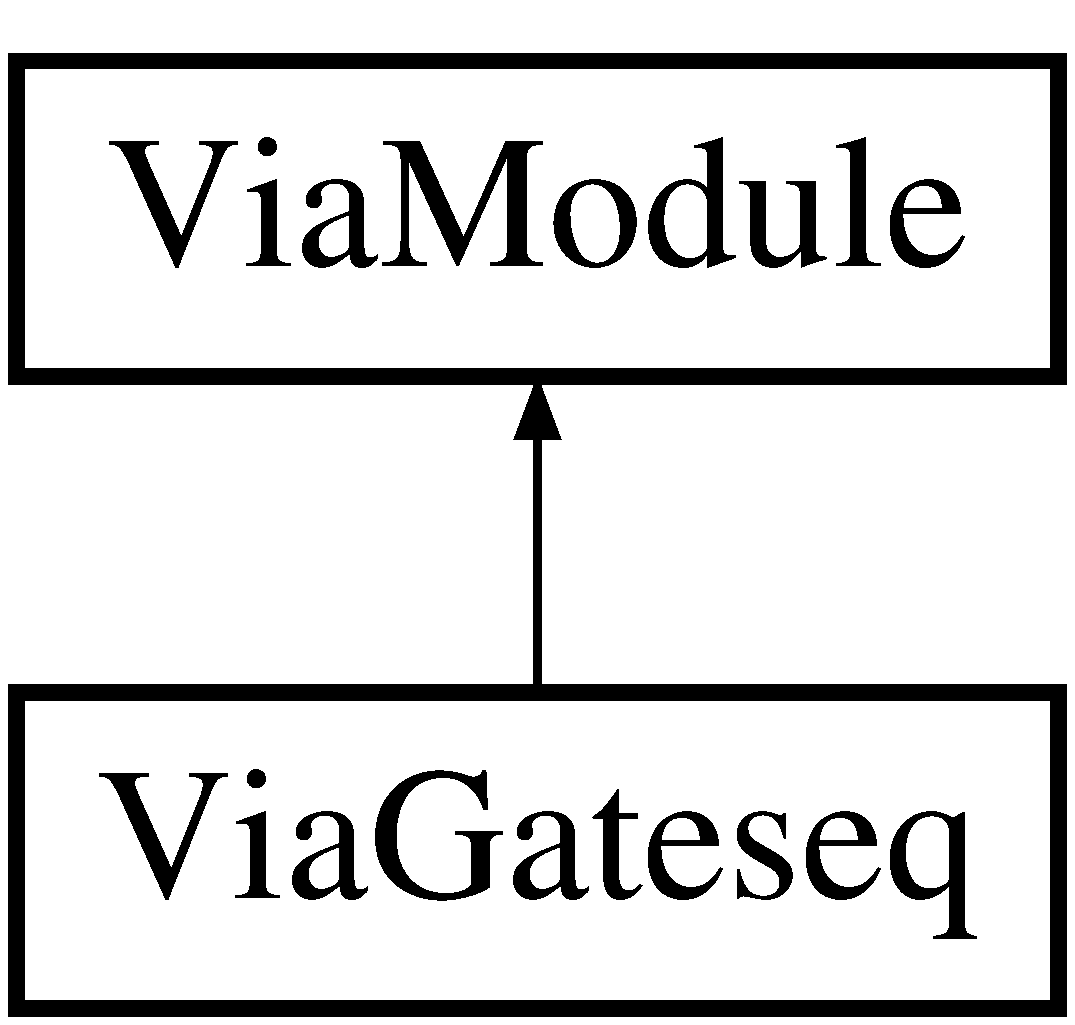
\includegraphics[height=2.000000cm]{class_via_gateseq}
\end{center}
\end{figure}
\subsection*{Classes}
\begin{DoxyCompactItemize}
\item 
class \mbox{\hyperlink{class_via_gateseq_1_1_via_gateseq_u_i}{Via\+Gateseq\+UI}}
\end{DoxyCompactItemize}
\subsection*{Public Member Functions}
\begin{DoxyCompactItemize}
\item 
void \mbox{\hyperlink{class_via_gateseq_a7238ac41564eee6827e6a01032374a4f}{handle\+Button1\+Mode\+Change}} (int32\+\_\+t)
\item 
void \mbox{\hyperlink{class_via_gateseq_ab28f41fb2ac733e2e027164400bbe868}{handle\+Button2\+Mode\+Change}} (int32\+\_\+t)
\item 
void \mbox{\hyperlink{class_via_gateseq_a87d499976eda6b518b32b240692ee83b}{handle\+Button3\+Mode\+Change}} (int32\+\_\+t)
\item 
void \mbox{\hyperlink{class_via_gateseq_a4fd21cfbe89e9a610a4f1fed5a3a5209}{handle\+Button4\+Mode\+Change}} (int32\+\_\+t)
\item 
void \mbox{\hyperlink{class_via_gateseq_abe42605edbcd7826d040303dd4564eeb}{handle\+Button5\+Mode\+Change}} (int32\+\_\+t)
\item 
void \mbox{\hyperlink{class_via_gateseq_ace1960408caf61b994b099151c663580}{handle\+Button6\+Mode\+Change}} (int32\+\_\+t)
\item 
void \mbox{\hyperlink{class_via_gateseq_a1eb52cddac4eee6df5044e712ff679aa}{handle\+Aux1\+Mode\+Change}} (int32\+\_\+t)
\item 
void \mbox{\hyperlink{class_via_gateseq_a73ae14c3b94bf0440f823f81ee11fd95}{handle\+Aux2\+Mode\+Change}} (int32\+\_\+t)
\item 
void \mbox{\hyperlink{class_via_gateseq_a65dbb600b9d299c8e2792f9deee742b5}{handle\+Aux3\+Mode\+Change}} (int32\+\_\+t)
\item 
void \mbox{\hyperlink{class_via_gateseq_acf4b669d15e07c42bc7daca791d6a1b8}{handle\+Aux4\+Mode\+Change}} (int32\+\_\+t)
\item 
void \mbox{\hyperlink{class_via_gateseq_ae414221192a80f4f0923bd26d9255156}{initialize\+Patterns}} (void)
\item 
void \mbox{\hyperlink{class_via_gateseq_aff187d21f5f13cc6bd0a029aa6d6bb89}{init}} (void)
\item 
\mbox{\hyperlink{class_via_gateseq_ac0bb7455cf2081d645574d5274862591}{Via\+Gateseq}} ()
\item 
void \mbox{\hyperlink{class_via_gateseq_a4e1357b25c2c3c297e6d961840e1ff2e}{main\+Rising\+Edge\+Callback}} (void)
\item 
void \mbox{\hyperlink{class_via_gateseq_acc4340b313d59798c9bfd241af82997c}{main\+Falling\+Edge\+Callback}} (void)
\item 
void \mbox{\hyperlink{class_via_gateseq_abc5e90e7f9a624e25691c6d202bac2eb}{aux\+Rising\+Edge\+Callback}} (void)
\item 
void \mbox{\hyperlink{class_via_gateseq_abbca505b971596d4233e27df76e37655}{aux\+Falling\+Edge\+Callback}} (void)
\item 
void \mbox{\hyperlink{class_via_gateseq_a0871606bcbd5b671c1326d1218f264a3}{button\+Pressed\+Callback}} (void)
\item 
void \mbox{\hyperlink{class_via_gateseq_aa18b0d84c686c7c7339df8f9bee38e45}{button\+Released\+Callback}} (void)
\item 
void \mbox{\hyperlink{class_via_gateseq_aee67d45c3237dc013222192e97b4ea4c}{io\+Process\+Callback}} (void)
\item 
void \mbox{\hyperlink{class_via_gateseq_a4760dc9a5a8b5d82d8ddb83595bff37a}{half\+Transfer\+Callback}} (void)
\item 
void \mbox{\hyperlink{class_via_gateseq_a3058dd33ab526baa7be92d741c455fe2}{transfer\+Complete\+Callback}} (void)
\item 
void \mbox{\hyperlink{class_via_gateseq_a5f5dbb45776ebd8eb39735b96cb246c5}{slow\+Conversion\+Callback}} (void)
\item 
void \mbox{\hyperlink{class_via_gateseq_a6085ddc82767c564111bac2341d91bb1}{aux\+Timer1\+Interrupt\+Callback}} (void)
\item 
void \mbox{\hyperlink{class_via_gateseq_ab668f9ea55345495e233d4fb2b34ac48}{aux\+Timer2\+Interrupt\+Callback}} (void)
\item 
void \mbox{\hyperlink{class_via_gateseq_ad2af84e2865d64543a0e9d7e48ea5140}{aux\+Timer3\+Interrupt\+Callback}} (void)
\item 
void \mbox{\hyperlink{class_via_gateseq_aaca5689865a460afca19c9b73e67e236}{ui\+\_\+dispatch}} (int32\+\_\+t sig)
\end{DoxyCompactItemize}
\subsection*{Public Attributes}
\begin{DoxyCompactItemize}
\item 
const \mbox{\hyperlink{structboolean_sequence_bank}{boolean\+Sequence\+Bank}} $\ast$ \mbox{\hyperlink{class_via_gateseq_ad505b120d66ea6e9beb846d66a8021fa}{seq1\+Pattern\+Bank}} \mbox{[}4\mbox{]}
\item 
const \mbox{\hyperlink{structboolean_sequence_bank}{boolean\+Sequence\+Bank}} $\ast$ \mbox{\hyperlink{class_via_gateseq_a1faa904a07ea274aeff80dbb18f8518c}{seq2\+Pattern\+Bank}} \mbox{[}4\mbox{]}
\item 
\mbox{\hyperlink{class_via_gateseq_1_1_via_gateseq_u_i}{Via\+Gateseq\+UI}} \mbox{\hyperlink{class_via_gateseq_ae55cb2ce39ea0d6d614cd43f287f1151}{gateseq\+UI}}
\item 
int32\+\_\+t \mbox{\hyperlink{class_via_gateseq_a6234f09e46a196927229d2bd7e0c2ea0}{runtime\+Display}}
\item 
\mbox{\hyperlink{class_dual_euclidean}{Dual\+Euclidean}} \mbox{\hyperlink{class_via_gateseq_aade5918995b92e3f1fd8a3b07e0bd7f4}{sequencer}}
\item 
\mbox{\hyperlink{class_soft_gate}{Soft\+Gate}} \mbox{\hyperlink{class_via_gateseq_a07aca8cb788a3452736e585b82fd6826}{gate\+Controller}}
\item 
uint32\+\_\+t \mbox{\hyperlink{class_via_gateseq_ab15d726ba5d302f110c2fa9b516aac45}{simultaneous\+Trig\+Flag}}
\end{DoxyCompactItemize}
\subsection*{Additional Inherited Members}


\subsection{Constructor \& Destructor Documentation}
\mbox{\Hypertarget{class_via_gateseq_ac0bb7455cf2081d645574d5274862591}\label{class_via_gateseq_ac0bb7455cf2081d645574d5274862591}} 
\index{Via\+Gateseq@{Via\+Gateseq}!Via\+Gateseq@{Via\+Gateseq}}
\index{Via\+Gateseq@{Via\+Gateseq}!Via\+Gateseq@{Via\+Gateseq}}
\subsubsection{\texorpdfstring{Via\+Gateseq()}{ViaGateseq()}}
{\footnotesize\ttfamily Via\+Gateseq\+::\+Via\+Gateseq (\begin{DoxyParamCaption}{ }\end{DoxyParamCaption})\hspace{0.3cm}{\ttfamily [inline]}}



\subsection{Member Function Documentation}
\mbox{\Hypertarget{class_via_gateseq_abbca505b971596d4233e27df76e37655}\label{class_via_gateseq_abbca505b971596d4233e27df76e37655}} 
\index{Via\+Gateseq@{Via\+Gateseq}!aux\+Falling\+Edge\+Callback@{aux\+Falling\+Edge\+Callback}}
\index{aux\+Falling\+Edge\+Callback@{aux\+Falling\+Edge\+Callback}!Via\+Gateseq@{Via\+Gateseq}}
\subsubsection{\texorpdfstring{aux\+Falling\+Edge\+Callback()}{auxFallingEdgeCallback()}}
{\footnotesize\ttfamily void Via\+Gateseq\+::aux\+Falling\+Edge\+Callback (\begin{DoxyParamCaption}\item[{void}]{ }\end{DoxyParamCaption})}

\mbox{\Hypertarget{class_via_gateseq_abc5e90e7f9a624e25691c6d202bac2eb}\label{class_via_gateseq_abc5e90e7f9a624e25691c6d202bac2eb}} 
\index{Via\+Gateseq@{Via\+Gateseq}!aux\+Rising\+Edge\+Callback@{aux\+Rising\+Edge\+Callback}}
\index{aux\+Rising\+Edge\+Callback@{aux\+Rising\+Edge\+Callback}!Via\+Gateseq@{Via\+Gateseq}}
\subsubsection{\texorpdfstring{aux\+Rising\+Edge\+Callback()}{auxRisingEdgeCallback()}}
{\footnotesize\ttfamily void Via\+Gateseq\+::aux\+Rising\+Edge\+Callback (\begin{DoxyParamCaption}\item[{void}]{ }\end{DoxyParamCaption})}

\mbox{\Hypertarget{class_via_gateseq_a6085ddc82767c564111bac2341d91bb1}\label{class_via_gateseq_a6085ddc82767c564111bac2341d91bb1}} 
\index{Via\+Gateseq@{Via\+Gateseq}!aux\+Timer1\+Interrupt\+Callback@{aux\+Timer1\+Interrupt\+Callback}}
\index{aux\+Timer1\+Interrupt\+Callback@{aux\+Timer1\+Interrupt\+Callback}!Via\+Gateseq@{Via\+Gateseq}}
\subsubsection{\texorpdfstring{aux\+Timer1\+Interrupt\+Callback()}{auxTimer1InterruptCallback()}}
{\footnotesize\ttfamily void Via\+Gateseq\+::aux\+Timer1\+Interrupt\+Callback (\begin{DoxyParamCaption}\item[{void}]{ }\end{DoxyParamCaption})}

\mbox{\Hypertarget{class_via_gateseq_ab668f9ea55345495e233d4fb2b34ac48}\label{class_via_gateseq_ab668f9ea55345495e233d4fb2b34ac48}} 
\index{Via\+Gateseq@{Via\+Gateseq}!aux\+Timer2\+Interrupt\+Callback@{aux\+Timer2\+Interrupt\+Callback}}
\index{aux\+Timer2\+Interrupt\+Callback@{aux\+Timer2\+Interrupt\+Callback}!Via\+Gateseq@{Via\+Gateseq}}
\subsubsection{\texorpdfstring{aux\+Timer2\+Interrupt\+Callback()}{auxTimer2InterruptCallback()}}
{\footnotesize\ttfamily void Via\+Gateseq\+::aux\+Timer2\+Interrupt\+Callback (\begin{DoxyParamCaption}\item[{void}]{ }\end{DoxyParamCaption})}

\mbox{\Hypertarget{class_via_gateseq_ad2af84e2865d64543a0e9d7e48ea5140}\label{class_via_gateseq_ad2af84e2865d64543a0e9d7e48ea5140}} 
\index{Via\+Gateseq@{Via\+Gateseq}!aux\+Timer3\+Interrupt\+Callback@{aux\+Timer3\+Interrupt\+Callback}}
\index{aux\+Timer3\+Interrupt\+Callback@{aux\+Timer3\+Interrupt\+Callback}!Via\+Gateseq@{Via\+Gateseq}}
\subsubsection{\texorpdfstring{aux\+Timer3\+Interrupt\+Callback()}{auxTimer3InterruptCallback()}}
{\footnotesize\ttfamily void Via\+Gateseq\+::aux\+Timer3\+Interrupt\+Callback (\begin{DoxyParamCaption}\item[{void}]{ }\end{DoxyParamCaption})}

\mbox{\Hypertarget{class_via_gateseq_a0871606bcbd5b671c1326d1218f264a3}\label{class_via_gateseq_a0871606bcbd5b671c1326d1218f264a3}} 
\index{Via\+Gateseq@{Via\+Gateseq}!button\+Pressed\+Callback@{button\+Pressed\+Callback}}
\index{button\+Pressed\+Callback@{button\+Pressed\+Callback}!Via\+Gateseq@{Via\+Gateseq}}
\subsubsection{\texorpdfstring{button\+Pressed\+Callback()}{buttonPressedCallback()}}
{\footnotesize\ttfamily void Via\+Gateseq\+::button\+Pressed\+Callback (\begin{DoxyParamCaption}\item[{void}]{ }\end{DoxyParamCaption})}

\mbox{\Hypertarget{class_via_gateseq_aa18b0d84c686c7c7339df8f9bee38e45}\label{class_via_gateseq_aa18b0d84c686c7c7339df8f9bee38e45}} 
\index{Via\+Gateseq@{Via\+Gateseq}!button\+Released\+Callback@{button\+Released\+Callback}}
\index{button\+Released\+Callback@{button\+Released\+Callback}!Via\+Gateseq@{Via\+Gateseq}}
\subsubsection{\texorpdfstring{button\+Released\+Callback()}{buttonReleasedCallback()}}
{\footnotesize\ttfamily void Via\+Gateseq\+::button\+Released\+Callback (\begin{DoxyParamCaption}\item[{void}]{ }\end{DoxyParamCaption})}

\mbox{\Hypertarget{class_via_gateseq_a4760dc9a5a8b5d82d8ddb83595bff37a}\label{class_via_gateseq_a4760dc9a5a8b5d82d8ddb83595bff37a}} 
\index{Via\+Gateseq@{Via\+Gateseq}!half\+Transfer\+Callback@{half\+Transfer\+Callback}}
\index{half\+Transfer\+Callback@{half\+Transfer\+Callback}!Via\+Gateseq@{Via\+Gateseq}}
\subsubsection{\texorpdfstring{half\+Transfer\+Callback()}{halfTransferCallback()}}
{\footnotesize\ttfamily void Via\+Gateseq\+::half\+Transfer\+Callback (\begin{DoxyParamCaption}\item[{void}]{ }\end{DoxyParamCaption})}

\mbox{\Hypertarget{class_via_gateseq_a1eb52cddac4eee6df5044e712ff679aa}\label{class_via_gateseq_a1eb52cddac4eee6df5044e712ff679aa}} 
\index{Via\+Gateseq@{Via\+Gateseq}!handle\+Aux1\+Mode\+Change@{handle\+Aux1\+Mode\+Change}}
\index{handle\+Aux1\+Mode\+Change@{handle\+Aux1\+Mode\+Change}!Via\+Gateseq@{Via\+Gateseq}}
\subsubsection{\texorpdfstring{handle\+Aux1\+Mode\+Change()}{handleAux1ModeChange()}}
{\footnotesize\ttfamily void Via\+Gateseq\+::handle\+Aux1\+Mode\+Change (\begin{DoxyParamCaption}\item[{int32\+\_\+t}]{ }\end{DoxyParamCaption})}

\mbox{\Hypertarget{class_via_gateseq_a73ae14c3b94bf0440f823f81ee11fd95}\label{class_via_gateseq_a73ae14c3b94bf0440f823f81ee11fd95}} 
\index{Via\+Gateseq@{Via\+Gateseq}!handle\+Aux2\+Mode\+Change@{handle\+Aux2\+Mode\+Change}}
\index{handle\+Aux2\+Mode\+Change@{handle\+Aux2\+Mode\+Change}!Via\+Gateseq@{Via\+Gateseq}}
\subsubsection{\texorpdfstring{handle\+Aux2\+Mode\+Change()}{handleAux2ModeChange()}}
{\footnotesize\ttfamily void Via\+Gateseq\+::handle\+Aux2\+Mode\+Change (\begin{DoxyParamCaption}\item[{int32\+\_\+t}]{mode }\end{DoxyParamCaption})}

\mbox{\Hypertarget{class_via_gateseq_a65dbb600b9d299c8e2792f9deee742b5}\label{class_via_gateseq_a65dbb600b9d299c8e2792f9deee742b5}} 
\index{Via\+Gateseq@{Via\+Gateseq}!handle\+Aux3\+Mode\+Change@{handle\+Aux3\+Mode\+Change}}
\index{handle\+Aux3\+Mode\+Change@{handle\+Aux3\+Mode\+Change}!Via\+Gateseq@{Via\+Gateseq}}
\subsubsection{\texorpdfstring{handle\+Aux3\+Mode\+Change()}{handleAux3ModeChange()}}
{\footnotesize\ttfamily void Via\+Gateseq\+::handle\+Aux3\+Mode\+Change (\begin{DoxyParamCaption}\item[{int32\+\_\+t}]{ }\end{DoxyParamCaption})}

\mbox{\Hypertarget{class_via_gateseq_acf4b669d15e07c42bc7daca791d6a1b8}\label{class_via_gateseq_acf4b669d15e07c42bc7daca791d6a1b8}} 
\index{Via\+Gateseq@{Via\+Gateseq}!handle\+Aux4\+Mode\+Change@{handle\+Aux4\+Mode\+Change}}
\index{handle\+Aux4\+Mode\+Change@{handle\+Aux4\+Mode\+Change}!Via\+Gateseq@{Via\+Gateseq}}
\subsubsection{\texorpdfstring{handle\+Aux4\+Mode\+Change()}{handleAux4ModeChange()}}
{\footnotesize\ttfamily void Via\+Gateseq\+::handle\+Aux4\+Mode\+Change (\begin{DoxyParamCaption}\item[{int32\+\_\+t}]{ }\end{DoxyParamCaption})}

\mbox{\Hypertarget{class_via_gateseq_a7238ac41564eee6827e6a01032374a4f}\label{class_via_gateseq_a7238ac41564eee6827e6a01032374a4f}} 
\index{Via\+Gateseq@{Via\+Gateseq}!handle\+Button1\+Mode\+Change@{handle\+Button1\+Mode\+Change}}
\index{handle\+Button1\+Mode\+Change@{handle\+Button1\+Mode\+Change}!Via\+Gateseq@{Via\+Gateseq}}
\subsubsection{\texorpdfstring{handle\+Button1\+Mode\+Change()}{handleButton1ModeChange()}}
{\footnotesize\ttfamily void Via\+Gateseq\+::handle\+Button1\+Mode\+Change (\begin{DoxyParamCaption}\item[{int32\+\_\+t}]{mode }\end{DoxyParamCaption})}

\mbox{\Hypertarget{class_via_gateseq_ab28f41fb2ac733e2e027164400bbe868}\label{class_via_gateseq_ab28f41fb2ac733e2e027164400bbe868}} 
\index{Via\+Gateseq@{Via\+Gateseq}!handle\+Button2\+Mode\+Change@{handle\+Button2\+Mode\+Change}}
\index{handle\+Button2\+Mode\+Change@{handle\+Button2\+Mode\+Change}!Via\+Gateseq@{Via\+Gateseq}}
\subsubsection{\texorpdfstring{handle\+Button2\+Mode\+Change()}{handleButton2ModeChange()}}
{\footnotesize\ttfamily void Via\+Gateseq\+::handle\+Button2\+Mode\+Change (\begin{DoxyParamCaption}\item[{int32\+\_\+t}]{mode }\end{DoxyParamCaption})}

\mbox{\Hypertarget{class_via_gateseq_a87d499976eda6b518b32b240692ee83b}\label{class_via_gateseq_a87d499976eda6b518b32b240692ee83b}} 
\index{Via\+Gateseq@{Via\+Gateseq}!handle\+Button3\+Mode\+Change@{handle\+Button3\+Mode\+Change}}
\index{handle\+Button3\+Mode\+Change@{handle\+Button3\+Mode\+Change}!Via\+Gateseq@{Via\+Gateseq}}
\subsubsection{\texorpdfstring{handle\+Button3\+Mode\+Change()}{handleButton3ModeChange()}}
{\footnotesize\ttfamily void Via\+Gateseq\+::handle\+Button3\+Mode\+Change (\begin{DoxyParamCaption}\item[{int32\+\_\+t}]{mode }\end{DoxyParamCaption})}

\mbox{\Hypertarget{class_via_gateseq_a4fd21cfbe89e9a610a4f1fed5a3a5209}\label{class_via_gateseq_a4fd21cfbe89e9a610a4f1fed5a3a5209}} 
\index{Via\+Gateseq@{Via\+Gateseq}!handle\+Button4\+Mode\+Change@{handle\+Button4\+Mode\+Change}}
\index{handle\+Button4\+Mode\+Change@{handle\+Button4\+Mode\+Change}!Via\+Gateseq@{Via\+Gateseq}}
\subsubsection{\texorpdfstring{handle\+Button4\+Mode\+Change()}{handleButton4ModeChange()}}
{\footnotesize\ttfamily void Via\+Gateseq\+::handle\+Button4\+Mode\+Change (\begin{DoxyParamCaption}\item[{int32\+\_\+t}]{mode }\end{DoxyParamCaption})}

\mbox{\Hypertarget{class_via_gateseq_abe42605edbcd7826d040303dd4564eeb}\label{class_via_gateseq_abe42605edbcd7826d040303dd4564eeb}} 
\index{Via\+Gateseq@{Via\+Gateseq}!handle\+Button5\+Mode\+Change@{handle\+Button5\+Mode\+Change}}
\index{handle\+Button5\+Mode\+Change@{handle\+Button5\+Mode\+Change}!Via\+Gateseq@{Via\+Gateseq}}
\subsubsection{\texorpdfstring{handle\+Button5\+Mode\+Change()}{handleButton5ModeChange()}}
{\footnotesize\ttfamily void Via\+Gateseq\+::handle\+Button5\+Mode\+Change (\begin{DoxyParamCaption}\item[{int32\+\_\+t}]{mode }\end{DoxyParamCaption})}

\mbox{\Hypertarget{class_via_gateseq_ace1960408caf61b994b099151c663580}\label{class_via_gateseq_ace1960408caf61b994b099151c663580}} 
\index{Via\+Gateseq@{Via\+Gateseq}!handle\+Button6\+Mode\+Change@{handle\+Button6\+Mode\+Change}}
\index{handle\+Button6\+Mode\+Change@{handle\+Button6\+Mode\+Change}!Via\+Gateseq@{Via\+Gateseq}}
\subsubsection{\texorpdfstring{handle\+Button6\+Mode\+Change()}{handleButton6ModeChange()}}
{\footnotesize\ttfamily void Via\+Gateseq\+::handle\+Button6\+Mode\+Change (\begin{DoxyParamCaption}\item[{int32\+\_\+t}]{mode }\end{DoxyParamCaption})}

\mbox{\Hypertarget{class_via_gateseq_aff187d21f5f13cc6bd0a029aa6d6bb89}\label{class_via_gateseq_aff187d21f5f13cc6bd0a029aa6d6bb89}} 
\index{Via\+Gateseq@{Via\+Gateseq}!init@{init}}
\index{init@{init}!Via\+Gateseq@{Via\+Gateseq}}
\subsubsection{\texorpdfstring{init()}{init()}}
{\footnotesize\ttfamily void Via\+Gateseq\+::init (\begin{DoxyParamCaption}\item[{void}]{ }\end{DoxyParamCaption})}

\mbox{\Hypertarget{class_via_gateseq_ae414221192a80f4f0923bd26d9255156}\label{class_via_gateseq_ae414221192a80f4f0923bd26d9255156}} 
\index{Via\+Gateseq@{Via\+Gateseq}!initialize\+Patterns@{initialize\+Patterns}}
\index{initialize\+Patterns@{initialize\+Patterns}!Via\+Gateseq@{Via\+Gateseq}}
\subsubsection{\texorpdfstring{initialize\+Patterns()}{initializePatterns()}}
{\footnotesize\ttfamily void Via\+Gateseq\+::initialize\+Patterns (\begin{DoxyParamCaption}\item[{void}]{ }\end{DoxyParamCaption})}

\mbox{\Hypertarget{class_via_gateseq_aee67d45c3237dc013222192e97b4ea4c}\label{class_via_gateseq_aee67d45c3237dc013222192e97b4ea4c}} 
\index{Via\+Gateseq@{Via\+Gateseq}!io\+Process\+Callback@{io\+Process\+Callback}}
\index{io\+Process\+Callback@{io\+Process\+Callback}!Via\+Gateseq@{Via\+Gateseq}}
\subsubsection{\texorpdfstring{io\+Process\+Callback()}{ioProcessCallback()}}
{\footnotesize\ttfamily void Via\+Gateseq\+::io\+Process\+Callback (\begin{DoxyParamCaption}\item[{void}]{ }\end{DoxyParamCaption})}

\mbox{\Hypertarget{class_via_gateseq_acc4340b313d59798c9bfd241af82997c}\label{class_via_gateseq_acc4340b313d59798c9bfd241af82997c}} 
\index{Via\+Gateseq@{Via\+Gateseq}!main\+Falling\+Edge\+Callback@{main\+Falling\+Edge\+Callback}}
\index{main\+Falling\+Edge\+Callback@{main\+Falling\+Edge\+Callback}!Via\+Gateseq@{Via\+Gateseq}}
\subsubsection{\texorpdfstring{main\+Falling\+Edge\+Callback()}{mainFallingEdgeCallback()}}
{\footnotesize\ttfamily void Via\+Gateseq\+::main\+Falling\+Edge\+Callback (\begin{DoxyParamCaption}\item[{void}]{ }\end{DoxyParamCaption})}

\mbox{\Hypertarget{class_via_gateseq_a4e1357b25c2c3c297e6d961840e1ff2e}\label{class_via_gateseq_a4e1357b25c2c3c297e6d961840e1ff2e}} 
\index{Via\+Gateseq@{Via\+Gateseq}!main\+Rising\+Edge\+Callback@{main\+Rising\+Edge\+Callback}}
\index{main\+Rising\+Edge\+Callback@{main\+Rising\+Edge\+Callback}!Via\+Gateseq@{Via\+Gateseq}}
\subsubsection{\texorpdfstring{main\+Rising\+Edge\+Callback()}{mainRisingEdgeCallback()}}
{\footnotesize\ttfamily void Via\+Gateseq\+::main\+Rising\+Edge\+Callback (\begin{DoxyParamCaption}\item[{void}]{ }\end{DoxyParamCaption})}

\mbox{\Hypertarget{class_via_gateseq_a5f5dbb45776ebd8eb39735b96cb246c5}\label{class_via_gateseq_a5f5dbb45776ebd8eb39735b96cb246c5}} 
\index{Via\+Gateseq@{Via\+Gateseq}!slow\+Conversion\+Callback@{slow\+Conversion\+Callback}}
\index{slow\+Conversion\+Callback@{slow\+Conversion\+Callback}!Via\+Gateseq@{Via\+Gateseq}}
\subsubsection{\texorpdfstring{slow\+Conversion\+Callback()}{slowConversionCallback()}}
{\footnotesize\ttfamily void Via\+Gateseq\+::slow\+Conversion\+Callback (\begin{DoxyParamCaption}\item[{void}]{ }\end{DoxyParamCaption})}

\mbox{\Hypertarget{class_via_gateseq_a3058dd33ab526baa7be92d741c455fe2}\label{class_via_gateseq_a3058dd33ab526baa7be92d741c455fe2}} 
\index{Via\+Gateseq@{Via\+Gateseq}!transfer\+Complete\+Callback@{transfer\+Complete\+Callback}}
\index{transfer\+Complete\+Callback@{transfer\+Complete\+Callback}!Via\+Gateseq@{Via\+Gateseq}}
\subsubsection{\texorpdfstring{transfer\+Complete\+Callback()}{transferCompleteCallback()}}
{\footnotesize\ttfamily void Via\+Gateseq\+::transfer\+Complete\+Callback (\begin{DoxyParamCaption}\item[{void}]{ }\end{DoxyParamCaption})}

\mbox{\Hypertarget{class_via_gateseq_aaca5689865a460afca19c9b73e67e236}\label{class_via_gateseq_aaca5689865a460afca19c9b73e67e236}} 
\index{Via\+Gateseq@{Via\+Gateseq}!ui\+\_\+dispatch@{ui\+\_\+dispatch}}
\index{ui\+\_\+dispatch@{ui\+\_\+dispatch}!Via\+Gateseq@{Via\+Gateseq}}
\subsubsection{\texorpdfstring{ui\+\_\+dispatch()}{ui\_dispatch()}}
{\footnotesize\ttfamily void Via\+Gateseq\+::ui\+\_\+dispatch (\begin{DoxyParamCaption}\item[{int32\+\_\+t}]{sig }\end{DoxyParamCaption})\hspace{0.3cm}{\ttfamily [inline]}}



\subsection{Member Data Documentation}
\mbox{\Hypertarget{class_via_gateseq_a07aca8cb788a3452736e585b82fd6826}\label{class_via_gateseq_a07aca8cb788a3452736e585b82fd6826}} 
\index{Via\+Gateseq@{Via\+Gateseq}!gate\+Controller@{gate\+Controller}}
\index{gate\+Controller@{gate\+Controller}!Via\+Gateseq@{Via\+Gateseq}}
\subsubsection{\texorpdfstring{gate\+Controller}{gateController}}
{\footnotesize\ttfamily \mbox{\hyperlink{class_soft_gate}{Soft\+Gate}} Via\+Gateseq\+::gate\+Controller}

\mbox{\Hypertarget{class_via_gateseq_ae55cb2ce39ea0d6d614cd43f287f1151}\label{class_via_gateseq_ae55cb2ce39ea0d6d614cd43f287f1151}} 
\index{Via\+Gateseq@{Via\+Gateseq}!gateseq\+UI@{gateseq\+UI}}
\index{gateseq\+UI@{gateseq\+UI}!Via\+Gateseq@{Via\+Gateseq}}
\subsubsection{\texorpdfstring{gateseq\+UI}{gateseqUI}}
{\footnotesize\ttfamily \mbox{\hyperlink{class_via_gateseq_1_1_via_gateseq_u_i}{Via\+Gateseq\+UI}} Via\+Gateseq\+::gateseq\+UI}

\mbox{\Hypertarget{class_via_gateseq_a6234f09e46a196927229d2bd7e0c2ea0}\label{class_via_gateseq_a6234f09e46a196927229d2bd7e0c2ea0}} 
\index{Via\+Gateseq@{Via\+Gateseq}!runtime\+Display@{runtime\+Display}}
\index{runtime\+Display@{runtime\+Display}!Via\+Gateseq@{Via\+Gateseq}}
\subsubsection{\texorpdfstring{runtime\+Display}{runtimeDisplay}}
{\footnotesize\ttfamily int32\+\_\+t Via\+Gateseq\+::runtime\+Display}

\mbox{\Hypertarget{class_via_gateseq_ad505b120d66ea6e9beb846d66a8021fa}\label{class_via_gateseq_ad505b120d66ea6e9beb846d66a8021fa}} 
\index{Via\+Gateseq@{Via\+Gateseq}!seq1\+Pattern\+Bank@{seq1\+Pattern\+Bank}}
\index{seq1\+Pattern\+Bank@{seq1\+Pattern\+Bank}!Via\+Gateseq@{Via\+Gateseq}}
\subsubsection{\texorpdfstring{seq1\+Pattern\+Bank}{seq1PatternBank}}
{\footnotesize\ttfamily const \mbox{\hyperlink{structboolean_sequence_bank}{boolean\+Sequence\+Bank}}$\ast$ Via\+Gateseq\+::seq1\+Pattern\+Bank\mbox{[}4\mbox{]}}

\mbox{\Hypertarget{class_via_gateseq_a1faa904a07ea274aeff80dbb18f8518c}\label{class_via_gateseq_a1faa904a07ea274aeff80dbb18f8518c}} 
\index{Via\+Gateseq@{Via\+Gateseq}!seq2\+Pattern\+Bank@{seq2\+Pattern\+Bank}}
\index{seq2\+Pattern\+Bank@{seq2\+Pattern\+Bank}!Via\+Gateseq@{Via\+Gateseq}}
\subsubsection{\texorpdfstring{seq2\+Pattern\+Bank}{seq2PatternBank}}
{\footnotesize\ttfamily const \mbox{\hyperlink{structboolean_sequence_bank}{boolean\+Sequence\+Bank}}$\ast$ Via\+Gateseq\+::seq2\+Pattern\+Bank\mbox{[}4\mbox{]}}

\mbox{\Hypertarget{class_via_gateseq_aade5918995b92e3f1fd8a3b07e0bd7f4}\label{class_via_gateseq_aade5918995b92e3f1fd8a3b07e0bd7f4}} 
\index{Via\+Gateseq@{Via\+Gateseq}!sequencer@{sequencer}}
\index{sequencer@{sequencer}!Via\+Gateseq@{Via\+Gateseq}}
\subsubsection{\texorpdfstring{sequencer}{sequencer}}
{\footnotesize\ttfamily \mbox{\hyperlink{class_dual_euclidean}{Dual\+Euclidean}} Via\+Gateseq\+::sequencer}

\mbox{\Hypertarget{class_via_gateseq_ab15d726ba5d302f110c2fa9b516aac45}\label{class_via_gateseq_ab15d726ba5d302f110c2fa9b516aac45}} 
\index{Via\+Gateseq@{Via\+Gateseq}!simultaneous\+Trig\+Flag@{simultaneous\+Trig\+Flag}}
\index{simultaneous\+Trig\+Flag@{simultaneous\+Trig\+Flag}!Via\+Gateseq@{Via\+Gateseq}}
\subsubsection{\texorpdfstring{simultaneous\+Trig\+Flag}{simultaneousTrigFlag}}
{\footnotesize\ttfamily uint32\+\_\+t Via\+Gateseq\+::simultaneous\+Trig\+Flag}



The documentation for this class was generated from the following files\+:\begin{DoxyCompactItemize}
\item 
modules/inc/\mbox{\hyperlink{gateseq_8hpp}{gateseq.\+hpp}}\item 
modules/gateseq/\mbox{\hyperlink{gateseq__init_8cpp}{gateseq\+\_\+init.\+cpp}}\item 
modules/gateseq/\mbox{\hyperlink{gateseq__interrupt__handlers_8cpp}{gateseq\+\_\+interrupt\+\_\+handlers.\+cpp}}\item 
modules/gateseq/\mbox{\hyperlink{gateseq__modes_8cpp}{gateseq\+\_\+modes.\+cpp}}\item 
modules/gateseq/\mbox{\hyperlink{gateseq__pattern__init_8cpp}{gateseq\+\_\+pattern\+\_\+init.\+cpp}}\end{DoxyCompactItemize}

\hypertarget{class_via_gateseq_1_1_via_gateseq_u_i}{}\section{Via\+Gateseq\+:\+:Via\+Gateseq\+UI Class Reference}
\label{class_via_gateseq_1_1_via_gateseq_u_i}\index{Via\+Gateseq\+::\+Via\+Gateseq\+UI@{Via\+Gateseq\+::\+Via\+Gateseq\+UI}}


{\ttfamily \#include $<$gateseq.\+hpp$>$}

Inheritance diagram for Via\+Gateseq\+:\+:Via\+Gateseq\+UI\+:\begin{figure}[H]
\begin{center}
\leavevmode
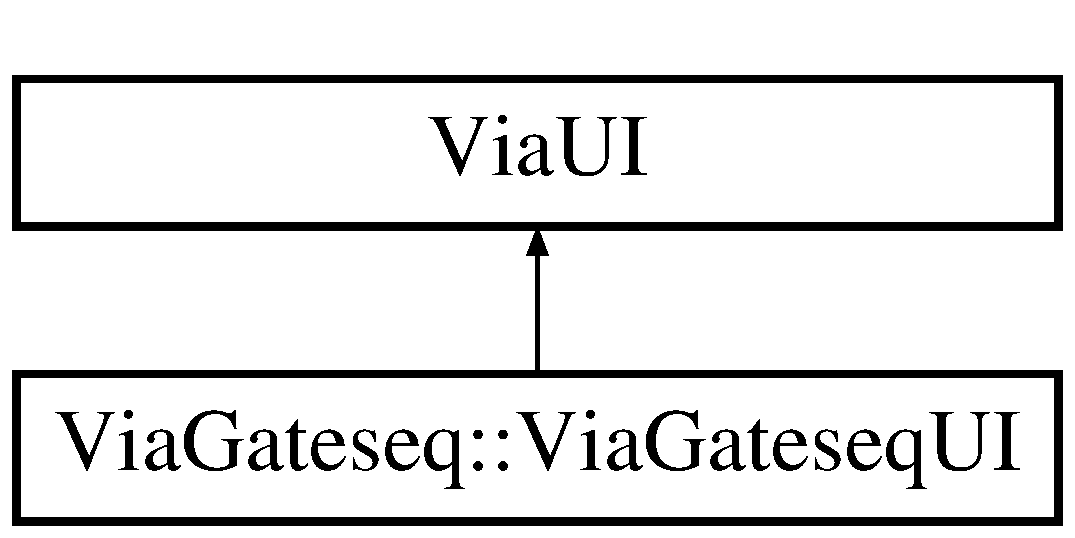
\includegraphics[height=2.000000cm]{class_via_gateseq_1_1_via_gateseq_u_i}
\end{center}
\end{figure}
\subsection*{Public Member Functions}
\begin{DoxyCompactItemize}
\item 
void \mbox{\hyperlink{class_via_gateseq_1_1_via_gateseq_u_i_ac5e0a6f47606f0f41860fd797a004b1f}{button1\+Tap\+Callback}} (void) override
\item 
void \mbox{\hyperlink{class_via_gateseq_1_1_via_gateseq_u_i_a4123b11e47b7dc36bba9041fa3635e84}{button1\+Hold\+Callback}} (void) override
\item 
void \mbox{\hyperlink{class_via_gateseq_1_1_via_gateseq_u_i_a9c198960d6fee0bc78d6e24eb18810b1}{button2\+Tap\+Callback}} (void) override
\item 
void \mbox{\hyperlink{class_via_gateseq_1_1_via_gateseq_u_i_a55e439bbec7d63aa2f0e732ec72aa2a2}{button2\+Hold\+Callback}} (void) override
\item 
void \mbox{\hyperlink{class_via_gateseq_1_1_via_gateseq_u_i_abce5bbab2316b9c0bc3cfedbaaeeef73}{button3\+Tap\+Callback}} (void) override
\item 
void \mbox{\hyperlink{class_via_gateseq_1_1_via_gateseq_u_i_a662b7cd49c71accc227fb74611e8aab2}{button3\+Hold\+Callback}} (void) override
\item 
void \mbox{\hyperlink{class_via_gateseq_1_1_via_gateseq_u_i_a329721a8753f915ba96248fab6da7b60}{button4\+Tap\+Callback}} (void) override
\item 
void \mbox{\hyperlink{class_via_gateseq_1_1_via_gateseq_u_i_a8d4d728d1f66bf2f72ae4e9669895719}{button4\+Hold\+Callback}} (void) override
\item 
void \mbox{\hyperlink{class_via_gateseq_1_1_via_gateseq_u_i_a0622c45ab381c9bde60480781f90981c}{button5\+Tap\+Callback}} (void) override
\item 
void \mbox{\hyperlink{class_via_gateseq_1_1_via_gateseq_u_i_a81a66be2d7f162bf3a6cac5f10e6c019}{button5\+Hold\+Callback}} (void) override
\item 
void \mbox{\hyperlink{class_via_gateseq_1_1_via_gateseq_u_i_a745d2eed3bc66bd2bb44149cb54cbd39}{button6\+Tap\+Callback}} (void) override
\item 
void \mbox{\hyperlink{class_via_gateseq_1_1_via_gateseq_u_i_ae16a0091338c515aa625c8738de1752b}{button6\+Hold\+Callback}} (void) override
\item 
void \mbox{\hyperlink{class_via_gateseq_1_1_via_gateseq_u_i_a3f44c4a89f3f7aedff958e903e6c71b5}{aux1\+Tap\+Callback}} (void) override
\item 
void \mbox{\hyperlink{class_via_gateseq_1_1_via_gateseq_u_i_ac0a66889f6859802f3594031f81f05f3}{aux1\+Hold\+Callback}} (void) override
\item 
void \mbox{\hyperlink{class_via_gateseq_1_1_via_gateseq_u_i_a8e700657f1fe190238eca7c46541337b}{aux2\+Tap\+Callback}} (void) override
\item 
void \mbox{\hyperlink{class_via_gateseq_1_1_via_gateseq_u_i_a825cc56cdbeffd7eee887e8f189cb35d}{aux2\+Hold\+Callback}} (void) override
\item 
void \mbox{\hyperlink{class_via_gateseq_1_1_via_gateseq_u_i_a84c1f0f19956b81f81a7fba2b6581f99}{aux2\+Alt\+Tap\+Callback}} (void) override
\item 
void \mbox{\hyperlink{class_via_gateseq_1_1_via_gateseq_u_i_ada61d29fe8fd743edbb49500ee6e3d27}{aux2\+Alt\+Hold\+Callback}} (void) override
\item 
void \mbox{\hyperlink{class_via_gateseq_1_1_via_gateseq_u_i_a9bb95780740cd9fe650ba38aa3fb86a6}{aux3\+Tap\+Callback}} (void) override
\item 
void \mbox{\hyperlink{class_via_gateseq_1_1_via_gateseq_u_i_a5b18aa40706a39ed8878143d6911bc78}{aux3\+Hold\+Callback}} (void) override
\item 
void \mbox{\hyperlink{class_via_gateseq_1_1_via_gateseq_u_i_af12df5bd6d6bb9b069e8c410fcae7473}{aux4\+Tap\+Callback}} (void) override
\item 
void \mbox{\hyperlink{class_via_gateseq_1_1_via_gateseq_u_i_a98c59b4566672aeb522f6cafccd46b72}{aux4\+Hold\+Callback}} (void) override
\item 
void \mbox{\hyperlink{class_via_gateseq_1_1_via_gateseq_u_i_ab3eb51f8dcb036861e62c4456d726771}{ui\+Set\+L\+E\+Ds}} (int) override
\item 
void \mbox{\hyperlink{class_via_gateseq_1_1_via_gateseq_u_i_a4f3313685b65a93e1cd12e458dba34de}{recall\+Module\+State}} (void) override
\item 
void \mbox{\hyperlink{class_via_gateseq_1_1_via_gateseq_u_i_ad71d38b0b6b8c29e9f93e0fe6d2c40fc}{default\+Enter\+Menu\+Callback}} (void) override
\item 
void \mbox{\hyperlink{class_via_gateseq_1_1_via_gateseq_u_i_a7ced8ac998979d31b1f0a617edba8490}{new\+Mode\+Enter\+Menu\+Callback}} (void) override
\item 
void \mbox{\hyperlink{class_via_gateseq_1_1_via_gateseq_u_i_ad6fb8d3cdf019a290c82a9d42f3f83a7}{new\+Aux\+Mode\+Enter\+Menu\+Callback}} (void) override
\item 
void \mbox{\hyperlink{class_via_gateseq_1_1_via_gateseq_u_i_af0d1fcd037084b122f68ea1522080fd7}{preset\+Enter\+Menu\+Callback}} (void) override
\item 
void \mbox{\hyperlink{class_via_gateseq_1_1_via_gateseq_u_i_aa4ce0e46aeda7bea4ec2a09bbca2abac}{button1\+Enter\+Menu\+Callback}} (void) override
\item 
void \mbox{\hyperlink{class_via_gateseq_1_1_via_gateseq_u_i_ae0e3038febadb4cde08ff0f3da2703fe}{button2\+Enter\+Menu\+Callback}} (void) override
\item 
void \mbox{\hyperlink{class_via_gateseq_1_1_via_gateseq_u_i_a634b6fe2c13f90490b6e8182b4854425}{button3\+Enter\+Menu\+Callback}} (void) override
\item 
void \mbox{\hyperlink{class_via_gateseq_1_1_via_gateseq_u_i_a2f739b43b005baf5bc8dd4d081c5b6d5}{button4\+Enter\+Menu\+Callback}} (void) override
\item 
void \mbox{\hyperlink{class_via_gateseq_1_1_via_gateseq_u_i_a6286441705681c57d4f8535d0445b360}{button5\+Enter\+Menu\+Callback}} (void) override
\item 
void \mbox{\hyperlink{class_via_gateseq_1_1_via_gateseq_u_i_adf289572ed287fdc4c9ff4029f008b7b}{button6\+Enter\+Menu\+Callback}} (void) override
\item 
void \mbox{\hyperlink{class_via_gateseq_1_1_via_gateseq_u_i_ae1a1c7c97151e09b2e6b136f0c1efe6e}{aux1\+Enter\+Menu\+Callback}} (void) override
\item 
void \mbox{\hyperlink{class_via_gateseq_1_1_via_gateseq_u_i_a3f3270689385b4ba7449599538aafc59}{aux2\+Enter\+Menu\+Callback}} (void) override
\item 
void \mbox{\hyperlink{class_via_gateseq_1_1_via_gateseq_u_i_a39db35560b35c8fafeaabef258be61d8}{aux2\+Alt\+Enter\+Menu\+Callback}} (void) override
\item 
void \mbox{\hyperlink{class_via_gateseq_1_1_via_gateseq_u_i_a8235806bb28a40062b89b1cb9c83e3b0}{aux3\+Enter\+Menu\+Callback}} (void) override
\item 
void \mbox{\hyperlink{class_via_gateseq_1_1_via_gateseq_u_i_a78f330f4c02acb69f9c2321a8187f8dc}{aux4\+Enter\+Menu\+Callback}} (void) override
\item 
void \mbox{\hyperlink{class_via_gateseq_1_1_via_gateseq_u_i_ae59b0d739f92892cf9a0d16cd3d25bfa}{initialize}} (void) override
\item 
\mbox{\hyperlink{class_via_gateseq_1_1_via_gateseq_u_i_a907e06009edfea0251dbe3c00c84bcf6}{Via\+Gateseq\+UI}} (\mbox{\hyperlink{class_via_gateseq}{Via\+Gateseq}} \&x)
\end{DoxyCompactItemize}
\subsection*{Public Attributes}
\begin{DoxyCompactItemize}
\item 
\mbox{\hyperlink{class_via_gateseq}{Via\+Gateseq}} \& \mbox{\hyperlink{class_via_gateseq_1_1_via_gateseq_u_i_ae51cc27ec70247c3fc7a013e20a80450}{this\+\_\+module}}
\end{DoxyCompactItemize}


\subsection{Constructor \& Destructor Documentation}
\mbox{\Hypertarget{class_via_gateseq_1_1_via_gateseq_u_i_a907e06009edfea0251dbe3c00c84bcf6}\label{class_via_gateseq_1_1_via_gateseq_u_i_a907e06009edfea0251dbe3c00c84bcf6}} 
\index{Via\+Gateseq\+::\+Via\+Gateseq\+UI@{Via\+Gateseq\+::\+Via\+Gateseq\+UI}!Via\+Gateseq\+UI@{Via\+Gateseq\+UI}}
\index{Via\+Gateseq\+UI@{Via\+Gateseq\+UI}!Via\+Gateseq\+::\+Via\+Gateseq\+UI@{Via\+Gateseq\+::\+Via\+Gateseq\+UI}}
\subsubsection{\texorpdfstring{Via\+Gateseq\+U\+I()}{ViaGateseqUI()}}
{\footnotesize\ttfamily Via\+Gateseq\+::\+Via\+Gateseq\+U\+I\+::\+Via\+Gateseq\+UI (\begin{DoxyParamCaption}\item[{\mbox{\hyperlink{class_via_gateseq}{Via\+Gateseq}} \&}]{x }\end{DoxyParamCaption})\hspace{0.3cm}{\ttfamily [inline]}}



\subsection{Member Function Documentation}
\mbox{\Hypertarget{class_via_gateseq_1_1_via_gateseq_u_i_ae1a1c7c97151e09b2e6b136f0c1efe6e}\label{class_via_gateseq_1_1_via_gateseq_u_i_ae1a1c7c97151e09b2e6b136f0c1efe6e}} 
\index{Via\+Gateseq\+::\+Via\+Gateseq\+UI@{Via\+Gateseq\+::\+Via\+Gateseq\+UI}!aux1\+Enter\+Menu\+Callback@{aux1\+Enter\+Menu\+Callback}}
\index{aux1\+Enter\+Menu\+Callback@{aux1\+Enter\+Menu\+Callback}!Via\+Gateseq\+::\+Via\+Gateseq\+UI@{Via\+Gateseq\+::\+Via\+Gateseq\+UI}}
\subsubsection{\texorpdfstring{aux1\+Enter\+Menu\+Callback()}{aux1EnterMenuCallback()}}
{\footnotesize\ttfamily void Via\+Gateseq\+::\+Via\+Gateseq\+U\+I\+::aux1\+Enter\+Menu\+Callback (\begin{DoxyParamCaption}\item[{void}]{ }\end{DoxyParamCaption})\hspace{0.3cm}{\ttfamily [override]}, {\ttfamily [virtual]}}



Implements \mbox{\hyperlink{class_via_u_i_a578111861e912bf43d3f320a0faffb0f}{Via\+UI}}.

\mbox{\Hypertarget{class_via_gateseq_1_1_via_gateseq_u_i_ac0a66889f6859802f3594031f81f05f3}\label{class_via_gateseq_1_1_via_gateseq_u_i_ac0a66889f6859802f3594031f81f05f3}} 
\index{Via\+Gateseq\+::\+Via\+Gateseq\+UI@{Via\+Gateseq\+::\+Via\+Gateseq\+UI}!aux1\+Hold\+Callback@{aux1\+Hold\+Callback}}
\index{aux1\+Hold\+Callback@{aux1\+Hold\+Callback}!Via\+Gateseq\+::\+Via\+Gateseq\+UI@{Via\+Gateseq\+::\+Via\+Gateseq\+UI}}
\subsubsection{\texorpdfstring{aux1\+Hold\+Callback()}{aux1HoldCallback()}}
{\footnotesize\ttfamily void Via\+Gateseq\+::\+Via\+Gateseq\+U\+I\+::aux1\+Hold\+Callback (\begin{DoxyParamCaption}\item[{void}]{ }\end{DoxyParamCaption})\hspace{0.3cm}{\ttfamily [override]}, {\ttfamily [virtual]}}



Implements \mbox{\hyperlink{class_via_u_i_a6fcc3b7cf9b97ccf403ed1817cb10d1d}{Via\+UI}}.

\mbox{\Hypertarget{class_via_gateseq_1_1_via_gateseq_u_i_a3f44c4a89f3f7aedff958e903e6c71b5}\label{class_via_gateseq_1_1_via_gateseq_u_i_a3f44c4a89f3f7aedff958e903e6c71b5}} 
\index{Via\+Gateseq\+::\+Via\+Gateseq\+UI@{Via\+Gateseq\+::\+Via\+Gateseq\+UI}!aux1\+Tap\+Callback@{aux1\+Tap\+Callback}}
\index{aux1\+Tap\+Callback@{aux1\+Tap\+Callback}!Via\+Gateseq\+::\+Via\+Gateseq\+UI@{Via\+Gateseq\+::\+Via\+Gateseq\+UI}}
\subsubsection{\texorpdfstring{aux1\+Tap\+Callback()}{aux1TapCallback()}}
{\footnotesize\ttfamily void Via\+Gateseq\+::\+Via\+Gateseq\+U\+I\+::aux1\+Tap\+Callback (\begin{DoxyParamCaption}\item[{void}]{ }\end{DoxyParamCaption})\hspace{0.3cm}{\ttfamily [override]}, {\ttfamily [virtual]}}



Implements \mbox{\hyperlink{class_via_u_i_a2942ec6f7d495159258e1f1803e62c4d}{Via\+UI}}.

\mbox{\Hypertarget{class_via_gateseq_1_1_via_gateseq_u_i_a39db35560b35c8fafeaabef258be61d8}\label{class_via_gateseq_1_1_via_gateseq_u_i_a39db35560b35c8fafeaabef258be61d8}} 
\index{Via\+Gateseq\+::\+Via\+Gateseq\+UI@{Via\+Gateseq\+::\+Via\+Gateseq\+UI}!aux2\+Alt\+Enter\+Menu\+Callback@{aux2\+Alt\+Enter\+Menu\+Callback}}
\index{aux2\+Alt\+Enter\+Menu\+Callback@{aux2\+Alt\+Enter\+Menu\+Callback}!Via\+Gateseq\+::\+Via\+Gateseq\+UI@{Via\+Gateseq\+::\+Via\+Gateseq\+UI}}
\subsubsection{\texorpdfstring{aux2\+Alt\+Enter\+Menu\+Callback()}{aux2AltEnterMenuCallback()}}
{\footnotesize\ttfamily void Via\+Gateseq\+::\+Via\+Gateseq\+U\+I\+::aux2\+Alt\+Enter\+Menu\+Callback (\begin{DoxyParamCaption}\item[{void}]{ }\end{DoxyParamCaption})\hspace{0.3cm}{\ttfamily [override]}, {\ttfamily [virtual]}}



Implements \mbox{\hyperlink{class_via_u_i_a08a746b666d37ac6bc293303187fd6be}{Via\+UI}}.

\mbox{\Hypertarget{class_via_gateseq_1_1_via_gateseq_u_i_ada61d29fe8fd743edbb49500ee6e3d27}\label{class_via_gateseq_1_1_via_gateseq_u_i_ada61d29fe8fd743edbb49500ee6e3d27}} 
\index{Via\+Gateseq\+::\+Via\+Gateseq\+UI@{Via\+Gateseq\+::\+Via\+Gateseq\+UI}!aux2\+Alt\+Hold\+Callback@{aux2\+Alt\+Hold\+Callback}}
\index{aux2\+Alt\+Hold\+Callback@{aux2\+Alt\+Hold\+Callback}!Via\+Gateseq\+::\+Via\+Gateseq\+UI@{Via\+Gateseq\+::\+Via\+Gateseq\+UI}}
\subsubsection{\texorpdfstring{aux2\+Alt\+Hold\+Callback()}{aux2AltHoldCallback()}}
{\footnotesize\ttfamily void Via\+Gateseq\+::\+Via\+Gateseq\+U\+I\+::aux2\+Alt\+Hold\+Callback (\begin{DoxyParamCaption}\item[{void}]{ }\end{DoxyParamCaption})\hspace{0.3cm}{\ttfamily [override]}, {\ttfamily [virtual]}}



Implements \mbox{\hyperlink{class_via_u_i_ab93989ef608d1b63b854b54278006f49}{Via\+UI}}.

\mbox{\Hypertarget{class_via_gateseq_1_1_via_gateseq_u_i_a84c1f0f19956b81f81a7fba2b6581f99}\label{class_via_gateseq_1_1_via_gateseq_u_i_a84c1f0f19956b81f81a7fba2b6581f99}} 
\index{Via\+Gateseq\+::\+Via\+Gateseq\+UI@{Via\+Gateseq\+::\+Via\+Gateseq\+UI}!aux2\+Alt\+Tap\+Callback@{aux2\+Alt\+Tap\+Callback}}
\index{aux2\+Alt\+Tap\+Callback@{aux2\+Alt\+Tap\+Callback}!Via\+Gateseq\+::\+Via\+Gateseq\+UI@{Via\+Gateseq\+::\+Via\+Gateseq\+UI}}
\subsubsection{\texorpdfstring{aux2\+Alt\+Tap\+Callback()}{aux2AltTapCallback()}}
{\footnotesize\ttfamily void Via\+Gateseq\+::\+Via\+Gateseq\+U\+I\+::aux2\+Alt\+Tap\+Callback (\begin{DoxyParamCaption}\item[{void}]{ }\end{DoxyParamCaption})\hspace{0.3cm}{\ttfamily [override]}, {\ttfamily [virtual]}}



Implements \mbox{\hyperlink{class_via_u_i_ad13d74c0bd271b83b8da662b22713ddb}{Via\+UI}}.

\mbox{\Hypertarget{class_via_gateseq_1_1_via_gateseq_u_i_a3f3270689385b4ba7449599538aafc59}\label{class_via_gateseq_1_1_via_gateseq_u_i_a3f3270689385b4ba7449599538aafc59}} 
\index{Via\+Gateseq\+::\+Via\+Gateseq\+UI@{Via\+Gateseq\+::\+Via\+Gateseq\+UI}!aux2\+Enter\+Menu\+Callback@{aux2\+Enter\+Menu\+Callback}}
\index{aux2\+Enter\+Menu\+Callback@{aux2\+Enter\+Menu\+Callback}!Via\+Gateseq\+::\+Via\+Gateseq\+UI@{Via\+Gateseq\+::\+Via\+Gateseq\+UI}}
\subsubsection{\texorpdfstring{aux2\+Enter\+Menu\+Callback()}{aux2EnterMenuCallback()}}
{\footnotesize\ttfamily void Via\+Gateseq\+::\+Via\+Gateseq\+U\+I\+::aux2\+Enter\+Menu\+Callback (\begin{DoxyParamCaption}\item[{void}]{ }\end{DoxyParamCaption})\hspace{0.3cm}{\ttfamily [override]}, {\ttfamily [virtual]}}



Implements \mbox{\hyperlink{class_via_u_i_a1f51fc259471364f91bd0a1592824dab}{Via\+UI}}.

\mbox{\Hypertarget{class_via_gateseq_1_1_via_gateseq_u_i_a825cc56cdbeffd7eee887e8f189cb35d}\label{class_via_gateseq_1_1_via_gateseq_u_i_a825cc56cdbeffd7eee887e8f189cb35d}} 
\index{Via\+Gateseq\+::\+Via\+Gateseq\+UI@{Via\+Gateseq\+::\+Via\+Gateseq\+UI}!aux2\+Hold\+Callback@{aux2\+Hold\+Callback}}
\index{aux2\+Hold\+Callback@{aux2\+Hold\+Callback}!Via\+Gateseq\+::\+Via\+Gateseq\+UI@{Via\+Gateseq\+::\+Via\+Gateseq\+UI}}
\subsubsection{\texorpdfstring{aux2\+Hold\+Callback()}{aux2HoldCallback()}}
{\footnotesize\ttfamily void Via\+Gateseq\+::\+Via\+Gateseq\+U\+I\+::aux2\+Hold\+Callback (\begin{DoxyParamCaption}\item[{void}]{ }\end{DoxyParamCaption})\hspace{0.3cm}{\ttfamily [override]}, {\ttfamily [virtual]}}



Implements \mbox{\hyperlink{class_via_u_i_a42545b69c2bbbb036f633140fd8007d6}{Via\+UI}}.

\mbox{\Hypertarget{class_via_gateseq_1_1_via_gateseq_u_i_a8e700657f1fe190238eca7c46541337b}\label{class_via_gateseq_1_1_via_gateseq_u_i_a8e700657f1fe190238eca7c46541337b}} 
\index{Via\+Gateseq\+::\+Via\+Gateseq\+UI@{Via\+Gateseq\+::\+Via\+Gateseq\+UI}!aux2\+Tap\+Callback@{aux2\+Tap\+Callback}}
\index{aux2\+Tap\+Callback@{aux2\+Tap\+Callback}!Via\+Gateseq\+::\+Via\+Gateseq\+UI@{Via\+Gateseq\+::\+Via\+Gateseq\+UI}}
\subsubsection{\texorpdfstring{aux2\+Tap\+Callback()}{aux2TapCallback()}}
{\footnotesize\ttfamily void Via\+Gateseq\+::\+Via\+Gateseq\+U\+I\+::aux2\+Tap\+Callback (\begin{DoxyParamCaption}\item[{void}]{ }\end{DoxyParamCaption})\hspace{0.3cm}{\ttfamily [override]}, {\ttfamily [virtual]}}



Implements \mbox{\hyperlink{class_via_u_i_ae5e009dc22002f62e6bff8dd76d2f745}{Via\+UI}}.

\mbox{\Hypertarget{class_via_gateseq_1_1_via_gateseq_u_i_a8235806bb28a40062b89b1cb9c83e3b0}\label{class_via_gateseq_1_1_via_gateseq_u_i_a8235806bb28a40062b89b1cb9c83e3b0}} 
\index{Via\+Gateseq\+::\+Via\+Gateseq\+UI@{Via\+Gateseq\+::\+Via\+Gateseq\+UI}!aux3\+Enter\+Menu\+Callback@{aux3\+Enter\+Menu\+Callback}}
\index{aux3\+Enter\+Menu\+Callback@{aux3\+Enter\+Menu\+Callback}!Via\+Gateseq\+::\+Via\+Gateseq\+UI@{Via\+Gateseq\+::\+Via\+Gateseq\+UI}}
\subsubsection{\texorpdfstring{aux3\+Enter\+Menu\+Callback()}{aux3EnterMenuCallback()}}
{\footnotesize\ttfamily void Via\+Gateseq\+::\+Via\+Gateseq\+U\+I\+::aux3\+Enter\+Menu\+Callback (\begin{DoxyParamCaption}\item[{void}]{ }\end{DoxyParamCaption})\hspace{0.3cm}{\ttfamily [override]}, {\ttfamily [virtual]}}



Implements \mbox{\hyperlink{class_via_u_i_aa62c9f8dc58d37fc2a3abc7bce1cd16e}{Via\+UI}}.

\mbox{\Hypertarget{class_via_gateseq_1_1_via_gateseq_u_i_a5b18aa40706a39ed8878143d6911bc78}\label{class_via_gateseq_1_1_via_gateseq_u_i_a5b18aa40706a39ed8878143d6911bc78}} 
\index{Via\+Gateseq\+::\+Via\+Gateseq\+UI@{Via\+Gateseq\+::\+Via\+Gateseq\+UI}!aux3\+Hold\+Callback@{aux3\+Hold\+Callback}}
\index{aux3\+Hold\+Callback@{aux3\+Hold\+Callback}!Via\+Gateseq\+::\+Via\+Gateseq\+UI@{Via\+Gateseq\+::\+Via\+Gateseq\+UI}}
\subsubsection{\texorpdfstring{aux3\+Hold\+Callback()}{aux3HoldCallback()}}
{\footnotesize\ttfamily void Via\+Gateseq\+::\+Via\+Gateseq\+U\+I\+::aux3\+Hold\+Callback (\begin{DoxyParamCaption}\item[{void}]{ }\end{DoxyParamCaption})\hspace{0.3cm}{\ttfamily [override]}, {\ttfamily [virtual]}}



Implements \mbox{\hyperlink{class_via_u_i_a9ea505dfd800b261beabe8dc47b201d3}{Via\+UI}}.

\mbox{\Hypertarget{class_via_gateseq_1_1_via_gateseq_u_i_a9bb95780740cd9fe650ba38aa3fb86a6}\label{class_via_gateseq_1_1_via_gateseq_u_i_a9bb95780740cd9fe650ba38aa3fb86a6}} 
\index{Via\+Gateseq\+::\+Via\+Gateseq\+UI@{Via\+Gateseq\+::\+Via\+Gateseq\+UI}!aux3\+Tap\+Callback@{aux3\+Tap\+Callback}}
\index{aux3\+Tap\+Callback@{aux3\+Tap\+Callback}!Via\+Gateseq\+::\+Via\+Gateseq\+UI@{Via\+Gateseq\+::\+Via\+Gateseq\+UI}}
\subsubsection{\texorpdfstring{aux3\+Tap\+Callback()}{aux3TapCallback()}}
{\footnotesize\ttfamily void Via\+Gateseq\+::\+Via\+Gateseq\+U\+I\+::aux3\+Tap\+Callback (\begin{DoxyParamCaption}\item[{void}]{ }\end{DoxyParamCaption})\hspace{0.3cm}{\ttfamily [override]}, {\ttfamily [virtual]}}



Implements \mbox{\hyperlink{class_via_u_i_a29026efd361a615374adce2462aa652a}{Via\+UI}}.

\mbox{\Hypertarget{class_via_gateseq_1_1_via_gateseq_u_i_a78f330f4c02acb69f9c2321a8187f8dc}\label{class_via_gateseq_1_1_via_gateseq_u_i_a78f330f4c02acb69f9c2321a8187f8dc}} 
\index{Via\+Gateseq\+::\+Via\+Gateseq\+UI@{Via\+Gateseq\+::\+Via\+Gateseq\+UI}!aux4\+Enter\+Menu\+Callback@{aux4\+Enter\+Menu\+Callback}}
\index{aux4\+Enter\+Menu\+Callback@{aux4\+Enter\+Menu\+Callback}!Via\+Gateseq\+::\+Via\+Gateseq\+UI@{Via\+Gateseq\+::\+Via\+Gateseq\+UI}}
\subsubsection{\texorpdfstring{aux4\+Enter\+Menu\+Callback()}{aux4EnterMenuCallback()}}
{\footnotesize\ttfamily void Via\+Gateseq\+::\+Via\+Gateseq\+U\+I\+::aux4\+Enter\+Menu\+Callback (\begin{DoxyParamCaption}\item[{void}]{ }\end{DoxyParamCaption})\hspace{0.3cm}{\ttfamily [override]}, {\ttfamily [virtual]}}



Implements \mbox{\hyperlink{class_via_u_i_a36cc4bac8f774c2a59ab8635be05f884}{Via\+UI}}.

\mbox{\Hypertarget{class_via_gateseq_1_1_via_gateseq_u_i_a98c59b4566672aeb522f6cafccd46b72}\label{class_via_gateseq_1_1_via_gateseq_u_i_a98c59b4566672aeb522f6cafccd46b72}} 
\index{Via\+Gateseq\+::\+Via\+Gateseq\+UI@{Via\+Gateseq\+::\+Via\+Gateseq\+UI}!aux4\+Hold\+Callback@{aux4\+Hold\+Callback}}
\index{aux4\+Hold\+Callback@{aux4\+Hold\+Callback}!Via\+Gateseq\+::\+Via\+Gateseq\+UI@{Via\+Gateseq\+::\+Via\+Gateseq\+UI}}
\subsubsection{\texorpdfstring{aux4\+Hold\+Callback()}{aux4HoldCallback()}}
{\footnotesize\ttfamily void Via\+Gateseq\+::\+Via\+Gateseq\+U\+I\+::aux4\+Hold\+Callback (\begin{DoxyParamCaption}\item[{void}]{ }\end{DoxyParamCaption})\hspace{0.3cm}{\ttfamily [override]}, {\ttfamily [virtual]}}



Implements \mbox{\hyperlink{class_via_u_i_a884790ab6dac8e6f49104146ff620512}{Via\+UI}}.

\mbox{\Hypertarget{class_via_gateseq_1_1_via_gateseq_u_i_af12df5bd6d6bb9b069e8c410fcae7473}\label{class_via_gateseq_1_1_via_gateseq_u_i_af12df5bd6d6bb9b069e8c410fcae7473}} 
\index{Via\+Gateseq\+::\+Via\+Gateseq\+UI@{Via\+Gateseq\+::\+Via\+Gateseq\+UI}!aux4\+Tap\+Callback@{aux4\+Tap\+Callback}}
\index{aux4\+Tap\+Callback@{aux4\+Tap\+Callback}!Via\+Gateseq\+::\+Via\+Gateseq\+UI@{Via\+Gateseq\+::\+Via\+Gateseq\+UI}}
\subsubsection{\texorpdfstring{aux4\+Tap\+Callback()}{aux4TapCallback()}}
{\footnotesize\ttfamily void Via\+Gateseq\+::\+Via\+Gateseq\+U\+I\+::aux4\+Tap\+Callback (\begin{DoxyParamCaption}\item[{void}]{ }\end{DoxyParamCaption})\hspace{0.3cm}{\ttfamily [override]}, {\ttfamily [virtual]}}



Implements \mbox{\hyperlink{class_via_u_i_a0a43c527f027d11b266080d8cacb1d65}{Via\+UI}}.

\mbox{\Hypertarget{class_via_gateseq_1_1_via_gateseq_u_i_aa4ce0e46aeda7bea4ec2a09bbca2abac}\label{class_via_gateseq_1_1_via_gateseq_u_i_aa4ce0e46aeda7bea4ec2a09bbca2abac}} 
\index{Via\+Gateseq\+::\+Via\+Gateseq\+UI@{Via\+Gateseq\+::\+Via\+Gateseq\+UI}!button1\+Enter\+Menu\+Callback@{button1\+Enter\+Menu\+Callback}}
\index{button1\+Enter\+Menu\+Callback@{button1\+Enter\+Menu\+Callback}!Via\+Gateseq\+::\+Via\+Gateseq\+UI@{Via\+Gateseq\+::\+Via\+Gateseq\+UI}}
\subsubsection{\texorpdfstring{button1\+Enter\+Menu\+Callback()}{button1EnterMenuCallback()}}
{\footnotesize\ttfamily void Via\+Gateseq\+::\+Via\+Gateseq\+U\+I\+::button1\+Enter\+Menu\+Callback (\begin{DoxyParamCaption}\item[{void}]{ }\end{DoxyParamCaption})\hspace{0.3cm}{\ttfamily [override]}, {\ttfamily [virtual]}}



Implements \mbox{\hyperlink{class_via_u_i_ae00249c10af94437c357222328a56f82}{Via\+UI}}.

\mbox{\Hypertarget{class_via_gateseq_1_1_via_gateseq_u_i_a4123b11e47b7dc36bba9041fa3635e84}\label{class_via_gateseq_1_1_via_gateseq_u_i_a4123b11e47b7dc36bba9041fa3635e84}} 
\index{Via\+Gateseq\+::\+Via\+Gateseq\+UI@{Via\+Gateseq\+::\+Via\+Gateseq\+UI}!button1\+Hold\+Callback@{button1\+Hold\+Callback}}
\index{button1\+Hold\+Callback@{button1\+Hold\+Callback}!Via\+Gateseq\+::\+Via\+Gateseq\+UI@{Via\+Gateseq\+::\+Via\+Gateseq\+UI}}
\subsubsection{\texorpdfstring{button1\+Hold\+Callback()}{button1HoldCallback()}}
{\footnotesize\ttfamily void Via\+Gateseq\+::\+Via\+Gateseq\+U\+I\+::button1\+Hold\+Callback (\begin{DoxyParamCaption}\item[{void}]{ }\end{DoxyParamCaption})\hspace{0.3cm}{\ttfamily [override]}, {\ttfamily [virtual]}}



Implements \mbox{\hyperlink{class_via_u_i_a62145ce1c1b664ff0a1aadaac9386162}{Via\+UI}}.

\mbox{\Hypertarget{class_via_gateseq_1_1_via_gateseq_u_i_ac5e0a6f47606f0f41860fd797a004b1f}\label{class_via_gateseq_1_1_via_gateseq_u_i_ac5e0a6f47606f0f41860fd797a004b1f}} 
\index{Via\+Gateseq\+::\+Via\+Gateseq\+UI@{Via\+Gateseq\+::\+Via\+Gateseq\+UI}!button1\+Tap\+Callback@{button1\+Tap\+Callback}}
\index{button1\+Tap\+Callback@{button1\+Tap\+Callback}!Via\+Gateseq\+::\+Via\+Gateseq\+UI@{Via\+Gateseq\+::\+Via\+Gateseq\+UI}}
\subsubsection{\texorpdfstring{button1\+Tap\+Callback()}{button1TapCallback()}}
{\footnotesize\ttfamily void Via\+Gateseq\+::\+Via\+Gateseq\+U\+I\+::button1\+Tap\+Callback (\begin{DoxyParamCaption}\item[{void}]{ }\end{DoxyParamCaption})\hspace{0.3cm}{\ttfamily [override]}, {\ttfamily [virtual]}}



Implements \mbox{\hyperlink{class_via_u_i_a5bdacaef84e33fb3d9b3dd50d1b269d1}{Via\+UI}}.

\mbox{\Hypertarget{class_via_gateseq_1_1_via_gateseq_u_i_ae0e3038febadb4cde08ff0f3da2703fe}\label{class_via_gateseq_1_1_via_gateseq_u_i_ae0e3038febadb4cde08ff0f3da2703fe}} 
\index{Via\+Gateseq\+::\+Via\+Gateseq\+UI@{Via\+Gateseq\+::\+Via\+Gateseq\+UI}!button2\+Enter\+Menu\+Callback@{button2\+Enter\+Menu\+Callback}}
\index{button2\+Enter\+Menu\+Callback@{button2\+Enter\+Menu\+Callback}!Via\+Gateseq\+::\+Via\+Gateseq\+UI@{Via\+Gateseq\+::\+Via\+Gateseq\+UI}}
\subsubsection{\texorpdfstring{button2\+Enter\+Menu\+Callback()}{button2EnterMenuCallback()}}
{\footnotesize\ttfamily void Via\+Gateseq\+::\+Via\+Gateseq\+U\+I\+::button2\+Enter\+Menu\+Callback (\begin{DoxyParamCaption}\item[{void}]{ }\end{DoxyParamCaption})\hspace{0.3cm}{\ttfamily [override]}, {\ttfamily [virtual]}}



Implements \mbox{\hyperlink{class_via_u_i_ac7b7f919edba9a640e7009e1f9303a2d}{Via\+UI}}.

\mbox{\Hypertarget{class_via_gateseq_1_1_via_gateseq_u_i_a55e439bbec7d63aa2f0e732ec72aa2a2}\label{class_via_gateseq_1_1_via_gateseq_u_i_a55e439bbec7d63aa2f0e732ec72aa2a2}} 
\index{Via\+Gateseq\+::\+Via\+Gateseq\+UI@{Via\+Gateseq\+::\+Via\+Gateseq\+UI}!button2\+Hold\+Callback@{button2\+Hold\+Callback}}
\index{button2\+Hold\+Callback@{button2\+Hold\+Callback}!Via\+Gateseq\+::\+Via\+Gateseq\+UI@{Via\+Gateseq\+::\+Via\+Gateseq\+UI}}
\subsubsection{\texorpdfstring{button2\+Hold\+Callback()}{button2HoldCallback()}}
{\footnotesize\ttfamily void Via\+Gateseq\+::\+Via\+Gateseq\+U\+I\+::button2\+Hold\+Callback (\begin{DoxyParamCaption}\item[{void}]{ }\end{DoxyParamCaption})\hspace{0.3cm}{\ttfamily [override]}, {\ttfamily [virtual]}}



Implements \mbox{\hyperlink{class_via_u_i_a95bce2d662a8ae46be73497e868aebb9}{Via\+UI}}.

\mbox{\Hypertarget{class_via_gateseq_1_1_via_gateseq_u_i_a9c198960d6fee0bc78d6e24eb18810b1}\label{class_via_gateseq_1_1_via_gateseq_u_i_a9c198960d6fee0bc78d6e24eb18810b1}} 
\index{Via\+Gateseq\+::\+Via\+Gateseq\+UI@{Via\+Gateseq\+::\+Via\+Gateseq\+UI}!button2\+Tap\+Callback@{button2\+Tap\+Callback}}
\index{button2\+Tap\+Callback@{button2\+Tap\+Callback}!Via\+Gateseq\+::\+Via\+Gateseq\+UI@{Via\+Gateseq\+::\+Via\+Gateseq\+UI}}
\subsubsection{\texorpdfstring{button2\+Tap\+Callback()}{button2TapCallback()}}
{\footnotesize\ttfamily void Via\+Gateseq\+::\+Via\+Gateseq\+U\+I\+::button2\+Tap\+Callback (\begin{DoxyParamCaption}\item[{void}]{ }\end{DoxyParamCaption})\hspace{0.3cm}{\ttfamily [override]}, {\ttfamily [virtual]}}



Implements \mbox{\hyperlink{class_via_u_i_a8fce17e375ea6fe3a4746bff3e6dec75}{Via\+UI}}.

\mbox{\Hypertarget{class_via_gateseq_1_1_via_gateseq_u_i_a634b6fe2c13f90490b6e8182b4854425}\label{class_via_gateseq_1_1_via_gateseq_u_i_a634b6fe2c13f90490b6e8182b4854425}} 
\index{Via\+Gateseq\+::\+Via\+Gateseq\+UI@{Via\+Gateseq\+::\+Via\+Gateseq\+UI}!button3\+Enter\+Menu\+Callback@{button3\+Enter\+Menu\+Callback}}
\index{button3\+Enter\+Menu\+Callback@{button3\+Enter\+Menu\+Callback}!Via\+Gateseq\+::\+Via\+Gateseq\+UI@{Via\+Gateseq\+::\+Via\+Gateseq\+UI}}
\subsubsection{\texorpdfstring{button3\+Enter\+Menu\+Callback()}{button3EnterMenuCallback()}}
{\footnotesize\ttfamily void Via\+Gateseq\+::\+Via\+Gateseq\+U\+I\+::button3\+Enter\+Menu\+Callback (\begin{DoxyParamCaption}\item[{void}]{ }\end{DoxyParamCaption})\hspace{0.3cm}{\ttfamily [override]}, {\ttfamily [virtual]}}



Implements \mbox{\hyperlink{class_via_u_i_a883081e46324dec82ad89f2e77cf4b65}{Via\+UI}}.

\mbox{\Hypertarget{class_via_gateseq_1_1_via_gateseq_u_i_a662b7cd49c71accc227fb74611e8aab2}\label{class_via_gateseq_1_1_via_gateseq_u_i_a662b7cd49c71accc227fb74611e8aab2}} 
\index{Via\+Gateseq\+::\+Via\+Gateseq\+UI@{Via\+Gateseq\+::\+Via\+Gateseq\+UI}!button3\+Hold\+Callback@{button3\+Hold\+Callback}}
\index{button3\+Hold\+Callback@{button3\+Hold\+Callback}!Via\+Gateseq\+::\+Via\+Gateseq\+UI@{Via\+Gateseq\+::\+Via\+Gateseq\+UI}}
\subsubsection{\texorpdfstring{button3\+Hold\+Callback()}{button3HoldCallback()}}
{\footnotesize\ttfamily void Via\+Gateseq\+::\+Via\+Gateseq\+U\+I\+::button3\+Hold\+Callback (\begin{DoxyParamCaption}\item[{void}]{ }\end{DoxyParamCaption})\hspace{0.3cm}{\ttfamily [override]}, {\ttfamily [virtual]}}



Implements \mbox{\hyperlink{class_via_u_i_a7334aea36cf78afac284dd5e899e8ace}{Via\+UI}}.

\mbox{\Hypertarget{class_via_gateseq_1_1_via_gateseq_u_i_abce5bbab2316b9c0bc3cfedbaaeeef73}\label{class_via_gateseq_1_1_via_gateseq_u_i_abce5bbab2316b9c0bc3cfedbaaeeef73}} 
\index{Via\+Gateseq\+::\+Via\+Gateseq\+UI@{Via\+Gateseq\+::\+Via\+Gateseq\+UI}!button3\+Tap\+Callback@{button3\+Tap\+Callback}}
\index{button3\+Tap\+Callback@{button3\+Tap\+Callback}!Via\+Gateseq\+::\+Via\+Gateseq\+UI@{Via\+Gateseq\+::\+Via\+Gateseq\+UI}}
\subsubsection{\texorpdfstring{button3\+Tap\+Callback()}{button3TapCallback()}}
{\footnotesize\ttfamily void Via\+Gateseq\+::\+Via\+Gateseq\+U\+I\+::button3\+Tap\+Callback (\begin{DoxyParamCaption}\item[{void}]{ }\end{DoxyParamCaption})\hspace{0.3cm}{\ttfamily [override]}, {\ttfamily [virtual]}}



Implements \mbox{\hyperlink{class_via_u_i_a3dfd40d901aaa8c8310bdbf75f4432a5}{Via\+UI}}.

\mbox{\Hypertarget{class_via_gateseq_1_1_via_gateseq_u_i_a2f739b43b005baf5bc8dd4d081c5b6d5}\label{class_via_gateseq_1_1_via_gateseq_u_i_a2f739b43b005baf5bc8dd4d081c5b6d5}} 
\index{Via\+Gateseq\+::\+Via\+Gateseq\+UI@{Via\+Gateseq\+::\+Via\+Gateseq\+UI}!button4\+Enter\+Menu\+Callback@{button4\+Enter\+Menu\+Callback}}
\index{button4\+Enter\+Menu\+Callback@{button4\+Enter\+Menu\+Callback}!Via\+Gateseq\+::\+Via\+Gateseq\+UI@{Via\+Gateseq\+::\+Via\+Gateseq\+UI}}
\subsubsection{\texorpdfstring{button4\+Enter\+Menu\+Callback()}{button4EnterMenuCallback()}}
{\footnotesize\ttfamily void Via\+Gateseq\+::\+Via\+Gateseq\+U\+I\+::button4\+Enter\+Menu\+Callback (\begin{DoxyParamCaption}\item[{void}]{ }\end{DoxyParamCaption})\hspace{0.3cm}{\ttfamily [override]}, {\ttfamily [virtual]}}



Implements \mbox{\hyperlink{class_via_u_i_a6db24e53e559b6fddd4cb1f918de40d6}{Via\+UI}}.

\mbox{\Hypertarget{class_via_gateseq_1_1_via_gateseq_u_i_a8d4d728d1f66bf2f72ae4e9669895719}\label{class_via_gateseq_1_1_via_gateseq_u_i_a8d4d728d1f66bf2f72ae4e9669895719}} 
\index{Via\+Gateseq\+::\+Via\+Gateseq\+UI@{Via\+Gateseq\+::\+Via\+Gateseq\+UI}!button4\+Hold\+Callback@{button4\+Hold\+Callback}}
\index{button4\+Hold\+Callback@{button4\+Hold\+Callback}!Via\+Gateseq\+::\+Via\+Gateseq\+UI@{Via\+Gateseq\+::\+Via\+Gateseq\+UI}}
\subsubsection{\texorpdfstring{button4\+Hold\+Callback()}{button4HoldCallback()}}
{\footnotesize\ttfamily void Via\+Gateseq\+::\+Via\+Gateseq\+U\+I\+::button4\+Hold\+Callback (\begin{DoxyParamCaption}\item[{void}]{ }\end{DoxyParamCaption})\hspace{0.3cm}{\ttfamily [override]}, {\ttfamily [virtual]}}



Implements \mbox{\hyperlink{class_via_u_i_a11919091b39319fe4d1b3a3f3c7104c5}{Via\+UI}}.

\mbox{\Hypertarget{class_via_gateseq_1_1_via_gateseq_u_i_a329721a8753f915ba96248fab6da7b60}\label{class_via_gateseq_1_1_via_gateseq_u_i_a329721a8753f915ba96248fab6da7b60}} 
\index{Via\+Gateseq\+::\+Via\+Gateseq\+UI@{Via\+Gateseq\+::\+Via\+Gateseq\+UI}!button4\+Tap\+Callback@{button4\+Tap\+Callback}}
\index{button4\+Tap\+Callback@{button4\+Tap\+Callback}!Via\+Gateseq\+::\+Via\+Gateseq\+UI@{Via\+Gateseq\+::\+Via\+Gateseq\+UI}}
\subsubsection{\texorpdfstring{button4\+Tap\+Callback()}{button4TapCallback()}}
{\footnotesize\ttfamily void Via\+Gateseq\+::\+Via\+Gateseq\+U\+I\+::button4\+Tap\+Callback (\begin{DoxyParamCaption}\item[{void}]{ }\end{DoxyParamCaption})\hspace{0.3cm}{\ttfamily [override]}, {\ttfamily [virtual]}}



Implements \mbox{\hyperlink{class_via_u_i_a4925f089aa720ca88d84246f434112e9}{Via\+UI}}.

\mbox{\Hypertarget{class_via_gateseq_1_1_via_gateseq_u_i_a6286441705681c57d4f8535d0445b360}\label{class_via_gateseq_1_1_via_gateseq_u_i_a6286441705681c57d4f8535d0445b360}} 
\index{Via\+Gateseq\+::\+Via\+Gateseq\+UI@{Via\+Gateseq\+::\+Via\+Gateseq\+UI}!button5\+Enter\+Menu\+Callback@{button5\+Enter\+Menu\+Callback}}
\index{button5\+Enter\+Menu\+Callback@{button5\+Enter\+Menu\+Callback}!Via\+Gateseq\+::\+Via\+Gateseq\+UI@{Via\+Gateseq\+::\+Via\+Gateseq\+UI}}
\subsubsection{\texorpdfstring{button5\+Enter\+Menu\+Callback()}{button5EnterMenuCallback()}}
{\footnotesize\ttfamily void Via\+Gateseq\+::\+Via\+Gateseq\+U\+I\+::button5\+Enter\+Menu\+Callback (\begin{DoxyParamCaption}\item[{void}]{ }\end{DoxyParamCaption})\hspace{0.3cm}{\ttfamily [override]}, {\ttfamily [virtual]}}



Implements \mbox{\hyperlink{class_via_u_i_adb40844fb1fa8e623f3a7eaecdbfad53}{Via\+UI}}.

\mbox{\Hypertarget{class_via_gateseq_1_1_via_gateseq_u_i_a81a66be2d7f162bf3a6cac5f10e6c019}\label{class_via_gateseq_1_1_via_gateseq_u_i_a81a66be2d7f162bf3a6cac5f10e6c019}} 
\index{Via\+Gateseq\+::\+Via\+Gateseq\+UI@{Via\+Gateseq\+::\+Via\+Gateseq\+UI}!button5\+Hold\+Callback@{button5\+Hold\+Callback}}
\index{button5\+Hold\+Callback@{button5\+Hold\+Callback}!Via\+Gateseq\+::\+Via\+Gateseq\+UI@{Via\+Gateseq\+::\+Via\+Gateseq\+UI}}
\subsubsection{\texorpdfstring{button5\+Hold\+Callback()}{button5HoldCallback()}}
{\footnotesize\ttfamily void Via\+Gateseq\+::\+Via\+Gateseq\+U\+I\+::button5\+Hold\+Callback (\begin{DoxyParamCaption}\item[{void}]{ }\end{DoxyParamCaption})\hspace{0.3cm}{\ttfamily [override]}, {\ttfamily [virtual]}}



Implements \mbox{\hyperlink{class_via_u_i_aee783713c816e3807514ee9b06b571b0}{Via\+UI}}.

\mbox{\Hypertarget{class_via_gateseq_1_1_via_gateseq_u_i_a0622c45ab381c9bde60480781f90981c}\label{class_via_gateseq_1_1_via_gateseq_u_i_a0622c45ab381c9bde60480781f90981c}} 
\index{Via\+Gateseq\+::\+Via\+Gateseq\+UI@{Via\+Gateseq\+::\+Via\+Gateseq\+UI}!button5\+Tap\+Callback@{button5\+Tap\+Callback}}
\index{button5\+Tap\+Callback@{button5\+Tap\+Callback}!Via\+Gateseq\+::\+Via\+Gateseq\+UI@{Via\+Gateseq\+::\+Via\+Gateseq\+UI}}
\subsubsection{\texorpdfstring{button5\+Tap\+Callback()}{button5TapCallback()}}
{\footnotesize\ttfamily void Via\+Gateseq\+::\+Via\+Gateseq\+U\+I\+::button5\+Tap\+Callback (\begin{DoxyParamCaption}\item[{void}]{ }\end{DoxyParamCaption})\hspace{0.3cm}{\ttfamily [override]}, {\ttfamily [virtual]}}



Implements \mbox{\hyperlink{class_via_u_i_a5066c22385f31c24ec939d680a66a628}{Via\+UI}}.

\mbox{\Hypertarget{class_via_gateseq_1_1_via_gateseq_u_i_adf289572ed287fdc4c9ff4029f008b7b}\label{class_via_gateseq_1_1_via_gateseq_u_i_adf289572ed287fdc4c9ff4029f008b7b}} 
\index{Via\+Gateseq\+::\+Via\+Gateseq\+UI@{Via\+Gateseq\+::\+Via\+Gateseq\+UI}!button6\+Enter\+Menu\+Callback@{button6\+Enter\+Menu\+Callback}}
\index{button6\+Enter\+Menu\+Callback@{button6\+Enter\+Menu\+Callback}!Via\+Gateseq\+::\+Via\+Gateseq\+UI@{Via\+Gateseq\+::\+Via\+Gateseq\+UI}}
\subsubsection{\texorpdfstring{button6\+Enter\+Menu\+Callback()}{button6EnterMenuCallback()}}
{\footnotesize\ttfamily void Via\+Gateseq\+::\+Via\+Gateseq\+U\+I\+::button6\+Enter\+Menu\+Callback (\begin{DoxyParamCaption}\item[{void}]{ }\end{DoxyParamCaption})\hspace{0.3cm}{\ttfamily [override]}, {\ttfamily [virtual]}}



Implements \mbox{\hyperlink{class_via_u_i_ae59e7ff3a6ba1f641a4a916e47a26513}{Via\+UI}}.

\mbox{\Hypertarget{class_via_gateseq_1_1_via_gateseq_u_i_ae16a0091338c515aa625c8738de1752b}\label{class_via_gateseq_1_1_via_gateseq_u_i_ae16a0091338c515aa625c8738de1752b}} 
\index{Via\+Gateseq\+::\+Via\+Gateseq\+UI@{Via\+Gateseq\+::\+Via\+Gateseq\+UI}!button6\+Hold\+Callback@{button6\+Hold\+Callback}}
\index{button6\+Hold\+Callback@{button6\+Hold\+Callback}!Via\+Gateseq\+::\+Via\+Gateseq\+UI@{Via\+Gateseq\+::\+Via\+Gateseq\+UI}}
\subsubsection{\texorpdfstring{button6\+Hold\+Callback()}{button6HoldCallback()}}
{\footnotesize\ttfamily void Via\+Gateseq\+::\+Via\+Gateseq\+U\+I\+::button6\+Hold\+Callback (\begin{DoxyParamCaption}\item[{void}]{ }\end{DoxyParamCaption})\hspace{0.3cm}{\ttfamily [override]}, {\ttfamily [virtual]}}



Implements \mbox{\hyperlink{class_via_u_i_afa66f7946b6cf755b94383715b26a651}{Via\+UI}}.

\mbox{\Hypertarget{class_via_gateseq_1_1_via_gateseq_u_i_a745d2eed3bc66bd2bb44149cb54cbd39}\label{class_via_gateseq_1_1_via_gateseq_u_i_a745d2eed3bc66bd2bb44149cb54cbd39}} 
\index{Via\+Gateseq\+::\+Via\+Gateseq\+UI@{Via\+Gateseq\+::\+Via\+Gateseq\+UI}!button6\+Tap\+Callback@{button6\+Tap\+Callback}}
\index{button6\+Tap\+Callback@{button6\+Tap\+Callback}!Via\+Gateseq\+::\+Via\+Gateseq\+UI@{Via\+Gateseq\+::\+Via\+Gateseq\+UI}}
\subsubsection{\texorpdfstring{button6\+Tap\+Callback()}{button6TapCallback()}}
{\footnotesize\ttfamily void Via\+Gateseq\+::\+Via\+Gateseq\+U\+I\+::button6\+Tap\+Callback (\begin{DoxyParamCaption}\item[{void}]{ }\end{DoxyParamCaption})\hspace{0.3cm}{\ttfamily [override]}, {\ttfamily [virtual]}}



Implements \mbox{\hyperlink{class_via_u_i_a8a6bf29d336faa8e9d026a84be45d956}{Via\+UI}}.

\mbox{\Hypertarget{class_via_gateseq_1_1_via_gateseq_u_i_ad71d38b0b6b8c29e9f93e0fe6d2c40fc}\label{class_via_gateseq_1_1_via_gateseq_u_i_ad71d38b0b6b8c29e9f93e0fe6d2c40fc}} 
\index{Via\+Gateseq\+::\+Via\+Gateseq\+UI@{Via\+Gateseq\+::\+Via\+Gateseq\+UI}!default\+Enter\+Menu\+Callback@{default\+Enter\+Menu\+Callback}}
\index{default\+Enter\+Menu\+Callback@{default\+Enter\+Menu\+Callback}!Via\+Gateseq\+::\+Via\+Gateseq\+UI@{Via\+Gateseq\+::\+Via\+Gateseq\+UI}}
\subsubsection{\texorpdfstring{default\+Enter\+Menu\+Callback()}{defaultEnterMenuCallback()}}
{\footnotesize\ttfamily void Via\+Gateseq\+::\+Via\+Gateseq\+U\+I\+::default\+Enter\+Menu\+Callback (\begin{DoxyParamCaption}\item[{void}]{ }\end{DoxyParamCaption})\hspace{0.3cm}{\ttfamily [override]}, {\ttfamily [virtual]}}



Implements \mbox{\hyperlink{class_via_u_i_a226eb7b65b6035a611dd734d965fa7c2}{Via\+UI}}.

\mbox{\Hypertarget{class_via_gateseq_1_1_via_gateseq_u_i_ae59b0d739f92892cf9a0d16cd3d25bfa}\label{class_via_gateseq_1_1_via_gateseq_u_i_ae59b0d739f92892cf9a0d16cd3d25bfa}} 
\index{Via\+Gateseq\+::\+Via\+Gateseq\+UI@{Via\+Gateseq\+::\+Via\+Gateseq\+UI}!initialize@{initialize}}
\index{initialize@{initialize}!Via\+Gateseq\+::\+Via\+Gateseq\+UI@{Via\+Gateseq\+::\+Via\+Gateseq\+UI}}
\subsubsection{\texorpdfstring{initialize()}{initialize()}}
{\footnotesize\ttfamily void Via\+Gateseq\+::\+Via\+Gateseq\+U\+I\+::initialize (\begin{DoxyParamCaption}\item[{void}]{ }\end{DoxyParamCaption})\hspace{0.3cm}{\ttfamily [override]}, {\ttfamily [virtual]}}

Initialization routine for the UI state machine Initialize the eeprom and read the last saved mode set Initialize those modes Set the UI state default 

Implements \mbox{\hyperlink{class_via_u_i_a573ba7aef8f4982ec4900258c770bdbb}{Via\+UI}}.

\mbox{\Hypertarget{class_via_gateseq_1_1_via_gateseq_u_i_ad6fb8d3cdf019a290c82a9d42f3f83a7}\label{class_via_gateseq_1_1_via_gateseq_u_i_ad6fb8d3cdf019a290c82a9d42f3f83a7}} 
\index{Via\+Gateseq\+::\+Via\+Gateseq\+UI@{Via\+Gateseq\+::\+Via\+Gateseq\+UI}!new\+Aux\+Mode\+Enter\+Menu\+Callback@{new\+Aux\+Mode\+Enter\+Menu\+Callback}}
\index{new\+Aux\+Mode\+Enter\+Menu\+Callback@{new\+Aux\+Mode\+Enter\+Menu\+Callback}!Via\+Gateseq\+::\+Via\+Gateseq\+UI@{Via\+Gateseq\+::\+Via\+Gateseq\+UI}}
\subsubsection{\texorpdfstring{new\+Aux\+Mode\+Enter\+Menu\+Callback()}{newAuxModeEnterMenuCallback()}}
{\footnotesize\ttfamily void Via\+Gateseq\+::\+Via\+Gateseq\+U\+I\+::new\+Aux\+Mode\+Enter\+Menu\+Callback (\begin{DoxyParamCaption}\item[{void}]{ }\end{DoxyParamCaption})\hspace{0.3cm}{\ttfamily [override]}, {\ttfamily [virtual]}}



Implements \mbox{\hyperlink{class_via_u_i_a6fdbe125cd3652807631631edc636d39}{Via\+UI}}.

\mbox{\Hypertarget{class_via_gateseq_1_1_via_gateseq_u_i_a7ced8ac998979d31b1f0a617edba8490}\label{class_via_gateseq_1_1_via_gateseq_u_i_a7ced8ac998979d31b1f0a617edba8490}} 
\index{Via\+Gateseq\+::\+Via\+Gateseq\+UI@{Via\+Gateseq\+::\+Via\+Gateseq\+UI}!new\+Mode\+Enter\+Menu\+Callback@{new\+Mode\+Enter\+Menu\+Callback}}
\index{new\+Mode\+Enter\+Menu\+Callback@{new\+Mode\+Enter\+Menu\+Callback}!Via\+Gateseq\+::\+Via\+Gateseq\+UI@{Via\+Gateseq\+::\+Via\+Gateseq\+UI}}
\subsubsection{\texorpdfstring{new\+Mode\+Enter\+Menu\+Callback()}{newModeEnterMenuCallback()}}
{\footnotesize\ttfamily void Via\+Gateseq\+::\+Via\+Gateseq\+U\+I\+::new\+Mode\+Enter\+Menu\+Callback (\begin{DoxyParamCaption}\item[{void}]{ }\end{DoxyParamCaption})\hspace{0.3cm}{\ttfamily [override]}, {\ttfamily [virtual]}}



Implements \mbox{\hyperlink{class_via_u_i_a2ebd72eaa0d26437d2c6320eb5fdf3e4}{Via\+UI}}.

\mbox{\Hypertarget{class_via_gateseq_1_1_via_gateseq_u_i_af0d1fcd037084b122f68ea1522080fd7}\label{class_via_gateseq_1_1_via_gateseq_u_i_af0d1fcd037084b122f68ea1522080fd7}} 
\index{Via\+Gateseq\+::\+Via\+Gateseq\+UI@{Via\+Gateseq\+::\+Via\+Gateseq\+UI}!preset\+Enter\+Menu\+Callback@{preset\+Enter\+Menu\+Callback}}
\index{preset\+Enter\+Menu\+Callback@{preset\+Enter\+Menu\+Callback}!Via\+Gateseq\+::\+Via\+Gateseq\+UI@{Via\+Gateseq\+::\+Via\+Gateseq\+UI}}
\subsubsection{\texorpdfstring{preset\+Enter\+Menu\+Callback()}{presetEnterMenuCallback()}}
{\footnotesize\ttfamily void Via\+Gateseq\+::\+Via\+Gateseq\+U\+I\+::preset\+Enter\+Menu\+Callback (\begin{DoxyParamCaption}\item[{void}]{ }\end{DoxyParamCaption})\hspace{0.3cm}{\ttfamily [override]}, {\ttfamily [virtual]}}



Implements \mbox{\hyperlink{class_via_u_i_ad4dfd9fa424267358cab83bec4ee1f23}{Via\+UI}}.

\mbox{\Hypertarget{class_via_gateseq_1_1_via_gateseq_u_i_a4f3313685b65a93e1cd12e458dba34de}\label{class_via_gateseq_1_1_via_gateseq_u_i_a4f3313685b65a93e1cd12e458dba34de}} 
\index{Via\+Gateseq\+::\+Via\+Gateseq\+UI@{Via\+Gateseq\+::\+Via\+Gateseq\+UI}!recall\+Module\+State@{recall\+Module\+State}}
\index{recall\+Module\+State@{recall\+Module\+State}!Via\+Gateseq\+::\+Via\+Gateseq\+UI@{Via\+Gateseq\+::\+Via\+Gateseq\+UI}}
\subsubsection{\texorpdfstring{recall\+Module\+State()}{recallModuleState()}}
{\footnotesize\ttfamily void Via\+Gateseq\+::\+Via\+Gateseq\+U\+I\+::recall\+Module\+State (\begin{DoxyParamCaption}\item[{void}]{ }\end{DoxyParamCaption})\hspace{0.3cm}{\ttfamily [override]}, {\ttfamily [virtual]}}



Implements \mbox{\hyperlink{class_via_u_i_ac5b88708650fe41ea955c77de580f6f5}{Via\+UI}}.

\mbox{\Hypertarget{class_via_gateseq_1_1_via_gateseq_u_i_ab3eb51f8dcb036861e62c4456d726771}\label{class_via_gateseq_1_1_via_gateseq_u_i_ab3eb51f8dcb036861e62c4456d726771}} 
\index{Via\+Gateseq\+::\+Via\+Gateseq\+UI@{Via\+Gateseq\+::\+Via\+Gateseq\+UI}!ui\+Set\+L\+E\+Ds@{ui\+Set\+L\+E\+Ds}}
\index{ui\+Set\+L\+E\+Ds@{ui\+Set\+L\+E\+Ds}!Via\+Gateseq\+::\+Via\+Gateseq\+UI@{Via\+Gateseq\+::\+Via\+Gateseq\+UI}}
\subsubsection{\texorpdfstring{ui\+Set\+L\+E\+Ds()}{uiSetLEDs()}}
{\footnotesize\ttfamily void Via\+Gateseq\+::\+Via\+Gateseq\+U\+I\+::ui\+Set\+L\+E\+Ds (\begin{DoxyParamCaption}\item[{int}]{mode }\end{DoxyParamCaption})\hspace{0.3cm}{\ttfamily [override]}, {\ttfamily [virtual]}}



Implements \mbox{\hyperlink{class_via_u_i_a4bd3d575f4efe1273d6e4645454ead52}{Via\+UI}}.



\subsection{Member Data Documentation}
\mbox{\Hypertarget{class_via_gateseq_1_1_via_gateseq_u_i_ae51cc27ec70247c3fc7a013e20a80450}\label{class_via_gateseq_1_1_via_gateseq_u_i_ae51cc27ec70247c3fc7a013e20a80450}} 
\index{Via\+Gateseq\+::\+Via\+Gateseq\+UI@{Via\+Gateseq\+::\+Via\+Gateseq\+UI}!this\+\_\+module@{this\+\_\+module}}
\index{this\+\_\+module@{this\+\_\+module}!Via\+Gateseq\+::\+Via\+Gateseq\+UI@{Via\+Gateseq\+::\+Via\+Gateseq\+UI}}
\subsubsection{\texorpdfstring{this\+\_\+module}{this\_module}}
{\footnotesize\ttfamily \mbox{\hyperlink{class_via_gateseq}{Via\+Gateseq}}\& Via\+Gateseq\+::\+Via\+Gateseq\+U\+I\+::this\+\_\+module}



The documentation for this class was generated from the following files\+:\begin{DoxyCompactItemize}
\item 
modules/inc/\mbox{\hyperlink{gateseq_8hpp}{gateseq.\+hpp}}\item 
modules/gateseq/\mbox{\hyperlink{gateseq__ui__implementation_8cpp}{gateseq\+\_\+ui\+\_\+implementation.\+cpp}}\end{DoxyCompactItemize}

\hypertarget{class_via_input_streams}{}\section{Via\+Input\+Streams Class Reference}
\label{class_via_input_streams}\index{Via\+Input\+Streams@{Via\+Input\+Streams}}


{\ttfamily \#include $<$via\+\_\+global\+\_\+signals.\+hpp$>$}

\subsection*{Public Member Functions}
\begin{DoxyCompactItemize}
\item 
void \mbox{\hyperlink{class_via_input_streams_a14f0b85750cc3ff347e8e41a93d7c7e6}{init}} (int32\+\_\+t size)
\end{DoxyCompactItemize}
\subsection*{Public Attributes}
\begin{DoxyCompactItemize}
\item 
int16\+\_\+t $\ast$ \mbox{\hyperlink{class_via_input_streams_aaaad1787b22dcd2f54dfa01f70093fd1}{cv2\+Samples}}
\item 
int16\+\_\+t $\ast$ \mbox{\hyperlink{class_via_input_streams_a6a61e3d96afd2c477b4f265717ff6d9d}{cv3\+Samples}}
\item 
int16\+\_\+t $\ast$ \mbox{\hyperlink{class_via_input_streams_a4278e14d89e1509e1cc57a4782849d3d}{cv2\+Virtual\+Ground}}
\item 
int16\+\_\+t $\ast$ \mbox{\hyperlink{class_via_input_streams_a930c450931d2040df1a731508ebcd3fb}{cv3\+Virtual\+Ground}}
\item 
int32\+\_\+t $\ast$ \mbox{\hyperlink{class_via_input_streams_a294b4ca0fd593286979ab2906e190f58}{trig\+Samples}}
\item 
int32\+\_\+t \mbox{\hyperlink{class_via_input_streams_adaff6bd3eb01189b91be70f79df8f9e3}{trig\+Input}}
\item 
int32\+\_\+t $\ast$ \mbox{\hyperlink{class_via_input_streams_ab89ca6cc2a3a972e19dac682a09f836c}{aux\+Trig\+Samples}}
\item 
int32\+\_\+t \mbox{\hyperlink{class_via_input_streams_a42b631be797819143514e8b2d86e7a84}{aux\+Trig\+Input}}
\item 
int32\+\_\+t \mbox{\hyperlink{class_via_input_streams_a3e400f3c9a77a68c2cd350dcef14e74f}{buffer\+Size}}
\end{DoxyCompactItemize}


\subsection{Member Function Documentation}
\mbox{\Hypertarget{class_via_input_streams_a14f0b85750cc3ff347e8e41a93d7c7e6}\label{class_via_input_streams_a14f0b85750cc3ff347e8e41a93d7c7e6}} 
\index{Via\+Input\+Streams@{Via\+Input\+Streams}!init@{init}}
\index{init@{init}!Via\+Input\+Streams@{Via\+Input\+Streams}}
\subsubsection{\texorpdfstring{init()}{init()}}
{\footnotesize\ttfamily void Via\+Input\+Streams\+::init (\begin{DoxyParamCaption}\item[{int32\+\_\+t}]{size }\end{DoxyParamCaption})\hspace{0.3cm}{\ttfamily [inline]}}



\subsection{Member Data Documentation}
\mbox{\Hypertarget{class_via_input_streams_a42b631be797819143514e8b2d86e7a84}\label{class_via_input_streams_a42b631be797819143514e8b2d86e7a84}} 
\index{Via\+Input\+Streams@{Via\+Input\+Streams}!aux\+Trig\+Input@{aux\+Trig\+Input}}
\index{aux\+Trig\+Input@{aux\+Trig\+Input}!Via\+Input\+Streams@{Via\+Input\+Streams}}
\subsubsection{\texorpdfstring{aux\+Trig\+Input}{auxTrigInput}}
{\footnotesize\ttfamily int32\+\_\+t Via\+Input\+Streams\+::aux\+Trig\+Input}

\mbox{\Hypertarget{class_via_input_streams_ab89ca6cc2a3a972e19dac682a09f836c}\label{class_via_input_streams_ab89ca6cc2a3a972e19dac682a09f836c}} 
\index{Via\+Input\+Streams@{Via\+Input\+Streams}!aux\+Trig\+Samples@{aux\+Trig\+Samples}}
\index{aux\+Trig\+Samples@{aux\+Trig\+Samples}!Via\+Input\+Streams@{Via\+Input\+Streams}}
\subsubsection{\texorpdfstring{aux\+Trig\+Samples}{auxTrigSamples}}
{\footnotesize\ttfamily int32\+\_\+t$\ast$ Via\+Input\+Streams\+::aux\+Trig\+Samples}

\mbox{\Hypertarget{class_via_input_streams_a3e400f3c9a77a68c2cd350dcef14e74f}\label{class_via_input_streams_a3e400f3c9a77a68c2cd350dcef14e74f}} 
\index{Via\+Input\+Streams@{Via\+Input\+Streams}!buffer\+Size@{buffer\+Size}}
\index{buffer\+Size@{buffer\+Size}!Via\+Input\+Streams@{Via\+Input\+Streams}}
\subsubsection{\texorpdfstring{buffer\+Size}{bufferSize}}
{\footnotesize\ttfamily int32\+\_\+t Via\+Input\+Streams\+::buffer\+Size}

\mbox{\Hypertarget{class_via_input_streams_aaaad1787b22dcd2f54dfa01f70093fd1}\label{class_via_input_streams_aaaad1787b22dcd2f54dfa01f70093fd1}} 
\index{Via\+Input\+Streams@{Via\+Input\+Streams}!cv2\+Samples@{cv2\+Samples}}
\index{cv2\+Samples@{cv2\+Samples}!Via\+Input\+Streams@{Via\+Input\+Streams}}
\subsubsection{\texorpdfstring{cv2\+Samples}{cv2Samples}}
{\footnotesize\ttfamily int16\+\_\+t$\ast$ Via\+Input\+Streams\+::cv2\+Samples}

\mbox{\Hypertarget{class_via_input_streams_a4278e14d89e1509e1cc57a4782849d3d}\label{class_via_input_streams_a4278e14d89e1509e1cc57a4782849d3d}} 
\index{Via\+Input\+Streams@{Via\+Input\+Streams}!cv2\+Virtual\+Ground@{cv2\+Virtual\+Ground}}
\index{cv2\+Virtual\+Ground@{cv2\+Virtual\+Ground}!Via\+Input\+Streams@{Via\+Input\+Streams}}
\subsubsection{\texorpdfstring{cv2\+Virtual\+Ground}{cv2VirtualGround}}
{\footnotesize\ttfamily int16\+\_\+t$\ast$ Via\+Input\+Streams\+::cv2\+Virtual\+Ground}

\mbox{\Hypertarget{class_via_input_streams_a6a61e3d96afd2c477b4f265717ff6d9d}\label{class_via_input_streams_a6a61e3d96afd2c477b4f265717ff6d9d}} 
\index{Via\+Input\+Streams@{Via\+Input\+Streams}!cv3\+Samples@{cv3\+Samples}}
\index{cv3\+Samples@{cv3\+Samples}!Via\+Input\+Streams@{Via\+Input\+Streams}}
\subsubsection{\texorpdfstring{cv3\+Samples}{cv3Samples}}
{\footnotesize\ttfamily int16\+\_\+t$\ast$ Via\+Input\+Streams\+::cv3\+Samples}

\mbox{\Hypertarget{class_via_input_streams_a930c450931d2040df1a731508ebcd3fb}\label{class_via_input_streams_a930c450931d2040df1a731508ebcd3fb}} 
\index{Via\+Input\+Streams@{Via\+Input\+Streams}!cv3\+Virtual\+Ground@{cv3\+Virtual\+Ground}}
\index{cv3\+Virtual\+Ground@{cv3\+Virtual\+Ground}!Via\+Input\+Streams@{Via\+Input\+Streams}}
\subsubsection{\texorpdfstring{cv3\+Virtual\+Ground}{cv3VirtualGround}}
{\footnotesize\ttfamily int16\+\_\+t$\ast$ Via\+Input\+Streams\+::cv3\+Virtual\+Ground}

\mbox{\Hypertarget{class_via_input_streams_adaff6bd3eb01189b91be70f79df8f9e3}\label{class_via_input_streams_adaff6bd3eb01189b91be70f79df8f9e3}} 
\index{Via\+Input\+Streams@{Via\+Input\+Streams}!trig\+Input@{trig\+Input}}
\index{trig\+Input@{trig\+Input}!Via\+Input\+Streams@{Via\+Input\+Streams}}
\subsubsection{\texorpdfstring{trig\+Input}{trigInput}}
{\footnotesize\ttfamily int32\+\_\+t Via\+Input\+Streams\+::trig\+Input}

\mbox{\Hypertarget{class_via_input_streams_a294b4ca0fd593286979ab2906e190f58}\label{class_via_input_streams_a294b4ca0fd593286979ab2906e190f58}} 
\index{Via\+Input\+Streams@{Via\+Input\+Streams}!trig\+Samples@{trig\+Samples}}
\index{trig\+Samples@{trig\+Samples}!Via\+Input\+Streams@{Via\+Input\+Streams}}
\subsubsection{\texorpdfstring{trig\+Samples}{trigSamples}}
{\footnotesize\ttfamily int32\+\_\+t$\ast$ Via\+Input\+Streams\+::trig\+Samples}



The documentation for this class was generated from the following file\+:\begin{DoxyCompactItemize}
\item 
io/inc/\mbox{\hyperlink{via__global__signals_8hpp}{via\+\_\+global\+\_\+signals.\+hpp}}\end{DoxyCompactItemize}

\hypertarget{class_via_meta}{}\section{Via\+Meta Class Reference}
\label{class_via_meta}\index{Via\+Meta@{Via\+Meta}}


{\ttfamily \#include $<$meta.\+hpp$>$}

Inheritance diagram for Via\+Meta\+:\begin{figure}[H]
\begin{center}
\leavevmode
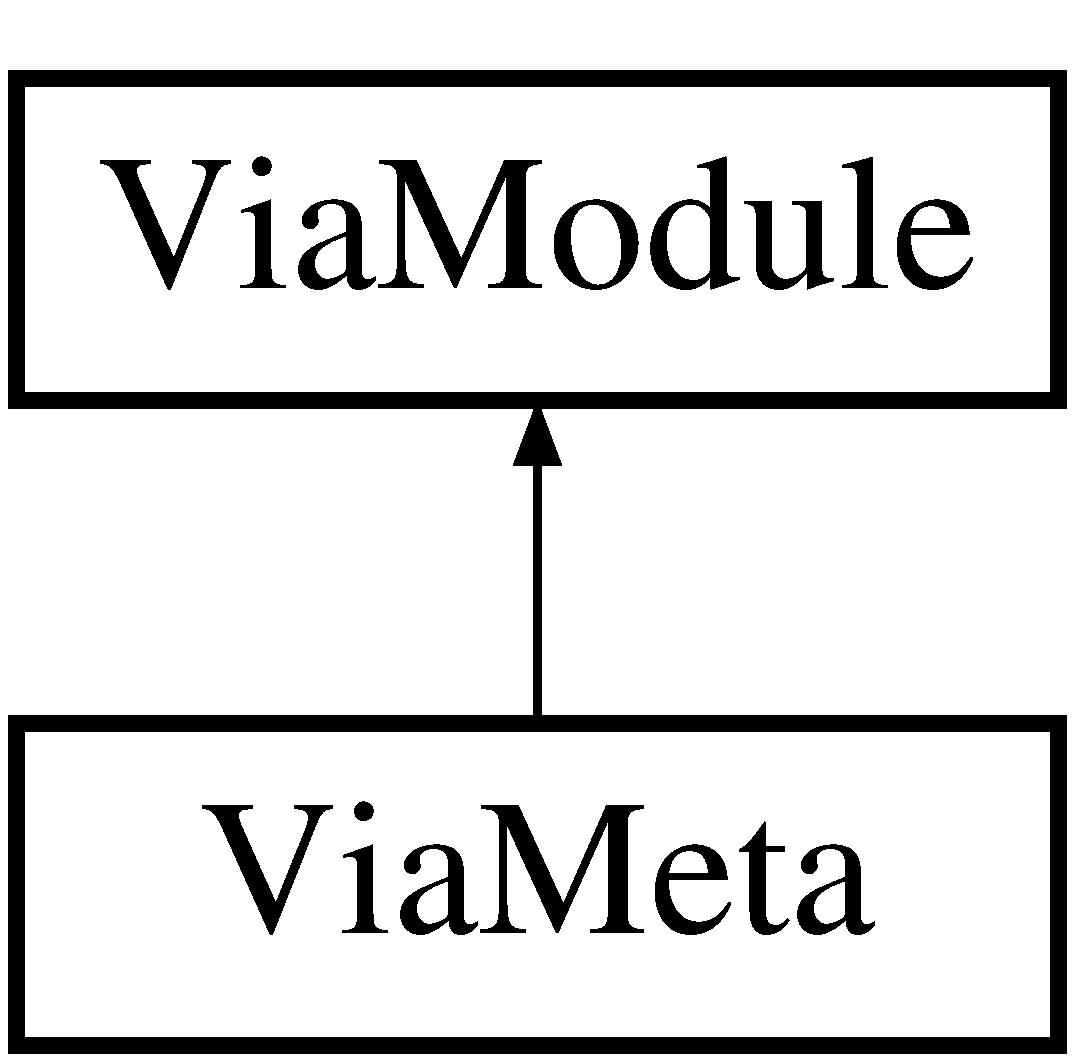
\includegraphics[height=2.000000cm]{class_via_meta}
\end{center}
\end{figure}
\subsection*{Classes}
\begin{DoxyCompactItemize}
\item 
class \mbox{\hyperlink{class_via_meta_1_1_via_meta_u_i}{Via\+Meta\+UI}}
\end{DoxyCompactItemize}
\subsection*{Public Member Functions}
\begin{DoxyCompactItemize}
\item 
void \mbox{\hyperlink{class_via_meta_a7cc6b36d441268ecdd939bc619b544b7}{handle\+Button1\+Mode\+Change}} (int32\+\_\+t)
\item 
void \mbox{\hyperlink{class_via_meta_a6214bd154f0bad9b3a3a164cf2c86a37}{handle\+Button2\+Mode\+Change}} (int32\+\_\+t)
\item 
void \mbox{\hyperlink{class_via_meta_a64f69f2c1886f2d5748d2a1bda68d29e}{handle\+Button3\+Mode\+Change}} (int32\+\_\+t)
\item 
void \mbox{\hyperlink{class_via_meta_a791172b5d929d0a8d26b85ffbb7154fc}{handle\+Button4\+Mode\+Change}} (int32\+\_\+t)
\item 
void \mbox{\hyperlink{class_via_meta_a8840b0feb7bd93e159ab5567b2071944}{handle\+Button5\+Mode\+Change}} (int32\+\_\+t)
\item 
void \mbox{\hyperlink{class_via_meta_a0024df4fef40405972532536f4cc0226}{handle\+Button6\+Mode\+Change}} (int32\+\_\+t)
\item 
void \mbox{\hyperlink{class_via_meta_a0239a011fd549aa363d68c7fcc5f5d91}{handle\+Aux1\+Mode\+Change}} (int32\+\_\+t)
\item 
void \mbox{\hyperlink{class_via_meta_a8b637a702d3e12878b6d3e40c11309d1}{handle\+Aux2\+Mode\+Change}} (int32\+\_\+t)
\item 
void \mbox{\hyperlink{class_via_meta_aa13d82e4b9811d169ac68aeb0cc05850}{handle\+Aux3\+Mode\+Change}} (int32\+\_\+t)
\item 
void \mbox{\hyperlink{class_via_meta_af5912a56e45c8bf6e1c6412cfbae3179}{handle\+Aux4\+Mode\+Change}} (int32\+\_\+t)
\item 
void \mbox{\hyperlink{class_via_meta_a46bc714c10dfcb4f6900ad0518ecbf51}{switch\+Wavetable}} (const \mbox{\hyperlink{struct_wavetable}{Wavetable}} $\ast$)
\item 
void \mbox{\hyperlink{class_via_meta_a8437126f7bb29c15b4dc5953a91e536f}{init\+Phase\+Dist\+Table}} (void)
\item 
void \mbox{\hyperlink{class_via_meta_a08af168b0e35016e949820875aa203ff}{fill\+Wavetable\+Array}} (void)
\item 
void \mbox{\hyperlink{class_via_meta_a180d1594d18fb1eb200aa9f3563f581c}{init\+Drum}} (void)
\item 
void \mbox{\hyperlink{class_via_meta_ae7c5b16eb49bbc307f865fa9ffa3791c}{oversample}} (int32\+\_\+t write\+Index)
\item 
void \mbox{\hyperlink{class_via_meta_a3d97e2435f744b283f1f844ad88cb74d}{add\+Three\+Bits}} (int32\+\_\+t write\+Index)
\item 
void \mbox{\hyperlink{class_via_meta_a81c41ff6c7e3b4c0bb24a708755235fb}{drum\+Mode}} (int32\+\_\+t write\+Index)
\item 
void \mbox{\hyperlink{class_via_meta_a52d062ff1d9a7f039c81abd9e75dd91f}{calculate\+Dac3\+Phasor}} (int32\+\_\+t write\+Index)
\item 
void \mbox{\hyperlink{class_via_meta_ac0d39fc0dae1e4b098009bb052aec13c}{calculate\+Dac3\+Contour}} (int32\+\_\+t write\+Index)
\item 
void \mbox{\hyperlink{class_via_meta_a72ca10d0f7265a4afc233993affc6668}{calculate\+Dac3\+Phasor\+Env}} (int32\+\_\+t write\+Index)
\item 
void \mbox{\hyperlink{class_via_meta_a6b8b934f8dfa1e26cf7136e4421a9a80}{calculate\+Dac3\+Contour\+Env}} (int32\+\_\+t write\+Index)
\item 
void \mbox{\hyperlink{class_via_meta_adfca36bfdc46260efc6f6af088eb94c0}{calculate\+Logic\+A\+Release\+Gate}} (int32\+\_\+t write\+Index)
\item 
void \mbox{\hyperlink{class_via_meta_aa5e9f7c2d51880923bf4047aea321506}{calculate\+Logic\+A\+Attack\+Gate}} (int32\+\_\+t write\+Index)
\item 
void \mbox{\hyperlink{class_via_meta_a694368607a40f8a924207599e7722f1b}{calculate\+S\+H\+Mode1}} (int32\+\_\+t write\+Index)
\item 
void \mbox{\hyperlink{class_via_meta_ada3ace55b8b293141aba025e0f5dde74}{calculate\+S\+H\+Mode2}} (int32\+\_\+t write\+Index)
\item 
void \mbox{\hyperlink{class_via_meta_a1efd5183b450d406c611efe6685db2bb}{calculate\+S\+H\+Mode3}} (int32\+\_\+t write\+Index)
\item 
void \mbox{\hyperlink{class_via_meta_a3d42b57263e2d3b81c0f53df54f61eac}{calculate\+S\+H\+Mode4}} (int32\+\_\+t write\+Index)
\item 
void \mbox{\hyperlink{class_via_meta_a8f6cdf15395d9382bd085b14a1207b43}{calculate\+S\+H\+Mode5}} (int32\+\_\+t write\+Index)
\item 
void \mbox{\hyperlink{class_via_meta_ab85c156e41e1382382c09b1bed76caab}{calculate\+S\+H\+Mode6}} (int32\+\_\+t write\+Index)
\item 
void \mbox{\hyperlink{class_via_meta_a46874348486070e614149008c2099943}{update\+R\+G\+B\+Osc}} (void)
\item 
void \mbox{\hyperlink{class_via_meta_af68a9b7283ccbabf24b3300310d8efea}{update\+R\+G\+B\+Drum}} (void)
\item 
void \mbox{\hyperlink{class_via_meta_a9bdd1b712bedb70d18846cc5a017d0bc}{update\+R\+G\+B\+Subaudio}} (void)
\item 
void \mbox{\hyperlink{class_via_meta_a9f5c7e4c9bc5444c463599c3654f7839}{update\+R\+G\+B\+Blink}} (void)
\item 
void \mbox{\hyperlink{class_via_meta_a18b1d7bd90f64e5e072aef3f94d1004a}{update\+R\+G\+B\+Blank}} (void)
\item 
void \mbox{\hyperlink{class_via_meta_ae4754bc3d05ef786e88b8925654b10e7}{init}} (void)
\item 
\mbox{\hyperlink{class_via_meta_af8d8701d58f2db0e2269594d15690290}{Via\+Meta}} ()
\item 
void \mbox{\hyperlink{class_via_meta_a436b5e1bdcfbbdf693cb60662f16f41c}{main\+Rising\+Edge\+Callback}} (void)
\item 
void \mbox{\hyperlink{class_via_meta_a835905663200c8d54b074dd3cd8f728a}{main\+Falling\+Edge\+Callback}} (void)
\item 
void \mbox{\hyperlink{class_via_meta_a0f19cd6bdf23ade9a83841e81d519e0c}{aux\+Rising\+Edge\+Callback}} (void)
\item 
void \mbox{\hyperlink{class_via_meta_ae3ee604199052c98b3686b05415080f1}{aux\+Falling\+Edge\+Callback}} (void)
\item 
void \mbox{\hyperlink{class_via_meta_a8788a454320240402ead3ad348a6320d}{button\+Pressed\+Callback}} (void)
\item 
void \mbox{\hyperlink{class_via_meta_aaf8a46567a601e18ec8efc333c74dbf7}{button\+Released\+Callback}} (void)
\item 
void \mbox{\hyperlink{class_via_meta_a8eac839ff146db96945e121c5805de09}{io\+Process\+Callback}} (void)
\item 
void \mbox{\hyperlink{class_via_meta_a19e5b43a5a05e814d75cb8b91e126bdd}{half\+Transfer\+Callback}} (void)
\item 
void \mbox{\hyperlink{class_via_meta_a3c6be30783cfeb8fbb2954579fd772a6}{transfer\+Complete\+Callback}} (void)
\item 
void \mbox{\hyperlink{class_via_meta_a78d563d212d841e5aa73c3207b558f05}{slow\+Conversion\+Callback}} (void)
\item 
void \mbox{\hyperlink{class_via_meta_aa11eb2d9719091cb03f50d7f4172509c}{aux\+Timer1\+Interrupt\+Callback}} (void)
\item 
void \mbox{\hyperlink{class_via_meta_aca54f9a3ca029b56887107a3bc828b0d}{aux\+Timer2\+Interrupt\+Callback}} (void)
\item 
void \mbox{\hyperlink{class_via_meta_aa1340e7f06f41cd4a0c7e69db0f7c64d}{ui\+\_\+dispatch}} (int32\+\_\+t sig)
\end{DoxyCompactItemize}
\subsection*{Public Attributes}
\begin{DoxyCompactItemize}
\item 
const \mbox{\hyperlink{struct_wavetable}{Wavetable}} $\ast$ \mbox{\hyperlink{class_via_meta_a62891dea61827785487b4b8f2ada5641}{wavetable\+Array}} \mbox{[}3\mbox{]}\mbox{[}8\mbox{]}
\item 
uint32\+\_\+t \mbox{\hyperlink{class_via_meta_aedee75e7f255d70c7292972d5e5eef65}{wavetable\+Read}} \mbox{[}9\mbox{]}\mbox{[}517\mbox{]}
\item 
uint32\+\_\+t \mbox{\hyperlink{class_via_meta_a8b0b6f0072b72144fe3f894b6303a0d4}{wavetable\+Read\+Drum}} \mbox{[}517\mbox{]}
\item 
uint32\+\_\+t \mbox{\hyperlink{class_via_meta_aceb676011c9259d33d690fe1101421a4}{wavetable\+Read\+Drum2}} \mbox{[}517\mbox{]}
\item 
int16\+\_\+t \mbox{\hyperlink{class_via_meta_a2650520c89c5e41f90571a6670cc3786}{drum\+Write}} \mbox{[}4\mbox{]}
\item 
int16\+\_\+t \mbox{\hyperlink{class_via_meta_a99391f3254d8e106fc7d1d7b3422b1b1}{drum2\+Write}} \mbox{[}4\mbox{]}
\item 
int16\+\_\+t \mbox{\hyperlink{class_via_meta_abe228d0883cfa64c5c34368270dce045}{drum3\+Write}} \mbox{[}4\mbox{]}
\item 
int16\+\_\+t \mbox{\hyperlink{class_via_meta_af67df1f1a9de4ee090de75709c9e8445}{drum\+Full\+Scale}} \mbox{[}4\mbox{]}
\item 
int32\+\_\+t \mbox{\hyperlink{class_via_meta_ac0e88a37fdb70516c048a65c0195925b}{drum\+Off}} \mbox{[}4\mbox{]}
\item 
void(Via\+Meta\+::$\ast$ \mbox{\hyperlink{class_via_meta_ab0b9e808d133a9bc00bca8ecc5928b87}{output\+Stage}} )(int32\+\_\+t write\+Index)
\item 
uint16\+\_\+t \mbox{\hyperlink{class_via_meta_a3a04782d64b83dd605cab1e67742d476}{virtual\+FM}} \mbox{[}2\mbox{]}
\item 
uint16\+\_\+t \mbox{\hyperlink{class_via_meta_a8915cefaa524a38f30f7d80a3f61f69b}{virtual\+Morph}} \mbox{[}2\mbox{]}
\item 
void(Via\+Meta\+::$\ast$ \mbox{\hyperlink{class_via_meta_a20f99319d993114f391102f7cadd558d}{calculate\+Dac3}} )(int32\+\_\+t write\+Index)
\item 
void(Via\+Meta\+::$\ast$ \mbox{\hyperlink{class_via_meta_a5dabe309f8cc5990a11eb2eb5fb7d872}{calculate\+LogicA}} )(int32\+\_\+t write\+Index)
\item 
void(Via\+Meta\+::$\ast$ \mbox{\hyperlink{class_via_meta_abd9b66a2e79446a5275fad25ef40e90f}{calculate\+SH}} )(int32\+\_\+t write\+Index)
\item 
void(Via\+Meta\+::$\ast$ \mbox{\hyperlink{class_via_meta_a56b5fee57636b4d7b6b0be80145ae474}{update\+R\+GB}} )(void)
\item 
void(Via\+Meta\+::$\ast$ \mbox{\hyperlink{class_via_meta_adf6d6ae0cdfa6275d756988494c72bda}{current\+R\+G\+B\+Behavior}} )(void)
\item 
\mbox{\hyperlink{class_via_meta_1_1_via_meta_u_i}{Via\+Meta\+UI}} \mbox{\hyperlink{class_via_meta_a55ce1aad65d98dc744ad0efcfd9047d1}{meta\+UI}}
\item 
int32\+\_\+t \mbox{\hyperlink{class_via_meta_a849f78f2ca06dd8d5df280ac74f7f2df}{runtime\+Display}}
\item 
\mbox{\hyperlink{class_meta_wavetable}{Meta\+Wavetable}} \mbox{\hyperlink{class_via_meta_a181153d602eb58e635cad28f06afa7eb}{meta\+Wavetable}}
\item 
\mbox{\hyperlink{class_meta_controller}{Meta\+Controller}} \mbox{\hyperlink{class_via_meta_ae825571bb029bcd9ddbe8a2c19f041a5}{meta\+Controller}}
\item 
\mbox{\hyperlink{class_simple_envelope}{Simple\+Envelope}} \mbox{\hyperlink{class_via_meta_a1bbd7242c6133f93cd5732ce6add7f87}{amp\+Envelope}}
\item 
\mbox{\hyperlink{class_simple_envelope}{Simple\+Envelope}} \mbox{\hyperlink{class_via_meta_a1ff8bd7ec2f612c9114330b6d451bddc}{freq\+Transient}}
\item 
\mbox{\hyperlink{class_simple_envelope}{Simple\+Envelope}} \mbox{\hyperlink{class_via_meta_acb397704a71ed2eb11218c5d96e5e622}{morph\+Envelope}}
\item 
int32\+\_\+t \mbox{\hyperlink{class_via_meta_acc661a6ed6ca9a096f1dfb7ebfac724f}{morph\+Attack\+Multiplier}} = 1 $<$$<$ 8
\item 
int32\+\_\+t \mbox{\hyperlink{class_via_meta_a583404362a04ac999f086ab9899fa2e4}{morph\+Release\+Multiplier}} = 1 $<$$<$ 2
\item 
int32\+\_\+t \mbox{\hyperlink{class_via_meta_afbc54709d93d43fa6e2508206d280fd4}{freq\+Attack\+Multiplier}} = 1 $<$$<$ 10
\item 
int32\+\_\+t \mbox{\hyperlink{class_via_meta_a2dc1962ea9604adccb61269572acdeb4}{freq\+Release\+Multiplier}} = 1$<$$<$ 8
\item 
int32\+\_\+t \mbox{\hyperlink{class_via_meta_a76c5199c165cb7cdc09ec135e941710f}{transient\+Scale}} = 1 $<$$<$ 3
\item 
uint32\+\_\+t \mbox{\hyperlink{class_via_meta_a4cedfcb63af32f4c03ce682559741b3d}{min\+Transient\+Length}} = 14
\end{DoxyCompactItemize}
\subsection*{Additional Inherited Members}


\subsection{Constructor \& Destructor Documentation}
\mbox{\Hypertarget{class_via_meta_af8d8701d58f2db0e2269594d15690290}\label{class_via_meta_af8d8701d58f2db0e2269594d15690290}} 
\index{Via\+Meta@{Via\+Meta}!Via\+Meta@{Via\+Meta}}
\index{Via\+Meta@{Via\+Meta}!Via\+Meta@{Via\+Meta}}
\subsubsection{\texorpdfstring{Via\+Meta()}{ViaMeta()}}
{\footnotesize\ttfamily Via\+Meta\+::\+Via\+Meta (\begin{DoxyParamCaption}{ }\end{DoxyParamCaption})\hspace{0.3cm}{\ttfamily [inline]}}



\subsection{Member Function Documentation}
\mbox{\Hypertarget{class_via_meta_a3d97e2435f744b283f1f844ad88cb74d}\label{class_via_meta_a3d97e2435f744b283f1f844ad88cb74d}} 
\index{Via\+Meta@{Via\+Meta}!add\+Three\+Bits@{add\+Three\+Bits}}
\index{add\+Three\+Bits@{add\+Three\+Bits}!Via\+Meta@{Via\+Meta}}
\subsubsection{\texorpdfstring{add\+Three\+Bits()}{addThreeBits()}}
{\footnotesize\ttfamily void Via\+Meta\+::add\+Three\+Bits (\begin{DoxyParamCaption}\item[{int32\+\_\+t}]{write\+Index }\end{DoxyParamCaption})}

\mbox{\Hypertarget{class_via_meta_ae3ee604199052c98b3686b05415080f1}\label{class_via_meta_ae3ee604199052c98b3686b05415080f1}} 
\index{Via\+Meta@{Via\+Meta}!aux\+Falling\+Edge\+Callback@{aux\+Falling\+Edge\+Callback}}
\index{aux\+Falling\+Edge\+Callback@{aux\+Falling\+Edge\+Callback}!Via\+Meta@{Via\+Meta}}
\subsubsection{\texorpdfstring{aux\+Falling\+Edge\+Callback()}{auxFallingEdgeCallback()}}
{\footnotesize\ttfamily void Via\+Meta\+::aux\+Falling\+Edge\+Callback (\begin{DoxyParamCaption}\item[{void}]{ }\end{DoxyParamCaption})}

\mbox{\Hypertarget{class_via_meta_a0f19cd6bdf23ade9a83841e81d519e0c}\label{class_via_meta_a0f19cd6bdf23ade9a83841e81d519e0c}} 
\index{Via\+Meta@{Via\+Meta}!aux\+Rising\+Edge\+Callback@{aux\+Rising\+Edge\+Callback}}
\index{aux\+Rising\+Edge\+Callback@{aux\+Rising\+Edge\+Callback}!Via\+Meta@{Via\+Meta}}
\subsubsection{\texorpdfstring{aux\+Rising\+Edge\+Callback()}{auxRisingEdgeCallback()}}
{\footnotesize\ttfamily void Via\+Meta\+::aux\+Rising\+Edge\+Callback (\begin{DoxyParamCaption}\item[{void}]{ }\end{DoxyParamCaption})}

\mbox{\Hypertarget{class_via_meta_aa11eb2d9719091cb03f50d7f4172509c}\label{class_via_meta_aa11eb2d9719091cb03f50d7f4172509c}} 
\index{Via\+Meta@{Via\+Meta}!aux\+Timer1\+Interrupt\+Callback@{aux\+Timer1\+Interrupt\+Callback}}
\index{aux\+Timer1\+Interrupt\+Callback@{aux\+Timer1\+Interrupt\+Callback}!Via\+Meta@{Via\+Meta}}
\subsubsection{\texorpdfstring{aux\+Timer1\+Interrupt\+Callback()}{auxTimer1InterruptCallback()}}
{\footnotesize\ttfamily void Via\+Meta\+::aux\+Timer1\+Interrupt\+Callback (\begin{DoxyParamCaption}\item[{void}]{ }\end{DoxyParamCaption})}

\mbox{\Hypertarget{class_via_meta_aca54f9a3ca029b56887107a3bc828b0d}\label{class_via_meta_aca54f9a3ca029b56887107a3bc828b0d}} 
\index{Via\+Meta@{Via\+Meta}!aux\+Timer2\+Interrupt\+Callback@{aux\+Timer2\+Interrupt\+Callback}}
\index{aux\+Timer2\+Interrupt\+Callback@{aux\+Timer2\+Interrupt\+Callback}!Via\+Meta@{Via\+Meta}}
\subsubsection{\texorpdfstring{aux\+Timer2\+Interrupt\+Callback()}{auxTimer2InterruptCallback()}}
{\footnotesize\ttfamily void Via\+Meta\+::aux\+Timer2\+Interrupt\+Callback (\begin{DoxyParamCaption}\item[{void}]{ }\end{DoxyParamCaption})}

\mbox{\Hypertarget{class_via_meta_a8788a454320240402ead3ad348a6320d}\label{class_via_meta_a8788a454320240402ead3ad348a6320d}} 
\index{Via\+Meta@{Via\+Meta}!button\+Pressed\+Callback@{button\+Pressed\+Callback}}
\index{button\+Pressed\+Callback@{button\+Pressed\+Callback}!Via\+Meta@{Via\+Meta}}
\subsubsection{\texorpdfstring{button\+Pressed\+Callback()}{buttonPressedCallback()}}
{\footnotesize\ttfamily void Via\+Meta\+::button\+Pressed\+Callback (\begin{DoxyParamCaption}\item[{void}]{ }\end{DoxyParamCaption})}

\mbox{\Hypertarget{class_via_meta_aaf8a46567a601e18ec8efc333c74dbf7}\label{class_via_meta_aaf8a46567a601e18ec8efc333c74dbf7}} 
\index{Via\+Meta@{Via\+Meta}!button\+Released\+Callback@{button\+Released\+Callback}}
\index{button\+Released\+Callback@{button\+Released\+Callback}!Via\+Meta@{Via\+Meta}}
\subsubsection{\texorpdfstring{button\+Released\+Callback()}{buttonReleasedCallback()}}
{\footnotesize\ttfamily void Via\+Meta\+::button\+Released\+Callback (\begin{DoxyParamCaption}\item[{void}]{ }\end{DoxyParamCaption})}

\mbox{\Hypertarget{class_via_meta_ac0d39fc0dae1e4b098009bb052aec13c}\label{class_via_meta_ac0d39fc0dae1e4b098009bb052aec13c}} 
\index{Via\+Meta@{Via\+Meta}!calculate\+Dac3\+Contour@{calculate\+Dac3\+Contour}}
\index{calculate\+Dac3\+Contour@{calculate\+Dac3\+Contour}!Via\+Meta@{Via\+Meta}}
\subsubsection{\texorpdfstring{calculate\+Dac3\+Contour()}{calculateDac3Contour()}}
{\footnotesize\ttfamily void Via\+Meta\+::calculate\+Dac3\+Contour (\begin{DoxyParamCaption}\item[{int32\+\_\+t}]{write\+Index }\end{DoxyParamCaption})}

\mbox{\Hypertarget{class_via_meta_a6b8b934f8dfa1e26cf7136e4421a9a80}\label{class_via_meta_a6b8b934f8dfa1e26cf7136e4421a9a80}} 
\index{Via\+Meta@{Via\+Meta}!calculate\+Dac3\+Contour\+Env@{calculate\+Dac3\+Contour\+Env}}
\index{calculate\+Dac3\+Contour\+Env@{calculate\+Dac3\+Contour\+Env}!Via\+Meta@{Via\+Meta}}
\subsubsection{\texorpdfstring{calculate\+Dac3\+Contour\+Env()}{calculateDac3ContourEnv()}}
{\footnotesize\ttfamily void Via\+Meta\+::calculate\+Dac3\+Contour\+Env (\begin{DoxyParamCaption}\item[{int32\+\_\+t}]{write\+Index }\end{DoxyParamCaption})}

\mbox{\Hypertarget{class_via_meta_a52d062ff1d9a7f039c81abd9e75dd91f}\label{class_via_meta_a52d062ff1d9a7f039c81abd9e75dd91f}} 
\index{Via\+Meta@{Via\+Meta}!calculate\+Dac3\+Phasor@{calculate\+Dac3\+Phasor}}
\index{calculate\+Dac3\+Phasor@{calculate\+Dac3\+Phasor}!Via\+Meta@{Via\+Meta}}
\subsubsection{\texorpdfstring{calculate\+Dac3\+Phasor()}{calculateDac3Phasor()}}
{\footnotesize\ttfamily void Via\+Meta\+::calculate\+Dac3\+Phasor (\begin{DoxyParamCaption}\item[{int32\+\_\+t}]{write\+Index }\end{DoxyParamCaption})}

\mbox{\Hypertarget{class_via_meta_a72ca10d0f7265a4afc233993affc6668}\label{class_via_meta_a72ca10d0f7265a4afc233993affc6668}} 
\index{Via\+Meta@{Via\+Meta}!calculate\+Dac3\+Phasor\+Env@{calculate\+Dac3\+Phasor\+Env}}
\index{calculate\+Dac3\+Phasor\+Env@{calculate\+Dac3\+Phasor\+Env}!Via\+Meta@{Via\+Meta}}
\subsubsection{\texorpdfstring{calculate\+Dac3\+Phasor\+Env()}{calculateDac3PhasorEnv()}}
{\footnotesize\ttfamily void Via\+Meta\+::calculate\+Dac3\+Phasor\+Env (\begin{DoxyParamCaption}\item[{int32\+\_\+t}]{write\+Index }\end{DoxyParamCaption})}

\mbox{\Hypertarget{class_via_meta_aa5e9f7c2d51880923bf4047aea321506}\label{class_via_meta_aa5e9f7c2d51880923bf4047aea321506}} 
\index{Via\+Meta@{Via\+Meta}!calculate\+Logic\+A\+Attack\+Gate@{calculate\+Logic\+A\+Attack\+Gate}}
\index{calculate\+Logic\+A\+Attack\+Gate@{calculate\+Logic\+A\+Attack\+Gate}!Via\+Meta@{Via\+Meta}}
\subsubsection{\texorpdfstring{calculate\+Logic\+A\+Attack\+Gate()}{calculateLogicAAttackGate()}}
{\footnotesize\ttfamily void Via\+Meta\+::calculate\+Logic\+A\+Attack\+Gate (\begin{DoxyParamCaption}\item[{int32\+\_\+t}]{write\+Index }\end{DoxyParamCaption})}

\mbox{\Hypertarget{class_via_meta_adfca36bfdc46260efc6f6af088eb94c0}\label{class_via_meta_adfca36bfdc46260efc6f6af088eb94c0}} 
\index{Via\+Meta@{Via\+Meta}!calculate\+Logic\+A\+Release\+Gate@{calculate\+Logic\+A\+Release\+Gate}}
\index{calculate\+Logic\+A\+Release\+Gate@{calculate\+Logic\+A\+Release\+Gate}!Via\+Meta@{Via\+Meta}}
\subsubsection{\texorpdfstring{calculate\+Logic\+A\+Release\+Gate()}{calculateLogicAReleaseGate()}}
{\footnotesize\ttfamily void Via\+Meta\+::calculate\+Logic\+A\+Release\+Gate (\begin{DoxyParamCaption}\item[{int32\+\_\+t}]{write\+Index }\end{DoxyParamCaption})}

\mbox{\Hypertarget{class_via_meta_a694368607a40f8a924207599e7722f1b}\label{class_via_meta_a694368607a40f8a924207599e7722f1b}} 
\index{Via\+Meta@{Via\+Meta}!calculate\+S\+H\+Mode1@{calculate\+S\+H\+Mode1}}
\index{calculate\+S\+H\+Mode1@{calculate\+S\+H\+Mode1}!Via\+Meta@{Via\+Meta}}
\subsubsection{\texorpdfstring{calculate\+S\+H\+Mode1()}{calculateSHMode1()}}
{\footnotesize\ttfamily void Via\+Meta\+::calculate\+S\+H\+Mode1 (\begin{DoxyParamCaption}\item[{int32\+\_\+t}]{write\+Index }\end{DoxyParamCaption})}

\mbox{\Hypertarget{class_via_meta_ada3ace55b8b293141aba025e0f5dde74}\label{class_via_meta_ada3ace55b8b293141aba025e0f5dde74}} 
\index{Via\+Meta@{Via\+Meta}!calculate\+S\+H\+Mode2@{calculate\+S\+H\+Mode2}}
\index{calculate\+S\+H\+Mode2@{calculate\+S\+H\+Mode2}!Via\+Meta@{Via\+Meta}}
\subsubsection{\texorpdfstring{calculate\+S\+H\+Mode2()}{calculateSHMode2()}}
{\footnotesize\ttfamily void Via\+Meta\+::calculate\+S\+H\+Mode2 (\begin{DoxyParamCaption}\item[{int32\+\_\+t}]{write\+Index }\end{DoxyParamCaption})}

\mbox{\Hypertarget{class_via_meta_a1efd5183b450d406c611efe6685db2bb}\label{class_via_meta_a1efd5183b450d406c611efe6685db2bb}} 
\index{Via\+Meta@{Via\+Meta}!calculate\+S\+H\+Mode3@{calculate\+S\+H\+Mode3}}
\index{calculate\+S\+H\+Mode3@{calculate\+S\+H\+Mode3}!Via\+Meta@{Via\+Meta}}
\subsubsection{\texorpdfstring{calculate\+S\+H\+Mode3()}{calculateSHMode3()}}
{\footnotesize\ttfamily void Via\+Meta\+::calculate\+S\+H\+Mode3 (\begin{DoxyParamCaption}\item[{int32\+\_\+t}]{write\+Index }\end{DoxyParamCaption})}

\mbox{\Hypertarget{class_via_meta_a3d42b57263e2d3b81c0f53df54f61eac}\label{class_via_meta_a3d42b57263e2d3b81c0f53df54f61eac}} 
\index{Via\+Meta@{Via\+Meta}!calculate\+S\+H\+Mode4@{calculate\+S\+H\+Mode4}}
\index{calculate\+S\+H\+Mode4@{calculate\+S\+H\+Mode4}!Via\+Meta@{Via\+Meta}}
\subsubsection{\texorpdfstring{calculate\+S\+H\+Mode4()}{calculateSHMode4()}}
{\footnotesize\ttfamily void Via\+Meta\+::calculate\+S\+H\+Mode4 (\begin{DoxyParamCaption}\item[{int32\+\_\+t}]{write\+Index }\end{DoxyParamCaption})}

\mbox{\Hypertarget{class_via_meta_a8f6cdf15395d9382bd085b14a1207b43}\label{class_via_meta_a8f6cdf15395d9382bd085b14a1207b43}} 
\index{Via\+Meta@{Via\+Meta}!calculate\+S\+H\+Mode5@{calculate\+S\+H\+Mode5}}
\index{calculate\+S\+H\+Mode5@{calculate\+S\+H\+Mode5}!Via\+Meta@{Via\+Meta}}
\subsubsection{\texorpdfstring{calculate\+S\+H\+Mode5()}{calculateSHMode5()}}
{\footnotesize\ttfamily void Via\+Meta\+::calculate\+S\+H\+Mode5 (\begin{DoxyParamCaption}\item[{int32\+\_\+t}]{write\+Index }\end{DoxyParamCaption})}

\mbox{\Hypertarget{class_via_meta_ab85c156e41e1382382c09b1bed76caab}\label{class_via_meta_ab85c156e41e1382382c09b1bed76caab}} 
\index{Via\+Meta@{Via\+Meta}!calculate\+S\+H\+Mode6@{calculate\+S\+H\+Mode6}}
\index{calculate\+S\+H\+Mode6@{calculate\+S\+H\+Mode6}!Via\+Meta@{Via\+Meta}}
\subsubsection{\texorpdfstring{calculate\+S\+H\+Mode6()}{calculateSHMode6()}}
{\footnotesize\ttfamily void Via\+Meta\+::calculate\+S\+H\+Mode6 (\begin{DoxyParamCaption}\item[{int32\+\_\+t}]{write\+Index }\end{DoxyParamCaption})}

\mbox{\Hypertarget{class_via_meta_a81c41ff6c7e3b4c0bb24a708755235fb}\label{class_via_meta_a81c41ff6c7e3b4c0bb24a708755235fb}} 
\index{Via\+Meta@{Via\+Meta}!drum\+Mode@{drum\+Mode}}
\index{drum\+Mode@{drum\+Mode}!Via\+Meta@{Via\+Meta}}
\subsubsection{\texorpdfstring{drum\+Mode()}{drumMode()}}
{\footnotesize\ttfamily void Via\+Meta\+::drum\+Mode (\begin{DoxyParamCaption}\item[{int32\+\_\+t}]{write\+Index }\end{DoxyParamCaption})}

\mbox{\Hypertarget{class_via_meta_a08af168b0e35016e949820875aa203ff}\label{class_via_meta_a08af168b0e35016e949820875aa203ff}} 
\index{Via\+Meta@{Via\+Meta}!fill\+Wavetable\+Array@{fill\+Wavetable\+Array}}
\index{fill\+Wavetable\+Array@{fill\+Wavetable\+Array}!Via\+Meta@{Via\+Meta}}
\subsubsection{\texorpdfstring{fill\+Wavetable\+Array()}{fillWavetableArray()}}
{\footnotesize\ttfamily void Via\+Meta\+::fill\+Wavetable\+Array (\begin{DoxyParamCaption}\item[{void}]{ }\end{DoxyParamCaption})}

\mbox{\Hypertarget{class_via_meta_a19e5b43a5a05e814d75cb8b91e126bdd}\label{class_via_meta_a19e5b43a5a05e814d75cb8b91e126bdd}} 
\index{Via\+Meta@{Via\+Meta}!half\+Transfer\+Callback@{half\+Transfer\+Callback}}
\index{half\+Transfer\+Callback@{half\+Transfer\+Callback}!Via\+Meta@{Via\+Meta}}
\subsubsection{\texorpdfstring{half\+Transfer\+Callback()}{halfTransferCallback()}}
{\footnotesize\ttfamily void Via\+Meta\+::half\+Transfer\+Callback (\begin{DoxyParamCaption}\item[{void}]{ }\end{DoxyParamCaption})}

\mbox{\Hypertarget{class_via_meta_a0239a011fd549aa363d68c7fcc5f5d91}\label{class_via_meta_a0239a011fd549aa363d68c7fcc5f5d91}} 
\index{Via\+Meta@{Via\+Meta}!handle\+Aux1\+Mode\+Change@{handle\+Aux1\+Mode\+Change}}
\index{handle\+Aux1\+Mode\+Change@{handle\+Aux1\+Mode\+Change}!Via\+Meta@{Via\+Meta}}
\subsubsection{\texorpdfstring{handle\+Aux1\+Mode\+Change()}{handleAux1ModeChange()}}
{\footnotesize\ttfamily void Via\+Meta\+::handle\+Aux1\+Mode\+Change (\begin{DoxyParamCaption}\item[{int32\+\_\+t}]{mode }\end{DoxyParamCaption})}

\mbox{\Hypertarget{class_via_meta_a8b637a702d3e12878b6d3e40c11309d1}\label{class_via_meta_a8b637a702d3e12878b6d3e40c11309d1}} 
\index{Via\+Meta@{Via\+Meta}!handle\+Aux2\+Mode\+Change@{handle\+Aux2\+Mode\+Change}}
\index{handle\+Aux2\+Mode\+Change@{handle\+Aux2\+Mode\+Change}!Via\+Meta@{Via\+Meta}}
\subsubsection{\texorpdfstring{handle\+Aux2\+Mode\+Change()}{handleAux2ModeChange()}}
{\footnotesize\ttfamily void Via\+Meta\+::handle\+Aux2\+Mode\+Change (\begin{DoxyParamCaption}\item[{int32\+\_\+t}]{mode }\end{DoxyParamCaption})}

\mbox{\Hypertarget{class_via_meta_aa13d82e4b9811d169ac68aeb0cc05850}\label{class_via_meta_aa13d82e4b9811d169ac68aeb0cc05850}} 
\index{Via\+Meta@{Via\+Meta}!handle\+Aux3\+Mode\+Change@{handle\+Aux3\+Mode\+Change}}
\index{handle\+Aux3\+Mode\+Change@{handle\+Aux3\+Mode\+Change}!Via\+Meta@{Via\+Meta}}
\subsubsection{\texorpdfstring{handle\+Aux3\+Mode\+Change()}{handleAux3ModeChange()}}
{\footnotesize\ttfamily void Via\+Meta\+::handle\+Aux3\+Mode\+Change (\begin{DoxyParamCaption}\item[{int32\+\_\+t}]{mode }\end{DoxyParamCaption})}

\mbox{\Hypertarget{class_via_meta_af5912a56e45c8bf6e1c6412cfbae3179}\label{class_via_meta_af5912a56e45c8bf6e1c6412cfbae3179}} 
\index{Via\+Meta@{Via\+Meta}!handle\+Aux4\+Mode\+Change@{handle\+Aux4\+Mode\+Change}}
\index{handle\+Aux4\+Mode\+Change@{handle\+Aux4\+Mode\+Change}!Via\+Meta@{Via\+Meta}}
\subsubsection{\texorpdfstring{handle\+Aux4\+Mode\+Change()}{handleAux4ModeChange()}}
{\footnotesize\ttfamily void Via\+Meta\+::handle\+Aux4\+Mode\+Change (\begin{DoxyParamCaption}\item[{int32\+\_\+t}]{mode }\end{DoxyParamCaption})}

\mbox{\Hypertarget{class_via_meta_a7cc6b36d441268ecdd939bc619b544b7}\label{class_via_meta_a7cc6b36d441268ecdd939bc619b544b7}} 
\index{Via\+Meta@{Via\+Meta}!handle\+Button1\+Mode\+Change@{handle\+Button1\+Mode\+Change}}
\index{handle\+Button1\+Mode\+Change@{handle\+Button1\+Mode\+Change}!Via\+Meta@{Via\+Meta}}
\subsubsection{\texorpdfstring{handle\+Button1\+Mode\+Change()}{handleButton1ModeChange()}}
{\footnotesize\ttfamily void Via\+Meta\+::handle\+Button1\+Mode\+Change (\begin{DoxyParamCaption}\item[{int32\+\_\+t}]{mode }\end{DoxyParamCaption})}

\mbox{\Hypertarget{class_via_meta_a6214bd154f0bad9b3a3a164cf2c86a37}\label{class_via_meta_a6214bd154f0bad9b3a3a164cf2c86a37}} 
\index{Via\+Meta@{Via\+Meta}!handle\+Button2\+Mode\+Change@{handle\+Button2\+Mode\+Change}}
\index{handle\+Button2\+Mode\+Change@{handle\+Button2\+Mode\+Change}!Via\+Meta@{Via\+Meta}}
\subsubsection{\texorpdfstring{handle\+Button2\+Mode\+Change()}{handleButton2ModeChange()}}
{\footnotesize\ttfamily void Via\+Meta\+::handle\+Button2\+Mode\+Change (\begin{DoxyParamCaption}\item[{int32\+\_\+t}]{mode }\end{DoxyParamCaption})}

\mbox{\Hypertarget{class_via_meta_a64f69f2c1886f2d5748d2a1bda68d29e}\label{class_via_meta_a64f69f2c1886f2d5748d2a1bda68d29e}} 
\index{Via\+Meta@{Via\+Meta}!handle\+Button3\+Mode\+Change@{handle\+Button3\+Mode\+Change}}
\index{handle\+Button3\+Mode\+Change@{handle\+Button3\+Mode\+Change}!Via\+Meta@{Via\+Meta}}
\subsubsection{\texorpdfstring{handle\+Button3\+Mode\+Change()}{handleButton3ModeChange()}}
{\footnotesize\ttfamily void Via\+Meta\+::handle\+Button3\+Mode\+Change (\begin{DoxyParamCaption}\item[{int32\+\_\+t}]{mode }\end{DoxyParamCaption})}

\mbox{\Hypertarget{class_via_meta_a791172b5d929d0a8d26b85ffbb7154fc}\label{class_via_meta_a791172b5d929d0a8d26b85ffbb7154fc}} 
\index{Via\+Meta@{Via\+Meta}!handle\+Button4\+Mode\+Change@{handle\+Button4\+Mode\+Change}}
\index{handle\+Button4\+Mode\+Change@{handle\+Button4\+Mode\+Change}!Via\+Meta@{Via\+Meta}}
\subsubsection{\texorpdfstring{handle\+Button4\+Mode\+Change()}{handleButton4ModeChange()}}
{\footnotesize\ttfamily void Via\+Meta\+::handle\+Button4\+Mode\+Change (\begin{DoxyParamCaption}\item[{int32\+\_\+t}]{mode }\end{DoxyParamCaption})}

\mbox{\Hypertarget{class_via_meta_a8840b0feb7bd93e159ab5567b2071944}\label{class_via_meta_a8840b0feb7bd93e159ab5567b2071944}} 
\index{Via\+Meta@{Via\+Meta}!handle\+Button5\+Mode\+Change@{handle\+Button5\+Mode\+Change}}
\index{handle\+Button5\+Mode\+Change@{handle\+Button5\+Mode\+Change}!Via\+Meta@{Via\+Meta}}
\subsubsection{\texorpdfstring{handle\+Button5\+Mode\+Change()}{handleButton5ModeChange()}}
{\footnotesize\ttfamily void Via\+Meta\+::handle\+Button5\+Mode\+Change (\begin{DoxyParamCaption}\item[{int32\+\_\+t}]{mode }\end{DoxyParamCaption})}

\mbox{\Hypertarget{class_via_meta_a0024df4fef40405972532536f4cc0226}\label{class_via_meta_a0024df4fef40405972532536f4cc0226}} 
\index{Via\+Meta@{Via\+Meta}!handle\+Button6\+Mode\+Change@{handle\+Button6\+Mode\+Change}}
\index{handle\+Button6\+Mode\+Change@{handle\+Button6\+Mode\+Change}!Via\+Meta@{Via\+Meta}}
\subsubsection{\texorpdfstring{handle\+Button6\+Mode\+Change()}{handleButton6ModeChange()}}
{\footnotesize\ttfamily void Via\+Meta\+::handle\+Button6\+Mode\+Change (\begin{DoxyParamCaption}\item[{int32\+\_\+t}]{mode }\end{DoxyParamCaption})}

\mbox{\Hypertarget{class_via_meta_ae4754bc3d05ef786e88b8925654b10e7}\label{class_via_meta_ae4754bc3d05ef786e88b8925654b10e7}} 
\index{Via\+Meta@{Via\+Meta}!init@{init}}
\index{init@{init}!Via\+Meta@{Via\+Meta}}
\subsubsection{\texorpdfstring{init()}{init()}}
{\footnotesize\ttfamily void Via\+Meta\+::init (\begin{DoxyParamCaption}\item[{void}]{ }\end{DoxyParamCaption})}

\mbox{\Hypertarget{class_via_meta_a180d1594d18fb1eb200aa9f3563f581c}\label{class_via_meta_a180d1594d18fb1eb200aa9f3563f581c}} 
\index{Via\+Meta@{Via\+Meta}!init\+Drum@{init\+Drum}}
\index{init\+Drum@{init\+Drum}!Via\+Meta@{Via\+Meta}}
\subsubsection{\texorpdfstring{init\+Drum()}{initDrum()}}
{\footnotesize\ttfamily void Via\+Meta\+::init\+Drum (\begin{DoxyParamCaption}\item[{void}]{ }\end{DoxyParamCaption})}

\mbox{\Hypertarget{class_via_meta_a8437126f7bb29c15b4dc5953a91e536f}\label{class_via_meta_a8437126f7bb29c15b4dc5953a91e536f}} 
\index{Via\+Meta@{Via\+Meta}!init\+Phase\+Dist\+Table@{init\+Phase\+Dist\+Table}}
\index{init\+Phase\+Dist\+Table@{init\+Phase\+Dist\+Table}!Via\+Meta@{Via\+Meta}}
\subsubsection{\texorpdfstring{init\+Phase\+Dist\+Table()}{initPhaseDistTable()}}
{\footnotesize\ttfamily void Via\+Meta\+::init\+Phase\+Dist\+Table (\begin{DoxyParamCaption}\item[{void}]{ }\end{DoxyParamCaption})}

\mbox{\Hypertarget{class_via_meta_a8eac839ff146db96945e121c5805de09}\label{class_via_meta_a8eac839ff146db96945e121c5805de09}} 
\index{Via\+Meta@{Via\+Meta}!io\+Process\+Callback@{io\+Process\+Callback}}
\index{io\+Process\+Callback@{io\+Process\+Callback}!Via\+Meta@{Via\+Meta}}
\subsubsection{\texorpdfstring{io\+Process\+Callback()}{ioProcessCallback()}}
{\footnotesize\ttfamily void Via\+Meta\+::io\+Process\+Callback (\begin{DoxyParamCaption}\item[{void}]{ }\end{DoxyParamCaption})}

\mbox{\Hypertarget{class_via_meta_a835905663200c8d54b074dd3cd8f728a}\label{class_via_meta_a835905663200c8d54b074dd3cd8f728a}} 
\index{Via\+Meta@{Via\+Meta}!main\+Falling\+Edge\+Callback@{main\+Falling\+Edge\+Callback}}
\index{main\+Falling\+Edge\+Callback@{main\+Falling\+Edge\+Callback}!Via\+Meta@{Via\+Meta}}
\subsubsection{\texorpdfstring{main\+Falling\+Edge\+Callback()}{mainFallingEdgeCallback()}}
{\footnotesize\ttfamily void Via\+Meta\+::main\+Falling\+Edge\+Callback (\begin{DoxyParamCaption}\item[{void}]{ }\end{DoxyParamCaption})}

\mbox{\Hypertarget{class_via_meta_a436b5e1bdcfbbdf693cb60662f16f41c}\label{class_via_meta_a436b5e1bdcfbbdf693cb60662f16f41c}} 
\index{Via\+Meta@{Via\+Meta}!main\+Rising\+Edge\+Callback@{main\+Rising\+Edge\+Callback}}
\index{main\+Rising\+Edge\+Callback@{main\+Rising\+Edge\+Callback}!Via\+Meta@{Via\+Meta}}
\subsubsection{\texorpdfstring{main\+Rising\+Edge\+Callback()}{mainRisingEdgeCallback()}}
{\footnotesize\ttfamily void Via\+Meta\+::main\+Rising\+Edge\+Callback (\begin{DoxyParamCaption}\item[{void}]{ }\end{DoxyParamCaption})}

\mbox{\Hypertarget{class_via_meta_ae7c5b16eb49bbc307f865fa9ffa3791c}\label{class_via_meta_ae7c5b16eb49bbc307f865fa9ffa3791c}} 
\index{Via\+Meta@{Via\+Meta}!oversample@{oversample}}
\index{oversample@{oversample}!Via\+Meta@{Via\+Meta}}
\subsubsection{\texorpdfstring{oversample()}{oversample()}}
{\footnotesize\ttfamily void Via\+Meta\+::oversample (\begin{DoxyParamCaption}\item[{int32\+\_\+t}]{write\+Index }\end{DoxyParamCaption})}

\mbox{\Hypertarget{class_via_meta_a78d563d212d841e5aa73c3207b558f05}\label{class_via_meta_a78d563d212d841e5aa73c3207b558f05}} 
\index{Via\+Meta@{Via\+Meta}!slow\+Conversion\+Callback@{slow\+Conversion\+Callback}}
\index{slow\+Conversion\+Callback@{slow\+Conversion\+Callback}!Via\+Meta@{Via\+Meta}}
\subsubsection{\texorpdfstring{slow\+Conversion\+Callback()}{slowConversionCallback()}}
{\footnotesize\ttfamily void Via\+Meta\+::slow\+Conversion\+Callback (\begin{DoxyParamCaption}\item[{void}]{ }\end{DoxyParamCaption})}

\mbox{\Hypertarget{class_via_meta_a46bc714c10dfcb4f6900ad0518ecbf51}\label{class_via_meta_a46bc714c10dfcb4f6900ad0518ecbf51}} 
\index{Via\+Meta@{Via\+Meta}!switch\+Wavetable@{switch\+Wavetable}}
\index{switch\+Wavetable@{switch\+Wavetable}!Via\+Meta@{Via\+Meta}}
\subsubsection{\texorpdfstring{switch\+Wavetable()}{switchWavetable()}}
{\footnotesize\ttfamily void Via\+Meta\+::switch\+Wavetable (\begin{DoxyParamCaption}\item[{const \mbox{\hyperlink{struct_wavetable}{Wavetable}} $\ast$}]{table }\end{DoxyParamCaption})}

\mbox{\Hypertarget{class_via_meta_a3c6be30783cfeb8fbb2954579fd772a6}\label{class_via_meta_a3c6be30783cfeb8fbb2954579fd772a6}} 
\index{Via\+Meta@{Via\+Meta}!transfer\+Complete\+Callback@{transfer\+Complete\+Callback}}
\index{transfer\+Complete\+Callback@{transfer\+Complete\+Callback}!Via\+Meta@{Via\+Meta}}
\subsubsection{\texorpdfstring{transfer\+Complete\+Callback()}{transferCompleteCallback()}}
{\footnotesize\ttfamily void Via\+Meta\+::transfer\+Complete\+Callback (\begin{DoxyParamCaption}\item[{void}]{ }\end{DoxyParamCaption})}

\mbox{\Hypertarget{class_via_meta_aa1340e7f06f41cd4a0c7e69db0f7c64d}\label{class_via_meta_aa1340e7f06f41cd4a0c7e69db0f7c64d}} 
\index{Via\+Meta@{Via\+Meta}!ui\+\_\+dispatch@{ui\+\_\+dispatch}}
\index{ui\+\_\+dispatch@{ui\+\_\+dispatch}!Via\+Meta@{Via\+Meta}}
\subsubsection{\texorpdfstring{ui\+\_\+dispatch()}{ui\_dispatch()}}
{\footnotesize\ttfamily void Via\+Meta\+::ui\+\_\+dispatch (\begin{DoxyParamCaption}\item[{int32\+\_\+t}]{sig }\end{DoxyParamCaption})\hspace{0.3cm}{\ttfamily [inline]}}

\mbox{\Hypertarget{class_via_meta_a18b1d7bd90f64e5e072aef3f94d1004a}\label{class_via_meta_a18b1d7bd90f64e5e072aef3f94d1004a}} 
\index{Via\+Meta@{Via\+Meta}!update\+R\+G\+B\+Blank@{update\+R\+G\+B\+Blank}}
\index{update\+R\+G\+B\+Blank@{update\+R\+G\+B\+Blank}!Via\+Meta@{Via\+Meta}}
\subsubsection{\texorpdfstring{update\+R\+G\+B\+Blank()}{updateRGBBlank()}}
{\footnotesize\ttfamily void Via\+Meta\+::update\+R\+G\+B\+Blank (\begin{DoxyParamCaption}\item[{void}]{ }\end{DoxyParamCaption})\hspace{0.3cm}{\ttfamily [inline]}}

\mbox{\Hypertarget{class_via_meta_a9f5c7e4c9bc5444c463599c3654f7839}\label{class_via_meta_a9f5c7e4c9bc5444c463599c3654f7839}} 
\index{Via\+Meta@{Via\+Meta}!update\+R\+G\+B\+Blink@{update\+R\+G\+B\+Blink}}
\index{update\+R\+G\+B\+Blink@{update\+R\+G\+B\+Blink}!Via\+Meta@{Via\+Meta}}
\subsubsection{\texorpdfstring{update\+R\+G\+B\+Blink()}{updateRGBBlink()}}
{\footnotesize\ttfamily void Via\+Meta\+::update\+R\+G\+B\+Blink (\begin{DoxyParamCaption}\item[{void}]{ }\end{DoxyParamCaption})\hspace{0.3cm}{\ttfamily [inline]}}

\mbox{\Hypertarget{class_via_meta_af68a9b7283ccbabf24b3300310d8efea}\label{class_via_meta_af68a9b7283ccbabf24b3300310d8efea}} 
\index{Via\+Meta@{Via\+Meta}!update\+R\+G\+B\+Drum@{update\+R\+G\+B\+Drum}}
\index{update\+R\+G\+B\+Drum@{update\+R\+G\+B\+Drum}!Via\+Meta@{Via\+Meta}}
\subsubsection{\texorpdfstring{update\+R\+G\+B\+Drum()}{updateRGBDrum()}}
{\footnotesize\ttfamily void Via\+Meta\+::update\+R\+G\+B\+Drum (\begin{DoxyParamCaption}\item[{void}]{ }\end{DoxyParamCaption})\hspace{0.3cm}{\ttfamily [inline]}}

\mbox{\Hypertarget{class_via_meta_a46874348486070e614149008c2099943}\label{class_via_meta_a46874348486070e614149008c2099943}} 
\index{Via\+Meta@{Via\+Meta}!update\+R\+G\+B\+Osc@{update\+R\+G\+B\+Osc}}
\index{update\+R\+G\+B\+Osc@{update\+R\+G\+B\+Osc}!Via\+Meta@{Via\+Meta}}
\subsubsection{\texorpdfstring{update\+R\+G\+B\+Osc()}{updateRGBOsc()}}
{\footnotesize\ttfamily void Via\+Meta\+::update\+R\+G\+B\+Osc (\begin{DoxyParamCaption}\item[{void}]{ }\end{DoxyParamCaption})\hspace{0.3cm}{\ttfamily [inline]}}

\mbox{\Hypertarget{class_via_meta_a9bdd1b712bedb70d18846cc5a017d0bc}\label{class_via_meta_a9bdd1b712bedb70d18846cc5a017d0bc}} 
\index{Via\+Meta@{Via\+Meta}!update\+R\+G\+B\+Subaudio@{update\+R\+G\+B\+Subaudio}}
\index{update\+R\+G\+B\+Subaudio@{update\+R\+G\+B\+Subaudio}!Via\+Meta@{Via\+Meta}}
\subsubsection{\texorpdfstring{update\+R\+G\+B\+Subaudio()}{updateRGBSubaudio()}}
{\footnotesize\ttfamily void Via\+Meta\+::update\+R\+G\+B\+Subaudio (\begin{DoxyParamCaption}\item[{void}]{ }\end{DoxyParamCaption})\hspace{0.3cm}{\ttfamily [inline]}}



\subsection{Member Data Documentation}
\mbox{\Hypertarget{class_via_meta_a1bbd7242c6133f93cd5732ce6add7f87}\label{class_via_meta_a1bbd7242c6133f93cd5732ce6add7f87}} 
\index{Via\+Meta@{Via\+Meta}!amp\+Envelope@{amp\+Envelope}}
\index{amp\+Envelope@{amp\+Envelope}!Via\+Meta@{Via\+Meta}}
\subsubsection{\texorpdfstring{amp\+Envelope}{ampEnvelope}}
{\footnotesize\ttfamily \mbox{\hyperlink{class_simple_envelope}{Simple\+Envelope}} Via\+Meta\+::amp\+Envelope}

\mbox{\Hypertarget{class_via_meta_a20f99319d993114f391102f7cadd558d}\label{class_via_meta_a20f99319d993114f391102f7cadd558d}} 
\index{Via\+Meta@{Via\+Meta}!calculate\+Dac3@{calculate\+Dac3}}
\index{calculate\+Dac3@{calculate\+Dac3}!Via\+Meta@{Via\+Meta}}
\subsubsection{\texorpdfstring{calculate\+Dac3}{calculateDac3}}
{\footnotesize\ttfamily void(Via\+Meta\+::$\ast$ Via\+Meta\+::calculate\+Dac3) (int32\+\_\+t write\+Index)}

\mbox{\Hypertarget{class_via_meta_a5dabe309f8cc5990a11eb2eb5fb7d872}\label{class_via_meta_a5dabe309f8cc5990a11eb2eb5fb7d872}} 
\index{Via\+Meta@{Via\+Meta}!calculate\+LogicA@{calculate\+LogicA}}
\index{calculate\+LogicA@{calculate\+LogicA}!Via\+Meta@{Via\+Meta}}
\subsubsection{\texorpdfstring{calculate\+LogicA}{calculateLogicA}}
{\footnotesize\ttfamily void(Via\+Meta\+::$\ast$ Via\+Meta\+::calculate\+LogicA) (int32\+\_\+t write\+Index)}

\mbox{\Hypertarget{class_via_meta_abd9b66a2e79446a5275fad25ef40e90f}\label{class_via_meta_abd9b66a2e79446a5275fad25ef40e90f}} 
\index{Via\+Meta@{Via\+Meta}!calculate\+SH@{calculate\+SH}}
\index{calculate\+SH@{calculate\+SH}!Via\+Meta@{Via\+Meta}}
\subsubsection{\texorpdfstring{calculate\+SH}{calculateSH}}
{\footnotesize\ttfamily void(Via\+Meta\+::$\ast$ Via\+Meta\+::calculate\+SH) (int32\+\_\+t write\+Index)}

\mbox{\Hypertarget{class_via_meta_adf6d6ae0cdfa6275d756988494c72bda}\label{class_via_meta_adf6d6ae0cdfa6275d756988494c72bda}} 
\index{Via\+Meta@{Via\+Meta}!current\+R\+G\+B\+Behavior@{current\+R\+G\+B\+Behavior}}
\index{current\+R\+G\+B\+Behavior@{current\+R\+G\+B\+Behavior}!Via\+Meta@{Via\+Meta}}
\subsubsection{\texorpdfstring{current\+R\+G\+B\+Behavior}{currentRGBBehavior}}
{\footnotesize\ttfamily void(Via\+Meta\+::$\ast$ Via\+Meta\+::current\+R\+G\+B\+Behavior) (void)}

\mbox{\Hypertarget{class_via_meta_a99391f3254d8e106fc7d1d7b3422b1b1}\label{class_via_meta_a99391f3254d8e106fc7d1d7b3422b1b1}} 
\index{Via\+Meta@{Via\+Meta}!drum2\+Write@{drum2\+Write}}
\index{drum2\+Write@{drum2\+Write}!Via\+Meta@{Via\+Meta}}
\subsubsection{\texorpdfstring{drum2\+Write}{drum2Write}}
{\footnotesize\ttfamily int16\+\_\+t Via\+Meta\+::drum2\+Write\mbox{[}4\mbox{]}}

\mbox{\Hypertarget{class_via_meta_abe228d0883cfa64c5c34368270dce045}\label{class_via_meta_abe228d0883cfa64c5c34368270dce045}} 
\index{Via\+Meta@{Via\+Meta}!drum3\+Write@{drum3\+Write}}
\index{drum3\+Write@{drum3\+Write}!Via\+Meta@{Via\+Meta}}
\subsubsection{\texorpdfstring{drum3\+Write}{drum3Write}}
{\footnotesize\ttfamily int16\+\_\+t Via\+Meta\+::drum3\+Write\mbox{[}4\mbox{]}}

\mbox{\Hypertarget{class_via_meta_af67df1f1a9de4ee090de75709c9e8445}\label{class_via_meta_af67df1f1a9de4ee090de75709c9e8445}} 
\index{Via\+Meta@{Via\+Meta}!drum\+Full\+Scale@{drum\+Full\+Scale}}
\index{drum\+Full\+Scale@{drum\+Full\+Scale}!Via\+Meta@{Via\+Meta}}
\subsubsection{\texorpdfstring{drum\+Full\+Scale}{drumFullScale}}
{\footnotesize\ttfamily int16\+\_\+t Via\+Meta\+::drum\+Full\+Scale\mbox{[}4\mbox{]}}

\mbox{\Hypertarget{class_via_meta_ac0e88a37fdb70516c048a65c0195925b}\label{class_via_meta_ac0e88a37fdb70516c048a65c0195925b}} 
\index{Via\+Meta@{Via\+Meta}!drum\+Off@{drum\+Off}}
\index{drum\+Off@{drum\+Off}!Via\+Meta@{Via\+Meta}}
\subsubsection{\texorpdfstring{drum\+Off}{drumOff}}
{\footnotesize\ttfamily int32\+\_\+t Via\+Meta\+::drum\+Off\mbox{[}4\mbox{]}}

\mbox{\Hypertarget{class_via_meta_a2650520c89c5e41f90571a6670cc3786}\label{class_via_meta_a2650520c89c5e41f90571a6670cc3786}} 
\index{Via\+Meta@{Via\+Meta}!drum\+Write@{drum\+Write}}
\index{drum\+Write@{drum\+Write}!Via\+Meta@{Via\+Meta}}
\subsubsection{\texorpdfstring{drum\+Write}{drumWrite}}
{\footnotesize\ttfamily int16\+\_\+t Via\+Meta\+::drum\+Write\mbox{[}4\mbox{]}}

\mbox{\Hypertarget{class_via_meta_afbc54709d93d43fa6e2508206d280fd4}\label{class_via_meta_afbc54709d93d43fa6e2508206d280fd4}} 
\index{Via\+Meta@{Via\+Meta}!freq\+Attack\+Multiplier@{freq\+Attack\+Multiplier}}
\index{freq\+Attack\+Multiplier@{freq\+Attack\+Multiplier}!Via\+Meta@{Via\+Meta}}
\subsubsection{\texorpdfstring{freq\+Attack\+Multiplier}{freqAttackMultiplier}}
{\footnotesize\ttfamily int32\+\_\+t Via\+Meta\+::freq\+Attack\+Multiplier = 1 $<$$<$ 10}

\mbox{\Hypertarget{class_via_meta_a2dc1962ea9604adccb61269572acdeb4}\label{class_via_meta_a2dc1962ea9604adccb61269572acdeb4}} 
\index{Via\+Meta@{Via\+Meta}!freq\+Release\+Multiplier@{freq\+Release\+Multiplier}}
\index{freq\+Release\+Multiplier@{freq\+Release\+Multiplier}!Via\+Meta@{Via\+Meta}}
\subsubsection{\texorpdfstring{freq\+Release\+Multiplier}{freqReleaseMultiplier}}
{\footnotesize\ttfamily int32\+\_\+t Via\+Meta\+::freq\+Release\+Multiplier = 1$<$$<$ 8}

\mbox{\Hypertarget{class_via_meta_a1ff8bd7ec2f612c9114330b6d451bddc}\label{class_via_meta_a1ff8bd7ec2f612c9114330b6d451bddc}} 
\index{Via\+Meta@{Via\+Meta}!freq\+Transient@{freq\+Transient}}
\index{freq\+Transient@{freq\+Transient}!Via\+Meta@{Via\+Meta}}
\subsubsection{\texorpdfstring{freq\+Transient}{freqTransient}}
{\footnotesize\ttfamily \mbox{\hyperlink{class_simple_envelope}{Simple\+Envelope}} Via\+Meta\+::freq\+Transient}

\mbox{\Hypertarget{class_via_meta_ae825571bb029bcd9ddbe8a2c19f041a5}\label{class_via_meta_ae825571bb029bcd9ddbe8a2c19f041a5}} 
\index{Via\+Meta@{Via\+Meta}!meta\+Controller@{meta\+Controller}}
\index{meta\+Controller@{meta\+Controller}!Via\+Meta@{Via\+Meta}}
\subsubsection{\texorpdfstring{meta\+Controller}{metaController}}
{\footnotesize\ttfamily \mbox{\hyperlink{class_meta_controller}{Meta\+Controller}} Via\+Meta\+::meta\+Controller}

\mbox{\Hypertarget{class_via_meta_a55ce1aad65d98dc744ad0efcfd9047d1}\label{class_via_meta_a55ce1aad65d98dc744ad0efcfd9047d1}} 
\index{Via\+Meta@{Via\+Meta}!meta\+UI@{meta\+UI}}
\index{meta\+UI@{meta\+UI}!Via\+Meta@{Via\+Meta}}
\subsubsection{\texorpdfstring{meta\+UI}{metaUI}}
{\footnotesize\ttfamily \mbox{\hyperlink{class_via_meta_1_1_via_meta_u_i}{Via\+Meta\+UI}} Via\+Meta\+::meta\+UI}

\mbox{\Hypertarget{class_via_meta_a181153d602eb58e635cad28f06afa7eb}\label{class_via_meta_a181153d602eb58e635cad28f06afa7eb}} 
\index{Via\+Meta@{Via\+Meta}!meta\+Wavetable@{meta\+Wavetable}}
\index{meta\+Wavetable@{meta\+Wavetable}!Via\+Meta@{Via\+Meta}}
\subsubsection{\texorpdfstring{meta\+Wavetable}{metaWavetable}}
{\footnotesize\ttfamily \mbox{\hyperlink{class_meta_wavetable}{Meta\+Wavetable}} Via\+Meta\+::meta\+Wavetable}

\mbox{\Hypertarget{class_via_meta_a4cedfcb63af32f4c03ce682559741b3d}\label{class_via_meta_a4cedfcb63af32f4c03ce682559741b3d}} 
\index{Via\+Meta@{Via\+Meta}!min\+Transient\+Length@{min\+Transient\+Length}}
\index{min\+Transient\+Length@{min\+Transient\+Length}!Via\+Meta@{Via\+Meta}}
\subsubsection{\texorpdfstring{min\+Transient\+Length}{minTransientLength}}
{\footnotesize\ttfamily uint32\+\_\+t Via\+Meta\+::min\+Transient\+Length = 14}

\mbox{\Hypertarget{class_via_meta_acc661a6ed6ca9a096f1dfb7ebfac724f}\label{class_via_meta_acc661a6ed6ca9a096f1dfb7ebfac724f}} 
\index{Via\+Meta@{Via\+Meta}!morph\+Attack\+Multiplier@{morph\+Attack\+Multiplier}}
\index{morph\+Attack\+Multiplier@{morph\+Attack\+Multiplier}!Via\+Meta@{Via\+Meta}}
\subsubsection{\texorpdfstring{morph\+Attack\+Multiplier}{morphAttackMultiplier}}
{\footnotesize\ttfamily int32\+\_\+t Via\+Meta\+::morph\+Attack\+Multiplier = 1 $<$$<$ 8}

\mbox{\Hypertarget{class_via_meta_acb397704a71ed2eb11218c5d96e5e622}\label{class_via_meta_acb397704a71ed2eb11218c5d96e5e622}} 
\index{Via\+Meta@{Via\+Meta}!morph\+Envelope@{morph\+Envelope}}
\index{morph\+Envelope@{morph\+Envelope}!Via\+Meta@{Via\+Meta}}
\subsubsection{\texorpdfstring{morph\+Envelope}{morphEnvelope}}
{\footnotesize\ttfamily \mbox{\hyperlink{class_simple_envelope}{Simple\+Envelope}} Via\+Meta\+::morph\+Envelope}

\mbox{\Hypertarget{class_via_meta_a583404362a04ac999f086ab9899fa2e4}\label{class_via_meta_a583404362a04ac999f086ab9899fa2e4}} 
\index{Via\+Meta@{Via\+Meta}!morph\+Release\+Multiplier@{morph\+Release\+Multiplier}}
\index{morph\+Release\+Multiplier@{morph\+Release\+Multiplier}!Via\+Meta@{Via\+Meta}}
\subsubsection{\texorpdfstring{morph\+Release\+Multiplier}{morphReleaseMultiplier}}
{\footnotesize\ttfamily int32\+\_\+t Via\+Meta\+::morph\+Release\+Multiplier = 1 $<$$<$ 2}

\mbox{\Hypertarget{class_via_meta_ab0b9e808d133a9bc00bca8ecc5928b87}\label{class_via_meta_ab0b9e808d133a9bc00bca8ecc5928b87}} 
\index{Via\+Meta@{Via\+Meta}!output\+Stage@{output\+Stage}}
\index{output\+Stage@{output\+Stage}!Via\+Meta@{Via\+Meta}}
\subsubsection{\texorpdfstring{output\+Stage}{outputStage}}
{\footnotesize\ttfamily void(Via\+Meta\+::$\ast$ Via\+Meta\+::output\+Stage) (int32\+\_\+t write\+Index)}

\mbox{\Hypertarget{class_via_meta_a849f78f2ca06dd8d5df280ac74f7f2df}\label{class_via_meta_a849f78f2ca06dd8d5df280ac74f7f2df}} 
\index{Via\+Meta@{Via\+Meta}!runtime\+Display@{runtime\+Display}}
\index{runtime\+Display@{runtime\+Display}!Via\+Meta@{Via\+Meta}}
\subsubsection{\texorpdfstring{runtime\+Display}{runtimeDisplay}}
{\footnotesize\ttfamily int32\+\_\+t Via\+Meta\+::runtime\+Display}

\mbox{\Hypertarget{class_via_meta_a76c5199c165cb7cdc09ec135e941710f}\label{class_via_meta_a76c5199c165cb7cdc09ec135e941710f}} 
\index{Via\+Meta@{Via\+Meta}!transient\+Scale@{transient\+Scale}}
\index{transient\+Scale@{transient\+Scale}!Via\+Meta@{Via\+Meta}}
\subsubsection{\texorpdfstring{transient\+Scale}{transientScale}}
{\footnotesize\ttfamily int32\+\_\+t Via\+Meta\+::transient\+Scale = 1 $<$$<$ 3}

\mbox{\Hypertarget{class_via_meta_a56b5fee57636b4d7b6b0be80145ae474}\label{class_via_meta_a56b5fee57636b4d7b6b0be80145ae474}} 
\index{Via\+Meta@{Via\+Meta}!update\+R\+GB@{update\+R\+GB}}
\index{update\+R\+GB@{update\+R\+GB}!Via\+Meta@{Via\+Meta}}
\subsubsection{\texorpdfstring{update\+R\+GB}{updateRGB}}
{\footnotesize\ttfamily void(Via\+Meta\+::$\ast$ Via\+Meta\+::update\+R\+GB) (void)}

\mbox{\Hypertarget{class_via_meta_a3a04782d64b83dd605cab1e67742d476}\label{class_via_meta_a3a04782d64b83dd605cab1e67742d476}} 
\index{Via\+Meta@{Via\+Meta}!virtual\+FM@{virtual\+FM}}
\index{virtual\+FM@{virtual\+FM}!Via\+Meta@{Via\+Meta}}
\subsubsection{\texorpdfstring{virtual\+FM}{virtualFM}}
{\footnotesize\ttfamily uint16\+\_\+t Via\+Meta\+::virtual\+FM\mbox{[}2\mbox{]}}

\mbox{\Hypertarget{class_via_meta_a8915cefaa524a38f30f7d80a3f61f69b}\label{class_via_meta_a8915cefaa524a38f30f7d80a3f61f69b}} 
\index{Via\+Meta@{Via\+Meta}!virtual\+Morph@{virtual\+Morph}}
\index{virtual\+Morph@{virtual\+Morph}!Via\+Meta@{Via\+Meta}}
\subsubsection{\texorpdfstring{virtual\+Morph}{virtualMorph}}
{\footnotesize\ttfamily uint16\+\_\+t Via\+Meta\+::virtual\+Morph\mbox{[}2\mbox{]}}

\mbox{\Hypertarget{class_via_meta_a62891dea61827785487b4b8f2ada5641}\label{class_via_meta_a62891dea61827785487b4b8f2ada5641}} 
\index{Via\+Meta@{Via\+Meta}!wavetable\+Array@{wavetable\+Array}}
\index{wavetable\+Array@{wavetable\+Array}!Via\+Meta@{Via\+Meta}}
\subsubsection{\texorpdfstring{wavetable\+Array}{wavetableArray}}
{\footnotesize\ttfamily const \mbox{\hyperlink{struct_wavetable}{Wavetable}}$\ast$ Via\+Meta\+::wavetable\+Array\mbox{[}3\mbox{]}\mbox{[}8\mbox{]}}

\mbox{\Hypertarget{class_via_meta_aedee75e7f255d70c7292972d5e5eef65}\label{class_via_meta_aedee75e7f255d70c7292972d5e5eef65}} 
\index{Via\+Meta@{Via\+Meta}!wavetable\+Read@{wavetable\+Read}}
\index{wavetable\+Read@{wavetable\+Read}!Via\+Meta@{Via\+Meta}}
\subsubsection{\texorpdfstring{wavetable\+Read}{wavetableRead}}
{\footnotesize\ttfamily uint32\+\_\+t Via\+Meta\+::wavetable\+Read\mbox{[}9\mbox{]}\mbox{[}517\mbox{]}}

\mbox{\Hypertarget{class_via_meta_a8b0b6f0072b72144fe3f894b6303a0d4}\label{class_via_meta_a8b0b6f0072b72144fe3f894b6303a0d4}} 
\index{Via\+Meta@{Via\+Meta}!wavetable\+Read\+Drum@{wavetable\+Read\+Drum}}
\index{wavetable\+Read\+Drum@{wavetable\+Read\+Drum}!Via\+Meta@{Via\+Meta}}
\subsubsection{\texorpdfstring{wavetable\+Read\+Drum}{wavetableReadDrum}}
{\footnotesize\ttfamily uint32\+\_\+t Via\+Meta\+::wavetable\+Read\+Drum\mbox{[}517\mbox{]}}

\mbox{\Hypertarget{class_via_meta_aceb676011c9259d33d690fe1101421a4}\label{class_via_meta_aceb676011c9259d33d690fe1101421a4}} 
\index{Via\+Meta@{Via\+Meta}!wavetable\+Read\+Drum2@{wavetable\+Read\+Drum2}}
\index{wavetable\+Read\+Drum2@{wavetable\+Read\+Drum2}!Via\+Meta@{Via\+Meta}}
\subsubsection{\texorpdfstring{wavetable\+Read\+Drum2}{wavetableReadDrum2}}
{\footnotesize\ttfamily uint32\+\_\+t Via\+Meta\+::wavetable\+Read\+Drum2\mbox{[}517\mbox{]}}



The documentation for this class was generated from the following files\+:\begin{DoxyCompactItemize}
\item 
modules/inc/\mbox{\hyperlink{meta_8hpp}{meta.\+hpp}}\item 
modules/meta/\mbox{\hyperlink{meta__aux__outputs_8cpp}{meta\+\_\+aux\+\_\+outputs.\+cpp}}\item 
modules/meta/\mbox{\hyperlink{meta__init_8cpp}{meta\+\_\+init.\+cpp}}\item 
modules/meta/\mbox{\hyperlink{meta__interrupt__handlers_8cpp}{meta\+\_\+interrupt\+\_\+handlers.\+cpp}}\item 
modules/meta/\mbox{\hyperlink{meta__modes_8cpp}{meta\+\_\+modes.\+cpp}}\item 
modules/meta/\mbox{\hyperlink{meta__table__init_8cpp}{meta\+\_\+table\+\_\+init.\+cpp}}\end{DoxyCompactItemize}

\hypertarget{class_via_meta_1_1_via_meta_u_i}{}\section{Via\+Meta\+:\+:Via\+Meta\+UI Class Reference}
\label{class_via_meta_1_1_via_meta_u_i}\index{Via\+Meta\+::\+Via\+Meta\+UI@{Via\+Meta\+::\+Via\+Meta\+UI}}


{\ttfamily \#include $<$meta.\+hpp$>$}

Inheritance diagram for Via\+Meta\+:\+:Via\+Meta\+UI\+:\begin{figure}[H]
\begin{center}
\leavevmode
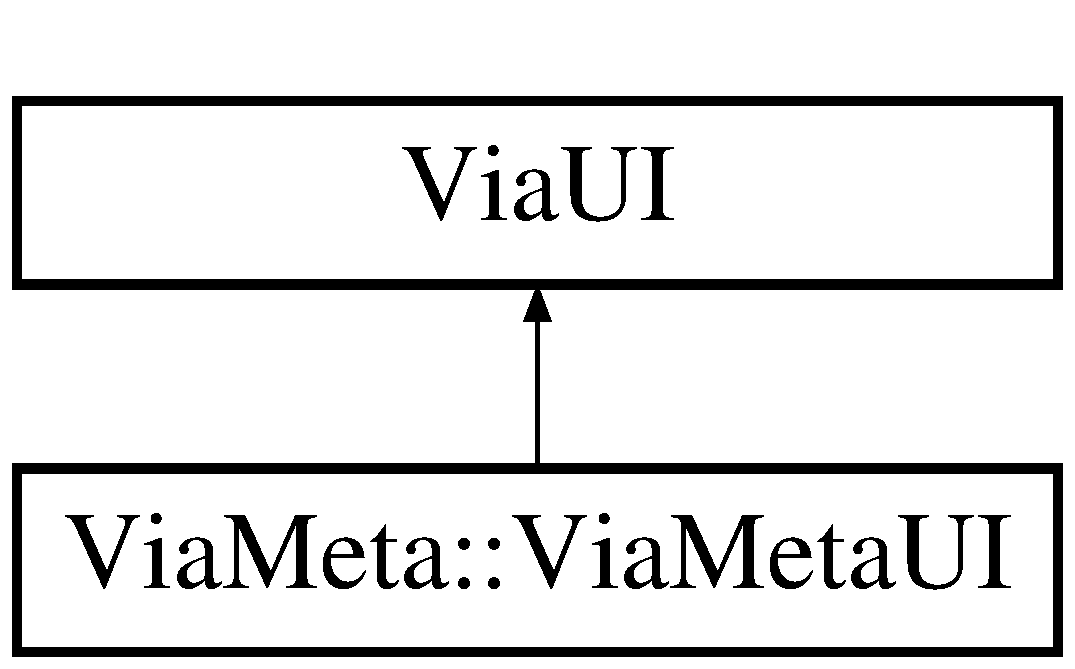
\includegraphics[height=2.000000cm]{class_via_meta_1_1_via_meta_u_i}
\end{center}
\end{figure}
\subsection*{Public Member Functions}
\begin{DoxyCompactItemize}
\item 
void \mbox{\hyperlink{class_via_meta_1_1_via_meta_u_i_af36b9d43b3a7e014650825c81fcf5893}{button1\+Tap\+Callback}} (void) override
\item 
void \mbox{\hyperlink{class_via_meta_1_1_via_meta_u_i_a601890a2c65f53fc575c9ef211fcfeaa}{button1\+Hold\+Callback}} (void) override
\item 
void \mbox{\hyperlink{class_via_meta_1_1_via_meta_u_i_a3d9aa9b0cc62a32b79541e25bbec6bd5}{button2\+Tap\+Callback}} (void) override
\item 
void \mbox{\hyperlink{class_via_meta_1_1_via_meta_u_i_acf5ef9a82372db43ab80437747167d9f}{button2\+Hold\+Callback}} (void) override
\item 
void \mbox{\hyperlink{class_via_meta_1_1_via_meta_u_i_a67e200e126a39d85d79f1f81f25e48a5}{button3\+Tap\+Callback}} (void) override
\item 
void \mbox{\hyperlink{class_via_meta_1_1_via_meta_u_i_a124e9edd67310235839dae92aa4bb9a9}{button3\+Hold\+Callback}} (void) override
\item 
void \mbox{\hyperlink{class_via_meta_1_1_via_meta_u_i_a0c745451e4e0b8bc51546280595b5b28}{button4\+Tap\+Callback}} (void) override
\item 
void \mbox{\hyperlink{class_via_meta_1_1_via_meta_u_i_aa43b104c1a726fad1c530cb50eb305f6}{button4\+Hold\+Callback}} (void) override
\item 
void \mbox{\hyperlink{class_via_meta_1_1_via_meta_u_i_afab19acc66940324991525af8527d6d9}{button5\+Tap\+Callback}} (void) override
\item 
void \mbox{\hyperlink{class_via_meta_1_1_via_meta_u_i_a225952a745a18a354c5ed3f890d8df0d}{button5\+Hold\+Callback}} (void) override
\item 
void \mbox{\hyperlink{class_via_meta_1_1_via_meta_u_i_a8b8724e5d68649da49f3f99203257833}{button6\+Tap\+Callback}} (void) override
\item 
void \mbox{\hyperlink{class_via_meta_1_1_via_meta_u_i_a793ad6aff954aeefd91a070d1a65c9d1}{button6\+Hold\+Callback}} (void) override
\item 
void \mbox{\hyperlink{class_via_meta_1_1_via_meta_u_i_ad95b464f8dda873be1c24622d1f082fa}{aux1\+Tap\+Callback}} (void) override
\item 
void \mbox{\hyperlink{class_via_meta_1_1_via_meta_u_i_a1c38639df8fdb4a866622388548bc9db}{aux1\+Hold\+Callback}} (void) override
\item 
void \mbox{\hyperlink{class_via_meta_1_1_via_meta_u_i_a2d1e0164ad7d84c410cc90cefe9730ce}{aux2\+Tap\+Callback}} (void) override
\item 
void \mbox{\hyperlink{class_via_meta_1_1_via_meta_u_i_a19cac5da8e89446d5ee2a2c889a6c555}{aux2\+Hold\+Callback}} (void) override
\item 
void \mbox{\hyperlink{class_via_meta_1_1_via_meta_u_i_a5982022f5c08ce9aaa75173209d30e6c}{aux2\+Alt\+Tap\+Callback}} (void) override
\item 
void \mbox{\hyperlink{class_via_meta_1_1_via_meta_u_i_a372fe7280f3107f81e7283ba7451efd6}{aux2\+Alt\+Hold\+Callback}} (void) override
\item 
void \mbox{\hyperlink{class_via_meta_1_1_via_meta_u_i_a4f9a282e24dd484d24657a1568defd75}{aux3\+Tap\+Callback}} (void) override
\item 
void \mbox{\hyperlink{class_via_meta_1_1_via_meta_u_i_ad15168253fc76c7a938ca467ada12ade}{aux3\+Hold\+Callback}} (void) override
\item 
void \mbox{\hyperlink{class_via_meta_1_1_via_meta_u_i_ad8e6300990d654091672b0f94a9b47d8}{aux4\+Tap\+Callback}} (void) override
\item 
void \mbox{\hyperlink{class_via_meta_1_1_via_meta_u_i_a2a1cfb3452d150af61f61716aa94f782}{aux4\+Hold\+Callback}} (void) override
\item 
void \mbox{\hyperlink{class_via_meta_1_1_via_meta_u_i_a54f7dbc780758a9842836a9cdd3239a0}{ui\+Set\+L\+E\+Ds}} (int) override
\item 
void \mbox{\hyperlink{class_via_meta_1_1_via_meta_u_i_a40b2c4c2139c78f273d923fdb0d3f4ce}{recall\+Module\+State}} (void) override
\item 
void \mbox{\hyperlink{class_via_meta_1_1_via_meta_u_i_a632c291b811cf6e704e913060083dd7d}{default\+Enter\+Menu\+Callback}} (void) override
\item 
void \mbox{\hyperlink{class_via_meta_1_1_via_meta_u_i_a6adf1a02d1e513a13727982347ecbe72}{new\+Mode\+Enter\+Menu\+Callback}} (void) override
\item 
void \mbox{\hyperlink{class_via_meta_1_1_via_meta_u_i_a5a1034beff03b3c5cdc12a9b3a7d0834}{new\+Aux\+Mode\+Enter\+Menu\+Callback}} (void) override
\item 
void \mbox{\hyperlink{class_via_meta_1_1_via_meta_u_i_a21cd6b42537b8abe34cfe65258455991}{preset\+Enter\+Menu\+Callback}} (void) override
\item 
void \mbox{\hyperlink{class_via_meta_1_1_via_meta_u_i_a5e9d82c9c06759dd2cc3b48846e594f2}{button1\+Enter\+Menu\+Callback}} (void) override
\item 
void \mbox{\hyperlink{class_via_meta_1_1_via_meta_u_i_a5687d94232ddf1b109a5f48c8ef89650}{button2\+Enter\+Menu\+Callback}} (void) override
\item 
void \mbox{\hyperlink{class_via_meta_1_1_via_meta_u_i_abff70e527b92121c207699c8c8334ee6}{button3\+Enter\+Menu\+Callback}} (void) override
\item 
void \mbox{\hyperlink{class_via_meta_1_1_via_meta_u_i_aef07210c32f8147e6b5ab92b923347e9}{button4\+Enter\+Menu\+Callback}} (void) override
\item 
void \mbox{\hyperlink{class_via_meta_1_1_via_meta_u_i_af14bee3824185ab5a97d8745e9317370}{button5\+Enter\+Menu\+Callback}} (void) override
\item 
void \mbox{\hyperlink{class_via_meta_1_1_via_meta_u_i_a5bcffdfe679b51dbcac0e78dc093c29b}{button6\+Enter\+Menu\+Callback}} (void) override
\item 
void \mbox{\hyperlink{class_via_meta_1_1_via_meta_u_i_a84e9b3d83d81753db095d67dee1fe8b9}{aux1\+Enter\+Menu\+Callback}} (void) override
\item 
void \mbox{\hyperlink{class_via_meta_1_1_via_meta_u_i_a31e89fca82851581b9ad7161cd81c6c0}{aux2\+Enter\+Menu\+Callback}} (void) override
\item 
void \mbox{\hyperlink{class_via_meta_1_1_via_meta_u_i_ab0ccbc22f2460565456b8347d18634b8}{aux2\+Alt\+Enter\+Menu\+Callback}} (void) override
\item 
void \mbox{\hyperlink{class_via_meta_1_1_via_meta_u_i_a31f9a7e08ee2d77d7aa96b644369e92d}{aux3\+Enter\+Menu\+Callback}} (void) override
\item 
void \mbox{\hyperlink{class_via_meta_1_1_via_meta_u_i_aa6309c2403a8436cc3ec222f7914b202}{aux4\+Enter\+Menu\+Callback}} (void) override
\item 
void \mbox{\hyperlink{class_via_meta_1_1_via_meta_u_i_ac2bc1bfeb6ef0045d234bd5b89f9ec99}{initialize}} (void) override
\item 
\mbox{\hyperlink{class_via_meta_1_1_via_meta_u_i_aa99917558f8467b7658347f461326add}{Via\+Meta\+UI}} (\mbox{\hyperlink{class_via_meta}{Via\+Meta}} \&x)
\end{DoxyCompactItemize}
\subsection*{Public Attributes}
\begin{DoxyCompactItemize}
\item 
\mbox{\hyperlink{class_via_meta}{Via\+Meta}} \& \mbox{\hyperlink{class_via_meta_1_1_via_meta_u_i_a8798ab0a875a443e05fc0954d849742c}{this\+\_\+module}}
\end{DoxyCompactItemize}


\subsection{Constructor \& Destructor Documentation}
\mbox{\Hypertarget{class_via_meta_1_1_via_meta_u_i_aa99917558f8467b7658347f461326add}\label{class_via_meta_1_1_via_meta_u_i_aa99917558f8467b7658347f461326add}} 
\index{Via\+Meta\+::\+Via\+Meta\+UI@{Via\+Meta\+::\+Via\+Meta\+UI}!Via\+Meta\+UI@{Via\+Meta\+UI}}
\index{Via\+Meta\+UI@{Via\+Meta\+UI}!Via\+Meta\+::\+Via\+Meta\+UI@{Via\+Meta\+::\+Via\+Meta\+UI}}
\subsubsection{\texorpdfstring{Via\+Meta\+U\+I()}{ViaMetaUI()}}
{\footnotesize\ttfamily Via\+Meta\+::\+Via\+Meta\+U\+I\+::\+Via\+Meta\+UI (\begin{DoxyParamCaption}\item[{\mbox{\hyperlink{class_via_meta}{Via\+Meta}} \&}]{x }\end{DoxyParamCaption})\hspace{0.3cm}{\ttfamily [inline]}}



\subsection{Member Function Documentation}
\mbox{\Hypertarget{class_via_meta_1_1_via_meta_u_i_a84e9b3d83d81753db095d67dee1fe8b9}\label{class_via_meta_1_1_via_meta_u_i_a84e9b3d83d81753db095d67dee1fe8b9}} 
\index{Via\+Meta\+::\+Via\+Meta\+UI@{Via\+Meta\+::\+Via\+Meta\+UI}!aux1\+Enter\+Menu\+Callback@{aux1\+Enter\+Menu\+Callback}}
\index{aux1\+Enter\+Menu\+Callback@{aux1\+Enter\+Menu\+Callback}!Via\+Meta\+::\+Via\+Meta\+UI@{Via\+Meta\+::\+Via\+Meta\+UI}}
\subsubsection{\texorpdfstring{aux1\+Enter\+Menu\+Callback()}{aux1EnterMenuCallback()}}
{\footnotesize\ttfamily void Via\+Meta\+::\+Via\+Meta\+U\+I\+::aux1\+Enter\+Menu\+Callback (\begin{DoxyParamCaption}\item[{void}]{ }\end{DoxyParamCaption})\hspace{0.3cm}{\ttfamily [override]}, {\ttfamily [virtual]}}



Implements \mbox{\hyperlink{class_via_u_i_a578111861e912bf43d3f320a0faffb0f}{Via\+UI}}.

\mbox{\Hypertarget{class_via_meta_1_1_via_meta_u_i_a1c38639df8fdb4a866622388548bc9db}\label{class_via_meta_1_1_via_meta_u_i_a1c38639df8fdb4a866622388548bc9db}} 
\index{Via\+Meta\+::\+Via\+Meta\+UI@{Via\+Meta\+::\+Via\+Meta\+UI}!aux1\+Hold\+Callback@{aux1\+Hold\+Callback}}
\index{aux1\+Hold\+Callback@{aux1\+Hold\+Callback}!Via\+Meta\+::\+Via\+Meta\+UI@{Via\+Meta\+::\+Via\+Meta\+UI}}
\subsubsection{\texorpdfstring{aux1\+Hold\+Callback()}{aux1HoldCallback()}}
{\footnotesize\ttfamily void Via\+Meta\+::\+Via\+Meta\+U\+I\+::aux1\+Hold\+Callback (\begin{DoxyParamCaption}\item[{void}]{ }\end{DoxyParamCaption})\hspace{0.3cm}{\ttfamily [override]}, {\ttfamily [virtual]}}



Implements \mbox{\hyperlink{class_via_u_i_a6fcc3b7cf9b97ccf403ed1817cb10d1d}{Via\+UI}}.

\mbox{\Hypertarget{class_via_meta_1_1_via_meta_u_i_ad95b464f8dda873be1c24622d1f082fa}\label{class_via_meta_1_1_via_meta_u_i_ad95b464f8dda873be1c24622d1f082fa}} 
\index{Via\+Meta\+::\+Via\+Meta\+UI@{Via\+Meta\+::\+Via\+Meta\+UI}!aux1\+Tap\+Callback@{aux1\+Tap\+Callback}}
\index{aux1\+Tap\+Callback@{aux1\+Tap\+Callback}!Via\+Meta\+::\+Via\+Meta\+UI@{Via\+Meta\+::\+Via\+Meta\+UI}}
\subsubsection{\texorpdfstring{aux1\+Tap\+Callback()}{aux1TapCallback()}}
{\footnotesize\ttfamily void Via\+Meta\+::\+Via\+Meta\+U\+I\+::aux1\+Tap\+Callback (\begin{DoxyParamCaption}\item[{void}]{ }\end{DoxyParamCaption})\hspace{0.3cm}{\ttfamily [override]}, {\ttfamily [virtual]}}



Implements \mbox{\hyperlink{class_via_u_i_a2942ec6f7d495159258e1f1803e62c4d}{Via\+UI}}.

\mbox{\Hypertarget{class_via_meta_1_1_via_meta_u_i_ab0ccbc22f2460565456b8347d18634b8}\label{class_via_meta_1_1_via_meta_u_i_ab0ccbc22f2460565456b8347d18634b8}} 
\index{Via\+Meta\+::\+Via\+Meta\+UI@{Via\+Meta\+::\+Via\+Meta\+UI}!aux2\+Alt\+Enter\+Menu\+Callback@{aux2\+Alt\+Enter\+Menu\+Callback}}
\index{aux2\+Alt\+Enter\+Menu\+Callback@{aux2\+Alt\+Enter\+Menu\+Callback}!Via\+Meta\+::\+Via\+Meta\+UI@{Via\+Meta\+::\+Via\+Meta\+UI}}
\subsubsection{\texorpdfstring{aux2\+Alt\+Enter\+Menu\+Callback()}{aux2AltEnterMenuCallback()}}
{\footnotesize\ttfamily void Via\+Meta\+::\+Via\+Meta\+U\+I\+::aux2\+Alt\+Enter\+Menu\+Callback (\begin{DoxyParamCaption}\item[{void}]{ }\end{DoxyParamCaption})\hspace{0.3cm}{\ttfamily [override]}, {\ttfamily [virtual]}}



Implements \mbox{\hyperlink{class_via_u_i_a08a746b666d37ac6bc293303187fd6be}{Via\+UI}}.

\mbox{\Hypertarget{class_via_meta_1_1_via_meta_u_i_a372fe7280f3107f81e7283ba7451efd6}\label{class_via_meta_1_1_via_meta_u_i_a372fe7280f3107f81e7283ba7451efd6}} 
\index{Via\+Meta\+::\+Via\+Meta\+UI@{Via\+Meta\+::\+Via\+Meta\+UI}!aux2\+Alt\+Hold\+Callback@{aux2\+Alt\+Hold\+Callback}}
\index{aux2\+Alt\+Hold\+Callback@{aux2\+Alt\+Hold\+Callback}!Via\+Meta\+::\+Via\+Meta\+UI@{Via\+Meta\+::\+Via\+Meta\+UI}}
\subsubsection{\texorpdfstring{aux2\+Alt\+Hold\+Callback()}{aux2AltHoldCallback()}}
{\footnotesize\ttfamily void Via\+Meta\+::\+Via\+Meta\+U\+I\+::aux2\+Alt\+Hold\+Callback (\begin{DoxyParamCaption}\item[{void}]{ }\end{DoxyParamCaption})\hspace{0.3cm}{\ttfamily [override]}, {\ttfamily [virtual]}}



Implements \mbox{\hyperlink{class_via_u_i_ab93989ef608d1b63b854b54278006f49}{Via\+UI}}.

\mbox{\Hypertarget{class_via_meta_1_1_via_meta_u_i_a5982022f5c08ce9aaa75173209d30e6c}\label{class_via_meta_1_1_via_meta_u_i_a5982022f5c08ce9aaa75173209d30e6c}} 
\index{Via\+Meta\+::\+Via\+Meta\+UI@{Via\+Meta\+::\+Via\+Meta\+UI}!aux2\+Alt\+Tap\+Callback@{aux2\+Alt\+Tap\+Callback}}
\index{aux2\+Alt\+Tap\+Callback@{aux2\+Alt\+Tap\+Callback}!Via\+Meta\+::\+Via\+Meta\+UI@{Via\+Meta\+::\+Via\+Meta\+UI}}
\subsubsection{\texorpdfstring{aux2\+Alt\+Tap\+Callback()}{aux2AltTapCallback()}}
{\footnotesize\ttfamily void Via\+Meta\+::\+Via\+Meta\+U\+I\+::aux2\+Alt\+Tap\+Callback (\begin{DoxyParamCaption}\item[{void}]{ }\end{DoxyParamCaption})\hspace{0.3cm}{\ttfamily [override]}, {\ttfamily [virtual]}}



Implements \mbox{\hyperlink{class_via_u_i_ad13d74c0bd271b83b8da662b22713ddb}{Via\+UI}}.

\mbox{\Hypertarget{class_via_meta_1_1_via_meta_u_i_a31e89fca82851581b9ad7161cd81c6c0}\label{class_via_meta_1_1_via_meta_u_i_a31e89fca82851581b9ad7161cd81c6c0}} 
\index{Via\+Meta\+::\+Via\+Meta\+UI@{Via\+Meta\+::\+Via\+Meta\+UI}!aux2\+Enter\+Menu\+Callback@{aux2\+Enter\+Menu\+Callback}}
\index{aux2\+Enter\+Menu\+Callback@{aux2\+Enter\+Menu\+Callback}!Via\+Meta\+::\+Via\+Meta\+UI@{Via\+Meta\+::\+Via\+Meta\+UI}}
\subsubsection{\texorpdfstring{aux2\+Enter\+Menu\+Callback()}{aux2EnterMenuCallback()}}
{\footnotesize\ttfamily void Via\+Meta\+::\+Via\+Meta\+U\+I\+::aux2\+Enter\+Menu\+Callback (\begin{DoxyParamCaption}\item[{void}]{ }\end{DoxyParamCaption})\hspace{0.3cm}{\ttfamily [override]}, {\ttfamily [virtual]}}



Implements \mbox{\hyperlink{class_via_u_i_a1f51fc259471364f91bd0a1592824dab}{Via\+UI}}.

\mbox{\Hypertarget{class_via_meta_1_1_via_meta_u_i_a19cac5da8e89446d5ee2a2c889a6c555}\label{class_via_meta_1_1_via_meta_u_i_a19cac5da8e89446d5ee2a2c889a6c555}} 
\index{Via\+Meta\+::\+Via\+Meta\+UI@{Via\+Meta\+::\+Via\+Meta\+UI}!aux2\+Hold\+Callback@{aux2\+Hold\+Callback}}
\index{aux2\+Hold\+Callback@{aux2\+Hold\+Callback}!Via\+Meta\+::\+Via\+Meta\+UI@{Via\+Meta\+::\+Via\+Meta\+UI}}
\subsubsection{\texorpdfstring{aux2\+Hold\+Callback()}{aux2HoldCallback()}}
{\footnotesize\ttfamily void Via\+Meta\+::\+Via\+Meta\+U\+I\+::aux2\+Hold\+Callback (\begin{DoxyParamCaption}\item[{void}]{ }\end{DoxyParamCaption})\hspace{0.3cm}{\ttfamily [override]}, {\ttfamily [virtual]}}



Implements \mbox{\hyperlink{class_via_u_i_a42545b69c2bbbb036f633140fd8007d6}{Via\+UI}}.

\mbox{\Hypertarget{class_via_meta_1_1_via_meta_u_i_a2d1e0164ad7d84c410cc90cefe9730ce}\label{class_via_meta_1_1_via_meta_u_i_a2d1e0164ad7d84c410cc90cefe9730ce}} 
\index{Via\+Meta\+::\+Via\+Meta\+UI@{Via\+Meta\+::\+Via\+Meta\+UI}!aux2\+Tap\+Callback@{aux2\+Tap\+Callback}}
\index{aux2\+Tap\+Callback@{aux2\+Tap\+Callback}!Via\+Meta\+::\+Via\+Meta\+UI@{Via\+Meta\+::\+Via\+Meta\+UI}}
\subsubsection{\texorpdfstring{aux2\+Tap\+Callback()}{aux2TapCallback()}}
{\footnotesize\ttfamily void Via\+Meta\+::\+Via\+Meta\+U\+I\+::aux2\+Tap\+Callback (\begin{DoxyParamCaption}\item[{void}]{ }\end{DoxyParamCaption})\hspace{0.3cm}{\ttfamily [override]}, {\ttfamily [virtual]}}



Implements \mbox{\hyperlink{class_via_u_i_ae5e009dc22002f62e6bff8dd76d2f745}{Via\+UI}}.

\mbox{\Hypertarget{class_via_meta_1_1_via_meta_u_i_a31f9a7e08ee2d77d7aa96b644369e92d}\label{class_via_meta_1_1_via_meta_u_i_a31f9a7e08ee2d77d7aa96b644369e92d}} 
\index{Via\+Meta\+::\+Via\+Meta\+UI@{Via\+Meta\+::\+Via\+Meta\+UI}!aux3\+Enter\+Menu\+Callback@{aux3\+Enter\+Menu\+Callback}}
\index{aux3\+Enter\+Menu\+Callback@{aux3\+Enter\+Menu\+Callback}!Via\+Meta\+::\+Via\+Meta\+UI@{Via\+Meta\+::\+Via\+Meta\+UI}}
\subsubsection{\texorpdfstring{aux3\+Enter\+Menu\+Callback()}{aux3EnterMenuCallback()}}
{\footnotesize\ttfamily void Via\+Meta\+::\+Via\+Meta\+U\+I\+::aux3\+Enter\+Menu\+Callback (\begin{DoxyParamCaption}\item[{void}]{ }\end{DoxyParamCaption})\hspace{0.3cm}{\ttfamily [override]}, {\ttfamily [virtual]}}



Implements \mbox{\hyperlink{class_via_u_i_aa62c9f8dc58d37fc2a3abc7bce1cd16e}{Via\+UI}}.

\mbox{\Hypertarget{class_via_meta_1_1_via_meta_u_i_ad15168253fc76c7a938ca467ada12ade}\label{class_via_meta_1_1_via_meta_u_i_ad15168253fc76c7a938ca467ada12ade}} 
\index{Via\+Meta\+::\+Via\+Meta\+UI@{Via\+Meta\+::\+Via\+Meta\+UI}!aux3\+Hold\+Callback@{aux3\+Hold\+Callback}}
\index{aux3\+Hold\+Callback@{aux3\+Hold\+Callback}!Via\+Meta\+::\+Via\+Meta\+UI@{Via\+Meta\+::\+Via\+Meta\+UI}}
\subsubsection{\texorpdfstring{aux3\+Hold\+Callback()}{aux3HoldCallback()}}
{\footnotesize\ttfamily void Via\+Meta\+::\+Via\+Meta\+U\+I\+::aux3\+Hold\+Callback (\begin{DoxyParamCaption}\item[{void}]{ }\end{DoxyParamCaption})\hspace{0.3cm}{\ttfamily [override]}, {\ttfamily [virtual]}}



Implements \mbox{\hyperlink{class_via_u_i_a9ea505dfd800b261beabe8dc47b201d3}{Via\+UI}}.

\mbox{\Hypertarget{class_via_meta_1_1_via_meta_u_i_a4f9a282e24dd484d24657a1568defd75}\label{class_via_meta_1_1_via_meta_u_i_a4f9a282e24dd484d24657a1568defd75}} 
\index{Via\+Meta\+::\+Via\+Meta\+UI@{Via\+Meta\+::\+Via\+Meta\+UI}!aux3\+Tap\+Callback@{aux3\+Tap\+Callback}}
\index{aux3\+Tap\+Callback@{aux3\+Tap\+Callback}!Via\+Meta\+::\+Via\+Meta\+UI@{Via\+Meta\+::\+Via\+Meta\+UI}}
\subsubsection{\texorpdfstring{aux3\+Tap\+Callback()}{aux3TapCallback()}}
{\footnotesize\ttfamily void Via\+Meta\+::\+Via\+Meta\+U\+I\+::aux3\+Tap\+Callback (\begin{DoxyParamCaption}\item[{void}]{ }\end{DoxyParamCaption})\hspace{0.3cm}{\ttfamily [override]}, {\ttfamily [virtual]}}



Implements \mbox{\hyperlink{class_via_u_i_a29026efd361a615374adce2462aa652a}{Via\+UI}}.

\mbox{\Hypertarget{class_via_meta_1_1_via_meta_u_i_aa6309c2403a8436cc3ec222f7914b202}\label{class_via_meta_1_1_via_meta_u_i_aa6309c2403a8436cc3ec222f7914b202}} 
\index{Via\+Meta\+::\+Via\+Meta\+UI@{Via\+Meta\+::\+Via\+Meta\+UI}!aux4\+Enter\+Menu\+Callback@{aux4\+Enter\+Menu\+Callback}}
\index{aux4\+Enter\+Menu\+Callback@{aux4\+Enter\+Menu\+Callback}!Via\+Meta\+::\+Via\+Meta\+UI@{Via\+Meta\+::\+Via\+Meta\+UI}}
\subsubsection{\texorpdfstring{aux4\+Enter\+Menu\+Callback()}{aux4EnterMenuCallback()}}
{\footnotesize\ttfamily void Via\+Meta\+::\+Via\+Meta\+U\+I\+::aux4\+Enter\+Menu\+Callback (\begin{DoxyParamCaption}\item[{void}]{ }\end{DoxyParamCaption})\hspace{0.3cm}{\ttfamily [override]}, {\ttfamily [virtual]}}



Implements \mbox{\hyperlink{class_via_u_i_a36cc4bac8f774c2a59ab8635be05f884}{Via\+UI}}.

\mbox{\Hypertarget{class_via_meta_1_1_via_meta_u_i_a2a1cfb3452d150af61f61716aa94f782}\label{class_via_meta_1_1_via_meta_u_i_a2a1cfb3452d150af61f61716aa94f782}} 
\index{Via\+Meta\+::\+Via\+Meta\+UI@{Via\+Meta\+::\+Via\+Meta\+UI}!aux4\+Hold\+Callback@{aux4\+Hold\+Callback}}
\index{aux4\+Hold\+Callback@{aux4\+Hold\+Callback}!Via\+Meta\+::\+Via\+Meta\+UI@{Via\+Meta\+::\+Via\+Meta\+UI}}
\subsubsection{\texorpdfstring{aux4\+Hold\+Callback()}{aux4HoldCallback()}}
{\footnotesize\ttfamily void Via\+Meta\+::\+Via\+Meta\+U\+I\+::aux4\+Hold\+Callback (\begin{DoxyParamCaption}\item[{void}]{ }\end{DoxyParamCaption})\hspace{0.3cm}{\ttfamily [override]}, {\ttfamily [virtual]}}



Implements \mbox{\hyperlink{class_via_u_i_a884790ab6dac8e6f49104146ff620512}{Via\+UI}}.

\mbox{\Hypertarget{class_via_meta_1_1_via_meta_u_i_ad8e6300990d654091672b0f94a9b47d8}\label{class_via_meta_1_1_via_meta_u_i_ad8e6300990d654091672b0f94a9b47d8}} 
\index{Via\+Meta\+::\+Via\+Meta\+UI@{Via\+Meta\+::\+Via\+Meta\+UI}!aux4\+Tap\+Callback@{aux4\+Tap\+Callback}}
\index{aux4\+Tap\+Callback@{aux4\+Tap\+Callback}!Via\+Meta\+::\+Via\+Meta\+UI@{Via\+Meta\+::\+Via\+Meta\+UI}}
\subsubsection{\texorpdfstring{aux4\+Tap\+Callback()}{aux4TapCallback()}}
{\footnotesize\ttfamily void Via\+Meta\+::\+Via\+Meta\+U\+I\+::aux4\+Tap\+Callback (\begin{DoxyParamCaption}\item[{void}]{ }\end{DoxyParamCaption})\hspace{0.3cm}{\ttfamily [override]}, {\ttfamily [virtual]}}



Implements \mbox{\hyperlink{class_via_u_i_a0a43c527f027d11b266080d8cacb1d65}{Via\+UI}}.

\mbox{\Hypertarget{class_via_meta_1_1_via_meta_u_i_a5e9d82c9c06759dd2cc3b48846e594f2}\label{class_via_meta_1_1_via_meta_u_i_a5e9d82c9c06759dd2cc3b48846e594f2}} 
\index{Via\+Meta\+::\+Via\+Meta\+UI@{Via\+Meta\+::\+Via\+Meta\+UI}!button1\+Enter\+Menu\+Callback@{button1\+Enter\+Menu\+Callback}}
\index{button1\+Enter\+Menu\+Callback@{button1\+Enter\+Menu\+Callback}!Via\+Meta\+::\+Via\+Meta\+UI@{Via\+Meta\+::\+Via\+Meta\+UI}}
\subsubsection{\texorpdfstring{button1\+Enter\+Menu\+Callback()}{button1EnterMenuCallback()}}
{\footnotesize\ttfamily void Via\+Meta\+::\+Via\+Meta\+U\+I\+::button1\+Enter\+Menu\+Callback (\begin{DoxyParamCaption}\item[{void}]{ }\end{DoxyParamCaption})\hspace{0.3cm}{\ttfamily [override]}, {\ttfamily [virtual]}}



Implements \mbox{\hyperlink{class_via_u_i_ae00249c10af94437c357222328a56f82}{Via\+UI}}.

\mbox{\Hypertarget{class_via_meta_1_1_via_meta_u_i_a601890a2c65f53fc575c9ef211fcfeaa}\label{class_via_meta_1_1_via_meta_u_i_a601890a2c65f53fc575c9ef211fcfeaa}} 
\index{Via\+Meta\+::\+Via\+Meta\+UI@{Via\+Meta\+::\+Via\+Meta\+UI}!button1\+Hold\+Callback@{button1\+Hold\+Callback}}
\index{button1\+Hold\+Callback@{button1\+Hold\+Callback}!Via\+Meta\+::\+Via\+Meta\+UI@{Via\+Meta\+::\+Via\+Meta\+UI}}
\subsubsection{\texorpdfstring{button1\+Hold\+Callback()}{button1HoldCallback()}}
{\footnotesize\ttfamily void Via\+Meta\+::\+Via\+Meta\+U\+I\+::button1\+Hold\+Callback (\begin{DoxyParamCaption}\item[{void}]{ }\end{DoxyParamCaption})\hspace{0.3cm}{\ttfamily [override]}, {\ttfamily [virtual]}}



Implements \mbox{\hyperlink{class_via_u_i_a62145ce1c1b664ff0a1aadaac9386162}{Via\+UI}}.

\mbox{\Hypertarget{class_via_meta_1_1_via_meta_u_i_af36b9d43b3a7e014650825c81fcf5893}\label{class_via_meta_1_1_via_meta_u_i_af36b9d43b3a7e014650825c81fcf5893}} 
\index{Via\+Meta\+::\+Via\+Meta\+UI@{Via\+Meta\+::\+Via\+Meta\+UI}!button1\+Tap\+Callback@{button1\+Tap\+Callback}}
\index{button1\+Tap\+Callback@{button1\+Tap\+Callback}!Via\+Meta\+::\+Via\+Meta\+UI@{Via\+Meta\+::\+Via\+Meta\+UI}}
\subsubsection{\texorpdfstring{button1\+Tap\+Callback()}{button1TapCallback()}}
{\footnotesize\ttfamily void Via\+Meta\+::\+Via\+Meta\+U\+I\+::button1\+Tap\+Callback (\begin{DoxyParamCaption}\item[{void}]{ }\end{DoxyParamCaption})\hspace{0.3cm}{\ttfamily [override]}, {\ttfamily [virtual]}}



Implements \mbox{\hyperlink{class_via_u_i_a5bdacaef84e33fb3d9b3dd50d1b269d1}{Via\+UI}}.

\mbox{\Hypertarget{class_via_meta_1_1_via_meta_u_i_a5687d94232ddf1b109a5f48c8ef89650}\label{class_via_meta_1_1_via_meta_u_i_a5687d94232ddf1b109a5f48c8ef89650}} 
\index{Via\+Meta\+::\+Via\+Meta\+UI@{Via\+Meta\+::\+Via\+Meta\+UI}!button2\+Enter\+Menu\+Callback@{button2\+Enter\+Menu\+Callback}}
\index{button2\+Enter\+Menu\+Callback@{button2\+Enter\+Menu\+Callback}!Via\+Meta\+::\+Via\+Meta\+UI@{Via\+Meta\+::\+Via\+Meta\+UI}}
\subsubsection{\texorpdfstring{button2\+Enter\+Menu\+Callback()}{button2EnterMenuCallback()}}
{\footnotesize\ttfamily void Via\+Meta\+::\+Via\+Meta\+U\+I\+::button2\+Enter\+Menu\+Callback (\begin{DoxyParamCaption}\item[{void}]{ }\end{DoxyParamCaption})\hspace{0.3cm}{\ttfamily [override]}, {\ttfamily [virtual]}}



Implements \mbox{\hyperlink{class_via_u_i_ac7b7f919edba9a640e7009e1f9303a2d}{Via\+UI}}.

\mbox{\Hypertarget{class_via_meta_1_1_via_meta_u_i_acf5ef9a82372db43ab80437747167d9f}\label{class_via_meta_1_1_via_meta_u_i_acf5ef9a82372db43ab80437747167d9f}} 
\index{Via\+Meta\+::\+Via\+Meta\+UI@{Via\+Meta\+::\+Via\+Meta\+UI}!button2\+Hold\+Callback@{button2\+Hold\+Callback}}
\index{button2\+Hold\+Callback@{button2\+Hold\+Callback}!Via\+Meta\+::\+Via\+Meta\+UI@{Via\+Meta\+::\+Via\+Meta\+UI}}
\subsubsection{\texorpdfstring{button2\+Hold\+Callback()}{button2HoldCallback()}}
{\footnotesize\ttfamily void Via\+Meta\+::\+Via\+Meta\+U\+I\+::button2\+Hold\+Callback (\begin{DoxyParamCaption}\item[{void}]{ }\end{DoxyParamCaption})\hspace{0.3cm}{\ttfamily [override]}, {\ttfamily [virtual]}}



Implements \mbox{\hyperlink{class_via_u_i_a95bce2d662a8ae46be73497e868aebb9}{Via\+UI}}.

\mbox{\Hypertarget{class_via_meta_1_1_via_meta_u_i_a3d9aa9b0cc62a32b79541e25bbec6bd5}\label{class_via_meta_1_1_via_meta_u_i_a3d9aa9b0cc62a32b79541e25bbec6bd5}} 
\index{Via\+Meta\+::\+Via\+Meta\+UI@{Via\+Meta\+::\+Via\+Meta\+UI}!button2\+Tap\+Callback@{button2\+Tap\+Callback}}
\index{button2\+Tap\+Callback@{button2\+Tap\+Callback}!Via\+Meta\+::\+Via\+Meta\+UI@{Via\+Meta\+::\+Via\+Meta\+UI}}
\subsubsection{\texorpdfstring{button2\+Tap\+Callback()}{button2TapCallback()}}
{\footnotesize\ttfamily void Via\+Meta\+::\+Via\+Meta\+U\+I\+::button2\+Tap\+Callback (\begin{DoxyParamCaption}\item[{void}]{ }\end{DoxyParamCaption})\hspace{0.3cm}{\ttfamily [override]}, {\ttfamily [virtual]}}



Implements \mbox{\hyperlink{class_via_u_i_a8fce17e375ea6fe3a4746bff3e6dec75}{Via\+UI}}.

\mbox{\Hypertarget{class_via_meta_1_1_via_meta_u_i_abff70e527b92121c207699c8c8334ee6}\label{class_via_meta_1_1_via_meta_u_i_abff70e527b92121c207699c8c8334ee6}} 
\index{Via\+Meta\+::\+Via\+Meta\+UI@{Via\+Meta\+::\+Via\+Meta\+UI}!button3\+Enter\+Menu\+Callback@{button3\+Enter\+Menu\+Callback}}
\index{button3\+Enter\+Menu\+Callback@{button3\+Enter\+Menu\+Callback}!Via\+Meta\+::\+Via\+Meta\+UI@{Via\+Meta\+::\+Via\+Meta\+UI}}
\subsubsection{\texorpdfstring{button3\+Enter\+Menu\+Callback()}{button3EnterMenuCallback()}}
{\footnotesize\ttfamily void Via\+Meta\+::\+Via\+Meta\+U\+I\+::button3\+Enter\+Menu\+Callback (\begin{DoxyParamCaption}\item[{void}]{ }\end{DoxyParamCaption})\hspace{0.3cm}{\ttfamily [override]}, {\ttfamily [virtual]}}



Implements \mbox{\hyperlink{class_via_u_i_a883081e46324dec82ad89f2e77cf4b65}{Via\+UI}}.

\mbox{\Hypertarget{class_via_meta_1_1_via_meta_u_i_a124e9edd67310235839dae92aa4bb9a9}\label{class_via_meta_1_1_via_meta_u_i_a124e9edd67310235839dae92aa4bb9a9}} 
\index{Via\+Meta\+::\+Via\+Meta\+UI@{Via\+Meta\+::\+Via\+Meta\+UI}!button3\+Hold\+Callback@{button3\+Hold\+Callback}}
\index{button3\+Hold\+Callback@{button3\+Hold\+Callback}!Via\+Meta\+::\+Via\+Meta\+UI@{Via\+Meta\+::\+Via\+Meta\+UI}}
\subsubsection{\texorpdfstring{button3\+Hold\+Callback()}{button3HoldCallback()}}
{\footnotesize\ttfamily void Via\+Meta\+::\+Via\+Meta\+U\+I\+::button3\+Hold\+Callback (\begin{DoxyParamCaption}\item[{void}]{ }\end{DoxyParamCaption})\hspace{0.3cm}{\ttfamily [override]}, {\ttfamily [virtual]}}



Implements \mbox{\hyperlink{class_via_u_i_a7334aea36cf78afac284dd5e899e8ace}{Via\+UI}}.

\mbox{\Hypertarget{class_via_meta_1_1_via_meta_u_i_a67e200e126a39d85d79f1f81f25e48a5}\label{class_via_meta_1_1_via_meta_u_i_a67e200e126a39d85d79f1f81f25e48a5}} 
\index{Via\+Meta\+::\+Via\+Meta\+UI@{Via\+Meta\+::\+Via\+Meta\+UI}!button3\+Tap\+Callback@{button3\+Tap\+Callback}}
\index{button3\+Tap\+Callback@{button3\+Tap\+Callback}!Via\+Meta\+::\+Via\+Meta\+UI@{Via\+Meta\+::\+Via\+Meta\+UI}}
\subsubsection{\texorpdfstring{button3\+Tap\+Callback()}{button3TapCallback()}}
{\footnotesize\ttfamily void Via\+Meta\+::\+Via\+Meta\+U\+I\+::button3\+Tap\+Callback (\begin{DoxyParamCaption}\item[{void}]{ }\end{DoxyParamCaption})\hspace{0.3cm}{\ttfamily [override]}, {\ttfamily [virtual]}}



Implements \mbox{\hyperlink{class_via_u_i_a3dfd40d901aaa8c8310bdbf75f4432a5}{Via\+UI}}.

\mbox{\Hypertarget{class_via_meta_1_1_via_meta_u_i_aef07210c32f8147e6b5ab92b923347e9}\label{class_via_meta_1_1_via_meta_u_i_aef07210c32f8147e6b5ab92b923347e9}} 
\index{Via\+Meta\+::\+Via\+Meta\+UI@{Via\+Meta\+::\+Via\+Meta\+UI}!button4\+Enter\+Menu\+Callback@{button4\+Enter\+Menu\+Callback}}
\index{button4\+Enter\+Menu\+Callback@{button4\+Enter\+Menu\+Callback}!Via\+Meta\+::\+Via\+Meta\+UI@{Via\+Meta\+::\+Via\+Meta\+UI}}
\subsubsection{\texorpdfstring{button4\+Enter\+Menu\+Callback()}{button4EnterMenuCallback()}}
{\footnotesize\ttfamily void Via\+Meta\+::\+Via\+Meta\+U\+I\+::button4\+Enter\+Menu\+Callback (\begin{DoxyParamCaption}\item[{void}]{ }\end{DoxyParamCaption})\hspace{0.3cm}{\ttfamily [override]}, {\ttfamily [virtual]}}



Implements \mbox{\hyperlink{class_via_u_i_a6db24e53e559b6fddd4cb1f918de40d6}{Via\+UI}}.

\mbox{\Hypertarget{class_via_meta_1_1_via_meta_u_i_aa43b104c1a726fad1c530cb50eb305f6}\label{class_via_meta_1_1_via_meta_u_i_aa43b104c1a726fad1c530cb50eb305f6}} 
\index{Via\+Meta\+::\+Via\+Meta\+UI@{Via\+Meta\+::\+Via\+Meta\+UI}!button4\+Hold\+Callback@{button4\+Hold\+Callback}}
\index{button4\+Hold\+Callback@{button4\+Hold\+Callback}!Via\+Meta\+::\+Via\+Meta\+UI@{Via\+Meta\+::\+Via\+Meta\+UI}}
\subsubsection{\texorpdfstring{button4\+Hold\+Callback()}{button4HoldCallback()}}
{\footnotesize\ttfamily void Via\+Meta\+::\+Via\+Meta\+U\+I\+::button4\+Hold\+Callback (\begin{DoxyParamCaption}\item[{void}]{ }\end{DoxyParamCaption})\hspace{0.3cm}{\ttfamily [override]}, {\ttfamily [virtual]}}



Implements \mbox{\hyperlink{class_via_u_i_a11919091b39319fe4d1b3a3f3c7104c5}{Via\+UI}}.

\mbox{\Hypertarget{class_via_meta_1_1_via_meta_u_i_a0c745451e4e0b8bc51546280595b5b28}\label{class_via_meta_1_1_via_meta_u_i_a0c745451e4e0b8bc51546280595b5b28}} 
\index{Via\+Meta\+::\+Via\+Meta\+UI@{Via\+Meta\+::\+Via\+Meta\+UI}!button4\+Tap\+Callback@{button4\+Tap\+Callback}}
\index{button4\+Tap\+Callback@{button4\+Tap\+Callback}!Via\+Meta\+::\+Via\+Meta\+UI@{Via\+Meta\+::\+Via\+Meta\+UI}}
\subsubsection{\texorpdfstring{button4\+Tap\+Callback()}{button4TapCallback()}}
{\footnotesize\ttfamily void Via\+Meta\+::\+Via\+Meta\+U\+I\+::button4\+Tap\+Callback (\begin{DoxyParamCaption}\item[{void}]{ }\end{DoxyParamCaption})\hspace{0.3cm}{\ttfamily [override]}, {\ttfamily [virtual]}}



Implements \mbox{\hyperlink{class_via_u_i_a4925f089aa720ca88d84246f434112e9}{Via\+UI}}.

\mbox{\Hypertarget{class_via_meta_1_1_via_meta_u_i_af14bee3824185ab5a97d8745e9317370}\label{class_via_meta_1_1_via_meta_u_i_af14bee3824185ab5a97d8745e9317370}} 
\index{Via\+Meta\+::\+Via\+Meta\+UI@{Via\+Meta\+::\+Via\+Meta\+UI}!button5\+Enter\+Menu\+Callback@{button5\+Enter\+Menu\+Callback}}
\index{button5\+Enter\+Menu\+Callback@{button5\+Enter\+Menu\+Callback}!Via\+Meta\+::\+Via\+Meta\+UI@{Via\+Meta\+::\+Via\+Meta\+UI}}
\subsubsection{\texorpdfstring{button5\+Enter\+Menu\+Callback()}{button5EnterMenuCallback()}}
{\footnotesize\ttfamily void Via\+Meta\+::\+Via\+Meta\+U\+I\+::button5\+Enter\+Menu\+Callback (\begin{DoxyParamCaption}\item[{void}]{ }\end{DoxyParamCaption})\hspace{0.3cm}{\ttfamily [override]}, {\ttfamily [virtual]}}



Implements \mbox{\hyperlink{class_via_u_i_adb40844fb1fa8e623f3a7eaecdbfad53}{Via\+UI}}.

\mbox{\Hypertarget{class_via_meta_1_1_via_meta_u_i_a225952a745a18a354c5ed3f890d8df0d}\label{class_via_meta_1_1_via_meta_u_i_a225952a745a18a354c5ed3f890d8df0d}} 
\index{Via\+Meta\+::\+Via\+Meta\+UI@{Via\+Meta\+::\+Via\+Meta\+UI}!button5\+Hold\+Callback@{button5\+Hold\+Callback}}
\index{button5\+Hold\+Callback@{button5\+Hold\+Callback}!Via\+Meta\+::\+Via\+Meta\+UI@{Via\+Meta\+::\+Via\+Meta\+UI}}
\subsubsection{\texorpdfstring{button5\+Hold\+Callback()}{button5HoldCallback()}}
{\footnotesize\ttfamily void Via\+Meta\+::\+Via\+Meta\+U\+I\+::button5\+Hold\+Callback (\begin{DoxyParamCaption}\item[{void}]{ }\end{DoxyParamCaption})\hspace{0.3cm}{\ttfamily [override]}, {\ttfamily [virtual]}}



Implements \mbox{\hyperlink{class_via_u_i_aee783713c816e3807514ee9b06b571b0}{Via\+UI}}.

\mbox{\Hypertarget{class_via_meta_1_1_via_meta_u_i_afab19acc66940324991525af8527d6d9}\label{class_via_meta_1_1_via_meta_u_i_afab19acc66940324991525af8527d6d9}} 
\index{Via\+Meta\+::\+Via\+Meta\+UI@{Via\+Meta\+::\+Via\+Meta\+UI}!button5\+Tap\+Callback@{button5\+Tap\+Callback}}
\index{button5\+Tap\+Callback@{button5\+Tap\+Callback}!Via\+Meta\+::\+Via\+Meta\+UI@{Via\+Meta\+::\+Via\+Meta\+UI}}
\subsubsection{\texorpdfstring{button5\+Tap\+Callback()}{button5TapCallback()}}
{\footnotesize\ttfamily void Via\+Meta\+::\+Via\+Meta\+U\+I\+::button5\+Tap\+Callback (\begin{DoxyParamCaption}\item[{void}]{ }\end{DoxyParamCaption})\hspace{0.3cm}{\ttfamily [override]}, {\ttfamily [virtual]}}



Implements \mbox{\hyperlink{class_via_u_i_a5066c22385f31c24ec939d680a66a628}{Via\+UI}}.

\mbox{\Hypertarget{class_via_meta_1_1_via_meta_u_i_a5bcffdfe679b51dbcac0e78dc093c29b}\label{class_via_meta_1_1_via_meta_u_i_a5bcffdfe679b51dbcac0e78dc093c29b}} 
\index{Via\+Meta\+::\+Via\+Meta\+UI@{Via\+Meta\+::\+Via\+Meta\+UI}!button6\+Enter\+Menu\+Callback@{button6\+Enter\+Menu\+Callback}}
\index{button6\+Enter\+Menu\+Callback@{button6\+Enter\+Menu\+Callback}!Via\+Meta\+::\+Via\+Meta\+UI@{Via\+Meta\+::\+Via\+Meta\+UI}}
\subsubsection{\texorpdfstring{button6\+Enter\+Menu\+Callback()}{button6EnterMenuCallback()}}
{\footnotesize\ttfamily void Via\+Meta\+::\+Via\+Meta\+U\+I\+::button6\+Enter\+Menu\+Callback (\begin{DoxyParamCaption}\item[{void}]{ }\end{DoxyParamCaption})\hspace{0.3cm}{\ttfamily [override]}, {\ttfamily [virtual]}}



Implements \mbox{\hyperlink{class_via_u_i_ae59e7ff3a6ba1f641a4a916e47a26513}{Via\+UI}}.

\mbox{\Hypertarget{class_via_meta_1_1_via_meta_u_i_a793ad6aff954aeefd91a070d1a65c9d1}\label{class_via_meta_1_1_via_meta_u_i_a793ad6aff954aeefd91a070d1a65c9d1}} 
\index{Via\+Meta\+::\+Via\+Meta\+UI@{Via\+Meta\+::\+Via\+Meta\+UI}!button6\+Hold\+Callback@{button6\+Hold\+Callback}}
\index{button6\+Hold\+Callback@{button6\+Hold\+Callback}!Via\+Meta\+::\+Via\+Meta\+UI@{Via\+Meta\+::\+Via\+Meta\+UI}}
\subsubsection{\texorpdfstring{button6\+Hold\+Callback()}{button6HoldCallback()}}
{\footnotesize\ttfamily void Via\+Meta\+::\+Via\+Meta\+U\+I\+::button6\+Hold\+Callback (\begin{DoxyParamCaption}\item[{void}]{ }\end{DoxyParamCaption})\hspace{0.3cm}{\ttfamily [override]}, {\ttfamily [virtual]}}



Implements \mbox{\hyperlink{class_via_u_i_afa66f7946b6cf755b94383715b26a651}{Via\+UI}}.

\mbox{\Hypertarget{class_via_meta_1_1_via_meta_u_i_a8b8724e5d68649da49f3f99203257833}\label{class_via_meta_1_1_via_meta_u_i_a8b8724e5d68649da49f3f99203257833}} 
\index{Via\+Meta\+::\+Via\+Meta\+UI@{Via\+Meta\+::\+Via\+Meta\+UI}!button6\+Tap\+Callback@{button6\+Tap\+Callback}}
\index{button6\+Tap\+Callback@{button6\+Tap\+Callback}!Via\+Meta\+::\+Via\+Meta\+UI@{Via\+Meta\+::\+Via\+Meta\+UI}}
\subsubsection{\texorpdfstring{button6\+Tap\+Callback()}{button6TapCallback()}}
{\footnotesize\ttfamily void Via\+Meta\+::\+Via\+Meta\+U\+I\+::button6\+Tap\+Callback (\begin{DoxyParamCaption}\item[{void}]{ }\end{DoxyParamCaption})\hspace{0.3cm}{\ttfamily [override]}, {\ttfamily [virtual]}}



Implements \mbox{\hyperlink{class_via_u_i_a8a6bf29d336faa8e9d026a84be45d956}{Via\+UI}}.

\mbox{\Hypertarget{class_via_meta_1_1_via_meta_u_i_a632c291b811cf6e704e913060083dd7d}\label{class_via_meta_1_1_via_meta_u_i_a632c291b811cf6e704e913060083dd7d}} 
\index{Via\+Meta\+::\+Via\+Meta\+UI@{Via\+Meta\+::\+Via\+Meta\+UI}!default\+Enter\+Menu\+Callback@{default\+Enter\+Menu\+Callback}}
\index{default\+Enter\+Menu\+Callback@{default\+Enter\+Menu\+Callback}!Via\+Meta\+::\+Via\+Meta\+UI@{Via\+Meta\+::\+Via\+Meta\+UI}}
\subsubsection{\texorpdfstring{default\+Enter\+Menu\+Callback()}{defaultEnterMenuCallback()}}
{\footnotesize\ttfamily void Via\+Meta\+::\+Via\+Meta\+U\+I\+::default\+Enter\+Menu\+Callback (\begin{DoxyParamCaption}\item[{void}]{ }\end{DoxyParamCaption})\hspace{0.3cm}{\ttfamily [override]}, {\ttfamily [virtual]}}



Implements \mbox{\hyperlink{class_via_u_i_a226eb7b65b6035a611dd734d965fa7c2}{Via\+UI}}.

\mbox{\Hypertarget{class_via_meta_1_1_via_meta_u_i_ac2bc1bfeb6ef0045d234bd5b89f9ec99}\label{class_via_meta_1_1_via_meta_u_i_ac2bc1bfeb6ef0045d234bd5b89f9ec99}} 
\index{Via\+Meta\+::\+Via\+Meta\+UI@{Via\+Meta\+::\+Via\+Meta\+UI}!initialize@{initialize}}
\index{initialize@{initialize}!Via\+Meta\+::\+Via\+Meta\+UI@{Via\+Meta\+::\+Via\+Meta\+UI}}
\subsubsection{\texorpdfstring{initialize()}{initialize()}}
{\footnotesize\ttfamily void Via\+Meta\+::\+Via\+Meta\+U\+I\+::initialize (\begin{DoxyParamCaption}\item[{void}]{ }\end{DoxyParamCaption})\hspace{0.3cm}{\ttfamily [override]}, {\ttfamily [virtual]}}

Initialization routine for the UI state machine Initialize the eeprom and read the last saved mode set Initialize those modes Set the UI state default 

Implements \mbox{\hyperlink{class_via_u_i_a573ba7aef8f4982ec4900258c770bdbb}{Via\+UI}}.

\mbox{\Hypertarget{class_via_meta_1_1_via_meta_u_i_a5a1034beff03b3c5cdc12a9b3a7d0834}\label{class_via_meta_1_1_via_meta_u_i_a5a1034beff03b3c5cdc12a9b3a7d0834}} 
\index{Via\+Meta\+::\+Via\+Meta\+UI@{Via\+Meta\+::\+Via\+Meta\+UI}!new\+Aux\+Mode\+Enter\+Menu\+Callback@{new\+Aux\+Mode\+Enter\+Menu\+Callback}}
\index{new\+Aux\+Mode\+Enter\+Menu\+Callback@{new\+Aux\+Mode\+Enter\+Menu\+Callback}!Via\+Meta\+::\+Via\+Meta\+UI@{Via\+Meta\+::\+Via\+Meta\+UI}}
\subsubsection{\texorpdfstring{new\+Aux\+Mode\+Enter\+Menu\+Callback()}{newAuxModeEnterMenuCallback()}}
{\footnotesize\ttfamily void Via\+Meta\+::\+Via\+Meta\+U\+I\+::new\+Aux\+Mode\+Enter\+Menu\+Callback (\begin{DoxyParamCaption}\item[{void}]{ }\end{DoxyParamCaption})\hspace{0.3cm}{\ttfamily [override]}, {\ttfamily [virtual]}}



Implements \mbox{\hyperlink{class_via_u_i_a6fdbe125cd3652807631631edc636d39}{Via\+UI}}.

\mbox{\Hypertarget{class_via_meta_1_1_via_meta_u_i_a6adf1a02d1e513a13727982347ecbe72}\label{class_via_meta_1_1_via_meta_u_i_a6adf1a02d1e513a13727982347ecbe72}} 
\index{Via\+Meta\+::\+Via\+Meta\+UI@{Via\+Meta\+::\+Via\+Meta\+UI}!new\+Mode\+Enter\+Menu\+Callback@{new\+Mode\+Enter\+Menu\+Callback}}
\index{new\+Mode\+Enter\+Menu\+Callback@{new\+Mode\+Enter\+Menu\+Callback}!Via\+Meta\+::\+Via\+Meta\+UI@{Via\+Meta\+::\+Via\+Meta\+UI}}
\subsubsection{\texorpdfstring{new\+Mode\+Enter\+Menu\+Callback()}{newModeEnterMenuCallback()}}
{\footnotesize\ttfamily void Via\+Meta\+::\+Via\+Meta\+U\+I\+::new\+Mode\+Enter\+Menu\+Callback (\begin{DoxyParamCaption}\item[{void}]{ }\end{DoxyParamCaption})\hspace{0.3cm}{\ttfamily [override]}, {\ttfamily [virtual]}}



Implements \mbox{\hyperlink{class_via_u_i_a2ebd72eaa0d26437d2c6320eb5fdf3e4}{Via\+UI}}.

\mbox{\Hypertarget{class_via_meta_1_1_via_meta_u_i_a21cd6b42537b8abe34cfe65258455991}\label{class_via_meta_1_1_via_meta_u_i_a21cd6b42537b8abe34cfe65258455991}} 
\index{Via\+Meta\+::\+Via\+Meta\+UI@{Via\+Meta\+::\+Via\+Meta\+UI}!preset\+Enter\+Menu\+Callback@{preset\+Enter\+Menu\+Callback}}
\index{preset\+Enter\+Menu\+Callback@{preset\+Enter\+Menu\+Callback}!Via\+Meta\+::\+Via\+Meta\+UI@{Via\+Meta\+::\+Via\+Meta\+UI}}
\subsubsection{\texorpdfstring{preset\+Enter\+Menu\+Callback()}{presetEnterMenuCallback()}}
{\footnotesize\ttfamily void Via\+Meta\+::\+Via\+Meta\+U\+I\+::preset\+Enter\+Menu\+Callback (\begin{DoxyParamCaption}\item[{void}]{ }\end{DoxyParamCaption})\hspace{0.3cm}{\ttfamily [override]}, {\ttfamily [virtual]}}



Implements \mbox{\hyperlink{class_via_u_i_ad4dfd9fa424267358cab83bec4ee1f23}{Via\+UI}}.

\mbox{\Hypertarget{class_via_meta_1_1_via_meta_u_i_a40b2c4c2139c78f273d923fdb0d3f4ce}\label{class_via_meta_1_1_via_meta_u_i_a40b2c4c2139c78f273d923fdb0d3f4ce}} 
\index{Via\+Meta\+::\+Via\+Meta\+UI@{Via\+Meta\+::\+Via\+Meta\+UI}!recall\+Module\+State@{recall\+Module\+State}}
\index{recall\+Module\+State@{recall\+Module\+State}!Via\+Meta\+::\+Via\+Meta\+UI@{Via\+Meta\+::\+Via\+Meta\+UI}}
\subsubsection{\texorpdfstring{recall\+Module\+State()}{recallModuleState()}}
{\footnotesize\ttfamily void Via\+Meta\+::\+Via\+Meta\+U\+I\+::recall\+Module\+State (\begin{DoxyParamCaption}\item[{void}]{ }\end{DoxyParamCaption})\hspace{0.3cm}{\ttfamily [override]}, {\ttfamily [virtual]}}



Implements \mbox{\hyperlink{class_via_u_i_ac5b88708650fe41ea955c77de580f6f5}{Via\+UI}}.

\mbox{\Hypertarget{class_via_meta_1_1_via_meta_u_i_a54f7dbc780758a9842836a9cdd3239a0}\label{class_via_meta_1_1_via_meta_u_i_a54f7dbc780758a9842836a9cdd3239a0}} 
\index{Via\+Meta\+::\+Via\+Meta\+UI@{Via\+Meta\+::\+Via\+Meta\+UI}!ui\+Set\+L\+E\+Ds@{ui\+Set\+L\+E\+Ds}}
\index{ui\+Set\+L\+E\+Ds@{ui\+Set\+L\+E\+Ds}!Via\+Meta\+::\+Via\+Meta\+UI@{Via\+Meta\+::\+Via\+Meta\+UI}}
\subsubsection{\texorpdfstring{ui\+Set\+L\+E\+Ds()}{uiSetLEDs()}}
{\footnotesize\ttfamily void Via\+Meta\+::\+Via\+Meta\+U\+I\+::ui\+Set\+L\+E\+Ds (\begin{DoxyParamCaption}\item[{int}]{mode }\end{DoxyParamCaption})\hspace{0.3cm}{\ttfamily [override]}, {\ttfamily [virtual]}}



Implements \mbox{\hyperlink{class_via_u_i_a4bd3d575f4efe1273d6e4645454ead52}{Via\+UI}}.



\subsection{Member Data Documentation}
\mbox{\Hypertarget{class_via_meta_1_1_via_meta_u_i_a8798ab0a875a443e05fc0954d849742c}\label{class_via_meta_1_1_via_meta_u_i_a8798ab0a875a443e05fc0954d849742c}} 
\index{Via\+Meta\+::\+Via\+Meta\+UI@{Via\+Meta\+::\+Via\+Meta\+UI}!this\+\_\+module@{this\+\_\+module}}
\index{this\+\_\+module@{this\+\_\+module}!Via\+Meta\+::\+Via\+Meta\+UI@{Via\+Meta\+::\+Via\+Meta\+UI}}
\subsubsection{\texorpdfstring{this\+\_\+module}{this\_module}}
{\footnotesize\ttfamily \mbox{\hyperlink{class_via_meta}{Via\+Meta}}\& Via\+Meta\+::\+Via\+Meta\+U\+I\+::this\+\_\+module}



The documentation for this class was generated from the following files\+:\begin{DoxyCompactItemize}
\item 
modules/inc/\mbox{\hyperlink{meta_8hpp}{meta.\+hpp}}\item 
modules/meta/\mbox{\hyperlink{meta__ui__implementation_8cpp}{meta\+\_\+ui\+\_\+implementation.\+cpp}}\end{DoxyCompactItemize}

\hypertarget{class_via_module}{}\section{Via\+Module Class Reference}
\label{class_via_module}\index{Via\+Module@{Via\+Module}}


{\ttfamily \#include $<$via\+\_\+f373\+\_\+module.\+hpp$>$}

Inheritance diagram for Via\+Module\+:\begin{figure}[H]
\begin{center}
\leavevmode
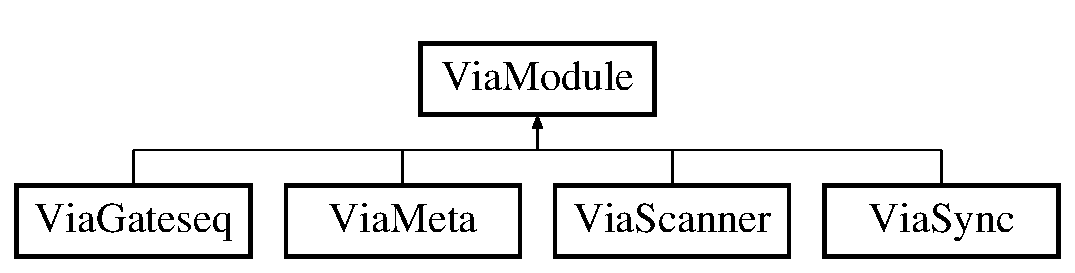
\includegraphics[height=2.000000cm]{class_via_module}
\end{center}
\end{figure}
\subsection*{Public Types}
\begin{DoxyCompactItemize}
\item 
enum \mbox{\hyperlink{class_via_module_a1b83ad8b5871ad71e582502e9c252eb6}{Via\+Virtual\+G\+P\+IO}} \{ \mbox{\hyperlink{class_via_module_a1b83ad8b5871ad71e582502e9c252eb6a96faf1f58d32b3303a08663f3664d518}{V\+I\+A\+\_\+\+G\+P\+I\+O\+\_\+\+N\+OP}}, 
\mbox{\hyperlink{class_via_module_a1b83ad8b5871ad71e582502e9c252eb6a15269d472b985002290edb9dc57c649d}{V\+I\+A\+\_\+\+G\+P\+I\+O\+\_\+\+L\+OW}}, 
\mbox{\hyperlink{class_via_module_a1b83ad8b5871ad71e582502e9c252eb6a2b8e66a8662ac906c211452d324818d5}{V\+I\+A\+\_\+\+G\+P\+I\+O\+\_\+\+H\+I\+GH}}
 \}
\end{DoxyCompactItemize}
\subsection*{Public Member Functions}
\begin{DoxyCompactItemize}
\item 
void \mbox{\hyperlink{class_via_module_a828697a5278c926373fe8f49114e0503}{io\+Stream\+Init}} ()
\item 
void \mbox{\hyperlink{class_via_module_a920be7d9a70222fde0fda7d807538272}{initialize\+Aux\+Outputs}} (void)
\item 
void \mbox{\hyperlink{class_via_module_a9add4c62e49aef8e8a122c923e31edc7}{set\+LogicA}} (int32\+\_\+t high)
\item 
void \mbox{\hyperlink{class_via_module_a6d68fc57d798138024c4e2079cbab3f3}{set\+Aux\+Logic}} (int32\+\_\+t high)
\item 
void \mbox{\hyperlink{class_via_module_a0f04112b4dde7164b36fa8916e4ae054}{set\+SH}} (int32\+\_\+t sampleA, int32\+\_\+t sampleB)
\item 
void \mbox{\hyperlink{class_via_module_ad676ccf2b9177bccfc7842967a792fa1}{set\+Logic\+Outputs\+L\+E\+D\+On}} (uint32\+\_\+t logicA, uint32\+\_\+t aux\+Logic, uint32\+\_\+t shA, uint32\+\_\+t shB)
\item 
void \mbox{\hyperlink{class_via_module_ab7f3b8c185a7e46f6412753c9d17ead9}{set\+Logic\+Outputs\+L\+E\+D\+Off}} (uint32\+\_\+t logicA, uint32\+\_\+t aux\+Logic, uint32\+\_\+t shA, uint32\+\_\+t shB)
\item 
void \mbox{\hyperlink{class_via_module_a980dceea193632fc47c663dc2adcf7ca}{set\+Logic\+Out}} (int32\+\_\+t write\+Index, int32\+\_\+t runtime\+Display)
\item 
void \mbox{\hyperlink{class_via_module_a6a0572d7fc135512a278b4fb304014d2}{set\+Logic\+Out\+No\+L\+ED}} (int32\+\_\+t write\+Index)
\item 
void \mbox{\hyperlink{class_via_module_ad7dd37cc52066d45418818743b3d23ad}{set\+Logic\+Out\+Boolean}} (int32\+\_\+t write\+Index, int32\+\_\+t runtime\+Display)
\item 
void \mbox{\hyperlink{class_via_module_a1ee37348829a21c99dd924361246a16a}{set\+L\+E\+DA}} (int32\+\_\+t on)
\item 
void \mbox{\hyperlink{class_via_module_a26f8a7cb6d23f939d3dfcfae035d914e}{set\+L\+E\+DB}} (int32\+\_\+t on)
\item 
void \mbox{\hyperlink{class_via_module_a9b2a127bfdbf2240fbdd1f79bbef52bc}{set\+L\+E\+DC}} (int32\+\_\+t on)
\item 
void \mbox{\hyperlink{class_via_module_ad9883693e8eacafa7ee68866793adf6e}{set\+L\+E\+DD}} (int32\+\_\+t on)
\item 
void \mbox{\hyperlink{class_via_module_a7a11c19ddf0c9a04061105a65d7c546b}{set\+Red\+L\+ED}} (int32\+\_\+t level)
\item 
void \mbox{\hyperlink{class_via_module_a4ead83d6ff1a8367d28d90c7e6271438}{set\+Green\+L\+ED}} (int32\+\_\+t level)
\item 
void \mbox{\hyperlink{class_via_module_a0832ffebe3e2d4d4cca044eaca59d99e}{set\+Blue\+L\+ED}} (int32\+\_\+t level)
\item 
void \mbox{\hyperlink{class_via_module_a4e627dab33ebf9b6ac2432aceb2a154d}{update\+R\+G\+B\+Display}} (int32\+\_\+t red, int32\+\_\+t green, int32\+\_\+t blue, int32\+\_\+t runtime\+Display)
\item 
void \mbox{\hyperlink{class_via_module_a9be28b96909b71625da532d5853c9ed4}{set\+R\+GB}} (\mbox{\hyperlink{structrgb}{rgb}} color)
\item 
void \mbox{\hyperlink{class_via_module_a284349df4c0e5b7153a5b82984fe9aee}{set\+R\+G\+B\+Scaled}} (\mbox{\hyperlink{structrgb}{rgb}} color, int32\+\_\+t scale)
\item 
void \mbox{\hyperlink{class_via_module_ab36185cb09e40578d0f0edb4ec74b7d3}{clear\+R\+GB}} ()
\item 
void \mbox{\hyperlink{class_via_module_a3acb105a42d49655361086d731d8e29d}{set\+L\+E\+Ds}} (int32\+\_\+t digit)
\item 
void \mbox{\hyperlink{class_via_module_ab690d8abdb4a3332db267d8d6a505bc7}{clear\+L\+E\+Ds}} ()
\item 
void \mbox{\hyperlink{class_via_module_a828697a5278c926373fe8f49114e0503}{io\+Stream\+Init}} ()
\item 
void \mbox{\hyperlink{class_via_module_a920be7d9a70222fde0fda7d807538272}{initialize\+Aux\+Outputs}} (void)
\item 
void \mbox{\hyperlink{class_via_module_a9add4c62e49aef8e8a122c923e31edc7}{set\+LogicA}} (int32\+\_\+t high)
\item 
void \mbox{\hyperlink{class_via_module_a6d68fc57d798138024c4e2079cbab3f3}{set\+Aux\+Logic}} (int32\+\_\+t high)
\item 
void \mbox{\hyperlink{class_via_module_a0f04112b4dde7164b36fa8916e4ae054}{set\+SH}} (int32\+\_\+t sampleA, int32\+\_\+t sampleB)
\item 
void \mbox{\hyperlink{class_via_module_a1ee37348829a21c99dd924361246a16a}{set\+L\+E\+DA}} (int32\+\_\+t on)
\item 
void \mbox{\hyperlink{class_via_module_a26f8a7cb6d23f939d3dfcfae035d914e}{set\+L\+E\+DB}} (int32\+\_\+t on)
\item 
void \mbox{\hyperlink{class_via_module_a9b2a127bfdbf2240fbdd1f79bbef52bc}{set\+L\+E\+DC}} (int32\+\_\+t on)
\item 
void \mbox{\hyperlink{class_via_module_ad9883693e8eacafa7ee68866793adf6e}{set\+L\+E\+DD}} (int32\+\_\+t on)
\item 
void \mbox{\hyperlink{class_via_module_a1448e56cf6d131b3b344175d586853e0}{S\+E\+T\+\_\+\+B\+L\+U\+E\+\_\+\+L\+E\+D\+\_\+\+O\+N\+O\+FF}} (int32\+\_\+t X)
\item 
void \mbox{\hyperlink{class_via_module_ad676ccf2b9177bccfc7842967a792fa1}{set\+Logic\+Outputs\+L\+E\+D\+On}} (uint32\+\_\+t logicA, uint32\+\_\+t aux\+Logic, uint32\+\_\+t shA, uint32\+\_\+t shB)
\item 
void \mbox{\hyperlink{class_via_module_ab7f3b8c185a7e46f6412753c9d17ead9}{set\+Logic\+Outputs\+L\+E\+D\+Off}} (uint32\+\_\+t logicA, uint32\+\_\+t aux\+Logic, uint32\+\_\+t shA, uint32\+\_\+t shB)
\item 
void \mbox{\hyperlink{class_via_module_a980dceea193632fc47c663dc2adcf7ca}{set\+Logic\+Out}} (int32\+\_\+t write\+Index, int32\+\_\+t runtime\+Display)
\item 
void \mbox{\hyperlink{class_via_module_a6a0572d7fc135512a278b4fb304014d2}{set\+Logic\+Out\+No\+L\+ED}} (int32\+\_\+t write\+Index)
\item 
void \mbox{\hyperlink{class_via_module_ad7dd37cc52066d45418818743b3d23ad}{set\+Logic\+Out\+Boolean}} (int32\+\_\+t write\+Index, int32\+\_\+t runtime\+Display)
\item 
void \mbox{\hyperlink{class_via_module_a7a11c19ddf0c9a04061105a65d7c546b}{set\+Red\+L\+ED}} (int32\+\_\+t level)
\item 
void \mbox{\hyperlink{class_via_module_a4ead83d6ff1a8367d28d90c7e6271438}{set\+Green\+L\+ED}} (int32\+\_\+t level)
\item 
void \mbox{\hyperlink{class_via_module_a0832ffebe3e2d4d4cca044eaca59d99e}{set\+Blue\+L\+ED}} (int32\+\_\+t level)
\item 
void \mbox{\hyperlink{class_via_module_a4e627dab33ebf9b6ac2432aceb2a154d}{update\+R\+G\+B\+Display}} (int32\+\_\+t red, int32\+\_\+t green, int32\+\_\+t blue, int32\+\_\+t runtime\+Display)
\item 
void \mbox{\hyperlink{class_via_module_a9be28b96909b71625da532d5853c9ed4}{set\+R\+GB}} (\mbox{\hyperlink{structrgb}{rgb}} color)
\item 
void \mbox{\hyperlink{class_via_module_a284349df4c0e5b7153a5b82984fe9aee}{set\+R\+G\+B\+Scaled}} (\mbox{\hyperlink{structrgb}{rgb}} color, int32\+\_\+t scale)
\item 
void \mbox{\hyperlink{class_via_module_ab36185cb09e40578d0f0edb4ec74b7d3}{clear\+R\+GB}} ()
\item 
void \mbox{\hyperlink{class_via_module_a3acb105a42d49655361086d731d8e29d}{set\+L\+E\+Ds}} (int32\+\_\+t digit)
\item 
void \mbox{\hyperlink{class_via_module_ab690d8abdb4a3332db267d8d6a505bc7}{clear\+L\+E\+Ds}} ()
\end{DoxyCompactItemize}
\subsection*{Public Attributes}
\begin{DoxyCompactItemize}
\item 
volatile uint32\+\_\+t $\ast$ \mbox{\hyperlink{class_via_module_ad4a23778dedad370ff274c8fc4b8f3b7}{a\+Logic\+Output}}
\item 
volatile uint32\+\_\+t $\ast$ \mbox{\hyperlink{class_via_module_a61d2533e5f10aca8d49921ec8d73ac95}{aux\+Logic\+Output}}
\item 
volatile uint32\+\_\+t $\ast$ \mbox{\hyperlink{class_via_module_ae563d7159c4e8ef81ff794883e9ee0a6}{sh\+A\+Output}}
\item 
volatile uint32\+\_\+t $\ast$ \mbox{\hyperlink{class_via_module_a9d6d3dd39cf5560aaf2b14a6d7c4a46b}{sh\+B\+Output}}
\item 
volatile uint32\+\_\+t $\ast$ \mbox{\hyperlink{class_via_module_a3e48bf5daca7c32b045460bb0c5c171c}{red\+Level}}
\item 
volatile uint32\+\_\+t $\ast$ \mbox{\hyperlink{class_via_module_af0465adbc24c831446092ceda3afc7d1}{green\+Level}}
\item 
volatile uint32\+\_\+t $\ast$ \mbox{\hyperlink{class_via_module_a79bfefe99580184e55ef001ca38d62e5}{blue\+Level}}
\item 
volatile uint32\+\_\+t $\ast$ \mbox{\hyperlink{class_via_module_a87b482ee25e03764976b8f179081b383}{led\+A\+Output}}
\item 
volatile uint32\+\_\+t $\ast$ \mbox{\hyperlink{class_via_module_adec17977c61271a9752a3d21ab532d07}{led\+B\+Output}}
\item 
volatile uint32\+\_\+t $\ast$ \mbox{\hyperlink{class_via_module_ac748f5b3fccba0d46153fbe25f0f05f4}{led\+C\+Output}}
\item 
volatile uint32\+\_\+t $\ast$ \mbox{\hyperlink{class_via_module_ac11bc2cd4f35777e6aac585c77eb9103}{led\+D\+Output}}
\item 
int32\+\_\+t $\ast$ \mbox{\hyperlink{class_via_module_ab1d7b6a86009b9371480ecf0a71aa89f}{button1\+Input}}
\item 
int32\+\_\+t $\ast$ \mbox{\hyperlink{class_via_module_ab77ba29dcff12ca1c826769749670d8a}{button2\+Input}}
\item 
int32\+\_\+t $\ast$ \mbox{\hyperlink{class_via_module_afe1c19b148dc4fce5ffb1bcbba3bb1f0}{button3\+Input}}
\item 
int32\+\_\+t $\ast$ \mbox{\hyperlink{class_via_module_acfde15bd4b560f5475804311f8568375}{button4\+Input}}
\item 
int32\+\_\+t $\ast$ \mbox{\hyperlink{class_via_module_a550e4235cc5e384b6c1795bf34d28bf0}{button5\+Input}}
\item 
int32\+\_\+t $\ast$ \mbox{\hyperlink{class_via_module_a62df426e2268a7d0dbd0d321fbc1b962}{button6\+Input}}
\item 
\mbox{\hyperlink{class_via_controls}{Via\+Controls}} \mbox{\hyperlink{class_via_module_a24d1ee1ac6d103afc23f480156895e57}{controls}}
\item 
int32\+\_\+t \mbox{\hyperlink{class_via_module_a23de5840e07f0b427bda2d44d116287f}{input\+Buffer\+Size}}
\item 
int32\+\_\+t \mbox{\hyperlink{class_via_module_ad80e8f75d0c3770fb54b5a47a4c25d12}{output\+Buffer\+Size}}
\item 
\mbox{\hyperlink{class_via_input_streams}{Via\+Input\+Streams}} \mbox{\hyperlink{class_via_module_af04f1c8df2a0302a9364dfb99a9085dc}{inputs}}
\item 
\mbox{\hyperlink{class_via_output_streams}{Via\+Output\+Streams}} \mbox{\hyperlink{class_via_module_a2c55536ef4a2162940b5ae145e74f730}{outputs}}
\item 
\mbox{\hyperlink{structrgb}{rgb}} \mbox{\hyperlink{class_via_module_a3426e2c19cee84ade2831cae4b627ebb}{hue\+Space}} \mbox{[}16\mbox{]} = \{\{4095, 0, 0\}, \{4095, 1228, 0\}, \{4095, 2457, 0\}, \{4095, 3685, 0\}, \{2047, 4095, 0\}, \{819, 4095, 0\}, \{0, 4095, 409\}, \{0, 4095, 1638\}, \{0, 4095, 4095\}, \{0, 2866, 4095\}, \{0, 1638, 4095\}, \{0, 409, 4095\}, \{2047, 0, 4095\}, \{3276, 0, 4095\}, \{4095, 0, 3685\}, \{4095, 0, 2456\}\}
\item 
uint32\+\_\+t \mbox{\hyperlink{class_via_module_a1e14a3a43daabb612fa61b7d2ee40d63}{a\+Logic\+Output}} = 0
\item 
uint32\+\_\+t \mbox{\hyperlink{class_via_module_adfd4a85913ab03a59f5b1250aa5eefa8}{aux\+Logic\+Output}} = 0
\item 
uint32\+\_\+t \mbox{\hyperlink{class_via_module_aff6cc2fd90847c64a6320fd17c0da74a}{sh\+A\+Output}} = 0
\item 
uint32\+\_\+t \mbox{\hyperlink{class_via_module_a7cfbe5fe6b6afb143cb55ff53cdcc90e}{sh\+B\+Output}} = 0
\item 
uint32\+\_\+t \mbox{\hyperlink{class_via_module_a6b74dd873f71791543efb5affb4d4b77}{red\+Level}} = 0
\item 
uint32\+\_\+t \mbox{\hyperlink{class_via_module_a823f43c562e39858bfa1d2b1943dd2b5}{green\+Level}} = 0
\item 
uint32\+\_\+t \mbox{\hyperlink{class_via_module_a18580be93f8001ff48a2d413318b79c2}{blue\+Level}} = 0
\item 
uint32\+\_\+t \mbox{\hyperlink{class_via_module_a8bbc2b1b6b811030a29c54eb2267402d}{led\+A\+Output}} = 0
\item 
uint32\+\_\+t \mbox{\hyperlink{class_via_module_abfc55b0fb546b1aae419628d5af83b31}{led\+B\+Output}} = 0
\item 
uint32\+\_\+t \mbox{\hyperlink{class_via_module_a28272e553fd741627d2661b2971f931f}{led\+C\+Output}} = 0
\item 
uint32\+\_\+t \mbox{\hyperlink{class_via_module_a3a36a2d911549950d6eca39b2f05029d}{led\+D\+Output}} = 0
\item 
int32\+\_\+t \mbox{\hyperlink{class_via_module_a8b54c1c283ce508654c6ca3d501d1d4b}{button1\+Input}} = 0
\item 
int32\+\_\+t \mbox{\hyperlink{class_via_module_a2bad7b5f68752daadf61d48f837416f2}{button2\+Input}} = 0
\item 
int32\+\_\+t \mbox{\hyperlink{class_via_module_a37d126e1b41834d01396d745c57c966b}{button3\+Input}} = 0
\item 
int32\+\_\+t \mbox{\hyperlink{class_via_module_a9ada50e4526b70a798cc59a108befcfa}{button4\+Input}} = 0
\item 
int32\+\_\+t \mbox{\hyperlink{class_via_module_a56d68d397aecce9d7ca1c4f36f556586}{button5\+Input}} = 0
\item 
int32\+\_\+t \mbox{\hyperlink{class_via_module_aa4afb6bc99e668e10cdd83dd8f6aeec5}{button6\+Input}} = 0
\end{DoxyCompactItemize}


\subsection{Member Enumeration Documentation}
\mbox{\Hypertarget{class_via_module_a1b83ad8b5871ad71e582502e9c252eb6}\label{class_via_module_a1b83ad8b5871ad71e582502e9c252eb6}} 
\index{Via\+Module@{Via\+Module}!Via\+Virtual\+G\+P\+IO@{Via\+Virtual\+G\+P\+IO}}
\index{Via\+Virtual\+G\+P\+IO@{Via\+Virtual\+G\+P\+IO}!Via\+Module@{Via\+Module}}
\subsubsection{\texorpdfstring{Via\+Virtual\+G\+P\+IO}{ViaVirtualGPIO}}
{\footnotesize\ttfamily enum \mbox{\hyperlink{class_via_module_a1b83ad8b5871ad71e582502e9c252eb6}{Via\+Module\+::\+Via\+Virtual\+G\+P\+IO}}}

\begin{DoxyEnumFields}{Enumerator}
\raisebox{\heightof{T}}[0pt][0pt]{\index{V\+I\+A\+\_\+\+G\+P\+I\+O\+\_\+\+N\+OP@{V\+I\+A\+\_\+\+G\+P\+I\+O\+\_\+\+N\+OP}!Via\+Module@{Via\+Module}}\index{Via\+Module@{Via\+Module}!V\+I\+A\+\_\+\+G\+P\+I\+O\+\_\+\+N\+OP@{V\+I\+A\+\_\+\+G\+P\+I\+O\+\_\+\+N\+OP}}}\mbox{\Hypertarget{class_via_module_a1b83ad8b5871ad71e582502e9c252eb6a96faf1f58d32b3303a08663f3664d518}\label{class_via_module_a1b83ad8b5871ad71e582502e9c252eb6a96faf1f58d32b3303a08663f3664d518}} 
V\+I\+A\+\_\+\+G\+P\+I\+O\+\_\+\+N\+OP&\\
\hline

\raisebox{\heightof{T}}[0pt][0pt]{\index{V\+I\+A\+\_\+\+G\+P\+I\+O\+\_\+\+L\+OW@{V\+I\+A\+\_\+\+G\+P\+I\+O\+\_\+\+L\+OW}!Via\+Module@{Via\+Module}}\index{Via\+Module@{Via\+Module}!V\+I\+A\+\_\+\+G\+P\+I\+O\+\_\+\+L\+OW@{V\+I\+A\+\_\+\+G\+P\+I\+O\+\_\+\+L\+OW}}}\mbox{\Hypertarget{class_via_module_a1b83ad8b5871ad71e582502e9c252eb6a15269d472b985002290edb9dc57c649d}\label{class_via_module_a1b83ad8b5871ad71e582502e9c252eb6a15269d472b985002290edb9dc57c649d}} 
V\+I\+A\+\_\+\+G\+P\+I\+O\+\_\+\+L\+OW&\\
\hline

\raisebox{\heightof{T}}[0pt][0pt]{\index{V\+I\+A\+\_\+\+G\+P\+I\+O\+\_\+\+H\+I\+GH@{V\+I\+A\+\_\+\+G\+P\+I\+O\+\_\+\+H\+I\+GH}!Via\+Module@{Via\+Module}}\index{Via\+Module@{Via\+Module}!V\+I\+A\+\_\+\+G\+P\+I\+O\+\_\+\+H\+I\+GH@{V\+I\+A\+\_\+\+G\+P\+I\+O\+\_\+\+H\+I\+GH}}}\mbox{\Hypertarget{class_via_module_a1b83ad8b5871ad71e582502e9c252eb6a2b8e66a8662ac906c211452d324818d5}\label{class_via_module_a1b83ad8b5871ad71e582502e9c252eb6a2b8e66a8662ac906c211452d324818d5}} 
V\+I\+A\+\_\+\+G\+P\+I\+O\+\_\+\+H\+I\+GH&\\
\hline

\end{DoxyEnumFields}


\subsection{Member Function Documentation}
\mbox{\Hypertarget{class_via_module_ab690d8abdb4a3332db267d8d6a505bc7}\label{class_via_module_ab690d8abdb4a3332db267d8d6a505bc7}} 
\index{Via\+Module@{Via\+Module}!clear\+L\+E\+Ds@{clear\+L\+E\+Ds}}
\index{clear\+L\+E\+Ds@{clear\+L\+E\+Ds}!Via\+Module@{Via\+Module}}
\subsubsection{\texorpdfstring{clear\+L\+E\+Ds()}{clearLEDs()}\hspace{0.1cm}{\footnotesize\ttfamily [1/2]}}
{\footnotesize\ttfamily void Via\+Module\+::clear\+L\+E\+Ds (\begin{DoxyParamCaption}{ }\end{DoxyParamCaption})\hspace{0.3cm}{\ttfamily [inline]}}

\mbox{\Hypertarget{class_via_module_ab690d8abdb4a3332db267d8d6a505bc7}\label{class_via_module_ab690d8abdb4a3332db267d8d6a505bc7}} 
\index{Via\+Module@{Via\+Module}!clear\+L\+E\+Ds@{clear\+L\+E\+Ds}}
\index{clear\+L\+E\+Ds@{clear\+L\+E\+Ds}!Via\+Module@{Via\+Module}}
\subsubsection{\texorpdfstring{clear\+L\+E\+Ds()}{clearLEDs()}\hspace{0.1cm}{\footnotesize\ttfamily [2/2]}}
{\footnotesize\ttfamily void Via\+Module\+::clear\+L\+E\+Ds (\begin{DoxyParamCaption}{ }\end{DoxyParamCaption})\hspace{0.3cm}{\ttfamily [inline]}}

\mbox{\Hypertarget{class_via_module_ab36185cb09e40578d0f0edb4ec74b7d3}\label{class_via_module_ab36185cb09e40578d0f0edb4ec74b7d3}} 
\index{Via\+Module@{Via\+Module}!clear\+R\+GB@{clear\+R\+GB}}
\index{clear\+R\+GB@{clear\+R\+GB}!Via\+Module@{Via\+Module}}
\subsubsection{\texorpdfstring{clear\+R\+G\+B()}{clearRGB()}\hspace{0.1cm}{\footnotesize\ttfamily [1/2]}}
{\footnotesize\ttfamily void Via\+Module\+::clear\+R\+GB (\begin{DoxyParamCaption}{ }\end{DoxyParamCaption})\hspace{0.3cm}{\ttfamily [inline]}}

\mbox{\Hypertarget{class_via_module_ab36185cb09e40578d0f0edb4ec74b7d3}\label{class_via_module_ab36185cb09e40578d0f0edb4ec74b7d3}} 
\index{Via\+Module@{Via\+Module}!clear\+R\+GB@{clear\+R\+GB}}
\index{clear\+R\+GB@{clear\+R\+GB}!Via\+Module@{Via\+Module}}
\subsubsection{\texorpdfstring{clear\+R\+G\+B()}{clearRGB()}\hspace{0.1cm}{\footnotesize\ttfamily [2/2]}}
{\footnotesize\ttfamily void Via\+Module\+::clear\+R\+GB (\begin{DoxyParamCaption}{ }\end{DoxyParamCaption})\hspace{0.3cm}{\ttfamily [inline]}}

\mbox{\Hypertarget{class_via_module_a920be7d9a70222fde0fda7d807538272}\label{class_via_module_a920be7d9a70222fde0fda7d807538272}} 
\index{Via\+Module@{Via\+Module}!initialize\+Aux\+Outputs@{initialize\+Aux\+Outputs}}
\index{initialize\+Aux\+Outputs@{initialize\+Aux\+Outputs}!Via\+Module@{Via\+Module}}
\subsubsection{\texorpdfstring{initialize\+Aux\+Outputs()}{initializeAuxOutputs()}\hspace{0.1cm}{\footnotesize\ttfamily [1/2]}}
{\footnotesize\ttfamily void Via\+Module\+::initialize\+Aux\+Outputs (\begin{DoxyParamCaption}\item[{void}]{ }\end{DoxyParamCaption})\hspace{0.3cm}{\ttfamily [inline]}}

\mbox{\Hypertarget{class_via_module_a920be7d9a70222fde0fda7d807538272}\label{class_via_module_a920be7d9a70222fde0fda7d807538272}} 
\index{Via\+Module@{Via\+Module}!initialize\+Aux\+Outputs@{initialize\+Aux\+Outputs}}
\index{initialize\+Aux\+Outputs@{initialize\+Aux\+Outputs}!Via\+Module@{Via\+Module}}
\subsubsection{\texorpdfstring{initialize\+Aux\+Outputs()}{initializeAuxOutputs()}\hspace{0.1cm}{\footnotesize\ttfamily [2/2]}}
{\footnotesize\ttfamily void Via\+Module\+::initialize\+Aux\+Outputs (\begin{DoxyParamCaption}\item[{void}]{ }\end{DoxyParamCaption})\hspace{0.3cm}{\ttfamily [inline]}}

\mbox{\Hypertarget{class_via_module_a828697a5278c926373fe8f49114e0503}\label{class_via_module_a828697a5278c926373fe8f49114e0503}} 
\index{Via\+Module@{Via\+Module}!io\+Stream\+Init@{io\+Stream\+Init}}
\index{io\+Stream\+Init@{io\+Stream\+Init}!Via\+Module@{Via\+Module}}
\subsubsection{\texorpdfstring{io\+Stream\+Init()}{ioStreamInit()}\hspace{0.1cm}{\footnotesize\ttfamily [1/2]}}
{\footnotesize\ttfamily void Via\+Module\+::io\+Stream\+Init (\begin{DoxyParamCaption}{ }\end{DoxyParamCaption})\hspace{0.3cm}{\ttfamily [inline]}}

\mbox{\Hypertarget{class_via_module_a828697a5278c926373fe8f49114e0503}\label{class_via_module_a828697a5278c926373fe8f49114e0503}} 
\index{Via\+Module@{Via\+Module}!io\+Stream\+Init@{io\+Stream\+Init}}
\index{io\+Stream\+Init@{io\+Stream\+Init}!Via\+Module@{Via\+Module}}
\subsubsection{\texorpdfstring{io\+Stream\+Init()}{ioStreamInit()}\hspace{0.1cm}{\footnotesize\ttfamily [2/2]}}
{\footnotesize\ttfamily void Via\+Module\+::io\+Stream\+Init (\begin{DoxyParamCaption}{ }\end{DoxyParamCaption})\hspace{0.3cm}{\ttfamily [inline]}}

\mbox{\Hypertarget{class_via_module_a1448e56cf6d131b3b344175d586853e0}\label{class_via_module_a1448e56cf6d131b3b344175d586853e0}} 
\index{Via\+Module@{Via\+Module}!S\+E\+T\+\_\+\+B\+L\+U\+E\+\_\+\+L\+E\+D\+\_\+\+O\+N\+O\+FF@{S\+E\+T\+\_\+\+B\+L\+U\+E\+\_\+\+L\+E\+D\+\_\+\+O\+N\+O\+FF}}
\index{S\+E\+T\+\_\+\+B\+L\+U\+E\+\_\+\+L\+E\+D\+\_\+\+O\+N\+O\+FF@{S\+E\+T\+\_\+\+B\+L\+U\+E\+\_\+\+L\+E\+D\+\_\+\+O\+N\+O\+FF}!Via\+Module@{Via\+Module}}
\subsubsection{\texorpdfstring{S\+E\+T\+\_\+\+B\+L\+U\+E\+\_\+\+L\+E\+D\+\_\+\+O\+N\+O\+F\+F()}{SET\_BLUE\_LED\_ONOFF()}}
{\footnotesize\ttfamily void Via\+Module\+::\+S\+E\+T\+\_\+\+B\+L\+U\+E\+\_\+\+L\+E\+D\+\_\+\+O\+N\+O\+FF (\begin{DoxyParamCaption}\item[{int32\+\_\+t}]{X }\end{DoxyParamCaption})\hspace{0.3cm}{\ttfamily [inline]}}

\mbox{\Hypertarget{class_via_module_a6d68fc57d798138024c4e2079cbab3f3}\label{class_via_module_a6d68fc57d798138024c4e2079cbab3f3}} 
\index{Via\+Module@{Via\+Module}!set\+Aux\+Logic@{set\+Aux\+Logic}}
\index{set\+Aux\+Logic@{set\+Aux\+Logic}!Via\+Module@{Via\+Module}}
\subsubsection{\texorpdfstring{set\+Aux\+Logic()}{setAuxLogic()}\hspace{0.1cm}{\footnotesize\ttfamily [1/2]}}
{\footnotesize\ttfamily void Via\+Module\+::set\+Aux\+Logic (\begin{DoxyParamCaption}\item[{int32\+\_\+t}]{high }\end{DoxyParamCaption})\hspace{0.3cm}{\ttfamily [inline]}}

\mbox{\Hypertarget{class_via_module_a6d68fc57d798138024c4e2079cbab3f3}\label{class_via_module_a6d68fc57d798138024c4e2079cbab3f3}} 
\index{Via\+Module@{Via\+Module}!set\+Aux\+Logic@{set\+Aux\+Logic}}
\index{set\+Aux\+Logic@{set\+Aux\+Logic}!Via\+Module@{Via\+Module}}
\subsubsection{\texorpdfstring{set\+Aux\+Logic()}{setAuxLogic()}\hspace{0.1cm}{\footnotesize\ttfamily [2/2]}}
{\footnotesize\ttfamily void Via\+Module\+::set\+Aux\+Logic (\begin{DoxyParamCaption}\item[{int32\+\_\+t}]{high }\end{DoxyParamCaption})\hspace{0.3cm}{\ttfamily [inline]}}

\mbox{\Hypertarget{class_via_module_a0832ffebe3e2d4d4cca044eaca59d99e}\label{class_via_module_a0832ffebe3e2d4d4cca044eaca59d99e}} 
\index{Via\+Module@{Via\+Module}!set\+Blue\+L\+ED@{set\+Blue\+L\+ED}}
\index{set\+Blue\+L\+ED@{set\+Blue\+L\+ED}!Via\+Module@{Via\+Module}}
\subsubsection{\texorpdfstring{set\+Blue\+L\+E\+D()}{setBlueLED()}\hspace{0.1cm}{\footnotesize\ttfamily [1/2]}}
{\footnotesize\ttfamily void Via\+Module\+::set\+Blue\+L\+ED (\begin{DoxyParamCaption}\item[{int32\+\_\+t}]{level }\end{DoxyParamCaption})\hspace{0.3cm}{\ttfamily [inline]}}

\mbox{\Hypertarget{class_via_module_a0832ffebe3e2d4d4cca044eaca59d99e}\label{class_via_module_a0832ffebe3e2d4d4cca044eaca59d99e}} 
\index{Via\+Module@{Via\+Module}!set\+Blue\+L\+ED@{set\+Blue\+L\+ED}}
\index{set\+Blue\+L\+ED@{set\+Blue\+L\+ED}!Via\+Module@{Via\+Module}}
\subsubsection{\texorpdfstring{set\+Blue\+L\+E\+D()}{setBlueLED()}\hspace{0.1cm}{\footnotesize\ttfamily [2/2]}}
{\footnotesize\ttfamily void Via\+Module\+::set\+Blue\+L\+ED (\begin{DoxyParamCaption}\item[{int32\+\_\+t}]{level }\end{DoxyParamCaption})\hspace{0.3cm}{\ttfamily [inline]}}

\mbox{\Hypertarget{class_via_module_a4ead83d6ff1a8367d28d90c7e6271438}\label{class_via_module_a4ead83d6ff1a8367d28d90c7e6271438}} 
\index{Via\+Module@{Via\+Module}!set\+Green\+L\+ED@{set\+Green\+L\+ED}}
\index{set\+Green\+L\+ED@{set\+Green\+L\+ED}!Via\+Module@{Via\+Module}}
\subsubsection{\texorpdfstring{set\+Green\+L\+E\+D()}{setGreenLED()}\hspace{0.1cm}{\footnotesize\ttfamily [1/2]}}
{\footnotesize\ttfamily void Via\+Module\+::set\+Green\+L\+ED (\begin{DoxyParamCaption}\item[{int32\+\_\+t}]{level }\end{DoxyParamCaption})\hspace{0.3cm}{\ttfamily [inline]}}

\mbox{\Hypertarget{class_via_module_a4ead83d6ff1a8367d28d90c7e6271438}\label{class_via_module_a4ead83d6ff1a8367d28d90c7e6271438}} 
\index{Via\+Module@{Via\+Module}!set\+Green\+L\+ED@{set\+Green\+L\+ED}}
\index{set\+Green\+L\+ED@{set\+Green\+L\+ED}!Via\+Module@{Via\+Module}}
\subsubsection{\texorpdfstring{set\+Green\+L\+E\+D()}{setGreenLED()}\hspace{0.1cm}{\footnotesize\ttfamily [2/2]}}
{\footnotesize\ttfamily void Via\+Module\+::set\+Green\+L\+ED (\begin{DoxyParamCaption}\item[{int32\+\_\+t}]{level }\end{DoxyParamCaption})\hspace{0.3cm}{\ttfamily [inline]}}

\mbox{\Hypertarget{class_via_module_a1ee37348829a21c99dd924361246a16a}\label{class_via_module_a1ee37348829a21c99dd924361246a16a}} 
\index{Via\+Module@{Via\+Module}!set\+L\+E\+DA@{set\+L\+E\+DA}}
\index{set\+L\+E\+DA@{set\+L\+E\+DA}!Via\+Module@{Via\+Module}}
\subsubsection{\texorpdfstring{set\+L\+E\+D\+A()}{setLEDA()}\hspace{0.1cm}{\footnotesize\ttfamily [1/2]}}
{\footnotesize\ttfamily void Via\+Module\+::set\+L\+E\+DA (\begin{DoxyParamCaption}\item[{int32\+\_\+t}]{on }\end{DoxyParamCaption})\hspace{0.3cm}{\ttfamily [inline]}}

\mbox{\Hypertarget{class_via_module_a1ee37348829a21c99dd924361246a16a}\label{class_via_module_a1ee37348829a21c99dd924361246a16a}} 
\index{Via\+Module@{Via\+Module}!set\+L\+E\+DA@{set\+L\+E\+DA}}
\index{set\+L\+E\+DA@{set\+L\+E\+DA}!Via\+Module@{Via\+Module}}
\subsubsection{\texorpdfstring{set\+L\+E\+D\+A()}{setLEDA()}\hspace{0.1cm}{\footnotesize\ttfamily [2/2]}}
{\footnotesize\ttfamily void Via\+Module\+::set\+L\+E\+DA (\begin{DoxyParamCaption}\item[{int32\+\_\+t}]{on }\end{DoxyParamCaption})\hspace{0.3cm}{\ttfamily [inline]}}

\mbox{\Hypertarget{class_via_module_a26f8a7cb6d23f939d3dfcfae035d914e}\label{class_via_module_a26f8a7cb6d23f939d3dfcfae035d914e}} 
\index{Via\+Module@{Via\+Module}!set\+L\+E\+DB@{set\+L\+E\+DB}}
\index{set\+L\+E\+DB@{set\+L\+E\+DB}!Via\+Module@{Via\+Module}}
\subsubsection{\texorpdfstring{set\+L\+E\+D\+B()}{setLEDB()}\hspace{0.1cm}{\footnotesize\ttfamily [1/2]}}
{\footnotesize\ttfamily void Via\+Module\+::set\+L\+E\+DB (\begin{DoxyParamCaption}\item[{int32\+\_\+t}]{on }\end{DoxyParamCaption})\hspace{0.3cm}{\ttfamily [inline]}}

\mbox{\Hypertarget{class_via_module_a26f8a7cb6d23f939d3dfcfae035d914e}\label{class_via_module_a26f8a7cb6d23f939d3dfcfae035d914e}} 
\index{Via\+Module@{Via\+Module}!set\+L\+E\+DB@{set\+L\+E\+DB}}
\index{set\+L\+E\+DB@{set\+L\+E\+DB}!Via\+Module@{Via\+Module}}
\subsubsection{\texorpdfstring{set\+L\+E\+D\+B()}{setLEDB()}\hspace{0.1cm}{\footnotesize\ttfamily [2/2]}}
{\footnotesize\ttfamily void Via\+Module\+::set\+L\+E\+DB (\begin{DoxyParamCaption}\item[{int32\+\_\+t}]{on }\end{DoxyParamCaption})\hspace{0.3cm}{\ttfamily [inline]}}

\mbox{\Hypertarget{class_via_module_a9b2a127bfdbf2240fbdd1f79bbef52bc}\label{class_via_module_a9b2a127bfdbf2240fbdd1f79bbef52bc}} 
\index{Via\+Module@{Via\+Module}!set\+L\+E\+DC@{set\+L\+E\+DC}}
\index{set\+L\+E\+DC@{set\+L\+E\+DC}!Via\+Module@{Via\+Module}}
\subsubsection{\texorpdfstring{set\+L\+E\+D\+C()}{setLEDC()}\hspace{0.1cm}{\footnotesize\ttfamily [1/2]}}
{\footnotesize\ttfamily void Via\+Module\+::set\+L\+E\+DC (\begin{DoxyParamCaption}\item[{int32\+\_\+t}]{on }\end{DoxyParamCaption})\hspace{0.3cm}{\ttfamily [inline]}}

\mbox{\Hypertarget{class_via_module_a9b2a127bfdbf2240fbdd1f79bbef52bc}\label{class_via_module_a9b2a127bfdbf2240fbdd1f79bbef52bc}} 
\index{Via\+Module@{Via\+Module}!set\+L\+E\+DC@{set\+L\+E\+DC}}
\index{set\+L\+E\+DC@{set\+L\+E\+DC}!Via\+Module@{Via\+Module}}
\subsubsection{\texorpdfstring{set\+L\+E\+D\+C()}{setLEDC()}\hspace{0.1cm}{\footnotesize\ttfamily [2/2]}}
{\footnotesize\ttfamily void Via\+Module\+::set\+L\+E\+DC (\begin{DoxyParamCaption}\item[{int32\+\_\+t}]{on }\end{DoxyParamCaption})\hspace{0.3cm}{\ttfamily [inline]}}

\mbox{\Hypertarget{class_via_module_ad9883693e8eacafa7ee68866793adf6e}\label{class_via_module_ad9883693e8eacafa7ee68866793adf6e}} 
\index{Via\+Module@{Via\+Module}!set\+L\+E\+DD@{set\+L\+E\+DD}}
\index{set\+L\+E\+DD@{set\+L\+E\+DD}!Via\+Module@{Via\+Module}}
\subsubsection{\texorpdfstring{set\+L\+E\+D\+D()}{setLEDD()}\hspace{0.1cm}{\footnotesize\ttfamily [1/2]}}
{\footnotesize\ttfamily void Via\+Module\+::set\+L\+E\+DD (\begin{DoxyParamCaption}\item[{int32\+\_\+t}]{on }\end{DoxyParamCaption})\hspace{0.3cm}{\ttfamily [inline]}}

\mbox{\Hypertarget{class_via_module_ad9883693e8eacafa7ee68866793adf6e}\label{class_via_module_ad9883693e8eacafa7ee68866793adf6e}} 
\index{Via\+Module@{Via\+Module}!set\+L\+E\+DD@{set\+L\+E\+DD}}
\index{set\+L\+E\+DD@{set\+L\+E\+DD}!Via\+Module@{Via\+Module}}
\subsubsection{\texorpdfstring{set\+L\+E\+D\+D()}{setLEDD()}\hspace{0.1cm}{\footnotesize\ttfamily [2/2]}}
{\footnotesize\ttfamily void Via\+Module\+::set\+L\+E\+DD (\begin{DoxyParamCaption}\item[{int32\+\_\+t}]{on }\end{DoxyParamCaption})\hspace{0.3cm}{\ttfamily [inline]}}

\mbox{\Hypertarget{class_via_module_a3acb105a42d49655361086d731d8e29d}\label{class_via_module_a3acb105a42d49655361086d731d8e29d}} 
\index{Via\+Module@{Via\+Module}!set\+L\+E\+Ds@{set\+L\+E\+Ds}}
\index{set\+L\+E\+Ds@{set\+L\+E\+Ds}!Via\+Module@{Via\+Module}}
\subsubsection{\texorpdfstring{set\+L\+E\+Ds()}{setLEDs()}\hspace{0.1cm}{\footnotesize\ttfamily [1/2]}}
{\footnotesize\ttfamily void Via\+Module\+::set\+L\+E\+Ds (\begin{DoxyParamCaption}\item[{int32\+\_\+t}]{digit }\end{DoxyParamCaption})\hspace{0.3cm}{\ttfamily [inline]}}

\mbox{\Hypertarget{class_via_module_a3acb105a42d49655361086d731d8e29d}\label{class_via_module_a3acb105a42d49655361086d731d8e29d}} 
\index{Via\+Module@{Via\+Module}!set\+L\+E\+Ds@{set\+L\+E\+Ds}}
\index{set\+L\+E\+Ds@{set\+L\+E\+Ds}!Via\+Module@{Via\+Module}}
\subsubsection{\texorpdfstring{set\+L\+E\+Ds()}{setLEDs()}\hspace{0.1cm}{\footnotesize\ttfamily [2/2]}}
{\footnotesize\ttfamily void Via\+Module\+::set\+L\+E\+Ds (\begin{DoxyParamCaption}\item[{int32\+\_\+t}]{digit }\end{DoxyParamCaption})\hspace{0.3cm}{\ttfamily [inline]}}

\mbox{\Hypertarget{class_via_module_a9add4c62e49aef8e8a122c923e31edc7}\label{class_via_module_a9add4c62e49aef8e8a122c923e31edc7}} 
\index{Via\+Module@{Via\+Module}!set\+LogicA@{set\+LogicA}}
\index{set\+LogicA@{set\+LogicA}!Via\+Module@{Via\+Module}}
\subsubsection{\texorpdfstring{set\+Logic\+A()}{setLogicA()}\hspace{0.1cm}{\footnotesize\ttfamily [1/2]}}
{\footnotesize\ttfamily void Via\+Module\+::set\+LogicA (\begin{DoxyParamCaption}\item[{int32\+\_\+t}]{high }\end{DoxyParamCaption})\hspace{0.3cm}{\ttfamily [inline]}}

\mbox{\Hypertarget{class_via_module_a9add4c62e49aef8e8a122c923e31edc7}\label{class_via_module_a9add4c62e49aef8e8a122c923e31edc7}} 
\index{Via\+Module@{Via\+Module}!set\+LogicA@{set\+LogicA}}
\index{set\+LogicA@{set\+LogicA}!Via\+Module@{Via\+Module}}
\subsubsection{\texorpdfstring{set\+Logic\+A()}{setLogicA()}\hspace{0.1cm}{\footnotesize\ttfamily [2/2]}}
{\footnotesize\ttfamily void Via\+Module\+::set\+LogicA (\begin{DoxyParamCaption}\item[{int32\+\_\+t}]{high }\end{DoxyParamCaption})\hspace{0.3cm}{\ttfamily [inline]}}

\mbox{\Hypertarget{class_via_module_a980dceea193632fc47c663dc2adcf7ca}\label{class_via_module_a980dceea193632fc47c663dc2adcf7ca}} 
\index{Via\+Module@{Via\+Module}!set\+Logic\+Out@{set\+Logic\+Out}}
\index{set\+Logic\+Out@{set\+Logic\+Out}!Via\+Module@{Via\+Module}}
\subsubsection{\texorpdfstring{set\+Logic\+Out()}{setLogicOut()}\hspace{0.1cm}{\footnotesize\ttfamily [1/2]}}
{\footnotesize\ttfamily void Via\+Module\+::set\+Logic\+Out (\begin{DoxyParamCaption}\item[{int32\+\_\+t}]{write\+Index,  }\item[{int32\+\_\+t}]{runtime\+Display }\end{DoxyParamCaption})\hspace{0.3cm}{\ttfamily [inline]}}

\mbox{\Hypertarget{class_via_module_a980dceea193632fc47c663dc2adcf7ca}\label{class_via_module_a980dceea193632fc47c663dc2adcf7ca}} 
\index{Via\+Module@{Via\+Module}!set\+Logic\+Out@{set\+Logic\+Out}}
\index{set\+Logic\+Out@{set\+Logic\+Out}!Via\+Module@{Via\+Module}}
\subsubsection{\texorpdfstring{set\+Logic\+Out()}{setLogicOut()}\hspace{0.1cm}{\footnotesize\ttfamily [2/2]}}
{\footnotesize\ttfamily void Via\+Module\+::set\+Logic\+Out (\begin{DoxyParamCaption}\item[{int32\+\_\+t}]{write\+Index,  }\item[{int32\+\_\+t}]{runtime\+Display }\end{DoxyParamCaption})\hspace{0.3cm}{\ttfamily [inline]}}

\mbox{\Hypertarget{class_via_module_ad7dd37cc52066d45418818743b3d23ad}\label{class_via_module_ad7dd37cc52066d45418818743b3d23ad}} 
\index{Via\+Module@{Via\+Module}!set\+Logic\+Out\+Boolean@{set\+Logic\+Out\+Boolean}}
\index{set\+Logic\+Out\+Boolean@{set\+Logic\+Out\+Boolean}!Via\+Module@{Via\+Module}}
\subsubsection{\texorpdfstring{set\+Logic\+Out\+Boolean()}{setLogicOutBoolean()}\hspace{0.1cm}{\footnotesize\ttfamily [1/2]}}
{\footnotesize\ttfamily void Via\+Module\+::set\+Logic\+Out\+Boolean (\begin{DoxyParamCaption}\item[{int32\+\_\+t}]{write\+Index,  }\item[{int32\+\_\+t}]{runtime\+Display }\end{DoxyParamCaption})\hspace{0.3cm}{\ttfamily [inline]}}

\mbox{\Hypertarget{class_via_module_ad7dd37cc52066d45418818743b3d23ad}\label{class_via_module_ad7dd37cc52066d45418818743b3d23ad}} 
\index{Via\+Module@{Via\+Module}!set\+Logic\+Out\+Boolean@{set\+Logic\+Out\+Boolean}}
\index{set\+Logic\+Out\+Boolean@{set\+Logic\+Out\+Boolean}!Via\+Module@{Via\+Module}}
\subsubsection{\texorpdfstring{set\+Logic\+Out\+Boolean()}{setLogicOutBoolean()}\hspace{0.1cm}{\footnotesize\ttfamily [2/2]}}
{\footnotesize\ttfamily void Via\+Module\+::set\+Logic\+Out\+Boolean (\begin{DoxyParamCaption}\item[{int32\+\_\+t}]{write\+Index,  }\item[{int32\+\_\+t}]{runtime\+Display }\end{DoxyParamCaption})\hspace{0.3cm}{\ttfamily [inline]}}

\mbox{\Hypertarget{class_via_module_a6a0572d7fc135512a278b4fb304014d2}\label{class_via_module_a6a0572d7fc135512a278b4fb304014d2}} 
\index{Via\+Module@{Via\+Module}!set\+Logic\+Out\+No\+L\+ED@{set\+Logic\+Out\+No\+L\+ED}}
\index{set\+Logic\+Out\+No\+L\+ED@{set\+Logic\+Out\+No\+L\+ED}!Via\+Module@{Via\+Module}}
\subsubsection{\texorpdfstring{set\+Logic\+Out\+No\+L\+E\+D()}{setLogicOutNoLED()}\hspace{0.1cm}{\footnotesize\ttfamily [1/2]}}
{\footnotesize\ttfamily void Via\+Module\+::set\+Logic\+Out\+No\+L\+ED (\begin{DoxyParamCaption}\item[{int32\+\_\+t}]{write\+Index }\end{DoxyParamCaption})\hspace{0.3cm}{\ttfamily [inline]}}

\mbox{\Hypertarget{class_via_module_a6a0572d7fc135512a278b4fb304014d2}\label{class_via_module_a6a0572d7fc135512a278b4fb304014d2}} 
\index{Via\+Module@{Via\+Module}!set\+Logic\+Out\+No\+L\+ED@{set\+Logic\+Out\+No\+L\+ED}}
\index{set\+Logic\+Out\+No\+L\+ED@{set\+Logic\+Out\+No\+L\+ED}!Via\+Module@{Via\+Module}}
\subsubsection{\texorpdfstring{set\+Logic\+Out\+No\+L\+E\+D()}{setLogicOutNoLED()}\hspace{0.1cm}{\footnotesize\ttfamily [2/2]}}
{\footnotesize\ttfamily void Via\+Module\+::set\+Logic\+Out\+No\+L\+ED (\begin{DoxyParamCaption}\item[{int32\+\_\+t}]{write\+Index }\end{DoxyParamCaption})\hspace{0.3cm}{\ttfamily [inline]}}

\mbox{\Hypertarget{class_via_module_ab7f3b8c185a7e46f6412753c9d17ead9}\label{class_via_module_ab7f3b8c185a7e46f6412753c9d17ead9}} 
\index{Via\+Module@{Via\+Module}!set\+Logic\+Outputs\+L\+E\+D\+Off@{set\+Logic\+Outputs\+L\+E\+D\+Off}}
\index{set\+Logic\+Outputs\+L\+E\+D\+Off@{set\+Logic\+Outputs\+L\+E\+D\+Off}!Via\+Module@{Via\+Module}}
\subsubsection{\texorpdfstring{set\+Logic\+Outputs\+L\+E\+D\+Off()}{setLogicOutputsLEDOff()}\hspace{0.1cm}{\footnotesize\ttfamily [1/2]}}
{\footnotesize\ttfamily void Via\+Module\+::set\+Logic\+Outputs\+L\+E\+D\+Off (\begin{DoxyParamCaption}\item[{uint32\+\_\+t}]{logicA,  }\item[{uint32\+\_\+t}]{aux\+Logic,  }\item[{uint32\+\_\+t}]{shA,  }\item[{uint32\+\_\+t}]{shB }\end{DoxyParamCaption})\hspace{0.3cm}{\ttfamily [inline]}}

\mbox{\Hypertarget{class_via_module_ab7f3b8c185a7e46f6412753c9d17ead9}\label{class_via_module_ab7f3b8c185a7e46f6412753c9d17ead9}} 
\index{Via\+Module@{Via\+Module}!set\+Logic\+Outputs\+L\+E\+D\+Off@{set\+Logic\+Outputs\+L\+E\+D\+Off}}
\index{set\+Logic\+Outputs\+L\+E\+D\+Off@{set\+Logic\+Outputs\+L\+E\+D\+Off}!Via\+Module@{Via\+Module}}
\subsubsection{\texorpdfstring{set\+Logic\+Outputs\+L\+E\+D\+Off()}{setLogicOutputsLEDOff()}\hspace{0.1cm}{\footnotesize\ttfamily [2/2]}}
{\footnotesize\ttfamily void Via\+Module\+::set\+Logic\+Outputs\+L\+E\+D\+Off (\begin{DoxyParamCaption}\item[{uint32\+\_\+t}]{logicA,  }\item[{uint32\+\_\+t}]{aux\+Logic,  }\item[{uint32\+\_\+t}]{shA,  }\item[{uint32\+\_\+t}]{shB }\end{DoxyParamCaption})\hspace{0.3cm}{\ttfamily [inline]}}

\mbox{\Hypertarget{class_via_module_ad676ccf2b9177bccfc7842967a792fa1}\label{class_via_module_ad676ccf2b9177bccfc7842967a792fa1}} 
\index{Via\+Module@{Via\+Module}!set\+Logic\+Outputs\+L\+E\+D\+On@{set\+Logic\+Outputs\+L\+E\+D\+On}}
\index{set\+Logic\+Outputs\+L\+E\+D\+On@{set\+Logic\+Outputs\+L\+E\+D\+On}!Via\+Module@{Via\+Module}}
\subsubsection{\texorpdfstring{set\+Logic\+Outputs\+L\+E\+D\+On()}{setLogicOutputsLEDOn()}\hspace{0.1cm}{\footnotesize\ttfamily [1/2]}}
{\footnotesize\ttfamily void Via\+Module\+::set\+Logic\+Outputs\+L\+E\+D\+On (\begin{DoxyParamCaption}\item[{uint32\+\_\+t}]{logicA,  }\item[{uint32\+\_\+t}]{aux\+Logic,  }\item[{uint32\+\_\+t}]{shA,  }\item[{uint32\+\_\+t}]{shB }\end{DoxyParamCaption})\hspace{0.3cm}{\ttfamily [inline]}}

\mbox{\Hypertarget{class_via_module_ad676ccf2b9177bccfc7842967a792fa1}\label{class_via_module_ad676ccf2b9177bccfc7842967a792fa1}} 
\index{Via\+Module@{Via\+Module}!set\+Logic\+Outputs\+L\+E\+D\+On@{set\+Logic\+Outputs\+L\+E\+D\+On}}
\index{set\+Logic\+Outputs\+L\+E\+D\+On@{set\+Logic\+Outputs\+L\+E\+D\+On}!Via\+Module@{Via\+Module}}
\subsubsection{\texorpdfstring{set\+Logic\+Outputs\+L\+E\+D\+On()}{setLogicOutputsLEDOn()}\hspace{0.1cm}{\footnotesize\ttfamily [2/2]}}
{\footnotesize\ttfamily void Via\+Module\+::set\+Logic\+Outputs\+L\+E\+D\+On (\begin{DoxyParamCaption}\item[{uint32\+\_\+t}]{logicA,  }\item[{uint32\+\_\+t}]{aux\+Logic,  }\item[{uint32\+\_\+t}]{shA,  }\item[{uint32\+\_\+t}]{shB }\end{DoxyParamCaption})\hspace{0.3cm}{\ttfamily [inline]}}

\mbox{\Hypertarget{class_via_module_a7a11c19ddf0c9a04061105a65d7c546b}\label{class_via_module_a7a11c19ddf0c9a04061105a65d7c546b}} 
\index{Via\+Module@{Via\+Module}!set\+Red\+L\+ED@{set\+Red\+L\+ED}}
\index{set\+Red\+L\+ED@{set\+Red\+L\+ED}!Via\+Module@{Via\+Module}}
\subsubsection{\texorpdfstring{set\+Red\+L\+E\+D()}{setRedLED()}\hspace{0.1cm}{\footnotesize\ttfamily [1/2]}}
{\footnotesize\ttfamily void Via\+Module\+::set\+Red\+L\+ED (\begin{DoxyParamCaption}\item[{int32\+\_\+t}]{level }\end{DoxyParamCaption})\hspace{0.3cm}{\ttfamily [inline]}}

\mbox{\Hypertarget{class_via_module_a7a11c19ddf0c9a04061105a65d7c546b}\label{class_via_module_a7a11c19ddf0c9a04061105a65d7c546b}} 
\index{Via\+Module@{Via\+Module}!set\+Red\+L\+ED@{set\+Red\+L\+ED}}
\index{set\+Red\+L\+ED@{set\+Red\+L\+ED}!Via\+Module@{Via\+Module}}
\subsubsection{\texorpdfstring{set\+Red\+L\+E\+D()}{setRedLED()}\hspace{0.1cm}{\footnotesize\ttfamily [2/2]}}
{\footnotesize\ttfamily void Via\+Module\+::set\+Red\+L\+ED (\begin{DoxyParamCaption}\item[{int32\+\_\+t}]{level }\end{DoxyParamCaption})\hspace{0.3cm}{\ttfamily [inline]}}

\mbox{\Hypertarget{class_via_module_a9be28b96909b71625da532d5853c9ed4}\label{class_via_module_a9be28b96909b71625da532d5853c9ed4}} 
\index{Via\+Module@{Via\+Module}!set\+R\+GB@{set\+R\+GB}}
\index{set\+R\+GB@{set\+R\+GB}!Via\+Module@{Via\+Module}}
\subsubsection{\texorpdfstring{set\+R\+G\+B()}{setRGB()}\hspace{0.1cm}{\footnotesize\ttfamily [1/2]}}
{\footnotesize\ttfamily void Via\+Module\+::set\+R\+GB (\begin{DoxyParamCaption}\item[{\mbox{\hyperlink{structrgb}{rgb}}}]{color }\end{DoxyParamCaption})\hspace{0.3cm}{\ttfamily [inline]}}

\mbox{\Hypertarget{class_via_module_a9be28b96909b71625da532d5853c9ed4}\label{class_via_module_a9be28b96909b71625da532d5853c9ed4}} 
\index{Via\+Module@{Via\+Module}!set\+R\+GB@{set\+R\+GB}}
\index{set\+R\+GB@{set\+R\+GB}!Via\+Module@{Via\+Module}}
\subsubsection{\texorpdfstring{set\+R\+G\+B()}{setRGB()}\hspace{0.1cm}{\footnotesize\ttfamily [2/2]}}
{\footnotesize\ttfamily void Via\+Module\+::set\+R\+GB (\begin{DoxyParamCaption}\item[{\mbox{\hyperlink{structrgb}{rgb}}}]{color }\end{DoxyParamCaption})\hspace{0.3cm}{\ttfamily [inline]}}

\mbox{\Hypertarget{class_via_module_a284349df4c0e5b7153a5b82984fe9aee}\label{class_via_module_a284349df4c0e5b7153a5b82984fe9aee}} 
\index{Via\+Module@{Via\+Module}!set\+R\+G\+B\+Scaled@{set\+R\+G\+B\+Scaled}}
\index{set\+R\+G\+B\+Scaled@{set\+R\+G\+B\+Scaled}!Via\+Module@{Via\+Module}}
\subsubsection{\texorpdfstring{set\+R\+G\+B\+Scaled()}{setRGBScaled()}\hspace{0.1cm}{\footnotesize\ttfamily [1/2]}}
{\footnotesize\ttfamily void Via\+Module\+::set\+R\+G\+B\+Scaled (\begin{DoxyParamCaption}\item[{\mbox{\hyperlink{structrgb}{rgb}}}]{color,  }\item[{int32\+\_\+t}]{scale }\end{DoxyParamCaption})\hspace{0.3cm}{\ttfamily [inline]}}

\mbox{\Hypertarget{class_via_module_a284349df4c0e5b7153a5b82984fe9aee}\label{class_via_module_a284349df4c0e5b7153a5b82984fe9aee}} 
\index{Via\+Module@{Via\+Module}!set\+R\+G\+B\+Scaled@{set\+R\+G\+B\+Scaled}}
\index{set\+R\+G\+B\+Scaled@{set\+R\+G\+B\+Scaled}!Via\+Module@{Via\+Module}}
\subsubsection{\texorpdfstring{set\+R\+G\+B\+Scaled()}{setRGBScaled()}\hspace{0.1cm}{\footnotesize\ttfamily [2/2]}}
{\footnotesize\ttfamily void Via\+Module\+::set\+R\+G\+B\+Scaled (\begin{DoxyParamCaption}\item[{\mbox{\hyperlink{structrgb}{rgb}}}]{color,  }\item[{int32\+\_\+t}]{scale }\end{DoxyParamCaption})\hspace{0.3cm}{\ttfamily [inline]}}

\mbox{\Hypertarget{class_via_module_a0f04112b4dde7164b36fa8916e4ae054}\label{class_via_module_a0f04112b4dde7164b36fa8916e4ae054}} 
\index{Via\+Module@{Via\+Module}!set\+SH@{set\+SH}}
\index{set\+SH@{set\+SH}!Via\+Module@{Via\+Module}}
\subsubsection{\texorpdfstring{set\+S\+H()}{setSH()}\hspace{0.1cm}{\footnotesize\ttfamily [1/2]}}
{\footnotesize\ttfamily void Via\+Module\+::set\+SH (\begin{DoxyParamCaption}\item[{int32\+\_\+t}]{sampleA,  }\item[{int32\+\_\+t}]{sampleB }\end{DoxyParamCaption})\hspace{0.3cm}{\ttfamily [inline]}}

\mbox{\Hypertarget{class_via_module_a0f04112b4dde7164b36fa8916e4ae054}\label{class_via_module_a0f04112b4dde7164b36fa8916e4ae054}} 
\index{Via\+Module@{Via\+Module}!set\+SH@{set\+SH}}
\index{set\+SH@{set\+SH}!Via\+Module@{Via\+Module}}
\subsubsection{\texorpdfstring{set\+S\+H()}{setSH()}\hspace{0.1cm}{\footnotesize\ttfamily [2/2]}}
{\footnotesize\ttfamily void Via\+Module\+::set\+SH (\begin{DoxyParamCaption}\item[{int32\+\_\+t}]{sampleA,  }\item[{int32\+\_\+t}]{sampleB }\end{DoxyParamCaption})\hspace{0.3cm}{\ttfamily [inline]}}

\mbox{\Hypertarget{class_via_module_a4e627dab33ebf9b6ac2432aceb2a154d}\label{class_via_module_a4e627dab33ebf9b6ac2432aceb2a154d}} 
\index{Via\+Module@{Via\+Module}!update\+R\+G\+B\+Display@{update\+R\+G\+B\+Display}}
\index{update\+R\+G\+B\+Display@{update\+R\+G\+B\+Display}!Via\+Module@{Via\+Module}}
\subsubsection{\texorpdfstring{update\+R\+G\+B\+Display()}{updateRGBDisplay()}\hspace{0.1cm}{\footnotesize\ttfamily [1/2]}}
{\footnotesize\ttfamily void Via\+Module\+::update\+R\+G\+B\+Display (\begin{DoxyParamCaption}\item[{int32\+\_\+t}]{red,  }\item[{int32\+\_\+t}]{green,  }\item[{int32\+\_\+t}]{blue,  }\item[{int32\+\_\+t}]{runtime\+Display }\end{DoxyParamCaption})\hspace{0.3cm}{\ttfamily [inline]}}

\mbox{\Hypertarget{class_via_module_a4e627dab33ebf9b6ac2432aceb2a154d}\label{class_via_module_a4e627dab33ebf9b6ac2432aceb2a154d}} 
\index{Via\+Module@{Via\+Module}!update\+R\+G\+B\+Display@{update\+R\+G\+B\+Display}}
\index{update\+R\+G\+B\+Display@{update\+R\+G\+B\+Display}!Via\+Module@{Via\+Module}}
\subsubsection{\texorpdfstring{update\+R\+G\+B\+Display()}{updateRGBDisplay()}\hspace{0.1cm}{\footnotesize\ttfamily [2/2]}}
{\footnotesize\ttfamily void Via\+Module\+::update\+R\+G\+B\+Display (\begin{DoxyParamCaption}\item[{int32\+\_\+t}]{red,  }\item[{int32\+\_\+t}]{green,  }\item[{int32\+\_\+t}]{blue,  }\item[{int32\+\_\+t}]{runtime\+Display }\end{DoxyParamCaption})\hspace{0.3cm}{\ttfamily [inline]}}



\subsection{Member Data Documentation}
\mbox{\Hypertarget{class_via_module_ad4a23778dedad370ff274c8fc4b8f3b7}\label{class_via_module_ad4a23778dedad370ff274c8fc4b8f3b7}} 
\index{Via\+Module@{Via\+Module}!a\+Logic\+Output@{a\+Logic\+Output}}
\index{a\+Logic\+Output@{a\+Logic\+Output}!Via\+Module@{Via\+Module}}
\subsubsection{\texorpdfstring{a\+Logic\+Output}{aLogicOutput}\hspace{0.1cm}{\footnotesize\ttfamily [1/2]}}
{\footnotesize\ttfamily volatile uint32\+\_\+t$\ast$ Via\+Module\+::a\+Logic\+Output}

\mbox{\Hypertarget{class_via_module_a1e14a3a43daabb612fa61b7d2ee40d63}\label{class_via_module_a1e14a3a43daabb612fa61b7d2ee40d63}} 
\index{Via\+Module@{Via\+Module}!a\+Logic\+Output@{a\+Logic\+Output}}
\index{a\+Logic\+Output@{a\+Logic\+Output}!Via\+Module@{Via\+Module}}
\subsubsection{\texorpdfstring{a\+Logic\+Output}{aLogicOutput}\hspace{0.1cm}{\footnotesize\ttfamily [2/2]}}
{\footnotesize\ttfamily uint32\+\_\+t Via\+Module\+::a\+Logic\+Output = 0}

\mbox{\Hypertarget{class_via_module_a61d2533e5f10aca8d49921ec8d73ac95}\label{class_via_module_a61d2533e5f10aca8d49921ec8d73ac95}} 
\index{Via\+Module@{Via\+Module}!aux\+Logic\+Output@{aux\+Logic\+Output}}
\index{aux\+Logic\+Output@{aux\+Logic\+Output}!Via\+Module@{Via\+Module}}
\subsubsection{\texorpdfstring{aux\+Logic\+Output}{auxLogicOutput}\hspace{0.1cm}{\footnotesize\ttfamily [1/2]}}
{\footnotesize\ttfamily volatile uint32\+\_\+t$\ast$ Via\+Module\+::aux\+Logic\+Output}

\mbox{\Hypertarget{class_via_module_adfd4a85913ab03a59f5b1250aa5eefa8}\label{class_via_module_adfd4a85913ab03a59f5b1250aa5eefa8}} 
\index{Via\+Module@{Via\+Module}!aux\+Logic\+Output@{aux\+Logic\+Output}}
\index{aux\+Logic\+Output@{aux\+Logic\+Output}!Via\+Module@{Via\+Module}}
\subsubsection{\texorpdfstring{aux\+Logic\+Output}{auxLogicOutput}\hspace{0.1cm}{\footnotesize\ttfamily [2/2]}}
{\footnotesize\ttfamily uint32\+\_\+t Via\+Module\+::aux\+Logic\+Output = 0}

\mbox{\Hypertarget{class_via_module_a79bfefe99580184e55ef001ca38d62e5}\label{class_via_module_a79bfefe99580184e55ef001ca38d62e5}} 
\index{Via\+Module@{Via\+Module}!blue\+Level@{blue\+Level}}
\index{blue\+Level@{blue\+Level}!Via\+Module@{Via\+Module}}
\subsubsection{\texorpdfstring{blue\+Level}{blueLevel}\hspace{0.1cm}{\footnotesize\ttfamily [1/2]}}
{\footnotesize\ttfamily volatile uint32\+\_\+t$\ast$ Via\+Module\+::blue\+Level}

\mbox{\Hypertarget{class_via_module_a18580be93f8001ff48a2d413318b79c2}\label{class_via_module_a18580be93f8001ff48a2d413318b79c2}} 
\index{Via\+Module@{Via\+Module}!blue\+Level@{blue\+Level}}
\index{blue\+Level@{blue\+Level}!Via\+Module@{Via\+Module}}
\subsubsection{\texorpdfstring{blue\+Level}{blueLevel}\hspace{0.1cm}{\footnotesize\ttfamily [2/2]}}
{\footnotesize\ttfamily uint32\+\_\+t Via\+Module\+::blue\+Level = 0}

\mbox{\Hypertarget{class_via_module_a8b54c1c283ce508654c6ca3d501d1d4b}\label{class_via_module_a8b54c1c283ce508654c6ca3d501d1d4b}} 
\index{Via\+Module@{Via\+Module}!button1\+Input@{button1\+Input}}
\index{button1\+Input@{button1\+Input}!Via\+Module@{Via\+Module}}
\subsubsection{\texorpdfstring{button1\+Input}{button1Input}\hspace{0.1cm}{\footnotesize\ttfamily [1/2]}}
{\footnotesize\ttfamily int32\+\_\+t Via\+Module\+::button1\+Input = 0}

\mbox{\Hypertarget{class_via_module_ab1d7b6a86009b9371480ecf0a71aa89f}\label{class_via_module_ab1d7b6a86009b9371480ecf0a71aa89f}} 
\index{Via\+Module@{Via\+Module}!button1\+Input@{button1\+Input}}
\index{button1\+Input@{button1\+Input}!Via\+Module@{Via\+Module}}
\subsubsection{\texorpdfstring{button1\+Input}{button1Input}\hspace{0.1cm}{\footnotesize\ttfamily [2/2]}}
{\footnotesize\ttfamily int32\+\_\+t$\ast$ Via\+Module\+::button1\+Input}

\mbox{\Hypertarget{class_via_module_a2bad7b5f68752daadf61d48f837416f2}\label{class_via_module_a2bad7b5f68752daadf61d48f837416f2}} 
\index{Via\+Module@{Via\+Module}!button2\+Input@{button2\+Input}}
\index{button2\+Input@{button2\+Input}!Via\+Module@{Via\+Module}}
\subsubsection{\texorpdfstring{button2\+Input}{button2Input}\hspace{0.1cm}{\footnotesize\ttfamily [1/2]}}
{\footnotesize\ttfamily int32\+\_\+t Via\+Module\+::button2\+Input = 0}

\mbox{\Hypertarget{class_via_module_ab77ba29dcff12ca1c826769749670d8a}\label{class_via_module_ab77ba29dcff12ca1c826769749670d8a}} 
\index{Via\+Module@{Via\+Module}!button2\+Input@{button2\+Input}}
\index{button2\+Input@{button2\+Input}!Via\+Module@{Via\+Module}}
\subsubsection{\texorpdfstring{button2\+Input}{button2Input}\hspace{0.1cm}{\footnotesize\ttfamily [2/2]}}
{\footnotesize\ttfamily int32\+\_\+t$\ast$ Via\+Module\+::button2\+Input}

\mbox{\Hypertarget{class_via_module_a37d126e1b41834d01396d745c57c966b}\label{class_via_module_a37d126e1b41834d01396d745c57c966b}} 
\index{Via\+Module@{Via\+Module}!button3\+Input@{button3\+Input}}
\index{button3\+Input@{button3\+Input}!Via\+Module@{Via\+Module}}
\subsubsection{\texorpdfstring{button3\+Input}{button3Input}\hspace{0.1cm}{\footnotesize\ttfamily [1/2]}}
{\footnotesize\ttfamily int32\+\_\+t Via\+Module\+::button3\+Input = 0}

\mbox{\Hypertarget{class_via_module_afe1c19b148dc4fce5ffb1bcbba3bb1f0}\label{class_via_module_afe1c19b148dc4fce5ffb1bcbba3bb1f0}} 
\index{Via\+Module@{Via\+Module}!button3\+Input@{button3\+Input}}
\index{button3\+Input@{button3\+Input}!Via\+Module@{Via\+Module}}
\subsubsection{\texorpdfstring{button3\+Input}{button3Input}\hspace{0.1cm}{\footnotesize\ttfamily [2/2]}}
{\footnotesize\ttfamily int32\+\_\+t$\ast$ Via\+Module\+::button3\+Input}

\mbox{\Hypertarget{class_via_module_a9ada50e4526b70a798cc59a108befcfa}\label{class_via_module_a9ada50e4526b70a798cc59a108befcfa}} 
\index{Via\+Module@{Via\+Module}!button4\+Input@{button4\+Input}}
\index{button4\+Input@{button4\+Input}!Via\+Module@{Via\+Module}}
\subsubsection{\texorpdfstring{button4\+Input}{button4Input}\hspace{0.1cm}{\footnotesize\ttfamily [1/2]}}
{\footnotesize\ttfamily int32\+\_\+t Via\+Module\+::button4\+Input = 0}

\mbox{\Hypertarget{class_via_module_acfde15bd4b560f5475804311f8568375}\label{class_via_module_acfde15bd4b560f5475804311f8568375}} 
\index{Via\+Module@{Via\+Module}!button4\+Input@{button4\+Input}}
\index{button4\+Input@{button4\+Input}!Via\+Module@{Via\+Module}}
\subsubsection{\texorpdfstring{button4\+Input}{button4Input}\hspace{0.1cm}{\footnotesize\ttfamily [2/2]}}
{\footnotesize\ttfamily int32\+\_\+t$\ast$ Via\+Module\+::button4\+Input}

\mbox{\Hypertarget{class_via_module_a550e4235cc5e384b6c1795bf34d28bf0}\label{class_via_module_a550e4235cc5e384b6c1795bf34d28bf0}} 
\index{Via\+Module@{Via\+Module}!button5\+Input@{button5\+Input}}
\index{button5\+Input@{button5\+Input}!Via\+Module@{Via\+Module}}
\subsubsection{\texorpdfstring{button5\+Input}{button5Input}\hspace{0.1cm}{\footnotesize\ttfamily [1/2]}}
{\footnotesize\ttfamily int32\+\_\+t$\ast$ Via\+Module\+::button5\+Input}

\mbox{\Hypertarget{class_via_module_a56d68d397aecce9d7ca1c4f36f556586}\label{class_via_module_a56d68d397aecce9d7ca1c4f36f556586}} 
\index{Via\+Module@{Via\+Module}!button5\+Input@{button5\+Input}}
\index{button5\+Input@{button5\+Input}!Via\+Module@{Via\+Module}}
\subsubsection{\texorpdfstring{button5\+Input}{button5Input}\hspace{0.1cm}{\footnotesize\ttfamily [2/2]}}
{\footnotesize\ttfamily int32\+\_\+t Via\+Module\+::button5\+Input = 0}

\mbox{\Hypertarget{class_via_module_a62df426e2268a7d0dbd0d321fbc1b962}\label{class_via_module_a62df426e2268a7d0dbd0d321fbc1b962}} 
\index{Via\+Module@{Via\+Module}!button6\+Input@{button6\+Input}}
\index{button6\+Input@{button6\+Input}!Via\+Module@{Via\+Module}}
\subsubsection{\texorpdfstring{button6\+Input}{button6Input}\hspace{0.1cm}{\footnotesize\ttfamily [1/2]}}
{\footnotesize\ttfamily int32\+\_\+t$\ast$ Via\+Module\+::button6\+Input}

\mbox{\Hypertarget{class_via_module_aa4afb6bc99e668e10cdd83dd8f6aeec5}\label{class_via_module_aa4afb6bc99e668e10cdd83dd8f6aeec5}} 
\index{Via\+Module@{Via\+Module}!button6\+Input@{button6\+Input}}
\index{button6\+Input@{button6\+Input}!Via\+Module@{Via\+Module}}
\subsubsection{\texorpdfstring{button6\+Input}{button6Input}\hspace{0.1cm}{\footnotesize\ttfamily [2/2]}}
{\footnotesize\ttfamily int32\+\_\+t Via\+Module\+::button6\+Input = 0}

\mbox{\Hypertarget{class_via_module_a24d1ee1ac6d103afc23f480156895e57}\label{class_via_module_a24d1ee1ac6d103afc23f480156895e57}} 
\index{Via\+Module@{Via\+Module}!controls@{controls}}
\index{controls@{controls}!Via\+Module@{Via\+Module}}
\subsubsection{\texorpdfstring{controls}{controls}}
{\footnotesize\ttfamily \mbox{\hyperlink{class_via_controls}{Via\+Controls}} Via\+Module\+::controls}

\mbox{\Hypertarget{class_via_module_a823f43c562e39858bfa1d2b1943dd2b5}\label{class_via_module_a823f43c562e39858bfa1d2b1943dd2b5}} 
\index{Via\+Module@{Via\+Module}!green\+Level@{green\+Level}}
\index{green\+Level@{green\+Level}!Via\+Module@{Via\+Module}}
\subsubsection{\texorpdfstring{green\+Level}{greenLevel}\hspace{0.1cm}{\footnotesize\ttfamily [1/2]}}
{\footnotesize\ttfamily uint32\+\_\+t Via\+Module\+::green\+Level = 0}

\mbox{\Hypertarget{class_via_module_af0465adbc24c831446092ceda3afc7d1}\label{class_via_module_af0465adbc24c831446092ceda3afc7d1}} 
\index{Via\+Module@{Via\+Module}!green\+Level@{green\+Level}}
\index{green\+Level@{green\+Level}!Via\+Module@{Via\+Module}}
\subsubsection{\texorpdfstring{green\+Level}{greenLevel}\hspace{0.1cm}{\footnotesize\ttfamily [2/2]}}
{\footnotesize\ttfamily volatile uint32\+\_\+t$\ast$ Via\+Module\+::green\+Level}

\mbox{\Hypertarget{class_via_module_a3426e2c19cee84ade2831cae4b627ebb}\label{class_via_module_a3426e2c19cee84ade2831cae4b627ebb}} 
\index{Via\+Module@{Via\+Module}!hue\+Space@{hue\+Space}}
\index{hue\+Space@{hue\+Space}!Via\+Module@{Via\+Module}}
\subsubsection{\texorpdfstring{hue\+Space}{hueSpace}}
{\footnotesize\ttfamily \mbox{\hyperlink{structrgb}{rgb}} Via\+Module\+::hue\+Space = \{\{4095, 0, 0\}, \{4095, 1228, 0\}, \{4095, 2457, 0\}, \{4095, 3685, 0\}, \{2047, 4095, 0\}, \{819, 4095, 0\}, \{0, 4095, 409\}, \{0, 4095, 1638\}, \{0, 4095, 4095\}, \{0, 2866, 4095\}, \{0, 1638, 4095\}, \{0, 409, 4095\}, \{2047, 0, 4095\}, \{3276, 0, 4095\}, \{4095, 0, 3685\}, \{4095, 0, 2456\}\}}

\mbox{\Hypertarget{class_via_module_a23de5840e07f0b427bda2d44d116287f}\label{class_via_module_a23de5840e07f0b427bda2d44d116287f}} 
\index{Via\+Module@{Via\+Module}!input\+Buffer\+Size@{input\+Buffer\+Size}}
\index{input\+Buffer\+Size@{input\+Buffer\+Size}!Via\+Module@{Via\+Module}}
\subsubsection{\texorpdfstring{input\+Buffer\+Size}{inputBufferSize}}
{\footnotesize\ttfamily int32\+\_\+t Via\+Module\+::input\+Buffer\+Size}

\mbox{\Hypertarget{class_via_module_af04f1c8df2a0302a9364dfb99a9085dc}\label{class_via_module_af04f1c8df2a0302a9364dfb99a9085dc}} 
\index{Via\+Module@{Via\+Module}!inputs@{inputs}}
\index{inputs@{inputs}!Via\+Module@{Via\+Module}}
\subsubsection{\texorpdfstring{inputs}{inputs}}
{\footnotesize\ttfamily \mbox{\hyperlink{class_via_input_streams}{Via\+Input\+Streams}} Via\+Module\+::inputs}

\mbox{\Hypertarget{class_via_module_a8bbc2b1b6b811030a29c54eb2267402d}\label{class_via_module_a8bbc2b1b6b811030a29c54eb2267402d}} 
\index{Via\+Module@{Via\+Module}!led\+A\+Output@{led\+A\+Output}}
\index{led\+A\+Output@{led\+A\+Output}!Via\+Module@{Via\+Module}}
\subsubsection{\texorpdfstring{led\+A\+Output}{ledAOutput}\hspace{0.1cm}{\footnotesize\ttfamily [1/2]}}
{\footnotesize\ttfamily uint32\+\_\+t Via\+Module\+::led\+A\+Output = 0}

\mbox{\Hypertarget{class_via_module_a87b482ee25e03764976b8f179081b383}\label{class_via_module_a87b482ee25e03764976b8f179081b383}} 
\index{Via\+Module@{Via\+Module}!led\+A\+Output@{led\+A\+Output}}
\index{led\+A\+Output@{led\+A\+Output}!Via\+Module@{Via\+Module}}
\subsubsection{\texorpdfstring{led\+A\+Output}{ledAOutput}\hspace{0.1cm}{\footnotesize\ttfamily [2/2]}}
{\footnotesize\ttfamily volatile uint32\+\_\+t$\ast$ Via\+Module\+::led\+A\+Output}

\mbox{\Hypertarget{class_via_module_abfc55b0fb546b1aae419628d5af83b31}\label{class_via_module_abfc55b0fb546b1aae419628d5af83b31}} 
\index{Via\+Module@{Via\+Module}!led\+B\+Output@{led\+B\+Output}}
\index{led\+B\+Output@{led\+B\+Output}!Via\+Module@{Via\+Module}}
\subsubsection{\texorpdfstring{led\+B\+Output}{ledBOutput}\hspace{0.1cm}{\footnotesize\ttfamily [1/2]}}
{\footnotesize\ttfamily uint32\+\_\+t Via\+Module\+::led\+B\+Output = 0}

\mbox{\Hypertarget{class_via_module_adec17977c61271a9752a3d21ab532d07}\label{class_via_module_adec17977c61271a9752a3d21ab532d07}} 
\index{Via\+Module@{Via\+Module}!led\+B\+Output@{led\+B\+Output}}
\index{led\+B\+Output@{led\+B\+Output}!Via\+Module@{Via\+Module}}
\subsubsection{\texorpdfstring{led\+B\+Output}{ledBOutput}\hspace{0.1cm}{\footnotesize\ttfamily [2/2]}}
{\footnotesize\ttfamily volatile uint32\+\_\+t$\ast$ Via\+Module\+::led\+B\+Output}

\mbox{\Hypertarget{class_via_module_a28272e553fd741627d2661b2971f931f}\label{class_via_module_a28272e553fd741627d2661b2971f931f}} 
\index{Via\+Module@{Via\+Module}!led\+C\+Output@{led\+C\+Output}}
\index{led\+C\+Output@{led\+C\+Output}!Via\+Module@{Via\+Module}}
\subsubsection{\texorpdfstring{led\+C\+Output}{ledCOutput}\hspace{0.1cm}{\footnotesize\ttfamily [1/2]}}
{\footnotesize\ttfamily uint32\+\_\+t Via\+Module\+::led\+C\+Output = 0}

\mbox{\Hypertarget{class_via_module_ac748f5b3fccba0d46153fbe25f0f05f4}\label{class_via_module_ac748f5b3fccba0d46153fbe25f0f05f4}} 
\index{Via\+Module@{Via\+Module}!led\+C\+Output@{led\+C\+Output}}
\index{led\+C\+Output@{led\+C\+Output}!Via\+Module@{Via\+Module}}
\subsubsection{\texorpdfstring{led\+C\+Output}{ledCOutput}\hspace{0.1cm}{\footnotesize\ttfamily [2/2]}}
{\footnotesize\ttfamily volatile uint32\+\_\+t$\ast$ Via\+Module\+::led\+C\+Output}

\mbox{\Hypertarget{class_via_module_a3a36a2d911549950d6eca39b2f05029d}\label{class_via_module_a3a36a2d911549950d6eca39b2f05029d}} 
\index{Via\+Module@{Via\+Module}!led\+D\+Output@{led\+D\+Output}}
\index{led\+D\+Output@{led\+D\+Output}!Via\+Module@{Via\+Module}}
\subsubsection{\texorpdfstring{led\+D\+Output}{ledDOutput}\hspace{0.1cm}{\footnotesize\ttfamily [1/2]}}
{\footnotesize\ttfamily uint32\+\_\+t Via\+Module\+::led\+D\+Output = 0}

\mbox{\Hypertarget{class_via_module_ac11bc2cd4f35777e6aac585c77eb9103}\label{class_via_module_ac11bc2cd4f35777e6aac585c77eb9103}} 
\index{Via\+Module@{Via\+Module}!led\+D\+Output@{led\+D\+Output}}
\index{led\+D\+Output@{led\+D\+Output}!Via\+Module@{Via\+Module}}
\subsubsection{\texorpdfstring{led\+D\+Output}{ledDOutput}\hspace{0.1cm}{\footnotesize\ttfamily [2/2]}}
{\footnotesize\ttfamily volatile uint32\+\_\+t$\ast$ Via\+Module\+::led\+D\+Output}

\mbox{\Hypertarget{class_via_module_ad80e8f75d0c3770fb54b5a47a4c25d12}\label{class_via_module_ad80e8f75d0c3770fb54b5a47a4c25d12}} 
\index{Via\+Module@{Via\+Module}!output\+Buffer\+Size@{output\+Buffer\+Size}}
\index{output\+Buffer\+Size@{output\+Buffer\+Size}!Via\+Module@{Via\+Module}}
\subsubsection{\texorpdfstring{output\+Buffer\+Size}{outputBufferSize}}
{\footnotesize\ttfamily int32\+\_\+t Via\+Module\+::output\+Buffer\+Size}

\mbox{\Hypertarget{class_via_module_a2c55536ef4a2162940b5ae145e74f730}\label{class_via_module_a2c55536ef4a2162940b5ae145e74f730}} 
\index{Via\+Module@{Via\+Module}!outputs@{outputs}}
\index{outputs@{outputs}!Via\+Module@{Via\+Module}}
\subsubsection{\texorpdfstring{outputs}{outputs}}
{\footnotesize\ttfamily \mbox{\hyperlink{class_via_output_streams}{Via\+Output\+Streams}} Via\+Module\+::outputs}

\mbox{\Hypertarget{class_via_module_a3e48bf5daca7c32b045460bb0c5c171c}\label{class_via_module_a3e48bf5daca7c32b045460bb0c5c171c}} 
\index{Via\+Module@{Via\+Module}!red\+Level@{red\+Level}}
\index{red\+Level@{red\+Level}!Via\+Module@{Via\+Module}}
\subsubsection{\texorpdfstring{red\+Level}{redLevel}\hspace{0.1cm}{\footnotesize\ttfamily [1/2]}}
{\footnotesize\ttfamily volatile uint32\+\_\+t$\ast$ Via\+Module\+::red\+Level}

\mbox{\Hypertarget{class_via_module_a6b74dd873f71791543efb5affb4d4b77}\label{class_via_module_a6b74dd873f71791543efb5affb4d4b77}} 
\index{Via\+Module@{Via\+Module}!red\+Level@{red\+Level}}
\index{red\+Level@{red\+Level}!Via\+Module@{Via\+Module}}
\subsubsection{\texorpdfstring{red\+Level}{redLevel}\hspace{0.1cm}{\footnotesize\ttfamily [2/2]}}
{\footnotesize\ttfamily uint32\+\_\+t Via\+Module\+::red\+Level = 0}

\mbox{\Hypertarget{class_via_module_ae563d7159c4e8ef81ff794883e9ee0a6}\label{class_via_module_ae563d7159c4e8ef81ff794883e9ee0a6}} 
\index{Via\+Module@{Via\+Module}!sh\+A\+Output@{sh\+A\+Output}}
\index{sh\+A\+Output@{sh\+A\+Output}!Via\+Module@{Via\+Module}}
\subsubsection{\texorpdfstring{sh\+A\+Output}{shAOutput}\hspace{0.1cm}{\footnotesize\ttfamily [1/2]}}
{\footnotesize\ttfamily volatile uint32\+\_\+t$\ast$ Via\+Module\+::sh\+A\+Output}

\mbox{\Hypertarget{class_via_module_aff6cc2fd90847c64a6320fd17c0da74a}\label{class_via_module_aff6cc2fd90847c64a6320fd17c0da74a}} 
\index{Via\+Module@{Via\+Module}!sh\+A\+Output@{sh\+A\+Output}}
\index{sh\+A\+Output@{sh\+A\+Output}!Via\+Module@{Via\+Module}}
\subsubsection{\texorpdfstring{sh\+A\+Output}{shAOutput}\hspace{0.1cm}{\footnotesize\ttfamily [2/2]}}
{\footnotesize\ttfamily uint32\+\_\+t Via\+Module\+::sh\+A\+Output = 0}

\mbox{\Hypertarget{class_via_module_a7cfbe5fe6b6afb143cb55ff53cdcc90e}\label{class_via_module_a7cfbe5fe6b6afb143cb55ff53cdcc90e}} 
\index{Via\+Module@{Via\+Module}!sh\+B\+Output@{sh\+B\+Output}}
\index{sh\+B\+Output@{sh\+B\+Output}!Via\+Module@{Via\+Module}}
\subsubsection{\texorpdfstring{sh\+B\+Output}{shBOutput}\hspace{0.1cm}{\footnotesize\ttfamily [1/2]}}
{\footnotesize\ttfamily uint32\+\_\+t Via\+Module\+::sh\+B\+Output = 0}

\mbox{\Hypertarget{class_via_module_a9d6d3dd39cf5560aaf2b14a6d7c4a46b}\label{class_via_module_a9d6d3dd39cf5560aaf2b14a6d7c4a46b}} 
\index{Via\+Module@{Via\+Module}!sh\+B\+Output@{sh\+B\+Output}}
\index{sh\+B\+Output@{sh\+B\+Output}!Via\+Module@{Via\+Module}}
\subsubsection{\texorpdfstring{sh\+B\+Output}{shBOutput}\hspace{0.1cm}{\footnotesize\ttfamily [2/2]}}
{\footnotesize\ttfamily volatile uint32\+\_\+t$\ast$ Via\+Module\+::sh\+B\+Output}



The documentation for this class was generated from the following files\+:\begin{DoxyCompactItemize}
\item 
io/inc/\mbox{\hyperlink{via__f373__module_8hpp}{via\+\_\+f373\+\_\+module.\+hpp}}\item 
io/inc/\mbox{\hyperlink{via__virtual__module_8hpp}{via\+\_\+virtual\+\_\+module.\+hpp}}\end{DoxyCompactItemize}

\hypertarget{class_via_output_streams}{}\section{Via\+Output\+Streams Class Reference}
\label{class_via_output_streams}\index{Via\+Output\+Streams@{Via\+Output\+Streams}}


{\ttfamily \#include $<$via\+\_\+global\+\_\+signals.\+hpp$>$}

\subsection*{Public Member Functions}
\begin{DoxyCompactItemize}
\item 
void \mbox{\hyperlink{class_via_output_streams_a7738f6a529d436465e4700d3ef6454a6}{init}} (int32\+\_\+t size)
\end{DoxyCompactItemize}
\subsection*{Public Attributes}
\begin{DoxyCompactItemize}
\item 
uint32\+\_\+t $\ast$ \mbox{\hyperlink{class_via_output_streams_ab2b0602b1fbb9e7725f6c3cc69cb6d37}{dac1\+Samples}}
\item 
uint32\+\_\+t $\ast$ \mbox{\hyperlink{class_via_output_streams_a3408c6a81975bd07bdb641a81a915628}{dac2\+Samples}}
\item 
uint32\+\_\+t $\ast$ \mbox{\hyperlink{class_via_output_streams_a6a03d0dcf662d510e8b0c1388a83be9b}{dac3\+Samples}}
\item 
uint32\+\_\+t $\ast$ \mbox{\hyperlink{class_via_output_streams_a422c40781977290f2a00b82695a0c4a8}{shA}}
\item 
uint32\+\_\+t $\ast$ \mbox{\hyperlink{class_via_output_streams_a26a688fc61b28c641d9573f570674dd1}{shB}}
\item 
uint32\+\_\+t $\ast$ \mbox{\hyperlink{class_via_output_streams_a0f216015e97d55df00acb92dcd12d48e}{logicA}}
\item 
uint32\+\_\+t $\ast$ \mbox{\hyperlink{class_via_output_streams_afa52662b726a4805bf78134f758356d6}{aux\+Logic}}
\item 
int32\+\_\+t \mbox{\hyperlink{class_via_output_streams_a384858a953582f71570fee199450a070}{buffer\+Size}}
\end{DoxyCompactItemize}


\subsection{Member Function Documentation}
\mbox{\Hypertarget{class_via_output_streams_a7738f6a529d436465e4700d3ef6454a6}\label{class_via_output_streams_a7738f6a529d436465e4700d3ef6454a6}} 
\index{Via\+Output\+Streams@{Via\+Output\+Streams}!init@{init}}
\index{init@{init}!Via\+Output\+Streams@{Via\+Output\+Streams}}
\subsubsection{\texorpdfstring{init()}{init()}}
{\footnotesize\ttfamily void Via\+Output\+Streams\+::init (\begin{DoxyParamCaption}\item[{int32\+\_\+t}]{size }\end{DoxyParamCaption})\hspace{0.3cm}{\ttfamily [inline]}}



\subsection{Member Data Documentation}
\mbox{\Hypertarget{class_via_output_streams_afa52662b726a4805bf78134f758356d6}\label{class_via_output_streams_afa52662b726a4805bf78134f758356d6}} 
\index{Via\+Output\+Streams@{Via\+Output\+Streams}!aux\+Logic@{aux\+Logic}}
\index{aux\+Logic@{aux\+Logic}!Via\+Output\+Streams@{Via\+Output\+Streams}}
\subsubsection{\texorpdfstring{aux\+Logic}{auxLogic}}
{\footnotesize\ttfamily uint32\+\_\+t$\ast$ Via\+Output\+Streams\+::aux\+Logic}

\mbox{\Hypertarget{class_via_output_streams_a384858a953582f71570fee199450a070}\label{class_via_output_streams_a384858a953582f71570fee199450a070}} 
\index{Via\+Output\+Streams@{Via\+Output\+Streams}!buffer\+Size@{buffer\+Size}}
\index{buffer\+Size@{buffer\+Size}!Via\+Output\+Streams@{Via\+Output\+Streams}}
\subsubsection{\texorpdfstring{buffer\+Size}{bufferSize}}
{\footnotesize\ttfamily int32\+\_\+t Via\+Output\+Streams\+::buffer\+Size}

\mbox{\Hypertarget{class_via_output_streams_ab2b0602b1fbb9e7725f6c3cc69cb6d37}\label{class_via_output_streams_ab2b0602b1fbb9e7725f6c3cc69cb6d37}} 
\index{Via\+Output\+Streams@{Via\+Output\+Streams}!dac1\+Samples@{dac1\+Samples}}
\index{dac1\+Samples@{dac1\+Samples}!Via\+Output\+Streams@{Via\+Output\+Streams}}
\subsubsection{\texorpdfstring{dac1\+Samples}{dac1Samples}}
{\footnotesize\ttfamily uint32\+\_\+t$\ast$ Via\+Output\+Streams\+::dac1\+Samples}

\mbox{\Hypertarget{class_via_output_streams_a3408c6a81975bd07bdb641a81a915628}\label{class_via_output_streams_a3408c6a81975bd07bdb641a81a915628}} 
\index{Via\+Output\+Streams@{Via\+Output\+Streams}!dac2\+Samples@{dac2\+Samples}}
\index{dac2\+Samples@{dac2\+Samples}!Via\+Output\+Streams@{Via\+Output\+Streams}}
\subsubsection{\texorpdfstring{dac2\+Samples}{dac2Samples}}
{\footnotesize\ttfamily uint32\+\_\+t$\ast$ Via\+Output\+Streams\+::dac2\+Samples}

\mbox{\Hypertarget{class_via_output_streams_a6a03d0dcf662d510e8b0c1388a83be9b}\label{class_via_output_streams_a6a03d0dcf662d510e8b0c1388a83be9b}} 
\index{Via\+Output\+Streams@{Via\+Output\+Streams}!dac3\+Samples@{dac3\+Samples}}
\index{dac3\+Samples@{dac3\+Samples}!Via\+Output\+Streams@{Via\+Output\+Streams}}
\subsubsection{\texorpdfstring{dac3\+Samples}{dac3Samples}}
{\footnotesize\ttfamily uint32\+\_\+t$\ast$ Via\+Output\+Streams\+::dac3\+Samples}

\mbox{\Hypertarget{class_via_output_streams_a0f216015e97d55df00acb92dcd12d48e}\label{class_via_output_streams_a0f216015e97d55df00acb92dcd12d48e}} 
\index{Via\+Output\+Streams@{Via\+Output\+Streams}!logicA@{logicA}}
\index{logicA@{logicA}!Via\+Output\+Streams@{Via\+Output\+Streams}}
\subsubsection{\texorpdfstring{logicA}{logicA}}
{\footnotesize\ttfamily uint32\+\_\+t$\ast$ Via\+Output\+Streams\+::logicA}

\mbox{\Hypertarget{class_via_output_streams_a422c40781977290f2a00b82695a0c4a8}\label{class_via_output_streams_a422c40781977290f2a00b82695a0c4a8}} 
\index{Via\+Output\+Streams@{Via\+Output\+Streams}!shA@{shA}}
\index{shA@{shA}!Via\+Output\+Streams@{Via\+Output\+Streams}}
\subsubsection{\texorpdfstring{shA}{shA}}
{\footnotesize\ttfamily uint32\+\_\+t$\ast$ Via\+Output\+Streams\+::shA}

\mbox{\Hypertarget{class_via_output_streams_a26a688fc61b28c641d9573f570674dd1}\label{class_via_output_streams_a26a688fc61b28c641d9573f570674dd1}} 
\index{Via\+Output\+Streams@{Via\+Output\+Streams}!shB@{shB}}
\index{shB@{shB}!Via\+Output\+Streams@{Via\+Output\+Streams}}
\subsubsection{\texorpdfstring{shB}{shB}}
{\footnotesize\ttfamily uint32\+\_\+t$\ast$ Via\+Output\+Streams\+::shB}



The documentation for this class was generated from the following file\+:\begin{DoxyCompactItemize}
\item 
io/inc/\mbox{\hyperlink{via__global__signals_8hpp}{via\+\_\+global\+\_\+signals.\+hpp}}\end{DoxyCompactItemize}

\hypertarget{class_via_scanner}{}\section{Via\+Scanner Class Reference}
\label{class_via_scanner}\index{Via\+Scanner@{Via\+Scanner}}


{\ttfamily \#include $<$scanner.\+hpp$>$}

Inheritance diagram for Via\+Scanner\+:\begin{figure}[H]
\begin{center}
\leavevmode
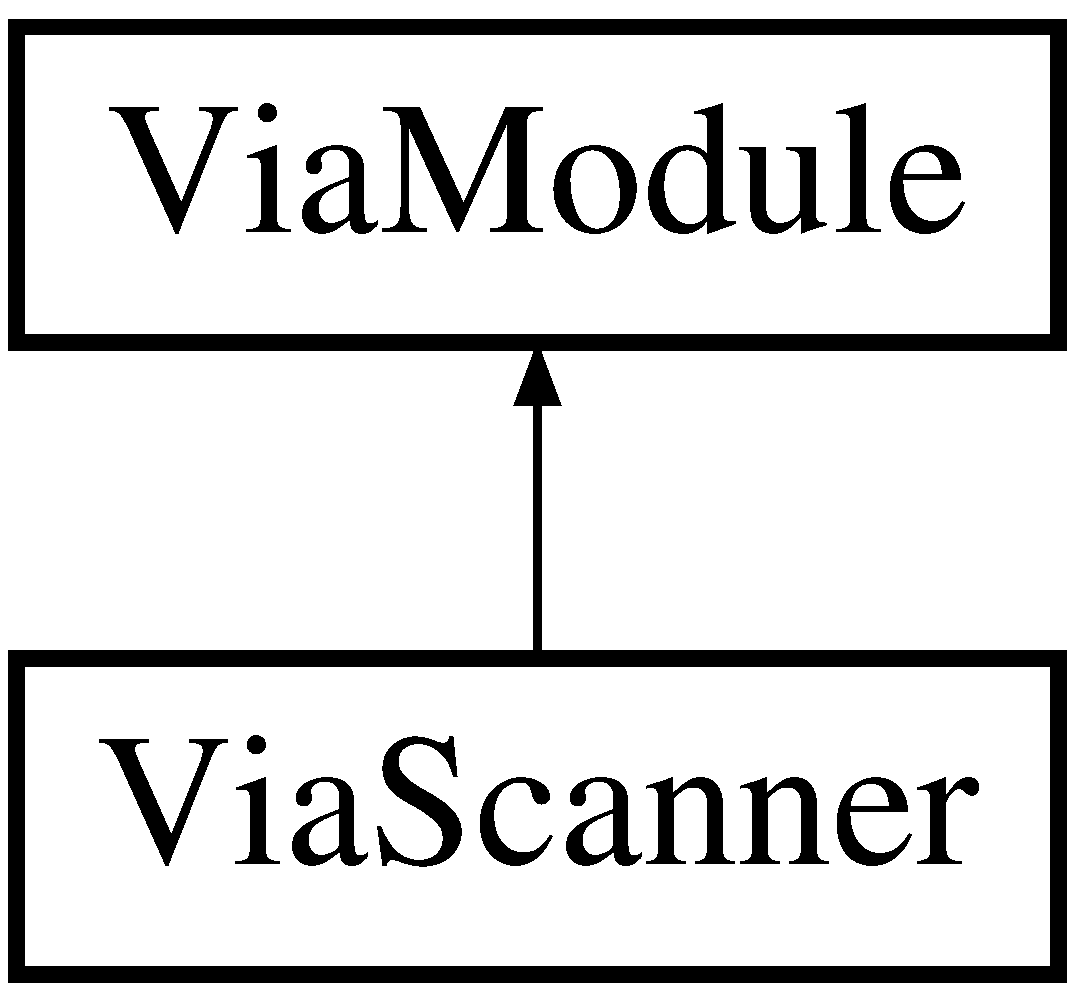
\includegraphics[height=2.000000cm]{class_via_scanner}
\end{center}
\end{figure}
\subsection*{Classes}
\begin{DoxyCompactItemize}
\item 
class \mbox{\hyperlink{class_via_scanner_1_1_via_scanner_u_i}{Via\+Scanner\+UI}}
\end{DoxyCompactItemize}
\subsection*{Public Member Functions}
\begin{DoxyCompactItemize}
\item 
void \mbox{\hyperlink{class_via_scanner_a2c92da688cd2c951d41638cfc28b6000}{handle\+Button1\+Mode\+Change}} (int32\+\_\+t)
\item 
void \mbox{\hyperlink{class_via_scanner_ac3049d7a8b3d6da1056ec685c91c357b}{handle\+Button2\+Mode\+Change}} (int32\+\_\+t)
\item 
void \mbox{\hyperlink{class_via_scanner_a13f7e9239dc58018483fedd53f90b0f3}{handle\+Button3\+Mode\+Change}} (int32\+\_\+t)
\item 
void \mbox{\hyperlink{class_via_scanner_aa41f226428aa5613411690a1ae975525}{handle\+Button4\+Mode\+Change}} (int32\+\_\+t)
\item 
void \mbox{\hyperlink{class_via_scanner_ac1fba594eba26810b22c50448a560867}{handle\+Button5\+Mode\+Change}} (int32\+\_\+t)
\item 
void \mbox{\hyperlink{class_via_scanner_af1bda4e1a5bb52fb27a7dd8dd58f8548}{handle\+Button6\+Mode\+Change}} (int32\+\_\+t)
\item 
void \mbox{\hyperlink{class_via_scanner_aea0fc08e09298a474c8e8aa230828cda}{handle\+Aux1\+Mode\+Change}} (int32\+\_\+t)
\item 
void \mbox{\hyperlink{class_via_scanner_a788c12dff6fafac6fce89d843cb039e3}{handle\+Aux2\+Mode\+Change}} (int32\+\_\+t)
\item 
void \mbox{\hyperlink{class_via_scanner_a84eef50217670fe7fa71ce483d05789d}{handle\+Aux3\+Mode\+Change}} (int32\+\_\+t)
\item 
void \mbox{\hyperlink{class_via_scanner_abb34e619104b7bcce3b2cae82575396f}{handle\+Aux4\+Mode\+Change}} (int32\+\_\+t)
\item 
void \mbox{\hyperlink{class_via_scanner_a71e8d863d02095c54afab3a062e882bd}{fill\+Wavetable\+Array}} (void)
\item 
void \mbox{\hyperlink{class_via_scanner_a53c5094aba6129ac90fc42e0e6f3a242}{switch\+WavetableX}} (const \mbox{\hyperlink{struct_wavetable}{Wavetable}} $\ast$)
\item 
void \mbox{\hyperlink{class_via_scanner_adfcf70c3cef485b73bf8dea27fd3b44c}{switch\+WavetableY}} (const \mbox{\hyperlink{struct_wavetable}{Wavetable}} $\ast$)
\item 
void \mbox{\hyperlink{class_via_scanner_a67c2a00e5e65bca4c124ebb5d6677aca}{init\+Phase\+Dist\+Table}} (void)
\item 
void \mbox{\hyperlink{class_via_scanner_a90596d92344fd4bc805b65142dde3e77}{init}} (void)
\item 
\mbox{\hyperlink{class_via_scanner_a4c6d8ee19c222188b16fec29494f14df}{Via\+Scanner}} ()
\item 
void \mbox{\hyperlink{class_via_scanner_a4199fdf25d18f8f4e40c8d22a8ac8b7c}{main\+Rising\+Edge\+Callback}} (void)
\item 
void \mbox{\hyperlink{class_via_scanner_a317f19b3d9726eca23deb4a8972c5ea1}{main\+Falling\+Edge\+Callback}} (void)
\item 
void \mbox{\hyperlink{class_via_scanner_abcc13461ed886eab18eb3dd2f55f3f40}{aux\+Rising\+Edge\+Callback}} (void)
\item 
void \mbox{\hyperlink{class_via_scanner_ab790912e79b3a02e96e400f038cbe2fe}{aux\+Falling\+Edge\+Callback}} (void)
\item 
void \mbox{\hyperlink{class_via_scanner_a5c79c2510c208303e73b8e6ecc318d78}{button\+Pressed\+Callback}} (void)
\item 
void \mbox{\hyperlink{class_via_scanner_a873527f0efc0320f877d16319e6928fa}{button\+Released\+Callback}} (void)
\item 
void \mbox{\hyperlink{class_via_scanner_adf0841f79cddfb663135395ff132eea1}{io\+Process\+Callback}} (void)
\item 
void \mbox{\hyperlink{class_via_scanner_a7e91b9d8b7be2dc955ee2b6b28c9fbfc}{half\+Transfer\+Callback}} (void)
\item 
void \mbox{\hyperlink{class_via_scanner_ad34ccf0e36d548ec69fd63da7f8e7655}{transfer\+Complete\+Callback}} (void)
\item 
void \mbox{\hyperlink{class_via_scanner_adcf828a62a23583739e4f5bbd32bc5b4}{cv2\+Half\+Transfer\+Callback}} (void)
\item 
void \mbox{\hyperlink{class_via_scanner_af7749d3570e86b89a03abaa50c87d9b9}{cv2\+Transfer\+Complete\+Callback}} (void)
\item 
void \mbox{\hyperlink{class_via_scanner_ad0bc8dc32a300843f349aae4631d7dc3}{cv3\+Half\+Transfer\+Callback}} (void)
\item 
void \mbox{\hyperlink{class_via_scanner_a6697e87d45ec8eb1d0259f389f869f30}{cv3\+Transfer\+Complete\+Callback}} (void)
\item 
void \mbox{\hyperlink{class_via_scanner_ae13ff5f8cbd768a0955cac416a695430}{slow\+Conversion\+Callback}} (void)
\item 
void \mbox{\hyperlink{class_via_scanner_a84a5b3f6009d266fad3fc5661b6d755e}{ui\+\_\+dispatch}} (int32\+\_\+t sig)
\end{DoxyCompactItemize}
\subsection*{Public Attributes}
\begin{DoxyCompactItemize}
\item 
const \mbox{\hyperlink{struct_wavetable}{Wavetable}} $\ast$ \mbox{\hyperlink{class_via_scanner_a7128d2220f6ce1278b2f31273631ac99}{wavetable\+Array}} \mbox{[}8\mbox{]}
\item 
uint32\+\_\+t \mbox{\hyperlink{class_via_scanner_a35e9caf08ba6556c32db7fc43958115d}{wavetable\+X\+Read}} \mbox{[}5\mbox{]}\mbox{[}517\mbox{]}
\item 
uint32\+\_\+t \mbox{\hyperlink{class_via_scanner_ab8d01eb2668d0e34b2f8ebb0002a69de}{wavetable\+Y\+Read}} \mbox{[}5\mbox{]}\mbox{[}517\mbox{]}
\item 
int32\+\_\+t \mbox{\hyperlink{class_via_scanner_a1e81eec84c1e70f1dc0d05f03ac6059f}{reverse\+Buffer}} \mbox{[}\mbox{\hyperlink{scanner_8hpp_a6d1fe8ce81e54d6d70e734bf39dee4b0}{S\+C\+A\+N\+N\+E\+R\+\_\+\+B\+U\+F\+F\+E\+R\+\_\+\+S\+I\+ZE}} $\ast$2\mbox{]}
\item 
int32\+\_\+t \mbox{\hyperlink{class_via_scanner_a721539f29750107fa9ca4e5b1308e584}{reverse\+Signal}} = 1
\item 
\mbox{\hyperlink{class_via_scanner_1_1_via_scanner_u_i}{Via\+Scanner\+UI}} \mbox{\hyperlink{class_via_scanner_a79510498d614c531fee5696191633c4f}{scanner\+UI}}
\item 
int32\+\_\+t \mbox{\hyperlink{class_via_scanner_adf5ae830fce9aabdb9bad283ef872be6}{runtime\+Display}}
\item 
\mbox{\hyperlink{class_three_axis_scanner}{Three\+Axis\+Scanner}} \mbox{\hyperlink{class_via_scanner_af1ec99854e4537b8c6342bb514cc0c44}{scanner}}
\end{DoxyCompactItemize}
\subsection*{Private Attributes}
\begin{DoxyCompactItemize}
\item 
int32\+\_\+t \mbox{\hyperlink{class_via_scanner_acc749be13e60aea46400173130cf7624}{read\+Index}} = 0
\end{DoxyCompactItemize}
\subsection*{Additional Inherited Members}


\subsection{Constructor \& Destructor Documentation}
\mbox{\Hypertarget{class_via_scanner_a4c6d8ee19c222188b16fec29494f14df}\label{class_via_scanner_a4c6d8ee19c222188b16fec29494f14df}} 
\index{Via\+Scanner@{Via\+Scanner}!Via\+Scanner@{Via\+Scanner}}
\index{Via\+Scanner@{Via\+Scanner}!Via\+Scanner@{Via\+Scanner}}
\subsubsection{\texorpdfstring{Via\+Scanner()}{ViaScanner()}}
{\footnotesize\ttfamily Via\+Scanner\+::\+Via\+Scanner (\begin{DoxyParamCaption}{ }\end{DoxyParamCaption})\hspace{0.3cm}{\ttfamily [inline]}}



\subsection{Member Function Documentation}
\mbox{\Hypertarget{class_via_scanner_ab790912e79b3a02e96e400f038cbe2fe}\label{class_via_scanner_ab790912e79b3a02e96e400f038cbe2fe}} 
\index{Via\+Scanner@{Via\+Scanner}!aux\+Falling\+Edge\+Callback@{aux\+Falling\+Edge\+Callback}}
\index{aux\+Falling\+Edge\+Callback@{aux\+Falling\+Edge\+Callback}!Via\+Scanner@{Via\+Scanner}}
\subsubsection{\texorpdfstring{aux\+Falling\+Edge\+Callback()}{auxFallingEdgeCallback()}}
{\footnotesize\ttfamily void Via\+Scanner\+::aux\+Falling\+Edge\+Callback (\begin{DoxyParamCaption}\item[{void}]{ }\end{DoxyParamCaption})}

\mbox{\Hypertarget{class_via_scanner_abcc13461ed886eab18eb3dd2f55f3f40}\label{class_via_scanner_abcc13461ed886eab18eb3dd2f55f3f40}} 
\index{Via\+Scanner@{Via\+Scanner}!aux\+Rising\+Edge\+Callback@{aux\+Rising\+Edge\+Callback}}
\index{aux\+Rising\+Edge\+Callback@{aux\+Rising\+Edge\+Callback}!Via\+Scanner@{Via\+Scanner}}
\subsubsection{\texorpdfstring{aux\+Rising\+Edge\+Callback()}{auxRisingEdgeCallback()}}
{\footnotesize\ttfamily void Via\+Scanner\+::aux\+Rising\+Edge\+Callback (\begin{DoxyParamCaption}\item[{void}]{ }\end{DoxyParamCaption})}

\mbox{\Hypertarget{class_via_scanner_a5c79c2510c208303e73b8e6ecc318d78}\label{class_via_scanner_a5c79c2510c208303e73b8e6ecc318d78}} 
\index{Via\+Scanner@{Via\+Scanner}!button\+Pressed\+Callback@{button\+Pressed\+Callback}}
\index{button\+Pressed\+Callback@{button\+Pressed\+Callback}!Via\+Scanner@{Via\+Scanner}}
\subsubsection{\texorpdfstring{button\+Pressed\+Callback()}{buttonPressedCallback()}}
{\footnotesize\ttfamily void Via\+Scanner\+::button\+Pressed\+Callback (\begin{DoxyParamCaption}\item[{void}]{ }\end{DoxyParamCaption})}

\mbox{\Hypertarget{class_via_scanner_a873527f0efc0320f877d16319e6928fa}\label{class_via_scanner_a873527f0efc0320f877d16319e6928fa}} 
\index{Via\+Scanner@{Via\+Scanner}!button\+Released\+Callback@{button\+Released\+Callback}}
\index{button\+Released\+Callback@{button\+Released\+Callback}!Via\+Scanner@{Via\+Scanner}}
\subsubsection{\texorpdfstring{button\+Released\+Callback()}{buttonReleasedCallback()}}
{\footnotesize\ttfamily void Via\+Scanner\+::button\+Released\+Callback (\begin{DoxyParamCaption}\item[{void}]{ }\end{DoxyParamCaption})}

\mbox{\Hypertarget{class_via_scanner_adcf828a62a23583739e4f5bbd32bc5b4}\label{class_via_scanner_adcf828a62a23583739e4f5bbd32bc5b4}} 
\index{Via\+Scanner@{Via\+Scanner}!cv2\+Half\+Transfer\+Callback@{cv2\+Half\+Transfer\+Callback}}
\index{cv2\+Half\+Transfer\+Callback@{cv2\+Half\+Transfer\+Callback}!Via\+Scanner@{Via\+Scanner}}
\subsubsection{\texorpdfstring{cv2\+Half\+Transfer\+Callback()}{cv2HalfTransferCallback()}}
{\footnotesize\ttfamily void Via\+Scanner\+::cv2\+Half\+Transfer\+Callback (\begin{DoxyParamCaption}\item[{void}]{ }\end{DoxyParamCaption})}

\mbox{\Hypertarget{class_via_scanner_af7749d3570e86b89a03abaa50c87d9b9}\label{class_via_scanner_af7749d3570e86b89a03abaa50c87d9b9}} 
\index{Via\+Scanner@{Via\+Scanner}!cv2\+Transfer\+Complete\+Callback@{cv2\+Transfer\+Complete\+Callback}}
\index{cv2\+Transfer\+Complete\+Callback@{cv2\+Transfer\+Complete\+Callback}!Via\+Scanner@{Via\+Scanner}}
\subsubsection{\texorpdfstring{cv2\+Transfer\+Complete\+Callback()}{cv2TransferCompleteCallback()}}
{\footnotesize\ttfamily void Via\+Scanner\+::cv2\+Transfer\+Complete\+Callback (\begin{DoxyParamCaption}\item[{void}]{ }\end{DoxyParamCaption})}

\mbox{\Hypertarget{class_via_scanner_ad0bc8dc32a300843f349aae4631d7dc3}\label{class_via_scanner_ad0bc8dc32a300843f349aae4631d7dc3}} 
\index{Via\+Scanner@{Via\+Scanner}!cv3\+Half\+Transfer\+Callback@{cv3\+Half\+Transfer\+Callback}}
\index{cv3\+Half\+Transfer\+Callback@{cv3\+Half\+Transfer\+Callback}!Via\+Scanner@{Via\+Scanner}}
\subsubsection{\texorpdfstring{cv3\+Half\+Transfer\+Callback()}{cv3HalfTransferCallback()}}
{\footnotesize\ttfamily void Via\+Scanner\+::cv3\+Half\+Transfer\+Callback (\begin{DoxyParamCaption}\item[{void}]{ }\end{DoxyParamCaption})}

\mbox{\Hypertarget{class_via_scanner_a6697e87d45ec8eb1d0259f389f869f30}\label{class_via_scanner_a6697e87d45ec8eb1d0259f389f869f30}} 
\index{Via\+Scanner@{Via\+Scanner}!cv3\+Transfer\+Complete\+Callback@{cv3\+Transfer\+Complete\+Callback}}
\index{cv3\+Transfer\+Complete\+Callback@{cv3\+Transfer\+Complete\+Callback}!Via\+Scanner@{Via\+Scanner}}
\subsubsection{\texorpdfstring{cv3\+Transfer\+Complete\+Callback()}{cv3TransferCompleteCallback()}}
{\footnotesize\ttfamily void Via\+Scanner\+::cv3\+Transfer\+Complete\+Callback (\begin{DoxyParamCaption}\item[{void}]{ }\end{DoxyParamCaption})}

\mbox{\Hypertarget{class_via_scanner_a71e8d863d02095c54afab3a062e882bd}\label{class_via_scanner_a71e8d863d02095c54afab3a062e882bd}} 
\index{Via\+Scanner@{Via\+Scanner}!fill\+Wavetable\+Array@{fill\+Wavetable\+Array}}
\index{fill\+Wavetable\+Array@{fill\+Wavetable\+Array}!Via\+Scanner@{Via\+Scanner}}
\subsubsection{\texorpdfstring{fill\+Wavetable\+Array()}{fillWavetableArray()}}
{\footnotesize\ttfamily void Via\+Scanner\+::fill\+Wavetable\+Array (\begin{DoxyParamCaption}\item[{void}]{ }\end{DoxyParamCaption})}

\mbox{\Hypertarget{class_via_scanner_a7e91b9d8b7be2dc955ee2b6b28c9fbfc}\label{class_via_scanner_a7e91b9d8b7be2dc955ee2b6b28c9fbfc}} 
\index{Via\+Scanner@{Via\+Scanner}!half\+Transfer\+Callback@{half\+Transfer\+Callback}}
\index{half\+Transfer\+Callback@{half\+Transfer\+Callback}!Via\+Scanner@{Via\+Scanner}}
\subsubsection{\texorpdfstring{half\+Transfer\+Callback()}{halfTransferCallback()}}
{\footnotesize\ttfamily void Via\+Scanner\+::half\+Transfer\+Callback (\begin{DoxyParamCaption}\item[{void}]{ }\end{DoxyParamCaption})}

\mbox{\Hypertarget{class_via_scanner_aea0fc08e09298a474c8e8aa230828cda}\label{class_via_scanner_aea0fc08e09298a474c8e8aa230828cda}} 
\index{Via\+Scanner@{Via\+Scanner}!handle\+Aux1\+Mode\+Change@{handle\+Aux1\+Mode\+Change}}
\index{handle\+Aux1\+Mode\+Change@{handle\+Aux1\+Mode\+Change}!Via\+Scanner@{Via\+Scanner}}
\subsubsection{\texorpdfstring{handle\+Aux1\+Mode\+Change()}{handleAux1ModeChange()}}
{\footnotesize\ttfamily void Via\+Scanner\+::handle\+Aux1\+Mode\+Change (\begin{DoxyParamCaption}\item[{int32\+\_\+t}]{ }\end{DoxyParamCaption})}

\mbox{\Hypertarget{class_via_scanner_a788c12dff6fafac6fce89d843cb039e3}\label{class_via_scanner_a788c12dff6fafac6fce89d843cb039e3}} 
\index{Via\+Scanner@{Via\+Scanner}!handle\+Aux2\+Mode\+Change@{handle\+Aux2\+Mode\+Change}}
\index{handle\+Aux2\+Mode\+Change@{handle\+Aux2\+Mode\+Change}!Via\+Scanner@{Via\+Scanner}}
\subsubsection{\texorpdfstring{handle\+Aux2\+Mode\+Change()}{handleAux2ModeChange()}}
{\footnotesize\ttfamily void Via\+Scanner\+::handle\+Aux2\+Mode\+Change (\begin{DoxyParamCaption}\item[{int32\+\_\+t}]{ }\end{DoxyParamCaption})}

\mbox{\Hypertarget{class_via_scanner_a84eef50217670fe7fa71ce483d05789d}\label{class_via_scanner_a84eef50217670fe7fa71ce483d05789d}} 
\index{Via\+Scanner@{Via\+Scanner}!handle\+Aux3\+Mode\+Change@{handle\+Aux3\+Mode\+Change}}
\index{handle\+Aux3\+Mode\+Change@{handle\+Aux3\+Mode\+Change}!Via\+Scanner@{Via\+Scanner}}
\subsubsection{\texorpdfstring{handle\+Aux3\+Mode\+Change()}{handleAux3ModeChange()}}
{\footnotesize\ttfamily void Via\+Scanner\+::handle\+Aux3\+Mode\+Change (\begin{DoxyParamCaption}\item[{int32\+\_\+t}]{ }\end{DoxyParamCaption})}

\mbox{\Hypertarget{class_via_scanner_abb34e619104b7bcce3b2cae82575396f}\label{class_via_scanner_abb34e619104b7bcce3b2cae82575396f}} 
\index{Via\+Scanner@{Via\+Scanner}!handle\+Aux4\+Mode\+Change@{handle\+Aux4\+Mode\+Change}}
\index{handle\+Aux4\+Mode\+Change@{handle\+Aux4\+Mode\+Change}!Via\+Scanner@{Via\+Scanner}}
\subsubsection{\texorpdfstring{handle\+Aux4\+Mode\+Change()}{handleAux4ModeChange()}}
{\footnotesize\ttfamily void Via\+Scanner\+::handle\+Aux4\+Mode\+Change (\begin{DoxyParamCaption}\item[{int32\+\_\+t}]{ }\end{DoxyParamCaption})}

\mbox{\Hypertarget{class_via_scanner_a2c92da688cd2c951d41638cfc28b6000}\label{class_via_scanner_a2c92da688cd2c951d41638cfc28b6000}} 
\index{Via\+Scanner@{Via\+Scanner}!handle\+Button1\+Mode\+Change@{handle\+Button1\+Mode\+Change}}
\index{handle\+Button1\+Mode\+Change@{handle\+Button1\+Mode\+Change}!Via\+Scanner@{Via\+Scanner}}
\subsubsection{\texorpdfstring{handle\+Button1\+Mode\+Change()}{handleButton1ModeChange()}}
{\footnotesize\ttfamily void Via\+Scanner\+::handle\+Button1\+Mode\+Change (\begin{DoxyParamCaption}\item[{int32\+\_\+t}]{mode }\end{DoxyParamCaption})}

\mbox{\Hypertarget{class_via_scanner_ac3049d7a8b3d6da1056ec685c91c357b}\label{class_via_scanner_ac3049d7a8b3d6da1056ec685c91c357b}} 
\index{Via\+Scanner@{Via\+Scanner}!handle\+Button2\+Mode\+Change@{handle\+Button2\+Mode\+Change}}
\index{handle\+Button2\+Mode\+Change@{handle\+Button2\+Mode\+Change}!Via\+Scanner@{Via\+Scanner}}
\subsubsection{\texorpdfstring{handle\+Button2\+Mode\+Change()}{handleButton2ModeChange()}}
{\footnotesize\ttfamily void Via\+Scanner\+::handle\+Button2\+Mode\+Change (\begin{DoxyParamCaption}\item[{int32\+\_\+t}]{mode }\end{DoxyParamCaption})}

\mbox{\Hypertarget{class_via_scanner_a13f7e9239dc58018483fedd53f90b0f3}\label{class_via_scanner_a13f7e9239dc58018483fedd53f90b0f3}} 
\index{Via\+Scanner@{Via\+Scanner}!handle\+Button3\+Mode\+Change@{handle\+Button3\+Mode\+Change}}
\index{handle\+Button3\+Mode\+Change@{handle\+Button3\+Mode\+Change}!Via\+Scanner@{Via\+Scanner}}
\subsubsection{\texorpdfstring{handle\+Button3\+Mode\+Change()}{handleButton3ModeChange()}}
{\footnotesize\ttfamily void Via\+Scanner\+::handle\+Button3\+Mode\+Change (\begin{DoxyParamCaption}\item[{int32\+\_\+t}]{mode }\end{DoxyParamCaption})}

\mbox{\Hypertarget{class_via_scanner_aa41f226428aa5613411690a1ae975525}\label{class_via_scanner_aa41f226428aa5613411690a1ae975525}} 
\index{Via\+Scanner@{Via\+Scanner}!handle\+Button4\+Mode\+Change@{handle\+Button4\+Mode\+Change}}
\index{handle\+Button4\+Mode\+Change@{handle\+Button4\+Mode\+Change}!Via\+Scanner@{Via\+Scanner}}
\subsubsection{\texorpdfstring{handle\+Button4\+Mode\+Change()}{handleButton4ModeChange()}}
{\footnotesize\ttfamily void Via\+Scanner\+::handle\+Button4\+Mode\+Change (\begin{DoxyParamCaption}\item[{int32\+\_\+t}]{mode }\end{DoxyParamCaption})}

\mbox{\Hypertarget{class_via_scanner_ac1fba594eba26810b22c50448a560867}\label{class_via_scanner_ac1fba594eba26810b22c50448a560867}} 
\index{Via\+Scanner@{Via\+Scanner}!handle\+Button5\+Mode\+Change@{handle\+Button5\+Mode\+Change}}
\index{handle\+Button5\+Mode\+Change@{handle\+Button5\+Mode\+Change}!Via\+Scanner@{Via\+Scanner}}
\subsubsection{\texorpdfstring{handle\+Button5\+Mode\+Change()}{handleButton5ModeChange()}}
{\footnotesize\ttfamily void Via\+Scanner\+::handle\+Button5\+Mode\+Change (\begin{DoxyParamCaption}\item[{int32\+\_\+t}]{mode }\end{DoxyParamCaption})}

\mbox{\Hypertarget{class_via_scanner_af1bda4e1a5bb52fb27a7dd8dd58f8548}\label{class_via_scanner_af1bda4e1a5bb52fb27a7dd8dd58f8548}} 
\index{Via\+Scanner@{Via\+Scanner}!handle\+Button6\+Mode\+Change@{handle\+Button6\+Mode\+Change}}
\index{handle\+Button6\+Mode\+Change@{handle\+Button6\+Mode\+Change}!Via\+Scanner@{Via\+Scanner}}
\subsubsection{\texorpdfstring{handle\+Button6\+Mode\+Change()}{handleButton6ModeChange()}}
{\footnotesize\ttfamily void Via\+Scanner\+::handle\+Button6\+Mode\+Change (\begin{DoxyParamCaption}\item[{int32\+\_\+t}]{mode }\end{DoxyParamCaption})}

\mbox{\Hypertarget{class_via_scanner_a90596d92344fd4bc805b65142dde3e77}\label{class_via_scanner_a90596d92344fd4bc805b65142dde3e77}} 
\index{Via\+Scanner@{Via\+Scanner}!init@{init}}
\index{init@{init}!Via\+Scanner@{Via\+Scanner}}
\subsubsection{\texorpdfstring{init()}{init()}}
{\footnotesize\ttfamily void Via\+Scanner\+::init (\begin{DoxyParamCaption}\item[{void}]{ }\end{DoxyParamCaption})}

\mbox{\Hypertarget{class_via_scanner_a67c2a00e5e65bca4c124ebb5d6677aca}\label{class_via_scanner_a67c2a00e5e65bca4c124ebb5d6677aca}} 
\index{Via\+Scanner@{Via\+Scanner}!init\+Phase\+Dist\+Table@{init\+Phase\+Dist\+Table}}
\index{init\+Phase\+Dist\+Table@{init\+Phase\+Dist\+Table}!Via\+Scanner@{Via\+Scanner}}
\subsubsection{\texorpdfstring{init\+Phase\+Dist\+Table()}{initPhaseDistTable()}}
{\footnotesize\ttfamily void Via\+Scanner\+::init\+Phase\+Dist\+Table (\begin{DoxyParamCaption}\item[{void}]{ }\end{DoxyParamCaption})}

\mbox{\Hypertarget{class_via_scanner_adf0841f79cddfb663135395ff132eea1}\label{class_via_scanner_adf0841f79cddfb663135395ff132eea1}} 
\index{Via\+Scanner@{Via\+Scanner}!io\+Process\+Callback@{io\+Process\+Callback}}
\index{io\+Process\+Callback@{io\+Process\+Callback}!Via\+Scanner@{Via\+Scanner}}
\subsubsection{\texorpdfstring{io\+Process\+Callback()}{ioProcessCallback()}}
{\footnotesize\ttfamily void Via\+Scanner\+::io\+Process\+Callback (\begin{DoxyParamCaption}\item[{void}]{ }\end{DoxyParamCaption})}

\mbox{\Hypertarget{class_via_scanner_a317f19b3d9726eca23deb4a8972c5ea1}\label{class_via_scanner_a317f19b3d9726eca23deb4a8972c5ea1}} 
\index{Via\+Scanner@{Via\+Scanner}!main\+Falling\+Edge\+Callback@{main\+Falling\+Edge\+Callback}}
\index{main\+Falling\+Edge\+Callback@{main\+Falling\+Edge\+Callback}!Via\+Scanner@{Via\+Scanner}}
\subsubsection{\texorpdfstring{main\+Falling\+Edge\+Callback()}{mainFallingEdgeCallback()}}
{\footnotesize\ttfamily void Via\+Scanner\+::main\+Falling\+Edge\+Callback (\begin{DoxyParamCaption}\item[{void}]{ }\end{DoxyParamCaption})}

\mbox{\Hypertarget{class_via_scanner_a4199fdf25d18f8f4e40c8d22a8ac8b7c}\label{class_via_scanner_a4199fdf25d18f8f4e40c8d22a8ac8b7c}} 
\index{Via\+Scanner@{Via\+Scanner}!main\+Rising\+Edge\+Callback@{main\+Rising\+Edge\+Callback}}
\index{main\+Rising\+Edge\+Callback@{main\+Rising\+Edge\+Callback}!Via\+Scanner@{Via\+Scanner}}
\subsubsection{\texorpdfstring{main\+Rising\+Edge\+Callback()}{mainRisingEdgeCallback()}}
{\footnotesize\ttfamily void Via\+Scanner\+::main\+Rising\+Edge\+Callback (\begin{DoxyParamCaption}\item[{void}]{ }\end{DoxyParamCaption})}

\mbox{\Hypertarget{class_via_scanner_ae13ff5f8cbd768a0955cac416a695430}\label{class_via_scanner_ae13ff5f8cbd768a0955cac416a695430}} 
\index{Via\+Scanner@{Via\+Scanner}!slow\+Conversion\+Callback@{slow\+Conversion\+Callback}}
\index{slow\+Conversion\+Callback@{slow\+Conversion\+Callback}!Via\+Scanner@{Via\+Scanner}}
\subsubsection{\texorpdfstring{slow\+Conversion\+Callback()}{slowConversionCallback()}}
{\footnotesize\ttfamily void Via\+Scanner\+::slow\+Conversion\+Callback (\begin{DoxyParamCaption}\item[{void}]{ }\end{DoxyParamCaption})}

\mbox{\Hypertarget{class_via_scanner_a53c5094aba6129ac90fc42e0e6f3a242}\label{class_via_scanner_a53c5094aba6129ac90fc42e0e6f3a242}} 
\index{Via\+Scanner@{Via\+Scanner}!switch\+WavetableX@{switch\+WavetableX}}
\index{switch\+WavetableX@{switch\+WavetableX}!Via\+Scanner@{Via\+Scanner}}
\subsubsection{\texorpdfstring{switch\+Wavetable\+X()}{switchWavetableX()}}
{\footnotesize\ttfamily void Via\+Scanner\+::switch\+WavetableX (\begin{DoxyParamCaption}\item[{const \mbox{\hyperlink{struct_wavetable}{Wavetable}} $\ast$}]{table }\end{DoxyParamCaption})}

\mbox{\Hypertarget{class_via_scanner_adfcf70c3cef485b73bf8dea27fd3b44c}\label{class_via_scanner_adfcf70c3cef485b73bf8dea27fd3b44c}} 
\index{Via\+Scanner@{Via\+Scanner}!switch\+WavetableY@{switch\+WavetableY}}
\index{switch\+WavetableY@{switch\+WavetableY}!Via\+Scanner@{Via\+Scanner}}
\subsubsection{\texorpdfstring{switch\+Wavetable\+Y()}{switchWavetableY()}}
{\footnotesize\ttfamily void Via\+Scanner\+::switch\+WavetableY (\begin{DoxyParamCaption}\item[{const \mbox{\hyperlink{struct_wavetable}{Wavetable}} $\ast$}]{table }\end{DoxyParamCaption})}

\mbox{\Hypertarget{class_via_scanner_ad34ccf0e36d548ec69fd63da7f8e7655}\label{class_via_scanner_ad34ccf0e36d548ec69fd63da7f8e7655}} 
\index{Via\+Scanner@{Via\+Scanner}!transfer\+Complete\+Callback@{transfer\+Complete\+Callback}}
\index{transfer\+Complete\+Callback@{transfer\+Complete\+Callback}!Via\+Scanner@{Via\+Scanner}}
\subsubsection{\texorpdfstring{transfer\+Complete\+Callback()}{transferCompleteCallback()}}
{\footnotesize\ttfamily void Via\+Scanner\+::transfer\+Complete\+Callback (\begin{DoxyParamCaption}\item[{void}]{ }\end{DoxyParamCaption})}

\mbox{\Hypertarget{class_via_scanner_a84a5b3f6009d266fad3fc5661b6d755e}\label{class_via_scanner_a84a5b3f6009d266fad3fc5661b6d755e}} 
\index{Via\+Scanner@{Via\+Scanner}!ui\+\_\+dispatch@{ui\+\_\+dispatch}}
\index{ui\+\_\+dispatch@{ui\+\_\+dispatch}!Via\+Scanner@{Via\+Scanner}}
\subsubsection{\texorpdfstring{ui\+\_\+dispatch()}{ui\_dispatch()}}
{\footnotesize\ttfamily void Via\+Scanner\+::ui\+\_\+dispatch (\begin{DoxyParamCaption}\item[{int32\+\_\+t}]{sig }\end{DoxyParamCaption})\hspace{0.3cm}{\ttfamily [inline]}}



\subsection{Member Data Documentation}
\mbox{\Hypertarget{class_via_scanner_acc749be13e60aea46400173130cf7624}\label{class_via_scanner_acc749be13e60aea46400173130cf7624}} 
\index{Via\+Scanner@{Via\+Scanner}!read\+Index@{read\+Index}}
\index{read\+Index@{read\+Index}!Via\+Scanner@{Via\+Scanner}}
\subsubsection{\texorpdfstring{read\+Index}{readIndex}}
{\footnotesize\ttfamily int32\+\_\+t Via\+Scanner\+::read\+Index = 0\hspace{0.3cm}{\ttfamily [private]}}

\mbox{\Hypertarget{class_via_scanner_a1e81eec84c1e70f1dc0d05f03ac6059f}\label{class_via_scanner_a1e81eec84c1e70f1dc0d05f03ac6059f}} 
\index{Via\+Scanner@{Via\+Scanner}!reverse\+Buffer@{reverse\+Buffer}}
\index{reverse\+Buffer@{reverse\+Buffer}!Via\+Scanner@{Via\+Scanner}}
\subsubsection{\texorpdfstring{reverse\+Buffer}{reverseBuffer}}
{\footnotesize\ttfamily int32\+\_\+t Via\+Scanner\+::reverse\+Buffer\mbox{[}\mbox{\hyperlink{scanner_8hpp_a6d1fe8ce81e54d6d70e734bf39dee4b0}{S\+C\+A\+N\+N\+E\+R\+\_\+\+B\+U\+F\+F\+E\+R\+\_\+\+S\+I\+ZE}} $\ast$2\mbox{]}}

\mbox{\Hypertarget{class_via_scanner_a721539f29750107fa9ca4e5b1308e584}\label{class_via_scanner_a721539f29750107fa9ca4e5b1308e584}} 
\index{Via\+Scanner@{Via\+Scanner}!reverse\+Signal@{reverse\+Signal}}
\index{reverse\+Signal@{reverse\+Signal}!Via\+Scanner@{Via\+Scanner}}
\subsubsection{\texorpdfstring{reverse\+Signal}{reverseSignal}}
{\footnotesize\ttfamily int32\+\_\+t Via\+Scanner\+::reverse\+Signal = 1}

\mbox{\Hypertarget{class_via_scanner_adf5ae830fce9aabdb9bad283ef872be6}\label{class_via_scanner_adf5ae830fce9aabdb9bad283ef872be6}} 
\index{Via\+Scanner@{Via\+Scanner}!runtime\+Display@{runtime\+Display}}
\index{runtime\+Display@{runtime\+Display}!Via\+Scanner@{Via\+Scanner}}
\subsubsection{\texorpdfstring{runtime\+Display}{runtimeDisplay}}
{\footnotesize\ttfamily int32\+\_\+t Via\+Scanner\+::runtime\+Display}

\mbox{\Hypertarget{class_via_scanner_af1ec99854e4537b8c6342bb514cc0c44}\label{class_via_scanner_af1ec99854e4537b8c6342bb514cc0c44}} 
\index{Via\+Scanner@{Via\+Scanner}!scanner@{scanner}}
\index{scanner@{scanner}!Via\+Scanner@{Via\+Scanner}}
\subsubsection{\texorpdfstring{scanner}{scanner}}
{\footnotesize\ttfamily \mbox{\hyperlink{class_three_axis_scanner}{Three\+Axis\+Scanner}} Via\+Scanner\+::scanner}

\mbox{\Hypertarget{class_via_scanner_a79510498d614c531fee5696191633c4f}\label{class_via_scanner_a79510498d614c531fee5696191633c4f}} 
\index{Via\+Scanner@{Via\+Scanner}!scanner\+UI@{scanner\+UI}}
\index{scanner\+UI@{scanner\+UI}!Via\+Scanner@{Via\+Scanner}}
\subsubsection{\texorpdfstring{scanner\+UI}{scannerUI}}
{\footnotesize\ttfamily \mbox{\hyperlink{class_via_scanner_1_1_via_scanner_u_i}{Via\+Scanner\+UI}} Via\+Scanner\+::scanner\+UI}

\mbox{\Hypertarget{class_via_scanner_a7128d2220f6ce1278b2f31273631ac99}\label{class_via_scanner_a7128d2220f6ce1278b2f31273631ac99}} 
\index{Via\+Scanner@{Via\+Scanner}!wavetable\+Array@{wavetable\+Array}}
\index{wavetable\+Array@{wavetable\+Array}!Via\+Scanner@{Via\+Scanner}}
\subsubsection{\texorpdfstring{wavetable\+Array}{wavetableArray}}
{\footnotesize\ttfamily const \mbox{\hyperlink{struct_wavetable}{Wavetable}}$\ast$ Via\+Scanner\+::wavetable\+Array\mbox{[}8\mbox{]}}

\mbox{\Hypertarget{class_via_scanner_a35e9caf08ba6556c32db7fc43958115d}\label{class_via_scanner_a35e9caf08ba6556c32db7fc43958115d}} 
\index{Via\+Scanner@{Via\+Scanner}!wavetable\+X\+Read@{wavetable\+X\+Read}}
\index{wavetable\+X\+Read@{wavetable\+X\+Read}!Via\+Scanner@{Via\+Scanner}}
\subsubsection{\texorpdfstring{wavetable\+X\+Read}{wavetableXRead}}
{\footnotesize\ttfamily uint32\+\_\+t Via\+Scanner\+::wavetable\+X\+Read\mbox{[}5\mbox{]}\mbox{[}517\mbox{]}}

\mbox{\Hypertarget{class_via_scanner_ab8d01eb2668d0e34b2f8ebb0002a69de}\label{class_via_scanner_ab8d01eb2668d0e34b2f8ebb0002a69de}} 
\index{Via\+Scanner@{Via\+Scanner}!wavetable\+Y\+Read@{wavetable\+Y\+Read}}
\index{wavetable\+Y\+Read@{wavetable\+Y\+Read}!Via\+Scanner@{Via\+Scanner}}
\subsubsection{\texorpdfstring{wavetable\+Y\+Read}{wavetableYRead}}
{\footnotesize\ttfamily uint32\+\_\+t Via\+Scanner\+::wavetable\+Y\+Read\mbox{[}5\mbox{]}\mbox{[}517\mbox{]}}



The documentation for this class was generated from the following files\+:\begin{DoxyCompactItemize}
\item 
modules/inc/\mbox{\hyperlink{scanner_8hpp}{scanner.\+hpp}}\item 
modules/scanner/\mbox{\hyperlink{scanner__init_8cpp}{scanner\+\_\+init.\+cpp}}\item 
modules/scanner/\mbox{\hyperlink{scanner__interrupt__handlers_8cpp}{scanner\+\_\+interrupt\+\_\+handlers.\+cpp}}\item 
modules/scanner/\mbox{\hyperlink{scanner__modes_8cpp}{scanner\+\_\+modes.\+cpp}}\item 
modules/scanner/\mbox{\hyperlink{scanner__table__init_8cpp}{scanner\+\_\+table\+\_\+init.\+cpp}}\end{DoxyCompactItemize}

\hypertarget{class_via_scanner_1_1_via_scanner_u_i}{}\section{Via\+Scanner\+:\+:Via\+Scanner\+UI Class Reference}
\label{class_via_scanner_1_1_via_scanner_u_i}\index{Via\+Scanner\+::\+Via\+Scanner\+UI@{Via\+Scanner\+::\+Via\+Scanner\+UI}}


{\ttfamily \#include $<$scanner.\+hpp$>$}

Inheritance diagram for Via\+Scanner\+:\+:Via\+Scanner\+UI\+:\begin{figure}[H]
\begin{center}
\leavevmode
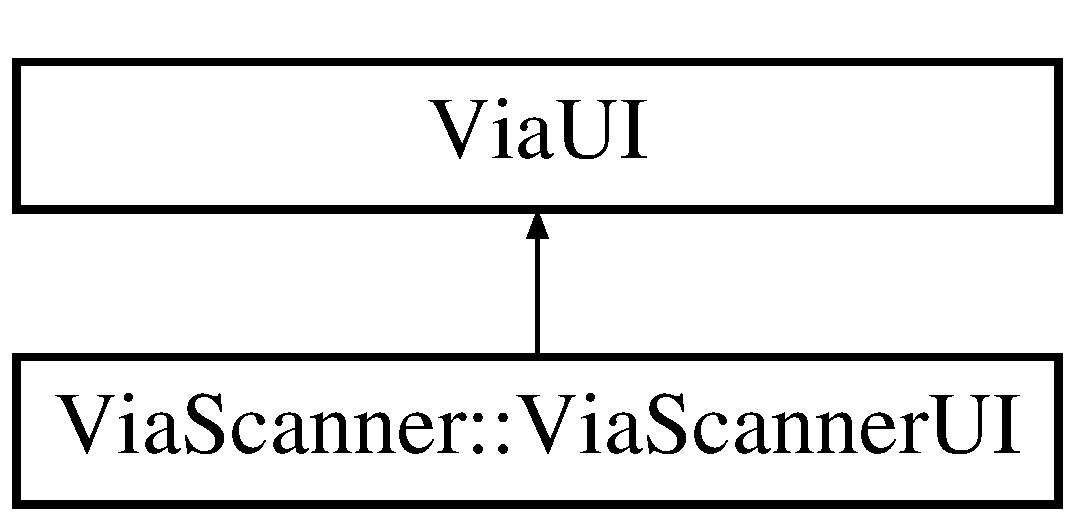
\includegraphics[height=2.000000cm]{class_via_scanner_1_1_via_scanner_u_i}
\end{center}
\end{figure}
\subsection*{Public Member Functions}
\begin{DoxyCompactItemize}
\item 
void \mbox{\hyperlink{class_via_scanner_1_1_via_scanner_u_i_a0347e038aa4ac6c8e7e9f50272cc19d8}{button1\+Tap\+Callback}} (void) override
\item 
void \mbox{\hyperlink{class_via_scanner_1_1_via_scanner_u_i_a8d7608e430d6be2777f4fb76b4ea9f2b}{button1\+Hold\+Callback}} (void) override
\item 
void \mbox{\hyperlink{class_via_scanner_1_1_via_scanner_u_i_a18b25c095ac7d6aca3bbc7274643ed9a}{button2\+Tap\+Callback}} (void) override
\item 
void \mbox{\hyperlink{class_via_scanner_1_1_via_scanner_u_i_a9c61e3d9d4c2bf5ed21e63693c575c31}{button2\+Hold\+Callback}} (void) override
\item 
void \mbox{\hyperlink{class_via_scanner_1_1_via_scanner_u_i_ac4c5b6ba60ade672ebe768c9d4849d62}{button3\+Tap\+Callback}} (void) override
\item 
void \mbox{\hyperlink{class_via_scanner_1_1_via_scanner_u_i_ac01a2eda088067d96b7691255d2841c6}{button3\+Hold\+Callback}} (void) override
\item 
void \mbox{\hyperlink{class_via_scanner_1_1_via_scanner_u_i_a31a0153f6ca3260241e7c7373723bfb8}{button4\+Tap\+Callback}} (void) override
\item 
void \mbox{\hyperlink{class_via_scanner_1_1_via_scanner_u_i_a5d8656812822494d9c202f40ef0882ab}{button4\+Hold\+Callback}} (void) override
\item 
void \mbox{\hyperlink{class_via_scanner_1_1_via_scanner_u_i_a10bef1a488e628c198e07bc56690199c}{button5\+Tap\+Callback}} (void) override
\item 
void \mbox{\hyperlink{class_via_scanner_1_1_via_scanner_u_i_ac3f72c13ce77d58c5c8e7504083fbb65}{button5\+Hold\+Callback}} (void) override
\item 
void \mbox{\hyperlink{class_via_scanner_1_1_via_scanner_u_i_a2d8bc6b636e934c0945a09e115476ec3}{button6\+Tap\+Callback}} (void) override
\item 
void \mbox{\hyperlink{class_via_scanner_1_1_via_scanner_u_i_af2cd0e1ac72f9486aa152b1d69bec8c8}{button6\+Hold\+Callback}} (void) override
\item 
void \mbox{\hyperlink{class_via_scanner_1_1_via_scanner_u_i_af7e91846bdd9922b309580adf4fe653b}{aux1\+Tap\+Callback}} (void) override
\item 
void \mbox{\hyperlink{class_via_scanner_1_1_via_scanner_u_i_a634c06fae2a1a17e5f3737dd44b34e10}{aux1\+Hold\+Callback}} (void) override
\item 
void \mbox{\hyperlink{class_via_scanner_1_1_via_scanner_u_i_a7d3aad2399479925618df242bc5b1f42}{aux2\+Tap\+Callback}} (void) override
\item 
void \mbox{\hyperlink{class_via_scanner_1_1_via_scanner_u_i_a929ba662a65fd62f9c5b122accad48a4}{aux2\+Hold\+Callback}} (void) override
\item 
void \mbox{\hyperlink{class_via_scanner_1_1_via_scanner_u_i_aa862c7243959f99bfd42995102ffcdf5}{aux2\+Alt\+Tap\+Callback}} (void) override
\item 
void \mbox{\hyperlink{class_via_scanner_1_1_via_scanner_u_i_ae1947196ca5cb248c4bc177f02cb20f5}{aux2\+Alt\+Hold\+Callback}} (void) override
\item 
void \mbox{\hyperlink{class_via_scanner_1_1_via_scanner_u_i_a7d15083a3565f56b4b70ac497fddd563}{aux3\+Tap\+Callback}} (void) override
\item 
void \mbox{\hyperlink{class_via_scanner_1_1_via_scanner_u_i_ac79b09eb94d39065b6b5061d34746862}{aux3\+Hold\+Callback}} (void) override
\item 
void \mbox{\hyperlink{class_via_scanner_1_1_via_scanner_u_i_a8c20c03c838257da356f0071dfcbfd36}{aux4\+Tap\+Callback}} (void) override
\item 
void \mbox{\hyperlink{class_via_scanner_1_1_via_scanner_u_i_af994cf63aa7becc41c9e3dcb2e08d8c2}{aux4\+Hold\+Callback}} (void) override
\item 
void \mbox{\hyperlink{class_via_scanner_1_1_via_scanner_u_i_aa2c3ca7904d9036eb362c7600dac66b0}{ui\+Set\+L\+E\+Ds}} (int) override
\item 
void \mbox{\hyperlink{class_via_scanner_1_1_via_scanner_u_i_a9513c8ecc955ccfbdaebea4172deb210}{recall\+Module\+State}} (void) override
\item 
void \mbox{\hyperlink{class_via_scanner_1_1_via_scanner_u_i_adc8f206d1050c457af29a45cf8050faf}{default\+Enter\+Menu\+Callback}} (void) override
\item 
void \mbox{\hyperlink{class_via_scanner_1_1_via_scanner_u_i_a15124d20f2684fd9c5d1c83d41a15e5a}{new\+Mode\+Enter\+Menu\+Callback}} (void) override
\item 
void \mbox{\hyperlink{class_via_scanner_1_1_via_scanner_u_i_a8176484cc1deb6df08abfe1f0c1f789f}{new\+Aux\+Mode\+Enter\+Menu\+Callback}} (void) override
\item 
void \mbox{\hyperlink{class_via_scanner_1_1_via_scanner_u_i_ac67240d1c9ebc47569185776d9d4403b}{preset\+Enter\+Menu\+Callback}} (void) override
\item 
void \mbox{\hyperlink{class_via_scanner_1_1_via_scanner_u_i_a10b9a54f4fb6ea88203d53041093d650}{button1\+Enter\+Menu\+Callback}} (void) override
\item 
void \mbox{\hyperlink{class_via_scanner_1_1_via_scanner_u_i_acb45c99dcac36f93d98621f6c53c9a0a}{button2\+Enter\+Menu\+Callback}} (void) override
\item 
void \mbox{\hyperlink{class_via_scanner_1_1_via_scanner_u_i_a32f8e4caa95371961883c90a5803f314}{button3\+Enter\+Menu\+Callback}} (void) override
\item 
void \mbox{\hyperlink{class_via_scanner_1_1_via_scanner_u_i_a45b4492b06d3b834c4934ace2d7d15aa}{button4\+Enter\+Menu\+Callback}} (void) override
\item 
void \mbox{\hyperlink{class_via_scanner_1_1_via_scanner_u_i_a337284dc48950fd3140b40ecca57122b}{button5\+Enter\+Menu\+Callback}} (void) override
\item 
void \mbox{\hyperlink{class_via_scanner_1_1_via_scanner_u_i_a94de9ec6e40e16ba7dd8dc0ffb9adc14}{button6\+Enter\+Menu\+Callback}} (void) override
\item 
void \mbox{\hyperlink{class_via_scanner_1_1_via_scanner_u_i_a4ca2d4cfed7e8e23f056c622a825c085}{aux1\+Enter\+Menu\+Callback}} (void) override
\item 
void \mbox{\hyperlink{class_via_scanner_1_1_via_scanner_u_i_a5173aaf7222a059fa7d3a4b32f6fb275}{aux2\+Enter\+Menu\+Callback}} (void) override
\item 
void \mbox{\hyperlink{class_via_scanner_1_1_via_scanner_u_i_a649f3b095e254e2e2049c91f5c9543b2}{aux2\+Alt\+Enter\+Menu\+Callback}} (void) override
\item 
void \mbox{\hyperlink{class_via_scanner_1_1_via_scanner_u_i_ade6dc0e93911fe51731bffa65990599a}{aux3\+Enter\+Menu\+Callback}} (void) override
\item 
void \mbox{\hyperlink{class_via_scanner_1_1_via_scanner_u_i_a34c593dfd035906c09a2cde0024fd48f}{aux4\+Enter\+Menu\+Callback}} (void) override
\item 
void \mbox{\hyperlink{class_via_scanner_1_1_via_scanner_u_i_ab12af2665a9e58574cd0cb4b8a003e0b}{initialize}} (void) override
\item 
\mbox{\hyperlink{class_via_scanner_1_1_via_scanner_u_i_aa18dc59313da3e71d1d4cdb4509d7fa4}{Via\+Scanner\+UI}} (\mbox{\hyperlink{class_via_scanner}{Via\+Scanner}} \&x)
\end{DoxyCompactItemize}
\subsection*{Public Attributes}
\begin{DoxyCompactItemize}
\item 
\mbox{\hyperlink{class_via_scanner}{Via\+Scanner}} \& \mbox{\hyperlink{class_via_scanner_1_1_via_scanner_u_i_af7cdb107de6e5d4f45e1501233c1ac7c}{this\+\_\+module}}
\end{DoxyCompactItemize}


\subsection{Constructor \& Destructor Documentation}
\mbox{\Hypertarget{class_via_scanner_1_1_via_scanner_u_i_aa18dc59313da3e71d1d4cdb4509d7fa4}\label{class_via_scanner_1_1_via_scanner_u_i_aa18dc59313da3e71d1d4cdb4509d7fa4}} 
\index{Via\+Scanner\+::\+Via\+Scanner\+UI@{Via\+Scanner\+::\+Via\+Scanner\+UI}!Via\+Scanner\+UI@{Via\+Scanner\+UI}}
\index{Via\+Scanner\+UI@{Via\+Scanner\+UI}!Via\+Scanner\+::\+Via\+Scanner\+UI@{Via\+Scanner\+::\+Via\+Scanner\+UI}}
\subsubsection{\texorpdfstring{Via\+Scanner\+U\+I()}{ViaScannerUI()}}
{\footnotesize\ttfamily Via\+Scanner\+::\+Via\+Scanner\+U\+I\+::\+Via\+Scanner\+UI (\begin{DoxyParamCaption}\item[{\mbox{\hyperlink{class_via_scanner}{Via\+Scanner}} \&}]{x }\end{DoxyParamCaption})\hspace{0.3cm}{\ttfamily [inline]}}



\subsection{Member Function Documentation}
\mbox{\Hypertarget{class_via_scanner_1_1_via_scanner_u_i_a4ca2d4cfed7e8e23f056c622a825c085}\label{class_via_scanner_1_1_via_scanner_u_i_a4ca2d4cfed7e8e23f056c622a825c085}} 
\index{Via\+Scanner\+::\+Via\+Scanner\+UI@{Via\+Scanner\+::\+Via\+Scanner\+UI}!aux1\+Enter\+Menu\+Callback@{aux1\+Enter\+Menu\+Callback}}
\index{aux1\+Enter\+Menu\+Callback@{aux1\+Enter\+Menu\+Callback}!Via\+Scanner\+::\+Via\+Scanner\+UI@{Via\+Scanner\+::\+Via\+Scanner\+UI}}
\subsubsection{\texorpdfstring{aux1\+Enter\+Menu\+Callback()}{aux1EnterMenuCallback()}}
{\footnotesize\ttfamily void Via\+Scanner\+::\+Via\+Scanner\+U\+I\+::aux1\+Enter\+Menu\+Callback (\begin{DoxyParamCaption}\item[{void}]{ }\end{DoxyParamCaption})\hspace{0.3cm}{\ttfamily [override]}, {\ttfamily [virtual]}}



Implements \mbox{\hyperlink{class_via_u_i_a578111861e912bf43d3f320a0faffb0f}{Via\+UI}}.

\mbox{\Hypertarget{class_via_scanner_1_1_via_scanner_u_i_a634c06fae2a1a17e5f3737dd44b34e10}\label{class_via_scanner_1_1_via_scanner_u_i_a634c06fae2a1a17e5f3737dd44b34e10}} 
\index{Via\+Scanner\+::\+Via\+Scanner\+UI@{Via\+Scanner\+::\+Via\+Scanner\+UI}!aux1\+Hold\+Callback@{aux1\+Hold\+Callback}}
\index{aux1\+Hold\+Callback@{aux1\+Hold\+Callback}!Via\+Scanner\+::\+Via\+Scanner\+UI@{Via\+Scanner\+::\+Via\+Scanner\+UI}}
\subsubsection{\texorpdfstring{aux1\+Hold\+Callback()}{aux1HoldCallback()}}
{\footnotesize\ttfamily void Via\+Scanner\+::\+Via\+Scanner\+U\+I\+::aux1\+Hold\+Callback (\begin{DoxyParamCaption}\item[{void}]{ }\end{DoxyParamCaption})\hspace{0.3cm}{\ttfamily [override]}, {\ttfamily [virtual]}}



Implements \mbox{\hyperlink{class_via_u_i_a6fcc3b7cf9b97ccf403ed1817cb10d1d}{Via\+UI}}.

\mbox{\Hypertarget{class_via_scanner_1_1_via_scanner_u_i_af7e91846bdd9922b309580adf4fe653b}\label{class_via_scanner_1_1_via_scanner_u_i_af7e91846bdd9922b309580adf4fe653b}} 
\index{Via\+Scanner\+::\+Via\+Scanner\+UI@{Via\+Scanner\+::\+Via\+Scanner\+UI}!aux1\+Tap\+Callback@{aux1\+Tap\+Callback}}
\index{aux1\+Tap\+Callback@{aux1\+Tap\+Callback}!Via\+Scanner\+::\+Via\+Scanner\+UI@{Via\+Scanner\+::\+Via\+Scanner\+UI}}
\subsubsection{\texorpdfstring{aux1\+Tap\+Callback()}{aux1TapCallback()}}
{\footnotesize\ttfamily void Via\+Scanner\+::\+Via\+Scanner\+U\+I\+::aux1\+Tap\+Callback (\begin{DoxyParamCaption}\item[{void}]{ }\end{DoxyParamCaption})\hspace{0.3cm}{\ttfamily [override]}, {\ttfamily [virtual]}}



Implements \mbox{\hyperlink{class_via_u_i_a2942ec6f7d495159258e1f1803e62c4d}{Via\+UI}}.

\mbox{\Hypertarget{class_via_scanner_1_1_via_scanner_u_i_a649f3b095e254e2e2049c91f5c9543b2}\label{class_via_scanner_1_1_via_scanner_u_i_a649f3b095e254e2e2049c91f5c9543b2}} 
\index{Via\+Scanner\+::\+Via\+Scanner\+UI@{Via\+Scanner\+::\+Via\+Scanner\+UI}!aux2\+Alt\+Enter\+Menu\+Callback@{aux2\+Alt\+Enter\+Menu\+Callback}}
\index{aux2\+Alt\+Enter\+Menu\+Callback@{aux2\+Alt\+Enter\+Menu\+Callback}!Via\+Scanner\+::\+Via\+Scanner\+UI@{Via\+Scanner\+::\+Via\+Scanner\+UI}}
\subsubsection{\texorpdfstring{aux2\+Alt\+Enter\+Menu\+Callback()}{aux2AltEnterMenuCallback()}}
{\footnotesize\ttfamily void Via\+Scanner\+::\+Via\+Scanner\+U\+I\+::aux2\+Alt\+Enter\+Menu\+Callback (\begin{DoxyParamCaption}\item[{void}]{ }\end{DoxyParamCaption})\hspace{0.3cm}{\ttfamily [override]}, {\ttfamily [virtual]}}



Implements \mbox{\hyperlink{class_via_u_i_a08a746b666d37ac6bc293303187fd6be}{Via\+UI}}.

\mbox{\Hypertarget{class_via_scanner_1_1_via_scanner_u_i_ae1947196ca5cb248c4bc177f02cb20f5}\label{class_via_scanner_1_1_via_scanner_u_i_ae1947196ca5cb248c4bc177f02cb20f5}} 
\index{Via\+Scanner\+::\+Via\+Scanner\+UI@{Via\+Scanner\+::\+Via\+Scanner\+UI}!aux2\+Alt\+Hold\+Callback@{aux2\+Alt\+Hold\+Callback}}
\index{aux2\+Alt\+Hold\+Callback@{aux2\+Alt\+Hold\+Callback}!Via\+Scanner\+::\+Via\+Scanner\+UI@{Via\+Scanner\+::\+Via\+Scanner\+UI}}
\subsubsection{\texorpdfstring{aux2\+Alt\+Hold\+Callback()}{aux2AltHoldCallback()}}
{\footnotesize\ttfamily void Via\+Scanner\+::\+Via\+Scanner\+U\+I\+::aux2\+Alt\+Hold\+Callback (\begin{DoxyParamCaption}\item[{void}]{ }\end{DoxyParamCaption})\hspace{0.3cm}{\ttfamily [override]}, {\ttfamily [virtual]}}



Implements \mbox{\hyperlink{class_via_u_i_ab93989ef608d1b63b854b54278006f49}{Via\+UI}}.

\mbox{\Hypertarget{class_via_scanner_1_1_via_scanner_u_i_aa862c7243959f99bfd42995102ffcdf5}\label{class_via_scanner_1_1_via_scanner_u_i_aa862c7243959f99bfd42995102ffcdf5}} 
\index{Via\+Scanner\+::\+Via\+Scanner\+UI@{Via\+Scanner\+::\+Via\+Scanner\+UI}!aux2\+Alt\+Tap\+Callback@{aux2\+Alt\+Tap\+Callback}}
\index{aux2\+Alt\+Tap\+Callback@{aux2\+Alt\+Tap\+Callback}!Via\+Scanner\+::\+Via\+Scanner\+UI@{Via\+Scanner\+::\+Via\+Scanner\+UI}}
\subsubsection{\texorpdfstring{aux2\+Alt\+Tap\+Callback()}{aux2AltTapCallback()}}
{\footnotesize\ttfamily void Via\+Scanner\+::\+Via\+Scanner\+U\+I\+::aux2\+Alt\+Tap\+Callback (\begin{DoxyParamCaption}\item[{void}]{ }\end{DoxyParamCaption})\hspace{0.3cm}{\ttfamily [override]}, {\ttfamily [virtual]}}



Implements \mbox{\hyperlink{class_via_u_i_ad13d74c0bd271b83b8da662b22713ddb}{Via\+UI}}.

\mbox{\Hypertarget{class_via_scanner_1_1_via_scanner_u_i_a5173aaf7222a059fa7d3a4b32f6fb275}\label{class_via_scanner_1_1_via_scanner_u_i_a5173aaf7222a059fa7d3a4b32f6fb275}} 
\index{Via\+Scanner\+::\+Via\+Scanner\+UI@{Via\+Scanner\+::\+Via\+Scanner\+UI}!aux2\+Enter\+Menu\+Callback@{aux2\+Enter\+Menu\+Callback}}
\index{aux2\+Enter\+Menu\+Callback@{aux2\+Enter\+Menu\+Callback}!Via\+Scanner\+::\+Via\+Scanner\+UI@{Via\+Scanner\+::\+Via\+Scanner\+UI}}
\subsubsection{\texorpdfstring{aux2\+Enter\+Menu\+Callback()}{aux2EnterMenuCallback()}}
{\footnotesize\ttfamily void Via\+Scanner\+::\+Via\+Scanner\+U\+I\+::aux2\+Enter\+Menu\+Callback (\begin{DoxyParamCaption}\item[{void}]{ }\end{DoxyParamCaption})\hspace{0.3cm}{\ttfamily [override]}, {\ttfamily [virtual]}}



Implements \mbox{\hyperlink{class_via_u_i_a1f51fc259471364f91bd0a1592824dab}{Via\+UI}}.

\mbox{\Hypertarget{class_via_scanner_1_1_via_scanner_u_i_a929ba662a65fd62f9c5b122accad48a4}\label{class_via_scanner_1_1_via_scanner_u_i_a929ba662a65fd62f9c5b122accad48a4}} 
\index{Via\+Scanner\+::\+Via\+Scanner\+UI@{Via\+Scanner\+::\+Via\+Scanner\+UI}!aux2\+Hold\+Callback@{aux2\+Hold\+Callback}}
\index{aux2\+Hold\+Callback@{aux2\+Hold\+Callback}!Via\+Scanner\+::\+Via\+Scanner\+UI@{Via\+Scanner\+::\+Via\+Scanner\+UI}}
\subsubsection{\texorpdfstring{aux2\+Hold\+Callback()}{aux2HoldCallback()}}
{\footnotesize\ttfamily void Via\+Scanner\+::\+Via\+Scanner\+U\+I\+::aux2\+Hold\+Callback (\begin{DoxyParamCaption}\item[{void}]{ }\end{DoxyParamCaption})\hspace{0.3cm}{\ttfamily [override]}, {\ttfamily [virtual]}}



Implements \mbox{\hyperlink{class_via_u_i_a42545b69c2bbbb036f633140fd8007d6}{Via\+UI}}.

\mbox{\Hypertarget{class_via_scanner_1_1_via_scanner_u_i_a7d3aad2399479925618df242bc5b1f42}\label{class_via_scanner_1_1_via_scanner_u_i_a7d3aad2399479925618df242bc5b1f42}} 
\index{Via\+Scanner\+::\+Via\+Scanner\+UI@{Via\+Scanner\+::\+Via\+Scanner\+UI}!aux2\+Tap\+Callback@{aux2\+Tap\+Callback}}
\index{aux2\+Tap\+Callback@{aux2\+Tap\+Callback}!Via\+Scanner\+::\+Via\+Scanner\+UI@{Via\+Scanner\+::\+Via\+Scanner\+UI}}
\subsubsection{\texorpdfstring{aux2\+Tap\+Callback()}{aux2TapCallback()}}
{\footnotesize\ttfamily void Via\+Scanner\+::\+Via\+Scanner\+U\+I\+::aux2\+Tap\+Callback (\begin{DoxyParamCaption}\item[{void}]{ }\end{DoxyParamCaption})\hspace{0.3cm}{\ttfamily [override]}, {\ttfamily [virtual]}}



Implements \mbox{\hyperlink{class_via_u_i_ae5e009dc22002f62e6bff8dd76d2f745}{Via\+UI}}.

\mbox{\Hypertarget{class_via_scanner_1_1_via_scanner_u_i_ade6dc0e93911fe51731bffa65990599a}\label{class_via_scanner_1_1_via_scanner_u_i_ade6dc0e93911fe51731bffa65990599a}} 
\index{Via\+Scanner\+::\+Via\+Scanner\+UI@{Via\+Scanner\+::\+Via\+Scanner\+UI}!aux3\+Enter\+Menu\+Callback@{aux3\+Enter\+Menu\+Callback}}
\index{aux3\+Enter\+Menu\+Callback@{aux3\+Enter\+Menu\+Callback}!Via\+Scanner\+::\+Via\+Scanner\+UI@{Via\+Scanner\+::\+Via\+Scanner\+UI}}
\subsubsection{\texorpdfstring{aux3\+Enter\+Menu\+Callback()}{aux3EnterMenuCallback()}}
{\footnotesize\ttfamily void Via\+Scanner\+::\+Via\+Scanner\+U\+I\+::aux3\+Enter\+Menu\+Callback (\begin{DoxyParamCaption}\item[{void}]{ }\end{DoxyParamCaption})\hspace{0.3cm}{\ttfamily [override]}, {\ttfamily [virtual]}}



Implements \mbox{\hyperlink{class_via_u_i_aa62c9f8dc58d37fc2a3abc7bce1cd16e}{Via\+UI}}.

\mbox{\Hypertarget{class_via_scanner_1_1_via_scanner_u_i_ac79b09eb94d39065b6b5061d34746862}\label{class_via_scanner_1_1_via_scanner_u_i_ac79b09eb94d39065b6b5061d34746862}} 
\index{Via\+Scanner\+::\+Via\+Scanner\+UI@{Via\+Scanner\+::\+Via\+Scanner\+UI}!aux3\+Hold\+Callback@{aux3\+Hold\+Callback}}
\index{aux3\+Hold\+Callback@{aux3\+Hold\+Callback}!Via\+Scanner\+::\+Via\+Scanner\+UI@{Via\+Scanner\+::\+Via\+Scanner\+UI}}
\subsubsection{\texorpdfstring{aux3\+Hold\+Callback()}{aux3HoldCallback()}}
{\footnotesize\ttfamily void Via\+Scanner\+::\+Via\+Scanner\+U\+I\+::aux3\+Hold\+Callback (\begin{DoxyParamCaption}\item[{void}]{ }\end{DoxyParamCaption})\hspace{0.3cm}{\ttfamily [override]}, {\ttfamily [virtual]}}



Implements \mbox{\hyperlink{class_via_u_i_a9ea505dfd800b261beabe8dc47b201d3}{Via\+UI}}.

\mbox{\Hypertarget{class_via_scanner_1_1_via_scanner_u_i_a7d15083a3565f56b4b70ac497fddd563}\label{class_via_scanner_1_1_via_scanner_u_i_a7d15083a3565f56b4b70ac497fddd563}} 
\index{Via\+Scanner\+::\+Via\+Scanner\+UI@{Via\+Scanner\+::\+Via\+Scanner\+UI}!aux3\+Tap\+Callback@{aux3\+Tap\+Callback}}
\index{aux3\+Tap\+Callback@{aux3\+Tap\+Callback}!Via\+Scanner\+::\+Via\+Scanner\+UI@{Via\+Scanner\+::\+Via\+Scanner\+UI}}
\subsubsection{\texorpdfstring{aux3\+Tap\+Callback()}{aux3TapCallback()}}
{\footnotesize\ttfamily void Via\+Scanner\+::\+Via\+Scanner\+U\+I\+::aux3\+Tap\+Callback (\begin{DoxyParamCaption}\item[{void}]{ }\end{DoxyParamCaption})\hspace{0.3cm}{\ttfamily [override]}, {\ttfamily [virtual]}}



Implements \mbox{\hyperlink{class_via_u_i_a29026efd361a615374adce2462aa652a}{Via\+UI}}.

\mbox{\Hypertarget{class_via_scanner_1_1_via_scanner_u_i_a34c593dfd035906c09a2cde0024fd48f}\label{class_via_scanner_1_1_via_scanner_u_i_a34c593dfd035906c09a2cde0024fd48f}} 
\index{Via\+Scanner\+::\+Via\+Scanner\+UI@{Via\+Scanner\+::\+Via\+Scanner\+UI}!aux4\+Enter\+Menu\+Callback@{aux4\+Enter\+Menu\+Callback}}
\index{aux4\+Enter\+Menu\+Callback@{aux4\+Enter\+Menu\+Callback}!Via\+Scanner\+::\+Via\+Scanner\+UI@{Via\+Scanner\+::\+Via\+Scanner\+UI}}
\subsubsection{\texorpdfstring{aux4\+Enter\+Menu\+Callback()}{aux4EnterMenuCallback()}}
{\footnotesize\ttfamily void Via\+Scanner\+::\+Via\+Scanner\+U\+I\+::aux4\+Enter\+Menu\+Callback (\begin{DoxyParamCaption}\item[{void}]{ }\end{DoxyParamCaption})\hspace{0.3cm}{\ttfamily [override]}, {\ttfamily [virtual]}}



Implements \mbox{\hyperlink{class_via_u_i_a36cc4bac8f774c2a59ab8635be05f884}{Via\+UI}}.

\mbox{\Hypertarget{class_via_scanner_1_1_via_scanner_u_i_af994cf63aa7becc41c9e3dcb2e08d8c2}\label{class_via_scanner_1_1_via_scanner_u_i_af994cf63aa7becc41c9e3dcb2e08d8c2}} 
\index{Via\+Scanner\+::\+Via\+Scanner\+UI@{Via\+Scanner\+::\+Via\+Scanner\+UI}!aux4\+Hold\+Callback@{aux4\+Hold\+Callback}}
\index{aux4\+Hold\+Callback@{aux4\+Hold\+Callback}!Via\+Scanner\+::\+Via\+Scanner\+UI@{Via\+Scanner\+::\+Via\+Scanner\+UI}}
\subsubsection{\texorpdfstring{aux4\+Hold\+Callback()}{aux4HoldCallback()}}
{\footnotesize\ttfamily void Via\+Scanner\+::\+Via\+Scanner\+U\+I\+::aux4\+Hold\+Callback (\begin{DoxyParamCaption}\item[{void}]{ }\end{DoxyParamCaption})\hspace{0.3cm}{\ttfamily [override]}, {\ttfamily [virtual]}}



Implements \mbox{\hyperlink{class_via_u_i_a884790ab6dac8e6f49104146ff620512}{Via\+UI}}.

\mbox{\Hypertarget{class_via_scanner_1_1_via_scanner_u_i_a8c20c03c838257da356f0071dfcbfd36}\label{class_via_scanner_1_1_via_scanner_u_i_a8c20c03c838257da356f0071dfcbfd36}} 
\index{Via\+Scanner\+::\+Via\+Scanner\+UI@{Via\+Scanner\+::\+Via\+Scanner\+UI}!aux4\+Tap\+Callback@{aux4\+Tap\+Callback}}
\index{aux4\+Tap\+Callback@{aux4\+Tap\+Callback}!Via\+Scanner\+::\+Via\+Scanner\+UI@{Via\+Scanner\+::\+Via\+Scanner\+UI}}
\subsubsection{\texorpdfstring{aux4\+Tap\+Callback()}{aux4TapCallback()}}
{\footnotesize\ttfamily void Via\+Scanner\+::\+Via\+Scanner\+U\+I\+::aux4\+Tap\+Callback (\begin{DoxyParamCaption}\item[{void}]{ }\end{DoxyParamCaption})\hspace{0.3cm}{\ttfamily [override]}, {\ttfamily [virtual]}}



Implements \mbox{\hyperlink{class_via_u_i_a0a43c527f027d11b266080d8cacb1d65}{Via\+UI}}.

\mbox{\Hypertarget{class_via_scanner_1_1_via_scanner_u_i_a10b9a54f4fb6ea88203d53041093d650}\label{class_via_scanner_1_1_via_scanner_u_i_a10b9a54f4fb6ea88203d53041093d650}} 
\index{Via\+Scanner\+::\+Via\+Scanner\+UI@{Via\+Scanner\+::\+Via\+Scanner\+UI}!button1\+Enter\+Menu\+Callback@{button1\+Enter\+Menu\+Callback}}
\index{button1\+Enter\+Menu\+Callback@{button1\+Enter\+Menu\+Callback}!Via\+Scanner\+::\+Via\+Scanner\+UI@{Via\+Scanner\+::\+Via\+Scanner\+UI}}
\subsubsection{\texorpdfstring{button1\+Enter\+Menu\+Callback()}{button1EnterMenuCallback()}}
{\footnotesize\ttfamily void Via\+Scanner\+::\+Via\+Scanner\+U\+I\+::button1\+Enter\+Menu\+Callback (\begin{DoxyParamCaption}\item[{void}]{ }\end{DoxyParamCaption})\hspace{0.3cm}{\ttfamily [override]}, {\ttfamily [virtual]}}



Implements \mbox{\hyperlink{class_via_u_i_ae00249c10af94437c357222328a56f82}{Via\+UI}}.

\mbox{\Hypertarget{class_via_scanner_1_1_via_scanner_u_i_a8d7608e430d6be2777f4fb76b4ea9f2b}\label{class_via_scanner_1_1_via_scanner_u_i_a8d7608e430d6be2777f4fb76b4ea9f2b}} 
\index{Via\+Scanner\+::\+Via\+Scanner\+UI@{Via\+Scanner\+::\+Via\+Scanner\+UI}!button1\+Hold\+Callback@{button1\+Hold\+Callback}}
\index{button1\+Hold\+Callback@{button1\+Hold\+Callback}!Via\+Scanner\+::\+Via\+Scanner\+UI@{Via\+Scanner\+::\+Via\+Scanner\+UI}}
\subsubsection{\texorpdfstring{button1\+Hold\+Callback()}{button1HoldCallback()}}
{\footnotesize\ttfamily void Via\+Scanner\+::\+Via\+Scanner\+U\+I\+::button1\+Hold\+Callback (\begin{DoxyParamCaption}\item[{void}]{ }\end{DoxyParamCaption})\hspace{0.3cm}{\ttfamily [override]}, {\ttfamily [virtual]}}



Implements \mbox{\hyperlink{class_via_u_i_a62145ce1c1b664ff0a1aadaac9386162}{Via\+UI}}.

\mbox{\Hypertarget{class_via_scanner_1_1_via_scanner_u_i_a0347e038aa4ac6c8e7e9f50272cc19d8}\label{class_via_scanner_1_1_via_scanner_u_i_a0347e038aa4ac6c8e7e9f50272cc19d8}} 
\index{Via\+Scanner\+::\+Via\+Scanner\+UI@{Via\+Scanner\+::\+Via\+Scanner\+UI}!button1\+Tap\+Callback@{button1\+Tap\+Callback}}
\index{button1\+Tap\+Callback@{button1\+Tap\+Callback}!Via\+Scanner\+::\+Via\+Scanner\+UI@{Via\+Scanner\+::\+Via\+Scanner\+UI}}
\subsubsection{\texorpdfstring{button1\+Tap\+Callback()}{button1TapCallback()}}
{\footnotesize\ttfamily void Via\+Scanner\+::\+Via\+Scanner\+U\+I\+::button1\+Tap\+Callback (\begin{DoxyParamCaption}\item[{void}]{ }\end{DoxyParamCaption})\hspace{0.3cm}{\ttfamily [override]}, {\ttfamily [virtual]}}



Implements \mbox{\hyperlink{class_via_u_i_a5bdacaef84e33fb3d9b3dd50d1b269d1}{Via\+UI}}.

\mbox{\Hypertarget{class_via_scanner_1_1_via_scanner_u_i_acb45c99dcac36f93d98621f6c53c9a0a}\label{class_via_scanner_1_1_via_scanner_u_i_acb45c99dcac36f93d98621f6c53c9a0a}} 
\index{Via\+Scanner\+::\+Via\+Scanner\+UI@{Via\+Scanner\+::\+Via\+Scanner\+UI}!button2\+Enter\+Menu\+Callback@{button2\+Enter\+Menu\+Callback}}
\index{button2\+Enter\+Menu\+Callback@{button2\+Enter\+Menu\+Callback}!Via\+Scanner\+::\+Via\+Scanner\+UI@{Via\+Scanner\+::\+Via\+Scanner\+UI}}
\subsubsection{\texorpdfstring{button2\+Enter\+Menu\+Callback()}{button2EnterMenuCallback()}}
{\footnotesize\ttfamily void Via\+Scanner\+::\+Via\+Scanner\+U\+I\+::button2\+Enter\+Menu\+Callback (\begin{DoxyParamCaption}\item[{void}]{ }\end{DoxyParamCaption})\hspace{0.3cm}{\ttfamily [override]}, {\ttfamily [virtual]}}



Implements \mbox{\hyperlink{class_via_u_i_ac7b7f919edba9a640e7009e1f9303a2d}{Via\+UI}}.

\mbox{\Hypertarget{class_via_scanner_1_1_via_scanner_u_i_a9c61e3d9d4c2bf5ed21e63693c575c31}\label{class_via_scanner_1_1_via_scanner_u_i_a9c61e3d9d4c2bf5ed21e63693c575c31}} 
\index{Via\+Scanner\+::\+Via\+Scanner\+UI@{Via\+Scanner\+::\+Via\+Scanner\+UI}!button2\+Hold\+Callback@{button2\+Hold\+Callback}}
\index{button2\+Hold\+Callback@{button2\+Hold\+Callback}!Via\+Scanner\+::\+Via\+Scanner\+UI@{Via\+Scanner\+::\+Via\+Scanner\+UI}}
\subsubsection{\texorpdfstring{button2\+Hold\+Callback()}{button2HoldCallback()}}
{\footnotesize\ttfamily void Via\+Scanner\+::\+Via\+Scanner\+U\+I\+::button2\+Hold\+Callback (\begin{DoxyParamCaption}\item[{void}]{ }\end{DoxyParamCaption})\hspace{0.3cm}{\ttfamily [override]}, {\ttfamily [virtual]}}



Implements \mbox{\hyperlink{class_via_u_i_a95bce2d662a8ae46be73497e868aebb9}{Via\+UI}}.

\mbox{\Hypertarget{class_via_scanner_1_1_via_scanner_u_i_a18b25c095ac7d6aca3bbc7274643ed9a}\label{class_via_scanner_1_1_via_scanner_u_i_a18b25c095ac7d6aca3bbc7274643ed9a}} 
\index{Via\+Scanner\+::\+Via\+Scanner\+UI@{Via\+Scanner\+::\+Via\+Scanner\+UI}!button2\+Tap\+Callback@{button2\+Tap\+Callback}}
\index{button2\+Tap\+Callback@{button2\+Tap\+Callback}!Via\+Scanner\+::\+Via\+Scanner\+UI@{Via\+Scanner\+::\+Via\+Scanner\+UI}}
\subsubsection{\texorpdfstring{button2\+Tap\+Callback()}{button2TapCallback()}}
{\footnotesize\ttfamily void Via\+Scanner\+::\+Via\+Scanner\+U\+I\+::button2\+Tap\+Callback (\begin{DoxyParamCaption}\item[{void}]{ }\end{DoxyParamCaption})\hspace{0.3cm}{\ttfamily [override]}, {\ttfamily [virtual]}}



Implements \mbox{\hyperlink{class_via_u_i_a8fce17e375ea6fe3a4746bff3e6dec75}{Via\+UI}}.

\mbox{\Hypertarget{class_via_scanner_1_1_via_scanner_u_i_a32f8e4caa95371961883c90a5803f314}\label{class_via_scanner_1_1_via_scanner_u_i_a32f8e4caa95371961883c90a5803f314}} 
\index{Via\+Scanner\+::\+Via\+Scanner\+UI@{Via\+Scanner\+::\+Via\+Scanner\+UI}!button3\+Enter\+Menu\+Callback@{button3\+Enter\+Menu\+Callback}}
\index{button3\+Enter\+Menu\+Callback@{button3\+Enter\+Menu\+Callback}!Via\+Scanner\+::\+Via\+Scanner\+UI@{Via\+Scanner\+::\+Via\+Scanner\+UI}}
\subsubsection{\texorpdfstring{button3\+Enter\+Menu\+Callback()}{button3EnterMenuCallback()}}
{\footnotesize\ttfamily void Via\+Scanner\+::\+Via\+Scanner\+U\+I\+::button3\+Enter\+Menu\+Callback (\begin{DoxyParamCaption}\item[{void}]{ }\end{DoxyParamCaption})\hspace{0.3cm}{\ttfamily [override]}, {\ttfamily [virtual]}}



Implements \mbox{\hyperlink{class_via_u_i_a883081e46324dec82ad89f2e77cf4b65}{Via\+UI}}.

\mbox{\Hypertarget{class_via_scanner_1_1_via_scanner_u_i_ac01a2eda088067d96b7691255d2841c6}\label{class_via_scanner_1_1_via_scanner_u_i_ac01a2eda088067d96b7691255d2841c6}} 
\index{Via\+Scanner\+::\+Via\+Scanner\+UI@{Via\+Scanner\+::\+Via\+Scanner\+UI}!button3\+Hold\+Callback@{button3\+Hold\+Callback}}
\index{button3\+Hold\+Callback@{button3\+Hold\+Callback}!Via\+Scanner\+::\+Via\+Scanner\+UI@{Via\+Scanner\+::\+Via\+Scanner\+UI}}
\subsubsection{\texorpdfstring{button3\+Hold\+Callback()}{button3HoldCallback()}}
{\footnotesize\ttfamily void Via\+Scanner\+::\+Via\+Scanner\+U\+I\+::button3\+Hold\+Callback (\begin{DoxyParamCaption}\item[{void}]{ }\end{DoxyParamCaption})\hspace{0.3cm}{\ttfamily [override]}, {\ttfamily [virtual]}}



Implements \mbox{\hyperlink{class_via_u_i_a7334aea36cf78afac284dd5e899e8ace}{Via\+UI}}.

\mbox{\Hypertarget{class_via_scanner_1_1_via_scanner_u_i_ac4c5b6ba60ade672ebe768c9d4849d62}\label{class_via_scanner_1_1_via_scanner_u_i_ac4c5b6ba60ade672ebe768c9d4849d62}} 
\index{Via\+Scanner\+::\+Via\+Scanner\+UI@{Via\+Scanner\+::\+Via\+Scanner\+UI}!button3\+Tap\+Callback@{button3\+Tap\+Callback}}
\index{button3\+Tap\+Callback@{button3\+Tap\+Callback}!Via\+Scanner\+::\+Via\+Scanner\+UI@{Via\+Scanner\+::\+Via\+Scanner\+UI}}
\subsubsection{\texorpdfstring{button3\+Tap\+Callback()}{button3TapCallback()}}
{\footnotesize\ttfamily void Via\+Scanner\+::\+Via\+Scanner\+U\+I\+::button3\+Tap\+Callback (\begin{DoxyParamCaption}\item[{void}]{ }\end{DoxyParamCaption})\hspace{0.3cm}{\ttfamily [override]}, {\ttfamily [virtual]}}



Implements \mbox{\hyperlink{class_via_u_i_a3dfd40d901aaa8c8310bdbf75f4432a5}{Via\+UI}}.

\mbox{\Hypertarget{class_via_scanner_1_1_via_scanner_u_i_a45b4492b06d3b834c4934ace2d7d15aa}\label{class_via_scanner_1_1_via_scanner_u_i_a45b4492b06d3b834c4934ace2d7d15aa}} 
\index{Via\+Scanner\+::\+Via\+Scanner\+UI@{Via\+Scanner\+::\+Via\+Scanner\+UI}!button4\+Enter\+Menu\+Callback@{button4\+Enter\+Menu\+Callback}}
\index{button4\+Enter\+Menu\+Callback@{button4\+Enter\+Menu\+Callback}!Via\+Scanner\+::\+Via\+Scanner\+UI@{Via\+Scanner\+::\+Via\+Scanner\+UI}}
\subsubsection{\texorpdfstring{button4\+Enter\+Menu\+Callback()}{button4EnterMenuCallback()}}
{\footnotesize\ttfamily void Via\+Scanner\+::\+Via\+Scanner\+U\+I\+::button4\+Enter\+Menu\+Callback (\begin{DoxyParamCaption}\item[{void}]{ }\end{DoxyParamCaption})\hspace{0.3cm}{\ttfamily [override]}, {\ttfamily [virtual]}}



Implements \mbox{\hyperlink{class_via_u_i_a6db24e53e559b6fddd4cb1f918de40d6}{Via\+UI}}.

\mbox{\Hypertarget{class_via_scanner_1_1_via_scanner_u_i_a5d8656812822494d9c202f40ef0882ab}\label{class_via_scanner_1_1_via_scanner_u_i_a5d8656812822494d9c202f40ef0882ab}} 
\index{Via\+Scanner\+::\+Via\+Scanner\+UI@{Via\+Scanner\+::\+Via\+Scanner\+UI}!button4\+Hold\+Callback@{button4\+Hold\+Callback}}
\index{button4\+Hold\+Callback@{button4\+Hold\+Callback}!Via\+Scanner\+::\+Via\+Scanner\+UI@{Via\+Scanner\+::\+Via\+Scanner\+UI}}
\subsubsection{\texorpdfstring{button4\+Hold\+Callback()}{button4HoldCallback()}}
{\footnotesize\ttfamily void Via\+Scanner\+::\+Via\+Scanner\+U\+I\+::button4\+Hold\+Callback (\begin{DoxyParamCaption}\item[{void}]{ }\end{DoxyParamCaption})\hspace{0.3cm}{\ttfamily [override]}, {\ttfamily [virtual]}}



Implements \mbox{\hyperlink{class_via_u_i_a11919091b39319fe4d1b3a3f3c7104c5}{Via\+UI}}.

\mbox{\Hypertarget{class_via_scanner_1_1_via_scanner_u_i_a31a0153f6ca3260241e7c7373723bfb8}\label{class_via_scanner_1_1_via_scanner_u_i_a31a0153f6ca3260241e7c7373723bfb8}} 
\index{Via\+Scanner\+::\+Via\+Scanner\+UI@{Via\+Scanner\+::\+Via\+Scanner\+UI}!button4\+Tap\+Callback@{button4\+Tap\+Callback}}
\index{button4\+Tap\+Callback@{button4\+Tap\+Callback}!Via\+Scanner\+::\+Via\+Scanner\+UI@{Via\+Scanner\+::\+Via\+Scanner\+UI}}
\subsubsection{\texorpdfstring{button4\+Tap\+Callback()}{button4TapCallback()}}
{\footnotesize\ttfamily void Via\+Scanner\+::\+Via\+Scanner\+U\+I\+::button4\+Tap\+Callback (\begin{DoxyParamCaption}\item[{void}]{ }\end{DoxyParamCaption})\hspace{0.3cm}{\ttfamily [override]}, {\ttfamily [virtual]}}



Implements \mbox{\hyperlink{class_via_u_i_a4925f089aa720ca88d84246f434112e9}{Via\+UI}}.

\mbox{\Hypertarget{class_via_scanner_1_1_via_scanner_u_i_a337284dc48950fd3140b40ecca57122b}\label{class_via_scanner_1_1_via_scanner_u_i_a337284dc48950fd3140b40ecca57122b}} 
\index{Via\+Scanner\+::\+Via\+Scanner\+UI@{Via\+Scanner\+::\+Via\+Scanner\+UI}!button5\+Enter\+Menu\+Callback@{button5\+Enter\+Menu\+Callback}}
\index{button5\+Enter\+Menu\+Callback@{button5\+Enter\+Menu\+Callback}!Via\+Scanner\+::\+Via\+Scanner\+UI@{Via\+Scanner\+::\+Via\+Scanner\+UI}}
\subsubsection{\texorpdfstring{button5\+Enter\+Menu\+Callback()}{button5EnterMenuCallback()}}
{\footnotesize\ttfamily void Via\+Scanner\+::\+Via\+Scanner\+U\+I\+::button5\+Enter\+Menu\+Callback (\begin{DoxyParamCaption}\item[{void}]{ }\end{DoxyParamCaption})\hspace{0.3cm}{\ttfamily [override]}, {\ttfamily [virtual]}}



Implements \mbox{\hyperlink{class_via_u_i_adb40844fb1fa8e623f3a7eaecdbfad53}{Via\+UI}}.

\mbox{\Hypertarget{class_via_scanner_1_1_via_scanner_u_i_ac3f72c13ce77d58c5c8e7504083fbb65}\label{class_via_scanner_1_1_via_scanner_u_i_ac3f72c13ce77d58c5c8e7504083fbb65}} 
\index{Via\+Scanner\+::\+Via\+Scanner\+UI@{Via\+Scanner\+::\+Via\+Scanner\+UI}!button5\+Hold\+Callback@{button5\+Hold\+Callback}}
\index{button5\+Hold\+Callback@{button5\+Hold\+Callback}!Via\+Scanner\+::\+Via\+Scanner\+UI@{Via\+Scanner\+::\+Via\+Scanner\+UI}}
\subsubsection{\texorpdfstring{button5\+Hold\+Callback()}{button5HoldCallback()}}
{\footnotesize\ttfamily void Via\+Scanner\+::\+Via\+Scanner\+U\+I\+::button5\+Hold\+Callback (\begin{DoxyParamCaption}\item[{void}]{ }\end{DoxyParamCaption})\hspace{0.3cm}{\ttfamily [override]}, {\ttfamily [virtual]}}



Implements \mbox{\hyperlink{class_via_u_i_aee783713c816e3807514ee9b06b571b0}{Via\+UI}}.

\mbox{\Hypertarget{class_via_scanner_1_1_via_scanner_u_i_a10bef1a488e628c198e07bc56690199c}\label{class_via_scanner_1_1_via_scanner_u_i_a10bef1a488e628c198e07bc56690199c}} 
\index{Via\+Scanner\+::\+Via\+Scanner\+UI@{Via\+Scanner\+::\+Via\+Scanner\+UI}!button5\+Tap\+Callback@{button5\+Tap\+Callback}}
\index{button5\+Tap\+Callback@{button5\+Tap\+Callback}!Via\+Scanner\+::\+Via\+Scanner\+UI@{Via\+Scanner\+::\+Via\+Scanner\+UI}}
\subsubsection{\texorpdfstring{button5\+Tap\+Callback()}{button5TapCallback()}}
{\footnotesize\ttfamily void Via\+Scanner\+::\+Via\+Scanner\+U\+I\+::button5\+Tap\+Callback (\begin{DoxyParamCaption}\item[{void}]{ }\end{DoxyParamCaption})\hspace{0.3cm}{\ttfamily [override]}, {\ttfamily [virtual]}}



Implements \mbox{\hyperlink{class_via_u_i_a5066c22385f31c24ec939d680a66a628}{Via\+UI}}.

\mbox{\Hypertarget{class_via_scanner_1_1_via_scanner_u_i_a94de9ec6e40e16ba7dd8dc0ffb9adc14}\label{class_via_scanner_1_1_via_scanner_u_i_a94de9ec6e40e16ba7dd8dc0ffb9adc14}} 
\index{Via\+Scanner\+::\+Via\+Scanner\+UI@{Via\+Scanner\+::\+Via\+Scanner\+UI}!button6\+Enter\+Menu\+Callback@{button6\+Enter\+Menu\+Callback}}
\index{button6\+Enter\+Menu\+Callback@{button6\+Enter\+Menu\+Callback}!Via\+Scanner\+::\+Via\+Scanner\+UI@{Via\+Scanner\+::\+Via\+Scanner\+UI}}
\subsubsection{\texorpdfstring{button6\+Enter\+Menu\+Callback()}{button6EnterMenuCallback()}}
{\footnotesize\ttfamily void Via\+Scanner\+::\+Via\+Scanner\+U\+I\+::button6\+Enter\+Menu\+Callback (\begin{DoxyParamCaption}\item[{void}]{ }\end{DoxyParamCaption})\hspace{0.3cm}{\ttfamily [override]}, {\ttfamily [virtual]}}



Implements \mbox{\hyperlink{class_via_u_i_ae59e7ff3a6ba1f641a4a916e47a26513}{Via\+UI}}.

\mbox{\Hypertarget{class_via_scanner_1_1_via_scanner_u_i_af2cd0e1ac72f9486aa152b1d69bec8c8}\label{class_via_scanner_1_1_via_scanner_u_i_af2cd0e1ac72f9486aa152b1d69bec8c8}} 
\index{Via\+Scanner\+::\+Via\+Scanner\+UI@{Via\+Scanner\+::\+Via\+Scanner\+UI}!button6\+Hold\+Callback@{button6\+Hold\+Callback}}
\index{button6\+Hold\+Callback@{button6\+Hold\+Callback}!Via\+Scanner\+::\+Via\+Scanner\+UI@{Via\+Scanner\+::\+Via\+Scanner\+UI}}
\subsubsection{\texorpdfstring{button6\+Hold\+Callback()}{button6HoldCallback()}}
{\footnotesize\ttfamily void Via\+Scanner\+::\+Via\+Scanner\+U\+I\+::button6\+Hold\+Callback (\begin{DoxyParamCaption}\item[{void}]{ }\end{DoxyParamCaption})\hspace{0.3cm}{\ttfamily [override]}, {\ttfamily [virtual]}}



Implements \mbox{\hyperlink{class_via_u_i_afa66f7946b6cf755b94383715b26a651}{Via\+UI}}.

\mbox{\Hypertarget{class_via_scanner_1_1_via_scanner_u_i_a2d8bc6b636e934c0945a09e115476ec3}\label{class_via_scanner_1_1_via_scanner_u_i_a2d8bc6b636e934c0945a09e115476ec3}} 
\index{Via\+Scanner\+::\+Via\+Scanner\+UI@{Via\+Scanner\+::\+Via\+Scanner\+UI}!button6\+Tap\+Callback@{button6\+Tap\+Callback}}
\index{button6\+Tap\+Callback@{button6\+Tap\+Callback}!Via\+Scanner\+::\+Via\+Scanner\+UI@{Via\+Scanner\+::\+Via\+Scanner\+UI}}
\subsubsection{\texorpdfstring{button6\+Tap\+Callback()}{button6TapCallback()}}
{\footnotesize\ttfamily void Via\+Scanner\+::\+Via\+Scanner\+U\+I\+::button6\+Tap\+Callback (\begin{DoxyParamCaption}\item[{void}]{ }\end{DoxyParamCaption})\hspace{0.3cm}{\ttfamily [override]}, {\ttfamily [virtual]}}



Implements \mbox{\hyperlink{class_via_u_i_a8a6bf29d336faa8e9d026a84be45d956}{Via\+UI}}.

\mbox{\Hypertarget{class_via_scanner_1_1_via_scanner_u_i_adc8f206d1050c457af29a45cf8050faf}\label{class_via_scanner_1_1_via_scanner_u_i_adc8f206d1050c457af29a45cf8050faf}} 
\index{Via\+Scanner\+::\+Via\+Scanner\+UI@{Via\+Scanner\+::\+Via\+Scanner\+UI}!default\+Enter\+Menu\+Callback@{default\+Enter\+Menu\+Callback}}
\index{default\+Enter\+Menu\+Callback@{default\+Enter\+Menu\+Callback}!Via\+Scanner\+::\+Via\+Scanner\+UI@{Via\+Scanner\+::\+Via\+Scanner\+UI}}
\subsubsection{\texorpdfstring{default\+Enter\+Menu\+Callback()}{defaultEnterMenuCallback()}}
{\footnotesize\ttfamily void Via\+Scanner\+::\+Via\+Scanner\+U\+I\+::default\+Enter\+Menu\+Callback (\begin{DoxyParamCaption}\item[{void}]{ }\end{DoxyParamCaption})\hspace{0.3cm}{\ttfamily [override]}, {\ttfamily [virtual]}}



Implements \mbox{\hyperlink{class_via_u_i_a226eb7b65b6035a611dd734d965fa7c2}{Via\+UI}}.

\mbox{\Hypertarget{class_via_scanner_1_1_via_scanner_u_i_ab12af2665a9e58574cd0cb4b8a003e0b}\label{class_via_scanner_1_1_via_scanner_u_i_ab12af2665a9e58574cd0cb4b8a003e0b}} 
\index{Via\+Scanner\+::\+Via\+Scanner\+UI@{Via\+Scanner\+::\+Via\+Scanner\+UI}!initialize@{initialize}}
\index{initialize@{initialize}!Via\+Scanner\+::\+Via\+Scanner\+UI@{Via\+Scanner\+::\+Via\+Scanner\+UI}}
\subsubsection{\texorpdfstring{initialize()}{initialize()}}
{\footnotesize\ttfamily void Via\+Scanner\+::\+Via\+Scanner\+U\+I\+::initialize (\begin{DoxyParamCaption}\item[{void}]{ }\end{DoxyParamCaption})\hspace{0.3cm}{\ttfamily [override]}, {\ttfamily [virtual]}}

Initialization routine for the UI state machine Initialize the eeprom and read the last saved mode set Initialize those modes Set the UI state default 

Implements \mbox{\hyperlink{class_via_u_i_a573ba7aef8f4982ec4900258c770bdbb}{Via\+UI}}.

\mbox{\Hypertarget{class_via_scanner_1_1_via_scanner_u_i_a8176484cc1deb6df08abfe1f0c1f789f}\label{class_via_scanner_1_1_via_scanner_u_i_a8176484cc1deb6df08abfe1f0c1f789f}} 
\index{Via\+Scanner\+::\+Via\+Scanner\+UI@{Via\+Scanner\+::\+Via\+Scanner\+UI}!new\+Aux\+Mode\+Enter\+Menu\+Callback@{new\+Aux\+Mode\+Enter\+Menu\+Callback}}
\index{new\+Aux\+Mode\+Enter\+Menu\+Callback@{new\+Aux\+Mode\+Enter\+Menu\+Callback}!Via\+Scanner\+::\+Via\+Scanner\+UI@{Via\+Scanner\+::\+Via\+Scanner\+UI}}
\subsubsection{\texorpdfstring{new\+Aux\+Mode\+Enter\+Menu\+Callback()}{newAuxModeEnterMenuCallback()}}
{\footnotesize\ttfamily void Via\+Scanner\+::\+Via\+Scanner\+U\+I\+::new\+Aux\+Mode\+Enter\+Menu\+Callback (\begin{DoxyParamCaption}\item[{void}]{ }\end{DoxyParamCaption})\hspace{0.3cm}{\ttfamily [override]}, {\ttfamily [virtual]}}



Implements \mbox{\hyperlink{class_via_u_i_a6fdbe125cd3652807631631edc636d39}{Via\+UI}}.

\mbox{\Hypertarget{class_via_scanner_1_1_via_scanner_u_i_a15124d20f2684fd9c5d1c83d41a15e5a}\label{class_via_scanner_1_1_via_scanner_u_i_a15124d20f2684fd9c5d1c83d41a15e5a}} 
\index{Via\+Scanner\+::\+Via\+Scanner\+UI@{Via\+Scanner\+::\+Via\+Scanner\+UI}!new\+Mode\+Enter\+Menu\+Callback@{new\+Mode\+Enter\+Menu\+Callback}}
\index{new\+Mode\+Enter\+Menu\+Callback@{new\+Mode\+Enter\+Menu\+Callback}!Via\+Scanner\+::\+Via\+Scanner\+UI@{Via\+Scanner\+::\+Via\+Scanner\+UI}}
\subsubsection{\texorpdfstring{new\+Mode\+Enter\+Menu\+Callback()}{newModeEnterMenuCallback()}}
{\footnotesize\ttfamily void Via\+Scanner\+::\+Via\+Scanner\+U\+I\+::new\+Mode\+Enter\+Menu\+Callback (\begin{DoxyParamCaption}\item[{void}]{ }\end{DoxyParamCaption})\hspace{0.3cm}{\ttfamily [override]}, {\ttfamily [virtual]}}



Implements \mbox{\hyperlink{class_via_u_i_a2ebd72eaa0d26437d2c6320eb5fdf3e4}{Via\+UI}}.

\mbox{\Hypertarget{class_via_scanner_1_1_via_scanner_u_i_ac67240d1c9ebc47569185776d9d4403b}\label{class_via_scanner_1_1_via_scanner_u_i_ac67240d1c9ebc47569185776d9d4403b}} 
\index{Via\+Scanner\+::\+Via\+Scanner\+UI@{Via\+Scanner\+::\+Via\+Scanner\+UI}!preset\+Enter\+Menu\+Callback@{preset\+Enter\+Menu\+Callback}}
\index{preset\+Enter\+Menu\+Callback@{preset\+Enter\+Menu\+Callback}!Via\+Scanner\+::\+Via\+Scanner\+UI@{Via\+Scanner\+::\+Via\+Scanner\+UI}}
\subsubsection{\texorpdfstring{preset\+Enter\+Menu\+Callback()}{presetEnterMenuCallback()}}
{\footnotesize\ttfamily void Via\+Scanner\+::\+Via\+Scanner\+U\+I\+::preset\+Enter\+Menu\+Callback (\begin{DoxyParamCaption}\item[{void}]{ }\end{DoxyParamCaption})\hspace{0.3cm}{\ttfamily [override]}, {\ttfamily [virtual]}}



Implements \mbox{\hyperlink{class_via_u_i_ad4dfd9fa424267358cab83bec4ee1f23}{Via\+UI}}.

\mbox{\Hypertarget{class_via_scanner_1_1_via_scanner_u_i_a9513c8ecc955ccfbdaebea4172deb210}\label{class_via_scanner_1_1_via_scanner_u_i_a9513c8ecc955ccfbdaebea4172deb210}} 
\index{Via\+Scanner\+::\+Via\+Scanner\+UI@{Via\+Scanner\+::\+Via\+Scanner\+UI}!recall\+Module\+State@{recall\+Module\+State}}
\index{recall\+Module\+State@{recall\+Module\+State}!Via\+Scanner\+::\+Via\+Scanner\+UI@{Via\+Scanner\+::\+Via\+Scanner\+UI}}
\subsubsection{\texorpdfstring{recall\+Module\+State()}{recallModuleState()}}
{\footnotesize\ttfamily void Via\+Scanner\+::\+Via\+Scanner\+U\+I\+::recall\+Module\+State (\begin{DoxyParamCaption}\item[{void}]{ }\end{DoxyParamCaption})\hspace{0.3cm}{\ttfamily [override]}, {\ttfamily [virtual]}}



Implements \mbox{\hyperlink{class_via_u_i_ac5b88708650fe41ea955c77de580f6f5}{Via\+UI}}.

\mbox{\Hypertarget{class_via_scanner_1_1_via_scanner_u_i_aa2c3ca7904d9036eb362c7600dac66b0}\label{class_via_scanner_1_1_via_scanner_u_i_aa2c3ca7904d9036eb362c7600dac66b0}} 
\index{Via\+Scanner\+::\+Via\+Scanner\+UI@{Via\+Scanner\+::\+Via\+Scanner\+UI}!ui\+Set\+L\+E\+Ds@{ui\+Set\+L\+E\+Ds}}
\index{ui\+Set\+L\+E\+Ds@{ui\+Set\+L\+E\+Ds}!Via\+Scanner\+::\+Via\+Scanner\+UI@{Via\+Scanner\+::\+Via\+Scanner\+UI}}
\subsubsection{\texorpdfstring{ui\+Set\+L\+E\+Ds()}{uiSetLEDs()}}
{\footnotesize\ttfamily void Via\+Scanner\+::\+Via\+Scanner\+U\+I\+::ui\+Set\+L\+E\+Ds (\begin{DoxyParamCaption}\item[{int}]{mode }\end{DoxyParamCaption})\hspace{0.3cm}{\ttfamily [override]}, {\ttfamily [virtual]}}



Implements \mbox{\hyperlink{class_via_u_i_a4bd3d575f4efe1273d6e4645454ead52}{Via\+UI}}.



\subsection{Member Data Documentation}
\mbox{\Hypertarget{class_via_scanner_1_1_via_scanner_u_i_af7cdb107de6e5d4f45e1501233c1ac7c}\label{class_via_scanner_1_1_via_scanner_u_i_af7cdb107de6e5d4f45e1501233c1ac7c}} 
\index{Via\+Scanner\+::\+Via\+Scanner\+UI@{Via\+Scanner\+::\+Via\+Scanner\+UI}!this\+\_\+module@{this\+\_\+module}}
\index{this\+\_\+module@{this\+\_\+module}!Via\+Scanner\+::\+Via\+Scanner\+UI@{Via\+Scanner\+::\+Via\+Scanner\+UI}}
\subsubsection{\texorpdfstring{this\+\_\+module}{this\_module}}
{\footnotesize\ttfamily \mbox{\hyperlink{class_via_scanner}{Via\+Scanner}}\& Via\+Scanner\+::\+Via\+Scanner\+U\+I\+::this\+\_\+module}



The documentation for this class was generated from the following files\+:\begin{DoxyCompactItemize}
\item 
modules/inc/\mbox{\hyperlink{scanner_8hpp}{scanner.\+hpp}}\item 
modules/scanner/\mbox{\hyperlink{scanner__ui__implementation_8cpp}{scanner\+\_\+ui\+\_\+implementation.\+cpp}}\end{DoxyCompactItemize}

\hypertarget{class_via_sync}{}\section{Via\+Sync Class Reference}
\label{class_via_sync}\index{Via\+Sync@{Via\+Sync}}


{\ttfamily \#include $<$sync.\+hpp$>$}

Inheritance diagram for Via\+Sync\+:\begin{figure}[H]
\begin{center}
\leavevmode
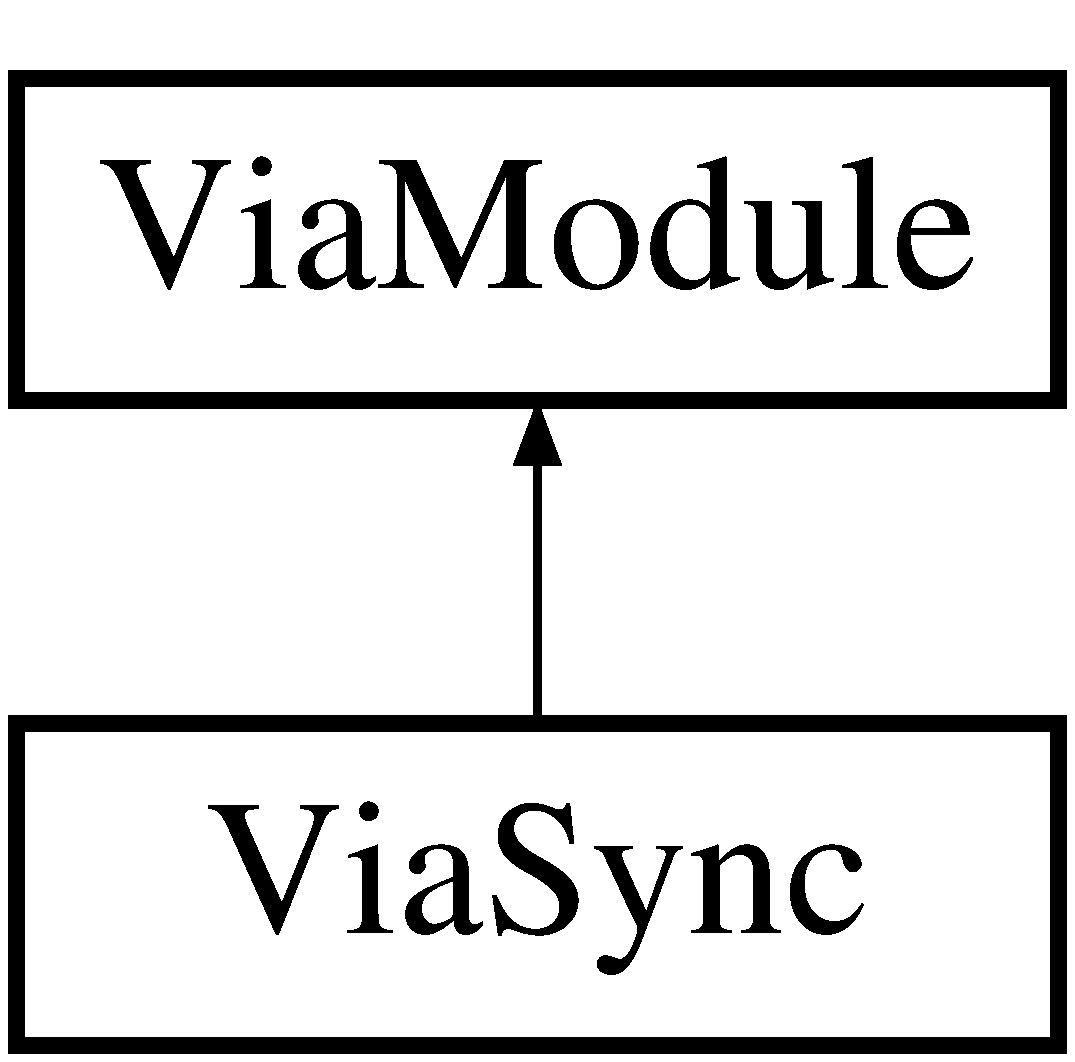
\includegraphics[height=2.000000cm]{class_via_sync}
\end{center}
\end{figure}
\subsection*{Classes}
\begin{DoxyCompactItemize}
\item 
class \mbox{\hyperlink{class_via_sync_1_1_via_sync_u_i}{Via\+Sync\+UI}}
\end{DoxyCompactItemize}
\subsection*{Public Member Functions}
\begin{DoxyCompactItemize}
\item 
void \mbox{\hyperlink{class_via_sync_ade251d6864dbf40a30d530113a8db7c4}{handle\+Button1\+Mode\+Change}} (int32\+\_\+t)
\item 
void \mbox{\hyperlink{class_via_sync_a72c6811eda10d4561514a3e303c576ca}{handle\+Button2\+Mode\+Change}} (int32\+\_\+t)
\item 
void \mbox{\hyperlink{class_via_sync_a776b4208e3e60ed260944712c1e6b373}{handle\+Button3\+Mode\+Change}} (int32\+\_\+t)
\item 
void \mbox{\hyperlink{class_via_sync_a87591fbbe499a88655b5bfda7fa66ac3}{handle\+Button4\+Mode\+Change}} (int32\+\_\+t)
\item 
void \mbox{\hyperlink{class_via_sync_aae492fa98176f80a1b7c8b93ef94d298}{handle\+Button5\+Mode\+Change}} (int32\+\_\+t)
\item 
void \mbox{\hyperlink{class_via_sync_afca54d07d9a9e69aadf0e902fc170da9}{handle\+Button5\+Mode\+Init}} (int32\+\_\+t)
\item 
void \mbox{\hyperlink{class_via_sync_a6de0281ea552e8d2e484bbc25ccee2fe}{handle\+Button6\+Mode\+Change}} (int32\+\_\+t)
\item 
void \mbox{\hyperlink{class_via_sync_acd48ad7bc9c9c20dbceb3742bf6958c4}{handle\+Aux1\+Mode\+Change}} (int32\+\_\+t)
\item 
void \mbox{\hyperlink{class_via_sync_a95d851d451b6b7ea874dd27737e217a0}{handle\+Aux2\+Mode\+Change}} (int32\+\_\+t)
\item 
void \mbox{\hyperlink{class_via_sync_a61945cde541c66ac456eb57fa72968e5}{handle\+Aux3\+Mode\+Change}} (int32\+\_\+t)
\item 
void \mbox{\hyperlink{class_via_sync_a398169bcd5efcd7067bf45dcb871a2b5}{handle\+Aux4\+Mode\+Change}} (int32\+\_\+t)
\item 
void \mbox{\hyperlink{class_via_sync_a34eb31372109ffcf9b3c43a4ecb2c97c}{switch\+Wavetable}} (const \mbox{\hyperlink{struct_wavetable}{Wavetable}} $\ast$)
\item 
void \mbox{\hyperlink{class_via_sync_acdf292720dd88a591bdaf2a05e6cb10e}{switch\+Wavetable\+Global}} (const \mbox{\hyperlink{struct_wavetable}{Wavetable}} $\ast$)
\item 
void \mbox{\hyperlink{class_via_sync_a3940ed301b8df340103f8aca442be348}{init\+Phase\+Dist\+Table}} (void)
\item 
void \mbox{\hyperlink{class_via_sync_ac961c167438b6631f763d9dbe3d07551}{fill\+Wavetable\+Array}} (void)
\item 
void \mbox{\hyperlink{class_via_sync_a0baf27aa03ec9eb89c09fdef6f13aeb8}{initialize\+Scales}} (void)
\item 
void \mbox{\hyperlink{class_via_sync_a2a2007c2ef3ce0d5de112c913ddb1563}{calculate\+Dac3\+Phasor}} (int32\+\_\+t write\+Index)
\item 
void \mbox{\hyperlink{class_via_sync_ac15a3cb78025e1b94fbd16297a7e7226}{calculate\+Dac3\+Contour}} (int32\+\_\+t write\+Index)
\item 
void \mbox{\hyperlink{class_via_sync_a861669d9ba9d995ee259a0ba66866881}{calculate\+Logic\+A\+Gate}} (int32\+\_\+t write\+Index)
\item 
void \mbox{\hyperlink{class_via_sync_a278dbb427e06ae105fd424f27e1085a6}{calculate\+Logic\+A\+Delta}} (int32\+\_\+t write\+Index)
\item 
void \mbox{\hyperlink{class_via_sync_abdb8461ced79404e76aa4150b45f8a10}{calculate\+S\+H\+Mode1}} (int32\+\_\+t write\+Index)
\item 
void \mbox{\hyperlink{class_via_sync_abc24bde577af46a0788d9df853867f06}{calculate\+S\+H\+Mode2}} (int32\+\_\+t write\+Index)
\item 
void \mbox{\hyperlink{class_via_sync_a91ecdc9caf9426271a0e28d9be0d8588}{calculate\+S\+H\+Mode3}} (int32\+\_\+t write\+Index)
\item 
void \mbox{\hyperlink{class_via_sync_ad3d72949ba2ba10d8ed2da9a398f7d15}{init}} (void)
\item 
\mbox{\hyperlink{class_via_sync_ac2661b7767cc423d2e97651cc75b04a3}{Via\+Sync}} ()
\item 
void \mbox{\hyperlink{class_via_sync_acf9bcb2f9e7ff050906e527ca2418875}{main\+Rising\+Edge\+Callback}} (void)
\item 
void \mbox{\hyperlink{class_via_sync_a7cbf13fbfc58835d97976b478ee00dd6}{main\+Falling\+Edge\+Callback}} (void)
\item 
void \mbox{\hyperlink{class_via_sync_a45865d44b380716e874853e4437e158d}{aux\+Rising\+Edge\+Callback}} (void)
\item 
void \mbox{\hyperlink{class_via_sync_a6c505fc93b2693b98d01b0bed50cff4a}{aux\+Falling\+Edge\+Callback}} (void)
\item 
void \mbox{\hyperlink{class_via_sync_a437a132f9edf0ee19dd965c46a7147c6}{button\+Pressed\+Callback}} (void)
\item 
void \mbox{\hyperlink{class_via_sync_a4cf15c90ec55e77922a7d6b788248544}{button\+Released\+Callback}} (void)
\item 
void \mbox{\hyperlink{class_via_sync_a31d6b55ab3680414fdb82751a3d831b0}{io\+Process\+Callback}} (void)
\item 
void \mbox{\hyperlink{class_via_sync_ac7088351c34bdeecd7b6071e98365791}{half\+Transfer\+Callback}} (void)
\item 
void \mbox{\hyperlink{class_via_sync_a87f2045c71b68d5ecd0da591331b3592}{transfer\+Complete\+Callback}} (void)
\item 
void \mbox{\hyperlink{class_via_sync_aeb70cc589226d3915a5821783f6609a9}{slow\+Conversion\+Callback}} (void)
\item 
void \mbox{\hyperlink{class_via_sync_a2b6602ba148dc95dc06f5410e8451b52}{ui\+\_\+dispatch}} (int32\+\_\+t sig)
\item 
void \mbox{\hyperlink{class_via_sync_a07892a924ff929e8fd33ecec31e2cf19}{increment\+Virtual\+Timer}} (void)
\end{DoxyCompactItemize}
\subsection*{Public Attributes}
\begin{DoxyCompactItemize}
\item 
const \mbox{\hyperlink{struct_wavetable}{Wavetable}} $\ast$ \mbox{\hyperlink{class_via_sync_a421aef9430e9c2af3026a8b8b6efc2b8}{wavetable\+Array}} \mbox{[}4\mbox{]}\mbox{[}4\mbox{]}
\item 
const \mbox{\hyperlink{struct_wavetable}{Wavetable}} $\ast$ \mbox{\hyperlink{class_via_sync_aacd77d7c631a429ccb9ec592cd81adf7}{wavetable\+Array\+Global}} \mbox{[}4\mbox{]}
\item 
uint32\+\_\+t \mbox{\hyperlink{class_via_sync_adeace97188f665b4b7e4d50c91cd42b6}{wavetable\+Read}} \mbox{[}9\mbox{]}\mbox{[}517\mbox{]}
\item 
const \mbox{\hyperlink{struct_scale}{Scale}} $\ast$ \mbox{\hyperlink{class_via_sync_a162046891bb80b88ea683a2e37cf00b4}{scale\+Array}} \mbox{[}4\mbox{]}\mbox{[}4\mbox{]}
\item 
const \mbox{\hyperlink{struct_scale}{Scale}} $\ast$ \mbox{\hyperlink{class_via_sync_a21039946d5bad7741e7f342149253e2c}{scale}}
\item 
uint16\+\_\+t \mbox{\hyperlink{class_via_sync_a8c088bdfe1858e949f33954572f0cb26}{virtual\+FM}} \mbox{[}2\mbox{]}
\item 
uint16\+\_\+t \mbox{\hyperlink{class_via_sync_a809f6405291356f76c408a4024d2192d}{virtual\+Morph}} \mbox{[}2\mbox{]}
\item 
void(Via\+Sync\+::$\ast$ \mbox{\hyperlink{class_via_sync_a860a8bb6bf093193a468033192a7b857}{calculate\+Dac3}} )(int32\+\_\+t write\+Index)
\item 
void(Via\+Sync\+::$\ast$ \mbox{\hyperlink{class_via_sync_a9ee32a34a997a3d8283c9a2abfa7fc4e}{calculate\+LogicA}} )(int32\+\_\+t write\+Index)
\item 
void(Via\+Sync\+::$\ast$ \mbox{\hyperlink{class_via_sync_ad4bd4c345fdd6f6e0f4ad3666f36adf7}{calculate\+SH}} )(int32\+\_\+t write\+Index)
\item 
\mbox{\hyperlink{class_via_sync_1_1_via_sync_u_i}{Via\+Sync\+UI}} \mbox{\hyperlink{class_via_sync_a0aa62004d6d2c1c26616379596172542}{sync\+UI}}
\item 
int32\+\_\+t \mbox{\hyperlink{class_via_sync_abd8dfb51ed608082fac355d06bde3c7b}{runtime\+Display}}
\item 
int32\+\_\+t \mbox{\hyperlink{class_via_sync_a5f847b5346310d3ae010cf1d68e6ec34}{show\+Y\+Change}}
\item 
\mbox{\hyperlink{class_sync_wavetable}{Sync\+Wavetable}} \mbox{\hyperlink{class_via_sync_a3a240ad9c0207533abecd6da64cfc069}{sync\+Wavetable}}
\item 
\mbox{\hyperlink{class_pll_controller}{Pll\+Controller}} \mbox{\hyperlink{class_via_sync_ac77f7c5b9fe24f61433f75ecaa702b87}{pll\+Controller}}
\item 
int32\+\_\+t \mbox{\hyperlink{class_via_sync_a38df99c334ee8b78ee921ec67052cb3d}{last\+Tap}} = 0
\item 
buffer \mbox{\hyperlink{class_via_sync_a49eb330e6b71d0519d44131cdee3ef24}{tap\+Store}}
\item 
int32\+\_\+t \mbox{\hyperlink{class_via_sync_aaf5f83216e823aba344592ad38a84e62}{tap\+Sum}} = 0
\item 
\mbox{\hyperlink{structrgb}{rgb}} \mbox{\hyperlink{class_via_sync_adaabb770098e4897fce63f29de6ce9e1}{scale\+Color}}
\item 
int32\+\_\+t \mbox{\hyperlink{class_via_sync_a2660c274695f43168b0f9f481304a320}{scale\+Hue}}
\end{DoxyCompactItemize}
\subsection*{Additional Inherited Members}


\subsection{Constructor \& Destructor Documentation}
\mbox{\Hypertarget{class_via_sync_ac2661b7767cc423d2e97651cc75b04a3}\label{class_via_sync_ac2661b7767cc423d2e97651cc75b04a3}} 
\index{Via\+Sync@{Via\+Sync}!Via\+Sync@{Via\+Sync}}
\index{Via\+Sync@{Via\+Sync}!Via\+Sync@{Via\+Sync}}
\subsubsection{\texorpdfstring{Via\+Sync()}{ViaSync()}}
{\footnotesize\ttfamily Via\+Sync\+::\+Via\+Sync (\begin{DoxyParamCaption}{ }\end{DoxyParamCaption})\hspace{0.3cm}{\ttfamily [inline]}}



\subsection{Member Function Documentation}
\mbox{\Hypertarget{class_via_sync_a6c505fc93b2693b98d01b0bed50cff4a}\label{class_via_sync_a6c505fc93b2693b98d01b0bed50cff4a}} 
\index{Via\+Sync@{Via\+Sync}!aux\+Falling\+Edge\+Callback@{aux\+Falling\+Edge\+Callback}}
\index{aux\+Falling\+Edge\+Callback@{aux\+Falling\+Edge\+Callback}!Via\+Sync@{Via\+Sync}}
\subsubsection{\texorpdfstring{aux\+Falling\+Edge\+Callback()}{auxFallingEdgeCallback()}}
{\footnotesize\ttfamily void Via\+Sync\+::aux\+Falling\+Edge\+Callback (\begin{DoxyParamCaption}\item[{void}]{ }\end{DoxyParamCaption})}

\mbox{\Hypertarget{class_via_sync_a45865d44b380716e874853e4437e158d}\label{class_via_sync_a45865d44b380716e874853e4437e158d}} 
\index{Via\+Sync@{Via\+Sync}!aux\+Rising\+Edge\+Callback@{aux\+Rising\+Edge\+Callback}}
\index{aux\+Rising\+Edge\+Callback@{aux\+Rising\+Edge\+Callback}!Via\+Sync@{Via\+Sync}}
\subsubsection{\texorpdfstring{aux\+Rising\+Edge\+Callback()}{auxRisingEdgeCallback()}}
{\footnotesize\ttfamily void Via\+Sync\+::aux\+Rising\+Edge\+Callback (\begin{DoxyParamCaption}\item[{void}]{ }\end{DoxyParamCaption})}

\mbox{\Hypertarget{class_via_sync_a437a132f9edf0ee19dd965c46a7147c6}\label{class_via_sync_a437a132f9edf0ee19dd965c46a7147c6}} 
\index{Via\+Sync@{Via\+Sync}!button\+Pressed\+Callback@{button\+Pressed\+Callback}}
\index{button\+Pressed\+Callback@{button\+Pressed\+Callback}!Via\+Sync@{Via\+Sync}}
\subsubsection{\texorpdfstring{button\+Pressed\+Callback()}{buttonPressedCallback()}}
{\footnotesize\ttfamily void Via\+Sync\+::button\+Pressed\+Callback (\begin{DoxyParamCaption}\item[{void}]{ }\end{DoxyParamCaption})}

\mbox{\Hypertarget{class_via_sync_a4cf15c90ec55e77922a7d6b788248544}\label{class_via_sync_a4cf15c90ec55e77922a7d6b788248544}} 
\index{Via\+Sync@{Via\+Sync}!button\+Released\+Callback@{button\+Released\+Callback}}
\index{button\+Released\+Callback@{button\+Released\+Callback}!Via\+Sync@{Via\+Sync}}
\subsubsection{\texorpdfstring{button\+Released\+Callback()}{buttonReleasedCallback()}}
{\footnotesize\ttfamily void Via\+Sync\+::button\+Released\+Callback (\begin{DoxyParamCaption}\item[{void}]{ }\end{DoxyParamCaption})}

\mbox{\Hypertarget{class_via_sync_ac15a3cb78025e1b94fbd16297a7e7226}\label{class_via_sync_ac15a3cb78025e1b94fbd16297a7e7226}} 
\index{Via\+Sync@{Via\+Sync}!calculate\+Dac3\+Contour@{calculate\+Dac3\+Contour}}
\index{calculate\+Dac3\+Contour@{calculate\+Dac3\+Contour}!Via\+Sync@{Via\+Sync}}
\subsubsection{\texorpdfstring{calculate\+Dac3\+Contour()}{calculateDac3Contour()}}
{\footnotesize\ttfamily void Via\+Sync\+::calculate\+Dac3\+Contour (\begin{DoxyParamCaption}\item[{int32\+\_\+t}]{write\+Index }\end{DoxyParamCaption})}

\mbox{\Hypertarget{class_via_sync_a2a2007c2ef3ce0d5de112c913ddb1563}\label{class_via_sync_a2a2007c2ef3ce0d5de112c913ddb1563}} 
\index{Via\+Sync@{Via\+Sync}!calculate\+Dac3\+Phasor@{calculate\+Dac3\+Phasor}}
\index{calculate\+Dac3\+Phasor@{calculate\+Dac3\+Phasor}!Via\+Sync@{Via\+Sync}}
\subsubsection{\texorpdfstring{calculate\+Dac3\+Phasor()}{calculateDac3Phasor()}}
{\footnotesize\ttfamily void Via\+Sync\+::calculate\+Dac3\+Phasor (\begin{DoxyParamCaption}\item[{int32\+\_\+t}]{write\+Index }\end{DoxyParamCaption})}

\mbox{\Hypertarget{class_via_sync_a278dbb427e06ae105fd424f27e1085a6}\label{class_via_sync_a278dbb427e06ae105fd424f27e1085a6}} 
\index{Via\+Sync@{Via\+Sync}!calculate\+Logic\+A\+Delta@{calculate\+Logic\+A\+Delta}}
\index{calculate\+Logic\+A\+Delta@{calculate\+Logic\+A\+Delta}!Via\+Sync@{Via\+Sync}}
\subsubsection{\texorpdfstring{calculate\+Logic\+A\+Delta()}{calculateLogicADelta()}}
{\footnotesize\ttfamily void Via\+Sync\+::calculate\+Logic\+A\+Delta (\begin{DoxyParamCaption}\item[{int32\+\_\+t}]{write\+Index }\end{DoxyParamCaption})}

\mbox{\Hypertarget{class_via_sync_a861669d9ba9d995ee259a0ba66866881}\label{class_via_sync_a861669d9ba9d995ee259a0ba66866881}} 
\index{Via\+Sync@{Via\+Sync}!calculate\+Logic\+A\+Gate@{calculate\+Logic\+A\+Gate}}
\index{calculate\+Logic\+A\+Gate@{calculate\+Logic\+A\+Gate}!Via\+Sync@{Via\+Sync}}
\subsubsection{\texorpdfstring{calculate\+Logic\+A\+Gate()}{calculateLogicAGate()}}
{\footnotesize\ttfamily void Via\+Sync\+::calculate\+Logic\+A\+Gate (\begin{DoxyParamCaption}\item[{int32\+\_\+t}]{write\+Index }\end{DoxyParamCaption})}

\mbox{\Hypertarget{class_via_sync_abdb8461ced79404e76aa4150b45f8a10}\label{class_via_sync_abdb8461ced79404e76aa4150b45f8a10}} 
\index{Via\+Sync@{Via\+Sync}!calculate\+S\+H\+Mode1@{calculate\+S\+H\+Mode1}}
\index{calculate\+S\+H\+Mode1@{calculate\+S\+H\+Mode1}!Via\+Sync@{Via\+Sync}}
\subsubsection{\texorpdfstring{calculate\+S\+H\+Mode1()}{calculateSHMode1()}}
{\footnotesize\ttfamily void Via\+Sync\+::calculate\+S\+H\+Mode1 (\begin{DoxyParamCaption}\item[{int32\+\_\+t}]{write\+Index }\end{DoxyParamCaption})}

\mbox{\Hypertarget{class_via_sync_abc24bde577af46a0788d9df853867f06}\label{class_via_sync_abc24bde577af46a0788d9df853867f06}} 
\index{Via\+Sync@{Via\+Sync}!calculate\+S\+H\+Mode2@{calculate\+S\+H\+Mode2}}
\index{calculate\+S\+H\+Mode2@{calculate\+S\+H\+Mode2}!Via\+Sync@{Via\+Sync}}
\subsubsection{\texorpdfstring{calculate\+S\+H\+Mode2()}{calculateSHMode2()}}
{\footnotesize\ttfamily void Via\+Sync\+::calculate\+S\+H\+Mode2 (\begin{DoxyParamCaption}\item[{int32\+\_\+t}]{write\+Index }\end{DoxyParamCaption})}

\mbox{\Hypertarget{class_via_sync_a91ecdc9caf9426271a0e28d9be0d8588}\label{class_via_sync_a91ecdc9caf9426271a0e28d9be0d8588}} 
\index{Via\+Sync@{Via\+Sync}!calculate\+S\+H\+Mode3@{calculate\+S\+H\+Mode3}}
\index{calculate\+S\+H\+Mode3@{calculate\+S\+H\+Mode3}!Via\+Sync@{Via\+Sync}}
\subsubsection{\texorpdfstring{calculate\+S\+H\+Mode3()}{calculateSHMode3()}}
{\footnotesize\ttfamily void Via\+Sync\+::calculate\+S\+H\+Mode3 (\begin{DoxyParamCaption}\item[{int32\+\_\+t}]{write\+Index }\end{DoxyParamCaption})}

\mbox{\Hypertarget{class_via_sync_ac961c167438b6631f763d9dbe3d07551}\label{class_via_sync_ac961c167438b6631f763d9dbe3d07551}} 
\index{Via\+Sync@{Via\+Sync}!fill\+Wavetable\+Array@{fill\+Wavetable\+Array}}
\index{fill\+Wavetable\+Array@{fill\+Wavetable\+Array}!Via\+Sync@{Via\+Sync}}
\subsubsection{\texorpdfstring{fill\+Wavetable\+Array()}{fillWavetableArray()}}
{\footnotesize\ttfamily void Via\+Sync\+::fill\+Wavetable\+Array (\begin{DoxyParamCaption}\item[{void}]{ }\end{DoxyParamCaption})}

\mbox{\Hypertarget{class_via_sync_ac7088351c34bdeecd7b6071e98365791}\label{class_via_sync_ac7088351c34bdeecd7b6071e98365791}} 
\index{Via\+Sync@{Via\+Sync}!half\+Transfer\+Callback@{half\+Transfer\+Callback}}
\index{half\+Transfer\+Callback@{half\+Transfer\+Callback}!Via\+Sync@{Via\+Sync}}
\subsubsection{\texorpdfstring{half\+Transfer\+Callback()}{halfTransferCallback()}}
{\footnotesize\ttfamily void Via\+Sync\+::half\+Transfer\+Callback (\begin{DoxyParamCaption}\item[{void}]{ }\end{DoxyParamCaption})}

\mbox{\Hypertarget{class_via_sync_acd48ad7bc9c9c20dbceb3742bf6958c4}\label{class_via_sync_acd48ad7bc9c9c20dbceb3742bf6958c4}} 
\index{Via\+Sync@{Via\+Sync}!handle\+Aux1\+Mode\+Change@{handle\+Aux1\+Mode\+Change}}
\index{handle\+Aux1\+Mode\+Change@{handle\+Aux1\+Mode\+Change}!Via\+Sync@{Via\+Sync}}
\subsubsection{\texorpdfstring{handle\+Aux1\+Mode\+Change()}{handleAux1ModeChange()}}
{\footnotesize\ttfamily void Via\+Sync\+::handle\+Aux1\+Mode\+Change (\begin{DoxyParamCaption}\item[{int32\+\_\+t}]{mode }\end{DoxyParamCaption})}

\mbox{\Hypertarget{class_via_sync_a95d851d451b6b7ea874dd27737e217a0}\label{class_via_sync_a95d851d451b6b7ea874dd27737e217a0}} 
\index{Via\+Sync@{Via\+Sync}!handle\+Aux2\+Mode\+Change@{handle\+Aux2\+Mode\+Change}}
\index{handle\+Aux2\+Mode\+Change@{handle\+Aux2\+Mode\+Change}!Via\+Sync@{Via\+Sync}}
\subsubsection{\texorpdfstring{handle\+Aux2\+Mode\+Change()}{handleAux2ModeChange()}}
{\footnotesize\ttfamily void Via\+Sync\+::handle\+Aux2\+Mode\+Change (\begin{DoxyParamCaption}\item[{int32\+\_\+t}]{mode }\end{DoxyParamCaption})}

\mbox{\Hypertarget{class_via_sync_a61945cde541c66ac456eb57fa72968e5}\label{class_via_sync_a61945cde541c66ac456eb57fa72968e5}} 
\index{Via\+Sync@{Via\+Sync}!handle\+Aux3\+Mode\+Change@{handle\+Aux3\+Mode\+Change}}
\index{handle\+Aux3\+Mode\+Change@{handle\+Aux3\+Mode\+Change}!Via\+Sync@{Via\+Sync}}
\subsubsection{\texorpdfstring{handle\+Aux3\+Mode\+Change()}{handleAux3ModeChange()}}
{\footnotesize\ttfamily void Via\+Sync\+::handle\+Aux3\+Mode\+Change (\begin{DoxyParamCaption}\item[{int32\+\_\+t}]{mode }\end{DoxyParamCaption})}

\mbox{\Hypertarget{class_via_sync_a398169bcd5efcd7067bf45dcb871a2b5}\label{class_via_sync_a398169bcd5efcd7067bf45dcb871a2b5}} 
\index{Via\+Sync@{Via\+Sync}!handle\+Aux4\+Mode\+Change@{handle\+Aux4\+Mode\+Change}}
\index{handle\+Aux4\+Mode\+Change@{handle\+Aux4\+Mode\+Change}!Via\+Sync@{Via\+Sync}}
\subsubsection{\texorpdfstring{handle\+Aux4\+Mode\+Change()}{handleAux4ModeChange()}}
{\footnotesize\ttfamily void Via\+Sync\+::handle\+Aux4\+Mode\+Change (\begin{DoxyParamCaption}\item[{int32\+\_\+t}]{mode }\end{DoxyParamCaption})}

\mbox{\Hypertarget{class_via_sync_ade251d6864dbf40a30d530113a8db7c4}\label{class_via_sync_ade251d6864dbf40a30d530113a8db7c4}} 
\index{Via\+Sync@{Via\+Sync}!handle\+Button1\+Mode\+Change@{handle\+Button1\+Mode\+Change}}
\index{handle\+Button1\+Mode\+Change@{handle\+Button1\+Mode\+Change}!Via\+Sync@{Via\+Sync}}
\subsubsection{\texorpdfstring{handle\+Button1\+Mode\+Change()}{handleButton1ModeChange()}}
{\footnotesize\ttfamily void Via\+Sync\+::handle\+Button1\+Mode\+Change (\begin{DoxyParamCaption}\item[{int32\+\_\+t}]{mode }\end{DoxyParamCaption})}

\mbox{\Hypertarget{class_via_sync_a72c6811eda10d4561514a3e303c576ca}\label{class_via_sync_a72c6811eda10d4561514a3e303c576ca}} 
\index{Via\+Sync@{Via\+Sync}!handle\+Button2\+Mode\+Change@{handle\+Button2\+Mode\+Change}}
\index{handle\+Button2\+Mode\+Change@{handle\+Button2\+Mode\+Change}!Via\+Sync@{Via\+Sync}}
\subsubsection{\texorpdfstring{handle\+Button2\+Mode\+Change()}{handleButton2ModeChange()}}
{\footnotesize\ttfamily void Via\+Sync\+::handle\+Button2\+Mode\+Change (\begin{DoxyParamCaption}\item[{int32\+\_\+t}]{mode }\end{DoxyParamCaption})}

\mbox{\Hypertarget{class_via_sync_a776b4208e3e60ed260944712c1e6b373}\label{class_via_sync_a776b4208e3e60ed260944712c1e6b373}} 
\index{Via\+Sync@{Via\+Sync}!handle\+Button3\+Mode\+Change@{handle\+Button3\+Mode\+Change}}
\index{handle\+Button3\+Mode\+Change@{handle\+Button3\+Mode\+Change}!Via\+Sync@{Via\+Sync}}
\subsubsection{\texorpdfstring{handle\+Button3\+Mode\+Change()}{handleButton3ModeChange()}}
{\footnotesize\ttfamily void Via\+Sync\+::handle\+Button3\+Mode\+Change (\begin{DoxyParamCaption}\item[{int32\+\_\+t}]{mode }\end{DoxyParamCaption})}

\mbox{\Hypertarget{class_via_sync_a87591fbbe499a88655b5bfda7fa66ac3}\label{class_via_sync_a87591fbbe499a88655b5bfda7fa66ac3}} 
\index{Via\+Sync@{Via\+Sync}!handle\+Button4\+Mode\+Change@{handle\+Button4\+Mode\+Change}}
\index{handle\+Button4\+Mode\+Change@{handle\+Button4\+Mode\+Change}!Via\+Sync@{Via\+Sync}}
\subsubsection{\texorpdfstring{handle\+Button4\+Mode\+Change()}{handleButton4ModeChange()}}
{\footnotesize\ttfamily void Via\+Sync\+::handle\+Button4\+Mode\+Change (\begin{DoxyParamCaption}\item[{int32\+\_\+t}]{mode }\end{DoxyParamCaption})}

\mbox{\Hypertarget{class_via_sync_aae492fa98176f80a1b7c8b93ef94d298}\label{class_via_sync_aae492fa98176f80a1b7c8b93ef94d298}} 
\index{Via\+Sync@{Via\+Sync}!handle\+Button5\+Mode\+Change@{handle\+Button5\+Mode\+Change}}
\index{handle\+Button5\+Mode\+Change@{handle\+Button5\+Mode\+Change}!Via\+Sync@{Via\+Sync}}
\subsubsection{\texorpdfstring{handle\+Button5\+Mode\+Change()}{handleButton5ModeChange()}}
{\footnotesize\ttfamily void Via\+Sync\+::handle\+Button5\+Mode\+Change (\begin{DoxyParamCaption}\item[{int32\+\_\+t}]{mode }\end{DoxyParamCaption})}

\mbox{\Hypertarget{class_via_sync_afca54d07d9a9e69aadf0e902fc170da9}\label{class_via_sync_afca54d07d9a9e69aadf0e902fc170da9}} 
\index{Via\+Sync@{Via\+Sync}!handle\+Button5\+Mode\+Init@{handle\+Button5\+Mode\+Init}}
\index{handle\+Button5\+Mode\+Init@{handle\+Button5\+Mode\+Init}!Via\+Sync@{Via\+Sync}}
\subsubsection{\texorpdfstring{handle\+Button5\+Mode\+Init()}{handleButton5ModeInit()}}
{\footnotesize\ttfamily void Via\+Sync\+::handle\+Button5\+Mode\+Init (\begin{DoxyParamCaption}\item[{int32\+\_\+t}]{mode }\end{DoxyParamCaption})}

\mbox{\Hypertarget{class_via_sync_a6de0281ea552e8d2e484bbc25ccee2fe}\label{class_via_sync_a6de0281ea552e8d2e484bbc25ccee2fe}} 
\index{Via\+Sync@{Via\+Sync}!handle\+Button6\+Mode\+Change@{handle\+Button6\+Mode\+Change}}
\index{handle\+Button6\+Mode\+Change@{handle\+Button6\+Mode\+Change}!Via\+Sync@{Via\+Sync}}
\subsubsection{\texorpdfstring{handle\+Button6\+Mode\+Change()}{handleButton6ModeChange()}}
{\footnotesize\ttfamily void Via\+Sync\+::handle\+Button6\+Mode\+Change (\begin{DoxyParamCaption}\item[{int32\+\_\+t}]{mode }\end{DoxyParamCaption})}

\mbox{\Hypertarget{class_via_sync_a07892a924ff929e8fd33ecec31e2cf19}\label{class_via_sync_a07892a924ff929e8fd33ecec31e2cf19}} 
\index{Via\+Sync@{Via\+Sync}!increment\+Virtual\+Timer@{increment\+Virtual\+Timer}}
\index{increment\+Virtual\+Timer@{increment\+Virtual\+Timer}!Via\+Sync@{Via\+Sync}}
\subsubsection{\texorpdfstring{increment\+Virtual\+Timer()}{incrementVirtualTimer()}}
{\footnotesize\ttfamily void Via\+Sync\+::increment\+Virtual\+Timer (\begin{DoxyParamCaption}\item[{void}]{ }\end{DoxyParamCaption})\hspace{0.3cm}{\ttfamily [inline]}}

\mbox{\Hypertarget{class_via_sync_ad3d72949ba2ba10d8ed2da9a398f7d15}\label{class_via_sync_ad3d72949ba2ba10d8ed2da9a398f7d15}} 
\index{Via\+Sync@{Via\+Sync}!init@{init}}
\index{init@{init}!Via\+Sync@{Via\+Sync}}
\subsubsection{\texorpdfstring{init()}{init()}}
{\footnotesize\ttfamily void Via\+Sync\+::init (\begin{DoxyParamCaption}\item[{void}]{ }\end{DoxyParamCaption})}

\mbox{\Hypertarget{class_via_sync_a0baf27aa03ec9eb89c09fdef6f13aeb8}\label{class_via_sync_a0baf27aa03ec9eb89c09fdef6f13aeb8}} 
\index{Via\+Sync@{Via\+Sync}!initialize\+Scales@{initialize\+Scales}}
\index{initialize\+Scales@{initialize\+Scales}!Via\+Sync@{Via\+Sync}}
\subsubsection{\texorpdfstring{initialize\+Scales()}{initializeScales()}}
{\footnotesize\ttfamily void Via\+Sync\+::initialize\+Scales (\begin{DoxyParamCaption}\item[{void}]{ }\end{DoxyParamCaption})}

\mbox{\Hypertarget{class_via_sync_a3940ed301b8df340103f8aca442be348}\label{class_via_sync_a3940ed301b8df340103f8aca442be348}} 
\index{Via\+Sync@{Via\+Sync}!init\+Phase\+Dist\+Table@{init\+Phase\+Dist\+Table}}
\index{init\+Phase\+Dist\+Table@{init\+Phase\+Dist\+Table}!Via\+Sync@{Via\+Sync}}
\subsubsection{\texorpdfstring{init\+Phase\+Dist\+Table()}{initPhaseDistTable()}}
{\footnotesize\ttfamily void Via\+Sync\+::init\+Phase\+Dist\+Table (\begin{DoxyParamCaption}\item[{void}]{ }\end{DoxyParamCaption})}

\mbox{\Hypertarget{class_via_sync_a31d6b55ab3680414fdb82751a3d831b0}\label{class_via_sync_a31d6b55ab3680414fdb82751a3d831b0}} 
\index{Via\+Sync@{Via\+Sync}!io\+Process\+Callback@{io\+Process\+Callback}}
\index{io\+Process\+Callback@{io\+Process\+Callback}!Via\+Sync@{Via\+Sync}}
\subsubsection{\texorpdfstring{io\+Process\+Callback()}{ioProcessCallback()}}
{\footnotesize\ttfamily void Via\+Sync\+::io\+Process\+Callback (\begin{DoxyParamCaption}\item[{void}]{ }\end{DoxyParamCaption})}

\mbox{\Hypertarget{class_via_sync_a7cbf13fbfc58835d97976b478ee00dd6}\label{class_via_sync_a7cbf13fbfc58835d97976b478ee00dd6}} 
\index{Via\+Sync@{Via\+Sync}!main\+Falling\+Edge\+Callback@{main\+Falling\+Edge\+Callback}}
\index{main\+Falling\+Edge\+Callback@{main\+Falling\+Edge\+Callback}!Via\+Sync@{Via\+Sync}}
\subsubsection{\texorpdfstring{main\+Falling\+Edge\+Callback()}{mainFallingEdgeCallback()}}
{\footnotesize\ttfamily void Via\+Sync\+::main\+Falling\+Edge\+Callback (\begin{DoxyParamCaption}\item[{void}]{ }\end{DoxyParamCaption})}

\mbox{\Hypertarget{class_via_sync_acf9bcb2f9e7ff050906e527ca2418875}\label{class_via_sync_acf9bcb2f9e7ff050906e527ca2418875}} 
\index{Via\+Sync@{Via\+Sync}!main\+Rising\+Edge\+Callback@{main\+Rising\+Edge\+Callback}}
\index{main\+Rising\+Edge\+Callback@{main\+Rising\+Edge\+Callback}!Via\+Sync@{Via\+Sync}}
\subsubsection{\texorpdfstring{main\+Rising\+Edge\+Callback()}{mainRisingEdgeCallback()}}
{\footnotesize\ttfamily void Via\+Sync\+::main\+Rising\+Edge\+Callback (\begin{DoxyParamCaption}\item[{void}]{ }\end{DoxyParamCaption})}

\mbox{\Hypertarget{class_via_sync_aeb70cc589226d3915a5821783f6609a9}\label{class_via_sync_aeb70cc589226d3915a5821783f6609a9}} 
\index{Via\+Sync@{Via\+Sync}!slow\+Conversion\+Callback@{slow\+Conversion\+Callback}}
\index{slow\+Conversion\+Callback@{slow\+Conversion\+Callback}!Via\+Sync@{Via\+Sync}}
\subsubsection{\texorpdfstring{slow\+Conversion\+Callback()}{slowConversionCallback()}}
{\footnotesize\ttfamily void Via\+Sync\+::slow\+Conversion\+Callback (\begin{DoxyParamCaption}\item[{void}]{ }\end{DoxyParamCaption})}

\mbox{\Hypertarget{class_via_sync_a34eb31372109ffcf9b3c43a4ecb2c97c}\label{class_via_sync_a34eb31372109ffcf9b3c43a4ecb2c97c}} 
\index{Via\+Sync@{Via\+Sync}!switch\+Wavetable@{switch\+Wavetable}}
\index{switch\+Wavetable@{switch\+Wavetable}!Via\+Sync@{Via\+Sync}}
\subsubsection{\texorpdfstring{switch\+Wavetable()}{switchWavetable()}}
{\footnotesize\ttfamily void Via\+Sync\+::switch\+Wavetable (\begin{DoxyParamCaption}\item[{const \mbox{\hyperlink{struct_wavetable}{Wavetable}} $\ast$}]{table }\end{DoxyParamCaption})}

\mbox{\Hypertarget{class_via_sync_acdf292720dd88a591bdaf2a05e6cb10e}\label{class_via_sync_acdf292720dd88a591bdaf2a05e6cb10e}} 
\index{Via\+Sync@{Via\+Sync}!switch\+Wavetable\+Global@{switch\+Wavetable\+Global}}
\index{switch\+Wavetable\+Global@{switch\+Wavetable\+Global}!Via\+Sync@{Via\+Sync}}
\subsubsection{\texorpdfstring{switch\+Wavetable\+Global()}{switchWavetableGlobal()}}
{\footnotesize\ttfamily void Via\+Sync\+::switch\+Wavetable\+Global (\begin{DoxyParamCaption}\item[{const \mbox{\hyperlink{struct_wavetable}{Wavetable}} $\ast$}]{table }\end{DoxyParamCaption})}

\mbox{\Hypertarget{class_via_sync_a87f2045c71b68d5ecd0da591331b3592}\label{class_via_sync_a87f2045c71b68d5ecd0da591331b3592}} 
\index{Via\+Sync@{Via\+Sync}!transfer\+Complete\+Callback@{transfer\+Complete\+Callback}}
\index{transfer\+Complete\+Callback@{transfer\+Complete\+Callback}!Via\+Sync@{Via\+Sync}}
\subsubsection{\texorpdfstring{transfer\+Complete\+Callback()}{transferCompleteCallback()}}
{\footnotesize\ttfamily void Via\+Sync\+::transfer\+Complete\+Callback (\begin{DoxyParamCaption}\item[{void}]{ }\end{DoxyParamCaption})}

\mbox{\Hypertarget{class_via_sync_a2b6602ba148dc95dc06f5410e8451b52}\label{class_via_sync_a2b6602ba148dc95dc06f5410e8451b52}} 
\index{Via\+Sync@{Via\+Sync}!ui\+\_\+dispatch@{ui\+\_\+dispatch}}
\index{ui\+\_\+dispatch@{ui\+\_\+dispatch}!Via\+Sync@{Via\+Sync}}
\subsubsection{\texorpdfstring{ui\+\_\+dispatch()}{ui\_dispatch()}}
{\footnotesize\ttfamily void Via\+Sync\+::ui\+\_\+dispatch (\begin{DoxyParamCaption}\item[{int32\+\_\+t}]{sig }\end{DoxyParamCaption})\hspace{0.3cm}{\ttfamily [inline]}}



\subsection{Member Data Documentation}
\mbox{\Hypertarget{class_via_sync_a860a8bb6bf093193a468033192a7b857}\label{class_via_sync_a860a8bb6bf093193a468033192a7b857}} 
\index{Via\+Sync@{Via\+Sync}!calculate\+Dac3@{calculate\+Dac3}}
\index{calculate\+Dac3@{calculate\+Dac3}!Via\+Sync@{Via\+Sync}}
\subsubsection{\texorpdfstring{calculate\+Dac3}{calculateDac3}}
{\footnotesize\ttfamily void(Via\+Sync\+::$\ast$ Via\+Sync\+::calculate\+Dac3) (int32\+\_\+t write\+Index)}

\mbox{\Hypertarget{class_via_sync_a9ee32a34a997a3d8283c9a2abfa7fc4e}\label{class_via_sync_a9ee32a34a997a3d8283c9a2abfa7fc4e}} 
\index{Via\+Sync@{Via\+Sync}!calculate\+LogicA@{calculate\+LogicA}}
\index{calculate\+LogicA@{calculate\+LogicA}!Via\+Sync@{Via\+Sync}}
\subsubsection{\texorpdfstring{calculate\+LogicA}{calculateLogicA}}
{\footnotesize\ttfamily void(Via\+Sync\+::$\ast$ Via\+Sync\+::calculate\+LogicA) (int32\+\_\+t write\+Index)}

\mbox{\Hypertarget{class_via_sync_ad4bd4c345fdd6f6e0f4ad3666f36adf7}\label{class_via_sync_ad4bd4c345fdd6f6e0f4ad3666f36adf7}} 
\index{Via\+Sync@{Via\+Sync}!calculate\+SH@{calculate\+SH}}
\index{calculate\+SH@{calculate\+SH}!Via\+Sync@{Via\+Sync}}
\subsubsection{\texorpdfstring{calculate\+SH}{calculateSH}}
{\footnotesize\ttfamily void(Via\+Sync\+::$\ast$ Via\+Sync\+::calculate\+SH) (int32\+\_\+t write\+Index)}

\mbox{\Hypertarget{class_via_sync_a38df99c334ee8b78ee921ec67052cb3d}\label{class_via_sync_a38df99c334ee8b78ee921ec67052cb3d}} 
\index{Via\+Sync@{Via\+Sync}!last\+Tap@{last\+Tap}}
\index{last\+Tap@{last\+Tap}!Via\+Sync@{Via\+Sync}}
\subsubsection{\texorpdfstring{last\+Tap}{lastTap}}
{\footnotesize\ttfamily int32\+\_\+t Via\+Sync\+::last\+Tap = 0}

\mbox{\Hypertarget{class_via_sync_ac77f7c5b9fe24f61433f75ecaa702b87}\label{class_via_sync_ac77f7c5b9fe24f61433f75ecaa702b87}} 
\index{Via\+Sync@{Via\+Sync}!pll\+Controller@{pll\+Controller}}
\index{pll\+Controller@{pll\+Controller}!Via\+Sync@{Via\+Sync}}
\subsubsection{\texorpdfstring{pll\+Controller}{pllController}}
{\footnotesize\ttfamily \mbox{\hyperlink{class_pll_controller}{Pll\+Controller}} Via\+Sync\+::pll\+Controller}

\mbox{\Hypertarget{class_via_sync_abd8dfb51ed608082fac355d06bde3c7b}\label{class_via_sync_abd8dfb51ed608082fac355d06bde3c7b}} 
\index{Via\+Sync@{Via\+Sync}!runtime\+Display@{runtime\+Display}}
\index{runtime\+Display@{runtime\+Display}!Via\+Sync@{Via\+Sync}}
\subsubsection{\texorpdfstring{runtime\+Display}{runtimeDisplay}}
{\footnotesize\ttfamily int32\+\_\+t Via\+Sync\+::runtime\+Display}

\mbox{\Hypertarget{class_via_sync_a21039946d5bad7741e7f342149253e2c}\label{class_via_sync_a21039946d5bad7741e7f342149253e2c}} 
\index{Via\+Sync@{Via\+Sync}!scale@{scale}}
\index{scale@{scale}!Via\+Sync@{Via\+Sync}}
\subsubsection{\texorpdfstring{scale}{scale}}
{\footnotesize\ttfamily const \mbox{\hyperlink{struct_scale}{Scale}}$\ast$ Via\+Sync\+::scale}

\mbox{\Hypertarget{class_via_sync_a162046891bb80b88ea683a2e37cf00b4}\label{class_via_sync_a162046891bb80b88ea683a2e37cf00b4}} 
\index{Via\+Sync@{Via\+Sync}!scale\+Array@{scale\+Array}}
\index{scale\+Array@{scale\+Array}!Via\+Sync@{Via\+Sync}}
\subsubsection{\texorpdfstring{scale\+Array}{scaleArray}}
{\footnotesize\ttfamily const \mbox{\hyperlink{struct_scale}{Scale}}$\ast$ Via\+Sync\+::scale\+Array\mbox{[}4\mbox{]}\mbox{[}4\mbox{]}}

\mbox{\Hypertarget{class_via_sync_adaabb770098e4897fce63f29de6ce9e1}\label{class_via_sync_adaabb770098e4897fce63f29de6ce9e1}} 
\index{Via\+Sync@{Via\+Sync}!scale\+Color@{scale\+Color}}
\index{scale\+Color@{scale\+Color}!Via\+Sync@{Via\+Sync}}
\subsubsection{\texorpdfstring{scale\+Color}{scaleColor}}
{\footnotesize\ttfamily \mbox{\hyperlink{structrgb}{rgb}} Via\+Sync\+::scale\+Color}

\mbox{\Hypertarget{class_via_sync_a2660c274695f43168b0f9f481304a320}\label{class_via_sync_a2660c274695f43168b0f9f481304a320}} 
\index{Via\+Sync@{Via\+Sync}!scale\+Hue@{scale\+Hue}}
\index{scale\+Hue@{scale\+Hue}!Via\+Sync@{Via\+Sync}}
\subsubsection{\texorpdfstring{scale\+Hue}{scaleHue}}
{\footnotesize\ttfamily int32\+\_\+t Via\+Sync\+::scale\+Hue}

\mbox{\Hypertarget{class_via_sync_a5f847b5346310d3ae010cf1d68e6ec34}\label{class_via_sync_a5f847b5346310d3ae010cf1d68e6ec34}} 
\index{Via\+Sync@{Via\+Sync}!show\+Y\+Change@{show\+Y\+Change}}
\index{show\+Y\+Change@{show\+Y\+Change}!Via\+Sync@{Via\+Sync}}
\subsubsection{\texorpdfstring{show\+Y\+Change}{showYChange}}
{\footnotesize\ttfamily int32\+\_\+t Via\+Sync\+::show\+Y\+Change}

\mbox{\Hypertarget{class_via_sync_a0aa62004d6d2c1c26616379596172542}\label{class_via_sync_a0aa62004d6d2c1c26616379596172542}} 
\index{Via\+Sync@{Via\+Sync}!sync\+UI@{sync\+UI}}
\index{sync\+UI@{sync\+UI}!Via\+Sync@{Via\+Sync}}
\subsubsection{\texorpdfstring{sync\+UI}{syncUI}}
{\footnotesize\ttfamily \mbox{\hyperlink{class_via_sync_1_1_via_sync_u_i}{Via\+Sync\+UI}} Via\+Sync\+::sync\+UI}

\mbox{\Hypertarget{class_via_sync_a3a240ad9c0207533abecd6da64cfc069}\label{class_via_sync_a3a240ad9c0207533abecd6da64cfc069}} 
\index{Via\+Sync@{Via\+Sync}!sync\+Wavetable@{sync\+Wavetable}}
\index{sync\+Wavetable@{sync\+Wavetable}!Via\+Sync@{Via\+Sync}}
\subsubsection{\texorpdfstring{sync\+Wavetable}{syncWavetable}}
{\footnotesize\ttfamily \mbox{\hyperlink{class_sync_wavetable}{Sync\+Wavetable}} Via\+Sync\+::sync\+Wavetable}

\mbox{\Hypertarget{class_via_sync_a49eb330e6b71d0519d44131cdee3ef24}\label{class_via_sync_a49eb330e6b71d0519d44131cdee3ef24}} 
\index{Via\+Sync@{Via\+Sync}!tap\+Store@{tap\+Store}}
\index{tap\+Store@{tap\+Store}!Via\+Sync@{Via\+Sync}}
\subsubsection{\texorpdfstring{tap\+Store}{tapStore}}
{\footnotesize\ttfamily buffer Via\+Sync\+::tap\+Store}

\mbox{\Hypertarget{class_via_sync_aaf5f83216e823aba344592ad38a84e62}\label{class_via_sync_aaf5f83216e823aba344592ad38a84e62}} 
\index{Via\+Sync@{Via\+Sync}!tap\+Sum@{tap\+Sum}}
\index{tap\+Sum@{tap\+Sum}!Via\+Sync@{Via\+Sync}}
\subsubsection{\texorpdfstring{tap\+Sum}{tapSum}}
{\footnotesize\ttfamily int32\+\_\+t Via\+Sync\+::tap\+Sum = 0}

\mbox{\Hypertarget{class_via_sync_a8c088bdfe1858e949f33954572f0cb26}\label{class_via_sync_a8c088bdfe1858e949f33954572f0cb26}} 
\index{Via\+Sync@{Via\+Sync}!virtual\+FM@{virtual\+FM}}
\index{virtual\+FM@{virtual\+FM}!Via\+Sync@{Via\+Sync}}
\subsubsection{\texorpdfstring{virtual\+FM}{virtualFM}}
{\footnotesize\ttfamily uint16\+\_\+t Via\+Sync\+::virtual\+FM\mbox{[}2\mbox{]}}

\mbox{\Hypertarget{class_via_sync_a809f6405291356f76c408a4024d2192d}\label{class_via_sync_a809f6405291356f76c408a4024d2192d}} 
\index{Via\+Sync@{Via\+Sync}!virtual\+Morph@{virtual\+Morph}}
\index{virtual\+Morph@{virtual\+Morph}!Via\+Sync@{Via\+Sync}}
\subsubsection{\texorpdfstring{virtual\+Morph}{virtualMorph}}
{\footnotesize\ttfamily uint16\+\_\+t Via\+Sync\+::virtual\+Morph\mbox{[}2\mbox{]}}

\mbox{\Hypertarget{class_via_sync_a421aef9430e9c2af3026a8b8b6efc2b8}\label{class_via_sync_a421aef9430e9c2af3026a8b8b6efc2b8}} 
\index{Via\+Sync@{Via\+Sync}!wavetable\+Array@{wavetable\+Array}}
\index{wavetable\+Array@{wavetable\+Array}!Via\+Sync@{Via\+Sync}}
\subsubsection{\texorpdfstring{wavetable\+Array}{wavetableArray}}
{\footnotesize\ttfamily const \mbox{\hyperlink{struct_wavetable}{Wavetable}}$\ast$ Via\+Sync\+::wavetable\+Array\mbox{[}4\mbox{]}\mbox{[}4\mbox{]}}

\mbox{\Hypertarget{class_via_sync_aacd77d7c631a429ccb9ec592cd81adf7}\label{class_via_sync_aacd77d7c631a429ccb9ec592cd81adf7}} 
\index{Via\+Sync@{Via\+Sync}!wavetable\+Array\+Global@{wavetable\+Array\+Global}}
\index{wavetable\+Array\+Global@{wavetable\+Array\+Global}!Via\+Sync@{Via\+Sync}}
\subsubsection{\texorpdfstring{wavetable\+Array\+Global}{wavetableArrayGlobal}}
{\footnotesize\ttfamily const \mbox{\hyperlink{struct_wavetable}{Wavetable}}$\ast$ Via\+Sync\+::wavetable\+Array\+Global\mbox{[}4\mbox{]}}

\mbox{\Hypertarget{class_via_sync_adeace97188f665b4b7e4d50c91cd42b6}\label{class_via_sync_adeace97188f665b4b7e4d50c91cd42b6}} 
\index{Via\+Sync@{Via\+Sync}!wavetable\+Read@{wavetable\+Read}}
\index{wavetable\+Read@{wavetable\+Read}!Via\+Sync@{Via\+Sync}}
\subsubsection{\texorpdfstring{wavetable\+Read}{wavetableRead}}
{\footnotesize\ttfamily uint32\+\_\+t Via\+Sync\+::wavetable\+Read\mbox{[}9\mbox{]}\mbox{[}517\mbox{]}}



The documentation for this class was generated from the following files\+:\begin{DoxyCompactItemize}
\item 
modules/inc/\mbox{\hyperlink{sync_8hpp}{sync.\+hpp}}\item 
modules/sync/\mbox{\hyperlink{sync__aux__outputs_8cpp}{sync\+\_\+aux\+\_\+outputs.\+cpp}}\item 
modules/sync/\mbox{\hyperlink{sync__init_8cpp}{sync\+\_\+init.\+cpp}}\item 
modules/sync/\mbox{\hyperlink{sync__interrupt__handlers_8cpp}{sync\+\_\+interrupt\+\_\+handlers.\+cpp}}\item 
modules/sync/\mbox{\hyperlink{sync__modes_8cpp}{sync\+\_\+modes.\+cpp}}\item 
modules/sync/\mbox{\hyperlink{sync__scales_8cpp}{sync\+\_\+scales.\+cpp}}\item 
modules/sync/\mbox{\hyperlink{sync__table__init_8cpp}{sync\+\_\+table\+\_\+init.\+cpp}}\end{DoxyCompactItemize}

\hypertarget{class_via_sync_1_1_via_sync_u_i}{}\section{Via\+Sync\+:\+:Via\+Sync\+UI Class Reference}
\label{class_via_sync_1_1_via_sync_u_i}\index{Via\+Sync\+::\+Via\+Sync\+UI@{Via\+Sync\+::\+Via\+Sync\+UI}}


{\ttfamily \#include $<$sync.\+hpp$>$}

Inheritance diagram for Via\+Sync\+:\+:Via\+Sync\+UI\+:\begin{figure}[H]
\begin{center}
\leavevmode
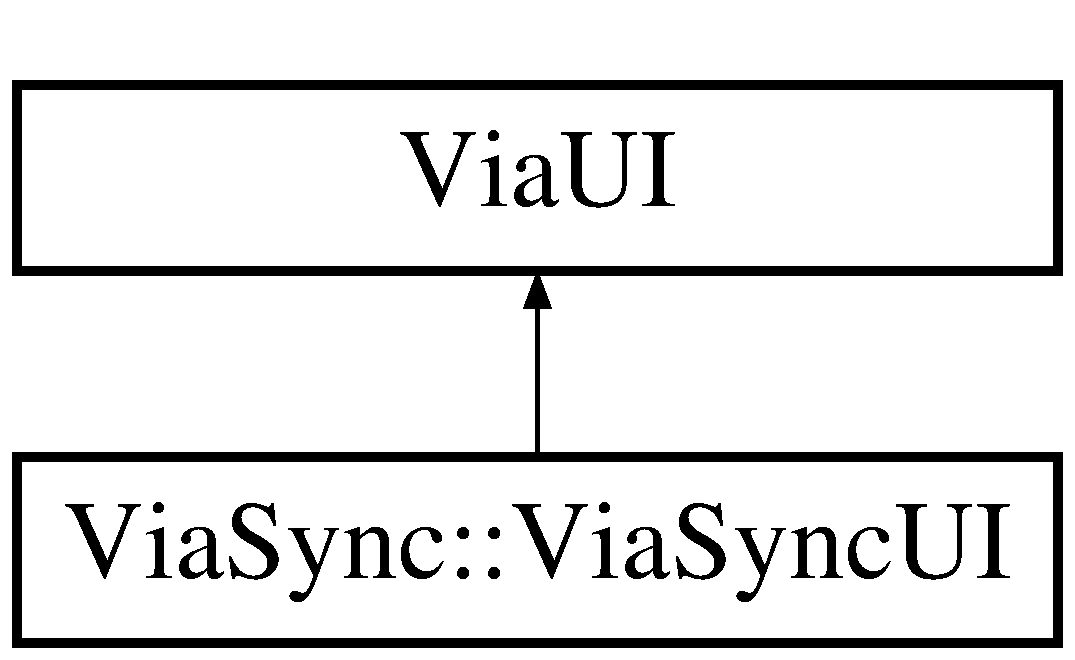
\includegraphics[height=2.000000cm]{class_via_sync_1_1_via_sync_u_i}
\end{center}
\end{figure}
\subsection*{Public Member Functions}
\begin{DoxyCompactItemize}
\item 
void \mbox{\hyperlink{class_via_sync_1_1_via_sync_u_i_adbf5a730f6f3986d7f787c9ac1f41cb3}{button1\+Tap\+Callback}} (void) override
\item 
void \mbox{\hyperlink{class_via_sync_1_1_via_sync_u_i_acd1a12bdb9cc39045eee719af6d70d1c}{button1\+Hold\+Callback}} (void) override
\item 
void \mbox{\hyperlink{class_via_sync_1_1_via_sync_u_i_ac1a33313bc6c5c1f07b3a8cb3094a700}{button2\+Tap\+Callback}} (void) override
\item 
void \mbox{\hyperlink{class_via_sync_1_1_via_sync_u_i_ad3759b21040068b5bf4ad9fd518b1c4c}{button2\+Hold\+Callback}} (void) override
\item 
void \mbox{\hyperlink{class_via_sync_1_1_via_sync_u_i_ad51f33a8fd5ae243997f864436dadcae}{button3\+Tap\+Callback}} (void) override
\item 
void \mbox{\hyperlink{class_via_sync_1_1_via_sync_u_i_af7088ee62cddc1187af86e970efe643a}{button3\+Hold\+Callback}} (void) override
\item 
void \mbox{\hyperlink{class_via_sync_1_1_via_sync_u_i_a00ba5badfeedc792a05f3e3c0ac19d73}{button4\+Tap\+Callback}} (void) override
\item 
void \mbox{\hyperlink{class_via_sync_1_1_via_sync_u_i_a7b84320153b6b7e4ae5499f4092a85d5}{button4\+Hold\+Callback}} (void) override
\item 
void \mbox{\hyperlink{class_via_sync_1_1_via_sync_u_i_aee833fdc4c2d1e242c1ece302dcaca1b}{button5\+Tap\+Callback}} (void) override
\item 
void \mbox{\hyperlink{class_via_sync_1_1_via_sync_u_i_adb9159f6ba3275b089b52f9315963f2c}{button5\+Hold\+Callback}} (void) override
\item 
void \mbox{\hyperlink{class_via_sync_1_1_via_sync_u_i_a553dc53213d1b4b62d7aead58533c511}{button6\+Tap\+Callback}} (void) override
\item 
void \mbox{\hyperlink{class_via_sync_1_1_via_sync_u_i_ace582870350424e071fc6ddb87efd802}{button6\+Hold\+Callback}} (void) override
\item 
void \mbox{\hyperlink{class_via_sync_1_1_via_sync_u_i_a53f8add06247c8ed4e7a1c049e8136fb}{aux1\+Tap\+Callback}} (void) override
\item 
void \mbox{\hyperlink{class_via_sync_1_1_via_sync_u_i_aaa66c2014e79270140575713998d67ae}{aux1\+Hold\+Callback}} (void) override
\item 
void \mbox{\hyperlink{class_via_sync_1_1_via_sync_u_i_a117e57feaf74b2619c1506aacc421721}{aux2\+Tap\+Callback}} (void) override
\item 
void \mbox{\hyperlink{class_via_sync_1_1_via_sync_u_i_af692a47db686fac2e929549217452258}{aux2\+Hold\+Callback}} (void) override
\item 
void \mbox{\hyperlink{class_via_sync_1_1_via_sync_u_i_afe95d77f17525a7e612485089a01ab0d}{aux3\+Tap\+Callback}} (void) override
\item 
void \mbox{\hyperlink{class_via_sync_1_1_via_sync_u_i_ae35a16d1e3a6158ffd306b06e93b16a4}{aux3\+Hold\+Callback}} (void) override
\item 
void \mbox{\hyperlink{class_via_sync_1_1_via_sync_u_i_a1cf7ef02457d9f7887da0721799aadc0}{aux4\+Tap\+Callback}} (void) override
\item 
void \mbox{\hyperlink{class_via_sync_1_1_via_sync_u_i_a15f48c7e1d5f77292ee46d997421cd4e}{aux4\+Hold\+Callback}} (void) override
\item 
void \mbox{\hyperlink{class_via_sync_1_1_via_sync_u_i_a694877fa6ee36aa11d9fbf3e249f95e5}{ui\+Set\+L\+E\+Ds}} (int) override
\item 
void \mbox{\hyperlink{class_via_sync_1_1_via_sync_u_i_a1a59cd903a2e11b698445b02c9fe5a48}{recall\+Module\+State}} (void) override
\item 
void \mbox{\hyperlink{class_via_sync_1_1_via_sync_u_i_a53dbd5157906ae81c3d54a56eafbf06e}{default\+Enter\+Menu\+Callback}} (void) override
\item 
void \mbox{\hyperlink{class_via_sync_1_1_via_sync_u_i_a553b539840029324ea43feb128f4b2c9}{new\+Mode\+Enter\+Menu\+Callback}} (void) override
\item 
void \mbox{\hyperlink{class_via_sync_1_1_via_sync_u_i_a842b231f8014209b4e96b3b8c06b16e1}{new\+Aux\+Mode\+Enter\+Menu\+Callback}} (void) override
\item 
void \mbox{\hyperlink{class_via_sync_1_1_via_sync_u_i_a390deaa64d96fa447720294817149dde}{preset\+Enter\+Menu\+Callback}} (void) override
\item 
void \mbox{\hyperlink{class_via_sync_1_1_via_sync_u_i_a2082d2d4a5ef8cbbaa2a1d8a387b3cad}{button1\+Enter\+Menu\+Callback}} (void) override
\item 
void \mbox{\hyperlink{class_via_sync_1_1_via_sync_u_i_a92bc4b1308d5994bef5989a8e975321d}{button2\+Enter\+Menu\+Callback}} (void) override
\item 
void \mbox{\hyperlink{class_via_sync_1_1_via_sync_u_i_a695a9d89eaf1b1e03bba057e4f89b3c2}{button3\+Enter\+Menu\+Callback}} (void) override
\item 
void \mbox{\hyperlink{class_via_sync_1_1_via_sync_u_i_a01e30440d48527321570f93d67e93aa5}{button4\+Enter\+Menu\+Callback}} (void) override
\item 
void \mbox{\hyperlink{class_via_sync_1_1_via_sync_u_i_ad02cd6e9495afcd256a3b3475809bf5b}{button5\+Enter\+Menu\+Callback}} (void) override
\item 
void \mbox{\hyperlink{class_via_sync_1_1_via_sync_u_i_a114ee3916efcf43b16f6265151350e15}{button6\+Enter\+Menu\+Callback}} (void) override
\item 
void \mbox{\hyperlink{class_via_sync_1_1_via_sync_u_i_a9e9fd5bc4d9d9cfe255a8cf099ba5110}{aux1\+Enter\+Menu\+Callback}} (void) override
\item 
void \mbox{\hyperlink{class_via_sync_1_1_via_sync_u_i_a8af905460e4d9b91420fa557be0baeae}{aux2\+Enter\+Menu\+Callback}} (void) override
\item 
void \mbox{\hyperlink{class_via_sync_1_1_via_sync_u_i_a66f7a9ccbfff3b1b1ba32fe775808703}{aux3\+Enter\+Menu\+Callback}} (void) override
\item 
void \mbox{\hyperlink{class_via_sync_1_1_via_sync_u_i_ab74dfab193404bd23e90ba1b44a0a743}{aux4\+Enter\+Menu\+Callback}} (void) override
\item 
void \mbox{\hyperlink{class_via_sync_1_1_via_sync_u_i_a0d9dbe5a0b663acc88b45b46f440db78}{initialize}} (void) override
\item 
\mbox{\hyperlink{class_via_sync_1_1_via_sync_u_i_a1bd90ed57d017480e16b7727f0b4ec65}{Via\+Sync\+UI}} (\mbox{\hyperlink{class_via_sync}{Via\+Sync}} \&x)
\end{DoxyCompactItemize}
\subsection*{Public Attributes}
\begin{DoxyCompactItemize}
\item 
\mbox{\hyperlink{class_via_sync}{Via\+Sync}} \& \mbox{\hyperlink{class_via_sync_1_1_via_sync_u_i_a15989db3913bb8fb9abf9961d1125e63}{this\+\_\+module}}
\end{DoxyCompactItemize}


\subsection{Constructor \& Destructor Documentation}
\mbox{\Hypertarget{class_via_sync_1_1_via_sync_u_i_a1bd90ed57d017480e16b7727f0b4ec65}\label{class_via_sync_1_1_via_sync_u_i_a1bd90ed57d017480e16b7727f0b4ec65}} 
\index{Via\+Sync\+::\+Via\+Sync\+UI@{Via\+Sync\+::\+Via\+Sync\+UI}!Via\+Sync\+UI@{Via\+Sync\+UI}}
\index{Via\+Sync\+UI@{Via\+Sync\+UI}!Via\+Sync\+::\+Via\+Sync\+UI@{Via\+Sync\+::\+Via\+Sync\+UI}}
\subsubsection{\texorpdfstring{Via\+Sync\+U\+I()}{ViaSyncUI()}}
{\footnotesize\ttfamily Via\+Sync\+::\+Via\+Sync\+U\+I\+::\+Via\+Sync\+UI (\begin{DoxyParamCaption}\item[{\mbox{\hyperlink{class_via_sync}{Via\+Sync}} \&}]{x }\end{DoxyParamCaption})\hspace{0.3cm}{\ttfamily [inline]}}



\subsection{Member Function Documentation}
\mbox{\Hypertarget{class_via_sync_1_1_via_sync_u_i_a9e9fd5bc4d9d9cfe255a8cf099ba5110}\label{class_via_sync_1_1_via_sync_u_i_a9e9fd5bc4d9d9cfe255a8cf099ba5110}} 
\index{Via\+Sync\+::\+Via\+Sync\+UI@{Via\+Sync\+::\+Via\+Sync\+UI}!aux1\+Enter\+Menu\+Callback@{aux1\+Enter\+Menu\+Callback}}
\index{aux1\+Enter\+Menu\+Callback@{aux1\+Enter\+Menu\+Callback}!Via\+Sync\+::\+Via\+Sync\+UI@{Via\+Sync\+::\+Via\+Sync\+UI}}
\subsubsection{\texorpdfstring{aux1\+Enter\+Menu\+Callback()}{aux1EnterMenuCallback()}}
{\footnotesize\ttfamily void Via\+Sync\+::\+Via\+Sync\+U\+I\+::aux1\+Enter\+Menu\+Callback (\begin{DoxyParamCaption}\item[{void}]{ }\end{DoxyParamCaption})\hspace{0.3cm}{\ttfamily [override]}, {\ttfamily [virtual]}}



Implements \mbox{\hyperlink{class_via_u_i_a578111861e912bf43d3f320a0faffb0f}{Via\+UI}}.

\mbox{\Hypertarget{class_via_sync_1_1_via_sync_u_i_aaa66c2014e79270140575713998d67ae}\label{class_via_sync_1_1_via_sync_u_i_aaa66c2014e79270140575713998d67ae}} 
\index{Via\+Sync\+::\+Via\+Sync\+UI@{Via\+Sync\+::\+Via\+Sync\+UI}!aux1\+Hold\+Callback@{aux1\+Hold\+Callback}}
\index{aux1\+Hold\+Callback@{aux1\+Hold\+Callback}!Via\+Sync\+::\+Via\+Sync\+UI@{Via\+Sync\+::\+Via\+Sync\+UI}}
\subsubsection{\texorpdfstring{aux1\+Hold\+Callback()}{aux1HoldCallback()}}
{\footnotesize\ttfamily void Via\+Sync\+::\+Via\+Sync\+U\+I\+::aux1\+Hold\+Callback (\begin{DoxyParamCaption}\item[{void}]{ }\end{DoxyParamCaption})\hspace{0.3cm}{\ttfamily [override]}, {\ttfamily [virtual]}}



Implements \mbox{\hyperlink{class_via_u_i_a6fcc3b7cf9b97ccf403ed1817cb10d1d}{Via\+UI}}.

\mbox{\Hypertarget{class_via_sync_1_1_via_sync_u_i_a53f8add06247c8ed4e7a1c049e8136fb}\label{class_via_sync_1_1_via_sync_u_i_a53f8add06247c8ed4e7a1c049e8136fb}} 
\index{Via\+Sync\+::\+Via\+Sync\+UI@{Via\+Sync\+::\+Via\+Sync\+UI}!aux1\+Tap\+Callback@{aux1\+Tap\+Callback}}
\index{aux1\+Tap\+Callback@{aux1\+Tap\+Callback}!Via\+Sync\+::\+Via\+Sync\+UI@{Via\+Sync\+::\+Via\+Sync\+UI}}
\subsubsection{\texorpdfstring{aux1\+Tap\+Callback()}{aux1TapCallback()}}
{\footnotesize\ttfamily void Via\+Sync\+::\+Via\+Sync\+U\+I\+::aux1\+Tap\+Callback (\begin{DoxyParamCaption}\item[{void}]{ }\end{DoxyParamCaption})\hspace{0.3cm}{\ttfamily [override]}, {\ttfamily [virtual]}}



Implements \mbox{\hyperlink{class_via_u_i_a2942ec6f7d495159258e1f1803e62c4d}{Via\+UI}}.

\mbox{\Hypertarget{class_via_sync_1_1_via_sync_u_i_a8af905460e4d9b91420fa557be0baeae}\label{class_via_sync_1_1_via_sync_u_i_a8af905460e4d9b91420fa557be0baeae}} 
\index{Via\+Sync\+::\+Via\+Sync\+UI@{Via\+Sync\+::\+Via\+Sync\+UI}!aux2\+Enter\+Menu\+Callback@{aux2\+Enter\+Menu\+Callback}}
\index{aux2\+Enter\+Menu\+Callback@{aux2\+Enter\+Menu\+Callback}!Via\+Sync\+::\+Via\+Sync\+UI@{Via\+Sync\+::\+Via\+Sync\+UI}}
\subsubsection{\texorpdfstring{aux2\+Enter\+Menu\+Callback()}{aux2EnterMenuCallback()}}
{\footnotesize\ttfamily void Via\+Sync\+::\+Via\+Sync\+U\+I\+::aux2\+Enter\+Menu\+Callback (\begin{DoxyParamCaption}\item[{void}]{ }\end{DoxyParamCaption})\hspace{0.3cm}{\ttfamily [override]}, {\ttfamily [virtual]}}



Implements \mbox{\hyperlink{class_via_u_i_a1f51fc259471364f91bd0a1592824dab}{Via\+UI}}.

\mbox{\Hypertarget{class_via_sync_1_1_via_sync_u_i_af692a47db686fac2e929549217452258}\label{class_via_sync_1_1_via_sync_u_i_af692a47db686fac2e929549217452258}} 
\index{Via\+Sync\+::\+Via\+Sync\+UI@{Via\+Sync\+::\+Via\+Sync\+UI}!aux2\+Hold\+Callback@{aux2\+Hold\+Callback}}
\index{aux2\+Hold\+Callback@{aux2\+Hold\+Callback}!Via\+Sync\+::\+Via\+Sync\+UI@{Via\+Sync\+::\+Via\+Sync\+UI}}
\subsubsection{\texorpdfstring{aux2\+Hold\+Callback()}{aux2HoldCallback()}}
{\footnotesize\ttfamily void Via\+Sync\+::\+Via\+Sync\+U\+I\+::aux2\+Hold\+Callback (\begin{DoxyParamCaption}\item[{void}]{ }\end{DoxyParamCaption})\hspace{0.3cm}{\ttfamily [override]}, {\ttfamily [virtual]}}



Implements \mbox{\hyperlink{class_via_u_i_a42545b69c2bbbb036f633140fd8007d6}{Via\+UI}}.

\mbox{\Hypertarget{class_via_sync_1_1_via_sync_u_i_a117e57feaf74b2619c1506aacc421721}\label{class_via_sync_1_1_via_sync_u_i_a117e57feaf74b2619c1506aacc421721}} 
\index{Via\+Sync\+::\+Via\+Sync\+UI@{Via\+Sync\+::\+Via\+Sync\+UI}!aux2\+Tap\+Callback@{aux2\+Tap\+Callback}}
\index{aux2\+Tap\+Callback@{aux2\+Tap\+Callback}!Via\+Sync\+::\+Via\+Sync\+UI@{Via\+Sync\+::\+Via\+Sync\+UI}}
\subsubsection{\texorpdfstring{aux2\+Tap\+Callback()}{aux2TapCallback()}}
{\footnotesize\ttfamily void Via\+Sync\+::\+Via\+Sync\+U\+I\+::aux2\+Tap\+Callback (\begin{DoxyParamCaption}\item[{void}]{ }\end{DoxyParamCaption})\hspace{0.3cm}{\ttfamily [override]}, {\ttfamily [virtual]}}



Implements \mbox{\hyperlink{class_via_u_i_ae5e009dc22002f62e6bff8dd76d2f745}{Via\+UI}}.

\mbox{\Hypertarget{class_via_sync_1_1_via_sync_u_i_a66f7a9ccbfff3b1b1ba32fe775808703}\label{class_via_sync_1_1_via_sync_u_i_a66f7a9ccbfff3b1b1ba32fe775808703}} 
\index{Via\+Sync\+::\+Via\+Sync\+UI@{Via\+Sync\+::\+Via\+Sync\+UI}!aux3\+Enter\+Menu\+Callback@{aux3\+Enter\+Menu\+Callback}}
\index{aux3\+Enter\+Menu\+Callback@{aux3\+Enter\+Menu\+Callback}!Via\+Sync\+::\+Via\+Sync\+UI@{Via\+Sync\+::\+Via\+Sync\+UI}}
\subsubsection{\texorpdfstring{aux3\+Enter\+Menu\+Callback()}{aux3EnterMenuCallback()}}
{\footnotesize\ttfamily void Via\+Sync\+::\+Via\+Sync\+U\+I\+::aux3\+Enter\+Menu\+Callback (\begin{DoxyParamCaption}\item[{void}]{ }\end{DoxyParamCaption})\hspace{0.3cm}{\ttfamily [override]}, {\ttfamily [virtual]}}



Implements \mbox{\hyperlink{class_via_u_i_aa62c9f8dc58d37fc2a3abc7bce1cd16e}{Via\+UI}}.

\mbox{\Hypertarget{class_via_sync_1_1_via_sync_u_i_ae35a16d1e3a6158ffd306b06e93b16a4}\label{class_via_sync_1_1_via_sync_u_i_ae35a16d1e3a6158ffd306b06e93b16a4}} 
\index{Via\+Sync\+::\+Via\+Sync\+UI@{Via\+Sync\+::\+Via\+Sync\+UI}!aux3\+Hold\+Callback@{aux3\+Hold\+Callback}}
\index{aux3\+Hold\+Callback@{aux3\+Hold\+Callback}!Via\+Sync\+::\+Via\+Sync\+UI@{Via\+Sync\+::\+Via\+Sync\+UI}}
\subsubsection{\texorpdfstring{aux3\+Hold\+Callback()}{aux3HoldCallback()}}
{\footnotesize\ttfamily void Via\+Sync\+::\+Via\+Sync\+U\+I\+::aux3\+Hold\+Callback (\begin{DoxyParamCaption}\item[{void}]{ }\end{DoxyParamCaption})\hspace{0.3cm}{\ttfamily [override]}, {\ttfamily [virtual]}}



Implements \mbox{\hyperlink{class_via_u_i_a9ea505dfd800b261beabe8dc47b201d3}{Via\+UI}}.

\mbox{\Hypertarget{class_via_sync_1_1_via_sync_u_i_afe95d77f17525a7e612485089a01ab0d}\label{class_via_sync_1_1_via_sync_u_i_afe95d77f17525a7e612485089a01ab0d}} 
\index{Via\+Sync\+::\+Via\+Sync\+UI@{Via\+Sync\+::\+Via\+Sync\+UI}!aux3\+Tap\+Callback@{aux3\+Tap\+Callback}}
\index{aux3\+Tap\+Callback@{aux3\+Tap\+Callback}!Via\+Sync\+::\+Via\+Sync\+UI@{Via\+Sync\+::\+Via\+Sync\+UI}}
\subsubsection{\texorpdfstring{aux3\+Tap\+Callback()}{aux3TapCallback()}}
{\footnotesize\ttfamily void Via\+Sync\+::\+Via\+Sync\+U\+I\+::aux3\+Tap\+Callback (\begin{DoxyParamCaption}\item[{void}]{ }\end{DoxyParamCaption})\hspace{0.3cm}{\ttfamily [override]}, {\ttfamily [virtual]}}



Implements \mbox{\hyperlink{class_via_u_i_a29026efd361a615374adce2462aa652a}{Via\+UI}}.

\mbox{\Hypertarget{class_via_sync_1_1_via_sync_u_i_ab74dfab193404bd23e90ba1b44a0a743}\label{class_via_sync_1_1_via_sync_u_i_ab74dfab193404bd23e90ba1b44a0a743}} 
\index{Via\+Sync\+::\+Via\+Sync\+UI@{Via\+Sync\+::\+Via\+Sync\+UI}!aux4\+Enter\+Menu\+Callback@{aux4\+Enter\+Menu\+Callback}}
\index{aux4\+Enter\+Menu\+Callback@{aux4\+Enter\+Menu\+Callback}!Via\+Sync\+::\+Via\+Sync\+UI@{Via\+Sync\+::\+Via\+Sync\+UI}}
\subsubsection{\texorpdfstring{aux4\+Enter\+Menu\+Callback()}{aux4EnterMenuCallback()}}
{\footnotesize\ttfamily void Via\+Sync\+::\+Via\+Sync\+U\+I\+::aux4\+Enter\+Menu\+Callback (\begin{DoxyParamCaption}\item[{void}]{ }\end{DoxyParamCaption})\hspace{0.3cm}{\ttfamily [override]}, {\ttfamily [virtual]}}



Implements \mbox{\hyperlink{class_via_u_i_a36cc4bac8f774c2a59ab8635be05f884}{Via\+UI}}.

\mbox{\Hypertarget{class_via_sync_1_1_via_sync_u_i_a15f48c7e1d5f77292ee46d997421cd4e}\label{class_via_sync_1_1_via_sync_u_i_a15f48c7e1d5f77292ee46d997421cd4e}} 
\index{Via\+Sync\+::\+Via\+Sync\+UI@{Via\+Sync\+::\+Via\+Sync\+UI}!aux4\+Hold\+Callback@{aux4\+Hold\+Callback}}
\index{aux4\+Hold\+Callback@{aux4\+Hold\+Callback}!Via\+Sync\+::\+Via\+Sync\+UI@{Via\+Sync\+::\+Via\+Sync\+UI}}
\subsubsection{\texorpdfstring{aux4\+Hold\+Callback()}{aux4HoldCallback()}}
{\footnotesize\ttfamily void Via\+Sync\+::\+Via\+Sync\+U\+I\+::aux4\+Hold\+Callback (\begin{DoxyParamCaption}\item[{void}]{ }\end{DoxyParamCaption})\hspace{0.3cm}{\ttfamily [override]}, {\ttfamily [virtual]}}



Implements \mbox{\hyperlink{class_via_u_i_a884790ab6dac8e6f49104146ff620512}{Via\+UI}}.

\mbox{\Hypertarget{class_via_sync_1_1_via_sync_u_i_a1cf7ef02457d9f7887da0721799aadc0}\label{class_via_sync_1_1_via_sync_u_i_a1cf7ef02457d9f7887da0721799aadc0}} 
\index{Via\+Sync\+::\+Via\+Sync\+UI@{Via\+Sync\+::\+Via\+Sync\+UI}!aux4\+Tap\+Callback@{aux4\+Tap\+Callback}}
\index{aux4\+Tap\+Callback@{aux4\+Tap\+Callback}!Via\+Sync\+::\+Via\+Sync\+UI@{Via\+Sync\+::\+Via\+Sync\+UI}}
\subsubsection{\texorpdfstring{aux4\+Tap\+Callback()}{aux4TapCallback()}}
{\footnotesize\ttfamily void Via\+Sync\+::\+Via\+Sync\+U\+I\+::aux4\+Tap\+Callback (\begin{DoxyParamCaption}\item[{void}]{ }\end{DoxyParamCaption})\hspace{0.3cm}{\ttfamily [override]}, {\ttfamily [virtual]}}



Implements \mbox{\hyperlink{class_via_u_i_a0a43c527f027d11b266080d8cacb1d65}{Via\+UI}}.

\mbox{\Hypertarget{class_via_sync_1_1_via_sync_u_i_a2082d2d4a5ef8cbbaa2a1d8a387b3cad}\label{class_via_sync_1_1_via_sync_u_i_a2082d2d4a5ef8cbbaa2a1d8a387b3cad}} 
\index{Via\+Sync\+::\+Via\+Sync\+UI@{Via\+Sync\+::\+Via\+Sync\+UI}!button1\+Enter\+Menu\+Callback@{button1\+Enter\+Menu\+Callback}}
\index{button1\+Enter\+Menu\+Callback@{button1\+Enter\+Menu\+Callback}!Via\+Sync\+::\+Via\+Sync\+UI@{Via\+Sync\+::\+Via\+Sync\+UI}}
\subsubsection{\texorpdfstring{button1\+Enter\+Menu\+Callback()}{button1EnterMenuCallback()}}
{\footnotesize\ttfamily void Via\+Sync\+::\+Via\+Sync\+U\+I\+::button1\+Enter\+Menu\+Callback (\begin{DoxyParamCaption}\item[{void}]{ }\end{DoxyParamCaption})\hspace{0.3cm}{\ttfamily [override]}, {\ttfamily [virtual]}}



Implements \mbox{\hyperlink{class_via_u_i_ae00249c10af94437c357222328a56f82}{Via\+UI}}.

\mbox{\Hypertarget{class_via_sync_1_1_via_sync_u_i_acd1a12bdb9cc39045eee719af6d70d1c}\label{class_via_sync_1_1_via_sync_u_i_acd1a12bdb9cc39045eee719af6d70d1c}} 
\index{Via\+Sync\+::\+Via\+Sync\+UI@{Via\+Sync\+::\+Via\+Sync\+UI}!button1\+Hold\+Callback@{button1\+Hold\+Callback}}
\index{button1\+Hold\+Callback@{button1\+Hold\+Callback}!Via\+Sync\+::\+Via\+Sync\+UI@{Via\+Sync\+::\+Via\+Sync\+UI}}
\subsubsection{\texorpdfstring{button1\+Hold\+Callback()}{button1HoldCallback()}}
{\footnotesize\ttfamily void Via\+Sync\+::\+Via\+Sync\+U\+I\+::button1\+Hold\+Callback (\begin{DoxyParamCaption}\item[{void}]{ }\end{DoxyParamCaption})\hspace{0.3cm}{\ttfamily [override]}, {\ttfamily [virtual]}}



Implements \mbox{\hyperlink{class_via_u_i_a62145ce1c1b664ff0a1aadaac9386162}{Via\+UI}}.

\mbox{\Hypertarget{class_via_sync_1_1_via_sync_u_i_adbf5a730f6f3986d7f787c9ac1f41cb3}\label{class_via_sync_1_1_via_sync_u_i_adbf5a730f6f3986d7f787c9ac1f41cb3}} 
\index{Via\+Sync\+::\+Via\+Sync\+UI@{Via\+Sync\+::\+Via\+Sync\+UI}!button1\+Tap\+Callback@{button1\+Tap\+Callback}}
\index{button1\+Tap\+Callback@{button1\+Tap\+Callback}!Via\+Sync\+::\+Via\+Sync\+UI@{Via\+Sync\+::\+Via\+Sync\+UI}}
\subsubsection{\texorpdfstring{button1\+Tap\+Callback()}{button1TapCallback()}}
{\footnotesize\ttfamily void Via\+Sync\+::\+Via\+Sync\+U\+I\+::button1\+Tap\+Callback (\begin{DoxyParamCaption}\item[{void}]{ }\end{DoxyParamCaption})\hspace{0.3cm}{\ttfamily [override]}, {\ttfamily [virtual]}}



Implements \mbox{\hyperlink{class_via_u_i_a5bdacaef84e33fb3d9b3dd50d1b269d1}{Via\+UI}}.

\mbox{\Hypertarget{class_via_sync_1_1_via_sync_u_i_a92bc4b1308d5994bef5989a8e975321d}\label{class_via_sync_1_1_via_sync_u_i_a92bc4b1308d5994bef5989a8e975321d}} 
\index{Via\+Sync\+::\+Via\+Sync\+UI@{Via\+Sync\+::\+Via\+Sync\+UI}!button2\+Enter\+Menu\+Callback@{button2\+Enter\+Menu\+Callback}}
\index{button2\+Enter\+Menu\+Callback@{button2\+Enter\+Menu\+Callback}!Via\+Sync\+::\+Via\+Sync\+UI@{Via\+Sync\+::\+Via\+Sync\+UI}}
\subsubsection{\texorpdfstring{button2\+Enter\+Menu\+Callback()}{button2EnterMenuCallback()}}
{\footnotesize\ttfamily void Via\+Sync\+::\+Via\+Sync\+U\+I\+::button2\+Enter\+Menu\+Callback (\begin{DoxyParamCaption}\item[{void}]{ }\end{DoxyParamCaption})\hspace{0.3cm}{\ttfamily [override]}, {\ttfamily [virtual]}}



Implements \mbox{\hyperlink{class_via_u_i_ac7b7f919edba9a640e7009e1f9303a2d}{Via\+UI}}.

\mbox{\Hypertarget{class_via_sync_1_1_via_sync_u_i_ad3759b21040068b5bf4ad9fd518b1c4c}\label{class_via_sync_1_1_via_sync_u_i_ad3759b21040068b5bf4ad9fd518b1c4c}} 
\index{Via\+Sync\+::\+Via\+Sync\+UI@{Via\+Sync\+::\+Via\+Sync\+UI}!button2\+Hold\+Callback@{button2\+Hold\+Callback}}
\index{button2\+Hold\+Callback@{button2\+Hold\+Callback}!Via\+Sync\+::\+Via\+Sync\+UI@{Via\+Sync\+::\+Via\+Sync\+UI}}
\subsubsection{\texorpdfstring{button2\+Hold\+Callback()}{button2HoldCallback()}}
{\footnotesize\ttfamily void Via\+Sync\+::\+Via\+Sync\+U\+I\+::button2\+Hold\+Callback (\begin{DoxyParamCaption}\item[{void}]{ }\end{DoxyParamCaption})\hspace{0.3cm}{\ttfamily [override]}, {\ttfamily [virtual]}}



Implements \mbox{\hyperlink{class_via_u_i_a95bce2d662a8ae46be73497e868aebb9}{Via\+UI}}.

\mbox{\Hypertarget{class_via_sync_1_1_via_sync_u_i_ac1a33313bc6c5c1f07b3a8cb3094a700}\label{class_via_sync_1_1_via_sync_u_i_ac1a33313bc6c5c1f07b3a8cb3094a700}} 
\index{Via\+Sync\+::\+Via\+Sync\+UI@{Via\+Sync\+::\+Via\+Sync\+UI}!button2\+Tap\+Callback@{button2\+Tap\+Callback}}
\index{button2\+Tap\+Callback@{button2\+Tap\+Callback}!Via\+Sync\+::\+Via\+Sync\+UI@{Via\+Sync\+::\+Via\+Sync\+UI}}
\subsubsection{\texorpdfstring{button2\+Tap\+Callback()}{button2TapCallback()}}
{\footnotesize\ttfamily void Via\+Sync\+::\+Via\+Sync\+U\+I\+::button2\+Tap\+Callback (\begin{DoxyParamCaption}\item[{void}]{ }\end{DoxyParamCaption})\hspace{0.3cm}{\ttfamily [override]}, {\ttfamily [virtual]}}



Implements \mbox{\hyperlink{class_via_u_i_a8fce17e375ea6fe3a4746bff3e6dec75}{Via\+UI}}.

\mbox{\Hypertarget{class_via_sync_1_1_via_sync_u_i_a695a9d89eaf1b1e03bba057e4f89b3c2}\label{class_via_sync_1_1_via_sync_u_i_a695a9d89eaf1b1e03bba057e4f89b3c2}} 
\index{Via\+Sync\+::\+Via\+Sync\+UI@{Via\+Sync\+::\+Via\+Sync\+UI}!button3\+Enter\+Menu\+Callback@{button3\+Enter\+Menu\+Callback}}
\index{button3\+Enter\+Menu\+Callback@{button3\+Enter\+Menu\+Callback}!Via\+Sync\+::\+Via\+Sync\+UI@{Via\+Sync\+::\+Via\+Sync\+UI}}
\subsubsection{\texorpdfstring{button3\+Enter\+Menu\+Callback()}{button3EnterMenuCallback()}}
{\footnotesize\ttfamily void Via\+Sync\+::\+Via\+Sync\+U\+I\+::button3\+Enter\+Menu\+Callback (\begin{DoxyParamCaption}\item[{void}]{ }\end{DoxyParamCaption})\hspace{0.3cm}{\ttfamily [override]}, {\ttfamily [virtual]}}



Implements \mbox{\hyperlink{class_via_u_i_a883081e46324dec82ad89f2e77cf4b65}{Via\+UI}}.

\mbox{\Hypertarget{class_via_sync_1_1_via_sync_u_i_af7088ee62cddc1187af86e970efe643a}\label{class_via_sync_1_1_via_sync_u_i_af7088ee62cddc1187af86e970efe643a}} 
\index{Via\+Sync\+::\+Via\+Sync\+UI@{Via\+Sync\+::\+Via\+Sync\+UI}!button3\+Hold\+Callback@{button3\+Hold\+Callback}}
\index{button3\+Hold\+Callback@{button3\+Hold\+Callback}!Via\+Sync\+::\+Via\+Sync\+UI@{Via\+Sync\+::\+Via\+Sync\+UI}}
\subsubsection{\texorpdfstring{button3\+Hold\+Callback()}{button3HoldCallback()}}
{\footnotesize\ttfamily void Via\+Sync\+::\+Via\+Sync\+U\+I\+::button3\+Hold\+Callback (\begin{DoxyParamCaption}\item[{void}]{ }\end{DoxyParamCaption})\hspace{0.3cm}{\ttfamily [override]}, {\ttfamily [virtual]}}



Implements \mbox{\hyperlink{class_via_u_i_a7334aea36cf78afac284dd5e899e8ace}{Via\+UI}}.

\mbox{\Hypertarget{class_via_sync_1_1_via_sync_u_i_ad51f33a8fd5ae243997f864436dadcae}\label{class_via_sync_1_1_via_sync_u_i_ad51f33a8fd5ae243997f864436dadcae}} 
\index{Via\+Sync\+::\+Via\+Sync\+UI@{Via\+Sync\+::\+Via\+Sync\+UI}!button3\+Tap\+Callback@{button3\+Tap\+Callback}}
\index{button3\+Tap\+Callback@{button3\+Tap\+Callback}!Via\+Sync\+::\+Via\+Sync\+UI@{Via\+Sync\+::\+Via\+Sync\+UI}}
\subsubsection{\texorpdfstring{button3\+Tap\+Callback()}{button3TapCallback()}}
{\footnotesize\ttfamily void Via\+Sync\+::\+Via\+Sync\+U\+I\+::button3\+Tap\+Callback (\begin{DoxyParamCaption}\item[{void}]{ }\end{DoxyParamCaption})\hspace{0.3cm}{\ttfamily [override]}, {\ttfamily [virtual]}}



Implements \mbox{\hyperlink{class_via_u_i_a3dfd40d901aaa8c8310bdbf75f4432a5}{Via\+UI}}.

\mbox{\Hypertarget{class_via_sync_1_1_via_sync_u_i_a01e30440d48527321570f93d67e93aa5}\label{class_via_sync_1_1_via_sync_u_i_a01e30440d48527321570f93d67e93aa5}} 
\index{Via\+Sync\+::\+Via\+Sync\+UI@{Via\+Sync\+::\+Via\+Sync\+UI}!button4\+Enter\+Menu\+Callback@{button4\+Enter\+Menu\+Callback}}
\index{button4\+Enter\+Menu\+Callback@{button4\+Enter\+Menu\+Callback}!Via\+Sync\+::\+Via\+Sync\+UI@{Via\+Sync\+::\+Via\+Sync\+UI}}
\subsubsection{\texorpdfstring{button4\+Enter\+Menu\+Callback()}{button4EnterMenuCallback()}}
{\footnotesize\ttfamily void Via\+Sync\+::\+Via\+Sync\+U\+I\+::button4\+Enter\+Menu\+Callback (\begin{DoxyParamCaption}\item[{void}]{ }\end{DoxyParamCaption})\hspace{0.3cm}{\ttfamily [override]}, {\ttfamily [virtual]}}



Implements \mbox{\hyperlink{class_via_u_i_a6db24e53e559b6fddd4cb1f918de40d6}{Via\+UI}}.

\mbox{\Hypertarget{class_via_sync_1_1_via_sync_u_i_a7b84320153b6b7e4ae5499f4092a85d5}\label{class_via_sync_1_1_via_sync_u_i_a7b84320153b6b7e4ae5499f4092a85d5}} 
\index{Via\+Sync\+::\+Via\+Sync\+UI@{Via\+Sync\+::\+Via\+Sync\+UI}!button4\+Hold\+Callback@{button4\+Hold\+Callback}}
\index{button4\+Hold\+Callback@{button4\+Hold\+Callback}!Via\+Sync\+::\+Via\+Sync\+UI@{Via\+Sync\+::\+Via\+Sync\+UI}}
\subsubsection{\texorpdfstring{button4\+Hold\+Callback()}{button4HoldCallback()}}
{\footnotesize\ttfamily void Via\+Sync\+::\+Via\+Sync\+U\+I\+::button4\+Hold\+Callback (\begin{DoxyParamCaption}\item[{void}]{ }\end{DoxyParamCaption})\hspace{0.3cm}{\ttfamily [override]}, {\ttfamily [virtual]}}



Implements \mbox{\hyperlink{class_via_u_i_a11919091b39319fe4d1b3a3f3c7104c5}{Via\+UI}}.

\mbox{\Hypertarget{class_via_sync_1_1_via_sync_u_i_a00ba5badfeedc792a05f3e3c0ac19d73}\label{class_via_sync_1_1_via_sync_u_i_a00ba5badfeedc792a05f3e3c0ac19d73}} 
\index{Via\+Sync\+::\+Via\+Sync\+UI@{Via\+Sync\+::\+Via\+Sync\+UI}!button4\+Tap\+Callback@{button4\+Tap\+Callback}}
\index{button4\+Tap\+Callback@{button4\+Tap\+Callback}!Via\+Sync\+::\+Via\+Sync\+UI@{Via\+Sync\+::\+Via\+Sync\+UI}}
\subsubsection{\texorpdfstring{button4\+Tap\+Callback()}{button4TapCallback()}}
{\footnotesize\ttfamily void Via\+Sync\+::\+Via\+Sync\+U\+I\+::button4\+Tap\+Callback (\begin{DoxyParamCaption}\item[{void}]{ }\end{DoxyParamCaption})\hspace{0.3cm}{\ttfamily [override]}, {\ttfamily [virtual]}}



Implements \mbox{\hyperlink{class_via_u_i_a4925f089aa720ca88d84246f434112e9}{Via\+UI}}.

\mbox{\Hypertarget{class_via_sync_1_1_via_sync_u_i_ad02cd6e9495afcd256a3b3475809bf5b}\label{class_via_sync_1_1_via_sync_u_i_ad02cd6e9495afcd256a3b3475809bf5b}} 
\index{Via\+Sync\+::\+Via\+Sync\+UI@{Via\+Sync\+::\+Via\+Sync\+UI}!button5\+Enter\+Menu\+Callback@{button5\+Enter\+Menu\+Callback}}
\index{button5\+Enter\+Menu\+Callback@{button5\+Enter\+Menu\+Callback}!Via\+Sync\+::\+Via\+Sync\+UI@{Via\+Sync\+::\+Via\+Sync\+UI}}
\subsubsection{\texorpdfstring{button5\+Enter\+Menu\+Callback()}{button5EnterMenuCallback()}}
{\footnotesize\ttfamily void Via\+Sync\+::\+Via\+Sync\+U\+I\+::button5\+Enter\+Menu\+Callback (\begin{DoxyParamCaption}\item[{void}]{ }\end{DoxyParamCaption})\hspace{0.3cm}{\ttfamily [override]}, {\ttfamily [virtual]}}



Implements \mbox{\hyperlink{class_via_u_i_adb40844fb1fa8e623f3a7eaecdbfad53}{Via\+UI}}.

\mbox{\Hypertarget{class_via_sync_1_1_via_sync_u_i_adb9159f6ba3275b089b52f9315963f2c}\label{class_via_sync_1_1_via_sync_u_i_adb9159f6ba3275b089b52f9315963f2c}} 
\index{Via\+Sync\+::\+Via\+Sync\+UI@{Via\+Sync\+::\+Via\+Sync\+UI}!button5\+Hold\+Callback@{button5\+Hold\+Callback}}
\index{button5\+Hold\+Callback@{button5\+Hold\+Callback}!Via\+Sync\+::\+Via\+Sync\+UI@{Via\+Sync\+::\+Via\+Sync\+UI}}
\subsubsection{\texorpdfstring{button5\+Hold\+Callback()}{button5HoldCallback()}}
{\footnotesize\ttfamily void Via\+Sync\+::\+Via\+Sync\+U\+I\+::button5\+Hold\+Callback (\begin{DoxyParamCaption}\item[{void}]{ }\end{DoxyParamCaption})\hspace{0.3cm}{\ttfamily [override]}, {\ttfamily [virtual]}}



Implements \mbox{\hyperlink{class_via_u_i_aee783713c816e3807514ee9b06b571b0}{Via\+UI}}.

\mbox{\Hypertarget{class_via_sync_1_1_via_sync_u_i_aee833fdc4c2d1e242c1ece302dcaca1b}\label{class_via_sync_1_1_via_sync_u_i_aee833fdc4c2d1e242c1ece302dcaca1b}} 
\index{Via\+Sync\+::\+Via\+Sync\+UI@{Via\+Sync\+::\+Via\+Sync\+UI}!button5\+Tap\+Callback@{button5\+Tap\+Callback}}
\index{button5\+Tap\+Callback@{button5\+Tap\+Callback}!Via\+Sync\+::\+Via\+Sync\+UI@{Via\+Sync\+::\+Via\+Sync\+UI}}
\subsubsection{\texorpdfstring{button5\+Tap\+Callback()}{button5TapCallback()}}
{\footnotesize\ttfamily void Via\+Sync\+::\+Via\+Sync\+U\+I\+::button5\+Tap\+Callback (\begin{DoxyParamCaption}\item[{void}]{ }\end{DoxyParamCaption})\hspace{0.3cm}{\ttfamily [override]}, {\ttfamily [virtual]}}



Implements \mbox{\hyperlink{class_via_u_i_a5066c22385f31c24ec939d680a66a628}{Via\+UI}}.

\mbox{\Hypertarget{class_via_sync_1_1_via_sync_u_i_a114ee3916efcf43b16f6265151350e15}\label{class_via_sync_1_1_via_sync_u_i_a114ee3916efcf43b16f6265151350e15}} 
\index{Via\+Sync\+::\+Via\+Sync\+UI@{Via\+Sync\+::\+Via\+Sync\+UI}!button6\+Enter\+Menu\+Callback@{button6\+Enter\+Menu\+Callback}}
\index{button6\+Enter\+Menu\+Callback@{button6\+Enter\+Menu\+Callback}!Via\+Sync\+::\+Via\+Sync\+UI@{Via\+Sync\+::\+Via\+Sync\+UI}}
\subsubsection{\texorpdfstring{button6\+Enter\+Menu\+Callback()}{button6EnterMenuCallback()}}
{\footnotesize\ttfamily void Via\+Sync\+::\+Via\+Sync\+U\+I\+::button6\+Enter\+Menu\+Callback (\begin{DoxyParamCaption}\item[{void}]{ }\end{DoxyParamCaption})\hspace{0.3cm}{\ttfamily [override]}, {\ttfamily [virtual]}}



Implements \mbox{\hyperlink{class_via_u_i_ae59e7ff3a6ba1f641a4a916e47a26513}{Via\+UI}}.

\mbox{\Hypertarget{class_via_sync_1_1_via_sync_u_i_ace582870350424e071fc6ddb87efd802}\label{class_via_sync_1_1_via_sync_u_i_ace582870350424e071fc6ddb87efd802}} 
\index{Via\+Sync\+::\+Via\+Sync\+UI@{Via\+Sync\+::\+Via\+Sync\+UI}!button6\+Hold\+Callback@{button6\+Hold\+Callback}}
\index{button6\+Hold\+Callback@{button6\+Hold\+Callback}!Via\+Sync\+::\+Via\+Sync\+UI@{Via\+Sync\+::\+Via\+Sync\+UI}}
\subsubsection{\texorpdfstring{button6\+Hold\+Callback()}{button6HoldCallback()}}
{\footnotesize\ttfamily void Via\+Sync\+::\+Via\+Sync\+U\+I\+::button6\+Hold\+Callback (\begin{DoxyParamCaption}\item[{void}]{ }\end{DoxyParamCaption})\hspace{0.3cm}{\ttfamily [override]}, {\ttfamily [virtual]}}



Implements \mbox{\hyperlink{class_via_u_i_afa66f7946b6cf755b94383715b26a651}{Via\+UI}}.

\mbox{\Hypertarget{class_via_sync_1_1_via_sync_u_i_a553dc53213d1b4b62d7aead58533c511}\label{class_via_sync_1_1_via_sync_u_i_a553dc53213d1b4b62d7aead58533c511}} 
\index{Via\+Sync\+::\+Via\+Sync\+UI@{Via\+Sync\+::\+Via\+Sync\+UI}!button6\+Tap\+Callback@{button6\+Tap\+Callback}}
\index{button6\+Tap\+Callback@{button6\+Tap\+Callback}!Via\+Sync\+::\+Via\+Sync\+UI@{Via\+Sync\+::\+Via\+Sync\+UI}}
\subsubsection{\texorpdfstring{button6\+Tap\+Callback()}{button6TapCallback()}}
{\footnotesize\ttfamily void Via\+Sync\+::\+Via\+Sync\+U\+I\+::button6\+Tap\+Callback (\begin{DoxyParamCaption}\item[{void}]{ }\end{DoxyParamCaption})\hspace{0.3cm}{\ttfamily [override]}, {\ttfamily [virtual]}}



Implements \mbox{\hyperlink{class_via_u_i_a8a6bf29d336faa8e9d026a84be45d956}{Via\+UI}}.

\mbox{\Hypertarget{class_via_sync_1_1_via_sync_u_i_a53dbd5157906ae81c3d54a56eafbf06e}\label{class_via_sync_1_1_via_sync_u_i_a53dbd5157906ae81c3d54a56eafbf06e}} 
\index{Via\+Sync\+::\+Via\+Sync\+UI@{Via\+Sync\+::\+Via\+Sync\+UI}!default\+Enter\+Menu\+Callback@{default\+Enter\+Menu\+Callback}}
\index{default\+Enter\+Menu\+Callback@{default\+Enter\+Menu\+Callback}!Via\+Sync\+::\+Via\+Sync\+UI@{Via\+Sync\+::\+Via\+Sync\+UI}}
\subsubsection{\texorpdfstring{default\+Enter\+Menu\+Callback()}{defaultEnterMenuCallback()}}
{\footnotesize\ttfamily void Via\+Sync\+::\+Via\+Sync\+U\+I\+::default\+Enter\+Menu\+Callback (\begin{DoxyParamCaption}\item[{void}]{ }\end{DoxyParamCaption})\hspace{0.3cm}{\ttfamily [override]}, {\ttfamily [virtual]}}



Implements \mbox{\hyperlink{class_via_u_i_a226eb7b65b6035a611dd734d965fa7c2}{Via\+UI}}.

\mbox{\Hypertarget{class_via_sync_1_1_via_sync_u_i_a0d9dbe5a0b663acc88b45b46f440db78}\label{class_via_sync_1_1_via_sync_u_i_a0d9dbe5a0b663acc88b45b46f440db78}} 
\index{Via\+Sync\+::\+Via\+Sync\+UI@{Via\+Sync\+::\+Via\+Sync\+UI}!initialize@{initialize}}
\index{initialize@{initialize}!Via\+Sync\+::\+Via\+Sync\+UI@{Via\+Sync\+::\+Via\+Sync\+UI}}
\subsubsection{\texorpdfstring{initialize()}{initialize()}}
{\footnotesize\ttfamily void Via\+Sync\+::\+Via\+Sync\+U\+I\+::initialize (\begin{DoxyParamCaption}\item[{void}]{ }\end{DoxyParamCaption})\hspace{0.3cm}{\ttfamily [override]}, {\ttfamily [virtual]}}

Initialization routine for the UI state machine Initialize the eeprom and read the last saved mode set Initialize those modes Set the UI state default 

Implements \mbox{\hyperlink{class_via_u_i_a573ba7aef8f4982ec4900258c770bdbb}{Via\+UI}}.

\mbox{\Hypertarget{class_via_sync_1_1_via_sync_u_i_a842b231f8014209b4e96b3b8c06b16e1}\label{class_via_sync_1_1_via_sync_u_i_a842b231f8014209b4e96b3b8c06b16e1}} 
\index{Via\+Sync\+::\+Via\+Sync\+UI@{Via\+Sync\+::\+Via\+Sync\+UI}!new\+Aux\+Mode\+Enter\+Menu\+Callback@{new\+Aux\+Mode\+Enter\+Menu\+Callback}}
\index{new\+Aux\+Mode\+Enter\+Menu\+Callback@{new\+Aux\+Mode\+Enter\+Menu\+Callback}!Via\+Sync\+::\+Via\+Sync\+UI@{Via\+Sync\+::\+Via\+Sync\+UI}}
\subsubsection{\texorpdfstring{new\+Aux\+Mode\+Enter\+Menu\+Callback()}{newAuxModeEnterMenuCallback()}}
{\footnotesize\ttfamily void Via\+Sync\+::\+Via\+Sync\+U\+I\+::new\+Aux\+Mode\+Enter\+Menu\+Callback (\begin{DoxyParamCaption}\item[{void}]{ }\end{DoxyParamCaption})\hspace{0.3cm}{\ttfamily [override]}, {\ttfamily [virtual]}}



Implements \mbox{\hyperlink{class_via_u_i_a6fdbe125cd3652807631631edc636d39}{Via\+UI}}.

\mbox{\Hypertarget{class_via_sync_1_1_via_sync_u_i_a553b539840029324ea43feb128f4b2c9}\label{class_via_sync_1_1_via_sync_u_i_a553b539840029324ea43feb128f4b2c9}} 
\index{Via\+Sync\+::\+Via\+Sync\+UI@{Via\+Sync\+::\+Via\+Sync\+UI}!new\+Mode\+Enter\+Menu\+Callback@{new\+Mode\+Enter\+Menu\+Callback}}
\index{new\+Mode\+Enter\+Menu\+Callback@{new\+Mode\+Enter\+Menu\+Callback}!Via\+Sync\+::\+Via\+Sync\+UI@{Via\+Sync\+::\+Via\+Sync\+UI}}
\subsubsection{\texorpdfstring{new\+Mode\+Enter\+Menu\+Callback()}{newModeEnterMenuCallback()}}
{\footnotesize\ttfamily void Via\+Sync\+::\+Via\+Sync\+U\+I\+::new\+Mode\+Enter\+Menu\+Callback (\begin{DoxyParamCaption}\item[{void}]{ }\end{DoxyParamCaption})\hspace{0.3cm}{\ttfamily [override]}, {\ttfamily [virtual]}}



Implements \mbox{\hyperlink{class_via_u_i_a2ebd72eaa0d26437d2c6320eb5fdf3e4}{Via\+UI}}.

\mbox{\Hypertarget{class_via_sync_1_1_via_sync_u_i_a390deaa64d96fa447720294817149dde}\label{class_via_sync_1_1_via_sync_u_i_a390deaa64d96fa447720294817149dde}} 
\index{Via\+Sync\+::\+Via\+Sync\+UI@{Via\+Sync\+::\+Via\+Sync\+UI}!preset\+Enter\+Menu\+Callback@{preset\+Enter\+Menu\+Callback}}
\index{preset\+Enter\+Menu\+Callback@{preset\+Enter\+Menu\+Callback}!Via\+Sync\+::\+Via\+Sync\+UI@{Via\+Sync\+::\+Via\+Sync\+UI}}
\subsubsection{\texorpdfstring{preset\+Enter\+Menu\+Callback()}{presetEnterMenuCallback()}}
{\footnotesize\ttfamily void Via\+Sync\+::\+Via\+Sync\+U\+I\+::preset\+Enter\+Menu\+Callback (\begin{DoxyParamCaption}\item[{void}]{ }\end{DoxyParamCaption})\hspace{0.3cm}{\ttfamily [override]}, {\ttfamily [virtual]}}



Implements \mbox{\hyperlink{class_via_u_i_ad4dfd9fa424267358cab83bec4ee1f23}{Via\+UI}}.

\mbox{\Hypertarget{class_via_sync_1_1_via_sync_u_i_a1a59cd903a2e11b698445b02c9fe5a48}\label{class_via_sync_1_1_via_sync_u_i_a1a59cd903a2e11b698445b02c9fe5a48}} 
\index{Via\+Sync\+::\+Via\+Sync\+UI@{Via\+Sync\+::\+Via\+Sync\+UI}!recall\+Module\+State@{recall\+Module\+State}}
\index{recall\+Module\+State@{recall\+Module\+State}!Via\+Sync\+::\+Via\+Sync\+UI@{Via\+Sync\+::\+Via\+Sync\+UI}}
\subsubsection{\texorpdfstring{recall\+Module\+State()}{recallModuleState()}}
{\footnotesize\ttfamily void Via\+Sync\+::\+Via\+Sync\+U\+I\+::recall\+Module\+State (\begin{DoxyParamCaption}\item[{void}]{ }\end{DoxyParamCaption})\hspace{0.3cm}{\ttfamily [override]}, {\ttfamily [virtual]}}



Implements \mbox{\hyperlink{class_via_u_i_ac5b88708650fe41ea955c77de580f6f5}{Via\+UI}}.

\mbox{\Hypertarget{class_via_sync_1_1_via_sync_u_i_a694877fa6ee36aa11d9fbf3e249f95e5}\label{class_via_sync_1_1_via_sync_u_i_a694877fa6ee36aa11d9fbf3e249f95e5}} 
\index{Via\+Sync\+::\+Via\+Sync\+UI@{Via\+Sync\+::\+Via\+Sync\+UI}!ui\+Set\+L\+E\+Ds@{ui\+Set\+L\+E\+Ds}}
\index{ui\+Set\+L\+E\+Ds@{ui\+Set\+L\+E\+Ds}!Via\+Sync\+::\+Via\+Sync\+UI@{Via\+Sync\+::\+Via\+Sync\+UI}}
\subsubsection{\texorpdfstring{ui\+Set\+L\+E\+Ds()}{uiSetLEDs()}}
{\footnotesize\ttfamily void Via\+Sync\+::\+Via\+Sync\+U\+I\+::ui\+Set\+L\+E\+Ds (\begin{DoxyParamCaption}\item[{int}]{mode }\end{DoxyParamCaption})\hspace{0.3cm}{\ttfamily [override]}, {\ttfamily [virtual]}}



Implements \mbox{\hyperlink{class_via_u_i_a4bd3d575f4efe1273d6e4645454ead52}{Via\+UI}}.



\subsection{Member Data Documentation}
\mbox{\Hypertarget{class_via_sync_1_1_via_sync_u_i_a15989db3913bb8fb9abf9961d1125e63}\label{class_via_sync_1_1_via_sync_u_i_a15989db3913bb8fb9abf9961d1125e63}} 
\index{Via\+Sync\+::\+Via\+Sync\+UI@{Via\+Sync\+::\+Via\+Sync\+UI}!this\+\_\+module@{this\+\_\+module}}
\index{this\+\_\+module@{this\+\_\+module}!Via\+Sync\+::\+Via\+Sync\+UI@{Via\+Sync\+::\+Via\+Sync\+UI}}
\subsubsection{\texorpdfstring{this\+\_\+module}{this\_module}}
{\footnotesize\ttfamily \mbox{\hyperlink{class_via_sync}{Via\+Sync}}\& Via\+Sync\+::\+Via\+Sync\+U\+I\+::this\+\_\+module}



The documentation for this class was generated from the following files\+:\begin{DoxyCompactItemize}
\item 
modules/inc/\mbox{\hyperlink{sync_8hpp}{sync.\+hpp}}\item 
modules/sync/\mbox{\hyperlink{sync__ui__implementation_8cpp}{sync\+\_\+ui\+\_\+implementation.\+cpp}}\end{DoxyCompactItemize}

\hypertarget{class_via_u_i}{}\section{Via\+UI Class Reference}
\label{class_via_u_i}\index{Via\+UI@{Via\+UI}}


{\ttfamily \#include $<$user\+\_\+interface.\+hpp$>$}

Inheritance diagram for Via\+UI\+:\begin{figure}[H]
\begin{center}
\leavevmode
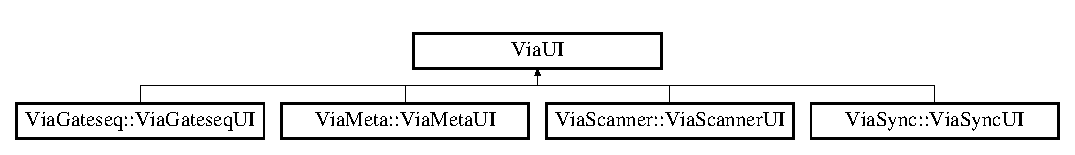
\includegraphics[height=1.637427cm]{class_via_u_i}
\end{center}
\end{figure}
\subsection*{Public Member Functions}
\begin{DoxyCompactItemize}
\item 
virtual void \mbox{\hyperlink{class_via_u_i_a99373a450c4c494a6261edbfc3b21fd9}{transition}} (void(Via\+U\+I\+::$\ast$func)(int32\+\_\+t))
\item 
void \mbox{\hyperlink{class_via_u_i_af80f2151bdd13bc6e84517064100ed92}{default\+Menu}} (int32\+\_\+t sig)
\item 
void \mbox{\hyperlink{class_via_u_i_ac0e9dd4f7b102c712e14d9ee062dcaf7}{new\+Mode\+Menu}} (int32\+\_\+t sig)
\item 
void \mbox{\hyperlink{class_via_u_i_a104b7dbb35cab9ac82b61f364052dc07}{new\+Aux\+Mode\+Menu}} (int32\+\_\+t sig)
\item 
void \mbox{\hyperlink{class_via_u_i_a4d97fe8dca5340f69e5b4441928e4364}{button4\+Menu}} (int32\+\_\+t sig)
\item 
void \mbox{\hyperlink{class_via_u_i_ae921a22294017c3a1aa3e670d30768a1}{button1\+Menu}} (int32\+\_\+t sig)
\item 
void \mbox{\hyperlink{class_via_u_i_a98cab09e693942478ce7136e3077276a}{button2\+Menu}} (int32\+\_\+t sig)
\item 
void \mbox{\hyperlink{class_via_u_i_a0d3e2a3c83ad6781e9e403062131d205}{button5\+Menu}} (int32\+\_\+t sig)
\item 
void \mbox{\hyperlink{class_via_u_i_a4c6811c74f2c1cfadd84be925ed905fc}{button3\+Menu}} (int32\+\_\+t sig)
\item 
void \mbox{\hyperlink{class_via_u_i_aed3d9b75b2d67b17a5596597aa59cf26}{button6\+Menu}} (int32\+\_\+t sig)
\item 
void \mbox{\hyperlink{class_via_u_i_aaee6701bf5a06d4064caa2443d96f61d}{aux1\+Menu}} (int32\+\_\+t sig)
\item 
void \mbox{\hyperlink{class_via_u_i_a928f20f199d42ce05487d5ed7bffd574}{aux2\+Menu}} (int32\+\_\+t sig)
\item 
void \mbox{\hyperlink{class_via_u_i_adf31f9ee348422bc4536f5fc1ef401a4}{aux2\+Menu\+Alt}} (int32\+\_\+t sig)
\item 
void \mbox{\hyperlink{class_via_u_i_adf0e11621a20477354eb1169c3943cb8}{aux3\+Menu}} (int32\+\_\+t sig)
\item 
void \mbox{\hyperlink{class_via_u_i_a9e082c0b454b4fe05a9fc48ca922f9b5}{aux4\+Menu}} (int32\+\_\+t sig)
\item 
void \mbox{\hyperlink{class_via_u_i_a5a2d75e2625e2b55f0588ba8925fe45f}{preset\+Menu}} (int32\+\_\+t sig)
\item 
void \mbox{\hyperlink{class_via_u_i_a3f67bd0f296939ab1be2bdef56858fd6}{preset\+Pressed\+Menu}} (int32\+\_\+t sig)
\item 
void \mbox{\hyperlink{class_via_u_i_a3ead361fc18c9079dcd97b9f34124898}{new\+Preset}} (int32\+\_\+t sig)
\item 
void \mbox{\hyperlink{class_via_u_i_af3a811550d54835d446c425dc57fa157}{switch\+Preset}} (int32\+\_\+t sig)
\item 
void \mbox{\hyperlink{class_via_u_i_a04eb56786faec693ef8cbf4d41384ca1}{factory\+Reset}} (int32\+\_\+t sig)
\item 
virtual void \mbox{\hyperlink{class_via_u_i_a5bdacaef84e33fb3d9b3dd50d1b269d1}{button1\+Tap\+Callback}} (void)=0
\item 
virtual void \mbox{\hyperlink{class_via_u_i_a62145ce1c1b664ff0a1aadaac9386162}{button1\+Hold\+Callback}} (void)=0
\item 
virtual void \mbox{\hyperlink{class_via_u_i_a8fce17e375ea6fe3a4746bff3e6dec75}{button2\+Tap\+Callback}} (void)=0
\item 
virtual void \mbox{\hyperlink{class_via_u_i_a95bce2d662a8ae46be73497e868aebb9}{button2\+Hold\+Callback}} (void)=0
\item 
virtual void \mbox{\hyperlink{class_via_u_i_a3dfd40d901aaa8c8310bdbf75f4432a5}{button3\+Tap\+Callback}} (void)=0
\item 
virtual void \mbox{\hyperlink{class_via_u_i_a7334aea36cf78afac284dd5e899e8ace}{button3\+Hold\+Callback}} (void)=0
\item 
virtual void \mbox{\hyperlink{class_via_u_i_a4925f089aa720ca88d84246f434112e9}{button4\+Tap\+Callback}} (void)=0
\item 
virtual void \mbox{\hyperlink{class_via_u_i_a11919091b39319fe4d1b3a3f3c7104c5}{button4\+Hold\+Callback}} (void)=0
\item 
virtual void \mbox{\hyperlink{class_via_u_i_a5066c22385f31c24ec939d680a66a628}{button5\+Tap\+Callback}} (void)=0
\item 
virtual void \mbox{\hyperlink{class_via_u_i_aee783713c816e3807514ee9b06b571b0}{button5\+Hold\+Callback}} (void)=0
\item 
virtual void \mbox{\hyperlink{class_via_u_i_a8a6bf29d336faa8e9d026a84be45d956}{button6\+Tap\+Callback}} (void)=0
\item 
virtual void \mbox{\hyperlink{class_via_u_i_afa66f7946b6cf755b94383715b26a651}{button6\+Hold\+Callback}} (void)=0
\item 
virtual void \mbox{\hyperlink{class_via_u_i_a2942ec6f7d495159258e1f1803e62c4d}{aux1\+Tap\+Callback}} (void)=0
\item 
virtual void \mbox{\hyperlink{class_via_u_i_a6fcc3b7cf9b97ccf403ed1817cb10d1d}{aux1\+Hold\+Callback}} (void)=0
\item 
virtual void \mbox{\hyperlink{class_via_u_i_ae5e009dc22002f62e6bff8dd76d2f745}{aux2\+Tap\+Callback}} (void)=0
\item 
virtual void \mbox{\hyperlink{class_via_u_i_a42545b69c2bbbb036f633140fd8007d6}{aux2\+Hold\+Callback}} (void)=0
\item 
virtual void \mbox{\hyperlink{class_via_u_i_ad13d74c0bd271b83b8da662b22713ddb}{aux2\+Alt\+Tap\+Callback}} (void)=0
\item 
virtual void \mbox{\hyperlink{class_via_u_i_ab93989ef608d1b63b854b54278006f49}{aux2\+Alt\+Hold\+Callback}} (void)=0
\item 
virtual void \mbox{\hyperlink{class_via_u_i_a29026efd361a615374adce2462aa652a}{aux3\+Tap\+Callback}} (void)=0
\item 
virtual void \mbox{\hyperlink{class_via_u_i_a9ea505dfd800b261beabe8dc47b201d3}{aux3\+Hold\+Callback}} (void)=0
\item 
virtual void \mbox{\hyperlink{class_via_u_i_a0a43c527f027d11b266080d8cacb1d65}{aux4\+Tap\+Callback}} (void)=0
\item 
virtual void \mbox{\hyperlink{class_via_u_i_a884790ab6dac8e6f49104146ff620512}{aux4\+Hold\+Callback}} (void)=0
\item 
virtual void \mbox{\hyperlink{class_via_u_i_a226eb7b65b6035a611dd734d965fa7c2}{default\+Enter\+Menu\+Callback}} (void)=0
\item 
virtual void \mbox{\hyperlink{class_via_u_i_a2ebd72eaa0d26437d2c6320eb5fdf3e4}{new\+Mode\+Enter\+Menu\+Callback}} (void)=0
\item 
virtual void \mbox{\hyperlink{class_via_u_i_a6fdbe125cd3652807631631edc636d39}{new\+Aux\+Mode\+Enter\+Menu\+Callback}} (void)=0
\item 
virtual void \mbox{\hyperlink{class_via_u_i_ad4dfd9fa424267358cab83bec4ee1f23}{preset\+Enter\+Menu\+Callback}} (void)=0
\item 
virtual void \mbox{\hyperlink{class_via_u_i_ae00249c10af94437c357222328a56f82}{button1\+Enter\+Menu\+Callback}} (void)=0
\item 
virtual void \mbox{\hyperlink{class_via_u_i_ac7b7f919edba9a640e7009e1f9303a2d}{button2\+Enter\+Menu\+Callback}} (void)=0
\item 
virtual void \mbox{\hyperlink{class_via_u_i_a883081e46324dec82ad89f2e77cf4b65}{button3\+Enter\+Menu\+Callback}} (void)=0
\item 
virtual void \mbox{\hyperlink{class_via_u_i_a6db24e53e559b6fddd4cb1f918de40d6}{button4\+Enter\+Menu\+Callback}} (void)=0
\item 
virtual void \mbox{\hyperlink{class_via_u_i_adb40844fb1fa8e623f3a7eaecdbfad53}{button5\+Enter\+Menu\+Callback}} (void)=0
\item 
virtual void \mbox{\hyperlink{class_via_u_i_ae59e7ff3a6ba1f641a4a916e47a26513}{button6\+Enter\+Menu\+Callback}} (void)=0
\item 
virtual void \mbox{\hyperlink{class_via_u_i_a578111861e912bf43d3f320a0faffb0f}{aux1\+Enter\+Menu\+Callback}} (void)=0
\item 
virtual void \mbox{\hyperlink{class_via_u_i_a1f51fc259471364f91bd0a1592824dab}{aux2\+Enter\+Menu\+Callback}} (void)=0
\item 
virtual void \mbox{\hyperlink{class_via_u_i_a08a746b666d37ac6bc293303187fd6be}{aux2\+Alt\+Enter\+Menu\+Callback}} (void)=0
\item 
virtual void \mbox{\hyperlink{class_via_u_i_aa62c9f8dc58d37fc2a3abc7bce1cd16e}{aux3\+Enter\+Menu\+Callback}} (void)=0
\item 
virtual void \mbox{\hyperlink{class_via_u_i_a36cc4bac8f774c2a59ab8635be05f884}{aux4\+Enter\+Menu\+Callback}} (void)=0
\item 
virtual void \mbox{\hyperlink{class_via_u_i_a4bd3d575f4efe1273d6e4645454ead52}{ui\+Set\+L\+E\+Ds}} (int)=0
\item 
virtual void \mbox{\hyperlink{class_via_u_i_ac5b88708650fe41ea955c77de580f6f5}{recall\+Module\+State}} (void)=0
\item 
virtual void \mbox{\hyperlink{class_via_u_i_a573ba7aef8f4982ec4900258c770bdbb}{initialize}} (void)=0
\item 
virtual \mbox{\hyperlink{class_via_u_i_ad60e005bc6a105009be39325664e5a32}{$\sim$\+Via\+UI}} (void)
\item 
void \mbox{\hyperlink{class_via_u_i_ac7abd4e9e7fa598dedab8b4c2486d010}{reset\+Timer\+Menu}} (void)
\item 
void \mbox{\hyperlink{class_via_u_i_aecfaa511595dcab4d38caff73abdd54b}{load\+From\+E\+E\+P\+R\+OM}} (int32\+\_\+t)
\item 
void \mbox{\hyperlink{class_via_u_i_a09fbb5e879fb9e2e77c4642dae4ab83a}{store\+To\+E\+E\+P\+R\+OM}} (int32\+\_\+t)
\item 
int32\+\_\+t \mbox{\hyperlink{class_via_u_i_a301e1692cc55b1ee55ba0133b5308f87}{increment\+Mode\+And\+Store}} (int32\+\_\+t, int32\+\_\+t, int32\+\_\+t, int32\+\_\+t)
\item 
int32\+\_\+t \mbox{\hyperlink{class_via_u_i_a85d24875e904ac7cf63f0762e1ccb3c0}{decrement\+Mode\+And\+Store}} (int32\+\_\+t, int32\+\_\+t, int32\+\_\+t, int32\+\_\+t)
\item 
void \mbox{\hyperlink{class_via_u_i_ae8bb5e76df4a1b3c1127829bd1be21f7}{dispatch}} (int32\+\_\+t)
\end{DoxyCompactItemize}
\subsection*{Public Attributes}
\begin{DoxyCompactItemize}
\item 
void(Via\+U\+I\+::$\ast$ \mbox{\hyperlink{class_via_u_i_a2a76b36f571915b19355c7edde8a1e51}{state}} )(int32\+\_\+t)
\item 
int32\+\_\+t \mbox{\hyperlink{class_via_u_i_ad745eabb8155c8cff717186abd592c31}{virtual\+Timer}} = 0
\item 
int32\+\_\+t \mbox{\hyperlink{class_via_u_i_af3a32c849a2beba464d1dfcfd4e60e03}{virtual\+Timer\+Enable}} = 0
\item 
int32\+\_\+t \mbox{\hyperlink{class_via_u_i_ad3c77ffd0df89def606de5120e4ace3a}{virtual\+Timer\+Overflow}} = 0
\item 
int32\+\_\+t $\ast$ \mbox{\hyperlink{class_via_u_i_ae21314791ad42cf8861de1805f7215f3}{button1}}
\item 
int32\+\_\+t $\ast$ \mbox{\hyperlink{class_via_u_i_aa4c4d36de9b8fe45760f82ec27ef38c5}{button2}}
\item 
int32\+\_\+t $\ast$ \mbox{\hyperlink{class_via_u_i_a21b5860f22c411180962f666536275a8}{button3}}
\item 
int32\+\_\+t $\ast$ \mbox{\hyperlink{class_via_u_i_ac44fee28673f0ac9ccff114b33332ace}{button4}}
\item 
int32\+\_\+t $\ast$ \mbox{\hyperlink{class_via_u_i_a0a6dd5e3f8dbd2d022cc583d3be36b73}{button5}}
\item 
int32\+\_\+t $\ast$ \mbox{\hyperlink{class_via_u_i_aed379b5b020972bf3d54b8af10f65679}{button6}}
\item 
int32\+\_\+t \mbox{\hyperlink{class_via_u_i_a8a81f061606813d7892008085ac49177}{mode\+State\+Buffer}} = 0
\item 
int32\+\_\+t \mbox{\hyperlink{class_via_u_i_ab9291e1380236cd7a47c61682764af74}{preset\+Number}} = 0
\item 
int32\+\_\+t \mbox{\hyperlink{class_via_u_i_a8d86fda886f62fb6b309b4e877351fd7}{button1\+Mode}} = 0
\item 
int32\+\_\+t \mbox{\hyperlink{class_via_u_i_a7efad7acb6db1c15f67ad03adc549376}{button2\+Mode}} = 0
\item 
int32\+\_\+t \mbox{\hyperlink{class_via_u_i_a333cb2f60cdd7dec0ffd45ad4aac31c4}{button3\+Mode}} = 0
\item 
int32\+\_\+t \mbox{\hyperlink{class_via_u_i_a571d0626912f4067cf893134506d9aa4}{button4\+Mode}} = 0
\item 
int32\+\_\+t \mbox{\hyperlink{class_via_u_i_a81ebe08ffb4b0318317d859291314fb8}{button5\+Mode}} = 0
\item 
int32\+\_\+t \mbox{\hyperlink{class_via_u_i_a9421e095ab94090aceed254332b535f9}{button6\+Mode}} = 0
\item 
int32\+\_\+t \mbox{\hyperlink{class_via_u_i_aaab0b4a294ded73b9ac59d387a94b854}{aux1\+Mode}} = 0
\item 
int32\+\_\+t \mbox{\hyperlink{class_via_u_i_ae52e25594e34359538ee1de8d3710dfc}{aux2\+Mode}} = 0
\item 
int32\+\_\+t \mbox{\hyperlink{class_via_u_i_a3959f2ca0cf9cf711d5a63c15ec922f7}{aux3\+Mode}} = 0
\item 
int32\+\_\+t \mbox{\hyperlink{class_via_u_i_aef749bb156d3aace85d80bde2f847651}{aux4\+Mode}} = 0
\end{DoxyCompactItemize}


\subsection{Constructor \& Destructor Documentation}
\mbox{\Hypertarget{class_via_u_i_ad60e005bc6a105009be39325664e5a32}\label{class_via_u_i_ad60e005bc6a105009be39325664e5a32}} 
\index{Via\+UI@{Via\+UI}!````~Via\+UI@{$\sim$\+Via\+UI}}
\index{````~Via\+UI@{$\sim$\+Via\+UI}!Via\+UI@{Via\+UI}}
\subsubsection{\texorpdfstring{$\sim$\+Via\+U\+I()}{~ViaUI()}}
{\footnotesize\ttfamily virtual Via\+U\+I\+::$\sim$\+Via\+UI (\begin{DoxyParamCaption}\item[{void}]{ }\end{DoxyParamCaption})\hspace{0.3cm}{\ttfamily [inline]}, {\ttfamily [virtual]}}



\subsection{Member Function Documentation}
\mbox{\Hypertarget{class_via_u_i_a578111861e912bf43d3f320a0faffb0f}\label{class_via_u_i_a578111861e912bf43d3f320a0faffb0f}} 
\index{Via\+UI@{Via\+UI}!aux1\+Enter\+Menu\+Callback@{aux1\+Enter\+Menu\+Callback}}
\index{aux1\+Enter\+Menu\+Callback@{aux1\+Enter\+Menu\+Callback}!Via\+UI@{Via\+UI}}
\subsubsection{\texorpdfstring{aux1\+Enter\+Menu\+Callback()}{aux1EnterMenuCallback()}}
{\footnotesize\ttfamily virtual void Via\+U\+I\+::aux1\+Enter\+Menu\+Callback (\begin{DoxyParamCaption}\item[{void}]{ }\end{DoxyParamCaption})\hspace{0.3cm}{\ttfamily [pure virtual]}}



Implemented in \mbox{\hyperlink{class_via_scanner_1_1_via_scanner_u_i_a4ca2d4cfed7e8e23f056c622a825c085}{Via\+Scanner\+::\+Via\+Scanner\+UI}}, \mbox{\hyperlink{class_via_gateseq_1_1_via_gateseq_u_i_ae1a1c7c97151e09b2e6b136f0c1efe6e}{Via\+Gateseq\+::\+Via\+Gateseq\+UI}}, \mbox{\hyperlink{class_via_sync_1_1_via_sync_u_i_a9e9fd5bc4d9d9cfe255a8cf099ba5110}{Via\+Sync\+::\+Via\+Sync\+UI}}, and \mbox{\hyperlink{class_via_meta_1_1_via_meta_u_i_a84e9b3d83d81753db095d67dee1fe8b9}{Via\+Meta\+::\+Via\+Meta\+UI}}.

\mbox{\Hypertarget{class_via_u_i_a6fcc3b7cf9b97ccf403ed1817cb10d1d}\label{class_via_u_i_a6fcc3b7cf9b97ccf403ed1817cb10d1d}} 
\index{Via\+UI@{Via\+UI}!aux1\+Hold\+Callback@{aux1\+Hold\+Callback}}
\index{aux1\+Hold\+Callback@{aux1\+Hold\+Callback}!Via\+UI@{Via\+UI}}
\subsubsection{\texorpdfstring{aux1\+Hold\+Callback()}{aux1HoldCallback()}}
{\footnotesize\ttfamily virtual void Via\+U\+I\+::aux1\+Hold\+Callback (\begin{DoxyParamCaption}\item[{void}]{ }\end{DoxyParamCaption})\hspace{0.3cm}{\ttfamily [pure virtual]}}



Implemented in \mbox{\hyperlink{class_via_scanner_1_1_via_scanner_u_i_a634c06fae2a1a17e5f3737dd44b34e10}{Via\+Scanner\+::\+Via\+Scanner\+UI}}, \mbox{\hyperlink{class_via_gateseq_1_1_via_gateseq_u_i_ac0a66889f6859802f3594031f81f05f3}{Via\+Gateseq\+::\+Via\+Gateseq\+UI}}, \mbox{\hyperlink{class_via_sync_1_1_via_sync_u_i_aaa66c2014e79270140575713998d67ae}{Via\+Sync\+::\+Via\+Sync\+UI}}, and \mbox{\hyperlink{class_via_meta_1_1_via_meta_u_i_a1c38639df8fdb4a866622388548bc9db}{Via\+Meta\+::\+Via\+Meta\+UI}}.

\mbox{\Hypertarget{class_via_u_i_aaee6701bf5a06d4064caa2443d96f61d}\label{class_via_u_i_aaee6701bf5a06d4064caa2443d96f61d}} 
\index{Via\+UI@{Via\+UI}!aux1\+Menu@{aux1\+Menu}}
\index{aux1\+Menu@{aux1\+Menu}!Via\+UI@{Via\+UI}}
\subsubsection{\texorpdfstring{aux1\+Menu()}{aux1Menu()}}
{\footnotesize\ttfamily void Via\+U\+I\+::aux1\+Menu (\begin{DoxyParamCaption}\item[{int32\+\_\+t}]{sig }\end{DoxyParamCaption})}

\mbox{\Hypertarget{class_via_u_i_a2942ec6f7d495159258e1f1803e62c4d}\label{class_via_u_i_a2942ec6f7d495159258e1f1803e62c4d}} 
\index{Via\+UI@{Via\+UI}!aux1\+Tap\+Callback@{aux1\+Tap\+Callback}}
\index{aux1\+Tap\+Callback@{aux1\+Tap\+Callback}!Via\+UI@{Via\+UI}}
\subsubsection{\texorpdfstring{aux1\+Tap\+Callback()}{aux1TapCallback()}}
{\footnotesize\ttfamily virtual void Via\+U\+I\+::aux1\+Tap\+Callback (\begin{DoxyParamCaption}\item[{void}]{ }\end{DoxyParamCaption})\hspace{0.3cm}{\ttfamily [pure virtual]}}



Implemented in \mbox{\hyperlink{class_via_scanner_1_1_via_scanner_u_i_af7e91846bdd9922b309580adf4fe653b}{Via\+Scanner\+::\+Via\+Scanner\+UI}}, \mbox{\hyperlink{class_via_gateseq_1_1_via_gateseq_u_i_a3f44c4a89f3f7aedff958e903e6c71b5}{Via\+Gateseq\+::\+Via\+Gateseq\+UI}}, \mbox{\hyperlink{class_via_sync_1_1_via_sync_u_i_a53f8add06247c8ed4e7a1c049e8136fb}{Via\+Sync\+::\+Via\+Sync\+UI}}, and \mbox{\hyperlink{class_via_meta_1_1_via_meta_u_i_ad95b464f8dda873be1c24622d1f082fa}{Via\+Meta\+::\+Via\+Meta\+UI}}.

\mbox{\Hypertarget{class_via_u_i_a08a746b666d37ac6bc293303187fd6be}\label{class_via_u_i_a08a746b666d37ac6bc293303187fd6be}} 
\index{Via\+UI@{Via\+UI}!aux2\+Alt\+Enter\+Menu\+Callback@{aux2\+Alt\+Enter\+Menu\+Callback}}
\index{aux2\+Alt\+Enter\+Menu\+Callback@{aux2\+Alt\+Enter\+Menu\+Callback}!Via\+UI@{Via\+UI}}
\subsubsection{\texorpdfstring{aux2\+Alt\+Enter\+Menu\+Callback()}{aux2AltEnterMenuCallback()}}
{\footnotesize\ttfamily virtual void Via\+U\+I\+::aux2\+Alt\+Enter\+Menu\+Callback (\begin{DoxyParamCaption}\item[{void}]{ }\end{DoxyParamCaption})\hspace{0.3cm}{\ttfamily [pure virtual]}}



Implemented in \mbox{\hyperlink{class_via_scanner_1_1_via_scanner_u_i_a649f3b095e254e2e2049c91f5c9543b2}{Via\+Scanner\+::\+Via\+Scanner\+UI}}, \mbox{\hyperlink{class_via_gateseq_1_1_via_gateseq_u_i_a39db35560b35c8fafeaabef258be61d8}{Via\+Gateseq\+::\+Via\+Gateseq\+UI}}, \mbox{\hyperlink{class_via_sync_1_1_via_sync_u_i_a6a382c3c2660d7f232d38f5a4f7da110}{Via\+Sync\+::\+Via\+Sync\+UI}}, and \mbox{\hyperlink{class_via_meta_1_1_via_meta_u_i_ab0ccbc22f2460565456b8347d18634b8}{Via\+Meta\+::\+Via\+Meta\+UI}}.

\mbox{\Hypertarget{class_via_u_i_ab93989ef608d1b63b854b54278006f49}\label{class_via_u_i_ab93989ef608d1b63b854b54278006f49}} 
\index{Via\+UI@{Via\+UI}!aux2\+Alt\+Hold\+Callback@{aux2\+Alt\+Hold\+Callback}}
\index{aux2\+Alt\+Hold\+Callback@{aux2\+Alt\+Hold\+Callback}!Via\+UI@{Via\+UI}}
\subsubsection{\texorpdfstring{aux2\+Alt\+Hold\+Callback()}{aux2AltHoldCallback()}}
{\footnotesize\ttfamily virtual void Via\+U\+I\+::aux2\+Alt\+Hold\+Callback (\begin{DoxyParamCaption}\item[{void}]{ }\end{DoxyParamCaption})\hspace{0.3cm}{\ttfamily [pure virtual]}}



Implemented in \mbox{\hyperlink{class_via_scanner_1_1_via_scanner_u_i_ae1947196ca5cb248c4bc177f02cb20f5}{Via\+Scanner\+::\+Via\+Scanner\+UI}}, \mbox{\hyperlink{class_via_gateseq_1_1_via_gateseq_u_i_ada61d29fe8fd743edbb49500ee6e3d27}{Via\+Gateseq\+::\+Via\+Gateseq\+UI}}, \mbox{\hyperlink{class_via_sync_1_1_via_sync_u_i_af6b69d61a650e68e37286490191634ed}{Via\+Sync\+::\+Via\+Sync\+UI}}, and \mbox{\hyperlink{class_via_meta_1_1_via_meta_u_i_a372fe7280f3107f81e7283ba7451efd6}{Via\+Meta\+::\+Via\+Meta\+UI}}.

\mbox{\Hypertarget{class_via_u_i_ad13d74c0bd271b83b8da662b22713ddb}\label{class_via_u_i_ad13d74c0bd271b83b8da662b22713ddb}} 
\index{Via\+UI@{Via\+UI}!aux2\+Alt\+Tap\+Callback@{aux2\+Alt\+Tap\+Callback}}
\index{aux2\+Alt\+Tap\+Callback@{aux2\+Alt\+Tap\+Callback}!Via\+UI@{Via\+UI}}
\subsubsection{\texorpdfstring{aux2\+Alt\+Tap\+Callback()}{aux2AltTapCallback()}}
{\footnotesize\ttfamily virtual void Via\+U\+I\+::aux2\+Alt\+Tap\+Callback (\begin{DoxyParamCaption}\item[{void}]{ }\end{DoxyParamCaption})\hspace{0.3cm}{\ttfamily [pure virtual]}}



Implemented in \mbox{\hyperlink{class_via_scanner_1_1_via_scanner_u_i_aa862c7243959f99bfd42995102ffcdf5}{Via\+Scanner\+::\+Via\+Scanner\+UI}}, \mbox{\hyperlink{class_via_gateseq_1_1_via_gateseq_u_i_a84c1f0f19956b81f81a7fba2b6581f99}{Via\+Gateseq\+::\+Via\+Gateseq\+UI}}, \mbox{\hyperlink{class_via_sync_1_1_via_sync_u_i_ad837068e55fb66fe3fe2aa15ff90ec21}{Via\+Sync\+::\+Via\+Sync\+UI}}, and \mbox{\hyperlink{class_via_meta_1_1_via_meta_u_i_a5982022f5c08ce9aaa75173209d30e6c}{Via\+Meta\+::\+Via\+Meta\+UI}}.

\mbox{\Hypertarget{class_via_u_i_a1f51fc259471364f91bd0a1592824dab}\label{class_via_u_i_a1f51fc259471364f91bd0a1592824dab}} 
\index{Via\+UI@{Via\+UI}!aux2\+Enter\+Menu\+Callback@{aux2\+Enter\+Menu\+Callback}}
\index{aux2\+Enter\+Menu\+Callback@{aux2\+Enter\+Menu\+Callback}!Via\+UI@{Via\+UI}}
\subsubsection{\texorpdfstring{aux2\+Enter\+Menu\+Callback()}{aux2EnterMenuCallback()}}
{\footnotesize\ttfamily virtual void Via\+U\+I\+::aux2\+Enter\+Menu\+Callback (\begin{DoxyParamCaption}\item[{void}]{ }\end{DoxyParamCaption})\hspace{0.3cm}{\ttfamily [pure virtual]}}



Implemented in \mbox{\hyperlink{class_via_scanner_1_1_via_scanner_u_i_a5173aaf7222a059fa7d3a4b32f6fb275}{Via\+Scanner\+::\+Via\+Scanner\+UI}}, \mbox{\hyperlink{class_via_gateseq_1_1_via_gateseq_u_i_a3f3270689385b4ba7449599538aafc59}{Via\+Gateseq\+::\+Via\+Gateseq\+UI}}, \mbox{\hyperlink{class_via_sync_1_1_via_sync_u_i_a8af905460e4d9b91420fa557be0baeae}{Via\+Sync\+::\+Via\+Sync\+UI}}, and \mbox{\hyperlink{class_via_meta_1_1_via_meta_u_i_a31e89fca82851581b9ad7161cd81c6c0}{Via\+Meta\+::\+Via\+Meta\+UI}}.

\mbox{\Hypertarget{class_via_u_i_a42545b69c2bbbb036f633140fd8007d6}\label{class_via_u_i_a42545b69c2bbbb036f633140fd8007d6}} 
\index{Via\+UI@{Via\+UI}!aux2\+Hold\+Callback@{aux2\+Hold\+Callback}}
\index{aux2\+Hold\+Callback@{aux2\+Hold\+Callback}!Via\+UI@{Via\+UI}}
\subsubsection{\texorpdfstring{aux2\+Hold\+Callback()}{aux2HoldCallback()}}
{\footnotesize\ttfamily virtual void Via\+U\+I\+::aux2\+Hold\+Callback (\begin{DoxyParamCaption}\item[{void}]{ }\end{DoxyParamCaption})\hspace{0.3cm}{\ttfamily [pure virtual]}}



Implemented in \mbox{\hyperlink{class_via_scanner_1_1_via_scanner_u_i_a929ba662a65fd62f9c5b122accad48a4}{Via\+Scanner\+::\+Via\+Scanner\+UI}}, \mbox{\hyperlink{class_via_gateseq_1_1_via_gateseq_u_i_a825cc56cdbeffd7eee887e8f189cb35d}{Via\+Gateseq\+::\+Via\+Gateseq\+UI}}, \mbox{\hyperlink{class_via_sync_1_1_via_sync_u_i_af692a47db686fac2e929549217452258}{Via\+Sync\+::\+Via\+Sync\+UI}}, and \mbox{\hyperlink{class_via_meta_1_1_via_meta_u_i_a19cac5da8e89446d5ee2a2c889a6c555}{Via\+Meta\+::\+Via\+Meta\+UI}}.

\mbox{\Hypertarget{class_via_u_i_a928f20f199d42ce05487d5ed7bffd574}\label{class_via_u_i_a928f20f199d42ce05487d5ed7bffd574}} 
\index{Via\+UI@{Via\+UI}!aux2\+Menu@{aux2\+Menu}}
\index{aux2\+Menu@{aux2\+Menu}!Via\+UI@{Via\+UI}}
\subsubsection{\texorpdfstring{aux2\+Menu()}{aux2Menu()}}
{\footnotesize\ttfamily void Via\+U\+I\+::aux2\+Menu (\begin{DoxyParamCaption}\item[{int32\+\_\+t}]{sig }\end{DoxyParamCaption})}

\mbox{\Hypertarget{class_via_u_i_adf31f9ee348422bc4536f5fc1ef401a4}\label{class_via_u_i_adf31f9ee348422bc4536f5fc1ef401a4}} 
\index{Via\+UI@{Via\+UI}!aux2\+Menu\+Alt@{aux2\+Menu\+Alt}}
\index{aux2\+Menu\+Alt@{aux2\+Menu\+Alt}!Via\+UI@{Via\+UI}}
\subsubsection{\texorpdfstring{aux2\+Menu\+Alt()}{aux2MenuAlt()}}
{\footnotesize\ttfamily void Via\+U\+I\+::aux2\+Menu\+Alt (\begin{DoxyParamCaption}\item[{int32\+\_\+t}]{sig }\end{DoxyParamCaption})}

\mbox{\Hypertarget{class_via_u_i_ae5e009dc22002f62e6bff8dd76d2f745}\label{class_via_u_i_ae5e009dc22002f62e6bff8dd76d2f745}} 
\index{Via\+UI@{Via\+UI}!aux2\+Tap\+Callback@{aux2\+Tap\+Callback}}
\index{aux2\+Tap\+Callback@{aux2\+Tap\+Callback}!Via\+UI@{Via\+UI}}
\subsubsection{\texorpdfstring{aux2\+Tap\+Callback()}{aux2TapCallback()}}
{\footnotesize\ttfamily virtual void Via\+U\+I\+::aux2\+Tap\+Callback (\begin{DoxyParamCaption}\item[{void}]{ }\end{DoxyParamCaption})\hspace{0.3cm}{\ttfamily [pure virtual]}}



Implemented in \mbox{\hyperlink{class_via_scanner_1_1_via_scanner_u_i_a7d3aad2399479925618df242bc5b1f42}{Via\+Scanner\+::\+Via\+Scanner\+UI}}, \mbox{\hyperlink{class_via_gateseq_1_1_via_gateseq_u_i_a8e700657f1fe190238eca7c46541337b}{Via\+Gateseq\+::\+Via\+Gateseq\+UI}}, \mbox{\hyperlink{class_via_sync_1_1_via_sync_u_i_a117e57feaf74b2619c1506aacc421721}{Via\+Sync\+::\+Via\+Sync\+UI}}, and \mbox{\hyperlink{class_via_meta_1_1_via_meta_u_i_a2d1e0164ad7d84c410cc90cefe9730ce}{Via\+Meta\+::\+Via\+Meta\+UI}}.

\mbox{\Hypertarget{class_via_u_i_aa62c9f8dc58d37fc2a3abc7bce1cd16e}\label{class_via_u_i_aa62c9f8dc58d37fc2a3abc7bce1cd16e}} 
\index{Via\+UI@{Via\+UI}!aux3\+Enter\+Menu\+Callback@{aux3\+Enter\+Menu\+Callback}}
\index{aux3\+Enter\+Menu\+Callback@{aux3\+Enter\+Menu\+Callback}!Via\+UI@{Via\+UI}}
\subsubsection{\texorpdfstring{aux3\+Enter\+Menu\+Callback()}{aux3EnterMenuCallback()}}
{\footnotesize\ttfamily virtual void Via\+U\+I\+::aux3\+Enter\+Menu\+Callback (\begin{DoxyParamCaption}\item[{void}]{ }\end{DoxyParamCaption})\hspace{0.3cm}{\ttfamily [pure virtual]}}



Implemented in \mbox{\hyperlink{class_via_scanner_1_1_via_scanner_u_i_ade6dc0e93911fe51731bffa65990599a}{Via\+Scanner\+::\+Via\+Scanner\+UI}}, \mbox{\hyperlink{class_via_gateseq_1_1_via_gateseq_u_i_a8235806bb28a40062b89b1cb9c83e3b0}{Via\+Gateseq\+::\+Via\+Gateseq\+UI}}, \mbox{\hyperlink{class_via_sync_1_1_via_sync_u_i_a66f7a9ccbfff3b1b1ba32fe775808703}{Via\+Sync\+::\+Via\+Sync\+UI}}, and \mbox{\hyperlink{class_via_meta_1_1_via_meta_u_i_a31f9a7e08ee2d77d7aa96b644369e92d}{Via\+Meta\+::\+Via\+Meta\+UI}}.

\mbox{\Hypertarget{class_via_u_i_a9ea505dfd800b261beabe8dc47b201d3}\label{class_via_u_i_a9ea505dfd800b261beabe8dc47b201d3}} 
\index{Via\+UI@{Via\+UI}!aux3\+Hold\+Callback@{aux3\+Hold\+Callback}}
\index{aux3\+Hold\+Callback@{aux3\+Hold\+Callback}!Via\+UI@{Via\+UI}}
\subsubsection{\texorpdfstring{aux3\+Hold\+Callback()}{aux3HoldCallback()}}
{\footnotesize\ttfamily virtual void Via\+U\+I\+::aux3\+Hold\+Callback (\begin{DoxyParamCaption}\item[{void}]{ }\end{DoxyParamCaption})\hspace{0.3cm}{\ttfamily [pure virtual]}}



Implemented in \mbox{\hyperlink{class_via_scanner_1_1_via_scanner_u_i_ac79b09eb94d39065b6b5061d34746862}{Via\+Scanner\+::\+Via\+Scanner\+UI}}, \mbox{\hyperlink{class_via_gateseq_1_1_via_gateseq_u_i_a5b18aa40706a39ed8878143d6911bc78}{Via\+Gateseq\+::\+Via\+Gateseq\+UI}}, \mbox{\hyperlink{class_via_sync_1_1_via_sync_u_i_ae35a16d1e3a6158ffd306b06e93b16a4}{Via\+Sync\+::\+Via\+Sync\+UI}}, and \mbox{\hyperlink{class_via_meta_1_1_via_meta_u_i_ad15168253fc76c7a938ca467ada12ade}{Via\+Meta\+::\+Via\+Meta\+UI}}.

\mbox{\Hypertarget{class_via_u_i_adf0e11621a20477354eb1169c3943cb8}\label{class_via_u_i_adf0e11621a20477354eb1169c3943cb8}} 
\index{Via\+UI@{Via\+UI}!aux3\+Menu@{aux3\+Menu}}
\index{aux3\+Menu@{aux3\+Menu}!Via\+UI@{Via\+UI}}
\subsubsection{\texorpdfstring{aux3\+Menu()}{aux3Menu()}}
{\footnotesize\ttfamily void Via\+U\+I\+::aux3\+Menu (\begin{DoxyParamCaption}\item[{int32\+\_\+t}]{sig }\end{DoxyParamCaption})}

\mbox{\Hypertarget{class_via_u_i_a29026efd361a615374adce2462aa652a}\label{class_via_u_i_a29026efd361a615374adce2462aa652a}} 
\index{Via\+UI@{Via\+UI}!aux3\+Tap\+Callback@{aux3\+Tap\+Callback}}
\index{aux3\+Tap\+Callback@{aux3\+Tap\+Callback}!Via\+UI@{Via\+UI}}
\subsubsection{\texorpdfstring{aux3\+Tap\+Callback()}{aux3TapCallback()}}
{\footnotesize\ttfamily virtual void Via\+U\+I\+::aux3\+Tap\+Callback (\begin{DoxyParamCaption}\item[{void}]{ }\end{DoxyParamCaption})\hspace{0.3cm}{\ttfamily [pure virtual]}}



Implemented in \mbox{\hyperlink{class_via_scanner_1_1_via_scanner_u_i_a7d15083a3565f56b4b70ac497fddd563}{Via\+Scanner\+::\+Via\+Scanner\+UI}}, \mbox{\hyperlink{class_via_gateseq_1_1_via_gateseq_u_i_a9bb95780740cd9fe650ba38aa3fb86a6}{Via\+Gateseq\+::\+Via\+Gateseq\+UI}}, \mbox{\hyperlink{class_via_sync_1_1_via_sync_u_i_afe95d77f17525a7e612485089a01ab0d}{Via\+Sync\+::\+Via\+Sync\+UI}}, and \mbox{\hyperlink{class_via_meta_1_1_via_meta_u_i_a4f9a282e24dd484d24657a1568defd75}{Via\+Meta\+::\+Via\+Meta\+UI}}.

\mbox{\Hypertarget{class_via_u_i_a36cc4bac8f774c2a59ab8635be05f884}\label{class_via_u_i_a36cc4bac8f774c2a59ab8635be05f884}} 
\index{Via\+UI@{Via\+UI}!aux4\+Enter\+Menu\+Callback@{aux4\+Enter\+Menu\+Callback}}
\index{aux4\+Enter\+Menu\+Callback@{aux4\+Enter\+Menu\+Callback}!Via\+UI@{Via\+UI}}
\subsubsection{\texorpdfstring{aux4\+Enter\+Menu\+Callback()}{aux4EnterMenuCallback()}}
{\footnotesize\ttfamily virtual void Via\+U\+I\+::aux4\+Enter\+Menu\+Callback (\begin{DoxyParamCaption}\item[{void}]{ }\end{DoxyParamCaption})\hspace{0.3cm}{\ttfamily [pure virtual]}}



Implemented in \mbox{\hyperlink{class_via_scanner_1_1_via_scanner_u_i_a34c593dfd035906c09a2cde0024fd48f}{Via\+Scanner\+::\+Via\+Scanner\+UI}}, \mbox{\hyperlink{class_via_gateseq_1_1_via_gateseq_u_i_a78f330f4c02acb69f9c2321a8187f8dc}{Via\+Gateseq\+::\+Via\+Gateseq\+UI}}, \mbox{\hyperlink{class_via_sync_1_1_via_sync_u_i_ab74dfab193404bd23e90ba1b44a0a743}{Via\+Sync\+::\+Via\+Sync\+UI}}, and \mbox{\hyperlink{class_via_meta_1_1_via_meta_u_i_aa6309c2403a8436cc3ec222f7914b202}{Via\+Meta\+::\+Via\+Meta\+UI}}.

\mbox{\Hypertarget{class_via_u_i_a884790ab6dac8e6f49104146ff620512}\label{class_via_u_i_a884790ab6dac8e6f49104146ff620512}} 
\index{Via\+UI@{Via\+UI}!aux4\+Hold\+Callback@{aux4\+Hold\+Callback}}
\index{aux4\+Hold\+Callback@{aux4\+Hold\+Callback}!Via\+UI@{Via\+UI}}
\subsubsection{\texorpdfstring{aux4\+Hold\+Callback()}{aux4HoldCallback()}}
{\footnotesize\ttfamily virtual void Via\+U\+I\+::aux4\+Hold\+Callback (\begin{DoxyParamCaption}\item[{void}]{ }\end{DoxyParamCaption})\hspace{0.3cm}{\ttfamily [pure virtual]}}



Implemented in \mbox{\hyperlink{class_via_scanner_1_1_via_scanner_u_i_af994cf63aa7becc41c9e3dcb2e08d8c2}{Via\+Scanner\+::\+Via\+Scanner\+UI}}, \mbox{\hyperlink{class_via_gateseq_1_1_via_gateseq_u_i_a98c59b4566672aeb522f6cafccd46b72}{Via\+Gateseq\+::\+Via\+Gateseq\+UI}}, \mbox{\hyperlink{class_via_sync_1_1_via_sync_u_i_a15f48c7e1d5f77292ee46d997421cd4e}{Via\+Sync\+::\+Via\+Sync\+UI}}, and \mbox{\hyperlink{class_via_meta_1_1_via_meta_u_i_a2a1cfb3452d150af61f61716aa94f782}{Via\+Meta\+::\+Via\+Meta\+UI}}.

\mbox{\Hypertarget{class_via_u_i_a9e082c0b454b4fe05a9fc48ca922f9b5}\label{class_via_u_i_a9e082c0b454b4fe05a9fc48ca922f9b5}} 
\index{Via\+UI@{Via\+UI}!aux4\+Menu@{aux4\+Menu}}
\index{aux4\+Menu@{aux4\+Menu}!Via\+UI@{Via\+UI}}
\subsubsection{\texorpdfstring{aux4\+Menu()}{aux4Menu()}}
{\footnotesize\ttfamily void Via\+U\+I\+::aux4\+Menu (\begin{DoxyParamCaption}\item[{int32\+\_\+t}]{sig }\end{DoxyParamCaption})}

\mbox{\Hypertarget{class_via_u_i_a0a43c527f027d11b266080d8cacb1d65}\label{class_via_u_i_a0a43c527f027d11b266080d8cacb1d65}} 
\index{Via\+UI@{Via\+UI}!aux4\+Tap\+Callback@{aux4\+Tap\+Callback}}
\index{aux4\+Tap\+Callback@{aux4\+Tap\+Callback}!Via\+UI@{Via\+UI}}
\subsubsection{\texorpdfstring{aux4\+Tap\+Callback()}{aux4TapCallback()}}
{\footnotesize\ttfamily virtual void Via\+U\+I\+::aux4\+Tap\+Callback (\begin{DoxyParamCaption}\item[{void}]{ }\end{DoxyParamCaption})\hspace{0.3cm}{\ttfamily [pure virtual]}}



Implemented in \mbox{\hyperlink{class_via_scanner_1_1_via_scanner_u_i_a8c20c03c838257da356f0071dfcbfd36}{Via\+Scanner\+::\+Via\+Scanner\+UI}}, \mbox{\hyperlink{class_via_gateseq_1_1_via_gateseq_u_i_af12df5bd6d6bb9b069e8c410fcae7473}{Via\+Gateseq\+::\+Via\+Gateseq\+UI}}, \mbox{\hyperlink{class_via_sync_1_1_via_sync_u_i_a1cf7ef02457d9f7887da0721799aadc0}{Via\+Sync\+::\+Via\+Sync\+UI}}, and \mbox{\hyperlink{class_via_meta_1_1_via_meta_u_i_ad8e6300990d654091672b0f94a9b47d8}{Via\+Meta\+::\+Via\+Meta\+UI}}.

\mbox{\Hypertarget{class_via_u_i_ae00249c10af94437c357222328a56f82}\label{class_via_u_i_ae00249c10af94437c357222328a56f82}} 
\index{Via\+UI@{Via\+UI}!button1\+Enter\+Menu\+Callback@{button1\+Enter\+Menu\+Callback}}
\index{button1\+Enter\+Menu\+Callback@{button1\+Enter\+Menu\+Callback}!Via\+UI@{Via\+UI}}
\subsubsection{\texorpdfstring{button1\+Enter\+Menu\+Callback()}{button1EnterMenuCallback()}}
{\footnotesize\ttfamily virtual void Via\+U\+I\+::button1\+Enter\+Menu\+Callback (\begin{DoxyParamCaption}\item[{void}]{ }\end{DoxyParamCaption})\hspace{0.3cm}{\ttfamily [pure virtual]}}



Implemented in \mbox{\hyperlink{class_via_scanner_1_1_via_scanner_u_i_a10b9a54f4fb6ea88203d53041093d650}{Via\+Scanner\+::\+Via\+Scanner\+UI}}, \mbox{\hyperlink{class_via_gateseq_1_1_via_gateseq_u_i_aa4ce0e46aeda7bea4ec2a09bbca2abac}{Via\+Gateseq\+::\+Via\+Gateseq\+UI}}, \mbox{\hyperlink{class_via_sync_1_1_via_sync_u_i_a2082d2d4a5ef8cbbaa2a1d8a387b3cad}{Via\+Sync\+::\+Via\+Sync\+UI}}, and \mbox{\hyperlink{class_via_meta_1_1_via_meta_u_i_a5e9d82c9c06759dd2cc3b48846e594f2}{Via\+Meta\+::\+Via\+Meta\+UI}}.

\mbox{\Hypertarget{class_via_u_i_a62145ce1c1b664ff0a1aadaac9386162}\label{class_via_u_i_a62145ce1c1b664ff0a1aadaac9386162}} 
\index{Via\+UI@{Via\+UI}!button1\+Hold\+Callback@{button1\+Hold\+Callback}}
\index{button1\+Hold\+Callback@{button1\+Hold\+Callback}!Via\+UI@{Via\+UI}}
\subsubsection{\texorpdfstring{button1\+Hold\+Callback()}{button1HoldCallback()}}
{\footnotesize\ttfamily virtual void Via\+U\+I\+::button1\+Hold\+Callback (\begin{DoxyParamCaption}\item[{void}]{ }\end{DoxyParamCaption})\hspace{0.3cm}{\ttfamily [pure virtual]}}



Implemented in \mbox{\hyperlink{class_via_scanner_1_1_via_scanner_u_i_a8d7608e430d6be2777f4fb76b4ea9f2b}{Via\+Scanner\+::\+Via\+Scanner\+UI}}, \mbox{\hyperlink{class_via_gateseq_1_1_via_gateseq_u_i_a4123b11e47b7dc36bba9041fa3635e84}{Via\+Gateseq\+::\+Via\+Gateseq\+UI}}, \mbox{\hyperlink{class_via_sync_1_1_via_sync_u_i_acd1a12bdb9cc39045eee719af6d70d1c}{Via\+Sync\+::\+Via\+Sync\+UI}}, and \mbox{\hyperlink{class_via_meta_1_1_via_meta_u_i_a601890a2c65f53fc575c9ef211fcfeaa}{Via\+Meta\+::\+Via\+Meta\+UI}}.

\mbox{\Hypertarget{class_via_u_i_ae921a22294017c3a1aa3e670d30768a1}\label{class_via_u_i_ae921a22294017c3a1aa3e670d30768a1}} 
\index{Via\+UI@{Via\+UI}!button1\+Menu@{button1\+Menu}}
\index{button1\+Menu@{button1\+Menu}!Via\+UI@{Via\+UI}}
\subsubsection{\texorpdfstring{button1\+Menu()}{button1Menu()}}
{\footnotesize\ttfamily void Via\+U\+I\+::button1\+Menu (\begin{DoxyParamCaption}\item[{int32\+\_\+t}]{sig }\end{DoxyParamCaption})}

\mbox{\Hypertarget{class_via_u_i_a5bdacaef84e33fb3d9b3dd50d1b269d1}\label{class_via_u_i_a5bdacaef84e33fb3d9b3dd50d1b269d1}} 
\index{Via\+UI@{Via\+UI}!button1\+Tap\+Callback@{button1\+Tap\+Callback}}
\index{button1\+Tap\+Callback@{button1\+Tap\+Callback}!Via\+UI@{Via\+UI}}
\subsubsection{\texorpdfstring{button1\+Tap\+Callback()}{button1TapCallback()}}
{\footnotesize\ttfamily virtual void Via\+U\+I\+::button1\+Tap\+Callback (\begin{DoxyParamCaption}\item[{void}]{ }\end{DoxyParamCaption})\hspace{0.3cm}{\ttfamily [pure virtual]}}



Implemented in \mbox{\hyperlink{class_via_scanner_1_1_via_scanner_u_i_a0347e038aa4ac6c8e7e9f50272cc19d8}{Via\+Scanner\+::\+Via\+Scanner\+UI}}, \mbox{\hyperlink{class_via_gateseq_1_1_via_gateseq_u_i_ac5e0a6f47606f0f41860fd797a004b1f}{Via\+Gateseq\+::\+Via\+Gateseq\+UI}}, \mbox{\hyperlink{class_via_sync_1_1_via_sync_u_i_adbf5a730f6f3986d7f787c9ac1f41cb3}{Via\+Sync\+::\+Via\+Sync\+UI}}, and \mbox{\hyperlink{class_via_meta_1_1_via_meta_u_i_af36b9d43b3a7e014650825c81fcf5893}{Via\+Meta\+::\+Via\+Meta\+UI}}.

\mbox{\Hypertarget{class_via_u_i_ac7b7f919edba9a640e7009e1f9303a2d}\label{class_via_u_i_ac7b7f919edba9a640e7009e1f9303a2d}} 
\index{Via\+UI@{Via\+UI}!button2\+Enter\+Menu\+Callback@{button2\+Enter\+Menu\+Callback}}
\index{button2\+Enter\+Menu\+Callback@{button2\+Enter\+Menu\+Callback}!Via\+UI@{Via\+UI}}
\subsubsection{\texorpdfstring{button2\+Enter\+Menu\+Callback()}{button2EnterMenuCallback()}}
{\footnotesize\ttfamily virtual void Via\+U\+I\+::button2\+Enter\+Menu\+Callback (\begin{DoxyParamCaption}\item[{void}]{ }\end{DoxyParamCaption})\hspace{0.3cm}{\ttfamily [pure virtual]}}



Implemented in \mbox{\hyperlink{class_via_scanner_1_1_via_scanner_u_i_acb45c99dcac36f93d98621f6c53c9a0a}{Via\+Scanner\+::\+Via\+Scanner\+UI}}, \mbox{\hyperlink{class_via_gateseq_1_1_via_gateseq_u_i_ae0e3038febadb4cde08ff0f3da2703fe}{Via\+Gateseq\+::\+Via\+Gateseq\+UI}}, \mbox{\hyperlink{class_via_sync_1_1_via_sync_u_i_a92bc4b1308d5994bef5989a8e975321d}{Via\+Sync\+::\+Via\+Sync\+UI}}, and \mbox{\hyperlink{class_via_meta_1_1_via_meta_u_i_a5687d94232ddf1b109a5f48c8ef89650}{Via\+Meta\+::\+Via\+Meta\+UI}}.

\mbox{\Hypertarget{class_via_u_i_a95bce2d662a8ae46be73497e868aebb9}\label{class_via_u_i_a95bce2d662a8ae46be73497e868aebb9}} 
\index{Via\+UI@{Via\+UI}!button2\+Hold\+Callback@{button2\+Hold\+Callback}}
\index{button2\+Hold\+Callback@{button2\+Hold\+Callback}!Via\+UI@{Via\+UI}}
\subsubsection{\texorpdfstring{button2\+Hold\+Callback()}{button2HoldCallback()}}
{\footnotesize\ttfamily virtual void Via\+U\+I\+::button2\+Hold\+Callback (\begin{DoxyParamCaption}\item[{void}]{ }\end{DoxyParamCaption})\hspace{0.3cm}{\ttfamily [pure virtual]}}



Implemented in \mbox{\hyperlink{class_via_scanner_1_1_via_scanner_u_i_a9c61e3d9d4c2bf5ed21e63693c575c31}{Via\+Scanner\+::\+Via\+Scanner\+UI}}, \mbox{\hyperlink{class_via_gateseq_1_1_via_gateseq_u_i_a55e439bbec7d63aa2f0e732ec72aa2a2}{Via\+Gateseq\+::\+Via\+Gateseq\+UI}}, \mbox{\hyperlink{class_via_sync_1_1_via_sync_u_i_ad3759b21040068b5bf4ad9fd518b1c4c}{Via\+Sync\+::\+Via\+Sync\+UI}}, and \mbox{\hyperlink{class_via_meta_1_1_via_meta_u_i_acf5ef9a82372db43ab80437747167d9f}{Via\+Meta\+::\+Via\+Meta\+UI}}.

\mbox{\Hypertarget{class_via_u_i_a98cab09e693942478ce7136e3077276a}\label{class_via_u_i_a98cab09e693942478ce7136e3077276a}} 
\index{Via\+UI@{Via\+UI}!button2\+Menu@{button2\+Menu}}
\index{button2\+Menu@{button2\+Menu}!Via\+UI@{Via\+UI}}
\subsubsection{\texorpdfstring{button2\+Menu()}{button2Menu()}}
{\footnotesize\ttfamily void Via\+U\+I\+::button2\+Menu (\begin{DoxyParamCaption}\item[{int32\+\_\+t}]{sig }\end{DoxyParamCaption})}

\mbox{\Hypertarget{class_via_u_i_a8fce17e375ea6fe3a4746bff3e6dec75}\label{class_via_u_i_a8fce17e375ea6fe3a4746bff3e6dec75}} 
\index{Via\+UI@{Via\+UI}!button2\+Tap\+Callback@{button2\+Tap\+Callback}}
\index{button2\+Tap\+Callback@{button2\+Tap\+Callback}!Via\+UI@{Via\+UI}}
\subsubsection{\texorpdfstring{button2\+Tap\+Callback()}{button2TapCallback()}}
{\footnotesize\ttfamily virtual void Via\+U\+I\+::button2\+Tap\+Callback (\begin{DoxyParamCaption}\item[{void}]{ }\end{DoxyParamCaption})\hspace{0.3cm}{\ttfamily [pure virtual]}}



Implemented in \mbox{\hyperlink{class_via_scanner_1_1_via_scanner_u_i_a18b25c095ac7d6aca3bbc7274643ed9a}{Via\+Scanner\+::\+Via\+Scanner\+UI}}, \mbox{\hyperlink{class_via_gateseq_1_1_via_gateseq_u_i_a9c198960d6fee0bc78d6e24eb18810b1}{Via\+Gateseq\+::\+Via\+Gateseq\+UI}}, \mbox{\hyperlink{class_via_sync_1_1_via_sync_u_i_ac1a33313bc6c5c1f07b3a8cb3094a700}{Via\+Sync\+::\+Via\+Sync\+UI}}, and \mbox{\hyperlink{class_via_meta_1_1_via_meta_u_i_a3d9aa9b0cc62a32b79541e25bbec6bd5}{Via\+Meta\+::\+Via\+Meta\+UI}}.

\mbox{\Hypertarget{class_via_u_i_a883081e46324dec82ad89f2e77cf4b65}\label{class_via_u_i_a883081e46324dec82ad89f2e77cf4b65}} 
\index{Via\+UI@{Via\+UI}!button3\+Enter\+Menu\+Callback@{button3\+Enter\+Menu\+Callback}}
\index{button3\+Enter\+Menu\+Callback@{button3\+Enter\+Menu\+Callback}!Via\+UI@{Via\+UI}}
\subsubsection{\texorpdfstring{button3\+Enter\+Menu\+Callback()}{button3EnterMenuCallback()}}
{\footnotesize\ttfamily virtual void Via\+U\+I\+::button3\+Enter\+Menu\+Callback (\begin{DoxyParamCaption}\item[{void}]{ }\end{DoxyParamCaption})\hspace{0.3cm}{\ttfamily [pure virtual]}}



Implemented in \mbox{\hyperlink{class_via_scanner_1_1_via_scanner_u_i_a32f8e4caa95371961883c90a5803f314}{Via\+Scanner\+::\+Via\+Scanner\+UI}}, \mbox{\hyperlink{class_via_gateseq_1_1_via_gateseq_u_i_a634b6fe2c13f90490b6e8182b4854425}{Via\+Gateseq\+::\+Via\+Gateseq\+UI}}, \mbox{\hyperlink{class_via_sync_1_1_via_sync_u_i_a695a9d89eaf1b1e03bba057e4f89b3c2}{Via\+Sync\+::\+Via\+Sync\+UI}}, and \mbox{\hyperlink{class_via_meta_1_1_via_meta_u_i_abff70e527b92121c207699c8c8334ee6}{Via\+Meta\+::\+Via\+Meta\+UI}}.

\mbox{\Hypertarget{class_via_u_i_a7334aea36cf78afac284dd5e899e8ace}\label{class_via_u_i_a7334aea36cf78afac284dd5e899e8ace}} 
\index{Via\+UI@{Via\+UI}!button3\+Hold\+Callback@{button3\+Hold\+Callback}}
\index{button3\+Hold\+Callback@{button3\+Hold\+Callback}!Via\+UI@{Via\+UI}}
\subsubsection{\texorpdfstring{button3\+Hold\+Callback()}{button3HoldCallback()}}
{\footnotesize\ttfamily virtual void Via\+U\+I\+::button3\+Hold\+Callback (\begin{DoxyParamCaption}\item[{void}]{ }\end{DoxyParamCaption})\hspace{0.3cm}{\ttfamily [pure virtual]}}



Implemented in \mbox{\hyperlink{class_via_scanner_1_1_via_scanner_u_i_ac01a2eda088067d96b7691255d2841c6}{Via\+Scanner\+::\+Via\+Scanner\+UI}}, \mbox{\hyperlink{class_via_gateseq_1_1_via_gateseq_u_i_a662b7cd49c71accc227fb74611e8aab2}{Via\+Gateseq\+::\+Via\+Gateseq\+UI}}, \mbox{\hyperlink{class_via_sync_1_1_via_sync_u_i_af7088ee62cddc1187af86e970efe643a}{Via\+Sync\+::\+Via\+Sync\+UI}}, and \mbox{\hyperlink{class_via_meta_1_1_via_meta_u_i_a124e9edd67310235839dae92aa4bb9a9}{Via\+Meta\+::\+Via\+Meta\+UI}}.

\mbox{\Hypertarget{class_via_u_i_a4c6811c74f2c1cfadd84be925ed905fc}\label{class_via_u_i_a4c6811c74f2c1cfadd84be925ed905fc}} 
\index{Via\+UI@{Via\+UI}!button3\+Menu@{button3\+Menu}}
\index{button3\+Menu@{button3\+Menu}!Via\+UI@{Via\+UI}}
\subsubsection{\texorpdfstring{button3\+Menu()}{button3Menu()}}
{\footnotesize\ttfamily void Via\+U\+I\+::button3\+Menu (\begin{DoxyParamCaption}\item[{int32\+\_\+t}]{sig }\end{DoxyParamCaption})}

\mbox{\Hypertarget{class_via_u_i_a3dfd40d901aaa8c8310bdbf75f4432a5}\label{class_via_u_i_a3dfd40d901aaa8c8310bdbf75f4432a5}} 
\index{Via\+UI@{Via\+UI}!button3\+Tap\+Callback@{button3\+Tap\+Callback}}
\index{button3\+Tap\+Callback@{button3\+Tap\+Callback}!Via\+UI@{Via\+UI}}
\subsubsection{\texorpdfstring{button3\+Tap\+Callback()}{button3TapCallback()}}
{\footnotesize\ttfamily virtual void Via\+U\+I\+::button3\+Tap\+Callback (\begin{DoxyParamCaption}\item[{void}]{ }\end{DoxyParamCaption})\hspace{0.3cm}{\ttfamily [pure virtual]}}



Implemented in \mbox{\hyperlink{class_via_scanner_1_1_via_scanner_u_i_ac4c5b6ba60ade672ebe768c9d4849d62}{Via\+Scanner\+::\+Via\+Scanner\+UI}}, \mbox{\hyperlink{class_via_gateseq_1_1_via_gateseq_u_i_abce5bbab2316b9c0bc3cfedbaaeeef73}{Via\+Gateseq\+::\+Via\+Gateseq\+UI}}, \mbox{\hyperlink{class_via_sync_1_1_via_sync_u_i_ad51f33a8fd5ae243997f864436dadcae}{Via\+Sync\+::\+Via\+Sync\+UI}}, and \mbox{\hyperlink{class_via_meta_1_1_via_meta_u_i_a67e200e126a39d85d79f1f81f25e48a5}{Via\+Meta\+::\+Via\+Meta\+UI}}.

\mbox{\Hypertarget{class_via_u_i_a6db24e53e559b6fddd4cb1f918de40d6}\label{class_via_u_i_a6db24e53e559b6fddd4cb1f918de40d6}} 
\index{Via\+UI@{Via\+UI}!button4\+Enter\+Menu\+Callback@{button4\+Enter\+Menu\+Callback}}
\index{button4\+Enter\+Menu\+Callback@{button4\+Enter\+Menu\+Callback}!Via\+UI@{Via\+UI}}
\subsubsection{\texorpdfstring{button4\+Enter\+Menu\+Callback()}{button4EnterMenuCallback()}}
{\footnotesize\ttfamily virtual void Via\+U\+I\+::button4\+Enter\+Menu\+Callback (\begin{DoxyParamCaption}\item[{void}]{ }\end{DoxyParamCaption})\hspace{0.3cm}{\ttfamily [pure virtual]}}



Implemented in \mbox{\hyperlink{class_via_scanner_1_1_via_scanner_u_i_a45b4492b06d3b834c4934ace2d7d15aa}{Via\+Scanner\+::\+Via\+Scanner\+UI}}, \mbox{\hyperlink{class_via_gateseq_1_1_via_gateseq_u_i_a2f739b43b005baf5bc8dd4d081c5b6d5}{Via\+Gateseq\+::\+Via\+Gateseq\+UI}}, \mbox{\hyperlink{class_via_sync_1_1_via_sync_u_i_a01e30440d48527321570f93d67e93aa5}{Via\+Sync\+::\+Via\+Sync\+UI}}, and \mbox{\hyperlink{class_via_meta_1_1_via_meta_u_i_aef07210c32f8147e6b5ab92b923347e9}{Via\+Meta\+::\+Via\+Meta\+UI}}.

\mbox{\Hypertarget{class_via_u_i_a11919091b39319fe4d1b3a3f3c7104c5}\label{class_via_u_i_a11919091b39319fe4d1b3a3f3c7104c5}} 
\index{Via\+UI@{Via\+UI}!button4\+Hold\+Callback@{button4\+Hold\+Callback}}
\index{button4\+Hold\+Callback@{button4\+Hold\+Callback}!Via\+UI@{Via\+UI}}
\subsubsection{\texorpdfstring{button4\+Hold\+Callback()}{button4HoldCallback()}}
{\footnotesize\ttfamily virtual void Via\+U\+I\+::button4\+Hold\+Callback (\begin{DoxyParamCaption}\item[{void}]{ }\end{DoxyParamCaption})\hspace{0.3cm}{\ttfamily [pure virtual]}}



Implemented in \mbox{\hyperlink{class_via_scanner_1_1_via_scanner_u_i_a5d8656812822494d9c202f40ef0882ab}{Via\+Scanner\+::\+Via\+Scanner\+UI}}, \mbox{\hyperlink{class_via_gateseq_1_1_via_gateseq_u_i_a8d4d728d1f66bf2f72ae4e9669895719}{Via\+Gateseq\+::\+Via\+Gateseq\+UI}}, \mbox{\hyperlink{class_via_sync_1_1_via_sync_u_i_a7b84320153b6b7e4ae5499f4092a85d5}{Via\+Sync\+::\+Via\+Sync\+UI}}, and \mbox{\hyperlink{class_via_meta_1_1_via_meta_u_i_aa43b104c1a726fad1c530cb50eb305f6}{Via\+Meta\+::\+Via\+Meta\+UI}}.

\mbox{\Hypertarget{class_via_u_i_a4d97fe8dca5340f69e5b4441928e4364}\label{class_via_u_i_a4d97fe8dca5340f69e5b4441928e4364}} 
\index{Via\+UI@{Via\+UI}!button4\+Menu@{button4\+Menu}}
\index{button4\+Menu@{button4\+Menu}!Via\+UI@{Via\+UI}}
\subsubsection{\texorpdfstring{button4\+Menu()}{button4Menu()}}
{\footnotesize\ttfamily void Via\+U\+I\+::button4\+Menu (\begin{DoxyParamCaption}\item[{int32\+\_\+t}]{sig }\end{DoxyParamCaption})}

\mbox{\Hypertarget{class_via_u_i_a4925f089aa720ca88d84246f434112e9}\label{class_via_u_i_a4925f089aa720ca88d84246f434112e9}} 
\index{Via\+UI@{Via\+UI}!button4\+Tap\+Callback@{button4\+Tap\+Callback}}
\index{button4\+Tap\+Callback@{button4\+Tap\+Callback}!Via\+UI@{Via\+UI}}
\subsubsection{\texorpdfstring{button4\+Tap\+Callback()}{button4TapCallback()}}
{\footnotesize\ttfamily virtual void Via\+U\+I\+::button4\+Tap\+Callback (\begin{DoxyParamCaption}\item[{void}]{ }\end{DoxyParamCaption})\hspace{0.3cm}{\ttfamily [pure virtual]}}



Implemented in \mbox{\hyperlink{class_via_scanner_1_1_via_scanner_u_i_a31a0153f6ca3260241e7c7373723bfb8}{Via\+Scanner\+::\+Via\+Scanner\+UI}}, \mbox{\hyperlink{class_via_gateseq_1_1_via_gateseq_u_i_a329721a8753f915ba96248fab6da7b60}{Via\+Gateseq\+::\+Via\+Gateseq\+UI}}, \mbox{\hyperlink{class_via_sync_1_1_via_sync_u_i_a00ba5badfeedc792a05f3e3c0ac19d73}{Via\+Sync\+::\+Via\+Sync\+UI}}, and \mbox{\hyperlink{class_via_meta_1_1_via_meta_u_i_a0c745451e4e0b8bc51546280595b5b28}{Via\+Meta\+::\+Via\+Meta\+UI}}.

\mbox{\Hypertarget{class_via_u_i_adb40844fb1fa8e623f3a7eaecdbfad53}\label{class_via_u_i_adb40844fb1fa8e623f3a7eaecdbfad53}} 
\index{Via\+UI@{Via\+UI}!button5\+Enter\+Menu\+Callback@{button5\+Enter\+Menu\+Callback}}
\index{button5\+Enter\+Menu\+Callback@{button5\+Enter\+Menu\+Callback}!Via\+UI@{Via\+UI}}
\subsubsection{\texorpdfstring{button5\+Enter\+Menu\+Callback()}{button5EnterMenuCallback()}}
{\footnotesize\ttfamily virtual void Via\+U\+I\+::button5\+Enter\+Menu\+Callback (\begin{DoxyParamCaption}\item[{void}]{ }\end{DoxyParamCaption})\hspace{0.3cm}{\ttfamily [pure virtual]}}



Implemented in \mbox{\hyperlink{class_via_scanner_1_1_via_scanner_u_i_a337284dc48950fd3140b40ecca57122b}{Via\+Scanner\+::\+Via\+Scanner\+UI}}, \mbox{\hyperlink{class_via_gateseq_1_1_via_gateseq_u_i_a6286441705681c57d4f8535d0445b360}{Via\+Gateseq\+::\+Via\+Gateseq\+UI}}, \mbox{\hyperlink{class_via_sync_1_1_via_sync_u_i_ad02cd6e9495afcd256a3b3475809bf5b}{Via\+Sync\+::\+Via\+Sync\+UI}}, and \mbox{\hyperlink{class_via_meta_1_1_via_meta_u_i_af14bee3824185ab5a97d8745e9317370}{Via\+Meta\+::\+Via\+Meta\+UI}}.

\mbox{\Hypertarget{class_via_u_i_aee783713c816e3807514ee9b06b571b0}\label{class_via_u_i_aee783713c816e3807514ee9b06b571b0}} 
\index{Via\+UI@{Via\+UI}!button5\+Hold\+Callback@{button5\+Hold\+Callback}}
\index{button5\+Hold\+Callback@{button5\+Hold\+Callback}!Via\+UI@{Via\+UI}}
\subsubsection{\texorpdfstring{button5\+Hold\+Callback()}{button5HoldCallback()}}
{\footnotesize\ttfamily virtual void Via\+U\+I\+::button5\+Hold\+Callback (\begin{DoxyParamCaption}\item[{void}]{ }\end{DoxyParamCaption})\hspace{0.3cm}{\ttfamily [pure virtual]}}



Implemented in \mbox{\hyperlink{class_via_scanner_1_1_via_scanner_u_i_ac3f72c13ce77d58c5c8e7504083fbb65}{Via\+Scanner\+::\+Via\+Scanner\+UI}}, \mbox{\hyperlink{class_via_gateseq_1_1_via_gateseq_u_i_a81a66be2d7f162bf3a6cac5f10e6c019}{Via\+Gateseq\+::\+Via\+Gateseq\+UI}}, \mbox{\hyperlink{class_via_sync_1_1_via_sync_u_i_adb9159f6ba3275b089b52f9315963f2c}{Via\+Sync\+::\+Via\+Sync\+UI}}, and \mbox{\hyperlink{class_via_meta_1_1_via_meta_u_i_a225952a745a18a354c5ed3f890d8df0d}{Via\+Meta\+::\+Via\+Meta\+UI}}.

\mbox{\Hypertarget{class_via_u_i_a0d3e2a3c83ad6781e9e403062131d205}\label{class_via_u_i_a0d3e2a3c83ad6781e9e403062131d205}} 
\index{Via\+UI@{Via\+UI}!button5\+Menu@{button5\+Menu}}
\index{button5\+Menu@{button5\+Menu}!Via\+UI@{Via\+UI}}
\subsubsection{\texorpdfstring{button5\+Menu()}{button5Menu()}}
{\footnotesize\ttfamily void Via\+U\+I\+::button5\+Menu (\begin{DoxyParamCaption}\item[{int32\+\_\+t}]{sig }\end{DoxyParamCaption})}

\mbox{\Hypertarget{class_via_u_i_a5066c22385f31c24ec939d680a66a628}\label{class_via_u_i_a5066c22385f31c24ec939d680a66a628}} 
\index{Via\+UI@{Via\+UI}!button5\+Tap\+Callback@{button5\+Tap\+Callback}}
\index{button5\+Tap\+Callback@{button5\+Tap\+Callback}!Via\+UI@{Via\+UI}}
\subsubsection{\texorpdfstring{button5\+Tap\+Callback()}{button5TapCallback()}}
{\footnotesize\ttfamily virtual void Via\+U\+I\+::button5\+Tap\+Callback (\begin{DoxyParamCaption}\item[{void}]{ }\end{DoxyParamCaption})\hspace{0.3cm}{\ttfamily [pure virtual]}}



Implemented in \mbox{\hyperlink{class_via_scanner_1_1_via_scanner_u_i_a10bef1a488e628c198e07bc56690199c}{Via\+Scanner\+::\+Via\+Scanner\+UI}}, \mbox{\hyperlink{class_via_gateseq_1_1_via_gateseq_u_i_a0622c45ab381c9bde60480781f90981c}{Via\+Gateseq\+::\+Via\+Gateseq\+UI}}, \mbox{\hyperlink{class_via_sync_1_1_via_sync_u_i_aee833fdc4c2d1e242c1ece302dcaca1b}{Via\+Sync\+::\+Via\+Sync\+UI}}, and \mbox{\hyperlink{class_via_meta_1_1_via_meta_u_i_afab19acc66940324991525af8527d6d9}{Via\+Meta\+::\+Via\+Meta\+UI}}.

\mbox{\Hypertarget{class_via_u_i_ae59e7ff3a6ba1f641a4a916e47a26513}\label{class_via_u_i_ae59e7ff3a6ba1f641a4a916e47a26513}} 
\index{Via\+UI@{Via\+UI}!button6\+Enter\+Menu\+Callback@{button6\+Enter\+Menu\+Callback}}
\index{button6\+Enter\+Menu\+Callback@{button6\+Enter\+Menu\+Callback}!Via\+UI@{Via\+UI}}
\subsubsection{\texorpdfstring{button6\+Enter\+Menu\+Callback()}{button6EnterMenuCallback()}}
{\footnotesize\ttfamily virtual void Via\+U\+I\+::button6\+Enter\+Menu\+Callback (\begin{DoxyParamCaption}\item[{void}]{ }\end{DoxyParamCaption})\hspace{0.3cm}{\ttfamily [pure virtual]}}



Implemented in \mbox{\hyperlink{class_via_scanner_1_1_via_scanner_u_i_a94de9ec6e40e16ba7dd8dc0ffb9adc14}{Via\+Scanner\+::\+Via\+Scanner\+UI}}, \mbox{\hyperlink{class_via_gateseq_1_1_via_gateseq_u_i_adf289572ed287fdc4c9ff4029f008b7b}{Via\+Gateseq\+::\+Via\+Gateseq\+UI}}, \mbox{\hyperlink{class_via_sync_1_1_via_sync_u_i_a114ee3916efcf43b16f6265151350e15}{Via\+Sync\+::\+Via\+Sync\+UI}}, and \mbox{\hyperlink{class_via_meta_1_1_via_meta_u_i_a5bcffdfe679b51dbcac0e78dc093c29b}{Via\+Meta\+::\+Via\+Meta\+UI}}.

\mbox{\Hypertarget{class_via_u_i_afa66f7946b6cf755b94383715b26a651}\label{class_via_u_i_afa66f7946b6cf755b94383715b26a651}} 
\index{Via\+UI@{Via\+UI}!button6\+Hold\+Callback@{button6\+Hold\+Callback}}
\index{button6\+Hold\+Callback@{button6\+Hold\+Callback}!Via\+UI@{Via\+UI}}
\subsubsection{\texorpdfstring{button6\+Hold\+Callback()}{button6HoldCallback()}}
{\footnotesize\ttfamily virtual void Via\+U\+I\+::button6\+Hold\+Callback (\begin{DoxyParamCaption}\item[{void}]{ }\end{DoxyParamCaption})\hspace{0.3cm}{\ttfamily [pure virtual]}}



Implemented in \mbox{\hyperlink{class_via_scanner_1_1_via_scanner_u_i_af2cd0e1ac72f9486aa152b1d69bec8c8}{Via\+Scanner\+::\+Via\+Scanner\+UI}}, \mbox{\hyperlink{class_via_gateseq_1_1_via_gateseq_u_i_ae16a0091338c515aa625c8738de1752b}{Via\+Gateseq\+::\+Via\+Gateseq\+UI}}, \mbox{\hyperlink{class_via_sync_1_1_via_sync_u_i_ace582870350424e071fc6ddb87efd802}{Via\+Sync\+::\+Via\+Sync\+UI}}, and \mbox{\hyperlink{class_via_meta_1_1_via_meta_u_i_a793ad6aff954aeefd91a070d1a65c9d1}{Via\+Meta\+::\+Via\+Meta\+UI}}.

\mbox{\Hypertarget{class_via_u_i_aed3d9b75b2d67b17a5596597aa59cf26}\label{class_via_u_i_aed3d9b75b2d67b17a5596597aa59cf26}} 
\index{Via\+UI@{Via\+UI}!button6\+Menu@{button6\+Menu}}
\index{button6\+Menu@{button6\+Menu}!Via\+UI@{Via\+UI}}
\subsubsection{\texorpdfstring{button6\+Menu()}{button6Menu()}}
{\footnotesize\ttfamily void Via\+U\+I\+::button6\+Menu (\begin{DoxyParamCaption}\item[{int32\+\_\+t}]{sig }\end{DoxyParamCaption})}

\mbox{\Hypertarget{class_via_u_i_a8a6bf29d336faa8e9d026a84be45d956}\label{class_via_u_i_a8a6bf29d336faa8e9d026a84be45d956}} 
\index{Via\+UI@{Via\+UI}!button6\+Tap\+Callback@{button6\+Tap\+Callback}}
\index{button6\+Tap\+Callback@{button6\+Tap\+Callback}!Via\+UI@{Via\+UI}}
\subsubsection{\texorpdfstring{button6\+Tap\+Callback()}{button6TapCallback()}}
{\footnotesize\ttfamily virtual void Via\+U\+I\+::button6\+Tap\+Callback (\begin{DoxyParamCaption}\item[{void}]{ }\end{DoxyParamCaption})\hspace{0.3cm}{\ttfamily [pure virtual]}}



Implemented in \mbox{\hyperlink{class_via_scanner_1_1_via_scanner_u_i_a2d8bc6b636e934c0945a09e115476ec3}{Via\+Scanner\+::\+Via\+Scanner\+UI}}, \mbox{\hyperlink{class_via_gateseq_1_1_via_gateseq_u_i_a745d2eed3bc66bd2bb44149cb54cbd39}{Via\+Gateseq\+::\+Via\+Gateseq\+UI}}, \mbox{\hyperlink{class_via_sync_1_1_via_sync_u_i_a553dc53213d1b4b62d7aead58533c511}{Via\+Sync\+::\+Via\+Sync\+UI}}, and \mbox{\hyperlink{class_via_meta_1_1_via_meta_u_i_a8b8724e5d68649da49f3f99203257833}{Via\+Meta\+::\+Via\+Meta\+UI}}.

\mbox{\Hypertarget{class_via_u_i_a85d24875e904ac7cf63f0762e1ccb3c0}\label{class_via_u_i_a85d24875e904ac7cf63f0762e1ccb3c0}} 
\index{Via\+UI@{Via\+UI}!decrement\+Mode\+And\+Store@{decrement\+Mode\+And\+Store}}
\index{decrement\+Mode\+And\+Store@{decrement\+Mode\+And\+Store}!Via\+UI@{Via\+UI}}
\subsubsection{\texorpdfstring{decrement\+Mode\+And\+Store()}{decrementModeAndStore()}}
{\footnotesize\ttfamily int32\+\_\+t Via\+U\+I\+::decrement\+Mode\+And\+Store (\begin{DoxyParamCaption}\item[{int32\+\_\+t}]{mode,  }\item[{int32\+\_\+t}]{mask,  }\item[{int32\+\_\+t}]{num\+Modes,  }\item[{int32\+\_\+t}]{shift }\end{DoxyParamCaption})}

\mbox{\Hypertarget{class_via_u_i_a226eb7b65b6035a611dd734d965fa7c2}\label{class_via_u_i_a226eb7b65b6035a611dd734d965fa7c2}} 
\index{Via\+UI@{Via\+UI}!default\+Enter\+Menu\+Callback@{default\+Enter\+Menu\+Callback}}
\index{default\+Enter\+Menu\+Callback@{default\+Enter\+Menu\+Callback}!Via\+UI@{Via\+UI}}
\subsubsection{\texorpdfstring{default\+Enter\+Menu\+Callback()}{defaultEnterMenuCallback()}}
{\footnotesize\ttfamily virtual void Via\+U\+I\+::default\+Enter\+Menu\+Callback (\begin{DoxyParamCaption}\item[{void}]{ }\end{DoxyParamCaption})\hspace{0.3cm}{\ttfamily [pure virtual]}}



Implemented in \mbox{\hyperlink{class_via_scanner_1_1_via_scanner_u_i_adc8f206d1050c457af29a45cf8050faf}{Via\+Scanner\+::\+Via\+Scanner\+UI}}, \mbox{\hyperlink{class_via_gateseq_1_1_via_gateseq_u_i_ad71d38b0b6b8c29e9f93e0fe6d2c40fc}{Via\+Gateseq\+::\+Via\+Gateseq\+UI}}, \mbox{\hyperlink{class_via_sync_1_1_via_sync_u_i_a53dbd5157906ae81c3d54a56eafbf06e}{Via\+Sync\+::\+Via\+Sync\+UI}}, and \mbox{\hyperlink{class_via_meta_1_1_via_meta_u_i_a632c291b811cf6e704e913060083dd7d}{Via\+Meta\+::\+Via\+Meta\+UI}}.

\mbox{\Hypertarget{class_via_u_i_af80f2151bdd13bc6e84517064100ed92}\label{class_via_u_i_af80f2151bdd13bc6e84517064100ed92}} 
\index{Via\+UI@{Via\+UI}!default\+Menu@{default\+Menu}}
\index{default\+Menu@{default\+Menu}!Via\+UI@{Via\+UI}}
\subsubsection{\texorpdfstring{default\+Menu()}{defaultMenu()}}
{\footnotesize\ttfamily void Via\+U\+I\+::default\+Menu (\begin{DoxyParamCaption}\item[{int32\+\_\+t}]{sig }\end{DoxyParamCaption})}

Default runtime state Looks for detect or trigger button to launch menu Runtime display is active in this state \mbox{\Hypertarget{class_via_u_i_ae8bb5e76df4a1b3c1127829bd1be21f7}\label{class_via_u_i_ae8bb5e76df4a1b3c1127829bd1be21f7}} 
\index{Via\+UI@{Via\+UI}!dispatch@{dispatch}}
\index{dispatch@{dispatch}!Via\+UI@{Via\+UI}}
\subsubsection{\texorpdfstring{dispatch()}{dispatch()}}
{\footnotesize\ttfamily void Via\+U\+I\+::dispatch (\begin{DoxyParamCaption}\item[{int32\+\_\+t}]{sig }\end{DoxyParamCaption})}

\mbox{\Hypertarget{class_via_u_i_a04eb56786faec693ef8cbf4d41384ca1}\label{class_via_u_i_a04eb56786faec693ef8cbf4d41384ca1}} 
\index{Via\+UI@{Via\+UI}!factory\+Reset@{factory\+Reset}}
\index{factory\+Reset@{factory\+Reset}!Via\+UI@{Via\+UI}}
\subsubsection{\texorpdfstring{factory\+Reset()}{factoryReset()}}
{\footnotesize\ttfamily void Via\+U\+I\+::factory\+Reset (\begin{DoxyParamCaption}\item[{int32\+\_\+t}]{sig }\end{DoxyParamCaption})}

\mbox{\Hypertarget{class_via_u_i_a301e1692cc55b1ee55ba0133b5308f87}\label{class_via_u_i_a301e1692cc55b1ee55ba0133b5308f87}} 
\index{Via\+UI@{Via\+UI}!increment\+Mode\+And\+Store@{increment\+Mode\+And\+Store}}
\index{increment\+Mode\+And\+Store@{increment\+Mode\+And\+Store}!Via\+UI@{Via\+UI}}
\subsubsection{\texorpdfstring{increment\+Mode\+And\+Store()}{incrementModeAndStore()}}
{\footnotesize\ttfamily int32\+\_\+t Via\+U\+I\+::increment\+Mode\+And\+Store (\begin{DoxyParamCaption}\item[{int32\+\_\+t}]{mode,  }\item[{int32\+\_\+t}]{mask,  }\item[{int32\+\_\+t}]{num\+Modes,  }\item[{int32\+\_\+t}]{shift }\end{DoxyParamCaption})}

\mbox{\Hypertarget{class_via_u_i_a573ba7aef8f4982ec4900258c770bdbb}\label{class_via_u_i_a573ba7aef8f4982ec4900258c770bdbb}} 
\index{Via\+UI@{Via\+UI}!initialize@{initialize}}
\index{initialize@{initialize}!Via\+UI@{Via\+UI}}
\subsubsection{\texorpdfstring{initialize()}{initialize()}}
{\footnotesize\ttfamily void Via\+U\+I\+::initialize (\begin{DoxyParamCaption}\item[{void}]{ }\end{DoxyParamCaption})\hspace{0.3cm}{\ttfamily [pure virtual]}}

Initialization routine for the UI state machine Initialize the eeprom and read the last saved mode set Initialize those modes Set the UI state default 

Implemented in \mbox{\hyperlink{class_via_scanner_1_1_via_scanner_u_i_ab12af2665a9e58574cd0cb4b8a003e0b}{Via\+Scanner\+::\+Via\+Scanner\+UI}}, \mbox{\hyperlink{class_via_gateseq_1_1_via_gateseq_u_i_ae59b0d739f92892cf9a0d16cd3d25bfa}{Via\+Gateseq\+::\+Via\+Gateseq\+UI}}, \mbox{\hyperlink{class_via_sync_1_1_via_sync_u_i_a0d9dbe5a0b663acc88b45b46f440db78}{Via\+Sync\+::\+Via\+Sync\+UI}}, and \mbox{\hyperlink{class_via_meta_1_1_via_meta_u_i_ac2bc1bfeb6ef0045d234bd5b89f9ec99}{Via\+Meta\+::\+Via\+Meta\+UI}}.

\mbox{\Hypertarget{class_via_u_i_aecfaa511595dcab4d38caff73abdd54b}\label{class_via_u_i_aecfaa511595dcab4d38caff73abdd54b}} 
\index{Via\+UI@{Via\+UI}!load\+From\+E\+E\+P\+R\+OM@{load\+From\+E\+E\+P\+R\+OM}}
\index{load\+From\+E\+E\+P\+R\+OM@{load\+From\+E\+E\+P\+R\+OM}!Via\+UI@{Via\+UI}}
\subsubsection{\texorpdfstring{load\+From\+E\+E\+P\+R\+O\+M()}{loadFromEEPROM()}}
{\footnotesize\ttfamily void Via\+U\+I\+::load\+From\+E\+E\+P\+R\+OM (\begin{DoxyParamCaption}\item[{int32\+\_\+t}]{position }\end{DoxyParamCaption})}

\mbox{\Hypertarget{class_via_u_i_a6fdbe125cd3652807631631edc636d39}\label{class_via_u_i_a6fdbe125cd3652807631631edc636d39}} 
\index{Via\+UI@{Via\+UI}!new\+Aux\+Mode\+Enter\+Menu\+Callback@{new\+Aux\+Mode\+Enter\+Menu\+Callback}}
\index{new\+Aux\+Mode\+Enter\+Menu\+Callback@{new\+Aux\+Mode\+Enter\+Menu\+Callback}!Via\+UI@{Via\+UI}}
\subsubsection{\texorpdfstring{new\+Aux\+Mode\+Enter\+Menu\+Callback()}{newAuxModeEnterMenuCallback()}}
{\footnotesize\ttfamily virtual void Via\+U\+I\+::new\+Aux\+Mode\+Enter\+Menu\+Callback (\begin{DoxyParamCaption}\item[{void}]{ }\end{DoxyParamCaption})\hspace{0.3cm}{\ttfamily [pure virtual]}}



Implemented in \mbox{\hyperlink{class_via_scanner_1_1_via_scanner_u_i_a8176484cc1deb6df08abfe1f0c1f789f}{Via\+Scanner\+::\+Via\+Scanner\+UI}}, \mbox{\hyperlink{class_via_gateseq_1_1_via_gateseq_u_i_ad6fb8d3cdf019a290c82a9d42f3f83a7}{Via\+Gateseq\+::\+Via\+Gateseq\+UI}}, \mbox{\hyperlink{class_via_sync_1_1_via_sync_u_i_a842b231f8014209b4e96b3b8c06b16e1}{Via\+Sync\+::\+Via\+Sync\+UI}}, and \mbox{\hyperlink{class_via_meta_1_1_via_meta_u_i_a5a1034beff03b3c5cdc12a9b3a7d0834}{Via\+Meta\+::\+Via\+Meta\+UI}}.

\mbox{\Hypertarget{class_via_u_i_a104b7dbb35cab9ac82b61f364052dc07}\label{class_via_u_i_a104b7dbb35cab9ac82b61f364052dc07}} 
\index{Via\+UI@{Via\+UI}!new\+Aux\+Mode\+Menu@{new\+Aux\+Mode\+Menu}}
\index{new\+Aux\+Mode\+Menu@{new\+Aux\+Mode\+Menu}!Via\+UI@{Via\+UI}}
\subsubsection{\texorpdfstring{new\+Aux\+Mode\+Menu()}{newAuxModeMenu()}}
{\footnotesize\ttfamily void Via\+U\+I\+::new\+Aux\+Mode\+Menu (\begin{DoxyParamCaption}\item[{int32\+\_\+t}]{sig }\end{DoxyParamCaption})}

Transition to this state after A\+ND A is tapped while A\+ND B is pressed Wait for a release of A\+ND B or a new tap of A\+ND A and show the current aux logic mode \mbox{\Hypertarget{class_via_u_i_a2ebd72eaa0d26437d2c6320eb5fdf3e4}\label{class_via_u_i_a2ebd72eaa0d26437d2c6320eb5fdf3e4}} 
\index{Via\+UI@{Via\+UI}!new\+Mode\+Enter\+Menu\+Callback@{new\+Mode\+Enter\+Menu\+Callback}}
\index{new\+Mode\+Enter\+Menu\+Callback@{new\+Mode\+Enter\+Menu\+Callback}!Via\+UI@{Via\+UI}}
\subsubsection{\texorpdfstring{new\+Mode\+Enter\+Menu\+Callback()}{newModeEnterMenuCallback()}}
{\footnotesize\ttfamily virtual void Via\+U\+I\+::new\+Mode\+Enter\+Menu\+Callback (\begin{DoxyParamCaption}\item[{void}]{ }\end{DoxyParamCaption})\hspace{0.3cm}{\ttfamily [pure virtual]}}



Implemented in \mbox{\hyperlink{class_via_scanner_1_1_via_scanner_u_i_a15124d20f2684fd9c5d1c83d41a15e5a}{Via\+Scanner\+::\+Via\+Scanner\+UI}}, \mbox{\hyperlink{class_via_gateseq_1_1_via_gateseq_u_i_a7ced8ac998979d31b1f0a617edba8490}{Via\+Gateseq\+::\+Via\+Gateseq\+UI}}, \mbox{\hyperlink{class_via_sync_1_1_via_sync_u_i_a553b539840029324ea43feb128f4b2c9}{Via\+Sync\+::\+Via\+Sync\+UI}}, and \mbox{\hyperlink{class_via_meta_1_1_via_meta_u_i_a6adf1a02d1e513a13727982347ecbe72}{Via\+Meta\+::\+Via\+Meta\+UI}}.

\mbox{\Hypertarget{class_via_u_i_ac0e9dd4f7b102c712e14d9ee062dcaf7}\label{class_via_u_i_ac0e9dd4f7b102c712e14d9ee062dcaf7}} 
\index{Via\+UI@{Via\+UI}!new\+Mode\+Menu@{new\+Mode\+Menu}}
\index{new\+Mode\+Menu@{new\+Mode\+Menu}!Via\+UI@{Via\+UI}}
\subsubsection{\texorpdfstring{new\+Mode\+Menu()}{newModeMenu()}}
{\footnotesize\ttfamily void Via\+U\+I\+::new\+Mode\+Menu (\begin{DoxyParamCaption}\item[{int32\+\_\+t}]{sig }\end{DoxyParamCaption})}

Display new mode Write to E\+E\+P\+R\+OM on entry Display new mode until timeout Look for new user interaction \mbox{\Hypertarget{class_via_u_i_a3ead361fc18c9079dcd97b9f34124898}\label{class_via_u_i_a3ead361fc18c9079dcd97b9f34124898}} 
\index{Via\+UI@{Via\+UI}!new\+Preset@{new\+Preset}}
\index{new\+Preset@{new\+Preset}!Via\+UI@{Via\+UI}}
\subsubsection{\texorpdfstring{new\+Preset()}{newPreset()}}
{\footnotesize\ttfamily void Via\+U\+I\+::new\+Preset (\begin{DoxyParamCaption}\item[{int32\+\_\+t}]{sig }\end{DoxyParamCaption})}

Preset storage indicator state Flashes around the white leds 4 times \mbox{\Hypertarget{class_via_u_i_ad4dfd9fa424267358cab83bec4ee1f23}\label{class_via_u_i_ad4dfd9fa424267358cab83bec4ee1f23}} 
\index{Via\+UI@{Via\+UI}!preset\+Enter\+Menu\+Callback@{preset\+Enter\+Menu\+Callback}}
\index{preset\+Enter\+Menu\+Callback@{preset\+Enter\+Menu\+Callback}!Via\+UI@{Via\+UI}}
\subsubsection{\texorpdfstring{preset\+Enter\+Menu\+Callback()}{presetEnterMenuCallback()}}
{\footnotesize\ttfamily virtual void Via\+U\+I\+::preset\+Enter\+Menu\+Callback (\begin{DoxyParamCaption}\item[{void}]{ }\end{DoxyParamCaption})\hspace{0.3cm}{\ttfamily [pure virtual]}}



Implemented in \mbox{\hyperlink{class_via_scanner_1_1_via_scanner_u_i_ac67240d1c9ebc47569185776d9d4403b}{Via\+Scanner\+::\+Via\+Scanner\+UI}}, \mbox{\hyperlink{class_via_gateseq_1_1_via_gateseq_u_i_af0d1fcd037084b122f68ea1522080fd7}{Via\+Gateseq\+::\+Via\+Gateseq\+UI}}, \mbox{\hyperlink{class_via_sync_1_1_via_sync_u_i_a390deaa64d96fa447720294817149dde}{Via\+Sync\+::\+Via\+Sync\+UI}}, and \mbox{\hyperlink{class_via_meta_1_1_via_meta_u_i_a21cd6b42537b8abe34cfe65258455991}{Via\+Meta\+::\+Via\+Meta\+UI}}.

\mbox{\Hypertarget{class_via_u_i_a5a2d75e2625e2b55f0588ba8925fe45f}\label{class_via_u_i_a5a2d75e2625e2b55f0588ba8925fe45f}} 
\index{Via\+UI@{Via\+UI}!preset\+Menu@{preset\+Menu}}
\index{preset\+Menu@{preset\+Menu}!Via\+UI@{Via\+UI}}
\subsubsection{\texorpdfstring{preset\+Menu()}{presetMenu()}}
{\footnotesize\ttfamily void Via\+U\+I\+::preset\+Menu (\begin{DoxyParamCaption}\item[{int32\+\_\+t}]{sig }\end{DoxyParamCaption})}

Preset select menu \mbox{\Hypertarget{class_via_u_i_a3f67bd0f296939ab1be2bdef56858fd6}\label{class_via_u_i_a3f67bd0f296939ab1be2bdef56858fd6}} 
\index{Via\+UI@{Via\+UI}!preset\+Pressed\+Menu@{preset\+Pressed\+Menu}}
\index{preset\+Pressed\+Menu@{preset\+Pressed\+Menu}!Via\+UI@{Via\+UI}}
\subsubsection{\texorpdfstring{preset\+Pressed\+Menu()}{presetPressedMenu()}}
{\footnotesize\ttfamily void Via\+U\+I\+::preset\+Pressed\+Menu (\begin{DoxyParamCaption}\item[{int32\+\_\+t}]{sig }\end{DoxyParamCaption})}

Preset selected menu Watches for release while a sensor is pressed from the preset menu. Loads or stores preset according to the length of the press. \mbox{\Hypertarget{class_via_u_i_ac5b88708650fe41ea955c77de580f6f5}\label{class_via_u_i_ac5b88708650fe41ea955c77de580f6f5}} 
\index{Via\+UI@{Via\+UI}!recall\+Module\+State@{recall\+Module\+State}}
\index{recall\+Module\+State@{recall\+Module\+State}!Via\+UI@{Via\+UI}}
\subsubsection{\texorpdfstring{recall\+Module\+State()}{recallModuleState()}}
{\footnotesize\ttfamily virtual void Via\+U\+I\+::recall\+Module\+State (\begin{DoxyParamCaption}\item[{void}]{ }\end{DoxyParamCaption})\hspace{0.3cm}{\ttfamily [pure virtual]}}



Implemented in \mbox{\hyperlink{class_via_scanner_1_1_via_scanner_u_i_a9513c8ecc955ccfbdaebea4172deb210}{Via\+Scanner\+::\+Via\+Scanner\+UI}}, \mbox{\hyperlink{class_via_gateseq_1_1_via_gateseq_u_i_a4f3313685b65a93e1cd12e458dba34de}{Via\+Gateseq\+::\+Via\+Gateseq\+UI}}, \mbox{\hyperlink{class_via_sync_1_1_via_sync_u_i_a1a59cd903a2e11b698445b02c9fe5a48}{Via\+Sync\+::\+Via\+Sync\+UI}}, and \mbox{\hyperlink{class_via_meta_1_1_via_meta_u_i_a40b2c4c2139c78f273d923fdb0d3f4ce}{Via\+Meta\+::\+Via\+Meta\+UI}}.

\mbox{\Hypertarget{class_via_u_i_ac7abd4e9e7fa598dedab8b4c2486d010}\label{class_via_u_i_ac7abd4e9e7fa598dedab8b4c2486d010}} 
\index{Via\+UI@{Via\+UI}!reset\+Timer\+Menu@{reset\+Timer\+Menu}}
\index{reset\+Timer\+Menu@{reset\+Timer\+Menu}!Via\+UI@{Via\+UI}}
\subsubsection{\texorpdfstring{reset\+Timer\+Menu()}{resetTimerMenu()}}
{\footnotesize\ttfamily void Via\+U\+I\+::reset\+Timer\+Menu (\begin{DoxyParamCaption}\item[{void}]{ }\end{DoxyParamCaption})\hspace{0.3cm}{\ttfamily [inline]}}

\mbox{\Hypertarget{class_via_u_i_a09fbb5e879fb9e2e77c4642dae4ab83a}\label{class_via_u_i_a09fbb5e879fb9e2e77c4642dae4ab83a}} 
\index{Via\+UI@{Via\+UI}!store\+To\+E\+E\+P\+R\+OM@{store\+To\+E\+E\+P\+R\+OM}}
\index{store\+To\+E\+E\+P\+R\+OM@{store\+To\+E\+E\+P\+R\+OM}!Via\+UI@{Via\+UI}}
\subsubsection{\texorpdfstring{store\+To\+E\+E\+P\+R\+O\+M()}{storeToEEPROM()}}
{\footnotesize\ttfamily void Via\+U\+I\+::store\+To\+E\+E\+P\+R\+OM (\begin{DoxyParamCaption}\item[{int32\+\_\+t}]{position }\end{DoxyParamCaption})}

\mbox{\Hypertarget{class_via_u_i_af3a811550d54835d446c425dc57fa157}\label{class_via_u_i_af3a811550d54835d446c425dc57fa157}} 
\index{Via\+UI@{Via\+UI}!switch\+Preset@{switch\+Preset}}
\index{switch\+Preset@{switch\+Preset}!Via\+UI@{Via\+UI}}
\subsubsection{\texorpdfstring{switch\+Preset()}{switchPreset()}}
{\footnotesize\ttfamily void Via\+U\+I\+::switch\+Preset (\begin{DoxyParamCaption}\item[{int32\+\_\+t}]{sig }\end{DoxyParamCaption})}

Switch to preset indicator state Flashes around the white leds once \mbox{\Hypertarget{class_via_u_i_a99373a450c4c494a6261edbfc3b21fd9}\label{class_via_u_i_a99373a450c4c494a6261edbfc3b21fd9}} 
\index{Via\+UI@{Via\+UI}!transition@{transition}}
\index{transition@{transition}!Via\+UI@{Via\+UI}}
\subsubsection{\texorpdfstring{transition()}{transition()}}
{\footnotesize\ttfamily void Via\+U\+I\+::transition (\begin{DoxyParamCaption}\item[{void(Via\+U\+I\+::$\ast$)(int32\+\_\+t)}]{func }\end{DoxyParamCaption})\hspace{0.3cm}{\ttfamily [virtual]}}

Transition to new UI state Send the exit signal to the current state Change the state pointer to the new state Send the entry signal to the new state \mbox{\Hypertarget{class_via_u_i_a4bd3d575f4efe1273d6e4645454ead52}\label{class_via_u_i_a4bd3d575f4efe1273d6e4645454ead52}} 
\index{Via\+UI@{Via\+UI}!ui\+Set\+L\+E\+Ds@{ui\+Set\+L\+E\+Ds}}
\index{ui\+Set\+L\+E\+Ds@{ui\+Set\+L\+E\+Ds}!Via\+UI@{Via\+UI}}
\subsubsection{\texorpdfstring{ui\+Set\+L\+E\+Ds()}{uiSetLEDs()}}
{\footnotesize\ttfamily virtual void Via\+U\+I\+::ui\+Set\+L\+E\+Ds (\begin{DoxyParamCaption}\item[{int}]{ }\end{DoxyParamCaption})\hspace{0.3cm}{\ttfamily [pure virtual]}}



Implemented in \mbox{\hyperlink{class_via_scanner_1_1_via_scanner_u_i_aa2c3ca7904d9036eb362c7600dac66b0}{Via\+Scanner\+::\+Via\+Scanner\+UI}}, \mbox{\hyperlink{class_via_gateseq_1_1_via_gateseq_u_i_ab3eb51f8dcb036861e62c4456d726771}{Via\+Gateseq\+::\+Via\+Gateseq\+UI}}, \mbox{\hyperlink{class_via_sync_1_1_via_sync_u_i_a694877fa6ee36aa11d9fbf3e249f95e5}{Via\+Sync\+::\+Via\+Sync\+UI}}, and \mbox{\hyperlink{class_via_meta_1_1_via_meta_u_i_a54f7dbc780758a9842836a9cdd3239a0}{Via\+Meta\+::\+Via\+Meta\+UI}}.



\subsection{Member Data Documentation}
\mbox{\Hypertarget{class_via_u_i_aaab0b4a294ded73b9ac59d387a94b854}\label{class_via_u_i_aaab0b4a294ded73b9ac59d387a94b854}} 
\index{Via\+UI@{Via\+UI}!aux1\+Mode@{aux1\+Mode}}
\index{aux1\+Mode@{aux1\+Mode}!Via\+UI@{Via\+UI}}
\subsubsection{\texorpdfstring{aux1\+Mode}{aux1Mode}}
{\footnotesize\ttfamily int32\+\_\+t Via\+U\+I\+::aux1\+Mode = 0}

\mbox{\Hypertarget{class_via_u_i_ae52e25594e34359538ee1de8d3710dfc}\label{class_via_u_i_ae52e25594e34359538ee1de8d3710dfc}} 
\index{Via\+UI@{Via\+UI}!aux2\+Mode@{aux2\+Mode}}
\index{aux2\+Mode@{aux2\+Mode}!Via\+UI@{Via\+UI}}
\subsubsection{\texorpdfstring{aux2\+Mode}{aux2Mode}}
{\footnotesize\ttfamily int32\+\_\+t Via\+U\+I\+::aux2\+Mode = 0}

\mbox{\Hypertarget{class_via_u_i_a3959f2ca0cf9cf711d5a63c15ec922f7}\label{class_via_u_i_a3959f2ca0cf9cf711d5a63c15ec922f7}} 
\index{Via\+UI@{Via\+UI}!aux3\+Mode@{aux3\+Mode}}
\index{aux3\+Mode@{aux3\+Mode}!Via\+UI@{Via\+UI}}
\subsubsection{\texorpdfstring{aux3\+Mode}{aux3Mode}}
{\footnotesize\ttfamily int32\+\_\+t Via\+U\+I\+::aux3\+Mode = 0}

\mbox{\Hypertarget{class_via_u_i_aef749bb156d3aace85d80bde2f847651}\label{class_via_u_i_aef749bb156d3aace85d80bde2f847651}} 
\index{Via\+UI@{Via\+UI}!aux4\+Mode@{aux4\+Mode}}
\index{aux4\+Mode@{aux4\+Mode}!Via\+UI@{Via\+UI}}
\subsubsection{\texorpdfstring{aux4\+Mode}{aux4Mode}}
{\footnotesize\ttfamily int32\+\_\+t Via\+U\+I\+::aux4\+Mode = 0}

\mbox{\Hypertarget{class_via_u_i_ae21314791ad42cf8861de1805f7215f3}\label{class_via_u_i_ae21314791ad42cf8861de1805f7215f3}} 
\index{Via\+UI@{Via\+UI}!button1@{button1}}
\index{button1@{button1}!Via\+UI@{Via\+UI}}
\subsubsection{\texorpdfstring{button1}{button1}}
{\footnotesize\ttfamily int32\+\_\+t$\ast$ Via\+U\+I\+::button1}

\mbox{\Hypertarget{class_via_u_i_a8d86fda886f62fb6b309b4e877351fd7}\label{class_via_u_i_a8d86fda886f62fb6b309b4e877351fd7}} 
\index{Via\+UI@{Via\+UI}!button1\+Mode@{button1\+Mode}}
\index{button1\+Mode@{button1\+Mode}!Via\+UI@{Via\+UI}}
\subsubsection{\texorpdfstring{button1\+Mode}{button1Mode}}
{\footnotesize\ttfamily int32\+\_\+t Via\+U\+I\+::button1\+Mode = 0}

\mbox{\Hypertarget{class_via_u_i_aa4c4d36de9b8fe45760f82ec27ef38c5}\label{class_via_u_i_aa4c4d36de9b8fe45760f82ec27ef38c5}} 
\index{Via\+UI@{Via\+UI}!button2@{button2}}
\index{button2@{button2}!Via\+UI@{Via\+UI}}
\subsubsection{\texorpdfstring{button2}{button2}}
{\footnotesize\ttfamily int32\+\_\+t$\ast$ Via\+U\+I\+::button2}

\mbox{\Hypertarget{class_via_u_i_a7efad7acb6db1c15f67ad03adc549376}\label{class_via_u_i_a7efad7acb6db1c15f67ad03adc549376}} 
\index{Via\+UI@{Via\+UI}!button2\+Mode@{button2\+Mode}}
\index{button2\+Mode@{button2\+Mode}!Via\+UI@{Via\+UI}}
\subsubsection{\texorpdfstring{button2\+Mode}{button2Mode}}
{\footnotesize\ttfamily int32\+\_\+t Via\+U\+I\+::button2\+Mode = 0}

\mbox{\Hypertarget{class_via_u_i_a21b5860f22c411180962f666536275a8}\label{class_via_u_i_a21b5860f22c411180962f666536275a8}} 
\index{Via\+UI@{Via\+UI}!button3@{button3}}
\index{button3@{button3}!Via\+UI@{Via\+UI}}
\subsubsection{\texorpdfstring{button3}{button3}}
{\footnotesize\ttfamily int32\+\_\+t$\ast$ Via\+U\+I\+::button3}

\mbox{\Hypertarget{class_via_u_i_a333cb2f60cdd7dec0ffd45ad4aac31c4}\label{class_via_u_i_a333cb2f60cdd7dec0ffd45ad4aac31c4}} 
\index{Via\+UI@{Via\+UI}!button3\+Mode@{button3\+Mode}}
\index{button3\+Mode@{button3\+Mode}!Via\+UI@{Via\+UI}}
\subsubsection{\texorpdfstring{button3\+Mode}{button3Mode}}
{\footnotesize\ttfamily int32\+\_\+t Via\+U\+I\+::button3\+Mode = 0}

\mbox{\Hypertarget{class_via_u_i_ac44fee28673f0ac9ccff114b33332ace}\label{class_via_u_i_ac44fee28673f0ac9ccff114b33332ace}} 
\index{Via\+UI@{Via\+UI}!button4@{button4}}
\index{button4@{button4}!Via\+UI@{Via\+UI}}
\subsubsection{\texorpdfstring{button4}{button4}}
{\footnotesize\ttfamily int32\+\_\+t$\ast$ Via\+U\+I\+::button4}

\mbox{\Hypertarget{class_via_u_i_a571d0626912f4067cf893134506d9aa4}\label{class_via_u_i_a571d0626912f4067cf893134506d9aa4}} 
\index{Via\+UI@{Via\+UI}!button4\+Mode@{button4\+Mode}}
\index{button4\+Mode@{button4\+Mode}!Via\+UI@{Via\+UI}}
\subsubsection{\texorpdfstring{button4\+Mode}{button4Mode}}
{\footnotesize\ttfamily int32\+\_\+t Via\+U\+I\+::button4\+Mode = 0}

\mbox{\Hypertarget{class_via_u_i_a0a6dd5e3f8dbd2d022cc583d3be36b73}\label{class_via_u_i_a0a6dd5e3f8dbd2d022cc583d3be36b73}} 
\index{Via\+UI@{Via\+UI}!button5@{button5}}
\index{button5@{button5}!Via\+UI@{Via\+UI}}
\subsubsection{\texorpdfstring{button5}{button5}}
{\footnotesize\ttfamily int32\+\_\+t$\ast$ Via\+U\+I\+::button5}

\mbox{\Hypertarget{class_via_u_i_a81ebe08ffb4b0318317d859291314fb8}\label{class_via_u_i_a81ebe08ffb4b0318317d859291314fb8}} 
\index{Via\+UI@{Via\+UI}!button5\+Mode@{button5\+Mode}}
\index{button5\+Mode@{button5\+Mode}!Via\+UI@{Via\+UI}}
\subsubsection{\texorpdfstring{button5\+Mode}{button5Mode}}
{\footnotesize\ttfamily int32\+\_\+t Via\+U\+I\+::button5\+Mode = 0}

\mbox{\Hypertarget{class_via_u_i_aed379b5b020972bf3d54b8af10f65679}\label{class_via_u_i_aed379b5b020972bf3d54b8af10f65679}} 
\index{Via\+UI@{Via\+UI}!button6@{button6}}
\index{button6@{button6}!Via\+UI@{Via\+UI}}
\subsubsection{\texorpdfstring{button6}{button6}}
{\footnotesize\ttfamily int32\+\_\+t$\ast$ Via\+U\+I\+::button6}

\mbox{\Hypertarget{class_via_u_i_a9421e095ab94090aceed254332b535f9}\label{class_via_u_i_a9421e095ab94090aceed254332b535f9}} 
\index{Via\+UI@{Via\+UI}!button6\+Mode@{button6\+Mode}}
\index{button6\+Mode@{button6\+Mode}!Via\+UI@{Via\+UI}}
\subsubsection{\texorpdfstring{button6\+Mode}{button6Mode}}
{\footnotesize\ttfamily int32\+\_\+t Via\+U\+I\+::button6\+Mode = 0}

\mbox{\Hypertarget{class_via_u_i_a8a81f061606813d7892008085ac49177}\label{class_via_u_i_a8a81f061606813d7892008085ac49177}} 
\index{Via\+UI@{Via\+UI}!mode\+State\+Buffer@{mode\+State\+Buffer}}
\index{mode\+State\+Buffer@{mode\+State\+Buffer}!Via\+UI@{Via\+UI}}
\subsubsection{\texorpdfstring{mode\+State\+Buffer}{modeStateBuffer}}
{\footnotesize\ttfamily int32\+\_\+t Via\+U\+I\+::mode\+State\+Buffer = 0}

\mbox{\Hypertarget{class_via_u_i_ab9291e1380236cd7a47c61682764af74}\label{class_via_u_i_ab9291e1380236cd7a47c61682764af74}} 
\index{Via\+UI@{Via\+UI}!preset\+Number@{preset\+Number}}
\index{preset\+Number@{preset\+Number}!Via\+UI@{Via\+UI}}
\subsubsection{\texorpdfstring{preset\+Number}{presetNumber}}
{\footnotesize\ttfamily int32\+\_\+t Via\+U\+I\+::preset\+Number = 0}

\mbox{\Hypertarget{class_via_u_i_a2a76b36f571915b19355c7edde8a1e51}\label{class_via_u_i_a2a76b36f571915b19355c7edde8a1e51}} 
\index{Via\+UI@{Via\+UI}!state@{state}}
\index{state@{state}!Via\+UI@{Via\+UI}}
\subsubsection{\texorpdfstring{state}{state}}
{\footnotesize\ttfamily void(Via\+U\+I\+::$\ast$ Via\+U\+I\+::state) (int32\+\_\+t)}

\mbox{\Hypertarget{class_via_u_i_ad745eabb8155c8cff717186abd592c31}\label{class_via_u_i_ad745eabb8155c8cff717186abd592c31}} 
\index{Via\+UI@{Via\+UI}!virtual\+Timer@{virtual\+Timer}}
\index{virtual\+Timer@{virtual\+Timer}!Via\+UI@{Via\+UI}}
\subsubsection{\texorpdfstring{virtual\+Timer}{virtualTimer}}
{\footnotesize\ttfamily int32\+\_\+t Via\+U\+I\+::virtual\+Timer = 0}

\mbox{\Hypertarget{class_via_u_i_af3a32c849a2beba464d1dfcfd4e60e03}\label{class_via_u_i_af3a32c849a2beba464d1dfcfd4e60e03}} 
\index{Via\+UI@{Via\+UI}!virtual\+Timer\+Enable@{virtual\+Timer\+Enable}}
\index{virtual\+Timer\+Enable@{virtual\+Timer\+Enable}!Via\+UI@{Via\+UI}}
\subsubsection{\texorpdfstring{virtual\+Timer\+Enable}{virtualTimerEnable}}
{\footnotesize\ttfamily int32\+\_\+t Via\+U\+I\+::virtual\+Timer\+Enable = 0}

\mbox{\Hypertarget{class_via_u_i_ad3c77ffd0df89def606de5120e4ace3a}\label{class_via_u_i_ad3c77ffd0df89def606de5120e4ace3a}} 
\index{Via\+UI@{Via\+UI}!virtual\+Timer\+Overflow@{virtual\+Timer\+Overflow}}
\index{virtual\+Timer\+Overflow@{virtual\+Timer\+Overflow}!Via\+UI@{Via\+UI}}
\subsubsection{\texorpdfstring{virtual\+Timer\+Overflow}{virtualTimerOverflow}}
{\footnotesize\ttfamily int32\+\_\+t Via\+U\+I\+::virtual\+Timer\+Overflow = 0}



The documentation for this class was generated from the following files\+:\begin{DoxyCompactItemize}
\item 
ui/inc/\mbox{\hyperlink{user__interface_8hpp}{user\+\_\+interface.\+hpp}}\item 
ui/src/\mbox{\hyperlink{ui__helpers_8cpp}{ui\+\_\+helpers.\+cpp}}\item 
ui/src/\mbox{\hyperlink{ui__main_8cpp}{ui\+\_\+main.\+cpp}}\item 
ui/src/\mbox{\hyperlink{ui__menus_8cpp}{ui\+\_\+menus.\+cpp}}\item 
ui/src/\mbox{\hyperlink{ui__presets_8cpp}{ui\+\_\+presets.\+cpp}}\item 
ui/src/\mbox{\hyperlink{ui__save__recall_8cpp}{ui\+\_\+save\+\_\+recall.\+cpp}}\end{DoxyCompactItemize}

\hypertarget{class_via_virtual_buttons}{}\section{Via\+Virtual\+Buttons Class Reference}
\label{class_via_virtual_buttons}\index{Via\+Virtual\+Buttons@{Via\+Virtual\+Buttons}}


{\ttfamily \#include $<$user\+\_\+interface.\+hpp$>$}

\subsection*{Public Attributes}
\begin{DoxyCompactItemize}
\item 
int32\+\_\+t \mbox{\hyperlink{class_via_virtual_buttons_a63f54e21435cb28bd1f76a5f17127733}{button1}} = 0
\item 
int32\+\_\+t \mbox{\hyperlink{class_via_virtual_buttons_a2d0ba0365e6125a5e99f42758850dd80}{button2}} = 0
\item 
int32\+\_\+t \mbox{\hyperlink{class_via_virtual_buttons_a526cd43cac8ceaeb1e183fe86c79aee5}{button3}} = 0
\item 
int32\+\_\+t \mbox{\hyperlink{class_via_virtual_buttons_ab0810274e864ed2f935bd98862d1ac8a}{button4}} = 0
\item 
int32\+\_\+t \mbox{\hyperlink{class_via_virtual_buttons_af7f5c6d0c7335c3445b3fab91d42a888}{button5}} = 0
\item 
int32\+\_\+t \mbox{\hyperlink{class_via_virtual_buttons_abbd05f315a3ed3399daf55fd88d100f5}{button6}} = 0
\end{DoxyCompactItemize}


\subsection{Member Data Documentation}
\mbox{\Hypertarget{class_via_virtual_buttons_a63f54e21435cb28bd1f76a5f17127733}\label{class_via_virtual_buttons_a63f54e21435cb28bd1f76a5f17127733}} 
\index{Via\+Virtual\+Buttons@{Via\+Virtual\+Buttons}!button1@{button1}}
\index{button1@{button1}!Via\+Virtual\+Buttons@{Via\+Virtual\+Buttons}}
\subsubsection{\texorpdfstring{button1}{button1}}
{\footnotesize\ttfamily int32\+\_\+t Via\+Virtual\+Buttons\+::button1 = 0}

\mbox{\Hypertarget{class_via_virtual_buttons_a2d0ba0365e6125a5e99f42758850dd80}\label{class_via_virtual_buttons_a2d0ba0365e6125a5e99f42758850dd80}} 
\index{Via\+Virtual\+Buttons@{Via\+Virtual\+Buttons}!button2@{button2}}
\index{button2@{button2}!Via\+Virtual\+Buttons@{Via\+Virtual\+Buttons}}
\subsubsection{\texorpdfstring{button2}{button2}}
{\footnotesize\ttfamily int32\+\_\+t Via\+Virtual\+Buttons\+::button2 = 0}

\mbox{\Hypertarget{class_via_virtual_buttons_a526cd43cac8ceaeb1e183fe86c79aee5}\label{class_via_virtual_buttons_a526cd43cac8ceaeb1e183fe86c79aee5}} 
\index{Via\+Virtual\+Buttons@{Via\+Virtual\+Buttons}!button3@{button3}}
\index{button3@{button3}!Via\+Virtual\+Buttons@{Via\+Virtual\+Buttons}}
\subsubsection{\texorpdfstring{button3}{button3}}
{\footnotesize\ttfamily int32\+\_\+t Via\+Virtual\+Buttons\+::button3 = 0}

\mbox{\Hypertarget{class_via_virtual_buttons_ab0810274e864ed2f935bd98862d1ac8a}\label{class_via_virtual_buttons_ab0810274e864ed2f935bd98862d1ac8a}} 
\index{Via\+Virtual\+Buttons@{Via\+Virtual\+Buttons}!button4@{button4}}
\index{button4@{button4}!Via\+Virtual\+Buttons@{Via\+Virtual\+Buttons}}
\subsubsection{\texorpdfstring{button4}{button4}}
{\footnotesize\ttfamily int32\+\_\+t Via\+Virtual\+Buttons\+::button4 = 0}

\mbox{\Hypertarget{class_via_virtual_buttons_af7f5c6d0c7335c3445b3fab91d42a888}\label{class_via_virtual_buttons_af7f5c6d0c7335c3445b3fab91d42a888}} 
\index{Via\+Virtual\+Buttons@{Via\+Virtual\+Buttons}!button5@{button5}}
\index{button5@{button5}!Via\+Virtual\+Buttons@{Via\+Virtual\+Buttons}}
\subsubsection{\texorpdfstring{button5}{button5}}
{\footnotesize\ttfamily int32\+\_\+t Via\+Virtual\+Buttons\+::button5 = 0}

\mbox{\Hypertarget{class_via_virtual_buttons_abbd05f315a3ed3399daf55fd88d100f5}\label{class_via_virtual_buttons_abbd05f315a3ed3399daf55fd88d100f5}} 
\index{Via\+Virtual\+Buttons@{Via\+Virtual\+Buttons}!button6@{button6}}
\index{button6@{button6}!Via\+Virtual\+Buttons@{Via\+Virtual\+Buttons}}
\subsubsection{\texorpdfstring{button6}{button6}}
{\footnotesize\ttfamily int32\+\_\+t Via\+Virtual\+Buttons\+::button6 = 0}



The documentation for this class was generated from the following file\+:\begin{DoxyCompactItemize}
\item 
ui/inc/\mbox{\hyperlink{user__interface_8hpp}{user\+\_\+interface.\+hpp}}\end{DoxyCompactItemize}

\hypertarget{class_via_virtual_hardware}{}\section{Via\+Virtual\+Hardware Class Reference}
\label{class_via_virtual_hardware}\index{Via\+Virtual\+Hardware@{Via\+Virtual\+Hardware}}


{\ttfamily \#include $<$via\+\_\+global\+\_\+signals.\+hpp$>$}

\subsection*{Public Attributes}
\begin{DoxyCompactItemize}
\item 
uint32\+\_\+t \mbox{\hyperlink{class_via_virtual_hardware_a51d26b9473292528dfee51ab9a5709c0}{a\+Logic}} = 0
\item 
uint32\+\_\+t \mbox{\hyperlink{class_via_virtual_hardware_aebf9a3ff013d113a2b0b65281d72d305}{aux\+Logic}} = 0
\item 
uint32\+\_\+t \mbox{\hyperlink{class_via_virtual_hardware_ac981085e2d76de108c7911733fd305ed}{shA}} = 0
\item 
uint32\+\_\+t \mbox{\hyperlink{class_via_virtual_hardware_a19659b129988bf79c42d5e02e29645f4}{shB}} = 0
\item 
uint32\+\_\+t \mbox{\hyperlink{class_via_virtual_hardware_a53b40c806714a0a16f5c4b5335f1a607}{red}} = 0
\item 
uint32\+\_\+t \mbox{\hyperlink{class_via_virtual_hardware_a7c6f187f297c30f720127a2110fa616d}{green}} = 0
\item 
uint32\+\_\+t \mbox{\hyperlink{class_via_virtual_hardware_ada4bc4838ea9308df984a9534f87e575}{blue}} = 0
\item 
uint32\+\_\+t \mbox{\hyperlink{class_via_virtual_hardware_accd5478f7bb7c5790b4c76d8a26784b9}{ledA}} = 0
\item 
uint32\+\_\+t \mbox{\hyperlink{class_via_virtual_hardware_aa428bdfd637c0bad1b54bea37705518c}{ledB}} = 0
\item 
uint32\+\_\+t \mbox{\hyperlink{class_via_virtual_hardware_ade08a2d55624cb07a909565d82f96a82}{ledC}} = 0
\item 
uint32\+\_\+t \mbox{\hyperlink{class_via_virtual_hardware_acc5f1ee39898c72cfb7c8c52a212d08e}{ledD}} = 0
\item 
int32\+\_\+t \mbox{\hyperlink{class_via_virtual_hardware_a5d79c8d592f0d834c0e08e1b98707cfa}{button1}} = 0
\item 
int32\+\_\+t \mbox{\hyperlink{class_via_virtual_hardware_a109d193142620b32473c10fd8f5b0f38}{button2}} = 0
\item 
int32\+\_\+t \mbox{\hyperlink{class_via_virtual_hardware_a44103ea6b0bf0e5fd3259a374e2d9a42}{button3}} = 0
\item 
int32\+\_\+t \mbox{\hyperlink{class_via_virtual_hardware_aaa62a1d400287470eb681e005f470cdd}{button4}} = 0
\item 
int32\+\_\+t \mbox{\hyperlink{class_via_virtual_hardware_a0816f2206478d154e5d6636215ebc2c8}{button5}} = 0
\item 
int32\+\_\+t \mbox{\hyperlink{class_via_virtual_hardware_a519f07664499afdfd1d5c8d65e37e117}{button6}} = 0
\end{DoxyCompactItemize}


\subsection{Member Data Documentation}
\mbox{\Hypertarget{class_via_virtual_hardware_a51d26b9473292528dfee51ab9a5709c0}\label{class_via_virtual_hardware_a51d26b9473292528dfee51ab9a5709c0}} 
\index{Via\+Virtual\+Hardware@{Via\+Virtual\+Hardware}!a\+Logic@{a\+Logic}}
\index{a\+Logic@{a\+Logic}!Via\+Virtual\+Hardware@{Via\+Virtual\+Hardware}}
\subsubsection{\texorpdfstring{a\+Logic}{aLogic}}
{\footnotesize\ttfamily uint32\+\_\+t Via\+Virtual\+Hardware\+::a\+Logic = 0}

\mbox{\Hypertarget{class_via_virtual_hardware_aebf9a3ff013d113a2b0b65281d72d305}\label{class_via_virtual_hardware_aebf9a3ff013d113a2b0b65281d72d305}} 
\index{Via\+Virtual\+Hardware@{Via\+Virtual\+Hardware}!aux\+Logic@{aux\+Logic}}
\index{aux\+Logic@{aux\+Logic}!Via\+Virtual\+Hardware@{Via\+Virtual\+Hardware}}
\subsubsection{\texorpdfstring{aux\+Logic}{auxLogic}}
{\footnotesize\ttfamily uint32\+\_\+t Via\+Virtual\+Hardware\+::aux\+Logic = 0}

\mbox{\Hypertarget{class_via_virtual_hardware_ada4bc4838ea9308df984a9534f87e575}\label{class_via_virtual_hardware_ada4bc4838ea9308df984a9534f87e575}} 
\index{Via\+Virtual\+Hardware@{Via\+Virtual\+Hardware}!blue@{blue}}
\index{blue@{blue}!Via\+Virtual\+Hardware@{Via\+Virtual\+Hardware}}
\subsubsection{\texorpdfstring{blue}{blue}}
{\footnotesize\ttfamily uint32\+\_\+t Via\+Virtual\+Hardware\+::blue = 0}

\mbox{\Hypertarget{class_via_virtual_hardware_a5d79c8d592f0d834c0e08e1b98707cfa}\label{class_via_virtual_hardware_a5d79c8d592f0d834c0e08e1b98707cfa}} 
\index{Via\+Virtual\+Hardware@{Via\+Virtual\+Hardware}!button1@{button1}}
\index{button1@{button1}!Via\+Virtual\+Hardware@{Via\+Virtual\+Hardware}}
\subsubsection{\texorpdfstring{button1}{button1}}
{\footnotesize\ttfamily int32\+\_\+t Via\+Virtual\+Hardware\+::button1 = 0}

\mbox{\Hypertarget{class_via_virtual_hardware_a109d193142620b32473c10fd8f5b0f38}\label{class_via_virtual_hardware_a109d193142620b32473c10fd8f5b0f38}} 
\index{Via\+Virtual\+Hardware@{Via\+Virtual\+Hardware}!button2@{button2}}
\index{button2@{button2}!Via\+Virtual\+Hardware@{Via\+Virtual\+Hardware}}
\subsubsection{\texorpdfstring{button2}{button2}}
{\footnotesize\ttfamily int32\+\_\+t Via\+Virtual\+Hardware\+::button2 = 0}

\mbox{\Hypertarget{class_via_virtual_hardware_a44103ea6b0bf0e5fd3259a374e2d9a42}\label{class_via_virtual_hardware_a44103ea6b0bf0e5fd3259a374e2d9a42}} 
\index{Via\+Virtual\+Hardware@{Via\+Virtual\+Hardware}!button3@{button3}}
\index{button3@{button3}!Via\+Virtual\+Hardware@{Via\+Virtual\+Hardware}}
\subsubsection{\texorpdfstring{button3}{button3}}
{\footnotesize\ttfamily int32\+\_\+t Via\+Virtual\+Hardware\+::button3 = 0}

\mbox{\Hypertarget{class_via_virtual_hardware_aaa62a1d400287470eb681e005f470cdd}\label{class_via_virtual_hardware_aaa62a1d400287470eb681e005f470cdd}} 
\index{Via\+Virtual\+Hardware@{Via\+Virtual\+Hardware}!button4@{button4}}
\index{button4@{button4}!Via\+Virtual\+Hardware@{Via\+Virtual\+Hardware}}
\subsubsection{\texorpdfstring{button4}{button4}}
{\footnotesize\ttfamily int32\+\_\+t Via\+Virtual\+Hardware\+::button4 = 0}

\mbox{\Hypertarget{class_via_virtual_hardware_a0816f2206478d154e5d6636215ebc2c8}\label{class_via_virtual_hardware_a0816f2206478d154e5d6636215ebc2c8}} 
\index{Via\+Virtual\+Hardware@{Via\+Virtual\+Hardware}!button5@{button5}}
\index{button5@{button5}!Via\+Virtual\+Hardware@{Via\+Virtual\+Hardware}}
\subsubsection{\texorpdfstring{button5}{button5}}
{\footnotesize\ttfamily int32\+\_\+t Via\+Virtual\+Hardware\+::button5 = 0}

\mbox{\Hypertarget{class_via_virtual_hardware_a519f07664499afdfd1d5c8d65e37e117}\label{class_via_virtual_hardware_a519f07664499afdfd1d5c8d65e37e117}} 
\index{Via\+Virtual\+Hardware@{Via\+Virtual\+Hardware}!button6@{button6}}
\index{button6@{button6}!Via\+Virtual\+Hardware@{Via\+Virtual\+Hardware}}
\subsubsection{\texorpdfstring{button6}{button6}}
{\footnotesize\ttfamily int32\+\_\+t Via\+Virtual\+Hardware\+::button6 = 0}

\mbox{\Hypertarget{class_via_virtual_hardware_a7c6f187f297c30f720127a2110fa616d}\label{class_via_virtual_hardware_a7c6f187f297c30f720127a2110fa616d}} 
\index{Via\+Virtual\+Hardware@{Via\+Virtual\+Hardware}!green@{green}}
\index{green@{green}!Via\+Virtual\+Hardware@{Via\+Virtual\+Hardware}}
\subsubsection{\texorpdfstring{green}{green}}
{\footnotesize\ttfamily uint32\+\_\+t Via\+Virtual\+Hardware\+::green = 0}

\mbox{\Hypertarget{class_via_virtual_hardware_accd5478f7bb7c5790b4c76d8a26784b9}\label{class_via_virtual_hardware_accd5478f7bb7c5790b4c76d8a26784b9}} 
\index{Via\+Virtual\+Hardware@{Via\+Virtual\+Hardware}!ledA@{ledA}}
\index{ledA@{ledA}!Via\+Virtual\+Hardware@{Via\+Virtual\+Hardware}}
\subsubsection{\texorpdfstring{ledA}{ledA}}
{\footnotesize\ttfamily uint32\+\_\+t Via\+Virtual\+Hardware\+::ledA = 0}

\mbox{\Hypertarget{class_via_virtual_hardware_aa428bdfd637c0bad1b54bea37705518c}\label{class_via_virtual_hardware_aa428bdfd637c0bad1b54bea37705518c}} 
\index{Via\+Virtual\+Hardware@{Via\+Virtual\+Hardware}!ledB@{ledB}}
\index{ledB@{ledB}!Via\+Virtual\+Hardware@{Via\+Virtual\+Hardware}}
\subsubsection{\texorpdfstring{ledB}{ledB}}
{\footnotesize\ttfamily uint32\+\_\+t Via\+Virtual\+Hardware\+::ledB = 0}

\mbox{\Hypertarget{class_via_virtual_hardware_ade08a2d55624cb07a909565d82f96a82}\label{class_via_virtual_hardware_ade08a2d55624cb07a909565d82f96a82}} 
\index{Via\+Virtual\+Hardware@{Via\+Virtual\+Hardware}!ledC@{ledC}}
\index{ledC@{ledC}!Via\+Virtual\+Hardware@{Via\+Virtual\+Hardware}}
\subsubsection{\texorpdfstring{ledC}{ledC}}
{\footnotesize\ttfamily uint32\+\_\+t Via\+Virtual\+Hardware\+::ledC = 0}

\mbox{\Hypertarget{class_via_virtual_hardware_acc5f1ee39898c72cfb7c8c52a212d08e}\label{class_via_virtual_hardware_acc5f1ee39898c72cfb7c8c52a212d08e}} 
\index{Via\+Virtual\+Hardware@{Via\+Virtual\+Hardware}!ledD@{ledD}}
\index{ledD@{ledD}!Via\+Virtual\+Hardware@{Via\+Virtual\+Hardware}}
\subsubsection{\texorpdfstring{ledD}{ledD}}
{\footnotesize\ttfamily uint32\+\_\+t Via\+Virtual\+Hardware\+::ledD = 0}

\mbox{\Hypertarget{class_via_virtual_hardware_a53b40c806714a0a16f5c4b5335f1a607}\label{class_via_virtual_hardware_a53b40c806714a0a16f5c4b5335f1a607}} 
\index{Via\+Virtual\+Hardware@{Via\+Virtual\+Hardware}!red@{red}}
\index{red@{red}!Via\+Virtual\+Hardware@{Via\+Virtual\+Hardware}}
\subsubsection{\texorpdfstring{red}{red}}
{\footnotesize\ttfamily uint32\+\_\+t Via\+Virtual\+Hardware\+::red = 0}

\mbox{\Hypertarget{class_via_virtual_hardware_ac981085e2d76de108c7911733fd305ed}\label{class_via_virtual_hardware_ac981085e2d76de108c7911733fd305ed}} 
\index{Via\+Virtual\+Hardware@{Via\+Virtual\+Hardware}!shA@{shA}}
\index{shA@{shA}!Via\+Virtual\+Hardware@{Via\+Virtual\+Hardware}}
\subsubsection{\texorpdfstring{shA}{shA}}
{\footnotesize\ttfamily uint32\+\_\+t Via\+Virtual\+Hardware\+::shA = 0}

\mbox{\Hypertarget{class_via_virtual_hardware_a19659b129988bf79c42d5e02e29645f4}\label{class_via_virtual_hardware_a19659b129988bf79c42d5e02e29645f4}} 
\index{Via\+Virtual\+Hardware@{Via\+Virtual\+Hardware}!shB@{shB}}
\index{shB@{shB}!Via\+Virtual\+Hardware@{Via\+Virtual\+Hardware}}
\subsubsection{\texorpdfstring{shB}{shB}}
{\footnotesize\ttfamily uint32\+\_\+t Via\+Virtual\+Hardware\+::shB = 0}



The documentation for this class was generated from the following file\+:\begin{DoxyCompactItemize}
\item 
io/inc/\mbox{\hyperlink{via__global__signals_8hpp}{via\+\_\+global\+\_\+signals.\+hpp}}\end{DoxyCompactItemize}

\hypertarget{struct_wavetable}{}\section{Wavetable Struct Reference}
\label{struct_wavetable}\index{Wavetable@{Wavetable}}


{\ttfamily \#include $<$tables.\+hpp$>$}

\subsection*{Public Attributes}
\begin{DoxyCompactItemize}
\item 
const uint16\+\_\+t $\ast$$\ast$ \mbox{\hyperlink{struct_wavetable_a5bbf27a67538bb22af77a4617f238298}{attack\+Slope}}
\item 
const uint16\+\_\+t $\ast$$\ast$ \mbox{\hyperlink{struct_wavetable_ae48a196c95975321df7095d454ffe18e}{release\+Slope}}
\item 
uint32\+\_\+t \mbox{\hyperlink{struct_wavetable_a59998c0be95e8630d258c4e0f7ba030e}{slope\+Length}}
\item 
uint32\+\_\+t \mbox{\hyperlink{struct_wavetable_a122cae720c6ba44a73e17e44c47f048e}{num\+Waveforms}}
\end{DoxyCompactItemize}


\subsection{Member Data Documentation}
\mbox{\Hypertarget{struct_wavetable_a5bbf27a67538bb22af77a4617f238298}\label{struct_wavetable_a5bbf27a67538bb22af77a4617f238298}} 
\index{Wavetable@{Wavetable}!attack\+Slope@{attack\+Slope}}
\index{attack\+Slope@{attack\+Slope}!Wavetable@{Wavetable}}
\subsubsection{\texorpdfstring{attack\+Slope}{attackSlope}}
{\footnotesize\ttfamily const uint16\+\_\+t $\ast$$\ast$ Wavetable\+::attack\+Slope}

\mbox{\Hypertarget{struct_wavetable_a122cae720c6ba44a73e17e44c47f048e}\label{struct_wavetable_a122cae720c6ba44a73e17e44c47f048e}} 
\index{Wavetable@{Wavetable}!num\+Waveforms@{num\+Waveforms}}
\index{num\+Waveforms@{num\+Waveforms}!Wavetable@{Wavetable}}
\subsubsection{\texorpdfstring{num\+Waveforms}{numWaveforms}}
{\footnotesize\ttfamily uint32\+\_\+t Wavetable\+::num\+Waveforms}

\mbox{\Hypertarget{struct_wavetable_ae48a196c95975321df7095d454ffe18e}\label{struct_wavetable_ae48a196c95975321df7095d454ffe18e}} 
\index{Wavetable@{Wavetable}!release\+Slope@{release\+Slope}}
\index{release\+Slope@{release\+Slope}!Wavetable@{Wavetable}}
\subsubsection{\texorpdfstring{release\+Slope}{releaseSlope}}
{\footnotesize\ttfamily const uint16\+\_\+t $\ast$$\ast$ Wavetable\+::release\+Slope}

\mbox{\Hypertarget{struct_wavetable_a59998c0be95e8630d258c4e0f7ba030e}\label{struct_wavetable_a59998c0be95e8630d258c4e0f7ba030e}} 
\index{Wavetable@{Wavetable}!slope\+Length@{slope\+Length}}
\index{slope\+Length@{slope\+Length}!Wavetable@{Wavetable}}
\subsubsection{\texorpdfstring{slope\+Length}{slopeLength}}
{\footnotesize\ttfamily uint32\+\_\+t Wavetable\+::slope\+Length}



The documentation for this struct was generated from the following file\+:\begin{DoxyCompactItemize}
\item 
synthesis/inc/\mbox{\hyperlink{inc_2tables_8hpp}{tables.\+hpp}}\end{DoxyCompactItemize}

\chapter{File Documentation}
\hypertarget{f373__rev6__io_8hpp}{}\section{io/inc/f373\+\_\+rev6\+\_\+io.hpp File Reference}
\label{f373__rev6__io_8hpp}\index{io/inc/f373\+\_\+rev6\+\_\+io.\+hpp@{io/inc/f373\+\_\+rev6\+\_\+io.\+hpp}}
{\ttfamily \#include \char`\"{}main.\+h\char`\"{}}\newline
{\ttfamily \#include \char`\"{}stm32f3xx\+\_\+hal.\+h\char`\"{}}\newline
\subsection*{Macros}
\begin{DoxyCompactItemize}
\item 
\#define \mbox{\hyperlink{f373__rev6__io_8hpp_a421a4489293b8fdd1bd97fc504664335}{G\+P\+I\+O\+\_\+\+N\+OP}}~0
\item 
\#define \mbox{\hyperlink{f373__rev6__io_8hpp_a60d7f6af9772c10de9515aa541421fd8}{A\+L\+O\+G\+I\+C\+\_\+\+L\+O\+W\+\_\+\+M\+A\+SK}}~(uint32\+\_\+t)\mbox{\hyperlink{via__virtual__system_8hpp_a173023dced8f9692ade0f1176558ef70}{G\+P\+I\+O\+\_\+\+P\+I\+N\+\_\+13}}
\item 
\#define \mbox{\hyperlink{f373__rev6__io_8hpp_a59af35cee8cb28d13b383cd3883f66f4}{E\+X\+P\+A\+N\+D\+\_\+\+L\+O\+G\+I\+C\+\_\+\+L\+O\+W\+\_\+\+M\+A\+SK}}~(uint32\+\_\+t)\mbox{\hyperlink{via__virtual__system_8hpp_a95f9ce5911fa8b209defb969db93ced3}{G\+P\+I\+O\+\_\+\+P\+I\+N\+\_\+12}}
\item 
\#define \mbox{\hyperlink{f373__rev6__io_8hpp_a474b1d48beb39d92cb4282226ca8fda5}{S\+H\+\_\+\+A\+\_\+\+T\+R\+A\+C\+K\+\_\+\+M\+A\+SK}}~(uint32\+\_\+t)\mbox{\hyperlink{via__virtual__system_8hpp_af5eb6a42a4428e236bd4fd08ade71e7a}{G\+P\+I\+O\+\_\+\+P\+I\+N\+\_\+8}}
\item 
\#define \mbox{\hyperlink{f373__rev6__io_8hpp_a0e07c19bb6663843895684df212f04f0}{S\+H\+\_\+\+B\+\_\+\+T\+R\+A\+C\+K\+\_\+\+M\+A\+SK}}~(uint32\+\_\+t)\mbox{\hyperlink{via__virtual__system_8hpp_a4c503cb4a0dc0d18261080051d9c2daf}{G\+P\+I\+O\+\_\+\+P\+I\+N\+\_\+9}}
\item 
\#define \mbox{\hyperlink{f373__rev6__io_8hpp_a37502902e13be75180c6a2506a6cb216}{A\+L\+O\+G\+I\+C\+\_\+\+H\+I\+G\+H\+\_\+\+M\+A\+SK}}~((uint32\+\_\+t)\mbox{\hyperlink{via__virtual__system_8hpp_a173023dced8f9692ade0f1176558ef70}{G\+P\+I\+O\+\_\+\+P\+I\+N\+\_\+13}} $<$$<$ 16)
\item 
\#define \mbox{\hyperlink{f373__rev6__io_8hpp_a1cd7a72406c44e1f4a8a3574a7d3db1a}{E\+X\+P\+A\+N\+D\+\_\+\+L\+O\+G\+I\+C\+\_\+\+H\+I\+G\+H\+\_\+\+M\+A\+SK}}~((uint32\+\_\+t)\mbox{\hyperlink{via__virtual__system_8hpp_a95f9ce5911fa8b209defb969db93ced3}{G\+P\+I\+O\+\_\+\+P\+I\+N\+\_\+12}} $<$$<$ 16)
\item 
\#define \mbox{\hyperlink{f373__rev6__io_8hpp_a247cecacf93d308a0cb0b583536f1eb2}{S\+H\+\_\+\+A\+\_\+\+S\+A\+M\+P\+L\+E\+\_\+\+M\+A\+SK}}~((uint32\+\_\+t)\mbox{\hyperlink{via__virtual__system_8hpp_af5eb6a42a4428e236bd4fd08ade71e7a}{G\+P\+I\+O\+\_\+\+P\+I\+N\+\_\+8}} $<$$<$ 16)
\item 
\#define \mbox{\hyperlink{f373__rev6__io_8hpp_aa987ee0c4c3bab66eb7d46874b9d76bb}{S\+H\+\_\+\+B\+\_\+\+S\+A\+M\+P\+L\+E\+\_\+\+M\+A\+SK}}~((uint32\+\_\+t)\mbox{\hyperlink{via__virtual__system_8hpp_a4c503cb4a0dc0d18261080051d9c2daf}{G\+P\+I\+O\+\_\+\+P\+I\+N\+\_\+9}} $<$$<$ 16)
\item 
\#define \mbox{\hyperlink{f373__rev6__io_8hpp_a1d127d280f8a04d60ae319d6addb9587}{G\+E\+T\+\_\+\+A\+L\+O\+G\+I\+C\+\_\+\+M\+A\+SK}}(X)~(\mbox{\hyperlink{via__virtual__system_8hpp_a60d7f6af9772c10de9515aa541421fd8}{A\+L\+O\+G\+I\+C\+\_\+\+L\+O\+W\+\_\+\+M\+A\+SK}} $<$$<$ (16$\ast$(X)))
\item 
\#define \mbox{\hyperlink{f373__rev6__io_8hpp_a0c2f0cba4ed7ea616aed0c3515196d12}{G\+E\+T\+\_\+\+E\+X\+P\+A\+N\+D\+\_\+\+L\+O\+G\+I\+C\+\_\+\+M\+A\+SK}}(X)~(\mbox{\hyperlink{via__virtual__system_8hpp_a59af35cee8cb28d13b383cd3883f66f4}{E\+X\+P\+A\+N\+D\+\_\+\+L\+O\+G\+I\+C\+\_\+\+L\+O\+W\+\_\+\+M\+A\+SK}} $<$$<$ (16$\ast$(X)))
\item 
\#define \mbox{\hyperlink{f373__rev6__io_8hpp_a5f66fa65b80afcb213a8720dc3b6c94d}{G\+E\+T\+\_\+\+S\+H\+\_\+\+A\+\_\+\+M\+A\+SK}}(X)~(\mbox{\hyperlink{via__virtual__system_8hpp_a474b1d48beb39d92cb4282226ca8fda5}{S\+H\+\_\+\+A\+\_\+\+T\+R\+A\+C\+K\+\_\+\+M\+A\+SK}} $<$$<$ (16$\ast$(X)))
\item 
\#define \mbox{\hyperlink{f373__rev6__io_8hpp_ad19535ff4566a832933ec4c064684860}{G\+E\+T\+\_\+\+S\+H\+\_\+\+B\+\_\+\+M\+A\+SK}}(X)~(\mbox{\hyperlink{via__virtual__system_8hpp_a0e07c19bb6663843895684df212f04f0}{S\+H\+\_\+\+B\+\_\+\+T\+R\+A\+C\+K\+\_\+\+M\+A\+SK}} $<$$<$ (16$\ast$(X)))
\item 
\#define \mbox{\hyperlink{f373__rev6__io_8hpp_af6edfc314a6bd72975fc586b23d3baff}{S\+E\+T\+\_\+\+B\+L\+U\+E\+\_\+\+L\+E\+D\+\_\+\+O\+N\+O\+FF}}(X)~G\+P\+I\+OA-\/$>$B\+S\+RR $\vert$= ((uint32\+\_\+t)\mbox{\hyperlink{via__virtual__system_8hpp_af5eb6a42a4428e236bd4fd08ade71e7a}{G\+P\+I\+O\+\_\+\+P\+I\+N\+\_\+8}} $<$$<$ (16 $\ast$ !X))
\item 
\#define \mbox{\hyperlink{f373__rev6__io_8hpp_ab1f803abb36eac6342cad8854fbc1e10}{T\+R\+I\+G\+G\+E\+R\+\_\+\+R\+I\+S\+I\+N\+G\+\_\+\+E\+D\+GE}}~((G\+P\+I\+OA-\/$>$I\+DR \& G\+P\+I\+O\+\_\+\+P\+I\+N\+\_\+15) == (uint32\+\_\+t) G\+P\+I\+O\+\_\+\+P\+I\+N\+\_\+\+R\+E\+S\+ET)
\item 
\#define \mbox{\hyperlink{f373__rev6__io_8hpp_a797d13f3bcf5377c5a11a76a7d579526}{E\+X\+P\+A\+N\+D\+E\+R\+\_\+\+R\+I\+S\+I\+N\+G\+\_\+\+E\+D\+GE}}~((G\+P\+I\+OA-\/$>$I\+DR \& G\+P\+I\+O\+\_\+\+P\+I\+N\+\_\+11) == (uint32\+\_\+t) G\+P\+I\+O\+\_\+\+P\+I\+N\+\_\+\+R\+E\+S\+ET)
\item 
\#define \mbox{\hyperlink{f373__rev6__io_8hpp_a4c5483300a0c9ab6419fd8c8de66c364}{E\+X\+P\+A\+N\+D\+E\+R\+\_\+\+B\+U\+T\+T\+O\+N\+\_\+\+P\+R\+E\+S\+S\+ED}}~((G\+P\+I\+OB-\/$>$I\+DR \& G\+P\+I\+O\+\_\+\+P\+I\+N\+\_\+1) == (uint32\+\_\+t) G\+P\+I\+O\+\_\+\+P\+I\+N\+\_\+\+R\+E\+S\+ET)
\item 
\#define \mbox{\hyperlink{f373__rev6__io_8hpp_a9ba354452b37002459debf4fb3a68910}{B\+U\+T\+T\+O\+N2\+S\+E\+N\+S\+OR}}~My\+T\+Keys\mbox{[}0\mbox{]}.p\+\_\+\+Data-\/$>$State\+Id
\item 
\#define \mbox{\hyperlink{f373__rev6__io_8hpp_a66df846e6feb39123d432d82d9f302ee}{B\+U\+T\+T\+O\+N1\+S\+E\+N\+S\+OR}}~My\+T\+Keys\mbox{[}1\mbox{]}.p\+\_\+\+Data-\/$>$State\+Id
\item 
\#define \mbox{\hyperlink{f373__rev6__io_8hpp_a0c8fb5416e1b606d3248848d40801fc8}{B\+U\+T\+T\+O\+N3\+S\+E\+N\+S\+OR}}~My\+T\+Keys\mbox{[}2\mbox{]}.p\+\_\+\+Data-\/$>$State\+Id
\item 
\#define \mbox{\hyperlink{f373__rev6__io_8hpp_a0e4a4eb4180ca1e2f40a01a682829c51}{B\+U\+T\+T\+O\+N4\+S\+E\+N\+S\+OR}}~My\+T\+Keys\mbox{[}3\mbox{]}.p\+\_\+\+Data-\/$>$State\+Id
\item 
\#define \mbox{\hyperlink{f373__rev6__io_8hpp_ae4358a66c5d854a73801e27582029d52}{B\+U\+T\+T\+O\+N6\+S\+E\+N\+S\+OR}}~My\+T\+Keys\mbox{[}4\mbox{]}.p\+\_\+\+Data-\/$>$State\+Id
\item 
\#define \mbox{\hyperlink{f373__rev6__io_8hpp_aed5c288cc6252551ff2a2faf95c86da2}{B\+U\+T\+T\+O\+N5\+S\+E\+N\+S\+OR}}~My\+T\+Keys\mbox{[}5\mbox{]}.p\+\_\+\+Data-\/$>$State\+Id
\item 
\#define \mbox{\hyperlink{f373__rev6__io_8hpp_a654adff3c664f27f0b29c24af818dd26}{P\+R\+E\+S\+S\+ED}}~T\+S\+L\+\_\+\+S\+T\+A\+T\+E\+I\+D\+\_\+\+D\+E\+T\+E\+CT
\item 
\#define \mbox{\hyperlink{f373__rev6__io_8hpp_ad74b7f5218b46c8332cd531df7178d45}{R\+E\+L\+E\+A\+S\+ED}}~T\+S\+L\+\_\+\+S\+T\+A\+T\+E\+I\+D\+\_\+\+R\+E\+L\+E\+A\+SE
\end{DoxyCompactItemize}
\subsection*{Variables}
\begin{DoxyCompactItemize}
\item 
T\+I\+M\+\_\+\+Handle\+Type\+Def \mbox{\hyperlink{f373__rev6__io_8hpp_aac3d2c59ee0e3bbae1b99529a154eb62}{htim3}}
\item 
T\+I\+M\+\_\+\+Handle\+Type\+Def \mbox{\hyperlink{f373__rev6__io_8hpp_a85788cec5a97ee377e4ee2e74f026484}{htim4}}
\item 
T\+I\+M\+\_\+\+Handle\+Type\+Def \mbox{\hyperlink{f373__rev6__io_8hpp_acefaeaaa3856ddddae7083b2d220fe4b}{htim5}}
\item 
T\+I\+M\+\_\+\+Handle\+Type\+Def \mbox{\hyperlink{f373__rev6__io_8hpp_abb71bf3ee68e2a051fbeec6c3ab3012d}{htim7}}
\item 
A\+D\+C\+\_\+\+Handle\+Type\+Def \mbox{\hyperlink{f373__rev6__io_8hpp_a22b804736f5648d52f639b2647d4ed13}{hadc1}}
\item 
D\+A\+C\+\_\+\+Handle\+Type\+Def \mbox{\hyperlink{f373__rev6__io_8hpp_aa25a57382819e79fbde3687939c0fd0b}{hdac1}}
\item 
D\+A\+C\+\_\+\+Handle\+Type\+Def \mbox{\hyperlink{f373__rev6__io_8hpp_ac0ba1d70d834130a470fecb395e7735f}{hdac2}}
\item 
S\+D\+A\+D\+C\+\_\+\+Handle\+Type\+Def \mbox{\hyperlink{f373__rev6__io_8hpp_a906ffd6e53c6b968f04678099836aabd}{hsdadc1}}
\item 
S\+D\+A\+D\+C\+\_\+\+Handle\+Type\+Def \mbox{\hyperlink{f373__rev6__io_8hpp_a59a5a4a11275640b7394144cf8a6ce71}{hsdadc2}}
\end{DoxyCompactItemize}


\subsection{Macro Definition Documentation}
\mbox{\Hypertarget{f373__rev6__io_8hpp_a37502902e13be75180c6a2506a6cb216}\label{f373__rev6__io_8hpp_a37502902e13be75180c6a2506a6cb216}} 
\index{f373\+\_\+rev6\+\_\+io.\+hpp@{f373\+\_\+rev6\+\_\+io.\+hpp}!A\+L\+O\+G\+I\+C\+\_\+\+H\+I\+G\+H\+\_\+\+M\+A\+SK@{A\+L\+O\+G\+I\+C\+\_\+\+H\+I\+G\+H\+\_\+\+M\+A\+SK}}
\index{A\+L\+O\+G\+I\+C\+\_\+\+H\+I\+G\+H\+\_\+\+M\+A\+SK@{A\+L\+O\+G\+I\+C\+\_\+\+H\+I\+G\+H\+\_\+\+M\+A\+SK}!f373\+\_\+rev6\+\_\+io.\+hpp@{f373\+\_\+rev6\+\_\+io.\+hpp}}
\subsubsection{\texorpdfstring{A\+L\+O\+G\+I\+C\+\_\+\+H\+I\+G\+H\+\_\+\+M\+A\+SK}{ALOGIC\_HIGH\_MASK}}
{\footnotesize\ttfamily \#define A\+L\+O\+G\+I\+C\+\_\+\+H\+I\+G\+H\+\_\+\+M\+A\+SK~((uint32\+\_\+t)\mbox{\hyperlink{via__virtual__system_8hpp_a173023dced8f9692ade0f1176558ef70}{G\+P\+I\+O\+\_\+\+P\+I\+N\+\_\+13}} $<$$<$ 16)}

\mbox{\Hypertarget{f373__rev6__io_8hpp_a60d7f6af9772c10de9515aa541421fd8}\label{f373__rev6__io_8hpp_a60d7f6af9772c10de9515aa541421fd8}} 
\index{f373\+\_\+rev6\+\_\+io.\+hpp@{f373\+\_\+rev6\+\_\+io.\+hpp}!A\+L\+O\+G\+I\+C\+\_\+\+L\+O\+W\+\_\+\+M\+A\+SK@{A\+L\+O\+G\+I\+C\+\_\+\+L\+O\+W\+\_\+\+M\+A\+SK}}
\index{A\+L\+O\+G\+I\+C\+\_\+\+L\+O\+W\+\_\+\+M\+A\+SK@{A\+L\+O\+G\+I\+C\+\_\+\+L\+O\+W\+\_\+\+M\+A\+SK}!f373\+\_\+rev6\+\_\+io.\+hpp@{f373\+\_\+rev6\+\_\+io.\+hpp}}
\subsubsection{\texorpdfstring{A\+L\+O\+G\+I\+C\+\_\+\+L\+O\+W\+\_\+\+M\+A\+SK}{ALOGIC\_LOW\_MASK}}
{\footnotesize\ttfamily \#define A\+L\+O\+G\+I\+C\+\_\+\+L\+O\+W\+\_\+\+M\+A\+SK~(uint32\+\_\+t)\mbox{\hyperlink{via__virtual__system_8hpp_a173023dced8f9692ade0f1176558ef70}{G\+P\+I\+O\+\_\+\+P\+I\+N\+\_\+13}}}

\mbox{\Hypertarget{f373__rev6__io_8hpp_a66df846e6feb39123d432d82d9f302ee}\label{f373__rev6__io_8hpp_a66df846e6feb39123d432d82d9f302ee}} 
\index{f373\+\_\+rev6\+\_\+io.\+hpp@{f373\+\_\+rev6\+\_\+io.\+hpp}!B\+U\+T\+T\+O\+N1\+S\+E\+N\+S\+OR@{B\+U\+T\+T\+O\+N1\+S\+E\+N\+S\+OR}}
\index{B\+U\+T\+T\+O\+N1\+S\+E\+N\+S\+OR@{B\+U\+T\+T\+O\+N1\+S\+E\+N\+S\+OR}!f373\+\_\+rev6\+\_\+io.\+hpp@{f373\+\_\+rev6\+\_\+io.\+hpp}}
\subsubsection{\texorpdfstring{B\+U\+T\+T\+O\+N1\+S\+E\+N\+S\+OR}{BUTTON1SENSOR}}
{\footnotesize\ttfamily \#define B\+U\+T\+T\+O\+N1\+S\+E\+N\+S\+OR~My\+T\+Keys\mbox{[}1\mbox{]}.p\+\_\+\+Data-\/$>$State\+Id}

\mbox{\Hypertarget{f373__rev6__io_8hpp_a9ba354452b37002459debf4fb3a68910}\label{f373__rev6__io_8hpp_a9ba354452b37002459debf4fb3a68910}} 
\index{f373\+\_\+rev6\+\_\+io.\+hpp@{f373\+\_\+rev6\+\_\+io.\+hpp}!B\+U\+T\+T\+O\+N2\+S\+E\+N\+S\+OR@{B\+U\+T\+T\+O\+N2\+S\+E\+N\+S\+OR}}
\index{B\+U\+T\+T\+O\+N2\+S\+E\+N\+S\+OR@{B\+U\+T\+T\+O\+N2\+S\+E\+N\+S\+OR}!f373\+\_\+rev6\+\_\+io.\+hpp@{f373\+\_\+rev6\+\_\+io.\+hpp}}
\subsubsection{\texorpdfstring{B\+U\+T\+T\+O\+N2\+S\+E\+N\+S\+OR}{BUTTON2SENSOR}}
{\footnotesize\ttfamily \#define B\+U\+T\+T\+O\+N2\+S\+E\+N\+S\+OR~My\+T\+Keys\mbox{[}0\mbox{]}.p\+\_\+\+Data-\/$>$State\+Id}

\mbox{\Hypertarget{f373__rev6__io_8hpp_a0c8fb5416e1b606d3248848d40801fc8}\label{f373__rev6__io_8hpp_a0c8fb5416e1b606d3248848d40801fc8}} 
\index{f373\+\_\+rev6\+\_\+io.\+hpp@{f373\+\_\+rev6\+\_\+io.\+hpp}!B\+U\+T\+T\+O\+N3\+S\+E\+N\+S\+OR@{B\+U\+T\+T\+O\+N3\+S\+E\+N\+S\+OR}}
\index{B\+U\+T\+T\+O\+N3\+S\+E\+N\+S\+OR@{B\+U\+T\+T\+O\+N3\+S\+E\+N\+S\+OR}!f373\+\_\+rev6\+\_\+io.\+hpp@{f373\+\_\+rev6\+\_\+io.\+hpp}}
\subsubsection{\texorpdfstring{B\+U\+T\+T\+O\+N3\+S\+E\+N\+S\+OR}{BUTTON3SENSOR}}
{\footnotesize\ttfamily \#define B\+U\+T\+T\+O\+N3\+S\+E\+N\+S\+OR~My\+T\+Keys\mbox{[}2\mbox{]}.p\+\_\+\+Data-\/$>$State\+Id}

\mbox{\Hypertarget{f373__rev6__io_8hpp_a0e4a4eb4180ca1e2f40a01a682829c51}\label{f373__rev6__io_8hpp_a0e4a4eb4180ca1e2f40a01a682829c51}} 
\index{f373\+\_\+rev6\+\_\+io.\+hpp@{f373\+\_\+rev6\+\_\+io.\+hpp}!B\+U\+T\+T\+O\+N4\+S\+E\+N\+S\+OR@{B\+U\+T\+T\+O\+N4\+S\+E\+N\+S\+OR}}
\index{B\+U\+T\+T\+O\+N4\+S\+E\+N\+S\+OR@{B\+U\+T\+T\+O\+N4\+S\+E\+N\+S\+OR}!f373\+\_\+rev6\+\_\+io.\+hpp@{f373\+\_\+rev6\+\_\+io.\+hpp}}
\subsubsection{\texorpdfstring{B\+U\+T\+T\+O\+N4\+S\+E\+N\+S\+OR}{BUTTON4SENSOR}}
{\footnotesize\ttfamily \#define B\+U\+T\+T\+O\+N4\+S\+E\+N\+S\+OR~My\+T\+Keys\mbox{[}3\mbox{]}.p\+\_\+\+Data-\/$>$State\+Id}

\mbox{\Hypertarget{f373__rev6__io_8hpp_aed5c288cc6252551ff2a2faf95c86da2}\label{f373__rev6__io_8hpp_aed5c288cc6252551ff2a2faf95c86da2}} 
\index{f373\+\_\+rev6\+\_\+io.\+hpp@{f373\+\_\+rev6\+\_\+io.\+hpp}!B\+U\+T\+T\+O\+N5\+S\+E\+N\+S\+OR@{B\+U\+T\+T\+O\+N5\+S\+E\+N\+S\+OR}}
\index{B\+U\+T\+T\+O\+N5\+S\+E\+N\+S\+OR@{B\+U\+T\+T\+O\+N5\+S\+E\+N\+S\+OR}!f373\+\_\+rev6\+\_\+io.\+hpp@{f373\+\_\+rev6\+\_\+io.\+hpp}}
\subsubsection{\texorpdfstring{B\+U\+T\+T\+O\+N5\+S\+E\+N\+S\+OR}{BUTTON5SENSOR}}
{\footnotesize\ttfamily \#define B\+U\+T\+T\+O\+N5\+S\+E\+N\+S\+OR~My\+T\+Keys\mbox{[}5\mbox{]}.p\+\_\+\+Data-\/$>$State\+Id}

\mbox{\Hypertarget{f373__rev6__io_8hpp_ae4358a66c5d854a73801e27582029d52}\label{f373__rev6__io_8hpp_ae4358a66c5d854a73801e27582029d52}} 
\index{f373\+\_\+rev6\+\_\+io.\+hpp@{f373\+\_\+rev6\+\_\+io.\+hpp}!B\+U\+T\+T\+O\+N6\+S\+E\+N\+S\+OR@{B\+U\+T\+T\+O\+N6\+S\+E\+N\+S\+OR}}
\index{B\+U\+T\+T\+O\+N6\+S\+E\+N\+S\+OR@{B\+U\+T\+T\+O\+N6\+S\+E\+N\+S\+OR}!f373\+\_\+rev6\+\_\+io.\+hpp@{f373\+\_\+rev6\+\_\+io.\+hpp}}
\subsubsection{\texorpdfstring{B\+U\+T\+T\+O\+N6\+S\+E\+N\+S\+OR}{BUTTON6SENSOR}}
{\footnotesize\ttfamily \#define B\+U\+T\+T\+O\+N6\+S\+E\+N\+S\+OR~My\+T\+Keys\mbox{[}4\mbox{]}.p\+\_\+\+Data-\/$>$State\+Id}

\mbox{\Hypertarget{f373__rev6__io_8hpp_a1cd7a72406c44e1f4a8a3574a7d3db1a}\label{f373__rev6__io_8hpp_a1cd7a72406c44e1f4a8a3574a7d3db1a}} 
\index{f373\+\_\+rev6\+\_\+io.\+hpp@{f373\+\_\+rev6\+\_\+io.\+hpp}!E\+X\+P\+A\+N\+D\+\_\+\+L\+O\+G\+I\+C\+\_\+\+H\+I\+G\+H\+\_\+\+M\+A\+SK@{E\+X\+P\+A\+N\+D\+\_\+\+L\+O\+G\+I\+C\+\_\+\+H\+I\+G\+H\+\_\+\+M\+A\+SK}}
\index{E\+X\+P\+A\+N\+D\+\_\+\+L\+O\+G\+I\+C\+\_\+\+H\+I\+G\+H\+\_\+\+M\+A\+SK@{E\+X\+P\+A\+N\+D\+\_\+\+L\+O\+G\+I\+C\+\_\+\+H\+I\+G\+H\+\_\+\+M\+A\+SK}!f373\+\_\+rev6\+\_\+io.\+hpp@{f373\+\_\+rev6\+\_\+io.\+hpp}}
\subsubsection{\texorpdfstring{E\+X\+P\+A\+N\+D\+\_\+\+L\+O\+G\+I\+C\+\_\+\+H\+I\+G\+H\+\_\+\+M\+A\+SK}{EXPAND\_LOGIC\_HIGH\_MASK}}
{\footnotesize\ttfamily \#define E\+X\+P\+A\+N\+D\+\_\+\+L\+O\+G\+I\+C\+\_\+\+H\+I\+G\+H\+\_\+\+M\+A\+SK~((uint32\+\_\+t)\mbox{\hyperlink{via__virtual__system_8hpp_a95f9ce5911fa8b209defb969db93ced3}{G\+P\+I\+O\+\_\+\+P\+I\+N\+\_\+12}} $<$$<$ 16)}

\mbox{\Hypertarget{f373__rev6__io_8hpp_a59af35cee8cb28d13b383cd3883f66f4}\label{f373__rev6__io_8hpp_a59af35cee8cb28d13b383cd3883f66f4}} 
\index{f373\+\_\+rev6\+\_\+io.\+hpp@{f373\+\_\+rev6\+\_\+io.\+hpp}!E\+X\+P\+A\+N\+D\+\_\+\+L\+O\+G\+I\+C\+\_\+\+L\+O\+W\+\_\+\+M\+A\+SK@{E\+X\+P\+A\+N\+D\+\_\+\+L\+O\+G\+I\+C\+\_\+\+L\+O\+W\+\_\+\+M\+A\+SK}}
\index{E\+X\+P\+A\+N\+D\+\_\+\+L\+O\+G\+I\+C\+\_\+\+L\+O\+W\+\_\+\+M\+A\+SK@{E\+X\+P\+A\+N\+D\+\_\+\+L\+O\+G\+I\+C\+\_\+\+L\+O\+W\+\_\+\+M\+A\+SK}!f373\+\_\+rev6\+\_\+io.\+hpp@{f373\+\_\+rev6\+\_\+io.\+hpp}}
\subsubsection{\texorpdfstring{E\+X\+P\+A\+N\+D\+\_\+\+L\+O\+G\+I\+C\+\_\+\+L\+O\+W\+\_\+\+M\+A\+SK}{EXPAND\_LOGIC\_LOW\_MASK}}
{\footnotesize\ttfamily \#define E\+X\+P\+A\+N\+D\+\_\+\+L\+O\+G\+I\+C\+\_\+\+L\+O\+W\+\_\+\+M\+A\+SK~(uint32\+\_\+t)\mbox{\hyperlink{via__virtual__system_8hpp_a95f9ce5911fa8b209defb969db93ced3}{G\+P\+I\+O\+\_\+\+P\+I\+N\+\_\+12}}}

\mbox{\Hypertarget{f373__rev6__io_8hpp_a4c5483300a0c9ab6419fd8c8de66c364}\label{f373__rev6__io_8hpp_a4c5483300a0c9ab6419fd8c8de66c364}} 
\index{f373\+\_\+rev6\+\_\+io.\+hpp@{f373\+\_\+rev6\+\_\+io.\+hpp}!E\+X\+P\+A\+N\+D\+E\+R\+\_\+\+B\+U\+T\+T\+O\+N\+\_\+\+P\+R\+E\+S\+S\+ED@{E\+X\+P\+A\+N\+D\+E\+R\+\_\+\+B\+U\+T\+T\+O\+N\+\_\+\+P\+R\+E\+S\+S\+ED}}
\index{E\+X\+P\+A\+N\+D\+E\+R\+\_\+\+B\+U\+T\+T\+O\+N\+\_\+\+P\+R\+E\+S\+S\+ED@{E\+X\+P\+A\+N\+D\+E\+R\+\_\+\+B\+U\+T\+T\+O\+N\+\_\+\+P\+R\+E\+S\+S\+ED}!f373\+\_\+rev6\+\_\+io.\+hpp@{f373\+\_\+rev6\+\_\+io.\+hpp}}
\subsubsection{\texorpdfstring{E\+X\+P\+A\+N\+D\+E\+R\+\_\+\+B\+U\+T\+T\+O\+N\+\_\+\+P\+R\+E\+S\+S\+ED}{EXPANDER\_BUTTON\_PRESSED}}
{\footnotesize\ttfamily \#define E\+X\+P\+A\+N\+D\+E\+R\+\_\+\+B\+U\+T\+T\+O\+N\+\_\+\+P\+R\+E\+S\+S\+ED~((G\+P\+I\+OB-\/$>$I\+DR \& G\+P\+I\+O\+\_\+\+P\+I\+N\+\_\+1) == (uint32\+\_\+t) G\+P\+I\+O\+\_\+\+P\+I\+N\+\_\+\+R\+E\+S\+ET)}

\mbox{\Hypertarget{f373__rev6__io_8hpp_a797d13f3bcf5377c5a11a76a7d579526}\label{f373__rev6__io_8hpp_a797d13f3bcf5377c5a11a76a7d579526}} 
\index{f373\+\_\+rev6\+\_\+io.\+hpp@{f373\+\_\+rev6\+\_\+io.\+hpp}!E\+X\+P\+A\+N\+D\+E\+R\+\_\+\+R\+I\+S\+I\+N\+G\+\_\+\+E\+D\+GE@{E\+X\+P\+A\+N\+D\+E\+R\+\_\+\+R\+I\+S\+I\+N\+G\+\_\+\+E\+D\+GE}}
\index{E\+X\+P\+A\+N\+D\+E\+R\+\_\+\+R\+I\+S\+I\+N\+G\+\_\+\+E\+D\+GE@{E\+X\+P\+A\+N\+D\+E\+R\+\_\+\+R\+I\+S\+I\+N\+G\+\_\+\+E\+D\+GE}!f373\+\_\+rev6\+\_\+io.\+hpp@{f373\+\_\+rev6\+\_\+io.\+hpp}}
\subsubsection{\texorpdfstring{E\+X\+P\+A\+N\+D\+E\+R\+\_\+\+R\+I\+S\+I\+N\+G\+\_\+\+E\+D\+GE}{EXPANDER\_RISING\_EDGE}}
{\footnotesize\ttfamily \#define E\+X\+P\+A\+N\+D\+E\+R\+\_\+\+R\+I\+S\+I\+N\+G\+\_\+\+E\+D\+GE~((G\+P\+I\+OA-\/$>$I\+DR \& G\+P\+I\+O\+\_\+\+P\+I\+N\+\_\+11) == (uint32\+\_\+t) G\+P\+I\+O\+\_\+\+P\+I\+N\+\_\+\+R\+E\+S\+ET)}

\mbox{\Hypertarget{f373__rev6__io_8hpp_a1d127d280f8a04d60ae319d6addb9587}\label{f373__rev6__io_8hpp_a1d127d280f8a04d60ae319d6addb9587}} 
\index{f373\+\_\+rev6\+\_\+io.\+hpp@{f373\+\_\+rev6\+\_\+io.\+hpp}!G\+E\+T\+\_\+\+A\+L\+O\+G\+I\+C\+\_\+\+M\+A\+SK@{G\+E\+T\+\_\+\+A\+L\+O\+G\+I\+C\+\_\+\+M\+A\+SK}}
\index{G\+E\+T\+\_\+\+A\+L\+O\+G\+I\+C\+\_\+\+M\+A\+SK@{G\+E\+T\+\_\+\+A\+L\+O\+G\+I\+C\+\_\+\+M\+A\+SK}!f373\+\_\+rev6\+\_\+io.\+hpp@{f373\+\_\+rev6\+\_\+io.\+hpp}}
\subsubsection{\texorpdfstring{G\+E\+T\+\_\+\+A\+L\+O\+G\+I\+C\+\_\+\+M\+A\+SK}{GET\_ALOGIC\_MASK}}
{\footnotesize\ttfamily \#define G\+E\+T\+\_\+\+A\+L\+O\+G\+I\+C\+\_\+\+M\+A\+SK(\begin{DoxyParamCaption}\item[{}]{X }\end{DoxyParamCaption})~(\mbox{\hyperlink{via__virtual__system_8hpp_a60d7f6af9772c10de9515aa541421fd8}{A\+L\+O\+G\+I\+C\+\_\+\+L\+O\+W\+\_\+\+M\+A\+SK}} $<$$<$ (16$\ast$(X)))}

\mbox{\Hypertarget{f373__rev6__io_8hpp_a0c2f0cba4ed7ea616aed0c3515196d12}\label{f373__rev6__io_8hpp_a0c2f0cba4ed7ea616aed0c3515196d12}} 
\index{f373\+\_\+rev6\+\_\+io.\+hpp@{f373\+\_\+rev6\+\_\+io.\+hpp}!G\+E\+T\+\_\+\+E\+X\+P\+A\+N\+D\+\_\+\+L\+O\+G\+I\+C\+\_\+\+M\+A\+SK@{G\+E\+T\+\_\+\+E\+X\+P\+A\+N\+D\+\_\+\+L\+O\+G\+I\+C\+\_\+\+M\+A\+SK}}
\index{G\+E\+T\+\_\+\+E\+X\+P\+A\+N\+D\+\_\+\+L\+O\+G\+I\+C\+\_\+\+M\+A\+SK@{G\+E\+T\+\_\+\+E\+X\+P\+A\+N\+D\+\_\+\+L\+O\+G\+I\+C\+\_\+\+M\+A\+SK}!f373\+\_\+rev6\+\_\+io.\+hpp@{f373\+\_\+rev6\+\_\+io.\+hpp}}
\subsubsection{\texorpdfstring{G\+E\+T\+\_\+\+E\+X\+P\+A\+N\+D\+\_\+\+L\+O\+G\+I\+C\+\_\+\+M\+A\+SK}{GET\_EXPAND\_LOGIC\_MASK}}
{\footnotesize\ttfamily \#define G\+E\+T\+\_\+\+E\+X\+P\+A\+N\+D\+\_\+\+L\+O\+G\+I\+C\+\_\+\+M\+A\+SK(\begin{DoxyParamCaption}\item[{}]{X }\end{DoxyParamCaption})~(\mbox{\hyperlink{via__virtual__system_8hpp_a59af35cee8cb28d13b383cd3883f66f4}{E\+X\+P\+A\+N\+D\+\_\+\+L\+O\+G\+I\+C\+\_\+\+L\+O\+W\+\_\+\+M\+A\+SK}} $<$$<$ (16$\ast$(X)))}

\mbox{\Hypertarget{f373__rev6__io_8hpp_a5f66fa65b80afcb213a8720dc3b6c94d}\label{f373__rev6__io_8hpp_a5f66fa65b80afcb213a8720dc3b6c94d}} 
\index{f373\+\_\+rev6\+\_\+io.\+hpp@{f373\+\_\+rev6\+\_\+io.\+hpp}!G\+E\+T\+\_\+\+S\+H\+\_\+\+A\+\_\+\+M\+A\+SK@{G\+E\+T\+\_\+\+S\+H\+\_\+\+A\+\_\+\+M\+A\+SK}}
\index{G\+E\+T\+\_\+\+S\+H\+\_\+\+A\+\_\+\+M\+A\+SK@{G\+E\+T\+\_\+\+S\+H\+\_\+\+A\+\_\+\+M\+A\+SK}!f373\+\_\+rev6\+\_\+io.\+hpp@{f373\+\_\+rev6\+\_\+io.\+hpp}}
\subsubsection{\texorpdfstring{G\+E\+T\+\_\+\+S\+H\+\_\+\+A\+\_\+\+M\+A\+SK}{GET\_SH\_A\_MASK}}
{\footnotesize\ttfamily \#define G\+E\+T\+\_\+\+S\+H\+\_\+\+A\+\_\+\+M\+A\+SK(\begin{DoxyParamCaption}\item[{}]{X }\end{DoxyParamCaption})~(\mbox{\hyperlink{via__virtual__system_8hpp_a474b1d48beb39d92cb4282226ca8fda5}{S\+H\+\_\+\+A\+\_\+\+T\+R\+A\+C\+K\+\_\+\+M\+A\+SK}} $<$$<$ (16$\ast$(X)))}

\mbox{\Hypertarget{f373__rev6__io_8hpp_ad19535ff4566a832933ec4c064684860}\label{f373__rev6__io_8hpp_ad19535ff4566a832933ec4c064684860}} 
\index{f373\+\_\+rev6\+\_\+io.\+hpp@{f373\+\_\+rev6\+\_\+io.\+hpp}!G\+E\+T\+\_\+\+S\+H\+\_\+\+B\+\_\+\+M\+A\+SK@{G\+E\+T\+\_\+\+S\+H\+\_\+\+B\+\_\+\+M\+A\+SK}}
\index{G\+E\+T\+\_\+\+S\+H\+\_\+\+B\+\_\+\+M\+A\+SK@{G\+E\+T\+\_\+\+S\+H\+\_\+\+B\+\_\+\+M\+A\+SK}!f373\+\_\+rev6\+\_\+io.\+hpp@{f373\+\_\+rev6\+\_\+io.\+hpp}}
\subsubsection{\texorpdfstring{G\+E\+T\+\_\+\+S\+H\+\_\+\+B\+\_\+\+M\+A\+SK}{GET\_SH\_B\_MASK}}
{\footnotesize\ttfamily \#define G\+E\+T\+\_\+\+S\+H\+\_\+\+B\+\_\+\+M\+A\+SK(\begin{DoxyParamCaption}\item[{}]{X }\end{DoxyParamCaption})~(\mbox{\hyperlink{via__virtual__system_8hpp_a0e07c19bb6663843895684df212f04f0}{S\+H\+\_\+\+B\+\_\+\+T\+R\+A\+C\+K\+\_\+\+M\+A\+SK}} $<$$<$ (16$\ast$(X)))}

\mbox{\Hypertarget{f373__rev6__io_8hpp_a421a4489293b8fdd1bd97fc504664335}\label{f373__rev6__io_8hpp_a421a4489293b8fdd1bd97fc504664335}} 
\index{f373\+\_\+rev6\+\_\+io.\+hpp@{f373\+\_\+rev6\+\_\+io.\+hpp}!G\+P\+I\+O\+\_\+\+N\+OP@{G\+P\+I\+O\+\_\+\+N\+OP}}
\index{G\+P\+I\+O\+\_\+\+N\+OP@{G\+P\+I\+O\+\_\+\+N\+OP}!f373\+\_\+rev6\+\_\+io.\+hpp@{f373\+\_\+rev6\+\_\+io.\+hpp}}
\subsubsection{\texorpdfstring{G\+P\+I\+O\+\_\+\+N\+OP}{GPIO\_NOP}}
{\footnotesize\ttfamily \#define G\+P\+I\+O\+\_\+\+N\+OP~0}

\mbox{\Hypertarget{f373__rev6__io_8hpp_a654adff3c664f27f0b29c24af818dd26}\label{f373__rev6__io_8hpp_a654adff3c664f27f0b29c24af818dd26}} 
\index{f373\+\_\+rev6\+\_\+io.\+hpp@{f373\+\_\+rev6\+\_\+io.\+hpp}!P\+R\+E\+S\+S\+ED@{P\+R\+E\+S\+S\+ED}}
\index{P\+R\+E\+S\+S\+ED@{P\+R\+E\+S\+S\+ED}!f373\+\_\+rev6\+\_\+io.\+hpp@{f373\+\_\+rev6\+\_\+io.\+hpp}}
\subsubsection{\texorpdfstring{P\+R\+E\+S\+S\+ED}{PRESSED}}
{\footnotesize\ttfamily \#define P\+R\+E\+S\+S\+ED~T\+S\+L\+\_\+\+S\+T\+A\+T\+E\+I\+D\+\_\+\+D\+E\+T\+E\+CT}

\mbox{\Hypertarget{f373__rev6__io_8hpp_ad74b7f5218b46c8332cd531df7178d45}\label{f373__rev6__io_8hpp_ad74b7f5218b46c8332cd531df7178d45}} 
\index{f373\+\_\+rev6\+\_\+io.\+hpp@{f373\+\_\+rev6\+\_\+io.\+hpp}!R\+E\+L\+E\+A\+S\+ED@{R\+E\+L\+E\+A\+S\+ED}}
\index{R\+E\+L\+E\+A\+S\+ED@{R\+E\+L\+E\+A\+S\+ED}!f373\+\_\+rev6\+\_\+io.\+hpp@{f373\+\_\+rev6\+\_\+io.\+hpp}}
\subsubsection{\texorpdfstring{R\+E\+L\+E\+A\+S\+ED}{RELEASED}}
{\footnotesize\ttfamily \#define R\+E\+L\+E\+A\+S\+ED~T\+S\+L\+\_\+\+S\+T\+A\+T\+E\+I\+D\+\_\+\+R\+E\+L\+E\+A\+SE}

\mbox{\Hypertarget{f373__rev6__io_8hpp_af6edfc314a6bd72975fc586b23d3baff}\label{f373__rev6__io_8hpp_af6edfc314a6bd72975fc586b23d3baff}} 
\index{f373\+\_\+rev6\+\_\+io.\+hpp@{f373\+\_\+rev6\+\_\+io.\+hpp}!S\+E\+T\+\_\+\+B\+L\+U\+E\+\_\+\+L\+E\+D\+\_\+\+O\+N\+O\+FF@{S\+E\+T\+\_\+\+B\+L\+U\+E\+\_\+\+L\+E\+D\+\_\+\+O\+N\+O\+FF}}
\index{S\+E\+T\+\_\+\+B\+L\+U\+E\+\_\+\+L\+E\+D\+\_\+\+O\+N\+O\+FF@{S\+E\+T\+\_\+\+B\+L\+U\+E\+\_\+\+L\+E\+D\+\_\+\+O\+N\+O\+FF}!f373\+\_\+rev6\+\_\+io.\+hpp@{f373\+\_\+rev6\+\_\+io.\+hpp}}
\subsubsection{\texorpdfstring{S\+E\+T\+\_\+\+B\+L\+U\+E\+\_\+\+L\+E\+D\+\_\+\+O\+N\+O\+FF}{SET\_BLUE\_LED\_ONOFF}}
{\footnotesize\ttfamily \#define S\+E\+T\+\_\+\+B\+L\+U\+E\+\_\+\+L\+E\+D\+\_\+\+O\+N\+O\+FF(\begin{DoxyParamCaption}\item[{}]{X }\end{DoxyParamCaption})~G\+P\+I\+OA-\/$>$B\+S\+RR $\vert$= ((uint32\+\_\+t)\mbox{\hyperlink{via__virtual__system_8hpp_af5eb6a42a4428e236bd4fd08ade71e7a}{G\+P\+I\+O\+\_\+\+P\+I\+N\+\_\+8}} $<$$<$ (16 $\ast$ !X))}

\mbox{\Hypertarget{f373__rev6__io_8hpp_a247cecacf93d308a0cb0b583536f1eb2}\label{f373__rev6__io_8hpp_a247cecacf93d308a0cb0b583536f1eb2}} 
\index{f373\+\_\+rev6\+\_\+io.\+hpp@{f373\+\_\+rev6\+\_\+io.\+hpp}!S\+H\+\_\+\+A\+\_\+\+S\+A\+M\+P\+L\+E\+\_\+\+M\+A\+SK@{S\+H\+\_\+\+A\+\_\+\+S\+A\+M\+P\+L\+E\+\_\+\+M\+A\+SK}}
\index{S\+H\+\_\+\+A\+\_\+\+S\+A\+M\+P\+L\+E\+\_\+\+M\+A\+SK@{S\+H\+\_\+\+A\+\_\+\+S\+A\+M\+P\+L\+E\+\_\+\+M\+A\+SK}!f373\+\_\+rev6\+\_\+io.\+hpp@{f373\+\_\+rev6\+\_\+io.\+hpp}}
\subsubsection{\texorpdfstring{S\+H\+\_\+\+A\+\_\+\+S\+A\+M\+P\+L\+E\+\_\+\+M\+A\+SK}{SH\_A\_SAMPLE\_MASK}}
{\footnotesize\ttfamily \#define S\+H\+\_\+\+A\+\_\+\+S\+A\+M\+P\+L\+E\+\_\+\+M\+A\+SK~((uint32\+\_\+t)\mbox{\hyperlink{via__virtual__system_8hpp_af5eb6a42a4428e236bd4fd08ade71e7a}{G\+P\+I\+O\+\_\+\+P\+I\+N\+\_\+8}} $<$$<$ 16)}

\mbox{\Hypertarget{f373__rev6__io_8hpp_a474b1d48beb39d92cb4282226ca8fda5}\label{f373__rev6__io_8hpp_a474b1d48beb39d92cb4282226ca8fda5}} 
\index{f373\+\_\+rev6\+\_\+io.\+hpp@{f373\+\_\+rev6\+\_\+io.\+hpp}!S\+H\+\_\+\+A\+\_\+\+T\+R\+A\+C\+K\+\_\+\+M\+A\+SK@{S\+H\+\_\+\+A\+\_\+\+T\+R\+A\+C\+K\+\_\+\+M\+A\+SK}}
\index{S\+H\+\_\+\+A\+\_\+\+T\+R\+A\+C\+K\+\_\+\+M\+A\+SK@{S\+H\+\_\+\+A\+\_\+\+T\+R\+A\+C\+K\+\_\+\+M\+A\+SK}!f373\+\_\+rev6\+\_\+io.\+hpp@{f373\+\_\+rev6\+\_\+io.\+hpp}}
\subsubsection{\texorpdfstring{S\+H\+\_\+\+A\+\_\+\+T\+R\+A\+C\+K\+\_\+\+M\+A\+SK}{SH\_A\_TRACK\_MASK}}
{\footnotesize\ttfamily \#define S\+H\+\_\+\+A\+\_\+\+T\+R\+A\+C\+K\+\_\+\+M\+A\+SK~(uint32\+\_\+t)\mbox{\hyperlink{via__virtual__system_8hpp_af5eb6a42a4428e236bd4fd08ade71e7a}{G\+P\+I\+O\+\_\+\+P\+I\+N\+\_\+8}}}

\mbox{\Hypertarget{f373__rev6__io_8hpp_aa987ee0c4c3bab66eb7d46874b9d76bb}\label{f373__rev6__io_8hpp_aa987ee0c4c3bab66eb7d46874b9d76bb}} 
\index{f373\+\_\+rev6\+\_\+io.\+hpp@{f373\+\_\+rev6\+\_\+io.\+hpp}!S\+H\+\_\+\+B\+\_\+\+S\+A\+M\+P\+L\+E\+\_\+\+M\+A\+SK@{S\+H\+\_\+\+B\+\_\+\+S\+A\+M\+P\+L\+E\+\_\+\+M\+A\+SK}}
\index{S\+H\+\_\+\+B\+\_\+\+S\+A\+M\+P\+L\+E\+\_\+\+M\+A\+SK@{S\+H\+\_\+\+B\+\_\+\+S\+A\+M\+P\+L\+E\+\_\+\+M\+A\+SK}!f373\+\_\+rev6\+\_\+io.\+hpp@{f373\+\_\+rev6\+\_\+io.\+hpp}}
\subsubsection{\texorpdfstring{S\+H\+\_\+\+B\+\_\+\+S\+A\+M\+P\+L\+E\+\_\+\+M\+A\+SK}{SH\_B\_SAMPLE\_MASK}}
{\footnotesize\ttfamily \#define S\+H\+\_\+\+B\+\_\+\+S\+A\+M\+P\+L\+E\+\_\+\+M\+A\+SK~((uint32\+\_\+t)\mbox{\hyperlink{via__virtual__system_8hpp_a4c503cb4a0dc0d18261080051d9c2daf}{G\+P\+I\+O\+\_\+\+P\+I\+N\+\_\+9}} $<$$<$ 16)}

\mbox{\Hypertarget{f373__rev6__io_8hpp_a0e07c19bb6663843895684df212f04f0}\label{f373__rev6__io_8hpp_a0e07c19bb6663843895684df212f04f0}} 
\index{f373\+\_\+rev6\+\_\+io.\+hpp@{f373\+\_\+rev6\+\_\+io.\+hpp}!S\+H\+\_\+\+B\+\_\+\+T\+R\+A\+C\+K\+\_\+\+M\+A\+SK@{S\+H\+\_\+\+B\+\_\+\+T\+R\+A\+C\+K\+\_\+\+M\+A\+SK}}
\index{S\+H\+\_\+\+B\+\_\+\+T\+R\+A\+C\+K\+\_\+\+M\+A\+SK@{S\+H\+\_\+\+B\+\_\+\+T\+R\+A\+C\+K\+\_\+\+M\+A\+SK}!f373\+\_\+rev6\+\_\+io.\+hpp@{f373\+\_\+rev6\+\_\+io.\+hpp}}
\subsubsection{\texorpdfstring{S\+H\+\_\+\+B\+\_\+\+T\+R\+A\+C\+K\+\_\+\+M\+A\+SK}{SH\_B\_TRACK\_MASK}}
{\footnotesize\ttfamily \#define S\+H\+\_\+\+B\+\_\+\+T\+R\+A\+C\+K\+\_\+\+M\+A\+SK~(uint32\+\_\+t)\mbox{\hyperlink{via__virtual__system_8hpp_a4c503cb4a0dc0d18261080051d9c2daf}{G\+P\+I\+O\+\_\+\+P\+I\+N\+\_\+9}}}

\mbox{\Hypertarget{f373__rev6__io_8hpp_ab1f803abb36eac6342cad8854fbc1e10}\label{f373__rev6__io_8hpp_ab1f803abb36eac6342cad8854fbc1e10}} 
\index{f373\+\_\+rev6\+\_\+io.\+hpp@{f373\+\_\+rev6\+\_\+io.\+hpp}!T\+R\+I\+G\+G\+E\+R\+\_\+\+R\+I\+S\+I\+N\+G\+\_\+\+E\+D\+GE@{T\+R\+I\+G\+G\+E\+R\+\_\+\+R\+I\+S\+I\+N\+G\+\_\+\+E\+D\+GE}}
\index{T\+R\+I\+G\+G\+E\+R\+\_\+\+R\+I\+S\+I\+N\+G\+\_\+\+E\+D\+GE@{T\+R\+I\+G\+G\+E\+R\+\_\+\+R\+I\+S\+I\+N\+G\+\_\+\+E\+D\+GE}!f373\+\_\+rev6\+\_\+io.\+hpp@{f373\+\_\+rev6\+\_\+io.\+hpp}}
\subsubsection{\texorpdfstring{T\+R\+I\+G\+G\+E\+R\+\_\+\+R\+I\+S\+I\+N\+G\+\_\+\+E\+D\+GE}{TRIGGER\_RISING\_EDGE}}
{\footnotesize\ttfamily \#define T\+R\+I\+G\+G\+E\+R\+\_\+\+R\+I\+S\+I\+N\+G\+\_\+\+E\+D\+GE~((G\+P\+I\+OA-\/$>$I\+DR \& G\+P\+I\+O\+\_\+\+P\+I\+N\+\_\+15) == (uint32\+\_\+t) G\+P\+I\+O\+\_\+\+P\+I\+N\+\_\+\+R\+E\+S\+ET)}



\subsection{Variable Documentation}
\mbox{\Hypertarget{f373__rev6__io_8hpp_a22b804736f5648d52f639b2647d4ed13}\label{f373__rev6__io_8hpp_a22b804736f5648d52f639b2647d4ed13}} 
\index{f373\+\_\+rev6\+\_\+io.\+hpp@{f373\+\_\+rev6\+\_\+io.\+hpp}!hadc1@{hadc1}}
\index{hadc1@{hadc1}!f373\+\_\+rev6\+\_\+io.\+hpp@{f373\+\_\+rev6\+\_\+io.\+hpp}}
\subsubsection{\texorpdfstring{hadc1}{hadc1}}
{\footnotesize\ttfamily A\+D\+C\+\_\+\+Handle\+Type\+Def hadc1}

\mbox{\Hypertarget{f373__rev6__io_8hpp_aa25a57382819e79fbde3687939c0fd0b}\label{f373__rev6__io_8hpp_aa25a57382819e79fbde3687939c0fd0b}} 
\index{f373\+\_\+rev6\+\_\+io.\+hpp@{f373\+\_\+rev6\+\_\+io.\+hpp}!hdac1@{hdac1}}
\index{hdac1@{hdac1}!f373\+\_\+rev6\+\_\+io.\+hpp@{f373\+\_\+rev6\+\_\+io.\+hpp}}
\subsubsection{\texorpdfstring{hdac1}{hdac1}}
{\footnotesize\ttfamily D\+A\+C\+\_\+\+Handle\+Type\+Def hdac1}

\mbox{\Hypertarget{f373__rev6__io_8hpp_ac0ba1d70d834130a470fecb395e7735f}\label{f373__rev6__io_8hpp_ac0ba1d70d834130a470fecb395e7735f}} 
\index{f373\+\_\+rev6\+\_\+io.\+hpp@{f373\+\_\+rev6\+\_\+io.\+hpp}!hdac2@{hdac2}}
\index{hdac2@{hdac2}!f373\+\_\+rev6\+\_\+io.\+hpp@{f373\+\_\+rev6\+\_\+io.\+hpp}}
\subsubsection{\texorpdfstring{hdac2}{hdac2}}
{\footnotesize\ttfamily D\+A\+C\+\_\+\+Handle\+Type\+Def hdac2}

\mbox{\Hypertarget{f373__rev6__io_8hpp_a906ffd6e53c6b968f04678099836aabd}\label{f373__rev6__io_8hpp_a906ffd6e53c6b968f04678099836aabd}} 
\index{f373\+\_\+rev6\+\_\+io.\+hpp@{f373\+\_\+rev6\+\_\+io.\+hpp}!hsdadc1@{hsdadc1}}
\index{hsdadc1@{hsdadc1}!f373\+\_\+rev6\+\_\+io.\+hpp@{f373\+\_\+rev6\+\_\+io.\+hpp}}
\subsubsection{\texorpdfstring{hsdadc1}{hsdadc1}}
{\footnotesize\ttfamily S\+D\+A\+D\+C\+\_\+\+Handle\+Type\+Def hsdadc1}

\mbox{\Hypertarget{f373__rev6__io_8hpp_a59a5a4a11275640b7394144cf8a6ce71}\label{f373__rev6__io_8hpp_a59a5a4a11275640b7394144cf8a6ce71}} 
\index{f373\+\_\+rev6\+\_\+io.\+hpp@{f373\+\_\+rev6\+\_\+io.\+hpp}!hsdadc2@{hsdadc2}}
\index{hsdadc2@{hsdadc2}!f373\+\_\+rev6\+\_\+io.\+hpp@{f373\+\_\+rev6\+\_\+io.\+hpp}}
\subsubsection{\texorpdfstring{hsdadc2}{hsdadc2}}
{\footnotesize\ttfamily S\+D\+A\+D\+C\+\_\+\+Handle\+Type\+Def hsdadc2}

\mbox{\Hypertarget{f373__rev6__io_8hpp_aac3d2c59ee0e3bbae1b99529a154eb62}\label{f373__rev6__io_8hpp_aac3d2c59ee0e3bbae1b99529a154eb62}} 
\index{f373\+\_\+rev6\+\_\+io.\+hpp@{f373\+\_\+rev6\+\_\+io.\+hpp}!htim3@{htim3}}
\index{htim3@{htim3}!f373\+\_\+rev6\+\_\+io.\+hpp@{f373\+\_\+rev6\+\_\+io.\+hpp}}
\subsubsection{\texorpdfstring{htim3}{htim3}}
{\footnotesize\ttfamily T\+I\+M\+\_\+\+Handle\+Type\+Def htim3}

Hardware IO Macros \mbox{\Hypertarget{f373__rev6__io_8hpp_a85788cec5a97ee377e4ee2e74f026484}\label{f373__rev6__io_8hpp_a85788cec5a97ee377e4ee2e74f026484}} 
\index{f373\+\_\+rev6\+\_\+io.\+hpp@{f373\+\_\+rev6\+\_\+io.\+hpp}!htim4@{htim4}}
\index{htim4@{htim4}!f373\+\_\+rev6\+\_\+io.\+hpp@{f373\+\_\+rev6\+\_\+io.\+hpp}}
\subsubsection{\texorpdfstring{htim4}{htim4}}
{\footnotesize\ttfamily T\+I\+M\+\_\+\+Handle\+Type\+Def htim4}

\mbox{\Hypertarget{f373__rev6__io_8hpp_acefaeaaa3856ddddae7083b2d220fe4b}\label{f373__rev6__io_8hpp_acefaeaaa3856ddddae7083b2d220fe4b}} 
\index{f373\+\_\+rev6\+\_\+io.\+hpp@{f373\+\_\+rev6\+\_\+io.\+hpp}!htim5@{htim5}}
\index{htim5@{htim5}!f373\+\_\+rev6\+\_\+io.\+hpp@{f373\+\_\+rev6\+\_\+io.\+hpp}}
\subsubsection{\texorpdfstring{htim5}{htim5}}
{\footnotesize\ttfamily T\+I\+M\+\_\+\+Handle\+Type\+Def htim5}

\mbox{\Hypertarget{f373__rev6__io_8hpp_abb71bf3ee68e2a051fbeec6c3ab3012d}\label{f373__rev6__io_8hpp_abb71bf3ee68e2a051fbeec6c3ab3012d}} 
\index{f373\+\_\+rev6\+\_\+io.\+hpp@{f373\+\_\+rev6\+\_\+io.\+hpp}!htim7@{htim7}}
\index{htim7@{htim7}!f373\+\_\+rev6\+\_\+io.\+hpp@{f373\+\_\+rev6\+\_\+io.\+hpp}}
\subsubsection{\texorpdfstring{htim7}{htim7}}
{\footnotesize\ttfamily T\+I\+M\+\_\+\+Handle\+Type\+Def htim7}


\hypertarget{f373__rev6__signals_8hpp}{}\section{io/inc/f373\+\_\+rev6\+\_\+signals.hpp File Reference}
\label{f373__rev6__signals_8hpp}\index{io/inc/f373\+\_\+rev6\+\_\+signals.\+hpp@{io/inc/f373\+\_\+rev6\+\_\+signals.\+hpp}}
{\ttfamily \#include \char`\"{}stm32f3xx\+\_\+hal.\+h\char`\"{}}\newline
{\ttfamily \#include \char`\"{}stm32f3xx.\+h\char`\"{}}\newline
{\ttfamily \#include \char`\"{}dsp.\+h\char`\"{}}\newline
{\ttfamily \#include \char`\"{}via\+\_\+global\+\_\+signals.\+h\char`\"{}}\newline
{\ttfamily \#include $<$stdio.\+h$>$}\newline
{\ttfamily \#include $<$stdlib.\+h$>$}\newline
\subsection*{Macros}
\begin{DoxyCompactItemize}
\item 
\#define \mbox{\hyperlink{f373__rev6__signals_8hpp_a88f037f2160fb7c70f06f8afb6672e8f}{I\+N\+C\+\_\+\+P\+L\+A\+T\+F\+O\+R\+M\+\_\+\+S\+I\+G\+N\+A\+L\+S\+\_\+\+H\+\_\+}}
\item 
\#define \mbox{\hyperlink{f373__rev6__signals_8hpp_acaa0e57cc99c689de1e22581f17010e4}{knob2}}~\mbox{\hyperlink{f373__rev6__signals_8hpp_a6ab190d2c511003c890825bc1a15b864}{control\+Rate\+A\+D\+C\+Readings}}\mbox{[}3\mbox{]}
\item 
\#define \mbox{\hyperlink{f373__rev6__signals_8hpp_ac565131497c284c7b9dfe1879e98e348}{knob3}}~\mbox{\hyperlink{f373__rev6__signals_8hpp_a6ab190d2c511003c890825bc1a15b864}{control\+Rate\+A\+D\+C\+Readings}}\mbox{[}1\mbox{]}
\item 
\#define \mbox{\hyperlink{f373__rev6__signals_8hpp_af5f402125462bfebbd1a7cae0012ea81}{knob1}}~\mbox{\hyperlink{f373__rev6__signals_8hpp_a6ab190d2c511003c890825bc1a15b864}{control\+Rate\+A\+D\+C\+Readings}}\mbox{[}2\mbox{]}
\item 
\#define \mbox{\hyperlink{f373__rev6__signals_8hpp_a8003f0e56cb48d4be873968a628b5245}{cv1}}~(4095 -\/ \mbox{\hyperlink{f373__rev6__signals_8hpp_a6ab190d2c511003c890825bc1a15b864}{control\+Rate\+A\+D\+C\+Readings}}\mbox{[}0\mbox{]})
\end{DoxyCompactItemize}
\subsection*{Functions}
\begin{DoxyCompactItemize}
\item 
static void \mbox{\hyperlink{f373__rev6__signals_8hpp_a15ba6f7e2dc6c4bc8d54c992574a219d}{via\+\_\+io\+Stream\+Init}} (audio\+Rate\+Inputs $\ast$audio\+Rate\+Input, audio\+Rate\+Outputs $\ast$audio\+Rate\+Output, int output\+Buffer\+Size, int input\+Buffer\+Size)
\item 
static void \mbox{\hyperlink{f373__rev6__signals_8hpp_aeef35cceba0a0b5a1045194c96d297fe}{via\+\_\+logic\+Stream\+Init}} (audio\+Rate\+Inputs $\ast$audio\+Rate\+Input, audio\+Rate\+Outputs $\ast$audio\+Rate\+Output, int buffer\+Size)
\item 
static void \mbox{\hyperlink{f373__rev6__signals_8hpp_af1f50af0f4ea5f3269064a86d661bc0f}{via\+\_\+set\+Logic\+Out}} (audio\+Rate\+Outputs $\ast$outputs, int write\+Index, int runtime\+Display)
\item 
static void \mbox{\hyperlink{f373__rev6__signals_8hpp_af78650c1e45759ac9e7189ca1a9dd74a}{via\+\_\+update\+Control\+Rate\+Inputs}} (control\+Rate\+Inputs $\ast$controls)
\end{DoxyCompactItemize}
\subsection*{Variables}
\begin{DoxyCompactItemize}
\item 
A\+D\+C\+\_\+\+Handle\+Type\+Def \mbox{\hyperlink{f373__rev6__signals_8hpp_a22b804736f5648d52f639b2647d4ed13}{hadc1}}
\item 
D\+A\+C\+\_\+\+Handle\+Type\+Def \mbox{\hyperlink{f373__rev6__signals_8hpp_aa25a57382819e79fbde3687939c0fd0b}{hdac1}}
\item 
D\+A\+C\+\_\+\+Handle\+Type\+Def \mbox{\hyperlink{f373__rev6__signals_8hpp_ac0ba1d70d834130a470fecb395e7735f}{hdac2}}
\item 
S\+D\+A\+D\+C\+\_\+\+Handle\+Type\+Def \mbox{\hyperlink{f373__rev6__signals_8hpp_a906ffd6e53c6b968f04678099836aabd}{hsdadc1}}
\item 
S\+D\+A\+D\+C\+\_\+\+Handle\+Type\+Def \mbox{\hyperlink{f373__rev6__signals_8hpp_a59a5a4a11275640b7394144cf8a6ce71}{hsdadc2}}
\item 
uint32\+\_\+t \mbox{\hyperlink{f373__rev6__signals_8hpp_a6ab190d2c511003c890825bc1a15b864}{control\+Rate\+A\+D\+C\+Readings}} \mbox{[}4\mbox{]}
\end{DoxyCompactItemize}


\subsection{Macro Definition Documentation}
\mbox{\Hypertarget{f373__rev6__signals_8hpp_a8003f0e56cb48d4be873968a628b5245}\label{f373__rev6__signals_8hpp_a8003f0e56cb48d4be873968a628b5245}} 
\index{f373\+\_\+rev6\+\_\+signals.\+hpp@{f373\+\_\+rev6\+\_\+signals.\+hpp}!cv1@{cv1}}
\index{cv1@{cv1}!f373\+\_\+rev6\+\_\+signals.\+hpp@{f373\+\_\+rev6\+\_\+signals.\+hpp}}
\subsubsection{\texorpdfstring{cv1}{cv1}}
{\footnotesize\ttfamily \#define cv1~(4095 -\/ \mbox{\hyperlink{f373__rev6__signals_8hpp_a6ab190d2c511003c890825bc1a15b864}{control\+Rate\+A\+D\+C\+Readings}}\mbox{[}0\mbox{]})}

\mbox{\Hypertarget{f373__rev6__signals_8hpp_a88f037f2160fb7c70f06f8afb6672e8f}\label{f373__rev6__signals_8hpp_a88f037f2160fb7c70f06f8afb6672e8f}} 
\index{f373\+\_\+rev6\+\_\+signals.\+hpp@{f373\+\_\+rev6\+\_\+signals.\+hpp}!I\+N\+C\+\_\+\+P\+L\+A\+T\+F\+O\+R\+M\+\_\+\+S\+I\+G\+N\+A\+L\+S\+\_\+\+H\+\_\+@{I\+N\+C\+\_\+\+P\+L\+A\+T\+F\+O\+R\+M\+\_\+\+S\+I\+G\+N\+A\+L\+S\+\_\+\+H\+\_\+}}
\index{I\+N\+C\+\_\+\+P\+L\+A\+T\+F\+O\+R\+M\+\_\+\+S\+I\+G\+N\+A\+L\+S\+\_\+\+H\+\_\+@{I\+N\+C\+\_\+\+P\+L\+A\+T\+F\+O\+R\+M\+\_\+\+S\+I\+G\+N\+A\+L\+S\+\_\+\+H\+\_\+}!f373\+\_\+rev6\+\_\+signals.\+hpp@{f373\+\_\+rev6\+\_\+signals.\+hpp}}
\subsubsection{\texorpdfstring{I\+N\+C\+\_\+\+P\+L\+A\+T\+F\+O\+R\+M\+\_\+\+S\+I\+G\+N\+A\+L\+S\+\_\+\+H\+\_\+}{INC\_PLATFORM\_SIGNALS\_H\_}}
{\footnotesize\ttfamily \#define I\+N\+C\+\_\+\+P\+L\+A\+T\+F\+O\+R\+M\+\_\+\+S\+I\+G\+N\+A\+L\+S\+\_\+\+H\+\_\+}

\mbox{\Hypertarget{f373__rev6__signals_8hpp_af5f402125462bfebbd1a7cae0012ea81}\label{f373__rev6__signals_8hpp_af5f402125462bfebbd1a7cae0012ea81}} 
\index{f373\+\_\+rev6\+\_\+signals.\+hpp@{f373\+\_\+rev6\+\_\+signals.\+hpp}!knob1@{knob1}}
\index{knob1@{knob1}!f373\+\_\+rev6\+\_\+signals.\+hpp@{f373\+\_\+rev6\+\_\+signals.\+hpp}}
\subsubsection{\texorpdfstring{knob1}{knob1}}
{\footnotesize\ttfamily \#define knob1~\mbox{\hyperlink{f373__rev6__signals_8hpp_a6ab190d2c511003c890825bc1a15b864}{control\+Rate\+A\+D\+C\+Readings}}\mbox{[}2\mbox{]}}

\mbox{\Hypertarget{f373__rev6__signals_8hpp_acaa0e57cc99c689de1e22581f17010e4}\label{f373__rev6__signals_8hpp_acaa0e57cc99c689de1e22581f17010e4}} 
\index{f373\+\_\+rev6\+\_\+signals.\+hpp@{f373\+\_\+rev6\+\_\+signals.\+hpp}!knob2@{knob2}}
\index{knob2@{knob2}!f373\+\_\+rev6\+\_\+signals.\+hpp@{f373\+\_\+rev6\+\_\+signals.\+hpp}}
\subsubsection{\texorpdfstring{knob2}{knob2}}
{\footnotesize\ttfamily \#define knob2~\mbox{\hyperlink{f373__rev6__signals_8hpp_a6ab190d2c511003c890825bc1a15b864}{control\+Rate\+A\+D\+C\+Readings}}\mbox{[}3\mbox{]}}

\mbox{\Hypertarget{f373__rev6__signals_8hpp_ac565131497c284c7b9dfe1879e98e348}\label{f373__rev6__signals_8hpp_ac565131497c284c7b9dfe1879e98e348}} 
\index{f373\+\_\+rev6\+\_\+signals.\+hpp@{f373\+\_\+rev6\+\_\+signals.\+hpp}!knob3@{knob3}}
\index{knob3@{knob3}!f373\+\_\+rev6\+\_\+signals.\+hpp@{f373\+\_\+rev6\+\_\+signals.\+hpp}}
\subsubsection{\texorpdfstring{knob3}{knob3}}
{\footnotesize\ttfamily \#define knob3~\mbox{\hyperlink{f373__rev6__signals_8hpp_a6ab190d2c511003c890825bc1a15b864}{control\+Rate\+A\+D\+C\+Readings}}\mbox{[}1\mbox{]}}



\subsection{Function Documentation}
\mbox{\Hypertarget{f373__rev6__signals_8hpp_a15ba6f7e2dc6c4bc8d54c992574a219d}\label{f373__rev6__signals_8hpp_a15ba6f7e2dc6c4bc8d54c992574a219d}} 
\index{f373\+\_\+rev6\+\_\+signals.\+hpp@{f373\+\_\+rev6\+\_\+signals.\+hpp}!via\+\_\+io\+Stream\+Init@{via\+\_\+io\+Stream\+Init}}
\index{via\+\_\+io\+Stream\+Init@{via\+\_\+io\+Stream\+Init}!f373\+\_\+rev6\+\_\+signals.\+hpp@{f373\+\_\+rev6\+\_\+signals.\+hpp}}
\subsubsection{\texorpdfstring{via\+\_\+io\+Stream\+Init()}{via\_ioStreamInit()}}
{\footnotesize\ttfamily static void via\+\_\+io\+Stream\+Init (\begin{DoxyParamCaption}\item[{audio\+Rate\+Inputs $\ast$}]{audio\+Rate\+Input,  }\item[{audio\+Rate\+Outputs $\ast$}]{audio\+Rate\+Output,  }\item[{int}]{output\+Buffer\+Size,  }\item[{int}]{input\+Buffer\+Size }\end{DoxyParamCaption})\hspace{0.3cm}{\ttfamily [inline]}, {\ttfamily [static]}}

\mbox{\Hypertarget{f373__rev6__signals_8hpp_aeef35cceba0a0b5a1045194c96d297fe}\label{f373__rev6__signals_8hpp_aeef35cceba0a0b5a1045194c96d297fe}} 
\index{f373\+\_\+rev6\+\_\+signals.\+hpp@{f373\+\_\+rev6\+\_\+signals.\+hpp}!via\+\_\+logic\+Stream\+Init@{via\+\_\+logic\+Stream\+Init}}
\index{via\+\_\+logic\+Stream\+Init@{via\+\_\+logic\+Stream\+Init}!f373\+\_\+rev6\+\_\+signals.\+hpp@{f373\+\_\+rev6\+\_\+signals.\+hpp}}
\subsubsection{\texorpdfstring{via\+\_\+logic\+Stream\+Init()}{via\_logicStreamInit()}}
{\footnotesize\ttfamily static void via\+\_\+logic\+Stream\+Init (\begin{DoxyParamCaption}\item[{audio\+Rate\+Inputs $\ast$}]{audio\+Rate\+Input,  }\item[{audio\+Rate\+Outputs $\ast$}]{audio\+Rate\+Output,  }\item[{int}]{buffer\+Size }\end{DoxyParamCaption})\hspace{0.3cm}{\ttfamily [inline]}, {\ttfamily [static]}}

\mbox{\Hypertarget{f373__rev6__signals_8hpp_af1f50af0f4ea5f3269064a86d661bc0f}\label{f373__rev6__signals_8hpp_af1f50af0f4ea5f3269064a86d661bc0f}} 
\index{f373\+\_\+rev6\+\_\+signals.\+hpp@{f373\+\_\+rev6\+\_\+signals.\+hpp}!via\+\_\+set\+Logic\+Out@{via\+\_\+set\+Logic\+Out}}
\index{via\+\_\+set\+Logic\+Out@{via\+\_\+set\+Logic\+Out}!f373\+\_\+rev6\+\_\+signals.\+hpp@{f373\+\_\+rev6\+\_\+signals.\+hpp}}
\subsubsection{\texorpdfstring{via\+\_\+set\+Logic\+Out()}{via\_setLogicOut()}}
{\footnotesize\ttfamily static void via\+\_\+set\+Logic\+Out (\begin{DoxyParamCaption}\item[{audio\+Rate\+Outputs $\ast$}]{outputs,  }\item[{int}]{write\+Index,  }\item[{int}]{runtime\+Display }\end{DoxyParamCaption})\hspace{0.3cm}{\ttfamily [inline]}, {\ttfamily [static]}}

\mbox{\Hypertarget{f373__rev6__signals_8hpp_af78650c1e45759ac9e7189ca1a9dd74a}\label{f373__rev6__signals_8hpp_af78650c1e45759ac9e7189ca1a9dd74a}} 
\index{f373\+\_\+rev6\+\_\+signals.\+hpp@{f373\+\_\+rev6\+\_\+signals.\+hpp}!via\+\_\+update\+Control\+Rate\+Inputs@{via\+\_\+update\+Control\+Rate\+Inputs}}
\index{via\+\_\+update\+Control\+Rate\+Inputs@{via\+\_\+update\+Control\+Rate\+Inputs}!f373\+\_\+rev6\+\_\+signals.\+hpp@{f373\+\_\+rev6\+\_\+signals.\+hpp}}
\subsubsection{\texorpdfstring{via\+\_\+update\+Control\+Rate\+Inputs()}{via\_updateControlRateInputs()}}
{\footnotesize\ttfamily static void via\+\_\+update\+Control\+Rate\+Inputs (\begin{DoxyParamCaption}\item[{control\+Rate\+Inputs $\ast$}]{controls }\end{DoxyParamCaption})\hspace{0.3cm}{\ttfamily [inline]}, {\ttfamily [static]}}



\subsection{Variable Documentation}
\mbox{\Hypertarget{f373__rev6__signals_8hpp_a6ab190d2c511003c890825bc1a15b864}\label{f373__rev6__signals_8hpp_a6ab190d2c511003c890825bc1a15b864}} 
\index{f373\+\_\+rev6\+\_\+signals.\+hpp@{f373\+\_\+rev6\+\_\+signals.\+hpp}!control\+Rate\+A\+D\+C\+Readings@{control\+Rate\+A\+D\+C\+Readings}}
\index{control\+Rate\+A\+D\+C\+Readings@{control\+Rate\+A\+D\+C\+Readings}!f373\+\_\+rev6\+\_\+signals.\+hpp@{f373\+\_\+rev6\+\_\+signals.\+hpp}}
\subsubsection{\texorpdfstring{control\+Rate\+A\+D\+C\+Readings}{controlRateADCReadings}}
{\footnotesize\ttfamily uint32\+\_\+t control\+Rate\+A\+D\+C\+Readings\mbox{[}4\mbox{]}}

\mbox{\Hypertarget{f373__rev6__signals_8hpp_a22b804736f5648d52f639b2647d4ed13}\label{f373__rev6__signals_8hpp_a22b804736f5648d52f639b2647d4ed13}} 
\index{f373\+\_\+rev6\+\_\+signals.\+hpp@{f373\+\_\+rev6\+\_\+signals.\+hpp}!hadc1@{hadc1}}
\index{hadc1@{hadc1}!f373\+\_\+rev6\+\_\+signals.\+hpp@{f373\+\_\+rev6\+\_\+signals.\+hpp}}
\subsubsection{\texorpdfstring{hadc1}{hadc1}}
{\footnotesize\ttfamily A\+D\+C\+\_\+\+Handle\+Type\+Def hadc1}

\mbox{\Hypertarget{f373__rev6__signals_8hpp_aa25a57382819e79fbde3687939c0fd0b}\label{f373__rev6__signals_8hpp_aa25a57382819e79fbde3687939c0fd0b}} 
\index{f373\+\_\+rev6\+\_\+signals.\+hpp@{f373\+\_\+rev6\+\_\+signals.\+hpp}!hdac1@{hdac1}}
\index{hdac1@{hdac1}!f373\+\_\+rev6\+\_\+signals.\+hpp@{f373\+\_\+rev6\+\_\+signals.\+hpp}}
\subsubsection{\texorpdfstring{hdac1}{hdac1}}
{\footnotesize\ttfamily D\+A\+C\+\_\+\+Handle\+Type\+Def hdac1}

\mbox{\Hypertarget{f373__rev6__signals_8hpp_ac0ba1d70d834130a470fecb395e7735f}\label{f373__rev6__signals_8hpp_ac0ba1d70d834130a470fecb395e7735f}} 
\index{f373\+\_\+rev6\+\_\+signals.\+hpp@{f373\+\_\+rev6\+\_\+signals.\+hpp}!hdac2@{hdac2}}
\index{hdac2@{hdac2}!f373\+\_\+rev6\+\_\+signals.\+hpp@{f373\+\_\+rev6\+\_\+signals.\+hpp}}
\subsubsection{\texorpdfstring{hdac2}{hdac2}}
{\footnotesize\ttfamily D\+A\+C\+\_\+\+Handle\+Type\+Def hdac2}

\mbox{\Hypertarget{f373__rev6__signals_8hpp_a906ffd6e53c6b968f04678099836aabd}\label{f373__rev6__signals_8hpp_a906ffd6e53c6b968f04678099836aabd}} 
\index{f373\+\_\+rev6\+\_\+signals.\+hpp@{f373\+\_\+rev6\+\_\+signals.\+hpp}!hsdadc1@{hsdadc1}}
\index{hsdadc1@{hsdadc1}!f373\+\_\+rev6\+\_\+signals.\+hpp@{f373\+\_\+rev6\+\_\+signals.\+hpp}}
\subsubsection{\texorpdfstring{hsdadc1}{hsdadc1}}
{\footnotesize\ttfamily S\+D\+A\+D\+C\+\_\+\+Handle\+Type\+Def hsdadc1}

\mbox{\Hypertarget{f373__rev6__signals_8hpp_a59a5a4a11275640b7394144cf8a6ce71}\label{f373__rev6__signals_8hpp_a59a5a4a11275640b7394144cf8a6ce71}} 
\index{f373\+\_\+rev6\+\_\+signals.\+hpp@{f373\+\_\+rev6\+\_\+signals.\+hpp}!hsdadc2@{hsdadc2}}
\index{hsdadc2@{hsdadc2}!f373\+\_\+rev6\+\_\+signals.\+hpp@{f373\+\_\+rev6\+\_\+signals.\+hpp}}
\subsubsection{\texorpdfstring{hsdadc2}{hsdadc2}}
{\footnotesize\ttfamily S\+D\+A\+D\+C\+\_\+\+Handle\+Type\+Def hsdadc2}


\hypertarget{via__f373__module_8hpp}{}\section{io/inc/via\+\_\+f373\+\_\+module.hpp File Reference}
\label{via__f373__module_8hpp}\index{io/inc/via\+\_\+f373\+\_\+module.\+hpp@{io/inc/via\+\_\+f373\+\_\+module.\+hpp}}
{\ttfamily \#include \char`\"{}dsp.\+hpp\char`\"{}}\newline
{\ttfamily \#include \char`\"{}f373\+\_\+rev6\+\_\+io.\+hpp\char`\"{}}\newline
{\ttfamily \#include \char`\"{}via\+\_\+global\+\_\+signals.\+hpp\char`\"{}}\newline
\subsection*{Classes}
\begin{DoxyCompactItemize}
\item 
class \mbox{\hyperlink{class_via_module}{Via\+Module}}
\end{DoxyCompactItemize}
\subsection*{Macros}
\begin{DoxyCompactItemize}
\item 
\#define \mbox{\hyperlink{via__f373__module_8hpp_af2abf0997d7e11fc082caeaf322ba096}{L\+E\+D\+A\+\_\+\+M\+A\+SK}}~(\+\_\+\+\_\+\+R\+OR(shA, 16) $>$$>$ 1)
\item 
\#define \mbox{\hyperlink{via__f373__module_8hpp_a953b807f8741292f20d89c2d4f982444}{L\+E\+D\+B\+\_\+\+M\+A\+SK}}~(\+\_\+\+\_\+\+R\+OR(shB, 16) $<$$<$ 5)
\item 
\#define \mbox{\hyperlink{via__f373__module_8hpp_aa1e71c66cb09fa19f79933092207f7ab}{L\+E\+D\+C\+\_\+\+M\+A\+SK}}~(\+\_\+\+\_\+\+R\+OR(logicA, 16) $>$$>$ 11)
\end{DoxyCompactItemize}


\subsection{Macro Definition Documentation}
\mbox{\Hypertarget{via__f373__module_8hpp_af2abf0997d7e11fc082caeaf322ba096}\label{via__f373__module_8hpp_af2abf0997d7e11fc082caeaf322ba096}} 
\index{via\+\_\+f373\+\_\+module.\+hpp@{via\+\_\+f373\+\_\+module.\+hpp}!L\+E\+D\+A\+\_\+\+M\+A\+SK@{L\+E\+D\+A\+\_\+\+M\+A\+SK}}
\index{L\+E\+D\+A\+\_\+\+M\+A\+SK@{L\+E\+D\+A\+\_\+\+M\+A\+SK}!via\+\_\+f373\+\_\+module.\+hpp@{via\+\_\+f373\+\_\+module.\+hpp}}
\subsubsection{\texorpdfstring{L\+E\+D\+A\+\_\+\+M\+A\+SK}{LEDA\_MASK}}
{\footnotesize\ttfamily \#define L\+E\+D\+A\+\_\+\+M\+A\+SK~(\+\_\+\+\_\+\+R\+OR(shA, 16) $>$$>$ 1)}

\mbox{\Hypertarget{via__f373__module_8hpp_a953b807f8741292f20d89c2d4f982444}\label{via__f373__module_8hpp_a953b807f8741292f20d89c2d4f982444}} 
\index{via\+\_\+f373\+\_\+module.\+hpp@{via\+\_\+f373\+\_\+module.\+hpp}!L\+E\+D\+B\+\_\+\+M\+A\+SK@{L\+E\+D\+B\+\_\+\+M\+A\+SK}}
\index{L\+E\+D\+B\+\_\+\+M\+A\+SK@{L\+E\+D\+B\+\_\+\+M\+A\+SK}!via\+\_\+f373\+\_\+module.\+hpp@{via\+\_\+f373\+\_\+module.\+hpp}}
\subsubsection{\texorpdfstring{L\+E\+D\+B\+\_\+\+M\+A\+SK}{LEDB\_MASK}}
{\footnotesize\ttfamily \#define L\+E\+D\+B\+\_\+\+M\+A\+SK~(\+\_\+\+\_\+\+R\+OR(shB, 16) $<$$<$ 5)}

\mbox{\Hypertarget{via__f373__module_8hpp_aa1e71c66cb09fa19f79933092207f7ab}\label{via__f373__module_8hpp_aa1e71c66cb09fa19f79933092207f7ab}} 
\index{via\+\_\+f373\+\_\+module.\+hpp@{via\+\_\+f373\+\_\+module.\+hpp}!L\+E\+D\+C\+\_\+\+M\+A\+SK@{L\+E\+D\+C\+\_\+\+M\+A\+SK}}
\index{L\+E\+D\+C\+\_\+\+M\+A\+SK@{L\+E\+D\+C\+\_\+\+M\+A\+SK}!via\+\_\+f373\+\_\+module.\+hpp@{via\+\_\+f373\+\_\+module.\+hpp}}
\subsubsection{\texorpdfstring{L\+E\+D\+C\+\_\+\+M\+A\+SK}{LEDC\_MASK}}
{\footnotesize\ttfamily \#define L\+E\+D\+C\+\_\+\+M\+A\+SK~(\+\_\+\+\_\+\+R\+OR(logicA, 16) $>$$>$ 11)}


\hypertarget{via__global__signals_8hpp}{}\section{io/inc/via\+\_\+global\+\_\+signals.hpp File Reference}
\label{via__global__signals_8hpp}\index{io/inc/via\+\_\+global\+\_\+signals.\+hpp@{io/inc/via\+\_\+global\+\_\+signals.\+hpp}}
{\ttfamily \#include $<$stdlib.\+h$>$}\newline
{\ttfamily \#include \char`\"{}dsp.\+hpp\char`\"{}}\newline
\subsection*{Classes}
\begin{DoxyCompactItemize}
\item 
class \mbox{\hyperlink{class_via_controls}{Via\+Controls}}
\item 
class \mbox{\hyperlink{class_via_input_streams}{Via\+Input\+Streams}}
\item 
class \mbox{\hyperlink{class_via_output_streams}{Via\+Output\+Streams}}
\item 
struct \mbox{\hyperlink{structrgb}{rgb}}
\item 
class \mbox{\hyperlink{class_via_virtual_hardware}{Via\+Virtual\+Hardware}}
\end{DoxyCompactItemize}
\subsection*{Macros}
\begin{DoxyCompactItemize}
\item 
\#define \mbox{\hyperlink{via__global__signals_8hpp_acaa0e57cc99c689de1e22581f17010e4}{knob2}}~control\+Rate\+Inputs\mbox{[}3\mbox{]}
\item 
\#define \mbox{\hyperlink{via__global__signals_8hpp_ac565131497c284c7b9dfe1879e98e348}{knob3}}~control\+Rate\+Inputs\mbox{[}1\mbox{]}
\item 
\#define \mbox{\hyperlink{via__global__signals_8hpp_af5f402125462bfebbd1a7cae0012ea81}{knob1}}~control\+Rate\+Inputs\mbox{[}2\mbox{]}
\item 
\#define \mbox{\hyperlink{via__global__signals_8hpp_a8003f0e56cb48d4be873968a628b5245}{cv1}}~(4095 -\/ control\+Rate\+Inputs\mbox{[}0\mbox{]})
\item 
\#define \mbox{\hyperlink{via__global__signals_8hpp_a52bfc0e56d362846e38041fd270f129a}{\+\_\+\+\_\+\+R\+ED}}~\{4095, 0, 0\}
\item 
\#define \mbox{\hyperlink{via__global__signals_8hpp_ace202351738c813b661dc570cdd6f7d0}{\+\_\+\+\_\+\+G\+R\+E\+EN}}~\{0, 4095, 0\}
\item 
\#define \mbox{\hyperlink{via__global__signals_8hpp_a9a4453ee1ee22eb4983d481110733ff5}{\+\_\+\+\_\+\+B\+L\+UE}}~\{0, 0, 4095\}
\item 
\#define \mbox{\hyperlink{via__global__signals_8hpp_a84e0339103b1aca06f3c712ac0ac8913}{\+\_\+\+\_\+\+O\+R\+A\+N\+GE}}~\{4095, 4095, 0\}
\item 
\#define \mbox{\hyperlink{via__global__signals_8hpp_a796ab86e4cc9331c5b64f3bff6abff08}{\+\_\+\+\_\+\+M\+A\+G\+E\+N\+TA}}~\{4095, 0, 4095\}
\item 
\#define \mbox{\hyperlink{via__global__signals_8hpp_a9915756a78aa330aa6e587b0571afb4d}{\+\_\+\+\_\+\+C\+Y\+AN}}~\{0, 4095, 4095\}
\item 
\#define \mbox{\hyperlink{via__global__signals_8hpp_aa002d4166840aa9012200b8de53ef3e9}{\+\_\+\+\_\+\+C\+O\+L\+O\+R\+W\+H\+E\+E\+L\+B\+A\+SE}}~\{4095, 0, 0\}
\end{DoxyCompactItemize}


\subsection{Macro Definition Documentation}
\mbox{\Hypertarget{via__global__signals_8hpp_a9a4453ee1ee22eb4983d481110733ff5}\label{via__global__signals_8hpp_a9a4453ee1ee22eb4983d481110733ff5}} 
\index{via\+\_\+global\+\_\+signals.\+hpp@{via\+\_\+global\+\_\+signals.\+hpp}!\+\_\+\+\_\+\+B\+L\+UE@{\+\_\+\+\_\+\+B\+L\+UE}}
\index{\+\_\+\+\_\+\+B\+L\+UE@{\+\_\+\+\_\+\+B\+L\+UE}!via\+\_\+global\+\_\+signals.\+hpp@{via\+\_\+global\+\_\+signals.\+hpp}}
\subsubsection{\texorpdfstring{\+\_\+\+\_\+\+B\+L\+UE}{\_\_BLUE}}
{\footnotesize\ttfamily \#define \+\_\+\+\_\+\+B\+L\+UE~\{0, 0, 4095\}}

\mbox{\Hypertarget{via__global__signals_8hpp_aa002d4166840aa9012200b8de53ef3e9}\label{via__global__signals_8hpp_aa002d4166840aa9012200b8de53ef3e9}} 
\index{via\+\_\+global\+\_\+signals.\+hpp@{via\+\_\+global\+\_\+signals.\+hpp}!\+\_\+\+\_\+\+C\+O\+L\+O\+R\+W\+H\+E\+E\+L\+B\+A\+SE@{\+\_\+\+\_\+\+C\+O\+L\+O\+R\+W\+H\+E\+E\+L\+B\+A\+SE}}
\index{\+\_\+\+\_\+\+C\+O\+L\+O\+R\+W\+H\+E\+E\+L\+B\+A\+SE@{\+\_\+\+\_\+\+C\+O\+L\+O\+R\+W\+H\+E\+E\+L\+B\+A\+SE}!via\+\_\+global\+\_\+signals.\+hpp@{via\+\_\+global\+\_\+signals.\+hpp}}
\subsubsection{\texorpdfstring{\+\_\+\+\_\+\+C\+O\+L\+O\+R\+W\+H\+E\+E\+L\+B\+A\+SE}{\_\_COLORWHEELBASE}}
{\footnotesize\ttfamily \#define \+\_\+\+\_\+\+C\+O\+L\+O\+R\+W\+H\+E\+E\+L\+B\+A\+SE~\{4095, 0, 0\}}

\mbox{\Hypertarget{via__global__signals_8hpp_a9915756a78aa330aa6e587b0571afb4d}\label{via__global__signals_8hpp_a9915756a78aa330aa6e587b0571afb4d}} 
\index{via\+\_\+global\+\_\+signals.\+hpp@{via\+\_\+global\+\_\+signals.\+hpp}!\+\_\+\+\_\+\+C\+Y\+AN@{\+\_\+\+\_\+\+C\+Y\+AN}}
\index{\+\_\+\+\_\+\+C\+Y\+AN@{\+\_\+\+\_\+\+C\+Y\+AN}!via\+\_\+global\+\_\+signals.\+hpp@{via\+\_\+global\+\_\+signals.\+hpp}}
\subsubsection{\texorpdfstring{\+\_\+\+\_\+\+C\+Y\+AN}{\_\_CYAN}}
{\footnotesize\ttfamily \#define \+\_\+\+\_\+\+C\+Y\+AN~\{0, 4095, 4095\}}

\mbox{\Hypertarget{via__global__signals_8hpp_ace202351738c813b661dc570cdd6f7d0}\label{via__global__signals_8hpp_ace202351738c813b661dc570cdd6f7d0}} 
\index{via\+\_\+global\+\_\+signals.\+hpp@{via\+\_\+global\+\_\+signals.\+hpp}!\+\_\+\+\_\+\+G\+R\+E\+EN@{\+\_\+\+\_\+\+G\+R\+E\+EN}}
\index{\+\_\+\+\_\+\+G\+R\+E\+EN@{\+\_\+\+\_\+\+G\+R\+E\+EN}!via\+\_\+global\+\_\+signals.\+hpp@{via\+\_\+global\+\_\+signals.\+hpp}}
\subsubsection{\texorpdfstring{\+\_\+\+\_\+\+G\+R\+E\+EN}{\_\_GREEN}}
{\footnotesize\ttfamily \#define \+\_\+\+\_\+\+G\+R\+E\+EN~\{0, 4095, 0\}}

\mbox{\Hypertarget{via__global__signals_8hpp_a796ab86e4cc9331c5b64f3bff6abff08}\label{via__global__signals_8hpp_a796ab86e4cc9331c5b64f3bff6abff08}} 
\index{via\+\_\+global\+\_\+signals.\+hpp@{via\+\_\+global\+\_\+signals.\+hpp}!\+\_\+\+\_\+\+M\+A\+G\+E\+N\+TA@{\+\_\+\+\_\+\+M\+A\+G\+E\+N\+TA}}
\index{\+\_\+\+\_\+\+M\+A\+G\+E\+N\+TA@{\+\_\+\+\_\+\+M\+A\+G\+E\+N\+TA}!via\+\_\+global\+\_\+signals.\+hpp@{via\+\_\+global\+\_\+signals.\+hpp}}
\subsubsection{\texorpdfstring{\+\_\+\+\_\+\+M\+A\+G\+E\+N\+TA}{\_\_MAGENTA}}
{\footnotesize\ttfamily \#define \+\_\+\+\_\+\+M\+A\+G\+E\+N\+TA~\{4095, 0, 4095\}}

\mbox{\Hypertarget{via__global__signals_8hpp_a84e0339103b1aca06f3c712ac0ac8913}\label{via__global__signals_8hpp_a84e0339103b1aca06f3c712ac0ac8913}} 
\index{via\+\_\+global\+\_\+signals.\+hpp@{via\+\_\+global\+\_\+signals.\+hpp}!\+\_\+\+\_\+\+O\+R\+A\+N\+GE@{\+\_\+\+\_\+\+O\+R\+A\+N\+GE}}
\index{\+\_\+\+\_\+\+O\+R\+A\+N\+GE@{\+\_\+\+\_\+\+O\+R\+A\+N\+GE}!via\+\_\+global\+\_\+signals.\+hpp@{via\+\_\+global\+\_\+signals.\+hpp}}
\subsubsection{\texorpdfstring{\+\_\+\+\_\+\+O\+R\+A\+N\+GE}{\_\_ORANGE}}
{\footnotesize\ttfamily \#define \+\_\+\+\_\+\+O\+R\+A\+N\+GE~\{4095, 4095, 0\}}

\mbox{\Hypertarget{via__global__signals_8hpp_a52bfc0e56d362846e38041fd270f129a}\label{via__global__signals_8hpp_a52bfc0e56d362846e38041fd270f129a}} 
\index{via\+\_\+global\+\_\+signals.\+hpp@{via\+\_\+global\+\_\+signals.\+hpp}!\+\_\+\+\_\+\+R\+ED@{\+\_\+\+\_\+\+R\+ED}}
\index{\+\_\+\+\_\+\+R\+ED@{\+\_\+\+\_\+\+R\+ED}!via\+\_\+global\+\_\+signals.\+hpp@{via\+\_\+global\+\_\+signals.\+hpp}}
\subsubsection{\texorpdfstring{\+\_\+\+\_\+\+R\+ED}{\_\_RED}}
{\footnotesize\ttfamily \#define \+\_\+\+\_\+\+R\+ED~\{4095, 0, 0\}}

\mbox{\Hypertarget{via__global__signals_8hpp_a8003f0e56cb48d4be873968a628b5245}\label{via__global__signals_8hpp_a8003f0e56cb48d4be873968a628b5245}} 
\index{via\+\_\+global\+\_\+signals.\+hpp@{via\+\_\+global\+\_\+signals.\+hpp}!cv1@{cv1}}
\index{cv1@{cv1}!via\+\_\+global\+\_\+signals.\+hpp@{via\+\_\+global\+\_\+signals.\+hpp}}
\subsubsection{\texorpdfstring{cv1}{cv1}}
{\footnotesize\ttfamily \#define cv1~(4095 -\/ control\+Rate\+Inputs\mbox{[}0\mbox{]})}

\mbox{\Hypertarget{via__global__signals_8hpp_af5f402125462bfebbd1a7cae0012ea81}\label{via__global__signals_8hpp_af5f402125462bfebbd1a7cae0012ea81}} 
\index{via\+\_\+global\+\_\+signals.\+hpp@{via\+\_\+global\+\_\+signals.\+hpp}!knob1@{knob1}}
\index{knob1@{knob1}!via\+\_\+global\+\_\+signals.\+hpp@{via\+\_\+global\+\_\+signals.\+hpp}}
\subsubsection{\texorpdfstring{knob1}{knob1}}
{\footnotesize\ttfamily \#define knob1~control\+Rate\+Inputs\mbox{[}2\mbox{]}}

\mbox{\Hypertarget{via__global__signals_8hpp_acaa0e57cc99c689de1e22581f17010e4}\label{via__global__signals_8hpp_acaa0e57cc99c689de1e22581f17010e4}} 
\index{via\+\_\+global\+\_\+signals.\+hpp@{via\+\_\+global\+\_\+signals.\+hpp}!knob2@{knob2}}
\index{knob2@{knob2}!via\+\_\+global\+\_\+signals.\+hpp@{via\+\_\+global\+\_\+signals.\+hpp}}
\subsubsection{\texorpdfstring{knob2}{knob2}}
{\footnotesize\ttfamily \#define knob2~control\+Rate\+Inputs\mbox{[}3\mbox{]}}

\mbox{\Hypertarget{via__global__signals_8hpp_ac565131497c284c7b9dfe1879e98e348}\label{via__global__signals_8hpp_ac565131497c284c7b9dfe1879e98e348}} 
\index{via\+\_\+global\+\_\+signals.\+hpp@{via\+\_\+global\+\_\+signals.\+hpp}!knob3@{knob3}}
\index{knob3@{knob3}!via\+\_\+global\+\_\+signals.\+hpp@{via\+\_\+global\+\_\+signals.\+hpp}}
\subsubsection{\texorpdfstring{knob3}{knob3}}
{\footnotesize\ttfamily \#define knob3~control\+Rate\+Inputs\mbox{[}1\mbox{]}}


\hypertarget{via__platform__binding_8hpp}{}\section{io/inc/via\+\_\+platform\+\_\+binding.hpp File Reference}
\label{via__platform__binding_8hpp}\index{io/inc/via\+\_\+platform\+\_\+binding.\+hpp@{io/inc/via\+\_\+platform\+\_\+binding.\+hpp}}

\hypertarget{via__virtual__module_8hpp}{}\section{io/inc/via\+\_\+virtual\+\_\+module.hpp File Reference}
\label{via__virtual__module_8hpp}\index{io/inc/via\+\_\+virtual\+\_\+module.\+hpp@{io/inc/via\+\_\+virtual\+\_\+module.\+hpp}}
{\ttfamily \#include \char`\"{}dsp.\+hpp\char`\"{}}\newline
{\ttfamily \#include \char`\"{}via\+\_\+virtual\+\_\+system.\+hpp\char`\"{}}\newline
{\ttfamily \#include \char`\"{}via\+\_\+global\+\_\+signals.\+hpp\char`\"{}}\newline
\subsection*{Classes}
\begin{DoxyCompactItemize}
\item 
class \mbox{\hyperlink{class_via_module}{Via\+Module}}
\end{DoxyCompactItemize}

\hypertarget{via__virtual__system_8hpp}{}\section{io/inc/via\+\_\+virtual\+\_\+system.hpp File Reference}
\label{via__virtual__system_8hpp}\index{io/inc/via\+\_\+virtual\+\_\+system.\+hpp@{io/inc/via\+\_\+virtual\+\_\+system.\+hpp}}
\subsection*{Macros}
\begin{DoxyCompactItemize}
\item 
\#define \mbox{\hyperlink{via__virtual__system_8hpp_a421a4489293b8fdd1bd97fc504664335}{G\+P\+I\+O\+\_\+\+N\+OP}}~0
\item 
\#define \mbox{\hyperlink{via__virtual__system_8hpp_a173023dced8f9692ade0f1176558ef70}{G\+P\+I\+O\+\_\+\+P\+I\+N\+\_\+13}}~(1 $<$$<$ 13)
\item 
\#define \mbox{\hyperlink{via__virtual__system_8hpp_a95f9ce5911fa8b209defb969db93ced3}{G\+P\+I\+O\+\_\+\+P\+I\+N\+\_\+12}}~(1 $<$$<$ 12)
\item 
\#define \mbox{\hyperlink{via__virtual__system_8hpp_af5eb6a42a4428e236bd4fd08ade71e7a}{G\+P\+I\+O\+\_\+\+P\+I\+N\+\_\+8}}~(1 $<$$<$ 8)
\item 
\#define \mbox{\hyperlink{via__virtual__system_8hpp_a4c503cb4a0dc0d18261080051d9c2daf}{G\+P\+I\+O\+\_\+\+P\+I\+N\+\_\+9}}~(1 $<$$<$ 9)
\item 
\#define \mbox{\hyperlink{via__virtual__system_8hpp_a60d7f6af9772c10de9515aa541421fd8}{A\+L\+O\+G\+I\+C\+\_\+\+L\+O\+W\+\_\+\+M\+A\+SK}}~(uint32\+\_\+t)\mbox{\hyperlink{via__virtual__system_8hpp_a173023dced8f9692ade0f1176558ef70}{G\+P\+I\+O\+\_\+\+P\+I\+N\+\_\+13}}
\item 
\#define \mbox{\hyperlink{via__virtual__system_8hpp_a59af35cee8cb28d13b383cd3883f66f4}{E\+X\+P\+A\+N\+D\+\_\+\+L\+O\+G\+I\+C\+\_\+\+L\+O\+W\+\_\+\+M\+A\+SK}}~(uint32\+\_\+t)\mbox{\hyperlink{via__virtual__system_8hpp_a95f9ce5911fa8b209defb969db93ced3}{G\+P\+I\+O\+\_\+\+P\+I\+N\+\_\+12}}
\item 
\#define \mbox{\hyperlink{via__virtual__system_8hpp_a474b1d48beb39d92cb4282226ca8fda5}{S\+H\+\_\+\+A\+\_\+\+T\+R\+A\+C\+K\+\_\+\+M\+A\+SK}}~(uint32\+\_\+t)\mbox{\hyperlink{via__virtual__system_8hpp_af5eb6a42a4428e236bd4fd08ade71e7a}{G\+P\+I\+O\+\_\+\+P\+I\+N\+\_\+8}}
\item 
\#define \mbox{\hyperlink{via__virtual__system_8hpp_a0e07c19bb6663843895684df212f04f0}{S\+H\+\_\+\+B\+\_\+\+T\+R\+A\+C\+K\+\_\+\+M\+A\+SK}}~(uint32\+\_\+t)\mbox{\hyperlink{via__virtual__system_8hpp_a4c503cb4a0dc0d18261080051d9c2daf}{G\+P\+I\+O\+\_\+\+P\+I\+N\+\_\+9}}
\item 
\#define \mbox{\hyperlink{via__virtual__system_8hpp_a37502902e13be75180c6a2506a6cb216}{A\+L\+O\+G\+I\+C\+\_\+\+H\+I\+G\+H\+\_\+\+M\+A\+SK}}~((uint32\+\_\+t)\mbox{\hyperlink{via__virtual__system_8hpp_a173023dced8f9692ade0f1176558ef70}{G\+P\+I\+O\+\_\+\+P\+I\+N\+\_\+13}} $<$$<$ 16)
\item 
\#define \mbox{\hyperlink{via__virtual__system_8hpp_a1cd7a72406c44e1f4a8a3574a7d3db1a}{E\+X\+P\+A\+N\+D\+\_\+\+L\+O\+G\+I\+C\+\_\+\+H\+I\+G\+H\+\_\+\+M\+A\+SK}}~((uint32\+\_\+t)\mbox{\hyperlink{via__virtual__system_8hpp_a95f9ce5911fa8b209defb969db93ced3}{G\+P\+I\+O\+\_\+\+P\+I\+N\+\_\+12}} $<$$<$ 16)
\item 
\#define \mbox{\hyperlink{via__virtual__system_8hpp_a247cecacf93d308a0cb0b583536f1eb2}{S\+H\+\_\+\+A\+\_\+\+S\+A\+M\+P\+L\+E\+\_\+\+M\+A\+SK}}~((uint32\+\_\+t)\mbox{\hyperlink{via__virtual__system_8hpp_af5eb6a42a4428e236bd4fd08ade71e7a}{G\+P\+I\+O\+\_\+\+P\+I\+N\+\_\+8}} $<$$<$ 16)
\item 
\#define \mbox{\hyperlink{via__virtual__system_8hpp_aa987ee0c4c3bab66eb7d46874b9d76bb}{S\+H\+\_\+\+B\+\_\+\+S\+A\+M\+P\+L\+E\+\_\+\+M\+A\+SK}}~((uint32\+\_\+t)\mbox{\hyperlink{via__virtual__system_8hpp_a4c503cb4a0dc0d18261080051d9c2daf}{G\+P\+I\+O\+\_\+\+P\+I\+N\+\_\+9}} $<$$<$ 16)
\item 
\#define \mbox{\hyperlink{via__virtual__system_8hpp_a1d127d280f8a04d60ae319d6addb9587}{G\+E\+T\+\_\+\+A\+L\+O\+G\+I\+C\+\_\+\+M\+A\+SK}}(X)~(\mbox{\hyperlink{via__virtual__system_8hpp_a60d7f6af9772c10de9515aa541421fd8}{A\+L\+O\+G\+I\+C\+\_\+\+L\+O\+W\+\_\+\+M\+A\+SK}} $<$$<$ (16$\ast$(X)))
\item 
\#define \mbox{\hyperlink{via__virtual__system_8hpp_a0c2f0cba4ed7ea616aed0c3515196d12}{G\+E\+T\+\_\+\+E\+X\+P\+A\+N\+D\+\_\+\+L\+O\+G\+I\+C\+\_\+\+M\+A\+SK}}(X)~(\mbox{\hyperlink{via__virtual__system_8hpp_a59af35cee8cb28d13b383cd3883f66f4}{E\+X\+P\+A\+N\+D\+\_\+\+L\+O\+G\+I\+C\+\_\+\+L\+O\+W\+\_\+\+M\+A\+SK}} $<$$<$ (16$\ast$(X)))
\item 
\#define \mbox{\hyperlink{via__virtual__system_8hpp_a5f66fa65b80afcb213a8720dc3b6c94d}{G\+E\+T\+\_\+\+S\+H\+\_\+\+A\+\_\+\+M\+A\+SK}}(X)~(\mbox{\hyperlink{via__virtual__system_8hpp_a474b1d48beb39d92cb4282226ca8fda5}{S\+H\+\_\+\+A\+\_\+\+T\+R\+A\+C\+K\+\_\+\+M\+A\+SK}} $<$$<$ (16$\ast$(X)))
\item 
\#define \mbox{\hyperlink{via__virtual__system_8hpp_ad19535ff4566a832933ec4c064684860}{G\+E\+T\+\_\+\+S\+H\+\_\+\+B\+\_\+\+M\+A\+SK}}(X)~(\mbox{\hyperlink{via__virtual__system_8hpp_a0e07c19bb6663843895684df212f04f0}{S\+H\+\_\+\+B\+\_\+\+T\+R\+A\+C\+K\+\_\+\+M\+A\+SK}} $<$$<$ (16$\ast$(X)))
\item 
\#define \mbox{\hyperlink{via__virtual__system_8hpp_a59684be5a03bb73719b7e46208f94c63}{G\+E\+T\+\_\+\+A\+L\+O\+G\+I\+C\+\_\+\+V\+I\+R\+T\+U\+A\+L\+\_\+\+M\+A\+SK}}(X)~(((X $>$$>$ 13) $\vert$ (X $>$$>$ 28)) \& 0b11)
\item 
\#define \mbox{\hyperlink{via__virtual__system_8hpp_ade38e8c213891ee2c5b29ab5c2da9505}{G\+E\+T\+\_\+\+E\+X\+P\+A\+N\+D\+\_\+\+L\+O\+G\+I\+C\+\_\+\+V\+I\+R\+T\+U\+A\+L\+\_\+\+M\+A\+SK}}(X)~(((X $>$$>$ 12) $\vert$ (X $>$$>$ 27)) \& 0b11)
\item 
\#define \mbox{\hyperlink{via__virtual__system_8hpp_af214ee03b2dc72330672feae1404117e}{G\+E\+T\+\_\+\+S\+H\+\_\+\+A\+\_\+\+V\+I\+R\+T\+U\+A\+L\+\_\+\+M\+A\+SK}}(X)~(((X $>$$>$ 8) $\vert$ (X $>$$>$ 23)) \& 0b11)
\item 
\#define \mbox{\hyperlink{via__virtual__system_8hpp_ac90ed962e184651066b542df046b04ff}{G\+E\+T\+\_\+\+S\+H\+\_\+\+B\+\_\+\+V\+I\+R\+T\+U\+A\+L\+\_\+\+M\+A\+SK}}(X)~(((X $>$$>$ 9) $\vert$ (X $>$$>$ 24)) \& 0b11)
\item 
\#define \mbox{\hyperlink{via__virtual__system_8hpp_a9ba354452b37002459debf4fb3a68910}{B\+U\+T\+T\+O\+N2\+S\+E\+N\+S\+OR}}~My\+T\+Keys\mbox{[}0\mbox{]}.p\+\_\+\+Data-\/$>$State\+Id
\item 
\#define \mbox{\hyperlink{via__virtual__system_8hpp_a66df846e6feb39123d432d82d9f302ee}{B\+U\+T\+T\+O\+N1\+S\+E\+N\+S\+OR}}~My\+T\+Keys\mbox{[}1\mbox{]}.p\+\_\+\+Data-\/$>$State\+Id
\item 
\#define \mbox{\hyperlink{via__virtual__system_8hpp_a0c8fb5416e1b606d3248848d40801fc8}{B\+U\+T\+T\+O\+N3\+S\+E\+N\+S\+OR}}~My\+T\+Keys\mbox{[}2\mbox{]}.p\+\_\+\+Data-\/$>$State\+Id
\item 
\#define \mbox{\hyperlink{via__virtual__system_8hpp_a0e4a4eb4180ca1e2f40a01a682829c51}{B\+U\+T\+T\+O\+N4\+S\+E\+N\+S\+OR}}~My\+T\+Keys\mbox{[}3\mbox{]}.p\+\_\+\+Data-\/$>$State\+Id
\item 
\#define \mbox{\hyperlink{via__virtual__system_8hpp_ae4358a66c5d854a73801e27582029d52}{B\+U\+T\+T\+O\+N6\+S\+E\+N\+S\+OR}}~My\+T\+Keys\mbox{[}4\mbox{]}.p\+\_\+\+Data-\/$>$State\+Id
\item 
\#define \mbox{\hyperlink{via__virtual__system_8hpp_aed5c288cc6252551ff2a2faf95c86da2}{B\+U\+T\+T\+O\+N5\+S\+E\+N\+S\+OR}}~My\+T\+Keys\mbox{[}5\mbox{]}.p\+\_\+\+Data-\/$>$State\+Id
\item 
\#define \mbox{\hyperlink{via__virtual__system_8hpp_a654adff3c664f27f0b29c24af818dd26}{P\+R\+E\+S\+S\+ED}}~1
\item 
\#define \mbox{\hyperlink{via__virtual__system_8hpp_ad74b7f5218b46c8332cd531df7178d45}{R\+E\+L\+E\+A\+S\+ED}}~0
\end{DoxyCompactItemize}


\subsection{Macro Definition Documentation}
\mbox{\Hypertarget{via__virtual__system_8hpp_a37502902e13be75180c6a2506a6cb216}\label{via__virtual__system_8hpp_a37502902e13be75180c6a2506a6cb216}} 
\index{via\+\_\+virtual\+\_\+system.\+hpp@{via\+\_\+virtual\+\_\+system.\+hpp}!A\+L\+O\+G\+I\+C\+\_\+\+H\+I\+G\+H\+\_\+\+M\+A\+SK@{A\+L\+O\+G\+I\+C\+\_\+\+H\+I\+G\+H\+\_\+\+M\+A\+SK}}
\index{A\+L\+O\+G\+I\+C\+\_\+\+H\+I\+G\+H\+\_\+\+M\+A\+SK@{A\+L\+O\+G\+I\+C\+\_\+\+H\+I\+G\+H\+\_\+\+M\+A\+SK}!via\+\_\+virtual\+\_\+system.\+hpp@{via\+\_\+virtual\+\_\+system.\+hpp}}
\subsubsection{\texorpdfstring{A\+L\+O\+G\+I\+C\+\_\+\+H\+I\+G\+H\+\_\+\+M\+A\+SK}{ALOGIC\_HIGH\_MASK}}
{\footnotesize\ttfamily \#define A\+L\+O\+G\+I\+C\+\_\+\+H\+I\+G\+H\+\_\+\+M\+A\+SK~((uint32\+\_\+t)\mbox{\hyperlink{via__virtual__system_8hpp_a173023dced8f9692ade0f1176558ef70}{G\+P\+I\+O\+\_\+\+P\+I\+N\+\_\+13}} $<$$<$ 16)}

\mbox{\Hypertarget{via__virtual__system_8hpp_a60d7f6af9772c10de9515aa541421fd8}\label{via__virtual__system_8hpp_a60d7f6af9772c10de9515aa541421fd8}} 
\index{via\+\_\+virtual\+\_\+system.\+hpp@{via\+\_\+virtual\+\_\+system.\+hpp}!A\+L\+O\+G\+I\+C\+\_\+\+L\+O\+W\+\_\+\+M\+A\+SK@{A\+L\+O\+G\+I\+C\+\_\+\+L\+O\+W\+\_\+\+M\+A\+SK}}
\index{A\+L\+O\+G\+I\+C\+\_\+\+L\+O\+W\+\_\+\+M\+A\+SK@{A\+L\+O\+G\+I\+C\+\_\+\+L\+O\+W\+\_\+\+M\+A\+SK}!via\+\_\+virtual\+\_\+system.\+hpp@{via\+\_\+virtual\+\_\+system.\+hpp}}
\subsubsection{\texorpdfstring{A\+L\+O\+G\+I\+C\+\_\+\+L\+O\+W\+\_\+\+M\+A\+SK}{ALOGIC\_LOW\_MASK}}
{\footnotesize\ttfamily \#define A\+L\+O\+G\+I\+C\+\_\+\+L\+O\+W\+\_\+\+M\+A\+SK~(uint32\+\_\+t)\mbox{\hyperlink{via__virtual__system_8hpp_a173023dced8f9692ade0f1176558ef70}{G\+P\+I\+O\+\_\+\+P\+I\+N\+\_\+13}}}

\mbox{\Hypertarget{via__virtual__system_8hpp_a66df846e6feb39123d432d82d9f302ee}\label{via__virtual__system_8hpp_a66df846e6feb39123d432d82d9f302ee}} 
\index{via\+\_\+virtual\+\_\+system.\+hpp@{via\+\_\+virtual\+\_\+system.\+hpp}!B\+U\+T\+T\+O\+N1\+S\+E\+N\+S\+OR@{B\+U\+T\+T\+O\+N1\+S\+E\+N\+S\+OR}}
\index{B\+U\+T\+T\+O\+N1\+S\+E\+N\+S\+OR@{B\+U\+T\+T\+O\+N1\+S\+E\+N\+S\+OR}!via\+\_\+virtual\+\_\+system.\+hpp@{via\+\_\+virtual\+\_\+system.\+hpp}}
\subsubsection{\texorpdfstring{B\+U\+T\+T\+O\+N1\+S\+E\+N\+S\+OR}{BUTTON1SENSOR}}
{\footnotesize\ttfamily \#define B\+U\+T\+T\+O\+N1\+S\+E\+N\+S\+OR~My\+T\+Keys\mbox{[}1\mbox{]}.p\+\_\+\+Data-\/$>$State\+Id}

\mbox{\Hypertarget{via__virtual__system_8hpp_a9ba354452b37002459debf4fb3a68910}\label{via__virtual__system_8hpp_a9ba354452b37002459debf4fb3a68910}} 
\index{via\+\_\+virtual\+\_\+system.\+hpp@{via\+\_\+virtual\+\_\+system.\+hpp}!B\+U\+T\+T\+O\+N2\+S\+E\+N\+S\+OR@{B\+U\+T\+T\+O\+N2\+S\+E\+N\+S\+OR}}
\index{B\+U\+T\+T\+O\+N2\+S\+E\+N\+S\+OR@{B\+U\+T\+T\+O\+N2\+S\+E\+N\+S\+OR}!via\+\_\+virtual\+\_\+system.\+hpp@{via\+\_\+virtual\+\_\+system.\+hpp}}
\subsubsection{\texorpdfstring{B\+U\+T\+T\+O\+N2\+S\+E\+N\+S\+OR}{BUTTON2SENSOR}}
{\footnotesize\ttfamily \#define B\+U\+T\+T\+O\+N2\+S\+E\+N\+S\+OR~My\+T\+Keys\mbox{[}0\mbox{]}.p\+\_\+\+Data-\/$>$State\+Id}

\mbox{\Hypertarget{via__virtual__system_8hpp_a0c8fb5416e1b606d3248848d40801fc8}\label{via__virtual__system_8hpp_a0c8fb5416e1b606d3248848d40801fc8}} 
\index{via\+\_\+virtual\+\_\+system.\+hpp@{via\+\_\+virtual\+\_\+system.\+hpp}!B\+U\+T\+T\+O\+N3\+S\+E\+N\+S\+OR@{B\+U\+T\+T\+O\+N3\+S\+E\+N\+S\+OR}}
\index{B\+U\+T\+T\+O\+N3\+S\+E\+N\+S\+OR@{B\+U\+T\+T\+O\+N3\+S\+E\+N\+S\+OR}!via\+\_\+virtual\+\_\+system.\+hpp@{via\+\_\+virtual\+\_\+system.\+hpp}}
\subsubsection{\texorpdfstring{B\+U\+T\+T\+O\+N3\+S\+E\+N\+S\+OR}{BUTTON3SENSOR}}
{\footnotesize\ttfamily \#define B\+U\+T\+T\+O\+N3\+S\+E\+N\+S\+OR~My\+T\+Keys\mbox{[}2\mbox{]}.p\+\_\+\+Data-\/$>$State\+Id}

\mbox{\Hypertarget{via__virtual__system_8hpp_a0e4a4eb4180ca1e2f40a01a682829c51}\label{via__virtual__system_8hpp_a0e4a4eb4180ca1e2f40a01a682829c51}} 
\index{via\+\_\+virtual\+\_\+system.\+hpp@{via\+\_\+virtual\+\_\+system.\+hpp}!B\+U\+T\+T\+O\+N4\+S\+E\+N\+S\+OR@{B\+U\+T\+T\+O\+N4\+S\+E\+N\+S\+OR}}
\index{B\+U\+T\+T\+O\+N4\+S\+E\+N\+S\+OR@{B\+U\+T\+T\+O\+N4\+S\+E\+N\+S\+OR}!via\+\_\+virtual\+\_\+system.\+hpp@{via\+\_\+virtual\+\_\+system.\+hpp}}
\subsubsection{\texorpdfstring{B\+U\+T\+T\+O\+N4\+S\+E\+N\+S\+OR}{BUTTON4SENSOR}}
{\footnotesize\ttfamily \#define B\+U\+T\+T\+O\+N4\+S\+E\+N\+S\+OR~My\+T\+Keys\mbox{[}3\mbox{]}.p\+\_\+\+Data-\/$>$State\+Id}

\mbox{\Hypertarget{via__virtual__system_8hpp_aed5c288cc6252551ff2a2faf95c86da2}\label{via__virtual__system_8hpp_aed5c288cc6252551ff2a2faf95c86da2}} 
\index{via\+\_\+virtual\+\_\+system.\+hpp@{via\+\_\+virtual\+\_\+system.\+hpp}!B\+U\+T\+T\+O\+N5\+S\+E\+N\+S\+OR@{B\+U\+T\+T\+O\+N5\+S\+E\+N\+S\+OR}}
\index{B\+U\+T\+T\+O\+N5\+S\+E\+N\+S\+OR@{B\+U\+T\+T\+O\+N5\+S\+E\+N\+S\+OR}!via\+\_\+virtual\+\_\+system.\+hpp@{via\+\_\+virtual\+\_\+system.\+hpp}}
\subsubsection{\texorpdfstring{B\+U\+T\+T\+O\+N5\+S\+E\+N\+S\+OR}{BUTTON5SENSOR}}
{\footnotesize\ttfamily \#define B\+U\+T\+T\+O\+N5\+S\+E\+N\+S\+OR~My\+T\+Keys\mbox{[}5\mbox{]}.p\+\_\+\+Data-\/$>$State\+Id}

\mbox{\Hypertarget{via__virtual__system_8hpp_ae4358a66c5d854a73801e27582029d52}\label{via__virtual__system_8hpp_ae4358a66c5d854a73801e27582029d52}} 
\index{via\+\_\+virtual\+\_\+system.\+hpp@{via\+\_\+virtual\+\_\+system.\+hpp}!B\+U\+T\+T\+O\+N6\+S\+E\+N\+S\+OR@{B\+U\+T\+T\+O\+N6\+S\+E\+N\+S\+OR}}
\index{B\+U\+T\+T\+O\+N6\+S\+E\+N\+S\+OR@{B\+U\+T\+T\+O\+N6\+S\+E\+N\+S\+OR}!via\+\_\+virtual\+\_\+system.\+hpp@{via\+\_\+virtual\+\_\+system.\+hpp}}
\subsubsection{\texorpdfstring{B\+U\+T\+T\+O\+N6\+S\+E\+N\+S\+OR}{BUTTON6SENSOR}}
{\footnotesize\ttfamily \#define B\+U\+T\+T\+O\+N6\+S\+E\+N\+S\+OR~My\+T\+Keys\mbox{[}4\mbox{]}.p\+\_\+\+Data-\/$>$State\+Id}

\mbox{\Hypertarget{via__virtual__system_8hpp_a1cd7a72406c44e1f4a8a3574a7d3db1a}\label{via__virtual__system_8hpp_a1cd7a72406c44e1f4a8a3574a7d3db1a}} 
\index{via\+\_\+virtual\+\_\+system.\+hpp@{via\+\_\+virtual\+\_\+system.\+hpp}!E\+X\+P\+A\+N\+D\+\_\+\+L\+O\+G\+I\+C\+\_\+\+H\+I\+G\+H\+\_\+\+M\+A\+SK@{E\+X\+P\+A\+N\+D\+\_\+\+L\+O\+G\+I\+C\+\_\+\+H\+I\+G\+H\+\_\+\+M\+A\+SK}}
\index{E\+X\+P\+A\+N\+D\+\_\+\+L\+O\+G\+I\+C\+\_\+\+H\+I\+G\+H\+\_\+\+M\+A\+SK@{E\+X\+P\+A\+N\+D\+\_\+\+L\+O\+G\+I\+C\+\_\+\+H\+I\+G\+H\+\_\+\+M\+A\+SK}!via\+\_\+virtual\+\_\+system.\+hpp@{via\+\_\+virtual\+\_\+system.\+hpp}}
\subsubsection{\texorpdfstring{E\+X\+P\+A\+N\+D\+\_\+\+L\+O\+G\+I\+C\+\_\+\+H\+I\+G\+H\+\_\+\+M\+A\+SK}{EXPAND\_LOGIC\_HIGH\_MASK}}
{\footnotesize\ttfamily \#define E\+X\+P\+A\+N\+D\+\_\+\+L\+O\+G\+I\+C\+\_\+\+H\+I\+G\+H\+\_\+\+M\+A\+SK~((uint32\+\_\+t)\mbox{\hyperlink{via__virtual__system_8hpp_a95f9ce5911fa8b209defb969db93ced3}{G\+P\+I\+O\+\_\+\+P\+I\+N\+\_\+12}} $<$$<$ 16)}

\mbox{\Hypertarget{via__virtual__system_8hpp_a59af35cee8cb28d13b383cd3883f66f4}\label{via__virtual__system_8hpp_a59af35cee8cb28d13b383cd3883f66f4}} 
\index{via\+\_\+virtual\+\_\+system.\+hpp@{via\+\_\+virtual\+\_\+system.\+hpp}!E\+X\+P\+A\+N\+D\+\_\+\+L\+O\+G\+I\+C\+\_\+\+L\+O\+W\+\_\+\+M\+A\+SK@{E\+X\+P\+A\+N\+D\+\_\+\+L\+O\+G\+I\+C\+\_\+\+L\+O\+W\+\_\+\+M\+A\+SK}}
\index{E\+X\+P\+A\+N\+D\+\_\+\+L\+O\+G\+I\+C\+\_\+\+L\+O\+W\+\_\+\+M\+A\+SK@{E\+X\+P\+A\+N\+D\+\_\+\+L\+O\+G\+I\+C\+\_\+\+L\+O\+W\+\_\+\+M\+A\+SK}!via\+\_\+virtual\+\_\+system.\+hpp@{via\+\_\+virtual\+\_\+system.\+hpp}}
\subsubsection{\texorpdfstring{E\+X\+P\+A\+N\+D\+\_\+\+L\+O\+G\+I\+C\+\_\+\+L\+O\+W\+\_\+\+M\+A\+SK}{EXPAND\_LOGIC\_LOW\_MASK}}
{\footnotesize\ttfamily \#define E\+X\+P\+A\+N\+D\+\_\+\+L\+O\+G\+I\+C\+\_\+\+L\+O\+W\+\_\+\+M\+A\+SK~(uint32\+\_\+t)\mbox{\hyperlink{via__virtual__system_8hpp_a95f9ce5911fa8b209defb969db93ced3}{G\+P\+I\+O\+\_\+\+P\+I\+N\+\_\+12}}}

\mbox{\Hypertarget{via__virtual__system_8hpp_a1d127d280f8a04d60ae319d6addb9587}\label{via__virtual__system_8hpp_a1d127d280f8a04d60ae319d6addb9587}} 
\index{via\+\_\+virtual\+\_\+system.\+hpp@{via\+\_\+virtual\+\_\+system.\+hpp}!G\+E\+T\+\_\+\+A\+L\+O\+G\+I\+C\+\_\+\+M\+A\+SK@{G\+E\+T\+\_\+\+A\+L\+O\+G\+I\+C\+\_\+\+M\+A\+SK}}
\index{G\+E\+T\+\_\+\+A\+L\+O\+G\+I\+C\+\_\+\+M\+A\+SK@{G\+E\+T\+\_\+\+A\+L\+O\+G\+I\+C\+\_\+\+M\+A\+SK}!via\+\_\+virtual\+\_\+system.\+hpp@{via\+\_\+virtual\+\_\+system.\+hpp}}
\subsubsection{\texorpdfstring{G\+E\+T\+\_\+\+A\+L\+O\+G\+I\+C\+\_\+\+M\+A\+SK}{GET\_ALOGIC\_MASK}}
{\footnotesize\ttfamily \#define G\+E\+T\+\_\+\+A\+L\+O\+G\+I\+C\+\_\+\+M\+A\+SK(\begin{DoxyParamCaption}\item[{}]{X }\end{DoxyParamCaption})~(\mbox{\hyperlink{via__virtual__system_8hpp_a60d7f6af9772c10de9515aa541421fd8}{A\+L\+O\+G\+I\+C\+\_\+\+L\+O\+W\+\_\+\+M\+A\+SK}} $<$$<$ (16$\ast$(X)))}

\mbox{\Hypertarget{via__virtual__system_8hpp_a59684be5a03bb73719b7e46208f94c63}\label{via__virtual__system_8hpp_a59684be5a03bb73719b7e46208f94c63}} 
\index{via\+\_\+virtual\+\_\+system.\+hpp@{via\+\_\+virtual\+\_\+system.\+hpp}!G\+E\+T\+\_\+\+A\+L\+O\+G\+I\+C\+\_\+\+V\+I\+R\+T\+U\+A\+L\+\_\+\+M\+A\+SK@{G\+E\+T\+\_\+\+A\+L\+O\+G\+I\+C\+\_\+\+V\+I\+R\+T\+U\+A\+L\+\_\+\+M\+A\+SK}}
\index{G\+E\+T\+\_\+\+A\+L\+O\+G\+I\+C\+\_\+\+V\+I\+R\+T\+U\+A\+L\+\_\+\+M\+A\+SK@{G\+E\+T\+\_\+\+A\+L\+O\+G\+I\+C\+\_\+\+V\+I\+R\+T\+U\+A\+L\+\_\+\+M\+A\+SK}!via\+\_\+virtual\+\_\+system.\+hpp@{via\+\_\+virtual\+\_\+system.\+hpp}}
\subsubsection{\texorpdfstring{G\+E\+T\+\_\+\+A\+L\+O\+G\+I\+C\+\_\+\+V\+I\+R\+T\+U\+A\+L\+\_\+\+M\+A\+SK}{GET\_ALOGIC\_VIRTUAL\_MASK}}
{\footnotesize\ttfamily \#define G\+E\+T\+\_\+\+A\+L\+O\+G\+I\+C\+\_\+\+V\+I\+R\+T\+U\+A\+L\+\_\+\+M\+A\+SK(\begin{DoxyParamCaption}\item[{}]{X }\end{DoxyParamCaption})~(((X $>$$>$ 13) $\vert$ (X $>$$>$ 28)) \& 0b11)}

\mbox{\Hypertarget{via__virtual__system_8hpp_a0c2f0cba4ed7ea616aed0c3515196d12}\label{via__virtual__system_8hpp_a0c2f0cba4ed7ea616aed0c3515196d12}} 
\index{via\+\_\+virtual\+\_\+system.\+hpp@{via\+\_\+virtual\+\_\+system.\+hpp}!G\+E\+T\+\_\+\+E\+X\+P\+A\+N\+D\+\_\+\+L\+O\+G\+I\+C\+\_\+\+M\+A\+SK@{G\+E\+T\+\_\+\+E\+X\+P\+A\+N\+D\+\_\+\+L\+O\+G\+I\+C\+\_\+\+M\+A\+SK}}
\index{G\+E\+T\+\_\+\+E\+X\+P\+A\+N\+D\+\_\+\+L\+O\+G\+I\+C\+\_\+\+M\+A\+SK@{G\+E\+T\+\_\+\+E\+X\+P\+A\+N\+D\+\_\+\+L\+O\+G\+I\+C\+\_\+\+M\+A\+SK}!via\+\_\+virtual\+\_\+system.\+hpp@{via\+\_\+virtual\+\_\+system.\+hpp}}
\subsubsection{\texorpdfstring{G\+E\+T\+\_\+\+E\+X\+P\+A\+N\+D\+\_\+\+L\+O\+G\+I\+C\+\_\+\+M\+A\+SK}{GET\_EXPAND\_LOGIC\_MASK}}
{\footnotesize\ttfamily \#define G\+E\+T\+\_\+\+E\+X\+P\+A\+N\+D\+\_\+\+L\+O\+G\+I\+C\+\_\+\+M\+A\+SK(\begin{DoxyParamCaption}\item[{}]{X }\end{DoxyParamCaption})~(\mbox{\hyperlink{via__virtual__system_8hpp_a59af35cee8cb28d13b383cd3883f66f4}{E\+X\+P\+A\+N\+D\+\_\+\+L\+O\+G\+I\+C\+\_\+\+L\+O\+W\+\_\+\+M\+A\+SK}} $<$$<$ (16$\ast$(X)))}

\mbox{\Hypertarget{via__virtual__system_8hpp_ade38e8c213891ee2c5b29ab5c2da9505}\label{via__virtual__system_8hpp_ade38e8c213891ee2c5b29ab5c2da9505}} 
\index{via\+\_\+virtual\+\_\+system.\+hpp@{via\+\_\+virtual\+\_\+system.\+hpp}!G\+E\+T\+\_\+\+E\+X\+P\+A\+N\+D\+\_\+\+L\+O\+G\+I\+C\+\_\+\+V\+I\+R\+T\+U\+A\+L\+\_\+\+M\+A\+SK@{G\+E\+T\+\_\+\+E\+X\+P\+A\+N\+D\+\_\+\+L\+O\+G\+I\+C\+\_\+\+V\+I\+R\+T\+U\+A\+L\+\_\+\+M\+A\+SK}}
\index{G\+E\+T\+\_\+\+E\+X\+P\+A\+N\+D\+\_\+\+L\+O\+G\+I\+C\+\_\+\+V\+I\+R\+T\+U\+A\+L\+\_\+\+M\+A\+SK@{G\+E\+T\+\_\+\+E\+X\+P\+A\+N\+D\+\_\+\+L\+O\+G\+I\+C\+\_\+\+V\+I\+R\+T\+U\+A\+L\+\_\+\+M\+A\+SK}!via\+\_\+virtual\+\_\+system.\+hpp@{via\+\_\+virtual\+\_\+system.\+hpp}}
\subsubsection{\texorpdfstring{G\+E\+T\+\_\+\+E\+X\+P\+A\+N\+D\+\_\+\+L\+O\+G\+I\+C\+\_\+\+V\+I\+R\+T\+U\+A\+L\+\_\+\+M\+A\+SK}{GET\_EXPAND\_LOGIC\_VIRTUAL\_MASK}}
{\footnotesize\ttfamily \#define G\+E\+T\+\_\+\+E\+X\+P\+A\+N\+D\+\_\+\+L\+O\+G\+I\+C\+\_\+\+V\+I\+R\+T\+U\+A\+L\+\_\+\+M\+A\+SK(\begin{DoxyParamCaption}\item[{}]{X }\end{DoxyParamCaption})~(((X $>$$>$ 12) $\vert$ (X $>$$>$ 27)) \& 0b11)}

\mbox{\Hypertarget{via__virtual__system_8hpp_a5f66fa65b80afcb213a8720dc3b6c94d}\label{via__virtual__system_8hpp_a5f66fa65b80afcb213a8720dc3b6c94d}} 
\index{via\+\_\+virtual\+\_\+system.\+hpp@{via\+\_\+virtual\+\_\+system.\+hpp}!G\+E\+T\+\_\+\+S\+H\+\_\+\+A\+\_\+\+M\+A\+SK@{G\+E\+T\+\_\+\+S\+H\+\_\+\+A\+\_\+\+M\+A\+SK}}
\index{G\+E\+T\+\_\+\+S\+H\+\_\+\+A\+\_\+\+M\+A\+SK@{G\+E\+T\+\_\+\+S\+H\+\_\+\+A\+\_\+\+M\+A\+SK}!via\+\_\+virtual\+\_\+system.\+hpp@{via\+\_\+virtual\+\_\+system.\+hpp}}
\subsubsection{\texorpdfstring{G\+E\+T\+\_\+\+S\+H\+\_\+\+A\+\_\+\+M\+A\+SK}{GET\_SH\_A\_MASK}}
{\footnotesize\ttfamily \#define G\+E\+T\+\_\+\+S\+H\+\_\+\+A\+\_\+\+M\+A\+SK(\begin{DoxyParamCaption}\item[{}]{X }\end{DoxyParamCaption})~(\mbox{\hyperlink{via__virtual__system_8hpp_a474b1d48beb39d92cb4282226ca8fda5}{S\+H\+\_\+\+A\+\_\+\+T\+R\+A\+C\+K\+\_\+\+M\+A\+SK}} $<$$<$ (16$\ast$(X)))}

\mbox{\Hypertarget{via__virtual__system_8hpp_af214ee03b2dc72330672feae1404117e}\label{via__virtual__system_8hpp_af214ee03b2dc72330672feae1404117e}} 
\index{via\+\_\+virtual\+\_\+system.\+hpp@{via\+\_\+virtual\+\_\+system.\+hpp}!G\+E\+T\+\_\+\+S\+H\+\_\+\+A\+\_\+\+V\+I\+R\+T\+U\+A\+L\+\_\+\+M\+A\+SK@{G\+E\+T\+\_\+\+S\+H\+\_\+\+A\+\_\+\+V\+I\+R\+T\+U\+A\+L\+\_\+\+M\+A\+SK}}
\index{G\+E\+T\+\_\+\+S\+H\+\_\+\+A\+\_\+\+V\+I\+R\+T\+U\+A\+L\+\_\+\+M\+A\+SK@{G\+E\+T\+\_\+\+S\+H\+\_\+\+A\+\_\+\+V\+I\+R\+T\+U\+A\+L\+\_\+\+M\+A\+SK}!via\+\_\+virtual\+\_\+system.\+hpp@{via\+\_\+virtual\+\_\+system.\+hpp}}
\subsubsection{\texorpdfstring{G\+E\+T\+\_\+\+S\+H\+\_\+\+A\+\_\+\+V\+I\+R\+T\+U\+A\+L\+\_\+\+M\+A\+SK}{GET\_SH\_A\_VIRTUAL\_MASK}}
{\footnotesize\ttfamily \#define G\+E\+T\+\_\+\+S\+H\+\_\+\+A\+\_\+\+V\+I\+R\+T\+U\+A\+L\+\_\+\+M\+A\+SK(\begin{DoxyParamCaption}\item[{}]{X }\end{DoxyParamCaption})~(((X $>$$>$ 8) $\vert$ (X $>$$>$ 23)) \& 0b11)}

\mbox{\Hypertarget{via__virtual__system_8hpp_ad19535ff4566a832933ec4c064684860}\label{via__virtual__system_8hpp_ad19535ff4566a832933ec4c064684860}} 
\index{via\+\_\+virtual\+\_\+system.\+hpp@{via\+\_\+virtual\+\_\+system.\+hpp}!G\+E\+T\+\_\+\+S\+H\+\_\+\+B\+\_\+\+M\+A\+SK@{G\+E\+T\+\_\+\+S\+H\+\_\+\+B\+\_\+\+M\+A\+SK}}
\index{G\+E\+T\+\_\+\+S\+H\+\_\+\+B\+\_\+\+M\+A\+SK@{G\+E\+T\+\_\+\+S\+H\+\_\+\+B\+\_\+\+M\+A\+SK}!via\+\_\+virtual\+\_\+system.\+hpp@{via\+\_\+virtual\+\_\+system.\+hpp}}
\subsubsection{\texorpdfstring{G\+E\+T\+\_\+\+S\+H\+\_\+\+B\+\_\+\+M\+A\+SK}{GET\_SH\_B\_MASK}}
{\footnotesize\ttfamily \#define G\+E\+T\+\_\+\+S\+H\+\_\+\+B\+\_\+\+M\+A\+SK(\begin{DoxyParamCaption}\item[{}]{X }\end{DoxyParamCaption})~(\mbox{\hyperlink{via__virtual__system_8hpp_a0e07c19bb6663843895684df212f04f0}{S\+H\+\_\+\+B\+\_\+\+T\+R\+A\+C\+K\+\_\+\+M\+A\+SK}} $<$$<$ (16$\ast$(X)))}

\mbox{\Hypertarget{via__virtual__system_8hpp_ac90ed962e184651066b542df046b04ff}\label{via__virtual__system_8hpp_ac90ed962e184651066b542df046b04ff}} 
\index{via\+\_\+virtual\+\_\+system.\+hpp@{via\+\_\+virtual\+\_\+system.\+hpp}!G\+E\+T\+\_\+\+S\+H\+\_\+\+B\+\_\+\+V\+I\+R\+T\+U\+A\+L\+\_\+\+M\+A\+SK@{G\+E\+T\+\_\+\+S\+H\+\_\+\+B\+\_\+\+V\+I\+R\+T\+U\+A\+L\+\_\+\+M\+A\+SK}}
\index{G\+E\+T\+\_\+\+S\+H\+\_\+\+B\+\_\+\+V\+I\+R\+T\+U\+A\+L\+\_\+\+M\+A\+SK@{G\+E\+T\+\_\+\+S\+H\+\_\+\+B\+\_\+\+V\+I\+R\+T\+U\+A\+L\+\_\+\+M\+A\+SK}!via\+\_\+virtual\+\_\+system.\+hpp@{via\+\_\+virtual\+\_\+system.\+hpp}}
\subsubsection{\texorpdfstring{G\+E\+T\+\_\+\+S\+H\+\_\+\+B\+\_\+\+V\+I\+R\+T\+U\+A\+L\+\_\+\+M\+A\+SK}{GET\_SH\_B\_VIRTUAL\_MASK}}
{\footnotesize\ttfamily \#define G\+E\+T\+\_\+\+S\+H\+\_\+\+B\+\_\+\+V\+I\+R\+T\+U\+A\+L\+\_\+\+M\+A\+SK(\begin{DoxyParamCaption}\item[{}]{X }\end{DoxyParamCaption})~(((X $>$$>$ 9) $\vert$ (X $>$$>$ 24)) \& 0b11)}

\mbox{\Hypertarget{via__virtual__system_8hpp_a421a4489293b8fdd1bd97fc504664335}\label{via__virtual__system_8hpp_a421a4489293b8fdd1bd97fc504664335}} 
\index{via\+\_\+virtual\+\_\+system.\+hpp@{via\+\_\+virtual\+\_\+system.\+hpp}!G\+P\+I\+O\+\_\+\+N\+OP@{G\+P\+I\+O\+\_\+\+N\+OP}}
\index{G\+P\+I\+O\+\_\+\+N\+OP@{G\+P\+I\+O\+\_\+\+N\+OP}!via\+\_\+virtual\+\_\+system.\+hpp@{via\+\_\+virtual\+\_\+system.\+hpp}}
\subsubsection{\texorpdfstring{G\+P\+I\+O\+\_\+\+N\+OP}{GPIO\_NOP}}
{\footnotesize\ttfamily \#define G\+P\+I\+O\+\_\+\+N\+OP~0}

\mbox{\Hypertarget{via__virtual__system_8hpp_a95f9ce5911fa8b209defb969db93ced3}\label{via__virtual__system_8hpp_a95f9ce5911fa8b209defb969db93ced3}} 
\index{via\+\_\+virtual\+\_\+system.\+hpp@{via\+\_\+virtual\+\_\+system.\+hpp}!G\+P\+I\+O\+\_\+\+P\+I\+N\+\_\+12@{G\+P\+I\+O\+\_\+\+P\+I\+N\+\_\+12}}
\index{G\+P\+I\+O\+\_\+\+P\+I\+N\+\_\+12@{G\+P\+I\+O\+\_\+\+P\+I\+N\+\_\+12}!via\+\_\+virtual\+\_\+system.\+hpp@{via\+\_\+virtual\+\_\+system.\+hpp}}
\subsubsection{\texorpdfstring{G\+P\+I\+O\+\_\+\+P\+I\+N\+\_\+12}{GPIO\_PIN\_12}}
{\footnotesize\ttfamily \#define G\+P\+I\+O\+\_\+\+P\+I\+N\+\_\+12~(1 $<$$<$ 12)}

\mbox{\Hypertarget{via__virtual__system_8hpp_a173023dced8f9692ade0f1176558ef70}\label{via__virtual__system_8hpp_a173023dced8f9692ade0f1176558ef70}} 
\index{via\+\_\+virtual\+\_\+system.\+hpp@{via\+\_\+virtual\+\_\+system.\+hpp}!G\+P\+I\+O\+\_\+\+P\+I\+N\+\_\+13@{G\+P\+I\+O\+\_\+\+P\+I\+N\+\_\+13}}
\index{G\+P\+I\+O\+\_\+\+P\+I\+N\+\_\+13@{G\+P\+I\+O\+\_\+\+P\+I\+N\+\_\+13}!via\+\_\+virtual\+\_\+system.\+hpp@{via\+\_\+virtual\+\_\+system.\+hpp}}
\subsubsection{\texorpdfstring{G\+P\+I\+O\+\_\+\+P\+I\+N\+\_\+13}{GPIO\_PIN\_13}}
{\footnotesize\ttfamily \#define G\+P\+I\+O\+\_\+\+P\+I\+N\+\_\+13~(1 $<$$<$ 13)}

\mbox{\Hypertarget{via__virtual__system_8hpp_af5eb6a42a4428e236bd4fd08ade71e7a}\label{via__virtual__system_8hpp_af5eb6a42a4428e236bd4fd08ade71e7a}} 
\index{via\+\_\+virtual\+\_\+system.\+hpp@{via\+\_\+virtual\+\_\+system.\+hpp}!G\+P\+I\+O\+\_\+\+P\+I\+N\+\_\+8@{G\+P\+I\+O\+\_\+\+P\+I\+N\+\_\+8}}
\index{G\+P\+I\+O\+\_\+\+P\+I\+N\+\_\+8@{G\+P\+I\+O\+\_\+\+P\+I\+N\+\_\+8}!via\+\_\+virtual\+\_\+system.\+hpp@{via\+\_\+virtual\+\_\+system.\+hpp}}
\subsubsection{\texorpdfstring{G\+P\+I\+O\+\_\+\+P\+I\+N\+\_\+8}{GPIO\_PIN\_8}}
{\footnotesize\ttfamily \#define G\+P\+I\+O\+\_\+\+P\+I\+N\+\_\+8~(1 $<$$<$ 8)}

\mbox{\Hypertarget{via__virtual__system_8hpp_a4c503cb4a0dc0d18261080051d9c2daf}\label{via__virtual__system_8hpp_a4c503cb4a0dc0d18261080051d9c2daf}} 
\index{via\+\_\+virtual\+\_\+system.\+hpp@{via\+\_\+virtual\+\_\+system.\+hpp}!G\+P\+I\+O\+\_\+\+P\+I\+N\+\_\+9@{G\+P\+I\+O\+\_\+\+P\+I\+N\+\_\+9}}
\index{G\+P\+I\+O\+\_\+\+P\+I\+N\+\_\+9@{G\+P\+I\+O\+\_\+\+P\+I\+N\+\_\+9}!via\+\_\+virtual\+\_\+system.\+hpp@{via\+\_\+virtual\+\_\+system.\+hpp}}
\subsubsection{\texorpdfstring{G\+P\+I\+O\+\_\+\+P\+I\+N\+\_\+9}{GPIO\_PIN\_9}}
{\footnotesize\ttfamily \#define G\+P\+I\+O\+\_\+\+P\+I\+N\+\_\+9~(1 $<$$<$ 9)}

\mbox{\Hypertarget{via__virtual__system_8hpp_a654adff3c664f27f0b29c24af818dd26}\label{via__virtual__system_8hpp_a654adff3c664f27f0b29c24af818dd26}} 
\index{via\+\_\+virtual\+\_\+system.\+hpp@{via\+\_\+virtual\+\_\+system.\+hpp}!P\+R\+E\+S\+S\+ED@{P\+R\+E\+S\+S\+ED}}
\index{P\+R\+E\+S\+S\+ED@{P\+R\+E\+S\+S\+ED}!via\+\_\+virtual\+\_\+system.\+hpp@{via\+\_\+virtual\+\_\+system.\+hpp}}
\subsubsection{\texorpdfstring{P\+R\+E\+S\+S\+ED}{PRESSED}}
{\footnotesize\ttfamily \#define P\+R\+E\+S\+S\+ED~1}

\mbox{\Hypertarget{via__virtual__system_8hpp_ad74b7f5218b46c8332cd531df7178d45}\label{via__virtual__system_8hpp_ad74b7f5218b46c8332cd531df7178d45}} 
\index{via\+\_\+virtual\+\_\+system.\+hpp@{via\+\_\+virtual\+\_\+system.\+hpp}!R\+E\+L\+E\+A\+S\+ED@{R\+E\+L\+E\+A\+S\+ED}}
\index{R\+E\+L\+E\+A\+S\+ED@{R\+E\+L\+E\+A\+S\+ED}!via\+\_\+virtual\+\_\+system.\+hpp@{via\+\_\+virtual\+\_\+system.\+hpp}}
\subsubsection{\texorpdfstring{R\+E\+L\+E\+A\+S\+ED}{RELEASED}}
{\footnotesize\ttfamily \#define R\+E\+L\+E\+A\+S\+ED~0}

\mbox{\Hypertarget{via__virtual__system_8hpp_a247cecacf93d308a0cb0b583536f1eb2}\label{via__virtual__system_8hpp_a247cecacf93d308a0cb0b583536f1eb2}} 
\index{via\+\_\+virtual\+\_\+system.\+hpp@{via\+\_\+virtual\+\_\+system.\+hpp}!S\+H\+\_\+\+A\+\_\+\+S\+A\+M\+P\+L\+E\+\_\+\+M\+A\+SK@{S\+H\+\_\+\+A\+\_\+\+S\+A\+M\+P\+L\+E\+\_\+\+M\+A\+SK}}
\index{S\+H\+\_\+\+A\+\_\+\+S\+A\+M\+P\+L\+E\+\_\+\+M\+A\+SK@{S\+H\+\_\+\+A\+\_\+\+S\+A\+M\+P\+L\+E\+\_\+\+M\+A\+SK}!via\+\_\+virtual\+\_\+system.\+hpp@{via\+\_\+virtual\+\_\+system.\+hpp}}
\subsubsection{\texorpdfstring{S\+H\+\_\+\+A\+\_\+\+S\+A\+M\+P\+L\+E\+\_\+\+M\+A\+SK}{SH\_A\_SAMPLE\_MASK}}
{\footnotesize\ttfamily \#define S\+H\+\_\+\+A\+\_\+\+S\+A\+M\+P\+L\+E\+\_\+\+M\+A\+SK~((uint32\+\_\+t)\mbox{\hyperlink{via__virtual__system_8hpp_af5eb6a42a4428e236bd4fd08ade71e7a}{G\+P\+I\+O\+\_\+\+P\+I\+N\+\_\+8}} $<$$<$ 16)}

\mbox{\Hypertarget{via__virtual__system_8hpp_a474b1d48beb39d92cb4282226ca8fda5}\label{via__virtual__system_8hpp_a474b1d48beb39d92cb4282226ca8fda5}} 
\index{via\+\_\+virtual\+\_\+system.\+hpp@{via\+\_\+virtual\+\_\+system.\+hpp}!S\+H\+\_\+\+A\+\_\+\+T\+R\+A\+C\+K\+\_\+\+M\+A\+SK@{S\+H\+\_\+\+A\+\_\+\+T\+R\+A\+C\+K\+\_\+\+M\+A\+SK}}
\index{S\+H\+\_\+\+A\+\_\+\+T\+R\+A\+C\+K\+\_\+\+M\+A\+SK@{S\+H\+\_\+\+A\+\_\+\+T\+R\+A\+C\+K\+\_\+\+M\+A\+SK}!via\+\_\+virtual\+\_\+system.\+hpp@{via\+\_\+virtual\+\_\+system.\+hpp}}
\subsubsection{\texorpdfstring{S\+H\+\_\+\+A\+\_\+\+T\+R\+A\+C\+K\+\_\+\+M\+A\+SK}{SH\_A\_TRACK\_MASK}}
{\footnotesize\ttfamily \#define S\+H\+\_\+\+A\+\_\+\+T\+R\+A\+C\+K\+\_\+\+M\+A\+SK~(uint32\+\_\+t)\mbox{\hyperlink{via__virtual__system_8hpp_af5eb6a42a4428e236bd4fd08ade71e7a}{G\+P\+I\+O\+\_\+\+P\+I\+N\+\_\+8}}}

\mbox{\Hypertarget{via__virtual__system_8hpp_aa987ee0c4c3bab66eb7d46874b9d76bb}\label{via__virtual__system_8hpp_aa987ee0c4c3bab66eb7d46874b9d76bb}} 
\index{via\+\_\+virtual\+\_\+system.\+hpp@{via\+\_\+virtual\+\_\+system.\+hpp}!S\+H\+\_\+\+B\+\_\+\+S\+A\+M\+P\+L\+E\+\_\+\+M\+A\+SK@{S\+H\+\_\+\+B\+\_\+\+S\+A\+M\+P\+L\+E\+\_\+\+M\+A\+SK}}
\index{S\+H\+\_\+\+B\+\_\+\+S\+A\+M\+P\+L\+E\+\_\+\+M\+A\+SK@{S\+H\+\_\+\+B\+\_\+\+S\+A\+M\+P\+L\+E\+\_\+\+M\+A\+SK}!via\+\_\+virtual\+\_\+system.\+hpp@{via\+\_\+virtual\+\_\+system.\+hpp}}
\subsubsection{\texorpdfstring{S\+H\+\_\+\+B\+\_\+\+S\+A\+M\+P\+L\+E\+\_\+\+M\+A\+SK}{SH\_B\_SAMPLE\_MASK}}
{\footnotesize\ttfamily \#define S\+H\+\_\+\+B\+\_\+\+S\+A\+M\+P\+L\+E\+\_\+\+M\+A\+SK~((uint32\+\_\+t)\mbox{\hyperlink{via__virtual__system_8hpp_a4c503cb4a0dc0d18261080051d9c2daf}{G\+P\+I\+O\+\_\+\+P\+I\+N\+\_\+9}} $<$$<$ 16)}

\mbox{\Hypertarget{via__virtual__system_8hpp_a0e07c19bb6663843895684df212f04f0}\label{via__virtual__system_8hpp_a0e07c19bb6663843895684df212f04f0}} 
\index{via\+\_\+virtual\+\_\+system.\+hpp@{via\+\_\+virtual\+\_\+system.\+hpp}!S\+H\+\_\+\+B\+\_\+\+T\+R\+A\+C\+K\+\_\+\+M\+A\+SK@{S\+H\+\_\+\+B\+\_\+\+T\+R\+A\+C\+K\+\_\+\+M\+A\+SK}}
\index{S\+H\+\_\+\+B\+\_\+\+T\+R\+A\+C\+K\+\_\+\+M\+A\+SK@{S\+H\+\_\+\+B\+\_\+\+T\+R\+A\+C\+K\+\_\+\+M\+A\+SK}!via\+\_\+virtual\+\_\+system.\+hpp@{via\+\_\+virtual\+\_\+system.\+hpp}}
\subsubsection{\texorpdfstring{S\+H\+\_\+\+B\+\_\+\+T\+R\+A\+C\+K\+\_\+\+M\+A\+SK}{SH\_B\_TRACK\_MASK}}
{\footnotesize\ttfamily \#define S\+H\+\_\+\+B\+\_\+\+T\+R\+A\+C\+K\+\_\+\+M\+A\+SK~(uint32\+\_\+t)\mbox{\hyperlink{via__virtual__system_8hpp_a4c503cb4a0dc0d18261080051d9c2daf}{G\+P\+I\+O\+\_\+\+P\+I\+N\+\_\+9}}}


\hypertarget{via__global__signals_8cpp}{}\section{io/src/via\+\_\+global\+\_\+signals.cpp File Reference}
\label{via__global__signals_8cpp}\index{io/src/via\+\_\+global\+\_\+signals.\+cpp@{io/src/via\+\_\+global\+\_\+signals.\+cpp}}
{\ttfamily \#include \char`\"{}via\+\_\+global\+\_\+signals.\+hpp\char`\"{}}\newline

\hypertarget{gateseq__init_8cpp}{}\section{modules/gateseq/gateseq\+\_\+init.cpp File Reference}
\label{gateseq__init_8cpp}\index{modules/gateseq/gateseq\+\_\+init.\+cpp@{modules/gateseq/gateseq\+\_\+init.\+cpp}}
{\ttfamily \#include $<$gateseq.\+hpp$>$}\newline

\hypertarget{gateseq__interrupt__handlers_8cpp}{}\section{modules/gateseq/gateseq\+\_\+interrupt\+\_\+handlers.cpp File Reference}
\label{gateseq__interrupt__handlers_8cpp}\index{modules/gateseq/gateseq\+\_\+interrupt\+\_\+handlers.\+cpp@{modules/gateseq/gateseq\+\_\+interrupt\+\_\+handlers.\+cpp}}
{\ttfamily \#include $<$gateseq.\+hpp$>$}\newline

\hypertarget{gateseq__modes_8cpp}{}\section{modules/gateseq/gateseq\+\_\+modes.cpp File Reference}
\label{gateseq__modes_8cpp}\index{modules/gateseq/gateseq\+\_\+modes.\+cpp@{modules/gateseq/gateseq\+\_\+modes.\+cpp}}
{\ttfamily \#include $<$gateseq.\+hpp$>$}\newline

\hypertarget{gateseq__pattern__init_8cpp}{}\section{modules/gateseq/gateseq\+\_\+pattern\+\_\+init.cpp File Reference}
\label{gateseq__pattern__init_8cpp}\index{modules/gateseq/gateseq\+\_\+pattern\+\_\+init.\+cpp@{modules/gateseq/gateseq\+\_\+pattern\+\_\+init.\+cpp}}
{\ttfamily \#include $<$gateseq.\+hpp$>$}\newline

\hypertarget{gateseq__ui__implementation_8cpp}{}\section{modules/gateseq/gateseq\+\_\+ui\+\_\+implementation.cpp File Reference}
\label{gateseq__ui__implementation_8cpp}\index{modules/gateseq/gateseq\+\_\+ui\+\_\+implementation.\+cpp@{modules/gateseq/gateseq\+\_\+ui\+\_\+implementation.\+cpp}}
{\ttfamily \#include \char`\"{}gateseq.\+hpp\char`\"{}}\newline
{\ttfamily \#include \char`\"{}user\+\_\+interface.\+hpp\char`\"{}}\newline
\subsection*{Functions}
\begin{DoxyCompactItemize}
\item 
void \mbox{\hyperlink{gateseq__ui__implementation_8cpp_aaa165fd1b5ce8c92fcc2f599a6d8e1d2}{gateseq\+Touch\+Link}} (void $\ast$ui\+Void)
\end{DoxyCompactItemize}


\subsection{Function Documentation}
\mbox{\Hypertarget{gateseq__ui__implementation_8cpp_aaa165fd1b5ce8c92fcc2f599a6d8e1d2}\label{gateseq__ui__implementation_8cpp_aaa165fd1b5ce8c92fcc2f599a6d8e1d2}} 
\index{gateseq\+\_\+ui\+\_\+implementation.\+cpp@{gateseq\+\_\+ui\+\_\+implementation.\+cpp}!gateseq\+Touch\+Link@{gateseq\+Touch\+Link}}
\index{gateseq\+Touch\+Link@{gateseq\+Touch\+Link}!gateseq\+\_\+ui\+\_\+implementation.\+cpp@{gateseq\+\_\+ui\+\_\+implementation.\+cpp}}
\subsubsection{\texorpdfstring{gateseq\+Touch\+Link()}{gateseqTouchLink()}}
{\footnotesize\ttfamily void gateseq\+Touch\+Link (\begin{DoxyParamCaption}\item[{void $\ast$}]{ui\+Void }\end{DoxyParamCaption})}


\hypertarget{gateseq_8hpp}{}\section{modules/inc/gateseq.hpp File Reference}
\label{gateseq_8hpp}\index{modules/inc/gateseq.\+hpp@{modules/inc/gateseq.\+hpp}}
{\ttfamily \#include \char`\"{}sequencers.\+hpp\char`\"{}}\newline
{\ttfamily \#include $<$via\+\_\+platform\+\_\+binding.\+hpp$>$}\newline
{\ttfamily \#include $<$user\+\_\+interface.\+hpp$>$}\newline
\subsection*{Classes}
\begin{DoxyCompactItemize}
\item 
class \mbox{\hyperlink{class_via_gateseq}{Via\+Gateseq}}
\item 
class \mbox{\hyperlink{class_via_gateseq_1_1_via_gateseq_u_i}{Via\+Gateseq\+::\+Via\+Gateseq\+UI}}
\end{DoxyCompactItemize}
\subsection*{Macros}
\begin{DoxyCompactItemize}
\item 
\#define \mbox{\hyperlink{gateseq_8hpp_ae332d5e4082706ff3f180c8104625a34}{S\+H\+\_\+\+A\+\_\+\+M\+O\+DE}}~button1\+Mode
\item 
\#define \mbox{\hyperlink{gateseq_8hpp_aaee02a512151a549f30147369360004b}{A\+N\+D\+\_\+\+A\+\_\+\+M\+O\+DE}}~button2\+Mode
\item 
\#define \mbox{\hyperlink{gateseq_8hpp_ae82adb2080091af01ba2159cca8fd20d}{A\+\_\+\+P\+A\+T\+T\+E\+R\+N\+\_\+\+B\+A\+NK}}~button3\+Mode
\item 
\#define \mbox{\hyperlink{gateseq_8hpp_a02820514803a14ebcbc84b35d227d7b0}{S\+H\+\_\+\+B\+\_\+\+M\+O\+DE}}~button4\+Mode
\item 
\#define \mbox{\hyperlink{gateseq_8hpp_ada0c65bfed0b51e8222e1e0c7549feb7}{A\+N\+D\+\_\+\+B\+\_\+\+M\+O\+DE}}~button5\+Mode
\item 
\#define \mbox{\hyperlink{gateseq_8hpp_a5b8eecac3b30370ffec3cf5af51e8b65}{B\+\_\+\+P\+A\+T\+T\+E\+R\+N\+\_\+\+B\+A\+NK}}~button6\+Mode
\item 
\#define \mbox{\hyperlink{gateseq_8hpp_ab4ea278c076a5f89e52414a8d1769b9b}{L\+O\+G\+I\+C\+\_\+\+M\+O\+DE}}~aux2\+Mode
\item 
\#define \mbox{\hyperlink{gateseq_8hpp_a2fc3d0b935815ae315b960073b1ab4f7}{num\+Button1\+Modes}}~3
\item 
\#define \mbox{\hyperlink{gateseq_8hpp_adf89450c55b663ccbdcc3500e2103752}{num\+Button2\+Modes}}~2
\item 
\#define \mbox{\hyperlink{gateseq_8hpp_a4f1522ac1b01c067f5c889ae2875a05f}{num\+Button3\+Modes}}~4
\item 
\#define \mbox{\hyperlink{gateseq_8hpp_a5b2401d112f6a1b190aeb54d87335f4f}{num\+Button4\+Modes}}~3
\item 
\#define \mbox{\hyperlink{gateseq_8hpp_affa839d59d3b6c92c16d65b07cf24b13}{num\+Button5\+Modes}}~2
\item 
\#define \mbox{\hyperlink{gateseq_8hpp_a1cacb7ddb96ab1812ebba173402deede}{num\+Button6\+Modes}}~4
\item 
\#define \mbox{\hyperlink{gateseq_8hpp_a11efd8a8ecf654c98fb8b2e207f17065}{num\+Aux1\+Modes}}~0
\item 
\#define \mbox{\hyperlink{gateseq_8hpp_a4929c890d5fc8ec49b2abce0c0ab9f78}{num\+Aux2\+Modes}}~4
\item 
\#define \mbox{\hyperlink{gateseq_8hpp_a449dba0080009cec2a8a95256ef4fb6a}{num\+Aux3\+Modes}}~0
\item 
\#define \mbox{\hyperlink{gateseq_8hpp_ac39f0c3829d44dfbeeffe6477c7dd45f}{num\+Aux4\+Modes}}~0
\item 
\#define \mbox{\hyperlink{gateseq_8hpp_aa499ca0f08455aae6095b98fd4de38ea}{T\+R\+I\+G\+S\+E\+Q\+\_\+\+B\+U\+F\+F\+E\+R\+\_\+\+S\+I\+ZE}}~1
\end{DoxyCompactItemize}
\subsection*{Enumerations}
\begin{DoxyCompactItemize}
\item 
enum \mbox{\hyperlink{gateseq_8hpp_a2e7baf78d26d1daa3685881dcf4502b0}{gateseq\+\_\+button1\+Modes}} \{ \mbox{\hyperlink{gateseq_8hpp_a2e7baf78d26d1daa3685881dcf4502b0ab4be2e00865571be10c2dd102e41965e}{a\+No\+SH}}, 
\mbox{\hyperlink{gateseq_8hpp_a2e7baf78d26d1daa3685881dcf4502b0a037eaa4e596128076c5ffc57f9790fb8}{a\+Resample}}, 
\mbox{\hyperlink{gateseq_8hpp_a2e7baf78d26d1daa3685881dcf4502b0abd78a86308761e5cc8ec6d44b99ef52c}{a\+Sample\+Track}}
 \}
\item 
enum \mbox{\hyperlink{gateseq_8hpp_ad1f9c19405ec30150a0d5bf10d3f7539}{gateseq\+\_\+button2\+Modes}} \{ \mbox{\hyperlink{gateseq_8hpp_ad1f9c19405ec30150a0d5bf10d3f7539ad34f7cdbb407cab365eb77e14ab0334f}{and\+Aoff}}, 
\mbox{\hyperlink{gateseq_8hpp_ad1f9c19405ec30150a0d5bf10d3f7539a7a339d6074a79b0b53564d6bb0a368e8}{and\+Aon}}
 \}
\item 
enum \mbox{\hyperlink{gateseq_8hpp_a6c76e12a724eb47e27cfa9a46bfcd4a5}{gateseq\+\_\+button3\+Modes}} \{ \mbox{\hyperlink{gateseq_8hpp_a6c76e12a724eb47e27cfa9a46bfcd4a5ace0dae04a047c27e55f6b2085254977f}{a\+Pattern\+Bank\+Selections}}
 \}
\item 
enum \mbox{\hyperlink{gateseq_8hpp_aaaa82c3e94e70200ac9003ee0a1a6caa}{gateseq\+\_\+button4\+Modes}} \{ \mbox{\hyperlink{gateseq_8hpp_aaaa82c3e94e70200ac9003ee0a1a6caaa47a164040d6437e6fce3ac358ce6cdc0}{b\+No\+SH}}, 
\mbox{\hyperlink{gateseq_8hpp_aaaa82c3e94e70200ac9003ee0a1a6caaa2b20b69e8313d3d6da17b3c612436a69}{b\+Resample}}, 
\mbox{\hyperlink{gateseq_8hpp_aaaa82c3e94e70200ac9003ee0a1a6caaa8d2e5f48f3611ec8b22559090c774144}{b\+Sample\+Track}}
 \}
\item 
enum \mbox{\hyperlink{gateseq_8hpp_a3a61889710ee517905d26330a14878a7}{gateseq\+\_\+button5\+Modes}} \{ \mbox{\hyperlink{gateseq_8hpp_a3a61889710ee517905d26330a14878a7a998f260a8eb2d09df34e3e9abbcf582d}{and\+Boff}}, 
\mbox{\hyperlink{gateseq_8hpp_a3a61889710ee517905d26330a14878a7a16c118f2b880c3cdc76b2e716a168908}{and\+Bon}}
 \}
\item 
enum \mbox{\hyperlink{gateseq_8hpp_a68e0715504d8da807c653980431b1341}{gateseq\+\_\+button6\+Modes}} \{ \mbox{\hyperlink{gateseq_8hpp_a68e0715504d8da807c653980431b1341a3a8a62a1449033eac87af002c558d16e}{b\+Pattern\+Bank\+Selections}}
 \}
\item 
enum \mbox{\hyperlink{gateseq_8hpp_ac036390f70cec3ec583e900b18363020}{gateseq\+\_\+aux1\+Modes}} \{ \mbox{\hyperlink{gateseq_8hpp_ac036390f70cec3ec583e900b18363020a429e6fb403cf49440adb9c2de26cf642}{gateseq\+\_\+aux1\+Not\+Used}}
 \}
\item 
enum \mbox{\hyperlink{gateseq_8hpp_adb6242c6eadb6868ef00ac6a772ca48e}{gateseq\+\_\+aux2\+Modes}} \{ \mbox{\hyperlink{gateseq_8hpp_adb6242c6eadb6868ef00ac6a772ca48ead907afb95f258b1011a2afbb17d6ea12}{\+\_\+and}}, 
\mbox{\hyperlink{gateseq_8hpp_adb6242c6eadb6868ef00ac6a772ca48eab3fe552fa7cb5910bf5e2e32b26c3a28}{\+\_\+or}}, 
\mbox{\hyperlink{gateseq_8hpp_adb6242c6eadb6868ef00ac6a772ca48ea27d5a5accf996a8eea84d6b95573d913}{\+\_\+xor}}, 
\mbox{\hyperlink{gateseq_8hpp_adb6242c6eadb6868ef00ac6a772ca48ead26624e1702715104188c7e4f2cf7b13}{\+\_\+sr}}
 \}
\item 
enum \mbox{\hyperlink{gateseq_8hpp_ae40ca3cf706f615d1dc3f2d9d06661fb}{gateseq\+\_\+aux3\+Modes}} \{ \mbox{\hyperlink{gateseq_8hpp_ae40ca3cf706f615d1dc3f2d9d06661fba733e226644d634a80e55fa21afad0e6b}{gateseq\+\_\+aux3\+Not\+Used}}
 \}
\item 
enum \mbox{\hyperlink{gateseq_8hpp_a247afab9290c9bf5539c72831e8965b4}{gateseq\+\_\+aux4\+Modes}} \{ \mbox{\hyperlink{gateseq_8hpp_a247afab9290c9bf5539c72831e8965b4a78a2e76dee2ee709fdd8d3304ae28099}{gateseq\+\_\+aux4\+Not\+Used}}
 \}
\end{DoxyCompactItemize}
\subsection*{Functions}
\begin{DoxyCompactItemize}
\item 
void \mbox{\hyperlink{gateseq_8hpp_ad2cba78c5e97aa4a78515dfd23cfc28e}{gateseq\+Touch\+Link}} (void $\ast$)
\end{DoxyCompactItemize}


\subsection{Macro Definition Documentation}
\mbox{\Hypertarget{gateseq_8hpp_ae82adb2080091af01ba2159cca8fd20d}\label{gateseq_8hpp_ae82adb2080091af01ba2159cca8fd20d}} 
\index{gateseq.\+hpp@{gateseq.\+hpp}!A\+\_\+\+P\+A\+T\+T\+E\+R\+N\+\_\+\+B\+A\+NK@{A\+\_\+\+P\+A\+T\+T\+E\+R\+N\+\_\+\+B\+A\+NK}}
\index{A\+\_\+\+P\+A\+T\+T\+E\+R\+N\+\_\+\+B\+A\+NK@{A\+\_\+\+P\+A\+T\+T\+E\+R\+N\+\_\+\+B\+A\+NK}!gateseq.\+hpp@{gateseq.\+hpp}}
\subsubsection{\texorpdfstring{A\+\_\+\+P\+A\+T\+T\+E\+R\+N\+\_\+\+B\+A\+NK}{A\_PATTERN\_BANK}}
{\footnotesize\ttfamily \#define A\+\_\+\+P\+A\+T\+T\+E\+R\+N\+\_\+\+B\+A\+NK~button3\+Mode}

\mbox{\Hypertarget{gateseq_8hpp_aaee02a512151a549f30147369360004b}\label{gateseq_8hpp_aaee02a512151a549f30147369360004b}} 
\index{gateseq.\+hpp@{gateseq.\+hpp}!A\+N\+D\+\_\+\+A\+\_\+\+M\+O\+DE@{A\+N\+D\+\_\+\+A\+\_\+\+M\+O\+DE}}
\index{A\+N\+D\+\_\+\+A\+\_\+\+M\+O\+DE@{A\+N\+D\+\_\+\+A\+\_\+\+M\+O\+DE}!gateseq.\+hpp@{gateseq.\+hpp}}
\subsubsection{\texorpdfstring{A\+N\+D\+\_\+\+A\+\_\+\+M\+O\+DE}{AND\_A\_MODE}}
{\footnotesize\ttfamily \#define A\+N\+D\+\_\+\+A\+\_\+\+M\+O\+DE~button2\+Mode}

\mbox{\Hypertarget{gateseq_8hpp_ada0c65bfed0b51e8222e1e0c7549feb7}\label{gateseq_8hpp_ada0c65bfed0b51e8222e1e0c7549feb7}} 
\index{gateseq.\+hpp@{gateseq.\+hpp}!A\+N\+D\+\_\+\+B\+\_\+\+M\+O\+DE@{A\+N\+D\+\_\+\+B\+\_\+\+M\+O\+DE}}
\index{A\+N\+D\+\_\+\+B\+\_\+\+M\+O\+DE@{A\+N\+D\+\_\+\+B\+\_\+\+M\+O\+DE}!gateseq.\+hpp@{gateseq.\+hpp}}
\subsubsection{\texorpdfstring{A\+N\+D\+\_\+\+B\+\_\+\+M\+O\+DE}{AND\_B\_MODE}}
{\footnotesize\ttfamily \#define A\+N\+D\+\_\+\+B\+\_\+\+M\+O\+DE~button5\+Mode}

\mbox{\Hypertarget{gateseq_8hpp_a5b8eecac3b30370ffec3cf5af51e8b65}\label{gateseq_8hpp_a5b8eecac3b30370ffec3cf5af51e8b65}} 
\index{gateseq.\+hpp@{gateseq.\+hpp}!B\+\_\+\+P\+A\+T\+T\+E\+R\+N\+\_\+\+B\+A\+NK@{B\+\_\+\+P\+A\+T\+T\+E\+R\+N\+\_\+\+B\+A\+NK}}
\index{B\+\_\+\+P\+A\+T\+T\+E\+R\+N\+\_\+\+B\+A\+NK@{B\+\_\+\+P\+A\+T\+T\+E\+R\+N\+\_\+\+B\+A\+NK}!gateseq.\+hpp@{gateseq.\+hpp}}
\subsubsection{\texorpdfstring{B\+\_\+\+P\+A\+T\+T\+E\+R\+N\+\_\+\+B\+A\+NK}{B\_PATTERN\_BANK}}
{\footnotesize\ttfamily \#define B\+\_\+\+P\+A\+T\+T\+E\+R\+N\+\_\+\+B\+A\+NK~button6\+Mode}

\mbox{\Hypertarget{gateseq_8hpp_ab4ea278c076a5f89e52414a8d1769b9b}\label{gateseq_8hpp_ab4ea278c076a5f89e52414a8d1769b9b}} 
\index{gateseq.\+hpp@{gateseq.\+hpp}!L\+O\+G\+I\+C\+\_\+\+M\+O\+DE@{L\+O\+G\+I\+C\+\_\+\+M\+O\+DE}}
\index{L\+O\+G\+I\+C\+\_\+\+M\+O\+DE@{L\+O\+G\+I\+C\+\_\+\+M\+O\+DE}!gateseq.\+hpp@{gateseq.\+hpp}}
\subsubsection{\texorpdfstring{L\+O\+G\+I\+C\+\_\+\+M\+O\+DE}{LOGIC\_MODE}}
{\footnotesize\ttfamily \#define L\+O\+G\+I\+C\+\_\+\+M\+O\+DE~aux2\+Mode}

\mbox{\Hypertarget{gateseq_8hpp_a11efd8a8ecf654c98fb8b2e207f17065}\label{gateseq_8hpp_a11efd8a8ecf654c98fb8b2e207f17065}} 
\index{gateseq.\+hpp@{gateseq.\+hpp}!num\+Aux1\+Modes@{num\+Aux1\+Modes}}
\index{num\+Aux1\+Modes@{num\+Aux1\+Modes}!gateseq.\+hpp@{gateseq.\+hpp}}
\subsubsection{\texorpdfstring{num\+Aux1\+Modes}{numAux1Modes}}
{\footnotesize\ttfamily \#define num\+Aux1\+Modes~0}

\mbox{\Hypertarget{gateseq_8hpp_a4929c890d5fc8ec49b2abce0c0ab9f78}\label{gateseq_8hpp_a4929c890d5fc8ec49b2abce0c0ab9f78}} 
\index{gateseq.\+hpp@{gateseq.\+hpp}!num\+Aux2\+Modes@{num\+Aux2\+Modes}}
\index{num\+Aux2\+Modes@{num\+Aux2\+Modes}!gateseq.\+hpp@{gateseq.\+hpp}}
\subsubsection{\texorpdfstring{num\+Aux2\+Modes}{numAux2Modes}}
{\footnotesize\ttfamily \#define num\+Aux2\+Modes~4}

\mbox{\Hypertarget{gateseq_8hpp_a449dba0080009cec2a8a95256ef4fb6a}\label{gateseq_8hpp_a449dba0080009cec2a8a95256ef4fb6a}} 
\index{gateseq.\+hpp@{gateseq.\+hpp}!num\+Aux3\+Modes@{num\+Aux3\+Modes}}
\index{num\+Aux3\+Modes@{num\+Aux3\+Modes}!gateseq.\+hpp@{gateseq.\+hpp}}
\subsubsection{\texorpdfstring{num\+Aux3\+Modes}{numAux3Modes}}
{\footnotesize\ttfamily \#define num\+Aux3\+Modes~0}

\mbox{\Hypertarget{gateseq_8hpp_ac39f0c3829d44dfbeeffe6477c7dd45f}\label{gateseq_8hpp_ac39f0c3829d44dfbeeffe6477c7dd45f}} 
\index{gateseq.\+hpp@{gateseq.\+hpp}!num\+Aux4\+Modes@{num\+Aux4\+Modes}}
\index{num\+Aux4\+Modes@{num\+Aux4\+Modes}!gateseq.\+hpp@{gateseq.\+hpp}}
\subsubsection{\texorpdfstring{num\+Aux4\+Modes}{numAux4Modes}}
{\footnotesize\ttfamily \#define num\+Aux4\+Modes~0}

\mbox{\Hypertarget{gateseq_8hpp_a2fc3d0b935815ae315b960073b1ab4f7}\label{gateseq_8hpp_a2fc3d0b935815ae315b960073b1ab4f7}} 
\index{gateseq.\+hpp@{gateseq.\+hpp}!num\+Button1\+Modes@{num\+Button1\+Modes}}
\index{num\+Button1\+Modes@{num\+Button1\+Modes}!gateseq.\+hpp@{gateseq.\+hpp}}
\subsubsection{\texorpdfstring{num\+Button1\+Modes}{numButton1Modes}}
{\footnotesize\ttfamily \#define num\+Button1\+Modes~3}

\mbox{\Hypertarget{gateseq_8hpp_adf89450c55b663ccbdcc3500e2103752}\label{gateseq_8hpp_adf89450c55b663ccbdcc3500e2103752}} 
\index{gateseq.\+hpp@{gateseq.\+hpp}!num\+Button2\+Modes@{num\+Button2\+Modes}}
\index{num\+Button2\+Modes@{num\+Button2\+Modes}!gateseq.\+hpp@{gateseq.\+hpp}}
\subsubsection{\texorpdfstring{num\+Button2\+Modes}{numButton2Modes}}
{\footnotesize\ttfamily \#define num\+Button2\+Modes~2}

\mbox{\Hypertarget{gateseq_8hpp_a4f1522ac1b01c067f5c889ae2875a05f}\label{gateseq_8hpp_a4f1522ac1b01c067f5c889ae2875a05f}} 
\index{gateseq.\+hpp@{gateseq.\+hpp}!num\+Button3\+Modes@{num\+Button3\+Modes}}
\index{num\+Button3\+Modes@{num\+Button3\+Modes}!gateseq.\+hpp@{gateseq.\+hpp}}
\subsubsection{\texorpdfstring{num\+Button3\+Modes}{numButton3Modes}}
{\footnotesize\ttfamily \#define num\+Button3\+Modes~4}

\mbox{\Hypertarget{gateseq_8hpp_a5b2401d112f6a1b190aeb54d87335f4f}\label{gateseq_8hpp_a5b2401d112f6a1b190aeb54d87335f4f}} 
\index{gateseq.\+hpp@{gateseq.\+hpp}!num\+Button4\+Modes@{num\+Button4\+Modes}}
\index{num\+Button4\+Modes@{num\+Button4\+Modes}!gateseq.\+hpp@{gateseq.\+hpp}}
\subsubsection{\texorpdfstring{num\+Button4\+Modes}{numButton4Modes}}
{\footnotesize\ttfamily \#define num\+Button4\+Modes~3}

\mbox{\Hypertarget{gateseq_8hpp_affa839d59d3b6c92c16d65b07cf24b13}\label{gateseq_8hpp_affa839d59d3b6c92c16d65b07cf24b13}} 
\index{gateseq.\+hpp@{gateseq.\+hpp}!num\+Button5\+Modes@{num\+Button5\+Modes}}
\index{num\+Button5\+Modes@{num\+Button5\+Modes}!gateseq.\+hpp@{gateseq.\+hpp}}
\subsubsection{\texorpdfstring{num\+Button5\+Modes}{numButton5Modes}}
{\footnotesize\ttfamily \#define num\+Button5\+Modes~2}

\mbox{\Hypertarget{gateseq_8hpp_a1cacb7ddb96ab1812ebba173402deede}\label{gateseq_8hpp_a1cacb7ddb96ab1812ebba173402deede}} 
\index{gateseq.\+hpp@{gateseq.\+hpp}!num\+Button6\+Modes@{num\+Button6\+Modes}}
\index{num\+Button6\+Modes@{num\+Button6\+Modes}!gateseq.\+hpp@{gateseq.\+hpp}}
\subsubsection{\texorpdfstring{num\+Button6\+Modes}{numButton6Modes}}
{\footnotesize\ttfamily \#define num\+Button6\+Modes~4}

\mbox{\Hypertarget{gateseq_8hpp_ae332d5e4082706ff3f180c8104625a34}\label{gateseq_8hpp_ae332d5e4082706ff3f180c8104625a34}} 
\index{gateseq.\+hpp@{gateseq.\+hpp}!S\+H\+\_\+\+A\+\_\+\+M\+O\+DE@{S\+H\+\_\+\+A\+\_\+\+M\+O\+DE}}
\index{S\+H\+\_\+\+A\+\_\+\+M\+O\+DE@{S\+H\+\_\+\+A\+\_\+\+M\+O\+DE}!gateseq.\+hpp@{gateseq.\+hpp}}
\subsubsection{\texorpdfstring{S\+H\+\_\+\+A\+\_\+\+M\+O\+DE}{SH\_A\_MODE}}
{\footnotesize\ttfamily \#define S\+H\+\_\+\+A\+\_\+\+M\+O\+DE~button1\+Mode}

\mbox{\Hypertarget{gateseq_8hpp_a02820514803a14ebcbc84b35d227d7b0}\label{gateseq_8hpp_a02820514803a14ebcbc84b35d227d7b0}} 
\index{gateseq.\+hpp@{gateseq.\+hpp}!S\+H\+\_\+\+B\+\_\+\+M\+O\+DE@{S\+H\+\_\+\+B\+\_\+\+M\+O\+DE}}
\index{S\+H\+\_\+\+B\+\_\+\+M\+O\+DE@{S\+H\+\_\+\+B\+\_\+\+M\+O\+DE}!gateseq.\+hpp@{gateseq.\+hpp}}
\subsubsection{\texorpdfstring{S\+H\+\_\+\+B\+\_\+\+M\+O\+DE}{SH\_B\_MODE}}
{\footnotesize\ttfamily \#define S\+H\+\_\+\+B\+\_\+\+M\+O\+DE~button4\+Mode}

\mbox{\Hypertarget{gateseq_8hpp_aa499ca0f08455aae6095b98fd4de38ea}\label{gateseq_8hpp_aa499ca0f08455aae6095b98fd4de38ea}} 
\index{gateseq.\+hpp@{gateseq.\+hpp}!T\+R\+I\+G\+S\+E\+Q\+\_\+\+B\+U\+F\+F\+E\+R\+\_\+\+S\+I\+ZE@{T\+R\+I\+G\+S\+E\+Q\+\_\+\+B\+U\+F\+F\+E\+R\+\_\+\+S\+I\+ZE}}
\index{T\+R\+I\+G\+S\+E\+Q\+\_\+\+B\+U\+F\+F\+E\+R\+\_\+\+S\+I\+ZE@{T\+R\+I\+G\+S\+E\+Q\+\_\+\+B\+U\+F\+F\+E\+R\+\_\+\+S\+I\+ZE}!gateseq.\+hpp@{gateseq.\+hpp}}
\subsubsection{\texorpdfstring{T\+R\+I\+G\+S\+E\+Q\+\_\+\+B\+U\+F\+F\+E\+R\+\_\+\+S\+I\+ZE}{TRIGSEQ\_BUFFER\_SIZE}}
{\footnotesize\ttfamily \#define T\+R\+I\+G\+S\+E\+Q\+\_\+\+B\+U\+F\+F\+E\+R\+\_\+\+S\+I\+ZE~1}



\subsection{Enumeration Type Documentation}
\mbox{\Hypertarget{gateseq_8hpp_ac036390f70cec3ec583e900b18363020}\label{gateseq_8hpp_ac036390f70cec3ec583e900b18363020}} 
\index{gateseq.\+hpp@{gateseq.\+hpp}!gateseq\+\_\+aux1\+Modes@{gateseq\+\_\+aux1\+Modes}}
\index{gateseq\+\_\+aux1\+Modes@{gateseq\+\_\+aux1\+Modes}!gateseq.\+hpp@{gateseq.\+hpp}}
\subsubsection{\texorpdfstring{gateseq\+\_\+aux1\+Modes}{gateseq\_aux1Modes}}
{\footnotesize\ttfamily enum \mbox{\hyperlink{gateseq_8hpp_ac036390f70cec3ec583e900b18363020}{gateseq\+\_\+aux1\+Modes}}}

\begin{DoxyEnumFields}{Enumerator}
\raisebox{\heightof{T}}[0pt][0pt]{\index{gateseq\+\_\+aux1\+Not\+Used@{gateseq\+\_\+aux1\+Not\+Used}!gateseq.\+hpp@{gateseq.\+hpp}}\index{gateseq.\+hpp@{gateseq.\+hpp}!gateseq\+\_\+aux1\+Not\+Used@{gateseq\+\_\+aux1\+Not\+Used}}}\mbox{\Hypertarget{gateseq_8hpp_ac036390f70cec3ec583e900b18363020a429e6fb403cf49440adb9c2de26cf642}\label{gateseq_8hpp_ac036390f70cec3ec583e900b18363020a429e6fb403cf49440adb9c2de26cf642}} 
gateseq\+\_\+aux1\+Not\+Used&\\
\hline

\end{DoxyEnumFields}
\mbox{\Hypertarget{gateseq_8hpp_adb6242c6eadb6868ef00ac6a772ca48e}\label{gateseq_8hpp_adb6242c6eadb6868ef00ac6a772ca48e}} 
\index{gateseq.\+hpp@{gateseq.\+hpp}!gateseq\+\_\+aux2\+Modes@{gateseq\+\_\+aux2\+Modes}}
\index{gateseq\+\_\+aux2\+Modes@{gateseq\+\_\+aux2\+Modes}!gateseq.\+hpp@{gateseq.\+hpp}}
\subsubsection{\texorpdfstring{gateseq\+\_\+aux2\+Modes}{gateseq\_aux2Modes}}
{\footnotesize\ttfamily enum \mbox{\hyperlink{gateseq_8hpp_adb6242c6eadb6868ef00ac6a772ca48e}{gateseq\+\_\+aux2\+Modes}}}

\begin{DoxyEnumFields}{Enumerator}
\raisebox{\heightof{T}}[0pt][0pt]{\index{\+\_\+and@{\+\_\+and}!gateseq.\+hpp@{gateseq.\+hpp}}\index{gateseq.\+hpp@{gateseq.\+hpp}!\+\_\+and@{\+\_\+and}}}\mbox{\Hypertarget{gateseq_8hpp_adb6242c6eadb6868ef00ac6a772ca48ead907afb95f258b1011a2afbb17d6ea12}\label{gateseq_8hpp_adb6242c6eadb6868ef00ac6a772ca48ead907afb95f258b1011a2afbb17d6ea12}} 
\+\_\+and&\\
\hline

\raisebox{\heightof{T}}[0pt][0pt]{\index{\+\_\+or@{\+\_\+or}!gateseq.\+hpp@{gateseq.\+hpp}}\index{gateseq.\+hpp@{gateseq.\+hpp}!\+\_\+or@{\+\_\+or}}}\mbox{\Hypertarget{gateseq_8hpp_adb6242c6eadb6868ef00ac6a772ca48eab3fe552fa7cb5910bf5e2e32b26c3a28}\label{gateseq_8hpp_adb6242c6eadb6868ef00ac6a772ca48eab3fe552fa7cb5910bf5e2e32b26c3a28}} 
\+\_\+or&\\
\hline

\raisebox{\heightof{T}}[0pt][0pt]{\index{\+\_\+xor@{\+\_\+xor}!gateseq.\+hpp@{gateseq.\+hpp}}\index{gateseq.\+hpp@{gateseq.\+hpp}!\+\_\+xor@{\+\_\+xor}}}\mbox{\Hypertarget{gateseq_8hpp_adb6242c6eadb6868ef00ac6a772ca48ea27d5a5accf996a8eea84d6b95573d913}\label{gateseq_8hpp_adb6242c6eadb6868ef00ac6a772ca48ea27d5a5accf996a8eea84d6b95573d913}} 
\+\_\+xor&\\
\hline

\raisebox{\heightof{T}}[0pt][0pt]{\index{\+\_\+sr@{\+\_\+sr}!gateseq.\+hpp@{gateseq.\+hpp}}\index{gateseq.\+hpp@{gateseq.\+hpp}!\+\_\+sr@{\+\_\+sr}}}\mbox{\Hypertarget{gateseq_8hpp_adb6242c6eadb6868ef00ac6a772ca48ead26624e1702715104188c7e4f2cf7b13}\label{gateseq_8hpp_adb6242c6eadb6868ef00ac6a772ca48ead26624e1702715104188c7e4f2cf7b13}} 
\+\_\+sr&\\
\hline

\end{DoxyEnumFields}
\mbox{\Hypertarget{gateseq_8hpp_ae40ca3cf706f615d1dc3f2d9d06661fb}\label{gateseq_8hpp_ae40ca3cf706f615d1dc3f2d9d06661fb}} 
\index{gateseq.\+hpp@{gateseq.\+hpp}!gateseq\+\_\+aux3\+Modes@{gateseq\+\_\+aux3\+Modes}}
\index{gateseq\+\_\+aux3\+Modes@{gateseq\+\_\+aux3\+Modes}!gateseq.\+hpp@{gateseq.\+hpp}}
\subsubsection{\texorpdfstring{gateseq\+\_\+aux3\+Modes}{gateseq\_aux3Modes}}
{\footnotesize\ttfamily enum \mbox{\hyperlink{gateseq_8hpp_ae40ca3cf706f615d1dc3f2d9d06661fb}{gateseq\+\_\+aux3\+Modes}}}

\begin{DoxyEnumFields}{Enumerator}
\raisebox{\heightof{T}}[0pt][0pt]{\index{gateseq\+\_\+aux3\+Not\+Used@{gateseq\+\_\+aux3\+Not\+Used}!gateseq.\+hpp@{gateseq.\+hpp}}\index{gateseq.\+hpp@{gateseq.\+hpp}!gateseq\+\_\+aux3\+Not\+Used@{gateseq\+\_\+aux3\+Not\+Used}}}\mbox{\Hypertarget{gateseq_8hpp_ae40ca3cf706f615d1dc3f2d9d06661fba733e226644d634a80e55fa21afad0e6b}\label{gateseq_8hpp_ae40ca3cf706f615d1dc3f2d9d06661fba733e226644d634a80e55fa21afad0e6b}} 
gateseq\+\_\+aux3\+Not\+Used&\\
\hline

\end{DoxyEnumFields}
\mbox{\Hypertarget{gateseq_8hpp_a247afab9290c9bf5539c72831e8965b4}\label{gateseq_8hpp_a247afab9290c9bf5539c72831e8965b4}} 
\index{gateseq.\+hpp@{gateseq.\+hpp}!gateseq\+\_\+aux4\+Modes@{gateseq\+\_\+aux4\+Modes}}
\index{gateseq\+\_\+aux4\+Modes@{gateseq\+\_\+aux4\+Modes}!gateseq.\+hpp@{gateseq.\+hpp}}
\subsubsection{\texorpdfstring{gateseq\+\_\+aux4\+Modes}{gateseq\_aux4Modes}}
{\footnotesize\ttfamily enum \mbox{\hyperlink{gateseq_8hpp_a247afab9290c9bf5539c72831e8965b4}{gateseq\+\_\+aux4\+Modes}}}

\begin{DoxyEnumFields}{Enumerator}
\raisebox{\heightof{T}}[0pt][0pt]{\index{gateseq\+\_\+aux4\+Not\+Used@{gateseq\+\_\+aux4\+Not\+Used}!gateseq.\+hpp@{gateseq.\+hpp}}\index{gateseq.\+hpp@{gateseq.\+hpp}!gateseq\+\_\+aux4\+Not\+Used@{gateseq\+\_\+aux4\+Not\+Used}}}\mbox{\Hypertarget{gateseq_8hpp_a247afab9290c9bf5539c72831e8965b4a78a2e76dee2ee709fdd8d3304ae28099}\label{gateseq_8hpp_a247afab9290c9bf5539c72831e8965b4a78a2e76dee2ee709fdd8d3304ae28099}} 
gateseq\+\_\+aux4\+Not\+Used&\\
\hline

\end{DoxyEnumFields}
\mbox{\Hypertarget{gateseq_8hpp_a2e7baf78d26d1daa3685881dcf4502b0}\label{gateseq_8hpp_a2e7baf78d26d1daa3685881dcf4502b0}} 
\index{gateseq.\+hpp@{gateseq.\+hpp}!gateseq\+\_\+button1\+Modes@{gateseq\+\_\+button1\+Modes}}
\index{gateseq\+\_\+button1\+Modes@{gateseq\+\_\+button1\+Modes}!gateseq.\+hpp@{gateseq.\+hpp}}
\subsubsection{\texorpdfstring{gateseq\+\_\+button1\+Modes}{gateseq\_button1Modes}}
{\footnotesize\ttfamily enum \mbox{\hyperlink{gateseq_8hpp_a2e7baf78d26d1daa3685881dcf4502b0}{gateseq\+\_\+button1\+Modes}}}

\begin{DoxyEnumFields}{Enumerator}
\raisebox{\heightof{T}}[0pt][0pt]{\index{a\+No\+SH@{a\+No\+SH}!gateseq.\+hpp@{gateseq.\+hpp}}\index{gateseq.\+hpp@{gateseq.\+hpp}!a\+No\+SH@{a\+No\+SH}}}\mbox{\Hypertarget{gateseq_8hpp_a2e7baf78d26d1daa3685881dcf4502b0ab4be2e00865571be10c2dd102e41965e}\label{gateseq_8hpp_a2e7baf78d26d1daa3685881dcf4502b0ab4be2e00865571be10c2dd102e41965e}} 
a\+No\+SH&\\
\hline

\raisebox{\heightof{T}}[0pt][0pt]{\index{a\+Resample@{a\+Resample}!gateseq.\+hpp@{gateseq.\+hpp}}\index{gateseq.\+hpp@{gateseq.\+hpp}!a\+Resample@{a\+Resample}}}\mbox{\Hypertarget{gateseq_8hpp_a2e7baf78d26d1daa3685881dcf4502b0a037eaa4e596128076c5ffc57f9790fb8}\label{gateseq_8hpp_a2e7baf78d26d1daa3685881dcf4502b0a037eaa4e596128076c5ffc57f9790fb8}} 
a\+Resample&\\
\hline

\raisebox{\heightof{T}}[0pt][0pt]{\index{a\+Sample\+Track@{a\+Sample\+Track}!gateseq.\+hpp@{gateseq.\+hpp}}\index{gateseq.\+hpp@{gateseq.\+hpp}!a\+Sample\+Track@{a\+Sample\+Track}}}\mbox{\Hypertarget{gateseq_8hpp_a2e7baf78d26d1daa3685881dcf4502b0abd78a86308761e5cc8ec6d44b99ef52c}\label{gateseq_8hpp_a2e7baf78d26d1daa3685881dcf4502b0abd78a86308761e5cc8ec6d44b99ef52c}} 
a\+Sample\+Track&\\
\hline

\end{DoxyEnumFields}
\mbox{\Hypertarget{gateseq_8hpp_ad1f9c19405ec30150a0d5bf10d3f7539}\label{gateseq_8hpp_ad1f9c19405ec30150a0d5bf10d3f7539}} 
\index{gateseq.\+hpp@{gateseq.\+hpp}!gateseq\+\_\+button2\+Modes@{gateseq\+\_\+button2\+Modes}}
\index{gateseq\+\_\+button2\+Modes@{gateseq\+\_\+button2\+Modes}!gateseq.\+hpp@{gateseq.\+hpp}}
\subsubsection{\texorpdfstring{gateseq\+\_\+button2\+Modes}{gateseq\_button2Modes}}
{\footnotesize\ttfamily enum \mbox{\hyperlink{gateseq_8hpp_ad1f9c19405ec30150a0d5bf10d3f7539}{gateseq\+\_\+button2\+Modes}}}

\begin{DoxyEnumFields}{Enumerator}
\raisebox{\heightof{T}}[0pt][0pt]{\index{and\+Aoff@{and\+Aoff}!gateseq.\+hpp@{gateseq.\+hpp}}\index{gateseq.\+hpp@{gateseq.\+hpp}!and\+Aoff@{and\+Aoff}}}\mbox{\Hypertarget{gateseq_8hpp_ad1f9c19405ec30150a0d5bf10d3f7539ad34f7cdbb407cab365eb77e14ab0334f}\label{gateseq_8hpp_ad1f9c19405ec30150a0d5bf10d3f7539ad34f7cdbb407cab365eb77e14ab0334f}} 
and\+Aoff&\\
\hline

\raisebox{\heightof{T}}[0pt][0pt]{\index{and\+Aon@{and\+Aon}!gateseq.\+hpp@{gateseq.\+hpp}}\index{gateseq.\+hpp@{gateseq.\+hpp}!and\+Aon@{and\+Aon}}}\mbox{\Hypertarget{gateseq_8hpp_ad1f9c19405ec30150a0d5bf10d3f7539a7a339d6074a79b0b53564d6bb0a368e8}\label{gateseq_8hpp_ad1f9c19405ec30150a0d5bf10d3f7539a7a339d6074a79b0b53564d6bb0a368e8}} 
and\+Aon&\\
\hline

\end{DoxyEnumFields}
\mbox{\Hypertarget{gateseq_8hpp_a6c76e12a724eb47e27cfa9a46bfcd4a5}\label{gateseq_8hpp_a6c76e12a724eb47e27cfa9a46bfcd4a5}} 
\index{gateseq.\+hpp@{gateseq.\+hpp}!gateseq\+\_\+button3\+Modes@{gateseq\+\_\+button3\+Modes}}
\index{gateseq\+\_\+button3\+Modes@{gateseq\+\_\+button3\+Modes}!gateseq.\+hpp@{gateseq.\+hpp}}
\subsubsection{\texorpdfstring{gateseq\+\_\+button3\+Modes}{gateseq\_button3Modes}}
{\footnotesize\ttfamily enum \mbox{\hyperlink{gateseq_8hpp_a6c76e12a724eb47e27cfa9a46bfcd4a5}{gateseq\+\_\+button3\+Modes}}}

\begin{DoxyEnumFields}{Enumerator}
\raisebox{\heightof{T}}[0pt][0pt]{\index{a\+Pattern\+Bank\+Selections@{a\+Pattern\+Bank\+Selections}!gateseq.\+hpp@{gateseq.\+hpp}}\index{gateseq.\+hpp@{gateseq.\+hpp}!a\+Pattern\+Bank\+Selections@{a\+Pattern\+Bank\+Selections}}}\mbox{\Hypertarget{gateseq_8hpp_a6c76e12a724eb47e27cfa9a46bfcd4a5ace0dae04a047c27e55f6b2085254977f}\label{gateseq_8hpp_a6c76e12a724eb47e27cfa9a46bfcd4a5ace0dae04a047c27e55f6b2085254977f}} 
a\+Pattern\+Bank\+Selections&\\
\hline

\end{DoxyEnumFields}
\mbox{\Hypertarget{gateseq_8hpp_aaaa82c3e94e70200ac9003ee0a1a6caa}\label{gateseq_8hpp_aaaa82c3e94e70200ac9003ee0a1a6caa}} 
\index{gateseq.\+hpp@{gateseq.\+hpp}!gateseq\+\_\+button4\+Modes@{gateseq\+\_\+button4\+Modes}}
\index{gateseq\+\_\+button4\+Modes@{gateseq\+\_\+button4\+Modes}!gateseq.\+hpp@{gateseq.\+hpp}}
\subsubsection{\texorpdfstring{gateseq\+\_\+button4\+Modes}{gateseq\_button4Modes}}
{\footnotesize\ttfamily enum \mbox{\hyperlink{gateseq_8hpp_aaaa82c3e94e70200ac9003ee0a1a6caa}{gateseq\+\_\+button4\+Modes}}}

\begin{DoxyEnumFields}{Enumerator}
\raisebox{\heightof{T}}[0pt][0pt]{\index{b\+No\+SH@{b\+No\+SH}!gateseq.\+hpp@{gateseq.\+hpp}}\index{gateseq.\+hpp@{gateseq.\+hpp}!b\+No\+SH@{b\+No\+SH}}}\mbox{\Hypertarget{gateseq_8hpp_aaaa82c3e94e70200ac9003ee0a1a6caaa47a164040d6437e6fce3ac358ce6cdc0}\label{gateseq_8hpp_aaaa82c3e94e70200ac9003ee0a1a6caaa47a164040d6437e6fce3ac358ce6cdc0}} 
b\+No\+SH&\\
\hline

\raisebox{\heightof{T}}[0pt][0pt]{\index{b\+Resample@{b\+Resample}!gateseq.\+hpp@{gateseq.\+hpp}}\index{gateseq.\+hpp@{gateseq.\+hpp}!b\+Resample@{b\+Resample}}}\mbox{\Hypertarget{gateseq_8hpp_aaaa82c3e94e70200ac9003ee0a1a6caaa2b20b69e8313d3d6da17b3c612436a69}\label{gateseq_8hpp_aaaa82c3e94e70200ac9003ee0a1a6caaa2b20b69e8313d3d6da17b3c612436a69}} 
b\+Resample&\\
\hline

\raisebox{\heightof{T}}[0pt][0pt]{\index{b\+Sample\+Track@{b\+Sample\+Track}!gateseq.\+hpp@{gateseq.\+hpp}}\index{gateseq.\+hpp@{gateseq.\+hpp}!b\+Sample\+Track@{b\+Sample\+Track}}}\mbox{\Hypertarget{gateseq_8hpp_aaaa82c3e94e70200ac9003ee0a1a6caaa8d2e5f48f3611ec8b22559090c774144}\label{gateseq_8hpp_aaaa82c3e94e70200ac9003ee0a1a6caaa8d2e5f48f3611ec8b22559090c774144}} 
b\+Sample\+Track&\\
\hline

\end{DoxyEnumFields}
\mbox{\Hypertarget{gateseq_8hpp_a3a61889710ee517905d26330a14878a7}\label{gateseq_8hpp_a3a61889710ee517905d26330a14878a7}} 
\index{gateseq.\+hpp@{gateseq.\+hpp}!gateseq\+\_\+button5\+Modes@{gateseq\+\_\+button5\+Modes}}
\index{gateseq\+\_\+button5\+Modes@{gateseq\+\_\+button5\+Modes}!gateseq.\+hpp@{gateseq.\+hpp}}
\subsubsection{\texorpdfstring{gateseq\+\_\+button5\+Modes}{gateseq\_button5Modes}}
{\footnotesize\ttfamily enum \mbox{\hyperlink{gateseq_8hpp_a3a61889710ee517905d26330a14878a7}{gateseq\+\_\+button5\+Modes}}}

\begin{DoxyEnumFields}{Enumerator}
\raisebox{\heightof{T}}[0pt][0pt]{\index{and\+Boff@{and\+Boff}!gateseq.\+hpp@{gateseq.\+hpp}}\index{gateseq.\+hpp@{gateseq.\+hpp}!and\+Boff@{and\+Boff}}}\mbox{\Hypertarget{gateseq_8hpp_a3a61889710ee517905d26330a14878a7a998f260a8eb2d09df34e3e9abbcf582d}\label{gateseq_8hpp_a3a61889710ee517905d26330a14878a7a998f260a8eb2d09df34e3e9abbcf582d}} 
and\+Boff&\\
\hline

\raisebox{\heightof{T}}[0pt][0pt]{\index{and\+Bon@{and\+Bon}!gateseq.\+hpp@{gateseq.\+hpp}}\index{gateseq.\+hpp@{gateseq.\+hpp}!and\+Bon@{and\+Bon}}}\mbox{\Hypertarget{gateseq_8hpp_a3a61889710ee517905d26330a14878a7a16c118f2b880c3cdc76b2e716a168908}\label{gateseq_8hpp_a3a61889710ee517905d26330a14878a7a16c118f2b880c3cdc76b2e716a168908}} 
and\+Bon&\\
\hline

\end{DoxyEnumFields}
\mbox{\Hypertarget{gateseq_8hpp_a68e0715504d8da807c653980431b1341}\label{gateseq_8hpp_a68e0715504d8da807c653980431b1341}} 
\index{gateseq.\+hpp@{gateseq.\+hpp}!gateseq\+\_\+button6\+Modes@{gateseq\+\_\+button6\+Modes}}
\index{gateseq\+\_\+button6\+Modes@{gateseq\+\_\+button6\+Modes}!gateseq.\+hpp@{gateseq.\+hpp}}
\subsubsection{\texorpdfstring{gateseq\+\_\+button6\+Modes}{gateseq\_button6Modes}}
{\footnotesize\ttfamily enum \mbox{\hyperlink{gateseq_8hpp_a68e0715504d8da807c653980431b1341}{gateseq\+\_\+button6\+Modes}}}

\begin{DoxyEnumFields}{Enumerator}
\raisebox{\heightof{T}}[0pt][0pt]{\index{b\+Pattern\+Bank\+Selections@{b\+Pattern\+Bank\+Selections}!gateseq.\+hpp@{gateseq.\+hpp}}\index{gateseq.\+hpp@{gateseq.\+hpp}!b\+Pattern\+Bank\+Selections@{b\+Pattern\+Bank\+Selections}}}\mbox{\Hypertarget{gateseq_8hpp_a68e0715504d8da807c653980431b1341a3a8a62a1449033eac87af002c558d16e}\label{gateseq_8hpp_a68e0715504d8da807c653980431b1341a3a8a62a1449033eac87af002c558d16e}} 
b\+Pattern\+Bank\+Selections&\\
\hline

\end{DoxyEnumFields}


\subsection{Function Documentation}
\mbox{\Hypertarget{gateseq_8hpp_ad2cba78c5e97aa4a78515dfd23cfc28e}\label{gateseq_8hpp_ad2cba78c5e97aa4a78515dfd23cfc28e}} 
\index{gateseq.\+hpp@{gateseq.\+hpp}!gateseq\+Touch\+Link@{gateseq\+Touch\+Link}}
\index{gateseq\+Touch\+Link@{gateseq\+Touch\+Link}!gateseq.\+hpp@{gateseq.\+hpp}}
\subsubsection{\texorpdfstring{gateseq\+Touch\+Link()}{gateseqTouchLink()}}
{\footnotesize\ttfamily void gateseq\+Touch\+Link (\begin{DoxyParamCaption}\item[{void $\ast$}]{ }\end{DoxyParamCaption})}


\hypertarget{meta_8hpp}{}\section{modules/inc/meta.hpp File Reference}
\label{meta_8hpp}\index{modules/inc/meta.\+hpp@{modules/inc/meta.\+hpp}}
{\ttfamily \#include \char`\"{}user\+\_\+interface.\+hpp\char`\"{}}\newline
{\ttfamily \#include $<$via\+\_\+platform\+\_\+binding.\+hpp$>$}\newline
{\ttfamily \#include $<$oscillators.\+hpp$>$}\newline
\subsection*{Classes}
\begin{DoxyCompactItemize}
\item 
class \mbox{\hyperlink{class_via_meta}{Via\+Meta}}
\item 
class \mbox{\hyperlink{class_via_meta_1_1_via_meta_u_i}{Via\+Meta\+::\+Via\+Meta\+UI}}
\end{DoxyCompactItemize}
\subsection*{Macros}
\begin{DoxyCompactItemize}
\item 
\#define \mbox{\hyperlink{meta_8hpp_a11798cfb0082254aa3578bf68d76bd1c}{M\+E\+T\+A\+\_\+\+B\+U\+F\+F\+E\+R\+\_\+\+S\+I\+ZE}}~8
\item 
\#define \mbox{\hyperlink{meta_8hpp_a3ad4dfee3bb2b2ce1c3a1d19bc43380c}{S\+H\+\_\+\+M\+O\+DE}}~button1\+Mode
\item 
\#define \mbox{\hyperlink{meta_8hpp_acadaccd8321f8569f31a11bdad1829da}{T\+A\+B\+LE}}~button2\+Mode
\item 
\#define \mbox{\hyperlink{meta_8hpp_a3db09f145afa83c9405186b93ad57db3}{T\+R\+I\+G\+\_\+\+M\+O\+DE}}~button4\+Mode
\item 
\#define \mbox{\hyperlink{meta_8hpp_a6b4b26e5a3b319c4f6d1da78fa2d3592}{F\+R\+E\+Q\+\_\+\+M\+O\+DE}}~button3\+Mode
\item 
\#define \mbox{\hyperlink{meta_8hpp_a975621e069b1e288a2bd6ccdc848cc00}{L\+O\+O\+P\+\_\+\+M\+O\+DE}}~button6\+Mode
\item 
\#define \mbox{\hyperlink{meta_8hpp_afe730db420dad6186f08e613b63ef9ce}{L\+O\+G\+I\+C\+\_\+\+A\+\_\+\+M\+O\+DE}}~aux2\+Mode
\item 
\#define \mbox{\hyperlink{meta_8hpp_aa856379b738afe12177f59066b01465a}{D\+R\+U\+M\+\_\+\+M\+O\+DE}}~aux3\+Mode
\item 
\#define \mbox{\hyperlink{meta_8hpp_ae62b803314d573e2cf20122aa42432f6}{D\+A\+C\+\_\+3\+\_\+\+M\+O\+DE}}~aux4\+Mode
\item 
\#define \mbox{\hyperlink{meta_8hpp_a2fc3d0b935815ae315b960073b1ab4f7}{num\+Button1\+Modes}}~6
\item 
\#define \mbox{\hyperlink{meta_8hpp_adf89450c55b663ccbdcc3500e2103752}{num\+Button2\+Modes}}~8
\item 
\#define \mbox{\hyperlink{meta_8hpp_a4f1522ac1b01c067f5c889ae2875a05f}{num\+Button3\+Modes}}~3
\item 
\#define \mbox{\hyperlink{meta_8hpp_a5b2401d112f6a1b190aeb54d87335f4f}{num\+Button4\+Modes}}~5
\item 
\#define \mbox{\hyperlink{meta_8hpp_affa839d59d3b6c92c16d65b07cf24b13}{num\+Button5\+Modes}}~8
\item 
\#define \mbox{\hyperlink{meta_8hpp_a1cacb7ddb96ab1812ebba173402deede}{num\+Button6\+Modes}}~2
\item 
\#define \mbox{\hyperlink{meta_8hpp_a11efd8a8ecf654c98fb8b2e207f17065}{num\+Aux1\+Modes}}~0
\item 
\#define \mbox{\hyperlink{meta_8hpp_a4929c890d5fc8ec49b2abce0c0ab9f78}{num\+Aux2\+Modes}}~2
\item 
\#define \mbox{\hyperlink{meta_8hpp_a449dba0080009cec2a8a95256ef4fb6a}{num\+Aux3\+Modes}}~4
\item 
\#define \mbox{\hyperlink{meta_8hpp_ac39f0c3829d44dfbeeffe6477c7dd45f}{num\+Aux4\+Modes}}~2
\end{DoxyCompactItemize}
\subsection*{Enumerations}
\begin{DoxyCompactItemize}
\item 
enum \mbox{\hyperlink{meta_8hpp_ae1eacc08966472b56d9188889706de2f}{meta\+\_\+button1\+Modes}} \{ \newline
\mbox{\hyperlink{meta_8hpp_ae1eacc08966472b56d9188889706de2fa19ad157f03b0f6e6293d38d192237437}{nosampleandhold}}, 
\mbox{\hyperlink{meta_8hpp_ae1eacc08966472b56d9188889706de2faa91fb0824da12f8bb3b74dd78fb13b63}{a}}, 
\mbox{\hyperlink{meta_8hpp_ae1eacc08966472b56d9188889706de2faa06b03e4cd5c7c464c513a95a7fcf9bf}{b}}, 
\mbox{\hyperlink{meta_8hpp_ae1eacc08966472b56d9188889706de2fa81e99b307e089b17e0e84374f1a2fa08}{ab}}, 
\newline
\mbox{\hyperlink{meta_8hpp_ae1eacc08966472b56d9188889706de2fab8a813b02511229233317b794415e038}{halfdecimate}}, 
\mbox{\hyperlink{meta_8hpp_ae1eacc08966472b56d9188889706de2fa133b79cef2442e8669ebc8d72e32b9e0}{meta\+\_\+decimate}}
 \}
\item 
enum \mbox{\hyperlink{meta_8hpp_ad05a97703a9d62cbb60f881a68c4953b}{meta\+\_\+button2\+Modes}} \{ \mbox{\hyperlink{meta_8hpp_ad05a97703a9d62cbb60f881a68c4953ba6fbf490de67b06ff5c393d23cdff4068}{tables}}
 \}
\item 
enum \mbox{\hyperlink{meta_8hpp_a8ba3ee84ef4349322fdd2d7f5d74afe0}{meta\+\_\+button3\+Modes}} \{ \mbox{\hyperlink{meta_8hpp_a8ba3ee84ef4349322fdd2d7f5d74afe0a2abb1894dd78bf8914fc383116f428e1}{audio}}, 
\mbox{\hyperlink{meta_8hpp_a8ba3ee84ef4349322fdd2d7f5d74afe0a9de8f14e4eab7732d5b59eedcbb860b0}{env}}, 
\mbox{\hyperlink{meta_8hpp_a8ba3ee84ef4349322fdd2d7f5d74afe0a17cb37fb65c5196fa74adddabc8d98fe}{seq}}
 \}
\item 
enum \mbox{\hyperlink{meta_8hpp_aa202cebf90d224181f1411dd87e92ce0}{meta\+\_\+button4\+Modes}} \{ \newline
\mbox{\hyperlink{meta_8hpp_aa202cebf90d224181f1411dd87e92ce0ae0b23e2de589e4476528f5ae1fbc6bb1}{noretrigger}}, 
\mbox{\hyperlink{meta_8hpp_aa202cebf90d224181f1411dd87e92ce0ae48f26317c05a8f7e6722f15b0e5808e}{meta\+\_\+hardsync}}, 
\mbox{\hyperlink{meta_8hpp_aa202cebf90d224181f1411dd87e92ce0a827695252bc14a17194e26dfb496708c}{nongatedretrigger}}, 
\mbox{\hyperlink{meta_8hpp_aa202cebf90d224181f1411dd87e92ce0a702564674617cb94209ded275623069d}{gated}}, 
\newline
\mbox{\hyperlink{meta_8hpp_aa202cebf90d224181f1411dd87e92ce0a59b285fccb6597bc3534ea9cd8f9c1ae}{meta\+\_\+pendulum}}
 \}
\item 
enum \mbox{\hyperlink{meta_8hpp_ae40c9b24f5700d9181bc30d82cfc49e5}{meta\+\_\+button5\+Modes}} \{ \mbox{\hyperlink{meta_8hpp_ae40c9b24f5700d9181bc30d82cfc49e5ab51ed61fef1365d3ff964592b1208ceb}{paired\+With\+Button2}}
 \}
\item 
enum \mbox{\hyperlink{meta_8hpp_aea217794e47d108310d8751e9693c96b}{meta\+\_\+button6\+Modes}} \{ \mbox{\hyperlink{meta_8hpp_aea217794e47d108310d8751e9693c96bacd7ecbf7a15ef3c7ac6b5dac564ed86a}{noloop}}, 
\mbox{\hyperlink{meta_8hpp_aea217794e47d108310d8751e9693c96ba78372f81c42982b5b7926ece2ce73351}{looping}}
 \}
\item 
enum \mbox{\hyperlink{meta_8hpp_a4e0e1d501058a0a8c5fb5aff33856a68}{meta\+\_\+aux1\+Modes}} \{ \mbox{\hyperlink{meta_8hpp_a4e0e1d501058a0a8c5fb5aff33856a68a578bbd69f5ebda15c6f42009f8063639}{aux1\+Not\+Used}}
 \}
\item 
enum \mbox{\hyperlink{meta_8hpp_a7a665509bb6b0f85ede6c882caa7ed0e}{meta\+\_\+aux2\+Modes}} \{ \mbox{\hyperlink{meta_8hpp_a7a665509bb6b0f85ede6c882caa7ed0eaa6b341e032af0862d759f3aee4bd6ee3}{release\+Gate}}, 
\mbox{\hyperlink{meta_8hpp_a7a665509bb6b0f85ede6c882caa7ed0ea82f90f74b1992951de6769309a1fb2cf}{attack\+Gate}}
 \}
\item 
enum \mbox{\hyperlink{meta_8hpp_a9b06379f712e00ac02e2f4d674c93c38}{meta\+\_\+aux3\+Modes}} \{ \mbox{\hyperlink{meta_8hpp_a9b06379f712e00ac02e2f4d674c93c38a6adb3d84f9d65c3eeaee58ed4d48aca9}{pitch\+Morph\+Amp}}, 
\mbox{\hyperlink{meta_8hpp_a9b06379f712e00ac02e2f4d674c93c38a0acc677122769949ddec0b890dfab4eb}{morph\+Amp}}, 
\mbox{\hyperlink{meta_8hpp_a9b06379f712e00ac02e2f4d674c93c38ac87012c06b8cbf45aab4300be4e71ea3}{pitch\+Amp}}, 
\mbox{\hyperlink{meta_8hpp_a9b06379f712e00ac02e2f4d674c93c38a0ed9c2e55d622991ff383821af5b23d3}{amp}}
 \}
\item 
enum \mbox{\hyperlink{meta_8hpp_acd5cc26cf393878d270a8661fcaf6089}{meta\+\_\+aux4\+Modes}} \{ \mbox{\hyperlink{meta_8hpp_acd5cc26cf393878d270a8661fcaf6089aff3428c888c2303c0e2957d3c2eda263}{phasor}}, 
\mbox{\hyperlink{meta_8hpp_acd5cc26cf393878d270a8661fcaf6089a2881df419452c09f238f9acd392e6ac4}{contour}}
 \}
\end{DoxyCompactItemize}
\subsection*{Functions}
\begin{DoxyCompactItemize}
\item 
void \mbox{\hyperlink{meta_8hpp_aa8af740721a879398b478b55bede481c}{meta\+Touch\+Link}} (void $\ast$)
\end{DoxyCompactItemize}


\subsection{Macro Definition Documentation}
\mbox{\Hypertarget{meta_8hpp_ae62b803314d573e2cf20122aa42432f6}\label{meta_8hpp_ae62b803314d573e2cf20122aa42432f6}} 
\index{meta.\+hpp@{meta.\+hpp}!D\+A\+C\+\_\+3\+\_\+\+M\+O\+DE@{D\+A\+C\+\_\+3\+\_\+\+M\+O\+DE}}
\index{D\+A\+C\+\_\+3\+\_\+\+M\+O\+DE@{D\+A\+C\+\_\+3\+\_\+\+M\+O\+DE}!meta.\+hpp@{meta.\+hpp}}
\subsubsection{\texorpdfstring{D\+A\+C\+\_\+3\+\_\+\+M\+O\+DE}{DAC\_3\_MODE}}
{\footnotesize\ttfamily \#define D\+A\+C\+\_\+3\+\_\+\+M\+O\+DE~aux4\+Mode}

\mbox{\Hypertarget{meta_8hpp_aa856379b738afe12177f59066b01465a}\label{meta_8hpp_aa856379b738afe12177f59066b01465a}} 
\index{meta.\+hpp@{meta.\+hpp}!D\+R\+U\+M\+\_\+\+M\+O\+DE@{D\+R\+U\+M\+\_\+\+M\+O\+DE}}
\index{D\+R\+U\+M\+\_\+\+M\+O\+DE@{D\+R\+U\+M\+\_\+\+M\+O\+DE}!meta.\+hpp@{meta.\+hpp}}
\subsubsection{\texorpdfstring{D\+R\+U\+M\+\_\+\+M\+O\+DE}{DRUM\_MODE}}
{\footnotesize\ttfamily \#define D\+R\+U\+M\+\_\+\+M\+O\+DE~aux3\+Mode}

\mbox{\Hypertarget{meta_8hpp_a6b4b26e5a3b319c4f6d1da78fa2d3592}\label{meta_8hpp_a6b4b26e5a3b319c4f6d1da78fa2d3592}} 
\index{meta.\+hpp@{meta.\+hpp}!F\+R\+E\+Q\+\_\+\+M\+O\+DE@{F\+R\+E\+Q\+\_\+\+M\+O\+DE}}
\index{F\+R\+E\+Q\+\_\+\+M\+O\+DE@{F\+R\+E\+Q\+\_\+\+M\+O\+DE}!meta.\+hpp@{meta.\+hpp}}
\subsubsection{\texorpdfstring{F\+R\+E\+Q\+\_\+\+M\+O\+DE}{FREQ\_MODE}}
{\footnotesize\ttfamily \#define F\+R\+E\+Q\+\_\+\+M\+O\+DE~button3\+Mode}

\mbox{\Hypertarget{meta_8hpp_afe730db420dad6186f08e613b63ef9ce}\label{meta_8hpp_afe730db420dad6186f08e613b63ef9ce}} 
\index{meta.\+hpp@{meta.\+hpp}!L\+O\+G\+I\+C\+\_\+\+A\+\_\+\+M\+O\+DE@{L\+O\+G\+I\+C\+\_\+\+A\+\_\+\+M\+O\+DE}}
\index{L\+O\+G\+I\+C\+\_\+\+A\+\_\+\+M\+O\+DE@{L\+O\+G\+I\+C\+\_\+\+A\+\_\+\+M\+O\+DE}!meta.\+hpp@{meta.\+hpp}}
\subsubsection{\texorpdfstring{L\+O\+G\+I\+C\+\_\+\+A\+\_\+\+M\+O\+DE}{LOGIC\_A\_MODE}}
{\footnotesize\ttfamily \#define L\+O\+G\+I\+C\+\_\+\+A\+\_\+\+M\+O\+DE~aux2\+Mode}

\mbox{\Hypertarget{meta_8hpp_a975621e069b1e288a2bd6ccdc848cc00}\label{meta_8hpp_a975621e069b1e288a2bd6ccdc848cc00}} 
\index{meta.\+hpp@{meta.\+hpp}!L\+O\+O\+P\+\_\+\+M\+O\+DE@{L\+O\+O\+P\+\_\+\+M\+O\+DE}}
\index{L\+O\+O\+P\+\_\+\+M\+O\+DE@{L\+O\+O\+P\+\_\+\+M\+O\+DE}!meta.\+hpp@{meta.\+hpp}}
\subsubsection{\texorpdfstring{L\+O\+O\+P\+\_\+\+M\+O\+DE}{LOOP\_MODE}}
{\footnotesize\ttfamily \#define L\+O\+O\+P\+\_\+\+M\+O\+DE~button6\+Mode}

\mbox{\Hypertarget{meta_8hpp_a11798cfb0082254aa3578bf68d76bd1c}\label{meta_8hpp_a11798cfb0082254aa3578bf68d76bd1c}} 
\index{meta.\+hpp@{meta.\+hpp}!M\+E\+T\+A\+\_\+\+B\+U\+F\+F\+E\+R\+\_\+\+S\+I\+ZE@{M\+E\+T\+A\+\_\+\+B\+U\+F\+F\+E\+R\+\_\+\+S\+I\+ZE}}
\index{M\+E\+T\+A\+\_\+\+B\+U\+F\+F\+E\+R\+\_\+\+S\+I\+ZE@{M\+E\+T\+A\+\_\+\+B\+U\+F\+F\+E\+R\+\_\+\+S\+I\+ZE}!meta.\+hpp@{meta.\+hpp}}
\subsubsection{\texorpdfstring{M\+E\+T\+A\+\_\+\+B\+U\+F\+F\+E\+R\+\_\+\+S\+I\+ZE}{META\_BUFFER\_SIZE}}
{\footnotesize\ttfamily \#define M\+E\+T\+A\+\_\+\+B\+U\+F\+F\+E\+R\+\_\+\+S\+I\+ZE~8}

\mbox{\Hypertarget{meta_8hpp_a11efd8a8ecf654c98fb8b2e207f17065}\label{meta_8hpp_a11efd8a8ecf654c98fb8b2e207f17065}} 
\index{meta.\+hpp@{meta.\+hpp}!num\+Aux1\+Modes@{num\+Aux1\+Modes}}
\index{num\+Aux1\+Modes@{num\+Aux1\+Modes}!meta.\+hpp@{meta.\+hpp}}
\subsubsection{\texorpdfstring{num\+Aux1\+Modes}{numAux1Modes}}
{\footnotesize\ttfamily \#define num\+Aux1\+Modes~0}

\mbox{\Hypertarget{meta_8hpp_a4929c890d5fc8ec49b2abce0c0ab9f78}\label{meta_8hpp_a4929c890d5fc8ec49b2abce0c0ab9f78}} 
\index{meta.\+hpp@{meta.\+hpp}!num\+Aux2\+Modes@{num\+Aux2\+Modes}}
\index{num\+Aux2\+Modes@{num\+Aux2\+Modes}!meta.\+hpp@{meta.\+hpp}}
\subsubsection{\texorpdfstring{num\+Aux2\+Modes}{numAux2Modes}}
{\footnotesize\ttfamily \#define num\+Aux2\+Modes~2}

\mbox{\Hypertarget{meta_8hpp_a449dba0080009cec2a8a95256ef4fb6a}\label{meta_8hpp_a449dba0080009cec2a8a95256ef4fb6a}} 
\index{meta.\+hpp@{meta.\+hpp}!num\+Aux3\+Modes@{num\+Aux3\+Modes}}
\index{num\+Aux3\+Modes@{num\+Aux3\+Modes}!meta.\+hpp@{meta.\+hpp}}
\subsubsection{\texorpdfstring{num\+Aux3\+Modes}{numAux3Modes}}
{\footnotesize\ttfamily \#define num\+Aux3\+Modes~4}

\mbox{\Hypertarget{meta_8hpp_ac39f0c3829d44dfbeeffe6477c7dd45f}\label{meta_8hpp_ac39f0c3829d44dfbeeffe6477c7dd45f}} 
\index{meta.\+hpp@{meta.\+hpp}!num\+Aux4\+Modes@{num\+Aux4\+Modes}}
\index{num\+Aux4\+Modes@{num\+Aux4\+Modes}!meta.\+hpp@{meta.\+hpp}}
\subsubsection{\texorpdfstring{num\+Aux4\+Modes}{numAux4Modes}}
{\footnotesize\ttfamily \#define num\+Aux4\+Modes~2}

\mbox{\Hypertarget{meta_8hpp_a2fc3d0b935815ae315b960073b1ab4f7}\label{meta_8hpp_a2fc3d0b935815ae315b960073b1ab4f7}} 
\index{meta.\+hpp@{meta.\+hpp}!num\+Button1\+Modes@{num\+Button1\+Modes}}
\index{num\+Button1\+Modes@{num\+Button1\+Modes}!meta.\+hpp@{meta.\+hpp}}
\subsubsection{\texorpdfstring{num\+Button1\+Modes}{numButton1Modes}}
{\footnotesize\ttfamily \#define num\+Button1\+Modes~6}

\mbox{\Hypertarget{meta_8hpp_adf89450c55b663ccbdcc3500e2103752}\label{meta_8hpp_adf89450c55b663ccbdcc3500e2103752}} 
\index{meta.\+hpp@{meta.\+hpp}!num\+Button2\+Modes@{num\+Button2\+Modes}}
\index{num\+Button2\+Modes@{num\+Button2\+Modes}!meta.\+hpp@{meta.\+hpp}}
\subsubsection{\texorpdfstring{num\+Button2\+Modes}{numButton2Modes}}
{\footnotesize\ttfamily \#define num\+Button2\+Modes~8}

\mbox{\Hypertarget{meta_8hpp_a4f1522ac1b01c067f5c889ae2875a05f}\label{meta_8hpp_a4f1522ac1b01c067f5c889ae2875a05f}} 
\index{meta.\+hpp@{meta.\+hpp}!num\+Button3\+Modes@{num\+Button3\+Modes}}
\index{num\+Button3\+Modes@{num\+Button3\+Modes}!meta.\+hpp@{meta.\+hpp}}
\subsubsection{\texorpdfstring{num\+Button3\+Modes}{numButton3Modes}}
{\footnotesize\ttfamily \#define num\+Button3\+Modes~3}

\mbox{\Hypertarget{meta_8hpp_a5b2401d112f6a1b190aeb54d87335f4f}\label{meta_8hpp_a5b2401d112f6a1b190aeb54d87335f4f}} 
\index{meta.\+hpp@{meta.\+hpp}!num\+Button4\+Modes@{num\+Button4\+Modes}}
\index{num\+Button4\+Modes@{num\+Button4\+Modes}!meta.\+hpp@{meta.\+hpp}}
\subsubsection{\texorpdfstring{num\+Button4\+Modes}{numButton4Modes}}
{\footnotesize\ttfamily \#define num\+Button4\+Modes~5}

\mbox{\Hypertarget{meta_8hpp_affa839d59d3b6c92c16d65b07cf24b13}\label{meta_8hpp_affa839d59d3b6c92c16d65b07cf24b13}} 
\index{meta.\+hpp@{meta.\+hpp}!num\+Button5\+Modes@{num\+Button5\+Modes}}
\index{num\+Button5\+Modes@{num\+Button5\+Modes}!meta.\+hpp@{meta.\+hpp}}
\subsubsection{\texorpdfstring{num\+Button5\+Modes}{numButton5Modes}}
{\footnotesize\ttfamily \#define num\+Button5\+Modes~8}

\mbox{\Hypertarget{meta_8hpp_a1cacb7ddb96ab1812ebba173402deede}\label{meta_8hpp_a1cacb7ddb96ab1812ebba173402deede}} 
\index{meta.\+hpp@{meta.\+hpp}!num\+Button6\+Modes@{num\+Button6\+Modes}}
\index{num\+Button6\+Modes@{num\+Button6\+Modes}!meta.\+hpp@{meta.\+hpp}}
\subsubsection{\texorpdfstring{num\+Button6\+Modes}{numButton6Modes}}
{\footnotesize\ttfamily \#define num\+Button6\+Modes~2}

\mbox{\Hypertarget{meta_8hpp_a3ad4dfee3bb2b2ce1c3a1d19bc43380c}\label{meta_8hpp_a3ad4dfee3bb2b2ce1c3a1d19bc43380c}} 
\index{meta.\+hpp@{meta.\+hpp}!S\+H\+\_\+\+M\+O\+DE@{S\+H\+\_\+\+M\+O\+DE}}
\index{S\+H\+\_\+\+M\+O\+DE@{S\+H\+\_\+\+M\+O\+DE}!meta.\+hpp@{meta.\+hpp}}
\subsubsection{\texorpdfstring{S\+H\+\_\+\+M\+O\+DE}{SH\_MODE}}
{\footnotesize\ttfamily \#define S\+H\+\_\+\+M\+O\+DE~button1\+Mode}

\mbox{\Hypertarget{meta_8hpp_acadaccd8321f8569f31a11bdad1829da}\label{meta_8hpp_acadaccd8321f8569f31a11bdad1829da}} 
\index{meta.\+hpp@{meta.\+hpp}!T\+A\+B\+LE@{T\+A\+B\+LE}}
\index{T\+A\+B\+LE@{T\+A\+B\+LE}!meta.\+hpp@{meta.\+hpp}}
\subsubsection{\texorpdfstring{T\+A\+B\+LE}{TABLE}}
{\footnotesize\ttfamily \#define T\+A\+B\+LE~button2\+Mode}

\mbox{\Hypertarget{meta_8hpp_a3db09f145afa83c9405186b93ad57db3}\label{meta_8hpp_a3db09f145afa83c9405186b93ad57db3}} 
\index{meta.\+hpp@{meta.\+hpp}!T\+R\+I\+G\+\_\+\+M\+O\+DE@{T\+R\+I\+G\+\_\+\+M\+O\+DE}}
\index{T\+R\+I\+G\+\_\+\+M\+O\+DE@{T\+R\+I\+G\+\_\+\+M\+O\+DE}!meta.\+hpp@{meta.\+hpp}}
\subsubsection{\texorpdfstring{T\+R\+I\+G\+\_\+\+M\+O\+DE}{TRIG\_MODE}}
{\footnotesize\ttfamily \#define T\+R\+I\+G\+\_\+\+M\+O\+DE~button4\+Mode}



\subsection{Enumeration Type Documentation}
\mbox{\Hypertarget{meta_8hpp_a4e0e1d501058a0a8c5fb5aff33856a68}\label{meta_8hpp_a4e0e1d501058a0a8c5fb5aff33856a68}} 
\index{meta.\+hpp@{meta.\+hpp}!meta\+\_\+aux1\+Modes@{meta\+\_\+aux1\+Modes}}
\index{meta\+\_\+aux1\+Modes@{meta\+\_\+aux1\+Modes}!meta.\+hpp@{meta.\+hpp}}
\subsubsection{\texorpdfstring{meta\+\_\+aux1\+Modes}{meta\_aux1Modes}}
{\footnotesize\ttfamily enum \mbox{\hyperlink{meta_8hpp_a4e0e1d501058a0a8c5fb5aff33856a68}{meta\+\_\+aux1\+Modes}}}

\begin{DoxyEnumFields}{Enumerator}
\raisebox{\heightof{T}}[0pt][0pt]{\index{aux1\+Not\+Used@{aux1\+Not\+Used}!meta.\+hpp@{meta.\+hpp}}\index{meta.\+hpp@{meta.\+hpp}!aux1\+Not\+Used@{aux1\+Not\+Used}}}\mbox{\Hypertarget{meta_8hpp_a4e0e1d501058a0a8c5fb5aff33856a68a578bbd69f5ebda15c6f42009f8063639}\label{meta_8hpp_a4e0e1d501058a0a8c5fb5aff33856a68a578bbd69f5ebda15c6f42009f8063639}} 
aux1\+Not\+Used&\\
\hline

\end{DoxyEnumFields}
\mbox{\Hypertarget{meta_8hpp_a7a665509bb6b0f85ede6c882caa7ed0e}\label{meta_8hpp_a7a665509bb6b0f85ede6c882caa7ed0e}} 
\index{meta.\+hpp@{meta.\+hpp}!meta\+\_\+aux2\+Modes@{meta\+\_\+aux2\+Modes}}
\index{meta\+\_\+aux2\+Modes@{meta\+\_\+aux2\+Modes}!meta.\+hpp@{meta.\+hpp}}
\subsubsection{\texorpdfstring{meta\+\_\+aux2\+Modes}{meta\_aux2Modes}}
{\footnotesize\ttfamily enum \mbox{\hyperlink{meta_8hpp_a7a665509bb6b0f85ede6c882caa7ed0e}{meta\+\_\+aux2\+Modes}}}

\begin{DoxyEnumFields}{Enumerator}
\raisebox{\heightof{T}}[0pt][0pt]{\index{release\+Gate@{release\+Gate}!meta.\+hpp@{meta.\+hpp}}\index{meta.\+hpp@{meta.\+hpp}!release\+Gate@{release\+Gate}}}\mbox{\Hypertarget{meta_8hpp_a7a665509bb6b0f85ede6c882caa7ed0eaa6b341e032af0862d759f3aee4bd6ee3}\label{meta_8hpp_a7a665509bb6b0f85ede6c882caa7ed0eaa6b341e032af0862d759f3aee4bd6ee3}} 
release\+Gate&\\
\hline

\raisebox{\heightof{T}}[0pt][0pt]{\index{attack\+Gate@{attack\+Gate}!meta.\+hpp@{meta.\+hpp}}\index{meta.\+hpp@{meta.\+hpp}!attack\+Gate@{attack\+Gate}}}\mbox{\Hypertarget{meta_8hpp_a7a665509bb6b0f85ede6c882caa7ed0ea82f90f74b1992951de6769309a1fb2cf}\label{meta_8hpp_a7a665509bb6b0f85ede6c882caa7ed0ea82f90f74b1992951de6769309a1fb2cf}} 
attack\+Gate&\\
\hline

\end{DoxyEnumFields}
\mbox{\Hypertarget{meta_8hpp_a9b06379f712e00ac02e2f4d674c93c38}\label{meta_8hpp_a9b06379f712e00ac02e2f4d674c93c38}} 
\index{meta.\+hpp@{meta.\+hpp}!meta\+\_\+aux3\+Modes@{meta\+\_\+aux3\+Modes}}
\index{meta\+\_\+aux3\+Modes@{meta\+\_\+aux3\+Modes}!meta.\+hpp@{meta.\+hpp}}
\subsubsection{\texorpdfstring{meta\+\_\+aux3\+Modes}{meta\_aux3Modes}}
{\footnotesize\ttfamily enum \mbox{\hyperlink{meta_8hpp_a9b06379f712e00ac02e2f4d674c93c38}{meta\+\_\+aux3\+Modes}}}

\begin{DoxyEnumFields}{Enumerator}
\raisebox{\heightof{T}}[0pt][0pt]{\index{pitch\+Morph\+Amp@{pitch\+Morph\+Amp}!meta.\+hpp@{meta.\+hpp}}\index{meta.\+hpp@{meta.\+hpp}!pitch\+Morph\+Amp@{pitch\+Morph\+Amp}}}\mbox{\Hypertarget{meta_8hpp_a9b06379f712e00ac02e2f4d674c93c38a6adb3d84f9d65c3eeaee58ed4d48aca9}\label{meta_8hpp_a9b06379f712e00ac02e2f4d674c93c38a6adb3d84f9d65c3eeaee58ed4d48aca9}} 
pitch\+Morph\+Amp&\\
\hline

\raisebox{\heightof{T}}[0pt][0pt]{\index{morph\+Amp@{morph\+Amp}!meta.\+hpp@{meta.\+hpp}}\index{meta.\+hpp@{meta.\+hpp}!morph\+Amp@{morph\+Amp}}}\mbox{\Hypertarget{meta_8hpp_a9b06379f712e00ac02e2f4d674c93c38a0acc677122769949ddec0b890dfab4eb}\label{meta_8hpp_a9b06379f712e00ac02e2f4d674c93c38a0acc677122769949ddec0b890dfab4eb}} 
morph\+Amp&\\
\hline

\raisebox{\heightof{T}}[0pt][0pt]{\index{pitch\+Amp@{pitch\+Amp}!meta.\+hpp@{meta.\+hpp}}\index{meta.\+hpp@{meta.\+hpp}!pitch\+Amp@{pitch\+Amp}}}\mbox{\Hypertarget{meta_8hpp_a9b06379f712e00ac02e2f4d674c93c38ac87012c06b8cbf45aab4300be4e71ea3}\label{meta_8hpp_a9b06379f712e00ac02e2f4d674c93c38ac87012c06b8cbf45aab4300be4e71ea3}} 
pitch\+Amp&\\
\hline

\raisebox{\heightof{T}}[0pt][0pt]{\index{amp@{amp}!meta.\+hpp@{meta.\+hpp}}\index{meta.\+hpp@{meta.\+hpp}!amp@{amp}}}\mbox{\Hypertarget{meta_8hpp_a9b06379f712e00ac02e2f4d674c93c38a0ed9c2e55d622991ff383821af5b23d3}\label{meta_8hpp_a9b06379f712e00ac02e2f4d674c93c38a0ed9c2e55d622991ff383821af5b23d3}} 
amp&\\
\hline

\end{DoxyEnumFields}
\mbox{\Hypertarget{meta_8hpp_acd5cc26cf393878d270a8661fcaf6089}\label{meta_8hpp_acd5cc26cf393878d270a8661fcaf6089}} 
\index{meta.\+hpp@{meta.\+hpp}!meta\+\_\+aux4\+Modes@{meta\+\_\+aux4\+Modes}}
\index{meta\+\_\+aux4\+Modes@{meta\+\_\+aux4\+Modes}!meta.\+hpp@{meta.\+hpp}}
\subsubsection{\texorpdfstring{meta\+\_\+aux4\+Modes}{meta\_aux4Modes}}
{\footnotesize\ttfamily enum \mbox{\hyperlink{meta_8hpp_acd5cc26cf393878d270a8661fcaf6089}{meta\+\_\+aux4\+Modes}}}

\begin{DoxyEnumFields}{Enumerator}
\raisebox{\heightof{T}}[0pt][0pt]{\index{phasor@{phasor}!meta.\+hpp@{meta.\+hpp}}\index{meta.\+hpp@{meta.\+hpp}!phasor@{phasor}}}\mbox{\Hypertarget{meta_8hpp_acd5cc26cf393878d270a8661fcaf6089aff3428c888c2303c0e2957d3c2eda263}\label{meta_8hpp_acd5cc26cf393878d270a8661fcaf6089aff3428c888c2303c0e2957d3c2eda263}} 
phasor&\\
\hline

\raisebox{\heightof{T}}[0pt][0pt]{\index{contour@{contour}!meta.\+hpp@{meta.\+hpp}}\index{meta.\+hpp@{meta.\+hpp}!contour@{contour}}}\mbox{\Hypertarget{meta_8hpp_acd5cc26cf393878d270a8661fcaf6089a2881df419452c09f238f9acd392e6ac4}\label{meta_8hpp_acd5cc26cf393878d270a8661fcaf6089a2881df419452c09f238f9acd392e6ac4}} 
contour&\\
\hline

\end{DoxyEnumFields}
\mbox{\Hypertarget{meta_8hpp_ae1eacc08966472b56d9188889706de2f}\label{meta_8hpp_ae1eacc08966472b56d9188889706de2f}} 
\index{meta.\+hpp@{meta.\+hpp}!meta\+\_\+button1\+Modes@{meta\+\_\+button1\+Modes}}
\index{meta\+\_\+button1\+Modes@{meta\+\_\+button1\+Modes}!meta.\+hpp@{meta.\+hpp}}
\subsubsection{\texorpdfstring{meta\+\_\+button1\+Modes}{meta\_button1Modes}}
{\footnotesize\ttfamily enum \mbox{\hyperlink{meta_8hpp_ae1eacc08966472b56d9188889706de2f}{meta\+\_\+button1\+Modes}}}

\begin{DoxyEnumFields}{Enumerator}
\raisebox{\heightof{T}}[0pt][0pt]{\index{nosampleandhold@{nosampleandhold}!meta.\+hpp@{meta.\+hpp}}\index{meta.\+hpp@{meta.\+hpp}!nosampleandhold@{nosampleandhold}}}\mbox{\Hypertarget{meta_8hpp_ae1eacc08966472b56d9188889706de2fa19ad157f03b0f6e6293d38d192237437}\label{meta_8hpp_ae1eacc08966472b56d9188889706de2fa19ad157f03b0f6e6293d38d192237437}} 
nosampleandhold&\\
\hline

\raisebox{\heightof{T}}[0pt][0pt]{\index{a@{a}!meta.\+hpp@{meta.\+hpp}}\index{meta.\+hpp@{meta.\+hpp}!a@{a}}}\mbox{\Hypertarget{meta_8hpp_ae1eacc08966472b56d9188889706de2faa91fb0824da12f8bb3b74dd78fb13b63}\label{meta_8hpp_ae1eacc08966472b56d9188889706de2faa91fb0824da12f8bb3b74dd78fb13b63}} 
a&\\
\hline

\raisebox{\heightof{T}}[0pt][0pt]{\index{b@{b}!meta.\+hpp@{meta.\+hpp}}\index{meta.\+hpp@{meta.\+hpp}!b@{b}}}\mbox{\Hypertarget{meta_8hpp_ae1eacc08966472b56d9188889706de2faa06b03e4cd5c7c464c513a95a7fcf9bf}\label{meta_8hpp_ae1eacc08966472b56d9188889706de2faa06b03e4cd5c7c464c513a95a7fcf9bf}} 
b&\\
\hline

\raisebox{\heightof{T}}[0pt][0pt]{\index{ab@{ab}!meta.\+hpp@{meta.\+hpp}}\index{meta.\+hpp@{meta.\+hpp}!ab@{ab}}}\mbox{\Hypertarget{meta_8hpp_ae1eacc08966472b56d9188889706de2fa81e99b307e089b17e0e84374f1a2fa08}\label{meta_8hpp_ae1eacc08966472b56d9188889706de2fa81e99b307e089b17e0e84374f1a2fa08}} 
ab&\\
\hline

\raisebox{\heightof{T}}[0pt][0pt]{\index{halfdecimate@{halfdecimate}!meta.\+hpp@{meta.\+hpp}}\index{meta.\+hpp@{meta.\+hpp}!halfdecimate@{halfdecimate}}}\mbox{\Hypertarget{meta_8hpp_ae1eacc08966472b56d9188889706de2fab8a813b02511229233317b794415e038}\label{meta_8hpp_ae1eacc08966472b56d9188889706de2fab8a813b02511229233317b794415e038}} 
halfdecimate&\\
\hline

\raisebox{\heightof{T}}[0pt][0pt]{\index{meta\+\_\+decimate@{meta\+\_\+decimate}!meta.\+hpp@{meta.\+hpp}}\index{meta.\+hpp@{meta.\+hpp}!meta\+\_\+decimate@{meta\+\_\+decimate}}}\mbox{\Hypertarget{meta_8hpp_ae1eacc08966472b56d9188889706de2fa133b79cef2442e8669ebc8d72e32b9e0}\label{meta_8hpp_ae1eacc08966472b56d9188889706de2fa133b79cef2442e8669ebc8d72e32b9e0}} 
meta\+\_\+decimate&\\
\hline

\end{DoxyEnumFields}
\mbox{\Hypertarget{meta_8hpp_ad05a97703a9d62cbb60f881a68c4953b}\label{meta_8hpp_ad05a97703a9d62cbb60f881a68c4953b}} 
\index{meta.\+hpp@{meta.\+hpp}!meta\+\_\+button2\+Modes@{meta\+\_\+button2\+Modes}}
\index{meta\+\_\+button2\+Modes@{meta\+\_\+button2\+Modes}!meta.\+hpp@{meta.\+hpp}}
\subsubsection{\texorpdfstring{meta\+\_\+button2\+Modes}{meta\_button2Modes}}
{\footnotesize\ttfamily enum \mbox{\hyperlink{meta_8hpp_ad05a97703a9d62cbb60f881a68c4953b}{meta\+\_\+button2\+Modes}}}

\begin{DoxyEnumFields}{Enumerator}
\raisebox{\heightof{T}}[0pt][0pt]{\index{tables@{tables}!meta.\+hpp@{meta.\+hpp}}\index{meta.\+hpp@{meta.\+hpp}!tables@{tables}}}\mbox{\Hypertarget{meta_8hpp_ad05a97703a9d62cbb60f881a68c4953ba6fbf490de67b06ff5c393d23cdff4068}\label{meta_8hpp_ad05a97703a9d62cbb60f881a68c4953ba6fbf490de67b06ff5c393d23cdff4068}} 
tables&\\
\hline

\end{DoxyEnumFields}
\mbox{\Hypertarget{meta_8hpp_a8ba3ee84ef4349322fdd2d7f5d74afe0}\label{meta_8hpp_a8ba3ee84ef4349322fdd2d7f5d74afe0}} 
\index{meta.\+hpp@{meta.\+hpp}!meta\+\_\+button3\+Modes@{meta\+\_\+button3\+Modes}}
\index{meta\+\_\+button3\+Modes@{meta\+\_\+button3\+Modes}!meta.\+hpp@{meta.\+hpp}}
\subsubsection{\texorpdfstring{meta\+\_\+button3\+Modes}{meta\_button3Modes}}
{\footnotesize\ttfamily enum \mbox{\hyperlink{meta_8hpp_a8ba3ee84ef4349322fdd2d7f5d74afe0}{meta\+\_\+button3\+Modes}}}

\begin{DoxyEnumFields}{Enumerator}
\raisebox{\heightof{T}}[0pt][0pt]{\index{audio@{audio}!meta.\+hpp@{meta.\+hpp}}\index{meta.\+hpp@{meta.\+hpp}!audio@{audio}}}\mbox{\Hypertarget{meta_8hpp_a8ba3ee84ef4349322fdd2d7f5d74afe0a2abb1894dd78bf8914fc383116f428e1}\label{meta_8hpp_a8ba3ee84ef4349322fdd2d7f5d74afe0a2abb1894dd78bf8914fc383116f428e1}} 
audio&\\
\hline

\raisebox{\heightof{T}}[0pt][0pt]{\index{env@{env}!meta.\+hpp@{meta.\+hpp}}\index{meta.\+hpp@{meta.\+hpp}!env@{env}}}\mbox{\Hypertarget{meta_8hpp_a8ba3ee84ef4349322fdd2d7f5d74afe0a9de8f14e4eab7732d5b59eedcbb860b0}\label{meta_8hpp_a8ba3ee84ef4349322fdd2d7f5d74afe0a9de8f14e4eab7732d5b59eedcbb860b0}} 
env&\\
\hline

\raisebox{\heightof{T}}[0pt][0pt]{\index{seq@{seq}!meta.\+hpp@{meta.\+hpp}}\index{meta.\+hpp@{meta.\+hpp}!seq@{seq}}}\mbox{\Hypertarget{meta_8hpp_a8ba3ee84ef4349322fdd2d7f5d74afe0a17cb37fb65c5196fa74adddabc8d98fe}\label{meta_8hpp_a8ba3ee84ef4349322fdd2d7f5d74afe0a17cb37fb65c5196fa74adddabc8d98fe}} 
seq&\\
\hline

\end{DoxyEnumFields}
\mbox{\Hypertarget{meta_8hpp_aa202cebf90d224181f1411dd87e92ce0}\label{meta_8hpp_aa202cebf90d224181f1411dd87e92ce0}} 
\index{meta.\+hpp@{meta.\+hpp}!meta\+\_\+button4\+Modes@{meta\+\_\+button4\+Modes}}
\index{meta\+\_\+button4\+Modes@{meta\+\_\+button4\+Modes}!meta.\+hpp@{meta.\+hpp}}
\subsubsection{\texorpdfstring{meta\+\_\+button4\+Modes}{meta\_button4Modes}}
{\footnotesize\ttfamily enum \mbox{\hyperlink{meta_8hpp_aa202cebf90d224181f1411dd87e92ce0}{meta\+\_\+button4\+Modes}}}

\begin{DoxyEnumFields}{Enumerator}
\raisebox{\heightof{T}}[0pt][0pt]{\index{noretrigger@{noretrigger}!meta.\+hpp@{meta.\+hpp}}\index{meta.\+hpp@{meta.\+hpp}!noretrigger@{noretrigger}}}\mbox{\Hypertarget{meta_8hpp_aa202cebf90d224181f1411dd87e92ce0ae0b23e2de589e4476528f5ae1fbc6bb1}\label{meta_8hpp_aa202cebf90d224181f1411dd87e92ce0ae0b23e2de589e4476528f5ae1fbc6bb1}} 
noretrigger&\\
\hline

\raisebox{\heightof{T}}[0pt][0pt]{\index{meta\+\_\+hardsync@{meta\+\_\+hardsync}!meta.\+hpp@{meta.\+hpp}}\index{meta.\+hpp@{meta.\+hpp}!meta\+\_\+hardsync@{meta\+\_\+hardsync}}}\mbox{\Hypertarget{meta_8hpp_aa202cebf90d224181f1411dd87e92ce0ae48f26317c05a8f7e6722f15b0e5808e}\label{meta_8hpp_aa202cebf90d224181f1411dd87e92ce0ae48f26317c05a8f7e6722f15b0e5808e}} 
meta\+\_\+hardsync&\\
\hline

\raisebox{\heightof{T}}[0pt][0pt]{\index{nongatedretrigger@{nongatedretrigger}!meta.\+hpp@{meta.\+hpp}}\index{meta.\+hpp@{meta.\+hpp}!nongatedretrigger@{nongatedretrigger}}}\mbox{\Hypertarget{meta_8hpp_aa202cebf90d224181f1411dd87e92ce0a827695252bc14a17194e26dfb496708c}\label{meta_8hpp_aa202cebf90d224181f1411dd87e92ce0a827695252bc14a17194e26dfb496708c}} 
nongatedretrigger&\\
\hline

\raisebox{\heightof{T}}[0pt][0pt]{\index{gated@{gated}!meta.\+hpp@{meta.\+hpp}}\index{meta.\+hpp@{meta.\+hpp}!gated@{gated}}}\mbox{\Hypertarget{meta_8hpp_aa202cebf90d224181f1411dd87e92ce0a702564674617cb94209ded275623069d}\label{meta_8hpp_aa202cebf90d224181f1411dd87e92ce0a702564674617cb94209ded275623069d}} 
gated&\\
\hline

\raisebox{\heightof{T}}[0pt][0pt]{\index{meta\+\_\+pendulum@{meta\+\_\+pendulum}!meta.\+hpp@{meta.\+hpp}}\index{meta.\+hpp@{meta.\+hpp}!meta\+\_\+pendulum@{meta\+\_\+pendulum}}}\mbox{\Hypertarget{meta_8hpp_aa202cebf90d224181f1411dd87e92ce0a59b285fccb6597bc3534ea9cd8f9c1ae}\label{meta_8hpp_aa202cebf90d224181f1411dd87e92ce0a59b285fccb6597bc3534ea9cd8f9c1ae}} 
meta\+\_\+pendulum&\\
\hline

\end{DoxyEnumFields}
\mbox{\Hypertarget{meta_8hpp_ae40c9b24f5700d9181bc30d82cfc49e5}\label{meta_8hpp_ae40c9b24f5700d9181bc30d82cfc49e5}} 
\index{meta.\+hpp@{meta.\+hpp}!meta\+\_\+button5\+Modes@{meta\+\_\+button5\+Modes}}
\index{meta\+\_\+button5\+Modes@{meta\+\_\+button5\+Modes}!meta.\+hpp@{meta.\+hpp}}
\subsubsection{\texorpdfstring{meta\+\_\+button5\+Modes}{meta\_button5Modes}}
{\footnotesize\ttfamily enum \mbox{\hyperlink{meta_8hpp_ae40c9b24f5700d9181bc30d82cfc49e5}{meta\+\_\+button5\+Modes}}}

\begin{DoxyEnumFields}{Enumerator}
\raisebox{\heightof{T}}[0pt][0pt]{\index{paired\+With\+Button2@{paired\+With\+Button2}!meta.\+hpp@{meta.\+hpp}}\index{meta.\+hpp@{meta.\+hpp}!paired\+With\+Button2@{paired\+With\+Button2}}}\mbox{\Hypertarget{meta_8hpp_ae40c9b24f5700d9181bc30d82cfc49e5ab51ed61fef1365d3ff964592b1208ceb}\label{meta_8hpp_ae40c9b24f5700d9181bc30d82cfc49e5ab51ed61fef1365d3ff964592b1208ceb}} 
paired\+With\+Button2&\\
\hline

\end{DoxyEnumFields}
\mbox{\Hypertarget{meta_8hpp_aea217794e47d108310d8751e9693c96b}\label{meta_8hpp_aea217794e47d108310d8751e9693c96b}} 
\index{meta.\+hpp@{meta.\+hpp}!meta\+\_\+button6\+Modes@{meta\+\_\+button6\+Modes}}
\index{meta\+\_\+button6\+Modes@{meta\+\_\+button6\+Modes}!meta.\+hpp@{meta.\+hpp}}
\subsubsection{\texorpdfstring{meta\+\_\+button6\+Modes}{meta\_button6Modes}}
{\footnotesize\ttfamily enum \mbox{\hyperlink{meta_8hpp_aea217794e47d108310d8751e9693c96b}{meta\+\_\+button6\+Modes}}}

\begin{DoxyEnumFields}{Enumerator}
\raisebox{\heightof{T}}[0pt][0pt]{\index{noloop@{noloop}!meta.\+hpp@{meta.\+hpp}}\index{meta.\+hpp@{meta.\+hpp}!noloop@{noloop}}}\mbox{\Hypertarget{meta_8hpp_aea217794e47d108310d8751e9693c96bacd7ecbf7a15ef3c7ac6b5dac564ed86a}\label{meta_8hpp_aea217794e47d108310d8751e9693c96bacd7ecbf7a15ef3c7ac6b5dac564ed86a}} 
noloop&\\
\hline

\raisebox{\heightof{T}}[0pt][0pt]{\index{looping@{looping}!meta.\+hpp@{meta.\+hpp}}\index{meta.\+hpp@{meta.\+hpp}!looping@{looping}}}\mbox{\Hypertarget{meta_8hpp_aea217794e47d108310d8751e9693c96ba78372f81c42982b5b7926ece2ce73351}\label{meta_8hpp_aea217794e47d108310d8751e9693c96ba78372f81c42982b5b7926ece2ce73351}} 
looping&\\
\hline

\end{DoxyEnumFields}


\subsection{Function Documentation}
\mbox{\Hypertarget{meta_8hpp_aa8af740721a879398b478b55bede481c}\label{meta_8hpp_aa8af740721a879398b478b55bede481c}} 
\index{meta.\+hpp@{meta.\+hpp}!meta\+Touch\+Link@{meta\+Touch\+Link}}
\index{meta\+Touch\+Link@{meta\+Touch\+Link}!meta.\+hpp@{meta.\+hpp}}
\subsubsection{\texorpdfstring{meta\+Touch\+Link()}{metaTouchLink()}}
{\footnotesize\ttfamily void meta\+Touch\+Link (\begin{DoxyParamCaption}\item[{void $\ast$}]{ }\end{DoxyParamCaption})}


\hypertarget{scanner_8hpp}{}\section{modules/inc/scanner.hpp File Reference}
\label{scanner_8hpp}\index{modules/inc/scanner.\+hpp@{modules/inc/scanner.\+hpp}}
{\ttfamily \#include \char`\"{}user\+\_\+interface.\+hpp\char`\"{}}\newline
{\ttfamily \#include $<$via\+\_\+platform\+\_\+binding.\+hpp$>$}\newline
{\ttfamily \#include $<$signal\+\_\+processors.\+hpp$>$}\newline
{\ttfamily \#include $<$tables.\+hpp$>$}\newline
\subsection*{Classes}
\begin{DoxyCompactItemize}
\item 
class \mbox{\hyperlink{class_via_scanner}{Via\+Scanner}}
\item 
class \mbox{\hyperlink{class_via_scanner_1_1_via_scanner_u_i}{Via\+Scanner\+::\+Via\+Scanner\+UI}}
\end{DoxyCompactItemize}
\subsection*{Macros}
\begin{DoxyCompactItemize}
\item 
\#define \mbox{\hyperlink{scanner_8hpp_a6d1fe8ce81e54d6d70e734bf39dee4b0}{S\+C\+A\+N\+N\+E\+R\+\_\+\+B\+U\+F\+F\+E\+R\+\_\+\+S\+I\+ZE}}~8
\item 
\#define \mbox{\hyperlink{scanner_8hpp_a991daab853e00dc615b1cd598309eb1e}{X\+\_\+\+T\+A\+B\+LE}}~button4\+Mode
\item 
\#define \mbox{\hyperlink{scanner_8hpp_ace176b12d9a648838ac90aff9bd4be68}{Y\+\_\+\+T\+A\+B\+LE}}~button2\+Mode
\item 
\#define \mbox{\hyperlink{scanner_8hpp_adde5bae46f5a7ea397424615923deb2b}{S\+Y\+N\+C\+\_\+\+M\+O\+DE}}~button1\+Mode
\item 
\#define \mbox{\hyperlink{scanner_8hpp_adac8815cd77cbac3965490ee19d16eda}{T\+E\+R\+R\+A\+IN}}~button3\+Mode
\item 
\#define \mbox{\hyperlink{scanner_8hpp_a2fc3d0b935815ae315b960073b1ab4f7}{num\+Button1\+Modes}}~2
\item 
\#define \mbox{\hyperlink{scanner_8hpp_adf89450c55b663ccbdcc3500e2103752}{num\+Button2\+Modes}}~8
\item 
\#define \mbox{\hyperlink{scanner_8hpp_a4f1522ac1b01c067f5c889ae2875a05f}{num\+Button3\+Modes}}~4
\item 
\#define \mbox{\hyperlink{scanner_8hpp_a5b2401d112f6a1b190aeb54d87335f4f}{num\+Button4\+Modes}}~8
\item 
\#define \mbox{\hyperlink{scanner_8hpp_affa839d59d3b6c92c16d65b07cf24b13}{num\+Button5\+Modes}}~8
\item 
\#define \mbox{\hyperlink{scanner_8hpp_a1cacb7ddb96ab1812ebba173402deede}{num\+Button6\+Modes}}~8
\item 
\#define \mbox{\hyperlink{scanner_8hpp_a11efd8a8ecf654c98fb8b2e207f17065}{num\+Aux1\+Modes}}~0
\item 
\#define \mbox{\hyperlink{scanner_8hpp_a4929c890d5fc8ec49b2abce0c0ab9f78}{num\+Aux2\+Modes}}~0
\item 
\#define \mbox{\hyperlink{scanner_8hpp_a449dba0080009cec2a8a95256ef4fb6a}{num\+Aux3\+Modes}}~0
\item 
\#define \mbox{\hyperlink{scanner_8hpp_ac39f0c3829d44dfbeeffe6477c7dd45f}{num\+Aux4\+Modes}}~0
\end{DoxyCompactItemize}
\subsection*{Enumerations}
\begin{DoxyCompactItemize}
\item 
enum \mbox{\hyperlink{scanner_8hpp_a9d579390f904c6ba247de18080dc5a47}{button1\+Modes}} \{ \mbox{\hyperlink{scanner_8hpp_a9d579390f904c6ba247de18080dc5a47a5a40f8ecbed801e00fddb306fc5666f0}{reverse}}, 
\mbox{\hyperlink{scanner_8hpp_a9d579390f904c6ba247de18080dc5a47a50c36646c1d92ee366f8a4f873616dac}{hardsync}}
 \}
\item 
enum \mbox{\hyperlink{scanner_8hpp_a384c0b6b2a15cf9c8e92e5fa1dffc48d}{button2\+Modes}} \{ \mbox{\hyperlink{scanner_8hpp_a384c0b6b2a15cf9c8e92e5fa1dffc48dabb64356356600f2d9ef0168685cf890d}{y\+Tables}}
 \}
\item 
enum \mbox{\hyperlink{scanner_8hpp_a63a35a16e8b46c48a5e7d4196de8b306}{button3\+Modes}} \{ \mbox{\hyperlink{scanner_8hpp_a63a35a16e8b46c48a5e7d4196de8b306a3693895373771b9806a9775d16d1198b}{sum}}, 
\mbox{\hyperlink{scanner_8hpp_a63a35a16e8b46c48a5e7d4196de8b306a9696f672180c3272834323a910246247}{subtract}}, 
\mbox{\hyperlink{scanner_8hpp_a63a35a16e8b46c48a5e7d4196de8b306a4e445801af0cdc7c8a750dae03484a4e}{product}}, 
\mbox{\hyperlink{scanner_8hpp_a63a35a16e8b46c48a5e7d4196de8b306a7829c8dafd1b406bc832743e929f0b31}{phase\+Mod}}
 \}
\item 
enum \mbox{\hyperlink{scanner_8hpp_a8aed35597788d2f92fc8085dace0a555}{button4\+Modes}} \{ \mbox{\hyperlink{scanner_8hpp_a8aed35597788d2f92fc8085dace0a555ae3b1252f4d4b58555703622493d44c4a}{x\+Tables}}
 \}
\item 
enum \mbox{\hyperlink{scanner_8hpp_a8f6748506cdc25bc81d8704bfa6b65ca}{button5\+Modes}} \{ \mbox{\hyperlink{scanner_8hpp_a8f6748506cdc25bc81d8704bfa6b65caab51ed61fef1365d3ff964592b1208ceb}{paired\+With\+Button2}}
 \}
\item 
enum \mbox{\hyperlink{scanner_8hpp_aea581a7cec37126723a82a6244db1936}{button6\+Modes}} \{ \mbox{\hyperlink{scanner_8hpp_aea581a7cec37126723a82a6244db1936a2a73618ad46d2e33fa8873c07e997c4a}{paired\+With\+Button3}}
 \}
\item 
enum \mbox{\hyperlink{scanner_8hpp_a2387c354c645d2d20884227a7af43f2d}{aux1\+Modes}} \{ \mbox{\hyperlink{scanner_8hpp_a2387c354c645d2d20884227a7af43f2da578bbd69f5ebda15c6f42009f8063639}{aux1\+Not\+Used}}
 \}
\item 
enum \mbox{\hyperlink{scanner_8hpp_a3cb1f897e38409bcf70c1b94581265d5}{aux2\+Modes}} \{ \mbox{\hyperlink{scanner_8hpp_a3cb1f897e38409bcf70c1b94581265d5a4dd0cf4be74ceff1bdb582849971aed5}{aux2\+Not\+Used}}
 \}
\item 
enum \mbox{\hyperlink{scanner_8hpp_a5e2c9e6b77c9e5723fcb9c77ac953b0a}{aux3\+Modes}} \{ \mbox{\hyperlink{scanner_8hpp_a5e2c9e6b77c9e5723fcb9c77ac953b0aa425cc652c203dc93de6e23bd48812315}{aux3\+Not\+Used}}
 \}
\item 
enum \mbox{\hyperlink{scanner_8hpp_a63f311a51c2e186f48d5528f97d6643a}{aux4\+Modes}} \{ \mbox{\hyperlink{scanner_8hpp_a63f311a51c2e186f48d5528f97d6643aab64a33d271277b3ee6a00872f0f2543b}{aux4\+Not\+Used}}
 \}
\end{DoxyCompactItemize}
\subsection*{Functions}
\begin{DoxyCompactItemize}
\item 
void \mbox{\hyperlink{scanner_8hpp_a2c9faf3278d52e0e104b0e34aa63711c}{scanner\+Touch\+Link}} (void $\ast$)
\end{DoxyCompactItemize}


\subsection{Macro Definition Documentation}
\mbox{\Hypertarget{scanner_8hpp_a11efd8a8ecf654c98fb8b2e207f17065}\label{scanner_8hpp_a11efd8a8ecf654c98fb8b2e207f17065}} 
\index{scanner.\+hpp@{scanner.\+hpp}!num\+Aux1\+Modes@{num\+Aux1\+Modes}}
\index{num\+Aux1\+Modes@{num\+Aux1\+Modes}!scanner.\+hpp@{scanner.\+hpp}}
\subsubsection{\texorpdfstring{num\+Aux1\+Modes}{numAux1Modes}}
{\footnotesize\ttfamily \#define num\+Aux1\+Modes~0}

\mbox{\Hypertarget{scanner_8hpp_a4929c890d5fc8ec49b2abce0c0ab9f78}\label{scanner_8hpp_a4929c890d5fc8ec49b2abce0c0ab9f78}} 
\index{scanner.\+hpp@{scanner.\+hpp}!num\+Aux2\+Modes@{num\+Aux2\+Modes}}
\index{num\+Aux2\+Modes@{num\+Aux2\+Modes}!scanner.\+hpp@{scanner.\+hpp}}
\subsubsection{\texorpdfstring{num\+Aux2\+Modes}{numAux2Modes}}
{\footnotesize\ttfamily \#define num\+Aux2\+Modes~0}

\mbox{\Hypertarget{scanner_8hpp_a449dba0080009cec2a8a95256ef4fb6a}\label{scanner_8hpp_a449dba0080009cec2a8a95256ef4fb6a}} 
\index{scanner.\+hpp@{scanner.\+hpp}!num\+Aux3\+Modes@{num\+Aux3\+Modes}}
\index{num\+Aux3\+Modes@{num\+Aux3\+Modes}!scanner.\+hpp@{scanner.\+hpp}}
\subsubsection{\texorpdfstring{num\+Aux3\+Modes}{numAux3Modes}}
{\footnotesize\ttfamily \#define num\+Aux3\+Modes~0}

\mbox{\Hypertarget{scanner_8hpp_ac39f0c3829d44dfbeeffe6477c7dd45f}\label{scanner_8hpp_ac39f0c3829d44dfbeeffe6477c7dd45f}} 
\index{scanner.\+hpp@{scanner.\+hpp}!num\+Aux4\+Modes@{num\+Aux4\+Modes}}
\index{num\+Aux4\+Modes@{num\+Aux4\+Modes}!scanner.\+hpp@{scanner.\+hpp}}
\subsubsection{\texorpdfstring{num\+Aux4\+Modes}{numAux4Modes}}
{\footnotesize\ttfamily \#define num\+Aux4\+Modes~0}

\mbox{\Hypertarget{scanner_8hpp_a2fc3d0b935815ae315b960073b1ab4f7}\label{scanner_8hpp_a2fc3d0b935815ae315b960073b1ab4f7}} 
\index{scanner.\+hpp@{scanner.\+hpp}!num\+Button1\+Modes@{num\+Button1\+Modes}}
\index{num\+Button1\+Modes@{num\+Button1\+Modes}!scanner.\+hpp@{scanner.\+hpp}}
\subsubsection{\texorpdfstring{num\+Button1\+Modes}{numButton1Modes}}
{\footnotesize\ttfamily \#define num\+Button1\+Modes~2}

\mbox{\Hypertarget{scanner_8hpp_adf89450c55b663ccbdcc3500e2103752}\label{scanner_8hpp_adf89450c55b663ccbdcc3500e2103752}} 
\index{scanner.\+hpp@{scanner.\+hpp}!num\+Button2\+Modes@{num\+Button2\+Modes}}
\index{num\+Button2\+Modes@{num\+Button2\+Modes}!scanner.\+hpp@{scanner.\+hpp}}
\subsubsection{\texorpdfstring{num\+Button2\+Modes}{numButton2Modes}}
{\footnotesize\ttfamily \#define num\+Button2\+Modes~8}

\mbox{\Hypertarget{scanner_8hpp_a4f1522ac1b01c067f5c889ae2875a05f}\label{scanner_8hpp_a4f1522ac1b01c067f5c889ae2875a05f}} 
\index{scanner.\+hpp@{scanner.\+hpp}!num\+Button3\+Modes@{num\+Button3\+Modes}}
\index{num\+Button3\+Modes@{num\+Button3\+Modes}!scanner.\+hpp@{scanner.\+hpp}}
\subsubsection{\texorpdfstring{num\+Button3\+Modes}{numButton3Modes}}
{\footnotesize\ttfamily \#define num\+Button3\+Modes~4}

\mbox{\Hypertarget{scanner_8hpp_a5b2401d112f6a1b190aeb54d87335f4f}\label{scanner_8hpp_a5b2401d112f6a1b190aeb54d87335f4f}} 
\index{scanner.\+hpp@{scanner.\+hpp}!num\+Button4\+Modes@{num\+Button4\+Modes}}
\index{num\+Button4\+Modes@{num\+Button4\+Modes}!scanner.\+hpp@{scanner.\+hpp}}
\subsubsection{\texorpdfstring{num\+Button4\+Modes}{numButton4Modes}}
{\footnotesize\ttfamily \#define num\+Button4\+Modes~8}

\mbox{\Hypertarget{scanner_8hpp_affa839d59d3b6c92c16d65b07cf24b13}\label{scanner_8hpp_affa839d59d3b6c92c16d65b07cf24b13}} 
\index{scanner.\+hpp@{scanner.\+hpp}!num\+Button5\+Modes@{num\+Button5\+Modes}}
\index{num\+Button5\+Modes@{num\+Button5\+Modes}!scanner.\+hpp@{scanner.\+hpp}}
\subsubsection{\texorpdfstring{num\+Button5\+Modes}{numButton5Modes}}
{\footnotesize\ttfamily \#define num\+Button5\+Modes~8}

\mbox{\Hypertarget{scanner_8hpp_a1cacb7ddb96ab1812ebba173402deede}\label{scanner_8hpp_a1cacb7ddb96ab1812ebba173402deede}} 
\index{scanner.\+hpp@{scanner.\+hpp}!num\+Button6\+Modes@{num\+Button6\+Modes}}
\index{num\+Button6\+Modes@{num\+Button6\+Modes}!scanner.\+hpp@{scanner.\+hpp}}
\subsubsection{\texorpdfstring{num\+Button6\+Modes}{numButton6Modes}}
{\footnotesize\ttfamily \#define num\+Button6\+Modes~8}

\mbox{\Hypertarget{scanner_8hpp_a6d1fe8ce81e54d6d70e734bf39dee4b0}\label{scanner_8hpp_a6d1fe8ce81e54d6d70e734bf39dee4b0}} 
\index{scanner.\+hpp@{scanner.\+hpp}!S\+C\+A\+N\+N\+E\+R\+\_\+\+B\+U\+F\+F\+E\+R\+\_\+\+S\+I\+ZE@{S\+C\+A\+N\+N\+E\+R\+\_\+\+B\+U\+F\+F\+E\+R\+\_\+\+S\+I\+ZE}}
\index{S\+C\+A\+N\+N\+E\+R\+\_\+\+B\+U\+F\+F\+E\+R\+\_\+\+S\+I\+ZE@{S\+C\+A\+N\+N\+E\+R\+\_\+\+B\+U\+F\+F\+E\+R\+\_\+\+S\+I\+ZE}!scanner.\+hpp@{scanner.\+hpp}}
\subsubsection{\texorpdfstring{S\+C\+A\+N\+N\+E\+R\+\_\+\+B\+U\+F\+F\+E\+R\+\_\+\+S\+I\+ZE}{SCANNER\_BUFFER\_SIZE}}
{\footnotesize\ttfamily \#define S\+C\+A\+N\+N\+E\+R\+\_\+\+B\+U\+F\+F\+E\+R\+\_\+\+S\+I\+ZE~8}

\mbox{\Hypertarget{scanner_8hpp_adde5bae46f5a7ea397424615923deb2b}\label{scanner_8hpp_adde5bae46f5a7ea397424615923deb2b}} 
\index{scanner.\+hpp@{scanner.\+hpp}!S\+Y\+N\+C\+\_\+\+M\+O\+DE@{S\+Y\+N\+C\+\_\+\+M\+O\+DE}}
\index{S\+Y\+N\+C\+\_\+\+M\+O\+DE@{S\+Y\+N\+C\+\_\+\+M\+O\+DE}!scanner.\+hpp@{scanner.\+hpp}}
\subsubsection{\texorpdfstring{S\+Y\+N\+C\+\_\+\+M\+O\+DE}{SYNC\_MODE}}
{\footnotesize\ttfamily \#define S\+Y\+N\+C\+\_\+\+M\+O\+DE~button1\+Mode}

\mbox{\Hypertarget{scanner_8hpp_adac8815cd77cbac3965490ee19d16eda}\label{scanner_8hpp_adac8815cd77cbac3965490ee19d16eda}} 
\index{scanner.\+hpp@{scanner.\+hpp}!T\+E\+R\+R\+A\+IN@{T\+E\+R\+R\+A\+IN}}
\index{T\+E\+R\+R\+A\+IN@{T\+E\+R\+R\+A\+IN}!scanner.\+hpp@{scanner.\+hpp}}
\subsubsection{\texorpdfstring{T\+E\+R\+R\+A\+IN}{TERRAIN}}
{\footnotesize\ttfamily \#define T\+E\+R\+R\+A\+IN~button3\+Mode}

\mbox{\Hypertarget{scanner_8hpp_a991daab853e00dc615b1cd598309eb1e}\label{scanner_8hpp_a991daab853e00dc615b1cd598309eb1e}} 
\index{scanner.\+hpp@{scanner.\+hpp}!X\+\_\+\+T\+A\+B\+LE@{X\+\_\+\+T\+A\+B\+LE}}
\index{X\+\_\+\+T\+A\+B\+LE@{X\+\_\+\+T\+A\+B\+LE}!scanner.\+hpp@{scanner.\+hpp}}
\subsubsection{\texorpdfstring{X\+\_\+\+T\+A\+B\+LE}{X\_TABLE}}
{\footnotesize\ttfamily \#define X\+\_\+\+T\+A\+B\+LE~button4\+Mode}

\mbox{\Hypertarget{scanner_8hpp_ace176b12d9a648838ac90aff9bd4be68}\label{scanner_8hpp_ace176b12d9a648838ac90aff9bd4be68}} 
\index{scanner.\+hpp@{scanner.\+hpp}!Y\+\_\+\+T\+A\+B\+LE@{Y\+\_\+\+T\+A\+B\+LE}}
\index{Y\+\_\+\+T\+A\+B\+LE@{Y\+\_\+\+T\+A\+B\+LE}!scanner.\+hpp@{scanner.\+hpp}}
\subsubsection{\texorpdfstring{Y\+\_\+\+T\+A\+B\+LE}{Y\_TABLE}}
{\footnotesize\ttfamily \#define Y\+\_\+\+T\+A\+B\+LE~button2\+Mode}



\subsection{Enumeration Type Documentation}
\mbox{\Hypertarget{scanner_8hpp_a2387c354c645d2d20884227a7af43f2d}\label{scanner_8hpp_a2387c354c645d2d20884227a7af43f2d}} 
\index{scanner.\+hpp@{scanner.\+hpp}!aux1\+Modes@{aux1\+Modes}}
\index{aux1\+Modes@{aux1\+Modes}!scanner.\+hpp@{scanner.\+hpp}}
\subsubsection{\texorpdfstring{aux1\+Modes}{aux1Modes}}
{\footnotesize\ttfamily enum \mbox{\hyperlink{scanner_8hpp_a2387c354c645d2d20884227a7af43f2d}{aux1\+Modes}}}

\begin{DoxyEnumFields}{Enumerator}
\raisebox{\heightof{T}}[0pt][0pt]{\index{aux1\+Not\+Used@{aux1\+Not\+Used}!scanner.\+hpp@{scanner.\+hpp}}\index{scanner.\+hpp@{scanner.\+hpp}!aux1\+Not\+Used@{aux1\+Not\+Used}}}\mbox{\Hypertarget{scanner_8hpp_a2387c354c645d2d20884227a7af43f2da578bbd69f5ebda15c6f42009f8063639}\label{scanner_8hpp_a2387c354c645d2d20884227a7af43f2da578bbd69f5ebda15c6f42009f8063639}} 
aux1\+Not\+Used&\\
\hline

\end{DoxyEnumFields}
\mbox{\Hypertarget{scanner_8hpp_a3cb1f897e38409bcf70c1b94581265d5}\label{scanner_8hpp_a3cb1f897e38409bcf70c1b94581265d5}} 
\index{scanner.\+hpp@{scanner.\+hpp}!aux2\+Modes@{aux2\+Modes}}
\index{aux2\+Modes@{aux2\+Modes}!scanner.\+hpp@{scanner.\+hpp}}
\subsubsection{\texorpdfstring{aux2\+Modes}{aux2Modes}}
{\footnotesize\ttfamily enum \mbox{\hyperlink{scanner_8hpp_a3cb1f897e38409bcf70c1b94581265d5}{aux2\+Modes}}}

\begin{DoxyEnumFields}{Enumerator}
\raisebox{\heightof{T}}[0pt][0pt]{\index{aux2\+Not\+Used@{aux2\+Not\+Used}!scanner.\+hpp@{scanner.\+hpp}}\index{scanner.\+hpp@{scanner.\+hpp}!aux2\+Not\+Used@{aux2\+Not\+Used}}}\mbox{\Hypertarget{scanner_8hpp_a3cb1f897e38409bcf70c1b94581265d5a4dd0cf4be74ceff1bdb582849971aed5}\label{scanner_8hpp_a3cb1f897e38409bcf70c1b94581265d5a4dd0cf4be74ceff1bdb582849971aed5}} 
aux2\+Not\+Used&\\
\hline

\end{DoxyEnumFields}
\mbox{\Hypertarget{scanner_8hpp_a5e2c9e6b77c9e5723fcb9c77ac953b0a}\label{scanner_8hpp_a5e2c9e6b77c9e5723fcb9c77ac953b0a}} 
\index{scanner.\+hpp@{scanner.\+hpp}!aux3\+Modes@{aux3\+Modes}}
\index{aux3\+Modes@{aux3\+Modes}!scanner.\+hpp@{scanner.\+hpp}}
\subsubsection{\texorpdfstring{aux3\+Modes}{aux3Modes}}
{\footnotesize\ttfamily enum \mbox{\hyperlink{scanner_8hpp_a5e2c9e6b77c9e5723fcb9c77ac953b0a}{aux3\+Modes}}}

\begin{DoxyEnumFields}{Enumerator}
\raisebox{\heightof{T}}[0pt][0pt]{\index{aux3\+Not\+Used@{aux3\+Not\+Used}!scanner.\+hpp@{scanner.\+hpp}}\index{scanner.\+hpp@{scanner.\+hpp}!aux3\+Not\+Used@{aux3\+Not\+Used}}}\mbox{\Hypertarget{scanner_8hpp_a5e2c9e6b77c9e5723fcb9c77ac953b0aa425cc652c203dc93de6e23bd48812315}\label{scanner_8hpp_a5e2c9e6b77c9e5723fcb9c77ac953b0aa425cc652c203dc93de6e23bd48812315}} 
aux3\+Not\+Used&\\
\hline

\end{DoxyEnumFields}
\mbox{\Hypertarget{scanner_8hpp_a63f311a51c2e186f48d5528f97d6643a}\label{scanner_8hpp_a63f311a51c2e186f48d5528f97d6643a}} 
\index{scanner.\+hpp@{scanner.\+hpp}!aux4\+Modes@{aux4\+Modes}}
\index{aux4\+Modes@{aux4\+Modes}!scanner.\+hpp@{scanner.\+hpp}}
\subsubsection{\texorpdfstring{aux4\+Modes}{aux4Modes}}
{\footnotesize\ttfamily enum \mbox{\hyperlink{scanner_8hpp_a63f311a51c2e186f48d5528f97d6643a}{aux4\+Modes}}}

\begin{DoxyEnumFields}{Enumerator}
\raisebox{\heightof{T}}[0pt][0pt]{\index{aux4\+Not\+Used@{aux4\+Not\+Used}!scanner.\+hpp@{scanner.\+hpp}}\index{scanner.\+hpp@{scanner.\+hpp}!aux4\+Not\+Used@{aux4\+Not\+Used}}}\mbox{\Hypertarget{scanner_8hpp_a63f311a51c2e186f48d5528f97d6643aab64a33d271277b3ee6a00872f0f2543b}\label{scanner_8hpp_a63f311a51c2e186f48d5528f97d6643aab64a33d271277b3ee6a00872f0f2543b}} 
aux4\+Not\+Used&\\
\hline

\end{DoxyEnumFields}
\mbox{\Hypertarget{scanner_8hpp_a9d579390f904c6ba247de18080dc5a47}\label{scanner_8hpp_a9d579390f904c6ba247de18080dc5a47}} 
\index{scanner.\+hpp@{scanner.\+hpp}!button1\+Modes@{button1\+Modes}}
\index{button1\+Modes@{button1\+Modes}!scanner.\+hpp@{scanner.\+hpp}}
\subsubsection{\texorpdfstring{button1\+Modes}{button1Modes}}
{\footnotesize\ttfamily enum \mbox{\hyperlink{scanner_8hpp_a9d579390f904c6ba247de18080dc5a47}{button1\+Modes}}}

\begin{DoxyEnumFields}{Enumerator}
\raisebox{\heightof{T}}[0pt][0pt]{\index{reverse@{reverse}!scanner.\+hpp@{scanner.\+hpp}}\index{scanner.\+hpp@{scanner.\+hpp}!reverse@{reverse}}}\mbox{\Hypertarget{scanner_8hpp_a9d579390f904c6ba247de18080dc5a47a5a40f8ecbed801e00fddb306fc5666f0}\label{scanner_8hpp_a9d579390f904c6ba247de18080dc5a47a5a40f8ecbed801e00fddb306fc5666f0}} 
reverse&\\
\hline

\raisebox{\heightof{T}}[0pt][0pt]{\index{hardsync@{hardsync}!scanner.\+hpp@{scanner.\+hpp}}\index{scanner.\+hpp@{scanner.\+hpp}!hardsync@{hardsync}}}\mbox{\Hypertarget{scanner_8hpp_a9d579390f904c6ba247de18080dc5a47a50c36646c1d92ee366f8a4f873616dac}\label{scanner_8hpp_a9d579390f904c6ba247de18080dc5a47a50c36646c1d92ee366f8a4f873616dac}} 
hardsync&\\
\hline

\end{DoxyEnumFields}
\mbox{\Hypertarget{scanner_8hpp_a384c0b6b2a15cf9c8e92e5fa1dffc48d}\label{scanner_8hpp_a384c0b6b2a15cf9c8e92e5fa1dffc48d}} 
\index{scanner.\+hpp@{scanner.\+hpp}!button2\+Modes@{button2\+Modes}}
\index{button2\+Modes@{button2\+Modes}!scanner.\+hpp@{scanner.\+hpp}}
\subsubsection{\texorpdfstring{button2\+Modes}{button2Modes}}
{\footnotesize\ttfamily enum \mbox{\hyperlink{scanner_8hpp_a384c0b6b2a15cf9c8e92e5fa1dffc48d}{button2\+Modes}}}

\begin{DoxyEnumFields}{Enumerator}
\raisebox{\heightof{T}}[0pt][0pt]{\index{y\+Tables@{y\+Tables}!scanner.\+hpp@{scanner.\+hpp}}\index{scanner.\+hpp@{scanner.\+hpp}!y\+Tables@{y\+Tables}}}\mbox{\Hypertarget{scanner_8hpp_a384c0b6b2a15cf9c8e92e5fa1dffc48dabb64356356600f2d9ef0168685cf890d}\label{scanner_8hpp_a384c0b6b2a15cf9c8e92e5fa1dffc48dabb64356356600f2d9ef0168685cf890d}} 
y\+Tables&\\
\hline

\end{DoxyEnumFields}
\mbox{\Hypertarget{scanner_8hpp_a63a35a16e8b46c48a5e7d4196de8b306}\label{scanner_8hpp_a63a35a16e8b46c48a5e7d4196de8b306}} 
\index{scanner.\+hpp@{scanner.\+hpp}!button3\+Modes@{button3\+Modes}}
\index{button3\+Modes@{button3\+Modes}!scanner.\+hpp@{scanner.\+hpp}}
\subsubsection{\texorpdfstring{button3\+Modes}{button3Modes}}
{\footnotesize\ttfamily enum \mbox{\hyperlink{scanner_8hpp_a63a35a16e8b46c48a5e7d4196de8b306}{button3\+Modes}}}

\begin{DoxyEnumFields}{Enumerator}
\raisebox{\heightof{T}}[0pt][0pt]{\index{sum@{sum}!scanner.\+hpp@{scanner.\+hpp}}\index{scanner.\+hpp@{scanner.\+hpp}!sum@{sum}}}\mbox{\Hypertarget{scanner_8hpp_a63a35a16e8b46c48a5e7d4196de8b306a3693895373771b9806a9775d16d1198b}\label{scanner_8hpp_a63a35a16e8b46c48a5e7d4196de8b306a3693895373771b9806a9775d16d1198b}} 
sum&\\
\hline

\raisebox{\heightof{T}}[0pt][0pt]{\index{subtract@{subtract}!scanner.\+hpp@{scanner.\+hpp}}\index{scanner.\+hpp@{scanner.\+hpp}!subtract@{subtract}}}\mbox{\Hypertarget{scanner_8hpp_a63a35a16e8b46c48a5e7d4196de8b306a9696f672180c3272834323a910246247}\label{scanner_8hpp_a63a35a16e8b46c48a5e7d4196de8b306a9696f672180c3272834323a910246247}} 
subtract&\\
\hline

\raisebox{\heightof{T}}[0pt][0pt]{\index{product@{product}!scanner.\+hpp@{scanner.\+hpp}}\index{scanner.\+hpp@{scanner.\+hpp}!product@{product}}}\mbox{\Hypertarget{scanner_8hpp_a63a35a16e8b46c48a5e7d4196de8b306a4e445801af0cdc7c8a750dae03484a4e}\label{scanner_8hpp_a63a35a16e8b46c48a5e7d4196de8b306a4e445801af0cdc7c8a750dae03484a4e}} 
product&\\
\hline

\raisebox{\heightof{T}}[0pt][0pt]{\index{phase\+Mod@{phase\+Mod}!scanner.\+hpp@{scanner.\+hpp}}\index{scanner.\+hpp@{scanner.\+hpp}!phase\+Mod@{phase\+Mod}}}\mbox{\Hypertarget{scanner_8hpp_a63a35a16e8b46c48a5e7d4196de8b306a7829c8dafd1b406bc832743e929f0b31}\label{scanner_8hpp_a63a35a16e8b46c48a5e7d4196de8b306a7829c8dafd1b406bc832743e929f0b31}} 
phase\+Mod&\\
\hline

\end{DoxyEnumFields}
\mbox{\Hypertarget{scanner_8hpp_a8aed35597788d2f92fc8085dace0a555}\label{scanner_8hpp_a8aed35597788d2f92fc8085dace0a555}} 
\index{scanner.\+hpp@{scanner.\+hpp}!button4\+Modes@{button4\+Modes}}
\index{button4\+Modes@{button4\+Modes}!scanner.\+hpp@{scanner.\+hpp}}
\subsubsection{\texorpdfstring{button4\+Modes}{button4Modes}}
{\footnotesize\ttfamily enum \mbox{\hyperlink{scanner_8hpp_a8aed35597788d2f92fc8085dace0a555}{button4\+Modes}}}

\begin{DoxyEnumFields}{Enumerator}
\raisebox{\heightof{T}}[0pt][0pt]{\index{x\+Tables@{x\+Tables}!scanner.\+hpp@{scanner.\+hpp}}\index{scanner.\+hpp@{scanner.\+hpp}!x\+Tables@{x\+Tables}}}\mbox{\Hypertarget{scanner_8hpp_a8aed35597788d2f92fc8085dace0a555ae3b1252f4d4b58555703622493d44c4a}\label{scanner_8hpp_a8aed35597788d2f92fc8085dace0a555ae3b1252f4d4b58555703622493d44c4a}} 
x\+Tables&\\
\hline

\end{DoxyEnumFields}
\mbox{\Hypertarget{scanner_8hpp_a8f6748506cdc25bc81d8704bfa6b65ca}\label{scanner_8hpp_a8f6748506cdc25bc81d8704bfa6b65ca}} 
\index{scanner.\+hpp@{scanner.\+hpp}!button5\+Modes@{button5\+Modes}}
\index{button5\+Modes@{button5\+Modes}!scanner.\+hpp@{scanner.\+hpp}}
\subsubsection{\texorpdfstring{button5\+Modes}{button5Modes}}
{\footnotesize\ttfamily enum \mbox{\hyperlink{scanner_8hpp_a8f6748506cdc25bc81d8704bfa6b65ca}{button5\+Modes}}}

\begin{DoxyEnumFields}{Enumerator}
\raisebox{\heightof{T}}[0pt][0pt]{\index{paired\+With\+Button2@{paired\+With\+Button2}!scanner.\+hpp@{scanner.\+hpp}}\index{scanner.\+hpp@{scanner.\+hpp}!paired\+With\+Button2@{paired\+With\+Button2}}}\mbox{\Hypertarget{scanner_8hpp_a8f6748506cdc25bc81d8704bfa6b65caab51ed61fef1365d3ff964592b1208ceb}\label{scanner_8hpp_a8f6748506cdc25bc81d8704bfa6b65caab51ed61fef1365d3ff964592b1208ceb}} 
paired\+With\+Button2&\\
\hline

\end{DoxyEnumFields}
\mbox{\Hypertarget{scanner_8hpp_aea581a7cec37126723a82a6244db1936}\label{scanner_8hpp_aea581a7cec37126723a82a6244db1936}} 
\index{scanner.\+hpp@{scanner.\+hpp}!button6\+Modes@{button6\+Modes}}
\index{button6\+Modes@{button6\+Modes}!scanner.\+hpp@{scanner.\+hpp}}
\subsubsection{\texorpdfstring{button6\+Modes}{button6Modes}}
{\footnotesize\ttfamily enum \mbox{\hyperlink{scanner_8hpp_aea581a7cec37126723a82a6244db1936}{button6\+Modes}}}

\begin{DoxyEnumFields}{Enumerator}
\raisebox{\heightof{T}}[0pt][0pt]{\index{paired\+With\+Button3@{paired\+With\+Button3}!scanner.\+hpp@{scanner.\+hpp}}\index{scanner.\+hpp@{scanner.\+hpp}!paired\+With\+Button3@{paired\+With\+Button3}}}\mbox{\Hypertarget{scanner_8hpp_aea581a7cec37126723a82a6244db1936a2a73618ad46d2e33fa8873c07e997c4a}\label{scanner_8hpp_aea581a7cec37126723a82a6244db1936a2a73618ad46d2e33fa8873c07e997c4a}} 
paired\+With\+Button3&\\
\hline

\end{DoxyEnumFields}


\subsection{Function Documentation}
\mbox{\Hypertarget{scanner_8hpp_a2c9faf3278d52e0e104b0e34aa63711c}\label{scanner_8hpp_a2c9faf3278d52e0e104b0e34aa63711c}} 
\index{scanner.\+hpp@{scanner.\+hpp}!scanner\+Touch\+Link@{scanner\+Touch\+Link}}
\index{scanner\+Touch\+Link@{scanner\+Touch\+Link}!scanner.\+hpp@{scanner.\+hpp}}
\subsubsection{\texorpdfstring{scanner\+Touch\+Link()}{scannerTouchLink()}}
{\footnotesize\ttfamily void scanner\+Touch\+Link (\begin{DoxyParamCaption}\item[{void $\ast$}]{ }\end{DoxyParamCaption})}


\hypertarget{sync_8hpp}{}\section{modules/inc/sync.hpp File Reference}
\label{sync_8hpp}\index{modules/inc/sync.\+hpp@{modules/inc/sync.\+hpp}}
{\ttfamily \#include \char`\"{}user\+\_\+interface.\+hpp\char`\"{}}\newline
{\ttfamily \#include $<$via\+\_\+platform\+\_\+binding.\+hpp$>$}\newline
{\ttfamily \#include $<$oscillators.\+hpp$>$}\newline
\subsection*{Classes}
\begin{DoxyCompactItemize}
\item 
class \mbox{\hyperlink{class_via_sync}{Via\+Sync}}
\item 
class \mbox{\hyperlink{class_via_sync_1_1_via_sync_u_i}{Via\+Sync\+::\+Via\+Sync\+UI}}
\end{DoxyCompactItemize}
\subsection*{Macros}
\begin{DoxyCompactItemize}
\item 
\#define \mbox{\hyperlink{sync_8hpp_a040b949c3e6337aa69ac26b4d8cb8f30}{S\+Y\+N\+C\+\_\+\+B\+U\+F\+F\+E\+R\+\_\+\+S\+I\+ZE}}~8
\item 
\#define \mbox{\hyperlink{sync_8hpp_a3ad4dfee3bb2b2ce1c3a1d19bc43380c}{S\+H\+\_\+\+M\+O\+DE}}~button1\+Mode
\item 
\#define \mbox{\hyperlink{sync_8hpp_accbded135a47919e49efc682f4c8e9d4}{S\+C\+A\+L\+E\+\_\+\+M\+O\+DE}}~button2\+Mode
\item 
\#define \mbox{\hyperlink{sync_8hpp_a1a7b779c2986e2281db6df0c35c87f24}{X\+\_\+\+M\+O\+DE}}~button3\+Mode
\item 
\#define \mbox{\hyperlink{sync_8hpp_adde5bae46f5a7ea397424615923deb2b}{S\+Y\+N\+C\+\_\+\+M\+O\+DE}}~button4\+Mode
\item 
\#define \mbox{\hyperlink{sync_8hpp_a83b7204cc7b011878fed975fd858c151}{G\+R\+O\+U\+P\+\_\+\+M\+O\+DE}}~button5\+Mode
\item 
\#define \mbox{\hyperlink{sync_8hpp_af5c154fa69e94a46fb8f12d8e7db004d}{T\+A\+B\+L\+E\+\_\+\+M\+O\+DE}}~button6\+Mode
\item 
\#define \mbox{\hyperlink{sync_8hpp_afe730db420dad6186f08e613b63ef9ce}{L\+O\+G\+I\+C\+\_\+\+A\+\_\+\+M\+O\+DE}}~aux1\+Mode
\item 
\#define \mbox{\hyperlink{sync_8hpp_a840a2065db1bffc79ab25f28f09a1cf3}{Q\+U\+A\+D\+R\+A\+T\+U\+R\+E\+\_\+\+M\+O\+DE}}~aux2\+Mode
\item 
\#define \mbox{\hyperlink{sync_8hpp_a1828d2ad9deb43ffd50cf4c96893754b}{A\+U\+X\+\_\+\+O\+U\+T\+\_\+\+M\+O\+DE}}~aux3\+Mode
\item 
\#define \mbox{\hyperlink{sync_8hpp_a3e6027ff5f41edd5318f89b8968d6dc5}{T\+A\+B\+L\+E\+\_\+\+G\+R\+O\+U\+P\+\_\+\+M\+O\+DE}}~aux4\+Mode
\item 
\#define \mbox{\hyperlink{sync_8hpp_a2fc3d0b935815ae315b960073b1ab4f7}{num\+Button1\+Modes}}~3
\item 
\#define \mbox{\hyperlink{sync_8hpp_adf89450c55b663ccbdcc3500e2103752}{num\+Button2\+Modes}}~4
\item 
\#define \mbox{\hyperlink{sync_8hpp_a4f1522ac1b01c067f5c889ae2875a05f}{num\+Button3\+Modes}}~3
\item 
\#define \mbox{\hyperlink{sync_8hpp_a5b2401d112f6a1b190aeb54d87335f4f}{num\+Button4\+Modes}}~4
\item 
\#define \mbox{\hyperlink{sync_8hpp_affa839d59d3b6c92c16d65b07cf24b13}{num\+Button5\+Modes}}~4
\item 
\#define \mbox{\hyperlink{sync_8hpp_a1cacb7ddb96ab1812ebba173402deede}{num\+Button6\+Modes}}~4
\item 
\#define \mbox{\hyperlink{sync_8hpp_a11efd8a8ecf654c98fb8b2e207f17065}{num\+Aux1\+Modes}}~2
\item 
\#define \mbox{\hyperlink{sync_8hpp_a4929c890d5fc8ec49b2abce0c0ab9f78}{num\+Aux2\+Modes}}~2
\item 
\#define \mbox{\hyperlink{sync_8hpp_a449dba0080009cec2a8a95256ef4fb6a}{num\+Aux3\+Modes}}~4
\item 
\#define \mbox{\hyperlink{sync_8hpp_ac39f0c3829d44dfbeeffe6477c7dd45f}{num\+Aux4\+Modes}}~2
\end{DoxyCompactItemize}
\subsection*{Enumerations}
\begin{DoxyCompactItemize}
\item 
enum \mbox{\hyperlink{sync_8hpp_a976447293bc95a86d5e13867e1e0c5cb}{sync\+\_\+button1\+Modes}} \{ \mbox{\hyperlink{sync_8hpp_a976447293bc95a86d5e13867e1e0c5cba53441ebbe03d8dad6119ea46496effe7}{no\+SH}}, 
\mbox{\hyperlink{sync_8hpp_a976447293bc95a86d5e13867e1e0c5cba12618fe1c4d8722fb93be7a4bd253adc}{sampletrack}}, 
\mbox{\hyperlink{sync_8hpp_a976447293bc95a86d5e13867e1e0c5cba4f09af4978f2d1fb738a64033be01273}{resample}}
 \}
\item 
enum \mbox{\hyperlink{sync_8hpp_a8d043c6d6502f7b93d13265ec76555bc}{sync\+\_\+button2\+Modes}} \{ \mbox{\hyperlink{sync_8hpp_a8d043c6d6502f7b93d13265ec76555bcadcf22ba4518b3b58046cbe68f0b67901}{scale1}}, 
\mbox{\hyperlink{sync_8hpp_a8d043c6d6502f7b93d13265ec76555bca4b399e79d69315bff8d9c8ce8f9e78af}{scale2}}, 
\mbox{\hyperlink{sync_8hpp_a8d043c6d6502f7b93d13265ec76555bcad8369650c8fa28d93e2ae0cd6f9c2526}{scale3}}, 
\mbox{\hyperlink{sync_8hpp_a8d043c6d6502f7b93d13265ec76555bca10b90cb7cdbabe20c11b40eb39496cd0}{scale4}}
 \}
\item 
enum \mbox{\hyperlink{sync_8hpp_a5abaf6b100be6d44c2bfb46c72655c7c}{sync\+\_\+button3\+Modes}} \{ \mbox{\hyperlink{sync_8hpp_a5abaf6b100be6d44c2bfb46c72655c7cae87665181d83c0613d7d3fdceaa293de}{root}}, 
\mbox{\hyperlink{sync_8hpp_a5abaf6b100be6d44c2bfb46c72655c7ca7592e74569be692f61dffdae36ad490d}{pm}}, 
\mbox{\hyperlink{sync_8hpp_a5abaf6b100be6d44c2bfb46c72655c7ca1fc3522d8628c6799cfec625c87ab982}{pwm}}
 \}
\item 
enum \mbox{\hyperlink{sync_8hpp_af71e51e0a1ad24936d9c9c9834df1704}{sync\+\_\+button4\+Modes}} \{ \mbox{\hyperlink{sync_8hpp_af71e51e0a1ad24936d9c9c9834df1704a83f873e2524a39f893e882ddc7179da9}{nosync}}, 
\mbox{\hyperlink{sync_8hpp_af71e51e0a1ad24936d9c9c9834df1704ad122dfebc6e1772dfe26fdca6ff4d71b}{true\+P\+LL}}, 
\mbox{\hyperlink{sync_8hpp_af71e51e0a1ad24936d9c9c9834df1704a50c36646c1d92ee366f8a4f873616dac}{hardsync}}, 
\mbox{\hyperlink{sync_8hpp_af71e51e0a1ad24936d9c9c9834df1704afe9d82c7d70cdbfcd63643eae335ae72}{wobble}}
 \}
\item 
enum \mbox{\hyperlink{sync_8hpp_ad12d31f8db5ff76af4984bf164f5bae6}{sync\+\_\+button5\+Modes}} \{ \mbox{\hyperlink{sync_8hpp_ad12d31f8db5ff76af4984bf164f5bae6a2c0b016ffa8dd2bcfb3a0c70b33f39b2}{group1}}, 
\mbox{\hyperlink{sync_8hpp_ad12d31f8db5ff76af4984bf164f5bae6afc8e3fa8f6e45d8476d55ffdb6cec70f}{group2}}, 
\mbox{\hyperlink{sync_8hpp_ad12d31f8db5ff76af4984bf164f5bae6a031843d90e281f0bef846ca56f783e9b}{group3}}, 
\mbox{\hyperlink{sync_8hpp_ad12d31f8db5ff76af4984bf164f5bae6a4064a839e69bf1f9c51c7d24159a3f61}{group4}}
 \}
\item 
enum \mbox{\hyperlink{sync_8hpp_ad8a978ba30e41ad3b0ea7acd94b8ef96}{sync\+\_\+button6\+Modes}} \{ \mbox{\hyperlink{sync_8hpp_ad8a978ba30e41ad3b0ea7acd94b8ef96a6ce7e75a78f35b368b947c0dad83c84e}{table1}}, 
\mbox{\hyperlink{sync_8hpp_ad8a978ba30e41ad3b0ea7acd94b8ef96afda9b05dac4f80408301019eaff3ac28}{table2}}, 
\mbox{\hyperlink{sync_8hpp_ad8a978ba30e41ad3b0ea7acd94b8ef96a6f2f1d27a3d8bc033611720786b040c5}{table3}}, 
\mbox{\hyperlink{sync_8hpp_ad8a978ba30e41ad3b0ea7acd94b8ef96ad910221f4b362b51233ff32c2161298f}{table4}}
 \}
\item 
enum \mbox{\hyperlink{sync_8hpp_a698cd03fe663cca801eae9ead2d605d3}{sync\+\_\+aux1\+Modes}} \{ \mbox{\hyperlink{sync_8hpp_a698cd03fe663cca801eae9ead2d605d3ae654fabab6ebda83e6b88c9815648944}{sync\+\_\+gate}}, 
\mbox{\hyperlink{sync_8hpp_a698cd03fe663cca801eae9ead2d605d3a7f910b3824db48859124dcecc52625de}{sync\+\_\+delta}}
 \}
\item 
enum \mbox{\hyperlink{sync_8hpp_a3d9592db99f80818ac0d7d74598d3f96}{sync\+\_\+aux2\+Modes}} \{ \mbox{\hyperlink{sync_8hpp_a3d9592db99f80818ac0d7d74598d3f96acaa103d4753c003fe0deda6378ee5f2f}{sync\+\_\+phasor}}, 
\mbox{\hyperlink{sync_8hpp_a3d9592db99f80818ac0d7d74598d3f96a66cc095275a787c7f4ec1c9e36c867cc}{sync\+\_\+contour}}
 \}
\item 
enum \mbox{\hyperlink{sync_8hpp_afc4315065577a83ef904fbae417b9f42}{sync\+\_\+aux3\+Modes}} \{ \mbox{\hyperlink{sync_8hpp_afc4315065577a83ef904fbae417b9f42a6c8507ca7a72387c492aeab8774e7786}{no\+Offset}}, 
\mbox{\hyperlink{sync_8hpp_afc4315065577a83ef904fbae417b9f42ada823fe662cb1725f38374814f6b04f1}{quarter}}, 
\mbox{\hyperlink{sync_8hpp_afc4315065577a83ef904fbae417b9f42a5824f466440ce04284756f157be56543}{half}}, 
\mbox{\hyperlink{sync_8hpp_afc4315065577a83ef904fbae417b9f42a5c128fef963f8ec05e86dfd2075bfe0c}{three\+Quarters}}
 \}
\item 
enum \mbox{\hyperlink{sync_8hpp_a966dcca484e4b1eb3a5e473aad77b92a}{sync\+\_\+aux4\+Modes}} \{ \mbox{\hyperlink{sync_8hpp_a966dcca484e4b1eb3a5e473aad77b92aacd8b7b58b936ee2f758d854de38ceda6}{group\+Specific}}, 
\mbox{\hyperlink{sync_8hpp_a966dcca484e4b1eb3a5e473aad77b92aac0848296a9510c4fc803b4553e6f75f9}{global}}
 \}
\end{DoxyCompactItemize}
\subsection*{Functions}
\begin{DoxyCompactItemize}
\item 
void \mbox{\hyperlink{sync_8hpp_aedaf7a96e192848d8c6f8970b9efcede}{sync\+Touch\+Link}} (void $\ast$)
\end{DoxyCompactItemize}


\subsection{Macro Definition Documentation}
\mbox{\Hypertarget{sync_8hpp_a1828d2ad9deb43ffd50cf4c96893754b}\label{sync_8hpp_a1828d2ad9deb43ffd50cf4c96893754b}} 
\index{sync.\+hpp@{sync.\+hpp}!A\+U\+X\+\_\+\+O\+U\+T\+\_\+\+M\+O\+DE@{A\+U\+X\+\_\+\+O\+U\+T\+\_\+\+M\+O\+DE}}
\index{A\+U\+X\+\_\+\+O\+U\+T\+\_\+\+M\+O\+DE@{A\+U\+X\+\_\+\+O\+U\+T\+\_\+\+M\+O\+DE}!sync.\+hpp@{sync.\+hpp}}
\subsubsection{\texorpdfstring{A\+U\+X\+\_\+\+O\+U\+T\+\_\+\+M\+O\+DE}{AUX\_OUT\_MODE}}
{\footnotesize\ttfamily \#define A\+U\+X\+\_\+\+O\+U\+T\+\_\+\+M\+O\+DE~aux3\+Mode}

\mbox{\Hypertarget{sync_8hpp_a83b7204cc7b011878fed975fd858c151}\label{sync_8hpp_a83b7204cc7b011878fed975fd858c151}} 
\index{sync.\+hpp@{sync.\+hpp}!G\+R\+O\+U\+P\+\_\+\+M\+O\+DE@{G\+R\+O\+U\+P\+\_\+\+M\+O\+DE}}
\index{G\+R\+O\+U\+P\+\_\+\+M\+O\+DE@{G\+R\+O\+U\+P\+\_\+\+M\+O\+DE}!sync.\+hpp@{sync.\+hpp}}
\subsubsection{\texorpdfstring{G\+R\+O\+U\+P\+\_\+\+M\+O\+DE}{GROUP\_MODE}}
{\footnotesize\ttfamily \#define G\+R\+O\+U\+P\+\_\+\+M\+O\+DE~button5\+Mode}

\mbox{\Hypertarget{sync_8hpp_afe730db420dad6186f08e613b63ef9ce}\label{sync_8hpp_afe730db420dad6186f08e613b63ef9ce}} 
\index{sync.\+hpp@{sync.\+hpp}!L\+O\+G\+I\+C\+\_\+\+A\+\_\+\+M\+O\+DE@{L\+O\+G\+I\+C\+\_\+\+A\+\_\+\+M\+O\+DE}}
\index{L\+O\+G\+I\+C\+\_\+\+A\+\_\+\+M\+O\+DE@{L\+O\+G\+I\+C\+\_\+\+A\+\_\+\+M\+O\+DE}!sync.\+hpp@{sync.\+hpp}}
\subsubsection{\texorpdfstring{L\+O\+G\+I\+C\+\_\+\+A\+\_\+\+M\+O\+DE}{LOGIC\_A\_MODE}}
{\footnotesize\ttfamily \#define L\+O\+G\+I\+C\+\_\+\+A\+\_\+\+M\+O\+DE~aux1\+Mode}

\mbox{\Hypertarget{sync_8hpp_a11efd8a8ecf654c98fb8b2e207f17065}\label{sync_8hpp_a11efd8a8ecf654c98fb8b2e207f17065}} 
\index{sync.\+hpp@{sync.\+hpp}!num\+Aux1\+Modes@{num\+Aux1\+Modes}}
\index{num\+Aux1\+Modes@{num\+Aux1\+Modes}!sync.\+hpp@{sync.\+hpp}}
\subsubsection{\texorpdfstring{num\+Aux1\+Modes}{numAux1Modes}}
{\footnotesize\ttfamily \#define num\+Aux1\+Modes~2}

\mbox{\Hypertarget{sync_8hpp_a4929c890d5fc8ec49b2abce0c0ab9f78}\label{sync_8hpp_a4929c890d5fc8ec49b2abce0c0ab9f78}} 
\index{sync.\+hpp@{sync.\+hpp}!num\+Aux2\+Modes@{num\+Aux2\+Modes}}
\index{num\+Aux2\+Modes@{num\+Aux2\+Modes}!sync.\+hpp@{sync.\+hpp}}
\subsubsection{\texorpdfstring{num\+Aux2\+Modes}{numAux2Modes}}
{\footnotesize\ttfamily \#define num\+Aux2\+Modes~2}

\mbox{\Hypertarget{sync_8hpp_a449dba0080009cec2a8a95256ef4fb6a}\label{sync_8hpp_a449dba0080009cec2a8a95256ef4fb6a}} 
\index{sync.\+hpp@{sync.\+hpp}!num\+Aux3\+Modes@{num\+Aux3\+Modes}}
\index{num\+Aux3\+Modes@{num\+Aux3\+Modes}!sync.\+hpp@{sync.\+hpp}}
\subsubsection{\texorpdfstring{num\+Aux3\+Modes}{numAux3Modes}}
{\footnotesize\ttfamily \#define num\+Aux3\+Modes~4}

\mbox{\Hypertarget{sync_8hpp_ac39f0c3829d44dfbeeffe6477c7dd45f}\label{sync_8hpp_ac39f0c3829d44dfbeeffe6477c7dd45f}} 
\index{sync.\+hpp@{sync.\+hpp}!num\+Aux4\+Modes@{num\+Aux4\+Modes}}
\index{num\+Aux4\+Modes@{num\+Aux4\+Modes}!sync.\+hpp@{sync.\+hpp}}
\subsubsection{\texorpdfstring{num\+Aux4\+Modes}{numAux4Modes}}
{\footnotesize\ttfamily \#define num\+Aux4\+Modes~2}

\mbox{\Hypertarget{sync_8hpp_a2fc3d0b935815ae315b960073b1ab4f7}\label{sync_8hpp_a2fc3d0b935815ae315b960073b1ab4f7}} 
\index{sync.\+hpp@{sync.\+hpp}!num\+Button1\+Modes@{num\+Button1\+Modes}}
\index{num\+Button1\+Modes@{num\+Button1\+Modes}!sync.\+hpp@{sync.\+hpp}}
\subsubsection{\texorpdfstring{num\+Button1\+Modes}{numButton1Modes}}
{\footnotesize\ttfamily \#define num\+Button1\+Modes~3}

\mbox{\Hypertarget{sync_8hpp_adf89450c55b663ccbdcc3500e2103752}\label{sync_8hpp_adf89450c55b663ccbdcc3500e2103752}} 
\index{sync.\+hpp@{sync.\+hpp}!num\+Button2\+Modes@{num\+Button2\+Modes}}
\index{num\+Button2\+Modes@{num\+Button2\+Modes}!sync.\+hpp@{sync.\+hpp}}
\subsubsection{\texorpdfstring{num\+Button2\+Modes}{numButton2Modes}}
{\footnotesize\ttfamily \#define num\+Button2\+Modes~4}

\mbox{\Hypertarget{sync_8hpp_a4f1522ac1b01c067f5c889ae2875a05f}\label{sync_8hpp_a4f1522ac1b01c067f5c889ae2875a05f}} 
\index{sync.\+hpp@{sync.\+hpp}!num\+Button3\+Modes@{num\+Button3\+Modes}}
\index{num\+Button3\+Modes@{num\+Button3\+Modes}!sync.\+hpp@{sync.\+hpp}}
\subsubsection{\texorpdfstring{num\+Button3\+Modes}{numButton3Modes}}
{\footnotesize\ttfamily \#define num\+Button3\+Modes~3}

\mbox{\Hypertarget{sync_8hpp_a5b2401d112f6a1b190aeb54d87335f4f}\label{sync_8hpp_a5b2401d112f6a1b190aeb54d87335f4f}} 
\index{sync.\+hpp@{sync.\+hpp}!num\+Button4\+Modes@{num\+Button4\+Modes}}
\index{num\+Button4\+Modes@{num\+Button4\+Modes}!sync.\+hpp@{sync.\+hpp}}
\subsubsection{\texorpdfstring{num\+Button4\+Modes}{numButton4Modes}}
{\footnotesize\ttfamily \#define num\+Button4\+Modes~4}

\mbox{\Hypertarget{sync_8hpp_affa839d59d3b6c92c16d65b07cf24b13}\label{sync_8hpp_affa839d59d3b6c92c16d65b07cf24b13}} 
\index{sync.\+hpp@{sync.\+hpp}!num\+Button5\+Modes@{num\+Button5\+Modes}}
\index{num\+Button5\+Modes@{num\+Button5\+Modes}!sync.\+hpp@{sync.\+hpp}}
\subsubsection{\texorpdfstring{num\+Button5\+Modes}{numButton5Modes}}
{\footnotesize\ttfamily \#define num\+Button5\+Modes~4}

\mbox{\Hypertarget{sync_8hpp_a1cacb7ddb96ab1812ebba173402deede}\label{sync_8hpp_a1cacb7ddb96ab1812ebba173402deede}} 
\index{sync.\+hpp@{sync.\+hpp}!num\+Button6\+Modes@{num\+Button6\+Modes}}
\index{num\+Button6\+Modes@{num\+Button6\+Modes}!sync.\+hpp@{sync.\+hpp}}
\subsubsection{\texorpdfstring{num\+Button6\+Modes}{numButton6Modes}}
{\footnotesize\ttfamily \#define num\+Button6\+Modes~4}

\mbox{\Hypertarget{sync_8hpp_a840a2065db1bffc79ab25f28f09a1cf3}\label{sync_8hpp_a840a2065db1bffc79ab25f28f09a1cf3}} 
\index{sync.\+hpp@{sync.\+hpp}!Q\+U\+A\+D\+R\+A\+T\+U\+R\+E\+\_\+\+M\+O\+DE@{Q\+U\+A\+D\+R\+A\+T\+U\+R\+E\+\_\+\+M\+O\+DE}}
\index{Q\+U\+A\+D\+R\+A\+T\+U\+R\+E\+\_\+\+M\+O\+DE@{Q\+U\+A\+D\+R\+A\+T\+U\+R\+E\+\_\+\+M\+O\+DE}!sync.\+hpp@{sync.\+hpp}}
\subsubsection{\texorpdfstring{Q\+U\+A\+D\+R\+A\+T\+U\+R\+E\+\_\+\+M\+O\+DE}{QUADRATURE\_MODE}}
{\footnotesize\ttfamily \#define Q\+U\+A\+D\+R\+A\+T\+U\+R\+E\+\_\+\+M\+O\+DE~aux2\+Mode}

\mbox{\Hypertarget{sync_8hpp_accbded135a47919e49efc682f4c8e9d4}\label{sync_8hpp_accbded135a47919e49efc682f4c8e9d4}} 
\index{sync.\+hpp@{sync.\+hpp}!S\+C\+A\+L\+E\+\_\+\+M\+O\+DE@{S\+C\+A\+L\+E\+\_\+\+M\+O\+DE}}
\index{S\+C\+A\+L\+E\+\_\+\+M\+O\+DE@{S\+C\+A\+L\+E\+\_\+\+M\+O\+DE}!sync.\+hpp@{sync.\+hpp}}
\subsubsection{\texorpdfstring{S\+C\+A\+L\+E\+\_\+\+M\+O\+DE}{SCALE\_MODE}}
{\footnotesize\ttfamily \#define S\+C\+A\+L\+E\+\_\+\+M\+O\+DE~button2\+Mode}

\mbox{\Hypertarget{sync_8hpp_a3ad4dfee3bb2b2ce1c3a1d19bc43380c}\label{sync_8hpp_a3ad4dfee3bb2b2ce1c3a1d19bc43380c}} 
\index{sync.\+hpp@{sync.\+hpp}!S\+H\+\_\+\+M\+O\+DE@{S\+H\+\_\+\+M\+O\+DE}}
\index{S\+H\+\_\+\+M\+O\+DE@{S\+H\+\_\+\+M\+O\+DE}!sync.\+hpp@{sync.\+hpp}}
\subsubsection{\texorpdfstring{S\+H\+\_\+\+M\+O\+DE}{SH\_MODE}}
{\footnotesize\ttfamily \#define S\+H\+\_\+\+M\+O\+DE~button1\+Mode}

\mbox{\Hypertarget{sync_8hpp_a040b949c3e6337aa69ac26b4d8cb8f30}\label{sync_8hpp_a040b949c3e6337aa69ac26b4d8cb8f30}} 
\index{sync.\+hpp@{sync.\+hpp}!S\+Y\+N\+C\+\_\+\+B\+U\+F\+F\+E\+R\+\_\+\+S\+I\+ZE@{S\+Y\+N\+C\+\_\+\+B\+U\+F\+F\+E\+R\+\_\+\+S\+I\+ZE}}
\index{S\+Y\+N\+C\+\_\+\+B\+U\+F\+F\+E\+R\+\_\+\+S\+I\+ZE@{S\+Y\+N\+C\+\_\+\+B\+U\+F\+F\+E\+R\+\_\+\+S\+I\+ZE}!sync.\+hpp@{sync.\+hpp}}
\subsubsection{\texorpdfstring{S\+Y\+N\+C\+\_\+\+B\+U\+F\+F\+E\+R\+\_\+\+S\+I\+ZE}{SYNC\_BUFFER\_SIZE}}
{\footnotesize\ttfamily \#define S\+Y\+N\+C\+\_\+\+B\+U\+F\+F\+E\+R\+\_\+\+S\+I\+ZE~8}

\mbox{\Hypertarget{sync_8hpp_adde5bae46f5a7ea397424615923deb2b}\label{sync_8hpp_adde5bae46f5a7ea397424615923deb2b}} 
\index{sync.\+hpp@{sync.\+hpp}!S\+Y\+N\+C\+\_\+\+M\+O\+DE@{S\+Y\+N\+C\+\_\+\+M\+O\+DE}}
\index{S\+Y\+N\+C\+\_\+\+M\+O\+DE@{S\+Y\+N\+C\+\_\+\+M\+O\+DE}!sync.\+hpp@{sync.\+hpp}}
\subsubsection{\texorpdfstring{S\+Y\+N\+C\+\_\+\+M\+O\+DE}{SYNC\_MODE}}
{\footnotesize\ttfamily \#define S\+Y\+N\+C\+\_\+\+M\+O\+DE~button4\+Mode}

\mbox{\Hypertarget{sync_8hpp_a3e6027ff5f41edd5318f89b8968d6dc5}\label{sync_8hpp_a3e6027ff5f41edd5318f89b8968d6dc5}} 
\index{sync.\+hpp@{sync.\+hpp}!T\+A\+B\+L\+E\+\_\+\+G\+R\+O\+U\+P\+\_\+\+M\+O\+DE@{T\+A\+B\+L\+E\+\_\+\+G\+R\+O\+U\+P\+\_\+\+M\+O\+DE}}
\index{T\+A\+B\+L\+E\+\_\+\+G\+R\+O\+U\+P\+\_\+\+M\+O\+DE@{T\+A\+B\+L\+E\+\_\+\+G\+R\+O\+U\+P\+\_\+\+M\+O\+DE}!sync.\+hpp@{sync.\+hpp}}
\subsubsection{\texorpdfstring{T\+A\+B\+L\+E\+\_\+\+G\+R\+O\+U\+P\+\_\+\+M\+O\+DE}{TABLE\_GROUP\_MODE}}
{\footnotesize\ttfamily \#define T\+A\+B\+L\+E\+\_\+\+G\+R\+O\+U\+P\+\_\+\+M\+O\+DE~aux4\+Mode}

\mbox{\Hypertarget{sync_8hpp_af5c154fa69e94a46fb8f12d8e7db004d}\label{sync_8hpp_af5c154fa69e94a46fb8f12d8e7db004d}} 
\index{sync.\+hpp@{sync.\+hpp}!T\+A\+B\+L\+E\+\_\+\+M\+O\+DE@{T\+A\+B\+L\+E\+\_\+\+M\+O\+DE}}
\index{T\+A\+B\+L\+E\+\_\+\+M\+O\+DE@{T\+A\+B\+L\+E\+\_\+\+M\+O\+DE}!sync.\+hpp@{sync.\+hpp}}
\subsubsection{\texorpdfstring{T\+A\+B\+L\+E\+\_\+\+M\+O\+DE}{TABLE\_MODE}}
{\footnotesize\ttfamily \#define T\+A\+B\+L\+E\+\_\+\+M\+O\+DE~button6\+Mode}

\mbox{\Hypertarget{sync_8hpp_a1a7b779c2986e2281db6df0c35c87f24}\label{sync_8hpp_a1a7b779c2986e2281db6df0c35c87f24}} 
\index{sync.\+hpp@{sync.\+hpp}!X\+\_\+\+M\+O\+DE@{X\+\_\+\+M\+O\+DE}}
\index{X\+\_\+\+M\+O\+DE@{X\+\_\+\+M\+O\+DE}!sync.\+hpp@{sync.\+hpp}}
\subsubsection{\texorpdfstring{X\+\_\+\+M\+O\+DE}{X\_MODE}}
{\footnotesize\ttfamily \#define X\+\_\+\+M\+O\+DE~button3\+Mode}



\subsection{Enumeration Type Documentation}
\mbox{\Hypertarget{sync_8hpp_a698cd03fe663cca801eae9ead2d605d3}\label{sync_8hpp_a698cd03fe663cca801eae9ead2d605d3}} 
\index{sync.\+hpp@{sync.\+hpp}!sync\+\_\+aux1\+Modes@{sync\+\_\+aux1\+Modes}}
\index{sync\+\_\+aux1\+Modes@{sync\+\_\+aux1\+Modes}!sync.\+hpp@{sync.\+hpp}}
\subsubsection{\texorpdfstring{sync\+\_\+aux1\+Modes}{sync\_aux1Modes}}
{\footnotesize\ttfamily enum \mbox{\hyperlink{sync_8hpp_a698cd03fe663cca801eae9ead2d605d3}{sync\+\_\+aux1\+Modes}}}

\begin{DoxyEnumFields}{Enumerator}
\raisebox{\heightof{T}}[0pt][0pt]{\index{sync\+\_\+gate@{sync\+\_\+gate}!sync.\+hpp@{sync.\+hpp}}\index{sync.\+hpp@{sync.\+hpp}!sync\+\_\+gate@{sync\+\_\+gate}}}\mbox{\Hypertarget{sync_8hpp_a698cd03fe663cca801eae9ead2d605d3ae654fabab6ebda83e6b88c9815648944}\label{sync_8hpp_a698cd03fe663cca801eae9ead2d605d3ae654fabab6ebda83e6b88c9815648944}} 
sync\+\_\+gate&\\
\hline

\raisebox{\heightof{T}}[0pt][0pt]{\index{sync\+\_\+delta@{sync\+\_\+delta}!sync.\+hpp@{sync.\+hpp}}\index{sync.\+hpp@{sync.\+hpp}!sync\+\_\+delta@{sync\+\_\+delta}}}\mbox{\Hypertarget{sync_8hpp_a698cd03fe663cca801eae9ead2d605d3a7f910b3824db48859124dcecc52625de}\label{sync_8hpp_a698cd03fe663cca801eae9ead2d605d3a7f910b3824db48859124dcecc52625de}} 
sync\+\_\+delta&\\
\hline

\end{DoxyEnumFields}
\mbox{\Hypertarget{sync_8hpp_a3d9592db99f80818ac0d7d74598d3f96}\label{sync_8hpp_a3d9592db99f80818ac0d7d74598d3f96}} 
\index{sync.\+hpp@{sync.\+hpp}!sync\+\_\+aux2\+Modes@{sync\+\_\+aux2\+Modes}}
\index{sync\+\_\+aux2\+Modes@{sync\+\_\+aux2\+Modes}!sync.\+hpp@{sync.\+hpp}}
\subsubsection{\texorpdfstring{sync\+\_\+aux2\+Modes}{sync\_aux2Modes}}
{\footnotesize\ttfamily enum \mbox{\hyperlink{sync_8hpp_a3d9592db99f80818ac0d7d74598d3f96}{sync\+\_\+aux2\+Modes}}}

\begin{DoxyEnumFields}{Enumerator}
\raisebox{\heightof{T}}[0pt][0pt]{\index{sync\+\_\+phasor@{sync\+\_\+phasor}!sync.\+hpp@{sync.\+hpp}}\index{sync.\+hpp@{sync.\+hpp}!sync\+\_\+phasor@{sync\+\_\+phasor}}}\mbox{\Hypertarget{sync_8hpp_a3d9592db99f80818ac0d7d74598d3f96acaa103d4753c003fe0deda6378ee5f2f}\label{sync_8hpp_a3d9592db99f80818ac0d7d74598d3f96acaa103d4753c003fe0deda6378ee5f2f}} 
sync\+\_\+phasor&\\
\hline

\raisebox{\heightof{T}}[0pt][0pt]{\index{sync\+\_\+contour@{sync\+\_\+contour}!sync.\+hpp@{sync.\+hpp}}\index{sync.\+hpp@{sync.\+hpp}!sync\+\_\+contour@{sync\+\_\+contour}}}\mbox{\Hypertarget{sync_8hpp_a3d9592db99f80818ac0d7d74598d3f96a66cc095275a787c7f4ec1c9e36c867cc}\label{sync_8hpp_a3d9592db99f80818ac0d7d74598d3f96a66cc095275a787c7f4ec1c9e36c867cc}} 
sync\+\_\+contour&\\
\hline

\end{DoxyEnumFields}
\mbox{\Hypertarget{sync_8hpp_afc4315065577a83ef904fbae417b9f42}\label{sync_8hpp_afc4315065577a83ef904fbae417b9f42}} 
\index{sync.\+hpp@{sync.\+hpp}!sync\+\_\+aux3\+Modes@{sync\+\_\+aux3\+Modes}}
\index{sync\+\_\+aux3\+Modes@{sync\+\_\+aux3\+Modes}!sync.\+hpp@{sync.\+hpp}}
\subsubsection{\texorpdfstring{sync\+\_\+aux3\+Modes}{sync\_aux3Modes}}
{\footnotesize\ttfamily enum \mbox{\hyperlink{sync_8hpp_afc4315065577a83ef904fbae417b9f42}{sync\+\_\+aux3\+Modes}}}

\begin{DoxyEnumFields}{Enumerator}
\raisebox{\heightof{T}}[0pt][0pt]{\index{no\+Offset@{no\+Offset}!sync.\+hpp@{sync.\+hpp}}\index{sync.\+hpp@{sync.\+hpp}!no\+Offset@{no\+Offset}}}\mbox{\Hypertarget{sync_8hpp_afc4315065577a83ef904fbae417b9f42a6c8507ca7a72387c492aeab8774e7786}\label{sync_8hpp_afc4315065577a83ef904fbae417b9f42a6c8507ca7a72387c492aeab8774e7786}} 
no\+Offset&\\
\hline

\raisebox{\heightof{T}}[0pt][0pt]{\index{quarter@{quarter}!sync.\+hpp@{sync.\+hpp}}\index{sync.\+hpp@{sync.\+hpp}!quarter@{quarter}}}\mbox{\Hypertarget{sync_8hpp_afc4315065577a83ef904fbae417b9f42ada823fe662cb1725f38374814f6b04f1}\label{sync_8hpp_afc4315065577a83ef904fbae417b9f42ada823fe662cb1725f38374814f6b04f1}} 
quarter&\\
\hline

\raisebox{\heightof{T}}[0pt][0pt]{\index{half@{half}!sync.\+hpp@{sync.\+hpp}}\index{sync.\+hpp@{sync.\+hpp}!half@{half}}}\mbox{\Hypertarget{sync_8hpp_afc4315065577a83ef904fbae417b9f42a5824f466440ce04284756f157be56543}\label{sync_8hpp_afc4315065577a83ef904fbae417b9f42a5824f466440ce04284756f157be56543}} 
half&\\
\hline

\raisebox{\heightof{T}}[0pt][0pt]{\index{three\+Quarters@{three\+Quarters}!sync.\+hpp@{sync.\+hpp}}\index{sync.\+hpp@{sync.\+hpp}!three\+Quarters@{three\+Quarters}}}\mbox{\Hypertarget{sync_8hpp_afc4315065577a83ef904fbae417b9f42a5c128fef963f8ec05e86dfd2075bfe0c}\label{sync_8hpp_afc4315065577a83ef904fbae417b9f42a5c128fef963f8ec05e86dfd2075bfe0c}} 
three\+Quarters&\\
\hline

\end{DoxyEnumFields}
\mbox{\Hypertarget{sync_8hpp_a966dcca484e4b1eb3a5e473aad77b92a}\label{sync_8hpp_a966dcca484e4b1eb3a5e473aad77b92a}} 
\index{sync.\+hpp@{sync.\+hpp}!sync\+\_\+aux4\+Modes@{sync\+\_\+aux4\+Modes}}
\index{sync\+\_\+aux4\+Modes@{sync\+\_\+aux4\+Modes}!sync.\+hpp@{sync.\+hpp}}
\subsubsection{\texorpdfstring{sync\+\_\+aux4\+Modes}{sync\_aux4Modes}}
{\footnotesize\ttfamily enum \mbox{\hyperlink{sync_8hpp_a966dcca484e4b1eb3a5e473aad77b92a}{sync\+\_\+aux4\+Modes}}}

\begin{DoxyEnumFields}{Enumerator}
\raisebox{\heightof{T}}[0pt][0pt]{\index{group\+Specific@{group\+Specific}!sync.\+hpp@{sync.\+hpp}}\index{sync.\+hpp@{sync.\+hpp}!group\+Specific@{group\+Specific}}}\mbox{\Hypertarget{sync_8hpp_a966dcca484e4b1eb3a5e473aad77b92aacd8b7b58b936ee2f758d854de38ceda6}\label{sync_8hpp_a966dcca484e4b1eb3a5e473aad77b92aacd8b7b58b936ee2f758d854de38ceda6}} 
group\+Specific&\\
\hline

\raisebox{\heightof{T}}[0pt][0pt]{\index{global@{global}!sync.\+hpp@{sync.\+hpp}}\index{sync.\+hpp@{sync.\+hpp}!global@{global}}}\mbox{\Hypertarget{sync_8hpp_a966dcca484e4b1eb3a5e473aad77b92aac0848296a9510c4fc803b4553e6f75f9}\label{sync_8hpp_a966dcca484e4b1eb3a5e473aad77b92aac0848296a9510c4fc803b4553e6f75f9}} 
global&\\
\hline

\end{DoxyEnumFields}
\mbox{\Hypertarget{sync_8hpp_a976447293bc95a86d5e13867e1e0c5cb}\label{sync_8hpp_a976447293bc95a86d5e13867e1e0c5cb}} 
\index{sync.\+hpp@{sync.\+hpp}!sync\+\_\+button1\+Modes@{sync\+\_\+button1\+Modes}}
\index{sync\+\_\+button1\+Modes@{sync\+\_\+button1\+Modes}!sync.\+hpp@{sync.\+hpp}}
\subsubsection{\texorpdfstring{sync\+\_\+button1\+Modes}{sync\_button1Modes}}
{\footnotesize\ttfamily enum \mbox{\hyperlink{sync_8hpp_a976447293bc95a86d5e13867e1e0c5cb}{sync\+\_\+button1\+Modes}}}

\begin{DoxyEnumFields}{Enumerator}
\raisebox{\heightof{T}}[0pt][0pt]{\index{no\+SH@{no\+SH}!sync.\+hpp@{sync.\+hpp}}\index{sync.\+hpp@{sync.\+hpp}!no\+SH@{no\+SH}}}\mbox{\Hypertarget{sync_8hpp_a976447293bc95a86d5e13867e1e0c5cba53441ebbe03d8dad6119ea46496effe7}\label{sync_8hpp_a976447293bc95a86d5e13867e1e0c5cba53441ebbe03d8dad6119ea46496effe7}} 
no\+SH&\\
\hline

\raisebox{\heightof{T}}[0pt][0pt]{\index{sampletrack@{sampletrack}!sync.\+hpp@{sync.\+hpp}}\index{sync.\+hpp@{sync.\+hpp}!sampletrack@{sampletrack}}}\mbox{\Hypertarget{sync_8hpp_a976447293bc95a86d5e13867e1e0c5cba12618fe1c4d8722fb93be7a4bd253adc}\label{sync_8hpp_a976447293bc95a86d5e13867e1e0c5cba12618fe1c4d8722fb93be7a4bd253adc}} 
sampletrack&\\
\hline

\raisebox{\heightof{T}}[0pt][0pt]{\index{resample@{resample}!sync.\+hpp@{sync.\+hpp}}\index{sync.\+hpp@{sync.\+hpp}!resample@{resample}}}\mbox{\Hypertarget{sync_8hpp_a976447293bc95a86d5e13867e1e0c5cba4f09af4978f2d1fb738a64033be01273}\label{sync_8hpp_a976447293bc95a86d5e13867e1e0c5cba4f09af4978f2d1fb738a64033be01273}} 
resample&\\
\hline

\end{DoxyEnumFields}
\mbox{\Hypertarget{sync_8hpp_a8d043c6d6502f7b93d13265ec76555bc}\label{sync_8hpp_a8d043c6d6502f7b93d13265ec76555bc}} 
\index{sync.\+hpp@{sync.\+hpp}!sync\+\_\+button2\+Modes@{sync\+\_\+button2\+Modes}}
\index{sync\+\_\+button2\+Modes@{sync\+\_\+button2\+Modes}!sync.\+hpp@{sync.\+hpp}}
\subsubsection{\texorpdfstring{sync\+\_\+button2\+Modes}{sync\_button2Modes}}
{\footnotesize\ttfamily enum \mbox{\hyperlink{sync_8hpp_a8d043c6d6502f7b93d13265ec76555bc}{sync\+\_\+button2\+Modes}}}

\begin{DoxyEnumFields}{Enumerator}
\raisebox{\heightof{T}}[0pt][0pt]{\index{scale1@{scale1}!sync.\+hpp@{sync.\+hpp}}\index{sync.\+hpp@{sync.\+hpp}!scale1@{scale1}}}\mbox{\Hypertarget{sync_8hpp_a8d043c6d6502f7b93d13265ec76555bcadcf22ba4518b3b58046cbe68f0b67901}\label{sync_8hpp_a8d043c6d6502f7b93d13265ec76555bcadcf22ba4518b3b58046cbe68f0b67901}} 
scale1&\\
\hline

\raisebox{\heightof{T}}[0pt][0pt]{\index{scale2@{scale2}!sync.\+hpp@{sync.\+hpp}}\index{sync.\+hpp@{sync.\+hpp}!scale2@{scale2}}}\mbox{\Hypertarget{sync_8hpp_a8d043c6d6502f7b93d13265ec76555bca4b399e79d69315bff8d9c8ce8f9e78af}\label{sync_8hpp_a8d043c6d6502f7b93d13265ec76555bca4b399e79d69315bff8d9c8ce8f9e78af}} 
scale2&\\
\hline

\raisebox{\heightof{T}}[0pt][0pt]{\index{scale3@{scale3}!sync.\+hpp@{sync.\+hpp}}\index{sync.\+hpp@{sync.\+hpp}!scale3@{scale3}}}\mbox{\Hypertarget{sync_8hpp_a8d043c6d6502f7b93d13265ec76555bcad8369650c8fa28d93e2ae0cd6f9c2526}\label{sync_8hpp_a8d043c6d6502f7b93d13265ec76555bcad8369650c8fa28d93e2ae0cd6f9c2526}} 
scale3&\\
\hline

\raisebox{\heightof{T}}[0pt][0pt]{\index{scale4@{scale4}!sync.\+hpp@{sync.\+hpp}}\index{sync.\+hpp@{sync.\+hpp}!scale4@{scale4}}}\mbox{\Hypertarget{sync_8hpp_a8d043c6d6502f7b93d13265ec76555bca10b90cb7cdbabe20c11b40eb39496cd0}\label{sync_8hpp_a8d043c6d6502f7b93d13265ec76555bca10b90cb7cdbabe20c11b40eb39496cd0}} 
scale4&\\
\hline

\end{DoxyEnumFields}
\mbox{\Hypertarget{sync_8hpp_a5abaf6b100be6d44c2bfb46c72655c7c}\label{sync_8hpp_a5abaf6b100be6d44c2bfb46c72655c7c}} 
\index{sync.\+hpp@{sync.\+hpp}!sync\+\_\+button3\+Modes@{sync\+\_\+button3\+Modes}}
\index{sync\+\_\+button3\+Modes@{sync\+\_\+button3\+Modes}!sync.\+hpp@{sync.\+hpp}}
\subsubsection{\texorpdfstring{sync\+\_\+button3\+Modes}{sync\_button3Modes}}
{\footnotesize\ttfamily enum \mbox{\hyperlink{sync_8hpp_a5abaf6b100be6d44c2bfb46c72655c7c}{sync\+\_\+button3\+Modes}}}

\begin{DoxyEnumFields}{Enumerator}
\raisebox{\heightof{T}}[0pt][0pt]{\index{root@{root}!sync.\+hpp@{sync.\+hpp}}\index{sync.\+hpp@{sync.\+hpp}!root@{root}}}\mbox{\Hypertarget{sync_8hpp_a5abaf6b100be6d44c2bfb46c72655c7cae87665181d83c0613d7d3fdceaa293de}\label{sync_8hpp_a5abaf6b100be6d44c2bfb46c72655c7cae87665181d83c0613d7d3fdceaa293de}} 
root&\\
\hline

\raisebox{\heightof{T}}[0pt][0pt]{\index{pm@{pm}!sync.\+hpp@{sync.\+hpp}}\index{sync.\+hpp@{sync.\+hpp}!pm@{pm}}}\mbox{\Hypertarget{sync_8hpp_a5abaf6b100be6d44c2bfb46c72655c7ca7592e74569be692f61dffdae36ad490d}\label{sync_8hpp_a5abaf6b100be6d44c2bfb46c72655c7ca7592e74569be692f61dffdae36ad490d}} 
pm&\\
\hline

\raisebox{\heightof{T}}[0pt][0pt]{\index{pwm@{pwm}!sync.\+hpp@{sync.\+hpp}}\index{sync.\+hpp@{sync.\+hpp}!pwm@{pwm}}}\mbox{\Hypertarget{sync_8hpp_a5abaf6b100be6d44c2bfb46c72655c7ca1fc3522d8628c6799cfec625c87ab982}\label{sync_8hpp_a5abaf6b100be6d44c2bfb46c72655c7ca1fc3522d8628c6799cfec625c87ab982}} 
pwm&\\
\hline

\end{DoxyEnumFields}
\mbox{\Hypertarget{sync_8hpp_af71e51e0a1ad24936d9c9c9834df1704}\label{sync_8hpp_af71e51e0a1ad24936d9c9c9834df1704}} 
\index{sync.\+hpp@{sync.\+hpp}!sync\+\_\+button4\+Modes@{sync\+\_\+button4\+Modes}}
\index{sync\+\_\+button4\+Modes@{sync\+\_\+button4\+Modes}!sync.\+hpp@{sync.\+hpp}}
\subsubsection{\texorpdfstring{sync\+\_\+button4\+Modes}{sync\_button4Modes}}
{\footnotesize\ttfamily enum \mbox{\hyperlink{sync_8hpp_af71e51e0a1ad24936d9c9c9834df1704}{sync\+\_\+button4\+Modes}}}

\begin{DoxyEnumFields}{Enumerator}
\raisebox{\heightof{T}}[0pt][0pt]{\index{nosync@{nosync}!sync.\+hpp@{sync.\+hpp}}\index{sync.\+hpp@{sync.\+hpp}!nosync@{nosync}}}\mbox{\Hypertarget{sync_8hpp_af71e51e0a1ad24936d9c9c9834df1704a83f873e2524a39f893e882ddc7179da9}\label{sync_8hpp_af71e51e0a1ad24936d9c9c9834df1704a83f873e2524a39f893e882ddc7179da9}} 
nosync&\\
\hline

\raisebox{\heightof{T}}[0pt][0pt]{\index{true\+P\+LL@{true\+P\+LL}!sync.\+hpp@{sync.\+hpp}}\index{sync.\+hpp@{sync.\+hpp}!true\+P\+LL@{true\+P\+LL}}}\mbox{\Hypertarget{sync_8hpp_af71e51e0a1ad24936d9c9c9834df1704ad122dfebc6e1772dfe26fdca6ff4d71b}\label{sync_8hpp_af71e51e0a1ad24936d9c9c9834df1704ad122dfebc6e1772dfe26fdca6ff4d71b}} 
true\+P\+LL&\\
\hline

\raisebox{\heightof{T}}[0pt][0pt]{\index{hardsync@{hardsync}!sync.\+hpp@{sync.\+hpp}}\index{sync.\+hpp@{sync.\+hpp}!hardsync@{hardsync}}}\mbox{\Hypertarget{sync_8hpp_af71e51e0a1ad24936d9c9c9834df1704a50c36646c1d92ee366f8a4f873616dac}\label{sync_8hpp_af71e51e0a1ad24936d9c9c9834df1704a50c36646c1d92ee366f8a4f873616dac}} 
hardsync&\\
\hline

\raisebox{\heightof{T}}[0pt][0pt]{\index{wobble@{wobble}!sync.\+hpp@{sync.\+hpp}}\index{sync.\+hpp@{sync.\+hpp}!wobble@{wobble}}}\mbox{\Hypertarget{sync_8hpp_af71e51e0a1ad24936d9c9c9834df1704afe9d82c7d70cdbfcd63643eae335ae72}\label{sync_8hpp_af71e51e0a1ad24936d9c9c9834df1704afe9d82c7d70cdbfcd63643eae335ae72}} 
wobble&\\
\hline

\end{DoxyEnumFields}
\mbox{\Hypertarget{sync_8hpp_ad12d31f8db5ff76af4984bf164f5bae6}\label{sync_8hpp_ad12d31f8db5ff76af4984bf164f5bae6}} 
\index{sync.\+hpp@{sync.\+hpp}!sync\+\_\+button5\+Modes@{sync\+\_\+button5\+Modes}}
\index{sync\+\_\+button5\+Modes@{sync\+\_\+button5\+Modes}!sync.\+hpp@{sync.\+hpp}}
\subsubsection{\texorpdfstring{sync\+\_\+button5\+Modes}{sync\_button5Modes}}
{\footnotesize\ttfamily enum \mbox{\hyperlink{sync_8hpp_ad12d31f8db5ff76af4984bf164f5bae6}{sync\+\_\+button5\+Modes}}}

\begin{DoxyEnumFields}{Enumerator}
\raisebox{\heightof{T}}[0pt][0pt]{\index{group1@{group1}!sync.\+hpp@{sync.\+hpp}}\index{sync.\+hpp@{sync.\+hpp}!group1@{group1}}}\mbox{\Hypertarget{sync_8hpp_ad12d31f8db5ff76af4984bf164f5bae6a2c0b016ffa8dd2bcfb3a0c70b33f39b2}\label{sync_8hpp_ad12d31f8db5ff76af4984bf164f5bae6a2c0b016ffa8dd2bcfb3a0c70b33f39b2}} 
group1&\\
\hline

\raisebox{\heightof{T}}[0pt][0pt]{\index{group2@{group2}!sync.\+hpp@{sync.\+hpp}}\index{sync.\+hpp@{sync.\+hpp}!group2@{group2}}}\mbox{\Hypertarget{sync_8hpp_ad12d31f8db5ff76af4984bf164f5bae6afc8e3fa8f6e45d8476d55ffdb6cec70f}\label{sync_8hpp_ad12d31f8db5ff76af4984bf164f5bae6afc8e3fa8f6e45d8476d55ffdb6cec70f}} 
group2&\\
\hline

\raisebox{\heightof{T}}[0pt][0pt]{\index{group3@{group3}!sync.\+hpp@{sync.\+hpp}}\index{sync.\+hpp@{sync.\+hpp}!group3@{group3}}}\mbox{\Hypertarget{sync_8hpp_ad12d31f8db5ff76af4984bf164f5bae6a031843d90e281f0bef846ca56f783e9b}\label{sync_8hpp_ad12d31f8db5ff76af4984bf164f5bae6a031843d90e281f0bef846ca56f783e9b}} 
group3&\\
\hline

\raisebox{\heightof{T}}[0pt][0pt]{\index{group4@{group4}!sync.\+hpp@{sync.\+hpp}}\index{sync.\+hpp@{sync.\+hpp}!group4@{group4}}}\mbox{\Hypertarget{sync_8hpp_ad12d31f8db5ff76af4984bf164f5bae6a4064a839e69bf1f9c51c7d24159a3f61}\label{sync_8hpp_ad12d31f8db5ff76af4984bf164f5bae6a4064a839e69bf1f9c51c7d24159a3f61}} 
group4&\\
\hline

\end{DoxyEnumFields}
\mbox{\Hypertarget{sync_8hpp_ad8a978ba30e41ad3b0ea7acd94b8ef96}\label{sync_8hpp_ad8a978ba30e41ad3b0ea7acd94b8ef96}} 
\index{sync.\+hpp@{sync.\+hpp}!sync\+\_\+button6\+Modes@{sync\+\_\+button6\+Modes}}
\index{sync\+\_\+button6\+Modes@{sync\+\_\+button6\+Modes}!sync.\+hpp@{sync.\+hpp}}
\subsubsection{\texorpdfstring{sync\+\_\+button6\+Modes}{sync\_button6Modes}}
{\footnotesize\ttfamily enum \mbox{\hyperlink{sync_8hpp_ad8a978ba30e41ad3b0ea7acd94b8ef96}{sync\+\_\+button6\+Modes}}}

\begin{DoxyEnumFields}{Enumerator}
\raisebox{\heightof{T}}[0pt][0pt]{\index{table1@{table1}!sync.\+hpp@{sync.\+hpp}}\index{sync.\+hpp@{sync.\+hpp}!table1@{table1}}}\mbox{\Hypertarget{sync_8hpp_ad8a978ba30e41ad3b0ea7acd94b8ef96a6ce7e75a78f35b368b947c0dad83c84e}\label{sync_8hpp_ad8a978ba30e41ad3b0ea7acd94b8ef96a6ce7e75a78f35b368b947c0dad83c84e}} 
table1&\\
\hline

\raisebox{\heightof{T}}[0pt][0pt]{\index{table2@{table2}!sync.\+hpp@{sync.\+hpp}}\index{sync.\+hpp@{sync.\+hpp}!table2@{table2}}}\mbox{\Hypertarget{sync_8hpp_ad8a978ba30e41ad3b0ea7acd94b8ef96afda9b05dac4f80408301019eaff3ac28}\label{sync_8hpp_ad8a978ba30e41ad3b0ea7acd94b8ef96afda9b05dac4f80408301019eaff3ac28}} 
table2&\\
\hline

\raisebox{\heightof{T}}[0pt][0pt]{\index{table3@{table3}!sync.\+hpp@{sync.\+hpp}}\index{sync.\+hpp@{sync.\+hpp}!table3@{table3}}}\mbox{\Hypertarget{sync_8hpp_ad8a978ba30e41ad3b0ea7acd94b8ef96a6f2f1d27a3d8bc033611720786b040c5}\label{sync_8hpp_ad8a978ba30e41ad3b0ea7acd94b8ef96a6f2f1d27a3d8bc033611720786b040c5}} 
table3&\\
\hline

\raisebox{\heightof{T}}[0pt][0pt]{\index{table4@{table4}!sync.\+hpp@{sync.\+hpp}}\index{sync.\+hpp@{sync.\+hpp}!table4@{table4}}}\mbox{\Hypertarget{sync_8hpp_ad8a978ba30e41ad3b0ea7acd94b8ef96ad910221f4b362b51233ff32c2161298f}\label{sync_8hpp_ad8a978ba30e41ad3b0ea7acd94b8ef96ad910221f4b362b51233ff32c2161298f}} 
table4&\\
\hline

\end{DoxyEnumFields}


\subsection{Function Documentation}
\mbox{\Hypertarget{sync_8hpp_aedaf7a96e192848d8c6f8970b9efcede}\label{sync_8hpp_aedaf7a96e192848d8c6f8970b9efcede}} 
\index{sync.\+hpp@{sync.\+hpp}!sync\+Touch\+Link@{sync\+Touch\+Link}}
\index{sync\+Touch\+Link@{sync\+Touch\+Link}!sync.\+hpp@{sync.\+hpp}}
\subsubsection{\texorpdfstring{sync\+Touch\+Link()}{syncTouchLink()}}
{\footnotesize\ttfamily void sync\+Touch\+Link (\begin{DoxyParamCaption}\item[{void $\ast$}]{ }\end{DoxyParamCaption})}


\hypertarget{meta__aux__outputs_8cpp}{}\section{modules/meta/meta\+\_\+aux\+\_\+outputs.cpp File Reference}
\label{meta__aux__outputs_8cpp}\index{modules/meta/meta\+\_\+aux\+\_\+outputs.\+cpp@{modules/meta/meta\+\_\+aux\+\_\+outputs.\+cpp}}
{\ttfamily \#include \char`\"{}meta.\+hpp\char`\"{}}\newline

\hypertarget{meta__init_8cpp}{}\section{modules/meta/meta\+\_\+init.cpp File Reference}
\label{meta__init_8cpp}\index{modules/meta/meta\+\_\+init.\+cpp@{modules/meta/meta\+\_\+init.\+cpp}}
{\ttfamily \#include \char`\"{}meta.\+hpp\char`\"{}}\newline

\hypertarget{meta__interrupt__handlers_8cpp}{}\section{modules/meta/meta\+\_\+interrupt\+\_\+handlers.cpp File Reference}
\label{meta__interrupt__handlers_8cpp}\index{modules/meta/meta\+\_\+interrupt\+\_\+handlers.\+cpp@{modules/meta/meta\+\_\+interrupt\+\_\+handlers.\+cpp}}
{\ttfamily \#include \char`\"{}meta.\+hpp\char`\"{}}\newline
\subsection*{Variables}
\begin{DoxyCompactItemize}
\item 
const uint32\+\_\+t \mbox{\hyperlink{meta__interrupt__handlers_8cpp_a962160c405b0ef9ed6d865084993042c}{phase\+Mod\+P\+W\+M\+Tables}} \mbox{[}33\mbox{]}\mbox{[}65\mbox{]} = \{\mbox{\hyperlink{oscillators_2sample__data_8hpp_a062c14b1d02dc4aba7285eedc1f1b596}{phase\+Mod\+P\+W\+M\+\_\+0}}, \mbox{\hyperlink{oscillators_2sample__data_8hpp_ab91b5d7c866d4bef3c1b9e3ecee9f05f}{phase\+Mod\+P\+W\+M\+\_\+1}}, \mbox{\hyperlink{oscillators_2sample__data_8hpp_a40aae163e0d9cf9e378d16b78b094234}{phase\+Mod\+P\+W\+M\+\_\+2}}, \mbox{\hyperlink{oscillators_2sample__data_8hpp_a4c291801aedbabd5c4ebadbe9ae77c7e}{phase\+Mod\+P\+W\+M\+\_\+3}}, \mbox{\hyperlink{oscillators_2sample__data_8hpp_a5d0a9dbfbd07b6d62d3fe512a3974d5d}{phase\+Mod\+P\+W\+M\+\_\+4}}, \mbox{\hyperlink{oscillators_2sample__data_8hpp_a637cc739566883a5abffecfc576afb1b}{phase\+Mod\+P\+W\+M\+\_\+5}}, \mbox{\hyperlink{oscillators_2sample__data_8hpp_a7e8cf68870c96f533eda87b1f886d6c2}{phase\+Mod\+P\+W\+M\+\_\+6}}, \mbox{\hyperlink{oscillators_2sample__data_8hpp_a615cf0492df08eae46c2cbb68dbb8721}{phase\+Mod\+P\+W\+M\+\_\+7}}, \mbox{\hyperlink{oscillators_2sample__data_8hpp_a23dc904ffdff4d5bf8ad7601125d29f8}{phase\+Mod\+P\+W\+M\+\_\+8}}, \mbox{\hyperlink{oscillators_2sample__data_8hpp_a87b4ac703a7c05ca4a4ba502261e2fd6}{phase\+Mod\+P\+W\+M\+\_\+9}}, \mbox{\hyperlink{oscillators_2sample__data_8hpp_afb1e42a67d80a3afa1a65b98774c778e}{phase\+Mod\+P\+W\+M\+\_\+10}}, \mbox{\hyperlink{oscillators_2sample__data_8hpp_a860697c997b74e6b33d2e688dca4031b}{phase\+Mod\+P\+W\+M\+\_\+11}}, \mbox{\hyperlink{oscillators_2sample__data_8hpp_a13f253dd583b7d7ea1ee1dd248cc5dfe}{phase\+Mod\+P\+W\+M\+\_\+12}}, \mbox{\hyperlink{oscillators_2sample__data_8hpp_a31dc8e38074976ad86d71b53b8617614}{phase\+Mod\+P\+W\+M\+\_\+13}}, \mbox{\hyperlink{oscillators_2sample__data_8hpp_a9fa4167f7cfb73a792db2aab5010701c}{phase\+Mod\+P\+W\+M\+\_\+14}}, \mbox{\hyperlink{oscillators_2sample__data_8hpp_aee2ad0c170679946d1fcf183d3e1c3eb}{phase\+Mod\+P\+W\+M\+\_\+15}}, \mbox{\hyperlink{oscillators_2sample__data_8hpp_a864ea95ccec20ea3d67159c8771a9722}{phase\+Mod\+P\+W\+M\+\_\+16}}, \mbox{\hyperlink{oscillators_2sample__data_8hpp_a4eadcf9ebeeb639b18e8953e5b6b2738}{phase\+Mod\+P\+W\+M\+\_\+17}}, \mbox{\hyperlink{oscillators_2sample__data_8hpp_a0015502e1a3ffac069ba081e39882569}{phase\+Mod\+P\+W\+M\+\_\+18}}, \mbox{\hyperlink{oscillators_2sample__data_8hpp_a5c421147e8b330ee39823936b3bcb567}{phase\+Mod\+P\+W\+M\+\_\+19}}, \mbox{\hyperlink{oscillators_2sample__data_8hpp_a197a240500c7389e69124e9a35d4c190}{phase\+Mod\+P\+W\+M\+\_\+20}}, \mbox{\hyperlink{oscillators_2sample__data_8hpp_a1c33a736b935d8cdba22406ce74dcdaa}{phase\+Mod\+P\+W\+M\+\_\+21}}, \mbox{\hyperlink{oscillators_2sample__data_8hpp_a701b41b8093a88e3f7fe41ec7eee03f3}{phase\+Mod\+P\+W\+M\+\_\+22}}, \mbox{\hyperlink{oscillators_2sample__data_8hpp_a8fc6e9ffef681c99f43b2c0b4f1154af}{phase\+Mod\+P\+W\+M\+\_\+23}}, \mbox{\hyperlink{oscillators_2sample__data_8hpp_ab4a95a56776d31efcad483254d836e6b}{phase\+Mod\+P\+W\+M\+\_\+24}}, \mbox{\hyperlink{oscillators_2sample__data_8hpp_aa9e0a66b8d6cfcddcc83ab291f0dfecc}{phase\+Mod\+P\+W\+M\+\_\+25}}, \mbox{\hyperlink{oscillators_2sample__data_8hpp_ad8983a3331c584d9b72ed31a0ebaecae}{phase\+Mod\+P\+W\+M\+\_\+26}}, \mbox{\hyperlink{oscillators_2sample__data_8hpp_a289c1a46d780391813e8d6d47c96b311}{phase\+Mod\+P\+W\+M\+\_\+27}}, \mbox{\hyperlink{oscillators_2sample__data_8hpp_a0f872fa287f7b5402def6fde7bcc4119}{phase\+Mod\+P\+W\+M\+\_\+28}}, \mbox{\hyperlink{oscillators_2sample__data_8hpp_a80ea437d05cf4f8211f6b57c2e885053}{phase\+Mod\+P\+W\+M\+\_\+29}}, \mbox{\hyperlink{oscillators_2sample__data_8hpp_a300f3232fdae55921a255f60297e5674}{phase\+Mod\+P\+W\+M\+\_\+30}}, \mbox{\hyperlink{oscillators_2sample__data_8hpp_acfeea0c3b7200096da30cd21662e5071}{phase\+Mod\+P\+W\+M\+\_\+31}}, \mbox{\hyperlink{oscillators_2sample__data_8hpp_a30ddaf5a1992e6903ae9bd776550ae5e}{phase\+Mod\+P\+W\+M\+\_\+32}}\}
\end{DoxyCompactItemize}


\subsection{Variable Documentation}
\mbox{\Hypertarget{meta__interrupt__handlers_8cpp_a962160c405b0ef9ed6d865084993042c}\label{meta__interrupt__handlers_8cpp_a962160c405b0ef9ed6d865084993042c}} 
\index{meta\+\_\+interrupt\+\_\+handlers.\+cpp@{meta\+\_\+interrupt\+\_\+handlers.\+cpp}!phase\+Mod\+P\+W\+M\+Tables@{phase\+Mod\+P\+W\+M\+Tables}}
\index{phase\+Mod\+P\+W\+M\+Tables@{phase\+Mod\+P\+W\+M\+Tables}!meta\+\_\+interrupt\+\_\+handlers.\+cpp@{meta\+\_\+interrupt\+\_\+handlers.\+cpp}}
\subsubsection{\texorpdfstring{phase\+Mod\+P\+W\+M\+Tables}{phaseModPWMTables}}
{\footnotesize\ttfamily const uint32\+\_\+t phase\+Mod\+P\+W\+M\+Tables\mbox{[}33\mbox{]}\mbox{[}65\mbox{]} = \{\mbox{\hyperlink{oscillators_2sample__data_8hpp_a062c14b1d02dc4aba7285eedc1f1b596}{phase\+Mod\+P\+W\+M\+\_\+0}}, \mbox{\hyperlink{oscillators_2sample__data_8hpp_ab91b5d7c866d4bef3c1b9e3ecee9f05f}{phase\+Mod\+P\+W\+M\+\_\+1}}, \mbox{\hyperlink{oscillators_2sample__data_8hpp_a40aae163e0d9cf9e378d16b78b094234}{phase\+Mod\+P\+W\+M\+\_\+2}}, \mbox{\hyperlink{oscillators_2sample__data_8hpp_a4c291801aedbabd5c4ebadbe9ae77c7e}{phase\+Mod\+P\+W\+M\+\_\+3}}, \mbox{\hyperlink{oscillators_2sample__data_8hpp_a5d0a9dbfbd07b6d62d3fe512a3974d5d}{phase\+Mod\+P\+W\+M\+\_\+4}}, \mbox{\hyperlink{oscillators_2sample__data_8hpp_a637cc739566883a5abffecfc576afb1b}{phase\+Mod\+P\+W\+M\+\_\+5}}, \mbox{\hyperlink{oscillators_2sample__data_8hpp_a7e8cf68870c96f533eda87b1f886d6c2}{phase\+Mod\+P\+W\+M\+\_\+6}}, \mbox{\hyperlink{oscillators_2sample__data_8hpp_a615cf0492df08eae46c2cbb68dbb8721}{phase\+Mod\+P\+W\+M\+\_\+7}}, \mbox{\hyperlink{oscillators_2sample__data_8hpp_a23dc904ffdff4d5bf8ad7601125d29f8}{phase\+Mod\+P\+W\+M\+\_\+8}}, \mbox{\hyperlink{oscillators_2sample__data_8hpp_a87b4ac703a7c05ca4a4ba502261e2fd6}{phase\+Mod\+P\+W\+M\+\_\+9}}, \mbox{\hyperlink{oscillators_2sample__data_8hpp_afb1e42a67d80a3afa1a65b98774c778e}{phase\+Mod\+P\+W\+M\+\_\+10}}, \mbox{\hyperlink{oscillators_2sample__data_8hpp_a860697c997b74e6b33d2e688dca4031b}{phase\+Mod\+P\+W\+M\+\_\+11}}, \mbox{\hyperlink{oscillators_2sample__data_8hpp_a13f253dd583b7d7ea1ee1dd248cc5dfe}{phase\+Mod\+P\+W\+M\+\_\+12}}, \mbox{\hyperlink{oscillators_2sample__data_8hpp_a31dc8e38074976ad86d71b53b8617614}{phase\+Mod\+P\+W\+M\+\_\+13}}, \mbox{\hyperlink{oscillators_2sample__data_8hpp_a9fa4167f7cfb73a792db2aab5010701c}{phase\+Mod\+P\+W\+M\+\_\+14}}, \mbox{\hyperlink{oscillators_2sample__data_8hpp_aee2ad0c170679946d1fcf183d3e1c3eb}{phase\+Mod\+P\+W\+M\+\_\+15}}, \mbox{\hyperlink{oscillators_2sample__data_8hpp_a864ea95ccec20ea3d67159c8771a9722}{phase\+Mod\+P\+W\+M\+\_\+16}}, \mbox{\hyperlink{oscillators_2sample__data_8hpp_a4eadcf9ebeeb639b18e8953e5b6b2738}{phase\+Mod\+P\+W\+M\+\_\+17}}, \mbox{\hyperlink{oscillators_2sample__data_8hpp_a0015502e1a3ffac069ba081e39882569}{phase\+Mod\+P\+W\+M\+\_\+18}}, \mbox{\hyperlink{oscillators_2sample__data_8hpp_a5c421147e8b330ee39823936b3bcb567}{phase\+Mod\+P\+W\+M\+\_\+19}}, \mbox{\hyperlink{oscillators_2sample__data_8hpp_a197a240500c7389e69124e9a35d4c190}{phase\+Mod\+P\+W\+M\+\_\+20}}, \mbox{\hyperlink{oscillators_2sample__data_8hpp_a1c33a736b935d8cdba22406ce74dcdaa}{phase\+Mod\+P\+W\+M\+\_\+21}}, \mbox{\hyperlink{oscillators_2sample__data_8hpp_a701b41b8093a88e3f7fe41ec7eee03f3}{phase\+Mod\+P\+W\+M\+\_\+22}}, \mbox{\hyperlink{oscillators_2sample__data_8hpp_a8fc6e9ffef681c99f43b2c0b4f1154af}{phase\+Mod\+P\+W\+M\+\_\+23}}, \mbox{\hyperlink{oscillators_2sample__data_8hpp_ab4a95a56776d31efcad483254d836e6b}{phase\+Mod\+P\+W\+M\+\_\+24}}, \mbox{\hyperlink{oscillators_2sample__data_8hpp_aa9e0a66b8d6cfcddcc83ab291f0dfecc}{phase\+Mod\+P\+W\+M\+\_\+25}}, \mbox{\hyperlink{oscillators_2sample__data_8hpp_ad8983a3331c584d9b72ed31a0ebaecae}{phase\+Mod\+P\+W\+M\+\_\+26}}, \mbox{\hyperlink{oscillators_2sample__data_8hpp_a289c1a46d780391813e8d6d47c96b311}{phase\+Mod\+P\+W\+M\+\_\+27}}, \mbox{\hyperlink{oscillators_2sample__data_8hpp_a0f872fa287f7b5402def6fde7bcc4119}{phase\+Mod\+P\+W\+M\+\_\+28}}, \mbox{\hyperlink{oscillators_2sample__data_8hpp_a80ea437d05cf4f8211f6b57c2e885053}{phase\+Mod\+P\+W\+M\+\_\+29}}, \mbox{\hyperlink{oscillators_2sample__data_8hpp_a300f3232fdae55921a255f60297e5674}{phase\+Mod\+P\+W\+M\+\_\+30}}, \mbox{\hyperlink{oscillators_2sample__data_8hpp_acfeea0c3b7200096da30cd21662e5071}{phase\+Mod\+P\+W\+M\+\_\+31}}, \mbox{\hyperlink{oscillators_2sample__data_8hpp_a30ddaf5a1992e6903ae9bd776550ae5e}{phase\+Mod\+P\+W\+M\+\_\+32}}\}}


\hypertarget{meta__modes_8cpp}{}\section{modules/meta/meta\+\_\+modes.cpp File Reference}
\label{meta__modes_8cpp}\index{modules/meta/meta\+\_\+modes.\+cpp@{modules/meta/meta\+\_\+modes.\+cpp}}
{\ttfamily \#include \char`\"{}meta.\+hpp\char`\"{}}\newline

\hypertarget{meta__table__init_8cpp}{}\section{modules/meta/meta\+\_\+table\+\_\+init.cpp File Reference}
\label{meta__table__init_8cpp}\index{modules/meta/meta\+\_\+table\+\_\+init.\+cpp@{modules/meta/meta\+\_\+table\+\_\+init.\+cpp}}
{\ttfamily \#include \char`\"{}meta.\+hpp\char`\"{}}\newline

\hypertarget{meta__ui__implementation_8cpp}{}\section{modules/meta/meta\+\_\+ui\+\_\+implementation.cpp File Reference}
\label{meta__ui__implementation_8cpp}\index{modules/meta/meta\+\_\+ui\+\_\+implementation.\+cpp@{modules/meta/meta\+\_\+ui\+\_\+implementation.\+cpp}}
{\ttfamily \#include \char`\"{}meta.\+hpp\char`\"{}}\newline
{\ttfamily \#include \char`\"{}user\+\_\+interface.\+hpp\char`\"{}}\newline
\subsection*{Functions}
\begin{DoxyCompactItemize}
\item 
void \mbox{\hyperlink{meta__ui__implementation_8cpp_a2af80e4acf761c86b18c73a8b301a988}{meta\+Touch\+Link}} (void $\ast$ui\+Void)
\end{DoxyCompactItemize}


\subsection{Function Documentation}
\mbox{\Hypertarget{meta__ui__implementation_8cpp_a2af80e4acf761c86b18c73a8b301a988}\label{meta__ui__implementation_8cpp_a2af80e4acf761c86b18c73a8b301a988}} 
\index{meta\+\_\+ui\+\_\+implementation.\+cpp@{meta\+\_\+ui\+\_\+implementation.\+cpp}!meta\+Touch\+Link@{meta\+Touch\+Link}}
\index{meta\+Touch\+Link@{meta\+Touch\+Link}!meta\+\_\+ui\+\_\+implementation.\+cpp@{meta\+\_\+ui\+\_\+implementation.\+cpp}}
\subsubsection{\texorpdfstring{meta\+Touch\+Link()}{metaTouchLink()}}
{\footnotesize\ttfamily void meta\+Touch\+Link (\begin{DoxyParamCaption}\item[{void $\ast$}]{ui\+Void }\end{DoxyParamCaption})}


\hypertarget{scanner__init_8cpp}{}\section{modules/scanner/scanner\+\_\+init.cpp File Reference}
\label{scanner__init_8cpp}\index{modules/scanner/scanner\+\_\+init.\+cpp@{modules/scanner/scanner\+\_\+init.\+cpp}}
{\ttfamily \#include \char`\"{}scanner.\+hpp\char`\"{}}\newline

\hypertarget{scanner__interrupt__handlers_8cpp}{}\section{modules/scanner/scanner\+\_\+interrupt\+\_\+handlers.cpp File Reference}
\label{scanner__interrupt__handlers_8cpp}\index{modules/scanner/scanner\+\_\+interrupt\+\_\+handlers.\+cpp@{modules/scanner/scanner\+\_\+interrupt\+\_\+handlers.\+cpp}}
{\ttfamily \#include \char`\"{}scanner.\+hpp\char`\"{}}\newline
{\ttfamily \#include \char`\"{}cmsis\+\_\+dsp.\+hpp\char`\"{}}\newline

\hypertarget{scanner__modes_8cpp}{}\section{modules/scanner/scanner\+\_\+modes.cpp File Reference}
\label{scanner__modes_8cpp}\index{modules/scanner/scanner\+\_\+modes.\+cpp@{modules/scanner/scanner\+\_\+modes.\+cpp}}
{\ttfamily \#include \char`\"{}scanner.\+hpp\char`\"{}}\newline

\hypertarget{scanner__table__init_8cpp}{}\section{modules/scanner/scanner\+\_\+table\+\_\+init.cpp File Reference}
\label{scanner__table__init_8cpp}\index{modules/scanner/scanner\+\_\+table\+\_\+init.\+cpp@{modules/scanner/scanner\+\_\+table\+\_\+init.\+cpp}}
{\ttfamily \#include \char`\"{}scanner.\+hpp\char`\"{}}\newline

\hypertarget{scanner__ui__implementation_8cpp}{}\section{modules/scanner/scanner\+\_\+ui\+\_\+implementation.cpp File Reference}
\label{scanner__ui__implementation_8cpp}\index{modules/scanner/scanner\+\_\+ui\+\_\+implementation.\+cpp@{modules/scanner/scanner\+\_\+ui\+\_\+implementation.\+cpp}}
{\ttfamily \#include \char`\"{}scanner.\+hpp\char`\"{}}\newline
\subsection*{Functions}
\begin{DoxyCompactItemize}
\item 
void \mbox{\hyperlink{scanner__ui__implementation_8cpp_a15b5a0b12a7a949a6470eedbc672e48a}{scanner\+Touch\+Link}} (void $\ast$ui\+Void)
\end{DoxyCompactItemize}


\subsection{Function Documentation}
\mbox{\Hypertarget{scanner__ui__implementation_8cpp_a15b5a0b12a7a949a6470eedbc672e48a}\label{scanner__ui__implementation_8cpp_a15b5a0b12a7a949a6470eedbc672e48a}} 
\index{scanner\+\_\+ui\+\_\+implementation.\+cpp@{scanner\+\_\+ui\+\_\+implementation.\+cpp}!scanner\+Touch\+Link@{scanner\+Touch\+Link}}
\index{scanner\+Touch\+Link@{scanner\+Touch\+Link}!scanner\+\_\+ui\+\_\+implementation.\+cpp@{scanner\+\_\+ui\+\_\+implementation.\+cpp}}
\subsubsection{\texorpdfstring{scanner\+Touch\+Link()}{scannerTouchLink()}}
{\footnotesize\ttfamily void scanner\+Touch\+Link (\begin{DoxyParamCaption}\item[{void $\ast$}]{ui\+Void }\end{DoxyParamCaption})}


\hypertarget{sync__aux__outputs_8cpp}{}\section{modules/sync/sync\+\_\+aux\+\_\+outputs.cpp File Reference}
\label{sync__aux__outputs_8cpp}\index{modules/sync/sync\+\_\+aux\+\_\+outputs.\+cpp@{modules/sync/sync\+\_\+aux\+\_\+outputs.\+cpp}}
{\ttfamily \#include \char`\"{}sync.\+hpp\char`\"{}}\newline

\hypertarget{sync__init_8cpp}{}\section{modules/sync/sync\+\_\+init.cpp File Reference}
\label{sync__init_8cpp}\index{modules/sync/sync\+\_\+init.\+cpp@{modules/sync/sync\+\_\+init.\+cpp}}
{\ttfamily \#include \char`\"{}sync.\+hpp\char`\"{}}\newline

\hypertarget{sync__interrupt__handlers_8cpp}{}\section{modules/sync/sync\+\_\+interrupt\+\_\+handlers.cpp File Reference}
\label{sync__interrupt__handlers_8cpp}\index{modules/sync/sync\+\_\+interrupt\+\_\+handlers.\+cpp@{modules/sync/sync\+\_\+interrupt\+\_\+handlers.\+cpp}}
{\ttfamily \#include \char`\"{}sync.\+hpp\char`\"{}}\newline
\subsection*{Variables}
\begin{DoxyCompactItemize}
\item 
const int32\+\_\+t \mbox{\hyperlink{sync__interrupt__handlers_8cpp_ae01c5376ac2faf1c5c360950f05fed17}{phase\+Mod\+P\+W\+M\+Tables}} \mbox{[}33\mbox{]}\mbox{[}65\mbox{]} = \{\mbox{\hyperlink{sample__data_8hpp_a062c14b1d02dc4aba7285eedc1f1b596}{phase\+Mod\+P\+W\+M\+\_\+0}}, \mbox{\hyperlink{sample__data_8hpp_ab91b5d7c866d4bef3c1b9e3ecee9f05f}{phase\+Mod\+P\+W\+M\+\_\+1}}, \mbox{\hyperlink{sample__data_8hpp_a40aae163e0d9cf9e378d16b78b094234}{phase\+Mod\+P\+W\+M\+\_\+2}}, \mbox{\hyperlink{sample__data_8hpp_a4c291801aedbabd5c4ebadbe9ae77c7e}{phase\+Mod\+P\+W\+M\+\_\+3}}, \mbox{\hyperlink{sample__data_8hpp_a5d0a9dbfbd07b6d62d3fe512a3974d5d}{phase\+Mod\+P\+W\+M\+\_\+4}}, \mbox{\hyperlink{sample__data_8hpp_a637cc739566883a5abffecfc576afb1b}{phase\+Mod\+P\+W\+M\+\_\+5}}, \mbox{\hyperlink{sample__data_8hpp_a7e8cf68870c96f533eda87b1f886d6c2}{phase\+Mod\+P\+W\+M\+\_\+6}}, \mbox{\hyperlink{sample__data_8hpp_a615cf0492df08eae46c2cbb68dbb8721}{phase\+Mod\+P\+W\+M\+\_\+7}}, \mbox{\hyperlink{sample__data_8hpp_a23dc904ffdff4d5bf8ad7601125d29f8}{phase\+Mod\+P\+W\+M\+\_\+8}}, \mbox{\hyperlink{sample__data_8hpp_a87b4ac703a7c05ca4a4ba502261e2fd6}{phase\+Mod\+P\+W\+M\+\_\+9}}, \mbox{\hyperlink{sample__data_8hpp_afb1e42a67d80a3afa1a65b98774c778e}{phase\+Mod\+P\+W\+M\+\_\+10}}, \mbox{\hyperlink{sample__data_8hpp_a860697c997b74e6b33d2e688dca4031b}{phase\+Mod\+P\+W\+M\+\_\+11}}, \mbox{\hyperlink{sample__data_8hpp_a13f253dd583b7d7ea1ee1dd248cc5dfe}{phase\+Mod\+P\+W\+M\+\_\+12}}, \mbox{\hyperlink{sample__data_8hpp_a31dc8e38074976ad86d71b53b8617614}{phase\+Mod\+P\+W\+M\+\_\+13}}, \mbox{\hyperlink{sample__data_8hpp_a9fa4167f7cfb73a792db2aab5010701c}{phase\+Mod\+P\+W\+M\+\_\+14}}, \mbox{\hyperlink{sample__data_8hpp_aee2ad0c170679946d1fcf183d3e1c3eb}{phase\+Mod\+P\+W\+M\+\_\+15}}, \mbox{\hyperlink{sample__data_8hpp_a864ea95ccec20ea3d67159c8771a9722}{phase\+Mod\+P\+W\+M\+\_\+16}}, \mbox{\hyperlink{sample__data_8hpp_a4eadcf9ebeeb639b18e8953e5b6b2738}{phase\+Mod\+P\+W\+M\+\_\+17}}, \mbox{\hyperlink{sample__data_8hpp_a0015502e1a3ffac069ba081e39882569}{phase\+Mod\+P\+W\+M\+\_\+18}}, \mbox{\hyperlink{sample__data_8hpp_a5c421147e8b330ee39823936b3bcb567}{phase\+Mod\+P\+W\+M\+\_\+19}}, \mbox{\hyperlink{sample__data_8hpp_a197a240500c7389e69124e9a35d4c190}{phase\+Mod\+P\+W\+M\+\_\+20}}, \mbox{\hyperlink{sample__data_8hpp_a1c33a736b935d8cdba22406ce74dcdaa}{phase\+Mod\+P\+W\+M\+\_\+21}}, \mbox{\hyperlink{sample__data_8hpp_a701b41b8093a88e3f7fe41ec7eee03f3}{phase\+Mod\+P\+W\+M\+\_\+22}}, \mbox{\hyperlink{sample__data_8hpp_a8fc6e9ffef681c99f43b2c0b4f1154af}{phase\+Mod\+P\+W\+M\+\_\+23}}, \mbox{\hyperlink{sample__data_8hpp_ab4a95a56776d31efcad483254d836e6b}{phase\+Mod\+P\+W\+M\+\_\+24}}, \mbox{\hyperlink{sample__data_8hpp_aa9e0a66b8d6cfcddcc83ab291f0dfecc}{phase\+Mod\+P\+W\+M\+\_\+25}}, \mbox{\hyperlink{sample__data_8hpp_ad8983a3331c584d9b72ed31a0ebaecae}{phase\+Mod\+P\+W\+M\+\_\+26}}, \mbox{\hyperlink{sample__data_8hpp_a289c1a46d780391813e8d6d47c96b311}{phase\+Mod\+P\+W\+M\+\_\+27}}, \mbox{\hyperlink{sample__data_8hpp_a0f872fa287f7b5402def6fde7bcc4119}{phase\+Mod\+P\+W\+M\+\_\+28}}, \mbox{\hyperlink{sample__data_8hpp_a80ea437d05cf4f8211f6b57c2e885053}{phase\+Mod\+P\+W\+M\+\_\+29}}, \mbox{\hyperlink{sample__data_8hpp_a300f3232fdae55921a255f60297e5674}{phase\+Mod\+P\+W\+M\+\_\+30}}, \mbox{\hyperlink{sample__data_8hpp_acfeea0c3b7200096da30cd21662e5071}{phase\+Mod\+P\+W\+M\+\_\+31}}, \mbox{\hyperlink{sample__data_8hpp_a30ddaf5a1992e6903ae9bd776550ae5e}{phase\+Mod\+P\+W\+M\+\_\+32}}\}
\end{DoxyCompactItemize}


\subsection{Variable Documentation}
\mbox{\Hypertarget{sync__interrupt__handlers_8cpp_ae01c5376ac2faf1c5c360950f05fed17}\label{sync__interrupt__handlers_8cpp_ae01c5376ac2faf1c5c360950f05fed17}} 
\index{sync\+\_\+interrupt\+\_\+handlers.\+cpp@{sync\+\_\+interrupt\+\_\+handlers.\+cpp}!phase\+Mod\+P\+W\+M\+Tables@{phase\+Mod\+P\+W\+M\+Tables}}
\index{phase\+Mod\+P\+W\+M\+Tables@{phase\+Mod\+P\+W\+M\+Tables}!sync\+\_\+interrupt\+\_\+handlers.\+cpp@{sync\+\_\+interrupt\+\_\+handlers.\+cpp}}
\subsubsection{\texorpdfstring{phase\+Mod\+P\+W\+M\+Tables}{phaseModPWMTables}}
{\footnotesize\ttfamily const int32\+\_\+t phase\+Mod\+P\+W\+M\+Tables\mbox{[}33\mbox{]}\mbox{[}65\mbox{]} = \{\mbox{\hyperlink{sample__data_8hpp_a062c14b1d02dc4aba7285eedc1f1b596}{phase\+Mod\+P\+W\+M\+\_\+0}}, \mbox{\hyperlink{sample__data_8hpp_ab91b5d7c866d4bef3c1b9e3ecee9f05f}{phase\+Mod\+P\+W\+M\+\_\+1}}, \mbox{\hyperlink{sample__data_8hpp_a40aae163e0d9cf9e378d16b78b094234}{phase\+Mod\+P\+W\+M\+\_\+2}}, \mbox{\hyperlink{sample__data_8hpp_a4c291801aedbabd5c4ebadbe9ae77c7e}{phase\+Mod\+P\+W\+M\+\_\+3}}, \mbox{\hyperlink{sample__data_8hpp_a5d0a9dbfbd07b6d62d3fe512a3974d5d}{phase\+Mod\+P\+W\+M\+\_\+4}}, \mbox{\hyperlink{sample__data_8hpp_a637cc739566883a5abffecfc576afb1b}{phase\+Mod\+P\+W\+M\+\_\+5}}, \mbox{\hyperlink{sample__data_8hpp_a7e8cf68870c96f533eda87b1f886d6c2}{phase\+Mod\+P\+W\+M\+\_\+6}}, \mbox{\hyperlink{sample__data_8hpp_a615cf0492df08eae46c2cbb68dbb8721}{phase\+Mod\+P\+W\+M\+\_\+7}}, \mbox{\hyperlink{sample__data_8hpp_a23dc904ffdff4d5bf8ad7601125d29f8}{phase\+Mod\+P\+W\+M\+\_\+8}}, \mbox{\hyperlink{sample__data_8hpp_a87b4ac703a7c05ca4a4ba502261e2fd6}{phase\+Mod\+P\+W\+M\+\_\+9}}, \mbox{\hyperlink{sample__data_8hpp_afb1e42a67d80a3afa1a65b98774c778e}{phase\+Mod\+P\+W\+M\+\_\+10}}, \mbox{\hyperlink{sample__data_8hpp_a860697c997b74e6b33d2e688dca4031b}{phase\+Mod\+P\+W\+M\+\_\+11}}, \mbox{\hyperlink{sample__data_8hpp_a13f253dd583b7d7ea1ee1dd248cc5dfe}{phase\+Mod\+P\+W\+M\+\_\+12}}, \mbox{\hyperlink{sample__data_8hpp_a31dc8e38074976ad86d71b53b8617614}{phase\+Mod\+P\+W\+M\+\_\+13}}, \mbox{\hyperlink{sample__data_8hpp_a9fa4167f7cfb73a792db2aab5010701c}{phase\+Mod\+P\+W\+M\+\_\+14}}, \mbox{\hyperlink{sample__data_8hpp_aee2ad0c170679946d1fcf183d3e1c3eb}{phase\+Mod\+P\+W\+M\+\_\+15}}, \mbox{\hyperlink{sample__data_8hpp_a864ea95ccec20ea3d67159c8771a9722}{phase\+Mod\+P\+W\+M\+\_\+16}}, \mbox{\hyperlink{sample__data_8hpp_a4eadcf9ebeeb639b18e8953e5b6b2738}{phase\+Mod\+P\+W\+M\+\_\+17}}, \mbox{\hyperlink{sample__data_8hpp_a0015502e1a3ffac069ba081e39882569}{phase\+Mod\+P\+W\+M\+\_\+18}}, \mbox{\hyperlink{sample__data_8hpp_a5c421147e8b330ee39823936b3bcb567}{phase\+Mod\+P\+W\+M\+\_\+19}}, \mbox{\hyperlink{sample__data_8hpp_a197a240500c7389e69124e9a35d4c190}{phase\+Mod\+P\+W\+M\+\_\+20}}, \mbox{\hyperlink{sample__data_8hpp_a1c33a736b935d8cdba22406ce74dcdaa}{phase\+Mod\+P\+W\+M\+\_\+21}}, \mbox{\hyperlink{sample__data_8hpp_a701b41b8093a88e3f7fe41ec7eee03f3}{phase\+Mod\+P\+W\+M\+\_\+22}}, \mbox{\hyperlink{sample__data_8hpp_a8fc6e9ffef681c99f43b2c0b4f1154af}{phase\+Mod\+P\+W\+M\+\_\+23}}, \mbox{\hyperlink{sample__data_8hpp_ab4a95a56776d31efcad483254d836e6b}{phase\+Mod\+P\+W\+M\+\_\+24}}, \mbox{\hyperlink{sample__data_8hpp_aa9e0a66b8d6cfcddcc83ab291f0dfecc}{phase\+Mod\+P\+W\+M\+\_\+25}}, \mbox{\hyperlink{sample__data_8hpp_ad8983a3331c584d9b72ed31a0ebaecae}{phase\+Mod\+P\+W\+M\+\_\+26}}, \mbox{\hyperlink{sample__data_8hpp_a289c1a46d780391813e8d6d47c96b311}{phase\+Mod\+P\+W\+M\+\_\+27}}, \mbox{\hyperlink{sample__data_8hpp_a0f872fa287f7b5402def6fde7bcc4119}{phase\+Mod\+P\+W\+M\+\_\+28}}, \mbox{\hyperlink{sample__data_8hpp_a80ea437d05cf4f8211f6b57c2e885053}{phase\+Mod\+P\+W\+M\+\_\+29}}, \mbox{\hyperlink{sample__data_8hpp_a300f3232fdae55921a255f60297e5674}{phase\+Mod\+P\+W\+M\+\_\+30}}, \mbox{\hyperlink{sample__data_8hpp_acfeea0c3b7200096da30cd21662e5071}{phase\+Mod\+P\+W\+M\+\_\+31}}, \mbox{\hyperlink{sample__data_8hpp_a30ddaf5a1992e6903ae9bd776550ae5e}{phase\+Mod\+P\+W\+M\+\_\+32}}\}}


\hypertarget{sync__modes_8cpp}{}\section{modules/sync/sync\+\_\+modes.cpp File Reference}
\label{sync__modes_8cpp}\index{modules/sync/sync\+\_\+modes.\+cpp@{modules/sync/sync\+\_\+modes.\+cpp}}
{\ttfamily \#include \char`\"{}sync.\+hpp\char`\"{}}\newline

\hypertarget{sync__scales_8cpp}{}\section{modules/sync/sync\+\_\+scales.cpp File Reference}
\label{sync__scales_8cpp}\index{modules/sync/sync\+\_\+scales.\+cpp@{modules/sync/sync\+\_\+scales.\+cpp}}
{\ttfamily \#include \char`\"{}sync.\+hpp\char`\"{}}\newline

\hypertarget{sync__table__init_8cpp}{}\section{modules/sync/sync\+\_\+table\+\_\+init.cpp File Reference}
\label{sync__table__init_8cpp}\index{modules/sync/sync\+\_\+table\+\_\+init.\+cpp@{modules/sync/sync\+\_\+table\+\_\+init.\+cpp}}
{\ttfamily \#include \char`\"{}sync.\+hpp\char`\"{}}\newline

\hypertarget{sync__ui__implementation_8cpp}{}\section{modules/sync/sync\+\_\+ui\+\_\+implementation.cpp File Reference}
\label{sync__ui__implementation_8cpp}\index{modules/sync/sync\+\_\+ui\+\_\+implementation.\+cpp@{modules/sync/sync\+\_\+ui\+\_\+implementation.\+cpp}}
{\ttfamily \#include \char`\"{}sync.\+hpp\char`\"{}}\newline
{\ttfamily \#include \char`\"{}user\+\_\+interface.\+hpp\char`\"{}}\newline
\subsection*{Functions}
\begin{DoxyCompactItemize}
\item 
void \mbox{\hyperlink{sync__ui__implementation_8cpp_ac49ff68b79c437c805d2fe449250e7f6}{sync\+Touch\+Link}} (void $\ast$ui\+Void)
\end{DoxyCompactItemize}


\subsection{Function Documentation}
\mbox{\Hypertarget{sync__ui__implementation_8cpp_ac49ff68b79c437c805d2fe449250e7f6}\label{sync__ui__implementation_8cpp_ac49ff68b79c437c805d2fe449250e7f6}} 
\index{sync\+\_\+ui\+\_\+implementation.\+cpp@{sync\+\_\+ui\+\_\+implementation.\+cpp}!sync\+Touch\+Link@{sync\+Touch\+Link}}
\index{sync\+Touch\+Link@{sync\+Touch\+Link}!sync\+\_\+ui\+\_\+implementation.\+cpp@{sync\+\_\+ui\+\_\+implementation.\+cpp}}
\subsubsection{\texorpdfstring{sync\+Touch\+Link()}{syncTouchLink()}}
{\footnotesize\ttfamily void sync\+Touch\+Link (\begin{DoxyParamCaption}\item[{void $\ast$}]{ui\+Void }\end{DoxyParamCaption})}


\hypertarget{arm__abs__q31_8cpp}{}\section{synthesis/cmsis\+\_\+dsp/arm\+\_\+abs\+\_\+q31.cpp File Reference}
\label{arm__abs__q31_8cpp}\index{synthesis/cmsis\+\_\+dsp/arm\+\_\+abs\+\_\+q31.\+cpp@{synthesis/cmsis\+\_\+dsp/arm\+\_\+abs\+\_\+q31.\+cpp}}
{\ttfamily \#include \char`\"{}cmsis\+\_\+dsp.\+hpp\char`\"{}}\newline

\hypertarget{arm__copy__q31_8cpp}{}\section{synthesis/cmsis\+\_\+dsp/arm\+\_\+copy\+\_\+q31.cpp File Reference}
\label{arm__copy__q31_8cpp}\index{synthesis/cmsis\+\_\+dsp/arm\+\_\+copy\+\_\+q31.\+cpp@{synthesis/cmsis\+\_\+dsp/arm\+\_\+copy\+\_\+q31.\+cpp}}
{\ttfamily \#include \char`\"{}cmsis\+\_\+dsp.\+hpp\char`\"{}}\newline

\hypertarget{arm__offset__q31_8cpp}{}\section{synthesis/cmsis\+\_\+dsp/arm\+\_\+offset\+\_\+q31.cpp File Reference}
\label{arm__offset__q31_8cpp}\index{synthesis/cmsis\+\_\+dsp/arm\+\_\+offset\+\_\+q31.\+cpp@{synthesis/cmsis\+\_\+dsp/arm\+\_\+offset\+\_\+q31.\+cpp}}
{\ttfamily \#include \char`\"{}cmsis\+\_\+dsp.\+hpp\char`\"{}}\newline

\hypertarget{arm__scale__q31_8cpp}{}\section{synthesis/cmsis\+\_\+dsp/arm\+\_\+scale\+\_\+q31.cpp File Reference}
\label{arm__scale__q31_8cpp}\index{synthesis/cmsis\+\_\+dsp/arm\+\_\+scale\+\_\+q31.\+cpp@{synthesis/cmsis\+\_\+dsp/arm\+\_\+scale\+\_\+q31.\+cpp}}
{\ttfamily \#include \char`\"{}cmsis\+\_\+dsp.\+hpp\char`\"{}}\newline

\hypertarget{arm__shift__q31_8cpp}{}\section{synthesis/cmsis\+\_\+dsp/arm\+\_\+shift\+\_\+q31.cpp File Reference}
\label{arm__shift__q31_8cpp}\index{synthesis/cmsis\+\_\+dsp/arm\+\_\+shift\+\_\+q31.\+cpp@{synthesis/cmsis\+\_\+dsp/arm\+\_\+shift\+\_\+q31.\+cpp}}
{\ttfamily \#include \char`\"{}cmsis\+\_\+dsp.\+hpp\char`\"{}}\newline

\hypertarget{arm__sub__q31_8cpp}{}\section{synthesis/cmsis\+\_\+dsp/arm\+\_\+sub\+\_\+q31.cpp File Reference}
\label{arm__sub__q31_8cpp}\index{synthesis/cmsis\+\_\+dsp/arm\+\_\+sub\+\_\+q31.\+cpp@{synthesis/cmsis\+\_\+dsp/arm\+\_\+sub\+\_\+q31.\+cpp}}
{\ttfamily \#include \char`\"{}cmsis\+\_\+dsp.\+hpp\char`\"{}}\newline

\hypertarget{boolean__sequences_8hpp}{}\section{synthesis/inc/boolean\+\_\+sequences.hpp File Reference}
\label{boolean__sequences_8hpp}\index{synthesis/inc/boolean\+\_\+sequences.\+hpp@{synthesis/inc/boolean\+\_\+sequences.\+hpp}}
\subsection*{Classes}
\begin{DoxyCompactItemize}
\item 
struct \mbox{\hyperlink{structboolean_sequence_bank}{boolean\+Sequence\+Bank}}
\end{DoxyCompactItemize}
\subsection*{Variables}
\begin{DoxyCompactItemize}
\item 
static const uint32\+\_\+t \mbox{\hyperlink{boolean__sequences_8hpp_a840b3285018d359ef2cf267ce1725a78}{euclidean\+\_\+divider\+\_\+1\+\_\+14}} \mbox{[}14\mbox{]} = \{1, 0, 0, 0, 0, 0, 0, 0, 0, 0, 0, 0, 0, 0\}
\item 
static const uint32\+\_\+t \mbox{\hyperlink{boolean__sequences_8hpp_a07e0b0f8146179c2301bc5de197838f3}{euclidean\+\_\+doubled\+\_\+divider\+\_\+2\+\_\+6}} \mbox{[}6\mbox{]} = \{1, 0, 0, 1, 0, 0\}
\item 
static const uint32\+\_\+t \mbox{\hyperlink{boolean__sequences_8hpp_ada2276f16f211236a1da4b45c0cc9959}{euclidean\+\_\+doubled\+\_\+divider\+\_\+1\+\_\+6}} \mbox{[}6\mbox{]} = \{1, 0, 0, 0, 0, 0\}
\item 
static const uint32\+\_\+t \mbox{\hyperlink{boolean__sequences_8hpp_ac619f9f38619f4b4229032e20c9ea288}{euclidean\+\_\+simple\+\_\+8\+\_\+8}} \mbox{[}8\mbox{]} = \{1, 1, 1, 1, 1, 1, 1, 1\}
\item 
static const uint32\+\_\+t \mbox{\hyperlink{boolean__sequences_8hpp_a7d6fad61f46ac6b0c5275c0cb7cf1451}{euclidean\+\_\+simple\+\_\+3\+\_\+8}} \mbox{[}8\mbox{]} = \{1, 0, 0, 1, 0, 0, 1, 0\}
\item 
static const uint32\+\_\+t \mbox{\hyperlink{boolean__sequences_8hpp_a006e0f8a943802edd8cdd3e149eee21b}{euclidean\+\_\+2vs3\+\_\+3\+\_\+5}} \mbox{[}5\mbox{]} = \{1, 0, 1, 0, 1\}
\item 
static const uint32\+\_\+t \mbox{\hyperlink{boolean__sequences_8hpp_abbc528ea8806a94c60f261c5c0a6bd9a}{euclidean\+\_\+12vs16odd\+\_\+14\+\_\+24}} \mbox{[}24\mbox{]} = \{1, 0, 1, 0, 1, 1, 0, 1, 0, 1, 1, 0, 1, 0, 1, 0, 1, 1, 0, 1, 0, 1, 1, 0\}
\item 
static const uint32\+\_\+t \mbox{\hyperlink{boolean__sequences_8hpp_a1486ccf4045837a2814468def42397cd}{euclidean\+\_\+divider\+\_\+1\+\_\+7}} \mbox{[}7\mbox{]} = \{1, 0, 0, 0, 0, 0, 0\}
\item 
static const uint32\+\_\+t \mbox{\hyperlink{boolean__sequences_8hpp_a406d0adaeefab13859c2b2dc85fc0e3b}{euclidean\+\_\+16vs32odd\+\_\+7\+\_\+32}} \mbox{[}32\mbox{]} = \{1, 0, 0, 0, 0, 1, 0, 0, 0, 1, 0, 0, 0, 0, 1, 0, 0, 0, 1, 0, 0, 0, 0, 1, 0, 0, 0, 1, 0, 0, 0, 0\}
\item 
static const uint32\+\_\+t \mbox{\hyperlink{boolean__sequences_8hpp_a90a945ada4a382fa8b4b316268b2bc75}{euclidean\+\_\+simple\+\_\+2\+\_\+8}} \mbox{[}8\mbox{]} = \{1, 0, 0, 0, 1, 0, 0, 0\}
\item 
static const uint32\+\_\+t \mbox{\hyperlink{boolean__sequences_8hpp_ad1cd824da817d8cabe70fee811631be2}{euclidean\+\_\+2vs3\+\_\+2\+\_\+9}} \mbox{[}9\mbox{]} = \{1, 0, 0, 0, 1, 0, 0, 0, 0\}
\item 
static const uint32\+\_\+t \mbox{\hyperlink{boolean__sequences_8hpp_a7f878fbb7d62bb6ddde05b5f25b7bdf7}{euclidean\+\_\+divider\+\_\+1\+\_\+16}} \mbox{[}16\mbox{]} = \{1, 0, 0, 0, 0, 0, 0, 0, 0, 0, 0, 0, 0, 0, 0, 0\}
\item 
static const uint32\+\_\+t \mbox{\hyperlink{boolean__sequences_8hpp_af1842b8c801f3f112211a18f69556f72}{euclidean\+\_\+16vs32odd\+\_\+11\+\_\+16}} \mbox{[}16\mbox{]} = \{1, 1, 0, 1, 1, 0, 1, 1, 0, 1, 1, 0, 1, 1, 0, 1\}
\item 
static const uint32\+\_\+t \mbox{\hyperlink{boolean__sequences_8hpp_a793dc4240690e4a9c92cd47810e8ab19}{euclidean\+\_\+2vs3\+\_\+3\+\_\+6}} \mbox{[}6\mbox{]} = \{1, 0, 1, 0, 1, 0\}
\item 
static const uint32\+\_\+t \mbox{\hyperlink{boolean__sequences_8hpp_a07a5d60bf593d1953b2c1c1e96c8b744}{euclidean\+\_\+16vs32odd\+\_\+9\+\_\+16}} \mbox{[}16\mbox{]} = \{1, 0, 1, 0, 1, 0, 1, 1, 0, 1, 0, 1, 0, 1, 1, 0\}
\item 
static const uint32\+\_\+t \mbox{\hyperlink{boolean__sequences_8hpp_a1aaadac1ec7cb9a3ac78f46007a7fbc0}{euclidean\+\_\+12vs16odd\+\_\+18\+\_\+24}} \mbox{[}24\mbox{]} = \{1, 1, 1, 0, 1, 1, 1, 0, 1, 1, 1, 0, 1, 1, 1, 0, 1, 1, 1, 0, 1, 1, 1, 0\}
\item 
static const uint32\+\_\+t \mbox{\hyperlink{boolean__sequences_8hpp_a46e41cb5c8891ad017af48719b6d92e0}{euclidean\+\_\+divider\+\_\+2\+\_\+2}} \mbox{[}2\mbox{]} = \{1, 1\}
\item 
static const uint32\+\_\+t \mbox{\hyperlink{boolean__sequences_8hpp_a0c3a460fdf26e9d0b23cf744b2680b6f}{euclidean\+\_\+simple\+\_\+7\+\_\+16}} \mbox{[}16\mbox{]} = \{1, 0, 1, 0, 1, 0, 0, 1, 0, 1, 0, 1, 0, 0, 1, 0\}
\item 
static const uint32\+\_\+t \mbox{\hyperlink{boolean__sequences_8hpp_a4dc34fd4fdd9f67a6f5c37ef207ac207}{euclidean\+\_\+divider\+\_\+1\+\_\+4}} \mbox{[}4\mbox{]} = \{1, 0, 0, 0\}
\item 
static const uint32\+\_\+t \mbox{\hyperlink{boolean__sequences_8hpp_aa8d7d1a796db17e8e606095ed7aa4019}{euclidean\+\_\+doubled\+\_\+divider\+\_\+1\+\_\+14}} \mbox{[}14\mbox{]} = \{1, 0, 0, 0, 0, 0, 0, 0, 0, 0, 0, 0, 0, 0\}
\item 
static const uint32\+\_\+t \mbox{\hyperlink{boolean__sequences_8hpp_ad0ca4d3725941129337e67f1c80a37da}{euclidean\+\_\+doubled\+\_\+divider\+\_\+2\+\_\+2}} \mbox{[}2\mbox{]} = \{1, 1\}
\item 
static const uint32\+\_\+t \mbox{\hyperlink{boolean__sequences_8hpp_adbf1df56aea629085818e2ca35bc4a65}{euclidean\+\_\+divider\+\_\+1\+\_\+8}} \mbox{[}8\mbox{]} = \{1, 0, 0, 0, 0, 0, 0, 0\}
\item 
static const uint32\+\_\+t \mbox{\hyperlink{boolean__sequences_8hpp_a664f87f2d498612eddba49862eba3e8a}{euclidean\+\_\+2vs3\+\_\+3\+\_\+8}} \mbox{[}8\mbox{]} = \{1, 0, 0, 1, 0, 0, 1, 0\}
\item 
static const uint32\+\_\+t \mbox{\hyperlink{boolean__sequences_8hpp_a2d87ea25ac7731e08e123d1457be1474}{euclidean\+\_\+12vs16odd\+\_\+20\+\_\+24}} \mbox{[}24\mbox{]} = \{1, 1, 1, 1, 1, 0, 1, 1, 1, 1, 1, 0, 1, 1, 1, 1, 1, 0, 1, 1, 1, 1, 1, 0\}
\item 
static const uint32\+\_\+t \mbox{\hyperlink{boolean__sequences_8hpp_a80127222452aa7f9fa1965b3b03d9f60}{euclidean\+\_\+simple\+\_\+1\+\_\+16}} \mbox{[}16\mbox{]} = \{1, 0, 0, 0, 0, 0, 0, 0, 0, 0, 0, 0, 0, 0, 0, 0\}
\item 
static const uint32\+\_\+t \mbox{\hyperlink{boolean__sequences_8hpp_adf4623944d231c1790330cb4dc0b881c}{euclidean\+\_\+12vs16odd\+\_\+6\+\_\+24}} \mbox{[}24\mbox{]} = \{1, 0, 0, 0, 1, 0, 0, 0, 1, 0, 0, 0, 1, 0, 0, 0, 1, 0, 0, 0, 1, 0, 0, 0\}
\item 
static const uint32\+\_\+t \mbox{\hyperlink{boolean__sequences_8hpp_a2ec362b59024c1a6bb9eb6cf637c6958}{euclidean\+\_\+16vs32odd\+\_\+9\+\_\+32}} \mbox{[}32\mbox{]} = \{1, 0, 0, 0, 1, 0, 0, 1, 0, 0, 0, 1, 0, 0, 1, 0, 0, 0, 1, 0, 0, 1, 0, 0, 0, 1, 0, 0, 1, 0, 0, 0\}
\item 
static const uint32\+\_\+t \mbox{\hyperlink{boolean__sequences_8hpp_a0430b425996ef0a68e455dc49a893be7}{euclidean\+\_\+divider\+\_\+1\+\_\+2}} \mbox{[}2\mbox{]} = \{1, 0\}
\item 
static const uint32\+\_\+t \mbox{\hyperlink{boolean__sequences_8hpp_adc423a03d4de766eb1bb1e6ca326f91a}{euclidean\+\_\+2vs3\+\_\+2\+\_\+10}} \mbox{[}10\mbox{]} = \{1, 0, 0, 0, 0, 1, 0, 0, 0, 0\}
\item 
static const uint32\+\_\+t \mbox{\hyperlink{boolean__sequences_8hpp_a72e8658694ac7b1ace8eda6834eed052}{euclidean\+\_\+divider\+\_\+1\+\_\+6}} \mbox{[}6\mbox{]} = \{1, 0, 0, 0, 0, 0\}
\item 
static const uint32\+\_\+t \mbox{\hyperlink{boolean__sequences_8hpp_aa94fcb5e4b803eda507f8b1a62e2e16b}{euclidean\+\_\+12vs16odd\+\_\+12\+\_\+24}} \mbox{[}24\mbox{]} = \{1, 0, 1, 0, 1, 0, 1, 0, 1, 0, 1, 0, 1, 0, 1, 0, 1, 0, 1, 0, 1, 0, 1, 0\}
\item 
static const uint32\+\_\+t \mbox{\hyperlink{boolean__sequences_8hpp_a64ab61e7818c0b3d7517d888acec5b68}{euclidean\+\_\+2vs3\+\_\+3\+\_\+10}} \mbox{[}10\mbox{]} = \{1, 0, 0, 1, 0, 0, 1, 0, 0, 0\}
\item 
static const uint32\+\_\+t \mbox{\hyperlink{boolean__sequences_8hpp_a2cec00a209cbbc0fd05ec6078e693396}{euclidean\+\_\+12vs16odd\+\_\+5\+\_\+24}} \mbox{[}24\mbox{]} = \{1, 0, 0, 0, 0, 1, 0, 0, 0, 0, 1, 0, 0, 0, 0, 1, 0, 0, 0, 0, 1, 0, 0, 0\}
\item 
static const uint32\+\_\+t \mbox{\hyperlink{boolean__sequences_8hpp_adea8a7ccf20c2621dbc843ea7e6dcb20}{euclidean\+\_\+16vs32odd\+\_\+7\+\_\+16}} \mbox{[}16\mbox{]} = \{1, 0, 1, 0, 1, 0, 0, 1, 0, 1, 0, 1, 0, 0, 1, 0\}
\item 
static const uint32\+\_\+t \mbox{\hyperlink{boolean__sequences_8hpp_aaf6052c36cef566becd0de4b3d35f1f7}{euclidean\+\_\+doubled\+\_\+divider\+\_\+2\+\_\+3}} \mbox{[}3\mbox{]} = \{1, 1, 0\}
\item 
static const uint32\+\_\+t \mbox{\hyperlink{boolean__sequences_8hpp_a5557f3196ac6d68ad8a7f7a0aecd8e00}{euclidean\+\_\+16vs32odd\+\_\+15\+\_\+16}} \mbox{[}16\mbox{]} = \{1, 1, 1, 1, 1, 1, 1, 1, 1, 1, 1, 1, 1, 1, 1, 0\}
\item 
static const uint32\+\_\+t \mbox{\hyperlink{boolean__sequences_8hpp_a4c2f163784cab7112a45b47ccb49fc92}{euclidean\+\_\+doubled\+\_\+divider\+\_\+1\+\_\+8}} \mbox{[}8\mbox{]} = \{1, 0, 0, 0, 0, 0, 0, 0\}
\item 
static const uint32\+\_\+t \mbox{\hyperlink{boolean__sequences_8hpp_a7b206c1fa75f14e09ff1b9cd7fd53107}{euclidean\+\_\+12vs16odd\+\_\+22\+\_\+24}} \mbox{[}24\mbox{]} = \{1, 1, 1, 1, 1, 1, 1, 1, 1, 1, 1, 0, 1, 1, 1, 1, 1, 1, 1, 1, 1, 1, 1, 0\}
\item 
static const uint32\+\_\+t \mbox{\hyperlink{boolean__sequences_8hpp_a9c176a1da916e15422c79a7c37711d15}{euclidean\+\_\+16vs32odd\+\_\+3\+\_\+16}} \mbox{[}16\mbox{]} = \{1, 0, 0, 0, 0, 1, 0, 0, 0, 0, 1, 0, 0, 0, 0, 0\}
\item 
static const uint32\+\_\+t \mbox{\hyperlink{boolean__sequences_8hpp_ae3de7deb0daf896c24b658375b3b6714}{euclidean\+\_\+doubled\+\_\+divider\+\_\+1\+\_\+16}} \mbox{[}16\mbox{]} = \{1, 0, 0, 0, 0, 0, 0, 0, 0, 0, 0, 0, 0, 0, 0, 0\}
\item 
static const uint32\+\_\+t \mbox{\hyperlink{boolean__sequences_8hpp_a26b66fcbc785868dd1a8e8a70fcaff90}{euclidean\+\_\+2vs3\+\_\+3\+\_\+7}} \mbox{[}7\mbox{]} = \{1, 0, 1, 0, 1, 0, 0\}
\item 
static const uint32\+\_\+t \mbox{\hyperlink{boolean__sequences_8hpp_af270f27ea8584257da53636a5c166a0a}{euclidean\+\_\+doubled\+\_\+divider\+\_\+2\+\_\+8}} \mbox{[}8\mbox{]} = \{1, 0, 0, 0, 1, 0, 0, 0\}
\item 
static const uint32\+\_\+t \mbox{\hyperlink{boolean__sequences_8hpp_a5f6b27c4d9e02c81a3f9088bf76c990f}{euclidean\+\_\+simple\+\_\+6\+\_\+8}} \mbox{[}8\mbox{]} = \{1, 1, 1, 0, 1, 1, 1, 0\}
\item 
static const uint32\+\_\+t \mbox{\hyperlink{boolean__sequences_8hpp_a09e720f62dc95c5815218aacc9227449}{euclidean\+\_\+simple\+\_\+2\+\_\+16}} \mbox{[}16\mbox{]} = \{1, 0, 0, 0, 0, 0, 0, 0, 1, 0, 0, 0, 0, 0, 0, 0\}
\item 
static const uint32\+\_\+t \mbox{\hyperlink{boolean__sequences_8hpp_ab798ace0889ce04523c68c3fe74d94bb}{euclidean\+\_\+divider\+\_\+1\+\_\+5}} \mbox{[}5\mbox{]} = \{1, 0, 0, 0, 0\}
\item 
static const uint32\+\_\+t \mbox{\hyperlink{boolean__sequences_8hpp_ad446fb1acd0f43644e4b0e2d1114e7ba}{euclidean\+\_\+doubled\+\_\+divider\+\_\+1\+\_\+12}} \mbox{[}12\mbox{]} = \{1, 0, 0, 0, 0, 0, 0, 0, 0, 0, 0, 0\}
\item 
static const uint32\+\_\+t \mbox{\hyperlink{boolean__sequences_8hpp_ae9d3f062293aab35bcf8eb25edb20704}{euclidean\+\_\+2vs3\+\_\+3\+\_\+9}} \mbox{[}9\mbox{]} = \{1, 0, 0, 1, 0, 0, 1, 0, 0\}
\item 
static const uint32\+\_\+t \mbox{\hyperlink{boolean__sequences_8hpp_a11dc28ef723b2153a84556468c7407c3}{euclidean\+\_\+12vs16odd\+\_\+10\+\_\+24}} \mbox{[}24\mbox{]} = \{1, 0, 1, 0, 0, 1, 0, 1, 0, 0, 1, 0, 1, 0, 1, 0, 0, 1, 0, 1, 0, 0, 1, 0\}
\item 
static const uint32\+\_\+t \mbox{\hyperlink{boolean__sequences_8hpp_a6314246aaa56505800f12a5555aad42c}{euclidean\+\_\+12vs16odd\+\_\+4\+\_\+24}} \mbox{[}24\mbox{]} = \{1, 0, 0, 0, 0, 0, 1, 0, 0, 0, 0, 0, 1, 0, 0, 0, 0, 0, 1, 0, 0, 0, 0, 0\}
\item 
static const uint32\+\_\+t \mbox{\hyperlink{boolean__sequences_8hpp_ad113b98a49e0fb3d401dc93de56be9a8}{euclidean\+\_\+16vs32odd\+\_\+1\+\_\+16}} \mbox{[}16\mbox{]} = \{1, 0, 0, 0, 0, 0, 0, 0, 0, 0, 0, 0, 0, 0, 0, 0\}
\item 
static const uint32\+\_\+t \mbox{\hyperlink{boolean__sequences_8hpp_acd01af51abf56fb5c0276dcfcb348965}{euclidean\+\_\+16vs32odd\+\_\+3\+\_\+32}} \mbox{[}32\mbox{]} = \{1, 0, 0, 0, 0, 0, 0, 0, 0, 0, 0, 1, 0, 0, 0, 0, 0, 0, 0, 0, 0, 0, 1, 0, 0, 0, 0, 0, 0, 0, 0, 0\}
\item 
static const uint32\+\_\+t \mbox{\hyperlink{boolean__sequences_8hpp_aefcc78ffae404846bbb65017b1e3c773}{euclidean\+\_\+simple\+\_\+1\+\_\+8}} \mbox{[}8\mbox{]} = \{1, 0, 0, 0, 0, 0, 0, 0\}
\item 
static const uint32\+\_\+t \mbox{\hyperlink{boolean__sequences_8hpp_aad1ba9e32ff4c38f0826d74ddd65c1cc}{euclidean\+\_\+doubled\+\_\+divider\+\_\+2\+\_\+5}} \mbox{[}5\mbox{]} = \{1, 0, 1, 0, 0\}
\item 
static const uint32\+\_\+t \mbox{\hyperlink{boolean__sequences_8hpp_a5b28ef4d341449ac4bd3cb92131d5edc}{euclidean\+\_\+16vs32odd\+\_\+1\+\_\+32}} \mbox{[}32\mbox{]} = \{1, 0, 0, 0, 0, 0, 0, 0, 0, 0, 0, 0, 0, 0, 0, 0, 0, 0, 0, 0, 0, 0, 0, 0, 0, 0, 0, 0, 0, 0, 0, 0\}
\item 
static const uint32\+\_\+t \mbox{\hyperlink{boolean__sequences_8hpp_a801e816be3a0b559905438e32287480c}{euclidean\+\_\+doubled\+\_\+divider\+\_\+1\+\_\+4}} \mbox{[}4\mbox{]} = \{1, 0, 0, 0\}
\item 
static const uint32\+\_\+t \mbox{\hyperlink{boolean__sequences_8hpp_a0f7ef6a7ebfc7066945dd69038cbbb58}{euclidean\+\_\+16vs32odd\+\_\+11\+\_\+32}} \mbox{[}32\mbox{]} = \{1, 0, 0, 1, 0, 0, 1, 0, 0, 1, 0, 0, 1, 0, 0, 1, 0, 0, 1, 0, 0, 1, 0, 0, 1, 0, 0, 1, 0, 0, 1, 0\}
\item 
static const uint32\+\_\+t \mbox{\hyperlink{boolean__sequences_8hpp_a514b27e0dfe8a12f0972247b0b4a8d93}{euclidean\+\_\+simple\+\_\+5\+\_\+8}} \mbox{[}8\mbox{]} = \{1, 0, 1, 1, 0, 1, 1, 0\}
\item 
static const uint32\+\_\+t \mbox{\hyperlink{boolean__sequences_8hpp_af3a4a44c8f5b2b10178e8c44aafc68b8}{euclidean\+\_\+2vs3\+\_\+2\+\_\+5}} \mbox{[}5\mbox{]} = \{1, 0, 1, 0, 0\}
\item 
static const uint32\+\_\+t \mbox{\hyperlink{boolean__sequences_8hpp_a5edfaa26d670d854391117a10e5773a5}{euclidean\+\_\+divider\+\_\+1\+\_\+10}} \mbox{[}10\mbox{]} = \{1, 0, 0, 0, 0, 0, 0, 0, 0, 0\}
\item 
static const uint32\+\_\+t \mbox{\hyperlink{boolean__sequences_8hpp_a0b3075d9420687d9d34fd1c8b99f7970}{euclidean\+\_\+simple\+\_\+6\+\_\+16}} \mbox{[}16\mbox{]} = \{1, 0, 0, 1, 0, 0, 1, 0, 1, 0, 0, 1, 0, 0, 1, 0\}
\item 
static const uint32\+\_\+t \mbox{\hyperlink{boolean__sequences_8hpp_ad3ddb6aab45d718978f8bfb6f0e083e2}{euclidean\+\_\+2vs3\+\_\+2\+\_\+6}} \mbox{[}6\mbox{]} = \{1, 0, 0, 1, 0, 0\}
\item 
static const uint32\+\_\+t \mbox{\hyperlink{boolean__sequences_8hpp_a68035a8948c493e410b19347228da0ec}{euclidean\+\_\+divider\+\_\+1\+\_\+3}} \mbox{[}3\mbox{]} = \{1, 0, 0\}
\item 
static const uint32\+\_\+t \mbox{\hyperlink{boolean__sequences_8hpp_a90c03b48c0975aeaac9d063e394ea0f7}{euclidean\+\_\+simple\+\_\+8\+\_\+16}} \mbox{[}16\mbox{]} = \{1, 0, 1, 0, 1, 0, 1, 0, 1, 0, 1, 0, 1, 0, 1, 0\}
\item 
static const uint32\+\_\+t \mbox{\hyperlink{boolean__sequences_8hpp_a5d8b04b72437fcfa606fd14ee26a4480}{euclidean\+\_\+simple\+\_\+4\+\_\+8}} \mbox{[}8\mbox{]} = \{1, 0, 1, 0, 1, 0, 1, 0\}
\item 
static const uint32\+\_\+t \mbox{\hyperlink{boolean__sequences_8hpp_ac8bf6275a8eba35630dd61740201918f}{euclidean\+\_\+12vs16odd\+\_\+8\+\_\+24}} \mbox{[}24\mbox{]} = \{1, 0, 0, 1, 0, 0, 1, 0, 0, 1, 0, 0, 1, 0, 0, 1, 0, 0, 1, 0, 0, 1, 0, 0\}
\item 
static const uint32\+\_\+t \mbox{\hyperlink{boolean__sequences_8hpp_ae952be8d83e48b3ac7f284f7da578e1b}{euclidean\+\_\+16vs32odd\+\_\+15\+\_\+32}} \mbox{[}32\mbox{]} = \{1, 0, 1, 0, 1, 0, 1, 0, 1, 0, 1, 0, 1, 0, 0, 1, 0, 1, 0, 1, 0, 1, 0, 1, 0, 1, 0, 1, 0, 0, 1, 0\}
\item 
static const uint32\+\_\+t \mbox{\hyperlink{boolean__sequences_8hpp_a0382ba953471fe31b873372dae86c395}{euclidean\+\_\+12vs16odd\+\_\+2\+\_\+24}} \mbox{[}24\mbox{]} = \{1, 0, 0, 0, 0, 0, 0, 0, 0, 0, 0, 0, 1, 0, 0, 0, 0, 0, 0, 0, 0, 0, 0, 0\}
\item 
static const uint32\+\_\+t \mbox{\hyperlink{boolean__sequences_8hpp_ab138fb4bb9963dcb8667054893a26ded}{euclidean\+\_\+12vs16odd\+\_\+1\+\_\+24}} \mbox{[}24\mbox{]} = \{1, 0, 0, 0, 0, 0, 0, 0, 0, 0, 0, 0, 0, 0, 0, 0, 0, 0, 0, 0, 0, 0, 0, 0\}
\item 
static const uint32\+\_\+t \mbox{\hyperlink{boolean__sequences_8hpp_aeb4200d6b1f5b18cc9531fbfdce2a2f3}{euclidean\+\_\+12vs16odd\+\_\+16\+\_\+24}} \mbox{[}24\mbox{]} = \{1, 1, 0, 1, 1, 0, 1, 1, 0, 1, 1, 0, 1, 1, 0, 1, 1, 0, 1, 1, 0, 1, 1, 0\}
\item 
static const uint32\+\_\+t \mbox{\hyperlink{boolean__sequences_8hpp_a29dc3d0d82f6e6fa21fe33c49770a862}{euclidean\+\_\+16vs32odd\+\_\+5\+\_\+32}} \mbox{[}32\mbox{]} = \{1, 0, 0, 0, 0, 0, 1, 0, 0, 0, 0, 0, 0, 1, 0, 0, 0, 0, 0, 1, 0, 0, 0, 0, 0, 0, 1, 0, 0, 0, 0, 0\}
\item 
static const uint32\+\_\+t \mbox{\hyperlink{boolean__sequences_8hpp_a5626067ac597cc035448f7163945dedb}{euclidean\+\_\+simple\+\_\+3\+\_\+16}} \mbox{[}16\mbox{]} = \{1, 0, 0, 0, 0, 1, 0, 0, 0, 0, 1, 0, 0, 0, 0, 0\}
\item 
static const uint32\+\_\+t \mbox{\hyperlink{boolean__sequences_8hpp_a00a9f5f6064ec49650c04bb879591b30}{euclidean\+\_\+2vs3\+\_\+2\+\_\+8}} \mbox{[}8\mbox{]} = \{1, 0, 0, 0, 1, 0, 0, 0\}
\item 
static const uint32\+\_\+t \mbox{\hyperlink{boolean__sequences_8hpp_a282f707acfa20644e819ca8e1acd2c7d}{euclidean\+\_\+doubled\+\_\+divider\+\_\+2\+\_\+4}} \mbox{[}4\mbox{]} = \{1, 0, 1, 0\}
\item 
static const uint32\+\_\+t \mbox{\hyperlink{boolean__sequences_8hpp_ae2c79cdc832320f1599b903209610517}{euclidean\+\_\+doubled\+\_\+divider\+\_\+1\+\_\+10}} \mbox{[}10\mbox{]} = \{1, 0, 0, 0, 0, 0, 0, 0, 0, 0\}
\item 
static const uint32\+\_\+t \mbox{\hyperlink{boolean__sequences_8hpp_a5e8b67b29cf41c05a5f08872280ddaa2}{euclidean\+\_\+16vs32odd\+\_\+13\+\_\+32}} \mbox{[}32\mbox{]} = \{1, 0, 1, 0, 0, 1, 0, 1, 0, 0, 1, 0, 1, 0, 0, 1, 0, 1, 0, 0, 1, 0, 1, 0, 0, 1, 0, 1, 0, 0, 1, 0\}
\item 
static const uint32\+\_\+t \mbox{\hyperlink{boolean__sequences_8hpp_a24c69d1340c786a5c76f3c3d870e9747}{euclidean\+\_\+12vs16odd\+\_\+7\+\_\+24}} \mbox{[}24\mbox{]} = \{1, 0, 0, 1, 0, 0, 0, 1, 0, 0, 1, 0, 0, 0, 1, 0, 0, 1, 0, 0, 0, 1, 0, 0\}
\item 
static const uint32\+\_\+t \mbox{\hyperlink{boolean__sequences_8hpp_a21e580e82e6309c6c2f89b1005b9bf14}{euclidean\+\_\+16vs32odd\+\_\+13\+\_\+16}} \mbox{[}16\mbox{]} = \{1, 1, 1, 1, 0, 1, 1, 1, 1, 0, 1, 1, 1, 1, 0, 1\}
\item 
static const uint32\+\_\+t \mbox{\hyperlink{boolean__sequences_8hpp_acf8d15ebc71308bbe02454388a346592}{euclidean\+\_\+2vs3\+\_\+3\+\_\+4}} \mbox{[}4\mbox{]} = \{1, 1, 1, 0\}
\item 
static const uint32\+\_\+t \mbox{\hyperlink{boolean__sequences_8hpp_a4975f46c0b85412e4cb4e6a6cb713a18}{euclidean\+\_\+simple\+\_\+4\+\_\+16}} \mbox{[}16\mbox{]} = \{1, 0, 0, 0, 1, 0, 0, 0, 1, 0, 0, 0, 1, 0, 0, 0\}
\item 
static const uint32\+\_\+t \mbox{\hyperlink{boolean__sequences_8hpp_af2d37a0dd13c00ed099f016df432a591}{euclidean\+\_\+12vs16odd\+\_\+24\+\_\+24}} \mbox{[}24\mbox{]} = \{1, 1, 1, 1, 1, 1, 1, 1, 1, 1, 1, 1, 1, 1, 1, 1, 1, 1, 1, 1, 1, 1, 1, 1\}
\item 
static const uint32\+\_\+t \mbox{\hyperlink{boolean__sequences_8hpp_a322a667eedf5a3b852e11525611d0919}{euclidean\+\_\+divider\+\_\+1\+\_\+12}} \mbox{[}12\mbox{]} = \{1, 0, 0, 0, 0, 0, 0, 0, 0, 0, 0, 0\}
\item 
static const uint32\+\_\+t \mbox{\hyperlink{boolean__sequences_8hpp_a19db3a5205fb9cba2fe280a270844c89}{euclidean\+\_\+16vs32odd\+\_\+5\+\_\+16}} \mbox{[}16\mbox{]} = \{1, 0, 0, 1, 0, 0, 1, 0, 0, 1, 0, 0, 1, 0, 0, 0\}
\item 
static const uint32\+\_\+t \mbox{\hyperlink{boolean__sequences_8hpp_ab913eb411d1039cd8bbd1d2b790d0ff0}{euclidean\+\_\+2vs3\+\_\+2\+\_\+3}} \mbox{[}3\mbox{]} = \{1, 1, 0\}
\item 
static const uint32\+\_\+t \mbox{\hyperlink{boolean__sequences_8hpp_a5c43ef198b049e45e60a403b67864174}{euclidean\+\_\+2vs3\+\_\+3\+\_\+3}} \mbox{[}3\mbox{]} = \{1, 1, 1\}
\item 
static const uint32\+\_\+t \mbox{\hyperlink{boolean__sequences_8hpp_a45b212c0b7dcd8a417882190272c7448}{euclidean\+\_\+simple\+\_\+5\+\_\+16}} \mbox{[}16\mbox{]} = \{1, 0, 0, 1, 0, 0, 1, 0, 0, 1, 0, 0, 1, 0, 0, 0\}
\item 
static const uint32\+\_\+t \mbox{\hyperlink{boolean__sequences_8hpp_aded2a6492386b59f41a7042255fe08d0}{euclidean\+\_\+12vs16odd\+\_\+3\+\_\+24}} \mbox{[}24\mbox{]} = \{1, 0, 0, 0, 0, 0, 0, 0, 1, 0, 0, 0, 0, 0, 0, 0, 1, 0, 0, 0, 0, 0, 0, 0\}
\item 
static const uint32\+\_\+t \mbox{\hyperlink{boolean__sequences_8hpp_aa766e7ea75c2ef2270ac7d6b605aa9df}{euclidean\+\_\+2vs3\+\_\+2\+\_\+7}} \mbox{[}7\mbox{]} = \{1, 0, 0, 1, 0, 0, 0\}
\item 
static const uint32\+\_\+t \mbox{\hyperlink{boolean__sequences_8hpp_a3814de696f731bd62c7e243db7fb37c0}{euclidean\+\_\+simple\+\_\+7\+\_\+8}} \mbox{[}8\mbox{]} = \{1, 1, 1, 1, 1, 1, 1, 0\}
\item 
static const uint32\+\_\+t \mbox{\hyperlink{boolean__sequences_8hpp_aee1ec29bea985d71a20d0690d20781eb}{euclidean\+\_\+doubled\+\_\+divider\+\_\+1\+\_\+2}} \mbox{[}2\mbox{]} = \{1, 0\}
\item 
static const uint32\+\_\+t \mbox{\hyperlink{boolean__sequences_8hpp_a20ba6a6a06a6462a4d43727f7e9157b9}{euclidean\+\_\+2vs3\+\_\+2\+\_\+4}} \mbox{[}4\mbox{]} = \{1, 0, 1, 0\}
\item 
static const uint32\+\_\+t \mbox{\hyperlink{boolean__sequences_8hpp_a0a9f2469cb91ec1fbb2bdd2a205a8e16}{euclidean\+\_\+doubled\+\_\+divider\+\_\+2\+\_\+7}} \mbox{[}7\mbox{]} = \{1, 0, 0, 1, 0, 0, 0\}
\item 
static const uint32\+\_\+t $\ast$ \mbox{\hyperlink{boolean__sequences_8hpp_a17dd251370ddc65944c8006b2a8968d4}{euclidean\+\_\+simple}} \mbox{[}16\mbox{]} = \{\mbox{\hyperlink{boolean__sequences_8hpp_a80127222452aa7f9fa1965b3b03d9f60}{euclidean\+\_\+simple\+\_\+1\+\_\+16}}, \mbox{\hyperlink{boolean__sequences_8hpp_a09e720f62dc95c5815218aacc9227449}{euclidean\+\_\+simple\+\_\+2\+\_\+16}}, \mbox{\hyperlink{boolean__sequences_8hpp_aefcc78ffae404846bbb65017b1e3c773}{euclidean\+\_\+simple\+\_\+1\+\_\+8}}, \mbox{\hyperlink{boolean__sequences_8hpp_a5626067ac597cc035448f7163945dedb}{euclidean\+\_\+simple\+\_\+3\+\_\+16}}, \mbox{\hyperlink{boolean__sequences_8hpp_a4975f46c0b85412e4cb4e6a6cb713a18}{euclidean\+\_\+simple\+\_\+4\+\_\+16}}, \mbox{\hyperlink{boolean__sequences_8hpp_a90a945ada4a382fa8b4b316268b2bc75}{euclidean\+\_\+simple\+\_\+2\+\_\+8}}, \mbox{\hyperlink{boolean__sequences_8hpp_a45b212c0b7dcd8a417882190272c7448}{euclidean\+\_\+simple\+\_\+5\+\_\+16}}, \mbox{\hyperlink{boolean__sequences_8hpp_a0b3075d9420687d9d34fd1c8b99f7970}{euclidean\+\_\+simple\+\_\+6\+\_\+16}}, \mbox{\hyperlink{boolean__sequences_8hpp_a7d6fad61f46ac6b0c5275c0cb7cf1451}{euclidean\+\_\+simple\+\_\+3\+\_\+8}}, \mbox{\hyperlink{boolean__sequences_8hpp_a0c3a460fdf26e9d0b23cf744b2680b6f}{euclidean\+\_\+simple\+\_\+7\+\_\+16}}, \mbox{\hyperlink{boolean__sequences_8hpp_a90c03b48c0975aeaac9d063e394ea0f7}{euclidean\+\_\+simple\+\_\+8\+\_\+16}}, \mbox{\hyperlink{boolean__sequences_8hpp_a5d8b04b72437fcfa606fd14ee26a4480}{euclidean\+\_\+simple\+\_\+4\+\_\+8}}, \mbox{\hyperlink{boolean__sequences_8hpp_a514b27e0dfe8a12f0972247b0b4a8d93}{euclidean\+\_\+simple\+\_\+5\+\_\+8}}, \mbox{\hyperlink{boolean__sequences_8hpp_a5f6b27c4d9e02c81a3f9088bf76c990f}{euclidean\+\_\+simple\+\_\+6\+\_\+8}}, \mbox{\hyperlink{boolean__sequences_8hpp_a3814de696f731bd62c7e243db7fb37c0}{euclidean\+\_\+simple\+\_\+7\+\_\+8}}, \mbox{\hyperlink{boolean__sequences_8hpp_ac619f9f38619f4b4229032e20c9ea288}{euclidean\+\_\+simple\+\_\+8\+\_\+8}}\}
\item 
static const uint32\+\_\+t \mbox{\hyperlink{boolean__sequences_8hpp_a1593b9187250ccae0e0cb04858d83327}{euclidean\+\_\+simple\+Lengths}} \mbox{[}16\mbox{]} = \{16, 16, 8, 16, 16, 8, 16, 16, 8, 16, 16, 8, 8, 8, 8, 8\}
\item 
static const \mbox{\hyperlink{structboolean_sequence_bank}{boolean\+Sequence\+Bank}} \mbox{\hyperlink{boolean__sequences_8hpp_ab1bba6bb2484869ace60dd9017c0f935}{euclidean\+\_\+simple\+\_\+bank}}
\item 
static const uint32\+\_\+t $\ast$ \mbox{\hyperlink{boolean__sequences_8hpp_a3ded25f372f48bd96f691ab696c73da4}{euclidean\+\_\+12vs16odd}} \mbox{[}16\mbox{]} = \{\mbox{\hyperlink{boolean__sequences_8hpp_ab138fb4bb9963dcb8667054893a26ded}{euclidean\+\_\+12vs16odd\+\_\+1\+\_\+24}}, \mbox{\hyperlink{boolean__sequences_8hpp_a0382ba953471fe31b873372dae86c395}{euclidean\+\_\+12vs16odd\+\_\+2\+\_\+24}}, \mbox{\hyperlink{boolean__sequences_8hpp_aded2a6492386b59f41a7042255fe08d0}{euclidean\+\_\+12vs16odd\+\_\+3\+\_\+24}}, \mbox{\hyperlink{boolean__sequences_8hpp_a6314246aaa56505800f12a5555aad42c}{euclidean\+\_\+12vs16odd\+\_\+4\+\_\+24}}, \mbox{\hyperlink{boolean__sequences_8hpp_a2cec00a209cbbc0fd05ec6078e693396}{euclidean\+\_\+12vs16odd\+\_\+5\+\_\+24}}, \mbox{\hyperlink{boolean__sequences_8hpp_adf4623944d231c1790330cb4dc0b881c}{euclidean\+\_\+12vs16odd\+\_\+6\+\_\+24}}, \mbox{\hyperlink{boolean__sequences_8hpp_a24c69d1340c786a5c76f3c3d870e9747}{euclidean\+\_\+12vs16odd\+\_\+7\+\_\+24}}, \mbox{\hyperlink{boolean__sequences_8hpp_ac8bf6275a8eba35630dd61740201918f}{euclidean\+\_\+12vs16odd\+\_\+8\+\_\+24}}, \mbox{\hyperlink{boolean__sequences_8hpp_a11dc28ef723b2153a84556468c7407c3}{euclidean\+\_\+12vs16odd\+\_\+10\+\_\+24}}, \mbox{\hyperlink{boolean__sequences_8hpp_aa94fcb5e4b803eda507f8b1a62e2e16b}{euclidean\+\_\+12vs16odd\+\_\+12\+\_\+24}}, \mbox{\hyperlink{boolean__sequences_8hpp_abbc528ea8806a94c60f261c5c0a6bd9a}{euclidean\+\_\+12vs16odd\+\_\+14\+\_\+24}}, \mbox{\hyperlink{boolean__sequences_8hpp_aeb4200d6b1f5b18cc9531fbfdce2a2f3}{euclidean\+\_\+12vs16odd\+\_\+16\+\_\+24}}, \mbox{\hyperlink{boolean__sequences_8hpp_a1aaadac1ec7cb9a3ac78f46007a7fbc0}{euclidean\+\_\+12vs16odd\+\_\+18\+\_\+24}}, \mbox{\hyperlink{boolean__sequences_8hpp_a2d87ea25ac7731e08e123d1457be1474}{euclidean\+\_\+12vs16odd\+\_\+20\+\_\+24}}, \mbox{\hyperlink{boolean__sequences_8hpp_a7b206c1fa75f14e09ff1b9cd7fd53107}{euclidean\+\_\+12vs16odd\+\_\+22\+\_\+24}}, \mbox{\hyperlink{boolean__sequences_8hpp_af2d37a0dd13c00ed099f016df432a591}{euclidean\+\_\+12vs16odd\+\_\+24\+\_\+24}}\}
\item 
static const uint32\+\_\+t \mbox{\hyperlink{boolean__sequences_8hpp_a052cdbc0e39f34a16205a51adaed06e6}{euclidean\+\_\+12vs16odd\+Lengths}} \mbox{[}16\mbox{]} = \{24, 24, 24, 24, 24, 24, 24, 24, 24, 24, 24, 24, 24, 24, 24, 24\}
\item 
static const \mbox{\hyperlink{structboolean_sequence_bank}{boolean\+Sequence\+Bank}} \mbox{\hyperlink{boolean__sequences_8hpp_a5505d519f8791191276835d6bdf21807}{euclidean\+\_\+12vs16odd\+\_\+bank}}
\item 
static const uint32\+\_\+t $\ast$ \mbox{\hyperlink{boolean__sequences_8hpp_a6a165bd80bb2d0389074ca0b75baa14c}{euclidean\+\_\+16vs32odd}} \mbox{[}16\mbox{]} = \{\mbox{\hyperlink{boolean__sequences_8hpp_a5b28ef4d341449ac4bd3cb92131d5edc}{euclidean\+\_\+16vs32odd\+\_\+1\+\_\+32}}, \mbox{\hyperlink{boolean__sequences_8hpp_ad113b98a49e0fb3d401dc93de56be9a8}{euclidean\+\_\+16vs32odd\+\_\+1\+\_\+16}}, \mbox{\hyperlink{boolean__sequences_8hpp_acd01af51abf56fb5c0276dcfcb348965}{euclidean\+\_\+16vs32odd\+\_\+3\+\_\+32}}, \mbox{\hyperlink{boolean__sequences_8hpp_a29dc3d0d82f6e6fa21fe33c49770a862}{euclidean\+\_\+16vs32odd\+\_\+5\+\_\+32}}, \mbox{\hyperlink{boolean__sequences_8hpp_a9c176a1da916e15422c79a7c37711d15}{euclidean\+\_\+16vs32odd\+\_\+3\+\_\+16}}, \mbox{\hyperlink{boolean__sequences_8hpp_a406d0adaeefab13859c2b2dc85fc0e3b}{euclidean\+\_\+16vs32odd\+\_\+7\+\_\+32}}, \mbox{\hyperlink{boolean__sequences_8hpp_a2ec362b59024c1a6bb9eb6cf637c6958}{euclidean\+\_\+16vs32odd\+\_\+9\+\_\+32}}, \mbox{\hyperlink{boolean__sequences_8hpp_a19db3a5205fb9cba2fe280a270844c89}{euclidean\+\_\+16vs32odd\+\_\+5\+\_\+16}}, \mbox{\hyperlink{boolean__sequences_8hpp_a0f7ef6a7ebfc7066945dd69038cbbb58}{euclidean\+\_\+16vs32odd\+\_\+11\+\_\+32}}, \mbox{\hyperlink{boolean__sequences_8hpp_a5e8b67b29cf41c05a5f08872280ddaa2}{euclidean\+\_\+16vs32odd\+\_\+13\+\_\+32}}, \mbox{\hyperlink{boolean__sequences_8hpp_adea8a7ccf20c2621dbc843ea7e6dcb20}{euclidean\+\_\+16vs32odd\+\_\+7\+\_\+16}}, \mbox{\hyperlink{boolean__sequences_8hpp_ae952be8d83e48b3ac7f284f7da578e1b}{euclidean\+\_\+16vs32odd\+\_\+15\+\_\+32}}, \mbox{\hyperlink{boolean__sequences_8hpp_a07a5d60bf593d1953b2c1c1e96c8b744}{euclidean\+\_\+16vs32odd\+\_\+9\+\_\+16}}, \mbox{\hyperlink{boolean__sequences_8hpp_af1842b8c801f3f112211a18f69556f72}{euclidean\+\_\+16vs32odd\+\_\+11\+\_\+16}}, \mbox{\hyperlink{boolean__sequences_8hpp_a21e580e82e6309c6c2f89b1005b9bf14}{euclidean\+\_\+16vs32odd\+\_\+13\+\_\+16}}, \mbox{\hyperlink{boolean__sequences_8hpp_a5557f3196ac6d68ad8a7f7a0aecd8e00}{euclidean\+\_\+16vs32odd\+\_\+15\+\_\+16}}\}
\item 
static const uint32\+\_\+t \mbox{\hyperlink{boolean__sequences_8hpp_ad34a2803ef0a19df855c1a837ab2b446}{euclidean\+\_\+16vs32odd\+Lengths}} \mbox{[}16\mbox{]} = \{32, 16, 32, 32, 16, 32, 32, 16, 32, 32, 16, 32, 16, 16, 16, 16\}
\item 
static const \mbox{\hyperlink{structboolean_sequence_bank}{boolean\+Sequence\+Bank}} \mbox{\hyperlink{boolean__sequences_8hpp_a6e83650d2cd479ac1c33180a302e09d7}{euclidean\+\_\+16vs32odd\+\_\+bank}}
\item 
static const uint32\+\_\+t $\ast$ \mbox{\hyperlink{boolean__sequences_8hpp_ae6f72a828c70c7841e686146b8a09abc}{euclidean\+\_\+divider}} \mbox{[}16\mbox{]} = \{\mbox{\hyperlink{boolean__sequences_8hpp_a7f878fbb7d62bb6ddde05b5f25b7bdf7}{euclidean\+\_\+divider\+\_\+1\+\_\+16}}, \mbox{\hyperlink{boolean__sequences_8hpp_a840b3285018d359ef2cf267ce1725a78}{euclidean\+\_\+divider\+\_\+1\+\_\+14}}, \mbox{\hyperlink{boolean__sequences_8hpp_a322a667eedf5a3b852e11525611d0919}{euclidean\+\_\+divider\+\_\+1\+\_\+12}}, \mbox{\hyperlink{boolean__sequences_8hpp_a5edfaa26d670d854391117a10e5773a5}{euclidean\+\_\+divider\+\_\+1\+\_\+10}}, \mbox{\hyperlink{boolean__sequences_8hpp_adbf1df56aea629085818e2ca35bc4a65}{euclidean\+\_\+divider\+\_\+1\+\_\+8}}, \mbox{\hyperlink{boolean__sequences_8hpp_adbf1df56aea629085818e2ca35bc4a65}{euclidean\+\_\+divider\+\_\+1\+\_\+8}}, \mbox{\hyperlink{boolean__sequences_8hpp_a1486ccf4045837a2814468def42397cd}{euclidean\+\_\+divider\+\_\+1\+\_\+7}}, \mbox{\hyperlink{boolean__sequences_8hpp_a72e8658694ac7b1ace8eda6834eed052}{euclidean\+\_\+divider\+\_\+1\+\_\+6}}, \mbox{\hyperlink{boolean__sequences_8hpp_a72e8658694ac7b1ace8eda6834eed052}{euclidean\+\_\+divider\+\_\+1\+\_\+6}}, \mbox{\hyperlink{boolean__sequences_8hpp_ab798ace0889ce04523c68c3fe74d94bb}{euclidean\+\_\+divider\+\_\+1\+\_\+5}}, \mbox{\hyperlink{boolean__sequences_8hpp_a4dc34fd4fdd9f67a6f5c37ef207ac207}{euclidean\+\_\+divider\+\_\+1\+\_\+4}}, \mbox{\hyperlink{boolean__sequences_8hpp_a4dc34fd4fdd9f67a6f5c37ef207ac207}{euclidean\+\_\+divider\+\_\+1\+\_\+4}}, \mbox{\hyperlink{boolean__sequences_8hpp_a68035a8948c493e410b19347228da0ec}{euclidean\+\_\+divider\+\_\+1\+\_\+3}}, \mbox{\hyperlink{boolean__sequences_8hpp_a0430b425996ef0a68e455dc49a893be7}{euclidean\+\_\+divider\+\_\+1\+\_\+2}}, \mbox{\hyperlink{boolean__sequences_8hpp_a0430b425996ef0a68e455dc49a893be7}{euclidean\+\_\+divider\+\_\+1\+\_\+2}}, \mbox{\hyperlink{boolean__sequences_8hpp_a46e41cb5c8891ad017af48719b6d92e0}{euclidean\+\_\+divider\+\_\+2\+\_\+2}}\}
\item 
static const uint32\+\_\+t \mbox{\hyperlink{boolean__sequences_8hpp_a6963ef51ad85da4f864559548b78a5a3}{euclidean\+\_\+divider\+Lengths}} \mbox{[}16\mbox{]} = \{16, 14, 12, 10, 8, 8, 7, 6, 6, 5, 4, 4, 3, 2, 2, 2\}
\item 
static const \mbox{\hyperlink{structboolean_sequence_bank}{boolean\+Sequence\+Bank}} \mbox{\hyperlink{boolean__sequences_8hpp_a6203f6d72b2be388989b88f467b88061}{euclidean\+\_\+divider\+\_\+bank}}
\item 
static const uint32\+\_\+t $\ast$ \mbox{\hyperlink{boolean__sequences_8hpp_a21ed400ed2000585e4cf99b188168d10}{euclidean\+\_\+2vs3}} \mbox{[}16\mbox{]} = \{\mbox{\hyperlink{boolean__sequences_8hpp_adc423a03d4de766eb1bb1e6ca326f91a}{euclidean\+\_\+2vs3\+\_\+2\+\_\+10}}, \mbox{\hyperlink{boolean__sequences_8hpp_ad1cd824da817d8cabe70fee811631be2}{euclidean\+\_\+2vs3\+\_\+2\+\_\+9}}, \mbox{\hyperlink{boolean__sequences_8hpp_a00a9f5f6064ec49650c04bb879591b30}{euclidean\+\_\+2vs3\+\_\+2\+\_\+8}}, \mbox{\hyperlink{boolean__sequences_8hpp_aa766e7ea75c2ef2270ac7d6b605aa9df}{euclidean\+\_\+2vs3\+\_\+2\+\_\+7}}, \mbox{\hyperlink{boolean__sequences_8hpp_a64ab61e7818c0b3d7517d888acec5b68}{euclidean\+\_\+2vs3\+\_\+3\+\_\+10}}, \mbox{\hyperlink{boolean__sequences_8hpp_ad3ddb6aab45d718978f8bfb6f0e083e2}{euclidean\+\_\+2vs3\+\_\+2\+\_\+6}}, \mbox{\hyperlink{boolean__sequences_8hpp_ae9d3f062293aab35bcf8eb25edb20704}{euclidean\+\_\+2vs3\+\_\+3\+\_\+9}}, \mbox{\hyperlink{boolean__sequences_8hpp_a664f87f2d498612eddba49862eba3e8a}{euclidean\+\_\+2vs3\+\_\+3\+\_\+8}}, \mbox{\hyperlink{boolean__sequences_8hpp_af3a4a44c8f5b2b10178e8c44aafc68b8}{euclidean\+\_\+2vs3\+\_\+2\+\_\+5}}, \mbox{\hyperlink{boolean__sequences_8hpp_a26b66fcbc785868dd1a8e8a70fcaff90}{euclidean\+\_\+2vs3\+\_\+3\+\_\+7}}, \mbox{\hyperlink{boolean__sequences_8hpp_a20ba6a6a06a6462a4d43727f7e9157b9}{euclidean\+\_\+2vs3\+\_\+2\+\_\+4}}, \mbox{\hyperlink{boolean__sequences_8hpp_a793dc4240690e4a9c92cd47810e8ab19}{euclidean\+\_\+2vs3\+\_\+3\+\_\+6}}, \mbox{\hyperlink{boolean__sequences_8hpp_a006e0f8a943802edd8cdd3e149eee21b}{euclidean\+\_\+2vs3\+\_\+3\+\_\+5}}, \mbox{\hyperlink{boolean__sequences_8hpp_ab913eb411d1039cd8bbd1d2b790d0ff0}{euclidean\+\_\+2vs3\+\_\+2\+\_\+3}}, \mbox{\hyperlink{boolean__sequences_8hpp_acf8d15ebc71308bbe02454388a346592}{euclidean\+\_\+2vs3\+\_\+3\+\_\+4}}, \mbox{\hyperlink{boolean__sequences_8hpp_a5c43ef198b049e45e60a403b67864174}{euclidean\+\_\+2vs3\+\_\+3\+\_\+3}}\}
\item 
static const uint32\+\_\+t \mbox{\hyperlink{boolean__sequences_8hpp_a33f95c5a1d6ded5cfd864e08f998fd24}{euclidean\+\_\+2vs3\+Lengths}} \mbox{[}16\mbox{]} = \{10, 9, 8, 7, 10, 6, 9, 8, 5, 7, 4, 6, 5, 3, 4, 3\}
\item 
static const \mbox{\hyperlink{structboolean_sequence_bank}{boolean\+Sequence\+Bank}} \mbox{\hyperlink{boolean__sequences_8hpp_a9fea42c7124a3147650fcd0d0d7daf67}{euclidean\+\_\+2vs3\+\_\+bank}}
\item 
static const uint32\+\_\+t $\ast$ \mbox{\hyperlink{boolean__sequences_8hpp_a4989ec108ba581d90fc0b50c63b3ac2f}{euclidean\+\_\+doubled\+\_\+divider}} \mbox{[}16\mbox{]} = \{\mbox{\hyperlink{boolean__sequences_8hpp_ae3de7deb0daf896c24b658375b3b6714}{euclidean\+\_\+doubled\+\_\+divider\+\_\+1\+\_\+16}}, \mbox{\hyperlink{boolean__sequences_8hpp_aa8d7d1a796db17e8e606095ed7aa4019}{euclidean\+\_\+doubled\+\_\+divider\+\_\+1\+\_\+14}}, \mbox{\hyperlink{boolean__sequences_8hpp_ad446fb1acd0f43644e4b0e2d1114e7ba}{euclidean\+\_\+doubled\+\_\+divider\+\_\+1\+\_\+12}}, \mbox{\hyperlink{boolean__sequences_8hpp_ae2c79cdc832320f1599b903209610517}{euclidean\+\_\+doubled\+\_\+divider\+\_\+1\+\_\+10}}, \mbox{\hyperlink{boolean__sequences_8hpp_a4c2f163784cab7112a45b47ccb49fc92}{euclidean\+\_\+doubled\+\_\+divider\+\_\+1\+\_\+8}}, \mbox{\hyperlink{boolean__sequences_8hpp_ada2276f16f211236a1da4b45c0cc9959}{euclidean\+\_\+doubled\+\_\+divider\+\_\+1\+\_\+6}}, \mbox{\hyperlink{boolean__sequences_8hpp_af270f27ea8584257da53636a5c166a0a}{euclidean\+\_\+doubled\+\_\+divider\+\_\+2\+\_\+8}}, \mbox{\hyperlink{boolean__sequences_8hpp_a801e816be3a0b559905438e32287480c}{euclidean\+\_\+doubled\+\_\+divider\+\_\+1\+\_\+4}}, \mbox{\hyperlink{boolean__sequences_8hpp_a0a9f2469cb91ec1fbb2bdd2a205a8e16}{euclidean\+\_\+doubled\+\_\+divider\+\_\+2\+\_\+7}}, \mbox{\hyperlink{boolean__sequences_8hpp_a07e0b0f8146179c2301bc5de197838f3}{euclidean\+\_\+doubled\+\_\+divider\+\_\+2\+\_\+6}}, \mbox{\hyperlink{boolean__sequences_8hpp_aad1ba9e32ff4c38f0826d74ddd65c1cc}{euclidean\+\_\+doubled\+\_\+divider\+\_\+2\+\_\+5}}, \mbox{\hyperlink{boolean__sequences_8hpp_aee1ec29bea985d71a20d0690d20781eb}{euclidean\+\_\+doubled\+\_\+divider\+\_\+1\+\_\+2}}, \mbox{\hyperlink{boolean__sequences_8hpp_a282f707acfa20644e819ca8e1acd2c7d}{euclidean\+\_\+doubled\+\_\+divider\+\_\+2\+\_\+4}}, \mbox{\hyperlink{boolean__sequences_8hpp_aee1ec29bea985d71a20d0690d20781eb}{euclidean\+\_\+doubled\+\_\+divider\+\_\+1\+\_\+2}}, \mbox{\hyperlink{boolean__sequences_8hpp_aaf6052c36cef566becd0de4b3d35f1f7}{euclidean\+\_\+doubled\+\_\+divider\+\_\+2\+\_\+3}}, \mbox{\hyperlink{boolean__sequences_8hpp_ad0ca4d3725941129337e67f1c80a37da}{euclidean\+\_\+doubled\+\_\+divider\+\_\+2\+\_\+2}}\}
\item 
static const uint32\+\_\+t \mbox{\hyperlink{boolean__sequences_8hpp_acd59695ffcb5ff83fc7a81e4c996ec17}{euclidean\+\_\+doubled\+\_\+divider\+Lengths}} \mbox{[}16\mbox{]} = \{16, 14, 12, 10, 8, 6, 8, 4, 7, 6, 5, 2, 4, 2, 3, 2\}
\item 
static const \mbox{\hyperlink{structboolean_sequence_bank}{boolean\+Sequence\+Bank}} \mbox{\hyperlink{boolean__sequences_8hpp_adf4d73bd3a219962efd5d5dbb29eec69}{euclidean\+\_\+doubled\+\_\+divider\+\_\+bank}}
\end{DoxyCompactItemize}


\subsection{Variable Documentation}
\mbox{\Hypertarget{boolean__sequences_8hpp_a3ded25f372f48bd96f691ab696c73da4}\label{boolean__sequences_8hpp_a3ded25f372f48bd96f691ab696c73da4}} 
\index{boolean\+\_\+sequences.\+hpp@{boolean\+\_\+sequences.\+hpp}!euclidean\+\_\+12vs16odd@{euclidean\+\_\+12vs16odd}}
\index{euclidean\+\_\+12vs16odd@{euclidean\+\_\+12vs16odd}!boolean\+\_\+sequences.\+hpp@{boolean\+\_\+sequences.\+hpp}}
\subsubsection{\texorpdfstring{euclidean\+\_\+12vs16odd}{euclidean\_12vs16odd}}
{\footnotesize\ttfamily const uint32\+\_\+t$\ast$ euclidean\+\_\+12vs16odd\mbox{[}16\mbox{]} = \{\mbox{\hyperlink{boolean__sequences_8hpp_ab138fb4bb9963dcb8667054893a26ded}{euclidean\+\_\+12vs16odd\+\_\+1\+\_\+24}}, \mbox{\hyperlink{boolean__sequences_8hpp_a0382ba953471fe31b873372dae86c395}{euclidean\+\_\+12vs16odd\+\_\+2\+\_\+24}}, \mbox{\hyperlink{boolean__sequences_8hpp_aded2a6492386b59f41a7042255fe08d0}{euclidean\+\_\+12vs16odd\+\_\+3\+\_\+24}}, \mbox{\hyperlink{boolean__sequences_8hpp_a6314246aaa56505800f12a5555aad42c}{euclidean\+\_\+12vs16odd\+\_\+4\+\_\+24}}, \mbox{\hyperlink{boolean__sequences_8hpp_a2cec00a209cbbc0fd05ec6078e693396}{euclidean\+\_\+12vs16odd\+\_\+5\+\_\+24}}, \mbox{\hyperlink{boolean__sequences_8hpp_adf4623944d231c1790330cb4dc0b881c}{euclidean\+\_\+12vs16odd\+\_\+6\+\_\+24}}, \mbox{\hyperlink{boolean__sequences_8hpp_a24c69d1340c786a5c76f3c3d870e9747}{euclidean\+\_\+12vs16odd\+\_\+7\+\_\+24}}, \mbox{\hyperlink{boolean__sequences_8hpp_ac8bf6275a8eba35630dd61740201918f}{euclidean\+\_\+12vs16odd\+\_\+8\+\_\+24}}, \mbox{\hyperlink{boolean__sequences_8hpp_a11dc28ef723b2153a84556468c7407c3}{euclidean\+\_\+12vs16odd\+\_\+10\+\_\+24}}, \mbox{\hyperlink{boolean__sequences_8hpp_aa94fcb5e4b803eda507f8b1a62e2e16b}{euclidean\+\_\+12vs16odd\+\_\+12\+\_\+24}}, \mbox{\hyperlink{boolean__sequences_8hpp_abbc528ea8806a94c60f261c5c0a6bd9a}{euclidean\+\_\+12vs16odd\+\_\+14\+\_\+24}}, \mbox{\hyperlink{boolean__sequences_8hpp_aeb4200d6b1f5b18cc9531fbfdce2a2f3}{euclidean\+\_\+12vs16odd\+\_\+16\+\_\+24}}, \mbox{\hyperlink{boolean__sequences_8hpp_a1aaadac1ec7cb9a3ac78f46007a7fbc0}{euclidean\+\_\+12vs16odd\+\_\+18\+\_\+24}}, \mbox{\hyperlink{boolean__sequences_8hpp_a2d87ea25ac7731e08e123d1457be1474}{euclidean\+\_\+12vs16odd\+\_\+20\+\_\+24}}, \mbox{\hyperlink{boolean__sequences_8hpp_a7b206c1fa75f14e09ff1b9cd7fd53107}{euclidean\+\_\+12vs16odd\+\_\+22\+\_\+24}}, \mbox{\hyperlink{boolean__sequences_8hpp_af2d37a0dd13c00ed099f016df432a591}{euclidean\+\_\+12vs16odd\+\_\+24\+\_\+24}}\}\hspace{0.3cm}{\ttfamily [static]}}

\mbox{\Hypertarget{boolean__sequences_8hpp_a11dc28ef723b2153a84556468c7407c3}\label{boolean__sequences_8hpp_a11dc28ef723b2153a84556468c7407c3}} 
\index{boolean\+\_\+sequences.\+hpp@{boolean\+\_\+sequences.\+hpp}!euclidean\+\_\+12vs16odd\+\_\+10\+\_\+24@{euclidean\+\_\+12vs16odd\+\_\+10\+\_\+24}}
\index{euclidean\+\_\+12vs16odd\+\_\+10\+\_\+24@{euclidean\+\_\+12vs16odd\+\_\+10\+\_\+24}!boolean\+\_\+sequences.\+hpp@{boolean\+\_\+sequences.\+hpp}}
\subsubsection{\texorpdfstring{euclidean\+\_\+12vs16odd\+\_\+10\+\_\+24}{euclidean\_12vs16odd\_10\_24}}
{\footnotesize\ttfamily const uint32\+\_\+t euclidean\+\_\+12vs16odd\+\_\+10\+\_\+24\mbox{[}24\mbox{]} = \{1, 0, 1, 0, 0, 1, 0, 1, 0, 0, 1, 0, 1, 0, 1, 0, 0, 1, 0, 1, 0, 0, 1, 0\}\hspace{0.3cm}{\ttfamily [static]}}

\mbox{\Hypertarget{boolean__sequences_8hpp_aa94fcb5e4b803eda507f8b1a62e2e16b}\label{boolean__sequences_8hpp_aa94fcb5e4b803eda507f8b1a62e2e16b}} 
\index{boolean\+\_\+sequences.\+hpp@{boolean\+\_\+sequences.\+hpp}!euclidean\+\_\+12vs16odd\+\_\+12\+\_\+24@{euclidean\+\_\+12vs16odd\+\_\+12\+\_\+24}}
\index{euclidean\+\_\+12vs16odd\+\_\+12\+\_\+24@{euclidean\+\_\+12vs16odd\+\_\+12\+\_\+24}!boolean\+\_\+sequences.\+hpp@{boolean\+\_\+sequences.\+hpp}}
\subsubsection{\texorpdfstring{euclidean\+\_\+12vs16odd\+\_\+12\+\_\+24}{euclidean\_12vs16odd\_12\_24}}
{\footnotesize\ttfamily const uint32\+\_\+t euclidean\+\_\+12vs16odd\+\_\+12\+\_\+24\mbox{[}24\mbox{]} = \{1, 0, 1, 0, 1, 0, 1, 0, 1, 0, 1, 0, 1, 0, 1, 0, 1, 0, 1, 0, 1, 0, 1, 0\}\hspace{0.3cm}{\ttfamily [static]}}

\mbox{\Hypertarget{boolean__sequences_8hpp_abbc528ea8806a94c60f261c5c0a6bd9a}\label{boolean__sequences_8hpp_abbc528ea8806a94c60f261c5c0a6bd9a}} 
\index{boolean\+\_\+sequences.\+hpp@{boolean\+\_\+sequences.\+hpp}!euclidean\+\_\+12vs16odd\+\_\+14\+\_\+24@{euclidean\+\_\+12vs16odd\+\_\+14\+\_\+24}}
\index{euclidean\+\_\+12vs16odd\+\_\+14\+\_\+24@{euclidean\+\_\+12vs16odd\+\_\+14\+\_\+24}!boolean\+\_\+sequences.\+hpp@{boolean\+\_\+sequences.\+hpp}}
\subsubsection{\texorpdfstring{euclidean\+\_\+12vs16odd\+\_\+14\+\_\+24}{euclidean\_12vs16odd\_14\_24}}
{\footnotesize\ttfamily const uint32\+\_\+t euclidean\+\_\+12vs16odd\+\_\+14\+\_\+24\mbox{[}24\mbox{]} = \{1, 0, 1, 0, 1, 1, 0, 1, 0, 1, 1, 0, 1, 0, 1, 0, 1, 1, 0, 1, 0, 1, 1, 0\}\hspace{0.3cm}{\ttfamily [static]}}

\mbox{\Hypertarget{boolean__sequences_8hpp_aeb4200d6b1f5b18cc9531fbfdce2a2f3}\label{boolean__sequences_8hpp_aeb4200d6b1f5b18cc9531fbfdce2a2f3}} 
\index{boolean\+\_\+sequences.\+hpp@{boolean\+\_\+sequences.\+hpp}!euclidean\+\_\+12vs16odd\+\_\+16\+\_\+24@{euclidean\+\_\+12vs16odd\+\_\+16\+\_\+24}}
\index{euclidean\+\_\+12vs16odd\+\_\+16\+\_\+24@{euclidean\+\_\+12vs16odd\+\_\+16\+\_\+24}!boolean\+\_\+sequences.\+hpp@{boolean\+\_\+sequences.\+hpp}}
\subsubsection{\texorpdfstring{euclidean\+\_\+12vs16odd\+\_\+16\+\_\+24}{euclidean\_12vs16odd\_16\_24}}
{\footnotesize\ttfamily const uint32\+\_\+t euclidean\+\_\+12vs16odd\+\_\+16\+\_\+24\mbox{[}24\mbox{]} = \{1, 1, 0, 1, 1, 0, 1, 1, 0, 1, 1, 0, 1, 1, 0, 1, 1, 0, 1, 1, 0, 1, 1, 0\}\hspace{0.3cm}{\ttfamily [static]}}

\mbox{\Hypertarget{boolean__sequences_8hpp_a1aaadac1ec7cb9a3ac78f46007a7fbc0}\label{boolean__sequences_8hpp_a1aaadac1ec7cb9a3ac78f46007a7fbc0}} 
\index{boolean\+\_\+sequences.\+hpp@{boolean\+\_\+sequences.\+hpp}!euclidean\+\_\+12vs16odd\+\_\+18\+\_\+24@{euclidean\+\_\+12vs16odd\+\_\+18\+\_\+24}}
\index{euclidean\+\_\+12vs16odd\+\_\+18\+\_\+24@{euclidean\+\_\+12vs16odd\+\_\+18\+\_\+24}!boolean\+\_\+sequences.\+hpp@{boolean\+\_\+sequences.\+hpp}}
\subsubsection{\texorpdfstring{euclidean\+\_\+12vs16odd\+\_\+18\+\_\+24}{euclidean\_12vs16odd\_18\_24}}
{\footnotesize\ttfamily const uint32\+\_\+t euclidean\+\_\+12vs16odd\+\_\+18\+\_\+24\mbox{[}24\mbox{]} = \{1, 1, 1, 0, 1, 1, 1, 0, 1, 1, 1, 0, 1, 1, 1, 0, 1, 1, 1, 0, 1, 1, 1, 0\}\hspace{0.3cm}{\ttfamily [static]}}

\mbox{\Hypertarget{boolean__sequences_8hpp_ab138fb4bb9963dcb8667054893a26ded}\label{boolean__sequences_8hpp_ab138fb4bb9963dcb8667054893a26ded}} 
\index{boolean\+\_\+sequences.\+hpp@{boolean\+\_\+sequences.\+hpp}!euclidean\+\_\+12vs16odd\+\_\+1\+\_\+24@{euclidean\+\_\+12vs16odd\+\_\+1\+\_\+24}}
\index{euclidean\+\_\+12vs16odd\+\_\+1\+\_\+24@{euclidean\+\_\+12vs16odd\+\_\+1\+\_\+24}!boolean\+\_\+sequences.\+hpp@{boolean\+\_\+sequences.\+hpp}}
\subsubsection{\texorpdfstring{euclidean\+\_\+12vs16odd\+\_\+1\+\_\+24}{euclidean\_12vs16odd\_1\_24}}
{\footnotesize\ttfamily const uint32\+\_\+t euclidean\+\_\+12vs16odd\+\_\+1\+\_\+24\mbox{[}24\mbox{]} = \{1, 0, 0, 0, 0, 0, 0, 0, 0, 0, 0, 0, 0, 0, 0, 0, 0, 0, 0, 0, 0, 0, 0, 0\}\hspace{0.3cm}{\ttfamily [static]}}

\mbox{\Hypertarget{boolean__sequences_8hpp_a2d87ea25ac7731e08e123d1457be1474}\label{boolean__sequences_8hpp_a2d87ea25ac7731e08e123d1457be1474}} 
\index{boolean\+\_\+sequences.\+hpp@{boolean\+\_\+sequences.\+hpp}!euclidean\+\_\+12vs16odd\+\_\+20\+\_\+24@{euclidean\+\_\+12vs16odd\+\_\+20\+\_\+24}}
\index{euclidean\+\_\+12vs16odd\+\_\+20\+\_\+24@{euclidean\+\_\+12vs16odd\+\_\+20\+\_\+24}!boolean\+\_\+sequences.\+hpp@{boolean\+\_\+sequences.\+hpp}}
\subsubsection{\texorpdfstring{euclidean\+\_\+12vs16odd\+\_\+20\+\_\+24}{euclidean\_12vs16odd\_20\_24}}
{\footnotesize\ttfamily const uint32\+\_\+t euclidean\+\_\+12vs16odd\+\_\+20\+\_\+24\mbox{[}24\mbox{]} = \{1, 1, 1, 1, 1, 0, 1, 1, 1, 1, 1, 0, 1, 1, 1, 1, 1, 0, 1, 1, 1, 1, 1, 0\}\hspace{0.3cm}{\ttfamily [static]}}

\mbox{\Hypertarget{boolean__sequences_8hpp_a7b206c1fa75f14e09ff1b9cd7fd53107}\label{boolean__sequences_8hpp_a7b206c1fa75f14e09ff1b9cd7fd53107}} 
\index{boolean\+\_\+sequences.\+hpp@{boolean\+\_\+sequences.\+hpp}!euclidean\+\_\+12vs16odd\+\_\+22\+\_\+24@{euclidean\+\_\+12vs16odd\+\_\+22\+\_\+24}}
\index{euclidean\+\_\+12vs16odd\+\_\+22\+\_\+24@{euclidean\+\_\+12vs16odd\+\_\+22\+\_\+24}!boolean\+\_\+sequences.\+hpp@{boolean\+\_\+sequences.\+hpp}}
\subsubsection{\texorpdfstring{euclidean\+\_\+12vs16odd\+\_\+22\+\_\+24}{euclidean\_12vs16odd\_22\_24}}
{\footnotesize\ttfamily const uint32\+\_\+t euclidean\+\_\+12vs16odd\+\_\+22\+\_\+24\mbox{[}24\mbox{]} = \{1, 1, 1, 1, 1, 1, 1, 1, 1, 1, 1, 0, 1, 1, 1, 1, 1, 1, 1, 1, 1, 1, 1, 0\}\hspace{0.3cm}{\ttfamily [static]}}

\mbox{\Hypertarget{boolean__sequences_8hpp_af2d37a0dd13c00ed099f016df432a591}\label{boolean__sequences_8hpp_af2d37a0dd13c00ed099f016df432a591}} 
\index{boolean\+\_\+sequences.\+hpp@{boolean\+\_\+sequences.\+hpp}!euclidean\+\_\+12vs16odd\+\_\+24\+\_\+24@{euclidean\+\_\+12vs16odd\+\_\+24\+\_\+24}}
\index{euclidean\+\_\+12vs16odd\+\_\+24\+\_\+24@{euclidean\+\_\+12vs16odd\+\_\+24\+\_\+24}!boolean\+\_\+sequences.\+hpp@{boolean\+\_\+sequences.\+hpp}}
\subsubsection{\texorpdfstring{euclidean\+\_\+12vs16odd\+\_\+24\+\_\+24}{euclidean\_12vs16odd\_24\_24}}
{\footnotesize\ttfamily const uint32\+\_\+t euclidean\+\_\+12vs16odd\+\_\+24\+\_\+24\mbox{[}24\mbox{]} = \{1, 1, 1, 1, 1, 1, 1, 1, 1, 1, 1, 1, 1, 1, 1, 1, 1, 1, 1, 1, 1, 1, 1, 1\}\hspace{0.3cm}{\ttfamily [static]}}

\mbox{\Hypertarget{boolean__sequences_8hpp_a0382ba953471fe31b873372dae86c395}\label{boolean__sequences_8hpp_a0382ba953471fe31b873372dae86c395}} 
\index{boolean\+\_\+sequences.\+hpp@{boolean\+\_\+sequences.\+hpp}!euclidean\+\_\+12vs16odd\+\_\+2\+\_\+24@{euclidean\+\_\+12vs16odd\+\_\+2\+\_\+24}}
\index{euclidean\+\_\+12vs16odd\+\_\+2\+\_\+24@{euclidean\+\_\+12vs16odd\+\_\+2\+\_\+24}!boolean\+\_\+sequences.\+hpp@{boolean\+\_\+sequences.\+hpp}}
\subsubsection{\texorpdfstring{euclidean\+\_\+12vs16odd\+\_\+2\+\_\+24}{euclidean\_12vs16odd\_2\_24}}
{\footnotesize\ttfamily const uint32\+\_\+t euclidean\+\_\+12vs16odd\+\_\+2\+\_\+24\mbox{[}24\mbox{]} = \{1, 0, 0, 0, 0, 0, 0, 0, 0, 0, 0, 0, 1, 0, 0, 0, 0, 0, 0, 0, 0, 0, 0, 0\}\hspace{0.3cm}{\ttfamily [static]}}

\mbox{\Hypertarget{boolean__sequences_8hpp_aded2a6492386b59f41a7042255fe08d0}\label{boolean__sequences_8hpp_aded2a6492386b59f41a7042255fe08d0}} 
\index{boolean\+\_\+sequences.\+hpp@{boolean\+\_\+sequences.\+hpp}!euclidean\+\_\+12vs16odd\+\_\+3\+\_\+24@{euclidean\+\_\+12vs16odd\+\_\+3\+\_\+24}}
\index{euclidean\+\_\+12vs16odd\+\_\+3\+\_\+24@{euclidean\+\_\+12vs16odd\+\_\+3\+\_\+24}!boolean\+\_\+sequences.\+hpp@{boolean\+\_\+sequences.\+hpp}}
\subsubsection{\texorpdfstring{euclidean\+\_\+12vs16odd\+\_\+3\+\_\+24}{euclidean\_12vs16odd\_3\_24}}
{\footnotesize\ttfamily const uint32\+\_\+t euclidean\+\_\+12vs16odd\+\_\+3\+\_\+24\mbox{[}24\mbox{]} = \{1, 0, 0, 0, 0, 0, 0, 0, 1, 0, 0, 0, 0, 0, 0, 0, 1, 0, 0, 0, 0, 0, 0, 0\}\hspace{0.3cm}{\ttfamily [static]}}

\mbox{\Hypertarget{boolean__sequences_8hpp_a6314246aaa56505800f12a5555aad42c}\label{boolean__sequences_8hpp_a6314246aaa56505800f12a5555aad42c}} 
\index{boolean\+\_\+sequences.\+hpp@{boolean\+\_\+sequences.\+hpp}!euclidean\+\_\+12vs16odd\+\_\+4\+\_\+24@{euclidean\+\_\+12vs16odd\+\_\+4\+\_\+24}}
\index{euclidean\+\_\+12vs16odd\+\_\+4\+\_\+24@{euclidean\+\_\+12vs16odd\+\_\+4\+\_\+24}!boolean\+\_\+sequences.\+hpp@{boolean\+\_\+sequences.\+hpp}}
\subsubsection{\texorpdfstring{euclidean\+\_\+12vs16odd\+\_\+4\+\_\+24}{euclidean\_12vs16odd\_4\_24}}
{\footnotesize\ttfamily const uint32\+\_\+t euclidean\+\_\+12vs16odd\+\_\+4\+\_\+24\mbox{[}24\mbox{]} = \{1, 0, 0, 0, 0, 0, 1, 0, 0, 0, 0, 0, 1, 0, 0, 0, 0, 0, 1, 0, 0, 0, 0, 0\}\hspace{0.3cm}{\ttfamily [static]}}

\mbox{\Hypertarget{boolean__sequences_8hpp_a2cec00a209cbbc0fd05ec6078e693396}\label{boolean__sequences_8hpp_a2cec00a209cbbc0fd05ec6078e693396}} 
\index{boolean\+\_\+sequences.\+hpp@{boolean\+\_\+sequences.\+hpp}!euclidean\+\_\+12vs16odd\+\_\+5\+\_\+24@{euclidean\+\_\+12vs16odd\+\_\+5\+\_\+24}}
\index{euclidean\+\_\+12vs16odd\+\_\+5\+\_\+24@{euclidean\+\_\+12vs16odd\+\_\+5\+\_\+24}!boolean\+\_\+sequences.\+hpp@{boolean\+\_\+sequences.\+hpp}}
\subsubsection{\texorpdfstring{euclidean\+\_\+12vs16odd\+\_\+5\+\_\+24}{euclidean\_12vs16odd\_5\_24}}
{\footnotesize\ttfamily const uint32\+\_\+t euclidean\+\_\+12vs16odd\+\_\+5\+\_\+24\mbox{[}24\mbox{]} = \{1, 0, 0, 0, 0, 1, 0, 0, 0, 0, 1, 0, 0, 0, 0, 1, 0, 0, 0, 0, 1, 0, 0, 0\}\hspace{0.3cm}{\ttfamily [static]}}

\mbox{\Hypertarget{boolean__sequences_8hpp_adf4623944d231c1790330cb4dc0b881c}\label{boolean__sequences_8hpp_adf4623944d231c1790330cb4dc0b881c}} 
\index{boolean\+\_\+sequences.\+hpp@{boolean\+\_\+sequences.\+hpp}!euclidean\+\_\+12vs16odd\+\_\+6\+\_\+24@{euclidean\+\_\+12vs16odd\+\_\+6\+\_\+24}}
\index{euclidean\+\_\+12vs16odd\+\_\+6\+\_\+24@{euclidean\+\_\+12vs16odd\+\_\+6\+\_\+24}!boolean\+\_\+sequences.\+hpp@{boolean\+\_\+sequences.\+hpp}}
\subsubsection{\texorpdfstring{euclidean\+\_\+12vs16odd\+\_\+6\+\_\+24}{euclidean\_12vs16odd\_6\_24}}
{\footnotesize\ttfamily const uint32\+\_\+t euclidean\+\_\+12vs16odd\+\_\+6\+\_\+24\mbox{[}24\mbox{]} = \{1, 0, 0, 0, 1, 0, 0, 0, 1, 0, 0, 0, 1, 0, 0, 0, 1, 0, 0, 0, 1, 0, 0, 0\}\hspace{0.3cm}{\ttfamily [static]}}

\mbox{\Hypertarget{boolean__sequences_8hpp_a24c69d1340c786a5c76f3c3d870e9747}\label{boolean__sequences_8hpp_a24c69d1340c786a5c76f3c3d870e9747}} 
\index{boolean\+\_\+sequences.\+hpp@{boolean\+\_\+sequences.\+hpp}!euclidean\+\_\+12vs16odd\+\_\+7\+\_\+24@{euclidean\+\_\+12vs16odd\+\_\+7\+\_\+24}}
\index{euclidean\+\_\+12vs16odd\+\_\+7\+\_\+24@{euclidean\+\_\+12vs16odd\+\_\+7\+\_\+24}!boolean\+\_\+sequences.\+hpp@{boolean\+\_\+sequences.\+hpp}}
\subsubsection{\texorpdfstring{euclidean\+\_\+12vs16odd\+\_\+7\+\_\+24}{euclidean\_12vs16odd\_7\_24}}
{\footnotesize\ttfamily const uint32\+\_\+t euclidean\+\_\+12vs16odd\+\_\+7\+\_\+24\mbox{[}24\mbox{]} = \{1, 0, 0, 1, 0, 0, 0, 1, 0, 0, 1, 0, 0, 0, 1, 0, 0, 1, 0, 0, 0, 1, 0, 0\}\hspace{0.3cm}{\ttfamily [static]}}

\mbox{\Hypertarget{boolean__sequences_8hpp_ac8bf6275a8eba35630dd61740201918f}\label{boolean__sequences_8hpp_ac8bf6275a8eba35630dd61740201918f}} 
\index{boolean\+\_\+sequences.\+hpp@{boolean\+\_\+sequences.\+hpp}!euclidean\+\_\+12vs16odd\+\_\+8\+\_\+24@{euclidean\+\_\+12vs16odd\+\_\+8\+\_\+24}}
\index{euclidean\+\_\+12vs16odd\+\_\+8\+\_\+24@{euclidean\+\_\+12vs16odd\+\_\+8\+\_\+24}!boolean\+\_\+sequences.\+hpp@{boolean\+\_\+sequences.\+hpp}}
\subsubsection{\texorpdfstring{euclidean\+\_\+12vs16odd\+\_\+8\+\_\+24}{euclidean\_12vs16odd\_8\_24}}
{\footnotesize\ttfamily const uint32\+\_\+t euclidean\+\_\+12vs16odd\+\_\+8\+\_\+24\mbox{[}24\mbox{]} = \{1, 0, 0, 1, 0, 0, 1, 0, 0, 1, 0, 0, 1, 0, 0, 1, 0, 0, 1, 0, 0, 1, 0, 0\}\hspace{0.3cm}{\ttfamily [static]}}

\mbox{\Hypertarget{boolean__sequences_8hpp_a5505d519f8791191276835d6bdf21807}\label{boolean__sequences_8hpp_a5505d519f8791191276835d6bdf21807}} 
\index{boolean\+\_\+sequences.\+hpp@{boolean\+\_\+sequences.\+hpp}!euclidean\+\_\+12vs16odd\+\_\+bank@{euclidean\+\_\+12vs16odd\+\_\+bank}}
\index{euclidean\+\_\+12vs16odd\+\_\+bank@{euclidean\+\_\+12vs16odd\+\_\+bank}!boolean\+\_\+sequences.\+hpp@{boolean\+\_\+sequences.\+hpp}}
\subsubsection{\texorpdfstring{euclidean\+\_\+12vs16odd\+\_\+bank}{euclidean\_12vs16odd\_bank}}
{\footnotesize\ttfamily const \mbox{\hyperlink{structboolean_sequence_bank}{boolean\+Sequence\+Bank}} euclidean\+\_\+12vs16odd\+\_\+bank\hspace{0.3cm}{\ttfamily [static]}}

{\bfseries Initial value\+:}
\begin{DoxyCode}
= \{
   .patternBank = \mbox{\hyperlink{boolean__sequences_8hpp_a3ded25f372f48bd96f691ab696c73da4}{euclidean\_12vs16odd}},
   .lengths = \mbox{\hyperlink{boolean__sequences_8hpp_a052cdbc0e39f34a16205a51adaed06e6}{euclidean\_12vs16oddLengths}},
   .numPatterns = 16\}
\end{DoxyCode}
\mbox{\Hypertarget{boolean__sequences_8hpp_a052cdbc0e39f34a16205a51adaed06e6}\label{boolean__sequences_8hpp_a052cdbc0e39f34a16205a51adaed06e6}} 
\index{boolean\+\_\+sequences.\+hpp@{boolean\+\_\+sequences.\+hpp}!euclidean\+\_\+12vs16odd\+Lengths@{euclidean\+\_\+12vs16odd\+Lengths}}
\index{euclidean\+\_\+12vs16odd\+Lengths@{euclidean\+\_\+12vs16odd\+Lengths}!boolean\+\_\+sequences.\+hpp@{boolean\+\_\+sequences.\+hpp}}
\subsubsection{\texorpdfstring{euclidean\+\_\+12vs16odd\+Lengths}{euclidean\_12vs16oddLengths}}
{\footnotesize\ttfamily const uint32\+\_\+t euclidean\+\_\+12vs16odd\+Lengths\mbox{[}16\mbox{]} = \{24, 24, 24, 24, 24, 24, 24, 24, 24, 24, 24, 24, 24, 24, 24, 24\}\hspace{0.3cm}{\ttfamily [static]}}

\mbox{\Hypertarget{boolean__sequences_8hpp_a6a165bd80bb2d0389074ca0b75baa14c}\label{boolean__sequences_8hpp_a6a165bd80bb2d0389074ca0b75baa14c}} 
\index{boolean\+\_\+sequences.\+hpp@{boolean\+\_\+sequences.\+hpp}!euclidean\+\_\+16vs32odd@{euclidean\+\_\+16vs32odd}}
\index{euclidean\+\_\+16vs32odd@{euclidean\+\_\+16vs32odd}!boolean\+\_\+sequences.\+hpp@{boolean\+\_\+sequences.\+hpp}}
\subsubsection{\texorpdfstring{euclidean\+\_\+16vs32odd}{euclidean\_16vs32odd}}
{\footnotesize\ttfamily const uint32\+\_\+t$\ast$ euclidean\+\_\+16vs32odd\mbox{[}16\mbox{]} = \{\mbox{\hyperlink{boolean__sequences_8hpp_a5b28ef4d341449ac4bd3cb92131d5edc}{euclidean\+\_\+16vs32odd\+\_\+1\+\_\+32}}, \mbox{\hyperlink{boolean__sequences_8hpp_ad113b98a49e0fb3d401dc93de56be9a8}{euclidean\+\_\+16vs32odd\+\_\+1\+\_\+16}}, \mbox{\hyperlink{boolean__sequences_8hpp_acd01af51abf56fb5c0276dcfcb348965}{euclidean\+\_\+16vs32odd\+\_\+3\+\_\+32}}, \mbox{\hyperlink{boolean__sequences_8hpp_a29dc3d0d82f6e6fa21fe33c49770a862}{euclidean\+\_\+16vs32odd\+\_\+5\+\_\+32}}, \mbox{\hyperlink{boolean__sequences_8hpp_a9c176a1da916e15422c79a7c37711d15}{euclidean\+\_\+16vs32odd\+\_\+3\+\_\+16}}, \mbox{\hyperlink{boolean__sequences_8hpp_a406d0adaeefab13859c2b2dc85fc0e3b}{euclidean\+\_\+16vs32odd\+\_\+7\+\_\+32}}, \mbox{\hyperlink{boolean__sequences_8hpp_a2ec362b59024c1a6bb9eb6cf637c6958}{euclidean\+\_\+16vs32odd\+\_\+9\+\_\+32}}, \mbox{\hyperlink{boolean__sequences_8hpp_a19db3a5205fb9cba2fe280a270844c89}{euclidean\+\_\+16vs32odd\+\_\+5\+\_\+16}}, \mbox{\hyperlink{boolean__sequences_8hpp_a0f7ef6a7ebfc7066945dd69038cbbb58}{euclidean\+\_\+16vs32odd\+\_\+11\+\_\+32}}, \mbox{\hyperlink{boolean__sequences_8hpp_a5e8b67b29cf41c05a5f08872280ddaa2}{euclidean\+\_\+16vs32odd\+\_\+13\+\_\+32}}, \mbox{\hyperlink{boolean__sequences_8hpp_adea8a7ccf20c2621dbc843ea7e6dcb20}{euclidean\+\_\+16vs32odd\+\_\+7\+\_\+16}}, \mbox{\hyperlink{boolean__sequences_8hpp_ae952be8d83e48b3ac7f284f7da578e1b}{euclidean\+\_\+16vs32odd\+\_\+15\+\_\+32}}, \mbox{\hyperlink{boolean__sequences_8hpp_a07a5d60bf593d1953b2c1c1e96c8b744}{euclidean\+\_\+16vs32odd\+\_\+9\+\_\+16}}, \mbox{\hyperlink{boolean__sequences_8hpp_af1842b8c801f3f112211a18f69556f72}{euclidean\+\_\+16vs32odd\+\_\+11\+\_\+16}}, \mbox{\hyperlink{boolean__sequences_8hpp_a21e580e82e6309c6c2f89b1005b9bf14}{euclidean\+\_\+16vs32odd\+\_\+13\+\_\+16}}, \mbox{\hyperlink{boolean__sequences_8hpp_a5557f3196ac6d68ad8a7f7a0aecd8e00}{euclidean\+\_\+16vs32odd\+\_\+15\+\_\+16}}\}\hspace{0.3cm}{\ttfamily [static]}}

\mbox{\Hypertarget{boolean__sequences_8hpp_af1842b8c801f3f112211a18f69556f72}\label{boolean__sequences_8hpp_af1842b8c801f3f112211a18f69556f72}} 
\index{boolean\+\_\+sequences.\+hpp@{boolean\+\_\+sequences.\+hpp}!euclidean\+\_\+16vs32odd\+\_\+11\+\_\+16@{euclidean\+\_\+16vs32odd\+\_\+11\+\_\+16}}
\index{euclidean\+\_\+16vs32odd\+\_\+11\+\_\+16@{euclidean\+\_\+16vs32odd\+\_\+11\+\_\+16}!boolean\+\_\+sequences.\+hpp@{boolean\+\_\+sequences.\+hpp}}
\subsubsection{\texorpdfstring{euclidean\+\_\+16vs32odd\+\_\+11\+\_\+16}{euclidean\_16vs32odd\_11\_16}}
{\footnotesize\ttfamily const uint32\+\_\+t euclidean\+\_\+16vs32odd\+\_\+11\+\_\+16\mbox{[}16\mbox{]} = \{1, 1, 0, 1, 1, 0, 1, 1, 0, 1, 1, 0, 1, 1, 0, 1\}\hspace{0.3cm}{\ttfamily [static]}}

\mbox{\Hypertarget{boolean__sequences_8hpp_a0f7ef6a7ebfc7066945dd69038cbbb58}\label{boolean__sequences_8hpp_a0f7ef6a7ebfc7066945dd69038cbbb58}} 
\index{boolean\+\_\+sequences.\+hpp@{boolean\+\_\+sequences.\+hpp}!euclidean\+\_\+16vs32odd\+\_\+11\+\_\+32@{euclidean\+\_\+16vs32odd\+\_\+11\+\_\+32}}
\index{euclidean\+\_\+16vs32odd\+\_\+11\+\_\+32@{euclidean\+\_\+16vs32odd\+\_\+11\+\_\+32}!boolean\+\_\+sequences.\+hpp@{boolean\+\_\+sequences.\+hpp}}
\subsubsection{\texorpdfstring{euclidean\+\_\+16vs32odd\+\_\+11\+\_\+32}{euclidean\_16vs32odd\_11\_32}}
{\footnotesize\ttfamily const uint32\+\_\+t euclidean\+\_\+16vs32odd\+\_\+11\+\_\+32\mbox{[}32\mbox{]} = \{1, 0, 0, 1, 0, 0, 1, 0, 0, 1, 0, 0, 1, 0, 0, 1, 0, 0, 1, 0, 0, 1, 0, 0, 1, 0, 0, 1, 0, 0, 1, 0\}\hspace{0.3cm}{\ttfamily [static]}}

\mbox{\Hypertarget{boolean__sequences_8hpp_a21e580e82e6309c6c2f89b1005b9bf14}\label{boolean__sequences_8hpp_a21e580e82e6309c6c2f89b1005b9bf14}} 
\index{boolean\+\_\+sequences.\+hpp@{boolean\+\_\+sequences.\+hpp}!euclidean\+\_\+16vs32odd\+\_\+13\+\_\+16@{euclidean\+\_\+16vs32odd\+\_\+13\+\_\+16}}
\index{euclidean\+\_\+16vs32odd\+\_\+13\+\_\+16@{euclidean\+\_\+16vs32odd\+\_\+13\+\_\+16}!boolean\+\_\+sequences.\+hpp@{boolean\+\_\+sequences.\+hpp}}
\subsubsection{\texorpdfstring{euclidean\+\_\+16vs32odd\+\_\+13\+\_\+16}{euclidean\_16vs32odd\_13\_16}}
{\footnotesize\ttfamily const uint32\+\_\+t euclidean\+\_\+16vs32odd\+\_\+13\+\_\+16\mbox{[}16\mbox{]} = \{1, 1, 1, 1, 0, 1, 1, 1, 1, 0, 1, 1, 1, 1, 0, 1\}\hspace{0.3cm}{\ttfamily [static]}}

\mbox{\Hypertarget{boolean__sequences_8hpp_a5e8b67b29cf41c05a5f08872280ddaa2}\label{boolean__sequences_8hpp_a5e8b67b29cf41c05a5f08872280ddaa2}} 
\index{boolean\+\_\+sequences.\+hpp@{boolean\+\_\+sequences.\+hpp}!euclidean\+\_\+16vs32odd\+\_\+13\+\_\+32@{euclidean\+\_\+16vs32odd\+\_\+13\+\_\+32}}
\index{euclidean\+\_\+16vs32odd\+\_\+13\+\_\+32@{euclidean\+\_\+16vs32odd\+\_\+13\+\_\+32}!boolean\+\_\+sequences.\+hpp@{boolean\+\_\+sequences.\+hpp}}
\subsubsection{\texorpdfstring{euclidean\+\_\+16vs32odd\+\_\+13\+\_\+32}{euclidean\_16vs32odd\_13\_32}}
{\footnotesize\ttfamily const uint32\+\_\+t euclidean\+\_\+16vs32odd\+\_\+13\+\_\+32\mbox{[}32\mbox{]} = \{1, 0, 1, 0, 0, 1, 0, 1, 0, 0, 1, 0, 1, 0, 0, 1, 0, 1, 0, 0, 1, 0, 1, 0, 0, 1, 0, 1, 0, 0, 1, 0\}\hspace{0.3cm}{\ttfamily [static]}}

\mbox{\Hypertarget{boolean__sequences_8hpp_a5557f3196ac6d68ad8a7f7a0aecd8e00}\label{boolean__sequences_8hpp_a5557f3196ac6d68ad8a7f7a0aecd8e00}} 
\index{boolean\+\_\+sequences.\+hpp@{boolean\+\_\+sequences.\+hpp}!euclidean\+\_\+16vs32odd\+\_\+15\+\_\+16@{euclidean\+\_\+16vs32odd\+\_\+15\+\_\+16}}
\index{euclidean\+\_\+16vs32odd\+\_\+15\+\_\+16@{euclidean\+\_\+16vs32odd\+\_\+15\+\_\+16}!boolean\+\_\+sequences.\+hpp@{boolean\+\_\+sequences.\+hpp}}
\subsubsection{\texorpdfstring{euclidean\+\_\+16vs32odd\+\_\+15\+\_\+16}{euclidean\_16vs32odd\_15\_16}}
{\footnotesize\ttfamily const uint32\+\_\+t euclidean\+\_\+16vs32odd\+\_\+15\+\_\+16\mbox{[}16\mbox{]} = \{1, 1, 1, 1, 1, 1, 1, 1, 1, 1, 1, 1, 1, 1, 1, 0\}\hspace{0.3cm}{\ttfamily [static]}}

\mbox{\Hypertarget{boolean__sequences_8hpp_ae952be8d83e48b3ac7f284f7da578e1b}\label{boolean__sequences_8hpp_ae952be8d83e48b3ac7f284f7da578e1b}} 
\index{boolean\+\_\+sequences.\+hpp@{boolean\+\_\+sequences.\+hpp}!euclidean\+\_\+16vs32odd\+\_\+15\+\_\+32@{euclidean\+\_\+16vs32odd\+\_\+15\+\_\+32}}
\index{euclidean\+\_\+16vs32odd\+\_\+15\+\_\+32@{euclidean\+\_\+16vs32odd\+\_\+15\+\_\+32}!boolean\+\_\+sequences.\+hpp@{boolean\+\_\+sequences.\+hpp}}
\subsubsection{\texorpdfstring{euclidean\+\_\+16vs32odd\+\_\+15\+\_\+32}{euclidean\_16vs32odd\_15\_32}}
{\footnotesize\ttfamily const uint32\+\_\+t euclidean\+\_\+16vs32odd\+\_\+15\+\_\+32\mbox{[}32\mbox{]} = \{1, 0, 1, 0, 1, 0, 1, 0, 1, 0, 1, 0, 1, 0, 0, 1, 0, 1, 0, 1, 0, 1, 0, 1, 0, 1, 0, 1, 0, 0, 1, 0\}\hspace{0.3cm}{\ttfamily [static]}}

\mbox{\Hypertarget{boolean__sequences_8hpp_ad113b98a49e0fb3d401dc93de56be9a8}\label{boolean__sequences_8hpp_ad113b98a49e0fb3d401dc93de56be9a8}} 
\index{boolean\+\_\+sequences.\+hpp@{boolean\+\_\+sequences.\+hpp}!euclidean\+\_\+16vs32odd\+\_\+1\+\_\+16@{euclidean\+\_\+16vs32odd\+\_\+1\+\_\+16}}
\index{euclidean\+\_\+16vs32odd\+\_\+1\+\_\+16@{euclidean\+\_\+16vs32odd\+\_\+1\+\_\+16}!boolean\+\_\+sequences.\+hpp@{boolean\+\_\+sequences.\+hpp}}
\subsubsection{\texorpdfstring{euclidean\+\_\+16vs32odd\+\_\+1\+\_\+16}{euclidean\_16vs32odd\_1\_16}}
{\footnotesize\ttfamily const uint32\+\_\+t euclidean\+\_\+16vs32odd\+\_\+1\+\_\+16\mbox{[}16\mbox{]} = \{1, 0, 0, 0, 0, 0, 0, 0, 0, 0, 0, 0, 0, 0, 0, 0\}\hspace{0.3cm}{\ttfamily [static]}}

\mbox{\Hypertarget{boolean__sequences_8hpp_a5b28ef4d341449ac4bd3cb92131d5edc}\label{boolean__sequences_8hpp_a5b28ef4d341449ac4bd3cb92131d5edc}} 
\index{boolean\+\_\+sequences.\+hpp@{boolean\+\_\+sequences.\+hpp}!euclidean\+\_\+16vs32odd\+\_\+1\+\_\+32@{euclidean\+\_\+16vs32odd\+\_\+1\+\_\+32}}
\index{euclidean\+\_\+16vs32odd\+\_\+1\+\_\+32@{euclidean\+\_\+16vs32odd\+\_\+1\+\_\+32}!boolean\+\_\+sequences.\+hpp@{boolean\+\_\+sequences.\+hpp}}
\subsubsection{\texorpdfstring{euclidean\+\_\+16vs32odd\+\_\+1\+\_\+32}{euclidean\_16vs32odd\_1\_32}}
{\footnotesize\ttfamily const uint32\+\_\+t euclidean\+\_\+16vs32odd\+\_\+1\+\_\+32\mbox{[}32\mbox{]} = \{1, 0, 0, 0, 0, 0, 0, 0, 0, 0, 0, 0, 0, 0, 0, 0, 0, 0, 0, 0, 0, 0, 0, 0, 0, 0, 0, 0, 0, 0, 0, 0\}\hspace{0.3cm}{\ttfamily [static]}}

\mbox{\Hypertarget{boolean__sequences_8hpp_a9c176a1da916e15422c79a7c37711d15}\label{boolean__sequences_8hpp_a9c176a1da916e15422c79a7c37711d15}} 
\index{boolean\+\_\+sequences.\+hpp@{boolean\+\_\+sequences.\+hpp}!euclidean\+\_\+16vs32odd\+\_\+3\+\_\+16@{euclidean\+\_\+16vs32odd\+\_\+3\+\_\+16}}
\index{euclidean\+\_\+16vs32odd\+\_\+3\+\_\+16@{euclidean\+\_\+16vs32odd\+\_\+3\+\_\+16}!boolean\+\_\+sequences.\+hpp@{boolean\+\_\+sequences.\+hpp}}
\subsubsection{\texorpdfstring{euclidean\+\_\+16vs32odd\+\_\+3\+\_\+16}{euclidean\_16vs32odd\_3\_16}}
{\footnotesize\ttfamily const uint32\+\_\+t euclidean\+\_\+16vs32odd\+\_\+3\+\_\+16\mbox{[}16\mbox{]} = \{1, 0, 0, 0, 0, 1, 0, 0, 0, 0, 1, 0, 0, 0, 0, 0\}\hspace{0.3cm}{\ttfamily [static]}}

\mbox{\Hypertarget{boolean__sequences_8hpp_acd01af51abf56fb5c0276dcfcb348965}\label{boolean__sequences_8hpp_acd01af51abf56fb5c0276dcfcb348965}} 
\index{boolean\+\_\+sequences.\+hpp@{boolean\+\_\+sequences.\+hpp}!euclidean\+\_\+16vs32odd\+\_\+3\+\_\+32@{euclidean\+\_\+16vs32odd\+\_\+3\+\_\+32}}
\index{euclidean\+\_\+16vs32odd\+\_\+3\+\_\+32@{euclidean\+\_\+16vs32odd\+\_\+3\+\_\+32}!boolean\+\_\+sequences.\+hpp@{boolean\+\_\+sequences.\+hpp}}
\subsubsection{\texorpdfstring{euclidean\+\_\+16vs32odd\+\_\+3\+\_\+32}{euclidean\_16vs32odd\_3\_32}}
{\footnotesize\ttfamily const uint32\+\_\+t euclidean\+\_\+16vs32odd\+\_\+3\+\_\+32\mbox{[}32\mbox{]} = \{1, 0, 0, 0, 0, 0, 0, 0, 0, 0, 0, 1, 0, 0, 0, 0, 0, 0, 0, 0, 0, 0, 1, 0, 0, 0, 0, 0, 0, 0, 0, 0\}\hspace{0.3cm}{\ttfamily [static]}}

\mbox{\Hypertarget{boolean__sequences_8hpp_a19db3a5205fb9cba2fe280a270844c89}\label{boolean__sequences_8hpp_a19db3a5205fb9cba2fe280a270844c89}} 
\index{boolean\+\_\+sequences.\+hpp@{boolean\+\_\+sequences.\+hpp}!euclidean\+\_\+16vs32odd\+\_\+5\+\_\+16@{euclidean\+\_\+16vs32odd\+\_\+5\+\_\+16}}
\index{euclidean\+\_\+16vs32odd\+\_\+5\+\_\+16@{euclidean\+\_\+16vs32odd\+\_\+5\+\_\+16}!boolean\+\_\+sequences.\+hpp@{boolean\+\_\+sequences.\+hpp}}
\subsubsection{\texorpdfstring{euclidean\+\_\+16vs32odd\+\_\+5\+\_\+16}{euclidean\_16vs32odd\_5\_16}}
{\footnotesize\ttfamily const uint32\+\_\+t euclidean\+\_\+16vs32odd\+\_\+5\+\_\+16\mbox{[}16\mbox{]} = \{1, 0, 0, 1, 0, 0, 1, 0, 0, 1, 0, 0, 1, 0, 0, 0\}\hspace{0.3cm}{\ttfamily [static]}}

\mbox{\Hypertarget{boolean__sequences_8hpp_a29dc3d0d82f6e6fa21fe33c49770a862}\label{boolean__sequences_8hpp_a29dc3d0d82f6e6fa21fe33c49770a862}} 
\index{boolean\+\_\+sequences.\+hpp@{boolean\+\_\+sequences.\+hpp}!euclidean\+\_\+16vs32odd\+\_\+5\+\_\+32@{euclidean\+\_\+16vs32odd\+\_\+5\+\_\+32}}
\index{euclidean\+\_\+16vs32odd\+\_\+5\+\_\+32@{euclidean\+\_\+16vs32odd\+\_\+5\+\_\+32}!boolean\+\_\+sequences.\+hpp@{boolean\+\_\+sequences.\+hpp}}
\subsubsection{\texorpdfstring{euclidean\+\_\+16vs32odd\+\_\+5\+\_\+32}{euclidean\_16vs32odd\_5\_32}}
{\footnotesize\ttfamily const uint32\+\_\+t euclidean\+\_\+16vs32odd\+\_\+5\+\_\+32\mbox{[}32\mbox{]} = \{1, 0, 0, 0, 0, 0, 1, 0, 0, 0, 0, 0, 0, 1, 0, 0, 0, 0, 0, 1, 0, 0, 0, 0, 0, 0, 1, 0, 0, 0, 0, 0\}\hspace{0.3cm}{\ttfamily [static]}}

\mbox{\Hypertarget{boolean__sequences_8hpp_adea8a7ccf20c2621dbc843ea7e6dcb20}\label{boolean__sequences_8hpp_adea8a7ccf20c2621dbc843ea7e6dcb20}} 
\index{boolean\+\_\+sequences.\+hpp@{boolean\+\_\+sequences.\+hpp}!euclidean\+\_\+16vs32odd\+\_\+7\+\_\+16@{euclidean\+\_\+16vs32odd\+\_\+7\+\_\+16}}
\index{euclidean\+\_\+16vs32odd\+\_\+7\+\_\+16@{euclidean\+\_\+16vs32odd\+\_\+7\+\_\+16}!boolean\+\_\+sequences.\+hpp@{boolean\+\_\+sequences.\+hpp}}
\subsubsection{\texorpdfstring{euclidean\+\_\+16vs32odd\+\_\+7\+\_\+16}{euclidean\_16vs32odd\_7\_16}}
{\footnotesize\ttfamily const uint32\+\_\+t euclidean\+\_\+16vs32odd\+\_\+7\+\_\+16\mbox{[}16\mbox{]} = \{1, 0, 1, 0, 1, 0, 0, 1, 0, 1, 0, 1, 0, 0, 1, 0\}\hspace{0.3cm}{\ttfamily [static]}}

\mbox{\Hypertarget{boolean__sequences_8hpp_a406d0adaeefab13859c2b2dc85fc0e3b}\label{boolean__sequences_8hpp_a406d0adaeefab13859c2b2dc85fc0e3b}} 
\index{boolean\+\_\+sequences.\+hpp@{boolean\+\_\+sequences.\+hpp}!euclidean\+\_\+16vs32odd\+\_\+7\+\_\+32@{euclidean\+\_\+16vs32odd\+\_\+7\+\_\+32}}
\index{euclidean\+\_\+16vs32odd\+\_\+7\+\_\+32@{euclidean\+\_\+16vs32odd\+\_\+7\+\_\+32}!boolean\+\_\+sequences.\+hpp@{boolean\+\_\+sequences.\+hpp}}
\subsubsection{\texorpdfstring{euclidean\+\_\+16vs32odd\+\_\+7\+\_\+32}{euclidean\_16vs32odd\_7\_32}}
{\footnotesize\ttfamily const uint32\+\_\+t euclidean\+\_\+16vs32odd\+\_\+7\+\_\+32\mbox{[}32\mbox{]} = \{1, 0, 0, 0, 0, 1, 0, 0, 0, 1, 0, 0, 0, 0, 1, 0, 0, 0, 1, 0, 0, 0, 0, 1, 0, 0, 0, 1, 0, 0, 0, 0\}\hspace{0.3cm}{\ttfamily [static]}}

\mbox{\Hypertarget{boolean__sequences_8hpp_a07a5d60bf593d1953b2c1c1e96c8b744}\label{boolean__sequences_8hpp_a07a5d60bf593d1953b2c1c1e96c8b744}} 
\index{boolean\+\_\+sequences.\+hpp@{boolean\+\_\+sequences.\+hpp}!euclidean\+\_\+16vs32odd\+\_\+9\+\_\+16@{euclidean\+\_\+16vs32odd\+\_\+9\+\_\+16}}
\index{euclidean\+\_\+16vs32odd\+\_\+9\+\_\+16@{euclidean\+\_\+16vs32odd\+\_\+9\+\_\+16}!boolean\+\_\+sequences.\+hpp@{boolean\+\_\+sequences.\+hpp}}
\subsubsection{\texorpdfstring{euclidean\+\_\+16vs32odd\+\_\+9\+\_\+16}{euclidean\_16vs32odd\_9\_16}}
{\footnotesize\ttfamily const uint32\+\_\+t euclidean\+\_\+16vs32odd\+\_\+9\+\_\+16\mbox{[}16\mbox{]} = \{1, 0, 1, 0, 1, 0, 1, 1, 0, 1, 0, 1, 0, 1, 1, 0\}\hspace{0.3cm}{\ttfamily [static]}}

\mbox{\Hypertarget{boolean__sequences_8hpp_a2ec362b59024c1a6bb9eb6cf637c6958}\label{boolean__sequences_8hpp_a2ec362b59024c1a6bb9eb6cf637c6958}} 
\index{boolean\+\_\+sequences.\+hpp@{boolean\+\_\+sequences.\+hpp}!euclidean\+\_\+16vs32odd\+\_\+9\+\_\+32@{euclidean\+\_\+16vs32odd\+\_\+9\+\_\+32}}
\index{euclidean\+\_\+16vs32odd\+\_\+9\+\_\+32@{euclidean\+\_\+16vs32odd\+\_\+9\+\_\+32}!boolean\+\_\+sequences.\+hpp@{boolean\+\_\+sequences.\+hpp}}
\subsubsection{\texorpdfstring{euclidean\+\_\+16vs32odd\+\_\+9\+\_\+32}{euclidean\_16vs32odd\_9\_32}}
{\footnotesize\ttfamily const uint32\+\_\+t euclidean\+\_\+16vs32odd\+\_\+9\+\_\+32\mbox{[}32\mbox{]} = \{1, 0, 0, 0, 1, 0, 0, 1, 0, 0, 0, 1, 0, 0, 1, 0, 0, 0, 1, 0, 0, 1, 0, 0, 0, 1, 0, 0, 1, 0, 0, 0\}\hspace{0.3cm}{\ttfamily [static]}}

\mbox{\Hypertarget{boolean__sequences_8hpp_a6e83650d2cd479ac1c33180a302e09d7}\label{boolean__sequences_8hpp_a6e83650d2cd479ac1c33180a302e09d7}} 
\index{boolean\+\_\+sequences.\+hpp@{boolean\+\_\+sequences.\+hpp}!euclidean\+\_\+16vs32odd\+\_\+bank@{euclidean\+\_\+16vs32odd\+\_\+bank}}
\index{euclidean\+\_\+16vs32odd\+\_\+bank@{euclidean\+\_\+16vs32odd\+\_\+bank}!boolean\+\_\+sequences.\+hpp@{boolean\+\_\+sequences.\+hpp}}
\subsubsection{\texorpdfstring{euclidean\+\_\+16vs32odd\+\_\+bank}{euclidean\_16vs32odd\_bank}}
{\footnotesize\ttfamily const \mbox{\hyperlink{structboolean_sequence_bank}{boolean\+Sequence\+Bank}} euclidean\+\_\+16vs32odd\+\_\+bank\hspace{0.3cm}{\ttfamily [static]}}

{\bfseries Initial value\+:}
\begin{DoxyCode}
= \{
   .patternBank = \mbox{\hyperlink{boolean__sequences_8hpp_a6a165bd80bb2d0389074ca0b75baa14c}{euclidean\_16vs32odd}},
   .lengths = \mbox{\hyperlink{boolean__sequences_8hpp_ad34a2803ef0a19df855c1a837ab2b446}{euclidean\_16vs32oddLengths}},
   .numPatterns = 16\}
\end{DoxyCode}
\mbox{\Hypertarget{boolean__sequences_8hpp_ad34a2803ef0a19df855c1a837ab2b446}\label{boolean__sequences_8hpp_ad34a2803ef0a19df855c1a837ab2b446}} 
\index{boolean\+\_\+sequences.\+hpp@{boolean\+\_\+sequences.\+hpp}!euclidean\+\_\+16vs32odd\+Lengths@{euclidean\+\_\+16vs32odd\+Lengths}}
\index{euclidean\+\_\+16vs32odd\+Lengths@{euclidean\+\_\+16vs32odd\+Lengths}!boolean\+\_\+sequences.\+hpp@{boolean\+\_\+sequences.\+hpp}}
\subsubsection{\texorpdfstring{euclidean\+\_\+16vs32odd\+Lengths}{euclidean\_16vs32oddLengths}}
{\footnotesize\ttfamily const uint32\+\_\+t euclidean\+\_\+16vs32odd\+Lengths\mbox{[}16\mbox{]} = \{32, 16, 32, 32, 16, 32, 32, 16, 32, 32, 16, 32, 16, 16, 16, 16\}\hspace{0.3cm}{\ttfamily [static]}}

\mbox{\Hypertarget{boolean__sequences_8hpp_a21ed400ed2000585e4cf99b188168d10}\label{boolean__sequences_8hpp_a21ed400ed2000585e4cf99b188168d10}} 
\index{boolean\+\_\+sequences.\+hpp@{boolean\+\_\+sequences.\+hpp}!euclidean\+\_\+2vs3@{euclidean\+\_\+2vs3}}
\index{euclidean\+\_\+2vs3@{euclidean\+\_\+2vs3}!boolean\+\_\+sequences.\+hpp@{boolean\+\_\+sequences.\+hpp}}
\subsubsection{\texorpdfstring{euclidean\+\_\+2vs3}{euclidean\_2vs3}}
{\footnotesize\ttfamily const uint32\+\_\+t$\ast$ euclidean\+\_\+2vs3\mbox{[}16\mbox{]} = \{\mbox{\hyperlink{boolean__sequences_8hpp_adc423a03d4de766eb1bb1e6ca326f91a}{euclidean\+\_\+2vs3\+\_\+2\+\_\+10}}, \mbox{\hyperlink{boolean__sequences_8hpp_ad1cd824da817d8cabe70fee811631be2}{euclidean\+\_\+2vs3\+\_\+2\+\_\+9}}, \mbox{\hyperlink{boolean__sequences_8hpp_a00a9f5f6064ec49650c04bb879591b30}{euclidean\+\_\+2vs3\+\_\+2\+\_\+8}}, \mbox{\hyperlink{boolean__sequences_8hpp_aa766e7ea75c2ef2270ac7d6b605aa9df}{euclidean\+\_\+2vs3\+\_\+2\+\_\+7}}, \mbox{\hyperlink{boolean__sequences_8hpp_a64ab61e7818c0b3d7517d888acec5b68}{euclidean\+\_\+2vs3\+\_\+3\+\_\+10}}, \mbox{\hyperlink{boolean__sequences_8hpp_ad3ddb6aab45d718978f8bfb6f0e083e2}{euclidean\+\_\+2vs3\+\_\+2\+\_\+6}}, \mbox{\hyperlink{boolean__sequences_8hpp_ae9d3f062293aab35bcf8eb25edb20704}{euclidean\+\_\+2vs3\+\_\+3\+\_\+9}}, \mbox{\hyperlink{boolean__sequences_8hpp_a664f87f2d498612eddba49862eba3e8a}{euclidean\+\_\+2vs3\+\_\+3\+\_\+8}}, \mbox{\hyperlink{boolean__sequences_8hpp_af3a4a44c8f5b2b10178e8c44aafc68b8}{euclidean\+\_\+2vs3\+\_\+2\+\_\+5}}, \mbox{\hyperlink{boolean__sequences_8hpp_a26b66fcbc785868dd1a8e8a70fcaff90}{euclidean\+\_\+2vs3\+\_\+3\+\_\+7}}, \mbox{\hyperlink{boolean__sequences_8hpp_a20ba6a6a06a6462a4d43727f7e9157b9}{euclidean\+\_\+2vs3\+\_\+2\+\_\+4}}, \mbox{\hyperlink{boolean__sequences_8hpp_a793dc4240690e4a9c92cd47810e8ab19}{euclidean\+\_\+2vs3\+\_\+3\+\_\+6}}, \mbox{\hyperlink{boolean__sequences_8hpp_a006e0f8a943802edd8cdd3e149eee21b}{euclidean\+\_\+2vs3\+\_\+3\+\_\+5}}, \mbox{\hyperlink{boolean__sequences_8hpp_ab913eb411d1039cd8bbd1d2b790d0ff0}{euclidean\+\_\+2vs3\+\_\+2\+\_\+3}}, \mbox{\hyperlink{boolean__sequences_8hpp_acf8d15ebc71308bbe02454388a346592}{euclidean\+\_\+2vs3\+\_\+3\+\_\+4}}, \mbox{\hyperlink{boolean__sequences_8hpp_a5c43ef198b049e45e60a403b67864174}{euclidean\+\_\+2vs3\+\_\+3\+\_\+3}}\}\hspace{0.3cm}{\ttfamily [static]}}

\mbox{\Hypertarget{boolean__sequences_8hpp_adc423a03d4de766eb1bb1e6ca326f91a}\label{boolean__sequences_8hpp_adc423a03d4de766eb1bb1e6ca326f91a}} 
\index{boolean\+\_\+sequences.\+hpp@{boolean\+\_\+sequences.\+hpp}!euclidean\+\_\+2vs3\+\_\+2\+\_\+10@{euclidean\+\_\+2vs3\+\_\+2\+\_\+10}}
\index{euclidean\+\_\+2vs3\+\_\+2\+\_\+10@{euclidean\+\_\+2vs3\+\_\+2\+\_\+10}!boolean\+\_\+sequences.\+hpp@{boolean\+\_\+sequences.\+hpp}}
\subsubsection{\texorpdfstring{euclidean\+\_\+2vs3\+\_\+2\+\_\+10}{euclidean\_2vs3\_2\_10}}
{\footnotesize\ttfamily const uint32\+\_\+t euclidean\+\_\+2vs3\+\_\+2\+\_\+10\mbox{[}10\mbox{]} = \{1, 0, 0, 0, 0, 1, 0, 0, 0, 0\}\hspace{0.3cm}{\ttfamily [static]}}

\mbox{\Hypertarget{boolean__sequences_8hpp_ab913eb411d1039cd8bbd1d2b790d0ff0}\label{boolean__sequences_8hpp_ab913eb411d1039cd8bbd1d2b790d0ff0}} 
\index{boolean\+\_\+sequences.\+hpp@{boolean\+\_\+sequences.\+hpp}!euclidean\+\_\+2vs3\+\_\+2\+\_\+3@{euclidean\+\_\+2vs3\+\_\+2\+\_\+3}}
\index{euclidean\+\_\+2vs3\+\_\+2\+\_\+3@{euclidean\+\_\+2vs3\+\_\+2\+\_\+3}!boolean\+\_\+sequences.\+hpp@{boolean\+\_\+sequences.\+hpp}}
\subsubsection{\texorpdfstring{euclidean\+\_\+2vs3\+\_\+2\+\_\+3}{euclidean\_2vs3\_2\_3}}
{\footnotesize\ttfamily const uint32\+\_\+t euclidean\+\_\+2vs3\+\_\+2\+\_\+3\mbox{[}3\mbox{]} = \{1, 1, 0\}\hspace{0.3cm}{\ttfamily [static]}}

\mbox{\Hypertarget{boolean__sequences_8hpp_a20ba6a6a06a6462a4d43727f7e9157b9}\label{boolean__sequences_8hpp_a20ba6a6a06a6462a4d43727f7e9157b9}} 
\index{boolean\+\_\+sequences.\+hpp@{boolean\+\_\+sequences.\+hpp}!euclidean\+\_\+2vs3\+\_\+2\+\_\+4@{euclidean\+\_\+2vs3\+\_\+2\+\_\+4}}
\index{euclidean\+\_\+2vs3\+\_\+2\+\_\+4@{euclidean\+\_\+2vs3\+\_\+2\+\_\+4}!boolean\+\_\+sequences.\+hpp@{boolean\+\_\+sequences.\+hpp}}
\subsubsection{\texorpdfstring{euclidean\+\_\+2vs3\+\_\+2\+\_\+4}{euclidean\_2vs3\_2\_4}}
{\footnotesize\ttfamily const uint32\+\_\+t euclidean\+\_\+2vs3\+\_\+2\+\_\+4\mbox{[}4\mbox{]} = \{1, 0, 1, 0\}\hspace{0.3cm}{\ttfamily [static]}}

\mbox{\Hypertarget{boolean__sequences_8hpp_af3a4a44c8f5b2b10178e8c44aafc68b8}\label{boolean__sequences_8hpp_af3a4a44c8f5b2b10178e8c44aafc68b8}} 
\index{boolean\+\_\+sequences.\+hpp@{boolean\+\_\+sequences.\+hpp}!euclidean\+\_\+2vs3\+\_\+2\+\_\+5@{euclidean\+\_\+2vs3\+\_\+2\+\_\+5}}
\index{euclidean\+\_\+2vs3\+\_\+2\+\_\+5@{euclidean\+\_\+2vs3\+\_\+2\+\_\+5}!boolean\+\_\+sequences.\+hpp@{boolean\+\_\+sequences.\+hpp}}
\subsubsection{\texorpdfstring{euclidean\+\_\+2vs3\+\_\+2\+\_\+5}{euclidean\_2vs3\_2\_5}}
{\footnotesize\ttfamily const uint32\+\_\+t euclidean\+\_\+2vs3\+\_\+2\+\_\+5\mbox{[}5\mbox{]} = \{1, 0, 1, 0, 0\}\hspace{0.3cm}{\ttfamily [static]}}

\mbox{\Hypertarget{boolean__sequences_8hpp_ad3ddb6aab45d718978f8bfb6f0e083e2}\label{boolean__sequences_8hpp_ad3ddb6aab45d718978f8bfb6f0e083e2}} 
\index{boolean\+\_\+sequences.\+hpp@{boolean\+\_\+sequences.\+hpp}!euclidean\+\_\+2vs3\+\_\+2\+\_\+6@{euclidean\+\_\+2vs3\+\_\+2\+\_\+6}}
\index{euclidean\+\_\+2vs3\+\_\+2\+\_\+6@{euclidean\+\_\+2vs3\+\_\+2\+\_\+6}!boolean\+\_\+sequences.\+hpp@{boolean\+\_\+sequences.\+hpp}}
\subsubsection{\texorpdfstring{euclidean\+\_\+2vs3\+\_\+2\+\_\+6}{euclidean\_2vs3\_2\_6}}
{\footnotesize\ttfamily const uint32\+\_\+t euclidean\+\_\+2vs3\+\_\+2\+\_\+6\mbox{[}6\mbox{]} = \{1, 0, 0, 1, 0, 0\}\hspace{0.3cm}{\ttfamily [static]}}

\mbox{\Hypertarget{boolean__sequences_8hpp_aa766e7ea75c2ef2270ac7d6b605aa9df}\label{boolean__sequences_8hpp_aa766e7ea75c2ef2270ac7d6b605aa9df}} 
\index{boolean\+\_\+sequences.\+hpp@{boolean\+\_\+sequences.\+hpp}!euclidean\+\_\+2vs3\+\_\+2\+\_\+7@{euclidean\+\_\+2vs3\+\_\+2\+\_\+7}}
\index{euclidean\+\_\+2vs3\+\_\+2\+\_\+7@{euclidean\+\_\+2vs3\+\_\+2\+\_\+7}!boolean\+\_\+sequences.\+hpp@{boolean\+\_\+sequences.\+hpp}}
\subsubsection{\texorpdfstring{euclidean\+\_\+2vs3\+\_\+2\+\_\+7}{euclidean\_2vs3\_2\_7}}
{\footnotesize\ttfamily const uint32\+\_\+t euclidean\+\_\+2vs3\+\_\+2\+\_\+7\mbox{[}7\mbox{]} = \{1, 0, 0, 1, 0, 0, 0\}\hspace{0.3cm}{\ttfamily [static]}}

\mbox{\Hypertarget{boolean__sequences_8hpp_a00a9f5f6064ec49650c04bb879591b30}\label{boolean__sequences_8hpp_a00a9f5f6064ec49650c04bb879591b30}} 
\index{boolean\+\_\+sequences.\+hpp@{boolean\+\_\+sequences.\+hpp}!euclidean\+\_\+2vs3\+\_\+2\+\_\+8@{euclidean\+\_\+2vs3\+\_\+2\+\_\+8}}
\index{euclidean\+\_\+2vs3\+\_\+2\+\_\+8@{euclidean\+\_\+2vs3\+\_\+2\+\_\+8}!boolean\+\_\+sequences.\+hpp@{boolean\+\_\+sequences.\+hpp}}
\subsubsection{\texorpdfstring{euclidean\+\_\+2vs3\+\_\+2\+\_\+8}{euclidean\_2vs3\_2\_8}}
{\footnotesize\ttfamily const uint32\+\_\+t euclidean\+\_\+2vs3\+\_\+2\+\_\+8\mbox{[}8\mbox{]} = \{1, 0, 0, 0, 1, 0, 0, 0\}\hspace{0.3cm}{\ttfamily [static]}}

\mbox{\Hypertarget{boolean__sequences_8hpp_ad1cd824da817d8cabe70fee811631be2}\label{boolean__sequences_8hpp_ad1cd824da817d8cabe70fee811631be2}} 
\index{boolean\+\_\+sequences.\+hpp@{boolean\+\_\+sequences.\+hpp}!euclidean\+\_\+2vs3\+\_\+2\+\_\+9@{euclidean\+\_\+2vs3\+\_\+2\+\_\+9}}
\index{euclidean\+\_\+2vs3\+\_\+2\+\_\+9@{euclidean\+\_\+2vs3\+\_\+2\+\_\+9}!boolean\+\_\+sequences.\+hpp@{boolean\+\_\+sequences.\+hpp}}
\subsubsection{\texorpdfstring{euclidean\+\_\+2vs3\+\_\+2\+\_\+9}{euclidean\_2vs3\_2\_9}}
{\footnotesize\ttfamily const uint32\+\_\+t euclidean\+\_\+2vs3\+\_\+2\+\_\+9\mbox{[}9\mbox{]} = \{1, 0, 0, 0, 1, 0, 0, 0, 0\}\hspace{0.3cm}{\ttfamily [static]}}

\mbox{\Hypertarget{boolean__sequences_8hpp_a64ab61e7818c0b3d7517d888acec5b68}\label{boolean__sequences_8hpp_a64ab61e7818c0b3d7517d888acec5b68}} 
\index{boolean\+\_\+sequences.\+hpp@{boolean\+\_\+sequences.\+hpp}!euclidean\+\_\+2vs3\+\_\+3\+\_\+10@{euclidean\+\_\+2vs3\+\_\+3\+\_\+10}}
\index{euclidean\+\_\+2vs3\+\_\+3\+\_\+10@{euclidean\+\_\+2vs3\+\_\+3\+\_\+10}!boolean\+\_\+sequences.\+hpp@{boolean\+\_\+sequences.\+hpp}}
\subsubsection{\texorpdfstring{euclidean\+\_\+2vs3\+\_\+3\+\_\+10}{euclidean\_2vs3\_3\_10}}
{\footnotesize\ttfamily const uint32\+\_\+t euclidean\+\_\+2vs3\+\_\+3\+\_\+10\mbox{[}10\mbox{]} = \{1, 0, 0, 1, 0, 0, 1, 0, 0, 0\}\hspace{0.3cm}{\ttfamily [static]}}

\mbox{\Hypertarget{boolean__sequences_8hpp_a5c43ef198b049e45e60a403b67864174}\label{boolean__sequences_8hpp_a5c43ef198b049e45e60a403b67864174}} 
\index{boolean\+\_\+sequences.\+hpp@{boolean\+\_\+sequences.\+hpp}!euclidean\+\_\+2vs3\+\_\+3\+\_\+3@{euclidean\+\_\+2vs3\+\_\+3\+\_\+3}}
\index{euclidean\+\_\+2vs3\+\_\+3\+\_\+3@{euclidean\+\_\+2vs3\+\_\+3\+\_\+3}!boolean\+\_\+sequences.\+hpp@{boolean\+\_\+sequences.\+hpp}}
\subsubsection{\texorpdfstring{euclidean\+\_\+2vs3\+\_\+3\+\_\+3}{euclidean\_2vs3\_3\_3}}
{\footnotesize\ttfamily const uint32\+\_\+t euclidean\+\_\+2vs3\+\_\+3\+\_\+3\mbox{[}3\mbox{]} = \{1, 1, 1\}\hspace{0.3cm}{\ttfamily [static]}}

\mbox{\Hypertarget{boolean__sequences_8hpp_acf8d15ebc71308bbe02454388a346592}\label{boolean__sequences_8hpp_acf8d15ebc71308bbe02454388a346592}} 
\index{boolean\+\_\+sequences.\+hpp@{boolean\+\_\+sequences.\+hpp}!euclidean\+\_\+2vs3\+\_\+3\+\_\+4@{euclidean\+\_\+2vs3\+\_\+3\+\_\+4}}
\index{euclidean\+\_\+2vs3\+\_\+3\+\_\+4@{euclidean\+\_\+2vs3\+\_\+3\+\_\+4}!boolean\+\_\+sequences.\+hpp@{boolean\+\_\+sequences.\+hpp}}
\subsubsection{\texorpdfstring{euclidean\+\_\+2vs3\+\_\+3\+\_\+4}{euclidean\_2vs3\_3\_4}}
{\footnotesize\ttfamily const uint32\+\_\+t euclidean\+\_\+2vs3\+\_\+3\+\_\+4\mbox{[}4\mbox{]} = \{1, 1, 1, 0\}\hspace{0.3cm}{\ttfamily [static]}}

\mbox{\Hypertarget{boolean__sequences_8hpp_a006e0f8a943802edd8cdd3e149eee21b}\label{boolean__sequences_8hpp_a006e0f8a943802edd8cdd3e149eee21b}} 
\index{boolean\+\_\+sequences.\+hpp@{boolean\+\_\+sequences.\+hpp}!euclidean\+\_\+2vs3\+\_\+3\+\_\+5@{euclidean\+\_\+2vs3\+\_\+3\+\_\+5}}
\index{euclidean\+\_\+2vs3\+\_\+3\+\_\+5@{euclidean\+\_\+2vs3\+\_\+3\+\_\+5}!boolean\+\_\+sequences.\+hpp@{boolean\+\_\+sequences.\+hpp}}
\subsubsection{\texorpdfstring{euclidean\+\_\+2vs3\+\_\+3\+\_\+5}{euclidean\_2vs3\_3\_5}}
{\footnotesize\ttfamily const uint32\+\_\+t euclidean\+\_\+2vs3\+\_\+3\+\_\+5\mbox{[}5\mbox{]} = \{1, 0, 1, 0, 1\}\hspace{0.3cm}{\ttfamily [static]}}

\mbox{\Hypertarget{boolean__sequences_8hpp_a793dc4240690e4a9c92cd47810e8ab19}\label{boolean__sequences_8hpp_a793dc4240690e4a9c92cd47810e8ab19}} 
\index{boolean\+\_\+sequences.\+hpp@{boolean\+\_\+sequences.\+hpp}!euclidean\+\_\+2vs3\+\_\+3\+\_\+6@{euclidean\+\_\+2vs3\+\_\+3\+\_\+6}}
\index{euclidean\+\_\+2vs3\+\_\+3\+\_\+6@{euclidean\+\_\+2vs3\+\_\+3\+\_\+6}!boolean\+\_\+sequences.\+hpp@{boolean\+\_\+sequences.\+hpp}}
\subsubsection{\texorpdfstring{euclidean\+\_\+2vs3\+\_\+3\+\_\+6}{euclidean\_2vs3\_3\_6}}
{\footnotesize\ttfamily const uint32\+\_\+t euclidean\+\_\+2vs3\+\_\+3\+\_\+6\mbox{[}6\mbox{]} = \{1, 0, 1, 0, 1, 0\}\hspace{0.3cm}{\ttfamily [static]}}

\mbox{\Hypertarget{boolean__sequences_8hpp_a26b66fcbc785868dd1a8e8a70fcaff90}\label{boolean__sequences_8hpp_a26b66fcbc785868dd1a8e8a70fcaff90}} 
\index{boolean\+\_\+sequences.\+hpp@{boolean\+\_\+sequences.\+hpp}!euclidean\+\_\+2vs3\+\_\+3\+\_\+7@{euclidean\+\_\+2vs3\+\_\+3\+\_\+7}}
\index{euclidean\+\_\+2vs3\+\_\+3\+\_\+7@{euclidean\+\_\+2vs3\+\_\+3\+\_\+7}!boolean\+\_\+sequences.\+hpp@{boolean\+\_\+sequences.\+hpp}}
\subsubsection{\texorpdfstring{euclidean\+\_\+2vs3\+\_\+3\+\_\+7}{euclidean\_2vs3\_3\_7}}
{\footnotesize\ttfamily const uint32\+\_\+t euclidean\+\_\+2vs3\+\_\+3\+\_\+7\mbox{[}7\mbox{]} = \{1, 0, 1, 0, 1, 0, 0\}\hspace{0.3cm}{\ttfamily [static]}}

\mbox{\Hypertarget{boolean__sequences_8hpp_a664f87f2d498612eddba49862eba3e8a}\label{boolean__sequences_8hpp_a664f87f2d498612eddba49862eba3e8a}} 
\index{boolean\+\_\+sequences.\+hpp@{boolean\+\_\+sequences.\+hpp}!euclidean\+\_\+2vs3\+\_\+3\+\_\+8@{euclidean\+\_\+2vs3\+\_\+3\+\_\+8}}
\index{euclidean\+\_\+2vs3\+\_\+3\+\_\+8@{euclidean\+\_\+2vs3\+\_\+3\+\_\+8}!boolean\+\_\+sequences.\+hpp@{boolean\+\_\+sequences.\+hpp}}
\subsubsection{\texorpdfstring{euclidean\+\_\+2vs3\+\_\+3\+\_\+8}{euclidean\_2vs3\_3\_8}}
{\footnotesize\ttfamily const uint32\+\_\+t euclidean\+\_\+2vs3\+\_\+3\+\_\+8\mbox{[}8\mbox{]} = \{1, 0, 0, 1, 0, 0, 1, 0\}\hspace{0.3cm}{\ttfamily [static]}}

\mbox{\Hypertarget{boolean__sequences_8hpp_ae9d3f062293aab35bcf8eb25edb20704}\label{boolean__sequences_8hpp_ae9d3f062293aab35bcf8eb25edb20704}} 
\index{boolean\+\_\+sequences.\+hpp@{boolean\+\_\+sequences.\+hpp}!euclidean\+\_\+2vs3\+\_\+3\+\_\+9@{euclidean\+\_\+2vs3\+\_\+3\+\_\+9}}
\index{euclidean\+\_\+2vs3\+\_\+3\+\_\+9@{euclidean\+\_\+2vs3\+\_\+3\+\_\+9}!boolean\+\_\+sequences.\+hpp@{boolean\+\_\+sequences.\+hpp}}
\subsubsection{\texorpdfstring{euclidean\+\_\+2vs3\+\_\+3\+\_\+9}{euclidean\_2vs3\_3\_9}}
{\footnotesize\ttfamily const uint32\+\_\+t euclidean\+\_\+2vs3\+\_\+3\+\_\+9\mbox{[}9\mbox{]} = \{1, 0, 0, 1, 0, 0, 1, 0, 0\}\hspace{0.3cm}{\ttfamily [static]}}

\mbox{\Hypertarget{boolean__sequences_8hpp_a9fea42c7124a3147650fcd0d0d7daf67}\label{boolean__sequences_8hpp_a9fea42c7124a3147650fcd0d0d7daf67}} 
\index{boolean\+\_\+sequences.\+hpp@{boolean\+\_\+sequences.\+hpp}!euclidean\+\_\+2vs3\+\_\+bank@{euclidean\+\_\+2vs3\+\_\+bank}}
\index{euclidean\+\_\+2vs3\+\_\+bank@{euclidean\+\_\+2vs3\+\_\+bank}!boolean\+\_\+sequences.\+hpp@{boolean\+\_\+sequences.\+hpp}}
\subsubsection{\texorpdfstring{euclidean\+\_\+2vs3\+\_\+bank}{euclidean\_2vs3\_bank}}
{\footnotesize\ttfamily const \mbox{\hyperlink{structboolean_sequence_bank}{boolean\+Sequence\+Bank}} euclidean\+\_\+2vs3\+\_\+bank\hspace{0.3cm}{\ttfamily [static]}}

{\bfseries Initial value\+:}
\begin{DoxyCode}
= \{
   .patternBank = \mbox{\hyperlink{boolean__sequences_8hpp_a21ed400ed2000585e4cf99b188168d10}{euclidean\_2vs3}},
   .lengths = \mbox{\hyperlink{boolean__sequences_8hpp_a33f95c5a1d6ded5cfd864e08f998fd24}{euclidean\_2vs3Lengths}},
   .numPatterns = 16\}
\end{DoxyCode}
\mbox{\Hypertarget{boolean__sequences_8hpp_a33f95c5a1d6ded5cfd864e08f998fd24}\label{boolean__sequences_8hpp_a33f95c5a1d6ded5cfd864e08f998fd24}} 
\index{boolean\+\_\+sequences.\+hpp@{boolean\+\_\+sequences.\+hpp}!euclidean\+\_\+2vs3\+Lengths@{euclidean\+\_\+2vs3\+Lengths}}
\index{euclidean\+\_\+2vs3\+Lengths@{euclidean\+\_\+2vs3\+Lengths}!boolean\+\_\+sequences.\+hpp@{boolean\+\_\+sequences.\+hpp}}
\subsubsection{\texorpdfstring{euclidean\+\_\+2vs3\+Lengths}{euclidean\_2vs3Lengths}}
{\footnotesize\ttfamily const uint32\+\_\+t euclidean\+\_\+2vs3\+Lengths\mbox{[}16\mbox{]} = \{10, 9, 8, 7, 10, 6, 9, 8, 5, 7, 4, 6, 5, 3, 4, 3\}\hspace{0.3cm}{\ttfamily [static]}}

\mbox{\Hypertarget{boolean__sequences_8hpp_ae6f72a828c70c7841e686146b8a09abc}\label{boolean__sequences_8hpp_ae6f72a828c70c7841e686146b8a09abc}} 
\index{boolean\+\_\+sequences.\+hpp@{boolean\+\_\+sequences.\+hpp}!euclidean\+\_\+divider@{euclidean\+\_\+divider}}
\index{euclidean\+\_\+divider@{euclidean\+\_\+divider}!boolean\+\_\+sequences.\+hpp@{boolean\+\_\+sequences.\+hpp}}
\subsubsection{\texorpdfstring{euclidean\+\_\+divider}{euclidean\_divider}}
{\footnotesize\ttfamily const uint32\+\_\+t$\ast$ euclidean\+\_\+divider\mbox{[}16\mbox{]} = \{\mbox{\hyperlink{boolean__sequences_8hpp_a7f878fbb7d62bb6ddde05b5f25b7bdf7}{euclidean\+\_\+divider\+\_\+1\+\_\+16}}, \mbox{\hyperlink{boolean__sequences_8hpp_a840b3285018d359ef2cf267ce1725a78}{euclidean\+\_\+divider\+\_\+1\+\_\+14}}, \mbox{\hyperlink{boolean__sequences_8hpp_a322a667eedf5a3b852e11525611d0919}{euclidean\+\_\+divider\+\_\+1\+\_\+12}}, \mbox{\hyperlink{boolean__sequences_8hpp_a5edfaa26d670d854391117a10e5773a5}{euclidean\+\_\+divider\+\_\+1\+\_\+10}}, \mbox{\hyperlink{boolean__sequences_8hpp_adbf1df56aea629085818e2ca35bc4a65}{euclidean\+\_\+divider\+\_\+1\+\_\+8}}, \mbox{\hyperlink{boolean__sequences_8hpp_adbf1df56aea629085818e2ca35bc4a65}{euclidean\+\_\+divider\+\_\+1\+\_\+8}}, \mbox{\hyperlink{boolean__sequences_8hpp_a1486ccf4045837a2814468def42397cd}{euclidean\+\_\+divider\+\_\+1\+\_\+7}}, \mbox{\hyperlink{boolean__sequences_8hpp_a72e8658694ac7b1ace8eda6834eed052}{euclidean\+\_\+divider\+\_\+1\+\_\+6}}, \mbox{\hyperlink{boolean__sequences_8hpp_a72e8658694ac7b1ace8eda6834eed052}{euclidean\+\_\+divider\+\_\+1\+\_\+6}}, \mbox{\hyperlink{boolean__sequences_8hpp_ab798ace0889ce04523c68c3fe74d94bb}{euclidean\+\_\+divider\+\_\+1\+\_\+5}}, \mbox{\hyperlink{boolean__sequences_8hpp_a4dc34fd4fdd9f67a6f5c37ef207ac207}{euclidean\+\_\+divider\+\_\+1\+\_\+4}}, \mbox{\hyperlink{boolean__sequences_8hpp_a4dc34fd4fdd9f67a6f5c37ef207ac207}{euclidean\+\_\+divider\+\_\+1\+\_\+4}}, \mbox{\hyperlink{boolean__sequences_8hpp_a68035a8948c493e410b19347228da0ec}{euclidean\+\_\+divider\+\_\+1\+\_\+3}}, \mbox{\hyperlink{boolean__sequences_8hpp_a0430b425996ef0a68e455dc49a893be7}{euclidean\+\_\+divider\+\_\+1\+\_\+2}}, \mbox{\hyperlink{boolean__sequences_8hpp_a0430b425996ef0a68e455dc49a893be7}{euclidean\+\_\+divider\+\_\+1\+\_\+2}}, \mbox{\hyperlink{boolean__sequences_8hpp_a46e41cb5c8891ad017af48719b6d92e0}{euclidean\+\_\+divider\+\_\+2\+\_\+2}}\}\hspace{0.3cm}{\ttfamily [static]}}

\mbox{\Hypertarget{boolean__sequences_8hpp_a5edfaa26d670d854391117a10e5773a5}\label{boolean__sequences_8hpp_a5edfaa26d670d854391117a10e5773a5}} 
\index{boolean\+\_\+sequences.\+hpp@{boolean\+\_\+sequences.\+hpp}!euclidean\+\_\+divider\+\_\+1\+\_\+10@{euclidean\+\_\+divider\+\_\+1\+\_\+10}}
\index{euclidean\+\_\+divider\+\_\+1\+\_\+10@{euclidean\+\_\+divider\+\_\+1\+\_\+10}!boolean\+\_\+sequences.\+hpp@{boolean\+\_\+sequences.\+hpp}}
\subsubsection{\texorpdfstring{euclidean\+\_\+divider\+\_\+1\+\_\+10}{euclidean\_divider\_1\_10}}
{\footnotesize\ttfamily const uint32\+\_\+t euclidean\+\_\+divider\+\_\+1\+\_\+10\mbox{[}10\mbox{]} = \{1, 0, 0, 0, 0, 0, 0, 0, 0, 0\}\hspace{0.3cm}{\ttfamily [static]}}

\mbox{\Hypertarget{boolean__sequences_8hpp_a322a667eedf5a3b852e11525611d0919}\label{boolean__sequences_8hpp_a322a667eedf5a3b852e11525611d0919}} 
\index{boolean\+\_\+sequences.\+hpp@{boolean\+\_\+sequences.\+hpp}!euclidean\+\_\+divider\+\_\+1\+\_\+12@{euclidean\+\_\+divider\+\_\+1\+\_\+12}}
\index{euclidean\+\_\+divider\+\_\+1\+\_\+12@{euclidean\+\_\+divider\+\_\+1\+\_\+12}!boolean\+\_\+sequences.\+hpp@{boolean\+\_\+sequences.\+hpp}}
\subsubsection{\texorpdfstring{euclidean\+\_\+divider\+\_\+1\+\_\+12}{euclidean\_divider\_1\_12}}
{\footnotesize\ttfamily const uint32\+\_\+t euclidean\+\_\+divider\+\_\+1\+\_\+12\mbox{[}12\mbox{]} = \{1, 0, 0, 0, 0, 0, 0, 0, 0, 0, 0, 0\}\hspace{0.3cm}{\ttfamily [static]}}

\mbox{\Hypertarget{boolean__sequences_8hpp_a840b3285018d359ef2cf267ce1725a78}\label{boolean__sequences_8hpp_a840b3285018d359ef2cf267ce1725a78}} 
\index{boolean\+\_\+sequences.\+hpp@{boolean\+\_\+sequences.\+hpp}!euclidean\+\_\+divider\+\_\+1\+\_\+14@{euclidean\+\_\+divider\+\_\+1\+\_\+14}}
\index{euclidean\+\_\+divider\+\_\+1\+\_\+14@{euclidean\+\_\+divider\+\_\+1\+\_\+14}!boolean\+\_\+sequences.\+hpp@{boolean\+\_\+sequences.\+hpp}}
\subsubsection{\texorpdfstring{euclidean\+\_\+divider\+\_\+1\+\_\+14}{euclidean\_divider\_1\_14}}
{\footnotesize\ttfamily const uint32\+\_\+t euclidean\+\_\+divider\+\_\+1\+\_\+14\mbox{[}14\mbox{]} = \{1, 0, 0, 0, 0, 0, 0, 0, 0, 0, 0, 0, 0, 0\}\hspace{0.3cm}{\ttfamily [static]}}

\mbox{\Hypertarget{boolean__sequences_8hpp_a7f878fbb7d62bb6ddde05b5f25b7bdf7}\label{boolean__sequences_8hpp_a7f878fbb7d62bb6ddde05b5f25b7bdf7}} 
\index{boolean\+\_\+sequences.\+hpp@{boolean\+\_\+sequences.\+hpp}!euclidean\+\_\+divider\+\_\+1\+\_\+16@{euclidean\+\_\+divider\+\_\+1\+\_\+16}}
\index{euclidean\+\_\+divider\+\_\+1\+\_\+16@{euclidean\+\_\+divider\+\_\+1\+\_\+16}!boolean\+\_\+sequences.\+hpp@{boolean\+\_\+sequences.\+hpp}}
\subsubsection{\texorpdfstring{euclidean\+\_\+divider\+\_\+1\+\_\+16}{euclidean\_divider\_1\_16}}
{\footnotesize\ttfamily const uint32\+\_\+t euclidean\+\_\+divider\+\_\+1\+\_\+16\mbox{[}16\mbox{]} = \{1, 0, 0, 0, 0, 0, 0, 0, 0, 0, 0, 0, 0, 0, 0, 0\}\hspace{0.3cm}{\ttfamily [static]}}

\mbox{\Hypertarget{boolean__sequences_8hpp_a0430b425996ef0a68e455dc49a893be7}\label{boolean__sequences_8hpp_a0430b425996ef0a68e455dc49a893be7}} 
\index{boolean\+\_\+sequences.\+hpp@{boolean\+\_\+sequences.\+hpp}!euclidean\+\_\+divider\+\_\+1\+\_\+2@{euclidean\+\_\+divider\+\_\+1\+\_\+2}}
\index{euclidean\+\_\+divider\+\_\+1\+\_\+2@{euclidean\+\_\+divider\+\_\+1\+\_\+2}!boolean\+\_\+sequences.\+hpp@{boolean\+\_\+sequences.\+hpp}}
\subsubsection{\texorpdfstring{euclidean\+\_\+divider\+\_\+1\+\_\+2}{euclidean\_divider\_1\_2}}
{\footnotesize\ttfamily const uint32\+\_\+t euclidean\+\_\+divider\+\_\+1\+\_\+2\mbox{[}2\mbox{]} = \{1, 0\}\hspace{0.3cm}{\ttfamily [static]}}

\mbox{\Hypertarget{boolean__sequences_8hpp_a68035a8948c493e410b19347228da0ec}\label{boolean__sequences_8hpp_a68035a8948c493e410b19347228da0ec}} 
\index{boolean\+\_\+sequences.\+hpp@{boolean\+\_\+sequences.\+hpp}!euclidean\+\_\+divider\+\_\+1\+\_\+3@{euclidean\+\_\+divider\+\_\+1\+\_\+3}}
\index{euclidean\+\_\+divider\+\_\+1\+\_\+3@{euclidean\+\_\+divider\+\_\+1\+\_\+3}!boolean\+\_\+sequences.\+hpp@{boolean\+\_\+sequences.\+hpp}}
\subsubsection{\texorpdfstring{euclidean\+\_\+divider\+\_\+1\+\_\+3}{euclidean\_divider\_1\_3}}
{\footnotesize\ttfamily const uint32\+\_\+t euclidean\+\_\+divider\+\_\+1\+\_\+3\mbox{[}3\mbox{]} = \{1, 0, 0\}\hspace{0.3cm}{\ttfamily [static]}}

\mbox{\Hypertarget{boolean__sequences_8hpp_a4dc34fd4fdd9f67a6f5c37ef207ac207}\label{boolean__sequences_8hpp_a4dc34fd4fdd9f67a6f5c37ef207ac207}} 
\index{boolean\+\_\+sequences.\+hpp@{boolean\+\_\+sequences.\+hpp}!euclidean\+\_\+divider\+\_\+1\+\_\+4@{euclidean\+\_\+divider\+\_\+1\+\_\+4}}
\index{euclidean\+\_\+divider\+\_\+1\+\_\+4@{euclidean\+\_\+divider\+\_\+1\+\_\+4}!boolean\+\_\+sequences.\+hpp@{boolean\+\_\+sequences.\+hpp}}
\subsubsection{\texorpdfstring{euclidean\+\_\+divider\+\_\+1\+\_\+4}{euclidean\_divider\_1\_4}}
{\footnotesize\ttfamily const uint32\+\_\+t euclidean\+\_\+divider\+\_\+1\+\_\+4\mbox{[}4\mbox{]} = \{1, 0, 0, 0\}\hspace{0.3cm}{\ttfamily [static]}}

\mbox{\Hypertarget{boolean__sequences_8hpp_ab798ace0889ce04523c68c3fe74d94bb}\label{boolean__sequences_8hpp_ab798ace0889ce04523c68c3fe74d94bb}} 
\index{boolean\+\_\+sequences.\+hpp@{boolean\+\_\+sequences.\+hpp}!euclidean\+\_\+divider\+\_\+1\+\_\+5@{euclidean\+\_\+divider\+\_\+1\+\_\+5}}
\index{euclidean\+\_\+divider\+\_\+1\+\_\+5@{euclidean\+\_\+divider\+\_\+1\+\_\+5}!boolean\+\_\+sequences.\+hpp@{boolean\+\_\+sequences.\+hpp}}
\subsubsection{\texorpdfstring{euclidean\+\_\+divider\+\_\+1\+\_\+5}{euclidean\_divider\_1\_5}}
{\footnotesize\ttfamily const uint32\+\_\+t euclidean\+\_\+divider\+\_\+1\+\_\+5\mbox{[}5\mbox{]} = \{1, 0, 0, 0, 0\}\hspace{0.3cm}{\ttfamily [static]}}

\mbox{\Hypertarget{boolean__sequences_8hpp_a72e8658694ac7b1ace8eda6834eed052}\label{boolean__sequences_8hpp_a72e8658694ac7b1ace8eda6834eed052}} 
\index{boolean\+\_\+sequences.\+hpp@{boolean\+\_\+sequences.\+hpp}!euclidean\+\_\+divider\+\_\+1\+\_\+6@{euclidean\+\_\+divider\+\_\+1\+\_\+6}}
\index{euclidean\+\_\+divider\+\_\+1\+\_\+6@{euclidean\+\_\+divider\+\_\+1\+\_\+6}!boolean\+\_\+sequences.\+hpp@{boolean\+\_\+sequences.\+hpp}}
\subsubsection{\texorpdfstring{euclidean\+\_\+divider\+\_\+1\+\_\+6}{euclidean\_divider\_1\_6}}
{\footnotesize\ttfamily const uint32\+\_\+t euclidean\+\_\+divider\+\_\+1\+\_\+6\mbox{[}6\mbox{]} = \{1, 0, 0, 0, 0, 0\}\hspace{0.3cm}{\ttfamily [static]}}

\mbox{\Hypertarget{boolean__sequences_8hpp_a1486ccf4045837a2814468def42397cd}\label{boolean__sequences_8hpp_a1486ccf4045837a2814468def42397cd}} 
\index{boolean\+\_\+sequences.\+hpp@{boolean\+\_\+sequences.\+hpp}!euclidean\+\_\+divider\+\_\+1\+\_\+7@{euclidean\+\_\+divider\+\_\+1\+\_\+7}}
\index{euclidean\+\_\+divider\+\_\+1\+\_\+7@{euclidean\+\_\+divider\+\_\+1\+\_\+7}!boolean\+\_\+sequences.\+hpp@{boolean\+\_\+sequences.\+hpp}}
\subsubsection{\texorpdfstring{euclidean\+\_\+divider\+\_\+1\+\_\+7}{euclidean\_divider\_1\_7}}
{\footnotesize\ttfamily const uint32\+\_\+t euclidean\+\_\+divider\+\_\+1\+\_\+7\mbox{[}7\mbox{]} = \{1, 0, 0, 0, 0, 0, 0\}\hspace{0.3cm}{\ttfamily [static]}}

\mbox{\Hypertarget{boolean__sequences_8hpp_adbf1df56aea629085818e2ca35bc4a65}\label{boolean__sequences_8hpp_adbf1df56aea629085818e2ca35bc4a65}} 
\index{boolean\+\_\+sequences.\+hpp@{boolean\+\_\+sequences.\+hpp}!euclidean\+\_\+divider\+\_\+1\+\_\+8@{euclidean\+\_\+divider\+\_\+1\+\_\+8}}
\index{euclidean\+\_\+divider\+\_\+1\+\_\+8@{euclidean\+\_\+divider\+\_\+1\+\_\+8}!boolean\+\_\+sequences.\+hpp@{boolean\+\_\+sequences.\+hpp}}
\subsubsection{\texorpdfstring{euclidean\+\_\+divider\+\_\+1\+\_\+8}{euclidean\_divider\_1\_8}}
{\footnotesize\ttfamily const uint32\+\_\+t euclidean\+\_\+divider\+\_\+1\+\_\+8\mbox{[}8\mbox{]} = \{1, 0, 0, 0, 0, 0, 0, 0\}\hspace{0.3cm}{\ttfamily [static]}}

\mbox{\Hypertarget{boolean__sequences_8hpp_a46e41cb5c8891ad017af48719b6d92e0}\label{boolean__sequences_8hpp_a46e41cb5c8891ad017af48719b6d92e0}} 
\index{boolean\+\_\+sequences.\+hpp@{boolean\+\_\+sequences.\+hpp}!euclidean\+\_\+divider\+\_\+2\+\_\+2@{euclidean\+\_\+divider\+\_\+2\+\_\+2}}
\index{euclidean\+\_\+divider\+\_\+2\+\_\+2@{euclidean\+\_\+divider\+\_\+2\+\_\+2}!boolean\+\_\+sequences.\+hpp@{boolean\+\_\+sequences.\+hpp}}
\subsubsection{\texorpdfstring{euclidean\+\_\+divider\+\_\+2\+\_\+2}{euclidean\_divider\_2\_2}}
{\footnotesize\ttfamily const uint32\+\_\+t euclidean\+\_\+divider\+\_\+2\+\_\+2\mbox{[}2\mbox{]} = \{1, 1\}\hspace{0.3cm}{\ttfamily [static]}}

\mbox{\Hypertarget{boolean__sequences_8hpp_a6203f6d72b2be388989b88f467b88061}\label{boolean__sequences_8hpp_a6203f6d72b2be388989b88f467b88061}} 
\index{boolean\+\_\+sequences.\+hpp@{boolean\+\_\+sequences.\+hpp}!euclidean\+\_\+divider\+\_\+bank@{euclidean\+\_\+divider\+\_\+bank}}
\index{euclidean\+\_\+divider\+\_\+bank@{euclidean\+\_\+divider\+\_\+bank}!boolean\+\_\+sequences.\+hpp@{boolean\+\_\+sequences.\+hpp}}
\subsubsection{\texorpdfstring{euclidean\+\_\+divider\+\_\+bank}{euclidean\_divider\_bank}}
{\footnotesize\ttfamily const \mbox{\hyperlink{structboolean_sequence_bank}{boolean\+Sequence\+Bank}} euclidean\+\_\+divider\+\_\+bank\hspace{0.3cm}{\ttfamily [static]}}

{\bfseries Initial value\+:}
\begin{DoxyCode}
= \{
   .patternBank = \mbox{\hyperlink{boolean__sequences_8hpp_ae6f72a828c70c7841e686146b8a09abc}{euclidean\_divider}},
   .lengths = \mbox{\hyperlink{boolean__sequences_8hpp_a6963ef51ad85da4f864559548b78a5a3}{euclidean\_dividerLengths}},
   .numPatterns = 16\}
\end{DoxyCode}
\mbox{\Hypertarget{boolean__sequences_8hpp_a6963ef51ad85da4f864559548b78a5a3}\label{boolean__sequences_8hpp_a6963ef51ad85da4f864559548b78a5a3}} 
\index{boolean\+\_\+sequences.\+hpp@{boolean\+\_\+sequences.\+hpp}!euclidean\+\_\+divider\+Lengths@{euclidean\+\_\+divider\+Lengths}}
\index{euclidean\+\_\+divider\+Lengths@{euclidean\+\_\+divider\+Lengths}!boolean\+\_\+sequences.\+hpp@{boolean\+\_\+sequences.\+hpp}}
\subsubsection{\texorpdfstring{euclidean\+\_\+divider\+Lengths}{euclidean\_dividerLengths}}
{\footnotesize\ttfamily const uint32\+\_\+t euclidean\+\_\+divider\+Lengths\mbox{[}16\mbox{]} = \{16, 14, 12, 10, 8, 8, 7, 6, 6, 5, 4, 4, 3, 2, 2, 2\}\hspace{0.3cm}{\ttfamily [static]}}

\mbox{\Hypertarget{boolean__sequences_8hpp_a4989ec108ba581d90fc0b50c63b3ac2f}\label{boolean__sequences_8hpp_a4989ec108ba581d90fc0b50c63b3ac2f}} 
\index{boolean\+\_\+sequences.\+hpp@{boolean\+\_\+sequences.\+hpp}!euclidean\+\_\+doubled\+\_\+divider@{euclidean\+\_\+doubled\+\_\+divider}}
\index{euclidean\+\_\+doubled\+\_\+divider@{euclidean\+\_\+doubled\+\_\+divider}!boolean\+\_\+sequences.\+hpp@{boolean\+\_\+sequences.\+hpp}}
\subsubsection{\texorpdfstring{euclidean\+\_\+doubled\+\_\+divider}{euclidean\_doubled\_divider}}
{\footnotesize\ttfamily const uint32\+\_\+t$\ast$ euclidean\+\_\+doubled\+\_\+divider\mbox{[}16\mbox{]} = \{\mbox{\hyperlink{boolean__sequences_8hpp_ae3de7deb0daf896c24b658375b3b6714}{euclidean\+\_\+doubled\+\_\+divider\+\_\+1\+\_\+16}}, \mbox{\hyperlink{boolean__sequences_8hpp_aa8d7d1a796db17e8e606095ed7aa4019}{euclidean\+\_\+doubled\+\_\+divider\+\_\+1\+\_\+14}}, \mbox{\hyperlink{boolean__sequences_8hpp_ad446fb1acd0f43644e4b0e2d1114e7ba}{euclidean\+\_\+doubled\+\_\+divider\+\_\+1\+\_\+12}}, \mbox{\hyperlink{boolean__sequences_8hpp_ae2c79cdc832320f1599b903209610517}{euclidean\+\_\+doubled\+\_\+divider\+\_\+1\+\_\+10}}, \mbox{\hyperlink{boolean__sequences_8hpp_a4c2f163784cab7112a45b47ccb49fc92}{euclidean\+\_\+doubled\+\_\+divider\+\_\+1\+\_\+8}}, \mbox{\hyperlink{boolean__sequences_8hpp_ada2276f16f211236a1da4b45c0cc9959}{euclidean\+\_\+doubled\+\_\+divider\+\_\+1\+\_\+6}}, \mbox{\hyperlink{boolean__sequences_8hpp_af270f27ea8584257da53636a5c166a0a}{euclidean\+\_\+doubled\+\_\+divider\+\_\+2\+\_\+8}}, \mbox{\hyperlink{boolean__sequences_8hpp_a801e816be3a0b559905438e32287480c}{euclidean\+\_\+doubled\+\_\+divider\+\_\+1\+\_\+4}}, \mbox{\hyperlink{boolean__sequences_8hpp_a0a9f2469cb91ec1fbb2bdd2a205a8e16}{euclidean\+\_\+doubled\+\_\+divider\+\_\+2\+\_\+7}}, \mbox{\hyperlink{boolean__sequences_8hpp_a07e0b0f8146179c2301bc5de197838f3}{euclidean\+\_\+doubled\+\_\+divider\+\_\+2\+\_\+6}}, \mbox{\hyperlink{boolean__sequences_8hpp_aad1ba9e32ff4c38f0826d74ddd65c1cc}{euclidean\+\_\+doubled\+\_\+divider\+\_\+2\+\_\+5}}, \mbox{\hyperlink{boolean__sequences_8hpp_aee1ec29bea985d71a20d0690d20781eb}{euclidean\+\_\+doubled\+\_\+divider\+\_\+1\+\_\+2}}, \mbox{\hyperlink{boolean__sequences_8hpp_a282f707acfa20644e819ca8e1acd2c7d}{euclidean\+\_\+doubled\+\_\+divider\+\_\+2\+\_\+4}}, \mbox{\hyperlink{boolean__sequences_8hpp_aee1ec29bea985d71a20d0690d20781eb}{euclidean\+\_\+doubled\+\_\+divider\+\_\+1\+\_\+2}}, \mbox{\hyperlink{boolean__sequences_8hpp_aaf6052c36cef566becd0de4b3d35f1f7}{euclidean\+\_\+doubled\+\_\+divider\+\_\+2\+\_\+3}}, \mbox{\hyperlink{boolean__sequences_8hpp_ad0ca4d3725941129337e67f1c80a37da}{euclidean\+\_\+doubled\+\_\+divider\+\_\+2\+\_\+2}}\}\hspace{0.3cm}{\ttfamily [static]}}

\mbox{\Hypertarget{boolean__sequences_8hpp_ae2c79cdc832320f1599b903209610517}\label{boolean__sequences_8hpp_ae2c79cdc832320f1599b903209610517}} 
\index{boolean\+\_\+sequences.\+hpp@{boolean\+\_\+sequences.\+hpp}!euclidean\+\_\+doubled\+\_\+divider\+\_\+1\+\_\+10@{euclidean\+\_\+doubled\+\_\+divider\+\_\+1\+\_\+10}}
\index{euclidean\+\_\+doubled\+\_\+divider\+\_\+1\+\_\+10@{euclidean\+\_\+doubled\+\_\+divider\+\_\+1\+\_\+10}!boolean\+\_\+sequences.\+hpp@{boolean\+\_\+sequences.\+hpp}}
\subsubsection{\texorpdfstring{euclidean\+\_\+doubled\+\_\+divider\+\_\+1\+\_\+10}{euclidean\_doubled\_divider\_1\_10}}
{\footnotesize\ttfamily const uint32\+\_\+t euclidean\+\_\+doubled\+\_\+divider\+\_\+1\+\_\+10\mbox{[}10\mbox{]} = \{1, 0, 0, 0, 0, 0, 0, 0, 0, 0\}\hspace{0.3cm}{\ttfamily [static]}}

\mbox{\Hypertarget{boolean__sequences_8hpp_ad446fb1acd0f43644e4b0e2d1114e7ba}\label{boolean__sequences_8hpp_ad446fb1acd0f43644e4b0e2d1114e7ba}} 
\index{boolean\+\_\+sequences.\+hpp@{boolean\+\_\+sequences.\+hpp}!euclidean\+\_\+doubled\+\_\+divider\+\_\+1\+\_\+12@{euclidean\+\_\+doubled\+\_\+divider\+\_\+1\+\_\+12}}
\index{euclidean\+\_\+doubled\+\_\+divider\+\_\+1\+\_\+12@{euclidean\+\_\+doubled\+\_\+divider\+\_\+1\+\_\+12}!boolean\+\_\+sequences.\+hpp@{boolean\+\_\+sequences.\+hpp}}
\subsubsection{\texorpdfstring{euclidean\+\_\+doubled\+\_\+divider\+\_\+1\+\_\+12}{euclidean\_doubled\_divider\_1\_12}}
{\footnotesize\ttfamily const uint32\+\_\+t euclidean\+\_\+doubled\+\_\+divider\+\_\+1\+\_\+12\mbox{[}12\mbox{]} = \{1, 0, 0, 0, 0, 0, 0, 0, 0, 0, 0, 0\}\hspace{0.3cm}{\ttfamily [static]}}

\mbox{\Hypertarget{boolean__sequences_8hpp_aa8d7d1a796db17e8e606095ed7aa4019}\label{boolean__sequences_8hpp_aa8d7d1a796db17e8e606095ed7aa4019}} 
\index{boolean\+\_\+sequences.\+hpp@{boolean\+\_\+sequences.\+hpp}!euclidean\+\_\+doubled\+\_\+divider\+\_\+1\+\_\+14@{euclidean\+\_\+doubled\+\_\+divider\+\_\+1\+\_\+14}}
\index{euclidean\+\_\+doubled\+\_\+divider\+\_\+1\+\_\+14@{euclidean\+\_\+doubled\+\_\+divider\+\_\+1\+\_\+14}!boolean\+\_\+sequences.\+hpp@{boolean\+\_\+sequences.\+hpp}}
\subsubsection{\texorpdfstring{euclidean\+\_\+doubled\+\_\+divider\+\_\+1\+\_\+14}{euclidean\_doubled\_divider\_1\_14}}
{\footnotesize\ttfamily const uint32\+\_\+t euclidean\+\_\+doubled\+\_\+divider\+\_\+1\+\_\+14\mbox{[}14\mbox{]} = \{1, 0, 0, 0, 0, 0, 0, 0, 0, 0, 0, 0, 0, 0\}\hspace{0.3cm}{\ttfamily [static]}}

\mbox{\Hypertarget{boolean__sequences_8hpp_ae3de7deb0daf896c24b658375b3b6714}\label{boolean__sequences_8hpp_ae3de7deb0daf896c24b658375b3b6714}} 
\index{boolean\+\_\+sequences.\+hpp@{boolean\+\_\+sequences.\+hpp}!euclidean\+\_\+doubled\+\_\+divider\+\_\+1\+\_\+16@{euclidean\+\_\+doubled\+\_\+divider\+\_\+1\+\_\+16}}
\index{euclidean\+\_\+doubled\+\_\+divider\+\_\+1\+\_\+16@{euclidean\+\_\+doubled\+\_\+divider\+\_\+1\+\_\+16}!boolean\+\_\+sequences.\+hpp@{boolean\+\_\+sequences.\+hpp}}
\subsubsection{\texorpdfstring{euclidean\+\_\+doubled\+\_\+divider\+\_\+1\+\_\+16}{euclidean\_doubled\_divider\_1\_16}}
{\footnotesize\ttfamily const uint32\+\_\+t euclidean\+\_\+doubled\+\_\+divider\+\_\+1\+\_\+16\mbox{[}16\mbox{]} = \{1, 0, 0, 0, 0, 0, 0, 0, 0, 0, 0, 0, 0, 0, 0, 0\}\hspace{0.3cm}{\ttfamily [static]}}

\mbox{\Hypertarget{boolean__sequences_8hpp_aee1ec29bea985d71a20d0690d20781eb}\label{boolean__sequences_8hpp_aee1ec29bea985d71a20d0690d20781eb}} 
\index{boolean\+\_\+sequences.\+hpp@{boolean\+\_\+sequences.\+hpp}!euclidean\+\_\+doubled\+\_\+divider\+\_\+1\+\_\+2@{euclidean\+\_\+doubled\+\_\+divider\+\_\+1\+\_\+2}}
\index{euclidean\+\_\+doubled\+\_\+divider\+\_\+1\+\_\+2@{euclidean\+\_\+doubled\+\_\+divider\+\_\+1\+\_\+2}!boolean\+\_\+sequences.\+hpp@{boolean\+\_\+sequences.\+hpp}}
\subsubsection{\texorpdfstring{euclidean\+\_\+doubled\+\_\+divider\+\_\+1\+\_\+2}{euclidean\_doubled\_divider\_1\_2}}
{\footnotesize\ttfamily const uint32\+\_\+t euclidean\+\_\+doubled\+\_\+divider\+\_\+1\+\_\+2\mbox{[}2\mbox{]} = \{1, 0\}\hspace{0.3cm}{\ttfamily [static]}}

\mbox{\Hypertarget{boolean__sequences_8hpp_a801e816be3a0b559905438e32287480c}\label{boolean__sequences_8hpp_a801e816be3a0b559905438e32287480c}} 
\index{boolean\+\_\+sequences.\+hpp@{boolean\+\_\+sequences.\+hpp}!euclidean\+\_\+doubled\+\_\+divider\+\_\+1\+\_\+4@{euclidean\+\_\+doubled\+\_\+divider\+\_\+1\+\_\+4}}
\index{euclidean\+\_\+doubled\+\_\+divider\+\_\+1\+\_\+4@{euclidean\+\_\+doubled\+\_\+divider\+\_\+1\+\_\+4}!boolean\+\_\+sequences.\+hpp@{boolean\+\_\+sequences.\+hpp}}
\subsubsection{\texorpdfstring{euclidean\+\_\+doubled\+\_\+divider\+\_\+1\+\_\+4}{euclidean\_doubled\_divider\_1\_4}}
{\footnotesize\ttfamily const uint32\+\_\+t euclidean\+\_\+doubled\+\_\+divider\+\_\+1\+\_\+4\mbox{[}4\mbox{]} = \{1, 0, 0, 0\}\hspace{0.3cm}{\ttfamily [static]}}

\mbox{\Hypertarget{boolean__sequences_8hpp_ada2276f16f211236a1da4b45c0cc9959}\label{boolean__sequences_8hpp_ada2276f16f211236a1da4b45c0cc9959}} 
\index{boolean\+\_\+sequences.\+hpp@{boolean\+\_\+sequences.\+hpp}!euclidean\+\_\+doubled\+\_\+divider\+\_\+1\+\_\+6@{euclidean\+\_\+doubled\+\_\+divider\+\_\+1\+\_\+6}}
\index{euclidean\+\_\+doubled\+\_\+divider\+\_\+1\+\_\+6@{euclidean\+\_\+doubled\+\_\+divider\+\_\+1\+\_\+6}!boolean\+\_\+sequences.\+hpp@{boolean\+\_\+sequences.\+hpp}}
\subsubsection{\texorpdfstring{euclidean\+\_\+doubled\+\_\+divider\+\_\+1\+\_\+6}{euclidean\_doubled\_divider\_1\_6}}
{\footnotesize\ttfamily const uint32\+\_\+t euclidean\+\_\+doubled\+\_\+divider\+\_\+1\+\_\+6\mbox{[}6\mbox{]} = \{1, 0, 0, 0, 0, 0\}\hspace{0.3cm}{\ttfamily [static]}}

\mbox{\Hypertarget{boolean__sequences_8hpp_a4c2f163784cab7112a45b47ccb49fc92}\label{boolean__sequences_8hpp_a4c2f163784cab7112a45b47ccb49fc92}} 
\index{boolean\+\_\+sequences.\+hpp@{boolean\+\_\+sequences.\+hpp}!euclidean\+\_\+doubled\+\_\+divider\+\_\+1\+\_\+8@{euclidean\+\_\+doubled\+\_\+divider\+\_\+1\+\_\+8}}
\index{euclidean\+\_\+doubled\+\_\+divider\+\_\+1\+\_\+8@{euclidean\+\_\+doubled\+\_\+divider\+\_\+1\+\_\+8}!boolean\+\_\+sequences.\+hpp@{boolean\+\_\+sequences.\+hpp}}
\subsubsection{\texorpdfstring{euclidean\+\_\+doubled\+\_\+divider\+\_\+1\+\_\+8}{euclidean\_doubled\_divider\_1\_8}}
{\footnotesize\ttfamily const uint32\+\_\+t euclidean\+\_\+doubled\+\_\+divider\+\_\+1\+\_\+8\mbox{[}8\mbox{]} = \{1, 0, 0, 0, 0, 0, 0, 0\}\hspace{0.3cm}{\ttfamily [static]}}

\mbox{\Hypertarget{boolean__sequences_8hpp_ad0ca4d3725941129337e67f1c80a37da}\label{boolean__sequences_8hpp_ad0ca4d3725941129337e67f1c80a37da}} 
\index{boolean\+\_\+sequences.\+hpp@{boolean\+\_\+sequences.\+hpp}!euclidean\+\_\+doubled\+\_\+divider\+\_\+2\+\_\+2@{euclidean\+\_\+doubled\+\_\+divider\+\_\+2\+\_\+2}}
\index{euclidean\+\_\+doubled\+\_\+divider\+\_\+2\+\_\+2@{euclidean\+\_\+doubled\+\_\+divider\+\_\+2\+\_\+2}!boolean\+\_\+sequences.\+hpp@{boolean\+\_\+sequences.\+hpp}}
\subsubsection{\texorpdfstring{euclidean\+\_\+doubled\+\_\+divider\+\_\+2\+\_\+2}{euclidean\_doubled\_divider\_2\_2}}
{\footnotesize\ttfamily const uint32\+\_\+t euclidean\+\_\+doubled\+\_\+divider\+\_\+2\+\_\+2\mbox{[}2\mbox{]} = \{1, 1\}\hspace{0.3cm}{\ttfamily [static]}}

\mbox{\Hypertarget{boolean__sequences_8hpp_aaf6052c36cef566becd0de4b3d35f1f7}\label{boolean__sequences_8hpp_aaf6052c36cef566becd0de4b3d35f1f7}} 
\index{boolean\+\_\+sequences.\+hpp@{boolean\+\_\+sequences.\+hpp}!euclidean\+\_\+doubled\+\_\+divider\+\_\+2\+\_\+3@{euclidean\+\_\+doubled\+\_\+divider\+\_\+2\+\_\+3}}
\index{euclidean\+\_\+doubled\+\_\+divider\+\_\+2\+\_\+3@{euclidean\+\_\+doubled\+\_\+divider\+\_\+2\+\_\+3}!boolean\+\_\+sequences.\+hpp@{boolean\+\_\+sequences.\+hpp}}
\subsubsection{\texorpdfstring{euclidean\+\_\+doubled\+\_\+divider\+\_\+2\+\_\+3}{euclidean\_doubled\_divider\_2\_3}}
{\footnotesize\ttfamily const uint32\+\_\+t euclidean\+\_\+doubled\+\_\+divider\+\_\+2\+\_\+3\mbox{[}3\mbox{]} = \{1, 1, 0\}\hspace{0.3cm}{\ttfamily [static]}}

\mbox{\Hypertarget{boolean__sequences_8hpp_a282f707acfa20644e819ca8e1acd2c7d}\label{boolean__sequences_8hpp_a282f707acfa20644e819ca8e1acd2c7d}} 
\index{boolean\+\_\+sequences.\+hpp@{boolean\+\_\+sequences.\+hpp}!euclidean\+\_\+doubled\+\_\+divider\+\_\+2\+\_\+4@{euclidean\+\_\+doubled\+\_\+divider\+\_\+2\+\_\+4}}
\index{euclidean\+\_\+doubled\+\_\+divider\+\_\+2\+\_\+4@{euclidean\+\_\+doubled\+\_\+divider\+\_\+2\+\_\+4}!boolean\+\_\+sequences.\+hpp@{boolean\+\_\+sequences.\+hpp}}
\subsubsection{\texorpdfstring{euclidean\+\_\+doubled\+\_\+divider\+\_\+2\+\_\+4}{euclidean\_doubled\_divider\_2\_4}}
{\footnotesize\ttfamily const uint32\+\_\+t euclidean\+\_\+doubled\+\_\+divider\+\_\+2\+\_\+4\mbox{[}4\mbox{]} = \{1, 0, 1, 0\}\hspace{0.3cm}{\ttfamily [static]}}

\mbox{\Hypertarget{boolean__sequences_8hpp_aad1ba9e32ff4c38f0826d74ddd65c1cc}\label{boolean__sequences_8hpp_aad1ba9e32ff4c38f0826d74ddd65c1cc}} 
\index{boolean\+\_\+sequences.\+hpp@{boolean\+\_\+sequences.\+hpp}!euclidean\+\_\+doubled\+\_\+divider\+\_\+2\+\_\+5@{euclidean\+\_\+doubled\+\_\+divider\+\_\+2\+\_\+5}}
\index{euclidean\+\_\+doubled\+\_\+divider\+\_\+2\+\_\+5@{euclidean\+\_\+doubled\+\_\+divider\+\_\+2\+\_\+5}!boolean\+\_\+sequences.\+hpp@{boolean\+\_\+sequences.\+hpp}}
\subsubsection{\texorpdfstring{euclidean\+\_\+doubled\+\_\+divider\+\_\+2\+\_\+5}{euclidean\_doubled\_divider\_2\_5}}
{\footnotesize\ttfamily const uint32\+\_\+t euclidean\+\_\+doubled\+\_\+divider\+\_\+2\+\_\+5\mbox{[}5\mbox{]} = \{1, 0, 1, 0, 0\}\hspace{0.3cm}{\ttfamily [static]}}

\mbox{\Hypertarget{boolean__sequences_8hpp_a07e0b0f8146179c2301bc5de197838f3}\label{boolean__sequences_8hpp_a07e0b0f8146179c2301bc5de197838f3}} 
\index{boolean\+\_\+sequences.\+hpp@{boolean\+\_\+sequences.\+hpp}!euclidean\+\_\+doubled\+\_\+divider\+\_\+2\+\_\+6@{euclidean\+\_\+doubled\+\_\+divider\+\_\+2\+\_\+6}}
\index{euclidean\+\_\+doubled\+\_\+divider\+\_\+2\+\_\+6@{euclidean\+\_\+doubled\+\_\+divider\+\_\+2\+\_\+6}!boolean\+\_\+sequences.\+hpp@{boolean\+\_\+sequences.\+hpp}}
\subsubsection{\texorpdfstring{euclidean\+\_\+doubled\+\_\+divider\+\_\+2\+\_\+6}{euclidean\_doubled\_divider\_2\_6}}
{\footnotesize\ttfamily const uint32\+\_\+t euclidean\+\_\+doubled\+\_\+divider\+\_\+2\+\_\+6\mbox{[}6\mbox{]} = \{1, 0, 0, 1, 0, 0\}\hspace{0.3cm}{\ttfamily [static]}}

\mbox{\Hypertarget{boolean__sequences_8hpp_a0a9f2469cb91ec1fbb2bdd2a205a8e16}\label{boolean__sequences_8hpp_a0a9f2469cb91ec1fbb2bdd2a205a8e16}} 
\index{boolean\+\_\+sequences.\+hpp@{boolean\+\_\+sequences.\+hpp}!euclidean\+\_\+doubled\+\_\+divider\+\_\+2\+\_\+7@{euclidean\+\_\+doubled\+\_\+divider\+\_\+2\+\_\+7}}
\index{euclidean\+\_\+doubled\+\_\+divider\+\_\+2\+\_\+7@{euclidean\+\_\+doubled\+\_\+divider\+\_\+2\+\_\+7}!boolean\+\_\+sequences.\+hpp@{boolean\+\_\+sequences.\+hpp}}
\subsubsection{\texorpdfstring{euclidean\+\_\+doubled\+\_\+divider\+\_\+2\+\_\+7}{euclidean\_doubled\_divider\_2\_7}}
{\footnotesize\ttfamily const uint32\+\_\+t euclidean\+\_\+doubled\+\_\+divider\+\_\+2\+\_\+7\mbox{[}7\mbox{]} = \{1, 0, 0, 1, 0, 0, 0\}\hspace{0.3cm}{\ttfamily [static]}}

\mbox{\Hypertarget{boolean__sequences_8hpp_af270f27ea8584257da53636a5c166a0a}\label{boolean__sequences_8hpp_af270f27ea8584257da53636a5c166a0a}} 
\index{boolean\+\_\+sequences.\+hpp@{boolean\+\_\+sequences.\+hpp}!euclidean\+\_\+doubled\+\_\+divider\+\_\+2\+\_\+8@{euclidean\+\_\+doubled\+\_\+divider\+\_\+2\+\_\+8}}
\index{euclidean\+\_\+doubled\+\_\+divider\+\_\+2\+\_\+8@{euclidean\+\_\+doubled\+\_\+divider\+\_\+2\+\_\+8}!boolean\+\_\+sequences.\+hpp@{boolean\+\_\+sequences.\+hpp}}
\subsubsection{\texorpdfstring{euclidean\+\_\+doubled\+\_\+divider\+\_\+2\+\_\+8}{euclidean\_doubled\_divider\_2\_8}}
{\footnotesize\ttfamily const uint32\+\_\+t euclidean\+\_\+doubled\+\_\+divider\+\_\+2\+\_\+8\mbox{[}8\mbox{]} = \{1, 0, 0, 0, 1, 0, 0, 0\}\hspace{0.3cm}{\ttfamily [static]}}

\mbox{\Hypertarget{boolean__sequences_8hpp_adf4d73bd3a219962efd5d5dbb29eec69}\label{boolean__sequences_8hpp_adf4d73bd3a219962efd5d5dbb29eec69}} 
\index{boolean\+\_\+sequences.\+hpp@{boolean\+\_\+sequences.\+hpp}!euclidean\+\_\+doubled\+\_\+divider\+\_\+bank@{euclidean\+\_\+doubled\+\_\+divider\+\_\+bank}}
\index{euclidean\+\_\+doubled\+\_\+divider\+\_\+bank@{euclidean\+\_\+doubled\+\_\+divider\+\_\+bank}!boolean\+\_\+sequences.\+hpp@{boolean\+\_\+sequences.\+hpp}}
\subsubsection{\texorpdfstring{euclidean\+\_\+doubled\+\_\+divider\+\_\+bank}{euclidean\_doubled\_divider\_bank}}
{\footnotesize\ttfamily const \mbox{\hyperlink{structboolean_sequence_bank}{boolean\+Sequence\+Bank}} euclidean\+\_\+doubled\+\_\+divider\+\_\+bank\hspace{0.3cm}{\ttfamily [static]}}

{\bfseries Initial value\+:}
\begin{DoxyCode}
= \{
   .patternBank = \mbox{\hyperlink{boolean__sequences_8hpp_a4989ec108ba581d90fc0b50c63b3ac2f}{euclidean\_doubled\_divider}},
   .lengths = \mbox{\hyperlink{boolean__sequences_8hpp_acd59695ffcb5ff83fc7a81e4c996ec17}{euclidean\_doubled\_dividerLengths}},
   .numPatterns = 16\}
\end{DoxyCode}
\mbox{\Hypertarget{boolean__sequences_8hpp_acd59695ffcb5ff83fc7a81e4c996ec17}\label{boolean__sequences_8hpp_acd59695ffcb5ff83fc7a81e4c996ec17}} 
\index{boolean\+\_\+sequences.\+hpp@{boolean\+\_\+sequences.\+hpp}!euclidean\+\_\+doubled\+\_\+divider\+Lengths@{euclidean\+\_\+doubled\+\_\+divider\+Lengths}}
\index{euclidean\+\_\+doubled\+\_\+divider\+Lengths@{euclidean\+\_\+doubled\+\_\+divider\+Lengths}!boolean\+\_\+sequences.\+hpp@{boolean\+\_\+sequences.\+hpp}}
\subsubsection{\texorpdfstring{euclidean\+\_\+doubled\+\_\+divider\+Lengths}{euclidean\_doubled\_dividerLengths}}
{\footnotesize\ttfamily const uint32\+\_\+t euclidean\+\_\+doubled\+\_\+divider\+Lengths\mbox{[}16\mbox{]} = \{16, 14, 12, 10, 8, 6, 8, 4, 7, 6, 5, 2, 4, 2, 3, 2\}\hspace{0.3cm}{\ttfamily [static]}}

\mbox{\Hypertarget{boolean__sequences_8hpp_a17dd251370ddc65944c8006b2a8968d4}\label{boolean__sequences_8hpp_a17dd251370ddc65944c8006b2a8968d4}} 
\index{boolean\+\_\+sequences.\+hpp@{boolean\+\_\+sequences.\+hpp}!euclidean\+\_\+simple@{euclidean\+\_\+simple}}
\index{euclidean\+\_\+simple@{euclidean\+\_\+simple}!boolean\+\_\+sequences.\+hpp@{boolean\+\_\+sequences.\+hpp}}
\subsubsection{\texorpdfstring{euclidean\+\_\+simple}{euclidean\_simple}}
{\footnotesize\ttfamily const uint32\+\_\+t$\ast$ euclidean\+\_\+simple\mbox{[}16\mbox{]} = \{\mbox{\hyperlink{boolean__sequences_8hpp_a80127222452aa7f9fa1965b3b03d9f60}{euclidean\+\_\+simple\+\_\+1\+\_\+16}}, \mbox{\hyperlink{boolean__sequences_8hpp_a09e720f62dc95c5815218aacc9227449}{euclidean\+\_\+simple\+\_\+2\+\_\+16}}, \mbox{\hyperlink{boolean__sequences_8hpp_aefcc78ffae404846bbb65017b1e3c773}{euclidean\+\_\+simple\+\_\+1\+\_\+8}}, \mbox{\hyperlink{boolean__sequences_8hpp_a5626067ac597cc035448f7163945dedb}{euclidean\+\_\+simple\+\_\+3\+\_\+16}}, \mbox{\hyperlink{boolean__sequences_8hpp_a4975f46c0b85412e4cb4e6a6cb713a18}{euclidean\+\_\+simple\+\_\+4\+\_\+16}}, \mbox{\hyperlink{boolean__sequences_8hpp_a90a945ada4a382fa8b4b316268b2bc75}{euclidean\+\_\+simple\+\_\+2\+\_\+8}}, \mbox{\hyperlink{boolean__sequences_8hpp_a45b212c0b7dcd8a417882190272c7448}{euclidean\+\_\+simple\+\_\+5\+\_\+16}}, \mbox{\hyperlink{boolean__sequences_8hpp_a0b3075d9420687d9d34fd1c8b99f7970}{euclidean\+\_\+simple\+\_\+6\+\_\+16}}, \mbox{\hyperlink{boolean__sequences_8hpp_a7d6fad61f46ac6b0c5275c0cb7cf1451}{euclidean\+\_\+simple\+\_\+3\+\_\+8}}, \mbox{\hyperlink{boolean__sequences_8hpp_a0c3a460fdf26e9d0b23cf744b2680b6f}{euclidean\+\_\+simple\+\_\+7\+\_\+16}}, \mbox{\hyperlink{boolean__sequences_8hpp_a90c03b48c0975aeaac9d063e394ea0f7}{euclidean\+\_\+simple\+\_\+8\+\_\+16}}, \mbox{\hyperlink{boolean__sequences_8hpp_a5d8b04b72437fcfa606fd14ee26a4480}{euclidean\+\_\+simple\+\_\+4\+\_\+8}}, \mbox{\hyperlink{boolean__sequences_8hpp_a514b27e0dfe8a12f0972247b0b4a8d93}{euclidean\+\_\+simple\+\_\+5\+\_\+8}}, \mbox{\hyperlink{boolean__sequences_8hpp_a5f6b27c4d9e02c81a3f9088bf76c990f}{euclidean\+\_\+simple\+\_\+6\+\_\+8}}, \mbox{\hyperlink{boolean__sequences_8hpp_a3814de696f731bd62c7e243db7fb37c0}{euclidean\+\_\+simple\+\_\+7\+\_\+8}}, \mbox{\hyperlink{boolean__sequences_8hpp_ac619f9f38619f4b4229032e20c9ea288}{euclidean\+\_\+simple\+\_\+8\+\_\+8}}\}\hspace{0.3cm}{\ttfamily [static]}}

\mbox{\Hypertarget{boolean__sequences_8hpp_a80127222452aa7f9fa1965b3b03d9f60}\label{boolean__sequences_8hpp_a80127222452aa7f9fa1965b3b03d9f60}} 
\index{boolean\+\_\+sequences.\+hpp@{boolean\+\_\+sequences.\+hpp}!euclidean\+\_\+simple\+\_\+1\+\_\+16@{euclidean\+\_\+simple\+\_\+1\+\_\+16}}
\index{euclidean\+\_\+simple\+\_\+1\+\_\+16@{euclidean\+\_\+simple\+\_\+1\+\_\+16}!boolean\+\_\+sequences.\+hpp@{boolean\+\_\+sequences.\+hpp}}
\subsubsection{\texorpdfstring{euclidean\+\_\+simple\+\_\+1\+\_\+16}{euclidean\_simple\_1\_16}}
{\footnotesize\ttfamily const uint32\+\_\+t euclidean\+\_\+simple\+\_\+1\+\_\+16\mbox{[}16\mbox{]} = \{1, 0, 0, 0, 0, 0, 0, 0, 0, 0, 0, 0, 0, 0, 0, 0\}\hspace{0.3cm}{\ttfamily [static]}}

\mbox{\Hypertarget{boolean__sequences_8hpp_aefcc78ffae404846bbb65017b1e3c773}\label{boolean__sequences_8hpp_aefcc78ffae404846bbb65017b1e3c773}} 
\index{boolean\+\_\+sequences.\+hpp@{boolean\+\_\+sequences.\+hpp}!euclidean\+\_\+simple\+\_\+1\+\_\+8@{euclidean\+\_\+simple\+\_\+1\+\_\+8}}
\index{euclidean\+\_\+simple\+\_\+1\+\_\+8@{euclidean\+\_\+simple\+\_\+1\+\_\+8}!boolean\+\_\+sequences.\+hpp@{boolean\+\_\+sequences.\+hpp}}
\subsubsection{\texorpdfstring{euclidean\+\_\+simple\+\_\+1\+\_\+8}{euclidean\_simple\_1\_8}}
{\footnotesize\ttfamily const uint32\+\_\+t euclidean\+\_\+simple\+\_\+1\+\_\+8\mbox{[}8\mbox{]} = \{1, 0, 0, 0, 0, 0, 0, 0\}\hspace{0.3cm}{\ttfamily [static]}}

\mbox{\Hypertarget{boolean__sequences_8hpp_a09e720f62dc95c5815218aacc9227449}\label{boolean__sequences_8hpp_a09e720f62dc95c5815218aacc9227449}} 
\index{boolean\+\_\+sequences.\+hpp@{boolean\+\_\+sequences.\+hpp}!euclidean\+\_\+simple\+\_\+2\+\_\+16@{euclidean\+\_\+simple\+\_\+2\+\_\+16}}
\index{euclidean\+\_\+simple\+\_\+2\+\_\+16@{euclidean\+\_\+simple\+\_\+2\+\_\+16}!boolean\+\_\+sequences.\+hpp@{boolean\+\_\+sequences.\+hpp}}
\subsubsection{\texorpdfstring{euclidean\+\_\+simple\+\_\+2\+\_\+16}{euclidean\_simple\_2\_16}}
{\footnotesize\ttfamily const uint32\+\_\+t euclidean\+\_\+simple\+\_\+2\+\_\+16\mbox{[}16\mbox{]} = \{1, 0, 0, 0, 0, 0, 0, 0, 1, 0, 0, 0, 0, 0, 0, 0\}\hspace{0.3cm}{\ttfamily [static]}}

\mbox{\Hypertarget{boolean__sequences_8hpp_a90a945ada4a382fa8b4b316268b2bc75}\label{boolean__sequences_8hpp_a90a945ada4a382fa8b4b316268b2bc75}} 
\index{boolean\+\_\+sequences.\+hpp@{boolean\+\_\+sequences.\+hpp}!euclidean\+\_\+simple\+\_\+2\+\_\+8@{euclidean\+\_\+simple\+\_\+2\+\_\+8}}
\index{euclidean\+\_\+simple\+\_\+2\+\_\+8@{euclidean\+\_\+simple\+\_\+2\+\_\+8}!boolean\+\_\+sequences.\+hpp@{boolean\+\_\+sequences.\+hpp}}
\subsubsection{\texorpdfstring{euclidean\+\_\+simple\+\_\+2\+\_\+8}{euclidean\_simple\_2\_8}}
{\footnotesize\ttfamily const uint32\+\_\+t euclidean\+\_\+simple\+\_\+2\+\_\+8\mbox{[}8\mbox{]} = \{1, 0, 0, 0, 1, 0, 0, 0\}\hspace{0.3cm}{\ttfamily [static]}}

\mbox{\Hypertarget{boolean__sequences_8hpp_a5626067ac597cc035448f7163945dedb}\label{boolean__sequences_8hpp_a5626067ac597cc035448f7163945dedb}} 
\index{boolean\+\_\+sequences.\+hpp@{boolean\+\_\+sequences.\+hpp}!euclidean\+\_\+simple\+\_\+3\+\_\+16@{euclidean\+\_\+simple\+\_\+3\+\_\+16}}
\index{euclidean\+\_\+simple\+\_\+3\+\_\+16@{euclidean\+\_\+simple\+\_\+3\+\_\+16}!boolean\+\_\+sequences.\+hpp@{boolean\+\_\+sequences.\+hpp}}
\subsubsection{\texorpdfstring{euclidean\+\_\+simple\+\_\+3\+\_\+16}{euclidean\_simple\_3\_16}}
{\footnotesize\ttfamily const uint32\+\_\+t euclidean\+\_\+simple\+\_\+3\+\_\+16\mbox{[}16\mbox{]} = \{1, 0, 0, 0, 0, 1, 0, 0, 0, 0, 1, 0, 0, 0, 0, 0\}\hspace{0.3cm}{\ttfamily [static]}}

\mbox{\Hypertarget{boolean__sequences_8hpp_a7d6fad61f46ac6b0c5275c0cb7cf1451}\label{boolean__sequences_8hpp_a7d6fad61f46ac6b0c5275c0cb7cf1451}} 
\index{boolean\+\_\+sequences.\+hpp@{boolean\+\_\+sequences.\+hpp}!euclidean\+\_\+simple\+\_\+3\+\_\+8@{euclidean\+\_\+simple\+\_\+3\+\_\+8}}
\index{euclidean\+\_\+simple\+\_\+3\+\_\+8@{euclidean\+\_\+simple\+\_\+3\+\_\+8}!boolean\+\_\+sequences.\+hpp@{boolean\+\_\+sequences.\+hpp}}
\subsubsection{\texorpdfstring{euclidean\+\_\+simple\+\_\+3\+\_\+8}{euclidean\_simple\_3\_8}}
{\footnotesize\ttfamily const uint32\+\_\+t euclidean\+\_\+simple\+\_\+3\+\_\+8\mbox{[}8\mbox{]} = \{1, 0, 0, 1, 0, 0, 1, 0\}\hspace{0.3cm}{\ttfamily [static]}}

\mbox{\Hypertarget{boolean__sequences_8hpp_a4975f46c0b85412e4cb4e6a6cb713a18}\label{boolean__sequences_8hpp_a4975f46c0b85412e4cb4e6a6cb713a18}} 
\index{boolean\+\_\+sequences.\+hpp@{boolean\+\_\+sequences.\+hpp}!euclidean\+\_\+simple\+\_\+4\+\_\+16@{euclidean\+\_\+simple\+\_\+4\+\_\+16}}
\index{euclidean\+\_\+simple\+\_\+4\+\_\+16@{euclidean\+\_\+simple\+\_\+4\+\_\+16}!boolean\+\_\+sequences.\+hpp@{boolean\+\_\+sequences.\+hpp}}
\subsubsection{\texorpdfstring{euclidean\+\_\+simple\+\_\+4\+\_\+16}{euclidean\_simple\_4\_16}}
{\footnotesize\ttfamily const uint32\+\_\+t euclidean\+\_\+simple\+\_\+4\+\_\+16\mbox{[}16\mbox{]} = \{1, 0, 0, 0, 1, 0, 0, 0, 1, 0, 0, 0, 1, 0, 0, 0\}\hspace{0.3cm}{\ttfamily [static]}}

\mbox{\Hypertarget{boolean__sequences_8hpp_a5d8b04b72437fcfa606fd14ee26a4480}\label{boolean__sequences_8hpp_a5d8b04b72437fcfa606fd14ee26a4480}} 
\index{boolean\+\_\+sequences.\+hpp@{boolean\+\_\+sequences.\+hpp}!euclidean\+\_\+simple\+\_\+4\+\_\+8@{euclidean\+\_\+simple\+\_\+4\+\_\+8}}
\index{euclidean\+\_\+simple\+\_\+4\+\_\+8@{euclidean\+\_\+simple\+\_\+4\+\_\+8}!boolean\+\_\+sequences.\+hpp@{boolean\+\_\+sequences.\+hpp}}
\subsubsection{\texorpdfstring{euclidean\+\_\+simple\+\_\+4\+\_\+8}{euclidean\_simple\_4\_8}}
{\footnotesize\ttfamily const uint32\+\_\+t euclidean\+\_\+simple\+\_\+4\+\_\+8\mbox{[}8\mbox{]} = \{1, 0, 1, 0, 1, 0, 1, 0\}\hspace{0.3cm}{\ttfamily [static]}}

\mbox{\Hypertarget{boolean__sequences_8hpp_a45b212c0b7dcd8a417882190272c7448}\label{boolean__sequences_8hpp_a45b212c0b7dcd8a417882190272c7448}} 
\index{boolean\+\_\+sequences.\+hpp@{boolean\+\_\+sequences.\+hpp}!euclidean\+\_\+simple\+\_\+5\+\_\+16@{euclidean\+\_\+simple\+\_\+5\+\_\+16}}
\index{euclidean\+\_\+simple\+\_\+5\+\_\+16@{euclidean\+\_\+simple\+\_\+5\+\_\+16}!boolean\+\_\+sequences.\+hpp@{boolean\+\_\+sequences.\+hpp}}
\subsubsection{\texorpdfstring{euclidean\+\_\+simple\+\_\+5\+\_\+16}{euclidean\_simple\_5\_16}}
{\footnotesize\ttfamily const uint32\+\_\+t euclidean\+\_\+simple\+\_\+5\+\_\+16\mbox{[}16\mbox{]} = \{1, 0, 0, 1, 0, 0, 1, 0, 0, 1, 0, 0, 1, 0, 0, 0\}\hspace{0.3cm}{\ttfamily [static]}}

\mbox{\Hypertarget{boolean__sequences_8hpp_a514b27e0dfe8a12f0972247b0b4a8d93}\label{boolean__sequences_8hpp_a514b27e0dfe8a12f0972247b0b4a8d93}} 
\index{boolean\+\_\+sequences.\+hpp@{boolean\+\_\+sequences.\+hpp}!euclidean\+\_\+simple\+\_\+5\+\_\+8@{euclidean\+\_\+simple\+\_\+5\+\_\+8}}
\index{euclidean\+\_\+simple\+\_\+5\+\_\+8@{euclidean\+\_\+simple\+\_\+5\+\_\+8}!boolean\+\_\+sequences.\+hpp@{boolean\+\_\+sequences.\+hpp}}
\subsubsection{\texorpdfstring{euclidean\+\_\+simple\+\_\+5\+\_\+8}{euclidean\_simple\_5\_8}}
{\footnotesize\ttfamily const uint32\+\_\+t euclidean\+\_\+simple\+\_\+5\+\_\+8\mbox{[}8\mbox{]} = \{1, 0, 1, 1, 0, 1, 1, 0\}\hspace{0.3cm}{\ttfamily [static]}}

\mbox{\Hypertarget{boolean__sequences_8hpp_a0b3075d9420687d9d34fd1c8b99f7970}\label{boolean__sequences_8hpp_a0b3075d9420687d9d34fd1c8b99f7970}} 
\index{boolean\+\_\+sequences.\+hpp@{boolean\+\_\+sequences.\+hpp}!euclidean\+\_\+simple\+\_\+6\+\_\+16@{euclidean\+\_\+simple\+\_\+6\+\_\+16}}
\index{euclidean\+\_\+simple\+\_\+6\+\_\+16@{euclidean\+\_\+simple\+\_\+6\+\_\+16}!boolean\+\_\+sequences.\+hpp@{boolean\+\_\+sequences.\+hpp}}
\subsubsection{\texorpdfstring{euclidean\+\_\+simple\+\_\+6\+\_\+16}{euclidean\_simple\_6\_16}}
{\footnotesize\ttfamily const uint32\+\_\+t euclidean\+\_\+simple\+\_\+6\+\_\+16\mbox{[}16\mbox{]} = \{1, 0, 0, 1, 0, 0, 1, 0, 1, 0, 0, 1, 0, 0, 1, 0\}\hspace{0.3cm}{\ttfamily [static]}}

\mbox{\Hypertarget{boolean__sequences_8hpp_a5f6b27c4d9e02c81a3f9088bf76c990f}\label{boolean__sequences_8hpp_a5f6b27c4d9e02c81a3f9088bf76c990f}} 
\index{boolean\+\_\+sequences.\+hpp@{boolean\+\_\+sequences.\+hpp}!euclidean\+\_\+simple\+\_\+6\+\_\+8@{euclidean\+\_\+simple\+\_\+6\+\_\+8}}
\index{euclidean\+\_\+simple\+\_\+6\+\_\+8@{euclidean\+\_\+simple\+\_\+6\+\_\+8}!boolean\+\_\+sequences.\+hpp@{boolean\+\_\+sequences.\+hpp}}
\subsubsection{\texorpdfstring{euclidean\+\_\+simple\+\_\+6\+\_\+8}{euclidean\_simple\_6\_8}}
{\footnotesize\ttfamily const uint32\+\_\+t euclidean\+\_\+simple\+\_\+6\+\_\+8\mbox{[}8\mbox{]} = \{1, 1, 1, 0, 1, 1, 1, 0\}\hspace{0.3cm}{\ttfamily [static]}}

\mbox{\Hypertarget{boolean__sequences_8hpp_a0c3a460fdf26e9d0b23cf744b2680b6f}\label{boolean__sequences_8hpp_a0c3a460fdf26e9d0b23cf744b2680b6f}} 
\index{boolean\+\_\+sequences.\+hpp@{boolean\+\_\+sequences.\+hpp}!euclidean\+\_\+simple\+\_\+7\+\_\+16@{euclidean\+\_\+simple\+\_\+7\+\_\+16}}
\index{euclidean\+\_\+simple\+\_\+7\+\_\+16@{euclidean\+\_\+simple\+\_\+7\+\_\+16}!boolean\+\_\+sequences.\+hpp@{boolean\+\_\+sequences.\+hpp}}
\subsubsection{\texorpdfstring{euclidean\+\_\+simple\+\_\+7\+\_\+16}{euclidean\_simple\_7\_16}}
{\footnotesize\ttfamily const uint32\+\_\+t euclidean\+\_\+simple\+\_\+7\+\_\+16\mbox{[}16\mbox{]} = \{1, 0, 1, 0, 1, 0, 0, 1, 0, 1, 0, 1, 0, 0, 1, 0\}\hspace{0.3cm}{\ttfamily [static]}}

\mbox{\Hypertarget{boolean__sequences_8hpp_a3814de696f731bd62c7e243db7fb37c0}\label{boolean__sequences_8hpp_a3814de696f731bd62c7e243db7fb37c0}} 
\index{boolean\+\_\+sequences.\+hpp@{boolean\+\_\+sequences.\+hpp}!euclidean\+\_\+simple\+\_\+7\+\_\+8@{euclidean\+\_\+simple\+\_\+7\+\_\+8}}
\index{euclidean\+\_\+simple\+\_\+7\+\_\+8@{euclidean\+\_\+simple\+\_\+7\+\_\+8}!boolean\+\_\+sequences.\+hpp@{boolean\+\_\+sequences.\+hpp}}
\subsubsection{\texorpdfstring{euclidean\+\_\+simple\+\_\+7\+\_\+8}{euclidean\_simple\_7\_8}}
{\footnotesize\ttfamily const uint32\+\_\+t euclidean\+\_\+simple\+\_\+7\+\_\+8\mbox{[}8\mbox{]} = \{1, 1, 1, 1, 1, 1, 1, 0\}\hspace{0.3cm}{\ttfamily [static]}}

\mbox{\Hypertarget{boolean__sequences_8hpp_a90c03b48c0975aeaac9d063e394ea0f7}\label{boolean__sequences_8hpp_a90c03b48c0975aeaac9d063e394ea0f7}} 
\index{boolean\+\_\+sequences.\+hpp@{boolean\+\_\+sequences.\+hpp}!euclidean\+\_\+simple\+\_\+8\+\_\+16@{euclidean\+\_\+simple\+\_\+8\+\_\+16}}
\index{euclidean\+\_\+simple\+\_\+8\+\_\+16@{euclidean\+\_\+simple\+\_\+8\+\_\+16}!boolean\+\_\+sequences.\+hpp@{boolean\+\_\+sequences.\+hpp}}
\subsubsection{\texorpdfstring{euclidean\+\_\+simple\+\_\+8\+\_\+16}{euclidean\_simple\_8\_16}}
{\footnotesize\ttfamily const uint32\+\_\+t euclidean\+\_\+simple\+\_\+8\+\_\+16\mbox{[}16\mbox{]} = \{1, 0, 1, 0, 1, 0, 1, 0, 1, 0, 1, 0, 1, 0, 1, 0\}\hspace{0.3cm}{\ttfamily [static]}}

\mbox{\Hypertarget{boolean__sequences_8hpp_ac619f9f38619f4b4229032e20c9ea288}\label{boolean__sequences_8hpp_ac619f9f38619f4b4229032e20c9ea288}} 
\index{boolean\+\_\+sequences.\+hpp@{boolean\+\_\+sequences.\+hpp}!euclidean\+\_\+simple\+\_\+8\+\_\+8@{euclidean\+\_\+simple\+\_\+8\+\_\+8}}
\index{euclidean\+\_\+simple\+\_\+8\+\_\+8@{euclidean\+\_\+simple\+\_\+8\+\_\+8}!boolean\+\_\+sequences.\+hpp@{boolean\+\_\+sequences.\+hpp}}
\subsubsection{\texorpdfstring{euclidean\+\_\+simple\+\_\+8\+\_\+8}{euclidean\_simple\_8\_8}}
{\footnotesize\ttfamily const uint32\+\_\+t euclidean\+\_\+simple\+\_\+8\+\_\+8\mbox{[}8\mbox{]} = \{1, 1, 1, 1, 1, 1, 1, 1\}\hspace{0.3cm}{\ttfamily [static]}}

\mbox{\Hypertarget{boolean__sequences_8hpp_ab1bba6bb2484869ace60dd9017c0f935}\label{boolean__sequences_8hpp_ab1bba6bb2484869ace60dd9017c0f935}} 
\index{boolean\+\_\+sequences.\+hpp@{boolean\+\_\+sequences.\+hpp}!euclidean\+\_\+simple\+\_\+bank@{euclidean\+\_\+simple\+\_\+bank}}
\index{euclidean\+\_\+simple\+\_\+bank@{euclidean\+\_\+simple\+\_\+bank}!boolean\+\_\+sequences.\+hpp@{boolean\+\_\+sequences.\+hpp}}
\subsubsection{\texorpdfstring{euclidean\+\_\+simple\+\_\+bank}{euclidean\_simple\_bank}}
{\footnotesize\ttfamily const \mbox{\hyperlink{structboolean_sequence_bank}{boolean\+Sequence\+Bank}} euclidean\+\_\+simple\+\_\+bank\hspace{0.3cm}{\ttfamily [static]}}

{\bfseries Initial value\+:}
\begin{DoxyCode}
= \{
   .patternBank = \mbox{\hyperlink{boolean__sequences_8hpp_a17dd251370ddc65944c8006b2a8968d4}{euclidean\_simple}},
   .lengths = \mbox{\hyperlink{boolean__sequences_8hpp_a1593b9187250ccae0e0cb04858d83327}{euclidean\_simpleLengths}},
   .numPatterns = 16\}
\end{DoxyCode}
\mbox{\Hypertarget{boolean__sequences_8hpp_a1593b9187250ccae0e0cb04858d83327}\label{boolean__sequences_8hpp_a1593b9187250ccae0e0cb04858d83327}} 
\index{boolean\+\_\+sequences.\+hpp@{boolean\+\_\+sequences.\+hpp}!euclidean\+\_\+simple\+Lengths@{euclidean\+\_\+simple\+Lengths}}
\index{euclidean\+\_\+simple\+Lengths@{euclidean\+\_\+simple\+Lengths}!boolean\+\_\+sequences.\+hpp@{boolean\+\_\+sequences.\+hpp}}
\subsubsection{\texorpdfstring{euclidean\+\_\+simple\+Lengths}{euclidean\_simpleLengths}}
{\footnotesize\ttfamily const uint32\+\_\+t euclidean\+\_\+simple\+Lengths\mbox{[}16\mbox{]} = \{16, 16, 8, 16, 16, 8, 16, 16, 8, 16, 16, 8, 8, 8, 8, 8\}\hspace{0.3cm}{\ttfamily [static]}}


\hypertarget{cmsis__dsp_8hpp}{}\section{synthesis/inc/cmsis\+\_\+dsp.hpp File Reference}
\label{cmsis__dsp_8hpp}\index{synthesis/inc/cmsis\+\_\+dsp.\+hpp@{synthesis/inc/cmsis\+\_\+dsp.\+hpp}}

\hypertarget{dsp_8hpp}{}\section{synthesis/inc/dsp.hpp File Reference}
\label{dsp_8hpp}\index{synthesis/inc/dsp.\+hpp@{synthesis/inc/dsp.\+hpp}}

\hypertarget{oscillators_8hpp}{}\section{synthesis/inc/oscillators.hpp File Reference}
\label{oscillators_8hpp}\index{synthesis/inc/oscillators.\+hpp@{synthesis/inc/oscillators.\+hpp}}
{\ttfamily \#include $<$via\+\_\+platform\+\_\+binding.\+hpp$>$}\newline
{\ttfamily \#include \char`\"{}tables.\+hpp\char`\"{}}\newline
{\ttfamily \#include \char`\"{}scales.\+hpp\char`\"{}}\newline
\subsection*{Classes}
\begin{DoxyCompactItemize}
\item 
class \mbox{\hyperlink{class_sync_wavetable}{Sync\+Wavetable}}
\item 
class \mbox{\hyperlink{class_meta_wavetable}{Meta\+Wavetable}}
\item 
class \mbox{\hyperlink{class_cheap_wavetable}{Cheap\+Wavetable}}
\item 
class \mbox{\hyperlink{class_pll_controller}{Pll\+Controller}}
\item 
class \mbox{\hyperlink{class_meta_controller}{Meta\+Controller}}
\item 
class \mbox{\hyperlink{class_simple_envelope}{Simple\+Envelope}}
\end{DoxyCompactItemize}
\subsection*{Macros}
\begin{DoxyCompactItemize}
\item 
\#define \mbox{\hyperlink{oscillators_8hpp_a3472739367c2a7e0dedc0f10f0528ad8}{W\+A\+V\+E\+T\+A\+B\+L\+E\+\_\+\+L\+E\+N\+G\+TH}}~33554432
\item 
\#define \mbox{\hyperlink{oscillators_8hpp_af7514278f73398f2cd034252417a08d9}{N\+E\+G\+A\+T\+I\+V\+E\+\_\+\+W\+A\+V\+E\+T\+A\+B\+L\+E\+\_\+\+L\+E\+N\+G\+TH}}~-\/33554432
\item 
\#define \mbox{\hyperlink{oscillators_8hpp_abc169a7dcc687424998a40d78ffcfe27}{A\+T\+\_\+\+B\+\_\+\+P\+H\+A\+SE}}~16777216
\item 
\#define \mbox{\hyperlink{oscillators_8hpp_ab0f30b9957476899f0b8c7cb24f1cb4d}{N\+O\+\_\+\+E\+V\+E\+NT}}~0
\item 
\#define \mbox{\hyperlink{oscillators_8hpp_ab7ec791e49607b721d1eca56704cb731}{A\+T\+\_\+\+A\+\_\+\+F\+R\+O\+M\+\_\+\+R\+E\+L\+E\+A\+SE}}~-\/\mbox{\hyperlink{oscillators_8hpp_a3472739367c2a7e0dedc0f10f0528ad8}{W\+A\+V\+E\+T\+A\+B\+L\+E\+\_\+\+L\+E\+N\+G\+TH}} + 1
\item 
\#define \mbox{\hyperlink{oscillators_8hpp_afc7309e3cd258c03bf35a31c3f32f237}{A\+T\+\_\+\+A\+\_\+\+F\+R\+O\+M\+\_\+\+A\+T\+T\+A\+CK}}~\mbox{\hyperlink{oscillators_8hpp_a3472739367c2a7e0dedc0f10f0528ad8}{W\+A\+V\+E\+T\+A\+B\+L\+E\+\_\+\+L\+E\+N\+G\+TH}} -\/ 1
\item 
\#define \mbox{\hyperlink{oscillators_8hpp_ab782e2fd945888eff8f41bb078c8756e}{A\+T\+\_\+\+B\+\_\+\+F\+R\+O\+M\+\_\+\+A\+T\+T\+A\+CK}}~-\/1
\item 
\#define \mbox{\hyperlink{oscillators_8hpp_aa9ff312c18403036d6b3df54324fb463}{A\+T\+\_\+\+B\+\_\+\+F\+R\+O\+M\+\_\+\+R\+E\+L\+E\+A\+SE}}~1
\end{DoxyCompactItemize}


\subsection{Macro Definition Documentation}
\mbox{\Hypertarget{oscillators_8hpp_afc7309e3cd258c03bf35a31c3f32f237}\label{oscillators_8hpp_afc7309e3cd258c03bf35a31c3f32f237}} 
\index{oscillators.\+hpp@{oscillators.\+hpp}!A\+T\+\_\+\+A\+\_\+\+F\+R\+O\+M\+\_\+\+A\+T\+T\+A\+CK@{A\+T\+\_\+\+A\+\_\+\+F\+R\+O\+M\+\_\+\+A\+T\+T\+A\+CK}}
\index{A\+T\+\_\+\+A\+\_\+\+F\+R\+O\+M\+\_\+\+A\+T\+T\+A\+CK@{A\+T\+\_\+\+A\+\_\+\+F\+R\+O\+M\+\_\+\+A\+T\+T\+A\+CK}!oscillators.\+hpp@{oscillators.\+hpp}}
\subsubsection{\texorpdfstring{A\+T\+\_\+\+A\+\_\+\+F\+R\+O\+M\+\_\+\+A\+T\+T\+A\+CK}{AT\_A\_FROM\_ATTACK}}
{\footnotesize\ttfamily \#define A\+T\+\_\+\+A\+\_\+\+F\+R\+O\+M\+\_\+\+A\+T\+T\+A\+CK~\mbox{\hyperlink{oscillators_8hpp_a3472739367c2a7e0dedc0f10f0528ad8}{W\+A\+V\+E\+T\+A\+B\+L\+E\+\_\+\+L\+E\+N\+G\+TH}} -\/ 1}

\mbox{\Hypertarget{oscillators_8hpp_ab7ec791e49607b721d1eca56704cb731}\label{oscillators_8hpp_ab7ec791e49607b721d1eca56704cb731}} 
\index{oscillators.\+hpp@{oscillators.\+hpp}!A\+T\+\_\+\+A\+\_\+\+F\+R\+O\+M\+\_\+\+R\+E\+L\+E\+A\+SE@{A\+T\+\_\+\+A\+\_\+\+F\+R\+O\+M\+\_\+\+R\+E\+L\+E\+A\+SE}}
\index{A\+T\+\_\+\+A\+\_\+\+F\+R\+O\+M\+\_\+\+R\+E\+L\+E\+A\+SE@{A\+T\+\_\+\+A\+\_\+\+F\+R\+O\+M\+\_\+\+R\+E\+L\+E\+A\+SE}!oscillators.\+hpp@{oscillators.\+hpp}}
\subsubsection{\texorpdfstring{A\+T\+\_\+\+A\+\_\+\+F\+R\+O\+M\+\_\+\+R\+E\+L\+E\+A\+SE}{AT\_A\_FROM\_RELEASE}}
{\footnotesize\ttfamily \#define A\+T\+\_\+\+A\+\_\+\+F\+R\+O\+M\+\_\+\+R\+E\+L\+E\+A\+SE~-\/\mbox{\hyperlink{oscillators_8hpp_a3472739367c2a7e0dedc0f10f0528ad8}{W\+A\+V\+E\+T\+A\+B\+L\+E\+\_\+\+L\+E\+N\+G\+TH}} + 1}

\mbox{\Hypertarget{oscillators_8hpp_ab782e2fd945888eff8f41bb078c8756e}\label{oscillators_8hpp_ab782e2fd945888eff8f41bb078c8756e}} 
\index{oscillators.\+hpp@{oscillators.\+hpp}!A\+T\+\_\+\+B\+\_\+\+F\+R\+O\+M\+\_\+\+A\+T\+T\+A\+CK@{A\+T\+\_\+\+B\+\_\+\+F\+R\+O\+M\+\_\+\+A\+T\+T\+A\+CK}}
\index{A\+T\+\_\+\+B\+\_\+\+F\+R\+O\+M\+\_\+\+A\+T\+T\+A\+CK@{A\+T\+\_\+\+B\+\_\+\+F\+R\+O\+M\+\_\+\+A\+T\+T\+A\+CK}!oscillators.\+hpp@{oscillators.\+hpp}}
\subsubsection{\texorpdfstring{A\+T\+\_\+\+B\+\_\+\+F\+R\+O\+M\+\_\+\+A\+T\+T\+A\+CK}{AT\_B\_FROM\_ATTACK}}
{\footnotesize\ttfamily \#define A\+T\+\_\+\+B\+\_\+\+F\+R\+O\+M\+\_\+\+A\+T\+T\+A\+CK~-\/1}

\mbox{\Hypertarget{oscillators_8hpp_aa9ff312c18403036d6b3df54324fb463}\label{oscillators_8hpp_aa9ff312c18403036d6b3df54324fb463}} 
\index{oscillators.\+hpp@{oscillators.\+hpp}!A\+T\+\_\+\+B\+\_\+\+F\+R\+O\+M\+\_\+\+R\+E\+L\+E\+A\+SE@{A\+T\+\_\+\+B\+\_\+\+F\+R\+O\+M\+\_\+\+R\+E\+L\+E\+A\+SE}}
\index{A\+T\+\_\+\+B\+\_\+\+F\+R\+O\+M\+\_\+\+R\+E\+L\+E\+A\+SE@{A\+T\+\_\+\+B\+\_\+\+F\+R\+O\+M\+\_\+\+R\+E\+L\+E\+A\+SE}!oscillators.\+hpp@{oscillators.\+hpp}}
\subsubsection{\texorpdfstring{A\+T\+\_\+\+B\+\_\+\+F\+R\+O\+M\+\_\+\+R\+E\+L\+E\+A\+SE}{AT\_B\_FROM\_RELEASE}}
{\footnotesize\ttfamily \#define A\+T\+\_\+\+B\+\_\+\+F\+R\+O\+M\+\_\+\+R\+E\+L\+E\+A\+SE~1}

\mbox{\Hypertarget{oscillators_8hpp_abc169a7dcc687424998a40d78ffcfe27}\label{oscillators_8hpp_abc169a7dcc687424998a40d78ffcfe27}} 
\index{oscillators.\+hpp@{oscillators.\+hpp}!A\+T\+\_\+\+B\+\_\+\+P\+H\+A\+SE@{A\+T\+\_\+\+B\+\_\+\+P\+H\+A\+SE}}
\index{A\+T\+\_\+\+B\+\_\+\+P\+H\+A\+SE@{A\+T\+\_\+\+B\+\_\+\+P\+H\+A\+SE}!oscillators.\+hpp@{oscillators.\+hpp}}
\subsubsection{\texorpdfstring{A\+T\+\_\+\+B\+\_\+\+P\+H\+A\+SE}{AT\_B\_PHASE}}
{\footnotesize\ttfamily \#define A\+T\+\_\+\+B\+\_\+\+P\+H\+A\+SE~16777216}

\mbox{\Hypertarget{oscillators_8hpp_af7514278f73398f2cd034252417a08d9}\label{oscillators_8hpp_af7514278f73398f2cd034252417a08d9}} 
\index{oscillators.\+hpp@{oscillators.\+hpp}!N\+E\+G\+A\+T\+I\+V\+E\+\_\+\+W\+A\+V\+E\+T\+A\+B\+L\+E\+\_\+\+L\+E\+N\+G\+TH@{N\+E\+G\+A\+T\+I\+V\+E\+\_\+\+W\+A\+V\+E\+T\+A\+B\+L\+E\+\_\+\+L\+E\+N\+G\+TH}}
\index{N\+E\+G\+A\+T\+I\+V\+E\+\_\+\+W\+A\+V\+E\+T\+A\+B\+L\+E\+\_\+\+L\+E\+N\+G\+TH@{N\+E\+G\+A\+T\+I\+V\+E\+\_\+\+W\+A\+V\+E\+T\+A\+B\+L\+E\+\_\+\+L\+E\+N\+G\+TH}!oscillators.\+hpp@{oscillators.\+hpp}}
\subsubsection{\texorpdfstring{N\+E\+G\+A\+T\+I\+V\+E\+\_\+\+W\+A\+V\+E\+T\+A\+B\+L\+E\+\_\+\+L\+E\+N\+G\+TH}{NEGATIVE\_WAVETABLE\_LENGTH}}
{\footnotesize\ttfamily \#define N\+E\+G\+A\+T\+I\+V\+E\+\_\+\+W\+A\+V\+E\+T\+A\+B\+L\+E\+\_\+\+L\+E\+N\+G\+TH~-\/33554432}

\mbox{\Hypertarget{oscillators_8hpp_ab0f30b9957476899f0b8c7cb24f1cb4d}\label{oscillators_8hpp_ab0f30b9957476899f0b8c7cb24f1cb4d}} 
\index{oscillators.\+hpp@{oscillators.\+hpp}!N\+O\+\_\+\+E\+V\+E\+NT@{N\+O\+\_\+\+E\+V\+E\+NT}}
\index{N\+O\+\_\+\+E\+V\+E\+NT@{N\+O\+\_\+\+E\+V\+E\+NT}!oscillators.\+hpp@{oscillators.\+hpp}}
\subsubsection{\texorpdfstring{N\+O\+\_\+\+E\+V\+E\+NT}{NO\_EVENT}}
{\footnotesize\ttfamily \#define N\+O\+\_\+\+E\+V\+E\+NT~0}

\mbox{\Hypertarget{oscillators_8hpp_a3472739367c2a7e0dedc0f10f0528ad8}\label{oscillators_8hpp_a3472739367c2a7e0dedc0f10f0528ad8}} 
\index{oscillators.\+hpp@{oscillators.\+hpp}!W\+A\+V\+E\+T\+A\+B\+L\+E\+\_\+\+L\+E\+N\+G\+TH@{W\+A\+V\+E\+T\+A\+B\+L\+E\+\_\+\+L\+E\+N\+G\+TH}}
\index{W\+A\+V\+E\+T\+A\+B\+L\+E\+\_\+\+L\+E\+N\+G\+TH@{W\+A\+V\+E\+T\+A\+B\+L\+E\+\_\+\+L\+E\+N\+G\+TH}!oscillators.\+hpp@{oscillators.\+hpp}}
\subsubsection{\texorpdfstring{W\+A\+V\+E\+T\+A\+B\+L\+E\+\_\+\+L\+E\+N\+G\+TH}{WAVETABLE\_LENGTH}}
{\footnotesize\ttfamily \#define W\+A\+V\+E\+T\+A\+B\+L\+E\+\_\+\+L\+E\+N\+G\+TH~33554432}


\input{inc_2sample__data_8hpp}
\input{oscillators_2sample__data_8hpp}
\hypertarget{scales_8hpp}{}\section{synthesis/inc/scales.hpp File Reference}
\label{scales_8hpp}\index{synthesis/inc/scales.\+hpp@{synthesis/inc/scales.\+hpp}}
\subsection*{Classes}
\begin{DoxyCompactItemize}
\item 
struct \mbox{\hyperlink{struct_scale_note}{Scale\+Note}}
\item 
struct \mbox{\hyperlink{struct_scale}{Scale}}
\end{DoxyCompactItemize}
\subsection*{Variables}
\begin{DoxyCompactItemize}
\item 
static const \mbox{\hyperlink{struct_scale_note}{Scale\+Note}} \mbox{\hyperlink{scales_8hpp_a03325153a2d1287dfed50bce42500118}{ratio3\+\_\+2\+\_\+10}} = \{98304, 0, 10\}
\item 
static const \mbox{\hyperlink{struct_scale_note}{Scale\+Note}} \mbox{\hyperlink{scales_8hpp_ad614d6c66512a0a784f6729facae8cf7}{ratio3\+\_\+4\+\_\+8}} = \{49152, 0, 8\}
\item 
static const \mbox{\hyperlink{struct_scale_note}{Scale\+Note}} \mbox{\hyperlink{scales_8hpp_a6448a269ec582ea38deef7d513fd5a54}{ratio3\+\_\+1\+\_\+1}} = \{196608, 0, 1\}
\item 
static const \mbox{\hyperlink{struct_scale_note}{Scale\+Note}} \mbox{\hyperlink{scales_8hpp_a5ce474f8e501ef456bafbf5b294fa656}{ratio9\+\_\+8\+\_\+15}} = \{73728, 0, 15\}
\item 
static const \mbox{\hyperlink{struct_scale_note}{Scale\+Note}} \mbox{\hyperlink{scales_8hpp_ae0456a0f5c9602aa061f679f8e7a6261}{ratio3\+\_\+32}} = \{6144, 0, 32\}
\item 
static const \mbox{\hyperlink{struct_scale_note}{Scale\+Note}} \mbox{\hyperlink{scales_8hpp_a630e2336871c640cf63d27c9b9bbae37}{ratio6\+\_\+5\+\_\+6}} = \{78643, 858993459, 6\}
\item 
static const \mbox{\hyperlink{struct_scale_note}{Scale\+Note}} \mbox{\hyperlink{scales_8hpp_a9f278e4821bc0a4ffeaea9d7de101d95}{ratio15\+\_\+16}} = \{61440, 0, 16\}
\item 
static const \mbox{\hyperlink{struct_scale_note}{Scale\+Note}} \mbox{\hyperlink{scales_8hpp_a045d4de3c66f6e870773428b10afee77}{ratio12\+\_\+1\+\_\+4}} = \{786432, 0, 4\}
\item 
static const \mbox{\hyperlink{struct_scale_note}{Scale\+Note}} \mbox{\hyperlink{scales_8hpp_a67358e1da852cc1b7c4ffcefe36d0d5b}{ratio8\+\_\+3}} = \{174762, 2863311530, 3\}
\item 
static const \mbox{\hyperlink{struct_scale_note}{Scale\+Note}} \mbox{\hyperlink{scales_8hpp_a15e07c820059803f009260c6d82b7958}{ratio3\+\_\+5}} = \{39321, 2576980377, 5\}
\item 
static const \mbox{\hyperlink{struct_scale_note}{Scale\+Note}} \mbox{\hyperlink{scales_8hpp_ab82ff3ffeeaf59f00fa4d241066f9276}{ratio7\+\_\+4\+\_\+14}} = \{114688, 0, 14\}
\item 
static const \mbox{\hyperlink{struct_scale_note}{Scale\+Note}} \mbox{\hyperlink{scales_8hpp_a06b4ff4570be0dd063263d9d7a6df47d}{ratio56\+\_\+3}} = \{1223338, 2863311531, 3\}
\item 
static const \mbox{\hyperlink{struct_scale_note}{Scale\+Note}} \mbox{\hyperlink{scales_8hpp_acb96b7237898f1fa9af4271df2d63329}{ratio4\+\_\+5\+\_\+13}} = \{52428, 3435973836, 13\}
\item 
static const \mbox{\hyperlink{struct_scale_note}{Scale\+Note}} \mbox{\hyperlink{scales_8hpp_ab957b426414c8b9fadb46baed991c190}{ratio6\+\_\+5\+\_\+16}} = \{78643, 858993459, 16\}
\item 
static const \mbox{\hyperlink{struct_scale_note}{Scale\+Note}} \mbox{\hyperlink{scales_8hpp_ac1dc104765cd23afbc8337fab5186aff}{ratio7\+\_\+32}} = \{14336, 0, 32\}
\item 
static const \mbox{\hyperlink{struct_scale_note}{Scale\+Note}} \mbox{\hyperlink{scales_8hpp_ad3730781d98fd60975d040af0e9a4de0}{ratio2\+\_\+3\+\_\+11}} = \{43690, 2863311530, 11\}
\item 
static const \mbox{\hyperlink{struct_scale_note}{Scale\+Note}} \mbox{\hyperlink{scales_8hpp_a2fcb934f533c9a1bb64f72c6c0bf817d}{ratio5\+\_\+2\+\_\+4}} = \{163840, 0, 4\}
\item 
static const \mbox{\hyperlink{struct_scale_note}{Scale\+Note}} \mbox{\hyperlink{scales_8hpp_a9d8db228ffca907e20c63bdef3c2df31}{ratio3\+\_\+160}} = \{1228, 3435973836, 160\}
\item 
static const \mbox{\hyperlink{struct_scale_note}{Scale\+Note}} \mbox{\hyperlink{scales_8hpp_a385658cf3159ea76cd99de2913349eb7}{ratio7\+\_\+4\+\_\+15}} = \{114688, 0, 15\}
\item 
static const \mbox{\hyperlink{struct_scale_note}{Scale\+Note}} \mbox{\hyperlink{scales_8hpp_af2fe04f51333b232020d00682fe8cbcb}{ratio10\+\_\+1\+\_\+2}} = \{655360, 0, 2\}
\item 
static const \mbox{\hyperlink{struct_scale_note}{Scale\+Note}} \mbox{\hyperlink{scales_8hpp_aaf612ed39acc4ad3f2106cd2c0c0ffb6}{ratio13\+\_\+6}} = \{141994, 2863311530, 6\}
\item 
static const \mbox{\hyperlink{struct_scale_note}{Scale\+Note}} \mbox{\hyperlink{scales_8hpp_a6942c5d3d45c5d198e457454df555bc5}{ratio5\+\_\+2\+\_\+14}} = \{163840, 0, 14\}
\item 
static const \mbox{\hyperlink{struct_scale_note}{Scale\+Note}} \mbox{\hyperlink{scales_8hpp_a182e08402734c1c3a5e11f96f26eb192}{ratio7\+\_\+80}} = \{5734, 1717986918, 80\}
\item 
static const \mbox{\hyperlink{struct_scale_note}{Scale\+Note}} \mbox{\hyperlink{scales_8hpp_a0409fbaa5358710a95d3c74e6f52f72f}{ratio16\+\_\+5}} = \{209715, 858993459, 5\}
\item 
static const \mbox{\hyperlink{struct_scale_note}{Scale\+Note}} \mbox{\hyperlink{scales_8hpp_a79a37d197f11bbef33b2adc3de4321d0}{ratio9\+\_\+80}} = \{7372, 3435973836, 80\}
\item 
static const \mbox{\hyperlink{struct_scale_note}{Scale\+Note}} \mbox{\hyperlink{scales_8hpp_adc02f196501c87f52f67e82deab1ebfb}{ratio7\+\_\+256}} = \{1792, 0, 256\}
\item 
static const \mbox{\hyperlink{struct_scale_note}{Scale\+Note}} \mbox{\hyperlink{scales_8hpp_a5b4f116f76fd1d2be9446a1795dde860}{ratio5\+\_\+112}} = \{2925, 3067833782, 112\}
\item 
static const \mbox{\hyperlink{struct_scale_note}{Scale\+Note}} \mbox{\hyperlink{scales_8hpp_a1e4d801da3c1f39caf99c616b6b444a3}{ratio2\+\_\+1\+\_\+1}} = \{131072, 0, 1\}
\item 
static const \mbox{\hyperlink{struct_scale_note}{Scale\+Note}} \mbox{\hyperlink{scales_8hpp_a946fc71b10c19f08ea78d4e270ed5acc}{ratio1\+\_\+12}} = \{5461, 1431655765, 12\}
\item 
static const \mbox{\hyperlink{struct_scale_note}{Scale\+Note}} \mbox{\hyperlink{scales_8hpp_a65bb9fb631920bd12e73f48b9cbe4b1e}{ratio7\+\_\+5\+\_\+3}} = \{91750, 1717986918, 3\}
\item 
static const \mbox{\hyperlink{struct_scale_note}{Scale\+Note}} \mbox{\hyperlink{scales_8hpp_adf6d7b7adfa8c9725326681426240a18}{ratio5\+\_\+2}} = \{163840, 0, 2\}
\item 
static const \mbox{\hyperlink{struct_scale_note}{Scale\+Note}} \mbox{\hyperlink{scales_8hpp_aef6f325bd7c2b90a20ac32a3abceda74}{ratio3\+\_\+4\+\_\+1}} = \{49152, 0, 1\}
\item 
static const \mbox{\hyperlink{struct_scale_note}{Scale\+Note}} \mbox{\hyperlink{scales_8hpp_a19f8757e8eee6e01b9a46db0f6d89dcb}{ratio1\+\_\+3\+\_\+5}} = \{21845, 1431655765, 5\}
\item 
static const \mbox{\hyperlink{struct_scale_note}{Scale\+Note}} \mbox{\hyperlink{scales_8hpp_a33ab5cc6962e3883fa9a4d10e4a6ad77}{ratio1\+\_\+1\+\_\+5}} = \{65536, 0, 5\}
\item 
static const \mbox{\hyperlink{struct_scale_note}{Scale\+Note}} \mbox{\hyperlink{scales_8hpp_a096be213ff1052961c51a481a019d7ac}{ratio3\+\_\+2\+\_\+9}} = \{98304, 0, 9\}
\item 
static const \mbox{\hyperlink{struct_scale_note}{Scale\+Note}} \mbox{\hyperlink{scales_8hpp_af48e1c79c7cfa418a532ccb5abfb35b2}{ratio5\+\_\+1\+\_\+1}} = \{327680, 0, 1\}
\item 
static const \mbox{\hyperlink{struct_scale_note}{Scale\+Note}} \mbox{\hyperlink{scales_8hpp_acc66754e0bc1f225a9905bd2c38d8714}{ratio7\+\_\+12}} = \{38229, 1431655765, 12\}
\item 
static const \mbox{\hyperlink{struct_scale_note}{Scale\+Note}} \mbox{\hyperlink{scales_8hpp_a6f5f1c66080e491f6d225c1e59296795}{ratio12\+\_\+1\+\_\+8}} = \{786432, 0, 8\}
\item 
static const \mbox{\hyperlink{struct_scale_note}{Scale\+Note}} \mbox{\hyperlink{scales_8hpp_ab0d6242653860c92f36b22be246d04f4}{ratio1\+\_\+3\+\_\+4}} = \{21845, 1431655765, 4\}
\item 
static const \mbox{\hyperlink{struct_scale_note}{Scale\+Note}} \mbox{\hyperlink{scales_8hpp_a8d497639c601e1b96e86bf370b94aea1}{ratio5\+\_\+2\+\_\+6}} = \{163840, 0, 6\}
\item 
static const \mbox{\hyperlink{struct_scale_note}{Scale\+Note}} \mbox{\hyperlink{scales_8hpp_adec0461e8ef5309a783ce8f04067204a}{ratio5\+\_\+144}} = \{2275, 2386092942, 144\}
\item 
static const \mbox{\hyperlink{struct_scale_note}{Scale\+Note}} \mbox{\hyperlink{scales_8hpp_a4802a855fd1e895a3056091cf1c5b629}{ratio48\+\_\+5}} = \{629145, 2576980377, 5\}
\item 
static const \mbox{\hyperlink{struct_scale_note}{Scale\+Note}} \mbox{\hyperlink{scales_8hpp_af5fe3c50da82edf5c88350fbcfd5210d}{ratio6\+\_\+1\+\_\+2}} = \{393216, 0, 2\}
\item 
static const \mbox{\hyperlink{struct_scale_note}{Scale\+Note}} \mbox{\hyperlink{scales_8hpp_a7926d8ab37993a2b1401467c1d1989c9}{ratio3\+\_\+64}} = \{3072, 0, 64\}
\item 
static const \mbox{\hyperlink{struct_scale_note}{Scale\+Note}} \mbox{\hyperlink{scales_8hpp_ad6a50c907566055ebe08e768294325a2}{ratio7\+\_\+4\+\_\+3}} = \{114688, 0, 3\}
\item 
static const \mbox{\hyperlink{struct_scale_note}{Scale\+Note}} \mbox{\hyperlink{scales_8hpp_af816f4259e9ee27c21e02142d85e24b0}{ratio1\+\_\+16\+\_\+16}} = \{4096, 0, 16\}
\item 
static const \mbox{\hyperlink{struct_scale_note}{Scale\+Note}} \mbox{\hyperlink{scales_8hpp_a13f92dad4d2048481102bcc336f4b451}{ratio3\+\_\+2\+\_\+14}} = \{98304, 0, 14\}
\item 
static const \mbox{\hyperlink{struct_scale_note}{Scale\+Note}} \mbox{\hyperlink{scales_8hpp_ab4a4ffd7b2eb50ce0bfb11711765c015}{ratio6\+\_\+1\+\_\+7}} = \{393216, 0, 7\}
\item 
static const \mbox{\hyperlink{struct_scale_note}{Scale\+Note}} \mbox{\hyperlink{scales_8hpp_a05ca8c3a99085d89cece020e57c59b86}{ratio5\+\_\+1\+\_\+4}} = \{327680, 0, 4\}
\item 
static const \mbox{\hyperlink{struct_scale_note}{Scale\+Note}} \mbox{\hyperlink{scales_8hpp_a0680bf6ce64d13a72fdf85ca43cf367c}{ratio15\+\_\+224}} = \{4388, 2454267026, 224\}
\item 
static const \mbox{\hyperlink{struct_scale_note}{Scale\+Note}} \mbox{\hyperlink{scales_8hpp_a42304b187088cecd45e5e4485e4ddda5}{ratio9\+\_\+160}} = \{3686, 1717986918, 160\}
\item 
static const \mbox{\hyperlink{struct_scale_note}{Scale\+Note}} \mbox{\hyperlink{scales_8hpp_a23f35c738fe63c959d134d7d9d3460fe}{ratio3\+\_\+128}} = \{1536, 0, 128\}
\item 
static const \mbox{\hyperlink{struct_scale_note}{Scale\+Note}} \mbox{\hyperlink{scales_8hpp_a6b27543f17513583c6e4595f64fd7d0b}{ratio3\+\_\+10}} = \{19660, 3435973836, 10\}
\item 
static const \mbox{\hyperlink{struct_scale_note}{Scale\+Note}} \mbox{\hyperlink{scales_8hpp_af52bd81e2ab9ce5726e4268fc1c407a2}{ratio1\+\_\+3\+\_\+2}} = \{21845, 1431655765, 2\}
\item 
static const \mbox{\hyperlink{struct_scale_note}{Scale\+Note}} \mbox{\hyperlink{scales_8hpp_a6bb0b2111e1cc4784c0d35f5ed5cba7a}{ratio1\+\_\+3\+\_\+6}} = \{21845, 1431655765, 6\}
\item 
static const \mbox{\hyperlink{struct_scale_note}{Scale\+Note}} \mbox{\hyperlink{scales_8hpp_ad3e1e38579f014e9af9fa39861ff6cd5}{ratio5\+\_\+2\+\_\+9}} = \{163840, 0, 9\}
\item 
static const \mbox{\hyperlink{struct_scale_note}{Scale\+Note}} \mbox{\hyperlink{scales_8hpp_a301d317eea045776faa213853ced85c6}{ratio1\+\_\+12\+\_\+16}} = \{5461, 1431655765, 16\}
\item 
static const \mbox{\hyperlink{struct_scale_note}{Scale\+Note}} \mbox{\hyperlink{scales_8hpp_a2e7c3a06b7539995325c4412faeeaec0}{ratio15\+\_\+2}} = \{491520, 0, 2\}
\item 
static const \mbox{\hyperlink{struct_scale_note}{Scale\+Note}} \mbox{\hyperlink{scales_8hpp_ac7ffa3587c13b51db6d9548ecc499381}{ratio4\+\_\+9}} = \{29127, 477218588, 9\}
\item 
static const \mbox{\hyperlink{struct_scale_note}{Scale\+Note}} \mbox{\hyperlink{scales_8hpp_aaec28e3d1696c9e0354c6a918a35af17}{ratio7\+\_\+4\+\_\+10}} = \{114688, 0, 10\}
\item 
static const \mbox{\hyperlink{struct_scale_note}{Scale\+Note}} \mbox{\hyperlink{scales_8hpp_add42e5a97a4704801e4c654193952d2d}{ratio4\+\_\+3\+\_\+2}} = \{87381, 1431655765, 2\}
\item 
static const \mbox{\hyperlink{struct_scale_note}{Scale\+Note}} \mbox{\hyperlink{scales_8hpp_a321542d8ca70e66dd1e16ac0c97c4f48}{ratio8\+\_\+1\+\_\+7}} = \{524288, 0, 7\}
\item 
static const \mbox{\hyperlink{struct_scale_note}{Scale\+Note}} \mbox{\hyperlink{scales_8hpp_aa9517d647e9f70a1cde9978f631ea867}{ratio5\+\_\+3\+\_\+3}} = \{109226, 2863311530, 3\}
\item 
static const \mbox{\hyperlink{struct_scale_note}{Scale\+Note}} \mbox{\hyperlink{scales_8hpp_a21ebb66ce275de15062bac56e2db525e}{ratio14\+\_\+3}} = \{305834, 2863311530, 3\}
\item 
static const \mbox{\hyperlink{struct_scale_note}{Scale\+Note}} \mbox{\hyperlink{scales_8hpp_a2358bf67f38ba44f29cd74cd62fc9967}{ratio1\+\_\+4\+\_\+8}} = \{16384, 0, 8\}
\item 
static const \mbox{\hyperlink{struct_scale_note}{Scale\+Note}} \mbox{\hyperlink{scales_8hpp_a8e37c2bf9d57d262c7ae31c349963763}{ratio1\+\_\+10}} = \{6553, 2576980377, 10\}
\item 
static const \mbox{\hyperlink{struct_scale_note}{Scale\+Note}} \mbox{\hyperlink{scales_8hpp_ac086fb24de3fed84901d03cc3fcef5c1}{ratio2\+\_\+7}} = \{18724, 2454267026, 7\}
\item 
static const \mbox{\hyperlink{struct_scale_note}{Scale\+Note}} \mbox{\hyperlink{scales_8hpp_aa05cdc8949833fe515425d9964394841}{ratio16\+\_\+9}} = \{116508, 1908874353, 9\}
\item 
static const \mbox{\hyperlink{struct_scale_note}{Scale\+Note}} \mbox{\hyperlink{scales_8hpp_a3170cee2d60b12257ed6e5dd2f58788b}{ratio4\+\_\+7}} = \{37449, 613566756, 7\}
\item 
static const \mbox{\hyperlink{struct_scale_note}{Scale\+Note}} \mbox{\hyperlink{scales_8hpp_aafee02a5196cd7be7f3be61ee26f2f1d}{ratio6\+\_\+5\+\_\+4}} = \{78643, 858993459, 4\}
\item 
static const \mbox{\hyperlink{struct_scale_note}{Scale\+Note}} \mbox{\hyperlink{scales_8hpp_aee17d9c357c268c6890188fa9890b487}{ratio6\+\_\+5\+\_\+8}} = \{78643, 858993459, 8\}
\item 
static const \mbox{\hyperlink{struct_scale_note}{Scale\+Note}} \mbox{\hyperlink{scales_8hpp_a05d8353ac43687980334e59051085c68}{ratio5\+\_\+18}} = \{18204, 1908874353, 18\}
\item 
static const \mbox{\hyperlink{struct_scale_note}{Scale\+Note}} \mbox{\hyperlink{scales_8hpp_aab7d194e2a468370bc79fae38ab4df3d}{ratio11\+\_\+384}} = \{1877, 1431655765, 384\}
\item 
static const \mbox{\hyperlink{struct_scale_note}{Scale\+Note}} \mbox{\hyperlink{scales_8hpp_aee34704001317e209f7b5f945a19edbe}{ratio12\+\_\+1\+\_\+2}} = \{786432, 0, 2\}
\item 
static const \mbox{\hyperlink{struct_scale_note}{Scale\+Note}} \mbox{\hyperlink{scales_8hpp_adb25097f11972d9b7c78e42b2ed7d4b7}{ratio16\+\_\+1\+\_\+16}} = \{1048576, 0, 16\}
\item 
static const \mbox{\hyperlink{struct_scale_note}{Scale\+Note}} \mbox{\hyperlink{scales_8hpp_a7d52e609749356394f2f006699ad798c}{ratio36\+\_\+5}} = \{471859, 858993459, 5\}
\item 
static const \mbox{\hyperlink{struct_scale_note}{Scale\+Note}} \mbox{\hyperlink{scales_8hpp_a4dc78f2bdb9bb02b15bc37c49bb16ca8}{ratio2\+\_\+3\+\_\+2}} = \{43690, 2863311530, 2\}
\item 
static const \mbox{\hyperlink{struct_scale_note}{Scale\+Note}} \mbox{\hyperlink{scales_8hpp_abdc365f1fbf32243f3e4e3b257e4360b}{ratio5\+\_\+3\+\_\+14}} = \{109226, 2863311530, 14\}
\item 
static const \mbox{\hyperlink{struct_scale_note}{Scale\+Note}} \mbox{\hyperlink{scales_8hpp_a927b7cb254c18a419d9b2562a12d32e6}{ratio5\+\_\+3\+\_\+12}} = \{109226, 2863311530, 12\}
\item 
static const \mbox{\hyperlink{struct_scale_note}{Scale\+Note}} \mbox{\hyperlink{scales_8hpp_af9f49a9251edd869bfa49fe6b210a0ed}{ratio7\+\_\+5}} = \{91750, 1717986918, 5\}
\item 
static const \mbox{\hyperlink{struct_scale_note}{Scale\+Note}} \mbox{\hyperlink{scales_8hpp_ade62c15c6b846f362f7ef8fa558e0d41}{ratio160\+\_\+7}} = \{1497965, 3067833783, 7\}
\item 
static const \mbox{\hyperlink{struct_scale_note}{Scale\+Note}} \mbox{\hyperlink{scales_8hpp_a82f1c171ddbf99f0f32110ca58bd83ab}{ratio4\+\_\+5\+\_\+14}} = \{52428, 3435973836, 14\}
\item 
static const \mbox{\hyperlink{struct_scale_note}{Scale\+Note}} \mbox{\hyperlink{scales_8hpp_abbcca46e674640df6eeb41701667a32e}{ratio240\+\_\+7}} = \{2246948, 2454267026, 7\}
\item 
static const \mbox{\hyperlink{struct_scale_note}{Scale\+Note}} \mbox{\hyperlink{scales_8hpp_ae733da1957bfeb2515e5dd9801e5bfbd}{ratio12\+\_\+1\+\_\+16}} = \{786432, 0, 16\}
\item 
static const \mbox{\hyperlink{struct_scale_note}{Scale\+Note}} \mbox{\hyperlink{scales_8hpp_a981800f3083a0fc0d8d3d636540c3088}{ratio5\+\_\+32}} = \{10240, 0, 32\}
\item 
static const \mbox{\hyperlink{struct_scale_note}{Scale\+Note}} \mbox{\hyperlink{scales_8hpp_a9453b68a1cf9b4234737aced067331d8}{ratio9\+\_\+400}} = \{1474, 2405181685, 400\}
\item 
static const \mbox{\hyperlink{struct_scale_note}{Scale\+Note}} \mbox{\hyperlink{scales_8hpp_a78f0d1248e3a20cd1b3a28fc01ed388e}{ratio3\+\_\+2\+\_\+11}} = \{98304, 0, 11\}
\item 
static const \mbox{\hyperlink{struct_scale_note}{Scale\+Note}} \mbox{\hyperlink{scales_8hpp_a22e937120c42cbe1606dec6dfce81b83}{ratio13\+\_\+256}} = \{3328, 0, 256\}
\item 
static const \mbox{\hyperlink{struct_scale_note}{Scale\+Note}} \mbox{\hyperlink{scales_8hpp_a1804d424970a1b009a8530d6962b1932}{ratio7\+\_\+24}} = \{19114, 2863311530, 24\}
\item 
static const \mbox{\hyperlink{struct_scale_note}{Scale\+Note}} \mbox{\hyperlink{scales_8hpp_a7b420c8108f2f3d9247475dd4db2b2db}{ratio1\+\_\+3\+\_\+1}} = \{21845, 1431655765, 1\}
\item 
static const \mbox{\hyperlink{struct_scale_note}{Scale\+Note}} \mbox{\hyperlink{scales_8hpp_a16653731e02482e42c5f4bd40a2488ab}{ratio5\+\_\+1}} = \{327680, 0, 1\}
\item 
static const \mbox{\hyperlink{struct_scale_note}{Scale\+Note}} \mbox{\hyperlink{scales_8hpp_a2239f297db4601a75406f8bcb8c3cc9d}{ratio10\+\_\+7}} = \{93622, 3681400539, 7\}
\item 
static const \mbox{\hyperlink{struct_scale_note}{Scale\+Note}} \mbox{\hyperlink{scales_8hpp_a18518102b036c9d042ba1565b21dbddc}{ratio36\+\_\+1}} = \{2359296, 0, 1\}
\item 
static const \mbox{\hyperlink{struct_scale_note}{Scale\+Note}} \mbox{\hyperlink{scales_8hpp_a985f4488297cbb53d05b2239a6ab88ce}{ratio9\+\_\+25}} = \{23592, 4123168604, 25\}
\item 
static const \mbox{\hyperlink{struct_scale_note}{Scale\+Note}} \mbox{\hyperlink{scales_8hpp_aa8b8c1ce178a644043a6daaec105f547}{ratio15\+\_\+8}} = \{122880, 0, 8\}
\item 
static const \mbox{\hyperlink{struct_scale_note}{Scale\+Note}} \mbox{\hyperlink{scales_8hpp_a5096b82b99f10fc55a6fbb215038e2ef}{ratio3\+\_\+1\+\_\+2}} = \{196608, 0, 2\}
\item 
static const \mbox{\hyperlink{struct_scale_note}{Scale\+Note}} \mbox{\hyperlink{scales_8hpp_ac6c83636f8e3fd2f26504bb893f987e4}{ratio4\+\_\+5\+\_\+3}} = \{52428, 3435973836, 3\}
\item 
static const \mbox{\hyperlink{struct_scale_note}{Scale\+Note}} \mbox{\hyperlink{scales_8hpp_a06c3b64b8eebea7d8abd4a7f51e7fdc0}{ratio4\+\_\+5\+\_\+7}} = \{52428, 3435973836, 7\}
\item 
static const \mbox{\hyperlink{struct_scale_note}{Scale\+Note}} \mbox{\hyperlink{scales_8hpp_a9ad21236cc17b9cdf4f622dd9056c444}{ratio6\+\_\+1}} = \{393216, 0, 1\}
\item 
static const \mbox{\hyperlink{struct_scale_note}{Scale\+Note}} \mbox{\hyperlink{scales_8hpp_a1db2977b3fddf1a497d72d5a450d2537}{ratio1\+\_\+30}} = \{2184, 2290649224, 30\}
\item 
static const \mbox{\hyperlink{struct_scale_note}{Scale\+Note}} \mbox{\hyperlink{scales_8hpp_a40158a8ce0e5b8a59dfe7aa6c2e968bb}{ratio4\+\_\+3\+\_\+1}} = \{87381, 1431655765, 1\}
\item 
static const \mbox{\hyperlink{struct_scale_note}{Scale\+Note}} \mbox{\hyperlink{scales_8hpp_ac413f17d8c095b92023a9cb32f10db05}{ratio32\+\_\+15}} = \{139810, 572662306, 15\}
\item 
static const \mbox{\hyperlink{struct_scale_note}{Scale\+Note}} \mbox{\hyperlink{scales_8hpp_a9d293992dbdd907628e6208fbf6ced8c}{ratio256\+\_\+13}} = \{1290555, 330382100, 13\}
\item 
static const \mbox{\hyperlink{struct_scale_note}{Scale\+Note}} \mbox{\hyperlink{scales_8hpp_a163317089d29d860db0de495aa743e25}{ratio24\+\_\+7}} = \{224694, 3681400539, 7\}
\item 
static const \mbox{\hyperlink{struct_scale_note}{Scale\+Note}} \mbox{\hyperlink{scales_8hpp_a5c30a2c6fe00a15817b72791de4df21a}{ratio5\+\_\+4\+\_\+5}} = \{81920, 0, 5\}
\item 
static const \mbox{\hyperlink{struct_scale_note}{Scale\+Note}} \mbox{\hyperlink{scales_8hpp_a62bf10c87d1fa09771a778f491fc48df}{ratio192\+\_\+5}} = \{2516582, 1717986918, 5\}
\item 
static const \mbox{\hyperlink{struct_scale_note}{Scale\+Note}} \mbox{\hyperlink{scales_8hpp_a3b5edc3b6f4ef5730b51dab3e6a5752c}{ratio15\+\_\+56}} = \{17554, 1227133513, 56\}
\item 
static const \mbox{\hyperlink{struct_scale_note}{Scale\+Note}} \mbox{\hyperlink{scales_8hpp_a5ec1c439654e2870ad855145e45a128c}{ratio2\+\_\+3\+\_\+3}} = \{43690, 2863311530, 3\}
\item 
static const \mbox{\hyperlink{struct_scale_note}{Scale\+Note}} \mbox{\hyperlink{scales_8hpp_a58baf887bc5293739fbde3fad5418aba}{ratio25\+\_\+9}} = \{182044, 1908874353, 9\}
\item 
static const \mbox{\hyperlink{struct_scale_note}{Scale\+Note}} \mbox{\hyperlink{scales_8hpp_a664e7b88760e74bde3262294e8d4c1a2}{ratio1\+\_\+96}} = \{682, 2863311530, 96\}
\item 
static const \mbox{\hyperlink{struct_scale_note}{Scale\+Note}} \mbox{\hyperlink{scales_8hpp_a865c73ad4869fc3f98758ed12d50b9bb}{ratio1\+\_\+1\+\_\+14}} = \{65536, 0, 14\}
\item 
static const \mbox{\hyperlink{struct_scale_note}{Scale\+Note}} \mbox{\hyperlink{scales_8hpp_ad609197d9a5841d1a601e510616f4c3e}{ratio7\+\_\+2}} = \{229376, 0, 2\}
\item 
static const \mbox{\hyperlink{struct_scale_note}{Scale\+Note}} \mbox{\hyperlink{scales_8hpp_a9b4564bf2ec1ea708024bcf8c111faf7}{ratio4\+\_\+5\+\_\+9}} = \{52428, 3435973836, 9\}
\item 
static const \mbox{\hyperlink{struct_scale_note}{Scale\+Note}} \mbox{\hyperlink{scales_8hpp_a1a89ae2d06d3baf1537dd7dc6243d53e}{ratio3\+\_\+4\+\_\+13}} = \{49152, 0, 13\}
\item 
static const \mbox{\hyperlink{struct_scale_note}{Scale\+Note}} \mbox{\hyperlink{scales_8hpp_a21163f751a1b5db9a94e54830a011293}{ratio9\+\_\+20}} = \{29491, 858993459, 20\}
\item 
static const \mbox{\hyperlink{struct_scale_note}{Scale\+Note}} \mbox{\hyperlink{scales_8hpp_a27f0a68db320cd6969cb47764751df58}{ratio5\+\_\+3\+\_\+13}} = \{109226, 2863311530, 13\}
\item 
static const \mbox{\hyperlink{struct_scale_note}{Scale\+Note}} \mbox{\hyperlink{scales_8hpp_adcd8bac95d5217ee8070d74a96a53747}{ratio1\+\_\+40}} = \{1638, 1717986918, 40\}
\item 
static const \mbox{\hyperlink{struct_scale_note}{Scale\+Note}} \mbox{\hyperlink{scales_8hpp_a602046a76a37e3c6dd62a8084455a80c}{ratio64\+\_\+15}} = \{279620, 1145324612, 15\}
\item 
static const \mbox{\hyperlink{struct_scale_note}{Scale\+Note}} \mbox{\hyperlink{scales_8hpp_aaf6b2936ecd07e55a28eb320cc59d868}{ratio15\+\_\+28}} = \{35108, 2454267026, 28\}
\item 
static const \mbox{\hyperlink{struct_scale_note}{Scale\+Note}} \mbox{\hyperlink{scales_8hpp_a6d29e624980cf510207789c2392136ba}{ratio96\+\_\+5}} = \{1258291, 858993459, 5\}
\item 
static const \mbox{\hyperlink{struct_scale_note}{Scale\+Note}} \mbox{\hyperlink{scales_8hpp_aa62760e0a3d8b17d8d8ef6a5c4bab567}{ratio5\+\_\+4\+\_\+8}} = \{81920, 0, 8\}
\item 
static const \mbox{\hyperlink{struct_scale_note}{Scale\+Note}} \mbox{\hyperlink{scales_8hpp_adbc0ffe15a3e7fb9e0a63d91f5a1960e}{ratio6\+\_\+1\+\_\+5}} = \{393216, 0, 5\}
\item 
static const \mbox{\hyperlink{struct_scale_note}{Scale\+Note}} \mbox{\hyperlink{scales_8hpp_ab20aedbc0693fe4b3ea23bb2604f1b39}{ratio5\+\_\+1\+\_\+5}} = \{327680, 0, 5\}
\item 
static const \mbox{\hyperlink{struct_scale_note}{Scale\+Note}} \mbox{\hyperlink{scales_8hpp_a667e621ec3cf575fbb016707b1527c10}{ratio1\+\_\+6}} = \{10922, 2863311530, 6\}
\item 
static const \mbox{\hyperlink{struct_scale_note}{Scale\+Note}} \mbox{\hyperlink{scales_8hpp_aa013f433513f707e9ba7094e0e768441}{ratio9\+\_\+8\+\_\+1}} = \{73728, 0, 1\}
\item 
static const \mbox{\hyperlink{struct_scale_note}{Scale\+Note}} \mbox{\hyperlink{scales_8hpp_a89bcb804d6fcd48a7227be2db6acfa7e}{ratio1\+\_\+1\+\_\+16}} = \{65536, 0, 16\}
\item 
static const \mbox{\hyperlink{struct_scale_note}{Scale\+Note}} \mbox{\hyperlink{scales_8hpp_a40478ceb672e00d0b1e32e6771cc7c27}{ratio6\+\_\+1\+\_\+4}} = \{393216, 0, 4\}
\item 
static const \mbox{\hyperlink{struct_scale_note}{Scale\+Note}} \mbox{\hyperlink{scales_8hpp_addabface46be3d284b9b64620df82c1e}{ratio72\+\_\+5}} = \{943718, 1717986918, 5\}
\item 
static const \mbox{\hyperlink{struct_scale_note}{Scale\+Note}} \mbox{\hyperlink{scales_8hpp_aa528d3151004a4471f4837f77d6e29cf}{ratio25\+\_\+144}} = \{11377, 3340530119, 144\}
\item 
static const \mbox{\hyperlink{struct_scale_note}{Scale\+Note}} \mbox{\hyperlink{scales_8hpp_ab2b11d5a610224951764cbe911a49928}{ratio3\+\_\+112}} = \{1755, 1840700269, 112\}
\item 
static const \mbox{\hyperlink{struct_scale_note}{Scale\+Note}} \mbox{\hyperlink{scales_8hpp_a479c01f466712965e93458d9d13bb2c0}{ratio5\+\_\+4\+\_\+1}} = \{81920, 0, 1\}
\item 
static const \mbox{\hyperlink{struct_scale_note}{Scale\+Note}} \mbox{\hyperlink{scales_8hpp_a96d02fe18eb542395055dccc7a2f0d89}{ratio9\+\_\+8\+\_\+12}} = \{73728, 0, 12\}
\item 
static const \mbox{\hyperlink{struct_scale_note}{Scale\+Note}} \mbox{\hyperlink{scales_8hpp_afb05302ec95cda64bfa2025c027cc752}{ratio4\+\_\+3\+\_\+3}} = \{87381, 1431655765, 3\}
\item 
static const \mbox{\hyperlink{struct_scale_note}{Scale\+Note}} \mbox{\hyperlink{scales_8hpp_a1e417ddfd9fc85ddf8b8f6c9cc13eb85}{ratio7\+\_\+4\+\_\+11}} = \{114688, 0, 11\}
\item 
static const \mbox{\hyperlink{struct_scale_note}{Scale\+Note}} \mbox{\hyperlink{scales_8hpp_a214070f08a5c0ca360339de0026466ae}{ratio5\+\_\+2\+\_\+1}} = \{163840, 0, 1\}
\item 
static const \mbox{\hyperlink{struct_scale_note}{Scale\+Note}} \mbox{\hyperlink{scales_8hpp_a1597d4bae1a091c3a7ae5727852739ed}{ratio30\+\_\+1}} = \{1966080, 0, 1\}
\item 
static const \mbox{\hyperlink{struct_scale_note}{Scale\+Note}} \mbox{\hyperlink{scales_8hpp_a992515620d167c008ed2fd3fb7ba4f33}{ratio1\+\_\+8\+\_\+16}} = \{8192, 0, 16\}
\item 
static const \mbox{\hyperlink{struct_scale_note}{Scale\+Note}} \mbox{\hyperlink{scales_8hpp_a2f816d296e1b93782cd5389fbf65fd3d}{ratio2\+\_\+3\+\_\+14}} = \{43690, 2863311530, 14\}
\item 
static const \mbox{\hyperlink{struct_scale_note}{Scale\+Note}} \mbox{\hyperlink{scales_8hpp_a9e7cf83f249b147cdcdd119b23153673}{ratio6\+\_\+1\+\_\+8}} = \{393216, 0, 8\}
\item 
static const \mbox{\hyperlink{struct_scale_note}{Scale\+Note}} \mbox{\hyperlink{scales_8hpp_a281f71028a2c95a96bb7925724a1e715}{ratio7\+\_\+4\+\_\+13}} = \{114688, 0, 13\}
\item 
static const \mbox{\hyperlink{struct_scale_note}{Scale\+Note}} \mbox{\hyperlink{scales_8hpp_afacbd8fa67186ba494c791ee64b0652c}{ratio8\+\_\+1\+\_\+2}} = \{524288, 0, 2\}
\item 
static const \mbox{\hyperlink{struct_scale_note}{Scale\+Note}} \mbox{\hyperlink{scales_8hpp_af4d1b7e12303319d8e643e14b13a7836}{ratio10\+\_\+1\+\_\+3}} = \{655360, 0, 3\}
\item 
static const \mbox{\hyperlink{struct_scale_note}{Scale\+Note}} \mbox{\hyperlink{scales_8hpp_a954609ba3ed344e5535deef687557950}{ratio7\+\_\+5\+\_\+14}} = \{91750, 1717986918, 14\}
\item 
static const \mbox{\hyperlink{struct_scale_note}{Scale\+Note}} \mbox{\hyperlink{scales_8hpp_a74dc5e60a280195d0541ae4fcc0c8f88}{ratio25\+\_\+72}} = \{22755, 2386092942, 72\}
\item 
static const \mbox{\hyperlink{struct_scale_note}{Scale\+Note}} \mbox{\hyperlink{scales_8hpp_a331c5f140b73cb5a609a4b8ba1df15da}{ratio3\+\_\+4\+\_\+12}} = \{49152, 0, 12\}
\item 
static const \mbox{\hyperlink{struct_scale_note}{Scale\+Note}} \mbox{\hyperlink{scales_8hpp_adf450440cb69fe64c550c34cc1ec7eed}{ratio1\+\_\+160}} = \{409, 2576980377, 160\}
\item 
static const \mbox{\hyperlink{struct_scale_note}{Scale\+Note}} \mbox{\hyperlink{scales_8hpp_a8cc58ee679e20414cdbce2380a3972dc}{ratio64\+\_\+3}} = \{1398101, 1431655765, 3\}
\item 
static const \mbox{\hyperlink{struct_scale_note}{Scale\+Note}} \mbox{\hyperlink{scales_8hpp_a9a8a0274acb642e2eb0505c7a7195e8e}{ratio1\+\_\+1\+\_\+10}} = \{65536, 0, 10\}
\item 
static const \mbox{\hyperlink{struct_scale_note}{Scale\+Note}} \mbox{\hyperlink{scales_8hpp_a03c0b8493acfe1ff6b9ebb9294fb33e0}{ratio9\+\_\+8\+\_\+6}} = \{73728, 0, 6\}
\item 
static const \mbox{\hyperlink{struct_scale_note}{Scale\+Note}} \mbox{\hyperlink{scales_8hpp_a73a9f341255f259a71602ba07c447ab6}{ratio4\+\_\+5\+\_\+10}} = \{52428, 3435973836, 10\}
\item 
static const \mbox{\hyperlink{struct_scale_note}{Scale\+Note}} \mbox{\hyperlink{scales_8hpp_a0378ce04fbbcc0cd732dfae7d3c7489c}{ratio8\+\_\+1\+\_\+1}} = \{524288, 0, 1\}
\item 
static const \mbox{\hyperlink{struct_scale_note}{Scale\+Note}} \mbox{\hyperlink{scales_8hpp_a6333e2b3dc6f8a7e32646a975504b620}{ratio2\+\_\+1\+\_\+5}} = \{131072, 0, 5\}
\item 
static const \mbox{\hyperlink{struct_scale_note}{Scale\+Note}} \mbox{\hyperlink{scales_8hpp_aa2b05fcd304375e4551a28f861bc666a}{ratio3\+\_\+2\+\_\+8}} = \{98304, 0, 8\}
\item 
static const \mbox{\hyperlink{struct_scale_note}{Scale\+Note}} \mbox{\hyperlink{scales_8hpp_ab1e54185af2559ad200138881b9f9287}{ratio1\+\_\+28}} = \{2340, 2454267026, 28\}
\item 
static const \mbox{\hyperlink{struct_scale_note}{Scale\+Note}} \mbox{\hyperlink{scales_8hpp_ae6f9848d75fd745bbd40f25b1ddd0362}{ratio4\+\_\+5\+\_\+1}} = \{52428, 3435973836, 1\}
\item 
static const \mbox{\hyperlink{struct_scale_note}{Scale\+Note}} \mbox{\hyperlink{scales_8hpp_a937f12d4e895cd47d9ca11b6a7f4dfdf}{ratio4\+\_\+5\+\_\+8}} = \{52428, 3435973836, 8\}
\item 
static const \mbox{\hyperlink{struct_scale_note}{Scale\+Note}} \mbox{\hyperlink{scales_8hpp_a86e7989194f58a60f180c9aa42c16709}{ratio5\+\_\+3\+\_\+11}} = \{109226, 2863311530, 11\}
\item 
static const \mbox{\hyperlink{struct_scale_note}{Scale\+Note}} \mbox{\hyperlink{scales_8hpp_ac2c78da09ec2cf48d99f924c40c39ea0}{ratio2\+\_\+3\+\_\+6}} = \{43690, 2863311530, 6\}
\item 
static const \mbox{\hyperlink{struct_scale_note}{Scale\+Note}} \mbox{\hyperlink{scales_8hpp_a5a52d50b69222b4a0529a475ba01827f}{ratio200\+\_\+9}} = \{1456355, 2386092942, 9\}
\item 
static const \mbox{\hyperlink{struct_scale_note}{Scale\+Note}} \mbox{\hyperlink{scales_8hpp_a71f922da650efeca57bb64585c12af4e}{ratio15\+\_\+7}} = \{140434, 1227133513, 7\}
\item 
static const \mbox{\hyperlink{struct_scale_note}{Scale\+Note}} \mbox{\hyperlink{scales_8hpp_a436385c4e55a5b381c501ee2b5b40051}{ratio9\+\_\+8\+\_\+7}} = \{73728, 0, 7\}
\item 
static const \mbox{\hyperlink{struct_scale_note}{Scale\+Note}} \mbox{\hyperlink{scales_8hpp_afae4f638c01e49a6ca56d2740d5350cd}{ratio2\+\_\+3\+\_\+8}} = \{43690, 2863311530, 8\}
\item 
static const \mbox{\hyperlink{struct_scale_note}{Scale\+Note}} \mbox{\hyperlink{scales_8hpp_a4f182b6201eb513227eb43e225afd293}{ratio1\+\_\+3\+\_\+11}} = \{21845, 1431655765, 11\}
\item 
static const \mbox{\hyperlink{struct_scale_note}{Scale\+Note}} \mbox{\hyperlink{scales_8hpp_a0576b4fae61da09fa7382ae3abaff566}{ratio5\+\_\+64}} = \{5120, 0, 64\}
\item 
static const \mbox{\hyperlink{struct_scale_note}{Scale\+Note}} \mbox{\hyperlink{scales_8hpp_ad463685a0c86613e1bad40250a9a0ec2}{ratio7\+\_\+160}} = \{2867, 858993459, 160\}
\item 
static const \mbox{\hyperlink{struct_scale_note}{Scale\+Note}} \mbox{\hyperlink{scales_8hpp_a9b43a33436ce4a15a7cbf61a2f6ee727}{ratio5\+\_\+4\+\_\+2}} = \{81920, 0, 2\}
\item 
static const \mbox{\hyperlink{struct_scale_note}{Scale\+Note}} \mbox{\hyperlink{scales_8hpp_a9bcf1a878e3a13f4c222574fce5b19cf}{ratio16\+\_\+3}} = \{349525, 1431655765, 3\}
\item 
static const \mbox{\hyperlink{struct_scale_note}{Scale\+Note}} \mbox{\hyperlink{scales_8hpp_aa9e061eb43162c6438f7dd7daacf5aa6}{ratio1\+\_\+4\+\_\+10}} = \{16384, 0, 10\}
\item 
static const \mbox{\hyperlink{struct_scale_note}{Scale\+Note}} \mbox{\hyperlink{scales_8hpp_a209a8823f52ba7cdef81d37d1a892712}{ratio6\+\_\+5\+\_\+1}} = \{78643, 858993459, 1\}
\item 
static const \mbox{\hyperlink{struct_scale_note}{Scale\+Note}} \mbox{\hyperlink{scales_8hpp_affa24a788e6f7122fcb9dcc202b17ef7}{ratio3\+\_\+1}} = \{196608, 0, 1\}
\item 
static const \mbox{\hyperlink{struct_scale_note}{Scale\+Note}} \mbox{\hyperlink{scales_8hpp_a51835e436b75efaf9b73954479a4b8bd}{ratio9\+\_\+10}} = \{58982, 1717986918, 10\}
\item 
static const \mbox{\hyperlink{struct_scale_note}{Scale\+Note}} \mbox{\hyperlink{scales_8hpp_ab8b420f4efb975aeffa8dfe34b0b65fc}{ratio144\+\_\+25}} = \{377487, 1546188226, 25\}
\item 
static const \mbox{\hyperlink{struct_scale_note}{Scale\+Note}} \mbox{\hyperlink{scales_8hpp_a4bb6aba5ef8823240ab4f31ff9f41830}{ratio3\+\_\+1\+\_\+5}} = \{196608, 0, 5\}
\item 
static const \mbox{\hyperlink{struct_scale_note}{Scale\+Note}} \mbox{\hyperlink{scales_8hpp_aca1ba94ecb04be90659f6b3b439da40f}{ratio9\+\_\+8\+\_\+3}} = \{73728, 0, 3\}
\item 
static const \mbox{\hyperlink{struct_scale_note}{Scale\+Note}} \mbox{\hyperlink{scales_8hpp_ac3d2bbb290b6666f9f57db8cf7cb2aa2}{ratio8\+\_\+1\+\_\+4}} = \{524288, 0, 4\}
\item 
static const \mbox{\hyperlink{struct_scale_note}{Scale\+Note}} \mbox{\hyperlink{scales_8hpp_a3ea951775561d2f206c54e0c731fc290}{ratio2\+\_\+3\+\_\+4}} = \{43690, 2863311530, 4\}
\item 
static const \mbox{\hyperlink{struct_scale_note}{Scale\+Note}} \mbox{\hyperlink{scales_8hpp_a1b2440925dec2ec778c421e9dacea7b2}{ratio6\+\_\+5\+\_\+15}} = \{78643, 858993459, 15\}
\item 
static const \mbox{\hyperlink{struct_scale_note}{Scale\+Note}} \mbox{\hyperlink{scales_8hpp_af5a02d34276ffc060ce46067a7a56648}{ratio9\+\_\+8\+\_\+4}} = \{73728, 0, 4\}
\item 
static const \mbox{\hyperlink{struct_scale_note}{Scale\+Note}} \mbox{\hyperlink{scales_8hpp_a7c858d8ed2f2f8085e0a9f6fa6f4bac2}{ratio2\+\_\+3\+\_\+10}} = \{43690, 2863311530, 10\}
\item 
static const \mbox{\hyperlink{struct_scale_note}{Scale\+Note}} \mbox{\hyperlink{scales_8hpp_ad5b34040e6085ba433840782042f24be}{ratio3\+\_\+512}} = \{384, 0, 512\}
\item 
static const \mbox{\hyperlink{struct_scale_note}{Scale\+Note}} \mbox{\hyperlink{scales_8hpp_a3b41080903373dd0aaef2090a426bab1}{ratio7\+\_\+4\+\_\+9}} = \{114688, 0, 9\}
\item 
static const \mbox{\hyperlink{struct_scale_note}{Scale\+Note}} \mbox{\hyperlink{scales_8hpp_a4c50d9d05f7a35b86ce19a944b1d4023}{ratio3\+\_\+2}} = \{98304, 0, 2\}
\item 
static const \mbox{\hyperlink{struct_scale_note}{Scale\+Note}} \mbox{\hyperlink{scales_8hpp_acfcf43ff5f3d3e19dbc9edca934ce706}{ratio6\+\_\+5\+\_\+7}} = \{78643, 858993459, 7\}
\item 
static const \mbox{\hyperlink{struct_scale_note}{Scale\+Note}} \mbox{\hyperlink{scales_8hpp_a02550fc69beee64509868932ec0378b8}{ratio5\+\_\+1\+\_\+3}} = \{327680, 0, 3\}
\item 
static const \mbox{\hyperlink{struct_scale_note}{Scale\+Note}} \mbox{\hyperlink{scales_8hpp_a572b1f1b1d638b5865575355ccb64a8b}{ratio1\+\_\+48}} = \{1365, 1431655765, 48\}
\item 
static const \mbox{\hyperlink{struct_scale_note}{Scale\+Note}} \mbox{\hyperlink{scales_8hpp_ac0a148728739dc14ff8c734896ce7128}{ratio1\+\_\+3}} = \{21845, 1431655765, 3\}
\item 
static const \mbox{\hyperlink{struct_scale_note}{Scale\+Note}} \mbox{\hyperlink{scales_8hpp_ac5e222a479dd46f26acdafda9ae8152d}{ratio96\+\_\+7}} = \{898779, 1840700269, 7\}
\item 
static const \mbox{\hyperlink{struct_scale_note}{Scale\+Note}} \mbox{\hyperlink{scales_8hpp_a64156b1633d1692c7ecf6b596deeb6fc}{ratio1\+\_\+1\+\_\+4}} = \{65536, 0, 4\}
\item 
static const \mbox{\hyperlink{struct_scale_note}{Scale\+Note}} \mbox{\hyperlink{scales_8hpp_abeee95c9d183591c59f43f06156a212f}{ratio1\+\_\+14}} = \{4681, 613566756, 14\}
\item 
static const \mbox{\hyperlink{struct_scale_note}{Scale\+Note}} \mbox{\hyperlink{scales_8hpp_ad8f02d42df8a9659b153db304e2af77a}{ratio128\+\_\+9}} = \{932067, 2386092942, 9\}
\item 
static const \mbox{\hyperlink{struct_scale_note}{Scale\+Note}} \mbox{\hyperlink{scales_8hpp_a3fdc785de412df1789258371bcba5806}{ratio5\+\_\+3\+\_\+7}} = \{109226, 2863311530, 7\}
\item 
static const \mbox{\hyperlink{struct_scale_note}{Scale\+Note}} \mbox{\hyperlink{scales_8hpp_ab817a7a5d0296fa61d35f4c666d30d60}{ratio7\+\_\+5\+\_\+10}} = \{91750, 1717986918, 10\}
\item 
static const \mbox{\hyperlink{struct_scale_note}{Scale\+Note}} \mbox{\hyperlink{scales_8hpp_a462ca2c7e5fced1ad0602b93c3bd64f0}{ratio8\+\_\+3\+\_\+16}} = \{174762, 2863311530, 16\}
\item 
static const \mbox{\hyperlink{struct_scale_note}{Scale\+Note}} \mbox{\hyperlink{scales_8hpp_a68ac811ec5f08dadd5b16f052f5e2505}{ratio4\+\_\+3\+\_\+12}} = \{87381, 1431655765, 12\}
\item 
static const \mbox{\hyperlink{struct_scale_note}{Scale\+Note}} \mbox{\hyperlink{scales_8hpp_a84e72a48ec8bb88615bd9cf4d2bd80a6}{ratio60\+\_\+7}} = \{561737, 613566756, 7\}
\item 
static const \mbox{\hyperlink{struct_scale_note}{Scale\+Note}} \mbox{\hyperlink{scales_8hpp_a2656f3273d2e5242dc6a13a039ffe3fa}{ratio5\+\_\+4\+\_\+10}} = \{81920, 0, 10\}
\item 
static const \mbox{\hyperlink{struct_scale_note}{Scale\+Note}} \mbox{\hyperlink{scales_8hpp_a3a3e913cc4a685f8d4991afac7863290}{ratio7\+\_\+4}} = \{114688, 0, 4\}
\item 
static const \mbox{\hyperlink{struct_scale_note}{Scale\+Note}} \mbox{\hyperlink{scales_8hpp_a982a12cb1554b90bccea1032f8a0014a}{ratio10\+\_\+9}} = \{72817, 3340530119, 9\}
\item 
static const \mbox{\hyperlink{struct_scale_note}{Scale\+Note}} \mbox{\hyperlink{scales_8hpp_a0fb4b0749298aa14666b0210ad37fb6e}{ratio7\+\_\+4\+\_\+6}} = \{114688, 0, 6\}
\item 
static const \mbox{\hyperlink{struct_scale_note}{Scale\+Note}} \mbox{\hyperlink{scales_8hpp_a409fe3a8879f3637af331c3fb784c284}{ratio5\+\_\+1\+\_\+8}} = \{327680, 0, 8\}
\item 
static const \mbox{\hyperlink{struct_scale_note}{Scale\+Note}} \mbox{\hyperlink{scales_8hpp_a44bde2bf946f68c5adb844f40da5fcfb}{ratio4\+\_\+15}} = \{17476, 1145324612, 15\}
\item 
static const \mbox{\hyperlink{struct_scale_note}{Scale\+Note}} \mbox{\hyperlink{scales_8hpp_a0f57f1b9784ff7e38d29e1ba7b6e9135}{ratio5\+\_\+4\+\_\+11}} = \{81920, 0, 11\}
\item 
static const \mbox{\hyperlink{struct_scale_note}{Scale\+Note}} \mbox{\hyperlink{scales_8hpp_a44c80717350e665a2eacb14cd7c212d6}{ratio6\+\_\+5\+\_\+10}} = \{78643, 858993459, 10\}
\item 
static const \mbox{\hyperlink{struct_scale_note}{Scale\+Note}} \mbox{\hyperlink{scales_8hpp_a20a64a7bb59ab78bc767aeaf5ef0a643}{ratio1\+\_\+18}} = \{3640, 3817748707, 18\}
\item 
static const \mbox{\hyperlink{struct_scale_note}{Scale\+Note}} \mbox{\hyperlink{scales_8hpp_a46ac74731f9b23964c00cce7ee17dbfd}{ratio4\+\_\+5\+\_\+6}} = \{52428, 3435973836, 6\}
\item 
static const \mbox{\hyperlink{struct_scale_note}{Scale\+Note}} \mbox{\hyperlink{scales_8hpp_a8e5833961c9fb28093bace4160203c03}{ratio80\+\_\+3}} = \{1747626, 2863311531, 3\}
\item 
static const \mbox{\hyperlink{struct_scale_note}{Scale\+Note}} \mbox{\hyperlink{scales_8hpp_a557d8ac72a7c1c3115a0ececad9cc2d2}{ratio5\+\_\+2\+\_\+10}} = \{163840, 0, 10\}
\item 
static const \mbox{\hyperlink{struct_scale_note}{Scale\+Note}} \mbox{\hyperlink{scales_8hpp_a8b9ef049117aca032901fc35faa1ac95}{ratio9\+\_\+8\+\_\+16}} = \{73728, 0, 16\}
\item 
static const \mbox{\hyperlink{struct_scale_note}{Scale\+Note}} \mbox{\hyperlink{scales_8hpp_af04b099ce36c503961a260c3762d4393}{ratio8\+\_\+15}} = \{34952, 2290649224, 15\}
\item 
static const \mbox{\hyperlink{struct_scale_note}{Scale\+Note}} \mbox{\hyperlink{scales_8hpp_a181bc3939830185b1a27050eab2113d5}{ratio112\+\_\+5}} = \{1468006, 1717986918, 5\}
\item 
static const \mbox{\hyperlink{struct_scale_note}{Scale\+Note}} \mbox{\hyperlink{scales_8hpp_a1a75544a5b2ae8512b04a4f24e55d54d}{ratio6\+\_\+1\+\_\+1}} = \{393216, 0, 1\}
\item 
static const \mbox{\hyperlink{struct_scale_note}{Scale\+Note}} \mbox{\hyperlink{scales_8hpp_a063344276fdabddbc463bf8d9876f2ee}{ratio4\+\_\+3\+\_\+16}} = \{87381, 1431655765, 16\}
\item 
static const \mbox{\hyperlink{struct_scale_note}{Scale\+Note}} \mbox{\hyperlink{scales_8hpp_ac77c16e603dd115869732e6ea4ae8f0a}{ratio7\+\_\+3}} = \{152917, 1431655765, 3\}
\item 
static const \mbox{\hyperlink{struct_scale_note}{Scale\+Note}} \mbox{\hyperlink{scales_8hpp_a35135a551d67c3a1f9909d1e52329f98}{ratio20\+\_\+9}} = \{145635, 2386092942, 9\}
\item 
static const \mbox{\hyperlink{struct_scale_note}{Scale\+Note}} \mbox{\hyperlink{scales_8hpp_ae105d7af21b3f599fca950060ead6a19}{ratio3\+\_\+16\+\_\+16}} = \{12288, 0, 16\}
\item 
static const \mbox{\hyperlink{struct_scale_note}{Scale\+Note}} \mbox{\hyperlink{scales_8hpp_a28737cc3b9954c75e575b17792d7896d}{ratio7\+\_\+64}} = \{7168, 0, 64\}
\item 
static const \mbox{\hyperlink{struct_scale_note}{Scale\+Note}} \mbox{\hyperlink{scales_8hpp_a41978d6e17530fdabafb07ab0970475d}{ratio2\+\_\+1\+\_\+4}} = \{131072, 0, 4\}
\item 
static const \mbox{\hyperlink{struct_scale_note}{Scale\+Note}} \mbox{\hyperlink{scales_8hpp_af59bee28a78c18876afc8ed274d1737c}{ratio9\+\_\+64}} = \{9216, 0, 64\}
\item 
static const \mbox{\hyperlink{struct_scale_note}{Scale\+Note}} \mbox{\hyperlink{scales_8hpp_a9fb5d0e517488580a2c91f5a8bf787b1}{ratio1\+\_\+1\+\_\+7}} = \{65536, 0, 7\}
\item 
static const \mbox{\hyperlink{struct_scale_note}{Scale\+Note}} \mbox{\hyperlink{scales_8hpp_a886b7d12a5fdc5deb7c4eb9054848c9f}{ratio1\+\_\+56}} = \{1170, 1227133513, 56\}
\item 
static const \mbox{\hyperlink{struct_scale_note}{Scale\+Note}} \mbox{\hyperlink{scales_8hpp_a06057e27a330348d54ee6ed402215aa7}{ratio2\+\_\+1}} = \{131072, 0, 1\}
\item 
static const \mbox{\hyperlink{struct_scale_note}{Scale\+Note}} \mbox{\hyperlink{scales_8hpp_a593e330547430d7422e144e05776d214}{ratio10\+\_\+1\+\_\+8}} = \{655360, 0, 8\}
\item 
static const \mbox{\hyperlink{struct_scale_note}{Scale\+Note}} \mbox{\hyperlink{scales_8hpp_a599dea7bb06fa8759fce64f626e3f0c3}{ratio5\+\_\+1\+\_\+2}} = \{327680, 0, 2\}
\item 
static const \mbox{\hyperlink{struct_scale_note}{Scale\+Note}} \mbox{\hyperlink{scales_8hpp_a859652b8479a5000d3f7fc5926156a60}{ratio5\+\_\+3\+\_\+9}} = \{109226, 2863311530, 9\}
\item 
static const \mbox{\hyperlink{struct_scale_note}{Scale\+Note}} \mbox{\hyperlink{scales_8hpp_a66b3464fa5a9d8d091a3546dd5f2ced7}{ratio4\+\_\+3\+\_\+8}} = \{87381, 1431655765, 8\}
\item 
static const \mbox{\hyperlink{struct_scale_note}{Scale\+Note}} \mbox{\hyperlink{scales_8hpp_a97537e5bcdce67a8ef8214de99417981}{ratio3\+\_\+4}} = \{49152, 0, 4\}
\item 
static const \mbox{\hyperlink{struct_scale_note}{Scale\+Note}} \mbox{\hyperlink{scales_8hpp_a294a9ea3b07fa7b6defb98fc8fdaa9fb}{ratio5\+\_\+16}} = \{20480, 0, 16\}
\item 
static const \mbox{\hyperlink{struct_scale_note}{Scale\+Note}} \mbox{\hyperlink{scales_8hpp_ae926ad95a7da70f5c79a80cb64a739b4}{ratio32\+\_\+1}} = \{2097152, 0, 1\}
\item 
static const \mbox{\hyperlink{struct_scale_note}{Scale\+Note}} \mbox{\hyperlink{scales_8hpp_a712545e1d2c38aa93275001f0de1b73b}{ratio7\+\_\+5\+\_\+7}} = \{91750, 1717986918, 7\}
\item 
static const \mbox{\hyperlink{struct_scale_note}{Scale\+Note}} \mbox{\hyperlink{scales_8hpp_ab757811812d10cbe55cf471a06bf5406}{ratio4\+\_\+5\+\_\+5}} = \{52428, 3435973836, 5\}
\item 
static const \mbox{\hyperlink{struct_scale_note}{Scale\+Note}} \mbox{\hyperlink{scales_8hpp_a8b6056b41f95fd3ad545e98e3235b4d7}{ratio4\+\_\+1\+\_\+2}} = \{262144, 0, 2\}
\item 
static const \mbox{\hyperlink{struct_scale_note}{Scale\+Note}} \mbox{\hyperlink{scales_8hpp_a628838d440adfbde8309ed5a89eb1cd5}{ratio22\+\_\+3}} = \{480597, 1431655765, 3\}
\item 
static const \mbox{\hyperlink{struct_scale_note}{Scale\+Note}} \mbox{\hyperlink{scales_8hpp_ade5400380b72fb6808fbe587e0713459}{ratio7\+\_\+4\+\_\+1}} = \{114688, 0, 1\}
\item 
static const \mbox{\hyperlink{struct_scale_note}{Scale\+Note}} \mbox{\hyperlink{scales_8hpp_aa0a90bae774ea82e713673f24f81b417}{ratio128\+\_\+7}} = \{1198372, 2454267026, 7\}
\item 
static const \mbox{\hyperlink{struct_scale_note}{Scale\+Note}} \mbox{\hyperlink{scales_8hpp_a217898808748e403d8fbfd85e4cc4c25}{ratio1\+\_\+4\+\_\+2}} = \{16384, 0, 2\}
\item 
static const \mbox{\hyperlink{struct_scale_note}{Scale\+Note}} \mbox{\hyperlink{scales_8hpp_a498915c97c62ee0d9cd74ed2e5261882}{ratio3\+\_\+2\+\_\+2}} = \{98304, 0, 2\}
\item 
static const \mbox{\hyperlink{struct_scale_note}{Scale\+Note}} \mbox{\hyperlink{scales_8hpp_a282285b05f3a996fb34853e29af6e55d}{ratio5\+\_\+2\+\_\+16}} = \{163840, 0, 16\}
\item 
static const \mbox{\hyperlink{struct_scale_note}{Scale\+Note}} \mbox{\hyperlink{scales_8hpp_a776e774a182e51465917d9fbd9274a40}{ratio5\+\_\+3\+\_\+15}} = \{109226, 2863311530, 15\}
\item 
static const \mbox{\hyperlink{struct_scale_note}{Scale\+Note}} \mbox{\hyperlink{scales_8hpp_a2cea405808003da3eae7fa9e2a9f3b73}{ratio4\+\_\+5}} = \{52428, 3435973836, 5\}
\item 
static const \mbox{\hyperlink{struct_scale_note}{Scale\+Note}} \mbox{\hyperlink{scales_8hpp_a3f9046f9d33e7f3108cb9cd8d156531a}{ratio5\+\_\+128}} = \{2560, 0, 128\}
\item 
static const \mbox{\hyperlink{struct_scale_note}{Scale\+Note}} \mbox{\hyperlink{scales_8hpp_a034a3927305e4a775871715c6a000df2}{ratio256\+\_\+9}} = \{1864135, 477218588, 9\}
\item 
static const \mbox{\hyperlink{struct_scale_note}{Scale\+Note}} \mbox{\hyperlink{scales_8hpp_afe1173849f5ffdff171456048e155d3b}{ratio3\+\_\+20}} = \{9830, 1717986918, 20\}
\item 
static const \mbox{\hyperlink{struct_scale_note}{Scale\+Note}} \mbox{\hyperlink{scales_8hpp_ab15bf43d3ef29411a2085d86ebfa77bd}{ratio5\+\_\+4\+\_\+6}} = \{81920, 0, 6\}
\item 
static const \mbox{\hyperlink{struct_scale_note}{Scale\+Note}} \mbox{\hyperlink{scales_8hpp_af3c7fcdb056e018860c7901ed9ea174c}{ratio1\+\_\+3\+\_\+15}} = \{21845, 1431655765, 15\}
\item 
static const \mbox{\hyperlink{struct_scale_note}{Scale\+Note}} \mbox{\hyperlink{scales_8hpp_a2d569a18ca6369192e9d7b97e986f316}{ratio4\+\_\+1\+\_\+8}} = \{262144, 0, 8\}
\item 
static const \mbox{\hyperlink{struct_scale_note}{Scale\+Note}} \mbox{\hyperlink{scales_8hpp_a1ef073cc56ebf26cc64c3d0e18187e0e}{ratio13\+\_\+384}} = \{2218, 2863311530, 384\}
\item 
static const \mbox{\hyperlink{struct_scale_note}{Scale\+Note}} \mbox{\hyperlink{scales_8hpp_a5be0d678b90ecf3578e0543bbe0b3dbf}{ratio80\+\_\+9}} = \{582542, 954437177, 9\}
\item 
static const \mbox{\hyperlink{struct_scale_note}{Scale\+Note}} \mbox{\hyperlink{scales_8hpp_a6b256f3ce79df115533622fc63e29537}{ratio10\+\_\+1\+\_\+5}} = \{655360, 0, 5\}
\item 
static const \mbox{\hyperlink{struct_scale_note}{Scale\+Note}} \mbox{\hyperlink{scales_8hpp_a234e04a871f6cf35e3fad901093bb269}{ratio1\+\_\+1\+\_\+3}} = \{65536, 0, 3\}
\item 
static const \mbox{\hyperlink{struct_scale_note}{Scale\+Note}} \mbox{\hyperlink{scales_8hpp_a6ce7e24d009156b3f5713a2e92dd0a1f}{ratio5\+\_\+12}} = \{27306, 2863311530, 12\}
\item 
static const \mbox{\hyperlink{struct_scale_note}{Scale\+Note}} \mbox{\hyperlink{scales_8hpp_aa7b4fc6d75abeb1b07e18fc46cc1f181}{ratio5\+\_\+3}} = \{109226, 2863311530, 3\}
\item 
static const \mbox{\hyperlink{struct_scale_note}{Scale\+Note}} \mbox{\hyperlink{scales_8hpp_a73d7cbb48fa64e065c363850d52dd42f}{ratio3\+\_\+4\+\_\+16}} = \{49152, 0, 16\}
\item 
static const \mbox{\hyperlink{struct_scale_note}{Scale\+Note}} \mbox{\hyperlink{scales_8hpp_ae0af86bf7f76ff8c5559081c27998d4d}{ratio8\+\_\+5}} = \{104857, 2576980377, 5\}
\item 
static const \mbox{\hyperlink{struct_scale_note}{Scale\+Note}} \mbox{\hyperlink{scales_8hpp_a72b6903473ec51e0886acf7c706a7f02}{ratio25\+\_\+18}} = \{91022, 954437176, 18\}
\item 
static const \mbox{\hyperlink{struct_scale_note}{Scale\+Note}} \mbox{\hyperlink{scales_8hpp_abc15046c0ec9b29ec0046cc99cfa01cb}{ratio20\+\_\+3}} = \{436906, 2863311530, 3\}
\item 
static const \mbox{\hyperlink{struct_scale_note}{Scale\+Note}} \mbox{\hyperlink{scales_8hpp_ab59bb8cd7e7807d6a61c9542c3bf1b80}{ratio144\+\_\+5}} = \{1887436, 3435973837, 5\}
\item 
static const \mbox{\hyperlink{struct_scale_note}{Scale\+Note}} \mbox{\hyperlink{scales_8hpp_a41b872fd5cf1529d17c40ef254e73dc7}{ratio7\+\_\+4\+\_\+16}} = \{114688, 0, 16\}
\item 
static const \mbox{\hyperlink{struct_scale_note}{Scale\+Note}} \mbox{\hyperlink{scales_8hpp_afa28c5be29991be113337efe7024b3da}{ratio5\+\_\+3\+\_\+2}} = \{109226, 2863311530, 2\}
\item 
static const \mbox{\hyperlink{struct_scale_note}{Scale\+Note}} \mbox{\hyperlink{scales_8hpp_a128672886bc510b89d2d9ab54d813aca}{ratio11\+\_\+64}} = \{11264, 0, 64\}
\item 
static const \mbox{\hyperlink{struct_scale_note}{Scale\+Note}} \mbox{\hyperlink{scales_8hpp_adf1bbcd27887b92cb616ce86217321e1}{ratio80\+\_\+7}} = \{748982, 3681400539, 7\}
\item 
static const \mbox{\hyperlink{struct_scale_note}{Scale\+Note}} \mbox{\hyperlink{scales_8hpp_a48e84b07d6169064f6596b21eeaf25ea}{ratio9\+\_\+8}} = \{73728, 0, 8\}
\item 
static const \mbox{\hyperlink{struct_scale_note}{Scale\+Note}} \mbox{\hyperlink{scales_8hpp_ab015f7d51d217400e2c8e000fa8a7afd}{ratio15\+\_\+448}} = \{2194, 1227133513, 448\}
\item 
static const \mbox{\hyperlink{struct_scale_note}{Scale\+Note}} \mbox{\hyperlink{scales_8hpp_a557f9bfddc73e926ac2dc456ece48908}{ratio7\+\_\+5\+\_\+12}} = \{91750, 1717986918, 12\}
\item 
static const \mbox{\hyperlink{struct_scale_note}{Scale\+Note}} \mbox{\hyperlink{scales_8hpp_a0b57530dbb290fbfcf43e645de68ffcb}{ratio6\+\_\+5\+\_\+12}} = \{78643, 858993459, 12\}
\item 
static const \mbox{\hyperlink{struct_scale_note}{Scale\+Note}} \mbox{\hyperlink{scales_8hpp_a533aea18596db9b3dea3acd5191f7321}{ratio1\+\_\+1\+\_\+13}} = \{65536, 0, 13\}
\item 
static const \mbox{\hyperlink{struct_scale_note}{Scale\+Note}} \mbox{\hyperlink{scales_8hpp_ab97a7379a9ffb742fd2c24b7048cd676}{ratio56\+\_\+5}} = \{734003, 858993459, 5\}
\item 
static const \mbox{\hyperlink{struct_scale_note}{Scale\+Note}} \mbox{\hyperlink{scales_8hpp_ae87a347de286fb12c04433883b549765}{ratio10\+\_\+1\+\_\+1}} = \{655360, 0, 1\}
\item 
static const \mbox{\hyperlink{struct_scale_note}{Scale\+Note}} \mbox{\hyperlink{scales_8hpp_a4d3ce83b307b85e659b1983cfadfc657}{ratio2\+\_\+3\+\_\+13}} = \{43690, 2863311530, 13\}
\item 
static const \mbox{\hyperlink{struct_scale_note}{Scale\+Note}} \mbox{\hyperlink{scales_8hpp_a037a8fb88f577fbbdd4ffd3e8e604c70}{ratio25\+\_\+576}} = \{2844, 1908874353, 576\}
\item 
static const \mbox{\hyperlink{struct_scale_note}{Scale\+Note}} \mbox{\hyperlink{scales_8hpp_a8df6cab01d211aae770253c50e6eaf52}{ratio7\+\_\+40}} = \{11468, 3435973836, 40\}
\item 
static const \mbox{\hyperlink{struct_scale_note}{Scale\+Note}} \mbox{\hyperlink{scales_8hpp_aa1609e375c6d5d4dca97a9ee80196e47}{ratio2\+\_\+1\+\_\+7}} = \{131072, 0, 7\}
\item 
static const \mbox{\hyperlink{struct_scale_note}{Scale\+Note}} \mbox{\hyperlink{scales_8hpp_a286ba5e5412ef9ca354bdc042fdbebab}{ratio5\+\_\+48}} = \{6826, 2863311530, 48\}
\item 
static const \mbox{\hyperlink{struct_scale_note}{Scale\+Note}} \mbox{\hyperlink{scales_8hpp_af96b71751ce906b5ef3d2e1e89bec9d2}{ratio8\+\_\+7}} = \{74898, 1227133513, 7\}
\item 
static const \mbox{\hyperlink{struct_scale_note}{Scale\+Note}} \mbox{\hyperlink{scales_8hpp_a25ae92f1b66296293e54265b7868dcc6}{ratio10\+\_\+1\+\_\+6}} = \{655360, 0, 6\}
\item 
static const \mbox{\hyperlink{struct_scale_note}{Scale\+Note}} \mbox{\hyperlink{scales_8hpp_a9fb5a3d034a74667e82d69acec179d12}{ratio1\+\_\+3\+\_\+10}} = \{21845, 1431655765, 10\}
\item 
static const \mbox{\hyperlink{struct_scale_note}{Scale\+Note}} \mbox{\hyperlink{scales_8hpp_aff959bc1c52d722e094133b53ac53e09}{ratio32\+\_\+5}} = \{419430, 1717986918, 5\}
\item 
static const \mbox{\hyperlink{struct_scale_note}{Scale\+Note}} \mbox{\hyperlink{scales_8hpp_ae2308eb25b6735e61e3d7a55202a997e}{ratio5\+\_\+3\+\_\+16}} = \{109226, 2863311530, 16\}
\item 
static const \mbox{\hyperlink{struct_scale_note}{Scale\+Note}} \mbox{\hyperlink{scales_8hpp_af565d823506c2e3c82c9dcff1fd70883}{ratio24\+\_\+1}} = \{1572864, 0, 1\}
\item 
static const \mbox{\hyperlink{struct_scale_note}{Scale\+Note}} \mbox{\hyperlink{scales_8hpp_a6265cc3790db55bd7767b04b65c6647b}{ratio1\+\_\+5}} = \{13107, 858993459, 5\}
\item 
static const \mbox{\hyperlink{struct_scale_note}{Scale\+Note}} \mbox{\hyperlink{scales_8hpp_ad863ade2028986d225e966bb62ca33f3}{ratio15\+\_\+128}} = \{7680, 0, 128\}
\item 
static const \mbox{\hyperlink{struct_scale_note}{Scale\+Note}} \mbox{\hyperlink{scales_8hpp_ae771add79fae864b9245a68c31ef5ebe}{ratio9\+\_\+50}} = \{11796, 2061584302, 50\}
\item 
static const \mbox{\hyperlink{struct_scale_note}{Scale\+Note}} \mbox{\hyperlink{scales_8hpp_a73f0e5713dd03443c4d455ce81a34b4c}{ratio7\+\_\+4\+\_\+4}} = \{114688, 0, 4\}
\item 
static const \mbox{\hyperlink{struct_scale_note}{Scale\+Note}} \mbox{\hyperlink{scales_8hpp_a461934fc9bd41ee67d8caf9413a0563d}{ratio3\+\_\+256}} = \{768, 0, 256\}
\item 
static const \mbox{\hyperlink{struct_scale_note}{Scale\+Note}} \mbox{\hyperlink{scales_8hpp_a5d0b1a01c2a198bcbe2eae2dfb800d29}{ratio40\+\_\+9}} = \{291271, 477218588, 9\}
\item 
static const \mbox{\hyperlink{struct_scale_note}{Scale\+Note}} \mbox{\hyperlink{scales_8hpp_a11ca7a67b89c0bfc86c60d8cee9dbc6c}{ratio1\+\_\+1\+\_\+11}} = \{65536, 0, 11\}
\item 
static const \mbox{\hyperlink{struct_scale_note}{Scale\+Note}} \mbox{\hyperlink{scales_8hpp_a64fc587249eff2b69ff4d52506420176}{ratio28\+\_\+1}} = \{1835008, 0, 1\}
\item 
static const \mbox{\hyperlink{struct_scale_note}{Scale\+Note}} \mbox{\hyperlink{scales_8hpp_a41b7f854a85c3c38f1b5393373378064}{ratio3\+\_\+4\+\_\+3}} = \{49152, 0, 3\}
\item 
static const \mbox{\hyperlink{struct_scale_note}{Scale\+Note}} \mbox{\hyperlink{scales_8hpp_abe17ddf29441ea9494ecc3a757fbe3df}{ratio7\+\_\+48}} = \{9557, 1431655765, 48\}
\item 
static const \mbox{\hyperlink{struct_scale_note}{Scale\+Note}} \mbox{\hyperlink{scales_8hpp_abe503335b8c5167aa5633f2aa99f0a2b}{ratio1\+\_\+4\+\_\+3}} = \{16384, 0, 3\}
\item 
static const \mbox{\hyperlink{struct_scale_note}{Scale\+Note}} \mbox{\hyperlink{scales_8hpp_a5b37c13d3a996f00104ae9f491336310}{ratio128\+\_\+3}} = \{2796202, 2863311530, 3\}
\item 
static const \mbox{\hyperlink{struct_scale_note}{Scale\+Note}} \mbox{\hyperlink{scales_8hpp_a05c75d6282b814cc5b6285d120c5ed8e}{ratio4\+\_\+1\+\_\+16}} = \{262144, 0, 16\}
\item 
static const \mbox{\hyperlink{struct_scale_note}{Scale\+Note}} \mbox{\hyperlink{scales_8hpp_ae82470a8d377749179e0cdc6411963cc}{ratio1\+\_\+3\+\_\+12}} = \{21845, 1431655765, 12\}
\item 
static const \mbox{\hyperlink{struct_scale_note}{Scale\+Note}} \mbox{\hyperlink{scales_8hpp_a8a28adbcc5ac62a2a7c37586f267d847}{ratio120\+\_\+7}} = \{1123474, 1227133513, 7\}
\item 
static const \mbox{\hyperlink{struct_scale_note}{Scale\+Note}} \mbox{\hyperlink{scales_8hpp_ab91a84f814e43240e1571451012a3955}{ratio25\+\_\+36}} = \{45511, 477218588, 36\}
\item 
static const \mbox{\hyperlink{struct_scale_note}{Scale\+Note}} \mbox{\hyperlink{scales_8hpp_a5b41c2c72e6d2cfda42e2061d6c9e89d}{ratio1\+\_\+1\+\_\+15}} = \{65536, 0, 15\}
\item 
static const \mbox{\hyperlink{struct_scale_note}{Scale\+Note}} \mbox{\hyperlink{scales_8hpp_a26497dcbd936371fd41c4d34bd48af35}{ratio3\+\_\+4\+\_\+10}} = \{49152, 0, 10\}
\item 
static const \mbox{\hyperlink{struct_scale_note}{Scale\+Note}} \mbox{\hyperlink{scales_8hpp_a7723bbed26e22c1e925b859e1f6915cc}{ratio8\+\_\+1\+\_\+3}} = \{524288, 0, 3\}
\item 
static const \mbox{\hyperlink{struct_scale_note}{Scale\+Note}} \mbox{\hyperlink{scales_8hpp_ab3975797b47d885836d9d1f6a36d3f5f}{ratio7\+\_\+4\+\_\+12}} = \{114688, 0, 12\}
\item 
static const \mbox{\hyperlink{struct_scale_note}{Scale\+Note}} \mbox{\hyperlink{scales_8hpp_acc215ffe6c20157f6770c44f6ab4a489}{ratio1\+\_\+4\+\_\+16}} = \{16384, 0, 16\}
\item 
static const \mbox{\hyperlink{struct_scale_note}{Scale\+Note}} \mbox{\hyperlink{scales_8hpp_a2d3bf19b61eb1fc61d057c0e75e945fd}{ratio8\+\_\+1\+\_\+6}} = \{524288, 0, 6\}
\item 
static const \mbox{\hyperlink{struct_scale_note}{Scale\+Note}} \mbox{\hyperlink{scales_8hpp_a9a4414937c202e459a596654345156d3}{ratio12\+\_\+1}} = \{786432, 0, 1\}
\item 
static const \mbox{\hyperlink{struct_scale_note}{Scale\+Note}} \mbox{\hyperlink{scales_8hpp_a04c865efa4de9e86d747bb58c12dabbb}{ratio1\+\_\+1\+\_\+8}} = \{65536, 0, 8\}
\item 
static const \mbox{\hyperlink{struct_scale_note}{Scale\+Note}} \mbox{\hyperlink{scales_8hpp_a49bc4dc60c49fbeb74a8f90f3558f725}{ratio1\+\_\+4\+\_\+13}} = \{16384, 0, 13\}
\item 
static const \mbox{\hyperlink{struct_scale_note}{Scale\+Note}} \mbox{\hyperlink{scales_8hpp_a85088c0cdda1d632c470c60a4c3661b1}{ratio5\+\_\+9}} = \{36408, 3817748707, 9\}
\item 
static const \mbox{\hyperlink{struct_scale_note}{Scale\+Note}} \mbox{\hyperlink{scales_8hpp_a5fe9c6fb9352217625800b88af841b09}{ratio3\+\_\+16}} = \{12288, 0, 16\}
\item 
static const \mbox{\hyperlink{struct_scale_note}{Scale\+Note}} \mbox{\hyperlink{scales_8hpp_a2368081bbd8a92c95f36208e1fb027f3}{ratio576\+\_\+25}} = \{1509949, 1889785610, 25\}
\item 
static const \mbox{\hyperlink{struct_scale_note}{Scale\+Note}} \mbox{\hyperlink{scales_8hpp_a8efe5c164942be2f76f500ccb0c73681}{ratio6\+\_\+5\+\_\+9}} = \{78643, 858993459, 9\}
\item 
static const \mbox{\hyperlink{struct_scale_note}{Scale\+Note}} \mbox{\hyperlink{scales_8hpp_a51455c8fe5f91b8c7300271e45c470a5}{ratio11\+\_\+256}} = \{2816, 0, 256\}
\item 
static const \mbox{\hyperlink{struct_scale_note}{Scale\+Note}} \mbox{\hyperlink{scales_8hpp_ac36ad18e8c455c6274e5eb637fa2ae29}{ratio15\+\_\+4}} = \{245760, 0, 4\}
\item 
static const \mbox{\hyperlink{struct_scale_note}{Scale\+Note}} \mbox{\hyperlink{scales_8hpp_afee3a72ec69721065f60dc6572ba7718}{ratio5\+\_\+28}} = \{11702, 3681400539, 28\}
\item 
static const \mbox{\hyperlink{struct_scale_note}{Scale\+Note}} \mbox{\hyperlink{scales_8hpp_afd8eedd02a88da83f0dd4df5fa3fc279}{ratio8\+\_\+1}} = \{524288, 0, 1\}
\item 
static const \mbox{\hyperlink{struct_scale_note}{Scale\+Note}} \mbox{\hyperlink{scales_8hpp_a2941eb97096b446a639d1c7ac478a7f0}{ratio1\+\_\+32}} = \{2048, 0, 32\}
\item 
static const \mbox{\hyperlink{struct_scale_note}{Scale\+Note}} \mbox{\hyperlink{scales_8hpp_a9ee4035f0c5ab5e09e3aee0c3a1c942e}{ratio9\+\_\+1}} = \{589824, 0, 1\}
\item 
static const \mbox{\hyperlink{struct_scale_note}{Scale\+Note}} \mbox{\hyperlink{scales_8hpp_ac7e200edf96a5aaf8f857f877b25491d}{ratio2\+\_\+3\+\_\+7}} = \{43690, 2863311530, 7\}
\item 
static const \mbox{\hyperlink{struct_scale_note}{Scale\+Note}} \mbox{\hyperlink{scales_8hpp_a51f627808134344f3e14f7e9f7441f48}{ratio1\+\_\+15}} = \{4369, 286331153, 15\}
\item 
static const \mbox{\hyperlink{struct_scale_note}{Scale\+Note}} \mbox{\hyperlink{scales_8hpp_a8b34d37f08c961f17e88b65b86f25ece}{ratio9\+\_\+2}} = \{294912, 0, 2\}
\item 
static const \mbox{\hyperlink{struct_scale_note}{Scale\+Note}} \mbox{\hyperlink{scales_8hpp_a0c395dafd3d5f8a992081b66edf50436}{ratio3\+\_\+2\+\_\+15}} = \{98304, 0, 15\}
\item 
static const \mbox{\hyperlink{struct_scale_note}{Scale\+Note}} \mbox{\hyperlink{scales_8hpp_abafceb4372ed305e8d60d2a519df4788}{ratio9\+\_\+256}} = \{2304, 0, 256\}
\item 
static const \mbox{\hyperlink{struct_scale_note}{Scale\+Note}} \mbox{\hyperlink{scales_8hpp_a79751b253adec31016e91d47cfa72982}{ratio15\+\_\+1}} = \{983040, 0, 1\}
\item 
static const \mbox{\hyperlink{struct_scale_note}{Scale\+Note}} \mbox{\hyperlink{scales_8hpp_a5f341b5932aae6a26cda1a19d8530130}{ratio5\+\_\+56}} = \{5851, 1840700269, 56\}
\item 
static const \mbox{\hyperlink{struct_scale_note}{Scale\+Note}} \mbox{\hyperlink{scales_8hpp_a72429d95ffe6aac9569f07b7c9f3ba64}{ratio5\+\_\+3\+\_\+5}} = \{109226, 2863311530, 5\}
\item 
static const \mbox{\hyperlink{struct_scale_note}{Scale\+Note}} \mbox{\hyperlink{scales_8hpp_af614ff198b2c794f27e740dc056a56ca}{ratio4\+\_\+1\+\_\+6}} = \{262144, 0, 6\}
\item 
static const \mbox{\hyperlink{struct_scale_note}{Scale\+Note}} \mbox{\hyperlink{scales_8hpp_ac8e92acd9411931000e5b49a9d00f307}{ratio1\+\_\+4\+\_\+7}} = \{16384, 0, 7\}
\item 
static const \mbox{\hyperlink{struct_scale_note}{Scale\+Note}} \mbox{\hyperlink{scales_8hpp_ad06202d96c17dbd88e828b0909ff9d3c}{ratio1\+\_\+4\+\_\+4}} = \{16384, 0, 4\}
\item 
static const \mbox{\hyperlink{struct_scale_note}{Scale\+Note}} \mbox{\hyperlink{scales_8hpp_a96585fce231a3a6a43c23ea73eeada4f}{ratio4\+\_\+3\+\_\+7}} = \{87381, 1431655765, 7\}
\item 
static const \mbox{\hyperlink{struct_scale_note}{Scale\+Note}} \mbox{\hyperlink{scales_8hpp_a2642fcb16beb908f797a2ea710808183}{ratio3\+\_\+2\+\_\+16}} = \{98304, 0, 16\}
\item 
static const \mbox{\hyperlink{struct_scale_note}{Scale\+Note}} \mbox{\hyperlink{scales_8hpp_acf872ed80db4061861f3d8aee1c50ae5}{ratio5\+\_\+3\+\_\+6}} = \{109226, 2863311530, 6\}
\item 
static const \mbox{\hyperlink{struct_scale_note}{Scale\+Note}} \mbox{\hyperlink{scales_8hpp_a5b76341d3d7b886998fda045235c56a1}{ratio4\+\_\+1\+\_\+7}} = \{262144, 0, 7\}
\item 
static const \mbox{\hyperlink{struct_scale_note}{Scale\+Note}} \mbox{\hyperlink{scales_8hpp_ab66d5b7b6861594734c865f663303812}{ratio7\+\_\+5\+\_\+1}} = \{91750, 1717986918, 1\}
\item 
static const \mbox{\hyperlink{struct_scale_note}{Scale\+Note}} \mbox{\hyperlink{scales_8hpp_a92a9897a4616c3e31e2d1f3524e9dcef}{ratio14\+\_\+5}} = \{183500, 3435973836, 5\}
\item 
static const \mbox{\hyperlink{struct_scale_note}{Scale\+Note}} \mbox{\hyperlink{scales_8hpp_a88e08754e8e538a22ed675ab7602f45e}{ratio8\+\_\+1\+\_\+8}} = \{524288, 0, 8\}
\item 
static const \mbox{\hyperlink{struct_scale_note}{Scale\+Note}} \mbox{\hyperlink{scales_8hpp_aaf202b42aa340c19b55e27d3aa29e5f2}{ratio5\+\_\+2\+\_\+2}} = \{163840, 0, 2\}
\item 
static const \mbox{\hyperlink{struct_scale_note}{Scale\+Note}} \mbox{\hyperlink{scales_8hpp_a8cf0a70080f1391d2e8a51ef57c63b99}{ratio128\+\_\+15}} = \{559240, 2290649224, 15\}
\item 
static const \mbox{\hyperlink{struct_scale_note}{Scale\+Note}} \mbox{\hyperlink{scales_8hpp_adfe6712b2c65be59b5e598e8cdb9b70b}{ratio5\+\_\+3\+\_\+1}} = \{109226, 2863311530, 1\}
\item 
static const \mbox{\hyperlink{struct_scale_note}{Scale\+Note}} \mbox{\hyperlink{scales_8hpp_ab11ca2417a426931d7b3ded6395d40ff}{ratio5\+\_\+8}} = \{40960, 0, 8\}
\item 
static const \mbox{\hyperlink{struct_scale_note}{Scale\+Note}} \mbox{\hyperlink{scales_8hpp_abcabe324bc99400ca9890dafbb7fe8e8}{ratio6\+\_\+1\+\_\+6}} = \{393216, 0, 6\}
\item 
static const \mbox{\hyperlink{struct_scale_note}{Scale\+Note}} \mbox{\hyperlink{scales_8hpp_adb807a79b507627d470bcb3ed00abaa5}{ratio5\+\_\+3\+\_\+4}} = \{109226, 2863311530, 4\}
\item 
static const \mbox{\hyperlink{struct_scale_note}{Scale\+Note}} \mbox{\hyperlink{scales_8hpp_a3d5cd2b0ecea4c435c2dfb93ff14313e}{ratio7\+\_\+5\+\_\+4}} = \{91750, 1717986918, 4\}
\item 
static const \mbox{\hyperlink{struct_scale_note}{Scale\+Note}} \mbox{\hyperlink{scales_8hpp_a19b91e1ed5d161bc8e4f51898de39cf3}{ratio18\+\_\+25}} = \{47185, 3951369912, 25\}
\item 
static const \mbox{\hyperlink{struct_scale_note}{Scale\+Note}} \mbox{\hyperlink{scales_8hpp_a906f2c2b34468f358bf6f386fcc900f0}{ratio5\+\_\+72}} = \{4551, 477218588, 72\}
\item 
static const \mbox{\hyperlink{struct_scale_note}{Scale\+Note}} \mbox{\hyperlink{scales_8hpp_a287568fa108221a9acd2f5eccf0ccfc3}{ratio4\+\_\+3\+\_\+10}} = \{87381, 1431655765, 10\}
\item 
static const \mbox{\hyperlink{struct_scale_note}{Scale\+Note}} \mbox{\hyperlink{scales_8hpp_a57b8520558a3df942390e1a10c78be08}{ratio16\+\_\+15}} = \{69905, 286331153, 15\}
\item 
static const \mbox{\hyperlink{struct_scale_note}{Scale\+Note}} \mbox{\hyperlink{scales_8hpp_adf8ac63bdb7e0722bf8bc620d0eedbde}{ratio2\+\_\+1\+\_\+8}} = \{131072, 0, 8\}
\item 
static const \mbox{\hyperlink{struct_scale_note}{Scale\+Note}} \mbox{\hyperlink{scales_8hpp_a59c59f089924d6ddc3a1a51d827121a4}{ratio11\+\_\+1}} = \{720896, 0, 1\}
\item 
static const \mbox{\hyperlink{struct_scale_note}{Scale\+Note}} \mbox{\hyperlink{scales_8hpp_a00a5847978d2223408b4f1f3d6ac7121}{ratio5\+\_\+2\+\_\+8}} = \{163840, 0, 8\}
\item 
static const \mbox{\hyperlink{struct_scale_note}{Scale\+Note}} \mbox{\hyperlink{scales_8hpp_aa0bfc8305c83f7350d27ed855ed29ad2}{ratio1\+\_\+4\+\_\+11}} = \{16384, 0, 11\}
\item 
static const \mbox{\hyperlink{struct_scale_note}{Scale\+Note}} \mbox{\hyperlink{scales_8hpp_ad59e0256c951c8f9879c087f7176f401}{ratio1\+\_\+64}} = \{1024, 0, 64\}
\item 
static const \mbox{\hyperlink{struct_scale_note}{Scale\+Note}} \mbox{\hyperlink{scales_8hpp_abe3d6fa784b4b5b5bb42ef5ede37fbd1}{ratio512\+\_\+15}} = \{2236962, 572662306, 15\}
\item 
static const \mbox{\hyperlink{struct_scale_note}{Scale\+Note}} \mbox{\hyperlink{scales_8hpp_a325dac61862007ce048d7a096bf93047}{ratio26\+\_\+3}} = \{567978, 2863311530, 3\}
\item 
static const \mbox{\hyperlink{struct_scale_note}{Scale\+Note}} \mbox{\hyperlink{scales_8hpp_abc4d280bfa8612b4b6081bb5991bcd85}{ratio1\+\_\+3\+\_\+16}} = \{21845, 1431655765, 16\}
\item 
static const \mbox{\hyperlink{struct_scale_note}{Scale\+Note}} \mbox{\hyperlink{scales_8hpp_a0226bccb97a55b8bfaefb4f7057b4102}{ratio12\+\_\+1\+\_\+1}} = \{786432, 0, 1\}
\item 
static const \mbox{\hyperlink{struct_scale_note}{Scale\+Note}} \mbox{\hyperlink{scales_8hpp_a96cd7875a8ed2bb9c81649a58851870d}{ratio64\+\_\+9}} = \{466033, 3340530119, 9\}
\item 
static const \mbox{\hyperlink{struct_scale_note}{Scale\+Note}} \mbox{\hyperlink{scales_8hpp_a2790714ca497ea68d2c334ae262cd272}{ratio1\+\_\+8}} = \{8192, 0, 8\}
\item 
static const \mbox{\hyperlink{struct_scale_note}{Scale\+Note}} \mbox{\hyperlink{scales_8hpp_a2471e304eaa94d0af39b48d0f1c08dff}{ratio3\+\_\+4\+\_\+5}} = \{49152, 0, 5\}
\item 
static const \mbox{\hyperlink{struct_scale_note}{Scale\+Note}} \mbox{\hyperlink{scales_8hpp_aa1133f0cbdf7fd7429793ae06fcf8bc4}{ratio1\+\_\+2}} = \{32768, 0, 2\}
\item 
static const \mbox{\hyperlink{struct_scale_note}{Scale\+Note}} \mbox{\hyperlink{scales_8hpp_a558cc16f619f9ff481e7f9cad84defb5}{ratio6\+\_\+5\+\_\+3}} = \{78643, 858993459, 3\}
\item 
static const \mbox{\hyperlink{struct_scale_note}{Scale\+Note}} \mbox{\hyperlink{scales_8hpp_af1a8d02f466d35cfaf296520d4d6b540}{ratio9\+\_\+8\+\_\+8}} = \{73728, 0, 8\}
\item 
static const \mbox{\hyperlink{struct_scale_note}{Scale\+Note}} \mbox{\hyperlink{scales_8hpp_af878e2307b037685e5e56cb5419150a8}{ratio8\+\_\+1\+\_\+5}} = \{524288, 0, 5\}
\item 
static const \mbox{\hyperlink{struct_scale_note}{Scale\+Note}} \mbox{\hyperlink{scales_8hpp_ab210c8f178810a879f26946dadfce62b}{ratio2\+\_\+1\+\_\+16}} = \{131072, 0, 16\}
\item 
static const \mbox{\hyperlink{struct_scale_note}{Scale\+Note}} \mbox{\hyperlink{scales_8hpp_af5a7c54bae7bdb4ffef6b48471d314d0}{ratio1\+\_\+3\+\_\+13}} = \{21845, 1431655765, 13\}
\item 
static const \mbox{\hyperlink{struct_scale_note}{Scale\+Note}} \mbox{\hyperlink{scales_8hpp_ab58d2d37e6ca5ec5569017562eb4751d}{ratio3\+\_\+4\+\_\+4}} = \{49152, 0, 4\}
\item 
static const \mbox{\hyperlink{struct_scale_note}{Scale\+Note}} \mbox{\hyperlink{scales_8hpp_a6013d00bc680fb85c23bd13606686f23}{ratio4\+\_\+5\+\_\+15}} = \{52428, 3435973836, 15\}
\item 
static const \mbox{\hyperlink{struct_scale_note}{Scale\+Note}} \mbox{\hyperlink{scales_8hpp_a096e89e7ea77d66fa6c3e03517bcf817}{ratio3\+\_\+80}} = \{2457, 2576980377, 80\}
\item 
static const \mbox{\hyperlink{struct_scale_note}{Scale\+Note}} \mbox{\hyperlink{scales_8hpp_a99f5c55a46b707671ffda65a84249a95}{ratio3\+\_\+2\+\_\+13}} = \{98304, 0, 13\}
\item 
static const \mbox{\hyperlink{struct_scale_note}{Scale\+Note}} \mbox{\hyperlink{scales_8hpp_ac75a96a19cd550e593b268d5ecc8c09d}{ratio1\+\_\+20}} = \{3276, 3435973836, 20\}
\item 
static const \mbox{\hyperlink{struct_scale_note}{Scale\+Note}} \mbox{\hyperlink{scales_8hpp_a433c187a5e17bfd58cb861d1101af559}{ratio5\+\_\+2\+\_\+7}} = \{163840, 0, 7\}
\item 
static const \mbox{\hyperlink{struct_scale_note}{Scale\+Note}} \mbox{\hyperlink{scales_8hpp_aad40062d3f82831d66a163c9952d9d7f}{ratio72\+\_\+25}} = \{188743, 2920577761, 25\}
\item 
static const \mbox{\hyperlink{struct_scale_note}{Scale\+Note}} \mbox{\hyperlink{scales_8hpp_a558ffdd6e8127cbe8987256e8bc6ea7c}{ratio1\+\_\+320}} = \{204, 3435973836, 320\}
\item 
static const \mbox{\hyperlink{struct_scale_note}{Scale\+Note}} \mbox{\hyperlink{scales_8hpp_aba45ded8914efc3fe59b1d7cf97f1a7c}{ratio7\+\_\+5\+\_\+2}} = \{91750, 1717986918, 2\}
\item 
static const \mbox{\hyperlink{struct_scale_note}{Scale\+Note}} \mbox{\hyperlink{scales_8hpp_a527de8a4154164212b10beacff506ced}{ratio3\+\_\+40}} = \{4915, 858993459, 40\}
\item 
static const \mbox{\hyperlink{struct_scale_note}{Scale\+Note}} \mbox{\hyperlink{scales_8hpp_ac0cad71ff2ff9ae20741367ee8085ca8}{ratio3\+\_\+1\+\_\+8}} = \{196608, 0, 8\}
\item 
static const \mbox{\hyperlink{struct_scale_note}{Scale\+Note}} \mbox{\hyperlink{scales_8hpp_a0c65635cf71e5b25ec78681a8675f8f0}{ratio32\+\_\+3}} = \{699050, 2863311530, 3\}
\item 
static const \mbox{\hyperlink{struct_scale_note}{Scale\+Note}} \mbox{\hyperlink{scales_8hpp_a5b2103d831e13de11c6f4e78cbf9a0f6}{ratio28\+\_\+3}} = \{611669, 1431655765, 3\}
\item 
static const \mbox{\hyperlink{struct_scale_note}{Scale\+Note}} \mbox{\hyperlink{scales_8hpp_a22c899cf39328e9bc1c038af289b01f3}{ratio3\+\_\+28}} = \{7021, 3067833782, 28\}
\item 
static const \mbox{\hyperlink{struct_scale_note}{Scale\+Note}} \mbox{\hyperlink{scales_8hpp_a66d1e63c3312e288f50b963395f21c1b}{ratio1\+\_\+4}} = \{16384, 0, 4\}
\item 
static const \mbox{\hyperlink{struct_scale_note}{Scale\+Note}} \mbox{\hyperlink{scales_8hpp_af0fc75436926ab8d2fd154677911f121}{ratio9\+\_\+100}} = \{5898, 1030792151, 100\}
\item 
static const \mbox{\hyperlink{struct_scale_note}{Scale\+Note}} \mbox{\hyperlink{scales_8hpp_ad78892e7dd9fd7db7924fb49f86cb623}{ratio2\+\_\+1\+\_\+2}} = \{131072, 0, 2\}
\item 
static const \mbox{\hyperlink{struct_scale_note}{Scale\+Note}} \mbox{\hyperlink{scales_8hpp_aa0e579288216441a16d803703bbe9d83}{ratio5\+\_\+4\+\_\+4}} = \{81920, 0, 4\}
\item 
static const \mbox{\hyperlink{struct_scale_note}{Scale\+Note}} \mbox{\hyperlink{scales_8hpp_afb3594bd925692288ca2a70ca1fd5ab6}{ratio3\+\_\+56}} = \{3510, 3681400539, 56\}
\item 
static const \mbox{\hyperlink{struct_scale_note}{Scale\+Note}} \mbox{\hyperlink{scales_8hpp_a8ca1779477546ed1539c1d09a7b35707}{ratio7\+\_\+96}} = \{4778, 2863311530, 96\}
\item 
static const \mbox{\hyperlink{struct_scale_note}{Scale\+Note}} \mbox{\hyperlink{scales_8hpp_a8adeaa8a8031f652c123f055474d46fb}{ratio5\+\_\+24}} = \{13653, 1431655765, 24\}
\item 
static const \mbox{\hyperlink{struct_scale_note}{Scale\+Note}} \mbox{\hyperlink{scales_8hpp_a04cd1fe06877391ebe767c1aeb43815f}{ratio1\+\_\+192}} = \{341, 1431655765, 192\}
\item 
static const \mbox{\hyperlink{struct_scale_note}{Scale\+Note}} \mbox{\hyperlink{scales_8hpp_a1a127fac336bc2de2d5d6c040803e63e}{ratio1\+\_\+7}} = \{9362, 1227133513, 7\}
\item 
static const \mbox{\hyperlink{struct_scale_note}{Scale\+Note}} \mbox{\hyperlink{scales_8hpp_accc9873556892f3cf0900f13c9ddd0d5}{ratio15\+\_\+512}} = \{1920, 0, 512\}
\item 
static const \mbox{\hyperlink{struct_scale_note}{Scale\+Note}} \mbox{\hyperlink{scales_8hpp_a18684e75a81a56dd52c7a325fd67ecd8}{ratio5\+\_\+4\+\_\+12}} = \{81920, 0, 12\}
\item 
static const \mbox{\hyperlink{struct_scale_note}{Scale\+Note}} \mbox{\hyperlink{scales_8hpp_a38773629e2f8cf13df2d39b9236e12cd}{ratio1\+\_\+256}} = \{256, 0, 256\}
\item 
static const \mbox{\hyperlink{struct_scale_note}{Scale\+Note}} \mbox{\hyperlink{scales_8hpp_a3ca09d1c290c5343f9308b5d80239424}{ratio7\+\_\+20}} = \{22937, 2576980377, 20\}
\item 
static const \mbox{\hyperlink{struct_scale_note}{Scale\+Note}} \mbox{\hyperlink{scales_8hpp_ae8c8fd2c465cb6376c30ae51a99141d4}{ratio6\+\_\+1\+\_\+3}} = \{393216, 0, 3\}
\item 
static const \mbox{\hyperlink{struct_scale_note}{Scale\+Note}} \mbox{\hyperlink{scales_8hpp_abc64cc618615a65625eab379446dce20}{ratio2\+\_\+3\+\_\+9}} = \{43690, 2863311530, 9\}
\item 
static const \mbox{\hyperlink{struct_scale_note}{Scale\+Note}} \mbox{\hyperlink{scales_8hpp_a6dfd19c716de4bdffccaab3ff50e71ad}{ratio1\+\_\+4\+\_\+15}} = \{16384, 0, 15\}
\item 
static const \mbox{\hyperlink{struct_scale_note}{Scale\+Note}} \mbox{\hyperlink{scales_8hpp_a0793ab1b37c7584296fb98efdeec2fc3}{ratio3\+\_\+2\+\_\+4}} = \{98304, 0, 4\}
\item 
static const \mbox{\hyperlink{struct_scale_note}{Scale\+Note}} \mbox{\hyperlink{scales_8hpp_af385e853685dde05a4f81d269a1e04c9}{ratio7\+\_\+5\+\_\+11}} = \{91750, 1717986918, 11\}
\item 
static const \mbox{\hyperlink{struct_scale_note}{Scale\+Note}} \mbox{\hyperlink{scales_8hpp_a35a005765b94b4cc72a97fba8ea03c05}{ratio15\+\_\+112}} = \{8777, 613566756, 112\}
\item 
static const \mbox{\hyperlink{struct_scale_note}{Scale\+Note}} \mbox{\hyperlink{scales_8hpp_abfdb992a82f13ade98d0f12a58b7c26f}{ratio12\+\_\+1\+\_\+3}} = \{786432, 0, 3\}
\item 
static const \mbox{\hyperlink{struct_scale_note}{Scale\+Note}} \mbox{\hyperlink{scales_8hpp_a75c5a56f7e76623e335575409fe1c466}{ratio6\+\_\+1\+\_\+16}} = \{393216, 0, 16\}
\item 
static const \mbox{\hyperlink{struct_scale_note}{Scale\+Note}} \mbox{\hyperlink{scales_8hpp_a97a06aea0fd154d2cf58f46a1d0e4c6c}{ratio7\+\_\+10}} = \{45875, 858993459, 10\}
\item 
static const \mbox{\hyperlink{struct_scale_note}{Scale\+Note}} \mbox{\hyperlink{scales_8hpp_a26a11cb0316871831e6563208eb55e02}{ratio5\+\_\+2\+\_\+5}} = \{163840, 0, 5\}
\item 
static const \mbox{\hyperlink{struct_scale_note}{Scale\+Note}} \mbox{\hyperlink{scales_8hpp_a3ea1ea934c1fb1a9fb7237428a26b4e7}{ratio7\+\_\+6}} = \{76458, 2863311530, 6\}
\item 
static const \mbox{\hyperlink{struct_scale_note}{Scale\+Note}} \mbox{\hyperlink{scales_8hpp_a72d9e1c646adca0e6af01e511f08c288}{ratio5\+\_\+36}} = \{9102, 954437176, 36\}
\item 
static const \mbox{\hyperlink{struct_scale_note}{Scale\+Note}} \mbox{\hyperlink{scales_8hpp_a9dddbef705e5e39d0fcf0418b5fd8ff8}{ratio5\+\_\+4\+\_\+7}} = \{81920, 0, 7\}
\item 
static const \mbox{\hyperlink{struct_scale_note}{Scale\+Note}} \mbox{\hyperlink{scales_8hpp_a9fa66f603ab55e2a867fb3599dc18de3}{ratio1\+\_\+1\+\_\+12}} = \{65536, 0, 12\}
\item 
static const \mbox{\hyperlink{struct_scale_note}{Scale\+Note}} \mbox{\hyperlink{scales_8hpp_a04aff547c6e08e21e9b64450bdb578fd}{ratio4\+\_\+3\+\_\+5}} = \{87381, 1431655765, 5\}
\item 
static const \mbox{\hyperlink{struct_scale_note}{Scale\+Note}} \mbox{\hyperlink{scales_8hpp_aaaec6a1e8cd6bc496d92ba83b2ebca23}{ratio6\+\_\+5}} = \{78643, 858993459, 5\}
\item 
static const \mbox{\hyperlink{struct_scale_note}{Scale\+Note}} \mbox{\hyperlink{scales_8hpp_a23ea217124654aaf9ae6e64e9745d9af}{ratio11\+\_\+24}} = \{30037, 1431655765, 24\}
\item 
static const \mbox{\hyperlink{struct_scale_note}{Scale\+Note}} \mbox{\hyperlink{scales_8hpp_ac425dd1a6e9f6bb8b2bee1e4dde73c35}{ratio6\+\_\+5\+\_\+11}} = \{78643, 858993459, 11\}
\item 
static const \mbox{\hyperlink{struct_scale_note}{Scale\+Note}} \mbox{\hyperlink{scales_8hpp_a3817be439a9d6489ed93159de6e41449}{ratio6\+\_\+5\+\_\+13}} = \{78643, 858993459, 13\}
\item 
static const \mbox{\hyperlink{struct_scale_note}{Scale\+Note}} \mbox{\hyperlink{scales_8hpp_a23289f52dda7e09217ec2329ff93204c}{ratio40\+\_\+3}} = \{873813, 1431655765, 3\}
\item 
static const \mbox{\hyperlink{struct_scale_note}{Scale\+Note}} \mbox{\hyperlink{scales_8hpp_affc1b79278b3c8ec2b0cd370dbfe876f}{ratio5\+\_\+2\+\_\+3}} = \{163840, 0, 3\}
\item 
static const \mbox{\hyperlink{struct_scale_note}{Scale\+Note}} \mbox{\hyperlink{scales_8hpp_a730d03addf4b7153e5ee7f6dd86f5d4c}{ratio1\+\_\+13}} = \{5041, 991146299, 13\}
\item 
static const \mbox{\hyperlink{struct_scale_note}{Scale\+Note}} \mbox{\hyperlink{scales_8hpp_a2269f5fc6fc3d8625b4c34fdd65c59dd}{ratio1\+\_\+3\+\_\+7}} = \{21845, 1431655765, 7\}
\item 
static const \mbox{\hyperlink{struct_scale_note}{Scale\+Note}} \mbox{\hyperlink{scales_8hpp_aee888757856c7819d11e6184b5f13784}{ratio1\+\_\+3\+\_\+8}} = \{21845, 1431655765, 8\}
\item 
static const \mbox{\hyperlink{struct_scale_note}{Scale\+Note}} \mbox{\hyperlink{scales_8hpp_a2c38c31b7dca90246f5775e20104a64a}{ratio9\+\_\+16}} = \{36864, 0, 16\}
\item 
static const \mbox{\hyperlink{struct_scale_note}{Scale\+Note}} \mbox{\hyperlink{scales_8hpp_ad4bee6bdd5fb131a353adb7e96d4fce2}{ratio3\+\_\+2\+\_\+7}} = \{98304, 0, 7\}
\item 
static const \mbox{\hyperlink{struct_scale_note}{Scale\+Note}} \mbox{\hyperlink{scales_8hpp_aa527c4fe10cdc0882173727bca7c4bbb}{ratio3\+\_\+1\+\_\+3}} = \{196608, 0, 3\}
\item 
static const \mbox{\hyperlink{struct_scale_note}{Scale\+Note}} \mbox{\hyperlink{scales_8hpp_a86f978c466918a1305be845aaeb74001}{ratio256\+\_\+7}} = \{2396745, 613566756, 7\}
\item 
static const \mbox{\hyperlink{struct_scale_note}{Scale\+Note}} \mbox{\hyperlink{scales_8hpp_a926b437db5151197c8495906f518bbdc}{ratio12\+\_\+1\+\_\+6}} = \{786432, 0, 6\}
\item 
static const \mbox{\hyperlink{struct_scale_note}{Scale\+Note}} \mbox{\hyperlink{scales_8hpp_a5cc0c323eee5556db138f9fb573266d4}{ratio4\+\_\+1\+\_\+1}} = \{262144, 0, 1\}
\item 
static const \mbox{\hyperlink{struct_scale_note}{Scale\+Note}} \mbox{\hyperlink{scales_8hpp_ae81e2e4a90868ede0d6a91333871c4bd}{ratio9\+\_\+32}} = \{18432, 0, 32\}
\item 
static const \mbox{\hyperlink{struct_scale_note}{Scale\+Note}} \mbox{\hyperlink{scales_8hpp_a4cde11ff66d27c89892c43a4fb3b6793}{ratio3\+\_\+8\+\_\+16}} = \{24576, 0, 16\}
\item 
static const \mbox{\hyperlink{struct_scale_note}{Scale\+Note}} \mbox{\hyperlink{scales_8hpp_a74851ebdab0937c4a5c62ee4f3dbbe7b}{ratio64\+\_\+7}} = \{599186, 1227133513, 7\}
\item 
static const \mbox{\hyperlink{struct_scale_note}{Scale\+Note}} \mbox{\hyperlink{scales_8hpp_ab3a4a1ee97fe3de681673e9ef6d22b7c}{ratio4\+\_\+5\+\_\+11}} = \{52428, 3435973836, 11\}
\item 
static const \mbox{\hyperlink{struct_scale_note}{Scale\+Note}} \mbox{\hyperlink{scales_8hpp_a197709f46129aa56496ae3044b5f393b}{ratio1\+\_\+128}} = \{512, 0, 128\}
\item 
static const \mbox{\hyperlink{struct_scale_note}{Scale\+Note}} \mbox{\hyperlink{scales_8hpp_ae85b5d07b24687ce847f4f828fd1d01c}{ratio9\+\_\+8\+\_\+9}} = \{73728, 0, 9\}
\item 
static const \mbox{\hyperlink{struct_scale_note}{Scale\+Note}} \mbox{\hyperlink{scales_8hpp_ad927e7f490999c90d969b1a3a85495af}{ratio1\+\_\+4\+\_\+12}} = \{16384, 0, 12\}
\item 
static const \mbox{\hyperlink{struct_scale_note}{Scale\+Note}} \mbox{\hyperlink{scales_8hpp_a9ca35dbb4c6b236e25ee457e427e1008}{ratio7\+\_\+5\+\_\+6}} = \{91750, 1717986918, 6\}
\item 
static const \mbox{\hyperlink{struct_scale_note}{Scale\+Note}} \mbox{\hyperlink{scales_8hpp_a50066f3feb49212e8778339145c5531f}{ratio11\+\_\+96}} = \{7509, 1431655765, 96\}
\item 
static const \mbox{\hyperlink{struct_scale_note}{Scale\+Note}} \mbox{\hyperlink{scales_8hpp_a1d1badce1fd1befc54698cdaba77e252}{ratio9\+\_\+200}} = \{2949, 515396075, 200\}
\item 
static const \mbox{\hyperlink{struct_scale_note}{Scale\+Note}} \mbox{\hyperlink{scales_8hpp_ab35ec20836d915ffb1baa8db7cb4461a}{ratio48\+\_\+7}} = \{449389, 3067833782, 7\}
\item 
static const \mbox{\hyperlink{struct_scale_note}{Scale\+Note}} \mbox{\hyperlink{scales_8hpp_a6f0f5dc0d124ee3355afeb6f77aa5a2d}{ratio7\+\_\+192}} = \{2389, 1431655765, 192\}
\item 
static const \mbox{\hyperlink{struct_scale_note}{Scale\+Note}} \mbox{\hyperlink{scales_8hpp_ae8add96b2b57c5b45fef50cb7e40c266}{ratio2\+\_\+3\+\_\+15}} = \{43690, 2863311530, 15\}
\item 
static const \mbox{\hyperlink{struct_scale_note}{Scale\+Note}} \mbox{\hyperlink{scales_8hpp_a10ee12181913415502fc1fc5d9b12a1f}{ratio4\+\_\+1\+\_\+4}} = \{262144, 0, 4\}
\item 
static const \mbox{\hyperlink{struct_scale_note}{Scale\+Note}} \mbox{\hyperlink{scales_8hpp_a445bcf3a42f56a12389c362107c47010}{ratio5\+\_\+4\+\_\+14}} = \{81920, 0, 14\}
\item 
static const \mbox{\hyperlink{struct_scale_note}{Scale\+Note}} \mbox{\hyperlink{scales_8hpp_ab7df7d710caa3b6c48967ec6b4ae04a0}{ratio1\+\_\+24}} = \{2730, 2863311530, 24\}
\item 
static const \mbox{\hyperlink{struct_scale_note}{Scale\+Note}} \mbox{\hyperlink{scales_8hpp_a13ae5871ff1216a6074c991424787c6f}{ratio3\+\_\+1\+\_\+16}} = \{196608, 0, 16\}
\item 
static const \mbox{\hyperlink{struct_scale_note}{Scale\+Note}} \mbox{\hyperlink{scales_8hpp_ad5fea40b5388c2d25a3c258d99c22339}{ratio3\+\_\+4\+\_\+15}} = \{49152, 0, 15\}
\item 
static const \mbox{\hyperlink{struct_scale_note}{Scale\+Note}} \mbox{\hyperlink{scales_8hpp_ab12207426fdfb41cdb69caa79fcbb585}{ratio11\+\_\+6}} = \{120149, 1431655765, 6\}
\item 
static const \mbox{\hyperlink{struct_scale_note}{Scale\+Note}} \mbox{\hyperlink{scales_8hpp_a62ecf5314742583e3547d164a9437b5b}{ratio11\+\_\+16}} = \{45056, 0, 16\}
\item 
static const \mbox{\hyperlink{struct_scale_note}{Scale\+Note}} \mbox{\hyperlink{scales_8hpp_a8d8013d9e6f68571246855b01481ef4a}{ratio7\+\_\+5\+\_\+9}} = \{91750, 1717986918, 9\}
\item 
static const \mbox{\hyperlink{struct_scale_note}{Scale\+Note}} \mbox{\hyperlink{scales_8hpp_ac542765b4f38eb79e0cf51784ff1fdc8}{ratio1\+\_\+1\+\_\+1}} = \{65536, 0, 1\}
\item 
static const \mbox{\hyperlink{struct_scale_note}{Scale\+Note}} \mbox{\hyperlink{scales_8hpp_aac9114dd814cd972d3bf614d01542be4}{ratio4\+\_\+5\+\_\+2}} = \{52428, 3435973836, 2\}
\item 
static const \mbox{\hyperlink{struct_scale_note}{Scale\+Note}} \mbox{\hyperlink{scales_8hpp_a580fd84f0cc88510f74ecaa0f5efe36f}{ratio88\+\_\+3}} = \{1922389, 1431655765, 3\}
\item 
static const \mbox{\hyperlink{struct_scale_note}{Scale\+Note}} \mbox{\hyperlink{scales_8hpp_a07b505a560e68de1807329933262e1f7}{ratio3\+\_\+1\+\_\+4}} = \{196608, 0, 4\}
\item 
static const \mbox{\hyperlink{struct_scale_note}{Scale\+Note}} \mbox{\hyperlink{scales_8hpp_aa76e47fe7da06affe75fcbd2e0431dd3}{ratio12\+\_\+5}} = \{157286, 1717986918, 5\}
\item 
static const \mbox{\hyperlink{struct_scale_note}{Scale\+Note}} \mbox{\hyperlink{scales_8hpp_ac95467e78abe256e1dcfb069d202fa49}{ratio3\+\_\+1\+\_\+6}} = \{196608, 0, 6\}
\item 
static const \mbox{\hyperlink{struct_scale_note}{Scale\+Note}} \mbox{\hyperlink{scales_8hpp_a2918e4ffb6f3851d9ee0f09a6ca21082}{ratio2\+\_\+3\+\_\+1}} = \{43690, 2863311530, 1\}
\item 
static const \mbox{\hyperlink{struct_scale_note}{Scale\+Note}} \mbox{\hyperlink{scales_8hpp_a161eaf87d5c3dd3d3438b16ca2566b90}{ratio2\+\_\+1\+\_\+6}} = \{131072, 0, 6\}
\item 
static const \mbox{\hyperlink{struct_scale_note}{Scale\+Note}} \mbox{\hyperlink{scales_8hpp_a26e0c17bb854732b165339bea0552d19}{ratio24\+\_\+5}} = \{314572, 3435973836, 5\}
\item 
static const \mbox{\hyperlink{struct_scale_note}{Scale\+Note}} \mbox{\hyperlink{scales_8hpp_a42d9ae3c3272a6e9ecb043c63e86a1ce}{ratio3\+\_\+2\+\_\+12}} = \{98304, 0, 12\}
\item 
static const \mbox{\hyperlink{struct_scale_note}{Scale\+Note}} \mbox{\hyperlink{scales_8hpp_ab5c4cc46dd340a766ec602330a89b285}{ratio7\+\_\+5\+\_\+15}} = \{91750, 1717986918, 15\}
\item 
static const \mbox{\hyperlink{struct_scale_note}{Scale\+Note}} \mbox{\hyperlink{scales_8hpp_a36cb09362592b3915f16c1e33065af26}{ratio28\+\_\+5}} = \{367001, 2576980377, 5\}
\item 
static const \mbox{\hyperlink{struct_scale_note}{Scale\+Note}} \mbox{\hyperlink{scales_8hpp_a919b8d8f6af41db32101e09d3f89fd14}{ratio3\+\_\+2\+\_\+1}} = \{98304, 0, 1\}
\item 
static const \mbox{\hyperlink{struct_scale_note}{Scale\+Note}} \mbox{\hyperlink{scales_8hpp_ac3f308584548a2abd5ae6f7f2222e3eb}{ratio16\+\_\+13}} = \{80659, 2973438897, 13\}
\item 
static const \mbox{\hyperlink{struct_scale_note}{Scale\+Note}} \mbox{\hyperlink{scales_8hpp_a2c0f7fd42ad32f9d0502e16053349ef6}{ratio5\+\_\+1\+\_\+7}} = \{327680, 0, 7\}
\item 
static const \mbox{\hyperlink{struct_scale_note}{Scale\+Note}} \mbox{\hyperlink{scales_8hpp_aa9aa59947a156e867d23f8753b4d1bd3}{ratio6\+\_\+7}} = \{56173, 3067833782, 7\}
\item 
static const \mbox{\hyperlink{struct_scale_note}{Scale\+Note}} \mbox{\hyperlink{scales_8hpp_a58c1eaa195ad68873c7f71ac5761c304}{ratio12\+\_\+1\+\_\+5}} = \{786432, 0, 5\}
\item 
static const \mbox{\hyperlink{struct_scale_note}{Scale\+Note}} \mbox{\hyperlink{scales_8hpp_a4e2680b674b78760e4eb3d58b4bab4d6}{ratio7\+\_\+5\+\_\+8}} = \{91750, 1717986918, 8\}
\item 
static const \mbox{\hyperlink{struct_scale_note}{Scale\+Note}} \mbox{\hyperlink{scales_8hpp_a11792ade6e03ab98ab6335f83e37606b}{ratio128\+\_\+5}} = \{1677721, 2576980378, 5\}
\item 
static const \mbox{\hyperlink{struct_scale_note}{Scale\+Note}} \mbox{\hyperlink{scales_8hpp_a09c4707d3f7d8ec0f225295f1f917350}{ratio1\+\_\+3\+\_\+14}} = \{21845, 1431655765, 14\}
\item 
static const \mbox{\hyperlink{struct_scale_note}{Scale\+Note}} \mbox{\hyperlink{scales_8hpp_a253f57e5f1d8d99fa28b7d223ca92e35}{ratio100\+\_\+9}} = \{728177, 3340530119, 9\}
\item 
static const \mbox{\hyperlink{struct_scale_note}{Scale\+Note}} \mbox{\hyperlink{scales_8hpp_a2f910255b1f514c1c255bc5369a71f4b}{ratio4\+\_\+3\+\_\+13}} = \{87381, 1431655765, 13\}
\item 
static const \mbox{\hyperlink{struct_scale_note}{Scale\+Note}} \mbox{\hyperlink{scales_8hpp_a71c0a1896fc842d01d02bc1a53432278}{ratio12\+\_\+1\+\_\+7}} = \{786432, 0, 7\}
\item 
static const \mbox{\hyperlink{struct_scale_note}{Scale\+Note}} \mbox{\hyperlink{scales_8hpp_adcb9e21f4d9a52a165d97f954bd46df1}{ratio5\+\_\+96}} = \{3413, 1431655765, 96\}
\item 
static const \mbox{\hyperlink{struct_scale_note}{Scale\+Note}} \mbox{\hyperlink{scales_8hpp_a758633152e16078698ee66021c332e95}{ratio13\+\_\+16}} = \{53248, 0, 16\}
\item 
static const \mbox{\hyperlink{struct_scale_note}{Scale\+Note}} \mbox{\hyperlink{scales_8hpp_a1ccd134291d6d542b9ce2fcdf2bab3b8}{ratio5\+\_\+3\+\_\+10}} = \{109226, 2863311530, 10\}
\item 
static const \mbox{\hyperlink{struct_scale_note}{Scale\+Note}} \mbox{\hyperlink{scales_8hpp_a175578b75c68f0e5da201e9135dd8cf8}{ratio5\+\_\+3\+\_\+8}} = \{109226, 2863311530, 8\}
\item 
static const \mbox{\hyperlink{struct_scale_note}{Scale\+Note}} \mbox{\hyperlink{scales_8hpp_a50d4b3cb58beea3cbe10466efdb2eb59}{ratio256\+\_\+15}} = \{1118481, 286331153, 15\}
\item 
static const \mbox{\hyperlink{struct_scale_note}{Scale\+Note}} \mbox{\hyperlink{scales_8hpp_a759c72439e20db2dd18957ae6f358e62}{ratio5\+\_\+4\+\_\+9}} = \{81920, 0, 9\}
\item 
static const \mbox{\hyperlink{struct_scale_note}{Scale\+Note}} \mbox{\hyperlink{scales_8hpp_a95088d72c4d284a8eb535686627764c7}{ratio3\+\_\+2\+\_\+6}} = \{98304, 0, 6\}
\item 
static const \mbox{\hyperlink{struct_scale_note}{Scale\+Note}} \mbox{\hyperlink{scales_8hpp_af1027d5d237cdada548b5758161ae6f1}{ratio10\+\_\+1\+\_\+7}} = \{655360, 0, 7\}
\item 
static const \mbox{\hyperlink{struct_scale_note}{Scale\+Note}} \mbox{\hyperlink{scales_8hpp_aee0a5ccc6c0d4074eb94254a30e505a2}{ratio4\+\_\+3\+\_\+11}} = \{87381, 1431655765, 11\}
\item 
static const \mbox{\hyperlink{struct_scale_note}{Scale\+Note}} \mbox{\hyperlink{scales_8hpp_a2866c024d70a5bdd18cd298a6cec6a9d}{ratio13\+\_\+24}} = \{35498, 2863311530, 24\}
\item 
static const \mbox{\hyperlink{struct_scale_note}{Scale\+Note}} \mbox{\hyperlink{scales_8hpp_af2aef958202befa9036c531e147534ed}{ratio15\+\_\+14}} = \{70217, 613566756, 14\}
\item 
static const \mbox{\hyperlink{struct_scale_note}{Scale\+Note}} \mbox{\hyperlink{scales_8hpp_a74ed8d30fcc424ac8473ee536ac65625}{ratio3\+\_\+4\+\_\+7}} = \{49152, 0, 7\}
\item 
static const \mbox{\hyperlink{struct_scale_note}{Scale\+Note}} \mbox{\hyperlink{scales_8hpp_a8e7f4e19384b82aa0454bcbacbdab68b}{ratio5\+\_\+1\+\_\+6}} = \{327680, 0, 6\}
\item 
static const \mbox{\hyperlink{struct_scale_note}{Scale\+Note}} \mbox{\hyperlink{scales_8hpp_a936dcffddeb532e74eeb3011a88e446c}{ratio1\+\_\+1}} = \{65536, 0, 1\}
\item 
static const \mbox{\hyperlink{struct_scale_note}{Scale\+Note}} \mbox{\hyperlink{scales_8hpp_ac8d4a9b330288faec490cbe0a1827de5}{ratio4\+\_\+5\+\_\+16}} = \{52428, 3435973836, 16\}
\item 
static const \mbox{\hyperlink{struct_scale_note}{Scale\+Note}} \mbox{\hyperlink{scales_8hpp_a13e6d70db2b04c72ff1222e5159e4cd2}{ratio3\+\_\+7}} = \{28086, 3681400539, 7\}
\item 
static const \mbox{\hyperlink{struct_scale_note}{Scale\+Note}} \mbox{\hyperlink{scales_8hpp_ac68ecae0dd2828be7ed5ff1aecd655ce}{ratio1\+\_\+6\+\_\+16}} = \{10922, 2863311530, 16\}
\item 
static const \mbox{\hyperlink{struct_scale_note}{Scale\+Note}} \mbox{\hyperlink{scales_8hpp_aff9b614efac02641c32a22c7b01a1282}{ratio9\+\_\+320}} = \{1843, 858993459, 320\}
\item 
static const \mbox{\hyperlink{struct_scale_note}{Scale\+Note}} \mbox{\hyperlink{scales_8hpp_a80849568ac36407ddff47e25baf97bd3}{ratio3\+\_\+2\+\_\+5}} = \{98304, 0, 5\}
\item 
static const \mbox{\hyperlink{struct_scale_note}{Scale\+Note}} \mbox{\hyperlink{scales_8hpp_abe3f62b96819a87bc12acc9379592710}{ratio40\+\_\+7}} = \{374491, 1840700269, 7\}
\item 
static const \mbox{\hyperlink{struct_scale_note}{Scale\+Note}} \mbox{\hyperlink{scales_8hpp_a42cd4821e6ac3f798d930346c218209d}{ratio4\+\_\+5\+\_\+4}} = \{52428, 3435973836, 4\}
\item 
static const \mbox{\hyperlink{struct_scale_note}{Scale\+Note}} \mbox{\hyperlink{scales_8hpp_a805abb841d3163412277796e0e6fddd5}{ratio12\+\_\+7}} = \{112347, 1840700269, 7\}
\item 
static const \mbox{\hyperlink{struct_scale_note}{Scale\+Note}} \mbox{\hyperlink{scales_8hpp_a1c4d4bd59a541bb54c187574b20ec44d}{ratio64\+\_\+11}} = \{381300, 1561806289, 11\}
\item 
static const \mbox{\hyperlink{struct_scale_note}{Scale\+Note}} \mbox{\hyperlink{scales_8hpp_a8b07c819687dd07229c82c18e2eb5598}{ratio8\+\_\+1\+\_\+16}} = \{524288, 0, 16\}
\item 
static const \mbox{\hyperlink{struct_scale_note}{Scale\+Note}} \mbox{\hyperlink{scales_8hpp_a5a3d1431ba70d0c87faa9afcdf535de5}{ratio3\+\_\+4\+\_\+14}} = \{49152, 0, 14\}
\item 
static const \mbox{\hyperlink{struct_scale_note}{Scale\+Note}} \mbox{\hyperlink{scales_8hpp_a1034f53a03716f442ab8935b8854bd3f}{ratio9\+\_\+4}} = \{147456, 0, 4\}
\item 
static const \mbox{\hyperlink{struct_scale_note}{Scale\+Note}} \mbox{\hyperlink{scales_8hpp_ab07c01b312ba327fc8ff4b1a2a4243a9}{ratio3\+\_\+4\+\_\+11}} = \{49152, 0, 11\}
\item 
static const \mbox{\hyperlink{struct_scale_note}{Scale\+Note}} \mbox{\hyperlink{scales_8hpp_a1e7b827c11e758d1577a19e4e90c57eb}{ratio5\+\_\+4\+\_\+13}} = \{81920, 0, 13\}
\item 
static const \mbox{\hyperlink{struct_scale_note}{Scale\+Note}} \mbox{\hyperlink{scales_8hpp_a101dcee0867db1b07093c0741e5b7e99}{ratio9\+\_\+5}} = \{117964, 3435973836, 5\}
\item 
static const \mbox{\hyperlink{struct_scale_note}{Scale\+Note}} \mbox{\hyperlink{scales_8hpp_a9e40fae9141082093f577bc719fdd8e6}{ratio5\+\_\+2\+\_\+12}} = \{163840, 0, 12\}
\item 
static const \mbox{\hyperlink{struct_scale_note}{Scale\+Note}} \mbox{\hyperlink{scales_8hpp_a7ea843227275a3fca738b0c5f6c7e22c}{ratio32\+\_\+7}} = \{299593, 613566756, 7\}
\item 
static const \mbox{\hyperlink{struct_scale_note}{Scale\+Note}} \mbox{\hyperlink{scales_8hpp_a87d88901c26c8061c1f743a1ec13e9a5}{ratio6\+\_\+5\+\_\+14}} = \{78643, 858993459, 14\}
\item 
static const \mbox{\hyperlink{struct_scale_note}{Scale\+Note}} \mbox{\hyperlink{scales_8hpp_a99dfbc6a871f6534f9992b7e856acb32}{ratio1\+\_\+4\+\_\+1}} = \{16384, 0, 1\}
\item 
static const \mbox{\hyperlink{struct_scale_note}{Scale\+Note}} \mbox{\hyperlink{scales_8hpp_a95f91a9aa3751034ebc42620e996d66f}{ratio9\+\_\+8\+\_\+10}} = \{73728, 0, 10\}
\item 
static const \mbox{\hyperlink{struct_scale_note}{Scale\+Note}} \mbox{\hyperlink{scales_8hpp_aff7e7160cb50ea7bc4337aabd3a72964}{ratio18\+\_\+1}} = \{1179648, 0, 1\}
\item 
static const \mbox{\hyperlink{struct_scale_note}{Scale\+Note}} \mbox{\hyperlink{scales_8hpp_add441f4548b5b7980bc82f1276746813}{ratio2\+\_\+1\+\_\+3}} = \{131072, 0, 3\}
\item 
static const \mbox{\hyperlink{struct_scale_note}{Scale\+Note}} \mbox{\hyperlink{scales_8hpp_a5cdba522efc43d7b682d1bfbef24101b}{ratio11\+\_\+8}} = \{90112, 0, 8\}
\item 
static const \mbox{\hyperlink{struct_scale_note}{Scale\+Note}} \mbox{\hyperlink{scales_8hpp_a7c54663536923943de0ff30d81f015c3}{ratio15\+\_\+64}} = \{15360, 0, 64\}
\item 
static const \mbox{\hyperlink{struct_scale_note}{Scale\+Note}} \mbox{\hyperlink{scales_8hpp_a34f29b54d8c195d313af3ccd5e9a8fe7}{ratio160\+\_\+9}} = \{1165084, 1908874354, 9\}
\item 
static const \mbox{\hyperlink{struct_scale_note}{Scale\+Note}} \mbox{\hyperlink{scales_8hpp_a094855ff2161f6af4abafa524478904e}{ratio16\+\_\+3\+\_\+16}} = \{349525, 1431655765, 16\}
\item 
static const \mbox{\hyperlink{struct_scale_note}{Scale\+Note}} \mbox{\hyperlink{scales_8hpp_a15c2a20e5b6e5a75e0be9251a405bbf7}{ratio3\+\_\+14}} = \{14043, 1840700269, 14\}
\item 
static const \mbox{\hyperlink{struct_scale_note}{Scale\+Note}} \mbox{\hyperlink{scales_8hpp_a2642416edfe20c2dd5307337a9028db1}{ratio18\+\_\+5}} = \{235929, 2576980377, 5\}
\item 
static const \mbox{\hyperlink{struct_scale_note}{Scale\+Note}} \mbox{\hyperlink{scales_8hpp_a99e2829880f05d3a5c3b0b1c004b2cdc}{ratio10\+\_\+3}} = \{218453, 1431655765, 3\}
\item 
static const \mbox{\hyperlink{struct_scale_note}{Scale\+Note}} \mbox{\hyperlink{scales_8hpp_a7998aeb56bdb7144495c9a42cd4f89b1}{ratio40\+\_\+1}} = \{2621440, 0, 1\}
\item 
static const \mbox{\hyperlink{struct_scale_note}{Scale\+Note}} \mbox{\hyperlink{scales_8hpp_a5f030f3c326769e84bdb4041e0bb5020}{ratio36\+\_\+25}} = \{94371, 3607772528, 25\}
\item 
static const \mbox{\hyperlink{struct_scale_note}{Scale\+Note}} \mbox{\hyperlink{scales_8hpp_a7dd9731f975bfb4abc9e4073eee987e0}{ratio5\+\_\+2\+\_\+11}} = \{163840, 0, 11\}
\item 
static const \mbox{\hyperlink{struct_scale_note}{Scale\+Note}} \mbox{\hyperlink{scales_8hpp_adfbd00fab04ceeed7ac44c26d6cee406}{ratio3\+\_\+4\+\_\+6}} = \{49152, 0, 6\}
\item 
static const \mbox{\hyperlink{struct_scale_note}{Scale\+Note}} \mbox{\hyperlink{scales_8hpp_aed092309e4ce40b79372a4ea045f2a87}{ratio4\+\_\+3\+\_\+15}} = \{87381, 1431655765, 15\}
\item 
static const \mbox{\hyperlink{struct_scale_note}{Scale\+Note}} \mbox{\hyperlink{scales_8hpp_ad6de4c3381b96d4887b27c052b9ea70b}{ratio5\+\_\+14}} = \{23405, 3067833782, 14\}
\item 
static const \mbox{\hyperlink{struct_scale_note}{Scale\+Note}} \mbox{\hyperlink{scales_8hpp_a30c1e2467f1f1672c6e8b7987bede6f3}{ratio192\+\_\+7}} = \{1797558, 3681400539, 7\}
\item 
static const \mbox{\hyperlink{struct_scale_note}{Scale\+Note}} \mbox{\hyperlink{scales_8hpp_aaf54115475d80f89fa62947d3a090863}{ratio64\+\_\+5}} = \{838860, 3435973837, 5\}
\item 
static const \mbox{\hyperlink{struct_scale_note}{Scale\+Note}} \mbox{\hyperlink{scales_8hpp_a21af395f04d96d73f1c4ddcc54bac6ae}{ratio5\+\_\+4}} = \{81920, 0, 4\}
\item 
static const \mbox{\hyperlink{struct_scale_note}{Scale\+Note}} \mbox{\hyperlink{scales_8hpp_a3b15ef17f22f4c1155190252a3bce8d4}{ratio6\+\_\+5\+\_\+2}} = \{78643, 858993459, 2\}
\item 
static const \mbox{\hyperlink{struct_scale_note}{Scale\+Note}} \mbox{\hyperlink{scales_8hpp_a689fbcd8697cff5f0a5658c2f57732fe}{ratio7\+\_\+5\+\_\+13}} = \{91750, 1717986918, 13\}
\item 
static const \mbox{\hyperlink{struct_scale_note}{Scale\+Note}} \mbox{\hyperlink{scales_8hpp_a5d277d62e93ce795b4e52ac2c1644bf0}{ratio10\+\_\+1}} = \{655360, 0, 1\}
\item 
static const \mbox{\hyperlink{struct_scale_note}{Scale\+Note}} \mbox{\hyperlink{scales_8hpp_ad09f3906abc47e836eca5350b98bbd44}{ratio10\+\_\+1\+\_\+4}} = \{655360, 0, 4\}
\item 
static const \mbox{\hyperlink{struct_scale_note}{Scale\+Note}} \mbox{\hyperlink{scales_8hpp_a80e768fe99f22727a336a99febf16a4f}{ratio1\+\_\+11}} = \{5957, 3514064151, 11\}
\item 
static const \mbox{\hyperlink{struct_scale_note}{Scale\+Note}} \mbox{\hyperlink{scales_8hpp_a3cf769122547c4c95549abe4eb701e6d}{ratio32\+\_\+9}} = \{233016, 3817748707, 9\}
\item 
static const \mbox{\hyperlink{struct_scale_note}{Scale\+Note}} \mbox{\hyperlink{scales_8hpp_a24958fea7f1ab544bc55a7562fb76306}{ratio7\+\_\+4\+\_\+7}} = \{114688, 0, 7\}
\item 
static const \mbox{\hyperlink{struct_scale_note}{Scale\+Note}} \mbox{\hyperlink{scales_8hpp_aeb39b81770442a42b572c5b24f0d1273}{ratio50\+\_\+9}} = \{364088, 3817748707, 9\}
\item 
static const \mbox{\hyperlink{struct_scale_note}{Scale\+Note}} \mbox{\hyperlink{scales_8hpp_aa98d089f0fb1e4f03d1024fe0d7a2276}{ratio7\+\_\+128}} = \{3584, 0, 128\}
\item 
static const \mbox{\hyperlink{struct_scale_note}{Scale\+Note}} \mbox{\hyperlink{scales_8hpp_a2bdbe9d31b9254ac28fd45ac6ed3319b}{ratio7\+\_\+16}} = \{28672, 0, 16\}
\item 
static const \mbox{\hyperlink{struct_scale_note}{Scale\+Note}} \mbox{\hyperlink{scales_8hpp_a2ff76aa6980015499ec126bf37a41943}{ratio4\+\_\+3\+\_\+4}} = \{87381, 1431655765, 4\}
\item 
static const \mbox{\hyperlink{struct_scale_note}{Scale\+Note}} \mbox{\hyperlink{scales_8hpp_a74b8f6b02a9bdc8f7a2a560c8f496d98}{ratio1\+\_\+4\+\_\+9}} = \{16384, 0, 9\}
\item 
static const \mbox{\hyperlink{struct_scale_note}{Scale\+Note}} \mbox{\hyperlink{scales_8hpp_a35c88a801b0fdc60d8254c5fd1947bb7}{ratio1\+\_\+3\+\_\+9}} = \{21845, 1431655765, 9\}
\item 
static const \mbox{\hyperlink{struct_scale_note}{Scale\+Note}} \mbox{\hyperlink{scales_8hpp_a0530b944d53a91b2e4e917644ebfeaa7}{ratio320\+\_\+9}} = \{2330168, 3817748708, 9\}
\item 
static const \mbox{\hyperlink{struct_scale_note}{Scale\+Note}} \mbox{\hyperlink{scales_8hpp_aec9213a9447d925a0a5ac353a3359ef0}{ratio5\+\_\+256}} = \{1280, 0, 256\}
\item 
static const \mbox{\hyperlink{struct_scale_note}{Scale\+Note}} \mbox{\hyperlink{scales_8hpp_a72c8ba6fbeb0fb319e10d2c0b7e79e68}{ratio9\+\_\+8\+\_\+5}} = \{73728, 0, 5\}
\item 
static const \mbox{\hyperlink{struct_scale_note}{Scale\+Note}} \mbox{\hyperlink{scales_8hpp_af9d52217d70c25b465a07063b4225edd}{ratio3\+\_\+2\+\_\+3}} = \{98304, 0, 3\}
\item 
static const \mbox{\hyperlink{struct_scale_note}{Scale\+Note}} \mbox{\hyperlink{scales_8hpp_a5e4370497d9ebaf5e1baccfeca232891}{ratio14\+\_\+1}} = \{917504, 0, 1\}
\item 
static const \mbox{\hyperlink{struct_scale_note}{Scale\+Note}} \mbox{\hyperlink{scales_8hpp_a4aeab2a96f2f30ec7985664579fec4a6}{ratio8\+\_\+11}} = \{47662, 2342709434, 11\}
\item 
static const \mbox{\hyperlink{struct_scale_note}{Scale\+Note}} \mbox{\hyperlink{scales_8hpp_a2c1391fa49e3c655ee47ca3f9fd91fd7}{ratio5\+\_\+192}} = \{1706, 2863311530, 192\}
\item 
static const \mbox{\hyperlink{struct_scale_note}{Scale\+Note}} \mbox{\hyperlink{scales_8hpp_acfd5cfa45ee614df289d1465cbb472d3}{ratio4\+\_\+3\+\_\+9}} = \{87381, 1431655765, 9\}
\item 
static const \mbox{\hyperlink{struct_scale_note}{Scale\+Note}} \mbox{\hyperlink{scales_8hpp_a6b122d760f342d6c5d5d0a1bb8289970}{ratio9\+\_\+8\+\_\+2}} = \{73728, 0, 2\}
\item 
static const \mbox{\hyperlink{struct_scale_note}{Scale\+Note}} \mbox{\hyperlink{scales_8hpp_a0d46f2547d3f358578d19e94ad93619a}{ratio4\+\_\+5\+\_\+12}} = \{52428, 3435973836, 12\}
\item 
static const \mbox{\hyperlink{struct_scale_note}{Scale\+Note}} \mbox{\hyperlink{scales_8hpp_af62e4668a060360608dac040df9c8f7f}{ratio1\+\_\+4\+\_\+14}} = \{16384, 0, 14\}
\item 
static const \mbox{\hyperlink{struct_scale_note}{Scale\+Note}} \mbox{\hyperlink{scales_8hpp_a656534bfbc1a8df10e6ddbca7bf78d3b}{ratio20\+\_\+1}} = \{1310720, 0, 1\}
\item 
static const \mbox{\hyperlink{struct_scale_note}{Scale\+Note}} \mbox{\hyperlink{scales_8hpp_a52c34f63c847ac876d5a6ec79a574a98}{ratio9\+\_\+128}} = \{4608, 0, 128\}
\item 
static const \mbox{\hyperlink{struct_scale_note}{Scale\+Note}} \mbox{\hyperlink{scales_8hpp_af8af588c2bba6f574b479e7d45092684}{ratio5\+\_\+512}} = \{640, 0, 512\}
\item 
static const \mbox{\hyperlink{struct_scale_note}{Scale\+Note}} \mbox{\hyperlink{scales_8hpp_af92a4bedd460ce68715e65c7296a11a5}{ratio1\+\_\+4\+\_\+5}} = \{16384, 0, 5\}
\item 
static const \mbox{\hyperlink{struct_scale_note}{Scale\+Note}} \mbox{\hyperlink{scales_8hpp_a9db2856515cd76feded46ed777c3ae9e}{ratio9\+\_\+8\+\_\+13}} = \{73728, 0, 13\}
\item 
static const \mbox{\hyperlink{struct_scale_note}{Scale\+Note}} \mbox{\hyperlink{scales_8hpp_a589efde07cdd51cfbd07622d7308c361}{ratio3\+\_\+1\+\_\+7}} = \{196608, 0, 7\}
\item 
static const \mbox{\hyperlink{struct_scale_note}{Scale\+Note}} \mbox{\hyperlink{scales_8hpp_a291c17489c1fc75250bdf21b9b986465}{ratio4\+\_\+1}} = \{262144, 0, 1\}
\item 
static const \mbox{\hyperlink{struct_scale_note}{Scale\+Note}} \mbox{\hyperlink{scales_8hpp_a4e48792bbd2321af98515d4ccd6b0aaa}{ratio1\+\_\+1\+\_\+9}} = \{65536, 0, 9\}
\item 
static const \mbox{\hyperlink{struct_scale_note}{Scale\+Note}} \mbox{\hyperlink{scales_8hpp_a4c880d0a2da390b45560df269284eefc}{ratio7\+\_\+1}} = \{458752, 0, 1\}
\item 
static const \mbox{\hyperlink{struct_scale_note}{Scale\+Note}} \mbox{\hyperlink{scales_8hpp_aaee0551d526acedd8b018fd9ed6861be}{ratio4\+\_\+3\+\_\+6}} = \{87381, 1431655765, 6\}
\item 
static const \mbox{\hyperlink{struct_scale_note}{Scale\+Note}} \mbox{\hyperlink{scales_8hpp_a6edf1d409fda87d94e93477ab6ea922b}{ratio3\+\_\+4\+\_\+9}} = \{49152, 0, 9\}
\item 
static const \mbox{\hyperlink{struct_scale_note}{Scale\+Note}} \mbox{\hyperlink{scales_8hpp_ad615fd66abd0e31a0612f38f9a6ce0e5}{ratio5\+\_\+2\+\_\+13}} = \{163840, 0, 13\}
\item 
static const \mbox{\hyperlink{struct_scale_note}{Scale\+Note}} \mbox{\hyperlink{scales_8hpp_a8a716a697e60791968c73323b410046d}{ratio1\+\_\+36}} = \{1820, 1908874353, 36\}
\item 
static const \mbox{\hyperlink{struct_scale_note}{Scale\+Note}} \mbox{\hyperlink{scales_8hpp_aeac594c394b9186472abeec0c4f52aea}{ratio4\+\_\+3}} = \{87381, 1431655765, 3\}
\item 
static const \mbox{\hyperlink{struct_scale_note}{Scale\+Note}} \mbox{\hyperlink{scales_8hpp_afc7f67b31ee28f294f1f23446d3464d8}{ratio25\+\_\+288}} = \{5688, 3817748707, 288\}
\item 
static const \mbox{\hyperlink{struct_scale_note}{Scale\+Note}} \mbox{\hyperlink{scales_8hpp_a1d448afc2bb724c1d26b11a9ab686d18}{ratio2\+\_\+3\+\_\+12}} = \{43690, 2863311530, 12\}
\item 
static const \mbox{\hyperlink{struct_scale_note}{Scale\+Note}} \mbox{\hyperlink{scales_8hpp_a1dce771a2de890243a2e79c1a044be79}{ratio5\+\_\+6}} = \{54613, 1431655765, 6\}
\item 
static const \mbox{\hyperlink{struct_scale_note}{Scale\+Note}} \mbox{\hyperlink{scales_8hpp_acaabf5714e7ffd8c216711aa7ff7b7b7}{ratio5\+\_\+4\+\_\+3}} = \{81920, 0, 3\}
\item 
static const \mbox{\hyperlink{struct_scale_note}{Scale\+Note}} \mbox{\hyperlink{scales_8hpp_a4e6e151bf3ac9b7ee07c2a665c9a8e59}{ratio1\+\_\+1\+\_\+2}} = \{65536, 0, 2\}
\item 
static const \mbox{\hyperlink{struct_scale_note}{Scale\+Note}} \mbox{\hyperlink{scales_8hpp_a32505cfa7d8cd039b02b0bef633fc1fd}{ratio2\+\_\+3\+\_\+5}} = \{43690, 2863311530, 5\}
\item 
static const \mbox{\hyperlink{struct_scale_note}{Scale\+Note}} \mbox{\hyperlink{scales_8hpp_a23b8a067b482ac5c66fe32aaa6fb6860}{ratio1\+\_\+16}} = \{4096, 0, 16\}
\item 
static const \mbox{\hyperlink{struct_scale_note}{Scale\+Note}} \mbox{\hyperlink{scales_8hpp_aad0d20c4a9be6022eb342a1c88bd8c38}{ratio7\+\_\+512}} = \{896, 0, 512\}
\item 
static const \mbox{\hyperlink{struct_scale_note}{Scale\+Note}} \mbox{\hyperlink{scales_8hpp_a29fdee4b442b325d2ab9a5712339442c}{ratio5\+\_\+2\+\_\+15}} = \{163840, 0, 15\}
\item 
static const \mbox{\hyperlink{struct_scale_note}{Scale\+Note}} \mbox{\hyperlink{scales_8hpp_a578ea9fcc89f2fc94ead431736b57f24}{ratio7\+\_\+4\+\_\+2}} = \{114688, 0, 2\}
\item 
static const \mbox{\hyperlink{struct_scale_note}{Scale\+Note}} \mbox{\hyperlink{scales_8hpp_a92116d8a34f57e128681d01742680be1}{ratio1\+\_\+2\+\_\+16}} = \{32768, 0, 16\}
\item 
static const \mbox{\hyperlink{struct_scale_note}{Scale\+Note}} \mbox{\hyperlink{scales_8hpp_a3da6d84a2dba09711d39a712768773de}{ratio5\+\_\+4\+\_\+16}} = \{81920, 0, 16\}
\item 
static const \mbox{\hyperlink{struct_scale_note}{Scale\+Note}} \mbox{\hyperlink{scales_8hpp_a16747fb8f894bbc3016a8560f4c82d31}{ratio1\+\_\+1\+\_\+6}} = \{65536, 0, 6\}
\item 
static const \mbox{\hyperlink{struct_scale_note}{Scale\+Note}} \mbox{\hyperlink{scales_8hpp_a6f37e5345d6f8c9d84d98e3c95c1b2b3}{ratio16\+\_\+1}} = \{1048576, 0, 1\}
\item 
static const \mbox{\hyperlink{struct_scale_note}{Scale\+Note}} \mbox{\hyperlink{scales_8hpp_a870a9b915d173ed80727edcf46cf0ba7}{ratio104\+\_\+3}} = \{2271914, 2863311530, 3\}
\item 
static const \mbox{\hyperlink{struct_scale_note}{Scale\+Note}} \mbox{\hyperlink{scales_8hpp_a29dc1a0279c6a9c15ba4d396d31f9c6c}{ratio9\+\_\+40}} = \{14745, 2576980377, 40\}
\item 
static const \mbox{\hyperlink{struct_scale_note}{Scale\+Note}} \mbox{\hyperlink{scales_8hpp_a9a00ba839e566ee905706ab9acd2c617}{ratio7\+\_\+8}} = \{57344, 0, 8\}
\item 
static const \mbox{\hyperlink{struct_scale_note}{Scale\+Note}} \mbox{\hyperlink{scales_8hpp_a9d4ff252c8d797e7c3769af40db16ec3}{ratio5\+\_\+4\+\_\+15}} = \{81920, 0, 15\}
\item 
static const \mbox{\hyperlink{struct_scale_note}{Scale\+Note}} \mbox{\hyperlink{scales_8hpp_a95545884089ec8e1010fe1389e63f311}{ratio15\+\_\+32}} = \{30720, 0, 32\}
\item 
static const \mbox{\hyperlink{struct_scale_note}{Scale\+Note}} \mbox{\hyperlink{scales_8hpp_a21124323f21b7615ce292365157f47dd}{ratio288\+\_\+25}} = \{754974, 3092376453, 25\}
\item 
static const \mbox{\hyperlink{struct_scale_note}{Scale\+Note}} \mbox{\hyperlink{scales_8hpp_a2255033e2d8d4ad42f80a08b9d68985f}{ratio30\+\_\+7}} = \{280868, 2454267026, 7\}
\item 
static const \mbox{\hyperlink{struct_scale_note}{Scale\+Note}} \mbox{\hyperlink{scales_8hpp_ac054a439de7f29b5551dd3bf3a6fbbd0}{ratio7\+\_\+5\+\_\+5}} = \{91750, 1717986918, 5\}
\item 
static const \mbox{\hyperlink{struct_scale_note}{Scale\+Note}} \mbox{\hyperlink{scales_8hpp_a4c0c537a130ed208bc02ab36f819777d}{ratio15\+\_\+256}} = \{3840, 0, 256\}
\item 
static const \mbox{\hyperlink{struct_scale_note}{Scale\+Note}} \mbox{\hyperlink{scales_8hpp_ac6c0b724188daa498f1bd2cf1faef64a}{ratio13\+\_\+1}} = \{851968, 0, 1\}
\item 
static const \mbox{\hyperlink{struct_scale_note}{Scale\+Note}} \mbox{\hyperlink{scales_8hpp_afdf8411bd45004eaed3ebafa77fe8d3e}{ratio20\+\_\+7}} = \{187245, 3067833782, 7\}
\item 
static const \mbox{\hyperlink{struct_scale_note}{Scale\+Note}} \mbox{\hyperlink{scales_8hpp_adf011ab6f722fb3b53537e9db87e62de}{ratio2\+\_\+3\+\_\+16}} = \{43690, 2863311530, 16\}
\item 
static const \mbox{\hyperlink{struct_scale_note}{Scale\+Note}} \mbox{\hyperlink{scales_8hpp_a6a81bb4cc251973678bbfcb2542bb677}{ratio16\+\_\+7}} = \{149796, 2454267026, 7\}
\item 
static const \mbox{\hyperlink{struct_scale_note}{Scale\+Note}} \mbox{\hyperlink{scales_8hpp_a4f8e7bba2b7442d6ce2aa3e837ba3a27}{ratio4\+\_\+1\+\_\+3}} = \{262144, 0, 3\}
\item 
static const \mbox{\hyperlink{struct_scale_note}{Scale\+Note}} \mbox{\hyperlink{scales_8hpp_a3ebc2ae6fe3bb4f236e74b6ba9b646f9}{ratio1\+\_\+3\+\_\+3}} = \{21845, 1431655765, 3\}
\item 
static const \mbox{\hyperlink{struct_scale_note}{Scale\+Note}} \mbox{\hyperlink{scales_8hpp_a3ed85fd89ee823549977a18855f2f4a9}{ratio7\+\_\+4\+\_\+5}} = \{114688, 0, 5\}
\item 
static const \mbox{\hyperlink{struct_scale_note}{Scale\+Note}} \mbox{\hyperlink{scales_8hpp_aa76dffc8fde098f3e299b2dbbacda69e}{ratio13\+\_\+96}} = \{8874, 2863311530, 96\}
\item 
static const \mbox{\hyperlink{struct_scale_note}{Scale\+Note}} \mbox{\hyperlink{scales_8hpp_a3b8f86808bb954c74d9627a5932dbf6f}{ratio2\+\_\+3}} = \{43690, 2863311530, 3\}
\item 
static const \mbox{\hyperlink{struct_scale_note}{Scale\+Note}} \mbox{\hyperlink{scales_8hpp_a1dfeeedfc1d2bd1531197af9b74e6c9c}{ratio9\+\_\+8\+\_\+14}} = \{73728, 0, 14\}
\item 
static const \mbox{\hyperlink{struct_scale_note}{Scale\+Note}} \mbox{\hyperlink{scales_8hpp_a045d76b57c5dba4f70d030ee3ad2a910}{ratio3\+\_\+4\+\_\+2}} = \{49152, 0, 2\}
\item 
static const \mbox{\hyperlink{struct_scale_note}{Scale\+Note}} \mbox{\hyperlink{scales_8hpp_a1ffadd865dc5bdc4cd88111d9fd73db1}{ratio3\+\_\+8}} = \{24576, 0, 8\}
\item 
static const \mbox{\hyperlink{struct_scale_note}{Scale\+Note}} \mbox{\hyperlink{scales_8hpp_a2162bcd33a4fdb4c5e1844e1e0d68cc2}{ratio9\+\_\+8\+\_\+11}} = \{73728, 0, 11\}
\item 
static const \mbox{\hyperlink{struct_scale_note}{Scale\+Note}} \mbox{\hyperlink{scales_8hpp_a5ead611e850679e9f1f99eb927350862}{ratio4\+\_\+1\+\_\+5}} = \{262144, 0, 5\}
\item 
static const \mbox{\hyperlink{struct_scale_note}{Scale\+Note}} \mbox{\hyperlink{scales_8hpp_a3f6b4e1d9d69380d05a5cd0c1ff1b72a}{ratio4\+\_\+3\+\_\+14}} = \{87381, 1431655765, 14\}
\item 
static const \mbox{\hyperlink{struct_scale_note}{Scale\+Note}} \mbox{\hyperlink{scales_8hpp_a4b02e063f6627d50fd3dec62dd5913e8}{ratio1\+\_\+80}} = \{819, 858993459, 80\}
\item 
static const \mbox{\hyperlink{struct_scale_note}{Scale\+Note}} \mbox{\hyperlink{scales_8hpp_a2666ccb03c23a66f77d63df5ac94c2c5}{ratio7\+\_\+4\+\_\+8}} = \{114688, 0, 8\}
\item 
static const \mbox{\hyperlink{struct_scale_note}{Scale\+Note}} \mbox{\hyperlink{scales_8hpp_aa3c43ac958c9a7e7068c742422f3dbef}{ratio1\+\_\+4\+\_\+6}} = \{16384, 0, 6\}
\item 
static const \mbox{\hyperlink{struct_scale_note}{Scale\+Note}} \mbox{\hyperlink{scales_8hpp_ac6ddf5cf0f4fc3d546e3c2bd8e9febed}{ratio1\+\_\+9}} = \{7281, 3340530119, 9\}
\item 
static const \mbox{\hyperlink{struct_scale_note}{Scale\+Note}} \mbox{\hyperlink{scales_8hpp_aa788c4fb52023069163e7281e2d16943}{ratio2\+\_\+5}} = \{26214, 1717986918, 5\}
\item 
static const \mbox{\hyperlink{struct_scale_note}{Scale\+Note}} \mbox{\hyperlink{scales_8hpp_a6da835af7073bc8dce233affe8af9881}{ratio6\+\_\+5\+\_\+5}} = \{78643, 858993459, 5\}
\item 
static const \mbox{\hyperlink{struct_scale_note}{Scale\+Note}} \mbox{\hyperlink{scales_8hpp_a7c8deba5272f3c7a26318093c0b9bf00}{ratio7\+\_\+5\+\_\+16}} = \{91750, 1717986918, 16\}
\item 
static const \mbox{\hyperlink{struct_scale_note}{Scale\+Note}} \mbox{\hyperlink{scales_8hpp_a776f37000aa54e66cd2e458edd25e43b}{ratio5\+\_\+7}} = \{46811, 1840700269, 7\}
\item 
static const \mbox{\hyperlink{struct_scale_note}{Scale\+Note}} \mbox{\hyperlink{scales_8hpp_a198a6a80db983fb3238dc48c5fc2bfae}{ratio8\+\_\+9}} = \{58254, 954437176, 9\}
\item 
static const \mbox{\hyperlink{struct_scale_note}{Scale\+Note}} \mbox{\hyperlink{scales_8hpp_ae8225fda59d7f29195471d416819ed2e}{ratio2\+\_\+15}} = \{8738, 572662306, 15\}
\item 
static const \mbox{\hyperlink{struct_scale_note}{Scale\+Note}} \mbox{\hyperlink{scales_8hpp_a1ebf0a2f06f5bdd05ba726ee2b0f1525}{ratio2\+\_\+9}} = \{14563, 2386092942, 9\}
\item 
static const \mbox{\hyperlink{struct_scale_note}{Scale\+Note}} \mbox{\hyperlink{scales_8hpp_a2787118677305bce136cb7087e5bb155}{ratio112\+\_\+3}} = \{2446677, 1431655766, 3\}
\item 
static const \mbox{\hyperlink{struct_scale_note}{Scale\+Note}} $\ast$const \mbox{\hyperlink{scales_8hpp_a30a589a6a110479b8a2fdb3bbd0d9450}{integer\+Ratios1}} \mbox{[}128\mbox{]}
\item 
static const \mbox{\hyperlink{struct_scale_note}{Scale\+Note}} $\ast$const \mbox{\hyperlink{scales_8hpp_af659d6ee80d313a7911393df2840eac8}{integer\+Ratios2}} \mbox{[}128\mbox{]}
\item 
static const \mbox{\hyperlink{struct_scale_note}{Scale\+Note}} $\ast$const \mbox{\hyperlink{scales_8hpp_a66b16cc171b6baac2fd5321bb9aa0b64}{integer\+Ratios3}} \mbox{[}128\mbox{]}
\item 
static const \mbox{\hyperlink{struct_scale_note}{Scale\+Note}} $\ast$const \mbox{\hyperlink{scales_8hpp_aeed0c86d00e75f6f3b7f65ed7b5bab7b}{integer\+Ratios4}} \mbox{[}128\mbox{]}
\item 
static const \mbox{\hyperlink{struct_scale_note}{Scale\+Note}} $\ast$const \mbox{\hyperlink{scales_8hpp_a4645b7efc16cb0b2d6e5cdd4a5874f1b}{integer\+Ratios5}} \mbox{[}128\mbox{]}
\item 
static const \mbox{\hyperlink{struct_scale_note}{Scale\+Note}} $\ast$const \mbox{\hyperlink{scales_8hpp_a2426ded1cac014e5422b01014f384902}{integer\+Ratios6}} \mbox{[}128\mbox{]}
\item 
static const \mbox{\hyperlink{struct_scale_note}{Scale\+Note}} $\ast$const \mbox{\hyperlink{scales_8hpp_a6be4b79a7df77b8388bc26daff3f4879}{integer\+Ratios7}} \mbox{[}128\mbox{]}
\item 
static const \mbox{\hyperlink{struct_scale_note}{Scale\+Note}} $\ast$const \mbox{\hyperlink{scales_8hpp_a4ba00f33cabbc6216a16dffa65c7f263}{integer\+Ratios8}} \mbox{[}128\mbox{]}
\item 
static const \mbox{\hyperlink{struct_scale_note}{Scale\+Note}} $\ast$const \mbox{\hyperlink{scales_8hpp_a39573f343949ab05161fd624e81ca122}{majpenta5primefullspan}} \mbox{[}128\mbox{]}
\item 
static const \mbox{\hyperlink{struct_scale_note}{Scale\+Note}} $\ast$const \mbox{\hyperlink{scales_8hpp_a8b3736678006255b2c4f79e72501ffcc}{maj2min75primefullspan}} \mbox{[}128\mbox{]}
\item 
static const \mbox{\hyperlink{struct_scale_note}{Scale\+Note}} $\ast$const \mbox{\hyperlink{scales_8hpp_ab5e95f66b3a0eff8268f7ccbbea3b130}{maj3dom75primefullspan}} \mbox{[}128\mbox{]}
\item 
static const \mbox{\hyperlink{struct_scale_note}{Scale\+Note}} $\ast$const \mbox{\hyperlink{scales_8hpp_a419e10c29d2143318132b7c6634697f3}{subdompenta5primefullspan}} \mbox{[}128\mbox{]}
\item 
static const \mbox{\hyperlink{struct_scale_note}{Scale\+Note}} $\ast$const \mbox{\hyperlink{scales_8hpp_a170e3048c1b41a46b7a58d27f03b5429}{dompenta5primefullspan}} \mbox{[}128\mbox{]}
\item 
static const \mbox{\hyperlink{struct_scale_note}{Scale\+Note}} $\ast$const \mbox{\hyperlink{scales_8hpp_a8677b866d64e4763edcdc68d6c83c014}{relmin75primefullspan}} \mbox{[}128\mbox{]}
\item 
static const \mbox{\hyperlink{struct_scale_note}{Scale\+Note}} $\ast$const \mbox{\hyperlink{scales_8hpp_a0b61d88a1c5c24df3e690012573b24ad}{dim75primefullspan}} \mbox{[}128\mbox{]}
\item 
static const \mbox{\hyperlink{struct_scale_note}{Scale\+Note}} $\ast$const \mbox{\hyperlink{scales_8hpp_ae0bf17008ac41cd9cfecadda360e7d50}{majmaj75primefullspan}} \mbox{[}128\mbox{]}
\item 
static const \mbox{\hyperlink{struct_scale_note}{Scale\+Note}} $\ast$const \mbox{\hyperlink{scales_8hpp_a2fd48a4cee024c55ed5ab08a96edc910}{harm\+Subharmfullspan1}} \mbox{[}128\mbox{]}
\item 
static const \mbox{\hyperlink{struct_scale_note}{Scale\+Note}} $\ast$const \mbox{\hyperlink{scales_8hpp_ae33a74be4bc3475d367b29c465e3fa6e}{harm\+Subharmfullspan2}} \mbox{[}128\mbox{]}
\item 
static const \mbox{\hyperlink{struct_scale_note}{Scale\+Note}} $\ast$const \mbox{\hyperlink{scales_8hpp_ab07bdaf751b47aca39980daa153e05d2}{harm\+Subharmfullspan3}} \mbox{[}128\mbox{]}
\item 
static const \mbox{\hyperlink{struct_scale_note}{Scale\+Note}} $\ast$const \mbox{\hyperlink{scales_8hpp_ab3754b296b1c71ed65081d922efd22d2}{harm\+Subharmfullspan4}} \mbox{[}128\mbox{]}
\item 
static const \mbox{\hyperlink{struct_scale_note}{Scale\+Note}} $\ast$const \mbox{\hyperlink{scales_8hpp_ace624682b9d0f48f284bb80ea81370e3}{harm\+Subharmfullspan5}} \mbox{[}128\mbox{]}
\item 
static const \mbox{\hyperlink{struct_scale_note}{Scale\+Note}} $\ast$const \mbox{\hyperlink{scales_8hpp_a949e540ce40b700fdafb3abcc73667de}{harm\+Subharmfullspan6}} \mbox{[}128\mbox{]}
\item 
static const \mbox{\hyperlink{struct_scale_note}{Scale\+Note}} $\ast$const \mbox{\hyperlink{scales_8hpp_ad09b27ebc8a43909cbc7fafecee6b6d5}{harm\+Subharmfullspan7}} \mbox{[}128\mbox{]}
\item 
static const \mbox{\hyperlink{struct_scale_note}{Scale\+Note}} $\ast$const \mbox{\hyperlink{scales_8hpp_a257bf65e8e89d0d56769bbd75588d512}{harm\+Subharmfullspan8}} \mbox{[}128\mbox{]}
\item 
static const \mbox{\hyperlink{struct_scale_note}{Scale\+Note}} $\ast$const \mbox{\hyperlink{scales_8hpp_abebeb2861e701c09d472032c2773b280}{dominant5primefullspan}} \mbox{[}128\mbox{]}
\item 
static const \mbox{\hyperlink{struct_scale_note}{Scale\+Note}} $\ast$const \mbox{\hyperlink{scales_8hpp_a1b8fbec60116beb928259793984a1ff8}{major5primefullspan}} \mbox{[}128\mbox{]}
\item 
static const \mbox{\hyperlink{struct_scale_note}{Scale\+Note}} $\ast$const \mbox{\hyperlink{scales_8hpp_afccb1a73b6854e6e1c87dbf43d8a3463}{dorian5primefullspan}} \mbox{[}128\mbox{]}
\item 
static const \mbox{\hyperlink{struct_scale_note}{Scale\+Note}} $\ast$const \mbox{\hyperlink{scales_8hpp_adefad9a0fc5bad4c634c55d9b6b79b9e}{phrygian5primefullspan}} \mbox{[}128\mbox{]}
\item 
static const \mbox{\hyperlink{struct_scale_note}{Scale\+Note}} $\ast$const \mbox{\hyperlink{scales_8hpp_aa46079f984a6799a7c2780fabea78c60}{lydian5primefullspan}} \mbox{[}128\mbox{]}
\item 
static const \mbox{\hyperlink{struct_scale_note}{Scale\+Note}} $\ast$const \mbox{\hyperlink{scales_8hpp_a1a8747a0a5b279c221ec31890009f750}{mixolydian5primefullspan}} \mbox{[}128\mbox{]}
\item 
static const \mbox{\hyperlink{struct_scale_note}{Scale\+Note}} $\ast$const \mbox{\hyperlink{scales_8hpp_a41f9d723aafd5424822ea50161049ee7}{aeolian5primefullspan}} \mbox{[}128\mbox{]}
\item 
static const \mbox{\hyperlink{struct_scale_note}{Scale\+Note}} $\ast$const \mbox{\hyperlink{scales_8hpp_ad0bd901e2c263c76bc50b0c390392c30}{locrian5primefullspan}} \mbox{[}128\mbox{]}
\item 
static const \mbox{\hyperlink{struct_scale_note}{Scale\+Note}} $\ast$const \mbox{\hyperlink{scales_8hpp_a052595bcd9d20b711656ad63c173c745}{harm\+Subharm1}} \mbox{[}128\mbox{]}
\item 
static const \mbox{\hyperlink{struct_scale_note}{Scale\+Note}} $\ast$const \mbox{\hyperlink{scales_8hpp_a822939cc3b01db2e43aeb01af1d2df6b}{harm\+Subharm2}} \mbox{[}128\mbox{]}
\item 
static const \mbox{\hyperlink{struct_scale_note}{Scale\+Note}} $\ast$const \mbox{\hyperlink{scales_8hpp_a737ae861a1bbbf31a20f404943d81abe}{harm\+Subharm3}} \mbox{[}128\mbox{]}
\item 
static const \mbox{\hyperlink{struct_scale_note}{Scale\+Note}} $\ast$const \mbox{\hyperlink{scales_8hpp_ae1dd1b3051d001acf6a7b2085ee6486a}{harm\+Subharm4}} \mbox{[}128\mbox{]}
\item 
static const \mbox{\hyperlink{struct_scale_note}{Scale\+Note}} $\ast$const \mbox{\hyperlink{scales_8hpp_a9005acf9232fbd38d37a8465cd7df8b9}{harm\+Subharm5}} \mbox{[}128\mbox{]}
\item 
static const \mbox{\hyperlink{struct_scale_note}{Scale\+Note}} $\ast$const \mbox{\hyperlink{scales_8hpp_a94879259db60fc89be561467d4a9e23d}{harm\+Subharm6}} \mbox{[}128\mbox{]}
\item 
static const \mbox{\hyperlink{struct_scale_note}{Scale\+Note}} $\ast$const \mbox{\hyperlink{scales_8hpp_a361ef183162c7dd7206c55974b535eee}{harm\+Subharm7}} \mbox{[}128\mbox{]}
\item 
static const \mbox{\hyperlink{struct_scale_note}{Scale\+Note}} $\ast$const \mbox{\hyperlink{scales_8hpp_a549962b16d749631f523300f04ae11b5}{harm\+Subharm8}} \mbox{[}128\mbox{]}
\item 
static const \mbox{\hyperlink{struct_scale_note}{Scale\+Note}} $\ast$const \mbox{\hyperlink{scales_8hpp_a8f4deb1ae0b806889f233aefc126455d}{harm\+Folded8\+\_\+2oct}} \mbox{[}128\mbox{]}
\item 
static const \mbox{\hyperlink{struct_scale_note}{Scale\+Note}} $\ast$const \mbox{\hyperlink{scales_8hpp_a13be34237fdf26515d1cea49340cfb3e}{harm\+Folded12\+\_\+2oct}} \mbox{[}128\mbox{]}
\item 
static const \mbox{\hyperlink{struct_scale_note}{Scale\+Note}} $\ast$const \mbox{\hyperlink{scales_8hpp_aba9360de25a6876a77b1400aa115b01b}{Harm\+Folded12\+\_\+3oct}} \mbox{[}128\mbox{]}
\item 
static const \mbox{\hyperlink{struct_scale_note}{Scale\+Note}} $\ast$const \mbox{\hyperlink{scales_8hpp_a2436f6d5b93bc912b5b79e1fd702dcd8}{Harm\+Folded16\+\_\+4oct}} \mbox{[}128\mbox{]}
\item 
static const \mbox{\hyperlink{struct_scale_note}{Scale\+Note}} $\ast$const \mbox{\hyperlink{scales_8hpp_ae49d718b8e28ad986eed396c69055346}{majpenta5prime}} \mbox{[}128\mbox{]}
\item 
static const \mbox{\hyperlink{struct_scale_note}{Scale\+Note}} $\ast$const \mbox{\hyperlink{scales_8hpp_a353b37e4576a7e4500470470531cdd58}{maj2min75prime}} \mbox{[}128\mbox{]}
\item 
static const \mbox{\hyperlink{struct_scale_note}{Scale\+Note}} $\ast$const \mbox{\hyperlink{scales_8hpp_a25b78c8a16e50f10c046bf489f2e2b5a}{maj3dom75prime}} \mbox{[}128\mbox{]}
\item 
static const \mbox{\hyperlink{struct_scale_note}{Scale\+Note}} $\ast$const \mbox{\hyperlink{scales_8hpp_ad6942db45ed1de7ea478287433bc6322}{subdompenta5prime}} \mbox{[}128\mbox{]}
\item 
static const \mbox{\hyperlink{struct_scale_note}{Scale\+Note}} $\ast$const \mbox{\hyperlink{scales_8hpp_a517857fb01595288511cba9794787a1b}{dompenta5prime}} \mbox{[}128\mbox{]}
\item 
static const \mbox{\hyperlink{struct_scale_note}{Scale\+Note}} $\ast$const \mbox{\hyperlink{scales_8hpp_ad8a7166fe2697e1b51b0d29e58ad6baa}{relmin75prime}} \mbox{[}128\mbox{]}
\item 
static const \mbox{\hyperlink{struct_scale_note}{Scale\+Note}} $\ast$const \mbox{\hyperlink{scales_8hpp_ab485260c926ee0a0994ca566a271de5e}{dim75prime}} \mbox{[}128\mbox{]}
\item 
static const \mbox{\hyperlink{struct_scale_note}{Scale\+Note}} $\ast$const \mbox{\hyperlink{scales_8hpp_aac438c2b9c23d8fa7334d5f292318e7e}{majmaj75prime}} \mbox{[}128\mbox{]}
\item 
static const \mbox{\hyperlink{struct_scale_note}{Scale\+Note}} $\ast$const \mbox{\hyperlink{scales_8hpp_a1f3b56605f29adfcd1548106f4afdeae}{maj\+Triad}} \mbox{[}128\mbox{]}
\item 
static const \mbox{\hyperlink{struct_scale_note}{Scale\+Note}} $\ast$const \mbox{\hyperlink{scales_8hpp_a6f1f70ae7e551bb844b7109797a8e00b}{maj\+Triad1st\+Inv}} \mbox{[}128\mbox{]}
\item 
static const \mbox{\hyperlink{struct_scale_note}{Scale\+Note}} $\ast$const \mbox{\hyperlink{scales_8hpp_aa223dcf01e828b0488b4f93174792c63}{maj\+Triad2nd\+Inv}} \mbox{[}128\mbox{]}
\item 
static const \mbox{\hyperlink{struct_scale_note}{Scale\+Note}} $\ast$const \mbox{\hyperlink{scales_8hpp_a339e32b188bd6e658bb56944ec895b9c}{min\+Triad}} \mbox{[}128\mbox{]}
\item 
static const \mbox{\hyperlink{struct_scale_note}{Scale\+Note}} $\ast$const \mbox{\hyperlink{scales_8hpp_a3a17237bbc85ffc53d1b4c4ffcc3d515}{min\+Triad2nd\+Inv}} \mbox{[}128\mbox{]}
\item 
static const \mbox{\hyperlink{struct_scale_note}{Scale\+Note}} $\ast$const \mbox{\hyperlink{scales_8hpp_ae8fd31b0d7a5798a84868c48d1689638}{Min\+Triad1st\+Inv}} \mbox{[}128\mbox{]}
\item 
static const \mbox{\hyperlink{struct_scale_note}{Scale\+Note}} $\ast$const \mbox{\hyperlink{scales_8hpp_a24b78c223725b7d61da123336920c62d}{quartal\+Triad}} \mbox{[}128\mbox{]}
\item 
static const \mbox{\hyperlink{struct_scale_note}{Scale\+Note}} $\ast$const \mbox{\hyperlink{scales_8hpp_af813f0bc42717dc64416701999b1ba60}{quartal\+Triad1st\+Inv}} \mbox{[}128\mbox{]}
\item 
static const \mbox{\hyperlink{struct_scale_note}{Scale\+Note}} $\ast$const \mbox{\hyperlink{scales_8hpp_ab7876d4ed9b5ee4c100eb67d13303e5b}{sub\+Dom7th\+Rotate}} \mbox{[}128\mbox{]}
\item 
static const \mbox{\hyperlink{struct_scale_note}{Scale\+Note}} $\ast$const \mbox{\hyperlink{scales_8hpp_a04d39e6ca15bdeaa7b9b3506afe8f24f}{min7th}} \mbox{[}128\mbox{]}
\item 
static const \mbox{\hyperlink{struct_scale_note}{Scale\+Note}} $\ast$const \mbox{\hyperlink{scales_8hpp_aa5b1994eb169bf78ff1219a7fcdd6a5b}{dom7th\+Rotate}} \mbox{[}128\mbox{]}
\item 
static const \mbox{\hyperlink{struct_scale_note}{Scale\+Note}} $\ast$const \mbox{\hyperlink{scales_8hpp_ab72447a891d27cd6c08f4d3b2144c1cd}{min7th2nd\+Inv}} \mbox{[}128\mbox{]}
\item 
static const \mbox{\hyperlink{struct_scale_note}{Scale\+Note}} $\ast$const \mbox{\hyperlink{scales_8hpp_ac80b2d457a55794ace0a0f2b47597928}{maj7th1st\+Inv}} \mbox{[}128\mbox{]}
\item 
static const \mbox{\hyperlink{struct_scale_note}{Scale\+Note}} $\ast$const \mbox{\hyperlink{scales_8hpp_a36093a41f2215e404a11086cc8410add}{maj7th}} \mbox{[}128\mbox{]}
\item 
static const \mbox{\hyperlink{struct_scale_note}{Scale\+Note}} $\ast$const \mbox{\hyperlink{scales_8hpp_a6cb61e4abfe5275ae97180b0c1be0d9c}{dom7th}} \mbox{[}128\mbox{]}
\item 
static const \mbox{\hyperlink{struct_scale_note}{Scale\+Note}} $\ast$const \mbox{\hyperlink{scales_8hpp_ac2f2cfa364d6e1273405a1d60890612e}{harm\+Dom7th}} \mbox{[}128\mbox{]}
\item 
static const \mbox{\hyperlink{struct_scale_note}{Scale\+Note}} $\ast$const \mbox{\hyperlink{scales_8hpp_a504119a7ecea413b3c620432e2d60214}{min7th1st\+Inv}} \mbox{[}128\mbox{]}
\item 
static const \mbox{\hyperlink{struct_scale_note}{Scale\+Note}} $\ast$const \mbox{\hyperlink{scales_8hpp_a166ccf908f8e3a4f8484a46b6cd9df34}{maj7th2nd\+Inv}} \mbox{[}128\mbox{]}
\item 
static const \mbox{\hyperlink{struct_scale_note}{Scale\+Note}} $\ast$const \mbox{\hyperlink{scales_8hpp_a3304486a45167bba7bc2725bed04f8d5}{harm\+Dom7th2nd\+Inv}} \mbox{[}128\mbox{]}
\item 
static const \mbox{\hyperlink{struct_scale_note}{Scale\+Note}} $\ast$const \mbox{\hyperlink{scales_8hpp_a668eaf8eac00187cc5aaf1d763651d97}{min7th3rd\+Inv}} \mbox{[}128\mbox{]}
\item 
static const \mbox{\hyperlink{struct_scale_note}{Scale\+Note}} $\ast$const \mbox{\hyperlink{scales_8hpp_a66f773bfea249a7d431a44d28fc4adb7}{maj7th3rd\+Inv}} \mbox{[}128\mbox{]}
\item 
static const \mbox{\hyperlink{struct_scale_note}{Scale\+Note}} $\ast$const \mbox{\hyperlink{scales_8hpp_ad52ca588ea1043c557e83a49164e4d7d}{harm\+Dom7th1st\+Inv}} \mbox{[}128\mbox{]}
\item 
static const \mbox{\hyperlink{struct_scale_note}{Scale\+Note}} $\ast$const \mbox{\hyperlink{scales_8hpp_af689a8c666c50937f46f472f96435d01}{sub\+Dom7th}} \mbox{[}128\mbox{]}
\item 
static const \mbox{\hyperlink{struct_scale_note}{Scale\+Note}} $\ast$const \mbox{\hyperlink{scales_8hpp_ae9799cc5076c7215df433871c895b6a3}{harm\+Dom7th3rd\+Inv}} \mbox{[}128\mbox{]}
\item 
static const \mbox{\hyperlink{struct_scale_note}{Scale\+Note}} $\ast$const \mbox{\hyperlink{scales_8hpp_ada6c408e9231b8003f6609d2635cf568}{messiaen\+Octatonic1}} \mbox{[}128\mbox{]}
\item 
static const \mbox{\hyperlink{struct_scale_note}{Scale\+Note}} $\ast$const \mbox{\hyperlink{scales_8hpp_af72a2aea69455d36d5b13b4750334e20}{messiaen\+Octatonic2}} \mbox{[}128\mbox{]}
\item 
static const \mbox{\hyperlink{struct_scale_note}{Scale\+Note}} $\ast$const \mbox{\hyperlink{scales_8hpp_afa8c9178a6db3bb0fae41519ac384887}{messiaen\+Mode\+I\+I\+I1}} \mbox{[}128\mbox{]}
\item 
static const \mbox{\hyperlink{struct_scale_note}{Scale\+Note}} $\ast$const \mbox{\hyperlink{scales_8hpp_af9bb75930a2a91e043bdc0e88291517f}{messiaen\+Mode\+I\+I\+I2}} \mbox{[}128\mbox{]}
\item 
static const \mbox{\hyperlink{struct_scale_note}{Scale\+Note}} $\ast$const \mbox{\hyperlink{scales_8hpp_a4b5b360a9756003ce6b110bcc7a31cd0}{messiaen\+Mode\+I\+I\+I3}} \mbox{[}128\mbox{]}
\item 
static const \mbox{\hyperlink{struct_scale_note}{Scale\+Note}} $\ast$const \mbox{\hyperlink{scales_8hpp_aae6823e5276ffca2a67bc495970ed89c}{messiaen\+Mode\+I\+V1}} \mbox{[}128\mbox{]}
\item 
static const \mbox{\hyperlink{struct_scale_note}{Scale\+Note}} $\ast$const \mbox{\hyperlink{scales_8hpp_a84a092e3fd5abf8ab8ff8f481a810ee1}{messiaen\+Mode\+I\+V2}} \mbox{[}128\mbox{]}
\item 
static const \mbox{\hyperlink{struct_scale_note}{Scale\+Note}} $\ast$const \mbox{\hyperlink{scales_8hpp_ae4022d6bf8b0ed9ed8e0db4acfd6f746}{messiaen\+Mode\+I\+V3}} \mbox{[}128\mbox{]}
\item 
static const \mbox{\hyperlink{struct_scale_note}{Scale\+Note}} $\ast$const \mbox{\hyperlink{scales_8hpp_a1df033530a7b8682b5d66c587343868c}{messiaen\+Mode\+I\+V4}} \mbox{[}128\mbox{]}
\item 
static const \mbox{\hyperlink{struct_scale_note}{Scale\+Note}} $\ast$const \mbox{\hyperlink{scales_8hpp_ab9134ab70c9789673fe90e7a0a9de0b2}{messiaen\+Mode\+V1}} \mbox{[}128\mbox{]}
\item 
static const \mbox{\hyperlink{struct_scale_note}{Scale\+Note}} $\ast$const \mbox{\hyperlink{scales_8hpp_a8bbafa39fc5ed58850d6e18b7f2a4421}{messiaen\+Mode\+V2}} \mbox{[}128\mbox{]}
\item 
static const \mbox{\hyperlink{struct_scale_note}{Scale\+Note}} $\ast$const \mbox{\hyperlink{scales_8hpp_aa781bad48f100f02cb2bb05a342a8170}{messiaen\+Mode\+V3}} \mbox{[}128\mbox{]}
\item 
static const \mbox{\hyperlink{struct_scale_note}{Scale\+Note}} $\ast$const \mbox{\hyperlink{scales_8hpp_aca9f70641e3bd927b2da599a8fc032d5}{messiaen\+Mode\+V\+I1}} \mbox{[}128\mbox{]}
\item 
static const \mbox{\hyperlink{struct_scale_note}{Scale\+Note}} $\ast$const \mbox{\hyperlink{scales_8hpp_a735ade713dcdcbea84a877098de9ae9a}{messiaen\+Mode\+V\+I2}} \mbox{[}128\mbox{]}
\item 
static const \mbox{\hyperlink{struct_scale_note}{Scale\+Note}} $\ast$const \mbox{\hyperlink{scales_8hpp_a49a3adb6d1a645aa6c0f944cac3eff96}{messiaen\+Mode\+V\+I3}} \mbox{[}128\mbox{]}
\item 
static const \mbox{\hyperlink{struct_scale_note}{Scale\+Note}} $\ast$const \mbox{\hyperlink{scales_8hpp_a02c24f7d408a160322b8f02be0f049d9}{messiaen\+Mode\+V\+I4}} \mbox{[}128\mbox{]}
\item 
static const \mbox{\hyperlink{struct_scale_note}{Scale\+Note}} $\ast$const \mbox{\hyperlink{scales_8hpp_a5a3c99ae7ce5390fedbdcbaa5c59be50}{maj9th\+Pent}} \mbox{[}128\mbox{]}
\item 
static const \mbox{\hyperlink{struct_scale_note}{Scale\+Note}} $\ast$const \mbox{\hyperlink{scales_8hpp_afeb55d11d81c0c00a40295b6ffa48817}{min9th\+Pent}} \mbox{[}128\mbox{]}
\item 
static const \mbox{\hyperlink{struct_scale_note}{Scale\+Note}} $\ast$const \mbox{\hyperlink{scales_8hpp_a2c99e0f4efa77a6bfeb947bd35895092}{maj9th\+Pent1st\+Inv}} \mbox{[}128\mbox{]}
\item 
static const \mbox{\hyperlink{struct_scale_note}{Scale\+Note}} $\ast$const \mbox{\hyperlink{scales_8hpp_ab7b922661889b7a0b6e66b83652827f6}{min9th\+Pent1st\+Inv}} \mbox{[}128\mbox{]}
\item 
static const \mbox{\hyperlink{struct_scale_note}{Scale\+Note}} $\ast$const \mbox{\hyperlink{scales_8hpp_ae90667dbe1e5db632cf5d1003c19a3a9}{maj9th\+Pent2nd\+Inv}} \mbox{[}128\mbox{]}
\item 
static const \mbox{\hyperlink{struct_scale_note}{Scale\+Note}} $\ast$const \mbox{\hyperlink{scales_8hpp_aa1e52798bd32b44db8b08c40342057cc}{min9th\+Pent2nd\+Inv}} \mbox{[}128\mbox{]}
\item 
static const \mbox{\hyperlink{struct_scale_note}{Scale\+Note}} $\ast$const \mbox{\hyperlink{scales_8hpp_acddfa9a95cb00a40aa4f0165bd40be3f}{maj9th\+Pent3rd\+Inv}} \mbox{[}128\mbox{]}
\item 
static const \mbox{\hyperlink{struct_scale_note}{Scale\+Note}} $\ast$const \mbox{\hyperlink{scales_8hpp_a103a890bf4840b5f4102f331da05a6e9}{Min9th\+Pent3rd\+Inv}} \mbox{[}128\mbox{]}
\item 
static const \mbox{\hyperlink{struct_scale_note}{Scale\+Note}} $\ast$const \mbox{\hyperlink{scales_8hpp_a7380f743606f58287a2220f077efa6e1}{Maj9th\+Pent4th\+Inv}} \mbox{[}128\mbox{]}
\item 
static const \mbox{\hyperlink{struct_scale_note}{Scale\+Note}} $\ast$const \mbox{\hyperlink{scales_8hpp_a46e653c7525786ae93cac53f4c549cac}{Min9th\+Pent4th\+Inv}} \mbox{[}128\mbox{]}
\item 
static const \mbox{\hyperlink{struct_scale_note}{Scale\+Note}} $\ast$const \mbox{\hyperlink{scales_8hpp_adb304d01a6b5581e88df56ee8b936b94}{starling}} \mbox{[}128\mbox{]}
\item 
static const \mbox{\hyperlink{struct_scale_note}{Scale\+Note}} $\ast$const \mbox{\hyperlink{scales_8hpp_a9b824dc526d10d497305f5ab98c0ec59}{starling1st\+Inv}} \mbox{[}128\mbox{]}
\item 
static const \mbox{\hyperlink{struct_scale_note}{Scale\+Note}} $\ast$const \mbox{\hyperlink{scales_8hpp_a291d9f96b66c40bd59e0f9c0a875b12f}{starling2nd\+Inv}} \mbox{[}128\mbox{]}
\item 
static const \mbox{\hyperlink{struct_scale_note}{Scale\+Note}} $\ast$const \mbox{\hyperlink{scales_8hpp_a9f096113757a3c01a356051855e47fc0}{starling3rd\+Inv}} \mbox{[}128\mbox{]}
\item 
static const \mbox{\hyperlink{struct_scale_note}{Scale\+Note}} $\ast$const \mbox{\hyperlink{scales_8hpp_a6880ce178bc332e8d1540ea54ad91006}{Starling4th\+Inv}} \mbox{[}128\mbox{]}
\item 
static const \mbox{\hyperlink{struct_scale_note}{Scale\+Note}} $\ast$const \mbox{\hyperlink{scales_8hpp_a137602d596765fe8c3ed90fb2e3d7d7e}{tridecimal\+Subminor9th}} \mbox{[}128\mbox{]}
\item 
static const \mbox{\hyperlink{struct_scale_note}{Scale\+Note}} $\ast$const \mbox{\hyperlink{scales_8hpp_a376cd8fc8c343c961de1d689b5d0668b}{simple\+Rhythms1}} \mbox{[}128\mbox{]}
\item 
static const \mbox{\hyperlink{struct_scale_note}{Scale\+Note}} $\ast$const \mbox{\hyperlink{scales_8hpp_a0ccb03b14d4ac7e147a32f1610ee833e}{simple\+Rhythms2}} \mbox{[}128\mbox{]}
\item 
static const \mbox{\hyperlink{struct_scale_note}{Scale\+Note}} $\ast$const \mbox{\hyperlink{scales_8hpp_ae3cb87a869b35beb92293a8139d7c557}{simple\+Rhythms3}} \mbox{[}128\mbox{]}
\item 
static const \mbox{\hyperlink{struct_scale_note}{Scale\+Note}} $\ast$const \mbox{\hyperlink{scales_8hpp_ac2f0f27d2c254324ef437f1e48045eaa}{simple\+Rhythms4}} \mbox{[}128\mbox{]}
\item 
static const \mbox{\hyperlink{struct_scale_note}{Scale\+Note}} $\ast$const \mbox{\hyperlink{scales_8hpp_acc2a87868c9cd56a19dade76ffd084b6}{simple\+Rhythms5}} \mbox{[}128\mbox{]}
\item 
static const \mbox{\hyperlink{struct_scale_note}{Scale\+Note}} $\ast$const \mbox{\hyperlink{scales_8hpp_ac93312e7e39ee0b62115d361dbcf156c}{simple\+Rhythms6}} \mbox{[}128\mbox{]}
\item 
static const \mbox{\hyperlink{struct_scale_note}{Scale\+Note}} $\ast$const \mbox{\hyperlink{scales_8hpp_a257e91f2c3da7e89296ce864f8c73a2e}{simple\+Rhythms7}} \mbox{[}128\mbox{]}
\item 
static const \mbox{\hyperlink{struct_scale_note}{Scale\+Note}} $\ast$const \mbox{\hyperlink{scales_8hpp_a388d17d36a8c8b6c62e817c24a0cf953}{simple\+Rhythms8}} \mbox{[}128\mbox{]}
\item 
static const \mbox{\hyperlink{struct_scale_note}{Scale\+Note}} $\ast$const \mbox{\hyperlink{scales_8hpp_a1a9ae61ba0fd1b97107e3db098f91513}{Simple\+Rhythms1\+\_\+16}} \mbox{[}128\mbox{]}
\item 
static const \mbox{\hyperlink{struct_scale_note}{Scale\+Note}} $\ast$const \mbox{\hyperlink{scales_8hpp_a3cd2aade790071ba5b8d0050782db122}{Simple\+Rhythms2\+\_\+16}} \mbox{[}128\mbox{]}
\item 
static const \mbox{\hyperlink{struct_scale_note}{Scale\+Note}} $\ast$const \mbox{\hyperlink{scales_8hpp_a286c9c04d5630c57bbfd2da0ec9c9826}{Simple\+Rhythms3\+\_\+16}} \mbox{[}128\mbox{]}
\item 
static const \mbox{\hyperlink{struct_scale_note}{Scale\+Note}} $\ast$const \mbox{\hyperlink{scales_8hpp_a0e16ae68ca07bfa07517c22e12431b57}{Simple\+Rhythms4\+\_\+16}} \mbox{[}128\mbox{]}
\item 
static const \mbox{\hyperlink{struct_scale_note}{Scale\+Note}} $\ast$const \mbox{\hyperlink{scales_8hpp_ad44e6c1f21e907fe4b3eacc892b2c589}{Simple\+Rhythms5\+\_\+16}} \mbox{[}128\mbox{]}
\item 
static const \mbox{\hyperlink{struct_scale_note}{Scale\+Note}} $\ast$const \mbox{\hyperlink{scales_8hpp_a67cd11af3c33a1d0715cb2d2aaafbb39}{Simple\+Rhythms6\+\_\+16}} \mbox{[}128\mbox{]}
\item 
static const \mbox{\hyperlink{struct_scale_note}{Scale\+Note}} $\ast$const \mbox{\hyperlink{scales_8hpp_abeabd9f5b4e9b7bf51441b345f9d99bb}{Simple\+Rhythms7\+\_\+16}} \mbox{[}128\mbox{]}
\item 
static const \mbox{\hyperlink{struct_scale_note}{Scale\+Note}} $\ast$const \mbox{\hyperlink{scales_8hpp_af8e510ddf19a48bc5848ee6c7ad416f6}{Simple\+Rhythms8\+\_\+16}} \mbox{[}128\mbox{]}
\item 
static const \mbox{\hyperlink{struct_scale_note}{Scale\+Note}} $\ast$const \mbox{\hyperlink{scales_8hpp_aaf40d622b5aa443f07cf763a5ba1c646}{rhythm\+Divisions\+Reset1}} \mbox{[}128\mbox{]}
\item 
static const \mbox{\hyperlink{struct_scale_note}{Scale\+Note}} $\ast$const \mbox{\hyperlink{scales_8hpp_a5fe8c4d44ead4f026c7dde2c30fe5203}{rhythm\+Divisions\+Reset2}} \mbox{[}128\mbox{]}
\item 
static const \mbox{\hyperlink{struct_scale_note}{Scale\+Note}} $\ast$const \mbox{\hyperlink{scales_8hpp_a3c7dd4d1f1c5d523dec68c6537b844ac}{rhythm\+Divisions\+Reset3}} \mbox{[}128\mbox{]}
\item 
static const \mbox{\hyperlink{struct_scale_note}{Scale\+Note}} $\ast$const \mbox{\hyperlink{scales_8hpp_aff985ca16797f04b1a5da3e3366c1b91}{rhythm\+Divisions\+Reset4}} \mbox{[}128\mbox{]}
\item 
static const \mbox{\hyperlink{struct_scale_note}{Scale\+Note}} $\ast$const \mbox{\hyperlink{scales_8hpp_ab50118df9220913c47bb03b9017a8ef7}{rhythm\+Divisions\+Reset5}} \mbox{[}128\mbox{]}
\item 
static const \mbox{\hyperlink{struct_scale_note}{Scale\+Note}} $\ast$const \mbox{\hyperlink{scales_8hpp_a8f068c78959d83cf8685f7c4b1c20761}{rhythm\+Divisions\+Reset6}} \mbox{[}128\mbox{]}
\item 
static const \mbox{\hyperlink{struct_scale_note}{Scale\+Note}} $\ast$const \mbox{\hyperlink{scales_8hpp_ae785ea926e5ae9addaf40de28dadd820}{rhythm\+Divisions\+Reset7}} \mbox{[}128\mbox{]}
\item 
static const \mbox{\hyperlink{struct_scale_note}{Scale\+Note}} $\ast$const \mbox{\hyperlink{scales_8hpp_aecfcc26208140ddfdb8d90e60f4f535a}{rhythm\+Divisions\+Reset8}} \mbox{[}128\mbox{]}
\item 
static const \mbox{\hyperlink{struct_scale_note}{Scale\+Note}} $\ast$const \mbox{\hyperlink{scales_8hpp_ae7a9eeb72c1a8f6948e2114f3a34e897}{poly\+Resets1}} \mbox{[}128\mbox{]}
\item 
static const \mbox{\hyperlink{struct_scale_note}{Scale\+Note}} $\ast$const \mbox{\hyperlink{scales_8hpp_a0597191c26eea68697f1f0b30af921b9}{poly\+Resets2}} \mbox{[}128\mbox{]}
\item 
static const \mbox{\hyperlink{struct_scale_note}{Scale\+Note}} $\ast$const \mbox{\hyperlink{scales_8hpp_aa056763ede9f6f5613dc397835313acc}{poly\+Resets3}} \mbox{[}128\mbox{]}
\item 
static const \mbox{\hyperlink{struct_scale_note}{Scale\+Note}} $\ast$const \mbox{\hyperlink{scales_8hpp_a29e151de3e17c27d2f5fa02ce13502d5}{poly\+Resets4}} \mbox{[}128\mbox{]}
\item 
static const \mbox{\hyperlink{struct_scale_note}{Scale\+Note}} $\ast$const \mbox{\hyperlink{scales_8hpp_a14f87b12de8c36d07b0d582c44e20339}{poly\+Resets5}} \mbox{[}128\mbox{]}
\item 
static const \mbox{\hyperlink{struct_scale_note}{Scale\+Note}} $\ast$const \mbox{\hyperlink{scales_8hpp_a6782b0e19eed7044be2770aacb5ab139}{poly\+Resets6}} \mbox{[}128\mbox{]}
\item 
static const \mbox{\hyperlink{struct_scale_note}{Scale\+Note}} $\ast$const \mbox{\hyperlink{scales_8hpp_afcbd700fe9ba52c3968882c47ac1a84d}{poly\+Resets7}} \mbox{[}128\mbox{]}
\item 
static const \mbox{\hyperlink{struct_scale_note}{Scale\+Note}} $\ast$const \mbox{\hyperlink{scales_8hpp_aefc9cff3f49c201731e9d19e1211818a}{poly\+Resets8}} \mbox{[}128\mbox{]}
\item 
static const \mbox{\hyperlink{struct_scale_note}{Scale\+Note}} $\ast$const \mbox{\hyperlink{scales_8hpp_afe39826f63b4a0aecec46a274184a0c8}{poly\+Resets9}} \mbox{[}128\mbox{]}
\item 
static const \mbox{\hyperlink{struct_scale_note}{Scale\+Note}} $\ast$const \mbox{\hyperlink{scales_8hpp_a76ef23c7512704a21bd894e7495f26ca}{poly\+Resets10}} \mbox{[}128\mbox{]}
\item 
static const \mbox{\hyperlink{struct_scale_note}{Scale\+Note}} $\ast$const \mbox{\hyperlink{scales_8hpp_aab453f04c504e8f155e0c3080416d33f}{poly\+Resets11}} \mbox{[}128\mbox{]}
\item 
static const \mbox{\hyperlink{struct_scale_note}{Scale\+Note}} $\ast$const \mbox{\hyperlink{scales_8hpp_aa656814638dedd7d780f4043425aa9eb}{poly\+Resets12}} \mbox{[}128\mbox{]}
\item 
static const \mbox{\hyperlink{struct_scale_note}{Scale\+Note}} $\ast$const \mbox{\hyperlink{scales_8hpp_a8bdfe069c8557769cd3f22707794a1d0}{poly\+Resets13}} \mbox{[}128\mbox{]}
\item 
static const \mbox{\hyperlink{struct_scale_note}{Scale\+Note}} $\ast$const \mbox{\hyperlink{scales_8hpp_a1c845c3f0be345d26dd12bde3e25464e}{poly\+Resets14}} \mbox{[}128\mbox{]}
\item 
static const \mbox{\hyperlink{struct_scale_note}{Scale\+Note}} $\ast$const \mbox{\hyperlink{scales_8hpp_aa9a0e86e19c5b2e971412dd0ba90ce4f}{poly\+Resets15}} \mbox{[}128\mbox{]}
\item 
static const \mbox{\hyperlink{struct_scale_note}{Scale\+Note}} $\ast$const \mbox{\hyperlink{scales_8hpp_adfe92c1cf3b298d9b2fa266870b42255}{poly\+Resets16}} \mbox{[}128\mbox{]}
\item 
static const \mbox{\hyperlink{struct_scale_note}{Scale\+Note}} $\ast$const  $\ast$ \mbox{\hyperlink{scales_8hpp_a95753fdf7435c6c34b080b6edcd5cdcb}{integer\+Ratios\+Grid}} \mbox{[}8\mbox{]} = \{\mbox{\hyperlink{scales_8hpp_a30a589a6a110479b8a2fdb3bbd0d9450}{integer\+Ratios1}}, \mbox{\hyperlink{scales_8hpp_af659d6ee80d313a7911393df2840eac8}{integer\+Ratios2}}, \mbox{\hyperlink{scales_8hpp_a66b16cc171b6baac2fd5321bb9aa0b64}{integer\+Ratios3}}, \mbox{\hyperlink{scales_8hpp_aeed0c86d00e75f6f3b7f65ed7b5bab7b}{integer\+Ratios4}}, \mbox{\hyperlink{scales_8hpp_a4645b7efc16cb0b2d6e5cdd4a5874f1b}{integer\+Ratios5}}, \mbox{\hyperlink{scales_8hpp_a2426ded1cac014e5422b01014f384902}{integer\+Ratios6}}, \mbox{\hyperlink{scales_8hpp_a6be4b79a7df77b8388bc26daff3f4879}{integer\+Ratios7}}, \mbox{\hyperlink{scales_8hpp_a4ba00f33cabbc6216a16dffa65c7f263}{integer\+Ratios8}}\}
\item 
static const \mbox{\hyperlink{struct_scale_note}{Scale\+Note}} $\ast$const  $\ast$ \mbox{\hyperlink{scales_8hpp_a6e1afc8b47cc96ed1178943e56c089bb}{pentamodal5primefullspan\+Grid}} \mbox{[}8\mbox{]} = \{\mbox{\hyperlink{scales_8hpp_a39573f343949ab05161fd624e81ca122}{majpenta5primefullspan}}, \mbox{\hyperlink{scales_8hpp_a8b3736678006255b2c4f79e72501ffcc}{maj2min75primefullspan}}, \mbox{\hyperlink{scales_8hpp_ab5e95f66b3a0eff8268f7ccbbea3b130}{maj3dom75primefullspan}}, \mbox{\hyperlink{scales_8hpp_a419e10c29d2143318132b7c6634697f3}{subdompenta5primefullspan}}, \mbox{\hyperlink{scales_8hpp_a170e3048c1b41a46b7a58d27f03b5429}{dompenta5primefullspan}}, \mbox{\hyperlink{scales_8hpp_a8677b866d64e4763edcdc68d6c83c014}{relmin75primefullspan}}, \mbox{\hyperlink{scales_8hpp_a0b61d88a1c5c24df3e690012573b24ad}{dim75primefullspan}}, \mbox{\hyperlink{scales_8hpp_ae0bf17008ac41cd9cfecadda360e7d50}{majmaj75primefullspan}}\}
\item 
static const \mbox{\hyperlink{struct_scale_note}{Scale\+Note}} $\ast$const  $\ast$ \mbox{\hyperlink{scales_8hpp_a5921555164c64af246d9f42cb96cc6ce}{harm\+Subharmfullspan\+Grid}} \mbox{[}8\mbox{]} = \{\mbox{\hyperlink{scales_8hpp_a2fd48a4cee024c55ed5ab08a96edc910}{harm\+Subharmfullspan1}}, \mbox{\hyperlink{scales_8hpp_ae33a74be4bc3475d367b29c465e3fa6e}{harm\+Subharmfullspan2}}, \mbox{\hyperlink{scales_8hpp_ab07bdaf751b47aca39980daa153e05d2}{harm\+Subharmfullspan3}}, \mbox{\hyperlink{scales_8hpp_ab3754b296b1c71ed65081d922efd22d2}{harm\+Subharmfullspan4}}, \mbox{\hyperlink{scales_8hpp_ace624682b9d0f48f284bb80ea81370e3}{harm\+Subharmfullspan5}}, \mbox{\hyperlink{scales_8hpp_a949e540ce40b700fdafb3abcc73667de}{harm\+Subharmfullspan6}}, \mbox{\hyperlink{scales_8hpp_ad09b27ebc8a43909cbc7fafecee6b6d5}{harm\+Subharmfullspan7}}, \mbox{\hyperlink{scales_8hpp_a257bf65e8e89d0d56769bbd75588d512}{harm\+Subharmfullspan8}}\}
\item 
static const \mbox{\hyperlink{struct_scale_note}{Scale\+Note}} $\ast$const  $\ast$ \mbox{\hyperlink{scales_8hpp_a3858849813278634c09ebf76f6c469d9}{modal5primefullspan\+Grid}} \mbox{[}8\mbox{]} = \{\mbox{\hyperlink{scales_8hpp_abebeb2861e701c09d472032c2773b280}{dominant5primefullspan}}, \mbox{\hyperlink{scales_8hpp_a1b8fbec60116beb928259793984a1ff8}{major5primefullspan}}, \mbox{\hyperlink{scales_8hpp_afccb1a73b6854e6e1c87dbf43d8a3463}{dorian5primefullspan}}, \mbox{\hyperlink{scales_8hpp_adefad9a0fc5bad4c634c55d9b6b79b9e}{phrygian5primefullspan}}, \mbox{\hyperlink{scales_8hpp_aa46079f984a6799a7c2780fabea78c60}{lydian5primefullspan}}, \mbox{\hyperlink{scales_8hpp_a1a8747a0a5b279c221ec31890009f750}{mixolydian5primefullspan}}, \mbox{\hyperlink{scales_8hpp_a41f9d723aafd5424822ea50161049ee7}{aeolian5primefullspan}}, \mbox{\hyperlink{scales_8hpp_ad0bd901e2c263c76bc50b0c390392c30}{locrian5primefullspan}}\}
\item 
static const \mbox{\hyperlink{struct_scale_note}{Scale\+Note}} $\ast$const  $\ast$ \mbox{\hyperlink{scales_8hpp_a2850970bde2cad90f0d1e0135d602d04}{harm\+Subharm\+Grid}} \mbox{[}8\mbox{]} = \{\mbox{\hyperlink{scales_8hpp_a052595bcd9d20b711656ad63c173c745}{harm\+Subharm1}}, \mbox{\hyperlink{scales_8hpp_a822939cc3b01db2e43aeb01af1d2df6b}{harm\+Subharm2}}, \mbox{\hyperlink{scales_8hpp_a737ae861a1bbbf31a20f404943d81abe}{harm\+Subharm3}}, \mbox{\hyperlink{scales_8hpp_ae1dd1b3051d001acf6a7b2085ee6486a}{harm\+Subharm4}}, \mbox{\hyperlink{scales_8hpp_a9005acf9232fbd38d37a8465cd7df8b9}{harm\+Subharm5}}, \mbox{\hyperlink{scales_8hpp_a94879259db60fc89be561467d4a9e23d}{harm\+Subharm6}}, \mbox{\hyperlink{scales_8hpp_a361ef183162c7dd7206c55974b535eee}{harm\+Subharm7}}, \mbox{\hyperlink{scales_8hpp_a549962b16d749631f523300f04ae11b5}{harm\+Subharm8}}\}
\item 
static const \mbox{\hyperlink{struct_scale_note}{Scale\+Note}} $\ast$const  $\ast$ \mbox{\hyperlink{scales_8hpp_a8f8d69b22090e9fad5f055356e8ad9e9}{harm\+Folded4\+Grid}} \mbox{[}4\mbox{]} = \{\mbox{\hyperlink{scales_8hpp_a8f4deb1ae0b806889f233aefc126455d}{harm\+Folded8\+\_\+2oct}}, \mbox{\hyperlink{scales_8hpp_a13be34237fdf26515d1cea49340cfb3e}{harm\+Folded12\+\_\+2oct}}, \mbox{\hyperlink{scales_8hpp_aba9360de25a6876a77b1400aa115b01b}{Harm\+Folded12\+\_\+3oct}}, \mbox{\hyperlink{scales_8hpp_a2436f6d5b93bc912b5b79e1fd702dcd8}{Harm\+Folded16\+\_\+4oct}}\}
\item 
static const \mbox{\hyperlink{struct_scale_note}{Scale\+Note}} $\ast$const  $\ast$ \mbox{\hyperlink{scales_8hpp_a112e72a6859ed5f5fa979fe83addec48}{pentamodal5prime\+Grid}} \mbox{[}8\mbox{]} = \{\mbox{\hyperlink{scales_8hpp_ae49d718b8e28ad986eed396c69055346}{majpenta5prime}}, \mbox{\hyperlink{scales_8hpp_a353b37e4576a7e4500470470531cdd58}{maj2min75prime}}, \mbox{\hyperlink{scales_8hpp_a25b78c8a16e50f10c046bf489f2e2b5a}{maj3dom75prime}}, \mbox{\hyperlink{scales_8hpp_ad6942db45ed1de7ea478287433bc6322}{subdompenta5prime}}, \mbox{\hyperlink{scales_8hpp_a517857fb01595288511cba9794787a1b}{dompenta5prime}}, \mbox{\hyperlink{scales_8hpp_ad8a7166fe2697e1b51b0d29e58ad6baa}{relmin75prime}}, \mbox{\hyperlink{scales_8hpp_ab485260c926ee0a0994ca566a271de5e}{dim75prime}}, \mbox{\hyperlink{scales_8hpp_aac438c2b9c23d8fa7334d5f292318e7e}{majmaj75prime}}\}
\item 
static const \mbox{\hyperlink{struct_scale_note}{Scale\+Note}} $\ast$const  $\ast$ \mbox{\hyperlink{scales_8hpp_ae5279891cb494cb2254a9d4b25682bbe}{triads\+Grid}} \mbox{[}8\mbox{]} = \{\mbox{\hyperlink{scales_8hpp_a1f3b56605f29adfcd1548106f4afdeae}{maj\+Triad}}, \mbox{\hyperlink{scales_8hpp_a6f1f70ae7e551bb844b7109797a8e00b}{maj\+Triad1st\+Inv}}, \mbox{\hyperlink{scales_8hpp_aa223dcf01e828b0488b4f93174792c63}{maj\+Triad2nd\+Inv}}, \mbox{\hyperlink{scales_8hpp_a339e32b188bd6e658bb56944ec895b9c}{min\+Triad}}, \mbox{\hyperlink{scales_8hpp_a3a17237bbc85ffc53d1b4c4ffcc3d515}{min\+Triad2nd\+Inv}}, \mbox{\hyperlink{scales_8hpp_ae8fd31b0d7a5798a84868c48d1689638}{Min\+Triad1st\+Inv}}, \mbox{\hyperlink{scales_8hpp_a24b78c223725b7d61da123336920c62d}{quartal\+Triad}}, \mbox{\hyperlink{scales_8hpp_af813f0bc42717dc64416701999b1ba60}{quartal\+Triad1st\+Inv}}\}
\item 
static const \mbox{\hyperlink{struct_scale_note}{Scale\+Note}} $\ast$const  $\ast$ \mbox{\hyperlink{scales_8hpp_a5cd722540f2b2b9368db52d01327f9a4}{seventh\+Tetrads\+Minimal\+Progression\+Grid}} \mbox{[}16\mbox{]} = \{\mbox{\hyperlink{scales_8hpp_ab7876d4ed9b5ee4c100eb67d13303e5b}{sub\+Dom7th\+Rotate}}, \mbox{\hyperlink{scales_8hpp_a04d39e6ca15bdeaa7b9b3506afe8f24f}{min7th}}, \mbox{\hyperlink{scales_8hpp_aa5b1994eb169bf78ff1219a7fcdd6a5b}{dom7th\+Rotate}}, \mbox{\hyperlink{scales_8hpp_ab72447a891d27cd6c08f4d3b2144c1cd}{min7th2nd\+Inv}}, \mbox{\hyperlink{scales_8hpp_ac80b2d457a55794ace0a0f2b47597928}{maj7th1st\+Inv}}, \mbox{\hyperlink{scales_8hpp_a36093a41f2215e404a11086cc8410add}{maj7th}}, \mbox{\hyperlink{scales_8hpp_a6cb61e4abfe5275ae97180b0c1be0d9c}{dom7th}}, \mbox{\hyperlink{scales_8hpp_ac2f2cfa364d6e1273405a1d60890612e}{harm\+Dom7th}}, \mbox{\hyperlink{scales_8hpp_a504119a7ecea413b3c620432e2d60214}{min7th1st\+Inv}}, \mbox{\hyperlink{scales_8hpp_a166ccf908f8e3a4f8484a46b6cd9df34}{maj7th2nd\+Inv}}, \mbox{\hyperlink{scales_8hpp_a3304486a45167bba7bc2725bed04f8d5}{harm\+Dom7th2nd\+Inv}}, \mbox{\hyperlink{scales_8hpp_a668eaf8eac00187cc5aaf1d763651d97}{min7th3rd\+Inv}}, \mbox{\hyperlink{scales_8hpp_a66f773bfea249a7d431a44d28fc4adb7}{maj7th3rd\+Inv}}, \mbox{\hyperlink{scales_8hpp_ad52ca588ea1043c557e83a49164e4d7d}{harm\+Dom7th1st\+Inv}}, \mbox{\hyperlink{scales_8hpp_af689a8c666c50937f46f472f96435d01}{sub\+Dom7th}}, \mbox{\hyperlink{scales_8hpp_ae9799cc5076c7215df433871c895b6a3}{harm\+Dom7th3rd\+Inv}}\}
\item 
static const \mbox{\hyperlink{struct_scale_note}{Scale\+Note}} $\ast$const  $\ast$ \mbox{\hyperlink{scales_8hpp_a223bbff3704976a6250cd341c98887e3}{seventh\+Tetrads\+Grid}} \mbox{[}16\mbox{]} = \{\mbox{\hyperlink{scales_8hpp_a36093a41f2215e404a11086cc8410add}{maj7th}}, \mbox{\hyperlink{scales_8hpp_a166ccf908f8e3a4f8484a46b6cd9df34}{maj7th2nd\+Inv}}, \mbox{\hyperlink{scales_8hpp_ac80b2d457a55794ace0a0f2b47597928}{maj7th1st\+Inv}}, \mbox{\hyperlink{scales_8hpp_a66f773bfea249a7d431a44d28fc4adb7}{maj7th3rd\+Inv}}, \mbox{\hyperlink{scales_8hpp_a04d39e6ca15bdeaa7b9b3506afe8f24f}{min7th}}, \mbox{\hyperlink{scales_8hpp_ab72447a891d27cd6c08f4d3b2144c1cd}{min7th2nd\+Inv}}, \mbox{\hyperlink{scales_8hpp_a504119a7ecea413b3c620432e2d60214}{min7th1st\+Inv}}, \mbox{\hyperlink{scales_8hpp_a668eaf8eac00187cc5aaf1d763651d97}{min7th3rd\+Inv}}, \mbox{\hyperlink{scales_8hpp_ac2f2cfa364d6e1273405a1d60890612e}{harm\+Dom7th}}, \mbox{\hyperlink{scales_8hpp_ad52ca588ea1043c557e83a49164e4d7d}{harm\+Dom7th1st\+Inv}}, \mbox{\hyperlink{scales_8hpp_a3304486a45167bba7bc2725bed04f8d5}{harm\+Dom7th2nd\+Inv}}, \mbox{\hyperlink{scales_8hpp_ae9799cc5076c7215df433871c895b6a3}{harm\+Dom7th3rd\+Inv}}, \mbox{\hyperlink{scales_8hpp_a6cb61e4abfe5275ae97180b0c1be0d9c}{dom7th}}, \mbox{\hyperlink{scales_8hpp_af689a8c666c50937f46f472f96435d01}{sub\+Dom7th}}, \mbox{\hyperlink{scales_8hpp_aa5b1994eb169bf78ff1219a7fcdd6a5b}{dom7th\+Rotate}}, \mbox{\hyperlink{scales_8hpp_ab7876d4ed9b5ee4c100eb67d13303e5b}{sub\+Dom7th\+Rotate}}\}
\item 
static const \mbox{\hyperlink{struct_scale_note}{Scale\+Note}} $\ast$const  $\ast$ \mbox{\hyperlink{scales_8hpp_a52ba2c56ece77cbd7e76c75a9f7350fb}{modes\+Of\+Limited\+Transposition\+Grid}} \mbox{[}16\mbox{]} = \{\mbox{\hyperlink{scales_8hpp_ada6c408e9231b8003f6609d2635cf568}{messiaen\+Octatonic1}}, \mbox{\hyperlink{scales_8hpp_af72a2aea69455d36d5b13b4750334e20}{messiaen\+Octatonic2}}, \mbox{\hyperlink{scales_8hpp_afa8c9178a6db3bb0fae41519ac384887}{messiaen\+Mode\+I\+I\+I1}}, \mbox{\hyperlink{scales_8hpp_af9bb75930a2a91e043bdc0e88291517f}{messiaen\+Mode\+I\+I\+I2}}, \mbox{\hyperlink{scales_8hpp_a4b5b360a9756003ce6b110bcc7a31cd0}{messiaen\+Mode\+I\+I\+I3}}, \mbox{\hyperlink{scales_8hpp_aae6823e5276ffca2a67bc495970ed89c}{messiaen\+Mode\+I\+V1}}, \mbox{\hyperlink{scales_8hpp_a84a092e3fd5abf8ab8ff8f481a810ee1}{messiaen\+Mode\+I\+V2}}, \mbox{\hyperlink{scales_8hpp_ae4022d6bf8b0ed9ed8e0db4acfd6f746}{messiaen\+Mode\+I\+V3}}, \mbox{\hyperlink{scales_8hpp_a1df033530a7b8682b5d66c587343868c}{messiaen\+Mode\+I\+V4}}, \mbox{\hyperlink{scales_8hpp_ab9134ab70c9789673fe90e7a0a9de0b2}{messiaen\+Mode\+V1}}, \mbox{\hyperlink{scales_8hpp_a8bbafa39fc5ed58850d6e18b7f2a4421}{messiaen\+Mode\+V2}}, \mbox{\hyperlink{scales_8hpp_aa781bad48f100f02cb2bb05a342a8170}{messiaen\+Mode\+V3}}, \mbox{\hyperlink{scales_8hpp_aca9f70641e3bd927b2da599a8fc032d5}{messiaen\+Mode\+V\+I1}}, \mbox{\hyperlink{scales_8hpp_a735ade713dcdcbea84a877098de9ae9a}{messiaen\+Mode\+V\+I2}}, \mbox{\hyperlink{scales_8hpp_a49a3adb6d1a645aa6c0f944cac3eff96}{messiaen\+Mode\+V\+I3}}, \mbox{\hyperlink{scales_8hpp_a02c24f7d408a160322b8f02be0f049d9}{messiaen\+Mode\+V\+I4}}\}
\item 
static const \mbox{\hyperlink{struct_scale_note}{Scale\+Note}} $\ast$const  $\ast$ \mbox{\hyperlink{scales_8hpp_a2e0d90dd8e826fe405975a6fa6e25ad8}{maj\+Min9th\+Pent\+Starling\+Grid}} \mbox{[}16\mbox{]} = \{\mbox{\hyperlink{scales_8hpp_a5a3c99ae7ce5390fedbdcbaa5c59be50}{maj9th\+Pent}}, \mbox{\hyperlink{scales_8hpp_afeb55d11d81c0c00a40295b6ffa48817}{min9th\+Pent}}, \mbox{\hyperlink{scales_8hpp_a2c99e0f4efa77a6bfeb947bd35895092}{maj9th\+Pent1st\+Inv}}, \mbox{\hyperlink{scales_8hpp_ab7b922661889b7a0b6e66b83652827f6}{min9th\+Pent1st\+Inv}}, \mbox{\hyperlink{scales_8hpp_ae90667dbe1e5db632cf5d1003c19a3a9}{maj9th\+Pent2nd\+Inv}}, \mbox{\hyperlink{scales_8hpp_aa1e52798bd32b44db8b08c40342057cc}{min9th\+Pent2nd\+Inv}}, \mbox{\hyperlink{scales_8hpp_acddfa9a95cb00a40aa4f0165bd40be3f}{maj9th\+Pent3rd\+Inv}}, \mbox{\hyperlink{scales_8hpp_a103a890bf4840b5f4102f331da05a6e9}{Min9th\+Pent3rd\+Inv}}, \mbox{\hyperlink{scales_8hpp_a7380f743606f58287a2220f077efa6e1}{Maj9th\+Pent4th\+Inv}}, \mbox{\hyperlink{scales_8hpp_a46e653c7525786ae93cac53f4c549cac}{Min9th\+Pent4th\+Inv}}, \mbox{\hyperlink{scales_8hpp_adb304d01a6b5581e88df56ee8b936b94}{starling}}, \mbox{\hyperlink{scales_8hpp_a9b824dc526d10d497305f5ab98c0ec59}{starling1st\+Inv}}, \mbox{\hyperlink{scales_8hpp_a291d9f96b66c40bd59e0f9c0a875b12f}{starling2nd\+Inv}}, \mbox{\hyperlink{scales_8hpp_a9f096113757a3c01a356051855e47fc0}{starling3rd\+Inv}}, \mbox{\hyperlink{scales_8hpp_a6880ce178bc332e8d1540ea54ad91006}{Starling4th\+Inv}}, \mbox{\hyperlink{scales_8hpp_a137602d596765fe8c3ed90fb2e3d7d7e}{tridecimal\+Subminor9th}}\}
\item 
static const \mbox{\hyperlink{struct_scale_note}{Scale\+Note}} $\ast$const  $\ast$ \mbox{\hyperlink{scales_8hpp_a88b523e49608b5056d011997aa997c5c}{simple\+Rhythms\+Grid}} \mbox{[}8\mbox{]} = \{\mbox{\hyperlink{scales_8hpp_a376cd8fc8c343c961de1d689b5d0668b}{simple\+Rhythms1}}, \mbox{\hyperlink{scales_8hpp_a0ccb03b14d4ac7e147a32f1610ee833e}{simple\+Rhythms2}}, \mbox{\hyperlink{scales_8hpp_ae3cb87a869b35beb92293a8139d7c557}{simple\+Rhythms3}}, \mbox{\hyperlink{scales_8hpp_ac2f0f27d2c254324ef437f1e48045eaa}{simple\+Rhythms4}}, \mbox{\hyperlink{scales_8hpp_acc2a87868c9cd56a19dade76ffd084b6}{simple\+Rhythms5}}, \mbox{\hyperlink{scales_8hpp_ac93312e7e39ee0b62115d361dbcf156c}{simple\+Rhythms6}}, \mbox{\hyperlink{scales_8hpp_a257e91f2c3da7e89296ce864f8c73a2e}{simple\+Rhythms7}}, \mbox{\hyperlink{scales_8hpp_a388d17d36a8c8b6c62e817c24a0cf953}{simple\+Rhythms8}}\}
\item 
static const \mbox{\hyperlink{struct_scale_note}{Scale\+Note}} $\ast$const  $\ast$ \mbox{\hyperlink{scales_8hpp_a1e8ac4d689839069dc05425b3c2d3cd3}{simple\+Rhythms16\+Grid}} \mbox{[}8\mbox{]} = \{\mbox{\hyperlink{scales_8hpp_a1a9ae61ba0fd1b97107e3db098f91513}{Simple\+Rhythms1\+\_\+16}}, \mbox{\hyperlink{scales_8hpp_a3cd2aade790071ba5b8d0050782db122}{Simple\+Rhythms2\+\_\+16}}, \mbox{\hyperlink{scales_8hpp_a286c9c04d5630c57bbfd2da0ec9c9826}{Simple\+Rhythms3\+\_\+16}}, \mbox{\hyperlink{scales_8hpp_a0e16ae68ca07bfa07517c22e12431b57}{Simple\+Rhythms4\+\_\+16}}, \mbox{\hyperlink{scales_8hpp_ad44e6c1f21e907fe4b3eacc892b2c589}{Simple\+Rhythms5\+\_\+16}}, \mbox{\hyperlink{scales_8hpp_a67cd11af3c33a1d0715cb2d2aaafbb39}{Simple\+Rhythms6\+\_\+16}}, \mbox{\hyperlink{scales_8hpp_abeabd9f5b4e9b7bf51441b345f9d99bb}{Simple\+Rhythms7\+\_\+16}}, \mbox{\hyperlink{scales_8hpp_af8e510ddf19a48bc5848ee6c7ad416f6}{Simple\+Rhythms8\+\_\+16}}\}
\item 
static const \mbox{\hyperlink{struct_scale_note}{Scale\+Note}} $\ast$const  $\ast$ \mbox{\hyperlink{scales_8hpp_a3b8372a4bbb275db77a941a93f1452e2}{rhythm\+Divisions\+Reset\+Grid}} \mbox{[}8\mbox{]} = \{\mbox{\hyperlink{scales_8hpp_aaf40d622b5aa443f07cf763a5ba1c646}{rhythm\+Divisions\+Reset1}}, \mbox{\hyperlink{scales_8hpp_a5fe8c4d44ead4f026c7dde2c30fe5203}{rhythm\+Divisions\+Reset2}}, \mbox{\hyperlink{scales_8hpp_a3c7dd4d1f1c5d523dec68c6537b844ac}{rhythm\+Divisions\+Reset3}}, \mbox{\hyperlink{scales_8hpp_aff985ca16797f04b1a5da3e3366c1b91}{rhythm\+Divisions\+Reset4}}, \mbox{\hyperlink{scales_8hpp_ab50118df9220913c47bb03b9017a8ef7}{rhythm\+Divisions\+Reset5}}, \mbox{\hyperlink{scales_8hpp_a8f068c78959d83cf8685f7c4b1c20761}{rhythm\+Divisions\+Reset6}}, \mbox{\hyperlink{scales_8hpp_ae785ea926e5ae9addaf40de28dadd820}{rhythm\+Divisions\+Reset7}}, \mbox{\hyperlink{scales_8hpp_aecfcc26208140ddfdb8d90e60f4f535a}{rhythm\+Divisions\+Reset8}}\}
\item 
static const \mbox{\hyperlink{struct_scale_note}{Scale\+Note}} $\ast$const  $\ast$ \mbox{\hyperlink{scales_8hpp_aab38766a6d6cf94d6042a29880875162}{poly\+Resets\+Grid}} \mbox{[}16\mbox{]} = \{\mbox{\hyperlink{scales_8hpp_ae7a9eeb72c1a8f6948e2114f3a34e897}{poly\+Resets1}}, \mbox{\hyperlink{scales_8hpp_a0597191c26eea68697f1f0b30af921b9}{poly\+Resets2}}, \mbox{\hyperlink{scales_8hpp_aa056763ede9f6f5613dc397835313acc}{poly\+Resets3}}, \mbox{\hyperlink{scales_8hpp_a29e151de3e17c27d2f5fa02ce13502d5}{poly\+Resets4}}, \mbox{\hyperlink{scales_8hpp_a14f87b12de8c36d07b0d582c44e20339}{poly\+Resets5}}, \mbox{\hyperlink{scales_8hpp_a6782b0e19eed7044be2770aacb5ab139}{poly\+Resets6}}, \mbox{\hyperlink{scales_8hpp_afcbd700fe9ba52c3968882c47ac1a84d}{poly\+Resets7}}, \mbox{\hyperlink{scales_8hpp_aefc9cff3f49c201731e9d19e1211818a}{poly\+Resets8}}, \mbox{\hyperlink{scales_8hpp_afe39826f63b4a0aecec46a274184a0c8}{poly\+Resets9}}, \mbox{\hyperlink{scales_8hpp_a76ef23c7512704a21bd894e7495f26ca}{poly\+Resets10}}, \mbox{\hyperlink{scales_8hpp_aab453f04c504e8f155e0c3080416d33f}{poly\+Resets11}}, \mbox{\hyperlink{scales_8hpp_aa656814638dedd7d780f4043425aa9eb}{poly\+Resets12}}, \mbox{\hyperlink{scales_8hpp_a8bdfe069c8557769cd3f22707794a1d0}{poly\+Resets13}}, \mbox{\hyperlink{scales_8hpp_a1c845c3f0be345d26dd12bde3e25464e}{poly\+Resets14}}, \mbox{\hyperlink{scales_8hpp_aa9a0e86e19c5b2e971412dd0ba90ce4f}{poly\+Resets15}}, \mbox{\hyperlink{scales_8hpp_adfe92c1cf3b298d9b2fa266870b42255}{poly\+Resets16}}\}
\item 
static const \mbox{\hyperlink{struct_scale}{Scale}} \mbox{\hyperlink{scales_8hpp_a727d7e3b078c9d4c76ab7d7a5360bc19}{integer\+Ratios}}
\item 
static const \mbox{\hyperlink{struct_scale}{Scale}} \mbox{\hyperlink{scales_8hpp_abb89498d193b485245c1f3d77e387d7d}{pentamodal5primefullspan}}
\item 
static const \mbox{\hyperlink{struct_scale}{Scale}} \mbox{\hyperlink{scales_8hpp_ad3b60e20fa1eeca723bd72c7c4456a61}{harm\+Subharmfullspan}}
\item 
static const \mbox{\hyperlink{struct_scale}{Scale}} \mbox{\hyperlink{scales_8hpp_a267114e2777ac2fcd3bad123d2cf2a00}{modal5primefullspan}}
\item 
static const \mbox{\hyperlink{struct_scale}{Scale}} \mbox{\hyperlink{scales_8hpp_a9f5209176d4c4339819790bd1cae4fda}{harm\+Subharm}}
\item 
static const \mbox{\hyperlink{struct_scale}{Scale}} \mbox{\hyperlink{scales_8hpp_a8ae3f72f291439b1d96706fc49abf1ed}{harm\+Folded4}}
\item 
static const \mbox{\hyperlink{struct_scale}{Scale}} \mbox{\hyperlink{scales_8hpp_a5a5e1d2a0d82e16c844dc575ce539516}{pentamodal5prime}}
\item 
static const \mbox{\hyperlink{struct_scale}{Scale}} \mbox{\hyperlink{scales_8hpp_ad266998eee94e566889b44f432e68bd4}{triads}}
\item 
static const \mbox{\hyperlink{struct_scale}{Scale}} \mbox{\hyperlink{scales_8hpp_a8a77114ee755366813416801aa51389b}{seventh\+Tetrads\+Minimal\+Progression}}
\item 
static const \mbox{\hyperlink{struct_scale}{Scale}} \mbox{\hyperlink{scales_8hpp_aa989b8231fcbedcb48fd7b69fbbf4c4b}{seventh\+Tetrads}}
\item 
static const \mbox{\hyperlink{struct_scale}{Scale}} \mbox{\hyperlink{scales_8hpp_a7cb80fd7a2e13f82c6024337c00758f9}{modes\+Of\+Limited\+Transposition}}
\item 
static const \mbox{\hyperlink{struct_scale}{Scale}} \mbox{\hyperlink{scales_8hpp_ad115526f3316e03950f645f9f40e100f}{maj\+Min9th\+Pent\+Starling}}
\item 
static const \mbox{\hyperlink{struct_scale}{Scale}} \mbox{\hyperlink{scales_8hpp_a82c4aa692cd8632e3042355bf6b93659}{simple\+Rhythms}}
\item 
static const \mbox{\hyperlink{struct_scale}{Scale}} \mbox{\hyperlink{scales_8hpp_ac7dba46ae7eb1612df1d941e06b4370d}{simple\+Rhythms16}}
\item 
static const \mbox{\hyperlink{struct_scale}{Scale}} \mbox{\hyperlink{scales_8hpp_afcedf5d49f4c7b6e65aa9ddd7d86e37d}{rhythm\+Divisions\+Reset}}
\item 
static const \mbox{\hyperlink{struct_scale}{Scale}} \mbox{\hyperlink{scales_8hpp_a028ff46bf7b8172188c78ad20fda47df}{poly\+Resets}}
\end{DoxyCompactItemize}


\subsection{Variable Documentation}
\mbox{\Hypertarget{scales_8hpp_a41f9d723aafd5424822ea50161049ee7}\label{scales_8hpp_a41f9d723aafd5424822ea50161049ee7}} 
\index{scales.\+hpp@{scales.\+hpp}!aeolian5primefullspan@{aeolian5primefullspan}}
\index{aeolian5primefullspan@{aeolian5primefullspan}!scales.\+hpp@{scales.\+hpp}}
\subsubsection{\texorpdfstring{aeolian5primefullspan}{aeolian5primefullspan}}
{\footnotesize\ttfamily const \mbox{\hyperlink{struct_scale_note}{Scale\+Note}}$\ast$ const aeolian5primefullspan\mbox{[}128\mbox{]}\hspace{0.3cm}{\ttfamily [static]}}

{\bfseries Initial value\+:}
\begin{DoxyCode}
= \{&\mbox{\hyperlink{scales_8hpp_a936dcffddeb532e74eeb3011a88e446c}{ratio1\_1}}, &\mbox{\hyperlink{scales_8hpp_a936dcffddeb532e74eeb3011a88e446c}{ratio1\_1}}, &\mbox{\hyperlink{scales_8hpp_a936dcffddeb532e74eeb3011a88e446c}{ratio1\_1}}, &\mbox{\hyperlink{scales_8hpp_a936dcffddeb532e74eeb3011a88e446c}{ratio1\_1}}, &
      \mbox{\hyperlink{scales_8hpp_a936dcffddeb532e74eeb3011a88e446c}{ratio1\_1}}, &\mbox{\hyperlink{scales_8hpp_a936dcffddeb532e74eeb3011a88e446c}{ratio1\_1}}, &\mbox{\hyperlink{scales_8hpp_a936dcffddeb532e74eeb3011a88e446c}{ratio1\_1}}, &\mbox{\hyperlink{scales_8hpp_a936dcffddeb532e74eeb3011a88e446c}{ratio1\_1}}, &
      \mbox{\hyperlink{scales_8hpp_a936dcffddeb532e74eeb3011a88e446c}{ratio1\_1}}, &\mbox{\hyperlink{scales_8hpp_a936dcffddeb532e74eeb3011a88e446c}{ratio1\_1}}, &\mbox{\hyperlink{scales_8hpp_a936dcffddeb532e74eeb3011a88e446c}{ratio1\_1}}, &\mbox{\hyperlink{scales_8hpp_a936dcffddeb532e74eeb3011a88e446c}{ratio1\_1}}, &
      \mbox{\hyperlink{scales_8hpp_a936dcffddeb532e74eeb3011a88e446c}{ratio1\_1}}, 
&\mbox{\hyperlink{scales_8hpp_a936dcffddeb532e74eeb3011a88e446c}{ratio1\_1}}, &\mbox{\hyperlink{scales_8hpp_a936dcffddeb532e74eeb3011a88e446c}{ratio1\_1}}, &\mbox{\hyperlink{scales_8hpp_a936dcffddeb532e74eeb3011a88e446c}{ratio1\_1}}, &\mbox{\hyperlink{scales_8hpp_a936dcffddeb532e74eeb3011a88e446c}{ratio1\_1}}, &
      \mbox{\hyperlink{scales_8hpp_a936dcffddeb532e74eeb3011a88e446c}{ratio1\_1}}, &\mbox{\hyperlink{scales_8hpp_a936dcffddeb532e74eeb3011a88e446c}{ratio1\_1}}, &\mbox{\hyperlink{scales_8hpp_a48e84b07d6169064f6596b21eeaf25ea}{ratio9\_8}}, &\mbox{\hyperlink{scales_8hpp_a48e84b07d6169064f6596b21eeaf25ea}{ratio9\_8}}, &
      \mbox{\hyperlink{scales_8hpp_a48e84b07d6169064f6596b21eeaf25ea}{ratio9\_8}}, &\mbox{\hyperlink{scales_8hpp_a48e84b07d6169064f6596b21eeaf25ea}{ratio9\_8}}, &\mbox{\hyperlink{scales_8hpp_a48e84b07d6169064f6596b21eeaf25ea}{ratio9\_8}}, &\mbox{\hyperlink{scales_8hpp_a48e84b07d6169064f6596b21eeaf25ea}{ratio9\_8}}, 
&\mbox{\hyperlink{scales_8hpp_a48e84b07d6169064f6596b21eeaf25ea}{ratio9\_8}}, &\mbox{\hyperlink{scales_8hpp_a48e84b07d6169064f6596b21eeaf25ea}{ratio9\_8}}, &\mbox{\hyperlink{scales_8hpp_a48e84b07d6169064f6596b21eeaf25ea}{ratio9\_8}}, &\mbox{\hyperlink{scales_8hpp_a48e84b07d6169064f6596b21eeaf25ea}{ratio9\_8}}, &
      \mbox{\hyperlink{scales_8hpp_a48e84b07d6169064f6596b21eeaf25ea}{ratio9\_8}}, &\mbox{\hyperlink{scales_8hpp_a48e84b07d6169064f6596b21eeaf25ea}{ratio9\_8}}, &\mbox{\hyperlink{scales_8hpp_a48e84b07d6169064f6596b21eeaf25ea}{ratio9\_8}}, &\mbox{\hyperlink{scales_8hpp_a48e84b07d6169064f6596b21eeaf25ea}{ratio9\_8}}, &
      \mbox{\hyperlink{scales_8hpp_a48e84b07d6169064f6596b21eeaf25ea}{ratio9\_8}}, &\mbox{\hyperlink{scales_8hpp_a48e84b07d6169064f6596b21eeaf25ea}{ratio9\_8}}, &\mbox{\hyperlink{scales_8hpp_a48e84b07d6169064f6596b21eeaf25ea}{ratio9\_8}}, &\mbox{\hyperlink{scales_8hpp_a48e84b07d6169064f6596b21eeaf25ea}{ratio9\_8}}, 
&\mbox{\hyperlink{scales_8hpp_aaaec6a1e8cd6bc496d92ba83b2ebca23}{ratio6\_5}}, &\mbox{\hyperlink{scales_8hpp_aaaec6a1e8cd6bc496d92ba83b2ebca23}{ratio6\_5}}, &\mbox{\hyperlink{scales_8hpp_aaaec6a1e8cd6bc496d92ba83b2ebca23}{ratio6\_5}}, &\mbox{\hyperlink{scales_8hpp_aaaec6a1e8cd6bc496d92ba83b2ebca23}{ratio6\_5}}, &
      \mbox{\hyperlink{scales_8hpp_aaaec6a1e8cd6bc496d92ba83b2ebca23}{ratio6\_5}}, &\mbox{\hyperlink{scales_8hpp_aaaec6a1e8cd6bc496d92ba83b2ebca23}{ratio6\_5}}, &\mbox{\hyperlink{scales_8hpp_aaaec6a1e8cd6bc496d92ba83b2ebca23}{ratio6\_5}}, &\mbox{\hyperlink{scales_8hpp_aaaec6a1e8cd6bc496d92ba83b2ebca23}{ratio6\_5}}, &
      \mbox{\hyperlink{scales_8hpp_aaaec6a1e8cd6bc496d92ba83b2ebca23}{ratio6\_5}}, &\mbox{\hyperlink{scales_8hpp_aaaec6a1e8cd6bc496d92ba83b2ebca23}{ratio6\_5}}, &\mbox{\hyperlink{scales_8hpp_aaaec6a1e8cd6bc496d92ba83b2ebca23}{ratio6\_5}}, &\mbox{\hyperlink{scales_8hpp_aaaec6a1e8cd6bc496d92ba83b2ebca23}{ratio6\_5}}, 
&\mbox{\hyperlink{scales_8hpp_aaaec6a1e8cd6bc496d92ba83b2ebca23}{ratio6\_5}}, &\mbox{\hyperlink{scales_8hpp_aaaec6a1e8cd6bc496d92ba83b2ebca23}{ratio6\_5}}, &\mbox{\hyperlink{scales_8hpp_aaaec6a1e8cd6bc496d92ba83b2ebca23}{ratio6\_5}}, &\mbox{\hyperlink{scales_8hpp_aaaec6a1e8cd6bc496d92ba83b2ebca23}{ratio6\_5}}, &
      \mbox{\hyperlink{scales_8hpp_aaaec6a1e8cd6bc496d92ba83b2ebca23}{ratio6\_5}}, &\mbox{\hyperlink{scales_8hpp_aaaec6a1e8cd6bc496d92ba83b2ebca23}{ratio6\_5}}, &\mbox{\hyperlink{scales_8hpp_aeac594c394b9186472abeec0c4f52aea}{ratio4\_3}}, &\mbox{\hyperlink{scales_8hpp_aeac594c394b9186472abeec0c4f52aea}{ratio4\_3}}, &
      \mbox{\hyperlink{scales_8hpp_aeac594c394b9186472abeec0c4f52aea}{ratio4\_3}}, &\mbox{\hyperlink{scales_8hpp_aeac594c394b9186472abeec0c4f52aea}{ratio4\_3}}, &\mbox{\hyperlink{scales_8hpp_aeac594c394b9186472abeec0c4f52aea}{ratio4\_3}}, &\mbox{\hyperlink{scales_8hpp_aeac594c394b9186472abeec0c4f52aea}{ratio4\_3}}, 
&\mbox{\hyperlink{scales_8hpp_aeac594c394b9186472abeec0c4f52aea}{ratio4\_3}}, &\mbox{\hyperlink{scales_8hpp_aeac594c394b9186472abeec0c4f52aea}{ratio4\_3}}, &\mbox{\hyperlink{scales_8hpp_aeac594c394b9186472abeec0c4f52aea}{ratio4\_3}}, &\mbox{\hyperlink{scales_8hpp_aeac594c394b9186472abeec0c4f52aea}{ratio4\_3}}, &
      \mbox{\hyperlink{scales_8hpp_aeac594c394b9186472abeec0c4f52aea}{ratio4\_3}}, &\mbox{\hyperlink{scales_8hpp_aeac594c394b9186472abeec0c4f52aea}{ratio4\_3}}, &\mbox{\hyperlink{scales_8hpp_aeac594c394b9186472abeec0c4f52aea}{ratio4\_3}}, &\mbox{\hyperlink{scales_8hpp_aeac594c394b9186472abeec0c4f52aea}{ratio4\_3}}, &
      \mbox{\hyperlink{scales_8hpp_aeac594c394b9186472abeec0c4f52aea}{ratio4\_3}}, &\mbox{\hyperlink{scales_8hpp_aeac594c394b9186472abeec0c4f52aea}{ratio4\_3}}, &\mbox{\hyperlink{scales_8hpp_aeac594c394b9186472abeec0c4f52aea}{ratio4\_3}}, &\mbox{\hyperlink{scales_8hpp_aeac594c394b9186472abeec0c4f52aea}{ratio4\_3}}, 
&\mbox{\hyperlink{scales_8hpp_aeac594c394b9186472abeec0c4f52aea}{ratio4\_3}}, &\mbox{\hyperlink{scales_8hpp_a4c50d9d05f7a35b86ce19a944b1d4023}{ratio3\_2}}, &\mbox{\hyperlink{scales_8hpp_a4c50d9d05f7a35b86ce19a944b1d4023}{ratio3\_2}}, &\mbox{\hyperlink{scales_8hpp_a4c50d9d05f7a35b86ce19a944b1d4023}{ratio3\_2}}, &
      \mbox{\hyperlink{scales_8hpp_a4c50d9d05f7a35b86ce19a944b1d4023}{ratio3\_2}}, &\mbox{\hyperlink{scales_8hpp_a4c50d9d05f7a35b86ce19a944b1d4023}{ratio3\_2}}, &\mbox{\hyperlink{scales_8hpp_a4c50d9d05f7a35b86ce19a944b1d4023}{ratio3\_2}}, &\mbox{\hyperlink{scales_8hpp_a4c50d9d05f7a35b86ce19a944b1d4023}{ratio3\_2}}, &
      \mbox{\hyperlink{scales_8hpp_a4c50d9d05f7a35b86ce19a944b1d4023}{ratio3\_2}}, &\mbox{\hyperlink{scales_8hpp_a4c50d9d05f7a35b86ce19a944b1d4023}{ratio3\_2}}, &\mbox{\hyperlink{scales_8hpp_a4c50d9d05f7a35b86ce19a944b1d4023}{ratio3\_2}}, &\mbox{\hyperlink{scales_8hpp_a4c50d9d05f7a35b86ce19a944b1d4023}{ratio3\_2}}, 
&\mbox{\hyperlink{scales_8hpp_a4c50d9d05f7a35b86ce19a944b1d4023}{ratio3\_2}}, &\mbox{\hyperlink{scales_8hpp_a4c50d9d05f7a35b86ce19a944b1d4023}{ratio3\_2}}, &\mbox{\hyperlink{scales_8hpp_a4c50d9d05f7a35b86ce19a944b1d4023}{ratio3\_2}}, &\mbox{\hyperlink{scales_8hpp_a4c50d9d05f7a35b86ce19a944b1d4023}{ratio3\_2}}, &
      \mbox{\hyperlink{scales_8hpp_a4c50d9d05f7a35b86ce19a944b1d4023}{ratio3\_2}}, &\mbox{\hyperlink{scales_8hpp_a4c50d9d05f7a35b86ce19a944b1d4023}{ratio3\_2}}, &\mbox{\hyperlink{scales_8hpp_a4c50d9d05f7a35b86ce19a944b1d4023}{ratio3\_2}}, &\mbox{\hyperlink{scales_8hpp_ae0af86bf7f76ff8c5559081c27998d4d}{ratio8\_5}}, &
      \mbox{\hyperlink{scales_8hpp_ae0af86bf7f76ff8c5559081c27998d4d}{ratio8\_5}}, &\mbox{\hyperlink{scales_8hpp_ae0af86bf7f76ff8c5559081c27998d4d}{ratio8\_5}}, &\mbox{\hyperlink{scales_8hpp_ae0af86bf7f76ff8c5559081c27998d4d}{ratio8\_5}}, &\mbox{\hyperlink{scales_8hpp_ae0af86bf7f76ff8c5559081c27998d4d}{ratio8\_5}}, 
&\mbox{\hyperlink{scales_8hpp_ae0af86bf7f76ff8c5559081c27998d4d}{ratio8\_5}}, &\mbox{\hyperlink{scales_8hpp_ae0af86bf7f76ff8c5559081c27998d4d}{ratio8\_5}}, &\mbox{\hyperlink{scales_8hpp_ae0af86bf7f76ff8c5559081c27998d4d}{ratio8\_5}}, &\mbox{\hyperlink{scales_8hpp_ae0af86bf7f76ff8c5559081c27998d4d}{ratio8\_5}}, &
      \mbox{\hyperlink{scales_8hpp_ae0af86bf7f76ff8c5559081c27998d4d}{ratio8\_5}}, &\mbox{\hyperlink{scales_8hpp_ae0af86bf7f76ff8c5559081c27998d4d}{ratio8\_5}}, &\mbox{\hyperlink{scales_8hpp_ae0af86bf7f76ff8c5559081c27998d4d}{ratio8\_5}}, &\mbox{\hyperlink{scales_8hpp_ae0af86bf7f76ff8c5559081c27998d4d}{ratio8\_5}}, &
      \mbox{\hyperlink{scales_8hpp_ae0af86bf7f76ff8c5559081c27998d4d}{ratio8\_5}}, &\mbox{\hyperlink{scales_8hpp_ae0af86bf7f76ff8c5559081c27998d4d}{ratio8\_5}}, &\mbox{\hyperlink{scales_8hpp_ae0af86bf7f76ff8c5559081c27998d4d}{ratio8\_5}}, &\mbox{\hyperlink{scales_8hpp_ae0af86bf7f76ff8c5559081c27998d4d}{ratio8\_5}}, 
&\mbox{\hyperlink{scales_8hpp_ae0af86bf7f76ff8c5559081c27998d4d}{ratio8\_5}}, &\mbox{\hyperlink{scales_8hpp_a101dcee0867db1b07093c0741e5b7e99}{ratio9\_5}}, &\mbox{\hyperlink{scales_8hpp_a101dcee0867db1b07093c0741e5b7e99}{ratio9\_5}}, &\mbox{\hyperlink{scales_8hpp_a101dcee0867db1b07093c0741e5b7e99}{ratio9\_5}}, &
      \mbox{\hyperlink{scales_8hpp_a101dcee0867db1b07093c0741e5b7e99}{ratio9\_5}}, &\mbox{\hyperlink{scales_8hpp_a101dcee0867db1b07093c0741e5b7e99}{ratio9\_5}}, &\mbox{\hyperlink{scales_8hpp_a101dcee0867db1b07093c0741e5b7e99}{ratio9\_5}}, &\mbox{\hyperlink{scales_8hpp_a101dcee0867db1b07093c0741e5b7e99}{ratio9\_5}}, &
      \mbox{\hyperlink{scales_8hpp_a101dcee0867db1b07093c0741e5b7e99}{ratio9\_5}}, &\mbox{\hyperlink{scales_8hpp_a101dcee0867db1b07093c0741e5b7e99}{ratio9\_5}}, &\mbox{\hyperlink{scales_8hpp_a101dcee0867db1b07093c0741e5b7e99}{ratio9\_5}}, &\mbox{\hyperlink{scales_8hpp_a101dcee0867db1b07093c0741e5b7e99}{ratio9\_5}}, 
&\mbox{\hyperlink{scales_8hpp_a101dcee0867db1b07093c0741e5b7e99}{ratio9\_5}}, &\mbox{\hyperlink{scales_8hpp_a101dcee0867db1b07093c0741e5b7e99}{ratio9\_5}}, &\mbox{\hyperlink{scales_8hpp_a101dcee0867db1b07093c0741e5b7e99}{ratio9\_5}}, &\mbox{\hyperlink{scales_8hpp_a101dcee0867db1b07093c0741e5b7e99}{ratio9\_5}}, &
      \mbox{\hyperlink{scales_8hpp_a101dcee0867db1b07093c0741e5b7e99}{ratio9\_5}}, &\mbox{\hyperlink{scales_8hpp_a101dcee0867db1b07093c0741e5b7e99}{ratio9\_5}}, &\mbox{\hyperlink{scales_8hpp_a101dcee0867db1b07093c0741e5b7e99}{ratio9\_5}}\}
\end{DoxyCode}
\mbox{\Hypertarget{scales_8hpp_ab485260c926ee0a0994ca566a271de5e}\label{scales_8hpp_ab485260c926ee0a0994ca566a271de5e}} 
\index{scales.\+hpp@{scales.\+hpp}!dim75prime@{dim75prime}}
\index{dim75prime@{dim75prime}!scales.\+hpp@{scales.\+hpp}}
\subsubsection{\texorpdfstring{dim75prime}{dim75prime}}
{\footnotesize\ttfamily const \mbox{\hyperlink{struct_scale_note}{Scale\+Note}}$\ast$ const dim75prime\mbox{[}128\mbox{]}\hspace{0.3cm}{\ttfamily [static]}}

{\bfseries Initial value\+:}
\begin{DoxyCode}
= \{&\mbox{\hyperlink{scales_8hpp_adcd8bac95d5217ee8070d74a96a53747}{ratio1\_40}}, &\mbox{\hyperlink{scales_8hpp_adcd8bac95d5217ee8070d74a96a53747}{ratio1\_40}}, &\mbox{\hyperlink{scales_8hpp_accc9873556892f3cf0900f13c9ddd0d5}{ratio15\_512}}, &
      \mbox{\hyperlink{scales_8hpp_accc9873556892f3cf0900f13c9ddd0d5}{ratio15\_512}}, &\mbox{\hyperlink{scales_8hpp_abafceb4372ed305e8d60d2a519df4788}{ratio9\_256}}, &\mbox{\hyperlink{scales_8hpp_abafceb4372ed305e8d60d2a519df4788}{ratio9\_256}}, &
      \mbox{\hyperlink{scales_8hpp_abafceb4372ed305e8d60d2a519df4788}{ratio9\_256}}, &\mbox{\hyperlink{scales_8hpp_a3f9046f9d33e7f3108cb9cd8d156531a}{ratio5\_128}}, &\mbox{\hyperlink{scales_8hpp_ab7df7d710caa3b6c48967ec6b4ae04a0}{ratio1\_24}}, &\mbox{\hyperlink{scales_8hpp_ab7df7d710caa3b6c48967ec6b4ae04a0}{ratio1\_24}}, &
      \mbox{\hyperlink{scales_8hpp_ab7df7d710caa3b6c48967ec6b4ae04a0}{ratio1\_24}}, &\mbox{\hyperlink{scales_8hpp_ac75a96a19cd550e593b268d5ecc8c09d}{ratio1\_20}}, &\mbox{\hyperlink{scales_8hpp_ac75a96a19cd550e593b268d5ecc8c09d}{ratio1\_20}}, 
&\mbox{\hyperlink{scales_8hpp_ac75a96a19cd550e593b268d5ecc8c09d}{ratio1\_20}}, &\mbox{\hyperlink{scales_8hpp_a4c0c537a130ed208bc02ab36f819777d}{ratio15\_256}}, &\mbox{\hyperlink{scales_8hpp_a4c0c537a130ed208bc02ab36f819777d}{ratio15\_256}}, &
      \mbox{\hyperlink{scales_8hpp_a52c34f63c847ac876d5a6ec79a574a98}{ratio9\_128}}, &\mbox{\hyperlink{scales_8hpp_a52c34f63c847ac876d5a6ec79a574a98}{ratio9\_128}}, &\mbox{\hyperlink{scales_8hpp_a52c34f63c847ac876d5a6ec79a574a98}{ratio9\_128}}, &\mbox{\hyperlink{scales_8hpp_a0576b4fae61da09fa7382ae3abaff566}{ratio5\_64}}, &
      \mbox{\hyperlink{scales_8hpp_a946fc71b10c19f08ea78d4e270ed5acc}{ratio1\_12}}, &\mbox{\hyperlink{scales_8hpp_a946fc71b10c19f08ea78d4e270ed5acc}{ratio1\_12}}, &\mbox{\hyperlink{scales_8hpp_a946fc71b10c19f08ea78d4e270ed5acc}{ratio1\_12}}, &\mbox{\hyperlink{scales_8hpp_a8e37c2bf9d57d262c7ae31c349963763}{ratio1\_10}}, &
      \mbox{\hyperlink{scales_8hpp_a8e37c2bf9d57d262c7ae31c349963763}{ratio1\_10}}, 
&\mbox{\hyperlink{scales_8hpp_a8e37c2bf9d57d262c7ae31c349963763}{ratio1\_10}}, &\mbox{\hyperlink{scales_8hpp_ad863ade2028986d225e966bb62ca33f3}{ratio15\_128}}, &\mbox{\hyperlink{scales_8hpp_ad863ade2028986d225e966bb62ca33f3}{ratio15\_128}}, &
      \mbox{\hyperlink{scales_8hpp_af59bee28a78c18876afc8ed274d1737c}{ratio9\_64}}, &\mbox{\hyperlink{scales_8hpp_af59bee28a78c18876afc8ed274d1737c}{ratio9\_64}}, &\mbox{\hyperlink{scales_8hpp_af59bee28a78c18876afc8ed274d1737c}{ratio9\_64}}, &\mbox{\hyperlink{scales_8hpp_a981800f3083a0fc0d8d3d636540c3088}{ratio5\_32}}, &
      \mbox{\hyperlink{scales_8hpp_a667e621ec3cf575fbb016707b1527c10}{ratio1\_6}}, &\mbox{\hyperlink{scales_8hpp_a667e621ec3cf575fbb016707b1527c10}{ratio1\_6}}, &\mbox{\hyperlink{scales_8hpp_a667e621ec3cf575fbb016707b1527c10}{ratio1\_6}}, &\mbox{\hyperlink{scales_8hpp_a6265cc3790db55bd7767b04b65c6647b}{ratio1\_5}}, &
      \mbox{\hyperlink{scales_8hpp_a6265cc3790db55bd7767b04b65c6647b}{ratio1\_5}}, 
&\mbox{\hyperlink{scales_8hpp_a6265cc3790db55bd7767b04b65c6647b}{ratio1\_5}}, &\mbox{\hyperlink{scales_8hpp_a7c54663536923943de0ff30d81f015c3}{ratio15\_64}}, &\mbox{\hyperlink{scales_8hpp_a7c54663536923943de0ff30d81f015c3}{ratio15\_64}}, &\mbox{\hyperlink{scales_8hpp_ae81e2e4a90868ede0d6a91333871c4bd}{ratio9\_32}}, &
      \mbox{\hyperlink{scales_8hpp_ae81e2e4a90868ede0d6a91333871c4bd}{ratio9\_32}}, &\mbox{\hyperlink{scales_8hpp_ae81e2e4a90868ede0d6a91333871c4bd}{ratio9\_32}}, &\mbox{\hyperlink{scales_8hpp_a294a9ea3b07fa7b6defb98fc8fdaa9fb}{ratio5\_16}}, &\mbox{\hyperlink{scales_8hpp_ac0a148728739dc14ff8c734896ce7128}{ratio1\_3}}, &
      \mbox{\hyperlink{scales_8hpp_ac0a148728739dc14ff8c734896ce7128}{ratio1\_3}}, &\mbox{\hyperlink{scales_8hpp_ac0a148728739dc14ff8c734896ce7128}{ratio1\_3}}, &\mbox{\hyperlink{scales_8hpp_aa788c4fb52023069163e7281e2d16943}{ratio2\_5}}, &\mbox{\hyperlink{scales_8hpp_aa788c4fb52023069163e7281e2d16943}{ratio2\_5}}, 
&\mbox{\hyperlink{scales_8hpp_aa788c4fb52023069163e7281e2d16943}{ratio2\_5}}, &\mbox{\hyperlink{scales_8hpp_a95545884089ec8e1010fe1389e63f311}{ratio15\_32}}, &\mbox{\hyperlink{scales_8hpp_a95545884089ec8e1010fe1389e63f311}{ratio15\_32}}, &\mbox{\hyperlink{scales_8hpp_a2c38c31b7dca90246f5775e20104a64a}{ratio9\_16}}, &
      \mbox{\hyperlink{scales_8hpp_a2c38c31b7dca90246f5775e20104a64a}{ratio9\_16}}, &\mbox{\hyperlink{scales_8hpp_a2c38c31b7dca90246f5775e20104a64a}{ratio9\_16}}, &\mbox{\hyperlink{scales_8hpp_ab11ca2417a426931d7b3ded6395d40ff}{ratio5\_8}}, &\mbox{\hyperlink{scales_8hpp_a3b8f86808bb954c74d9627a5932dbf6f}{ratio2\_3}}, &
      \mbox{\hyperlink{scales_8hpp_a3b8f86808bb954c74d9627a5932dbf6f}{ratio2\_3}}, &\mbox{\hyperlink{scales_8hpp_a3b8f86808bb954c74d9627a5932dbf6f}{ratio2\_3}}, &\mbox{\hyperlink{scales_8hpp_a2cea405808003da3eae7fa9e2a9f3b73}{ratio4\_5}}, &\mbox{\hyperlink{scales_8hpp_a2cea405808003da3eae7fa9e2a9f3b73}{ratio4\_5}}, 
&\mbox{\hyperlink{scales_8hpp_a2cea405808003da3eae7fa9e2a9f3b73}{ratio4\_5}}, &\mbox{\hyperlink{scales_8hpp_a9f278e4821bc0a4ffeaea9d7de101d95}{ratio15\_16}}, &\mbox{\hyperlink{scales_8hpp_a9f278e4821bc0a4ffeaea9d7de101d95}{ratio15\_16}}, &\mbox{\hyperlink{scales_8hpp_a48e84b07d6169064f6596b21eeaf25ea}{ratio9\_8}}, &
      \mbox{\hyperlink{scales_8hpp_a48e84b07d6169064f6596b21eeaf25ea}{ratio9\_8}}, &\mbox{\hyperlink{scales_8hpp_a48e84b07d6169064f6596b21eeaf25ea}{ratio9\_8}}, &\mbox{\hyperlink{scales_8hpp_a21af395f04d96d73f1c4ddcc54bac6ae}{ratio5\_4}}, &\mbox{\hyperlink{scales_8hpp_aeac594c394b9186472abeec0c4f52aea}{ratio4\_3}}, &
      \mbox{\hyperlink{scales_8hpp_aeac594c394b9186472abeec0c4f52aea}{ratio4\_3}}, &\mbox{\hyperlink{scales_8hpp_aeac594c394b9186472abeec0c4f52aea}{ratio4\_3}}, &\mbox{\hyperlink{scales_8hpp_ae0af86bf7f76ff8c5559081c27998d4d}{ratio8\_5}}, &\mbox{\hyperlink{scales_8hpp_ae0af86bf7f76ff8c5559081c27998d4d}{ratio8\_5}}, 
&\mbox{\hyperlink{scales_8hpp_ae0af86bf7f76ff8c5559081c27998d4d}{ratio8\_5}}, &\mbox{\hyperlink{scales_8hpp_aa8b8c1ce178a644043a6daaec105f547}{ratio15\_8}}, &\mbox{\hyperlink{scales_8hpp_aa8b8c1ce178a644043a6daaec105f547}{ratio15\_8}}, &\mbox{\hyperlink{scales_8hpp_a1034f53a03716f442ab8935b8854bd3f}{ratio9\_4}}, &
      \mbox{\hyperlink{scales_8hpp_a1034f53a03716f442ab8935b8854bd3f}{ratio9\_4}}, &\mbox{\hyperlink{scales_8hpp_a1034f53a03716f442ab8935b8854bd3f}{ratio9\_4}}, &\mbox{\hyperlink{scales_8hpp_adf6d7b7adfa8c9725326681426240a18}{ratio5\_2}}, &\mbox{\hyperlink{scales_8hpp_a67358e1da852cc1b7c4ffcefe36d0d5b}{ratio8\_3}}, &
      \mbox{\hyperlink{scales_8hpp_a67358e1da852cc1b7c4ffcefe36d0d5b}{ratio8\_3}}, &\mbox{\hyperlink{scales_8hpp_a67358e1da852cc1b7c4ffcefe36d0d5b}{ratio8\_3}}, &\mbox{\hyperlink{scales_8hpp_a0409fbaa5358710a95d3c74e6f52f72f}{ratio16\_5}}, &\mbox{\hyperlink{scales_8hpp_a0409fbaa5358710a95d3c74e6f52f72f}{ratio16\_5}}, 
&\mbox{\hyperlink{scales_8hpp_a0409fbaa5358710a95d3c74e6f52f72f}{ratio16\_5}}, &\mbox{\hyperlink{scales_8hpp_ac36ad18e8c455c6274e5eb637fa2ae29}{ratio15\_4}}, &\mbox{\hyperlink{scales_8hpp_ac36ad18e8c455c6274e5eb637fa2ae29}{ratio15\_4}}, &\mbox{\hyperlink{scales_8hpp_a8b34d37f08c961f17e88b65b86f25ece}{ratio9\_2}}, &
      \mbox{\hyperlink{scales_8hpp_a8b34d37f08c961f17e88b65b86f25ece}{ratio9\_2}}, &\mbox{\hyperlink{scales_8hpp_a8b34d37f08c961f17e88b65b86f25ece}{ratio9\_2}}, &\mbox{\hyperlink{scales_8hpp_a16653731e02482e42c5f4bd40a2488ab}{ratio5\_1}}, &\mbox{\hyperlink{scales_8hpp_a9bcf1a878e3a13f4c222574fce5b19cf}{ratio16\_3}}, &
      \mbox{\hyperlink{scales_8hpp_a9bcf1a878e3a13f4c222574fce5b19cf}{ratio16\_3}}, &\mbox{\hyperlink{scales_8hpp_a9bcf1a878e3a13f4c222574fce5b19cf}{ratio16\_3}}, &\mbox{\hyperlink{scales_8hpp_aff959bc1c52d722e094133b53ac53e09}{ratio32\_5}}, &\mbox{\hyperlink{scales_8hpp_aff959bc1c52d722e094133b53ac53e09}{ratio32\_5}}, 
&\mbox{\hyperlink{scales_8hpp_aff959bc1c52d722e094133b53ac53e09}{ratio32\_5}}, &\mbox{\hyperlink{scales_8hpp_a2e7c3a06b7539995325c4412faeeaec0}{ratio15\_2}}, &\mbox{\hyperlink{scales_8hpp_a2e7c3a06b7539995325c4412faeeaec0}{ratio15\_2}}, &\mbox{\hyperlink{scales_8hpp_a9ee4035f0c5ab5e09e3aee0c3a1c942e}{ratio9\_1}}, &
      \mbox{\hyperlink{scales_8hpp_a9ee4035f0c5ab5e09e3aee0c3a1c942e}{ratio9\_1}}, &\mbox{\hyperlink{scales_8hpp_a9ee4035f0c5ab5e09e3aee0c3a1c942e}{ratio9\_1}}, &\mbox{\hyperlink{scales_8hpp_a5d277d62e93ce795b4e52ac2c1644bf0}{ratio10\_1}}, &\mbox{\hyperlink{scales_8hpp_a0c65635cf71e5b25ec78681a8675f8f0}{ratio32\_3}}, &
      \mbox{\hyperlink{scales_8hpp_a0c65635cf71e5b25ec78681a8675f8f0}{ratio32\_3}}, &\mbox{\hyperlink{scales_8hpp_a0c65635cf71e5b25ec78681a8675f8f0}{ratio32\_3}}, &\mbox{\hyperlink{scales_8hpp_aaf54115475d80f89fa62947d3a090863}{ratio64\_5}}, &\mbox{\hyperlink{scales_8hpp_aaf54115475d80f89fa62947d3a090863}{ratio64\_5}}, 
&\mbox{\hyperlink{scales_8hpp_aaf54115475d80f89fa62947d3a090863}{ratio64\_5}}, &\mbox{\hyperlink{scales_8hpp_a79751b253adec31016e91d47cfa72982}{ratio15\_1}}, &\mbox{\hyperlink{scales_8hpp_a79751b253adec31016e91d47cfa72982}{ratio15\_1}}, &\mbox{\hyperlink{scales_8hpp_aff7e7160cb50ea7bc4337aabd3a72964}{ratio18\_1}}, &
      \mbox{\hyperlink{scales_8hpp_aff7e7160cb50ea7bc4337aabd3a72964}{ratio18\_1}}, &\mbox{\hyperlink{scales_8hpp_aff7e7160cb50ea7bc4337aabd3a72964}{ratio18\_1}}, &\mbox{\hyperlink{scales_8hpp_a656534bfbc1a8df10e6ddbca7bf78d3b}{ratio20\_1}}, &\mbox{\hyperlink{scales_8hpp_a8cc58ee679e20414cdbce2380a3972dc}{ratio64\_3}}, &
      \mbox{\hyperlink{scales_8hpp_a8cc58ee679e20414cdbce2380a3972dc}{ratio64\_3}}, &\mbox{\hyperlink{scales_8hpp_a8cc58ee679e20414cdbce2380a3972dc}{ratio64\_3}}, &\mbox{\hyperlink{scales_8hpp_a11792ade6e03ab98ab6335f83e37606b}{ratio128\_5}}, &\mbox{\hyperlink{scales_8hpp_a11792ade6e03ab98ab6335f83e37606b}{ratio128\_5}}, 
&\mbox{\hyperlink{scales_8hpp_a11792ade6e03ab98ab6335f83e37606b}{ratio128\_5}}, &\mbox{\hyperlink{scales_8hpp_a1597d4bae1a091c3a7ae5727852739ed}{ratio30\_1}}, &\mbox{\hyperlink{scales_8hpp_a1597d4bae1a091c3a7ae5727852739ed}{ratio30\_1}}, &\mbox{\hyperlink{scales_8hpp_a18518102b036c9d042ba1565b21dbddc}{ratio36\_1}}, &
      \mbox{\hyperlink{scales_8hpp_a18518102b036c9d042ba1565b21dbddc}{ratio36\_1}}, &\mbox{\hyperlink{scales_8hpp_a18518102b036c9d042ba1565b21dbddc}{ratio36\_1}}, &\mbox{\hyperlink{scales_8hpp_a7998aeb56bdb7144495c9a42cd4f89b1}{ratio40\_1}}\}
\end{DoxyCode}
\mbox{\Hypertarget{scales_8hpp_a0b61d88a1c5c24df3e690012573b24ad}\label{scales_8hpp_a0b61d88a1c5c24df3e690012573b24ad}} 
\index{scales.\+hpp@{scales.\+hpp}!dim75primefullspan@{dim75primefullspan}}
\index{dim75primefullspan@{dim75primefullspan}!scales.\+hpp@{scales.\+hpp}}
\subsubsection{\texorpdfstring{dim75primefullspan}{dim75primefullspan}}
{\footnotesize\ttfamily const \mbox{\hyperlink{struct_scale_note}{Scale\+Note}}$\ast$ const dim75primefullspan\mbox{[}128\mbox{]}\hspace{0.3cm}{\ttfamily [static]}}

{\bfseries Initial value\+:}
\begin{DoxyCode}
= \{&\mbox{\hyperlink{scales_8hpp_a48e84b07d6169064f6596b21eeaf25ea}{ratio9\_8}}, &\mbox{\hyperlink{scales_8hpp_a48e84b07d6169064f6596b21eeaf25ea}{ratio9\_8}}, &\mbox{\hyperlink{scales_8hpp_a48e84b07d6169064f6596b21eeaf25ea}{ratio9\_8}}, &\mbox{\hyperlink{scales_8hpp_a48e84b07d6169064f6596b21eeaf25ea}{ratio9\_8}}, &
      \mbox{\hyperlink{scales_8hpp_a48e84b07d6169064f6596b21eeaf25ea}{ratio9\_8}}, &\mbox{\hyperlink{scales_8hpp_a48e84b07d6169064f6596b21eeaf25ea}{ratio9\_8}}, &\mbox{\hyperlink{scales_8hpp_a48e84b07d6169064f6596b21eeaf25ea}{ratio9\_8}}, &\mbox{\hyperlink{scales_8hpp_a48e84b07d6169064f6596b21eeaf25ea}{ratio9\_8}}, &
      \mbox{\hyperlink{scales_8hpp_a48e84b07d6169064f6596b21eeaf25ea}{ratio9\_8}}, &\mbox{\hyperlink{scales_8hpp_a48e84b07d6169064f6596b21eeaf25ea}{ratio9\_8}}, &\mbox{\hyperlink{scales_8hpp_a48e84b07d6169064f6596b21eeaf25ea}{ratio9\_8}}, &\mbox{\hyperlink{scales_8hpp_a48e84b07d6169064f6596b21eeaf25ea}{ratio9\_8}}, &
      \mbox{\hyperlink{scales_8hpp_a48e84b07d6169064f6596b21eeaf25ea}{ratio9\_8}}, 
&\mbox{\hyperlink{scales_8hpp_a48e84b07d6169064f6596b21eeaf25ea}{ratio9\_8}}, &\mbox{\hyperlink{scales_8hpp_a48e84b07d6169064f6596b21eeaf25ea}{ratio9\_8}}, &\mbox{\hyperlink{scales_8hpp_aeac594c394b9186472abeec0c4f52aea}{ratio4\_3}}, &\mbox{\hyperlink{scales_8hpp_aeac594c394b9186472abeec0c4f52aea}{ratio4\_3}}, &
      \mbox{\hyperlink{scales_8hpp_aeac594c394b9186472abeec0c4f52aea}{ratio4\_3}}, &\mbox{\hyperlink{scales_8hpp_aeac594c394b9186472abeec0c4f52aea}{ratio4\_3}}, &\mbox{\hyperlink{scales_8hpp_aeac594c394b9186472abeec0c4f52aea}{ratio4\_3}}, &\mbox{\hyperlink{scales_8hpp_aeac594c394b9186472abeec0c4f52aea}{ratio4\_3}}, &
      \mbox{\hyperlink{scales_8hpp_aeac594c394b9186472abeec0c4f52aea}{ratio4\_3}}, &\mbox{\hyperlink{scales_8hpp_aeac594c394b9186472abeec0c4f52aea}{ratio4\_3}}, &\mbox{\hyperlink{scales_8hpp_aeac594c394b9186472abeec0c4f52aea}{ratio4\_3}}, &\mbox{\hyperlink{scales_8hpp_aeac594c394b9186472abeec0c4f52aea}{ratio4\_3}}, 
&\mbox{\hyperlink{scales_8hpp_aeac594c394b9186472abeec0c4f52aea}{ratio4\_3}}, &\mbox{\hyperlink{scales_8hpp_aeac594c394b9186472abeec0c4f52aea}{ratio4\_3}}, &\mbox{\hyperlink{scales_8hpp_aeac594c394b9186472abeec0c4f52aea}{ratio4\_3}}, &\mbox{\hyperlink{scales_8hpp_aeac594c394b9186472abeec0c4f52aea}{ratio4\_3}}, &
      \mbox{\hyperlink{scales_8hpp_ae0af86bf7f76ff8c5559081c27998d4d}{ratio8\_5}}, &\mbox{\hyperlink{scales_8hpp_ae0af86bf7f76ff8c5559081c27998d4d}{ratio8\_5}}, &\mbox{\hyperlink{scales_8hpp_ae0af86bf7f76ff8c5559081c27998d4d}{ratio8\_5}}, &\mbox{\hyperlink{scales_8hpp_ae0af86bf7f76ff8c5559081c27998d4d}{ratio8\_5}}, &
      \mbox{\hyperlink{scales_8hpp_ae0af86bf7f76ff8c5559081c27998d4d}{ratio8\_5}}, &\mbox{\hyperlink{scales_8hpp_ae0af86bf7f76ff8c5559081c27998d4d}{ratio8\_5}}, &\mbox{\hyperlink{scales_8hpp_ae0af86bf7f76ff8c5559081c27998d4d}{ratio8\_5}}, &\mbox{\hyperlink{scales_8hpp_ae0af86bf7f76ff8c5559081c27998d4d}{ratio8\_5}}, 
&\mbox{\hyperlink{scales_8hpp_ae0af86bf7f76ff8c5559081c27998d4d}{ratio8\_5}}, &\mbox{\hyperlink{scales_8hpp_ae0af86bf7f76ff8c5559081c27998d4d}{ratio8\_5}}, &\mbox{\hyperlink{scales_8hpp_ae0af86bf7f76ff8c5559081c27998d4d}{ratio8\_5}}, &\mbox{\hyperlink{scales_8hpp_ae0af86bf7f76ff8c5559081c27998d4d}{ratio8\_5}}, &
      \mbox{\hyperlink{scales_8hpp_ae0af86bf7f76ff8c5559081c27998d4d}{ratio8\_5}}, &\mbox{\hyperlink{scales_8hpp_ae0af86bf7f76ff8c5559081c27998d4d}{ratio8\_5}}, &\mbox{\hyperlink{scales_8hpp_a21af395f04d96d73f1c4ddcc54bac6ae}{ratio5\_4}}, &\mbox{\hyperlink{scales_8hpp_a21af395f04d96d73f1c4ddcc54bac6ae}{ratio5\_4}}, &
      \mbox{\hyperlink{scales_8hpp_a21af395f04d96d73f1c4ddcc54bac6ae}{ratio5\_4}}, &\mbox{\hyperlink{scales_8hpp_a21af395f04d96d73f1c4ddcc54bac6ae}{ratio5\_4}}, &\mbox{\hyperlink{scales_8hpp_a21af395f04d96d73f1c4ddcc54bac6ae}{ratio5\_4}}, &\mbox{\hyperlink{scales_8hpp_a21af395f04d96d73f1c4ddcc54bac6ae}{ratio5\_4}}, 
&\mbox{\hyperlink{scales_8hpp_a21af395f04d96d73f1c4ddcc54bac6ae}{ratio5\_4}}, &\mbox{\hyperlink{scales_8hpp_a21af395f04d96d73f1c4ddcc54bac6ae}{ratio5\_4}}, &\mbox{\hyperlink{scales_8hpp_a21af395f04d96d73f1c4ddcc54bac6ae}{ratio5\_4}}, &\mbox{\hyperlink{scales_8hpp_a21af395f04d96d73f1c4ddcc54bac6ae}{ratio5\_4}}, &
      \mbox{\hyperlink{scales_8hpp_a21af395f04d96d73f1c4ddcc54bac6ae}{ratio5\_4}}, &\mbox{\hyperlink{scales_8hpp_a21af395f04d96d73f1c4ddcc54bac6ae}{ratio5\_4}}, &\mbox{\hyperlink{scales_8hpp_a21af395f04d96d73f1c4ddcc54bac6ae}{ratio5\_4}}, &\mbox{\hyperlink{scales_8hpp_a21af395f04d96d73f1c4ddcc54bac6ae}{ratio5\_4}}, &
      \mbox{\hyperlink{scales_8hpp_aa8b8c1ce178a644043a6daaec105f547}{ratio15\_8}}, &\mbox{\hyperlink{scales_8hpp_aa8b8c1ce178a644043a6daaec105f547}{ratio15\_8}}, &\mbox{\hyperlink{scales_8hpp_aa8b8c1ce178a644043a6daaec105f547}{ratio15\_8}}, &\mbox{\hyperlink{scales_8hpp_aa8b8c1ce178a644043a6daaec105f547}{ratio15\_8}}, 
&\mbox{\hyperlink{scales_8hpp_aa8b8c1ce178a644043a6daaec105f547}{ratio15\_8}}, &\mbox{\hyperlink{scales_8hpp_aa8b8c1ce178a644043a6daaec105f547}{ratio15\_8}}, &\mbox{\hyperlink{scales_8hpp_aa8b8c1ce178a644043a6daaec105f547}{ratio15\_8}}, &\mbox{\hyperlink{scales_8hpp_aa8b8c1ce178a644043a6daaec105f547}{ratio15\_8}}, &
      \mbox{\hyperlink{scales_8hpp_aa8b8c1ce178a644043a6daaec105f547}{ratio15\_8}}, &\mbox{\hyperlink{scales_8hpp_aa8b8c1ce178a644043a6daaec105f547}{ratio15\_8}}, &\mbox{\hyperlink{scales_8hpp_aa8b8c1ce178a644043a6daaec105f547}{ratio15\_8}}, &\mbox{\hyperlink{scales_8hpp_aa8b8c1ce178a644043a6daaec105f547}{ratio15\_8}}, &
      \mbox{\hyperlink{scales_8hpp_aa8b8c1ce178a644043a6daaec105f547}{ratio15\_8}}, &\mbox{\hyperlink{scales_8hpp_aa8b8c1ce178a644043a6daaec105f547}{ratio15\_8}}, &\mbox{\hyperlink{scales_8hpp_aa8b8c1ce178a644043a6daaec105f547}{ratio15\_8}}, &\mbox{\hyperlink{scales_8hpp_a06057e27a330348d54ee6ed402215aa7}{ratio2\_1}}, 
&\mbox{\hyperlink{scales_8hpp_a06057e27a330348d54ee6ed402215aa7}{ratio2\_1}}, &\mbox{\hyperlink{scales_8hpp_a06057e27a330348d54ee6ed402215aa7}{ratio2\_1}}, &\mbox{\hyperlink{scales_8hpp_a06057e27a330348d54ee6ed402215aa7}{ratio2\_1}}, &\mbox{\hyperlink{scales_8hpp_a06057e27a330348d54ee6ed402215aa7}{ratio2\_1}}, &
      \mbox{\hyperlink{scales_8hpp_a06057e27a330348d54ee6ed402215aa7}{ratio2\_1}}, &\mbox{\hyperlink{scales_8hpp_a06057e27a330348d54ee6ed402215aa7}{ratio2\_1}}, &\mbox{\hyperlink{scales_8hpp_a06057e27a330348d54ee6ed402215aa7}{ratio2\_1}}, &\mbox{\hyperlink{scales_8hpp_a06057e27a330348d54ee6ed402215aa7}{ratio2\_1}}, &
      \mbox{\hyperlink{scales_8hpp_a06057e27a330348d54ee6ed402215aa7}{ratio2\_1}}, &\mbox{\hyperlink{scales_8hpp_a06057e27a330348d54ee6ed402215aa7}{ratio2\_1}}, &\mbox{\hyperlink{scales_8hpp_a06057e27a330348d54ee6ed402215aa7}{ratio2\_1}}, &\mbox{\hyperlink{scales_8hpp_a06057e27a330348d54ee6ed402215aa7}{ratio2\_1}}, 
&\mbox{\hyperlink{scales_8hpp_a06057e27a330348d54ee6ed402215aa7}{ratio2\_1}}, &\mbox{\hyperlink{scales_8hpp_a67358e1da852cc1b7c4ffcefe36d0d5b}{ratio8\_3}}, &\mbox{\hyperlink{scales_8hpp_a67358e1da852cc1b7c4ffcefe36d0d5b}{ratio8\_3}}, &\mbox{\hyperlink{scales_8hpp_a67358e1da852cc1b7c4ffcefe36d0d5b}{ratio8\_3}}, &
      \mbox{\hyperlink{scales_8hpp_a67358e1da852cc1b7c4ffcefe36d0d5b}{ratio8\_3}}, &\mbox{\hyperlink{scales_8hpp_a67358e1da852cc1b7c4ffcefe36d0d5b}{ratio8\_3}}, &\mbox{\hyperlink{scales_8hpp_a67358e1da852cc1b7c4ffcefe36d0d5b}{ratio8\_3}}, &\mbox{\hyperlink{scales_8hpp_a67358e1da852cc1b7c4ffcefe36d0d5b}{ratio8\_3}}, &
      \mbox{\hyperlink{scales_8hpp_a67358e1da852cc1b7c4ffcefe36d0d5b}{ratio8\_3}}, &\mbox{\hyperlink{scales_8hpp_a67358e1da852cc1b7c4ffcefe36d0d5b}{ratio8\_3}}, &\mbox{\hyperlink{scales_8hpp_a67358e1da852cc1b7c4ffcefe36d0d5b}{ratio8\_3}}, &\mbox{\hyperlink{scales_8hpp_a67358e1da852cc1b7c4ffcefe36d0d5b}{ratio8\_3}}, 
&\mbox{\hyperlink{scales_8hpp_a67358e1da852cc1b7c4ffcefe36d0d5b}{ratio8\_3}}, &\mbox{\hyperlink{scales_8hpp_a67358e1da852cc1b7c4ffcefe36d0d5b}{ratio8\_3}}, &\mbox{\hyperlink{scales_8hpp_a67358e1da852cc1b7c4ffcefe36d0d5b}{ratio8\_3}}, &\mbox{\hyperlink{scales_8hpp_a0409fbaa5358710a95d3c74e6f52f72f}{ratio16\_5}}, &
      \mbox{\hyperlink{scales_8hpp_a0409fbaa5358710a95d3c74e6f52f72f}{ratio16\_5}}, &\mbox{\hyperlink{scales_8hpp_a0409fbaa5358710a95d3c74e6f52f72f}{ratio16\_5}}, &\mbox{\hyperlink{scales_8hpp_a0409fbaa5358710a95d3c74e6f52f72f}{ratio16\_5}}, &\mbox{\hyperlink{scales_8hpp_a0409fbaa5358710a95d3c74e6f52f72f}{ratio16\_5}}, &
      \mbox{\hyperlink{scales_8hpp_a0409fbaa5358710a95d3c74e6f52f72f}{ratio16\_5}}, &\mbox{\hyperlink{scales_8hpp_a0409fbaa5358710a95d3c74e6f52f72f}{ratio16\_5}}, &\mbox{\hyperlink{scales_8hpp_a0409fbaa5358710a95d3c74e6f52f72f}{ratio16\_5}}, &\mbox{\hyperlink{scales_8hpp_a0409fbaa5358710a95d3c74e6f52f72f}{ratio16\_5}}, 
&\mbox{\hyperlink{scales_8hpp_a0409fbaa5358710a95d3c74e6f52f72f}{ratio16\_5}}, &\mbox{\hyperlink{scales_8hpp_a0409fbaa5358710a95d3c74e6f52f72f}{ratio16\_5}}, &\mbox{\hyperlink{scales_8hpp_a0409fbaa5358710a95d3c74e6f52f72f}{ratio16\_5}}, &\mbox{\hyperlink{scales_8hpp_a0409fbaa5358710a95d3c74e6f52f72f}{ratio16\_5}}, &
      \mbox{\hyperlink{scales_8hpp_a0409fbaa5358710a95d3c74e6f52f72f}{ratio16\_5}}, &\mbox{\hyperlink{scales_8hpp_adf6d7b7adfa8c9725326681426240a18}{ratio5\_2}}, &\mbox{\hyperlink{scales_8hpp_adf6d7b7adfa8c9725326681426240a18}{ratio5\_2}}, &\mbox{\hyperlink{scales_8hpp_adf6d7b7adfa8c9725326681426240a18}{ratio5\_2}}, &
      \mbox{\hyperlink{scales_8hpp_adf6d7b7adfa8c9725326681426240a18}{ratio5\_2}}, &\mbox{\hyperlink{scales_8hpp_adf6d7b7adfa8c9725326681426240a18}{ratio5\_2}}, &\mbox{\hyperlink{scales_8hpp_adf6d7b7adfa8c9725326681426240a18}{ratio5\_2}}, &\mbox{\hyperlink{scales_8hpp_adf6d7b7adfa8c9725326681426240a18}{ratio5\_2}}, 
&\mbox{\hyperlink{scales_8hpp_adf6d7b7adfa8c9725326681426240a18}{ratio5\_2}}, &\mbox{\hyperlink{scales_8hpp_adf6d7b7adfa8c9725326681426240a18}{ratio5\_2}}, &\mbox{\hyperlink{scales_8hpp_adf6d7b7adfa8c9725326681426240a18}{ratio5\_2}}, &\mbox{\hyperlink{scales_8hpp_adf6d7b7adfa8c9725326681426240a18}{ratio5\_2}}, &
      \mbox{\hyperlink{scales_8hpp_adf6d7b7adfa8c9725326681426240a18}{ratio5\_2}}, &\mbox{\hyperlink{scales_8hpp_adf6d7b7adfa8c9725326681426240a18}{ratio5\_2}}, &\mbox{\hyperlink{scales_8hpp_adf6d7b7adfa8c9725326681426240a18}{ratio5\_2}}\}
\end{DoxyCode}
\mbox{\Hypertarget{scales_8hpp_a6cb61e4abfe5275ae97180b0c1be0d9c}\label{scales_8hpp_a6cb61e4abfe5275ae97180b0c1be0d9c}} 
\index{scales.\+hpp@{scales.\+hpp}!dom7th@{dom7th}}
\index{dom7th@{dom7th}!scales.\+hpp@{scales.\+hpp}}
\subsubsection{\texorpdfstring{dom7th}{dom7th}}
{\footnotesize\ttfamily const \mbox{\hyperlink{struct_scale_note}{Scale\+Note}}$\ast$ const dom7th\mbox{[}128\mbox{]}\hspace{0.3cm}{\ttfamily [static]}}

{\bfseries Initial value\+:}
\begin{DoxyCode}
= \{&\mbox{\hyperlink{scales_8hpp_a23f35c738fe63c959d134d7d9d3460fe}{ratio3\_128}}, &\mbox{\hyperlink{scales_8hpp_aff9b614efac02641c32a22c7b01a1282}{ratio9\_320}}, &\mbox{\hyperlink{scales_8hpp_aff9b614efac02641c32a22c7b01a1282}{ratio9\_320}}, &
      \mbox{\hyperlink{scales_8hpp_aff9b614efac02641c32a22c7b01a1282}{ratio9\_320}}, &\mbox{\hyperlink{scales_8hpp_a2941eb97096b446a639d1c7ac478a7f0}{ratio1\_32}}, &\mbox{\hyperlink{scales_8hpp_a2941eb97096b446a639d1c7ac478a7f0}{ratio1\_32}}, &\mbox{\hyperlink{scales_8hpp_a3f9046f9d33e7f3108cb9cd8d156531a}{ratio5\_128}}, &
      \mbox{\hyperlink{scales_8hpp_a3f9046f9d33e7f3108cb9cd8d156531a}{ratio5\_128}}, &\mbox{\hyperlink{scales_8hpp_a3f9046f9d33e7f3108cb9cd8d156531a}{ratio5\_128}}, &\mbox{\hyperlink{scales_8hpp_a3f9046f9d33e7f3108cb9cd8d156531a}{ratio5\_128}}, &\mbox{\hyperlink{scales_8hpp_a7926d8ab37993a2b1401467c1d1989c9}{ratio3\_64}}, &
      \mbox{\hyperlink{scales_8hpp_a7926d8ab37993a2b1401467c1d1989c9}{ratio3\_64}}, &\mbox{\hyperlink{scales_8hpp_a7926d8ab37993a2b1401467c1d1989c9}{ratio3\_64}}, 
&\mbox{\hyperlink{scales_8hpp_a42304b187088cecd45e5e4485e4ddda5}{ratio9\_160}}, &\mbox{\hyperlink{scales_8hpp_a42304b187088cecd45e5e4485e4ddda5}{ratio9\_160}}, &\mbox{\hyperlink{scales_8hpp_a42304b187088cecd45e5e4485e4ddda5}{ratio9\_160}}, &\mbox{\hyperlink{scales_8hpp_a23b8a067b482ac5c66fe32aaa6fb6860}{ratio1\_16}}, &
      \mbox{\hyperlink{scales_8hpp_a23b8a067b482ac5c66fe32aaa6fb6860}{ratio1\_16}}, &\mbox{\hyperlink{scales_8hpp_a0576b4fae61da09fa7382ae3abaff566}{ratio5\_64}}, &\mbox{\hyperlink{scales_8hpp_a0576b4fae61da09fa7382ae3abaff566}{ratio5\_64}}, &\mbox{\hyperlink{scales_8hpp_a0576b4fae61da09fa7382ae3abaff566}{ratio5\_64}}, &
      \mbox{\hyperlink{scales_8hpp_a0576b4fae61da09fa7382ae3abaff566}{ratio5\_64}}, &\mbox{\hyperlink{scales_8hpp_ae0456a0f5c9602aa061f679f8e7a6261}{ratio3\_32}}, &\mbox{\hyperlink{scales_8hpp_ae0456a0f5c9602aa061f679f8e7a6261}{ratio3\_32}}, &\mbox{\hyperlink{scales_8hpp_ae0456a0f5c9602aa061f679f8e7a6261}{ratio3\_32}}, 
&\mbox{\hyperlink{scales_8hpp_a79a37d197f11bbef33b2adc3de4321d0}{ratio9\_80}}, &\mbox{\hyperlink{scales_8hpp_a79a37d197f11bbef33b2adc3de4321d0}{ratio9\_80}}, &\mbox{\hyperlink{scales_8hpp_a79a37d197f11bbef33b2adc3de4321d0}{ratio9\_80}}, &\mbox{\hyperlink{scales_8hpp_a2790714ca497ea68d2c334ae262cd272}{ratio1\_8}}, &
      \mbox{\hyperlink{scales_8hpp_a2790714ca497ea68d2c334ae262cd272}{ratio1\_8}}, &\mbox{\hyperlink{scales_8hpp_a981800f3083a0fc0d8d3d636540c3088}{ratio5\_32}}, &\mbox{\hyperlink{scales_8hpp_a981800f3083a0fc0d8d3d636540c3088}{ratio5\_32}}, &\mbox{\hyperlink{scales_8hpp_a981800f3083a0fc0d8d3d636540c3088}{ratio5\_32}}, &
      \mbox{\hyperlink{scales_8hpp_a981800f3083a0fc0d8d3d636540c3088}{ratio5\_32}}, &\mbox{\hyperlink{scales_8hpp_a5fe9c6fb9352217625800b88af841b09}{ratio3\_16}}, &\mbox{\hyperlink{scales_8hpp_a5fe9c6fb9352217625800b88af841b09}{ratio3\_16}}, &\mbox{\hyperlink{scales_8hpp_a5fe9c6fb9352217625800b88af841b09}{ratio3\_16}}, 
&\mbox{\hyperlink{scales_8hpp_a29dc1a0279c6a9c15ba4d396d31f9c6c}{ratio9\_40}}, &\mbox{\hyperlink{scales_8hpp_a29dc1a0279c6a9c15ba4d396d31f9c6c}{ratio9\_40}}, &\mbox{\hyperlink{scales_8hpp_a29dc1a0279c6a9c15ba4d396d31f9c6c}{ratio9\_40}}, &\mbox{\hyperlink{scales_8hpp_a66d1e63c3312e288f50b963395f21c1b}{ratio1\_4}}, &
      \mbox{\hyperlink{scales_8hpp_a66d1e63c3312e288f50b963395f21c1b}{ratio1\_4}}, &\mbox{\hyperlink{scales_8hpp_a294a9ea3b07fa7b6defb98fc8fdaa9fb}{ratio5\_16}}, &\mbox{\hyperlink{scales_8hpp_a294a9ea3b07fa7b6defb98fc8fdaa9fb}{ratio5\_16}}, &\mbox{\hyperlink{scales_8hpp_a294a9ea3b07fa7b6defb98fc8fdaa9fb}{ratio5\_16}}, &
      \mbox{\hyperlink{scales_8hpp_a294a9ea3b07fa7b6defb98fc8fdaa9fb}{ratio5\_16}}, &\mbox{\hyperlink{scales_8hpp_a1ffadd865dc5bdc4cd88111d9fd73db1}{ratio3\_8}}, &\mbox{\hyperlink{scales_8hpp_a1ffadd865dc5bdc4cd88111d9fd73db1}{ratio3\_8}}, &\mbox{\hyperlink{scales_8hpp_a1ffadd865dc5bdc4cd88111d9fd73db1}{ratio3\_8}}, 
&\mbox{\hyperlink{scales_8hpp_a21163f751a1b5db9a94e54830a011293}{ratio9\_20}}, &\mbox{\hyperlink{scales_8hpp_a21163f751a1b5db9a94e54830a011293}{ratio9\_20}}, &\mbox{\hyperlink{scales_8hpp_a21163f751a1b5db9a94e54830a011293}{ratio9\_20}}, &\mbox{\hyperlink{scales_8hpp_aa1133f0cbdf7fd7429793ae06fcf8bc4}{ratio1\_2}}, &
      \mbox{\hyperlink{scales_8hpp_aa1133f0cbdf7fd7429793ae06fcf8bc4}{ratio1\_2}}, &\mbox{\hyperlink{scales_8hpp_ab11ca2417a426931d7b3ded6395d40ff}{ratio5\_8}}, &\mbox{\hyperlink{scales_8hpp_ab11ca2417a426931d7b3ded6395d40ff}{ratio5\_8}}, &\mbox{\hyperlink{scales_8hpp_ab11ca2417a426931d7b3ded6395d40ff}{ratio5\_8}}, &
      \mbox{\hyperlink{scales_8hpp_ab11ca2417a426931d7b3ded6395d40ff}{ratio5\_8}}, &\mbox{\hyperlink{scales_8hpp_a97537e5bcdce67a8ef8214de99417981}{ratio3\_4}}, &\mbox{\hyperlink{scales_8hpp_a97537e5bcdce67a8ef8214de99417981}{ratio3\_4}}, &\mbox{\hyperlink{scales_8hpp_a97537e5bcdce67a8ef8214de99417981}{ratio3\_4}}, 
&\mbox{\hyperlink{scales_8hpp_a51835e436b75efaf9b73954479a4b8bd}{ratio9\_10}}, &\mbox{\hyperlink{scales_8hpp_a51835e436b75efaf9b73954479a4b8bd}{ratio9\_10}}, &\mbox{\hyperlink{scales_8hpp_a51835e436b75efaf9b73954479a4b8bd}{ratio9\_10}}, &\mbox{\hyperlink{scales_8hpp_a936dcffddeb532e74eeb3011a88e446c}{ratio1\_1}}, &
      \mbox{\hyperlink{scales_8hpp_a936dcffddeb532e74eeb3011a88e446c}{ratio1\_1}}, &\mbox{\hyperlink{scales_8hpp_a21af395f04d96d73f1c4ddcc54bac6ae}{ratio5\_4}}, &\mbox{\hyperlink{scales_8hpp_a21af395f04d96d73f1c4ddcc54bac6ae}{ratio5\_4}}, &\mbox{\hyperlink{scales_8hpp_a21af395f04d96d73f1c4ddcc54bac6ae}{ratio5\_4}}, &
      \mbox{\hyperlink{scales_8hpp_a21af395f04d96d73f1c4ddcc54bac6ae}{ratio5\_4}}, &\mbox{\hyperlink{scales_8hpp_a4c50d9d05f7a35b86ce19a944b1d4023}{ratio3\_2}}, &\mbox{\hyperlink{scales_8hpp_a4c50d9d05f7a35b86ce19a944b1d4023}{ratio3\_2}}, &\mbox{\hyperlink{scales_8hpp_a4c50d9d05f7a35b86ce19a944b1d4023}{ratio3\_2}}, 
&\mbox{\hyperlink{scales_8hpp_a101dcee0867db1b07093c0741e5b7e99}{ratio9\_5}}, &\mbox{\hyperlink{scales_8hpp_a101dcee0867db1b07093c0741e5b7e99}{ratio9\_5}}, &\mbox{\hyperlink{scales_8hpp_a101dcee0867db1b07093c0741e5b7e99}{ratio9\_5}}, &\mbox{\hyperlink{scales_8hpp_a06057e27a330348d54ee6ed402215aa7}{ratio2\_1}}, &
      \mbox{\hyperlink{scales_8hpp_a06057e27a330348d54ee6ed402215aa7}{ratio2\_1}}, &\mbox{\hyperlink{scales_8hpp_adf6d7b7adfa8c9725326681426240a18}{ratio5\_2}}, &\mbox{\hyperlink{scales_8hpp_adf6d7b7adfa8c9725326681426240a18}{ratio5\_2}}, &\mbox{\hyperlink{scales_8hpp_adf6d7b7adfa8c9725326681426240a18}{ratio5\_2}}, &
      \mbox{\hyperlink{scales_8hpp_adf6d7b7adfa8c9725326681426240a18}{ratio5\_2}}, &\mbox{\hyperlink{scales_8hpp_affa24a788e6f7122fcb9dcc202b17ef7}{ratio3\_1}}, &\mbox{\hyperlink{scales_8hpp_affa24a788e6f7122fcb9dcc202b17ef7}{ratio3\_1}}, &\mbox{\hyperlink{scales_8hpp_affa24a788e6f7122fcb9dcc202b17ef7}{ratio3\_1}}, 
&\mbox{\hyperlink{scales_8hpp_a2642416edfe20c2dd5307337a9028db1}{ratio18\_5}}, &\mbox{\hyperlink{scales_8hpp_a2642416edfe20c2dd5307337a9028db1}{ratio18\_5}}, &\mbox{\hyperlink{scales_8hpp_a2642416edfe20c2dd5307337a9028db1}{ratio18\_5}}, &\mbox{\hyperlink{scales_8hpp_a291c17489c1fc75250bdf21b9b986465}{ratio4\_1}}, &
      \mbox{\hyperlink{scales_8hpp_a291c17489c1fc75250bdf21b9b986465}{ratio4\_1}}, &\mbox{\hyperlink{scales_8hpp_a16653731e02482e42c5f4bd40a2488ab}{ratio5\_1}}, &\mbox{\hyperlink{scales_8hpp_a16653731e02482e42c5f4bd40a2488ab}{ratio5\_1}}, &\mbox{\hyperlink{scales_8hpp_a16653731e02482e42c5f4bd40a2488ab}{ratio5\_1}}, &
      \mbox{\hyperlink{scales_8hpp_a16653731e02482e42c5f4bd40a2488ab}{ratio5\_1}}, &\mbox{\hyperlink{scales_8hpp_a9ad21236cc17b9cdf4f622dd9056c444}{ratio6\_1}}, &\mbox{\hyperlink{scales_8hpp_a9ad21236cc17b9cdf4f622dd9056c444}{ratio6\_1}}, &\mbox{\hyperlink{scales_8hpp_a9ad21236cc17b9cdf4f622dd9056c444}{ratio6\_1}}, 
&\mbox{\hyperlink{scales_8hpp_a7d52e609749356394f2f006699ad798c}{ratio36\_5}}, &\mbox{\hyperlink{scales_8hpp_a7d52e609749356394f2f006699ad798c}{ratio36\_5}}, &\mbox{\hyperlink{scales_8hpp_a7d52e609749356394f2f006699ad798c}{ratio36\_5}}, &\mbox{\hyperlink{scales_8hpp_afd8eedd02a88da83f0dd4df5fa3fc279}{ratio8\_1}}, &
      \mbox{\hyperlink{scales_8hpp_afd8eedd02a88da83f0dd4df5fa3fc279}{ratio8\_1}}, &\mbox{\hyperlink{scales_8hpp_a5d277d62e93ce795b4e52ac2c1644bf0}{ratio10\_1}}, &\mbox{\hyperlink{scales_8hpp_a5d277d62e93ce795b4e52ac2c1644bf0}{ratio10\_1}}, &\mbox{\hyperlink{scales_8hpp_a5d277d62e93ce795b4e52ac2c1644bf0}{ratio10\_1}}, &
      \mbox{\hyperlink{scales_8hpp_a5d277d62e93ce795b4e52ac2c1644bf0}{ratio10\_1}}, &\mbox{\hyperlink{scales_8hpp_a9a4414937c202e459a596654345156d3}{ratio12\_1}}, &\mbox{\hyperlink{scales_8hpp_a9a4414937c202e459a596654345156d3}{ratio12\_1}}, &\mbox{\hyperlink{scales_8hpp_a9a4414937c202e459a596654345156d3}{ratio12\_1}}, 
&\mbox{\hyperlink{scales_8hpp_addabface46be3d284b9b64620df82c1e}{ratio72\_5}}, &\mbox{\hyperlink{scales_8hpp_addabface46be3d284b9b64620df82c1e}{ratio72\_5}}, &\mbox{\hyperlink{scales_8hpp_addabface46be3d284b9b64620df82c1e}{ratio72\_5}}, &\mbox{\hyperlink{scales_8hpp_a6f37e5345d6f8c9d84d98e3c95c1b2b3}{ratio16\_1}}, &
      \mbox{\hyperlink{scales_8hpp_a6f37e5345d6f8c9d84d98e3c95c1b2b3}{ratio16\_1}}, &\mbox{\hyperlink{scales_8hpp_a656534bfbc1a8df10e6ddbca7bf78d3b}{ratio20\_1}}, &\mbox{\hyperlink{scales_8hpp_a656534bfbc1a8df10e6ddbca7bf78d3b}{ratio20\_1}}, &\mbox{\hyperlink{scales_8hpp_a656534bfbc1a8df10e6ddbca7bf78d3b}{ratio20\_1}}, &
      \mbox{\hyperlink{scales_8hpp_a656534bfbc1a8df10e6ddbca7bf78d3b}{ratio20\_1}}, &\mbox{\hyperlink{scales_8hpp_af565d823506c2e3c82c9dcff1fd70883}{ratio24\_1}}, &\mbox{\hyperlink{scales_8hpp_af565d823506c2e3c82c9dcff1fd70883}{ratio24\_1}}, &\mbox{\hyperlink{scales_8hpp_af565d823506c2e3c82c9dcff1fd70883}{ratio24\_1}}, 
&\mbox{\hyperlink{scales_8hpp_ab59bb8cd7e7807d6a61c9542c3bf1b80}{ratio144\_5}}, &\mbox{\hyperlink{scales_8hpp_ab59bb8cd7e7807d6a61c9542c3bf1b80}{ratio144\_5}}, &\mbox{\hyperlink{scales_8hpp_ab59bb8cd7e7807d6a61c9542c3bf1b80}{ratio144\_5}}, &\mbox{\hyperlink{scales_8hpp_ae926ad95a7da70f5c79a80cb64a739b4}{ratio32\_1}}, &
      \mbox{\hyperlink{scales_8hpp_ae926ad95a7da70f5c79a80cb64a739b4}{ratio32\_1}}, &\mbox{\hyperlink{scales_8hpp_a7998aeb56bdb7144495c9a42cd4f89b1}{ratio40\_1}}, &\mbox{\hyperlink{scales_8hpp_a7998aeb56bdb7144495c9a42cd4f89b1}{ratio40\_1}}\}
\end{DoxyCode}
\mbox{\Hypertarget{scales_8hpp_aa5b1994eb169bf78ff1219a7fcdd6a5b}\label{scales_8hpp_aa5b1994eb169bf78ff1219a7fcdd6a5b}} 
\index{scales.\+hpp@{scales.\+hpp}!dom7th\+Rotate@{dom7th\+Rotate}}
\index{dom7th\+Rotate@{dom7th\+Rotate}!scales.\+hpp@{scales.\+hpp}}
\subsubsection{\texorpdfstring{dom7th\+Rotate}{dom7thRotate}}
{\footnotesize\ttfamily const \mbox{\hyperlink{struct_scale_note}{Scale\+Note}}$\ast$ const dom7th\+Rotate\mbox{[}128\mbox{]}\hspace{0.3cm}{\ttfamily [static]}}

{\bfseries Initial value\+:}
\begin{DoxyCode}
= \{&\mbox{\hyperlink{scales_8hpp_a2c1391fa49e3c655ee47ca3f9fd91fd7}{ratio5\_192}}, &\mbox{\hyperlink{scales_8hpp_a2c1391fa49e3c655ee47ca3f9fd91fd7}{ratio5\_192}}, &\mbox{\hyperlink{scales_8hpp_a2c1391fa49e3c655ee47ca3f9fd91fd7}{ratio5\_192}}, &
      \mbox{\hyperlink{scales_8hpp_a2c1391fa49e3c655ee47ca3f9fd91fd7}{ratio5\_192}}, &\mbox{\hyperlink{scales_8hpp_a2941eb97096b446a639d1c7ac478a7f0}{ratio1\_32}}, &\mbox{\hyperlink{scales_8hpp_a2941eb97096b446a639d1c7ac478a7f0}{ratio1\_32}}, &\mbox{\hyperlink{scales_8hpp_a096e89e7ea77d66fa6c3e03517bcf817}{ratio3\_80}}, &
      \mbox{\hyperlink{scales_8hpp_a096e89e7ea77d66fa6c3e03517bcf817}{ratio3\_80}}, &\mbox{\hyperlink{scales_8hpp_a096e89e7ea77d66fa6c3e03517bcf817}{ratio3\_80}}, &\mbox{\hyperlink{scales_8hpp_a096e89e7ea77d66fa6c3e03517bcf817}{ratio3\_80}}, &\mbox{\hyperlink{scales_8hpp_a7926d8ab37993a2b1401467c1d1989c9}{ratio3\_64}}, &
      \mbox{\hyperlink{scales_8hpp_a7926d8ab37993a2b1401467c1d1989c9}{ratio3\_64}}, &\mbox{\hyperlink{scales_8hpp_adcb9e21f4d9a52a165d97f954bd46df1}{ratio5\_96}}, 
&\mbox{\hyperlink{scales_8hpp_adcb9e21f4d9a52a165d97f954bd46df1}{ratio5\_96}}, &\mbox{\hyperlink{scales_8hpp_adcb9e21f4d9a52a165d97f954bd46df1}{ratio5\_96}}, &\mbox{\hyperlink{scales_8hpp_adcb9e21f4d9a52a165d97f954bd46df1}{ratio5\_96}}, &\mbox{\hyperlink{scales_8hpp_a23b8a067b482ac5c66fe32aaa6fb6860}{ratio1\_16}}, &
      \mbox{\hyperlink{scales_8hpp_a23b8a067b482ac5c66fe32aaa6fb6860}{ratio1\_16}}, &\mbox{\hyperlink{scales_8hpp_a527de8a4154164212b10beacff506ced}{ratio3\_40}}, &\mbox{\hyperlink{scales_8hpp_a527de8a4154164212b10beacff506ced}{ratio3\_40}}, &\mbox{\hyperlink{scales_8hpp_a527de8a4154164212b10beacff506ced}{ratio3\_40}}, &
      \mbox{\hyperlink{scales_8hpp_a527de8a4154164212b10beacff506ced}{ratio3\_40}}, &\mbox{\hyperlink{scales_8hpp_ae0456a0f5c9602aa061f679f8e7a6261}{ratio3\_32}}, &\mbox{\hyperlink{scales_8hpp_ae0456a0f5c9602aa061f679f8e7a6261}{ratio3\_32}}, &\mbox{\hyperlink{scales_8hpp_a286ba5e5412ef9ca354bdc042fdbebab}{ratio5\_48}}, 
&\mbox{\hyperlink{scales_8hpp_a286ba5e5412ef9ca354bdc042fdbebab}{ratio5\_48}}, &\mbox{\hyperlink{scales_8hpp_a286ba5e5412ef9ca354bdc042fdbebab}{ratio5\_48}}, &\mbox{\hyperlink{scales_8hpp_a286ba5e5412ef9ca354bdc042fdbebab}{ratio5\_48}}, &\mbox{\hyperlink{scales_8hpp_a2790714ca497ea68d2c334ae262cd272}{ratio1\_8}}, &
      \mbox{\hyperlink{scales_8hpp_a2790714ca497ea68d2c334ae262cd272}{ratio1\_8}}, &\mbox{\hyperlink{scales_8hpp_afe1173849f5ffdff171456048e155d3b}{ratio3\_20}}, &\mbox{\hyperlink{scales_8hpp_afe1173849f5ffdff171456048e155d3b}{ratio3\_20}}, &\mbox{\hyperlink{scales_8hpp_afe1173849f5ffdff171456048e155d3b}{ratio3\_20}}, &
      \mbox{\hyperlink{scales_8hpp_afe1173849f5ffdff171456048e155d3b}{ratio3\_20}}, &\mbox{\hyperlink{scales_8hpp_a5fe9c6fb9352217625800b88af841b09}{ratio3\_16}}, &\mbox{\hyperlink{scales_8hpp_a5fe9c6fb9352217625800b88af841b09}{ratio3\_16}}, &\mbox{\hyperlink{scales_8hpp_a8adeaa8a8031f652c123f055474d46fb}{ratio5\_24}}, 
&\mbox{\hyperlink{scales_8hpp_a8adeaa8a8031f652c123f055474d46fb}{ratio5\_24}}, &\mbox{\hyperlink{scales_8hpp_a8adeaa8a8031f652c123f055474d46fb}{ratio5\_24}}, &\mbox{\hyperlink{scales_8hpp_a8adeaa8a8031f652c123f055474d46fb}{ratio5\_24}}, &\mbox{\hyperlink{scales_8hpp_a66d1e63c3312e288f50b963395f21c1b}{ratio1\_4}}, &
      \mbox{\hyperlink{scales_8hpp_a66d1e63c3312e288f50b963395f21c1b}{ratio1\_4}}, &\mbox{\hyperlink{scales_8hpp_a6b27543f17513583c6e4595f64fd7d0b}{ratio3\_10}}, &\mbox{\hyperlink{scales_8hpp_a6b27543f17513583c6e4595f64fd7d0b}{ratio3\_10}}, &\mbox{\hyperlink{scales_8hpp_a6b27543f17513583c6e4595f64fd7d0b}{ratio3\_10}}, &
      \mbox{\hyperlink{scales_8hpp_a6b27543f17513583c6e4595f64fd7d0b}{ratio3\_10}}, &\mbox{\hyperlink{scales_8hpp_a1ffadd865dc5bdc4cd88111d9fd73db1}{ratio3\_8}}, &\mbox{\hyperlink{scales_8hpp_a1ffadd865dc5bdc4cd88111d9fd73db1}{ratio3\_8}}, &\mbox{\hyperlink{scales_8hpp_a6ce7e24d009156b3f5713a2e92dd0a1f}{ratio5\_12}}, 
&\mbox{\hyperlink{scales_8hpp_a6ce7e24d009156b3f5713a2e92dd0a1f}{ratio5\_12}}, &\mbox{\hyperlink{scales_8hpp_a6ce7e24d009156b3f5713a2e92dd0a1f}{ratio5\_12}}, &\mbox{\hyperlink{scales_8hpp_a6ce7e24d009156b3f5713a2e92dd0a1f}{ratio5\_12}}, &\mbox{\hyperlink{scales_8hpp_aa1133f0cbdf7fd7429793ae06fcf8bc4}{ratio1\_2}}, &
      \mbox{\hyperlink{scales_8hpp_aa1133f0cbdf7fd7429793ae06fcf8bc4}{ratio1\_2}}, &\mbox{\hyperlink{scales_8hpp_a15e07c820059803f009260c6d82b7958}{ratio3\_5}}, &\mbox{\hyperlink{scales_8hpp_a15e07c820059803f009260c6d82b7958}{ratio3\_5}}, &\mbox{\hyperlink{scales_8hpp_a15e07c820059803f009260c6d82b7958}{ratio3\_5}}, &
      \mbox{\hyperlink{scales_8hpp_a15e07c820059803f009260c6d82b7958}{ratio3\_5}}, &\mbox{\hyperlink{scales_8hpp_a97537e5bcdce67a8ef8214de99417981}{ratio3\_4}}, &\mbox{\hyperlink{scales_8hpp_a97537e5bcdce67a8ef8214de99417981}{ratio3\_4}}, &\mbox{\hyperlink{scales_8hpp_a1dce771a2de890243a2e79c1a044be79}{ratio5\_6}}, 
&\mbox{\hyperlink{scales_8hpp_a1dce771a2de890243a2e79c1a044be79}{ratio5\_6}}, &\mbox{\hyperlink{scales_8hpp_a1dce771a2de890243a2e79c1a044be79}{ratio5\_6}}, &\mbox{\hyperlink{scales_8hpp_a1dce771a2de890243a2e79c1a044be79}{ratio5\_6}}, &\mbox{\hyperlink{scales_8hpp_a936dcffddeb532e74eeb3011a88e446c}{ratio1\_1}}, &
      \mbox{\hyperlink{scales_8hpp_a936dcffddeb532e74eeb3011a88e446c}{ratio1\_1}}, &\mbox{\hyperlink{scales_8hpp_aaaec6a1e8cd6bc496d92ba83b2ebca23}{ratio6\_5}}, &\mbox{\hyperlink{scales_8hpp_aaaec6a1e8cd6bc496d92ba83b2ebca23}{ratio6\_5}}, &\mbox{\hyperlink{scales_8hpp_aaaec6a1e8cd6bc496d92ba83b2ebca23}{ratio6\_5}}, &
      \mbox{\hyperlink{scales_8hpp_aaaec6a1e8cd6bc496d92ba83b2ebca23}{ratio6\_5}}, &\mbox{\hyperlink{scales_8hpp_a4c50d9d05f7a35b86ce19a944b1d4023}{ratio3\_2}}, &\mbox{\hyperlink{scales_8hpp_a4c50d9d05f7a35b86ce19a944b1d4023}{ratio3\_2}}, &\mbox{\hyperlink{scales_8hpp_aa7b4fc6d75abeb1b07e18fc46cc1f181}{ratio5\_3}}, 
&\mbox{\hyperlink{scales_8hpp_aa7b4fc6d75abeb1b07e18fc46cc1f181}{ratio5\_3}}, &\mbox{\hyperlink{scales_8hpp_aa7b4fc6d75abeb1b07e18fc46cc1f181}{ratio5\_3}}, &\mbox{\hyperlink{scales_8hpp_aa7b4fc6d75abeb1b07e18fc46cc1f181}{ratio5\_3}}, &\mbox{\hyperlink{scales_8hpp_a06057e27a330348d54ee6ed402215aa7}{ratio2\_1}}, &
      \mbox{\hyperlink{scales_8hpp_a06057e27a330348d54ee6ed402215aa7}{ratio2\_1}}, &\mbox{\hyperlink{scales_8hpp_aa76e47fe7da06affe75fcbd2e0431dd3}{ratio12\_5}}, &\mbox{\hyperlink{scales_8hpp_aa76e47fe7da06affe75fcbd2e0431dd3}{ratio12\_5}}, &\mbox{\hyperlink{scales_8hpp_aa76e47fe7da06affe75fcbd2e0431dd3}{ratio12\_5}}, &
      \mbox{\hyperlink{scales_8hpp_aa76e47fe7da06affe75fcbd2e0431dd3}{ratio12\_5}}, &\mbox{\hyperlink{scales_8hpp_affa24a788e6f7122fcb9dcc202b17ef7}{ratio3\_1}}, &\mbox{\hyperlink{scales_8hpp_affa24a788e6f7122fcb9dcc202b17ef7}{ratio3\_1}}, &\mbox{\hyperlink{scales_8hpp_a99e2829880f05d3a5c3b0b1c004b2cdc}{ratio10\_3}}, 
&\mbox{\hyperlink{scales_8hpp_a99e2829880f05d3a5c3b0b1c004b2cdc}{ratio10\_3}}, &\mbox{\hyperlink{scales_8hpp_a99e2829880f05d3a5c3b0b1c004b2cdc}{ratio10\_3}}, &\mbox{\hyperlink{scales_8hpp_a99e2829880f05d3a5c3b0b1c004b2cdc}{ratio10\_3}}, &\mbox{\hyperlink{scales_8hpp_a291c17489c1fc75250bdf21b9b986465}{ratio4\_1}}, &
      \mbox{\hyperlink{scales_8hpp_a291c17489c1fc75250bdf21b9b986465}{ratio4\_1}}, &\mbox{\hyperlink{scales_8hpp_a26e0c17bb854732b165339bea0552d19}{ratio24\_5}}, &\mbox{\hyperlink{scales_8hpp_a26e0c17bb854732b165339bea0552d19}{ratio24\_5}}, &\mbox{\hyperlink{scales_8hpp_a26e0c17bb854732b165339bea0552d19}{ratio24\_5}}, &
      \mbox{\hyperlink{scales_8hpp_a26e0c17bb854732b165339bea0552d19}{ratio24\_5}}, &\mbox{\hyperlink{scales_8hpp_a9ad21236cc17b9cdf4f622dd9056c444}{ratio6\_1}}, &\mbox{\hyperlink{scales_8hpp_a9ad21236cc17b9cdf4f622dd9056c444}{ratio6\_1}}, &\mbox{\hyperlink{scales_8hpp_abc15046c0ec9b29ec0046cc99cfa01cb}{ratio20\_3}}, 
&\mbox{\hyperlink{scales_8hpp_abc15046c0ec9b29ec0046cc99cfa01cb}{ratio20\_3}}, &\mbox{\hyperlink{scales_8hpp_abc15046c0ec9b29ec0046cc99cfa01cb}{ratio20\_3}}, &\mbox{\hyperlink{scales_8hpp_abc15046c0ec9b29ec0046cc99cfa01cb}{ratio20\_3}}, &\mbox{\hyperlink{scales_8hpp_afd8eedd02a88da83f0dd4df5fa3fc279}{ratio8\_1}}, &
      \mbox{\hyperlink{scales_8hpp_afd8eedd02a88da83f0dd4df5fa3fc279}{ratio8\_1}}, &\mbox{\hyperlink{scales_8hpp_a4802a855fd1e895a3056091cf1c5b629}{ratio48\_5}}, &\mbox{\hyperlink{scales_8hpp_a4802a855fd1e895a3056091cf1c5b629}{ratio48\_5}}, &\mbox{\hyperlink{scales_8hpp_a4802a855fd1e895a3056091cf1c5b629}{ratio48\_5}}, &
      \mbox{\hyperlink{scales_8hpp_a4802a855fd1e895a3056091cf1c5b629}{ratio48\_5}}, &\mbox{\hyperlink{scales_8hpp_a9a4414937c202e459a596654345156d3}{ratio12\_1}}, &\mbox{\hyperlink{scales_8hpp_a9a4414937c202e459a596654345156d3}{ratio12\_1}}, &\mbox{\hyperlink{scales_8hpp_a23289f52dda7e09217ec2329ff93204c}{ratio40\_3}}, 
&\mbox{\hyperlink{scales_8hpp_a23289f52dda7e09217ec2329ff93204c}{ratio40\_3}}, &\mbox{\hyperlink{scales_8hpp_a23289f52dda7e09217ec2329ff93204c}{ratio40\_3}}, &\mbox{\hyperlink{scales_8hpp_a23289f52dda7e09217ec2329ff93204c}{ratio40\_3}}, &\mbox{\hyperlink{scales_8hpp_a6f37e5345d6f8c9d84d98e3c95c1b2b3}{ratio16\_1}}, &
      \mbox{\hyperlink{scales_8hpp_a6f37e5345d6f8c9d84d98e3c95c1b2b3}{ratio16\_1}}, &\mbox{\hyperlink{scales_8hpp_a6d29e624980cf510207789c2392136ba}{ratio96\_5}}, &\mbox{\hyperlink{scales_8hpp_a6d29e624980cf510207789c2392136ba}{ratio96\_5}}, &\mbox{\hyperlink{scales_8hpp_a6d29e624980cf510207789c2392136ba}{ratio96\_5}}, &
      \mbox{\hyperlink{scales_8hpp_a6d29e624980cf510207789c2392136ba}{ratio96\_5}}, &\mbox{\hyperlink{scales_8hpp_af565d823506c2e3c82c9dcff1fd70883}{ratio24\_1}}, &\mbox{\hyperlink{scales_8hpp_af565d823506c2e3c82c9dcff1fd70883}{ratio24\_1}}, &\mbox{\hyperlink{scales_8hpp_a8e5833961c9fb28093bace4160203c03}{ratio80\_3}}, 
&\mbox{\hyperlink{scales_8hpp_a8e5833961c9fb28093bace4160203c03}{ratio80\_3}}, &\mbox{\hyperlink{scales_8hpp_a8e5833961c9fb28093bace4160203c03}{ratio80\_3}}, &\mbox{\hyperlink{scales_8hpp_a8e5833961c9fb28093bace4160203c03}{ratio80\_3}}, &\mbox{\hyperlink{scales_8hpp_ae926ad95a7da70f5c79a80cb64a739b4}{ratio32\_1}}, &
      \mbox{\hyperlink{scales_8hpp_ae926ad95a7da70f5c79a80cb64a739b4}{ratio32\_1}}, &\mbox{\hyperlink{scales_8hpp_a62bf10c87d1fa09771a778f491fc48df}{ratio192\_5}}, &\mbox{\hyperlink{scales_8hpp_a62bf10c87d1fa09771a778f491fc48df}{ratio192\_5}}\}
\end{DoxyCode}
\mbox{\Hypertarget{scales_8hpp_abebeb2861e701c09d472032c2773b280}\label{scales_8hpp_abebeb2861e701c09d472032c2773b280}} 
\index{scales.\+hpp@{scales.\+hpp}!dominant5primefullspan@{dominant5primefullspan}}
\index{dominant5primefullspan@{dominant5primefullspan}!scales.\+hpp@{scales.\+hpp}}
\subsubsection{\texorpdfstring{dominant5primefullspan}{dominant5primefullspan}}
{\footnotesize\ttfamily const \mbox{\hyperlink{struct_scale_note}{Scale\+Note}}$\ast$ const dominant5primefullspan\mbox{[}128\mbox{]}\hspace{0.3cm}{\ttfamily [static]}}

{\bfseries Initial value\+:}
\begin{DoxyCode}
= \{&\mbox{\hyperlink{scales_8hpp_a936dcffddeb532e74eeb3011a88e446c}{ratio1\_1}}, &\mbox{\hyperlink{scales_8hpp_a936dcffddeb532e74eeb3011a88e446c}{ratio1\_1}}, &\mbox{\hyperlink{scales_8hpp_a936dcffddeb532e74eeb3011a88e446c}{ratio1\_1}}, &\mbox{\hyperlink{scales_8hpp_a936dcffddeb532e74eeb3011a88e446c}{ratio1\_1}}, &
      \mbox{\hyperlink{scales_8hpp_a936dcffddeb532e74eeb3011a88e446c}{ratio1\_1}}, &\mbox{\hyperlink{scales_8hpp_a936dcffddeb532e74eeb3011a88e446c}{ratio1\_1}}, &\mbox{\hyperlink{scales_8hpp_a936dcffddeb532e74eeb3011a88e446c}{ratio1\_1}}, &\mbox{\hyperlink{scales_8hpp_a936dcffddeb532e74eeb3011a88e446c}{ratio1\_1}}, &
      \mbox{\hyperlink{scales_8hpp_a936dcffddeb532e74eeb3011a88e446c}{ratio1\_1}}, &\mbox{\hyperlink{scales_8hpp_a936dcffddeb532e74eeb3011a88e446c}{ratio1\_1}}, &\mbox{\hyperlink{scales_8hpp_a936dcffddeb532e74eeb3011a88e446c}{ratio1\_1}}, &\mbox{\hyperlink{scales_8hpp_a936dcffddeb532e74eeb3011a88e446c}{ratio1\_1}}, &
      \mbox{\hyperlink{scales_8hpp_a936dcffddeb532e74eeb3011a88e446c}{ratio1\_1}}, 
&\mbox{\hyperlink{scales_8hpp_a936dcffddeb532e74eeb3011a88e446c}{ratio1\_1}}, &\mbox{\hyperlink{scales_8hpp_a936dcffddeb532e74eeb3011a88e446c}{ratio1\_1}}, &\mbox{\hyperlink{scales_8hpp_a936dcffddeb532e74eeb3011a88e446c}{ratio1\_1}}, &\mbox{\hyperlink{scales_8hpp_a936dcffddeb532e74eeb3011a88e446c}{ratio1\_1}}, &
      \mbox{\hyperlink{scales_8hpp_a936dcffddeb532e74eeb3011a88e446c}{ratio1\_1}}, &\mbox{\hyperlink{scales_8hpp_a936dcffddeb532e74eeb3011a88e446c}{ratio1\_1}}, &\mbox{\hyperlink{scales_8hpp_a48e84b07d6169064f6596b21eeaf25ea}{ratio9\_8}}, &\mbox{\hyperlink{scales_8hpp_a48e84b07d6169064f6596b21eeaf25ea}{ratio9\_8}}, &
      \mbox{\hyperlink{scales_8hpp_a48e84b07d6169064f6596b21eeaf25ea}{ratio9\_8}}, &\mbox{\hyperlink{scales_8hpp_a48e84b07d6169064f6596b21eeaf25ea}{ratio9\_8}}, &\mbox{\hyperlink{scales_8hpp_a48e84b07d6169064f6596b21eeaf25ea}{ratio9\_8}}, &\mbox{\hyperlink{scales_8hpp_a48e84b07d6169064f6596b21eeaf25ea}{ratio9\_8}}, 
&\mbox{\hyperlink{scales_8hpp_a48e84b07d6169064f6596b21eeaf25ea}{ratio9\_8}}, &\mbox{\hyperlink{scales_8hpp_a48e84b07d6169064f6596b21eeaf25ea}{ratio9\_8}}, &\mbox{\hyperlink{scales_8hpp_a48e84b07d6169064f6596b21eeaf25ea}{ratio9\_8}}, &\mbox{\hyperlink{scales_8hpp_a48e84b07d6169064f6596b21eeaf25ea}{ratio9\_8}}, &
      \mbox{\hyperlink{scales_8hpp_a48e84b07d6169064f6596b21eeaf25ea}{ratio9\_8}}, &\mbox{\hyperlink{scales_8hpp_a48e84b07d6169064f6596b21eeaf25ea}{ratio9\_8}}, &\mbox{\hyperlink{scales_8hpp_a48e84b07d6169064f6596b21eeaf25ea}{ratio9\_8}}, &\mbox{\hyperlink{scales_8hpp_a48e84b07d6169064f6596b21eeaf25ea}{ratio9\_8}}, &
      \mbox{\hyperlink{scales_8hpp_a48e84b07d6169064f6596b21eeaf25ea}{ratio9\_8}}, &\mbox{\hyperlink{scales_8hpp_a48e84b07d6169064f6596b21eeaf25ea}{ratio9\_8}}, &\mbox{\hyperlink{scales_8hpp_a48e84b07d6169064f6596b21eeaf25ea}{ratio9\_8}}, &\mbox{\hyperlink{scales_8hpp_a48e84b07d6169064f6596b21eeaf25ea}{ratio9\_8}}, 
&\mbox{\hyperlink{scales_8hpp_a21af395f04d96d73f1c4ddcc54bac6ae}{ratio5\_4}}, &\mbox{\hyperlink{scales_8hpp_a21af395f04d96d73f1c4ddcc54bac6ae}{ratio5\_4}}, &\mbox{\hyperlink{scales_8hpp_a21af395f04d96d73f1c4ddcc54bac6ae}{ratio5\_4}}, &\mbox{\hyperlink{scales_8hpp_a21af395f04d96d73f1c4ddcc54bac6ae}{ratio5\_4}}, &
      \mbox{\hyperlink{scales_8hpp_a21af395f04d96d73f1c4ddcc54bac6ae}{ratio5\_4}}, &\mbox{\hyperlink{scales_8hpp_a21af395f04d96d73f1c4ddcc54bac6ae}{ratio5\_4}}, &\mbox{\hyperlink{scales_8hpp_a21af395f04d96d73f1c4ddcc54bac6ae}{ratio5\_4}}, &\mbox{\hyperlink{scales_8hpp_a21af395f04d96d73f1c4ddcc54bac6ae}{ratio5\_4}}, &
      \mbox{\hyperlink{scales_8hpp_a21af395f04d96d73f1c4ddcc54bac6ae}{ratio5\_4}}, &\mbox{\hyperlink{scales_8hpp_a21af395f04d96d73f1c4ddcc54bac6ae}{ratio5\_4}}, &\mbox{\hyperlink{scales_8hpp_a21af395f04d96d73f1c4ddcc54bac6ae}{ratio5\_4}}, &\mbox{\hyperlink{scales_8hpp_a21af395f04d96d73f1c4ddcc54bac6ae}{ratio5\_4}}, 
&\mbox{\hyperlink{scales_8hpp_a21af395f04d96d73f1c4ddcc54bac6ae}{ratio5\_4}}, &\mbox{\hyperlink{scales_8hpp_a21af395f04d96d73f1c4ddcc54bac6ae}{ratio5\_4}}, &\mbox{\hyperlink{scales_8hpp_a21af395f04d96d73f1c4ddcc54bac6ae}{ratio5\_4}}, &\mbox{\hyperlink{scales_8hpp_a21af395f04d96d73f1c4ddcc54bac6ae}{ratio5\_4}}, &
      \mbox{\hyperlink{scales_8hpp_a21af395f04d96d73f1c4ddcc54bac6ae}{ratio5\_4}}, &\mbox{\hyperlink{scales_8hpp_a21af395f04d96d73f1c4ddcc54bac6ae}{ratio5\_4}}, &\mbox{\hyperlink{scales_8hpp_aeac594c394b9186472abeec0c4f52aea}{ratio4\_3}}, &\mbox{\hyperlink{scales_8hpp_aeac594c394b9186472abeec0c4f52aea}{ratio4\_3}}, &
      \mbox{\hyperlink{scales_8hpp_aeac594c394b9186472abeec0c4f52aea}{ratio4\_3}}, &\mbox{\hyperlink{scales_8hpp_aeac594c394b9186472abeec0c4f52aea}{ratio4\_3}}, &\mbox{\hyperlink{scales_8hpp_aeac594c394b9186472abeec0c4f52aea}{ratio4\_3}}, &\mbox{\hyperlink{scales_8hpp_aeac594c394b9186472abeec0c4f52aea}{ratio4\_3}}, 
&\mbox{\hyperlink{scales_8hpp_aeac594c394b9186472abeec0c4f52aea}{ratio4\_3}}, &\mbox{\hyperlink{scales_8hpp_aeac594c394b9186472abeec0c4f52aea}{ratio4\_3}}, &\mbox{\hyperlink{scales_8hpp_aeac594c394b9186472abeec0c4f52aea}{ratio4\_3}}, &\mbox{\hyperlink{scales_8hpp_aeac594c394b9186472abeec0c4f52aea}{ratio4\_3}}, &
      \mbox{\hyperlink{scales_8hpp_aeac594c394b9186472abeec0c4f52aea}{ratio4\_3}}, &\mbox{\hyperlink{scales_8hpp_aeac594c394b9186472abeec0c4f52aea}{ratio4\_3}}, &\mbox{\hyperlink{scales_8hpp_aeac594c394b9186472abeec0c4f52aea}{ratio4\_3}}, &\mbox{\hyperlink{scales_8hpp_aeac594c394b9186472abeec0c4f52aea}{ratio4\_3}}, &
      \mbox{\hyperlink{scales_8hpp_aeac594c394b9186472abeec0c4f52aea}{ratio4\_3}}, &\mbox{\hyperlink{scales_8hpp_aeac594c394b9186472abeec0c4f52aea}{ratio4\_3}}, &\mbox{\hyperlink{scales_8hpp_aeac594c394b9186472abeec0c4f52aea}{ratio4\_3}}, &\mbox{\hyperlink{scales_8hpp_aeac594c394b9186472abeec0c4f52aea}{ratio4\_3}}, 
&\mbox{\hyperlink{scales_8hpp_aeac594c394b9186472abeec0c4f52aea}{ratio4\_3}}, &\mbox{\hyperlink{scales_8hpp_a4c50d9d05f7a35b86ce19a944b1d4023}{ratio3\_2}}, &\mbox{\hyperlink{scales_8hpp_a4c50d9d05f7a35b86ce19a944b1d4023}{ratio3\_2}}, &\mbox{\hyperlink{scales_8hpp_a4c50d9d05f7a35b86ce19a944b1d4023}{ratio3\_2}}, &
      \mbox{\hyperlink{scales_8hpp_a4c50d9d05f7a35b86ce19a944b1d4023}{ratio3\_2}}, &\mbox{\hyperlink{scales_8hpp_a4c50d9d05f7a35b86ce19a944b1d4023}{ratio3\_2}}, &\mbox{\hyperlink{scales_8hpp_a4c50d9d05f7a35b86ce19a944b1d4023}{ratio3\_2}}, &\mbox{\hyperlink{scales_8hpp_a4c50d9d05f7a35b86ce19a944b1d4023}{ratio3\_2}}, &
      \mbox{\hyperlink{scales_8hpp_a4c50d9d05f7a35b86ce19a944b1d4023}{ratio3\_2}}, &\mbox{\hyperlink{scales_8hpp_a4c50d9d05f7a35b86ce19a944b1d4023}{ratio3\_2}}, &\mbox{\hyperlink{scales_8hpp_a4c50d9d05f7a35b86ce19a944b1d4023}{ratio3\_2}}, &\mbox{\hyperlink{scales_8hpp_a4c50d9d05f7a35b86ce19a944b1d4023}{ratio3\_2}}, 
&\mbox{\hyperlink{scales_8hpp_a4c50d9d05f7a35b86ce19a944b1d4023}{ratio3\_2}}, &\mbox{\hyperlink{scales_8hpp_a4c50d9d05f7a35b86ce19a944b1d4023}{ratio3\_2}}, &\mbox{\hyperlink{scales_8hpp_a4c50d9d05f7a35b86ce19a944b1d4023}{ratio3\_2}}, &\mbox{\hyperlink{scales_8hpp_a4c50d9d05f7a35b86ce19a944b1d4023}{ratio3\_2}}, &
      \mbox{\hyperlink{scales_8hpp_a4c50d9d05f7a35b86ce19a944b1d4023}{ratio3\_2}}, &\mbox{\hyperlink{scales_8hpp_a4c50d9d05f7a35b86ce19a944b1d4023}{ratio3\_2}}, &\mbox{\hyperlink{scales_8hpp_a4c50d9d05f7a35b86ce19a944b1d4023}{ratio3\_2}}, &\mbox{\hyperlink{scales_8hpp_aa7b4fc6d75abeb1b07e18fc46cc1f181}{ratio5\_3}}, &
      \mbox{\hyperlink{scales_8hpp_aa7b4fc6d75abeb1b07e18fc46cc1f181}{ratio5\_3}}, &\mbox{\hyperlink{scales_8hpp_aa7b4fc6d75abeb1b07e18fc46cc1f181}{ratio5\_3}}, &\mbox{\hyperlink{scales_8hpp_aa7b4fc6d75abeb1b07e18fc46cc1f181}{ratio5\_3}}, &\mbox{\hyperlink{scales_8hpp_aa7b4fc6d75abeb1b07e18fc46cc1f181}{ratio5\_3}}, 
&\mbox{\hyperlink{scales_8hpp_aa7b4fc6d75abeb1b07e18fc46cc1f181}{ratio5\_3}}, &\mbox{\hyperlink{scales_8hpp_aa7b4fc6d75abeb1b07e18fc46cc1f181}{ratio5\_3}}, &\mbox{\hyperlink{scales_8hpp_aa7b4fc6d75abeb1b07e18fc46cc1f181}{ratio5\_3}}, &\mbox{\hyperlink{scales_8hpp_aa7b4fc6d75abeb1b07e18fc46cc1f181}{ratio5\_3}}, &
      \mbox{\hyperlink{scales_8hpp_aa7b4fc6d75abeb1b07e18fc46cc1f181}{ratio5\_3}}, &\mbox{\hyperlink{scales_8hpp_aa7b4fc6d75abeb1b07e18fc46cc1f181}{ratio5\_3}}, &\mbox{\hyperlink{scales_8hpp_aa7b4fc6d75abeb1b07e18fc46cc1f181}{ratio5\_3}}, &\mbox{\hyperlink{scales_8hpp_aa7b4fc6d75abeb1b07e18fc46cc1f181}{ratio5\_3}}, &
      \mbox{\hyperlink{scales_8hpp_aa7b4fc6d75abeb1b07e18fc46cc1f181}{ratio5\_3}}, &\mbox{\hyperlink{scales_8hpp_aa7b4fc6d75abeb1b07e18fc46cc1f181}{ratio5\_3}}, &\mbox{\hyperlink{scales_8hpp_aa7b4fc6d75abeb1b07e18fc46cc1f181}{ratio5\_3}}, &\mbox{\hyperlink{scales_8hpp_aa7b4fc6d75abeb1b07e18fc46cc1f181}{ratio5\_3}}, 
&\mbox{\hyperlink{scales_8hpp_aa7b4fc6d75abeb1b07e18fc46cc1f181}{ratio5\_3}}, &\mbox{\hyperlink{scales_8hpp_a101dcee0867db1b07093c0741e5b7e99}{ratio9\_5}}, &\mbox{\hyperlink{scales_8hpp_a101dcee0867db1b07093c0741e5b7e99}{ratio9\_5}}, &\mbox{\hyperlink{scales_8hpp_a101dcee0867db1b07093c0741e5b7e99}{ratio9\_5}}, &
      \mbox{\hyperlink{scales_8hpp_a101dcee0867db1b07093c0741e5b7e99}{ratio9\_5}}, &\mbox{\hyperlink{scales_8hpp_a101dcee0867db1b07093c0741e5b7e99}{ratio9\_5}}, &\mbox{\hyperlink{scales_8hpp_a101dcee0867db1b07093c0741e5b7e99}{ratio9\_5}}, &\mbox{\hyperlink{scales_8hpp_a101dcee0867db1b07093c0741e5b7e99}{ratio9\_5}}, &
      \mbox{\hyperlink{scales_8hpp_a101dcee0867db1b07093c0741e5b7e99}{ratio9\_5}}, &\mbox{\hyperlink{scales_8hpp_a101dcee0867db1b07093c0741e5b7e99}{ratio9\_5}}, &\mbox{\hyperlink{scales_8hpp_a101dcee0867db1b07093c0741e5b7e99}{ratio9\_5}}, &\mbox{\hyperlink{scales_8hpp_a101dcee0867db1b07093c0741e5b7e99}{ratio9\_5}}, 
&\mbox{\hyperlink{scales_8hpp_a101dcee0867db1b07093c0741e5b7e99}{ratio9\_5}}, &\mbox{\hyperlink{scales_8hpp_a101dcee0867db1b07093c0741e5b7e99}{ratio9\_5}}, &\mbox{\hyperlink{scales_8hpp_a101dcee0867db1b07093c0741e5b7e99}{ratio9\_5}}, &\mbox{\hyperlink{scales_8hpp_a101dcee0867db1b07093c0741e5b7e99}{ratio9\_5}}, &
      \mbox{\hyperlink{scales_8hpp_a101dcee0867db1b07093c0741e5b7e99}{ratio9\_5}}, &\mbox{\hyperlink{scales_8hpp_a101dcee0867db1b07093c0741e5b7e99}{ratio9\_5}}, &\mbox{\hyperlink{scales_8hpp_a101dcee0867db1b07093c0741e5b7e99}{ratio9\_5}}\}
\end{DoxyCode}
\mbox{\Hypertarget{scales_8hpp_a517857fb01595288511cba9794787a1b}\label{scales_8hpp_a517857fb01595288511cba9794787a1b}} 
\index{scales.\+hpp@{scales.\+hpp}!dompenta5prime@{dompenta5prime}}
\index{dompenta5prime@{dompenta5prime}!scales.\+hpp@{scales.\+hpp}}
\subsubsection{\texorpdfstring{dompenta5prime}{dompenta5prime}}
{\footnotesize\ttfamily const \mbox{\hyperlink{struct_scale_note}{Scale\+Note}}$\ast$ const dompenta5prime\mbox{[}128\mbox{]}\hspace{0.3cm}{\ttfamily [static]}}

{\bfseries Initial value\+:}
\begin{DoxyCode}
= \{&\mbox{\hyperlink{scales_8hpp_a23f35c738fe63c959d134d7d9d3460fe}{ratio3\_128}}, &\mbox{\hyperlink{scales_8hpp_accc9873556892f3cf0900f13c9ddd0d5}{ratio15\_512}}, &\mbox{\hyperlink{scales_8hpp_accc9873556892f3cf0900f13c9ddd0d5}{ratio15\_512}}, &
      \mbox{\hyperlink{scales_8hpp_accc9873556892f3cf0900f13c9ddd0d5}{ratio15\_512}}, &\mbox{\hyperlink{scales_8hpp_a2941eb97096b446a639d1c7ac478a7f0}{ratio1\_32}}, &\mbox{\hyperlink{scales_8hpp_a2941eb97096b446a639d1c7ac478a7f0}{ratio1\_32}}, &\mbox{\hyperlink{scales_8hpp_abafceb4372ed305e8d60d2a519df4788}{ratio9\_256}}, &
      \mbox{\hyperlink{scales_8hpp_abafceb4372ed305e8d60d2a519df4788}{ratio9\_256}}, &\mbox{\hyperlink{scales_8hpp_ab7df7d710caa3b6c48967ec6b4ae04a0}{ratio1\_24}}, &\mbox{\hyperlink{scales_8hpp_ab7df7d710caa3b6c48967ec6b4ae04a0}{ratio1\_24}}, &\mbox{\hyperlink{scales_8hpp_a7926d8ab37993a2b1401467c1d1989c9}{ratio3\_64}}, &
      \mbox{\hyperlink{scales_8hpp_a7926d8ab37993a2b1401467c1d1989c9}{ratio3\_64}}, &\mbox{\hyperlink{scales_8hpp_a7926d8ab37993a2b1401467c1d1989c9}{ratio3\_64}}, 
&\mbox{\hyperlink{scales_8hpp_a4c0c537a130ed208bc02ab36f819777d}{ratio15\_256}}, &\mbox{\hyperlink{scales_8hpp_a4c0c537a130ed208bc02ab36f819777d}{ratio15\_256}}, &\mbox{\hyperlink{scales_8hpp_a4c0c537a130ed208bc02ab36f819777d}{ratio15\_256}}, &
      \mbox{\hyperlink{scales_8hpp_a23b8a067b482ac5c66fe32aaa6fb6860}{ratio1\_16}}, &\mbox{\hyperlink{scales_8hpp_a23b8a067b482ac5c66fe32aaa6fb6860}{ratio1\_16}}, &\mbox{\hyperlink{scales_8hpp_a52c34f63c847ac876d5a6ec79a574a98}{ratio9\_128}}, &\mbox{\hyperlink{scales_8hpp_a52c34f63c847ac876d5a6ec79a574a98}{ratio9\_128}}, &
      \mbox{\hyperlink{scales_8hpp_a946fc71b10c19f08ea78d4e270ed5acc}{ratio1\_12}}, &\mbox{\hyperlink{scales_8hpp_a946fc71b10c19f08ea78d4e270ed5acc}{ratio1\_12}}, &\mbox{\hyperlink{scales_8hpp_ae0456a0f5c9602aa061f679f8e7a6261}{ratio3\_32}}, &\mbox{\hyperlink{scales_8hpp_ae0456a0f5c9602aa061f679f8e7a6261}{ratio3\_32}}, &
      \mbox{\hyperlink{scales_8hpp_ae0456a0f5c9602aa061f679f8e7a6261}{ratio3\_32}}, 
&\mbox{\hyperlink{scales_8hpp_ad863ade2028986d225e966bb62ca33f3}{ratio15\_128}}, &\mbox{\hyperlink{scales_8hpp_ad863ade2028986d225e966bb62ca33f3}{ratio15\_128}}, &\mbox{\hyperlink{scales_8hpp_ad863ade2028986d225e966bb62ca33f3}{ratio15\_128}}, &
      \mbox{\hyperlink{scales_8hpp_a2790714ca497ea68d2c334ae262cd272}{ratio1\_8}}, &\mbox{\hyperlink{scales_8hpp_a2790714ca497ea68d2c334ae262cd272}{ratio1\_8}}, &\mbox{\hyperlink{scales_8hpp_af59bee28a78c18876afc8ed274d1737c}{ratio9\_64}}, &\mbox{\hyperlink{scales_8hpp_af59bee28a78c18876afc8ed274d1737c}{ratio9\_64}}, &
      \mbox{\hyperlink{scales_8hpp_a667e621ec3cf575fbb016707b1527c10}{ratio1\_6}}, &\mbox{\hyperlink{scales_8hpp_a667e621ec3cf575fbb016707b1527c10}{ratio1\_6}}, &\mbox{\hyperlink{scales_8hpp_a5fe9c6fb9352217625800b88af841b09}{ratio3\_16}}, &\mbox{\hyperlink{scales_8hpp_a5fe9c6fb9352217625800b88af841b09}{ratio3\_16}}, &
      \mbox{\hyperlink{scales_8hpp_a5fe9c6fb9352217625800b88af841b09}{ratio3\_16}}, 
&\mbox{\hyperlink{scales_8hpp_a7c54663536923943de0ff30d81f015c3}{ratio15\_64}}, &\mbox{\hyperlink{scales_8hpp_a7c54663536923943de0ff30d81f015c3}{ratio15\_64}}, &\mbox{\hyperlink{scales_8hpp_a7c54663536923943de0ff30d81f015c3}{ratio15\_64}}, &\mbox{\hyperlink{scales_8hpp_a66d1e63c3312e288f50b963395f21c1b}{ratio1\_4}}, &
      \mbox{\hyperlink{scales_8hpp_a66d1e63c3312e288f50b963395f21c1b}{ratio1\_4}}, &\mbox{\hyperlink{scales_8hpp_ae81e2e4a90868ede0d6a91333871c4bd}{ratio9\_32}}, &\mbox{\hyperlink{scales_8hpp_ae81e2e4a90868ede0d6a91333871c4bd}{ratio9\_32}}, &\mbox{\hyperlink{scales_8hpp_ac0a148728739dc14ff8c734896ce7128}{ratio1\_3}}, &
      \mbox{\hyperlink{scales_8hpp_ac0a148728739dc14ff8c734896ce7128}{ratio1\_3}}, &\mbox{\hyperlink{scales_8hpp_a1ffadd865dc5bdc4cd88111d9fd73db1}{ratio3\_8}}, &\mbox{\hyperlink{scales_8hpp_a1ffadd865dc5bdc4cd88111d9fd73db1}{ratio3\_8}}, &\mbox{\hyperlink{scales_8hpp_a1ffadd865dc5bdc4cd88111d9fd73db1}{ratio3\_8}}, 
&\mbox{\hyperlink{scales_8hpp_a95545884089ec8e1010fe1389e63f311}{ratio15\_32}}, &\mbox{\hyperlink{scales_8hpp_a95545884089ec8e1010fe1389e63f311}{ratio15\_32}}, &\mbox{\hyperlink{scales_8hpp_a95545884089ec8e1010fe1389e63f311}{ratio15\_32}}, &\mbox{\hyperlink{scales_8hpp_aa1133f0cbdf7fd7429793ae06fcf8bc4}{ratio1\_2}}, &
      \mbox{\hyperlink{scales_8hpp_aa1133f0cbdf7fd7429793ae06fcf8bc4}{ratio1\_2}}, &\mbox{\hyperlink{scales_8hpp_a2c38c31b7dca90246f5775e20104a64a}{ratio9\_16}}, &\mbox{\hyperlink{scales_8hpp_a2c38c31b7dca90246f5775e20104a64a}{ratio9\_16}}, &\mbox{\hyperlink{scales_8hpp_a3b8f86808bb954c74d9627a5932dbf6f}{ratio2\_3}}, &
      \mbox{\hyperlink{scales_8hpp_a3b8f86808bb954c74d9627a5932dbf6f}{ratio2\_3}}, &\mbox{\hyperlink{scales_8hpp_a97537e5bcdce67a8ef8214de99417981}{ratio3\_4}}, &\mbox{\hyperlink{scales_8hpp_a97537e5bcdce67a8ef8214de99417981}{ratio3\_4}}, &\mbox{\hyperlink{scales_8hpp_a97537e5bcdce67a8ef8214de99417981}{ratio3\_4}}, 
&\mbox{\hyperlink{scales_8hpp_a9f278e4821bc0a4ffeaea9d7de101d95}{ratio15\_16}}, &\mbox{\hyperlink{scales_8hpp_a9f278e4821bc0a4ffeaea9d7de101d95}{ratio15\_16}}, &\mbox{\hyperlink{scales_8hpp_a9f278e4821bc0a4ffeaea9d7de101d95}{ratio15\_16}}, &\mbox{\hyperlink{scales_8hpp_a936dcffddeb532e74eeb3011a88e446c}{ratio1\_1}}, &
      \mbox{\hyperlink{scales_8hpp_a936dcffddeb532e74eeb3011a88e446c}{ratio1\_1}}, &\mbox{\hyperlink{scales_8hpp_a48e84b07d6169064f6596b21eeaf25ea}{ratio9\_8}}, &\mbox{\hyperlink{scales_8hpp_a48e84b07d6169064f6596b21eeaf25ea}{ratio9\_8}}, &\mbox{\hyperlink{scales_8hpp_aeac594c394b9186472abeec0c4f52aea}{ratio4\_3}}, &
      \mbox{\hyperlink{scales_8hpp_aeac594c394b9186472abeec0c4f52aea}{ratio4\_3}}, &\mbox{\hyperlink{scales_8hpp_a4c50d9d05f7a35b86ce19a944b1d4023}{ratio3\_2}}, &\mbox{\hyperlink{scales_8hpp_a4c50d9d05f7a35b86ce19a944b1d4023}{ratio3\_2}}, &\mbox{\hyperlink{scales_8hpp_a4c50d9d05f7a35b86ce19a944b1d4023}{ratio3\_2}}, 
&\mbox{\hyperlink{scales_8hpp_aa8b8c1ce178a644043a6daaec105f547}{ratio15\_8}}, &\mbox{\hyperlink{scales_8hpp_aa8b8c1ce178a644043a6daaec105f547}{ratio15\_8}}, &\mbox{\hyperlink{scales_8hpp_aa8b8c1ce178a644043a6daaec105f547}{ratio15\_8}}, &\mbox{\hyperlink{scales_8hpp_a06057e27a330348d54ee6ed402215aa7}{ratio2\_1}}, &
      \mbox{\hyperlink{scales_8hpp_a06057e27a330348d54ee6ed402215aa7}{ratio2\_1}}, &\mbox{\hyperlink{scales_8hpp_a1034f53a03716f442ab8935b8854bd3f}{ratio9\_4}}, &\mbox{\hyperlink{scales_8hpp_a1034f53a03716f442ab8935b8854bd3f}{ratio9\_4}}, &\mbox{\hyperlink{scales_8hpp_a67358e1da852cc1b7c4ffcefe36d0d5b}{ratio8\_3}}, &
      \mbox{\hyperlink{scales_8hpp_a67358e1da852cc1b7c4ffcefe36d0d5b}{ratio8\_3}}, &\mbox{\hyperlink{scales_8hpp_affa24a788e6f7122fcb9dcc202b17ef7}{ratio3\_1}}, &\mbox{\hyperlink{scales_8hpp_affa24a788e6f7122fcb9dcc202b17ef7}{ratio3\_1}}, &\mbox{\hyperlink{scales_8hpp_affa24a788e6f7122fcb9dcc202b17ef7}{ratio3\_1}}, 
&\mbox{\hyperlink{scales_8hpp_ac36ad18e8c455c6274e5eb637fa2ae29}{ratio15\_4}}, &\mbox{\hyperlink{scales_8hpp_ac36ad18e8c455c6274e5eb637fa2ae29}{ratio15\_4}}, &\mbox{\hyperlink{scales_8hpp_ac36ad18e8c455c6274e5eb637fa2ae29}{ratio15\_4}}, &\mbox{\hyperlink{scales_8hpp_a291c17489c1fc75250bdf21b9b986465}{ratio4\_1}}, &
      \mbox{\hyperlink{scales_8hpp_a291c17489c1fc75250bdf21b9b986465}{ratio4\_1}}, &\mbox{\hyperlink{scales_8hpp_a8b34d37f08c961f17e88b65b86f25ece}{ratio9\_2}}, &\mbox{\hyperlink{scales_8hpp_a8b34d37f08c961f17e88b65b86f25ece}{ratio9\_2}}, &\mbox{\hyperlink{scales_8hpp_a9bcf1a878e3a13f4c222574fce5b19cf}{ratio16\_3}}, &
      \mbox{\hyperlink{scales_8hpp_a9bcf1a878e3a13f4c222574fce5b19cf}{ratio16\_3}}, &\mbox{\hyperlink{scales_8hpp_a9ad21236cc17b9cdf4f622dd9056c444}{ratio6\_1}}, &\mbox{\hyperlink{scales_8hpp_a9ad21236cc17b9cdf4f622dd9056c444}{ratio6\_1}}, &\mbox{\hyperlink{scales_8hpp_a9ad21236cc17b9cdf4f622dd9056c444}{ratio6\_1}}, 
&\mbox{\hyperlink{scales_8hpp_a2e7c3a06b7539995325c4412faeeaec0}{ratio15\_2}}, &\mbox{\hyperlink{scales_8hpp_a2e7c3a06b7539995325c4412faeeaec0}{ratio15\_2}}, &\mbox{\hyperlink{scales_8hpp_a2e7c3a06b7539995325c4412faeeaec0}{ratio15\_2}}, &\mbox{\hyperlink{scales_8hpp_afd8eedd02a88da83f0dd4df5fa3fc279}{ratio8\_1}}, &
      \mbox{\hyperlink{scales_8hpp_afd8eedd02a88da83f0dd4df5fa3fc279}{ratio8\_1}}, &\mbox{\hyperlink{scales_8hpp_a9ee4035f0c5ab5e09e3aee0c3a1c942e}{ratio9\_1}}, &\mbox{\hyperlink{scales_8hpp_a9ee4035f0c5ab5e09e3aee0c3a1c942e}{ratio9\_1}}, &\mbox{\hyperlink{scales_8hpp_a0c65635cf71e5b25ec78681a8675f8f0}{ratio32\_3}}, &
      \mbox{\hyperlink{scales_8hpp_a0c65635cf71e5b25ec78681a8675f8f0}{ratio32\_3}}, &\mbox{\hyperlink{scales_8hpp_a9a4414937c202e459a596654345156d3}{ratio12\_1}}, &\mbox{\hyperlink{scales_8hpp_a9a4414937c202e459a596654345156d3}{ratio12\_1}}, &\mbox{\hyperlink{scales_8hpp_a9a4414937c202e459a596654345156d3}{ratio12\_1}}, 
&\mbox{\hyperlink{scales_8hpp_a79751b253adec31016e91d47cfa72982}{ratio15\_1}}, &\mbox{\hyperlink{scales_8hpp_a79751b253adec31016e91d47cfa72982}{ratio15\_1}}, &\mbox{\hyperlink{scales_8hpp_a79751b253adec31016e91d47cfa72982}{ratio15\_1}}, &\mbox{\hyperlink{scales_8hpp_a6f37e5345d6f8c9d84d98e3c95c1b2b3}{ratio16\_1}}, &
      \mbox{\hyperlink{scales_8hpp_a6f37e5345d6f8c9d84d98e3c95c1b2b3}{ratio16\_1}}, &\mbox{\hyperlink{scales_8hpp_aff7e7160cb50ea7bc4337aabd3a72964}{ratio18\_1}}, &\mbox{\hyperlink{scales_8hpp_aff7e7160cb50ea7bc4337aabd3a72964}{ratio18\_1}}, &\mbox{\hyperlink{scales_8hpp_a8cc58ee679e20414cdbce2380a3972dc}{ratio64\_3}}, &
      \mbox{\hyperlink{scales_8hpp_a8cc58ee679e20414cdbce2380a3972dc}{ratio64\_3}}, &\mbox{\hyperlink{scales_8hpp_af565d823506c2e3c82c9dcff1fd70883}{ratio24\_1}}, &\mbox{\hyperlink{scales_8hpp_af565d823506c2e3c82c9dcff1fd70883}{ratio24\_1}}, &\mbox{\hyperlink{scales_8hpp_af565d823506c2e3c82c9dcff1fd70883}{ratio24\_1}}, 
&\mbox{\hyperlink{scales_8hpp_a1597d4bae1a091c3a7ae5727852739ed}{ratio30\_1}}, &\mbox{\hyperlink{scales_8hpp_a1597d4bae1a091c3a7ae5727852739ed}{ratio30\_1}}, &\mbox{\hyperlink{scales_8hpp_a1597d4bae1a091c3a7ae5727852739ed}{ratio30\_1}}, &\mbox{\hyperlink{scales_8hpp_ae926ad95a7da70f5c79a80cb64a739b4}{ratio32\_1}}, &
      \mbox{\hyperlink{scales_8hpp_ae926ad95a7da70f5c79a80cb64a739b4}{ratio32\_1}}, &\mbox{\hyperlink{scales_8hpp_a18518102b036c9d042ba1565b21dbddc}{ratio36\_1}}, &\mbox{\hyperlink{scales_8hpp_a18518102b036c9d042ba1565b21dbddc}{ratio36\_1}}\}
\end{DoxyCode}
\mbox{\Hypertarget{scales_8hpp_a170e3048c1b41a46b7a58d27f03b5429}\label{scales_8hpp_a170e3048c1b41a46b7a58d27f03b5429}} 
\index{scales.\+hpp@{scales.\+hpp}!dompenta5primefullspan@{dompenta5primefullspan}}
\index{dompenta5primefullspan@{dompenta5primefullspan}!scales.\+hpp@{scales.\+hpp}}
\subsubsection{\texorpdfstring{dompenta5primefullspan}{dompenta5primefullspan}}
{\footnotesize\ttfamily const \mbox{\hyperlink{struct_scale_note}{Scale\+Note}}$\ast$ const dompenta5primefullspan\mbox{[}128\mbox{]}\hspace{0.3cm}{\ttfamily [static]}}

{\bfseries Initial value\+:}
\begin{DoxyCode}
= \{&\mbox{\hyperlink{scales_8hpp_a936dcffddeb532e74eeb3011a88e446c}{ratio1\_1}}, &\mbox{\hyperlink{scales_8hpp_a936dcffddeb532e74eeb3011a88e446c}{ratio1\_1}}, &\mbox{\hyperlink{scales_8hpp_a936dcffddeb532e74eeb3011a88e446c}{ratio1\_1}}, &\mbox{\hyperlink{scales_8hpp_a936dcffddeb532e74eeb3011a88e446c}{ratio1\_1}}, &
      \mbox{\hyperlink{scales_8hpp_a936dcffddeb532e74eeb3011a88e446c}{ratio1\_1}}, &\mbox{\hyperlink{scales_8hpp_a936dcffddeb532e74eeb3011a88e446c}{ratio1\_1}}, &\mbox{\hyperlink{scales_8hpp_a936dcffddeb532e74eeb3011a88e446c}{ratio1\_1}}, &\mbox{\hyperlink{scales_8hpp_a936dcffddeb532e74eeb3011a88e446c}{ratio1\_1}}, &
      \mbox{\hyperlink{scales_8hpp_a936dcffddeb532e74eeb3011a88e446c}{ratio1\_1}}, &\mbox{\hyperlink{scales_8hpp_a936dcffddeb532e74eeb3011a88e446c}{ratio1\_1}}, &\mbox{\hyperlink{scales_8hpp_a936dcffddeb532e74eeb3011a88e446c}{ratio1\_1}}, &\mbox{\hyperlink{scales_8hpp_a936dcffddeb532e74eeb3011a88e446c}{ratio1\_1}}, &
      \mbox{\hyperlink{scales_8hpp_a936dcffddeb532e74eeb3011a88e446c}{ratio1\_1}}, 
&\mbox{\hyperlink{scales_8hpp_a936dcffddeb532e74eeb3011a88e446c}{ratio1\_1}}, &\mbox{\hyperlink{scales_8hpp_a936dcffddeb532e74eeb3011a88e446c}{ratio1\_1}}, &\mbox{\hyperlink{scales_8hpp_a48e84b07d6169064f6596b21eeaf25ea}{ratio9\_8}}, &\mbox{\hyperlink{scales_8hpp_a48e84b07d6169064f6596b21eeaf25ea}{ratio9\_8}}, &
      \mbox{\hyperlink{scales_8hpp_a48e84b07d6169064f6596b21eeaf25ea}{ratio9\_8}}, &\mbox{\hyperlink{scales_8hpp_a48e84b07d6169064f6596b21eeaf25ea}{ratio9\_8}}, &\mbox{\hyperlink{scales_8hpp_a48e84b07d6169064f6596b21eeaf25ea}{ratio9\_8}}, &\mbox{\hyperlink{scales_8hpp_a48e84b07d6169064f6596b21eeaf25ea}{ratio9\_8}}, &
      \mbox{\hyperlink{scales_8hpp_a48e84b07d6169064f6596b21eeaf25ea}{ratio9\_8}}, &\mbox{\hyperlink{scales_8hpp_a48e84b07d6169064f6596b21eeaf25ea}{ratio9\_8}}, &\mbox{\hyperlink{scales_8hpp_a48e84b07d6169064f6596b21eeaf25ea}{ratio9\_8}}, &\mbox{\hyperlink{scales_8hpp_a48e84b07d6169064f6596b21eeaf25ea}{ratio9\_8}}, 
&\mbox{\hyperlink{scales_8hpp_a48e84b07d6169064f6596b21eeaf25ea}{ratio9\_8}}, &\mbox{\hyperlink{scales_8hpp_a48e84b07d6169064f6596b21eeaf25ea}{ratio9\_8}}, &\mbox{\hyperlink{scales_8hpp_a48e84b07d6169064f6596b21eeaf25ea}{ratio9\_8}}, &\mbox{\hyperlink{scales_8hpp_a48e84b07d6169064f6596b21eeaf25ea}{ratio9\_8}}, &
      \mbox{\hyperlink{scales_8hpp_aeac594c394b9186472abeec0c4f52aea}{ratio4\_3}}, &\mbox{\hyperlink{scales_8hpp_aeac594c394b9186472abeec0c4f52aea}{ratio4\_3}}, &\mbox{\hyperlink{scales_8hpp_aeac594c394b9186472abeec0c4f52aea}{ratio4\_3}}, &\mbox{\hyperlink{scales_8hpp_aeac594c394b9186472abeec0c4f52aea}{ratio4\_3}}, &
      \mbox{\hyperlink{scales_8hpp_aeac594c394b9186472abeec0c4f52aea}{ratio4\_3}}, &\mbox{\hyperlink{scales_8hpp_aeac594c394b9186472abeec0c4f52aea}{ratio4\_3}}, &\mbox{\hyperlink{scales_8hpp_aeac594c394b9186472abeec0c4f52aea}{ratio4\_3}}, &\mbox{\hyperlink{scales_8hpp_aeac594c394b9186472abeec0c4f52aea}{ratio4\_3}}, 
&\mbox{\hyperlink{scales_8hpp_aeac594c394b9186472abeec0c4f52aea}{ratio4\_3}}, &\mbox{\hyperlink{scales_8hpp_aeac594c394b9186472abeec0c4f52aea}{ratio4\_3}}, &\mbox{\hyperlink{scales_8hpp_aeac594c394b9186472abeec0c4f52aea}{ratio4\_3}}, &\mbox{\hyperlink{scales_8hpp_aeac594c394b9186472abeec0c4f52aea}{ratio4\_3}}, &
      \mbox{\hyperlink{scales_8hpp_aeac594c394b9186472abeec0c4f52aea}{ratio4\_3}}, &\mbox{\hyperlink{scales_8hpp_aeac594c394b9186472abeec0c4f52aea}{ratio4\_3}}, &\mbox{\hyperlink{scales_8hpp_a4c50d9d05f7a35b86ce19a944b1d4023}{ratio3\_2}}, &\mbox{\hyperlink{scales_8hpp_a4c50d9d05f7a35b86ce19a944b1d4023}{ratio3\_2}}, &
      \mbox{\hyperlink{scales_8hpp_a4c50d9d05f7a35b86ce19a944b1d4023}{ratio3\_2}}, &\mbox{\hyperlink{scales_8hpp_a4c50d9d05f7a35b86ce19a944b1d4023}{ratio3\_2}}, &\mbox{\hyperlink{scales_8hpp_a4c50d9d05f7a35b86ce19a944b1d4023}{ratio3\_2}}, &\mbox{\hyperlink{scales_8hpp_a4c50d9d05f7a35b86ce19a944b1d4023}{ratio3\_2}}, 
&\mbox{\hyperlink{scales_8hpp_a4c50d9d05f7a35b86ce19a944b1d4023}{ratio3\_2}}, &\mbox{\hyperlink{scales_8hpp_a4c50d9d05f7a35b86ce19a944b1d4023}{ratio3\_2}}, &\mbox{\hyperlink{scales_8hpp_a4c50d9d05f7a35b86ce19a944b1d4023}{ratio3\_2}}, &\mbox{\hyperlink{scales_8hpp_a4c50d9d05f7a35b86ce19a944b1d4023}{ratio3\_2}}, &
      \mbox{\hyperlink{scales_8hpp_a4c50d9d05f7a35b86ce19a944b1d4023}{ratio3\_2}}, &\mbox{\hyperlink{scales_8hpp_a4c50d9d05f7a35b86ce19a944b1d4023}{ratio3\_2}}, &\mbox{\hyperlink{scales_8hpp_a4c50d9d05f7a35b86ce19a944b1d4023}{ratio3\_2}}, &\mbox{\hyperlink{scales_8hpp_a4c50d9d05f7a35b86ce19a944b1d4023}{ratio3\_2}}, &
      \mbox{\hyperlink{scales_8hpp_aa8b8c1ce178a644043a6daaec105f547}{ratio15\_8}}, &\mbox{\hyperlink{scales_8hpp_aa8b8c1ce178a644043a6daaec105f547}{ratio15\_8}}, &\mbox{\hyperlink{scales_8hpp_aa8b8c1ce178a644043a6daaec105f547}{ratio15\_8}}, &\mbox{\hyperlink{scales_8hpp_aa8b8c1ce178a644043a6daaec105f547}{ratio15\_8}}, 
&\mbox{\hyperlink{scales_8hpp_aa8b8c1ce178a644043a6daaec105f547}{ratio15\_8}}, &\mbox{\hyperlink{scales_8hpp_aa8b8c1ce178a644043a6daaec105f547}{ratio15\_8}}, &\mbox{\hyperlink{scales_8hpp_aa8b8c1ce178a644043a6daaec105f547}{ratio15\_8}}, &\mbox{\hyperlink{scales_8hpp_aa8b8c1ce178a644043a6daaec105f547}{ratio15\_8}}, &
      \mbox{\hyperlink{scales_8hpp_aa8b8c1ce178a644043a6daaec105f547}{ratio15\_8}}, &\mbox{\hyperlink{scales_8hpp_aa8b8c1ce178a644043a6daaec105f547}{ratio15\_8}}, &\mbox{\hyperlink{scales_8hpp_aa8b8c1ce178a644043a6daaec105f547}{ratio15\_8}}, &\mbox{\hyperlink{scales_8hpp_aa8b8c1ce178a644043a6daaec105f547}{ratio15\_8}}, &
      \mbox{\hyperlink{scales_8hpp_aa8b8c1ce178a644043a6daaec105f547}{ratio15\_8}}, &\mbox{\hyperlink{scales_8hpp_aa8b8c1ce178a644043a6daaec105f547}{ratio15\_8}}, &\mbox{\hyperlink{scales_8hpp_aa8b8c1ce178a644043a6daaec105f547}{ratio15\_8}}, &\mbox{\hyperlink{scales_8hpp_a06057e27a330348d54ee6ed402215aa7}{ratio2\_1}}, 
&\mbox{\hyperlink{scales_8hpp_a06057e27a330348d54ee6ed402215aa7}{ratio2\_1}}, &\mbox{\hyperlink{scales_8hpp_a06057e27a330348d54ee6ed402215aa7}{ratio2\_1}}, &\mbox{\hyperlink{scales_8hpp_a06057e27a330348d54ee6ed402215aa7}{ratio2\_1}}, &\mbox{\hyperlink{scales_8hpp_a06057e27a330348d54ee6ed402215aa7}{ratio2\_1}}, &
      \mbox{\hyperlink{scales_8hpp_a06057e27a330348d54ee6ed402215aa7}{ratio2\_1}}, &\mbox{\hyperlink{scales_8hpp_a06057e27a330348d54ee6ed402215aa7}{ratio2\_1}}, &\mbox{\hyperlink{scales_8hpp_a06057e27a330348d54ee6ed402215aa7}{ratio2\_1}}, &\mbox{\hyperlink{scales_8hpp_a06057e27a330348d54ee6ed402215aa7}{ratio2\_1}}, &
      \mbox{\hyperlink{scales_8hpp_a06057e27a330348d54ee6ed402215aa7}{ratio2\_1}}, &\mbox{\hyperlink{scales_8hpp_a06057e27a330348d54ee6ed402215aa7}{ratio2\_1}}, &\mbox{\hyperlink{scales_8hpp_a06057e27a330348d54ee6ed402215aa7}{ratio2\_1}}, &\mbox{\hyperlink{scales_8hpp_a06057e27a330348d54ee6ed402215aa7}{ratio2\_1}}, 
&\mbox{\hyperlink{scales_8hpp_a06057e27a330348d54ee6ed402215aa7}{ratio2\_1}}, &\mbox{\hyperlink{scales_8hpp_a1034f53a03716f442ab8935b8854bd3f}{ratio9\_4}}, &\mbox{\hyperlink{scales_8hpp_a1034f53a03716f442ab8935b8854bd3f}{ratio9\_4}}, &\mbox{\hyperlink{scales_8hpp_a1034f53a03716f442ab8935b8854bd3f}{ratio9\_4}}, &
      \mbox{\hyperlink{scales_8hpp_a1034f53a03716f442ab8935b8854bd3f}{ratio9\_4}}, &\mbox{\hyperlink{scales_8hpp_a1034f53a03716f442ab8935b8854bd3f}{ratio9\_4}}, &\mbox{\hyperlink{scales_8hpp_a1034f53a03716f442ab8935b8854bd3f}{ratio9\_4}}, &\mbox{\hyperlink{scales_8hpp_a1034f53a03716f442ab8935b8854bd3f}{ratio9\_4}}, &
      \mbox{\hyperlink{scales_8hpp_a1034f53a03716f442ab8935b8854bd3f}{ratio9\_4}}, &\mbox{\hyperlink{scales_8hpp_a1034f53a03716f442ab8935b8854bd3f}{ratio9\_4}}, &\mbox{\hyperlink{scales_8hpp_a1034f53a03716f442ab8935b8854bd3f}{ratio9\_4}}, &\mbox{\hyperlink{scales_8hpp_a1034f53a03716f442ab8935b8854bd3f}{ratio9\_4}}, 
&\mbox{\hyperlink{scales_8hpp_a1034f53a03716f442ab8935b8854bd3f}{ratio9\_4}}, &\mbox{\hyperlink{scales_8hpp_a1034f53a03716f442ab8935b8854bd3f}{ratio9\_4}}, &\mbox{\hyperlink{scales_8hpp_a1034f53a03716f442ab8935b8854bd3f}{ratio9\_4}}, &\mbox{\hyperlink{scales_8hpp_a67358e1da852cc1b7c4ffcefe36d0d5b}{ratio8\_3}}, &
      \mbox{\hyperlink{scales_8hpp_a67358e1da852cc1b7c4ffcefe36d0d5b}{ratio8\_3}}, &\mbox{\hyperlink{scales_8hpp_a67358e1da852cc1b7c4ffcefe36d0d5b}{ratio8\_3}}, &\mbox{\hyperlink{scales_8hpp_a67358e1da852cc1b7c4ffcefe36d0d5b}{ratio8\_3}}, &\mbox{\hyperlink{scales_8hpp_a67358e1da852cc1b7c4ffcefe36d0d5b}{ratio8\_3}}, &
      \mbox{\hyperlink{scales_8hpp_a67358e1da852cc1b7c4ffcefe36d0d5b}{ratio8\_3}}, &\mbox{\hyperlink{scales_8hpp_a67358e1da852cc1b7c4ffcefe36d0d5b}{ratio8\_3}}, &\mbox{\hyperlink{scales_8hpp_a67358e1da852cc1b7c4ffcefe36d0d5b}{ratio8\_3}}, &\mbox{\hyperlink{scales_8hpp_a67358e1da852cc1b7c4ffcefe36d0d5b}{ratio8\_3}}, 
&\mbox{\hyperlink{scales_8hpp_a67358e1da852cc1b7c4ffcefe36d0d5b}{ratio8\_3}}, &\mbox{\hyperlink{scales_8hpp_a67358e1da852cc1b7c4ffcefe36d0d5b}{ratio8\_3}}, &\mbox{\hyperlink{scales_8hpp_a67358e1da852cc1b7c4ffcefe36d0d5b}{ratio8\_3}}, &\mbox{\hyperlink{scales_8hpp_a67358e1da852cc1b7c4ffcefe36d0d5b}{ratio8\_3}}, &
      \mbox{\hyperlink{scales_8hpp_a67358e1da852cc1b7c4ffcefe36d0d5b}{ratio8\_3}}, &\mbox{\hyperlink{scales_8hpp_affa24a788e6f7122fcb9dcc202b17ef7}{ratio3\_1}}, &\mbox{\hyperlink{scales_8hpp_affa24a788e6f7122fcb9dcc202b17ef7}{ratio3\_1}}, &\mbox{\hyperlink{scales_8hpp_affa24a788e6f7122fcb9dcc202b17ef7}{ratio3\_1}}, &
      \mbox{\hyperlink{scales_8hpp_affa24a788e6f7122fcb9dcc202b17ef7}{ratio3\_1}}, &\mbox{\hyperlink{scales_8hpp_affa24a788e6f7122fcb9dcc202b17ef7}{ratio3\_1}}, &\mbox{\hyperlink{scales_8hpp_affa24a788e6f7122fcb9dcc202b17ef7}{ratio3\_1}}, &\mbox{\hyperlink{scales_8hpp_affa24a788e6f7122fcb9dcc202b17ef7}{ratio3\_1}}, 
&\mbox{\hyperlink{scales_8hpp_affa24a788e6f7122fcb9dcc202b17ef7}{ratio3\_1}}, &\mbox{\hyperlink{scales_8hpp_affa24a788e6f7122fcb9dcc202b17ef7}{ratio3\_1}}, &\mbox{\hyperlink{scales_8hpp_affa24a788e6f7122fcb9dcc202b17ef7}{ratio3\_1}}, &\mbox{\hyperlink{scales_8hpp_affa24a788e6f7122fcb9dcc202b17ef7}{ratio3\_1}}, &
      \mbox{\hyperlink{scales_8hpp_affa24a788e6f7122fcb9dcc202b17ef7}{ratio3\_1}}, &\mbox{\hyperlink{scales_8hpp_affa24a788e6f7122fcb9dcc202b17ef7}{ratio3\_1}}, &\mbox{\hyperlink{scales_8hpp_affa24a788e6f7122fcb9dcc202b17ef7}{ratio3\_1}}\}
\end{DoxyCode}
\mbox{\Hypertarget{scales_8hpp_afccb1a73b6854e6e1c87dbf43d8a3463}\label{scales_8hpp_afccb1a73b6854e6e1c87dbf43d8a3463}} 
\index{scales.\+hpp@{scales.\+hpp}!dorian5primefullspan@{dorian5primefullspan}}
\index{dorian5primefullspan@{dorian5primefullspan}!scales.\+hpp@{scales.\+hpp}}
\subsubsection{\texorpdfstring{dorian5primefullspan}{dorian5primefullspan}}
{\footnotesize\ttfamily const \mbox{\hyperlink{struct_scale_note}{Scale\+Note}}$\ast$ const dorian5primefullspan\mbox{[}128\mbox{]}\hspace{0.3cm}{\ttfamily [static]}}

{\bfseries Initial value\+:}
\begin{DoxyCode}
= \{&\mbox{\hyperlink{scales_8hpp_a936dcffddeb532e74eeb3011a88e446c}{ratio1\_1}}, &\mbox{\hyperlink{scales_8hpp_a936dcffddeb532e74eeb3011a88e446c}{ratio1\_1}}, &\mbox{\hyperlink{scales_8hpp_a936dcffddeb532e74eeb3011a88e446c}{ratio1\_1}}, &\mbox{\hyperlink{scales_8hpp_a936dcffddeb532e74eeb3011a88e446c}{ratio1\_1}}, &
      \mbox{\hyperlink{scales_8hpp_a936dcffddeb532e74eeb3011a88e446c}{ratio1\_1}}, &\mbox{\hyperlink{scales_8hpp_a936dcffddeb532e74eeb3011a88e446c}{ratio1\_1}}, &\mbox{\hyperlink{scales_8hpp_a936dcffddeb532e74eeb3011a88e446c}{ratio1\_1}}, &\mbox{\hyperlink{scales_8hpp_a936dcffddeb532e74eeb3011a88e446c}{ratio1\_1}}, &
      \mbox{\hyperlink{scales_8hpp_a936dcffddeb532e74eeb3011a88e446c}{ratio1\_1}}, &\mbox{\hyperlink{scales_8hpp_a936dcffddeb532e74eeb3011a88e446c}{ratio1\_1}}, &\mbox{\hyperlink{scales_8hpp_a936dcffddeb532e74eeb3011a88e446c}{ratio1\_1}}, &\mbox{\hyperlink{scales_8hpp_a936dcffddeb532e74eeb3011a88e446c}{ratio1\_1}}, &
      \mbox{\hyperlink{scales_8hpp_a936dcffddeb532e74eeb3011a88e446c}{ratio1\_1}}, 
&\mbox{\hyperlink{scales_8hpp_a936dcffddeb532e74eeb3011a88e446c}{ratio1\_1}}, &\mbox{\hyperlink{scales_8hpp_a936dcffddeb532e74eeb3011a88e446c}{ratio1\_1}}, &\mbox{\hyperlink{scales_8hpp_a936dcffddeb532e74eeb3011a88e446c}{ratio1\_1}}, &\mbox{\hyperlink{scales_8hpp_a936dcffddeb532e74eeb3011a88e446c}{ratio1\_1}}, &
      \mbox{\hyperlink{scales_8hpp_a936dcffddeb532e74eeb3011a88e446c}{ratio1\_1}}, &\mbox{\hyperlink{scales_8hpp_a936dcffddeb532e74eeb3011a88e446c}{ratio1\_1}}, &\mbox{\hyperlink{scales_8hpp_a936dcffddeb532e74eeb3011a88e446c}{ratio1\_1}}, &\mbox{\hyperlink{scales_8hpp_a936dcffddeb532e74eeb3011a88e446c}{ratio1\_1}}, &
      \mbox{\hyperlink{scales_8hpp_a936dcffddeb532e74eeb3011a88e446c}{ratio1\_1}}, &\mbox{\hyperlink{scales_8hpp_a48e84b07d6169064f6596b21eeaf25ea}{ratio9\_8}}, &\mbox{\hyperlink{scales_8hpp_a48e84b07d6169064f6596b21eeaf25ea}{ratio9\_8}}, &\mbox{\hyperlink{scales_8hpp_a48e84b07d6169064f6596b21eeaf25ea}{ratio9\_8}}, 
&\mbox{\hyperlink{scales_8hpp_a48e84b07d6169064f6596b21eeaf25ea}{ratio9\_8}}, &\mbox{\hyperlink{scales_8hpp_a48e84b07d6169064f6596b21eeaf25ea}{ratio9\_8}}, &\mbox{\hyperlink{scales_8hpp_a48e84b07d6169064f6596b21eeaf25ea}{ratio9\_8}}, &\mbox{\hyperlink{scales_8hpp_a48e84b07d6169064f6596b21eeaf25ea}{ratio9\_8}}, &
      \mbox{\hyperlink{scales_8hpp_a48e84b07d6169064f6596b21eeaf25ea}{ratio9\_8}}, &\mbox{\hyperlink{scales_8hpp_a48e84b07d6169064f6596b21eeaf25ea}{ratio9\_8}}, &\mbox{\hyperlink{scales_8hpp_a48e84b07d6169064f6596b21eeaf25ea}{ratio9\_8}}, &\mbox{\hyperlink{scales_8hpp_a48e84b07d6169064f6596b21eeaf25ea}{ratio9\_8}}, &
      \mbox{\hyperlink{scales_8hpp_a48e84b07d6169064f6596b21eeaf25ea}{ratio9\_8}}, &\mbox{\hyperlink{scales_8hpp_a48e84b07d6169064f6596b21eeaf25ea}{ratio9\_8}}, &\mbox{\hyperlink{scales_8hpp_a48e84b07d6169064f6596b21eeaf25ea}{ratio9\_8}}, &\mbox{\hyperlink{scales_8hpp_a48e84b07d6169064f6596b21eeaf25ea}{ratio9\_8}}, 
&\mbox{\hyperlink{scales_8hpp_a48e84b07d6169064f6596b21eeaf25ea}{ratio9\_8}}, &\mbox{\hyperlink{scales_8hpp_a48e84b07d6169064f6596b21eeaf25ea}{ratio9\_8}}, &\mbox{\hyperlink{scales_8hpp_a48e84b07d6169064f6596b21eeaf25ea}{ratio9\_8}}, &\mbox{\hyperlink{scales_8hpp_a48e84b07d6169064f6596b21eeaf25ea}{ratio9\_8}}, &
      \mbox{\hyperlink{scales_8hpp_a48e84b07d6169064f6596b21eeaf25ea}{ratio9\_8}}, &\mbox{\hyperlink{scales_8hpp_a48e84b07d6169064f6596b21eeaf25ea}{ratio9\_8}}, &\mbox{\hyperlink{scales_8hpp_a21af395f04d96d73f1c4ddcc54bac6ae}{ratio5\_4}}, &\mbox{\hyperlink{scales_8hpp_a21af395f04d96d73f1c4ddcc54bac6ae}{ratio5\_4}}, &
      \mbox{\hyperlink{scales_8hpp_a21af395f04d96d73f1c4ddcc54bac6ae}{ratio5\_4}}, &\mbox{\hyperlink{scales_8hpp_a21af395f04d96d73f1c4ddcc54bac6ae}{ratio5\_4}}, &\mbox{\hyperlink{scales_8hpp_a21af395f04d96d73f1c4ddcc54bac6ae}{ratio5\_4}}, &\mbox{\hyperlink{scales_8hpp_a21af395f04d96d73f1c4ddcc54bac6ae}{ratio5\_4}}, 
&\mbox{\hyperlink{scales_8hpp_a21af395f04d96d73f1c4ddcc54bac6ae}{ratio5\_4}}, &\mbox{\hyperlink{scales_8hpp_a21af395f04d96d73f1c4ddcc54bac6ae}{ratio5\_4}}, &\mbox{\hyperlink{scales_8hpp_a21af395f04d96d73f1c4ddcc54bac6ae}{ratio5\_4}}, &\mbox{\hyperlink{scales_8hpp_a21af395f04d96d73f1c4ddcc54bac6ae}{ratio5\_4}}, &
      \mbox{\hyperlink{scales_8hpp_a21af395f04d96d73f1c4ddcc54bac6ae}{ratio5\_4}}, &\mbox{\hyperlink{scales_8hpp_a21af395f04d96d73f1c4ddcc54bac6ae}{ratio5\_4}}, &\mbox{\hyperlink{scales_8hpp_a21af395f04d96d73f1c4ddcc54bac6ae}{ratio5\_4}}, &\mbox{\hyperlink{scales_8hpp_a21af395f04d96d73f1c4ddcc54bac6ae}{ratio5\_4}}, &
      \mbox{\hyperlink{scales_8hpp_a21af395f04d96d73f1c4ddcc54bac6ae}{ratio5\_4}}, &\mbox{\hyperlink{scales_8hpp_a21af395f04d96d73f1c4ddcc54bac6ae}{ratio5\_4}}, &\mbox{\hyperlink{scales_8hpp_a21af395f04d96d73f1c4ddcc54bac6ae}{ratio5\_4}}, &\mbox{\hyperlink{scales_8hpp_a21af395f04d96d73f1c4ddcc54bac6ae}{ratio5\_4}}, 
&\mbox{\hyperlink{scales_8hpp_a21af395f04d96d73f1c4ddcc54bac6ae}{ratio5\_4}}, &\mbox{\hyperlink{scales_8hpp_a21af395f04d96d73f1c4ddcc54bac6ae}{ratio5\_4}}, &\mbox{\hyperlink{scales_8hpp_a21af395f04d96d73f1c4ddcc54bac6ae}{ratio5\_4}}, &\mbox{\hyperlink{scales_8hpp_a4c50d9d05f7a35b86ce19a944b1d4023}{ratio3\_2}}, &
      \mbox{\hyperlink{scales_8hpp_a4c50d9d05f7a35b86ce19a944b1d4023}{ratio3\_2}}, &\mbox{\hyperlink{scales_8hpp_a4c50d9d05f7a35b86ce19a944b1d4023}{ratio3\_2}}, &\mbox{\hyperlink{scales_8hpp_a4c50d9d05f7a35b86ce19a944b1d4023}{ratio3\_2}}, &\mbox{\hyperlink{scales_8hpp_a4c50d9d05f7a35b86ce19a944b1d4023}{ratio3\_2}}, &
      \mbox{\hyperlink{scales_8hpp_a4c50d9d05f7a35b86ce19a944b1d4023}{ratio3\_2}}, &\mbox{\hyperlink{scales_8hpp_a4c50d9d05f7a35b86ce19a944b1d4023}{ratio3\_2}}, &\mbox{\hyperlink{scales_8hpp_a4c50d9d05f7a35b86ce19a944b1d4023}{ratio3\_2}}, &\mbox{\hyperlink{scales_8hpp_a4c50d9d05f7a35b86ce19a944b1d4023}{ratio3\_2}}, 
&\mbox{\hyperlink{scales_8hpp_a4c50d9d05f7a35b86ce19a944b1d4023}{ratio3\_2}}, &\mbox{\hyperlink{scales_8hpp_a4c50d9d05f7a35b86ce19a944b1d4023}{ratio3\_2}}, &\mbox{\hyperlink{scales_8hpp_a4c50d9d05f7a35b86ce19a944b1d4023}{ratio3\_2}}, &\mbox{\hyperlink{scales_8hpp_a4c50d9d05f7a35b86ce19a944b1d4023}{ratio3\_2}}, &
      \mbox{\hyperlink{scales_8hpp_a4c50d9d05f7a35b86ce19a944b1d4023}{ratio3\_2}}, &\mbox{\hyperlink{scales_8hpp_a4c50d9d05f7a35b86ce19a944b1d4023}{ratio3\_2}}, &\mbox{\hyperlink{scales_8hpp_a4c50d9d05f7a35b86ce19a944b1d4023}{ratio3\_2}}, &\mbox{\hyperlink{scales_8hpp_a4c50d9d05f7a35b86ce19a944b1d4023}{ratio3\_2}}, &
      \mbox{\hyperlink{scales_8hpp_a4c50d9d05f7a35b86ce19a944b1d4023}{ratio3\_2}}, &\mbox{\hyperlink{scales_8hpp_a4c50d9d05f7a35b86ce19a944b1d4023}{ratio3\_2}}, &\mbox{\hyperlink{scales_8hpp_a4c50d9d05f7a35b86ce19a944b1d4023}{ratio3\_2}}, &\mbox{\hyperlink{scales_8hpp_a4c50d9d05f7a35b86ce19a944b1d4023}{ratio3\_2}}, 
&\mbox{\hyperlink{scales_8hpp_a4c50d9d05f7a35b86ce19a944b1d4023}{ratio3\_2}}, &\mbox{\hyperlink{scales_8hpp_aa7b4fc6d75abeb1b07e18fc46cc1f181}{ratio5\_3}}, &\mbox{\hyperlink{scales_8hpp_aa7b4fc6d75abeb1b07e18fc46cc1f181}{ratio5\_3}}, &\mbox{\hyperlink{scales_8hpp_aa7b4fc6d75abeb1b07e18fc46cc1f181}{ratio5\_3}}, &
      \mbox{\hyperlink{scales_8hpp_aa7b4fc6d75abeb1b07e18fc46cc1f181}{ratio5\_3}}, &\mbox{\hyperlink{scales_8hpp_aa7b4fc6d75abeb1b07e18fc46cc1f181}{ratio5\_3}}, &\mbox{\hyperlink{scales_8hpp_aa7b4fc6d75abeb1b07e18fc46cc1f181}{ratio5\_3}}, &\mbox{\hyperlink{scales_8hpp_aa7b4fc6d75abeb1b07e18fc46cc1f181}{ratio5\_3}}, &
      \mbox{\hyperlink{scales_8hpp_aa7b4fc6d75abeb1b07e18fc46cc1f181}{ratio5\_3}}, &\mbox{\hyperlink{scales_8hpp_aa7b4fc6d75abeb1b07e18fc46cc1f181}{ratio5\_3}}, &\mbox{\hyperlink{scales_8hpp_aa7b4fc6d75abeb1b07e18fc46cc1f181}{ratio5\_3}}, &\mbox{\hyperlink{scales_8hpp_aa7b4fc6d75abeb1b07e18fc46cc1f181}{ratio5\_3}}, 
&\mbox{\hyperlink{scales_8hpp_aa7b4fc6d75abeb1b07e18fc46cc1f181}{ratio5\_3}}, &\mbox{\hyperlink{scales_8hpp_aa7b4fc6d75abeb1b07e18fc46cc1f181}{ratio5\_3}}, &\mbox{\hyperlink{scales_8hpp_aa7b4fc6d75abeb1b07e18fc46cc1f181}{ratio5\_3}}, &\mbox{\hyperlink{scales_8hpp_aa7b4fc6d75abeb1b07e18fc46cc1f181}{ratio5\_3}}, &
      \mbox{\hyperlink{scales_8hpp_aa7b4fc6d75abeb1b07e18fc46cc1f181}{ratio5\_3}}, &\mbox{\hyperlink{scales_8hpp_aa7b4fc6d75abeb1b07e18fc46cc1f181}{ratio5\_3}}, &\mbox{\hyperlink{scales_8hpp_aa7b4fc6d75abeb1b07e18fc46cc1f181}{ratio5\_3}}, &\mbox{\hyperlink{scales_8hpp_aa7b4fc6d75abeb1b07e18fc46cc1f181}{ratio5\_3}}, &
      \mbox{\hyperlink{scales_8hpp_aa7b4fc6d75abeb1b07e18fc46cc1f181}{ratio5\_3}}, &\mbox{\hyperlink{scales_8hpp_aa7b4fc6d75abeb1b07e18fc46cc1f181}{ratio5\_3}}, &\mbox{\hyperlink{scales_8hpp_a101dcee0867db1b07093c0741e5b7e99}{ratio9\_5}}, &\mbox{\hyperlink{scales_8hpp_a101dcee0867db1b07093c0741e5b7e99}{ratio9\_5}}, 
&\mbox{\hyperlink{scales_8hpp_a101dcee0867db1b07093c0741e5b7e99}{ratio9\_5}}, &\mbox{\hyperlink{scales_8hpp_a101dcee0867db1b07093c0741e5b7e99}{ratio9\_5}}, &\mbox{\hyperlink{scales_8hpp_a101dcee0867db1b07093c0741e5b7e99}{ratio9\_5}}, &\mbox{\hyperlink{scales_8hpp_a101dcee0867db1b07093c0741e5b7e99}{ratio9\_5}}, &
      \mbox{\hyperlink{scales_8hpp_a101dcee0867db1b07093c0741e5b7e99}{ratio9\_5}}, &\mbox{\hyperlink{scales_8hpp_a101dcee0867db1b07093c0741e5b7e99}{ratio9\_5}}, &\mbox{\hyperlink{scales_8hpp_a101dcee0867db1b07093c0741e5b7e99}{ratio9\_5}}, &\mbox{\hyperlink{scales_8hpp_a101dcee0867db1b07093c0741e5b7e99}{ratio9\_5}}, &
      \mbox{\hyperlink{scales_8hpp_a101dcee0867db1b07093c0741e5b7e99}{ratio9\_5}}, &\mbox{\hyperlink{scales_8hpp_a101dcee0867db1b07093c0741e5b7e99}{ratio9\_5}}, &\mbox{\hyperlink{scales_8hpp_a101dcee0867db1b07093c0741e5b7e99}{ratio9\_5}}, &\mbox{\hyperlink{scales_8hpp_a101dcee0867db1b07093c0741e5b7e99}{ratio9\_5}}, 
&\mbox{\hyperlink{scales_8hpp_a101dcee0867db1b07093c0741e5b7e99}{ratio9\_5}}, &\mbox{\hyperlink{scales_8hpp_a101dcee0867db1b07093c0741e5b7e99}{ratio9\_5}}, &\mbox{\hyperlink{scales_8hpp_a101dcee0867db1b07093c0741e5b7e99}{ratio9\_5}}, &\mbox{\hyperlink{scales_8hpp_a101dcee0867db1b07093c0741e5b7e99}{ratio9\_5}}, &
      \mbox{\hyperlink{scales_8hpp_a101dcee0867db1b07093c0741e5b7e99}{ratio9\_5}}, &\mbox{\hyperlink{scales_8hpp_a101dcee0867db1b07093c0741e5b7e99}{ratio9\_5}}, &\mbox{\hyperlink{scales_8hpp_a101dcee0867db1b07093c0741e5b7e99}{ratio9\_5}}\}
\end{DoxyCode}
\mbox{\Hypertarget{scales_8hpp_ac2f2cfa364d6e1273405a1d60890612e}\label{scales_8hpp_ac2f2cfa364d6e1273405a1d60890612e}} 
\index{scales.\+hpp@{scales.\+hpp}!harm\+Dom7th@{harm\+Dom7th}}
\index{harm\+Dom7th@{harm\+Dom7th}!scales.\+hpp@{scales.\+hpp}}
\subsubsection{\texorpdfstring{harm\+Dom7th}{harmDom7th}}
{\footnotesize\ttfamily const \mbox{\hyperlink{struct_scale_note}{Scale\+Note}}$\ast$ const harm\+Dom7th\mbox{[}128\mbox{]}\hspace{0.3cm}{\ttfamily [static]}}

{\bfseries Initial value\+:}
\begin{DoxyCode}
= \{&\mbox{\hyperlink{scales_8hpp_a23f35c738fe63c959d134d7d9d3460fe}{ratio3\_128}}, &\mbox{\hyperlink{scales_8hpp_adc02f196501c87f52f67e82deab1ebfb}{ratio7\_256}}, &\mbox{\hyperlink{scales_8hpp_adc02f196501c87f52f67e82deab1ebfb}{ratio7\_256}}, &
      \mbox{\hyperlink{scales_8hpp_adc02f196501c87f52f67e82deab1ebfb}{ratio7\_256}}, &\mbox{\hyperlink{scales_8hpp_a2941eb97096b446a639d1c7ac478a7f0}{ratio1\_32}}, &\mbox{\hyperlink{scales_8hpp_a2941eb97096b446a639d1c7ac478a7f0}{ratio1\_32}}, &\mbox{\hyperlink{scales_8hpp_a3f9046f9d33e7f3108cb9cd8d156531a}{ratio5\_128}}, &
      \mbox{\hyperlink{scales_8hpp_a3f9046f9d33e7f3108cb9cd8d156531a}{ratio5\_128}}, &\mbox{\hyperlink{scales_8hpp_a3f9046f9d33e7f3108cb9cd8d156531a}{ratio5\_128}}, &\mbox{\hyperlink{scales_8hpp_a3f9046f9d33e7f3108cb9cd8d156531a}{ratio5\_128}}, &\mbox{\hyperlink{scales_8hpp_a7926d8ab37993a2b1401467c1d1989c9}{ratio3\_64}}, &
      \mbox{\hyperlink{scales_8hpp_a7926d8ab37993a2b1401467c1d1989c9}{ratio3\_64}}, &\mbox{\hyperlink{scales_8hpp_a7926d8ab37993a2b1401467c1d1989c9}{ratio3\_64}}, 
&\mbox{\hyperlink{scales_8hpp_aa98d089f0fb1e4f03d1024fe0d7a2276}{ratio7\_128}}, &\mbox{\hyperlink{scales_8hpp_aa98d089f0fb1e4f03d1024fe0d7a2276}{ratio7\_128}}, &\mbox{\hyperlink{scales_8hpp_aa98d089f0fb1e4f03d1024fe0d7a2276}{ratio7\_128}}, &\mbox{\hyperlink{scales_8hpp_a23b8a067b482ac5c66fe32aaa6fb6860}{ratio1\_16}}, &
      \mbox{\hyperlink{scales_8hpp_a23b8a067b482ac5c66fe32aaa6fb6860}{ratio1\_16}}, &\mbox{\hyperlink{scales_8hpp_a0576b4fae61da09fa7382ae3abaff566}{ratio5\_64}}, &\mbox{\hyperlink{scales_8hpp_a0576b4fae61da09fa7382ae3abaff566}{ratio5\_64}}, &\mbox{\hyperlink{scales_8hpp_a0576b4fae61da09fa7382ae3abaff566}{ratio5\_64}}, &
      \mbox{\hyperlink{scales_8hpp_a0576b4fae61da09fa7382ae3abaff566}{ratio5\_64}}, &\mbox{\hyperlink{scales_8hpp_ae0456a0f5c9602aa061f679f8e7a6261}{ratio3\_32}}, &\mbox{\hyperlink{scales_8hpp_ae0456a0f5c9602aa061f679f8e7a6261}{ratio3\_32}}, &\mbox{\hyperlink{scales_8hpp_ae0456a0f5c9602aa061f679f8e7a6261}{ratio3\_32}}, 
&\mbox{\hyperlink{scales_8hpp_a28737cc3b9954c75e575b17792d7896d}{ratio7\_64}}, &\mbox{\hyperlink{scales_8hpp_a28737cc3b9954c75e575b17792d7896d}{ratio7\_64}}, &\mbox{\hyperlink{scales_8hpp_a28737cc3b9954c75e575b17792d7896d}{ratio7\_64}}, &\mbox{\hyperlink{scales_8hpp_a2790714ca497ea68d2c334ae262cd272}{ratio1\_8}}, &
      \mbox{\hyperlink{scales_8hpp_a2790714ca497ea68d2c334ae262cd272}{ratio1\_8}}, &\mbox{\hyperlink{scales_8hpp_a981800f3083a0fc0d8d3d636540c3088}{ratio5\_32}}, &\mbox{\hyperlink{scales_8hpp_a981800f3083a0fc0d8d3d636540c3088}{ratio5\_32}}, &\mbox{\hyperlink{scales_8hpp_a981800f3083a0fc0d8d3d636540c3088}{ratio5\_32}}, &
      \mbox{\hyperlink{scales_8hpp_a981800f3083a0fc0d8d3d636540c3088}{ratio5\_32}}, &\mbox{\hyperlink{scales_8hpp_a5fe9c6fb9352217625800b88af841b09}{ratio3\_16}}, &\mbox{\hyperlink{scales_8hpp_a5fe9c6fb9352217625800b88af841b09}{ratio3\_16}}, &\mbox{\hyperlink{scales_8hpp_a5fe9c6fb9352217625800b88af841b09}{ratio3\_16}}, 
&\mbox{\hyperlink{scales_8hpp_ac1dc104765cd23afbc8337fab5186aff}{ratio7\_32}}, &\mbox{\hyperlink{scales_8hpp_ac1dc104765cd23afbc8337fab5186aff}{ratio7\_32}}, &\mbox{\hyperlink{scales_8hpp_ac1dc104765cd23afbc8337fab5186aff}{ratio7\_32}}, &\mbox{\hyperlink{scales_8hpp_a66d1e63c3312e288f50b963395f21c1b}{ratio1\_4}}, &
      \mbox{\hyperlink{scales_8hpp_a66d1e63c3312e288f50b963395f21c1b}{ratio1\_4}}, &\mbox{\hyperlink{scales_8hpp_a294a9ea3b07fa7b6defb98fc8fdaa9fb}{ratio5\_16}}, &\mbox{\hyperlink{scales_8hpp_a294a9ea3b07fa7b6defb98fc8fdaa9fb}{ratio5\_16}}, &\mbox{\hyperlink{scales_8hpp_a294a9ea3b07fa7b6defb98fc8fdaa9fb}{ratio5\_16}}, &
      \mbox{\hyperlink{scales_8hpp_a294a9ea3b07fa7b6defb98fc8fdaa9fb}{ratio5\_16}}, &\mbox{\hyperlink{scales_8hpp_a1ffadd865dc5bdc4cd88111d9fd73db1}{ratio3\_8}}, &\mbox{\hyperlink{scales_8hpp_a1ffadd865dc5bdc4cd88111d9fd73db1}{ratio3\_8}}, &\mbox{\hyperlink{scales_8hpp_a1ffadd865dc5bdc4cd88111d9fd73db1}{ratio3\_8}}, 
&\mbox{\hyperlink{scales_8hpp_a2bdbe9d31b9254ac28fd45ac6ed3319b}{ratio7\_16}}, &\mbox{\hyperlink{scales_8hpp_a2bdbe9d31b9254ac28fd45ac6ed3319b}{ratio7\_16}}, &\mbox{\hyperlink{scales_8hpp_a2bdbe9d31b9254ac28fd45ac6ed3319b}{ratio7\_16}}, &\mbox{\hyperlink{scales_8hpp_aa1133f0cbdf7fd7429793ae06fcf8bc4}{ratio1\_2}}, &
      \mbox{\hyperlink{scales_8hpp_aa1133f0cbdf7fd7429793ae06fcf8bc4}{ratio1\_2}}, &\mbox{\hyperlink{scales_8hpp_ab11ca2417a426931d7b3ded6395d40ff}{ratio5\_8}}, &\mbox{\hyperlink{scales_8hpp_ab11ca2417a426931d7b3ded6395d40ff}{ratio5\_8}}, &\mbox{\hyperlink{scales_8hpp_ab11ca2417a426931d7b3ded6395d40ff}{ratio5\_8}}, &
      \mbox{\hyperlink{scales_8hpp_ab11ca2417a426931d7b3ded6395d40ff}{ratio5\_8}}, &\mbox{\hyperlink{scales_8hpp_a97537e5bcdce67a8ef8214de99417981}{ratio3\_4}}, &\mbox{\hyperlink{scales_8hpp_a97537e5bcdce67a8ef8214de99417981}{ratio3\_4}}, &\mbox{\hyperlink{scales_8hpp_a97537e5bcdce67a8ef8214de99417981}{ratio3\_4}}, 
&\mbox{\hyperlink{scales_8hpp_a9a00ba839e566ee905706ab9acd2c617}{ratio7\_8}}, &\mbox{\hyperlink{scales_8hpp_a9a00ba839e566ee905706ab9acd2c617}{ratio7\_8}}, &\mbox{\hyperlink{scales_8hpp_a9a00ba839e566ee905706ab9acd2c617}{ratio7\_8}}, &\mbox{\hyperlink{scales_8hpp_a936dcffddeb532e74eeb3011a88e446c}{ratio1\_1}}, &
      \mbox{\hyperlink{scales_8hpp_a936dcffddeb532e74eeb3011a88e446c}{ratio1\_1}}, &\mbox{\hyperlink{scales_8hpp_a21af395f04d96d73f1c4ddcc54bac6ae}{ratio5\_4}}, &\mbox{\hyperlink{scales_8hpp_a21af395f04d96d73f1c4ddcc54bac6ae}{ratio5\_4}}, &\mbox{\hyperlink{scales_8hpp_a21af395f04d96d73f1c4ddcc54bac6ae}{ratio5\_4}}, &
      \mbox{\hyperlink{scales_8hpp_a21af395f04d96d73f1c4ddcc54bac6ae}{ratio5\_4}}, &\mbox{\hyperlink{scales_8hpp_a4c50d9d05f7a35b86ce19a944b1d4023}{ratio3\_2}}, &\mbox{\hyperlink{scales_8hpp_a4c50d9d05f7a35b86ce19a944b1d4023}{ratio3\_2}}, &\mbox{\hyperlink{scales_8hpp_a4c50d9d05f7a35b86ce19a944b1d4023}{ratio3\_2}}, 
&\mbox{\hyperlink{scales_8hpp_a3a3e913cc4a685f8d4991afac7863290}{ratio7\_4}}, &\mbox{\hyperlink{scales_8hpp_a3a3e913cc4a685f8d4991afac7863290}{ratio7\_4}}, &\mbox{\hyperlink{scales_8hpp_a3a3e913cc4a685f8d4991afac7863290}{ratio7\_4}}, &\mbox{\hyperlink{scales_8hpp_a06057e27a330348d54ee6ed402215aa7}{ratio2\_1}}, &
      \mbox{\hyperlink{scales_8hpp_a06057e27a330348d54ee6ed402215aa7}{ratio2\_1}}, &\mbox{\hyperlink{scales_8hpp_adf6d7b7adfa8c9725326681426240a18}{ratio5\_2}}, &\mbox{\hyperlink{scales_8hpp_adf6d7b7adfa8c9725326681426240a18}{ratio5\_2}}, &\mbox{\hyperlink{scales_8hpp_adf6d7b7adfa8c9725326681426240a18}{ratio5\_2}}, &
      \mbox{\hyperlink{scales_8hpp_adf6d7b7adfa8c9725326681426240a18}{ratio5\_2}}, &\mbox{\hyperlink{scales_8hpp_affa24a788e6f7122fcb9dcc202b17ef7}{ratio3\_1}}, &\mbox{\hyperlink{scales_8hpp_affa24a788e6f7122fcb9dcc202b17ef7}{ratio3\_1}}, &\mbox{\hyperlink{scales_8hpp_affa24a788e6f7122fcb9dcc202b17ef7}{ratio3\_1}}, 
&\mbox{\hyperlink{scales_8hpp_ad609197d9a5841d1a601e510616f4c3e}{ratio7\_2}}, &\mbox{\hyperlink{scales_8hpp_ad609197d9a5841d1a601e510616f4c3e}{ratio7\_2}}, &\mbox{\hyperlink{scales_8hpp_ad609197d9a5841d1a601e510616f4c3e}{ratio7\_2}}, &\mbox{\hyperlink{scales_8hpp_a291c17489c1fc75250bdf21b9b986465}{ratio4\_1}}, &
      \mbox{\hyperlink{scales_8hpp_a291c17489c1fc75250bdf21b9b986465}{ratio4\_1}}, &\mbox{\hyperlink{scales_8hpp_a16653731e02482e42c5f4bd40a2488ab}{ratio5\_1}}, &\mbox{\hyperlink{scales_8hpp_a16653731e02482e42c5f4bd40a2488ab}{ratio5\_1}}, &\mbox{\hyperlink{scales_8hpp_a16653731e02482e42c5f4bd40a2488ab}{ratio5\_1}}, &
      \mbox{\hyperlink{scales_8hpp_a16653731e02482e42c5f4bd40a2488ab}{ratio5\_1}}, &\mbox{\hyperlink{scales_8hpp_a9ad21236cc17b9cdf4f622dd9056c444}{ratio6\_1}}, &\mbox{\hyperlink{scales_8hpp_a9ad21236cc17b9cdf4f622dd9056c444}{ratio6\_1}}, &\mbox{\hyperlink{scales_8hpp_a9ad21236cc17b9cdf4f622dd9056c444}{ratio6\_1}}, 
&\mbox{\hyperlink{scales_8hpp_a4c880d0a2da390b45560df269284eefc}{ratio7\_1}}, &\mbox{\hyperlink{scales_8hpp_a4c880d0a2da390b45560df269284eefc}{ratio7\_1}}, &\mbox{\hyperlink{scales_8hpp_a4c880d0a2da390b45560df269284eefc}{ratio7\_1}}, &\mbox{\hyperlink{scales_8hpp_afd8eedd02a88da83f0dd4df5fa3fc279}{ratio8\_1}}, &
      \mbox{\hyperlink{scales_8hpp_afd8eedd02a88da83f0dd4df5fa3fc279}{ratio8\_1}}, &\mbox{\hyperlink{scales_8hpp_a5d277d62e93ce795b4e52ac2c1644bf0}{ratio10\_1}}, &\mbox{\hyperlink{scales_8hpp_a5d277d62e93ce795b4e52ac2c1644bf0}{ratio10\_1}}, &\mbox{\hyperlink{scales_8hpp_a5d277d62e93ce795b4e52ac2c1644bf0}{ratio10\_1}}, &
      \mbox{\hyperlink{scales_8hpp_a5d277d62e93ce795b4e52ac2c1644bf0}{ratio10\_1}}, &\mbox{\hyperlink{scales_8hpp_a9a4414937c202e459a596654345156d3}{ratio12\_1}}, &\mbox{\hyperlink{scales_8hpp_a9a4414937c202e459a596654345156d3}{ratio12\_1}}, &\mbox{\hyperlink{scales_8hpp_a9a4414937c202e459a596654345156d3}{ratio12\_1}}, 
&\mbox{\hyperlink{scales_8hpp_a5e4370497d9ebaf5e1baccfeca232891}{ratio14\_1}}, &\mbox{\hyperlink{scales_8hpp_a5e4370497d9ebaf5e1baccfeca232891}{ratio14\_1}}, &\mbox{\hyperlink{scales_8hpp_a5e4370497d9ebaf5e1baccfeca232891}{ratio14\_1}}, &\mbox{\hyperlink{scales_8hpp_a6f37e5345d6f8c9d84d98e3c95c1b2b3}{ratio16\_1}}, &
      \mbox{\hyperlink{scales_8hpp_a6f37e5345d6f8c9d84d98e3c95c1b2b3}{ratio16\_1}}, &\mbox{\hyperlink{scales_8hpp_a656534bfbc1a8df10e6ddbca7bf78d3b}{ratio20\_1}}, &\mbox{\hyperlink{scales_8hpp_a656534bfbc1a8df10e6ddbca7bf78d3b}{ratio20\_1}}, &\mbox{\hyperlink{scales_8hpp_a656534bfbc1a8df10e6ddbca7bf78d3b}{ratio20\_1}}, &
      \mbox{\hyperlink{scales_8hpp_a656534bfbc1a8df10e6ddbca7bf78d3b}{ratio20\_1}}, &\mbox{\hyperlink{scales_8hpp_af565d823506c2e3c82c9dcff1fd70883}{ratio24\_1}}, &\mbox{\hyperlink{scales_8hpp_af565d823506c2e3c82c9dcff1fd70883}{ratio24\_1}}, &\mbox{\hyperlink{scales_8hpp_af565d823506c2e3c82c9dcff1fd70883}{ratio24\_1}}, 
&\mbox{\hyperlink{scales_8hpp_a64fc587249eff2b69ff4d52506420176}{ratio28\_1}}, &\mbox{\hyperlink{scales_8hpp_a64fc587249eff2b69ff4d52506420176}{ratio28\_1}}, &\mbox{\hyperlink{scales_8hpp_a64fc587249eff2b69ff4d52506420176}{ratio28\_1}}, &\mbox{\hyperlink{scales_8hpp_ae926ad95a7da70f5c79a80cb64a739b4}{ratio32\_1}}, &
      \mbox{\hyperlink{scales_8hpp_ae926ad95a7da70f5c79a80cb64a739b4}{ratio32\_1}}, &\mbox{\hyperlink{scales_8hpp_a7998aeb56bdb7144495c9a42cd4f89b1}{ratio40\_1}}, &\mbox{\hyperlink{scales_8hpp_a7998aeb56bdb7144495c9a42cd4f89b1}{ratio40\_1}}\}
\end{DoxyCode}
\mbox{\Hypertarget{scales_8hpp_ad52ca588ea1043c557e83a49164e4d7d}\label{scales_8hpp_ad52ca588ea1043c557e83a49164e4d7d}} 
\index{scales.\+hpp@{scales.\+hpp}!harm\+Dom7th1st\+Inv@{harm\+Dom7th1st\+Inv}}
\index{harm\+Dom7th1st\+Inv@{harm\+Dom7th1st\+Inv}!scales.\+hpp@{scales.\+hpp}}
\subsubsection{\texorpdfstring{harm\+Dom7th1st\+Inv}{harmDom7th1stInv}}
{\footnotesize\ttfamily const \mbox{\hyperlink{struct_scale_note}{Scale\+Note}}$\ast$ const harm\+Dom7th1st\+Inv\mbox{[}128\mbox{]}\hspace{0.3cm}{\ttfamily [static]}}

{\bfseries Initial value\+:}
\begin{DoxyCode}
= \{&\mbox{\hyperlink{scales_8hpp_adcd8bac95d5217ee8070d74a96a53747}{ratio1\_40}}, &\mbox{\hyperlink{scales_8hpp_adcd8bac95d5217ee8070d74a96a53747}{ratio1\_40}}, &\mbox{\hyperlink{scales_8hpp_adcd8bac95d5217ee8070d74a96a53747}{ratio1\_40}}, &\mbox{\hyperlink{scales_8hpp_adcd8bac95d5217ee8070d74a96a53747}{ratio1\_40}}, &
      \mbox{\hyperlink{scales_8hpp_a2941eb97096b446a639d1c7ac478a7f0}{ratio1\_32}}, &\mbox{\hyperlink{scales_8hpp_a2941eb97096b446a639d1c7ac478a7f0}{ratio1\_32}}, &\mbox{\hyperlink{scales_8hpp_a096e89e7ea77d66fa6c3e03517bcf817}{ratio3\_80}}, &\mbox{\hyperlink{scales_8hpp_a096e89e7ea77d66fa6c3e03517bcf817}{ratio3\_80}}, &
      \mbox{\hyperlink{scales_8hpp_a096e89e7ea77d66fa6c3e03517bcf817}{ratio3\_80}}, &\mbox{\hyperlink{scales_8hpp_ad463685a0c86613e1bad40250a9a0ec2}{ratio7\_160}}, &\mbox{\hyperlink{scales_8hpp_ad463685a0c86613e1bad40250a9a0ec2}{ratio7\_160}}, &\mbox{\hyperlink{scales_8hpp_ac75a96a19cd550e593b268d5ecc8c09d}{ratio1\_20}}, &
      \mbox{\hyperlink{scales_8hpp_ac75a96a19cd550e593b268d5ecc8c09d}{ratio1\_20}}, 
&\mbox{\hyperlink{scales_8hpp_ac75a96a19cd550e593b268d5ecc8c09d}{ratio1\_20}}, &\mbox{\hyperlink{scales_8hpp_ac75a96a19cd550e593b268d5ecc8c09d}{ratio1\_20}}, &\mbox{\hyperlink{scales_8hpp_ac75a96a19cd550e593b268d5ecc8c09d}{ratio1\_20}}, &\mbox{\hyperlink{scales_8hpp_a23b8a067b482ac5c66fe32aaa6fb6860}{ratio1\_16}}, &
      \mbox{\hyperlink{scales_8hpp_a23b8a067b482ac5c66fe32aaa6fb6860}{ratio1\_16}}, &\mbox{\hyperlink{scales_8hpp_a527de8a4154164212b10beacff506ced}{ratio3\_40}}, &\mbox{\hyperlink{scales_8hpp_a527de8a4154164212b10beacff506ced}{ratio3\_40}}, &\mbox{\hyperlink{scales_8hpp_a527de8a4154164212b10beacff506ced}{ratio3\_40}}, &
      \mbox{\hyperlink{scales_8hpp_a182e08402734c1c3a5e11f96f26eb192}{ratio7\_80}}, &\mbox{\hyperlink{scales_8hpp_a182e08402734c1c3a5e11f96f26eb192}{ratio7\_80}}, &\mbox{\hyperlink{scales_8hpp_a8e37c2bf9d57d262c7ae31c349963763}{ratio1\_10}}, &\mbox{\hyperlink{scales_8hpp_a8e37c2bf9d57d262c7ae31c349963763}{ratio1\_10}}, 
&\mbox{\hyperlink{scales_8hpp_a8e37c2bf9d57d262c7ae31c349963763}{ratio1\_10}}, &\mbox{\hyperlink{scales_8hpp_a8e37c2bf9d57d262c7ae31c349963763}{ratio1\_10}}, &\mbox{\hyperlink{scales_8hpp_a8e37c2bf9d57d262c7ae31c349963763}{ratio1\_10}}, &\mbox{\hyperlink{scales_8hpp_a2790714ca497ea68d2c334ae262cd272}{ratio1\_8}}, &
      \mbox{\hyperlink{scales_8hpp_a2790714ca497ea68d2c334ae262cd272}{ratio1\_8}}, &\mbox{\hyperlink{scales_8hpp_afe1173849f5ffdff171456048e155d3b}{ratio3\_20}}, &\mbox{\hyperlink{scales_8hpp_afe1173849f5ffdff171456048e155d3b}{ratio3\_20}}, &\mbox{\hyperlink{scales_8hpp_afe1173849f5ffdff171456048e155d3b}{ratio3\_20}}, &
      \mbox{\hyperlink{scales_8hpp_a8df6cab01d211aae770253c50e6eaf52}{ratio7\_40}}, &\mbox{\hyperlink{scales_8hpp_a8df6cab01d211aae770253c50e6eaf52}{ratio7\_40}}, &\mbox{\hyperlink{scales_8hpp_a6265cc3790db55bd7767b04b65c6647b}{ratio1\_5}}, &\mbox{\hyperlink{scales_8hpp_a6265cc3790db55bd7767b04b65c6647b}{ratio1\_5}}, 
&\mbox{\hyperlink{scales_8hpp_a6265cc3790db55bd7767b04b65c6647b}{ratio1\_5}}, &\mbox{\hyperlink{scales_8hpp_a6265cc3790db55bd7767b04b65c6647b}{ratio1\_5}}, &\mbox{\hyperlink{scales_8hpp_a6265cc3790db55bd7767b04b65c6647b}{ratio1\_5}}, &\mbox{\hyperlink{scales_8hpp_a66d1e63c3312e288f50b963395f21c1b}{ratio1\_4}}, &
      \mbox{\hyperlink{scales_8hpp_a66d1e63c3312e288f50b963395f21c1b}{ratio1\_4}}, &\mbox{\hyperlink{scales_8hpp_a6b27543f17513583c6e4595f64fd7d0b}{ratio3\_10}}, &\mbox{\hyperlink{scales_8hpp_a6b27543f17513583c6e4595f64fd7d0b}{ratio3\_10}}, &\mbox{\hyperlink{scales_8hpp_a6b27543f17513583c6e4595f64fd7d0b}{ratio3\_10}}, &
      \mbox{\hyperlink{scales_8hpp_a3ca09d1c290c5343f9308b5d80239424}{ratio7\_20}}, &\mbox{\hyperlink{scales_8hpp_a3ca09d1c290c5343f9308b5d80239424}{ratio7\_20}}, &\mbox{\hyperlink{scales_8hpp_aa788c4fb52023069163e7281e2d16943}{ratio2\_5}}, &\mbox{\hyperlink{scales_8hpp_aa788c4fb52023069163e7281e2d16943}{ratio2\_5}}, 
&\mbox{\hyperlink{scales_8hpp_aa788c4fb52023069163e7281e2d16943}{ratio2\_5}}, &\mbox{\hyperlink{scales_8hpp_aa788c4fb52023069163e7281e2d16943}{ratio2\_5}}, &\mbox{\hyperlink{scales_8hpp_aa788c4fb52023069163e7281e2d16943}{ratio2\_5}}, &\mbox{\hyperlink{scales_8hpp_aa1133f0cbdf7fd7429793ae06fcf8bc4}{ratio1\_2}}, &
      \mbox{\hyperlink{scales_8hpp_aa1133f0cbdf7fd7429793ae06fcf8bc4}{ratio1\_2}}, &\mbox{\hyperlink{scales_8hpp_a15e07c820059803f009260c6d82b7958}{ratio3\_5}}, &\mbox{\hyperlink{scales_8hpp_a15e07c820059803f009260c6d82b7958}{ratio3\_5}}, &\mbox{\hyperlink{scales_8hpp_a15e07c820059803f009260c6d82b7958}{ratio3\_5}}, &
      \mbox{\hyperlink{scales_8hpp_a97a06aea0fd154d2cf58f46a1d0e4c6c}{ratio7\_10}}, &\mbox{\hyperlink{scales_8hpp_a97a06aea0fd154d2cf58f46a1d0e4c6c}{ratio7\_10}}, &\mbox{\hyperlink{scales_8hpp_a2cea405808003da3eae7fa9e2a9f3b73}{ratio4\_5}}, &\mbox{\hyperlink{scales_8hpp_a2cea405808003da3eae7fa9e2a9f3b73}{ratio4\_5}}, 
&\mbox{\hyperlink{scales_8hpp_a2cea405808003da3eae7fa9e2a9f3b73}{ratio4\_5}}, &\mbox{\hyperlink{scales_8hpp_a2cea405808003da3eae7fa9e2a9f3b73}{ratio4\_5}}, &\mbox{\hyperlink{scales_8hpp_a2cea405808003da3eae7fa9e2a9f3b73}{ratio4\_5}}, &\mbox{\hyperlink{scales_8hpp_a936dcffddeb532e74eeb3011a88e446c}{ratio1\_1}}, &
      \mbox{\hyperlink{scales_8hpp_a936dcffddeb532e74eeb3011a88e446c}{ratio1\_1}}, &\mbox{\hyperlink{scales_8hpp_aaaec6a1e8cd6bc496d92ba83b2ebca23}{ratio6\_5}}, &\mbox{\hyperlink{scales_8hpp_aaaec6a1e8cd6bc496d92ba83b2ebca23}{ratio6\_5}}, &\mbox{\hyperlink{scales_8hpp_aaaec6a1e8cd6bc496d92ba83b2ebca23}{ratio6\_5}}, &
      \mbox{\hyperlink{scales_8hpp_af9f49a9251edd869bfa49fe6b210a0ed}{ratio7\_5}}, &\mbox{\hyperlink{scales_8hpp_af9f49a9251edd869bfa49fe6b210a0ed}{ratio7\_5}}, &\mbox{\hyperlink{scales_8hpp_ae0af86bf7f76ff8c5559081c27998d4d}{ratio8\_5}}, &\mbox{\hyperlink{scales_8hpp_ae0af86bf7f76ff8c5559081c27998d4d}{ratio8\_5}}, 
&\mbox{\hyperlink{scales_8hpp_ae0af86bf7f76ff8c5559081c27998d4d}{ratio8\_5}}, &\mbox{\hyperlink{scales_8hpp_ae0af86bf7f76ff8c5559081c27998d4d}{ratio8\_5}}, &\mbox{\hyperlink{scales_8hpp_ae0af86bf7f76ff8c5559081c27998d4d}{ratio8\_5}}, &\mbox{\hyperlink{scales_8hpp_a06057e27a330348d54ee6ed402215aa7}{ratio2\_1}}, &
      \mbox{\hyperlink{scales_8hpp_a06057e27a330348d54ee6ed402215aa7}{ratio2\_1}}, &\mbox{\hyperlink{scales_8hpp_aa76e47fe7da06affe75fcbd2e0431dd3}{ratio12\_5}}, &\mbox{\hyperlink{scales_8hpp_aa76e47fe7da06affe75fcbd2e0431dd3}{ratio12\_5}}, &\mbox{\hyperlink{scales_8hpp_aa76e47fe7da06affe75fcbd2e0431dd3}{ratio12\_5}}, &
      \mbox{\hyperlink{scales_8hpp_a92a9897a4616c3e31e2d1f3524e9dcef}{ratio14\_5}}, &\mbox{\hyperlink{scales_8hpp_a92a9897a4616c3e31e2d1f3524e9dcef}{ratio14\_5}}, &\mbox{\hyperlink{scales_8hpp_a0409fbaa5358710a95d3c74e6f52f72f}{ratio16\_5}}, &\mbox{\hyperlink{scales_8hpp_a0409fbaa5358710a95d3c74e6f52f72f}{ratio16\_5}}, 
&\mbox{\hyperlink{scales_8hpp_a0409fbaa5358710a95d3c74e6f52f72f}{ratio16\_5}}, &\mbox{\hyperlink{scales_8hpp_a0409fbaa5358710a95d3c74e6f52f72f}{ratio16\_5}}, &\mbox{\hyperlink{scales_8hpp_a0409fbaa5358710a95d3c74e6f52f72f}{ratio16\_5}}, &\mbox{\hyperlink{scales_8hpp_a291c17489c1fc75250bdf21b9b986465}{ratio4\_1}}, &
      \mbox{\hyperlink{scales_8hpp_a291c17489c1fc75250bdf21b9b986465}{ratio4\_1}}, &\mbox{\hyperlink{scales_8hpp_a26e0c17bb854732b165339bea0552d19}{ratio24\_5}}, &\mbox{\hyperlink{scales_8hpp_a26e0c17bb854732b165339bea0552d19}{ratio24\_5}}, &\mbox{\hyperlink{scales_8hpp_a26e0c17bb854732b165339bea0552d19}{ratio24\_5}}, &
      \mbox{\hyperlink{scales_8hpp_a36cb09362592b3915f16c1e33065af26}{ratio28\_5}}, &\mbox{\hyperlink{scales_8hpp_a36cb09362592b3915f16c1e33065af26}{ratio28\_5}}, &\mbox{\hyperlink{scales_8hpp_aff959bc1c52d722e094133b53ac53e09}{ratio32\_5}}, &\mbox{\hyperlink{scales_8hpp_aff959bc1c52d722e094133b53ac53e09}{ratio32\_5}}, 
&\mbox{\hyperlink{scales_8hpp_aff959bc1c52d722e094133b53ac53e09}{ratio32\_5}}, &\mbox{\hyperlink{scales_8hpp_aff959bc1c52d722e094133b53ac53e09}{ratio32\_5}}, &\mbox{\hyperlink{scales_8hpp_aff959bc1c52d722e094133b53ac53e09}{ratio32\_5}}, &\mbox{\hyperlink{scales_8hpp_afd8eedd02a88da83f0dd4df5fa3fc279}{ratio8\_1}}, &
      \mbox{\hyperlink{scales_8hpp_afd8eedd02a88da83f0dd4df5fa3fc279}{ratio8\_1}}, &\mbox{\hyperlink{scales_8hpp_a4802a855fd1e895a3056091cf1c5b629}{ratio48\_5}}, &\mbox{\hyperlink{scales_8hpp_a4802a855fd1e895a3056091cf1c5b629}{ratio48\_5}}, &\mbox{\hyperlink{scales_8hpp_a4802a855fd1e895a3056091cf1c5b629}{ratio48\_5}}, &
      \mbox{\hyperlink{scales_8hpp_ab97a7379a9ffb742fd2c24b7048cd676}{ratio56\_5}}, &\mbox{\hyperlink{scales_8hpp_ab97a7379a9ffb742fd2c24b7048cd676}{ratio56\_5}}, &\mbox{\hyperlink{scales_8hpp_aaf54115475d80f89fa62947d3a090863}{ratio64\_5}}, &\mbox{\hyperlink{scales_8hpp_aaf54115475d80f89fa62947d3a090863}{ratio64\_5}}, 
&\mbox{\hyperlink{scales_8hpp_aaf54115475d80f89fa62947d3a090863}{ratio64\_5}}, &\mbox{\hyperlink{scales_8hpp_aaf54115475d80f89fa62947d3a090863}{ratio64\_5}}, &\mbox{\hyperlink{scales_8hpp_aaf54115475d80f89fa62947d3a090863}{ratio64\_5}}, &\mbox{\hyperlink{scales_8hpp_a6f37e5345d6f8c9d84d98e3c95c1b2b3}{ratio16\_1}}, &
      \mbox{\hyperlink{scales_8hpp_a6f37e5345d6f8c9d84d98e3c95c1b2b3}{ratio16\_1}}, &\mbox{\hyperlink{scales_8hpp_a6d29e624980cf510207789c2392136ba}{ratio96\_5}}, &\mbox{\hyperlink{scales_8hpp_a6d29e624980cf510207789c2392136ba}{ratio96\_5}}, &\mbox{\hyperlink{scales_8hpp_a6d29e624980cf510207789c2392136ba}{ratio96\_5}}, &
      \mbox{\hyperlink{scales_8hpp_a181bc3939830185b1a27050eab2113d5}{ratio112\_5}}, &\mbox{\hyperlink{scales_8hpp_a181bc3939830185b1a27050eab2113d5}{ratio112\_5}}, &\mbox{\hyperlink{scales_8hpp_a11792ade6e03ab98ab6335f83e37606b}{ratio128\_5}}, &\mbox{\hyperlink{scales_8hpp_a11792ade6e03ab98ab6335f83e37606b}{ratio128\_5}}, 
&\mbox{\hyperlink{scales_8hpp_a11792ade6e03ab98ab6335f83e37606b}{ratio128\_5}}, &\mbox{\hyperlink{scales_8hpp_a11792ade6e03ab98ab6335f83e37606b}{ratio128\_5}}, &\mbox{\hyperlink{scales_8hpp_a11792ade6e03ab98ab6335f83e37606b}{ratio128\_5}}, &\mbox{\hyperlink{scales_8hpp_ae926ad95a7da70f5c79a80cb64a739b4}{ratio32\_1}}, &
      \mbox{\hyperlink{scales_8hpp_ae926ad95a7da70f5c79a80cb64a739b4}{ratio32\_1}}, &\mbox{\hyperlink{scales_8hpp_a62bf10c87d1fa09771a778f491fc48df}{ratio192\_5}}, &\mbox{\hyperlink{scales_8hpp_a62bf10c87d1fa09771a778f491fc48df}{ratio192\_5}}\}
\end{DoxyCode}
\mbox{\Hypertarget{scales_8hpp_a3304486a45167bba7bc2725bed04f8d5}\label{scales_8hpp_a3304486a45167bba7bc2725bed04f8d5}} 
\index{scales.\+hpp@{scales.\+hpp}!harm\+Dom7th2nd\+Inv@{harm\+Dom7th2nd\+Inv}}
\index{harm\+Dom7th2nd\+Inv@{harm\+Dom7th2nd\+Inv}!scales.\+hpp@{scales.\+hpp}}
\subsubsection{\texorpdfstring{harm\+Dom7th2nd\+Inv}{harmDom7th2ndInv}}
{\footnotesize\ttfamily const \mbox{\hyperlink{struct_scale_note}{Scale\+Note}}$\ast$ const harm\+Dom7th2nd\+Inv\mbox{[}128\mbox{]}\hspace{0.3cm}{\ttfamily [static]}}

{\bfseries Initial value\+:}
\begin{DoxyCode}
= \{&\mbox{\hyperlink{scales_8hpp_a2c1391fa49e3c655ee47ca3f9fd91fd7}{ratio5\_192}}, &\mbox{\hyperlink{scales_8hpp_a2c1391fa49e3c655ee47ca3f9fd91fd7}{ratio5\_192}}, &\mbox{\hyperlink{scales_8hpp_a2c1391fa49e3c655ee47ca3f9fd91fd7}{ratio5\_192}}, &
      \mbox{\hyperlink{scales_8hpp_a2c1391fa49e3c655ee47ca3f9fd91fd7}{ratio5\_192}}, &\mbox{\hyperlink{scales_8hpp_a2941eb97096b446a639d1c7ac478a7f0}{ratio1\_32}}, &\mbox{\hyperlink{scales_8hpp_a2941eb97096b446a639d1c7ac478a7f0}{ratio1\_32}}, &\mbox{\hyperlink{scales_8hpp_a6f0f5dc0d124ee3355afeb6f77aa5a2d}{ratio7\_192}}, &
      \mbox{\hyperlink{scales_8hpp_a6f0f5dc0d124ee3355afeb6f77aa5a2d}{ratio7\_192}}, &\mbox{\hyperlink{scales_8hpp_ab7df7d710caa3b6c48967ec6b4ae04a0}{ratio1\_24}}, &\mbox{\hyperlink{scales_8hpp_ab7df7d710caa3b6c48967ec6b4ae04a0}{ratio1\_24}}, &\mbox{\hyperlink{scales_8hpp_ab7df7d710caa3b6c48967ec6b4ae04a0}{ratio1\_24}}, &
      \mbox{\hyperlink{scales_8hpp_adcb9e21f4d9a52a165d97f954bd46df1}{ratio5\_96}}, &\mbox{\hyperlink{scales_8hpp_adcb9e21f4d9a52a165d97f954bd46df1}{ratio5\_96}}, 
&\mbox{\hyperlink{scales_8hpp_adcb9e21f4d9a52a165d97f954bd46df1}{ratio5\_96}}, &\mbox{\hyperlink{scales_8hpp_adcb9e21f4d9a52a165d97f954bd46df1}{ratio5\_96}}, &\mbox{\hyperlink{scales_8hpp_adcb9e21f4d9a52a165d97f954bd46df1}{ratio5\_96}}, &\mbox{\hyperlink{scales_8hpp_a23b8a067b482ac5c66fe32aaa6fb6860}{ratio1\_16}}, &
      \mbox{\hyperlink{scales_8hpp_a23b8a067b482ac5c66fe32aaa6fb6860}{ratio1\_16}}, &\mbox{\hyperlink{scales_8hpp_a8ca1779477546ed1539c1d09a7b35707}{ratio7\_96}}, &\mbox{\hyperlink{scales_8hpp_a8ca1779477546ed1539c1d09a7b35707}{ratio7\_96}}, &\mbox{\hyperlink{scales_8hpp_a946fc71b10c19f08ea78d4e270ed5acc}{ratio1\_12}}, &
      \mbox{\hyperlink{scales_8hpp_a946fc71b10c19f08ea78d4e270ed5acc}{ratio1\_12}}, &\mbox{\hyperlink{scales_8hpp_a946fc71b10c19f08ea78d4e270ed5acc}{ratio1\_12}}, &\mbox{\hyperlink{scales_8hpp_a286ba5e5412ef9ca354bdc042fdbebab}{ratio5\_48}}, &\mbox{\hyperlink{scales_8hpp_a286ba5e5412ef9ca354bdc042fdbebab}{ratio5\_48}}, 
&\mbox{\hyperlink{scales_8hpp_a286ba5e5412ef9ca354bdc042fdbebab}{ratio5\_48}}, &\mbox{\hyperlink{scales_8hpp_a286ba5e5412ef9ca354bdc042fdbebab}{ratio5\_48}}, &\mbox{\hyperlink{scales_8hpp_a286ba5e5412ef9ca354bdc042fdbebab}{ratio5\_48}}, &\mbox{\hyperlink{scales_8hpp_a2790714ca497ea68d2c334ae262cd272}{ratio1\_8}}, &
      \mbox{\hyperlink{scales_8hpp_a2790714ca497ea68d2c334ae262cd272}{ratio1\_8}}, &\mbox{\hyperlink{scales_8hpp_abe17ddf29441ea9494ecc3a757fbe3df}{ratio7\_48}}, &\mbox{\hyperlink{scales_8hpp_abe17ddf29441ea9494ecc3a757fbe3df}{ratio7\_48}}, &\mbox{\hyperlink{scales_8hpp_a667e621ec3cf575fbb016707b1527c10}{ratio1\_6}}, &
      \mbox{\hyperlink{scales_8hpp_a667e621ec3cf575fbb016707b1527c10}{ratio1\_6}}, &\mbox{\hyperlink{scales_8hpp_a667e621ec3cf575fbb016707b1527c10}{ratio1\_6}}, &\mbox{\hyperlink{scales_8hpp_a8adeaa8a8031f652c123f055474d46fb}{ratio5\_24}}, &\mbox{\hyperlink{scales_8hpp_a8adeaa8a8031f652c123f055474d46fb}{ratio5\_24}}, 
&\mbox{\hyperlink{scales_8hpp_a8adeaa8a8031f652c123f055474d46fb}{ratio5\_24}}, &\mbox{\hyperlink{scales_8hpp_a8adeaa8a8031f652c123f055474d46fb}{ratio5\_24}}, &\mbox{\hyperlink{scales_8hpp_a8adeaa8a8031f652c123f055474d46fb}{ratio5\_24}}, &\mbox{\hyperlink{scales_8hpp_a66d1e63c3312e288f50b963395f21c1b}{ratio1\_4}}, &
      \mbox{\hyperlink{scales_8hpp_a66d1e63c3312e288f50b963395f21c1b}{ratio1\_4}}, &\mbox{\hyperlink{scales_8hpp_a1804d424970a1b009a8530d6962b1932}{ratio7\_24}}, &\mbox{\hyperlink{scales_8hpp_a1804d424970a1b009a8530d6962b1932}{ratio7\_24}}, &\mbox{\hyperlink{scales_8hpp_ac0a148728739dc14ff8c734896ce7128}{ratio1\_3}}, &
      \mbox{\hyperlink{scales_8hpp_ac0a148728739dc14ff8c734896ce7128}{ratio1\_3}}, &\mbox{\hyperlink{scales_8hpp_ac0a148728739dc14ff8c734896ce7128}{ratio1\_3}}, &\mbox{\hyperlink{scales_8hpp_a6ce7e24d009156b3f5713a2e92dd0a1f}{ratio5\_12}}, &\mbox{\hyperlink{scales_8hpp_a6ce7e24d009156b3f5713a2e92dd0a1f}{ratio5\_12}}, 
&\mbox{\hyperlink{scales_8hpp_a6ce7e24d009156b3f5713a2e92dd0a1f}{ratio5\_12}}, &\mbox{\hyperlink{scales_8hpp_a6ce7e24d009156b3f5713a2e92dd0a1f}{ratio5\_12}}, &\mbox{\hyperlink{scales_8hpp_a6ce7e24d009156b3f5713a2e92dd0a1f}{ratio5\_12}}, &\mbox{\hyperlink{scales_8hpp_aa1133f0cbdf7fd7429793ae06fcf8bc4}{ratio1\_2}}, &
      \mbox{\hyperlink{scales_8hpp_aa1133f0cbdf7fd7429793ae06fcf8bc4}{ratio1\_2}}, &\mbox{\hyperlink{scales_8hpp_acc66754e0bc1f225a9905bd2c38d8714}{ratio7\_12}}, &\mbox{\hyperlink{scales_8hpp_acc66754e0bc1f225a9905bd2c38d8714}{ratio7\_12}}, &\mbox{\hyperlink{scales_8hpp_a3b8f86808bb954c74d9627a5932dbf6f}{ratio2\_3}}, &
      \mbox{\hyperlink{scales_8hpp_a3b8f86808bb954c74d9627a5932dbf6f}{ratio2\_3}}, &\mbox{\hyperlink{scales_8hpp_a3b8f86808bb954c74d9627a5932dbf6f}{ratio2\_3}}, &\mbox{\hyperlink{scales_8hpp_a1dce771a2de890243a2e79c1a044be79}{ratio5\_6}}, &\mbox{\hyperlink{scales_8hpp_a1dce771a2de890243a2e79c1a044be79}{ratio5\_6}}, 
&\mbox{\hyperlink{scales_8hpp_a1dce771a2de890243a2e79c1a044be79}{ratio5\_6}}, &\mbox{\hyperlink{scales_8hpp_a1dce771a2de890243a2e79c1a044be79}{ratio5\_6}}, &\mbox{\hyperlink{scales_8hpp_a1dce771a2de890243a2e79c1a044be79}{ratio5\_6}}, &\mbox{\hyperlink{scales_8hpp_a936dcffddeb532e74eeb3011a88e446c}{ratio1\_1}}, &
      \mbox{\hyperlink{scales_8hpp_a936dcffddeb532e74eeb3011a88e446c}{ratio1\_1}}, &\mbox{\hyperlink{scales_8hpp_a3ea1ea934c1fb1a9fb7237428a26b4e7}{ratio7\_6}}, &\mbox{\hyperlink{scales_8hpp_a3ea1ea934c1fb1a9fb7237428a26b4e7}{ratio7\_6}}, &\mbox{\hyperlink{scales_8hpp_aeac594c394b9186472abeec0c4f52aea}{ratio4\_3}}, &
      \mbox{\hyperlink{scales_8hpp_aeac594c394b9186472abeec0c4f52aea}{ratio4\_3}}, &\mbox{\hyperlink{scales_8hpp_aeac594c394b9186472abeec0c4f52aea}{ratio4\_3}}, &\mbox{\hyperlink{scales_8hpp_aa7b4fc6d75abeb1b07e18fc46cc1f181}{ratio5\_3}}, &\mbox{\hyperlink{scales_8hpp_aa7b4fc6d75abeb1b07e18fc46cc1f181}{ratio5\_3}}, 
&\mbox{\hyperlink{scales_8hpp_aa7b4fc6d75abeb1b07e18fc46cc1f181}{ratio5\_3}}, &\mbox{\hyperlink{scales_8hpp_aa7b4fc6d75abeb1b07e18fc46cc1f181}{ratio5\_3}}, &\mbox{\hyperlink{scales_8hpp_aa7b4fc6d75abeb1b07e18fc46cc1f181}{ratio5\_3}}, &\mbox{\hyperlink{scales_8hpp_a06057e27a330348d54ee6ed402215aa7}{ratio2\_1}}, &
      \mbox{\hyperlink{scales_8hpp_a06057e27a330348d54ee6ed402215aa7}{ratio2\_1}}, &\mbox{\hyperlink{scales_8hpp_ac77c16e603dd115869732e6ea4ae8f0a}{ratio7\_3}}, &\mbox{\hyperlink{scales_8hpp_ac77c16e603dd115869732e6ea4ae8f0a}{ratio7\_3}}, &\mbox{\hyperlink{scales_8hpp_a67358e1da852cc1b7c4ffcefe36d0d5b}{ratio8\_3}}, &
      \mbox{\hyperlink{scales_8hpp_a67358e1da852cc1b7c4ffcefe36d0d5b}{ratio8\_3}}, &\mbox{\hyperlink{scales_8hpp_a67358e1da852cc1b7c4ffcefe36d0d5b}{ratio8\_3}}, &\mbox{\hyperlink{scales_8hpp_a99e2829880f05d3a5c3b0b1c004b2cdc}{ratio10\_3}}, &\mbox{\hyperlink{scales_8hpp_a99e2829880f05d3a5c3b0b1c004b2cdc}{ratio10\_3}}, 
&\mbox{\hyperlink{scales_8hpp_a99e2829880f05d3a5c3b0b1c004b2cdc}{ratio10\_3}}, &\mbox{\hyperlink{scales_8hpp_a99e2829880f05d3a5c3b0b1c004b2cdc}{ratio10\_3}}, &\mbox{\hyperlink{scales_8hpp_a99e2829880f05d3a5c3b0b1c004b2cdc}{ratio10\_3}}, &\mbox{\hyperlink{scales_8hpp_a291c17489c1fc75250bdf21b9b986465}{ratio4\_1}}, &
      \mbox{\hyperlink{scales_8hpp_a291c17489c1fc75250bdf21b9b986465}{ratio4\_1}}, &\mbox{\hyperlink{scales_8hpp_a21ebb66ce275de15062bac56e2db525e}{ratio14\_3}}, &\mbox{\hyperlink{scales_8hpp_a21ebb66ce275de15062bac56e2db525e}{ratio14\_3}}, &\mbox{\hyperlink{scales_8hpp_a9bcf1a878e3a13f4c222574fce5b19cf}{ratio16\_3}}, &
      \mbox{\hyperlink{scales_8hpp_a9bcf1a878e3a13f4c222574fce5b19cf}{ratio16\_3}}, &\mbox{\hyperlink{scales_8hpp_a9bcf1a878e3a13f4c222574fce5b19cf}{ratio16\_3}}, &\mbox{\hyperlink{scales_8hpp_abc15046c0ec9b29ec0046cc99cfa01cb}{ratio20\_3}}, &\mbox{\hyperlink{scales_8hpp_abc15046c0ec9b29ec0046cc99cfa01cb}{ratio20\_3}}, 
&\mbox{\hyperlink{scales_8hpp_abc15046c0ec9b29ec0046cc99cfa01cb}{ratio20\_3}}, &\mbox{\hyperlink{scales_8hpp_abc15046c0ec9b29ec0046cc99cfa01cb}{ratio20\_3}}, &\mbox{\hyperlink{scales_8hpp_abc15046c0ec9b29ec0046cc99cfa01cb}{ratio20\_3}}, &\mbox{\hyperlink{scales_8hpp_afd8eedd02a88da83f0dd4df5fa3fc279}{ratio8\_1}}, &
      \mbox{\hyperlink{scales_8hpp_afd8eedd02a88da83f0dd4df5fa3fc279}{ratio8\_1}}, &\mbox{\hyperlink{scales_8hpp_a5b2103d831e13de11c6f4e78cbf9a0f6}{ratio28\_3}}, &\mbox{\hyperlink{scales_8hpp_a5b2103d831e13de11c6f4e78cbf9a0f6}{ratio28\_3}}, &\mbox{\hyperlink{scales_8hpp_a0c65635cf71e5b25ec78681a8675f8f0}{ratio32\_3}}, &
      \mbox{\hyperlink{scales_8hpp_a0c65635cf71e5b25ec78681a8675f8f0}{ratio32\_3}}, &\mbox{\hyperlink{scales_8hpp_a0c65635cf71e5b25ec78681a8675f8f0}{ratio32\_3}}, &\mbox{\hyperlink{scales_8hpp_a23289f52dda7e09217ec2329ff93204c}{ratio40\_3}}, &\mbox{\hyperlink{scales_8hpp_a23289f52dda7e09217ec2329ff93204c}{ratio40\_3}}, 
&\mbox{\hyperlink{scales_8hpp_a23289f52dda7e09217ec2329ff93204c}{ratio40\_3}}, &\mbox{\hyperlink{scales_8hpp_a23289f52dda7e09217ec2329ff93204c}{ratio40\_3}}, &\mbox{\hyperlink{scales_8hpp_a23289f52dda7e09217ec2329ff93204c}{ratio40\_3}}, &\mbox{\hyperlink{scales_8hpp_a6f37e5345d6f8c9d84d98e3c95c1b2b3}{ratio16\_1}}, &
      \mbox{\hyperlink{scales_8hpp_a6f37e5345d6f8c9d84d98e3c95c1b2b3}{ratio16\_1}}, &\mbox{\hyperlink{scales_8hpp_a06b4ff4570be0dd063263d9d7a6df47d}{ratio56\_3}}, &\mbox{\hyperlink{scales_8hpp_a06b4ff4570be0dd063263d9d7a6df47d}{ratio56\_3}}, &\mbox{\hyperlink{scales_8hpp_a8cc58ee679e20414cdbce2380a3972dc}{ratio64\_3}}, &
      \mbox{\hyperlink{scales_8hpp_a8cc58ee679e20414cdbce2380a3972dc}{ratio64\_3}}, &\mbox{\hyperlink{scales_8hpp_a8cc58ee679e20414cdbce2380a3972dc}{ratio64\_3}}, &\mbox{\hyperlink{scales_8hpp_a8e5833961c9fb28093bace4160203c03}{ratio80\_3}}, &\mbox{\hyperlink{scales_8hpp_a8e5833961c9fb28093bace4160203c03}{ratio80\_3}}, 
&\mbox{\hyperlink{scales_8hpp_a8e5833961c9fb28093bace4160203c03}{ratio80\_3}}, &\mbox{\hyperlink{scales_8hpp_a8e5833961c9fb28093bace4160203c03}{ratio80\_3}}, &\mbox{\hyperlink{scales_8hpp_a8e5833961c9fb28093bace4160203c03}{ratio80\_3}}, &\mbox{\hyperlink{scales_8hpp_ae926ad95a7da70f5c79a80cb64a739b4}{ratio32\_1}}, &
      \mbox{\hyperlink{scales_8hpp_ae926ad95a7da70f5c79a80cb64a739b4}{ratio32\_1}}, &\mbox{\hyperlink{scales_8hpp_a2787118677305bce136cb7087e5bb155}{ratio112\_3}}, &\mbox{\hyperlink{scales_8hpp_a2787118677305bce136cb7087e5bb155}{ratio112\_3}}\}
\end{DoxyCode}
\mbox{\Hypertarget{scales_8hpp_ae9799cc5076c7215df433871c895b6a3}\label{scales_8hpp_ae9799cc5076c7215df433871c895b6a3}} 
\index{scales.\+hpp@{scales.\+hpp}!harm\+Dom7th3rd\+Inv@{harm\+Dom7th3rd\+Inv}}
\index{harm\+Dom7th3rd\+Inv@{harm\+Dom7th3rd\+Inv}!scales.\+hpp@{scales.\+hpp}}
\subsubsection{\texorpdfstring{harm\+Dom7th3rd\+Inv}{harmDom7th3rdInv}}
{\footnotesize\ttfamily const \mbox{\hyperlink{struct_scale_note}{Scale\+Note}}$\ast$ const harm\+Dom7th3rd\+Inv\mbox{[}128\mbox{]}\hspace{0.3cm}{\ttfamily [static]}}

{\bfseries Initial value\+:}
\begin{DoxyCode}
= \{&\mbox{\hyperlink{scales_8hpp_ab2b11d5a610224951764cbe911a49928}{ratio3\_112}}, &\mbox{\hyperlink{scales_8hpp_ab2b11d5a610224951764cbe911a49928}{ratio3\_112}}, &\mbox{\hyperlink{scales_8hpp_ab2b11d5a610224951764cbe911a49928}{ratio3\_112}}, &
      \mbox{\hyperlink{scales_8hpp_ab2b11d5a610224951764cbe911a49928}{ratio3\_112}}, &\mbox{\hyperlink{scales_8hpp_a2941eb97096b446a639d1c7ac478a7f0}{ratio1\_32}}, &\mbox{\hyperlink{scales_8hpp_a2941eb97096b446a639d1c7ac478a7f0}{ratio1\_32}}, &\mbox{\hyperlink{scales_8hpp_ab1e54185af2559ad200138881b9f9287}{ratio1\_28}}, &
      \mbox{\hyperlink{scales_8hpp_ab1e54185af2559ad200138881b9f9287}{ratio1\_28}}, &\mbox{\hyperlink{scales_8hpp_ab1e54185af2559ad200138881b9f9287}{ratio1\_28}}, &\mbox{\hyperlink{scales_8hpp_a5b4f116f76fd1d2be9446a1795dde860}{ratio5\_112}}, &\mbox{\hyperlink{scales_8hpp_a5b4f116f76fd1d2be9446a1795dde860}{ratio5\_112}}, &
      \mbox{\hyperlink{scales_8hpp_a5b4f116f76fd1d2be9446a1795dde860}{ratio5\_112}}, &\mbox{\hyperlink{scales_8hpp_afb3594bd925692288ca2a70ca1fd5ab6}{ratio3\_56}}, 
&\mbox{\hyperlink{scales_8hpp_afb3594bd925692288ca2a70ca1fd5ab6}{ratio3\_56}}, &\mbox{\hyperlink{scales_8hpp_afb3594bd925692288ca2a70ca1fd5ab6}{ratio3\_56}}, &\mbox{\hyperlink{scales_8hpp_afb3594bd925692288ca2a70ca1fd5ab6}{ratio3\_56}}, &\mbox{\hyperlink{scales_8hpp_a23b8a067b482ac5c66fe32aaa6fb6860}{ratio1\_16}}, &
      \mbox{\hyperlink{scales_8hpp_a23b8a067b482ac5c66fe32aaa6fb6860}{ratio1\_16}}, &\mbox{\hyperlink{scales_8hpp_abeee95c9d183591c59f43f06156a212f}{ratio1\_14}}, &\mbox{\hyperlink{scales_8hpp_abeee95c9d183591c59f43f06156a212f}{ratio1\_14}}, &\mbox{\hyperlink{scales_8hpp_abeee95c9d183591c59f43f06156a212f}{ratio1\_14}}, &
      \mbox{\hyperlink{scales_8hpp_a5f341b5932aae6a26cda1a19d8530130}{ratio5\_56}}, &\mbox{\hyperlink{scales_8hpp_a5f341b5932aae6a26cda1a19d8530130}{ratio5\_56}}, &\mbox{\hyperlink{scales_8hpp_a5f341b5932aae6a26cda1a19d8530130}{ratio5\_56}}, &\mbox{\hyperlink{scales_8hpp_a22c899cf39328e9bc1c038af289b01f3}{ratio3\_28}}, 
&\mbox{\hyperlink{scales_8hpp_a22c899cf39328e9bc1c038af289b01f3}{ratio3\_28}}, &\mbox{\hyperlink{scales_8hpp_a22c899cf39328e9bc1c038af289b01f3}{ratio3\_28}}, &\mbox{\hyperlink{scales_8hpp_a22c899cf39328e9bc1c038af289b01f3}{ratio3\_28}}, &\mbox{\hyperlink{scales_8hpp_a2790714ca497ea68d2c334ae262cd272}{ratio1\_8}}, &
      \mbox{\hyperlink{scales_8hpp_a2790714ca497ea68d2c334ae262cd272}{ratio1\_8}}, &\mbox{\hyperlink{scales_8hpp_a1a127fac336bc2de2d5d6c040803e63e}{ratio1\_7}}, &\mbox{\hyperlink{scales_8hpp_a1a127fac336bc2de2d5d6c040803e63e}{ratio1\_7}}, &\mbox{\hyperlink{scales_8hpp_a1a127fac336bc2de2d5d6c040803e63e}{ratio1\_7}}, &
      \mbox{\hyperlink{scales_8hpp_afee3a72ec69721065f60dc6572ba7718}{ratio5\_28}}, &\mbox{\hyperlink{scales_8hpp_afee3a72ec69721065f60dc6572ba7718}{ratio5\_28}}, &\mbox{\hyperlink{scales_8hpp_afee3a72ec69721065f60dc6572ba7718}{ratio5\_28}}, &\mbox{\hyperlink{scales_8hpp_a15c2a20e5b6e5a75e0be9251a405bbf7}{ratio3\_14}}, 
&\mbox{\hyperlink{scales_8hpp_a15c2a20e5b6e5a75e0be9251a405bbf7}{ratio3\_14}}, &\mbox{\hyperlink{scales_8hpp_a15c2a20e5b6e5a75e0be9251a405bbf7}{ratio3\_14}}, &\mbox{\hyperlink{scales_8hpp_a15c2a20e5b6e5a75e0be9251a405bbf7}{ratio3\_14}}, &\mbox{\hyperlink{scales_8hpp_a66d1e63c3312e288f50b963395f21c1b}{ratio1\_4}}, &
      \mbox{\hyperlink{scales_8hpp_a66d1e63c3312e288f50b963395f21c1b}{ratio1\_4}}, &\mbox{\hyperlink{scales_8hpp_ac086fb24de3fed84901d03cc3fcef5c1}{ratio2\_7}}, &\mbox{\hyperlink{scales_8hpp_ac086fb24de3fed84901d03cc3fcef5c1}{ratio2\_7}}, &\mbox{\hyperlink{scales_8hpp_ac086fb24de3fed84901d03cc3fcef5c1}{ratio2\_7}}, &
      \mbox{\hyperlink{scales_8hpp_ad6de4c3381b96d4887b27c052b9ea70b}{ratio5\_14}}, &\mbox{\hyperlink{scales_8hpp_ad6de4c3381b96d4887b27c052b9ea70b}{ratio5\_14}}, &\mbox{\hyperlink{scales_8hpp_ad6de4c3381b96d4887b27c052b9ea70b}{ratio5\_14}}, &\mbox{\hyperlink{scales_8hpp_a13e6d70db2b04c72ff1222e5159e4cd2}{ratio3\_7}}, 
&\mbox{\hyperlink{scales_8hpp_a13e6d70db2b04c72ff1222e5159e4cd2}{ratio3\_7}}, &\mbox{\hyperlink{scales_8hpp_a13e6d70db2b04c72ff1222e5159e4cd2}{ratio3\_7}}, &\mbox{\hyperlink{scales_8hpp_a13e6d70db2b04c72ff1222e5159e4cd2}{ratio3\_7}}, &\mbox{\hyperlink{scales_8hpp_aa1133f0cbdf7fd7429793ae06fcf8bc4}{ratio1\_2}}, &
      \mbox{\hyperlink{scales_8hpp_aa1133f0cbdf7fd7429793ae06fcf8bc4}{ratio1\_2}}, &\mbox{\hyperlink{scales_8hpp_a3170cee2d60b12257ed6e5dd2f58788b}{ratio4\_7}}, &\mbox{\hyperlink{scales_8hpp_a3170cee2d60b12257ed6e5dd2f58788b}{ratio4\_7}}, &\mbox{\hyperlink{scales_8hpp_a3170cee2d60b12257ed6e5dd2f58788b}{ratio4\_7}}, &
      \mbox{\hyperlink{scales_8hpp_a776f37000aa54e66cd2e458edd25e43b}{ratio5\_7}}, &\mbox{\hyperlink{scales_8hpp_a776f37000aa54e66cd2e458edd25e43b}{ratio5\_7}}, &\mbox{\hyperlink{scales_8hpp_a776f37000aa54e66cd2e458edd25e43b}{ratio5\_7}}, &\mbox{\hyperlink{scales_8hpp_aa9aa59947a156e867d23f8753b4d1bd3}{ratio6\_7}}, 
&\mbox{\hyperlink{scales_8hpp_aa9aa59947a156e867d23f8753b4d1bd3}{ratio6\_7}}, &\mbox{\hyperlink{scales_8hpp_aa9aa59947a156e867d23f8753b4d1bd3}{ratio6\_7}}, &\mbox{\hyperlink{scales_8hpp_aa9aa59947a156e867d23f8753b4d1bd3}{ratio6\_7}}, &\mbox{\hyperlink{scales_8hpp_a936dcffddeb532e74eeb3011a88e446c}{ratio1\_1}}, &
      \mbox{\hyperlink{scales_8hpp_a936dcffddeb532e74eeb3011a88e446c}{ratio1\_1}}, &\mbox{\hyperlink{scales_8hpp_af96b71751ce906b5ef3d2e1e89bec9d2}{ratio8\_7}}, &\mbox{\hyperlink{scales_8hpp_af96b71751ce906b5ef3d2e1e89bec9d2}{ratio8\_7}}, &\mbox{\hyperlink{scales_8hpp_af96b71751ce906b5ef3d2e1e89bec9d2}{ratio8\_7}}, &
      \mbox{\hyperlink{scales_8hpp_a2239f297db4601a75406f8bcb8c3cc9d}{ratio10\_7}}, &\mbox{\hyperlink{scales_8hpp_a2239f297db4601a75406f8bcb8c3cc9d}{ratio10\_7}}, &\mbox{\hyperlink{scales_8hpp_a2239f297db4601a75406f8bcb8c3cc9d}{ratio10\_7}}, &\mbox{\hyperlink{scales_8hpp_a805abb841d3163412277796e0e6fddd5}{ratio12\_7}}, 
&\mbox{\hyperlink{scales_8hpp_a805abb841d3163412277796e0e6fddd5}{ratio12\_7}}, &\mbox{\hyperlink{scales_8hpp_a805abb841d3163412277796e0e6fddd5}{ratio12\_7}}, &\mbox{\hyperlink{scales_8hpp_a805abb841d3163412277796e0e6fddd5}{ratio12\_7}}, &\mbox{\hyperlink{scales_8hpp_a06057e27a330348d54ee6ed402215aa7}{ratio2\_1}}, &
      \mbox{\hyperlink{scales_8hpp_a06057e27a330348d54ee6ed402215aa7}{ratio2\_1}}, &\mbox{\hyperlink{scales_8hpp_a6a81bb4cc251973678bbfcb2542bb677}{ratio16\_7}}, &\mbox{\hyperlink{scales_8hpp_a6a81bb4cc251973678bbfcb2542bb677}{ratio16\_7}}, &\mbox{\hyperlink{scales_8hpp_a6a81bb4cc251973678bbfcb2542bb677}{ratio16\_7}}, &
      \mbox{\hyperlink{scales_8hpp_afdf8411bd45004eaed3ebafa77fe8d3e}{ratio20\_7}}, &\mbox{\hyperlink{scales_8hpp_afdf8411bd45004eaed3ebafa77fe8d3e}{ratio20\_7}}, &\mbox{\hyperlink{scales_8hpp_afdf8411bd45004eaed3ebafa77fe8d3e}{ratio20\_7}}, &\mbox{\hyperlink{scales_8hpp_a163317089d29d860db0de495aa743e25}{ratio24\_7}}, 
&\mbox{\hyperlink{scales_8hpp_a163317089d29d860db0de495aa743e25}{ratio24\_7}}, &\mbox{\hyperlink{scales_8hpp_a163317089d29d860db0de495aa743e25}{ratio24\_7}}, &\mbox{\hyperlink{scales_8hpp_a163317089d29d860db0de495aa743e25}{ratio24\_7}}, &\mbox{\hyperlink{scales_8hpp_a291c17489c1fc75250bdf21b9b986465}{ratio4\_1}}, &
      \mbox{\hyperlink{scales_8hpp_a291c17489c1fc75250bdf21b9b986465}{ratio4\_1}}, &\mbox{\hyperlink{scales_8hpp_a7ea843227275a3fca738b0c5f6c7e22c}{ratio32\_7}}, &\mbox{\hyperlink{scales_8hpp_a7ea843227275a3fca738b0c5f6c7e22c}{ratio32\_7}}, &\mbox{\hyperlink{scales_8hpp_a7ea843227275a3fca738b0c5f6c7e22c}{ratio32\_7}}, &
      \mbox{\hyperlink{scales_8hpp_abe3f62b96819a87bc12acc9379592710}{ratio40\_7}}, &\mbox{\hyperlink{scales_8hpp_abe3f62b96819a87bc12acc9379592710}{ratio40\_7}}, &\mbox{\hyperlink{scales_8hpp_abe3f62b96819a87bc12acc9379592710}{ratio40\_7}}, &\mbox{\hyperlink{scales_8hpp_ab35ec20836d915ffb1baa8db7cb4461a}{ratio48\_7}}, 
&\mbox{\hyperlink{scales_8hpp_ab35ec20836d915ffb1baa8db7cb4461a}{ratio48\_7}}, &\mbox{\hyperlink{scales_8hpp_ab35ec20836d915ffb1baa8db7cb4461a}{ratio48\_7}}, &\mbox{\hyperlink{scales_8hpp_ab35ec20836d915ffb1baa8db7cb4461a}{ratio48\_7}}, &\mbox{\hyperlink{scales_8hpp_afd8eedd02a88da83f0dd4df5fa3fc279}{ratio8\_1}}, &
      \mbox{\hyperlink{scales_8hpp_afd8eedd02a88da83f0dd4df5fa3fc279}{ratio8\_1}}, &\mbox{\hyperlink{scales_8hpp_a74851ebdab0937c4a5c62ee4f3dbbe7b}{ratio64\_7}}, &\mbox{\hyperlink{scales_8hpp_a74851ebdab0937c4a5c62ee4f3dbbe7b}{ratio64\_7}}, &\mbox{\hyperlink{scales_8hpp_a74851ebdab0937c4a5c62ee4f3dbbe7b}{ratio64\_7}}, &
      \mbox{\hyperlink{scales_8hpp_adf1bbcd27887b92cb616ce86217321e1}{ratio80\_7}}, &\mbox{\hyperlink{scales_8hpp_adf1bbcd27887b92cb616ce86217321e1}{ratio80\_7}}, &\mbox{\hyperlink{scales_8hpp_adf1bbcd27887b92cb616ce86217321e1}{ratio80\_7}}, &\mbox{\hyperlink{scales_8hpp_ac5e222a479dd46f26acdafda9ae8152d}{ratio96\_7}}, 
&\mbox{\hyperlink{scales_8hpp_ac5e222a479dd46f26acdafda9ae8152d}{ratio96\_7}}, &\mbox{\hyperlink{scales_8hpp_ac5e222a479dd46f26acdafda9ae8152d}{ratio96\_7}}, &\mbox{\hyperlink{scales_8hpp_ac5e222a479dd46f26acdafda9ae8152d}{ratio96\_7}}, &\mbox{\hyperlink{scales_8hpp_a6f37e5345d6f8c9d84d98e3c95c1b2b3}{ratio16\_1}}, &
      \mbox{\hyperlink{scales_8hpp_a6f37e5345d6f8c9d84d98e3c95c1b2b3}{ratio16\_1}}, &\mbox{\hyperlink{scales_8hpp_aa0a90bae774ea82e713673f24f81b417}{ratio128\_7}}, &\mbox{\hyperlink{scales_8hpp_aa0a90bae774ea82e713673f24f81b417}{ratio128\_7}}, &\mbox{\hyperlink{scales_8hpp_aa0a90bae774ea82e713673f24f81b417}{ratio128\_7}}, &
      \mbox{\hyperlink{scales_8hpp_ade62c15c6b846f362f7ef8fa558e0d41}{ratio160\_7}}, &\mbox{\hyperlink{scales_8hpp_ade62c15c6b846f362f7ef8fa558e0d41}{ratio160\_7}}, &\mbox{\hyperlink{scales_8hpp_ade62c15c6b846f362f7ef8fa558e0d41}{ratio160\_7}}, &\mbox{\hyperlink{scales_8hpp_a30c1e2467f1f1672c6e8b7987bede6f3}{ratio192\_7}}, 
&\mbox{\hyperlink{scales_8hpp_a30c1e2467f1f1672c6e8b7987bede6f3}{ratio192\_7}}, &\mbox{\hyperlink{scales_8hpp_a30c1e2467f1f1672c6e8b7987bede6f3}{ratio192\_7}}, &\mbox{\hyperlink{scales_8hpp_a30c1e2467f1f1672c6e8b7987bede6f3}{ratio192\_7}}, &\mbox{\hyperlink{scales_8hpp_ae926ad95a7da70f5c79a80cb64a739b4}{ratio32\_1}}, &
      \mbox{\hyperlink{scales_8hpp_ae926ad95a7da70f5c79a80cb64a739b4}{ratio32\_1}}, &\mbox{\hyperlink{scales_8hpp_a86f978c466918a1305be845aaeb74001}{ratio256\_7}}, &\mbox{\hyperlink{scales_8hpp_a86f978c466918a1305be845aaeb74001}{ratio256\_7}}\}
\end{DoxyCode}
\mbox{\Hypertarget{scales_8hpp_a13be34237fdf26515d1cea49340cfb3e}\label{scales_8hpp_a13be34237fdf26515d1cea49340cfb3e}} 
\index{scales.\+hpp@{scales.\+hpp}!harm\+Folded12\+\_\+2oct@{harm\+Folded12\+\_\+2oct}}
\index{harm\+Folded12\+\_\+2oct@{harm\+Folded12\+\_\+2oct}!scales.\+hpp@{scales.\+hpp}}
\subsubsection{\texorpdfstring{harm\+Folded12\+\_\+2oct}{harmFolded12\_2oct}}
{\footnotesize\ttfamily const \mbox{\hyperlink{struct_scale_note}{Scale\+Note}}$\ast$ const harm\+Folded12\+\_\+2oct\mbox{[}128\mbox{]}\hspace{0.3cm}{\ttfamily [static]}}

{\bfseries Initial value\+:}
\begin{DoxyCode}
= \{&\mbox{\hyperlink{scales_8hpp_a2941eb97096b446a639d1c7ac478a7f0}{ratio1\_32}}, &\mbox{\hyperlink{scales_8hpp_a2941eb97096b446a639d1c7ac478a7f0}{ratio1\_32}}, &\mbox{\hyperlink{scales_8hpp_a2941eb97096b446a639d1c7ac478a7f0}{ratio1\_32}}, &\mbox{\hyperlink{scales_8hpp_a2941eb97096b446a639d1c7ac478a7f0}{ratio1\_32}}, &
      \mbox{\hyperlink{scales_8hpp_abafceb4372ed305e8d60d2a519df4788}{ratio9\_256}}, &\mbox{\hyperlink{scales_8hpp_a3f9046f9d33e7f3108cb9cd8d156531a}{ratio5\_128}}, &\mbox{\hyperlink{scales_8hpp_ab7df7d710caa3b6c48967ec6b4ae04a0}{ratio1\_24}}, &\mbox{\hyperlink{scales_8hpp_ab7df7d710caa3b6c48967ec6b4ae04a0}{ratio1\_24}}, &
      \mbox{\hyperlink{scales_8hpp_a7926d8ab37993a2b1401467c1d1989c9}{ratio3\_64}}, &\mbox{\hyperlink{scales_8hpp_a7926d8ab37993a2b1401467c1d1989c9}{ratio3\_64}}, &\mbox{\hyperlink{scales_8hpp_a7926d8ab37993a2b1401467c1d1989c9}{ratio3\_64}}, &\mbox{\hyperlink{scales_8hpp_a7926d8ab37993a2b1401467c1d1989c9}{ratio3\_64}}, &
      \mbox{\hyperlink{scales_8hpp_a7926d8ab37993a2b1401467c1d1989c9}{ratio3\_64}}, 
&\mbox{\hyperlink{scales_8hpp_a7926d8ab37993a2b1401467c1d1989c9}{ratio3\_64}}, &\mbox{\hyperlink{scales_8hpp_a23b8a067b482ac5c66fe32aaa6fb6860}{ratio1\_16}}, &\mbox{\hyperlink{scales_8hpp_a23b8a067b482ac5c66fe32aaa6fb6860}{ratio1\_16}}, &\mbox{\hyperlink{scales_8hpp_a0576b4fae61da09fa7382ae3abaff566}{ratio5\_64}}, &
      \mbox{\hyperlink{scales_8hpp_a0576b4fae61da09fa7382ae3abaff566}{ratio5\_64}}, &\mbox{\hyperlink{scales_8hpp_a946fc71b10c19f08ea78d4e270ed5acc}{ratio1\_12}}, &\mbox{\hyperlink{scales_8hpp_a946fc71b10c19f08ea78d4e270ed5acc}{ratio1\_12}}, &\mbox{\hyperlink{scales_8hpp_ae0456a0f5c9602aa061f679f8e7a6261}{ratio3\_32}}, &
      \mbox{\hyperlink{scales_8hpp_ae0456a0f5c9602aa061f679f8e7a6261}{ratio3\_32}}, &\mbox{\hyperlink{scales_8hpp_a8e37c2bf9d57d262c7ae31c349963763}{ratio1\_10}}, &\mbox{\hyperlink{scales_8hpp_ac6ddf5cf0f4fc3d546e3c2bd8e9febed}{ratio1\_9}}, &\mbox{\hyperlink{scales_8hpp_ac6ddf5cf0f4fc3d546e3c2bd8e9febed}{ratio1\_9}}, 
&\mbox{\hyperlink{scales_8hpp_a2790714ca497ea68d2c334ae262cd272}{ratio1\_8}}, &\mbox{\hyperlink{scales_8hpp_a2790714ca497ea68d2c334ae262cd272}{ratio1\_8}}, &\mbox{\hyperlink{scales_8hpp_a2790714ca497ea68d2c334ae262cd272}{ratio1\_8}}, &\mbox{\hyperlink{scales_8hpp_a2790714ca497ea68d2c334ae262cd272}{ratio1\_8}}, &
      \mbox{\hyperlink{scales_8hpp_af59bee28a78c18876afc8ed274d1737c}{ratio9\_64}}, &\mbox{\hyperlink{scales_8hpp_a981800f3083a0fc0d8d3d636540c3088}{ratio5\_32}}, &\mbox{\hyperlink{scales_8hpp_a667e621ec3cf575fbb016707b1527c10}{ratio1\_6}}, &\mbox{\hyperlink{scales_8hpp_a667e621ec3cf575fbb016707b1527c10}{ratio1\_6}}, &
      \mbox{\hyperlink{scales_8hpp_a5fe9c6fb9352217625800b88af841b09}{ratio3\_16}}, &\mbox{\hyperlink{scales_8hpp_a5fe9c6fb9352217625800b88af841b09}{ratio3\_16}}, &\mbox{\hyperlink{scales_8hpp_a5fe9c6fb9352217625800b88af841b09}{ratio3\_16}}, &\mbox{\hyperlink{scales_8hpp_a5fe9c6fb9352217625800b88af841b09}{ratio3\_16}}, 
&\mbox{\hyperlink{scales_8hpp_a5fe9c6fb9352217625800b88af841b09}{ratio3\_16}}, &\mbox{\hyperlink{scales_8hpp_a5fe9c6fb9352217625800b88af841b09}{ratio3\_16}}, &\mbox{\hyperlink{scales_8hpp_a66d1e63c3312e288f50b963395f21c1b}{ratio1\_4}}, &\mbox{\hyperlink{scales_8hpp_a66d1e63c3312e288f50b963395f21c1b}{ratio1\_4}}, &
      \mbox{\hyperlink{scales_8hpp_a294a9ea3b07fa7b6defb98fc8fdaa9fb}{ratio5\_16}}, &\mbox{\hyperlink{scales_8hpp_a294a9ea3b07fa7b6defb98fc8fdaa9fb}{ratio5\_16}}, &\mbox{\hyperlink{scales_8hpp_ac0a148728739dc14ff8c734896ce7128}{ratio1\_3}}, &\mbox{\hyperlink{scales_8hpp_ac0a148728739dc14ff8c734896ce7128}{ratio1\_3}}, &
      \mbox{\hyperlink{scales_8hpp_a1ffadd865dc5bdc4cd88111d9fd73db1}{ratio3\_8}}, &\mbox{\hyperlink{scales_8hpp_a1ffadd865dc5bdc4cd88111d9fd73db1}{ratio3\_8}}, &\mbox{\hyperlink{scales_8hpp_aa788c4fb52023069163e7281e2d16943}{ratio2\_5}}, &\mbox{\hyperlink{scales_8hpp_ac7ffa3587c13b51db6d9548ecc499381}{ratio4\_9}}, 
&\mbox{\hyperlink{scales_8hpp_ac7ffa3587c13b51db6d9548ecc499381}{ratio4\_9}}, &\mbox{\hyperlink{scales_8hpp_aa1133f0cbdf7fd7429793ae06fcf8bc4}{ratio1\_2}}, &\mbox{\hyperlink{scales_8hpp_aa1133f0cbdf7fd7429793ae06fcf8bc4}{ratio1\_2}}, &\mbox{\hyperlink{scales_8hpp_aa1133f0cbdf7fd7429793ae06fcf8bc4}{ratio1\_2}}, &
      \mbox{\hyperlink{scales_8hpp_aa1133f0cbdf7fd7429793ae06fcf8bc4}{ratio1\_2}}, &\mbox{\hyperlink{scales_8hpp_a2c38c31b7dca90246f5775e20104a64a}{ratio9\_16}}, &\mbox{\hyperlink{scales_8hpp_ab11ca2417a426931d7b3ded6395d40ff}{ratio5\_8}}, &\mbox{\hyperlink{scales_8hpp_a3b8f86808bb954c74d9627a5932dbf6f}{ratio2\_3}}, &
      \mbox{\hyperlink{scales_8hpp_a3b8f86808bb954c74d9627a5932dbf6f}{ratio2\_3}}, &\mbox{\hyperlink{scales_8hpp_a97537e5bcdce67a8ef8214de99417981}{ratio3\_4}}, &\mbox{\hyperlink{scales_8hpp_a97537e5bcdce67a8ef8214de99417981}{ratio3\_4}}, &\mbox{\hyperlink{scales_8hpp_a97537e5bcdce67a8ef8214de99417981}{ratio3\_4}}, 
&\mbox{\hyperlink{scales_8hpp_a97537e5bcdce67a8ef8214de99417981}{ratio3\_4}}, &\mbox{\hyperlink{scales_8hpp_a97537e5bcdce67a8ef8214de99417981}{ratio3\_4}}, &\mbox{\hyperlink{scales_8hpp_a97537e5bcdce67a8ef8214de99417981}{ratio3\_4}}, &\mbox{\hyperlink{scales_8hpp_a936dcffddeb532e74eeb3011a88e446c}{ratio1\_1}}, &
      \mbox{\hyperlink{scales_8hpp_a936dcffddeb532e74eeb3011a88e446c}{ratio1\_1}}, &\mbox{\hyperlink{scales_8hpp_a21af395f04d96d73f1c4ddcc54bac6ae}{ratio5\_4}}, &\mbox{\hyperlink{scales_8hpp_a21af395f04d96d73f1c4ddcc54bac6ae}{ratio5\_4}}, &\mbox{\hyperlink{scales_8hpp_aeac594c394b9186472abeec0c4f52aea}{ratio4\_3}}, &
      \mbox{\hyperlink{scales_8hpp_aeac594c394b9186472abeec0c4f52aea}{ratio4\_3}}, &\mbox{\hyperlink{scales_8hpp_a4c50d9d05f7a35b86ce19a944b1d4023}{ratio3\_2}}, &\mbox{\hyperlink{scales_8hpp_a4c50d9d05f7a35b86ce19a944b1d4023}{ratio3\_2}}, &\mbox{\hyperlink{scales_8hpp_ae0af86bf7f76ff8c5559081c27998d4d}{ratio8\_5}}, 
&\mbox{\hyperlink{scales_8hpp_aa05cdc8949833fe515425d9964394841}{ratio16\_9}}, &\mbox{\hyperlink{scales_8hpp_aa05cdc8949833fe515425d9964394841}{ratio16\_9}}, &\mbox{\hyperlink{scales_8hpp_a06057e27a330348d54ee6ed402215aa7}{ratio2\_1}}, &\mbox{\hyperlink{scales_8hpp_a06057e27a330348d54ee6ed402215aa7}{ratio2\_1}}, &
      \mbox{\hyperlink{scales_8hpp_a06057e27a330348d54ee6ed402215aa7}{ratio2\_1}}, &\mbox{\hyperlink{scales_8hpp_a06057e27a330348d54ee6ed402215aa7}{ratio2\_1}}, &\mbox{\hyperlink{scales_8hpp_a1034f53a03716f442ab8935b8854bd3f}{ratio9\_4}}, &\mbox{\hyperlink{scales_8hpp_adf6d7b7adfa8c9725326681426240a18}{ratio5\_2}}, &
      \mbox{\hyperlink{scales_8hpp_a67358e1da852cc1b7c4ffcefe36d0d5b}{ratio8\_3}}, &\mbox{\hyperlink{scales_8hpp_a67358e1da852cc1b7c4ffcefe36d0d5b}{ratio8\_3}}, &\mbox{\hyperlink{scales_8hpp_affa24a788e6f7122fcb9dcc202b17ef7}{ratio3\_1}}, &\mbox{\hyperlink{scales_8hpp_affa24a788e6f7122fcb9dcc202b17ef7}{ratio3\_1}}, 
&\mbox{\hyperlink{scales_8hpp_affa24a788e6f7122fcb9dcc202b17ef7}{ratio3\_1}}, &\mbox{\hyperlink{scales_8hpp_affa24a788e6f7122fcb9dcc202b17ef7}{ratio3\_1}}, &\mbox{\hyperlink{scales_8hpp_affa24a788e6f7122fcb9dcc202b17ef7}{ratio3\_1}}, &\mbox{\hyperlink{scales_8hpp_affa24a788e6f7122fcb9dcc202b17ef7}{ratio3\_1}}, &
      \mbox{\hyperlink{scales_8hpp_a291c17489c1fc75250bdf21b9b986465}{ratio4\_1}}, &\mbox{\hyperlink{scales_8hpp_a291c17489c1fc75250bdf21b9b986465}{ratio4\_1}}, &\mbox{\hyperlink{scales_8hpp_a16653731e02482e42c5f4bd40a2488ab}{ratio5\_1}}, &\mbox{\hyperlink{scales_8hpp_a16653731e02482e42c5f4bd40a2488ab}{ratio5\_1}}, &
      \mbox{\hyperlink{scales_8hpp_a9bcf1a878e3a13f4c222574fce5b19cf}{ratio16\_3}}, &\mbox{\hyperlink{scales_8hpp_a9bcf1a878e3a13f4c222574fce5b19cf}{ratio16\_3}}, &\mbox{\hyperlink{scales_8hpp_a9ad21236cc17b9cdf4f622dd9056c444}{ratio6\_1}}, &\mbox{\hyperlink{scales_8hpp_a9ad21236cc17b9cdf4f622dd9056c444}{ratio6\_1}}, 
&\mbox{\hyperlink{scales_8hpp_aff959bc1c52d722e094133b53ac53e09}{ratio32\_5}}, &\mbox{\hyperlink{scales_8hpp_a96cd7875a8ed2bb9c81649a58851870d}{ratio64\_9}}, &\mbox{\hyperlink{scales_8hpp_a96cd7875a8ed2bb9c81649a58851870d}{ratio64\_9}}, &\mbox{\hyperlink{scales_8hpp_afd8eedd02a88da83f0dd4df5fa3fc279}{ratio8\_1}}, &
      \mbox{\hyperlink{scales_8hpp_afd8eedd02a88da83f0dd4df5fa3fc279}{ratio8\_1}}, &\mbox{\hyperlink{scales_8hpp_afd8eedd02a88da83f0dd4df5fa3fc279}{ratio8\_1}}, &\mbox{\hyperlink{scales_8hpp_afd8eedd02a88da83f0dd4df5fa3fc279}{ratio8\_1}}, &\mbox{\hyperlink{scales_8hpp_a9ee4035f0c5ab5e09e3aee0c3a1c942e}{ratio9\_1}}, &
      \mbox{\hyperlink{scales_8hpp_a5d277d62e93ce795b4e52ac2c1644bf0}{ratio10\_1}}, &\mbox{\hyperlink{scales_8hpp_a0c65635cf71e5b25ec78681a8675f8f0}{ratio32\_3}}, &\mbox{\hyperlink{scales_8hpp_a0c65635cf71e5b25ec78681a8675f8f0}{ratio32\_3}}, &\mbox{\hyperlink{scales_8hpp_a9a4414937c202e459a596654345156d3}{ratio12\_1}}, 
&\mbox{\hyperlink{scales_8hpp_a9a4414937c202e459a596654345156d3}{ratio12\_1}}, &\mbox{\hyperlink{scales_8hpp_a9a4414937c202e459a596654345156d3}{ratio12\_1}}, &\mbox{\hyperlink{scales_8hpp_a9a4414937c202e459a596654345156d3}{ratio12\_1}}, &\mbox{\hyperlink{scales_8hpp_a9a4414937c202e459a596654345156d3}{ratio12\_1}}, &
      \mbox{\hyperlink{scales_8hpp_a9a4414937c202e459a596654345156d3}{ratio12\_1}}, &\mbox{\hyperlink{scales_8hpp_a6f37e5345d6f8c9d84d98e3c95c1b2b3}{ratio16\_1}}, &\mbox{\hyperlink{scales_8hpp_a6f37e5345d6f8c9d84d98e3c95c1b2b3}{ratio16\_1}}, &\mbox{\hyperlink{scales_8hpp_a656534bfbc1a8df10e6ddbca7bf78d3b}{ratio20\_1}}, &
      \mbox{\hyperlink{scales_8hpp_a656534bfbc1a8df10e6ddbca7bf78d3b}{ratio20\_1}}, &\mbox{\hyperlink{scales_8hpp_a8cc58ee679e20414cdbce2380a3972dc}{ratio64\_3}}, &\mbox{\hyperlink{scales_8hpp_a8cc58ee679e20414cdbce2380a3972dc}{ratio64\_3}}, &\mbox{\hyperlink{scales_8hpp_af565d823506c2e3c82c9dcff1fd70883}{ratio24\_1}}, 
&\mbox{\hyperlink{scales_8hpp_af565d823506c2e3c82c9dcff1fd70883}{ratio24\_1}}, &\mbox{\hyperlink{scales_8hpp_a11792ade6e03ab98ab6335f83e37606b}{ratio128\_5}}, &\mbox{\hyperlink{scales_8hpp_a034a3927305e4a775871715c6a000df2}{ratio256\_9}}, &\mbox{\hyperlink{scales_8hpp_a034a3927305e4a775871715c6a000df2}{ratio256\_9}}, &
      \mbox{\hyperlink{scales_8hpp_ae926ad95a7da70f5c79a80cb64a739b4}{ratio32\_1}}, &\mbox{\hyperlink{scales_8hpp_ae926ad95a7da70f5c79a80cb64a739b4}{ratio32\_1}}, &\mbox{\hyperlink{scales_8hpp_ae926ad95a7da70f5c79a80cb64a739b4}{ratio32\_1}}\}
\end{DoxyCode}
\mbox{\Hypertarget{scales_8hpp_aba9360de25a6876a77b1400aa115b01b}\label{scales_8hpp_aba9360de25a6876a77b1400aa115b01b}} 
\index{scales.\+hpp@{scales.\+hpp}!Harm\+Folded12\+\_\+3oct@{Harm\+Folded12\+\_\+3oct}}
\index{Harm\+Folded12\+\_\+3oct@{Harm\+Folded12\+\_\+3oct}!scales.\+hpp@{scales.\+hpp}}
\subsubsection{\texorpdfstring{Harm\+Folded12\+\_\+3oct}{HarmFolded12\_3oct}}
{\footnotesize\ttfamily const \mbox{\hyperlink{struct_scale_note}{Scale\+Note}}$\ast$ const Harm\+Folded12\+\_\+3oct\mbox{[}128\mbox{]}\hspace{0.3cm}{\ttfamily [static]}}

{\bfseries Initial value\+:}
\begin{DoxyCode}
= \{&\mbox{\hyperlink{scales_8hpp_adcd8bac95d5217ee8070d74a96a53747}{ratio1\_40}}, &\mbox{\hyperlink{scales_8hpp_adcd8bac95d5217ee8070d74a96a53747}{ratio1\_40}}, &\mbox{\hyperlink{scales_8hpp_adcd8bac95d5217ee8070d74a96a53747}{ratio1\_40}}, &\mbox{\hyperlink{scales_8hpp_a2941eb97096b446a639d1c7ac478a7f0}{ratio1\_32}}, &
      \mbox{\hyperlink{scales_8hpp_a2941eb97096b446a639d1c7ac478a7f0}{ratio1\_32}}, &\mbox{\hyperlink{scales_8hpp_a2941eb97096b446a639d1c7ac478a7f0}{ratio1\_32}}, &\mbox{\hyperlink{scales_8hpp_a2941eb97096b446a639d1c7ac478a7f0}{ratio1\_32}}, &\mbox{\hyperlink{scales_8hpp_ab7df7d710caa3b6c48967ec6b4ae04a0}{ratio1\_24}}, &
      \mbox{\hyperlink{scales_8hpp_ab7df7d710caa3b6c48967ec6b4ae04a0}{ratio1\_24}}, &\mbox{\hyperlink{scales_8hpp_ab7df7d710caa3b6c48967ec6b4ae04a0}{ratio1\_24}}, &\mbox{\hyperlink{scales_8hpp_a7926d8ab37993a2b1401467c1d1989c9}{ratio3\_64}}, &\mbox{\hyperlink{scales_8hpp_a7926d8ab37993a2b1401467c1d1989c9}{ratio3\_64}}, &
      \mbox{\hyperlink{scales_8hpp_a7926d8ab37993a2b1401467c1d1989c9}{ratio3\_64}}, 
&\mbox{\hyperlink{scales_8hpp_a7926d8ab37993a2b1401467c1d1989c9}{ratio3\_64}}, &\mbox{\hyperlink{scales_8hpp_a23b8a067b482ac5c66fe32aaa6fb6860}{ratio1\_16}}, &\mbox{\hyperlink{scales_8hpp_a23b8a067b482ac5c66fe32aaa6fb6860}{ratio1\_16}}, &\mbox{\hyperlink{scales_8hpp_a23b8a067b482ac5c66fe32aaa6fb6860}{ratio1\_16}}, &
      \mbox{\hyperlink{scales_8hpp_a23b8a067b482ac5c66fe32aaa6fb6860}{ratio1\_16}}, &\mbox{\hyperlink{scales_8hpp_a0576b4fae61da09fa7382ae3abaff566}{ratio5\_64}}, &\mbox{\hyperlink{scales_8hpp_a0576b4fae61da09fa7382ae3abaff566}{ratio5\_64}}, &\mbox{\hyperlink{scales_8hpp_a946fc71b10c19f08ea78d4e270ed5acc}{ratio1\_12}}, &
      \mbox{\hyperlink{scales_8hpp_a946fc71b10c19f08ea78d4e270ed5acc}{ratio1\_12}}, &\mbox{\hyperlink{scales_8hpp_a80e768fe99f22727a336a99febf16a4f}{ratio1\_11}}, &\mbox{\hyperlink{scales_8hpp_ae0456a0f5c9602aa061f679f8e7a6261}{ratio3\_32}}, &\mbox{\hyperlink{scales_8hpp_a8e37c2bf9d57d262c7ae31c349963763}{ratio1\_10}}, 
&\mbox{\hyperlink{scales_8hpp_a28737cc3b9954c75e575b17792d7896d}{ratio7\_64}}, &\mbox{\hyperlink{scales_8hpp_ac6ddf5cf0f4fc3d546e3c2bd8e9febed}{ratio1\_9}}, &\mbox{\hyperlink{scales_8hpp_ac6ddf5cf0f4fc3d546e3c2bd8e9febed}{ratio1\_9}}, &\mbox{\hyperlink{scales_8hpp_a2790714ca497ea68d2c334ae262cd272}{ratio1\_8}}, &
      \mbox{\hyperlink{scales_8hpp_a2790714ca497ea68d2c334ae262cd272}{ratio1\_8}}, &\mbox{\hyperlink{scales_8hpp_af59bee28a78c18876afc8ed274d1737c}{ratio9\_64}}, &\mbox{\hyperlink{scales_8hpp_a981800f3083a0fc0d8d3d636540c3088}{ratio5\_32}}, &\mbox{\hyperlink{scales_8hpp_a667e621ec3cf575fbb016707b1527c10}{ratio1\_6}}, &
      \mbox{\hyperlink{scales_8hpp_a128672886bc510b89d2d9ab54d813aca}{ratio11\_64}}, &\mbox{\hyperlink{scales_8hpp_a128672886bc510b89d2d9ab54d813aca}{ratio11\_64}}, &\mbox{\hyperlink{scales_8hpp_a5fe9c6fb9352217625800b88af841b09}{ratio3\_16}}, &\mbox{\hyperlink{scales_8hpp_a6265cc3790db55bd7767b04b65c6647b}{ratio1\_5}}, 
&\mbox{\hyperlink{scales_8hpp_a6265cc3790db55bd7767b04b65c6647b}{ratio1\_5}}, &\mbox{\hyperlink{scales_8hpp_a6265cc3790db55bd7767b04b65c6647b}{ratio1\_5}}, &\mbox{\hyperlink{scales_8hpp_a66d1e63c3312e288f50b963395f21c1b}{ratio1\_4}}, &\mbox{\hyperlink{scales_8hpp_a66d1e63c3312e288f50b963395f21c1b}{ratio1\_4}}, &
      \mbox{\hyperlink{scales_8hpp_a66d1e63c3312e288f50b963395f21c1b}{ratio1\_4}}, &\mbox{\hyperlink{scales_8hpp_a66d1e63c3312e288f50b963395f21c1b}{ratio1\_4}}, &\mbox{\hyperlink{scales_8hpp_ac0a148728739dc14ff8c734896ce7128}{ratio1\_3}}, &\mbox{\hyperlink{scales_8hpp_ac0a148728739dc14ff8c734896ce7128}{ratio1\_3}}, &
      \mbox{\hyperlink{scales_8hpp_ac0a148728739dc14ff8c734896ce7128}{ratio1\_3}}, &\mbox{\hyperlink{scales_8hpp_a1ffadd865dc5bdc4cd88111d9fd73db1}{ratio3\_8}}, &\mbox{\hyperlink{scales_8hpp_a1ffadd865dc5bdc4cd88111d9fd73db1}{ratio3\_8}}, &\mbox{\hyperlink{scales_8hpp_a1ffadd865dc5bdc4cd88111d9fd73db1}{ratio3\_8}}, 
&\mbox{\hyperlink{scales_8hpp_a1ffadd865dc5bdc4cd88111d9fd73db1}{ratio3\_8}}, &\mbox{\hyperlink{scales_8hpp_aa1133f0cbdf7fd7429793ae06fcf8bc4}{ratio1\_2}}, &\mbox{\hyperlink{scales_8hpp_aa1133f0cbdf7fd7429793ae06fcf8bc4}{ratio1\_2}}, &\mbox{\hyperlink{scales_8hpp_aa1133f0cbdf7fd7429793ae06fcf8bc4}{ratio1\_2}}, &
      \mbox{\hyperlink{scales_8hpp_aa1133f0cbdf7fd7429793ae06fcf8bc4}{ratio1\_2}}, &\mbox{\hyperlink{scales_8hpp_ab11ca2417a426931d7b3ded6395d40ff}{ratio5\_8}}, &\mbox{\hyperlink{scales_8hpp_ab11ca2417a426931d7b3ded6395d40ff}{ratio5\_8}}, &\mbox{\hyperlink{scales_8hpp_a3b8f86808bb954c74d9627a5932dbf6f}{ratio2\_3}}, &
      \mbox{\hyperlink{scales_8hpp_a3b8f86808bb954c74d9627a5932dbf6f}{ratio2\_3}}, &\mbox{\hyperlink{scales_8hpp_a4aeab2a96f2f30ec7985664579fec4a6}{ratio8\_11}}, &\mbox{\hyperlink{scales_8hpp_a97537e5bcdce67a8ef8214de99417981}{ratio3\_4}}, &\mbox{\hyperlink{scales_8hpp_a2cea405808003da3eae7fa9e2a9f3b73}{ratio4\_5}}, 
&\mbox{\hyperlink{scales_8hpp_a9a00ba839e566ee905706ab9acd2c617}{ratio7\_8}}, &\mbox{\hyperlink{scales_8hpp_a198a6a80db983fb3238dc48c5fc2bfae}{ratio8\_9}}, &\mbox{\hyperlink{scales_8hpp_a198a6a80db983fb3238dc48c5fc2bfae}{ratio8\_9}}, &\mbox{\hyperlink{scales_8hpp_a936dcffddeb532e74eeb3011a88e446c}{ratio1\_1}}, &
      \mbox{\hyperlink{scales_8hpp_a936dcffddeb532e74eeb3011a88e446c}{ratio1\_1}}, &\mbox{\hyperlink{scales_8hpp_a48e84b07d6169064f6596b21eeaf25ea}{ratio9\_8}}, &\mbox{\hyperlink{scales_8hpp_a21af395f04d96d73f1c4ddcc54bac6ae}{ratio5\_4}}, &\mbox{\hyperlink{scales_8hpp_aeac594c394b9186472abeec0c4f52aea}{ratio4\_3}}, &
      \mbox{\hyperlink{scales_8hpp_a5cdba522efc43d7b682d1bfbef24101b}{ratio11\_8}}, &\mbox{\hyperlink{scales_8hpp_a5cdba522efc43d7b682d1bfbef24101b}{ratio11\_8}}, &\mbox{\hyperlink{scales_8hpp_a4c50d9d05f7a35b86ce19a944b1d4023}{ratio3\_2}}, &\mbox{\hyperlink{scales_8hpp_ae0af86bf7f76ff8c5559081c27998d4d}{ratio8\_5}}, 
&\mbox{\hyperlink{scales_8hpp_ae0af86bf7f76ff8c5559081c27998d4d}{ratio8\_5}}, &\mbox{\hyperlink{scales_8hpp_ae0af86bf7f76ff8c5559081c27998d4d}{ratio8\_5}}, &\mbox{\hyperlink{scales_8hpp_a06057e27a330348d54ee6ed402215aa7}{ratio2\_1}}, &\mbox{\hyperlink{scales_8hpp_a06057e27a330348d54ee6ed402215aa7}{ratio2\_1}}, &
      \mbox{\hyperlink{scales_8hpp_a06057e27a330348d54ee6ed402215aa7}{ratio2\_1}}, &\mbox{\hyperlink{scales_8hpp_a06057e27a330348d54ee6ed402215aa7}{ratio2\_1}}, &\mbox{\hyperlink{scales_8hpp_a67358e1da852cc1b7c4ffcefe36d0d5b}{ratio8\_3}}, &\mbox{\hyperlink{scales_8hpp_a67358e1da852cc1b7c4ffcefe36d0d5b}{ratio8\_3}}, &
      \mbox{\hyperlink{scales_8hpp_a67358e1da852cc1b7c4ffcefe36d0d5b}{ratio8\_3}}, &\mbox{\hyperlink{scales_8hpp_affa24a788e6f7122fcb9dcc202b17ef7}{ratio3\_1}}, &\mbox{\hyperlink{scales_8hpp_affa24a788e6f7122fcb9dcc202b17ef7}{ratio3\_1}}, &\mbox{\hyperlink{scales_8hpp_affa24a788e6f7122fcb9dcc202b17ef7}{ratio3\_1}}, 
&\mbox{\hyperlink{scales_8hpp_affa24a788e6f7122fcb9dcc202b17ef7}{ratio3\_1}}, &\mbox{\hyperlink{scales_8hpp_a291c17489c1fc75250bdf21b9b986465}{ratio4\_1}}, &\mbox{\hyperlink{scales_8hpp_a291c17489c1fc75250bdf21b9b986465}{ratio4\_1}}, &\mbox{\hyperlink{scales_8hpp_a291c17489c1fc75250bdf21b9b986465}{ratio4\_1}}, &
      \mbox{\hyperlink{scales_8hpp_a291c17489c1fc75250bdf21b9b986465}{ratio4\_1}}, &\mbox{\hyperlink{scales_8hpp_a16653731e02482e42c5f4bd40a2488ab}{ratio5\_1}}, &\mbox{\hyperlink{scales_8hpp_a16653731e02482e42c5f4bd40a2488ab}{ratio5\_1}}, &\mbox{\hyperlink{scales_8hpp_a9bcf1a878e3a13f4c222574fce5b19cf}{ratio16\_3}}, &
      \mbox{\hyperlink{scales_8hpp_a9bcf1a878e3a13f4c222574fce5b19cf}{ratio16\_3}}, &\mbox{\hyperlink{scales_8hpp_a1c4d4bd59a541bb54c187574b20ec44d}{ratio64\_11}}, &\mbox{\hyperlink{scales_8hpp_a9ad21236cc17b9cdf4f622dd9056c444}{ratio6\_1}}, &\mbox{\hyperlink{scales_8hpp_aff959bc1c52d722e094133b53ac53e09}{ratio32\_5}}, 
&\mbox{\hyperlink{scales_8hpp_a4c880d0a2da390b45560df269284eefc}{ratio7\_1}}, &\mbox{\hyperlink{scales_8hpp_a96cd7875a8ed2bb9c81649a58851870d}{ratio64\_9}}, &\mbox{\hyperlink{scales_8hpp_a96cd7875a8ed2bb9c81649a58851870d}{ratio64\_9}}, &\mbox{\hyperlink{scales_8hpp_afd8eedd02a88da83f0dd4df5fa3fc279}{ratio8\_1}}, &
      \mbox{\hyperlink{scales_8hpp_afd8eedd02a88da83f0dd4df5fa3fc279}{ratio8\_1}}, &\mbox{\hyperlink{scales_8hpp_a9ee4035f0c5ab5e09e3aee0c3a1c942e}{ratio9\_1}}, &\mbox{\hyperlink{scales_8hpp_a5d277d62e93ce795b4e52ac2c1644bf0}{ratio10\_1}}, &\mbox{\hyperlink{scales_8hpp_a0c65635cf71e5b25ec78681a8675f8f0}{ratio32\_3}}, &
      \mbox{\hyperlink{scales_8hpp_a59c59f089924d6ddc3a1a51d827121a4}{ratio11\_1}}, &\mbox{\hyperlink{scales_8hpp_a59c59f089924d6ddc3a1a51d827121a4}{ratio11\_1}}, &\mbox{\hyperlink{scales_8hpp_a9a4414937c202e459a596654345156d3}{ratio12\_1}}, &\mbox{\hyperlink{scales_8hpp_aaf54115475d80f89fa62947d3a090863}{ratio64\_5}}, 
&\mbox{\hyperlink{scales_8hpp_aaf54115475d80f89fa62947d3a090863}{ratio64\_5}}, &\mbox{\hyperlink{scales_8hpp_aaf54115475d80f89fa62947d3a090863}{ratio64\_5}}, &\mbox{\hyperlink{scales_8hpp_a6f37e5345d6f8c9d84d98e3c95c1b2b3}{ratio16\_1}}, &\mbox{\hyperlink{scales_8hpp_a6f37e5345d6f8c9d84d98e3c95c1b2b3}{ratio16\_1}}, &
      \mbox{\hyperlink{scales_8hpp_a6f37e5345d6f8c9d84d98e3c95c1b2b3}{ratio16\_1}}, &\mbox{\hyperlink{scales_8hpp_a6f37e5345d6f8c9d84d98e3c95c1b2b3}{ratio16\_1}}, &\mbox{\hyperlink{scales_8hpp_a8cc58ee679e20414cdbce2380a3972dc}{ratio64\_3}}, &\mbox{\hyperlink{scales_8hpp_a8cc58ee679e20414cdbce2380a3972dc}{ratio64\_3}}, &
      \mbox{\hyperlink{scales_8hpp_a8cc58ee679e20414cdbce2380a3972dc}{ratio64\_3}}, &\mbox{\hyperlink{scales_8hpp_af565d823506c2e3c82c9dcff1fd70883}{ratio24\_1}}, &\mbox{\hyperlink{scales_8hpp_af565d823506c2e3c82c9dcff1fd70883}{ratio24\_1}}, &\mbox{\hyperlink{scales_8hpp_af565d823506c2e3c82c9dcff1fd70883}{ratio24\_1}}, 
&\mbox{\hyperlink{scales_8hpp_af565d823506c2e3c82c9dcff1fd70883}{ratio24\_1}}, &\mbox{\hyperlink{scales_8hpp_ae926ad95a7da70f5c79a80cb64a739b4}{ratio32\_1}}, &\mbox{\hyperlink{scales_8hpp_ae926ad95a7da70f5c79a80cb64a739b4}{ratio32\_1}}, &\mbox{\hyperlink{scales_8hpp_ae926ad95a7da70f5c79a80cb64a739b4}{ratio32\_1}}, &
      \mbox{\hyperlink{scales_8hpp_ae926ad95a7da70f5c79a80cb64a739b4}{ratio32\_1}}, &\mbox{\hyperlink{scales_8hpp_a7998aeb56bdb7144495c9a42cd4f89b1}{ratio40\_1}}, &\mbox{\hyperlink{scales_8hpp_a7998aeb56bdb7144495c9a42cd4f89b1}{ratio40\_1}}\}
\end{DoxyCode}
\mbox{\Hypertarget{scales_8hpp_a2436f6d5b93bc912b5b79e1fd702dcd8}\label{scales_8hpp_a2436f6d5b93bc912b5b79e1fd702dcd8}} 
\index{scales.\+hpp@{scales.\+hpp}!Harm\+Folded16\+\_\+4oct@{Harm\+Folded16\+\_\+4oct}}
\index{Harm\+Folded16\+\_\+4oct@{Harm\+Folded16\+\_\+4oct}!scales.\+hpp@{scales.\+hpp}}
\subsubsection{\texorpdfstring{Harm\+Folded16\+\_\+4oct}{HarmFolded16\_4oct}}
{\footnotesize\ttfamily const \mbox{\hyperlink{struct_scale_note}{Scale\+Note}}$\ast$ const Harm\+Folded16\+\_\+4oct\mbox{[}128\mbox{]}\hspace{0.3cm}{\ttfamily [static]}}

{\bfseries Initial value\+:}
\begin{DoxyCode}
= \{&\mbox{\hyperlink{scales_8hpp_a23f35c738fe63c959d134d7d9d3460fe}{ratio3\_128}}, &\mbox{\hyperlink{scales_8hpp_adc02f196501c87f52f67e82deab1ebfb}{ratio7\_256}}, &\mbox{\hyperlink{scales_8hpp_adc02f196501c87f52f67e82deab1ebfb}{ratio7\_256}}, &
      \mbox{\hyperlink{scales_8hpp_a2941eb97096b446a639d1c7ac478a7f0}{ratio1\_32}}, &\mbox{\hyperlink{scales_8hpp_a2941eb97096b446a639d1c7ac478a7f0}{ratio1\_32}}, &\mbox{\hyperlink{scales_8hpp_a2941eb97096b446a639d1c7ac478a7f0}{ratio1\_32}}, &\mbox{\hyperlink{scales_8hpp_abafceb4372ed305e8d60d2a519df4788}{ratio9\_256}}, &
      \mbox{\hyperlink{scales_8hpp_a3f9046f9d33e7f3108cb9cd8d156531a}{ratio5\_128}}, &\mbox{\hyperlink{scales_8hpp_a3f9046f9d33e7f3108cb9cd8d156531a}{ratio5\_128}}, &\mbox{\hyperlink{scales_8hpp_a51455c8fe5f91b8c7300271e45c470a5}{ratio11\_256}}, &
      \mbox{\hyperlink{scales_8hpp_a51455c8fe5f91b8c7300271e45c470a5}{ratio11\_256}}, &\mbox{\hyperlink{scales_8hpp_a7926d8ab37993a2b1401467c1d1989c9}{ratio3\_64}}, &\mbox{\hyperlink{scales_8hpp_a22e937120c42cbe1606dec6dfce81b83}{ratio13\_256}}, 
&\mbox{\hyperlink{scales_8hpp_aa98d089f0fb1e4f03d1024fe0d7a2276}{ratio7\_128}}, &\mbox{\hyperlink{scales_8hpp_a4c0c537a130ed208bc02ab36f819777d}{ratio15\_256}}, &\mbox{\hyperlink{scales_8hpp_a4c0c537a130ed208bc02ab36f819777d}{ratio15\_256}}, &
      \mbox{\hyperlink{scales_8hpp_a23b8a067b482ac5c66fe32aaa6fb6860}{ratio1\_16}}, &\mbox{\hyperlink{scales_8hpp_a51f627808134344f3e14f7e9f7441f48}{ratio1\_15}}, &\mbox{\hyperlink{scales_8hpp_abeee95c9d183591c59f43f06156a212f}{ratio1\_14}}, &\mbox{\hyperlink{scales_8hpp_a730d03addf4b7153e5ee7f6dd86f5d4c}{ratio1\_13}}, &
      \mbox{\hyperlink{scales_8hpp_a730d03addf4b7153e5ee7f6dd86f5d4c}{ratio1\_13}}, &\mbox{\hyperlink{scales_8hpp_a730d03addf4b7153e5ee7f6dd86f5d4c}{ratio1\_13}}, &\mbox{\hyperlink{scales_8hpp_a8e37c2bf9d57d262c7ae31c349963763}{ratio1\_10}}, &\mbox{\hyperlink{scales_8hpp_a8e37c2bf9d57d262c7ae31c349963763}{ratio1\_10}}, &
      \mbox{\hyperlink{scales_8hpp_a8e37c2bf9d57d262c7ae31c349963763}{ratio1\_10}}, 
&\mbox{\hyperlink{scales_8hpp_ac6ddf5cf0f4fc3d546e3c2bd8e9febed}{ratio1\_9}}, &\mbox{\hyperlink{scales_8hpp_ac6ddf5cf0f4fc3d546e3c2bd8e9febed}{ratio1\_9}}, &\mbox{\hyperlink{scales_8hpp_a2790714ca497ea68d2c334ae262cd272}{ratio1\_8}}, &\mbox{\hyperlink{scales_8hpp_a2790714ca497ea68d2c334ae262cd272}{ratio1\_8}}, &
      \mbox{\hyperlink{scales_8hpp_a2790714ca497ea68d2c334ae262cd272}{ratio1\_8}}, &\mbox{\hyperlink{scales_8hpp_a1a127fac336bc2de2d5d6c040803e63e}{ratio1\_7}}, &\mbox{\hyperlink{scales_8hpp_a1a127fac336bc2de2d5d6c040803e63e}{ratio1\_7}}, &\mbox{\hyperlink{scales_8hpp_a667e621ec3cf575fbb016707b1527c10}{ratio1\_6}}, &
      \mbox{\hyperlink{scales_8hpp_a667e621ec3cf575fbb016707b1527c10}{ratio1\_6}}, &\mbox{\hyperlink{scales_8hpp_a5fe9c6fb9352217625800b88af841b09}{ratio3\_16}}, &\mbox{\hyperlink{scales_8hpp_a5fe9c6fb9352217625800b88af841b09}{ratio3\_16}}, &\mbox{\hyperlink{scales_8hpp_a6265cc3790db55bd7767b04b65c6647b}{ratio1\_5}}, 
&\mbox{\hyperlink{scales_8hpp_a6265cc3790db55bd7767b04b65c6647b}{ratio1\_5}}, &\mbox{\hyperlink{scales_8hpp_a6265cc3790db55bd7767b04b65c6647b}{ratio1\_5}}, &\mbox{\hyperlink{scales_8hpp_a66d1e63c3312e288f50b963395f21c1b}{ratio1\_4}}, &\mbox{\hyperlink{scales_8hpp_a66d1e63c3312e288f50b963395f21c1b}{ratio1\_4}}, &
      \mbox{\hyperlink{scales_8hpp_a66d1e63c3312e288f50b963395f21c1b}{ratio1\_4}}, &\mbox{\hyperlink{scales_8hpp_a294a9ea3b07fa7b6defb98fc8fdaa9fb}{ratio5\_16}}, &\mbox{\hyperlink{scales_8hpp_a294a9ea3b07fa7b6defb98fc8fdaa9fb}{ratio5\_16}}, &\mbox{\hyperlink{scales_8hpp_ac0a148728739dc14ff8c734896ce7128}{ratio1\_3}}, &
      \mbox{\hyperlink{scales_8hpp_ac0a148728739dc14ff8c734896ce7128}{ratio1\_3}}, &\mbox{\hyperlink{scales_8hpp_a1ffadd865dc5bdc4cd88111d9fd73db1}{ratio3\_8}}, &\mbox{\hyperlink{scales_8hpp_a1ffadd865dc5bdc4cd88111d9fd73db1}{ratio3\_8}}, &\mbox{\hyperlink{scales_8hpp_a1ffadd865dc5bdc4cd88111d9fd73db1}{ratio3\_8}}, 
&\mbox{\hyperlink{scales_8hpp_a2bdbe9d31b9254ac28fd45ac6ed3319b}{ratio7\_16}}, &\mbox{\hyperlink{scales_8hpp_a2bdbe9d31b9254ac28fd45ac6ed3319b}{ratio7\_16}}, &\mbox{\hyperlink{scales_8hpp_aa1133f0cbdf7fd7429793ae06fcf8bc4}{ratio1\_2}}, &\mbox{\hyperlink{scales_8hpp_aa1133f0cbdf7fd7429793ae06fcf8bc4}{ratio1\_2}}, &
      \mbox{\hyperlink{scales_8hpp_aa1133f0cbdf7fd7429793ae06fcf8bc4}{ratio1\_2}}, &\mbox{\hyperlink{scales_8hpp_a2c38c31b7dca90246f5775e20104a64a}{ratio9\_16}}, &\mbox{\hyperlink{scales_8hpp_ab11ca2417a426931d7b3ded6395d40ff}{ratio5\_8}}, &\mbox{\hyperlink{scales_8hpp_ab11ca2417a426931d7b3ded6395d40ff}{ratio5\_8}}, &
      \mbox{\hyperlink{scales_8hpp_a62ecf5314742583e3547d164a9437b5b}{ratio11\_16}}, &\mbox{\hyperlink{scales_8hpp_a62ecf5314742583e3547d164a9437b5b}{ratio11\_16}}, &\mbox{\hyperlink{scales_8hpp_a97537e5bcdce67a8ef8214de99417981}{ratio3\_4}}, &\mbox{\hyperlink{scales_8hpp_a758633152e16078698ee66021c332e95}{ratio13\_16}}, 
&\mbox{\hyperlink{scales_8hpp_a9a00ba839e566ee905706ab9acd2c617}{ratio7\_8}}, &\mbox{\hyperlink{scales_8hpp_a9f278e4821bc0a4ffeaea9d7de101d95}{ratio15\_16}}, &\mbox{\hyperlink{scales_8hpp_a9f278e4821bc0a4ffeaea9d7de101d95}{ratio15\_16}}, &\mbox{\hyperlink{scales_8hpp_a936dcffddeb532e74eeb3011a88e446c}{ratio1\_1}}, &
      \mbox{\hyperlink{scales_8hpp_a57b8520558a3df942390e1a10c78be08}{ratio16\_15}}, &\mbox{\hyperlink{scales_8hpp_af96b71751ce906b5ef3d2e1e89bec9d2}{ratio8\_7}}, &\mbox{\hyperlink{scales_8hpp_ac3f308584548a2abd5ae6f7f2222e3eb}{ratio16\_13}}, &\mbox{\hyperlink{scales_8hpp_ac3f308584548a2abd5ae6f7f2222e3eb}{ratio16\_13}}, &
      \mbox{\hyperlink{scales_8hpp_ac3f308584548a2abd5ae6f7f2222e3eb}{ratio16\_13}}, &\mbox{\hyperlink{scales_8hpp_ae0af86bf7f76ff8c5559081c27998d4d}{ratio8\_5}}, &\mbox{\hyperlink{scales_8hpp_ae0af86bf7f76ff8c5559081c27998d4d}{ratio8\_5}}, &\mbox{\hyperlink{scales_8hpp_ae0af86bf7f76ff8c5559081c27998d4d}{ratio8\_5}}, 
&\mbox{\hyperlink{scales_8hpp_aa05cdc8949833fe515425d9964394841}{ratio16\_9}}, &\mbox{\hyperlink{scales_8hpp_aa05cdc8949833fe515425d9964394841}{ratio16\_9}}, &\mbox{\hyperlink{scales_8hpp_a06057e27a330348d54ee6ed402215aa7}{ratio2\_1}}, &\mbox{\hyperlink{scales_8hpp_a06057e27a330348d54ee6ed402215aa7}{ratio2\_1}}, &
      \mbox{\hyperlink{scales_8hpp_a06057e27a330348d54ee6ed402215aa7}{ratio2\_1}}, &\mbox{\hyperlink{scales_8hpp_a6a81bb4cc251973678bbfcb2542bb677}{ratio16\_7}}, &\mbox{\hyperlink{scales_8hpp_a6a81bb4cc251973678bbfcb2542bb677}{ratio16\_7}}, &\mbox{\hyperlink{scales_8hpp_a67358e1da852cc1b7c4ffcefe36d0d5b}{ratio8\_3}}, &
      \mbox{\hyperlink{scales_8hpp_a67358e1da852cc1b7c4ffcefe36d0d5b}{ratio8\_3}}, &\mbox{\hyperlink{scales_8hpp_affa24a788e6f7122fcb9dcc202b17ef7}{ratio3\_1}}, &\mbox{\hyperlink{scales_8hpp_affa24a788e6f7122fcb9dcc202b17ef7}{ratio3\_1}}, &\mbox{\hyperlink{scales_8hpp_a0409fbaa5358710a95d3c74e6f52f72f}{ratio16\_5}}, 
&\mbox{\hyperlink{scales_8hpp_a0409fbaa5358710a95d3c74e6f52f72f}{ratio16\_5}}, &\mbox{\hyperlink{scales_8hpp_a0409fbaa5358710a95d3c74e6f52f72f}{ratio16\_5}}, &\mbox{\hyperlink{scales_8hpp_a291c17489c1fc75250bdf21b9b986465}{ratio4\_1}}, &\mbox{\hyperlink{scales_8hpp_a291c17489c1fc75250bdf21b9b986465}{ratio4\_1}}, &
      \mbox{\hyperlink{scales_8hpp_a291c17489c1fc75250bdf21b9b986465}{ratio4\_1}}, &\mbox{\hyperlink{scales_8hpp_a16653731e02482e42c5f4bd40a2488ab}{ratio5\_1}}, &\mbox{\hyperlink{scales_8hpp_a16653731e02482e42c5f4bd40a2488ab}{ratio5\_1}}, &\mbox{\hyperlink{scales_8hpp_a9bcf1a878e3a13f4c222574fce5b19cf}{ratio16\_3}}, &
      \mbox{\hyperlink{scales_8hpp_a9bcf1a878e3a13f4c222574fce5b19cf}{ratio16\_3}}, &\mbox{\hyperlink{scales_8hpp_a9ad21236cc17b9cdf4f622dd9056c444}{ratio6\_1}}, &\mbox{\hyperlink{scales_8hpp_a9ad21236cc17b9cdf4f622dd9056c444}{ratio6\_1}}, &\mbox{\hyperlink{scales_8hpp_a9ad21236cc17b9cdf4f622dd9056c444}{ratio6\_1}}, 
&\mbox{\hyperlink{scales_8hpp_a4c880d0a2da390b45560df269284eefc}{ratio7\_1}}, &\mbox{\hyperlink{scales_8hpp_a4c880d0a2da390b45560df269284eefc}{ratio7\_1}}, &\mbox{\hyperlink{scales_8hpp_afd8eedd02a88da83f0dd4df5fa3fc279}{ratio8\_1}}, &\mbox{\hyperlink{scales_8hpp_afd8eedd02a88da83f0dd4df5fa3fc279}{ratio8\_1}}, &
      \mbox{\hyperlink{scales_8hpp_afd8eedd02a88da83f0dd4df5fa3fc279}{ratio8\_1}}, &\mbox{\hyperlink{scales_8hpp_a9ee4035f0c5ab5e09e3aee0c3a1c942e}{ratio9\_1}}, &\mbox{\hyperlink{scales_8hpp_a5d277d62e93ce795b4e52ac2c1644bf0}{ratio10\_1}}, &\mbox{\hyperlink{scales_8hpp_a5d277d62e93ce795b4e52ac2c1644bf0}{ratio10\_1}}, &
      \mbox{\hyperlink{scales_8hpp_a59c59f089924d6ddc3a1a51d827121a4}{ratio11\_1}}, &\mbox{\hyperlink{scales_8hpp_a59c59f089924d6ddc3a1a51d827121a4}{ratio11\_1}}, &\mbox{\hyperlink{scales_8hpp_a9a4414937c202e459a596654345156d3}{ratio12\_1}}, &\mbox{\hyperlink{scales_8hpp_ac6c0b724188daa498f1bd2cf1faef64a}{ratio13\_1}}, 
&\mbox{\hyperlink{scales_8hpp_a5e4370497d9ebaf5e1baccfeca232891}{ratio14\_1}}, &\mbox{\hyperlink{scales_8hpp_a79751b253adec31016e91d47cfa72982}{ratio15\_1}}, &\mbox{\hyperlink{scales_8hpp_a79751b253adec31016e91d47cfa72982}{ratio15\_1}}, &\mbox{\hyperlink{scales_8hpp_a6f37e5345d6f8c9d84d98e3c95c1b2b3}{ratio16\_1}}, &
      \mbox{\hyperlink{scales_8hpp_a50d4b3cb58beea3cbe10466efdb2eb59}{ratio256\_15}}, &\mbox{\hyperlink{scales_8hpp_aa0a90bae774ea82e713673f24f81b417}{ratio128\_7}}, &\mbox{\hyperlink{scales_8hpp_a9d293992dbdd907628e6208fbf6ced8c}{ratio256\_13}}, &
      \mbox{\hyperlink{scales_8hpp_a9d293992dbdd907628e6208fbf6ced8c}{ratio256\_13}}, &\mbox{\hyperlink{scales_8hpp_a9d293992dbdd907628e6208fbf6ced8c}{ratio256\_13}}, &\mbox{\hyperlink{scales_8hpp_a11792ade6e03ab98ab6335f83e37606b}{ratio128\_5}}, &
      \mbox{\hyperlink{scales_8hpp_a11792ade6e03ab98ab6335f83e37606b}{ratio128\_5}}, &\mbox{\hyperlink{scales_8hpp_a11792ade6e03ab98ab6335f83e37606b}{ratio128\_5}}, 
&\mbox{\hyperlink{scales_8hpp_a034a3927305e4a775871715c6a000df2}{ratio256\_9}}, &\mbox{\hyperlink{scales_8hpp_a034a3927305e4a775871715c6a000df2}{ratio256\_9}}, &\mbox{\hyperlink{scales_8hpp_ae926ad95a7da70f5c79a80cb64a739b4}{ratio32\_1}}, &\mbox{\hyperlink{scales_8hpp_ae926ad95a7da70f5c79a80cb64a739b4}{ratio32\_1}}, &
      \mbox{\hyperlink{scales_8hpp_ae926ad95a7da70f5c79a80cb64a739b4}{ratio32\_1}}, &\mbox{\hyperlink{scales_8hpp_a86f978c466918a1305be845aaeb74001}{ratio256\_7}}, &\mbox{\hyperlink{scales_8hpp_a86f978c466918a1305be845aaeb74001}{ratio256\_7}}\}
\end{DoxyCode}
\mbox{\Hypertarget{scales_8hpp_a8ae3f72f291439b1d96706fc49abf1ed}\label{scales_8hpp_a8ae3f72f291439b1d96706fc49abf1ed}} 
\index{scales.\+hpp@{scales.\+hpp}!harm\+Folded4@{harm\+Folded4}}
\index{harm\+Folded4@{harm\+Folded4}!scales.\+hpp@{scales.\+hpp}}
\subsubsection{\texorpdfstring{harm\+Folded4}{harmFolded4}}
{\footnotesize\ttfamily const \mbox{\hyperlink{struct_scale}{Scale}} harm\+Folded4\hspace{0.3cm}{\ttfamily [static]}}

{\bfseries Initial value\+:}
\begin{DoxyCode}
= \{
   .grid = \mbox{\hyperlink{scales_8hpp_a8f8d69b22090e9fad5f055356e8ad9e9}{harmFolded4Grid}},
   .t2Bitshift = 10,
   .oneVoltOct = 1\}
\end{DoxyCode}
\mbox{\Hypertarget{scales_8hpp_a8f8d69b22090e9fad5f055356e8ad9e9}\label{scales_8hpp_a8f8d69b22090e9fad5f055356e8ad9e9}} 
\index{scales.\+hpp@{scales.\+hpp}!harm\+Folded4\+Grid@{harm\+Folded4\+Grid}}
\index{harm\+Folded4\+Grid@{harm\+Folded4\+Grid}!scales.\+hpp@{scales.\+hpp}}
\subsubsection{\texorpdfstring{harm\+Folded4\+Grid}{harmFolded4Grid}}
{\footnotesize\ttfamily const \mbox{\hyperlink{struct_scale_note}{Scale\+Note}}$\ast$ const$\ast$ harm\+Folded4\+Grid\mbox{[}4\mbox{]} = \{\mbox{\hyperlink{scales_8hpp_a8f4deb1ae0b806889f233aefc126455d}{harm\+Folded8\+\_\+2oct}}, \mbox{\hyperlink{scales_8hpp_a13be34237fdf26515d1cea49340cfb3e}{harm\+Folded12\+\_\+2oct}}, \mbox{\hyperlink{scales_8hpp_aba9360de25a6876a77b1400aa115b01b}{Harm\+Folded12\+\_\+3oct}}, \mbox{\hyperlink{scales_8hpp_a2436f6d5b93bc912b5b79e1fd702dcd8}{Harm\+Folded16\+\_\+4oct}}\}\hspace{0.3cm}{\ttfamily [static]}}

\mbox{\Hypertarget{scales_8hpp_a8f4deb1ae0b806889f233aefc126455d}\label{scales_8hpp_a8f4deb1ae0b806889f233aefc126455d}} 
\index{scales.\+hpp@{scales.\+hpp}!harm\+Folded8\+\_\+2oct@{harm\+Folded8\+\_\+2oct}}
\index{harm\+Folded8\+\_\+2oct@{harm\+Folded8\+\_\+2oct}!scales.\+hpp@{scales.\+hpp}}
\subsubsection{\texorpdfstring{harm\+Folded8\+\_\+2oct}{harmFolded8\_2oct}}
{\footnotesize\ttfamily const \mbox{\hyperlink{struct_scale_note}{Scale\+Note}}$\ast$ const harm\+Folded8\+\_\+2oct\mbox{[}128\mbox{]}\hspace{0.3cm}{\ttfamily [static]}}

{\bfseries Initial value\+:}
\begin{DoxyCode}
= \{&\mbox{\hyperlink{scales_8hpp_a23f35c738fe63c959d134d7d9d3460fe}{ratio3\_128}}, &\mbox{\hyperlink{scales_8hpp_adc02f196501c87f52f67e82deab1ebfb}{ratio7\_256}}, &\mbox{\hyperlink{scales_8hpp_adc02f196501c87f52f67e82deab1ebfb}{ratio7\_256}}, &
      \mbox{\hyperlink{scales_8hpp_a2941eb97096b446a639d1c7ac478a7f0}{ratio1\_32}}, &\mbox{\hyperlink{scales_8hpp_a2941eb97096b446a639d1c7ac478a7f0}{ratio1\_32}}, &\mbox{\hyperlink{scales_8hpp_a2941eb97096b446a639d1c7ac478a7f0}{ratio1\_32}}, &\mbox{\hyperlink{scales_8hpp_ab1e54185af2559ad200138881b9f9287}{ratio1\_28}}, &
      \mbox{\hyperlink{scales_8hpp_ab1e54185af2559ad200138881b9f9287}{ratio1\_28}}, &\mbox{\hyperlink{scales_8hpp_ab7df7d710caa3b6c48967ec6b4ae04a0}{ratio1\_24}}, &\mbox{\hyperlink{scales_8hpp_ab7df7d710caa3b6c48967ec6b4ae04a0}{ratio1\_24}}, &\mbox{\hyperlink{scales_8hpp_a7926d8ab37993a2b1401467c1d1989c9}{ratio3\_64}}, &
      \mbox{\hyperlink{scales_8hpp_a7926d8ab37993a2b1401467c1d1989c9}{ratio3\_64}}, &\mbox{\hyperlink{scales_8hpp_ac75a96a19cd550e593b268d5ecc8c09d}{ratio1\_20}}, 
&\mbox{\hyperlink{scales_8hpp_ac75a96a19cd550e593b268d5ecc8c09d}{ratio1\_20}}, &\mbox{\hyperlink{scales_8hpp_ac75a96a19cd550e593b268d5ecc8c09d}{ratio1\_20}}, &\mbox{\hyperlink{scales_8hpp_ac75a96a19cd550e593b268d5ecc8c09d}{ratio1\_20}}, &\mbox{\hyperlink{scales_8hpp_a23b8a067b482ac5c66fe32aaa6fb6860}{ratio1\_16}}, &
      \mbox{\hyperlink{scales_8hpp_a23b8a067b482ac5c66fe32aaa6fb6860}{ratio1\_16}}, &\mbox{\hyperlink{scales_8hpp_a0576b4fae61da09fa7382ae3abaff566}{ratio5\_64}}, &\mbox{\hyperlink{scales_8hpp_a0576b4fae61da09fa7382ae3abaff566}{ratio5\_64}}, &\mbox{\hyperlink{scales_8hpp_a946fc71b10c19f08ea78d4e270ed5acc}{ratio1\_12}}, &
      \mbox{\hyperlink{scales_8hpp_a946fc71b10c19f08ea78d4e270ed5acc}{ratio1\_12}}, &\mbox{\hyperlink{scales_8hpp_ae0456a0f5c9602aa061f679f8e7a6261}{ratio3\_32}}, &\mbox{\hyperlink{scales_8hpp_ae0456a0f5c9602aa061f679f8e7a6261}{ratio3\_32}}, &\mbox{\hyperlink{scales_8hpp_ae0456a0f5c9602aa061f679f8e7a6261}{ratio3\_32}}, 
&\mbox{\hyperlink{scales_8hpp_a28737cc3b9954c75e575b17792d7896d}{ratio7\_64}}, &\mbox{\hyperlink{scales_8hpp_a28737cc3b9954c75e575b17792d7896d}{ratio7\_64}}, &\mbox{\hyperlink{scales_8hpp_a2790714ca497ea68d2c334ae262cd272}{ratio1\_8}}, &\mbox{\hyperlink{scales_8hpp_a2790714ca497ea68d2c334ae262cd272}{ratio1\_8}}, &
      \mbox{\hyperlink{scales_8hpp_a2790714ca497ea68d2c334ae262cd272}{ratio1\_8}}, &\mbox{\hyperlink{scales_8hpp_a1a127fac336bc2de2d5d6c040803e63e}{ratio1\_7}}, &\mbox{\hyperlink{scales_8hpp_a1a127fac336bc2de2d5d6c040803e63e}{ratio1\_7}}, &\mbox{\hyperlink{scales_8hpp_a667e621ec3cf575fbb016707b1527c10}{ratio1\_6}}, &
      \mbox{\hyperlink{scales_8hpp_a667e621ec3cf575fbb016707b1527c10}{ratio1\_6}}, &\mbox{\hyperlink{scales_8hpp_a5fe9c6fb9352217625800b88af841b09}{ratio3\_16}}, &\mbox{\hyperlink{scales_8hpp_a5fe9c6fb9352217625800b88af841b09}{ratio3\_16}}, &\mbox{\hyperlink{scales_8hpp_a6265cc3790db55bd7767b04b65c6647b}{ratio1\_5}}, 
&\mbox{\hyperlink{scales_8hpp_a6265cc3790db55bd7767b04b65c6647b}{ratio1\_5}}, &\mbox{\hyperlink{scales_8hpp_a6265cc3790db55bd7767b04b65c6647b}{ratio1\_5}}, &\mbox{\hyperlink{scales_8hpp_a6265cc3790db55bd7767b04b65c6647b}{ratio1\_5}}, &\mbox{\hyperlink{scales_8hpp_a66d1e63c3312e288f50b963395f21c1b}{ratio1\_4}}, &
      \mbox{\hyperlink{scales_8hpp_a66d1e63c3312e288f50b963395f21c1b}{ratio1\_4}}, &\mbox{\hyperlink{scales_8hpp_a294a9ea3b07fa7b6defb98fc8fdaa9fb}{ratio5\_16}}, &\mbox{\hyperlink{scales_8hpp_a294a9ea3b07fa7b6defb98fc8fdaa9fb}{ratio5\_16}}, &\mbox{\hyperlink{scales_8hpp_ac0a148728739dc14ff8c734896ce7128}{ratio1\_3}}, &
      \mbox{\hyperlink{scales_8hpp_ac0a148728739dc14ff8c734896ce7128}{ratio1\_3}}, &\mbox{\hyperlink{scales_8hpp_a1ffadd865dc5bdc4cd88111d9fd73db1}{ratio3\_8}}, &\mbox{\hyperlink{scales_8hpp_a1ffadd865dc5bdc4cd88111d9fd73db1}{ratio3\_8}}, &\mbox{\hyperlink{scales_8hpp_a1ffadd865dc5bdc4cd88111d9fd73db1}{ratio3\_8}}, 
&\mbox{\hyperlink{scales_8hpp_a2bdbe9d31b9254ac28fd45ac6ed3319b}{ratio7\_16}}, &\mbox{\hyperlink{scales_8hpp_a2bdbe9d31b9254ac28fd45ac6ed3319b}{ratio7\_16}}, &\mbox{\hyperlink{scales_8hpp_aa1133f0cbdf7fd7429793ae06fcf8bc4}{ratio1\_2}}, &\mbox{\hyperlink{scales_8hpp_aa1133f0cbdf7fd7429793ae06fcf8bc4}{ratio1\_2}}, &
      \mbox{\hyperlink{scales_8hpp_aa1133f0cbdf7fd7429793ae06fcf8bc4}{ratio1\_2}}, &\mbox{\hyperlink{scales_8hpp_a3170cee2d60b12257ed6e5dd2f58788b}{ratio4\_7}}, &\mbox{\hyperlink{scales_8hpp_a3170cee2d60b12257ed6e5dd2f58788b}{ratio4\_7}}, &\mbox{\hyperlink{scales_8hpp_a3b8f86808bb954c74d9627a5932dbf6f}{ratio2\_3}}, &
      \mbox{\hyperlink{scales_8hpp_a3b8f86808bb954c74d9627a5932dbf6f}{ratio2\_3}}, &\mbox{\hyperlink{scales_8hpp_a97537e5bcdce67a8ef8214de99417981}{ratio3\_4}}, &\mbox{\hyperlink{scales_8hpp_a97537e5bcdce67a8ef8214de99417981}{ratio3\_4}}, &\mbox{\hyperlink{scales_8hpp_a2cea405808003da3eae7fa9e2a9f3b73}{ratio4\_5}}, 
&\mbox{\hyperlink{scales_8hpp_a2cea405808003da3eae7fa9e2a9f3b73}{ratio4\_5}}, &\mbox{\hyperlink{scales_8hpp_a2cea405808003da3eae7fa9e2a9f3b73}{ratio4\_5}}, &\mbox{\hyperlink{scales_8hpp_a2cea405808003da3eae7fa9e2a9f3b73}{ratio4\_5}}, &\mbox{\hyperlink{scales_8hpp_a936dcffddeb532e74eeb3011a88e446c}{ratio1\_1}}, &
      \mbox{\hyperlink{scales_8hpp_a936dcffddeb532e74eeb3011a88e446c}{ratio1\_1}}, &\mbox{\hyperlink{scales_8hpp_a21af395f04d96d73f1c4ddcc54bac6ae}{ratio5\_4}}, &\mbox{\hyperlink{scales_8hpp_a21af395f04d96d73f1c4ddcc54bac6ae}{ratio5\_4}}, &\mbox{\hyperlink{scales_8hpp_aeac594c394b9186472abeec0c4f52aea}{ratio4\_3}}, &
      \mbox{\hyperlink{scales_8hpp_aeac594c394b9186472abeec0c4f52aea}{ratio4\_3}}, &\mbox{\hyperlink{scales_8hpp_a4c50d9d05f7a35b86ce19a944b1d4023}{ratio3\_2}}, &\mbox{\hyperlink{scales_8hpp_a4c50d9d05f7a35b86ce19a944b1d4023}{ratio3\_2}}, &\mbox{\hyperlink{scales_8hpp_a4c50d9d05f7a35b86ce19a944b1d4023}{ratio3\_2}}, 
&\mbox{\hyperlink{scales_8hpp_a3a3e913cc4a685f8d4991afac7863290}{ratio7\_4}}, &\mbox{\hyperlink{scales_8hpp_a3a3e913cc4a685f8d4991afac7863290}{ratio7\_4}}, &\mbox{\hyperlink{scales_8hpp_a06057e27a330348d54ee6ed402215aa7}{ratio2\_1}}, &\mbox{\hyperlink{scales_8hpp_a06057e27a330348d54ee6ed402215aa7}{ratio2\_1}}, &
      \mbox{\hyperlink{scales_8hpp_a06057e27a330348d54ee6ed402215aa7}{ratio2\_1}}, &\mbox{\hyperlink{scales_8hpp_a6a81bb4cc251973678bbfcb2542bb677}{ratio16\_7}}, &\mbox{\hyperlink{scales_8hpp_a6a81bb4cc251973678bbfcb2542bb677}{ratio16\_7}}, &\mbox{\hyperlink{scales_8hpp_a67358e1da852cc1b7c4ffcefe36d0d5b}{ratio8\_3}}, &
      \mbox{\hyperlink{scales_8hpp_a67358e1da852cc1b7c4ffcefe36d0d5b}{ratio8\_3}}, &\mbox{\hyperlink{scales_8hpp_affa24a788e6f7122fcb9dcc202b17ef7}{ratio3\_1}}, &\mbox{\hyperlink{scales_8hpp_affa24a788e6f7122fcb9dcc202b17ef7}{ratio3\_1}}, &\mbox{\hyperlink{scales_8hpp_a0409fbaa5358710a95d3c74e6f52f72f}{ratio16\_5}}, 
&\mbox{\hyperlink{scales_8hpp_a0409fbaa5358710a95d3c74e6f52f72f}{ratio16\_5}}, &\mbox{\hyperlink{scales_8hpp_a0409fbaa5358710a95d3c74e6f52f72f}{ratio16\_5}}, &\mbox{\hyperlink{scales_8hpp_a0409fbaa5358710a95d3c74e6f52f72f}{ratio16\_5}}, &\mbox{\hyperlink{scales_8hpp_a291c17489c1fc75250bdf21b9b986465}{ratio4\_1}}, &
      \mbox{\hyperlink{scales_8hpp_a291c17489c1fc75250bdf21b9b986465}{ratio4\_1}}, &\mbox{\hyperlink{scales_8hpp_a16653731e02482e42c5f4bd40a2488ab}{ratio5\_1}}, &\mbox{\hyperlink{scales_8hpp_a16653731e02482e42c5f4bd40a2488ab}{ratio5\_1}}, &\mbox{\hyperlink{scales_8hpp_a9bcf1a878e3a13f4c222574fce5b19cf}{ratio16\_3}}, &
      \mbox{\hyperlink{scales_8hpp_a9bcf1a878e3a13f4c222574fce5b19cf}{ratio16\_3}}, &\mbox{\hyperlink{scales_8hpp_a9ad21236cc17b9cdf4f622dd9056c444}{ratio6\_1}}, &\mbox{\hyperlink{scales_8hpp_a9ad21236cc17b9cdf4f622dd9056c444}{ratio6\_1}}, &\mbox{\hyperlink{scales_8hpp_a9ad21236cc17b9cdf4f622dd9056c444}{ratio6\_1}}, 
&\mbox{\hyperlink{scales_8hpp_a4c880d0a2da390b45560df269284eefc}{ratio7\_1}}, &\mbox{\hyperlink{scales_8hpp_a4c880d0a2da390b45560df269284eefc}{ratio7\_1}}, &\mbox{\hyperlink{scales_8hpp_afd8eedd02a88da83f0dd4df5fa3fc279}{ratio8\_1}}, &\mbox{\hyperlink{scales_8hpp_afd8eedd02a88da83f0dd4df5fa3fc279}{ratio8\_1}}, &
      \mbox{\hyperlink{scales_8hpp_afd8eedd02a88da83f0dd4df5fa3fc279}{ratio8\_1}}, &\mbox{\hyperlink{scales_8hpp_a74851ebdab0937c4a5c62ee4f3dbbe7b}{ratio64\_7}}, &\mbox{\hyperlink{scales_8hpp_a74851ebdab0937c4a5c62ee4f3dbbe7b}{ratio64\_7}}, &\mbox{\hyperlink{scales_8hpp_a0c65635cf71e5b25ec78681a8675f8f0}{ratio32\_3}}, &
      \mbox{\hyperlink{scales_8hpp_a0c65635cf71e5b25ec78681a8675f8f0}{ratio32\_3}}, &\mbox{\hyperlink{scales_8hpp_a9a4414937c202e459a596654345156d3}{ratio12\_1}}, &\mbox{\hyperlink{scales_8hpp_a9a4414937c202e459a596654345156d3}{ratio12\_1}}, &\mbox{\hyperlink{scales_8hpp_aaf54115475d80f89fa62947d3a090863}{ratio64\_5}}, 
&\mbox{\hyperlink{scales_8hpp_aaf54115475d80f89fa62947d3a090863}{ratio64\_5}}, &\mbox{\hyperlink{scales_8hpp_aaf54115475d80f89fa62947d3a090863}{ratio64\_5}}, &\mbox{\hyperlink{scales_8hpp_aaf54115475d80f89fa62947d3a090863}{ratio64\_5}}, &\mbox{\hyperlink{scales_8hpp_a6f37e5345d6f8c9d84d98e3c95c1b2b3}{ratio16\_1}}, &
      \mbox{\hyperlink{scales_8hpp_a6f37e5345d6f8c9d84d98e3c95c1b2b3}{ratio16\_1}}, &\mbox{\hyperlink{scales_8hpp_a656534bfbc1a8df10e6ddbca7bf78d3b}{ratio20\_1}}, &\mbox{\hyperlink{scales_8hpp_a656534bfbc1a8df10e6ddbca7bf78d3b}{ratio20\_1}}, &\mbox{\hyperlink{scales_8hpp_a8cc58ee679e20414cdbce2380a3972dc}{ratio64\_3}}, &
      \mbox{\hyperlink{scales_8hpp_a8cc58ee679e20414cdbce2380a3972dc}{ratio64\_3}}, &\mbox{\hyperlink{scales_8hpp_af565d823506c2e3c82c9dcff1fd70883}{ratio24\_1}}, &\mbox{\hyperlink{scales_8hpp_af565d823506c2e3c82c9dcff1fd70883}{ratio24\_1}}, &\mbox{\hyperlink{scales_8hpp_af565d823506c2e3c82c9dcff1fd70883}{ratio24\_1}}, 
&\mbox{\hyperlink{scales_8hpp_a64fc587249eff2b69ff4d52506420176}{ratio28\_1}}, &\mbox{\hyperlink{scales_8hpp_a64fc587249eff2b69ff4d52506420176}{ratio28\_1}}, &\mbox{\hyperlink{scales_8hpp_ae926ad95a7da70f5c79a80cb64a739b4}{ratio32\_1}}, &\mbox{\hyperlink{scales_8hpp_ae926ad95a7da70f5c79a80cb64a739b4}{ratio32\_1}}, &
      \mbox{\hyperlink{scales_8hpp_ae926ad95a7da70f5c79a80cb64a739b4}{ratio32\_1}}, &\mbox{\hyperlink{scales_8hpp_a86f978c466918a1305be845aaeb74001}{ratio256\_7}}, &\mbox{\hyperlink{scales_8hpp_a86f978c466918a1305be845aaeb74001}{ratio256\_7}}\}
\end{DoxyCode}
\mbox{\Hypertarget{scales_8hpp_a9f5209176d4c4339819790bd1cae4fda}\label{scales_8hpp_a9f5209176d4c4339819790bd1cae4fda}} 
\index{scales.\+hpp@{scales.\+hpp}!harm\+Subharm@{harm\+Subharm}}
\index{harm\+Subharm@{harm\+Subharm}!scales.\+hpp@{scales.\+hpp}}
\subsubsection{\texorpdfstring{harm\+Subharm}{harmSubharm}}
{\footnotesize\ttfamily const \mbox{\hyperlink{struct_scale}{Scale}} harm\+Subharm\hspace{0.3cm}{\ttfamily [static]}}

{\bfseries Initial value\+:}
\begin{DoxyCode}
= \{
   .grid = \mbox{\hyperlink{scales_8hpp_a2850970bde2cad90f0d1e0135d602d04}{harmSubharmGrid}},
   .t2Bitshift = 9,
   .oneVoltOct = 1\}
\end{DoxyCode}
\mbox{\Hypertarget{scales_8hpp_a052595bcd9d20b711656ad63c173c745}\label{scales_8hpp_a052595bcd9d20b711656ad63c173c745}} 
\index{scales.\+hpp@{scales.\+hpp}!harm\+Subharm1@{harm\+Subharm1}}
\index{harm\+Subharm1@{harm\+Subharm1}!scales.\+hpp@{scales.\+hpp}}
\subsubsection{\texorpdfstring{harm\+Subharm1}{harmSubharm1}}
{\footnotesize\ttfamily const \mbox{\hyperlink{struct_scale_note}{Scale\+Note}}$\ast$ const harm\+Subharm1\mbox{[}128\mbox{]}\hspace{0.3cm}{\ttfamily [static]}}

{\bfseries Initial value\+:}
\begin{DoxyCode}
= \{&\mbox{\hyperlink{scales_8hpp_a558ffdd6e8127cbe8987256e8bc6ea7c}{ratio1\_320}}, &\mbox{\hyperlink{scales_8hpp_a558ffdd6e8127cbe8987256e8bc6ea7c}{ratio1\_320}}, &\mbox{\hyperlink{scales_8hpp_a558ffdd6e8127cbe8987256e8bc6ea7c}{ratio1\_320}}, &
      \mbox{\hyperlink{scales_8hpp_a558ffdd6e8127cbe8987256e8bc6ea7c}{ratio1\_320}}, &\mbox{\hyperlink{scales_8hpp_a38773629e2f8cf13df2d39b9236e12cd}{ratio1\_256}}, &\mbox{\hyperlink{scales_8hpp_a38773629e2f8cf13df2d39b9236e12cd}{ratio1\_256}}, &\mbox{\hyperlink{scales_8hpp_a38773629e2f8cf13df2d39b9236e12cd}{ratio1\_256}}, &
      \mbox{\hyperlink{scales_8hpp_a38773629e2f8cf13df2d39b9236e12cd}{ratio1\_256}}, &\mbox{\hyperlink{scales_8hpp_a04cd1fe06877391ebe767c1aeb43815f}{ratio1\_192}}, &\mbox{\hyperlink{scales_8hpp_a04cd1fe06877391ebe767c1aeb43815f}{ratio1\_192}}, &\mbox{\hyperlink{scales_8hpp_a04cd1fe06877391ebe767c1aeb43815f}{ratio1\_192}}, &
      \mbox{\hyperlink{scales_8hpp_a04cd1fe06877391ebe767c1aeb43815f}{ratio1\_192}}, &\mbox{\hyperlink{scales_8hpp_a04cd1fe06877391ebe767c1aeb43815f}{ratio1\_192}}, 
&\mbox{\hyperlink{scales_8hpp_a04cd1fe06877391ebe767c1aeb43815f}{ratio1\_192}}, &\mbox{\hyperlink{scales_8hpp_a197709f46129aa56496ae3044b5f393b}{ratio1\_128}}, &\mbox{\hyperlink{scales_8hpp_a197709f46129aa56496ae3044b5f393b}{ratio1\_128}}, &\mbox{\hyperlink{scales_8hpp_a197709f46129aa56496ae3044b5f393b}{ratio1\_128}}, &
      \mbox{\hyperlink{scales_8hpp_a197709f46129aa56496ae3044b5f393b}{ratio1\_128}}, &\mbox{\hyperlink{scales_8hpp_a197709f46129aa56496ae3044b5f393b}{ratio1\_128}}, &\mbox{\hyperlink{scales_8hpp_a197709f46129aa56496ae3044b5f393b}{ratio1\_128}}, &\mbox{\hyperlink{scales_8hpp_a197709f46129aa56496ae3044b5f393b}{ratio1\_128}}, &
      \mbox{\hyperlink{scales_8hpp_a197709f46129aa56496ae3044b5f393b}{ratio1\_128}}, &\mbox{\hyperlink{scales_8hpp_a197709f46129aa56496ae3044b5f393b}{ratio1\_128}}, &\mbox{\hyperlink{scales_8hpp_ad59e0256c951c8f9879c087f7176f401}{ratio1\_64}}, &\mbox{\hyperlink{scales_8hpp_ad59e0256c951c8f9879c087f7176f401}{ratio1\_64}}, 
&\mbox{\hyperlink{scales_8hpp_ad59e0256c951c8f9879c087f7176f401}{ratio1\_64}}, &\mbox{\hyperlink{scales_8hpp_ad59e0256c951c8f9879c087f7176f401}{ratio1\_64}}, &\mbox{\hyperlink{scales_8hpp_ad59e0256c951c8f9879c087f7176f401}{ratio1\_64}}, &\mbox{\hyperlink{scales_8hpp_ad59e0256c951c8f9879c087f7176f401}{ratio1\_64}}, &
      \mbox{\hyperlink{scales_8hpp_ad59e0256c951c8f9879c087f7176f401}{ratio1\_64}}, &\mbox{\hyperlink{scales_8hpp_ad59e0256c951c8f9879c087f7176f401}{ratio1\_64}}, &\mbox{\hyperlink{scales_8hpp_a886b7d12a5fdc5deb7c4eb9054848c9f}{ratio1\_56}}, &\mbox{\hyperlink{scales_8hpp_a886b7d12a5fdc5deb7c4eb9054848c9f}{ratio1\_56}}, &
      \mbox{\hyperlink{scales_8hpp_a572b1f1b1d638b5865575355ccb64a8b}{ratio1\_48}}, &\mbox{\hyperlink{scales_8hpp_a572b1f1b1d638b5865575355ccb64a8b}{ratio1\_48}}, &\mbox{\hyperlink{scales_8hpp_a572b1f1b1d638b5865575355ccb64a8b}{ratio1\_48}}, &\mbox{\hyperlink{scales_8hpp_adcd8bac95d5217ee8070d74a96a53747}{ratio1\_40}}, 
&\mbox{\hyperlink{scales_8hpp_adcd8bac95d5217ee8070d74a96a53747}{ratio1\_40}}, &\mbox{\hyperlink{scales_8hpp_adcd8bac95d5217ee8070d74a96a53747}{ratio1\_40}}, &\mbox{\hyperlink{scales_8hpp_adcd8bac95d5217ee8070d74a96a53747}{ratio1\_40}}, &\mbox{\hyperlink{scales_8hpp_a2941eb97096b446a639d1c7ac478a7f0}{ratio1\_32}}, &
      \mbox{\hyperlink{scales_8hpp_a2941eb97096b446a639d1c7ac478a7f0}{ratio1\_32}}, &\mbox{\hyperlink{scales_8hpp_a2941eb97096b446a639d1c7ac478a7f0}{ratio1\_32}}, &\mbox{\hyperlink{scales_8hpp_a2941eb97096b446a639d1c7ac478a7f0}{ratio1\_32}}, &\mbox{\hyperlink{scales_8hpp_ab7df7d710caa3b6c48967ec6b4ae04a0}{ratio1\_24}}, &
      \mbox{\hyperlink{scales_8hpp_ab7df7d710caa3b6c48967ec6b4ae04a0}{ratio1\_24}}, &\mbox{\hyperlink{scales_8hpp_ab7df7d710caa3b6c48967ec6b4ae04a0}{ratio1\_24}}, &\mbox{\hyperlink{scales_8hpp_ab7df7d710caa3b6c48967ec6b4ae04a0}{ratio1\_24}}, &\mbox{\hyperlink{scales_8hpp_ab7df7d710caa3b6c48967ec6b4ae04a0}{ratio1\_24}}, 
&\mbox{\hyperlink{scales_8hpp_ab7df7d710caa3b6c48967ec6b4ae04a0}{ratio1\_24}}, &\mbox{\hyperlink{scales_8hpp_a23b8a067b482ac5c66fe32aaa6fb6860}{ratio1\_16}}, &\mbox{\hyperlink{scales_8hpp_a23b8a067b482ac5c66fe32aaa6fb6860}{ratio1\_16}}, &\mbox{\hyperlink{scales_8hpp_a23b8a067b482ac5c66fe32aaa6fb6860}{ratio1\_16}}, &
      \mbox{\hyperlink{scales_8hpp_a23b8a067b482ac5c66fe32aaa6fb6860}{ratio1\_16}}, &\mbox{\hyperlink{scales_8hpp_a23b8a067b482ac5c66fe32aaa6fb6860}{ratio1\_16}}, &\mbox{\hyperlink{scales_8hpp_a23b8a067b482ac5c66fe32aaa6fb6860}{ratio1\_16}}, &\mbox{\hyperlink{scales_8hpp_a23b8a067b482ac5c66fe32aaa6fb6860}{ratio1\_16}}, &
      \mbox{\hyperlink{scales_8hpp_a23b8a067b482ac5c66fe32aaa6fb6860}{ratio1\_16}}, &\mbox{\hyperlink{scales_8hpp_a23b8a067b482ac5c66fe32aaa6fb6860}{ratio1\_16}}, &\mbox{\hyperlink{scales_8hpp_a2790714ca497ea68d2c334ae262cd272}{ratio1\_8}}, &\mbox{\hyperlink{scales_8hpp_a2790714ca497ea68d2c334ae262cd272}{ratio1\_8}}, 
&\mbox{\hyperlink{scales_8hpp_a2790714ca497ea68d2c334ae262cd272}{ratio1\_8}}, &\mbox{\hyperlink{scales_8hpp_a2790714ca497ea68d2c334ae262cd272}{ratio1\_8}}, &\mbox{\hyperlink{scales_8hpp_a2790714ca497ea68d2c334ae262cd272}{ratio1\_8}}, &\mbox{\hyperlink{scales_8hpp_a2790714ca497ea68d2c334ae262cd272}{ratio1\_8}}, &
      \mbox{\hyperlink{scales_8hpp_a2790714ca497ea68d2c334ae262cd272}{ratio1\_8}}, &\mbox{\hyperlink{scales_8hpp_a2790714ca497ea68d2c334ae262cd272}{ratio1\_8}}, &\mbox{\hyperlink{scales_8hpp_a1a127fac336bc2de2d5d6c040803e63e}{ratio1\_7}}, &\mbox{\hyperlink{scales_8hpp_a1a127fac336bc2de2d5d6c040803e63e}{ratio1\_7}}, &
      \mbox{\hyperlink{scales_8hpp_a667e621ec3cf575fbb016707b1527c10}{ratio1\_6}}, &\mbox{\hyperlink{scales_8hpp_a667e621ec3cf575fbb016707b1527c10}{ratio1\_6}}, &\mbox{\hyperlink{scales_8hpp_a667e621ec3cf575fbb016707b1527c10}{ratio1\_6}}, &\mbox{\hyperlink{scales_8hpp_a6265cc3790db55bd7767b04b65c6647b}{ratio1\_5}}, 
&\mbox{\hyperlink{scales_8hpp_a6265cc3790db55bd7767b04b65c6647b}{ratio1\_5}}, &\mbox{\hyperlink{scales_8hpp_a6265cc3790db55bd7767b04b65c6647b}{ratio1\_5}}, &\mbox{\hyperlink{scales_8hpp_a6265cc3790db55bd7767b04b65c6647b}{ratio1\_5}}, &\mbox{\hyperlink{scales_8hpp_a66d1e63c3312e288f50b963395f21c1b}{ratio1\_4}}, &
      \mbox{\hyperlink{scales_8hpp_a66d1e63c3312e288f50b963395f21c1b}{ratio1\_4}}, &\mbox{\hyperlink{scales_8hpp_a66d1e63c3312e288f50b963395f21c1b}{ratio1\_4}}, &\mbox{\hyperlink{scales_8hpp_a66d1e63c3312e288f50b963395f21c1b}{ratio1\_4}}, &\mbox{\hyperlink{scales_8hpp_ac0a148728739dc14ff8c734896ce7128}{ratio1\_3}}, &
      \mbox{\hyperlink{scales_8hpp_ac0a148728739dc14ff8c734896ce7128}{ratio1\_3}}, &\mbox{\hyperlink{scales_8hpp_ac0a148728739dc14ff8c734896ce7128}{ratio1\_3}}, &\mbox{\hyperlink{scales_8hpp_ac0a148728739dc14ff8c734896ce7128}{ratio1\_3}}, &\mbox{\hyperlink{scales_8hpp_ac0a148728739dc14ff8c734896ce7128}{ratio1\_3}}, 
&\mbox{\hyperlink{scales_8hpp_ac0a148728739dc14ff8c734896ce7128}{ratio1\_3}}, &\mbox{\hyperlink{scales_8hpp_aa1133f0cbdf7fd7429793ae06fcf8bc4}{ratio1\_2}}, &\mbox{\hyperlink{scales_8hpp_aa1133f0cbdf7fd7429793ae06fcf8bc4}{ratio1\_2}}, &\mbox{\hyperlink{scales_8hpp_aa1133f0cbdf7fd7429793ae06fcf8bc4}{ratio1\_2}}, &
      \mbox{\hyperlink{scales_8hpp_aa1133f0cbdf7fd7429793ae06fcf8bc4}{ratio1\_2}}, &\mbox{\hyperlink{scales_8hpp_aa1133f0cbdf7fd7429793ae06fcf8bc4}{ratio1\_2}}, &\mbox{\hyperlink{scales_8hpp_aa1133f0cbdf7fd7429793ae06fcf8bc4}{ratio1\_2}}, &\mbox{\hyperlink{scales_8hpp_aa1133f0cbdf7fd7429793ae06fcf8bc4}{ratio1\_2}}, &
      \mbox{\hyperlink{scales_8hpp_aa1133f0cbdf7fd7429793ae06fcf8bc4}{ratio1\_2}}, &\mbox{\hyperlink{scales_8hpp_aa1133f0cbdf7fd7429793ae06fcf8bc4}{ratio1\_2}}, &\mbox{\hyperlink{scales_8hpp_a936dcffddeb532e74eeb3011a88e446c}{ratio1\_1}}, &\mbox{\hyperlink{scales_8hpp_a936dcffddeb532e74eeb3011a88e446c}{ratio1\_1}}, 
&\mbox{\hyperlink{scales_8hpp_a936dcffddeb532e74eeb3011a88e446c}{ratio1\_1}}, &\mbox{\hyperlink{scales_8hpp_a936dcffddeb532e74eeb3011a88e446c}{ratio1\_1}}, &\mbox{\hyperlink{scales_8hpp_a936dcffddeb532e74eeb3011a88e446c}{ratio1\_1}}, &\mbox{\hyperlink{scales_8hpp_a936dcffddeb532e74eeb3011a88e446c}{ratio1\_1}}, &
      \mbox{\hyperlink{scales_8hpp_a936dcffddeb532e74eeb3011a88e446c}{ratio1\_1}}, &\mbox{\hyperlink{scales_8hpp_a936dcffddeb532e74eeb3011a88e446c}{ratio1\_1}}, &\mbox{\hyperlink{scales_8hpp_af96b71751ce906b5ef3d2e1e89bec9d2}{ratio8\_7}}, &\mbox{\hyperlink{scales_8hpp_af96b71751ce906b5ef3d2e1e89bec9d2}{ratio8\_7}}, &
      \mbox{\hyperlink{scales_8hpp_aeac594c394b9186472abeec0c4f52aea}{ratio4\_3}}, &\mbox{\hyperlink{scales_8hpp_aeac594c394b9186472abeec0c4f52aea}{ratio4\_3}}, &\mbox{\hyperlink{scales_8hpp_aeac594c394b9186472abeec0c4f52aea}{ratio4\_3}}, &\mbox{\hyperlink{scales_8hpp_ae0af86bf7f76ff8c5559081c27998d4d}{ratio8\_5}}, 
&\mbox{\hyperlink{scales_8hpp_ae0af86bf7f76ff8c5559081c27998d4d}{ratio8\_5}}, &\mbox{\hyperlink{scales_8hpp_ae0af86bf7f76ff8c5559081c27998d4d}{ratio8\_5}}, &\mbox{\hyperlink{scales_8hpp_ae0af86bf7f76ff8c5559081c27998d4d}{ratio8\_5}}, &\mbox{\hyperlink{scales_8hpp_a06057e27a330348d54ee6ed402215aa7}{ratio2\_1}}, &
      \mbox{\hyperlink{scales_8hpp_a06057e27a330348d54ee6ed402215aa7}{ratio2\_1}}, &\mbox{\hyperlink{scales_8hpp_a06057e27a330348d54ee6ed402215aa7}{ratio2\_1}}, &\mbox{\hyperlink{scales_8hpp_a06057e27a330348d54ee6ed402215aa7}{ratio2\_1}}, &\mbox{\hyperlink{scales_8hpp_a67358e1da852cc1b7c4ffcefe36d0d5b}{ratio8\_3}}, &
      \mbox{\hyperlink{scales_8hpp_a67358e1da852cc1b7c4ffcefe36d0d5b}{ratio8\_3}}, &\mbox{\hyperlink{scales_8hpp_a67358e1da852cc1b7c4ffcefe36d0d5b}{ratio8\_3}}, &\mbox{\hyperlink{scales_8hpp_a67358e1da852cc1b7c4ffcefe36d0d5b}{ratio8\_3}}, &\mbox{\hyperlink{scales_8hpp_a67358e1da852cc1b7c4ffcefe36d0d5b}{ratio8\_3}}, 
&\mbox{\hyperlink{scales_8hpp_a67358e1da852cc1b7c4ffcefe36d0d5b}{ratio8\_3}}, &\mbox{\hyperlink{scales_8hpp_a291c17489c1fc75250bdf21b9b986465}{ratio4\_1}}, &\mbox{\hyperlink{scales_8hpp_a291c17489c1fc75250bdf21b9b986465}{ratio4\_1}}, &\mbox{\hyperlink{scales_8hpp_a291c17489c1fc75250bdf21b9b986465}{ratio4\_1}}, &
      \mbox{\hyperlink{scales_8hpp_a291c17489c1fc75250bdf21b9b986465}{ratio4\_1}}, &\mbox{\hyperlink{scales_8hpp_a291c17489c1fc75250bdf21b9b986465}{ratio4\_1}}, &\mbox{\hyperlink{scales_8hpp_a291c17489c1fc75250bdf21b9b986465}{ratio4\_1}}\}
\end{DoxyCode}
\mbox{\Hypertarget{scales_8hpp_a822939cc3b01db2e43aeb01af1d2df6b}\label{scales_8hpp_a822939cc3b01db2e43aeb01af1d2df6b}} 
\index{scales.\+hpp@{scales.\+hpp}!harm\+Subharm2@{harm\+Subharm2}}
\index{harm\+Subharm2@{harm\+Subharm2}!scales.\+hpp@{scales.\+hpp}}
\subsubsection{\texorpdfstring{harm\+Subharm2}{harmSubharm2}}
{\footnotesize\ttfamily const \mbox{\hyperlink{struct_scale_note}{Scale\+Note}}$\ast$ const harm\+Subharm2\mbox{[}128\mbox{]}\hspace{0.3cm}{\ttfamily [static]}}

{\bfseries Initial value\+:}
\begin{DoxyCode}
= \{&\mbox{\hyperlink{scales_8hpp_adf450440cb69fe64c550c34cc1ec7eed}{ratio1\_160}}, &\mbox{\hyperlink{scales_8hpp_adf450440cb69fe64c550c34cc1ec7eed}{ratio1\_160}}, &\mbox{\hyperlink{scales_8hpp_adf450440cb69fe64c550c34cc1ec7eed}{ratio1\_160}}, &
      \mbox{\hyperlink{scales_8hpp_adf450440cb69fe64c550c34cc1ec7eed}{ratio1\_160}}, &\mbox{\hyperlink{scales_8hpp_a197709f46129aa56496ae3044b5f393b}{ratio1\_128}}, &\mbox{\hyperlink{scales_8hpp_a197709f46129aa56496ae3044b5f393b}{ratio1\_128}}, &\mbox{\hyperlink{scales_8hpp_a197709f46129aa56496ae3044b5f393b}{ratio1\_128}}, &
      \mbox{\hyperlink{scales_8hpp_a197709f46129aa56496ae3044b5f393b}{ratio1\_128}}, &\mbox{\hyperlink{scales_8hpp_a664e7b88760e74bde3262294e8d4c1a2}{ratio1\_96}}, &\mbox{\hyperlink{scales_8hpp_a664e7b88760e74bde3262294e8d4c1a2}{ratio1\_96}}, &\mbox{\hyperlink{scales_8hpp_a664e7b88760e74bde3262294e8d4c1a2}{ratio1\_96}}, &
      \mbox{\hyperlink{scales_8hpp_a664e7b88760e74bde3262294e8d4c1a2}{ratio1\_96}}, &\mbox{\hyperlink{scales_8hpp_a664e7b88760e74bde3262294e8d4c1a2}{ratio1\_96}}, 
&\mbox{\hyperlink{scales_8hpp_a664e7b88760e74bde3262294e8d4c1a2}{ratio1\_96}}, &\mbox{\hyperlink{scales_8hpp_ad59e0256c951c8f9879c087f7176f401}{ratio1\_64}}, &\mbox{\hyperlink{scales_8hpp_ad59e0256c951c8f9879c087f7176f401}{ratio1\_64}}, &\mbox{\hyperlink{scales_8hpp_ad59e0256c951c8f9879c087f7176f401}{ratio1\_64}}, &
      \mbox{\hyperlink{scales_8hpp_ad59e0256c951c8f9879c087f7176f401}{ratio1\_64}}, &\mbox{\hyperlink{scales_8hpp_ad59e0256c951c8f9879c087f7176f401}{ratio1\_64}}, &\mbox{\hyperlink{scales_8hpp_ad59e0256c951c8f9879c087f7176f401}{ratio1\_64}}, &\mbox{\hyperlink{scales_8hpp_ad59e0256c951c8f9879c087f7176f401}{ratio1\_64}}, &
      \mbox{\hyperlink{scales_8hpp_ad59e0256c951c8f9879c087f7176f401}{ratio1\_64}}, &\mbox{\hyperlink{scales_8hpp_ad59e0256c951c8f9879c087f7176f401}{ratio1\_64}}, &\mbox{\hyperlink{scales_8hpp_a2941eb97096b446a639d1c7ac478a7f0}{ratio1\_32}}, &\mbox{\hyperlink{scales_8hpp_a2941eb97096b446a639d1c7ac478a7f0}{ratio1\_32}}, 
&\mbox{\hyperlink{scales_8hpp_a2941eb97096b446a639d1c7ac478a7f0}{ratio1\_32}}, &\mbox{\hyperlink{scales_8hpp_a2941eb97096b446a639d1c7ac478a7f0}{ratio1\_32}}, &\mbox{\hyperlink{scales_8hpp_a2941eb97096b446a639d1c7ac478a7f0}{ratio1\_32}}, &\mbox{\hyperlink{scales_8hpp_a2941eb97096b446a639d1c7ac478a7f0}{ratio1\_32}}, &
      \mbox{\hyperlink{scales_8hpp_a2941eb97096b446a639d1c7ac478a7f0}{ratio1\_32}}, &\mbox{\hyperlink{scales_8hpp_a2941eb97096b446a639d1c7ac478a7f0}{ratio1\_32}}, &\mbox{\hyperlink{scales_8hpp_ab1e54185af2559ad200138881b9f9287}{ratio1\_28}}, &\mbox{\hyperlink{scales_8hpp_ab1e54185af2559ad200138881b9f9287}{ratio1\_28}}, &
      \mbox{\hyperlink{scales_8hpp_ab7df7d710caa3b6c48967ec6b4ae04a0}{ratio1\_24}}, &\mbox{\hyperlink{scales_8hpp_ab7df7d710caa3b6c48967ec6b4ae04a0}{ratio1\_24}}, &\mbox{\hyperlink{scales_8hpp_ab7df7d710caa3b6c48967ec6b4ae04a0}{ratio1\_24}}, &\mbox{\hyperlink{scales_8hpp_ac75a96a19cd550e593b268d5ecc8c09d}{ratio1\_20}}, 
&\mbox{\hyperlink{scales_8hpp_ac75a96a19cd550e593b268d5ecc8c09d}{ratio1\_20}}, &\mbox{\hyperlink{scales_8hpp_ac75a96a19cd550e593b268d5ecc8c09d}{ratio1\_20}}, &\mbox{\hyperlink{scales_8hpp_ac75a96a19cd550e593b268d5ecc8c09d}{ratio1\_20}}, &\mbox{\hyperlink{scales_8hpp_a23b8a067b482ac5c66fe32aaa6fb6860}{ratio1\_16}}, &
      \mbox{\hyperlink{scales_8hpp_a23b8a067b482ac5c66fe32aaa6fb6860}{ratio1\_16}}, &\mbox{\hyperlink{scales_8hpp_a23b8a067b482ac5c66fe32aaa6fb6860}{ratio1\_16}}, &\mbox{\hyperlink{scales_8hpp_a23b8a067b482ac5c66fe32aaa6fb6860}{ratio1\_16}}, &\mbox{\hyperlink{scales_8hpp_a946fc71b10c19f08ea78d4e270ed5acc}{ratio1\_12}}, &
      \mbox{\hyperlink{scales_8hpp_a946fc71b10c19f08ea78d4e270ed5acc}{ratio1\_12}}, &\mbox{\hyperlink{scales_8hpp_a946fc71b10c19f08ea78d4e270ed5acc}{ratio1\_12}}, &\mbox{\hyperlink{scales_8hpp_a946fc71b10c19f08ea78d4e270ed5acc}{ratio1\_12}}, &\mbox{\hyperlink{scales_8hpp_a946fc71b10c19f08ea78d4e270ed5acc}{ratio1\_12}}, 
&\mbox{\hyperlink{scales_8hpp_a946fc71b10c19f08ea78d4e270ed5acc}{ratio1\_12}}, &\mbox{\hyperlink{scales_8hpp_a2790714ca497ea68d2c334ae262cd272}{ratio1\_8}}, &\mbox{\hyperlink{scales_8hpp_a2790714ca497ea68d2c334ae262cd272}{ratio1\_8}}, &\mbox{\hyperlink{scales_8hpp_a2790714ca497ea68d2c334ae262cd272}{ratio1\_8}}, &
      \mbox{\hyperlink{scales_8hpp_a2790714ca497ea68d2c334ae262cd272}{ratio1\_8}}, &\mbox{\hyperlink{scales_8hpp_a2790714ca497ea68d2c334ae262cd272}{ratio1\_8}}, &\mbox{\hyperlink{scales_8hpp_a2790714ca497ea68d2c334ae262cd272}{ratio1\_8}}, &\mbox{\hyperlink{scales_8hpp_a2790714ca497ea68d2c334ae262cd272}{ratio1\_8}}, &
      \mbox{\hyperlink{scales_8hpp_a2790714ca497ea68d2c334ae262cd272}{ratio1\_8}}, &\mbox{\hyperlink{scales_8hpp_a2790714ca497ea68d2c334ae262cd272}{ratio1\_8}}, &\mbox{\hyperlink{scales_8hpp_a66d1e63c3312e288f50b963395f21c1b}{ratio1\_4}}, &\mbox{\hyperlink{scales_8hpp_a66d1e63c3312e288f50b963395f21c1b}{ratio1\_4}}, 
&\mbox{\hyperlink{scales_8hpp_a66d1e63c3312e288f50b963395f21c1b}{ratio1\_4}}, &\mbox{\hyperlink{scales_8hpp_a66d1e63c3312e288f50b963395f21c1b}{ratio1\_4}}, &\mbox{\hyperlink{scales_8hpp_a66d1e63c3312e288f50b963395f21c1b}{ratio1\_4}}, &\mbox{\hyperlink{scales_8hpp_a66d1e63c3312e288f50b963395f21c1b}{ratio1\_4}}, &
      \mbox{\hyperlink{scales_8hpp_a66d1e63c3312e288f50b963395f21c1b}{ratio1\_4}}, &\mbox{\hyperlink{scales_8hpp_a66d1e63c3312e288f50b963395f21c1b}{ratio1\_4}}, &\mbox{\hyperlink{scales_8hpp_ac086fb24de3fed84901d03cc3fcef5c1}{ratio2\_7}}, &\mbox{\hyperlink{scales_8hpp_ac086fb24de3fed84901d03cc3fcef5c1}{ratio2\_7}}, &
      \mbox{\hyperlink{scales_8hpp_ac0a148728739dc14ff8c734896ce7128}{ratio1\_3}}, &\mbox{\hyperlink{scales_8hpp_ac0a148728739dc14ff8c734896ce7128}{ratio1\_3}}, &\mbox{\hyperlink{scales_8hpp_ac0a148728739dc14ff8c734896ce7128}{ratio1\_3}}, &\mbox{\hyperlink{scales_8hpp_aa788c4fb52023069163e7281e2d16943}{ratio2\_5}}, 
&\mbox{\hyperlink{scales_8hpp_aa788c4fb52023069163e7281e2d16943}{ratio2\_5}}, &\mbox{\hyperlink{scales_8hpp_aa788c4fb52023069163e7281e2d16943}{ratio2\_5}}, &\mbox{\hyperlink{scales_8hpp_aa788c4fb52023069163e7281e2d16943}{ratio2\_5}}, &\mbox{\hyperlink{scales_8hpp_aa1133f0cbdf7fd7429793ae06fcf8bc4}{ratio1\_2}}, &
      \mbox{\hyperlink{scales_8hpp_aa1133f0cbdf7fd7429793ae06fcf8bc4}{ratio1\_2}}, &\mbox{\hyperlink{scales_8hpp_aa1133f0cbdf7fd7429793ae06fcf8bc4}{ratio1\_2}}, &\mbox{\hyperlink{scales_8hpp_aa1133f0cbdf7fd7429793ae06fcf8bc4}{ratio1\_2}}, &\mbox{\hyperlink{scales_8hpp_a3b8f86808bb954c74d9627a5932dbf6f}{ratio2\_3}}, &
      \mbox{\hyperlink{scales_8hpp_a3b8f86808bb954c74d9627a5932dbf6f}{ratio2\_3}}, &\mbox{\hyperlink{scales_8hpp_a3b8f86808bb954c74d9627a5932dbf6f}{ratio2\_3}}, &\mbox{\hyperlink{scales_8hpp_a3b8f86808bb954c74d9627a5932dbf6f}{ratio2\_3}}, &\mbox{\hyperlink{scales_8hpp_a3b8f86808bb954c74d9627a5932dbf6f}{ratio2\_3}}, 
&\mbox{\hyperlink{scales_8hpp_a3b8f86808bb954c74d9627a5932dbf6f}{ratio2\_3}}, &\mbox{\hyperlink{scales_8hpp_a936dcffddeb532e74eeb3011a88e446c}{ratio1\_1}}, &\mbox{\hyperlink{scales_8hpp_a936dcffddeb532e74eeb3011a88e446c}{ratio1\_1}}, &\mbox{\hyperlink{scales_8hpp_a936dcffddeb532e74eeb3011a88e446c}{ratio1\_1}}, &
      \mbox{\hyperlink{scales_8hpp_a936dcffddeb532e74eeb3011a88e446c}{ratio1\_1}}, &\mbox{\hyperlink{scales_8hpp_a936dcffddeb532e74eeb3011a88e446c}{ratio1\_1}}, &\mbox{\hyperlink{scales_8hpp_a936dcffddeb532e74eeb3011a88e446c}{ratio1\_1}}, &\mbox{\hyperlink{scales_8hpp_a936dcffddeb532e74eeb3011a88e446c}{ratio1\_1}}, &
      \mbox{\hyperlink{scales_8hpp_a936dcffddeb532e74eeb3011a88e446c}{ratio1\_1}}, &\mbox{\hyperlink{scales_8hpp_a936dcffddeb532e74eeb3011a88e446c}{ratio1\_1}}, &\mbox{\hyperlink{scales_8hpp_a06057e27a330348d54ee6ed402215aa7}{ratio2\_1}}, &\mbox{\hyperlink{scales_8hpp_a06057e27a330348d54ee6ed402215aa7}{ratio2\_1}}, 
&\mbox{\hyperlink{scales_8hpp_a06057e27a330348d54ee6ed402215aa7}{ratio2\_1}}, &\mbox{\hyperlink{scales_8hpp_a06057e27a330348d54ee6ed402215aa7}{ratio2\_1}}, &\mbox{\hyperlink{scales_8hpp_a06057e27a330348d54ee6ed402215aa7}{ratio2\_1}}, &\mbox{\hyperlink{scales_8hpp_a06057e27a330348d54ee6ed402215aa7}{ratio2\_1}}, &
      \mbox{\hyperlink{scales_8hpp_a06057e27a330348d54ee6ed402215aa7}{ratio2\_1}}, &\mbox{\hyperlink{scales_8hpp_a06057e27a330348d54ee6ed402215aa7}{ratio2\_1}}, &\mbox{\hyperlink{scales_8hpp_a6a81bb4cc251973678bbfcb2542bb677}{ratio16\_7}}, &\mbox{\hyperlink{scales_8hpp_a6a81bb4cc251973678bbfcb2542bb677}{ratio16\_7}}, &
      \mbox{\hyperlink{scales_8hpp_a67358e1da852cc1b7c4ffcefe36d0d5b}{ratio8\_3}}, &\mbox{\hyperlink{scales_8hpp_a67358e1da852cc1b7c4ffcefe36d0d5b}{ratio8\_3}}, &\mbox{\hyperlink{scales_8hpp_a67358e1da852cc1b7c4ffcefe36d0d5b}{ratio8\_3}}, &\mbox{\hyperlink{scales_8hpp_a0409fbaa5358710a95d3c74e6f52f72f}{ratio16\_5}}, 
&\mbox{\hyperlink{scales_8hpp_a0409fbaa5358710a95d3c74e6f52f72f}{ratio16\_5}}, &\mbox{\hyperlink{scales_8hpp_a0409fbaa5358710a95d3c74e6f52f72f}{ratio16\_5}}, &\mbox{\hyperlink{scales_8hpp_a0409fbaa5358710a95d3c74e6f52f72f}{ratio16\_5}}, &\mbox{\hyperlink{scales_8hpp_a291c17489c1fc75250bdf21b9b986465}{ratio4\_1}}, &
      \mbox{\hyperlink{scales_8hpp_a291c17489c1fc75250bdf21b9b986465}{ratio4\_1}}, &\mbox{\hyperlink{scales_8hpp_a291c17489c1fc75250bdf21b9b986465}{ratio4\_1}}, &\mbox{\hyperlink{scales_8hpp_a291c17489c1fc75250bdf21b9b986465}{ratio4\_1}}, &\mbox{\hyperlink{scales_8hpp_a9bcf1a878e3a13f4c222574fce5b19cf}{ratio16\_3}}, &
      \mbox{\hyperlink{scales_8hpp_a9bcf1a878e3a13f4c222574fce5b19cf}{ratio16\_3}}, &\mbox{\hyperlink{scales_8hpp_a9bcf1a878e3a13f4c222574fce5b19cf}{ratio16\_3}}, &\mbox{\hyperlink{scales_8hpp_a9bcf1a878e3a13f4c222574fce5b19cf}{ratio16\_3}}, &\mbox{\hyperlink{scales_8hpp_a9bcf1a878e3a13f4c222574fce5b19cf}{ratio16\_3}}, 
&\mbox{\hyperlink{scales_8hpp_a9bcf1a878e3a13f4c222574fce5b19cf}{ratio16\_3}}, &\mbox{\hyperlink{scales_8hpp_afd8eedd02a88da83f0dd4df5fa3fc279}{ratio8\_1}}, &\mbox{\hyperlink{scales_8hpp_afd8eedd02a88da83f0dd4df5fa3fc279}{ratio8\_1}}, &\mbox{\hyperlink{scales_8hpp_afd8eedd02a88da83f0dd4df5fa3fc279}{ratio8\_1}}, &
      \mbox{\hyperlink{scales_8hpp_afd8eedd02a88da83f0dd4df5fa3fc279}{ratio8\_1}}, &\mbox{\hyperlink{scales_8hpp_afd8eedd02a88da83f0dd4df5fa3fc279}{ratio8\_1}}, &\mbox{\hyperlink{scales_8hpp_afd8eedd02a88da83f0dd4df5fa3fc279}{ratio8\_1}}\}
\end{DoxyCode}
\mbox{\Hypertarget{scales_8hpp_a737ae861a1bbbf31a20f404943d81abe}\label{scales_8hpp_a737ae861a1bbbf31a20f404943d81abe}} 
\index{scales.\+hpp@{scales.\+hpp}!harm\+Subharm3@{harm\+Subharm3}}
\index{harm\+Subharm3@{harm\+Subharm3}!scales.\+hpp@{scales.\+hpp}}
\subsubsection{\texorpdfstring{harm\+Subharm3}{harmSubharm3}}
{\footnotesize\ttfamily const \mbox{\hyperlink{struct_scale_note}{Scale\+Note}}$\ast$ const harm\+Subharm3\mbox{[}128\mbox{]}\hspace{0.3cm}{\ttfamily [static]}}

{\bfseries Initial value\+:}
\begin{DoxyCode}
= \{&\mbox{\hyperlink{scales_8hpp_ad5b34040e6085ba433840782042f24be}{ratio3\_512}}, &\mbox{\hyperlink{scales_8hpp_ad5b34040e6085ba433840782042f24be}{ratio3\_512}}, &\mbox{\hyperlink{scales_8hpp_ad5b34040e6085ba433840782042f24be}{ratio3\_512}}, &
      \mbox{\hyperlink{scales_8hpp_ad5b34040e6085ba433840782042f24be}{ratio3\_512}}, &\mbox{\hyperlink{scales_8hpp_ad5b34040e6085ba433840782042f24be}{ratio3\_512}}, &\mbox{\hyperlink{scales_8hpp_ad5b34040e6085ba433840782042f24be}{ratio3\_512}}, &\mbox{\hyperlink{scales_8hpp_a461934fc9bd41ee67d8caf9413a0563d}{ratio3\_256}}, &
      \mbox{\hyperlink{scales_8hpp_a461934fc9bd41ee67d8caf9413a0563d}{ratio3\_256}}, &\mbox{\hyperlink{scales_8hpp_a461934fc9bd41ee67d8caf9413a0563d}{ratio3\_256}}, &\mbox{\hyperlink{scales_8hpp_a461934fc9bd41ee67d8caf9413a0563d}{ratio3\_256}}, &\mbox{\hyperlink{scales_8hpp_a461934fc9bd41ee67d8caf9413a0563d}{ratio3\_256}}, &
      \mbox{\hyperlink{scales_8hpp_a461934fc9bd41ee67d8caf9413a0563d}{ratio3\_256}}, &\mbox{\hyperlink{scales_8hpp_a461934fc9bd41ee67d8caf9413a0563d}{ratio3\_256}}, 
&\mbox{\hyperlink{scales_8hpp_a461934fc9bd41ee67d8caf9413a0563d}{ratio3\_256}}, &\mbox{\hyperlink{scales_8hpp_a461934fc9bd41ee67d8caf9413a0563d}{ratio3\_256}}, &\mbox{\hyperlink{scales_8hpp_a461934fc9bd41ee67d8caf9413a0563d}{ratio3\_256}}, &\mbox{\hyperlink{scales_8hpp_a23f35c738fe63c959d134d7d9d3460fe}{ratio3\_128}}, &
      \mbox{\hyperlink{scales_8hpp_a23f35c738fe63c959d134d7d9d3460fe}{ratio3\_128}}, &\mbox{\hyperlink{scales_8hpp_a23f35c738fe63c959d134d7d9d3460fe}{ratio3\_128}}, &\mbox{\hyperlink{scales_8hpp_a23f35c738fe63c959d134d7d9d3460fe}{ratio3\_128}}, &\mbox{\hyperlink{scales_8hpp_a23f35c738fe63c959d134d7d9d3460fe}{ratio3\_128}}, &
      \mbox{\hyperlink{scales_8hpp_a23f35c738fe63c959d134d7d9d3460fe}{ratio3\_128}}, &\mbox{\hyperlink{scales_8hpp_a23f35c738fe63c959d134d7d9d3460fe}{ratio3\_128}}, &\mbox{\hyperlink{scales_8hpp_a23f35c738fe63c959d134d7d9d3460fe}{ratio3\_128}}, &\mbox{\hyperlink{scales_8hpp_a23f35c738fe63c959d134d7d9d3460fe}{ratio3\_128}}, 
&\mbox{\hyperlink{scales_8hpp_a23f35c738fe63c959d134d7d9d3460fe}{ratio3\_128}}, &\mbox{\hyperlink{scales_8hpp_ab2b11d5a610224951764cbe911a49928}{ratio3\_112}}, &\mbox{\hyperlink{scales_8hpp_ab2b11d5a610224951764cbe911a49928}{ratio3\_112}}, &\mbox{\hyperlink{scales_8hpp_a2941eb97096b446a639d1c7ac478a7f0}{ratio1\_32}}, &
      \mbox{\hyperlink{scales_8hpp_a2941eb97096b446a639d1c7ac478a7f0}{ratio1\_32}}, &\mbox{\hyperlink{scales_8hpp_a2941eb97096b446a639d1c7ac478a7f0}{ratio1\_32}}, &\mbox{\hyperlink{scales_8hpp_a096e89e7ea77d66fa6c3e03517bcf817}{ratio3\_80}}, &\mbox{\hyperlink{scales_8hpp_a096e89e7ea77d66fa6c3e03517bcf817}{ratio3\_80}}, &
      \mbox{\hyperlink{scales_8hpp_a096e89e7ea77d66fa6c3e03517bcf817}{ratio3\_80}}, &\mbox{\hyperlink{scales_8hpp_a096e89e7ea77d66fa6c3e03517bcf817}{ratio3\_80}}, &\mbox{\hyperlink{scales_8hpp_a7926d8ab37993a2b1401467c1d1989c9}{ratio3\_64}}, &\mbox{\hyperlink{scales_8hpp_a7926d8ab37993a2b1401467c1d1989c9}{ratio3\_64}}, 
&\mbox{\hyperlink{scales_8hpp_a7926d8ab37993a2b1401467c1d1989c9}{ratio3\_64}}, &\mbox{\hyperlink{scales_8hpp_a7926d8ab37993a2b1401467c1d1989c9}{ratio3\_64}}, &\mbox{\hyperlink{scales_8hpp_a23b8a067b482ac5c66fe32aaa6fb6860}{ratio1\_16}}, &\mbox{\hyperlink{scales_8hpp_a23b8a067b482ac5c66fe32aaa6fb6860}{ratio1\_16}}, &
      \mbox{\hyperlink{scales_8hpp_a23b8a067b482ac5c66fe32aaa6fb6860}{ratio1\_16}}, &\mbox{\hyperlink{scales_8hpp_a23b8a067b482ac5c66fe32aaa6fb6860}{ratio1\_16}}, &\mbox{\hyperlink{scales_8hpp_a23b8a067b482ac5c66fe32aaa6fb6860}{ratio1\_16}}, &\mbox{\hyperlink{scales_8hpp_ae0456a0f5c9602aa061f679f8e7a6261}{ratio3\_32}}, &
      \mbox{\hyperlink{scales_8hpp_ae0456a0f5c9602aa061f679f8e7a6261}{ratio3\_32}}, &\mbox{\hyperlink{scales_8hpp_ae0456a0f5c9602aa061f679f8e7a6261}{ratio3\_32}}, &\mbox{\hyperlink{scales_8hpp_ae0456a0f5c9602aa061f679f8e7a6261}{ratio3\_32}}, &\mbox{\hyperlink{scales_8hpp_ae0456a0f5c9602aa061f679f8e7a6261}{ratio3\_32}}, 
&\mbox{\hyperlink{scales_8hpp_ae0456a0f5c9602aa061f679f8e7a6261}{ratio3\_32}}, &\mbox{\hyperlink{scales_8hpp_ae0456a0f5c9602aa061f679f8e7a6261}{ratio3\_32}}, &\mbox{\hyperlink{scales_8hpp_ae0456a0f5c9602aa061f679f8e7a6261}{ratio3\_32}}, &\mbox{\hyperlink{scales_8hpp_ae0456a0f5c9602aa061f679f8e7a6261}{ratio3\_32}}, &
      \mbox{\hyperlink{scales_8hpp_ae0456a0f5c9602aa061f679f8e7a6261}{ratio3\_32}}, &\mbox{\hyperlink{scales_8hpp_a5fe9c6fb9352217625800b88af841b09}{ratio3\_16}}, &\mbox{\hyperlink{scales_8hpp_a5fe9c6fb9352217625800b88af841b09}{ratio3\_16}}, &\mbox{\hyperlink{scales_8hpp_a5fe9c6fb9352217625800b88af841b09}{ratio3\_16}}, &
      \mbox{\hyperlink{scales_8hpp_a5fe9c6fb9352217625800b88af841b09}{ratio3\_16}}, &\mbox{\hyperlink{scales_8hpp_a5fe9c6fb9352217625800b88af841b09}{ratio3\_16}}, &\mbox{\hyperlink{scales_8hpp_a5fe9c6fb9352217625800b88af841b09}{ratio3\_16}}, &\mbox{\hyperlink{scales_8hpp_a5fe9c6fb9352217625800b88af841b09}{ratio3\_16}}, 
&\mbox{\hyperlink{scales_8hpp_a5fe9c6fb9352217625800b88af841b09}{ratio3\_16}}, &\mbox{\hyperlink{scales_8hpp_a5fe9c6fb9352217625800b88af841b09}{ratio3\_16}}, &\mbox{\hyperlink{scales_8hpp_a5fe9c6fb9352217625800b88af841b09}{ratio3\_16}}, &\mbox{\hyperlink{scales_8hpp_a1ffadd865dc5bdc4cd88111d9fd73db1}{ratio3\_8}}, &
      \mbox{\hyperlink{scales_8hpp_a1ffadd865dc5bdc4cd88111d9fd73db1}{ratio3\_8}}, &\mbox{\hyperlink{scales_8hpp_a1ffadd865dc5bdc4cd88111d9fd73db1}{ratio3\_8}}, &\mbox{\hyperlink{scales_8hpp_a1ffadd865dc5bdc4cd88111d9fd73db1}{ratio3\_8}}, &\mbox{\hyperlink{scales_8hpp_a1ffadd865dc5bdc4cd88111d9fd73db1}{ratio3\_8}}, &
      \mbox{\hyperlink{scales_8hpp_a1ffadd865dc5bdc4cd88111d9fd73db1}{ratio3\_8}}, &\mbox{\hyperlink{scales_8hpp_a1ffadd865dc5bdc4cd88111d9fd73db1}{ratio3\_8}}, &\mbox{\hyperlink{scales_8hpp_a1ffadd865dc5bdc4cd88111d9fd73db1}{ratio3\_8}}, &\mbox{\hyperlink{scales_8hpp_a1ffadd865dc5bdc4cd88111d9fd73db1}{ratio3\_8}}, 
&\mbox{\hyperlink{scales_8hpp_a1ffadd865dc5bdc4cd88111d9fd73db1}{ratio3\_8}}, &\mbox{\hyperlink{scales_8hpp_a13e6d70db2b04c72ff1222e5159e4cd2}{ratio3\_7}}, &\mbox{\hyperlink{scales_8hpp_a13e6d70db2b04c72ff1222e5159e4cd2}{ratio3\_7}}, &\mbox{\hyperlink{scales_8hpp_aa1133f0cbdf7fd7429793ae06fcf8bc4}{ratio1\_2}}, &
      \mbox{\hyperlink{scales_8hpp_aa1133f0cbdf7fd7429793ae06fcf8bc4}{ratio1\_2}}, &\mbox{\hyperlink{scales_8hpp_aa1133f0cbdf7fd7429793ae06fcf8bc4}{ratio1\_2}}, &\mbox{\hyperlink{scales_8hpp_a15e07c820059803f009260c6d82b7958}{ratio3\_5}}, &\mbox{\hyperlink{scales_8hpp_a15e07c820059803f009260c6d82b7958}{ratio3\_5}}, &
      \mbox{\hyperlink{scales_8hpp_a15e07c820059803f009260c6d82b7958}{ratio3\_5}}, &\mbox{\hyperlink{scales_8hpp_a15e07c820059803f009260c6d82b7958}{ratio3\_5}}, &\mbox{\hyperlink{scales_8hpp_a97537e5bcdce67a8ef8214de99417981}{ratio3\_4}}, &\mbox{\hyperlink{scales_8hpp_a97537e5bcdce67a8ef8214de99417981}{ratio3\_4}}, 
&\mbox{\hyperlink{scales_8hpp_a97537e5bcdce67a8ef8214de99417981}{ratio3\_4}}, &\mbox{\hyperlink{scales_8hpp_a97537e5bcdce67a8ef8214de99417981}{ratio3\_4}}, &\mbox{\hyperlink{scales_8hpp_a936dcffddeb532e74eeb3011a88e446c}{ratio1\_1}}, &\mbox{\hyperlink{scales_8hpp_a936dcffddeb532e74eeb3011a88e446c}{ratio1\_1}}, &
      \mbox{\hyperlink{scales_8hpp_a936dcffddeb532e74eeb3011a88e446c}{ratio1\_1}}, &\mbox{\hyperlink{scales_8hpp_a936dcffddeb532e74eeb3011a88e446c}{ratio1\_1}}, &\mbox{\hyperlink{scales_8hpp_a936dcffddeb532e74eeb3011a88e446c}{ratio1\_1}}, &\mbox{\hyperlink{scales_8hpp_a4c50d9d05f7a35b86ce19a944b1d4023}{ratio3\_2}}, &
      \mbox{\hyperlink{scales_8hpp_a4c50d9d05f7a35b86ce19a944b1d4023}{ratio3\_2}}, &\mbox{\hyperlink{scales_8hpp_a4c50d9d05f7a35b86ce19a944b1d4023}{ratio3\_2}}, &\mbox{\hyperlink{scales_8hpp_a4c50d9d05f7a35b86ce19a944b1d4023}{ratio3\_2}}, &\mbox{\hyperlink{scales_8hpp_a4c50d9d05f7a35b86ce19a944b1d4023}{ratio3\_2}}, 
&\mbox{\hyperlink{scales_8hpp_a4c50d9d05f7a35b86ce19a944b1d4023}{ratio3\_2}}, &\mbox{\hyperlink{scales_8hpp_a4c50d9d05f7a35b86ce19a944b1d4023}{ratio3\_2}}, &\mbox{\hyperlink{scales_8hpp_a4c50d9d05f7a35b86ce19a944b1d4023}{ratio3\_2}}, &\mbox{\hyperlink{scales_8hpp_a4c50d9d05f7a35b86ce19a944b1d4023}{ratio3\_2}}, &
      \mbox{\hyperlink{scales_8hpp_a4c50d9d05f7a35b86ce19a944b1d4023}{ratio3\_2}}, &\mbox{\hyperlink{scales_8hpp_affa24a788e6f7122fcb9dcc202b17ef7}{ratio3\_1}}, &\mbox{\hyperlink{scales_8hpp_affa24a788e6f7122fcb9dcc202b17ef7}{ratio3\_1}}, &\mbox{\hyperlink{scales_8hpp_affa24a788e6f7122fcb9dcc202b17ef7}{ratio3\_1}}, &
      \mbox{\hyperlink{scales_8hpp_affa24a788e6f7122fcb9dcc202b17ef7}{ratio3\_1}}, &\mbox{\hyperlink{scales_8hpp_affa24a788e6f7122fcb9dcc202b17ef7}{ratio3\_1}}, &\mbox{\hyperlink{scales_8hpp_affa24a788e6f7122fcb9dcc202b17ef7}{ratio3\_1}}, &\mbox{\hyperlink{scales_8hpp_affa24a788e6f7122fcb9dcc202b17ef7}{ratio3\_1}}, 
&\mbox{\hyperlink{scales_8hpp_affa24a788e6f7122fcb9dcc202b17ef7}{ratio3\_1}}, &\mbox{\hyperlink{scales_8hpp_affa24a788e6f7122fcb9dcc202b17ef7}{ratio3\_1}}, &\mbox{\hyperlink{scales_8hpp_affa24a788e6f7122fcb9dcc202b17ef7}{ratio3\_1}}, &\mbox{\hyperlink{scales_8hpp_a9ad21236cc17b9cdf4f622dd9056c444}{ratio6\_1}}, &
      \mbox{\hyperlink{scales_8hpp_a9ad21236cc17b9cdf4f622dd9056c444}{ratio6\_1}}, &\mbox{\hyperlink{scales_8hpp_a9ad21236cc17b9cdf4f622dd9056c444}{ratio6\_1}}, &\mbox{\hyperlink{scales_8hpp_a9ad21236cc17b9cdf4f622dd9056c444}{ratio6\_1}}, &\mbox{\hyperlink{scales_8hpp_a9ad21236cc17b9cdf4f622dd9056c444}{ratio6\_1}}, &
      \mbox{\hyperlink{scales_8hpp_a9ad21236cc17b9cdf4f622dd9056c444}{ratio6\_1}}, &\mbox{\hyperlink{scales_8hpp_a9ad21236cc17b9cdf4f622dd9056c444}{ratio6\_1}}, &\mbox{\hyperlink{scales_8hpp_a9ad21236cc17b9cdf4f622dd9056c444}{ratio6\_1}}, &\mbox{\hyperlink{scales_8hpp_a9ad21236cc17b9cdf4f622dd9056c444}{ratio6\_1}}, 
&\mbox{\hyperlink{scales_8hpp_a9ad21236cc17b9cdf4f622dd9056c444}{ratio6\_1}}, &\mbox{\hyperlink{scales_8hpp_ab35ec20836d915ffb1baa8db7cb4461a}{ratio48\_7}}, &\mbox{\hyperlink{scales_8hpp_ab35ec20836d915ffb1baa8db7cb4461a}{ratio48\_7}}, &\mbox{\hyperlink{scales_8hpp_afd8eedd02a88da83f0dd4df5fa3fc279}{ratio8\_1}}, &
      \mbox{\hyperlink{scales_8hpp_afd8eedd02a88da83f0dd4df5fa3fc279}{ratio8\_1}}, &\mbox{\hyperlink{scales_8hpp_afd8eedd02a88da83f0dd4df5fa3fc279}{ratio8\_1}}, &\mbox{\hyperlink{scales_8hpp_a4802a855fd1e895a3056091cf1c5b629}{ratio48\_5}}\}
\end{DoxyCode}
\mbox{\Hypertarget{scales_8hpp_ae1dd1b3051d001acf6a7b2085ee6486a}\label{scales_8hpp_ae1dd1b3051d001acf6a7b2085ee6486a}} 
\index{scales.\+hpp@{scales.\+hpp}!harm\+Subharm4@{harm\+Subharm4}}
\index{harm\+Subharm4@{harm\+Subharm4}!scales.\+hpp@{scales.\+hpp}}
\subsubsection{\texorpdfstring{harm\+Subharm4}{harmSubharm4}}
{\footnotesize\ttfamily const \mbox{\hyperlink{struct_scale_note}{Scale\+Note}}$\ast$ const harm\+Subharm4\mbox{[}128\mbox{]}\hspace{0.3cm}{\ttfamily [static]}}

{\bfseries Initial value\+:}
\begin{DoxyCode}
= \{&\mbox{\hyperlink{scales_8hpp_a4b02e063f6627d50fd3dec62dd5913e8}{ratio1\_80}}, &\mbox{\hyperlink{scales_8hpp_a4b02e063f6627d50fd3dec62dd5913e8}{ratio1\_80}}, &\mbox{\hyperlink{scales_8hpp_a4b02e063f6627d50fd3dec62dd5913e8}{ratio1\_80}}, &\mbox{\hyperlink{scales_8hpp_a4b02e063f6627d50fd3dec62dd5913e8}{ratio1\_80}}, &
      \mbox{\hyperlink{scales_8hpp_ad59e0256c951c8f9879c087f7176f401}{ratio1\_64}}, &\mbox{\hyperlink{scales_8hpp_ad59e0256c951c8f9879c087f7176f401}{ratio1\_64}}, &\mbox{\hyperlink{scales_8hpp_ad59e0256c951c8f9879c087f7176f401}{ratio1\_64}}, &\mbox{\hyperlink{scales_8hpp_a572b1f1b1d638b5865575355ccb64a8b}{ratio1\_48}}, &
      \mbox{\hyperlink{scales_8hpp_a572b1f1b1d638b5865575355ccb64a8b}{ratio1\_48}}, &\mbox{\hyperlink{scales_8hpp_a572b1f1b1d638b5865575355ccb64a8b}{ratio1\_48}}, &\mbox{\hyperlink{scales_8hpp_a572b1f1b1d638b5865575355ccb64a8b}{ratio1\_48}}, &\mbox{\hyperlink{scales_8hpp_a572b1f1b1d638b5865575355ccb64a8b}{ratio1\_48}}, &
      \mbox{\hyperlink{scales_8hpp_a572b1f1b1d638b5865575355ccb64a8b}{ratio1\_48}}, 
&\mbox{\hyperlink{scales_8hpp_a2941eb97096b446a639d1c7ac478a7f0}{ratio1\_32}}, &\mbox{\hyperlink{scales_8hpp_a2941eb97096b446a639d1c7ac478a7f0}{ratio1\_32}}, &\mbox{\hyperlink{scales_8hpp_a2941eb97096b446a639d1c7ac478a7f0}{ratio1\_32}}, &\mbox{\hyperlink{scales_8hpp_a2941eb97096b446a639d1c7ac478a7f0}{ratio1\_32}}, &
      \mbox{\hyperlink{scales_8hpp_a2941eb97096b446a639d1c7ac478a7f0}{ratio1\_32}}, &\mbox{\hyperlink{scales_8hpp_a2941eb97096b446a639d1c7ac478a7f0}{ratio1\_32}}, &\mbox{\hyperlink{scales_8hpp_a2941eb97096b446a639d1c7ac478a7f0}{ratio1\_32}}, &\mbox{\hyperlink{scales_8hpp_a2941eb97096b446a639d1c7ac478a7f0}{ratio1\_32}}, &
      \mbox{\hyperlink{scales_8hpp_a2941eb97096b446a639d1c7ac478a7f0}{ratio1\_32}}, &\mbox{\hyperlink{scales_8hpp_a2941eb97096b446a639d1c7ac478a7f0}{ratio1\_32}}, &\mbox{\hyperlink{scales_8hpp_a23b8a067b482ac5c66fe32aaa6fb6860}{ratio1\_16}}, &\mbox{\hyperlink{scales_8hpp_a23b8a067b482ac5c66fe32aaa6fb6860}{ratio1\_16}}, 
&\mbox{\hyperlink{scales_8hpp_a23b8a067b482ac5c66fe32aaa6fb6860}{ratio1\_16}}, &\mbox{\hyperlink{scales_8hpp_a23b8a067b482ac5c66fe32aaa6fb6860}{ratio1\_16}}, &\mbox{\hyperlink{scales_8hpp_a23b8a067b482ac5c66fe32aaa6fb6860}{ratio1\_16}}, &\mbox{\hyperlink{scales_8hpp_a23b8a067b482ac5c66fe32aaa6fb6860}{ratio1\_16}}, &
      \mbox{\hyperlink{scales_8hpp_a23b8a067b482ac5c66fe32aaa6fb6860}{ratio1\_16}}, &\mbox{\hyperlink{scales_8hpp_a23b8a067b482ac5c66fe32aaa6fb6860}{ratio1\_16}}, &\mbox{\hyperlink{scales_8hpp_abeee95c9d183591c59f43f06156a212f}{ratio1\_14}}, &\mbox{\hyperlink{scales_8hpp_abeee95c9d183591c59f43f06156a212f}{ratio1\_14}}, &
      \mbox{\hyperlink{scales_8hpp_a946fc71b10c19f08ea78d4e270ed5acc}{ratio1\_12}}, &\mbox{\hyperlink{scales_8hpp_a946fc71b10c19f08ea78d4e270ed5acc}{ratio1\_12}}, &\mbox{\hyperlink{scales_8hpp_a946fc71b10c19f08ea78d4e270ed5acc}{ratio1\_12}}, &\mbox{\hyperlink{scales_8hpp_a8e37c2bf9d57d262c7ae31c349963763}{ratio1\_10}}, 
&\mbox{\hyperlink{scales_8hpp_a8e37c2bf9d57d262c7ae31c349963763}{ratio1\_10}}, &\mbox{\hyperlink{scales_8hpp_a8e37c2bf9d57d262c7ae31c349963763}{ratio1\_10}}, &\mbox{\hyperlink{scales_8hpp_a8e37c2bf9d57d262c7ae31c349963763}{ratio1\_10}}, &\mbox{\hyperlink{scales_8hpp_a2790714ca497ea68d2c334ae262cd272}{ratio1\_8}}, &
      \mbox{\hyperlink{scales_8hpp_a2790714ca497ea68d2c334ae262cd272}{ratio1\_8}}, &\mbox{\hyperlink{scales_8hpp_a2790714ca497ea68d2c334ae262cd272}{ratio1\_8}}, &\mbox{\hyperlink{scales_8hpp_a667e621ec3cf575fbb016707b1527c10}{ratio1\_6}}, &\mbox{\hyperlink{scales_8hpp_a667e621ec3cf575fbb016707b1527c10}{ratio1\_6}}, &
      \mbox{\hyperlink{scales_8hpp_a667e621ec3cf575fbb016707b1527c10}{ratio1\_6}}, &\mbox{\hyperlink{scales_8hpp_a667e621ec3cf575fbb016707b1527c10}{ratio1\_6}}, &\mbox{\hyperlink{scales_8hpp_a667e621ec3cf575fbb016707b1527c10}{ratio1\_6}}, &\mbox{\hyperlink{scales_8hpp_a667e621ec3cf575fbb016707b1527c10}{ratio1\_6}}, 
&\mbox{\hyperlink{scales_8hpp_a66d1e63c3312e288f50b963395f21c1b}{ratio1\_4}}, &\mbox{\hyperlink{scales_8hpp_a66d1e63c3312e288f50b963395f21c1b}{ratio1\_4}}, &\mbox{\hyperlink{scales_8hpp_a66d1e63c3312e288f50b963395f21c1b}{ratio1\_4}}, &\mbox{\hyperlink{scales_8hpp_a66d1e63c3312e288f50b963395f21c1b}{ratio1\_4}}, &
      \mbox{\hyperlink{scales_8hpp_a66d1e63c3312e288f50b963395f21c1b}{ratio1\_4}}, &\mbox{\hyperlink{scales_8hpp_a66d1e63c3312e288f50b963395f21c1b}{ratio1\_4}}, &\mbox{\hyperlink{scales_8hpp_a66d1e63c3312e288f50b963395f21c1b}{ratio1\_4}}, &\mbox{\hyperlink{scales_8hpp_a66d1e63c3312e288f50b963395f21c1b}{ratio1\_4}}, &
      \mbox{\hyperlink{scales_8hpp_a66d1e63c3312e288f50b963395f21c1b}{ratio1\_4}}, &\mbox{\hyperlink{scales_8hpp_a66d1e63c3312e288f50b963395f21c1b}{ratio1\_4}}, &\mbox{\hyperlink{scales_8hpp_aa1133f0cbdf7fd7429793ae06fcf8bc4}{ratio1\_2}}, &\mbox{\hyperlink{scales_8hpp_aa1133f0cbdf7fd7429793ae06fcf8bc4}{ratio1\_2}}, 
&\mbox{\hyperlink{scales_8hpp_aa1133f0cbdf7fd7429793ae06fcf8bc4}{ratio1\_2}}, &\mbox{\hyperlink{scales_8hpp_aa1133f0cbdf7fd7429793ae06fcf8bc4}{ratio1\_2}}, &\mbox{\hyperlink{scales_8hpp_aa1133f0cbdf7fd7429793ae06fcf8bc4}{ratio1\_2}}, &\mbox{\hyperlink{scales_8hpp_aa1133f0cbdf7fd7429793ae06fcf8bc4}{ratio1\_2}}, &
      \mbox{\hyperlink{scales_8hpp_aa1133f0cbdf7fd7429793ae06fcf8bc4}{ratio1\_2}}, &\mbox{\hyperlink{scales_8hpp_aa1133f0cbdf7fd7429793ae06fcf8bc4}{ratio1\_2}}, &\mbox{\hyperlink{scales_8hpp_a3170cee2d60b12257ed6e5dd2f58788b}{ratio4\_7}}, &\mbox{\hyperlink{scales_8hpp_a3170cee2d60b12257ed6e5dd2f58788b}{ratio4\_7}}, &
      \mbox{\hyperlink{scales_8hpp_a3b8f86808bb954c74d9627a5932dbf6f}{ratio2\_3}}, &\mbox{\hyperlink{scales_8hpp_a3b8f86808bb954c74d9627a5932dbf6f}{ratio2\_3}}, &\mbox{\hyperlink{scales_8hpp_a3b8f86808bb954c74d9627a5932dbf6f}{ratio2\_3}}, &\mbox{\hyperlink{scales_8hpp_a2cea405808003da3eae7fa9e2a9f3b73}{ratio4\_5}}, 
&\mbox{\hyperlink{scales_8hpp_a2cea405808003da3eae7fa9e2a9f3b73}{ratio4\_5}}, &\mbox{\hyperlink{scales_8hpp_a2cea405808003da3eae7fa9e2a9f3b73}{ratio4\_5}}, &\mbox{\hyperlink{scales_8hpp_a2cea405808003da3eae7fa9e2a9f3b73}{ratio4\_5}}, &\mbox{\hyperlink{scales_8hpp_a936dcffddeb532e74eeb3011a88e446c}{ratio1\_1}}, &
      \mbox{\hyperlink{scales_8hpp_a936dcffddeb532e74eeb3011a88e446c}{ratio1\_1}}, &\mbox{\hyperlink{scales_8hpp_a936dcffddeb532e74eeb3011a88e446c}{ratio1\_1}}, &\mbox{\hyperlink{scales_8hpp_aeac594c394b9186472abeec0c4f52aea}{ratio4\_3}}, &\mbox{\hyperlink{scales_8hpp_aeac594c394b9186472abeec0c4f52aea}{ratio4\_3}}, &
      \mbox{\hyperlink{scales_8hpp_aeac594c394b9186472abeec0c4f52aea}{ratio4\_3}}, &\mbox{\hyperlink{scales_8hpp_aeac594c394b9186472abeec0c4f52aea}{ratio4\_3}}, &\mbox{\hyperlink{scales_8hpp_aeac594c394b9186472abeec0c4f52aea}{ratio4\_3}}, &\mbox{\hyperlink{scales_8hpp_aeac594c394b9186472abeec0c4f52aea}{ratio4\_3}}, 
&\mbox{\hyperlink{scales_8hpp_a06057e27a330348d54ee6ed402215aa7}{ratio2\_1}}, &\mbox{\hyperlink{scales_8hpp_a06057e27a330348d54ee6ed402215aa7}{ratio2\_1}}, &\mbox{\hyperlink{scales_8hpp_a06057e27a330348d54ee6ed402215aa7}{ratio2\_1}}, &\mbox{\hyperlink{scales_8hpp_a06057e27a330348d54ee6ed402215aa7}{ratio2\_1}}, &
      \mbox{\hyperlink{scales_8hpp_a06057e27a330348d54ee6ed402215aa7}{ratio2\_1}}, &\mbox{\hyperlink{scales_8hpp_a06057e27a330348d54ee6ed402215aa7}{ratio2\_1}}, &\mbox{\hyperlink{scales_8hpp_a06057e27a330348d54ee6ed402215aa7}{ratio2\_1}}, &\mbox{\hyperlink{scales_8hpp_a06057e27a330348d54ee6ed402215aa7}{ratio2\_1}}, &
      \mbox{\hyperlink{scales_8hpp_a06057e27a330348d54ee6ed402215aa7}{ratio2\_1}}, &\mbox{\hyperlink{scales_8hpp_a06057e27a330348d54ee6ed402215aa7}{ratio2\_1}}, &\mbox{\hyperlink{scales_8hpp_a291c17489c1fc75250bdf21b9b986465}{ratio4\_1}}, &\mbox{\hyperlink{scales_8hpp_a291c17489c1fc75250bdf21b9b986465}{ratio4\_1}}, 
&\mbox{\hyperlink{scales_8hpp_a291c17489c1fc75250bdf21b9b986465}{ratio4\_1}}, &\mbox{\hyperlink{scales_8hpp_a291c17489c1fc75250bdf21b9b986465}{ratio4\_1}}, &\mbox{\hyperlink{scales_8hpp_a291c17489c1fc75250bdf21b9b986465}{ratio4\_1}}, &\mbox{\hyperlink{scales_8hpp_a291c17489c1fc75250bdf21b9b986465}{ratio4\_1}}, &
      \mbox{\hyperlink{scales_8hpp_a291c17489c1fc75250bdf21b9b986465}{ratio4\_1}}, &\mbox{\hyperlink{scales_8hpp_a291c17489c1fc75250bdf21b9b986465}{ratio4\_1}}, &\mbox{\hyperlink{scales_8hpp_a7ea843227275a3fca738b0c5f6c7e22c}{ratio32\_7}}, &\mbox{\hyperlink{scales_8hpp_a7ea843227275a3fca738b0c5f6c7e22c}{ratio32\_7}}, &
      \mbox{\hyperlink{scales_8hpp_a9bcf1a878e3a13f4c222574fce5b19cf}{ratio16\_3}}, &\mbox{\hyperlink{scales_8hpp_a9bcf1a878e3a13f4c222574fce5b19cf}{ratio16\_3}}, &\mbox{\hyperlink{scales_8hpp_a9bcf1a878e3a13f4c222574fce5b19cf}{ratio16\_3}}, &\mbox{\hyperlink{scales_8hpp_aff959bc1c52d722e094133b53ac53e09}{ratio32\_5}}, 
&\mbox{\hyperlink{scales_8hpp_aff959bc1c52d722e094133b53ac53e09}{ratio32\_5}}, &\mbox{\hyperlink{scales_8hpp_aff959bc1c52d722e094133b53ac53e09}{ratio32\_5}}, &\mbox{\hyperlink{scales_8hpp_aff959bc1c52d722e094133b53ac53e09}{ratio32\_5}}, &\mbox{\hyperlink{scales_8hpp_afd8eedd02a88da83f0dd4df5fa3fc279}{ratio8\_1}}, &
      \mbox{\hyperlink{scales_8hpp_afd8eedd02a88da83f0dd4df5fa3fc279}{ratio8\_1}}, &\mbox{\hyperlink{scales_8hpp_afd8eedd02a88da83f0dd4df5fa3fc279}{ratio8\_1}}, &\mbox{\hyperlink{scales_8hpp_a0c65635cf71e5b25ec78681a8675f8f0}{ratio32\_3}}, &\mbox{\hyperlink{scales_8hpp_a0c65635cf71e5b25ec78681a8675f8f0}{ratio32\_3}}, &
      \mbox{\hyperlink{scales_8hpp_a0c65635cf71e5b25ec78681a8675f8f0}{ratio32\_3}}, &\mbox{\hyperlink{scales_8hpp_a0c65635cf71e5b25ec78681a8675f8f0}{ratio32\_3}}, &\mbox{\hyperlink{scales_8hpp_a0c65635cf71e5b25ec78681a8675f8f0}{ratio32\_3}}, &\mbox{\hyperlink{scales_8hpp_a0c65635cf71e5b25ec78681a8675f8f0}{ratio32\_3}}, 
&\mbox{\hyperlink{scales_8hpp_a6f37e5345d6f8c9d84d98e3c95c1b2b3}{ratio16\_1}}, &\mbox{\hyperlink{scales_8hpp_a6f37e5345d6f8c9d84d98e3c95c1b2b3}{ratio16\_1}}, &\mbox{\hyperlink{scales_8hpp_a6f37e5345d6f8c9d84d98e3c95c1b2b3}{ratio16\_1}}, &\mbox{\hyperlink{scales_8hpp_a6f37e5345d6f8c9d84d98e3c95c1b2b3}{ratio16\_1}}, &
      \mbox{\hyperlink{scales_8hpp_a6f37e5345d6f8c9d84d98e3c95c1b2b3}{ratio16\_1}}, &\mbox{\hyperlink{scales_8hpp_a6f37e5345d6f8c9d84d98e3c95c1b2b3}{ratio16\_1}}, &\mbox{\hyperlink{scales_8hpp_a6f37e5345d6f8c9d84d98e3c95c1b2b3}{ratio16\_1}}\}
\end{DoxyCode}
\mbox{\Hypertarget{scales_8hpp_a9005acf9232fbd38d37a8465cd7df8b9}\label{scales_8hpp_a9005acf9232fbd38d37a8465cd7df8b9}} 
\index{scales.\+hpp@{scales.\+hpp}!harm\+Subharm5@{harm\+Subharm5}}
\index{harm\+Subharm5@{harm\+Subharm5}!scales.\+hpp@{scales.\+hpp}}
\subsubsection{\texorpdfstring{harm\+Subharm5}{harmSubharm5}}
{\footnotesize\ttfamily const \mbox{\hyperlink{struct_scale_note}{Scale\+Note}}$\ast$ const harm\+Subharm5\mbox{[}128\mbox{]}\hspace{0.3cm}{\ttfamily [static]}}

{\bfseries Initial value\+:}
\begin{DoxyCode}
= \{&\mbox{\hyperlink{scales_8hpp_af8af588c2bba6f574b479e7d45092684}{ratio5\_512}}, &\mbox{\hyperlink{scales_8hpp_af8af588c2bba6f574b479e7d45092684}{ratio5\_512}}, &\mbox{\hyperlink{scales_8hpp_aec9213a9447d925a0a5ac353a3359ef0}{ratio5\_256}}, &
      \mbox{\hyperlink{scales_8hpp_aec9213a9447d925a0a5ac353a3359ef0}{ratio5\_256}}, &\mbox{\hyperlink{scales_8hpp_aec9213a9447d925a0a5ac353a3359ef0}{ratio5\_256}}, &\mbox{\hyperlink{scales_8hpp_aec9213a9447d925a0a5ac353a3359ef0}{ratio5\_256}}, &\mbox{\hyperlink{scales_8hpp_aec9213a9447d925a0a5ac353a3359ef0}{ratio5\_256}}, &
      \mbox{\hyperlink{scales_8hpp_aec9213a9447d925a0a5ac353a3359ef0}{ratio5\_256}}, &\mbox{\hyperlink{scales_8hpp_aec9213a9447d925a0a5ac353a3359ef0}{ratio5\_256}}, &\mbox{\hyperlink{scales_8hpp_aec9213a9447d925a0a5ac353a3359ef0}{ratio5\_256}}, &\mbox{\hyperlink{scales_8hpp_aec9213a9447d925a0a5ac353a3359ef0}{ratio5\_256}}, &
      \mbox{\hyperlink{scales_8hpp_aec9213a9447d925a0a5ac353a3359ef0}{ratio5\_256}}, &\mbox{\hyperlink{scales_8hpp_aec9213a9447d925a0a5ac353a3359ef0}{ratio5\_256}}, 
&\mbox{\hyperlink{scales_8hpp_aec9213a9447d925a0a5ac353a3359ef0}{ratio5\_256}}, &\mbox{\hyperlink{scales_8hpp_aec9213a9447d925a0a5ac353a3359ef0}{ratio5\_256}}, &\mbox{\hyperlink{scales_8hpp_aec9213a9447d925a0a5ac353a3359ef0}{ratio5\_256}}, &\mbox{\hyperlink{scales_8hpp_a3f9046f9d33e7f3108cb9cd8d156531a}{ratio5\_128}}, &
      \mbox{\hyperlink{scales_8hpp_a3f9046f9d33e7f3108cb9cd8d156531a}{ratio5\_128}}, &\mbox{\hyperlink{scales_8hpp_a3f9046f9d33e7f3108cb9cd8d156531a}{ratio5\_128}}, &\mbox{\hyperlink{scales_8hpp_a3f9046f9d33e7f3108cb9cd8d156531a}{ratio5\_128}}, &\mbox{\hyperlink{scales_8hpp_a3f9046f9d33e7f3108cb9cd8d156531a}{ratio5\_128}}, &
      \mbox{\hyperlink{scales_8hpp_a3f9046f9d33e7f3108cb9cd8d156531a}{ratio5\_128}}, &\mbox{\hyperlink{scales_8hpp_a3f9046f9d33e7f3108cb9cd8d156531a}{ratio5\_128}}, &\mbox{\hyperlink{scales_8hpp_a5b4f116f76fd1d2be9446a1795dde860}{ratio5\_112}}, &\mbox{\hyperlink{scales_8hpp_a5b4f116f76fd1d2be9446a1795dde860}{ratio5\_112}}, 
&\mbox{\hyperlink{scales_8hpp_adcb9e21f4d9a52a165d97f954bd46df1}{ratio5\_96}}, &\mbox{\hyperlink{scales_8hpp_adcb9e21f4d9a52a165d97f954bd46df1}{ratio5\_96}}, &\mbox{\hyperlink{scales_8hpp_adcb9e21f4d9a52a165d97f954bd46df1}{ratio5\_96}}, &\mbox{\hyperlink{scales_8hpp_a23b8a067b482ac5c66fe32aaa6fb6860}{ratio1\_16}}, &
      \mbox{\hyperlink{scales_8hpp_a23b8a067b482ac5c66fe32aaa6fb6860}{ratio1\_16}}, &\mbox{\hyperlink{scales_8hpp_a0576b4fae61da09fa7382ae3abaff566}{ratio5\_64}}, &\mbox{\hyperlink{scales_8hpp_a0576b4fae61da09fa7382ae3abaff566}{ratio5\_64}}, &\mbox{\hyperlink{scales_8hpp_a0576b4fae61da09fa7382ae3abaff566}{ratio5\_64}}, &
      \mbox{\hyperlink{scales_8hpp_a0576b4fae61da09fa7382ae3abaff566}{ratio5\_64}}, &\mbox{\hyperlink{scales_8hpp_a286ba5e5412ef9ca354bdc042fdbebab}{ratio5\_48}}, &\mbox{\hyperlink{scales_8hpp_a286ba5e5412ef9ca354bdc042fdbebab}{ratio5\_48}}, &\mbox{\hyperlink{scales_8hpp_a286ba5e5412ef9ca354bdc042fdbebab}{ratio5\_48}}, 
&\mbox{\hyperlink{scales_8hpp_a286ba5e5412ef9ca354bdc042fdbebab}{ratio5\_48}}, &\mbox{\hyperlink{scales_8hpp_a286ba5e5412ef9ca354bdc042fdbebab}{ratio5\_48}}, &\mbox{\hyperlink{scales_8hpp_a286ba5e5412ef9ca354bdc042fdbebab}{ratio5\_48}}, &\mbox{\hyperlink{scales_8hpp_a981800f3083a0fc0d8d3d636540c3088}{ratio5\_32}}, &
      \mbox{\hyperlink{scales_8hpp_a981800f3083a0fc0d8d3d636540c3088}{ratio5\_32}}, &\mbox{\hyperlink{scales_8hpp_a981800f3083a0fc0d8d3d636540c3088}{ratio5\_32}}, &\mbox{\hyperlink{scales_8hpp_a981800f3083a0fc0d8d3d636540c3088}{ratio5\_32}}, &\mbox{\hyperlink{scales_8hpp_a981800f3083a0fc0d8d3d636540c3088}{ratio5\_32}}, &
      \mbox{\hyperlink{scales_8hpp_a981800f3083a0fc0d8d3d636540c3088}{ratio5\_32}}, &\mbox{\hyperlink{scales_8hpp_a981800f3083a0fc0d8d3d636540c3088}{ratio5\_32}}, &\mbox{\hyperlink{scales_8hpp_a981800f3083a0fc0d8d3d636540c3088}{ratio5\_32}}, &\mbox{\hyperlink{scales_8hpp_a981800f3083a0fc0d8d3d636540c3088}{ratio5\_32}}, 
&\mbox{\hyperlink{scales_8hpp_a981800f3083a0fc0d8d3d636540c3088}{ratio5\_32}}, &\mbox{\hyperlink{scales_8hpp_a294a9ea3b07fa7b6defb98fc8fdaa9fb}{ratio5\_16}}, &\mbox{\hyperlink{scales_8hpp_a294a9ea3b07fa7b6defb98fc8fdaa9fb}{ratio5\_16}}, &\mbox{\hyperlink{scales_8hpp_a294a9ea3b07fa7b6defb98fc8fdaa9fb}{ratio5\_16}}, &
      \mbox{\hyperlink{scales_8hpp_a294a9ea3b07fa7b6defb98fc8fdaa9fb}{ratio5\_16}}, &\mbox{\hyperlink{scales_8hpp_a294a9ea3b07fa7b6defb98fc8fdaa9fb}{ratio5\_16}}, &\mbox{\hyperlink{scales_8hpp_a294a9ea3b07fa7b6defb98fc8fdaa9fb}{ratio5\_16}}, &\mbox{\hyperlink{scales_8hpp_a294a9ea3b07fa7b6defb98fc8fdaa9fb}{ratio5\_16}}, &
      \mbox{\hyperlink{scales_8hpp_a294a9ea3b07fa7b6defb98fc8fdaa9fb}{ratio5\_16}}, &\mbox{\hyperlink{scales_8hpp_a294a9ea3b07fa7b6defb98fc8fdaa9fb}{ratio5\_16}}, &\mbox{\hyperlink{scales_8hpp_a294a9ea3b07fa7b6defb98fc8fdaa9fb}{ratio5\_16}}, &\mbox{\hyperlink{scales_8hpp_a294a9ea3b07fa7b6defb98fc8fdaa9fb}{ratio5\_16}}, 
&\mbox{\hyperlink{scales_8hpp_a294a9ea3b07fa7b6defb98fc8fdaa9fb}{ratio5\_16}}, &\mbox{\hyperlink{scales_8hpp_a294a9ea3b07fa7b6defb98fc8fdaa9fb}{ratio5\_16}}, &\mbox{\hyperlink{scales_8hpp_a294a9ea3b07fa7b6defb98fc8fdaa9fb}{ratio5\_16}}, &\mbox{\hyperlink{scales_8hpp_ab11ca2417a426931d7b3ded6395d40ff}{ratio5\_8}}, &
      \mbox{\hyperlink{scales_8hpp_ab11ca2417a426931d7b3ded6395d40ff}{ratio5\_8}}, &\mbox{\hyperlink{scales_8hpp_ab11ca2417a426931d7b3ded6395d40ff}{ratio5\_8}}, &\mbox{\hyperlink{scales_8hpp_ab11ca2417a426931d7b3ded6395d40ff}{ratio5\_8}}, &\mbox{\hyperlink{scales_8hpp_ab11ca2417a426931d7b3ded6395d40ff}{ratio5\_8}}, &
      \mbox{\hyperlink{scales_8hpp_ab11ca2417a426931d7b3ded6395d40ff}{ratio5\_8}}, &\mbox{\hyperlink{scales_8hpp_ab11ca2417a426931d7b3ded6395d40ff}{ratio5\_8}}, &\mbox{\hyperlink{scales_8hpp_a776f37000aa54e66cd2e458edd25e43b}{ratio5\_7}}, &\mbox{\hyperlink{scales_8hpp_a776f37000aa54e66cd2e458edd25e43b}{ratio5\_7}}, 
&\mbox{\hyperlink{scales_8hpp_a1dce771a2de890243a2e79c1a044be79}{ratio5\_6}}, &\mbox{\hyperlink{scales_8hpp_a1dce771a2de890243a2e79c1a044be79}{ratio5\_6}}, &\mbox{\hyperlink{scales_8hpp_a1dce771a2de890243a2e79c1a044be79}{ratio5\_6}}, &\mbox{\hyperlink{scales_8hpp_a936dcffddeb532e74eeb3011a88e446c}{ratio1\_1}}, &
      \mbox{\hyperlink{scales_8hpp_a936dcffddeb532e74eeb3011a88e446c}{ratio1\_1}}, &\mbox{\hyperlink{scales_8hpp_a21af395f04d96d73f1c4ddcc54bac6ae}{ratio5\_4}}, &\mbox{\hyperlink{scales_8hpp_a21af395f04d96d73f1c4ddcc54bac6ae}{ratio5\_4}}, &\mbox{\hyperlink{scales_8hpp_a21af395f04d96d73f1c4ddcc54bac6ae}{ratio5\_4}}, &
      \mbox{\hyperlink{scales_8hpp_a21af395f04d96d73f1c4ddcc54bac6ae}{ratio5\_4}}, &\mbox{\hyperlink{scales_8hpp_aa7b4fc6d75abeb1b07e18fc46cc1f181}{ratio5\_3}}, &\mbox{\hyperlink{scales_8hpp_aa7b4fc6d75abeb1b07e18fc46cc1f181}{ratio5\_3}}, &\mbox{\hyperlink{scales_8hpp_aa7b4fc6d75abeb1b07e18fc46cc1f181}{ratio5\_3}}, 
&\mbox{\hyperlink{scales_8hpp_aa7b4fc6d75abeb1b07e18fc46cc1f181}{ratio5\_3}}, &\mbox{\hyperlink{scales_8hpp_aa7b4fc6d75abeb1b07e18fc46cc1f181}{ratio5\_3}}, &\mbox{\hyperlink{scales_8hpp_aa7b4fc6d75abeb1b07e18fc46cc1f181}{ratio5\_3}}, &\mbox{\hyperlink{scales_8hpp_adf6d7b7adfa8c9725326681426240a18}{ratio5\_2}}, &
      \mbox{\hyperlink{scales_8hpp_adf6d7b7adfa8c9725326681426240a18}{ratio5\_2}}, &\mbox{\hyperlink{scales_8hpp_adf6d7b7adfa8c9725326681426240a18}{ratio5\_2}}, &\mbox{\hyperlink{scales_8hpp_adf6d7b7adfa8c9725326681426240a18}{ratio5\_2}}, &\mbox{\hyperlink{scales_8hpp_adf6d7b7adfa8c9725326681426240a18}{ratio5\_2}}, &
      \mbox{\hyperlink{scales_8hpp_adf6d7b7adfa8c9725326681426240a18}{ratio5\_2}}, &\mbox{\hyperlink{scales_8hpp_adf6d7b7adfa8c9725326681426240a18}{ratio5\_2}}, &\mbox{\hyperlink{scales_8hpp_adf6d7b7adfa8c9725326681426240a18}{ratio5\_2}}, &\mbox{\hyperlink{scales_8hpp_adf6d7b7adfa8c9725326681426240a18}{ratio5\_2}}, 
&\mbox{\hyperlink{scales_8hpp_adf6d7b7adfa8c9725326681426240a18}{ratio5\_2}}, &\mbox{\hyperlink{scales_8hpp_a16653731e02482e42c5f4bd40a2488ab}{ratio5\_1}}, &\mbox{\hyperlink{scales_8hpp_a16653731e02482e42c5f4bd40a2488ab}{ratio5\_1}}, &\mbox{\hyperlink{scales_8hpp_a16653731e02482e42c5f4bd40a2488ab}{ratio5\_1}}, &
      \mbox{\hyperlink{scales_8hpp_a16653731e02482e42c5f4bd40a2488ab}{ratio5\_1}}, &\mbox{\hyperlink{scales_8hpp_a16653731e02482e42c5f4bd40a2488ab}{ratio5\_1}}, &\mbox{\hyperlink{scales_8hpp_a16653731e02482e42c5f4bd40a2488ab}{ratio5\_1}}, &\mbox{\hyperlink{scales_8hpp_a16653731e02482e42c5f4bd40a2488ab}{ratio5\_1}}, &
      \mbox{\hyperlink{scales_8hpp_a16653731e02482e42c5f4bd40a2488ab}{ratio5\_1}}, &\mbox{\hyperlink{scales_8hpp_a16653731e02482e42c5f4bd40a2488ab}{ratio5\_1}}, &\mbox{\hyperlink{scales_8hpp_a16653731e02482e42c5f4bd40a2488ab}{ratio5\_1}}, &\mbox{\hyperlink{scales_8hpp_a16653731e02482e42c5f4bd40a2488ab}{ratio5\_1}}, 
&\mbox{\hyperlink{scales_8hpp_a16653731e02482e42c5f4bd40a2488ab}{ratio5\_1}}, &\mbox{\hyperlink{scales_8hpp_a16653731e02482e42c5f4bd40a2488ab}{ratio5\_1}}, &\mbox{\hyperlink{scales_8hpp_a16653731e02482e42c5f4bd40a2488ab}{ratio5\_1}}, &\mbox{\hyperlink{scales_8hpp_a5d277d62e93ce795b4e52ac2c1644bf0}{ratio10\_1}}, &
      \mbox{\hyperlink{scales_8hpp_a5d277d62e93ce795b4e52ac2c1644bf0}{ratio10\_1}}, &\mbox{\hyperlink{scales_8hpp_a5d277d62e93ce795b4e52ac2c1644bf0}{ratio10\_1}}, &\mbox{\hyperlink{scales_8hpp_a5d277d62e93ce795b4e52ac2c1644bf0}{ratio10\_1}}, &\mbox{\hyperlink{scales_8hpp_a5d277d62e93ce795b4e52ac2c1644bf0}{ratio10\_1}}, &
      \mbox{\hyperlink{scales_8hpp_a5d277d62e93ce795b4e52ac2c1644bf0}{ratio10\_1}}, &\mbox{\hyperlink{scales_8hpp_a5d277d62e93ce795b4e52ac2c1644bf0}{ratio10\_1}}, &\mbox{\hyperlink{scales_8hpp_adf1bbcd27887b92cb616ce86217321e1}{ratio80\_7}}, &\mbox{\hyperlink{scales_8hpp_adf1bbcd27887b92cb616ce86217321e1}{ratio80\_7}}, 
&\mbox{\hyperlink{scales_8hpp_a23289f52dda7e09217ec2329ff93204c}{ratio40\_3}}, &\mbox{\hyperlink{scales_8hpp_a23289f52dda7e09217ec2329ff93204c}{ratio40\_3}}, &\mbox{\hyperlink{scales_8hpp_a23289f52dda7e09217ec2329ff93204c}{ratio40\_3}}, &\mbox{\hyperlink{scales_8hpp_a6f37e5345d6f8c9d84d98e3c95c1b2b3}{ratio16\_1}}, &
      \mbox{\hyperlink{scales_8hpp_a6f37e5345d6f8c9d84d98e3c95c1b2b3}{ratio16\_1}}, &\mbox{\hyperlink{scales_8hpp_a656534bfbc1a8df10e6ddbca7bf78d3b}{ratio20\_1}}, &\mbox{\hyperlink{scales_8hpp_a656534bfbc1a8df10e6ddbca7bf78d3b}{ratio20\_1}}\}
\end{DoxyCode}
\mbox{\Hypertarget{scales_8hpp_a94879259db60fc89be561467d4a9e23d}\label{scales_8hpp_a94879259db60fc89be561467d4a9e23d}} 
\index{scales.\+hpp@{scales.\+hpp}!harm\+Subharm6@{harm\+Subharm6}}
\index{harm\+Subharm6@{harm\+Subharm6}!scales.\+hpp@{scales.\+hpp}}
\subsubsection{\texorpdfstring{harm\+Subharm6}{harmSubharm6}}
{\footnotesize\ttfamily const \mbox{\hyperlink{struct_scale_note}{Scale\+Note}}$\ast$ const harm\+Subharm6\mbox{[}128\mbox{]}\hspace{0.3cm}{\ttfamily [static]}}

{\bfseries Initial value\+:}
\begin{DoxyCode}
= \{&\mbox{\hyperlink{scales_8hpp_a461934fc9bd41ee67d8caf9413a0563d}{ratio3\_256}}, &\mbox{\hyperlink{scales_8hpp_a461934fc9bd41ee67d8caf9413a0563d}{ratio3\_256}}, &\mbox{\hyperlink{scales_8hpp_a461934fc9bd41ee67d8caf9413a0563d}{ratio3\_256}}, &
      \mbox{\hyperlink{scales_8hpp_a461934fc9bd41ee67d8caf9413a0563d}{ratio3\_256}}, &\mbox{\hyperlink{scales_8hpp_a461934fc9bd41ee67d8caf9413a0563d}{ratio3\_256}}, &\mbox{\hyperlink{scales_8hpp_a461934fc9bd41ee67d8caf9413a0563d}{ratio3\_256}}, &\mbox{\hyperlink{scales_8hpp_a23f35c738fe63c959d134d7d9d3460fe}{ratio3\_128}}, &
      \mbox{\hyperlink{scales_8hpp_a23f35c738fe63c959d134d7d9d3460fe}{ratio3\_128}}, &\mbox{\hyperlink{scales_8hpp_a23f35c738fe63c959d134d7d9d3460fe}{ratio3\_128}}, &\mbox{\hyperlink{scales_8hpp_a23f35c738fe63c959d134d7d9d3460fe}{ratio3\_128}}, &\mbox{\hyperlink{scales_8hpp_a23f35c738fe63c959d134d7d9d3460fe}{ratio3\_128}}, &
      \mbox{\hyperlink{scales_8hpp_a23f35c738fe63c959d134d7d9d3460fe}{ratio3\_128}}, &\mbox{\hyperlink{scales_8hpp_a23f35c738fe63c959d134d7d9d3460fe}{ratio3\_128}}, 
&\mbox{\hyperlink{scales_8hpp_a23f35c738fe63c959d134d7d9d3460fe}{ratio3\_128}}, &\mbox{\hyperlink{scales_8hpp_a23f35c738fe63c959d134d7d9d3460fe}{ratio3\_128}}, &\mbox{\hyperlink{scales_8hpp_a23f35c738fe63c959d134d7d9d3460fe}{ratio3\_128}}, &\mbox{\hyperlink{scales_8hpp_a7926d8ab37993a2b1401467c1d1989c9}{ratio3\_64}}, &
      \mbox{\hyperlink{scales_8hpp_a7926d8ab37993a2b1401467c1d1989c9}{ratio3\_64}}, &\mbox{\hyperlink{scales_8hpp_a7926d8ab37993a2b1401467c1d1989c9}{ratio3\_64}}, &\mbox{\hyperlink{scales_8hpp_a7926d8ab37993a2b1401467c1d1989c9}{ratio3\_64}}, &\mbox{\hyperlink{scales_8hpp_a7926d8ab37993a2b1401467c1d1989c9}{ratio3\_64}}, &
      \mbox{\hyperlink{scales_8hpp_a7926d8ab37993a2b1401467c1d1989c9}{ratio3\_64}}, &\mbox{\hyperlink{scales_8hpp_a7926d8ab37993a2b1401467c1d1989c9}{ratio3\_64}}, &\mbox{\hyperlink{scales_8hpp_a7926d8ab37993a2b1401467c1d1989c9}{ratio3\_64}}, &\mbox{\hyperlink{scales_8hpp_a7926d8ab37993a2b1401467c1d1989c9}{ratio3\_64}}, 
&\mbox{\hyperlink{scales_8hpp_a7926d8ab37993a2b1401467c1d1989c9}{ratio3\_64}}, &\mbox{\hyperlink{scales_8hpp_afb3594bd925692288ca2a70ca1fd5ab6}{ratio3\_56}}, &\mbox{\hyperlink{scales_8hpp_afb3594bd925692288ca2a70ca1fd5ab6}{ratio3\_56}}, &\mbox{\hyperlink{scales_8hpp_a23b8a067b482ac5c66fe32aaa6fb6860}{ratio1\_16}}, &
      \mbox{\hyperlink{scales_8hpp_a23b8a067b482ac5c66fe32aaa6fb6860}{ratio1\_16}}, &\mbox{\hyperlink{scales_8hpp_a527de8a4154164212b10beacff506ced}{ratio3\_40}}, &\mbox{\hyperlink{scales_8hpp_a527de8a4154164212b10beacff506ced}{ratio3\_40}}, &\mbox{\hyperlink{scales_8hpp_a527de8a4154164212b10beacff506ced}{ratio3\_40}}, &
      \mbox{\hyperlink{scales_8hpp_a527de8a4154164212b10beacff506ced}{ratio3\_40}}, &\mbox{\hyperlink{scales_8hpp_ae0456a0f5c9602aa061f679f8e7a6261}{ratio3\_32}}, &\mbox{\hyperlink{scales_8hpp_ae0456a0f5c9602aa061f679f8e7a6261}{ratio3\_32}}, &\mbox{\hyperlink{scales_8hpp_ae0456a0f5c9602aa061f679f8e7a6261}{ratio3\_32}}, 
&\mbox{\hyperlink{scales_8hpp_ae0456a0f5c9602aa061f679f8e7a6261}{ratio3\_32}}, &\mbox{\hyperlink{scales_8hpp_a2790714ca497ea68d2c334ae262cd272}{ratio1\_8}}, &\mbox{\hyperlink{scales_8hpp_a2790714ca497ea68d2c334ae262cd272}{ratio1\_8}}, &\mbox{\hyperlink{scales_8hpp_a2790714ca497ea68d2c334ae262cd272}{ratio1\_8}}, &
      \mbox{\hyperlink{scales_8hpp_a2790714ca497ea68d2c334ae262cd272}{ratio1\_8}}, &\mbox{\hyperlink{scales_8hpp_a2790714ca497ea68d2c334ae262cd272}{ratio1\_8}}, &\mbox{\hyperlink{scales_8hpp_a2790714ca497ea68d2c334ae262cd272}{ratio1\_8}}, &\mbox{\hyperlink{scales_8hpp_a5fe9c6fb9352217625800b88af841b09}{ratio3\_16}}, &
      \mbox{\hyperlink{scales_8hpp_a5fe9c6fb9352217625800b88af841b09}{ratio3\_16}}, &\mbox{\hyperlink{scales_8hpp_a5fe9c6fb9352217625800b88af841b09}{ratio3\_16}}, &\mbox{\hyperlink{scales_8hpp_a5fe9c6fb9352217625800b88af841b09}{ratio3\_16}}, &\mbox{\hyperlink{scales_8hpp_a5fe9c6fb9352217625800b88af841b09}{ratio3\_16}}, 
&\mbox{\hyperlink{scales_8hpp_a5fe9c6fb9352217625800b88af841b09}{ratio3\_16}}, &\mbox{\hyperlink{scales_8hpp_a5fe9c6fb9352217625800b88af841b09}{ratio3\_16}}, &\mbox{\hyperlink{scales_8hpp_a5fe9c6fb9352217625800b88af841b09}{ratio3\_16}}, &\mbox{\hyperlink{scales_8hpp_a5fe9c6fb9352217625800b88af841b09}{ratio3\_16}}, &
      \mbox{\hyperlink{scales_8hpp_a5fe9c6fb9352217625800b88af841b09}{ratio3\_16}}, &\mbox{\hyperlink{scales_8hpp_a1ffadd865dc5bdc4cd88111d9fd73db1}{ratio3\_8}}, &\mbox{\hyperlink{scales_8hpp_a1ffadd865dc5bdc4cd88111d9fd73db1}{ratio3\_8}}, &\mbox{\hyperlink{scales_8hpp_a1ffadd865dc5bdc4cd88111d9fd73db1}{ratio3\_8}}, &
      \mbox{\hyperlink{scales_8hpp_a1ffadd865dc5bdc4cd88111d9fd73db1}{ratio3\_8}}, &\mbox{\hyperlink{scales_8hpp_a1ffadd865dc5bdc4cd88111d9fd73db1}{ratio3\_8}}, &\mbox{\hyperlink{scales_8hpp_a1ffadd865dc5bdc4cd88111d9fd73db1}{ratio3\_8}}, &\mbox{\hyperlink{scales_8hpp_a1ffadd865dc5bdc4cd88111d9fd73db1}{ratio3\_8}}, 
&\mbox{\hyperlink{scales_8hpp_a1ffadd865dc5bdc4cd88111d9fd73db1}{ratio3\_8}}, &\mbox{\hyperlink{scales_8hpp_a1ffadd865dc5bdc4cd88111d9fd73db1}{ratio3\_8}}, &\mbox{\hyperlink{scales_8hpp_a1ffadd865dc5bdc4cd88111d9fd73db1}{ratio3\_8}}, &\mbox{\hyperlink{scales_8hpp_a97537e5bcdce67a8ef8214de99417981}{ratio3\_4}}, &
      \mbox{\hyperlink{scales_8hpp_a97537e5bcdce67a8ef8214de99417981}{ratio3\_4}}, &\mbox{\hyperlink{scales_8hpp_a97537e5bcdce67a8ef8214de99417981}{ratio3\_4}}, &\mbox{\hyperlink{scales_8hpp_a97537e5bcdce67a8ef8214de99417981}{ratio3\_4}}, &\mbox{\hyperlink{scales_8hpp_a97537e5bcdce67a8ef8214de99417981}{ratio3\_4}}, &
      \mbox{\hyperlink{scales_8hpp_a97537e5bcdce67a8ef8214de99417981}{ratio3\_4}}, &\mbox{\hyperlink{scales_8hpp_a97537e5bcdce67a8ef8214de99417981}{ratio3\_4}}, &\mbox{\hyperlink{scales_8hpp_a97537e5bcdce67a8ef8214de99417981}{ratio3\_4}}, &\mbox{\hyperlink{scales_8hpp_a97537e5bcdce67a8ef8214de99417981}{ratio3\_4}}, 
&\mbox{\hyperlink{scales_8hpp_a97537e5bcdce67a8ef8214de99417981}{ratio3\_4}}, &\mbox{\hyperlink{scales_8hpp_aa9aa59947a156e867d23f8753b4d1bd3}{ratio6\_7}}, &\mbox{\hyperlink{scales_8hpp_aa9aa59947a156e867d23f8753b4d1bd3}{ratio6\_7}}, &\mbox{\hyperlink{scales_8hpp_a936dcffddeb532e74eeb3011a88e446c}{ratio1\_1}}, &
      \mbox{\hyperlink{scales_8hpp_a936dcffddeb532e74eeb3011a88e446c}{ratio1\_1}}, &\mbox{\hyperlink{scales_8hpp_aaaec6a1e8cd6bc496d92ba83b2ebca23}{ratio6\_5}}, &\mbox{\hyperlink{scales_8hpp_aaaec6a1e8cd6bc496d92ba83b2ebca23}{ratio6\_5}}, &\mbox{\hyperlink{scales_8hpp_aaaec6a1e8cd6bc496d92ba83b2ebca23}{ratio6\_5}}, &
      \mbox{\hyperlink{scales_8hpp_aaaec6a1e8cd6bc496d92ba83b2ebca23}{ratio6\_5}}, &\mbox{\hyperlink{scales_8hpp_a4c50d9d05f7a35b86ce19a944b1d4023}{ratio3\_2}}, &\mbox{\hyperlink{scales_8hpp_a4c50d9d05f7a35b86ce19a944b1d4023}{ratio3\_2}}, &\mbox{\hyperlink{scales_8hpp_a4c50d9d05f7a35b86ce19a944b1d4023}{ratio3\_2}}, 
&\mbox{\hyperlink{scales_8hpp_a4c50d9d05f7a35b86ce19a944b1d4023}{ratio3\_2}}, &\mbox{\hyperlink{scales_8hpp_a06057e27a330348d54ee6ed402215aa7}{ratio2\_1}}, &\mbox{\hyperlink{scales_8hpp_a06057e27a330348d54ee6ed402215aa7}{ratio2\_1}}, &\mbox{\hyperlink{scales_8hpp_a06057e27a330348d54ee6ed402215aa7}{ratio2\_1}}, &
      \mbox{\hyperlink{scales_8hpp_a06057e27a330348d54ee6ed402215aa7}{ratio2\_1}}, &\mbox{\hyperlink{scales_8hpp_a06057e27a330348d54ee6ed402215aa7}{ratio2\_1}}, &\mbox{\hyperlink{scales_8hpp_a06057e27a330348d54ee6ed402215aa7}{ratio2\_1}}, &\mbox{\hyperlink{scales_8hpp_affa24a788e6f7122fcb9dcc202b17ef7}{ratio3\_1}}, &
      \mbox{\hyperlink{scales_8hpp_affa24a788e6f7122fcb9dcc202b17ef7}{ratio3\_1}}, &\mbox{\hyperlink{scales_8hpp_affa24a788e6f7122fcb9dcc202b17ef7}{ratio3\_1}}, &\mbox{\hyperlink{scales_8hpp_affa24a788e6f7122fcb9dcc202b17ef7}{ratio3\_1}}, &\mbox{\hyperlink{scales_8hpp_affa24a788e6f7122fcb9dcc202b17ef7}{ratio3\_1}}, 
&\mbox{\hyperlink{scales_8hpp_affa24a788e6f7122fcb9dcc202b17ef7}{ratio3\_1}}, &\mbox{\hyperlink{scales_8hpp_affa24a788e6f7122fcb9dcc202b17ef7}{ratio3\_1}}, &\mbox{\hyperlink{scales_8hpp_affa24a788e6f7122fcb9dcc202b17ef7}{ratio3\_1}}, &\mbox{\hyperlink{scales_8hpp_affa24a788e6f7122fcb9dcc202b17ef7}{ratio3\_1}}, &
      \mbox{\hyperlink{scales_8hpp_affa24a788e6f7122fcb9dcc202b17ef7}{ratio3\_1}}, &\mbox{\hyperlink{scales_8hpp_a9ad21236cc17b9cdf4f622dd9056c444}{ratio6\_1}}, &\mbox{\hyperlink{scales_8hpp_a9ad21236cc17b9cdf4f622dd9056c444}{ratio6\_1}}, &\mbox{\hyperlink{scales_8hpp_a9ad21236cc17b9cdf4f622dd9056c444}{ratio6\_1}}, &
      \mbox{\hyperlink{scales_8hpp_a9ad21236cc17b9cdf4f622dd9056c444}{ratio6\_1}}, &\mbox{\hyperlink{scales_8hpp_a9ad21236cc17b9cdf4f622dd9056c444}{ratio6\_1}}, &\mbox{\hyperlink{scales_8hpp_a9ad21236cc17b9cdf4f622dd9056c444}{ratio6\_1}}, &\mbox{\hyperlink{scales_8hpp_a9ad21236cc17b9cdf4f622dd9056c444}{ratio6\_1}}, 
&\mbox{\hyperlink{scales_8hpp_a9ad21236cc17b9cdf4f622dd9056c444}{ratio6\_1}}, &\mbox{\hyperlink{scales_8hpp_a9ad21236cc17b9cdf4f622dd9056c444}{ratio6\_1}}, &\mbox{\hyperlink{scales_8hpp_a9ad21236cc17b9cdf4f622dd9056c444}{ratio6\_1}}, &\mbox{\hyperlink{scales_8hpp_a9a4414937c202e459a596654345156d3}{ratio12\_1}}, &
      \mbox{\hyperlink{scales_8hpp_a9a4414937c202e459a596654345156d3}{ratio12\_1}}, &\mbox{\hyperlink{scales_8hpp_a9a4414937c202e459a596654345156d3}{ratio12\_1}}, &\mbox{\hyperlink{scales_8hpp_a9a4414937c202e459a596654345156d3}{ratio12\_1}}, &\mbox{\hyperlink{scales_8hpp_a9a4414937c202e459a596654345156d3}{ratio12\_1}}, &
      \mbox{\hyperlink{scales_8hpp_a9a4414937c202e459a596654345156d3}{ratio12\_1}}, &\mbox{\hyperlink{scales_8hpp_a9a4414937c202e459a596654345156d3}{ratio12\_1}}, &\mbox{\hyperlink{scales_8hpp_a9a4414937c202e459a596654345156d3}{ratio12\_1}}, &\mbox{\hyperlink{scales_8hpp_a9a4414937c202e459a596654345156d3}{ratio12\_1}}, 
&\mbox{\hyperlink{scales_8hpp_a9a4414937c202e459a596654345156d3}{ratio12\_1}}, &\mbox{\hyperlink{scales_8hpp_ac5e222a479dd46f26acdafda9ae8152d}{ratio96\_7}}, &\mbox{\hyperlink{scales_8hpp_ac5e222a479dd46f26acdafda9ae8152d}{ratio96\_7}}, &\mbox{\hyperlink{scales_8hpp_a6f37e5345d6f8c9d84d98e3c95c1b2b3}{ratio16\_1}}, &
      \mbox{\hyperlink{scales_8hpp_a6f37e5345d6f8c9d84d98e3c95c1b2b3}{ratio16\_1}}, &\mbox{\hyperlink{scales_8hpp_a6d29e624980cf510207789c2392136ba}{ratio96\_5}}, &\mbox{\hyperlink{scales_8hpp_a6d29e624980cf510207789c2392136ba}{ratio96\_5}}\}
\end{DoxyCode}
\mbox{\Hypertarget{scales_8hpp_a361ef183162c7dd7206c55974b535eee}\label{scales_8hpp_a361ef183162c7dd7206c55974b535eee}} 
\index{scales.\+hpp@{scales.\+hpp}!harm\+Subharm7@{harm\+Subharm7}}
\index{harm\+Subharm7@{harm\+Subharm7}!scales.\+hpp@{scales.\+hpp}}
\subsubsection{\texorpdfstring{harm\+Subharm7}{harmSubharm7}}
{\footnotesize\ttfamily const \mbox{\hyperlink{struct_scale_note}{Scale\+Note}}$\ast$ const harm\+Subharm7\mbox{[}128\mbox{]}\hspace{0.3cm}{\ttfamily [static]}}

{\bfseries Initial value\+:}
\begin{DoxyCode}
= \{&\mbox{\hyperlink{scales_8hpp_aad0d20c4a9be6022eb342a1c88bd8c38}{ratio7\_512}}, &\mbox{\hyperlink{scales_8hpp_aad0d20c4a9be6022eb342a1c88bd8c38}{ratio7\_512}}, &\mbox{\hyperlink{scales_8hpp_aad0d20c4a9be6022eb342a1c88bd8c38}{ratio7\_512}}, &
      \mbox{\hyperlink{scales_8hpp_aad0d20c4a9be6022eb342a1c88bd8c38}{ratio7\_512}}, &\mbox{\hyperlink{scales_8hpp_aad0d20c4a9be6022eb342a1c88bd8c38}{ratio7\_512}}, &\mbox{\hyperlink{scales_8hpp_aad0d20c4a9be6022eb342a1c88bd8c38}{ratio7\_512}}, &\mbox{\hyperlink{scales_8hpp_aad0d20c4a9be6022eb342a1c88bd8c38}{ratio7\_512}}, &
      \mbox{\hyperlink{scales_8hpp_aad0d20c4a9be6022eb342a1c88bd8c38}{ratio7\_512}}, &\mbox{\hyperlink{scales_8hpp_adc02f196501c87f52f67e82deab1ebfb}{ratio7\_256}}, &\mbox{\hyperlink{scales_8hpp_adc02f196501c87f52f67e82deab1ebfb}{ratio7\_256}}, &\mbox{\hyperlink{scales_8hpp_adc02f196501c87f52f67e82deab1ebfb}{ratio7\_256}}, &
      \mbox{\hyperlink{scales_8hpp_adc02f196501c87f52f67e82deab1ebfb}{ratio7\_256}}, &\mbox{\hyperlink{scales_8hpp_adc02f196501c87f52f67e82deab1ebfb}{ratio7\_256}}, 
&\mbox{\hyperlink{scales_8hpp_adc02f196501c87f52f67e82deab1ebfb}{ratio7\_256}}, &\mbox{\hyperlink{scales_8hpp_adc02f196501c87f52f67e82deab1ebfb}{ratio7\_256}}, &\mbox{\hyperlink{scales_8hpp_adc02f196501c87f52f67e82deab1ebfb}{ratio7\_256}}, &\mbox{\hyperlink{scales_8hpp_aa98d089f0fb1e4f03d1024fe0d7a2276}{ratio7\_128}}, &
      \mbox{\hyperlink{scales_8hpp_aa98d089f0fb1e4f03d1024fe0d7a2276}{ratio7\_128}}, &\mbox{\hyperlink{scales_8hpp_aa98d089f0fb1e4f03d1024fe0d7a2276}{ratio7\_128}}, &\mbox{\hyperlink{scales_8hpp_aa98d089f0fb1e4f03d1024fe0d7a2276}{ratio7\_128}}, &\mbox{\hyperlink{scales_8hpp_aa98d089f0fb1e4f03d1024fe0d7a2276}{ratio7\_128}}, &
      \mbox{\hyperlink{scales_8hpp_aa98d089f0fb1e4f03d1024fe0d7a2276}{ratio7\_128}}, &\mbox{\hyperlink{scales_8hpp_aa98d089f0fb1e4f03d1024fe0d7a2276}{ratio7\_128}}, &\mbox{\hyperlink{scales_8hpp_aa98d089f0fb1e4f03d1024fe0d7a2276}{ratio7\_128}}, &\mbox{\hyperlink{scales_8hpp_aa98d089f0fb1e4f03d1024fe0d7a2276}{ratio7\_128}}, 
&\mbox{\hyperlink{scales_8hpp_aa98d089f0fb1e4f03d1024fe0d7a2276}{ratio7\_128}}, &\mbox{\hyperlink{scales_8hpp_aa98d089f0fb1e4f03d1024fe0d7a2276}{ratio7\_128}}, &\mbox{\hyperlink{scales_8hpp_aa98d089f0fb1e4f03d1024fe0d7a2276}{ratio7\_128}}, &\mbox{\hyperlink{scales_8hpp_a23b8a067b482ac5c66fe32aaa6fb6860}{ratio1\_16}}, &
      \mbox{\hyperlink{scales_8hpp_a23b8a067b482ac5c66fe32aaa6fb6860}{ratio1\_16}}, &\mbox{\hyperlink{scales_8hpp_a8ca1779477546ed1539c1d09a7b35707}{ratio7\_96}}, &\mbox{\hyperlink{scales_8hpp_a8ca1779477546ed1539c1d09a7b35707}{ratio7\_96}}, &\mbox{\hyperlink{scales_8hpp_a182e08402734c1c3a5e11f96f26eb192}{ratio7\_80}}, &
      \mbox{\hyperlink{scales_8hpp_a182e08402734c1c3a5e11f96f26eb192}{ratio7\_80}}, &\mbox{\hyperlink{scales_8hpp_a182e08402734c1c3a5e11f96f26eb192}{ratio7\_80}}, &\mbox{\hyperlink{scales_8hpp_a182e08402734c1c3a5e11f96f26eb192}{ratio7\_80}}, &\mbox{\hyperlink{scales_8hpp_a28737cc3b9954c75e575b17792d7896d}{ratio7\_64}}, 
&\mbox{\hyperlink{scales_8hpp_a28737cc3b9954c75e575b17792d7896d}{ratio7\_64}}, &\mbox{\hyperlink{scales_8hpp_a28737cc3b9954c75e575b17792d7896d}{ratio7\_64}}, &\mbox{\hyperlink{scales_8hpp_a28737cc3b9954c75e575b17792d7896d}{ratio7\_64}}, &\mbox{\hyperlink{scales_8hpp_abe17ddf29441ea9494ecc3a757fbe3df}{ratio7\_48}}, &
      \mbox{\hyperlink{scales_8hpp_abe17ddf29441ea9494ecc3a757fbe3df}{ratio7\_48}}, &\mbox{\hyperlink{scales_8hpp_abe17ddf29441ea9494ecc3a757fbe3df}{ratio7\_48}}, &\mbox{\hyperlink{scales_8hpp_abe17ddf29441ea9494ecc3a757fbe3df}{ratio7\_48}}, &\mbox{\hyperlink{scales_8hpp_abe17ddf29441ea9494ecc3a757fbe3df}{ratio7\_48}}, &
      \mbox{\hyperlink{scales_8hpp_abe17ddf29441ea9494ecc3a757fbe3df}{ratio7\_48}}, &\mbox{\hyperlink{scales_8hpp_ac1dc104765cd23afbc8337fab5186aff}{ratio7\_32}}, &\mbox{\hyperlink{scales_8hpp_ac1dc104765cd23afbc8337fab5186aff}{ratio7\_32}}, &\mbox{\hyperlink{scales_8hpp_ac1dc104765cd23afbc8337fab5186aff}{ratio7\_32}}, 
&\mbox{\hyperlink{scales_8hpp_ac1dc104765cd23afbc8337fab5186aff}{ratio7\_32}}, &\mbox{\hyperlink{scales_8hpp_ac1dc104765cd23afbc8337fab5186aff}{ratio7\_32}}, &\mbox{\hyperlink{scales_8hpp_ac1dc104765cd23afbc8337fab5186aff}{ratio7\_32}}, &\mbox{\hyperlink{scales_8hpp_ac1dc104765cd23afbc8337fab5186aff}{ratio7\_32}}, &
      \mbox{\hyperlink{scales_8hpp_ac1dc104765cd23afbc8337fab5186aff}{ratio7\_32}}, &\mbox{\hyperlink{scales_8hpp_ac1dc104765cd23afbc8337fab5186aff}{ratio7\_32}}, &\mbox{\hyperlink{scales_8hpp_ac1dc104765cd23afbc8337fab5186aff}{ratio7\_32}}, &\mbox{\hyperlink{scales_8hpp_a2bdbe9d31b9254ac28fd45ac6ed3319b}{ratio7\_16}}, &
      \mbox{\hyperlink{scales_8hpp_a2bdbe9d31b9254ac28fd45ac6ed3319b}{ratio7\_16}}, &\mbox{\hyperlink{scales_8hpp_a2bdbe9d31b9254ac28fd45ac6ed3319b}{ratio7\_16}}, &\mbox{\hyperlink{scales_8hpp_a2bdbe9d31b9254ac28fd45ac6ed3319b}{ratio7\_16}}, &\mbox{\hyperlink{scales_8hpp_a2bdbe9d31b9254ac28fd45ac6ed3319b}{ratio7\_16}}, 
&\mbox{\hyperlink{scales_8hpp_a2bdbe9d31b9254ac28fd45ac6ed3319b}{ratio7\_16}}, &\mbox{\hyperlink{scales_8hpp_a2bdbe9d31b9254ac28fd45ac6ed3319b}{ratio7\_16}}, &\mbox{\hyperlink{scales_8hpp_a2bdbe9d31b9254ac28fd45ac6ed3319b}{ratio7\_16}}, &\mbox{\hyperlink{scales_8hpp_a9a00ba839e566ee905706ab9acd2c617}{ratio7\_8}}, &
      \mbox{\hyperlink{scales_8hpp_a9a00ba839e566ee905706ab9acd2c617}{ratio7\_8}}, &\mbox{\hyperlink{scales_8hpp_a9a00ba839e566ee905706ab9acd2c617}{ratio7\_8}}, &\mbox{\hyperlink{scales_8hpp_a9a00ba839e566ee905706ab9acd2c617}{ratio7\_8}}, &\mbox{\hyperlink{scales_8hpp_a9a00ba839e566ee905706ab9acd2c617}{ratio7\_8}}, &
      \mbox{\hyperlink{scales_8hpp_a9a00ba839e566ee905706ab9acd2c617}{ratio7\_8}}, &\mbox{\hyperlink{scales_8hpp_a9a00ba839e566ee905706ab9acd2c617}{ratio7\_8}}, &\mbox{\hyperlink{scales_8hpp_a9a00ba839e566ee905706ab9acd2c617}{ratio7\_8}}, &\mbox{\hyperlink{scales_8hpp_a9a00ba839e566ee905706ab9acd2c617}{ratio7\_8}}, 
&\mbox{\hyperlink{scales_8hpp_a9a00ba839e566ee905706ab9acd2c617}{ratio7\_8}}, &\mbox{\hyperlink{scales_8hpp_a9a00ba839e566ee905706ab9acd2c617}{ratio7\_8}}, &\mbox{\hyperlink{scales_8hpp_a9a00ba839e566ee905706ab9acd2c617}{ratio7\_8}}, &\mbox{\hyperlink{scales_8hpp_a936dcffddeb532e74eeb3011a88e446c}{ratio1\_1}}, &
      \mbox{\hyperlink{scales_8hpp_a936dcffddeb532e74eeb3011a88e446c}{ratio1\_1}}, &\mbox{\hyperlink{scales_8hpp_a3ea1ea934c1fb1a9fb7237428a26b4e7}{ratio7\_6}}, &\mbox{\hyperlink{scales_8hpp_a3ea1ea934c1fb1a9fb7237428a26b4e7}{ratio7\_6}}, &\mbox{\hyperlink{scales_8hpp_af9f49a9251edd869bfa49fe6b210a0ed}{ratio7\_5}}, &
      \mbox{\hyperlink{scales_8hpp_af9f49a9251edd869bfa49fe6b210a0ed}{ratio7\_5}}, &\mbox{\hyperlink{scales_8hpp_af9f49a9251edd869bfa49fe6b210a0ed}{ratio7\_5}}, &\mbox{\hyperlink{scales_8hpp_af9f49a9251edd869bfa49fe6b210a0ed}{ratio7\_5}}, &\mbox{\hyperlink{scales_8hpp_a3a3e913cc4a685f8d4991afac7863290}{ratio7\_4}}, 
&\mbox{\hyperlink{scales_8hpp_a3a3e913cc4a685f8d4991afac7863290}{ratio7\_4}}, &\mbox{\hyperlink{scales_8hpp_a3a3e913cc4a685f8d4991afac7863290}{ratio7\_4}}, &\mbox{\hyperlink{scales_8hpp_a3a3e913cc4a685f8d4991afac7863290}{ratio7\_4}}, &\mbox{\hyperlink{scales_8hpp_ac77c16e603dd115869732e6ea4ae8f0a}{ratio7\_3}}, &
      \mbox{\hyperlink{scales_8hpp_ac77c16e603dd115869732e6ea4ae8f0a}{ratio7\_3}}, &\mbox{\hyperlink{scales_8hpp_ac77c16e603dd115869732e6ea4ae8f0a}{ratio7\_3}}, &\mbox{\hyperlink{scales_8hpp_ac77c16e603dd115869732e6ea4ae8f0a}{ratio7\_3}}, &\mbox{\hyperlink{scales_8hpp_ac77c16e603dd115869732e6ea4ae8f0a}{ratio7\_3}}, &
      \mbox{\hyperlink{scales_8hpp_ac77c16e603dd115869732e6ea4ae8f0a}{ratio7\_3}}, &\mbox{\hyperlink{scales_8hpp_ad609197d9a5841d1a601e510616f4c3e}{ratio7\_2}}, &\mbox{\hyperlink{scales_8hpp_ad609197d9a5841d1a601e510616f4c3e}{ratio7\_2}}, &\mbox{\hyperlink{scales_8hpp_ad609197d9a5841d1a601e510616f4c3e}{ratio7\_2}}, 
&\mbox{\hyperlink{scales_8hpp_ad609197d9a5841d1a601e510616f4c3e}{ratio7\_2}}, &\mbox{\hyperlink{scales_8hpp_ad609197d9a5841d1a601e510616f4c3e}{ratio7\_2}}, &\mbox{\hyperlink{scales_8hpp_ad609197d9a5841d1a601e510616f4c3e}{ratio7\_2}}, &\mbox{\hyperlink{scales_8hpp_ad609197d9a5841d1a601e510616f4c3e}{ratio7\_2}}, &
      \mbox{\hyperlink{scales_8hpp_ad609197d9a5841d1a601e510616f4c3e}{ratio7\_2}}, &\mbox{\hyperlink{scales_8hpp_ad609197d9a5841d1a601e510616f4c3e}{ratio7\_2}}, &\mbox{\hyperlink{scales_8hpp_ad609197d9a5841d1a601e510616f4c3e}{ratio7\_2}}, &\mbox{\hyperlink{scales_8hpp_a4c880d0a2da390b45560df269284eefc}{ratio7\_1}}, &
      \mbox{\hyperlink{scales_8hpp_a4c880d0a2da390b45560df269284eefc}{ratio7\_1}}, &\mbox{\hyperlink{scales_8hpp_a4c880d0a2da390b45560df269284eefc}{ratio7\_1}}, &\mbox{\hyperlink{scales_8hpp_a4c880d0a2da390b45560df269284eefc}{ratio7\_1}}, &\mbox{\hyperlink{scales_8hpp_a4c880d0a2da390b45560df269284eefc}{ratio7\_1}}, 
&\mbox{\hyperlink{scales_8hpp_a4c880d0a2da390b45560df269284eefc}{ratio7\_1}}, &\mbox{\hyperlink{scales_8hpp_a4c880d0a2da390b45560df269284eefc}{ratio7\_1}}, &\mbox{\hyperlink{scales_8hpp_a4c880d0a2da390b45560df269284eefc}{ratio7\_1}}, &\mbox{\hyperlink{scales_8hpp_a5e4370497d9ebaf5e1baccfeca232891}{ratio14\_1}}, &
      \mbox{\hyperlink{scales_8hpp_a5e4370497d9ebaf5e1baccfeca232891}{ratio14\_1}}, &\mbox{\hyperlink{scales_8hpp_a5e4370497d9ebaf5e1baccfeca232891}{ratio14\_1}}, &\mbox{\hyperlink{scales_8hpp_a5e4370497d9ebaf5e1baccfeca232891}{ratio14\_1}}, &\mbox{\hyperlink{scales_8hpp_a5e4370497d9ebaf5e1baccfeca232891}{ratio14\_1}}, &
      \mbox{\hyperlink{scales_8hpp_a5e4370497d9ebaf5e1baccfeca232891}{ratio14\_1}}, &\mbox{\hyperlink{scales_8hpp_a5e4370497d9ebaf5e1baccfeca232891}{ratio14\_1}}, &\mbox{\hyperlink{scales_8hpp_a5e4370497d9ebaf5e1baccfeca232891}{ratio14\_1}}, &\mbox{\hyperlink{scales_8hpp_a5e4370497d9ebaf5e1baccfeca232891}{ratio14\_1}}, 
&\mbox{\hyperlink{scales_8hpp_a5e4370497d9ebaf5e1baccfeca232891}{ratio14\_1}}, &\mbox{\hyperlink{scales_8hpp_a5e4370497d9ebaf5e1baccfeca232891}{ratio14\_1}}, &\mbox{\hyperlink{scales_8hpp_a5e4370497d9ebaf5e1baccfeca232891}{ratio14\_1}}, &\mbox{\hyperlink{scales_8hpp_a6f37e5345d6f8c9d84d98e3c95c1b2b3}{ratio16\_1}}, &
      \mbox{\hyperlink{scales_8hpp_a6f37e5345d6f8c9d84d98e3c95c1b2b3}{ratio16\_1}}, &\mbox{\hyperlink{scales_8hpp_a06b4ff4570be0dd063263d9d7a6df47d}{ratio56\_3}}, &\mbox{\hyperlink{scales_8hpp_a06b4ff4570be0dd063263d9d7a6df47d}{ratio56\_3}}\}
\end{DoxyCode}
\mbox{\Hypertarget{scales_8hpp_a549962b16d749631f523300f04ae11b5}\label{scales_8hpp_a549962b16d749631f523300f04ae11b5}} 
\index{scales.\+hpp@{scales.\+hpp}!harm\+Subharm8@{harm\+Subharm8}}
\index{harm\+Subharm8@{harm\+Subharm8}!scales.\+hpp@{scales.\+hpp}}
\subsubsection{\texorpdfstring{harm\+Subharm8}{harmSubharm8}}
{\footnotesize\ttfamily const \mbox{\hyperlink{struct_scale_note}{Scale\+Note}}$\ast$ const harm\+Subharm8\mbox{[}128\mbox{]}\hspace{0.3cm}{\ttfamily [static]}}

{\bfseries Initial value\+:}
\begin{DoxyCode}
= \{&\mbox{\hyperlink{scales_8hpp_adcd8bac95d5217ee8070d74a96a53747}{ratio1\_40}}, &\mbox{\hyperlink{scales_8hpp_adcd8bac95d5217ee8070d74a96a53747}{ratio1\_40}}, &\mbox{\hyperlink{scales_8hpp_adcd8bac95d5217ee8070d74a96a53747}{ratio1\_40}}, &\mbox{\hyperlink{scales_8hpp_a2941eb97096b446a639d1c7ac478a7f0}{ratio1\_32}}, &
      \mbox{\hyperlink{scales_8hpp_a2941eb97096b446a639d1c7ac478a7f0}{ratio1\_32}}, &\mbox{\hyperlink{scales_8hpp_a2941eb97096b446a639d1c7ac478a7f0}{ratio1\_32}}, &\mbox{\hyperlink{scales_8hpp_a2941eb97096b446a639d1c7ac478a7f0}{ratio1\_32}}, &\mbox{\hyperlink{scales_8hpp_ab7df7d710caa3b6c48967ec6b4ae04a0}{ratio1\_24}}, &
      \mbox{\hyperlink{scales_8hpp_ab7df7d710caa3b6c48967ec6b4ae04a0}{ratio1\_24}}, &\mbox{\hyperlink{scales_8hpp_ab7df7d710caa3b6c48967ec6b4ae04a0}{ratio1\_24}}, &\mbox{\hyperlink{scales_8hpp_ab7df7d710caa3b6c48967ec6b4ae04a0}{ratio1\_24}}, &\mbox{\hyperlink{scales_8hpp_ab7df7d710caa3b6c48967ec6b4ae04a0}{ratio1\_24}}, &
      \mbox{\hyperlink{scales_8hpp_ab7df7d710caa3b6c48967ec6b4ae04a0}{ratio1\_24}}, 
&\mbox{\hyperlink{scales_8hpp_a23b8a067b482ac5c66fe32aaa6fb6860}{ratio1\_16}}, &\mbox{\hyperlink{scales_8hpp_a23b8a067b482ac5c66fe32aaa6fb6860}{ratio1\_16}}, &\mbox{\hyperlink{scales_8hpp_a23b8a067b482ac5c66fe32aaa6fb6860}{ratio1\_16}}, &\mbox{\hyperlink{scales_8hpp_a23b8a067b482ac5c66fe32aaa6fb6860}{ratio1\_16}}, &
      \mbox{\hyperlink{scales_8hpp_a23b8a067b482ac5c66fe32aaa6fb6860}{ratio1\_16}}, &\mbox{\hyperlink{scales_8hpp_a23b8a067b482ac5c66fe32aaa6fb6860}{ratio1\_16}}, &\mbox{\hyperlink{scales_8hpp_a23b8a067b482ac5c66fe32aaa6fb6860}{ratio1\_16}}, &\mbox{\hyperlink{scales_8hpp_a23b8a067b482ac5c66fe32aaa6fb6860}{ratio1\_16}}, &
      \mbox{\hyperlink{scales_8hpp_a23b8a067b482ac5c66fe32aaa6fb6860}{ratio1\_16}}, &\mbox{\hyperlink{scales_8hpp_a23b8a067b482ac5c66fe32aaa6fb6860}{ratio1\_16}}, &\mbox{\hyperlink{scales_8hpp_a2790714ca497ea68d2c334ae262cd272}{ratio1\_8}}, &\mbox{\hyperlink{scales_8hpp_a2790714ca497ea68d2c334ae262cd272}{ratio1\_8}}, 
&\mbox{\hyperlink{scales_8hpp_a2790714ca497ea68d2c334ae262cd272}{ratio1\_8}}, &\mbox{\hyperlink{scales_8hpp_a2790714ca497ea68d2c334ae262cd272}{ratio1\_8}}, &\mbox{\hyperlink{scales_8hpp_a2790714ca497ea68d2c334ae262cd272}{ratio1\_8}}, &\mbox{\hyperlink{scales_8hpp_a2790714ca497ea68d2c334ae262cd272}{ratio1\_8}}, &
      \mbox{\hyperlink{scales_8hpp_a2790714ca497ea68d2c334ae262cd272}{ratio1\_8}}, &\mbox{\hyperlink{scales_8hpp_a1a127fac336bc2de2d5d6c040803e63e}{ratio1\_7}}, &\mbox{\hyperlink{scales_8hpp_a1a127fac336bc2de2d5d6c040803e63e}{ratio1\_7}}, &\mbox{\hyperlink{scales_8hpp_a667e621ec3cf575fbb016707b1527c10}{ratio1\_6}}, &
      \mbox{\hyperlink{scales_8hpp_a667e621ec3cf575fbb016707b1527c10}{ratio1\_6}}, &\mbox{\hyperlink{scales_8hpp_a667e621ec3cf575fbb016707b1527c10}{ratio1\_6}}, &\mbox{\hyperlink{scales_8hpp_a6265cc3790db55bd7767b04b65c6647b}{ratio1\_5}}, &\mbox{\hyperlink{scales_8hpp_a6265cc3790db55bd7767b04b65c6647b}{ratio1\_5}}, 
&\mbox{\hyperlink{scales_8hpp_a6265cc3790db55bd7767b04b65c6647b}{ratio1\_5}}, &\mbox{\hyperlink{scales_8hpp_a6265cc3790db55bd7767b04b65c6647b}{ratio1\_5}}, &\mbox{\hyperlink{scales_8hpp_a66d1e63c3312e288f50b963395f21c1b}{ratio1\_4}}, &\mbox{\hyperlink{scales_8hpp_a66d1e63c3312e288f50b963395f21c1b}{ratio1\_4}}, &
      \mbox{\hyperlink{scales_8hpp_a66d1e63c3312e288f50b963395f21c1b}{ratio1\_4}}, &\mbox{\hyperlink{scales_8hpp_a66d1e63c3312e288f50b963395f21c1b}{ratio1\_4}}, &\mbox{\hyperlink{scales_8hpp_ac0a148728739dc14ff8c734896ce7128}{ratio1\_3}}, &\mbox{\hyperlink{scales_8hpp_ac0a148728739dc14ff8c734896ce7128}{ratio1\_3}}, &
      \mbox{\hyperlink{scales_8hpp_ac0a148728739dc14ff8c734896ce7128}{ratio1\_3}}, &\mbox{\hyperlink{scales_8hpp_ac0a148728739dc14ff8c734896ce7128}{ratio1\_3}}, &\mbox{\hyperlink{scales_8hpp_ac0a148728739dc14ff8c734896ce7128}{ratio1\_3}}, &\mbox{\hyperlink{scales_8hpp_ac0a148728739dc14ff8c734896ce7128}{ratio1\_3}}, 
&\mbox{\hyperlink{scales_8hpp_aa1133f0cbdf7fd7429793ae06fcf8bc4}{ratio1\_2}}, &\mbox{\hyperlink{scales_8hpp_aa1133f0cbdf7fd7429793ae06fcf8bc4}{ratio1\_2}}, &\mbox{\hyperlink{scales_8hpp_aa1133f0cbdf7fd7429793ae06fcf8bc4}{ratio1\_2}}, &\mbox{\hyperlink{scales_8hpp_aa1133f0cbdf7fd7429793ae06fcf8bc4}{ratio1\_2}}, &
      \mbox{\hyperlink{scales_8hpp_aa1133f0cbdf7fd7429793ae06fcf8bc4}{ratio1\_2}}, &\mbox{\hyperlink{scales_8hpp_aa1133f0cbdf7fd7429793ae06fcf8bc4}{ratio1\_2}}, &\mbox{\hyperlink{scales_8hpp_aa1133f0cbdf7fd7429793ae06fcf8bc4}{ratio1\_2}}, &\mbox{\hyperlink{scales_8hpp_aa1133f0cbdf7fd7429793ae06fcf8bc4}{ratio1\_2}}, &
      \mbox{\hyperlink{scales_8hpp_aa1133f0cbdf7fd7429793ae06fcf8bc4}{ratio1\_2}}, &\mbox{\hyperlink{scales_8hpp_aa1133f0cbdf7fd7429793ae06fcf8bc4}{ratio1\_2}}, &\mbox{\hyperlink{scales_8hpp_a936dcffddeb532e74eeb3011a88e446c}{ratio1\_1}}, &\mbox{\hyperlink{scales_8hpp_a936dcffddeb532e74eeb3011a88e446c}{ratio1\_1}}, 
&\mbox{\hyperlink{scales_8hpp_a936dcffddeb532e74eeb3011a88e446c}{ratio1\_1}}, &\mbox{\hyperlink{scales_8hpp_a936dcffddeb532e74eeb3011a88e446c}{ratio1\_1}}, &\mbox{\hyperlink{scales_8hpp_a936dcffddeb532e74eeb3011a88e446c}{ratio1\_1}}, &\mbox{\hyperlink{scales_8hpp_a936dcffddeb532e74eeb3011a88e446c}{ratio1\_1}}, &
      \mbox{\hyperlink{scales_8hpp_a936dcffddeb532e74eeb3011a88e446c}{ratio1\_1}}, &\mbox{\hyperlink{scales_8hpp_af96b71751ce906b5ef3d2e1e89bec9d2}{ratio8\_7}}, &\mbox{\hyperlink{scales_8hpp_af96b71751ce906b5ef3d2e1e89bec9d2}{ratio8\_7}}, &\mbox{\hyperlink{scales_8hpp_aeac594c394b9186472abeec0c4f52aea}{ratio4\_3}}, &
      \mbox{\hyperlink{scales_8hpp_aeac594c394b9186472abeec0c4f52aea}{ratio4\_3}}, &\mbox{\hyperlink{scales_8hpp_aeac594c394b9186472abeec0c4f52aea}{ratio4\_3}}, &\mbox{\hyperlink{scales_8hpp_ae0af86bf7f76ff8c5559081c27998d4d}{ratio8\_5}}, &\mbox{\hyperlink{scales_8hpp_ae0af86bf7f76ff8c5559081c27998d4d}{ratio8\_5}}, 
&\mbox{\hyperlink{scales_8hpp_ae0af86bf7f76ff8c5559081c27998d4d}{ratio8\_5}}, &\mbox{\hyperlink{scales_8hpp_ae0af86bf7f76ff8c5559081c27998d4d}{ratio8\_5}}, &\mbox{\hyperlink{scales_8hpp_a06057e27a330348d54ee6ed402215aa7}{ratio2\_1}}, &\mbox{\hyperlink{scales_8hpp_a06057e27a330348d54ee6ed402215aa7}{ratio2\_1}}, &
      \mbox{\hyperlink{scales_8hpp_a06057e27a330348d54ee6ed402215aa7}{ratio2\_1}}, &\mbox{\hyperlink{scales_8hpp_a06057e27a330348d54ee6ed402215aa7}{ratio2\_1}}, &\mbox{\hyperlink{scales_8hpp_a67358e1da852cc1b7c4ffcefe36d0d5b}{ratio8\_3}}, &\mbox{\hyperlink{scales_8hpp_a67358e1da852cc1b7c4ffcefe36d0d5b}{ratio8\_3}}, &
      \mbox{\hyperlink{scales_8hpp_a67358e1da852cc1b7c4ffcefe36d0d5b}{ratio8\_3}}, &\mbox{\hyperlink{scales_8hpp_a67358e1da852cc1b7c4ffcefe36d0d5b}{ratio8\_3}}, &\mbox{\hyperlink{scales_8hpp_a67358e1da852cc1b7c4ffcefe36d0d5b}{ratio8\_3}}, &\mbox{\hyperlink{scales_8hpp_a67358e1da852cc1b7c4ffcefe36d0d5b}{ratio8\_3}}, 
&\mbox{\hyperlink{scales_8hpp_a291c17489c1fc75250bdf21b9b986465}{ratio4\_1}}, &\mbox{\hyperlink{scales_8hpp_a291c17489c1fc75250bdf21b9b986465}{ratio4\_1}}, &\mbox{\hyperlink{scales_8hpp_a291c17489c1fc75250bdf21b9b986465}{ratio4\_1}}, &\mbox{\hyperlink{scales_8hpp_a291c17489c1fc75250bdf21b9b986465}{ratio4\_1}}, &
      \mbox{\hyperlink{scales_8hpp_a291c17489c1fc75250bdf21b9b986465}{ratio4\_1}}, &\mbox{\hyperlink{scales_8hpp_a291c17489c1fc75250bdf21b9b986465}{ratio4\_1}}, &\mbox{\hyperlink{scales_8hpp_a291c17489c1fc75250bdf21b9b986465}{ratio4\_1}}, &\mbox{\hyperlink{scales_8hpp_a291c17489c1fc75250bdf21b9b986465}{ratio4\_1}}, &
      \mbox{\hyperlink{scales_8hpp_a291c17489c1fc75250bdf21b9b986465}{ratio4\_1}}, &\mbox{\hyperlink{scales_8hpp_a291c17489c1fc75250bdf21b9b986465}{ratio4\_1}}, &\mbox{\hyperlink{scales_8hpp_afd8eedd02a88da83f0dd4df5fa3fc279}{ratio8\_1}}, &\mbox{\hyperlink{scales_8hpp_afd8eedd02a88da83f0dd4df5fa3fc279}{ratio8\_1}}, 
&\mbox{\hyperlink{scales_8hpp_afd8eedd02a88da83f0dd4df5fa3fc279}{ratio8\_1}}, &\mbox{\hyperlink{scales_8hpp_afd8eedd02a88da83f0dd4df5fa3fc279}{ratio8\_1}}, &\mbox{\hyperlink{scales_8hpp_afd8eedd02a88da83f0dd4df5fa3fc279}{ratio8\_1}}, &\mbox{\hyperlink{scales_8hpp_afd8eedd02a88da83f0dd4df5fa3fc279}{ratio8\_1}}, &
      \mbox{\hyperlink{scales_8hpp_afd8eedd02a88da83f0dd4df5fa3fc279}{ratio8\_1}}, &\mbox{\hyperlink{scales_8hpp_a74851ebdab0937c4a5c62ee4f3dbbe7b}{ratio64\_7}}, &\mbox{\hyperlink{scales_8hpp_a74851ebdab0937c4a5c62ee4f3dbbe7b}{ratio64\_7}}, &\mbox{\hyperlink{scales_8hpp_a0c65635cf71e5b25ec78681a8675f8f0}{ratio32\_3}}, &
      \mbox{\hyperlink{scales_8hpp_a0c65635cf71e5b25ec78681a8675f8f0}{ratio32\_3}}, &\mbox{\hyperlink{scales_8hpp_a0c65635cf71e5b25ec78681a8675f8f0}{ratio32\_3}}, &\mbox{\hyperlink{scales_8hpp_aaf54115475d80f89fa62947d3a090863}{ratio64\_5}}, &\mbox{\hyperlink{scales_8hpp_aaf54115475d80f89fa62947d3a090863}{ratio64\_5}}, 
&\mbox{\hyperlink{scales_8hpp_aaf54115475d80f89fa62947d3a090863}{ratio64\_5}}, &\mbox{\hyperlink{scales_8hpp_aaf54115475d80f89fa62947d3a090863}{ratio64\_5}}, &\mbox{\hyperlink{scales_8hpp_a6f37e5345d6f8c9d84d98e3c95c1b2b3}{ratio16\_1}}, &\mbox{\hyperlink{scales_8hpp_a6f37e5345d6f8c9d84d98e3c95c1b2b3}{ratio16\_1}}, &
      \mbox{\hyperlink{scales_8hpp_a6f37e5345d6f8c9d84d98e3c95c1b2b3}{ratio16\_1}}, &\mbox{\hyperlink{scales_8hpp_a6f37e5345d6f8c9d84d98e3c95c1b2b3}{ratio16\_1}}, &\mbox{\hyperlink{scales_8hpp_a8cc58ee679e20414cdbce2380a3972dc}{ratio64\_3}}, &\mbox{\hyperlink{scales_8hpp_a8cc58ee679e20414cdbce2380a3972dc}{ratio64\_3}}, &
      \mbox{\hyperlink{scales_8hpp_a8cc58ee679e20414cdbce2380a3972dc}{ratio64\_3}}, &\mbox{\hyperlink{scales_8hpp_a8cc58ee679e20414cdbce2380a3972dc}{ratio64\_3}}, &\mbox{\hyperlink{scales_8hpp_a8cc58ee679e20414cdbce2380a3972dc}{ratio64\_3}}, &\mbox{\hyperlink{scales_8hpp_a8cc58ee679e20414cdbce2380a3972dc}{ratio64\_3}}, 
&\mbox{\hyperlink{scales_8hpp_ae926ad95a7da70f5c79a80cb64a739b4}{ratio32\_1}}, &\mbox{\hyperlink{scales_8hpp_ae926ad95a7da70f5c79a80cb64a739b4}{ratio32\_1}}, &\mbox{\hyperlink{scales_8hpp_ae926ad95a7da70f5c79a80cb64a739b4}{ratio32\_1}}, &\mbox{\hyperlink{scales_8hpp_ae926ad95a7da70f5c79a80cb64a739b4}{ratio32\_1}}, &
      \mbox{\hyperlink{scales_8hpp_ae926ad95a7da70f5c79a80cb64a739b4}{ratio32\_1}}, &\mbox{\hyperlink{scales_8hpp_ae926ad95a7da70f5c79a80cb64a739b4}{ratio32\_1}}, &\mbox{\hyperlink{scales_8hpp_ae926ad95a7da70f5c79a80cb64a739b4}{ratio32\_1}}\}
\end{DoxyCode}
\mbox{\Hypertarget{scales_8hpp_ad3b60e20fa1eeca723bd72c7c4456a61}\label{scales_8hpp_ad3b60e20fa1eeca723bd72c7c4456a61}} 
\index{scales.\+hpp@{scales.\+hpp}!harm\+Subharmfullspan@{harm\+Subharmfullspan}}
\index{harm\+Subharmfullspan@{harm\+Subharmfullspan}!scales.\+hpp@{scales.\+hpp}}
\subsubsection{\texorpdfstring{harm\+Subharmfullspan}{harmSubharmfullspan}}
{\footnotesize\ttfamily const \mbox{\hyperlink{struct_scale}{Scale}} harm\+Subharmfullspan\hspace{0.3cm}{\ttfamily [static]}}

{\bfseries Initial value\+:}
\begin{DoxyCode}
= \{
   .grid = \mbox{\hyperlink{scales_8hpp_a5921555164c64af246d9f42cb96cc6ce}{harmSubharmfullspanGrid}},
   .t2Bitshift = 9,
   .oneVoltOct = 0\}
\end{DoxyCode}
\mbox{\Hypertarget{scales_8hpp_a2fd48a4cee024c55ed5ab08a96edc910}\label{scales_8hpp_a2fd48a4cee024c55ed5ab08a96edc910}} 
\index{scales.\+hpp@{scales.\+hpp}!harm\+Subharmfullspan1@{harm\+Subharmfullspan1}}
\index{harm\+Subharmfullspan1@{harm\+Subharmfullspan1}!scales.\+hpp@{scales.\+hpp}}
\subsubsection{\texorpdfstring{harm\+Subharmfullspan1}{harmSubharmfullspan1}}
{\footnotesize\ttfamily const \mbox{\hyperlink{struct_scale_note}{Scale\+Note}}$\ast$ const harm\+Subharmfullspan1\mbox{[}128\mbox{]}\hspace{0.3cm}{\ttfamily [static]}}

{\bfseries Initial value\+:}
\begin{DoxyCode}
= \{&\mbox{\hyperlink{scales_8hpp_a2790714ca497ea68d2c334ae262cd272}{ratio1\_8}}, &\mbox{\hyperlink{scales_8hpp_a2790714ca497ea68d2c334ae262cd272}{ratio1\_8}}, &\mbox{\hyperlink{scales_8hpp_a2790714ca497ea68d2c334ae262cd272}{ratio1\_8}}, &\mbox{\hyperlink{scales_8hpp_a2790714ca497ea68d2c334ae262cd272}{ratio1\_8}}, &
      \mbox{\hyperlink{scales_8hpp_a2790714ca497ea68d2c334ae262cd272}{ratio1\_8}}, &\mbox{\hyperlink{scales_8hpp_a2790714ca497ea68d2c334ae262cd272}{ratio1\_8}}, &\mbox{\hyperlink{scales_8hpp_a2790714ca497ea68d2c334ae262cd272}{ratio1\_8}}, &\mbox{\hyperlink{scales_8hpp_a2790714ca497ea68d2c334ae262cd272}{ratio1\_8}}, &
      \mbox{\hyperlink{scales_8hpp_a2790714ca497ea68d2c334ae262cd272}{ratio1\_8}}, &\mbox{\hyperlink{scales_8hpp_a2790714ca497ea68d2c334ae262cd272}{ratio1\_8}}, &\mbox{\hyperlink{scales_8hpp_a2790714ca497ea68d2c334ae262cd272}{ratio1\_8}}, &\mbox{\hyperlink{scales_8hpp_a2790714ca497ea68d2c334ae262cd272}{ratio1\_8}}, &
      \mbox{\hyperlink{scales_8hpp_a2790714ca497ea68d2c334ae262cd272}{ratio1\_8}}, 
&\mbox{\hyperlink{scales_8hpp_a2790714ca497ea68d2c334ae262cd272}{ratio1\_8}}, &\mbox{\hyperlink{scales_8hpp_a2790714ca497ea68d2c334ae262cd272}{ratio1\_8}}, &\mbox{\hyperlink{scales_8hpp_a2790714ca497ea68d2c334ae262cd272}{ratio1\_8}}, &\mbox{\hyperlink{scales_8hpp_a1a127fac336bc2de2d5d6c040803e63e}{ratio1\_7}}, &
      \mbox{\hyperlink{scales_8hpp_a1a127fac336bc2de2d5d6c040803e63e}{ratio1\_7}}, &\mbox{\hyperlink{scales_8hpp_a1a127fac336bc2de2d5d6c040803e63e}{ratio1\_7}}, &\mbox{\hyperlink{scales_8hpp_a1a127fac336bc2de2d5d6c040803e63e}{ratio1\_7}}, &\mbox{\hyperlink{scales_8hpp_a1a127fac336bc2de2d5d6c040803e63e}{ratio1\_7}}, &
      \mbox{\hyperlink{scales_8hpp_a1a127fac336bc2de2d5d6c040803e63e}{ratio1\_7}}, &\mbox{\hyperlink{scales_8hpp_a1a127fac336bc2de2d5d6c040803e63e}{ratio1\_7}}, &\mbox{\hyperlink{scales_8hpp_a1a127fac336bc2de2d5d6c040803e63e}{ratio1\_7}}, &\mbox{\hyperlink{scales_8hpp_a1a127fac336bc2de2d5d6c040803e63e}{ratio1\_7}}, 
&\mbox{\hyperlink{scales_8hpp_a1a127fac336bc2de2d5d6c040803e63e}{ratio1\_7}}, &\mbox{\hyperlink{scales_8hpp_a1a127fac336bc2de2d5d6c040803e63e}{ratio1\_7}}, &\mbox{\hyperlink{scales_8hpp_a1a127fac336bc2de2d5d6c040803e63e}{ratio1\_7}}, &\mbox{\hyperlink{scales_8hpp_a1a127fac336bc2de2d5d6c040803e63e}{ratio1\_7}}, &
      \mbox{\hyperlink{scales_8hpp_a1a127fac336bc2de2d5d6c040803e63e}{ratio1\_7}}, &\mbox{\hyperlink{scales_8hpp_a1a127fac336bc2de2d5d6c040803e63e}{ratio1\_7}}, &\mbox{\hyperlink{scales_8hpp_a1a127fac336bc2de2d5d6c040803e63e}{ratio1\_7}}, &\mbox{\hyperlink{scales_8hpp_a667e621ec3cf575fbb016707b1527c10}{ratio1\_6}}, &
      \mbox{\hyperlink{scales_8hpp_a667e621ec3cf575fbb016707b1527c10}{ratio1\_6}}, &\mbox{\hyperlink{scales_8hpp_a667e621ec3cf575fbb016707b1527c10}{ratio1\_6}}, &\mbox{\hyperlink{scales_8hpp_a667e621ec3cf575fbb016707b1527c10}{ratio1\_6}}, &\mbox{\hyperlink{scales_8hpp_a667e621ec3cf575fbb016707b1527c10}{ratio1\_6}}, 
&\mbox{\hyperlink{scales_8hpp_a667e621ec3cf575fbb016707b1527c10}{ratio1\_6}}, &\mbox{\hyperlink{scales_8hpp_a667e621ec3cf575fbb016707b1527c10}{ratio1\_6}}, &\mbox{\hyperlink{scales_8hpp_a667e621ec3cf575fbb016707b1527c10}{ratio1\_6}}, &\mbox{\hyperlink{scales_8hpp_a667e621ec3cf575fbb016707b1527c10}{ratio1\_6}}, &
      \mbox{\hyperlink{scales_8hpp_a667e621ec3cf575fbb016707b1527c10}{ratio1\_6}}, &\mbox{\hyperlink{scales_8hpp_a667e621ec3cf575fbb016707b1527c10}{ratio1\_6}}, &\mbox{\hyperlink{scales_8hpp_a667e621ec3cf575fbb016707b1527c10}{ratio1\_6}}, &\mbox{\hyperlink{scales_8hpp_a667e621ec3cf575fbb016707b1527c10}{ratio1\_6}}, &
      \mbox{\hyperlink{scales_8hpp_a667e621ec3cf575fbb016707b1527c10}{ratio1\_6}}, &\mbox{\hyperlink{scales_8hpp_a667e621ec3cf575fbb016707b1527c10}{ratio1\_6}}, &\mbox{\hyperlink{scales_8hpp_a667e621ec3cf575fbb016707b1527c10}{ratio1\_6}}, &\mbox{\hyperlink{scales_8hpp_a6265cc3790db55bd7767b04b65c6647b}{ratio1\_5}}, 
&\mbox{\hyperlink{scales_8hpp_a6265cc3790db55bd7767b04b65c6647b}{ratio1\_5}}, &\mbox{\hyperlink{scales_8hpp_a6265cc3790db55bd7767b04b65c6647b}{ratio1\_5}}, &\mbox{\hyperlink{scales_8hpp_a6265cc3790db55bd7767b04b65c6647b}{ratio1\_5}}, &\mbox{\hyperlink{scales_8hpp_a6265cc3790db55bd7767b04b65c6647b}{ratio1\_5}}, &
      \mbox{\hyperlink{scales_8hpp_a6265cc3790db55bd7767b04b65c6647b}{ratio1\_5}}, &\mbox{\hyperlink{scales_8hpp_a6265cc3790db55bd7767b04b65c6647b}{ratio1\_5}}, &\mbox{\hyperlink{scales_8hpp_a6265cc3790db55bd7767b04b65c6647b}{ratio1\_5}}, &\mbox{\hyperlink{scales_8hpp_a6265cc3790db55bd7767b04b65c6647b}{ratio1\_5}}, &
      \mbox{\hyperlink{scales_8hpp_a6265cc3790db55bd7767b04b65c6647b}{ratio1\_5}}, &\mbox{\hyperlink{scales_8hpp_a6265cc3790db55bd7767b04b65c6647b}{ratio1\_5}}, &\mbox{\hyperlink{scales_8hpp_a6265cc3790db55bd7767b04b65c6647b}{ratio1\_5}}, &\mbox{\hyperlink{scales_8hpp_a6265cc3790db55bd7767b04b65c6647b}{ratio1\_5}}, 
&\mbox{\hyperlink{scales_8hpp_a6265cc3790db55bd7767b04b65c6647b}{ratio1\_5}}, &\mbox{\hyperlink{scales_8hpp_a6265cc3790db55bd7767b04b65c6647b}{ratio1\_5}}, &\mbox{\hyperlink{scales_8hpp_a6265cc3790db55bd7767b04b65c6647b}{ratio1\_5}}, &\mbox{\hyperlink{scales_8hpp_a66d1e63c3312e288f50b963395f21c1b}{ratio1\_4}}, &
      \mbox{\hyperlink{scales_8hpp_a66d1e63c3312e288f50b963395f21c1b}{ratio1\_4}}, &\mbox{\hyperlink{scales_8hpp_a66d1e63c3312e288f50b963395f21c1b}{ratio1\_4}}, &\mbox{\hyperlink{scales_8hpp_a66d1e63c3312e288f50b963395f21c1b}{ratio1\_4}}, &\mbox{\hyperlink{scales_8hpp_a66d1e63c3312e288f50b963395f21c1b}{ratio1\_4}}, &
      \mbox{\hyperlink{scales_8hpp_a66d1e63c3312e288f50b963395f21c1b}{ratio1\_4}}, &\mbox{\hyperlink{scales_8hpp_a66d1e63c3312e288f50b963395f21c1b}{ratio1\_4}}, &\mbox{\hyperlink{scales_8hpp_a66d1e63c3312e288f50b963395f21c1b}{ratio1\_4}}, &\mbox{\hyperlink{scales_8hpp_a66d1e63c3312e288f50b963395f21c1b}{ratio1\_4}}, 
&\mbox{\hyperlink{scales_8hpp_a66d1e63c3312e288f50b963395f21c1b}{ratio1\_4}}, &\mbox{\hyperlink{scales_8hpp_a66d1e63c3312e288f50b963395f21c1b}{ratio1\_4}}, &\mbox{\hyperlink{scales_8hpp_a66d1e63c3312e288f50b963395f21c1b}{ratio1\_4}}, &\mbox{\hyperlink{scales_8hpp_a66d1e63c3312e288f50b963395f21c1b}{ratio1\_4}}, &
      \mbox{\hyperlink{scales_8hpp_a66d1e63c3312e288f50b963395f21c1b}{ratio1\_4}}, &\mbox{\hyperlink{scales_8hpp_a66d1e63c3312e288f50b963395f21c1b}{ratio1\_4}}, &\mbox{\hyperlink{scales_8hpp_a66d1e63c3312e288f50b963395f21c1b}{ratio1\_4}}, &\mbox{\hyperlink{scales_8hpp_ac0a148728739dc14ff8c734896ce7128}{ratio1\_3}}, &
      \mbox{\hyperlink{scales_8hpp_ac0a148728739dc14ff8c734896ce7128}{ratio1\_3}}, &\mbox{\hyperlink{scales_8hpp_ac0a148728739dc14ff8c734896ce7128}{ratio1\_3}}, &\mbox{\hyperlink{scales_8hpp_ac0a148728739dc14ff8c734896ce7128}{ratio1\_3}}, &\mbox{\hyperlink{scales_8hpp_ac0a148728739dc14ff8c734896ce7128}{ratio1\_3}}, 
&\mbox{\hyperlink{scales_8hpp_ac0a148728739dc14ff8c734896ce7128}{ratio1\_3}}, &\mbox{\hyperlink{scales_8hpp_ac0a148728739dc14ff8c734896ce7128}{ratio1\_3}}, &\mbox{\hyperlink{scales_8hpp_ac0a148728739dc14ff8c734896ce7128}{ratio1\_3}}, &\mbox{\hyperlink{scales_8hpp_ac0a148728739dc14ff8c734896ce7128}{ratio1\_3}}, &
      \mbox{\hyperlink{scales_8hpp_ac0a148728739dc14ff8c734896ce7128}{ratio1\_3}}, &\mbox{\hyperlink{scales_8hpp_ac0a148728739dc14ff8c734896ce7128}{ratio1\_3}}, &\mbox{\hyperlink{scales_8hpp_ac0a148728739dc14ff8c734896ce7128}{ratio1\_3}}, &\mbox{\hyperlink{scales_8hpp_ac0a148728739dc14ff8c734896ce7128}{ratio1\_3}}, &
      \mbox{\hyperlink{scales_8hpp_ac0a148728739dc14ff8c734896ce7128}{ratio1\_3}}, &\mbox{\hyperlink{scales_8hpp_ac0a148728739dc14ff8c734896ce7128}{ratio1\_3}}, &\mbox{\hyperlink{scales_8hpp_ac0a148728739dc14ff8c734896ce7128}{ratio1\_3}}, &\mbox{\hyperlink{scales_8hpp_aa1133f0cbdf7fd7429793ae06fcf8bc4}{ratio1\_2}}, 
&\mbox{\hyperlink{scales_8hpp_aa1133f0cbdf7fd7429793ae06fcf8bc4}{ratio1\_2}}, &\mbox{\hyperlink{scales_8hpp_aa1133f0cbdf7fd7429793ae06fcf8bc4}{ratio1\_2}}, &\mbox{\hyperlink{scales_8hpp_aa1133f0cbdf7fd7429793ae06fcf8bc4}{ratio1\_2}}, &\mbox{\hyperlink{scales_8hpp_aa1133f0cbdf7fd7429793ae06fcf8bc4}{ratio1\_2}}, &
      \mbox{\hyperlink{scales_8hpp_aa1133f0cbdf7fd7429793ae06fcf8bc4}{ratio1\_2}}, &\mbox{\hyperlink{scales_8hpp_aa1133f0cbdf7fd7429793ae06fcf8bc4}{ratio1\_2}}, &\mbox{\hyperlink{scales_8hpp_aa1133f0cbdf7fd7429793ae06fcf8bc4}{ratio1\_2}}, &\mbox{\hyperlink{scales_8hpp_aa1133f0cbdf7fd7429793ae06fcf8bc4}{ratio1\_2}}, &
      \mbox{\hyperlink{scales_8hpp_aa1133f0cbdf7fd7429793ae06fcf8bc4}{ratio1\_2}}, &\mbox{\hyperlink{scales_8hpp_aa1133f0cbdf7fd7429793ae06fcf8bc4}{ratio1\_2}}, &\mbox{\hyperlink{scales_8hpp_aa1133f0cbdf7fd7429793ae06fcf8bc4}{ratio1\_2}}, &\mbox{\hyperlink{scales_8hpp_aa1133f0cbdf7fd7429793ae06fcf8bc4}{ratio1\_2}}, 
&\mbox{\hyperlink{scales_8hpp_aa1133f0cbdf7fd7429793ae06fcf8bc4}{ratio1\_2}}, &\mbox{\hyperlink{scales_8hpp_aa1133f0cbdf7fd7429793ae06fcf8bc4}{ratio1\_2}}, &\mbox{\hyperlink{scales_8hpp_aa1133f0cbdf7fd7429793ae06fcf8bc4}{ratio1\_2}}, &\mbox{\hyperlink{scales_8hpp_a936dcffddeb532e74eeb3011a88e446c}{ratio1\_1}}, &
      \mbox{\hyperlink{scales_8hpp_a936dcffddeb532e74eeb3011a88e446c}{ratio1\_1}}, &\mbox{\hyperlink{scales_8hpp_a936dcffddeb532e74eeb3011a88e446c}{ratio1\_1}}, &\mbox{\hyperlink{scales_8hpp_a936dcffddeb532e74eeb3011a88e446c}{ratio1\_1}}, &\mbox{\hyperlink{scales_8hpp_a936dcffddeb532e74eeb3011a88e446c}{ratio1\_1}}, &
      \mbox{\hyperlink{scales_8hpp_a936dcffddeb532e74eeb3011a88e446c}{ratio1\_1}}, &\mbox{\hyperlink{scales_8hpp_a936dcffddeb532e74eeb3011a88e446c}{ratio1\_1}}, &\mbox{\hyperlink{scales_8hpp_a936dcffddeb532e74eeb3011a88e446c}{ratio1\_1}}, &\mbox{\hyperlink{scales_8hpp_a936dcffddeb532e74eeb3011a88e446c}{ratio1\_1}}, 
&\mbox{\hyperlink{scales_8hpp_a936dcffddeb532e74eeb3011a88e446c}{ratio1\_1}}, &\mbox{\hyperlink{scales_8hpp_a936dcffddeb532e74eeb3011a88e446c}{ratio1\_1}}, &\mbox{\hyperlink{scales_8hpp_a936dcffddeb532e74eeb3011a88e446c}{ratio1\_1}}, &\mbox{\hyperlink{scales_8hpp_a936dcffddeb532e74eeb3011a88e446c}{ratio1\_1}}, &
      \mbox{\hyperlink{scales_8hpp_a936dcffddeb532e74eeb3011a88e446c}{ratio1\_1}}, &\mbox{\hyperlink{scales_8hpp_a936dcffddeb532e74eeb3011a88e446c}{ratio1\_1}}, &\mbox{\hyperlink{scales_8hpp_a936dcffddeb532e74eeb3011a88e446c}{ratio1\_1}}\}
\end{DoxyCode}
\mbox{\Hypertarget{scales_8hpp_ae33a74be4bc3475d367b29c465e3fa6e}\label{scales_8hpp_ae33a74be4bc3475d367b29c465e3fa6e}} 
\index{scales.\+hpp@{scales.\+hpp}!harm\+Subharmfullspan2@{harm\+Subharmfullspan2}}
\index{harm\+Subharmfullspan2@{harm\+Subharmfullspan2}!scales.\+hpp@{scales.\+hpp}}
\subsubsection{\texorpdfstring{harm\+Subharmfullspan2}{harmSubharmfullspan2}}
{\footnotesize\ttfamily const \mbox{\hyperlink{struct_scale_note}{Scale\+Note}}$\ast$ const harm\+Subharmfullspan2\mbox{[}128\mbox{]}\hspace{0.3cm}{\ttfamily [static]}}

{\bfseries Initial value\+:}
\begin{DoxyCode}
= \{&\mbox{\hyperlink{scales_8hpp_a66d1e63c3312e288f50b963395f21c1b}{ratio1\_4}}, &\mbox{\hyperlink{scales_8hpp_a66d1e63c3312e288f50b963395f21c1b}{ratio1\_4}}, &\mbox{\hyperlink{scales_8hpp_a66d1e63c3312e288f50b963395f21c1b}{ratio1\_4}}, &\mbox{\hyperlink{scales_8hpp_a66d1e63c3312e288f50b963395f21c1b}{ratio1\_4}}, &
      \mbox{\hyperlink{scales_8hpp_a66d1e63c3312e288f50b963395f21c1b}{ratio1\_4}}, &\mbox{\hyperlink{scales_8hpp_a66d1e63c3312e288f50b963395f21c1b}{ratio1\_4}}, &\mbox{\hyperlink{scales_8hpp_a66d1e63c3312e288f50b963395f21c1b}{ratio1\_4}}, &\mbox{\hyperlink{scales_8hpp_a66d1e63c3312e288f50b963395f21c1b}{ratio1\_4}}, &
      \mbox{\hyperlink{scales_8hpp_a66d1e63c3312e288f50b963395f21c1b}{ratio1\_4}}, &\mbox{\hyperlink{scales_8hpp_a66d1e63c3312e288f50b963395f21c1b}{ratio1\_4}}, &\mbox{\hyperlink{scales_8hpp_a66d1e63c3312e288f50b963395f21c1b}{ratio1\_4}}, &\mbox{\hyperlink{scales_8hpp_a66d1e63c3312e288f50b963395f21c1b}{ratio1\_4}}, &
      \mbox{\hyperlink{scales_8hpp_a66d1e63c3312e288f50b963395f21c1b}{ratio1\_4}}, 
&\mbox{\hyperlink{scales_8hpp_a66d1e63c3312e288f50b963395f21c1b}{ratio1\_4}}, &\mbox{\hyperlink{scales_8hpp_a66d1e63c3312e288f50b963395f21c1b}{ratio1\_4}}, &\mbox{\hyperlink{scales_8hpp_a66d1e63c3312e288f50b963395f21c1b}{ratio1\_4}}, &\mbox{\hyperlink{scales_8hpp_ac086fb24de3fed84901d03cc3fcef5c1}{ratio2\_7}}, &
      \mbox{\hyperlink{scales_8hpp_ac086fb24de3fed84901d03cc3fcef5c1}{ratio2\_7}}, &\mbox{\hyperlink{scales_8hpp_ac086fb24de3fed84901d03cc3fcef5c1}{ratio2\_7}}, &\mbox{\hyperlink{scales_8hpp_ac086fb24de3fed84901d03cc3fcef5c1}{ratio2\_7}}, &\mbox{\hyperlink{scales_8hpp_ac086fb24de3fed84901d03cc3fcef5c1}{ratio2\_7}}, &
      \mbox{\hyperlink{scales_8hpp_ac086fb24de3fed84901d03cc3fcef5c1}{ratio2\_7}}, &\mbox{\hyperlink{scales_8hpp_ac086fb24de3fed84901d03cc3fcef5c1}{ratio2\_7}}, &\mbox{\hyperlink{scales_8hpp_ac086fb24de3fed84901d03cc3fcef5c1}{ratio2\_7}}, &\mbox{\hyperlink{scales_8hpp_ac086fb24de3fed84901d03cc3fcef5c1}{ratio2\_7}}, 
&\mbox{\hyperlink{scales_8hpp_ac086fb24de3fed84901d03cc3fcef5c1}{ratio2\_7}}, &\mbox{\hyperlink{scales_8hpp_ac086fb24de3fed84901d03cc3fcef5c1}{ratio2\_7}}, &\mbox{\hyperlink{scales_8hpp_ac086fb24de3fed84901d03cc3fcef5c1}{ratio2\_7}}, &\mbox{\hyperlink{scales_8hpp_ac086fb24de3fed84901d03cc3fcef5c1}{ratio2\_7}}, &
      \mbox{\hyperlink{scales_8hpp_ac086fb24de3fed84901d03cc3fcef5c1}{ratio2\_7}}, &\mbox{\hyperlink{scales_8hpp_ac086fb24de3fed84901d03cc3fcef5c1}{ratio2\_7}}, &\mbox{\hyperlink{scales_8hpp_ac086fb24de3fed84901d03cc3fcef5c1}{ratio2\_7}}, &\mbox{\hyperlink{scales_8hpp_ac0a148728739dc14ff8c734896ce7128}{ratio1\_3}}, &
      \mbox{\hyperlink{scales_8hpp_ac0a148728739dc14ff8c734896ce7128}{ratio1\_3}}, &\mbox{\hyperlink{scales_8hpp_ac0a148728739dc14ff8c734896ce7128}{ratio1\_3}}, &\mbox{\hyperlink{scales_8hpp_ac0a148728739dc14ff8c734896ce7128}{ratio1\_3}}, &\mbox{\hyperlink{scales_8hpp_ac0a148728739dc14ff8c734896ce7128}{ratio1\_3}}, 
&\mbox{\hyperlink{scales_8hpp_ac0a148728739dc14ff8c734896ce7128}{ratio1\_3}}, &\mbox{\hyperlink{scales_8hpp_ac0a148728739dc14ff8c734896ce7128}{ratio1\_3}}, &\mbox{\hyperlink{scales_8hpp_ac0a148728739dc14ff8c734896ce7128}{ratio1\_3}}, &\mbox{\hyperlink{scales_8hpp_ac0a148728739dc14ff8c734896ce7128}{ratio1\_3}}, &
      \mbox{\hyperlink{scales_8hpp_ac0a148728739dc14ff8c734896ce7128}{ratio1\_3}}, &\mbox{\hyperlink{scales_8hpp_ac0a148728739dc14ff8c734896ce7128}{ratio1\_3}}, &\mbox{\hyperlink{scales_8hpp_ac0a148728739dc14ff8c734896ce7128}{ratio1\_3}}, &\mbox{\hyperlink{scales_8hpp_ac0a148728739dc14ff8c734896ce7128}{ratio1\_3}}, &
      \mbox{\hyperlink{scales_8hpp_ac0a148728739dc14ff8c734896ce7128}{ratio1\_3}}, &\mbox{\hyperlink{scales_8hpp_ac0a148728739dc14ff8c734896ce7128}{ratio1\_3}}, &\mbox{\hyperlink{scales_8hpp_ac0a148728739dc14ff8c734896ce7128}{ratio1\_3}}, &\mbox{\hyperlink{scales_8hpp_aa788c4fb52023069163e7281e2d16943}{ratio2\_5}}, 
&\mbox{\hyperlink{scales_8hpp_aa788c4fb52023069163e7281e2d16943}{ratio2\_5}}, &\mbox{\hyperlink{scales_8hpp_aa788c4fb52023069163e7281e2d16943}{ratio2\_5}}, &\mbox{\hyperlink{scales_8hpp_aa788c4fb52023069163e7281e2d16943}{ratio2\_5}}, &\mbox{\hyperlink{scales_8hpp_aa788c4fb52023069163e7281e2d16943}{ratio2\_5}}, &
      \mbox{\hyperlink{scales_8hpp_aa788c4fb52023069163e7281e2d16943}{ratio2\_5}}, &\mbox{\hyperlink{scales_8hpp_aa788c4fb52023069163e7281e2d16943}{ratio2\_5}}, &\mbox{\hyperlink{scales_8hpp_aa788c4fb52023069163e7281e2d16943}{ratio2\_5}}, &\mbox{\hyperlink{scales_8hpp_aa788c4fb52023069163e7281e2d16943}{ratio2\_5}}, &
      \mbox{\hyperlink{scales_8hpp_aa788c4fb52023069163e7281e2d16943}{ratio2\_5}}, &\mbox{\hyperlink{scales_8hpp_aa788c4fb52023069163e7281e2d16943}{ratio2\_5}}, &\mbox{\hyperlink{scales_8hpp_aa788c4fb52023069163e7281e2d16943}{ratio2\_5}}, &\mbox{\hyperlink{scales_8hpp_aa788c4fb52023069163e7281e2d16943}{ratio2\_5}}, 
&\mbox{\hyperlink{scales_8hpp_aa788c4fb52023069163e7281e2d16943}{ratio2\_5}}, &\mbox{\hyperlink{scales_8hpp_aa788c4fb52023069163e7281e2d16943}{ratio2\_5}}, &\mbox{\hyperlink{scales_8hpp_aa788c4fb52023069163e7281e2d16943}{ratio2\_5}}, &\mbox{\hyperlink{scales_8hpp_aa1133f0cbdf7fd7429793ae06fcf8bc4}{ratio1\_2}}, &
      \mbox{\hyperlink{scales_8hpp_aa1133f0cbdf7fd7429793ae06fcf8bc4}{ratio1\_2}}, &\mbox{\hyperlink{scales_8hpp_aa1133f0cbdf7fd7429793ae06fcf8bc4}{ratio1\_2}}, &\mbox{\hyperlink{scales_8hpp_aa1133f0cbdf7fd7429793ae06fcf8bc4}{ratio1\_2}}, &\mbox{\hyperlink{scales_8hpp_aa1133f0cbdf7fd7429793ae06fcf8bc4}{ratio1\_2}}, &
      \mbox{\hyperlink{scales_8hpp_aa1133f0cbdf7fd7429793ae06fcf8bc4}{ratio1\_2}}, &\mbox{\hyperlink{scales_8hpp_aa1133f0cbdf7fd7429793ae06fcf8bc4}{ratio1\_2}}, &\mbox{\hyperlink{scales_8hpp_aa1133f0cbdf7fd7429793ae06fcf8bc4}{ratio1\_2}}, &\mbox{\hyperlink{scales_8hpp_aa1133f0cbdf7fd7429793ae06fcf8bc4}{ratio1\_2}}, 
&\mbox{\hyperlink{scales_8hpp_aa1133f0cbdf7fd7429793ae06fcf8bc4}{ratio1\_2}}, &\mbox{\hyperlink{scales_8hpp_aa1133f0cbdf7fd7429793ae06fcf8bc4}{ratio1\_2}}, &\mbox{\hyperlink{scales_8hpp_aa1133f0cbdf7fd7429793ae06fcf8bc4}{ratio1\_2}}, &\mbox{\hyperlink{scales_8hpp_aa1133f0cbdf7fd7429793ae06fcf8bc4}{ratio1\_2}}, &
      \mbox{\hyperlink{scales_8hpp_aa1133f0cbdf7fd7429793ae06fcf8bc4}{ratio1\_2}}, &\mbox{\hyperlink{scales_8hpp_aa1133f0cbdf7fd7429793ae06fcf8bc4}{ratio1\_2}}, &\mbox{\hyperlink{scales_8hpp_aa1133f0cbdf7fd7429793ae06fcf8bc4}{ratio1\_2}}, &\mbox{\hyperlink{scales_8hpp_a3b8f86808bb954c74d9627a5932dbf6f}{ratio2\_3}}, &
      \mbox{\hyperlink{scales_8hpp_a3b8f86808bb954c74d9627a5932dbf6f}{ratio2\_3}}, &\mbox{\hyperlink{scales_8hpp_a3b8f86808bb954c74d9627a5932dbf6f}{ratio2\_3}}, &\mbox{\hyperlink{scales_8hpp_a3b8f86808bb954c74d9627a5932dbf6f}{ratio2\_3}}, &\mbox{\hyperlink{scales_8hpp_a3b8f86808bb954c74d9627a5932dbf6f}{ratio2\_3}}, 
&\mbox{\hyperlink{scales_8hpp_a3b8f86808bb954c74d9627a5932dbf6f}{ratio2\_3}}, &\mbox{\hyperlink{scales_8hpp_a3b8f86808bb954c74d9627a5932dbf6f}{ratio2\_3}}, &\mbox{\hyperlink{scales_8hpp_a3b8f86808bb954c74d9627a5932dbf6f}{ratio2\_3}}, &\mbox{\hyperlink{scales_8hpp_a3b8f86808bb954c74d9627a5932dbf6f}{ratio2\_3}}, &
      \mbox{\hyperlink{scales_8hpp_a3b8f86808bb954c74d9627a5932dbf6f}{ratio2\_3}}, &\mbox{\hyperlink{scales_8hpp_a3b8f86808bb954c74d9627a5932dbf6f}{ratio2\_3}}, &\mbox{\hyperlink{scales_8hpp_a3b8f86808bb954c74d9627a5932dbf6f}{ratio2\_3}}, &\mbox{\hyperlink{scales_8hpp_a3b8f86808bb954c74d9627a5932dbf6f}{ratio2\_3}}, &
      \mbox{\hyperlink{scales_8hpp_a3b8f86808bb954c74d9627a5932dbf6f}{ratio2\_3}}, &\mbox{\hyperlink{scales_8hpp_a3b8f86808bb954c74d9627a5932dbf6f}{ratio2\_3}}, &\mbox{\hyperlink{scales_8hpp_a3b8f86808bb954c74d9627a5932dbf6f}{ratio2\_3}}, &\mbox{\hyperlink{scales_8hpp_a936dcffddeb532e74eeb3011a88e446c}{ratio1\_1}}, 
&\mbox{\hyperlink{scales_8hpp_a936dcffddeb532e74eeb3011a88e446c}{ratio1\_1}}, &\mbox{\hyperlink{scales_8hpp_a936dcffddeb532e74eeb3011a88e446c}{ratio1\_1}}, &\mbox{\hyperlink{scales_8hpp_a936dcffddeb532e74eeb3011a88e446c}{ratio1\_1}}, &\mbox{\hyperlink{scales_8hpp_a936dcffddeb532e74eeb3011a88e446c}{ratio1\_1}}, &
      \mbox{\hyperlink{scales_8hpp_a936dcffddeb532e74eeb3011a88e446c}{ratio1\_1}}, &\mbox{\hyperlink{scales_8hpp_a936dcffddeb532e74eeb3011a88e446c}{ratio1\_1}}, &\mbox{\hyperlink{scales_8hpp_a936dcffddeb532e74eeb3011a88e446c}{ratio1\_1}}, &\mbox{\hyperlink{scales_8hpp_a936dcffddeb532e74eeb3011a88e446c}{ratio1\_1}}, &
      \mbox{\hyperlink{scales_8hpp_a936dcffddeb532e74eeb3011a88e446c}{ratio1\_1}}, &\mbox{\hyperlink{scales_8hpp_a936dcffddeb532e74eeb3011a88e446c}{ratio1\_1}}, &\mbox{\hyperlink{scales_8hpp_a936dcffddeb532e74eeb3011a88e446c}{ratio1\_1}}, &\mbox{\hyperlink{scales_8hpp_a936dcffddeb532e74eeb3011a88e446c}{ratio1\_1}}, 
&\mbox{\hyperlink{scales_8hpp_a936dcffddeb532e74eeb3011a88e446c}{ratio1\_1}}, &\mbox{\hyperlink{scales_8hpp_a936dcffddeb532e74eeb3011a88e446c}{ratio1\_1}}, &\mbox{\hyperlink{scales_8hpp_a936dcffddeb532e74eeb3011a88e446c}{ratio1\_1}}, &\mbox{\hyperlink{scales_8hpp_a06057e27a330348d54ee6ed402215aa7}{ratio2\_1}}, &
      \mbox{\hyperlink{scales_8hpp_a06057e27a330348d54ee6ed402215aa7}{ratio2\_1}}, &\mbox{\hyperlink{scales_8hpp_a06057e27a330348d54ee6ed402215aa7}{ratio2\_1}}, &\mbox{\hyperlink{scales_8hpp_a06057e27a330348d54ee6ed402215aa7}{ratio2\_1}}, &\mbox{\hyperlink{scales_8hpp_a06057e27a330348d54ee6ed402215aa7}{ratio2\_1}}, &
      \mbox{\hyperlink{scales_8hpp_a06057e27a330348d54ee6ed402215aa7}{ratio2\_1}}, &\mbox{\hyperlink{scales_8hpp_a06057e27a330348d54ee6ed402215aa7}{ratio2\_1}}, &\mbox{\hyperlink{scales_8hpp_a06057e27a330348d54ee6ed402215aa7}{ratio2\_1}}, &\mbox{\hyperlink{scales_8hpp_a06057e27a330348d54ee6ed402215aa7}{ratio2\_1}}, 
&\mbox{\hyperlink{scales_8hpp_a06057e27a330348d54ee6ed402215aa7}{ratio2\_1}}, &\mbox{\hyperlink{scales_8hpp_a06057e27a330348d54ee6ed402215aa7}{ratio2\_1}}, &\mbox{\hyperlink{scales_8hpp_a06057e27a330348d54ee6ed402215aa7}{ratio2\_1}}, &\mbox{\hyperlink{scales_8hpp_a06057e27a330348d54ee6ed402215aa7}{ratio2\_1}}, &
      \mbox{\hyperlink{scales_8hpp_a06057e27a330348d54ee6ed402215aa7}{ratio2\_1}}, &\mbox{\hyperlink{scales_8hpp_a06057e27a330348d54ee6ed402215aa7}{ratio2\_1}}, &\mbox{\hyperlink{scales_8hpp_a06057e27a330348d54ee6ed402215aa7}{ratio2\_1}}\}
\end{DoxyCode}
\mbox{\Hypertarget{scales_8hpp_ab07bdaf751b47aca39980daa153e05d2}\label{scales_8hpp_ab07bdaf751b47aca39980daa153e05d2}} 
\index{scales.\+hpp@{scales.\+hpp}!harm\+Subharmfullspan3@{harm\+Subharmfullspan3}}
\index{harm\+Subharmfullspan3@{harm\+Subharmfullspan3}!scales.\+hpp@{scales.\+hpp}}
\subsubsection{\texorpdfstring{harm\+Subharmfullspan3}{harmSubharmfullspan3}}
{\footnotesize\ttfamily const \mbox{\hyperlink{struct_scale_note}{Scale\+Note}}$\ast$ const harm\+Subharmfullspan3\mbox{[}128\mbox{]}\hspace{0.3cm}{\ttfamily [static]}}

{\bfseries Initial value\+:}
\begin{DoxyCode}
= \{&\mbox{\hyperlink{scales_8hpp_a1ffadd865dc5bdc4cd88111d9fd73db1}{ratio3\_8}}, &\mbox{\hyperlink{scales_8hpp_a1ffadd865dc5bdc4cd88111d9fd73db1}{ratio3\_8}}, &\mbox{\hyperlink{scales_8hpp_a1ffadd865dc5bdc4cd88111d9fd73db1}{ratio3\_8}}, &\mbox{\hyperlink{scales_8hpp_a1ffadd865dc5bdc4cd88111d9fd73db1}{ratio3\_8}}, &
      \mbox{\hyperlink{scales_8hpp_a1ffadd865dc5bdc4cd88111d9fd73db1}{ratio3\_8}}, &\mbox{\hyperlink{scales_8hpp_a1ffadd865dc5bdc4cd88111d9fd73db1}{ratio3\_8}}, &\mbox{\hyperlink{scales_8hpp_a1ffadd865dc5bdc4cd88111d9fd73db1}{ratio3\_8}}, &\mbox{\hyperlink{scales_8hpp_a1ffadd865dc5bdc4cd88111d9fd73db1}{ratio3\_8}}, &
      \mbox{\hyperlink{scales_8hpp_a1ffadd865dc5bdc4cd88111d9fd73db1}{ratio3\_8}}, &\mbox{\hyperlink{scales_8hpp_a1ffadd865dc5bdc4cd88111d9fd73db1}{ratio3\_8}}, &\mbox{\hyperlink{scales_8hpp_a1ffadd865dc5bdc4cd88111d9fd73db1}{ratio3\_8}}, &\mbox{\hyperlink{scales_8hpp_a1ffadd865dc5bdc4cd88111d9fd73db1}{ratio3\_8}}, &
      \mbox{\hyperlink{scales_8hpp_a1ffadd865dc5bdc4cd88111d9fd73db1}{ratio3\_8}}, 
&\mbox{\hyperlink{scales_8hpp_a1ffadd865dc5bdc4cd88111d9fd73db1}{ratio3\_8}}, &\mbox{\hyperlink{scales_8hpp_a1ffadd865dc5bdc4cd88111d9fd73db1}{ratio3\_8}}, &\mbox{\hyperlink{scales_8hpp_a1ffadd865dc5bdc4cd88111d9fd73db1}{ratio3\_8}}, &\mbox{\hyperlink{scales_8hpp_a13e6d70db2b04c72ff1222e5159e4cd2}{ratio3\_7}}, &
      \mbox{\hyperlink{scales_8hpp_a13e6d70db2b04c72ff1222e5159e4cd2}{ratio3\_7}}, &\mbox{\hyperlink{scales_8hpp_a13e6d70db2b04c72ff1222e5159e4cd2}{ratio3\_7}}, &\mbox{\hyperlink{scales_8hpp_a13e6d70db2b04c72ff1222e5159e4cd2}{ratio3\_7}}, &\mbox{\hyperlink{scales_8hpp_a13e6d70db2b04c72ff1222e5159e4cd2}{ratio3\_7}}, &
      \mbox{\hyperlink{scales_8hpp_a13e6d70db2b04c72ff1222e5159e4cd2}{ratio3\_7}}, &\mbox{\hyperlink{scales_8hpp_a13e6d70db2b04c72ff1222e5159e4cd2}{ratio3\_7}}, &\mbox{\hyperlink{scales_8hpp_a13e6d70db2b04c72ff1222e5159e4cd2}{ratio3\_7}}, &\mbox{\hyperlink{scales_8hpp_a13e6d70db2b04c72ff1222e5159e4cd2}{ratio3\_7}}, 
&\mbox{\hyperlink{scales_8hpp_a13e6d70db2b04c72ff1222e5159e4cd2}{ratio3\_7}}, &\mbox{\hyperlink{scales_8hpp_a13e6d70db2b04c72ff1222e5159e4cd2}{ratio3\_7}}, &\mbox{\hyperlink{scales_8hpp_a13e6d70db2b04c72ff1222e5159e4cd2}{ratio3\_7}}, &\mbox{\hyperlink{scales_8hpp_a13e6d70db2b04c72ff1222e5159e4cd2}{ratio3\_7}}, &
      \mbox{\hyperlink{scales_8hpp_a13e6d70db2b04c72ff1222e5159e4cd2}{ratio3\_7}}, &\mbox{\hyperlink{scales_8hpp_a13e6d70db2b04c72ff1222e5159e4cd2}{ratio3\_7}}, &\mbox{\hyperlink{scales_8hpp_a13e6d70db2b04c72ff1222e5159e4cd2}{ratio3\_7}}, &\mbox{\hyperlink{scales_8hpp_aa1133f0cbdf7fd7429793ae06fcf8bc4}{ratio1\_2}}, &
      \mbox{\hyperlink{scales_8hpp_aa1133f0cbdf7fd7429793ae06fcf8bc4}{ratio1\_2}}, &\mbox{\hyperlink{scales_8hpp_aa1133f0cbdf7fd7429793ae06fcf8bc4}{ratio1\_2}}, &\mbox{\hyperlink{scales_8hpp_aa1133f0cbdf7fd7429793ae06fcf8bc4}{ratio1\_2}}, &\mbox{\hyperlink{scales_8hpp_aa1133f0cbdf7fd7429793ae06fcf8bc4}{ratio1\_2}}, 
&\mbox{\hyperlink{scales_8hpp_aa1133f0cbdf7fd7429793ae06fcf8bc4}{ratio1\_2}}, &\mbox{\hyperlink{scales_8hpp_aa1133f0cbdf7fd7429793ae06fcf8bc4}{ratio1\_2}}, &\mbox{\hyperlink{scales_8hpp_aa1133f0cbdf7fd7429793ae06fcf8bc4}{ratio1\_2}}, &\mbox{\hyperlink{scales_8hpp_aa1133f0cbdf7fd7429793ae06fcf8bc4}{ratio1\_2}}, &
      \mbox{\hyperlink{scales_8hpp_aa1133f0cbdf7fd7429793ae06fcf8bc4}{ratio1\_2}}, &\mbox{\hyperlink{scales_8hpp_aa1133f0cbdf7fd7429793ae06fcf8bc4}{ratio1\_2}}, &\mbox{\hyperlink{scales_8hpp_aa1133f0cbdf7fd7429793ae06fcf8bc4}{ratio1\_2}}, &\mbox{\hyperlink{scales_8hpp_aa1133f0cbdf7fd7429793ae06fcf8bc4}{ratio1\_2}}, &
      \mbox{\hyperlink{scales_8hpp_aa1133f0cbdf7fd7429793ae06fcf8bc4}{ratio1\_2}}, &\mbox{\hyperlink{scales_8hpp_aa1133f0cbdf7fd7429793ae06fcf8bc4}{ratio1\_2}}, &\mbox{\hyperlink{scales_8hpp_aa1133f0cbdf7fd7429793ae06fcf8bc4}{ratio1\_2}}, &\mbox{\hyperlink{scales_8hpp_a15e07c820059803f009260c6d82b7958}{ratio3\_5}}, 
&\mbox{\hyperlink{scales_8hpp_a15e07c820059803f009260c6d82b7958}{ratio3\_5}}, &\mbox{\hyperlink{scales_8hpp_a15e07c820059803f009260c6d82b7958}{ratio3\_5}}, &\mbox{\hyperlink{scales_8hpp_a15e07c820059803f009260c6d82b7958}{ratio3\_5}}, &\mbox{\hyperlink{scales_8hpp_a15e07c820059803f009260c6d82b7958}{ratio3\_5}}, &
      \mbox{\hyperlink{scales_8hpp_a15e07c820059803f009260c6d82b7958}{ratio3\_5}}, &\mbox{\hyperlink{scales_8hpp_a15e07c820059803f009260c6d82b7958}{ratio3\_5}}, &\mbox{\hyperlink{scales_8hpp_a15e07c820059803f009260c6d82b7958}{ratio3\_5}}, &\mbox{\hyperlink{scales_8hpp_a15e07c820059803f009260c6d82b7958}{ratio3\_5}}, &
      \mbox{\hyperlink{scales_8hpp_a15e07c820059803f009260c6d82b7958}{ratio3\_5}}, &\mbox{\hyperlink{scales_8hpp_a15e07c820059803f009260c6d82b7958}{ratio3\_5}}, &\mbox{\hyperlink{scales_8hpp_a15e07c820059803f009260c6d82b7958}{ratio3\_5}}, &\mbox{\hyperlink{scales_8hpp_a15e07c820059803f009260c6d82b7958}{ratio3\_5}}, 
&\mbox{\hyperlink{scales_8hpp_a15e07c820059803f009260c6d82b7958}{ratio3\_5}}, &\mbox{\hyperlink{scales_8hpp_a15e07c820059803f009260c6d82b7958}{ratio3\_5}}, &\mbox{\hyperlink{scales_8hpp_a15e07c820059803f009260c6d82b7958}{ratio3\_5}}, &\mbox{\hyperlink{scales_8hpp_a4c50d9d05f7a35b86ce19a944b1d4023}{ratio3\_2}}, &
      \mbox{\hyperlink{scales_8hpp_a4c50d9d05f7a35b86ce19a944b1d4023}{ratio3\_2}}, &\mbox{\hyperlink{scales_8hpp_a4c50d9d05f7a35b86ce19a944b1d4023}{ratio3\_2}}, &\mbox{\hyperlink{scales_8hpp_a4c50d9d05f7a35b86ce19a944b1d4023}{ratio3\_2}}, &\mbox{\hyperlink{scales_8hpp_a4c50d9d05f7a35b86ce19a944b1d4023}{ratio3\_2}}, &
      \mbox{\hyperlink{scales_8hpp_a4c50d9d05f7a35b86ce19a944b1d4023}{ratio3\_2}}, &\mbox{\hyperlink{scales_8hpp_a4c50d9d05f7a35b86ce19a944b1d4023}{ratio3\_2}}, &\mbox{\hyperlink{scales_8hpp_a4c50d9d05f7a35b86ce19a944b1d4023}{ratio3\_2}}, &\mbox{\hyperlink{scales_8hpp_a4c50d9d05f7a35b86ce19a944b1d4023}{ratio3\_2}}, 
&\mbox{\hyperlink{scales_8hpp_a4c50d9d05f7a35b86ce19a944b1d4023}{ratio3\_2}}, &\mbox{\hyperlink{scales_8hpp_a4c50d9d05f7a35b86ce19a944b1d4023}{ratio3\_2}}, &\mbox{\hyperlink{scales_8hpp_a4c50d9d05f7a35b86ce19a944b1d4023}{ratio3\_2}}, &\mbox{\hyperlink{scales_8hpp_a4c50d9d05f7a35b86ce19a944b1d4023}{ratio3\_2}}, &
      \mbox{\hyperlink{scales_8hpp_a4c50d9d05f7a35b86ce19a944b1d4023}{ratio3\_2}}, &\mbox{\hyperlink{scales_8hpp_a4c50d9d05f7a35b86ce19a944b1d4023}{ratio3\_2}}, &\mbox{\hyperlink{scales_8hpp_a4c50d9d05f7a35b86ce19a944b1d4023}{ratio3\_2}}, &\mbox{\hyperlink{scales_8hpp_a936dcffddeb532e74eeb3011a88e446c}{ratio1\_1}}, &
      \mbox{\hyperlink{scales_8hpp_a936dcffddeb532e74eeb3011a88e446c}{ratio1\_1}}, &\mbox{\hyperlink{scales_8hpp_a936dcffddeb532e74eeb3011a88e446c}{ratio1\_1}}, &\mbox{\hyperlink{scales_8hpp_a936dcffddeb532e74eeb3011a88e446c}{ratio1\_1}}, &\mbox{\hyperlink{scales_8hpp_a936dcffddeb532e74eeb3011a88e446c}{ratio1\_1}}, 
&\mbox{\hyperlink{scales_8hpp_a936dcffddeb532e74eeb3011a88e446c}{ratio1\_1}}, &\mbox{\hyperlink{scales_8hpp_a936dcffddeb532e74eeb3011a88e446c}{ratio1\_1}}, &\mbox{\hyperlink{scales_8hpp_a936dcffddeb532e74eeb3011a88e446c}{ratio1\_1}}, &\mbox{\hyperlink{scales_8hpp_a936dcffddeb532e74eeb3011a88e446c}{ratio1\_1}}, &
      \mbox{\hyperlink{scales_8hpp_a936dcffddeb532e74eeb3011a88e446c}{ratio1\_1}}, &\mbox{\hyperlink{scales_8hpp_a936dcffddeb532e74eeb3011a88e446c}{ratio1\_1}}, &\mbox{\hyperlink{scales_8hpp_a936dcffddeb532e74eeb3011a88e446c}{ratio1\_1}}, &\mbox{\hyperlink{scales_8hpp_a936dcffddeb532e74eeb3011a88e446c}{ratio1\_1}}, &
      \mbox{\hyperlink{scales_8hpp_a936dcffddeb532e74eeb3011a88e446c}{ratio1\_1}}, &\mbox{\hyperlink{scales_8hpp_a936dcffddeb532e74eeb3011a88e446c}{ratio1\_1}}, &\mbox{\hyperlink{scales_8hpp_a936dcffddeb532e74eeb3011a88e446c}{ratio1\_1}}, &\mbox{\hyperlink{scales_8hpp_a4c50d9d05f7a35b86ce19a944b1d4023}{ratio3\_2}}, 
&\mbox{\hyperlink{scales_8hpp_a4c50d9d05f7a35b86ce19a944b1d4023}{ratio3\_2}}, &\mbox{\hyperlink{scales_8hpp_a4c50d9d05f7a35b86ce19a944b1d4023}{ratio3\_2}}, &\mbox{\hyperlink{scales_8hpp_a4c50d9d05f7a35b86ce19a944b1d4023}{ratio3\_2}}, &\mbox{\hyperlink{scales_8hpp_a4c50d9d05f7a35b86ce19a944b1d4023}{ratio3\_2}}, &
      \mbox{\hyperlink{scales_8hpp_a4c50d9d05f7a35b86ce19a944b1d4023}{ratio3\_2}}, &\mbox{\hyperlink{scales_8hpp_a4c50d9d05f7a35b86ce19a944b1d4023}{ratio3\_2}}, &\mbox{\hyperlink{scales_8hpp_a4c50d9d05f7a35b86ce19a944b1d4023}{ratio3\_2}}, &\mbox{\hyperlink{scales_8hpp_a4c50d9d05f7a35b86ce19a944b1d4023}{ratio3\_2}}, &
      \mbox{\hyperlink{scales_8hpp_a4c50d9d05f7a35b86ce19a944b1d4023}{ratio3\_2}}, &\mbox{\hyperlink{scales_8hpp_a4c50d9d05f7a35b86ce19a944b1d4023}{ratio3\_2}}, &\mbox{\hyperlink{scales_8hpp_a4c50d9d05f7a35b86ce19a944b1d4023}{ratio3\_2}}, &\mbox{\hyperlink{scales_8hpp_a4c50d9d05f7a35b86ce19a944b1d4023}{ratio3\_2}}, 
&\mbox{\hyperlink{scales_8hpp_a4c50d9d05f7a35b86ce19a944b1d4023}{ratio3\_2}}, &\mbox{\hyperlink{scales_8hpp_a4c50d9d05f7a35b86ce19a944b1d4023}{ratio3\_2}}, &\mbox{\hyperlink{scales_8hpp_a4c50d9d05f7a35b86ce19a944b1d4023}{ratio3\_2}}, &\mbox{\hyperlink{scales_8hpp_affa24a788e6f7122fcb9dcc202b17ef7}{ratio3\_1}}, &
      \mbox{\hyperlink{scales_8hpp_affa24a788e6f7122fcb9dcc202b17ef7}{ratio3\_1}}, &\mbox{\hyperlink{scales_8hpp_affa24a788e6f7122fcb9dcc202b17ef7}{ratio3\_1}}, &\mbox{\hyperlink{scales_8hpp_affa24a788e6f7122fcb9dcc202b17ef7}{ratio3\_1}}, &\mbox{\hyperlink{scales_8hpp_affa24a788e6f7122fcb9dcc202b17ef7}{ratio3\_1}}, &
      \mbox{\hyperlink{scales_8hpp_affa24a788e6f7122fcb9dcc202b17ef7}{ratio3\_1}}, &\mbox{\hyperlink{scales_8hpp_affa24a788e6f7122fcb9dcc202b17ef7}{ratio3\_1}}, &\mbox{\hyperlink{scales_8hpp_affa24a788e6f7122fcb9dcc202b17ef7}{ratio3\_1}}, &\mbox{\hyperlink{scales_8hpp_affa24a788e6f7122fcb9dcc202b17ef7}{ratio3\_1}}, 
&\mbox{\hyperlink{scales_8hpp_affa24a788e6f7122fcb9dcc202b17ef7}{ratio3\_1}}, &\mbox{\hyperlink{scales_8hpp_affa24a788e6f7122fcb9dcc202b17ef7}{ratio3\_1}}, &\mbox{\hyperlink{scales_8hpp_affa24a788e6f7122fcb9dcc202b17ef7}{ratio3\_1}}, &\mbox{\hyperlink{scales_8hpp_affa24a788e6f7122fcb9dcc202b17ef7}{ratio3\_1}}, &
      \mbox{\hyperlink{scales_8hpp_affa24a788e6f7122fcb9dcc202b17ef7}{ratio3\_1}}, &\mbox{\hyperlink{scales_8hpp_affa24a788e6f7122fcb9dcc202b17ef7}{ratio3\_1}}, &\mbox{\hyperlink{scales_8hpp_affa24a788e6f7122fcb9dcc202b17ef7}{ratio3\_1}}\}
\end{DoxyCode}
\mbox{\Hypertarget{scales_8hpp_ab3754b296b1c71ed65081d922efd22d2}\label{scales_8hpp_ab3754b296b1c71ed65081d922efd22d2}} 
\index{scales.\+hpp@{scales.\+hpp}!harm\+Subharmfullspan4@{harm\+Subharmfullspan4}}
\index{harm\+Subharmfullspan4@{harm\+Subharmfullspan4}!scales.\+hpp@{scales.\+hpp}}
\subsubsection{\texorpdfstring{harm\+Subharmfullspan4}{harmSubharmfullspan4}}
{\footnotesize\ttfamily const \mbox{\hyperlink{struct_scale_note}{Scale\+Note}}$\ast$ const harm\+Subharmfullspan4\mbox{[}128\mbox{]}\hspace{0.3cm}{\ttfamily [static]}}

{\bfseries Initial value\+:}
\begin{DoxyCode}
= \{&\mbox{\hyperlink{scales_8hpp_aa1133f0cbdf7fd7429793ae06fcf8bc4}{ratio1\_2}}, &\mbox{\hyperlink{scales_8hpp_aa1133f0cbdf7fd7429793ae06fcf8bc4}{ratio1\_2}}, &\mbox{\hyperlink{scales_8hpp_aa1133f0cbdf7fd7429793ae06fcf8bc4}{ratio1\_2}}, &\mbox{\hyperlink{scales_8hpp_aa1133f0cbdf7fd7429793ae06fcf8bc4}{ratio1\_2}}, &
      \mbox{\hyperlink{scales_8hpp_aa1133f0cbdf7fd7429793ae06fcf8bc4}{ratio1\_2}}, &\mbox{\hyperlink{scales_8hpp_aa1133f0cbdf7fd7429793ae06fcf8bc4}{ratio1\_2}}, &\mbox{\hyperlink{scales_8hpp_aa1133f0cbdf7fd7429793ae06fcf8bc4}{ratio1\_2}}, &\mbox{\hyperlink{scales_8hpp_aa1133f0cbdf7fd7429793ae06fcf8bc4}{ratio1\_2}}, &
      \mbox{\hyperlink{scales_8hpp_aa1133f0cbdf7fd7429793ae06fcf8bc4}{ratio1\_2}}, &\mbox{\hyperlink{scales_8hpp_aa1133f0cbdf7fd7429793ae06fcf8bc4}{ratio1\_2}}, &\mbox{\hyperlink{scales_8hpp_aa1133f0cbdf7fd7429793ae06fcf8bc4}{ratio1\_2}}, &\mbox{\hyperlink{scales_8hpp_aa1133f0cbdf7fd7429793ae06fcf8bc4}{ratio1\_2}}, &
      \mbox{\hyperlink{scales_8hpp_aa1133f0cbdf7fd7429793ae06fcf8bc4}{ratio1\_2}}, 
&\mbox{\hyperlink{scales_8hpp_aa1133f0cbdf7fd7429793ae06fcf8bc4}{ratio1\_2}}, &\mbox{\hyperlink{scales_8hpp_aa1133f0cbdf7fd7429793ae06fcf8bc4}{ratio1\_2}}, &\mbox{\hyperlink{scales_8hpp_aa1133f0cbdf7fd7429793ae06fcf8bc4}{ratio1\_2}}, &\mbox{\hyperlink{scales_8hpp_a3170cee2d60b12257ed6e5dd2f58788b}{ratio4\_7}}, &
      \mbox{\hyperlink{scales_8hpp_a3170cee2d60b12257ed6e5dd2f58788b}{ratio4\_7}}, &\mbox{\hyperlink{scales_8hpp_a3170cee2d60b12257ed6e5dd2f58788b}{ratio4\_7}}, &\mbox{\hyperlink{scales_8hpp_a3170cee2d60b12257ed6e5dd2f58788b}{ratio4\_7}}, &\mbox{\hyperlink{scales_8hpp_a3170cee2d60b12257ed6e5dd2f58788b}{ratio4\_7}}, &
      \mbox{\hyperlink{scales_8hpp_a3170cee2d60b12257ed6e5dd2f58788b}{ratio4\_7}}, &\mbox{\hyperlink{scales_8hpp_a3170cee2d60b12257ed6e5dd2f58788b}{ratio4\_7}}, &\mbox{\hyperlink{scales_8hpp_a3170cee2d60b12257ed6e5dd2f58788b}{ratio4\_7}}, &\mbox{\hyperlink{scales_8hpp_a3170cee2d60b12257ed6e5dd2f58788b}{ratio4\_7}}, 
&\mbox{\hyperlink{scales_8hpp_a3170cee2d60b12257ed6e5dd2f58788b}{ratio4\_7}}, &\mbox{\hyperlink{scales_8hpp_a3170cee2d60b12257ed6e5dd2f58788b}{ratio4\_7}}, &\mbox{\hyperlink{scales_8hpp_a3170cee2d60b12257ed6e5dd2f58788b}{ratio4\_7}}, &\mbox{\hyperlink{scales_8hpp_a3170cee2d60b12257ed6e5dd2f58788b}{ratio4\_7}}, &
      \mbox{\hyperlink{scales_8hpp_a3170cee2d60b12257ed6e5dd2f58788b}{ratio4\_7}}, &\mbox{\hyperlink{scales_8hpp_a3170cee2d60b12257ed6e5dd2f58788b}{ratio4\_7}}, &\mbox{\hyperlink{scales_8hpp_a3170cee2d60b12257ed6e5dd2f58788b}{ratio4\_7}}, &\mbox{\hyperlink{scales_8hpp_a3b8f86808bb954c74d9627a5932dbf6f}{ratio2\_3}}, &
      \mbox{\hyperlink{scales_8hpp_a3b8f86808bb954c74d9627a5932dbf6f}{ratio2\_3}}, &\mbox{\hyperlink{scales_8hpp_a3b8f86808bb954c74d9627a5932dbf6f}{ratio2\_3}}, &\mbox{\hyperlink{scales_8hpp_a3b8f86808bb954c74d9627a5932dbf6f}{ratio2\_3}}, &\mbox{\hyperlink{scales_8hpp_a3b8f86808bb954c74d9627a5932dbf6f}{ratio2\_3}}, 
&\mbox{\hyperlink{scales_8hpp_a3b8f86808bb954c74d9627a5932dbf6f}{ratio2\_3}}, &\mbox{\hyperlink{scales_8hpp_a3b8f86808bb954c74d9627a5932dbf6f}{ratio2\_3}}, &\mbox{\hyperlink{scales_8hpp_a3b8f86808bb954c74d9627a5932dbf6f}{ratio2\_3}}, &\mbox{\hyperlink{scales_8hpp_a3b8f86808bb954c74d9627a5932dbf6f}{ratio2\_3}}, &
      \mbox{\hyperlink{scales_8hpp_a3b8f86808bb954c74d9627a5932dbf6f}{ratio2\_3}}, &\mbox{\hyperlink{scales_8hpp_a3b8f86808bb954c74d9627a5932dbf6f}{ratio2\_3}}, &\mbox{\hyperlink{scales_8hpp_a3b8f86808bb954c74d9627a5932dbf6f}{ratio2\_3}}, &\mbox{\hyperlink{scales_8hpp_a3b8f86808bb954c74d9627a5932dbf6f}{ratio2\_3}}, &
      \mbox{\hyperlink{scales_8hpp_a3b8f86808bb954c74d9627a5932dbf6f}{ratio2\_3}}, &\mbox{\hyperlink{scales_8hpp_a3b8f86808bb954c74d9627a5932dbf6f}{ratio2\_3}}, &\mbox{\hyperlink{scales_8hpp_a3b8f86808bb954c74d9627a5932dbf6f}{ratio2\_3}}, &\mbox{\hyperlink{scales_8hpp_a2cea405808003da3eae7fa9e2a9f3b73}{ratio4\_5}}, 
&\mbox{\hyperlink{scales_8hpp_a2cea405808003da3eae7fa9e2a9f3b73}{ratio4\_5}}, &\mbox{\hyperlink{scales_8hpp_a2cea405808003da3eae7fa9e2a9f3b73}{ratio4\_5}}, &\mbox{\hyperlink{scales_8hpp_a2cea405808003da3eae7fa9e2a9f3b73}{ratio4\_5}}, &\mbox{\hyperlink{scales_8hpp_a2cea405808003da3eae7fa9e2a9f3b73}{ratio4\_5}}, &
      \mbox{\hyperlink{scales_8hpp_a2cea405808003da3eae7fa9e2a9f3b73}{ratio4\_5}}, &\mbox{\hyperlink{scales_8hpp_a2cea405808003da3eae7fa9e2a9f3b73}{ratio4\_5}}, &\mbox{\hyperlink{scales_8hpp_a2cea405808003da3eae7fa9e2a9f3b73}{ratio4\_5}}, &\mbox{\hyperlink{scales_8hpp_a2cea405808003da3eae7fa9e2a9f3b73}{ratio4\_5}}, &
      \mbox{\hyperlink{scales_8hpp_a2cea405808003da3eae7fa9e2a9f3b73}{ratio4\_5}}, &\mbox{\hyperlink{scales_8hpp_a2cea405808003da3eae7fa9e2a9f3b73}{ratio4\_5}}, &\mbox{\hyperlink{scales_8hpp_a2cea405808003da3eae7fa9e2a9f3b73}{ratio4\_5}}, &\mbox{\hyperlink{scales_8hpp_a2cea405808003da3eae7fa9e2a9f3b73}{ratio4\_5}}, 
&\mbox{\hyperlink{scales_8hpp_a2cea405808003da3eae7fa9e2a9f3b73}{ratio4\_5}}, &\mbox{\hyperlink{scales_8hpp_a2cea405808003da3eae7fa9e2a9f3b73}{ratio4\_5}}, &\mbox{\hyperlink{scales_8hpp_a2cea405808003da3eae7fa9e2a9f3b73}{ratio4\_5}}, &\mbox{\hyperlink{scales_8hpp_a936dcffddeb532e74eeb3011a88e446c}{ratio1\_1}}, &
      \mbox{\hyperlink{scales_8hpp_a936dcffddeb532e74eeb3011a88e446c}{ratio1\_1}}, &\mbox{\hyperlink{scales_8hpp_a936dcffddeb532e74eeb3011a88e446c}{ratio1\_1}}, &\mbox{\hyperlink{scales_8hpp_a936dcffddeb532e74eeb3011a88e446c}{ratio1\_1}}, &\mbox{\hyperlink{scales_8hpp_a936dcffddeb532e74eeb3011a88e446c}{ratio1\_1}}, &
      \mbox{\hyperlink{scales_8hpp_a936dcffddeb532e74eeb3011a88e446c}{ratio1\_1}}, &\mbox{\hyperlink{scales_8hpp_a936dcffddeb532e74eeb3011a88e446c}{ratio1\_1}}, &\mbox{\hyperlink{scales_8hpp_a936dcffddeb532e74eeb3011a88e446c}{ratio1\_1}}, &\mbox{\hyperlink{scales_8hpp_a936dcffddeb532e74eeb3011a88e446c}{ratio1\_1}}, 
&\mbox{\hyperlink{scales_8hpp_a936dcffddeb532e74eeb3011a88e446c}{ratio1\_1}}, &\mbox{\hyperlink{scales_8hpp_a936dcffddeb532e74eeb3011a88e446c}{ratio1\_1}}, &\mbox{\hyperlink{scales_8hpp_a936dcffddeb532e74eeb3011a88e446c}{ratio1\_1}}, &\mbox{\hyperlink{scales_8hpp_a936dcffddeb532e74eeb3011a88e446c}{ratio1\_1}}, &
      \mbox{\hyperlink{scales_8hpp_a936dcffddeb532e74eeb3011a88e446c}{ratio1\_1}}, &\mbox{\hyperlink{scales_8hpp_a936dcffddeb532e74eeb3011a88e446c}{ratio1\_1}}, &\mbox{\hyperlink{scales_8hpp_a936dcffddeb532e74eeb3011a88e446c}{ratio1\_1}}, &\mbox{\hyperlink{scales_8hpp_aeac594c394b9186472abeec0c4f52aea}{ratio4\_3}}, &
      \mbox{\hyperlink{scales_8hpp_aeac594c394b9186472abeec0c4f52aea}{ratio4\_3}}, &\mbox{\hyperlink{scales_8hpp_aeac594c394b9186472abeec0c4f52aea}{ratio4\_3}}, &\mbox{\hyperlink{scales_8hpp_aeac594c394b9186472abeec0c4f52aea}{ratio4\_3}}, &\mbox{\hyperlink{scales_8hpp_aeac594c394b9186472abeec0c4f52aea}{ratio4\_3}}, 
&\mbox{\hyperlink{scales_8hpp_aeac594c394b9186472abeec0c4f52aea}{ratio4\_3}}, &\mbox{\hyperlink{scales_8hpp_aeac594c394b9186472abeec0c4f52aea}{ratio4\_3}}, &\mbox{\hyperlink{scales_8hpp_aeac594c394b9186472abeec0c4f52aea}{ratio4\_3}}, &\mbox{\hyperlink{scales_8hpp_aeac594c394b9186472abeec0c4f52aea}{ratio4\_3}}, &
      \mbox{\hyperlink{scales_8hpp_aeac594c394b9186472abeec0c4f52aea}{ratio4\_3}}, &\mbox{\hyperlink{scales_8hpp_aeac594c394b9186472abeec0c4f52aea}{ratio4\_3}}, &\mbox{\hyperlink{scales_8hpp_aeac594c394b9186472abeec0c4f52aea}{ratio4\_3}}, &\mbox{\hyperlink{scales_8hpp_aeac594c394b9186472abeec0c4f52aea}{ratio4\_3}}, &
      \mbox{\hyperlink{scales_8hpp_aeac594c394b9186472abeec0c4f52aea}{ratio4\_3}}, &\mbox{\hyperlink{scales_8hpp_aeac594c394b9186472abeec0c4f52aea}{ratio4\_3}}, &\mbox{\hyperlink{scales_8hpp_aeac594c394b9186472abeec0c4f52aea}{ratio4\_3}}, &\mbox{\hyperlink{scales_8hpp_a06057e27a330348d54ee6ed402215aa7}{ratio2\_1}}, 
&\mbox{\hyperlink{scales_8hpp_a06057e27a330348d54ee6ed402215aa7}{ratio2\_1}}, &\mbox{\hyperlink{scales_8hpp_a06057e27a330348d54ee6ed402215aa7}{ratio2\_1}}, &\mbox{\hyperlink{scales_8hpp_a06057e27a330348d54ee6ed402215aa7}{ratio2\_1}}, &\mbox{\hyperlink{scales_8hpp_a06057e27a330348d54ee6ed402215aa7}{ratio2\_1}}, &
      \mbox{\hyperlink{scales_8hpp_a06057e27a330348d54ee6ed402215aa7}{ratio2\_1}}, &\mbox{\hyperlink{scales_8hpp_a06057e27a330348d54ee6ed402215aa7}{ratio2\_1}}, &\mbox{\hyperlink{scales_8hpp_a06057e27a330348d54ee6ed402215aa7}{ratio2\_1}}, &\mbox{\hyperlink{scales_8hpp_a06057e27a330348d54ee6ed402215aa7}{ratio2\_1}}, &
      \mbox{\hyperlink{scales_8hpp_a06057e27a330348d54ee6ed402215aa7}{ratio2\_1}}, &\mbox{\hyperlink{scales_8hpp_a06057e27a330348d54ee6ed402215aa7}{ratio2\_1}}, &\mbox{\hyperlink{scales_8hpp_a06057e27a330348d54ee6ed402215aa7}{ratio2\_1}}, &\mbox{\hyperlink{scales_8hpp_a06057e27a330348d54ee6ed402215aa7}{ratio2\_1}}, 
&\mbox{\hyperlink{scales_8hpp_a06057e27a330348d54ee6ed402215aa7}{ratio2\_1}}, &\mbox{\hyperlink{scales_8hpp_a06057e27a330348d54ee6ed402215aa7}{ratio2\_1}}, &\mbox{\hyperlink{scales_8hpp_a06057e27a330348d54ee6ed402215aa7}{ratio2\_1}}, &\mbox{\hyperlink{scales_8hpp_a291c17489c1fc75250bdf21b9b986465}{ratio4\_1}}, &
      \mbox{\hyperlink{scales_8hpp_a291c17489c1fc75250bdf21b9b986465}{ratio4\_1}}, &\mbox{\hyperlink{scales_8hpp_a291c17489c1fc75250bdf21b9b986465}{ratio4\_1}}, &\mbox{\hyperlink{scales_8hpp_a291c17489c1fc75250bdf21b9b986465}{ratio4\_1}}, &\mbox{\hyperlink{scales_8hpp_a291c17489c1fc75250bdf21b9b986465}{ratio4\_1}}, &
      \mbox{\hyperlink{scales_8hpp_a291c17489c1fc75250bdf21b9b986465}{ratio4\_1}}, &\mbox{\hyperlink{scales_8hpp_a291c17489c1fc75250bdf21b9b986465}{ratio4\_1}}, &\mbox{\hyperlink{scales_8hpp_a291c17489c1fc75250bdf21b9b986465}{ratio4\_1}}, &\mbox{\hyperlink{scales_8hpp_a291c17489c1fc75250bdf21b9b986465}{ratio4\_1}}, 
&\mbox{\hyperlink{scales_8hpp_a291c17489c1fc75250bdf21b9b986465}{ratio4\_1}}, &\mbox{\hyperlink{scales_8hpp_a291c17489c1fc75250bdf21b9b986465}{ratio4\_1}}, &\mbox{\hyperlink{scales_8hpp_a291c17489c1fc75250bdf21b9b986465}{ratio4\_1}}, &\mbox{\hyperlink{scales_8hpp_a291c17489c1fc75250bdf21b9b986465}{ratio4\_1}}, &
      \mbox{\hyperlink{scales_8hpp_a291c17489c1fc75250bdf21b9b986465}{ratio4\_1}}, &\mbox{\hyperlink{scales_8hpp_a291c17489c1fc75250bdf21b9b986465}{ratio4\_1}}, &\mbox{\hyperlink{scales_8hpp_a291c17489c1fc75250bdf21b9b986465}{ratio4\_1}}\}
\end{DoxyCode}
\mbox{\Hypertarget{scales_8hpp_ace624682b9d0f48f284bb80ea81370e3}\label{scales_8hpp_ace624682b9d0f48f284bb80ea81370e3}} 
\index{scales.\+hpp@{scales.\+hpp}!harm\+Subharmfullspan5@{harm\+Subharmfullspan5}}
\index{harm\+Subharmfullspan5@{harm\+Subharmfullspan5}!scales.\+hpp@{scales.\+hpp}}
\subsubsection{\texorpdfstring{harm\+Subharmfullspan5}{harmSubharmfullspan5}}
{\footnotesize\ttfamily const \mbox{\hyperlink{struct_scale_note}{Scale\+Note}}$\ast$ const harm\+Subharmfullspan5\mbox{[}128\mbox{]}\hspace{0.3cm}{\ttfamily [static]}}

{\bfseries Initial value\+:}
\begin{DoxyCode}
= \{&\mbox{\hyperlink{scales_8hpp_ab11ca2417a426931d7b3ded6395d40ff}{ratio5\_8}}, &\mbox{\hyperlink{scales_8hpp_ab11ca2417a426931d7b3ded6395d40ff}{ratio5\_8}}, &\mbox{\hyperlink{scales_8hpp_ab11ca2417a426931d7b3ded6395d40ff}{ratio5\_8}}, &\mbox{\hyperlink{scales_8hpp_ab11ca2417a426931d7b3ded6395d40ff}{ratio5\_8}}, &
      \mbox{\hyperlink{scales_8hpp_ab11ca2417a426931d7b3ded6395d40ff}{ratio5\_8}}, &\mbox{\hyperlink{scales_8hpp_ab11ca2417a426931d7b3ded6395d40ff}{ratio5\_8}}, &\mbox{\hyperlink{scales_8hpp_ab11ca2417a426931d7b3ded6395d40ff}{ratio5\_8}}, &\mbox{\hyperlink{scales_8hpp_ab11ca2417a426931d7b3ded6395d40ff}{ratio5\_8}}, &
      \mbox{\hyperlink{scales_8hpp_ab11ca2417a426931d7b3ded6395d40ff}{ratio5\_8}}, &\mbox{\hyperlink{scales_8hpp_ab11ca2417a426931d7b3ded6395d40ff}{ratio5\_8}}, &\mbox{\hyperlink{scales_8hpp_ab11ca2417a426931d7b3ded6395d40ff}{ratio5\_8}}, &\mbox{\hyperlink{scales_8hpp_ab11ca2417a426931d7b3ded6395d40ff}{ratio5\_8}}, &
      \mbox{\hyperlink{scales_8hpp_ab11ca2417a426931d7b3ded6395d40ff}{ratio5\_8}}, 
&\mbox{\hyperlink{scales_8hpp_ab11ca2417a426931d7b3ded6395d40ff}{ratio5\_8}}, &\mbox{\hyperlink{scales_8hpp_ab11ca2417a426931d7b3ded6395d40ff}{ratio5\_8}}, &\mbox{\hyperlink{scales_8hpp_ab11ca2417a426931d7b3ded6395d40ff}{ratio5\_8}}, &\mbox{\hyperlink{scales_8hpp_a776f37000aa54e66cd2e458edd25e43b}{ratio5\_7}}, &
      \mbox{\hyperlink{scales_8hpp_a776f37000aa54e66cd2e458edd25e43b}{ratio5\_7}}, &\mbox{\hyperlink{scales_8hpp_a776f37000aa54e66cd2e458edd25e43b}{ratio5\_7}}, &\mbox{\hyperlink{scales_8hpp_a776f37000aa54e66cd2e458edd25e43b}{ratio5\_7}}, &\mbox{\hyperlink{scales_8hpp_a776f37000aa54e66cd2e458edd25e43b}{ratio5\_7}}, &
      \mbox{\hyperlink{scales_8hpp_a776f37000aa54e66cd2e458edd25e43b}{ratio5\_7}}, &\mbox{\hyperlink{scales_8hpp_a776f37000aa54e66cd2e458edd25e43b}{ratio5\_7}}, &\mbox{\hyperlink{scales_8hpp_a776f37000aa54e66cd2e458edd25e43b}{ratio5\_7}}, &\mbox{\hyperlink{scales_8hpp_a776f37000aa54e66cd2e458edd25e43b}{ratio5\_7}}, 
&\mbox{\hyperlink{scales_8hpp_a776f37000aa54e66cd2e458edd25e43b}{ratio5\_7}}, &\mbox{\hyperlink{scales_8hpp_a776f37000aa54e66cd2e458edd25e43b}{ratio5\_7}}, &\mbox{\hyperlink{scales_8hpp_a776f37000aa54e66cd2e458edd25e43b}{ratio5\_7}}, &\mbox{\hyperlink{scales_8hpp_a776f37000aa54e66cd2e458edd25e43b}{ratio5\_7}}, &
      \mbox{\hyperlink{scales_8hpp_a776f37000aa54e66cd2e458edd25e43b}{ratio5\_7}}, &\mbox{\hyperlink{scales_8hpp_a776f37000aa54e66cd2e458edd25e43b}{ratio5\_7}}, &\mbox{\hyperlink{scales_8hpp_a776f37000aa54e66cd2e458edd25e43b}{ratio5\_7}}, &\mbox{\hyperlink{scales_8hpp_a1dce771a2de890243a2e79c1a044be79}{ratio5\_6}}, &
      \mbox{\hyperlink{scales_8hpp_a1dce771a2de890243a2e79c1a044be79}{ratio5\_6}}, &\mbox{\hyperlink{scales_8hpp_a1dce771a2de890243a2e79c1a044be79}{ratio5\_6}}, &\mbox{\hyperlink{scales_8hpp_a1dce771a2de890243a2e79c1a044be79}{ratio5\_6}}, &\mbox{\hyperlink{scales_8hpp_a1dce771a2de890243a2e79c1a044be79}{ratio5\_6}}, 
&\mbox{\hyperlink{scales_8hpp_a1dce771a2de890243a2e79c1a044be79}{ratio5\_6}}, &\mbox{\hyperlink{scales_8hpp_a1dce771a2de890243a2e79c1a044be79}{ratio5\_6}}, &\mbox{\hyperlink{scales_8hpp_a1dce771a2de890243a2e79c1a044be79}{ratio5\_6}}, &\mbox{\hyperlink{scales_8hpp_a1dce771a2de890243a2e79c1a044be79}{ratio5\_6}}, &
      \mbox{\hyperlink{scales_8hpp_a1dce771a2de890243a2e79c1a044be79}{ratio5\_6}}, &\mbox{\hyperlink{scales_8hpp_a1dce771a2de890243a2e79c1a044be79}{ratio5\_6}}, &\mbox{\hyperlink{scales_8hpp_a1dce771a2de890243a2e79c1a044be79}{ratio5\_6}}, &\mbox{\hyperlink{scales_8hpp_a1dce771a2de890243a2e79c1a044be79}{ratio5\_6}}, &
      \mbox{\hyperlink{scales_8hpp_a1dce771a2de890243a2e79c1a044be79}{ratio5\_6}}, &\mbox{\hyperlink{scales_8hpp_a1dce771a2de890243a2e79c1a044be79}{ratio5\_6}}, &\mbox{\hyperlink{scales_8hpp_a1dce771a2de890243a2e79c1a044be79}{ratio5\_6}}, &\mbox{\hyperlink{scales_8hpp_a936dcffddeb532e74eeb3011a88e446c}{ratio1\_1}}, 
&\mbox{\hyperlink{scales_8hpp_a936dcffddeb532e74eeb3011a88e446c}{ratio1\_1}}, &\mbox{\hyperlink{scales_8hpp_a936dcffddeb532e74eeb3011a88e446c}{ratio1\_1}}, &\mbox{\hyperlink{scales_8hpp_a936dcffddeb532e74eeb3011a88e446c}{ratio1\_1}}, &\mbox{\hyperlink{scales_8hpp_a936dcffddeb532e74eeb3011a88e446c}{ratio1\_1}}, &
      \mbox{\hyperlink{scales_8hpp_a936dcffddeb532e74eeb3011a88e446c}{ratio1\_1}}, &\mbox{\hyperlink{scales_8hpp_a936dcffddeb532e74eeb3011a88e446c}{ratio1\_1}}, &\mbox{\hyperlink{scales_8hpp_a936dcffddeb532e74eeb3011a88e446c}{ratio1\_1}}, &\mbox{\hyperlink{scales_8hpp_a936dcffddeb532e74eeb3011a88e446c}{ratio1\_1}}, &
      \mbox{\hyperlink{scales_8hpp_a936dcffddeb532e74eeb3011a88e446c}{ratio1\_1}}, &\mbox{\hyperlink{scales_8hpp_a936dcffddeb532e74eeb3011a88e446c}{ratio1\_1}}, &\mbox{\hyperlink{scales_8hpp_a936dcffddeb532e74eeb3011a88e446c}{ratio1\_1}}, &\mbox{\hyperlink{scales_8hpp_a936dcffddeb532e74eeb3011a88e446c}{ratio1\_1}}, 
&\mbox{\hyperlink{scales_8hpp_a936dcffddeb532e74eeb3011a88e446c}{ratio1\_1}}, &\mbox{\hyperlink{scales_8hpp_a936dcffddeb532e74eeb3011a88e446c}{ratio1\_1}}, &\mbox{\hyperlink{scales_8hpp_a936dcffddeb532e74eeb3011a88e446c}{ratio1\_1}}, &\mbox{\hyperlink{scales_8hpp_a21af395f04d96d73f1c4ddcc54bac6ae}{ratio5\_4}}, &
      \mbox{\hyperlink{scales_8hpp_a21af395f04d96d73f1c4ddcc54bac6ae}{ratio5\_4}}, &\mbox{\hyperlink{scales_8hpp_a21af395f04d96d73f1c4ddcc54bac6ae}{ratio5\_4}}, &\mbox{\hyperlink{scales_8hpp_a21af395f04d96d73f1c4ddcc54bac6ae}{ratio5\_4}}, &\mbox{\hyperlink{scales_8hpp_a21af395f04d96d73f1c4ddcc54bac6ae}{ratio5\_4}}, &
      \mbox{\hyperlink{scales_8hpp_a21af395f04d96d73f1c4ddcc54bac6ae}{ratio5\_4}}, &\mbox{\hyperlink{scales_8hpp_a21af395f04d96d73f1c4ddcc54bac6ae}{ratio5\_4}}, &\mbox{\hyperlink{scales_8hpp_a21af395f04d96d73f1c4ddcc54bac6ae}{ratio5\_4}}, &\mbox{\hyperlink{scales_8hpp_a21af395f04d96d73f1c4ddcc54bac6ae}{ratio5\_4}}, 
&\mbox{\hyperlink{scales_8hpp_a21af395f04d96d73f1c4ddcc54bac6ae}{ratio5\_4}}, &\mbox{\hyperlink{scales_8hpp_a21af395f04d96d73f1c4ddcc54bac6ae}{ratio5\_4}}, &\mbox{\hyperlink{scales_8hpp_a21af395f04d96d73f1c4ddcc54bac6ae}{ratio5\_4}}, &\mbox{\hyperlink{scales_8hpp_a21af395f04d96d73f1c4ddcc54bac6ae}{ratio5\_4}}, &
      \mbox{\hyperlink{scales_8hpp_a21af395f04d96d73f1c4ddcc54bac6ae}{ratio5\_4}}, &\mbox{\hyperlink{scales_8hpp_a21af395f04d96d73f1c4ddcc54bac6ae}{ratio5\_4}}, &\mbox{\hyperlink{scales_8hpp_a21af395f04d96d73f1c4ddcc54bac6ae}{ratio5\_4}}, &\mbox{\hyperlink{scales_8hpp_aa7b4fc6d75abeb1b07e18fc46cc1f181}{ratio5\_3}}, &
      \mbox{\hyperlink{scales_8hpp_aa7b4fc6d75abeb1b07e18fc46cc1f181}{ratio5\_3}}, &\mbox{\hyperlink{scales_8hpp_aa7b4fc6d75abeb1b07e18fc46cc1f181}{ratio5\_3}}, &\mbox{\hyperlink{scales_8hpp_aa7b4fc6d75abeb1b07e18fc46cc1f181}{ratio5\_3}}, &\mbox{\hyperlink{scales_8hpp_aa7b4fc6d75abeb1b07e18fc46cc1f181}{ratio5\_3}}, 
&\mbox{\hyperlink{scales_8hpp_aa7b4fc6d75abeb1b07e18fc46cc1f181}{ratio5\_3}}, &\mbox{\hyperlink{scales_8hpp_aa7b4fc6d75abeb1b07e18fc46cc1f181}{ratio5\_3}}, &\mbox{\hyperlink{scales_8hpp_aa7b4fc6d75abeb1b07e18fc46cc1f181}{ratio5\_3}}, &\mbox{\hyperlink{scales_8hpp_aa7b4fc6d75abeb1b07e18fc46cc1f181}{ratio5\_3}}, &
      \mbox{\hyperlink{scales_8hpp_aa7b4fc6d75abeb1b07e18fc46cc1f181}{ratio5\_3}}, &\mbox{\hyperlink{scales_8hpp_aa7b4fc6d75abeb1b07e18fc46cc1f181}{ratio5\_3}}, &\mbox{\hyperlink{scales_8hpp_aa7b4fc6d75abeb1b07e18fc46cc1f181}{ratio5\_3}}, &\mbox{\hyperlink{scales_8hpp_aa7b4fc6d75abeb1b07e18fc46cc1f181}{ratio5\_3}}, &
      \mbox{\hyperlink{scales_8hpp_aa7b4fc6d75abeb1b07e18fc46cc1f181}{ratio5\_3}}, &\mbox{\hyperlink{scales_8hpp_aa7b4fc6d75abeb1b07e18fc46cc1f181}{ratio5\_3}}, &\mbox{\hyperlink{scales_8hpp_aa7b4fc6d75abeb1b07e18fc46cc1f181}{ratio5\_3}}, &\mbox{\hyperlink{scales_8hpp_adf6d7b7adfa8c9725326681426240a18}{ratio5\_2}}, 
&\mbox{\hyperlink{scales_8hpp_adf6d7b7adfa8c9725326681426240a18}{ratio5\_2}}, &\mbox{\hyperlink{scales_8hpp_adf6d7b7adfa8c9725326681426240a18}{ratio5\_2}}, &\mbox{\hyperlink{scales_8hpp_adf6d7b7adfa8c9725326681426240a18}{ratio5\_2}}, &\mbox{\hyperlink{scales_8hpp_adf6d7b7adfa8c9725326681426240a18}{ratio5\_2}}, &
      \mbox{\hyperlink{scales_8hpp_adf6d7b7adfa8c9725326681426240a18}{ratio5\_2}}, &\mbox{\hyperlink{scales_8hpp_adf6d7b7adfa8c9725326681426240a18}{ratio5\_2}}, &\mbox{\hyperlink{scales_8hpp_adf6d7b7adfa8c9725326681426240a18}{ratio5\_2}}, &\mbox{\hyperlink{scales_8hpp_adf6d7b7adfa8c9725326681426240a18}{ratio5\_2}}, &
      \mbox{\hyperlink{scales_8hpp_adf6d7b7adfa8c9725326681426240a18}{ratio5\_2}}, &\mbox{\hyperlink{scales_8hpp_adf6d7b7adfa8c9725326681426240a18}{ratio5\_2}}, &\mbox{\hyperlink{scales_8hpp_adf6d7b7adfa8c9725326681426240a18}{ratio5\_2}}, &\mbox{\hyperlink{scales_8hpp_adf6d7b7adfa8c9725326681426240a18}{ratio5\_2}}, 
&\mbox{\hyperlink{scales_8hpp_adf6d7b7adfa8c9725326681426240a18}{ratio5\_2}}, &\mbox{\hyperlink{scales_8hpp_adf6d7b7adfa8c9725326681426240a18}{ratio5\_2}}, &\mbox{\hyperlink{scales_8hpp_adf6d7b7adfa8c9725326681426240a18}{ratio5\_2}}, &\mbox{\hyperlink{scales_8hpp_a16653731e02482e42c5f4bd40a2488ab}{ratio5\_1}}, &
      \mbox{\hyperlink{scales_8hpp_a16653731e02482e42c5f4bd40a2488ab}{ratio5\_1}}, &\mbox{\hyperlink{scales_8hpp_a16653731e02482e42c5f4bd40a2488ab}{ratio5\_1}}, &\mbox{\hyperlink{scales_8hpp_a16653731e02482e42c5f4bd40a2488ab}{ratio5\_1}}, &\mbox{\hyperlink{scales_8hpp_a16653731e02482e42c5f4bd40a2488ab}{ratio5\_1}}, &
      \mbox{\hyperlink{scales_8hpp_a16653731e02482e42c5f4bd40a2488ab}{ratio5\_1}}, &\mbox{\hyperlink{scales_8hpp_a16653731e02482e42c5f4bd40a2488ab}{ratio5\_1}}, &\mbox{\hyperlink{scales_8hpp_a16653731e02482e42c5f4bd40a2488ab}{ratio5\_1}}, &\mbox{\hyperlink{scales_8hpp_a16653731e02482e42c5f4bd40a2488ab}{ratio5\_1}}, 
&\mbox{\hyperlink{scales_8hpp_a16653731e02482e42c5f4bd40a2488ab}{ratio5\_1}}, &\mbox{\hyperlink{scales_8hpp_a16653731e02482e42c5f4bd40a2488ab}{ratio5\_1}}, &\mbox{\hyperlink{scales_8hpp_a16653731e02482e42c5f4bd40a2488ab}{ratio5\_1}}, &\mbox{\hyperlink{scales_8hpp_a16653731e02482e42c5f4bd40a2488ab}{ratio5\_1}}, &
      \mbox{\hyperlink{scales_8hpp_a16653731e02482e42c5f4bd40a2488ab}{ratio5\_1}}, &\mbox{\hyperlink{scales_8hpp_a16653731e02482e42c5f4bd40a2488ab}{ratio5\_1}}, &\mbox{\hyperlink{scales_8hpp_a16653731e02482e42c5f4bd40a2488ab}{ratio5\_1}}\}
\end{DoxyCode}
\mbox{\Hypertarget{scales_8hpp_a949e540ce40b700fdafb3abcc73667de}\label{scales_8hpp_a949e540ce40b700fdafb3abcc73667de}} 
\index{scales.\+hpp@{scales.\+hpp}!harm\+Subharmfullspan6@{harm\+Subharmfullspan6}}
\index{harm\+Subharmfullspan6@{harm\+Subharmfullspan6}!scales.\+hpp@{scales.\+hpp}}
\subsubsection{\texorpdfstring{harm\+Subharmfullspan6}{harmSubharmfullspan6}}
{\footnotesize\ttfamily const \mbox{\hyperlink{struct_scale_note}{Scale\+Note}}$\ast$ const harm\+Subharmfullspan6\mbox{[}128\mbox{]}\hspace{0.3cm}{\ttfamily [static]}}

{\bfseries Initial value\+:}
\begin{DoxyCode}
= \{&\mbox{\hyperlink{scales_8hpp_a97537e5bcdce67a8ef8214de99417981}{ratio3\_4}}, &\mbox{\hyperlink{scales_8hpp_a97537e5bcdce67a8ef8214de99417981}{ratio3\_4}}, &\mbox{\hyperlink{scales_8hpp_a97537e5bcdce67a8ef8214de99417981}{ratio3\_4}}, &\mbox{\hyperlink{scales_8hpp_a97537e5bcdce67a8ef8214de99417981}{ratio3\_4}}, &
      \mbox{\hyperlink{scales_8hpp_a97537e5bcdce67a8ef8214de99417981}{ratio3\_4}}, &\mbox{\hyperlink{scales_8hpp_a97537e5bcdce67a8ef8214de99417981}{ratio3\_4}}, &\mbox{\hyperlink{scales_8hpp_a97537e5bcdce67a8ef8214de99417981}{ratio3\_4}}, &\mbox{\hyperlink{scales_8hpp_a97537e5bcdce67a8ef8214de99417981}{ratio3\_4}}, &
      \mbox{\hyperlink{scales_8hpp_a97537e5bcdce67a8ef8214de99417981}{ratio3\_4}}, &\mbox{\hyperlink{scales_8hpp_a97537e5bcdce67a8ef8214de99417981}{ratio3\_4}}, &\mbox{\hyperlink{scales_8hpp_a97537e5bcdce67a8ef8214de99417981}{ratio3\_4}}, &\mbox{\hyperlink{scales_8hpp_a97537e5bcdce67a8ef8214de99417981}{ratio3\_4}}, &
      \mbox{\hyperlink{scales_8hpp_a97537e5bcdce67a8ef8214de99417981}{ratio3\_4}}, 
&\mbox{\hyperlink{scales_8hpp_a97537e5bcdce67a8ef8214de99417981}{ratio3\_4}}, &\mbox{\hyperlink{scales_8hpp_a97537e5bcdce67a8ef8214de99417981}{ratio3\_4}}, &\mbox{\hyperlink{scales_8hpp_a97537e5bcdce67a8ef8214de99417981}{ratio3\_4}}, &\mbox{\hyperlink{scales_8hpp_aa9aa59947a156e867d23f8753b4d1bd3}{ratio6\_7}}, &
      \mbox{\hyperlink{scales_8hpp_aa9aa59947a156e867d23f8753b4d1bd3}{ratio6\_7}}, &\mbox{\hyperlink{scales_8hpp_aa9aa59947a156e867d23f8753b4d1bd3}{ratio6\_7}}, &\mbox{\hyperlink{scales_8hpp_aa9aa59947a156e867d23f8753b4d1bd3}{ratio6\_7}}, &\mbox{\hyperlink{scales_8hpp_aa9aa59947a156e867d23f8753b4d1bd3}{ratio6\_7}}, &
      \mbox{\hyperlink{scales_8hpp_aa9aa59947a156e867d23f8753b4d1bd3}{ratio6\_7}}, &\mbox{\hyperlink{scales_8hpp_aa9aa59947a156e867d23f8753b4d1bd3}{ratio6\_7}}, &\mbox{\hyperlink{scales_8hpp_aa9aa59947a156e867d23f8753b4d1bd3}{ratio6\_7}}, &\mbox{\hyperlink{scales_8hpp_aa9aa59947a156e867d23f8753b4d1bd3}{ratio6\_7}}, 
&\mbox{\hyperlink{scales_8hpp_aa9aa59947a156e867d23f8753b4d1bd3}{ratio6\_7}}, &\mbox{\hyperlink{scales_8hpp_aa9aa59947a156e867d23f8753b4d1bd3}{ratio6\_7}}, &\mbox{\hyperlink{scales_8hpp_aa9aa59947a156e867d23f8753b4d1bd3}{ratio6\_7}}, &\mbox{\hyperlink{scales_8hpp_aa9aa59947a156e867d23f8753b4d1bd3}{ratio6\_7}}, &
      \mbox{\hyperlink{scales_8hpp_aa9aa59947a156e867d23f8753b4d1bd3}{ratio6\_7}}, &\mbox{\hyperlink{scales_8hpp_aa9aa59947a156e867d23f8753b4d1bd3}{ratio6\_7}}, &\mbox{\hyperlink{scales_8hpp_aa9aa59947a156e867d23f8753b4d1bd3}{ratio6\_7}}, &\mbox{\hyperlink{scales_8hpp_a936dcffddeb532e74eeb3011a88e446c}{ratio1\_1}}, &
      \mbox{\hyperlink{scales_8hpp_a936dcffddeb532e74eeb3011a88e446c}{ratio1\_1}}, &\mbox{\hyperlink{scales_8hpp_a936dcffddeb532e74eeb3011a88e446c}{ratio1\_1}}, &\mbox{\hyperlink{scales_8hpp_a936dcffddeb532e74eeb3011a88e446c}{ratio1\_1}}, &\mbox{\hyperlink{scales_8hpp_a936dcffddeb532e74eeb3011a88e446c}{ratio1\_1}}, 
&\mbox{\hyperlink{scales_8hpp_a936dcffddeb532e74eeb3011a88e446c}{ratio1\_1}}, &\mbox{\hyperlink{scales_8hpp_a936dcffddeb532e74eeb3011a88e446c}{ratio1\_1}}, &\mbox{\hyperlink{scales_8hpp_a936dcffddeb532e74eeb3011a88e446c}{ratio1\_1}}, &\mbox{\hyperlink{scales_8hpp_a936dcffddeb532e74eeb3011a88e446c}{ratio1\_1}}, &
      \mbox{\hyperlink{scales_8hpp_a936dcffddeb532e74eeb3011a88e446c}{ratio1\_1}}, &\mbox{\hyperlink{scales_8hpp_a936dcffddeb532e74eeb3011a88e446c}{ratio1\_1}}, &\mbox{\hyperlink{scales_8hpp_a936dcffddeb532e74eeb3011a88e446c}{ratio1\_1}}, &\mbox{\hyperlink{scales_8hpp_a936dcffddeb532e74eeb3011a88e446c}{ratio1\_1}}, &
      \mbox{\hyperlink{scales_8hpp_a936dcffddeb532e74eeb3011a88e446c}{ratio1\_1}}, &\mbox{\hyperlink{scales_8hpp_a936dcffddeb532e74eeb3011a88e446c}{ratio1\_1}}, &\mbox{\hyperlink{scales_8hpp_a936dcffddeb532e74eeb3011a88e446c}{ratio1\_1}}, &\mbox{\hyperlink{scales_8hpp_aaaec6a1e8cd6bc496d92ba83b2ebca23}{ratio6\_5}}, 
&\mbox{\hyperlink{scales_8hpp_aaaec6a1e8cd6bc496d92ba83b2ebca23}{ratio6\_5}}, &\mbox{\hyperlink{scales_8hpp_aaaec6a1e8cd6bc496d92ba83b2ebca23}{ratio6\_5}}, &\mbox{\hyperlink{scales_8hpp_aaaec6a1e8cd6bc496d92ba83b2ebca23}{ratio6\_5}}, &\mbox{\hyperlink{scales_8hpp_aaaec6a1e8cd6bc496d92ba83b2ebca23}{ratio6\_5}}, &
      \mbox{\hyperlink{scales_8hpp_aaaec6a1e8cd6bc496d92ba83b2ebca23}{ratio6\_5}}, &\mbox{\hyperlink{scales_8hpp_aaaec6a1e8cd6bc496d92ba83b2ebca23}{ratio6\_5}}, &\mbox{\hyperlink{scales_8hpp_aaaec6a1e8cd6bc496d92ba83b2ebca23}{ratio6\_5}}, &\mbox{\hyperlink{scales_8hpp_aaaec6a1e8cd6bc496d92ba83b2ebca23}{ratio6\_5}}, &
      \mbox{\hyperlink{scales_8hpp_aaaec6a1e8cd6bc496d92ba83b2ebca23}{ratio6\_5}}, &\mbox{\hyperlink{scales_8hpp_aaaec6a1e8cd6bc496d92ba83b2ebca23}{ratio6\_5}}, &\mbox{\hyperlink{scales_8hpp_aaaec6a1e8cd6bc496d92ba83b2ebca23}{ratio6\_5}}, &\mbox{\hyperlink{scales_8hpp_aaaec6a1e8cd6bc496d92ba83b2ebca23}{ratio6\_5}}, 
&\mbox{\hyperlink{scales_8hpp_aaaec6a1e8cd6bc496d92ba83b2ebca23}{ratio6\_5}}, &\mbox{\hyperlink{scales_8hpp_aaaec6a1e8cd6bc496d92ba83b2ebca23}{ratio6\_5}}, &\mbox{\hyperlink{scales_8hpp_aaaec6a1e8cd6bc496d92ba83b2ebca23}{ratio6\_5}}, &\mbox{\hyperlink{scales_8hpp_a4c50d9d05f7a35b86ce19a944b1d4023}{ratio3\_2}}, &
      \mbox{\hyperlink{scales_8hpp_a4c50d9d05f7a35b86ce19a944b1d4023}{ratio3\_2}}, &\mbox{\hyperlink{scales_8hpp_a4c50d9d05f7a35b86ce19a944b1d4023}{ratio3\_2}}, &\mbox{\hyperlink{scales_8hpp_a4c50d9d05f7a35b86ce19a944b1d4023}{ratio3\_2}}, &\mbox{\hyperlink{scales_8hpp_a4c50d9d05f7a35b86ce19a944b1d4023}{ratio3\_2}}, &
      \mbox{\hyperlink{scales_8hpp_a4c50d9d05f7a35b86ce19a944b1d4023}{ratio3\_2}}, &\mbox{\hyperlink{scales_8hpp_a4c50d9d05f7a35b86ce19a944b1d4023}{ratio3\_2}}, &\mbox{\hyperlink{scales_8hpp_a4c50d9d05f7a35b86ce19a944b1d4023}{ratio3\_2}}, &\mbox{\hyperlink{scales_8hpp_a4c50d9d05f7a35b86ce19a944b1d4023}{ratio3\_2}}, 
&\mbox{\hyperlink{scales_8hpp_a4c50d9d05f7a35b86ce19a944b1d4023}{ratio3\_2}}, &\mbox{\hyperlink{scales_8hpp_a4c50d9d05f7a35b86ce19a944b1d4023}{ratio3\_2}}, &\mbox{\hyperlink{scales_8hpp_a4c50d9d05f7a35b86ce19a944b1d4023}{ratio3\_2}}, &\mbox{\hyperlink{scales_8hpp_a4c50d9d05f7a35b86ce19a944b1d4023}{ratio3\_2}}, &
      \mbox{\hyperlink{scales_8hpp_a4c50d9d05f7a35b86ce19a944b1d4023}{ratio3\_2}}, &\mbox{\hyperlink{scales_8hpp_a4c50d9d05f7a35b86ce19a944b1d4023}{ratio3\_2}}, &\mbox{\hyperlink{scales_8hpp_a4c50d9d05f7a35b86ce19a944b1d4023}{ratio3\_2}}, &\mbox{\hyperlink{scales_8hpp_a06057e27a330348d54ee6ed402215aa7}{ratio2\_1}}, &
      \mbox{\hyperlink{scales_8hpp_a06057e27a330348d54ee6ed402215aa7}{ratio2\_1}}, &\mbox{\hyperlink{scales_8hpp_a06057e27a330348d54ee6ed402215aa7}{ratio2\_1}}, &\mbox{\hyperlink{scales_8hpp_a06057e27a330348d54ee6ed402215aa7}{ratio2\_1}}, &\mbox{\hyperlink{scales_8hpp_a06057e27a330348d54ee6ed402215aa7}{ratio2\_1}}, 
&\mbox{\hyperlink{scales_8hpp_a06057e27a330348d54ee6ed402215aa7}{ratio2\_1}}, &\mbox{\hyperlink{scales_8hpp_a06057e27a330348d54ee6ed402215aa7}{ratio2\_1}}, &\mbox{\hyperlink{scales_8hpp_a06057e27a330348d54ee6ed402215aa7}{ratio2\_1}}, &\mbox{\hyperlink{scales_8hpp_a06057e27a330348d54ee6ed402215aa7}{ratio2\_1}}, &
      \mbox{\hyperlink{scales_8hpp_a06057e27a330348d54ee6ed402215aa7}{ratio2\_1}}, &\mbox{\hyperlink{scales_8hpp_a06057e27a330348d54ee6ed402215aa7}{ratio2\_1}}, &\mbox{\hyperlink{scales_8hpp_a06057e27a330348d54ee6ed402215aa7}{ratio2\_1}}, &\mbox{\hyperlink{scales_8hpp_a06057e27a330348d54ee6ed402215aa7}{ratio2\_1}}, &
      \mbox{\hyperlink{scales_8hpp_a06057e27a330348d54ee6ed402215aa7}{ratio2\_1}}, &\mbox{\hyperlink{scales_8hpp_a06057e27a330348d54ee6ed402215aa7}{ratio2\_1}}, &\mbox{\hyperlink{scales_8hpp_a06057e27a330348d54ee6ed402215aa7}{ratio2\_1}}, &\mbox{\hyperlink{scales_8hpp_affa24a788e6f7122fcb9dcc202b17ef7}{ratio3\_1}}, 
&\mbox{\hyperlink{scales_8hpp_affa24a788e6f7122fcb9dcc202b17ef7}{ratio3\_1}}, &\mbox{\hyperlink{scales_8hpp_affa24a788e6f7122fcb9dcc202b17ef7}{ratio3\_1}}, &\mbox{\hyperlink{scales_8hpp_affa24a788e6f7122fcb9dcc202b17ef7}{ratio3\_1}}, &\mbox{\hyperlink{scales_8hpp_affa24a788e6f7122fcb9dcc202b17ef7}{ratio3\_1}}, &
      \mbox{\hyperlink{scales_8hpp_affa24a788e6f7122fcb9dcc202b17ef7}{ratio3\_1}}, &\mbox{\hyperlink{scales_8hpp_affa24a788e6f7122fcb9dcc202b17ef7}{ratio3\_1}}, &\mbox{\hyperlink{scales_8hpp_affa24a788e6f7122fcb9dcc202b17ef7}{ratio3\_1}}, &\mbox{\hyperlink{scales_8hpp_affa24a788e6f7122fcb9dcc202b17ef7}{ratio3\_1}}, &
      \mbox{\hyperlink{scales_8hpp_affa24a788e6f7122fcb9dcc202b17ef7}{ratio3\_1}}, &\mbox{\hyperlink{scales_8hpp_affa24a788e6f7122fcb9dcc202b17ef7}{ratio3\_1}}, &\mbox{\hyperlink{scales_8hpp_affa24a788e6f7122fcb9dcc202b17ef7}{ratio3\_1}}, &\mbox{\hyperlink{scales_8hpp_affa24a788e6f7122fcb9dcc202b17ef7}{ratio3\_1}}, 
&\mbox{\hyperlink{scales_8hpp_affa24a788e6f7122fcb9dcc202b17ef7}{ratio3\_1}}, &\mbox{\hyperlink{scales_8hpp_affa24a788e6f7122fcb9dcc202b17ef7}{ratio3\_1}}, &\mbox{\hyperlink{scales_8hpp_affa24a788e6f7122fcb9dcc202b17ef7}{ratio3\_1}}, &\mbox{\hyperlink{scales_8hpp_a9ad21236cc17b9cdf4f622dd9056c444}{ratio6\_1}}, &
      \mbox{\hyperlink{scales_8hpp_a9ad21236cc17b9cdf4f622dd9056c444}{ratio6\_1}}, &\mbox{\hyperlink{scales_8hpp_a9ad21236cc17b9cdf4f622dd9056c444}{ratio6\_1}}, &\mbox{\hyperlink{scales_8hpp_a9ad21236cc17b9cdf4f622dd9056c444}{ratio6\_1}}, &\mbox{\hyperlink{scales_8hpp_a9ad21236cc17b9cdf4f622dd9056c444}{ratio6\_1}}, &
      \mbox{\hyperlink{scales_8hpp_a9ad21236cc17b9cdf4f622dd9056c444}{ratio6\_1}}, &\mbox{\hyperlink{scales_8hpp_a9ad21236cc17b9cdf4f622dd9056c444}{ratio6\_1}}, &\mbox{\hyperlink{scales_8hpp_a9ad21236cc17b9cdf4f622dd9056c444}{ratio6\_1}}, &\mbox{\hyperlink{scales_8hpp_a9ad21236cc17b9cdf4f622dd9056c444}{ratio6\_1}}, 
&\mbox{\hyperlink{scales_8hpp_a9ad21236cc17b9cdf4f622dd9056c444}{ratio6\_1}}, &\mbox{\hyperlink{scales_8hpp_a9ad21236cc17b9cdf4f622dd9056c444}{ratio6\_1}}, &\mbox{\hyperlink{scales_8hpp_a9ad21236cc17b9cdf4f622dd9056c444}{ratio6\_1}}, &\mbox{\hyperlink{scales_8hpp_a9ad21236cc17b9cdf4f622dd9056c444}{ratio6\_1}}, &
      \mbox{\hyperlink{scales_8hpp_a9ad21236cc17b9cdf4f622dd9056c444}{ratio6\_1}}, &\mbox{\hyperlink{scales_8hpp_a9ad21236cc17b9cdf4f622dd9056c444}{ratio6\_1}}, &\mbox{\hyperlink{scales_8hpp_a9ad21236cc17b9cdf4f622dd9056c444}{ratio6\_1}}\}
\end{DoxyCode}
\mbox{\Hypertarget{scales_8hpp_ad09b27ebc8a43909cbc7fafecee6b6d5}\label{scales_8hpp_ad09b27ebc8a43909cbc7fafecee6b6d5}} 
\index{scales.\+hpp@{scales.\+hpp}!harm\+Subharmfullspan7@{harm\+Subharmfullspan7}}
\index{harm\+Subharmfullspan7@{harm\+Subharmfullspan7}!scales.\+hpp@{scales.\+hpp}}
\subsubsection{\texorpdfstring{harm\+Subharmfullspan7}{harmSubharmfullspan7}}
{\footnotesize\ttfamily const \mbox{\hyperlink{struct_scale_note}{Scale\+Note}}$\ast$ const harm\+Subharmfullspan7\mbox{[}128\mbox{]}\hspace{0.3cm}{\ttfamily [static]}}

{\bfseries Initial value\+:}
\begin{DoxyCode}
= \{&\mbox{\hyperlink{scales_8hpp_a9a00ba839e566ee905706ab9acd2c617}{ratio7\_8}}, &\mbox{\hyperlink{scales_8hpp_a9a00ba839e566ee905706ab9acd2c617}{ratio7\_8}}, &\mbox{\hyperlink{scales_8hpp_a9a00ba839e566ee905706ab9acd2c617}{ratio7\_8}}, &\mbox{\hyperlink{scales_8hpp_a9a00ba839e566ee905706ab9acd2c617}{ratio7\_8}}, &
      \mbox{\hyperlink{scales_8hpp_a9a00ba839e566ee905706ab9acd2c617}{ratio7\_8}}, &\mbox{\hyperlink{scales_8hpp_a9a00ba839e566ee905706ab9acd2c617}{ratio7\_8}}, &\mbox{\hyperlink{scales_8hpp_a9a00ba839e566ee905706ab9acd2c617}{ratio7\_8}}, &\mbox{\hyperlink{scales_8hpp_a9a00ba839e566ee905706ab9acd2c617}{ratio7\_8}}, &
      \mbox{\hyperlink{scales_8hpp_a9a00ba839e566ee905706ab9acd2c617}{ratio7\_8}}, &\mbox{\hyperlink{scales_8hpp_a9a00ba839e566ee905706ab9acd2c617}{ratio7\_8}}, &\mbox{\hyperlink{scales_8hpp_a9a00ba839e566ee905706ab9acd2c617}{ratio7\_8}}, &\mbox{\hyperlink{scales_8hpp_a9a00ba839e566ee905706ab9acd2c617}{ratio7\_8}}, &
      \mbox{\hyperlink{scales_8hpp_a9a00ba839e566ee905706ab9acd2c617}{ratio7\_8}}, 
&\mbox{\hyperlink{scales_8hpp_a9a00ba839e566ee905706ab9acd2c617}{ratio7\_8}}, &\mbox{\hyperlink{scales_8hpp_a9a00ba839e566ee905706ab9acd2c617}{ratio7\_8}}, &\mbox{\hyperlink{scales_8hpp_a9a00ba839e566ee905706ab9acd2c617}{ratio7\_8}}, &\mbox{\hyperlink{scales_8hpp_a936dcffddeb532e74eeb3011a88e446c}{ratio1\_1}}, &
      \mbox{\hyperlink{scales_8hpp_a936dcffddeb532e74eeb3011a88e446c}{ratio1\_1}}, &\mbox{\hyperlink{scales_8hpp_a936dcffddeb532e74eeb3011a88e446c}{ratio1\_1}}, &\mbox{\hyperlink{scales_8hpp_a936dcffddeb532e74eeb3011a88e446c}{ratio1\_1}}, &\mbox{\hyperlink{scales_8hpp_a936dcffddeb532e74eeb3011a88e446c}{ratio1\_1}}, &
      \mbox{\hyperlink{scales_8hpp_a936dcffddeb532e74eeb3011a88e446c}{ratio1\_1}}, &\mbox{\hyperlink{scales_8hpp_a936dcffddeb532e74eeb3011a88e446c}{ratio1\_1}}, &\mbox{\hyperlink{scales_8hpp_a936dcffddeb532e74eeb3011a88e446c}{ratio1\_1}}, &\mbox{\hyperlink{scales_8hpp_a936dcffddeb532e74eeb3011a88e446c}{ratio1\_1}}, 
&\mbox{\hyperlink{scales_8hpp_a936dcffddeb532e74eeb3011a88e446c}{ratio1\_1}}, &\mbox{\hyperlink{scales_8hpp_a936dcffddeb532e74eeb3011a88e446c}{ratio1\_1}}, &\mbox{\hyperlink{scales_8hpp_a936dcffddeb532e74eeb3011a88e446c}{ratio1\_1}}, &\mbox{\hyperlink{scales_8hpp_a936dcffddeb532e74eeb3011a88e446c}{ratio1\_1}}, &
      \mbox{\hyperlink{scales_8hpp_a936dcffddeb532e74eeb3011a88e446c}{ratio1\_1}}, &\mbox{\hyperlink{scales_8hpp_a936dcffddeb532e74eeb3011a88e446c}{ratio1\_1}}, &\mbox{\hyperlink{scales_8hpp_a936dcffddeb532e74eeb3011a88e446c}{ratio1\_1}}, &\mbox{\hyperlink{scales_8hpp_a3ea1ea934c1fb1a9fb7237428a26b4e7}{ratio7\_6}}, &
      \mbox{\hyperlink{scales_8hpp_a3ea1ea934c1fb1a9fb7237428a26b4e7}{ratio7\_6}}, &\mbox{\hyperlink{scales_8hpp_a3ea1ea934c1fb1a9fb7237428a26b4e7}{ratio7\_6}}, &\mbox{\hyperlink{scales_8hpp_a3ea1ea934c1fb1a9fb7237428a26b4e7}{ratio7\_6}}, &\mbox{\hyperlink{scales_8hpp_a3ea1ea934c1fb1a9fb7237428a26b4e7}{ratio7\_6}}, 
&\mbox{\hyperlink{scales_8hpp_a3ea1ea934c1fb1a9fb7237428a26b4e7}{ratio7\_6}}, &\mbox{\hyperlink{scales_8hpp_a3ea1ea934c1fb1a9fb7237428a26b4e7}{ratio7\_6}}, &\mbox{\hyperlink{scales_8hpp_a3ea1ea934c1fb1a9fb7237428a26b4e7}{ratio7\_6}}, &\mbox{\hyperlink{scales_8hpp_a3ea1ea934c1fb1a9fb7237428a26b4e7}{ratio7\_6}}, &
      \mbox{\hyperlink{scales_8hpp_a3ea1ea934c1fb1a9fb7237428a26b4e7}{ratio7\_6}}, &\mbox{\hyperlink{scales_8hpp_a3ea1ea934c1fb1a9fb7237428a26b4e7}{ratio7\_6}}, &\mbox{\hyperlink{scales_8hpp_a3ea1ea934c1fb1a9fb7237428a26b4e7}{ratio7\_6}}, &\mbox{\hyperlink{scales_8hpp_a3ea1ea934c1fb1a9fb7237428a26b4e7}{ratio7\_6}}, &
      \mbox{\hyperlink{scales_8hpp_a3ea1ea934c1fb1a9fb7237428a26b4e7}{ratio7\_6}}, &\mbox{\hyperlink{scales_8hpp_a3ea1ea934c1fb1a9fb7237428a26b4e7}{ratio7\_6}}, &\mbox{\hyperlink{scales_8hpp_a3ea1ea934c1fb1a9fb7237428a26b4e7}{ratio7\_6}}, &\mbox{\hyperlink{scales_8hpp_af9f49a9251edd869bfa49fe6b210a0ed}{ratio7\_5}}, 
&\mbox{\hyperlink{scales_8hpp_af9f49a9251edd869bfa49fe6b210a0ed}{ratio7\_5}}, &\mbox{\hyperlink{scales_8hpp_af9f49a9251edd869bfa49fe6b210a0ed}{ratio7\_5}}, &\mbox{\hyperlink{scales_8hpp_af9f49a9251edd869bfa49fe6b210a0ed}{ratio7\_5}}, &\mbox{\hyperlink{scales_8hpp_af9f49a9251edd869bfa49fe6b210a0ed}{ratio7\_5}}, &
      \mbox{\hyperlink{scales_8hpp_af9f49a9251edd869bfa49fe6b210a0ed}{ratio7\_5}}, &\mbox{\hyperlink{scales_8hpp_af9f49a9251edd869bfa49fe6b210a0ed}{ratio7\_5}}, &\mbox{\hyperlink{scales_8hpp_af9f49a9251edd869bfa49fe6b210a0ed}{ratio7\_5}}, &\mbox{\hyperlink{scales_8hpp_af9f49a9251edd869bfa49fe6b210a0ed}{ratio7\_5}}, &
      \mbox{\hyperlink{scales_8hpp_af9f49a9251edd869bfa49fe6b210a0ed}{ratio7\_5}}, &\mbox{\hyperlink{scales_8hpp_af9f49a9251edd869bfa49fe6b210a0ed}{ratio7\_5}}, &\mbox{\hyperlink{scales_8hpp_af9f49a9251edd869bfa49fe6b210a0ed}{ratio7\_5}}, &\mbox{\hyperlink{scales_8hpp_af9f49a9251edd869bfa49fe6b210a0ed}{ratio7\_5}}, 
&\mbox{\hyperlink{scales_8hpp_af9f49a9251edd869bfa49fe6b210a0ed}{ratio7\_5}}, &\mbox{\hyperlink{scales_8hpp_af9f49a9251edd869bfa49fe6b210a0ed}{ratio7\_5}}, &\mbox{\hyperlink{scales_8hpp_af9f49a9251edd869bfa49fe6b210a0ed}{ratio7\_5}}, &\mbox{\hyperlink{scales_8hpp_a3a3e913cc4a685f8d4991afac7863290}{ratio7\_4}}, &
      \mbox{\hyperlink{scales_8hpp_a3a3e913cc4a685f8d4991afac7863290}{ratio7\_4}}, &\mbox{\hyperlink{scales_8hpp_a3a3e913cc4a685f8d4991afac7863290}{ratio7\_4}}, &\mbox{\hyperlink{scales_8hpp_a3a3e913cc4a685f8d4991afac7863290}{ratio7\_4}}, &\mbox{\hyperlink{scales_8hpp_a3a3e913cc4a685f8d4991afac7863290}{ratio7\_4}}, &
      \mbox{\hyperlink{scales_8hpp_a3a3e913cc4a685f8d4991afac7863290}{ratio7\_4}}, &\mbox{\hyperlink{scales_8hpp_a3a3e913cc4a685f8d4991afac7863290}{ratio7\_4}}, &\mbox{\hyperlink{scales_8hpp_a3a3e913cc4a685f8d4991afac7863290}{ratio7\_4}}, &\mbox{\hyperlink{scales_8hpp_a3a3e913cc4a685f8d4991afac7863290}{ratio7\_4}}, 
&\mbox{\hyperlink{scales_8hpp_a3a3e913cc4a685f8d4991afac7863290}{ratio7\_4}}, &\mbox{\hyperlink{scales_8hpp_a3a3e913cc4a685f8d4991afac7863290}{ratio7\_4}}, &\mbox{\hyperlink{scales_8hpp_a3a3e913cc4a685f8d4991afac7863290}{ratio7\_4}}, &\mbox{\hyperlink{scales_8hpp_a3a3e913cc4a685f8d4991afac7863290}{ratio7\_4}}, &
      \mbox{\hyperlink{scales_8hpp_a3a3e913cc4a685f8d4991afac7863290}{ratio7\_4}}, &\mbox{\hyperlink{scales_8hpp_a3a3e913cc4a685f8d4991afac7863290}{ratio7\_4}}, &\mbox{\hyperlink{scales_8hpp_a3a3e913cc4a685f8d4991afac7863290}{ratio7\_4}}, &\mbox{\hyperlink{scales_8hpp_ac77c16e603dd115869732e6ea4ae8f0a}{ratio7\_3}}, &
      \mbox{\hyperlink{scales_8hpp_ac77c16e603dd115869732e6ea4ae8f0a}{ratio7\_3}}, &\mbox{\hyperlink{scales_8hpp_ac77c16e603dd115869732e6ea4ae8f0a}{ratio7\_3}}, &\mbox{\hyperlink{scales_8hpp_ac77c16e603dd115869732e6ea4ae8f0a}{ratio7\_3}}, &\mbox{\hyperlink{scales_8hpp_ac77c16e603dd115869732e6ea4ae8f0a}{ratio7\_3}}, 
&\mbox{\hyperlink{scales_8hpp_ac77c16e603dd115869732e6ea4ae8f0a}{ratio7\_3}}, &\mbox{\hyperlink{scales_8hpp_ac77c16e603dd115869732e6ea4ae8f0a}{ratio7\_3}}, &\mbox{\hyperlink{scales_8hpp_ac77c16e603dd115869732e6ea4ae8f0a}{ratio7\_3}}, &\mbox{\hyperlink{scales_8hpp_ac77c16e603dd115869732e6ea4ae8f0a}{ratio7\_3}}, &
      \mbox{\hyperlink{scales_8hpp_ac77c16e603dd115869732e6ea4ae8f0a}{ratio7\_3}}, &\mbox{\hyperlink{scales_8hpp_ac77c16e603dd115869732e6ea4ae8f0a}{ratio7\_3}}, &\mbox{\hyperlink{scales_8hpp_ac77c16e603dd115869732e6ea4ae8f0a}{ratio7\_3}}, &\mbox{\hyperlink{scales_8hpp_ac77c16e603dd115869732e6ea4ae8f0a}{ratio7\_3}}, &
      \mbox{\hyperlink{scales_8hpp_ac77c16e603dd115869732e6ea4ae8f0a}{ratio7\_3}}, &\mbox{\hyperlink{scales_8hpp_ac77c16e603dd115869732e6ea4ae8f0a}{ratio7\_3}}, &\mbox{\hyperlink{scales_8hpp_ac77c16e603dd115869732e6ea4ae8f0a}{ratio7\_3}}, &\mbox{\hyperlink{scales_8hpp_ad609197d9a5841d1a601e510616f4c3e}{ratio7\_2}}, 
&\mbox{\hyperlink{scales_8hpp_ad609197d9a5841d1a601e510616f4c3e}{ratio7\_2}}, &\mbox{\hyperlink{scales_8hpp_ad609197d9a5841d1a601e510616f4c3e}{ratio7\_2}}, &\mbox{\hyperlink{scales_8hpp_ad609197d9a5841d1a601e510616f4c3e}{ratio7\_2}}, &\mbox{\hyperlink{scales_8hpp_ad609197d9a5841d1a601e510616f4c3e}{ratio7\_2}}, &
      \mbox{\hyperlink{scales_8hpp_ad609197d9a5841d1a601e510616f4c3e}{ratio7\_2}}, &\mbox{\hyperlink{scales_8hpp_ad609197d9a5841d1a601e510616f4c3e}{ratio7\_2}}, &\mbox{\hyperlink{scales_8hpp_ad609197d9a5841d1a601e510616f4c3e}{ratio7\_2}}, &\mbox{\hyperlink{scales_8hpp_ad609197d9a5841d1a601e510616f4c3e}{ratio7\_2}}, &
      \mbox{\hyperlink{scales_8hpp_ad609197d9a5841d1a601e510616f4c3e}{ratio7\_2}}, &\mbox{\hyperlink{scales_8hpp_ad609197d9a5841d1a601e510616f4c3e}{ratio7\_2}}, &\mbox{\hyperlink{scales_8hpp_ad609197d9a5841d1a601e510616f4c3e}{ratio7\_2}}, &\mbox{\hyperlink{scales_8hpp_ad609197d9a5841d1a601e510616f4c3e}{ratio7\_2}}, 
&\mbox{\hyperlink{scales_8hpp_ad609197d9a5841d1a601e510616f4c3e}{ratio7\_2}}, &\mbox{\hyperlink{scales_8hpp_ad609197d9a5841d1a601e510616f4c3e}{ratio7\_2}}, &\mbox{\hyperlink{scales_8hpp_ad609197d9a5841d1a601e510616f4c3e}{ratio7\_2}}, &\mbox{\hyperlink{scales_8hpp_a4c880d0a2da390b45560df269284eefc}{ratio7\_1}}, &
      \mbox{\hyperlink{scales_8hpp_a4c880d0a2da390b45560df269284eefc}{ratio7\_1}}, &\mbox{\hyperlink{scales_8hpp_a4c880d0a2da390b45560df269284eefc}{ratio7\_1}}, &\mbox{\hyperlink{scales_8hpp_a4c880d0a2da390b45560df269284eefc}{ratio7\_1}}, &\mbox{\hyperlink{scales_8hpp_a4c880d0a2da390b45560df269284eefc}{ratio7\_1}}, &
      \mbox{\hyperlink{scales_8hpp_a4c880d0a2da390b45560df269284eefc}{ratio7\_1}}, &\mbox{\hyperlink{scales_8hpp_a4c880d0a2da390b45560df269284eefc}{ratio7\_1}}, &\mbox{\hyperlink{scales_8hpp_a4c880d0a2da390b45560df269284eefc}{ratio7\_1}}, &\mbox{\hyperlink{scales_8hpp_a4c880d0a2da390b45560df269284eefc}{ratio7\_1}}, 
&\mbox{\hyperlink{scales_8hpp_a4c880d0a2da390b45560df269284eefc}{ratio7\_1}}, &\mbox{\hyperlink{scales_8hpp_a4c880d0a2da390b45560df269284eefc}{ratio7\_1}}, &\mbox{\hyperlink{scales_8hpp_a4c880d0a2da390b45560df269284eefc}{ratio7\_1}}, &\mbox{\hyperlink{scales_8hpp_a4c880d0a2da390b45560df269284eefc}{ratio7\_1}}, &
      \mbox{\hyperlink{scales_8hpp_a4c880d0a2da390b45560df269284eefc}{ratio7\_1}}, &\mbox{\hyperlink{scales_8hpp_a4c880d0a2da390b45560df269284eefc}{ratio7\_1}}, &\mbox{\hyperlink{scales_8hpp_a4c880d0a2da390b45560df269284eefc}{ratio7\_1}}\}
\end{DoxyCode}
\mbox{\Hypertarget{scales_8hpp_a257bf65e8e89d0d56769bbd75588d512}\label{scales_8hpp_a257bf65e8e89d0d56769bbd75588d512}} 
\index{scales.\+hpp@{scales.\+hpp}!harm\+Subharmfullspan8@{harm\+Subharmfullspan8}}
\index{harm\+Subharmfullspan8@{harm\+Subharmfullspan8}!scales.\+hpp@{scales.\+hpp}}
\subsubsection{\texorpdfstring{harm\+Subharmfullspan8}{harmSubharmfullspan8}}
{\footnotesize\ttfamily const \mbox{\hyperlink{struct_scale_note}{Scale\+Note}}$\ast$ const harm\+Subharmfullspan8\mbox{[}128\mbox{]}\hspace{0.3cm}{\ttfamily [static]}}

{\bfseries Initial value\+:}
\begin{DoxyCode}
= \{&\mbox{\hyperlink{scales_8hpp_a936dcffddeb532e74eeb3011a88e446c}{ratio1\_1}}, &\mbox{\hyperlink{scales_8hpp_a936dcffddeb532e74eeb3011a88e446c}{ratio1\_1}}, &\mbox{\hyperlink{scales_8hpp_a936dcffddeb532e74eeb3011a88e446c}{ratio1\_1}}, &\mbox{\hyperlink{scales_8hpp_a936dcffddeb532e74eeb3011a88e446c}{ratio1\_1}}, &
      \mbox{\hyperlink{scales_8hpp_a936dcffddeb532e74eeb3011a88e446c}{ratio1\_1}}, &\mbox{\hyperlink{scales_8hpp_a936dcffddeb532e74eeb3011a88e446c}{ratio1\_1}}, &\mbox{\hyperlink{scales_8hpp_a936dcffddeb532e74eeb3011a88e446c}{ratio1\_1}}, &\mbox{\hyperlink{scales_8hpp_a936dcffddeb532e74eeb3011a88e446c}{ratio1\_1}}, &
      \mbox{\hyperlink{scales_8hpp_a936dcffddeb532e74eeb3011a88e446c}{ratio1\_1}}, &\mbox{\hyperlink{scales_8hpp_a936dcffddeb532e74eeb3011a88e446c}{ratio1\_1}}, &\mbox{\hyperlink{scales_8hpp_a936dcffddeb532e74eeb3011a88e446c}{ratio1\_1}}, &\mbox{\hyperlink{scales_8hpp_a936dcffddeb532e74eeb3011a88e446c}{ratio1\_1}}, &
      \mbox{\hyperlink{scales_8hpp_a936dcffddeb532e74eeb3011a88e446c}{ratio1\_1}}, 
&\mbox{\hyperlink{scales_8hpp_a936dcffddeb532e74eeb3011a88e446c}{ratio1\_1}}, &\mbox{\hyperlink{scales_8hpp_a936dcffddeb532e74eeb3011a88e446c}{ratio1\_1}}, &\mbox{\hyperlink{scales_8hpp_a936dcffddeb532e74eeb3011a88e446c}{ratio1\_1}}, &\mbox{\hyperlink{scales_8hpp_af96b71751ce906b5ef3d2e1e89bec9d2}{ratio8\_7}}, &
      \mbox{\hyperlink{scales_8hpp_af96b71751ce906b5ef3d2e1e89bec9d2}{ratio8\_7}}, &\mbox{\hyperlink{scales_8hpp_af96b71751ce906b5ef3d2e1e89bec9d2}{ratio8\_7}}, &\mbox{\hyperlink{scales_8hpp_af96b71751ce906b5ef3d2e1e89bec9d2}{ratio8\_7}}, &\mbox{\hyperlink{scales_8hpp_af96b71751ce906b5ef3d2e1e89bec9d2}{ratio8\_7}}, &
      \mbox{\hyperlink{scales_8hpp_af96b71751ce906b5ef3d2e1e89bec9d2}{ratio8\_7}}, &\mbox{\hyperlink{scales_8hpp_af96b71751ce906b5ef3d2e1e89bec9d2}{ratio8\_7}}, &\mbox{\hyperlink{scales_8hpp_af96b71751ce906b5ef3d2e1e89bec9d2}{ratio8\_7}}, &\mbox{\hyperlink{scales_8hpp_af96b71751ce906b5ef3d2e1e89bec9d2}{ratio8\_7}}, 
&\mbox{\hyperlink{scales_8hpp_af96b71751ce906b5ef3d2e1e89bec9d2}{ratio8\_7}}, &\mbox{\hyperlink{scales_8hpp_af96b71751ce906b5ef3d2e1e89bec9d2}{ratio8\_7}}, &\mbox{\hyperlink{scales_8hpp_af96b71751ce906b5ef3d2e1e89bec9d2}{ratio8\_7}}, &\mbox{\hyperlink{scales_8hpp_af96b71751ce906b5ef3d2e1e89bec9d2}{ratio8\_7}}, &
      \mbox{\hyperlink{scales_8hpp_af96b71751ce906b5ef3d2e1e89bec9d2}{ratio8\_7}}, &\mbox{\hyperlink{scales_8hpp_af96b71751ce906b5ef3d2e1e89bec9d2}{ratio8\_7}}, &\mbox{\hyperlink{scales_8hpp_af96b71751ce906b5ef3d2e1e89bec9d2}{ratio8\_7}}, &\mbox{\hyperlink{scales_8hpp_aeac594c394b9186472abeec0c4f52aea}{ratio4\_3}}, &
      \mbox{\hyperlink{scales_8hpp_aeac594c394b9186472abeec0c4f52aea}{ratio4\_3}}, &\mbox{\hyperlink{scales_8hpp_aeac594c394b9186472abeec0c4f52aea}{ratio4\_3}}, &\mbox{\hyperlink{scales_8hpp_aeac594c394b9186472abeec0c4f52aea}{ratio4\_3}}, &\mbox{\hyperlink{scales_8hpp_aeac594c394b9186472abeec0c4f52aea}{ratio4\_3}}, 
&\mbox{\hyperlink{scales_8hpp_aeac594c394b9186472abeec0c4f52aea}{ratio4\_3}}, &\mbox{\hyperlink{scales_8hpp_aeac594c394b9186472abeec0c4f52aea}{ratio4\_3}}, &\mbox{\hyperlink{scales_8hpp_aeac594c394b9186472abeec0c4f52aea}{ratio4\_3}}, &\mbox{\hyperlink{scales_8hpp_aeac594c394b9186472abeec0c4f52aea}{ratio4\_3}}, &
      \mbox{\hyperlink{scales_8hpp_aeac594c394b9186472abeec0c4f52aea}{ratio4\_3}}, &\mbox{\hyperlink{scales_8hpp_aeac594c394b9186472abeec0c4f52aea}{ratio4\_3}}, &\mbox{\hyperlink{scales_8hpp_aeac594c394b9186472abeec0c4f52aea}{ratio4\_3}}, &\mbox{\hyperlink{scales_8hpp_aeac594c394b9186472abeec0c4f52aea}{ratio4\_3}}, &
      \mbox{\hyperlink{scales_8hpp_aeac594c394b9186472abeec0c4f52aea}{ratio4\_3}}, &\mbox{\hyperlink{scales_8hpp_aeac594c394b9186472abeec0c4f52aea}{ratio4\_3}}, &\mbox{\hyperlink{scales_8hpp_aeac594c394b9186472abeec0c4f52aea}{ratio4\_3}}, &\mbox{\hyperlink{scales_8hpp_ae0af86bf7f76ff8c5559081c27998d4d}{ratio8\_5}}, 
&\mbox{\hyperlink{scales_8hpp_ae0af86bf7f76ff8c5559081c27998d4d}{ratio8\_5}}, &\mbox{\hyperlink{scales_8hpp_ae0af86bf7f76ff8c5559081c27998d4d}{ratio8\_5}}, &\mbox{\hyperlink{scales_8hpp_ae0af86bf7f76ff8c5559081c27998d4d}{ratio8\_5}}, &\mbox{\hyperlink{scales_8hpp_ae0af86bf7f76ff8c5559081c27998d4d}{ratio8\_5}}, &
      \mbox{\hyperlink{scales_8hpp_ae0af86bf7f76ff8c5559081c27998d4d}{ratio8\_5}}, &\mbox{\hyperlink{scales_8hpp_ae0af86bf7f76ff8c5559081c27998d4d}{ratio8\_5}}, &\mbox{\hyperlink{scales_8hpp_ae0af86bf7f76ff8c5559081c27998d4d}{ratio8\_5}}, &\mbox{\hyperlink{scales_8hpp_ae0af86bf7f76ff8c5559081c27998d4d}{ratio8\_5}}, &
      \mbox{\hyperlink{scales_8hpp_ae0af86bf7f76ff8c5559081c27998d4d}{ratio8\_5}}, &\mbox{\hyperlink{scales_8hpp_ae0af86bf7f76ff8c5559081c27998d4d}{ratio8\_5}}, &\mbox{\hyperlink{scales_8hpp_ae0af86bf7f76ff8c5559081c27998d4d}{ratio8\_5}}, &\mbox{\hyperlink{scales_8hpp_ae0af86bf7f76ff8c5559081c27998d4d}{ratio8\_5}}, 
&\mbox{\hyperlink{scales_8hpp_ae0af86bf7f76ff8c5559081c27998d4d}{ratio8\_5}}, &\mbox{\hyperlink{scales_8hpp_ae0af86bf7f76ff8c5559081c27998d4d}{ratio8\_5}}, &\mbox{\hyperlink{scales_8hpp_ae0af86bf7f76ff8c5559081c27998d4d}{ratio8\_5}}, &\mbox{\hyperlink{scales_8hpp_a06057e27a330348d54ee6ed402215aa7}{ratio2\_1}}, &
      \mbox{\hyperlink{scales_8hpp_a06057e27a330348d54ee6ed402215aa7}{ratio2\_1}}, &\mbox{\hyperlink{scales_8hpp_a06057e27a330348d54ee6ed402215aa7}{ratio2\_1}}, &\mbox{\hyperlink{scales_8hpp_a06057e27a330348d54ee6ed402215aa7}{ratio2\_1}}, &\mbox{\hyperlink{scales_8hpp_a06057e27a330348d54ee6ed402215aa7}{ratio2\_1}}, &
      \mbox{\hyperlink{scales_8hpp_a06057e27a330348d54ee6ed402215aa7}{ratio2\_1}}, &\mbox{\hyperlink{scales_8hpp_a06057e27a330348d54ee6ed402215aa7}{ratio2\_1}}, &\mbox{\hyperlink{scales_8hpp_a06057e27a330348d54ee6ed402215aa7}{ratio2\_1}}, &\mbox{\hyperlink{scales_8hpp_a06057e27a330348d54ee6ed402215aa7}{ratio2\_1}}, 
&\mbox{\hyperlink{scales_8hpp_a06057e27a330348d54ee6ed402215aa7}{ratio2\_1}}, &\mbox{\hyperlink{scales_8hpp_a06057e27a330348d54ee6ed402215aa7}{ratio2\_1}}, &\mbox{\hyperlink{scales_8hpp_a06057e27a330348d54ee6ed402215aa7}{ratio2\_1}}, &\mbox{\hyperlink{scales_8hpp_a06057e27a330348d54ee6ed402215aa7}{ratio2\_1}}, &
      \mbox{\hyperlink{scales_8hpp_a06057e27a330348d54ee6ed402215aa7}{ratio2\_1}}, &\mbox{\hyperlink{scales_8hpp_a06057e27a330348d54ee6ed402215aa7}{ratio2\_1}}, &\mbox{\hyperlink{scales_8hpp_a06057e27a330348d54ee6ed402215aa7}{ratio2\_1}}, &\mbox{\hyperlink{scales_8hpp_a67358e1da852cc1b7c4ffcefe36d0d5b}{ratio8\_3}}, &
      \mbox{\hyperlink{scales_8hpp_a67358e1da852cc1b7c4ffcefe36d0d5b}{ratio8\_3}}, &\mbox{\hyperlink{scales_8hpp_a67358e1da852cc1b7c4ffcefe36d0d5b}{ratio8\_3}}, &\mbox{\hyperlink{scales_8hpp_a67358e1da852cc1b7c4ffcefe36d0d5b}{ratio8\_3}}, &\mbox{\hyperlink{scales_8hpp_a67358e1da852cc1b7c4ffcefe36d0d5b}{ratio8\_3}}, 
&\mbox{\hyperlink{scales_8hpp_a67358e1da852cc1b7c4ffcefe36d0d5b}{ratio8\_3}}, &\mbox{\hyperlink{scales_8hpp_a67358e1da852cc1b7c4ffcefe36d0d5b}{ratio8\_3}}, &\mbox{\hyperlink{scales_8hpp_a67358e1da852cc1b7c4ffcefe36d0d5b}{ratio8\_3}}, &\mbox{\hyperlink{scales_8hpp_a67358e1da852cc1b7c4ffcefe36d0d5b}{ratio8\_3}}, &
      \mbox{\hyperlink{scales_8hpp_a67358e1da852cc1b7c4ffcefe36d0d5b}{ratio8\_3}}, &\mbox{\hyperlink{scales_8hpp_a67358e1da852cc1b7c4ffcefe36d0d5b}{ratio8\_3}}, &\mbox{\hyperlink{scales_8hpp_a67358e1da852cc1b7c4ffcefe36d0d5b}{ratio8\_3}}, &\mbox{\hyperlink{scales_8hpp_a67358e1da852cc1b7c4ffcefe36d0d5b}{ratio8\_3}}, &
      \mbox{\hyperlink{scales_8hpp_a67358e1da852cc1b7c4ffcefe36d0d5b}{ratio8\_3}}, &\mbox{\hyperlink{scales_8hpp_a67358e1da852cc1b7c4ffcefe36d0d5b}{ratio8\_3}}, &\mbox{\hyperlink{scales_8hpp_a67358e1da852cc1b7c4ffcefe36d0d5b}{ratio8\_3}}, &\mbox{\hyperlink{scales_8hpp_a291c17489c1fc75250bdf21b9b986465}{ratio4\_1}}, 
&\mbox{\hyperlink{scales_8hpp_a291c17489c1fc75250bdf21b9b986465}{ratio4\_1}}, &\mbox{\hyperlink{scales_8hpp_a291c17489c1fc75250bdf21b9b986465}{ratio4\_1}}, &\mbox{\hyperlink{scales_8hpp_a291c17489c1fc75250bdf21b9b986465}{ratio4\_1}}, &\mbox{\hyperlink{scales_8hpp_a291c17489c1fc75250bdf21b9b986465}{ratio4\_1}}, &
      \mbox{\hyperlink{scales_8hpp_a291c17489c1fc75250bdf21b9b986465}{ratio4\_1}}, &\mbox{\hyperlink{scales_8hpp_a291c17489c1fc75250bdf21b9b986465}{ratio4\_1}}, &\mbox{\hyperlink{scales_8hpp_a291c17489c1fc75250bdf21b9b986465}{ratio4\_1}}, &\mbox{\hyperlink{scales_8hpp_a291c17489c1fc75250bdf21b9b986465}{ratio4\_1}}, &
      \mbox{\hyperlink{scales_8hpp_a291c17489c1fc75250bdf21b9b986465}{ratio4\_1}}, &\mbox{\hyperlink{scales_8hpp_a291c17489c1fc75250bdf21b9b986465}{ratio4\_1}}, &\mbox{\hyperlink{scales_8hpp_a291c17489c1fc75250bdf21b9b986465}{ratio4\_1}}, &\mbox{\hyperlink{scales_8hpp_a291c17489c1fc75250bdf21b9b986465}{ratio4\_1}}, 
&\mbox{\hyperlink{scales_8hpp_a291c17489c1fc75250bdf21b9b986465}{ratio4\_1}}, &\mbox{\hyperlink{scales_8hpp_a291c17489c1fc75250bdf21b9b986465}{ratio4\_1}}, &\mbox{\hyperlink{scales_8hpp_a291c17489c1fc75250bdf21b9b986465}{ratio4\_1}}, &\mbox{\hyperlink{scales_8hpp_afd8eedd02a88da83f0dd4df5fa3fc279}{ratio8\_1}}, &
      \mbox{\hyperlink{scales_8hpp_afd8eedd02a88da83f0dd4df5fa3fc279}{ratio8\_1}}, &\mbox{\hyperlink{scales_8hpp_afd8eedd02a88da83f0dd4df5fa3fc279}{ratio8\_1}}, &\mbox{\hyperlink{scales_8hpp_afd8eedd02a88da83f0dd4df5fa3fc279}{ratio8\_1}}, &\mbox{\hyperlink{scales_8hpp_afd8eedd02a88da83f0dd4df5fa3fc279}{ratio8\_1}}, &
      \mbox{\hyperlink{scales_8hpp_afd8eedd02a88da83f0dd4df5fa3fc279}{ratio8\_1}}, &\mbox{\hyperlink{scales_8hpp_afd8eedd02a88da83f0dd4df5fa3fc279}{ratio8\_1}}, &\mbox{\hyperlink{scales_8hpp_afd8eedd02a88da83f0dd4df5fa3fc279}{ratio8\_1}}, &\mbox{\hyperlink{scales_8hpp_afd8eedd02a88da83f0dd4df5fa3fc279}{ratio8\_1}}, 
&\mbox{\hyperlink{scales_8hpp_afd8eedd02a88da83f0dd4df5fa3fc279}{ratio8\_1}}, &\mbox{\hyperlink{scales_8hpp_afd8eedd02a88da83f0dd4df5fa3fc279}{ratio8\_1}}, &\mbox{\hyperlink{scales_8hpp_afd8eedd02a88da83f0dd4df5fa3fc279}{ratio8\_1}}, &\mbox{\hyperlink{scales_8hpp_afd8eedd02a88da83f0dd4df5fa3fc279}{ratio8\_1}}, &
      \mbox{\hyperlink{scales_8hpp_afd8eedd02a88da83f0dd4df5fa3fc279}{ratio8\_1}}, &\mbox{\hyperlink{scales_8hpp_afd8eedd02a88da83f0dd4df5fa3fc279}{ratio8\_1}}, &\mbox{\hyperlink{scales_8hpp_afd8eedd02a88da83f0dd4df5fa3fc279}{ratio8\_1}}\}
\end{DoxyCode}
\mbox{\Hypertarget{scales_8hpp_a5921555164c64af246d9f42cb96cc6ce}\label{scales_8hpp_a5921555164c64af246d9f42cb96cc6ce}} 
\index{scales.\+hpp@{scales.\+hpp}!harm\+Subharmfullspan\+Grid@{harm\+Subharmfullspan\+Grid}}
\index{harm\+Subharmfullspan\+Grid@{harm\+Subharmfullspan\+Grid}!scales.\+hpp@{scales.\+hpp}}
\subsubsection{\texorpdfstring{harm\+Subharmfullspan\+Grid}{harmSubharmfullspanGrid}}
{\footnotesize\ttfamily const \mbox{\hyperlink{struct_scale_note}{Scale\+Note}}$\ast$ const$\ast$ harm\+Subharmfullspan\+Grid\mbox{[}8\mbox{]} = \{\mbox{\hyperlink{scales_8hpp_a2fd48a4cee024c55ed5ab08a96edc910}{harm\+Subharmfullspan1}}, \mbox{\hyperlink{scales_8hpp_ae33a74be4bc3475d367b29c465e3fa6e}{harm\+Subharmfullspan2}}, \mbox{\hyperlink{scales_8hpp_ab07bdaf751b47aca39980daa153e05d2}{harm\+Subharmfullspan3}}, \mbox{\hyperlink{scales_8hpp_ab3754b296b1c71ed65081d922efd22d2}{harm\+Subharmfullspan4}}, \mbox{\hyperlink{scales_8hpp_ace624682b9d0f48f284bb80ea81370e3}{harm\+Subharmfullspan5}}, \mbox{\hyperlink{scales_8hpp_a949e540ce40b700fdafb3abcc73667de}{harm\+Subharmfullspan6}}, \mbox{\hyperlink{scales_8hpp_ad09b27ebc8a43909cbc7fafecee6b6d5}{harm\+Subharmfullspan7}}, \mbox{\hyperlink{scales_8hpp_a257bf65e8e89d0d56769bbd75588d512}{harm\+Subharmfullspan8}}\}\hspace{0.3cm}{\ttfamily [static]}}

\mbox{\Hypertarget{scales_8hpp_a2850970bde2cad90f0d1e0135d602d04}\label{scales_8hpp_a2850970bde2cad90f0d1e0135d602d04}} 
\index{scales.\+hpp@{scales.\+hpp}!harm\+Subharm\+Grid@{harm\+Subharm\+Grid}}
\index{harm\+Subharm\+Grid@{harm\+Subharm\+Grid}!scales.\+hpp@{scales.\+hpp}}
\subsubsection{\texorpdfstring{harm\+Subharm\+Grid}{harmSubharmGrid}}
{\footnotesize\ttfamily const \mbox{\hyperlink{struct_scale_note}{Scale\+Note}}$\ast$ const$\ast$ harm\+Subharm\+Grid\mbox{[}8\mbox{]} = \{\mbox{\hyperlink{scales_8hpp_a052595bcd9d20b711656ad63c173c745}{harm\+Subharm1}}, \mbox{\hyperlink{scales_8hpp_a822939cc3b01db2e43aeb01af1d2df6b}{harm\+Subharm2}}, \mbox{\hyperlink{scales_8hpp_a737ae861a1bbbf31a20f404943d81abe}{harm\+Subharm3}}, \mbox{\hyperlink{scales_8hpp_ae1dd1b3051d001acf6a7b2085ee6486a}{harm\+Subharm4}}, \mbox{\hyperlink{scales_8hpp_a9005acf9232fbd38d37a8465cd7df8b9}{harm\+Subharm5}}, \mbox{\hyperlink{scales_8hpp_a94879259db60fc89be561467d4a9e23d}{harm\+Subharm6}}, \mbox{\hyperlink{scales_8hpp_a361ef183162c7dd7206c55974b535eee}{harm\+Subharm7}}, \mbox{\hyperlink{scales_8hpp_a549962b16d749631f523300f04ae11b5}{harm\+Subharm8}}\}\hspace{0.3cm}{\ttfamily [static]}}

\mbox{\Hypertarget{scales_8hpp_a727d7e3b078c9d4c76ab7d7a5360bc19}\label{scales_8hpp_a727d7e3b078c9d4c76ab7d7a5360bc19}} 
\index{scales.\+hpp@{scales.\+hpp}!integer\+Ratios@{integer\+Ratios}}
\index{integer\+Ratios@{integer\+Ratios}!scales.\+hpp@{scales.\+hpp}}
\subsubsection{\texorpdfstring{integer\+Ratios}{integerRatios}}
{\footnotesize\ttfamily const \mbox{\hyperlink{struct_scale}{Scale}} integer\+Ratios\hspace{0.3cm}{\ttfamily [static]}}

{\bfseries Initial value\+:}
\begin{DoxyCode}
= \{
   .grid = \mbox{\hyperlink{scales_8hpp_a95753fdf7435c6c34b080b6edcd5cdcb}{integerRatiosGrid}},
   .t2Bitshift = 9,
   .oneVoltOct = 0\}
\end{DoxyCode}
\mbox{\Hypertarget{scales_8hpp_a30a589a6a110479b8a2fdb3bbd0d9450}\label{scales_8hpp_a30a589a6a110479b8a2fdb3bbd0d9450}} 
\index{scales.\+hpp@{scales.\+hpp}!integer\+Ratios1@{integer\+Ratios1}}
\index{integer\+Ratios1@{integer\+Ratios1}!scales.\+hpp@{scales.\+hpp}}
\subsubsection{\texorpdfstring{integer\+Ratios1}{integerRatios1}}
{\footnotesize\ttfamily const \mbox{\hyperlink{struct_scale_note}{Scale\+Note}}$\ast$ const integer\+Ratios1\mbox{[}128\mbox{]}\hspace{0.3cm}{\ttfamily [static]}}

{\bfseries Initial value\+:}
\begin{DoxyCode}
= \{&\mbox{\hyperlink{scales_8hpp_a936dcffddeb532e74eeb3011a88e446c}{ratio1\_1}}, &\mbox{\hyperlink{scales_8hpp_a936dcffddeb532e74eeb3011a88e446c}{ratio1\_1}}, &\mbox{\hyperlink{scales_8hpp_a936dcffddeb532e74eeb3011a88e446c}{ratio1\_1}}, &\mbox{\hyperlink{scales_8hpp_a936dcffddeb532e74eeb3011a88e446c}{ratio1\_1}}, &
      \mbox{\hyperlink{scales_8hpp_a936dcffddeb532e74eeb3011a88e446c}{ratio1\_1}}, &\mbox{\hyperlink{scales_8hpp_a936dcffddeb532e74eeb3011a88e446c}{ratio1\_1}}, &\mbox{\hyperlink{scales_8hpp_a936dcffddeb532e74eeb3011a88e446c}{ratio1\_1}}, &\mbox{\hyperlink{scales_8hpp_a936dcffddeb532e74eeb3011a88e446c}{ratio1\_1}}, &
      \mbox{\hyperlink{scales_8hpp_a936dcffddeb532e74eeb3011a88e446c}{ratio1\_1}}, &\mbox{\hyperlink{scales_8hpp_a936dcffddeb532e74eeb3011a88e446c}{ratio1\_1}}, &\mbox{\hyperlink{scales_8hpp_a936dcffddeb532e74eeb3011a88e446c}{ratio1\_1}}, &\mbox{\hyperlink{scales_8hpp_a936dcffddeb532e74eeb3011a88e446c}{ratio1\_1}}, &
      \mbox{\hyperlink{scales_8hpp_a936dcffddeb532e74eeb3011a88e446c}{ratio1\_1}}, 
&\mbox{\hyperlink{scales_8hpp_a936dcffddeb532e74eeb3011a88e446c}{ratio1\_1}}, &\mbox{\hyperlink{scales_8hpp_a936dcffddeb532e74eeb3011a88e446c}{ratio1\_1}}, &\mbox{\hyperlink{scales_8hpp_a936dcffddeb532e74eeb3011a88e446c}{ratio1\_1}}, &\mbox{\hyperlink{scales_8hpp_a06057e27a330348d54ee6ed402215aa7}{ratio2\_1}}, &
      \mbox{\hyperlink{scales_8hpp_a06057e27a330348d54ee6ed402215aa7}{ratio2\_1}}, &\mbox{\hyperlink{scales_8hpp_a06057e27a330348d54ee6ed402215aa7}{ratio2\_1}}, &\mbox{\hyperlink{scales_8hpp_a06057e27a330348d54ee6ed402215aa7}{ratio2\_1}}, &\mbox{\hyperlink{scales_8hpp_a06057e27a330348d54ee6ed402215aa7}{ratio2\_1}}, &
      \mbox{\hyperlink{scales_8hpp_a06057e27a330348d54ee6ed402215aa7}{ratio2\_1}}, &\mbox{\hyperlink{scales_8hpp_a06057e27a330348d54ee6ed402215aa7}{ratio2\_1}}, &\mbox{\hyperlink{scales_8hpp_a06057e27a330348d54ee6ed402215aa7}{ratio2\_1}}, &\mbox{\hyperlink{scales_8hpp_a06057e27a330348d54ee6ed402215aa7}{ratio2\_1}}, 
&\mbox{\hyperlink{scales_8hpp_a06057e27a330348d54ee6ed402215aa7}{ratio2\_1}}, &\mbox{\hyperlink{scales_8hpp_a06057e27a330348d54ee6ed402215aa7}{ratio2\_1}}, &\mbox{\hyperlink{scales_8hpp_a06057e27a330348d54ee6ed402215aa7}{ratio2\_1}}, &\mbox{\hyperlink{scales_8hpp_a06057e27a330348d54ee6ed402215aa7}{ratio2\_1}}, &
      \mbox{\hyperlink{scales_8hpp_a06057e27a330348d54ee6ed402215aa7}{ratio2\_1}}, &\mbox{\hyperlink{scales_8hpp_a06057e27a330348d54ee6ed402215aa7}{ratio2\_1}}, &\mbox{\hyperlink{scales_8hpp_a06057e27a330348d54ee6ed402215aa7}{ratio2\_1}}, &\mbox{\hyperlink{scales_8hpp_affa24a788e6f7122fcb9dcc202b17ef7}{ratio3\_1}}, &
      \mbox{\hyperlink{scales_8hpp_affa24a788e6f7122fcb9dcc202b17ef7}{ratio3\_1}}, &\mbox{\hyperlink{scales_8hpp_affa24a788e6f7122fcb9dcc202b17ef7}{ratio3\_1}}, &\mbox{\hyperlink{scales_8hpp_affa24a788e6f7122fcb9dcc202b17ef7}{ratio3\_1}}, &\mbox{\hyperlink{scales_8hpp_affa24a788e6f7122fcb9dcc202b17ef7}{ratio3\_1}}, 
&\mbox{\hyperlink{scales_8hpp_affa24a788e6f7122fcb9dcc202b17ef7}{ratio3\_1}}, &\mbox{\hyperlink{scales_8hpp_affa24a788e6f7122fcb9dcc202b17ef7}{ratio3\_1}}, &\mbox{\hyperlink{scales_8hpp_affa24a788e6f7122fcb9dcc202b17ef7}{ratio3\_1}}, &\mbox{\hyperlink{scales_8hpp_affa24a788e6f7122fcb9dcc202b17ef7}{ratio3\_1}}, &
      \mbox{\hyperlink{scales_8hpp_affa24a788e6f7122fcb9dcc202b17ef7}{ratio3\_1}}, &\mbox{\hyperlink{scales_8hpp_affa24a788e6f7122fcb9dcc202b17ef7}{ratio3\_1}}, &\mbox{\hyperlink{scales_8hpp_affa24a788e6f7122fcb9dcc202b17ef7}{ratio3\_1}}, &\mbox{\hyperlink{scales_8hpp_affa24a788e6f7122fcb9dcc202b17ef7}{ratio3\_1}}, &
      \mbox{\hyperlink{scales_8hpp_affa24a788e6f7122fcb9dcc202b17ef7}{ratio3\_1}}, &\mbox{\hyperlink{scales_8hpp_affa24a788e6f7122fcb9dcc202b17ef7}{ratio3\_1}}, &\mbox{\hyperlink{scales_8hpp_affa24a788e6f7122fcb9dcc202b17ef7}{ratio3\_1}}, &\mbox{\hyperlink{scales_8hpp_a291c17489c1fc75250bdf21b9b986465}{ratio4\_1}}, 
&\mbox{\hyperlink{scales_8hpp_a291c17489c1fc75250bdf21b9b986465}{ratio4\_1}}, &\mbox{\hyperlink{scales_8hpp_a291c17489c1fc75250bdf21b9b986465}{ratio4\_1}}, &\mbox{\hyperlink{scales_8hpp_a291c17489c1fc75250bdf21b9b986465}{ratio4\_1}}, &\mbox{\hyperlink{scales_8hpp_a291c17489c1fc75250bdf21b9b986465}{ratio4\_1}}, &
      \mbox{\hyperlink{scales_8hpp_a291c17489c1fc75250bdf21b9b986465}{ratio4\_1}}, &\mbox{\hyperlink{scales_8hpp_a291c17489c1fc75250bdf21b9b986465}{ratio4\_1}}, &\mbox{\hyperlink{scales_8hpp_a291c17489c1fc75250bdf21b9b986465}{ratio4\_1}}, &\mbox{\hyperlink{scales_8hpp_a291c17489c1fc75250bdf21b9b986465}{ratio4\_1}}, &
      \mbox{\hyperlink{scales_8hpp_a291c17489c1fc75250bdf21b9b986465}{ratio4\_1}}, &\mbox{\hyperlink{scales_8hpp_a291c17489c1fc75250bdf21b9b986465}{ratio4\_1}}, &\mbox{\hyperlink{scales_8hpp_a291c17489c1fc75250bdf21b9b986465}{ratio4\_1}}, &\mbox{\hyperlink{scales_8hpp_a291c17489c1fc75250bdf21b9b986465}{ratio4\_1}}, 
&\mbox{\hyperlink{scales_8hpp_a291c17489c1fc75250bdf21b9b986465}{ratio4\_1}}, &\mbox{\hyperlink{scales_8hpp_a291c17489c1fc75250bdf21b9b986465}{ratio4\_1}}, &\mbox{\hyperlink{scales_8hpp_a291c17489c1fc75250bdf21b9b986465}{ratio4\_1}}, &\mbox{\hyperlink{scales_8hpp_a16653731e02482e42c5f4bd40a2488ab}{ratio5\_1}}, &
      \mbox{\hyperlink{scales_8hpp_a16653731e02482e42c5f4bd40a2488ab}{ratio5\_1}}, &\mbox{\hyperlink{scales_8hpp_a16653731e02482e42c5f4bd40a2488ab}{ratio5\_1}}, &\mbox{\hyperlink{scales_8hpp_a16653731e02482e42c5f4bd40a2488ab}{ratio5\_1}}, &\mbox{\hyperlink{scales_8hpp_a16653731e02482e42c5f4bd40a2488ab}{ratio5\_1}}, &
      \mbox{\hyperlink{scales_8hpp_a16653731e02482e42c5f4bd40a2488ab}{ratio5\_1}}, &\mbox{\hyperlink{scales_8hpp_a16653731e02482e42c5f4bd40a2488ab}{ratio5\_1}}, &\mbox{\hyperlink{scales_8hpp_a16653731e02482e42c5f4bd40a2488ab}{ratio5\_1}}, &\mbox{\hyperlink{scales_8hpp_a16653731e02482e42c5f4bd40a2488ab}{ratio5\_1}}, 
&\mbox{\hyperlink{scales_8hpp_a16653731e02482e42c5f4bd40a2488ab}{ratio5\_1}}, &\mbox{\hyperlink{scales_8hpp_a16653731e02482e42c5f4bd40a2488ab}{ratio5\_1}}, &\mbox{\hyperlink{scales_8hpp_a16653731e02482e42c5f4bd40a2488ab}{ratio5\_1}}, &\mbox{\hyperlink{scales_8hpp_a16653731e02482e42c5f4bd40a2488ab}{ratio5\_1}}, &
      \mbox{\hyperlink{scales_8hpp_a16653731e02482e42c5f4bd40a2488ab}{ratio5\_1}}, &\mbox{\hyperlink{scales_8hpp_a16653731e02482e42c5f4bd40a2488ab}{ratio5\_1}}, &\mbox{\hyperlink{scales_8hpp_a16653731e02482e42c5f4bd40a2488ab}{ratio5\_1}}, &\mbox{\hyperlink{scales_8hpp_a9ad21236cc17b9cdf4f622dd9056c444}{ratio6\_1}}, &
      \mbox{\hyperlink{scales_8hpp_a9ad21236cc17b9cdf4f622dd9056c444}{ratio6\_1}}, &\mbox{\hyperlink{scales_8hpp_a9ad21236cc17b9cdf4f622dd9056c444}{ratio6\_1}}, &\mbox{\hyperlink{scales_8hpp_a9ad21236cc17b9cdf4f622dd9056c444}{ratio6\_1}}, &\mbox{\hyperlink{scales_8hpp_a9ad21236cc17b9cdf4f622dd9056c444}{ratio6\_1}}, 
&\mbox{\hyperlink{scales_8hpp_a9ad21236cc17b9cdf4f622dd9056c444}{ratio6\_1}}, &\mbox{\hyperlink{scales_8hpp_a9ad21236cc17b9cdf4f622dd9056c444}{ratio6\_1}}, &\mbox{\hyperlink{scales_8hpp_a9ad21236cc17b9cdf4f622dd9056c444}{ratio6\_1}}, &\mbox{\hyperlink{scales_8hpp_a9ad21236cc17b9cdf4f622dd9056c444}{ratio6\_1}}, &
      \mbox{\hyperlink{scales_8hpp_a9ad21236cc17b9cdf4f622dd9056c444}{ratio6\_1}}, &\mbox{\hyperlink{scales_8hpp_a9ad21236cc17b9cdf4f622dd9056c444}{ratio6\_1}}, &\mbox{\hyperlink{scales_8hpp_a9ad21236cc17b9cdf4f622dd9056c444}{ratio6\_1}}, &\mbox{\hyperlink{scales_8hpp_a9ad21236cc17b9cdf4f622dd9056c444}{ratio6\_1}}, &
      \mbox{\hyperlink{scales_8hpp_a9ad21236cc17b9cdf4f622dd9056c444}{ratio6\_1}}, &\mbox{\hyperlink{scales_8hpp_a9ad21236cc17b9cdf4f622dd9056c444}{ratio6\_1}}, &\mbox{\hyperlink{scales_8hpp_a9ad21236cc17b9cdf4f622dd9056c444}{ratio6\_1}}, &\mbox{\hyperlink{scales_8hpp_a4c880d0a2da390b45560df269284eefc}{ratio7\_1}}, 
&\mbox{\hyperlink{scales_8hpp_a4c880d0a2da390b45560df269284eefc}{ratio7\_1}}, &\mbox{\hyperlink{scales_8hpp_a4c880d0a2da390b45560df269284eefc}{ratio7\_1}}, &\mbox{\hyperlink{scales_8hpp_a4c880d0a2da390b45560df269284eefc}{ratio7\_1}}, &\mbox{\hyperlink{scales_8hpp_a4c880d0a2da390b45560df269284eefc}{ratio7\_1}}, &
      \mbox{\hyperlink{scales_8hpp_a4c880d0a2da390b45560df269284eefc}{ratio7\_1}}, &\mbox{\hyperlink{scales_8hpp_a4c880d0a2da390b45560df269284eefc}{ratio7\_1}}, &\mbox{\hyperlink{scales_8hpp_a4c880d0a2da390b45560df269284eefc}{ratio7\_1}}, &\mbox{\hyperlink{scales_8hpp_a4c880d0a2da390b45560df269284eefc}{ratio7\_1}}, &
      \mbox{\hyperlink{scales_8hpp_a4c880d0a2da390b45560df269284eefc}{ratio7\_1}}, &\mbox{\hyperlink{scales_8hpp_a4c880d0a2da390b45560df269284eefc}{ratio7\_1}}, &\mbox{\hyperlink{scales_8hpp_a4c880d0a2da390b45560df269284eefc}{ratio7\_1}}, &\mbox{\hyperlink{scales_8hpp_a4c880d0a2da390b45560df269284eefc}{ratio7\_1}}, 
&\mbox{\hyperlink{scales_8hpp_a4c880d0a2da390b45560df269284eefc}{ratio7\_1}}, &\mbox{\hyperlink{scales_8hpp_a4c880d0a2da390b45560df269284eefc}{ratio7\_1}}, &\mbox{\hyperlink{scales_8hpp_a4c880d0a2da390b45560df269284eefc}{ratio7\_1}}, &\mbox{\hyperlink{scales_8hpp_afd8eedd02a88da83f0dd4df5fa3fc279}{ratio8\_1}}, &
      \mbox{\hyperlink{scales_8hpp_afd8eedd02a88da83f0dd4df5fa3fc279}{ratio8\_1}}, &\mbox{\hyperlink{scales_8hpp_afd8eedd02a88da83f0dd4df5fa3fc279}{ratio8\_1}}, &\mbox{\hyperlink{scales_8hpp_afd8eedd02a88da83f0dd4df5fa3fc279}{ratio8\_1}}, &\mbox{\hyperlink{scales_8hpp_afd8eedd02a88da83f0dd4df5fa3fc279}{ratio8\_1}}, &
      \mbox{\hyperlink{scales_8hpp_afd8eedd02a88da83f0dd4df5fa3fc279}{ratio8\_1}}, &\mbox{\hyperlink{scales_8hpp_afd8eedd02a88da83f0dd4df5fa3fc279}{ratio8\_1}}, &\mbox{\hyperlink{scales_8hpp_afd8eedd02a88da83f0dd4df5fa3fc279}{ratio8\_1}}, &\mbox{\hyperlink{scales_8hpp_afd8eedd02a88da83f0dd4df5fa3fc279}{ratio8\_1}}, 
&\mbox{\hyperlink{scales_8hpp_afd8eedd02a88da83f0dd4df5fa3fc279}{ratio8\_1}}, &\mbox{\hyperlink{scales_8hpp_afd8eedd02a88da83f0dd4df5fa3fc279}{ratio8\_1}}, &\mbox{\hyperlink{scales_8hpp_afd8eedd02a88da83f0dd4df5fa3fc279}{ratio8\_1}}, &\mbox{\hyperlink{scales_8hpp_afd8eedd02a88da83f0dd4df5fa3fc279}{ratio8\_1}}, &
      \mbox{\hyperlink{scales_8hpp_afd8eedd02a88da83f0dd4df5fa3fc279}{ratio8\_1}}, &\mbox{\hyperlink{scales_8hpp_afd8eedd02a88da83f0dd4df5fa3fc279}{ratio8\_1}}, &\mbox{\hyperlink{scales_8hpp_afd8eedd02a88da83f0dd4df5fa3fc279}{ratio8\_1}}\}
\end{DoxyCode}
\mbox{\Hypertarget{scales_8hpp_af659d6ee80d313a7911393df2840eac8}\label{scales_8hpp_af659d6ee80d313a7911393df2840eac8}} 
\index{scales.\+hpp@{scales.\+hpp}!integer\+Ratios2@{integer\+Ratios2}}
\index{integer\+Ratios2@{integer\+Ratios2}!scales.\+hpp@{scales.\+hpp}}
\subsubsection{\texorpdfstring{integer\+Ratios2}{integerRatios2}}
{\footnotesize\ttfamily const \mbox{\hyperlink{struct_scale_note}{Scale\+Note}}$\ast$ const integer\+Ratios2\mbox{[}128\mbox{]}\hspace{0.3cm}{\ttfamily [static]}}

{\bfseries Initial value\+:}
\begin{DoxyCode}
= \{&\mbox{\hyperlink{scales_8hpp_aa1133f0cbdf7fd7429793ae06fcf8bc4}{ratio1\_2}}, &\mbox{\hyperlink{scales_8hpp_aa1133f0cbdf7fd7429793ae06fcf8bc4}{ratio1\_2}}, &\mbox{\hyperlink{scales_8hpp_aa1133f0cbdf7fd7429793ae06fcf8bc4}{ratio1\_2}}, &\mbox{\hyperlink{scales_8hpp_aa1133f0cbdf7fd7429793ae06fcf8bc4}{ratio1\_2}}, &
      \mbox{\hyperlink{scales_8hpp_aa1133f0cbdf7fd7429793ae06fcf8bc4}{ratio1\_2}}, &\mbox{\hyperlink{scales_8hpp_aa1133f0cbdf7fd7429793ae06fcf8bc4}{ratio1\_2}}, &\mbox{\hyperlink{scales_8hpp_aa1133f0cbdf7fd7429793ae06fcf8bc4}{ratio1\_2}}, &\mbox{\hyperlink{scales_8hpp_aa1133f0cbdf7fd7429793ae06fcf8bc4}{ratio1\_2}}, &
      \mbox{\hyperlink{scales_8hpp_aa1133f0cbdf7fd7429793ae06fcf8bc4}{ratio1\_2}}, &\mbox{\hyperlink{scales_8hpp_aa1133f0cbdf7fd7429793ae06fcf8bc4}{ratio1\_2}}, &\mbox{\hyperlink{scales_8hpp_aa1133f0cbdf7fd7429793ae06fcf8bc4}{ratio1\_2}}, &\mbox{\hyperlink{scales_8hpp_aa1133f0cbdf7fd7429793ae06fcf8bc4}{ratio1\_2}}, &
      \mbox{\hyperlink{scales_8hpp_aa1133f0cbdf7fd7429793ae06fcf8bc4}{ratio1\_2}}, 
&\mbox{\hyperlink{scales_8hpp_aa1133f0cbdf7fd7429793ae06fcf8bc4}{ratio1\_2}}, &\mbox{\hyperlink{scales_8hpp_aa1133f0cbdf7fd7429793ae06fcf8bc4}{ratio1\_2}}, &\mbox{\hyperlink{scales_8hpp_aa1133f0cbdf7fd7429793ae06fcf8bc4}{ratio1\_2}}, &\mbox{\hyperlink{scales_8hpp_a936dcffddeb532e74eeb3011a88e446c}{ratio1\_1}}, &
      \mbox{\hyperlink{scales_8hpp_a936dcffddeb532e74eeb3011a88e446c}{ratio1\_1}}, &\mbox{\hyperlink{scales_8hpp_a936dcffddeb532e74eeb3011a88e446c}{ratio1\_1}}, &\mbox{\hyperlink{scales_8hpp_a936dcffddeb532e74eeb3011a88e446c}{ratio1\_1}}, &\mbox{\hyperlink{scales_8hpp_a936dcffddeb532e74eeb3011a88e446c}{ratio1\_1}}, &
      \mbox{\hyperlink{scales_8hpp_a936dcffddeb532e74eeb3011a88e446c}{ratio1\_1}}, &\mbox{\hyperlink{scales_8hpp_a936dcffddeb532e74eeb3011a88e446c}{ratio1\_1}}, &\mbox{\hyperlink{scales_8hpp_a936dcffddeb532e74eeb3011a88e446c}{ratio1\_1}}, &\mbox{\hyperlink{scales_8hpp_a936dcffddeb532e74eeb3011a88e446c}{ratio1\_1}}, 
&\mbox{\hyperlink{scales_8hpp_a936dcffddeb532e74eeb3011a88e446c}{ratio1\_1}}, &\mbox{\hyperlink{scales_8hpp_a936dcffddeb532e74eeb3011a88e446c}{ratio1\_1}}, &\mbox{\hyperlink{scales_8hpp_a936dcffddeb532e74eeb3011a88e446c}{ratio1\_1}}, &\mbox{\hyperlink{scales_8hpp_a936dcffddeb532e74eeb3011a88e446c}{ratio1\_1}}, &
      \mbox{\hyperlink{scales_8hpp_a936dcffddeb532e74eeb3011a88e446c}{ratio1\_1}}, &\mbox{\hyperlink{scales_8hpp_a936dcffddeb532e74eeb3011a88e446c}{ratio1\_1}}, &\mbox{\hyperlink{scales_8hpp_a936dcffddeb532e74eeb3011a88e446c}{ratio1\_1}}, &\mbox{\hyperlink{scales_8hpp_a4c50d9d05f7a35b86ce19a944b1d4023}{ratio3\_2}}, &
      \mbox{\hyperlink{scales_8hpp_a4c50d9d05f7a35b86ce19a944b1d4023}{ratio3\_2}}, &\mbox{\hyperlink{scales_8hpp_a4c50d9d05f7a35b86ce19a944b1d4023}{ratio3\_2}}, &\mbox{\hyperlink{scales_8hpp_a4c50d9d05f7a35b86ce19a944b1d4023}{ratio3\_2}}, &\mbox{\hyperlink{scales_8hpp_a4c50d9d05f7a35b86ce19a944b1d4023}{ratio3\_2}}, 
&\mbox{\hyperlink{scales_8hpp_a4c50d9d05f7a35b86ce19a944b1d4023}{ratio3\_2}}, &\mbox{\hyperlink{scales_8hpp_a4c50d9d05f7a35b86ce19a944b1d4023}{ratio3\_2}}, &\mbox{\hyperlink{scales_8hpp_a4c50d9d05f7a35b86ce19a944b1d4023}{ratio3\_2}}, &\mbox{\hyperlink{scales_8hpp_a4c50d9d05f7a35b86ce19a944b1d4023}{ratio3\_2}}, &
      \mbox{\hyperlink{scales_8hpp_a4c50d9d05f7a35b86ce19a944b1d4023}{ratio3\_2}}, &\mbox{\hyperlink{scales_8hpp_a4c50d9d05f7a35b86ce19a944b1d4023}{ratio3\_2}}, &\mbox{\hyperlink{scales_8hpp_a4c50d9d05f7a35b86ce19a944b1d4023}{ratio3\_2}}, &\mbox{\hyperlink{scales_8hpp_a4c50d9d05f7a35b86ce19a944b1d4023}{ratio3\_2}}, &
      \mbox{\hyperlink{scales_8hpp_a4c50d9d05f7a35b86ce19a944b1d4023}{ratio3\_2}}, &\mbox{\hyperlink{scales_8hpp_a4c50d9d05f7a35b86ce19a944b1d4023}{ratio3\_2}}, &\mbox{\hyperlink{scales_8hpp_a4c50d9d05f7a35b86ce19a944b1d4023}{ratio3\_2}}, &\mbox{\hyperlink{scales_8hpp_a06057e27a330348d54ee6ed402215aa7}{ratio2\_1}}, 
&\mbox{\hyperlink{scales_8hpp_a06057e27a330348d54ee6ed402215aa7}{ratio2\_1}}, &\mbox{\hyperlink{scales_8hpp_a06057e27a330348d54ee6ed402215aa7}{ratio2\_1}}, &\mbox{\hyperlink{scales_8hpp_a06057e27a330348d54ee6ed402215aa7}{ratio2\_1}}, &\mbox{\hyperlink{scales_8hpp_a06057e27a330348d54ee6ed402215aa7}{ratio2\_1}}, &
      \mbox{\hyperlink{scales_8hpp_a06057e27a330348d54ee6ed402215aa7}{ratio2\_1}}, &\mbox{\hyperlink{scales_8hpp_a06057e27a330348d54ee6ed402215aa7}{ratio2\_1}}, &\mbox{\hyperlink{scales_8hpp_a06057e27a330348d54ee6ed402215aa7}{ratio2\_1}}, &\mbox{\hyperlink{scales_8hpp_a06057e27a330348d54ee6ed402215aa7}{ratio2\_1}}, &
      \mbox{\hyperlink{scales_8hpp_a06057e27a330348d54ee6ed402215aa7}{ratio2\_1}}, &\mbox{\hyperlink{scales_8hpp_a06057e27a330348d54ee6ed402215aa7}{ratio2\_1}}, &\mbox{\hyperlink{scales_8hpp_a06057e27a330348d54ee6ed402215aa7}{ratio2\_1}}, &\mbox{\hyperlink{scales_8hpp_a06057e27a330348d54ee6ed402215aa7}{ratio2\_1}}, 
&\mbox{\hyperlink{scales_8hpp_a06057e27a330348d54ee6ed402215aa7}{ratio2\_1}}, &\mbox{\hyperlink{scales_8hpp_a06057e27a330348d54ee6ed402215aa7}{ratio2\_1}}, &\mbox{\hyperlink{scales_8hpp_a06057e27a330348d54ee6ed402215aa7}{ratio2\_1}}, &\mbox{\hyperlink{scales_8hpp_adf6d7b7adfa8c9725326681426240a18}{ratio5\_2}}, &
      \mbox{\hyperlink{scales_8hpp_adf6d7b7adfa8c9725326681426240a18}{ratio5\_2}}, &\mbox{\hyperlink{scales_8hpp_adf6d7b7adfa8c9725326681426240a18}{ratio5\_2}}, &\mbox{\hyperlink{scales_8hpp_adf6d7b7adfa8c9725326681426240a18}{ratio5\_2}}, &\mbox{\hyperlink{scales_8hpp_adf6d7b7adfa8c9725326681426240a18}{ratio5\_2}}, &
      \mbox{\hyperlink{scales_8hpp_adf6d7b7adfa8c9725326681426240a18}{ratio5\_2}}, &\mbox{\hyperlink{scales_8hpp_adf6d7b7adfa8c9725326681426240a18}{ratio5\_2}}, &\mbox{\hyperlink{scales_8hpp_adf6d7b7adfa8c9725326681426240a18}{ratio5\_2}}, &\mbox{\hyperlink{scales_8hpp_adf6d7b7adfa8c9725326681426240a18}{ratio5\_2}}, 
&\mbox{\hyperlink{scales_8hpp_adf6d7b7adfa8c9725326681426240a18}{ratio5\_2}}, &\mbox{\hyperlink{scales_8hpp_adf6d7b7adfa8c9725326681426240a18}{ratio5\_2}}, &\mbox{\hyperlink{scales_8hpp_adf6d7b7adfa8c9725326681426240a18}{ratio5\_2}}, &\mbox{\hyperlink{scales_8hpp_adf6d7b7adfa8c9725326681426240a18}{ratio5\_2}}, &
      \mbox{\hyperlink{scales_8hpp_adf6d7b7adfa8c9725326681426240a18}{ratio5\_2}}, &\mbox{\hyperlink{scales_8hpp_adf6d7b7adfa8c9725326681426240a18}{ratio5\_2}}, &\mbox{\hyperlink{scales_8hpp_adf6d7b7adfa8c9725326681426240a18}{ratio5\_2}}, &\mbox{\hyperlink{scales_8hpp_affa24a788e6f7122fcb9dcc202b17ef7}{ratio3\_1}}, &
      \mbox{\hyperlink{scales_8hpp_affa24a788e6f7122fcb9dcc202b17ef7}{ratio3\_1}}, &\mbox{\hyperlink{scales_8hpp_affa24a788e6f7122fcb9dcc202b17ef7}{ratio3\_1}}, &\mbox{\hyperlink{scales_8hpp_affa24a788e6f7122fcb9dcc202b17ef7}{ratio3\_1}}, &\mbox{\hyperlink{scales_8hpp_affa24a788e6f7122fcb9dcc202b17ef7}{ratio3\_1}}, 
&\mbox{\hyperlink{scales_8hpp_affa24a788e6f7122fcb9dcc202b17ef7}{ratio3\_1}}, &\mbox{\hyperlink{scales_8hpp_affa24a788e6f7122fcb9dcc202b17ef7}{ratio3\_1}}, &\mbox{\hyperlink{scales_8hpp_affa24a788e6f7122fcb9dcc202b17ef7}{ratio3\_1}}, &\mbox{\hyperlink{scales_8hpp_affa24a788e6f7122fcb9dcc202b17ef7}{ratio3\_1}}, &
      \mbox{\hyperlink{scales_8hpp_affa24a788e6f7122fcb9dcc202b17ef7}{ratio3\_1}}, &\mbox{\hyperlink{scales_8hpp_affa24a788e6f7122fcb9dcc202b17ef7}{ratio3\_1}}, &\mbox{\hyperlink{scales_8hpp_affa24a788e6f7122fcb9dcc202b17ef7}{ratio3\_1}}, &\mbox{\hyperlink{scales_8hpp_affa24a788e6f7122fcb9dcc202b17ef7}{ratio3\_1}}, &
      \mbox{\hyperlink{scales_8hpp_affa24a788e6f7122fcb9dcc202b17ef7}{ratio3\_1}}, &\mbox{\hyperlink{scales_8hpp_affa24a788e6f7122fcb9dcc202b17ef7}{ratio3\_1}}, &\mbox{\hyperlink{scales_8hpp_affa24a788e6f7122fcb9dcc202b17ef7}{ratio3\_1}}, &\mbox{\hyperlink{scales_8hpp_ad609197d9a5841d1a601e510616f4c3e}{ratio7\_2}}, 
&\mbox{\hyperlink{scales_8hpp_ad609197d9a5841d1a601e510616f4c3e}{ratio7\_2}}, &\mbox{\hyperlink{scales_8hpp_ad609197d9a5841d1a601e510616f4c3e}{ratio7\_2}}, &\mbox{\hyperlink{scales_8hpp_ad609197d9a5841d1a601e510616f4c3e}{ratio7\_2}}, &\mbox{\hyperlink{scales_8hpp_ad609197d9a5841d1a601e510616f4c3e}{ratio7\_2}}, &
      \mbox{\hyperlink{scales_8hpp_ad609197d9a5841d1a601e510616f4c3e}{ratio7\_2}}, &\mbox{\hyperlink{scales_8hpp_ad609197d9a5841d1a601e510616f4c3e}{ratio7\_2}}, &\mbox{\hyperlink{scales_8hpp_ad609197d9a5841d1a601e510616f4c3e}{ratio7\_2}}, &\mbox{\hyperlink{scales_8hpp_ad609197d9a5841d1a601e510616f4c3e}{ratio7\_2}}, &
      \mbox{\hyperlink{scales_8hpp_ad609197d9a5841d1a601e510616f4c3e}{ratio7\_2}}, &\mbox{\hyperlink{scales_8hpp_ad609197d9a5841d1a601e510616f4c3e}{ratio7\_2}}, &\mbox{\hyperlink{scales_8hpp_ad609197d9a5841d1a601e510616f4c3e}{ratio7\_2}}, &\mbox{\hyperlink{scales_8hpp_ad609197d9a5841d1a601e510616f4c3e}{ratio7\_2}}, 
&\mbox{\hyperlink{scales_8hpp_ad609197d9a5841d1a601e510616f4c3e}{ratio7\_2}}, &\mbox{\hyperlink{scales_8hpp_ad609197d9a5841d1a601e510616f4c3e}{ratio7\_2}}, &\mbox{\hyperlink{scales_8hpp_ad609197d9a5841d1a601e510616f4c3e}{ratio7\_2}}, &\mbox{\hyperlink{scales_8hpp_a291c17489c1fc75250bdf21b9b986465}{ratio4\_1}}, &
      \mbox{\hyperlink{scales_8hpp_a291c17489c1fc75250bdf21b9b986465}{ratio4\_1}}, &\mbox{\hyperlink{scales_8hpp_a291c17489c1fc75250bdf21b9b986465}{ratio4\_1}}, &\mbox{\hyperlink{scales_8hpp_a291c17489c1fc75250bdf21b9b986465}{ratio4\_1}}, &\mbox{\hyperlink{scales_8hpp_a291c17489c1fc75250bdf21b9b986465}{ratio4\_1}}, &
      \mbox{\hyperlink{scales_8hpp_a291c17489c1fc75250bdf21b9b986465}{ratio4\_1}}, &\mbox{\hyperlink{scales_8hpp_a291c17489c1fc75250bdf21b9b986465}{ratio4\_1}}, &\mbox{\hyperlink{scales_8hpp_a291c17489c1fc75250bdf21b9b986465}{ratio4\_1}}, &\mbox{\hyperlink{scales_8hpp_a291c17489c1fc75250bdf21b9b986465}{ratio4\_1}}, 
&\mbox{\hyperlink{scales_8hpp_a291c17489c1fc75250bdf21b9b986465}{ratio4\_1}}, &\mbox{\hyperlink{scales_8hpp_a291c17489c1fc75250bdf21b9b986465}{ratio4\_1}}, &\mbox{\hyperlink{scales_8hpp_a291c17489c1fc75250bdf21b9b986465}{ratio4\_1}}, &\mbox{\hyperlink{scales_8hpp_a291c17489c1fc75250bdf21b9b986465}{ratio4\_1}}, &
      \mbox{\hyperlink{scales_8hpp_a291c17489c1fc75250bdf21b9b986465}{ratio4\_1}}, &\mbox{\hyperlink{scales_8hpp_a291c17489c1fc75250bdf21b9b986465}{ratio4\_1}}, &\mbox{\hyperlink{scales_8hpp_a291c17489c1fc75250bdf21b9b986465}{ratio4\_1}}\}
\end{DoxyCode}
\mbox{\Hypertarget{scales_8hpp_a66b16cc171b6baac2fd5321bb9aa0b64}\label{scales_8hpp_a66b16cc171b6baac2fd5321bb9aa0b64}} 
\index{scales.\+hpp@{scales.\+hpp}!integer\+Ratios3@{integer\+Ratios3}}
\index{integer\+Ratios3@{integer\+Ratios3}!scales.\+hpp@{scales.\+hpp}}
\subsubsection{\texorpdfstring{integer\+Ratios3}{integerRatios3}}
{\footnotesize\ttfamily const \mbox{\hyperlink{struct_scale_note}{Scale\+Note}}$\ast$ const integer\+Ratios3\mbox{[}128\mbox{]}\hspace{0.3cm}{\ttfamily [static]}}

{\bfseries Initial value\+:}
\begin{DoxyCode}
= \{&\mbox{\hyperlink{scales_8hpp_ac0a148728739dc14ff8c734896ce7128}{ratio1\_3}}, &\mbox{\hyperlink{scales_8hpp_ac0a148728739dc14ff8c734896ce7128}{ratio1\_3}}, &\mbox{\hyperlink{scales_8hpp_ac0a148728739dc14ff8c734896ce7128}{ratio1\_3}}, &\mbox{\hyperlink{scales_8hpp_ac0a148728739dc14ff8c734896ce7128}{ratio1\_3}}, &
      \mbox{\hyperlink{scales_8hpp_ac0a148728739dc14ff8c734896ce7128}{ratio1\_3}}, &\mbox{\hyperlink{scales_8hpp_ac0a148728739dc14ff8c734896ce7128}{ratio1\_3}}, &\mbox{\hyperlink{scales_8hpp_ac0a148728739dc14ff8c734896ce7128}{ratio1\_3}}, &\mbox{\hyperlink{scales_8hpp_ac0a148728739dc14ff8c734896ce7128}{ratio1\_3}}, &
      \mbox{\hyperlink{scales_8hpp_ac0a148728739dc14ff8c734896ce7128}{ratio1\_3}}, &\mbox{\hyperlink{scales_8hpp_ac0a148728739dc14ff8c734896ce7128}{ratio1\_3}}, &\mbox{\hyperlink{scales_8hpp_ac0a148728739dc14ff8c734896ce7128}{ratio1\_3}}, &\mbox{\hyperlink{scales_8hpp_ac0a148728739dc14ff8c734896ce7128}{ratio1\_3}}, &
      \mbox{\hyperlink{scales_8hpp_ac0a148728739dc14ff8c734896ce7128}{ratio1\_3}}, 
&\mbox{\hyperlink{scales_8hpp_ac0a148728739dc14ff8c734896ce7128}{ratio1\_3}}, &\mbox{\hyperlink{scales_8hpp_ac0a148728739dc14ff8c734896ce7128}{ratio1\_3}}, &\mbox{\hyperlink{scales_8hpp_ac0a148728739dc14ff8c734896ce7128}{ratio1\_3}}, &\mbox{\hyperlink{scales_8hpp_a3b8f86808bb954c74d9627a5932dbf6f}{ratio2\_3}}, &
      \mbox{\hyperlink{scales_8hpp_a3b8f86808bb954c74d9627a5932dbf6f}{ratio2\_3}}, &\mbox{\hyperlink{scales_8hpp_a3b8f86808bb954c74d9627a5932dbf6f}{ratio2\_3}}, &\mbox{\hyperlink{scales_8hpp_a3b8f86808bb954c74d9627a5932dbf6f}{ratio2\_3}}, &\mbox{\hyperlink{scales_8hpp_a3b8f86808bb954c74d9627a5932dbf6f}{ratio2\_3}}, &
      \mbox{\hyperlink{scales_8hpp_a3b8f86808bb954c74d9627a5932dbf6f}{ratio2\_3}}, &\mbox{\hyperlink{scales_8hpp_a3b8f86808bb954c74d9627a5932dbf6f}{ratio2\_3}}, &\mbox{\hyperlink{scales_8hpp_a3b8f86808bb954c74d9627a5932dbf6f}{ratio2\_3}}, &\mbox{\hyperlink{scales_8hpp_a3b8f86808bb954c74d9627a5932dbf6f}{ratio2\_3}}, 
&\mbox{\hyperlink{scales_8hpp_a3b8f86808bb954c74d9627a5932dbf6f}{ratio2\_3}}, &\mbox{\hyperlink{scales_8hpp_a3b8f86808bb954c74d9627a5932dbf6f}{ratio2\_3}}, &\mbox{\hyperlink{scales_8hpp_a3b8f86808bb954c74d9627a5932dbf6f}{ratio2\_3}}, &\mbox{\hyperlink{scales_8hpp_a3b8f86808bb954c74d9627a5932dbf6f}{ratio2\_3}}, &
      \mbox{\hyperlink{scales_8hpp_a3b8f86808bb954c74d9627a5932dbf6f}{ratio2\_3}}, &\mbox{\hyperlink{scales_8hpp_a3b8f86808bb954c74d9627a5932dbf6f}{ratio2\_3}}, &\mbox{\hyperlink{scales_8hpp_a3b8f86808bb954c74d9627a5932dbf6f}{ratio2\_3}}, &\mbox{\hyperlink{scales_8hpp_a936dcffddeb532e74eeb3011a88e446c}{ratio1\_1}}, &
      \mbox{\hyperlink{scales_8hpp_a936dcffddeb532e74eeb3011a88e446c}{ratio1\_1}}, &\mbox{\hyperlink{scales_8hpp_a936dcffddeb532e74eeb3011a88e446c}{ratio1\_1}}, &\mbox{\hyperlink{scales_8hpp_a936dcffddeb532e74eeb3011a88e446c}{ratio1\_1}}, &\mbox{\hyperlink{scales_8hpp_a936dcffddeb532e74eeb3011a88e446c}{ratio1\_1}}, 
&\mbox{\hyperlink{scales_8hpp_a936dcffddeb532e74eeb3011a88e446c}{ratio1\_1}}, &\mbox{\hyperlink{scales_8hpp_a936dcffddeb532e74eeb3011a88e446c}{ratio1\_1}}, &\mbox{\hyperlink{scales_8hpp_a936dcffddeb532e74eeb3011a88e446c}{ratio1\_1}}, &\mbox{\hyperlink{scales_8hpp_a936dcffddeb532e74eeb3011a88e446c}{ratio1\_1}}, &
      \mbox{\hyperlink{scales_8hpp_a936dcffddeb532e74eeb3011a88e446c}{ratio1\_1}}, &\mbox{\hyperlink{scales_8hpp_a936dcffddeb532e74eeb3011a88e446c}{ratio1\_1}}, &\mbox{\hyperlink{scales_8hpp_a936dcffddeb532e74eeb3011a88e446c}{ratio1\_1}}, &\mbox{\hyperlink{scales_8hpp_a936dcffddeb532e74eeb3011a88e446c}{ratio1\_1}}, &
      \mbox{\hyperlink{scales_8hpp_a936dcffddeb532e74eeb3011a88e446c}{ratio1\_1}}, &\mbox{\hyperlink{scales_8hpp_a936dcffddeb532e74eeb3011a88e446c}{ratio1\_1}}, &\mbox{\hyperlink{scales_8hpp_a936dcffddeb532e74eeb3011a88e446c}{ratio1\_1}}, &\mbox{\hyperlink{scales_8hpp_aeac594c394b9186472abeec0c4f52aea}{ratio4\_3}}, 
&\mbox{\hyperlink{scales_8hpp_aeac594c394b9186472abeec0c4f52aea}{ratio4\_3}}, &\mbox{\hyperlink{scales_8hpp_aeac594c394b9186472abeec0c4f52aea}{ratio4\_3}}, &\mbox{\hyperlink{scales_8hpp_aeac594c394b9186472abeec0c4f52aea}{ratio4\_3}}, &\mbox{\hyperlink{scales_8hpp_aeac594c394b9186472abeec0c4f52aea}{ratio4\_3}}, &
      \mbox{\hyperlink{scales_8hpp_aeac594c394b9186472abeec0c4f52aea}{ratio4\_3}}, &\mbox{\hyperlink{scales_8hpp_aeac594c394b9186472abeec0c4f52aea}{ratio4\_3}}, &\mbox{\hyperlink{scales_8hpp_aeac594c394b9186472abeec0c4f52aea}{ratio4\_3}}, &\mbox{\hyperlink{scales_8hpp_aeac594c394b9186472abeec0c4f52aea}{ratio4\_3}}, &
      \mbox{\hyperlink{scales_8hpp_aeac594c394b9186472abeec0c4f52aea}{ratio4\_3}}, &\mbox{\hyperlink{scales_8hpp_aeac594c394b9186472abeec0c4f52aea}{ratio4\_3}}, &\mbox{\hyperlink{scales_8hpp_aeac594c394b9186472abeec0c4f52aea}{ratio4\_3}}, &\mbox{\hyperlink{scales_8hpp_aeac594c394b9186472abeec0c4f52aea}{ratio4\_3}}, 
&\mbox{\hyperlink{scales_8hpp_aeac594c394b9186472abeec0c4f52aea}{ratio4\_3}}, &\mbox{\hyperlink{scales_8hpp_aeac594c394b9186472abeec0c4f52aea}{ratio4\_3}}, &\mbox{\hyperlink{scales_8hpp_aeac594c394b9186472abeec0c4f52aea}{ratio4\_3}}, &\mbox{\hyperlink{scales_8hpp_aa7b4fc6d75abeb1b07e18fc46cc1f181}{ratio5\_3}}, &
      \mbox{\hyperlink{scales_8hpp_aa7b4fc6d75abeb1b07e18fc46cc1f181}{ratio5\_3}}, &\mbox{\hyperlink{scales_8hpp_aa7b4fc6d75abeb1b07e18fc46cc1f181}{ratio5\_3}}, &\mbox{\hyperlink{scales_8hpp_aa7b4fc6d75abeb1b07e18fc46cc1f181}{ratio5\_3}}, &\mbox{\hyperlink{scales_8hpp_aa7b4fc6d75abeb1b07e18fc46cc1f181}{ratio5\_3}}, &
      \mbox{\hyperlink{scales_8hpp_aa7b4fc6d75abeb1b07e18fc46cc1f181}{ratio5\_3}}, &\mbox{\hyperlink{scales_8hpp_aa7b4fc6d75abeb1b07e18fc46cc1f181}{ratio5\_3}}, &\mbox{\hyperlink{scales_8hpp_aa7b4fc6d75abeb1b07e18fc46cc1f181}{ratio5\_3}}, &\mbox{\hyperlink{scales_8hpp_aa7b4fc6d75abeb1b07e18fc46cc1f181}{ratio5\_3}}, 
&\mbox{\hyperlink{scales_8hpp_aa7b4fc6d75abeb1b07e18fc46cc1f181}{ratio5\_3}}, &\mbox{\hyperlink{scales_8hpp_aa7b4fc6d75abeb1b07e18fc46cc1f181}{ratio5\_3}}, &\mbox{\hyperlink{scales_8hpp_aa7b4fc6d75abeb1b07e18fc46cc1f181}{ratio5\_3}}, &\mbox{\hyperlink{scales_8hpp_aa7b4fc6d75abeb1b07e18fc46cc1f181}{ratio5\_3}}, &
      \mbox{\hyperlink{scales_8hpp_aa7b4fc6d75abeb1b07e18fc46cc1f181}{ratio5\_3}}, &\mbox{\hyperlink{scales_8hpp_aa7b4fc6d75abeb1b07e18fc46cc1f181}{ratio5\_3}}, &\mbox{\hyperlink{scales_8hpp_aa7b4fc6d75abeb1b07e18fc46cc1f181}{ratio5\_3}}, &\mbox{\hyperlink{scales_8hpp_a06057e27a330348d54ee6ed402215aa7}{ratio2\_1}}, &
      \mbox{\hyperlink{scales_8hpp_a06057e27a330348d54ee6ed402215aa7}{ratio2\_1}}, &\mbox{\hyperlink{scales_8hpp_a06057e27a330348d54ee6ed402215aa7}{ratio2\_1}}, &\mbox{\hyperlink{scales_8hpp_a06057e27a330348d54ee6ed402215aa7}{ratio2\_1}}, &\mbox{\hyperlink{scales_8hpp_a06057e27a330348d54ee6ed402215aa7}{ratio2\_1}}, 
&\mbox{\hyperlink{scales_8hpp_a06057e27a330348d54ee6ed402215aa7}{ratio2\_1}}, &\mbox{\hyperlink{scales_8hpp_a06057e27a330348d54ee6ed402215aa7}{ratio2\_1}}, &\mbox{\hyperlink{scales_8hpp_a06057e27a330348d54ee6ed402215aa7}{ratio2\_1}}, &\mbox{\hyperlink{scales_8hpp_a06057e27a330348d54ee6ed402215aa7}{ratio2\_1}}, &
      \mbox{\hyperlink{scales_8hpp_a06057e27a330348d54ee6ed402215aa7}{ratio2\_1}}, &\mbox{\hyperlink{scales_8hpp_a06057e27a330348d54ee6ed402215aa7}{ratio2\_1}}, &\mbox{\hyperlink{scales_8hpp_a06057e27a330348d54ee6ed402215aa7}{ratio2\_1}}, &\mbox{\hyperlink{scales_8hpp_a06057e27a330348d54ee6ed402215aa7}{ratio2\_1}}, &
      \mbox{\hyperlink{scales_8hpp_a06057e27a330348d54ee6ed402215aa7}{ratio2\_1}}, &\mbox{\hyperlink{scales_8hpp_a06057e27a330348d54ee6ed402215aa7}{ratio2\_1}}, &\mbox{\hyperlink{scales_8hpp_a06057e27a330348d54ee6ed402215aa7}{ratio2\_1}}, &\mbox{\hyperlink{scales_8hpp_ac77c16e603dd115869732e6ea4ae8f0a}{ratio7\_3}}, 
&\mbox{\hyperlink{scales_8hpp_ac77c16e603dd115869732e6ea4ae8f0a}{ratio7\_3}}, &\mbox{\hyperlink{scales_8hpp_ac77c16e603dd115869732e6ea4ae8f0a}{ratio7\_3}}, &\mbox{\hyperlink{scales_8hpp_ac77c16e603dd115869732e6ea4ae8f0a}{ratio7\_3}}, &\mbox{\hyperlink{scales_8hpp_ac77c16e603dd115869732e6ea4ae8f0a}{ratio7\_3}}, &
      \mbox{\hyperlink{scales_8hpp_ac77c16e603dd115869732e6ea4ae8f0a}{ratio7\_3}}, &\mbox{\hyperlink{scales_8hpp_ac77c16e603dd115869732e6ea4ae8f0a}{ratio7\_3}}, &\mbox{\hyperlink{scales_8hpp_ac77c16e603dd115869732e6ea4ae8f0a}{ratio7\_3}}, &\mbox{\hyperlink{scales_8hpp_ac77c16e603dd115869732e6ea4ae8f0a}{ratio7\_3}}, &
      \mbox{\hyperlink{scales_8hpp_ac77c16e603dd115869732e6ea4ae8f0a}{ratio7\_3}}, &\mbox{\hyperlink{scales_8hpp_ac77c16e603dd115869732e6ea4ae8f0a}{ratio7\_3}}, &\mbox{\hyperlink{scales_8hpp_ac77c16e603dd115869732e6ea4ae8f0a}{ratio7\_3}}, &\mbox{\hyperlink{scales_8hpp_ac77c16e603dd115869732e6ea4ae8f0a}{ratio7\_3}}, 
&\mbox{\hyperlink{scales_8hpp_ac77c16e603dd115869732e6ea4ae8f0a}{ratio7\_3}}, &\mbox{\hyperlink{scales_8hpp_ac77c16e603dd115869732e6ea4ae8f0a}{ratio7\_3}}, &\mbox{\hyperlink{scales_8hpp_ac77c16e603dd115869732e6ea4ae8f0a}{ratio7\_3}}, &\mbox{\hyperlink{scales_8hpp_a67358e1da852cc1b7c4ffcefe36d0d5b}{ratio8\_3}}, &
      \mbox{\hyperlink{scales_8hpp_a67358e1da852cc1b7c4ffcefe36d0d5b}{ratio8\_3}}, &\mbox{\hyperlink{scales_8hpp_a67358e1da852cc1b7c4ffcefe36d0d5b}{ratio8\_3}}, &\mbox{\hyperlink{scales_8hpp_a67358e1da852cc1b7c4ffcefe36d0d5b}{ratio8\_3}}, &\mbox{\hyperlink{scales_8hpp_a67358e1da852cc1b7c4ffcefe36d0d5b}{ratio8\_3}}, &
      \mbox{\hyperlink{scales_8hpp_a67358e1da852cc1b7c4ffcefe36d0d5b}{ratio8\_3}}, &\mbox{\hyperlink{scales_8hpp_a67358e1da852cc1b7c4ffcefe36d0d5b}{ratio8\_3}}, &\mbox{\hyperlink{scales_8hpp_a67358e1da852cc1b7c4ffcefe36d0d5b}{ratio8\_3}}, &\mbox{\hyperlink{scales_8hpp_a67358e1da852cc1b7c4ffcefe36d0d5b}{ratio8\_3}}, 
&\mbox{\hyperlink{scales_8hpp_a67358e1da852cc1b7c4ffcefe36d0d5b}{ratio8\_3}}, &\mbox{\hyperlink{scales_8hpp_a67358e1da852cc1b7c4ffcefe36d0d5b}{ratio8\_3}}, &\mbox{\hyperlink{scales_8hpp_a67358e1da852cc1b7c4ffcefe36d0d5b}{ratio8\_3}}, &\mbox{\hyperlink{scales_8hpp_a67358e1da852cc1b7c4ffcefe36d0d5b}{ratio8\_3}}, &
      \mbox{\hyperlink{scales_8hpp_a67358e1da852cc1b7c4ffcefe36d0d5b}{ratio8\_3}}, &\mbox{\hyperlink{scales_8hpp_a67358e1da852cc1b7c4ffcefe36d0d5b}{ratio8\_3}}, &\mbox{\hyperlink{scales_8hpp_a67358e1da852cc1b7c4ffcefe36d0d5b}{ratio8\_3}}\}
\end{DoxyCode}
\mbox{\Hypertarget{scales_8hpp_aeed0c86d00e75f6f3b7f65ed7b5bab7b}\label{scales_8hpp_aeed0c86d00e75f6f3b7f65ed7b5bab7b}} 
\index{scales.\+hpp@{scales.\+hpp}!integer\+Ratios4@{integer\+Ratios4}}
\index{integer\+Ratios4@{integer\+Ratios4}!scales.\+hpp@{scales.\+hpp}}
\subsubsection{\texorpdfstring{integer\+Ratios4}{integerRatios4}}
{\footnotesize\ttfamily const \mbox{\hyperlink{struct_scale_note}{Scale\+Note}}$\ast$ const integer\+Ratios4\mbox{[}128\mbox{]}\hspace{0.3cm}{\ttfamily [static]}}

{\bfseries Initial value\+:}
\begin{DoxyCode}
= \{&\mbox{\hyperlink{scales_8hpp_a66d1e63c3312e288f50b963395f21c1b}{ratio1\_4}}, &\mbox{\hyperlink{scales_8hpp_a66d1e63c3312e288f50b963395f21c1b}{ratio1\_4}}, &\mbox{\hyperlink{scales_8hpp_a66d1e63c3312e288f50b963395f21c1b}{ratio1\_4}}, &\mbox{\hyperlink{scales_8hpp_a66d1e63c3312e288f50b963395f21c1b}{ratio1\_4}}, &
      \mbox{\hyperlink{scales_8hpp_a66d1e63c3312e288f50b963395f21c1b}{ratio1\_4}}, &\mbox{\hyperlink{scales_8hpp_a66d1e63c3312e288f50b963395f21c1b}{ratio1\_4}}, &\mbox{\hyperlink{scales_8hpp_a66d1e63c3312e288f50b963395f21c1b}{ratio1\_4}}, &\mbox{\hyperlink{scales_8hpp_a66d1e63c3312e288f50b963395f21c1b}{ratio1\_4}}, &
      \mbox{\hyperlink{scales_8hpp_a66d1e63c3312e288f50b963395f21c1b}{ratio1\_4}}, &\mbox{\hyperlink{scales_8hpp_a66d1e63c3312e288f50b963395f21c1b}{ratio1\_4}}, &\mbox{\hyperlink{scales_8hpp_a66d1e63c3312e288f50b963395f21c1b}{ratio1\_4}}, &\mbox{\hyperlink{scales_8hpp_a66d1e63c3312e288f50b963395f21c1b}{ratio1\_4}}, &
      \mbox{\hyperlink{scales_8hpp_a66d1e63c3312e288f50b963395f21c1b}{ratio1\_4}}, 
&\mbox{\hyperlink{scales_8hpp_a66d1e63c3312e288f50b963395f21c1b}{ratio1\_4}}, &\mbox{\hyperlink{scales_8hpp_a66d1e63c3312e288f50b963395f21c1b}{ratio1\_4}}, &\mbox{\hyperlink{scales_8hpp_a66d1e63c3312e288f50b963395f21c1b}{ratio1\_4}}, &\mbox{\hyperlink{scales_8hpp_aa1133f0cbdf7fd7429793ae06fcf8bc4}{ratio1\_2}}, &
      \mbox{\hyperlink{scales_8hpp_aa1133f0cbdf7fd7429793ae06fcf8bc4}{ratio1\_2}}, &\mbox{\hyperlink{scales_8hpp_aa1133f0cbdf7fd7429793ae06fcf8bc4}{ratio1\_2}}, &\mbox{\hyperlink{scales_8hpp_aa1133f0cbdf7fd7429793ae06fcf8bc4}{ratio1\_2}}, &\mbox{\hyperlink{scales_8hpp_aa1133f0cbdf7fd7429793ae06fcf8bc4}{ratio1\_2}}, &
      \mbox{\hyperlink{scales_8hpp_aa1133f0cbdf7fd7429793ae06fcf8bc4}{ratio1\_2}}, &\mbox{\hyperlink{scales_8hpp_aa1133f0cbdf7fd7429793ae06fcf8bc4}{ratio1\_2}}, &\mbox{\hyperlink{scales_8hpp_aa1133f0cbdf7fd7429793ae06fcf8bc4}{ratio1\_2}}, &\mbox{\hyperlink{scales_8hpp_aa1133f0cbdf7fd7429793ae06fcf8bc4}{ratio1\_2}}, 
&\mbox{\hyperlink{scales_8hpp_aa1133f0cbdf7fd7429793ae06fcf8bc4}{ratio1\_2}}, &\mbox{\hyperlink{scales_8hpp_aa1133f0cbdf7fd7429793ae06fcf8bc4}{ratio1\_2}}, &\mbox{\hyperlink{scales_8hpp_aa1133f0cbdf7fd7429793ae06fcf8bc4}{ratio1\_2}}, &\mbox{\hyperlink{scales_8hpp_aa1133f0cbdf7fd7429793ae06fcf8bc4}{ratio1\_2}}, &
      \mbox{\hyperlink{scales_8hpp_aa1133f0cbdf7fd7429793ae06fcf8bc4}{ratio1\_2}}, &\mbox{\hyperlink{scales_8hpp_aa1133f0cbdf7fd7429793ae06fcf8bc4}{ratio1\_2}}, &\mbox{\hyperlink{scales_8hpp_aa1133f0cbdf7fd7429793ae06fcf8bc4}{ratio1\_2}}, &\mbox{\hyperlink{scales_8hpp_a97537e5bcdce67a8ef8214de99417981}{ratio3\_4}}, &
      \mbox{\hyperlink{scales_8hpp_a97537e5bcdce67a8ef8214de99417981}{ratio3\_4}}, &\mbox{\hyperlink{scales_8hpp_a97537e5bcdce67a8ef8214de99417981}{ratio3\_4}}, &\mbox{\hyperlink{scales_8hpp_a97537e5bcdce67a8ef8214de99417981}{ratio3\_4}}, &\mbox{\hyperlink{scales_8hpp_a97537e5bcdce67a8ef8214de99417981}{ratio3\_4}}, 
&\mbox{\hyperlink{scales_8hpp_a97537e5bcdce67a8ef8214de99417981}{ratio3\_4}}, &\mbox{\hyperlink{scales_8hpp_a97537e5bcdce67a8ef8214de99417981}{ratio3\_4}}, &\mbox{\hyperlink{scales_8hpp_a97537e5bcdce67a8ef8214de99417981}{ratio3\_4}}, &\mbox{\hyperlink{scales_8hpp_a97537e5bcdce67a8ef8214de99417981}{ratio3\_4}}, &
      \mbox{\hyperlink{scales_8hpp_a97537e5bcdce67a8ef8214de99417981}{ratio3\_4}}, &\mbox{\hyperlink{scales_8hpp_a97537e5bcdce67a8ef8214de99417981}{ratio3\_4}}, &\mbox{\hyperlink{scales_8hpp_a97537e5bcdce67a8ef8214de99417981}{ratio3\_4}}, &\mbox{\hyperlink{scales_8hpp_a97537e5bcdce67a8ef8214de99417981}{ratio3\_4}}, &
      \mbox{\hyperlink{scales_8hpp_a97537e5bcdce67a8ef8214de99417981}{ratio3\_4}}, &\mbox{\hyperlink{scales_8hpp_a97537e5bcdce67a8ef8214de99417981}{ratio3\_4}}, &\mbox{\hyperlink{scales_8hpp_a97537e5bcdce67a8ef8214de99417981}{ratio3\_4}}, &\mbox{\hyperlink{scales_8hpp_a936dcffddeb532e74eeb3011a88e446c}{ratio1\_1}}, 
&\mbox{\hyperlink{scales_8hpp_a936dcffddeb532e74eeb3011a88e446c}{ratio1\_1}}, &\mbox{\hyperlink{scales_8hpp_a936dcffddeb532e74eeb3011a88e446c}{ratio1\_1}}, &\mbox{\hyperlink{scales_8hpp_a936dcffddeb532e74eeb3011a88e446c}{ratio1\_1}}, &\mbox{\hyperlink{scales_8hpp_a936dcffddeb532e74eeb3011a88e446c}{ratio1\_1}}, &
      \mbox{\hyperlink{scales_8hpp_a936dcffddeb532e74eeb3011a88e446c}{ratio1\_1}}, &\mbox{\hyperlink{scales_8hpp_a936dcffddeb532e74eeb3011a88e446c}{ratio1\_1}}, &\mbox{\hyperlink{scales_8hpp_a936dcffddeb532e74eeb3011a88e446c}{ratio1\_1}}, &\mbox{\hyperlink{scales_8hpp_a936dcffddeb532e74eeb3011a88e446c}{ratio1\_1}}, &
      \mbox{\hyperlink{scales_8hpp_a936dcffddeb532e74eeb3011a88e446c}{ratio1\_1}}, &\mbox{\hyperlink{scales_8hpp_a936dcffddeb532e74eeb3011a88e446c}{ratio1\_1}}, &\mbox{\hyperlink{scales_8hpp_a936dcffddeb532e74eeb3011a88e446c}{ratio1\_1}}, &\mbox{\hyperlink{scales_8hpp_a936dcffddeb532e74eeb3011a88e446c}{ratio1\_1}}, 
&\mbox{\hyperlink{scales_8hpp_a936dcffddeb532e74eeb3011a88e446c}{ratio1\_1}}, &\mbox{\hyperlink{scales_8hpp_a936dcffddeb532e74eeb3011a88e446c}{ratio1\_1}}, &\mbox{\hyperlink{scales_8hpp_a936dcffddeb532e74eeb3011a88e446c}{ratio1\_1}}, &\mbox{\hyperlink{scales_8hpp_a21af395f04d96d73f1c4ddcc54bac6ae}{ratio5\_4}}, &
      \mbox{\hyperlink{scales_8hpp_a21af395f04d96d73f1c4ddcc54bac6ae}{ratio5\_4}}, &\mbox{\hyperlink{scales_8hpp_a21af395f04d96d73f1c4ddcc54bac6ae}{ratio5\_4}}, &\mbox{\hyperlink{scales_8hpp_a21af395f04d96d73f1c4ddcc54bac6ae}{ratio5\_4}}, &\mbox{\hyperlink{scales_8hpp_a21af395f04d96d73f1c4ddcc54bac6ae}{ratio5\_4}}, &
      \mbox{\hyperlink{scales_8hpp_a21af395f04d96d73f1c4ddcc54bac6ae}{ratio5\_4}}, &\mbox{\hyperlink{scales_8hpp_a21af395f04d96d73f1c4ddcc54bac6ae}{ratio5\_4}}, &\mbox{\hyperlink{scales_8hpp_a21af395f04d96d73f1c4ddcc54bac6ae}{ratio5\_4}}, &\mbox{\hyperlink{scales_8hpp_a21af395f04d96d73f1c4ddcc54bac6ae}{ratio5\_4}}, 
&\mbox{\hyperlink{scales_8hpp_a21af395f04d96d73f1c4ddcc54bac6ae}{ratio5\_4}}, &\mbox{\hyperlink{scales_8hpp_a21af395f04d96d73f1c4ddcc54bac6ae}{ratio5\_4}}, &\mbox{\hyperlink{scales_8hpp_a21af395f04d96d73f1c4ddcc54bac6ae}{ratio5\_4}}, &\mbox{\hyperlink{scales_8hpp_a21af395f04d96d73f1c4ddcc54bac6ae}{ratio5\_4}}, &
      \mbox{\hyperlink{scales_8hpp_a21af395f04d96d73f1c4ddcc54bac6ae}{ratio5\_4}}, &\mbox{\hyperlink{scales_8hpp_a21af395f04d96d73f1c4ddcc54bac6ae}{ratio5\_4}}, &\mbox{\hyperlink{scales_8hpp_a21af395f04d96d73f1c4ddcc54bac6ae}{ratio5\_4}}, &\mbox{\hyperlink{scales_8hpp_a4c50d9d05f7a35b86ce19a944b1d4023}{ratio3\_2}}, &
      \mbox{\hyperlink{scales_8hpp_a4c50d9d05f7a35b86ce19a944b1d4023}{ratio3\_2}}, &\mbox{\hyperlink{scales_8hpp_a4c50d9d05f7a35b86ce19a944b1d4023}{ratio3\_2}}, &\mbox{\hyperlink{scales_8hpp_a4c50d9d05f7a35b86ce19a944b1d4023}{ratio3\_2}}, &\mbox{\hyperlink{scales_8hpp_a4c50d9d05f7a35b86ce19a944b1d4023}{ratio3\_2}}, 
&\mbox{\hyperlink{scales_8hpp_a4c50d9d05f7a35b86ce19a944b1d4023}{ratio3\_2}}, &\mbox{\hyperlink{scales_8hpp_a4c50d9d05f7a35b86ce19a944b1d4023}{ratio3\_2}}, &\mbox{\hyperlink{scales_8hpp_a4c50d9d05f7a35b86ce19a944b1d4023}{ratio3\_2}}, &\mbox{\hyperlink{scales_8hpp_a4c50d9d05f7a35b86ce19a944b1d4023}{ratio3\_2}}, &
      \mbox{\hyperlink{scales_8hpp_a4c50d9d05f7a35b86ce19a944b1d4023}{ratio3\_2}}, &\mbox{\hyperlink{scales_8hpp_a4c50d9d05f7a35b86ce19a944b1d4023}{ratio3\_2}}, &\mbox{\hyperlink{scales_8hpp_a4c50d9d05f7a35b86ce19a944b1d4023}{ratio3\_2}}, &\mbox{\hyperlink{scales_8hpp_a4c50d9d05f7a35b86ce19a944b1d4023}{ratio3\_2}}, &
      \mbox{\hyperlink{scales_8hpp_a4c50d9d05f7a35b86ce19a944b1d4023}{ratio3\_2}}, &\mbox{\hyperlink{scales_8hpp_a4c50d9d05f7a35b86ce19a944b1d4023}{ratio3\_2}}, &\mbox{\hyperlink{scales_8hpp_a4c50d9d05f7a35b86ce19a944b1d4023}{ratio3\_2}}, &\mbox{\hyperlink{scales_8hpp_a3a3e913cc4a685f8d4991afac7863290}{ratio7\_4}}, 
&\mbox{\hyperlink{scales_8hpp_a3a3e913cc4a685f8d4991afac7863290}{ratio7\_4}}, &\mbox{\hyperlink{scales_8hpp_a3a3e913cc4a685f8d4991afac7863290}{ratio7\_4}}, &\mbox{\hyperlink{scales_8hpp_a3a3e913cc4a685f8d4991afac7863290}{ratio7\_4}}, &\mbox{\hyperlink{scales_8hpp_a3a3e913cc4a685f8d4991afac7863290}{ratio7\_4}}, &
      \mbox{\hyperlink{scales_8hpp_a3a3e913cc4a685f8d4991afac7863290}{ratio7\_4}}, &\mbox{\hyperlink{scales_8hpp_a3a3e913cc4a685f8d4991afac7863290}{ratio7\_4}}, &\mbox{\hyperlink{scales_8hpp_a3a3e913cc4a685f8d4991afac7863290}{ratio7\_4}}, &\mbox{\hyperlink{scales_8hpp_a3a3e913cc4a685f8d4991afac7863290}{ratio7\_4}}, &
      \mbox{\hyperlink{scales_8hpp_a3a3e913cc4a685f8d4991afac7863290}{ratio7\_4}}, &\mbox{\hyperlink{scales_8hpp_a3a3e913cc4a685f8d4991afac7863290}{ratio7\_4}}, &\mbox{\hyperlink{scales_8hpp_a3a3e913cc4a685f8d4991afac7863290}{ratio7\_4}}, &\mbox{\hyperlink{scales_8hpp_a3a3e913cc4a685f8d4991afac7863290}{ratio7\_4}}, 
&\mbox{\hyperlink{scales_8hpp_a3a3e913cc4a685f8d4991afac7863290}{ratio7\_4}}, &\mbox{\hyperlink{scales_8hpp_a3a3e913cc4a685f8d4991afac7863290}{ratio7\_4}}, &\mbox{\hyperlink{scales_8hpp_a3a3e913cc4a685f8d4991afac7863290}{ratio7\_4}}, &\mbox{\hyperlink{scales_8hpp_a06057e27a330348d54ee6ed402215aa7}{ratio2\_1}}, &
      \mbox{\hyperlink{scales_8hpp_a06057e27a330348d54ee6ed402215aa7}{ratio2\_1}}, &\mbox{\hyperlink{scales_8hpp_a06057e27a330348d54ee6ed402215aa7}{ratio2\_1}}, &\mbox{\hyperlink{scales_8hpp_a06057e27a330348d54ee6ed402215aa7}{ratio2\_1}}, &\mbox{\hyperlink{scales_8hpp_a06057e27a330348d54ee6ed402215aa7}{ratio2\_1}}, &
      \mbox{\hyperlink{scales_8hpp_a06057e27a330348d54ee6ed402215aa7}{ratio2\_1}}, &\mbox{\hyperlink{scales_8hpp_a06057e27a330348d54ee6ed402215aa7}{ratio2\_1}}, &\mbox{\hyperlink{scales_8hpp_a06057e27a330348d54ee6ed402215aa7}{ratio2\_1}}, &\mbox{\hyperlink{scales_8hpp_a06057e27a330348d54ee6ed402215aa7}{ratio2\_1}}, 
&\mbox{\hyperlink{scales_8hpp_a06057e27a330348d54ee6ed402215aa7}{ratio2\_1}}, &\mbox{\hyperlink{scales_8hpp_a06057e27a330348d54ee6ed402215aa7}{ratio2\_1}}, &\mbox{\hyperlink{scales_8hpp_a06057e27a330348d54ee6ed402215aa7}{ratio2\_1}}, &\mbox{\hyperlink{scales_8hpp_a06057e27a330348d54ee6ed402215aa7}{ratio2\_1}}, &
      \mbox{\hyperlink{scales_8hpp_a06057e27a330348d54ee6ed402215aa7}{ratio2\_1}}, &\mbox{\hyperlink{scales_8hpp_a06057e27a330348d54ee6ed402215aa7}{ratio2\_1}}, &\mbox{\hyperlink{scales_8hpp_a06057e27a330348d54ee6ed402215aa7}{ratio2\_1}}\}
\end{DoxyCode}
\mbox{\Hypertarget{scales_8hpp_a4645b7efc16cb0b2d6e5cdd4a5874f1b}\label{scales_8hpp_a4645b7efc16cb0b2d6e5cdd4a5874f1b}} 
\index{scales.\+hpp@{scales.\+hpp}!integer\+Ratios5@{integer\+Ratios5}}
\index{integer\+Ratios5@{integer\+Ratios5}!scales.\+hpp@{scales.\+hpp}}
\subsubsection{\texorpdfstring{integer\+Ratios5}{integerRatios5}}
{\footnotesize\ttfamily const \mbox{\hyperlink{struct_scale_note}{Scale\+Note}}$\ast$ const integer\+Ratios5\mbox{[}128\mbox{]}\hspace{0.3cm}{\ttfamily [static]}}

{\bfseries Initial value\+:}
\begin{DoxyCode}
= \{&\mbox{\hyperlink{scales_8hpp_a6265cc3790db55bd7767b04b65c6647b}{ratio1\_5}}, &\mbox{\hyperlink{scales_8hpp_a6265cc3790db55bd7767b04b65c6647b}{ratio1\_5}}, &\mbox{\hyperlink{scales_8hpp_a6265cc3790db55bd7767b04b65c6647b}{ratio1\_5}}, &\mbox{\hyperlink{scales_8hpp_a6265cc3790db55bd7767b04b65c6647b}{ratio1\_5}}, &
      \mbox{\hyperlink{scales_8hpp_a6265cc3790db55bd7767b04b65c6647b}{ratio1\_5}}, &\mbox{\hyperlink{scales_8hpp_a6265cc3790db55bd7767b04b65c6647b}{ratio1\_5}}, &\mbox{\hyperlink{scales_8hpp_a6265cc3790db55bd7767b04b65c6647b}{ratio1\_5}}, &\mbox{\hyperlink{scales_8hpp_a6265cc3790db55bd7767b04b65c6647b}{ratio1\_5}}, &
      \mbox{\hyperlink{scales_8hpp_a6265cc3790db55bd7767b04b65c6647b}{ratio1\_5}}, &\mbox{\hyperlink{scales_8hpp_a6265cc3790db55bd7767b04b65c6647b}{ratio1\_5}}, &\mbox{\hyperlink{scales_8hpp_a6265cc3790db55bd7767b04b65c6647b}{ratio1\_5}}, &\mbox{\hyperlink{scales_8hpp_a6265cc3790db55bd7767b04b65c6647b}{ratio1\_5}}, &
      \mbox{\hyperlink{scales_8hpp_a6265cc3790db55bd7767b04b65c6647b}{ratio1\_5}}, 
&\mbox{\hyperlink{scales_8hpp_a6265cc3790db55bd7767b04b65c6647b}{ratio1\_5}}, &\mbox{\hyperlink{scales_8hpp_a6265cc3790db55bd7767b04b65c6647b}{ratio1\_5}}, &\mbox{\hyperlink{scales_8hpp_a6265cc3790db55bd7767b04b65c6647b}{ratio1\_5}}, &\mbox{\hyperlink{scales_8hpp_aa788c4fb52023069163e7281e2d16943}{ratio2\_5}}, &
      \mbox{\hyperlink{scales_8hpp_aa788c4fb52023069163e7281e2d16943}{ratio2\_5}}, &\mbox{\hyperlink{scales_8hpp_aa788c4fb52023069163e7281e2d16943}{ratio2\_5}}, &\mbox{\hyperlink{scales_8hpp_aa788c4fb52023069163e7281e2d16943}{ratio2\_5}}, &\mbox{\hyperlink{scales_8hpp_aa788c4fb52023069163e7281e2d16943}{ratio2\_5}}, &
      \mbox{\hyperlink{scales_8hpp_aa788c4fb52023069163e7281e2d16943}{ratio2\_5}}, &\mbox{\hyperlink{scales_8hpp_aa788c4fb52023069163e7281e2d16943}{ratio2\_5}}, &\mbox{\hyperlink{scales_8hpp_aa788c4fb52023069163e7281e2d16943}{ratio2\_5}}, &\mbox{\hyperlink{scales_8hpp_aa788c4fb52023069163e7281e2d16943}{ratio2\_5}}, 
&\mbox{\hyperlink{scales_8hpp_aa788c4fb52023069163e7281e2d16943}{ratio2\_5}}, &\mbox{\hyperlink{scales_8hpp_aa788c4fb52023069163e7281e2d16943}{ratio2\_5}}, &\mbox{\hyperlink{scales_8hpp_aa788c4fb52023069163e7281e2d16943}{ratio2\_5}}, &\mbox{\hyperlink{scales_8hpp_aa788c4fb52023069163e7281e2d16943}{ratio2\_5}}, &
      \mbox{\hyperlink{scales_8hpp_aa788c4fb52023069163e7281e2d16943}{ratio2\_5}}, &\mbox{\hyperlink{scales_8hpp_aa788c4fb52023069163e7281e2d16943}{ratio2\_5}}, &\mbox{\hyperlink{scales_8hpp_aa788c4fb52023069163e7281e2d16943}{ratio2\_5}}, &\mbox{\hyperlink{scales_8hpp_a15e07c820059803f009260c6d82b7958}{ratio3\_5}}, &
      \mbox{\hyperlink{scales_8hpp_a15e07c820059803f009260c6d82b7958}{ratio3\_5}}, &\mbox{\hyperlink{scales_8hpp_a15e07c820059803f009260c6d82b7958}{ratio3\_5}}, &\mbox{\hyperlink{scales_8hpp_a15e07c820059803f009260c6d82b7958}{ratio3\_5}}, &\mbox{\hyperlink{scales_8hpp_a15e07c820059803f009260c6d82b7958}{ratio3\_5}}, 
&\mbox{\hyperlink{scales_8hpp_a15e07c820059803f009260c6d82b7958}{ratio3\_5}}, &\mbox{\hyperlink{scales_8hpp_a15e07c820059803f009260c6d82b7958}{ratio3\_5}}, &\mbox{\hyperlink{scales_8hpp_a15e07c820059803f009260c6d82b7958}{ratio3\_5}}, &\mbox{\hyperlink{scales_8hpp_a15e07c820059803f009260c6d82b7958}{ratio3\_5}}, &
      \mbox{\hyperlink{scales_8hpp_a15e07c820059803f009260c6d82b7958}{ratio3\_5}}, &\mbox{\hyperlink{scales_8hpp_a15e07c820059803f009260c6d82b7958}{ratio3\_5}}, &\mbox{\hyperlink{scales_8hpp_a15e07c820059803f009260c6d82b7958}{ratio3\_5}}, &\mbox{\hyperlink{scales_8hpp_a15e07c820059803f009260c6d82b7958}{ratio3\_5}}, &
      \mbox{\hyperlink{scales_8hpp_a15e07c820059803f009260c6d82b7958}{ratio3\_5}}, &\mbox{\hyperlink{scales_8hpp_a15e07c820059803f009260c6d82b7958}{ratio3\_5}}, &\mbox{\hyperlink{scales_8hpp_a15e07c820059803f009260c6d82b7958}{ratio3\_5}}, &\mbox{\hyperlink{scales_8hpp_a2cea405808003da3eae7fa9e2a9f3b73}{ratio4\_5}}, 
&\mbox{\hyperlink{scales_8hpp_a2cea405808003da3eae7fa9e2a9f3b73}{ratio4\_5}}, &\mbox{\hyperlink{scales_8hpp_a2cea405808003da3eae7fa9e2a9f3b73}{ratio4\_5}}, &\mbox{\hyperlink{scales_8hpp_a2cea405808003da3eae7fa9e2a9f3b73}{ratio4\_5}}, &\mbox{\hyperlink{scales_8hpp_a2cea405808003da3eae7fa9e2a9f3b73}{ratio4\_5}}, &
      \mbox{\hyperlink{scales_8hpp_a2cea405808003da3eae7fa9e2a9f3b73}{ratio4\_5}}, &\mbox{\hyperlink{scales_8hpp_a2cea405808003da3eae7fa9e2a9f3b73}{ratio4\_5}}, &\mbox{\hyperlink{scales_8hpp_a2cea405808003da3eae7fa9e2a9f3b73}{ratio4\_5}}, &\mbox{\hyperlink{scales_8hpp_a2cea405808003da3eae7fa9e2a9f3b73}{ratio4\_5}}, &
      \mbox{\hyperlink{scales_8hpp_a2cea405808003da3eae7fa9e2a9f3b73}{ratio4\_5}}, &\mbox{\hyperlink{scales_8hpp_a2cea405808003da3eae7fa9e2a9f3b73}{ratio4\_5}}, &\mbox{\hyperlink{scales_8hpp_a2cea405808003da3eae7fa9e2a9f3b73}{ratio4\_5}}, &\mbox{\hyperlink{scales_8hpp_a2cea405808003da3eae7fa9e2a9f3b73}{ratio4\_5}}, 
&\mbox{\hyperlink{scales_8hpp_a2cea405808003da3eae7fa9e2a9f3b73}{ratio4\_5}}, &\mbox{\hyperlink{scales_8hpp_a2cea405808003da3eae7fa9e2a9f3b73}{ratio4\_5}}, &\mbox{\hyperlink{scales_8hpp_a2cea405808003da3eae7fa9e2a9f3b73}{ratio4\_5}}, &\mbox{\hyperlink{scales_8hpp_a936dcffddeb532e74eeb3011a88e446c}{ratio1\_1}}, &
      \mbox{\hyperlink{scales_8hpp_a936dcffddeb532e74eeb3011a88e446c}{ratio1\_1}}, &\mbox{\hyperlink{scales_8hpp_a936dcffddeb532e74eeb3011a88e446c}{ratio1\_1}}, &\mbox{\hyperlink{scales_8hpp_a936dcffddeb532e74eeb3011a88e446c}{ratio1\_1}}, &\mbox{\hyperlink{scales_8hpp_a936dcffddeb532e74eeb3011a88e446c}{ratio1\_1}}, &
      \mbox{\hyperlink{scales_8hpp_a936dcffddeb532e74eeb3011a88e446c}{ratio1\_1}}, &\mbox{\hyperlink{scales_8hpp_a936dcffddeb532e74eeb3011a88e446c}{ratio1\_1}}, &\mbox{\hyperlink{scales_8hpp_a936dcffddeb532e74eeb3011a88e446c}{ratio1\_1}}, &\mbox{\hyperlink{scales_8hpp_a936dcffddeb532e74eeb3011a88e446c}{ratio1\_1}}, 
&\mbox{\hyperlink{scales_8hpp_a936dcffddeb532e74eeb3011a88e446c}{ratio1\_1}}, &\mbox{\hyperlink{scales_8hpp_a936dcffddeb532e74eeb3011a88e446c}{ratio1\_1}}, &\mbox{\hyperlink{scales_8hpp_a936dcffddeb532e74eeb3011a88e446c}{ratio1\_1}}, &\mbox{\hyperlink{scales_8hpp_a936dcffddeb532e74eeb3011a88e446c}{ratio1\_1}}, &
      \mbox{\hyperlink{scales_8hpp_a936dcffddeb532e74eeb3011a88e446c}{ratio1\_1}}, &\mbox{\hyperlink{scales_8hpp_a936dcffddeb532e74eeb3011a88e446c}{ratio1\_1}}, &\mbox{\hyperlink{scales_8hpp_a936dcffddeb532e74eeb3011a88e446c}{ratio1\_1}}, &\mbox{\hyperlink{scales_8hpp_aaaec6a1e8cd6bc496d92ba83b2ebca23}{ratio6\_5}}, &
      \mbox{\hyperlink{scales_8hpp_aaaec6a1e8cd6bc496d92ba83b2ebca23}{ratio6\_5}}, &\mbox{\hyperlink{scales_8hpp_aaaec6a1e8cd6bc496d92ba83b2ebca23}{ratio6\_5}}, &\mbox{\hyperlink{scales_8hpp_aaaec6a1e8cd6bc496d92ba83b2ebca23}{ratio6\_5}}, &\mbox{\hyperlink{scales_8hpp_aaaec6a1e8cd6bc496d92ba83b2ebca23}{ratio6\_5}}, 
&\mbox{\hyperlink{scales_8hpp_aaaec6a1e8cd6bc496d92ba83b2ebca23}{ratio6\_5}}, &\mbox{\hyperlink{scales_8hpp_aaaec6a1e8cd6bc496d92ba83b2ebca23}{ratio6\_5}}, &\mbox{\hyperlink{scales_8hpp_aaaec6a1e8cd6bc496d92ba83b2ebca23}{ratio6\_5}}, &\mbox{\hyperlink{scales_8hpp_aaaec6a1e8cd6bc496d92ba83b2ebca23}{ratio6\_5}}, &
      \mbox{\hyperlink{scales_8hpp_aaaec6a1e8cd6bc496d92ba83b2ebca23}{ratio6\_5}}, &\mbox{\hyperlink{scales_8hpp_aaaec6a1e8cd6bc496d92ba83b2ebca23}{ratio6\_5}}, &\mbox{\hyperlink{scales_8hpp_aaaec6a1e8cd6bc496d92ba83b2ebca23}{ratio6\_5}}, &\mbox{\hyperlink{scales_8hpp_aaaec6a1e8cd6bc496d92ba83b2ebca23}{ratio6\_5}}, &
      \mbox{\hyperlink{scales_8hpp_aaaec6a1e8cd6bc496d92ba83b2ebca23}{ratio6\_5}}, &\mbox{\hyperlink{scales_8hpp_aaaec6a1e8cd6bc496d92ba83b2ebca23}{ratio6\_5}}, &\mbox{\hyperlink{scales_8hpp_aaaec6a1e8cd6bc496d92ba83b2ebca23}{ratio6\_5}}, &\mbox{\hyperlink{scales_8hpp_af9f49a9251edd869bfa49fe6b210a0ed}{ratio7\_5}}, 
&\mbox{\hyperlink{scales_8hpp_af9f49a9251edd869bfa49fe6b210a0ed}{ratio7\_5}}, &\mbox{\hyperlink{scales_8hpp_af9f49a9251edd869bfa49fe6b210a0ed}{ratio7\_5}}, &\mbox{\hyperlink{scales_8hpp_af9f49a9251edd869bfa49fe6b210a0ed}{ratio7\_5}}, &\mbox{\hyperlink{scales_8hpp_af9f49a9251edd869bfa49fe6b210a0ed}{ratio7\_5}}, &
      \mbox{\hyperlink{scales_8hpp_af9f49a9251edd869bfa49fe6b210a0ed}{ratio7\_5}}, &\mbox{\hyperlink{scales_8hpp_af9f49a9251edd869bfa49fe6b210a0ed}{ratio7\_5}}, &\mbox{\hyperlink{scales_8hpp_af9f49a9251edd869bfa49fe6b210a0ed}{ratio7\_5}}, &\mbox{\hyperlink{scales_8hpp_af9f49a9251edd869bfa49fe6b210a0ed}{ratio7\_5}}, &
      \mbox{\hyperlink{scales_8hpp_af9f49a9251edd869bfa49fe6b210a0ed}{ratio7\_5}}, &\mbox{\hyperlink{scales_8hpp_af9f49a9251edd869bfa49fe6b210a0ed}{ratio7\_5}}, &\mbox{\hyperlink{scales_8hpp_af9f49a9251edd869bfa49fe6b210a0ed}{ratio7\_5}}, &\mbox{\hyperlink{scales_8hpp_af9f49a9251edd869bfa49fe6b210a0ed}{ratio7\_5}}, 
&\mbox{\hyperlink{scales_8hpp_af9f49a9251edd869bfa49fe6b210a0ed}{ratio7\_5}}, &\mbox{\hyperlink{scales_8hpp_af9f49a9251edd869bfa49fe6b210a0ed}{ratio7\_5}}, &\mbox{\hyperlink{scales_8hpp_af9f49a9251edd869bfa49fe6b210a0ed}{ratio7\_5}}, &\mbox{\hyperlink{scales_8hpp_ae0af86bf7f76ff8c5559081c27998d4d}{ratio8\_5}}, &
      \mbox{\hyperlink{scales_8hpp_ae0af86bf7f76ff8c5559081c27998d4d}{ratio8\_5}}, &\mbox{\hyperlink{scales_8hpp_ae0af86bf7f76ff8c5559081c27998d4d}{ratio8\_5}}, &\mbox{\hyperlink{scales_8hpp_ae0af86bf7f76ff8c5559081c27998d4d}{ratio8\_5}}, &\mbox{\hyperlink{scales_8hpp_ae0af86bf7f76ff8c5559081c27998d4d}{ratio8\_5}}, &
      \mbox{\hyperlink{scales_8hpp_ae0af86bf7f76ff8c5559081c27998d4d}{ratio8\_5}}, &\mbox{\hyperlink{scales_8hpp_ae0af86bf7f76ff8c5559081c27998d4d}{ratio8\_5}}, &\mbox{\hyperlink{scales_8hpp_ae0af86bf7f76ff8c5559081c27998d4d}{ratio8\_5}}, &\mbox{\hyperlink{scales_8hpp_ae0af86bf7f76ff8c5559081c27998d4d}{ratio8\_5}}, 
&\mbox{\hyperlink{scales_8hpp_ae0af86bf7f76ff8c5559081c27998d4d}{ratio8\_5}}, &\mbox{\hyperlink{scales_8hpp_ae0af86bf7f76ff8c5559081c27998d4d}{ratio8\_5}}, &\mbox{\hyperlink{scales_8hpp_ae0af86bf7f76ff8c5559081c27998d4d}{ratio8\_5}}, &\mbox{\hyperlink{scales_8hpp_ae0af86bf7f76ff8c5559081c27998d4d}{ratio8\_5}}, &
      \mbox{\hyperlink{scales_8hpp_ae0af86bf7f76ff8c5559081c27998d4d}{ratio8\_5}}, &\mbox{\hyperlink{scales_8hpp_ae0af86bf7f76ff8c5559081c27998d4d}{ratio8\_5}}, &\mbox{\hyperlink{scales_8hpp_ae0af86bf7f76ff8c5559081c27998d4d}{ratio8\_5}}\}
\end{DoxyCode}
\mbox{\Hypertarget{scales_8hpp_a2426ded1cac014e5422b01014f384902}\label{scales_8hpp_a2426ded1cac014e5422b01014f384902}} 
\index{scales.\+hpp@{scales.\+hpp}!integer\+Ratios6@{integer\+Ratios6}}
\index{integer\+Ratios6@{integer\+Ratios6}!scales.\+hpp@{scales.\+hpp}}
\subsubsection{\texorpdfstring{integer\+Ratios6}{integerRatios6}}
{\footnotesize\ttfamily const \mbox{\hyperlink{struct_scale_note}{Scale\+Note}}$\ast$ const integer\+Ratios6\mbox{[}128\mbox{]}\hspace{0.3cm}{\ttfamily [static]}}

{\bfseries Initial value\+:}
\begin{DoxyCode}
= \{&\mbox{\hyperlink{scales_8hpp_a667e621ec3cf575fbb016707b1527c10}{ratio1\_6}}, &\mbox{\hyperlink{scales_8hpp_a667e621ec3cf575fbb016707b1527c10}{ratio1\_6}}, &\mbox{\hyperlink{scales_8hpp_a667e621ec3cf575fbb016707b1527c10}{ratio1\_6}}, &\mbox{\hyperlink{scales_8hpp_a667e621ec3cf575fbb016707b1527c10}{ratio1\_6}}, &
      \mbox{\hyperlink{scales_8hpp_a667e621ec3cf575fbb016707b1527c10}{ratio1\_6}}, &\mbox{\hyperlink{scales_8hpp_a667e621ec3cf575fbb016707b1527c10}{ratio1\_6}}, &\mbox{\hyperlink{scales_8hpp_a667e621ec3cf575fbb016707b1527c10}{ratio1\_6}}, &\mbox{\hyperlink{scales_8hpp_a667e621ec3cf575fbb016707b1527c10}{ratio1\_6}}, &
      \mbox{\hyperlink{scales_8hpp_a667e621ec3cf575fbb016707b1527c10}{ratio1\_6}}, &\mbox{\hyperlink{scales_8hpp_a667e621ec3cf575fbb016707b1527c10}{ratio1\_6}}, &\mbox{\hyperlink{scales_8hpp_a667e621ec3cf575fbb016707b1527c10}{ratio1\_6}}, &\mbox{\hyperlink{scales_8hpp_a667e621ec3cf575fbb016707b1527c10}{ratio1\_6}}, &
      \mbox{\hyperlink{scales_8hpp_a667e621ec3cf575fbb016707b1527c10}{ratio1\_6}}, 
&\mbox{\hyperlink{scales_8hpp_a667e621ec3cf575fbb016707b1527c10}{ratio1\_6}}, &\mbox{\hyperlink{scales_8hpp_a667e621ec3cf575fbb016707b1527c10}{ratio1\_6}}, &\mbox{\hyperlink{scales_8hpp_a667e621ec3cf575fbb016707b1527c10}{ratio1\_6}}, &\mbox{\hyperlink{scales_8hpp_ac0a148728739dc14ff8c734896ce7128}{ratio1\_3}}, &
      \mbox{\hyperlink{scales_8hpp_ac0a148728739dc14ff8c734896ce7128}{ratio1\_3}}, &\mbox{\hyperlink{scales_8hpp_ac0a148728739dc14ff8c734896ce7128}{ratio1\_3}}, &\mbox{\hyperlink{scales_8hpp_ac0a148728739dc14ff8c734896ce7128}{ratio1\_3}}, &\mbox{\hyperlink{scales_8hpp_ac0a148728739dc14ff8c734896ce7128}{ratio1\_3}}, &
      \mbox{\hyperlink{scales_8hpp_ac0a148728739dc14ff8c734896ce7128}{ratio1\_3}}, &\mbox{\hyperlink{scales_8hpp_ac0a148728739dc14ff8c734896ce7128}{ratio1\_3}}, &\mbox{\hyperlink{scales_8hpp_ac0a148728739dc14ff8c734896ce7128}{ratio1\_3}}, &\mbox{\hyperlink{scales_8hpp_ac0a148728739dc14ff8c734896ce7128}{ratio1\_3}}, 
&\mbox{\hyperlink{scales_8hpp_ac0a148728739dc14ff8c734896ce7128}{ratio1\_3}}, &\mbox{\hyperlink{scales_8hpp_ac0a148728739dc14ff8c734896ce7128}{ratio1\_3}}, &\mbox{\hyperlink{scales_8hpp_ac0a148728739dc14ff8c734896ce7128}{ratio1\_3}}, &\mbox{\hyperlink{scales_8hpp_ac0a148728739dc14ff8c734896ce7128}{ratio1\_3}}, &
      \mbox{\hyperlink{scales_8hpp_ac0a148728739dc14ff8c734896ce7128}{ratio1\_3}}, &\mbox{\hyperlink{scales_8hpp_ac0a148728739dc14ff8c734896ce7128}{ratio1\_3}}, &\mbox{\hyperlink{scales_8hpp_ac0a148728739dc14ff8c734896ce7128}{ratio1\_3}}, &\mbox{\hyperlink{scales_8hpp_aa1133f0cbdf7fd7429793ae06fcf8bc4}{ratio1\_2}}, &
      \mbox{\hyperlink{scales_8hpp_aa1133f0cbdf7fd7429793ae06fcf8bc4}{ratio1\_2}}, &\mbox{\hyperlink{scales_8hpp_aa1133f0cbdf7fd7429793ae06fcf8bc4}{ratio1\_2}}, &\mbox{\hyperlink{scales_8hpp_aa1133f0cbdf7fd7429793ae06fcf8bc4}{ratio1\_2}}, &\mbox{\hyperlink{scales_8hpp_aa1133f0cbdf7fd7429793ae06fcf8bc4}{ratio1\_2}}, 
&\mbox{\hyperlink{scales_8hpp_aa1133f0cbdf7fd7429793ae06fcf8bc4}{ratio1\_2}}, &\mbox{\hyperlink{scales_8hpp_aa1133f0cbdf7fd7429793ae06fcf8bc4}{ratio1\_2}}, &\mbox{\hyperlink{scales_8hpp_aa1133f0cbdf7fd7429793ae06fcf8bc4}{ratio1\_2}}, &\mbox{\hyperlink{scales_8hpp_aa1133f0cbdf7fd7429793ae06fcf8bc4}{ratio1\_2}}, &
      \mbox{\hyperlink{scales_8hpp_aa1133f0cbdf7fd7429793ae06fcf8bc4}{ratio1\_2}}, &\mbox{\hyperlink{scales_8hpp_aa1133f0cbdf7fd7429793ae06fcf8bc4}{ratio1\_2}}, &\mbox{\hyperlink{scales_8hpp_aa1133f0cbdf7fd7429793ae06fcf8bc4}{ratio1\_2}}, &\mbox{\hyperlink{scales_8hpp_aa1133f0cbdf7fd7429793ae06fcf8bc4}{ratio1\_2}}, &
      \mbox{\hyperlink{scales_8hpp_aa1133f0cbdf7fd7429793ae06fcf8bc4}{ratio1\_2}}, &\mbox{\hyperlink{scales_8hpp_aa1133f0cbdf7fd7429793ae06fcf8bc4}{ratio1\_2}}, &\mbox{\hyperlink{scales_8hpp_aa1133f0cbdf7fd7429793ae06fcf8bc4}{ratio1\_2}}, &\mbox{\hyperlink{scales_8hpp_a3b8f86808bb954c74d9627a5932dbf6f}{ratio2\_3}}, 
&\mbox{\hyperlink{scales_8hpp_a3b8f86808bb954c74d9627a5932dbf6f}{ratio2\_3}}, &\mbox{\hyperlink{scales_8hpp_a3b8f86808bb954c74d9627a5932dbf6f}{ratio2\_3}}, &\mbox{\hyperlink{scales_8hpp_a3b8f86808bb954c74d9627a5932dbf6f}{ratio2\_3}}, &\mbox{\hyperlink{scales_8hpp_a3b8f86808bb954c74d9627a5932dbf6f}{ratio2\_3}}, &
      \mbox{\hyperlink{scales_8hpp_a3b8f86808bb954c74d9627a5932dbf6f}{ratio2\_3}}, &\mbox{\hyperlink{scales_8hpp_a3b8f86808bb954c74d9627a5932dbf6f}{ratio2\_3}}, &\mbox{\hyperlink{scales_8hpp_a3b8f86808bb954c74d9627a5932dbf6f}{ratio2\_3}}, &\mbox{\hyperlink{scales_8hpp_a3b8f86808bb954c74d9627a5932dbf6f}{ratio2\_3}}, &
      \mbox{\hyperlink{scales_8hpp_a3b8f86808bb954c74d9627a5932dbf6f}{ratio2\_3}}, &\mbox{\hyperlink{scales_8hpp_a3b8f86808bb954c74d9627a5932dbf6f}{ratio2\_3}}, &\mbox{\hyperlink{scales_8hpp_a3b8f86808bb954c74d9627a5932dbf6f}{ratio2\_3}}, &\mbox{\hyperlink{scales_8hpp_a3b8f86808bb954c74d9627a5932dbf6f}{ratio2\_3}}, 
&\mbox{\hyperlink{scales_8hpp_a3b8f86808bb954c74d9627a5932dbf6f}{ratio2\_3}}, &\mbox{\hyperlink{scales_8hpp_a3b8f86808bb954c74d9627a5932dbf6f}{ratio2\_3}}, &\mbox{\hyperlink{scales_8hpp_a3b8f86808bb954c74d9627a5932dbf6f}{ratio2\_3}}, &\mbox{\hyperlink{scales_8hpp_a1dce771a2de890243a2e79c1a044be79}{ratio5\_6}}, &
      \mbox{\hyperlink{scales_8hpp_a1dce771a2de890243a2e79c1a044be79}{ratio5\_6}}, &\mbox{\hyperlink{scales_8hpp_a1dce771a2de890243a2e79c1a044be79}{ratio5\_6}}, &\mbox{\hyperlink{scales_8hpp_a1dce771a2de890243a2e79c1a044be79}{ratio5\_6}}, &\mbox{\hyperlink{scales_8hpp_a1dce771a2de890243a2e79c1a044be79}{ratio5\_6}}, &
      \mbox{\hyperlink{scales_8hpp_a1dce771a2de890243a2e79c1a044be79}{ratio5\_6}}, &\mbox{\hyperlink{scales_8hpp_a1dce771a2de890243a2e79c1a044be79}{ratio5\_6}}, &\mbox{\hyperlink{scales_8hpp_a1dce771a2de890243a2e79c1a044be79}{ratio5\_6}}, &\mbox{\hyperlink{scales_8hpp_a1dce771a2de890243a2e79c1a044be79}{ratio5\_6}}, 
&\mbox{\hyperlink{scales_8hpp_a1dce771a2de890243a2e79c1a044be79}{ratio5\_6}}, &\mbox{\hyperlink{scales_8hpp_a1dce771a2de890243a2e79c1a044be79}{ratio5\_6}}, &\mbox{\hyperlink{scales_8hpp_a1dce771a2de890243a2e79c1a044be79}{ratio5\_6}}, &\mbox{\hyperlink{scales_8hpp_a1dce771a2de890243a2e79c1a044be79}{ratio5\_6}}, &
      \mbox{\hyperlink{scales_8hpp_a1dce771a2de890243a2e79c1a044be79}{ratio5\_6}}, &\mbox{\hyperlink{scales_8hpp_a1dce771a2de890243a2e79c1a044be79}{ratio5\_6}}, &\mbox{\hyperlink{scales_8hpp_a1dce771a2de890243a2e79c1a044be79}{ratio5\_6}}, &\mbox{\hyperlink{scales_8hpp_a936dcffddeb532e74eeb3011a88e446c}{ratio1\_1}}, &
      \mbox{\hyperlink{scales_8hpp_a936dcffddeb532e74eeb3011a88e446c}{ratio1\_1}}, &\mbox{\hyperlink{scales_8hpp_a936dcffddeb532e74eeb3011a88e446c}{ratio1\_1}}, &\mbox{\hyperlink{scales_8hpp_a936dcffddeb532e74eeb3011a88e446c}{ratio1\_1}}, &\mbox{\hyperlink{scales_8hpp_a936dcffddeb532e74eeb3011a88e446c}{ratio1\_1}}, 
&\mbox{\hyperlink{scales_8hpp_a936dcffddeb532e74eeb3011a88e446c}{ratio1\_1}}, &\mbox{\hyperlink{scales_8hpp_a936dcffddeb532e74eeb3011a88e446c}{ratio1\_1}}, &\mbox{\hyperlink{scales_8hpp_a936dcffddeb532e74eeb3011a88e446c}{ratio1\_1}}, &\mbox{\hyperlink{scales_8hpp_a936dcffddeb532e74eeb3011a88e446c}{ratio1\_1}}, &
      \mbox{\hyperlink{scales_8hpp_a936dcffddeb532e74eeb3011a88e446c}{ratio1\_1}}, &\mbox{\hyperlink{scales_8hpp_a936dcffddeb532e74eeb3011a88e446c}{ratio1\_1}}, &\mbox{\hyperlink{scales_8hpp_a936dcffddeb532e74eeb3011a88e446c}{ratio1\_1}}, &\mbox{\hyperlink{scales_8hpp_a936dcffddeb532e74eeb3011a88e446c}{ratio1\_1}}, &
      \mbox{\hyperlink{scales_8hpp_a936dcffddeb532e74eeb3011a88e446c}{ratio1\_1}}, &\mbox{\hyperlink{scales_8hpp_a936dcffddeb532e74eeb3011a88e446c}{ratio1\_1}}, &\mbox{\hyperlink{scales_8hpp_a936dcffddeb532e74eeb3011a88e446c}{ratio1\_1}}, &\mbox{\hyperlink{scales_8hpp_a3ea1ea934c1fb1a9fb7237428a26b4e7}{ratio7\_6}}, 
&\mbox{\hyperlink{scales_8hpp_a3ea1ea934c1fb1a9fb7237428a26b4e7}{ratio7\_6}}, &\mbox{\hyperlink{scales_8hpp_a3ea1ea934c1fb1a9fb7237428a26b4e7}{ratio7\_6}}, &\mbox{\hyperlink{scales_8hpp_a3ea1ea934c1fb1a9fb7237428a26b4e7}{ratio7\_6}}, &\mbox{\hyperlink{scales_8hpp_a3ea1ea934c1fb1a9fb7237428a26b4e7}{ratio7\_6}}, &
      \mbox{\hyperlink{scales_8hpp_a3ea1ea934c1fb1a9fb7237428a26b4e7}{ratio7\_6}}, &\mbox{\hyperlink{scales_8hpp_a3ea1ea934c1fb1a9fb7237428a26b4e7}{ratio7\_6}}, &\mbox{\hyperlink{scales_8hpp_a3ea1ea934c1fb1a9fb7237428a26b4e7}{ratio7\_6}}, &\mbox{\hyperlink{scales_8hpp_a3ea1ea934c1fb1a9fb7237428a26b4e7}{ratio7\_6}}, &
      \mbox{\hyperlink{scales_8hpp_a3ea1ea934c1fb1a9fb7237428a26b4e7}{ratio7\_6}}, &\mbox{\hyperlink{scales_8hpp_a3ea1ea934c1fb1a9fb7237428a26b4e7}{ratio7\_6}}, &\mbox{\hyperlink{scales_8hpp_a3ea1ea934c1fb1a9fb7237428a26b4e7}{ratio7\_6}}, &\mbox{\hyperlink{scales_8hpp_a3ea1ea934c1fb1a9fb7237428a26b4e7}{ratio7\_6}}, 
&\mbox{\hyperlink{scales_8hpp_a3ea1ea934c1fb1a9fb7237428a26b4e7}{ratio7\_6}}, &\mbox{\hyperlink{scales_8hpp_a3ea1ea934c1fb1a9fb7237428a26b4e7}{ratio7\_6}}, &\mbox{\hyperlink{scales_8hpp_a3ea1ea934c1fb1a9fb7237428a26b4e7}{ratio7\_6}}, &\mbox{\hyperlink{scales_8hpp_aeac594c394b9186472abeec0c4f52aea}{ratio4\_3}}, &
      \mbox{\hyperlink{scales_8hpp_aeac594c394b9186472abeec0c4f52aea}{ratio4\_3}}, &\mbox{\hyperlink{scales_8hpp_aeac594c394b9186472abeec0c4f52aea}{ratio4\_3}}, &\mbox{\hyperlink{scales_8hpp_aeac594c394b9186472abeec0c4f52aea}{ratio4\_3}}, &\mbox{\hyperlink{scales_8hpp_aeac594c394b9186472abeec0c4f52aea}{ratio4\_3}}, &
      \mbox{\hyperlink{scales_8hpp_aeac594c394b9186472abeec0c4f52aea}{ratio4\_3}}, &\mbox{\hyperlink{scales_8hpp_aeac594c394b9186472abeec0c4f52aea}{ratio4\_3}}, &\mbox{\hyperlink{scales_8hpp_aeac594c394b9186472abeec0c4f52aea}{ratio4\_3}}, &\mbox{\hyperlink{scales_8hpp_aeac594c394b9186472abeec0c4f52aea}{ratio4\_3}}, 
&\mbox{\hyperlink{scales_8hpp_aeac594c394b9186472abeec0c4f52aea}{ratio4\_3}}, &\mbox{\hyperlink{scales_8hpp_aeac594c394b9186472abeec0c4f52aea}{ratio4\_3}}, &\mbox{\hyperlink{scales_8hpp_aeac594c394b9186472abeec0c4f52aea}{ratio4\_3}}, &\mbox{\hyperlink{scales_8hpp_aeac594c394b9186472abeec0c4f52aea}{ratio4\_3}}, &
      \mbox{\hyperlink{scales_8hpp_aeac594c394b9186472abeec0c4f52aea}{ratio4\_3}}, &\mbox{\hyperlink{scales_8hpp_aeac594c394b9186472abeec0c4f52aea}{ratio4\_3}}, &\mbox{\hyperlink{scales_8hpp_aeac594c394b9186472abeec0c4f52aea}{ratio4\_3}}\}
\end{DoxyCode}
\mbox{\Hypertarget{scales_8hpp_a6be4b79a7df77b8388bc26daff3f4879}\label{scales_8hpp_a6be4b79a7df77b8388bc26daff3f4879}} 
\index{scales.\+hpp@{scales.\+hpp}!integer\+Ratios7@{integer\+Ratios7}}
\index{integer\+Ratios7@{integer\+Ratios7}!scales.\+hpp@{scales.\+hpp}}
\subsubsection{\texorpdfstring{integer\+Ratios7}{integerRatios7}}
{\footnotesize\ttfamily const \mbox{\hyperlink{struct_scale_note}{Scale\+Note}}$\ast$ const integer\+Ratios7\mbox{[}128\mbox{]}\hspace{0.3cm}{\ttfamily [static]}}

{\bfseries Initial value\+:}
\begin{DoxyCode}
= \{&\mbox{\hyperlink{scales_8hpp_a1a127fac336bc2de2d5d6c040803e63e}{ratio1\_7}}, &\mbox{\hyperlink{scales_8hpp_a1a127fac336bc2de2d5d6c040803e63e}{ratio1\_7}}, &\mbox{\hyperlink{scales_8hpp_a1a127fac336bc2de2d5d6c040803e63e}{ratio1\_7}}, &\mbox{\hyperlink{scales_8hpp_a1a127fac336bc2de2d5d6c040803e63e}{ratio1\_7}}, &
      \mbox{\hyperlink{scales_8hpp_a1a127fac336bc2de2d5d6c040803e63e}{ratio1\_7}}, &\mbox{\hyperlink{scales_8hpp_a1a127fac336bc2de2d5d6c040803e63e}{ratio1\_7}}, &\mbox{\hyperlink{scales_8hpp_a1a127fac336bc2de2d5d6c040803e63e}{ratio1\_7}}, &\mbox{\hyperlink{scales_8hpp_a1a127fac336bc2de2d5d6c040803e63e}{ratio1\_7}}, &
      \mbox{\hyperlink{scales_8hpp_a1a127fac336bc2de2d5d6c040803e63e}{ratio1\_7}}, &\mbox{\hyperlink{scales_8hpp_a1a127fac336bc2de2d5d6c040803e63e}{ratio1\_7}}, &\mbox{\hyperlink{scales_8hpp_a1a127fac336bc2de2d5d6c040803e63e}{ratio1\_7}}, &\mbox{\hyperlink{scales_8hpp_a1a127fac336bc2de2d5d6c040803e63e}{ratio1\_7}}, &
      \mbox{\hyperlink{scales_8hpp_a1a127fac336bc2de2d5d6c040803e63e}{ratio1\_7}}, 
&\mbox{\hyperlink{scales_8hpp_a1a127fac336bc2de2d5d6c040803e63e}{ratio1\_7}}, &\mbox{\hyperlink{scales_8hpp_a1a127fac336bc2de2d5d6c040803e63e}{ratio1\_7}}, &\mbox{\hyperlink{scales_8hpp_a1a127fac336bc2de2d5d6c040803e63e}{ratio1\_7}}, &\mbox{\hyperlink{scales_8hpp_ac086fb24de3fed84901d03cc3fcef5c1}{ratio2\_7}}, &
      \mbox{\hyperlink{scales_8hpp_ac086fb24de3fed84901d03cc3fcef5c1}{ratio2\_7}}, &\mbox{\hyperlink{scales_8hpp_ac086fb24de3fed84901d03cc3fcef5c1}{ratio2\_7}}, &\mbox{\hyperlink{scales_8hpp_ac086fb24de3fed84901d03cc3fcef5c1}{ratio2\_7}}, &\mbox{\hyperlink{scales_8hpp_ac086fb24de3fed84901d03cc3fcef5c1}{ratio2\_7}}, &
      \mbox{\hyperlink{scales_8hpp_ac086fb24de3fed84901d03cc3fcef5c1}{ratio2\_7}}, &\mbox{\hyperlink{scales_8hpp_ac086fb24de3fed84901d03cc3fcef5c1}{ratio2\_7}}, &\mbox{\hyperlink{scales_8hpp_ac086fb24de3fed84901d03cc3fcef5c1}{ratio2\_7}}, &\mbox{\hyperlink{scales_8hpp_ac086fb24de3fed84901d03cc3fcef5c1}{ratio2\_7}}, 
&\mbox{\hyperlink{scales_8hpp_ac086fb24de3fed84901d03cc3fcef5c1}{ratio2\_7}}, &\mbox{\hyperlink{scales_8hpp_ac086fb24de3fed84901d03cc3fcef5c1}{ratio2\_7}}, &\mbox{\hyperlink{scales_8hpp_ac086fb24de3fed84901d03cc3fcef5c1}{ratio2\_7}}, &\mbox{\hyperlink{scales_8hpp_ac086fb24de3fed84901d03cc3fcef5c1}{ratio2\_7}}, &
      \mbox{\hyperlink{scales_8hpp_ac086fb24de3fed84901d03cc3fcef5c1}{ratio2\_7}}, &\mbox{\hyperlink{scales_8hpp_ac086fb24de3fed84901d03cc3fcef5c1}{ratio2\_7}}, &\mbox{\hyperlink{scales_8hpp_ac086fb24de3fed84901d03cc3fcef5c1}{ratio2\_7}}, &\mbox{\hyperlink{scales_8hpp_a13e6d70db2b04c72ff1222e5159e4cd2}{ratio3\_7}}, &
      \mbox{\hyperlink{scales_8hpp_a13e6d70db2b04c72ff1222e5159e4cd2}{ratio3\_7}}, &\mbox{\hyperlink{scales_8hpp_a13e6d70db2b04c72ff1222e5159e4cd2}{ratio3\_7}}, &\mbox{\hyperlink{scales_8hpp_a13e6d70db2b04c72ff1222e5159e4cd2}{ratio3\_7}}, &\mbox{\hyperlink{scales_8hpp_a13e6d70db2b04c72ff1222e5159e4cd2}{ratio3\_7}}, 
&\mbox{\hyperlink{scales_8hpp_a13e6d70db2b04c72ff1222e5159e4cd2}{ratio3\_7}}, &\mbox{\hyperlink{scales_8hpp_a13e6d70db2b04c72ff1222e5159e4cd2}{ratio3\_7}}, &\mbox{\hyperlink{scales_8hpp_a13e6d70db2b04c72ff1222e5159e4cd2}{ratio3\_7}}, &\mbox{\hyperlink{scales_8hpp_a13e6d70db2b04c72ff1222e5159e4cd2}{ratio3\_7}}, &
      \mbox{\hyperlink{scales_8hpp_a13e6d70db2b04c72ff1222e5159e4cd2}{ratio3\_7}}, &\mbox{\hyperlink{scales_8hpp_a13e6d70db2b04c72ff1222e5159e4cd2}{ratio3\_7}}, &\mbox{\hyperlink{scales_8hpp_a13e6d70db2b04c72ff1222e5159e4cd2}{ratio3\_7}}, &\mbox{\hyperlink{scales_8hpp_a13e6d70db2b04c72ff1222e5159e4cd2}{ratio3\_7}}, &
      \mbox{\hyperlink{scales_8hpp_a13e6d70db2b04c72ff1222e5159e4cd2}{ratio3\_7}}, &\mbox{\hyperlink{scales_8hpp_a13e6d70db2b04c72ff1222e5159e4cd2}{ratio3\_7}}, &\mbox{\hyperlink{scales_8hpp_a13e6d70db2b04c72ff1222e5159e4cd2}{ratio3\_7}}, &\mbox{\hyperlink{scales_8hpp_a3170cee2d60b12257ed6e5dd2f58788b}{ratio4\_7}}, 
&\mbox{\hyperlink{scales_8hpp_a3170cee2d60b12257ed6e5dd2f58788b}{ratio4\_7}}, &\mbox{\hyperlink{scales_8hpp_a3170cee2d60b12257ed6e5dd2f58788b}{ratio4\_7}}, &\mbox{\hyperlink{scales_8hpp_a3170cee2d60b12257ed6e5dd2f58788b}{ratio4\_7}}, &\mbox{\hyperlink{scales_8hpp_a3170cee2d60b12257ed6e5dd2f58788b}{ratio4\_7}}, &
      \mbox{\hyperlink{scales_8hpp_a3170cee2d60b12257ed6e5dd2f58788b}{ratio4\_7}}, &\mbox{\hyperlink{scales_8hpp_a3170cee2d60b12257ed6e5dd2f58788b}{ratio4\_7}}, &\mbox{\hyperlink{scales_8hpp_a3170cee2d60b12257ed6e5dd2f58788b}{ratio4\_7}}, &\mbox{\hyperlink{scales_8hpp_a3170cee2d60b12257ed6e5dd2f58788b}{ratio4\_7}}, &
      \mbox{\hyperlink{scales_8hpp_a3170cee2d60b12257ed6e5dd2f58788b}{ratio4\_7}}, &\mbox{\hyperlink{scales_8hpp_a3170cee2d60b12257ed6e5dd2f58788b}{ratio4\_7}}, &\mbox{\hyperlink{scales_8hpp_a3170cee2d60b12257ed6e5dd2f58788b}{ratio4\_7}}, &\mbox{\hyperlink{scales_8hpp_a3170cee2d60b12257ed6e5dd2f58788b}{ratio4\_7}}, 
&\mbox{\hyperlink{scales_8hpp_a3170cee2d60b12257ed6e5dd2f58788b}{ratio4\_7}}, &\mbox{\hyperlink{scales_8hpp_a3170cee2d60b12257ed6e5dd2f58788b}{ratio4\_7}}, &\mbox{\hyperlink{scales_8hpp_a3170cee2d60b12257ed6e5dd2f58788b}{ratio4\_7}}, &\mbox{\hyperlink{scales_8hpp_a776f37000aa54e66cd2e458edd25e43b}{ratio5\_7}}, &
      \mbox{\hyperlink{scales_8hpp_a776f37000aa54e66cd2e458edd25e43b}{ratio5\_7}}, &\mbox{\hyperlink{scales_8hpp_a776f37000aa54e66cd2e458edd25e43b}{ratio5\_7}}, &\mbox{\hyperlink{scales_8hpp_a776f37000aa54e66cd2e458edd25e43b}{ratio5\_7}}, &\mbox{\hyperlink{scales_8hpp_a776f37000aa54e66cd2e458edd25e43b}{ratio5\_7}}, &
      \mbox{\hyperlink{scales_8hpp_a776f37000aa54e66cd2e458edd25e43b}{ratio5\_7}}, &\mbox{\hyperlink{scales_8hpp_a776f37000aa54e66cd2e458edd25e43b}{ratio5\_7}}, &\mbox{\hyperlink{scales_8hpp_a776f37000aa54e66cd2e458edd25e43b}{ratio5\_7}}, &\mbox{\hyperlink{scales_8hpp_a776f37000aa54e66cd2e458edd25e43b}{ratio5\_7}}, 
&\mbox{\hyperlink{scales_8hpp_a776f37000aa54e66cd2e458edd25e43b}{ratio5\_7}}, &\mbox{\hyperlink{scales_8hpp_a776f37000aa54e66cd2e458edd25e43b}{ratio5\_7}}, &\mbox{\hyperlink{scales_8hpp_a776f37000aa54e66cd2e458edd25e43b}{ratio5\_7}}, &\mbox{\hyperlink{scales_8hpp_a776f37000aa54e66cd2e458edd25e43b}{ratio5\_7}}, &
      \mbox{\hyperlink{scales_8hpp_a776f37000aa54e66cd2e458edd25e43b}{ratio5\_7}}, &\mbox{\hyperlink{scales_8hpp_a776f37000aa54e66cd2e458edd25e43b}{ratio5\_7}}, &\mbox{\hyperlink{scales_8hpp_a776f37000aa54e66cd2e458edd25e43b}{ratio5\_7}}, &\mbox{\hyperlink{scales_8hpp_aa9aa59947a156e867d23f8753b4d1bd3}{ratio6\_7}}, &
      \mbox{\hyperlink{scales_8hpp_aa9aa59947a156e867d23f8753b4d1bd3}{ratio6\_7}}, &\mbox{\hyperlink{scales_8hpp_aa9aa59947a156e867d23f8753b4d1bd3}{ratio6\_7}}, &\mbox{\hyperlink{scales_8hpp_aa9aa59947a156e867d23f8753b4d1bd3}{ratio6\_7}}, &\mbox{\hyperlink{scales_8hpp_aa9aa59947a156e867d23f8753b4d1bd3}{ratio6\_7}}, 
&\mbox{\hyperlink{scales_8hpp_aa9aa59947a156e867d23f8753b4d1bd3}{ratio6\_7}}, &\mbox{\hyperlink{scales_8hpp_aa9aa59947a156e867d23f8753b4d1bd3}{ratio6\_7}}, &\mbox{\hyperlink{scales_8hpp_aa9aa59947a156e867d23f8753b4d1bd3}{ratio6\_7}}, &\mbox{\hyperlink{scales_8hpp_aa9aa59947a156e867d23f8753b4d1bd3}{ratio6\_7}}, &
      \mbox{\hyperlink{scales_8hpp_aa9aa59947a156e867d23f8753b4d1bd3}{ratio6\_7}}, &\mbox{\hyperlink{scales_8hpp_aa9aa59947a156e867d23f8753b4d1bd3}{ratio6\_7}}, &\mbox{\hyperlink{scales_8hpp_aa9aa59947a156e867d23f8753b4d1bd3}{ratio6\_7}}, &\mbox{\hyperlink{scales_8hpp_aa9aa59947a156e867d23f8753b4d1bd3}{ratio6\_7}}, &
      \mbox{\hyperlink{scales_8hpp_aa9aa59947a156e867d23f8753b4d1bd3}{ratio6\_7}}, &\mbox{\hyperlink{scales_8hpp_aa9aa59947a156e867d23f8753b4d1bd3}{ratio6\_7}}, &\mbox{\hyperlink{scales_8hpp_aa9aa59947a156e867d23f8753b4d1bd3}{ratio6\_7}}, &\mbox{\hyperlink{scales_8hpp_a936dcffddeb532e74eeb3011a88e446c}{ratio1\_1}}, 
&\mbox{\hyperlink{scales_8hpp_a936dcffddeb532e74eeb3011a88e446c}{ratio1\_1}}, &\mbox{\hyperlink{scales_8hpp_a936dcffddeb532e74eeb3011a88e446c}{ratio1\_1}}, &\mbox{\hyperlink{scales_8hpp_a936dcffddeb532e74eeb3011a88e446c}{ratio1\_1}}, &\mbox{\hyperlink{scales_8hpp_a936dcffddeb532e74eeb3011a88e446c}{ratio1\_1}}, &
      \mbox{\hyperlink{scales_8hpp_a936dcffddeb532e74eeb3011a88e446c}{ratio1\_1}}, &\mbox{\hyperlink{scales_8hpp_a936dcffddeb532e74eeb3011a88e446c}{ratio1\_1}}, &\mbox{\hyperlink{scales_8hpp_a936dcffddeb532e74eeb3011a88e446c}{ratio1\_1}}, &\mbox{\hyperlink{scales_8hpp_a936dcffddeb532e74eeb3011a88e446c}{ratio1\_1}}, &
      \mbox{\hyperlink{scales_8hpp_a936dcffddeb532e74eeb3011a88e446c}{ratio1\_1}}, &\mbox{\hyperlink{scales_8hpp_a936dcffddeb532e74eeb3011a88e446c}{ratio1\_1}}, &\mbox{\hyperlink{scales_8hpp_a936dcffddeb532e74eeb3011a88e446c}{ratio1\_1}}, &\mbox{\hyperlink{scales_8hpp_a936dcffddeb532e74eeb3011a88e446c}{ratio1\_1}}, 
&\mbox{\hyperlink{scales_8hpp_a936dcffddeb532e74eeb3011a88e446c}{ratio1\_1}}, &\mbox{\hyperlink{scales_8hpp_a936dcffddeb532e74eeb3011a88e446c}{ratio1\_1}}, &\mbox{\hyperlink{scales_8hpp_a936dcffddeb532e74eeb3011a88e446c}{ratio1\_1}}, &\mbox{\hyperlink{scales_8hpp_af96b71751ce906b5ef3d2e1e89bec9d2}{ratio8\_7}}, &
      \mbox{\hyperlink{scales_8hpp_af96b71751ce906b5ef3d2e1e89bec9d2}{ratio8\_7}}, &\mbox{\hyperlink{scales_8hpp_af96b71751ce906b5ef3d2e1e89bec9d2}{ratio8\_7}}, &\mbox{\hyperlink{scales_8hpp_af96b71751ce906b5ef3d2e1e89bec9d2}{ratio8\_7}}, &\mbox{\hyperlink{scales_8hpp_af96b71751ce906b5ef3d2e1e89bec9d2}{ratio8\_7}}, &
      \mbox{\hyperlink{scales_8hpp_af96b71751ce906b5ef3d2e1e89bec9d2}{ratio8\_7}}, &\mbox{\hyperlink{scales_8hpp_af96b71751ce906b5ef3d2e1e89bec9d2}{ratio8\_7}}, &\mbox{\hyperlink{scales_8hpp_af96b71751ce906b5ef3d2e1e89bec9d2}{ratio8\_7}}, &\mbox{\hyperlink{scales_8hpp_af96b71751ce906b5ef3d2e1e89bec9d2}{ratio8\_7}}, 
&\mbox{\hyperlink{scales_8hpp_af96b71751ce906b5ef3d2e1e89bec9d2}{ratio8\_7}}, &\mbox{\hyperlink{scales_8hpp_af96b71751ce906b5ef3d2e1e89bec9d2}{ratio8\_7}}, &\mbox{\hyperlink{scales_8hpp_af96b71751ce906b5ef3d2e1e89bec9d2}{ratio8\_7}}, &\mbox{\hyperlink{scales_8hpp_af96b71751ce906b5ef3d2e1e89bec9d2}{ratio8\_7}}, &
      \mbox{\hyperlink{scales_8hpp_af96b71751ce906b5ef3d2e1e89bec9d2}{ratio8\_7}}, &\mbox{\hyperlink{scales_8hpp_af96b71751ce906b5ef3d2e1e89bec9d2}{ratio8\_7}}, &\mbox{\hyperlink{scales_8hpp_af96b71751ce906b5ef3d2e1e89bec9d2}{ratio8\_7}}\}
\end{DoxyCode}
\mbox{\Hypertarget{scales_8hpp_a4ba00f33cabbc6216a16dffa65c7f263}\label{scales_8hpp_a4ba00f33cabbc6216a16dffa65c7f263}} 
\index{scales.\+hpp@{scales.\+hpp}!integer\+Ratios8@{integer\+Ratios8}}
\index{integer\+Ratios8@{integer\+Ratios8}!scales.\+hpp@{scales.\+hpp}}
\subsubsection{\texorpdfstring{integer\+Ratios8}{integerRatios8}}
{\footnotesize\ttfamily const \mbox{\hyperlink{struct_scale_note}{Scale\+Note}}$\ast$ const integer\+Ratios8\mbox{[}128\mbox{]}\hspace{0.3cm}{\ttfamily [static]}}

{\bfseries Initial value\+:}
\begin{DoxyCode}
= \{&\mbox{\hyperlink{scales_8hpp_a2790714ca497ea68d2c334ae262cd272}{ratio1\_8}}, &\mbox{\hyperlink{scales_8hpp_a2790714ca497ea68d2c334ae262cd272}{ratio1\_8}}, &\mbox{\hyperlink{scales_8hpp_a2790714ca497ea68d2c334ae262cd272}{ratio1\_8}}, &\mbox{\hyperlink{scales_8hpp_a2790714ca497ea68d2c334ae262cd272}{ratio1\_8}}, &
      \mbox{\hyperlink{scales_8hpp_a2790714ca497ea68d2c334ae262cd272}{ratio1\_8}}, &\mbox{\hyperlink{scales_8hpp_a2790714ca497ea68d2c334ae262cd272}{ratio1\_8}}, &\mbox{\hyperlink{scales_8hpp_a2790714ca497ea68d2c334ae262cd272}{ratio1\_8}}, &\mbox{\hyperlink{scales_8hpp_a2790714ca497ea68d2c334ae262cd272}{ratio1\_8}}, &
      \mbox{\hyperlink{scales_8hpp_a2790714ca497ea68d2c334ae262cd272}{ratio1\_8}}, &\mbox{\hyperlink{scales_8hpp_a2790714ca497ea68d2c334ae262cd272}{ratio1\_8}}, &\mbox{\hyperlink{scales_8hpp_a2790714ca497ea68d2c334ae262cd272}{ratio1\_8}}, &\mbox{\hyperlink{scales_8hpp_a2790714ca497ea68d2c334ae262cd272}{ratio1\_8}}, &
      \mbox{\hyperlink{scales_8hpp_a2790714ca497ea68d2c334ae262cd272}{ratio1\_8}}, 
&\mbox{\hyperlink{scales_8hpp_a2790714ca497ea68d2c334ae262cd272}{ratio1\_8}}, &\mbox{\hyperlink{scales_8hpp_a2790714ca497ea68d2c334ae262cd272}{ratio1\_8}}, &\mbox{\hyperlink{scales_8hpp_a2790714ca497ea68d2c334ae262cd272}{ratio1\_8}}, &\mbox{\hyperlink{scales_8hpp_a66d1e63c3312e288f50b963395f21c1b}{ratio1\_4}}, &
      \mbox{\hyperlink{scales_8hpp_a66d1e63c3312e288f50b963395f21c1b}{ratio1\_4}}, &\mbox{\hyperlink{scales_8hpp_a66d1e63c3312e288f50b963395f21c1b}{ratio1\_4}}, &\mbox{\hyperlink{scales_8hpp_a66d1e63c3312e288f50b963395f21c1b}{ratio1\_4}}, &\mbox{\hyperlink{scales_8hpp_a66d1e63c3312e288f50b963395f21c1b}{ratio1\_4}}, &
      \mbox{\hyperlink{scales_8hpp_a66d1e63c3312e288f50b963395f21c1b}{ratio1\_4}}, &\mbox{\hyperlink{scales_8hpp_a66d1e63c3312e288f50b963395f21c1b}{ratio1\_4}}, &\mbox{\hyperlink{scales_8hpp_a66d1e63c3312e288f50b963395f21c1b}{ratio1\_4}}, &\mbox{\hyperlink{scales_8hpp_a66d1e63c3312e288f50b963395f21c1b}{ratio1\_4}}, 
&\mbox{\hyperlink{scales_8hpp_a66d1e63c3312e288f50b963395f21c1b}{ratio1\_4}}, &\mbox{\hyperlink{scales_8hpp_a66d1e63c3312e288f50b963395f21c1b}{ratio1\_4}}, &\mbox{\hyperlink{scales_8hpp_a66d1e63c3312e288f50b963395f21c1b}{ratio1\_4}}, &\mbox{\hyperlink{scales_8hpp_a66d1e63c3312e288f50b963395f21c1b}{ratio1\_4}}, &
      \mbox{\hyperlink{scales_8hpp_a66d1e63c3312e288f50b963395f21c1b}{ratio1\_4}}, &\mbox{\hyperlink{scales_8hpp_a66d1e63c3312e288f50b963395f21c1b}{ratio1\_4}}, &\mbox{\hyperlink{scales_8hpp_a66d1e63c3312e288f50b963395f21c1b}{ratio1\_4}}, &\mbox{\hyperlink{scales_8hpp_a1ffadd865dc5bdc4cd88111d9fd73db1}{ratio3\_8}}, &
      \mbox{\hyperlink{scales_8hpp_a1ffadd865dc5bdc4cd88111d9fd73db1}{ratio3\_8}}, &\mbox{\hyperlink{scales_8hpp_a1ffadd865dc5bdc4cd88111d9fd73db1}{ratio3\_8}}, &\mbox{\hyperlink{scales_8hpp_a1ffadd865dc5bdc4cd88111d9fd73db1}{ratio3\_8}}, &\mbox{\hyperlink{scales_8hpp_a1ffadd865dc5bdc4cd88111d9fd73db1}{ratio3\_8}}, 
&\mbox{\hyperlink{scales_8hpp_a1ffadd865dc5bdc4cd88111d9fd73db1}{ratio3\_8}}, &\mbox{\hyperlink{scales_8hpp_a1ffadd865dc5bdc4cd88111d9fd73db1}{ratio3\_8}}, &\mbox{\hyperlink{scales_8hpp_a1ffadd865dc5bdc4cd88111d9fd73db1}{ratio3\_8}}, &\mbox{\hyperlink{scales_8hpp_a1ffadd865dc5bdc4cd88111d9fd73db1}{ratio3\_8}}, &
      \mbox{\hyperlink{scales_8hpp_a1ffadd865dc5bdc4cd88111d9fd73db1}{ratio3\_8}}, &\mbox{\hyperlink{scales_8hpp_a1ffadd865dc5bdc4cd88111d9fd73db1}{ratio3\_8}}, &\mbox{\hyperlink{scales_8hpp_a1ffadd865dc5bdc4cd88111d9fd73db1}{ratio3\_8}}, &\mbox{\hyperlink{scales_8hpp_a1ffadd865dc5bdc4cd88111d9fd73db1}{ratio3\_8}}, &
      \mbox{\hyperlink{scales_8hpp_a1ffadd865dc5bdc4cd88111d9fd73db1}{ratio3\_8}}, &\mbox{\hyperlink{scales_8hpp_a1ffadd865dc5bdc4cd88111d9fd73db1}{ratio3\_8}}, &\mbox{\hyperlink{scales_8hpp_a1ffadd865dc5bdc4cd88111d9fd73db1}{ratio3\_8}}, &\mbox{\hyperlink{scales_8hpp_aa1133f0cbdf7fd7429793ae06fcf8bc4}{ratio1\_2}}, 
&\mbox{\hyperlink{scales_8hpp_aa1133f0cbdf7fd7429793ae06fcf8bc4}{ratio1\_2}}, &\mbox{\hyperlink{scales_8hpp_aa1133f0cbdf7fd7429793ae06fcf8bc4}{ratio1\_2}}, &\mbox{\hyperlink{scales_8hpp_aa1133f0cbdf7fd7429793ae06fcf8bc4}{ratio1\_2}}, &\mbox{\hyperlink{scales_8hpp_aa1133f0cbdf7fd7429793ae06fcf8bc4}{ratio1\_2}}, &
      \mbox{\hyperlink{scales_8hpp_aa1133f0cbdf7fd7429793ae06fcf8bc4}{ratio1\_2}}, &\mbox{\hyperlink{scales_8hpp_aa1133f0cbdf7fd7429793ae06fcf8bc4}{ratio1\_2}}, &\mbox{\hyperlink{scales_8hpp_aa1133f0cbdf7fd7429793ae06fcf8bc4}{ratio1\_2}}, &\mbox{\hyperlink{scales_8hpp_aa1133f0cbdf7fd7429793ae06fcf8bc4}{ratio1\_2}}, &
      \mbox{\hyperlink{scales_8hpp_aa1133f0cbdf7fd7429793ae06fcf8bc4}{ratio1\_2}}, &\mbox{\hyperlink{scales_8hpp_aa1133f0cbdf7fd7429793ae06fcf8bc4}{ratio1\_2}}, &\mbox{\hyperlink{scales_8hpp_aa1133f0cbdf7fd7429793ae06fcf8bc4}{ratio1\_2}}, &\mbox{\hyperlink{scales_8hpp_aa1133f0cbdf7fd7429793ae06fcf8bc4}{ratio1\_2}}, 
&\mbox{\hyperlink{scales_8hpp_aa1133f0cbdf7fd7429793ae06fcf8bc4}{ratio1\_2}}, &\mbox{\hyperlink{scales_8hpp_aa1133f0cbdf7fd7429793ae06fcf8bc4}{ratio1\_2}}, &\mbox{\hyperlink{scales_8hpp_aa1133f0cbdf7fd7429793ae06fcf8bc4}{ratio1\_2}}, &\mbox{\hyperlink{scales_8hpp_ab11ca2417a426931d7b3ded6395d40ff}{ratio5\_8}}, &
      \mbox{\hyperlink{scales_8hpp_ab11ca2417a426931d7b3ded6395d40ff}{ratio5\_8}}, &\mbox{\hyperlink{scales_8hpp_ab11ca2417a426931d7b3ded6395d40ff}{ratio5\_8}}, &\mbox{\hyperlink{scales_8hpp_ab11ca2417a426931d7b3ded6395d40ff}{ratio5\_8}}, &\mbox{\hyperlink{scales_8hpp_ab11ca2417a426931d7b3ded6395d40ff}{ratio5\_8}}, &
      \mbox{\hyperlink{scales_8hpp_ab11ca2417a426931d7b3ded6395d40ff}{ratio5\_8}}, &\mbox{\hyperlink{scales_8hpp_ab11ca2417a426931d7b3ded6395d40ff}{ratio5\_8}}, &\mbox{\hyperlink{scales_8hpp_ab11ca2417a426931d7b3ded6395d40ff}{ratio5\_8}}, &\mbox{\hyperlink{scales_8hpp_ab11ca2417a426931d7b3ded6395d40ff}{ratio5\_8}}, 
&\mbox{\hyperlink{scales_8hpp_ab11ca2417a426931d7b3ded6395d40ff}{ratio5\_8}}, &\mbox{\hyperlink{scales_8hpp_ab11ca2417a426931d7b3ded6395d40ff}{ratio5\_8}}, &\mbox{\hyperlink{scales_8hpp_ab11ca2417a426931d7b3ded6395d40ff}{ratio5\_8}}, &\mbox{\hyperlink{scales_8hpp_ab11ca2417a426931d7b3ded6395d40ff}{ratio5\_8}}, &
      \mbox{\hyperlink{scales_8hpp_ab11ca2417a426931d7b3ded6395d40ff}{ratio5\_8}}, &\mbox{\hyperlink{scales_8hpp_ab11ca2417a426931d7b3ded6395d40ff}{ratio5\_8}}, &\mbox{\hyperlink{scales_8hpp_ab11ca2417a426931d7b3ded6395d40ff}{ratio5\_8}}, &\mbox{\hyperlink{scales_8hpp_a97537e5bcdce67a8ef8214de99417981}{ratio3\_4}}, &
      \mbox{\hyperlink{scales_8hpp_a97537e5bcdce67a8ef8214de99417981}{ratio3\_4}}, &\mbox{\hyperlink{scales_8hpp_a97537e5bcdce67a8ef8214de99417981}{ratio3\_4}}, &\mbox{\hyperlink{scales_8hpp_a97537e5bcdce67a8ef8214de99417981}{ratio3\_4}}, &\mbox{\hyperlink{scales_8hpp_a97537e5bcdce67a8ef8214de99417981}{ratio3\_4}}, 
&\mbox{\hyperlink{scales_8hpp_a97537e5bcdce67a8ef8214de99417981}{ratio3\_4}}, &\mbox{\hyperlink{scales_8hpp_a97537e5bcdce67a8ef8214de99417981}{ratio3\_4}}, &\mbox{\hyperlink{scales_8hpp_a97537e5bcdce67a8ef8214de99417981}{ratio3\_4}}, &\mbox{\hyperlink{scales_8hpp_a97537e5bcdce67a8ef8214de99417981}{ratio3\_4}}, &
      \mbox{\hyperlink{scales_8hpp_a97537e5bcdce67a8ef8214de99417981}{ratio3\_4}}, &\mbox{\hyperlink{scales_8hpp_a97537e5bcdce67a8ef8214de99417981}{ratio3\_4}}, &\mbox{\hyperlink{scales_8hpp_a97537e5bcdce67a8ef8214de99417981}{ratio3\_4}}, &\mbox{\hyperlink{scales_8hpp_a97537e5bcdce67a8ef8214de99417981}{ratio3\_4}}, &
      \mbox{\hyperlink{scales_8hpp_a97537e5bcdce67a8ef8214de99417981}{ratio3\_4}}, &\mbox{\hyperlink{scales_8hpp_a97537e5bcdce67a8ef8214de99417981}{ratio3\_4}}, &\mbox{\hyperlink{scales_8hpp_a97537e5bcdce67a8ef8214de99417981}{ratio3\_4}}, &\mbox{\hyperlink{scales_8hpp_a9a00ba839e566ee905706ab9acd2c617}{ratio7\_8}}, 
&\mbox{\hyperlink{scales_8hpp_a9a00ba839e566ee905706ab9acd2c617}{ratio7\_8}}, &\mbox{\hyperlink{scales_8hpp_a9a00ba839e566ee905706ab9acd2c617}{ratio7\_8}}, &\mbox{\hyperlink{scales_8hpp_a9a00ba839e566ee905706ab9acd2c617}{ratio7\_8}}, &\mbox{\hyperlink{scales_8hpp_a9a00ba839e566ee905706ab9acd2c617}{ratio7\_8}}, &
      \mbox{\hyperlink{scales_8hpp_a9a00ba839e566ee905706ab9acd2c617}{ratio7\_8}}, &\mbox{\hyperlink{scales_8hpp_a9a00ba839e566ee905706ab9acd2c617}{ratio7\_8}}, &\mbox{\hyperlink{scales_8hpp_a9a00ba839e566ee905706ab9acd2c617}{ratio7\_8}}, &\mbox{\hyperlink{scales_8hpp_a9a00ba839e566ee905706ab9acd2c617}{ratio7\_8}}, &
      \mbox{\hyperlink{scales_8hpp_a9a00ba839e566ee905706ab9acd2c617}{ratio7\_8}}, &\mbox{\hyperlink{scales_8hpp_a9a00ba839e566ee905706ab9acd2c617}{ratio7\_8}}, &\mbox{\hyperlink{scales_8hpp_a9a00ba839e566ee905706ab9acd2c617}{ratio7\_8}}, &\mbox{\hyperlink{scales_8hpp_a9a00ba839e566ee905706ab9acd2c617}{ratio7\_8}}, 
&\mbox{\hyperlink{scales_8hpp_a9a00ba839e566ee905706ab9acd2c617}{ratio7\_8}}, &\mbox{\hyperlink{scales_8hpp_a9a00ba839e566ee905706ab9acd2c617}{ratio7\_8}}, &\mbox{\hyperlink{scales_8hpp_a9a00ba839e566ee905706ab9acd2c617}{ratio7\_8}}, &\mbox{\hyperlink{scales_8hpp_a936dcffddeb532e74eeb3011a88e446c}{ratio1\_1}}, &
      \mbox{\hyperlink{scales_8hpp_a936dcffddeb532e74eeb3011a88e446c}{ratio1\_1}}, &\mbox{\hyperlink{scales_8hpp_a936dcffddeb532e74eeb3011a88e446c}{ratio1\_1}}, &\mbox{\hyperlink{scales_8hpp_a936dcffddeb532e74eeb3011a88e446c}{ratio1\_1}}, &\mbox{\hyperlink{scales_8hpp_a936dcffddeb532e74eeb3011a88e446c}{ratio1\_1}}, &
      \mbox{\hyperlink{scales_8hpp_a936dcffddeb532e74eeb3011a88e446c}{ratio1\_1}}, &\mbox{\hyperlink{scales_8hpp_a936dcffddeb532e74eeb3011a88e446c}{ratio1\_1}}, &\mbox{\hyperlink{scales_8hpp_a936dcffddeb532e74eeb3011a88e446c}{ratio1\_1}}, &\mbox{\hyperlink{scales_8hpp_a936dcffddeb532e74eeb3011a88e446c}{ratio1\_1}}, 
&\mbox{\hyperlink{scales_8hpp_a936dcffddeb532e74eeb3011a88e446c}{ratio1\_1}}, &\mbox{\hyperlink{scales_8hpp_a936dcffddeb532e74eeb3011a88e446c}{ratio1\_1}}, &\mbox{\hyperlink{scales_8hpp_a936dcffddeb532e74eeb3011a88e446c}{ratio1\_1}}, &\mbox{\hyperlink{scales_8hpp_a936dcffddeb532e74eeb3011a88e446c}{ratio1\_1}}, &
      \mbox{\hyperlink{scales_8hpp_a936dcffddeb532e74eeb3011a88e446c}{ratio1\_1}}, &\mbox{\hyperlink{scales_8hpp_a936dcffddeb532e74eeb3011a88e446c}{ratio1\_1}}, &\mbox{\hyperlink{scales_8hpp_a936dcffddeb532e74eeb3011a88e446c}{ratio1\_1}}\}
\end{DoxyCode}
\mbox{\Hypertarget{scales_8hpp_a95753fdf7435c6c34b080b6edcd5cdcb}\label{scales_8hpp_a95753fdf7435c6c34b080b6edcd5cdcb}} 
\index{scales.\+hpp@{scales.\+hpp}!integer\+Ratios\+Grid@{integer\+Ratios\+Grid}}
\index{integer\+Ratios\+Grid@{integer\+Ratios\+Grid}!scales.\+hpp@{scales.\+hpp}}
\subsubsection{\texorpdfstring{integer\+Ratios\+Grid}{integerRatiosGrid}}
{\footnotesize\ttfamily const \mbox{\hyperlink{struct_scale_note}{Scale\+Note}}$\ast$ const$\ast$ integer\+Ratios\+Grid\mbox{[}8\mbox{]} = \{\mbox{\hyperlink{scales_8hpp_a30a589a6a110479b8a2fdb3bbd0d9450}{integer\+Ratios1}}, \mbox{\hyperlink{scales_8hpp_af659d6ee80d313a7911393df2840eac8}{integer\+Ratios2}}, \mbox{\hyperlink{scales_8hpp_a66b16cc171b6baac2fd5321bb9aa0b64}{integer\+Ratios3}}, \mbox{\hyperlink{scales_8hpp_aeed0c86d00e75f6f3b7f65ed7b5bab7b}{integer\+Ratios4}}, \mbox{\hyperlink{scales_8hpp_a4645b7efc16cb0b2d6e5cdd4a5874f1b}{integer\+Ratios5}}, \mbox{\hyperlink{scales_8hpp_a2426ded1cac014e5422b01014f384902}{integer\+Ratios6}}, \mbox{\hyperlink{scales_8hpp_a6be4b79a7df77b8388bc26daff3f4879}{integer\+Ratios7}}, \mbox{\hyperlink{scales_8hpp_a4ba00f33cabbc6216a16dffa65c7f263}{integer\+Ratios8}}\}\hspace{0.3cm}{\ttfamily [static]}}

\mbox{\Hypertarget{scales_8hpp_ad0bd901e2c263c76bc50b0c390392c30}\label{scales_8hpp_ad0bd901e2c263c76bc50b0c390392c30}} 
\index{scales.\+hpp@{scales.\+hpp}!locrian5primefullspan@{locrian5primefullspan}}
\index{locrian5primefullspan@{locrian5primefullspan}!scales.\+hpp@{scales.\+hpp}}
\subsubsection{\texorpdfstring{locrian5primefullspan}{locrian5primefullspan}}
{\footnotesize\ttfamily const \mbox{\hyperlink{struct_scale_note}{Scale\+Note}}$\ast$ const locrian5primefullspan\mbox{[}128\mbox{]}\hspace{0.3cm}{\ttfamily [static]}}

{\bfseries Initial value\+:}
\begin{DoxyCode}
= \{&\mbox{\hyperlink{scales_8hpp_a936dcffddeb532e74eeb3011a88e446c}{ratio1\_1}}, &\mbox{\hyperlink{scales_8hpp_a936dcffddeb532e74eeb3011a88e446c}{ratio1\_1}}, &\mbox{\hyperlink{scales_8hpp_a936dcffddeb532e74eeb3011a88e446c}{ratio1\_1}}, &\mbox{\hyperlink{scales_8hpp_a936dcffddeb532e74eeb3011a88e446c}{ratio1\_1}}, &
      \mbox{\hyperlink{scales_8hpp_a936dcffddeb532e74eeb3011a88e446c}{ratio1\_1}}, &\mbox{\hyperlink{scales_8hpp_a936dcffddeb532e74eeb3011a88e446c}{ratio1\_1}}, &\mbox{\hyperlink{scales_8hpp_a936dcffddeb532e74eeb3011a88e446c}{ratio1\_1}}, &\mbox{\hyperlink{scales_8hpp_a936dcffddeb532e74eeb3011a88e446c}{ratio1\_1}}, &
      \mbox{\hyperlink{scales_8hpp_a936dcffddeb532e74eeb3011a88e446c}{ratio1\_1}}, &\mbox{\hyperlink{scales_8hpp_a936dcffddeb532e74eeb3011a88e446c}{ratio1\_1}}, &\mbox{\hyperlink{scales_8hpp_a936dcffddeb532e74eeb3011a88e446c}{ratio1\_1}}, &\mbox{\hyperlink{scales_8hpp_a936dcffddeb532e74eeb3011a88e446c}{ratio1\_1}}, &
      \mbox{\hyperlink{scales_8hpp_a936dcffddeb532e74eeb3011a88e446c}{ratio1\_1}}, 
&\mbox{\hyperlink{scales_8hpp_a936dcffddeb532e74eeb3011a88e446c}{ratio1\_1}}, &\mbox{\hyperlink{scales_8hpp_a936dcffddeb532e74eeb3011a88e446c}{ratio1\_1}}, &\mbox{\hyperlink{scales_8hpp_a936dcffddeb532e74eeb3011a88e446c}{ratio1\_1}}, &\mbox{\hyperlink{scales_8hpp_a936dcffddeb532e74eeb3011a88e446c}{ratio1\_1}}, &
      \mbox{\hyperlink{scales_8hpp_a936dcffddeb532e74eeb3011a88e446c}{ratio1\_1}}, &\mbox{\hyperlink{scales_8hpp_a936dcffddeb532e74eeb3011a88e446c}{ratio1\_1}}, &\mbox{\hyperlink{scales_8hpp_a57b8520558a3df942390e1a10c78be08}{ratio16\_15}}, &\mbox{\hyperlink{scales_8hpp_a57b8520558a3df942390e1a10c78be08}{ratio16\_15}}, &
      \mbox{\hyperlink{scales_8hpp_a57b8520558a3df942390e1a10c78be08}{ratio16\_15}}, &\mbox{\hyperlink{scales_8hpp_a57b8520558a3df942390e1a10c78be08}{ratio16\_15}}, &\mbox{\hyperlink{scales_8hpp_a57b8520558a3df942390e1a10c78be08}{ratio16\_15}}, &\mbox{\hyperlink{scales_8hpp_a57b8520558a3df942390e1a10c78be08}{ratio16\_15}}, 
&\mbox{\hyperlink{scales_8hpp_a57b8520558a3df942390e1a10c78be08}{ratio16\_15}}, &\mbox{\hyperlink{scales_8hpp_a57b8520558a3df942390e1a10c78be08}{ratio16\_15}}, &\mbox{\hyperlink{scales_8hpp_a57b8520558a3df942390e1a10c78be08}{ratio16\_15}}, &\mbox{\hyperlink{scales_8hpp_a57b8520558a3df942390e1a10c78be08}{ratio16\_15}}, &
      \mbox{\hyperlink{scales_8hpp_a57b8520558a3df942390e1a10c78be08}{ratio16\_15}}, &\mbox{\hyperlink{scales_8hpp_a57b8520558a3df942390e1a10c78be08}{ratio16\_15}}, &\mbox{\hyperlink{scales_8hpp_a57b8520558a3df942390e1a10c78be08}{ratio16\_15}}, &\mbox{\hyperlink{scales_8hpp_a57b8520558a3df942390e1a10c78be08}{ratio16\_15}}, &
      \mbox{\hyperlink{scales_8hpp_a57b8520558a3df942390e1a10c78be08}{ratio16\_15}}, &\mbox{\hyperlink{scales_8hpp_a57b8520558a3df942390e1a10c78be08}{ratio16\_15}}, &\mbox{\hyperlink{scales_8hpp_a57b8520558a3df942390e1a10c78be08}{ratio16\_15}}, &\mbox{\hyperlink{scales_8hpp_a57b8520558a3df942390e1a10c78be08}{ratio16\_15}}, 
&\mbox{\hyperlink{scales_8hpp_aaaec6a1e8cd6bc496d92ba83b2ebca23}{ratio6\_5}}, &\mbox{\hyperlink{scales_8hpp_aaaec6a1e8cd6bc496d92ba83b2ebca23}{ratio6\_5}}, &\mbox{\hyperlink{scales_8hpp_aaaec6a1e8cd6bc496d92ba83b2ebca23}{ratio6\_5}}, &\mbox{\hyperlink{scales_8hpp_aaaec6a1e8cd6bc496d92ba83b2ebca23}{ratio6\_5}}, &
      \mbox{\hyperlink{scales_8hpp_aaaec6a1e8cd6bc496d92ba83b2ebca23}{ratio6\_5}}, &\mbox{\hyperlink{scales_8hpp_aaaec6a1e8cd6bc496d92ba83b2ebca23}{ratio6\_5}}, &\mbox{\hyperlink{scales_8hpp_aaaec6a1e8cd6bc496d92ba83b2ebca23}{ratio6\_5}}, &\mbox{\hyperlink{scales_8hpp_aaaec6a1e8cd6bc496d92ba83b2ebca23}{ratio6\_5}}, &
      \mbox{\hyperlink{scales_8hpp_aaaec6a1e8cd6bc496d92ba83b2ebca23}{ratio6\_5}}, &\mbox{\hyperlink{scales_8hpp_aaaec6a1e8cd6bc496d92ba83b2ebca23}{ratio6\_5}}, &\mbox{\hyperlink{scales_8hpp_aaaec6a1e8cd6bc496d92ba83b2ebca23}{ratio6\_5}}, &\mbox{\hyperlink{scales_8hpp_aaaec6a1e8cd6bc496d92ba83b2ebca23}{ratio6\_5}}, 
&\mbox{\hyperlink{scales_8hpp_aaaec6a1e8cd6bc496d92ba83b2ebca23}{ratio6\_5}}, &\mbox{\hyperlink{scales_8hpp_aaaec6a1e8cd6bc496d92ba83b2ebca23}{ratio6\_5}}, &\mbox{\hyperlink{scales_8hpp_aaaec6a1e8cd6bc496d92ba83b2ebca23}{ratio6\_5}}, &\mbox{\hyperlink{scales_8hpp_aaaec6a1e8cd6bc496d92ba83b2ebca23}{ratio6\_5}}, &
      \mbox{\hyperlink{scales_8hpp_aaaec6a1e8cd6bc496d92ba83b2ebca23}{ratio6\_5}}, &\mbox{\hyperlink{scales_8hpp_aaaec6a1e8cd6bc496d92ba83b2ebca23}{ratio6\_5}}, &\mbox{\hyperlink{scales_8hpp_aeac594c394b9186472abeec0c4f52aea}{ratio4\_3}}, &\mbox{\hyperlink{scales_8hpp_aeac594c394b9186472abeec0c4f52aea}{ratio4\_3}}, &
      \mbox{\hyperlink{scales_8hpp_aeac594c394b9186472abeec0c4f52aea}{ratio4\_3}}, &\mbox{\hyperlink{scales_8hpp_aeac594c394b9186472abeec0c4f52aea}{ratio4\_3}}, &\mbox{\hyperlink{scales_8hpp_aeac594c394b9186472abeec0c4f52aea}{ratio4\_3}}, &\mbox{\hyperlink{scales_8hpp_aeac594c394b9186472abeec0c4f52aea}{ratio4\_3}}, 
&\mbox{\hyperlink{scales_8hpp_aeac594c394b9186472abeec0c4f52aea}{ratio4\_3}}, &\mbox{\hyperlink{scales_8hpp_aeac594c394b9186472abeec0c4f52aea}{ratio4\_3}}, &\mbox{\hyperlink{scales_8hpp_aeac594c394b9186472abeec0c4f52aea}{ratio4\_3}}, &\mbox{\hyperlink{scales_8hpp_aeac594c394b9186472abeec0c4f52aea}{ratio4\_3}}, &
      \mbox{\hyperlink{scales_8hpp_aeac594c394b9186472abeec0c4f52aea}{ratio4\_3}}, &\mbox{\hyperlink{scales_8hpp_aeac594c394b9186472abeec0c4f52aea}{ratio4\_3}}, &\mbox{\hyperlink{scales_8hpp_aeac594c394b9186472abeec0c4f52aea}{ratio4\_3}}, &\mbox{\hyperlink{scales_8hpp_aeac594c394b9186472abeec0c4f52aea}{ratio4\_3}}, &
      \mbox{\hyperlink{scales_8hpp_aeac594c394b9186472abeec0c4f52aea}{ratio4\_3}}, &\mbox{\hyperlink{scales_8hpp_aeac594c394b9186472abeec0c4f52aea}{ratio4\_3}}, &\mbox{\hyperlink{scales_8hpp_aeac594c394b9186472abeec0c4f52aea}{ratio4\_3}}, &\mbox{\hyperlink{scales_8hpp_aeac594c394b9186472abeec0c4f52aea}{ratio4\_3}}, 
&\mbox{\hyperlink{scales_8hpp_aeac594c394b9186472abeec0c4f52aea}{ratio4\_3}}, &\mbox{\hyperlink{scales_8hpp_a72b6903473ec51e0886acf7c706a7f02}{ratio25\_18}}, &\mbox{\hyperlink{scales_8hpp_a72b6903473ec51e0886acf7c706a7f02}{ratio25\_18}}, &\mbox{\hyperlink{scales_8hpp_a72b6903473ec51e0886acf7c706a7f02}{ratio25\_18}}, &
      \mbox{\hyperlink{scales_8hpp_a72b6903473ec51e0886acf7c706a7f02}{ratio25\_18}}, &\mbox{\hyperlink{scales_8hpp_a72b6903473ec51e0886acf7c706a7f02}{ratio25\_18}}, &\mbox{\hyperlink{scales_8hpp_a72b6903473ec51e0886acf7c706a7f02}{ratio25\_18}}, &\mbox{\hyperlink{scales_8hpp_a72b6903473ec51e0886acf7c706a7f02}{ratio25\_18}}, &
      \mbox{\hyperlink{scales_8hpp_a72b6903473ec51e0886acf7c706a7f02}{ratio25\_18}}, &\mbox{\hyperlink{scales_8hpp_a72b6903473ec51e0886acf7c706a7f02}{ratio25\_18}}, &\mbox{\hyperlink{scales_8hpp_a72b6903473ec51e0886acf7c706a7f02}{ratio25\_18}}, &\mbox{\hyperlink{scales_8hpp_a72b6903473ec51e0886acf7c706a7f02}{ratio25\_18}}, 
&\mbox{\hyperlink{scales_8hpp_a72b6903473ec51e0886acf7c706a7f02}{ratio25\_18}}, &\mbox{\hyperlink{scales_8hpp_a72b6903473ec51e0886acf7c706a7f02}{ratio25\_18}}, &\mbox{\hyperlink{scales_8hpp_a72b6903473ec51e0886acf7c706a7f02}{ratio25\_18}}, &\mbox{\hyperlink{scales_8hpp_a72b6903473ec51e0886acf7c706a7f02}{ratio25\_18}}, &
      \mbox{\hyperlink{scales_8hpp_a72b6903473ec51e0886acf7c706a7f02}{ratio25\_18}}, &\mbox{\hyperlink{scales_8hpp_a72b6903473ec51e0886acf7c706a7f02}{ratio25\_18}}, &\mbox{\hyperlink{scales_8hpp_a72b6903473ec51e0886acf7c706a7f02}{ratio25\_18}}, &\mbox{\hyperlink{scales_8hpp_ae0af86bf7f76ff8c5559081c27998d4d}{ratio8\_5}}, &
      \mbox{\hyperlink{scales_8hpp_ae0af86bf7f76ff8c5559081c27998d4d}{ratio8\_5}}, &\mbox{\hyperlink{scales_8hpp_ae0af86bf7f76ff8c5559081c27998d4d}{ratio8\_5}}, &\mbox{\hyperlink{scales_8hpp_ae0af86bf7f76ff8c5559081c27998d4d}{ratio8\_5}}, &\mbox{\hyperlink{scales_8hpp_ae0af86bf7f76ff8c5559081c27998d4d}{ratio8\_5}}, 
&\mbox{\hyperlink{scales_8hpp_ae0af86bf7f76ff8c5559081c27998d4d}{ratio8\_5}}, &\mbox{\hyperlink{scales_8hpp_ae0af86bf7f76ff8c5559081c27998d4d}{ratio8\_5}}, &\mbox{\hyperlink{scales_8hpp_ae0af86bf7f76ff8c5559081c27998d4d}{ratio8\_5}}, &\mbox{\hyperlink{scales_8hpp_ae0af86bf7f76ff8c5559081c27998d4d}{ratio8\_5}}, &
      \mbox{\hyperlink{scales_8hpp_ae0af86bf7f76ff8c5559081c27998d4d}{ratio8\_5}}, &\mbox{\hyperlink{scales_8hpp_ae0af86bf7f76ff8c5559081c27998d4d}{ratio8\_5}}, &\mbox{\hyperlink{scales_8hpp_ae0af86bf7f76ff8c5559081c27998d4d}{ratio8\_5}}, &\mbox{\hyperlink{scales_8hpp_ae0af86bf7f76ff8c5559081c27998d4d}{ratio8\_5}}, &
      \mbox{\hyperlink{scales_8hpp_ae0af86bf7f76ff8c5559081c27998d4d}{ratio8\_5}}, &\mbox{\hyperlink{scales_8hpp_ae0af86bf7f76ff8c5559081c27998d4d}{ratio8\_5}}, &\mbox{\hyperlink{scales_8hpp_ae0af86bf7f76ff8c5559081c27998d4d}{ratio8\_5}}, &\mbox{\hyperlink{scales_8hpp_ae0af86bf7f76ff8c5559081c27998d4d}{ratio8\_5}}, 
&\mbox{\hyperlink{scales_8hpp_ae0af86bf7f76ff8c5559081c27998d4d}{ratio8\_5}}, &\mbox{\hyperlink{scales_8hpp_a101dcee0867db1b07093c0741e5b7e99}{ratio9\_5}}, &\mbox{\hyperlink{scales_8hpp_a101dcee0867db1b07093c0741e5b7e99}{ratio9\_5}}, &\mbox{\hyperlink{scales_8hpp_a101dcee0867db1b07093c0741e5b7e99}{ratio9\_5}}, &
      \mbox{\hyperlink{scales_8hpp_a101dcee0867db1b07093c0741e5b7e99}{ratio9\_5}}, &\mbox{\hyperlink{scales_8hpp_a101dcee0867db1b07093c0741e5b7e99}{ratio9\_5}}, &\mbox{\hyperlink{scales_8hpp_a101dcee0867db1b07093c0741e5b7e99}{ratio9\_5}}, &\mbox{\hyperlink{scales_8hpp_a101dcee0867db1b07093c0741e5b7e99}{ratio9\_5}}, &
      \mbox{\hyperlink{scales_8hpp_a101dcee0867db1b07093c0741e5b7e99}{ratio9\_5}}, &\mbox{\hyperlink{scales_8hpp_a101dcee0867db1b07093c0741e5b7e99}{ratio9\_5}}, &\mbox{\hyperlink{scales_8hpp_a101dcee0867db1b07093c0741e5b7e99}{ratio9\_5}}, &\mbox{\hyperlink{scales_8hpp_a101dcee0867db1b07093c0741e5b7e99}{ratio9\_5}}, 
&\mbox{\hyperlink{scales_8hpp_a101dcee0867db1b07093c0741e5b7e99}{ratio9\_5}}, &\mbox{\hyperlink{scales_8hpp_a101dcee0867db1b07093c0741e5b7e99}{ratio9\_5}}, &\mbox{\hyperlink{scales_8hpp_a101dcee0867db1b07093c0741e5b7e99}{ratio9\_5}}, &\mbox{\hyperlink{scales_8hpp_a101dcee0867db1b07093c0741e5b7e99}{ratio9\_5}}, &
      \mbox{\hyperlink{scales_8hpp_a101dcee0867db1b07093c0741e5b7e99}{ratio9\_5}}, &\mbox{\hyperlink{scales_8hpp_a101dcee0867db1b07093c0741e5b7e99}{ratio9\_5}}, &\mbox{\hyperlink{scales_8hpp_a101dcee0867db1b07093c0741e5b7e99}{ratio9\_5}}\}
\end{DoxyCode}
\mbox{\Hypertarget{scales_8hpp_aa46079f984a6799a7c2780fabea78c60}\label{scales_8hpp_aa46079f984a6799a7c2780fabea78c60}} 
\index{scales.\+hpp@{scales.\+hpp}!lydian5primefullspan@{lydian5primefullspan}}
\index{lydian5primefullspan@{lydian5primefullspan}!scales.\+hpp@{scales.\+hpp}}
\subsubsection{\texorpdfstring{lydian5primefullspan}{lydian5primefullspan}}
{\footnotesize\ttfamily const \mbox{\hyperlink{struct_scale_note}{Scale\+Note}}$\ast$ const lydian5primefullspan\mbox{[}128\mbox{]}\hspace{0.3cm}{\ttfamily [static]}}

{\bfseries Initial value\+:}
\begin{DoxyCode}
= \{&\mbox{\hyperlink{scales_8hpp_a936dcffddeb532e74eeb3011a88e446c}{ratio1\_1}}, &\mbox{\hyperlink{scales_8hpp_a936dcffddeb532e74eeb3011a88e446c}{ratio1\_1}}, &\mbox{\hyperlink{scales_8hpp_a936dcffddeb532e74eeb3011a88e446c}{ratio1\_1}}, &\mbox{\hyperlink{scales_8hpp_a936dcffddeb532e74eeb3011a88e446c}{ratio1\_1}}, &
      \mbox{\hyperlink{scales_8hpp_a936dcffddeb532e74eeb3011a88e446c}{ratio1\_1}}, &\mbox{\hyperlink{scales_8hpp_a936dcffddeb532e74eeb3011a88e446c}{ratio1\_1}}, &\mbox{\hyperlink{scales_8hpp_a936dcffddeb532e74eeb3011a88e446c}{ratio1\_1}}, &\mbox{\hyperlink{scales_8hpp_a936dcffddeb532e74eeb3011a88e446c}{ratio1\_1}}, &
      \mbox{\hyperlink{scales_8hpp_a936dcffddeb532e74eeb3011a88e446c}{ratio1\_1}}, &\mbox{\hyperlink{scales_8hpp_a936dcffddeb532e74eeb3011a88e446c}{ratio1\_1}}, &\mbox{\hyperlink{scales_8hpp_a936dcffddeb532e74eeb3011a88e446c}{ratio1\_1}}, &\mbox{\hyperlink{scales_8hpp_a936dcffddeb532e74eeb3011a88e446c}{ratio1\_1}}, &
      \mbox{\hyperlink{scales_8hpp_a936dcffddeb532e74eeb3011a88e446c}{ratio1\_1}}, 
&\mbox{\hyperlink{scales_8hpp_a936dcffddeb532e74eeb3011a88e446c}{ratio1\_1}}, &\mbox{\hyperlink{scales_8hpp_a936dcffddeb532e74eeb3011a88e446c}{ratio1\_1}}, &\mbox{\hyperlink{scales_8hpp_a936dcffddeb532e74eeb3011a88e446c}{ratio1\_1}}, &\mbox{\hyperlink{scales_8hpp_a936dcffddeb532e74eeb3011a88e446c}{ratio1\_1}}, &
      \mbox{\hyperlink{scales_8hpp_a936dcffddeb532e74eeb3011a88e446c}{ratio1\_1}}, &\mbox{\hyperlink{scales_8hpp_a936dcffddeb532e74eeb3011a88e446c}{ratio1\_1}}, &\mbox{\hyperlink{scales_8hpp_a48e84b07d6169064f6596b21eeaf25ea}{ratio9\_8}}, &\mbox{\hyperlink{scales_8hpp_a48e84b07d6169064f6596b21eeaf25ea}{ratio9\_8}}, &
      \mbox{\hyperlink{scales_8hpp_a48e84b07d6169064f6596b21eeaf25ea}{ratio9\_8}}, &\mbox{\hyperlink{scales_8hpp_a48e84b07d6169064f6596b21eeaf25ea}{ratio9\_8}}, &\mbox{\hyperlink{scales_8hpp_a48e84b07d6169064f6596b21eeaf25ea}{ratio9\_8}}, &\mbox{\hyperlink{scales_8hpp_a48e84b07d6169064f6596b21eeaf25ea}{ratio9\_8}}, 
&\mbox{\hyperlink{scales_8hpp_a48e84b07d6169064f6596b21eeaf25ea}{ratio9\_8}}, &\mbox{\hyperlink{scales_8hpp_a48e84b07d6169064f6596b21eeaf25ea}{ratio9\_8}}, &\mbox{\hyperlink{scales_8hpp_a48e84b07d6169064f6596b21eeaf25ea}{ratio9\_8}}, &\mbox{\hyperlink{scales_8hpp_a48e84b07d6169064f6596b21eeaf25ea}{ratio9\_8}}, &
      \mbox{\hyperlink{scales_8hpp_a48e84b07d6169064f6596b21eeaf25ea}{ratio9\_8}}, &\mbox{\hyperlink{scales_8hpp_a48e84b07d6169064f6596b21eeaf25ea}{ratio9\_8}}, &\mbox{\hyperlink{scales_8hpp_a48e84b07d6169064f6596b21eeaf25ea}{ratio9\_8}}, &\mbox{\hyperlink{scales_8hpp_a48e84b07d6169064f6596b21eeaf25ea}{ratio9\_8}}, &
      \mbox{\hyperlink{scales_8hpp_a48e84b07d6169064f6596b21eeaf25ea}{ratio9\_8}}, &\mbox{\hyperlink{scales_8hpp_a48e84b07d6169064f6596b21eeaf25ea}{ratio9\_8}}, &\mbox{\hyperlink{scales_8hpp_a48e84b07d6169064f6596b21eeaf25ea}{ratio9\_8}}, &\mbox{\hyperlink{scales_8hpp_a48e84b07d6169064f6596b21eeaf25ea}{ratio9\_8}}, 
&\mbox{\hyperlink{scales_8hpp_a21af395f04d96d73f1c4ddcc54bac6ae}{ratio5\_4}}, &\mbox{\hyperlink{scales_8hpp_a21af395f04d96d73f1c4ddcc54bac6ae}{ratio5\_4}}, &\mbox{\hyperlink{scales_8hpp_a21af395f04d96d73f1c4ddcc54bac6ae}{ratio5\_4}}, &\mbox{\hyperlink{scales_8hpp_a21af395f04d96d73f1c4ddcc54bac6ae}{ratio5\_4}}, &
      \mbox{\hyperlink{scales_8hpp_a21af395f04d96d73f1c4ddcc54bac6ae}{ratio5\_4}}, &\mbox{\hyperlink{scales_8hpp_a21af395f04d96d73f1c4ddcc54bac6ae}{ratio5\_4}}, &\mbox{\hyperlink{scales_8hpp_a21af395f04d96d73f1c4ddcc54bac6ae}{ratio5\_4}}, &\mbox{\hyperlink{scales_8hpp_a21af395f04d96d73f1c4ddcc54bac6ae}{ratio5\_4}}, &
      \mbox{\hyperlink{scales_8hpp_a21af395f04d96d73f1c4ddcc54bac6ae}{ratio5\_4}}, &\mbox{\hyperlink{scales_8hpp_a21af395f04d96d73f1c4ddcc54bac6ae}{ratio5\_4}}, &\mbox{\hyperlink{scales_8hpp_a21af395f04d96d73f1c4ddcc54bac6ae}{ratio5\_4}}, &\mbox{\hyperlink{scales_8hpp_a21af395f04d96d73f1c4ddcc54bac6ae}{ratio5\_4}}, 
&\mbox{\hyperlink{scales_8hpp_a21af395f04d96d73f1c4ddcc54bac6ae}{ratio5\_4}}, &\mbox{\hyperlink{scales_8hpp_a21af395f04d96d73f1c4ddcc54bac6ae}{ratio5\_4}}, &\mbox{\hyperlink{scales_8hpp_a21af395f04d96d73f1c4ddcc54bac6ae}{ratio5\_4}}, &\mbox{\hyperlink{scales_8hpp_a21af395f04d96d73f1c4ddcc54bac6ae}{ratio5\_4}}, &
      \mbox{\hyperlink{scales_8hpp_a21af395f04d96d73f1c4ddcc54bac6ae}{ratio5\_4}}, &\mbox{\hyperlink{scales_8hpp_a21af395f04d96d73f1c4ddcc54bac6ae}{ratio5\_4}}, &\mbox{\hyperlink{scales_8hpp_a72b6903473ec51e0886acf7c706a7f02}{ratio25\_18}}, &\mbox{\hyperlink{scales_8hpp_a72b6903473ec51e0886acf7c706a7f02}{ratio25\_18}}, &
      \mbox{\hyperlink{scales_8hpp_a72b6903473ec51e0886acf7c706a7f02}{ratio25\_18}}, &\mbox{\hyperlink{scales_8hpp_a72b6903473ec51e0886acf7c706a7f02}{ratio25\_18}}, &\mbox{\hyperlink{scales_8hpp_a72b6903473ec51e0886acf7c706a7f02}{ratio25\_18}}, &\mbox{\hyperlink{scales_8hpp_a72b6903473ec51e0886acf7c706a7f02}{ratio25\_18}}, 
&\mbox{\hyperlink{scales_8hpp_a72b6903473ec51e0886acf7c706a7f02}{ratio25\_18}}, &\mbox{\hyperlink{scales_8hpp_a72b6903473ec51e0886acf7c706a7f02}{ratio25\_18}}, &\mbox{\hyperlink{scales_8hpp_a72b6903473ec51e0886acf7c706a7f02}{ratio25\_18}}, &\mbox{\hyperlink{scales_8hpp_a72b6903473ec51e0886acf7c706a7f02}{ratio25\_18}}, &
      \mbox{\hyperlink{scales_8hpp_a72b6903473ec51e0886acf7c706a7f02}{ratio25\_18}}, &\mbox{\hyperlink{scales_8hpp_a72b6903473ec51e0886acf7c706a7f02}{ratio25\_18}}, &\mbox{\hyperlink{scales_8hpp_a72b6903473ec51e0886acf7c706a7f02}{ratio25\_18}}, &\mbox{\hyperlink{scales_8hpp_a72b6903473ec51e0886acf7c706a7f02}{ratio25\_18}}, &
      \mbox{\hyperlink{scales_8hpp_a72b6903473ec51e0886acf7c706a7f02}{ratio25\_18}}, &\mbox{\hyperlink{scales_8hpp_a72b6903473ec51e0886acf7c706a7f02}{ratio25\_18}}, &\mbox{\hyperlink{scales_8hpp_a72b6903473ec51e0886acf7c706a7f02}{ratio25\_18}}, &\mbox{\hyperlink{scales_8hpp_a72b6903473ec51e0886acf7c706a7f02}{ratio25\_18}}, 
&\mbox{\hyperlink{scales_8hpp_a72b6903473ec51e0886acf7c706a7f02}{ratio25\_18}}, &\mbox{\hyperlink{scales_8hpp_a4c50d9d05f7a35b86ce19a944b1d4023}{ratio3\_2}}, &\mbox{\hyperlink{scales_8hpp_a4c50d9d05f7a35b86ce19a944b1d4023}{ratio3\_2}}, &\mbox{\hyperlink{scales_8hpp_a4c50d9d05f7a35b86ce19a944b1d4023}{ratio3\_2}}, &
      \mbox{\hyperlink{scales_8hpp_a4c50d9d05f7a35b86ce19a944b1d4023}{ratio3\_2}}, &\mbox{\hyperlink{scales_8hpp_a4c50d9d05f7a35b86ce19a944b1d4023}{ratio3\_2}}, &\mbox{\hyperlink{scales_8hpp_a4c50d9d05f7a35b86ce19a944b1d4023}{ratio3\_2}}, &\mbox{\hyperlink{scales_8hpp_a4c50d9d05f7a35b86ce19a944b1d4023}{ratio3\_2}}, &
      \mbox{\hyperlink{scales_8hpp_a4c50d9d05f7a35b86ce19a944b1d4023}{ratio3\_2}}, &\mbox{\hyperlink{scales_8hpp_a4c50d9d05f7a35b86ce19a944b1d4023}{ratio3\_2}}, &\mbox{\hyperlink{scales_8hpp_a4c50d9d05f7a35b86ce19a944b1d4023}{ratio3\_2}}, &\mbox{\hyperlink{scales_8hpp_a4c50d9d05f7a35b86ce19a944b1d4023}{ratio3\_2}}, 
&\mbox{\hyperlink{scales_8hpp_a4c50d9d05f7a35b86ce19a944b1d4023}{ratio3\_2}}, &\mbox{\hyperlink{scales_8hpp_a4c50d9d05f7a35b86ce19a944b1d4023}{ratio3\_2}}, &\mbox{\hyperlink{scales_8hpp_a4c50d9d05f7a35b86ce19a944b1d4023}{ratio3\_2}}, &\mbox{\hyperlink{scales_8hpp_a4c50d9d05f7a35b86ce19a944b1d4023}{ratio3\_2}}, &
      \mbox{\hyperlink{scales_8hpp_a4c50d9d05f7a35b86ce19a944b1d4023}{ratio3\_2}}, &\mbox{\hyperlink{scales_8hpp_a4c50d9d05f7a35b86ce19a944b1d4023}{ratio3\_2}}, &\mbox{\hyperlink{scales_8hpp_a4c50d9d05f7a35b86ce19a944b1d4023}{ratio3\_2}}, &\mbox{\hyperlink{scales_8hpp_adf6d7b7adfa8c9725326681426240a18}{ratio5\_2}}, &
      \mbox{\hyperlink{scales_8hpp_adf6d7b7adfa8c9725326681426240a18}{ratio5\_2}}, &\mbox{\hyperlink{scales_8hpp_adf6d7b7adfa8c9725326681426240a18}{ratio5\_2}}, &\mbox{\hyperlink{scales_8hpp_adf6d7b7adfa8c9725326681426240a18}{ratio5\_2}}, &\mbox{\hyperlink{scales_8hpp_adf6d7b7adfa8c9725326681426240a18}{ratio5\_2}}, 
&\mbox{\hyperlink{scales_8hpp_adf6d7b7adfa8c9725326681426240a18}{ratio5\_2}}, &\mbox{\hyperlink{scales_8hpp_adf6d7b7adfa8c9725326681426240a18}{ratio5\_2}}, &\mbox{\hyperlink{scales_8hpp_adf6d7b7adfa8c9725326681426240a18}{ratio5\_2}}, &\mbox{\hyperlink{scales_8hpp_adf6d7b7adfa8c9725326681426240a18}{ratio5\_2}}, &
      \mbox{\hyperlink{scales_8hpp_adf6d7b7adfa8c9725326681426240a18}{ratio5\_2}}, &\mbox{\hyperlink{scales_8hpp_adf6d7b7adfa8c9725326681426240a18}{ratio5\_2}}, &\mbox{\hyperlink{scales_8hpp_adf6d7b7adfa8c9725326681426240a18}{ratio5\_2}}, &\mbox{\hyperlink{scales_8hpp_adf6d7b7adfa8c9725326681426240a18}{ratio5\_2}}, &
      \mbox{\hyperlink{scales_8hpp_adf6d7b7adfa8c9725326681426240a18}{ratio5\_2}}, &\mbox{\hyperlink{scales_8hpp_adf6d7b7adfa8c9725326681426240a18}{ratio5\_2}}, &\mbox{\hyperlink{scales_8hpp_adf6d7b7adfa8c9725326681426240a18}{ratio5\_2}}, &\mbox{\hyperlink{scales_8hpp_adf6d7b7adfa8c9725326681426240a18}{ratio5\_2}}, 
&\mbox{\hyperlink{scales_8hpp_adf6d7b7adfa8c9725326681426240a18}{ratio5\_2}}, &\mbox{\hyperlink{scales_8hpp_aa8b8c1ce178a644043a6daaec105f547}{ratio15\_8}}, &\mbox{\hyperlink{scales_8hpp_aa8b8c1ce178a644043a6daaec105f547}{ratio15\_8}}, &\mbox{\hyperlink{scales_8hpp_aa8b8c1ce178a644043a6daaec105f547}{ratio15\_8}}, &
      \mbox{\hyperlink{scales_8hpp_aa8b8c1ce178a644043a6daaec105f547}{ratio15\_8}}, &\mbox{\hyperlink{scales_8hpp_aa8b8c1ce178a644043a6daaec105f547}{ratio15\_8}}, &\mbox{\hyperlink{scales_8hpp_aa8b8c1ce178a644043a6daaec105f547}{ratio15\_8}}, &\mbox{\hyperlink{scales_8hpp_aa8b8c1ce178a644043a6daaec105f547}{ratio15\_8}}, &
      \mbox{\hyperlink{scales_8hpp_aa8b8c1ce178a644043a6daaec105f547}{ratio15\_8}}, &\mbox{\hyperlink{scales_8hpp_aa8b8c1ce178a644043a6daaec105f547}{ratio15\_8}}, &\mbox{\hyperlink{scales_8hpp_aa8b8c1ce178a644043a6daaec105f547}{ratio15\_8}}, &\mbox{\hyperlink{scales_8hpp_aa8b8c1ce178a644043a6daaec105f547}{ratio15\_8}}, 
&\mbox{\hyperlink{scales_8hpp_aa8b8c1ce178a644043a6daaec105f547}{ratio15\_8}}, &\mbox{\hyperlink{scales_8hpp_aa8b8c1ce178a644043a6daaec105f547}{ratio15\_8}}, &\mbox{\hyperlink{scales_8hpp_aa8b8c1ce178a644043a6daaec105f547}{ratio15\_8}}, &\mbox{\hyperlink{scales_8hpp_aa8b8c1ce178a644043a6daaec105f547}{ratio15\_8}}, &
      \mbox{\hyperlink{scales_8hpp_aa8b8c1ce178a644043a6daaec105f547}{ratio15\_8}}, &\mbox{\hyperlink{scales_8hpp_aa8b8c1ce178a644043a6daaec105f547}{ratio15\_8}}, &\mbox{\hyperlink{scales_8hpp_aa8b8c1ce178a644043a6daaec105f547}{ratio15\_8}}\}
\end{DoxyCode}
\mbox{\Hypertarget{scales_8hpp_a353b37e4576a7e4500470470531cdd58}\label{scales_8hpp_a353b37e4576a7e4500470470531cdd58}} 
\index{scales.\+hpp@{scales.\+hpp}!maj2min75prime@{maj2min75prime}}
\index{maj2min75prime@{maj2min75prime}!scales.\+hpp@{scales.\+hpp}}
\subsubsection{\texorpdfstring{maj2min75prime}{maj2min75prime}}
{\footnotesize\ttfamily const \mbox{\hyperlink{struct_scale_note}{Scale\+Note}}$\ast$ const maj2min75prime\mbox{[}128\mbox{]}\hspace{0.3cm}{\ttfamily [static]}}

{\bfseries Initial value\+:}
\begin{DoxyCode}
= \{&\mbox{\hyperlink{scales_8hpp_a2c1391fa49e3c655ee47ca3f9fd91fd7}{ratio5\_192}}, &\mbox{\hyperlink{scales_8hpp_a2c1391fa49e3c655ee47ca3f9fd91fd7}{ratio5\_192}}, &\mbox{\hyperlink{scales_8hpp_accc9873556892f3cf0900f13c9ddd0d5}{ratio15\_512}}, &
      \mbox{\hyperlink{scales_8hpp_accc9873556892f3cf0900f13c9ddd0d5}{ratio15\_512}}, &\mbox{\hyperlink{scales_8hpp_a2941eb97096b446a639d1c7ac478a7f0}{ratio1\_32}}, &\mbox{\hyperlink{scales_8hpp_a2941eb97096b446a639d1c7ac478a7f0}{ratio1\_32}}, &\mbox{\hyperlink{scales_8hpp_abafceb4372ed305e8d60d2a519df4788}{ratio9\_256}}, &
      \mbox{\hyperlink{scales_8hpp_abafceb4372ed305e8d60d2a519df4788}{ratio9\_256}}, &\mbox{\hyperlink{scales_8hpp_ab7df7d710caa3b6c48967ec6b4ae04a0}{ratio1\_24}}, &\mbox{\hyperlink{scales_8hpp_ab7df7d710caa3b6c48967ec6b4ae04a0}{ratio1\_24}}, &\mbox{\hyperlink{scales_8hpp_ab7df7d710caa3b6c48967ec6b4ae04a0}{ratio1\_24}}, &
      \mbox{\hyperlink{scales_8hpp_adcb9e21f4d9a52a165d97f954bd46df1}{ratio5\_96}}, &\mbox{\hyperlink{scales_8hpp_adcb9e21f4d9a52a165d97f954bd46df1}{ratio5\_96}}, 
&\mbox{\hyperlink{scales_8hpp_adcb9e21f4d9a52a165d97f954bd46df1}{ratio5\_96}}, &\mbox{\hyperlink{scales_8hpp_a4c0c537a130ed208bc02ab36f819777d}{ratio15\_256}}, &\mbox{\hyperlink{scales_8hpp_a4c0c537a130ed208bc02ab36f819777d}{ratio15\_256}}, &
      \mbox{\hyperlink{scales_8hpp_a23b8a067b482ac5c66fe32aaa6fb6860}{ratio1\_16}}, &\mbox{\hyperlink{scales_8hpp_a23b8a067b482ac5c66fe32aaa6fb6860}{ratio1\_16}}, &\mbox{\hyperlink{scales_8hpp_a52c34f63c847ac876d5a6ec79a574a98}{ratio9\_128}}, &\mbox{\hyperlink{scales_8hpp_a52c34f63c847ac876d5a6ec79a574a98}{ratio9\_128}}, &
      \mbox{\hyperlink{scales_8hpp_a946fc71b10c19f08ea78d4e270ed5acc}{ratio1\_12}}, &\mbox{\hyperlink{scales_8hpp_a946fc71b10c19f08ea78d4e270ed5acc}{ratio1\_12}}, &\mbox{\hyperlink{scales_8hpp_a946fc71b10c19f08ea78d4e270ed5acc}{ratio1\_12}}, &\mbox{\hyperlink{scales_8hpp_a286ba5e5412ef9ca354bdc042fdbebab}{ratio5\_48}}, &
      \mbox{\hyperlink{scales_8hpp_a286ba5e5412ef9ca354bdc042fdbebab}{ratio5\_48}}, 
&\mbox{\hyperlink{scales_8hpp_a286ba5e5412ef9ca354bdc042fdbebab}{ratio5\_48}}, &\mbox{\hyperlink{scales_8hpp_ad863ade2028986d225e966bb62ca33f3}{ratio15\_128}}, &\mbox{\hyperlink{scales_8hpp_ad863ade2028986d225e966bb62ca33f3}{ratio15\_128}}, &\mbox{\hyperlink{scales_8hpp_a2790714ca497ea68d2c334ae262cd272}{ratio1\_8}}, &
      \mbox{\hyperlink{scales_8hpp_a2790714ca497ea68d2c334ae262cd272}{ratio1\_8}}, &\mbox{\hyperlink{scales_8hpp_af59bee28a78c18876afc8ed274d1737c}{ratio9\_64}}, &\mbox{\hyperlink{scales_8hpp_af59bee28a78c18876afc8ed274d1737c}{ratio9\_64}}, &\mbox{\hyperlink{scales_8hpp_a667e621ec3cf575fbb016707b1527c10}{ratio1\_6}}, &
      \mbox{\hyperlink{scales_8hpp_a667e621ec3cf575fbb016707b1527c10}{ratio1\_6}}, &\mbox{\hyperlink{scales_8hpp_a667e621ec3cf575fbb016707b1527c10}{ratio1\_6}}, &\mbox{\hyperlink{scales_8hpp_a8adeaa8a8031f652c123f055474d46fb}{ratio5\_24}}, &\mbox{\hyperlink{scales_8hpp_a8adeaa8a8031f652c123f055474d46fb}{ratio5\_24}}, 
&\mbox{\hyperlink{scales_8hpp_a8adeaa8a8031f652c123f055474d46fb}{ratio5\_24}}, &\mbox{\hyperlink{scales_8hpp_a7c54663536923943de0ff30d81f015c3}{ratio15\_64}}, &\mbox{\hyperlink{scales_8hpp_a7c54663536923943de0ff30d81f015c3}{ratio15\_64}}, &\mbox{\hyperlink{scales_8hpp_a66d1e63c3312e288f50b963395f21c1b}{ratio1\_4}}, &
      \mbox{\hyperlink{scales_8hpp_a66d1e63c3312e288f50b963395f21c1b}{ratio1\_4}}, &\mbox{\hyperlink{scales_8hpp_ae81e2e4a90868ede0d6a91333871c4bd}{ratio9\_32}}, &\mbox{\hyperlink{scales_8hpp_ae81e2e4a90868ede0d6a91333871c4bd}{ratio9\_32}}, &\mbox{\hyperlink{scales_8hpp_ac0a148728739dc14ff8c734896ce7128}{ratio1\_3}}, &
      \mbox{\hyperlink{scales_8hpp_ac0a148728739dc14ff8c734896ce7128}{ratio1\_3}}, &\mbox{\hyperlink{scales_8hpp_ac0a148728739dc14ff8c734896ce7128}{ratio1\_3}}, &\mbox{\hyperlink{scales_8hpp_a6ce7e24d009156b3f5713a2e92dd0a1f}{ratio5\_12}}, &\mbox{\hyperlink{scales_8hpp_a6ce7e24d009156b3f5713a2e92dd0a1f}{ratio5\_12}}, 
&\mbox{\hyperlink{scales_8hpp_a6ce7e24d009156b3f5713a2e92dd0a1f}{ratio5\_12}}, &\mbox{\hyperlink{scales_8hpp_a95545884089ec8e1010fe1389e63f311}{ratio15\_32}}, &\mbox{\hyperlink{scales_8hpp_a95545884089ec8e1010fe1389e63f311}{ratio15\_32}}, &\mbox{\hyperlink{scales_8hpp_aa1133f0cbdf7fd7429793ae06fcf8bc4}{ratio1\_2}}, &
      \mbox{\hyperlink{scales_8hpp_aa1133f0cbdf7fd7429793ae06fcf8bc4}{ratio1\_2}}, &\mbox{\hyperlink{scales_8hpp_a2c38c31b7dca90246f5775e20104a64a}{ratio9\_16}}, &\mbox{\hyperlink{scales_8hpp_a2c38c31b7dca90246f5775e20104a64a}{ratio9\_16}}, &\mbox{\hyperlink{scales_8hpp_a3b8f86808bb954c74d9627a5932dbf6f}{ratio2\_3}}, &
      \mbox{\hyperlink{scales_8hpp_a3b8f86808bb954c74d9627a5932dbf6f}{ratio2\_3}}, &\mbox{\hyperlink{scales_8hpp_a3b8f86808bb954c74d9627a5932dbf6f}{ratio2\_3}}, &\mbox{\hyperlink{scales_8hpp_a1dce771a2de890243a2e79c1a044be79}{ratio5\_6}}, &\mbox{\hyperlink{scales_8hpp_a1dce771a2de890243a2e79c1a044be79}{ratio5\_6}}, 
&\mbox{\hyperlink{scales_8hpp_a1dce771a2de890243a2e79c1a044be79}{ratio5\_6}}, &\mbox{\hyperlink{scales_8hpp_a9f278e4821bc0a4ffeaea9d7de101d95}{ratio15\_16}}, &\mbox{\hyperlink{scales_8hpp_a9f278e4821bc0a4ffeaea9d7de101d95}{ratio15\_16}}, &\mbox{\hyperlink{scales_8hpp_a936dcffddeb532e74eeb3011a88e446c}{ratio1\_1}}, &
      \mbox{\hyperlink{scales_8hpp_a936dcffddeb532e74eeb3011a88e446c}{ratio1\_1}}, &\mbox{\hyperlink{scales_8hpp_a48e84b07d6169064f6596b21eeaf25ea}{ratio9\_8}}, &\mbox{\hyperlink{scales_8hpp_a48e84b07d6169064f6596b21eeaf25ea}{ratio9\_8}}, &\mbox{\hyperlink{scales_8hpp_aeac594c394b9186472abeec0c4f52aea}{ratio4\_3}}, &
      \mbox{\hyperlink{scales_8hpp_aeac594c394b9186472abeec0c4f52aea}{ratio4\_3}}, &\mbox{\hyperlink{scales_8hpp_aeac594c394b9186472abeec0c4f52aea}{ratio4\_3}}, &\mbox{\hyperlink{scales_8hpp_aa7b4fc6d75abeb1b07e18fc46cc1f181}{ratio5\_3}}, &\mbox{\hyperlink{scales_8hpp_aa7b4fc6d75abeb1b07e18fc46cc1f181}{ratio5\_3}}, 
&\mbox{\hyperlink{scales_8hpp_aa7b4fc6d75abeb1b07e18fc46cc1f181}{ratio5\_3}}, &\mbox{\hyperlink{scales_8hpp_aa8b8c1ce178a644043a6daaec105f547}{ratio15\_8}}, &\mbox{\hyperlink{scales_8hpp_aa8b8c1ce178a644043a6daaec105f547}{ratio15\_8}}, &\mbox{\hyperlink{scales_8hpp_a06057e27a330348d54ee6ed402215aa7}{ratio2\_1}}, &
      \mbox{\hyperlink{scales_8hpp_a06057e27a330348d54ee6ed402215aa7}{ratio2\_1}}, &\mbox{\hyperlink{scales_8hpp_a1034f53a03716f442ab8935b8854bd3f}{ratio9\_4}}, &\mbox{\hyperlink{scales_8hpp_a1034f53a03716f442ab8935b8854bd3f}{ratio9\_4}}, &\mbox{\hyperlink{scales_8hpp_a67358e1da852cc1b7c4ffcefe36d0d5b}{ratio8\_3}}, &
      \mbox{\hyperlink{scales_8hpp_a67358e1da852cc1b7c4ffcefe36d0d5b}{ratio8\_3}}, &\mbox{\hyperlink{scales_8hpp_a67358e1da852cc1b7c4ffcefe36d0d5b}{ratio8\_3}}, &\mbox{\hyperlink{scales_8hpp_a99e2829880f05d3a5c3b0b1c004b2cdc}{ratio10\_3}}, &\mbox{\hyperlink{scales_8hpp_a99e2829880f05d3a5c3b0b1c004b2cdc}{ratio10\_3}}, 
&\mbox{\hyperlink{scales_8hpp_a99e2829880f05d3a5c3b0b1c004b2cdc}{ratio10\_3}}, &\mbox{\hyperlink{scales_8hpp_ac36ad18e8c455c6274e5eb637fa2ae29}{ratio15\_4}}, &\mbox{\hyperlink{scales_8hpp_ac36ad18e8c455c6274e5eb637fa2ae29}{ratio15\_4}}, &\mbox{\hyperlink{scales_8hpp_a291c17489c1fc75250bdf21b9b986465}{ratio4\_1}}, &
      \mbox{\hyperlink{scales_8hpp_a291c17489c1fc75250bdf21b9b986465}{ratio4\_1}}, &\mbox{\hyperlink{scales_8hpp_a8b34d37f08c961f17e88b65b86f25ece}{ratio9\_2}}, &\mbox{\hyperlink{scales_8hpp_a8b34d37f08c961f17e88b65b86f25ece}{ratio9\_2}}, &\mbox{\hyperlink{scales_8hpp_a9bcf1a878e3a13f4c222574fce5b19cf}{ratio16\_3}}, &
      \mbox{\hyperlink{scales_8hpp_a9bcf1a878e3a13f4c222574fce5b19cf}{ratio16\_3}}, &\mbox{\hyperlink{scales_8hpp_a9bcf1a878e3a13f4c222574fce5b19cf}{ratio16\_3}}, &\mbox{\hyperlink{scales_8hpp_abc15046c0ec9b29ec0046cc99cfa01cb}{ratio20\_3}}, &\mbox{\hyperlink{scales_8hpp_abc15046c0ec9b29ec0046cc99cfa01cb}{ratio20\_3}}, 
&\mbox{\hyperlink{scales_8hpp_abc15046c0ec9b29ec0046cc99cfa01cb}{ratio20\_3}}, &\mbox{\hyperlink{scales_8hpp_a2e7c3a06b7539995325c4412faeeaec0}{ratio15\_2}}, &\mbox{\hyperlink{scales_8hpp_a2e7c3a06b7539995325c4412faeeaec0}{ratio15\_2}}, &\mbox{\hyperlink{scales_8hpp_afd8eedd02a88da83f0dd4df5fa3fc279}{ratio8\_1}}, &
      \mbox{\hyperlink{scales_8hpp_afd8eedd02a88da83f0dd4df5fa3fc279}{ratio8\_1}}, &\mbox{\hyperlink{scales_8hpp_a9ee4035f0c5ab5e09e3aee0c3a1c942e}{ratio9\_1}}, &\mbox{\hyperlink{scales_8hpp_a9ee4035f0c5ab5e09e3aee0c3a1c942e}{ratio9\_1}}, &\mbox{\hyperlink{scales_8hpp_a0c65635cf71e5b25ec78681a8675f8f0}{ratio32\_3}}, &
      \mbox{\hyperlink{scales_8hpp_a0c65635cf71e5b25ec78681a8675f8f0}{ratio32\_3}}, &\mbox{\hyperlink{scales_8hpp_a0c65635cf71e5b25ec78681a8675f8f0}{ratio32\_3}}, &\mbox{\hyperlink{scales_8hpp_a23289f52dda7e09217ec2329ff93204c}{ratio40\_3}}, &\mbox{\hyperlink{scales_8hpp_a23289f52dda7e09217ec2329ff93204c}{ratio40\_3}}, 
&\mbox{\hyperlink{scales_8hpp_a23289f52dda7e09217ec2329ff93204c}{ratio40\_3}}, &\mbox{\hyperlink{scales_8hpp_a79751b253adec31016e91d47cfa72982}{ratio15\_1}}, &\mbox{\hyperlink{scales_8hpp_a79751b253adec31016e91d47cfa72982}{ratio15\_1}}, &\mbox{\hyperlink{scales_8hpp_a6f37e5345d6f8c9d84d98e3c95c1b2b3}{ratio16\_1}}, &
      \mbox{\hyperlink{scales_8hpp_a6f37e5345d6f8c9d84d98e3c95c1b2b3}{ratio16\_1}}, &\mbox{\hyperlink{scales_8hpp_aff7e7160cb50ea7bc4337aabd3a72964}{ratio18\_1}}, &\mbox{\hyperlink{scales_8hpp_aff7e7160cb50ea7bc4337aabd3a72964}{ratio18\_1}}, &\mbox{\hyperlink{scales_8hpp_a8cc58ee679e20414cdbce2380a3972dc}{ratio64\_3}}, &
      \mbox{\hyperlink{scales_8hpp_a8cc58ee679e20414cdbce2380a3972dc}{ratio64\_3}}, &\mbox{\hyperlink{scales_8hpp_a8cc58ee679e20414cdbce2380a3972dc}{ratio64\_3}}, &\mbox{\hyperlink{scales_8hpp_a8e5833961c9fb28093bace4160203c03}{ratio80\_3}}, &\mbox{\hyperlink{scales_8hpp_a8e5833961c9fb28093bace4160203c03}{ratio80\_3}}, 
&\mbox{\hyperlink{scales_8hpp_a8e5833961c9fb28093bace4160203c03}{ratio80\_3}}, &\mbox{\hyperlink{scales_8hpp_a1597d4bae1a091c3a7ae5727852739ed}{ratio30\_1}}, &\mbox{\hyperlink{scales_8hpp_a1597d4bae1a091c3a7ae5727852739ed}{ratio30\_1}}, &\mbox{\hyperlink{scales_8hpp_ae926ad95a7da70f5c79a80cb64a739b4}{ratio32\_1}}, &
      \mbox{\hyperlink{scales_8hpp_ae926ad95a7da70f5c79a80cb64a739b4}{ratio32\_1}}, &\mbox{\hyperlink{scales_8hpp_a18518102b036c9d042ba1565b21dbddc}{ratio36\_1}}, &\mbox{\hyperlink{scales_8hpp_a18518102b036c9d042ba1565b21dbddc}{ratio36\_1}}\}
\end{DoxyCode}
\mbox{\Hypertarget{scales_8hpp_a8b3736678006255b2c4f79e72501ffcc}\label{scales_8hpp_a8b3736678006255b2c4f79e72501ffcc}} 
\index{scales.\+hpp@{scales.\+hpp}!maj2min75primefullspan@{maj2min75primefullspan}}
\index{maj2min75primefullspan@{maj2min75primefullspan}!scales.\+hpp@{scales.\+hpp}}
\subsubsection{\texorpdfstring{maj2min75primefullspan}{maj2min75primefullspan}}
{\footnotesize\ttfamily const \mbox{\hyperlink{struct_scale_note}{Scale\+Note}}$\ast$ const maj2min75primefullspan\mbox{[}128\mbox{]}\hspace{0.3cm}{\ttfamily [static]}}

{\bfseries Initial value\+:}
\begin{DoxyCode}
= \{&\mbox{\hyperlink{scales_8hpp_a936dcffddeb532e74eeb3011a88e446c}{ratio1\_1}}, &\mbox{\hyperlink{scales_8hpp_a936dcffddeb532e74eeb3011a88e446c}{ratio1\_1}}, &\mbox{\hyperlink{scales_8hpp_a936dcffddeb532e74eeb3011a88e446c}{ratio1\_1}}, &\mbox{\hyperlink{scales_8hpp_a936dcffddeb532e74eeb3011a88e446c}{ratio1\_1}}, &
      \mbox{\hyperlink{scales_8hpp_a936dcffddeb532e74eeb3011a88e446c}{ratio1\_1}}, &\mbox{\hyperlink{scales_8hpp_a936dcffddeb532e74eeb3011a88e446c}{ratio1\_1}}, &\mbox{\hyperlink{scales_8hpp_a936dcffddeb532e74eeb3011a88e446c}{ratio1\_1}}, &\mbox{\hyperlink{scales_8hpp_a936dcffddeb532e74eeb3011a88e446c}{ratio1\_1}}, &
      \mbox{\hyperlink{scales_8hpp_a936dcffddeb532e74eeb3011a88e446c}{ratio1\_1}}, &\mbox{\hyperlink{scales_8hpp_a936dcffddeb532e74eeb3011a88e446c}{ratio1\_1}}, &\mbox{\hyperlink{scales_8hpp_a936dcffddeb532e74eeb3011a88e446c}{ratio1\_1}}, &\mbox{\hyperlink{scales_8hpp_a936dcffddeb532e74eeb3011a88e446c}{ratio1\_1}}, &
      \mbox{\hyperlink{scales_8hpp_a936dcffddeb532e74eeb3011a88e446c}{ratio1\_1}}, 
&\mbox{\hyperlink{scales_8hpp_a936dcffddeb532e74eeb3011a88e446c}{ratio1\_1}}, &\mbox{\hyperlink{scales_8hpp_a936dcffddeb532e74eeb3011a88e446c}{ratio1\_1}}, &\mbox{\hyperlink{scales_8hpp_a48e84b07d6169064f6596b21eeaf25ea}{ratio9\_8}}, &\mbox{\hyperlink{scales_8hpp_a48e84b07d6169064f6596b21eeaf25ea}{ratio9\_8}}, &
      \mbox{\hyperlink{scales_8hpp_a48e84b07d6169064f6596b21eeaf25ea}{ratio9\_8}}, &\mbox{\hyperlink{scales_8hpp_a48e84b07d6169064f6596b21eeaf25ea}{ratio9\_8}}, &\mbox{\hyperlink{scales_8hpp_a48e84b07d6169064f6596b21eeaf25ea}{ratio9\_8}}, &\mbox{\hyperlink{scales_8hpp_a48e84b07d6169064f6596b21eeaf25ea}{ratio9\_8}}, &
      \mbox{\hyperlink{scales_8hpp_a48e84b07d6169064f6596b21eeaf25ea}{ratio9\_8}}, &\mbox{\hyperlink{scales_8hpp_a48e84b07d6169064f6596b21eeaf25ea}{ratio9\_8}}, &\mbox{\hyperlink{scales_8hpp_a48e84b07d6169064f6596b21eeaf25ea}{ratio9\_8}}, &\mbox{\hyperlink{scales_8hpp_a48e84b07d6169064f6596b21eeaf25ea}{ratio9\_8}}, 
&\mbox{\hyperlink{scales_8hpp_a48e84b07d6169064f6596b21eeaf25ea}{ratio9\_8}}, &\mbox{\hyperlink{scales_8hpp_a48e84b07d6169064f6596b21eeaf25ea}{ratio9\_8}}, &\mbox{\hyperlink{scales_8hpp_a48e84b07d6169064f6596b21eeaf25ea}{ratio9\_8}}, &\mbox{\hyperlink{scales_8hpp_a48e84b07d6169064f6596b21eeaf25ea}{ratio9\_8}}, &
      \mbox{\hyperlink{scales_8hpp_aeac594c394b9186472abeec0c4f52aea}{ratio4\_3}}, &\mbox{\hyperlink{scales_8hpp_aeac594c394b9186472abeec0c4f52aea}{ratio4\_3}}, &\mbox{\hyperlink{scales_8hpp_aeac594c394b9186472abeec0c4f52aea}{ratio4\_3}}, &\mbox{\hyperlink{scales_8hpp_aeac594c394b9186472abeec0c4f52aea}{ratio4\_3}}, &
      \mbox{\hyperlink{scales_8hpp_aeac594c394b9186472abeec0c4f52aea}{ratio4\_3}}, &\mbox{\hyperlink{scales_8hpp_aeac594c394b9186472abeec0c4f52aea}{ratio4\_3}}, &\mbox{\hyperlink{scales_8hpp_aeac594c394b9186472abeec0c4f52aea}{ratio4\_3}}, &\mbox{\hyperlink{scales_8hpp_aeac594c394b9186472abeec0c4f52aea}{ratio4\_3}}, 
&\mbox{\hyperlink{scales_8hpp_aeac594c394b9186472abeec0c4f52aea}{ratio4\_3}}, &\mbox{\hyperlink{scales_8hpp_aeac594c394b9186472abeec0c4f52aea}{ratio4\_3}}, &\mbox{\hyperlink{scales_8hpp_aeac594c394b9186472abeec0c4f52aea}{ratio4\_3}}, &\mbox{\hyperlink{scales_8hpp_aeac594c394b9186472abeec0c4f52aea}{ratio4\_3}}, &
      \mbox{\hyperlink{scales_8hpp_aeac594c394b9186472abeec0c4f52aea}{ratio4\_3}}, &\mbox{\hyperlink{scales_8hpp_aeac594c394b9186472abeec0c4f52aea}{ratio4\_3}}, &\mbox{\hyperlink{scales_8hpp_aa7b4fc6d75abeb1b07e18fc46cc1f181}{ratio5\_3}}, &\mbox{\hyperlink{scales_8hpp_aa7b4fc6d75abeb1b07e18fc46cc1f181}{ratio5\_3}}, &
      \mbox{\hyperlink{scales_8hpp_aa7b4fc6d75abeb1b07e18fc46cc1f181}{ratio5\_3}}, &\mbox{\hyperlink{scales_8hpp_aa7b4fc6d75abeb1b07e18fc46cc1f181}{ratio5\_3}}, &\mbox{\hyperlink{scales_8hpp_aa7b4fc6d75abeb1b07e18fc46cc1f181}{ratio5\_3}}, &\mbox{\hyperlink{scales_8hpp_aa7b4fc6d75abeb1b07e18fc46cc1f181}{ratio5\_3}}, 
&\mbox{\hyperlink{scales_8hpp_aa7b4fc6d75abeb1b07e18fc46cc1f181}{ratio5\_3}}, &\mbox{\hyperlink{scales_8hpp_aa7b4fc6d75abeb1b07e18fc46cc1f181}{ratio5\_3}}, &\mbox{\hyperlink{scales_8hpp_aa7b4fc6d75abeb1b07e18fc46cc1f181}{ratio5\_3}}, &\mbox{\hyperlink{scales_8hpp_aa7b4fc6d75abeb1b07e18fc46cc1f181}{ratio5\_3}}, &
      \mbox{\hyperlink{scales_8hpp_aa7b4fc6d75abeb1b07e18fc46cc1f181}{ratio5\_3}}, &\mbox{\hyperlink{scales_8hpp_aa7b4fc6d75abeb1b07e18fc46cc1f181}{ratio5\_3}}, &\mbox{\hyperlink{scales_8hpp_aa7b4fc6d75abeb1b07e18fc46cc1f181}{ratio5\_3}}, &\mbox{\hyperlink{scales_8hpp_aa7b4fc6d75abeb1b07e18fc46cc1f181}{ratio5\_3}}, &
      \mbox{\hyperlink{scales_8hpp_aa8b8c1ce178a644043a6daaec105f547}{ratio15\_8}}, &\mbox{\hyperlink{scales_8hpp_aa8b8c1ce178a644043a6daaec105f547}{ratio15\_8}}, &\mbox{\hyperlink{scales_8hpp_aa8b8c1ce178a644043a6daaec105f547}{ratio15\_8}}, &\mbox{\hyperlink{scales_8hpp_aa8b8c1ce178a644043a6daaec105f547}{ratio15\_8}}, 
&\mbox{\hyperlink{scales_8hpp_aa8b8c1ce178a644043a6daaec105f547}{ratio15\_8}}, &\mbox{\hyperlink{scales_8hpp_aa8b8c1ce178a644043a6daaec105f547}{ratio15\_8}}, &\mbox{\hyperlink{scales_8hpp_aa8b8c1ce178a644043a6daaec105f547}{ratio15\_8}}, &\mbox{\hyperlink{scales_8hpp_aa8b8c1ce178a644043a6daaec105f547}{ratio15\_8}}, &
      \mbox{\hyperlink{scales_8hpp_aa8b8c1ce178a644043a6daaec105f547}{ratio15\_8}}, &\mbox{\hyperlink{scales_8hpp_aa8b8c1ce178a644043a6daaec105f547}{ratio15\_8}}, &\mbox{\hyperlink{scales_8hpp_aa8b8c1ce178a644043a6daaec105f547}{ratio15\_8}}, &\mbox{\hyperlink{scales_8hpp_aa8b8c1ce178a644043a6daaec105f547}{ratio15\_8}}, &
      \mbox{\hyperlink{scales_8hpp_aa8b8c1ce178a644043a6daaec105f547}{ratio15\_8}}, &\mbox{\hyperlink{scales_8hpp_aa8b8c1ce178a644043a6daaec105f547}{ratio15\_8}}, &\mbox{\hyperlink{scales_8hpp_aa8b8c1ce178a644043a6daaec105f547}{ratio15\_8}}, &\mbox{\hyperlink{scales_8hpp_a06057e27a330348d54ee6ed402215aa7}{ratio2\_1}}, 
&\mbox{\hyperlink{scales_8hpp_a06057e27a330348d54ee6ed402215aa7}{ratio2\_1}}, &\mbox{\hyperlink{scales_8hpp_a06057e27a330348d54ee6ed402215aa7}{ratio2\_1}}, &\mbox{\hyperlink{scales_8hpp_a06057e27a330348d54ee6ed402215aa7}{ratio2\_1}}, &\mbox{\hyperlink{scales_8hpp_a06057e27a330348d54ee6ed402215aa7}{ratio2\_1}}, &
      \mbox{\hyperlink{scales_8hpp_a06057e27a330348d54ee6ed402215aa7}{ratio2\_1}}, &\mbox{\hyperlink{scales_8hpp_a06057e27a330348d54ee6ed402215aa7}{ratio2\_1}}, &\mbox{\hyperlink{scales_8hpp_a06057e27a330348d54ee6ed402215aa7}{ratio2\_1}}, &\mbox{\hyperlink{scales_8hpp_a06057e27a330348d54ee6ed402215aa7}{ratio2\_1}}, &
      \mbox{\hyperlink{scales_8hpp_a06057e27a330348d54ee6ed402215aa7}{ratio2\_1}}, &\mbox{\hyperlink{scales_8hpp_a06057e27a330348d54ee6ed402215aa7}{ratio2\_1}}, &\mbox{\hyperlink{scales_8hpp_a06057e27a330348d54ee6ed402215aa7}{ratio2\_1}}, &\mbox{\hyperlink{scales_8hpp_a06057e27a330348d54ee6ed402215aa7}{ratio2\_1}}, 
&\mbox{\hyperlink{scales_8hpp_a06057e27a330348d54ee6ed402215aa7}{ratio2\_1}}, &\mbox{\hyperlink{scales_8hpp_a1034f53a03716f442ab8935b8854bd3f}{ratio9\_4}}, &\mbox{\hyperlink{scales_8hpp_a1034f53a03716f442ab8935b8854bd3f}{ratio9\_4}}, &\mbox{\hyperlink{scales_8hpp_a1034f53a03716f442ab8935b8854bd3f}{ratio9\_4}}, &
      \mbox{\hyperlink{scales_8hpp_a1034f53a03716f442ab8935b8854bd3f}{ratio9\_4}}, &\mbox{\hyperlink{scales_8hpp_a1034f53a03716f442ab8935b8854bd3f}{ratio9\_4}}, &\mbox{\hyperlink{scales_8hpp_a1034f53a03716f442ab8935b8854bd3f}{ratio9\_4}}, &\mbox{\hyperlink{scales_8hpp_a1034f53a03716f442ab8935b8854bd3f}{ratio9\_4}}, &
      \mbox{\hyperlink{scales_8hpp_a1034f53a03716f442ab8935b8854bd3f}{ratio9\_4}}, &\mbox{\hyperlink{scales_8hpp_a1034f53a03716f442ab8935b8854bd3f}{ratio9\_4}}, &\mbox{\hyperlink{scales_8hpp_a1034f53a03716f442ab8935b8854bd3f}{ratio9\_4}}, &\mbox{\hyperlink{scales_8hpp_a1034f53a03716f442ab8935b8854bd3f}{ratio9\_4}}, 
&\mbox{\hyperlink{scales_8hpp_a1034f53a03716f442ab8935b8854bd3f}{ratio9\_4}}, &\mbox{\hyperlink{scales_8hpp_a1034f53a03716f442ab8935b8854bd3f}{ratio9\_4}}, &\mbox{\hyperlink{scales_8hpp_a1034f53a03716f442ab8935b8854bd3f}{ratio9\_4}}, &\mbox{\hyperlink{scales_8hpp_a67358e1da852cc1b7c4ffcefe36d0d5b}{ratio8\_3}}, &
      \mbox{\hyperlink{scales_8hpp_a67358e1da852cc1b7c4ffcefe36d0d5b}{ratio8\_3}}, &\mbox{\hyperlink{scales_8hpp_a67358e1da852cc1b7c4ffcefe36d0d5b}{ratio8\_3}}, &\mbox{\hyperlink{scales_8hpp_a67358e1da852cc1b7c4ffcefe36d0d5b}{ratio8\_3}}, &\mbox{\hyperlink{scales_8hpp_a67358e1da852cc1b7c4ffcefe36d0d5b}{ratio8\_3}}, &
      \mbox{\hyperlink{scales_8hpp_a67358e1da852cc1b7c4ffcefe36d0d5b}{ratio8\_3}}, &\mbox{\hyperlink{scales_8hpp_a67358e1da852cc1b7c4ffcefe36d0d5b}{ratio8\_3}}, &\mbox{\hyperlink{scales_8hpp_a67358e1da852cc1b7c4ffcefe36d0d5b}{ratio8\_3}}, &\mbox{\hyperlink{scales_8hpp_a67358e1da852cc1b7c4ffcefe36d0d5b}{ratio8\_3}}, 
&\mbox{\hyperlink{scales_8hpp_a67358e1da852cc1b7c4ffcefe36d0d5b}{ratio8\_3}}, &\mbox{\hyperlink{scales_8hpp_a67358e1da852cc1b7c4ffcefe36d0d5b}{ratio8\_3}}, &\mbox{\hyperlink{scales_8hpp_a67358e1da852cc1b7c4ffcefe36d0d5b}{ratio8\_3}}, &\mbox{\hyperlink{scales_8hpp_a67358e1da852cc1b7c4ffcefe36d0d5b}{ratio8\_3}}, &
      \mbox{\hyperlink{scales_8hpp_a67358e1da852cc1b7c4ffcefe36d0d5b}{ratio8\_3}}, &\mbox{\hyperlink{scales_8hpp_a99e2829880f05d3a5c3b0b1c004b2cdc}{ratio10\_3}}, &\mbox{\hyperlink{scales_8hpp_a99e2829880f05d3a5c3b0b1c004b2cdc}{ratio10\_3}}, &\mbox{\hyperlink{scales_8hpp_a99e2829880f05d3a5c3b0b1c004b2cdc}{ratio10\_3}}, &
      \mbox{\hyperlink{scales_8hpp_a99e2829880f05d3a5c3b0b1c004b2cdc}{ratio10\_3}}, &\mbox{\hyperlink{scales_8hpp_a99e2829880f05d3a5c3b0b1c004b2cdc}{ratio10\_3}}, &\mbox{\hyperlink{scales_8hpp_a99e2829880f05d3a5c3b0b1c004b2cdc}{ratio10\_3}}, &\mbox{\hyperlink{scales_8hpp_a99e2829880f05d3a5c3b0b1c004b2cdc}{ratio10\_3}}, 
&\mbox{\hyperlink{scales_8hpp_a99e2829880f05d3a5c3b0b1c004b2cdc}{ratio10\_3}}, &\mbox{\hyperlink{scales_8hpp_a99e2829880f05d3a5c3b0b1c004b2cdc}{ratio10\_3}}, &\mbox{\hyperlink{scales_8hpp_a99e2829880f05d3a5c3b0b1c004b2cdc}{ratio10\_3}}, &\mbox{\hyperlink{scales_8hpp_a99e2829880f05d3a5c3b0b1c004b2cdc}{ratio10\_3}}, &
      \mbox{\hyperlink{scales_8hpp_a99e2829880f05d3a5c3b0b1c004b2cdc}{ratio10\_3}}, &\mbox{\hyperlink{scales_8hpp_a99e2829880f05d3a5c3b0b1c004b2cdc}{ratio10\_3}}, &\mbox{\hyperlink{scales_8hpp_a99e2829880f05d3a5c3b0b1c004b2cdc}{ratio10\_3}}\}
\end{DoxyCode}
\mbox{\Hypertarget{scales_8hpp_a25b78c8a16e50f10c046bf489f2e2b5a}\label{scales_8hpp_a25b78c8a16e50f10c046bf489f2e2b5a}} 
\index{scales.\+hpp@{scales.\+hpp}!maj3dom75prime@{maj3dom75prime}}
\index{maj3dom75prime@{maj3dom75prime}!scales.\+hpp@{scales.\+hpp}}
\subsubsection{\texorpdfstring{maj3dom75prime}{maj3dom75prime}}
{\footnotesize\ttfamily const \mbox{\hyperlink{struct_scale_note}{Scale\+Note}}$\ast$ const maj3dom75prime\mbox{[}128\mbox{]}\hspace{0.3cm}{\ttfamily [static]}}

{\bfseries Initial value\+:}
\begin{DoxyCode}
= \{&\mbox{\hyperlink{scales_8hpp_adcd8bac95d5217ee8070d74a96a53747}{ratio1\_40}}, &\mbox{\hyperlink{scales_8hpp_adcd8bac95d5217ee8070d74a96a53747}{ratio1\_40}}, &\mbox{\hyperlink{scales_8hpp_accc9873556892f3cf0900f13c9ddd0d5}{ratio15\_512}}, &
      \mbox{\hyperlink{scales_8hpp_accc9873556892f3cf0900f13c9ddd0d5}{ratio15\_512}}, &\mbox{\hyperlink{scales_8hpp_a2941eb97096b446a639d1c7ac478a7f0}{ratio1\_32}}, &\mbox{\hyperlink{scales_8hpp_a2941eb97096b446a639d1c7ac478a7f0}{ratio1\_32}}, &\mbox{\hyperlink{scales_8hpp_abafceb4372ed305e8d60d2a519df4788}{ratio9\_256}}, &
      \mbox{\hyperlink{scales_8hpp_a3f9046f9d33e7f3108cb9cd8d156531a}{ratio5\_128}}, &\mbox{\hyperlink{scales_8hpp_a3f9046f9d33e7f3108cb9cd8d156531a}{ratio5\_128}}, &\mbox{\hyperlink{scales_8hpp_a3f9046f9d33e7f3108cb9cd8d156531a}{ratio5\_128}}, &\mbox{\hyperlink{scales_8hpp_ac75a96a19cd550e593b268d5ecc8c09d}{ratio1\_20}}, &
      \mbox{\hyperlink{scales_8hpp_ac75a96a19cd550e593b268d5ecc8c09d}{ratio1\_20}}, &\mbox{\hyperlink{scales_8hpp_ac75a96a19cd550e593b268d5ecc8c09d}{ratio1\_20}}, 
&\mbox{\hyperlink{scales_8hpp_ac75a96a19cd550e593b268d5ecc8c09d}{ratio1\_20}}, &\mbox{\hyperlink{scales_8hpp_a4c0c537a130ed208bc02ab36f819777d}{ratio15\_256}}, &\mbox{\hyperlink{scales_8hpp_a4c0c537a130ed208bc02ab36f819777d}{ratio15\_256}}, &
      \mbox{\hyperlink{scales_8hpp_a23b8a067b482ac5c66fe32aaa6fb6860}{ratio1\_16}}, &\mbox{\hyperlink{scales_8hpp_a23b8a067b482ac5c66fe32aaa6fb6860}{ratio1\_16}}, &\mbox{\hyperlink{scales_8hpp_a52c34f63c847ac876d5a6ec79a574a98}{ratio9\_128}}, &\mbox{\hyperlink{scales_8hpp_a0576b4fae61da09fa7382ae3abaff566}{ratio5\_64}}, &
      \mbox{\hyperlink{scales_8hpp_a0576b4fae61da09fa7382ae3abaff566}{ratio5\_64}}, &\mbox{\hyperlink{scales_8hpp_a0576b4fae61da09fa7382ae3abaff566}{ratio5\_64}}, &\mbox{\hyperlink{scales_8hpp_a8e37c2bf9d57d262c7ae31c349963763}{ratio1\_10}}, &\mbox{\hyperlink{scales_8hpp_a8e37c2bf9d57d262c7ae31c349963763}{ratio1\_10}}, &
      \mbox{\hyperlink{scales_8hpp_a8e37c2bf9d57d262c7ae31c349963763}{ratio1\_10}}, 
&\mbox{\hyperlink{scales_8hpp_a8e37c2bf9d57d262c7ae31c349963763}{ratio1\_10}}, &\mbox{\hyperlink{scales_8hpp_ad863ade2028986d225e966bb62ca33f3}{ratio15\_128}}, &\mbox{\hyperlink{scales_8hpp_ad863ade2028986d225e966bb62ca33f3}{ratio15\_128}}, &\mbox{\hyperlink{scales_8hpp_a2790714ca497ea68d2c334ae262cd272}{ratio1\_8}}, &
      \mbox{\hyperlink{scales_8hpp_a2790714ca497ea68d2c334ae262cd272}{ratio1\_8}}, &\mbox{\hyperlink{scales_8hpp_af59bee28a78c18876afc8ed274d1737c}{ratio9\_64}}, &\mbox{\hyperlink{scales_8hpp_a981800f3083a0fc0d8d3d636540c3088}{ratio5\_32}}, &\mbox{\hyperlink{scales_8hpp_a981800f3083a0fc0d8d3d636540c3088}{ratio5\_32}}, &
      \mbox{\hyperlink{scales_8hpp_a981800f3083a0fc0d8d3d636540c3088}{ratio5\_32}}, &\mbox{\hyperlink{scales_8hpp_a6265cc3790db55bd7767b04b65c6647b}{ratio1\_5}}, &\mbox{\hyperlink{scales_8hpp_a6265cc3790db55bd7767b04b65c6647b}{ratio1\_5}}, &\mbox{\hyperlink{scales_8hpp_a6265cc3790db55bd7767b04b65c6647b}{ratio1\_5}}, 
&\mbox{\hyperlink{scales_8hpp_a6265cc3790db55bd7767b04b65c6647b}{ratio1\_5}}, &\mbox{\hyperlink{scales_8hpp_a7c54663536923943de0ff30d81f015c3}{ratio15\_64}}, &\mbox{\hyperlink{scales_8hpp_a7c54663536923943de0ff30d81f015c3}{ratio15\_64}}, &\mbox{\hyperlink{scales_8hpp_a66d1e63c3312e288f50b963395f21c1b}{ratio1\_4}}, &
      \mbox{\hyperlink{scales_8hpp_a66d1e63c3312e288f50b963395f21c1b}{ratio1\_4}}, &\mbox{\hyperlink{scales_8hpp_ae81e2e4a90868ede0d6a91333871c4bd}{ratio9\_32}}, &\mbox{\hyperlink{scales_8hpp_a294a9ea3b07fa7b6defb98fc8fdaa9fb}{ratio5\_16}}, &\mbox{\hyperlink{scales_8hpp_a294a9ea3b07fa7b6defb98fc8fdaa9fb}{ratio5\_16}}, &
      \mbox{\hyperlink{scales_8hpp_a294a9ea3b07fa7b6defb98fc8fdaa9fb}{ratio5\_16}}, &\mbox{\hyperlink{scales_8hpp_aa788c4fb52023069163e7281e2d16943}{ratio2\_5}}, &\mbox{\hyperlink{scales_8hpp_aa788c4fb52023069163e7281e2d16943}{ratio2\_5}}, &\mbox{\hyperlink{scales_8hpp_aa788c4fb52023069163e7281e2d16943}{ratio2\_5}}, 
&\mbox{\hyperlink{scales_8hpp_aa788c4fb52023069163e7281e2d16943}{ratio2\_5}}, &\mbox{\hyperlink{scales_8hpp_a95545884089ec8e1010fe1389e63f311}{ratio15\_32}}, &\mbox{\hyperlink{scales_8hpp_a95545884089ec8e1010fe1389e63f311}{ratio15\_32}}, &\mbox{\hyperlink{scales_8hpp_aa1133f0cbdf7fd7429793ae06fcf8bc4}{ratio1\_2}}, &
      \mbox{\hyperlink{scales_8hpp_aa1133f0cbdf7fd7429793ae06fcf8bc4}{ratio1\_2}}, &\mbox{\hyperlink{scales_8hpp_a2c38c31b7dca90246f5775e20104a64a}{ratio9\_16}}, &\mbox{\hyperlink{scales_8hpp_ab11ca2417a426931d7b3ded6395d40ff}{ratio5\_8}}, &\mbox{\hyperlink{scales_8hpp_ab11ca2417a426931d7b3ded6395d40ff}{ratio5\_8}}, &
      \mbox{\hyperlink{scales_8hpp_ab11ca2417a426931d7b3ded6395d40ff}{ratio5\_8}}, &\mbox{\hyperlink{scales_8hpp_a2cea405808003da3eae7fa9e2a9f3b73}{ratio4\_5}}, &\mbox{\hyperlink{scales_8hpp_a2cea405808003da3eae7fa9e2a9f3b73}{ratio4\_5}}, &\mbox{\hyperlink{scales_8hpp_a2cea405808003da3eae7fa9e2a9f3b73}{ratio4\_5}}, 
&\mbox{\hyperlink{scales_8hpp_a2cea405808003da3eae7fa9e2a9f3b73}{ratio4\_5}}, &\mbox{\hyperlink{scales_8hpp_a9f278e4821bc0a4ffeaea9d7de101d95}{ratio15\_16}}, &\mbox{\hyperlink{scales_8hpp_a9f278e4821bc0a4ffeaea9d7de101d95}{ratio15\_16}}, &\mbox{\hyperlink{scales_8hpp_a936dcffddeb532e74eeb3011a88e446c}{ratio1\_1}}, &
      \mbox{\hyperlink{scales_8hpp_a936dcffddeb532e74eeb3011a88e446c}{ratio1\_1}}, &\mbox{\hyperlink{scales_8hpp_a48e84b07d6169064f6596b21eeaf25ea}{ratio9\_8}}, &\mbox{\hyperlink{scales_8hpp_a21af395f04d96d73f1c4ddcc54bac6ae}{ratio5\_4}}, &\mbox{\hyperlink{scales_8hpp_a21af395f04d96d73f1c4ddcc54bac6ae}{ratio5\_4}}, &
      \mbox{\hyperlink{scales_8hpp_a21af395f04d96d73f1c4ddcc54bac6ae}{ratio5\_4}}, &\mbox{\hyperlink{scales_8hpp_ae0af86bf7f76ff8c5559081c27998d4d}{ratio8\_5}}, &\mbox{\hyperlink{scales_8hpp_ae0af86bf7f76ff8c5559081c27998d4d}{ratio8\_5}}, &\mbox{\hyperlink{scales_8hpp_ae0af86bf7f76ff8c5559081c27998d4d}{ratio8\_5}}, 
&\mbox{\hyperlink{scales_8hpp_ae0af86bf7f76ff8c5559081c27998d4d}{ratio8\_5}}, &\mbox{\hyperlink{scales_8hpp_aa8b8c1ce178a644043a6daaec105f547}{ratio15\_8}}, &\mbox{\hyperlink{scales_8hpp_aa8b8c1ce178a644043a6daaec105f547}{ratio15\_8}}, &\mbox{\hyperlink{scales_8hpp_a06057e27a330348d54ee6ed402215aa7}{ratio2\_1}}, &
      \mbox{\hyperlink{scales_8hpp_a06057e27a330348d54ee6ed402215aa7}{ratio2\_1}}, &\mbox{\hyperlink{scales_8hpp_a1034f53a03716f442ab8935b8854bd3f}{ratio9\_4}}, &\mbox{\hyperlink{scales_8hpp_adf6d7b7adfa8c9725326681426240a18}{ratio5\_2}}, &\mbox{\hyperlink{scales_8hpp_adf6d7b7adfa8c9725326681426240a18}{ratio5\_2}}, &
      \mbox{\hyperlink{scales_8hpp_adf6d7b7adfa8c9725326681426240a18}{ratio5\_2}}, &\mbox{\hyperlink{scales_8hpp_a0409fbaa5358710a95d3c74e6f52f72f}{ratio16\_5}}, &\mbox{\hyperlink{scales_8hpp_a0409fbaa5358710a95d3c74e6f52f72f}{ratio16\_5}}, &\mbox{\hyperlink{scales_8hpp_a0409fbaa5358710a95d3c74e6f52f72f}{ratio16\_5}}, 
&\mbox{\hyperlink{scales_8hpp_a0409fbaa5358710a95d3c74e6f52f72f}{ratio16\_5}}, &\mbox{\hyperlink{scales_8hpp_ac36ad18e8c455c6274e5eb637fa2ae29}{ratio15\_4}}, &\mbox{\hyperlink{scales_8hpp_ac36ad18e8c455c6274e5eb637fa2ae29}{ratio15\_4}}, &\mbox{\hyperlink{scales_8hpp_a291c17489c1fc75250bdf21b9b986465}{ratio4\_1}}, &
      \mbox{\hyperlink{scales_8hpp_a291c17489c1fc75250bdf21b9b986465}{ratio4\_1}}, &\mbox{\hyperlink{scales_8hpp_a8b34d37f08c961f17e88b65b86f25ece}{ratio9\_2}}, &\mbox{\hyperlink{scales_8hpp_a16653731e02482e42c5f4bd40a2488ab}{ratio5\_1}}, &\mbox{\hyperlink{scales_8hpp_a16653731e02482e42c5f4bd40a2488ab}{ratio5\_1}}, &
      \mbox{\hyperlink{scales_8hpp_a16653731e02482e42c5f4bd40a2488ab}{ratio5\_1}}, &\mbox{\hyperlink{scales_8hpp_aff959bc1c52d722e094133b53ac53e09}{ratio32\_5}}, &\mbox{\hyperlink{scales_8hpp_aff959bc1c52d722e094133b53ac53e09}{ratio32\_5}}, &\mbox{\hyperlink{scales_8hpp_aff959bc1c52d722e094133b53ac53e09}{ratio32\_5}}, 
&\mbox{\hyperlink{scales_8hpp_aff959bc1c52d722e094133b53ac53e09}{ratio32\_5}}, &\mbox{\hyperlink{scales_8hpp_a2e7c3a06b7539995325c4412faeeaec0}{ratio15\_2}}, &\mbox{\hyperlink{scales_8hpp_a2e7c3a06b7539995325c4412faeeaec0}{ratio15\_2}}, &\mbox{\hyperlink{scales_8hpp_afd8eedd02a88da83f0dd4df5fa3fc279}{ratio8\_1}}, &
      \mbox{\hyperlink{scales_8hpp_afd8eedd02a88da83f0dd4df5fa3fc279}{ratio8\_1}}, &\mbox{\hyperlink{scales_8hpp_a9ee4035f0c5ab5e09e3aee0c3a1c942e}{ratio9\_1}}, &\mbox{\hyperlink{scales_8hpp_a5d277d62e93ce795b4e52ac2c1644bf0}{ratio10\_1}}, &\mbox{\hyperlink{scales_8hpp_a5d277d62e93ce795b4e52ac2c1644bf0}{ratio10\_1}}, &
      \mbox{\hyperlink{scales_8hpp_a5d277d62e93ce795b4e52ac2c1644bf0}{ratio10\_1}}, &\mbox{\hyperlink{scales_8hpp_aaf54115475d80f89fa62947d3a090863}{ratio64\_5}}, &\mbox{\hyperlink{scales_8hpp_aaf54115475d80f89fa62947d3a090863}{ratio64\_5}}, &\mbox{\hyperlink{scales_8hpp_aaf54115475d80f89fa62947d3a090863}{ratio64\_5}}, 
&\mbox{\hyperlink{scales_8hpp_aaf54115475d80f89fa62947d3a090863}{ratio64\_5}}, &\mbox{\hyperlink{scales_8hpp_a79751b253adec31016e91d47cfa72982}{ratio15\_1}}, &\mbox{\hyperlink{scales_8hpp_a79751b253adec31016e91d47cfa72982}{ratio15\_1}}, &\mbox{\hyperlink{scales_8hpp_a6f37e5345d6f8c9d84d98e3c95c1b2b3}{ratio16\_1}}, &
      \mbox{\hyperlink{scales_8hpp_a6f37e5345d6f8c9d84d98e3c95c1b2b3}{ratio16\_1}}, &\mbox{\hyperlink{scales_8hpp_aff7e7160cb50ea7bc4337aabd3a72964}{ratio18\_1}}, &\mbox{\hyperlink{scales_8hpp_a656534bfbc1a8df10e6ddbca7bf78d3b}{ratio20\_1}}, &\mbox{\hyperlink{scales_8hpp_a656534bfbc1a8df10e6ddbca7bf78d3b}{ratio20\_1}}, &
      \mbox{\hyperlink{scales_8hpp_a656534bfbc1a8df10e6ddbca7bf78d3b}{ratio20\_1}}, &\mbox{\hyperlink{scales_8hpp_a11792ade6e03ab98ab6335f83e37606b}{ratio128\_5}}, &\mbox{\hyperlink{scales_8hpp_a11792ade6e03ab98ab6335f83e37606b}{ratio128\_5}}, &\mbox{\hyperlink{scales_8hpp_a11792ade6e03ab98ab6335f83e37606b}{ratio128\_5}}, 
&\mbox{\hyperlink{scales_8hpp_a11792ade6e03ab98ab6335f83e37606b}{ratio128\_5}}, &\mbox{\hyperlink{scales_8hpp_a1597d4bae1a091c3a7ae5727852739ed}{ratio30\_1}}, &\mbox{\hyperlink{scales_8hpp_a1597d4bae1a091c3a7ae5727852739ed}{ratio30\_1}}, &\mbox{\hyperlink{scales_8hpp_ae926ad95a7da70f5c79a80cb64a739b4}{ratio32\_1}}, &
      \mbox{\hyperlink{scales_8hpp_ae926ad95a7da70f5c79a80cb64a739b4}{ratio32\_1}}, &\mbox{\hyperlink{scales_8hpp_a18518102b036c9d042ba1565b21dbddc}{ratio36\_1}}, &\mbox{\hyperlink{scales_8hpp_a7998aeb56bdb7144495c9a42cd4f89b1}{ratio40\_1}}\}
\end{DoxyCode}
\mbox{\Hypertarget{scales_8hpp_ab5e95f66b3a0eff8268f7ccbbea3b130}\label{scales_8hpp_ab5e95f66b3a0eff8268f7ccbbea3b130}} 
\index{scales.\+hpp@{scales.\+hpp}!maj3dom75primefullspan@{maj3dom75primefullspan}}
\index{maj3dom75primefullspan@{maj3dom75primefullspan}!scales.\+hpp@{scales.\+hpp}}
\subsubsection{\texorpdfstring{maj3dom75primefullspan}{maj3dom75primefullspan}}
{\footnotesize\ttfamily const \mbox{\hyperlink{struct_scale_note}{Scale\+Note}}$\ast$ const maj3dom75primefullspan\mbox{[}128\mbox{]}\hspace{0.3cm}{\ttfamily [static]}}

{\bfseries Initial value\+:}
\begin{DoxyCode}
= \{&\mbox{\hyperlink{scales_8hpp_a936dcffddeb532e74eeb3011a88e446c}{ratio1\_1}}, &\mbox{\hyperlink{scales_8hpp_a936dcffddeb532e74eeb3011a88e446c}{ratio1\_1}}, &\mbox{\hyperlink{scales_8hpp_a936dcffddeb532e74eeb3011a88e446c}{ratio1\_1}}, &\mbox{\hyperlink{scales_8hpp_a936dcffddeb532e74eeb3011a88e446c}{ratio1\_1}}, &
      \mbox{\hyperlink{scales_8hpp_a936dcffddeb532e74eeb3011a88e446c}{ratio1\_1}}, &\mbox{\hyperlink{scales_8hpp_a936dcffddeb532e74eeb3011a88e446c}{ratio1\_1}}, &\mbox{\hyperlink{scales_8hpp_a936dcffddeb532e74eeb3011a88e446c}{ratio1\_1}}, &\mbox{\hyperlink{scales_8hpp_a936dcffddeb532e74eeb3011a88e446c}{ratio1\_1}}, &
      \mbox{\hyperlink{scales_8hpp_a936dcffddeb532e74eeb3011a88e446c}{ratio1\_1}}, &\mbox{\hyperlink{scales_8hpp_a936dcffddeb532e74eeb3011a88e446c}{ratio1\_1}}, &\mbox{\hyperlink{scales_8hpp_a936dcffddeb532e74eeb3011a88e446c}{ratio1\_1}}, &\mbox{\hyperlink{scales_8hpp_a936dcffddeb532e74eeb3011a88e446c}{ratio1\_1}}, &
      \mbox{\hyperlink{scales_8hpp_a936dcffddeb532e74eeb3011a88e446c}{ratio1\_1}}, 
&\mbox{\hyperlink{scales_8hpp_a936dcffddeb532e74eeb3011a88e446c}{ratio1\_1}}, &\mbox{\hyperlink{scales_8hpp_a936dcffddeb532e74eeb3011a88e446c}{ratio1\_1}}, &\mbox{\hyperlink{scales_8hpp_a48e84b07d6169064f6596b21eeaf25ea}{ratio9\_8}}, &\mbox{\hyperlink{scales_8hpp_a48e84b07d6169064f6596b21eeaf25ea}{ratio9\_8}}, &
      \mbox{\hyperlink{scales_8hpp_a48e84b07d6169064f6596b21eeaf25ea}{ratio9\_8}}, &\mbox{\hyperlink{scales_8hpp_a48e84b07d6169064f6596b21eeaf25ea}{ratio9\_8}}, &\mbox{\hyperlink{scales_8hpp_a48e84b07d6169064f6596b21eeaf25ea}{ratio9\_8}}, &\mbox{\hyperlink{scales_8hpp_a48e84b07d6169064f6596b21eeaf25ea}{ratio9\_8}}, &
      \mbox{\hyperlink{scales_8hpp_a48e84b07d6169064f6596b21eeaf25ea}{ratio9\_8}}, &\mbox{\hyperlink{scales_8hpp_a48e84b07d6169064f6596b21eeaf25ea}{ratio9\_8}}, &\mbox{\hyperlink{scales_8hpp_a48e84b07d6169064f6596b21eeaf25ea}{ratio9\_8}}, &\mbox{\hyperlink{scales_8hpp_a48e84b07d6169064f6596b21eeaf25ea}{ratio9\_8}}, 
&\mbox{\hyperlink{scales_8hpp_a48e84b07d6169064f6596b21eeaf25ea}{ratio9\_8}}, &\mbox{\hyperlink{scales_8hpp_a48e84b07d6169064f6596b21eeaf25ea}{ratio9\_8}}, &\mbox{\hyperlink{scales_8hpp_a48e84b07d6169064f6596b21eeaf25ea}{ratio9\_8}}, &\mbox{\hyperlink{scales_8hpp_a48e84b07d6169064f6596b21eeaf25ea}{ratio9\_8}}, &
      \mbox{\hyperlink{scales_8hpp_a21af395f04d96d73f1c4ddcc54bac6ae}{ratio5\_4}}, &\mbox{\hyperlink{scales_8hpp_a21af395f04d96d73f1c4ddcc54bac6ae}{ratio5\_4}}, &\mbox{\hyperlink{scales_8hpp_a21af395f04d96d73f1c4ddcc54bac6ae}{ratio5\_4}}, &\mbox{\hyperlink{scales_8hpp_a21af395f04d96d73f1c4ddcc54bac6ae}{ratio5\_4}}, &
      \mbox{\hyperlink{scales_8hpp_a21af395f04d96d73f1c4ddcc54bac6ae}{ratio5\_4}}, &\mbox{\hyperlink{scales_8hpp_a21af395f04d96d73f1c4ddcc54bac6ae}{ratio5\_4}}, &\mbox{\hyperlink{scales_8hpp_a21af395f04d96d73f1c4ddcc54bac6ae}{ratio5\_4}}, &\mbox{\hyperlink{scales_8hpp_a21af395f04d96d73f1c4ddcc54bac6ae}{ratio5\_4}}, 
&\mbox{\hyperlink{scales_8hpp_a21af395f04d96d73f1c4ddcc54bac6ae}{ratio5\_4}}, &\mbox{\hyperlink{scales_8hpp_a21af395f04d96d73f1c4ddcc54bac6ae}{ratio5\_4}}, &\mbox{\hyperlink{scales_8hpp_a21af395f04d96d73f1c4ddcc54bac6ae}{ratio5\_4}}, &\mbox{\hyperlink{scales_8hpp_a21af395f04d96d73f1c4ddcc54bac6ae}{ratio5\_4}}, &
      \mbox{\hyperlink{scales_8hpp_a21af395f04d96d73f1c4ddcc54bac6ae}{ratio5\_4}}, &\mbox{\hyperlink{scales_8hpp_a21af395f04d96d73f1c4ddcc54bac6ae}{ratio5\_4}}, &\mbox{\hyperlink{scales_8hpp_ae0af86bf7f76ff8c5559081c27998d4d}{ratio8\_5}}, &\mbox{\hyperlink{scales_8hpp_ae0af86bf7f76ff8c5559081c27998d4d}{ratio8\_5}}, &
      \mbox{\hyperlink{scales_8hpp_ae0af86bf7f76ff8c5559081c27998d4d}{ratio8\_5}}, &\mbox{\hyperlink{scales_8hpp_ae0af86bf7f76ff8c5559081c27998d4d}{ratio8\_5}}, &\mbox{\hyperlink{scales_8hpp_ae0af86bf7f76ff8c5559081c27998d4d}{ratio8\_5}}, &\mbox{\hyperlink{scales_8hpp_ae0af86bf7f76ff8c5559081c27998d4d}{ratio8\_5}}, 
&\mbox{\hyperlink{scales_8hpp_ae0af86bf7f76ff8c5559081c27998d4d}{ratio8\_5}}, &\mbox{\hyperlink{scales_8hpp_ae0af86bf7f76ff8c5559081c27998d4d}{ratio8\_5}}, &\mbox{\hyperlink{scales_8hpp_ae0af86bf7f76ff8c5559081c27998d4d}{ratio8\_5}}, &\mbox{\hyperlink{scales_8hpp_ae0af86bf7f76ff8c5559081c27998d4d}{ratio8\_5}}, &
      \mbox{\hyperlink{scales_8hpp_ae0af86bf7f76ff8c5559081c27998d4d}{ratio8\_5}}, &\mbox{\hyperlink{scales_8hpp_ae0af86bf7f76ff8c5559081c27998d4d}{ratio8\_5}}, &\mbox{\hyperlink{scales_8hpp_ae0af86bf7f76ff8c5559081c27998d4d}{ratio8\_5}}, &\mbox{\hyperlink{scales_8hpp_ae0af86bf7f76ff8c5559081c27998d4d}{ratio8\_5}}, &
      \mbox{\hyperlink{scales_8hpp_aa8b8c1ce178a644043a6daaec105f547}{ratio15\_8}}, &\mbox{\hyperlink{scales_8hpp_aa8b8c1ce178a644043a6daaec105f547}{ratio15\_8}}, &\mbox{\hyperlink{scales_8hpp_aa8b8c1ce178a644043a6daaec105f547}{ratio15\_8}}, &\mbox{\hyperlink{scales_8hpp_aa8b8c1ce178a644043a6daaec105f547}{ratio15\_8}}, 
&\mbox{\hyperlink{scales_8hpp_aa8b8c1ce178a644043a6daaec105f547}{ratio15\_8}}, &\mbox{\hyperlink{scales_8hpp_aa8b8c1ce178a644043a6daaec105f547}{ratio15\_8}}, &\mbox{\hyperlink{scales_8hpp_aa8b8c1ce178a644043a6daaec105f547}{ratio15\_8}}, &\mbox{\hyperlink{scales_8hpp_aa8b8c1ce178a644043a6daaec105f547}{ratio15\_8}}, &
      \mbox{\hyperlink{scales_8hpp_aa8b8c1ce178a644043a6daaec105f547}{ratio15\_8}}, &\mbox{\hyperlink{scales_8hpp_aa8b8c1ce178a644043a6daaec105f547}{ratio15\_8}}, &\mbox{\hyperlink{scales_8hpp_aa8b8c1ce178a644043a6daaec105f547}{ratio15\_8}}, &\mbox{\hyperlink{scales_8hpp_aa8b8c1ce178a644043a6daaec105f547}{ratio15\_8}}, &
      \mbox{\hyperlink{scales_8hpp_aa8b8c1ce178a644043a6daaec105f547}{ratio15\_8}}, &\mbox{\hyperlink{scales_8hpp_aa8b8c1ce178a644043a6daaec105f547}{ratio15\_8}}, &\mbox{\hyperlink{scales_8hpp_aa8b8c1ce178a644043a6daaec105f547}{ratio15\_8}}, &\mbox{\hyperlink{scales_8hpp_a06057e27a330348d54ee6ed402215aa7}{ratio2\_1}}, 
&\mbox{\hyperlink{scales_8hpp_a06057e27a330348d54ee6ed402215aa7}{ratio2\_1}}, &\mbox{\hyperlink{scales_8hpp_a06057e27a330348d54ee6ed402215aa7}{ratio2\_1}}, &\mbox{\hyperlink{scales_8hpp_a06057e27a330348d54ee6ed402215aa7}{ratio2\_1}}, &\mbox{\hyperlink{scales_8hpp_a06057e27a330348d54ee6ed402215aa7}{ratio2\_1}}, &
      \mbox{\hyperlink{scales_8hpp_a06057e27a330348d54ee6ed402215aa7}{ratio2\_1}}, &\mbox{\hyperlink{scales_8hpp_a06057e27a330348d54ee6ed402215aa7}{ratio2\_1}}, &\mbox{\hyperlink{scales_8hpp_a06057e27a330348d54ee6ed402215aa7}{ratio2\_1}}, &\mbox{\hyperlink{scales_8hpp_a06057e27a330348d54ee6ed402215aa7}{ratio2\_1}}, &
      \mbox{\hyperlink{scales_8hpp_a06057e27a330348d54ee6ed402215aa7}{ratio2\_1}}, &\mbox{\hyperlink{scales_8hpp_a06057e27a330348d54ee6ed402215aa7}{ratio2\_1}}, &\mbox{\hyperlink{scales_8hpp_a06057e27a330348d54ee6ed402215aa7}{ratio2\_1}}, &\mbox{\hyperlink{scales_8hpp_a06057e27a330348d54ee6ed402215aa7}{ratio2\_1}}, 
&\mbox{\hyperlink{scales_8hpp_a06057e27a330348d54ee6ed402215aa7}{ratio2\_1}}, &\mbox{\hyperlink{scales_8hpp_a1034f53a03716f442ab8935b8854bd3f}{ratio9\_4}}, &\mbox{\hyperlink{scales_8hpp_a1034f53a03716f442ab8935b8854bd3f}{ratio9\_4}}, &\mbox{\hyperlink{scales_8hpp_a1034f53a03716f442ab8935b8854bd3f}{ratio9\_4}}, &
      \mbox{\hyperlink{scales_8hpp_a1034f53a03716f442ab8935b8854bd3f}{ratio9\_4}}, &\mbox{\hyperlink{scales_8hpp_a1034f53a03716f442ab8935b8854bd3f}{ratio9\_4}}, &\mbox{\hyperlink{scales_8hpp_a1034f53a03716f442ab8935b8854bd3f}{ratio9\_4}}, &\mbox{\hyperlink{scales_8hpp_a1034f53a03716f442ab8935b8854bd3f}{ratio9\_4}}, &
      \mbox{\hyperlink{scales_8hpp_a1034f53a03716f442ab8935b8854bd3f}{ratio9\_4}}, &\mbox{\hyperlink{scales_8hpp_a1034f53a03716f442ab8935b8854bd3f}{ratio9\_4}}, &\mbox{\hyperlink{scales_8hpp_a1034f53a03716f442ab8935b8854bd3f}{ratio9\_4}}, &\mbox{\hyperlink{scales_8hpp_a1034f53a03716f442ab8935b8854bd3f}{ratio9\_4}}, 
&\mbox{\hyperlink{scales_8hpp_a1034f53a03716f442ab8935b8854bd3f}{ratio9\_4}}, &\mbox{\hyperlink{scales_8hpp_a1034f53a03716f442ab8935b8854bd3f}{ratio9\_4}}, &\mbox{\hyperlink{scales_8hpp_a1034f53a03716f442ab8935b8854bd3f}{ratio9\_4}}, &\mbox{\hyperlink{scales_8hpp_adf6d7b7adfa8c9725326681426240a18}{ratio5\_2}}, &
      \mbox{\hyperlink{scales_8hpp_adf6d7b7adfa8c9725326681426240a18}{ratio5\_2}}, &\mbox{\hyperlink{scales_8hpp_adf6d7b7adfa8c9725326681426240a18}{ratio5\_2}}, &\mbox{\hyperlink{scales_8hpp_adf6d7b7adfa8c9725326681426240a18}{ratio5\_2}}, &\mbox{\hyperlink{scales_8hpp_adf6d7b7adfa8c9725326681426240a18}{ratio5\_2}}, &
      \mbox{\hyperlink{scales_8hpp_adf6d7b7adfa8c9725326681426240a18}{ratio5\_2}}, &\mbox{\hyperlink{scales_8hpp_adf6d7b7adfa8c9725326681426240a18}{ratio5\_2}}, &\mbox{\hyperlink{scales_8hpp_adf6d7b7adfa8c9725326681426240a18}{ratio5\_2}}, &\mbox{\hyperlink{scales_8hpp_adf6d7b7adfa8c9725326681426240a18}{ratio5\_2}}, 
&\mbox{\hyperlink{scales_8hpp_adf6d7b7adfa8c9725326681426240a18}{ratio5\_2}}, &\mbox{\hyperlink{scales_8hpp_adf6d7b7adfa8c9725326681426240a18}{ratio5\_2}}, &\mbox{\hyperlink{scales_8hpp_adf6d7b7adfa8c9725326681426240a18}{ratio5\_2}}, &\mbox{\hyperlink{scales_8hpp_adf6d7b7adfa8c9725326681426240a18}{ratio5\_2}}, &
      \mbox{\hyperlink{scales_8hpp_adf6d7b7adfa8c9725326681426240a18}{ratio5\_2}}, &\mbox{\hyperlink{scales_8hpp_a0409fbaa5358710a95d3c74e6f52f72f}{ratio16\_5}}, &\mbox{\hyperlink{scales_8hpp_a0409fbaa5358710a95d3c74e6f52f72f}{ratio16\_5}}, &\mbox{\hyperlink{scales_8hpp_a0409fbaa5358710a95d3c74e6f52f72f}{ratio16\_5}}, &
      \mbox{\hyperlink{scales_8hpp_a0409fbaa5358710a95d3c74e6f52f72f}{ratio16\_5}}, &\mbox{\hyperlink{scales_8hpp_a0409fbaa5358710a95d3c74e6f52f72f}{ratio16\_5}}, &\mbox{\hyperlink{scales_8hpp_a0409fbaa5358710a95d3c74e6f52f72f}{ratio16\_5}}, &\mbox{\hyperlink{scales_8hpp_a0409fbaa5358710a95d3c74e6f52f72f}{ratio16\_5}}, 
&\mbox{\hyperlink{scales_8hpp_a0409fbaa5358710a95d3c74e6f52f72f}{ratio16\_5}}, &\mbox{\hyperlink{scales_8hpp_a0409fbaa5358710a95d3c74e6f52f72f}{ratio16\_5}}, &\mbox{\hyperlink{scales_8hpp_a0409fbaa5358710a95d3c74e6f52f72f}{ratio16\_5}}, &\mbox{\hyperlink{scales_8hpp_a0409fbaa5358710a95d3c74e6f52f72f}{ratio16\_5}}, &
      \mbox{\hyperlink{scales_8hpp_a0409fbaa5358710a95d3c74e6f52f72f}{ratio16\_5}}, &\mbox{\hyperlink{scales_8hpp_a0409fbaa5358710a95d3c74e6f52f72f}{ratio16\_5}}, &\mbox{\hyperlink{scales_8hpp_a0409fbaa5358710a95d3c74e6f52f72f}{ratio16\_5}}\}
\end{DoxyCode}
\mbox{\Hypertarget{scales_8hpp_a36093a41f2215e404a11086cc8410add}\label{scales_8hpp_a36093a41f2215e404a11086cc8410add}} 
\index{scales.\+hpp@{scales.\+hpp}!maj7th@{maj7th}}
\index{maj7th@{maj7th}!scales.\+hpp@{scales.\+hpp}}
\subsubsection{\texorpdfstring{maj7th}{maj7th}}
{\footnotesize\ttfamily const \mbox{\hyperlink{struct_scale_note}{Scale\+Note}}$\ast$ const maj7th\mbox{[}128\mbox{]}\hspace{0.3cm}{\ttfamily [static]}}

{\bfseries Initial value\+:}
\begin{DoxyCode}
= \{&\mbox{\hyperlink{scales_8hpp_a23f35c738fe63c959d134d7d9d3460fe}{ratio3\_128}}, &\mbox{\hyperlink{scales_8hpp_accc9873556892f3cf0900f13c9ddd0d5}{ratio15\_512}}, &\mbox{\hyperlink{scales_8hpp_accc9873556892f3cf0900f13c9ddd0d5}{ratio15\_512}}, &
      \mbox{\hyperlink{scales_8hpp_accc9873556892f3cf0900f13c9ddd0d5}{ratio15\_512}}, &\mbox{\hyperlink{scales_8hpp_a2941eb97096b446a639d1c7ac478a7f0}{ratio1\_32}}, &\mbox{\hyperlink{scales_8hpp_a2941eb97096b446a639d1c7ac478a7f0}{ratio1\_32}}, &\mbox{\hyperlink{scales_8hpp_a3f9046f9d33e7f3108cb9cd8d156531a}{ratio5\_128}}, &
      \mbox{\hyperlink{scales_8hpp_a3f9046f9d33e7f3108cb9cd8d156531a}{ratio5\_128}}, &\mbox{\hyperlink{scales_8hpp_a3f9046f9d33e7f3108cb9cd8d156531a}{ratio5\_128}}, &\mbox{\hyperlink{scales_8hpp_a3f9046f9d33e7f3108cb9cd8d156531a}{ratio5\_128}}, &\mbox{\hyperlink{scales_8hpp_a7926d8ab37993a2b1401467c1d1989c9}{ratio3\_64}}, &
      \mbox{\hyperlink{scales_8hpp_a7926d8ab37993a2b1401467c1d1989c9}{ratio3\_64}}, &\mbox{\hyperlink{scales_8hpp_a7926d8ab37993a2b1401467c1d1989c9}{ratio3\_64}}, 
&\mbox{\hyperlink{scales_8hpp_a4c0c537a130ed208bc02ab36f819777d}{ratio15\_256}}, &\mbox{\hyperlink{scales_8hpp_a4c0c537a130ed208bc02ab36f819777d}{ratio15\_256}}, &\mbox{\hyperlink{scales_8hpp_a4c0c537a130ed208bc02ab36f819777d}{ratio15\_256}}, &
      \mbox{\hyperlink{scales_8hpp_a23b8a067b482ac5c66fe32aaa6fb6860}{ratio1\_16}}, &\mbox{\hyperlink{scales_8hpp_a23b8a067b482ac5c66fe32aaa6fb6860}{ratio1\_16}}, &\mbox{\hyperlink{scales_8hpp_a0576b4fae61da09fa7382ae3abaff566}{ratio5\_64}}, &\mbox{\hyperlink{scales_8hpp_a0576b4fae61da09fa7382ae3abaff566}{ratio5\_64}}, &
      \mbox{\hyperlink{scales_8hpp_a0576b4fae61da09fa7382ae3abaff566}{ratio5\_64}}, &\mbox{\hyperlink{scales_8hpp_a0576b4fae61da09fa7382ae3abaff566}{ratio5\_64}}, &\mbox{\hyperlink{scales_8hpp_ae0456a0f5c9602aa061f679f8e7a6261}{ratio3\_32}}, &\mbox{\hyperlink{scales_8hpp_ae0456a0f5c9602aa061f679f8e7a6261}{ratio3\_32}}, &
      \mbox{\hyperlink{scales_8hpp_ae0456a0f5c9602aa061f679f8e7a6261}{ratio3\_32}}, 
&\mbox{\hyperlink{scales_8hpp_ad863ade2028986d225e966bb62ca33f3}{ratio15\_128}}, &\mbox{\hyperlink{scales_8hpp_ad863ade2028986d225e966bb62ca33f3}{ratio15\_128}}, &\mbox{\hyperlink{scales_8hpp_ad863ade2028986d225e966bb62ca33f3}{ratio15\_128}}, &
      \mbox{\hyperlink{scales_8hpp_a2790714ca497ea68d2c334ae262cd272}{ratio1\_8}}, &\mbox{\hyperlink{scales_8hpp_a2790714ca497ea68d2c334ae262cd272}{ratio1\_8}}, &\mbox{\hyperlink{scales_8hpp_a981800f3083a0fc0d8d3d636540c3088}{ratio5\_32}}, &\mbox{\hyperlink{scales_8hpp_a981800f3083a0fc0d8d3d636540c3088}{ratio5\_32}}, &
      \mbox{\hyperlink{scales_8hpp_a981800f3083a0fc0d8d3d636540c3088}{ratio5\_32}}, &\mbox{\hyperlink{scales_8hpp_a981800f3083a0fc0d8d3d636540c3088}{ratio5\_32}}, &\mbox{\hyperlink{scales_8hpp_a5fe9c6fb9352217625800b88af841b09}{ratio3\_16}}, &\mbox{\hyperlink{scales_8hpp_a5fe9c6fb9352217625800b88af841b09}{ratio3\_16}}, &
      \mbox{\hyperlink{scales_8hpp_a5fe9c6fb9352217625800b88af841b09}{ratio3\_16}}, 
&\mbox{\hyperlink{scales_8hpp_a7c54663536923943de0ff30d81f015c3}{ratio15\_64}}, &\mbox{\hyperlink{scales_8hpp_a7c54663536923943de0ff30d81f015c3}{ratio15\_64}}, &\mbox{\hyperlink{scales_8hpp_a7c54663536923943de0ff30d81f015c3}{ratio15\_64}}, &\mbox{\hyperlink{scales_8hpp_a66d1e63c3312e288f50b963395f21c1b}{ratio1\_4}}, &
      \mbox{\hyperlink{scales_8hpp_a66d1e63c3312e288f50b963395f21c1b}{ratio1\_4}}, &\mbox{\hyperlink{scales_8hpp_a294a9ea3b07fa7b6defb98fc8fdaa9fb}{ratio5\_16}}, &\mbox{\hyperlink{scales_8hpp_a294a9ea3b07fa7b6defb98fc8fdaa9fb}{ratio5\_16}}, &\mbox{\hyperlink{scales_8hpp_a294a9ea3b07fa7b6defb98fc8fdaa9fb}{ratio5\_16}}, &
      \mbox{\hyperlink{scales_8hpp_a294a9ea3b07fa7b6defb98fc8fdaa9fb}{ratio5\_16}}, &\mbox{\hyperlink{scales_8hpp_a1ffadd865dc5bdc4cd88111d9fd73db1}{ratio3\_8}}, &\mbox{\hyperlink{scales_8hpp_a1ffadd865dc5bdc4cd88111d9fd73db1}{ratio3\_8}}, &\mbox{\hyperlink{scales_8hpp_a1ffadd865dc5bdc4cd88111d9fd73db1}{ratio3\_8}}, 
&\mbox{\hyperlink{scales_8hpp_a95545884089ec8e1010fe1389e63f311}{ratio15\_32}}, &\mbox{\hyperlink{scales_8hpp_a95545884089ec8e1010fe1389e63f311}{ratio15\_32}}, &\mbox{\hyperlink{scales_8hpp_a95545884089ec8e1010fe1389e63f311}{ratio15\_32}}, &\mbox{\hyperlink{scales_8hpp_aa1133f0cbdf7fd7429793ae06fcf8bc4}{ratio1\_2}}, &
      \mbox{\hyperlink{scales_8hpp_aa1133f0cbdf7fd7429793ae06fcf8bc4}{ratio1\_2}}, &\mbox{\hyperlink{scales_8hpp_ab11ca2417a426931d7b3ded6395d40ff}{ratio5\_8}}, &\mbox{\hyperlink{scales_8hpp_ab11ca2417a426931d7b3ded6395d40ff}{ratio5\_8}}, &\mbox{\hyperlink{scales_8hpp_ab11ca2417a426931d7b3ded6395d40ff}{ratio5\_8}}, &
      \mbox{\hyperlink{scales_8hpp_ab11ca2417a426931d7b3ded6395d40ff}{ratio5\_8}}, &\mbox{\hyperlink{scales_8hpp_a97537e5bcdce67a8ef8214de99417981}{ratio3\_4}}, &\mbox{\hyperlink{scales_8hpp_a97537e5bcdce67a8ef8214de99417981}{ratio3\_4}}, &\mbox{\hyperlink{scales_8hpp_a97537e5bcdce67a8ef8214de99417981}{ratio3\_4}}, 
&\mbox{\hyperlink{scales_8hpp_a9f278e4821bc0a4ffeaea9d7de101d95}{ratio15\_16}}, &\mbox{\hyperlink{scales_8hpp_a9f278e4821bc0a4ffeaea9d7de101d95}{ratio15\_16}}, &\mbox{\hyperlink{scales_8hpp_a9f278e4821bc0a4ffeaea9d7de101d95}{ratio15\_16}}, &\mbox{\hyperlink{scales_8hpp_a936dcffddeb532e74eeb3011a88e446c}{ratio1\_1}}, &
      \mbox{\hyperlink{scales_8hpp_a936dcffddeb532e74eeb3011a88e446c}{ratio1\_1}}, &\mbox{\hyperlink{scales_8hpp_a21af395f04d96d73f1c4ddcc54bac6ae}{ratio5\_4}}, &\mbox{\hyperlink{scales_8hpp_a21af395f04d96d73f1c4ddcc54bac6ae}{ratio5\_4}}, &\mbox{\hyperlink{scales_8hpp_a21af395f04d96d73f1c4ddcc54bac6ae}{ratio5\_4}}, &
      \mbox{\hyperlink{scales_8hpp_a21af395f04d96d73f1c4ddcc54bac6ae}{ratio5\_4}}, &\mbox{\hyperlink{scales_8hpp_a4c50d9d05f7a35b86ce19a944b1d4023}{ratio3\_2}}, &\mbox{\hyperlink{scales_8hpp_a4c50d9d05f7a35b86ce19a944b1d4023}{ratio3\_2}}, &\mbox{\hyperlink{scales_8hpp_a4c50d9d05f7a35b86ce19a944b1d4023}{ratio3\_2}}, 
&\mbox{\hyperlink{scales_8hpp_aa8b8c1ce178a644043a6daaec105f547}{ratio15\_8}}, &\mbox{\hyperlink{scales_8hpp_aa8b8c1ce178a644043a6daaec105f547}{ratio15\_8}}, &\mbox{\hyperlink{scales_8hpp_aa8b8c1ce178a644043a6daaec105f547}{ratio15\_8}}, &\mbox{\hyperlink{scales_8hpp_a06057e27a330348d54ee6ed402215aa7}{ratio2\_1}}, &
      \mbox{\hyperlink{scales_8hpp_a06057e27a330348d54ee6ed402215aa7}{ratio2\_1}}, &\mbox{\hyperlink{scales_8hpp_adf6d7b7adfa8c9725326681426240a18}{ratio5\_2}}, &\mbox{\hyperlink{scales_8hpp_adf6d7b7adfa8c9725326681426240a18}{ratio5\_2}}, &\mbox{\hyperlink{scales_8hpp_adf6d7b7adfa8c9725326681426240a18}{ratio5\_2}}, &
      \mbox{\hyperlink{scales_8hpp_adf6d7b7adfa8c9725326681426240a18}{ratio5\_2}}, &\mbox{\hyperlink{scales_8hpp_affa24a788e6f7122fcb9dcc202b17ef7}{ratio3\_1}}, &\mbox{\hyperlink{scales_8hpp_affa24a788e6f7122fcb9dcc202b17ef7}{ratio3\_1}}, &\mbox{\hyperlink{scales_8hpp_affa24a788e6f7122fcb9dcc202b17ef7}{ratio3\_1}}, 
&\mbox{\hyperlink{scales_8hpp_ac36ad18e8c455c6274e5eb637fa2ae29}{ratio15\_4}}, &\mbox{\hyperlink{scales_8hpp_ac36ad18e8c455c6274e5eb637fa2ae29}{ratio15\_4}}, &\mbox{\hyperlink{scales_8hpp_ac36ad18e8c455c6274e5eb637fa2ae29}{ratio15\_4}}, &\mbox{\hyperlink{scales_8hpp_a291c17489c1fc75250bdf21b9b986465}{ratio4\_1}}, &
      \mbox{\hyperlink{scales_8hpp_a291c17489c1fc75250bdf21b9b986465}{ratio4\_1}}, &\mbox{\hyperlink{scales_8hpp_a16653731e02482e42c5f4bd40a2488ab}{ratio5\_1}}, &\mbox{\hyperlink{scales_8hpp_a16653731e02482e42c5f4bd40a2488ab}{ratio5\_1}}, &\mbox{\hyperlink{scales_8hpp_a16653731e02482e42c5f4bd40a2488ab}{ratio5\_1}}, &
      \mbox{\hyperlink{scales_8hpp_a16653731e02482e42c5f4bd40a2488ab}{ratio5\_1}}, &\mbox{\hyperlink{scales_8hpp_a9ad21236cc17b9cdf4f622dd9056c444}{ratio6\_1}}, &\mbox{\hyperlink{scales_8hpp_a9ad21236cc17b9cdf4f622dd9056c444}{ratio6\_1}}, &\mbox{\hyperlink{scales_8hpp_a9ad21236cc17b9cdf4f622dd9056c444}{ratio6\_1}}, 
&\mbox{\hyperlink{scales_8hpp_a2e7c3a06b7539995325c4412faeeaec0}{ratio15\_2}}, &\mbox{\hyperlink{scales_8hpp_a2e7c3a06b7539995325c4412faeeaec0}{ratio15\_2}}, &\mbox{\hyperlink{scales_8hpp_a2e7c3a06b7539995325c4412faeeaec0}{ratio15\_2}}, &\mbox{\hyperlink{scales_8hpp_afd8eedd02a88da83f0dd4df5fa3fc279}{ratio8\_1}}, &
      \mbox{\hyperlink{scales_8hpp_afd8eedd02a88da83f0dd4df5fa3fc279}{ratio8\_1}}, &\mbox{\hyperlink{scales_8hpp_a5d277d62e93ce795b4e52ac2c1644bf0}{ratio10\_1}}, &\mbox{\hyperlink{scales_8hpp_a5d277d62e93ce795b4e52ac2c1644bf0}{ratio10\_1}}, &\mbox{\hyperlink{scales_8hpp_a5d277d62e93ce795b4e52ac2c1644bf0}{ratio10\_1}}, &
      \mbox{\hyperlink{scales_8hpp_a5d277d62e93ce795b4e52ac2c1644bf0}{ratio10\_1}}, &\mbox{\hyperlink{scales_8hpp_a9a4414937c202e459a596654345156d3}{ratio12\_1}}, &\mbox{\hyperlink{scales_8hpp_a9a4414937c202e459a596654345156d3}{ratio12\_1}}, &\mbox{\hyperlink{scales_8hpp_a9a4414937c202e459a596654345156d3}{ratio12\_1}}, 
&\mbox{\hyperlink{scales_8hpp_a79751b253adec31016e91d47cfa72982}{ratio15\_1}}, &\mbox{\hyperlink{scales_8hpp_a79751b253adec31016e91d47cfa72982}{ratio15\_1}}, &\mbox{\hyperlink{scales_8hpp_a79751b253adec31016e91d47cfa72982}{ratio15\_1}}, &\mbox{\hyperlink{scales_8hpp_a6f37e5345d6f8c9d84d98e3c95c1b2b3}{ratio16\_1}}, &
      \mbox{\hyperlink{scales_8hpp_a6f37e5345d6f8c9d84d98e3c95c1b2b3}{ratio16\_1}}, &\mbox{\hyperlink{scales_8hpp_a656534bfbc1a8df10e6ddbca7bf78d3b}{ratio20\_1}}, &\mbox{\hyperlink{scales_8hpp_a656534bfbc1a8df10e6ddbca7bf78d3b}{ratio20\_1}}, &\mbox{\hyperlink{scales_8hpp_a656534bfbc1a8df10e6ddbca7bf78d3b}{ratio20\_1}}, &
      \mbox{\hyperlink{scales_8hpp_a656534bfbc1a8df10e6ddbca7bf78d3b}{ratio20\_1}}, &\mbox{\hyperlink{scales_8hpp_af565d823506c2e3c82c9dcff1fd70883}{ratio24\_1}}, &\mbox{\hyperlink{scales_8hpp_af565d823506c2e3c82c9dcff1fd70883}{ratio24\_1}}, &\mbox{\hyperlink{scales_8hpp_af565d823506c2e3c82c9dcff1fd70883}{ratio24\_1}}, 
&\mbox{\hyperlink{scales_8hpp_a1597d4bae1a091c3a7ae5727852739ed}{ratio30\_1}}, &\mbox{\hyperlink{scales_8hpp_a1597d4bae1a091c3a7ae5727852739ed}{ratio30\_1}}, &\mbox{\hyperlink{scales_8hpp_a1597d4bae1a091c3a7ae5727852739ed}{ratio30\_1}}, &\mbox{\hyperlink{scales_8hpp_ae926ad95a7da70f5c79a80cb64a739b4}{ratio32\_1}}, &
      \mbox{\hyperlink{scales_8hpp_ae926ad95a7da70f5c79a80cb64a739b4}{ratio32\_1}}, &\mbox{\hyperlink{scales_8hpp_a7998aeb56bdb7144495c9a42cd4f89b1}{ratio40\_1}}, &\mbox{\hyperlink{scales_8hpp_a7998aeb56bdb7144495c9a42cd4f89b1}{ratio40\_1}}\}
\end{DoxyCode}
\mbox{\Hypertarget{scales_8hpp_ac80b2d457a55794ace0a0f2b47597928}\label{scales_8hpp_ac80b2d457a55794ace0a0f2b47597928}} 
\index{scales.\+hpp@{scales.\+hpp}!maj7th1st\+Inv@{maj7th1st\+Inv}}
\index{maj7th1st\+Inv@{maj7th1st\+Inv}!scales.\+hpp@{scales.\+hpp}}
\subsubsection{\texorpdfstring{maj7th1st\+Inv}{maj7th1stInv}}
{\footnotesize\ttfamily const \mbox{\hyperlink{struct_scale_note}{Scale\+Note}}$\ast$ const maj7th1st\+Inv\mbox{[}128\mbox{]}\hspace{0.3cm}{\ttfamily [static]}}

{\bfseries Initial value\+:}
\begin{DoxyCode}
= \{&\mbox{\hyperlink{scales_8hpp_adcd8bac95d5217ee8070d74a96a53747}{ratio1\_40}}, &\mbox{\hyperlink{scales_8hpp_adcd8bac95d5217ee8070d74a96a53747}{ratio1\_40}}, &\mbox{\hyperlink{scales_8hpp_adcd8bac95d5217ee8070d74a96a53747}{ratio1\_40}}, &\mbox{\hyperlink{scales_8hpp_adcd8bac95d5217ee8070d74a96a53747}{ratio1\_40}}, &
      \mbox{\hyperlink{scales_8hpp_a2941eb97096b446a639d1c7ac478a7f0}{ratio1\_32}}, &\mbox{\hyperlink{scales_8hpp_a2941eb97096b446a639d1c7ac478a7f0}{ratio1\_32}}, &\mbox{\hyperlink{scales_8hpp_a3f9046f9d33e7f3108cb9cd8d156531a}{ratio5\_128}}, &\mbox{\hyperlink{scales_8hpp_a3f9046f9d33e7f3108cb9cd8d156531a}{ratio5\_128}}, &
      \mbox{\hyperlink{scales_8hpp_a3f9046f9d33e7f3108cb9cd8d156531a}{ratio5\_128}}, &\mbox{\hyperlink{scales_8hpp_a3f9046f9d33e7f3108cb9cd8d156531a}{ratio5\_128}}, &\mbox{\hyperlink{scales_8hpp_a7926d8ab37993a2b1401467c1d1989c9}{ratio3\_64}}, &\mbox{\hyperlink{scales_8hpp_a7926d8ab37993a2b1401467c1d1989c9}{ratio3\_64}}, &
      \mbox{\hyperlink{scales_8hpp_ac75a96a19cd550e593b268d5ecc8c09d}{ratio1\_20}}, 
&\mbox{\hyperlink{scales_8hpp_ac75a96a19cd550e593b268d5ecc8c09d}{ratio1\_20}}, &\mbox{\hyperlink{scales_8hpp_ac75a96a19cd550e593b268d5ecc8c09d}{ratio1\_20}}, &\mbox{\hyperlink{scales_8hpp_ac75a96a19cd550e593b268d5ecc8c09d}{ratio1\_20}}, &\mbox{\hyperlink{scales_8hpp_a23b8a067b482ac5c66fe32aaa6fb6860}{ratio1\_16}}, &
      \mbox{\hyperlink{scales_8hpp_a23b8a067b482ac5c66fe32aaa6fb6860}{ratio1\_16}}, &\mbox{\hyperlink{scales_8hpp_a0576b4fae61da09fa7382ae3abaff566}{ratio5\_64}}, &\mbox{\hyperlink{scales_8hpp_a0576b4fae61da09fa7382ae3abaff566}{ratio5\_64}}, &\mbox{\hyperlink{scales_8hpp_a0576b4fae61da09fa7382ae3abaff566}{ratio5\_64}}, &
      \mbox{\hyperlink{scales_8hpp_a0576b4fae61da09fa7382ae3abaff566}{ratio5\_64}}, &\mbox{\hyperlink{scales_8hpp_ae0456a0f5c9602aa061f679f8e7a6261}{ratio3\_32}}, &\mbox{\hyperlink{scales_8hpp_ae0456a0f5c9602aa061f679f8e7a6261}{ratio3\_32}}, &\mbox{\hyperlink{scales_8hpp_a8e37c2bf9d57d262c7ae31c349963763}{ratio1\_10}}, 
&\mbox{\hyperlink{scales_8hpp_a8e37c2bf9d57d262c7ae31c349963763}{ratio1\_10}}, &\mbox{\hyperlink{scales_8hpp_a8e37c2bf9d57d262c7ae31c349963763}{ratio1\_10}}, &\mbox{\hyperlink{scales_8hpp_a8e37c2bf9d57d262c7ae31c349963763}{ratio1\_10}}, &\mbox{\hyperlink{scales_8hpp_a2790714ca497ea68d2c334ae262cd272}{ratio1\_8}}, &
      \mbox{\hyperlink{scales_8hpp_a2790714ca497ea68d2c334ae262cd272}{ratio1\_8}}, &\mbox{\hyperlink{scales_8hpp_a981800f3083a0fc0d8d3d636540c3088}{ratio5\_32}}, &\mbox{\hyperlink{scales_8hpp_a981800f3083a0fc0d8d3d636540c3088}{ratio5\_32}}, &\mbox{\hyperlink{scales_8hpp_a981800f3083a0fc0d8d3d636540c3088}{ratio5\_32}}, &
      \mbox{\hyperlink{scales_8hpp_a981800f3083a0fc0d8d3d636540c3088}{ratio5\_32}}, &\mbox{\hyperlink{scales_8hpp_a5fe9c6fb9352217625800b88af841b09}{ratio3\_16}}, &\mbox{\hyperlink{scales_8hpp_a5fe9c6fb9352217625800b88af841b09}{ratio3\_16}}, &\mbox{\hyperlink{scales_8hpp_a6265cc3790db55bd7767b04b65c6647b}{ratio1\_5}}, 
&\mbox{\hyperlink{scales_8hpp_a6265cc3790db55bd7767b04b65c6647b}{ratio1\_5}}, &\mbox{\hyperlink{scales_8hpp_a6265cc3790db55bd7767b04b65c6647b}{ratio1\_5}}, &\mbox{\hyperlink{scales_8hpp_a6265cc3790db55bd7767b04b65c6647b}{ratio1\_5}}, &\mbox{\hyperlink{scales_8hpp_a66d1e63c3312e288f50b963395f21c1b}{ratio1\_4}}, &
      \mbox{\hyperlink{scales_8hpp_a66d1e63c3312e288f50b963395f21c1b}{ratio1\_4}}, &\mbox{\hyperlink{scales_8hpp_a294a9ea3b07fa7b6defb98fc8fdaa9fb}{ratio5\_16}}, &\mbox{\hyperlink{scales_8hpp_a294a9ea3b07fa7b6defb98fc8fdaa9fb}{ratio5\_16}}, &\mbox{\hyperlink{scales_8hpp_a294a9ea3b07fa7b6defb98fc8fdaa9fb}{ratio5\_16}}, &
      \mbox{\hyperlink{scales_8hpp_a294a9ea3b07fa7b6defb98fc8fdaa9fb}{ratio5\_16}}, &\mbox{\hyperlink{scales_8hpp_a1ffadd865dc5bdc4cd88111d9fd73db1}{ratio3\_8}}, &\mbox{\hyperlink{scales_8hpp_a1ffadd865dc5bdc4cd88111d9fd73db1}{ratio3\_8}}, &\mbox{\hyperlink{scales_8hpp_aa788c4fb52023069163e7281e2d16943}{ratio2\_5}}, 
&\mbox{\hyperlink{scales_8hpp_aa788c4fb52023069163e7281e2d16943}{ratio2\_5}}, &\mbox{\hyperlink{scales_8hpp_aa788c4fb52023069163e7281e2d16943}{ratio2\_5}}, &\mbox{\hyperlink{scales_8hpp_aa788c4fb52023069163e7281e2d16943}{ratio2\_5}}, &\mbox{\hyperlink{scales_8hpp_aa1133f0cbdf7fd7429793ae06fcf8bc4}{ratio1\_2}}, &
      \mbox{\hyperlink{scales_8hpp_aa1133f0cbdf7fd7429793ae06fcf8bc4}{ratio1\_2}}, &\mbox{\hyperlink{scales_8hpp_ab11ca2417a426931d7b3ded6395d40ff}{ratio5\_8}}, &\mbox{\hyperlink{scales_8hpp_ab11ca2417a426931d7b3ded6395d40ff}{ratio5\_8}}, &\mbox{\hyperlink{scales_8hpp_ab11ca2417a426931d7b3ded6395d40ff}{ratio5\_8}}, &
      \mbox{\hyperlink{scales_8hpp_ab11ca2417a426931d7b3ded6395d40ff}{ratio5\_8}}, &\mbox{\hyperlink{scales_8hpp_a97537e5bcdce67a8ef8214de99417981}{ratio3\_4}}, &\mbox{\hyperlink{scales_8hpp_a97537e5bcdce67a8ef8214de99417981}{ratio3\_4}}, &\mbox{\hyperlink{scales_8hpp_a2cea405808003da3eae7fa9e2a9f3b73}{ratio4\_5}}, 
&\mbox{\hyperlink{scales_8hpp_a2cea405808003da3eae7fa9e2a9f3b73}{ratio4\_5}}, &\mbox{\hyperlink{scales_8hpp_a2cea405808003da3eae7fa9e2a9f3b73}{ratio4\_5}}, &\mbox{\hyperlink{scales_8hpp_a2cea405808003da3eae7fa9e2a9f3b73}{ratio4\_5}}, &\mbox{\hyperlink{scales_8hpp_a936dcffddeb532e74eeb3011a88e446c}{ratio1\_1}}, &
      \mbox{\hyperlink{scales_8hpp_a936dcffddeb532e74eeb3011a88e446c}{ratio1\_1}}, &\mbox{\hyperlink{scales_8hpp_a21af395f04d96d73f1c4ddcc54bac6ae}{ratio5\_4}}, &\mbox{\hyperlink{scales_8hpp_a21af395f04d96d73f1c4ddcc54bac6ae}{ratio5\_4}}, &\mbox{\hyperlink{scales_8hpp_a21af395f04d96d73f1c4ddcc54bac6ae}{ratio5\_4}}, &
      \mbox{\hyperlink{scales_8hpp_a21af395f04d96d73f1c4ddcc54bac6ae}{ratio5\_4}}, &\mbox{\hyperlink{scales_8hpp_a4c50d9d05f7a35b86ce19a944b1d4023}{ratio3\_2}}, &\mbox{\hyperlink{scales_8hpp_a4c50d9d05f7a35b86ce19a944b1d4023}{ratio3\_2}}, &\mbox{\hyperlink{scales_8hpp_ae0af86bf7f76ff8c5559081c27998d4d}{ratio8\_5}}, 
&\mbox{\hyperlink{scales_8hpp_ae0af86bf7f76ff8c5559081c27998d4d}{ratio8\_5}}, &\mbox{\hyperlink{scales_8hpp_ae0af86bf7f76ff8c5559081c27998d4d}{ratio8\_5}}, &\mbox{\hyperlink{scales_8hpp_ae0af86bf7f76ff8c5559081c27998d4d}{ratio8\_5}}, &\mbox{\hyperlink{scales_8hpp_a06057e27a330348d54ee6ed402215aa7}{ratio2\_1}}, &
      \mbox{\hyperlink{scales_8hpp_a06057e27a330348d54ee6ed402215aa7}{ratio2\_1}}, &\mbox{\hyperlink{scales_8hpp_adf6d7b7adfa8c9725326681426240a18}{ratio5\_2}}, &\mbox{\hyperlink{scales_8hpp_adf6d7b7adfa8c9725326681426240a18}{ratio5\_2}}, &\mbox{\hyperlink{scales_8hpp_adf6d7b7adfa8c9725326681426240a18}{ratio5\_2}}, &
      \mbox{\hyperlink{scales_8hpp_adf6d7b7adfa8c9725326681426240a18}{ratio5\_2}}, &\mbox{\hyperlink{scales_8hpp_affa24a788e6f7122fcb9dcc202b17ef7}{ratio3\_1}}, &\mbox{\hyperlink{scales_8hpp_affa24a788e6f7122fcb9dcc202b17ef7}{ratio3\_1}}, &\mbox{\hyperlink{scales_8hpp_a0409fbaa5358710a95d3c74e6f52f72f}{ratio16\_5}}, 
&\mbox{\hyperlink{scales_8hpp_a0409fbaa5358710a95d3c74e6f52f72f}{ratio16\_5}}, &\mbox{\hyperlink{scales_8hpp_a0409fbaa5358710a95d3c74e6f52f72f}{ratio16\_5}}, &\mbox{\hyperlink{scales_8hpp_a0409fbaa5358710a95d3c74e6f52f72f}{ratio16\_5}}, &\mbox{\hyperlink{scales_8hpp_a291c17489c1fc75250bdf21b9b986465}{ratio4\_1}}, &
      \mbox{\hyperlink{scales_8hpp_a291c17489c1fc75250bdf21b9b986465}{ratio4\_1}}, &\mbox{\hyperlink{scales_8hpp_a16653731e02482e42c5f4bd40a2488ab}{ratio5\_1}}, &\mbox{\hyperlink{scales_8hpp_a16653731e02482e42c5f4bd40a2488ab}{ratio5\_1}}, &\mbox{\hyperlink{scales_8hpp_a16653731e02482e42c5f4bd40a2488ab}{ratio5\_1}}, &
      \mbox{\hyperlink{scales_8hpp_a16653731e02482e42c5f4bd40a2488ab}{ratio5\_1}}, &\mbox{\hyperlink{scales_8hpp_a9ad21236cc17b9cdf4f622dd9056c444}{ratio6\_1}}, &\mbox{\hyperlink{scales_8hpp_a9ad21236cc17b9cdf4f622dd9056c444}{ratio6\_1}}, &\mbox{\hyperlink{scales_8hpp_aff959bc1c52d722e094133b53ac53e09}{ratio32\_5}}, 
&\mbox{\hyperlink{scales_8hpp_aff959bc1c52d722e094133b53ac53e09}{ratio32\_5}}, &\mbox{\hyperlink{scales_8hpp_aff959bc1c52d722e094133b53ac53e09}{ratio32\_5}}, &\mbox{\hyperlink{scales_8hpp_aff959bc1c52d722e094133b53ac53e09}{ratio32\_5}}, &\mbox{\hyperlink{scales_8hpp_afd8eedd02a88da83f0dd4df5fa3fc279}{ratio8\_1}}, &
      \mbox{\hyperlink{scales_8hpp_afd8eedd02a88da83f0dd4df5fa3fc279}{ratio8\_1}}, &\mbox{\hyperlink{scales_8hpp_a5d277d62e93ce795b4e52ac2c1644bf0}{ratio10\_1}}, &\mbox{\hyperlink{scales_8hpp_a5d277d62e93ce795b4e52ac2c1644bf0}{ratio10\_1}}, &\mbox{\hyperlink{scales_8hpp_a5d277d62e93ce795b4e52ac2c1644bf0}{ratio10\_1}}, &
      \mbox{\hyperlink{scales_8hpp_a5d277d62e93ce795b4e52ac2c1644bf0}{ratio10\_1}}, &\mbox{\hyperlink{scales_8hpp_a9a4414937c202e459a596654345156d3}{ratio12\_1}}, &\mbox{\hyperlink{scales_8hpp_a9a4414937c202e459a596654345156d3}{ratio12\_1}}, &\mbox{\hyperlink{scales_8hpp_aaf54115475d80f89fa62947d3a090863}{ratio64\_5}}, 
&\mbox{\hyperlink{scales_8hpp_aaf54115475d80f89fa62947d3a090863}{ratio64\_5}}, &\mbox{\hyperlink{scales_8hpp_aaf54115475d80f89fa62947d3a090863}{ratio64\_5}}, &\mbox{\hyperlink{scales_8hpp_aaf54115475d80f89fa62947d3a090863}{ratio64\_5}}, &\mbox{\hyperlink{scales_8hpp_a6f37e5345d6f8c9d84d98e3c95c1b2b3}{ratio16\_1}}, &
      \mbox{\hyperlink{scales_8hpp_a6f37e5345d6f8c9d84d98e3c95c1b2b3}{ratio16\_1}}, &\mbox{\hyperlink{scales_8hpp_a656534bfbc1a8df10e6ddbca7bf78d3b}{ratio20\_1}}, &\mbox{\hyperlink{scales_8hpp_a656534bfbc1a8df10e6ddbca7bf78d3b}{ratio20\_1}}, &\mbox{\hyperlink{scales_8hpp_a656534bfbc1a8df10e6ddbca7bf78d3b}{ratio20\_1}}, &
      \mbox{\hyperlink{scales_8hpp_a656534bfbc1a8df10e6ddbca7bf78d3b}{ratio20\_1}}, &\mbox{\hyperlink{scales_8hpp_af565d823506c2e3c82c9dcff1fd70883}{ratio24\_1}}, &\mbox{\hyperlink{scales_8hpp_af565d823506c2e3c82c9dcff1fd70883}{ratio24\_1}}, &\mbox{\hyperlink{scales_8hpp_a11792ade6e03ab98ab6335f83e37606b}{ratio128\_5}}, 
&\mbox{\hyperlink{scales_8hpp_a11792ade6e03ab98ab6335f83e37606b}{ratio128\_5}}, &\mbox{\hyperlink{scales_8hpp_a11792ade6e03ab98ab6335f83e37606b}{ratio128\_5}}, &\mbox{\hyperlink{scales_8hpp_a11792ade6e03ab98ab6335f83e37606b}{ratio128\_5}}, &\mbox{\hyperlink{scales_8hpp_ae926ad95a7da70f5c79a80cb64a739b4}{ratio32\_1}}, &
      \mbox{\hyperlink{scales_8hpp_ae926ad95a7da70f5c79a80cb64a739b4}{ratio32\_1}}, &\mbox{\hyperlink{scales_8hpp_a7998aeb56bdb7144495c9a42cd4f89b1}{ratio40\_1}}, &\mbox{\hyperlink{scales_8hpp_a7998aeb56bdb7144495c9a42cd4f89b1}{ratio40\_1}}\}
\end{DoxyCode}
\mbox{\Hypertarget{scales_8hpp_a166ccf908f8e3a4f8484a46b6cd9df34}\label{scales_8hpp_a166ccf908f8e3a4f8484a46b6cd9df34}} 
\index{scales.\+hpp@{scales.\+hpp}!maj7th2nd\+Inv@{maj7th2nd\+Inv}}
\index{maj7th2nd\+Inv@{maj7th2nd\+Inv}!scales.\+hpp@{scales.\+hpp}}
\subsubsection{\texorpdfstring{maj7th2nd\+Inv}{maj7th2ndInv}}
{\footnotesize\ttfamily const \mbox{\hyperlink{struct_scale_note}{Scale\+Note}}$\ast$ const maj7th2nd\+Inv\mbox{[}128\mbox{]}\hspace{0.3cm}{\ttfamily [static]}}

{\bfseries Initial value\+:}
\begin{DoxyCode}
= \{&\mbox{\hyperlink{scales_8hpp_a2c1391fa49e3c655ee47ca3f9fd91fd7}{ratio5\_192}}, &\mbox{\hyperlink{scales_8hpp_a2c1391fa49e3c655ee47ca3f9fd91fd7}{ratio5\_192}}, &\mbox{\hyperlink{scales_8hpp_a2c1391fa49e3c655ee47ca3f9fd91fd7}{ratio5\_192}}, &
      \mbox{\hyperlink{scales_8hpp_a2c1391fa49e3c655ee47ca3f9fd91fd7}{ratio5\_192}}, &\mbox{\hyperlink{scales_8hpp_a2941eb97096b446a639d1c7ac478a7f0}{ratio1\_32}}, &\mbox{\hyperlink{scales_8hpp_a2941eb97096b446a639d1c7ac478a7f0}{ratio1\_32}}, &\mbox{\hyperlink{scales_8hpp_a3f9046f9d33e7f3108cb9cd8d156531a}{ratio5\_128}}, &
      \mbox{\hyperlink{scales_8hpp_a3f9046f9d33e7f3108cb9cd8d156531a}{ratio5\_128}}, &\mbox{\hyperlink{scales_8hpp_ab7df7d710caa3b6c48967ec6b4ae04a0}{ratio1\_24}}, &\mbox{\hyperlink{scales_8hpp_ab7df7d710caa3b6c48967ec6b4ae04a0}{ratio1\_24}}, &\mbox{\hyperlink{scales_8hpp_ab7df7d710caa3b6c48967ec6b4ae04a0}{ratio1\_24}}, &
      \mbox{\hyperlink{scales_8hpp_adcb9e21f4d9a52a165d97f954bd46df1}{ratio5\_96}}, &\mbox{\hyperlink{scales_8hpp_adcb9e21f4d9a52a165d97f954bd46df1}{ratio5\_96}}, 
&\mbox{\hyperlink{scales_8hpp_adcb9e21f4d9a52a165d97f954bd46df1}{ratio5\_96}}, &\mbox{\hyperlink{scales_8hpp_adcb9e21f4d9a52a165d97f954bd46df1}{ratio5\_96}}, &\mbox{\hyperlink{scales_8hpp_adcb9e21f4d9a52a165d97f954bd46df1}{ratio5\_96}}, &\mbox{\hyperlink{scales_8hpp_a23b8a067b482ac5c66fe32aaa6fb6860}{ratio1\_16}}, &
      \mbox{\hyperlink{scales_8hpp_a23b8a067b482ac5c66fe32aaa6fb6860}{ratio1\_16}}, &\mbox{\hyperlink{scales_8hpp_a0576b4fae61da09fa7382ae3abaff566}{ratio5\_64}}, &\mbox{\hyperlink{scales_8hpp_a0576b4fae61da09fa7382ae3abaff566}{ratio5\_64}}, &\mbox{\hyperlink{scales_8hpp_a946fc71b10c19f08ea78d4e270ed5acc}{ratio1\_12}}, &
      \mbox{\hyperlink{scales_8hpp_a946fc71b10c19f08ea78d4e270ed5acc}{ratio1\_12}}, &\mbox{\hyperlink{scales_8hpp_a946fc71b10c19f08ea78d4e270ed5acc}{ratio1\_12}}, &\mbox{\hyperlink{scales_8hpp_a286ba5e5412ef9ca354bdc042fdbebab}{ratio5\_48}}, &\mbox{\hyperlink{scales_8hpp_a286ba5e5412ef9ca354bdc042fdbebab}{ratio5\_48}}, 
&\mbox{\hyperlink{scales_8hpp_a286ba5e5412ef9ca354bdc042fdbebab}{ratio5\_48}}, &\mbox{\hyperlink{scales_8hpp_a286ba5e5412ef9ca354bdc042fdbebab}{ratio5\_48}}, &\mbox{\hyperlink{scales_8hpp_a286ba5e5412ef9ca354bdc042fdbebab}{ratio5\_48}}, &\mbox{\hyperlink{scales_8hpp_a2790714ca497ea68d2c334ae262cd272}{ratio1\_8}}, &
      \mbox{\hyperlink{scales_8hpp_a2790714ca497ea68d2c334ae262cd272}{ratio1\_8}}, &\mbox{\hyperlink{scales_8hpp_a981800f3083a0fc0d8d3d636540c3088}{ratio5\_32}}, &\mbox{\hyperlink{scales_8hpp_a981800f3083a0fc0d8d3d636540c3088}{ratio5\_32}}, &\mbox{\hyperlink{scales_8hpp_a667e621ec3cf575fbb016707b1527c10}{ratio1\_6}}, &
      \mbox{\hyperlink{scales_8hpp_a667e621ec3cf575fbb016707b1527c10}{ratio1\_6}}, &\mbox{\hyperlink{scales_8hpp_a667e621ec3cf575fbb016707b1527c10}{ratio1\_6}}, &\mbox{\hyperlink{scales_8hpp_a8adeaa8a8031f652c123f055474d46fb}{ratio5\_24}}, &\mbox{\hyperlink{scales_8hpp_a8adeaa8a8031f652c123f055474d46fb}{ratio5\_24}}, 
&\mbox{\hyperlink{scales_8hpp_a8adeaa8a8031f652c123f055474d46fb}{ratio5\_24}}, &\mbox{\hyperlink{scales_8hpp_a8adeaa8a8031f652c123f055474d46fb}{ratio5\_24}}, &\mbox{\hyperlink{scales_8hpp_a8adeaa8a8031f652c123f055474d46fb}{ratio5\_24}}, &\mbox{\hyperlink{scales_8hpp_a66d1e63c3312e288f50b963395f21c1b}{ratio1\_4}}, &
      \mbox{\hyperlink{scales_8hpp_a66d1e63c3312e288f50b963395f21c1b}{ratio1\_4}}, &\mbox{\hyperlink{scales_8hpp_a294a9ea3b07fa7b6defb98fc8fdaa9fb}{ratio5\_16}}, &\mbox{\hyperlink{scales_8hpp_a294a9ea3b07fa7b6defb98fc8fdaa9fb}{ratio5\_16}}, &\mbox{\hyperlink{scales_8hpp_ac0a148728739dc14ff8c734896ce7128}{ratio1\_3}}, &
      \mbox{\hyperlink{scales_8hpp_ac0a148728739dc14ff8c734896ce7128}{ratio1\_3}}, &\mbox{\hyperlink{scales_8hpp_ac0a148728739dc14ff8c734896ce7128}{ratio1\_3}}, &\mbox{\hyperlink{scales_8hpp_a6ce7e24d009156b3f5713a2e92dd0a1f}{ratio5\_12}}, &\mbox{\hyperlink{scales_8hpp_a6ce7e24d009156b3f5713a2e92dd0a1f}{ratio5\_12}}, 
&\mbox{\hyperlink{scales_8hpp_a6ce7e24d009156b3f5713a2e92dd0a1f}{ratio5\_12}}, &\mbox{\hyperlink{scales_8hpp_a6ce7e24d009156b3f5713a2e92dd0a1f}{ratio5\_12}}, &\mbox{\hyperlink{scales_8hpp_a6ce7e24d009156b3f5713a2e92dd0a1f}{ratio5\_12}}, &\mbox{\hyperlink{scales_8hpp_aa1133f0cbdf7fd7429793ae06fcf8bc4}{ratio1\_2}}, &
      \mbox{\hyperlink{scales_8hpp_aa1133f0cbdf7fd7429793ae06fcf8bc4}{ratio1\_2}}, &\mbox{\hyperlink{scales_8hpp_ab11ca2417a426931d7b3ded6395d40ff}{ratio5\_8}}, &\mbox{\hyperlink{scales_8hpp_ab11ca2417a426931d7b3ded6395d40ff}{ratio5\_8}}, &\mbox{\hyperlink{scales_8hpp_a3b8f86808bb954c74d9627a5932dbf6f}{ratio2\_3}}, &
      \mbox{\hyperlink{scales_8hpp_a3b8f86808bb954c74d9627a5932dbf6f}{ratio2\_3}}, &\mbox{\hyperlink{scales_8hpp_a3b8f86808bb954c74d9627a5932dbf6f}{ratio2\_3}}, &\mbox{\hyperlink{scales_8hpp_a1dce771a2de890243a2e79c1a044be79}{ratio5\_6}}, &\mbox{\hyperlink{scales_8hpp_a1dce771a2de890243a2e79c1a044be79}{ratio5\_6}}, 
&\mbox{\hyperlink{scales_8hpp_a1dce771a2de890243a2e79c1a044be79}{ratio5\_6}}, &\mbox{\hyperlink{scales_8hpp_a1dce771a2de890243a2e79c1a044be79}{ratio5\_6}}, &\mbox{\hyperlink{scales_8hpp_a1dce771a2de890243a2e79c1a044be79}{ratio5\_6}}, &\mbox{\hyperlink{scales_8hpp_a936dcffddeb532e74eeb3011a88e446c}{ratio1\_1}}, &
      \mbox{\hyperlink{scales_8hpp_a936dcffddeb532e74eeb3011a88e446c}{ratio1\_1}}, &\mbox{\hyperlink{scales_8hpp_a21af395f04d96d73f1c4ddcc54bac6ae}{ratio5\_4}}, &\mbox{\hyperlink{scales_8hpp_a21af395f04d96d73f1c4ddcc54bac6ae}{ratio5\_4}}, &\mbox{\hyperlink{scales_8hpp_aeac594c394b9186472abeec0c4f52aea}{ratio4\_3}}, &
      \mbox{\hyperlink{scales_8hpp_aeac594c394b9186472abeec0c4f52aea}{ratio4\_3}}, &\mbox{\hyperlink{scales_8hpp_aeac594c394b9186472abeec0c4f52aea}{ratio4\_3}}, &\mbox{\hyperlink{scales_8hpp_aa7b4fc6d75abeb1b07e18fc46cc1f181}{ratio5\_3}}, &\mbox{\hyperlink{scales_8hpp_aa7b4fc6d75abeb1b07e18fc46cc1f181}{ratio5\_3}}, 
&\mbox{\hyperlink{scales_8hpp_aa7b4fc6d75abeb1b07e18fc46cc1f181}{ratio5\_3}}, &\mbox{\hyperlink{scales_8hpp_aa7b4fc6d75abeb1b07e18fc46cc1f181}{ratio5\_3}}, &\mbox{\hyperlink{scales_8hpp_aa7b4fc6d75abeb1b07e18fc46cc1f181}{ratio5\_3}}, &\mbox{\hyperlink{scales_8hpp_a06057e27a330348d54ee6ed402215aa7}{ratio2\_1}}, &
      \mbox{\hyperlink{scales_8hpp_a06057e27a330348d54ee6ed402215aa7}{ratio2\_1}}, &\mbox{\hyperlink{scales_8hpp_adf6d7b7adfa8c9725326681426240a18}{ratio5\_2}}, &\mbox{\hyperlink{scales_8hpp_adf6d7b7adfa8c9725326681426240a18}{ratio5\_2}}, &\mbox{\hyperlink{scales_8hpp_a67358e1da852cc1b7c4ffcefe36d0d5b}{ratio8\_3}}, &
      \mbox{\hyperlink{scales_8hpp_a67358e1da852cc1b7c4ffcefe36d0d5b}{ratio8\_3}}, &\mbox{\hyperlink{scales_8hpp_a67358e1da852cc1b7c4ffcefe36d0d5b}{ratio8\_3}}, &\mbox{\hyperlink{scales_8hpp_a99e2829880f05d3a5c3b0b1c004b2cdc}{ratio10\_3}}, &\mbox{\hyperlink{scales_8hpp_a99e2829880f05d3a5c3b0b1c004b2cdc}{ratio10\_3}}, 
&\mbox{\hyperlink{scales_8hpp_a99e2829880f05d3a5c3b0b1c004b2cdc}{ratio10\_3}}, &\mbox{\hyperlink{scales_8hpp_a99e2829880f05d3a5c3b0b1c004b2cdc}{ratio10\_3}}, &\mbox{\hyperlink{scales_8hpp_a99e2829880f05d3a5c3b0b1c004b2cdc}{ratio10\_3}}, &\mbox{\hyperlink{scales_8hpp_a291c17489c1fc75250bdf21b9b986465}{ratio4\_1}}, &
      \mbox{\hyperlink{scales_8hpp_a291c17489c1fc75250bdf21b9b986465}{ratio4\_1}}, &\mbox{\hyperlink{scales_8hpp_a16653731e02482e42c5f4bd40a2488ab}{ratio5\_1}}, &\mbox{\hyperlink{scales_8hpp_a16653731e02482e42c5f4bd40a2488ab}{ratio5\_1}}, &\mbox{\hyperlink{scales_8hpp_a9bcf1a878e3a13f4c222574fce5b19cf}{ratio16\_3}}, &
      \mbox{\hyperlink{scales_8hpp_a9bcf1a878e3a13f4c222574fce5b19cf}{ratio16\_3}}, &\mbox{\hyperlink{scales_8hpp_a9bcf1a878e3a13f4c222574fce5b19cf}{ratio16\_3}}, &\mbox{\hyperlink{scales_8hpp_abc15046c0ec9b29ec0046cc99cfa01cb}{ratio20\_3}}, &\mbox{\hyperlink{scales_8hpp_abc15046c0ec9b29ec0046cc99cfa01cb}{ratio20\_3}}, 
&\mbox{\hyperlink{scales_8hpp_abc15046c0ec9b29ec0046cc99cfa01cb}{ratio20\_3}}, &\mbox{\hyperlink{scales_8hpp_abc15046c0ec9b29ec0046cc99cfa01cb}{ratio20\_3}}, &\mbox{\hyperlink{scales_8hpp_abc15046c0ec9b29ec0046cc99cfa01cb}{ratio20\_3}}, &\mbox{\hyperlink{scales_8hpp_afd8eedd02a88da83f0dd4df5fa3fc279}{ratio8\_1}}, &
      \mbox{\hyperlink{scales_8hpp_afd8eedd02a88da83f0dd4df5fa3fc279}{ratio8\_1}}, &\mbox{\hyperlink{scales_8hpp_a5d277d62e93ce795b4e52ac2c1644bf0}{ratio10\_1}}, &\mbox{\hyperlink{scales_8hpp_a5d277d62e93ce795b4e52ac2c1644bf0}{ratio10\_1}}, &\mbox{\hyperlink{scales_8hpp_a0c65635cf71e5b25ec78681a8675f8f0}{ratio32\_3}}, &
      \mbox{\hyperlink{scales_8hpp_a0c65635cf71e5b25ec78681a8675f8f0}{ratio32\_3}}, &\mbox{\hyperlink{scales_8hpp_a0c65635cf71e5b25ec78681a8675f8f0}{ratio32\_3}}, &\mbox{\hyperlink{scales_8hpp_a23289f52dda7e09217ec2329ff93204c}{ratio40\_3}}, &\mbox{\hyperlink{scales_8hpp_a23289f52dda7e09217ec2329ff93204c}{ratio40\_3}}, 
&\mbox{\hyperlink{scales_8hpp_a23289f52dda7e09217ec2329ff93204c}{ratio40\_3}}, &\mbox{\hyperlink{scales_8hpp_a23289f52dda7e09217ec2329ff93204c}{ratio40\_3}}, &\mbox{\hyperlink{scales_8hpp_a23289f52dda7e09217ec2329ff93204c}{ratio40\_3}}, &\mbox{\hyperlink{scales_8hpp_a6f37e5345d6f8c9d84d98e3c95c1b2b3}{ratio16\_1}}, &
      \mbox{\hyperlink{scales_8hpp_a6f37e5345d6f8c9d84d98e3c95c1b2b3}{ratio16\_1}}, &\mbox{\hyperlink{scales_8hpp_a656534bfbc1a8df10e6ddbca7bf78d3b}{ratio20\_1}}, &\mbox{\hyperlink{scales_8hpp_a656534bfbc1a8df10e6ddbca7bf78d3b}{ratio20\_1}}, &\mbox{\hyperlink{scales_8hpp_a8cc58ee679e20414cdbce2380a3972dc}{ratio64\_3}}, &
      \mbox{\hyperlink{scales_8hpp_a8cc58ee679e20414cdbce2380a3972dc}{ratio64\_3}}, &\mbox{\hyperlink{scales_8hpp_a8cc58ee679e20414cdbce2380a3972dc}{ratio64\_3}}, &\mbox{\hyperlink{scales_8hpp_a8e5833961c9fb28093bace4160203c03}{ratio80\_3}}, &\mbox{\hyperlink{scales_8hpp_a8e5833961c9fb28093bace4160203c03}{ratio80\_3}}, 
&\mbox{\hyperlink{scales_8hpp_a8e5833961c9fb28093bace4160203c03}{ratio80\_3}}, &\mbox{\hyperlink{scales_8hpp_a8e5833961c9fb28093bace4160203c03}{ratio80\_3}}, &\mbox{\hyperlink{scales_8hpp_a8e5833961c9fb28093bace4160203c03}{ratio80\_3}}, &\mbox{\hyperlink{scales_8hpp_ae926ad95a7da70f5c79a80cb64a739b4}{ratio32\_1}}, &
      \mbox{\hyperlink{scales_8hpp_ae926ad95a7da70f5c79a80cb64a739b4}{ratio32\_1}}, &\mbox{\hyperlink{scales_8hpp_a7998aeb56bdb7144495c9a42cd4f89b1}{ratio40\_1}}, &\mbox{\hyperlink{scales_8hpp_a7998aeb56bdb7144495c9a42cd4f89b1}{ratio40\_1}}\}
\end{DoxyCode}
\mbox{\Hypertarget{scales_8hpp_a66f773bfea249a7d431a44d28fc4adb7}\label{scales_8hpp_a66f773bfea249a7d431a44d28fc4adb7}} 
\index{scales.\+hpp@{scales.\+hpp}!maj7th3rd\+Inv@{maj7th3rd\+Inv}}
\index{maj7th3rd\+Inv@{maj7th3rd\+Inv}!scales.\+hpp@{scales.\+hpp}}
\subsubsection{\texorpdfstring{maj7th3rd\+Inv}{maj7th3rdInv}}
{\footnotesize\ttfamily const \mbox{\hyperlink{struct_scale_note}{Scale\+Note}}$\ast$ const maj7th3rd\+Inv\mbox{[}128\mbox{]}\hspace{0.3cm}{\ttfamily [static]}}

{\bfseries Initial value\+:}
\begin{DoxyCode}
= \{&\mbox{\hyperlink{scales_8hpp_adcd8bac95d5217ee8070d74a96a53747}{ratio1\_40}}, &\mbox{\hyperlink{scales_8hpp_adcd8bac95d5217ee8070d74a96a53747}{ratio1\_40}}, &\mbox{\hyperlink{scales_8hpp_adcd8bac95d5217ee8070d74a96a53747}{ratio1\_40}}, &\mbox{\hyperlink{scales_8hpp_adcd8bac95d5217ee8070d74a96a53747}{ratio1\_40}}, &
      \mbox{\hyperlink{scales_8hpp_a2941eb97096b446a639d1c7ac478a7f0}{ratio1\_32}}, &\mbox{\hyperlink{scales_8hpp_a1db2977b3fddf1a497d72d5a450d2537}{ratio1\_30}}, &\mbox{\hyperlink{scales_8hpp_a1db2977b3fddf1a497d72d5a450d2537}{ratio1\_30}}, &\mbox{\hyperlink{scales_8hpp_ab7df7d710caa3b6c48967ec6b4ae04a0}{ratio1\_24}}, &
      \mbox{\hyperlink{scales_8hpp_ab7df7d710caa3b6c48967ec6b4ae04a0}{ratio1\_24}}, &\mbox{\hyperlink{scales_8hpp_ab7df7d710caa3b6c48967ec6b4ae04a0}{ratio1\_24}}, &\mbox{\hyperlink{scales_8hpp_ab7df7d710caa3b6c48967ec6b4ae04a0}{ratio1\_24}}, &\mbox{\hyperlink{scales_8hpp_ac75a96a19cd550e593b268d5ecc8c09d}{ratio1\_20}}, &
      \mbox{\hyperlink{scales_8hpp_ac75a96a19cd550e593b268d5ecc8c09d}{ratio1\_20}}, 
&\mbox{\hyperlink{scales_8hpp_ac75a96a19cd550e593b268d5ecc8c09d}{ratio1\_20}}, &\mbox{\hyperlink{scales_8hpp_ac75a96a19cd550e593b268d5ecc8c09d}{ratio1\_20}}, &\mbox{\hyperlink{scales_8hpp_ac75a96a19cd550e593b268d5ecc8c09d}{ratio1\_20}}, &\mbox{\hyperlink{scales_8hpp_a23b8a067b482ac5c66fe32aaa6fb6860}{ratio1\_16}}, &
      \mbox{\hyperlink{scales_8hpp_a51f627808134344f3e14f7e9f7441f48}{ratio1\_15}}, &\mbox{\hyperlink{scales_8hpp_a51f627808134344f3e14f7e9f7441f48}{ratio1\_15}}, &\mbox{\hyperlink{scales_8hpp_a946fc71b10c19f08ea78d4e270ed5acc}{ratio1\_12}}, &\mbox{\hyperlink{scales_8hpp_a946fc71b10c19f08ea78d4e270ed5acc}{ratio1\_12}}, &
      \mbox{\hyperlink{scales_8hpp_a946fc71b10c19f08ea78d4e270ed5acc}{ratio1\_12}}, &\mbox{\hyperlink{scales_8hpp_a946fc71b10c19f08ea78d4e270ed5acc}{ratio1\_12}}, &\mbox{\hyperlink{scales_8hpp_a8e37c2bf9d57d262c7ae31c349963763}{ratio1\_10}}, &\mbox{\hyperlink{scales_8hpp_a8e37c2bf9d57d262c7ae31c349963763}{ratio1\_10}}, 
&\mbox{\hyperlink{scales_8hpp_a8e37c2bf9d57d262c7ae31c349963763}{ratio1\_10}}, &\mbox{\hyperlink{scales_8hpp_a8e37c2bf9d57d262c7ae31c349963763}{ratio1\_10}}, &\mbox{\hyperlink{scales_8hpp_a8e37c2bf9d57d262c7ae31c349963763}{ratio1\_10}}, &\mbox{\hyperlink{scales_8hpp_a2790714ca497ea68d2c334ae262cd272}{ratio1\_8}}, &
      \mbox{\hyperlink{scales_8hpp_ae8225fda59d7f29195471d416819ed2e}{ratio2\_15}}, &\mbox{\hyperlink{scales_8hpp_ae8225fda59d7f29195471d416819ed2e}{ratio2\_15}}, &\mbox{\hyperlink{scales_8hpp_a667e621ec3cf575fbb016707b1527c10}{ratio1\_6}}, &\mbox{\hyperlink{scales_8hpp_a667e621ec3cf575fbb016707b1527c10}{ratio1\_6}}, &
      \mbox{\hyperlink{scales_8hpp_a667e621ec3cf575fbb016707b1527c10}{ratio1\_6}}, &\mbox{\hyperlink{scales_8hpp_a667e621ec3cf575fbb016707b1527c10}{ratio1\_6}}, &\mbox{\hyperlink{scales_8hpp_a6265cc3790db55bd7767b04b65c6647b}{ratio1\_5}}, &\mbox{\hyperlink{scales_8hpp_a6265cc3790db55bd7767b04b65c6647b}{ratio1\_5}}, 
&\mbox{\hyperlink{scales_8hpp_a6265cc3790db55bd7767b04b65c6647b}{ratio1\_5}}, &\mbox{\hyperlink{scales_8hpp_a6265cc3790db55bd7767b04b65c6647b}{ratio1\_5}}, &\mbox{\hyperlink{scales_8hpp_a6265cc3790db55bd7767b04b65c6647b}{ratio1\_5}}, &\mbox{\hyperlink{scales_8hpp_a66d1e63c3312e288f50b963395f21c1b}{ratio1\_4}}, &
      \mbox{\hyperlink{scales_8hpp_a44bde2bf946f68c5adb844f40da5fcfb}{ratio4\_15}}, &\mbox{\hyperlink{scales_8hpp_a44bde2bf946f68c5adb844f40da5fcfb}{ratio4\_15}}, &\mbox{\hyperlink{scales_8hpp_ac0a148728739dc14ff8c734896ce7128}{ratio1\_3}}, &\mbox{\hyperlink{scales_8hpp_ac0a148728739dc14ff8c734896ce7128}{ratio1\_3}}, &
      \mbox{\hyperlink{scales_8hpp_ac0a148728739dc14ff8c734896ce7128}{ratio1\_3}}, &\mbox{\hyperlink{scales_8hpp_ac0a148728739dc14ff8c734896ce7128}{ratio1\_3}}, &\mbox{\hyperlink{scales_8hpp_aa788c4fb52023069163e7281e2d16943}{ratio2\_5}}, &\mbox{\hyperlink{scales_8hpp_aa788c4fb52023069163e7281e2d16943}{ratio2\_5}}, 
&\mbox{\hyperlink{scales_8hpp_aa788c4fb52023069163e7281e2d16943}{ratio2\_5}}, &\mbox{\hyperlink{scales_8hpp_aa788c4fb52023069163e7281e2d16943}{ratio2\_5}}, &\mbox{\hyperlink{scales_8hpp_aa788c4fb52023069163e7281e2d16943}{ratio2\_5}}, &\mbox{\hyperlink{scales_8hpp_aa1133f0cbdf7fd7429793ae06fcf8bc4}{ratio1\_2}}, &
      \mbox{\hyperlink{scales_8hpp_af04b099ce36c503961a260c3762d4393}{ratio8\_15}}, &\mbox{\hyperlink{scales_8hpp_af04b099ce36c503961a260c3762d4393}{ratio8\_15}}, &\mbox{\hyperlink{scales_8hpp_a3b8f86808bb954c74d9627a5932dbf6f}{ratio2\_3}}, &\mbox{\hyperlink{scales_8hpp_a3b8f86808bb954c74d9627a5932dbf6f}{ratio2\_3}}, &
      \mbox{\hyperlink{scales_8hpp_a3b8f86808bb954c74d9627a5932dbf6f}{ratio2\_3}}, &\mbox{\hyperlink{scales_8hpp_a3b8f86808bb954c74d9627a5932dbf6f}{ratio2\_3}}, &\mbox{\hyperlink{scales_8hpp_a2cea405808003da3eae7fa9e2a9f3b73}{ratio4\_5}}, &\mbox{\hyperlink{scales_8hpp_a2cea405808003da3eae7fa9e2a9f3b73}{ratio4\_5}}, 
&\mbox{\hyperlink{scales_8hpp_a2cea405808003da3eae7fa9e2a9f3b73}{ratio4\_5}}, &\mbox{\hyperlink{scales_8hpp_a2cea405808003da3eae7fa9e2a9f3b73}{ratio4\_5}}, &\mbox{\hyperlink{scales_8hpp_a2cea405808003da3eae7fa9e2a9f3b73}{ratio4\_5}}, &\mbox{\hyperlink{scales_8hpp_a936dcffddeb532e74eeb3011a88e446c}{ratio1\_1}}, &
      \mbox{\hyperlink{scales_8hpp_a57b8520558a3df942390e1a10c78be08}{ratio16\_15}}, &\mbox{\hyperlink{scales_8hpp_a57b8520558a3df942390e1a10c78be08}{ratio16\_15}}, &\mbox{\hyperlink{scales_8hpp_aeac594c394b9186472abeec0c4f52aea}{ratio4\_3}}, &\mbox{\hyperlink{scales_8hpp_aeac594c394b9186472abeec0c4f52aea}{ratio4\_3}}, &
      \mbox{\hyperlink{scales_8hpp_aeac594c394b9186472abeec0c4f52aea}{ratio4\_3}}, &\mbox{\hyperlink{scales_8hpp_aeac594c394b9186472abeec0c4f52aea}{ratio4\_3}}, &\mbox{\hyperlink{scales_8hpp_ae0af86bf7f76ff8c5559081c27998d4d}{ratio8\_5}}, &\mbox{\hyperlink{scales_8hpp_ae0af86bf7f76ff8c5559081c27998d4d}{ratio8\_5}}, 
&\mbox{\hyperlink{scales_8hpp_ae0af86bf7f76ff8c5559081c27998d4d}{ratio8\_5}}, &\mbox{\hyperlink{scales_8hpp_ae0af86bf7f76ff8c5559081c27998d4d}{ratio8\_5}}, &\mbox{\hyperlink{scales_8hpp_ae0af86bf7f76ff8c5559081c27998d4d}{ratio8\_5}}, &\mbox{\hyperlink{scales_8hpp_a06057e27a330348d54ee6ed402215aa7}{ratio2\_1}}, &
      \mbox{\hyperlink{scales_8hpp_ac413f17d8c095b92023a9cb32f10db05}{ratio32\_15}}, &\mbox{\hyperlink{scales_8hpp_ac413f17d8c095b92023a9cb32f10db05}{ratio32\_15}}, &\mbox{\hyperlink{scales_8hpp_a67358e1da852cc1b7c4ffcefe36d0d5b}{ratio8\_3}}, &\mbox{\hyperlink{scales_8hpp_a67358e1da852cc1b7c4ffcefe36d0d5b}{ratio8\_3}}, &
      \mbox{\hyperlink{scales_8hpp_a67358e1da852cc1b7c4ffcefe36d0d5b}{ratio8\_3}}, &\mbox{\hyperlink{scales_8hpp_a67358e1da852cc1b7c4ffcefe36d0d5b}{ratio8\_3}}, &\mbox{\hyperlink{scales_8hpp_a0409fbaa5358710a95d3c74e6f52f72f}{ratio16\_5}}, &\mbox{\hyperlink{scales_8hpp_a0409fbaa5358710a95d3c74e6f52f72f}{ratio16\_5}}, 
&\mbox{\hyperlink{scales_8hpp_a0409fbaa5358710a95d3c74e6f52f72f}{ratio16\_5}}, &\mbox{\hyperlink{scales_8hpp_a0409fbaa5358710a95d3c74e6f52f72f}{ratio16\_5}}, &\mbox{\hyperlink{scales_8hpp_a0409fbaa5358710a95d3c74e6f52f72f}{ratio16\_5}}, &\mbox{\hyperlink{scales_8hpp_a291c17489c1fc75250bdf21b9b986465}{ratio4\_1}}, &
      \mbox{\hyperlink{scales_8hpp_a602046a76a37e3c6dd62a8084455a80c}{ratio64\_15}}, &\mbox{\hyperlink{scales_8hpp_a602046a76a37e3c6dd62a8084455a80c}{ratio64\_15}}, &\mbox{\hyperlink{scales_8hpp_a9bcf1a878e3a13f4c222574fce5b19cf}{ratio16\_3}}, &\mbox{\hyperlink{scales_8hpp_a9bcf1a878e3a13f4c222574fce5b19cf}{ratio16\_3}}, &
      \mbox{\hyperlink{scales_8hpp_a9bcf1a878e3a13f4c222574fce5b19cf}{ratio16\_3}}, &\mbox{\hyperlink{scales_8hpp_a9bcf1a878e3a13f4c222574fce5b19cf}{ratio16\_3}}, &\mbox{\hyperlink{scales_8hpp_aff959bc1c52d722e094133b53ac53e09}{ratio32\_5}}, &\mbox{\hyperlink{scales_8hpp_aff959bc1c52d722e094133b53ac53e09}{ratio32\_5}}, 
&\mbox{\hyperlink{scales_8hpp_aff959bc1c52d722e094133b53ac53e09}{ratio32\_5}}, &\mbox{\hyperlink{scales_8hpp_aff959bc1c52d722e094133b53ac53e09}{ratio32\_5}}, &\mbox{\hyperlink{scales_8hpp_aff959bc1c52d722e094133b53ac53e09}{ratio32\_5}}, &\mbox{\hyperlink{scales_8hpp_afd8eedd02a88da83f0dd4df5fa3fc279}{ratio8\_1}}, &
      \mbox{\hyperlink{scales_8hpp_a8cf0a70080f1391d2e8a51ef57c63b99}{ratio128\_15}}, &\mbox{\hyperlink{scales_8hpp_a8cf0a70080f1391d2e8a51ef57c63b99}{ratio128\_15}}, &\mbox{\hyperlink{scales_8hpp_a0c65635cf71e5b25ec78681a8675f8f0}{ratio32\_3}}, &\mbox{\hyperlink{scales_8hpp_a0c65635cf71e5b25ec78681a8675f8f0}{ratio32\_3}}, &
      \mbox{\hyperlink{scales_8hpp_a0c65635cf71e5b25ec78681a8675f8f0}{ratio32\_3}}, &\mbox{\hyperlink{scales_8hpp_a0c65635cf71e5b25ec78681a8675f8f0}{ratio32\_3}}, &\mbox{\hyperlink{scales_8hpp_aaf54115475d80f89fa62947d3a090863}{ratio64\_5}}, &\mbox{\hyperlink{scales_8hpp_aaf54115475d80f89fa62947d3a090863}{ratio64\_5}}, 
&\mbox{\hyperlink{scales_8hpp_aaf54115475d80f89fa62947d3a090863}{ratio64\_5}}, &\mbox{\hyperlink{scales_8hpp_aaf54115475d80f89fa62947d3a090863}{ratio64\_5}}, &\mbox{\hyperlink{scales_8hpp_aaf54115475d80f89fa62947d3a090863}{ratio64\_5}}, &\mbox{\hyperlink{scales_8hpp_a6f37e5345d6f8c9d84d98e3c95c1b2b3}{ratio16\_1}}, &
      \mbox{\hyperlink{scales_8hpp_a50d4b3cb58beea3cbe10466efdb2eb59}{ratio256\_15}}, &\mbox{\hyperlink{scales_8hpp_a50d4b3cb58beea3cbe10466efdb2eb59}{ratio256\_15}}, &\mbox{\hyperlink{scales_8hpp_a8cc58ee679e20414cdbce2380a3972dc}{ratio64\_3}}, &\mbox{\hyperlink{scales_8hpp_a8cc58ee679e20414cdbce2380a3972dc}{ratio64\_3}}, &
      \mbox{\hyperlink{scales_8hpp_a8cc58ee679e20414cdbce2380a3972dc}{ratio64\_3}}, &\mbox{\hyperlink{scales_8hpp_a8cc58ee679e20414cdbce2380a3972dc}{ratio64\_3}}, &\mbox{\hyperlink{scales_8hpp_a11792ade6e03ab98ab6335f83e37606b}{ratio128\_5}}, &\mbox{\hyperlink{scales_8hpp_a11792ade6e03ab98ab6335f83e37606b}{ratio128\_5}}, 
&\mbox{\hyperlink{scales_8hpp_a11792ade6e03ab98ab6335f83e37606b}{ratio128\_5}}, &\mbox{\hyperlink{scales_8hpp_a11792ade6e03ab98ab6335f83e37606b}{ratio128\_5}}, &\mbox{\hyperlink{scales_8hpp_a11792ade6e03ab98ab6335f83e37606b}{ratio128\_5}}, &\mbox{\hyperlink{scales_8hpp_ae926ad95a7da70f5c79a80cb64a739b4}{ratio32\_1}}, &
      \mbox{\hyperlink{scales_8hpp_abe3d6fa784b4b5b5bb42ef5ede37fbd1}{ratio512\_15}}, &\mbox{\hyperlink{scales_8hpp_abe3d6fa784b4b5b5bb42ef5ede37fbd1}{ratio512\_15}}, &\mbox{\hyperlink{scales_8hpp_a5b37c13d3a996f00104ae9f491336310}{ratio128\_3}}\}
\end{DoxyCode}
\mbox{\Hypertarget{scales_8hpp_a5a3c99ae7ce5390fedbdcbaa5c59be50}\label{scales_8hpp_a5a3c99ae7ce5390fedbdcbaa5c59be50}} 
\index{scales.\+hpp@{scales.\+hpp}!maj9th\+Pent@{maj9th\+Pent}}
\index{maj9th\+Pent@{maj9th\+Pent}!scales.\+hpp@{scales.\+hpp}}
\subsubsection{\texorpdfstring{maj9th\+Pent}{maj9thPent}}
{\footnotesize\ttfamily const \mbox{\hyperlink{struct_scale_note}{Scale\+Note}}$\ast$ const maj9th\+Pent\mbox{[}128\mbox{]}\hspace{0.3cm}{\ttfamily [static]}}

{\bfseries Initial value\+:}
\begin{DoxyCode}
= \{&\mbox{\hyperlink{scales_8hpp_a23f35c738fe63c959d134d7d9d3460fe}{ratio3\_128}}, &\mbox{\hyperlink{scales_8hpp_accc9873556892f3cf0900f13c9ddd0d5}{ratio15\_512}}, &\mbox{\hyperlink{scales_8hpp_accc9873556892f3cf0900f13c9ddd0d5}{ratio15\_512}}, &
      \mbox{\hyperlink{scales_8hpp_accc9873556892f3cf0900f13c9ddd0d5}{ratio15\_512}}, &\mbox{\hyperlink{scales_8hpp_accc9873556892f3cf0900f13c9ddd0d5}{ratio15\_512}}, &\mbox{\hyperlink{scales_8hpp_abafceb4372ed305e8d60d2a519df4788}{ratio9\_256}}, &
      \mbox{\hyperlink{scales_8hpp_abafceb4372ed305e8d60d2a519df4788}{ratio9\_256}}, &\mbox{\hyperlink{scales_8hpp_abafceb4372ed305e8d60d2a519df4788}{ratio9\_256}}, &\mbox{\hyperlink{scales_8hpp_abafceb4372ed305e8d60d2a519df4788}{ratio9\_256}}, &\mbox{\hyperlink{scales_8hpp_abafceb4372ed305e8d60d2a519df4788}{ratio9\_256}}, &
      \mbox{\hyperlink{scales_8hpp_abafceb4372ed305e8d60d2a519df4788}{ratio9\_256}}, &\mbox{\hyperlink{scales_8hpp_abafceb4372ed305e8d60d2a519df4788}{ratio9\_256}}, &\mbox{\hyperlink{scales_8hpp_abafceb4372ed305e8d60d2a519df4788}{ratio9\_256}}, 
&\mbox{\hyperlink{scales_8hpp_abafceb4372ed305e8d60d2a519df4788}{ratio9\_256}}, &\mbox{\hyperlink{scales_8hpp_abafceb4372ed305e8d60d2a519df4788}{ratio9\_256}}, &\mbox{\hyperlink{scales_8hpp_abafceb4372ed305e8d60d2a519df4788}{ratio9\_256}}, &\mbox{\hyperlink{scales_8hpp_a23b8a067b482ac5c66fe32aaa6fb6860}{ratio1\_16}}, &
      \mbox{\hyperlink{scales_8hpp_a23b8a067b482ac5c66fe32aaa6fb6860}{ratio1\_16}}, &\mbox{\hyperlink{scales_8hpp_a0576b4fae61da09fa7382ae3abaff566}{ratio5\_64}}, &\mbox{\hyperlink{scales_8hpp_a0576b4fae61da09fa7382ae3abaff566}{ratio5\_64}}, &\mbox{\hyperlink{scales_8hpp_a0576b4fae61da09fa7382ae3abaff566}{ratio5\_64}}, &
      \mbox{\hyperlink{scales_8hpp_a0576b4fae61da09fa7382ae3abaff566}{ratio5\_64}}, &\mbox{\hyperlink{scales_8hpp_ae0456a0f5c9602aa061f679f8e7a6261}{ratio3\_32}}, &\mbox{\hyperlink{scales_8hpp_ae0456a0f5c9602aa061f679f8e7a6261}{ratio3\_32}}, &\mbox{\hyperlink{scales_8hpp_ae0456a0f5c9602aa061f679f8e7a6261}{ratio3\_32}}, 
&\mbox{\hyperlink{scales_8hpp_ad863ade2028986d225e966bb62ca33f3}{ratio15\_128}}, &\mbox{\hyperlink{scales_8hpp_ad863ade2028986d225e966bb62ca33f3}{ratio15\_128}}, &\mbox{\hyperlink{scales_8hpp_ad863ade2028986d225e966bb62ca33f3}{ratio15\_128}}, &
      \mbox{\hyperlink{scales_8hpp_ad863ade2028986d225e966bb62ca33f3}{ratio15\_128}}, &\mbox{\hyperlink{scales_8hpp_af59bee28a78c18876afc8ed274d1737c}{ratio9\_64}}, &\mbox{\hyperlink{scales_8hpp_af59bee28a78c18876afc8ed274d1737c}{ratio9\_64}}, &\mbox{\hyperlink{scales_8hpp_af59bee28a78c18876afc8ed274d1737c}{ratio9\_64}}, &
      \mbox{\hyperlink{scales_8hpp_af59bee28a78c18876afc8ed274d1737c}{ratio9\_64}}, &\mbox{\hyperlink{scales_8hpp_af59bee28a78c18876afc8ed274d1737c}{ratio9\_64}}, &\mbox{\hyperlink{scales_8hpp_af59bee28a78c18876afc8ed274d1737c}{ratio9\_64}}, &\mbox{\hyperlink{scales_8hpp_af59bee28a78c18876afc8ed274d1737c}{ratio9\_64}}, &
      \mbox{\hyperlink{scales_8hpp_af59bee28a78c18876afc8ed274d1737c}{ratio9\_64}}, 
&\mbox{\hyperlink{scales_8hpp_af59bee28a78c18876afc8ed274d1737c}{ratio9\_64}}, &\mbox{\hyperlink{scales_8hpp_af59bee28a78c18876afc8ed274d1737c}{ratio9\_64}}, &\mbox{\hyperlink{scales_8hpp_af59bee28a78c18876afc8ed274d1737c}{ratio9\_64}}, &\mbox{\hyperlink{scales_8hpp_a66d1e63c3312e288f50b963395f21c1b}{ratio1\_4}}, &
      \mbox{\hyperlink{scales_8hpp_a66d1e63c3312e288f50b963395f21c1b}{ratio1\_4}}, &\mbox{\hyperlink{scales_8hpp_a294a9ea3b07fa7b6defb98fc8fdaa9fb}{ratio5\_16}}, &\mbox{\hyperlink{scales_8hpp_a294a9ea3b07fa7b6defb98fc8fdaa9fb}{ratio5\_16}}, &\mbox{\hyperlink{scales_8hpp_a294a9ea3b07fa7b6defb98fc8fdaa9fb}{ratio5\_16}}, &
      \mbox{\hyperlink{scales_8hpp_a294a9ea3b07fa7b6defb98fc8fdaa9fb}{ratio5\_16}}, &\mbox{\hyperlink{scales_8hpp_a1ffadd865dc5bdc4cd88111d9fd73db1}{ratio3\_8}}, &\mbox{\hyperlink{scales_8hpp_a1ffadd865dc5bdc4cd88111d9fd73db1}{ratio3\_8}}, &\mbox{\hyperlink{scales_8hpp_a1ffadd865dc5bdc4cd88111d9fd73db1}{ratio3\_8}}, 
&\mbox{\hyperlink{scales_8hpp_a95545884089ec8e1010fe1389e63f311}{ratio15\_32}}, &\mbox{\hyperlink{scales_8hpp_a95545884089ec8e1010fe1389e63f311}{ratio15\_32}}, &\mbox{\hyperlink{scales_8hpp_a95545884089ec8e1010fe1389e63f311}{ratio15\_32}}, &\mbox{\hyperlink{scales_8hpp_a95545884089ec8e1010fe1389e63f311}{ratio15\_32}}, &
      \mbox{\hyperlink{scales_8hpp_a2c38c31b7dca90246f5775e20104a64a}{ratio9\_16}}, &\mbox{\hyperlink{scales_8hpp_a2c38c31b7dca90246f5775e20104a64a}{ratio9\_16}}, &\mbox{\hyperlink{scales_8hpp_a2c38c31b7dca90246f5775e20104a64a}{ratio9\_16}}, &\mbox{\hyperlink{scales_8hpp_a2c38c31b7dca90246f5775e20104a64a}{ratio9\_16}}, &
      \mbox{\hyperlink{scales_8hpp_a2c38c31b7dca90246f5775e20104a64a}{ratio9\_16}}, &\mbox{\hyperlink{scales_8hpp_a2c38c31b7dca90246f5775e20104a64a}{ratio9\_16}}, &\mbox{\hyperlink{scales_8hpp_a2c38c31b7dca90246f5775e20104a64a}{ratio9\_16}}, &\mbox{\hyperlink{scales_8hpp_a2c38c31b7dca90246f5775e20104a64a}{ratio9\_16}}, 
&\mbox{\hyperlink{scales_8hpp_a2c38c31b7dca90246f5775e20104a64a}{ratio9\_16}}, &\mbox{\hyperlink{scales_8hpp_a2c38c31b7dca90246f5775e20104a64a}{ratio9\_16}}, &\mbox{\hyperlink{scales_8hpp_a2c38c31b7dca90246f5775e20104a64a}{ratio9\_16}}, &\mbox{\hyperlink{scales_8hpp_a936dcffddeb532e74eeb3011a88e446c}{ratio1\_1}}, &
      \mbox{\hyperlink{scales_8hpp_a936dcffddeb532e74eeb3011a88e446c}{ratio1\_1}}, &\mbox{\hyperlink{scales_8hpp_a21af395f04d96d73f1c4ddcc54bac6ae}{ratio5\_4}}, &\mbox{\hyperlink{scales_8hpp_a21af395f04d96d73f1c4ddcc54bac6ae}{ratio5\_4}}, &\mbox{\hyperlink{scales_8hpp_a21af395f04d96d73f1c4ddcc54bac6ae}{ratio5\_4}}, &
      \mbox{\hyperlink{scales_8hpp_a21af395f04d96d73f1c4ddcc54bac6ae}{ratio5\_4}}, &\mbox{\hyperlink{scales_8hpp_a4c50d9d05f7a35b86ce19a944b1d4023}{ratio3\_2}}, &\mbox{\hyperlink{scales_8hpp_a4c50d9d05f7a35b86ce19a944b1d4023}{ratio3\_2}}, &\mbox{\hyperlink{scales_8hpp_a4c50d9d05f7a35b86ce19a944b1d4023}{ratio3\_2}}, 
&\mbox{\hyperlink{scales_8hpp_aa8b8c1ce178a644043a6daaec105f547}{ratio15\_8}}, &\mbox{\hyperlink{scales_8hpp_aa8b8c1ce178a644043a6daaec105f547}{ratio15\_8}}, &\mbox{\hyperlink{scales_8hpp_aa8b8c1ce178a644043a6daaec105f547}{ratio15\_8}}, &\mbox{\hyperlink{scales_8hpp_aa8b8c1ce178a644043a6daaec105f547}{ratio15\_8}}, &
      \mbox{\hyperlink{scales_8hpp_a1034f53a03716f442ab8935b8854bd3f}{ratio9\_4}}, &\mbox{\hyperlink{scales_8hpp_a1034f53a03716f442ab8935b8854bd3f}{ratio9\_4}}, &\mbox{\hyperlink{scales_8hpp_a1034f53a03716f442ab8935b8854bd3f}{ratio9\_4}}, &\mbox{\hyperlink{scales_8hpp_a1034f53a03716f442ab8935b8854bd3f}{ratio9\_4}}, &
      \mbox{\hyperlink{scales_8hpp_a1034f53a03716f442ab8935b8854bd3f}{ratio9\_4}}, &\mbox{\hyperlink{scales_8hpp_a1034f53a03716f442ab8935b8854bd3f}{ratio9\_4}}, &\mbox{\hyperlink{scales_8hpp_a1034f53a03716f442ab8935b8854bd3f}{ratio9\_4}}, &\mbox{\hyperlink{scales_8hpp_a1034f53a03716f442ab8935b8854bd3f}{ratio9\_4}}, 
&\mbox{\hyperlink{scales_8hpp_a1034f53a03716f442ab8935b8854bd3f}{ratio9\_4}}, &\mbox{\hyperlink{scales_8hpp_a1034f53a03716f442ab8935b8854bd3f}{ratio9\_4}}, &\mbox{\hyperlink{scales_8hpp_a1034f53a03716f442ab8935b8854bd3f}{ratio9\_4}}, &\mbox{\hyperlink{scales_8hpp_a291c17489c1fc75250bdf21b9b986465}{ratio4\_1}}, &
      \mbox{\hyperlink{scales_8hpp_a291c17489c1fc75250bdf21b9b986465}{ratio4\_1}}, &\mbox{\hyperlink{scales_8hpp_a16653731e02482e42c5f4bd40a2488ab}{ratio5\_1}}, &\mbox{\hyperlink{scales_8hpp_a16653731e02482e42c5f4bd40a2488ab}{ratio5\_1}}, &\mbox{\hyperlink{scales_8hpp_a16653731e02482e42c5f4bd40a2488ab}{ratio5\_1}}, &
      \mbox{\hyperlink{scales_8hpp_a16653731e02482e42c5f4bd40a2488ab}{ratio5\_1}}, &\mbox{\hyperlink{scales_8hpp_a9ad21236cc17b9cdf4f622dd9056c444}{ratio6\_1}}, &\mbox{\hyperlink{scales_8hpp_a9ad21236cc17b9cdf4f622dd9056c444}{ratio6\_1}}, &\mbox{\hyperlink{scales_8hpp_a9ad21236cc17b9cdf4f622dd9056c444}{ratio6\_1}}, 
&\mbox{\hyperlink{scales_8hpp_a2e7c3a06b7539995325c4412faeeaec0}{ratio15\_2}}, &\mbox{\hyperlink{scales_8hpp_a2e7c3a06b7539995325c4412faeeaec0}{ratio15\_2}}, &\mbox{\hyperlink{scales_8hpp_a2e7c3a06b7539995325c4412faeeaec0}{ratio15\_2}}, &\mbox{\hyperlink{scales_8hpp_a2e7c3a06b7539995325c4412faeeaec0}{ratio15\_2}}, &
      \mbox{\hyperlink{scales_8hpp_a9ee4035f0c5ab5e09e3aee0c3a1c942e}{ratio9\_1}}, &\mbox{\hyperlink{scales_8hpp_a9ee4035f0c5ab5e09e3aee0c3a1c942e}{ratio9\_1}}, &\mbox{\hyperlink{scales_8hpp_a9ee4035f0c5ab5e09e3aee0c3a1c942e}{ratio9\_1}}, &\mbox{\hyperlink{scales_8hpp_a9ee4035f0c5ab5e09e3aee0c3a1c942e}{ratio9\_1}}, &
      \mbox{\hyperlink{scales_8hpp_a9ee4035f0c5ab5e09e3aee0c3a1c942e}{ratio9\_1}}, &\mbox{\hyperlink{scales_8hpp_a9ee4035f0c5ab5e09e3aee0c3a1c942e}{ratio9\_1}}, &\mbox{\hyperlink{scales_8hpp_a9ee4035f0c5ab5e09e3aee0c3a1c942e}{ratio9\_1}}, &\mbox{\hyperlink{scales_8hpp_a9ee4035f0c5ab5e09e3aee0c3a1c942e}{ratio9\_1}}, 
&\mbox{\hyperlink{scales_8hpp_a9ee4035f0c5ab5e09e3aee0c3a1c942e}{ratio9\_1}}, &\mbox{\hyperlink{scales_8hpp_a9ee4035f0c5ab5e09e3aee0c3a1c942e}{ratio9\_1}}, &\mbox{\hyperlink{scales_8hpp_a9ee4035f0c5ab5e09e3aee0c3a1c942e}{ratio9\_1}}, &\mbox{\hyperlink{scales_8hpp_a6f37e5345d6f8c9d84d98e3c95c1b2b3}{ratio16\_1}}, &
      \mbox{\hyperlink{scales_8hpp_a6f37e5345d6f8c9d84d98e3c95c1b2b3}{ratio16\_1}}, &\mbox{\hyperlink{scales_8hpp_a656534bfbc1a8df10e6ddbca7bf78d3b}{ratio20\_1}}, &\mbox{\hyperlink{scales_8hpp_a656534bfbc1a8df10e6ddbca7bf78d3b}{ratio20\_1}}, &\mbox{\hyperlink{scales_8hpp_a656534bfbc1a8df10e6ddbca7bf78d3b}{ratio20\_1}}, &
      \mbox{\hyperlink{scales_8hpp_a656534bfbc1a8df10e6ddbca7bf78d3b}{ratio20\_1}}, &\mbox{\hyperlink{scales_8hpp_af565d823506c2e3c82c9dcff1fd70883}{ratio24\_1}}, &\mbox{\hyperlink{scales_8hpp_af565d823506c2e3c82c9dcff1fd70883}{ratio24\_1}}, &\mbox{\hyperlink{scales_8hpp_af565d823506c2e3c82c9dcff1fd70883}{ratio24\_1}}, 
&\mbox{\hyperlink{scales_8hpp_a1597d4bae1a091c3a7ae5727852739ed}{ratio30\_1}}, &\mbox{\hyperlink{scales_8hpp_a1597d4bae1a091c3a7ae5727852739ed}{ratio30\_1}}, &\mbox{\hyperlink{scales_8hpp_a1597d4bae1a091c3a7ae5727852739ed}{ratio30\_1}}, &\mbox{\hyperlink{scales_8hpp_a1597d4bae1a091c3a7ae5727852739ed}{ratio30\_1}}, &
      \mbox{\hyperlink{scales_8hpp_a18518102b036c9d042ba1565b21dbddc}{ratio36\_1}}, &\mbox{\hyperlink{scales_8hpp_a18518102b036c9d042ba1565b21dbddc}{ratio36\_1}}, &\mbox{\hyperlink{scales_8hpp_a18518102b036c9d042ba1565b21dbddc}{ratio36\_1}}\}
\end{DoxyCode}
\mbox{\Hypertarget{scales_8hpp_a2c99e0f4efa77a6bfeb947bd35895092}\label{scales_8hpp_a2c99e0f4efa77a6bfeb947bd35895092}} 
\index{scales.\+hpp@{scales.\+hpp}!maj9th\+Pent1st\+Inv@{maj9th\+Pent1st\+Inv}}
\index{maj9th\+Pent1st\+Inv@{maj9th\+Pent1st\+Inv}!scales.\+hpp@{scales.\+hpp}}
\subsubsection{\texorpdfstring{maj9th\+Pent1st\+Inv}{maj9thPent1stInv}}
{\footnotesize\ttfamily const \mbox{\hyperlink{struct_scale_note}{Scale\+Note}}$\ast$ const maj9th\+Pent1st\+Inv\mbox{[}128\mbox{]}\hspace{0.3cm}{\ttfamily [static]}}

{\bfseries Initial value\+:}
\begin{DoxyCode}
= \{&\mbox{\hyperlink{scales_8hpp_a23f35c738fe63c959d134d7d9d3460fe}{ratio3\_128}}, &\mbox{\hyperlink{scales_8hpp_aff9b614efac02641c32a22c7b01a1282}{ratio9\_320}}, &\mbox{\hyperlink{scales_8hpp_aff9b614efac02641c32a22c7b01a1282}{ratio9\_320}}, &
      \mbox{\hyperlink{scales_8hpp_aff9b614efac02641c32a22c7b01a1282}{ratio9\_320}}, &\mbox{\hyperlink{scales_8hpp_aff9b614efac02641c32a22c7b01a1282}{ratio9\_320}}, &\mbox{\hyperlink{scales_8hpp_aff9b614efac02641c32a22c7b01a1282}{ratio9\_320}}, &\mbox{\hyperlink{scales_8hpp_aff9b614efac02641c32a22c7b01a1282}{ratio9\_320}}, &
      \mbox{\hyperlink{scales_8hpp_aff9b614efac02641c32a22c7b01a1282}{ratio9\_320}}, &\mbox{\hyperlink{scales_8hpp_ac75a96a19cd550e593b268d5ecc8c09d}{ratio1\_20}}, &\mbox{\hyperlink{scales_8hpp_ac75a96a19cd550e593b268d5ecc8c09d}{ratio1\_20}}, &\mbox{\hyperlink{scales_8hpp_ac75a96a19cd550e593b268d5ecc8c09d}{ratio1\_20}}, &
      \mbox{\hyperlink{scales_8hpp_ac75a96a19cd550e593b268d5ecc8c09d}{ratio1\_20}}, &\mbox{\hyperlink{scales_8hpp_ac75a96a19cd550e593b268d5ecc8c09d}{ratio1\_20}}, 
&\mbox{\hyperlink{scales_8hpp_ac75a96a19cd550e593b268d5ecc8c09d}{ratio1\_20}}, &\mbox{\hyperlink{scales_8hpp_ac75a96a19cd550e593b268d5ecc8c09d}{ratio1\_20}}, &\mbox{\hyperlink{scales_8hpp_ac75a96a19cd550e593b268d5ecc8c09d}{ratio1\_20}}, &\mbox{\hyperlink{scales_8hpp_a23b8a067b482ac5c66fe32aaa6fb6860}{ratio1\_16}}, &
      \mbox{\hyperlink{scales_8hpp_a23b8a067b482ac5c66fe32aaa6fb6860}{ratio1\_16}}, &\mbox{\hyperlink{scales_8hpp_a527de8a4154164212b10beacff506ced}{ratio3\_40}}, &\mbox{\hyperlink{scales_8hpp_a527de8a4154164212b10beacff506ced}{ratio3\_40}}, &\mbox{\hyperlink{scales_8hpp_a527de8a4154164212b10beacff506ced}{ratio3\_40}}, &
      \mbox{\hyperlink{scales_8hpp_a527de8a4154164212b10beacff506ced}{ratio3\_40}}, &\mbox{\hyperlink{scales_8hpp_ae0456a0f5c9602aa061f679f8e7a6261}{ratio3\_32}}, &\mbox{\hyperlink{scales_8hpp_ae0456a0f5c9602aa061f679f8e7a6261}{ratio3\_32}}, &\mbox{\hyperlink{scales_8hpp_ae0456a0f5c9602aa061f679f8e7a6261}{ratio3\_32}}, 
&\mbox{\hyperlink{scales_8hpp_a79a37d197f11bbef33b2adc3de4321d0}{ratio9\_80}}, &\mbox{\hyperlink{scales_8hpp_a79a37d197f11bbef33b2adc3de4321d0}{ratio9\_80}}, &\mbox{\hyperlink{scales_8hpp_a79a37d197f11bbef33b2adc3de4321d0}{ratio9\_80}}, &\mbox{\hyperlink{scales_8hpp_a79a37d197f11bbef33b2adc3de4321d0}{ratio9\_80}}, &
      \mbox{\hyperlink{scales_8hpp_a79a37d197f11bbef33b2adc3de4321d0}{ratio9\_80}}, &\mbox{\hyperlink{scales_8hpp_a79a37d197f11bbef33b2adc3de4321d0}{ratio9\_80}}, &\mbox{\hyperlink{scales_8hpp_a79a37d197f11bbef33b2adc3de4321d0}{ratio9\_80}}, &\mbox{\hyperlink{scales_8hpp_a6265cc3790db55bd7767b04b65c6647b}{ratio1\_5}}, &
      \mbox{\hyperlink{scales_8hpp_a6265cc3790db55bd7767b04b65c6647b}{ratio1\_5}}, &\mbox{\hyperlink{scales_8hpp_a6265cc3790db55bd7767b04b65c6647b}{ratio1\_5}}, &\mbox{\hyperlink{scales_8hpp_a6265cc3790db55bd7767b04b65c6647b}{ratio1\_5}}, &\mbox{\hyperlink{scales_8hpp_a6265cc3790db55bd7767b04b65c6647b}{ratio1\_5}}, 
&\mbox{\hyperlink{scales_8hpp_a6265cc3790db55bd7767b04b65c6647b}{ratio1\_5}}, &\mbox{\hyperlink{scales_8hpp_a6265cc3790db55bd7767b04b65c6647b}{ratio1\_5}}, &\mbox{\hyperlink{scales_8hpp_a6265cc3790db55bd7767b04b65c6647b}{ratio1\_5}}, &\mbox{\hyperlink{scales_8hpp_a66d1e63c3312e288f50b963395f21c1b}{ratio1\_4}}, &
      \mbox{\hyperlink{scales_8hpp_a66d1e63c3312e288f50b963395f21c1b}{ratio1\_4}}, &\mbox{\hyperlink{scales_8hpp_a6b27543f17513583c6e4595f64fd7d0b}{ratio3\_10}}, &\mbox{\hyperlink{scales_8hpp_a6b27543f17513583c6e4595f64fd7d0b}{ratio3\_10}}, &\mbox{\hyperlink{scales_8hpp_a6b27543f17513583c6e4595f64fd7d0b}{ratio3\_10}}, &
      \mbox{\hyperlink{scales_8hpp_a6b27543f17513583c6e4595f64fd7d0b}{ratio3\_10}}, &\mbox{\hyperlink{scales_8hpp_a1ffadd865dc5bdc4cd88111d9fd73db1}{ratio3\_8}}, &\mbox{\hyperlink{scales_8hpp_a1ffadd865dc5bdc4cd88111d9fd73db1}{ratio3\_8}}, &\mbox{\hyperlink{scales_8hpp_a1ffadd865dc5bdc4cd88111d9fd73db1}{ratio3\_8}}, 
&\mbox{\hyperlink{scales_8hpp_a21163f751a1b5db9a94e54830a011293}{ratio9\_20}}, &\mbox{\hyperlink{scales_8hpp_a21163f751a1b5db9a94e54830a011293}{ratio9\_20}}, &\mbox{\hyperlink{scales_8hpp_a21163f751a1b5db9a94e54830a011293}{ratio9\_20}}, &\mbox{\hyperlink{scales_8hpp_a21163f751a1b5db9a94e54830a011293}{ratio9\_20}}, &
      \mbox{\hyperlink{scales_8hpp_a21163f751a1b5db9a94e54830a011293}{ratio9\_20}}, &\mbox{\hyperlink{scales_8hpp_a21163f751a1b5db9a94e54830a011293}{ratio9\_20}}, &\mbox{\hyperlink{scales_8hpp_a21163f751a1b5db9a94e54830a011293}{ratio9\_20}}, &\mbox{\hyperlink{scales_8hpp_a2cea405808003da3eae7fa9e2a9f3b73}{ratio4\_5}}, &
      \mbox{\hyperlink{scales_8hpp_a2cea405808003da3eae7fa9e2a9f3b73}{ratio4\_5}}, &\mbox{\hyperlink{scales_8hpp_a2cea405808003da3eae7fa9e2a9f3b73}{ratio4\_5}}, &\mbox{\hyperlink{scales_8hpp_a2cea405808003da3eae7fa9e2a9f3b73}{ratio4\_5}}, &\mbox{\hyperlink{scales_8hpp_a2cea405808003da3eae7fa9e2a9f3b73}{ratio4\_5}}, 
&\mbox{\hyperlink{scales_8hpp_a2cea405808003da3eae7fa9e2a9f3b73}{ratio4\_5}}, &\mbox{\hyperlink{scales_8hpp_a2cea405808003da3eae7fa9e2a9f3b73}{ratio4\_5}}, &\mbox{\hyperlink{scales_8hpp_a2cea405808003da3eae7fa9e2a9f3b73}{ratio4\_5}}, &\mbox{\hyperlink{scales_8hpp_a936dcffddeb532e74eeb3011a88e446c}{ratio1\_1}}, &
      \mbox{\hyperlink{scales_8hpp_a936dcffddeb532e74eeb3011a88e446c}{ratio1\_1}}, &\mbox{\hyperlink{scales_8hpp_aaaec6a1e8cd6bc496d92ba83b2ebca23}{ratio6\_5}}, &\mbox{\hyperlink{scales_8hpp_aaaec6a1e8cd6bc496d92ba83b2ebca23}{ratio6\_5}}, &\mbox{\hyperlink{scales_8hpp_aaaec6a1e8cd6bc496d92ba83b2ebca23}{ratio6\_5}}, &
      \mbox{\hyperlink{scales_8hpp_aaaec6a1e8cd6bc496d92ba83b2ebca23}{ratio6\_5}}, &\mbox{\hyperlink{scales_8hpp_a4c50d9d05f7a35b86ce19a944b1d4023}{ratio3\_2}}, &\mbox{\hyperlink{scales_8hpp_a4c50d9d05f7a35b86ce19a944b1d4023}{ratio3\_2}}, &\mbox{\hyperlink{scales_8hpp_a4c50d9d05f7a35b86ce19a944b1d4023}{ratio3\_2}}, 
&\mbox{\hyperlink{scales_8hpp_a101dcee0867db1b07093c0741e5b7e99}{ratio9\_5}}, &\mbox{\hyperlink{scales_8hpp_a101dcee0867db1b07093c0741e5b7e99}{ratio9\_5}}, &\mbox{\hyperlink{scales_8hpp_a101dcee0867db1b07093c0741e5b7e99}{ratio9\_5}}, &\mbox{\hyperlink{scales_8hpp_a101dcee0867db1b07093c0741e5b7e99}{ratio9\_5}}, &
      \mbox{\hyperlink{scales_8hpp_a101dcee0867db1b07093c0741e5b7e99}{ratio9\_5}}, &\mbox{\hyperlink{scales_8hpp_a101dcee0867db1b07093c0741e5b7e99}{ratio9\_5}}, &\mbox{\hyperlink{scales_8hpp_a101dcee0867db1b07093c0741e5b7e99}{ratio9\_5}}, &\mbox{\hyperlink{scales_8hpp_a0409fbaa5358710a95d3c74e6f52f72f}{ratio16\_5}}, &
      \mbox{\hyperlink{scales_8hpp_a0409fbaa5358710a95d3c74e6f52f72f}{ratio16\_5}}, &\mbox{\hyperlink{scales_8hpp_a0409fbaa5358710a95d3c74e6f52f72f}{ratio16\_5}}, &\mbox{\hyperlink{scales_8hpp_a0409fbaa5358710a95d3c74e6f52f72f}{ratio16\_5}}, &\mbox{\hyperlink{scales_8hpp_a0409fbaa5358710a95d3c74e6f52f72f}{ratio16\_5}}, 
&\mbox{\hyperlink{scales_8hpp_a0409fbaa5358710a95d3c74e6f52f72f}{ratio16\_5}}, &\mbox{\hyperlink{scales_8hpp_a0409fbaa5358710a95d3c74e6f52f72f}{ratio16\_5}}, &\mbox{\hyperlink{scales_8hpp_a0409fbaa5358710a95d3c74e6f52f72f}{ratio16\_5}}, &\mbox{\hyperlink{scales_8hpp_a291c17489c1fc75250bdf21b9b986465}{ratio4\_1}}, &
      \mbox{\hyperlink{scales_8hpp_a291c17489c1fc75250bdf21b9b986465}{ratio4\_1}}, &\mbox{\hyperlink{scales_8hpp_a26e0c17bb854732b165339bea0552d19}{ratio24\_5}}, &\mbox{\hyperlink{scales_8hpp_a26e0c17bb854732b165339bea0552d19}{ratio24\_5}}, &\mbox{\hyperlink{scales_8hpp_a26e0c17bb854732b165339bea0552d19}{ratio24\_5}}, &
      \mbox{\hyperlink{scales_8hpp_a26e0c17bb854732b165339bea0552d19}{ratio24\_5}}, &\mbox{\hyperlink{scales_8hpp_a9ad21236cc17b9cdf4f622dd9056c444}{ratio6\_1}}, &\mbox{\hyperlink{scales_8hpp_a9ad21236cc17b9cdf4f622dd9056c444}{ratio6\_1}}, &\mbox{\hyperlink{scales_8hpp_a9ad21236cc17b9cdf4f622dd9056c444}{ratio6\_1}}, 
&\mbox{\hyperlink{scales_8hpp_a7d52e609749356394f2f006699ad798c}{ratio36\_5}}, &\mbox{\hyperlink{scales_8hpp_a7d52e609749356394f2f006699ad798c}{ratio36\_5}}, &\mbox{\hyperlink{scales_8hpp_a7d52e609749356394f2f006699ad798c}{ratio36\_5}}, &\mbox{\hyperlink{scales_8hpp_a7d52e609749356394f2f006699ad798c}{ratio36\_5}}, &
      \mbox{\hyperlink{scales_8hpp_a7d52e609749356394f2f006699ad798c}{ratio36\_5}}, &\mbox{\hyperlink{scales_8hpp_a7d52e609749356394f2f006699ad798c}{ratio36\_5}}, &\mbox{\hyperlink{scales_8hpp_a7d52e609749356394f2f006699ad798c}{ratio36\_5}}, &\mbox{\hyperlink{scales_8hpp_aaf54115475d80f89fa62947d3a090863}{ratio64\_5}}, &
      \mbox{\hyperlink{scales_8hpp_aaf54115475d80f89fa62947d3a090863}{ratio64\_5}}, &\mbox{\hyperlink{scales_8hpp_aaf54115475d80f89fa62947d3a090863}{ratio64\_5}}, &\mbox{\hyperlink{scales_8hpp_aaf54115475d80f89fa62947d3a090863}{ratio64\_5}}, &\mbox{\hyperlink{scales_8hpp_aaf54115475d80f89fa62947d3a090863}{ratio64\_5}}, 
&\mbox{\hyperlink{scales_8hpp_aaf54115475d80f89fa62947d3a090863}{ratio64\_5}}, &\mbox{\hyperlink{scales_8hpp_aaf54115475d80f89fa62947d3a090863}{ratio64\_5}}, &\mbox{\hyperlink{scales_8hpp_aaf54115475d80f89fa62947d3a090863}{ratio64\_5}}, &\mbox{\hyperlink{scales_8hpp_a6f37e5345d6f8c9d84d98e3c95c1b2b3}{ratio16\_1}}, &
      \mbox{\hyperlink{scales_8hpp_a6f37e5345d6f8c9d84d98e3c95c1b2b3}{ratio16\_1}}, &\mbox{\hyperlink{scales_8hpp_a6d29e624980cf510207789c2392136ba}{ratio96\_5}}, &\mbox{\hyperlink{scales_8hpp_a6d29e624980cf510207789c2392136ba}{ratio96\_5}}, &\mbox{\hyperlink{scales_8hpp_a6d29e624980cf510207789c2392136ba}{ratio96\_5}}, &
      \mbox{\hyperlink{scales_8hpp_a6d29e624980cf510207789c2392136ba}{ratio96\_5}}, &\mbox{\hyperlink{scales_8hpp_af565d823506c2e3c82c9dcff1fd70883}{ratio24\_1}}, &\mbox{\hyperlink{scales_8hpp_af565d823506c2e3c82c9dcff1fd70883}{ratio24\_1}}, &\mbox{\hyperlink{scales_8hpp_af565d823506c2e3c82c9dcff1fd70883}{ratio24\_1}}, 
&\mbox{\hyperlink{scales_8hpp_ab59bb8cd7e7807d6a61c9542c3bf1b80}{ratio144\_5}}, &\mbox{\hyperlink{scales_8hpp_ab59bb8cd7e7807d6a61c9542c3bf1b80}{ratio144\_5}}, &\mbox{\hyperlink{scales_8hpp_ab59bb8cd7e7807d6a61c9542c3bf1b80}{ratio144\_5}}, &\mbox{\hyperlink{scales_8hpp_ab59bb8cd7e7807d6a61c9542c3bf1b80}{ratio144\_5}}, &
      \mbox{\hyperlink{scales_8hpp_ab59bb8cd7e7807d6a61c9542c3bf1b80}{ratio144\_5}}, &\mbox{\hyperlink{scales_8hpp_ab59bb8cd7e7807d6a61c9542c3bf1b80}{ratio144\_5}}, &\mbox{\hyperlink{scales_8hpp_ab59bb8cd7e7807d6a61c9542c3bf1b80}{ratio144\_5}}\}
\end{DoxyCode}
\mbox{\Hypertarget{scales_8hpp_ae90667dbe1e5db632cf5d1003c19a3a9}\label{scales_8hpp_ae90667dbe1e5db632cf5d1003c19a3a9}} 
\index{scales.\+hpp@{scales.\+hpp}!maj9th\+Pent2nd\+Inv@{maj9th\+Pent2nd\+Inv}}
\index{maj9th\+Pent2nd\+Inv@{maj9th\+Pent2nd\+Inv}!scales.\+hpp@{scales.\+hpp}}
\subsubsection{\texorpdfstring{maj9th\+Pent2nd\+Inv}{maj9thPent2ndInv}}
{\footnotesize\ttfamily const \mbox{\hyperlink{struct_scale_note}{Scale\+Note}}$\ast$ const maj9th\+Pent2nd\+Inv\mbox{[}128\mbox{]}\hspace{0.3cm}{\ttfamily [static]}}

{\bfseries Initial value\+:}
\begin{DoxyCode}
= \{&\mbox{\hyperlink{scales_8hpp_a23f35c738fe63c959d134d7d9d3460fe}{ratio3\_128}}, &\mbox{\hyperlink{scales_8hpp_a23f35c738fe63c959d134d7d9d3460fe}{ratio3\_128}}, &\mbox{\hyperlink{scales_8hpp_a23f35c738fe63c959d134d7d9d3460fe}{ratio3\_128}}, &
      \mbox{\hyperlink{scales_8hpp_a23f35c738fe63c959d134d7d9d3460fe}{ratio3\_128}}, &\mbox{\hyperlink{scales_8hpp_ab7df7d710caa3b6c48967ec6b4ae04a0}{ratio1\_24}}, &\mbox{\hyperlink{scales_8hpp_ab7df7d710caa3b6c48967ec6b4ae04a0}{ratio1\_24}}, &\mbox{\hyperlink{scales_8hpp_ab7df7d710caa3b6c48967ec6b4ae04a0}{ratio1\_24}}, &
      \mbox{\hyperlink{scales_8hpp_ab7df7d710caa3b6c48967ec6b4ae04a0}{ratio1\_24}}, &\mbox{\hyperlink{scales_8hpp_ab7df7d710caa3b6c48967ec6b4ae04a0}{ratio1\_24}}, &\mbox{\hyperlink{scales_8hpp_ab7df7d710caa3b6c48967ec6b4ae04a0}{ratio1\_24}}, &\mbox{\hyperlink{scales_8hpp_ab7df7d710caa3b6c48967ec6b4ae04a0}{ratio1\_24}}, &
      \mbox{\hyperlink{scales_8hpp_adcb9e21f4d9a52a165d97f954bd46df1}{ratio5\_96}}, &\mbox{\hyperlink{scales_8hpp_adcb9e21f4d9a52a165d97f954bd46df1}{ratio5\_96}}, 
&\mbox{\hyperlink{scales_8hpp_adcb9e21f4d9a52a165d97f954bd46df1}{ratio5\_96}}, &\mbox{\hyperlink{scales_8hpp_adcb9e21f4d9a52a165d97f954bd46df1}{ratio5\_96}}, &\mbox{\hyperlink{scales_8hpp_adcb9e21f4d9a52a165d97f954bd46df1}{ratio5\_96}}, &\mbox{\hyperlink{scales_8hpp_a23b8a067b482ac5c66fe32aaa6fb6860}{ratio1\_16}}, &
      \mbox{\hyperlink{scales_8hpp_a23b8a067b482ac5c66fe32aaa6fb6860}{ratio1\_16}}, &\mbox{\hyperlink{scales_8hpp_a0576b4fae61da09fa7382ae3abaff566}{ratio5\_64}}, &\mbox{\hyperlink{scales_8hpp_a0576b4fae61da09fa7382ae3abaff566}{ratio5\_64}}, &\mbox{\hyperlink{scales_8hpp_a0576b4fae61da09fa7382ae3abaff566}{ratio5\_64}}, &
      \mbox{\hyperlink{scales_8hpp_a0576b4fae61da09fa7382ae3abaff566}{ratio5\_64}}, &\mbox{\hyperlink{scales_8hpp_ae0456a0f5c9602aa061f679f8e7a6261}{ratio3\_32}}, &\mbox{\hyperlink{scales_8hpp_ae0456a0f5c9602aa061f679f8e7a6261}{ratio3\_32}}, &\mbox{\hyperlink{scales_8hpp_ae0456a0f5c9602aa061f679f8e7a6261}{ratio3\_32}}, 
&\mbox{\hyperlink{scales_8hpp_ae0456a0f5c9602aa061f679f8e7a6261}{ratio3\_32}}, &\mbox{\hyperlink{scales_8hpp_ae0456a0f5c9602aa061f679f8e7a6261}{ratio3\_32}}, &\mbox{\hyperlink{scales_8hpp_ae0456a0f5c9602aa061f679f8e7a6261}{ratio3\_32}}, &\mbox{\hyperlink{scales_8hpp_a667e621ec3cf575fbb016707b1527c10}{ratio1\_6}}, &
      \mbox{\hyperlink{scales_8hpp_a667e621ec3cf575fbb016707b1527c10}{ratio1\_6}}, &\mbox{\hyperlink{scales_8hpp_a667e621ec3cf575fbb016707b1527c10}{ratio1\_6}}, &\mbox{\hyperlink{scales_8hpp_a667e621ec3cf575fbb016707b1527c10}{ratio1\_6}}, &\mbox{\hyperlink{scales_8hpp_a667e621ec3cf575fbb016707b1527c10}{ratio1\_6}}, &
      \mbox{\hyperlink{scales_8hpp_a667e621ec3cf575fbb016707b1527c10}{ratio1\_6}}, &\mbox{\hyperlink{scales_8hpp_a667e621ec3cf575fbb016707b1527c10}{ratio1\_6}}, &\mbox{\hyperlink{scales_8hpp_a8adeaa8a8031f652c123f055474d46fb}{ratio5\_24}}, &\mbox{\hyperlink{scales_8hpp_a8adeaa8a8031f652c123f055474d46fb}{ratio5\_24}}, 
&\mbox{\hyperlink{scales_8hpp_a8adeaa8a8031f652c123f055474d46fb}{ratio5\_24}}, &\mbox{\hyperlink{scales_8hpp_a8adeaa8a8031f652c123f055474d46fb}{ratio5\_24}}, &\mbox{\hyperlink{scales_8hpp_a8adeaa8a8031f652c123f055474d46fb}{ratio5\_24}}, &\mbox{\hyperlink{scales_8hpp_a66d1e63c3312e288f50b963395f21c1b}{ratio1\_4}}, &
      \mbox{\hyperlink{scales_8hpp_a66d1e63c3312e288f50b963395f21c1b}{ratio1\_4}}, &\mbox{\hyperlink{scales_8hpp_a294a9ea3b07fa7b6defb98fc8fdaa9fb}{ratio5\_16}}, &\mbox{\hyperlink{scales_8hpp_a294a9ea3b07fa7b6defb98fc8fdaa9fb}{ratio5\_16}}, &\mbox{\hyperlink{scales_8hpp_a294a9ea3b07fa7b6defb98fc8fdaa9fb}{ratio5\_16}}, &
      \mbox{\hyperlink{scales_8hpp_a294a9ea3b07fa7b6defb98fc8fdaa9fb}{ratio5\_16}}, &\mbox{\hyperlink{scales_8hpp_a1ffadd865dc5bdc4cd88111d9fd73db1}{ratio3\_8}}, &\mbox{\hyperlink{scales_8hpp_a1ffadd865dc5bdc4cd88111d9fd73db1}{ratio3\_8}}, &\mbox{\hyperlink{scales_8hpp_a1ffadd865dc5bdc4cd88111d9fd73db1}{ratio3\_8}}, 
&\mbox{\hyperlink{scales_8hpp_a1ffadd865dc5bdc4cd88111d9fd73db1}{ratio3\_8}}, &\mbox{\hyperlink{scales_8hpp_a1ffadd865dc5bdc4cd88111d9fd73db1}{ratio3\_8}}, &\mbox{\hyperlink{scales_8hpp_a1ffadd865dc5bdc4cd88111d9fd73db1}{ratio3\_8}}, &\mbox{\hyperlink{scales_8hpp_a3b8f86808bb954c74d9627a5932dbf6f}{ratio2\_3}}, &
      \mbox{\hyperlink{scales_8hpp_a3b8f86808bb954c74d9627a5932dbf6f}{ratio2\_3}}, &\mbox{\hyperlink{scales_8hpp_a3b8f86808bb954c74d9627a5932dbf6f}{ratio2\_3}}, &\mbox{\hyperlink{scales_8hpp_a3b8f86808bb954c74d9627a5932dbf6f}{ratio2\_3}}, &\mbox{\hyperlink{scales_8hpp_a3b8f86808bb954c74d9627a5932dbf6f}{ratio2\_3}}, &
      \mbox{\hyperlink{scales_8hpp_a3b8f86808bb954c74d9627a5932dbf6f}{ratio2\_3}}, &\mbox{\hyperlink{scales_8hpp_a3b8f86808bb954c74d9627a5932dbf6f}{ratio2\_3}}, &\mbox{\hyperlink{scales_8hpp_a1dce771a2de890243a2e79c1a044be79}{ratio5\_6}}, &\mbox{\hyperlink{scales_8hpp_a1dce771a2de890243a2e79c1a044be79}{ratio5\_6}}, 
&\mbox{\hyperlink{scales_8hpp_a1dce771a2de890243a2e79c1a044be79}{ratio5\_6}}, &\mbox{\hyperlink{scales_8hpp_a1dce771a2de890243a2e79c1a044be79}{ratio5\_6}}, &\mbox{\hyperlink{scales_8hpp_a1dce771a2de890243a2e79c1a044be79}{ratio5\_6}}, &\mbox{\hyperlink{scales_8hpp_a936dcffddeb532e74eeb3011a88e446c}{ratio1\_1}}, &
      \mbox{\hyperlink{scales_8hpp_a936dcffddeb532e74eeb3011a88e446c}{ratio1\_1}}, &\mbox{\hyperlink{scales_8hpp_a21af395f04d96d73f1c4ddcc54bac6ae}{ratio5\_4}}, &\mbox{\hyperlink{scales_8hpp_a21af395f04d96d73f1c4ddcc54bac6ae}{ratio5\_4}}, &\mbox{\hyperlink{scales_8hpp_a21af395f04d96d73f1c4ddcc54bac6ae}{ratio5\_4}}, &
      \mbox{\hyperlink{scales_8hpp_a21af395f04d96d73f1c4ddcc54bac6ae}{ratio5\_4}}, &\mbox{\hyperlink{scales_8hpp_a4c50d9d05f7a35b86ce19a944b1d4023}{ratio3\_2}}, &\mbox{\hyperlink{scales_8hpp_a4c50d9d05f7a35b86ce19a944b1d4023}{ratio3\_2}}, &\mbox{\hyperlink{scales_8hpp_a4c50d9d05f7a35b86ce19a944b1d4023}{ratio3\_2}}, 
&\mbox{\hyperlink{scales_8hpp_a4c50d9d05f7a35b86ce19a944b1d4023}{ratio3\_2}}, &\mbox{\hyperlink{scales_8hpp_a4c50d9d05f7a35b86ce19a944b1d4023}{ratio3\_2}}, &\mbox{\hyperlink{scales_8hpp_a4c50d9d05f7a35b86ce19a944b1d4023}{ratio3\_2}}, &\mbox{\hyperlink{scales_8hpp_a67358e1da852cc1b7c4ffcefe36d0d5b}{ratio8\_3}}, &
      \mbox{\hyperlink{scales_8hpp_a67358e1da852cc1b7c4ffcefe36d0d5b}{ratio8\_3}}, &\mbox{\hyperlink{scales_8hpp_a67358e1da852cc1b7c4ffcefe36d0d5b}{ratio8\_3}}, &\mbox{\hyperlink{scales_8hpp_a67358e1da852cc1b7c4ffcefe36d0d5b}{ratio8\_3}}, &\mbox{\hyperlink{scales_8hpp_a67358e1da852cc1b7c4ffcefe36d0d5b}{ratio8\_3}}, &
      \mbox{\hyperlink{scales_8hpp_a67358e1da852cc1b7c4ffcefe36d0d5b}{ratio8\_3}}, &\mbox{\hyperlink{scales_8hpp_a67358e1da852cc1b7c4ffcefe36d0d5b}{ratio8\_3}}, &\mbox{\hyperlink{scales_8hpp_a99e2829880f05d3a5c3b0b1c004b2cdc}{ratio10\_3}}, &\mbox{\hyperlink{scales_8hpp_a99e2829880f05d3a5c3b0b1c004b2cdc}{ratio10\_3}}, 
&\mbox{\hyperlink{scales_8hpp_a99e2829880f05d3a5c3b0b1c004b2cdc}{ratio10\_3}}, &\mbox{\hyperlink{scales_8hpp_a99e2829880f05d3a5c3b0b1c004b2cdc}{ratio10\_3}}, &\mbox{\hyperlink{scales_8hpp_a99e2829880f05d3a5c3b0b1c004b2cdc}{ratio10\_3}}, &\mbox{\hyperlink{scales_8hpp_a291c17489c1fc75250bdf21b9b986465}{ratio4\_1}}, &
      \mbox{\hyperlink{scales_8hpp_a291c17489c1fc75250bdf21b9b986465}{ratio4\_1}}, &\mbox{\hyperlink{scales_8hpp_a16653731e02482e42c5f4bd40a2488ab}{ratio5\_1}}, &\mbox{\hyperlink{scales_8hpp_a16653731e02482e42c5f4bd40a2488ab}{ratio5\_1}}, &\mbox{\hyperlink{scales_8hpp_a16653731e02482e42c5f4bd40a2488ab}{ratio5\_1}}, &
      \mbox{\hyperlink{scales_8hpp_a16653731e02482e42c5f4bd40a2488ab}{ratio5\_1}}, &\mbox{\hyperlink{scales_8hpp_a9ad21236cc17b9cdf4f622dd9056c444}{ratio6\_1}}, &\mbox{\hyperlink{scales_8hpp_a9ad21236cc17b9cdf4f622dd9056c444}{ratio6\_1}}, &\mbox{\hyperlink{scales_8hpp_a9ad21236cc17b9cdf4f622dd9056c444}{ratio6\_1}}, 
&\mbox{\hyperlink{scales_8hpp_a9ad21236cc17b9cdf4f622dd9056c444}{ratio6\_1}}, &\mbox{\hyperlink{scales_8hpp_a9ad21236cc17b9cdf4f622dd9056c444}{ratio6\_1}}, &\mbox{\hyperlink{scales_8hpp_a9ad21236cc17b9cdf4f622dd9056c444}{ratio6\_1}}, &\mbox{\hyperlink{scales_8hpp_a0c65635cf71e5b25ec78681a8675f8f0}{ratio32\_3}}, &
      \mbox{\hyperlink{scales_8hpp_a0c65635cf71e5b25ec78681a8675f8f0}{ratio32\_3}}, &\mbox{\hyperlink{scales_8hpp_a0c65635cf71e5b25ec78681a8675f8f0}{ratio32\_3}}, &\mbox{\hyperlink{scales_8hpp_a0c65635cf71e5b25ec78681a8675f8f0}{ratio32\_3}}, &\mbox{\hyperlink{scales_8hpp_a0c65635cf71e5b25ec78681a8675f8f0}{ratio32\_3}}, &
      \mbox{\hyperlink{scales_8hpp_a0c65635cf71e5b25ec78681a8675f8f0}{ratio32\_3}}, &\mbox{\hyperlink{scales_8hpp_a0c65635cf71e5b25ec78681a8675f8f0}{ratio32\_3}}, &\mbox{\hyperlink{scales_8hpp_a23289f52dda7e09217ec2329ff93204c}{ratio40\_3}}, &\mbox{\hyperlink{scales_8hpp_a23289f52dda7e09217ec2329ff93204c}{ratio40\_3}}, 
&\mbox{\hyperlink{scales_8hpp_a23289f52dda7e09217ec2329ff93204c}{ratio40\_3}}, &\mbox{\hyperlink{scales_8hpp_a23289f52dda7e09217ec2329ff93204c}{ratio40\_3}}, &\mbox{\hyperlink{scales_8hpp_a23289f52dda7e09217ec2329ff93204c}{ratio40\_3}}, &\mbox{\hyperlink{scales_8hpp_a6f37e5345d6f8c9d84d98e3c95c1b2b3}{ratio16\_1}}, &
      \mbox{\hyperlink{scales_8hpp_a6f37e5345d6f8c9d84d98e3c95c1b2b3}{ratio16\_1}}, &\mbox{\hyperlink{scales_8hpp_a656534bfbc1a8df10e6ddbca7bf78d3b}{ratio20\_1}}, &\mbox{\hyperlink{scales_8hpp_a656534bfbc1a8df10e6ddbca7bf78d3b}{ratio20\_1}}, &\mbox{\hyperlink{scales_8hpp_a656534bfbc1a8df10e6ddbca7bf78d3b}{ratio20\_1}}, &
      \mbox{\hyperlink{scales_8hpp_a656534bfbc1a8df10e6ddbca7bf78d3b}{ratio20\_1}}, &\mbox{\hyperlink{scales_8hpp_af565d823506c2e3c82c9dcff1fd70883}{ratio24\_1}}, &\mbox{\hyperlink{scales_8hpp_af565d823506c2e3c82c9dcff1fd70883}{ratio24\_1}}, &\mbox{\hyperlink{scales_8hpp_af565d823506c2e3c82c9dcff1fd70883}{ratio24\_1}}, 
&\mbox{\hyperlink{scales_8hpp_af565d823506c2e3c82c9dcff1fd70883}{ratio24\_1}}, &\mbox{\hyperlink{scales_8hpp_af565d823506c2e3c82c9dcff1fd70883}{ratio24\_1}}, &\mbox{\hyperlink{scales_8hpp_af565d823506c2e3c82c9dcff1fd70883}{ratio24\_1}}, &\mbox{\hyperlink{scales_8hpp_a5b37c13d3a996f00104ae9f491336310}{ratio128\_3}}, &
      \mbox{\hyperlink{scales_8hpp_a5b37c13d3a996f00104ae9f491336310}{ratio128\_3}}, &\mbox{\hyperlink{scales_8hpp_a5b37c13d3a996f00104ae9f491336310}{ratio128\_3}}, &\mbox{\hyperlink{scales_8hpp_a5b37c13d3a996f00104ae9f491336310}{ratio128\_3}}\}
\end{DoxyCode}
\mbox{\Hypertarget{scales_8hpp_acddfa9a95cb00a40aa4f0165bd40be3f}\label{scales_8hpp_acddfa9a95cb00a40aa4f0165bd40be3f}} 
\index{scales.\+hpp@{scales.\+hpp}!maj9th\+Pent3rd\+Inv@{maj9th\+Pent3rd\+Inv}}
\index{maj9th\+Pent3rd\+Inv@{maj9th\+Pent3rd\+Inv}!scales.\+hpp@{scales.\+hpp}}
\subsubsection{\texorpdfstring{maj9th\+Pent3rd\+Inv}{maj9thPent3rdInv}}
{\footnotesize\ttfamily const \mbox{\hyperlink{struct_scale_note}{Scale\+Note}}$\ast$ const maj9th\+Pent3rd\+Inv\mbox{[}128\mbox{]}\hspace{0.3cm}{\ttfamily [static]}}

{\bfseries Initial value\+:}
\begin{DoxyCode}
= \{&\mbox{\hyperlink{scales_8hpp_a9d8db228ffca907e20c63bdef3c2df31}{ratio3\_160}}, &\mbox{\hyperlink{scales_8hpp_a1db2977b3fddf1a497d72d5a450d2537}{ratio1\_30}}, &\mbox{\hyperlink{scales_8hpp_a1db2977b3fddf1a497d72d5a450d2537}{ratio1\_30}}, &\mbox{\hyperlink{scales_8hpp_a1db2977b3fddf1a497d72d5a450d2537}{ratio1\_30}}, &
      \mbox{\hyperlink{scales_8hpp_a1db2977b3fddf1a497d72d5a450d2537}{ratio1\_30}}, &\mbox{\hyperlink{scales_8hpp_a1db2977b3fddf1a497d72d5a450d2537}{ratio1\_30}}, &\mbox{\hyperlink{scales_8hpp_a1db2977b3fddf1a497d72d5a450d2537}{ratio1\_30}}, &\mbox{\hyperlink{scales_8hpp_ab7df7d710caa3b6c48967ec6b4ae04a0}{ratio1\_24}}, &
      \mbox{\hyperlink{scales_8hpp_ab7df7d710caa3b6c48967ec6b4ae04a0}{ratio1\_24}}, &\mbox{\hyperlink{scales_8hpp_ab7df7d710caa3b6c48967ec6b4ae04a0}{ratio1\_24}}, &\mbox{\hyperlink{scales_8hpp_ab7df7d710caa3b6c48967ec6b4ae04a0}{ratio1\_24}}, &\mbox{\hyperlink{scales_8hpp_ac75a96a19cd550e593b268d5ecc8c09d}{ratio1\_20}}, &
      \mbox{\hyperlink{scales_8hpp_ac75a96a19cd550e593b268d5ecc8c09d}{ratio1\_20}}, 
&\mbox{\hyperlink{scales_8hpp_ac75a96a19cd550e593b268d5ecc8c09d}{ratio1\_20}}, &\mbox{\hyperlink{scales_8hpp_ac75a96a19cd550e593b268d5ecc8c09d}{ratio1\_20}}, &\mbox{\hyperlink{scales_8hpp_ac75a96a19cd550e593b268d5ecc8c09d}{ratio1\_20}}, &\mbox{\hyperlink{scales_8hpp_a23b8a067b482ac5c66fe32aaa6fb6860}{ratio1\_16}}, &
      \mbox{\hyperlink{scales_8hpp_a23b8a067b482ac5c66fe32aaa6fb6860}{ratio1\_16}}, &\mbox{\hyperlink{scales_8hpp_a527de8a4154164212b10beacff506ced}{ratio3\_40}}, &\mbox{\hyperlink{scales_8hpp_a527de8a4154164212b10beacff506ced}{ratio3\_40}}, &\mbox{\hyperlink{scales_8hpp_a527de8a4154164212b10beacff506ced}{ratio3\_40}}, &
      \mbox{\hyperlink{scales_8hpp_a527de8a4154164212b10beacff506ced}{ratio3\_40}}, &\mbox{\hyperlink{scales_8hpp_a527de8a4154164212b10beacff506ced}{ratio3\_40}}, &\mbox{\hyperlink{scales_8hpp_a527de8a4154164212b10beacff506ced}{ratio3\_40}}, &\mbox{\hyperlink{scales_8hpp_a527de8a4154164212b10beacff506ced}{ratio3\_40}}, 
&\mbox{\hyperlink{scales_8hpp_ae8225fda59d7f29195471d416819ed2e}{ratio2\_15}}, &\mbox{\hyperlink{scales_8hpp_ae8225fda59d7f29195471d416819ed2e}{ratio2\_15}}, &\mbox{\hyperlink{scales_8hpp_ae8225fda59d7f29195471d416819ed2e}{ratio2\_15}}, &\mbox{\hyperlink{scales_8hpp_ae8225fda59d7f29195471d416819ed2e}{ratio2\_15}}, &
      \mbox{\hyperlink{scales_8hpp_ae8225fda59d7f29195471d416819ed2e}{ratio2\_15}}, &\mbox{\hyperlink{scales_8hpp_ae8225fda59d7f29195471d416819ed2e}{ratio2\_15}}, &\mbox{\hyperlink{scales_8hpp_a667e621ec3cf575fbb016707b1527c10}{ratio1\_6}}, &\mbox{\hyperlink{scales_8hpp_a667e621ec3cf575fbb016707b1527c10}{ratio1\_6}}, &
      \mbox{\hyperlink{scales_8hpp_a667e621ec3cf575fbb016707b1527c10}{ratio1\_6}}, &\mbox{\hyperlink{scales_8hpp_a667e621ec3cf575fbb016707b1527c10}{ratio1\_6}}, &\mbox{\hyperlink{scales_8hpp_a6265cc3790db55bd7767b04b65c6647b}{ratio1\_5}}, &\mbox{\hyperlink{scales_8hpp_a6265cc3790db55bd7767b04b65c6647b}{ratio1\_5}}, 
&\mbox{\hyperlink{scales_8hpp_a6265cc3790db55bd7767b04b65c6647b}{ratio1\_5}}, &\mbox{\hyperlink{scales_8hpp_a6265cc3790db55bd7767b04b65c6647b}{ratio1\_5}}, &\mbox{\hyperlink{scales_8hpp_a6265cc3790db55bd7767b04b65c6647b}{ratio1\_5}}, &\mbox{\hyperlink{scales_8hpp_a66d1e63c3312e288f50b963395f21c1b}{ratio1\_4}}, &
      \mbox{\hyperlink{scales_8hpp_a66d1e63c3312e288f50b963395f21c1b}{ratio1\_4}}, &\mbox{\hyperlink{scales_8hpp_a6b27543f17513583c6e4595f64fd7d0b}{ratio3\_10}}, &\mbox{\hyperlink{scales_8hpp_a6b27543f17513583c6e4595f64fd7d0b}{ratio3\_10}}, &\mbox{\hyperlink{scales_8hpp_a6b27543f17513583c6e4595f64fd7d0b}{ratio3\_10}}, &
      \mbox{\hyperlink{scales_8hpp_a6b27543f17513583c6e4595f64fd7d0b}{ratio3\_10}}, &\mbox{\hyperlink{scales_8hpp_a6b27543f17513583c6e4595f64fd7d0b}{ratio3\_10}}, &\mbox{\hyperlink{scales_8hpp_a6b27543f17513583c6e4595f64fd7d0b}{ratio3\_10}}, &\mbox{\hyperlink{scales_8hpp_a6b27543f17513583c6e4595f64fd7d0b}{ratio3\_10}}, 
&\mbox{\hyperlink{scales_8hpp_af04b099ce36c503961a260c3762d4393}{ratio8\_15}}, &\mbox{\hyperlink{scales_8hpp_af04b099ce36c503961a260c3762d4393}{ratio8\_15}}, &\mbox{\hyperlink{scales_8hpp_af04b099ce36c503961a260c3762d4393}{ratio8\_15}}, &\mbox{\hyperlink{scales_8hpp_af04b099ce36c503961a260c3762d4393}{ratio8\_15}}, &
      \mbox{\hyperlink{scales_8hpp_af04b099ce36c503961a260c3762d4393}{ratio8\_15}}, &\mbox{\hyperlink{scales_8hpp_af04b099ce36c503961a260c3762d4393}{ratio8\_15}}, &\mbox{\hyperlink{scales_8hpp_a3b8f86808bb954c74d9627a5932dbf6f}{ratio2\_3}}, &\mbox{\hyperlink{scales_8hpp_a3b8f86808bb954c74d9627a5932dbf6f}{ratio2\_3}}, &
      \mbox{\hyperlink{scales_8hpp_a3b8f86808bb954c74d9627a5932dbf6f}{ratio2\_3}}, &\mbox{\hyperlink{scales_8hpp_a3b8f86808bb954c74d9627a5932dbf6f}{ratio2\_3}}, &\mbox{\hyperlink{scales_8hpp_a2cea405808003da3eae7fa9e2a9f3b73}{ratio4\_5}}, &\mbox{\hyperlink{scales_8hpp_a2cea405808003da3eae7fa9e2a9f3b73}{ratio4\_5}}, 
&\mbox{\hyperlink{scales_8hpp_a2cea405808003da3eae7fa9e2a9f3b73}{ratio4\_5}}, &\mbox{\hyperlink{scales_8hpp_a2cea405808003da3eae7fa9e2a9f3b73}{ratio4\_5}}, &\mbox{\hyperlink{scales_8hpp_a2cea405808003da3eae7fa9e2a9f3b73}{ratio4\_5}}, &\mbox{\hyperlink{scales_8hpp_a936dcffddeb532e74eeb3011a88e446c}{ratio1\_1}}, &
      \mbox{\hyperlink{scales_8hpp_a936dcffddeb532e74eeb3011a88e446c}{ratio1\_1}}, &\mbox{\hyperlink{scales_8hpp_aaaec6a1e8cd6bc496d92ba83b2ebca23}{ratio6\_5}}, &\mbox{\hyperlink{scales_8hpp_aaaec6a1e8cd6bc496d92ba83b2ebca23}{ratio6\_5}}, &\mbox{\hyperlink{scales_8hpp_aaaec6a1e8cd6bc496d92ba83b2ebca23}{ratio6\_5}}, &
      \mbox{\hyperlink{scales_8hpp_aaaec6a1e8cd6bc496d92ba83b2ebca23}{ratio6\_5}}, &\mbox{\hyperlink{scales_8hpp_aaaec6a1e8cd6bc496d92ba83b2ebca23}{ratio6\_5}}, &\mbox{\hyperlink{scales_8hpp_aaaec6a1e8cd6bc496d92ba83b2ebca23}{ratio6\_5}}, &\mbox{\hyperlink{scales_8hpp_aaaec6a1e8cd6bc496d92ba83b2ebca23}{ratio6\_5}}, 
&\mbox{\hyperlink{scales_8hpp_ac413f17d8c095b92023a9cb32f10db05}{ratio32\_15}}, &\mbox{\hyperlink{scales_8hpp_ac413f17d8c095b92023a9cb32f10db05}{ratio32\_15}}, &\mbox{\hyperlink{scales_8hpp_ac413f17d8c095b92023a9cb32f10db05}{ratio32\_15}}, &\mbox{\hyperlink{scales_8hpp_ac413f17d8c095b92023a9cb32f10db05}{ratio32\_15}}, &
      \mbox{\hyperlink{scales_8hpp_ac413f17d8c095b92023a9cb32f10db05}{ratio32\_15}}, &\mbox{\hyperlink{scales_8hpp_ac413f17d8c095b92023a9cb32f10db05}{ratio32\_15}}, &\mbox{\hyperlink{scales_8hpp_a67358e1da852cc1b7c4ffcefe36d0d5b}{ratio8\_3}}, &\mbox{\hyperlink{scales_8hpp_a67358e1da852cc1b7c4ffcefe36d0d5b}{ratio8\_3}}, &
      \mbox{\hyperlink{scales_8hpp_a67358e1da852cc1b7c4ffcefe36d0d5b}{ratio8\_3}}, &\mbox{\hyperlink{scales_8hpp_a67358e1da852cc1b7c4ffcefe36d0d5b}{ratio8\_3}}, &\mbox{\hyperlink{scales_8hpp_a0409fbaa5358710a95d3c74e6f52f72f}{ratio16\_5}}, &\mbox{\hyperlink{scales_8hpp_a0409fbaa5358710a95d3c74e6f52f72f}{ratio16\_5}}, 
&\mbox{\hyperlink{scales_8hpp_a0409fbaa5358710a95d3c74e6f52f72f}{ratio16\_5}}, &\mbox{\hyperlink{scales_8hpp_a0409fbaa5358710a95d3c74e6f52f72f}{ratio16\_5}}, &\mbox{\hyperlink{scales_8hpp_a0409fbaa5358710a95d3c74e6f52f72f}{ratio16\_5}}, &\mbox{\hyperlink{scales_8hpp_a291c17489c1fc75250bdf21b9b986465}{ratio4\_1}}, &
      \mbox{\hyperlink{scales_8hpp_a291c17489c1fc75250bdf21b9b986465}{ratio4\_1}}, &\mbox{\hyperlink{scales_8hpp_a26e0c17bb854732b165339bea0552d19}{ratio24\_5}}, &\mbox{\hyperlink{scales_8hpp_a26e0c17bb854732b165339bea0552d19}{ratio24\_5}}, &\mbox{\hyperlink{scales_8hpp_a26e0c17bb854732b165339bea0552d19}{ratio24\_5}}, &
      \mbox{\hyperlink{scales_8hpp_a26e0c17bb854732b165339bea0552d19}{ratio24\_5}}, &\mbox{\hyperlink{scales_8hpp_a26e0c17bb854732b165339bea0552d19}{ratio24\_5}}, &\mbox{\hyperlink{scales_8hpp_a26e0c17bb854732b165339bea0552d19}{ratio24\_5}}, &\mbox{\hyperlink{scales_8hpp_a26e0c17bb854732b165339bea0552d19}{ratio24\_5}}, 
&\mbox{\hyperlink{scales_8hpp_a8cf0a70080f1391d2e8a51ef57c63b99}{ratio128\_15}}, &\mbox{\hyperlink{scales_8hpp_a8cf0a70080f1391d2e8a51ef57c63b99}{ratio128\_15}}, &\mbox{\hyperlink{scales_8hpp_a8cf0a70080f1391d2e8a51ef57c63b99}{ratio128\_15}}, &
      \mbox{\hyperlink{scales_8hpp_a8cf0a70080f1391d2e8a51ef57c63b99}{ratio128\_15}}, &\mbox{\hyperlink{scales_8hpp_a8cf0a70080f1391d2e8a51ef57c63b99}{ratio128\_15}}, &\mbox{\hyperlink{scales_8hpp_a8cf0a70080f1391d2e8a51ef57c63b99}{ratio128\_15}}, &
      \mbox{\hyperlink{scales_8hpp_a0c65635cf71e5b25ec78681a8675f8f0}{ratio32\_3}}, &\mbox{\hyperlink{scales_8hpp_a0c65635cf71e5b25ec78681a8675f8f0}{ratio32\_3}}, &\mbox{\hyperlink{scales_8hpp_a0c65635cf71e5b25ec78681a8675f8f0}{ratio32\_3}}, &\mbox{\hyperlink{scales_8hpp_a0c65635cf71e5b25ec78681a8675f8f0}{ratio32\_3}}, &
      \mbox{\hyperlink{scales_8hpp_aaf54115475d80f89fa62947d3a090863}{ratio64\_5}}, &\mbox{\hyperlink{scales_8hpp_aaf54115475d80f89fa62947d3a090863}{ratio64\_5}}, 
&\mbox{\hyperlink{scales_8hpp_aaf54115475d80f89fa62947d3a090863}{ratio64\_5}}, &\mbox{\hyperlink{scales_8hpp_aaf54115475d80f89fa62947d3a090863}{ratio64\_5}}, &\mbox{\hyperlink{scales_8hpp_aaf54115475d80f89fa62947d3a090863}{ratio64\_5}}, &\mbox{\hyperlink{scales_8hpp_a6f37e5345d6f8c9d84d98e3c95c1b2b3}{ratio16\_1}}, &
      \mbox{\hyperlink{scales_8hpp_a6f37e5345d6f8c9d84d98e3c95c1b2b3}{ratio16\_1}}, &\mbox{\hyperlink{scales_8hpp_a6d29e624980cf510207789c2392136ba}{ratio96\_5}}, &\mbox{\hyperlink{scales_8hpp_a6d29e624980cf510207789c2392136ba}{ratio96\_5}}, &\mbox{\hyperlink{scales_8hpp_a6d29e624980cf510207789c2392136ba}{ratio96\_5}}, &
      \mbox{\hyperlink{scales_8hpp_a6d29e624980cf510207789c2392136ba}{ratio96\_5}}, &\mbox{\hyperlink{scales_8hpp_a6d29e624980cf510207789c2392136ba}{ratio96\_5}}, &\mbox{\hyperlink{scales_8hpp_a6d29e624980cf510207789c2392136ba}{ratio96\_5}}, &\mbox{\hyperlink{scales_8hpp_a6d29e624980cf510207789c2392136ba}{ratio96\_5}}, 
&\mbox{\hyperlink{scales_8hpp_abe3d6fa784b4b5b5bb42ef5ede37fbd1}{ratio512\_15}}, &\mbox{\hyperlink{scales_8hpp_abe3d6fa784b4b5b5bb42ef5ede37fbd1}{ratio512\_15}}, &\mbox{\hyperlink{scales_8hpp_abe3d6fa784b4b5b5bb42ef5ede37fbd1}{ratio512\_15}}, &
      \mbox{\hyperlink{scales_8hpp_abe3d6fa784b4b5b5bb42ef5ede37fbd1}{ratio512\_15}}, &\mbox{\hyperlink{scales_8hpp_abe3d6fa784b4b5b5bb42ef5ede37fbd1}{ratio512\_15}}, &\mbox{\hyperlink{scales_8hpp_abe3d6fa784b4b5b5bb42ef5ede37fbd1}{ratio512\_15}}, &
      \mbox{\hyperlink{scales_8hpp_a5b37c13d3a996f00104ae9f491336310}{ratio128\_3}}\}
\end{DoxyCode}
\mbox{\Hypertarget{scales_8hpp_a7380f743606f58287a2220f077efa6e1}\label{scales_8hpp_a7380f743606f58287a2220f077efa6e1}} 
\index{scales.\+hpp@{scales.\+hpp}!Maj9th\+Pent4th\+Inv@{Maj9th\+Pent4th\+Inv}}
\index{Maj9th\+Pent4th\+Inv@{Maj9th\+Pent4th\+Inv}!scales.\+hpp@{scales.\+hpp}}
\subsubsection{\texorpdfstring{Maj9th\+Pent4th\+Inv}{Maj9thPent4thInv}}
{\footnotesize\ttfamily const \mbox{\hyperlink{struct_scale_note}{Scale\+Note}}$\ast$ const Maj9th\+Pent4th\+Inv\mbox{[}128\mbox{]}\hspace{0.3cm}{\ttfamily [static]}}

{\bfseries Initial value\+:}
\begin{DoxyCode}
= \{&\mbox{\hyperlink{scales_8hpp_a8a716a697e60791968c73323b410046d}{ratio1\_36}}, &\mbox{\hyperlink{scales_8hpp_a8a716a697e60791968c73323b410046d}{ratio1\_36}}, &\mbox{\hyperlink{scales_8hpp_a8a716a697e60791968c73323b410046d}{ratio1\_36}}, &\mbox{\hyperlink{scales_8hpp_a8a716a697e60791968c73323b410046d}{ratio1\_36}}, &
      \mbox{\hyperlink{scales_8hpp_adec0461e8ef5309a783ce8f04067204a}{ratio5\_144}}, &\mbox{\hyperlink{scales_8hpp_adec0461e8ef5309a783ce8f04067204a}{ratio5\_144}}, &\mbox{\hyperlink{scales_8hpp_adec0461e8ef5309a783ce8f04067204a}{ratio5\_144}}, &\mbox{\hyperlink{scales_8hpp_ab7df7d710caa3b6c48967ec6b4ae04a0}{ratio1\_24}}, &
      \mbox{\hyperlink{scales_8hpp_ab7df7d710caa3b6c48967ec6b4ae04a0}{ratio1\_24}}, &\mbox{\hyperlink{scales_8hpp_ab7df7d710caa3b6c48967ec6b4ae04a0}{ratio1\_24}}, &\mbox{\hyperlink{scales_8hpp_ab7df7d710caa3b6c48967ec6b4ae04a0}{ratio1\_24}}, &\mbox{\hyperlink{scales_8hpp_adcb9e21f4d9a52a165d97f954bd46df1}{ratio5\_96}}, &
      \mbox{\hyperlink{scales_8hpp_adcb9e21f4d9a52a165d97f954bd46df1}{ratio5\_96}}, 
&\mbox{\hyperlink{scales_8hpp_adcb9e21f4d9a52a165d97f954bd46df1}{ratio5\_96}}, &\mbox{\hyperlink{scales_8hpp_adcb9e21f4d9a52a165d97f954bd46df1}{ratio5\_96}}, &\mbox{\hyperlink{scales_8hpp_adcb9e21f4d9a52a165d97f954bd46df1}{ratio5\_96}}, &\mbox{\hyperlink{scales_8hpp_a23b8a067b482ac5c66fe32aaa6fb6860}{ratio1\_16}}, &
      \mbox{\hyperlink{scales_8hpp_a23b8a067b482ac5c66fe32aaa6fb6860}{ratio1\_16}}, &\mbox{\hyperlink{scales_8hpp_a23b8a067b482ac5c66fe32aaa6fb6860}{ratio1\_16}}, &\mbox{\hyperlink{scales_8hpp_a23b8a067b482ac5c66fe32aaa6fb6860}{ratio1\_16}}, &\mbox{\hyperlink{scales_8hpp_a23b8a067b482ac5c66fe32aaa6fb6860}{ratio1\_16}}, &
      \mbox{\hyperlink{scales_8hpp_ac6ddf5cf0f4fc3d546e3c2bd8e9febed}{ratio1\_9}}, &\mbox{\hyperlink{scales_8hpp_ac6ddf5cf0f4fc3d546e3c2bd8e9febed}{ratio1\_9}}, &\mbox{\hyperlink{scales_8hpp_ac6ddf5cf0f4fc3d546e3c2bd8e9febed}{ratio1\_9}}, &\mbox{\hyperlink{scales_8hpp_ac6ddf5cf0f4fc3d546e3c2bd8e9febed}{ratio1\_9}}, 
&\mbox{\hyperlink{scales_8hpp_ac6ddf5cf0f4fc3d546e3c2bd8e9febed}{ratio1\_9}}, &\mbox{\hyperlink{scales_8hpp_ac6ddf5cf0f4fc3d546e3c2bd8e9febed}{ratio1\_9}}, &\mbox{\hyperlink{scales_8hpp_ac6ddf5cf0f4fc3d546e3c2bd8e9febed}{ratio1\_9}}, &\mbox{\hyperlink{scales_8hpp_a72d9e1c646adca0e6af01e511f08c288}{ratio5\_36}}, &
      \mbox{\hyperlink{scales_8hpp_a72d9e1c646adca0e6af01e511f08c288}{ratio5\_36}}, &\mbox{\hyperlink{scales_8hpp_a72d9e1c646adca0e6af01e511f08c288}{ratio5\_36}}, &\mbox{\hyperlink{scales_8hpp_a667e621ec3cf575fbb016707b1527c10}{ratio1\_6}}, &\mbox{\hyperlink{scales_8hpp_a667e621ec3cf575fbb016707b1527c10}{ratio1\_6}}, &
      \mbox{\hyperlink{scales_8hpp_a667e621ec3cf575fbb016707b1527c10}{ratio1\_6}}, &\mbox{\hyperlink{scales_8hpp_a667e621ec3cf575fbb016707b1527c10}{ratio1\_6}}, &\mbox{\hyperlink{scales_8hpp_a8adeaa8a8031f652c123f055474d46fb}{ratio5\_24}}, &\mbox{\hyperlink{scales_8hpp_a8adeaa8a8031f652c123f055474d46fb}{ratio5\_24}}, 
&\mbox{\hyperlink{scales_8hpp_a8adeaa8a8031f652c123f055474d46fb}{ratio5\_24}}, &\mbox{\hyperlink{scales_8hpp_a8adeaa8a8031f652c123f055474d46fb}{ratio5\_24}}, &\mbox{\hyperlink{scales_8hpp_a8adeaa8a8031f652c123f055474d46fb}{ratio5\_24}}, &\mbox{\hyperlink{scales_8hpp_a66d1e63c3312e288f50b963395f21c1b}{ratio1\_4}}, &
      \mbox{\hyperlink{scales_8hpp_a66d1e63c3312e288f50b963395f21c1b}{ratio1\_4}}, &\mbox{\hyperlink{scales_8hpp_a66d1e63c3312e288f50b963395f21c1b}{ratio1\_4}}, &\mbox{\hyperlink{scales_8hpp_a66d1e63c3312e288f50b963395f21c1b}{ratio1\_4}}, &\mbox{\hyperlink{scales_8hpp_a66d1e63c3312e288f50b963395f21c1b}{ratio1\_4}}, &
      \mbox{\hyperlink{scales_8hpp_ac7ffa3587c13b51db6d9548ecc499381}{ratio4\_9}}, &\mbox{\hyperlink{scales_8hpp_ac7ffa3587c13b51db6d9548ecc499381}{ratio4\_9}}, &\mbox{\hyperlink{scales_8hpp_ac7ffa3587c13b51db6d9548ecc499381}{ratio4\_9}}, &\mbox{\hyperlink{scales_8hpp_ac7ffa3587c13b51db6d9548ecc499381}{ratio4\_9}}, 
&\mbox{\hyperlink{scales_8hpp_ac7ffa3587c13b51db6d9548ecc499381}{ratio4\_9}}, &\mbox{\hyperlink{scales_8hpp_ac7ffa3587c13b51db6d9548ecc499381}{ratio4\_9}}, &\mbox{\hyperlink{scales_8hpp_ac7ffa3587c13b51db6d9548ecc499381}{ratio4\_9}}, &\mbox{\hyperlink{scales_8hpp_a85088c0cdda1d632c470c60a4c3661b1}{ratio5\_9}}, &
      \mbox{\hyperlink{scales_8hpp_a85088c0cdda1d632c470c60a4c3661b1}{ratio5\_9}}, &\mbox{\hyperlink{scales_8hpp_a85088c0cdda1d632c470c60a4c3661b1}{ratio5\_9}}, &\mbox{\hyperlink{scales_8hpp_a3b8f86808bb954c74d9627a5932dbf6f}{ratio2\_3}}, &\mbox{\hyperlink{scales_8hpp_a3b8f86808bb954c74d9627a5932dbf6f}{ratio2\_3}}, &
      \mbox{\hyperlink{scales_8hpp_a3b8f86808bb954c74d9627a5932dbf6f}{ratio2\_3}}, &\mbox{\hyperlink{scales_8hpp_a3b8f86808bb954c74d9627a5932dbf6f}{ratio2\_3}}, &\mbox{\hyperlink{scales_8hpp_a1dce771a2de890243a2e79c1a044be79}{ratio5\_6}}, &\mbox{\hyperlink{scales_8hpp_a1dce771a2de890243a2e79c1a044be79}{ratio5\_6}}, 
&\mbox{\hyperlink{scales_8hpp_a1dce771a2de890243a2e79c1a044be79}{ratio5\_6}}, &\mbox{\hyperlink{scales_8hpp_a1dce771a2de890243a2e79c1a044be79}{ratio5\_6}}, &\mbox{\hyperlink{scales_8hpp_a1dce771a2de890243a2e79c1a044be79}{ratio5\_6}}, &\mbox{\hyperlink{scales_8hpp_a936dcffddeb532e74eeb3011a88e446c}{ratio1\_1}}, &
      \mbox{\hyperlink{scales_8hpp_a936dcffddeb532e74eeb3011a88e446c}{ratio1\_1}}, &\mbox{\hyperlink{scales_8hpp_a936dcffddeb532e74eeb3011a88e446c}{ratio1\_1}}, &\mbox{\hyperlink{scales_8hpp_a936dcffddeb532e74eeb3011a88e446c}{ratio1\_1}}, &\mbox{\hyperlink{scales_8hpp_a936dcffddeb532e74eeb3011a88e446c}{ratio1\_1}}, &
      \mbox{\hyperlink{scales_8hpp_aa05cdc8949833fe515425d9964394841}{ratio16\_9}}, &\mbox{\hyperlink{scales_8hpp_aa05cdc8949833fe515425d9964394841}{ratio16\_9}}, &\mbox{\hyperlink{scales_8hpp_aa05cdc8949833fe515425d9964394841}{ratio16\_9}}, &\mbox{\hyperlink{scales_8hpp_aa05cdc8949833fe515425d9964394841}{ratio16\_9}}, 
&\mbox{\hyperlink{scales_8hpp_aa05cdc8949833fe515425d9964394841}{ratio16\_9}}, &\mbox{\hyperlink{scales_8hpp_aa05cdc8949833fe515425d9964394841}{ratio16\_9}}, &\mbox{\hyperlink{scales_8hpp_aa05cdc8949833fe515425d9964394841}{ratio16\_9}}, &\mbox{\hyperlink{scales_8hpp_a35135a551d67c3a1f9909d1e52329f98}{ratio20\_9}}, &
      \mbox{\hyperlink{scales_8hpp_a35135a551d67c3a1f9909d1e52329f98}{ratio20\_9}}, &\mbox{\hyperlink{scales_8hpp_a35135a551d67c3a1f9909d1e52329f98}{ratio20\_9}}, &\mbox{\hyperlink{scales_8hpp_a67358e1da852cc1b7c4ffcefe36d0d5b}{ratio8\_3}}, &\mbox{\hyperlink{scales_8hpp_a67358e1da852cc1b7c4ffcefe36d0d5b}{ratio8\_3}}, &
      \mbox{\hyperlink{scales_8hpp_a67358e1da852cc1b7c4ffcefe36d0d5b}{ratio8\_3}}, &\mbox{\hyperlink{scales_8hpp_a67358e1da852cc1b7c4ffcefe36d0d5b}{ratio8\_3}}, &\mbox{\hyperlink{scales_8hpp_a99e2829880f05d3a5c3b0b1c004b2cdc}{ratio10\_3}}, &\mbox{\hyperlink{scales_8hpp_a99e2829880f05d3a5c3b0b1c004b2cdc}{ratio10\_3}}, 
&\mbox{\hyperlink{scales_8hpp_a99e2829880f05d3a5c3b0b1c004b2cdc}{ratio10\_3}}, &\mbox{\hyperlink{scales_8hpp_a99e2829880f05d3a5c3b0b1c004b2cdc}{ratio10\_3}}, &\mbox{\hyperlink{scales_8hpp_a99e2829880f05d3a5c3b0b1c004b2cdc}{ratio10\_3}}, &\mbox{\hyperlink{scales_8hpp_a291c17489c1fc75250bdf21b9b986465}{ratio4\_1}}, &
      \mbox{\hyperlink{scales_8hpp_a291c17489c1fc75250bdf21b9b986465}{ratio4\_1}}, &\mbox{\hyperlink{scales_8hpp_a291c17489c1fc75250bdf21b9b986465}{ratio4\_1}}, &\mbox{\hyperlink{scales_8hpp_a291c17489c1fc75250bdf21b9b986465}{ratio4\_1}}, &\mbox{\hyperlink{scales_8hpp_a291c17489c1fc75250bdf21b9b986465}{ratio4\_1}}, &
      \mbox{\hyperlink{scales_8hpp_a96cd7875a8ed2bb9c81649a58851870d}{ratio64\_9}}, &\mbox{\hyperlink{scales_8hpp_a96cd7875a8ed2bb9c81649a58851870d}{ratio64\_9}}, &\mbox{\hyperlink{scales_8hpp_a96cd7875a8ed2bb9c81649a58851870d}{ratio64\_9}}, &\mbox{\hyperlink{scales_8hpp_a96cd7875a8ed2bb9c81649a58851870d}{ratio64\_9}}, 
&\mbox{\hyperlink{scales_8hpp_a96cd7875a8ed2bb9c81649a58851870d}{ratio64\_9}}, &\mbox{\hyperlink{scales_8hpp_a96cd7875a8ed2bb9c81649a58851870d}{ratio64\_9}}, &\mbox{\hyperlink{scales_8hpp_a96cd7875a8ed2bb9c81649a58851870d}{ratio64\_9}}, &\mbox{\hyperlink{scales_8hpp_a5be0d678b90ecf3578e0543bbe0b3dbf}{ratio80\_9}}, &
      \mbox{\hyperlink{scales_8hpp_a5be0d678b90ecf3578e0543bbe0b3dbf}{ratio80\_9}}, &\mbox{\hyperlink{scales_8hpp_a5be0d678b90ecf3578e0543bbe0b3dbf}{ratio80\_9}}, &\mbox{\hyperlink{scales_8hpp_a0c65635cf71e5b25ec78681a8675f8f0}{ratio32\_3}}, &\mbox{\hyperlink{scales_8hpp_a0c65635cf71e5b25ec78681a8675f8f0}{ratio32\_3}}, &
      \mbox{\hyperlink{scales_8hpp_a0c65635cf71e5b25ec78681a8675f8f0}{ratio32\_3}}, &\mbox{\hyperlink{scales_8hpp_a0c65635cf71e5b25ec78681a8675f8f0}{ratio32\_3}}, &\mbox{\hyperlink{scales_8hpp_a23289f52dda7e09217ec2329ff93204c}{ratio40\_3}}, &\mbox{\hyperlink{scales_8hpp_a23289f52dda7e09217ec2329ff93204c}{ratio40\_3}}, 
&\mbox{\hyperlink{scales_8hpp_a23289f52dda7e09217ec2329ff93204c}{ratio40\_3}}, &\mbox{\hyperlink{scales_8hpp_a23289f52dda7e09217ec2329ff93204c}{ratio40\_3}}, &\mbox{\hyperlink{scales_8hpp_a23289f52dda7e09217ec2329ff93204c}{ratio40\_3}}, &\mbox{\hyperlink{scales_8hpp_a6f37e5345d6f8c9d84d98e3c95c1b2b3}{ratio16\_1}}, &
      \mbox{\hyperlink{scales_8hpp_a6f37e5345d6f8c9d84d98e3c95c1b2b3}{ratio16\_1}}, &\mbox{\hyperlink{scales_8hpp_a6f37e5345d6f8c9d84d98e3c95c1b2b3}{ratio16\_1}}, &\mbox{\hyperlink{scales_8hpp_a6f37e5345d6f8c9d84d98e3c95c1b2b3}{ratio16\_1}}, &\mbox{\hyperlink{scales_8hpp_a6f37e5345d6f8c9d84d98e3c95c1b2b3}{ratio16\_1}}, &
      \mbox{\hyperlink{scales_8hpp_a034a3927305e4a775871715c6a000df2}{ratio256\_9}}, &\mbox{\hyperlink{scales_8hpp_a034a3927305e4a775871715c6a000df2}{ratio256\_9}}, &\mbox{\hyperlink{scales_8hpp_a034a3927305e4a775871715c6a000df2}{ratio256\_9}}, &\mbox{\hyperlink{scales_8hpp_a034a3927305e4a775871715c6a000df2}{ratio256\_9}}, 
&\mbox{\hyperlink{scales_8hpp_a034a3927305e4a775871715c6a000df2}{ratio256\_9}}, &\mbox{\hyperlink{scales_8hpp_a034a3927305e4a775871715c6a000df2}{ratio256\_9}}, &\mbox{\hyperlink{scales_8hpp_a034a3927305e4a775871715c6a000df2}{ratio256\_9}}, &\mbox{\hyperlink{scales_8hpp_a0530b944d53a91b2e4e917644ebfeaa7}{ratio320\_9}}, &
      \mbox{\hyperlink{scales_8hpp_a0530b944d53a91b2e4e917644ebfeaa7}{ratio320\_9}}, &\mbox{\hyperlink{scales_8hpp_a0530b944d53a91b2e4e917644ebfeaa7}{ratio320\_9}}, &\mbox{\hyperlink{scales_8hpp_a5b37c13d3a996f00104ae9f491336310}{ratio128\_3}}\}
\end{DoxyCode}
\mbox{\Hypertarget{scales_8hpp_aac438c2b9c23d8fa7334d5f292318e7e}\label{scales_8hpp_aac438c2b9c23d8fa7334d5f292318e7e}} 
\index{scales.\+hpp@{scales.\+hpp}!majmaj75prime@{majmaj75prime}}
\index{majmaj75prime@{majmaj75prime}!scales.\+hpp@{scales.\+hpp}}
\subsubsection{\texorpdfstring{majmaj75prime}{majmaj75prime}}
{\footnotesize\ttfamily const \mbox{\hyperlink{struct_scale_note}{Scale\+Note}}$\ast$ const majmaj75prime\mbox{[}128\mbox{]}\hspace{0.3cm}{\ttfamily [static]}}

{\bfseries Initial value\+:}
\begin{DoxyCode}
= \{&\mbox{\hyperlink{scales_8hpp_a23f35c738fe63c959d134d7d9d3460fe}{ratio3\_128}}, &\mbox{\hyperlink{scales_8hpp_accc9873556892f3cf0900f13c9ddd0d5}{ratio15\_512}}, &\mbox{\hyperlink{scales_8hpp_accc9873556892f3cf0900f13c9ddd0d5}{ratio15\_512}}, &
      \mbox{\hyperlink{scales_8hpp_accc9873556892f3cf0900f13c9ddd0d5}{ratio15\_512}}, &\mbox{\hyperlink{scales_8hpp_a2941eb97096b446a639d1c7ac478a7f0}{ratio1\_32}}, &\mbox{\hyperlink{scales_8hpp_a2941eb97096b446a639d1c7ac478a7f0}{ratio1\_32}}, &\mbox{\hyperlink{scales_8hpp_a3f9046f9d33e7f3108cb9cd8d156531a}{ratio5\_128}}, &
      \mbox{\hyperlink{scales_8hpp_a3f9046f9d33e7f3108cb9cd8d156531a}{ratio5\_128}}, &\mbox{\hyperlink{scales_8hpp_a3f9046f9d33e7f3108cb9cd8d156531a}{ratio5\_128}}, &\mbox{\hyperlink{scales_8hpp_a3f9046f9d33e7f3108cb9cd8d156531a}{ratio5\_128}}, &\mbox{\hyperlink{scales_8hpp_a7926d8ab37993a2b1401467c1d1989c9}{ratio3\_64}}, &
      \mbox{\hyperlink{scales_8hpp_a7926d8ab37993a2b1401467c1d1989c9}{ratio3\_64}}, &\mbox{\hyperlink{scales_8hpp_a7926d8ab37993a2b1401467c1d1989c9}{ratio3\_64}}, 
&\mbox{\hyperlink{scales_8hpp_a4c0c537a130ed208bc02ab36f819777d}{ratio15\_256}}, &\mbox{\hyperlink{scales_8hpp_a4c0c537a130ed208bc02ab36f819777d}{ratio15\_256}}, &\mbox{\hyperlink{scales_8hpp_a4c0c537a130ed208bc02ab36f819777d}{ratio15\_256}}, &
      \mbox{\hyperlink{scales_8hpp_a23b8a067b482ac5c66fe32aaa6fb6860}{ratio1\_16}}, &\mbox{\hyperlink{scales_8hpp_a23b8a067b482ac5c66fe32aaa6fb6860}{ratio1\_16}}, &\mbox{\hyperlink{scales_8hpp_a0576b4fae61da09fa7382ae3abaff566}{ratio5\_64}}, &\mbox{\hyperlink{scales_8hpp_a0576b4fae61da09fa7382ae3abaff566}{ratio5\_64}}, &
      \mbox{\hyperlink{scales_8hpp_a0576b4fae61da09fa7382ae3abaff566}{ratio5\_64}}, &\mbox{\hyperlink{scales_8hpp_a0576b4fae61da09fa7382ae3abaff566}{ratio5\_64}}, &\mbox{\hyperlink{scales_8hpp_ae0456a0f5c9602aa061f679f8e7a6261}{ratio3\_32}}, &\mbox{\hyperlink{scales_8hpp_ae0456a0f5c9602aa061f679f8e7a6261}{ratio3\_32}}, &
      \mbox{\hyperlink{scales_8hpp_ae0456a0f5c9602aa061f679f8e7a6261}{ratio3\_32}}, 
&\mbox{\hyperlink{scales_8hpp_ad863ade2028986d225e966bb62ca33f3}{ratio15\_128}}, &\mbox{\hyperlink{scales_8hpp_ad863ade2028986d225e966bb62ca33f3}{ratio15\_128}}, &\mbox{\hyperlink{scales_8hpp_ad863ade2028986d225e966bb62ca33f3}{ratio15\_128}}, &
      \mbox{\hyperlink{scales_8hpp_a2790714ca497ea68d2c334ae262cd272}{ratio1\_8}}, &\mbox{\hyperlink{scales_8hpp_a2790714ca497ea68d2c334ae262cd272}{ratio1\_8}}, &\mbox{\hyperlink{scales_8hpp_a981800f3083a0fc0d8d3d636540c3088}{ratio5\_32}}, &\mbox{\hyperlink{scales_8hpp_a981800f3083a0fc0d8d3d636540c3088}{ratio5\_32}}, &
      \mbox{\hyperlink{scales_8hpp_a981800f3083a0fc0d8d3d636540c3088}{ratio5\_32}}, &\mbox{\hyperlink{scales_8hpp_a981800f3083a0fc0d8d3d636540c3088}{ratio5\_32}}, &\mbox{\hyperlink{scales_8hpp_a5fe9c6fb9352217625800b88af841b09}{ratio3\_16}}, &\mbox{\hyperlink{scales_8hpp_a5fe9c6fb9352217625800b88af841b09}{ratio3\_16}}, &
      \mbox{\hyperlink{scales_8hpp_a5fe9c6fb9352217625800b88af841b09}{ratio3\_16}}, 
&\mbox{\hyperlink{scales_8hpp_a7c54663536923943de0ff30d81f015c3}{ratio15\_64}}, &\mbox{\hyperlink{scales_8hpp_a7c54663536923943de0ff30d81f015c3}{ratio15\_64}}, &\mbox{\hyperlink{scales_8hpp_a7c54663536923943de0ff30d81f015c3}{ratio15\_64}}, &\mbox{\hyperlink{scales_8hpp_a66d1e63c3312e288f50b963395f21c1b}{ratio1\_4}}, &
      \mbox{\hyperlink{scales_8hpp_a66d1e63c3312e288f50b963395f21c1b}{ratio1\_4}}, &\mbox{\hyperlink{scales_8hpp_a294a9ea3b07fa7b6defb98fc8fdaa9fb}{ratio5\_16}}, &\mbox{\hyperlink{scales_8hpp_a294a9ea3b07fa7b6defb98fc8fdaa9fb}{ratio5\_16}}, &\mbox{\hyperlink{scales_8hpp_a294a9ea3b07fa7b6defb98fc8fdaa9fb}{ratio5\_16}}, &
      \mbox{\hyperlink{scales_8hpp_a294a9ea3b07fa7b6defb98fc8fdaa9fb}{ratio5\_16}}, &\mbox{\hyperlink{scales_8hpp_a1ffadd865dc5bdc4cd88111d9fd73db1}{ratio3\_8}}, &\mbox{\hyperlink{scales_8hpp_a1ffadd865dc5bdc4cd88111d9fd73db1}{ratio3\_8}}, &\mbox{\hyperlink{scales_8hpp_a1ffadd865dc5bdc4cd88111d9fd73db1}{ratio3\_8}}, 
&\mbox{\hyperlink{scales_8hpp_a95545884089ec8e1010fe1389e63f311}{ratio15\_32}}, &\mbox{\hyperlink{scales_8hpp_a95545884089ec8e1010fe1389e63f311}{ratio15\_32}}, &\mbox{\hyperlink{scales_8hpp_a95545884089ec8e1010fe1389e63f311}{ratio15\_32}}, &\mbox{\hyperlink{scales_8hpp_aa1133f0cbdf7fd7429793ae06fcf8bc4}{ratio1\_2}}, &
      \mbox{\hyperlink{scales_8hpp_aa1133f0cbdf7fd7429793ae06fcf8bc4}{ratio1\_2}}, &\mbox{\hyperlink{scales_8hpp_ab11ca2417a426931d7b3ded6395d40ff}{ratio5\_8}}, &\mbox{\hyperlink{scales_8hpp_ab11ca2417a426931d7b3ded6395d40ff}{ratio5\_8}}, &\mbox{\hyperlink{scales_8hpp_ab11ca2417a426931d7b3ded6395d40ff}{ratio5\_8}}, &
      \mbox{\hyperlink{scales_8hpp_ab11ca2417a426931d7b3ded6395d40ff}{ratio5\_8}}, &\mbox{\hyperlink{scales_8hpp_a97537e5bcdce67a8ef8214de99417981}{ratio3\_4}}, &\mbox{\hyperlink{scales_8hpp_a97537e5bcdce67a8ef8214de99417981}{ratio3\_4}}, &\mbox{\hyperlink{scales_8hpp_a97537e5bcdce67a8ef8214de99417981}{ratio3\_4}}, 
&\mbox{\hyperlink{scales_8hpp_a9f278e4821bc0a4ffeaea9d7de101d95}{ratio15\_16}}, &\mbox{\hyperlink{scales_8hpp_a9f278e4821bc0a4ffeaea9d7de101d95}{ratio15\_16}}, &\mbox{\hyperlink{scales_8hpp_a9f278e4821bc0a4ffeaea9d7de101d95}{ratio15\_16}}, &\mbox{\hyperlink{scales_8hpp_a936dcffddeb532e74eeb3011a88e446c}{ratio1\_1}}, &
      \mbox{\hyperlink{scales_8hpp_a936dcffddeb532e74eeb3011a88e446c}{ratio1\_1}}, &\mbox{\hyperlink{scales_8hpp_a21af395f04d96d73f1c4ddcc54bac6ae}{ratio5\_4}}, &\mbox{\hyperlink{scales_8hpp_a21af395f04d96d73f1c4ddcc54bac6ae}{ratio5\_4}}, &\mbox{\hyperlink{scales_8hpp_a21af395f04d96d73f1c4ddcc54bac6ae}{ratio5\_4}}, &
      \mbox{\hyperlink{scales_8hpp_a21af395f04d96d73f1c4ddcc54bac6ae}{ratio5\_4}}, &\mbox{\hyperlink{scales_8hpp_a4c50d9d05f7a35b86ce19a944b1d4023}{ratio3\_2}}, &\mbox{\hyperlink{scales_8hpp_a4c50d9d05f7a35b86ce19a944b1d4023}{ratio3\_2}}, &\mbox{\hyperlink{scales_8hpp_a4c50d9d05f7a35b86ce19a944b1d4023}{ratio3\_2}}, 
&\mbox{\hyperlink{scales_8hpp_aa8b8c1ce178a644043a6daaec105f547}{ratio15\_8}}, &\mbox{\hyperlink{scales_8hpp_aa8b8c1ce178a644043a6daaec105f547}{ratio15\_8}}, &\mbox{\hyperlink{scales_8hpp_aa8b8c1ce178a644043a6daaec105f547}{ratio15\_8}}, &\mbox{\hyperlink{scales_8hpp_a06057e27a330348d54ee6ed402215aa7}{ratio2\_1}}, &
      \mbox{\hyperlink{scales_8hpp_a06057e27a330348d54ee6ed402215aa7}{ratio2\_1}}, &\mbox{\hyperlink{scales_8hpp_adf6d7b7adfa8c9725326681426240a18}{ratio5\_2}}, &\mbox{\hyperlink{scales_8hpp_adf6d7b7adfa8c9725326681426240a18}{ratio5\_2}}, &\mbox{\hyperlink{scales_8hpp_adf6d7b7adfa8c9725326681426240a18}{ratio5\_2}}, &
      \mbox{\hyperlink{scales_8hpp_adf6d7b7adfa8c9725326681426240a18}{ratio5\_2}}, &\mbox{\hyperlink{scales_8hpp_affa24a788e6f7122fcb9dcc202b17ef7}{ratio3\_1}}, &\mbox{\hyperlink{scales_8hpp_affa24a788e6f7122fcb9dcc202b17ef7}{ratio3\_1}}, &\mbox{\hyperlink{scales_8hpp_affa24a788e6f7122fcb9dcc202b17ef7}{ratio3\_1}}, 
&\mbox{\hyperlink{scales_8hpp_ac36ad18e8c455c6274e5eb637fa2ae29}{ratio15\_4}}, &\mbox{\hyperlink{scales_8hpp_ac36ad18e8c455c6274e5eb637fa2ae29}{ratio15\_4}}, &\mbox{\hyperlink{scales_8hpp_ac36ad18e8c455c6274e5eb637fa2ae29}{ratio15\_4}}, &\mbox{\hyperlink{scales_8hpp_a291c17489c1fc75250bdf21b9b986465}{ratio4\_1}}, &
      \mbox{\hyperlink{scales_8hpp_a291c17489c1fc75250bdf21b9b986465}{ratio4\_1}}, &\mbox{\hyperlink{scales_8hpp_a16653731e02482e42c5f4bd40a2488ab}{ratio5\_1}}, &\mbox{\hyperlink{scales_8hpp_a16653731e02482e42c5f4bd40a2488ab}{ratio5\_1}}, &\mbox{\hyperlink{scales_8hpp_a16653731e02482e42c5f4bd40a2488ab}{ratio5\_1}}, &
      \mbox{\hyperlink{scales_8hpp_a16653731e02482e42c5f4bd40a2488ab}{ratio5\_1}}, &\mbox{\hyperlink{scales_8hpp_a9ad21236cc17b9cdf4f622dd9056c444}{ratio6\_1}}, &\mbox{\hyperlink{scales_8hpp_a9ad21236cc17b9cdf4f622dd9056c444}{ratio6\_1}}, &\mbox{\hyperlink{scales_8hpp_a9ad21236cc17b9cdf4f622dd9056c444}{ratio6\_1}}, 
&\mbox{\hyperlink{scales_8hpp_a2e7c3a06b7539995325c4412faeeaec0}{ratio15\_2}}, &\mbox{\hyperlink{scales_8hpp_a2e7c3a06b7539995325c4412faeeaec0}{ratio15\_2}}, &\mbox{\hyperlink{scales_8hpp_a2e7c3a06b7539995325c4412faeeaec0}{ratio15\_2}}, &\mbox{\hyperlink{scales_8hpp_afd8eedd02a88da83f0dd4df5fa3fc279}{ratio8\_1}}, &
      \mbox{\hyperlink{scales_8hpp_afd8eedd02a88da83f0dd4df5fa3fc279}{ratio8\_1}}, &\mbox{\hyperlink{scales_8hpp_a5d277d62e93ce795b4e52ac2c1644bf0}{ratio10\_1}}, &\mbox{\hyperlink{scales_8hpp_a5d277d62e93ce795b4e52ac2c1644bf0}{ratio10\_1}}, &\mbox{\hyperlink{scales_8hpp_a5d277d62e93ce795b4e52ac2c1644bf0}{ratio10\_1}}, &
      \mbox{\hyperlink{scales_8hpp_a5d277d62e93ce795b4e52ac2c1644bf0}{ratio10\_1}}, &\mbox{\hyperlink{scales_8hpp_a9a4414937c202e459a596654345156d3}{ratio12\_1}}, &\mbox{\hyperlink{scales_8hpp_a9a4414937c202e459a596654345156d3}{ratio12\_1}}, &\mbox{\hyperlink{scales_8hpp_a9a4414937c202e459a596654345156d3}{ratio12\_1}}, 
&\mbox{\hyperlink{scales_8hpp_a79751b253adec31016e91d47cfa72982}{ratio15\_1}}, &\mbox{\hyperlink{scales_8hpp_a79751b253adec31016e91d47cfa72982}{ratio15\_1}}, &\mbox{\hyperlink{scales_8hpp_a79751b253adec31016e91d47cfa72982}{ratio15\_1}}, &\mbox{\hyperlink{scales_8hpp_a6f37e5345d6f8c9d84d98e3c95c1b2b3}{ratio16\_1}}, &
      \mbox{\hyperlink{scales_8hpp_a6f37e5345d6f8c9d84d98e3c95c1b2b3}{ratio16\_1}}, &\mbox{\hyperlink{scales_8hpp_a656534bfbc1a8df10e6ddbca7bf78d3b}{ratio20\_1}}, &\mbox{\hyperlink{scales_8hpp_a656534bfbc1a8df10e6ddbca7bf78d3b}{ratio20\_1}}, &\mbox{\hyperlink{scales_8hpp_a656534bfbc1a8df10e6ddbca7bf78d3b}{ratio20\_1}}, &
      \mbox{\hyperlink{scales_8hpp_a656534bfbc1a8df10e6ddbca7bf78d3b}{ratio20\_1}}, &\mbox{\hyperlink{scales_8hpp_af565d823506c2e3c82c9dcff1fd70883}{ratio24\_1}}, &\mbox{\hyperlink{scales_8hpp_af565d823506c2e3c82c9dcff1fd70883}{ratio24\_1}}, &\mbox{\hyperlink{scales_8hpp_af565d823506c2e3c82c9dcff1fd70883}{ratio24\_1}}, 
&\mbox{\hyperlink{scales_8hpp_a1597d4bae1a091c3a7ae5727852739ed}{ratio30\_1}}, &\mbox{\hyperlink{scales_8hpp_a1597d4bae1a091c3a7ae5727852739ed}{ratio30\_1}}, &\mbox{\hyperlink{scales_8hpp_a1597d4bae1a091c3a7ae5727852739ed}{ratio30\_1}}, &\mbox{\hyperlink{scales_8hpp_ae926ad95a7da70f5c79a80cb64a739b4}{ratio32\_1}}, &
      \mbox{\hyperlink{scales_8hpp_ae926ad95a7da70f5c79a80cb64a739b4}{ratio32\_1}}, &\mbox{\hyperlink{scales_8hpp_a7998aeb56bdb7144495c9a42cd4f89b1}{ratio40\_1}}, &\mbox{\hyperlink{scales_8hpp_a7998aeb56bdb7144495c9a42cd4f89b1}{ratio40\_1}}\}
\end{DoxyCode}
\mbox{\Hypertarget{scales_8hpp_ae0bf17008ac41cd9cfecadda360e7d50}\label{scales_8hpp_ae0bf17008ac41cd9cfecadda360e7d50}} 
\index{scales.\+hpp@{scales.\+hpp}!majmaj75primefullspan@{majmaj75primefullspan}}
\index{majmaj75primefullspan@{majmaj75primefullspan}!scales.\+hpp@{scales.\+hpp}}
\subsubsection{\texorpdfstring{majmaj75primefullspan}{majmaj75primefullspan}}
{\footnotesize\ttfamily const \mbox{\hyperlink{struct_scale_note}{Scale\+Note}}$\ast$ const majmaj75primefullspan\mbox{[}128\mbox{]}\hspace{0.3cm}{\ttfamily [static]}}

{\bfseries Initial value\+:}
\begin{DoxyCode}
= \{&\mbox{\hyperlink{scales_8hpp_a936dcffddeb532e74eeb3011a88e446c}{ratio1\_1}}, &\mbox{\hyperlink{scales_8hpp_a936dcffddeb532e74eeb3011a88e446c}{ratio1\_1}}, &\mbox{\hyperlink{scales_8hpp_a936dcffddeb532e74eeb3011a88e446c}{ratio1\_1}}, &\mbox{\hyperlink{scales_8hpp_a936dcffddeb532e74eeb3011a88e446c}{ratio1\_1}}, &
      \mbox{\hyperlink{scales_8hpp_a936dcffddeb532e74eeb3011a88e446c}{ratio1\_1}}, &\mbox{\hyperlink{scales_8hpp_a936dcffddeb532e74eeb3011a88e446c}{ratio1\_1}}, &\mbox{\hyperlink{scales_8hpp_a936dcffddeb532e74eeb3011a88e446c}{ratio1\_1}}, &\mbox{\hyperlink{scales_8hpp_a936dcffddeb532e74eeb3011a88e446c}{ratio1\_1}}, &
      \mbox{\hyperlink{scales_8hpp_a936dcffddeb532e74eeb3011a88e446c}{ratio1\_1}}, &\mbox{\hyperlink{scales_8hpp_a936dcffddeb532e74eeb3011a88e446c}{ratio1\_1}}, &\mbox{\hyperlink{scales_8hpp_a936dcffddeb532e74eeb3011a88e446c}{ratio1\_1}}, &\mbox{\hyperlink{scales_8hpp_a936dcffddeb532e74eeb3011a88e446c}{ratio1\_1}}, &
      \mbox{\hyperlink{scales_8hpp_a936dcffddeb532e74eeb3011a88e446c}{ratio1\_1}}, 
&\mbox{\hyperlink{scales_8hpp_a936dcffddeb532e74eeb3011a88e446c}{ratio1\_1}}, &\mbox{\hyperlink{scales_8hpp_a936dcffddeb532e74eeb3011a88e446c}{ratio1\_1}}, &\mbox{\hyperlink{scales_8hpp_a21af395f04d96d73f1c4ddcc54bac6ae}{ratio5\_4}}, &\mbox{\hyperlink{scales_8hpp_a21af395f04d96d73f1c4ddcc54bac6ae}{ratio5\_4}}, &
      \mbox{\hyperlink{scales_8hpp_a21af395f04d96d73f1c4ddcc54bac6ae}{ratio5\_4}}, &\mbox{\hyperlink{scales_8hpp_a21af395f04d96d73f1c4ddcc54bac6ae}{ratio5\_4}}, &\mbox{\hyperlink{scales_8hpp_a21af395f04d96d73f1c4ddcc54bac6ae}{ratio5\_4}}, &\mbox{\hyperlink{scales_8hpp_a21af395f04d96d73f1c4ddcc54bac6ae}{ratio5\_4}}, &
      \mbox{\hyperlink{scales_8hpp_a21af395f04d96d73f1c4ddcc54bac6ae}{ratio5\_4}}, &\mbox{\hyperlink{scales_8hpp_a21af395f04d96d73f1c4ddcc54bac6ae}{ratio5\_4}}, &\mbox{\hyperlink{scales_8hpp_a21af395f04d96d73f1c4ddcc54bac6ae}{ratio5\_4}}, &\mbox{\hyperlink{scales_8hpp_a21af395f04d96d73f1c4ddcc54bac6ae}{ratio5\_4}}, 
&\mbox{\hyperlink{scales_8hpp_a21af395f04d96d73f1c4ddcc54bac6ae}{ratio5\_4}}, &\mbox{\hyperlink{scales_8hpp_a21af395f04d96d73f1c4ddcc54bac6ae}{ratio5\_4}}, &\mbox{\hyperlink{scales_8hpp_a21af395f04d96d73f1c4ddcc54bac6ae}{ratio5\_4}}, &\mbox{\hyperlink{scales_8hpp_a21af395f04d96d73f1c4ddcc54bac6ae}{ratio5\_4}}, &
      \mbox{\hyperlink{scales_8hpp_a4c50d9d05f7a35b86ce19a944b1d4023}{ratio3\_2}}, &\mbox{\hyperlink{scales_8hpp_a4c50d9d05f7a35b86ce19a944b1d4023}{ratio3\_2}}, &\mbox{\hyperlink{scales_8hpp_a4c50d9d05f7a35b86ce19a944b1d4023}{ratio3\_2}}, &\mbox{\hyperlink{scales_8hpp_a4c50d9d05f7a35b86ce19a944b1d4023}{ratio3\_2}}, &
      \mbox{\hyperlink{scales_8hpp_a4c50d9d05f7a35b86ce19a944b1d4023}{ratio3\_2}}, &\mbox{\hyperlink{scales_8hpp_a4c50d9d05f7a35b86ce19a944b1d4023}{ratio3\_2}}, &\mbox{\hyperlink{scales_8hpp_a4c50d9d05f7a35b86ce19a944b1d4023}{ratio3\_2}}, &\mbox{\hyperlink{scales_8hpp_a4c50d9d05f7a35b86ce19a944b1d4023}{ratio3\_2}}, 
&\mbox{\hyperlink{scales_8hpp_a4c50d9d05f7a35b86ce19a944b1d4023}{ratio3\_2}}, &\mbox{\hyperlink{scales_8hpp_a4c50d9d05f7a35b86ce19a944b1d4023}{ratio3\_2}}, &\mbox{\hyperlink{scales_8hpp_a4c50d9d05f7a35b86ce19a944b1d4023}{ratio3\_2}}, &\mbox{\hyperlink{scales_8hpp_a4c50d9d05f7a35b86ce19a944b1d4023}{ratio3\_2}}, &
      \mbox{\hyperlink{scales_8hpp_a4c50d9d05f7a35b86ce19a944b1d4023}{ratio3\_2}}, &\mbox{\hyperlink{scales_8hpp_a4c50d9d05f7a35b86ce19a944b1d4023}{ratio3\_2}}, &\mbox{\hyperlink{scales_8hpp_aa8b8c1ce178a644043a6daaec105f547}{ratio15\_8}}, &\mbox{\hyperlink{scales_8hpp_aa8b8c1ce178a644043a6daaec105f547}{ratio15\_8}}, &
      \mbox{\hyperlink{scales_8hpp_aa8b8c1ce178a644043a6daaec105f547}{ratio15\_8}}, &\mbox{\hyperlink{scales_8hpp_aa8b8c1ce178a644043a6daaec105f547}{ratio15\_8}}, &\mbox{\hyperlink{scales_8hpp_aa8b8c1ce178a644043a6daaec105f547}{ratio15\_8}}, &\mbox{\hyperlink{scales_8hpp_aa8b8c1ce178a644043a6daaec105f547}{ratio15\_8}}, 
&\mbox{\hyperlink{scales_8hpp_aa8b8c1ce178a644043a6daaec105f547}{ratio15\_8}}, &\mbox{\hyperlink{scales_8hpp_aa8b8c1ce178a644043a6daaec105f547}{ratio15\_8}}, &\mbox{\hyperlink{scales_8hpp_aa8b8c1ce178a644043a6daaec105f547}{ratio15\_8}}, &\mbox{\hyperlink{scales_8hpp_aa8b8c1ce178a644043a6daaec105f547}{ratio15\_8}}, &
      \mbox{\hyperlink{scales_8hpp_aa8b8c1ce178a644043a6daaec105f547}{ratio15\_8}}, &\mbox{\hyperlink{scales_8hpp_aa8b8c1ce178a644043a6daaec105f547}{ratio15\_8}}, &\mbox{\hyperlink{scales_8hpp_aa8b8c1ce178a644043a6daaec105f547}{ratio15\_8}}, &\mbox{\hyperlink{scales_8hpp_aa8b8c1ce178a644043a6daaec105f547}{ratio15\_8}}, &
      \mbox{\hyperlink{scales_8hpp_aa8b8c1ce178a644043a6daaec105f547}{ratio15\_8}}, &\mbox{\hyperlink{scales_8hpp_aa8b8c1ce178a644043a6daaec105f547}{ratio15\_8}}, &\mbox{\hyperlink{scales_8hpp_aa8b8c1ce178a644043a6daaec105f547}{ratio15\_8}}, &\mbox{\hyperlink{scales_8hpp_aa8b8c1ce178a644043a6daaec105f547}{ratio15\_8}}, 
&\mbox{\hyperlink{scales_8hpp_aa8b8c1ce178a644043a6daaec105f547}{ratio15\_8}}, &\mbox{\hyperlink{scales_8hpp_aa8b8c1ce178a644043a6daaec105f547}{ratio15\_8}}, &\mbox{\hyperlink{scales_8hpp_aa8b8c1ce178a644043a6daaec105f547}{ratio15\_8}}, &\mbox{\hyperlink{scales_8hpp_aa8b8c1ce178a644043a6daaec105f547}{ratio15\_8}}, &
      \mbox{\hyperlink{scales_8hpp_aa8b8c1ce178a644043a6daaec105f547}{ratio15\_8}}, &\mbox{\hyperlink{scales_8hpp_aa8b8c1ce178a644043a6daaec105f547}{ratio15\_8}}, &\mbox{\hyperlink{scales_8hpp_aa8b8c1ce178a644043a6daaec105f547}{ratio15\_8}}, &\mbox{\hyperlink{scales_8hpp_aa8b8c1ce178a644043a6daaec105f547}{ratio15\_8}}, &
      \mbox{\hyperlink{scales_8hpp_aa8b8c1ce178a644043a6daaec105f547}{ratio15\_8}}, &\mbox{\hyperlink{scales_8hpp_aa8b8c1ce178a644043a6daaec105f547}{ratio15\_8}}, &\mbox{\hyperlink{scales_8hpp_aa8b8c1ce178a644043a6daaec105f547}{ratio15\_8}}, &\mbox{\hyperlink{scales_8hpp_a06057e27a330348d54ee6ed402215aa7}{ratio2\_1}}, 
&\mbox{\hyperlink{scales_8hpp_a06057e27a330348d54ee6ed402215aa7}{ratio2\_1}}, &\mbox{\hyperlink{scales_8hpp_a06057e27a330348d54ee6ed402215aa7}{ratio2\_1}}, &\mbox{\hyperlink{scales_8hpp_a06057e27a330348d54ee6ed402215aa7}{ratio2\_1}}, &\mbox{\hyperlink{scales_8hpp_a06057e27a330348d54ee6ed402215aa7}{ratio2\_1}}, &
      \mbox{\hyperlink{scales_8hpp_a06057e27a330348d54ee6ed402215aa7}{ratio2\_1}}, &\mbox{\hyperlink{scales_8hpp_a06057e27a330348d54ee6ed402215aa7}{ratio2\_1}}, &\mbox{\hyperlink{scales_8hpp_a06057e27a330348d54ee6ed402215aa7}{ratio2\_1}}, &\mbox{\hyperlink{scales_8hpp_a06057e27a330348d54ee6ed402215aa7}{ratio2\_1}}, &
      \mbox{\hyperlink{scales_8hpp_a06057e27a330348d54ee6ed402215aa7}{ratio2\_1}}, &\mbox{\hyperlink{scales_8hpp_a06057e27a330348d54ee6ed402215aa7}{ratio2\_1}}, &\mbox{\hyperlink{scales_8hpp_a06057e27a330348d54ee6ed402215aa7}{ratio2\_1}}, &\mbox{\hyperlink{scales_8hpp_a06057e27a330348d54ee6ed402215aa7}{ratio2\_1}}, 
&\mbox{\hyperlink{scales_8hpp_a06057e27a330348d54ee6ed402215aa7}{ratio2\_1}}, &\mbox{\hyperlink{scales_8hpp_adf6d7b7adfa8c9725326681426240a18}{ratio5\_2}}, &\mbox{\hyperlink{scales_8hpp_adf6d7b7adfa8c9725326681426240a18}{ratio5\_2}}, &\mbox{\hyperlink{scales_8hpp_adf6d7b7adfa8c9725326681426240a18}{ratio5\_2}}, &
      \mbox{\hyperlink{scales_8hpp_adf6d7b7adfa8c9725326681426240a18}{ratio5\_2}}, &\mbox{\hyperlink{scales_8hpp_adf6d7b7adfa8c9725326681426240a18}{ratio5\_2}}, &\mbox{\hyperlink{scales_8hpp_adf6d7b7adfa8c9725326681426240a18}{ratio5\_2}}, &\mbox{\hyperlink{scales_8hpp_adf6d7b7adfa8c9725326681426240a18}{ratio5\_2}}, &
      \mbox{\hyperlink{scales_8hpp_adf6d7b7adfa8c9725326681426240a18}{ratio5\_2}}, &\mbox{\hyperlink{scales_8hpp_adf6d7b7adfa8c9725326681426240a18}{ratio5\_2}}, &\mbox{\hyperlink{scales_8hpp_adf6d7b7adfa8c9725326681426240a18}{ratio5\_2}}, &\mbox{\hyperlink{scales_8hpp_adf6d7b7adfa8c9725326681426240a18}{ratio5\_2}}, 
&\mbox{\hyperlink{scales_8hpp_adf6d7b7adfa8c9725326681426240a18}{ratio5\_2}}, &\mbox{\hyperlink{scales_8hpp_adf6d7b7adfa8c9725326681426240a18}{ratio5\_2}}, &\mbox{\hyperlink{scales_8hpp_adf6d7b7adfa8c9725326681426240a18}{ratio5\_2}}, &\mbox{\hyperlink{scales_8hpp_affa24a788e6f7122fcb9dcc202b17ef7}{ratio3\_1}}, &
      \mbox{\hyperlink{scales_8hpp_affa24a788e6f7122fcb9dcc202b17ef7}{ratio3\_1}}, &\mbox{\hyperlink{scales_8hpp_affa24a788e6f7122fcb9dcc202b17ef7}{ratio3\_1}}, &\mbox{\hyperlink{scales_8hpp_affa24a788e6f7122fcb9dcc202b17ef7}{ratio3\_1}}, &\mbox{\hyperlink{scales_8hpp_affa24a788e6f7122fcb9dcc202b17ef7}{ratio3\_1}}, &
      \mbox{\hyperlink{scales_8hpp_affa24a788e6f7122fcb9dcc202b17ef7}{ratio3\_1}}, &\mbox{\hyperlink{scales_8hpp_affa24a788e6f7122fcb9dcc202b17ef7}{ratio3\_1}}, &\mbox{\hyperlink{scales_8hpp_affa24a788e6f7122fcb9dcc202b17ef7}{ratio3\_1}}, &\mbox{\hyperlink{scales_8hpp_affa24a788e6f7122fcb9dcc202b17ef7}{ratio3\_1}}, 
&\mbox{\hyperlink{scales_8hpp_affa24a788e6f7122fcb9dcc202b17ef7}{ratio3\_1}}, &\mbox{\hyperlink{scales_8hpp_affa24a788e6f7122fcb9dcc202b17ef7}{ratio3\_1}}, &\mbox{\hyperlink{scales_8hpp_affa24a788e6f7122fcb9dcc202b17ef7}{ratio3\_1}}, &\mbox{\hyperlink{scales_8hpp_affa24a788e6f7122fcb9dcc202b17ef7}{ratio3\_1}}, &
      \mbox{\hyperlink{scales_8hpp_affa24a788e6f7122fcb9dcc202b17ef7}{ratio3\_1}}, &\mbox{\hyperlink{scales_8hpp_ac36ad18e8c455c6274e5eb637fa2ae29}{ratio15\_4}}, &\mbox{\hyperlink{scales_8hpp_ac36ad18e8c455c6274e5eb637fa2ae29}{ratio15\_4}}, &\mbox{\hyperlink{scales_8hpp_ac36ad18e8c455c6274e5eb637fa2ae29}{ratio15\_4}}, &
      \mbox{\hyperlink{scales_8hpp_ac36ad18e8c455c6274e5eb637fa2ae29}{ratio15\_4}}, &\mbox{\hyperlink{scales_8hpp_ac36ad18e8c455c6274e5eb637fa2ae29}{ratio15\_4}}, &\mbox{\hyperlink{scales_8hpp_ac36ad18e8c455c6274e5eb637fa2ae29}{ratio15\_4}}, &\mbox{\hyperlink{scales_8hpp_ac36ad18e8c455c6274e5eb637fa2ae29}{ratio15\_4}}, 
&\mbox{\hyperlink{scales_8hpp_ac36ad18e8c455c6274e5eb637fa2ae29}{ratio15\_4}}, &\mbox{\hyperlink{scales_8hpp_ac36ad18e8c455c6274e5eb637fa2ae29}{ratio15\_4}}, &\mbox{\hyperlink{scales_8hpp_ac36ad18e8c455c6274e5eb637fa2ae29}{ratio15\_4}}, &\mbox{\hyperlink{scales_8hpp_ac36ad18e8c455c6274e5eb637fa2ae29}{ratio15\_4}}, &
      \mbox{\hyperlink{scales_8hpp_ac36ad18e8c455c6274e5eb637fa2ae29}{ratio15\_4}}, &\mbox{\hyperlink{scales_8hpp_ac36ad18e8c455c6274e5eb637fa2ae29}{ratio15\_4}}, &\mbox{\hyperlink{scales_8hpp_ac36ad18e8c455c6274e5eb637fa2ae29}{ratio15\_4}}\}
\end{DoxyCode}
\mbox{\Hypertarget{scales_8hpp_ad115526f3316e03950f645f9f40e100f}\label{scales_8hpp_ad115526f3316e03950f645f9f40e100f}} 
\index{scales.\+hpp@{scales.\+hpp}!maj\+Min9th\+Pent\+Starling@{maj\+Min9th\+Pent\+Starling}}
\index{maj\+Min9th\+Pent\+Starling@{maj\+Min9th\+Pent\+Starling}!scales.\+hpp@{scales.\+hpp}}
\subsubsection{\texorpdfstring{maj\+Min9th\+Pent\+Starling}{majMin9thPentStarling}}
{\footnotesize\ttfamily const \mbox{\hyperlink{struct_scale}{Scale}} maj\+Min9th\+Pent\+Starling\hspace{0.3cm}{\ttfamily [static]}}

{\bfseries Initial value\+:}
\begin{DoxyCode}
= \{
   .grid = \mbox{\hyperlink{scales_8hpp_a2e0d90dd8e826fe405975a6fa6e25ad8}{majMin9thPentStarlingGrid}},
   .t2Bitshift = 8,
   .oneVoltOct = 1\}
\end{DoxyCode}
\mbox{\Hypertarget{scales_8hpp_a2e0d90dd8e826fe405975a6fa6e25ad8}\label{scales_8hpp_a2e0d90dd8e826fe405975a6fa6e25ad8}} 
\index{scales.\+hpp@{scales.\+hpp}!maj\+Min9th\+Pent\+Starling\+Grid@{maj\+Min9th\+Pent\+Starling\+Grid}}
\index{maj\+Min9th\+Pent\+Starling\+Grid@{maj\+Min9th\+Pent\+Starling\+Grid}!scales.\+hpp@{scales.\+hpp}}
\subsubsection{\texorpdfstring{maj\+Min9th\+Pent\+Starling\+Grid}{majMin9thPentStarlingGrid}}
{\footnotesize\ttfamily const \mbox{\hyperlink{struct_scale_note}{Scale\+Note}}$\ast$ const$\ast$ maj\+Min9th\+Pent\+Starling\+Grid\mbox{[}16\mbox{]} = \{\mbox{\hyperlink{scales_8hpp_a5a3c99ae7ce5390fedbdcbaa5c59be50}{maj9th\+Pent}}, \mbox{\hyperlink{scales_8hpp_afeb55d11d81c0c00a40295b6ffa48817}{min9th\+Pent}}, \mbox{\hyperlink{scales_8hpp_a2c99e0f4efa77a6bfeb947bd35895092}{maj9th\+Pent1st\+Inv}}, \mbox{\hyperlink{scales_8hpp_ab7b922661889b7a0b6e66b83652827f6}{min9th\+Pent1st\+Inv}}, \mbox{\hyperlink{scales_8hpp_ae90667dbe1e5db632cf5d1003c19a3a9}{maj9th\+Pent2nd\+Inv}}, \mbox{\hyperlink{scales_8hpp_aa1e52798bd32b44db8b08c40342057cc}{min9th\+Pent2nd\+Inv}}, \mbox{\hyperlink{scales_8hpp_acddfa9a95cb00a40aa4f0165bd40be3f}{maj9th\+Pent3rd\+Inv}}, \mbox{\hyperlink{scales_8hpp_a103a890bf4840b5f4102f331da05a6e9}{Min9th\+Pent3rd\+Inv}}, \mbox{\hyperlink{scales_8hpp_a7380f743606f58287a2220f077efa6e1}{Maj9th\+Pent4th\+Inv}}, \mbox{\hyperlink{scales_8hpp_a46e653c7525786ae93cac53f4c549cac}{Min9th\+Pent4th\+Inv}}, \mbox{\hyperlink{scales_8hpp_adb304d01a6b5581e88df56ee8b936b94}{starling}}, \mbox{\hyperlink{scales_8hpp_a9b824dc526d10d497305f5ab98c0ec59}{starling1st\+Inv}}, \mbox{\hyperlink{scales_8hpp_a291d9f96b66c40bd59e0f9c0a875b12f}{starling2nd\+Inv}}, \mbox{\hyperlink{scales_8hpp_a9f096113757a3c01a356051855e47fc0}{starling3rd\+Inv}}, \mbox{\hyperlink{scales_8hpp_a6880ce178bc332e8d1540ea54ad91006}{Starling4th\+Inv}}, \mbox{\hyperlink{scales_8hpp_a137602d596765fe8c3ed90fb2e3d7d7e}{tridecimal\+Subminor9th}}\}\hspace{0.3cm}{\ttfamily [static]}}

\mbox{\Hypertarget{scales_8hpp_a1b8fbec60116beb928259793984a1ff8}\label{scales_8hpp_a1b8fbec60116beb928259793984a1ff8}} 
\index{scales.\+hpp@{scales.\+hpp}!major5primefullspan@{major5primefullspan}}
\index{major5primefullspan@{major5primefullspan}!scales.\+hpp@{scales.\+hpp}}
\subsubsection{\texorpdfstring{major5primefullspan}{major5primefullspan}}
{\footnotesize\ttfamily const \mbox{\hyperlink{struct_scale_note}{Scale\+Note}}$\ast$ const major5primefullspan\mbox{[}128\mbox{]}\hspace{0.3cm}{\ttfamily [static]}}

{\bfseries Initial value\+:}
\begin{DoxyCode}
= \{&\mbox{\hyperlink{scales_8hpp_a936dcffddeb532e74eeb3011a88e446c}{ratio1\_1}}, &\mbox{\hyperlink{scales_8hpp_a936dcffddeb532e74eeb3011a88e446c}{ratio1\_1}}, &\mbox{\hyperlink{scales_8hpp_a936dcffddeb532e74eeb3011a88e446c}{ratio1\_1}}, &\mbox{\hyperlink{scales_8hpp_a936dcffddeb532e74eeb3011a88e446c}{ratio1\_1}}, &
      \mbox{\hyperlink{scales_8hpp_a936dcffddeb532e74eeb3011a88e446c}{ratio1\_1}}, &\mbox{\hyperlink{scales_8hpp_a936dcffddeb532e74eeb3011a88e446c}{ratio1\_1}}, &\mbox{\hyperlink{scales_8hpp_a936dcffddeb532e74eeb3011a88e446c}{ratio1\_1}}, &\mbox{\hyperlink{scales_8hpp_a936dcffddeb532e74eeb3011a88e446c}{ratio1\_1}}, &
      \mbox{\hyperlink{scales_8hpp_a936dcffddeb532e74eeb3011a88e446c}{ratio1\_1}}, &\mbox{\hyperlink{scales_8hpp_a936dcffddeb532e74eeb3011a88e446c}{ratio1\_1}}, &\mbox{\hyperlink{scales_8hpp_a936dcffddeb532e74eeb3011a88e446c}{ratio1\_1}}, &\mbox{\hyperlink{scales_8hpp_a936dcffddeb532e74eeb3011a88e446c}{ratio1\_1}}, &
      \mbox{\hyperlink{scales_8hpp_a936dcffddeb532e74eeb3011a88e446c}{ratio1\_1}}, 
&\mbox{\hyperlink{scales_8hpp_a936dcffddeb532e74eeb3011a88e446c}{ratio1\_1}}, &\mbox{\hyperlink{scales_8hpp_a936dcffddeb532e74eeb3011a88e446c}{ratio1\_1}}, &\mbox{\hyperlink{scales_8hpp_a936dcffddeb532e74eeb3011a88e446c}{ratio1\_1}}, &\mbox{\hyperlink{scales_8hpp_a936dcffddeb532e74eeb3011a88e446c}{ratio1\_1}}, &
      \mbox{\hyperlink{scales_8hpp_a936dcffddeb532e74eeb3011a88e446c}{ratio1\_1}}, &\mbox{\hyperlink{scales_8hpp_a936dcffddeb532e74eeb3011a88e446c}{ratio1\_1}}, &\mbox{\hyperlink{scales_8hpp_a48e84b07d6169064f6596b21eeaf25ea}{ratio9\_8}}, &\mbox{\hyperlink{scales_8hpp_a48e84b07d6169064f6596b21eeaf25ea}{ratio9\_8}}, &
      \mbox{\hyperlink{scales_8hpp_a48e84b07d6169064f6596b21eeaf25ea}{ratio9\_8}}, &\mbox{\hyperlink{scales_8hpp_a48e84b07d6169064f6596b21eeaf25ea}{ratio9\_8}}, &\mbox{\hyperlink{scales_8hpp_a48e84b07d6169064f6596b21eeaf25ea}{ratio9\_8}}, &\mbox{\hyperlink{scales_8hpp_a48e84b07d6169064f6596b21eeaf25ea}{ratio9\_8}}, 
&\mbox{\hyperlink{scales_8hpp_a48e84b07d6169064f6596b21eeaf25ea}{ratio9\_8}}, &\mbox{\hyperlink{scales_8hpp_a48e84b07d6169064f6596b21eeaf25ea}{ratio9\_8}}, &\mbox{\hyperlink{scales_8hpp_a48e84b07d6169064f6596b21eeaf25ea}{ratio9\_8}}, &\mbox{\hyperlink{scales_8hpp_a48e84b07d6169064f6596b21eeaf25ea}{ratio9\_8}}, &
      \mbox{\hyperlink{scales_8hpp_a48e84b07d6169064f6596b21eeaf25ea}{ratio9\_8}}, &\mbox{\hyperlink{scales_8hpp_a48e84b07d6169064f6596b21eeaf25ea}{ratio9\_8}}, &\mbox{\hyperlink{scales_8hpp_a48e84b07d6169064f6596b21eeaf25ea}{ratio9\_8}}, &\mbox{\hyperlink{scales_8hpp_a48e84b07d6169064f6596b21eeaf25ea}{ratio9\_8}}, &
      \mbox{\hyperlink{scales_8hpp_a48e84b07d6169064f6596b21eeaf25ea}{ratio9\_8}}, &\mbox{\hyperlink{scales_8hpp_a48e84b07d6169064f6596b21eeaf25ea}{ratio9\_8}}, &\mbox{\hyperlink{scales_8hpp_a48e84b07d6169064f6596b21eeaf25ea}{ratio9\_8}}, &\mbox{\hyperlink{scales_8hpp_a48e84b07d6169064f6596b21eeaf25ea}{ratio9\_8}}, 
&\mbox{\hyperlink{scales_8hpp_a21af395f04d96d73f1c4ddcc54bac6ae}{ratio5\_4}}, &\mbox{\hyperlink{scales_8hpp_a21af395f04d96d73f1c4ddcc54bac6ae}{ratio5\_4}}, &\mbox{\hyperlink{scales_8hpp_a21af395f04d96d73f1c4ddcc54bac6ae}{ratio5\_4}}, &\mbox{\hyperlink{scales_8hpp_a21af395f04d96d73f1c4ddcc54bac6ae}{ratio5\_4}}, &
      \mbox{\hyperlink{scales_8hpp_a21af395f04d96d73f1c4ddcc54bac6ae}{ratio5\_4}}, &\mbox{\hyperlink{scales_8hpp_a21af395f04d96d73f1c4ddcc54bac6ae}{ratio5\_4}}, &\mbox{\hyperlink{scales_8hpp_a21af395f04d96d73f1c4ddcc54bac6ae}{ratio5\_4}}, &\mbox{\hyperlink{scales_8hpp_a21af395f04d96d73f1c4ddcc54bac6ae}{ratio5\_4}}, &
      \mbox{\hyperlink{scales_8hpp_a21af395f04d96d73f1c4ddcc54bac6ae}{ratio5\_4}}, &\mbox{\hyperlink{scales_8hpp_a21af395f04d96d73f1c4ddcc54bac6ae}{ratio5\_4}}, &\mbox{\hyperlink{scales_8hpp_a21af395f04d96d73f1c4ddcc54bac6ae}{ratio5\_4}}, &\mbox{\hyperlink{scales_8hpp_a21af395f04d96d73f1c4ddcc54bac6ae}{ratio5\_4}}, 
&\mbox{\hyperlink{scales_8hpp_a21af395f04d96d73f1c4ddcc54bac6ae}{ratio5\_4}}, &\mbox{\hyperlink{scales_8hpp_a21af395f04d96d73f1c4ddcc54bac6ae}{ratio5\_4}}, &\mbox{\hyperlink{scales_8hpp_a21af395f04d96d73f1c4ddcc54bac6ae}{ratio5\_4}}, &\mbox{\hyperlink{scales_8hpp_a21af395f04d96d73f1c4ddcc54bac6ae}{ratio5\_4}}, &
      \mbox{\hyperlink{scales_8hpp_a21af395f04d96d73f1c4ddcc54bac6ae}{ratio5\_4}}, &\mbox{\hyperlink{scales_8hpp_a21af395f04d96d73f1c4ddcc54bac6ae}{ratio5\_4}}, &\mbox{\hyperlink{scales_8hpp_aeac594c394b9186472abeec0c4f52aea}{ratio4\_3}}, &\mbox{\hyperlink{scales_8hpp_aeac594c394b9186472abeec0c4f52aea}{ratio4\_3}}, &
      \mbox{\hyperlink{scales_8hpp_aeac594c394b9186472abeec0c4f52aea}{ratio4\_3}}, &\mbox{\hyperlink{scales_8hpp_aeac594c394b9186472abeec0c4f52aea}{ratio4\_3}}, &\mbox{\hyperlink{scales_8hpp_aeac594c394b9186472abeec0c4f52aea}{ratio4\_3}}, &\mbox{\hyperlink{scales_8hpp_aeac594c394b9186472abeec0c4f52aea}{ratio4\_3}}, 
&\mbox{\hyperlink{scales_8hpp_aeac594c394b9186472abeec0c4f52aea}{ratio4\_3}}, &\mbox{\hyperlink{scales_8hpp_aeac594c394b9186472abeec0c4f52aea}{ratio4\_3}}, &\mbox{\hyperlink{scales_8hpp_aeac594c394b9186472abeec0c4f52aea}{ratio4\_3}}, &\mbox{\hyperlink{scales_8hpp_aeac594c394b9186472abeec0c4f52aea}{ratio4\_3}}, &
      \mbox{\hyperlink{scales_8hpp_aeac594c394b9186472abeec0c4f52aea}{ratio4\_3}}, &\mbox{\hyperlink{scales_8hpp_aeac594c394b9186472abeec0c4f52aea}{ratio4\_3}}, &\mbox{\hyperlink{scales_8hpp_aeac594c394b9186472abeec0c4f52aea}{ratio4\_3}}, &\mbox{\hyperlink{scales_8hpp_aeac594c394b9186472abeec0c4f52aea}{ratio4\_3}}, &
      \mbox{\hyperlink{scales_8hpp_aeac594c394b9186472abeec0c4f52aea}{ratio4\_3}}, &\mbox{\hyperlink{scales_8hpp_aeac594c394b9186472abeec0c4f52aea}{ratio4\_3}}, &\mbox{\hyperlink{scales_8hpp_aeac594c394b9186472abeec0c4f52aea}{ratio4\_3}}, &\mbox{\hyperlink{scales_8hpp_aeac594c394b9186472abeec0c4f52aea}{ratio4\_3}}, 
&\mbox{\hyperlink{scales_8hpp_aeac594c394b9186472abeec0c4f52aea}{ratio4\_3}}, &\mbox{\hyperlink{scales_8hpp_a4c50d9d05f7a35b86ce19a944b1d4023}{ratio3\_2}}, &\mbox{\hyperlink{scales_8hpp_a4c50d9d05f7a35b86ce19a944b1d4023}{ratio3\_2}}, &\mbox{\hyperlink{scales_8hpp_a4c50d9d05f7a35b86ce19a944b1d4023}{ratio3\_2}}, &
      \mbox{\hyperlink{scales_8hpp_a4c50d9d05f7a35b86ce19a944b1d4023}{ratio3\_2}}, &\mbox{\hyperlink{scales_8hpp_a4c50d9d05f7a35b86ce19a944b1d4023}{ratio3\_2}}, &\mbox{\hyperlink{scales_8hpp_a4c50d9d05f7a35b86ce19a944b1d4023}{ratio3\_2}}, &\mbox{\hyperlink{scales_8hpp_a4c50d9d05f7a35b86ce19a944b1d4023}{ratio3\_2}}, &
      \mbox{\hyperlink{scales_8hpp_a4c50d9d05f7a35b86ce19a944b1d4023}{ratio3\_2}}, &\mbox{\hyperlink{scales_8hpp_a4c50d9d05f7a35b86ce19a944b1d4023}{ratio3\_2}}, &\mbox{\hyperlink{scales_8hpp_a4c50d9d05f7a35b86ce19a944b1d4023}{ratio3\_2}}, &\mbox{\hyperlink{scales_8hpp_a4c50d9d05f7a35b86ce19a944b1d4023}{ratio3\_2}}, 
&\mbox{\hyperlink{scales_8hpp_a4c50d9d05f7a35b86ce19a944b1d4023}{ratio3\_2}}, &\mbox{\hyperlink{scales_8hpp_a4c50d9d05f7a35b86ce19a944b1d4023}{ratio3\_2}}, &\mbox{\hyperlink{scales_8hpp_a4c50d9d05f7a35b86ce19a944b1d4023}{ratio3\_2}}, &\mbox{\hyperlink{scales_8hpp_a4c50d9d05f7a35b86ce19a944b1d4023}{ratio3\_2}}, &
      \mbox{\hyperlink{scales_8hpp_a4c50d9d05f7a35b86ce19a944b1d4023}{ratio3\_2}}, &\mbox{\hyperlink{scales_8hpp_a4c50d9d05f7a35b86ce19a944b1d4023}{ratio3\_2}}, &\mbox{\hyperlink{scales_8hpp_a4c50d9d05f7a35b86ce19a944b1d4023}{ratio3\_2}}, &\mbox{\hyperlink{scales_8hpp_aa7b4fc6d75abeb1b07e18fc46cc1f181}{ratio5\_3}}, &
      \mbox{\hyperlink{scales_8hpp_aa7b4fc6d75abeb1b07e18fc46cc1f181}{ratio5\_3}}, &\mbox{\hyperlink{scales_8hpp_aa7b4fc6d75abeb1b07e18fc46cc1f181}{ratio5\_3}}, &\mbox{\hyperlink{scales_8hpp_aa7b4fc6d75abeb1b07e18fc46cc1f181}{ratio5\_3}}, &\mbox{\hyperlink{scales_8hpp_aa7b4fc6d75abeb1b07e18fc46cc1f181}{ratio5\_3}}, 
&\mbox{\hyperlink{scales_8hpp_aa7b4fc6d75abeb1b07e18fc46cc1f181}{ratio5\_3}}, &\mbox{\hyperlink{scales_8hpp_aa7b4fc6d75abeb1b07e18fc46cc1f181}{ratio5\_3}}, &\mbox{\hyperlink{scales_8hpp_aa7b4fc6d75abeb1b07e18fc46cc1f181}{ratio5\_3}}, &\mbox{\hyperlink{scales_8hpp_aa7b4fc6d75abeb1b07e18fc46cc1f181}{ratio5\_3}}, &
      \mbox{\hyperlink{scales_8hpp_aa7b4fc6d75abeb1b07e18fc46cc1f181}{ratio5\_3}}, &\mbox{\hyperlink{scales_8hpp_aa7b4fc6d75abeb1b07e18fc46cc1f181}{ratio5\_3}}, &\mbox{\hyperlink{scales_8hpp_aa7b4fc6d75abeb1b07e18fc46cc1f181}{ratio5\_3}}, &\mbox{\hyperlink{scales_8hpp_aa7b4fc6d75abeb1b07e18fc46cc1f181}{ratio5\_3}}, &
      \mbox{\hyperlink{scales_8hpp_aa7b4fc6d75abeb1b07e18fc46cc1f181}{ratio5\_3}}, &\mbox{\hyperlink{scales_8hpp_aa7b4fc6d75abeb1b07e18fc46cc1f181}{ratio5\_3}}, &\mbox{\hyperlink{scales_8hpp_aa7b4fc6d75abeb1b07e18fc46cc1f181}{ratio5\_3}}, &\mbox{\hyperlink{scales_8hpp_aa7b4fc6d75abeb1b07e18fc46cc1f181}{ratio5\_3}}, 
&\mbox{\hyperlink{scales_8hpp_aa7b4fc6d75abeb1b07e18fc46cc1f181}{ratio5\_3}}, &\mbox{\hyperlink{scales_8hpp_aa8b8c1ce178a644043a6daaec105f547}{ratio15\_8}}, &\mbox{\hyperlink{scales_8hpp_aa8b8c1ce178a644043a6daaec105f547}{ratio15\_8}}, &\mbox{\hyperlink{scales_8hpp_aa8b8c1ce178a644043a6daaec105f547}{ratio15\_8}}, &
      \mbox{\hyperlink{scales_8hpp_aa8b8c1ce178a644043a6daaec105f547}{ratio15\_8}}, &\mbox{\hyperlink{scales_8hpp_aa8b8c1ce178a644043a6daaec105f547}{ratio15\_8}}, &\mbox{\hyperlink{scales_8hpp_aa8b8c1ce178a644043a6daaec105f547}{ratio15\_8}}, &\mbox{\hyperlink{scales_8hpp_aa8b8c1ce178a644043a6daaec105f547}{ratio15\_8}}, &
      \mbox{\hyperlink{scales_8hpp_aa8b8c1ce178a644043a6daaec105f547}{ratio15\_8}}, &\mbox{\hyperlink{scales_8hpp_aa8b8c1ce178a644043a6daaec105f547}{ratio15\_8}}, &\mbox{\hyperlink{scales_8hpp_aa8b8c1ce178a644043a6daaec105f547}{ratio15\_8}}, &\mbox{\hyperlink{scales_8hpp_aa8b8c1ce178a644043a6daaec105f547}{ratio15\_8}}, 
&\mbox{\hyperlink{scales_8hpp_aa8b8c1ce178a644043a6daaec105f547}{ratio15\_8}}, &\mbox{\hyperlink{scales_8hpp_aa8b8c1ce178a644043a6daaec105f547}{ratio15\_8}}, &\mbox{\hyperlink{scales_8hpp_aa8b8c1ce178a644043a6daaec105f547}{ratio15\_8}}, &\mbox{\hyperlink{scales_8hpp_aa8b8c1ce178a644043a6daaec105f547}{ratio15\_8}}, &
      \mbox{\hyperlink{scales_8hpp_aa8b8c1ce178a644043a6daaec105f547}{ratio15\_8}}, &\mbox{\hyperlink{scales_8hpp_aa8b8c1ce178a644043a6daaec105f547}{ratio15\_8}}, &\mbox{\hyperlink{scales_8hpp_aa8b8c1ce178a644043a6daaec105f547}{ratio15\_8}}\}
\end{DoxyCode}
\mbox{\Hypertarget{scales_8hpp_ae49d718b8e28ad986eed396c69055346}\label{scales_8hpp_ae49d718b8e28ad986eed396c69055346}} 
\index{scales.\+hpp@{scales.\+hpp}!majpenta5prime@{majpenta5prime}}
\index{majpenta5prime@{majpenta5prime}!scales.\+hpp@{scales.\+hpp}}
\subsubsection{\texorpdfstring{majpenta5prime}{majpenta5prime}}
{\footnotesize\ttfamily const \mbox{\hyperlink{struct_scale_note}{Scale\+Note}}$\ast$ const majpenta5prime\mbox{[}128\mbox{]}\hspace{0.3cm}{\ttfamily [static]}}

{\bfseries Initial value\+:}
\begin{DoxyCode}
= \{&\mbox{\hyperlink{scales_8hpp_a2c1391fa49e3c655ee47ca3f9fd91fd7}{ratio5\_192}}, &\mbox{\hyperlink{scales_8hpp_a2c1391fa49e3c655ee47ca3f9fd91fd7}{ratio5\_192}}, &\mbox{\hyperlink{scales_8hpp_a2c1391fa49e3c655ee47ca3f9fd91fd7}{ratio5\_192}}, &
      \mbox{\hyperlink{scales_8hpp_a2c1391fa49e3c655ee47ca3f9fd91fd7}{ratio5\_192}}, &\mbox{\hyperlink{scales_8hpp_a2941eb97096b446a639d1c7ac478a7f0}{ratio1\_32}}, &\mbox{\hyperlink{scales_8hpp_a2941eb97096b446a639d1c7ac478a7f0}{ratio1\_32}}, &\mbox{\hyperlink{scales_8hpp_abafceb4372ed305e8d60d2a519df4788}{ratio9\_256}}, &
      \mbox{\hyperlink{scales_8hpp_a3f9046f9d33e7f3108cb9cd8d156531a}{ratio5\_128}}, &\mbox{\hyperlink{scales_8hpp_a3f9046f9d33e7f3108cb9cd8d156531a}{ratio5\_128}}, &\mbox{\hyperlink{scales_8hpp_a3f9046f9d33e7f3108cb9cd8d156531a}{ratio5\_128}}, &\mbox{\hyperlink{scales_8hpp_a7926d8ab37993a2b1401467c1d1989c9}{ratio3\_64}}, &
      \mbox{\hyperlink{scales_8hpp_a7926d8ab37993a2b1401467c1d1989c9}{ratio3\_64}}, &\mbox{\hyperlink{scales_8hpp_adcb9e21f4d9a52a165d97f954bd46df1}{ratio5\_96}}, 
&\mbox{\hyperlink{scales_8hpp_adcb9e21f4d9a52a165d97f954bd46df1}{ratio5\_96}}, &\mbox{\hyperlink{scales_8hpp_adcb9e21f4d9a52a165d97f954bd46df1}{ratio5\_96}}, &\mbox{\hyperlink{scales_8hpp_adcb9e21f4d9a52a165d97f954bd46df1}{ratio5\_96}}, &\mbox{\hyperlink{scales_8hpp_a23b8a067b482ac5c66fe32aaa6fb6860}{ratio1\_16}}, &
      \mbox{\hyperlink{scales_8hpp_a23b8a067b482ac5c66fe32aaa6fb6860}{ratio1\_16}}, &\mbox{\hyperlink{scales_8hpp_a52c34f63c847ac876d5a6ec79a574a98}{ratio9\_128}}, &\mbox{\hyperlink{scales_8hpp_a0576b4fae61da09fa7382ae3abaff566}{ratio5\_64}}, &\mbox{\hyperlink{scales_8hpp_a0576b4fae61da09fa7382ae3abaff566}{ratio5\_64}}, &
      \mbox{\hyperlink{scales_8hpp_a0576b4fae61da09fa7382ae3abaff566}{ratio5\_64}}, &\mbox{\hyperlink{scales_8hpp_ae0456a0f5c9602aa061f679f8e7a6261}{ratio3\_32}}, &\mbox{\hyperlink{scales_8hpp_ae0456a0f5c9602aa061f679f8e7a6261}{ratio3\_32}}, &\mbox{\hyperlink{scales_8hpp_a286ba5e5412ef9ca354bdc042fdbebab}{ratio5\_48}}, 
&\mbox{\hyperlink{scales_8hpp_a286ba5e5412ef9ca354bdc042fdbebab}{ratio5\_48}}, &\mbox{\hyperlink{scales_8hpp_a286ba5e5412ef9ca354bdc042fdbebab}{ratio5\_48}}, &\mbox{\hyperlink{scales_8hpp_a286ba5e5412ef9ca354bdc042fdbebab}{ratio5\_48}}, &\mbox{\hyperlink{scales_8hpp_a2790714ca497ea68d2c334ae262cd272}{ratio1\_8}}, &
      \mbox{\hyperlink{scales_8hpp_a2790714ca497ea68d2c334ae262cd272}{ratio1\_8}}, &\mbox{\hyperlink{scales_8hpp_af59bee28a78c18876afc8ed274d1737c}{ratio9\_64}}, &\mbox{\hyperlink{scales_8hpp_a981800f3083a0fc0d8d3d636540c3088}{ratio5\_32}}, &\mbox{\hyperlink{scales_8hpp_a981800f3083a0fc0d8d3d636540c3088}{ratio5\_32}}, &
      \mbox{\hyperlink{scales_8hpp_a981800f3083a0fc0d8d3d636540c3088}{ratio5\_32}}, &\mbox{\hyperlink{scales_8hpp_a5fe9c6fb9352217625800b88af841b09}{ratio3\_16}}, &\mbox{\hyperlink{scales_8hpp_a5fe9c6fb9352217625800b88af841b09}{ratio3\_16}}, &\mbox{\hyperlink{scales_8hpp_a8adeaa8a8031f652c123f055474d46fb}{ratio5\_24}}, 
&\mbox{\hyperlink{scales_8hpp_a8adeaa8a8031f652c123f055474d46fb}{ratio5\_24}}, &\mbox{\hyperlink{scales_8hpp_a8adeaa8a8031f652c123f055474d46fb}{ratio5\_24}}, &\mbox{\hyperlink{scales_8hpp_a8adeaa8a8031f652c123f055474d46fb}{ratio5\_24}}, &\mbox{\hyperlink{scales_8hpp_a66d1e63c3312e288f50b963395f21c1b}{ratio1\_4}}, &
      \mbox{\hyperlink{scales_8hpp_a66d1e63c3312e288f50b963395f21c1b}{ratio1\_4}}, &\mbox{\hyperlink{scales_8hpp_ae81e2e4a90868ede0d6a91333871c4bd}{ratio9\_32}}, &\mbox{\hyperlink{scales_8hpp_a294a9ea3b07fa7b6defb98fc8fdaa9fb}{ratio5\_16}}, &\mbox{\hyperlink{scales_8hpp_a294a9ea3b07fa7b6defb98fc8fdaa9fb}{ratio5\_16}}, &
      \mbox{\hyperlink{scales_8hpp_a294a9ea3b07fa7b6defb98fc8fdaa9fb}{ratio5\_16}}, &\mbox{\hyperlink{scales_8hpp_a1ffadd865dc5bdc4cd88111d9fd73db1}{ratio3\_8}}, &\mbox{\hyperlink{scales_8hpp_a1ffadd865dc5bdc4cd88111d9fd73db1}{ratio3\_8}}, &\mbox{\hyperlink{scales_8hpp_a6ce7e24d009156b3f5713a2e92dd0a1f}{ratio5\_12}}, 
&\mbox{\hyperlink{scales_8hpp_a6ce7e24d009156b3f5713a2e92dd0a1f}{ratio5\_12}}, &\mbox{\hyperlink{scales_8hpp_a6ce7e24d009156b3f5713a2e92dd0a1f}{ratio5\_12}}, &\mbox{\hyperlink{scales_8hpp_a6ce7e24d009156b3f5713a2e92dd0a1f}{ratio5\_12}}, &\mbox{\hyperlink{scales_8hpp_aa1133f0cbdf7fd7429793ae06fcf8bc4}{ratio1\_2}}, &
      \mbox{\hyperlink{scales_8hpp_aa1133f0cbdf7fd7429793ae06fcf8bc4}{ratio1\_2}}, &\mbox{\hyperlink{scales_8hpp_a2c38c31b7dca90246f5775e20104a64a}{ratio9\_16}}, &\mbox{\hyperlink{scales_8hpp_ab11ca2417a426931d7b3ded6395d40ff}{ratio5\_8}}, &\mbox{\hyperlink{scales_8hpp_ab11ca2417a426931d7b3ded6395d40ff}{ratio5\_8}}, &
      \mbox{\hyperlink{scales_8hpp_ab11ca2417a426931d7b3ded6395d40ff}{ratio5\_8}}, &\mbox{\hyperlink{scales_8hpp_a97537e5bcdce67a8ef8214de99417981}{ratio3\_4}}, &\mbox{\hyperlink{scales_8hpp_a97537e5bcdce67a8ef8214de99417981}{ratio3\_4}}, &\mbox{\hyperlink{scales_8hpp_a1dce771a2de890243a2e79c1a044be79}{ratio5\_6}}, 
&\mbox{\hyperlink{scales_8hpp_a1dce771a2de890243a2e79c1a044be79}{ratio5\_6}}, &\mbox{\hyperlink{scales_8hpp_a1dce771a2de890243a2e79c1a044be79}{ratio5\_6}}, &\mbox{\hyperlink{scales_8hpp_a1dce771a2de890243a2e79c1a044be79}{ratio5\_6}}, &\mbox{\hyperlink{scales_8hpp_a936dcffddeb532e74eeb3011a88e446c}{ratio1\_1}}, &
      \mbox{\hyperlink{scales_8hpp_a936dcffddeb532e74eeb3011a88e446c}{ratio1\_1}}, &\mbox{\hyperlink{scales_8hpp_a48e84b07d6169064f6596b21eeaf25ea}{ratio9\_8}}, &\mbox{\hyperlink{scales_8hpp_a21af395f04d96d73f1c4ddcc54bac6ae}{ratio5\_4}}, &\mbox{\hyperlink{scales_8hpp_a21af395f04d96d73f1c4ddcc54bac6ae}{ratio5\_4}}, &
      \mbox{\hyperlink{scales_8hpp_a21af395f04d96d73f1c4ddcc54bac6ae}{ratio5\_4}}, &\mbox{\hyperlink{scales_8hpp_a4c50d9d05f7a35b86ce19a944b1d4023}{ratio3\_2}}, &\mbox{\hyperlink{scales_8hpp_a4c50d9d05f7a35b86ce19a944b1d4023}{ratio3\_2}}, &\mbox{\hyperlink{scales_8hpp_aa7b4fc6d75abeb1b07e18fc46cc1f181}{ratio5\_3}}, 
&\mbox{\hyperlink{scales_8hpp_aa7b4fc6d75abeb1b07e18fc46cc1f181}{ratio5\_3}}, &\mbox{\hyperlink{scales_8hpp_aa7b4fc6d75abeb1b07e18fc46cc1f181}{ratio5\_3}}, &\mbox{\hyperlink{scales_8hpp_aa7b4fc6d75abeb1b07e18fc46cc1f181}{ratio5\_3}}, &\mbox{\hyperlink{scales_8hpp_a06057e27a330348d54ee6ed402215aa7}{ratio2\_1}}, &
      \mbox{\hyperlink{scales_8hpp_a06057e27a330348d54ee6ed402215aa7}{ratio2\_1}}, &\mbox{\hyperlink{scales_8hpp_a1034f53a03716f442ab8935b8854bd3f}{ratio9\_4}}, &\mbox{\hyperlink{scales_8hpp_adf6d7b7adfa8c9725326681426240a18}{ratio5\_2}}, &\mbox{\hyperlink{scales_8hpp_adf6d7b7adfa8c9725326681426240a18}{ratio5\_2}}, &
      \mbox{\hyperlink{scales_8hpp_adf6d7b7adfa8c9725326681426240a18}{ratio5\_2}}, &\mbox{\hyperlink{scales_8hpp_affa24a788e6f7122fcb9dcc202b17ef7}{ratio3\_1}}, &\mbox{\hyperlink{scales_8hpp_affa24a788e6f7122fcb9dcc202b17ef7}{ratio3\_1}}, &\mbox{\hyperlink{scales_8hpp_a99e2829880f05d3a5c3b0b1c004b2cdc}{ratio10\_3}}, 
&\mbox{\hyperlink{scales_8hpp_a99e2829880f05d3a5c3b0b1c004b2cdc}{ratio10\_3}}, &\mbox{\hyperlink{scales_8hpp_a99e2829880f05d3a5c3b0b1c004b2cdc}{ratio10\_3}}, &\mbox{\hyperlink{scales_8hpp_a99e2829880f05d3a5c3b0b1c004b2cdc}{ratio10\_3}}, &\mbox{\hyperlink{scales_8hpp_a291c17489c1fc75250bdf21b9b986465}{ratio4\_1}}, &
      \mbox{\hyperlink{scales_8hpp_a291c17489c1fc75250bdf21b9b986465}{ratio4\_1}}, &\mbox{\hyperlink{scales_8hpp_a8b34d37f08c961f17e88b65b86f25ece}{ratio9\_2}}, &\mbox{\hyperlink{scales_8hpp_a16653731e02482e42c5f4bd40a2488ab}{ratio5\_1}}, &\mbox{\hyperlink{scales_8hpp_a16653731e02482e42c5f4bd40a2488ab}{ratio5\_1}}, &
      \mbox{\hyperlink{scales_8hpp_a16653731e02482e42c5f4bd40a2488ab}{ratio5\_1}}, &\mbox{\hyperlink{scales_8hpp_a9ad21236cc17b9cdf4f622dd9056c444}{ratio6\_1}}, &\mbox{\hyperlink{scales_8hpp_a9ad21236cc17b9cdf4f622dd9056c444}{ratio6\_1}}, &\mbox{\hyperlink{scales_8hpp_abc15046c0ec9b29ec0046cc99cfa01cb}{ratio20\_3}}, 
&\mbox{\hyperlink{scales_8hpp_abc15046c0ec9b29ec0046cc99cfa01cb}{ratio20\_3}}, &\mbox{\hyperlink{scales_8hpp_abc15046c0ec9b29ec0046cc99cfa01cb}{ratio20\_3}}, &\mbox{\hyperlink{scales_8hpp_abc15046c0ec9b29ec0046cc99cfa01cb}{ratio20\_3}}, &\mbox{\hyperlink{scales_8hpp_afd8eedd02a88da83f0dd4df5fa3fc279}{ratio8\_1}}, &
      \mbox{\hyperlink{scales_8hpp_afd8eedd02a88da83f0dd4df5fa3fc279}{ratio8\_1}}, &\mbox{\hyperlink{scales_8hpp_a9ee4035f0c5ab5e09e3aee0c3a1c942e}{ratio9\_1}}, &\mbox{\hyperlink{scales_8hpp_a5d277d62e93ce795b4e52ac2c1644bf0}{ratio10\_1}}, &\mbox{\hyperlink{scales_8hpp_a5d277d62e93ce795b4e52ac2c1644bf0}{ratio10\_1}}, &
      \mbox{\hyperlink{scales_8hpp_a5d277d62e93ce795b4e52ac2c1644bf0}{ratio10\_1}}, &\mbox{\hyperlink{scales_8hpp_a9a4414937c202e459a596654345156d3}{ratio12\_1}}, &\mbox{\hyperlink{scales_8hpp_a9a4414937c202e459a596654345156d3}{ratio12\_1}}, &\mbox{\hyperlink{scales_8hpp_a23289f52dda7e09217ec2329ff93204c}{ratio40\_3}}, 
&\mbox{\hyperlink{scales_8hpp_a23289f52dda7e09217ec2329ff93204c}{ratio40\_3}}, &\mbox{\hyperlink{scales_8hpp_a23289f52dda7e09217ec2329ff93204c}{ratio40\_3}}, &\mbox{\hyperlink{scales_8hpp_a23289f52dda7e09217ec2329ff93204c}{ratio40\_3}}, &\mbox{\hyperlink{scales_8hpp_a6f37e5345d6f8c9d84d98e3c95c1b2b3}{ratio16\_1}}, &
      \mbox{\hyperlink{scales_8hpp_a6f37e5345d6f8c9d84d98e3c95c1b2b3}{ratio16\_1}}, &\mbox{\hyperlink{scales_8hpp_aff7e7160cb50ea7bc4337aabd3a72964}{ratio18\_1}}, &\mbox{\hyperlink{scales_8hpp_a656534bfbc1a8df10e6ddbca7bf78d3b}{ratio20\_1}}, &\mbox{\hyperlink{scales_8hpp_a656534bfbc1a8df10e6ddbca7bf78d3b}{ratio20\_1}}, &
      \mbox{\hyperlink{scales_8hpp_a656534bfbc1a8df10e6ddbca7bf78d3b}{ratio20\_1}}, &\mbox{\hyperlink{scales_8hpp_af565d823506c2e3c82c9dcff1fd70883}{ratio24\_1}}, &\mbox{\hyperlink{scales_8hpp_af565d823506c2e3c82c9dcff1fd70883}{ratio24\_1}}, &\mbox{\hyperlink{scales_8hpp_a8e5833961c9fb28093bace4160203c03}{ratio80\_3}}, 
&\mbox{\hyperlink{scales_8hpp_a8e5833961c9fb28093bace4160203c03}{ratio80\_3}}, &\mbox{\hyperlink{scales_8hpp_a8e5833961c9fb28093bace4160203c03}{ratio80\_3}}, &\mbox{\hyperlink{scales_8hpp_a8e5833961c9fb28093bace4160203c03}{ratio80\_3}}, &\mbox{\hyperlink{scales_8hpp_ae926ad95a7da70f5c79a80cb64a739b4}{ratio32\_1}}, &
      \mbox{\hyperlink{scales_8hpp_ae926ad95a7da70f5c79a80cb64a739b4}{ratio32\_1}}, &\mbox{\hyperlink{scales_8hpp_a18518102b036c9d042ba1565b21dbddc}{ratio36\_1}}, &\mbox{\hyperlink{scales_8hpp_a7998aeb56bdb7144495c9a42cd4f89b1}{ratio40\_1}}\}
\end{DoxyCode}
\mbox{\Hypertarget{scales_8hpp_a39573f343949ab05161fd624e81ca122}\label{scales_8hpp_a39573f343949ab05161fd624e81ca122}} 
\index{scales.\+hpp@{scales.\+hpp}!majpenta5primefullspan@{majpenta5primefullspan}}
\index{majpenta5primefullspan@{majpenta5primefullspan}!scales.\+hpp@{scales.\+hpp}}
\subsubsection{\texorpdfstring{majpenta5primefullspan}{majpenta5primefullspan}}
{\footnotesize\ttfamily const \mbox{\hyperlink{struct_scale_note}{Scale\+Note}}$\ast$ const majpenta5primefullspan\mbox{[}128\mbox{]}\hspace{0.3cm}{\ttfamily [static]}}

{\bfseries Initial value\+:}
\begin{DoxyCode}
= \{&\mbox{\hyperlink{scales_8hpp_a936dcffddeb532e74eeb3011a88e446c}{ratio1\_1}}, &\mbox{\hyperlink{scales_8hpp_a936dcffddeb532e74eeb3011a88e446c}{ratio1\_1}}, &\mbox{\hyperlink{scales_8hpp_a936dcffddeb532e74eeb3011a88e446c}{ratio1\_1}}, &\mbox{\hyperlink{scales_8hpp_a936dcffddeb532e74eeb3011a88e446c}{ratio1\_1}}, &
      \mbox{\hyperlink{scales_8hpp_a936dcffddeb532e74eeb3011a88e446c}{ratio1\_1}}, &\mbox{\hyperlink{scales_8hpp_a936dcffddeb532e74eeb3011a88e446c}{ratio1\_1}}, &\mbox{\hyperlink{scales_8hpp_a936dcffddeb532e74eeb3011a88e446c}{ratio1\_1}}, &\mbox{\hyperlink{scales_8hpp_a936dcffddeb532e74eeb3011a88e446c}{ratio1\_1}}, &
      \mbox{\hyperlink{scales_8hpp_a936dcffddeb532e74eeb3011a88e446c}{ratio1\_1}}, &\mbox{\hyperlink{scales_8hpp_a936dcffddeb532e74eeb3011a88e446c}{ratio1\_1}}, &\mbox{\hyperlink{scales_8hpp_a936dcffddeb532e74eeb3011a88e446c}{ratio1\_1}}, &\mbox{\hyperlink{scales_8hpp_a936dcffddeb532e74eeb3011a88e446c}{ratio1\_1}}, &
      \mbox{\hyperlink{scales_8hpp_a936dcffddeb532e74eeb3011a88e446c}{ratio1\_1}}, 
&\mbox{\hyperlink{scales_8hpp_a936dcffddeb532e74eeb3011a88e446c}{ratio1\_1}}, &\mbox{\hyperlink{scales_8hpp_a936dcffddeb532e74eeb3011a88e446c}{ratio1\_1}}, &\mbox{\hyperlink{scales_8hpp_a48e84b07d6169064f6596b21eeaf25ea}{ratio9\_8}}, &\mbox{\hyperlink{scales_8hpp_a48e84b07d6169064f6596b21eeaf25ea}{ratio9\_8}}, &
      \mbox{\hyperlink{scales_8hpp_a48e84b07d6169064f6596b21eeaf25ea}{ratio9\_8}}, &\mbox{\hyperlink{scales_8hpp_a48e84b07d6169064f6596b21eeaf25ea}{ratio9\_8}}, &\mbox{\hyperlink{scales_8hpp_a48e84b07d6169064f6596b21eeaf25ea}{ratio9\_8}}, &\mbox{\hyperlink{scales_8hpp_a48e84b07d6169064f6596b21eeaf25ea}{ratio9\_8}}, &
      \mbox{\hyperlink{scales_8hpp_a48e84b07d6169064f6596b21eeaf25ea}{ratio9\_8}}, &\mbox{\hyperlink{scales_8hpp_a48e84b07d6169064f6596b21eeaf25ea}{ratio9\_8}}, &\mbox{\hyperlink{scales_8hpp_a48e84b07d6169064f6596b21eeaf25ea}{ratio9\_8}}, &\mbox{\hyperlink{scales_8hpp_a48e84b07d6169064f6596b21eeaf25ea}{ratio9\_8}}, 
&\mbox{\hyperlink{scales_8hpp_a48e84b07d6169064f6596b21eeaf25ea}{ratio9\_8}}, &\mbox{\hyperlink{scales_8hpp_a48e84b07d6169064f6596b21eeaf25ea}{ratio9\_8}}, &\mbox{\hyperlink{scales_8hpp_a48e84b07d6169064f6596b21eeaf25ea}{ratio9\_8}}, &\mbox{\hyperlink{scales_8hpp_a48e84b07d6169064f6596b21eeaf25ea}{ratio9\_8}}, &
      \mbox{\hyperlink{scales_8hpp_a21af395f04d96d73f1c4ddcc54bac6ae}{ratio5\_4}}, &\mbox{\hyperlink{scales_8hpp_a21af395f04d96d73f1c4ddcc54bac6ae}{ratio5\_4}}, &\mbox{\hyperlink{scales_8hpp_a21af395f04d96d73f1c4ddcc54bac6ae}{ratio5\_4}}, &\mbox{\hyperlink{scales_8hpp_a21af395f04d96d73f1c4ddcc54bac6ae}{ratio5\_4}}, &
      \mbox{\hyperlink{scales_8hpp_a21af395f04d96d73f1c4ddcc54bac6ae}{ratio5\_4}}, &\mbox{\hyperlink{scales_8hpp_a21af395f04d96d73f1c4ddcc54bac6ae}{ratio5\_4}}, &\mbox{\hyperlink{scales_8hpp_a21af395f04d96d73f1c4ddcc54bac6ae}{ratio5\_4}}, &\mbox{\hyperlink{scales_8hpp_a21af395f04d96d73f1c4ddcc54bac6ae}{ratio5\_4}}, 
&\mbox{\hyperlink{scales_8hpp_a21af395f04d96d73f1c4ddcc54bac6ae}{ratio5\_4}}, &\mbox{\hyperlink{scales_8hpp_a21af395f04d96d73f1c4ddcc54bac6ae}{ratio5\_4}}, &\mbox{\hyperlink{scales_8hpp_a21af395f04d96d73f1c4ddcc54bac6ae}{ratio5\_4}}, &\mbox{\hyperlink{scales_8hpp_a21af395f04d96d73f1c4ddcc54bac6ae}{ratio5\_4}}, &
      \mbox{\hyperlink{scales_8hpp_a21af395f04d96d73f1c4ddcc54bac6ae}{ratio5\_4}}, &\mbox{\hyperlink{scales_8hpp_a21af395f04d96d73f1c4ddcc54bac6ae}{ratio5\_4}}, &\mbox{\hyperlink{scales_8hpp_a4c50d9d05f7a35b86ce19a944b1d4023}{ratio3\_2}}, &\mbox{\hyperlink{scales_8hpp_a4c50d9d05f7a35b86ce19a944b1d4023}{ratio3\_2}}, &
      \mbox{\hyperlink{scales_8hpp_a4c50d9d05f7a35b86ce19a944b1d4023}{ratio3\_2}}, &\mbox{\hyperlink{scales_8hpp_a4c50d9d05f7a35b86ce19a944b1d4023}{ratio3\_2}}, &\mbox{\hyperlink{scales_8hpp_a4c50d9d05f7a35b86ce19a944b1d4023}{ratio3\_2}}, &\mbox{\hyperlink{scales_8hpp_a4c50d9d05f7a35b86ce19a944b1d4023}{ratio3\_2}}, 
&\mbox{\hyperlink{scales_8hpp_a4c50d9d05f7a35b86ce19a944b1d4023}{ratio3\_2}}, &\mbox{\hyperlink{scales_8hpp_a4c50d9d05f7a35b86ce19a944b1d4023}{ratio3\_2}}, &\mbox{\hyperlink{scales_8hpp_a4c50d9d05f7a35b86ce19a944b1d4023}{ratio3\_2}}, &\mbox{\hyperlink{scales_8hpp_a4c50d9d05f7a35b86ce19a944b1d4023}{ratio3\_2}}, &
      \mbox{\hyperlink{scales_8hpp_a4c50d9d05f7a35b86ce19a944b1d4023}{ratio3\_2}}, &\mbox{\hyperlink{scales_8hpp_a4c50d9d05f7a35b86ce19a944b1d4023}{ratio3\_2}}, &\mbox{\hyperlink{scales_8hpp_a4c50d9d05f7a35b86ce19a944b1d4023}{ratio3\_2}}, &\mbox{\hyperlink{scales_8hpp_a4c50d9d05f7a35b86ce19a944b1d4023}{ratio3\_2}}, &
      \mbox{\hyperlink{scales_8hpp_aa7b4fc6d75abeb1b07e18fc46cc1f181}{ratio5\_3}}, &\mbox{\hyperlink{scales_8hpp_aa7b4fc6d75abeb1b07e18fc46cc1f181}{ratio5\_3}}, &\mbox{\hyperlink{scales_8hpp_aa7b4fc6d75abeb1b07e18fc46cc1f181}{ratio5\_3}}, &\mbox{\hyperlink{scales_8hpp_aa7b4fc6d75abeb1b07e18fc46cc1f181}{ratio5\_3}}, 
&\mbox{\hyperlink{scales_8hpp_aa7b4fc6d75abeb1b07e18fc46cc1f181}{ratio5\_3}}, &\mbox{\hyperlink{scales_8hpp_aa7b4fc6d75abeb1b07e18fc46cc1f181}{ratio5\_3}}, &\mbox{\hyperlink{scales_8hpp_aa7b4fc6d75abeb1b07e18fc46cc1f181}{ratio5\_3}}, &\mbox{\hyperlink{scales_8hpp_aa7b4fc6d75abeb1b07e18fc46cc1f181}{ratio5\_3}}, &
      \mbox{\hyperlink{scales_8hpp_aa7b4fc6d75abeb1b07e18fc46cc1f181}{ratio5\_3}}, &\mbox{\hyperlink{scales_8hpp_aa7b4fc6d75abeb1b07e18fc46cc1f181}{ratio5\_3}}, &\mbox{\hyperlink{scales_8hpp_aa7b4fc6d75abeb1b07e18fc46cc1f181}{ratio5\_3}}, &\mbox{\hyperlink{scales_8hpp_aa7b4fc6d75abeb1b07e18fc46cc1f181}{ratio5\_3}}, &
      \mbox{\hyperlink{scales_8hpp_aa7b4fc6d75abeb1b07e18fc46cc1f181}{ratio5\_3}}, &\mbox{\hyperlink{scales_8hpp_aa7b4fc6d75abeb1b07e18fc46cc1f181}{ratio5\_3}}, &\mbox{\hyperlink{scales_8hpp_aa7b4fc6d75abeb1b07e18fc46cc1f181}{ratio5\_3}}, &\mbox{\hyperlink{scales_8hpp_a06057e27a330348d54ee6ed402215aa7}{ratio2\_1}}, 
&\mbox{\hyperlink{scales_8hpp_a06057e27a330348d54ee6ed402215aa7}{ratio2\_1}}, &\mbox{\hyperlink{scales_8hpp_a06057e27a330348d54ee6ed402215aa7}{ratio2\_1}}, &\mbox{\hyperlink{scales_8hpp_a06057e27a330348d54ee6ed402215aa7}{ratio2\_1}}, &\mbox{\hyperlink{scales_8hpp_a06057e27a330348d54ee6ed402215aa7}{ratio2\_1}}, &
      \mbox{\hyperlink{scales_8hpp_a06057e27a330348d54ee6ed402215aa7}{ratio2\_1}}, &\mbox{\hyperlink{scales_8hpp_a06057e27a330348d54ee6ed402215aa7}{ratio2\_1}}, &\mbox{\hyperlink{scales_8hpp_a06057e27a330348d54ee6ed402215aa7}{ratio2\_1}}, &\mbox{\hyperlink{scales_8hpp_a06057e27a330348d54ee6ed402215aa7}{ratio2\_1}}, &
      \mbox{\hyperlink{scales_8hpp_a06057e27a330348d54ee6ed402215aa7}{ratio2\_1}}, &\mbox{\hyperlink{scales_8hpp_a06057e27a330348d54ee6ed402215aa7}{ratio2\_1}}, &\mbox{\hyperlink{scales_8hpp_a06057e27a330348d54ee6ed402215aa7}{ratio2\_1}}, &\mbox{\hyperlink{scales_8hpp_a06057e27a330348d54ee6ed402215aa7}{ratio2\_1}}, 
&\mbox{\hyperlink{scales_8hpp_a06057e27a330348d54ee6ed402215aa7}{ratio2\_1}}, &\mbox{\hyperlink{scales_8hpp_a1034f53a03716f442ab8935b8854bd3f}{ratio9\_4}}, &\mbox{\hyperlink{scales_8hpp_a1034f53a03716f442ab8935b8854bd3f}{ratio9\_4}}, &\mbox{\hyperlink{scales_8hpp_a1034f53a03716f442ab8935b8854bd3f}{ratio9\_4}}, &
      \mbox{\hyperlink{scales_8hpp_a1034f53a03716f442ab8935b8854bd3f}{ratio9\_4}}, &\mbox{\hyperlink{scales_8hpp_a1034f53a03716f442ab8935b8854bd3f}{ratio9\_4}}, &\mbox{\hyperlink{scales_8hpp_a1034f53a03716f442ab8935b8854bd3f}{ratio9\_4}}, &\mbox{\hyperlink{scales_8hpp_a1034f53a03716f442ab8935b8854bd3f}{ratio9\_4}}, &
      \mbox{\hyperlink{scales_8hpp_a1034f53a03716f442ab8935b8854bd3f}{ratio9\_4}}, &\mbox{\hyperlink{scales_8hpp_a1034f53a03716f442ab8935b8854bd3f}{ratio9\_4}}, &\mbox{\hyperlink{scales_8hpp_a1034f53a03716f442ab8935b8854bd3f}{ratio9\_4}}, &\mbox{\hyperlink{scales_8hpp_a1034f53a03716f442ab8935b8854bd3f}{ratio9\_4}}, 
&\mbox{\hyperlink{scales_8hpp_a1034f53a03716f442ab8935b8854bd3f}{ratio9\_4}}, &\mbox{\hyperlink{scales_8hpp_a1034f53a03716f442ab8935b8854bd3f}{ratio9\_4}}, &\mbox{\hyperlink{scales_8hpp_a1034f53a03716f442ab8935b8854bd3f}{ratio9\_4}}, &\mbox{\hyperlink{scales_8hpp_adf6d7b7adfa8c9725326681426240a18}{ratio5\_2}}, &
      \mbox{\hyperlink{scales_8hpp_adf6d7b7adfa8c9725326681426240a18}{ratio5\_2}}, &\mbox{\hyperlink{scales_8hpp_adf6d7b7adfa8c9725326681426240a18}{ratio5\_2}}, &\mbox{\hyperlink{scales_8hpp_adf6d7b7adfa8c9725326681426240a18}{ratio5\_2}}, &\mbox{\hyperlink{scales_8hpp_adf6d7b7adfa8c9725326681426240a18}{ratio5\_2}}, &
      \mbox{\hyperlink{scales_8hpp_adf6d7b7adfa8c9725326681426240a18}{ratio5\_2}}, &\mbox{\hyperlink{scales_8hpp_adf6d7b7adfa8c9725326681426240a18}{ratio5\_2}}, &\mbox{\hyperlink{scales_8hpp_adf6d7b7adfa8c9725326681426240a18}{ratio5\_2}}, &\mbox{\hyperlink{scales_8hpp_adf6d7b7adfa8c9725326681426240a18}{ratio5\_2}}, 
&\mbox{\hyperlink{scales_8hpp_adf6d7b7adfa8c9725326681426240a18}{ratio5\_2}}, &\mbox{\hyperlink{scales_8hpp_adf6d7b7adfa8c9725326681426240a18}{ratio5\_2}}, &\mbox{\hyperlink{scales_8hpp_adf6d7b7adfa8c9725326681426240a18}{ratio5\_2}}, &\mbox{\hyperlink{scales_8hpp_adf6d7b7adfa8c9725326681426240a18}{ratio5\_2}}, &
      \mbox{\hyperlink{scales_8hpp_adf6d7b7adfa8c9725326681426240a18}{ratio5\_2}}, &\mbox{\hyperlink{scales_8hpp_affa24a788e6f7122fcb9dcc202b17ef7}{ratio3\_1}}, &\mbox{\hyperlink{scales_8hpp_affa24a788e6f7122fcb9dcc202b17ef7}{ratio3\_1}}, &\mbox{\hyperlink{scales_8hpp_affa24a788e6f7122fcb9dcc202b17ef7}{ratio3\_1}}, &
      \mbox{\hyperlink{scales_8hpp_affa24a788e6f7122fcb9dcc202b17ef7}{ratio3\_1}}, &\mbox{\hyperlink{scales_8hpp_affa24a788e6f7122fcb9dcc202b17ef7}{ratio3\_1}}, &\mbox{\hyperlink{scales_8hpp_affa24a788e6f7122fcb9dcc202b17ef7}{ratio3\_1}}, &\mbox{\hyperlink{scales_8hpp_affa24a788e6f7122fcb9dcc202b17ef7}{ratio3\_1}}, 
&\mbox{\hyperlink{scales_8hpp_affa24a788e6f7122fcb9dcc202b17ef7}{ratio3\_1}}, &\mbox{\hyperlink{scales_8hpp_affa24a788e6f7122fcb9dcc202b17ef7}{ratio3\_1}}, &\mbox{\hyperlink{scales_8hpp_affa24a788e6f7122fcb9dcc202b17ef7}{ratio3\_1}}, &\mbox{\hyperlink{scales_8hpp_affa24a788e6f7122fcb9dcc202b17ef7}{ratio3\_1}}, &
      \mbox{\hyperlink{scales_8hpp_affa24a788e6f7122fcb9dcc202b17ef7}{ratio3\_1}}, &\mbox{\hyperlink{scales_8hpp_affa24a788e6f7122fcb9dcc202b17ef7}{ratio3\_1}}, &\mbox{\hyperlink{scales_8hpp_affa24a788e6f7122fcb9dcc202b17ef7}{ratio3\_1}}\}
\end{DoxyCode}
\mbox{\Hypertarget{scales_8hpp_a1f3b56605f29adfcd1548106f4afdeae}\label{scales_8hpp_a1f3b56605f29adfcd1548106f4afdeae}} 
\index{scales.\+hpp@{scales.\+hpp}!maj\+Triad@{maj\+Triad}}
\index{maj\+Triad@{maj\+Triad}!scales.\+hpp@{scales.\+hpp}}
\subsubsection{\texorpdfstring{maj\+Triad}{majTriad}}
{\footnotesize\ttfamily const \mbox{\hyperlink{struct_scale_note}{Scale\+Note}}$\ast$ const maj\+Triad\mbox{[}128\mbox{]}\hspace{0.3cm}{\ttfamily [static]}}

{\bfseries Initial value\+:}
\begin{DoxyCode}
= \{&\mbox{\hyperlink{scales_8hpp_a23f35c738fe63c959d134d7d9d3460fe}{ratio3\_128}}, &\mbox{\hyperlink{scales_8hpp_a23f35c738fe63c959d134d7d9d3460fe}{ratio3\_128}}, &\mbox{\hyperlink{scales_8hpp_a23f35c738fe63c959d134d7d9d3460fe}{ratio3\_128}}, &
      \mbox{\hyperlink{scales_8hpp_a23f35c738fe63c959d134d7d9d3460fe}{ratio3\_128}}, &\mbox{\hyperlink{scales_8hpp_a2941eb97096b446a639d1c7ac478a7f0}{ratio1\_32}}, &\mbox{\hyperlink{scales_8hpp_a2941eb97096b446a639d1c7ac478a7f0}{ratio1\_32}}, &\mbox{\hyperlink{scales_8hpp_a3f9046f9d33e7f3108cb9cd8d156531a}{ratio5\_128}}, &
      \mbox{\hyperlink{scales_8hpp_a3f9046f9d33e7f3108cb9cd8d156531a}{ratio5\_128}}, &\mbox{\hyperlink{scales_8hpp_a3f9046f9d33e7f3108cb9cd8d156531a}{ratio5\_128}}, &\mbox{\hyperlink{scales_8hpp_a3f9046f9d33e7f3108cb9cd8d156531a}{ratio5\_128}}, &\mbox{\hyperlink{scales_8hpp_a7926d8ab37993a2b1401467c1d1989c9}{ratio3\_64}}, &
      \mbox{\hyperlink{scales_8hpp_a7926d8ab37993a2b1401467c1d1989c9}{ratio3\_64}}, &\mbox{\hyperlink{scales_8hpp_a7926d8ab37993a2b1401467c1d1989c9}{ratio3\_64}}, 
&\mbox{\hyperlink{scales_8hpp_a7926d8ab37993a2b1401467c1d1989c9}{ratio3\_64}}, &\mbox{\hyperlink{scales_8hpp_a7926d8ab37993a2b1401467c1d1989c9}{ratio3\_64}}, &\mbox{\hyperlink{scales_8hpp_a7926d8ab37993a2b1401467c1d1989c9}{ratio3\_64}}, &\mbox{\hyperlink{scales_8hpp_a23b8a067b482ac5c66fe32aaa6fb6860}{ratio1\_16}}, &
      \mbox{\hyperlink{scales_8hpp_a23b8a067b482ac5c66fe32aaa6fb6860}{ratio1\_16}}, &\mbox{\hyperlink{scales_8hpp_a0576b4fae61da09fa7382ae3abaff566}{ratio5\_64}}, &\mbox{\hyperlink{scales_8hpp_a0576b4fae61da09fa7382ae3abaff566}{ratio5\_64}}, &\mbox{\hyperlink{scales_8hpp_a0576b4fae61da09fa7382ae3abaff566}{ratio5\_64}}, &
      \mbox{\hyperlink{scales_8hpp_a0576b4fae61da09fa7382ae3abaff566}{ratio5\_64}}, &\mbox{\hyperlink{scales_8hpp_ae0456a0f5c9602aa061f679f8e7a6261}{ratio3\_32}}, &\mbox{\hyperlink{scales_8hpp_ae0456a0f5c9602aa061f679f8e7a6261}{ratio3\_32}}, &\mbox{\hyperlink{scales_8hpp_ae0456a0f5c9602aa061f679f8e7a6261}{ratio3\_32}}, 
&\mbox{\hyperlink{scales_8hpp_ae0456a0f5c9602aa061f679f8e7a6261}{ratio3\_32}}, &\mbox{\hyperlink{scales_8hpp_ae0456a0f5c9602aa061f679f8e7a6261}{ratio3\_32}}, &\mbox{\hyperlink{scales_8hpp_ae0456a0f5c9602aa061f679f8e7a6261}{ratio3\_32}}, &\mbox{\hyperlink{scales_8hpp_a2790714ca497ea68d2c334ae262cd272}{ratio1\_8}}, &
      \mbox{\hyperlink{scales_8hpp_a2790714ca497ea68d2c334ae262cd272}{ratio1\_8}}, &\mbox{\hyperlink{scales_8hpp_a981800f3083a0fc0d8d3d636540c3088}{ratio5\_32}}, &\mbox{\hyperlink{scales_8hpp_a981800f3083a0fc0d8d3d636540c3088}{ratio5\_32}}, &\mbox{\hyperlink{scales_8hpp_a981800f3083a0fc0d8d3d636540c3088}{ratio5\_32}}, &
      \mbox{\hyperlink{scales_8hpp_a981800f3083a0fc0d8d3d636540c3088}{ratio5\_32}}, &\mbox{\hyperlink{scales_8hpp_a5fe9c6fb9352217625800b88af841b09}{ratio3\_16}}, &\mbox{\hyperlink{scales_8hpp_a5fe9c6fb9352217625800b88af841b09}{ratio3\_16}}, &\mbox{\hyperlink{scales_8hpp_a5fe9c6fb9352217625800b88af841b09}{ratio3\_16}}, 
&\mbox{\hyperlink{scales_8hpp_a5fe9c6fb9352217625800b88af841b09}{ratio3\_16}}, &\mbox{\hyperlink{scales_8hpp_a5fe9c6fb9352217625800b88af841b09}{ratio3\_16}}, &\mbox{\hyperlink{scales_8hpp_a5fe9c6fb9352217625800b88af841b09}{ratio3\_16}}, &\mbox{\hyperlink{scales_8hpp_a66d1e63c3312e288f50b963395f21c1b}{ratio1\_4}}, &
      \mbox{\hyperlink{scales_8hpp_a66d1e63c3312e288f50b963395f21c1b}{ratio1\_4}}, &\mbox{\hyperlink{scales_8hpp_a294a9ea3b07fa7b6defb98fc8fdaa9fb}{ratio5\_16}}, &\mbox{\hyperlink{scales_8hpp_a294a9ea3b07fa7b6defb98fc8fdaa9fb}{ratio5\_16}}, &\mbox{\hyperlink{scales_8hpp_a294a9ea3b07fa7b6defb98fc8fdaa9fb}{ratio5\_16}}, &
      \mbox{\hyperlink{scales_8hpp_a294a9ea3b07fa7b6defb98fc8fdaa9fb}{ratio5\_16}}, &\mbox{\hyperlink{scales_8hpp_a1ffadd865dc5bdc4cd88111d9fd73db1}{ratio3\_8}}, &\mbox{\hyperlink{scales_8hpp_a1ffadd865dc5bdc4cd88111d9fd73db1}{ratio3\_8}}, &\mbox{\hyperlink{scales_8hpp_a1ffadd865dc5bdc4cd88111d9fd73db1}{ratio3\_8}}, 
&\mbox{\hyperlink{scales_8hpp_a1ffadd865dc5bdc4cd88111d9fd73db1}{ratio3\_8}}, &\mbox{\hyperlink{scales_8hpp_a1ffadd865dc5bdc4cd88111d9fd73db1}{ratio3\_8}}, &\mbox{\hyperlink{scales_8hpp_a1ffadd865dc5bdc4cd88111d9fd73db1}{ratio3\_8}}, &\mbox{\hyperlink{scales_8hpp_aa1133f0cbdf7fd7429793ae06fcf8bc4}{ratio1\_2}}, &
      \mbox{\hyperlink{scales_8hpp_aa1133f0cbdf7fd7429793ae06fcf8bc4}{ratio1\_2}}, &\mbox{\hyperlink{scales_8hpp_ab11ca2417a426931d7b3ded6395d40ff}{ratio5\_8}}, &\mbox{\hyperlink{scales_8hpp_ab11ca2417a426931d7b3ded6395d40ff}{ratio5\_8}}, &\mbox{\hyperlink{scales_8hpp_ab11ca2417a426931d7b3ded6395d40ff}{ratio5\_8}}, &
      \mbox{\hyperlink{scales_8hpp_ab11ca2417a426931d7b3ded6395d40ff}{ratio5\_8}}, &\mbox{\hyperlink{scales_8hpp_a97537e5bcdce67a8ef8214de99417981}{ratio3\_4}}, &\mbox{\hyperlink{scales_8hpp_a97537e5bcdce67a8ef8214de99417981}{ratio3\_4}}, &\mbox{\hyperlink{scales_8hpp_a97537e5bcdce67a8ef8214de99417981}{ratio3\_4}}, 
&\mbox{\hyperlink{scales_8hpp_a97537e5bcdce67a8ef8214de99417981}{ratio3\_4}}, &\mbox{\hyperlink{scales_8hpp_a97537e5bcdce67a8ef8214de99417981}{ratio3\_4}}, &\mbox{\hyperlink{scales_8hpp_a97537e5bcdce67a8ef8214de99417981}{ratio3\_4}}, &\mbox{\hyperlink{scales_8hpp_a936dcffddeb532e74eeb3011a88e446c}{ratio1\_1}}, &
      \mbox{\hyperlink{scales_8hpp_a936dcffddeb532e74eeb3011a88e446c}{ratio1\_1}}, &\mbox{\hyperlink{scales_8hpp_a21af395f04d96d73f1c4ddcc54bac6ae}{ratio5\_4}}, &\mbox{\hyperlink{scales_8hpp_a21af395f04d96d73f1c4ddcc54bac6ae}{ratio5\_4}}, &\mbox{\hyperlink{scales_8hpp_a21af395f04d96d73f1c4ddcc54bac6ae}{ratio5\_4}}, &
      \mbox{\hyperlink{scales_8hpp_a21af395f04d96d73f1c4ddcc54bac6ae}{ratio5\_4}}, &\mbox{\hyperlink{scales_8hpp_a4c50d9d05f7a35b86ce19a944b1d4023}{ratio3\_2}}, &\mbox{\hyperlink{scales_8hpp_a4c50d9d05f7a35b86ce19a944b1d4023}{ratio3\_2}}, &\mbox{\hyperlink{scales_8hpp_a4c50d9d05f7a35b86ce19a944b1d4023}{ratio3\_2}}, 
&\mbox{\hyperlink{scales_8hpp_a4c50d9d05f7a35b86ce19a944b1d4023}{ratio3\_2}}, &\mbox{\hyperlink{scales_8hpp_a4c50d9d05f7a35b86ce19a944b1d4023}{ratio3\_2}}, &\mbox{\hyperlink{scales_8hpp_a4c50d9d05f7a35b86ce19a944b1d4023}{ratio3\_2}}, &\mbox{\hyperlink{scales_8hpp_a06057e27a330348d54ee6ed402215aa7}{ratio2\_1}}, &
      \mbox{\hyperlink{scales_8hpp_a06057e27a330348d54ee6ed402215aa7}{ratio2\_1}}, &\mbox{\hyperlink{scales_8hpp_adf6d7b7adfa8c9725326681426240a18}{ratio5\_2}}, &\mbox{\hyperlink{scales_8hpp_adf6d7b7adfa8c9725326681426240a18}{ratio5\_2}}, &\mbox{\hyperlink{scales_8hpp_adf6d7b7adfa8c9725326681426240a18}{ratio5\_2}}, &
      \mbox{\hyperlink{scales_8hpp_adf6d7b7adfa8c9725326681426240a18}{ratio5\_2}}, &\mbox{\hyperlink{scales_8hpp_affa24a788e6f7122fcb9dcc202b17ef7}{ratio3\_1}}, &\mbox{\hyperlink{scales_8hpp_affa24a788e6f7122fcb9dcc202b17ef7}{ratio3\_1}}, &\mbox{\hyperlink{scales_8hpp_affa24a788e6f7122fcb9dcc202b17ef7}{ratio3\_1}}, 
&\mbox{\hyperlink{scales_8hpp_affa24a788e6f7122fcb9dcc202b17ef7}{ratio3\_1}}, &\mbox{\hyperlink{scales_8hpp_affa24a788e6f7122fcb9dcc202b17ef7}{ratio3\_1}}, &\mbox{\hyperlink{scales_8hpp_affa24a788e6f7122fcb9dcc202b17ef7}{ratio3\_1}}, &\mbox{\hyperlink{scales_8hpp_a291c17489c1fc75250bdf21b9b986465}{ratio4\_1}}, &
      \mbox{\hyperlink{scales_8hpp_a291c17489c1fc75250bdf21b9b986465}{ratio4\_1}}, &\mbox{\hyperlink{scales_8hpp_a16653731e02482e42c5f4bd40a2488ab}{ratio5\_1}}, &\mbox{\hyperlink{scales_8hpp_a16653731e02482e42c5f4bd40a2488ab}{ratio5\_1}}, &\mbox{\hyperlink{scales_8hpp_a16653731e02482e42c5f4bd40a2488ab}{ratio5\_1}}, &
      \mbox{\hyperlink{scales_8hpp_a16653731e02482e42c5f4bd40a2488ab}{ratio5\_1}}, &\mbox{\hyperlink{scales_8hpp_a9ad21236cc17b9cdf4f622dd9056c444}{ratio6\_1}}, &\mbox{\hyperlink{scales_8hpp_a9ad21236cc17b9cdf4f622dd9056c444}{ratio6\_1}}, &\mbox{\hyperlink{scales_8hpp_a9ad21236cc17b9cdf4f622dd9056c444}{ratio6\_1}}, 
&\mbox{\hyperlink{scales_8hpp_a9ad21236cc17b9cdf4f622dd9056c444}{ratio6\_1}}, &\mbox{\hyperlink{scales_8hpp_a9ad21236cc17b9cdf4f622dd9056c444}{ratio6\_1}}, &\mbox{\hyperlink{scales_8hpp_a9ad21236cc17b9cdf4f622dd9056c444}{ratio6\_1}}, &\mbox{\hyperlink{scales_8hpp_afd8eedd02a88da83f0dd4df5fa3fc279}{ratio8\_1}}, &
      \mbox{\hyperlink{scales_8hpp_afd8eedd02a88da83f0dd4df5fa3fc279}{ratio8\_1}}, &\mbox{\hyperlink{scales_8hpp_a5d277d62e93ce795b4e52ac2c1644bf0}{ratio10\_1}}, &\mbox{\hyperlink{scales_8hpp_a5d277d62e93ce795b4e52ac2c1644bf0}{ratio10\_1}}, &\mbox{\hyperlink{scales_8hpp_a5d277d62e93ce795b4e52ac2c1644bf0}{ratio10\_1}}, &
      \mbox{\hyperlink{scales_8hpp_a5d277d62e93ce795b4e52ac2c1644bf0}{ratio10\_1}}, &\mbox{\hyperlink{scales_8hpp_a9a4414937c202e459a596654345156d3}{ratio12\_1}}, &\mbox{\hyperlink{scales_8hpp_a9a4414937c202e459a596654345156d3}{ratio12\_1}}, &\mbox{\hyperlink{scales_8hpp_a9a4414937c202e459a596654345156d3}{ratio12\_1}}, 
&\mbox{\hyperlink{scales_8hpp_a9a4414937c202e459a596654345156d3}{ratio12\_1}}, &\mbox{\hyperlink{scales_8hpp_a9a4414937c202e459a596654345156d3}{ratio12\_1}}, &\mbox{\hyperlink{scales_8hpp_a9a4414937c202e459a596654345156d3}{ratio12\_1}}, &\mbox{\hyperlink{scales_8hpp_a6f37e5345d6f8c9d84d98e3c95c1b2b3}{ratio16\_1}}, &
      \mbox{\hyperlink{scales_8hpp_a6f37e5345d6f8c9d84d98e3c95c1b2b3}{ratio16\_1}}, &\mbox{\hyperlink{scales_8hpp_a656534bfbc1a8df10e6ddbca7bf78d3b}{ratio20\_1}}, &\mbox{\hyperlink{scales_8hpp_a656534bfbc1a8df10e6ddbca7bf78d3b}{ratio20\_1}}, &\mbox{\hyperlink{scales_8hpp_a656534bfbc1a8df10e6ddbca7bf78d3b}{ratio20\_1}}, &
      \mbox{\hyperlink{scales_8hpp_a656534bfbc1a8df10e6ddbca7bf78d3b}{ratio20\_1}}, &\mbox{\hyperlink{scales_8hpp_af565d823506c2e3c82c9dcff1fd70883}{ratio24\_1}}, &\mbox{\hyperlink{scales_8hpp_af565d823506c2e3c82c9dcff1fd70883}{ratio24\_1}}, &\mbox{\hyperlink{scales_8hpp_af565d823506c2e3c82c9dcff1fd70883}{ratio24\_1}}, 
&\mbox{\hyperlink{scales_8hpp_af565d823506c2e3c82c9dcff1fd70883}{ratio24\_1}}, &\mbox{\hyperlink{scales_8hpp_af565d823506c2e3c82c9dcff1fd70883}{ratio24\_1}}, &\mbox{\hyperlink{scales_8hpp_af565d823506c2e3c82c9dcff1fd70883}{ratio24\_1}}, &\mbox{\hyperlink{scales_8hpp_ae926ad95a7da70f5c79a80cb64a739b4}{ratio32\_1}}, &
      \mbox{\hyperlink{scales_8hpp_ae926ad95a7da70f5c79a80cb64a739b4}{ratio32\_1}}, &\mbox{\hyperlink{scales_8hpp_a7998aeb56bdb7144495c9a42cd4f89b1}{ratio40\_1}}, &\mbox{\hyperlink{scales_8hpp_a7998aeb56bdb7144495c9a42cd4f89b1}{ratio40\_1}}\}
\end{DoxyCode}
\mbox{\Hypertarget{scales_8hpp_a6f1f70ae7e551bb844b7109797a8e00b}\label{scales_8hpp_a6f1f70ae7e551bb844b7109797a8e00b}} 
\index{scales.\+hpp@{scales.\+hpp}!maj\+Triad1st\+Inv@{maj\+Triad1st\+Inv}}
\index{maj\+Triad1st\+Inv@{maj\+Triad1st\+Inv}!scales.\+hpp@{scales.\+hpp}}
\subsubsection{\texorpdfstring{maj\+Triad1st\+Inv}{majTriad1stInv}}
{\footnotesize\ttfamily const \mbox{\hyperlink{struct_scale_note}{Scale\+Note}}$\ast$ const maj\+Triad1st\+Inv\mbox{[}128\mbox{]}\hspace{0.3cm}{\ttfamily [static]}}

{\bfseries Initial value\+:}
\begin{DoxyCode}
= \{&\mbox{\hyperlink{scales_8hpp_adcd8bac95d5217ee8070d74a96a53747}{ratio1\_40}}, &\mbox{\hyperlink{scales_8hpp_adcd8bac95d5217ee8070d74a96a53747}{ratio1\_40}}, &\mbox{\hyperlink{scales_8hpp_adcd8bac95d5217ee8070d74a96a53747}{ratio1\_40}}, &\mbox{\hyperlink{scales_8hpp_adcd8bac95d5217ee8070d74a96a53747}{ratio1\_40}}, &
      \mbox{\hyperlink{scales_8hpp_a2941eb97096b446a639d1c7ac478a7f0}{ratio1\_32}}, &\mbox{\hyperlink{scales_8hpp_a2941eb97096b446a639d1c7ac478a7f0}{ratio1\_32}}, &\mbox{\hyperlink{scales_8hpp_a096e89e7ea77d66fa6c3e03517bcf817}{ratio3\_80}}, &\mbox{\hyperlink{scales_8hpp_a096e89e7ea77d66fa6c3e03517bcf817}{ratio3\_80}}, &
      \mbox{\hyperlink{scales_8hpp_a096e89e7ea77d66fa6c3e03517bcf817}{ratio3\_80}}, &\mbox{\hyperlink{scales_8hpp_a096e89e7ea77d66fa6c3e03517bcf817}{ratio3\_80}}, &\mbox{\hyperlink{scales_8hpp_ac75a96a19cd550e593b268d5ecc8c09d}{ratio1\_20}}, &\mbox{\hyperlink{scales_8hpp_ac75a96a19cd550e593b268d5ecc8c09d}{ratio1\_20}}, &
      \mbox{\hyperlink{scales_8hpp_ac75a96a19cd550e593b268d5ecc8c09d}{ratio1\_20}}, 
&\mbox{\hyperlink{scales_8hpp_ac75a96a19cd550e593b268d5ecc8c09d}{ratio1\_20}}, &\mbox{\hyperlink{scales_8hpp_ac75a96a19cd550e593b268d5ecc8c09d}{ratio1\_20}}, &\mbox{\hyperlink{scales_8hpp_ac75a96a19cd550e593b268d5ecc8c09d}{ratio1\_20}}, &\mbox{\hyperlink{scales_8hpp_a23b8a067b482ac5c66fe32aaa6fb6860}{ratio1\_16}}, &
      \mbox{\hyperlink{scales_8hpp_a23b8a067b482ac5c66fe32aaa6fb6860}{ratio1\_16}}, &\mbox{\hyperlink{scales_8hpp_a527de8a4154164212b10beacff506ced}{ratio3\_40}}, &\mbox{\hyperlink{scales_8hpp_a527de8a4154164212b10beacff506ced}{ratio3\_40}}, &\mbox{\hyperlink{scales_8hpp_a527de8a4154164212b10beacff506ced}{ratio3\_40}}, &
      \mbox{\hyperlink{scales_8hpp_a527de8a4154164212b10beacff506ced}{ratio3\_40}}, &\mbox{\hyperlink{scales_8hpp_a8e37c2bf9d57d262c7ae31c349963763}{ratio1\_10}}, &\mbox{\hyperlink{scales_8hpp_a8e37c2bf9d57d262c7ae31c349963763}{ratio1\_10}}, &\mbox{\hyperlink{scales_8hpp_a8e37c2bf9d57d262c7ae31c349963763}{ratio1\_10}}, 
&\mbox{\hyperlink{scales_8hpp_a8e37c2bf9d57d262c7ae31c349963763}{ratio1\_10}}, &\mbox{\hyperlink{scales_8hpp_a8e37c2bf9d57d262c7ae31c349963763}{ratio1\_10}}, &\mbox{\hyperlink{scales_8hpp_a8e37c2bf9d57d262c7ae31c349963763}{ratio1\_10}}, &\mbox{\hyperlink{scales_8hpp_a2790714ca497ea68d2c334ae262cd272}{ratio1\_8}}, &
      \mbox{\hyperlink{scales_8hpp_a2790714ca497ea68d2c334ae262cd272}{ratio1\_8}}, &\mbox{\hyperlink{scales_8hpp_afe1173849f5ffdff171456048e155d3b}{ratio3\_20}}, &\mbox{\hyperlink{scales_8hpp_afe1173849f5ffdff171456048e155d3b}{ratio3\_20}}, &\mbox{\hyperlink{scales_8hpp_afe1173849f5ffdff171456048e155d3b}{ratio3\_20}}, &
      \mbox{\hyperlink{scales_8hpp_afe1173849f5ffdff171456048e155d3b}{ratio3\_20}}, &\mbox{\hyperlink{scales_8hpp_a6265cc3790db55bd7767b04b65c6647b}{ratio1\_5}}, &\mbox{\hyperlink{scales_8hpp_a6265cc3790db55bd7767b04b65c6647b}{ratio1\_5}}, &\mbox{\hyperlink{scales_8hpp_a6265cc3790db55bd7767b04b65c6647b}{ratio1\_5}}, 
&\mbox{\hyperlink{scales_8hpp_a6265cc3790db55bd7767b04b65c6647b}{ratio1\_5}}, &\mbox{\hyperlink{scales_8hpp_a6265cc3790db55bd7767b04b65c6647b}{ratio1\_5}}, &\mbox{\hyperlink{scales_8hpp_a6265cc3790db55bd7767b04b65c6647b}{ratio1\_5}}, &\mbox{\hyperlink{scales_8hpp_a66d1e63c3312e288f50b963395f21c1b}{ratio1\_4}}, &
      \mbox{\hyperlink{scales_8hpp_a66d1e63c3312e288f50b963395f21c1b}{ratio1\_4}}, &\mbox{\hyperlink{scales_8hpp_a6b27543f17513583c6e4595f64fd7d0b}{ratio3\_10}}, &\mbox{\hyperlink{scales_8hpp_a6b27543f17513583c6e4595f64fd7d0b}{ratio3\_10}}, &\mbox{\hyperlink{scales_8hpp_a6b27543f17513583c6e4595f64fd7d0b}{ratio3\_10}}, &
      \mbox{\hyperlink{scales_8hpp_a6b27543f17513583c6e4595f64fd7d0b}{ratio3\_10}}, &\mbox{\hyperlink{scales_8hpp_aa788c4fb52023069163e7281e2d16943}{ratio2\_5}}, &\mbox{\hyperlink{scales_8hpp_aa788c4fb52023069163e7281e2d16943}{ratio2\_5}}, &\mbox{\hyperlink{scales_8hpp_aa788c4fb52023069163e7281e2d16943}{ratio2\_5}}, 
&\mbox{\hyperlink{scales_8hpp_aa788c4fb52023069163e7281e2d16943}{ratio2\_5}}, &\mbox{\hyperlink{scales_8hpp_aa788c4fb52023069163e7281e2d16943}{ratio2\_5}}, &\mbox{\hyperlink{scales_8hpp_aa788c4fb52023069163e7281e2d16943}{ratio2\_5}}, &\mbox{\hyperlink{scales_8hpp_aa1133f0cbdf7fd7429793ae06fcf8bc4}{ratio1\_2}}, &
      \mbox{\hyperlink{scales_8hpp_aa1133f0cbdf7fd7429793ae06fcf8bc4}{ratio1\_2}}, &\mbox{\hyperlink{scales_8hpp_a15e07c820059803f009260c6d82b7958}{ratio3\_5}}, &\mbox{\hyperlink{scales_8hpp_a15e07c820059803f009260c6d82b7958}{ratio3\_5}}, &\mbox{\hyperlink{scales_8hpp_a15e07c820059803f009260c6d82b7958}{ratio3\_5}}, &
      \mbox{\hyperlink{scales_8hpp_a15e07c820059803f009260c6d82b7958}{ratio3\_5}}, &\mbox{\hyperlink{scales_8hpp_a2cea405808003da3eae7fa9e2a9f3b73}{ratio4\_5}}, &\mbox{\hyperlink{scales_8hpp_a2cea405808003da3eae7fa9e2a9f3b73}{ratio4\_5}}, &\mbox{\hyperlink{scales_8hpp_a2cea405808003da3eae7fa9e2a9f3b73}{ratio4\_5}}, 
&\mbox{\hyperlink{scales_8hpp_a2cea405808003da3eae7fa9e2a9f3b73}{ratio4\_5}}, &\mbox{\hyperlink{scales_8hpp_a2cea405808003da3eae7fa9e2a9f3b73}{ratio4\_5}}, &\mbox{\hyperlink{scales_8hpp_a2cea405808003da3eae7fa9e2a9f3b73}{ratio4\_5}}, &\mbox{\hyperlink{scales_8hpp_a936dcffddeb532e74eeb3011a88e446c}{ratio1\_1}}, &
      \mbox{\hyperlink{scales_8hpp_a936dcffddeb532e74eeb3011a88e446c}{ratio1\_1}}, &\mbox{\hyperlink{scales_8hpp_aaaec6a1e8cd6bc496d92ba83b2ebca23}{ratio6\_5}}, &\mbox{\hyperlink{scales_8hpp_aaaec6a1e8cd6bc496d92ba83b2ebca23}{ratio6\_5}}, &\mbox{\hyperlink{scales_8hpp_aaaec6a1e8cd6bc496d92ba83b2ebca23}{ratio6\_5}}, &
      \mbox{\hyperlink{scales_8hpp_aaaec6a1e8cd6bc496d92ba83b2ebca23}{ratio6\_5}}, &\mbox{\hyperlink{scales_8hpp_ae0af86bf7f76ff8c5559081c27998d4d}{ratio8\_5}}, &\mbox{\hyperlink{scales_8hpp_ae0af86bf7f76ff8c5559081c27998d4d}{ratio8\_5}}, &\mbox{\hyperlink{scales_8hpp_ae0af86bf7f76ff8c5559081c27998d4d}{ratio8\_5}}, 
&\mbox{\hyperlink{scales_8hpp_ae0af86bf7f76ff8c5559081c27998d4d}{ratio8\_5}}, &\mbox{\hyperlink{scales_8hpp_ae0af86bf7f76ff8c5559081c27998d4d}{ratio8\_5}}, &\mbox{\hyperlink{scales_8hpp_ae0af86bf7f76ff8c5559081c27998d4d}{ratio8\_5}}, &\mbox{\hyperlink{scales_8hpp_a06057e27a330348d54ee6ed402215aa7}{ratio2\_1}}, &
      \mbox{\hyperlink{scales_8hpp_a06057e27a330348d54ee6ed402215aa7}{ratio2\_1}}, &\mbox{\hyperlink{scales_8hpp_aa76e47fe7da06affe75fcbd2e0431dd3}{ratio12\_5}}, &\mbox{\hyperlink{scales_8hpp_aa76e47fe7da06affe75fcbd2e0431dd3}{ratio12\_5}}, &\mbox{\hyperlink{scales_8hpp_aa76e47fe7da06affe75fcbd2e0431dd3}{ratio12\_5}}, &
      \mbox{\hyperlink{scales_8hpp_aa76e47fe7da06affe75fcbd2e0431dd3}{ratio12\_5}}, &\mbox{\hyperlink{scales_8hpp_a0409fbaa5358710a95d3c74e6f52f72f}{ratio16\_5}}, &\mbox{\hyperlink{scales_8hpp_a0409fbaa5358710a95d3c74e6f52f72f}{ratio16\_5}}, &\mbox{\hyperlink{scales_8hpp_a0409fbaa5358710a95d3c74e6f52f72f}{ratio16\_5}}, 
&\mbox{\hyperlink{scales_8hpp_a0409fbaa5358710a95d3c74e6f52f72f}{ratio16\_5}}, &\mbox{\hyperlink{scales_8hpp_a0409fbaa5358710a95d3c74e6f52f72f}{ratio16\_5}}, &\mbox{\hyperlink{scales_8hpp_a0409fbaa5358710a95d3c74e6f52f72f}{ratio16\_5}}, &\mbox{\hyperlink{scales_8hpp_a291c17489c1fc75250bdf21b9b986465}{ratio4\_1}}, &
      \mbox{\hyperlink{scales_8hpp_a291c17489c1fc75250bdf21b9b986465}{ratio4\_1}}, &\mbox{\hyperlink{scales_8hpp_a26e0c17bb854732b165339bea0552d19}{ratio24\_5}}, &\mbox{\hyperlink{scales_8hpp_a26e0c17bb854732b165339bea0552d19}{ratio24\_5}}, &\mbox{\hyperlink{scales_8hpp_a26e0c17bb854732b165339bea0552d19}{ratio24\_5}}, &
      \mbox{\hyperlink{scales_8hpp_a26e0c17bb854732b165339bea0552d19}{ratio24\_5}}, &\mbox{\hyperlink{scales_8hpp_aff959bc1c52d722e094133b53ac53e09}{ratio32\_5}}, &\mbox{\hyperlink{scales_8hpp_aff959bc1c52d722e094133b53ac53e09}{ratio32\_5}}, &\mbox{\hyperlink{scales_8hpp_aff959bc1c52d722e094133b53ac53e09}{ratio32\_5}}, 
&\mbox{\hyperlink{scales_8hpp_aff959bc1c52d722e094133b53ac53e09}{ratio32\_5}}, &\mbox{\hyperlink{scales_8hpp_aff959bc1c52d722e094133b53ac53e09}{ratio32\_5}}, &\mbox{\hyperlink{scales_8hpp_aff959bc1c52d722e094133b53ac53e09}{ratio32\_5}}, &\mbox{\hyperlink{scales_8hpp_afd8eedd02a88da83f0dd4df5fa3fc279}{ratio8\_1}}, &
      \mbox{\hyperlink{scales_8hpp_afd8eedd02a88da83f0dd4df5fa3fc279}{ratio8\_1}}, &\mbox{\hyperlink{scales_8hpp_a4802a855fd1e895a3056091cf1c5b629}{ratio48\_5}}, &\mbox{\hyperlink{scales_8hpp_a4802a855fd1e895a3056091cf1c5b629}{ratio48\_5}}, &\mbox{\hyperlink{scales_8hpp_a4802a855fd1e895a3056091cf1c5b629}{ratio48\_5}}, &
      \mbox{\hyperlink{scales_8hpp_a4802a855fd1e895a3056091cf1c5b629}{ratio48\_5}}, &\mbox{\hyperlink{scales_8hpp_aaf54115475d80f89fa62947d3a090863}{ratio64\_5}}, &\mbox{\hyperlink{scales_8hpp_aaf54115475d80f89fa62947d3a090863}{ratio64\_5}}, &\mbox{\hyperlink{scales_8hpp_aaf54115475d80f89fa62947d3a090863}{ratio64\_5}}, 
&\mbox{\hyperlink{scales_8hpp_aaf54115475d80f89fa62947d3a090863}{ratio64\_5}}, &\mbox{\hyperlink{scales_8hpp_aaf54115475d80f89fa62947d3a090863}{ratio64\_5}}, &\mbox{\hyperlink{scales_8hpp_aaf54115475d80f89fa62947d3a090863}{ratio64\_5}}, &\mbox{\hyperlink{scales_8hpp_a6f37e5345d6f8c9d84d98e3c95c1b2b3}{ratio16\_1}}, &
      \mbox{\hyperlink{scales_8hpp_a6f37e5345d6f8c9d84d98e3c95c1b2b3}{ratio16\_1}}, &\mbox{\hyperlink{scales_8hpp_a6d29e624980cf510207789c2392136ba}{ratio96\_5}}, &\mbox{\hyperlink{scales_8hpp_a6d29e624980cf510207789c2392136ba}{ratio96\_5}}, &\mbox{\hyperlink{scales_8hpp_a6d29e624980cf510207789c2392136ba}{ratio96\_5}}, &
      \mbox{\hyperlink{scales_8hpp_a6d29e624980cf510207789c2392136ba}{ratio96\_5}}, &\mbox{\hyperlink{scales_8hpp_a11792ade6e03ab98ab6335f83e37606b}{ratio128\_5}}, &\mbox{\hyperlink{scales_8hpp_a11792ade6e03ab98ab6335f83e37606b}{ratio128\_5}}, &\mbox{\hyperlink{scales_8hpp_a11792ade6e03ab98ab6335f83e37606b}{ratio128\_5}}, 
&\mbox{\hyperlink{scales_8hpp_a11792ade6e03ab98ab6335f83e37606b}{ratio128\_5}}, &\mbox{\hyperlink{scales_8hpp_a11792ade6e03ab98ab6335f83e37606b}{ratio128\_5}}, &\mbox{\hyperlink{scales_8hpp_a11792ade6e03ab98ab6335f83e37606b}{ratio128\_5}}, &\mbox{\hyperlink{scales_8hpp_ae926ad95a7da70f5c79a80cb64a739b4}{ratio32\_1}}, &
      \mbox{\hyperlink{scales_8hpp_ae926ad95a7da70f5c79a80cb64a739b4}{ratio32\_1}}, &\mbox{\hyperlink{scales_8hpp_a62bf10c87d1fa09771a778f491fc48df}{ratio192\_5}}, &\mbox{\hyperlink{scales_8hpp_a62bf10c87d1fa09771a778f491fc48df}{ratio192\_5}}\}
\end{DoxyCode}
\mbox{\Hypertarget{scales_8hpp_aa223dcf01e828b0488b4f93174792c63}\label{scales_8hpp_aa223dcf01e828b0488b4f93174792c63}} 
\index{scales.\+hpp@{scales.\+hpp}!maj\+Triad2nd\+Inv@{maj\+Triad2nd\+Inv}}
\index{maj\+Triad2nd\+Inv@{maj\+Triad2nd\+Inv}!scales.\+hpp@{scales.\+hpp}}
\subsubsection{\texorpdfstring{maj\+Triad2nd\+Inv}{majTriad2ndInv}}
{\footnotesize\ttfamily const \mbox{\hyperlink{struct_scale_note}{Scale\+Note}}$\ast$ const maj\+Triad2nd\+Inv\mbox{[}128\mbox{]}\hspace{0.3cm}{\ttfamily [static]}}

{\bfseries Initial value\+:}
\begin{DoxyCode}
= \{&\mbox{\hyperlink{scales_8hpp_a2c1391fa49e3c655ee47ca3f9fd91fd7}{ratio5\_192}}, &\mbox{\hyperlink{scales_8hpp_a2c1391fa49e3c655ee47ca3f9fd91fd7}{ratio5\_192}}, &\mbox{\hyperlink{scales_8hpp_a2c1391fa49e3c655ee47ca3f9fd91fd7}{ratio5\_192}}, &
      \mbox{\hyperlink{scales_8hpp_a2c1391fa49e3c655ee47ca3f9fd91fd7}{ratio5\_192}}, &\mbox{\hyperlink{scales_8hpp_a2941eb97096b446a639d1c7ac478a7f0}{ratio1\_32}}, &\mbox{\hyperlink{scales_8hpp_a2941eb97096b446a639d1c7ac478a7f0}{ratio1\_32}}, &\mbox{\hyperlink{scales_8hpp_a2941eb97096b446a639d1c7ac478a7f0}{ratio1\_32}}, &
      \mbox{\hyperlink{scales_8hpp_ab7df7d710caa3b6c48967ec6b4ae04a0}{ratio1\_24}}, &\mbox{\hyperlink{scales_8hpp_ab7df7d710caa3b6c48967ec6b4ae04a0}{ratio1\_24}}, &\mbox{\hyperlink{scales_8hpp_ab7df7d710caa3b6c48967ec6b4ae04a0}{ratio1\_24}}, &\mbox{\hyperlink{scales_8hpp_ab7df7d710caa3b6c48967ec6b4ae04a0}{ratio1\_24}}, &
      \mbox{\hyperlink{scales_8hpp_adcb9e21f4d9a52a165d97f954bd46df1}{ratio5\_96}}, &\mbox{\hyperlink{scales_8hpp_adcb9e21f4d9a52a165d97f954bd46df1}{ratio5\_96}}, 
&\mbox{\hyperlink{scales_8hpp_adcb9e21f4d9a52a165d97f954bd46df1}{ratio5\_96}}, &\mbox{\hyperlink{scales_8hpp_adcb9e21f4d9a52a165d97f954bd46df1}{ratio5\_96}}, &\mbox{\hyperlink{scales_8hpp_adcb9e21f4d9a52a165d97f954bd46df1}{ratio5\_96}}, &\mbox{\hyperlink{scales_8hpp_a23b8a067b482ac5c66fe32aaa6fb6860}{ratio1\_16}}, &
      \mbox{\hyperlink{scales_8hpp_a23b8a067b482ac5c66fe32aaa6fb6860}{ratio1\_16}}, &\mbox{\hyperlink{scales_8hpp_a23b8a067b482ac5c66fe32aaa6fb6860}{ratio1\_16}}, &\mbox{\hyperlink{scales_8hpp_a946fc71b10c19f08ea78d4e270ed5acc}{ratio1\_12}}, &\mbox{\hyperlink{scales_8hpp_a946fc71b10c19f08ea78d4e270ed5acc}{ratio1\_12}}, &
      \mbox{\hyperlink{scales_8hpp_a946fc71b10c19f08ea78d4e270ed5acc}{ratio1\_12}}, &\mbox{\hyperlink{scales_8hpp_a946fc71b10c19f08ea78d4e270ed5acc}{ratio1\_12}}, &\mbox{\hyperlink{scales_8hpp_a286ba5e5412ef9ca354bdc042fdbebab}{ratio5\_48}}, &\mbox{\hyperlink{scales_8hpp_a286ba5e5412ef9ca354bdc042fdbebab}{ratio5\_48}}, 
&\mbox{\hyperlink{scales_8hpp_a286ba5e5412ef9ca354bdc042fdbebab}{ratio5\_48}}, &\mbox{\hyperlink{scales_8hpp_a286ba5e5412ef9ca354bdc042fdbebab}{ratio5\_48}}, &\mbox{\hyperlink{scales_8hpp_a286ba5e5412ef9ca354bdc042fdbebab}{ratio5\_48}}, &\mbox{\hyperlink{scales_8hpp_a2790714ca497ea68d2c334ae262cd272}{ratio1\_8}}, &
      \mbox{\hyperlink{scales_8hpp_a2790714ca497ea68d2c334ae262cd272}{ratio1\_8}}, &\mbox{\hyperlink{scales_8hpp_a2790714ca497ea68d2c334ae262cd272}{ratio1\_8}}, &\mbox{\hyperlink{scales_8hpp_a667e621ec3cf575fbb016707b1527c10}{ratio1\_6}}, &\mbox{\hyperlink{scales_8hpp_a667e621ec3cf575fbb016707b1527c10}{ratio1\_6}}, &
      \mbox{\hyperlink{scales_8hpp_a667e621ec3cf575fbb016707b1527c10}{ratio1\_6}}, &\mbox{\hyperlink{scales_8hpp_a667e621ec3cf575fbb016707b1527c10}{ratio1\_6}}, &\mbox{\hyperlink{scales_8hpp_a8adeaa8a8031f652c123f055474d46fb}{ratio5\_24}}, &\mbox{\hyperlink{scales_8hpp_a8adeaa8a8031f652c123f055474d46fb}{ratio5\_24}}, 
&\mbox{\hyperlink{scales_8hpp_a8adeaa8a8031f652c123f055474d46fb}{ratio5\_24}}, &\mbox{\hyperlink{scales_8hpp_a8adeaa8a8031f652c123f055474d46fb}{ratio5\_24}}, &\mbox{\hyperlink{scales_8hpp_a8adeaa8a8031f652c123f055474d46fb}{ratio5\_24}}, &\mbox{\hyperlink{scales_8hpp_a66d1e63c3312e288f50b963395f21c1b}{ratio1\_4}}, &
      \mbox{\hyperlink{scales_8hpp_a66d1e63c3312e288f50b963395f21c1b}{ratio1\_4}}, &\mbox{\hyperlink{scales_8hpp_a66d1e63c3312e288f50b963395f21c1b}{ratio1\_4}}, &\mbox{\hyperlink{scales_8hpp_ac0a148728739dc14ff8c734896ce7128}{ratio1\_3}}, &\mbox{\hyperlink{scales_8hpp_ac0a148728739dc14ff8c734896ce7128}{ratio1\_3}}, &
      \mbox{\hyperlink{scales_8hpp_ac0a148728739dc14ff8c734896ce7128}{ratio1\_3}}, &\mbox{\hyperlink{scales_8hpp_ac0a148728739dc14ff8c734896ce7128}{ratio1\_3}}, &\mbox{\hyperlink{scales_8hpp_a6ce7e24d009156b3f5713a2e92dd0a1f}{ratio5\_12}}, &\mbox{\hyperlink{scales_8hpp_a6ce7e24d009156b3f5713a2e92dd0a1f}{ratio5\_12}}, 
&\mbox{\hyperlink{scales_8hpp_a6ce7e24d009156b3f5713a2e92dd0a1f}{ratio5\_12}}, &\mbox{\hyperlink{scales_8hpp_a6ce7e24d009156b3f5713a2e92dd0a1f}{ratio5\_12}}, &\mbox{\hyperlink{scales_8hpp_a6ce7e24d009156b3f5713a2e92dd0a1f}{ratio5\_12}}, &\mbox{\hyperlink{scales_8hpp_aa1133f0cbdf7fd7429793ae06fcf8bc4}{ratio1\_2}}, &
      \mbox{\hyperlink{scales_8hpp_aa1133f0cbdf7fd7429793ae06fcf8bc4}{ratio1\_2}}, &\mbox{\hyperlink{scales_8hpp_aa1133f0cbdf7fd7429793ae06fcf8bc4}{ratio1\_2}}, &\mbox{\hyperlink{scales_8hpp_a3b8f86808bb954c74d9627a5932dbf6f}{ratio2\_3}}, &\mbox{\hyperlink{scales_8hpp_a3b8f86808bb954c74d9627a5932dbf6f}{ratio2\_3}}, &
      \mbox{\hyperlink{scales_8hpp_a3b8f86808bb954c74d9627a5932dbf6f}{ratio2\_3}}, &\mbox{\hyperlink{scales_8hpp_a3b8f86808bb954c74d9627a5932dbf6f}{ratio2\_3}}, &\mbox{\hyperlink{scales_8hpp_a1dce771a2de890243a2e79c1a044be79}{ratio5\_6}}, &\mbox{\hyperlink{scales_8hpp_a1dce771a2de890243a2e79c1a044be79}{ratio5\_6}}, 
&\mbox{\hyperlink{scales_8hpp_a1dce771a2de890243a2e79c1a044be79}{ratio5\_6}}, &\mbox{\hyperlink{scales_8hpp_a1dce771a2de890243a2e79c1a044be79}{ratio5\_6}}, &\mbox{\hyperlink{scales_8hpp_a1dce771a2de890243a2e79c1a044be79}{ratio5\_6}}, &\mbox{\hyperlink{scales_8hpp_a936dcffddeb532e74eeb3011a88e446c}{ratio1\_1}}, &
      \mbox{\hyperlink{scales_8hpp_a936dcffddeb532e74eeb3011a88e446c}{ratio1\_1}}, &\mbox{\hyperlink{scales_8hpp_a936dcffddeb532e74eeb3011a88e446c}{ratio1\_1}}, &\mbox{\hyperlink{scales_8hpp_aeac594c394b9186472abeec0c4f52aea}{ratio4\_3}}, &\mbox{\hyperlink{scales_8hpp_aeac594c394b9186472abeec0c4f52aea}{ratio4\_3}}, &
      \mbox{\hyperlink{scales_8hpp_aeac594c394b9186472abeec0c4f52aea}{ratio4\_3}}, &\mbox{\hyperlink{scales_8hpp_aeac594c394b9186472abeec0c4f52aea}{ratio4\_3}}, &\mbox{\hyperlink{scales_8hpp_aa7b4fc6d75abeb1b07e18fc46cc1f181}{ratio5\_3}}, &\mbox{\hyperlink{scales_8hpp_aa7b4fc6d75abeb1b07e18fc46cc1f181}{ratio5\_3}}, 
&\mbox{\hyperlink{scales_8hpp_aa7b4fc6d75abeb1b07e18fc46cc1f181}{ratio5\_3}}, &\mbox{\hyperlink{scales_8hpp_aa7b4fc6d75abeb1b07e18fc46cc1f181}{ratio5\_3}}, &\mbox{\hyperlink{scales_8hpp_aa7b4fc6d75abeb1b07e18fc46cc1f181}{ratio5\_3}}, &\mbox{\hyperlink{scales_8hpp_a06057e27a330348d54ee6ed402215aa7}{ratio2\_1}}, &
      \mbox{\hyperlink{scales_8hpp_a06057e27a330348d54ee6ed402215aa7}{ratio2\_1}}, &\mbox{\hyperlink{scales_8hpp_a06057e27a330348d54ee6ed402215aa7}{ratio2\_1}}, &\mbox{\hyperlink{scales_8hpp_a67358e1da852cc1b7c4ffcefe36d0d5b}{ratio8\_3}}, &\mbox{\hyperlink{scales_8hpp_a67358e1da852cc1b7c4ffcefe36d0d5b}{ratio8\_3}}, &
      \mbox{\hyperlink{scales_8hpp_a67358e1da852cc1b7c4ffcefe36d0d5b}{ratio8\_3}}, &\mbox{\hyperlink{scales_8hpp_a67358e1da852cc1b7c4ffcefe36d0d5b}{ratio8\_3}}, &\mbox{\hyperlink{scales_8hpp_a99e2829880f05d3a5c3b0b1c004b2cdc}{ratio10\_3}}, &\mbox{\hyperlink{scales_8hpp_a99e2829880f05d3a5c3b0b1c004b2cdc}{ratio10\_3}}, 
&\mbox{\hyperlink{scales_8hpp_a99e2829880f05d3a5c3b0b1c004b2cdc}{ratio10\_3}}, &\mbox{\hyperlink{scales_8hpp_a99e2829880f05d3a5c3b0b1c004b2cdc}{ratio10\_3}}, &\mbox{\hyperlink{scales_8hpp_a99e2829880f05d3a5c3b0b1c004b2cdc}{ratio10\_3}}, &\mbox{\hyperlink{scales_8hpp_a291c17489c1fc75250bdf21b9b986465}{ratio4\_1}}, &
      \mbox{\hyperlink{scales_8hpp_a291c17489c1fc75250bdf21b9b986465}{ratio4\_1}}, &\mbox{\hyperlink{scales_8hpp_a291c17489c1fc75250bdf21b9b986465}{ratio4\_1}}, &\mbox{\hyperlink{scales_8hpp_a9bcf1a878e3a13f4c222574fce5b19cf}{ratio16\_3}}, &\mbox{\hyperlink{scales_8hpp_a9bcf1a878e3a13f4c222574fce5b19cf}{ratio16\_3}}, &
      \mbox{\hyperlink{scales_8hpp_a9bcf1a878e3a13f4c222574fce5b19cf}{ratio16\_3}}, &\mbox{\hyperlink{scales_8hpp_a9bcf1a878e3a13f4c222574fce5b19cf}{ratio16\_3}}, &\mbox{\hyperlink{scales_8hpp_abc15046c0ec9b29ec0046cc99cfa01cb}{ratio20\_3}}, &\mbox{\hyperlink{scales_8hpp_abc15046c0ec9b29ec0046cc99cfa01cb}{ratio20\_3}}, 
&\mbox{\hyperlink{scales_8hpp_abc15046c0ec9b29ec0046cc99cfa01cb}{ratio20\_3}}, &\mbox{\hyperlink{scales_8hpp_abc15046c0ec9b29ec0046cc99cfa01cb}{ratio20\_3}}, &\mbox{\hyperlink{scales_8hpp_abc15046c0ec9b29ec0046cc99cfa01cb}{ratio20\_3}}, &\mbox{\hyperlink{scales_8hpp_afd8eedd02a88da83f0dd4df5fa3fc279}{ratio8\_1}}, &
      \mbox{\hyperlink{scales_8hpp_afd8eedd02a88da83f0dd4df5fa3fc279}{ratio8\_1}}, &\mbox{\hyperlink{scales_8hpp_afd8eedd02a88da83f0dd4df5fa3fc279}{ratio8\_1}}, &\mbox{\hyperlink{scales_8hpp_a0c65635cf71e5b25ec78681a8675f8f0}{ratio32\_3}}, &\mbox{\hyperlink{scales_8hpp_a0c65635cf71e5b25ec78681a8675f8f0}{ratio32\_3}}, &
      \mbox{\hyperlink{scales_8hpp_a0c65635cf71e5b25ec78681a8675f8f0}{ratio32\_3}}, &\mbox{\hyperlink{scales_8hpp_a0c65635cf71e5b25ec78681a8675f8f0}{ratio32\_3}}, &\mbox{\hyperlink{scales_8hpp_a23289f52dda7e09217ec2329ff93204c}{ratio40\_3}}, &\mbox{\hyperlink{scales_8hpp_a23289f52dda7e09217ec2329ff93204c}{ratio40\_3}}, 
&\mbox{\hyperlink{scales_8hpp_a23289f52dda7e09217ec2329ff93204c}{ratio40\_3}}, &\mbox{\hyperlink{scales_8hpp_a23289f52dda7e09217ec2329ff93204c}{ratio40\_3}}, &\mbox{\hyperlink{scales_8hpp_a23289f52dda7e09217ec2329ff93204c}{ratio40\_3}}, &\mbox{\hyperlink{scales_8hpp_a6f37e5345d6f8c9d84d98e3c95c1b2b3}{ratio16\_1}}, &
      \mbox{\hyperlink{scales_8hpp_a6f37e5345d6f8c9d84d98e3c95c1b2b3}{ratio16\_1}}, &\mbox{\hyperlink{scales_8hpp_a6f37e5345d6f8c9d84d98e3c95c1b2b3}{ratio16\_1}}, &\mbox{\hyperlink{scales_8hpp_a8cc58ee679e20414cdbce2380a3972dc}{ratio64\_3}}, &\mbox{\hyperlink{scales_8hpp_a8cc58ee679e20414cdbce2380a3972dc}{ratio64\_3}}, &
      \mbox{\hyperlink{scales_8hpp_a8cc58ee679e20414cdbce2380a3972dc}{ratio64\_3}}, &\mbox{\hyperlink{scales_8hpp_a8cc58ee679e20414cdbce2380a3972dc}{ratio64\_3}}, &\mbox{\hyperlink{scales_8hpp_a8e5833961c9fb28093bace4160203c03}{ratio80\_3}}, &\mbox{\hyperlink{scales_8hpp_a8e5833961c9fb28093bace4160203c03}{ratio80\_3}}, 
&\mbox{\hyperlink{scales_8hpp_a8e5833961c9fb28093bace4160203c03}{ratio80\_3}}, &\mbox{\hyperlink{scales_8hpp_a8e5833961c9fb28093bace4160203c03}{ratio80\_3}}, &\mbox{\hyperlink{scales_8hpp_a8e5833961c9fb28093bace4160203c03}{ratio80\_3}}, &\mbox{\hyperlink{scales_8hpp_ae926ad95a7da70f5c79a80cb64a739b4}{ratio32\_1}}, &
      \mbox{\hyperlink{scales_8hpp_ae926ad95a7da70f5c79a80cb64a739b4}{ratio32\_1}}, &\mbox{\hyperlink{scales_8hpp_ae926ad95a7da70f5c79a80cb64a739b4}{ratio32\_1}}, &\mbox{\hyperlink{scales_8hpp_a5b37c13d3a996f00104ae9f491336310}{ratio128\_3}}\}
\end{DoxyCode}
\mbox{\Hypertarget{scales_8hpp_afa8c9178a6db3bb0fae41519ac384887}\label{scales_8hpp_afa8c9178a6db3bb0fae41519ac384887}} 
\index{scales.\+hpp@{scales.\+hpp}!messiaen\+Mode\+I\+I\+I1@{messiaen\+Mode\+I\+I\+I1}}
\index{messiaen\+Mode\+I\+I\+I1@{messiaen\+Mode\+I\+I\+I1}!scales.\+hpp@{scales.\+hpp}}
\subsubsection{\texorpdfstring{messiaen\+Mode\+I\+I\+I1}{messiaenModeIII1}}
{\footnotesize\ttfamily const \mbox{\hyperlink{struct_scale_note}{Scale\+Note}}$\ast$ const messiaen\+Mode\+I\+I\+I1\mbox{[}128\mbox{]}\hspace{0.3cm}{\ttfamily [static]}}

{\bfseries Initial value\+:}
\begin{DoxyCode}
= \{&\mbox{\hyperlink{scales_8hpp_adcd8bac95d5217ee8070d74a96a53747}{ratio1\_40}}, &\mbox{\hyperlink{scales_8hpp_adc02f196501c87f52f67e82deab1ebfb}{ratio7\_256}}, &\mbox{\hyperlink{scales_8hpp_adc02f196501c87f52f67e82deab1ebfb}{ratio7\_256}}, &
      \mbox{\hyperlink{scales_8hpp_adc02f196501c87f52f67e82deab1ebfb}{ratio7\_256}}, &\mbox{\hyperlink{scales_8hpp_a2941eb97096b446a639d1c7ac478a7f0}{ratio1\_32}}, &\mbox{\hyperlink{scales_8hpp_ab015f7d51d217400e2c8e000fa8a7afd}{ratio15\_448}}, &\mbox{\hyperlink{scales_8hpp_ab1e54185af2559ad200138881b9f9287}{ratio1\_28}}, &
      \mbox{\hyperlink{scales_8hpp_a3f9046f9d33e7f3108cb9cd8d156531a}{ratio5\_128}}, &\mbox{\hyperlink{scales_8hpp_ab7df7d710caa3b6c48967ec6b4ae04a0}{ratio1\_24}}, &\mbox{\hyperlink{scales_8hpp_ad463685a0c86613e1bad40250a9a0ec2}{ratio7\_160}}, &\mbox{\hyperlink{scales_8hpp_ad463685a0c86613e1bad40250a9a0ec2}{ratio7\_160}}, &
      \mbox{\hyperlink{scales_8hpp_ac75a96a19cd550e593b268d5ecc8c09d}{ratio1\_20}}, &\mbox{\hyperlink{scales_8hpp_ac75a96a19cd550e593b268d5ecc8c09d}{ratio1\_20}}, 
&\mbox{\hyperlink{scales_8hpp_aa98d089f0fb1e4f03d1024fe0d7a2276}{ratio7\_128}}, &\mbox{\hyperlink{scales_8hpp_aa98d089f0fb1e4f03d1024fe0d7a2276}{ratio7\_128}}, &\mbox{\hyperlink{scales_8hpp_aa98d089f0fb1e4f03d1024fe0d7a2276}{ratio7\_128}}, &\mbox{\hyperlink{scales_8hpp_a23b8a067b482ac5c66fe32aaa6fb6860}{ratio1\_16}}, &
      \mbox{\hyperlink{scales_8hpp_a0680bf6ce64d13a72fdf85ca43cf367c}{ratio15\_224}}, &\mbox{\hyperlink{scales_8hpp_abeee95c9d183591c59f43f06156a212f}{ratio1\_14}}, &\mbox{\hyperlink{scales_8hpp_a0576b4fae61da09fa7382ae3abaff566}{ratio5\_64}}, &\mbox{\hyperlink{scales_8hpp_a946fc71b10c19f08ea78d4e270ed5acc}{ratio1\_12}}, &
      \mbox{\hyperlink{scales_8hpp_a182e08402734c1c3a5e11f96f26eb192}{ratio7\_80}}, &\mbox{\hyperlink{scales_8hpp_a182e08402734c1c3a5e11f96f26eb192}{ratio7\_80}}, &\mbox{\hyperlink{scales_8hpp_a8e37c2bf9d57d262c7ae31c349963763}{ratio1\_10}}, &\mbox{\hyperlink{scales_8hpp_a8e37c2bf9d57d262c7ae31c349963763}{ratio1\_10}}, 
&\mbox{\hyperlink{scales_8hpp_a28737cc3b9954c75e575b17792d7896d}{ratio7\_64}}, &\mbox{\hyperlink{scales_8hpp_a28737cc3b9954c75e575b17792d7896d}{ratio7\_64}}, &\mbox{\hyperlink{scales_8hpp_a28737cc3b9954c75e575b17792d7896d}{ratio7\_64}}, &\mbox{\hyperlink{scales_8hpp_a2790714ca497ea68d2c334ae262cd272}{ratio1\_8}}, &
      \mbox{\hyperlink{scales_8hpp_a35a005765b94b4cc72a97fba8ea03c05}{ratio15\_112}}, &\mbox{\hyperlink{scales_8hpp_a1a127fac336bc2de2d5d6c040803e63e}{ratio1\_7}}, &\mbox{\hyperlink{scales_8hpp_a981800f3083a0fc0d8d3d636540c3088}{ratio5\_32}}, &\mbox{\hyperlink{scales_8hpp_a667e621ec3cf575fbb016707b1527c10}{ratio1\_6}}, &
      \mbox{\hyperlink{scales_8hpp_a8df6cab01d211aae770253c50e6eaf52}{ratio7\_40}}, &\mbox{\hyperlink{scales_8hpp_a8df6cab01d211aae770253c50e6eaf52}{ratio7\_40}}, &\mbox{\hyperlink{scales_8hpp_a6265cc3790db55bd7767b04b65c6647b}{ratio1\_5}}, &\mbox{\hyperlink{scales_8hpp_a6265cc3790db55bd7767b04b65c6647b}{ratio1\_5}}, 
&\mbox{\hyperlink{scales_8hpp_ac1dc104765cd23afbc8337fab5186aff}{ratio7\_32}}, &\mbox{\hyperlink{scales_8hpp_ac1dc104765cd23afbc8337fab5186aff}{ratio7\_32}}, &\mbox{\hyperlink{scales_8hpp_ac1dc104765cd23afbc8337fab5186aff}{ratio7\_32}}, &\mbox{\hyperlink{scales_8hpp_a66d1e63c3312e288f50b963395f21c1b}{ratio1\_4}}, &
      \mbox{\hyperlink{scales_8hpp_a3b5edc3b6f4ef5730b51dab3e6a5752c}{ratio15\_56}}, &\mbox{\hyperlink{scales_8hpp_ac086fb24de3fed84901d03cc3fcef5c1}{ratio2\_7}}, &\mbox{\hyperlink{scales_8hpp_a294a9ea3b07fa7b6defb98fc8fdaa9fb}{ratio5\_16}}, &\mbox{\hyperlink{scales_8hpp_ac0a148728739dc14ff8c734896ce7128}{ratio1\_3}}, &
      \mbox{\hyperlink{scales_8hpp_a3ca09d1c290c5343f9308b5d80239424}{ratio7\_20}}, &\mbox{\hyperlink{scales_8hpp_a3ca09d1c290c5343f9308b5d80239424}{ratio7\_20}}, &\mbox{\hyperlink{scales_8hpp_aa788c4fb52023069163e7281e2d16943}{ratio2\_5}}, &\mbox{\hyperlink{scales_8hpp_aa788c4fb52023069163e7281e2d16943}{ratio2\_5}}, 
&\mbox{\hyperlink{scales_8hpp_a2bdbe9d31b9254ac28fd45ac6ed3319b}{ratio7\_16}}, &\mbox{\hyperlink{scales_8hpp_a2bdbe9d31b9254ac28fd45ac6ed3319b}{ratio7\_16}}, &\mbox{\hyperlink{scales_8hpp_a2bdbe9d31b9254ac28fd45ac6ed3319b}{ratio7\_16}}, &\mbox{\hyperlink{scales_8hpp_aa1133f0cbdf7fd7429793ae06fcf8bc4}{ratio1\_2}}, &
      \mbox{\hyperlink{scales_8hpp_aaf6b2936ecd07e55a28eb320cc59d868}{ratio15\_28}}, &\mbox{\hyperlink{scales_8hpp_a3170cee2d60b12257ed6e5dd2f58788b}{ratio4\_7}}, &\mbox{\hyperlink{scales_8hpp_ab11ca2417a426931d7b3ded6395d40ff}{ratio5\_8}}, &\mbox{\hyperlink{scales_8hpp_a3b8f86808bb954c74d9627a5932dbf6f}{ratio2\_3}}, &
      \mbox{\hyperlink{scales_8hpp_a97a06aea0fd154d2cf58f46a1d0e4c6c}{ratio7\_10}}, &\mbox{\hyperlink{scales_8hpp_a97a06aea0fd154d2cf58f46a1d0e4c6c}{ratio7\_10}}, &\mbox{\hyperlink{scales_8hpp_a2cea405808003da3eae7fa9e2a9f3b73}{ratio4\_5}}, &\mbox{\hyperlink{scales_8hpp_a2cea405808003da3eae7fa9e2a9f3b73}{ratio4\_5}}, 
&\mbox{\hyperlink{scales_8hpp_a9a00ba839e566ee905706ab9acd2c617}{ratio7\_8}}, &\mbox{\hyperlink{scales_8hpp_a9a00ba839e566ee905706ab9acd2c617}{ratio7\_8}}, &\mbox{\hyperlink{scales_8hpp_a9a00ba839e566ee905706ab9acd2c617}{ratio7\_8}}, &\mbox{\hyperlink{scales_8hpp_a936dcffddeb532e74eeb3011a88e446c}{ratio1\_1}}, &
      \mbox{\hyperlink{scales_8hpp_af2aef958202befa9036c531e147534ed}{ratio15\_14}}, &\mbox{\hyperlink{scales_8hpp_af96b71751ce906b5ef3d2e1e89bec9d2}{ratio8\_7}}, &\mbox{\hyperlink{scales_8hpp_a21af395f04d96d73f1c4ddcc54bac6ae}{ratio5\_4}}, &\mbox{\hyperlink{scales_8hpp_aeac594c394b9186472abeec0c4f52aea}{ratio4\_3}}, &
      \mbox{\hyperlink{scales_8hpp_af9f49a9251edd869bfa49fe6b210a0ed}{ratio7\_5}}, &\mbox{\hyperlink{scales_8hpp_af9f49a9251edd869bfa49fe6b210a0ed}{ratio7\_5}}, &\mbox{\hyperlink{scales_8hpp_ae0af86bf7f76ff8c5559081c27998d4d}{ratio8\_5}}, &\mbox{\hyperlink{scales_8hpp_ae0af86bf7f76ff8c5559081c27998d4d}{ratio8\_5}}, 
&\mbox{\hyperlink{scales_8hpp_a3a3e913cc4a685f8d4991afac7863290}{ratio7\_4}}, &\mbox{\hyperlink{scales_8hpp_a3a3e913cc4a685f8d4991afac7863290}{ratio7\_4}}, &\mbox{\hyperlink{scales_8hpp_a3a3e913cc4a685f8d4991afac7863290}{ratio7\_4}}, &\mbox{\hyperlink{scales_8hpp_a06057e27a330348d54ee6ed402215aa7}{ratio2\_1}}, &
      \mbox{\hyperlink{scales_8hpp_a71f922da650efeca57bb64585c12af4e}{ratio15\_7}}, &\mbox{\hyperlink{scales_8hpp_a6a81bb4cc251973678bbfcb2542bb677}{ratio16\_7}}, &\mbox{\hyperlink{scales_8hpp_adf6d7b7adfa8c9725326681426240a18}{ratio5\_2}}, &\mbox{\hyperlink{scales_8hpp_a67358e1da852cc1b7c4ffcefe36d0d5b}{ratio8\_3}}, &
      \mbox{\hyperlink{scales_8hpp_a92a9897a4616c3e31e2d1f3524e9dcef}{ratio14\_5}}, &\mbox{\hyperlink{scales_8hpp_a92a9897a4616c3e31e2d1f3524e9dcef}{ratio14\_5}}, &\mbox{\hyperlink{scales_8hpp_a0409fbaa5358710a95d3c74e6f52f72f}{ratio16\_5}}, &\mbox{\hyperlink{scales_8hpp_a0409fbaa5358710a95d3c74e6f52f72f}{ratio16\_5}}, 
&\mbox{\hyperlink{scales_8hpp_ad609197d9a5841d1a601e510616f4c3e}{ratio7\_2}}, &\mbox{\hyperlink{scales_8hpp_ad609197d9a5841d1a601e510616f4c3e}{ratio7\_2}}, &\mbox{\hyperlink{scales_8hpp_ad609197d9a5841d1a601e510616f4c3e}{ratio7\_2}}, &\mbox{\hyperlink{scales_8hpp_a291c17489c1fc75250bdf21b9b986465}{ratio4\_1}}, &
      \mbox{\hyperlink{scales_8hpp_a2255033e2d8d4ad42f80a08b9d68985f}{ratio30\_7}}, &\mbox{\hyperlink{scales_8hpp_a7ea843227275a3fca738b0c5f6c7e22c}{ratio32\_7}}, &\mbox{\hyperlink{scales_8hpp_a16653731e02482e42c5f4bd40a2488ab}{ratio5\_1}}, &\mbox{\hyperlink{scales_8hpp_a9bcf1a878e3a13f4c222574fce5b19cf}{ratio16\_3}}, &
      \mbox{\hyperlink{scales_8hpp_a36cb09362592b3915f16c1e33065af26}{ratio28\_5}}, &\mbox{\hyperlink{scales_8hpp_a36cb09362592b3915f16c1e33065af26}{ratio28\_5}}, &\mbox{\hyperlink{scales_8hpp_aff959bc1c52d722e094133b53ac53e09}{ratio32\_5}}, &\mbox{\hyperlink{scales_8hpp_aff959bc1c52d722e094133b53ac53e09}{ratio32\_5}}, 
&\mbox{\hyperlink{scales_8hpp_a4c880d0a2da390b45560df269284eefc}{ratio7\_1}}, &\mbox{\hyperlink{scales_8hpp_a4c880d0a2da390b45560df269284eefc}{ratio7\_1}}, &\mbox{\hyperlink{scales_8hpp_a4c880d0a2da390b45560df269284eefc}{ratio7\_1}}, &\mbox{\hyperlink{scales_8hpp_afd8eedd02a88da83f0dd4df5fa3fc279}{ratio8\_1}}, &
      \mbox{\hyperlink{scales_8hpp_a84e72a48ec8bb88615bd9cf4d2bd80a6}{ratio60\_7}}, &\mbox{\hyperlink{scales_8hpp_a74851ebdab0937c4a5c62ee4f3dbbe7b}{ratio64\_7}}, &\mbox{\hyperlink{scales_8hpp_a5d277d62e93ce795b4e52ac2c1644bf0}{ratio10\_1}}, &\mbox{\hyperlink{scales_8hpp_a0c65635cf71e5b25ec78681a8675f8f0}{ratio32\_3}}, &
      \mbox{\hyperlink{scales_8hpp_ab97a7379a9ffb742fd2c24b7048cd676}{ratio56\_5}}, &\mbox{\hyperlink{scales_8hpp_ab97a7379a9ffb742fd2c24b7048cd676}{ratio56\_5}}, &\mbox{\hyperlink{scales_8hpp_aaf54115475d80f89fa62947d3a090863}{ratio64\_5}}, &\mbox{\hyperlink{scales_8hpp_aaf54115475d80f89fa62947d3a090863}{ratio64\_5}}, 
&\mbox{\hyperlink{scales_8hpp_a5e4370497d9ebaf5e1baccfeca232891}{ratio14\_1}}, &\mbox{\hyperlink{scales_8hpp_a5e4370497d9ebaf5e1baccfeca232891}{ratio14\_1}}, &\mbox{\hyperlink{scales_8hpp_a5e4370497d9ebaf5e1baccfeca232891}{ratio14\_1}}, &\mbox{\hyperlink{scales_8hpp_a6f37e5345d6f8c9d84d98e3c95c1b2b3}{ratio16\_1}}, &
      \mbox{\hyperlink{scales_8hpp_a8a28adbcc5ac62a2a7c37586f267d847}{ratio120\_7}}, &\mbox{\hyperlink{scales_8hpp_aa0a90bae774ea82e713673f24f81b417}{ratio128\_7}}, &\mbox{\hyperlink{scales_8hpp_a656534bfbc1a8df10e6ddbca7bf78d3b}{ratio20\_1}}, &\mbox{\hyperlink{scales_8hpp_a8cc58ee679e20414cdbce2380a3972dc}{ratio64\_3}}, &
      \mbox{\hyperlink{scales_8hpp_a181bc3939830185b1a27050eab2113d5}{ratio112\_5}}, &\mbox{\hyperlink{scales_8hpp_a181bc3939830185b1a27050eab2113d5}{ratio112\_5}}, &\mbox{\hyperlink{scales_8hpp_a11792ade6e03ab98ab6335f83e37606b}{ratio128\_5}}, &\mbox{\hyperlink{scales_8hpp_a11792ade6e03ab98ab6335f83e37606b}{ratio128\_5}}, 
&\mbox{\hyperlink{scales_8hpp_a64fc587249eff2b69ff4d52506420176}{ratio28\_1}}, &\mbox{\hyperlink{scales_8hpp_a64fc587249eff2b69ff4d52506420176}{ratio28\_1}}, &\mbox{\hyperlink{scales_8hpp_a64fc587249eff2b69ff4d52506420176}{ratio28\_1}}, &\mbox{\hyperlink{scales_8hpp_ae926ad95a7da70f5c79a80cb64a739b4}{ratio32\_1}}, &
      \mbox{\hyperlink{scales_8hpp_abbcca46e674640df6eeb41701667a32e}{ratio240\_7}}, &\mbox{\hyperlink{scales_8hpp_a86f978c466918a1305be845aaeb74001}{ratio256\_7}}, &\mbox{\hyperlink{scales_8hpp_a7998aeb56bdb7144495c9a42cd4f89b1}{ratio40\_1}}\}
\end{DoxyCode}
\mbox{\Hypertarget{scales_8hpp_af9bb75930a2a91e043bdc0e88291517f}\label{scales_8hpp_af9bb75930a2a91e043bdc0e88291517f}} 
\index{scales.\+hpp@{scales.\+hpp}!messiaen\+Mode\+I\+I\+I2@{messiaen\+Mode\+I\+I\+I2}}
\index{messiaen\+Mode\+I\+I\+I2@{messiaen\+Mode\+I\+I\+I2}!scales.\+hpp@{scales.\+hpp}}
\subsubsection{\texorpdfstring{messiaen\+Mode\+I\+I\+I2}{messiaenModeIII2}}
{\footnotesize\ttfamily const \mbox{\hyperlink{struct_scale_note}{Scale\+Note}}$\ast$ const messiaen\+Mode\+I\+I\+I2\mbox{[}128\mbox{]}\hspace{0.3cm}{\ttfamily [static]}}

{\bfseries Initial value\+:}
\begin{DoxyCode}
= \{&\mbox{\hyperlink{scales_8hpp_adcd8bac95d5217ee8070d74a96a53747}{ratio1\_40}}, &\mbox{\hyperlink{scales_8hpp_a2c1391fa49e3c655ee47ca3f9fd91fd7}{ratio5\_192}}, &\mbox{\hyperlink{scales_8hpp_accc9873556892f3cf0900f13c9ddd0d5}{ratio15\_512}}, &
      \mbox{\hyperlink{scales_8hpp_accc9873556892f3cf0900f13c9ddd0d5}{ratio15\_512}}, &\mbox{\hyperlink{scales_8hpp_a2941eb97096b446a639d1c7ac478a7f0}{ratio1\_32}}, &\mbox{\hyperlink{scales_8hpp_ab015f7d51d217400e2c8e000fa8a7afd}{ratio15\_448}}, &
      \mbox{\hyperlink{scales_8hpp_ab015f7d51d217400e2c8e000fa8a7afd}{ratio15\_448}}, &\mbox{\hyperlink{scales_8hpp_a096e89e7ea77d66fa6c3e03517bcf817}{ratio3\_80}}, &\mbox{\hyperlink{scales_8hpp_ab7df7d710caa3b6c48967ec6b4ae04a0}{ratio1\_24}}, &\mbox{\hyperlink{scales_8hpp_ab7df7d710caa3b6c48967ec6b4ae04a0}{ratio1\_24}}, &
      \mbox{\hyperlink{scales_8hpp_a7926d8ab37993a2b1401467c1d1989c9}{ratio3\_64}}, &\mbox{\hyperlink{scales_8hpp_a7926d8ab37993a2b1401467c1d1989c9}{ratio3\_64}}, &\mbox{\hyperlink{scales_8hpp_ac75a96a19cd550e593b268d5ecc8c09d}{ratio1\_20}}, 
&\mbox{\hyperlink{scales_8hpp_adcb9e21f4d9a52a165d97f954bd46df1}{ratio5\_96}}, &\mbox{\hyperlink{scales_8hpp_a4c0c537a130ed208bc02ab36f819777d}{ratio15\_256}}, &\mbox{\hyperlink{scales_8hpp_a4c0c537a130ed208bc02ab36f819777d}{ratio15\_256}}, &
      \mbox{\hyperlink{scales_8hpp_a23b8a067b482ac5c66fe32aaa6fb6860}{ratio1\_16}}, &\mbox{\hyperlink{scales_8hpp_a0680bf6ce64d13a72fdf85ca43cf367c}{ratio15\_224}}, &\mbox{\hyperlink{scales_8hpp_a0680bf6ce64d13a72fdf85ca43cf367c}{ratio15\_224}}, &\mbox{\hyperlink{scales_8hpp_a527de8a4154164212b10beacff506ced}{ratio3\_40}}, &
      \mbox{\hyperlink{scales_8hpp_a946fc71b10c19f08ea78d4e270ed5acc}{ratio1\_12}}, &\mbox{\hyperlink{scales_8hpp_a946fc71b10c19f08ea78d4e270ed5acc}{ratio1\_12}}, &\mbox{\hyperlink{scales_8hpp_ae0456a0f5c9602aa061f679f8e7a6261}{ratio3\_32}}, &\mbox{\hyperlink{scales_8hpp_ae0456a0f5c9602aa061f679f8e7a6261}{ratio3\_32}}, &
      \mbox{\hyperlink{scales_8hpp_a8e37c2bf9d57d262c7ae31c349963763}{ratio1\_10}}, 
&\mbox{\hyperlink{scales_8hpp_a286ba5e5412ef9ca354bdc042fdbebab}{ratio5\_48}}, &\mbox{\hyperlink{scales_8hpp_ad863ade2028986d225e966bb62ca33f3}{ratio15\_128}}, &\mbox{\hyperlink{scales_8hpp_ad863ade2028986d225e966bb62ca33f3}{ratio15\_128}}, &\mbox{\hyperlink{scales_8hpp_a2790714ca497ea68d2c334ae262cd272}{ratio1\_8}}, &
      \mbox{\hyperlink{scales_8hpp_a35a005765b94b4cc72a97fba8ea03c05}{ratio15\_112}}, &\mbox{\hyperlink{scales_8hpp_a35a005765b94b4cc72a97fba8ea03c05}{ratio15\_112}}, &\mbox{\hyperlink{scales_8hpp_afe1173849f5ffdff171456048e155d3b}{ratio3\_20}}, &\mbox{\hyperlink{scales_8hpp_a667e621ec3cf575fbb016707b1527c10}{ratio1\_6}}, &
      \mbox{\hyperlink{scales_8hpp_a667e621ec3cf575fbb016707b1527c10}{ratio1\_6}}, &\mbox{\hyperlink{scales_8hpp_a5fe9c6fb9352217625800b88af841b09}{ratio3\_16}}, &\mbox{\hyperlink{scales_8hpp_a5fe9c6fb9352217625800b88af841b09}{ratio3\_16}}, &\mbox{\hyperlink{scales_8hpp_a6265cc3790db55bd7767b04b65c6647b}{ratio1\_5}}, 
&\mbox{\hyperlink{scales_8hpp_a8adeaa8a8031f652c123f055474d46fb}{ratio5\_24}}, &\mbox{\hyperlink{scales_8hpp_a7c54663536923943de0ff30d81f015c3}{ratio15\_64}}, &\mbox{\hyperlink{scales_8hpp_a7c54663536923943de0ff30d81f015c3}{ratio15\_64}}, &\mbox{\hyperlink{scales_8hpp_a66d1e63c3312e288f50b963395f21c1b}{ratio1\_4}}, &
      \mbox{\hyperlink{scales_8hpp_a3b5edc3b6f4ef5730b51dab3e6a5752c}{ratio15\_56}}, &\mbox{\hyperlink{scales_8hpp_a3b5edc3b6f4ef5730b51dab3e6a5752c}{ratio15\_56}}, &\mbox{\hyperlink{scales_8hpp_a6b27543f17513583c6e4595f64fd7d0b}{ratio3\_10}}, &\mbox{\hyperlink{scales_8hpp_ac0a148728739dc14ff8c734896ce7128}{ratio1\_3}}, &
      \mbox{\hyperlink{scales_8hpp_ac0a148728739dc14ff8c734896ce7128}{ratio1\_3}}, &\mbox{\hyperlink{scales_8hpp_a1ffadd865dc5bdc4cd88111d9fd73db1}{ratio3\_8}}, &\mbox{\hyperlink{scales_8hpp_a1ffadd865dc5bdc4cd88111d9fd73db1}{ratio3\_8}}, &\mbox{\hyperlink{scales_8hpp_aa788c4fb52023069163e7281e2d16943}{ratio2\_5}}, 
&\mbox{\hyperlink{scales_8hpp_a6ce7e24d009156b3f5713a2e92dd0a1f}{ratio5\_12}}, &\mbox{\hyperlink{scales_8hpp_a95545884089ec8e1010fe1389e63f311}{ratio15\_32}}, &\mbox{\hyperlink{scales_8hpp_a95545884089ec8e1010fe1389e63f311}{ratio15\_32}}, &\mbox{\hyperlink{scales_8hpp_aa1133f0cbdf7fd7429793ae06fcf8bc4}{ratio1\_2}}, &
      \mbox{\hyperlink{scales_8hpp_aaf6b2936ecd07e55a28eb320cc59d868}{ratio15\_28}}, &\mbox{\hyperlink{scales_8hpp_aaf6b2936ecd07e55a28eb320cc59d868}{ratio15\_28}}, &\mbox{\hyperlink{scales_8hpp_a15e07c820059803f009260c6d82b7958}{ratio3\_5}}, &\mbox{\hyperlink{scales_8hpp_a3b8f86808bb954c74d9627a5932dbf6f}{ratio2\_3}}, &
      \mbox{\hyperlink{scales_8hpp_a3b8f86808bb954c74d9627a5932dbf6f}{ratio2\_3}}, &\mbox{\hyperlink{scales_8hpp_a97537e5bcdce67a8ef8214de99417981}{ratio3\_4}}, &\mbox{\hyperlink{scales_8hpp_a97537e5bcdce67a8ef8214de99417981}{ratio3\_4}}, &\mbox{\hyperlink{scales_8hpp_a2cea405808003da3eae7fa9e2a9f3b73}{ratio4\_5}}, 
&\mbox{\hyperlink{scales_8hpp_a1dce771a2de890243a2e79c1a044be79}{ratio5\_6}}, &\mbox{\hyperlink{scales_8hpp_a9f278e4821bc0a4ffeaea9d7de101d95}{ratio15\_16}}, &\mbox{\hyperlink{scales_8hpp_a9f278e4821bc0a4ffeaea9d7de101d95}{ratio15\_16}}, &\mbox{\hyperlink{scales_8hpp_a936dcffddeb532e74eeb3011a88e446c}{ratio1\_1}}, &
      \mbox{\hyperlink{scales_8hpp_af2aef958202befa9036c531e147534ed}{ratio15\_14}}, &\mbox{\hyperlink{scales_8hpp_af2aef958202befa9036c531e147534ed}{ratio15\_14}}, &\mbox{\hyperlink{scales_8hpp_aaaec6a1e8cd6bc496d92ba83b2ebca23}{ratio6\_5}}, &\mbox{\hyperlink{scales_8hpp_aeac594c394b9186472abeec0c4f52aea}{ratio4\_3}}, &
      \mbox{\hyperlink{scales_8hpp_aeac594c394b9186472abeec0c4f52aea}{ratio4\_3}}, &\mbox{\hyperlink{scales_8hpp_a4c50d9d05f7a35b86ce19a944b1d4023}{ratio3\_2}}, &\mbox{\hyperlink{scales_8hpp_a4c50d9d05f7a35b86ce19a944b1d4023}{ratio3\_2}}, &\mbox{\hyperlink{scales_8hpp_ae0af86bf7f76ff8c5559081c27998d4d}{ratio8\_5}}, 
&\mbox{\hyperlink{scales_8hpp_aa7b4fc6d75abeb1b07e18fc46cc1f181}{ratio5\_3}}, &\mbox{\hyperlink{scales_8hpp_aa8b8c1ce178a644043a6daaec105f547}{ratio15\_8}}, &\mbox{\hyperlink{scales_8hpp_aa8b8c1ce178a644043a6daaec105f547}{ratio15\_8}}, &\mbox{\hyperlink{scales_8hpp_a06057e27a330348d54ee6ed402215aa7}{ratio2\_1}}, &
      \mbox{\hyperlink{scales_8hpp_a71f922da650efeca57bb64585c12af4e}{ratio15\_7}}, &\mbox{\hyperlink{scales_8hpp_a71f922da650efeca57bb64585c12af4e}{ratio15\_7}}, &\mbox{\hyperlink{scales_8hpp_aa76e47fe7da06affe75fcbd2e0431dd3}{ratio12\_5}}, &\mbox{\hyperlink{scales_8hpp_a67358e1da852cc1b7c4ffcefe36d0d5b}{ratio8\_3}}, &
      \mbox{\hyperlink{scales_8hpp_a67358e1da852cc1b7c4ffcefe36d0d5b}{ratio8\_3}}, &\mbox{\hyperlink{scales_8hpp_affa24a788e6f7122fcb9dcc202b17ef7}{ratio3\_1}}, &\mbox{\hyperlink{scales_8hpp_affa24a788e6f7122fcb9dcc202b17ef7}{ratio3\_1}}, &\mbox{\hyperlink{scales_8hpp_a0409fbaa5358710a95d3c74e6f52f72f}{ratio16\_5}}, 
&\mbox{\hyperlink{scales_8hpp_a99e2829880f05d3a5c3b0b1c004b2cdc}{ratio10\_3}}, &\mbox{\hyperlink{scales_8hpp_ac36ad18e8c455c6274e5eb637fa2ae29}{ratio15\_4}}, &\mbox{\hyperlink{scales_8hpp_ac36ad18e8c455c6274e5eb637fa2ae29}{ratio15\_4}}, &\mbox{\hyperlink{scales_8hpp_a291c17489c1fc75250bdf21b9b986465}{ratio4\_1}}, &
      \mbox{\hyperlink{scales_8hpp_a2255033e2d8d4ad42f80a08b9d68985f}{ratio30\_7}}, &\mbox{\hyperlink{scales_8hpp_a2255033e2d8d4ad42f80a08b9d68985f}{ratio30\_7}}, &\mbox{\hyperlink{scales_8hpp_a26e0c17bb854732b165339bea0552d19}{ratio24\_5}}, &\mbox{\hyperlink{scales_8hpp_a9bcf1a878e3a13f4c222574fce5b19cf}{ratio16\_3}}, &
      \mbox{\hyperlink{scales_8hpp_a9bcf1a878e3a13f4c222574fce5b19cf}{ratio16\_3}}, &\mbox{\hyperlink{scales_8hpp_a9ad21236cc17b9cdf4f622dd9056c444}{ratio6\_1}}, &\mbox{\hyperlink{scales_8hpp_a9ad21236cc17b9cdf4f622dd9056c444}{ratio6\_1}}, &\mbox{\hyperlink{scales_8hpp_aff959bc1c52d722e094133b53ac53e09}{ratio32\_5}}, 
&\mbox{\hyperlink{scales_8hpp_abc15046c0ec9b29ec0046cc99cfa01cb}{ratio20\_3}}, &\mbox{\hyperlink{scales_8hpp_a2e7c3a06b7539995325c4412faeeaec0}{ratio15\_2}}, &\mbox{\hyperlink{scales_8hpp_a2e7c3a06b7539995325c4412faeeaec0}{ratio15\_2}}, &\mbox{\hyperlink{scales_8hpp_afd8eedd02a88da83f0dd4df5fa3fc279}{ratio8\_1}}, &
      \mbox{\hyperlink{scales_8hpp_a84e72a48ec8bb88615bd9cf4d2bd80a6}{ratio60\_7}}, &\mbox{\hyperlink{scales_8hpp_a84e72a48ec8bb88615bd9cf4d2bd80a6}{ratio60\_7}}, &\mbox{\hyperlink{scales_8hpp_a4802a855fd1e895a3056091cf1c5b629}{ratio48\_5}}, &\mbox{\hyperlink{scales_8hpp_a0c65635cf71e5b25ec78681a8675f8f0}{ratio32\_3}}, &
      \mbox{\hyperlink{scales_8hpp_a0c65635cf71e5b25ec78681a8675f8f0}{ratio32\_3}}, &\mbox{\hyperlink{scales_8hpp_a9a4414937c202e459a596654345156d3}{ratio12\_1}}, &\mbox{\hyperlink{scales_8hpp_a9a4414937c202e459a596654345156d3}{ratio12\_1}}, &\mbox{\hyperlink{scales_8hpp_aaf54115475d80f89fa62947d3a090863}{ratio64\_5}}, 
&\mbox{\hyperlink{scales_8hpp_a23289f52dda7e09217ec2329ff93204c}{ratio40\_3}}, &\mbox{\hyperlink{scales_8hpp_a79751b253adec31016e91d47cfa72982}{ratio15\_1}}, &\mbox{\hyperlink{scales_8hpp_a79751b253adec31016e91d47cfa72982}{ratio15\_1}}, &\mbox{\hyperlink{scales_8hpp_a6f37e5345d6f8c9d84d98e3c95c1b2b3}{ratio16\_1}}, &
      \mbox{\hyperlink{scales_8hpp_a8a28adbcc5ac62a2a7c37586f267d847}{ratio120\_7}}, &\mbox{\hyperlink{scales_8hpp_a8a28adbcc5ac62a2a7c37586f267d847}{ratio120\_7}}, &\mbox{\hyperlink{scales_8hpp_a6d29e624980cf510207789c2392136ba}{ratio96\_5}}, &\mbox{\hyperlink{scales_8hpp_a8cc58ee679e20414cdbce2380a3972dc}{ratio64\_3}}, &
      \mbox{\hyperlink{scales_8hpp_a8cc58ee679e20414cdbce2380a3972dc}{ratio64\_3}}, &\mbox{\hyperlink{scales_8hpp_af565d823506c2e3c82c9dcff1fd70883}{ratio24\_1}}, &\mbox{\hyperlink{scales_8hpp_af565d823506c2e3c82c9dcff1fd70883}{ratio24\_1}}, &\mbox{\hyperlink{scales_8hpp_a11792ade6e03ab98ab6335f83e37606b}{ratio128\_5}}, 
&\mbox{\hyperlink{scales_8hpp_a8e5833961c9fb28093bace4160203c03}{ratio80\_3}}, &\mbox{\hyperlink{scales_8hpp_a1597d4bae1a091c3a7ae5727852739ed}{ratio30\_1}}, &\mbox{\hyperlink{scales_8hpp_a1597d4bae1a091c3a7ae5727852739ed}{ratio30\_1}}, &\mbox{\hyperlink{scales_8hpp_ae926ad95a7da70f5c79a80cb64a739b4}{ratio32\_1}}, &
      \mbox{\hyperlink{scales_8hpp_abbcca46e674640df6eeb41701667a32e}{ratio240\_7}}, &\mbox{\hyperlink{scales_8hpp_abbcca46e674640df6eeb41701667a32e}{ratio240\_7}}, &\mbox{\hyperlink{scales_8hpp_a62bf10c87d1fa09771a778f491fc48df}{ratio192\_5}}\}
\end{DoxyCode}
\mbox{\Hypertarget{scales_8hpp_a4b5b360a9756003ce6b110bcc7a31cd0}\label{scales_8hpp_a4b5b360a9756003ce6b110bcc7a31cd0}} 
\index{scales.\+hpp@{scales.\+hpp}!messiaen\+Mode\+I\+I\+I3@{messiaen\+Mode\+I\+I\+I3}}
\index{messiaen\+Mode\+I\+I\+I3@{messiaen\+Mode\+I\+I\+I3}!scales.\+hpp@{scales.\+hpp}}
\subsubsection{\texorpdfstring{messiaen\+Mode\+I\+I\+I3}{messiaenModeIII3}}
{\footnotesize\ttfamily const \mbox{\hyperlink{struct_scale_note}{Scale\+Note}}$\ast$ const messiaen\+Mode\+I\+I\+I3\mbox{[}128\mbox{]}\hspace{0.3cm}{\ttfamily [static]}}

{\bfseries Initial value\+:}
\begin{DoxyCode}
= \{&\mbox{\hyperlink{scales_8hpp_adcd8bac95d5217ee8070d74a96a53747}{ratio1\_40}}, &\mbox{\hyperlink{scales_8hpp_adc02f196501c87f52f67e82deab1ebfb}{ratio7\_256}}, &\mbox{\hyperlink{scales_8hpp_accc9873556892f3cf0900f13c9ddd0d5}{ratio15\_512}}, &
      \mbox{\hyperlink{scales_8hpp_accc9873556892f3cf0900f13c9ddd0d5}{ratio15\_512}}, &\mbox{\hyperlink{scales_8hpp_a2941eb97096b446a639d1c7ac478a7f0}{ratio1\_32}}, &\mbox{\hyperlink{scales_8hpp_a2941eb97096b446a639d1c7ac478a7f0}{ratio1\_32}}, &\mbox{\hyperlink{scales_8hpp_ab1e54185af2559ad200138881b9f9287}{ratio1\_28}}, &
      \mbox{\hyperlink{scales_8hpp_a096e89e7ea77d66fa6c3e03517bcf817}{ratio3\_80}}, &\mbox{\hyperlink{scales_8hpp_a3f9046f9d33e7f3108cb9cd8d156531a}{ratio5\_128}}, &\mbox{\hyperlink{scales_8hpp_ad463685a0c86613e1bad40250a9a0ec2}{ratio7\_160}}, &\mbox{\hyperlink{scales_8hpp_ad463685a0c86613e1bad40250a9a0ec2}{ratio7\_160}}, &
      \mbox{\hyperlink{scales_8hpp_a7926d8ab37993a2b1401467c1d1989c9}{ratio3\_64}}, &\mbox{\hyperlink{scales_8hpp_ac75a96a19cd550e593b268d5ecc8c09d}{ratio1\_20}}, 
&\mbox{\hyperlink{scales_8hpp_aa98d089f0fb1e4f03d1024fe0d7a2276}{ratio7\_128}}, &\mbox{\hyperlink{scales_8hpp_a4c0c537a130ed208bc02ab36f819777d}{ratio15\_256}}, &\mbox{\hyperlink{scales_8hpp_a4c0c537a130ed208bc02ab36f819777d}{ratio15\_256}}, &
      \mbox{\hyperlink{scales_8hpp_a23b8a067b482ac5c66fe32aaa6fb6860}{ratio1\_16}}, &\mbox{\hyperlink{scales_8hpp_a23b8a067b482ac5c66fe32aaa6fb6860}{ratio1\_16}}, &\mbox{\hyperlink{scales_8hpp_abeee95c9d183591c59f43f06156a212f}{ratio1\_14}}, &\mbox{\hyperlink{scales_8hpp_a527de8a4154164212b10beacff506ced}{ratio3\_40}}, &
      \mbox{\hyperlink{scales_8hpp_a0576b4fae61da09fa7382ae3abaff566}{ratio5\_64}}, &\mbox{\hyperlink{scales_8hpp_a182e08402734c1c3a5e11f96f26eb192}{ratio7\_80}}, &\mbox{\hyperlink{scales_8hpp_a182e08402734c1c3a5e11f96f26eb192}{ratio7\_80}}, &\mbox{\hyperlink{scales_8hpp_ae0456a0f5c9602aa061f679f8e7a6261}{ratio3\_32}}, &
      \mbox{\hyperlink{scales_8hpp_a8e37c2bf9d57d262c7ae31c349963763}{ratio1\_10}}, 
&\mbox{\hyperlink{scales_8hpp_a28737cc3b9954c75e575b17792d7896d}{ratio7\_64}}, &\mbox{\hyperlink{scales_8hpp_ad863ade2028986d225e966bb62ca33f3}{ratio15\_128}}, &\mbox{\hyperlink{scales_8hpp_ad863ade2028986d225e966bb62ca33f3}{ratio15\_128}}, &\mbox{\hyperlink{scales_8hpp_a2790714ca497ea68d2c334ae262cd272}{ratio1\_8}}, &
      \mbox{\hyperlink{scales_8hpp_a2790714ca497ea68d2c334ae262cd272}{ratio1\_8}}, &\mbox{\hyperlink{scales_8hpp_a1a127fac336bc2de2d5d6c040803e63e}{ratio1\_7}}, &\mbox{\hyperlink{scales_8hpp_afe1173849f5ffdff171456048e155d3b}{ratio3\_20}}, &\mbox{\hyperlink{scales_8hpp_a981800f3083a0fc0d8d3d636540c3088}{ratio5\_32}}, &
      \mbox{\hyperlink{scales_8hpp_a8df6cab01d211aae770253c50e6eaf52}{ratio7\_40}}, &\mbox{\hyperlink{scales_8hpp_a8df6cab01d211aae770253c50e6eaf52}{ratio7\_40}}, &\mbox{\hyperlink{scales_8hpp_a5fe9c6fb9352217625800b88af841b09}{ratio3\_16}}, &\mbox{\hyperlink{scales_8hpp_a6265cc3790db55bd7767b04b65c6647b}{ratio1\_5}}, 
&\mbox{\hyperlink{scales_8hpp_ac1dc104765cd23afbc8337fab5186aff}{ratio7\_32}}, &\mbox{\hyperlink{scales_8hpp_a7c54663536923943de0ff30d81f015c3}{ratio15\_64}}, &\mbox{\hyperlink{scales_8hpp_a7c54663536923943de0ff30d81f015c3}{ratio15\_64}}, &\mbox{\hyperlink{scales_8hpp_a66d1e63c3312e288f50b963395f21c1b}{ratio1\_4}}, &
      \mbox{\hyperlink{scales_8hpp_a66d1e63c3312e288f50b963395f21c1b}{ratio1\_4}}, &\mbox{\hyperlink{scales_8hpp_ac086fb24de3fed84901d03cc3fcef5c1}{ratio2\_7}}, &\mbox{\hyperlink{scales_8hpp_a6b27543f17513583c6e4595f64fd7d0b}{ratio3\_10}}, &\mbox{\hyperlink{scales_8hpp_a294a9ea3b07fa7b6defb98fc8fdaa9fb}{ratio5\_16}}, &
      \mbox{\hyperlink{scales_8hpp_a3ca09d1c290c5343f9308b5d80239424}{ratio7\_20}}, &\mbox{\hyperlink{scales_8hpp_a3ca09d1c290c5343f9308b5d80239424}{ratio7\_20}}, &\mbox{\hyperlink{scales_8hpp_a1ffadd865dc5bdc4cd88111d9fd73db1}{ratio3\_8}}, &\mbox{\hyperlink{scales_8hpp_aa788c4fb52023069163e7281e2d16943}{ratio2\_5}}, 
&\mbox{\hyperlink{scales_8hpp_a2bdbe9d31b9254ac28fd45ac6ed3319b}{ratio7\_16}}, &\mbox{\hyperlink{scales_8hpp_a95545884089ec8e1010fe1389e63f311}{ratio15\_32}}, &\mbox{\hyperlink{scales_8hpp_a95545884089ec8e1010fe1389e63f311}{ratio15\_32}}, &\mbox{\hyperlink{scales_8hpp_aa1133f0cbdf7fd7429793ae06fcf8bc4}{ratio1\_2}}, &
      \mbox{\hyperlink{scales_8hpp_aa1133f0cbdf7fd7429793ae06fcf8bc4}{ratio1\_2}}, &\mbox{\hyperlink{scales_8hpp_a3170cee2d60b12257ed6e5dd2f58788b}{ratio4\_7}}, &\mbox{\hyperlink{scales_8hpp_a15e07c820059803f009260c6d82b7958}{ratio3\_5}}, &\mbox{\hyperlink{scales_8hpp_ab11ca2417a426931d7b3ded6395d40ff}{ratio5\_8}}, &
      \mbox{\hyperlink{scales_8hpp_a97a06aea0fd154d2cf58f46a1d0e4c6c}{ratio7\_10}}, &\mbox{\hyperlink{scales_8hpp_a97a06aea0fd154d2cf58f46a1d0e4c6c}{ratio7\_10}}, &\mbox{\hyperlink{scales_8hpp_a97537e5bcdce67a8ef8214de99417981}{ratio3\_4}}, &\mbox{\hyperlink{scales_8hpp_a2cea405808003da3eae7fa9e2a9f3b73}{ratio4\_5}}, 
&\mbox{\hyperlink{scales_8hpp_a9a00ba839e566ee905706ab9acd2c617}{ratio7\_8}}, &\mbox{\hyperlink{scales_8hpp_a9f278e4821bc0a4ffeaea9d7de101d95}{ratio15\_16}}, &\mbox{\hyperlink{scales_8hpp_a9f278e4821bc0a4ffeaea9d7de101d95}{ratio15\_16}}, &\mbox{\hyperlink{scales_8hpp_a936dcffddeb532e74eeb3011a88e446c}{ratio1\_1}}, &
      \mbox{\hyperlink{scales_8hpp_a936dcffddeb532e74eeb3011a88e446c}{ratio1\_1}}, &\mbox{\hyperlink{scales_8hpp_af96b71751ce906b5ef3d2e1e89bec9d2}{ratio8\_7}}, &\mbox{\hyperlink{scales_8hpp_aaaec6a1e8cd6bc496d92ba83b2ebca23}{ratio6\_5}}, &\mbox{\hyperlink{scales_8hpp_a21af395f04d96d73f1c4ddcc54bac6ae}{ratio5\_4}}, &
      \mbox{\hyperlink{scales_8hpp_af9f49a9251edd869bfa49fe6b210a0ed}{ratio7\_5}}, &\mbox{\hyperlink{scales_8hpp_af9f49a9251edd869bfa49fe6b210a0ed}{ratio7\_5}}, &\mbox{\hyperlink{scales_8hpp_a4c50d9d05f7a35b86ce19a944b1d4023}{ratio3\_2}}, &\mbox{\hyperlink{scales_8hpp_ae0af86bf7f76ff8c5559081c27998d4d}{ratio8\_5}}, 
&\mbox{\hyperlink{scales_8hpp_a3a3e913cc4a685f8d4991afac7863290}{ratio7\_4}}, &\mbox{\hyperlink{scales_8hpp_aa8b8c1ce178a644043a6daaec105f547}{ratio15\_8}}, &\mbox{\hyperlink{scales_8hpp_aa8b8c1ce178a644043a6daaec105f547}{ratio15\_8}}, &\mbox{\hyperlink{scales_8hpp_a06057e27a330348d54ee6ed402215aa7}{ratio2\_1}}, &
      \mbox{\hyperlink{scales_8hpp_a06057e27a330348d54ee6ed402215aa7}{ratio2\_1}}, &\mbox{\hyperlink{scales_8hpp_a6a81bb4cc251973678bbfcb2542bb677}{ratio16\_7}}, &\mbox{\hyperlink{scales_8hpp_aa76e47fe7da06affe75fcbd2e0431dd3}{ratio12\_5}}, &\mbox{\hyperlink{scales_8hpp_adf6d7b7adfa8c9725326681426240a18}{ratio5\_2}}, &
      \mbox{\hyperlink{scales_8hpp_a92a9897a4616c3e31e2d1f3524e9dcef}{ratio14\_5}}, &\mbox{\hyperlink{scales_8hpp_a92a9897a4616c3e31e2d1f3524e9dcef}{ratio14\_5}}, &\mbox{\hyperlink{scales_8hpp_affa24a788e6f7122fcb9dcc202b17ef7}{ratio3\_1}}, &\mbox{\hyperlink{scales_8hpp_a0409fbaa5358710a95d3c74e6f52f72f}{ratio16\_5}}, 
&\mbox{\hyperlink{scales_8hpp_ad609197d9a5841d1a601e510616f4c3e}{ratio7\_2}}, &\mbox{\hyperlink{scales_8hpp_ac36ad18e8c455c6274e5eb637fa2ae29}{ratio15\_4}}, &\mbox{\hyperlink{scales_8hpp_ac36ad18e8c455c6274e5eb637fa2ae29}{ratio15\_4}}, &\mbox{\hyperlink{scales_8hpp_a291c17489c1fc75250bdf21b9b986465}{ratio4\_1}}, &
      \mbox{\hyperlink{scales_8hpp_a291c17489c1fc75250bdf21b9b986465}{ratio4\_1}}, &\mbox{\hyperlink{scales_8hpp_a7ea843227275a3fca738b0c5f6c7e22c}{ratio32\_7}}, &\mbox{\hyperlink{scales_8hpp_a26e0c17bb854732b165339bea0552d19}{ratio24\_5}}, &\mbox{\hyperlink{scales_8hpp_a16653731e02482e42c5f4bd40a2488ab}{ratio5\_1}}, &
      \mbox{\hyperlink{scales_8hpp_a36cb09362592b3915f16c1e33065af26}{ratio28\_5}}, &\mbox{\hyperlink{scales_8hpp_a36cb09362592b3915f16c1e33065af26}{ratio28\_5}}, &\mbox{\hyperlink{scales_8hpp_a9ad21236cc17b9cdf4f622dd9056c444}{ratio6\_1}}, &\mbox{\hyperlink{scales_8hpp_aff959bc1c52d722e094133b53ac53e09}{ratio32\_5}}, 
&\mbox{\hyperlink{scales_8hpp_a4c880d0a2da390b45560df269284eefc}{ratio7\_1}}, &\mbox{\hyperlink{scales_8hpp_a2e7c3a06b7539995325c4412faeeaec0}{ratio15\_2}}, &\mbox{\hyperlink{scales_8hpp_a2e7c3a06b7539995325c4412faeeaec0}{ratio15\_2}}, &\mbox{\hyperlink{scales_8hpp_afd8eedd02a88da83f0dd4df5fa3fc279}{ratio8\_1}}, &
      \mbox{\hyperlink{scales_8hpp_afd8eedd02a88da83f0dd4df5fa3fc279}{ratio8\_1}}, &\mbox{\hyperlink{scales_8hpp_a74851ebdab0937c4a5c62ee4f3dbbe7b}{ratio64\_7}}, &\mbox{\hyperlink{scales_8hpp_a4802a855fd1e895a3056091cf1c5b629}{ratio48\_5}}, &\mbox{\hyperlink{scales_8hpp_a5d277d62e93ce795b4e52ac2c1644bf0}{ratio10\_1}}, &
      \mbox{\hyperlink{scales_8hpp_ab97a7379a9ffb742fd2c24b7048cd676}{ratio56\_5}}, &\mbox{\hyperlink{scales_8hpp_ab97a7379a9ffb742fd2c24b7048cd676}{ratio56\_5}}, &\mbox{\hyperlink{scales_8hpp_a9a4414937c202e459a596654345156d3}{ratio12\_1}}, &\mbox{\hyperlink{scales_8hpp_aaf54115475d80f89fa62947d3a090863}{ratio64\_5}}, 
&\mbox{\hyperlink{scales_8hpp_a5e4370497d9ebaf5e1baccfeca232891}{ratio14\_1}}, &\mbox{\hyperlink{scales_8hpp_a79751b253adec31016e91d47cfa72982}{ratio15\_1}}, &\mbox{\hyperlink{scales_8hpp_a79751b253adec31016e91d47cfa72982}{ratio15\_1}}, &\mbox{\hyperlink{scales_8hpp_a6f37e5345d6f8c9d84d98e3c95c1b2b3}{ratio16\_1}}, &
      \mbox{\hyperlink{scales_8hpp_a6f37e5345d6f8c9d84d98e3c95c1b2b3}{ratio16\_1}}, &\mbox{\hyperlink{scales_8hpp_aa0a90bae774ea82e713673f24f81b417}{ratio128\_7}}, &\mbox{\hyperlink{scales_8hpp_a6d29e624980cf510207789c2392136ba}{ratio96\_5}}, &\mbox{\hyperlink{scales_8hpp_a656534bfbc1a8df10e6ddbca7bf78d3b}{ratio20\_1}}, &
      \mbox{\hyperlink{scales_8hpp_a181bc3939830185b1a27050eab2113d5}{ratio112\_5}}, &\mbox{\hyperlink{scales_8hpp_a181bc3939830185b1a27050eab2113d5}{ratio112\_5}}, &\mbox{\hyperlink{scales_8hpp_af565d823506c2e3c82c9dcff1fd70883}{ratio24\_1}}, &\mbox{\hyperlink{scales_8hpp_a11792ade6e03ab98ab6335f83e37606b}{ratio128\_5}}, 
&\mbox{\hyperlink{scales_8hpp_a64fc587249eff2b69ff4d52506420176}{ratio28\_1}}, &\mbox{\hyperlink{scales_8hpp_a1597d4bae1a091c3a7ae5727852739ed}{ratio30\_1}}, &\mbox{\hyperlink{scales_8hpp_a1597d4bae1a091c3a7ae5727852739ed}{ratio30\_1}}, &\mbox{\hyperlink{scales_8hpp_ae926ad95a7da70f5c79a80cb64a739b4}{ratio32\_1}}, &
      \mbox{\hyperlink{scales_8hpp_ae926ad95a7da70f5c79a80cb64a739b4}{ratio32\_1}}, &\mbox{\hyperlink{scales_8hpp_a86f978c466918a1305be845aaeb74001}{ratio256\_7}}, &\mbox{\hyperlink{scales_8hpp_a62bf10c87d1fa09771a778f491fc48df}{ratio192\_5}}\}
\end{DoxyCode}
\mbox{\Hypertarget{scales_8hpp_aae6823e5276ffca2a67bc495970ed89c}\label{scales_8hpp_aae6823e5276ffca2a67bc495970ed89c}} 
\index{scales.\+hpp@{scales.\+hpp}!messiaen\+Mode\+I\+V1@{messiaen\+Mode\+I\+V1}}
\index{messiaen\+Mode\+I\+V1@{messiaen\+Mode\+I\+V1}!scales.\+hpp@{scales.\+hpp}}
\subsubsection{\texorpdfstring{messiaen\+Mode\+I\+V1}{messiaenModeIV1}}
{\footnotesize\ttfamily const \mbox{\hyperlink{struct_scale_note}{Scale\+Note}}$\ast$ const messiaen\+Mode\+I\+V1\mbox{[}128\mbox{]}\hspace{0.3cm}{\ttfamily [static]}}

{\bfseries Initial value\+:}
\begin{DoxyCode}
= \{&\mbox{\hyperlink{scales_8hpp_adcd8bac95d5217ee8070d74a96a53747}{ratio1\_40}}, &\mbox{\hyperlink{scales_8hpp_a2c1391fa49e3c655ee47ca3f9fd91fd7}{ratio5\_192}}, &\mbox{\hyperlink{scales_8hpp_a2c1391fa49e3c655ee47ca3f9fd91fd7}{ratio5\_192}}, &
      \mbox{\hyperlink{scales_8hpp_a2c1391fa49e3c655ee47ca3f9fd91fd7}{ratio5\_192}}, &\mbox{\hyperlink{scales_8hpp_a2941eb97096b446a639d1c7ac478a7f0}{ratio1\_32}}, &\mbox{\hyperlink{scales_8hpp_ab015f7d51d217400e2c8e000fa8a7afd}{ratio15\_448}}, &\mbox{\hyperlink{scales_8hpp_ab1e54185af2559ad200138881b9f9287}{ratio1\_28}}, &
      \mbox{\hyperlink{scales_8hpp_a096e89e7ea77d66fa6c3e03517bcf817}{ratio3\_80}}, &\mbox{\hyperlink{scales_8hpp_a096e89e7ea77d66fa6c3e03517bcf817}{ratio3\_80}}, &\mbox{\hyperlink{scales_8hpp_ad463685a0c86613e1bad40250a9a0ec2}{ratio7\_160}}, &\mbox{\hyperlink{scales_8hpp_ad463685a0c86613e1bad40250a9a0ec2}{ratio7\_160}}, &
      \mbox{\hyperlink{scales_8hpp_a7926d8ab37993a2b1401467c1d1989c9}{ratio3\_64}}, &\mbox{\hyperlink{scales_8hpp_ac75a96a19cd550e593b268d5ecc8c09d}{ratio1\_20}}, 
&\mbox{\hyperlink{scales_8hpp_adcb9e21f4d9a52a165d97f954bd46df1}{ratio5\_96}}, &\mbox{\hyperlink{scales_8hpp_adcb9e21f4d9a52a165d97f954bd46df1}{ratio5\_96}}, &\mbox{\hyperlink{scales_8hpp_adcb9e21f4d9a52a165d97f954bd46df1}{ratio5\_96}}, &\mbox{\hyperlink{scales_8hpp_a23b8a067b482ac5c66fe32aaa6fb6860}{ratio1\_16}}, &
      \mbox{\hyperlink{scales_8hpp_a0680bf6ce64d13a72fdf85ca43cf367c}{ratio15\_224}}, &\mbox{\hyperlink{scales_8hpp_abeee95c9d183591c59f43f06156a212f}{ratio1\_14}}, &\mbox{\hyperlink{scales_8hpp_a527de8a4154164212b10beacff506ced}{ratio3\_40}}, &\mbox{\hyperlink{scales_8hpp_a527de8a4154164212b10beacff506ced}{ratio3\_40}}, &
      \mbox{\hyperlink{scales_8hpp_a182e08402734c1c3a5e11f96f26eb192}{ratio7\_80}}, &\mbox{\hyperlink{scales_8hpp_a182e08402734c1c3a5e11f96f26eb192}{ratio7\_80}}, &\mbox{\hyperlink{scales_8hpp_ae0456a0f5c9602aa061f679f8e7a6261}{ratio3\_32}}, &\mbox{\hyperlink{scales_8hpp_a8e37c2bf9d57d262c7ae31c349963763}{ratio1\_10}}, 
&\mbox{\hyperlink{scales_8hpp_a286ba5e5412ef9ca354bdc042fdbebab}{ratio5\_48}}, &\mbox{\hyperlink{scales_8hpp_a286ba5e5412ef9ca354bdc042fdbebab}{ratio5\_48}}, &\mbox{\hyperlink{scales_8hpp_a286ba5e5412ef9ca354bdc042fdbebab}{ratio5\_48}}, &\mbox{\hyperlink{scales_8hpp_a2790714ca497ea68d2c334ae262cd272}{ratio1\_8}}, &
      \mbox{\hyperlink{scales_8hpp_a35a005765b94b4cc72a97fba8ea03c05}{ratio15\_112}}, &\mbox{\hyperlink{scales_8hpp_a1a127fac336bc2de2d5d6c040803e63e}{ratio1\_7}}, &\mbox{\hyperlink{scales_8hpp_afe1173849f5ffdff171456048e155d3b}{ratio3\_20}}, &\mbox{\hyperlink{scales_8hpp_afe1173849f5ffdff171456048e155d3b}{ratio3\_20}}, &
      \mbox{\hyperlink{scales_8hpp_a8df6cab01d211aae770253c50e6eaf52}{ratio7\_40}}, &\mbox{\hyperlink{scales_8hpp_a8df6cab01d211aae770253c50e6eaf52}{ratio7\_40}}, &\mbox{\hyperlink{scales_8hpp_a5fe9c6fb9352217625800b88af841b09}{ratio3\_16}}, &\mbox{\hyperlink{scales_8hpp_a6265cc3790db55bd7767b04b65c6647b}{ratio1\_5}}, 
&\mbox{\hyperlink{scales_8hpp_a8adeaa8a8031f652c123f055474d46fb}{ratio5\_24}}, &\mbox{\hyperlink{scales_8hpp_a8adeaa8a8031f652c123f055474d46fb}{ratio5\_24}}, &\mbox{\hyperlink{scales_8hpp_a8adeaa8a8031f652c123f055474d46fb}{ratio5\_24}}, &\mbox{\hyperlink{scales_8hpp_a66d1e63c3312e288f50b963395f21c1b}{ratio1\_4}}, &
      \mbox{\hyperlink{scales_8hpp_a3b5edc3b6f4ef5730b51dab3e6a5752c}{ratio15\_56}}, &\mbox{\hyperlink{scales_8hpp_ac086fb24de3fed84901d03cc3fcef5c1}{ratio2\_7}}, &\mbox{\hyperlink{scales_8hpp_a6b27543f17513583c6e4595f64fd7d0b}{ratio3\_10}}, &\mbox{\hyperlink{scales_8hpp_a6b27543f17513583c6e4595f64fd7d0b}{ratio3\_10}}, &
      \mbox{\hyperlink{scales_8hpp_a3ca09d1c290c5343f9308b5d80239424}{ratio7\_20}}, &\mbox{\hyperlink{scales_8hpp_a3ca09d1c290c5343f9308b5d80239424}{ratio7\_20}}, &\mbox{\hyperlink{scales_8hpp_a1ffadd865dc5bdc4cd88111d9fd73db1}{ratio3\_8}}, &\mbox{\hyperlink{scales_8hpp_aa788c4fb52023069163e7281e2d16943}{ratio2\_5}}, 
&\mbox{\hyperlink{scales_8hpp_a6ce7e24d009156b3f5713a2e92dd0a1f}{ratio5\_12}}, &\mbox{\hyperlink{scales_8hpp_a6ce7e24d009156b3f5713a2e92dd0a1f}{ratio5\_12}}, &\mbox{\hyperlink{scales_8hpp_a6ce7e24d009156b3f5713a2e92dd0a1f}{ratio5\_12}}, &\mbox{\hyperlink{scales_8hpp_aa1133f0cbdf7fd7429793ae06fcf8bc4}{ratio1\_2}}, &
      \mbox{\hyperlink{scales_8hpp_aaf6b2936ecd07e55a28eb320cc59d868}{ratio15\_28}}, &\mbox{\hyperlink{scales_8hpp_a3170cee2d60b12257ed6e5dd2f58788b}{ratio4\_7}}, &\mbox{\hyperlink{scales_8hpp_a15e07c820059803f009260c6d82b7958}{ratio3\_5}}, &\mbox{\hyperlink{scales_8hpp_a15e07c820059803f009260c6d82b7958}{ratio3\_5}}, &
      \mbox{\hyperlink{scales_8hpp_a97a06aea0fd154d2cf58f46a1d0e4c6c}{ratio7\_10}}, &\mbox{\hyperlink{scales_8hpp_a97a06aea0fd154d2cf58f46a1d0e4c6c}{ratio7\_10}}, &\mbox{\hyperlink{scales_8hpp_a97537e5bcdce67a8ef8214de99417981}{ratio3\_4}}, &\mbox{\hyperlink{scales_8hpp_a2cea405808003da3eae7fa9e2a9f3b73}{ratio4\_5}}, 
&\mbox{\hyperlink{scales_8hpp_a1dce771a2de890243a2e79c1a044be79}{ratio5\_6}}, &\mbox{\hyperlink{scales_8hpp_a1dce771a2de890243a2e79c1a044be79}{ratio5\_6}}, &\mbox{\hyperlink{scales_8hpp_a1dce771a2de890243a2e79c1a044be79}{ratio5\_6}}, &\mbox{\hyperlink{scales_8hpp_a936dcffddeb532e74eeb3011a88e446c}{ratio1\_1}}, &
      \mbox{\hyperlink{scales_8hpp_af2aef958202befa9036c531e147534ed}{ratio15\_14}}, &\mbox{\hyperlink{scales_8hpp_af96b71751ce906b5ef3d2e1e89bec9d2}{ratio8\_7}}, &\mbox{\hyperlink{scales_8hpp_aaaec6a1e8cd6bc496d92ba83b2ebca23}{ratio6\_5}}, &\mbox{\hyperlink{scales_8hpp_aaaec6a1e8cd6bc496d92ba83b2ebca23}{ratio6\_5}}, &
      \mbox{\hyperlink{scales_8hpp_af9f49a9251edd869bfa49fe6b210a0ed}{ratio7\_5}}, &\mbox{\hyperlink{scales_8hpp_af9f49a9251edd869bfa49fe6b210a0ed}{ratio7\_5}}, &\mbox{\hyperlink{scales_8hpp_a4c50d9d05f7a35b86ce19a944b1d4023}{ratio3\_2}}, &\mbox{\hyperlink{scales_8hpp_ae0af86bf7f76ff8c5559081c27998d4d}{ratio8\_5}}, 
&\mbox{\hyperlink{scales_8hpp_aa7b4fc6d75abeb1b07e18fc46cc1f181}{ratio5\_3}}, &\mbox{\hyperlink{scales_8hpp_aa7b4fc6d75abeb1b07e18fc46cc1f181}{ratio5\_3}}, &\mbox{\hyperlink{scales_8hpp_aa7b4fc6d75abeb1b07e18fc46cc1f181}{ratio5\_3}}, &\mbox{\hyperlink{scales_8hpp_a06057e27a330348d54ee6ed402215aa7}{ratio2\_1}}, &
      \mbox{\hyperlink{scales_8hpp_a71f922da650efeca57bb64585c12af4e}{ratio15\_7}}, &\mbox{\hyperlink{scales_8hpp_a6a81bb4cc251973678bbfcb2542bb677}{ratio16\_7}}, &\mbox{\hyperlink{scales_8hpp_aa76e47fe7da06affe75fcbd2e0431dd3}{ratio12\_5}}, &\mbox{\hyperlink{scales_8hpp_aa76e47fe7da06affe75fcbd2e0431dd3}{ratio12\_5}}, &
      \mbox{\hyperlink{scales_8hpp_a92a9897a4616c3e31e2d1f3524e9dcef}{ratio14\_5}}, &\mbox{\hyperlink{scales_8hpp_a92a9897a4616c3e31e2d1f3524e9dcef}{ratio14\_5}}, &\mbox{\hyperlink{scales_8hpp_affa24a788e6f7122fcb9dcc202b17ef7}{ratio3\_1}}, &\mbox{\hyperlink{scales_8hpp_a0409fbaa5358710a95d3c74e6f52f72f}{ratio16\_5}}, 
&\mbox{\hyperlink{scales_8hpp_a99e2829880f05d3a5c3b0b1c004b2cdc}{ratio10\_3}}, &\mbox{\hyperlink{scales_8hpp_a99e2829880f05d3a5c3b0b1c004b2cdc}{ratio10\_3}}, &\mbox{\hyperlink{scales_8hpp_a99e2829880f05d3a5c3b0b1c004b2cdc}{ratio10\_3}}, &\mbox{\hyperlink{scales_8hpp_a291c17489c1fc75250bdf21b9b986465}{ratio4\_1}}, &
      \mbox{\hyperlink{scales_8hpp_a2255033e2d8d4ad42f80a08b9d68985f}{ratio30\_7}}, &\mbox{\hyperlink{scales_8hpp_a7ea843227275a3fca738b0c5f6c7e22c}{ratio32\_7}}, &\mbox{\hyperlink{scales_8hpp_a26e0c17bb854732b165339bea0552d19}{ratio24\_5}}, &\mbox{\hyperlink{scales_8hpp_a26e0c17bb854732b165339bea0552d19}{ratio24\_5}}, &
      \mbox{\hyperlink{scales_8hpp_a36cb09362592b3915f16c1e33065af26}{ratio28\_5}}, &\mbox{\hyperlink{scales_8hpp_a36cb09362592b3915f16c1e33065af26}{ratio28\_5}}, &\mbox{\hyperlink{scales_8hpp_a9ad21236cc17b9cdf4f622dd9056c444}{ratio6\_1}}, &\mbox{\hyperlink{scales_8hpp_aff959bc1c52d722e094133b53ac53e09}{ratio32\_5}}, 
&\mbox{\hyperlink{scales_8hpp_abc15046c0ec9b29ec0046cc99cfa01cb}{ratio20\_3}}, &\mbox{\hyperlink{scales_8hpp_abc15046c0ec9b29ec0046cc99cfa01cb}{ratio20\_3}}, &\mbox{\hyperlink{scales_8hpp_abc15046c0ec9b29ec0046cc99cfa01cb}{ratio20\_3}}, &\mbox{\hyperlink{scales_8hpp_afd8eedd02a88da83f0dd4df5fa3fc279}{ratio8\_1}}, &
      \mbox{\hyperlink{scales_8hpp_a84e72a48ec8bb88615bd9cf4d2bd80a6}{ratio60\_7}}, &\mbox{\hyperlink{scales_8hpp_a74851ebdab0937c4a5c62ee4f3dbbe7b}{ratio64\_7}}, &\mbox{\hyperlink{scales_8hpp_a4802a855fd1e895a3056091cf1c5b629}{ratio48\_5}}, &\mbox{\hyperlink{scales_8hpp_a4802a855fd1e895a3056091cf1c5b629}{ratio48\_5}}, &
      \mbox{\hyperlink{scales_8hpp_ab97a7379a9ffb742fd2c24b7048cd676}{ratio56\_5}}, &\mbox{\hyperlink{scales_8hpp_ab97a7379a9ffb742fd2c24b7048cd676}{ratio56\_5}}, &\mbox{\hyperlink{scales_8hpp_a9a4414937c202e459a596654345156d3}{ratio12\_1}}, &\mbox{\hyperlink{scales_8hpp_aaf54115475d80f89fa62947d3a090863}{ratio64\_5}}, 
&\mbox{\hyperlink{scales_8hpp_a23289f52dda7e09217ec2329ff93204c}{ratio40\_3}}, &\mbox{\hyperlink{scales_8hpp_a23289f52dda7e09217ec2329ff93204c}{ratio40\_3}}, &\mbox{\hyperlink{scales_8hpp_a23289f52dda7e09217ec2329ff93204c}{ratio40\_3}}, &\mbox{\hyperlink{scales_8hpp_a6f37e5345d6f8c9d84d98e3c95c1b2b3}{ratio16\_1}}, &
      \mbox{\hyperlink{scales_8hpp_a8a28adbcc5ac62a2a7c37586f267d847}{ratio120\_7}}, &\mbox{\hyperlink{scales_8hpp_aa0a90bae774ea82e713673f24f81b417}{ratio128\_7}}, &\mbox{\hyperlink{scales_8hpp_a6d29e624980cf510207789c2392136ba}{ratio96\_5}}, &\mbox{\hyperlink{scales_8hpp_a6d29e624980cf510207789c2392136ba}{ratio96\_5}}, &
      \mbox{\hyperlink{scales_8hpp_a181bc3939830185b1a27050eab2113d5}{ratio112\_5}}, &\mbox{\hyperlink{scales_8hpp_a181bc3939830185b1a27050eab2113d5}{ratio112\_5}}, &\mbox{\hyperlink{scales_8hpp_af565d823506c2e3c82c9dcff1fd70883}{ratio24\_1}}, &\mbox{\hyperlink{scales_8hpp_a11792ade6e03ab98ab6335f83e37606b}{ratio128\_5}}, 
&\mbox{\hyperlink{scales_8hpp_a8e5833961c9fb28093bace4160203c03}{ratio80\_3}}, &\mbox{\hyperlink{scales_8hpp_a8e5833961c9fb28093bace4160203c03}{ratio80\_3}}, &\mbox{\hyperlink{scales_8hpp_a8e5833961c9fb28093bace4160203c03}{ratio80\_3}}, &\mbox{\hyperlink{scales_8hpp_ae926ad95a7da70f5c79a80cb64a739b4}{ratio32\_1}}, &
      \mbox{\hyperlink{scales_8hpp_abbcca46e674640df6eeb41701667a32e}{ratio240\_7}}, &\mbox{\hyperlink{scales_8hpp_a86f978c466918a1305be845aaeb74001}{ratio256\_7}}, &\mbox{\hyperlink{scales_8hpp_a62bf10c87d1fa09771a778f491fc48df}{ratio192\_5}}\}
\end{DoxyCode}
\mbox{\Hypertarget{scales_8hpp_a84a092e3fd5abf8ab8ff8f481a810ee1}\label{scales_8hpp_a84a092e3fd5abf8ab8ff8f481a810ee1}} 
\index{scales.\+hpp@{scales.\+hpp}!messiaen\+Mode\+I\+V2@{messiaen\+Mode\+I\+V2}}
\index{messiaen\+Mode\+I\+V2@{messiaen\+Mode\+I\+V2}!scales.\+hpp@{scales.\+hpp}}
\subsubsection{\texorpdfstring{messiaen\+Mode\+I\+V2}{messiaenModeIV2}}
{\footnotesize\ttfamily const \mbox{\hyperlink{struct_scale_note}{Scale\+Note}}$\ast$ const messiaen\+Mode\+I\+V2\mbox{[}128\mbox{]}\hspace{0.3cm}{\ttfamily [static]}}

{\bfseries Initial value\+:}
\begin{DoxyCode}
= \{&\mbox{\hyperlink{scales_8hpp_adcd8bac95d5217ee8070d74a96a53747}{ratio1\_40}}, &\mbox{\hyperlink{scales_8hpp_adcd8bac95d5217ee8070d74a96a53747}{ratio1\_40}}, &\mbox{\hyperlink{scales_8hpp_accc9873556892f3cf0900f13c9ddd0d5}{ratio15\_512}}, &
      \mbox{\hyperlink{scales_8hpp_accc9873556892f3cf0900f13c9ddd0d5}{ratio15\_512}}, &\mbox{\hyperlink{scales_8hpp_a2941eb97096b446a639d1c7ac478a7f0}{ratio1\_32}}, &\mbox{\hyperlink{scales_8hpp_ab015f7d51d217400e2c8e000fa8a7afd}{ratio15\_448}}, &\mbox{\hyperlink{scales_8hpp_ab1e54185af2559ad200138881b9f9287}{ratio1\_28}}, &
      \mbox{\hyperlink{scales_8hpp_ab1e54185af2559ad200138881b9f9287}{ratio1\_28}}, &\mbox{\hyperlink{scales_8hpp_ab7df7d710caa3b6c48967ec6b4ae04a0}{ratio1\_24}}, &\mbox{\hyperlink{scales_8hpp_ad463685a0c86613e1bad40250a9a0ec2}{ratio7\_160}}, &\mbox{\hyperlink{scales_8hpp_ad463685a0c86613e1bad40250a9a0ec2}{ratio7\_160}}, &
      \mbox{\hyperlink{scales_8hpp_a7926d8ab37993a2b1401467c1d1989c9}{ratio3\_64}}, &\mbox{\hyperlink{scales_8hpp_ac75a96a19cd550e593b268d5ecc8c09d}{ratio1\_20}}, 
&\mbox{\hyperlink{scales_8hpp_ac75a96a19cd550e593b268d5ecc8c09d}{ratio1\_20}}, &\mbox{\hyperlink{scales_8hpp_a4c0c537a130ed208bc02ab36f819777d}{ratio15\_256}}, &\mbox{\hyperlink{scales_8hpp_a4c0c537a130ed208bc02ab36f819777d}{ratio15\_256}}, &
      \mbox{\hyperlink{scales_8hpp_a23b8a067b482ac5c66fe32aaa6fb6860}{ratio1\_16}}, &\mbox{\hyperlink{scales_8hpp_a0680bf6ce64d13a72fdf85ca43cf367c}{ratio15\_224}}, &\mbox{\hyperlink{scales_8hpp_abeee95c9d183591c59f43f06156a212f}{ratio1\_14}}, &\mbox{\hyperlink{scales_8hpp_abeee95c9d183591c59f43f06156a212f}{ratio1\_14}}, &
      \mbox{\hyperlink{scales_8hpp_a946fc71b10c19f08ea78d4e270ed5acc}{ratio1\_12}}, &\mbox{\hyperlink{scales_8hpp_a182e08402734c1c3a5e11f96f26eb192}{ratio7\_80}}, &\mbox{\hyperlink{scales_8hpp_a182e08402734c1c3a5e11f96f26eb192}{ratio7\_80}}, &\mbox{\hyperlink{scales_8hpp_ae0456a0f5c9602aa061f679f8e7a6261}{ratio3\_32}}, &
      \mbox{\hyperlink{scales_8hpp_a8e37c2bf9d57d262c7ae31c349963763}{ratio1\_10}}, 
&\mbox{\hyperlink{scales_8hpp_a8e37c2bf9d57d262c7ae31c349963763}{ratio1\_10}}, &\mbox{\hyperlink{scales_8hpp_ad863ade2028986d225e966bb62ca33f3}{ratio15\_128}}, &\mbox{\hyperlink{scales_8hpp_ad863ade2028986d225e966bb62ca33f3}{ratio15\_128}}, &\mbox{\hyperlink{scales_8hpp_a2790714ca497ea68d2c334ae262cd272}{ratio1\_8}}, &
      \mbox{\hyperlink{scales_8hpp_a35a005765b94b4cc72a97fba8ea03c05}{ratio15\_112}}, &\mbox{\hyperlink{scales_8hpp_a1a127fac336bc2de2d5d6c040803e63e}{ratio1\_7}}, &\mbox{\hyperlink{scales_8hpp_a1a127fac336bc2de2d5d6c040803e63e}{ratio1\_7}}, &\mbox{\hyperlink{scales_8hpp_a667e621ec3cf575fbb016707b1527c10}{ratio1\_6}}, &
      \mbox{\hyperlink{scales_8hpp_a8df6cab01d211aae770253c50e6eaf52}{ratio7\_40}}, &\mbox{\hyperlink{scales_8hpp_a8df6cab01d211aae770253c50e6eaf52}{ratio7\_40}}, &\mbox{\hyperlink{scales_8hpp_a5fe9c6fb9352217625800b88af841b09}{ratio3\_16}}, &\mbox{\hyperlink{scales_8hpp_a6265cc3790db55bd7767b04b65c6647b}{ratio1\_5}}, 
&\mbox{\hyperlink{scales_8hpp_a6265cc3790db55bd7767b04b65c6647b}{ratio1\_5}}, &\mbox{\hyperlink{scales_8hpp_a7c54663536923943de0ff30d81f015c3}{ratio15\_64}}, &\mbox{\hyperlink{scales_8hpp_a7c54663536923943de0ff30d81f015c3}{ratio15\_64}}, &\mbox{\hyperlink{scales_8hpp_a66d1e63c3312e288f50b963395f21c1b}{ratio1\_4}}, &
      \mbox{\hyperlink{scales_8hpp_a3b5edc3b6f4ef5730b51dab3e6a5752c}{ratio15\_56}}, &\mbox{\hyperlink{scales_8hpp_ac086fb24de3fed84901d03cc3fcef5c1}{ratio2\_7}}, &\mbox{\hyperlink{scales_8hpp_ac086fb24de3fed84901d03cc3fcef5c1}{ratio2\_7}}, &\mbox{\hyperlink{scales_8hpp_ac0a148728739dc14ff8c734896ce7128}{ratio1\_3}}, &
      \mbox{\hyperlink{scales_8hpp_a3ca09d1c290c5343f9308b5d80239424}{ratio7\_20}}, &\mbox{\hyperlink{scales_8hpp_a3ca09d1c290c5343f9308b5d80239424}{ratio7\_20}}, &\mbox{\hyperlink{scales_8hpp_a1ffadd865dc5bdc4cd88111d9fd73db1}{ratio3\_8}}, &\mbox{\hyperlink{scales_8hpp_aa788c4fb52023069163e7281e2d16943}{ratio2\_5}}, 
&\mbox{\hyperlink{scales_8hpp_aa788c4fb52023069163e7281e2d16943}{ratio2\_5}}, &\mbox{\hyperlink{scales_8hpp_a95545884089ec8e1010fe1389e63f311}{ratio15\_32}}, &\mbox{\hyperlink{scales_8hpp_a95545884089ec8e1010fe1389e63f311}{ratio15\_32}}, &\mbox{\hyperlink{scales_8hpp_aa1133f0cbdf7fd7429793ae06fcf8bc4}{ratio1\_2}}, &
      \mbox{\hyperlink{scales_8hpp_aaf6b2936ecd07e55a28eb320cc59d868}{ratio15\_28}}, &\mbox{\hyperlink{scales_8hpp_a3170cee2d60b12257ed6e5dd2f58788b}{ratio4\_7}}, &\mbox{\hyperlink{scales_8hpp_a3170cee2d60b12257ed6e5dd2f58788b}{ratio4\_7}}, &\mbox{\hyperlink{scales_8hpp_a3b8f86808bb954c74d9627a5932dbf6f}{ratio2\_3}}, &
      \mbox{\hyperlink{scales_8hpp_a97a06aea0fd154d2cf58f46a1d0e4c6c}{ratio7\_10}}, &\mbox{\hyperlink{scales_8hpp_a97a06aea0fd154d2cf58f46a1d0e4c6c}{ratio7\_10}}, &\mbox{\hyperlink{scales_8hpp_a97537e5bcdce67a8ef8214de99417981}{ratio3\_4}}, &\mbox{\hyperlink{scales_8hpp_a2cea405808003da3eae7fa9e2a9f3b73}{ratio4\_5}}, 
&\mbox{\hyperlink{scales_8hpp_a2cea405808003da3eae7fa9e2a9f3b73}{ratio4\_5}}, &\mbox{\hyperlink{scales_8hpp_a9f278e4821bc0a4ffeaea9d7de101d95}{ratio15\_16}}, &\mbox{\hyperlink{scales_8hpp_a9f278e4821bc0a4ffeaea9d7de101d95}{ratio15\_16}}, &\mbox{\hyperlink{scales_8hpp_a936dcffddeb532e74eeb3011a88e446c}{ratio1\_1}}, &
      \mbox{\hyperlink{scales_8hpp_af2aef958202befa9036c531e147534ed}{ratio15\_14}}, &\mbox{\hyperlink{scales_8hpp_af96b71751ce906b5ef3d2e1e89bec9d2}{ratio8\_7}}, &\mbox{\hyperlink{scales_8hpp_af96b71751ce906b5ef3d2e1e89bec9d2}{ratio8\_7}}, &\mbox{\hyperlink{scales_8hpp_aeac594c394b9186472abeec0c4f52aea}{ratio4\_3}}, &
      \mbox{\hyperlink{scales_8hpp_af9f49a9251edd869bfa49fe6b210a0ed}{ratio7\_5}}, &\mbox{\hyperlink{scales_8hpp_af9f49a9251edd869bfa49fe6b210a0ed}{ratio7\_5}}, &\mbox{\hyperlink{scales_8hpp_a4c50d9d05f7a35b86ce19a944b1d4023}{ratio3\_2}}, &\mbox{\hyperlink{scales_8hpp_ae0af86bf7f76ff8c5559081c27998d4d}{ratio8\_5}}, 
&\mbox{\hyperlink{scales_8hpp_ae0af86bf7f76ff8c5559081c27998d4d}{ratio8\_5}}, &\mbox{\hyperlink{scales_8hpp_aa8b8c1ce178a644043a6daaec105f547}{ratio15\_8}}, &\mbox{\hyperlink{scales_8hpp_aa8b8c1ce178a644043a6daaec105f547}{ratio15\_8}}, &\mbox{\hyperlink{scales_8hpp_a06057e27a330348d54ee6ed402215aa7}{ratio2\_1}}, &
      \mbox{\hyperlink{scales_8hpp_a71f922da650efeca57bb64585c12af4e}{ratio15\_7}}, &\mbox{\hyperlink{scales_8hpp_a6a81bb4cc251973678bbfcb2542bb677}{ratio16\_7}}, &\mbox{\hyperlink{scales_8hpp_a6a81bb4cc251973678bbfcb2542bb677}{ratio16\_7}}, &\mbox{\hyperlink{scales_8hpp_a67358e1da852cc1b7c4ffcefe36d0d5b}{ratio8\_3}}, &
      \mbox{\hyperlink{scales_8hpp_a92a9897a4616c3e31e2d1f3524e9dcef}{ratio14\_5}}, &\mbox{\hyperlink{scales_8hpp_a92a9897a4616c3e31e2d1f3524e9dcef}{ratio14\_5}}, &\mbox{\hyperlink{scales_8hpp_affa24a788e6f7122fcb9dcc202b17ef7}{ratio3\_1}}, &\mbox{\hyperlink{scales_8hpp_a0409fbaa5358710a95d3c74e6f52f72f}{ratio16\_5}}, 
&\mbox{\hyperlink{scales_8hpp_a0409fbaa5358710a95d3c74e6f52f72f}{ratio16\_5}}, &\mbox{\hyperlink{scales_8hpp_ac36ad18e8c455c6274e5eb637fa2ae29}{ratio15\_4}}, &\mbox{\hyperlink{scales_8hpp_ac36ad18e8c455c6274e5eb637fa2ae29}{ratio15\_4}}, &\mbox{\hyperlink{scales_8hpp_a291c17489c1fc75250bdf21b9b986465}{ratio4\_1}}, &
      \mbox{\hyperlink{scales_8hpp_a2255033e2d8d4ad42f80a08b9d68985f}{ratio30\_7}}, &\mbox{\hyperlink{scales_8hpp_a7ea843227275a3fca738b0c5f6c7e22c}{ratio32\_7}}, &\mbox{\hyperlink{scales_8hpp_a7ea843227275a3fca738b0c5f6c7e22c}{ratio32\_7}}, &\mbox{\hyperlink{scales_8hpp_a9bcf1a878e3a13f4c222574fce5b19cf}{ratio16\_3}}, &
      \mbox{\hyperlink{scales_8hpp_a36cb09362592b3915f16c1e33065af26}{ratio28\_5}}, &\mbox{\hyperlink{scales_8hpp_a36cb09362592b3915f16c1e33065af26}{ratio28\_5}}, &\mbox{\hyperlink{scales_8hpp_a9ad21236cc17b9cdf4f622dd9056c444}{ratio6\_1}}, &\mbox{\hyperlink{scales_8hpp_aff959bc1c52d722e094133b53ac53e09}{ratio32\_5}}, 
&\mbox{\hyperlink{scales_8hpp_aff959bc1c52d722e094133b53ac53e09}{ratio32\_5}}, &\mbox{\hyperlink{scales_8hpp_a2e7c3a06b7539995325c4412faeeaec0}{ratio15\_2}}, &\mbox{\hyperlink{scales_8hpp_a2e7c3a06b7539995325c4412faeeaec0}{ratio15\_2}}, &\mbox{\hyperlink{scales_8hpp_afd8eedd02a88da83f0dd4df5fa3fc279}{ratio8\_1}}, &
      \mbox{\hyperlink{scales_8hpp_a84e72a48ec8bb88615bd9cf4d2bd80a6}{ratio60\_7}}, &\mbox{\hyperlink{scales_8hpp_a74851ebdab0937c4a5c62ee4f3dbbe7b}{ratio64\_7}}, &\mbox{\hyperlink{scales_8hpp_a74851ebdab0937c4a5c62ee4f3dbbe7b}{ratio64\_7}}, &\mbox{\hyperlink{scales_8hpp_a0c65635cf71e5b25ec78681a8675f8f0}{ratio32\_3}}, &
      \mbox{\hyperlink{scales_8hpp_ab97a7379a9ffb742fd2c24b7048cd676}{ratio56\_5}}, &\mbox{\hyperlink{scales_8hpp_ab97a7379a9ffb742fd2c24b7048cd676}{ratio56\_5}}, &\mbox{\hyperlink{scales_8hpp_a9a4414937c202e459a596654345156d3}{ratio12\_1}}, &\mbox{\hyperlink{scales_8hpp_aaf54115475d80f89fa62947d3a090863}{ratio64\_5}}, 
&\mbox{\hyperlink{scales_8hpp_aaf54115475d80f89fa62947d3a090863}{ratio64\_5}}, &\mbox{\hyperlink{scales_8hpp_a79751b253adec31016e91d47cfa72982}{ratio15\_1}}, &\mbox{\hyperlink{scales_8hpp_a79751b253adec31016e91d47cfa72982}{ratio15\_1}}, &\mbox{\hyperlink{scales_8hpp_a6f37e5345d6f8c9d84d98e3c95c1b2b3}{ratio16\_1}}, &
      \mbox{\hyperlink{scales_8hpp_a8a28adbcc5ac62a2a7c37586f267d847}{ratio120\_7}}, &\mbox{\hyperlink{scales_8hpp_aa0a90bae774ea82e713673f24f81b417}{ratio128\_7}}, &\mbox{\hyperlink{scales_8hpp_aa0a90bae774ea82e713673f24f81b417}{ratio128\_7}}, &\mbox{\hyperlink{scales_8hpp_a8cc58ee679e20414cdbce2380a3972dc}{ratio64\_3}}, &
      \mbox{\hyperlink{scales_8hpp_a181bc3939830185b1a27050eab2113d5}{ratio112\_5}}, &\mbox{\hyperlink{scales_8hpp_a181bc3939830185b1a27050eab2113d5}{ratio112\_5}}, &\mbox{\hyperlink{scales_8hpp_af565d823506c2e3c82c9dcff1fd70883}{ratio24\_1}}, &\mbox{\hyperlink{scales_8hpp_a11792ade6e03ab98ab6335f83e37606b}{ratio128\_5}}, 
&\mbox{\hyperlink{scales_8hpp_a11792ade6e03ab98ab6335f83e37606b}{ratio128\_5}}, &\mbox{\hyperlink{scales_8hpp_a1597d4bae1a091c3a7ae5727852739ed}{ratio30\_1}}, &\mbox{\hyperlink{scales_8hpp_a1597d4bae1a091c3a7ae5727852739ed}{ratio30\_1}}, &\mbox{\hyperlink{scales_8hpp_ae926ad95a7da70f5c79a80cb64a739b4}{ratio32\_1}}, &
      \mbox{\hyperlink{scales_8hpp_abbcca46e674640df6eeb41701667a32e}{ratio240\_7}}, &\mbox{\hyperlink{scales_8hpp_a86f978c466918a1305be845aaeb74001}{ratio256\_7}}, &\mbox{\hyperlink{scales_8hpp_a86f978c466918a1305be845aaeb74001}{ratio256\_7}}\}
\end{DoxyCode}
\mbox{\Hypertarget{scales_8hpp_ae4022d6bf8b0ed9ed8e0db4acfd6f746}\label{scales_8hpp_ae4022d6bf8b0ed9ed8e0db4acfd6f746}} 
\index{scales.\+hpp@{scales.\+hpp}!messiaen\+Mode\+I\+V3@{messiaen\+Mode\+I\+V3}}
\index{messiaen\+Mode\+I\+V3@{messiaen\+Mode\+I\+V3}!scales.\+hpp@{scales.\+hpp}}
\subsubsection{\texorpdfstring{messiaen\+Mode\+I\+V3}{messiaenModeIV3}}
{\footnotesize\ttfamily const \mbox{\hyperlink{struct_scale_note}{Scale\+Note}}$\ast$ const messiaen\+Mode\+I\+V3\mbox{[}128\mbox{]}\hspace{0.3cm}{\ttfamily [static]}}

{\bfseries Initial value\+:}
\begin{DoxyCode}
= \{&\mbox{\hyperlink{scales_8hpp_a23f35c738fe63c959d134d7d9d3460fe}{ratio3\_128}}, &\mbox{\hyperlink{scales_8hpp_adc02f196501c87f52f67e82deab1ebfb}{ratio7\_256}}, &\mbox{\hyperlink{scales_8hpp_accc9873556892f3cf0900f13c9ddd0d5}{ratio15\_512}}, &
      \mbox{\hyperlink{scales_8hpp_accc9873556892f3cf0900f13c9ddd0d5}{ratio15\_512}}, &\mbox{\hyperlink{scales_8hpp_a2941eb97096b446a639d1c7ac478a7f0}{ratio1\_32}}, &\mbox{\hyperlink{scales_8hpp_ab015f7d51d217400e2c8e000fa8a7afd}{ratio15\_448}}, &
      \mbox{\hyperlink{scales_8hpp_ab015f7d51d217400e2c8e000fa8a7afd}{ratio15\_448}}, &\mbox{\hyperlink{scales_8hpp_a3f9046f9d33e7f3108cb9cd8d156531a}{ratio5\_128}}, &\mbox{\hyperlink{scales_8hpp_ab7df7d710caa3b6c48967ec6b4ae04a0}{ratio1\_24}}, &\mbox{\hyperlink{scales_8hpp_ad463685a0c86613e1bad40250a9a0ec2}{ratio7\_160}}, &
      \mbox{\hyperlink{scales_8hpp_ad463685a0c86613e1bad40250a9a0ec2}{ratio7\_160}}, &\mbox{\hyperlink{scales_8hpp_a7926d8ab37993a2b1401467c1d1989c9}{ratio3\_64}}, &\mbox{\hyperlink{scales_8hpp_a7926d8ab37993a2b1401467c1d1989c9}{ratio3\_64}}, 
&\mbox{\hyperlink{scales_8hpp_aa98d089f0fb1e4f03d1024fe0d7a2276}{ratio7\_128}}, &\mbox{\hyperlink{scales_8hpp_a4c0c537a130ed208bc02ab36f819777d}{ratio15\_256}}, &\mbox{\hyperlink{scales_8hpp_a4c0c537a130ed208bc02ab36f819777d}{ratio15\_256}}, &
      \mbox{\hyperlink{scales_8hpp_a23b8a067b482ac5c66fe32aaa6fb6860}{ratio1\_16}}, &\mbox{\hyperlink{scales_8hpp_a0680bf6ce64d13a72fdf85ca43cf367c}{ratio15\_224}}, &\mbox{\hyperlink{scales_8hpp_a0680bf6ce64d13a72fdf85ca43cf367c}{ratio15\_224}}, &\mbox{\hyperlink{scales_8hpp_a0576b4fae61da09fa7382ae3abaff566}{ratio5\_64}}, &
      \mbox{\hyperlink{scales_8hpp_a946fc71b10c19f08ea78d4e270ed5acc}{ratio1\_12}}, &\mbox{\hyperlink{scales_8hpp_a182e08402734c1c3a5e11f96f26eb192}{ratio7\_80}}, &\mbox{\hyperlink{scales_8hpp_a182e08402734c1c3a5e11f96f26eb192}{ratio7\_80}}, &\mbox{\hyperlink{scales_8hpp_ae0456a0f5c9602aa061f679f8e7a6261}{ratio3\_32}}, &
      \mbox{\hyperlink{scales_8hpp_ae0456a0f5c9602aa061f679f8e7a6261}{ratio3\_32}}, 
&\mbox{\hyperlink{scales_8hpp_a28737cc3b9954c75e575b17792d7896d}{ratio7\_64}}, &\mbox{\hyperlink{scales_8hpp_ad863ade2028986d225e966bb62ca33f3}{ratio15\_128}}, &\mbox{\hyperlink{scales_8hpp_ad863ade2028986d225e966bb62ca33f3}{ratio15\_128}}, &\mbox{\hyperlink{scales_8hpp_a2790714ca497ea68d2c334ae262cd272}{ratio1\_8}}, &
      \mbox{\hyperlink{scales_8hpp_a35a005765b94b4cc72a97fba8ea03c05}{ratio15\_112}}, &\mbox{\hyperlink{scales_8hpp_a35a005765b94b4cc72a97fba8ea03c05}{ratio15\_112}}, &\mbox{\hyperlink{scales_8hpp_a981800f3083a0fc0d8d3d636540c3088}{ratio5\_32}}, &\mbox{\hyperlink{scales_8hpp_a667e621ec3cf575fbb016707b1527c10}{ratio1\_6}}, &
      \mbox{\hyperlink{scales_8hpp_a8df6cab01d211aae770253c50e6eaf52}{ratio7\_40}}, &\mbox{\hyperlink{scales_8hpp_a8df6cab01d211aae770253c50e6eaf52}{ratio7\_40}}, &\mbox{\hyperlink{scales_8hpp_a5fe9c6fb9352217625800b88af841b09}{ratio3\_16}}, &\mbox{\hyperlink{scales_8hpp_a5fe9c6fb9352217625800b88af841b09}{ratio3\_16}}, 
&\mbox{\hyperlink{scales_8hpp_ac1dc104765cd23afbc8337fab5186aff}{ratio7\_32}}, &\mbox{\hyperlink{scales_8hpp_a7c54663536923943de0ff30d81f015c3}{ratio15\_64}}, &\mbox{\hyperlink{scales_8hpp_a7c54663536923943de0ff30d81f015c3}{ratio15\_64}}, &\mbox{\hyperlink{scales_8hpp_a66d1e63c3312e288f50b963395f21c1b}{ratio1\_4}}, &
      \mbox{\hyperlink{scales_8hpp_a3b5edc3b6f4ef5730b51dab3e6a5752c}{ratio15\_56}}, &\mbox{\hyperlink{scales_8hpp_a3b5edc3b6f4ef5730b51dab3e6a5752c}{ratio15\_56}}, &\mbox{\hyperlink{scales_8hpp_a294a9ea3b07fa7b6defb98fc8fdaa9fb}{ratio5\_16}}, &\mbox{\hyperlink{scales_8hpp_ac0a148728739dc14ff8c734896ce7128}{ratio1\_3}}, &
      \mbox{\hyperlink{scales_8hpp_a3ca09d1c290c5343f9308b5d80239424}{ratio7\_20}}, &\mbox{\hyperlink{scales_8hpp_a3ca09d1c290c5343f9308b5d80239424}{ratio7\_20}}, &\mbox{\hyperlink{scales_8hpp_a1ffadd865dc5bdc4cd88111d9fd73db1}{ratio3\_8}}, &\mbox{\hyperlink{scales_8hpp_a1ffadd865dc5bdc4cd88111d9fd73db1}{ratio3\_8}}, 
&\mbox{\hyperlink{scales_8hpp_a2bdbe9d31b9254ac28fd45ac6ed3319b}{ratio7\_16}}, &\mbox{\hyperlink{scales_8hpp_a95545884089ec8e1010fe1389e63f311}{ratio15\_32}}, &\mbox{\hyperlink{scales_8hpp_a95545884089ec8e1010fe1389e63f311}{ratio15\_32}}, &\mbox{\hyperlink{scales_8hpp_aa1133f0cbdf7fd7429793ae06fcf8bc4}{ratio1\_2}}, &
      \mbox{\hyperlink{scales_8hpp_aaf6b2936ecd07e55a28eb320cc59d868}{ratio15\_28}}, &\mbox{\hyperlink{scales_8hpp_aaf6b2936ecd07e55a28eb320cc59d868}{ratio15\_28}}, &\mbox{\hyperlink{scales_8hpp_ab11ca2417a426931d7b3ded6395d40ff}{ratio5\_8}}, &\mbox{\hyperlink{scales_8hpp_a3b8f86808bb954c74d9627a5932dbf6f}{ratio2\_3}}, &
      \mbox{\hyperlink{scales_8hpp_a97a06aea0fd154d2cf58f46a1d0e4c6c}{ratio7\_10}}, &\mbox{\hyperlink{scales_8hpp_a97a06aea0fd154d2cf58f46a1d0e4c6c}{ratio7\_10}}, &\mbox{\hyperlink{scales_8hpp_a97537e5bcdce67a8ef8214de99417981}{ratio3\_4}}, &\mbox{\hyperlink{scales_8hpp_a97537e5bcdce67a8ef8214de99417981}{ratio3\_4}}, 
&\mbox{\hyperlink{scales_8hpp_a9a00ba839e566ee905706ab9acd2c617}{ratio7\_8}}, &\mbox{\hyperlink{scales_8hpp_a9f278e4821bc0a4ffeaea9d7de101d95}{ratio15\_16}}, &\mbox{\hyperlink{scales_8hpp_a9f278e4821bc0a4ffeaea9d7de101d95}{ratio15\_16}}, &\mbox{\hyperlink{scales_8hpp_a936dcffddeb532e74eeb3011a88e446c}{ratio1\_1}}, &
      \mbox{\hyperlink{scales_8hpp_af2aef958202befa9036c531e147534ed}{ratio15\_14}}, &\mbox{\hyperlink{scales_8hpp_af2aef958202befa9036c531e147534ed}{ratio15\_14}}, &\mbox{\hyperlink{scales_8hpp_a21af395f04d96d73f1c4ddcc54bac6ae}{ratio5\_4}}, &\mbox{\hyperlink{scales_8hpp_aeac594c394b9186472abeec0c4f52aea}{ratio4\_3}}, &
      \mbox{\hyperlink{scales_8hpp_af9f49a9251edd869bfa49fe6b210a0ed}{ratio7\_5}}, &\mbox{\hyperlink{scales_8hpp_af9f49a9251edd869bfa49fe6b210a0ed}{ratio7\_5}}, &\mbox{\hyperlink{scales_8hpp_a4c50d9d05f7a35b86ce19a944b1d4023}{ratio3\_2}}, &\mbox{\hyperlink{scales_8hpp_a4c50d9d05f7a35b86ce19a944b1d4023}{ratio3\_2}}, 
&\mbox{\hyperlink{scales_8hpp_a3a3e913cc4a685f8d4991afac7863290}{ratio7\_4}}, &\mbox{\hyperlink{scales_8hpp_aa8b8c1ce178a644043a6daaec105f547}{ratio15\_8}}, &\mbox{\hyperlink{scales_8hpp_aa8b8c1ce178a644043a6daaec105f547}{ratio15\_8}}, &\mbox{\hyperlink{scales_8hpp_a06057e27a330348d54ee6ed402215aa7}{ratio2\_1}}, &
      \mbox{\hyperlink{scales_8hpp_a71f922da650efeca57bb64585c12af4e}{ratio15\_7}}, &\mbox{\hyperlink{scales_8hpp_a71f922da650efeca57bb64585c12af4e}{ratio15\_7}}, &\mbox{\hyperlink{scales_8hpp_adf6d7b7adfa8c9725326681426240a18}{ratio5\_2}}, &\mbox{\hyperlink{scales_8hpp_a67358e1da852cc1b7c4ffcefe36d0d5b}{ratio8\_3}}, &
      \mbox{\hyperlink{scales_8hpp_a92a9897a4616c3e31e2d1f3524e9dcef}{ratio14\_5}}, &\mbox{\hyperlink{scales_8hpp_a92a9897a4616c3e31e2d1f3524e9dcef}{ratio14\_5}}, &\mbox{\hyperlink{scales_8hpp_affa24a788e6f7122fcb9dcc202b17ef7}{ratio3\_1}}, &\mbox{\hyperlink{scales_8hpp_affa24a788e6f7122fcb9dcc202b17ef7}{ratio3\_1}}, 
&\mbox{\hyperlink{scales_8hpp_ad609197d9a5841d1a601e510616f4c3e}{ratio7\_2}}, &\mbox{\hyperlink{scales_8hpp_ac36ad18e8c455c6274e5eb637fa2ae29}{ratio15\_4}}, &\mbox{\hyperlink{scales_8hpp_ac36ad18e8c455c6274e5eb637fa2ae29}{ratio15\_4}}, &\mbox{\hyperlink{scales_8hpp_a291c17489c1fc75250bdf21b9b986465}{ratio4\_1}}, &
      \mbox{\hyperlink{scales_8hpp_a2255033e2d8d4ad42f80a08b9d68985f}{ratio30\_7}}, &\mbox{\hyperlink{scales_8hpp_a2255033e2d8d4ad42f80a08b9d68985f}{ratio30\_7}}, &\mbox{\hyperlink{scales_8hpp_a16653731e02482e42c5f4bd40a2488ab}{ratio5\_1}}, &\mbox{\hyperlink{scales_8hpp_a9bcf1a878e3a13f4c222574fce5b19cf}{ratio16\_3}}, &
      \mbox{\hyperlink{scales_8hpp_a36cb09362592b3915f16c1e33065af26}{ratio28\_5}}, &\mbox{\hyperlink{scales_8hpp_a36cb09362592b3915f16c1e33065af26}{ratio28\_5}}, &\mbox{\hyperlink{scales_8hpp_a9ad21236cc17b9cdf4f622dd9056c444}{ratio6\_1}}, &\mbox{\hyperlink{scales_8hpp_a9ad21236cc17b9cdf4f622dd9056c444}{ratio6\_1}}, 
&\mbox{\hyperlink{scales_8hpp_a4c880d0a2da390b45560df269284eefc}{ratio7\_1}}, &\mbox{\hyperlink{scales_8hpp_a2e7c3a06b7539995325c4412faeeaec0}{ratio15\_2}}, &\mbox{\hyperlink{scales_8hpp_a2e7c3a06b7539995325c4412faeeaec0}{ratio15\_2}}, &\mbox{\hyperlink{scales_8hpp_afd8eedd02a88da83f0dd4df5fa3fc279}{ratio8\_1}}, &
      \mbox{\hyperlink{scales_8hpp_a84e72a48ec8bb88615bd9cf4d2bd80a6}{ratio60\_7}}, &\mbox{\hyperlink{scales_8hpp_a84e72a48ec8bb88615bd9cf4d2bd80a6}{ratio60\_7}}, &\mbox{\hyperlink{scales_8hpp_a5d277d62e93ce795b4e52ac2c1644bf0}{ratio10\_1}}, &\mbox{\hyperlink{scales_8hpp_a0c65635cf71e5b25ec78681a8675f8f0}{ratio32\_3}}, &
      \mbox{\hyperlink{scales_8hpp_ab97a7379a9ffb742fd2c24b7048cd676}{ratio56\_5}}, &\mbox{\hyperlink{scales_8hpp_ab97a7379a9ffb742fd2c24b7048cd676}{ratio56\_5}}, &\mbox{\hyperlink{scales_8hpp_a9a4414937c202e459a596654345156d3}{ratio12\_1}}, &\mbox{\hyperlink{scales_8hpp_a9a4414937c202e459a596654345156d3}{ratio12\_1}}, 
&\mbox{\hyperlink{scales_8hpp_a5e4370497d9ebaf5e1baccfeca232891}{ratio14\_1}}, &\mbox{\hyperlink{scales_8hpp_a79751b253adec31016e91d47cfa72982}{ratio15\_1}}, &\mbox{\hyperlink{scales_8hpp_a79751b253adec31016e91d47cfa72982}{ratio15\_1}}, &\mbox{\hyperlink{scales_8hpp_a6f37e5345d6f8c9d84d98e3c95c1b2b3}{ratio16\_1}}, &
      \mbox{\hyperlink{scales_8hpp_a8a28adbcc5ac62a2a7c37586f267d847}{ratio120\_7}}, &\mbox{\hyperlink{scales_8hpp_a8a28adbcc5ac62a2a7c37586f267d847}{ratio120\_7}}, &\mbox{\hyperlink{scales_8hpp_a656534bfbc1a8df10e6ddbca7bf78d3b}{ratio20\_1}}, &\mbox{\hyperlink{scales_8hpp_a8cc58ee679e20414cdbce2380a3972dc}{ratio64\_3}}, &
      \mbox{\hyperlink{scales_8hpp_a181bc3939830185b1a27050eab2113d5}{ratio112\_5}}, &\mbox{\hyperlink{scales_8hpp_a181bc3939830185b1a27050eab2113d5}{ratio112\_5}}, &\mbox{\hyperlink{scales_8hpp_af565d823506c2e3c82c9dcff1fd70883}{ratio24\_1}}, &\mbox{\hyperlink{scales_8hpp_af565d823506c2e3c82c9dcff1fd70883}{ratio24\_1}}, 
&\mbox{\hyperlink{scales_8hpp_a64fc587249eff2b69ff4d52506420176}{ratio28\_1}}, &\mbox{\hyperlink{scales_8hpp_a1597d4bae1a091c3a7ae5727852739ed}{ratio30\_1}}, &\mbox{\hyperlink{scales_8hpp_a1597d4bae1a091c3a7ae5727852739ed}{ratio30\_1}}, &\mbox{\hyperlink{scales_8hpp_ae926ad95a7da70f5c79a80cb64a739b4}{ratio32\_1}}, &
      \mbox{\hyperlink{scales_8hpp_abbcca46e674640df6eeb41701667a32e}{ratio240\_7}}, &\mbox{\hyperlink{scales_8hpp_abbcca46e674640df6eeb41701667a32e}{ratio240\_7}}, &\mbox{\hyperlink{scales_8hpp_a7998aeb56bdb7144495c9a42cd4f89b1}{ratio40\_1}}\}
\end{DoxyCode}
\mbox{\Hypertarget{scales_8hpp_a1df033530a7b8682b5d66c587343868c}\label{scales_8hpp_a1df033530a7b8682b5d66c587343868c}} 
\index{scales.\+hpp@{scales.\+hpp}!messiaen\+Mode\+I\+V4@{messiaen\+Mode\+I\+V4}}
\index{messiaen\+Mode\+I\+V4@{messiaen\+Mode\+I\+V4}!scales.\+hpp@{scales.\+hpp}}
\subsubsection{\texorpdfstring{messiaen\+Mode\+I\+V4}{messiaenModeIV4}}
{\footnotesize\ttfamily const \mbox{\hyperlink{struct_scale_note}{Scale\+Note}}$\ast$ const messiaen\+Mode\+I\+V4\mbox{[}128\mbox{]}\hspace{0.3cm}{\ttfamily [static]}}

{\bfseries Initial value\+:}
\begin{DoxyCode}
= \{&\mbox{\hyperlink{scales_8hpp_a2c1391fa49e3c655ee47ca3f9fd91fd7}{ratio5\_192}}, &\mbox{\hyperlink{scales_8hpp_adc02f196501c87f52f67e82deab1ebfb}{ratio7\_256}}, &\mbox{\hyperlink{scales_8hpp_accc9873556892f3cf0900f13c9ddd0d5}{ratio15\_512}}, &
      \mbox{\hyperlink{scales_8hpp_accc9873556892f3cf0900f13c9ddd0d5}{ratio15\_512}}, &\mbox{\hyperlink{scales_8hpp_a2941eb97096b446a639d1c7ac478a7f0}{ratio1\_32}}, &\mbox{\hyperlink{scales_8hpp_a2941eb97096b446a639d1c7ac478a7f0}{ratio1\_32}}, &\mbox{\hyperlink{scales_8hpp_a096e89e7ea77d66fa6c3e03517bcf817}{ratio3\_80}}, &
      \mbox{\hyperlink{scales_8hpp_a096e89e7ea77d66fa6c3e03517bcf817}{ratio3\_80}}, &\mbox{\hyperlink{scales_8hpp_ab7df7d710caa3b6c48967ec6b4ae04a0}{ratio1\_24}}, &\mbox{\hyperlink{scales_8hpp_ad463685a0c86613e1bad40250a9a0ec2}{ratio7\_160}}, &\mbox{\hyperlink{scales_8hpp_ad463685a0c86613e1bad40250a9a0ec2}{ratio7\_160}}, &
      \mbox{\hyperlink{scales_8hpp_adcb9e21f4d9a52a165d97f954bd46df1}{ratio5\_96}}, &\mbox{\hyperlink{scales_8hpp_adcb9e21f4d9a52a165d97f954bd46df1}{ratio5\_96}}, 
&\mbox{\hyperlink{scales_8hpp_aa98d089f0fb1e4f03d1024fe0d7a2276}{ratio7\_128}}, &\mbox{\hyperlink{scales_8hpp_a4c0c537a130ed208bc02ab36f819777d}{ratio15\_256}}, &\mbox{\hyperlink{scales_8hpp_a4c0c537a130ed208bc02ab36f819777d}{ratio15\_256}}, &
      \mbox{\hyperlink{scales_8hpp_a23b8a067b482ac5c66fe32aaa6fb6860}{ratio1\_16}}, &\mbox{\hyperlink{scales_8hpp_a23b8a067b482ac5c66fe32aaa6fb6860}{ratio1\_16}}, &\mbox{\hyperlink{scales_8hpp_a527de8a4154164212b10beacff506ced}{ratio3\_40}}, &\mbox{\hyperlink{scales_8hpp_a527de8a4154164212b10beacff506ced}{ratio3\_40}}, &
      \mbox{\hyperlink{scales_8hpp_a946fc71b10c19f08ea78d4e270ed5acc}{ratio1\_12}}, &\mbox{\hyperlink{scales_8hpp_a182e08402734c1c3a5e11f96f26eb192}{ratio7\_80}}, &\mbox{\hyperlink{scales_8hpp_a182e08402734c1c3a5e11f96f26eb192}{ratio7\_80}}, &\mbox{\hyperlink{scales_8hpp_a286ba5e5412ef9ca354bdc042fdbebab}{ratio5\_48}}, &
      \mbox{\hyperlink{scales_8hpp_a286ba5e5412ef9ca354bdc042fdbebab}{ratio5\_48}}, 
&\mbox{\hyperlink{scales_8hpp_a28737cc3b9954c75e575b17792d7896d}{ratio7\_64}}, &\mbox{\hyperlink{scales_8hpp_ad863ade2028986d225e966bb62ca33f3}{ratio15\_128}}, &\mbox{\hyperlink{scales_8hpp_ad863ade2028986d225e966bb62ca33f3}{ratio15\_128}}, &\mbox{\hyperlink{scales_8hpp_a2790714ca497ea68d2c334ae262cd272}{ratio1\_8}}, &
      \mbox{\hyperlink{scales_8hpp_a2790714ca497ea68d2c334ae262cd272}{ratio1\_8}}, &\mbox{\hyperlink{scales_8hpp_afe1173849f5ffdff171456048e155d3b}{ratio3\_20}}, &\mbox{\hyperlink{scales_8hpp_afe1173849f5ffdff171456048e155d3b}{ratio3\_20}}, &\mbox{\hyperlink{scales_8hpp_a667e621ec3cf575fbb016707b1527c10}{ratio1\_6}}, &
      \mbox{\hyperlink{scales_8hpp_a8df6cab01d211aae770253c50e6eaf52}{ratio7\_40}}, &\mbox{\hyperlink{scales_8hpp_a8df6cab01d211aae770253c50e6eaf52}{ratio7\_40}}, &\mbox{\hyperlink{scales_8hpp_a8adeaa8a8031f652c123f055474d46fb}{ratio5\_24}}, &\mbox{\hyperlink{scales_8hpp_a8adeaa8a8031f652c123f055474d46fb}{ratio5\_24}}, 
&\mbox{\hyperlink{scales_8hpp_ac1dc104765cd23afbc8337fab5186aff}{ratio7\_32}}, &\mbox{\hyperlink{scales_8hpp_a7c54663536923943de0ff30d81f015c3}{ratio15\_64}}, &\mbox{\hyperlink{scales_8hpp_a7c54663536923943de0ff30d81f015c3}{ratio15\_64}}, &\mbox{\hyperlink{scales_8hpp_a66d1e63c3312e288f50b963395f21c1b}{ratio1\_4}}, &
      \mbox{\hyperlink{scales_8hpp_a66d1e63c3312e288f50b963395f21c1b}{ratio1\_4}}, &\mbox{\hyperlink{scales_8hpp_a6b27543f17513583c6e4595f64fd7d0b}{ratio3\_10}}, &\mbox{\hyperlink{scales_8hpp_a6b27543f17513583c6e4595f64fd7d0b}{ratio3\_10}}, &\mbox{\hyperlink{scales_8hpp_ac0a148728739dc14ff8c734896ce7128}{ratio1\_3}}, &
      \mbox{\hyperlink{scales_8hpp_a3ca09d1c290c5343f9308b5d80239424}{ratio7\_20}}, &\mbox{\hyperlink{scales_8hpp_a3ca09d1c290c5343f9308b5d80239424}{ratio7\_20}}, &\mbox{\hyperlink{scales_8hpp_a6ce7e24d009156b3f5713a2e92dd0a1f}{ratio5\_12}}, &\mbox{\hyperlink{scales_8hpp_a6ce7e24d009156b3f5713a2e92dd0a1f}{ratio5\_12}}, 
&\mbox{\hyperlink{scales_8hpp_a2bdbe9d31b9254ac28fd45ac6ed3319b}{ratio7\_16}}, &\mbox{\hyperlink{scales_8hpp_a95545884089ec8e1010fe1389e63f311}{ratio15\_32}}, &\mbox{\hyperlink{scales_8hpp_a95545884089ec8e1010fe1389e63f311}{ratio15\_32}}, &\mbox{\hyperlink{scales_8hpp_aa1133f0cbdf7fd7429793ae06fcf8bc4}{ratio1\_2}}, &
      \mbox{\hyperlink{scales_8hpp_aa1133f0cbdf7fd7429793ae06fcf8bc4}{ratio1\_2}}, &\mbox{\hyperlink{scales_8hpp_a15e07c820059803f009260c6d82b7958}{ratio3\_5}}, &\mbox{\hyperlink{scales_8hpp_a15e07c820059803f009260c6d82b7958}{ratio3\_5}}, &\mbox{\hyperlink{scales_8hpp_a3b8f86808bb954c74d9627a5932dbf6f}{ratio2\_3}}, &
      \mbox{\hyperlink{scales_8hpp_a97a06aea0fd154d2cf58f46a1d0e4c6c}{ratio7\_10}}, &\mbox{\hyperlink{scales_8hpp_a97a06aea0fd154d2cf58f46a1d0e4c6c}{ratio7\_10}}, &\mbox{\hyperlink{scales_8hpp_a1dce771a2de890243a2e79c1a044be79}{ratio5\_6}}, &\mbox{\hyperlink{scales_8hpp_a1dce771a2de890243a2e79c1a044be79}{ratio5\_6}}, 
&\mbox{\hyperlink{scales_8hpp_a9a00ba839e566ee905706ab9acd2c617}{ratio7\_8}}, &\mbox{\hyperlink{scales_8hpp_a9f278e4821bc0a4ffeaea9d7de101d95}{ratio15\_16}}, &\mbox{\hyperlink{scales_8hpp_a9f278e4821bc0a4ffeaea9d7de101d95}{ratio15\_16}}, &\mbox{\hyperlink{scales_8hpp_a936dcffddeb532e74eeb3011a88e446c}{ratio1\_1}}, &
      \mbox{\hyperlink{scales_8hpp_a936dcffddeb532e74eeb3011a88e446c}{ratio1\_1}}, &\mbox{\hyperlink{scales_8hpp_aaaec6a1e8cd6bc496d92ba83b2ebca23}{ratio6\_5}}, &\mbox{\hyperlink{scales_8hpp_aaaec6a1e8cd6bc496d92ba83b2ebca23}{ratio6\_5}}, &\mbox{\hyperlink{scales_8hpp_aeac594c394b9186472abeec0c4f52aea}{ratio4\_3}}, &
      \mbox{\hyperlink{scales_8hpp_af9f49a9251edd869bfa49fe6b210a0ed}{ratio7\_5}}, &\mbox{\hyperlink{scales_8hpp_af9f49a9251edd869bfa49fe6b210a0ed}{ratio7\_5}}, &\mbox{\hyperlink{scales_8hpp_aa7b4fc6d75abeb1b07e18fc46cc1f181}{ratio5\_3}}, &\mbox{\hyperlink{scales_8hpp_aa7b4fc6d75abeb1b07e18fc46cc1f181}{ratio5\_3}}, 
&\mbox{\hyperlink{scales_8hpp_a3a3e913cc4a685f8d4991afac7863290}{ratio7\_4}}, &\mbox{\hyperlink{scales_8hpp_aa8b8c1ce178a644043a6daaec105f547}{ratio15\_8}}, &\mbox{\hyperlink{scales_8hpp_aa8b8c1ce178a644043a6daaec105f547}{ratio15\_8}}, &\mbox{\hyperlink{scales_8hpp_a06057e27a330348d54ee6ed402215aa7}{ratio2\_1}}, &
      \mbox{\hyperlink{scales_8hpp_a06057e27a330348d54ee6ed402215aa7}{ratio2\_1}}, &\mbox{\hyperlink{scales_8hpp_aa76e47fe7da06affe75fcbd2e0431dd3}{ratio12\_5}}, &\mbox{\hyperlink{scales_8hpp_aa76e47fe7da06affe75fcbd2e0431dd3}{ratio12\_5}}, &\mbox{\hyperlink{scales_8hpp_a67358e1da852cc1b7c4ffcefe36d0d5b}{ratio8\_3}}, &
      \mbox{\hyperlink{scales_8hpp_a92a9897a4616c3e31e2d1f3524e9dcef}{ratio14\_5}}, &\mbox{\hyperlink{scales_8hpp_a92a9897a4616c3e31e2d1f3524e9dcef}{ratio14\_5}}, &\mbox{\hyperlink{scales_8hpp_a99e2829880f05d3a5c3b0b1c004b2cdc}{ratio10\_3}}, &\mbox{\hyperlink{scales_8hpp_a99e2829880f05d3a5c3b0b1c004b2cdc}{ratio10\_3}}, 
&\mbox{\hyperlink{scales_8hpp_ad609197d9a5841d1a601e510616f4c3e}{ratio7\_2}}, &\mbox{\hyperlink{scales_8hpp_ac36ad18e8c455c6274e5eb637fa2ae29}{ratio15\_4}}, &\mbox{\hyperlink{scales_8hpp_ac36ad18e8c455c6274e5eb637fa2ae29}{ratio15\_4}}, &\mbox{\hyperlink{scales_8hpp_a291c17489c1fc75250bdf21b9b986465}{ratio4\_1}}, &
      \mbox{\hyperlink{scales_8hpp_a291c17489c1fc75250bdf21b9b986465}{ratio4\_1}}, &\mbox{\hyperlink{scales_8hpp_a26e0c17bb854732b165339bea0552d19}{ratio24\_5}}, &\mbox{\hyperlink{scales_8hpp_a26e0c17bb854732b165339bea0552d19}{ratio24\_5}}, &\mbox{\hyperlink{scales_8hpp_a9bcf1a878e3a13f4c222574fce5b19cf}{ratio16\_3}}, &
      \mbox{\hyperlink{scales_8hpp_a36cb09362592b3915f16c1e33065af26}{ratio28\_5}}, &\mbox{\hyperlink{scales_8hpp_a36cb09362592b3915f16c1e33065af26}{ratio28\_5}}, &\mbox{\hyperlink{scales_8hpp_abc15046c0ec9b29ec0046cc99cfa01cb}{ratio20\_3}}, &\mbox{\hyperlink{scales_8hpp_abc15046c0ec9b29ec0046cc99cfa01cb}{ratio20\_3}}, 
&\mbox{\hyperlink{scales_8hpp_a4c880d0a2da390b45560df269284eefc}{ratio7\_1}}, &\mbox{\hyperlink{scales_8hpp_a2e7c3a06b7539995325c4412faeeaec0}{ratio15\_2}}, &\mbox{\hyperlink{scales_8hpp_a2e7c3a06b7539995325c4412faeeaec0}{ratio15\_2}}, &\mbox{\hyperlink{scales_8hpp_afd8eedd02a88da83f0dd4df5fa3fc279}{ratio8\_1}}, &
      \mbox{\hyperlink{scales_8hpp_afd8eedd02a88da83f0dd4df5fa3fc279}{ratio8\_1}}, &\mbox{\hyperlink{scales_8hpp_a4802a855fd1e895a3056091cf1c5b629}{ratio48\_5}}, &\mbox{\hyperlink{scales_8hpp_a4802a855fd1e895a3056091cf1c5b629}{ratio48\_5}}, &\mbox{\hyperlink{scales_8hpp_a0c65635cf71e5b25ec78681a8675f8f0}{ratio32\_3}}, &
      \mbox{\hyperlink{scales_8hpp_ab97a7379a9ffb742fd2c24b7048cd676}{ratio56\_5}}, &\mbox{\hyperlink{scales_8hpp_ab97a7379a9ffb742fd2c24b7048cd676}{ratio56\_5}}, &\mbox{\hyperlink{scales_8hpp_a23289f52dda7e09217ec2329ff93204c}{ratio40\_3}}, &\mbox{\hyperlink{scales_8hpp_a23289f52dda7e09217ec2329ff93204c}{ratio40\_3}}, 
&\mbox{\hyperlink{scales_8hpp_a5e4370497d9ebaf5e1baccfeca232891}{ratio14\_1}}, &\mbox{\hyperlink{scales_8hpp_a79751b253adec31016e91d47cfa72982}{ratio15\_1}}, &\mbox{\hyperlink{scales_8hpp_a79751b253adec31016e91d47cfa72982}{ratio15\_1}}, &\mbox{\hyperlink{scales_8hpp_a6f37e5345d6f8c9d84d98e3c95c1b2b3}{ratio16\_1}}, &
      \mbox{\hyperlink{scales_8hpp_a6f37e5345d6f8c9d84d98e3c95c1b2b3}{ratio16\_1}}, &\mbox{\hyperlink{scales_8hpp_a6d29e624980cf510207789c2392136ba}{ratio96\_5}}, &\mbox{\hyperlink{scales_8hpp_a6d29e624980cf510207789c2392136ba}{ratio96\_5}}, &\mbox{\hyperlink{scales_8hpp_a8cc58ee679e20414cdbce2380a3972dc}{ratio64\_3}}, &
      \mbox{\hyperlink{scales_8hpp_a181bc3939830185b1a27050eab2113d5}{ratio112\_5}}, &\mbox{\hyperlink{scales_8hpp_a181bc3939830185b1a27050eab2113d5}{ratio112\_5}}, &\mbox{\hyperlink{scales_8hpp_a8e5833961c9fb28093bace4160203c03}{ratio80\_3}}, &\mbox{\hyperlink{scales_8hpp_a8e5833961c9fb28093bace4160203c03}{ratio80\_3}}, 
&\mbox{\hyperlink{scales_8hpp_a64fc587249eff2b69ff4d52506420176}{ratio28\_1}}, &\mbox{\hyperlink{scales_8hpp_a1597d4bae1a091c3a7ae5727852739ed}{ratio30\_1}}, &\mbox{\hyperlink{scales_8hpp_a1597d4bae1a091c3a7ae5727852739ed}{ratio30\_1}}, &\mbox{\hyperlink{scales_8hpp_ae926ad95a7da70f5c79a80cb64a739b4}{ratio32\_1}}, &
      \mbox{\hyperlink{scales_8hpp_ae926ad95a7da70f5c79a80cb64a739b4}{ratio32\_1}}, &\mbox{\hyperlink{scales_8hpp_a62bf10c87d1fa09771a778f491fc48df}{ratio192\_5}}, &\mbox{\hyperlink{scales_8hpp_a62bf10c87d1fa09771a778f491fc48df}{ratio192\_5}}\}
\end{DoxyCode}
\mbox{\Hypertarget{scales_8hpp_ab9134ab70c9789673fe90e7a0a9de0b2}\label{scales_8hpp_ab9134ab70c9789673fe90e7a0a9de0b2}} 
\index{scales.\+hpp@{scales.\+hpp}!messiaen\+Mode\+V1@{messiaen\+Mode\+V1}}
\index{messiaen\+Mode\+V1@{messiaen\+Mode\+V1}!scales.\+hpp@{scales.\+hpp}}
\subsubsection{\texorpdfstring{messiaen\+Mode\+V1}{messiaenModeV1}}
{\footnotesize\ttfamily const \mbox{\hyperlink{struct_scale_note}{Scale\+Note}}$\ast$ const messiaen\+Mode\+V1\mbox{[}128\mbox{]}\hspace{0.3cm}{\ttfamily [static]}}

{\bfseries Initial value\+:}
\begin{DoxyCode}
= \{&\mbox{\hyperlink{scales_8hpp_adcd8bac95d5217ee8070d74a96a53747}{ratio1\_40}}, &\mbox{\hyperlink{scales_8hpp_adcd8bac95d5217ee8070d74a96a53747}{ratio1\_40}}, &\mbox{\hyperlink{scales_8hpp_adcd8bac95d5217ee8070d74a96a53747}{ratio1\_40}}, &\mbox{\hyperlink{scales_8hpp_adcd8bac95d5217ee8070d74a96a53747}{ratio1\_40}}, &
      \mbox{\hyperlink{scales_8hpp_a2941eb97096b446a639d1c7ac478a7f0}{ratio1\_32}}, &\mbox{\hyperlink{scales_8hpp_ab015f7d51d217400e2c8e000fa8a7afd}{ratio15\_448}}, &\mbox{\hyperlink{scales_8hpp_ab1e54185af2559ad200138881b9f9287}{ratio1\_28}}, &\mbox{\hyperlink{scales_8hpp_ab1e54185af2559ad200138881b9f9287}{ratio1\_28}}, &
      \mbox{\hyperlink{scales_8hpp_ad463685a0c86613e1bad40250a9a0ec2}{ratio7\_160}}, &\mbox{\hyperlink{scales_8hpp_ad463685a0c86613e1bad40250a9a0ec2}{ratio7\_160}}, &\mbox{\hyperlink{scales_8hpp_ad463685a0c86613e1bad40250a9a0ec2}{ratio7\_160}}, &\mbox{\hyperlink{scales_8hpp_a7926d8ab37993a2b1401467c1d1989c9}{ratio3\_64}}, &
      \mbox{\hyperlink{scales_8hpp_ac75a96a19cd550e593b268d5ecc8c09d}{ratio1\_20}}, 
&\mbox{\hyperlink{scales_8hpp_ac75a96a19cd550e593b268d5ecc8c09d}{ratio1\_20}}, &\mbox{\hyperlink{scales_8hpp_ac75a96a19cd550e593b268d5ecc8c09d}{ratio1\_20}}, &\mbox{\hyperlink{scales_8hpp_ac75a96a19cd550e593b268d5ecc8c09d}{ratio1\_20}}, &\mbox{\hyperlink{scales_8hpp_a23b8a067b482ac5c66fe32aaa6fb6860}{ratio1\_16}}, &
      \mbox{\hyperlink{scales_8hpp_a0680bf6ce64d13a72fdf85ca43cf367c}{ratio15\_224}}, &\mbox{\hyperlink{scales_8hpp_abeee95c9d183591c59f43f06156a212f}{ratio1\_14}}, &\mbox{\hyperlink{scales_8hpp_abeee95c9d183591c59f43f06156a212f}{ratio1\_14}}, &\mbox{\hyperlink{scales_8hpp_a182e08402734c1c3a5e11f96f26eb192}{ratio7\_80}}, &
      \mbox{\hyperlink{scales_8hpp_a182e08402734c1c3a5e11f96f26eb192}{ratio7\_80}}, &\mbox{\hyperlink{scales_8hpp_a182e08402734c1c3a5e11f96f26eb192}{ratio7\_80}}, &\mbox{\hyperlink{scales_8hpp_ae0456a0f5c9602aa061f679f8e7a6261}{ratio3\_32}}, &\mbox{\hyperlink{scales_8hpp_a8e37c2bf9d57d262c7ae31c349963763}{ratio1\_10}}, 
&\mbox{\hyperlink{scales_8hpp_a8e37c2bf9d57d262c7ae31c349963763}{ratio1\_10}}, &\mbox{\hyperlink{scales_8hpp_a8e37c2bf9d57d262c7ae31c349963763}{ratio1\_10}}, &\mbox{\hyperlink{scales_8hpp_a8e37c2bf9d57d262c7ae31c349963763}{ratio1\_10}}, &\mbox{\hyperlink{scales_8hpp_a2790714ca497ea68d2c334ae262cd272}{ratio1\_8}}, &
      \mbox{\hyperlink{scales_8hpp_a35a005765b94b4cc72a97fba8ea03c05}{ratio15\_112}}, &\mbox{\hyperlink{scales_8hpp_a1a127fac336bc2de2d5d6c040803e63e}{ratio1\_7}}, &\mbox{\hyperlink{scales_8hpp_a1a127fac336bc2de2d5d6c040803e63e}{ratio1\_7}}, &\mbox{\hyperlink{scales_8hpp_a8df6cab01d211aae770253c50e6eaf52}{ratio7\_40}}, &
      \mbox{\hyperlink{scales_8hpp_a8df6cab01d211aae770253c50e6eaf52}{ratio7\_40}}, &\mbox{\hyperlink{scales_8hpp_a8df6cab01d211aae770253c50e6eaf52}{ratio7\_40}}, &\mbox{\hyperlink{scales_8hpp_a5fe9c6fb9352217625800b88af841b09}{ratio3\_16}}, &\mbox{\hyperlink{scales_8hpp_a6265cc3790db55bd7767b04b65c6647b}{ratio1\_5}}, 
&\mbox{\hyperlink{scales_8hpp_a6265cc3790db55bd7767b04b65c6647b}{ratio1\_5}}, &\mbox{\hyperlink{scales_8hpp_a6265cc3790db55bd7767b04b65c6647b}{ratio1\_5}}, &\mbox{\hyperlink{scales_8hpp_a6265cc3790db55bd7767b04b65c6647b}{ratio1\_5}}, &\mbox{\hyperlink{scales_8hpp_a66d1e63c3312e288f50b963395f21c1b}{ratio1\_4}}, &
      \mbox{\hyperlink{scales_8hpp_a3b5edc3b6f4ef5730b51dab3e6a5752c}{ratio15\_56}}, &\mbox{\hyperlink{scales_8hpp_ac086fb24de3fed84901d03cc3fcef5c1}{ratio2\_7}}, &\mbox{\hyperlink{scales_8hpp_ac086fb24de3fed84901d03cc3fcef5c1}{ratio2\_7}}, &\mbox{\hyperlink{scales_8hpp_a3ca09d1c290c5343f9308b5d80239424}{ratio7\_20}}, &
      \mbox{\hyperlink{scales_8hpp_a3ca09d1c290c5343f9308b5d80239424}{ratio7\_20}}, &\mbox{\hyperlink{scales_8hpp_a3ca09d1c290c5343f9308b5d80239424}{ratio7\_20}}, &\mbox{\hyperlink{scales_8hpp_a1ffadd865dc5bdc4cd88111d9fd73db1}{ratio3\_8}}, &\mbox{\hyperlink{scales_8hpp_aa788c4fb52023069163e7281e2d16943}{ratio2\_5}}, 
&\mbox{\hyperlink{scales_8hpp_aa788c4fb52023069163e7281e2d16943}{ratio2\_5}}, &\mbox{\hyperlink{scales_8hpp_aa788c4fb52023069163e7281e2d16943}{ratio2\_5}}, &\mbox{\hyperlink{scales_8hpp_aa788c4fb52023069163e7281e2d16943}{ratio2\_5}}, &\mbox{\hyperlink{scales_8hpp_aa1133f0cbdf7fd7429793ae06fcf8bc4}{ratio1\_2}}, &
      \mbox{\hyperlink{scales_8hpp_aaf6b2936ecd07e55a28eb320cc59d868}{ratio15\_28}}, &\mbox{\hyperlink{scales_8hpp_a3170cee2d60b12257ed6e5dd2f58788b}{ratio4\_7}}, &\mbox{\hyperlink{scales_8hpp_a3170cee2d60b12257ed6e5dd2f58788b}{ratio4\_7}}, &\mbox{\hyperlink{scales_8hpp_a97a06aea0fd154d2cf58f46a1d0e4c6c}{ratio7\_10}}, &
      \mbox{\hyperlink{scales_8hpp_a97a06aea0fd154d2cf58f46a1d0e4c6c}{ratio7\_10}}, &\mbox{\hyperlink{scales_8hpp_a97a06aea0fd154d2cf58f46a1d0e4c6c}{ratio7\_10}}, &\mbox{\hyperlink{scales_8hpp_a97537e5bcdce67a8ef8214de99417981}{ratio3\_4}}, &\mbox{\hyperlink{scales_8hpp_a2cea405808003da3eae7fa9e2a9f3b73}{ratio4\_5}}, 
&\mbox{\hyperlink{scales_8hpp_a2cea405808003da3eae7fa9e2a9f3b73}{ratio4\_5}}, &\mbox{\hyperlink{scales_8hpp_a2cea405808003da3eae7fa9e2a9f3b73}{ratio4\_5}}, &\mbox{\hyperlink{scales_8hpp_a2cea405808003da3eae7fa9e2a9f3b73}{ratio4\_5}}, &\mbox{\hyperlink{scales_8hpp_a936dcffddeb532e74eeb3011a88e446c}{ratio1\_1}}, &
      \mbox{\hyperlink{scales_8hpp_af2aef958202befa9036c531e147534ed}{ratio15\_14}}, &\mbox{\hyperlink{scales_8hpp_af96b71751ce906b5ef3d2e1e89bec9d2}{ratio8\_7}}, &\mbox{\hyperlink{scales_8hpp_af96b71751ce906b5ef3d2e1e89bec9d2}{ratio8\_7}}, &\mbox{\hyperlink{scales_8hpp_af9f49a9251edd869bfa49fe6b210a0ed}{ratio7\_5}}, &
      \mbox{\hyperlink{scales_8hpp_af9f49a9251edd869bfa49fe6b210a0ed}{ratio7\_5}}, &\mbox{\hyperlink{scales_8hpp_af9f49a9251edd869bfa49fe6b210a0ed}{ratio7\_5}}, &\mbox{\hyperlink{scales_8hpp_a4c50d9d05f7a35b86ce19a944b1d4023}{ratio3\_2}}, &\mbox{\hyperlink{scales_8hpp_ae0af86bf7f76ff8c5559081c27998d4d}{ratio8\_5}}, 
&\mbox{\hyperlink{scales_8hpp_ae0af86bf7f76ff8c5559081c27998d4d}{ratio8\_5}}, &\mbox{\hyperlink{scales_8hpp_ae0af86bf7f76ff8c5559081c27998d4d}{ratio8\_5}}, &\mbox{\hyperlink{scales_8hpp_ae0af86bf7f76ff8c5559081c27998d4d}{ratio8\_5}}, &\mbox{\hyperlink{scales_8hpp_a06057e27a330348d54ee6ed402215aa7}{ratio2\_1}}, &
      \mbox{\hyperlink{scales_8hpp_a71f922da650efeca57bb64585c12af4e}{ratio15\_7}}, &\mbox{\hyperlink{scales_8hpp_a6a81bb4cc251973678bbfcb2542bb677}{ratio16\_7}}, &\mbox{\hyperlink{scales_8hpp_a6a81bb4cc251973678bbfcb2542bb677}{ratio16\_7}}, &\mbox{\hyperlink{scales_8hpp_a92a9897a4616c3e31e2d1f3524e9dcef}{ratio14\_5}}, &
      \mbox{\hyperlink{scales_8hpp_a92a9897a4616c3e31e2d1f3524e9dcef}{ratio14\_5}}, &\mbox{\hyperlink{scales_8hpp_a92a9897a4616c3e31e2d1f3524e9dcef}{ratio14\_5}}, &\mbox{\hyperlink{scales_8hpp_affa24a788e6f7122fcb9dcc202b17ef7}{ratio3\_1}}, &\mbox{\hyperlink{scales_8hpp_a0409fbaa5358710a95d3c74e6f52f72f}{ratio16\_5}}, 
&\mbox{\hyperlink{scales_8hpp_a0409fbaa5358710a95d3c74e6f52f72f}{ratio16\_5}}, &\mbox{\hyperlink{scales_8hpp_a0409fbaa5358710a95d3c74e6f52f72f}{ratio16\_5}}, &\mbox{\hyperlink{scales_8hpp_a0409fbaa5358710a95d3c74e6f52f72f}{ratio16\_5}}, &\mbox{\hyperlink{scales_8hpp_a291c17489c1fc75250bdf21b9b986465}{ratio4\_1}}, &
      \mbox{\hyperlink{scales_8hpp_a2255033e2d8d4ad42f80a08b9d68985f}{ratio30\_7}}, &\mbox{\hyperlink{scales_8hpp_a7ea843227275a3fca738b0c5f6c7e22c}{ratio32\_7}}, &\mbox{\hyperlink{scales_8hpp_a7ea843227275a3fca738b0c5f6c7e22c}{ratio32\_7}}, &\mbox{\hyperlink{scales_8hpp_a36cb09362592b3915f16c1e33065af26}{ratio28\_5}}, &
      \mbox{\hyperlink{scales_8hpp_a36cb09362592b3915f16c1e33065af26}{ratio28\_5}}, &\mbox{\hyperlink{scales_8hpp_a36cb09362592b3915f16c1e33065af26}{ratio28\_5}}, &\mbox{\hyperlink{scales_8hpp_a9ad21236cc17b9cdf4f622dd9056c444}{ratio6\_1}}, &\mbox{\hyperlink{scales_8hpp_aff959bc1c52d722e094133b53ac53e09}{ratio32\_5}}, 
&\mbox{\hyperlink{scales_8hpp_aff959bc1c52d722e094133b53ac53e09}{ratio32\_5}}, &\mbox{\hyperlink{scales_8hpp_aff959bc1c52d722e094133b53ac53e09}{ratio32\_5}}, &\mbox{\hyperlink{scales_8hpp_aff959bc1c52d722e094133b53ac53e09}{ratio32\_5}}, &\mbox{\hyperlink{scales_8hpp_afd8eedd02a88da83f0dd4df5fa3fc279}{ratio8\_1}}, &
      \mbox{\hyperlink{scales_8hpp_a84e72a48ec8bb88615bd9cf4d2bd80a6}{ratio60\_7}}, &\mbox{\hyperlink{scales_8hpp_a74851ebdab0937c4a5c62ee4f3dbbe7b}{ratio64\_7}}, &\mbox{\hyperlink{scales_8hpp_a74851ebdab0937c4a5c62ee4f3dbbe7b}{ratio64\_7}}, &\mbox{\hyperlink{scales_8hpp_ab97a7379a9ffb742fd2c24b7048cd676}{ratio56\_5}}, &
      \mbox{\hyperlink{scales_8hpp_ab97a7379a9ffb742fd2c24b7048cd676}{ratio56\_5}}, &\mbox{\hyperlink{scales_8hpp_ab97a7379a9ffb742fd2c24b7048cd676}{ratio56\_5}}, &\mbox{\hyperlink{scales_8hpp_a9a4414937c202e459a596654345156d3}{ratio12\_1}}, &\mbox{\hyperlink{scales_8hpp_aaf54115475d80f89fa62947d3a090863}{ratio64\_5}}, 
&\mbox{\hyperlink{scales_8hpp_aaf54115475d80f89fa62947d3a090863}{ratio64\_5}}, &\mbox{\hyperlink{scales_8hpp_aaf54115475d80f89fa62947d3a090863}{ratio64\_5}}, &\mbox{\hyperlink{scales_8hpp_aaf54115475d80f89fa62947d3a090863}{ratio64\_5}}, &\mbox{\hyperlink{scales_8hpp_a6f37e5345d6f8c9d84d98e3c95c1b2b3}{ratio16\_1}}, &
      \mbox{\hyperlink{scales_8hpp_a8a28adbcc5ac62a2a7c37586f267d847}{ratio120\_7}}, &\mbox{\hyperlink{scales_8hpp_aa0a90bae774ea82e713673f24f81b417}{ratio128\_7}}, &\mbox{\hyperlink{scales_8hpp_aa0a90bae774ea82e713673f24f81b417}{ratio128\_7}}, &\mbox{\hyperlink{scales_8hpp_a181bc3939830185b1a27050eab2113d5}{ratio112\_5}}, &
      \mbox{\hyperlink{scales_8hpp_a181bc3939830185b1a27050eab2113d5}{ratio112\_5}}, &\mbox{\hyperlink{scales_8hpp_a181bc3939830185b1a27050eab2113d5}{ratio112\_5}}, &\mbox{\hyperlink{scales_8hpp_af565d823506c2e3c82c9dcff1fd70883}{ratio24\_1}}, &\mbox{\hyperlink{scales_8hpp_a11792ade6e03ab98ab6335f83e37606b}{ratio128\_5}}, 
&\mbox{\hyperlink{scales_8hpp_a11792ade6e03ab98ab6335f83e37606b}{ratio128\_5}}, &\mbox{\hyperlink{scales_8hpp_a11792ade6e03ab98ab6335f83e37606b}{ratio128\_5}}, &\mbox{\hyperlink{scales_8hpp_a11792ade6e03ab98ab6335f83e37606b}{ratio128\_5}}, &\mbox{\hyperlink{scales_8hpp_ae926ad95a7da70f5c79a80cb64a739b4}{ratio32\_1}}, &
      \mbox{\hyperlink{scales_8hpp_abbcca46e674640df6eeb41701667a32e}{ratio240\_7}}, &\mbox{\hyperlink{scales_8hpp_a86f978c466918a1305be845aaeb74001}{ratio256\_7}}, &\mbox{\hyperlink{scales_8hpp_a86f978c466918a1305be845aaeb74001}{ratio256\_7}}\}
\end{DoxyCode}
\mbox{\Hypertarget{scales_8hpp_a8bbafa39fc5ed58850d6e18b7f2a4421}\label{scales_8hpp_a8bbafa39fc5ed58850d6e18b7f2a4421}} 
\index{scales.\+hpp@{scales.\+hpp}!messiaen\+Mode\+V2@{messiaen\+Mode\+V2}}
\index{messiaen\+Mode\+V2@{messiaen\+Mode\+V2}!scales.\+hpp@{scales.\+hpp}}
\subsubsection{\texorpdfstring{messiaen\+Mode\+V2}{messiaenModeV2}}
{\footnotesize\ttfamily const \mbox{\hyperlink{struct_scale_note}{Scale\+Note}}$\ast$ const messiaen\+Mode\+V2\mbox{[}128\mbox{]}\hspace{0.3cm}{\ttfamily [static]}}

{\bfseries Initial value\+:}
\begin{DoxyCode}
= \{&\mbox{\hyperlink{scales_8hpp_a23f35c738fe63c959d134d7d9d3460fe}{ratio3\_128}}, &\mbox{\hyperlink{scales_8hpp_accc9873556892f3cf0900f13c9ddd0d5}{ratio15\_512}}, &\mbox{\hyperlink{scales_8hpp_accc9873556892f3cf0900f13c9ddd0d5}{ratio15\_512}}, &
      \mbox{\hyperlink{scales_8hpp_accc9873556892f3cf0900f13c9ddd0d5}{ratio15\_512}}, &\mbox{\hyperlink{scales_8hpp_a2941eb97096b446a639d1c7ac478a7f0}{ratio1\_32}}, &\mbox{\hyperlink{scales_8hpp_ab015f7d51d217400e2c8e000fa8a7afd}{ratio15\_448}}, &
      \mbox{\hyperlink{scales_8hpp_ab015f7d51d217400e2c8e000fa8a7afd}{ratio15\_448}}, &\mbox{\hyperlink{scales_8hpp_ab7df7d710caa3b6c48967ec6b4ae04a0}{ratio1\_24}}, &\mbox{\hyperlink{scales_8hpp_ab7df7d710caa3b6c48967ec6b4ae04a0}{ratio1\_24}}, &\mbox{\hyperlink{scales_8hpp_ad463685a0c86613e1bad40250a9a0ec2}{ratio7\_160}}, &
      \mbox{\hyperlink{scales_8hpp_ad463685a0c86613e1bad40250a9a0ec2}{ratio7\_160}}, &\mbox{\hyperlink{scales_8hpp_a7926d8ab37993a2b1401467c1d1989c9}{ratio3\_64}}, &\mbox{\hyperlink{scales_8hpp_a7926d8ab37993a2b1401467c1d1989c9}{ratio3\_64}}, 
&\mbox{\hyperlink{scales_8hpp_a4c0c537a130ed208bc02ab36f819777d}{ratio15\_256}}, &\mbox{\hyperlink{scales_8hpp_a4c0c537a130ed208bc02ab36f819777d}{ratio15\_256}}, &\mbox{\hyperlink{scales_8hpp_a4c0c537a130ed208bc02ab36f819777d}{ratio15\_256}}, &
      \mbox{\hyperlink{scales_8hpp_a23b8a067b482ac5c66fe32aaa6fb6860}{ratio1\_16}}, &\mbox{\hyperlink{scales_8hpp_a0680bf6ce64d13a72fdf85ca43cf367c}{ratio15\_224}}, &\mbox{\hyperlink{scales_8hpp_a0680bf6ce64d13a72fdf85ca43cf367c}{ratio15\_224}}, &\mbox{\hyperlink{scales_8hpp_a946fc71b10c19f08ea78d4e270ed5acc}{ratio1\_12}}, &
      \mbox{\hyperlink{scales_8hpp_a946fc71b10c19f08ea78d4e270ed5acc}{ratio1\_12}}, &\mbox{\hyperlink{scales_8hpp_a182e08402734c1c3a5e11f96f26eb192}{ratio7\_80}}, &\mbox{\hyperlink{scales_8hpp_a182e08402734c1c3a5e11f96f26eb192}{ratio7\_80}}, &\mbox{\hyperlink{scales_8hpp_ae0456a0f5c9602aa061f679f8e7a6261}{ratio3\_32}}, &
      \mbox{\hyperlink{scales_8hpp_ae0456a0f5c9602aa061f679f8e7a6261}{ratio3\_32}}, 
&\mbox{\hyperlink{scales_8hpp_ad863ade2028986d225e966bb62ca33f3}{ratio15\_128}}, &\mbox{\hyperlink{scales_8hpp_ad863ade2028986d225e966bb62ca33f3}{ratio15\_128}}, &\mbox{\hyperlink{scales_8hpp_ad863ade2028986d225e966bb62ca33f3}{ratio15\_128}}, &
      \mbox{\hyperlink{scales_8hpp_a2790714ca497ea68d2c334ae262cd272}{ratio1\_8}}, &\mbox{\hyperlink{scales_8hpp_a35a005765b94b4cc72a97fba8ea03c05}{ratio15\_112}}, &\mbox{\hyperlink{scales_8hpp_a35a005765b94b4cc72a97fba8ea03c05}{ratio15\_112}}, &\mbox{\hyperlink{scales_8hpp_a667e621ec3cf575fbb016707b1527c10}{ratio1\_6}}, &
      \mbox{\hyperlink{scales_8hpp_a667e621ec3cf575fbb016707b1527c10}{ratio1\_6}}, &\mbox{\hyperlink{scales_8hpp_a8df6cab01d211aae770253c50e6eaf52}{ratio7\_40}}, &\mbox{\hyperlink{scales_8hpp_a8df6cab01d211aae770253c50e6eaf52}{ratio7\_40}}, &\mbox{\hyperlink{scales_8hpp_a5fe9c6fb9352217625800b88af841b09}{ratio3\_16}}, &
      \mbox{\hyperlink{scales_8hpp_a5fe9c6fb9352217625800b88af841b09}{ratio3\_16}}, 
&\mbox{\hyperlink{scales_8hpp_a7c54663536923943de0ff30d81f015c3}{ratio15\_64}}, &\mbox{\hyperlink{scales_8hpp_a7c54663536923943de0ff30d81f015c3}{ratio15\_64}}, &\mbox{\hyperlink{scales_8hpp_a7c54663536923943de0ff30d81f015c3}{ratio15\_64}}, &\mbox{\hyperlink{scales_8hpp_a66d1e63c3312e288f50b963395f21c1b}{ratio1\_4}}, &
      \mbox{\hyperlink{scales_8hpp_a3b5edc3b6f4ef5730b51dab3e6a5752c}{ratio15\_56}}, &\mbox{\hyperlink{scales_8hpp_a3b5edc3b6f4ef5730b51dab3e6a5752c}{ratio15\_56}}, &\mbox{\hyperlink{scales_8hpp_ac0a148728739dc14ff8c734896ce7128}{ratio1\_3}}, &\mbox{\hyperlink{scales_8hpp_ac0a148728739dc14ff8c734896ce7128}{ratio1\_3}}, &
      \mbox{\hyperlink{scales_8hpp_a3ca09d1c290c5343f9308b5d80239424}{ratio7\_20}}, &\mbox{\hyperlink{scales_8hpp_a3ca09d1c290c5343f9308b5d80239424}{ratio7\_20}}, &\mbox{\hyperlink{scales_8hpp_a1ffadd865dc5bdc4cd88111d9fd73db1}{ratio3\_8}}, &\mbox{\hyperlink{scales_8hpp_a1ffadd865dc5bdc4cd88111d9fd73db1}{ratio3\_8}}, 
&\mbox{\hyperlink{scales_8hpp_a95545884089ec8e1010fe1389e63f311}{ratio15\_32}}, &\mbox{\hyperlink{scales_8hpp_a95545884089ec8e1010fe1389e63f311}{ratio15\_32}}, &\mbox{\hyperlink{scales_8hpp_a95545884089ec8e1010fe1389e63f311}{ratio15\_32}}, &\mbox{\hyperlink{scales_8hpp_aa1133f0cbdf7fd7429793ae06fcf8bc4}{ratio1\_2}}, &
      \mbox{\hyperlink{scales_8hpp_aaf6b2936ecd07e55a28eb320cc59d868}{ratio15\_28}}, &\mbox{\hyperlink{scales_8hpp_aaf6b2936ecd07e55a28eb320cc59d868}{ratio15\_28}}, &\mbox{\hyperlink{scales_8hpp_a3b8f86808bb954c74d9627a5932dbf6f}{ratio2\_3}}, &\mbox{\hyperlink{scales_8hpp_a3b8f86808bb954c74d9627a5932dbf6f}{ratio2\_3}}, &
      \mbox{\hyperlink{scales_8hpp_a97a06aea0fd154d2cf58f46a1d0e4c6c}{ratio7\_10}}, &\mbox{\hyperlink{scales_8hpp_a97a06aea0fd154d2cf58f46a1d0e4c6c}{ratio7\_10}}, &\mbox{\hyperlink{scales_8hpp_a97537e5bcdce67a8ef8214de99417981}{ratio3\_4}}, &\mbox{\hyperlink{scales_8hpp_a97537e5bcdce67a8ef8214de99417981}{ratio3\_4}}, 
&\mbox{\hyperlink{scales_8hpp_a9f278e4821bc0a4ffeaea9d7de101d95}{ratio15\_16}}, &\mbox{\hyperlink{scales_8hpp_a9f278e4821bc0a4ffeaea9d7de101d95}{ratio15\_16}}, &\mbox{\hyperlink{scales_8hpp_a9f278e4821bc0a4ffeaea9d7de101d95}{ratio15\_16}}, &\mbox{\hyperlink{scales_8hpp_a936dcffddeb532e74eeb3011a88e446c}{ratio1\_1}}, &
      \mbox{\hyperlink{scales_8hpp_af2aef958202befa9036c531e147534ed}{ratio15\_14}}, &\mbox{\hyperlink{scales_8hpp_af2aef958202befa9036c531e147534ed}{ratio15\_14}}, &\mbox{\hyperlink{scales_8hpp_aeac594c394b9186472abeec0c4f52aea}{ratio4\_3}}, &\mbox{\hyperlink{scales_8hpp_aeac594c394b9186472abeec0c4f52aea}{ratio4\_3}}, &
      \mbox{\hyperlink{scales_8hpp_af9f49a9251edd869bfa49fe6b210a0ed}{ratio7\_5}}, &\mbox{\hyperlink{scales_8hpp_af9f49a9251edd869bfa49fe6b210a0ed}{ratio7\_5}}, &\mbox{\hyperlink{scales_8hpp_a4c50d9d05f7a35b86ce19a944b1d4023}{ratio3\_2}}, &\mbox{\hyperlink{scales_8hpp_a4c50d9d05f7a35b86ce19a944b1d4023}{ratio3\_2}}, 
&\mbox{\hyperlink{scales_8hpp_aa8b8c1ce178a644043a6daaec105f547}{ratio15\_8}}, &\mbox{\hyperlink{scales_8hpp_aa8b8c1ce178a644043a6daaec105f547}{ratio15\_8}}, &\mbox{\hyperlink{scales_8hpp_aa8b8c1ce178a644043a6daaec105f547}{ratio15\_8}}, &\mbox{\hyperlink{scales_8hpp_a06057e27a330348d54ee6ed402215aa7}{ratio2\_1}}, &
      \mbox{\hyperlink{scales_8hpp_a71f922da650efeca57bb64585c12af4e}{ratio15\_7}}, &\mbox{\hyperlink{scales_8hpp_a71f922da650efeca57bb64585c12af4e}{ratio15\_7}}, &\mbox{\hyperlink{scales_8hpp_a67358e1da852cc1b7c4ffcefe36d0d5b}{ratio8\_3}}, &\mbox{\hyperlink{scales_8hpp_a67358e1da852cc1b7c4ffcefe36d0d5b}{ratio8\_3}}, &
      \mbox{\hyperlink{scales_8hpp_a92a9897a4616c3e31e2d1f3524e9dcef}{ratio14\_5}}, &\mbox{\hyperlink{scales_8hpp_a92a9897a4616c3e31e2d1f3524e9dcef}{ratio14\_5}}, &\mbox{\hyperlink{scales_8hpp_affa24a788e6f7122fcb9dcc202b17ef7}{ratio3\_1}}, &\mbox{\hyperlink{scales_8hpp_affa24a788e6f7122fcb9dcc202b17ef7}{ratio3\_1}}, 
&\mbox{\hyperlink{scales_8hpp_ac36ad18e8c455c6274e5eb637fa2ae29}{ratio15\_4}}, &\mbox{\hyperlink{scales_8hpp_ac36ad18e8c455c6274e5eb637fa2ae29}{ratio15\_4}}, &\mbox{\hyperlink{scales_8hpp_ac36ad18e8c455c6274e5eb637fa2ae29}{ratio15\_4}}, &\mbox{\hyperlink{scales_8hpp_a291c17489c1fc75250bdf21b9b986465}{ratio4\_1}}, &
      \mbox{\hyperlink{scales_8hpp_a2255033e2d8d4ad42f80a08b9d68985f}{ratio30\_7}}, &\mbox{\hyperlink{scales_8hpp_a2255033e2d8d4ad42f80a08b9d68985f}{ratio30\_7}}, &\mbox{\hyperlink{scales_8hpp_a9bcf1a878e3a13f4c222574fce5b19cf}{ratio16\_3}}, &\mbox{\hyperlink{scales_8hpp_a9bcf1a878e3a13f4c222574fce5b19cf}{ratio16\_3}}, &
      \mbox{\hyperlink{scales_8hpp_a36cb09362592b3915f16c1e33065af26}{ratio28\_5}}, &\mbox{\hyperlink{scales_8hpp_a36cb09362592b3915f16c1e33065af26}{ratio28\_5}}, &\mbox{\hyperlink{scales_8hpp_a9ad21236cc17b9cdf4f622dd9056c444}{ratio6\_1}}, &\mbox{\hyperlink{scales_8hpp_a9ad21236cc17b9cdf4f622dd9056c444}{ratio6\_1}}, 
&\mbox{\hyperlink{scales_8hpp_a2e7c3a06b7539995325c4412faeeaec0}{ratio15\_2}}, &\mbox{\hyperlink{scales_8hpp_a2e7c3a06b7539995325c4412faeeaec0}{ratio15\_2}}, &\mbox{\hyperlink{scales_8hpp_a2e7c3a06b7539995325c4412faeeaec0}{ratio15\_2}}, &\mbox{\hyperlink{scales_8hpp_afd8eedd02a88da83f0dd4df5fa3fc279}{ratio8\_1}}, &
      \mbox{\hyperlink{scales_8hpp_a84e72a48ec8bb88615bd9cf4d2bd80a6}{ratio60\_7}}, &\mbox{\hyperlink{scales_8hpp_a84e72a48ec8bb88615bd9cf4d2bd80a6}{ratio60\_7}}, &\mbox{\hyperlink{scales_8hpp_a0c65635cf71e5b25ec78681a8675f8f0}{ratio32\_3}}, &\mbox{\hyperlink{scales_8hpp_a0c65635cf71e5b25ec78681a8675f8f0}{ratio32\_3}}, &
      \mbox{\hyperlink{scales_8hpp_ab97a7379a9ffb742fd2c24b7048cd676}{ratio56\_5}}, &\mbox{\hyperlink{scales_8hpp_ab97a7379a9ffb742fd2c24b7048cd676}{ratio56\_5}}, &\mbox{\hyperlink{scales_8hpp_a9a4414937c202e459a596654345156d3}{ratio12\_1}}, &\mbox{\hyperlink{scales_8hpp_a9a4414937c202e459a596654345156d3}{ratio12\_1}}, 
&\mbox{\hyperlink{scales_8hpp_a79751b253adec31016e91d47cfa72982}{ratio15\_1}}, &\mbox{\hyperlink{scales_8hpp_a79751b253adec31016e91d47cfa72982}{ratio15\_1}}, &\mbox{\hyperlink{scales_8hpp_a79751b253adec31016e91d47cfa72982}{ratio15\_1}}, &\mbox{\hyperlink{scales_8hpp_a6f37e5345d6f8c9d84d98e3c95c1b2b3}{ratio16\_1}}, &
      \mbox{\hyperlink{scales_8hpp_a8a28adbcc5ac62a2a7c37586f267d847}{ratio120\_7}}, &\mbox{\hyperlink{scales_8hpp_a8a28adbcc5ac62a2a7c37586f267d847}{ratio120\_7}}, &\mbox{\hyperlink{scales_8hpp_a8cc58ee679e20414cdbce2380a3972dc}{ratio64\_3}}, &\mbox{\hyperlink{scales_8hpp_a8cc58ee679e20414cdbce2380a3972dc}{ratio64\_3}}, &
      \mbox{\hyperlink{scales_8hpp_a181bc3939830185b1a27050eab2113d5}{ratio112\_5}}, &\mbox{\hyperlink{scales_8hpp_a181bc3939830185b1a27050eab2113d5}{ratio112\_5}}, &\mbox{\hyperlink{scales_8hpp_af565d823506c2e3c82c9dcff1fd70883}{ratio24\_1}}, &\mbox{\hyperlink{scales_8hpp_af565d823506c2e3c82c9dcff1fd70883}{ratio24\_1}}, 
&\mbox{\hyperlink{scales_8hpp_a1597d4bae1a091c3a7ae5727852739ed}{ratio30\_1}}, &\mbox{\hyperlink{scales_8hpp_a1597d4bae1a091c3a7ae5727852739ed}{ratio30\_1}}, &\mbox{\hyperlink{scales_8hpp_a1597d4bae1a091c3a7ae5727852739ed}{ratio30\_1}}, &\mbox{\hyperlink{scales_8hpp_ae926ad95a7da70f5c79a80cb64a739b4}{ratio32\_1}}, &
      \mbox{\hyperlink{scales_8hpp_abbcca46e674640df6eeb41701667a32e}{ratio240\_7}}, &\mbox{\hyperlink{scales_8hpp_abbcca46e674640df6eeb41701667a32e}{ratio240\_7}}, &\mbox{\hyperlink{scales_8hpp_a5b37c13d3a996f00104ae9f491336310}{ratio128\_3}}\}
\end{DoxyCode}
\mbox{\Hypertarget{scales_8hpp_aa781bad48f100f02cb2bb05a342a8170}\label{scales_8hpp_aa781bad48f100f02cb2bb05a342a8170}} 
\index{scales.\+hpp@{scales.\+hpp}!messiaen\+Mode\+V3@{messiaen\+Mode\+V3}}
\index{messiaen\+Mode\+V3@{messiaen\+Mode\+V3}!scales.\+hpp@{scales.\+hpp}}
\subsubsection{\texorpdfstring{messiaen\+Mode\+V3}{messiaenModeV3}}
{\footnotesize\ttfamily const \mbox{\hyperlink{struct_scale_note}{Scale\+Note}}$\ast$ const messiaen\+Mode\+V3\mbox{[}128\mbox{]}\hspace{0.3cm}{\ttfamily [static]}}

{\bfseries Initial value\+:}
\begin{DoxyCode}
= \{&\mbox{\hyperlink{scales_8hpp_adc02f196501c87f52f67e82deab1ebfb}{ratio7\_256}}, &\mbox{\hyperlink{scales_8hpp_adc02f196501c87f52f67e82deab1ebfb}{ratio7\_256}}, &\mbox{\hyperlink{scales_8hpp_accc9873556892f3cf0900f13c9ddd0d5}{ratio15\_512}}, &
      \mbox{\hyperlink{scales_8hpp_accc9873556892f3cf0900f13c9ddd0d5}{ratio15\_512}}, &\mbox{\hyperlink{scales_8hpp_a2941eb97096b446a639d1c7ac478a7f0}{ratio1\_32}}, &\mbox{\hyperlink{scales_8hpp_a2941eb97096b446a639d1c7ac478a7f0}{ratio1\_32}}, &\mbox{\hyperlink{scales_8hpp_a3f9046f9d33e7f3108cb9cd8d156531a}{ratio5\_128}}, &
      \mbox{\hyperlink{scales_8hpp_a3f9046f9d33e7f3108cb9cd8d156531a}{ratio5\_128}}, &\mbox{\hyperlink{scales_8hpp_ab7df7d710caa3b6c48967ec6b4ae04a0}{ratio1\_24}}, &\mbox{\hyperlink{scales_8hpp_ad463685a0c86613e1bad40250a9a0ec2}{ratio7\_160}}, &\mbox{\hyperlink{scales_8hpp_ad463685a0c86613e1bad40250a9a0ec2}{ratio7\_160}}, &
      \mbox{\hyperlink{scales_8hpp_ad463685a0c86613e1bad40250a9a0ec2}{ratio7\_160}}, &\mbox{\hyperlink{scales_8hpp_aa98d089f0fb1e4f03d1024fe0d7a2276}{ratio7\_128}}, 
&\mbox{\hyperlink{scales_8hpp_aa98d089f0fb1e4f03d1024fe0d7a2276}{ratio7\_128}}, &\mbox{\hyperlink{scales_8hpp_a4c0c537a130ed208bc02ab36f819777d}{ratio15\_256}}, &\mbox{\hyperlink{scales_8hpp_a4c0c537a130ed208bc02ab36f819777d}{ratio15\_256}}, &
      \mbox{\hyperlink{scales_8hpp_a23b8a067b482ac5c66fe32aaa6fb6860}{ratio1\_16}}, &\mbox{\hyperlink{scales_8hpp_a23b8a067b482ac5c66fe32aaa6fb6860}{ratio1\_16}}, &\mbox{\hyperlink{scales_8hpp_a0576b4fae61da09fa7382ae3abaff566}{ratio5\_64}}, &\mbox{\hyperlink{scales_8hpp_a0576b4fae61da09fa7382ae3abaff566}{ratio5\_64}}, &
      \mbox{\hyperlink{scales_8hpp_a946fc71b10c19f08ea78d4e270ed5acc}{ratio1\_12}}, &\mbox{\hyperlink{scales_8hpp_a182e08402734c1c3a5e11f96f26eb192}{ratio7\_80}}, &\mbox{\hyperlink{scales_8hpp_a182e08402734c1c3a5e11f96f26eb192}{ratio7\_80}}, &\mbox{\hyperlink{scales_8hpp_a182e08402734c1c3a5e11f96f26eb192}{ratio7\_80}}, &
      \mbox{\hyperlink{scales_8hpp_a28737cc3b9954c75e575b17792d7896d}{ratio7\_64}}, 
&\mbox{\hyperlink{scales_8hpp_a28737cc3b9954c75e575b17792d7896d}{ratio7\_64}}, &\mbox{\hyperlink{scales_8hpp_ad863ade2028986d225e966bb62ca33f3}{ratio15\_128}}, &\mbox{\hyperlink{scales_8hpp_ad863ade2028986d225e966bb62ca33f3}{ratio15\_128}}, &\mbox{\hyperlink{scales_8hpp_a2790714ca497ea68d2c334ae262cd272}{ratio1\_8}}, &
      \mbox{\hyperlink{scales_8hpp_a2790714ca497ea68d2c334ae262cd272}{ratio1\_8}}, &\mbox{\hyperlink{scales_8hpp_a981800f3083a0fc0d8d3d636540c3088}{ratio5\_32}}, &\mbox{\hyperlink{scales_8hpp_a981800f3083a0fc0d8d3d636540c3088}{ratio5\_32}}, &\mbox{\hyperlink{scales_8hpp_a667e621ec3cf575fbb016707b1527c10}{ratio1\_6}}, &
      \mbox{\hyperlink{scales_8hpp_a8df6cab01d211aae770253c50e6eaf52}{ratio7\_40}}, &\mbox{\hyperlink{scales_8hpp_a8df6cab01d211aae770253c50e6eaf52}{ratio7\_40}}, &\mbox{\hyperlink{scales_8hpp_a8df6cab01d211aae770253c50e6eaf52}{ratio7\_40}}, &\mbox{\hyperlink{scales_8hpp_ac1dc104765cd23afbc8337fab5186aff}{ratio7\_32}}, 
&\mbox{\hyperlink{scales_8hpp_ac1dc104765cd23afbc8337fab5186aff}{ratio7\_32}}, &\mbox{\hyperlink{scales_8hpp_a7c54663536923943de0ff30d81f015c3}{ratio15\_64}}, &\mbox{\hyperlink{scales_8hpp_a7c54663536923943de0ff30d81f015c3}{ratio15\_64}}, &\mbox{\hyperlink{scales_8hpp_a66d1e63c3312e288f50b963395f21c1b}{ratio1\_4}}, &
      \mbox{\hyperlink{scales_8hpp_a66d1e63c3312e288f50b963395f21c1b}{ratio1\_4}}, &\mbox{\hyperlink{scales_8hpp_a294a9ea3b07fa7b6defb98fc8fdaa9fb}{ratio5\_16}}, &\mbox{\hyperlink{scales_8hpp_a294a9ea3b07fa7b6defb98fc8fdaa9fb}{ratio5\_16}}, &\mbox{\hyperlink{scales_8hpp_ac0a148728739dc14ff8c734896ce7128}{ratio1\_3}}, &
      \mbox{\hyperlink{scales_8hpp_a3ca09d1c290c5343f9308b5d80239424}{ratio7\_20}}, &\mbox{\hyperlink{scales_8hpp_a3ca09d1c290c5343f9308b5d80239424}{ratio7\_20}}, &\mbox{\hyperlink{scales_8hpp_a3ca09d1c290c5343f9308b5d80239424}{ratio7\_20}}, &\mbox{\hyperlink{scales_8hpp_a2bdbe9d31b9254ac28fd45ac6ed3319b}{ratio7\_16}}, 
&\mbox{\hyperlink{scales_8hpp_a2bdbe9d31b9254ac28fd45ac6ed3319b}{ratio7\_16}}, &\mbox{\hyperlink{scales_8hpp_a95545884089ec8e1010fe1389e63f311}{ratio15\_32}}, &\mbox{\hyperlink{scales_8hpp_a95545884089ec8e1010fe1389e63f311}{ratio15\_32}}, &\mbox{\hyperlink{scales_8hpp_aa1133f0cbdf7fd7429793ae06fcf8bc4}{ratio1\_2}}, &
      \mbox{\hyperlink{scales_8hpp_aa1133f0cbdf7fd7429793ae06fcf8bc4}{ratio1\_2}}, &\mbox{\hyperlink{scales_8hpp_ab11ca2417a426931d7b3ded6395d40ff}{ratio5\_8}}, &\mbox{\hyperlink{scales_8hpp_ab11ca2417a426931d7b3ded6395d40ff}{ratio5\_8}}, &\mbox{\hyperlink{scales_8hpp_a3b8f86808bb954c74d9627a5932dbf6f}{ratio2\_3}}, &
      \mbox{\hyperlink{scales_8hpp_a97a06aea0fd154d2cf58f46a1d0e4c6c}{ratio7\_10}}, &\mbox{\hyperlink{scales_8hpp_a97a06aea0fd154d2cf58f46a1d0e4c6c}{ratio7\_10}}, &\mbox{\hyperlink{scales_8hpp_a97a06aea0fd154d2cf58f46a1d0e4c6c}{ratio7\_10}}, &\mbox{\hyperlink{scales_8hpp_a9a00ba839e566ee905706ab9acd2c617}{ratio7\_8}}, 
&\mbox{\hyperlink{scales_8hpp_a9a00ba839e566ee905706ab9acd2c617}{ratio7\_8}}, &\mbox{\hyperlink{scales_8hpp_a9f278e4821bc0a4ffeaea9d7de101d95}{ratio15\_16}}, &\mbox{\hyperlink{scales_8hpp_a9f278e4821bc0a4ffeaea9d7de101d95}{ratio15\_16}}, &\mbox{\hyperlink{scales_8hpp_a936dcffddeb532e74eeb3011a88e446c}{ratio1\_1}}, &
      \mbox{\hyperlink{scales_8hpp_a936dcffddeb532e74eeb3011a88e446c}{ratio1\_1}}, &\mbox{\hyperlink{scales_8hpp_a21af395f04d96d73f1c4ddcc54bac6ae}{ratio5\_4}}, &\mbox{\hyperlink{scales_8hpp_a21af395f04d96d73f1c4ddcc54bac6ae}{ratio5\_4}}, &\mbox{\hyperlink{scales_8hpp_aeac594c394b9186472abeec0c4f52aea}{ratio4\_3}}, &
      \mbox{\hyperlink{scales_8hpp_af9f49a9251edd869bfa49fe6b210a0ed}{ratio7\_5}}, &\mbox{\hyperlink{scales_8hpp_af9f49a9251edd869bfa49fe6b210a0ed}{ratio7\_5}}, &\mbox{\hyperlink{scales_8hpp_af9f49a9251edd869bfa49fe6b210a0ed}{ratio7\_5}}, &\mbox{\hyperlink{scales_8hpp_a3a3e913cc4a685f8d4991afac7863290}{ratio7\_4}}, 
&\mbox{\hyperlink{scales_8hpp_a3a3e913cc4a685f8d4991afac7863290}{ratio7\_4}}, &\mbox{\hyperlink{scales_8hpp_aa8b8c1ce178a644043a6daaec105f547}{ratio15\_8}}, &\mbox{\hyperlink{scales_8hpp_aa8b8c1ce178a644043a6daaec105f547}{ratio15\_8}}, &\mbox{\hyperlink{scales_8hpp_a06057e27a330348d54ee6ed402215aa7}{ratio2\_1}}, &
      \mbox{\hyperlink{scales_8hpp_a06057e27a330348d54ee6ed402215aa7}{ratio2\_1}}, &\mbox{\hyperlink{scales_8hpp_adf6d7b7adfa8c9725326681426240a18}{ratio5\_2}}, &\mbox{\hyperlink{scales_8hpp_adf6d7b7adfa8c9725326681426240a18}{ratio5\_2}}, &\mbox{\hyperlink{scales_8hpp_a67358e1da852cc1b7c4ffcefe36d0d5b}{ratio8\_3}}, &
      \mbox{\hyperlink{scales_8hpp_a92a9897a4616c3e31e2d1f3524e9dcef}{ratio14\_5}}, &\mbox{\hyperlink{scales_8hpp_a92a9897a4616c3e31e2d1f3524e9dcef}{ratio14\_5}}, &\mbox{\hyperlink{scales_8hpp_a92a9897a4616c3e31e2d1f3524e9dcef}{ratio14\_5}}, &\mbox{\hyperlink{scales_8hpp_ad609197d9a5841d1a601e510616f4c3e}{ratio7\_2}}, 
&\mbox{\hyperlink{scales_8hpp_ad609197d9a5841d1a601e510616f4c3e}{ratio7\_2}}, &\mbox{\hyperlink{scales_8hpp_ac36ad18e8c455c6274e5eb637fa2ae29}{ratio15\_4}}, &\mbox{\hyperlink{scales_8hpp_ac36ad18e8c455c6274e5eb637fa2ae29}{ratio15\_4}}, &\mbox{\hyperlink{scales_8hpp_a291c17489c1fc75250bdf21b9b986465}{ratio4\_1}}, &
      \mbox{\hyperlink{scales_8hpp_a291c17489c1fc75250bdf21b9b986465}{ratio4\_1}}, &\mbox{\hyperlink{scales_8hpp_a16653731e02482e42c5f4bd40a2488ab}{ratio5\_1}}, &\mbox{\hyperlink{scales_8hpp_a16653731e02482e42c5f4bd40a2488ab}{ratio5\_1}}, &\mbox{\hyperlink{scales_8hpp_a9bcf1a878e3a13f4c222574fce5b19cf}{ratio16\_3}}, &
      \mbox{\hyperlink{scales_8hpp_a36cb09362592b3915f16c1e33065af26}{ratio28\_5}}, &\mbox{\hyperlink{scales_8hpp_a36cb09362592b3915f16c1e33065af26}{ratio28\_5}}, &\mbox{\hyperlink{scales_8hpp_a36cb09362592b3915f16c1e33065af26}{ratio28\_5}}, &\mbox{\hyperlink{scales_8hpp_a4c880d0a2da390b45560df269284eefc}{ratio7\_1}}, 
&\mbox{\hyperlink{scales_8hpp_a4c880d0a2da390b45560df269284eefc}{ratio7\_1}}, &\mbox{\hyperlink{scales_8hpp_a2e7c3a06b7539995325c4412faeeaec0}{ratio15\_2}}, &\mbox{\hyperlink{scales_8hpp_a2e7c3a06b7539995325c4412faeeaec0}{ratio15\_2}}, &\mbox{\hyperlink{scales_8hpp_afd8eedd02a88da83f0dd4df5fa3fc279}{ratio8\_1}}, &
      \mbox{\hyperlink{scales_8hpp_afd8eedd02a88da83f0dd4df5fa3fc279}{ratio8\_1}}, &\mbox{\hyperlink{scales_8hpp_a5d277d62e93ce795b4e52ac2c1644bf0}{ratio10\_1}}, &\mbox{\hyperlink{scales_8hpp_a5d277d62e93ce795b4e52ac2c1644bf0}{ratio10\_1}}, &\mbox{\hyperlink{scales_8hpp_a0c65635cf71e5b25ec78681a8675f8f0}{ratio32\_3}}, &
      \mbox{\hyperlink{scales_8hpp_ab97a7379a9ffb742fd2c24b7048cd676}{ratio56\_5}}, &\mbox{\hyperlink{scales_8hpp_ab97a7379a9ffb742fd2c24b7048cd676}{ratio56\_5}}, &\mbox{\hyperlink{scales_8hpp_ab97a7379a9ffb742fd2c24b7048cd676}{ratio56\_5}}, &\mbox{\hyperlink{scales_8hpp_a5e4370497d9ebaf5e1baccfeca232891}{ratio14\_1}}, 
&\mbox{\hyperlink{scales_8hpp_a5e4370497d9ebaf5e1baccfeca232891}{ratio14\_1}}, &\mbox{\hyperlink{scales_8hpp_a79751b253adec31016e91d47cfa72982}{ratio15\_1}}, &\mbox{\hyperlink{scales_8hpp_a79751b253adec31016e91d47cfa72982}{ratio15\_1}}, &\mbox{\hyperlink{scales_8hpp_a6f37e5345d6f8c9d84d98e3c95c1b2b3}{ratio16\_1}}, &
      \mbox{\hyperlink{scales_8hpp_a6f37e5345d6f8c9d84d98e3c95c1b2b3}{ratio16\_1}}, &\mbox{\hyperlink{scales_8hpp_a656534bfbc1a8df10e6ddbca7bf78d3b}{ratio20\_1}}, &\mbox{\hyperlink{scales_8hpp_a656534bfbc1a8df10e6ddbca7bf78d3b}{ratio20\_1}}, &\mbox{\hyperlink{scales_8hpp_a8cc58ee679e20414cdbce2380a3972dc}{ratio64\_3}}, &
      \mbox{\hyperlink{scales_8hpp_a181bc3939830185b1a27050eab2113d5}{ratio112\_5}}, &\mbox{\hyperlink{scales_8hpp_a181bc3939830185b1a27050eab2113d5}{ratio112\_5}}, &\mbox{\hyperlink{scales_8hpp_a181bc3939830185b1a27050eab2113d5}{ratio112\_5}}, &\mbox{\hyperlink{scales_8hpp_a64fc587249eff2b69ff4d52506420176}{ratio28\_1}}, 
&\mbox{\hyperlink{scales_8hpp_a64fc587249eff2b69ff4d52506420176}{ratio28\_1}}, &\mbox{\hyperlink{scales_8hpp_a1597d4bae1a091c3a7ae5727852739ed}{ratio30\_1}}, &\mbox{\hyperlink{scales_8hpp_a1597d4bae1a091c3a7ae5727852739ed}{ratio30\_1}}, &\mbox{\hyperlink{scales_8hpp_ae926ad95a7da70f5c79a80cb64a739b4}{ratio32\_1}}, &
      \mbox{\hyperlink{scales_8hpp_ae926ad95a7da70f5c79a80cb64a739b4}{ratio32\_1}}, &\mbox{\hyperlink{scales_8hpp_a7998aeb56bdb7144495c9a42cd4f89b1}{ratio40\_1}}, &\mbox{\hyperlink{scales_8hpp_a7998aeb56bdb7144495c9a42cd4f89b1}{ratio40\_1}}\}
\end{DoxyCode}
\mbox{\Hypertarget{scales_8hpp_aca9f70641e3bd927b2da599a8fc032d5}\label{scales_8hpp_aca9f70641e3bd927b2da599a8fc032d5}} 
\index{scales.\+hpp@{scales.\+hpp}!messiaen\+Mode\+V\+I1@{messiaen\+Mode\+V\+I1}}
\index{messiaen\+Mode\+V\+I1@{messiaen\+Mode\+V\+I1}!scales.\+hpp@{scales.\+hpp}}
\subsubsection{\texorpdfstring{messiaen\+Mode\+V\+I1}{messiaenModeVI1}}
{\footnotesize\ttfamily const \mbox{\hyperlink{struct_scale_note}{Scale\+Note}}$\ast$ const messiaen\+Mode\+V\+I1\mbox{[}128\mbox{]}\hspace{0.3cm}{\ttfamily [static]}}

{\bfseries Initial value\+:}
\begin{DoxyCode}
= \{&\mbox{\hyperlink{scales_8hpp_a2c1391fa49e3c655ee47ca3f9fd91fd7}{ratio5\_192}}, &\mbox{\hyperlink{scales_8hpp_a2c1391fa49e3c655ee47ca3f9fd91fd7}{ratio5\_192}}, &\mbox{\hyperlink{scales_8hpp_accc9873556892f3cf0900f13c9ddd0d5}{ratio15\_512}}, &
      \mbox{\hyperlink{scales_8hpp_accc9873556892f3cf0900f13c9ddd0d5}{ratio15\_512}}, &\mbox{\hyperlink{scales_8hpp_a2941eb97096b446a639d1c7ac478a7f0}{ratio1\_32}}, &\mbox{\hyperlink{scales_8hpp_ab015f7d51d217400e2c8e000fa8a7afd}{ratio15\_448}}, &
      \mbox{\hyperlink{scales_8hpp_ab015f7d51d217400e2c8e000fa8a7afd}{ratio15\_448}}, &\mbox{\hyperlink{scales_8hpp_a096e89e7ea77d66fa6c3e03517bcf817}{ratio3\_80}}, &\mbox{\hyperlink{scales_8hpp_ab7df7d710caa3b6c48967ec6b4ae04a0}{ratio1\_24}}, &\mbox{\hyperlink{scales_8hpp_ad463685a0c86613e1bad40250a9a0ec2}{ratio7\_160}}, &
      \mbox{\hyperlink{scales_8hpp_ad463685a0c86613e1bad40250a9a0ec2}{ratio7\_160}}, &\mbox{\hyperlink{scales_8hpp_a7926d8ab37993a2b1401467c1d1989c9}{ratio3\_64}}, &\mbox{\hyperlink{scales_8hpp_adcb9e21f4d9a52a165d97f954bd46df1}{ratio5\_96}}, 
&\mbox{\hyperlink{scales_8hpp_adcb9e21f4d9a52a165d97f954bd46df1}{ratio5\_96}}, &\mbox{\hyperlink{scales_8hpp_a4c0c537a130ed208bc02ab36f819777d}{ratio15\_256}}, &\mbox{\hyperlink{scales_8hpp_a4c0c537a130ed208bc02ab36f819777d}{ratio15\_256}}, &
      \mbox{\hyperlink{scales_8hpp_a23b8a067b482ac5c66fe32aaa6fb6860}{ratio1\_16}}, &\mbox{\hyperlink{scales_8hpp_a0680bf6ce64d13a72fdf85ca43cf367c}{ratio15\_224}}, &\mbox{\hyperlink{scales_8hpp_a0680bf6ce64d13a72fdf85ca43cf367c}{ratio15\_224}}, &\mbox{\hyperlink{scales_8hpp_a527de8a4154164212b10beacff506ced}{ratio3\_40}}, &
      \mbox{\hyperlink{scales_8hpp_a946fc71b10c19f08ea78d4e270ed5acc}{ratio1\_12}}, &\mbox{\hyperlink{scales_8hpp_a182e08402734c1c3a5e11f96f26eb192}{ratio7\_80}}, &\mbox{\hyperlink{scales_8hpp_a182e08402734c1c3a5e11f96f26eb192}{ratio7\_80}}, &\mbox{\hyperlink{scales_8hpp_ae0456a0f5c9602aa061f679f8e7a6261}{ratio3\_32}}, &
      \mbox{\hyperlink{scales_8hpp_a286ba5e5412ef9ca354bdc042fdbebab}{ratio5\_48}}, 
&\mbox{\hyperlink{scales_8hpp_a286ba5e5412ef9ca354bdc042fdbebab}{ratio5\_48}}, &\mbox{\hyperlink{scales_8hpp_ad863ade2028986d225e966bb62ca33f3}{ratio15\_128}}, &\mbox{\hyperlink{scales_8hpp_ad863ade2028986d225e966bb62ca33f3}{ratio15\_128}}, &\mbox{\hyperlink{scales_8hpp_a2790714ca497ea68d2c334ae262cd272}{ratio1\_8}}, &
      \mbox{\hyperlink{scales_8hpp_a35a005765b94b4cc72a97fba8ea03c05}{ratio15\_112}}, &\mbox{\hyperlink{scales_8hpp_a35a005765b94b4cc72a97fba8ea03c05}{ratio15\_112}}, &\mbox{\hyperlink{scales_8hpp_afe1173849f5ffdff171456048e155d3b}{ratio3\_20}}, &\mbox{\hyperlink{scales_8hpp_a667e621ec3cf575fbb016707b1527c10}{ratio1\_6}}, &
      \mbox{\hyperlink{scales_8hpp_a8df6cab01d211aae770253c50e6eaf52}{ratio7\_40}}, &\mbox{\hyperlink{scales_8hpp_a8df6cab01d211aae770253c50e6eaf52}{ratio7\_40}}, &\mbox{\hyperlink{scales_8hpp_a5fe9c6fb9352217625800b88af841b09}{ratio3\_16}}, &\mbox{\hyperlink{scales_8hpp_a8adeaa8a8031f652c123f055474d46fb}{ratio5\_24}}, 
&\mbox{\hyperlink{scales_8hpp_a8adeaa8a8031f652c123f055474d46fb}{ratio5\_24}}, &\mbox{\hyperlink{scales_8hpp_a7c54663536923943de0ff30d81f015c3}{ratio15\_64}}, &\mbox{\hyperlink{scales_8hpp_a7c54663536923943de0ff30d81f015c3}{ratio15\_64}}, &\mbox{\hyperlink{scales_8hpp_a66d1e63c3312e288f50b963395f21c1b}{ratio1\_4}}, &
      \mbox{\hyperlink{scales_8hpp_a3b5edc3b6f4ef5730b51dab3e6a5752c}{ratio15\_56}}, &\mbox{\hyperlink{scales_8hpp_a3b5edc3b6f4ef5730b51dab3e6a5752c}{ratio15\_56}}, &\mbox{\hyperlink{scales_8hpp_a6b27543f17513583c6e4595f64fd7d0b}{ratio3\_10}}, &\mbox{\hyperlink{scales_8hpp_ac0a148728739dc14ff8c734896ce7128}{ratio1\_3}}, &
      \mbox{\hyperlink{scales_8hpp_a3ca09d1c290c5343f9308b5d80239424}{ratio7\_20}}, &\mbox{\hyperlink{scales_8hpp_a3ca09d1c290c5343f9308b5d80239424}{ratio7\_20}}, &\mbox{\hyperlink{scales_8hpp_a1ffadd865dc5bdc4cd88111d9fd73db1}{ratio3\_8}}, &\mbox{\hyperlink{scales_8hpp_a6ce7e24d009156b3f5713a2e92dd0a1f}{ratio5\_12}}, 
&\mbox{\hyperlink{scales_8hpp_a6ce7e24d009156b3f5713a2e92dd0a1f}{ratio5\_12}}, &\mbox{\hyperlink{scales_8hpp_a95545884089ec8e1010fe1389e63f311}{ratio15\_32}}, &\mbox{\hyperlink{scales_8hpp_a95545884089ec8e1010fe1389e63f311}{ratio15\_32}}, &\mbox{\hyperlink{scales_8hpp_aa1133f0cbdf7fd7429793ae06fcf8bc4}{ratio1\_2}}, &
      \mbox{\hyperlink{scales_8hpp_aaf6b2936ecd07e55a28eb320cc59d868}{ratio15\_28}}, &\mbox{\hyperlink{scales_8hpp_aaf6b2936ecd07e55a28eb320cc59d868}{ratio15\_28}}, &\mbox{\hyperlink{scales_8hpp_a15e07c820059803f009260c6d82b7958}{ratio3\_5}}, &\mbox{\hyperlink{scales_8hpp_a3b8f86808bb954c74d9627a5932dbf6f}{ratio2\_3}}, &
      \mbox{\hyperlink{scales_8hpp_a97a06aea0fd154d2cf58f46a1d0e4c6c}{ratio7\_10}}, &\mbox{\hyperlink{scales_8hpp_a97a06aea0fd154d2cf58f46a1d0e4c6c}{ratio7\_10}}, &\mbox{\hyperlink{scales_8hpp_a97537e5bcdce67a8ef8214de99417981}{ratio3\_4}}, &\mbox{\hyperlink{scales_8hpp_a1dce771a2de890243a2e79c1a044be79}{ratio5\_6}}, 
&\mbox{\hyperlink{scales_8hpp_a1dce771a2de890243a2e79c1a044be79}{ratio5\_6}}, &\mbox{\hyperlink{scales_8hpp_a9f278e4821bc0a4ffeaea9d7de101d95}{ratio15\_16}}, &\mbox{\hyperlink{scales_8hpp_a9f278e4821bc0a4ffeaea9d7de101d95}{ratio15\_16}}, &\mbox{\hyperlink{scales_8hpp_a936dcffddeb532e74eeb3011a88e446c}{ratio1\_1}}, &
      \mbox{\hyperlink{scales_8hpp_af2aef958202befa9036c531e147534ed}{ratio15\_14}}, &\mbox{\hyperlink{scales_8hpp_af2aef958202befa9036c531e147534ed}{ratio15\_14}}, &\mbox{\hyperlink{scales_8hpp_aaaec6a1e8cd6bc496d92ba83b2ebca23}{ratio6\_5}}, &\mbox{\hyperlink{scales_8hpp_aeac594c394b9186472abeec0c4f52aea}{ratio4\_3}}, &
      \mbox{\hyperlink{scales_8hpp_af9f49a9251edd869bfa49fe6b210a0ed}{ratio7\_5}}, &\mbox{\hyperlink{scales_8hpp_af9f49a9251edd869bfa49fe6b210a0ed}{ratio7\_5}}, &\mbox{\hyperlink{scales_8hpp_a4c50d9d05f7a35b86ce19a944b1d4023}{ratio3\_2}}, &\mbox{\hyperlink{scales_8hpp_aa7b4fc6d75abeb1b07e18fc46cc1f181}{ratio5\_3}}, 
&\mbox{\hyperlink{scales_8hpp_aa7b4fc6d75abeb1b07e18fc46cc1f181}{ratio5\_3}}, &\mbox{\hyperlink{scales_8hpp_aa8b8c1ce178a644043a6daaec105f547}{ratio15\_8}}, &\mbox{\hyperlink{scales_8hpp_aa8b8c1ce178a644043a6daaec105f547}{ratio15\_8}}, &\mbox{\hyperlink{scales_8hpp_a06057e27a330348d54ee6ed402215aa7}{ratio2\_1}}, &
      \mbox{\hyperlink{scales_8hpp_a71f922da650efeca57bb64585c12af4e}{ratio15\_7}}, &\mbox{\hyperlink{scales_8hpp_a71f922da650efeca57bb64585c12af4e}{ratio15\_7}}, &\mbox{\hyperlink{scales_8hpp_aa76e47fe7da06affe75fcbd2e0431dd3}{ratio12\_5}}, &\mbox{\hyperlink{scales_8hpp_a67358e1da852cc1b7c4ffcefe36d0d5b}{ratio8\_3}}, &
      \mbox{\hyperlink{scales_8hpp_a92a9897a4616c3e31e2d1f3524e9dcef}{ratio14\_5}}, &\mbox{\hyperlink{scales_8hpp_a92a9897a4616c3e31e2d1f3524e9dcef}{ratio14\_5}}, &\mbox{\hyperlink{scales_8hpp_affa24a788e6f7122fcb9dcc202b17ef7}{ratio3\_1}}, &\mbox{\hyperlink{scales_8hpp_a99e2829880f05d3a5c3b0b1c004b2cdc}{ratio10\_3}}, 
&\mbox{\hyperlink{scales_8hpp_a99e2829880f05d3a5c3b0b1c004b2cdc}{ratio10\_3}}, &\mbox{\hyperlink{scales_8hpp_ac36ad18e8c455c6274e5eb637fa2ae29}{ratio15\_4}}, &\mbox{\hyperlink{scales_8hpp_ac36ad18e8c455c6274e5eb637fa2ae29}{ratio15\_4}}, &\mbox{\hyperlink{scales_8hpp_a291c17489c1fc75250bdf21b9b986465}{ratio4\_1}}, &
      \mbox{\hyperlink{scales_8hpp_a2255033e2d8d4ad42f80a08b9d68985f}{ratio30\_7}}, &\mbox{\hyperlink{scales_8hpp_a2255033e2d8d4ad42f80a08b9d68985f}{ratio30\_7}}, &\mbox{\hyperlink{scales_8hpp_a26e0c17bb854732b165339bea0552d19}{ratio24\_5}}, &\mbox{\hyperlink{scales_8hpp_a9bcf1a878e3a13f4c222574fce5b19cf}{ratio16\_3}}, &
      \mbox{\hyperlink{scales_8hpp_a36cb09362592b3915f16c1e33065af26}{ratio28\_5}}, &\mbox{\hyperlink{scales_8hpp_a36cb09362592b3915f16c1e33065af26}{ratio28\_5}}, &\mbox{\hyperlink{scales_8hpp_a9ad21236cc17b9cdf4f622dd9056c444}{ratio6\_1}}, &\mbox{\hyperlink{scales_8hpp_abc15046c0ec9b29ec0046cc99cfa01cb}{ratio20\_3}}, 
&\mbox{\hyperlink{scales_8hpp_abc15046c0ec9b29ec0046cc99cfa01cb}{ratio20\_3}}, &\mbox{\hyperlink{scales_8hpp_a2e7c3a06b7539995325c4412faeeaec0}{ratio15\_2}}, &\mbox{\hyperlink{scales_8hpp_a2e7c3a06b7539995325c4412faeeaec0}{ratio15\_2}}, &\mbox{\hyperlink{scales_8hpp_afd8eedd02a88da83f0dd4df5fa3fc279}{ratio8\_1}}, &
      \mbox{\hyperlink{scales_8hpp_a84e72a48ec8bb88615bd9cf4d2bd80a6}{ratio60\_7}}, &\mbox{\hyperlink{scales_8hpp_a84e72a48ec8bb88615bd9cf4d2bd80a6}{ratio60\_7}}, &\mbox{\hyperlink{scales_8hpp_a4802a855fd1e895a3056091cf1c5b629}{ratio48\_5}}, &\mbox{\hyperlink{scales_8hpp_a0c65635cf71e5b25ec78681a8675f8f0}{ratio32\_3}}, &
      \mbox{\hyperlink{scales_8hpp_ab97a7379a9ffb742fd2c24b7048cd676}{ratio56\_5}}, &\mbox{\hyperlink{scales_8hpp_ab97a7379a9ffb742fd2c24b7048cd676}{ratio56\_5}}, &\mbox{\hyperlink{scales_8hpp_a9a4414937c202e459a596654345156d3}{ratio12\_1}}, &\mbox{\hyperlink{scales_8hpp_a23289f52dda7e09217ec2329ff93204c}{ratio40\_3}}, 
&\mbox{\hyperlink{scales_8hpp_a23289f52dda7e09217ec2329ff93204c}{ratio40\_3}}, &\mbox{\hyperlink{scales_8hpp_a79751b253adec31016e91d47cfa72982}{ratio15\_1}}, &\mbox{\hyperlink{scales_8hpp_a79751b253adec31016e91d47cfa72982}{ratio15\_1}}, &\mbox{\hyperlink{scales_8hpp_a6f37e5345d6f8c9d84d98e3c95c1b2b3}{ratio16\_1}}, &
      \mbox{\hyperlink{scales_8hpp_a8a28adbcc5ac62a2a7c37586f267d847}{ratio120\_7}}, &\mbox{\hyperlink{scales_8hpp_a8a28adbcc5ac62a2a7c37586f267d847}{ratio120\_7}}, &\mbox{\hyperlink{scales_8hpp_a6d29e624980cf510207789c2392136ba}{ratio96\_5}}, &\mbox{\hyperlink{scales_8hpp_a8cc58ee679e20414cdbce2380a3972dc}{ratio64\_3}}, &
      \mbox{\hyperlink{scales_8hpp_a181bc3939830185b1a27050eab2113d5}{ratio112\_5}}, &\mbox{\hyperlink{scales_8hpp_a181bc3939830185b1a27050eab2113d5}{ratio112\_5}}, &\mbox{\hyperlink{scales_8hpp_af565d823506c2e3c82c9dcff1fd70883}{ratio24\_1}}, &\mbox{\hyperlink{scales_8hpp_a8e5833961c9fb28093bace4160203c03}{ratio80\_3}}, 
&\mbox{\hyperlink{scales_8hpp_a8e5833961c9fb28093bace4160203c03}{ratio80\_3}}, &\mbox{\hyperlink{scales_8hpp_a1597d4bae1a091c3a7ae5727852739ed}{ratio30\_1}}, &\mbox{\hyperlink{scales_8hpp_a1597d4bae1a091c3a7ae5727852739ed}{ratio30\_1}}, &\mbox{\hyperlink{scales_8hpp_ae926ad95a7da70f5c79a80cb64a739b4}{ratio32\_1}}, &
      \mbox{\hyperlink{scales_8hpp_abbcca46e674640df6eeb41701667a32e}{ratio240\_7}}, &\mbox{\hyperlink{scales_8hpp_abbcca46e674640df6eeb41701667a32e}{ratio240\_7}}, &\mbox{\hyperlink{scales_8hpp_a62bf10c87d1fa09771a778f491fc48df}{ratio192\_5}}\}
\end{DoxyCode}
\mbox{\Hypertarget{scales_8hpp_a735ade713dcdcbea84a877098de9ae9a}\label{scales_8hpp_a735ade713dcdcbea84a877098de9ae9a}} 
\index{scales.\+hpp@{scales.\+hpp}!messiaen\+Mode\+V\+I2@{messiaen\+Mode\+V\+I2}}
\index{messiaen\+Mode\+V\+I2@{messiaen\+Mode\+V\+I2}!scales.\+hpp@{scales.\+hpp}}
\subsubsection{\texorpdfstring{messiaen\+Mode\+V\+I2}{messiaenModeVI2}}
{\footnotesize\ttfamily const \mbox{\hyperlink{struct_scale_note}{Scale\+Note}}$\ast$ const messiaen\+Mode\+V\+I2\mbox{[}128\mbox{]}\hspace{0.3cm}{\ttfamily [static]}}

{\bfseries Initial value\+:}
\begin{DoxyCode}
= \{&\mbox{\hyperlink{scales_8hpp_adcd8bac95d5217ee8070d74a96a53747}{ratio1\_40}}, &\mbox{\hyperlink{scales_8hpp_adc02f196501c87f52f67e82deab1ebfb}{ratio7\_256}}, &\mbox{\hyperlink{scales_8hpp_accc9873556892f3cf0900f13c9ddd0d5}{ratio15\_512}}, &
      \mbox{\hyperlink{scales_8hpp_accc9873556892f3cf0900f13c9ddd0d5}{ratio15\_512}}, &\mbox{\hyperlink{scales_8hpp_a2941eb97096b446a639d1c7ac478a7f0}{ratio1\_32}}, &\mbox{\hyperlink{scales_8hpp_a2941eb97096b446a639d1c7ac478a7f0}{ratio1\_32}}, &\mbox{\hyperlink{scales_8hpp_ab1e54185af2559ad200138881b9f9287}{ratio1\_28}}, &
      \mbox{\hyperlink{scales_8hpp_a3f9046f9d33e7f3108cb9cd8d156531a}{ratio5\_128}}, &\mbox{\hyperlink{scales_8hpp_ab7df7d710caa3b6c48967ec6b4ae04a0}{ratio1\_24}}, &\mbox{\hyperlink{scales_8hpp_ad463685a0c86613e1bad40250a9a0ec2}{ratio7\_160}}, &\mbox{\hyperlink{scales_8hpp_ad463685a0c86613e1bad40250a9a0ec2}{ratio7\_160}}, &
      \mbox{\hyperlink{scales_8hpp_ac75a96a19cd550e593b268d5ecc8c09d}{ratio1\_20}}, &\mbox{\hyperlink{scales_8hpp_ac75a96a19cd550e593b268d5ecc8c09d}{ratio1\_20}}, 
&\mbox{\hyperlink{scales_8hpp_aa98d089f0fb1e4f03d1024fe0d7a2276}{ratio7\_128}}, &\mbox{\hyperlink{scales_8hpp_a4c0c537a130ed208bc02ab36f819777d}{ratio15\_256}}, &\mbox{\hyperlink{scales_8hpp_a4c0c537a130ed208bc02ab36f819777d}{ratio15\_256}}, &
      \mbox{\hyperlink{scales_8hpp_a23b8a067b482ac5c66fe32aaa6fb6860}{ratio1\_16}}, &\mbox{\hyperlink{scales_8hpp_a23b8a067b482ac5c66fe32aaa6fb6860}{ratio1\_16}}, &\mbox{\hyperlink{scales_8hpp_abeee95c9d183591c59f43f06156a212f}{ratio1\_14}}, &\mbox{\hyperlink{scales_8hpp_a0576b4fae61da09fa7382ae3abaff566}{ratio5\_64}}, &
      \mbox{\hyperlink{scales_8hpp_a946fc71b10c19f08ea78d4e270ed5acc}{ratio1\_12}}, &\mbox{\hyperlink{scales_8hpp_a182e08402734c1c3a5e11f96f26eb192}{ratio7\_80}}, &\mbox{\hyperlink{scales_8hpp_a182e08402734c1c3a5e11f96f26eb192}{ratio7\_80}}, &\mbox{\hyperlink{scales_8hpp_a8e37c2bf9d57d262c7ae31c349963763}{ratio1\_10}}, &
      \mbox{\hyperlink{scales_8hpp_a8e37c2bf9d57d262c7ae31c349963763}{ratio1\_10}}, 
&\mbox{\hyperlink{scales_8hpp_a28737cc3b9954c75e575b17792d7896d}{ratio7\_64}}, &\mbox{\hyperlink{scales_8hpp_ad863ade2028986d225e966bb62ca33f3}{ratio15\_128}}, &\mbox{\hyperlink{scales_8hpp_ad863ade2028986d225e966bb62ca33f3}{ratio15\_128}}, &\mbox{\hyperlink{scales_8hpp_a2790714ca497ea68d2c334ae262cd272}{ratio1\_8}}, &
      \mbox{\hyperlink{scales_8hpp_a2790714ca497ea68d2c334ae262cd272}{ratio1\_8}}, &\mbox{\hyperlink{scales_8hpp_a1a127fac336bc2de2d5d6c040803e63e}{ratio1\_7}}, &\mbox{\hyperlink{scales_8hpp_a981800f3083a0fc0d8d3d636540c3088}{ratio5\_32}}, &\mbox{\hyperlink{scales_8hpp_a667e621ec3cf575fbb016707b1527c10}{ratio1\_6}}, &
      \mbox{\hyperlink{scales_8hpp_a8df6cab01d211aae770253c50e6eaf52}{ratio7\_40}}, &\mbox{\hyperlink{scales_8hpp_a8df6cab01d211aae770253c50e6eaf52}{ratio7\_40}}, &\mbox{\hyperlink{scales_8hpp_a6265cc3790db55bd7767b04b65c6647b}{ratio1\_5}}, &\mbox{\hyperlink{scales_8hpp_a6265cc3790db55bd7767b04b65c6647b}{ratio1\_5}}, 
&\mbox{\hyperlink{scales_8hpp_ac1dc104765cd23afbc8337fab5186aff}{ratio7\_32}}, &\mbox{\hyperlink{scales_8hpp_a7c54663536923943de0ff30d81f015c3}{ratio15\_64}}, &\mbox{\hyperlink{scales_8hpp_a7c54663536923943de0ff30d81f015c3}{ratio15\_64}}, &\mbox{\hyperlink{scales_8hpp_a66d1e63c3312e288f50b963395f21c1b}{ratio1\_4}}, &
      \mbox{\hyperlink{scales_8hpp_a66d1e63c3312e288f50b963395f21c1b}{ratio1\_4}}, &\mbox{\hyperlink{scales_8hpp_ac086fb24de3fed84901d03cc3fcef5c1}{ratio2\_7}}, &\mbox{\hyperlink{scales_8hpp_a294a9ea3b07fa7b6defb98fc8fdaa9fb}{ratio5\_16}}, &\mbox{\hyperlink{scales_8hpp_ac0a148728739dc14ff8c734896ce7128}{ratio1\_3}}, &
      \mbox{\hyperlink{scales_8hpp_a3ca09d1c290c5343f9308b5d80239424}{ratio7\_20}}, &\mbox{\hyperlink{scales_8hpp_a3ca09d1c290c5343f9308b5d80239424}{ratio7\_20}}, &\mbox{\hyperlink{scales_8hpp_aa788c4fb52023069163e7281e2d16943}{ratio2\_5}}, &\mbox{\hyperlink{scales_8hpp_aa788c4fb52023069163e7281e2d16943}{ratio2\_5}}, 
&\mbox{\hyperlink{scales_8hpp_a2bdbe9d31b9254ac28fd45ac6ed3319b}{ratio7\_16}}, &\mbox{\hyperlink{scales_8hpp_a95545884089ec8e1010fe1389e63f311}{ratio15\_32}}, &\mbox{\hyperlink{scales_8hpp_a95545884089ec8e1010fe1389e63f311}{ratio15\_32}}, &\mbox{\hyperlink{scales_8hpp_aa1133f0cbdf7fd7429793ae06fcf8bc4}{ratio1\_2}}, &
      \mbox{\hyperlink{scales_8hpp_aa1133f0cbdf7fd7429793ae06fcf8bc4}{ratio1\_2}}, &\mbox{\hyperlink{scales_8hpp_a3170cee2d60b12257ed6e5dd2f58788b}{ratio4\_7}}, &\mbox{\hyperlink{scales_8hpp_ab11ca2417a426931d7b3ded6395d40ff}{ratio5\_8}}, &\mbox{\hyperlink{scales_8hpp_a3b8f86808bb954c74d9627a5932dbf6f}{ratio2\_3}}, &
      \mbox{\hyperlink{scales_8hpp_a97a06aea0fd154d2cf58f46a1d0e4c6c}{ratio7\_10}}, &\mbox{\hyperlink{scales_8hpp_a97a06aea0fd154d2cf58f46a1d0e4c6c}{ratio7\_10}}, &\mbox{\hyperlink{scales_8hpp_a2cea405808003da3eae7fa9e2a9f3b73}{ratio4\_5}}, &\mbox{\hyperlink{scales_8hpp_a2cea405808003da3eae7fa9e2a9f3b73}{ratio4\_5}}, 
&\mbox{\hyperlink{scales_8hpp_a9a00ba839e566ee905706ab9acd2c617}{ratio7\_8}}, &\mbox{\hyperlink{scales_8hpp_a9f278e4821bc0a4ffeaea9d7de101d95}{ratio15\_16}}, &\mbox{\hyperlink{scales_8hpp_a9f278e4821bc0a4ffeaea9d7de101d95}{ratio15\_16}}, &\mbox{\hyperlink{scales_8hpp_a936dcffddeb532e74eeb3011a88e446c}{ratio1\_1}}, &
      \mbox{\hyperlink{scales_8hpp_a936dcffddeb532e74eeb3011a88e446c}{ratio1\_1}}, &\mbox{\hyperlink{scales_8hpp_af96b71751ce906b5ef3d2e1e89bec9d2}{ratio8\_7}}, &\mbox{\hyperlink{scales_8hpp_a21af395f04d96d73f1c4ddcc54bac6ae}{ratio5\_4}}, &\mbox{\hyperlink{scales_8hpp_aeac594c394b9186472abeec0c4f52aea}{ratio4\_3}}, &
      \mbox{\hyperlink{scales_8hpp_af9f49a9251edd869bfa49fe6b210a0ed}{ratio7\_5}}, &\mbox{\hyperlink{scales_8hpp_af9f49a9251edd869bfa49fe6b210a0ed}{ratio7\_5}}, &\mbox{\hyperlink{scales_8hpp_ae0af86bf7f76ff8c5559081c27998d4d}{ratio8\_5}}, &\mbox{\hyperlink{scales_8hpp_ae0af86bf7f76ff8c5559081c27998d4d}{ratio8\_5}}, 
&\mbox{\hyperlink{scales_8hpp_a3a3e913cc4a685f8d4991afac7863290}{ratio7\_4}}, &\mbox{\hyperlink{scales_8hpp_aa8b8c1ce178a644043a6daaec105f547}{ratio15\_8}}, &\mbox{\hyperlink{scales_8hpp_aa8b8c1ce178a644043a6daaec105f547}{ratio15\_8}}, &\mbox{\hyperlink{scales_8hpp_a06057e27a330348d54ee6ed402215aa7}{ratio2\_1}}, &
      \mbox{\hyperlink{scales_8hpp_a06057e27a330348d54ee6ed402215aa7}{ratio2\_1}}, &\mbox{\hyperlink{scales_8hpp_a6a81bb4cc251973678bbfcb2542bb677}{ratio16\_7}}, &\mbox{\hyperlink{scales_8hpp_adf6d7b7adfa8c9725326681426240a18}{ratio5\_2}}, &\mbox{\hyperlink{scales_8hpp_a67358e1da852cc1b7c4ffcefe36d0d5b}{ratio8\_3}}, &
      \mbox{\hyperlink{scales_8hpp_a92a9897a4616c3e31e2d1f3524e9dcef}{ratio14\_5}}, &\mbox{\hyperlink{scales_8hpp_a92a9897a4616c3e31e2d1f3524e9dcef}{ratio14\_5}}, &\mbox{\hyperlink{scales_8hpp_a0409fbaa5358710a95d3c74e6f52f72f}{ratio16\_5}}, &\mbox{\hyperlink{scales_8hpp_a0409fbaa5358710a95d3c74e6f52f72f}{ratio16\_5}}, 
&\mbox{\hyperlink{scales_8hpp_ad609197d9a5841d1a601e510616f4c3e}{ratio7\_2}}, &\mbox{\hyperlink{scales_8hpp_ac36ad18e8c455c6274e5eb637fa2ae29}{ratio15\_4}}, &\mbox{\hyperlink{scales_8hpp_ac36ad18e8c455c6274e5eb637fa2ae29}{ratio15\_4}}, &\mbox{\hyperlink{scales_8hpp_a291c17489c1fc75250bdf21b9b986465}{ratio4\_1}}, &
      \mbox{\hyperlink{scales_8hpp_a291c17489c1fc75250bdf21b9b986465}{ratio4\_1}}, &\mbox{\hyperlink{scales_8hpp_a7ea843227275a3fca738b0c5f6c7e22c}{ratio32\_7}}, &\mbox{\hyperlink{scales_8hpp_a16653731e02482e42c5f4bd40a2488ab}{ratio5\_1}}, &\mbox{\hyperlink{scales_8hpp_a9bcf1a878e3a13f4c222574fce5b19cf}{ratio16\_3}}, &
      \mbox{\hyperlink{scales_8hpp_a36cb09362592b3915f16c1e33065af26}{ratio28\_5}}, &\mbox{\hyperlink{scales_8hpp_a36cb09362592b3915f16c1e33065af26}{ratio28\_5}}, &\mbox{\hyperlink{scales_8hpp_aff959bc1c52d722e094133b53ac53e09}{ratio32\_5}}, &\mbox{\hyperlink{scales_8hpp_aff959bc1c52d722e094133b53ac53e09}{ratio32\_5}}, 
&\mbox{\hyperlink{scales_8hpp_a4c880d0a2da390b45560df269284eefc}{ratio7\_1}}, &\mbox{\hyperlink{scales_8hpp_a2e7c3a06b7539995325c4412faeeaec0}{ratio15\_2}}, &\mbox{\hyperlink{scales_8hpp_a2e7c3a06b7539995325c4412faeeaec0}{ratio15\_2}}, &\mbox{\hyperlink{scales_8hpp_afd8eedd02a88da83f0dd4df5fa3fc279}{ratio8\_1}}, &
      \mbox{\hyperlink{scales_8hpp_afd8eedd02a88da83f0dd4df5fa3fc279}{ratio8\_1}}, &\mbox{\hyperlink{scales_8hpp_a74851ebdab0937c4a5c62ee4f3dbbe7b}{ratio64\_7}}, &\mbox{\hyperlink{scales_8hpp_a5d277d62e93ce795b4e52ac2c1644bf0}{ratio10\_1}}, &\mbox{\hyperlink{scales_8hpp_a0c65635cf71e5b25ec78681a8675f8f0}{ratio32\_3}}, &
      \mbox{\hyperlink{scales_8hpp_ab97a7379a9ffb742fd2c24b7048cd676}{ratio56\_5}}, &\mbox{\hyperlink{scales_8hpp_ab97a7379a9ffb742fd2c24b7048cd676}{ratio56\_5}}, &\mbox{\hyperlink{scales_8hpp_aaf54115475d80f89fa62947d3a090863}{ratio64\_5}}, &\mbox{\hyperlink{scales_8hpp_aaf54115475d80f89fa62947d3a090863}{ratio64\_5}}, 
&\mbox{\hyperlink{scales_8hpp_a5e4370497d9ebaf5e1baccfeca232891}{ratio14\_1}}, &\mbox{\hyperlink{scales_8hpp_a79751b253adec31016e91d47cfa72982}{ratio15\_1}}, &\mbox{\hyperlink{scales_8hpp_a79751b253adec31016e91d47cfa72982}{ratio15\_1}}, &\mbox{\hyperlink{scales_8hpp_a6f37e5345d6f8c9d84d98e3c95c1b2b3}{ratio16\_1}}, &
      \mbox{\hyperlink{scales_8hpp_a6f37e5345d6f8c9d84d98e3c95c1b2b3}{ratio16\_1}}, &\mbox{\hyperlink{scales_8hpp_aa0a90bae774ea82e713673f24f81b417}{ratio128\_7}}, &\mbox{\hyperlink{scales_8hpp_a656534bfbc1a8df10e6ddbca7bf78d3b}{ratio20\_1}}, &\mbox{\hyperlink{scales_8hpp_a8cc58ee679e20414cdbce2380a3972dc}{ratio64\_3}}, &
      \mbox{\hyperlink{scales_8hpp_a181bc3939830185b1a27050eab2113d5}{ratio112\_5}}, &\mbox{\hyperlink{scales_8hpp_a181bc3939830185b1a27050eab2113d5}{ratio112\_5}}, &\mbox{\hyperlink{scales_8hpp_a11792ade6e03ab98ab6335f83e37606b}{ratio128\_5}}, &\mbox{\hyperlink{scales_8hpp_a11792ade6e03ab98ab6335f83e37606b}{ratio128\_5}}, 
&\mbox{\hyperlink{scales_8hpp_a64fc587249eff2b69ff4d52506420176}{ratio28\_1}}, &\mbox{\hyperlink{scales_8hpp_a1597d4bae1a091c3a7ae5727852739ed}{ratio30\_1}}, &\mbox{\hyperlink{scales_8hpp_a1597d4bae1a091c3a7ae5727852739ed}{ratio30\_1}}, &\mbox{\hyperlink{scales_8hpp_ae926ad95a7da70f5c79a80cb64a739b4}{ratio32\_1}}, &
      \mbox{\hyperlink{scales_8hpp_ae926ad95a7da70f5c79a80cb64a739b4}{ratio32\_1}}, &\mbox{\hyperlink{scales_8hpp_a86f978c466918a1305be845aaeb74001}{ratio256\_7}}, &\mbox{\hyperlink{scales_8hpp_a7998aeb56bdb7144495c9a42cd4f89b1}{ratio40\_1}}\}
\end{DoxyCode}
\mbox{\Hypertarget{scales_8hpp_a49a3adb6d1a645aa6c0f944cac3eff96}\label{scales_8hpp_a49a3adb6d1a645aa6c0f944cac3eff96}} 
\index{scales.\+hpp@{scales.\+hpp}!messiaen\+Mode\+V\+I3@{messiaen\+Mode\+V\+I3}}
\index{messiaen\+Mode\+V\+I3@{messiaen\+Mode\+V\+I3}!scales.\+hpp@{scales.\+hpp}}
\subsubsection{\texorpdfstring{messiaen\+Mode\+V\+I3}{messiaenModeVI3}}
{\footnotesize\ttfamily const \mbox{\hyperlink{struct_scale_note}{Scale\+Note}}$\ast$ const messiaen\+Mode\+V\+I3\mbox{[}128\mbox{]}\hspace{0.3cm}{\ttfamily [static]}}

{\bfseries Initial value\+:}
\begin{DoxyCode}
= \{&\mbox{\hyperlink{scales_8hpp_adcd8bac95d5217ee8070d74a96a53747}{ratio1\_40}}, &\mbox{\hyperlink{scales_8hpp_adc02f196501c87f52f67e82deab1ebfb}{ratio7\_256}}, &\mbox{\hyperlink{scales_8hpp_adc02f196501c87f52f67e82deab1ebfb}{ratio7\_256}}, &
      \mbox{\hyperlink{scales_8hpp_adc02f196501c87f52f67e82deab1ebfb}{ratio7\_256}}, &\mbox{\hyperlink{scales_8hpp_a2941eb97096b446a639d1c7ac478a7f0}{ratio1\_32}}, &\mbox{\hyperlink{scales_8hpp_a2941eb97096b446a639d1c7ac478a7f0}{ratio1\_32}}, &\mbox{\hyperlink{scales_8hpp_ab1e54185af2559ad200138881b9f9287}{ratio1\_28}}, &
      \mbox{\hyperlink{scales_8hpp_a096e89e7ea77d66fa6c3e03517bcf817}{ratio3\_80}}, &\mbox{\hyperlink{scales_8hpp_a3f9046f9d33e7f3108cb9cd8d156531a}{ratio5\_128}}, &\mbox{\hyperlink{scales_8hpp_ad463685a0c86613e1bad40250a9a0ec2}{ratio7\_160}}, &\mbox{\hyperlink{scales_8hpp_ad463685a0c86613e1bad40250a9a0ec2}{ratio7\_160}}, &
      \mbox{\hyperlink{scales_8hpp_ac75a96a19cd550e593b268d5ecc8c09d}{ratio1\_20}}, &\mbox{\hyperlink{scales_8hpp_ac75a96a19cd550e593b268d5ecc8c09d}{ratio1\_20}}, 
&\mbox{\hyperlink{scales_8hpp_aa98d089f0fb1e4f03d1024fe0d7a2276}{ratio7\_128}}, &\mbox{\hyperlink{scales_8hpp_aa98d089f0fb1e4f03d1024fe0d7a2276}{ratio7\_128}}, &\mbox{\hyperlink{scales_8hpp_aa98d089f0fb1e4f03d1024fe0d7a2276}{ratio7\_128}}, &\mbox{\hyperlink{scales_8hpp_a23b8a067b482ac5c66fe32aaa6fb6860}{ratio1\_16}}, &
      \mbox{\hyperlink{scales_8hpp_a23b8a067b482ac5c66fe32aaa6fb6860}{ratio1\_16}}, &\mbox{\hyperlink{scales_8hpp_abeee95c9d183591c59f43f06156a212f}{ratio1\_14}}, &\mbox{\hyperlink{scales_8hpp_a527de8a4154164212b10beacff506ced}{ratio3\_40}}, &\mbox{\hyperlink{scales_8hpp_a0576b4fae61da09fa7382ae3abaff566}{ratio5\_64}}, &
      \mbox{\hyperlink{scales_8hpp_a182e08402734c1c3a5e11f96f26eb192}{ratio7\_80}}, &\mbox{\hyperlink{scales_8hpp_a182e08402734c1c3a5e11f96f26eb192}{ratio7\_80}}, &\mbox{\hyperlink{scales_8hpp_a8e37c2bf9d57d262c7ae31c349963763}{ratio1\_10}}, &\mbox{\hyperlink{scales_8hpp_a8e37c2bf9d57d262c7ae31c349963763}{ratio1\_10}}, 
&\mbox{\hyperlink{scales_8hpp_a28737cc3b9954c75e575b17792d7896d}{ratio7\_64}}, &\mbox{\hyperlink{scales_8hpp_a28737cc3b9954c75e575b17792d7896d}{ratio7\_64}}, &\mbox{\hyperlink{scales_8hpp_a28737cc3b9954c75e575b17792d7896d}{ratio7\_64}}, &\mbox{\hyperlink{scales_8hpp_a2790714ca497ea68d2c334ae262cd272}{ratio1\_8}}, &
      \mbox{\hyperlink{scales_8hpp_a2790714ca497ea68d2c334ae262cd272}{ratio1\_8}}, &\mbox{\hyperlink{scales_8hpp_a1a127fac336bc2de2d5d6c040803e63e}{ratio1\_7}}, &\mbox{\hyperlink{scales_8hpp_afe1173849f5ffdff171456048e155d3b}{ratio3\_20}}, &\mbox{\hyperlink{scales_8hpp_a981800f3083a0fc0d8d3d636540c3088}{ratio5\_32}}, &
      \mbox{\hyperlink{scales_8hpp_a8df6cab01d211aae770253c50e6eaf52}{ratio7\_40}}, &\mbox{\hyperlink{scales_8hpp_a8df6cab01d211aae770253c50e6eaf52}{ratio7\_40}}, &\mbox{\hyperlink{scales_8hpp_a6265cc3790db55bd7767b04b65c6647b}{ratio1\_5}}, &\mbox{\hyperlink{scales_8hpp_a6265cc3790db55bd7767b04b65c6647b}{ratio1\_5}}, 
&\mbox{\hyperlink{scales_8hpp_ac1dc104765cd23afbc8337fab5186aff}{ratio7\_32}}, &\mbox{\hyperlink{scales_8hpp_ac1dc104765cd23afbc8337fab5186aff}{ratio7\_32}}, &\mbox{\hyperlink{scales_8hpp_ac1dc104765cd23afbc8337fab5186aff}{ratio7\_32}}, &\mbox{\hyperlink{scales_8hpp_a66d1e63c3312e288f50b963395f21c1b}{ratio1\_4}}, &
      \mbox{\hyperlink{scales_8hpp_a66d1e63c3312e288f50b963395f21c1b}{ratio1\_4}}, &\mbox{\hyperlink{scales_8hpp_ac086fb24de3fed84901d03cc3fcef5c1}{ratio2\_7}}, &\mbox{\hyperlink{scales_8hpp_a6b27543f17513583c6e4595f64fd7d0b}{ratio3\_10}}, &\mbox{\hyperlink{scales_8hpp_a294a9ea3b07fa7b6defb98fc8fdaa9fb}{ratio5\_16}}, &
      \mbox{\hyperlink{scales_8hpp_a3ca09d1c290c5343f9308b5d80239424}{ratio7\_20}}, &\mbox{\hyperlink{scales_8hpp_a3ca09d1c290c5343f9308b5d80239424}{ratio7\_20}}, &\mbox{\hyperlink{scales_8hpp_aa788c4fb52023069163e7281e2d16943}{ratio2\_5}}, &\mbox{\hyperlink{scales_8hpp_aa788c4fb52023069163e7281e2d16943}{ratio2\_5}}, 
&\mbox{\hyperlink{scales_8hpp_a2bdbe9d31b9254ac28fd45ac6ed3319b}{ratio7\_16}}, &\mbox{\hyperlink{scales_8hpp_a2bdbe9d31b9254ac28fd45ac6ed3319b}{ratio7\_16}}, &\mbox{\hyperlink{scales_8hpp_a2bdbe9d31b9254ac28fd45ac6ed3319b}{ratio7\_16}}, &\mbox{\hyperlink{scales_8hpp_aa1133f0cbdf7fd7429793ae06fcf8bc4}{ratio1\_2}}, &
      \mbox{\hyperlink{scales_8hpp_aa1133f0cbdf7fd7429793ae06fcf8bc4}{ratio1\_2}}, &\mbox{\hyperlink{scales_8hpp_a3170cee2d60b12257ed6e5dd2f58788b}{ratio4\_7}}, &\mbox{\hyperlink{scales_8hpp_a15e07c820059803f009260c6d82b7958}{ratio3\_5}}, &\mbox{\hyperlink{scales_8hpp_ab11ca2417a426931d7b3ded6395d40ff}{ratio5\_8}}, &
      \mbox{\hyperlink{scales_8hpp_a97a06aea0fd154d2cf58f46a1d0e4c6c}{ratio7\_10}}, &\mbox{\hyperlink{scales_8hpp_a97a06aea0fd154d2cf58f46a1d0e4c6c}{ratio7\_10}}, &\mbox{\hyperlink{scales_8hpp_a2cea405808003da3eae7fa9e2a9f3b73}{ratio4\_5}}, &\mbox{\hyperlink{scales_8hpp_a2cea405808003da3eae7fa9e2a9f3b73}{ratio4\_5}}, 
&\mbox{\hyperlink{scales_8hpp_a9a00ba839e566ee905706ab9acd2c617}{ratio7\_8}}, &\mbox{\hyperlink{scales_8hpp_a9a00ba839e566ee905706ab9acd2c617}{ratio7\_8}}, &\mbox{\hyperlink{scales_8hpp_a9a00ba839e566ee905706ab9acd2c617}{ratio7\_8}}, &\mbox{\hyperlink{scales_8hpp_a936dcffddeb532e74eeb3011a88e446c}{ratio1\_1}}, &
      \mbox{\hyperlink{scales_8hpp_a936dcffddeb532e74eeb3011a88e446c}{ratio1\_1}}, &\mbox{\hyperlink{scales_8hpp_af96b71751ce906b5ef3d2e1e89bec9d2}{ratio8\_7}}, &\mbox{\hyperlink{scales_8hpp_aaaec6a1e8cd6bc496d92ba83b2ebca23}{ratio6\_5}}, &\mbox{\hyperlink{scales_8hpp_a21af395f04d96d73f1c4ddcc54bac6ae}{ratio5\_4}}, &
      \mbox{\hyperlink{scales_8hpp_af9f49a9251edd869bfa49fe6b210a0ed}{ratio7\_5}}, &\mbox{\hyperlink{scales_8hpp_af9f49a9251edd869bfa49fe6b210a0ed}{ratio7\_5}}, &\mbox{\hyperlink{scales_8hpp_ae0af86bf7f76ff8c5559081c27998d4d}{ratio8\_5}}, &\mbox{\hyperlink{scales_8hpp_ae0af86bf7f76ff8c5559081c27998d4d}{ratio8\_5}}, 
&\mbox{\hyperlink{scales_8hpp_a3a3e913cc4a685f8d4991afac7863290}{ratio7\_4}}, &\mbox{\hyperlink{scales_8hpp_a3a3e913cc4a685f8d4991afac7863290}{ratio7\_4}}, &\mbox{\hyperlink{scales_8hpp_a3a3e913cc4a685f8d4991afac7863290}{ratio7\_4}}, &\mbox{\hyperlink{scales_8hpp_a06057e27a330348d54ee6ed402215aa7}{ratio2\_1}}, &
      \mbox{\hyperlink{scales_8hpp_a06057e27a330348d54ee6ed402215aa7}{ratio2\_1}}, &\mbox{\hyperlink{scales_8hpp_a6a81bb4cc251973678bbfcb2542bb677}{ratio16\_7}}, &\mbox{\hyperlink{scales_8hpp_aa76e47fe7da06affe75fcbd2e0431dd3}{ratio12\_5}}, &\mbox{\hyperlink{scales_8hpp_adf6d7b7adfa8c9725326681426240a18}{ratio5\_2}}, &
      \mbox{\hyperlink{scales_8hpp_a92a9897a4616c3e31e2d1f3524e9dcef}{ratio14\_5}}, &\mbox{\hyperlink{scales_8hpp_a92a9897a4616c3e31e2d1f3524e9dcef}{ratio14\_5}}, &\mbox{\hyperlink{scales_8hpp_a0409fbaa5358710a95d3c74e6f52f72f}{ratio16\_5}}, &\mbox{\hyperlink{scales_8hpp_a0409fbaa5358710a95d3c74e6f52f72f}{ratio16\_5}}, 
&\mbox{\hyperlink{scales_8hpp_ad609197d9a5841d1a601e510616f4c3e}{ratio7\_2}}, &\mbox{\hyperlink{scales_8hpp_ad609197d9a5841d1a601e510616f4c3e}{ratio7\_2}}, &\mbox{\hyperlink{scales_8hpp_ad609197d9a5841d1a601e510616f4c3e}{ratio7\_2}}, &\mbox{\hyperlink{scales_8hpp_a291c17489c1fc75250bdf21b9b986465}{ratio4\_1}}, &
      \mbox{\hyperlink{scales_8hpp_a291c17489c1fc75250bdf21b9b986465}{ratio4\_1}}, &\mbox{\hyperlink{scales_8hpp_a7ea843227275a3fca738b0c5f6c7e22c}{ratio32\_7}}, &\mbox{\hyperlink{scales_8hpp_a26e0c17bb854732b165339bea0552d19}{ratio24\_5}}, &\mbox{\hyperlink{scales_8hpp_a16653731e02482e42c5f4bd40a2488ab}{ratio5\_1}}, &
      \mbox{\hyperlink{scales_8hpp_a36cb09362592b3915f16c1e33065af26}{ratio28\_5}}, &\mbox{\hyperlink{scales_8hpp_a36cb09362592b3915f16c1e33065af26}{ratio28\_5}}, &\mbox{\hyperlink{scales_8hpp_aff959bc1c52d722e094133b53ac53e09}{ratio32\_5}}, &\mbox{\hyperlink{scales_8hpp_aff959bc1c52d722e094133b53ac53e09}{ratio32\_5}}, 
&\mbox{\hyperlink{scales_8hpp_a4c880d0a2da390b45560df269284eefc}{ratio7\_1}}, &\mbox{\hyperlink{scales_8hpp_a4c880d0a2da390b45560df269284eefc}{ratio7\_1}}, &\mbox{\hyperlink{scales_8hpp_a4c880d0a2da390b45560df269284eefc}{ratio7\_1}}, &\mbox{\hyperlink{scales_8hpp_afd8eedd02a88da83f0dd4df5fa3fc279}{ratio8\_1}}, &
      \mbox{\hyperlink{scales_8hpp_afd8eedd02a88da83f0dd4df5fa3fc279}{ratio8\_1}}, &\mbox{\hyperlink{scales_8hpp_a74851ebdab0937c4a5c62ee4f3dbbe7b}{ratio64\_7}}, &\mbox{\hyperlink{scales_8hpp_a4802a855fd1e895a3056091cf1c5b629}{ratio48\_5}}, &\mbox{\hyperlink{scales_8hpp_a5d277d62e93ce795b4e52ac2c1644bf0}{ratio10\_1}}, &
      \mbox{\hyperlink{scales_8hpp_ab97a7379a9ffb742fd2c24b7048cd676}{ratio56\_5}}, &\mbox{\hyperlink{scales_8hpp_ab97a7379a9ffb742fd2c24b7048cd676}{ratio56\_5}}, &\mbox{\hyperlink{scales_8hpp_aaf54115475d80f89fa62947d3a090863}{ratio64\_5}}, &\mbox{\hyperlink{scales_8hpp_aaf54115475d80f89fa62947d3a090863}{ratio64\_5}}, 
&\mbox{\hyperlink{scales_8hpp_a5e4370497d9ebaf5e1baccfeca232891}{ratio14\_1}}, &\mbox{\hyperlink{scales_8hpp_a5e4370497d9ebaf5e1baccfeca232891}{ratio14\_1}}, &\mbox{\hyperlink{scales_8hpp_a5e4370497d9ebaf5e1baccfeca232891}{ratio14\_1}}, &\mbox{\hyperlink{scales_8hpp_a6f37e5345d6f8c9d84d98e3c95c1b2b3}{ratio16\_1}}, &
      \mbox{\hyperlink{scales_8hpp_a6f37e5345d6f8c9d84d98e3c95c1b2b3}{ratio16\_1}}, &\mbox{\hyperlink{scales_8hpp_aa0a90bae774ea82e713673f24f81b417}{ratio128\_7}}, &\mbox{\hyperlink{scales_8hpp_a6d29e624980cf510207789c2392136ba}{ratio96\_5}}, &\mbox{\hyperlink{scales_8hpp_a656534bfbc1a8df10e6ddbca7bf78d3b}{ratio20\_1}}, &
      \mbox{\hyperlink{scales_8hpp_a181bc3939830185b1a27050eab2113d5}{ratio112\_5}}, &\mbox{\hyperlink{scales_8hpp_a181bc3939830185b1a27050eab2113d5}{ratio112\_5}}, &\mbox{\hyperlink{scales_8hpp_a11792ade6e03ab98ab6335f83e37606b}{ratio128\_5}}, &\mbox{\hyperlink{scales_8hpp_a11792ade6e03ab98ab6335f83e37606b}{ratio128\_5}}, 
&\mbox{\hyperlink{scales_8hpp_a64fc587249eff2b69ff4d52506420176}{ratio28\_1}}, &\mbox{\hyperlink{scales_8hpp_a64fc587249eff2b69ff4d52506420176}{ratio28\_1}}, &\mbox{\hyperlink{scales_8hpp_a64fc587249eff2b69ff4d52506420176}{ratio28\_1}}, &\mbox{\hyperlink{scales_8hpp_ae926ad95a7da70f5c79a80cb64a739b4}{ratio32\_1}}, &
      \mbox{\hyperlink{scales_8hpp_ae926ad95a7da70f5c79a80cb64a739b4}{ratio32\_1}}, &\mbox{\hyperlink{scales_8hpp_a86f978c466918a1305be845aaeb74001}{ratio256\_7}}, &\mbox{\hyperlink{scales_8hpp_a62bf10c87d1fa09771a778f491fc48df}{ratio192\_5}}\}
\end{DoxyCode}
\mbox{\Hypertarget{scales_8hpp_a02c24f7d408a160322b8f02be0f049d9}\label{scales_8hpp_a02c24f7d408a160322b8f02be0f049d9}} 
\index{scales.\+hpp@{scales.\+hpp}!messiaen\+Mode\+V\+I4@{messiaen\+Mode\+V\+I4}}
\index{messiaen\+Mode\+V\+I4@{messiaen\+Mode\+V\+I4}!scales.\+hpp@{scales.\+hpp}}
\subsubsection{\texorpdfstring{messiaen\+Mode\+V\+I4}{messiaenModeVI4}}
{\footnotesize\ttfamily const \mbox{\hyperlink{struct_scale_note}{Scale\+Note}}$\ast$ const messiaen\+Mode\+V\+I4\mbox{[}128\mbox{]}\hspace{0.3cm}{\ttfamily [static]}}

{\bfseries Initial value\+:}
\begin{DoxyCode}
= \{&\mbox{\hyperlink{scales_8hpp_adcd8bac95d5217ee8070d74a96a53747}{ratio1\_40}}, &\mbox{\hyperlink{scales_8hpp_adc02f196501c87f52f67e82deab1ebfb}{ratio7\_256}}, &\mbox{\hyperlink{scales_8hpp_adc02f196501c87f52f67e82deab1ebfb}{ratio7\_256}}, &
      \mbox{\hyperlink{scales_8hpp_adc02f196501c87f52f67e82deab1ebfb}{ratio7\_256}}, &\mbox{\hyperlink{scales_8hpp_a2941eb97096b446a639d1c7ac478a7f0}{ratio1\_32}}, &\mbox{\hyperlink{scales_8hpp_ab015f7d51d217400e2c8e000fa8a7afd}{ratio15\_448}}, &\mbox{\hyperlink{scales_8hpp_ab1e54185af2559ad200138881b9f9287}{ratio1\_28}}, &
      \mbox{\hyperlink{scales_8hpp_a3f9046f9d33e7f3108cb9cd8d156531a}{ratio5\_128}}, &\mbox{\hyperlink{scales_8hpp_a3f9046f9d33e7f3108cb9cd8d156531a}{ratio5\_128}}, &\mbox{\hyperlink{scales_8hpp_ad463685a0c86613e1bad40250a9a0ec2}{ratio7\_160}}, &\mbox{\hyperlink{scales_8hpp_ad463685a0c86613e1bad40250a9a0ec2}{ratio7\_160}}, &
      \mbox{\hyperlink{scales_8hpp_a7926d8ab37993a2b1401467c1d1989c9}{ratio3\_64}}, &\mbox{\hyperlink{scales_8hpp_ac75a96a19cd550e593b268d5ecc8c09d}{ratio1\_20}}, 
&\mbox{\hyperlink{scales_8hpp_aa98d089f0fb1e4f03d1024fe0d7a2276}{ratio7\_128}}, &\mbox{\hyperlink{scales_8hpp_aa98d089f0fb1e4f03d1024fe0d7a2276}{ratio7\_128}}, &\mbox{\hyperlink{scales_8hpp_aa98d089f0fb1e4f03d1024fe0d7a2276}{ratio7\_128}}, &\mbox{\hyperlink{scales_8hpp_a23b8a067b482ac5c66fe32aaa6fb6860}{ratio1\_16}}, &
      \mbox{\hyperlink{scales_8hpp_a0680bf6ce64d13a72fdf85ca43cf367c}{ratio15\_224}}, &\mbox{\hyperlink{scales_8hpp_abeee95c9d183591c59f43f06156a212f}{ratio1\_14}}, &\mbox{\hyperlink{scales_8hpp_a0576b4fae61da09fa7382ae3abaff566}{ratio5\_64}}, &\mbox{\hyperlink{scales_8hpp_a0576b4fae61da09fa7382ae3abaff566}{ratio5\_64}}, &
      \mbox{\hyperlink{scales_8hpp_a182e08402734c1c3a5e11f96f26eb192}{ratio7\_80}}, &\mbox{\hyperlink{scales_8hpp_a182e08402734c1c3a5e11f96f26eb192}{ratio7\_80}}, &\mbox{\hyperlink{scales_8hpp_ae0456a0f5c9602aa061f679f8e7a6261}{ratio3\_32}}, &\mbox{\hyperlink{scales_8hpp_a8e37c2bf9d57d262c7ae31c349963763}{ratio1\_10}}, 
&\mbox{\hyperlink{scales_8hpp_a28737cc3b9954c75e575b17792d7896d}{ratio7\_64}}, &\mbox{\hyperlink{scales_8hpp_a28737cc3b9954c75e575b17792d7896d}{ratio7\_64}}, &\mbox{\hyperlink{scales_8hpp_a28737cc3b9954c75e575b17792d7896d}{ratio7\_64}}, &\mbox{\hyperlink{scales_8hpp_a2790714ca497ea68d2c334ae262cd272}{ratio1\_8}}, &
      \mbox{\hyperlink{scales_8hpp_a35a005765b94b4cc72a97fba8ea03c05}{ratio15\_112}}, &\mbox{\hyperlink{scales_8hpp_a1a127fac336bc2de2d5d6c040803e63e}{ratio1\_7}}, &\mbox{\hyperlink{scales_8hpp_a981800f3083a0fc0d8d3d636540c3088}{ratio5\_32}}, &\mbox{\hyperlink{scales_8hpp_a981800f3083a0fc0d8d3d636540c3088}{ratio5\_32}}, &
      \mbox{\hyperlink{scales_8hpp_a8df6cab01d211aae770253c50e6eaf52}{ratio7\_40}}, &\mbox{\hyperlink{scales_8hpp_a8df6cab01d211aae770253c50e6eaf52}{ratio7\_40}}, &\mbox{\hyperlink{scales_8hpp_a5fe9c6fb9352217625800b88af841b09}{ratio3\_16}}, &\mbox{\hyperlink{scales_8hpp_a6265cc3790db55bd7767b04b65c6647b}{ratio1\_5}}, 
&\mbox{\hyperlink{scales_8hpp_ac1dc104765cd23afbc8337fab5186aff}{ratio7\_32}}, &\mbox{\hyperlink{scales_8hpp_ac1dc104765cd23afbc8337fab5186aff}{ratio7\_32}}, &\mbox{\hyperlink{scales_8hpp_ac1dc104765cd23afbc8337fab5186aff}{ratio7\_32}}, &\mbox{\hyperlink{scales_8hpp_a66d1e63c3312e288f50b963395f21c1b}{ratio1\_4}}, &
      \mbox{\hyperlink{scales_8hpp_a3b5edc3b6f4ef5730b51dab3e6a5752c}{ratio15\_56}}, &\mbox{\hyperlink{scales_8hpp_ac086fb24de3fed84901d03cc3fcef5c1}{ratio2\_7}}, &\mbox{\hyperlink{scales_8hpp_a294a9ea3b07fa7b6defb98fc8fdaa9fb}{ratio5\_16}}, &\mbox{\hyperlink{scales_8hpp_a294a9ea3b07fa7b6defb98fc8fdaa9fb}{ratio5\_16}}, &
      \mbox{\hyperlink{scales_8hpp_a3ca09d1c290c5343f9308b5d80239424}{ratio7\_20}}, &\mbox{\hyperlink{scales_8hpp_a3ca09d1c290c5343f9308b5d80239424}{ratio7\_20}}, &\mbox{\hyperlink{scales_8hpp_a1ffadd865dc5bdc4cd88111d9fd73db1}{ratio3\_8}}, &\mbox{\hyperlink{scales_8hpp_aa788c4fb52023069163e7281e2d16943}{ratio2\_5}}, 
&\mbox{\hyperlink{scales_8hpp_a2bdbe9d31b9254ac28fd45ac6ed3319b}{ratio7\_16}}, &\mbox{\hyperlink{scales_8hpp_a2bdbe9d31b9254ac28fd45ac6ed3319b}{ratio7\_16}}, &\mbox{\hyperlink{scales_8hpp_a2bdbe9d31b9254ac28fd45ac6ed3319b}{ratio7\_16}}, &\mbox{\hyperlink{scales_8hpp_aa1133f0cbdf7fd7429793ae06fcf8bc4}{ratio1\_2}}, &
      \mbox{\hyperlink{scales_8hpp_aaf6b2936ecd07e55a28eb320cc59d868}{ratio15\_28}}, &\mbox{\hyperlink{scales_8hpp_a3170cee2d60b12257ed6e5dd2f58788b}{ratio4\_7}}, &\mbox{\hyperlink{scales_8hpp_ab11ca2417a426931d7b3ded6395d40ff}{ratio5\_8}}, &\mbox{\hyperlink{scales_8hpp_ab11ca2417a426931d7b3ded6395d40ff}{ratio5\_8}}, &
      \mbox{\hyperlink{scales_8hpp_a97a06aea0fd154d2cf58f46a1d0e4c6c}{ratio7\_10}}, &\mbox{\hyperlink{scales_8hpp_a97a06aea0fd154d2cf58f46a1d0e4c6c}{ratio7\_10}}, &\mbox{\hyperlink{scales_8hpp_a97537e5bcdce67a8ef8214de99417981}{ratio3\_4}}, &\mbox{\hyperlink{scales_8hpp_a2cea405808003da3eae7fa9e2a9f3b73}{ratio4\_5}}, 
&\mbox{\hyperlink{scales_8hpp_a9a00ba839e566ee905706ab9acd2c617}{ratio7\_8}}, &\mbox{\hyperlink{scales_8hpp_a9a00ba839e566ee905706ab9acd2c617}{ratio7\_8}}, &\mbox{\hyperlink{scales_8hpp_a9a00ba839e566ee905706ab9acd2c617}{ratio7\_8}}, &\mbox{\hyperlink{scales_8hpp_a936dcffddeb532e74eeb3011a88e446c}{ratio1\_1}}, &
      \mbox{\hyperlink{scales_8hpp_af2aef958202befa9036c531e147534ed}{ratio15\_14}}, &\mbox{\hyperlink{scales_8hpp_af96b71751ce906b5ef3d2e1e89bec9d2}{ratio8\_7}}, &\mbox{\hyperlink{scales_8hpp_a21af395f04d96d73f1c4ddcc54bac6ae}{ratio5\_4}}, &\mbox{\hyperlink{scales_8hpp_a21af395f04d96d73f1c4ddcc54bac6ae}{ratio5\_4}}, &
      \mbox{\hyperlink{scales_8hpp_af9f49a9251edd869bfa49fe6b210a0ed}{ratio7\_5}}, &\mbox{\hyperlink{scales_8hpp_af9f49a9251edd869bfa49fe6b210a0ed}{ratio7\_5}}, &\mbox{\hyperlink{scales_8hpp_a4c50d9d05f7a35b86ce19a944b1d4023}{ratio3\_2}}, &\mbox{\hyperlink{scales_8hpp_ae0af86bf7f76ff8c5559081c27998d4d}{ratio8\_5}}, 
&\mbox{\hyperlink{scales_8hpp_a3a3e913cc4a685f8d4991afac7863290}{ratio7\_4}}, &\mbox{\hyperlink{scales_8hpp_a3a3e913cc4a685f8d4991afac7863290}{ratio7\_4}}, &\mbox{\hyperlink{scales_8hpp_a3a3e913cc4a685f8d4991afac7863290}{ratio7\_4}}, &\mbox{\hyperlink{scales_8hpp_a06057e27a330348d54ee6ed402215aa7}{ratio2\_1}}, &
      \mbox{\hyperlink{scales_8hpp_a71f922da650efeca57bb64585c12af4e}{ratio15\_7}}, &\mbox{\hyperlink{scales_8hpp_a6a81bb4cc251973678bbfcb2542bb677}{ratio16\_7}}, &\mbox{\hyperlink{scales_8hpp_adf6d7b7adfa8c9725326681426240a18}{ratio5\_2}}, &\mbox{\hyperlink{scales_8hpp_adf6d7b7adfa8c9725326681426240a18}{ratio5\_2}}, &
      \mbox{\hyperlink{scales_8hpp_a92a9897a4616c3e31e2d1f3524e9dcef}{ratio14\_5}}, &\mbox{\hyperlink{scales_8hpp_a92a9897a4616c3e31e2d1f3524e9dcef}{ratio14\_5}}, &\mbox{\hyperlink{scales_8hpp_affa24a788e6f7122fcb9dcc202b17ef7}{ratio3\_1}}, &\mbox{\hyperlink{scales_8hpp_a0409fbaa5358710a95d3c74e6f52f72f}{ratio16\_5}}, 
&\mbox{\hyperlink{scales_8hpp_ad609197d9a5841d1a601e510616f4c3e}{ratio7\_2}}, &\mbox{\hyperlink{scales_8hpp_ad609197d9a5841d1a601e510616f4c3e}{ratio7\_2}}, &\mbox{\hyperlink{scales_8hpp_ad609197d9a5841d1a601e510616f4c3e}{ratio7\_2}}, &\mbox{\hyperlink{scales_8hpp_a291c17489c1fc75250bdf21b9b986465}{ratio4\_1}}, &
      \mbox{\hyperlink{scales_8hpp_a2255033e2d8d4ad42f80a08b9d68985f}{ratio30\_7}}, &\mbox{\hyperlink{scales_8hpp_a7ea843227275a3fca738b0c5f6c7e22c}{ratio32\_7}}, &\mbox{\hyperlink{scales_8hpp_a16653731e02482e42c5f4bd40a2488ab}{ratio5\_1}}, &\mbox{\hyperlink{scales_8hpp_a16653731e02482e42c5f4bd40a2488ab}{ratio5\_1}}, &
      \mbox{\hyperlink{scales_8hpp_a36cb09362592b3915f16c1e33065af26}{ratio28\_5}}, &\mbox{\hyperlink{scales_8hpp_a36cb09362592b3915f16c1e33065af26}{ratio28\_5}}, &\mbox{\hyperlink{scales_8hpp_a9ad21236cc17b9cdf4f622dd9056c444}{ratio6\_1}}, &\mbox{\hyperlink{scales_8hpp_aff959bc1c52d722e094133b53ac53e09}{ratio32\_5}}, 
&\mbox{\hyperlink{scales_8hpp_a4c880d0a2da390b45560df269284eefc}{ratio7\_1}}, &\mbox{\hyperlink{scales_8hpp_a4c880d0a2da390b45560df269284eefc}{ratio7\_1}}, &\mbox{\hyperlink{scales_8hpp_a4c880d0a2da390b45560df269284eefc}{ratio7\_1}}, &\mbox{\hyperlink{scales_8hpp_afd8eedd02a88da83f0dd4df5fa3fc279}{ratio8\_1}}, &
      \mbox{\hyperlink{scales_8hpp_a84e72a48ec8bb88615bd9cf4d2bd80a6}{ratio60\_7}}, &\mbox{\hyperlink{scales_8hpp_a74851ebdab0937c4a5c62ee4f3dbbe7b}{ratio64\_7}}, &\mbox{\hyperlink{scales_8hpp_a5d277d62e93ce795b4e52ac2c1644bf0}{ratio10\_1}}, &\mbox{\hyperlink{scales_8hpp_a5d277d62e93ce795b4e52ac2c1644bf0}{ratio10\_1}}, &
      \mbox{\hyperlink{scales_8hpp_ab97a7379a9ffb742fd2c24b7048cd676}{ratio56\_5}}, &\mbox{\hyperlink{scales_8hpp_ab97a7379a9ffb742fd2c24b7048cd676}{ratio56\_5}}, &\mbox{\hyperlink{scales_8hpp_a9a4414937c202e459a596654345156d3}{ratio12\_1}}, &\mbox{\hyperlink{scales_8hpp_aaf54115475d80f89fa62947d3a090863}{ratio64\_5}}, 
&\mbox{\hyperlink{scales_8hpp_a5e4370497d9ebaf5e1baccfeca232891}{ratio14\_1}}, &\mbox{\hyperlink{scales_8hpp_a5e4370497d9ebaf5e1baccfeca232891}{ratio14\_1}}, &\mbox{\hyperlink{scales_8hpp_a5e4370497d9ebaf5e1baccfeca232891}{ratio14\_1}}, &\mbox{\hyperlink{scales_8hpp_a6f37e5345d6f8c9d84d98e3c95c1b2b3}{ratio16\_1}}, &
      \mbox{\hyperlink{scales_8hpp_a8a28adbcc5ac62a2a7c37586f267d847}{ratio120\_7}}, &\mbox{\hyperlink{scales_8hpp_aa0a90bae774ea82e713673f24f81b417}{ratio128\_7}}, &\mbox{\hyperlink{scales_8hpp_a656534bfbc1a8df10e6ddbca7bf78d3b}{ratio20\_1}}, &\mbox{\hyperlink{scales_8hpp_a656534bfbc1a8df10e6ddbca7bf78d3b}{ratio20\_1}}, &
      \mbox{\hyperlink{scales_8hpp_a181bc3939830185b1a27050eab2113d5}{ratio112\_5}}, &\mbox{\hyperlink{scales_8hpp_a181bc3939830185b1a27050eab2113d5}{ratio112\_5}}, &\mbox{\hyperlink{scales_8hpp_af565d823506c2e3c82c9dcff1fd70883}{ratio24\_1}}, &\mbox{\hyperlink{scales_8hpp_a11792ade6e03ab98ab6335f83e37606b}{ratio128\_5}}, 
&\mbox{\hyperlink{scales_8hpp_a64fc587249eff2b69ff4d52506420176}{ratio28\_1}}, &\mbox{\hyperlink{scales_8hpp_a64fc587249eff2b69ff4d52506420176}{ratio28\_1}}, &\mbox{\hyperlink{scales_8hpp_a64fc587249eff2b69ff4d52506420176}{ratio28\_1}}, &\mbox{\hyperlink{scales_8hpp_ae926ad95a7da70f5c79a80cb64a739b4}{ratio32\_1}}, &
      \mbox{\hyperlink{scales_8hpp_abbcca46e674640df6eeb41701667a32e}{ratio240\_7}}, &\mbox{\hyperlink{scales_8hpp_a86f978c466918a1305be845aaeb74001}{ratio256\_7}}, &\mbox{\hyperlink{scales_8hpp_a7998aeb56bdb7144495c9a42cd4f89b1}{ratio40\_1}}\}
\end{DoxyCode}
\mbox{\Hypertarget{scales_8hpp_ada6c408e9231b8003f6609d2635cf568}\label{scales_8hpp_ada6c408e9231b8003f6609d2635cf568}} 
\index{scales.\+hpp@{scales.\+hpp}!messiaen\+Octatonic1@{messiaen\+Octatonic1}}
\index{messiaen\+Octatonic1@{messiaen\+Octatonic1}!scales.\+hpp@{scales.\+hpp}}
\subsubsection{\texorpdfstring{messiaen\+Octatonic1}{messiaenOctatonic1}}
{\footnotesize\ttfamily const \mbox{\hyperlink{struct_scale_note}{Scale\+Note}}$\ast$ const messiaen\+Octatonic1\mbox{[}128\mbox{]}\hspace{0.3cm}{\ttfamily [static]}}

{\bfseries Initial value\+:}
\begin{DoxyCode}
= \{&\mbox{\hyperlink{scales_8hpp_a2c1391fa49e3c655ee47ca3f9fd91fd7}{ratio5\_192}}, &\mbox{\hyperlink{scales_8hpp_adc02f196501c87f52f67e82deab1ebfb}{ratio7\_256}}, &\mbox{\hyperlink{scales_8hpp_adc02f196501c87f52f67e82deab1ebfb}{ratio7\_256}}, &
      \mbox{\hyperlink{scales_8hpp_adc02f196501c87f52f67e82deab1ebfb}{ratio7\_256}}, &\mbox{\hyperlink{scales_8hpp_a2941eb97096b446a639d1c7ac478a7f0}{ratio1\_32}}, &\mbox{\hyperlink{scales_8hpp_ab015f7d51d217400e2c8e000fa8a7afd}{ratio15\_448}}, &\mbox{\hyperlink{scales_8hpp_ab015f7d51d217400e2c8e000fa8a7afd}{ratio15\_448}}, &
      \mbox{\hyperlink{scales_8hpp_a096e89e7ea77d66fa6c3e03517bcf817}{ratio3\_80}}, &\mbox{\hyperlink{scales_8hpp_a3f9046f9d33e7f3108cb9cd8d156531a}{ratio5\_128}}, &\mbox{\hyperlink{scales_8hpp_ad463685a0c86613e1bad40250a9a0ec2}{ratio7\_160}}, &\mbox{\hyperlink{scales_8hpp_ad463685a0c86613e1bad40250a9a0ec2}{ratio7\_160}}, &
      \mbox{\hyperlink{scales_8hpp_a7926d8ab37993a2b1401467c1d1989c9}{ratio3\_64}}, &\mbox{\hyperlink{scales_8hpp_adcb9e21f4d9a52a165d97f954bd46df1}{ratio5\_96}}, 
&\mbox{\hyperlink{scales_8hpp_aa98d089f0fb1e4f03d1024fe0d7a2276}{ratio7\_128}}, &\mbox{\hyperlink{scales_8hpp_aa98d089f0fb1e4f03d1024fe0d7a2276}{ratio7\_128}}, &\mbox{\hyperlink{scales_8hpp_aa98d089f0fb1e4f03d1024fe0d7a2276}{ratio7\_128}}, &\mbox{\hyperlink{scales_8hpp_a23b8a067b482ac5c66fe32aaa6fb6860}{ratio1\_16}}, &
      \mbox{\hyperlink{scales_8hpp_a0680bf6ce64d13a72fdf85ca43cf367c}{ratio15\_224}}, &\mbox{\hyperlink{scales_8hpp_a0680bf6ce64d13a72fdf85ca43cf367c}{ratio15\_224}}, &\mbox{\hyperlink{scales_8hpp_a527de8a4154164212b10beacff506ced}{ratio3\_40}}, &\mbox{\hyperlink{scales_8hpp_a0576b4fae61da09fa7382ae3abaff566}{ratio5\_64}}, &
      \mbox{\hyperlink{scales_8hpp_a182e08402734c1c3a5e11f96f26eb192}{ratio7\_80}}, &\mbox{\hyperlink{scales_8hpp_a182e08402734c1c3a5e11f96f26eb192}{ratio7\_80}}, &\mbox{\hyperlink{scales_8hpp_ae0456a0f5c9602aa061f679f8e7a6261}{ratio3\_32}}, &\mbox{\hyperlink{scales_8hpp_a286ba5e5412ef9ca354bdc042fdbebab}{ratio5\_48}}, 
&\mbox{\hyperlink{scales_8hpp_a28737cc3b9954c75e575b17792d7896d}{ratio7\_64}}, &\mbox{\hyperlink{scales_8hpp_a28737cc3b9954c75e575b17792d7896d}{ratio7\_64}}, &\mbox{\hyperlink{scales_8hpp_a28737cc3b9954c75e575b17792d7896d}{ratio7\_64}}, &\mbox{\hyperlink{scales_8hpp_a2790714ca497ea68d2c334ae262cd272}{ratio1\_8}}, &
      \mbox{\hyperlink{scales_8hpp_a35a005765b94b4cc72a97fba8ea03c05}{ratio15\_112}}, &\mbox{\hyperlink{scales_8hpp_a35a005765b94b4cc72a97fba8ea03c05}{ratio15\_112}}, &\mbox{\hyperlink{scales_8hpp_afe1173849f5ffdff171456048e155d3b}{ratio3\_20}}, &\mbox{\hyperlink{scales_8hpp_a981800f3083a0fc0d8d3d636540c3088}{ratio5\_32}}, &
      \mbox{\hyperlink{scales_8hpp_a8df6cab01d211aae770253c50e6eaf52}{ratio7\_40}}, &\mbox{\hyperlink{scales_8hpp_a8df6cab01d211aae770253c50e6eaf52}{ratio7\_40}}, &\mbox{\hyperlink{scales_8hpp_a5fe9c6fb9352217625800b88af841b09}{ratio3\_16}}, &\mbox{\hyperlink{scales_8hpp_a8adeaa8a8031f652c123f055474d46fb}{ratio5\_24}}, 
&\mbox{\hyperlink{scales_8hpp_ac1dc104765cd23afbc8337fab5186aff}{ratio7\_32}}, &\mbox{\hyperlink{scales_8hpp_ac1dc104765cd23afbc8337fab5186aff}{ratio7\_32}}, &\mbox{\hyperlink{scales_8hpp_ac1dc104765cd23afbc8337fab5186aff}{ratio7\_32}}, &\mbox{\hyperlink{scales_8hpp_a66d1e63c3312e288f50b963395f21c1b}{ratio1\_4}}, &
      \mbox{\hyperlink{scales_8hpp_a3b5edc3b6f4ef5730b51dab3e6a5752c}{ratio15\_56}}, &\mbox{\hyperlink{scales_8hpp_a3b5edc3b6f4ef5730b51dab3e6a5752c}{ratio15\_56}}, &\mbox{\hyperlink{scales_8hpp_a6b27543f17513583c6e4595f64fd7d0b}{ratio3\_10}}, &\mbox{\hyperlink{scales_8hpp_a294a9ea3b07fa7b6defb98fc8fdaa9fb}{ratio5\_16}}, &
      \mbox{\hyperlink{scales_8hpp_a3ca09d1c290c5343f9308b5d80239424}{ratio7\_20}}, &\mbox{\hyperlink{scales_8hpp_a3ca09d1c290c5343f9308b5d80239424}{ratio7\_20}}, &\mbox{\hyperlink{scales_8hpp_a1ffadd865dc5bdc4cd88111d9fd73db1}{ratio3\_8}}, &\mbox{\hyperlink{scales_8hpp_a6ce7e24d009156b3f5713a2e92dd0a1f}{ratio5\_12}}, 
&\mbox{\hyperlink{scales_8hpp_a2bdbe9d31b9254ac28fd45ac6ed3319b}{ratio7\_16}}, &\mbox{\hyperlink{scales_8hpp_a2bdbe9d31b9254ac28fd45ac6ed3319b}{ratio7\_16}}, &\mbox{\hyperlink{scales_8hpp_a2bdbe9d31b9254ac28fd45ac6ed3319b}{ratio7\_16}}, &\mbox{\hyperlink{scales_8hpp_aa1133f0cbdf7fd7429793ae06fcf8bc4}{ratio1\_2}}, &
      \mbox{\hyperlink{scales_8hpp_aaf6b2936ecd07e55a28eb320cc59d868}{ratio15\_28}}, &\mbox{\hyperlink{scales_8hpp_aaf6b2936ecd07e55a28eb320cc59d868}{ratio15\_28}}, &\mbox{\hyperlink{scales_8hpp_a15e07c820059803f009260c6d82b7958}{ratio3\_5}}, &\mbox{\hyperlink{scales_8hpp_ab11ca2417a426931d7b3ded6395d40ff}{ratio5\_8}}, &
      \mbox{\hyperlink{scales_8hpp_a97a06aea0fd154d2cf58f46a1d0e4c6c}{ratio7\_10}}, &\mbox{\hyperlink{scales_8hpp_a97a06aea0fd154d2cf58f46a1d0e4c6c}{ratio7\_10}}, &\mbox{\hyperlink{scales_8hpp_a97537e5bcdce67a8ef8214de99417981}{ratio3\_4}}, &\mbox{\hyperlink{scales_8hpp_a1dce771a2de890243a2e79c1a044be79}{ratio5\_6}}, 
&\mbox{\hyperlink{scales_8hpp_a9a00ba839e566ee905706ab9acd2c617}{ratio7\_8}}, &\mbox{\hyperlink{scales_8hpp_a9a00ba839e566ee905706ab9acd2c617}{ratio7\_8}}, &\mbox{\hyperlink{scales_8hpp_a9a00ba839e566ee905706ab9acd2c617}{ratio7\_8}}, &\mbox{\hyperlink{scales_8hpp_a936dcffddeb532e74eeb3011a88e446c}{ratio1\_1}}, &
      \mbox{\hyperlink{scales_8hpp_af2aef958202befa9036c531e147534ed}{ratio15\_14}}, &\mbox{\hyperlink{scales_8hpp_af2aef958202befa9036c531e147534ed}{ratio15\_14}}, &\mbox{\hyperlink{scales_8hpp_aaaec6a1e8cd6bc496d92ba83b2ebca23}{ratio6\_5}}, &\mbox{\hyperlink{scales_8hpp_a21af395f04d96d73f1c4ddcc54bac6ae}{ratio5\_4}}, &
      \mbox{\hyperlink{scales_8hpp_af9f49a9251edd869bfa49fe6b210a0ed}{ratio7\_5}}, &\mbox{\hyperlink{scales_8hpp_af9f49a9251edd869bfa49fe6b210a0ed}{ratio7\_5}}, &\mbox{\hyperlink{scales_8hpp_a4c50d9d05f7a35b86ce19a944b1d4023}{ratio3\_2}}, &\mbox{\hyperlink{scales_8hpp_aa7b4fc6d75abeb1b07e18fc46cc1f181}{ratio5\_3}}, 
&\mbox{\hyperlink{scales_8hpp_a3a3e913cc4a685f8d4991afac7863290}{ratio7\_4}}, &\mbox{\hyperlink{scales_8hpp_a3a3e913cc4a685f8d4991afac7863290}{ratio7\_4}}, &\mbox{\hyperlink{scales_8hpp_a3a3e913cc4a685f8d4991afac7863290}{ratio7\_4}}, &\mbox{\hyperlink{scales_8hpp_a06057e27a330348d54ee6ed402215aa7}{ratio2\_1}}, &
      \mbox{\hyperlink{scales_8hpp_a71f922da650efeca57bb64585c12af4e}{ratio15\_7}}, &\mbox{\hyperlink{scales_8hpp_a71f922da650efeca57bb64585c12af4e}{ratio15\_7}}, &\mbox{\hyperlink{scales_8hpp_aa76e47fe7da06affe75fcbd2e0431dd3}{ratio12\_5}}, &\mbox{\hyperlink{scales_8hpp_adf6d7b7adfa8c9725326681426240a18}{ratio5\_2}}, &
      \mbox{\hyperlink{scales_8hpp_a92a9897a4616c3e31e2d1f3524e9dcef}{ratio14\_5}}, &\mbox{\hyperlink{scales_8hpp_a92a9897a4616c3e31e2d1f3524e9dcef}{ratio14\_5}}, &\mbox{\hyperlink{scales_8hpp_affa24a788e6f7122fcb9dcc202b17ef7}{ratio3\_1}}, &\mbox{\hyperlink{scales_8hpp_a99e2829880f05d3a5c3b0b1c004b2cdc}{ratio10\_3}}, 
&\mbox{\hyperlink{scales_8hpp_ad609197d9a5841d1a601e510616f4c3e}{ratio7\_2}}, &\mbox{\hyperlink{scales_8hpp_ad609197d9a5841d1a601e510616f4c3e}{ratio7\_2}}, &\mbox{\hyperlink{scales_8hpp_ad609197d9a5841d1a601e510616f4c3e}{ratio7\_2}}, &\mbox{\hyperlink{scales_8hpp_a291c17489c1fc75250bdf21b9b986465}{ratio4\_1}}, &
      \mbox{\hyperlink{scales_8hpp_a2255033e2d8d4ad42f80a08b9d68985f}{ratio30\_7}}, &\mbox{\hyperlink{scales_8hpp_a2255033e2d8d4ad42f80a08b9d68985f}{ratio30\_7}}, &\mbox{\hyperlink{scales_8hpp_a26e0c17bb854732b165339bea0552d19}{ratio24\_5}}, &\mbox{\hyperlink{scales_8hpp_a16653731e02482e42c5f4bd40a2488ab}{ratio5\_1}}, &
      \mbox{\hyperlink{scales_8hpp_a36cb09362592b3915f16c1e33065af26}{ratio28\_5}}, &\mbox{\hyperlink{scales_8hpp_a36cb09362592b3915f16c1e33065af26}{ratio28\_5}}, &\mbox{\hyperlink{scales_8hpp_a9ad21236cc17b9cdf4f622dd9056c444}{ratio6\_1}}, &\mbox{\hyperlink{scales_8hpp_abc15046c0ec9b29ec0046cc99cfa01cb}{ratio20\_3}}, 
&\mbox{\hyperlink{scales_8hpp_a4c880d0a2da390b45560df269284eefc}{ratio7\_1}}, &\mbox{\hyperlink{scales_8hpp_a4c880d0a2da390b45560df269284eefc}{ratio7\_1}}, &\mbox{\hyperlink{scales_8hpp_a4c880d0a2da390b45560df269284eefc}{ratio7\_1}}, &\mbox{\hyperlink{scales_8hpp_afd8eedd02a88da83f0dd4df5fa3fc279}{ratio8\_1}}, &
      \mbox{\hyperlink{scales_8hpp_a84e72a48ec8bb88615bd9cf4d2bd80a6}{ratio60\_7}}, &\mbox{\hyperlink{scales_8hpp_a84e72a48ec8bb88615bd9cf4d2bd80a6}{ratio60\_7}}, &\mbox{\hyperlink{scales_8hpp_a4802a855fd1e895a3056091cf1c5b629}{ratio48\_5}}, &\mbox{\hyperlink{scales_8hpp_a5d277d62e93ce795b4e52ac2c1644bf0}{ratio10\_1}}, &
      \mbox{\hyperlink{scales_8hpp_ab97a7379a9ffb742fd2c24b7048cd676}{ratio56\_5}}, &\mbox{\hyperlink{scales_8hpp_ab97a7379a9ffb742fd2c24b7048cd676}{ratio56\_5}}, &\mbox{\hyperlink{scales_8hpp_a9a4414937c202e459a596654345156d3}{ratio12\_1}}, &\mbox{\hyperlink{scales_8hpp_a23289f52dda7e09217ec2329ff93204c}{ratio40\_3}}, 
&\mbox{\hyperlink{scales_8hpp_a5e4370497d9ebaf5e1baccfeca232891}{ratio14\_1}}, &\mbox{\hyperlink{scales_8hpp_a5e4370497d9ebaf5e1baccfeca232891}{ratio14\_1}}, &\mbox{\hyperlink{scales_8hpp_a5e4370497d9ebaf5e1baccfeca232891}{ratio14\_1}}, &\mbox{\hyperlink{scales_8hpp_a6f37e5345d6f8c9d84d98e3c95c1b2b3}{ratio16\_1}}, &
      \mbox{\hyperlink{scales_8hpp_a8a28adbcc5ac62a2a7c37586f267d847}{ratio120\_7}}, &\mbox{\hyperlink{scales_8hpp_a8a28adbcc5ac62a2a7c37586f267d847}{ratio120\_7}}, &\mbox{\hyperlink{scales_8hpp_a6d29e624980cf510207789c2392136ba}{ratio96\_5}}, &\mbox{\hyperlink{scales_8hpp_a656534bfbc1a8df10e6ddbca7bf78d3b}{ratio20\_1}}, &
      \mbox{\hyperlink{scales_8hpp_a181bc3939830185b1a27050eab2113d5}{ratio112\_5}}, &\mbox{\hyperlink{scales_8hpp_a181bc3939830185b1a27050eab2113d5}{ratio112\_5}}, &\mbox{\hyperlink{scales_8hpp_af565d823506c2e3c82c9dcff1fd70883}{ratio24\_1}}, &\mbox{\hyperlink{scales_8hpp_a8e5833961c9fb28093bace4160203c03}{ratio80\_3}}, 
&\mbox{\hyperlink{scales_8hpp_a64fc587249eff2b69ff4d52506420176}{ratio28\_1}}, &\mbox{\hyperlink{scales_8hpp_a64fc587249eff2b69ff4d52506420176}{ratio28\_1}}, &\mbox{\hyperlink{scales_8hpp_a64fc587249eff2b69ff4d52506420176}{ratio28\_1}}, &\mbox{\hyperlink{scales_8hpp_ae926ad95a7da70f5c79a80cb64a739b4}{ratio32\_1}}, &
      \mbox{\hyperlink{scales_8hpp_abbcca46e674640df6eeb41701667a32e}{ratio240\_7}}, &\mbox{\hyperlink{scales_8hpp_abbcca46e674640df6eeb41701667a32e}{ratio240\_7}}, &\mbox{\hyperlink{scales_8hpp_a62bf10c87d1fa09771a778f491fc48df}{ratio192\_5}}\}
\end{DoxyCode}
\mbox{\Hypertarget{scales_8hpp_af72a2aea69455d36d5b13b4750334e20}\label{scales_8hpp_af72a2aea69455d36d5b13b4750334e20}} 
\index{scales.\+hpp@{scales.\+hpp}!messiaen\+Octatonic2@{messiaen\+Octatonic2}}
\index{messiaen\+Octatonic2@{messiaen\+Octatonic2}!scales.\+hpp@{scales.\+hpp}}
\subsubsection{\texorpdfstring{messiaen\+Octatonic2}{messiaenOctatonic2}}
{\footnotesize\ttfamily const \mbox{\hyperlink{struct_scale_note}{Scale\+Note}}$\ast$ const messiaen\+Octatonic2\mbox{[}128\mbox{]}\hspace{0.3cm}{\ttfamily [static]}}

{\bfseries Initial value\+:}
\begin{DoxyCode}
= \{&\mbox{\hyperlink{scales_8hpp_adcd8bac95d5217ee8070d74a96a53747}{ratio1\_40}}, &\mbox{\hyperlink{scales_8hpp_a2c1391fa49e3c655ee47ca3f9fd91fd7}{ratio5\_192}}, &\mbox{\hyperlink{scales_8hpp_accc9873556892f3cf0900f13c9ddd0d5}{ratio15\_512}}, &
      \mbox{\hyperlink{scales_8hpp_accc9873556892f3cf0900f13c9ddd0d5}{ratio15\_512}}, &\mbox{\hyperlink{scales_8hpp_a2941eb97096b446a639d1c7ac478a7f0}{ratio1\_32}}, &\mbox{\hyperlink{scales_8hpp_a2941eb97096b446a639d1c7ac478a7f0}{ratio1\_32}}, &\mbox{\hyperlink{scales_8hpp_ab1e54185af2559ad200138881b9f9287}{ratio1\_28}}, &
      \mbox{\hyperlink{scales_8hpp_a096e89e7ea77d66fa6c3e03517bcf817}{ratio3\_80}}, &\mbox{\hyperlink{scales_8hpp_ab7df7d710caa3b6c48967ec6b4ae04a0}{ratio1\_24}}, &\mbox{\hyperlink{scales_8hpp_ad463685a0c86613e1bad40250a9a0ec2}{ratio7\_160}}, &\mbox{\hyperlink{scales_8hpp_ad463685a0c86613e1bad40250a9a0ec2}{ratio7\_160}}, &
      \mbox{\hyperlink{scales_8hpp_ac75a96a19cd550e593b268d5ecc8c09d}{ratio1\_20}}, &\mbox{\hyperlink{scales_8hpp_ac75a96a19cd550e593b268d5ecc8c09d}{ratio1\_20}}, 
&\mbox{\hyperlink{scales_8hpp_adcb9e21f4d9a52a165d97f954bd46df1}{ratio5\_96}}, &\mbox{\hyperlink{scales_8hpp_a4c0c537a130ed208bc02ab36f819777d}{ratio15\_256}}, &\mbox{\hyperlink{scales_8hpp_a4c0c537a130ed208bc02ab36f819777d}{ratio15\_256}}, &
      \mbox{\hyperlink{scales_8hpp_a23b8a067b482ac5c66fe32aaa6fb6860}{ratio1\_16}}, &\mbox{\hyperlink{scales_8hpp_a23b8a067b482ac5c66fe32aaa6fb6860}{ratio1\_16}}, &\mbox{\hyperlink{scales_8hpp_abeee95c9d183591c59f43f06156a212f}{ratio1\_14}}, &\mbox{\hyperlink{scales_8hpp_a527de8a4154164212b10beacff506ced}{ratio3\_40}}, &
      \mbox{\hyperlink{scales_8hpp_a946fc71b10c19f08ea78d4e270ed5acc}{ratio1\_12}}, &\mbox{\hyperlink{scales_8hpp_a182e08402734c1c3a5e11f96f26eb192}{ratio7\_80}}, &\mbox{\hyperlink{scales_8hpp_a182e08402734c1c3a5e11f96f26eb192}{ratio7\_80}}, &\mbox{\hyperlink{scales_8hpp_a8e37c2bf9d57d262c7ae31c349963763}{ratio1\_10}}, &
      \mbox{\hyperlink{scales_8hpp_a8e37c2bf9d57d262c7ae31c349963763}{ratio1\_10}}, 
&\mbox{\hyperlink{scales_8hpp_a286ba5e5412ef9ca354bdc042fdbebab}{ratio5\_48}}, &\mbox{\hyperlink{scales_8hpp_ad863ade2028986d225e966bb62ca33f3}{ratio15\_128}}, &\mbox{\hyperlink{scales_8hpp_ad863ade2028986d225e966bb62ca33f3}{ratio15\_128}}, &\mbox{\hyperlink{scales_8hpp_a2790714ca497ea68d2c334ae262cd272}{ratio1\_8}}, &
      \mbox{\hyperlink{scales_8hpp_a2790714ca497ea68d2c334ae262cd272}{ratio1\_8}}, &\mbox{\hyperlink{scales_8hpp_a1a127fac336bc2de2d5d6c040803e63e}{ratio1\_7}}, &\mbox{\hyperlink{scales_8hpp_afe1173849f5ffdff171456048e155d3b}{ratio3\_20}}, &\mbox{\hyperlink{scales_8hpp_a667e621ec3cf575fbb016707b1527c10}{ratio1\_6}}, &
      \mbox{\hyperlink{scales_8hpp_a8df6cab01d211aae770253c50e6eaf52}{ratio7\_40}}, &\mbox{\hyperlink{scales_8hpp_a8df6cab01d211aae770253c50e6eaf52}{ratio7\_40}}, &\mbox{\hyperlink{scales_8hpp_a6265cc3790db55bd7767b04b65c6647b}{ratio1\_5}}, &\mbox{\hyperlink{scales_8hpp_a6265cc3790db55bd7767b04b65c6647b}{ratio1\_5}}, 
&\mbox{\hyperlink{scales_8hpp_a8adeaa8a8031f652c123f055474d46fb}{ratio5\_24}}, &\mbox{\hyperlink{scales_8hpp_a7c54663536923943de0ff30d81f015c3}{ratio15\_64}}, &\mbox{\hyperlink{scales_8hpp_a7c54663536923943de0ff30d81f015c3}{ratio15\_64}}, &\mbox{\hyperlink{scales_8hpp_a66d1e63c3312e288f50b963395f21c1b}{ratio1\_4}}, &
      \mbox{\hyperlink{scales_8hpp_a66d1e63c3312e288f50b963395f21c1b}{ratio1\_4}}, &\mbox{\hyperlink{scales_8hpp_ac086fb24de3fed84901d03cc3fcef5c1}{ratio2\_7}}, &\mbox{\hyperlink{scales_8hpp_a6b27543f17513583c6e4595f64fd7d0b}{ratio3\_10}}, &\mbox{\hyperlink{scales_8hpp_ac0a148728739dc14ff8c734896ce7128}{ratio1\_3}}, &
      \mbox{\hyperlink{scales_8hpp_a3ca09d1c290c5343f9308b5d80239424}{ratio7\_20}}, &\mbox{\hyperlink{scales_8hpp_a3ca09d1c290c5343f9308b5d80239424}{ratio7\_20}}, &\mbox{\hyperlink{scales_8hpp_aa788c4fb52023069163e7281e2d16943}{ratio2\_5}}, &\mbox{\hyperlink{scales_8hpp_aa788c4fb52023069163e7281e2d16943}{ratio2\_5}}, 
&\mbox{\hyperlink{scales_8hpp_a6ce7e24d009156b3f5713a2e92dd0a1f}{ratio5\_12}}, &\mbox{\hyperlink{scales_8hpp_a95545884089ec8e1010fe1389e63f311}{ratio15\_32}}, &\mbox{\hyperlink{scales_8hpp_a95545884089ec8e1010fe1389e63f311}{ratio15\_32}}, &\mbox{\hyperlink{scales_8hpp_aa1133f0cbdf7fd7429793ae06fcf8bc4}{ratio1\_2}}, &
      \mbox{\hyperlink{scales_8hpp_aa1133f0cbdf7fd7429793ae06fcf8bc4}{ratio1\_2}}, &\mbox{\hyperlink{scales_8hpp_a3170cee2d60b12257ed6e5dd2f58788b}{ratio4\_7}}, &\mbox{\hyperlink{scales_8hpp_a15e07c820059803f009260c6d82b7958}{ratio3\_5}}, &\mbox{\hyperlink{scales_8hpp_a3b8f86808bb954c74d9627a5932dbf6f}{ratio2\_3}}, &
      \mbox{\hyperlink{scales_8hpp_a97a06aea0fd154d2cf58f46a1d0e4c6c}{ratio7\_10}}, &\mbox{\hyperlink{scales_8hpp_a97a06aea0fd154d2cf58f46a1d0e4c6c}{ratio7\_10}}, &\mbox{\hyperlink{scales_8hpp_a2cea405808003da3eae7fa9e2a9f3b73}{ratio4\_5}}, &\mbox{\hyperlink{scales_8hpp_a2cea405808003da3eae7fa9e2a9f3b73}{ratio4\_5}}, 
&\mbox{\hyperlink{scales_8hpp_a1dce771a2de890243a2e79c1a044be79}{ratio5\_6}}, &\mbox{\hyperlink{scales_8hpp_a9f278e4821bc0a4ffeaea9d7de101d95}{ratio15\_16}}, &\mbox{\hyperlink{scales_8hpp_a9f278e4821bc0a4ffeaea9d7de101d95}{ratio15\_16}}, &\mbox{\hyperlink{scales_8hpp_a936dcffddeb532e74eeb3011a88e446c}{ratio1\_1}}, &
      \mbox{\hyperlink{scales_8hpp_a936dcffddeb532e74eeb3011a88e446c}{ratio1\_1}}, &\mbox{\hyperlink{scales_8hpp_af96b71751ce906b5ef3d2e1e89bec9d2}{ratio8\_7}}, &\mbox{\hyperlink{scales_8hpp_aaaec6a1e8cd6bc496d92ba83b2ebca23}{ratio6\_5}}, &\mbox{\hyperlink{scales_8hpp_aeac594c394b9186472abeec0c4f52aea}{ratio4\_3}}, &
      \mbox{\hyperlink{scales_8hpp_af9f49a9251edd869bfa49fe6b210a0ed}{ratio7\_5}}, &\mbox{\hyperlink{scales_8hpp_af9f49a9251edd869bfa49fe6b210a0ed}{ratio7\_5}}, &\mbox{\hyperlink{scales_8hpp_ae0af86bf7f76ff8c5559081c27998d4d}{ratio8\_5}}, &\mbox{\hyperlink{scales_8hpp_ae0af86bf7f76ff8c5559081c27998d4d}{ratio8\_5}}, 
&\mbox{\hyperlink{scales_8hpp_aa7b4fc6d75abeb1b07e18fc46cc1f181}{ratio5\_3}}, &\mbox{\hyperlink{scales_8hpp_aa8b8c1ce178a644043a6daaec105f547}{ratio15\_8}}, &\mbox{\hyperlink{scales_8hpp_aa8b8c1ce178a644043a6daaec105f547}{ratio15\_8}}, &\mbox{\hyperlink{scales_8hpp_a06057e27a330348d54ee6ed402215aa7}{ratio2\_1}}, &
      \mbox{\hyperlink{scales_8hpp_a06057e27a330348d54ee6ed402215aa7}{ratio2\_1}}, &\mbox{\hyperlink{scales_8hpp_a6a81bb4cc251973678bbfcb2542bb677}{ratio16\_7}}, &\mbox{\hyperlink{scales_8hpp_aa76e47fe7da06affe75fcbd2e0431dd3}{ratio12\_5}}, &\mbox{\hyperlink{scales_8hpp_a67358e1da852cc1b7c4ffcefe36d0d5b}{ratio8\_3}}, &
      \mbox{\hyperlink{scales_8hpp_a92a9897a4616c3e31e2d1f3524e9dcef}{ratio14\_5}}, &\mbox{\hyperlink{scales_8hpp_a92a9897a4616c3e31e2d1f3524e9dcef}{ratio14\_5}}, &\mbox{\hyperlink{scales_8hpp_a0409fbaa5358710a95d3c74e6f52f72f}{ratio16\_5}}, &\mbox{\hyperlink{scales_8hpp_a0409fbaa5358710a95d3c74e6f52f72f}{ratio16\_5}}, 
&\mbox{\hyperlink{scales_8hpp_a99e2829880f05d3a5c3b0b1c004b2cdc}{ratio10\_3}}, &\mbox{\hyperlink{scales_8hpp_ac36ad18e8c455c6274e5eb637fa2ae29}{ratio15\_4}}, &\mbox{\hyperlink{scales_8hpp_ac36ad18e8c455c6274e5eb637fa2ae29}{ratio15\_4}}, &\mbox{\hyperlink{scales_8hpp_a291c17489c1fc75250bdf21b9b986465}{ratio4\_1}}, &
      \mbox{\hyperlink{scales_8hpp_a291c17489c1fc75250bdf21b9b986465}{ratio4\_1}}, &\mbox{\hyperlink{scales_8hpp_a7ea843227275a3fca738b0c5f6c7e22c}{ratio32\_7}}, &\mbox{\hyperlink{scales_8hpp_a26e0c17bb854732b165339bea0552d19}{ratio24\_5}}, &\mbox{\hyperlink{scales_8hpp_a9bcf1a878e3a13f4c222574fce5b19cf}{ratio16\_3}}, &
      \mbox{\hyperlink{scales_8hpp_a36cb09362592b3915f16c1e33065af26}{ratio28\_5}}, &\mbox{\hyperlink{scales_8hpp_a36cb09362592b3915f16c1e33065af26}{ratio28\_5}}, &\mbox{\hyperlink{scales_8hpp_aff959bc1c52d722e094133b53ac53e09}{ratio32\_5}}, &\mbox{\hyperlink{scales_8hpp_aff959bc1c52d722e094133b53ac53e09}{ratio32\_5}}, 
&\mbox{\hyperlink{scales_8hpp_abc15046c0ec9b29ec0046cc99cfa01cb}{ratio20\_3}}, &\mbox{\hyperlink{scales_8hpp_a2e7c3a06b7539995325c4412faeeaec0}{ratio15\_2}}, &\mbox{\hyperlink{scales_8hpp_a2e7c3a06b7539995325c4412faeeaec0}{ratio15\_2}}, &\mbox{\hyperlink{scales_8hpp_afd8eedd02a88da83f0dd4df5fa3fc279}{ratio8\_1}}, &
      \mbox{\hyperlink{scales_8hpp_afd8eedd02a88da83f0dd4df5fa3fc279}{ratio8\_1}}, &\mbox{\hyperlink{scales_8hpp_a74851ebdab0937c4a5c62ee4f3dbbe7b}{ratio64\_7}}, &\mbox{\hyperlink{scales_8hpp_a4802a855fd1e895a3056091cf1c5b629}{ratio48\_5}}, &\mbox{\hyperlink{scales_8hpp_a0c65635cf71e5b25ec78681a8675f8f0}{ratio32\_3}}, &
      \mbox{\hyperlink{scales_8hpp_ab97a7379a9ffb742fd2c24b7048cd676}{ratio56\_5}}, &\mbox{\hyperlink{scales_8hpp_ab97a7379a9ffb742fd2c24b7048cd676}{ratio56\_5}}, &\mbox{\hyperlink{scales_8hpp_aaf54115475d80f89fa62947d3a090863}{ratio64\_5}}, &\mbox{\hyperlink{scales_8hpp_aaf54115475d80f89fa62947d3a090863}{ratio64\_5}}, 
&\mbox{\hyperlink{scales_8hpp_a23289f52dda7e09217ec2329ff93204c}{ratio40\_3}}, &\mbox{\hyperlink{scales_8hpp_a79751b253adec31016e91d47cfa72982}{ratio15\_1}}, &\mbox{\hyperlink{scales_8hpp_a79751b253adec31016e91d47cfa72982}{ratio15\_1}}, &\mbox{\hyperlink{scales_8hpp_a6f37e5345d6f8c9d84d98e3c95c1b2b3}{ratio16\_1}}, &
      \mbox{\hyperlink{scales_8hpp_a6f37e5345d6f8c9d84d98e3c95c1b2b3}{ratio16\_1}}, &\mbox{\hyperlink{scales_8hpp_aa0a90bae774ea82e713673f24f81b417}{ratio128\_7}}, &\mbox{\hyperlink{scales_8hpp_a6d29e624980cf510207789c2392136ba}{ratio96\_5}}, &\mbox{\hyperlink{scales_8hpp_a8cc58ee679e20414cdbce2380a3972dc}{ratio64\_3}}, &
      \mbox{\hyperlink{scales_8hpp_a181bc3939830185b1a27050eab2113d5}{ratio112\_5}}, &\mbox{\hyperlink{scales_8hpp_a181bc3939830185b1a27050eab2113d5}{ratio112\_5}}, &\mbox{\hyperlink{scales_8hpp_a11792ade6e03ab98ab6335f83e37606b}{ratio128\_5}}, &\mbox{\hyperlink{scales_8hpp_a11792ade6e03ab98ab6335f83e37606b}{ratio128\_5}}, 
&\mbox{\hyperlink{scales_8hpp_a8e5833961c9fb28093bace4160203c03}{ratio80\_3}}, &\mbox{\hyperlink{scales_8hpp_a1597d4bae1a091c3a7ae5727852739ed}{ratio30\_1}}, &\mbox{\hyperlink{scales_8hpp_a1597d4bae1a091c3a7ae5727852739ed}{ratio30\_1}}, &\mbox{\hyperlink{scales_8hpp_ae926ad95a7da70f5c79a80cb64a739b4}{ratio32\_1}}, &
      \mbox{\hyperlink{scales_8hpp_ae926ad95a7da70f5c79a80cb64a739b4}{ratio32\_1}}, &\mbox{\hyperlink{scales_8hpp_a86f978c466918a1305be845aaeb74001}{ratio256\_7}}, &\mbox{\hyperlink{scales_8hpp_a62bf10c87d1fa09771a778f491fc48df}{ratio192\_5}}\}
\end{DoxyCode}
\mbox{\Hypertarget{scales_8hpp_a04d39e6ca15bdeaa7b9b3506afe8f24f}\label{scales_8hpp_a04d39e6ca15bdeaa7b9b3506afe8f24f}} 
\index{scales.\+hpp@{scales.\+hpp}!min7th@{min7th}}
\index{min7th@{min7th}!scales.\+hpp@{scales.\+hpp}}
\subsubsection{\texorpdfstring{min7th}{min7th}}
{\footnotesize\ttfamily const \mbox{\hyperlink{struct_scale_note}{Scale\+Note}}$\ast$ const min7th\mbox{[}128\mbox{]}\hspace{0.3cm}{\ttfamily [static]}}

{\bfseries Initial value\+:}
\begin{DoxyCode}
= \{&\mbox{\hyperlink{scales_8hpp_a23f35c738fe63c959d134d7d9d3460fe}{ratio3\_128}}, &\mbox{\hyperlink{scales_8hpp_a23f35c738fe63c959d134d7d9d3460fe}{ratio3\_128}}, &\mbox{\hyperlink{scales_8hpp_a23f35c738fe63c959d134d7d9d3460fe}{ratio3\_128}}, &
      \mbox{\hyperlink{scales_8hpp_a23f35c738fe63c959d134d7d9d3460fe}{ratio3\_128}}, &\mbox{\hyperlink{scales_8hpp_a2941eb97096b446a639d1c7ac478a7f0}{ratio1\_32}}, &\mbox{\hyperlink{scales_8hpp_a2941eb97096b446a639d1c7ac478a7f0}{ratio1\_32}}, &\mbox{\hyperlink{scales_8hpp_abafceb4372ed305e8d60d2a519df4788}{ratio9\_256}}, &
      \mbox{\hyperlink{scales_8hpp_a096e89e7ea77d66fa6c3e03517bcf817}{ratio3\_80}}, &\mbox{\hyperlink{scales_8hpp_a096e89e7ea77d66fa6c3e03517bcf817}{ratio3\_80}}, &\mbox{\hyperlink{scales_8hpp_a096e89e7ea77d66fa6c3e03517bcf817}{ratio3\_80}}, &\mbox{\hyperlink{scales_8hpp_a7926d8ab37993a2b1401467c1d1989c9}{ratio3\_64}}, &
      \mbox{\hyperlink{scales_8hpp_a7926d8ab37993a2b1401467c1d1989c9}{ratio3\_64}}, &\mbox{\hyperlink{scales_8hpp_a7926d8ab37993a2b1401467c1d1989c9}{ratio3\_64}}, 
&\mbox{\hyperlink{scales_8hpp_a7926d8ab37993a2b1401467c1d1989c9}{ratio3\_64}}, &\mbox{\hyperlink{scales_8hpp_a7926d8ab37993a2b1401467c1d1989c9}{ratio3\_64}}, &\mbox{\hyperlink{scales_8hpp_a7926d8ab37993a2b1401467c1d1989c9}{ratio3\_64}}, &\mbox{\hyperlink{scales_8hpp_a23b8a067b482ac5c66fe32aaa6fb6860}{ratio1\_16}}, &
      \mbox{\hyperlink{scales_8hpp_a23b8a067b482ac5c66fe32aaa6fb6860}{ratio1\_16}}, &\mbox{\hyperlink{scales_8hpp_a52c34f63c847ac876d5a6ec79a574a98}{ratio9\_128}}, &\mbox{\hyperlink{scales_8hpp_a527de8a4154164212b10beacff506ced}{ratio3\_40}}, &\mbox{\hyperlink{scales_8hpp_a527de8a4154164212b10beacff506ced}{ratio3\_40}}, &
      \mbox{\hyperlink{scales_8hpp_a527de8a4154164212b10beacff506ced}{ratio3\_40}}, &\mbox{\hyperlink{scales_8hpp_ae0456a0f5c9602aa061f679f8e7a6261}{ratio3\_32}}, &\mbox{\hyperlink{scales_8hpp_ae0456a0f5c9602aa061f679f8e7a6261}{ratio3\_32}}, &\mbox{\hyperlink{scales_8hpp_ae0456a0f5c9602aa061f679f8e7a6261}{ratio3\_32}}, 
&\mbox{\hyperlink{scales_8hpp_ae0456a0f5c9602aa061f679f8e7a6261}{ratio3\_32}}, &\mbox{\hyperlink{scales_8hpp_ae0456a0f5c9602aa061f679f8e7a6261}{ratio3\_32}}, &\mbox{\hyperlink{scales_8hpp_ae0456a0f5c9602aa061f679f8e7a6261}{ratio3\_32}}, &\mbox{\hyperlink{scales_8hpp_a2790714ca497ea68d2c334ae262cd272}{ratio1\_8}}, &
      \mbox{\hyperlink{scales_8hpp_a2790714ca497ea68d2c334ae262cd272}{ratio1\_8}}, &\mbox{\hyperlink{scales_8hpp_af59bee28a78c18876afc8ed274d1737c}{ratio9\_64}}, &\mbox{\hyperlink{scales_8hpp_afe1173849f5ffdff171456048e155d3b}{ratio3\_20}}, &\mbox{\hyperlink{scales_8hpp_afe1173849f5ffdff171456048e155d3b}{ratio3\_20}}, &
      \mbox{\hyperlink{scales_8hpp_afe1173849f5ffdff171456048e155d3b}{ratio3\_20}}, &\mbox{\hyperlink{scales_8hpp_a5fe9c6fb9352217625800b88af841b09}{ratio3\_16}}, &\mbox{\hyperlink{scales_8hpp_a5fe9c6fb9352217625800b88af841b09}{ratio3\_16}}, &\mbox{\hyperlink{scales_8hpp_a5fe9c6fb9352217625800b88af841b09}{ratio3\_16}}, 
&\mbox{\hyperlink{scales_8hpp_a5fe9c6fb9352217625800b88af841b09}{ratio3\_16}}, &\mbox{\hyperlink{scales_8hpp_a5fe9c6fb9352217625800b88af841b09}{ratio3\_16}}, &\mbox{\hyperlink{scales_8hpp_a5fe9c6fb9352217625800b88af841b09}{ratio3\_16}}, &\mbox{\hyperlink{scales_8hpp_a66d1e63c3312e288f50b963395f21c1b}{ratio1\_4}}, &
      \mbox{\hyperlink{scales_8hpp_a66d1e63c3312e288f50b963395f21c1b}{ratio1\_4}}, &\mbox{\hyperlink{scales_8hpp_ae81e2e4a90868ede0d6a91333871c4bd}{ratio9\_32}}, &\mbox{\hyperlink{scales_8hpp_a6b27543f17513583c6e4595f64fd7d0b}{ratio3\_10}}, &\mbox{\hyperlink{scales_8hpp_a6b27543f17513583c6e4595f64fd7d0b}{ratio3\_10}}, &
      \mbox{\hyperlink{scales_8hpp_a6b27543f17513583c6e4595f64fd7d0b}{ratio3\_10}}, &\mbox{\hyperlink{scales_8hpp_a1ffadd865dc5bdc4cd88111d9fd73db1}{ratio3\_8}}, &\mbox{\hyperlink{scales_8hpp_a1ffadd865dc5bdc4cd88111d9fd73db1}{ratio3\_8}}, &\mbox{\hyperlink{scales_8hpp_a1ffadd865dc5bdc4cd88111d9fd73db1}{ratio3\_8}}, 
&\mbox{\hyperlink{scales_8hpp_a1ffadd865dc5bdc4cd88111d9fd73db1}{ratio3\_8}}, &\mbox{\hyperlink{scales_8hpp_a1ffadd865dc5bdc4cd88111d9fd73db1}{ratio3\_8}}, &\mbox{\hyperlink{scales_8hpp_a1ffadd865dc5bdc4cd88111d9fd73db1}{ratio3\_8}}, &\mbox{\hyperlink{scales_8hpp_aa1133f0cbdf7fd7429793ae06fcf8bc4}{ratio1\_2}}, &
      \mbox{\hyperlink{scales_8hpp_aa1133f0cbdf7fd7429793ae06fcf8bc4}{ratio1\_2}}, &\mbox{\hyperlink{scales_8hpp_a2c38c31b7dca90246f5775e20104a64a}{ratio9\_16}}, &\mbox{\hyperlink{scales_8hpp_a15e07c820059803f009260c6d82b7958}{ratio3\_5}}, &\mbox{\hyperlink{scales_8hpp_a15e07c820059803f009260c6d82b7958}{ratio3\_5}}, &
      \mbox{\hyperlink{scales_8hpp_a15e07c820059803f009260c6d82b7958}{ratio3\_5}}, &\mbox{\hyperlink{scales_8hpp_a97537e5bcdce67a8ef8214de99417981}{ratio3\_4}}, &\mbox{\hyperlink{scales_8hpp_a97537e5bcdce67a8ef8214de99417981}{ratio3\_4}}, &\mbox{\hyperlink{scales_8hpp_a97537e5bcdce67a8ef8214de99417981}{ratio3\_4}}, 
&\mbox{\hyperlink{scales_8hpp_a97537e5bcdce67a8ef8214de99417981}{ratio3\_4}}, &\mbox{\hyperlink{scales_8hpp_a97537e5bcdce67a8ef8214de99417981}{ratio3\_4}}, &\mbox{\hyperlink{scales_8hpp_a97537e5bcdce67a8ef8214de99417981}{ratio3\_4}}, &\mbox{\hyperlink{scales_8hpp_a936dcffddeb532e74eeb3011a88e446c}{ratio1\_1}}, &
      \mbox{\hyperlink{scales_8hpp_a936dcffddeb532e74eeb3011a88e446c}{ratio1\_1}}, &\mbox{\hyperlink{scales_8hpp_a48e84b07d6169064f6596b21eeaf25ea}{ratio9\_8}}, &\mbox{\hyperlink{scales_8hpp_aaaec6a1e8cd6bc496d92ba83b2ebca23}{ratio6\_5}}, &\mbox{\hyperlink{scales_8hpp_aaaec6a1e8cd6bc496d92ba83b2ebca23}{ratio6\_5}}, &
      \mbox{\hyperlink{scales_8hpp_aaaec6a1e8cd6bc496d92ba83b2ebca23}{ratio6\_5}}, &\mbox{\hyperlink{scales_8hpp_a4c50d9d05f7a35b86ce19a944b1d4023}{ratio3\_2}}, &\mbox{\hyperlink{scales_8hpp_a4c50d9d05f7a35b86ce19a944b1d4023}{ratio3\_2}}, &\mbox{\hyperlink{scales_8hpp_a4c50d9d05f7a35b86ce19a944b1d4023}{ratio3\_2}}, 
&\mbox{\hyperlink{scales_8hpp_a4c50d9d05f7a35b86ce19a944b1d4023}{ratio3\_2}}, &\mbox{\hyperlink{scales_8hpp_a4c50d9d05f7a35b86ce19a944b1d4023}{ratio3\_2}}, &\mbox{\hyperlink{scales_8hpp_a4c50d9d05f7a35b86ce19a944b1d4023}{ratio3\_2}}, &\mbox{\hyperlink{scales_8hpp_a06057e27a330348d54ee6ed402215aa7}{ratio2\_1}}, &
      \mbox{\hyperlink{scales_8hpp_a06057e27a330348d54ee6ed402215aa7}{ratio2\_1}}, &\mbox{\hyperlink{scales_8hpp_a1034f53a03716f442ab8935b8854bd3f}{ratio9\_4}}, &\mbox{\hyperlink{scales_8hpp_aa76e47fe7da06affe75fcbd2e0431dd3}{ratio12\_5}}, &\mbox{\hyperlink{scales_8hpp_aa76e47fe7da06affe75fcbd2e0431dd3}{ratio12\_5}}, &
      \mbox{\hyperlink{scales_8hpp_aa76e47fe7da06affe75fcbd2e0431dd3}{ratio12\_5}}, &\mbox{\hyperlink{scales_8hpp_affa24a788e6f7122fcb9dcc202b17ef7}{ratio3\_1}}, &\mbox{\hyperlink{scales_8hpp_affa24a788e6f7122fcb9dcc202b17ef7}{ratio3\_1}}, &\mbox{\hyperlink{scales_8hpp_affa24a788e6f7122fcb9dcc202b17ef7}{ratio3\_1}}, 
&\mbox{\hyperlink{scales_8hpp_affa24a788e6f7122fcb9dcc202b17ef7}{ratio3\_1}}, &\mbox{\hyperlink{scales_8hpp_affa24a788e6f7122fcb9dcc202b17ef7}{ratio3\_1}}, &\mbox{\hyperlink{scales_8hpp_affa24a788e6f7122fcb9dcc202b17ef7}{ratio3\_1}}, &\mbox{\hyperlink{scales_8hpp_a291c17489c1fc75250bdf21b9b986465}{ratio4\_1}}, &
      \mbox{\hyperlink{scales_8hpp_a291c17489c1fc75250bdf21b9b986465}{ratio4\_1}}, &\mbox{\hyperlink{scales_8hpp_a8b34d37f08c961f17e88b65b86f25ece}{ratio9\_2}}, &\mbox{\hyperlink{scales_8hpp_a26e0c17bb854732b165339bea0552d19}{ratio24\_5}}, &\mbox{\hyperlink{scales_8hpp_a26e0c17bb854732b165339bea0552d19}{ratio24\_5}}, &
      \mbox{\hyperlink{scales_8hpp_a26e0c17bb854732b165339bea0552d19}{ratio24\_5}}, &\mbox{\hyperlink{scales_8hpp_a9ad21236cc17b9cdf4f622dd9056c444}{ratio6\_1}}, &\mbox{\hyperlink{scales_8hpp_a9ad21236cc17b9cdf4f622dd9056c444}{ratio6\_1}}, &\mbox{\hyperlink{scales_8hpp_a9ad21236cc17b9cdf4f622dd9056c444}{ratio6\_1}}, 
&\mbox{\hyperlink{scales_8hpp_a9ad21236cc17b9cdf4f622dd9056c444}{ratio6\_1}}, &\mbox{\hyperlink{scales_8hpp_a9ad21236cc17b9cdf4f622dd9056c444}{ratio6\_1}}, &\mbox{\hyperlink{scales_8hpp_a9ad21236cc17b9cdf4f622dd9056c444}{ratio6\_1}}, &\mbox{\hyperlink{scales_8hpp_afd8eedd02a88da83f0dd4df5fa3fc279}{ratio8\_1}}, &
      \mbox{\hyperlink{scales_8hpp_afd8eedd02a88da83f0dd4df5fa3fc279}{ratio8\_1}}, &\mbox{\hyperlink{scales_8hpp_a9ee4035f0c5ab5e09e3aee0c3a1c942e}{ratio9\_1}}, &\mbox{\hyperlink{scales_8hpp_a4802a855fd1e895a3056091cf1c5b629}{ratio48\_5}}, &\mbox{\hyperlink{scales_8hpp_a4802a855fd1e895a3056091cf1c5b629}{ratio48\_5}}, &
      \mbox{\hyperlink{scales_8hpp_a4802a855fd1e895a3056091cf1c5b629}{ratio48\_5}}, &\mbox{\hyperlink{scales_8hpp_a9a4414937c202e459a596654345156d3}{ratio12\_1}}, &\mbox{\hyperlink{scales_8hpp_a9a4414937c202e459a596654345156d3}{ratio12\_1}}, &\mbox{\hyperlink{scales_8hpp_a9a4414937c202e459a596654345156d3}{ratio12\_1}}, 
&\mbox{\hyperlink{scales_8hpp_a9a4414937c202e459a596654345156d3}{ratio12\_1}}, &\mbox{\hyperlink{scales_8hpp_a9a4414937c202e459a596654345156d3}{ratio12\_1}}, &\mbox{\hyperlink{scales_8hpp_a9a4414937c202e459a596654345156d3}{ratio12\_1}}, &\mbox{\hyperlink{scales_8hpp_a6f37e5345d6f8c9d84d98e3c95c1b2b3}{ratio16\_1}}, &
      \mbox{\hyperlink{scales_8hpp_a6f37e5345d6f8c9d84d98e3c95c1b2b3}{ratio16\_1}}, &\mbox{\hyperlink{scales_8hpp_aff7e7160cb50ea7bc4337aabd3a72964}{ratio18\_1}}, &\mbox{\hyperlink{scales_8hpp_a6d29e624980cf510207789c2392136ba}{ratio96\_5}}, &\mbox{\hyperlink{scales_8hpp_a6d29e624980cf510207789c2392136ba}{ratio96\_5}}, &
      \mbox{\hyperlink{scales_8hpp_a6d29e624980cf510207789c2392136ba}{ratio96\_5}}, &\mbox{\hyperlink{scales_8hpp_af565d823506c2e3c82c9dcff1fd70883}{ratio24\_1}}, &\mbox{\hyperlink{scales_8hpp_af565d823506c2e3c82c9dcff1fd70883}{ratio24\_1}}, &\mbox{\hyperlink{scales_8hpp_af565d823506c2e3c82c9dcff1fd70883}{ratio24\_1}}, 
&\mbox{\hyperlink{scales_8hpp_af565d823506c2e3c82c9dcff1fd70883}{ratio24\_1}}, &\mbox{\hyperlink{scales_8hpp_af565d823506c2e3c82c9dcff1fd70883}{ratio24\_1}}, &\mbox{\hyperlink{scales_8hpp_af565d823506c2e3c82c9dcff1fd70883}{ratio24\_1}}, &\mbox{\hyperlink{scales_8hpp_ae926ad95a7da70f5c79a80cb64a739b4}{ratio32\_1}}, &
      \mbox{\hyperlink{scales_8hpp_ae926ad95a7da70f5c79a80cb64a739b4}{ratio32\_1}}, &\mbox{\hyperlink{scales_8hpp_a18518102b036c9d042ba1565b21dbddc}{ratio36\_1}}, &\mbox{\hyperlink{scales_8hpp_a62bf10c87d1fa09771a778f491fc48df}{ratio192\_5}}\}
\end{DoxyCode}
\mbox{\Hypertarget{scales_8hpp_a504119a7ecea413b3c620432e2d60214}\label{scales_8hpp_a504119a7ecea413b3c620432e2d60214}} 
\index{scales.\+hpp@{scales.\+hpp}!min7th1st\+Inv@{min7th1st\+Inv}}
\index{min7th1st\+Inv@{min7th1st\+Inv}!scales.\+hpp@{scales.\+hpp}}
\subsubsection{\texorpdfstring{min7th1st\+Inv}{min7th1stInv}}
{\footnotesize\ttfamily const \mbox{\hyperlink{struct_scale_note}{Scale\+Note}}$\ast$ const min7th1st\+Inv\mbox{[}128\mbox{]}\hspace{0.3cm}{\ttfamily [static]}}

{\bfseries Initial value\+:}
\begin{DoxyCode}
= \{&\mbox{\hyperlink{scales_8hpp_a2c1391fa49e3c655ee47ca3f9fd91fd7}{ratio5\_192}}, &\mbox{\hyperlink{scales_8hpp_a2c1391fa49e3c655ee47ca3f9fd91fd7}{ratio5\_192}}, &\mbox{\hyperlink{scales_8hpp_a2c1391fa49e3c655ee47ca3f9fd91fd7}{ratio5\_192}}, &
      \mbox{\hyperlink{scales_8hpp_a2c1391fa49e3c655ee47ca3f9fd91fd7}{ratio5\_192}}, &\mbox{\hyperlink{scales_8hpp_a2941eb97096b446a639d1c7ac478a7f0}{ratio1\_32}}, &\mbox{\hyperlink{scales_8hpp_a2941eb97096b446a639d1c7ac478a7f0}{ratio1\_32}}, &\mbox{\hyperlink{scales_8hpp_a3f9046f9d33e7f3108cb9cd8d156531a}{ratio5\_128}}, &
      \mbox{\hyperlink{scales_8hpp_a3f9046f9d33e7f3108cb9cd8d156531a}{ratio5\_128}}, &\mbox{\hyperlink{scales_8hpp_a3f9046f9d33e7f3108cb9cd8d156531a}{ratio5\_128}}, &\mbox{\hyperlink{scales_8hpp_a3f9046f9d33e7f3108cb9cd8d156531a}{ratio5\_128}}, &\mbox{\hyperlink{scales_8hpp_a7926d8ab37993a2b1401467c1d1989c9}{ratio3\_64}}, &
      \mbox{\hyperlink{scales_8hpp_a7926d8ab37993a2b1401467c1d1989c9}{ratio3\_64}}, &\mbox{\hyperlink{scales_8hpp_adcb9e21f4d9a52a165d97f954bd46df1}{ratio5\_96}}, 
&\mbox{\hyperlink{scales_8hpp_adcb9e21f4d9a52a165d97f954bd46df1}{ratio5\_96}}, &\mbox{\hyperlink{scales_8hpp_adcb9e21f4d9a52a165d97f954bd46df1}{ratio5\_96}}, &\mbox{\hyperlink{scales_8hpp_adcb9e21f4d9a52a165d97f954bd46df1}{ratio5\_96}}, &\mbox{\hyperlink{scales_8hpp_a23b8a067b482ac5c66fe32aaa6fb6860}{ratio1\_16}}, &
      \mbox{\hyperlink{scales_8hpp_a23b8a067b482ac5c66fe32aaa6fb6860}{ratio1\_16}}, &\mbox{\hyperlink{scales_8hpp_a0576b4fae61da09fa7382ae3abaff566}{ratio5\_64}}, &\mbox{\hyperlink{scales_8hpp_a0576b4fae61da09fa7382ae3abaff566}{ratio5\_64}}, &\mbox{\hyperlink{scales_8hpp_a0576b4fae61da09fa7382ae3abaff566}{ratio5\_64}}, &
      \mbox{\hyperlink{scales_8hpp_a0576b4fae61da09fa7382ae3abaff566}{ratio5\_64}}, &\mbox{\hyperlink{scales_8hpp_ae0456a0f5c9602aa061f679f8e7a6261}{ratio3\_32}}, &\mbox{\hyperlink{scales_8hpp_ae0456a0f5c9602aa061f679f8e7a6261}{ratio3\_32}}, &\mbox{\hyperlink{scales_8hpp_a286ba5e5412ef9ca354bdc042fdbebab}{ratio5\_48}}, 
&\mbox{\hyperlink{scales_8hpp_a286ba5e5412ef9ca354bdc042fdbebab}{ratio5\_48}}, &\mbox{\hyperlink{scales_8hpp_a286ba5e5412ef9ca354bdc042fdbebab}{ratio5\_48}}, &\mbox{\hyperlink{scales_8hpp_a286ba5e5412ef9ca354bdc042fdbebab}{ratio5\_48}}, &\mbox{\hyperlink{scales_8hpp_a2790714ca497ea68d2c334ae262cd272}{ratio1\_8}}, &
      \mbox{\hyperlink{scales_8hpp_a2790714ca497ea68d2c334ae262cd272}{ratio1\_8}}, &\mbox{\hyperlink{scales_8hpp_a981800f3083a0fc0d8d3d636540c3088}{ratio5\_32}}, &\mbox{\hyperlink{scales_8hpp_a981800f3083a0fc0d8d3d636540c3088}{ratio5\_32}}, &\mbox{\hyperlink{scales_8hpp_a981800f3083a0fc0d8d3d636540c3088}{ratio5\_32}}, &
      \mbox{\hyperlink{scales_8hpp_a981800f3083a0fc0d8d3d636540c3088}{ratio5\_32}}, &\mbox{\hyperlink{scales_8hpp_a5fe9c6fb9352217625800b88af841b09}{ratio3\_16}}, &\mbox{\hyperlink{scales_8hpp_a5fe9c6fb9352217625800b88af841b09}{ratio3\_16}}, &\mbox{\hyperlink{scales_8hpp_a8adeaa8a8031f652c123f055474d46fb}{ratio5\_24}}, 
&\mbox{\hyperlink{scales_8hpp_a8adeaa8a8031f652c123f055474d46fb}{ratio5\_24}}, &\mbox{\hyperlink{scales_8hpp_a8adeaa8a8031f652c123f055474d46fb}{ratio5\_24}}, &\mbox{\hyperlink{scales_8hpp_a8adeaa8a8031f652c123f055474d46fb}{ratio5\_24}}, &\mbox{\hyperlink{scales_8hpp_a66d1e63c3312e288f50b963395f21c1b}{ratio1\_4}}, &
      \mbox{\hyperlink{scales_8hpp_a66d1e63c3312e288f50b963395f21c1b}{ratio1\_4}}, &\mbox{\hyperlink{scales_8hpp_a294a9ea3b07fa7b6defb98fc8fdaa9fb}{ratio5\_16}}, &\mbox{\hyperlink{scales_8hpp_a294a9ea3b07fa7b6defb98fc8fdaa9fb}{ratio5\_16}}, &\mbox{\hyperlink{scales_8hpp_a294a9ea3b07fa7b6defb98fc8fdaa9fb}{ratio5\_16}}, &
      \mbox{\hyperlink{scales_8hpp_a294a9ea3b07fa7b6defb98fc8fdaa9fb}{ratio5\_16}}, &\mbox{\hyperlink{scales_8hpp_a1ffadd865dc5bdc4cd88111d9fd73db1}{ratio3\_8}}, &\mbox{\hyperlink{scales_8hpp_a1ffadd865dc5bdc4cd88111d9fd73db1}{ratio3\_8}}, &\mbox{\hyperlink{scales_8hpp_a6ce7e24d009156b3f5713a2e92dd0a1f}{ratio5\_12}}, 
&\mbox{\hyperlink{scales_8hpp_a6ce7e24d009156b3f5713a2e92dd0a1f}{ratio5\_12}}, &\mbox{\hyperlink{scales_8hpp_a6ce7e24d009156b3f5713a2e92dd0a1f}{ratio5\_12}}, &\mbox{\hyperlink{scales_8hpp_a6ce7e24d009156b3f5713a2e92dd0a1f}{ratio5\_12}}, &\mbox{\hyperlink{scales_8hpp_aa1133f0cbdf7fd7429793ae06fcf8bc4}{ratio1\_2}}, &
      \mbox{\hyperlink{scales_8hpp_aa1133f0cbdf7fd7429793ae06fcf8bc4}{ratio1\_2}}, &\mbox{\hyperlink{scales_8hpp_ab11ca2417a426931d7b3ded6395d40ff}{ratio5\_8}}, &\mbox{\hyperlink{scales_8hpp_ab11ca2417a426931d7b3ded6395d40ff}{ratio5\_8}}, &\mbox{\hyperlink{scales_8hpp_ab11ca2417a426931d7b3ded6395d40ff}{ratio5\_8}}, &
      \mbox{\hyperlink{scales_8hpp_ab11ca2417a426931d7b3ded6395d40ff}{ratio5\_8}}, &\mbox{\hyperlink{scales_8hpp_a97537e5bcdce67a8ef8214de99417981}{ratio3\_4}}, &\mbox{\hyperlink{scales_8hpp_a97537e5bcdce67a8ef8214de99417981}{ratio3\_4}}, &\mbox{\hyperlink{scales_8hpp_a1dce771a2de890243a2e79c1a044be79}{ratio5\_6}}, 
&\mbox{\hyperlink{scales_8hpp_a1dce771a2de890243a2e79c1a044be79}{ratio5\_6}}, &\mbox{\hyperlink{scales_8hpp_a1dce771a2de890243a2e79c1a044be79}{ratio5\_6}}, &\mbox{\hyperlink{scales_8hpp_a1dce771a2de890243a2e79c1a044be79}{ratio5\_6}}, &\mbox{\hyperlink{scales_8hpp_a936dcffddeb532e74eeb3011a88e446c}{ratio1\_1}}, &
      \mbox{\hyperlink{scales_8hpp_a936dcffddeb532e74eeb3011a88e446c}{ratio1\_1}}, &\mbox{\hyperlink{scales_8hpp_a21af395f04d96d73f1c4ddcc54bac6ae}{ratio5\_4}}, &\mbox{\hyperlink{scales_8hpp_a21af395f04d96d73f1c4ddcc54bac6ae}{ratio5\_4}}, &\mbox{\hyperlink{scales_8hpp_a21af395f04d96d73f1c4ddcc54bac6ae}{ratio5\_4}}, &
      \mbox{\hyperlink{scales_8hpp_a21af395f04d96d73f1c4ddcc54bac6ae}{ratio5\_4}}, &\mbox{\hyperlink{scales_8hpp_a4c50d9d05f7a35b86ce19a944b1d4023}{ratio3\_2}}, &\mbox{\hyperlink{scales_8hpp_a4c50d9d05f7a35b86ce19a944b1d4023}{ratio3\_2}}, &\mbox{\hyperlink{scales_8hpp_aa7b4fc6d75abeb1b07e18fc46cc1f181}{ratio5\_3}}, 
&\mbox{\hyperlink{scales_8hpp_aa7b4fc6d75abeb1b07e18fc46cc1f181}{ratio5\_3}}, &\mbox{\hyperlink{scales_8hpp_aa7b4fc6d75abeb1b07e18fc46cc1f181}{ratio5\_3}}, &\mbox{\hyperlink{scales_8hpp_aa7b4fc6d75abeb1b07e18fc46cc1f181}{ratio5\_3}}, &\mbox{\hyperlink{scales_8hpp_a06057e27a330348d54ee6ed402215aa7}{ratio2\_1}}, &
      \mbox{\hyperlink{scales_8hpp_a06057e27a330348d54ee6ed402215aa7}{ratio2\_1}}, &\mbox{\hyperlink{scales_8hpp_adf6d7b7adfa8c9725326681426240a18}{ratio5\_2}}, &\mbox{\hyperlink{scales_8hpp_adf6d7b7adfa8c9725326681426240a18}{ratio5\_2}}, &\mbox{\hyperlink{scales_8hpp_adf6d7b7adfa8c9725326681426240a18}{ratio5\_2}}, &
      \mbox{\hyperlink{scales_8hpp_adf6d7b7adfa8c9725326681426240a18}{ratio5\_2}}, &\mbox{\hyperlink{scales_8hpp_affa24a788e6f7122fcb9dcc202b17ef7}{ratio3\_1}}, &\mbox{\hyperlink{scales_8hpp_affa24a788e6f7122fcb9dcc202b17ef7}{ratio3\_1}}, &\mbox{\hyperlink{scales_8hpp_a99e2829880f05d3a5c3b0b1c004b2cdc}{ratio10\_3}}, 
&\mbox{\hyperlink{scales_8hpp_a99e2829880f05d3a5c3b0b1c004b2cdc}{ratio10\_3}}, &\mbox{\hyperlink{scales_8hpp_a99e2829880f05d3a5c3b0b1c004b2cdc}{ratio10\_3}}, &\mbox{\hyperlink{scales_8hpp_a99e2829880f05d3a5c3b0b1c004b2cdc}{ratio10\_3}}, &\mbox{\hyperlink{scales_8hpp_a291c17489c1fc75250bdf21b9b986465}{ratio4\_1}}, &
      \mbox{\hyperlink{scales_8hpp_a291c17489c1fc75250bdf21b9b986465}{ratio4\_1}}, &\mbox{\hyperlink{scales_8hpp_a16653731e02482e42c5f4bd40a2488ab}{ratio5\_1}}, &\mbox{\hyperlink{scales_8hpp_a16653731e02482e42c5f4bd40a2488ab}{ratio5\_1}}, &\mbox{\hyperlink{scales_8hpp_a16653731e02482e42c5f4bd40a2488ab}{ratio5\_1}}, &
      \mbox{\hyperlink{scales_8hpp_a16653731e02482e42c5f4bd40a2488ab}{ratio5\_1}}, &\mbox{\hyperlink{scales_8hpp_a9ad21236cc17b9cdf4f622dd9056c444}{ratio6\_1}}, &\mbox{\hyperlink{scales_8hpp_a9ad21236cc17b9cdf4f622dd9056c444}{ratio6\_1}}, &\mbox{\hyperlink{scales_8hpp_abc15046c0ec9b29ec0046cc99cfa01cb}{ratio20\_3}}, 
&\mbox{\hyperlink{scales_8hpp_abc15046c0ec9b29ec0046cc99cfa01cb}{ratio20\_3}}, &\mbox{\hyperlink{scales_8hpp_abc15046c0ec9b29ec0046cc99cfa01cb}{ratio20\_3}}, &\mbox{\hyperlink{scales_8hpp_abc15046c0ec9b29ec0046cc99cfa01cb}{ratio20\_3}}, &\mbox{\hyperlink{scales_8hpp_afd8eedd02a88da83f0dd4df5fa3fc279}{ratio8\_1}}, &
      \mbox{\hyperlink{scales_8hpp_afd8eedd02a88da83f0dd4df5fa3fc279}{ratio8\_1}}, &\mbox{\hyperlink{scales_8hpp_a5d277d62e93ce795b4e52ac2c1644bf0}{ratio10\_1}}, &\mbox{\hyperlink{scales_8hpp_a5d277d62e93ce795b4e52ac2c1644bf0}{ratio10\_1}}, &\mbox{\hyperlink{scales_8hpp_a5d277d62e93ce795b4e52ac2c1644bf0}{ratio10\_1}}, &
      \mbox{\hyperlink{scales_8hpp_a5d277d62e93ce795b4e52ac2c1644bf0}{ratio10\_1}}, &\mbox{\hyperlink{scales_8hpp_a9a4414937c202e459a596654345156d3}{ratio12\_1}}, &\mbox{\hyperlink{scales_8hpp_a9a4414937c202e459a596654345156d3}{ratio12\_1}}, &\mbox{\hyperlink{scales_8hpp_a23289f52dda7e09217ec2329ff93204c}{ratio40\_3}}, 
&\mbox{\hyperlink{scales_8hpp_a23289f52dda7e09217ec2329ff93204c}{ratio40\_3}}, &\mbox{\hyperlink{scales_8hpp_a23289f52dda7e09217ec2329ff93204c}{ratio40\_3}}, &\mbox{\hyperlink{scales_8hpp_a23289f52dda7e09217ec2329ff93204c}{ratio40\_3}}, &\mbox{\hyperlink{scales_8hpp_a6f37e5345d6f8c9d84d98e3c95c1b2b3}{ratio16\_1}}, &
      \mbox{\hyperlink{scales_8hpp_a6f37e5345d6f8c9d84d98e3c95c1b2b3}{ratio16\_1}}, &\mbox{\hyperlink{scales_8hpp_a656534bfbc1a8df10e6ddbca7bf78d3b}{ratio20\_1}}, &\mbox{\hyperlink{scales_8hpp_a656534bfbc1a8df10e6ddbca7bf78d3b}{ratio20\_1}}, &\mbox{\hyperlink{scales_8hpp_a656534bfbc1a8df10e6ddbca7bf78d3b}{ratio20\_1}}, &
      \mbox{\hyperlink{scales_8hpp_a656534bfbc1a8df10e6ddbca7bf78d3b}{ratio20\_1}}, &\mbox{\hyperlink{scales_8hpp_af565d823506c2e3c82c9dcff1fd70883}{ratio24\_1}}, &\mbox{\hyperlink{scales_8hpp_af565d823506c2e3c82c9dcff1fd70883}{ratio24\_1}}, &\mbox{\hyperlink{scales_8hpp_a8e5833961c9fb28093bace4160203c03}{ratio80\_3}}, 
&\mbox{\hyperlink{scales_8hpp_a8e5833961c9fb28093bace4160203c03}{ratio80\_3}}, &\mbox{\hyperlink{scales_8hpp_a8e5833961c9fb28093bace4160203c03}{ratio80\_3}}, &\mbox{\hyperlink{scales_8hpp_a8e5833961c9fb28093bace4160203c03}{ratio80\_3}}, &\mbox{\hyperlink{scales_8hpp_ae926ad95a7da70f5c79a80cb64a739b4}{ratio32\_1}}, &
      \mbox{\hyperlink{scales_8hpp_ae926ad95a7da70f5c79a80cb64a739b4}{ratio32\_1}}, &\mbox{\hyperlink{scales_8hpp_a7998aeb56bdb7144495c9a42cd4f89b1}{ratio40\_1}}, &\mbox{\hyperlink{scales_8hpp_a7998aeb56bdb7144495c9a42cd4f89b1}{ratio40\_1}}\}
\end{DoxyCode}
\mbox{\Hypertarget{scales_8hpp_ab72447a891d27cd6c08f4d3b2144c1cd}\label{scales_8hpp_ab72447a891d27cd6c08f4d3b2144c1cd}} 
\index{scales.\+hpp@{scales.\+hpp}!min7th2nd\+Inv@{min7th2nd\+Inv}}
\index{min7th2nd\+Inv@{min7th2nd\+Inv}!scales.\+hpp@{scales.\+hpp}}
\subsubsection{\texorpdfstring{min7th2nd\+Inv}{min7th2ndInv}}
{\footnotesize\ttfamily const \mbox{\hyperlink{struct_scale_note}{Scale\+Note}}$\ast$ const min7th2nd\+Inv\mbox{[}128\mbox{]}\hspace{0.3cm}{\ttfamily [static]}}

{\bfseries Initial value\+:}
\begin{DoxyCode}
= \{&\mbox{\hyperlink{scales_8hpp_adcd8bac95d5217ee8070d74a96a53747}{ratio1\_40}}, &\mbox{\hyperlink{scales_8hpp_adcd8bac95d5217ee8070d74a96a53747}{ratio1\_40}}, &\mbox{\hyperlink{scales_8hpp_adcd8bac95d5217ee8070d74a96a53747}{ratio1\_40}}, &\mbox{\hyperlink{scales_8hpp_adcd8bac95d5217ee8070d74a96a53747}{ratio1\_40}}, &
      \mbox{\hyperlink{scales_8hpp_a2941eb97096b446a639d1c7ac478a7f0}{ratio1\_32}}, &\mbox{\hyperlink{scales_8hpp_a2941eb97096b446a639d1c7ac478a7f0}{ratio1\_32}}, &\mbox{\hyperlink{scales_8hpp_a096e89e7ea77d66fa6c3e03517bcf817}{ratio3\_80}}, &\mbox{\hyperlink{scales_8hpp_a096e89e7ea77d66fa6c3e03517bcf817}{ratio3\_80}}, &
      \mbox{\hyperlink{scales_8hpp_a096e89e7ea77d66fa6c3e03517bcf817}{ratio3\_80}}, &\mbox{\hyperlink{scales_8hpp_a096e89e7ea77d66fa6c3e03517bcf817}{ratio3\_80}}, &\mbox{\hyperlink{scales_8hpp_a7926d8ab37993a2b1401467c1d1989c9}{ratio3\_64}}, &\mbox{\hyperlink{scales_8hpp_a7926d8ab37993a2b1401467c1d1989c9}{ratio3\_64}}, &
      \mbox{\hyperlink{scales_8hpp_ac75a96a19cd550e593b268d5ecc8c09d}{ratio1\_20}}, 
&\mbox{\hyperlink{scales_8hpp_ac75a96a19cd550e593b268d5ecc8c09d}{ratio1\_20}}, &\mbox{\hyperlink{scales_8hpp_ac75a96a19cd550e593b268d5ecc8c09d}{ratio1\_20}}, &\mbox{\hyperlink{scales_8hpp_ac75a96a19cd550e593b268d5ecc8c09d}{ratio1\_20}}, &\mbox{\hyperlink{scales_8hpp_a23b8a067b482ac5c66fe32aaa6fb6860}{ratio1\_16}}, &
      \mbox{\hyperlink{scales_8hpp_a23b8a067b482ac5c66fe32aaa6fb6860}{ratio1\_16}}, &\mbox{\hyperlink{scales_8hpp_a527de8a4154164212b10beacff506ced}{ratio3\_40}}, &\mbox{\hyperlink{scales_8hpp_a527de8a4154164212b10beacff506ced}{ratio3\_40}}, &\mbox{\hyperlink{scales_8hpp_a527de8a4154164212b10beacff506ced}{ratio3\_40}}, &
      \mbox{\hyperlink{scales_8hpp_a527de8a4154164212b10beacff506ced}{ratio3\_40}}, &\mbox{\hyperlink{scales_8hpp_ae0456a0f5c9602aa061f679f8e7a6261}{ratio3\_32}}, &\mbox{\hyperlink{scales_8hpp_ae0456a0f5c9602aa061f679f8e7a6261}{ratio3\_32}}, &\mbox{\hyperlink{scales_8hpp_a8e37c2bf9d57d262c7ae31c349963763}{ratio1\_10}}, 
&\mbox{\hyperlink{scales_8hpp_a8e37c2bf9d57d262c7ae31c349963763}{ratio1\_10}}, &\mbox{\hyperlink{scales_8hpp_a8e37c2bf9d57d262c7ae31c349963763}{ratio1\_10}}, &\mbox{\hyperlink{scales_8hpp_a8e37c2bf9d57d262c7ae31c349963763}{ratio1\_10}}, &\mbox{\hyperlink{scales_8hpp_a2790714ca497ea68d2c334ae262cd272}{ratio1\_8}}, &
      \mbox{\hyperlink{scales_8hpp_a2790714ca497ea68d2c334ae262cd272}{ratio1\_8}}, &\mbox{\hyperlink{scales_8hpp_afe1173849f5ffdff171456048e155d3b}{ratio3\_20}}, &\mbox{\hyperlink{scales_8hpp_afe1173849f5ffdff171456048e155d3b}{ratio3\_20}}, &\mbox{\hyperlink{scales_8hpp_afe1173849f5ffdff171456048e155d3b}{ratio3\_20}}, &
      \mbox{\hyperlink{scales_8hpp_afe1173849f5ffdff171456048e155d3b}{ratio3\_20}}, &\mbox{\hyperlink{scales_8hpp_a5fe9c6fb9352217625800b88af841b09}{ratio3\_16}}, &\mbox{\hyperlink{scales_8hpp_a5fe9c6fb9352217625800b88af841b09}{ratio3\_16}}, &\mbox{\hyperlink{scales_8hpp_a6265cc3790db55bd7767b04b65c6647b}{ratio1\_5}}, 
&\mbox{\hyperlink{scales_8hpp_a6265cc3790db55bd7767b04b65c6647b}{ratio1\_5}}, &\mbox{\hyperlink{scales_8hpp_a6265cc3790db55bd7767b04b65c6647b}{ratio1\_5}}, &\mbox{\hyperlink{scales_8hpp_a6265cc3790db55bd7767b04b65c6647b}{ratio1\_5}}, &\mbox{\hyperlink{scales_8hpp_a66d1e63c3312e288f50b963395f21c1b}{ratio1\_4}}, &
      \mbox{\hyperlink{scales_8hpp_a66d1e63c3312e288f50b963395f21c1b}{ratio1\_4}}, &\mbox{\hyperlink{scales_8hpp_a6b27543f17513583c6e4595f64fd7d0b}{ratio3\_10}}, &\mbox{\hyperlink{scales_8hpp_a6b27543f17513583c6e4595f64fd7d0b}{ratio3\_10}}, &\mbox{\hyperlink{scales_8hpp_a6b27543f17513583c6e4595f64fd7d0b}{ratio3\_10}}, &
      \mbox{\hyperlink{scales_8hpp_a6b27543f17513583c6e4595f64fd7d0b}{ratio3\_10}}, &\mbox{\hyperlink{scales_8hpp_a1ffadd865dc5bdc4cd88111d9fd73db1}{ratio3\_8}}, &\mbox{\hyperlink{scales_8hpp_a1ffadd865dc5bdc4cd88111d9fd73db1}{ratio3\_8}}, &\mbox{\hyperlink{scales_8hpp_aa788c4fb52023069163e7281e2d16943}{ratio2\_5}}, 
&\mbox{\hyperlink{scales_8hpp_aa788c4fb52023069163e7281e2d16943}{ratio2\_5}}, &\mbox{\hyperlink{scales_8hpp_aa788c4fb52023069163e7281e2d16943}{ratio2\_5}}, &\mbox{\hyperlink{scales_8hpp_aa788c4fb52023069163e7281e2d16943}{ratio2\_5}}, &\mbox{\hyperlink{scales_8hpp_aa1133f0cbdf7fd7429793ae06fcf8bc4}{ratio1\_2}}, &
      \mbox{\hyperlink{scales_8hpp_aa1133f0cbdf7fd7429793ae06fcf8bc4}{ratio1\_2}}, &\mbox{\hyperlink{scales_8hpp_a15e07c820059803f009260c6d82b7958}{ratio3\_5}}, &\mbox{\hyperlink{scales_8hpp_a15e07c820059803f009260c6d82b7958}{ratio3\_5}}, &\mbox{\hyperlink{scales_8hpp_a15e07c820059803f009260c6d82b7958}{ratio3\_5}}, &
      \mbox{\hyperlink{scales_8hpp_a15e07c820059803f009260c6d82b7958}{ratio3\_5}}, &\mbox{\hyperlink{scales_8hpp_a97537e5bcdce67a8ef8214de99417981}{ratio3\_4}}, &\mbox{\hyperlink{scales_8hpp_a97537e5bcdce67a8ef8214de99417981}{ratio3\_4}}, &\mbox{\hyperlink{scales_8hpp_a2cea405808003da3eae7fa9e2a9f3b73}{ratio4\_5}}, 
&\mbox{\hyperlink{scales_8hpp_a2cea405808003da3eae7fa9e2a9f3b73}{ratio4\_5}}, &\mbox{\hyperlink{scales_8hpp_a2cea405808003da3eae7fa9e2a9f3b73}{ratio4\_5}}, &\mbox{\hyperlink{scales_8hpp_a2cea405808003da3eae7fa9e2a9f3b73}{ratio4\_5}}, &\mbox{\hyperlink{scales_8hpp_a936dcffddeb532e74eeb3011a88e446c}{ratio1\_1}}, &
      \mbox{\hyperlink{scales_8hpp_a936dcffddeb532e74eeb3011a88e446c}{ratio1\_1}}, &\mbox{\hyperlink{scales_8hpp_aaaec6a1e8cd6bc496d92ba83b2ebca23}{ratio6\_5}}, &\mbox{\hyperlink{scales_8hpp_aaaec6a1e8cd6bc496d92ba83b2ebca23}{ratio6\_5}}, &\mbox{\hyperlink{scales_8hpp_aaaec6a1e8cd6bc496d92ba83b2ebca23}{ratio6\_5}}, &
      \mbox{\hyperlink{scales_8hpp_aaaec6a1e8cd6bc496d92ba83b2ebca23}{ratio6\_5}}, &\mbox{\hyperlink{scales_8hpp_a4c50d9d05f7a35b86ce19a944b1d4023}{ratio3\_2}}, &\mbox{\hyperlink{scales_8hpp_a4c50d9d05f7a35b86ce19a944b1d4023}{ratio3\_2}}, &\mbox{\hyperlink{scales_8hpp_ae0af86bf7f76ff8c5559081c27998d4d}{ratio8\_5}}, 
&\mbox{\hyperlink{scales_8hpp_ae0af86bf7f76ff8c5559081c27998d4d}{ratio8\_5}}, &\mbox{\hyperlink{scales_8hpp_ae0af86bf7f76ff8c5559081c27998d4d}{ratio8\_5}}, &\mbox{\hyperlink{scales_8hpp_ae0af86bf7f76ff8c5559081c27998d4d}{ratio8\_5}}, &\mbox{\hyperlink{scales_8hpp_a06057e27a330348d54ee6ed402215aa7}{ratio2\_1}}, &
      \mbox{\hyperlink{scales_8hpp_a06057e27a330348d54ee6ed402215aa7}{ratio2\_1}}, &\mbox{\hyperlink{scales_8hpp_aa76e47fe7da06affe75fcbd2e0431dd3}{ratio12\_5}}, &\mbox{\hyperlink{scales_8hpp_aa76e47fe7da06affe75fcbd2e0431dd3}{ratio12\_5}}, &\mbox{\hyperlink{scales_8hpp_aa76e47fe7da06affe75fcbd2e0431dd3}{ratio12\_5}}, &
      \mbox{\hyperlink{scales_8hpp_aa76e47fe7da06affe75fcbd2e0431dd3}{ratio12\_5}}, &\mbox{\hyperlink{scales_8hpp_affa24a788e6f7122fcb9dcc202b17ef7}{ratio3\_1}}, &\mbox{\hyperlink{scales_8hpp_affa24a788e6f7122fcb9dcc202b17ef7}{ratio3\_1}}, &\mbox{\hyperlink{scales_8hpp_a0409fbaa5358710a95d3c74e6f52f72f}{ratio16\_5}}, 
&\mbox{\hyperlink{scales_8hpp_a0409fbaa5358710a95d3c74e6f52f72f}{ratio16\_5}}, &\mbox{\hyperlink{scales_8hpp_a0409fbaa5358710a95d3c74e6f52f72f}{ratio16\_5}}, &\mbox{\hyperlink{scales_8hpp_a0409fbaa5358710a95d3c74e6f52f72f}{ratio16\_5}}, &\mbox{\hyperlink{scales_8hpp_a291c17489c1fc75250bdf21b9b986465}{ratio4\_1}}, &
      \mbox{\hyperlink{scales_8hpp_a291c17489c1fc75250bdf21b9b986465}{ratio4\_1}}, &\mbox{\hyperlink{scales_8hpp_a26e0c17bb854732b165339bea0552d19}{ratio24\_5}}, &\mbox{\hyperlink{scales_8hpp_a26e0c17bb854732b165339bea0552d19}{ratio24\_5}}, &\mbox{\hyperlink{scales_8hpp_a26e0c17bb854732b165339bea0552d19}{ratio24\_5}}, &
      \mbox{\hyperlink{scales_8hpp_a26e0c17bb854732b165339bea0552d19}{ratio24\_5}}, &\mbox{\hyperlink{scales_8hpp_a9ad21236cc17b9cdf4f622dd9056c444}{ratio6\_1}}, &\mbox{\hyperlink{scales_8hpp_a9ad21236cc17b9cdf4f622dd9056c444}{ratio6\_1}}, &\mbox{\hyperlink{scales_8hpp_aff959bc1c52d722e094133b53ac53e09}{ratio32\_5}}, 
&\mbox{\hyperlink{scales_8hpp_aff959bc1c52d722e094133b53ac53e09}{ratio32\_5}}, &\mbox{\hyperlink{scales_8hpp_aff959bc1c52d722e094133b53ac53e09}{ratio32\_5}}, &\mbox{\hyperlink{scales_8hpp_aff959bc1c52d722e094133b53ac53e09}{ratio32\_5}}, &\mbox{\hyperlink{scales_8hpp_afd8eedd02a88da83f0dd4df5fa3fc279}{ratio8\_1}}, &
      \mbox{\hyperlink{scales_8hpp_afd8eedd02a88da83f0dd4df5fa3fc279}{ratio8\_1}}, &\mbox{\hyperlink{scales_8hpp_a4802a855fd1e895a3056091cf1c5b629}{ratio48\_5}}, &\mbox{\hyperlink{scales_8hpp_a4802a855fd1e895a3056091cf1c5b629}{ratio48\_5}}, &\mbox{\hyperlink{scales_8hpp_a4802a855fd1e895a3056091cf1c5b629}{ratio48\_5}}, &
      \mbox{\hyperlink{scales_8hpp_a4802a855fd1e895a3056091cf1c5b629}{ratio48\_5}}, &\mbox{\hyperlink{scales_8hpp_a9a4414937c202e459a596654345156d3}{ratio12\_1}}, &\mbox{\hyperlink{scales_8hpp_a9a4414937c202e459a596654345156d3}{ratio12\_1}}, &\mbox{\hyperlink{scales_8hpp_aaf54115475d80f89fa62947d3a090863}{ratio64\_5}}, 
&\mbox{\hyperlink{scales_8hpp_aaf54115475d80f89fa62947d3a090863}{ratio64\_5}}, &\mbox{\hyperlink{scales_8hpp_aaf54115475d80f89fa62947d3a090863}{ratio64\_5}}, &\mbox{\hyperlink{scales_8hpp_aaf54115475d80f89fa62947d3a090863}{ratio64\_5}}, &\mbox{\hyperlink{scales_8hpp_a6f37e5345d6f8c9d84d98e3c95c1b2b3}{ratio16\_1}}, &
      \mbox{\hyperlink{scales_8hpp_a6f37e5345d6f8c9d84d98e3c95c1b2b3}{ratio16\_1}}, &\mbox{\hyperlink{scales_8hpp_a6d29e624980cf510207789c2392136ba}{ratio96\_5}}, &\mbox{\hyperlink{scales_8hpp_a6d29e624980cf510207789c2392136ba}{ratio96\_5}}, &\mbox{\hyperlink{scales_8hpp_a6d29e624980cf510207789c2392136ba}{ratio96\_5}}, &
      \mbox{\hyperlink{scales_8hpp_a6d29e624980cf510207789c2392136ba}{ratio96\_5}}, &\mbox{\hyperlink{scales_8hpp_af565d823506c2e3c82c9dcff1fd70883}{ratio24\_1}}, &\mbox{\hyperlink{scales_8hpp_af565d823506c2e3c82c9dcff1fd70883}{ratio24\_1}}, &\mbox{\hyperlink{scales_8hpp_a11792ade6e03ab98ab6335f83e37606b}{ratio128\_5}}, 
&\mbox{\hyperlink{scales_8hpp_a11792ade6e03ab98ab6335f83e37606b}{ratio128\_5}}, &\mbox{\hyperlink{scales_8hpp_a11792ade6e03ab98ab6335f83e37606b}{ratio128\_5}}, &\mbox{\hyperlink{scales_8hpp_a11792ade6e03ab98ab6335f83e37606b}{ratio128\_5}}, &\mbox{\hyperlink{scales_8hpp_ae926ad95a7da70f5c79a80cb64a739b4}{ratio32\_1}}, &
      \mbox{\hyperlink{scales_8hpp_ae926ad95a7da70f5c79a80cb64a739b4}{ratio32\_1}}, &\mbox{\hyperlink{scales_8hpp_a62bf10c87d1fa09771a778f491fc48df}{ratio192\_5}}, &\mbox{\hyperlink{scales_8hpp_a62bf10c87d1fa09771a778f491fc48df}{ratio192\_5}}\}
\end{DoxyCode}
\mbox{\Hypertarget{scales_8hpp_a668eaf8eac00187cc5aaf1d763651d97}\label{scales_8hpp_a668eaf8eac00187cc5aaf1d763651d97}} 
\index{scales.\+hpp@{scales.\+hpp}!min7th3rd\+Inv@{min7th3rd\+Inv}}
\index{min7th3rd\+Inv@{min7th3rd\+Inv}!scales.\+hpp@{scales.\+hpp}}
\subsubsection{\texorpdfstring{min7th3rd\+Inv}{min7th3rdInv}}
{\footnotesize\ttfamily const \mbox{\hyperlink{struct_scale_note}{Scale\+Note}}$\ast$ const min7th3rd\+Inv\mbox{[}128\mbox{]}\hspace{0.3cm}{\ttfamily [static]}}

{\bfseries Initial value\+:}
\begin{DoxyCode}
= \{&\mbox{\hyperlink{scales_8hpp_a2c1391fa49e3c655ee47ca3f9fd91fd7}{ratio5\_192}}, &\mbox{\hyperlink{scales_8hpp_a2c1391fa49e3c655ee47ca3f9fd91fd7}{ratio5\_192}}, &\mbox{\hyperlink{scales_8hpp_a2c1391fa49e3c655ee47ca3f9fd91fd7}{ratio5\_192}}, &
      \mbox{\hyperlink{scales_8hpp_a2c1391fa49e3c655ee47ca3f9fd91fd7}{ratio5\_192}}, &\mbox{\hyperlink{scales_8hpp_a2941eb97096b446a639d1c7ac478a7f0}{ratio1\_32}}, &\mbox{\hyperlink{scales_8hpp_adec0461e8ef5309a783ce8f04067204a}{ratio5\_144}}, &\mbox{\hyperlink{scales_8hpp_adec0461e8ef5309a783ce8f04067204a}{ratio5\_144}}, &
      \mbox{\hyperlink{scales_8hpp_ab7df7d710caa3b6c48967ec6b4ae04a0}{ratio1\_24}}, &\mbox{\hyperlink{scales_8hpp_ab7df7d710caa3b6c48967ec6b4ae04a0}{ratio1\_24}}, &\mbox{\hyperlink{scales_8hpp_ab7df7d710caa3b6c48967ec6b4ae04a0}{ratio1\_24}}, &\mbox{\hyperlink{scales_8hpp_ab7df7d710caa3b6c48967ec6b4ae04a0}{ratio1\_24}}, &
      \mbox{\hyperlink{scales_8hpp_adcb9e21f4d9a52a165d97f954bd46df1}{ratio5\_96}}, &\mbox{\hyperlink{scales_8hpp_adcb9e21f4d9a52a165d97f954bd46df1}{ratio5\_96}}, 
&\mbox{\hyperlink{scales_8hpp_adcb9e21f4d9a52a165d97f954bd46df1}{ratio5\_96}}, &\mbox{\hyperlink{scales_8hpp_adcb9e21f4d9a52a165d97f954bd46df1}{ratio5\_96}}, &\mbox{\hyperlink{scales_8hpp_adcb9e21f4d9a52a165d97f954bd46df1}{ratio5\_96}}, &\mbox{\hyperlink{scales_8hpp_a23b8a067b482ac5c66fe32aaa6fb6860}{ratio1\_16}}, &
      \mbox{\hyperlink{scales_8hpp_a906f2c2b34468f358bf6f386fcc900f0}{ratio5\_72}}, &\mbox{\hyperlink{scales_8hpp_a906f2c2b34468f358bf6f386fcc900f0}{ratio5\_72}}, &\mbox{\hyperlink{scales_8hpp_a946fc71b10c19f08ea78d4e270ed5acc}{ratio1\_12}}, &\mbox{\hyperlink{scales_8hpp_a946fc71b10c19f08ea78d4e270ed5acc}{ratio1\_12}}, &
      \mbox{\hyperlink{scales_8hpp_a946fc71b10c19f08ea78d4e270ed5acc}{ratio1\_12}}, &\mbox{\hyperlink{scales_8hpp_a946fc71b10c19f08ea78d4e270ed5acc}{ratio1\_12}}, &\mbox{\hyperlink{scales_8hpp_a286ba5e5412ef9ca354bdc042fdbebab}{ratio5\_48}}, &\mbox{\hyperlink{scales_8hpp_a286ba5e5412ef9ca354bdc042fdbebab}{ratio5\_48}}, 
&\mbox{\hyperlink{scales_8hpp_a286ba5e5412ef9ca354bdc042fdbebab}{ratio5\_48}}, &\mbox{\hyperlink{scales_8hpp_a286ba5e5412ef9ca354bdc042fdbebab}{ratio5\_48}}, &\mbox{\hyperlink{scales_8hpp_a286ba5e5412ef9ca354bdc042fdbebab}{ratio5\_48}}, &\mbox{\hyperlink{scales_8hpp_a2790714ca497ea68d2c334ae262cd272}{ratio1\_8}}, &
      \mbox{\hyperlink{scales_8hpp_a72d9e1c646adca0e6af01e511f08c288}{ratio5\_36}}, &\mbox{\hyperlink{scales_8hpp_a72d9e1c646adca0e6af01e511f08c288}{ratio5\_36}}, &\mbox{\hyperlink{scales_8hpp_a667e621ec3cf575fbb016707b1527c10}{ratio1\_6}}, &\mbox{\hyperlink{scales_8hpp_a667e621ec3cf575fbb016707b1527c10}{ratio1\_6}}, &
      \mbox{\hyperlink{scales_8hpp_a667e621ec3cf575fbb016707b1527c10}{ratio1\_6}}, &\mbox{\hyperlink{scales_8hpp_a667e621ec3cf575fbb016707b1527c10}{ratio1\_6}}, &\mbox{\hyperlink{scales_8hpp_a8adeaa8a8031f652c123f055474d46fb}{ratio5\_24}}, &\mbox{\hyperlink{scales_8hpp_a8adeaa8a8031f652c123f055474d46fb}{ratio5\_24}}, 
&\mbox{\hyperlink{scales_8hpp_a8adeaa8a8031f652c123f055474d46fb}{ratio5\_24}}, &\mbox{\hyperlink{scales_8hpp_a8adeaa8a8031f652c123f055474d46fb}{ratio5\_24}}, &\mbox{\hyperlink{scales_8hpp_a8adeaa8a8031f652c123f055474d46fb}{ratio5\_24}}, &\mbox{\hyperlink{scales_8hpp_a66d1e63c3312e288f50b963395f21c1b}{ratio1\_4}}, &
      \mbox{\hyperlink{scales_8hpp_a05d8353ac43687980334e59051085c68}{ratio5\_18}}, &\mbox{\hyperlink{scales_8hpp_a05d8353ac43687980334e59051085c68}{ratio5\_18}}, &\mbox{\hyperlink{scales_8hpp_ac0a148728739dc14ff8c734896ce7128}{ratio1\_3}}, &\mbox{\hyperlink{scales_8hpp_ac0a148728739dc14ff8c734896ce7128}{ratio1\_3}}, &
      \mbox{\hyperlink{scales_8hpp_ac0a148728739dc14ff8c734896ce7128}{ratio1\_3}}, &\mbox{\hyperlink{scales_8hpp_ac0a148728739dc14ff8c734896ce7128}{ratio1\_3}}, &\mbox{\hyperlink{scales_8hpp_a6ce7e24d009156b3f5713a2e92dd0a1f}{ratio5\_12}}, &\mbox{\hyperlink{scales_8hpp_a6ce7e24d009156b3f5713a2e92dd0a1f}{ratio5\_12}}, 
&\mbox{\hyperlink{scales_8hpp_a6ce7e24d009156b3f5713a2e92dd0a1f}{ratio5\_12}}, &\mbox{\hyperlink{scales_8hpp_a6ce7e24d009156b3f5713a2e92dd0a1f}{ratio5\_12}}, &\mbox{\hyperlink{scales_8hpp_a6ce7e24d009156b3f5713a2e92dd0a1f}{ratio5\_12}}, &\mbox{\hyperlink{scales_8hpp_aa1133f0cbdf7fd7429793ae06fcf8bc4}{ratio1\_2}}, &
      \mbox{\hyperlink{scales_8hpp_a85088c0cdda1d632c470c60a4c3661b1}{ratio5\_9}}, &\mbox{\hyperlink{scales_8hpp_a85088c0cdda1d632c470c60a4c3661b1}{ratio5\_9}}, &\mbox{\hyperlink{scales_8hpp_a3b8f86808bb954c74d9627a5932dbf6f}{ratio2\_3}}, &\mbox{\hyperlink{scales_8hpp_a3b8f86808bb954c74d9627a5932dbf6f}{ratio2\_3}}, &
      \mbox{\hyperlink{scales_8hpp_a3b8f86808bb954c74d9627a5932dbf6f}{ratio2\_3}}, &\mbox{\hyperlink{scales_8hpp_a3b8f86808bb954c74d9627a5932dbf6f}{ratio2\_3}}, &\mbox{\hyperlink{scales_8hpp_a1dce771a2de890243a2e79c1a044be79}{ratio5\_6}}, &\mbox{\hyperlink{scales_8hpp_a1dce771a2de890243a2e79c1a044be79}{ratio5\_6}}, 
&\mbox{\hyperlink{scales_8hpp_a1dce771a2de890243a2e79c1a044be79}{ratio5\_6}}, &\mbox{\hyperlink{scales_8hpp_a1dce771a2de890243a2e79c1a044be79}{ratio5\_6}}, &\mbox{\hyperlink{scales_8hpp_a1dce771a2de890243a2e79c1a044be79}{ratio5\_6}}, &\mbox{\hyperlink{scales_8hpp_a936dcffddeb532e74eeb3011a88e446c}{ratio1\_1}}, &
      \mbox{\hyperlink{scales_8hpp_a982a12cb1554b90bccea1032f8a0014a}{ratio10\_9}}, &\mbox{\hyperlink{scales_8hpp_a982a12cb1554b90bccea1032f8a0014a}{ratio10\_9}}, &\mbox{\hyperlink{scales_8hpp_aeac594c394b9186472abeec0c4f52aea}{ratio4\_3}}, &\mbox{\hyperlink{scales_8hpp_aeac594c394b9186472abeec0c4f52aea}{ratio4\_3}}, &
      \mbox{\hyperlink{scales_8hpp_aeac594c394b9186472abeec0c4f52aea}{ratio4\_3}}, &\mbox{\hyperlink{scales_8hpp_aeac594c394b9186472abeec0c4f52aea}{ratio4\_3}}, &\mbox{\hyperlink{scales_8hpp_aa7b4fc6d75abeb1b07e18fc46cc1f181}{ratio5\_3}}, &\mbox{\hyperlink{scales_8hpp_aa7b4fc6d75abeb1b07e18fc46cc1f181}{ratio5\_3}}, 
&\mbox{\hyperlink{scales_8hpp_aa7b4fc6d75abeb1b07e18fc46cc1f181}{ratio5\_3}}, &\mbox{\hyperlink{scales_8hpp_aa7b4fc6d75abeb1b07e18fc46cc1f181}{ratio5\_3}}, &\mbox{\hyperlink{scales_8hpp_aa7b4fc6d75abeb1b07e18fc46cc1f181}{ratio5\_3}}, &\mbox{\hyperlink{scales_8hpp_a06057e27a330348d54ee6ed402215aa7}{ratio2\_1}}, &
      \mbox{\hyperlink{scales_8hpp_a35135a551d67c3a1f9909d1e52329f98}{ratio20\_9}}, &\mbox{\hyperlink{scales_8hpp_a35135a551d67c3a1f9909d1e52329f98}{ratio20\_9}}, &\mbox{\hyperlink{scales_8hpp_a67358e1da852cc1b7c4ffcefe36d0d5b}{ratio8\_3}}, &\mbox{\hyperlink{scales_8hpp_a67358e1da852cc1b7c4ffcefe36d0d5b}{ratio8\_3}}, &
      \mbox{\hyperlink{scales_8hpp_a67358e1da852cc1b7c4ffcefe36d0d5b}{ratio8\_3}}, &\mbox{\hyperlink{scales_8hpp_a67358e1da852cc1b7c4ffcefe36d0d5b}{ratio8\_3}}, &\mbox{\hyperlink{scales_8hpp_a99e2829880f05d3a5c3b0b1c004b2cdc}{ratio10\_3}}, &\mbox{\hyperlink{scales_8hpp_a99e2829880f05d3a5c3b0b1c004b2cdc}{ratio10\_3}}, 
&\mbox{\hyperlink{scales_8hpp_a99e2829880f05d3a5c3b0b1c004b2cdc}{ratio10\_3}}, &\mbox{\hyperlink{scales_8hpp_a99e2829880f05d3a5c3b0b1c004b2cdc}{ratio10\_3}}, &\mbox{\hyperlink{scales_8hpp_a99e2829880f05d3a5c3b0b1c004b2cdc}{ratio10\_3}}, &\mbox{\hyperlink{scales_8hpp_a291c17489c1fc75250bdf21b9b986465}{ratio4\_1}}, &
      \mbox{\hyperlink{scales_8hpp_a5d0b1a01c2a198bcbe2eae2dfb800d29}{ratio40\_9}}, &\mbox{\hyperlink{scales_8hpp_a5d0b1a01c2a198bcbe2eae2dfb800d29}{ratio40\_9}}, &\mbox{\hyperlink{scales_8hpp_a9bcf1a878e3a13f4c222574fce5b19cf}{ratio16\_3}}, &\mbox{\hyperlink{scales_8hpp_a9bcf1a878e3a13f4c222574fce5b19cf}{ratio16\_3}}, &
      \mbox{\hyperlink{scales_8hpp_a9bcf1a878e3a13f4c222574fce5b19cf}{ratio16\_3}}, &\mbox{\hyperlink{scales_8hpp_a9bcf1a878e3a13f4c222574fce5b19cf}{ratio16\_3}}, &\mbox{\hyperlink{scales_8hpp_abc15046c0ec9b29ec0046cc99cfa01cb}{ratio20\_3}}, &\mbox{\hyperlink{scales_8hpp_abc15046c0ec9b29ec0046cc99cfa01cb}{ratio20\_3}}, 
&\mbox{\hyperlink{scales_8hpp_abc15046c0ec9b29ec0046cc99cfa01cb}{ratio20\_3}}, &\mbox{\hyperlink{scales_8hpp_abc15046c0ec9b29ec0046cc99cfa01cb}{ratio20\_3}}, &\mbox{\hyperlink{scales_8hpp_abc15046c0ec9b29ec0046cc99cfa01cb}{ratio20\_3}}, &\mbox{\hyperlink{scales_8hpp_afd8eedd02a88da83f0dd4df5fa3fc279}{ratio8\_1}}, &
      \mbox{\hyperlink{scales_8hpp_a5be0d678b90ecf3578e0543bbe0b3dbf}{ratio80\_9}}, &\mbox{\hyperlink{scales_8hpp_a5be0d678b90ecf3578e0543bbe0b3dbf}{ratio80\_9}}, &\mbox{\hyperlink{scales_8hpp_a0c65635cf71e5b25ec78681a8675f8f0}{ratio32\_3}}, &\mbox{\hyperlink{scales_8hpp_a0c65635cf71e5b25ec78681a8675f8f0}{ratio32\_3}}, &
      \mbox{\hyperlink{scales_8hpp_a0c65635cf71e5b25ec78681a8675f8f0}{ratio32\_3}}, &\mbox{\hyperlink{scales_8hpp_a0c65635cf71e5b25ec78681a8675f8f0}{ratio32\_3}}, &\mbox{\hyperlink{scales_8hpp_a23289f52dda7e09217ec2329ff93204c}{ratio40\_3}}, &\mbox{\hyperlink{scales_8hpp_a23289f52dda7e09217ec2329ff93204c}{ratio40\_3}}, 
&\mbox{\hyperlink{scales_8hpp_a23289f52dda7e09217ec2329ff93204c}{ratio40\_3}}, &\mbox{\hyperlink{scales_8hpp_a23289f52dda7e09217ec2329ff93204c}{ratio40\_3}}, &\mbox{\hyperlink{scales_8hpp_a23289f52dda7e09217ec2329ff93204c}{ratio40\_3}}, &\mbox{\hyperlink{scales_8hpp_a6f37e5345d6f8c9d84d98e3c95c1b2b3}{ratio16\_1}}, &
      \mbox{\hyperlink{scales_8hpp_a34f29b54d8c195d313af3ccd5e9a8fe7}{ratio160\_9}}, &\mbox{\hyperlink{scales_8hpp_a34f29b54d8c195d313af3ccd5e9a8fe7}{ratio160\_9}}, &\mbox{\hyperlink{scales_8hpp_a8cc58ee679e20414cdbce2380a3972dc}{ratio64\_3}}, &\mbox{\hyperlink{scales_8hpp_a8cc58ee679e20414cdbce2380a3972dc}{ratio64\_3}}, &
      \mbox{\hyperlink{scales_8hpp_a8cc58ee679e20414cdbce2380a3972dc}{ratio64\_3}}, &\mbox{\hyperlink{scales_8hpp_a8cc58ee679e20414cdbce2380a3972dc}{ratio64\_3}}, &\mbox{\hyperlink{scales_8hpp_a8e5833961c9fb28093bace4160203c03}{ratio80\_3}}, &\mbox{\hyperlink{scales_8hpp_a8e5833961c9fb28093bace4160203c03}{ratio80\_3}}, 
&\mbox{\hyperlink{scales_8hpp_a8e5833961c9fb28093bace4160203c03}{ratio80\_3}}, &\mbox{\hyperlink{scales_8hpp_a8e5833961c9fb28093bace4160203c03}{ratio80\_3}}, &\mbox{\hyperlink{scales_8hpp_a8e5833961c9fb28093bace4160203c03}{ratio80\_3}}, &\mbox{\hyperlink{scales_8hpp_ae926ad95a7da70f5c79a80cb64a739b4}{ratio32\_1}}, &
      \mbox{\hyperlink{scales_8hpp_a0530b944d53a91b2e4e917644ebfeaa7}{ratio320\_9}}, &\mbox{\hyperlink{scales_8hpp_a0530b944d53a91b2e4e917644ebfeaa7}{ratio320\_9}}, &\mbox{\hyperlink{scales_8hpp_a5b37c13d3a996f00104ae9f491336310}{ratio128\_3}}\}
\end{DoxyCode}
\mbox{\Hypertarget{scales_8hpp_afeb55d11d81c0c00a40295b6ffa48817}\label{scales_8hpp_afeb55d11d81c0c00a40295b6ffa48817}} 
\index{scales.\+hpp@{scales.\+hpp}!min9th\+Pent@{min9th\+Pent}}
\index{min9th\+Pent@{min9th\+Pent}!scales.\+hpp@{scales.\+hpp}}
\subsubsection{\texorpdfstring{min9th\+Pent}{min9thPent}}
{\footnotesize\ttfamily const \mbox{\hyperlink{struct_scale_note}{Scale\+Note}}$\ast$ const min9th\+Pent\mbox{[}128\mbox{]}\hspace{0.3cm}{\ttfamily [static]}}

{\bfseries Initial value\+:}
\begin{DoxyCode}
= \{&\mbox{\hyperlink{scales_8hpp_a23f35c738fe63c959d134d7d9d3460fe}{ratio3\_128}}, &\mbox{\hyperlink{scales_8hpp_aff9b614efac02641c32a22c7b01a1282}{ratio9\_320}}, &\mbox{\hyperlink{scales_8hpp_aff9b614efac02641c32a22c7b01a1282}{ratio9\_320}}, &
      \mbox{\hyperlink{scales_8hpp_aff9b614efac02641c32a22c7b01a1282}{ratio9\_320}}, &\mbox{\hyperlink{scales_8hpp_aff9b614efac02641c32a22c7b01a1282}{ratio9\_320}}, &\mbox{\hyperlink{scales_8hpp_abafceb4372ed305e8d60d2a519df4788}{ratio9\_256}}, &\mbox{\hyperlink{scales_8hpp_abafceb4372ed305e8d60d2a519df4788}{ratio9\_256}}, &
      \mbox{\hyperlink{scales_8hpp_abafceb4372ed305e8d60d2a519df4788}{ratio9\_256}}, &\mbox{\hyperlink{scales_8hpp_abafceb4372ed305e8d60d2a519df4788}{ratio9\_256}}, &\mbox{\hyperlink{scales_8hpp_abafceb4372ed305e8d60d2a519df4788}{ratio9\_256}}, &\mbox{\hyperlink{scales_8hpp_abafceb4372ed305e8d60d2a519df4788}{ratio9\_256}}, &
      \mbox{\hyperlink{scales_8hpp_abafceb4372ed305e8d60d2a519df4788}{ratio9\_256}}, &\mbox{\hyperlink{scales_8hpp_abafceb4372ed305e8d60d2a519df4788}{ratio9\_256}}, 
&\mbox{\hyperlink{scales_8hpp_abafceb4372ed305e8d60d2a519df4788}{ratio9\_256}}, &\mbox{\hyperlink{scales_8hpp_abafceb4372ed305e8d60d2a519df4788}{ratio9\_256}}, &\mbox{\hyperlink{scales_8hpp_abafceb4372ed305e8d60d2a519df4788}{ratio9\_256}}, &\mbox{\hyperlink{scales_8hpp_a23b8a067b482ac5c66fe32aaa6fb6860}{ratio1\_16}}, &
      \mbox{\hyperlink{scales_8hpp_a23b8a067b482ac5c66fe32aaa6fb6860}{ratio1\_16}}, &\mbox{\hyperlink{scales_8hpp_a527de8a4154164212b10beacff506ced}{ratio3\_40}}, &\mbox{\hyperlink{scales_8hpp_a527de8a4154164212b10beacff506ced}{ratio3\_40}}, &\mbox{\hyperlink{scales_8hpp_a527de8a4154164212b10beacff506ced}{ratio3\_40}}, &
      \mbox{\hyperlink{scales_8hpp_a527de8a4154164212b10beacff506ced}{ratio3\_40}}, &\mbox{\hyperlink{scales_8hpp_ae0456a0f5c9602aa061f679f8e7a6261}{ratio3\_32}}, &\mbox{\hyperlink{scales_8hpp_ae0456a0f5c9602aa061f679f8e7a6261}{ratio3\_32}}, &\mbox{\hyperlink{scales_8hpp_ae0456a0f5c9602aa061f679f8e7a6261}{ratio3\_32}}, 
&\mbox{\hyperlink{scales_8hpp_a79a37d197f11bbef33b2adc3de4321d0}{ratio9\_80}}, &\mbox{\hyperlink{scales_8hpp_a79a37d197f11bbef33b2adc3de4321d0}{ratio9\_80}}, &\mbox{\hyperlink{scales_8hpp_a79a37d197f11bbef33b2adc3de4321d0}{ratio9\_80}}, &\mbox{\hyperlink{scales_8hpp_a79a37d197f11bbef33b2adc3de4321d0}{ratio9\_80}}, &
      \mbox{\hyperlink{scales_8hpp_af59bee28a78c18876afc8ed274d1737c}{ratio9\_64}}, &\mbox{\hyperlink{scales_8hpp_af59bee28a78c18876afc8ed274d1737c}{ratio9\_64}}, &\mbox{\hyperlink{scales_8hpp_af59bee28a78c18876afc8ed274d1737c}{ratio9\_64}}, &\mbox{\hyperlink{scales_8hpp_af59bee28a78c18876afc8ed274d1737c}{ratio9\_64}}, &
      \mbox{\hyperlink{scales_8hpp_af59bee28a78c18876afc8ed274d1737c}{ratio9\_64}}, &\mbox{\hyperlink{scales_8hpp_af59bee28a78c18876afc8ed274d1737c}{ratio9\_64}}, &\mbox{\hyperlink{scales_8hpp_af59bee28a78c18876afc8ed274d1737c}{ratio9\_64}}, &\mbox{\hyperlink{scales_8hpp_af59bee28a78c18876afc8ed274d1737c}{ratio9\_64}}, 
&\mbox{\hyperlink{scales_8hpp_af59bee28a78c18876afc8ed274d1737c}{ratio9\_64}}, &\mbox{\hyperlink{scales_8hpp_af59bee28a78c18876afc8ed274d1737c}{ratio9\_64}}, &\mbox{\hyperlink{scales_8hpp_af59bee28a78c18876afc8ed274d1737c}{ratio9\_64}}, &\mbox{\hyperlink{scales_8hpp_a66d1e63c3312e288f50b963395f21c1b}{ratio1\_4}}, &
      \mbox{\hyperlink{scales_8hpp_a66d1e63c3312e288f50b963395f21c1b}{ratio1\_4}}, &\mbox{\hyperlink{scales_8hpp_a6b27543f17513583c6e4595f64fd7d0b}{ratio3\_10}}, &\mbox{\hyperlink{scales_8hpp_a6b27543f17513583c6e4595f64fd7d0b}{ratio3\_10}}, &\mbox{\hyperlink{scales_8hpp_a6b27543f17513583c6e4595f64fd7d0b}{ratio3\_10}}, &
      \mbox{\hyperlink{scales_8hpp_a6b27543f17513583c6e4595f64fd7d0b}{ratio3\_10}}, &\mbox{\hyperlink{scales_8hpp_a1ffadd865dc5bdc4cd88111d9fd73db1}{ratio3\_8}}, &\mbox{\hyperlink{scales_8hpp_a1ffadd865dc5bdc4cd88111d9fd73db1}{ratio3\_8}}, &\mbox{\hyperlink{scales_8hpp_a1ffadd865dc5bdc4cd88111d9fd73db1}{ratio3\_8}}, 
&\mbox{\hyperlink{scales_8hpp_a21163f751a1b5db9a94e54830a011293}{ratio9\_20}}, &\mbox{\hyperlink{scales_8hpp_a21163f751a1b5db9a94e54830a011293}{ratio9\_20}}, &\mbox{\hyperlink{scales_8hpp_a21163f751a1b5db9a94e54830a011293}{ratio9\_20}}, &\mbox{\hyperlink{scales_8hpp_a21163f751a1b5db9a94e54830a011293}{ratio9\_20}}, &
      \mbox{\hyperlink{scales_8hpp_a2c38c31b7dca90246f5775e20104a64a}{ratio9\_16}}, &\mbox{\hyperlink{scales_8hpp_a2c38c31b7dca90246f5775e20104a64a}{ratio9\_16}}, &\mbox{\hyperlink{scales_8hpp_a2c38c31b7dca90246f5775e20104a64a}{ratio9\_16}}, &\mbox{\hyperlink{scales_8hpp_a2c38c31b7dca90246f5775e20104a64a}{ratio9\_16}}, &
      \mbox{\hyperlink{scales_8hpp_a2c38c31b7dca90246f5775e20104a64a}{ratio9\_16}}, &\mbox{\hyperlink{scales_8hpp_a2c38c31b7dca90246f5775e20104a64a}{ratio9\_16}}, &\mbox{\hyperlink{scales_8hpp_a2c38c31b7dca90246f5775e20104a64a}{ratio9\_16}}, &\mbox{\hyperlink{scales_8hpp_a2c38c31b7dca90246f5775e20104a64a}{ratio9\_16}}, 
&\mbox{\hyperlink{scales_8hpp_a2c38c31b7dca90246f5775e20104a64a}{ratio9\_16}}, &\mbox{\hyperlink{scales_8hpp_a2c38c31b7dca90246f5775e20104a64a}{ratio9\_16}}, &\mbox{\hyperlink{scales_8hpp_a2c38c31b7dca90246f5775e20104a64a}{ratio9\_16}}, &\mbox{\hyperlink{scales_8hpp_a936dcffddeb532e74eeb3011a88e446c}{ratio1\_1}}, &
      \mbox{\hyperlink{scales_8hpp_a936dcffddeb532e74eeb3011a88e446c}{ratio1\_1}}, &\mbox{\hyperlink{scales_8hpp_aaaec6a1e8cd6bc496d92ba83b2ebca23}{ratio6\_5}}, &\mbox{\hyperlink{scales_8hpp_aaaec6a1e8cd6bc496d92ba83b2ebca23}{ratio6\_5}}, &\mbox{\hyperlink{scales_8hpp_aaaec6a1e8cd6bc496d92ba83b2ebca23}{ratio6\_5}}, &
      \mbox{\hyperlink{scales_8hpp_aaaec6a1e8cd6bc496d92ba83b2ebca23}{ratio6\_5}}, &\mbox{\hyperlink{scales_8hpp_a4c50d9d05f7a35b86ce19a944b1d4023}{ratio3\_2}}, &\mbox{\hyperlink{scales_8hpp_a4c50d9d05f7a35b86ce19a944b1d4023}{ratio3\_2}}, &\mbox{\hyperlink{scales_8hpp_a4c50d9d05f7a35b86ce19a944b1d4023}{ratio3\_2}}, 
&\mbox{\hyperlink{scales_8hpp_a101dcee0867db1b07093c0741e5b7e99}{ratio9\_5}}, &\mbox{\hyperlink{scales_8hpp_a101dcee0867db1b07093c0741e5b7e99}{ratio9\_5}}, &\mbox{\hyperlink{scales_8hpp_a101dcee0867db1b07093c0741e5b7e99}{ratio9\_5}}, &\mbox{\hyperlink{scales_8hpp_a101dcee0867db1b07093c0741e5b7e99}{ratio9\_5}}, &
      \mbox{\hyperlink{scales_8hpp_a1034f53a03716f442ab8935b8854bd3f}{ratio9\_4}}, &\mbox{\hyperlink{scales_8hpp_a1034f53a03716f442ab8935b8854bd3f}{ratio9\_4}}, &\mbox{\hyperlink{scales_8hpp_a1034f53a03716f442ab8935b8854bd3f}{ratio9\_4}}, &\mbox{\hyperlink{scales_8hpp_a1034f53a03716f442ab8935b8854bd3f}{ratio9\_4}}, &
      \mbox{\hyperlink{scales_8hpp_a1034f53a03716f442ab8935b8854bd3f}{ratio9\_4}}, &\mbox{\hyperlink{scales_8hpp_a1034f53a03716f442ab8935b8854bd3f}{ratio9\_4}}, &\mbox{\hyperlink{scales_8hpp_a1034f53a03716f442ab8935b8854bd3f}{ratio9\_4}}, &\mbox{\hyperlink{scales_8hpp_a1034f53a03716f442ab8935b8854bd3f}{ratio9\_4}}, 
&\mbox{\hyperlink{scales_8hpp_a1034f53a03716f442ab8935b8854bd3f}{ratio9\_4}}, &\mbox{\hyperlink{scales_8hpp_a1034f53a03716f442ab8935b8854bd3f}{ratio9\_4}}, &\mbox{\hyperlink{scales_8hpp_a1034f53a03716f442ab8935b8854bd3f}{ratio9\_4}}, &\mbox{\hyperlink{scales_8hpp_a291c17489c1fc75250bdf21b9b986465}{ratio4\_1}}, &
      \mbox{\hyperlink{scales_8hpp_a291c17489c1fc75250bdf21b9b986465}{ratio4\_1}}, &\mbox{\hyperlink{scales_8hpp_a26e0c17bb854732b165339bea0552d19}{ratio24\_5}}, &\mbox{\hyperlink{scales_8hpp_a26e0c17bb854732b165339bea0552d19}{ratio24\_5}}, &\mbox{\hyperlink{scales_8hpp_a26e0c17bb854732b165339bea0552d19}{ratio24\_5}}, &
      \mbox{\hyperlink{scales_8hpp_a26e0c17bb854732b165339bea0552d19}{ratio24\_5}}, &\mbox{\hyperlink{scales_8hpp_a9ad21236cc17b9cdf4f622dd9056c444}{ratio6\_1}}, &\mbox{\hyperlink{scales_8hpp_a9ad21236cc17b9cdf4f622dd9056c444}{ratio6\_1}}, &\mbox{\hyperlink{scales_8hpp_a9ad21236cc17b9cdf4f622dd9056c444}{ratio6\_1}}, 
&\mbox{\hyperlink{scales_8hpp_a7d52e609749356394f2f006699ad798c}{ratio36\_5}}, &\mbox{\hyperlink{scales_8hpp_a7d52e609749356394f2f006699ad798c}{ratio36\_5}}, &\mbox{\hyperlink{scales_8hpp_a7d52e609749356394f2f006699ad798c}{ratio36\_5}}, &\mbox{\hyperlink{scales_8hpp_a7d52e609749356394f2f006699ad798c}{ratio36\_5}}, &
      \mbox{\hyperlink{scales_8hpp_a9ee4035f0c5ab5e09e3aee0c3a1c942e}{ratio9\_1}}, &\mbox{\hyperlink{scales_8hpp_a9ee4035f0c5ab5e09e3aee0c3a1c942e}{ratio9\_1}}, &\mbox{\hyperlink{scales_8hpp_a9ee4035f0c5ab5e09e3aee0c3a1c942e}{ratio9\_1}}, &\mbox{\hyperlink{scales_8hpp_a9ee4035f0c5ab5e09e3aee0c3a1c942e}{ratio9\_1}}, &
      \mbox{\hyperlink{scales_8hpp_a9ee4035f0c5ab5e09e3aee0c3a1c942e}{ratio9\_1}}, &\mbox{\hyperlink{scales_8hpp_a9ee4035f0c5ab5e09e3aee0c3a1c942e}{ratio9\_1}}, &\mbox{\hyperlink{scales_8hpp_a9ee4035f0c5ab5e09e3aee0c3a1c942e}{ratio9\_1}}, &\mbox{\hyperlink{scales_8hpp_a9ee4035f0c5ab5e09e3aee0c3a1c942e}{ratio9\_1}}, 
&\mbox{\hyperlink{scales_8hpp_a9ee4035f0c5ab5e09e3aee0c3a1c942e}{ratio9\_1}}, &\mbox{\hyperlink{scales_8hpp_a9ee4035f0c5ab5e09e3aee0c3a1c942e}{ratio9\_1}}, &\mbox{\hyperlink{scales_8hpp_a9ee4035f0c5ab5e09e3aee0c3a1c942e}{ratio9\_1}}, &\mbox{\hyperlink{scales_8hpp_a6f37e5345d6f8c9d84d98e3c95c1b2b3}{ratio16\_1}}, &
      \mbox{\hyperlink{scales_8hpp_a6f37e5345d6f8c9d84d98e3c95c1b2b3}{ratio16\_1}}, &\mbox{\hyperlink{scales_8hpp_a6d29e624980cf510207789c2392136ba}{ratio96\_5}}, &\mbox{\hyperlink{scales_8hpp_a6d29e624980cf510207789c2392136ba}{ratio96\_5}}, &\mbox{\hyperlink{scales_8hpp_a6d29e624980cf510207789c2392136ba}{ratio96\_5}}, &
      \mbox{\hyperlink{scales_8hpp_a6d29e624980cf510207789c2392136ba}{ratio96\_5}}, &\mbox{\hyperlink{scales_8hpp_af565d823506c2e3c82c9dcff1fd70883}{ratio24\_1}}, &\mbox{\hyperlink{scales_8hpp_af565d823506c2e3c82c9dcff1fd70883}{ratio24\_1}}, &\mbox{\hyperlink{scales_8hpp_af565d823506c2e3c82c9dcff1fd70883}{ratio24\_1}}, 
&\mbox{\hyperlink{scales_8hpp_ab59bb8cd7e7807d6a61c9542c3bf1b80}{ratio144\_5}}, &\mbox{\hyperlink{scales_8hpp_ab59bb8cd7e7807d6a61c9542c3bf1b80}{ratio144\_5}}, &\mbox{\hyperlink{scales_8hpp_ab59bb8cd7e7807d6a61c9542c3bf1b80}{ratio144\_5}}, &\mbox{\hyperlink{scales_8hpp_ab59bb8cd7e7807d6a61c9542c3bf1b80}{ratio144\_5}}, &
      \mbox{\hyperlink{scales_8hpp_a18518102b036c9d042ba1565b21dbddc}{ratio36\_1}}, &\mbox{\hyperlink{scales_8hpp_a18518102b036c9d042ba1565b21dbddc}{ratio36\_1}}, &\mbox{\hyperlink{scales_8hpp_a18518102b036c9d042ba1565b21dbddc}{ratio36\_1}}\}
\end{DoxyCode}
\mbox{\Hypertarget{scales_8hpp_ab7b922661889b7a0b6e66b83652827f6}\label{scales_8hpp_ab7b922661889b7a0b6e66b83652827f6}} 
\index{scales.\+hpp@{scales.\+hpp}!min9th\+Pent1st\+Inv@{min9th\+Pent1st\+Inv}}
\index{min9th\+Pent1st\+Inv@{min9th\+Pent1st\+Inv}!scales.\+hpp@{scales.\+hpp}}
\subsubsection{\texorpdfstring{min9th\+Pent1st\+Inv}{min9thPent1stInv}}
{\footnotesize\ttfamily const \mbox{\hyperlink{struct_scale_note}{Scale\+Note}}$\ast$ const min9th\+Pent1st\+Inv\mbox{[}128\mbox{]}\hspace{0.3cm}{\ttfamily [static]}}

{\bfseries Initial value\+:}
\begin{DoxyCode}
= \{&\mbox{\hyperlink{scales_8hpp_a23f35c738fe63c959d134d7d9d3460fe}{ratio3\_128}}, &\mbox{\hyperlink{scales_8hpp_accc9873556892f3cf0900f13c9ddd0d5}{ratio15\_512}}, &\mbox{\hyperlink{scales_8hpp_accc9873556892f3cf0900f13c9ddd0d5}{ratio15\_512}}, &
      \mbox{\hyperlink{scales_8hpp_accc9873556892f3cf0900f13c9ddd0d5}{ratio15\_512}}, &\mbox{\hyperlink{scales_8hpp_accc9873556892f3cf0900f13c9ddd0d5}{ratio15\_512}}, &\mbox{\hyperlink{scales_8hpp_accc9873556892f3cf0900f13c9ddd0d5}{ratio15\_512}}, &
      \mbox{\hyperlink{scales_8hpp_accc9873556892f3cf0900f13c9ddd0d5}{ratio15\_512}}, &\mbox{\hyperlink{scales_8hpp_accc9873556892f3cf0900f13c9ddd0d5}{ratio15\_512}}, &\mbox{\hyperlink{scales_8hpp_adcb9e21f4d9a52a165d97f954bd46df1}{ratio5\_96}}, &\mbox{\hyperlink{scales_8hpp_adcb9e21f4d9a52a165d97f954bd46df1}{ratio5\_96}}, &
      \mbox{\hyperlink{scales_8hpp_adcb9e21f4d9a52a165d97f954bd46df1}{ratio5\_96}}, &\mbox{\hyperlink{scales_8hpp_adcb9e21f4d9a52a165d97f954bd46df1}{ratio5\_96}}, &\mbox{\hyperlink{scales_8hpp_adcb9e21f4d9a52a165d97f954bd46df1}{ratio5\_96}}, 
&\mbox{\hyperlink{scales_8hpp_adcb9e21f4d9a52a165d97f954bd46df1}{ratio5\_96}}, &\mbox{\hyperlink{scales_8hpp_adcb9e21f4d9a52a165d97f954bd46df1}{ratio5\_96}}, &\mbox{\hyperlink{scales_8hpp_adcb9e21f4d9a52a165d97f954bd46df1}{ratio5\_96}}, &\mbox{\hyperlink{scales_8hpp_a23b8a067b482ac5c66fe32aaa6fb6860}{ratio1\_16}}, &
      \mbox{\hyperlink{scales_8hpp_a23b8a067b482ac5c66fe32aaa6fb6860}{ratio1\_16}}, &\mbox{\hyperlink{scales_8hpp_a0576b4fae61da09fa7382ae3abaff566}{ratio5\_64}}, &\mbox{\hyperlink{scales_8hpp_a0576b4fae61da09fa7382ae3abaff566}{ratio5\_64}}, &\mbox{\hyperlink{scales_8hpp_a0576b4fae61da09fa7382ae3abaff566}{ratio5\_64}}, &
      \mbox{\hyperlink{scales_8hpp_a0576b4fae61da09fa7382ae3abaff566}{ratio5\_64}}, &\mbox{\hyperlink{scales_8hpp_ae0456a0f5c9602aa061f679f8e7a6261}{ratio3\_32}}, &\mbox{\hyperlink{scales_8hpp_ae0456a0f5c9602aa061f679f8e7a6261}{ratio3\_32}}, &\mbox{\hyperlink{scales_8hpp_ae0456a0f5c9602aa061f679f8e7a6261}{ratio3\_32}}, 
&\mbox{\hyperlink{scales_8hpp_ad863ade2028986d225e966bb62ca33f3}{ratio15\_128}}, &\mbox{\hyperlink{scales_8hpp_ad863ade2028986d225e966bb62ca33f3}{ratio15\_128}}, &\mbox{\hyperlink{scales_8hpp_ad863ade2028986d225e966bb62ca33f3}{ratio15\_128}}, &
      \mbox{\hyperlink{scales_8hpp_ad863ade2028986d225e966bb62ca33f3}{ratio15\_128}}, &\mbox{\hyperlink{scales_8hpp_ad863ade2028986d225e966bb62ca33f3}{ratio15\_128}}, &\mbox{\hyperlink{scales_8hpp_ad863ade2028986d225e966bb62ca33f3}{ratio15\_128}}, &
      \mbox{\hyperlink{scales_8hpp_ad863ade2028986d225e966bb62ca33f3}{ratio15\_128}}, &\mbox{\hyperlink{scales_8hpp_a8adeaa8a8031f652c123f055474d46fb}{ratio5\_24}}, &\mbox{\hyperlink{scales_8hpp_a8adeaa8a8031f652c123f055474d46fb}{ratio5\_24}}, &\mbox{\hyperlink{scales_8hpp_a8adeaa8a8031f652c123f055474d46fb}{ratio5\_24}}, &
      \mbox{\hyperlink{scales_8hpp_a8adeaa8a8031f652c123f055474d46fb}{ratio5\_24}}, &\mbox{\hyperlink{scales_8hpp_a8adeaa8a8031f652c123f055474d46fb}{ratio5\_24}}, 
&\mbox{\hyperlink{scales_8hpp_a8adeaa8a8031f652c123f055474d46fb}{ratio5\_24}}, &\mbox{\hyperlink{scales_8hpp_a8adeaa8a8031f652c123f055474d46fb}{ratio5\_24}}, &\mbox{\hyperlink{scales_8hpp_a8adeaa8a8031f652c123f055474d46fb}{ratio5\_24}}, &\mbox{\hyperlink{scales_8hpp_a66d1e63c3312e288f50b963395f21c1b}{ratio1\_4}}, &
      \mbox{\hyperlink{scales_8hpp_a66d1e63c3312e288f50b963395f21c1b}{ratio1\_4}}, &\mbox{\hyperlink{scales_8hpp_a294a9ea3b07fa7b6defb98fc8fdaa9fb}{ratio5\_16}}, &\mbox{\hyperlink{scales_8hpp_a294a9ea3b07fa7b6defb98fc8fdaa9fb}{ratio5\_16}}, &\mbox{\hyperlink{scales_8hpp_a294a9ea3b07fa7b6defb98fc8fdaa9fb}{ratio5\_16}}, &
      \mbox{\hyperlink{scales_8hpp_a294a9ea3b07fa7b6defb98fc8fdaa9fb}{ratio5\_16}}, &\mbox{\hyperlink{scales_8hpp_a1ffadd865dc5bdc4cd88111d9fd73db1}{ratio3\_8}}, &\mbox{\hyperlink{scales_8hpp_a1ffadd865dc5bdc4cd88111d9fd73db1}{ratio3\_8}}, &\mbox{\hyperlink{scales_8hpp_a1ffadd865dc5bdc4cd88111d9fd73db1}{ratio3\_8}}, 
&\mbox{\hyperlink{scales_8hpp_a95545884089ec8e1010fe1389e63f311}{ratio15\_32}}, &\mbox{\hyperlink{scales_8hpp_a95545884089ec8e1010fe1389e63f311}{ratio15\_32}}, &\mbox{\hyperlink{scales_8hpp_a95545884089ec8e1010fe1389e63f311}{ratio15\_32}}, &\mbox{\hyperlink{scales_8hpp_a95545884089ec8e1010fe1389e63f311}{ratio15\_32}}, &
      \mbox{\hyperlink{scales_8hpp_a95545884089ec8e1010fe1389e63f311}{ratio15\_32}}, &\mbox{\hyperlink{scales_8hpp_a95545884089ec8e1010fe1389e63f311}{ratio15\_32}}, &\mbox{\hyperlink{scales_8hpp_a95545884089ec8e1010fe1389e63f311}{ratio15\_32}}, &\mbox{\hyperlink{scales_8hpp_a1dce771a2de890243a2e79c1a044be79}{ratio5\_6}}, &
      \mbox{\hyperlink{scales_8hpp_a1dce771a2de890243a2e79c1a044be79}{ratio5\_6}}, &\mbox{\hyperlink{scales_8hpp_a1dce771a2de890243a2e79c1a044be79}{ratio5\_6}}, &\mbox{\hyperlink{scales_8hpp_a1dce771a2de890243a2e79c1a044be79}{ratio5\_6}}, &\mbox{\hyperlink{scales_8hpp_a1dce771a2de890243a2e79c1a044be79}{ratio5\_6}}, 
&\mbox{\hyperlink{scales_8hpp_a1dce771a2de890243a2e79c1a044be79}{ratio5\_6}}, &\mbox{\hyperlink{scales_8hpp_a1dce771a2de890243a2e79c1a044be79}{ratio5\_6}}, &\mbox{\hyperlink{scales_8hpp_a1dce771a2de890243a2e79c1a044be79}{ratio5\_6}}, &\mbox{\hyperlink{scales_8hpp_a936dcffddeb532e74eeb3011a88e446c}{ratio1\_1}}, &
      \mbox{\hyperlink{scales_8hpp_a936dcffddeb532e74eeb3011a88e446c}{ratio1\_1}}, &\mbox{\hyperlink{scales_8hpp_a21af395f04d96d73f1c4ddcc54bac6ae}{ratio5\_4}}, &\mbox{\hyperlink{scales_8hpp_a21af395f04d96d73f1c4ddcc54bac6ae}{ratio5\_4}}, &\mbox{\hyperlink{scales_8hpp_a21af395f04d96d73f1c4ddcc54bac6ae}{ratio5\_4}}, &
      \mbox{\hyperlink{scales_8hpp_a21af395f04d96d73f1c4ddcc54bac6ae}{ratio5\_4}}, &\mbox{\hyperlink{scales_8hpp_a4c50d9d05f7a35b86ce19a944b1d4023}{ratio3\_2}}, &\mbox{\hyperlink{scales_8hpp_a4c50d9d05f7a35b86ce19a944b1d4023}{ratio3\_2}}, &\mbox{\hyperlink{scales_8hpp_a4c50d9d05f7a35b86ce19a944b1d4023}{ratio3\_2}}, 
&\mbox{\hyperlink{scales_8hpp_aa8b8c1ce178a644043a6daaec105f547}{ratio15\_8}}, &\mbox{\hyperlink{scales_8hpp_aa8b8c1ce178a644043a6daaec105f547}{ratio15\_8}}, &\mbox{\hyperlink{scales_8hpp_aa8b8c1ce178a644043a6daaec105f547}{ratio15\_8}}, &\mbox{\hyperlink{scales_8hpp_aa8b8c1ce178a644043a6daaec105f547}{ratio15\_8}}, &
      \mbox{\hyperlink{scales_8hpp_aa8b8c1ce178a644043a6daaec105f547}{ratio15\_8}}, &\mbox{\hyperlink{scales_8hpp_aa8b8c1ce178a644043a6daaec105f547}{ratio15\_8}}, &\mbox{\hyperlink{scales_8hpp_aa8b8c1ce178a644043a6daaec105f547}{ratio15\_8}}, &\mbox{\hyperlink{scales_8hpp_a99e2829880f05d3a5c3b0b1c004b2cdc}{ratio10\_3}}, &
      \mbox{\hyperlink{scales_8hpp_a99e2829880f05d3a5c3b0b1c004b2cdc}{ratio10\_3}}, &\mbox{\hyperlink{scales_8hpp_a99e2829880f05d3a5c3b0b1c004b2cdc}{ratio10\_3}}, &\mbox{\hyperlink{scales_8hpp_a99e2829880f05d3a5c3b0b1c004b2cdc}{ratio10\_3}}, &\mbox{\hyperlink{scales_8hpp_a99e2829880f05d3a5c3b0b1c004b2cdc}{ratio10\_3}}, 
&\mbox{\hyperlink{scales_8hpp_a99e2829880f05d3a5c3b0b1c004b2cdc}{ratio10\_3}}, &\mbox{\hyperlink{scales_8hpp_a99e2829880f05d3a5c3b0b1c004b2cdc}{ratio10\_3}}, &\mbox{\hyperlink{scales_8hpp_a99e2829880f05d3a5c3b0b1c004b2cdc}{ratio10\_3}}, &\mbox{\hyperlink{scales_8hpp_a291c17489c1fc75250bdf21b9b986465}{ratio4\_1}}, &
      \mbox{\hyperlink{scales_8hpp_a291c17489c1fc75250bdf21b9b986465}{ratio4\_1}}, &\mbox{\hyperlink{scales_8hpp_a16653731e02482e42c5f4bd40a2488ab}{ratio5\_1}}, &\mbox{\hyperlink{scales_8hpp_a16653731e02482e42c5f4bd40a2488ab}{ratio5\_1}}, &\mbox{\hyperlink{scales_8hpp_a16653731e02482e42c5f4bd40a2488ab}{ratio5\_1}}, &
      \mbox{\hyperlink{scales_8hpp_a16653731e02482e42c5f4bd40a2488ab}{ratio5\_1}}, &\mbox{\hyperlink{scales_8hpp_a9ad21236cc17b9cdf4f622dd9056c444}{ratio6\_1}}, &\mbox{\hyperlink{scales_8hpp_a9ad21236cc17b9cdf4f622dd9056c444}{ratio6\_1}}, &\mbox{\hyperlink{scales_8hpp_a9ad21236cc17b9cdf4f622dd9056c444}{ratio6\_1}}, 
&\mbox{\hyperlink{scales_8hpp_a2e7c3a06b7539995325c4412faeeaec0}{ratio15\_2}}, &\mbox{\hyperlink{scales_8hpp_a2e7c3a06b7539995325c4412faeeaec0}{ratio15\_2}}, &\mbox{\hyperlink{scales_8hpp_a2e7c3a06b7539995325c4412faeeaec0}{ratio15\_2}}, &\mbox{\hyperlink{scales_8hpp_a2e7c3a06b7539995325c4412faeeaec0}{ratio15\_2}}, &
      \mbox{\hyperlink{scales_8hpp_a2e7c3a06b7539995325c4412faeeaec0}{ratio15\_2}}, &\mbox{\hyperlink{scales_8hpp_a2e7c3a06b7539995325c4412faeeaec0}{ratio15\_2}}, &\mbox{\hyperlink{scales_8hpp_a2e7c3a06b7539995325c4412faeeaec0}{ratio15\_2}}, &\mbox{\hyperlink{scales_8hpp_a23289f52dda7e09217ec2329ff93204c}{ratio40\_3}}, &
      \mbox{\hyperlink{scales_8hpp_a23289f52dda7e09217ec2329ff93204c}{ratio40\_3}}, &\mbox{\hyperlink{scales_8hpp_a23289f52dda7e09217ec2329ff93204c}{ratio40\_3}}, &\mbox{\hyperlink{scales_8hpp_a23289f52dda7e09217ec2329ff93204c}{ratio40\_3}}, &\mbox{\hyperlink{scales_8hpp_a23289f52dda7e09217ec2329ff93204c}{ratio40\_3}}, 
&\mbox{\hyperlink{scales_8hpp_a23289f52dda7e09217ec2329ff93204c}{ratio40\_3}}, &\mbox{\hyperlink{scales_8hpp_a23289f52dda7e09217ec2329ff93204c}{ratio40\_3}}, &\mbox{\hyperlink{scales_8hpp_a23289f52dda7e09217ec2329ff93204c}{ratio40\_3}}, &\mbox{\hyperlink{scales_8hpp_a6f37e5345d6f8c9d84d98e3c95c1b2b3}{ratio16\_1}}, &
      \mbox{\hyperlink{scales_8hpp_a6f37e5345d6f8c9d84d98e3c95c1b2b3}{ratio16\_1}}, &\mbox{\hyperlink{scales_8hpp_a656534bfbc1a8df10e6ddbca7bf78d3b}{ratio20\_1}}, &\mbox{\hyperlink{scales_8hpp_a656534bfbc1a8df10e6ddbca7bf78d3b}{ratio20\_1}}, &\mbox{\hyperlink{scales_8hpp_a656534bfbc1a8df10e6ddbca7bf78d3b}{ratio20\_1}}, &
      \mbox{\hyperlink{scales_8hpp_a656534bfbc1a8df10e6ddbca7bf78d3b}{ratio20\_1}}, &\mbox{\hyperlink{scales_8hpp_af565d823506c2e3c82c9dcff1fd70883}{ratio24\_1}}, &\mbox{\hyperlink{scales_8hpp_af565d823506c2e3c82c9dcff1fd70883}{ratio24\_1}}, &\mbox{\hyperlink{scales_8hpp_af565d823506c2e3c82c9dcff1fd70883}{ratio24\_1}}, 
&\mbox{\hyperlink{scales_8hpp_a1597d4bae1a091c3a7ae5727852739ed}{ratio30\_1}}, &\mbox{\hyperlink{scales_8hpp_a1597d4bae1a091c3a7ae5727852739ed}{ratio30\_1}}, &\mbox{\hyperlink{scales_8hpp_a1597d4bae1a091c3a7ae5727852739ed}{ratio30\_1}}, &\mbox{\hyperlink{scales_8hpp_a1597d4bae1a091c3a7ae5727852739ed}{ratio30\_1}}, &
      \mbox{\hyperlink{scales_8hpp_a1597d4bae1a091c3a7ae5727852739ed}{ratio30\_1}}, &\mbox{\hyperlink{scales_8hpp_a1597d4bae1a091c3a7ae5727852739ed}{ratio30\_1}}, &\mbox{\hyperlink{scales_8hpp_a1597d4bae1a091c3a7ae5727852739ed}{ratio30\_1}}\}
\end{DoxyCode}
\mbox{\Hypertarget{scales_8hpp_aa1e52798bd32b44db8b08c40342057cc}\label{scales_8hpp_aa1e52798bd32b44db8b08c40342057cc}} 
\index{scales.\+hpp@{scales.\+hpp}!min9th\+Pent2nd\+Inv@{min9th\+Pent2nd\+Inv}}
\index{min9th\+Pent2nd\+Inv@{min9th\+Pent2nd\+Inv}!scales.\+hpp@{scales.\+hpp}}
\subsubsection{\texorpdfstring{min9th\+Pent2nd\+Inv}{min9thPent2ndInv}}
{\footnotesize\ttfamily const \mbox{\hyperlink{struct_scale_note}{Scale\+Note}}$\ast$ const min9th\+Pent2nd\+Inv\mbox{[}128\mbox{]}\hspace{0.3cm}{\ttfamily [static]}}

{\bfseries Initial value\+:}
\begin{DoxyCode}
= \{&\mbox{\hyperlink{scales_8hpp_a23f35c738fe63c959d134d7d9d3460fe}{ratio3\_128}}, &\mbox{\hyperlink{scales_8hpp_a23f35c738fe63c959d134d7d9d3460fe}{ratio3\_128}}, &\mbox{\hyperlink{scales_8hpp_a23f35c738fe63c959d134d7d9d3460fe}{ratio3\_128}}, &
      \mbox{\hyperlink{scales_8hpp_a23f35c738fe63c959d134d7d9d3460fe}{ratio3\_128}}, &\mbox{\hyperlink{scales_8hpp_ab7df7d710caa3b6c48967ec6b4ae04a0}{ratio1\_24}}, &\mbox{\hyperlink{scales_8hpp_ab7df7d710caa3b6c48967ec6b4ae04a0}{ratio1\_24}}, &\mbox{\hyperlink{scales_8hpp_ab7df7d710caa3b6c48967ec6b4ae04a0}{ratio1\_24}}, &
      \mbox{\hyperlink{scales_8hpp_ab7df7d710caa3b6c48967ec6b4ae04a0}{ratio1\_24}}, &\mbox{\hyperlink{scales_8hpp_ab7df7d710caa3b6c48967ec6b4ae04a0}{ratio1\_24}}, &\mbox{\hyperlink{scales_8hpp_ab7df7d710caa3b6c48967ec6b4ae04a0}{ratio1\_24}}, &\mbox{\hyperlink{scales_8hpp_ab7df7d710caa3b6c48967ec6b4ae04a0}{ratio1\_24}}, &
      \mbox{\hyperlink{scales_8hpp_ac75a96a19cd550e593b268d5ecc8c09d}{ratio1\_20}}, &\mbox{\hyperlink{scales_8hpp_ac75a96a19cd550e593b268d5ecc8c09d}{ratio1\_20}}, 
&\mbox{\hyperlink{scales_8hpp_ac75a96a19cd550e593b268d5ecc8c09d}{ratio1\_20}}, &\mbox{\hyperlink{scales_8hpp_ac75a96a19cd550e593b268d5ecc8c09d}{ratio1\_20}}, &\mbox{\hyperlink{scales_8hpp_ac75a96a19cd550e593b268d5ecc8c09d}{ratio1\_20}}, &\mbox{\hyperlink{scales_8hpp_a23b8a067b482ac5c66fe32aaa6fb6860}{ratio1\_16}}, &
      \mbox{\hyperlink{scales_8hpp_a23b8a067b482ac5c66fe32aaa6fb6860}{ratio1\_16}}, &\mbox{\hyperlink{scales_8hpp_a527de8a4154164212b10beacff506ced}{ratio3\_40}}, &\mbox{\hyperlink{scales_8hpp_a527de8a4154164212b10beacff506ced}{ratio3\_40}}, &\mbox{\hyperlink{scales_8hpp_a527de8a4154164212b10beacff506ced}{ratio3\_40}}, &
      \mbox{\hyperlink{scales_8hpp_a527de8a4154164212b10beacff506ced}{ratio3\_40}}, &\mbox{\hyperlink{scales_8hpp_ae0456a0f5c9602aa061f679f8e7a6261}{ratio3\_32}}, &\mbox{\hyperlink{scales_8hpp_ae0456a0f5c9602aa061f679f8e7a6261}{ratio3\_32}}, &\mbox{\hyperlink{scales_8hpp_ae0456a0f5c9602aa061f679f8e7a6261}{ratio3\_32}}, 
&\mbox{\hyperlink{scales_8hpp_ae0456a0f5c9602aa061f679f8e7a6261}{ratio3\_32}}, &\mbox{\hyperlink{scales_8hpp_ae0456a0f5c9602aa061f679f8e7a6261}{ratio3\_32}}, &\mbox{\hyperlink{scales_8hpp_ae0456a0f5c9602aa061f679f8e7a6261}{ratio3\_32}}, &\mbox{\hyperlink{scales_8hpp_a667e621ec3cf575fbb016707b1527c10}{ratio1\_6}}, &
      \mbox{\hyperlink{scales_8hpp_a667e621ec3cf575fbb016707b1527c10}{ratio1\_6}}, &\mbox{\hyperlink{scales_8hpp_a667e621ec3cf575fbb016707b1527c10}{ratio1\_6}}, &\mbox{\hyperlink{scales_8hpp_a667e621ec3cf575fbb016707b1527c10}{ratio1\_6}}, &\mbox{\hyperlink{scales_8hpp_a667e621ec3cf575fbb016707b1527c10}{ratio1\_6}}, &
      \mbox{\hyperlink{scales_8hpp_a667e621ec3cf575fbb016707b1527c10}{ratio1\_6}}, &\mbox{\hyperlink{scales_8hpp_a667e621ec3cf575fbb016707b1527c10}{ratio1\_6}}, &\mbox{\hyperlink{scales_8hpp_a6265cc3790db55bd7767b04b65c6647b}{ratio1\_5}}, &\mbox{\hyperlink{scales_8hpp_a6265cc3790db55bd7767b04b65c6647b}{ratio1\_5}}, 
&\mbox{\hyperlink{scales_8hpp_a6265cc3790db55bd7767b04b65c6647b}{ratio1\_5}}, &\mbox{\hyperlink{scales_8hpp_a6265cc3790db55bd7767b04b65c6647b}{ratio1\_5}}, &\mbox{\hyperlink{scales_8hpp_a6265cc3790db55bd7767b04b65c6647b}{ratio1\_5}}, &\mbox{\hyperlink{scales_8hpp_a66d1e63c3312e288f50b963395f21c1b}{ratio1\_4}}, &
      \mbox{\hyperlink{scales_8hpp_a66d1e63c3312e288f50b963395f21c1b}{ratio1\_4}}, &\mbox{\hyperlink{scales_8hpp_a6b27543f17513583c6e4595f64fd7d0b}{ratio3\_10}}, &\mbox{\hyperlink{scales_8hpp_a6b27543f17513583c6e4595f64fd7d0b}{ratio3\_10}}, &\mbox{\hyperlink{scales_8hpp_a6b27543f17513583c6e4595f64fd7d0b}{ratio3\_10}}, &
      \mbox{\hyperlink{scales_8hpp_a6b27543f17513583c6e4595f64fd7d0b}{ratio3\_10}}, &\mbox{\hyperlink{scales_8hpp_a1ffadd865dc5bdc4cd88111d9fd73db1}{ratio3\_8}}, &\mbox{\hyperlink{scales_8hpp_a1ffadd865dc5bdc4cd88111d9fd73db1}{ratio3\_8}}, &\mbox{\hyperlink{scales_8hpp_a1ffadd865dc5bdc4cd88111d9fd73db1}{ratio3\_8}}, 
&\mbox{\hyperlink{scales_8hpp_a1ffadd865dc5bdc4cd88111d9fd73db1}{ratio3\_8}}, &\mbox{\hyperlink{scales_8hpp_a1ffadd865dc5bdc4cd88111d9fd73db1}{ratio3\_8}}, &\mbox{\hyperlink{scales_8hpp_a1ffadd865dc5bdc4cd88111d9fd73db1}{ratio3\_8}}, &\mbox{\hyperlink{scales_8hpp_a3b8f86808bb954c74d9627a5932dbf6f}{ratio2\_3}}, &
      \mbox{\hyperlink{scales_8hpp_a3b8f86808bb954c74d9627a5932dbf6f}{ratio2\_3}}, &\mbox{\hyperlink{scales_8hpp_a3b8f86808bb954c74d9627a5932dbf6f}{ratio2\_3}}, &\mbox{\hyperlink{scales_8hpp_a3b8f86808bb954c74d9627a5932dbf6f}{ratio2\_3}}, &\mbox{\hyperlink{scales_8hpp_a3b8f86808bb954c74d9627a5932dbf6f}{ratio2\_3}}, &
      \mbox{\hyperlink{scales_8hpp_a3b8f86808bb954c74d9627a5932dbf6f}{ratio2\_3}}, &\mbox{\hyperlink{scales_8hpp_a3b8f86808bb954c74d9627a5932dbf6f}{ratio2\_3}}, &\mbox{\hyperlink{scales_8hpp_a2cea405808003da3eae7fa9e2a9f3b73}{ratio4\_5}}, &\mbox{\hyperlink{scales_8hpp_a2cea405808003da3eae7fa9e2a9f3b73}{ratio4\_5}}, 
&\mbox{\hyperlink{scales_8hpp_a2cea405808003da3eae7fa9e2a9f3b73}{ratio4\_5}}, &\mbox{\hyperlink{scales_8hpp_a2cea405808003da3eae7fa9e2a9f3b73}{ratio4\_5}}, &\mbox{\hyperlink{scales_8hpp_a2cea405808003da3eae7fa9e2a9f3b73}{ratio4\_5}}, &\mbox{\hyperlink{scales_8hpp_a936dcffddeb532e74eeb3011a88e446c}{ratio1\_1}}, &
      \mbox{\hyperlink{scales_8hpp_a936dcffddeb532e74eeb3011a88e446c}{ratio1\_1}}, &\mbox{\hyperlink{scales_8hpp_aaaec6a1e8cd6bc496d92ba83b2ebca23}{ratio6\_5}}, &\mbox{\hyperlink{scales_8hpp_aaaec6a1e8cd6bc496d92ba83b2ebca23}{ratio6\_5}}, &\mbox{\hyperlink{scales_8hpp_aaaec6a1e8cd6bc496d92ba83b2ebca23}{ratio6\_5}}, &
      \mbox{\hyperlink{scales_8hpp_aaaec6a1e8cd6bc496d92ba83b2ebca23}{ratio6\_5}}, &\mbox{\hyperlink{scales_8hpp_a4c50d9d05f7a35b86ce19a944b1d4023}{ratio3\_2}}, &\mbox{\hyperlink{scales_8hpp_a4c50d9d05f7a35b86ce19a944b1d4023}{ratio3\_2}}, &\mbox{\hyperlink{scales_8hpp_a4c50d9d05f7a35b86ce19a944b1d4023}{ratio3\_2}}, 
&\mbox{\hyperlink{scales_8hpp_a4c50d9d05f7a35b86ce19a944b1d4023}{ratio3\_2}}, &\mbox{\hyperlink{scales_8hpp_a4c50d9d05f7a35b86ce19a944b1d4023}{ratio3\_2}}, &\mbox{\hyperlink{scales_8hpp_a4c50d9d05f7a35b86ce19a944b1d4023}{ratio3\_2}}, &\mbox{\hyperlink{scales_8hpp_a67358e1da852cc1b7c4ffcefe36d0d5b}{ratio8\_3}}, &
      \mbox{\hyperlink{scales_8hpp_a67358e1da852cc1b7c4ffcefe36d0d5b}{ratio8\_3}}, &\mbox{\hyperlink{scales_8hpp_a67358e1da852cc1b7c4ffcefe36d0d5b}{ratio8\_3}}, &\mbox{\hyperlink{scales_8hpp_a67358e1da852cc1b7c4ffcefe36d0d5b}{ratio8\_3}}, &\mbox{\hyperlink{scales_8hpp_a67358e1da852cc1b7c4ffcefe36d0d5b}{ratio8\_3}}, &
      \mbox{\hyperlink{scales_8hpp_a67358e1da852cc1b7c4ffcefe36d0d5b}{ratio8\_3}}, &\mbox{\hyperlink{scales_8hpp_a67358e1da852cc1b7c4ffcefe36d0d5b}{ratio8\_3}}, &\mbox{\hyperlink{scales_8hpp_a0409fbaa5358710a95d3c74e6f52f72f}{ratio16\_5}}, &\mbox{\hyperlink{scales_8hpp_a0409fbaa5358710a95d3c74e6f52f72f}{ratio16\_5}}, 
&\mbox{\hyperlink{scales_8hpp_a0409fbaa5358710a95d3c74e6f52f72f}{ratio16\_5}}, &\mbox{\hyperlink{scales_8hpp_a0409fbaa5358710a95d3c74e6f52f72f}{ratio16\_5}}, &\mbox{\hyperlink{scales_8hpp_a0409fbaa5358710a95d3c74e6f52f72f}{ratio16\_5}}, &\mbox{\hyperlink{scales_8hpp_a291c17489c1fc75250bdf21b9b986465}{ratio4\_1}}, &
      \mbox{\hyperlink{scales_8hpp_a291c17489c1fc75250bdf21b9b986465}{ratio4\_1}}, &\mbox{\hyperlink{scales_8hpp_a26e0c17bb854732b165339bea0552d19}{ratio24\_5}}, &\mbox{\hyperlink{scales_8hpp_a26e0c17bb854732b165339bea0552d19}{ratio24\_5}}, &\mbox{\hyperlink{scales_8hpp_a26e0c17bb854732b165339bea0552d19}{ratio24\_5}}, &
      \mbox{\hyperlink{scales_8hpp_a26e0c17bb854732b165339bea0552d19}{ratio24\_5}}, &\mbox{\hyperlink{scales_8hpp_a9ad21236cc17b9cdf4f622dd9056c444}{ratio6\_1}}, &\mbox{\hyperlink{scales_8hpp_a9ad21236cc17b9cdf4f622dd9056c444}{ratio6\_1}}, &\mbox{\hyperlink{scales_8hpp_a9ad21236cc17b9cdf4f622dd9056c444}{ratio6\_1}}, 
&\mbox{\hyperlink{scales_8hpp_a9ad21236cc17b9cdf4f622dd9056c444}{ratio6\_1}}, &\mbox{\hyperlink{scales_8hpp_a9ad21236cc17b9cdf4f622dd9056c444}{ratio6\_1}}, &\mbox{\hyperlink{scales_8hpp_a9ad21236cc17b9cdf4f622dd9056c444}{ratio6\_1}}, &\mbox{\hyperlink{scales_8hpp_a0c65635cf71e5b25ec78681a8675f8f0}{ratio32\_3}}, &
      \mbox{\hyperlink{scales_8hpp_a0c65635cf71e5b25ec78681a8675f8f0}{ratio32\_3}}, &\mbox{\hyperlink{scales_8hpp_a0c65635cf71e5b25ec78681a8675f8f0}{ratio32\_3}}, &\mbox{\hyperlink{scales_8hpp_a0c65635cf71e5b25ec78681a8675f8f0}{ratio32\_3}}, &\mbox{\hyperlink{scales_8hpp_a0c65635cf71e5b25ec78681a8675f8f0}{ratio32\_3}}, &
      \mbox{\hyperlink{scales_8hpp_a0c65635cf71e5b25ec78681a8675f8f0}{ratio32\_3}}, &\mbox{\hyperlink{scales_8hpp_a0c65635cf71e5b25ec78681a8675f8f0}{ratio32\_3}}, &\mbox{\hyperlink{scales_8hpp_aaf54115475d80f89fa62947d3a090863}{ratio64\_5}}, &\mbox{\hyperlink{scales_8hpp_aaf54115475d80f89fa62947d3a090863}{ratio64\_5}}, 
&\mbox{\hyperlink{scales_8hpp_aaf54115475d80f89fa62947d3a090863}{ratio64\_5}}, &\mbox{\hyperlink{scales_8hpp_aaf54115475d80f89fa62947d3a090863}{ratio64\_5}}, &\mbox{\hyperlink{scales_8hpp_aaf54115475d80f89fa62947d3a090863}{ratio64\_5}}, &\mbox{\hyperlink{scales_8hpp_a6f37e5345d6f8c9d84d98e3c95c1b2b3}{ratio16\_1}}, &
      \mbox{\hyperlink{scales_8hpp_a6f37e5345d6f8c9d84d98e3c95c1b2b3}{ratio16\_1}}, &\mbox{\hyperlink{scales_8hpp_a6d29e624980cf510207789c2392136ba}{ratio96\_5}}, &\mbox{\hyperlink{scales_8hpp_a6d29e624980cf510207789c2392136ba}{ratio96\_5}}, &\mbox{\hyperlink{scales_8hpp_a6d29e624980cf510207789c2392136ba}{ratio96\_5}}, &
      \mbox{\hyperlink{scales_8hpp_a6d29e624980cf510207789c2392136ba}{ratio96\_5}}, &\mbox{\hyperlink{scales_8hpp_af565d823506c2e3c82c9dcff1fd70883}{ratio24\_1}}, &\mbox{\hyperlink{scales_8hpp_af565d823506c2e3c82c9dcff1fd70883}{ratio24\_1}}, &\mbox{\hyperlink{scales_8hpp_af565d823506c2e3c82c9dcff1fd70883}{ratio24\_1}}, 
&\mbox{\hyperlink{scales_8hpp_af565d823506c2e3c82c9dcff1fd70883}{ratio24\_1}}, &\mbox{\hyperlink{scales_8hpp_af565d823506c2e3c82c9dcff1fd70883}{ratio24\_1}}, &\mbox{\hyperlink{scales_8hpp_af565d823506c2e3c82c9dcff1fd70883}{ratio24\_1}}, &\mbox{\hyperlink{scales_8hpp_a5b37c13d3a996f00104ae9f491336310}{ratio128\_3}}, &
      \mbox{\hyperlink{scales_8hpp_a5b37c13d3a996f00104ae9f491336310}{ratio128\_3}}, &\mbox{\hyperlink{scales_8hpp_a5b37c13d3a996f00104ae9f491336310}{ratio128\_3}}, &\mbox{\hyperlink{scales_8hpp_a5b37c13d3a996f00104ae9f491336310}{ratio128\_3}}\}
\end{DoxyCode}
\mbox{\Hypertarget{scales_8hpp_a103a890bf4840b5f4102f331da05a6e9}\label{scales_8hpp_a103a890bf4840b5f4102f331da05a6e9}} 
\index{scales.\+hpp@{scales.\+hpp}!Min9th\+Pent3rd\+Inv@{Min9th\+Pent3rd\+Inv}}
\index{Min9th\+Pent3rd\+Inv@{Min9th\+Pent3rd\+Inv}!scales.\+hpp@{scales.\+hpp}}
\subsubsection{\texorpdfstring{Min9th\+Pent3rd\+Inv}{Min9thPent3rdInv}}
{\footnotesize\ttfamily const \mbox{\hyperlink{struct_scale_note}{Scale\+Note}}$\ast$ const Min9th\+Pent3rd\+Inv\mbox{[}128\mbox{]}\hspace{0.3cm}{\ttfamily [static]}}

{\bfseries Initial value\+:}
\begin{DoxyCode}
= \{&\mbox{\hyperlink{scales_8hpp_aec9213a9447d925a0a5ac353a3359ef0}{ratio5\_256}}, &\mbox{\hyperlink{scales_8hpp_adec0461e8ef5309a783ce8f04067204a}{ratio5\_144}}, &\mbox{\hyperlink{scales_8hpp_adec0461e8ef5309a783ce8f04067204a}{ratio5\_144}}, &
      \mbox{\hyperlink{scales_8hpp_adec0461e8ef5309a783ce8f04067204a}{ratio5\_144}}, &\mbox{\hyperlink{scales_8hpp_adec0461e8ef5309a783ce8f04067204a}{ratio5\_144}}, &\mbox{\hyperlink{scales_8hpp_adec0461e8ef5309a783ce8f04067204a}{ratio5\_144}}, &\mbox{\hyperlink{scales_8hpp_adec0461e8ef5309a783ce8f04067204a}{ratio5\_144}}, &
      \mbox{\hyperlink{scales_8hpp_ab7df7d710caa3b6c48967ec6b4ae04a0}{ratio1\_24}}, &\mbox{\hyperlink{scales_8hpp_ab7df7d710caa3b6c48967ec6b4ae04a0}{ratio1\_24}}, &\mbox{\hyperlink{scales_8hpp_ab7df7d710caa3b6c48967ec6b4ae04a0}{ratio1\_24}}, &\mbox{\hyperlink{scales_8hpp_ab7df7d710caa3b6c48967ec6b4ae04a0}{ratio1\_24}}, &
      \mbox{\hyperlink{scales_8hpp_adcb9e21f4d9a52a165d97f954bd46df1}{ratio5\_96}}, &\mbox{\hyperlink{scales_8hpp_adcb9e21f4d9a52a165d97f954bd46df1}{ratio5\_96}}, 
&\mbox{\hyperlink{scales_8hpp_adcb9e21f4d9a52a165d97f954bd46df1}{ratio5\_96}}, &\mbox{\hyperlink{scales_8hpp_adcb9e21f4d9a52a165d97f954bd46df1}{ratio5\_96}}, &\mbox{\hyperlink{scales_8hpp_adcb9e21f4d9a52a165d97f954bd46df1}{ratio5\_96}}, &\mbox{\hyperlink{scales_8hpp_a23b8a067b482ac5c66fe32aaa6fb6860}{ratio1\_16}}, &
      \mbox{\hyperlink{scales_8hpp_a23b8a067b482ac5c66fe32aaa6fb6860}{ratio1\_16}}, &\mbox{\hyperlink{scales_8hpp_a0576b4fae61da09fa7382ae3abaff566}{ratio5\_64}}, &\mbox{\hyperlink{scales_8hpp_a0576b4fae61da09fa7382ae3abaff566}{ratio5\_64}}, &\mbox{\hyperlink{scales_8hpp_a0576b4fae61da09fa7382ae3abaff566}{ratio5\_64}}, &
      \mbox{\hyperlink{scales_8hpp_a0576b4fae61da09fa7382ae3abaff566}{ratio5\_64}}, &\mbox{\hyperlink{scales_8hpp_a0576b4fae61da09fa7382ae3abaff566}{ratio5\_64}}, &\mbox{\hyperlink{scales_8hpp_a0576b4fae61da09fa7382ae3abaff566}{ratio5\_64}}, &\mbox{\hyperlink{scales_8hpp_a0576b4fae61da09fa7382ae3abaff566}{ratio5\_64}}, 
&\mbox{\hyperlink{scales_8hpp_a72d9e1c646adca0e6af01e511f08c288}{ratio5\_36}}, &\mbox{\hyperlink{scales_8hpp_a72d9e1c646adca0e6af01e511f08c288}{ratio5\_36}}, &\mbox{\hyperlink{scales_8hpp_a72d9e1c646adca0e6af01e511f08c288}{ratio5\_36}}, &\mbox{\hyperlink{scales_8hpp_a72d9e1c646adca0e6af01e511f08c288}{ratio5\_36}}, &
      \mbox{\hyperlink{scales_8hpp_a72d9e1c646adca0e6af01e511f08c288}{ratio5\_36}}, &\mbox{\hyperlink{scales_8hpp_a72d9e1c646adca0e6af01e511f08c288}{ratio5\_36}}, &\mbox{\hyperlink{scales_8hpp_a667e621ec3cf575fbb016707b1527c10}{ratio1\_6}}, &\mbox{\hyperlink{scales_8hpp_a667e621ec3cf575fbb016707b1527c10}{ratio1\_6}}, &
      \mbox{\hyperlink{scales_8hpp_a667e621ec3cf575fbb016707b1527c10}{ratio1\_6}}, &\mbox{\hyperlink{scales_8hpp_a667e621ec3cf575fbb016707b1527c10}{ratio1\_6}}, &\mbox{\hyperlink{scales_8hpp_a8adeaa8a8031f652c123f055474d46fb}{ratio5\_24}}, &\mbox{\hyperlink{scales_8hpp_a8adeaa8a8031f652c123f055474d46fb}{ratio5\_24}}, 
&\mbox{\hyperlink{scales_8hpp_a8adeaa8a8031f652c123f055474d46fb}{ratio5\_24}}, &\mbox{\hyperlink{scales_8hpp_a8adeaa8a8031f652c123f055474d46fb}{ratio5\_24}}, &\mbox{\hyperlink{scales_8hpp_a8adeaa8a8031f652c123f055474d46fb}{ratio5\_24}}, &\mbox{\hyperlink{scales_8hpp_a66d1e63c3312e288f50b963395f21c1b}{ratio1\_4}}, &
      \mbox{\hyperlink{scales_8hpp_a66d1e63c3312e288f50b963395f21c1b}{ratio1\_4}}, &\mbox{\hyperlink{scales_8hpp_a294a9ea3b07fa7b6defb98fc8fdaa9fb}{ratio5\_16}}, &\mbox{\hyperlink{scales_8hpp_a294a9ea3b07fa7b6defb98fc8fdaa9fb}{ratio5\_16}}, &\mbox{\hyperlink{scales_8hpp_a294a9ea3b07fa7b6defb98fc8fdaa9fb}{ratio5\_16}}, &
      \mbox{\hyperlink{scales_8hpp_a294a9ea3b07fa7b6defb98fc8fdaa9fb}{ratio5\_16}}, &\mbox{\hyperlink{scales_8hpp_a294a9ea3b07fa7b6defb98fc8fdaa9fb}{ratio5\_16}}, &\mbox{\hyperlink{scales_8hpp_a294a9ea3b07fa7b6defb98fc8fdaa9fb}{ratio5\_16}}, &\mbox{\hyperlink{scales_8hpp_a294a9ea3b07fa7b6defb98fc8fdaa9fb}{ratio5\_16}}, 
&\mbox{\hyperlink{scales_8hpp_a85088c0cdda1d632c470c60a4c3661b1}{ratio5\_9}}, &\mbox{\hyperlink{scales_8hpp_a85088c0cdda1d632c470c60a4c3661b1}{ratio5\_9}}, &\mbox{\hyperlink{scales_8hpp_a85088c0cdda1d632c470c60a4c3661b1}{ratio5\_9}}, &\mbox{\hyperlink{scales_8hpp_a85088c0cdda1d632c470c60a4c3661b1}{ratio5\_9}}, &
      \mbox{\hyperlink{scales_8hpp_a85088c0cdda1d632c470c60a4c3661b1}{ratio5\_9}}, &\mbox{\hyperlink{scales_8hpp_a85088c0cdda1d632c470c60a4c3661b1}{ratio5\_9}}, &\mbox{\hyperlink{scales_8hpp_a3b8f86808bb954c74d9627a5932dbf6f}{ratio2\_3}}, &\mbox{\hyperlink{scales_8hpp_a3b8f86808bb954c74d9627a5932dbf6f}{ratio2\_3}}, &
      \mbox{\hyperlink{scales_8hpp_a3b8f86808bb954c74d9627a5932dbf6f}{ratio2\_3}}, &\mbox{\hyperlink{scales_8hpp_a3b8f86808bb954c74d9627a5932dbf6f}{ratio2\_3}}, &\mbox{\hyperlink{scales_8hpp_a1dce771a2de890243a2e79c1a044be79}{ratio5\_6}}, &\mbox{\hyperlink{scales_8hpp_a1dce771a2de890243a2e79c1a044be79}{ratio5\_6}}, 
&\mbox{\hyperlink{scales_8hpp_a1dce771a2de890243a2e79c1a044be79}{ratio5\_6}}, &\mbox{\hyperlink{scales_8hpp_a1dce771a2de890243a2e79c1a044be79}{ratio5\_6}}, &\mbox{\hyperlink{scales_8hpp_a1dce771a2de890243a2e79c1a044be79}{ratio5\_6}}, &\mbox{\hyperlink{scales_8hpp_a936dcffddeb532e74eeb3011a88e446c}{ratio1\_1}}, &
      \mbox{\hyperlink{scales_8hpp_a936dcffddeb532e74eeb3011a88e446c}{ratio1\_1}}, &\mbox{\hyperlink{scales_8hpp_a21af395f04d96d73f1c4ddcc54bac6ae}{ratio5\_4}}, &\mbox{\hyperlink{scales_8hpp_a21af395f04d96d73f1c4ddcc54bac6ae}{ratio5\_4}}, &\mbox{\hyperlink{scales_8hpp_a21af395f04d96d73f1c4ddcc54bac6ae}{ratio5\_4}}, &
      \mbox{\hyperlink{scales_8hpp_a21af395f04d96d73f1c4ddcc54bac6ae}{ratio5\_4}}, &\mbox{\hyperlink{scales_8hpp_a21af395f04d96d73f1c4ddcc54bac6ae}{ratio5\_4}}, &\mbox{\hyperlink{scales_8hpp_a21af395f04d96d73f1c4ddcc54bac6ae}{ratio5\_4}}, &\mbox{\hyperlink{scales_8hpp_a21af395f04d96d73f1c4ddcc54bac6ae}{ratio5\_4}}, 
&\mbox{\hyperlink{scales_8hpp_a35135a551d67c3a1f9909d1e52329f98}{ratio20\_9}}, &\mbox{\hyperlink{scales_8hpp_a35135a551d67c3a1f9909d1e52329f98}{ratio20\_9}}, &\mbox{\hyperlink{scales_8hpp_a35135a551d67c3a1f9909d1e52329f98}{ratio20\_9}}, &\mbox{\hyperlink{scales_8hpp_a35135a551d67c3a1f9909d1e52329f98}{ratio20\_9}}, &
      \mbox{\hyperlink{scales_8hpp_a35135a551d67c3a1f9909d1e52329f98}{ratio20\_9}}, &\mbox{\hyperlink{scales_8hpp_a35135a551d67c3a1f9909d1e52329f98}{ratio20\_9}}, &\mbox{\hyperlink{scales_8hpp_a67358e1da852cc1b7c4ffcefe36d0d5b}{ratio8\_3}}, &\mbox{\hyperlink{scales_8hpp_a67358e1da852cc1b7c4ffcefe36d0d5b}{ratio8\_3}}, &
      \mbox{\hyperlink{scales_8hpp_a67358e1da852cc1b7c4ffcefe36d0d5b}{ratio8\_3}}, &\mbox{\hyperlink{scales_8hpp_a67358e1da852cc1b7c4ffcefe36d0d5b}{ratio8\_3}}, &\mbox{\hyperlink{scales_8hpp_a99e2829880f05d3a5c3b0b1c004b2cdc}{ratio10\_3}}, &\mbox{\hyperlink{scales_8hpp_a99e2829880f05d3a5c3b0b1c004b2cdc}{ratio10\_3}}, 
&\mbox{\hyperlink{scales_8hpp_a99e2829880f05d3a5c3b0b1c004b2cdc}{ratio10\_3}}, &\mbox{\hyperlink{scales_8hpp_a99e2829880f05d3a5c3b0b1c004b2cdc}{ratio10\_3}}, &\mbox{\hyperlink{scales_8hpp_a99e2829880f05d3a5c3b0b1c004b2cdc}{ratio10\_3}}, &\mbox{\hyperlink{scales_8hpp_a291c17489c1fc75250bdf21b9b986465}{ratio4\_1}}, &
      \mbox{\hyperlink{scales_8hpp_a291c17489c1fc75250bdf21b9b986465}{ratio4\_1}}, &\mbox{\hyperlink{scales_8hpp_a16653731e02482e42c5f4bd40a2488ab}{ratio5\_1}}, &\mbox{\hyperlink{scales_8hpp_a16653731e02482e42c5f4bd40a2488ab}{ratio5\_1}}, &\mbox{\hyperlink{scales_8hpp_a16653731e02482e42c5f4bd40a2488ab}{ratio5\_1}}, &
      \mbox{\hyperlink{scales_8hpp_a16653731e02482e42c5f4bd40a2488ab}{ratio5\_1}}, &\mbox{\hyperlink{scales_8hpp_a16653731e02482e42c5f4bd40a2488ab}{ratio5\_1}}, &\mbox{\hyperlink{scales_8hpp_a16653731e02482e42c5f4bd40a2488ab}{ratio5\_1}}, &\mbox{\hyperlink{scales_8hpp_a16653731e02482e42c5f4bd40a2488ab}{ratio5\_1}}, 
&\mbox{\hyperlink{scales_8hpp_a5be0d678b90ecf3578e0543bbe0b3dbf}{ratio80\_9}}, &\mbox{\hyperlink{scales_8hpp_a5be0d678b90ecf3578e0543bbe0b3dbf}{ratio80\_9}}, &\mbox{\hyperlink{scales_8hpp_a5be0d678b90ecf3578e0543bbe0b3dbf}{ratio80\_9}}, &\mbox{\hyperlink{scales_8hpp_a5be0d678b90ecf3578e0543bbe0b3dbf}{ratio80\_9}}, &
      \mbox{\hyperlink{scales_8hpp_a5be0d678b90ecf3578e0543bbe0b3dbf}{ratio80\_9}}, &\mbox{\hyperlink{scales_8hpp_a5be0d678b90ecf3578e0543bbe0b3dbf}{ratio80\_9}}, &\mbox{\hyperlink{scales_8hpp_a0c65635cf71e5b25ec78681a8675f8f0}{ratio32\_3}}, &\mbox{\hyperlink{scales_8hpp_a0c65635cf71e5b25ec78681a8675f8f0}{ratio32\_3}}, &
      \mbox{\hyperlink{scales_8hpp_a0c65635cf71e5b25ec78681a8675f8f0}{ratio32\_3}}, &\mbox{\hyperlink{scales_8hpp_a0c65635cf71e5b25ec78681a8675f8f0}{ratio32\_3}}, &\mbox{\hyperlink{scales_8hpp_a23289f52dda7e09217ec2329ff93204c}{ratio40\_3}}, &\mbox{\hyperlink{scales_8hpp_a23289f52dda7e09217ec2329ff93204c}{ratio40\_3}}, 
&\mbox{\hyperlink{scales_8hpp_a23289f52dda7e09217ec2329ff93204c}{ratio40\_3}}, &\mbox{\hyperlink{scales_8hpp_a23289f52dda7e09217ec2329ff93204c}{ratio40\_3}}, &\mbox{\hyperlink{scales_8hpp_a23289f52dda7e09217ec2329ff93204c}{ratio40\_3}}, &\mbox{\hyperlink{scales_8hpp_a6f37e5345d6f8c9d84d98e3c95c1b2b3}{ratio16\_1}}, &
      \mbox{\hyperlink{scales_8hpp_a6f37e5345d6f8c9d84d98e3c95c1b2b3}{ratio16\_1}}, &\mbox{\hyperlink{scales_8hpp_a656534bfbc1a8df10e6ddbca7bf78d3b}{ratio20\_1}}, &\mbox{\hyperlink{scales_8hpp_a656534bfbc1a8df10e6ddbca7bf78d3b}{ratio20\_1}}, &\mbox{\hyperlink{scales_8hpp_a656534bfbc1a8df10e6ddbca7bf78d3b}{ratio20\_1}}, &
      \mbox{\hyperlink{scales_8hpp_a656534bfbc1a8df10e6ddbca7bf78d3b}{ratio20\_1}}, &\mbox{\hyperlink{scales_8hpp_a656534bfbc1a8df10e6ddbca7bf78d3b}{ratio20\_1}}, &\mbox{\hyperlink{scales_8hpp_a656534bfbc1a8df10e6ddbca7bf78d3b}{ratio20\_1}}, &\mbox{\hyperlink{scales_8hpp_a656534bfbc1a8df10e6ddbca7bf78d3b}{ratio20\_1}}, 
&\mbox{\hyperlink{scales_8hpp_a0530b944d53a91b2e4e917644ebfeaa7}{ratio320\_9}}, &\mbox{\hyperlink{scales_8hpp_a0530b944d53a91b2e4e917644ebfeaa7}{ratio320\_9}}, &\mbox{\hyperlink{scales_8hpp_a0530b944d53a91b2e4e917644ebfeaa7}{ratio320\_9}}, &\mbox{\hyperlink{scales_8hpp_a0530b944d53a91b2e4e917644ebfeaa7}{ratio320\_9}}, &
      \mbox{\hyperlink{scales_8hpp_a0530b944d53a91b2e4e917644ebfeaa7}{ratio320\_9}}, &\mbox{\hyperlink{scales_8hpp_a0530b944d53a91b2e4e917644ebfeaa7}{ratio320\_9}}, &\mbox{\hyperlink{scales_8hpp_a5b37c13d3a996f00104ae9f491336310}{ratio128\_3}}\}
\end{DoxyCode}
\mbox{\Hypertarget{scales_8hpp_a46e653c7525786ae93cac53f4c549cac}\label{scales_8hpp_a46e653c7525786ae93cac53f4c549cac}} 
\index{scales.\+hpp@{scales.\+hpp}!Min9th\+Pent4th\+Inv@{Min9th\+Pent4th\+Inv}}
\index{Min9th\+Pent4th\+Inv@{Min9th\+Pent4th\+Inv}!scales.\+hpp@{scales.\+hpp}}
\subsubsection{\texorpdfstring{Min9th\+Pent4th\+Inv}{Min9thPent4thInv}}
{\footnotesize\ttfamily const \mbox{\hyperlink{struct_scale_note}{Scale\+Note}}$\ast$ const Min9th\+Pent4th\+Inv\mbox{[}128\mbox{]}\hspace{0.3cm}{\ttfamily [static]}}

{\bfseries Initial value\+:}
\begin{DoxyCode}
= \{&\mbox{\hyperlink{scales_8hpp_a8a716a697e60791968c73323b410046d}{ratio1\_36}}, &\mbox{\hyperlink{scales_8hpp_a8a716a697e60791968c73323b410046d}{ratio1\_36}}, &\mbox{\hyperlink{scales_8hpp_a8a716a697e60791968c73323b410046d}{ratio1\_36}}, &\mbox{\hyperlink{scales_8hpp_a8a716a697e60791968c73323b410046d}{ratio1\_36}}, &
      \mbox{\hyperlink{scales_8hpp_a1db2977b3fddf1a497d72d5a450d2537}{ratio1\_30}}, &\mbox{\hyperlink{scales_8hpp_a1db2977b3fddf1a497d72d5a450d2537}{ratio1\_30}}, &\mbox{\hyperlink{scales_8hpp_a1db2977b3fddf1a497d72d5a450d2537}{ratio1\_30}}, &\mbox{\hyperlink{scales_8hpp_ab7df7d710caa3b6c48967ec6b4ae04a0}{ratio1\_24}}, &
      \mbox{\hyperlink{scales_8hpp_ab7df7d710caa3b6c48967ec6b4ae04a0}{ratio1\_24}}, &\mbox{\hyperlink{scales_8hpp_ab7df7d710caa3b6c48967ec6b4ae04a0}{ratio1\_24}}, &\mbox{\hyperlink{scales_8hpp_ab7df7d710caa3b6c48967ec6b4ae04a0}{ratio1\_24}}, &\mbox{\hyperlink{scales_8hpp_ac75a96a19cd550e593b268d5ecc8c09d}{ratio1\_20}}, &
      \mbox{\hyperlink{scales_8hpp_ac75a96a19cd550e593b268d5ecc8c09d}{ratio1\_20}}, 
&\mbox{\hyperlink{scales_8hpp_ac75a96a19cd550e593b268d5ecc8c09d}{ratio1\_20}}, &\mbox{\hyperlink{scales_8hpp_ac75a96a19cd550e593b268d5ecc8c09d}{ratio1\_20}}, &\mbox{\hyperlink{scales_8hpp_ac75a96a19cd550e593b268d5ecc8c09d}{ratio1\_20}}, &\mbox{\hyperlink{scales_8hpp_a23b8a067b482ac5c66fe32aaa6fb6860}{ratio1\_16}}, &
      \mbox{\hyperlink{scales_8hpp_a23b8a067b482ac5c66fe32aaa6fb6860}{ratio1\_16}}, &\mbox{\hyperlink{scales_8hpp_a23b8a067b482ac5c66fe32aaa6fb6860}{ratio1\_16}}, &\mbox{\hyperlink{scales_8hpp_a23b8a067b482ac5c66fe32aaa6fb6860}{ratio1\_16}}, &\mbox{\hyperlink{scales_8hpp_a23b8a067b482ac5c66fe32aaa6fb6860}{ratio1\_16}}, &
      \mbox{\hyperlink{scales_8hpp_ac6ddf5cf0f4fc3d546e3c2bd8e9febed}{ratio1\_9}}, &\mbox{\hyperlink{scales_8hpp_ac6ddf5cf0f4fc3d546e3c2bd8e9febed}{ratio1\_9}}, &\mbox{\hyperlink{scales_8hpp_ac6ddf5cf0f4fc3d546e3c2bd8e9febed}{ratio1\_9}}, &\mbox{\hyperlink{scales_8hpp_ac6ddf5cf0f4fc3d546e3c2bd8e9febed}{ratio1\_9}}, 
&\mbox{\hyperlink{scales_8hpp_ac6ddf5cf0f4fc3d546e3c2bd8e9febed}{ratio1\_9}}, &\mbox{\hyperlink{scales_8hpp_ac6ddf5cf0f4fc3d546e3c2bd8e9febed}{ratio1\_9}}, &\mbox{\hyperlink{scales_8hpp_ac6ddf5cf0f4fc3d546e3c2bd8e9febed}{ratio1\_9}}, &\mbox{\hyperlink{scales_8hpp_ae8225fda59d7f29195471d416819ed2e}{ratio2\_15}}, &
      \mbox{\hyperlink{scales_8hpp_ae8225fda59d7f29195471d416819ed2e}{ratio2\_15}}, &\mbox{\hyperlink{scales_8hpp_ae8225fda59d7f29195471d416819ed2e}{ratio2\_15}}, &\mbox{\hyperlink{scales_8hpp_a667e621ec3cf575fbb016707b1527c10}{ratio1\_6}}, &\mbox{\hyperlink{scales_8hpp_a667e621ec3cf575fbb016707b1527c10}{ratio1\_6}}, &
      \mbox{\hyperlink{scales_8hpp_a667e621ec3cf575fbb016707b1527c10}{ratio1\_6}}, &\mbox{\hyperlink{scales_8hpp_a667e621ec3cf575fbb016707b1527c10}{ratio1\_6}}, &\mbox{\hyperlink{scales_8hpp_a6265cc3790db55bd7767b04b65c6647b}{ratio1\_5}}, &\mbox{\hyperlink{scales_8hpp_a6265cc3790db55bd7767b04b65c6647b}{ratio1\_5}}, 
&\mbox{\hyperlink{scales_8hpp_a6265cc3790db55bd7767b04b65c6647b}{ratio1\_5}}, &\mbox{\hyperlink{scales_8hpp_a6265cc3790db55bd7767b04b65c6647b}{ratio1\_5}}, &\mbox{\hyperlink{scales_8hpp_a6265cc3790db55bd7767b04b65c6647b}{ratio1\_5}}, &\mbox{\hyperlink{scales_8hpp_a66d1e63c3312e288f50b963395f21c1b}{ratio1\_4}}, &
      \mbox{\hyperlink{scales_8hpp_a66d1e63c3312e288f50b963395f21c1b}{ratio1\_4}}, &\mbox{\hyperlink{scales_8hpp_a66d1e63c3312e288f50b963395f21c1b}{ratio1\_4}}, &\mbox{\hyperlink{scales_8hpp_a66d1e63c3312e288f50b963395f21c1b}{ratio1\_4}}, &\mbox{\hyperlink{scales_8hpp_a66d1e63c3312e288f50b963395f21c1b}{ratio1\_4}}, &
      \mbox{\hyperlink{scales_8hpp_ac7ffa3587c13b51db6d9548ecc499381}{ratio4\_9}}, &\mbox{\hyperlink{scales_8hpp_ac7ffa3587c13b51db6d9548ecc499381}{ratio4\_9}}, &\mbox{\hyperlink{scales_8hpp_ac7ffa3587c13b51db6d9548ecc499381}{ratio4\_9}}, &\mbox{\hyperlink{scales_8hpp_ac7ffa3587c13b51db6d9548ecc499381}{ratio4\_9}}, 
&\mbox{\hyperlink{scales_8hpp_ac7ffa3587c13b51db6d9548ecc499381}{ratio4\_9}}, &\mbox{\hyperlink{scales_8hpp_ac7ffa3587c13b51db6d9548ecc499381}{ratio4\_9}}, &\mbox{\hyperlink{scales_8hpp_ac7ffa3587c13b51db6d9548ecc499381}{ratio4\_9}}, &\mbox{\hyperlink{scales_8hpp_af04b099ce36c503961a260c3762d4393}{ratio8\_15}}, &
      \mbox{\hyperlink{scales_8hpp_af04b099ce36c503961a260c3762d4393}{ratio8\_15}}, &\mbox{\hyperlink{scales_8hpp_af04b099ce36c503961a260c3762d4393}{ratio8\_15}}, &\mbox{\hyperlink{scales_8hpp_a3b8f86808bb954c74d9627a5932dbf6f}{ratio2\_3}}, &\mbox{\hyperlink{scales_8hpp_a3b8f86808bb954c74d9627a5932dbf6f}{ratio2\_3}}, &
      \mbox{\hyperlink{scales_8hpp_a3b8f86808bb954c74d9627a5932dbf6f}{ratio2\_3}}, &\mbox{\hyperlink{scales_8hpp_a3b8f86808bb954c74d9627a5932dbf6f}{ratio2\_3}}, &\mbox{\hyperlink{scales_8hpp_a2cea405808003da3eae7fa9e2a9f3b73}{ratio4\_5}}, &\mbox{\hyperlink{scales_8hpp_a2cea405808003da3eae7fa9e2a9f3b73}{ratio4\_5}}, 
&\mbox{\hyperlink{scales_8hpp_a2cea405808003da3eae7fa9e2a9f3b73}{ratio4\_5}}, &\mbox{\hyperlink{scales_8hpp_a2cea405808003da3eae7fa9e2a9f3b73}{ratio4\_5}}, &\mbox{\hyperlink{scales_8hpp_a2cea405808003da3eae7fa9e2a9f3b73}{ratio4\_5}}, &\mbox{\hyperlink{scales_8hpp_a936dcffddeb532e74eeb3011a88e446c}{ratio1\_1}}, &
      \mbox{\hyperlink{scales_8hpp_a936dcffddeb532e74eeb3011a88e446c}{ratio1\_1}}, &\mbox{\hyperlink{scales_8hpp_a936dcffddeb532e74eeb3011a88e446c}{ratio1\_1}}, &\mbox{\hyperlink{scales_8hpp_a936dcffddeb532e74eeb3011a88e446c}{ratio1\_1}}, &\mbox{\hyperlink{scales_8hpp_a936dcffddeb532e74eeb3011a88e446c}{ratio1\_1}}, &
      \mbox{\hyperlink{scales_8hpp_aa05cdc8949833fe515425d9964394841}{ratio16\_9}}, &\mbox{\hyperlink{scales_8hpp_aa05cdc8949833fe515425d9964394841}{ratio16\_9}}, &\mbox{\hyperlink{scales_8hpp_aa05cdc8949833fe515425d9964394841}{ratio16\_9}}, &\mbox{\hyperlink{scales_8hpp_aa05cdc8949833fe515425d9964394841}{ratio16\_9}}, 
&\mbox{\hyperlink{scales_8hpp_aa05cdc8949833fe515425d9964394841}{ratio16\_9}}, &\mbox{\hyperlink{scales_8hpp_aa05cdc8949833fe515425d9964394841}{ratio16\_9}}, &\mbox{\hyperlink{scales_8hpp_aa05cdc8949833fe515425d9964394841}{ratio16\_9}}, &\mbox{\hyperlink{scales_8hpp_ac413f17d8c095b92023a9cb32f10db05}{ratio32\_15}}, &
      \mbox{\hyperlink{scales_8hpp_ac413f17d8c095b92023a9cb32f10db05}{ratio32\_15}}, &\mbox{\hyperlink{scales_8hpp_ac413f17d8c095b92023a9cb32f10db05}{ratio32\_15}}, &\mbox{\hyperlink{scales_8hpp_a67358e1da852cc1b7c4ffcefe36d0d5b}{ratio8\_3}}, &\mbox{\hyperlink{scales_8hpp_a67358e1da852cc1b7c4ffcefe36d0d5b}{ratio8\_3}}, &
      \mbox{\hyperlink{scales_8hpp_a67358e1da852cc1b7c4ffcefe36d0d5b}{ratio8\_3}}, &\mbox{\hyperlink{scales_8hpp_a67358e1da852cc1b7c4ffcefe36d0d5b}{ratio8\_3}}, &\mbox{\hyperlink{scales_8hpp_a0409fbaa5358710a95d3c74e6f52f72f}{ratio16\_5}}, &\mbox{\hyperlink{scales_8hpp_a0409fbaa5358710a95d3c74e6f52f72f}{ratio16\_5}}, 
&\mbox{\hyperlink{scales_8hpp_a0409fbaa5358710a95d3c74e6f52f72f}{ratio16\_5}}, &\mbox{\hyperlink{scales_8hpp_a0409fbaa5358710a95d3c74e6f52f72f}{ratio16\_5}}, &\mbox{\hyperlink{scales_8hpp_a0409fbaa5358710a95d3c74e6f52f72f}{ratio16\_5}}, &\mbox{\hyperlink{scales_8hpp_a291c17489c1fc75250bdf21b9b986465}{ratio4\_1}}, &
      \mbox{\hyperlink{scales_8hpp_a291c17489c1fc75250bdf21b9b986465}{ratio4\_1}}, &\mbox{\hyperlink{scales_8hpp_a291c17489c1fc75250bdf21b9b986465}{ratio4\_1}}, &\mbox{\hyperlink{scales_8hpp_a291c17489c1fc75250bdf21b9b986465}{ratio4\_1}}, &\mbox{\hyperlink{scales_8hpp_a291c17489c1fc75250bdf21b9b986465}{ratio4\_1}}, &
      \mbox{\hyperlink{scales_8hpp_a96cd7875a8ed2bb9c81649a58851870d}{ratio64\_9}}, &\mbox{\hyperlink{scales_8hpp_a96cd7875a8ed2bb9c81649a58851870d}{ratio64\_9}}, &\mbox{\hyperlink{scales_8hpp_a96cd7875a8ed2bb9c81649a58851870d}{ratio64\_9}}, &\mbox{\hyperlink{scales_8hpp_a96cd7875a8ed2bb9c81649a58851870d}{ratio64\_9}}, 
&\mbox{\hyperlink{scales_8hpp_a96cd7875a8ed2bb9c81649a58851870d}{ratio64\_9}}, &\mbox{\hyperlink{scales_8hpp_a96cd7875a8ed2bb9c81649a58851870d}{ratio64\_9}}, &\mbox{\hyperlink{scales_8hpp_a96cd7875a8ed2bb9c81649a58851870d}{ratio64\_9}}, &\mbox{\hyperlink{scales_8hpp_a8cf0a70080f1391d2e8a51ef57c63b99}{ratio128\_15}}, &
      \mbox{\hyperlink{scales_8hpp_a8cf0a70080f1391d2e8a51ef57c63b99}{ratio128\_15}}, &\mbox{\hyperlink{scales_8hpp_a8cf0a70080f1391d2e8a51ef57c63b99}{ratio128\_15}}, &\mbox{\hyperlink{scales_8hpp_a0c65635cf71e5b25ec78681a8675f8f0}{ratio32\_3}}, &\mbox{\hyperlink{scales_8hpp_a0c65635cf71e5b25ec78681a8675f8f0}{ratio32\_3}}, &
      \mbox{\hyperlink{scales_8hpp_a0c65635cf71e5b25ec78681a8675f8f0}{ratio32\_3}}, &\mbox{\hyperlink{scales_8hpp_a0c65635cf71e5b25ec78681a8675f8f0}{ratio32\_3}}, &\mbox{\hyperlink{scales_8hpp_aaf54115475d80f89fa62947d3a090863}{ratio64\_5}}, &\mbox{\hyperlink{scales_8hpp_aaf54115475d80f89fa62947d3a090863}{ratio64\_5}}, 
&\mbox{\hyperlink{scales_8hpp_aaf54115475d80f89fa62947d3a090863}{ratio64\_5}}, &\mbox{\hyperlink{scales_8hpp_aaf54115475d80f89fa62947d3a090863}{ratio64\_5}}, &\mbox{\hyperlink{scales_8hpp_aaf54115475d80f89fa62947d3a090863}{ratio64\_5}}, &\mbox{\hyperlink{scales_8hpp_a6f37e5345d6f8c9d84d98e3c95c1b2b3}{ratio16\_1}}, &
      \mbox{\hyperlink{scales_8hpp_a6f37e5345d6f8c9d84d98e3c95c1b2b3}{ratio16\_1}}, &\mbox{\hyperlink{scales_8hpp_a6f37e5345d6f8c9d84d98e3c95c1b2b3}{ratio16\_1}}, &\mbox{\hyperlink{scales_8hpp_a6f37e5345d6f8c9d84d98e3c95c1b2b3}{ratio16\_1}}, &\mbox{\hyperlink{scales_8hpp_a6f37e5345d6f8c9d84d98e3c95c1b2b3}{ratio16\_1}}, &
      \mbox{\hyperlink{scales_8hpp_a034a3927305e4a775871715c6a000df2}{ratio256\_9}}, &\mbox{\hyperlink{scales_8hpp_a034a3927305e4a775871715c6a000df2}{ratio256\_9}}, &\mbox{\hyperlink{scales_8hpp_a034a3927305e4a775871715c6a000df2}{ratio256\_9}}, &\mbox{\hyperlink{scales_8hpp_a034a3927305e4a775871715c6a000df2}{ratio256\_9}}, 
&\mbox{\hyperlink{scales_8hpp_a034a3927305e4a775871715c6a000df2}{ratio256\_9}}, &\mbox{\hyperlink{scales_8hpp_a034a3927305e4a775871715c6a000df2}{ratio256\_9}}, &\mbox{\hyperlink{scales_8hpp_a034a3927305e4a775871715c6a000df2}{ratio256\_9}}, &
      \mbox{\hyperlink{scales_8hpp_abe3d6fa784b4b5b5bb42ef5ede37fbd1}{ratio512\_15}}, &\mbox{\hyperlink{scales_8hpp_abe3d6fa784b4b5b5bb42ef5ede37fbd1}{ratio512\_15}}, &\mbox{\hyperlink{scales_8hpp_abe3d6fa784b4b5b5bb42ef5ede37fbd1}{ratio512\_15}}, &
      \mbox{\hyperlink{scales_8hpp_a5b37c13d3a996f00104ae9f491336310}{ratio128\_3}}\}
\end{DoxyCode}
\mbox{\Hypertarget{scales_8hpp_a339e32b188bd6e658bb56944ec895b9c}\label{scales_8hpp_a339e32b188bd6e658bb56944ec895b9c}} 
\index{scales.\+hpp@{scales.\+hpp}!min\+Triad@{min\+Triad}}
\index{min\+Triad@{min\+Triad}!scales.\+hpp@{scales.\+hpp}}
\subsubsection{\texorpdfstring{min\+Triad}{minTriad}}
{\footnotesize\ttfamily const \mbox{\hyperlink{struct_scale_note}{Scale\+Note}}$\ast$ const min\+Triad\mbox{[}128\mbox{]}\hspace{0.3cm}{\ttfamily [static]}}

{\bfseries Initial value\+:}
\begin{DoxyCode}
= \{&\mbox{\hyperlink{scales_8hpp_a23f35c738fe63c959d134d7d9d3460fe}{ratio3\_128}}, &\mbox{\hyperlink{scales_8hpp_a23f35c738fe63c959d134d7d9d3460fe}{ratio3\_128}}, &\mbox{\hyperlink{scales_8hpp_a23f35c738fe63c959d134d7d9d3460fe}{ratio3\_128}}, &
      \mbox{\hyperlink{scales_8hpp_a23f35c738fe63c959d134d7d9d3460fe}{ratio3\_128}}, &\mbox{\hyperlink{scales_8hpp_a2941eb97096b446a639d1c7ac478a7f0}{ratio1\_32}}, &\mbox{\hyperlink{scales_8hpp_a2941eb97096b446a639d1c7ac478a7f0}{ratio1\_32}}, &\mbox{\hyperlink{scales_8hpp_a096e89e7ea77d66fa6c3e03517bcf817}{ratio3\_80}}, &
      \mbox{\hyperlink{scales_8hpp_a096e89e7ea77d66fa6c3e03517bcf817}{ratio3\_80}}, &\mbox{\hyperlink{scales_8hpp_a096e89e7ea77d66fa6c3e03517bcf817}{ratio3\_80}}, &\mbox{\hyperlink{scales_8hpp_a096e89e7ea77d66fa6c3e03517bcf817}{ratio3\_80}}, &\mbox{\hyperlink{scales_8hpp_a7926d8ab37993a2b1401467c1d1989c9}{ratio3\_64}}, &
      \mbox{\hyperlink{scales_8hpp_a7926d8ab37993a2b1401467c1d1989c9}{ratio3\_64}}, &\mbox{\hyperlink{scales_8hpp_a7926d8ab37993a2b1401467c1d1989c9}{ratio3\_64}}, 
&\mbox{\hyperlink{scales_8hpp_a7926d8ab37993a2b1401467c1d1989c9}{ratio3\_64}}, &\mbox{\hyperlink{scales_8hpp_a7926d8ab37993a2b1401467c1d1989c9}{ratio3\_64}}, &\mbox{\hyperlink{scales_8hpp_a7926d8ab37993a2b1401467c1d1989c9}{ratio3\_64}}, &\mbox{\hyperlink{scales_8hpp_a23b8a067b482ac5c66fe32aaa6fb6860}{ratio1\_16}}, &
      \mbox{\hyperlink{scales_8hpp_a23b8a067b482ac5c66fe32aaa6fb6860}{ratio1\_16}}, &\mbox{\hyperlink{scales_8hpp_a527de8a4154164212b10beacff506ced}{ratio3\_40}}, &\mbox{\hyperlink{scales_8hpp_a527de8a4154164212b10beacff506ced}{ratio3\_40}}, &\mbox{\hyperlink{scales_8hpp_a527de8a4154164212b10beacff506ced}{ratio3\_40}}, &
      \mbox{\hyperlink{scales_8hpp_a527de8a4154164212b10beacff506ced}{ratio3\_40}}, &\mbox{\hyperlink{scales_8hpp_ae0456a0f5c9602aa061f679f8e7a6261}{ratio3\_32}}, &\mbox{\hyperlink{scales_8hpp_ae0456a0f5c9602aa061f679f8e7a6261}{ratio3\_32}}, &\mbox{\hyperlink{scales_8hpp_ae0456a0f5c9602aa061f679f8e7a6261}{ratio3\_32}}, 
&\mbox{\hyperlink{scales_8hpp_ae0456a0f5c9602aa061f679f8e7a6261}{ratio3\_32}}, &\mbox{\hyperlink{scales_8hpp_ae0456a0f5c9602aa061f679f8e7a6261}{ratio3\_32}}, &\mbox{\hyperlink{scales_8hpp_ae0456a0f5c9602aa061f679f8e7a6261}{ratio3\_32}}, &\mbox{\hyperlink{scales_8hpp_a2790714ca497ea68d2c334ae262cd272}{ratio1\_8}}, &
      \mbox{\hyperlink{scales_8hpp_a2790714ca497ea68d2c334ae262cd272}{ratio1\_8}}, &\mbox{\hyperlink{scales_8hpp_afe1173849f5ffdff171456048e155d3b}{ratio3\_20}}, &\mbox{\hyperlink{scales_8hpp_afe1173849f5ffdff171456048e155d3b}{ratio3\_20}}, &\mbox{\hyperlink{scales_8hpp_afe1173849f5ffdff171456048e155d3b}{ratio3\_20}}, &
      \mbox{\hyperlink{scales_8hpp_afe1173849f5ffdff171456048e155d3b}{ratio3\_20}}, &\mbox{\hyperlink{scales_8hpp_a5fe9c6fb9352217625800b88af841b09}{ratio3\_16}}, &\mbox{\hyperlink{scales_8hpp_a5fe9c6fb9352217625800b88af841b09}{ratio3\_16}}, &\mbox{\hyperlink{scales_8hpp_a5fe9c6fb9352217625800b88af841b09}{ratio3\_16}}, 
&\mbox{\hyperlink{scales_8hpp_a5fe9c6fb9352217625800b88af841b09}{ratio3\_16}}, &\mbox{\hyperlink{scales_8hpp_a5fe9c6fb9352217625800b88af841b09}{ratio3\_16}}, &\mbox{\hyperlink{scales_8hpp_a5fe9c6fb9352217625800b88af841b09}{ratio3\_16}}, &\mbox{\hyperlink{scales_8hpp_a66d1e63c3312e288f50b963395f21c1b}{ratio1\_4}}, &
      \mbox{\hyperlink{scales_8hpp_a66d1e63c3312e288f50b963395f21c1b}{ratio1\_4}}, &\mbox{\hyperlink{scales_8hpp_a6b27543f17513583c6e4595f64fd7d0b}{ratio3\_10}}, &\mbox{\hyperlink{scales_8hpp_a6b27543f17513583c6e4595f64fd7d0b}{ratio3\_10}}, &\mbox{\hyperlink{scales_8hpp_a6b27543f17513583c6e4595f64fd7d0b}{ratio3\_10}}, &
      \mbox{\hyperlink{scales_8hpp_a6b27543f17513583c6e4595f64fd7d0b}{ratio3\_10}}, &\mbox{\hyperlink{scales_8hpp_a1ffadd865dc5bdc4cd88111d9fd73db1}{ratio3\_8}}, &\mbox{\hyperlink{scales_8hpp_a1ffadd865dc5bdc4cd88111d9fd73db1}{ratio3\_8}}, &\mbox{\hyperlink{scales_8hpp_a1ffadd865dc5bdc4cd88111d9fd73db1}{ratio3\_8}}, 
&\mbox{\hyperlink{scales_8hpp_a1ffadd865dc5bdc4cd88111d9fd73db1}{ratio3\_8}}, &\mbox{\hyperlink{scales_8hpp_a1ffadd865dc5bdc4cd88111d9fd73db1}{ratio3\_8}}, &\mbox{\hyperlink{scales_8hpp_a1ffadd865dc5bdc4cd88111d9fd73db1}{ratio3\_8}}, &\mbox{\hyperlink{scales_8hpp_aa1133f0cbdf7fd7429793ae06fcf8bc4}{ratio1\_2}}, &
      \mbox{\hyperlink{scales_8hpp_aa1133f0cbdf7fd7429793ae06fcf8bc4}{ratio1\_2}}, &\mbox{\hyperlink{scales_8hpp_a15e07c820059803f009260c6d82b7958}{ratio3\_5}}, &\mbox{\hyperlink{scales_8hpp_a15e07c820059803f009260c6d82b7958}{ratio3\_5}}, &\mbox{\hyperlink{scales_8hpp_a15e07c820059803f009260c6d82b7958}{ratio3\_5}}, &
      \mbox{\hyperlink{scales_8hpp_a15e07c820059803f009260c6d82b7958}{ratio3\_5}}, &\mbox{\hyperlink{scales_8hpp_a97537e5bcdce67a8ef8214de99417981}{ratio3\_4}}, &\mbox{\hyperlink{scales_8hpp_a97537e5bcdce67a8ef8214de99417981}{ratio3\_4}}, &\mbox{\hyperlink{scales_8hpp_a97537e5bcdce67a8ef8214de99417981}{ratio3\_4}}, 
&\mbox{\hyperlink{scales_8hpp_a97537e5bcdce67a8ef8214de99417981}{ratio3\_4}}, &\mbox{\hyperlink{scales_8hpp_a97537e5bcdce67a8ef8214de99417981}{ratio3\_4}}, &\mbox{\hyperlink{scales_8hpp_a97537e5bcdce67a8ef8214de99417981}{ratio3\_4}}, &\mbox{\hyperlink{scales_8hpp_a936dcffddeb532e74eeb3011a88e446c}{ratio1\_1}}, &
      \mbox{\hyperlink{scales_8hpp_a936dcffddeb532e74eeb3011a88e446c}{ratio1\_1}}, &\mbox{\hyperlink{scales_8hpp_aaaec6a1e8cd6bc496d92ba83b2ebca23}{ratio6\_5}}, &\mbox{\hyperlink{scales_8hpp_aaaec6a1e8cd6bc496d92ba83b2ebca23}{ratio6\_5}}, &\mbox{\hyperlink{scales_8hpp_aaaec6a1e8cd6bc496d92ba83b2ebca23}{ratio6\_5}}, &
      \mbox{\hyperlink{scales_8hpp_aaaec6a1e8cd6bc496d92ba83b2ebca23}{ratio6\_5}}, &\mbox{\hyperlink{scales_8hpp_a4c50d9d05f7a35b86ce19a944b1d4023}{ratio3\_2}}, &\mbox{\hyperlink{scales_8hpp_a4c50d9d05f7a35b86ce19a944b1d4023}{ratio3\_2}}, &\mbox{\hyperlink{scales_8hpp_a4c50d9d05f7a35b86ce19a944b1d4023}{ratio3\_2}}, 
&\mbox{\hyperlink{scales_8hpp_a4c50d9d05f7a35b86ce19a944b1d4023}{ratio3\_2}}, &\mbox{\hyperlink{scales_8hpp_a4c50d9d05f7a35b86ce19a944b1d4023}{ratio3\_2}}, &\mbox{\hyperlink{scales_8hpp_a4c50d9d05f7a35b86ce19a944b1d4023}{ratio3\_2}}, &\mbox{\hyperlink{scales_8hpp_a06057e27a330348d54ee6ed402215aa7}{ratio2\_1}}, &
      \mbox{\hyperlink{scales_8hpp_a06057e27a330348d54ee6ed402215aa7}{ratio2\_1}}, &\mbox{\hyperlink{scales_8hpp_aa76e47fe7da06affe75fcbd2e0431dd3}{ratio12\_5}}, &\mbox{\hyperlink{scales_8hpp_aa76e47fe7da06affe75fcbd2e0431dd3}{ratio12\_5}}, &\mbox{\hyperlink{scales_8hpp_aa76e47fe7da06affe75fcbd2e0431dd3}{ratio12\_5}}, &
      \mbox{\hyperlink{scales_8hpp_aa76e47fe7da06affe75fcbd2e0431dd3}{ratio12\_5}}, &\mbox{\hyperlink{scales_8hpp_affa24a788e6f7122fcb9dcc202b17ef7}{ratio3\_1}}, &\mbox{\hyperlink{scales_8hpp_affa24a788e6f7122fcb9dcc202b17ef7}{ratio3\_1}}, &\mbox{\hyperlink{scales_8hpp_affa24a788e6f7122fcb9dcc202b17ef7}{ratio3\_1}}, 
&\mbox{\hyperlink{scales_8hpp_affa24a788e6f7122fcb9dcc202b17ef7}{ratio3\_1}}, &\mbox{\hyperlink{scales_8hpp_affa24a788e6f7122fcb9dcc202b17ef7}{ratio3\_1}}, &\mbox{\hyperlink{scales_8hpp_affa24a788e6f7122fcb9dcc202b17ef7}{ratio3\_1}}, &\mbox{\hyperlink{scales_8hpp_a291c17489c1fc75250bdf21b9b986465}{ratio4\_1}}, &
      \mbox{\hyperlink{scales_8hpp_a291c17489c1fc75250bdf21b9b986465}{ratio4\_1}}, &\mbox{\hyperlink{scales_8hpp_a26e0c17bb854732b165339bea0552d19}{ratio24\_5}}, &\mbox{\hyperlink{scales_8hpp_a26e0c17bb854732b165339bea0552d19}{ratio24\_5}}, &\mbox{\hyperlink{scales_8hpp_a26e0c17bb854732b165339bea0552d19}{ratio24\_5}}, &
      \mbox{\hyperlink{scales_8hpp_a26e0c17bb854732b165339bea0552d19}{ratio24\_5}}, &\mbox{\hyperlink{scales_8hpp_a9ad21236cc17b9cdf4f622dd9056c444}{ratio6\_1}}, &\mbox{\hyperlink{scales_8hpp_a9ad21236cc17b9cdf4f622dd9056c444}{ratio6\_1}}, &\mbox{\hyperlink{scales_8hpp_a9ad21236cc17b9cdf4f622dd9056c444}{ratio6\_1}}, 
&\mbox{\hyperlink{scales_8hpp_a9ad21236cc17b9cdf4f622dd9056c444}{ratio6\_1}}, &\mbox{\hyperlink{scales_8hpp_a9ad21236cc17b9cdf4f622dd9056c444}{ratio6\_1}}, &\mbox{\hyperlink{scales_8hpp_a9ad21236cc17b9cdf4f622dd9056c444}{ratio6\_1}}, &\mbox{\hyperlink{scales_8hpp_afd8eedd02a88da83f0dd4df5fa3fc279}{ratio8\_1}}, &
      \mbox{\hyperlink{scales_8hpp_afd8eedd02a88da83f0dd4df5fa3fc279}{ratio8\_1}}, &\mbox{\hyperlink{scales_8hpp_a4802a855fd1e895a3056091cf1c5b629}{ratio48\_5}}, &\mbox{\hyperlink{scales_8hpp_a4802a855fd1e895a3056091cf1c5b629}{ratio48\_5}}, &\mbox{\hyperlink{scales_8hpp_a4802a855fd1e895a3056091cf1c5b629}{ratio48\_5}}, &
      \mbox{\hyperlink{scales_8hpp_a4802a855fd1e895a3056091cf1c5b629}{ratio48\_5}}, &\mbox{\hyperlink{scales_8hpp_a9a4414937c202e459a596654345156d3}{ratio12\_1}}, &\mbox{\hyperlink{scales_8hpp_a9a4414937c202e459a596654345156d3}{ratio12\_1}}, &\mbox{\hyperlink{scales_8hpp_a9a4414937c202e459a596654345156d3}{ratio12\_1}}, 
&\mbox{\hyperlink{scales_8hpp_a9a4414937c202e459a596654345156d3}{ratio12\_1}}, &\mbox{\hyperlink{scales_8hpp_a9a4414937c202e459a596654345156d3}{ratio12\_1}}, &\mbox{\hyperlink{scales_8hpp_a9a4414937c202e459a596654345156d3}{ratio12\_1}}, &\mbox{\hyperlink{scales_8hpp_a6f37e5345d6f8c9d84d98e3c95c1b2b3}{ratio16\_1}}, &
      \mbox{\hyperlink{scales_8hpp_a6f37e5345d6f8c9d84d98e3c95c1b2b3}{ratio16\_1}}, &\mbox{\hyperlink{scales_8hpp_a6d29e624980cf510207789c2392136ba}{ratio96\_5}}, &\mbox{\hyperlink{scales_8hpp_a6d29e624980cf510207789c2392136ba}{ratio96\_5}}, &\mbox{\hyperlink{scales_8hpp_a6d29e624980cf510207789c2392136ba}{ratio96\_5}}, &
      \mbox{\hyperlink{scales_8hpp_a6d29e624980cf510207789c2392136ba}{ratio96\_5}}, &\mbox{\hyperlink{scales_8hpp_af565d823506c2e3c82c9dcff1fd70883}{ratio24\_1}}, &\mbox{\hyperlink{scales_8hpp_af565d823506c2e3c82c9dcff1fd70883}{ratio24\_1}}, &\mbox{\hyperlink{scales_8hpp_af565d823506c2e3c82c9dcff1fd70883}{ratio24\_1}}, 
&\mbox{\hyperlink{scales_8hpp_af565d823506c2e3c82c9dcff1fd70883}{ratio24\_1}}, &\mbox{\hyperlink{scales_8hpp_af565d823506c2e3c82c9dcff1fd70883}{ratio24\_1}}, &\mbox{\hyperlink{scales_8hpp_af565d823506c2e3c82c9dcff1fd70883}{ratio24\_1}}, &\mbox{\hyperlink{scales_8hpp_ae926ad95a7da70f5c79a80cb64a739b4}{ratio32\_1}}, &
      \mbox{\hyperlink{scales_8hpp_ae926ad95a7da70f5c79a80cb64a739b4}{ratio32\_1}}, &\mbox{\hyperlink{scales_8hpp_a62bf10c87d1fa09771a778f491fc48df}{ratio192\_5}}, &\mbox{\hyperlink{scales_8hpp_a62bf10c87d1fa09771a778f491fc48df}{ratio192\_5}}\}
\end{DoxyCode}
\mbox{\Hypertarget{scales_8hpp_ae8fd31b0d7a5798a84868c48d1689638}\label{scales_8hpp_ae8fd31b0d7a5798a84868c48d1689638}} 
\index{scales.\+hpp@{scales.\+hpp}!Min\+Triad1st\+Inv@{Min\+Triad1st\+Inv}}
\index{Min\+Triad1st\+Inv@{Min\+Triad1st\+Inv}!scales.\+hpp@{scales.\+hpp}}
\subsubsection{\texorpdfstring{Min\+Triad1st\+Inv}{MinTriad1stInv}}
{\footnotesize\ttfamily const \mbox{\hyperlink{struct_scale_note}{Scale\+Note}}$\ast$ const Min\+Triad1st\+Inv\mbox{[}128\mbox{]}\hspace{0.3cm}{\ttfamily [static]}}

{\bfseries Initial value\+:}
\begin{DoxyCode}
= \{&\mbox{\hyperlink{scales_8hpp_a2c1391fa49e3c655ee47ca3f9fd91fd7}{ratio5\_192}}, &\mbox{\hyperlink{scales_8hpp_a2c1391fa49e3c655ee47ca3f9fd91fd7}{ratio5\_192}}, &\mbox{\hyperlink{scales_8hpp_a2c1391fa49e3c655ee47ca3f9fd91fd7}{ratio5\_192}}, &
      \mbox{\hyperlink{scales_8hpp_a2c1391fa49e3c655ee47ca3f9fd91fd7}{ratio5\_192}}, &\mbox{\hyperlink{scales_8hpp_a2941eb97096b446a639d1c7ac478a7f0}{ratio1\_32}}, &\mbox{\hyperlink{scales_8hpp_a2941eb97096b446a639d1c7ac478a7f0}{ratio1\_32}}, &\mbox{\hyperlink{scales_8hpp_a3f9046f9d33e7f3108cb9cd8d156531a}{ratio5\_128}}, &
      \mbox{\hyperlink{scales_8hpp_a3f9046f9d33e7f3108cb9cd8d156531a}{ratio5\_128}}, &\mbox{\hyperlink{scales_8hpp_a3f9046f9d33e7f3108cb9cd8d156531a}{ratio5\_128}}, &\mbox{\hyperlink{scales_8hpp_a3f9046f9d33e7f3108cb9cd8d156531a}{ratio5\_128}}, &\mbox{\hyperlink{scales_8hpp_adcb9e21f4d9a52a165d97f954bd46df1}{ratio5\_96}}, &
      \mbox{\hyperlink{scales_8hpp_adcb9e21f4d9a52a165d97f954bd46df1}{ratio5\_96}}, &\mbox{\hyperlink{scales_8hpp_adcb9e21f4d9a52a165d97f954bd46df1}{ratio5\_96}}, 
&\mbox{\hyperlink{scales_8hpp_adcb9e21f4d9a52a165d97f954bd46df1}{ratio5\_96}}, &\mbox{\hyperlink{scales_8hpp_adcb9e21f4d9a52a165d97f954bd46df1}{ratio5\_96}}, &\mbox{\hyperlink{scales_8hpp_adcb9e21f4d9a52a165d97f954bd46df1}{ratio5\_96}}, &\mbox{\hyperlink{scales_8hpp_a23b8a067b482ac5c66fe32aaa6fb6860}{ratio1\_16}}, &
      \mbox{\hyperlink{scales_8hpp_a23b8a067b482ac5c66fe32aaa6fb6860}{ratio1\_16}}, &\mbox{\hyperlink{scales_8hpp_a0576b4fae61da09fa7382ae3abaff566}{ratio5\_64}}, &\mbox{\hyperlink{scales_8hpp_a0576b4fae61da09fa7382ae3abaff566}{ratio5\_64}}, &\mbox{\hyperlink{scales_8hpp_a0576b4fae61da09fa7382ae3abaff566}{ratio5\_64}}, &
      \mbox{\hyperlink{scales_8hpp_a0576b4fae61da09fa7382ae3abaff566}{ratio5\_64}}, &\mbox{\hyperlink{scales_8hpp_a286ba5e5412ef9ca354bdc042fdbebab}{ratio5\_48}}, &\mbox{\hyperlink{scales_8hpp_a286ba5e5412ef9ca354bdc042fdbebab}{ratio5\_48}}, &\mbox{\hyperlink{scales_8hpp_a286ba5e5412ef9ca354bdc042fdbebab}{ratio5\_48}}, 
&\mbox{\hyperlink{scales_8hpp_a286ba5e5412ef9ca354bdc042fdbebab}{ratio5\_48}}, &\mbox{\hyperlink{scales_8hpp_a286ba5e5412ef9ca354bdc042fdbebab}{ratio5\_48}}, &\mbox{\hyperlink{scales_8hpp_a286ba5e5412ef9ca354bdc042fdbebab}{ratio5\_48}}, &\mbox{\hyperlink{scales_8hpp_a2790714ca497ea68d2c334ae262cd272}{ratio1\_8}}, &
      \mbox{\hyperlink{scales_8hpp_a2790714ca497ea68d2c334ae262cd272}{ratio1\_8}}, &\mbox{\hyperlink{scales_8hpp_a981800f3083a0fc0d8d3d636540c3088}{ratio5\_32}}, &\mbox{\hyperlink{scales_8hpp_a981800f3083a0fc0d8d3d636540c3088}{ratio5\_32}}, &\mbox{\hyperlink{scales_8hpp_a981800f3083a0fc0d8d3d636540c3088}{ratio5\_32}}, &
      \mbox{\hyperlink{scales_8hpp_a981800f3083a0fc0d8d3d636540c3088}{ratio5\_32}}, &\mbox{\hyperlink{scales_8hpp_a8adeaa8a8031f652c123f055474d46fb}{ratio5\_24}}, &\mbox{\hyperlink{scales_8hpp_a8adeaa8a8031f652c123f055474d46fb}{ratio5\_24}}, &\mbox{\hyperlink{scales_8hpp_a8adeaa8a8031f652c123f055474d46fb}{ratio5\_24}}, 
&\mbox{\hyperlink{scales_8hpp_a8adeaa8a8031f652c123f055474d46fb}{ratio5\_24}}, &\mbox{\hyperlink{scales_8hpp_a8adeaa8a8031f652c123f055474d46fb}{ratio5\_24}}, &\mbox{\hyperlink{scales_8hpp_a8adeaa8a8031f652c123f055474d46fb}{ratio5\_24}}, &\mbox{\hyperlink{scales_8hpp_a66d1e63c3312e288f50b963395f21c1b}{ratio1\_4}}, &
      \mbox{\hyperlink{scales_8hpp_a66d1e63c3312e288f50b963395f21c1b}{ratio1\_4}}, &\mbox{\hyperlink{scales_8hpp_a294a9ea3b07fa7b6defb98fc8fdaa9fb}{ratio5\_16}}, &\mbox{\hyperlink{scales_8hpp_a294a9ea3b07fa7b6defb98fc8fdaa9fb}{ratio5\_16}}, &\mbox{\hyperlink{scales_8hpp_a294a9ea3b07fa7b6defb98fc8fdaa9fb}{ratio5\_16}}, &
      \mbox{\hyperlink{scales_8hpp_a294a9ea3b07fa7b6defb98fc8fdaa9fb}{ratio5\_16}}, &\mbox{\hyperlink{scales_8hpp_a6ce7e24d009156b3f5713a2e92dd0a1f}{ratio5\_12}}, &\mbox{\hyperlink{scales_8hpp_a6ce7e24d009156b3f5713a2e92dd0a1f}{ratio5\_12}}, &\mbox{\hyperlink{scales_8hpp_a6ce7e24d009156b3f5713a2e92dd0a1f}{ratio5\_12}}, 
&\mbox{\hyperlink{scales_8hpp_a6ce7e24d009156b3f5713a2e92dd0a1f}{ratio5\_12}}, &\mbox{\hyperlink{scales_8hpp_a6ce7e24d009156b3f5713a2e92dd0a1f}{ratio5\_12}}, &\mbox{\hyperlink{scales_8hpp_a6ce7e24d009156b3f5713a2e92dd0a1f}{ratio5\_12}}, &\mbox{\hyperlink{scales_8hpp_aa1133f0cbdf7fd7429793ae06fcf8bc4}{ratio1\_2}}, &
      \mbox{\hyperlink{scales_8hpp_aa1133f0cbdf7fd7429793ae06fcf8bc4}{ratio1\_2}}, &\mbox{\hyperlink{scales_8hpp_ab11ca2417a426931d7b3ded6395d40ff}{ratio5\_8}}, &\mbox{\hyperlink{scales_8hpp_ab11ca2417a426931d7b3ded6395d40ff}{ratio5\_8}}, &\mbox{\hyperlink{scales_8hpp_ab11ca2417a426931d7b3ded6395d40ff}{ratio5\_8}}, &
      \mbox{\hyperlink{scales_8hpp_ab11ca2417a426931d7b3ded6395d40ff}{ratio5\_8}}, &\mbox{\hyperlink{scales_8hpp_a1dce771a2de890243a2e79c1a044be79}{ratio5\_6}}, &\mbox{\hyperlink{scales_8hpp_a1dce771a2de890243a2e79c1a044be79}{ratio5\_6}}, &\mbox{\hyperlink{scales_8hpp_a1dce771a2de890243a2e79c1a044be79}{ratio5\_6}}, 
&\mbox{\hyperlink{scales_8hpp_a1dce771a2de890243a2e79c1a044be79}{ratio5\_6}}, &\mbox{\hyperlink{scales_8hpp_a1dce771a2de890243a2e79c1a044be79}{ratio5\_6}}, &\mbox{\hyperlink{scales_8hpp_a1dce771a2de890243a2e79c1a044be79}{ratio5\_6}}, &\mbox{\hyperlink{scales_8hpp_a936dcffddeb532e74eeb3011a88e446c}{ratio1\_1}}, &
      \mbox{\hyperlink{scales_8hpp_a936dcffddeb532e74eeb3011a88e446c}{ratio1\_1}}, &\mbox{\hyperlink{scales_8hpp_a21af395f04d96d73f1c4ddcc54bac6ae}{ratio5\_4}}, &\mbox{\hyperlink{scales_8hpp_a21af395f04d96d73f1c4ddcc54bac6ae}{ratio5\_4}}, &\mbox{\hyperlink{scales_8hpp_a21af395f04d96d73f1c4ddcc54bac6ae}{ratio5\_4}}, &
      \mbox{\hyperlink{scales_8hpp_a21af395f04d96d73f1c4ddcc54bac6ae}{ratio5\_4}}, &\mbox{\hyperlink{scales_8hpp_aa7b4fc6d75abeb1b07e18fc46cc1f181}{ratio5\_3}}, &\mbox{\hyperlink{scales_8hpp_aa7b4fc6d75abeb1b07e18fc46cc1f181}{ratio5\_3}}, &\mbox{\hyperlink{scales_8hpp_aa7b4fc6d75abeb1b07e18fc46cc1f181}{ratio5\_3}}, 
&\mbox{\hyperlink{scales_8hpp_aa7b4fc6d75abeb1b07e18fc46cc1f181}{ratio5\_3}}, &\mbox{\hyperlink{scales_8hpp_aa7b4fc6d75abeb1b07e18fc46cc1f181}{ratio5\_3}}, &\mbox{\hyperlink{scales_8hpp_aa7b4fc6d75abeb1b07e18fc46cc1f181}{ratio5\_3}}, &\mbox{\hyperlink{scales_8hpp_a06057e27a330348d54ee6ed402215aa7}{ratio2\_1}}, &
      \mbox{\hyperlink{scales_8hpp_a06057e27a330348d54ee6ed402215aa7}{ratio2\_1}}, &\mbox{\hyperlink{scales_8hpp_adf6d7b7adfa8c9725326681426240a18}{ratio5\_2}}, &\mbox{\hyperlink{scales_8hpp_adf6d7b7adfa8c9725326681426240a18}{ratio5\_2}}, &\mbox{\hyperlink{scales_8hpp_adf6d7b7adfa8c9725326681426240a18}{ratio5\_2}}, &
      \mbox{\hyperlink{scales_8hpp_adf6d7b7adfa8c9725326681426240a18}{ratio5\_2}}, &\mbox{\hyperlink{scales_8hpp_a99e2829880f05d3a5c3b0b1c004b2cdc}{ratio10\_3}}, &\mbox{\hyperlink{scales_8hpp_a99e2829880f05d3a5c3b0b1c004b2cdc}{ratio10\_3}}, &\mbox{\hyperlink{scales_8hpp_a99e2829880f05d3a5c3b0b1c004b2cdc}{ratio10\_3}}, 
&\mbox{\hyperlink{scales_8hpp_a99e2829880f05d3a5c3b0b1c004b2cdc}{ratio10\_3}}, &\mbox{\hyperlink{scales_8hpp_a99e2829880f05d3a5c3b0b1c004b2cdc}{ratio10\_3}}, &\mbox{\hyperlink{scales_8hpp_a99e2829880f05d3a5c3b0b1c004b2cdc}{ratio10\_3}}, &\mbox{\hyperlink{scales_8hpp_a291c17489c1fc75250bdf21b9b986465}{ratio4\_1}}, &
      \mbox{\hyperlink{scales_8hpp_a291c17489c1fc75250bdf21b9b986465}{ratio4\_1}}, &\mbox{\hyperlink{scales_8hpp_a16653731e02482e42c5f4bd40a2488ab}{ratio5\_1}}, &\mbox{\hyperlink{scales_8hpp_a16653731e02482e42c5f4bd40a2488ab}{ratio5\_1}}, &\mbox{\hyperlink{scales_8hpp_a16653731e02482e42c5f4bd40a2488ab}{ratio5\_1}}, &
      \mbox{\hyperlink{scales_8hpp_a16653731e02482e42c5f4bd40a2488ab}{ratio5\_1}}, &\mbox{\hyperlink{scales_8hpp_abc15046c0ec9b29ec0046cc99cfa01cb}{ratio20\_3}}, &\mbox{\hyperlink{scales_8hpp_abc15046c0ec9b29ec0046cc99cfa01cb}{ratio20\_3}}, &\mbox{\hyperlink{scales_8hpp_abc15046c0ec9b29ec0046cc99cfa01cb}{ratio20\_3}}, 
&\mbox{\hyperlink{scales_8hpp_abc15046c0ec9b29ec0046cc99cfa01cb}{ratio20\_3}}, &\mbox{\hyperlink{scales_8hpp_abc15046c0ec9b29ec0046cc99cfa01cb}{ratio20\_3}}, &\mbox{\hyperlink{scales_8hpp_abc15046c0ec9b29ec0046cc99cfa01cb}{ratio20\_3}}, &\mbox{\hyperlink{scales_8hpp_afd8eedd02a88da83f0dd4df5fa3fc279}{ratio8\_1}}, &
      \mbox{\hyperlink{scales_8hpp_afd8eedd02a88da83f0dd4df5fa3fc279}{ratio8\_1}}, &\mbox{\hyperlink{scales_8hpp_a5d277d62e93ce795b4e52ac2c1644bf0}{ratio10\_1}}, &\mbox{\hyperlink{scales_8hpp_a5d277d62e93ce795b4e52ac2c1644bf0}{ratio10\_1}}, &\mbox{\hyperlink{scales_8hpp_a5d277d62e93ce795b4e52ac2c1644bf0}{ratio10\_1}}, &
      \mbox{\hyperlink{scales_8hpp_a5d277d62e93ce795b4e52ac2c1644bf0}{ratio10\_1}}, &\mbox{\hyperlink{scales_8hpp_a23289f52dda7e09217ec2329ff93204c}{ratio40\_3}}, &\mbox{\hyperlink{scales_8hpp_a23289f52dda7e09217ec2329ff93204c}{ratio40\_3}}, &\mbox{\hyperlink{scales_8hpp_a23289f52dda7e09217ec2329ff93204c}{ratio40\_3}}, 
&\mbox{\hyperlink{scales_8hpp_a23289f52dda7e09217ec2329ff93204c}{ratio40\_3}}, &\mbox{\hyperlink{scales_8hpp_a23289f52dda7e09217ec2329ff93204c}{ratio40\_3}}, &\mbox{\hyperlink{scales_8hpp_a23289f52dda7e09217ec2329ff93204c}{ratio40\_3}}, &\mbox{\hyperlink{scales_8hpp_a6f37e5345d6f8c9d84d98e3c95c1b2b3}{ratio16\_1}}, &
      \mbox{\hyperlink{scales_8hpp_a6f37e5345d6f8c9d84d98e3c95c1b2b3}{ratio16\_1}}, &\mbox{\hyperlink{scales_8hpp_a656534bfbc1a8df10e6ddbca7bf78d3b}{ratio20\_1}}, &\mbox{\hyperlink{scales_8hpp_a656534bfbc1a8df10e6ddbca7bf78d3b}{ratio20\_1}}, &\mbox{\hyperlink{scales_8hpp_a656534bfbc1a8df10e6ddbca7bf78d3b}{ratio20\_1}}, &
      \mbox{\hyperlink{scales_8hpp_a656534bfbc1a8df10e6ddbca7bf78d3b}{ratio20\_1}}, &\mbox{\hyperlink{scales_8hpp_a8e5833961c9fb28093bace4160203c03}{ratio80\_3}}, &\mbox{\hyperlink{scales_8hpp_a8e5833961c9fb28093bace4160203c03}{ratio80\_3}}, &\mbox{\hyperlink{scales_8hpp_a8e5833961c9fb28093bace4160203c03}{ratio80\_3}}, 
&\mbox{\hyperlink{scales_8hpp_a8e5833961c9fb28093bace4160203c03}{ratio80\_3}}, &\mbox{\hyperlink{scales_8hpp_a8e5833961c9fb28093bace4160203c03}{ratio80\_3}}, &\mbox{\hyperlink{scales_8hpp_a8e5833961c9fb28093bace4160203c03}{ratio80\_3}}, &\mbox{\hyperlink{scales_8hpp_ae926ad95a7da70f5c79a80cb64a739b4}{ratio32\_1}}, &
      \mbox{\hyperlink{scales_8hpp_ae926ad95a7da70f5c79a80cb64a739b4}{ratio32\_1}}, &\mbox{\hyperlink{scales_8hpp_a7998aeb56bdb7144495c9a42cd4f89b1}{ratio40\_1}}, &\mbox{\hyperlink{scales_8hpp_a7998aeb56bdb7144495c9a42cd4f89b1}{ratio40\_1}}\}
\end{DoxyCode}
\mbox{\Hypertarget{scales_8hpp_a3a17237bbc85ffc53d1b4c4ffcc3d515}\label{scales_8hpp_a3a17237bbc85ffc53d1b4c4ffcc3d515}} 
\index{scales.\+hpp@{scales.\+hpp}!min\+Triad2nd\+Inv@{min\+Triad2nd\+Inv}}
\index{min\+Triad2nd\+Inv@{min\+Triad2nd\+Inv}!scales.\+hpp@{scales.\+hpp}}
\subsubsection{\texorpdfstring{min\+Triad2nd\+Inv}{minTriad2ndInv}}
{\footnotesize\ttfamily const \mbox{\hyperlink{struct_scale_note}{Scale\+Note}}$\ast$ const min\+Triad2nd\+Inv\mbox{[}128\mbox{]}\hspace{0.3cm}{\ttfamily [static]}}

{\bfseries Initial value\+:}
\begin{DoxyCode}
= \{&\mbox{\hyperlink{scales_8hpp_adcd8bac95d5217ee8070d74a96a53747}{ratio1\_40}}, &\mbox{\hyperlink{scales_8hpp_adcd8bac95d5217ee8070d74a96a53747}{ratio1\_40}}, &\mbox{\hyperlink{scales_8hpp_adcd8bac95d5217ee8070d74a96a53747}{ratio1\_40}}, &\mbox{\hyperlink{scales_8hpp_adcd8bac95d5217ee8070d74a96a53747}{ratio1\_40}}, &
      \mbox{\hyperlink{scales_8hpp_a2941eb97096b446a639d1c7ac478a7f0}{ratio1\_32}}, &\mbox{\hyperlink{scales_8hpp_a2941eb97096b446a639d1c7ac478a7f0}{ratio1\_32}}, &\mbox{\hyperlink{scales_8hpp_a2941eb97096b446a639d1c7ac478a7f0}{ratio1\_32}}, &\mbox{\hyperlink{scales_8hpp_ab7df7d710caa3b6c48967ec6b4ae04a0}{ratio1\_24}}, &
      \mbox{\hyperlink{scales_8hpp_ab7df7d710caa3b6c48967ec6b4ae04a0}{ratio1\_24}}, &\mbox{\hyperlink{scales_8hpp_ab7df7d710caa3b6c48967ec6b4ae04a0}{ratio1\_24}}, &\mbox{\hyperlink{scales_8hpp_ab7df7d710caa3b6c48967ec6b4ae04a0}{ratio1\_24}}, &\mbox{\hyperlink{scales_8hpp_ac75a96a19cd550e593b268d5ecc8c09d}{ratio1\_20}}, &
      \mbox{\hyperlink{scales_8hpp_ac75a96a19cd550e593b268d5ecc8c09d}{ratio1\_20}}, 
&\mbox{\hyperlink{scales_8hpp_ac75a96a19cd550e593b268d5ecc8c09d}{ratio1\_20}}, &\mbox{\hyperlink{scales_8hpp_ac75a96a19cd550e593b268d5ecc8c09d}{ratio1\_20}}, &\mbox{\hyperlink{scales_8hpp_ac75a96a19cd550e593b268d5ecc8c09d}{ratio1\_20}}, &\mbox{\hyperlink{scales_8hpp_a23b8a067b482ac5c66fe32aaa6fb6860}{ratio1\_16}}, &
      \mbox{\hyperlink{scales_8hpp_a23b8a067b482ac5c66fe32aaa6fb6860}{ratio1\_16}}, &\mbox{\hyperlink{scales_8hpp_a23b8a067b482ac5c66fe32aaa6fb6860}{ratio1\_16}}, &\mbox{\hyperlink{scales_8hpp_a946fc71b10c19f08ea78d4e270ed5acc}{ratio1\_12}}, &\mbox{\hyperlink{scales_8hpp_a946fc71b10c19f08ea78d4e270ed5acc}{ratio1\_12}}, &
      \mbox{\hyperlink{scales_8hpp_a946fc71b10c19f08ea78d4e270ed5acc}{ratio1\_12}}, &\mbox{\hyperlink{scales_8hpp_a946fc71b10c19f08ea78d4e270ed5acc}{ratio1\_12}}, &\mbox{\hyperlink{scales_8hpp_a8e37c2bf9d57d262c7ae31c349963763}{ratio1\_10}}, &\mbox{\hyperlink{scales_8hpp_a8e37c2bf9d57d262c7ae31c349963763}{ratio1\_10}}, 
&\mbox{\hyperlink{scales_8hpp_a8e37c2bf9d57d262c7ae31c349963763}{ratio1\_10}}, &\mbox{\hyperlink{scales_8hpp_a8e37c2bf9d57d262c7ae31c349963763}{ratio1\_10}}, &\mbox{\hyperlink{scales_8hpp_a8e37c2bf9d57d262c7ae31c349963763}{ratio1\_10}}, &\mbox{\hyperlink{scales_8hpp_a2790714ca497ea68d2c334ae262cd272}{ratio1\_8}}, &
      \mbox{\hyperlink{scales_8hpp_a2790714ca497ea68d2c334ae262cd272}{ratio1\_8}}, &\mbox{\hyperlink{scales_8hpp_a2790714ca497ea68d2c334ae262cd272}{ratio1\_8}}, &\mbox{\hyperlink{scales_8hpp_a667e621ec3cf575fbb016707b1527c10}{ratio1\_6}}, &\mbox{\hyperlink{scales_8hpp_a667e621ec3cf575fbb016707b1527c10}{ratio1\_6}}, &
      \mbox{\hyperlink{scales_8hpp_a667e621ec3cf575fbb016707b1527c10}{ratio1\_6}}, &\mbox{\hyperlink{scales_8hpp_a667e621ec3cf575fbb016707b1527c10}{ratio1\_6}}, &\mbox{\hyperlink{scales_8hpp_a6265cc3790db55bd7767b04b65c6647b}{ratio1\_5}}, &\mbox{\hyperlink{scales_8hpp_a6265cc3790db55bd7767b04b65c6647b}{ratio1\_5}}, 
&\mbox{\hyperlink{scales_8hpp_a6265cc3790db55bd7767b04b65c6647b}{ratio1\_5}}, &\mbox{\hyperlink{scales_8hpp_a6265cc3790db55bd7767b04b65c6647b}{ratio1\_5}}, &\mbox{\hyperlink{scales_8hpp_a6265cc3790db55bd7767b04b65c6647b}{ratio1\_5}}, &\mbox{\hyperlink{scales_8hpp_a66d1e63c3312e288f50b963395f21c1b}{ratio1\_4}}, &
      \mbox{\hyperlink{scales_8hpp_a66d1e63c3312e288f50b963395f21c1b}{ratio1\_4}}, &\mbox{\hyperlink{scales_8hpp_a66d1e63c3312e288f50b963395f21c1b}{ratio1\_4}}, &\mbox{\hyperlink{scales_8hpp_ac0a148728739dc14ff8c734896ce7128}{ratio1\_3}}, &\mbox{\hyperlink{scales_8hpp_ac0a148728739dc14ff8c734896ce7128}{ratio1\_3}}, &
      \mbox{\hyperlink{scales_8hpp_ac0a148728739dc14ff8c734896ce7128}{ratio1\_3}}, &\mbox{\hyperlink{scales_8hpp_ac0a148728739dc14ff8c734896ce7128}{ratio1\_3}}, &\mbox{\hyperlink{scales_8hpp_aa788c4fb52023069163e7281e2d16943}{ratio2\_5}}, &\mbox{\hyperlink{scales_8hpp_aa788c4fb52023069163e7281e2d16943}{ratio2\_5}}, 
&\mbox{\hyperlink{scales_8hpp_aa788c4fb52023069163e7281e2d16943}{ratio2\_5}}, &\mbox{\hyperlink{scales_8hpp_aa788c4fb52023069163e7281e2d16943}{ratio2\_5}}, &\mbox{\hyperlink{scales_8hpp_aa788c4fb52023069163e7281e2d16943}{ratio2\_5}}, &\mbox{\hyperlink{scales_8hpp_aa1133f0cbdf7fd7429793ae06fcf8bc4}{ratio1\_2}}, &
      \mbox{\hyperlink{scales_8hpp_aa1133f0cbdf7fd7429793ae06fcf8bc4}{ratio1\_2}}, &\mbox{\hyperlink{scales_8hpp_aa1133f0cbdf7fd7429793ae06fcf8bc4}{ratio1\_2}}, &\mbox{\hyperlink{scales_8hpp_a3b8f86808bb954c74d9627a5932dbf6f}{ratio2\_3}}, &\mbox{\hyperlink{scales_8hpp_a3b8f86808bb954c74d9627a5932dbf6f}{ratio2\_3}}, &
      \mbox{\hyperlink{scales_8hpp_a3b8f86808bb954c74d9627a5932dbf6f}{ratio2\_3}}, &\mbox{\hyperlink{scales_8hpp_a3b8f86808bb954c74d9627a5932dbf6f}{ratio2\_3}}, &\mbox{\hyperlink{scales_8hpp_a2cea405808003da3eae7fa9e2a9f3b73}{ratio4\_5}}, &\mbox{\hyperlink{scales_8hpp_a2cea405808003da3eae7fa9e2a9f3b73}{ratio4\_5}}, 
&\mbox{\hyperlink{scales_8hpp_a2cea405808003da3eae7fa9e2a9f3b73}{ratio4\_5}}, &\mbox{\hyperlink{scales_8hpp_a2cea405808003da3eae7fa9e2a9f3b73}{ratio4\_5}}, &\mbox{\hyperlink{scales_8hpp_a2cea405808003da3eae7fa9e2a9f3b73}{ratio4\_5}}, &\mbox{\hyperlink{scales_8hpp_a936dcffddeb532e74eeb3011a88e446c}{ratio1\_1}}, &
      \mbox{\hyperlink{scales_8hpp_a936dcffddeb532e74eeb3011a88e446c}{ratio1\_1}}, &\mbox{\hyperlink{scales_8hpp_a936dcffddeb532e74eeb3011a88e446c}{ratio1\_1}}, &\mbox{\hyperlink{scales_8hpp_aeac594c394b9186472abeec0c4f52aea}{ratio4\_3}}, &\mbox{\hyperlink{scales_8hpp_aeac594c394b9186472abeec0c4f52aea}{ratio4\_3}}, &
      \mbox{\hyperlink{scales_8hpp_aeac594c394b9186472abeec0c4f52aea}{ratio4\_3}}, &\mbox{\hyperlink{scales_8hpp_aeac594c394b9186472abeec0c4f52aea}{ratio4\_3}}, &\mbox{\hyperlink{scales_8hpp_ae0af86bf7f76ff8c5559081c27998d4d}{ratio8\_5}}, &\mbox{\hyperlink{scales_8hpp_ae0af86bf7f76ff8c5559081c27998d4d}{ratio8\_5}}, 
&\mbox{\hyperlink{scales_8hpp_ae0af86bf7f76ff8c5559081c27998d4d}{ratio8\_5}}, &\mbox{\hyperlink{scales_8hpp_ae0af86bf7f76ff8c5559081c27998d4d}{ratio8\_5}}, &\mbox{\hyperlink{scales_8hpp_ae0af86bf7f76ff8c5559081c27998d4d}{ratio8\_5}}, &\mbox{\hyperlink{scales_8hpp_a06057e27a330348d54ee6ed402215aa7}{ratio2\_1}}, &
      \mbox{\hyperlink{scales_8hpp_a06057e27a330348d54ee6ed402215aa7}{ratio2\_1}}, &\mbox{\hyperlink{scales_8hpp_a06057e27a330348d54ee6ed402215aa7}{ratio2\_1}}, &\mbox{\hyperlink{scales_8hpp_a67358e1da852cc1b7c4ffcefe36d0d5b}{ratio8\_3}}, &\mbox{\hyperlink{scales_8hpp_a67358e1da852cc1b7c4ffcefe36d0d5b}{ratio8\_3}}, &
      \mbox{\hyperlink{scales_8hpp_a67358e1da852cc1b7c4ffcefe36d0d5b}{ratio8\_3}}, &\mbox{\hyperlink{scales_8hpp_a67358e1da852cc1b7c4ffcefe36d0d5b}{ratio8\_3}}, &\mbox{\hyperlink{scales_8hpp_a0409fbaa5358710a95d3c74e6f52f72f}{ratio16\_5}}, &\mbox{\hyperlink{scales_8hpp_a0409fbaa5358710a95d3c74e6f52f72f}{ratio16\_5}}, 
&\mbox{\hyperlink{scales_8hpp_a0409fbaa5358710a95d3c74e6f52f72f}{ratio16\_5}}, &\mbox{\hyperlink{scales_8hpp_a0409fbaa5358710a95d3c74e6f52f72f}{ratio16\_5}}, &\mbox{\hyperlink{scales_8hpp_a0409fbaa5358710a95d3c74e6f52f72f}{ratio16\_5}}, &\mbox{\hyperlink{scales_8hpp_a291c17489c1fc75250bdf21b9b986465}{ratio4\_1}}, &
      \mbox{\hyperlink{scales_8hpp_a291c17489c1fc75250bdf21b9b986465}{ratio4\_1}}, &\mbox{\hyperlink{scales_8hpp_a291c17489c1fc75250bdf21b9b986465}{ratio4\_1}}, &\mbox{\hyperlink{scales_8hpp_a9bcf1a878e3a13f4c222574fce5b19cf}{ratio16\_3}}, &\mbox{\hyperlink{scales_8hpp_a9bcf1a878e3a13f4c222574fce5b19cf}{ratio16\_3}}, &
      \mbox{\hyperlink{scales_8hpp_a9bcf1a878e3a13f4c222574fce5b19cf}{ratio16\_3}}, &\mbox{\hyperlink{scales_8hpp_a9bcf1a878e3a13f4c222574fce5b19cf}{ratio16\_3}}, &\mbox{\hyperlink{scales_8hpp_aff959bc1c52d722e094133b53ac53e09}{ratio32\_5}}, &\mbox{\hyperlink{scales_8hpp_aff959bc1c52d722e094133b53ac53e09}{ratio32\_5}}, 
&\mbox{\hyperlink{scales_8hpp_aff959bc1c52d722e094133b53ac53e09}{ratio32\_5}}, &\mbox{\hyperlink{scales_8hpp_aff959bc1c52d722e094133b53ac53e09}{ratio32\_5}}, &\mbox{\hyperlink{scales_8hpp_aff959bc1c52d722e094133b53ac53e09}{ratio32\_5}}, &\mbox{\hyperlink{scales_8hpp_afd8eedd02a88da83f0dd4df5fa3fc279}{ratio8\_1}}, &
      \mbox{\hyperlink{scales_8hpp_afd8eedd02a88da83f0dd4df5fa3fc279}{ratio8\_1}}, &\mbox{\hyperlink{scales_8hpp_afd8eedd02a88da83f0dd4df5fa3fc279}{ratio8\_1}}, &\mbox{\hyperlink{scales_8hpp_a0c65635cf71e5b25ec78681a8675f8f0}{ratio32\_3}}, &\mbox{\hyperlink{scales_8hpp_a0c65635cf71e5b25ec78681a8675f8f0}{ratio32\_3}}, &
      \mbox{\hyperlink{scales_8hpp_a0c65635cf71e5b25ec78681a8675f8f0}{ratio32\_3}}, &\mbox{\hyperlink{scales_8hpp_a0c65635cf71e5b25ec78681a8675f8f0}{ratio32\_3}}, &\mbox{\hyperlink{scales_8hpp_aaf54115475d80f89fa62947d3a090863}{ratio64\_5}}, &\mbox{\hyperlink{scales_8hpp_aaf54115475d80f89fa62947d3a090863}{ratio64\_5}}, 
&\mbox{\hyperlink{scales_8hpp_aaf54115475d80f89fa62947d3a090863}{ratio64\_5}}, &\mbox{\hyperlink{scales_8hpp_aaf54115475d80f89fa62947d3a090863}{ratio64\_5}}, &\mbox{\hyperlink{scales_8hpp_aaf54115475d80f89fa62947d3a090863}{ratio64\_5}}, &\mbox{\hyperlink{scales_8hpp_a6f37e5345d6f8c9d84d98e3c95c1b2b3}{ratio16\_1}}, &
      \mbox{\hyperlink{scales_8hpp_a6f37e5345d6f8c9d84d98e3c95c1b2b3}{ratio16\_1}}, &\mbox{\hyperlink{scales_8hpp_a6f37e5345d6f8c9d84d98e3c95c1b2b3}{ratio16\_1}}, &\mbox{\hyperlink{scales_8hpp_a8cc58ee679e20414cdbce2380a3972dc}{ratio64\_3}}, &\mbox{\hyperlink{scales_8hpp_a8cc58ee679e20414cdbce2380a3972dc}{ratio64\_3}}, &
      \mbox{\hyperlink{scales_8hpp_a8cc58ee679e20414cdbce2380a3972dc}{ratio64\_3}}, &\mbox{\hyperlink{scales_8hpp_a8cc58ee679e20414cdbce2380a3972dc}{ratio64\_3}}, &\mbox{\hyperlink{scales_8hpp_a11792ade6e03ab98ab6335f83e37606b}{ratio128\_5}}, &\mbox{\hyperlink{scales_8hpp_a11792ade6e03ab98ab6335f83e37606b}{ratio128\_5}}, 
&\mbox{\hyperlink{scales_8hpp_a11792ade6e03ab98ab6335f83e37606b}{ratio128\_5}}, &\mbox{\hyperlink{scales_8hpp_a11792ade6e03ab98ab6335f83e37606b}{ratio128\_5}}, &\mbox{\hyperlink{scales_8hpp_a11792ade6e03ab98ab6335f83e37606b}{ratio128\_5}}, &\mbox{\hyperlink{scales_8hpp_ae926ad95a7da70f5c79a80cb64a739b4}{ratio32\_1}}, &
      \mbox{\hyperlink{scales_8hpp_ae926ad95a7da70f5c79a80cb64a739b4}{ratio32\_1}}, &\mbox{\hyperlink{scales_8hpp_ae926ad95a7da70f5c79a80cb64a739b4}{ratio32\_1}}, &\mbox{\hyperlink{scales_8hpp_a5b37c13d3a996f00104ae9f491336310}{ratio128\_3}}\}
\end{DoxyCode}
\mbox{\Hypertarget{scales_8hpp_a1a8747a0a5b279c221ec31890009f750}\label{scales_8hpp_a1a8747a0a5b279c221ec31890009f750}} 
\index{scales.\+hpp@{scales.\+hpp}!mixolydian5primefullspan@{mixolydian5primefullspan}}
\index{mixolydian5primefullspan@{mixolydian5primefullspan}!scales.\+hpp@{scales.\+hpp}}
\subsubsection{\texorpdfstring{mixolydian5primefullspan}{mixolydian5primefullspan}}
{\footnotesize\ttfamily const \mbox{\hyperlink{struct_scale_note}{Scale\+Note}}$\ast$ const mixolydian5primefullspan\mbox{[}128\mbox{]}\hspace{0.3cm}{\ttfamily [static]}}

{\bfseries Initial value\+:}
\begin{DoxyCode}
= \{&\mbox{\hyperlink{scales_8hpp_a936dcffddeb532e74eeb3011a88e446c}{ratio1\_1}}, &\mbox{\hyperlink{scales_8hpp_a936dcffddeb532e74eeb3011a88e446c}{ratio1\_1}}, &\mbox{\hyperlink{scales_8hpp_a936dcffddeb532e74eeb3011a88e446c}{ratio1\_1}}, &\mbox{\hyperlink{scales_8hpp_a936dcffddeb532e74eeb3011a88e446c}{ratio1\_1}}, &
      \mbox{\hyperlink{scales_8hpp_a936dcffddeb532e74eeb3011a88e446c}{ratio1\_1}}, &\mbox{\hyperlink{scales_8hpp_a936dcffddeb532e74eeb3011a88e446c}{ratio1\_1}}, &\mbox{\hyperlink{scales_8hpp_a936dcffddeb532e74eeb3011a88e446c}{ratio1\_1}}, &\mbox{\hyperlink{scales_8hpp_a936dcffddeb532e74eeb3011a88e446c}{ratio1\_1}}, &
      \mbox{\hyperlink{scales_8hpp_a936dcffddeb532e74eeb3011a88e446c}{ratio1\_1}}, &\mbox{\hyperlink{scales_8hpp_a936dcffddeb532e74eeb3011a88e446c}{ratio1\_1}}, &\mbox{\hyperlink{scales_8hpp_a936dcffddeb532e74eeb3011a88e446c}{ratio1\_1}}, &\mbox{\hyperlink{scales_8hpp_a936dcffddeb532e74eeb3011a88e446c}{ratio1\_1}}, &
      \mbox{\hyperlink{scales_8hpp_a936dcffddeb532e74eeb3011a88e446c}{ratio1\_1}}, 
&\mbox{\hyperlink{scales_8hpp_a936dcffddeb532e74eeb3011a88e446c}{ratio1\_1}}, &\mbox{\hyperlink{scales_8hpp_a936dcffddeb532e74eeb3011a88e446c}{ratio1\_1}}, &\mbox{\hyperlink{scales_8hpp_a936dcffddeb532e74eeb3011a88e446c}{ratio1\_1}}, &\mbox{\hyperlink{scales_8hpp_a936dcffddeb532e74eeb3011a88e446c}{ratio1\_1}}, &
      \mbox{\hyperlink{scales_8hpp_a936dcffddeb532e74eeb3011a88e446c}{ratio1\_1}}, &\mbox{\hyperlink{scales_8hpp_a936dcffddeb532e74eeb3011a88e446c}{ratio1\_1}}, &\mbox{\hyperlink{scales_8hpp_a48e84b07d6169064f6596b21eeaf25ea}{ratio9\_8}}, &\mbox{\hyperlink{scales_8hpp_a48e84b07d6169064f6596b21eeaf25ea}{ratio9\_8}}, &
      \mbox{\hyperlink{scales_8hpp_a48e84b07d6169064f6596b21eeaf25ea}{ratio9\_8}}, &\mbox{\hyperlink{scales_8hpp_a48e84b07d6169064f6596b21eeaf25ea}{ratio9\_8}}, &\mbox{\hyperlink{scales_8hpp_a48e84b07d6169064f6596b21eeaf25ea}{ratio9\_8}}, &\mbox{\hyperlink{scales_8hpp_a48e84b07d6169064f6596b21eeaf25ea}{ratio9\_8}}, 
&\mbox{\hyperlink{scales_8hpp_a48e84b07d6169064f6596b21eeaf25ea}{ratio9\_8}}, &\mbox{\hyperlink{scales_8hpp_a48e84b07d6169064f6596b21eeaf25ea}{ratio9\_8}}, &\mbox{\hyperlink{scales_8hpp_a48e84b07d6169064f6596b21eeaf25ea}{ratio9\_8}}, &\mbox{\hyperlink{scales_8hpp_a48e84b07d6169064f6596b21eeaf25ea}{ratio9\_8}}, &
      \mbox{\hyperlink{scales_8hpp_a48e84b07d6169064f6596b21eeaf25ea}{ratio9\_8}}, &\mbox{\hyperlink{scales_8hpp_a48e84b07d6169064f6596b21eeaf25ea}{ratio9\_8}}, &\mbox{\hyperlink{scales_8hpp_a48e84b07d6169064f6596b21eeaf25ea}{ratio9\_8}}, &\mbox{\hyperlink{scales_8hpp_a48e84b07d6169064f6596b21eeaf25ea}{ratio9\_8}}, &
      \mbox{\hyperlink{scales_8hpp_a48e84b07d6169064f6596b21eeaf25ea}{ratio9\_8}}, &\mbox{\hyperlink{scales_8hpp_a48e84b07d6169064f6596b21eeaf25ea}{ratio9\_8}}, &\mbox{\hyperlink{scales_8hpp_a48e84b07d6169064f6596b21eeaf25ea}{ratio9\_8}}, &\mbox{\hyperlink{scales_8hpp_a48e84b07d6169064f6596b21eeaf25ea}{ratio9\_8}}, 
&\mbox{\hyperlink{scales_8hpp_a21af395f04d96d73f1c4ddcc54bac6ae}{ratio5\_4}}, &\mbox{\hyperlink{scales_8hpp_a21af395f04d96d73f1c4ddcc54bac6ae}{ratio5\_4}}, &\mbox{\hyperlink{scales_8hpp_a21af395f04d96d73f1c4ddcc54bac6ae}{ratio5\_4}}, &\mbox{\hyperlink{scales_8hpp_a21af395f04d96d73f1c4ddcc54bac6ae}{ratio5\_4}}, &
      \mbox{\hyperlink{scales_8hpp_a21af395f04d96d73f1c4ddcc54bac6ae}{ratio5\_4}}, &\mbox{\hyperlink{scales_8hpp_a21af395f04d96d73f1c4ddcc54bac6ae}{ratio5\_4}}, &\mbox{\hyperlink{scales_8hpp_a21af395f04d96d73f1c4ddcc54bac6ae}{ratio5\_4}}, &\mbox{\hyperlink{scales_8hpp_a21af395f04d96d73f1c4ddcc54bac6ae}{ratio5\_4}}, &
      \mbox{\hyperlink{scales_8hpp_a21af395f04d96d73f1c4ddcc54bac6ae}{ratio5\_4}}, &\mbox{\hyperlink{scales_8hpp_a21af395f04d96d73f1c4ddcc54bac6ae}{ratio5\_4}}, &\mbox{\hyperlink{scales_8hpp_a21af395f04d96d73f1c4ddcc54bac6ae}{ratio5\_4}}, &\mbox{\hyperlink{scales_8hpp_a21af395f04d96d73f1c4ddcc54bac6ae}{ratio5\_4}}, 
&\mbox{\hyperlink{scales_8hpp_a21af395f04d96d73f1c4ddcc54bac6ae}{ratio5\_4}}, &\mbox{\hyperlink{scales_8hpp_a21af395f04d96d73f1c4ddcc54bac6ae}{ratio5\_4}}, &\mbox{\hyperlink{scales_8hpp_a21af395f04d96d73f1c4ddcc54bac6ae}{ratio5\_4}}, &\mbox{\hyperlink{scales_8hpp_a21af395f04d96d73f1c4ddcc54bac6ae}{ratio5\_4}}, &
      \mbox{\hyperlink{scales_8hpp_a21af395f04d96d73f1c4ddcc54bac6ae}{ratio5\_4}}, &\mbox{\hyperlink{scales_8hpp_a21af395f04d96d73f1c4ddcc54bac6ae}{ratio5\_4}}, &\mbox{\hyperlink{scales_8hpp_aeac594c394b9186472abeec0c4f52aea}{ratio4\_3}}, &\mbox{\hyperlink{scales_8hpp_aeac594c394b9186472abeec0c4f52aea}{ratio4\_3}}, &
      \mbox{\hyperlink{scales_8hpp_aeac594c394b9186472abeec0c4f52aea}{ratio4\_3}}, &\mbox{\hyperlink{scales_8hpp_aeac594c394b9186472abeec0c4f52aea}{ratio4\_3}}, &\mbox{\hyperlink{scales_8hpp_aeac594c394b9186472abeec0c4f52aea}{ratio4\_3}}, &\mbox{\hyperlink{scales_8hpp_aeac594c394b9186472abeec0c4f52aea}{ratio4\_3}}, 
&\mbox{\hyperlink{scales_8hpp_aeac594c394b9186472abeec0c4f52aea}{ratio4\_3}}, &\mbox{\hyperlink{scales_8hpp_aeac594c394b9186472abeec0c4f52aea}{ratio4\_3}}, &\mbox{\hyperlink{scales_8hpp_aeac594c394b9186472abeec0c4f52aea}{ratio4\_3}}, &\mbox{\hyperlink{scales_8hpp_aeac594c394b9186472abeec0c4f52aea}{ratio4\_3}}, &
      \mbox{\hyperlink{scales_8hpp_aeac594c394b9186472abeec0c4f52aea}{ratio4\_3}}, &\mbox{\hyperlink{scales_8hpp_aeac594c394b9186472abeec0c4f52aea}{ratio4\_3}}, &\mbox{\hyperlink{scales_8hpp_aeac594c394b9186472abeec0c4f52aea}{ratio4\_3}}, &\mbox{\hyperlink{scales_8hpp_aeac594c394b9186472abeec0c4f52aea}{ratio4\_3}}, &
      \mbox{\hyperlink{scales_8hpp_aeac594c394b9186472abeec0c4f52aea}{ratio4\_3}}, &\mbox{\hyperlink{scales_8hpp_aeac594c394b9186472abeec0c4f52aea}{ratio4\_3}}, &\mbox{\hyperlink{scales_8hpp_aeac594c394b9186472abeec0c4f52aea}{ratio4\_3}}, &\mbox{\hyperlink{scales_8hpp_aeac594c394b9186472abeec0c4f52aea}{ratio4\_3}}, 
&\mbox{\hyperlink{scales_8hpp_aeac594c394b9186472abeec0c4f52aea}{ratio4\_3}}, &\mbox{\hyperlink{scales_8hpp_a4c50d9d05f7a35b86ce19a944b1d4023}{ratio3\_2}}, &\mbox{\hyperlink{scales_8hpp_a4c50d9d05f7a35b86ce19a944b1d4023}{ratio3\_2}}, &\mbox{\hyperlink{scales_8hpp_a4c50d9d05f7a35b86ce19a944b1d4023}{ratio3\_2}}, &
      \mbox{\hyperlink{scales_8hpp_a4c50d9d05f7a35b86ce19a944b1d4023}{ratio3\_2}}, &\mbox{\hyperlink{scales_8hpp_a4c50d9d05f7a35b86ce19a944b1d4023}{ratio3\_2}}, &\mbox{\hyperlink{scales_8hpp_a4c50d9d05f7a35b86ce19a944b1d4023}{ratio3\_2}}, &\mbox{\hyperlink{scales_8hpp_a4c50d9d05f7a35b86ce19a944b1d4023}{ratio3\_2}}, &
      \mbox{\hyperlink{scales_8hpp_a4c50d9d05f7a35b86ce19a944b1d4023}{ratio3\_2}}, &\mbox{\hyperlink{scales_8hpp_a4c50d9d05f7a35b86ce19a944b1d4023}{ratio3\_2}}, &\mbox{\hyperlink{scales_8hpp_a4c50d9d05f7a35b86ce19a944b1d4023}{ratio3\_2}}, &\mbox{\hyperlink{scales_8hpp_a4c50d9d05f7a35b86ce19a944b1d4023}{ratio3\_2}}, 
&\mbox{\hyperlink{scales_8hpp_a4c50d9d05f7a35b86ce19a944b1d4023}{ratio3\_2}}, &\mbox{\hyperlink{scales_8hpp_a4c50d9d05f7a35b86ce19a944b1d4023}{ratio3\_2}}, &\mbox{\hyperlink{scales_8hpp_a4c50d9d05f7a35b86ce19a944b1d4023}{ratio3\_2}}, &\mbox{\hyperlink{scales_8hpp_a4c50d9d05f7a35b86ce19a944b1d4023}{ratio3\_2}}, &
      \mbox{\hyperlink{scales_8hpp_a4c50d9d05f7a35b86ce19a944b1d4023}{ratio3\_2}}, &\mbox{\hyperlink{scales_8hpp_a4c50d9d05f7a35b86ce19a944b1d4023}{ratio3\_2}}, &\mbox{\hyperlink{scales_8hpp_a4c50d9d05f7a35b86ce19a944b1d4023}{ratio3\_2}}, &\mbox{\hyperlink{scales_8hpp_aa7b4fc6d75abeb1b07e18fc46cc1f181}{ratio5\_3}}, &
      \mbox{\hyperlink{scales_8hpp_aa7b4fc6d75abeb1b07e18fc46cc1f181}{ratio5\_3}}, &\mbox{\hyperlink{scales_8hpp_aa7b4fc6d75abeb1b07e18fc46cc1f181}{ratio5\_3}}, &\mbox{\hyperlink{scales_8hpp_aa7b4fc6d75abeb1b07e18fc46cc1f181}{ratio5\_3}}, &\mbox{\hyperlink{scales_8hpp_aa7b4fc6d75abeb1b07e18fc46cc1f181}{ratio5\_3}}, 
&\mbox{\hyperlink{scales_8hpp_aa7b4fc6d75abeb1b07e18fc46cc1f181}{ratio5\_3}}, &\mbox{\hyperlink{scales_8hpp_aa7b4fc6d75abeb1b07e18fc46cc1f181}{ratio5\_3}}, &\mbox{\hyperlink{scales_8hpp_aa7b4fc6d75abeb1b07e18fc46cc1f181}{ratio5\_3}}, &\mbox{\hyperlink{scales_8hpp_aa7b4fc6d75abeb1b07e18fc46cc1f181}{ratio5\_3}}, &
      \mbox{\hyperlink{scales_8hpp_aa7b4fc6d75abeb1b07e18fc46cc1f181}{ratio5\_3}}, &\mbox{\hyperlink{scales_8hpp_aa7b4fc6d75abeb1b07e18fc46cc1f181}{ratio5\_3}}, &\mbox{\hyperlink{scales_8hpp_aa7b4fc6d75abeb1b07e18fc46cc1f181}{ratio5\_3}}, &\mbox{\hyperlink{scales_8hpp_aa7b4fc6d75abeb1b07e18fc46cc1f181}{ratio5\_3}}, &
      \mbox{\hyperlink{scales_8hpp_aa7b4fc6d75abeb1b07e18fc46cc1f181}{ratio5\_3}}, &\mbox{\hyperlink{scales_8hpp_aa7b4fc6d75abeb1b07e18fc46cc1f181}{ratio5\_3}}, &\mbox{\hyperlink{scales_8hpp_aa7b4fc6d75abeb1b07e18fc46cc1f181}{ratio5\_3}}, &\mbox{\hyperlink{scales_8hpp_aa7b4fc6d75abeb1b07e18fc46cc1f181}{ratio5\_3}}, 
&\mbox{\hyperlink{scales_8hpp_aa7b4fc6d75abeb1b07e18fc46cc1f181}{ratio5\_3}}, &\mbox{\hyperlink{scales_8hpp_a101dcee0867db1b07093c0741e5b7e99}{ratio9\_5}}, &\mbox{\hyperlink{scales_8hpp_a101dcee0867db1b07093c0741e5b7e99}{ratio9\_5}}, &\mbox{\hyperlink{scales_8hpp_a101dcee0867db1b07093c0741e5b7e99}{ratio9\_5}}, &
      \mbox{\hyperlink{scales_8hpp_a101dcee0867db1b07093c0741e5b7e99}{ratio9\_5}}, &\mbox{\hyperlink{scales_8hpp_a101dcee0867db1b07093c0741e5b7e99}{ratio9\_5}}, &\mbox{\hyperlink{scales_8hpp_a101dcee0867db1b07093c0741e5b7e99}{ratio9\_5}}, &\mbox{\hyperlink{scales_8hpp_a101dcee0867db1b07093c0741e5b7e99}{ratio9\_5}}, &
      \mbox{\hyperlink{scales_8hpp_a101dcee0867db1b07093c0741e5b7e99}{ratio9\_5}}, &\mbox{\hyperlink{scales_8hpp_a101dcee0867db1b07093c0741e5b7e99}{ratio9\_5}}, &\mbox{\hyperlink{scales_8hpp_a101dcee0867db1b07093c0741e5b7e99}{ratio9\_5}}, &\mbox{\hyperlink{scales_8hpp_a101dcee0867db1b07093c0741e5b7e99}{ratio9\_5}}, 
&\mbox{\hyperlink{scales_8hpp_a101dcee0867db1b07093c0741e5b7e99}{ratio9\_5}}, &\mbox{\hyperlink{scales_8hpp_a101dcee0867db1b07093c0741e5b7e99}{ratio9\_5}}, &\mbox{\hyperlink{scales_8hpp_a101dcee0867db1b07093c0741e5b7e99}{ratio9\_5}}, &\mbox{\hyperlink{scales_8hpp_a101dcee0867db1b07093c0741e5b7e99}{ratio9\_5}}, &
      \mbox{\hyperlink{scales_8hpp_a101dcee0867db1b07093c0741e5b7e99}{ratio9\_5}}, &\mbox{\hyperlink{scales_8hpp_a101dcee0867db1b07093c0741e5b7e99}{ratio9\_5}}, &\mbox{\hyperlink{scales_8hpp_a101dcee0867db1b07093c0741e5b7e99}{ratio9\_5}}\}
\end{DoxyCode}
\mbox{\Hypertarget{scales_8hpp_a267114e2777ac2fcd3bad123d2cf2a00}\label{scales_8hpp_a267114e2777ac2fcd3bad123d2cf2a00}} 
\index{scales.\+hpp@{scales.\+hpp}!modal5primefullspan@{modal5primefullspan}}
\index{modal5primefullspan@{modal5primefullspan}!scales.\+hpp@{scales.\+hpp}}
\subsubsection{\texorpdfstring{modal5primefullspan}{modal5primefullspan}}
{\footnotesize\ttfamily const \mbox{\hyperlink{struct_scale}{Scale}} modal5primefullspan\hspace{0.3cm}{\ttfamily [static]}}

{\bfseries Initial value\+:}
\begin{DoxyCode}
= \{
   .grid = \mbox{\hyperlink{scales_8hpp_a3858849813278634c09ebf76f6c469d9}{modal5primefullspanGrid}},
   .t2Bitshift = 9,
   .oneVoltOct = 0\}
\end{DoxyCode}
\mbox{\Hypertarget{scales_8hpp_a3858849813278634c09ebf76f6c469d9}\label{scales_8hpp_a3858849813278634c09ebf76f6c469d9}} 
\index{scales.\+hpp@{scales.\+hpp}!modal5primefullspan\+Grid@{modal5primefullspan\+Grid}}
\index{modal5primefullspan\+Grid@{modal5primefullspan\+Grid}!scales.\+hpp@{scales.\+hpp}}
\subsubsection{\texorpdfstring{modal5primefullspan\+Grid}{modal5primefullspanGrid}}
{\footnotesize\ttfamily const \mbox{\hyperlink{struct_scale_note}{Scale\+Note}}$\ast$ const$\ast$ modal5primefullspan\+Grid\mbox{[}8\mbox{]} = \{\mbox{\hyperlink{scales_8hpp_abebeb2861e701c09d472032c2773b280}{dominant5primefullspan}}, \mbox{\hyperlink{scales_8hpp_a1b8fbec60116beb928259793984a1ff8}{major5primefullspan}}, \mbox{\hyperlink{scales_8hpp_afccb1a73b6854e6e1c87dbf43d8a3463}{dorian5primefullspan}}, \mbox{\hyperlink{scales_8hpp_adefad9a0fc5bad4c634c55d9b6b79b9e}{phrygian5primefullspan}}, \mbox{\hyperlink{scales_8hpp_aa46079f984a6799a7c2780fabea78c60}{lydian5primefullspan}}, \mbox{\hyperlink{scales_8hpp_a1a8747a0a5b279c221ec31890009f750}{mixolydian5primefullspan}}, \mbox{\hyperlink{scales_8hpp_a41f9d723aafd5424822ea50161049ee7}{aeolian5primefullspan}}, \mbox{\hyperlink{scales_8hpp_ad0bd901e2c263c76bc50b0c390392c30}{locrian5primefullspan}}\}\hspace{0.3cm}{\ttfamily [static]}}

\mbox{\Hypertarget{scales_8hpp_a7cb80fd7a2e13f82c6024337c00758f9}\label{scales_8hpp_a7cb80fd7a2e13f82c6024337c00758f9}} 
\index{scales.\+hpp@{scales.\+hpp}!modes\+Of\+Limited\+Transposition@{modes\+Of\+Limited\+Transposition}}
\index{modes\+Of\+Limited\+Transposition@{modes\+Of\+Limited\+Transposition}!scales.\+hpp@{scales.\+hpp}}
\subsubsection{\texorpdfstring{modes\+Of\+Limited\+Transposition}{modesOfLimitedTransposition}}
{\footnotesize\ttfamily const \mbox{\hyperlink{struct_scale}{Scale}} modes\+Of\+Limited\+Transposition\hspace{0.3cm}{\ttfamily [static]}}

{\bfseries Initial value\+:}
\begin{DoxyCode}
= \{
   .grid = \mbox{\hyperlink{scales_8hpp_a52ba2c56ece77cbd7e76c75a9f7350fb}{modesOfLimitedTranspositionGrid}},
   .t2Bitshift = 8,
   .oneVoltOct = 1\}
\end{DoxyCode}
\mbox{\Hypertarget{scales_8hpp_a52ba2c56ece77cbd7e76c75a9f7350fb}\label{scales_8hpp_a52ba2c56ece77cbd7e76c75a9f7350fb}} 
\index{scales.\+hpp@{scales.\+hpp}!modes\+Of\+Limited\+Transposition\+Grid@{modes\+Of\+Limited\+Transposition\+Grid}}
\index{modes\+Of\+Limited\+Transposition\+Grid@{modes\+Of\+Limited\+Transposition\+Grid}!scales.\+hpp@{scales.\+hpp}}
\subsubsection{\texorpdfstring{modes\+Of\+Limited\+Transposition\+Grid}{modesOfLimitedTranspositionGrid}}
{\footnotesize\ttfamily const \mbox{\hyperlink{struct_scale_note}{Scale\+Note}}$\ast$ const$\ast$ modes\+Of\+Limited\+Transposition\+Grid\mbox{[}16\mbox{]} = \{\mbox{\hyperlink{scales_8hpp_ada6c408e9231b8003f6609d2635cf568}{messiaen\+Octatonic1}}, \mbox{\hyperlink{scales_8hpp_af72a2aea69455d36d5b13b4750334e20}{messiaen\+Octatonic2}}, \mbox{\hyperlink{scales_8hpp_afa8c9178a6db3bb0fae41519ac384887}{messiaen\+Mode\+I\+I\+I1}}, \mbox{\hyperlink{scales_8hpp_af9bb75930a2a91e043bdc0e88291517f}{messiaen\+Mode\+I\+I\+I2}}, \mbox{\hyperlink{scales_8hpp_a4b5b360a9756003ce6b110bcc7a31cd0}{messiaen\+Mode\+I\+I\+I3}}, \mbox{\hyperlink{scales_8hpp_aae6823e5276ffca2a67bc495970ed89c}{messiaen\+Mode\+I\+V1}}, \mbox{\hyperlink{scales_8hpp_a84a092e3fd5abf8ab8ff8f481a810ee1}{messiaen\+Mode\+I\+V2}}, \mbox{\hyperlink{scales_8hpp_ae4022d6bf8b0ed9ed8e0db4acfd6f746}{messiaen\+Mode\+I\+V3}}, \mbox{\hyperlink{scales_8hpp_a1df033530a7b8682b5d66c587343868c}{messiaen\+Mode\+I\+V4}}, \mbox{\hyperlink{scales_8hpp_ab9134ab70c9789673fe90e7a0a9de0b2}{messiaen\+Mode\+V1}}, \mbox{\hyperlink{scales_8hpp_a8bbafa39fc5ed58850d6e18b7f2a4421}{messiaen\+Mode\+V2}}, \mbox{\hyperlink{scales_8hpp_aa781bad48f100f02cb2bb05a342a8170}{messiaen\+Mode\+V3}}, \mbox{\hyperlink{scales_8hpp_aca9f70641e3bd927b2da599a8fc032d5}{messiaen\+Mode\+V\+I1}}, \mbox{\hyperlink{scales_8hpp_a735ade713dcdcbea84a877098de9ae9a}{messiaen\+Mode\+V\+I2}}, \mbox{\hyperlink{scales_8hpp_a49a3adb6d1a645aa6c0f944cac3eff96}{messiaen\+Mode\+V\+I3}}, \mbox{\hyperlink{scales_8hpp_a02c24f7d408a160322b8f02be0f049d9}{messiaen\+Mode\+V\+I4}}\}\hspace{0.3cm}{\ttfamily [static]}}

\mbox{\Hypertarget{scales_8hpp_a5a5e1d2a0d82e16c844dc575ce539516}\label{scales_8hpp_a5a5e1d2a0d82e16c844dc575ce539516}} 
\index{scales.\+hpp@{scales.\+hpp}!pentamodal5prime@{pentamodal5prime}}
\index{pentamodal5prime@{pentamodal5prime}!scales.\+hpp@{scales.\+hpp}}
\subsubsection{\texorpdfstring{pentamodal5prime}{pentamodal5prime}}
{\footnotesize\ttfamily const \mbox{\hyperlink{struct_scale}{Scale}} pentamodal5prime\hspace{0.3cm}{\ttfamily [static]}}

{\bfseries Initial value\+:}
\begin{DoxyCode}
= \{
   .grid = \mbox{\hyperlink{scales_8hpp_a112e72a6859ed5f5fa979fe83addec48}{pentamodal5primeGrid}},
   .t2Bitshift = 9,
   .oneVoltOct = 1\}
\end{DoxyCode}
\mbox{\Hypertarget{scales_8hpp_abb89498d193b485245c1f3d77e387d7d}\label{scales_8hpp_abb89498d193b485245c1f3d77e387d7d}} 
\index{scales.\+hpp@{scales.\+hpp}!pentamodal5primefullspan@{pentamodal5primefullspan}}
\index{pentamodal5primefullspan@{pentamodal5primefullspan}!scales.\+hpp@{scales.\+hpp}}
\subsubsection{\texorpdfstring{pentamodal5primefullspan}{pentamodal5primefullspan}}
{\footnotesize\ttfamily const \mbox{\hyperlink{struct_scale}{Scale}} pentamodal5primefullspan\hspace{0.3cm}{\ttfamily [static]}}

{\bfseries Initial value\+:}
\begin{DoxyCode}
= \{
   .grid = \mbox{\hyperlink{scales_8hpp_a6e1afc8b47cc96ed1178943e56c089bb}{pentamodal5primefullspanGrid}},
   .t2Bitshift = 9,
   .oneVoltOct = 0\}
\end{DoxyCode}
\mbox{\Hypertarget{scales_8hpp_a6e1afc8b47cc96ed1178943e56c089bb}\label{scales_8hpp_a6e1afc8b47cc96ed1178943e56c089bb}} 
\index{scales.\+hpp@{scales.\+hpp}!pentamodal5primefullspan\+Grid@{pentamodal5primefullspan\+Grid}}
\index{pentamodal5primefullspan\+Grid@{pentamodal5primefullspan\+Grid}!scales.\+hpp@{scales.\+hpp}}
\subsubsection{\texorpdfstring{pentamodal5primefullspan\+Grid}{pentamodal5primefullspanGrid}}
{\footnotesize\ttfamily const \mbox{\hyperlink{struct_scale_note}{Scale\+Note}}$\ast$ const$\ast$ pentamodal5primefullspan\+Grid\mbox{[}8\mbox{]} = \{\mbox{\hyperlink{scales_8hpp_a39573f343949ab05161fd624e81ca122}{majpenta5primefullspan}}, \mbox{\hyperlink{scales_8hpp_a8b3736678006255b2c4f79e72501ffcc}{maj2min75primefullspan}}, \mbox{\hyperlink{scales_8hpp_ab5e95f66b3a0eff8268f7ccbbea3b130}{maj3dom75primefullspan}}, \mbox{\hyperlink{scales_8hpp_a419e10c29d2143318132b7c6634697f3}{subdompenta5primefullspan}}, \mbox{\hyperlink{scales_8hpp_a170e3048c1b41a46b7a58d27f03b5429}{dompenta5primefullspan}}, \mbox{\hyperlink{scales_8hpp_a8677b866d64e4763edcdc68d6c83c014}{relmin75primefullspan}}, \mbox{\hyperlink{scales_8hpp_a0b61d88a1c5c24df3e690012573b24ad}{dim75primefullspan}}, \mbox{\hyperlink{scales_8hpp_ae0bf17008ac41cd9cfecadda360e7d50}{majmaj75primefullspan}}\}\hspace{0.3cm}{\ttfamily [static]}}

\mbox{\Hypertarget{scales_8hpp_a112e72a6859ed5f5fa979fe83addec48}\label{scales_8hpp_a112e72a6859ed5f5fa979fe83addec48}} 
\index{scales.\+hpp@{scales.\+hpp}!pentamodal5prime\+Grid@{pentamodal5prime\+Grid}}
\index{pentamodal5prime\+Grid@{pentamodal5prime\+Grid}!scales.\+hpp@{scales.\+hpp}}
\subsubsection{\texorpdfstring{pentamodal5prime\+Grid}{pentamodal5primeGrid}}
{\footnotesize\ttfamily const \mbox{\hyperlink{struct_scale_note}{Scale\+Note}}$\ast$ const$\ast$ pentamodal5prime\+Grid\mbox{[}8\mbox{]} = \{\mbox{\hyperlink{scales_8hpp_ae49d718b8e28ad986eed396c69055346}{majpenta5prime}}, \mbox{\hyperlink{scales_8hpp_a353b37e4576a7e4500470470531cdd58}{maj2min75prime}}, \mbox{\hyperlink{scales_8hpp_a25b78c8a16e50f10c046bf489f2e2b5a}{maj3dom75prime}}, \mbox{\hyperlink{scales_8hpp_ad6942db45ed1de7ea478287433bc6322}{subdompenta5prime}}, \mbox{\hyperlink{scales_8hpp_a517857fb01595288511cba9794787a1b}{dompenta5prime}}, \mbox{\hyperlink{scales_8hpp_ad8a7166fe2697e1b51b0d29e58ad6baa}{relmin75prime}}, \mbox{\hyperlink{scales_8hpp_ab485260c926ee0a0994ca566a271de5e}{dim75prime}}, \mbox{\hyperlink{scales_8hpp_aac438c2b9c23d8fa7334d5f292318e7e}{majmaj75prime}}\}\hspace{0.3cm}{\ttfamily [static]}}

\mbox{\Hypertarget{scales_8hpp_adefad9a0fc5bad4c634c55d9b6b79b9e}\label{scales_8hpp_adefad9a0fc5bad4c634c55d9b6b79b9e}} 
\index{scales.\+hpp@{scales.\+hpp}!phrygian5primefullspan@{phrygian5primefullspan}}
\index{phrygian5primefullspan@{phrygian5primefullspan}!scales.\+hpp@{scales.\+hpp}}
\subsubsection{\texorpdfstring{phrygian5primefullspan}{phrygian5primefullspan}}
{\footnotesize\ttfamily const \mbox{\hyperlink{struct_scale_note}{Scale\+Note}}$\ast$ const phrygian5primefullspan\mbox{[}128\mbox{]}\hspace{0.3cm}{\ttfamily [static]}}

{\bfseries Initial value\+:}
\begin{DoxyCode}
= \{&\mbox{\hyperlink{scales_8hpp_a936dcffddeb532e74eeb3011a88e446c}{ratio1\_1}}, &\mbox{\hyperlink{scales_8hpp_a936dcffddeb532e74eeb3011a88e446c}{ratio1\_1}}, &\mbox{\hyperlink{scales_8hpp_a936dcffddeb532e74eeb3011a88e446c}{ratio1\_1}}, &\mbox{\hyperlink{scales_8hpp_a936dcffddeb532e74eeb3011a88e446c}{ratio1\_1}}, &
      \mbox{\hyperlink{scales_8hpp_a936dcffddeb532e74eeb3011a88e446c}{ratio1\_1}}, &\mbox{\hyperlink{scales_8hpp_a936dcffddeb532e74eeb3011a88e446c}{ratio1\_1}}, &\mbox{\hyperlink{scales_8hpp_a936dcffddeb532e74eeb3011a88e446c}{ratio1\_1}}, &\mbox{\hyperlink{scales_8hpp_a936dcffddeb532e74eeb3011a88e446c}{ratio1\_1}}, &
      \mbox{\hyperlink{scales_8hpp_a936dcffddeb532e74eeb3011a88e446c}{ratio1\_1}}, &\mbox{\hyperlink{scales_8hpp_a936dcffddeb532e74eeb3011a88e446c}{ratio1\_1}}, &\mbox{\hyperlink{scales_8hpp_a936dcffddeb532e74eeb3011a88e446c}{ratio1\_1}}, &\mbox{\hyperlink{scales_8hpp_a936dcffddeb532e74eeb3011a88e446c}{ratio1\_1}}, &
      \mbox{\hyperlink{scales_8hpp_a936dcffddeb532e74eeb3011a88e446c}{ratio1\_1}}, 
&\mbox{\hyperlink{scales_8hpp_a936dcffddeb532e74eeb3011a88e446c}{ratio1\_1}}, &\mbox{\hyperlink{scales_8hpp_a936dcffddeb532e74eeb3011a88e446c}{ratio1\_1}}, &\mbox{\hyperlink{scales_8hpp_a936dcffddeb532e74eeb3011a88e446c}{ratio1\_1}}, &\mbox{\hyperlink{scales_8hpp_a936dcffddeb532e74eeb3011a88e446c}{ratio1\_1}}, &
      \mbox{\hyperlink{scales_8hpp_a936dcffddeb532e74eeb3011a88e446c}{ratio1\_1}}, &\mbox{\hyperlink{scales_8hpp_a936dcffddeb532e74eeb3011a88e446c}{ratio1\_1}}, &\mbox{\hyperlink{scales_8hpp_a57b8520558a3df942390e1a10c78be08}{ratio16\_15}}, &\mbox{\hyperlink{scales_8hpp_a57b8520558a3df942390e1a10c78be08}{ratio16\_15}}, &
      \mbox{\hyperlink{scales_8hpp_a57b8520558a3df942390e1a10c78be08}{ratio16\_15}}, &\mbox{\hyperlink{scales_8hpp_a57b8520558a3df942390e1a10c78be08}{ratio16\_15}}, &\mbox{\hyperlink{scales_8hpp_a57b8520558a3df942390e1a10c78be08}{ratio16\_15}}, &\mbox{\hyperlink{scales_8hpp_a57b8520558a3df942390e1a10c78be08}{ratio16\_15}}, 
&\mbox{\hyperlink{scales_8hpp_a57b8520558a3df942390e1a10c78be08}{ratio16\_15}}, &\mbox{\hyperlink{scales_8hpp_a57b8520558a3df942390e1a10c78be08}{ratio16\_15}}, &\mbox{\hyperlink{scales_8hpp_a57b8520558a3df942390e1a10c78be08}{ratio16\_15}}, &\mbox{\hyperlink{scales_8hpp_a57b8520558a3df942390e1a10c78be08}{ratio16\_15}}, &
      \mbox{\hyperlink{scales_8hpp_a57b8520558a3df942390e1a10c78be08}{ratio16\_15}}, &\mbox{\hyperlink{scales_8hpp_a57b8520558a3df942390e1a10c78be08}{ratio16\_15}}, &\mbox{\hyperlink{scales_8hpp_a57b8520558a3df942390e1a10c78be08}{ratio16\_15}}, &\mbox{\hyperlink{scales_8hpp_a57b8520558a3df942390e1a10c78be08}{ratio16\_15}}, &
      \mbox{\hyperlink{scales_8hpp_a57b8520558a3df942390e1a10c78be08}{ratio16\_15}}, &\mbox{\hyperlink{scales_8hpp_a57b8520558a3df942390e1a10c78be08}{ratio16\_15}}, &\mbox{\hyperlink{scales_8hpp_a57b8520558a3df942390e1a10c78be08}{ratio16\_15}}, &\mbox{\hyperlink{scales_8hpp_a57b8520558a3df942390e1a10c78be08}{ratio16\_15}}, 
&\mbox{\hyperlink{scales_8hpp_aaaec6a1e8cd6bc496d92ba83b2ebca23}{ratio6\_5}}, &\mbox{\hyperlink{scales_8hpp_aaaec6a1e8cd6bc496d92ba83b2ebca23}{ratio6\_5}}, &\mbox{\hyperlink{scales_8hpp_aaaec6a1e8cd6bc496d92ba83b2ebca23}{ratio6\_5}}, &\mbox{\hyperlink{scales_8hpp_aaaec6a1e8cd6bc496d92ba83b2ebca23}{ratio6\_5}}, &
      \mbox{\hyperlink{scales_8hpp_aaaec6a1e8cd6bc496d92ba83b2ebca23}{ratio6\_5}}, &\mbox{\hyperlink{scales_8hpp_aaaec6a1e8cd6bc496d92ba83b2ebca23}{ratio6\_5}}, &\mbox{\hyperlink{scales_8hpp_aaaec6a1e8cd6bc496d92ba83b2ebca23}{ratio6\_5}}, &\mbox{\hyperlink{scales_8hpp_aaaec6a1e8cd6bc496d92ba83b2ebca23}{ratio6\_5}}, &
      \mbox{\hyperlink{scales_8hpp_aaaec6a1e8cd6bc496d92ba83b2ebca23}{ratio6\_5}}, &\mbox{\hyperlink{scales_8hpp_aaaec6a1e8cd6bc496d92ba83b2ebca23}{ratio6\_5}}, &\mbox{\hyperlink{scales_8hpp_aaaec6a1e8cd6bc496d92ba83b2ebca23}{ratio6\_5}}, &\mbox{\hyperlink{scales_8hpp_aaaec6a1e8cd6bc496d92ba83b2ebca23}{ratio6\_5}}, 
&\mbox{\hyperlink{scales_8hpp_aaaec6a1e8cd6bc496d92ba83b2ebca23}{ratio6\_5}}, &\mbox{\hyperlink{scales_8hpp_aaaec6a1e8cd6bc496d92ba83b2ebca23}{ratio6\_5}}, &\mbox{\hyperlink{scales_8hpp_aaaec6a1e8cd6bc496d92ba83b2ebca23}{ratio6\_5}}, &\mbox{\hyperlink{scales_8hpp_aaaec6a1e8cd6bc496d92ba83b2ebca23}{ratio6\_5}}, &
      \mbox{\hyperlink{scales_8hpp_aaaec6a1e8cd6bc496d92ba83b2ebca23}{ratio6\_5}}, &\mbox{\hyperlink{scales_8hpp_aaaec6a1e8cd6bc496d92ba83b2ebca23}{ratio6\_5}}, &\mbox{\hyperlink{scales_8hpp_aeac594c394b9186472abeec0c4f52aea}{ratio4\_3}}, &\mbox{\hyperlink{scales_8hpp_aeac594c394b9186472abeec0c4f52aea}{ratio4\_3}}, &
      \mbox{\hyperlink{scales_8hpp_aeac594c394b9186472abeec0c4f52aea}{ratio4\_3}}, &\mbox{\hyperlink{scales_8hpp_aeac594c394b9186472abeec0c4f52aea}{ratio4\_3}}, &\mbox{\hyperlink{scales_8hpp_aeac594c394b9186472abeec0c4f52aea}{ratio4\_3}}, &\mbox{\hyperlink{scales_8hpp_aeac594c394b9186472abeec0c4f52aea}{ratio4\_3}}, 
&\mbox{\hyperlink{scales_8hpp_aeac594c394b9186472abeec0c4f52aea}{ratio4\_3}}, &\mbox{\hyperlink{scales_8hpp_aeac594c394b9186472abeec0c4f52aea}{ratio4\_3}}, &\mbox{\hyperlink{scales_8hpp_aeac594c394b9186472abeec0c4f52aea}{ratio4\_3}}, &\mbox{\hyperlink{scales_8hpp_aeac594c394b9186472abeec0c4f52aea}{ratio4\_3}}, &
      \mbox{\hyperlink{scales_8hpp_aeac594c394b9186472abeec0c4f52aea}{ratio4\_3}}, &\mbox{\hyperlink{scales_8hpp_aeac594c394b9186472abeec0c4f52aea}{ratio4\_3}}, &\mbox{\hyperlink{scales_8hpp_aeac594c394b9186472abeec0c4f52aea}{ratio4\_3}}, &\mbox{\hyperlink{scales_8hpp_aeac594c394b9186472abeec0c4f52aea}{ratio4\_3}}, &
      \mbox{\hyperlink{scales_8hpp_aeac594c394b9186472abeec0c4f52aea}{ratio4\_3}}, &\mbox{\hyperlink{scales_8hpp_aeac594c394b9186472abeec0c4f52aea}{ratio4\_3}}, &\mbox{\hyperlink{scales_8hpp_aeac594c394b9186472abeec0c4f52aea}{ratio4\_3}}, &\mbox{\hyperlink{scales_8hpp_aeac594c394b9186472abeec0c4f52aea}{ratio4\_3}}, 
&\mbox{\hyperlink{scales_8hpp_aeac594c394b9186472abeec0c4f52aea}{ratio4\_3}}, &\mbox{\hyperlink{scales_8hpp_a4c50d9d05f7a35b86ce19a944b1d4023}{ratio3\_2}}, &\mbox{\hyperlink{scales_8hpp_a4c50d9d05f7a35b86ce19a944b1d4023}{ratio3\_2}}, &\mbox{\hyperlink{scales_8hpp_a4c50d9d05f7a35b86ce19a944b1d4023}{ratio3\_2}}, &
      \mbox{\hyperlink{scales_8hpp_a4c50d9d05f7a35b86ce19a944b1d4023}{ratio3\_2}}, &\mbox{\hyperlink{scales_8hpp_a4c50d9d05f7a35b86ce19a944b1d4023}{ratio3\_2}}, &\mbox{\hyperlink{scales_8hpp_a4c50d9d05f7a35b86ce19a944b1d4023}{ratio3\_2}}, &\mbox{\hyperlink{scales_8hpp_a4c50d9d05f7a35b86ce19a944b1d4023}{ratio3\_2}}, &
      \mbox{\hyperlink{scales_8hpp_a4c50d9d05f7a35b86ce19a944b1d4023}{ratio3\_2}}, &\mbox{\hyperlink{scales_8hpp_a4c50d9d05f7a35b86ce19a944b1d4023}{ratio3\_2}}, &\mbox{\hyperlink{scales_8hpp_a4c50d9d05f7a35b86ce19a944b1d4023}{ratio3\_2}}, &\mbox{\hyperlink{scales_8hpp_a4c50d9d05f7a35b86ce19a944b1d4023}{ratio3\_2}}, 
&\mbox{\hyperlink{scales_8hpp_a4c50d9d05f7a35b86ce19a944b1d4023}{ratio3\_2}}, &\mbox{\hyperlink{scales_8hpp_a4c50d9d05f7a35b86ce19a944b1d4023}{ratio3\_2}}, &\mbox{\hyperlink{scales_8hpp_a4c50d9d05f7a35b86ce19a944b1d4023}{ratio3\_2}}, &\mbox{\hyperlink{scales_8hpp_a4c50d9d05f7a35b86ce19a944b1d4023}{ratio3\_2}}, &
      \mbox{\hyperlink{scales_8hpp_a4c50d9d05f7a35b86ce19a944b1d4023}{ratio3\_2}}, &\mbox{\hyperlink{scales_8hpp_a4c50d9d05f7a35b86ce19a944b1d4023}{ratio3\_2}}, &\mbox{\hyperlink{scales_8hpp_a4c50d9d05f7a35b86ce19a944b1d4023}{ratio3\_2}}, &\mbox{\hyperlink{scales_8hpp_ae0af86bf7f76ff8c5559081c27998d4d}{ratio8\_5}}, &
      \mbox{\hyperlink{scales_8hpp_ae0af86bf7f76ff8c5559081c27998d4d}{ratio8\_5}}, &\mbox{\hyperlink{scales_8hpp_ae0af86bf7f76ff8c5559081c27998d4d}{ratio8\_5}}, &\mbox{\hyperlink{scales_8hpp_ae0af86bf7f76ff8c5559081c27998d4d}{ratio8\_5}}, &\mbox{\hyperlink{scales_8hpp_ae0af86bf7f76ff8c5559081c27998d4d}{ratio8\_5}}, 
&\mbox{\hyperlink{scales_8hpp_ae0af86bf7f76ff8c5559081c27998d4d}{ratio8\_5}}, &\mbox{\hyperlink{scales_8hpp_ae0af86bf7f76ff8c5559081c27998d4d}{ratio8\_5}}, &\mbox{\hyperlink{scales_8hpp_ae0af86bf7f76ff8c5559081c27998d4d}{ratio8\_5}}, &\mbox{\hyperlink{scales_8hpp_ae0af86bf7f76ff8c5559081c27998d4d}{ratio8\_5}}, &
      \mbox{\hyperlink{scales_8hpp_ae0af86bf7f76ff8c5559081c27998d4d}{ratio8\_5}}, &\mbox{\hyperlink{scales_8hpp_ae0af86bf7f76ff8c5559081c27998d4d}{ratio8\_5}}, &\mbox{\hyperlink{scales_8hpp_ae0af86bf7f76ff8c5559081c27998d4d}{ratio8\_5}}, &\mbox{\hyperlink{scales_8hpp_ae0af86bf7f76ff8c5559081c27998d4d}{ratio8\_5}}, &
      \mbox{\hyperlink{scales_8hpp_ae0af86bf7f76ff8c5559081c27998d4d}{ratio8\_5}}, &\mbox{\hyperlink{scales_8hpp_ae0af86bf7f76ff8c5559081c27998d4d}{ratio8\_5}}, &\mbox{\hyperlink{scales_8hpp_ae0af86bf7f76ff8c5559081c27998d4d}{ratio8\_5}}, &\mbox{\hyperlink{scales_8hpp_ae0af86bf7f76ff8c5559081c27998d4d}{ratio8\_5}}, 
&\mbox{\hyperlink{scales_8hpp_ae0af86bf7f76ff8c5559081c27998d4d}{ratio8\_5}}, &\mbox{\hyperlink{scales_8hpp_a101dcee0867db1b07093c0741e5b7e99}{ratio9\_5}}, &\mbox{\hyperlink{scales_8hpp_a101dcee0867db1b07093c0741e5b7e99}{ratio9\_5}}, &\mbox{\hyperlink{scales_8hpp_a101dcee0867db1b07093c0741e5b7e99}{ratio9\_5}}, &
      \mbox{\hyperlink{scales_8hpp_a101dcee0867db1b07093c0741e5b7e99}{ratio9\_5}}, &\mbox{\hyperlink{scales_8hpp_a101dcee0867db1b07093c0741e5b7e99}{ratio9\_5}}, &\mbox{\hyperlink{scales_8hpp_a101dcee0867db1b07093c0741e5b7e99}{ratio9\_5}}, &\mbox{\hyperlink{scales_8hpp_a101dcee0867db1b07093c0741e5b7e99}{ratio9\_5}}, &
      \mbox{\hyperlink{scales_8hpp_a101dcee0867db1b07093c0741e5b7e99}{ratio9\_5}}, &\mbox{\hyperlink{scales_8hpp_a101dcee0867db1b07093c0741e5b7e99}{ratio9\_5}}, &\mbox{\hyperlink{scales_8hpp_a101dcee0867db1b07093c0741e5b7e99}{ratio9\_5}}, &\mbox{\hyperlink{scales_8hpp_a101dcee0867db1b07093c0741e5b7e99}{ratio9\_5}}, 
&\mbox{\hyperlink{scales_8hpp_a101dcee0867db1b07093c0741e5b7e99}{ratio9\_5}}, &\mbox{\hyperlink{scales_8hpp_a101dcee0867db1b07093c0741e5b7e99}{ratio9\_5}}, &\mbox{\hyperlink{scales_8hpp_a101dcee0867db1b07093c0741e5b7e99}{ratio9\_5}}, &\mbox{\hyperlink{scales_8hpp_a101dcee0867db1b07093c0741e5b7e99}{ratio9\_5}}, &
      \mbox{\hyperlink{scales_8hpp_a101dcee0867db1b07093c0741e5b7e99}{ratio9\_5}}, &\mbox{\hyperlink{scales_8hpp_a101dcee0867db1b07093c0741e5b7e99}{ratio9\_5}}, &\mbox{\hyperlink{scales_8hpp_a101dcee0867db1b07093c0741e5b7e99}{ratio9\_5}}\}
\end{DoxyCode}
\mbox{\Hypertarget{scales_8hpp_a028ff46bf7b8172188c78ad20fda47df}\label{scales_8hpp_a028ff46bf7b8172188c78ad20fda47df}} 
\index{scales.\+hpp@{scales.\+hpp}!poly\+Resets@{poly\+Resets}}
\index{poly\+Resets@{poly\+Resets}!scales.\+hpp@{scales.\+hpp}}
\subsubsection{\texorpdfstring{poly\+Resets}{polyResets}}
{\footnotesize\ttfamily const \mbox{\hyperlink{struct_scale}{Scale}} poly\+Resets\hspace{0.3cm}{\ttfamily [static]}}

{\bfseries Initial value\+:}
\begin{DoxyCode}
= \{
   .grid = \mbox{\hyperlink{scales_8hpp_aab38766a6d6cf94d6042a29880875162}{polyResetsGrid}},
   .t2Bitshift = 8,
   .oneVoltOct = 0\}
\end{DoxyCode}
\mbox{\Hypertarget{scales_8hpp_ae7a9eeb72c1a8f6948e2114f3a34e897}\label{scales_8hpp_ae7a9eeb72c1a8f6948e2114f3a34e897}} 
\index{scales.\+hpp@{scales.\+hpp}!poly\+Resets1@{poly\+Resets1}}
\index{poly\+Resets1@{poly\+Resets1}!scales.\+hpp@{scales.\+hpp}}
\subsubsection{\texorpdfstring{poly\+Resets1}{polyResets1}}
{\footnotesize\ttfamily const \mbox{\hyperlink{struct_scale_note}{Scale\+Note}}$\ast$ const poly\+Resets1\mbox{[}128\mbox{]}\hspace{0.3cm}{\ttfamily [static]}}

{\bfseries Initial value\+:}
\begin{DoxyCode}
= \{&\mbox{\hyperlink{scales_8hpp_a99dfbc6a871f6534f9992b7e856acb32}{ratio1\_4\_1}}, &\mbox{\hyperlink{scales_8hpp_a99dfbc6a871f6534f9992b7e856acb32}{ratio1\_4\_1}}, &\mbox{\hyperlink{scales_8hpp_a99dfbc6a871f6534f9992b7e856acb32}{ratio1\_4\_1}}, &
      \mbox{\hyperlink{scales_8hpp_a99dfbc6a871f6534f9992b7e856acb32}{ratio1\_4\_1}}, &\mbox{\hyperlink{scales_8hpp_a99dfbc6a871f6534f9992b7e856acb32}{ratio1\_4\_1}}, &\mbox{\hyperlink{scales_8hpp_a99dfbc6a871f6534f9992b7e856acb32}{ratio1\_4\_1}}, &\mbox{\hyperlink{scales_8hpp_a99dfbc6a871f6534f9992b7e856acb32}{ratio1\_4\_1}}, &
      \mbox{\hyperlink{scales_8hpp_a99dfbc6a871f6534f9992b7e856acb32}{ratio1\_4\_1}}, &\mbox{\hyperlink{scales_8hpp_a7b420c8108f2f3d9247475dd4db2b2db}{ratio1\_3\_1}}, &\mbox{\hyperlink{scales_8hpp_a7b420c8108f2f3d9247475dd4db2b2db}{ratio1\_3\_1}}, &\mbox{\hyperlink{scales_8hpp_a7b420c8108f2f3d9247475dd4db2b2db}{ratio1\_3\_1}}, &
      \mbox{\hyperlink{scales_8hpp_a7b420c8108f2f3d9247475dd4db2b2db}{ratio1\_3\_1}}, &\mbox{\hyperlink{scales_8hpp_a7b420c8108f2f3d9247475dd4db2b2db}{ratio1\_3\_1}}, 
&\mbox{\hyperlink{scales_8hpp_a7b420c8108f2f3d9247475dd4db2b2db}{ratio1\_3\_1}}, &\mbox{\hyperlink{scales_8hpp_a7b420c8108f2f3d9247475dd4db2b2db}{ratio1\_3\_1}}, &\mbox{\hyperlink{scales_8hpp_a7b420c8108f2f3d9247475dd4db2b2db}{ratio1\_3\_1}}, &\mbox{\hyperlink{scales_8hpp_a7b420c8108f2f3d9247475dd4db2b2db}{ratio1\_3\_1}}, &
      \mbox{\hyperlink{scales_8hpp_a7b420c8108f2f3d9247475dd4db2b2db}{ratio1\_3\_1}}, &\mbox{\hyperlink{scales_8hpp_a7b420c8108f2f3d9247475dd4db2b2db}{ratio1\_3\_1}}, &\mbox{\hyperlink{scales_8hpp_a7b420c8108f2f3d9247475dd4db2b2db}{ratio1\_3\_1}}, &\mbox{\hyperlink{scales_8hpp_a7b420c8108f2f3d9247475dd4db2b2db}{ratio1\_3\_1}}, &
      \mbox{\hyperlink{scales_8hpp_a7b420c8108f2f3d9247475dd4db2b2db}{ratio1\_3\_1}}, &\mbox{\hyperlink{scales_8hpp_a7b420c8108f2f3d9247475dd4db2b2db}{ratio1\_3\_1}}, &\mbox{\hyperlink{scales_8hpp_a7b420c8108f2f3d9247475dd4db2b2db}{ratio1\_3\_1}}, &\mbox{\hyperlink{scales_8hpp_a2918e4ffb6f3851d9ee0f09a6ca21082}{ratio2\_3\_1}}, 
&\mbox{\hyperlink{scales_8hpp_a2918e4ffb6f3851d9ee0f09a6ca21082}{ratio2\_3\_1}}, &\mbox{\hyperlink{scales_8hpp_a2918e4ffb6f3851d9ee0f09a6ca21082}{ratio2\_3\_1}}, &\mbox{\hyperlink{scales_8hpp_a2918e4ffb6f3851d9ee0f09a6ca21082}{ratio2\_3\_1}}, &\mbox{\hyperlink{scales_8hpp_a2918e4ffb6f3851d9ee0f09a6ca21082}{ratio2\_3\_1}}, &
      \mbox{\hyperlink{scales_8hpp_a2918e4ffb6f3851d9ee0f09a6ca21082}{ratio2\_3\_1}}, &\mbox{\hyperlink{scales_8hpp_a2918e4ffb6f3851d9ee0f09a6ca21082}{ratio2\_3\_1}}, &\mbox{\hyperlink{scales_8hpp_a2918e4ffb6f3851d9ee0f09a6ca21082}{ratio2\_3\_1}}, &\mbox{\hyperlink{scales_8hpp_aef6f325bd7c2b90a20ac32a3abceda74}{ratio3\_4\_1}}, &
      \mbox{\hyperlink{scales_8hpp_aef6f325bd7c2b90a20ac32a3abceda74}{ratio3\_4\_1}}, &\mbox{\hyperlink{scales_8hpp_aef6f325bd7c2b90a20ac32a3abceda74}{ratio3\_4\_1}}, &\mbox{\hyperlink{scales_8hpp_aef6f325bd7c2b90a20ac32a3abceda74}{ratio3\_4\_1}}, &\mbox{\hyperlink{scales_8hpp_aef6f325bd7c2b90a20ac32a3abceda74}{ratio3\_4\_1}}, 
&\mbox{\hyperlink{scales_8hpp_aef6f325bd7c2b90a20ac32a3abceda74}{ratio3\_4\_1}}, &\mbox{\hyperlink{scales_8hpp_aef6f325bd7c2b90a20ac32a3abceda74}{ratio3\_4\_1}}, &\mbox{\hyperlink{scales_8hpp_aef6f325bd7c2b90a20ac32a3abceda74}{ratio3\_4\_1}}, &\mbox{\hyperlink{scales_8hpp_ae6f9848d75fd745bbd40f25b1ddd0362}{ratio4\_5\_1}}, &
      \mbox{\hyperlink{scales_8hpp_ae6f9848d75fd745bbd40f25b1ddd0362}{ratio4\_5\_1}}, &\mbox{\hyperlink{scales_8hpp_ae6f9848d75fd745bbd40f25b1ddd0362}{ratio4\_5\_1}}, &\mbox{\hyperlink{scales_8hpp_ae6f9848d75fd745bbd40f25b1ddd0362}{ratio4\_5\_1}}, &\mbox{\hyperlink{scales_8hpp_ae6f9848d75fd745bbd40f25b1ddd0362}{ratio4\_5\_1}}, &
      \mbox{\hyperlink{scales_8hpp_ae6f9848d75fd745bbd40f25b1ddd0362}{ratio4\_5\_1}}, &\mbox{\hyperlink{scales_8hpp_ae6f9848d75fd745bbd40f25b1ddd0362}{ratio4\_5\_1}}, &\mbox{\hyperlink{scales_8hpp_ae6f9848d75fd745bbd40f25b1ddd0362}{ratio4\_5\_1}}, &\mbox{\hyperlink{scales_8hpp_ac542765b4f38eb79e0cf51784ff1fdc8}{ratio1\_1\_1}}, 
&\mbox{\hyperlink{scales_8hpp_ac542765b4f38eb79e0cf51784ff1fdc8}{ratio1\_1\_1}}, &\mbox{\hyperlink{scales_8hpp_ac542765b4f38eb79e0cf51784ff1fdc8}{ratio1\_1\_1}}, &\mbox{\hyperlink{scales_8hpp_ac542765b4f38eb79e0cf51784ff1fdc8}{ratio1\_1\_1}}, &\mbox{\hyperlink{scales_8hpp_ac542765b4f38eb79e0cf51784ff1fdc8}{ratio1\_1\_1}}, &
      \mbox{\hyperlink{scales_8hpp_ac542765b4f38eb79e0cf51784ff1fdc8}{ratio1\_1\_1}}, &\mbox{\hyperlink{scales_8hpp_ac542765b4f38eb79e0cf51784ff1fdc8}{ratio1\_1\_1}}, &\mbox{\hyperlink{scales_8hpp_ac542765b4f38eb79e0cf51784ff1fdc8}{ratio1\_1\_1}}, &\mbox{\hyperlink{scales_8hpp_aa013f433513f707e9ba7094e0e768441}{ratio9\_8\_1}}, &
      \mbox{\hyperlink{scales_8hpp_aa013f433513f707e9ba7094e0e768441}{ratio9\_8\_1}}, &\mbox{\hyperlink{scales_8hpp_aa013f433513f707e9ba7094e0e768441}{ratio9\_8\_1}}, &\mbox{\hyperlink{scales_8hpp_aa013f433513f707e9ba7094e0e768441}{ratio9\_8\_1}}, &\mbox{\hyperlink{scales_8hpp_aa013f433513f707e9ba7094e0e768441}{ratio9\_8\_1}}, 
&\mbox{\hyperlink{scales_8hpp_aa013f433513f707e9ba7094e0e768441}{ratio9\_8\_1}}, &\mbox{\hyperlink{scales_8hpp_aa013f433513f707e9ba7094e0e768441}{ratio9\_8\_1}}, &\mbox{\hyperlink{scales_8hpp_aa013f433513f707e9ba7094e0e768441}{ratio9\_8\_1}}, &\mbox{\hyperlink{scales_8hpp_a209a8823f52ba7cdef81d37d1a892712}{ratio6\_5\_1}}, &
      \mbox{\hyperlink{scales_8hpp_a209a8823f52ba7cdef81d37d1a892712}{ratio6\_5\_1}}, &\mbox{\hyperlink{scales_8hpp_a209a8823f52ba7cdef81d37d1a892712}{ratio6\_5\_1}}, &\mbox{\hyperlink{scales_8hpp_a209a8823f52ba7cdef81d37d1a892712}{ratio6\_5\_1}}, &\mbox{\hyperlink{scales_8hpp_a209a8823f52ba7cdef81d37d1a892712}{ratio6\_5\_1}}, &
      \mbox{\hyperlink{scales_8hpp_a209a8823f52ba7cdef81d37d1a892712}{ratio6\_5\_1}}, &\mbox{\hyperlink{scales_8hpp_a209a8823f52ba7cdef81d37d1a892712}{ratio6\_5\_1}}, &\mbox{\hyperlink{scales_8hpp_a209a8823f52ba7cdef81d37d1a892712}{ratio6\_5\_1}}, &\mbox{\hyperlink{scales_8hpp_a479c01f466712965e93458d9d13bb2c0}{ratio5\_4\_1}}, 
&\mbox{\hyperlink{scales_8hpp_a479c01f466712965e93458d9d13bb2c0}{ratio5\_4\_1}}, &\mbox{\hyperlink{scales_8hpp_a479c01f466712965e93458d9d13bb2c0}{ratio5\_4\_1}}, &\mbox{\hyperlink{scales_8hpp_a479c01f466712965e93458d9d13bb2c0}{ratio5\_4\_1}}, &\mbox{\hyperlink{scales_8hpp_a479c01f466712965e93458d9d13bb2c0}{ratio5\_4\_1}}, &
      \mbox{\hyperlink{scales_8hpp_a479c01f466712965e93458d9d13bb2c0}{ratio5\_4\_1}}, &\mbox{\hyperlink{scales_8hpp_a479c01f466712965e93458d9d13bb2c0}{ratio5\_4\_1}}, &\mbox{\hyperlink{scales_8hpp_a479c01f466712965e93458d9d13bb2c0}{ratio5\_4\_1}}, &\mbox{\hyperlink{scales_8hpp_a40158a8ce0e5b8a59dfe7aa6c2e968bb}{ratio4\_3\_1}}, &
      \mbox{\hyperlink{scales_8hpp_a40158a8ce0e5b8a59dfe7aa6c2e968bb}{ratio4\_3\_1}}, &\mbox{\hyperlink{scales_8hpp_a40158a8ce0e5b8a59dfe7aa6c2e968bb}{ratio4\_3\_1}}, &\mbox{\hyperlink{scales_8hpp_a40158a8ce0e5b8a59dfe7aa6c2e968bb}{ratio4\_3\_1}}, &\mbox{\hyperlink{scales_8hpp_a40158a8ce0e5b8a59dfe7aa6c2e968bb}{ratio4\_3\_1}}, 
&\mbox{\hyperlink{scales_8hpp_a40158a8ce0e5b8a59dfe7aa6c2e968bb}{ratio4\_3\_1}}, &\mbox{\hyperlink{scales_8hpp_a40158a8ce0e5b8a59dfe7aa6c2e968bb}{ratio4\_3\_1}}, &\mbox{\hyperlink{scales_8hpp_a40158a8ce0e5b8a59dfe7aa6c2e968bb}{ratio4\_3\_1}}, &\mbox{\hyperlink{scales_8hpp_ab66d5b7b6861594734c865f663303812}{ratio7\_5\_1}}, &
      \mbox{\hyperlink{scales_8hpp_ab66d5b7b6861594734c865f663303812}{ratio7\_5\_1}}, &\mbox{\hyperlink{scales_8hpp_ab66d5b7b6861594734c865f663303812}{ratio7\_5\_1}}, &\mbox{\hyperlink{scales_8hpp_ab66d5b7b6861594734c865f663303812}{ratio7\_5\_1}}, &\mbox{\hyperlink{scales_8hpp_ab66d5b7b6861594734c865f663303812}{ratio7\_5\_1}}, &
      \mbox{\hyperlink{scales_8hpp_ab66d5b7b6861594734c865f663303812}{ratio7\_5\_1}}, &\mbox{\hyperlink{scales_8hpp_ab66d5b7b6861594734c865f663303812}{ratio7\_5\_1}}, &\mbox{\hyperlink{scales_8hpp_ab66d5b7b6861594734c865f663303812}{ratio7\_5\_1}}, &\mbox{\hyperlink{scales_8hpp_a919b8d8f6af41db32101e09d3f89fd14}{ratio3\_2\_1}}, 
&\mbox{\hyperlink{scales_8hpp_a919b8d8f6af41db32101e09d3f89fd14}{ratio3\_2\_1}}, &\mbox{\hyperlink{scales_8hpp_a919b8d8f6af41db32101e09d3f89fd14}{ratio3\_2\_1}}, &\mbox{\hyperlink{scales_8hpp_a919b8d8f6af41db32101e09d3f89fd14}{ratio3\_2\_1}}, &\mbox{\hyperlink{scales_8hpp_a919b8d8f6af41db32101e09d3f89fd14}{ratio3\_2\_1}}, &
      \mbox{\hyperlink{scales_8hpp_a919b8d8f6af41db32101e09d3f89fd14}{ratio3\_2\_1}}, &\mbox{\hyperlink{scales_8hpp_a919b8d8f6af41db32101e09d3f89fd14}{ratio3\_2\_1}}, &\mbox{\hyperlink{scales_8hpp_a919b8d8f6af41db32101e09d3f89fd14}{ratio3\_2\_1}}, &\mbox{\hyperlink{scales_8hpp_adfe6712b2c65be59b5e598e8cdb9b70b}{ratio5\_3\_1}}, &
      \mbox{\hyperlink{scales_8hpp_adfe6712b2c65be59b5e598e8cdb9b70b}{ratio5\_3\_1}}, &\mbox{\hyperlink{scales_8hpp_adfe6712b2c65be59b5e598e8cdb9b70b}{ratio5\_3\_1}}, &\mbox{\hyperlink{scales_8hpp_adfe6712b2c65be59b5e598e8cdb9b70b}{ratio5\_3\_1}}, &\mbox{\hyperlink{scales_8hpp_adfe6712b2c65be59b5e598e8cdb9b70b}{ratio5\_3\_1}}, 
&\mbox{\hyperlink{scales_8hpp_adfe6712b2c65be59b5e598e8cdb9b70b}{ratio5\_3\_1}}, &\mbox{\hyperlink{scales_8hpp_adfe6712b2c65be59b5e598e8cdb9b70b}{ratio5\_3\_1}}, &\mbox{\hyperlink{scales_8hpp_adfe6712b2c65be59b5e598e8cdb9b70b}{ratio5\_3\_1}}, &\mbox{\hyperlink{scales_8hpp_ade5400380b72fb6808fbe587e0713459}{ratio7\_4\_1}}, &
      \mbox{\hyperlink{scales_8hpp_ade5400380b72fb6808fbe587e0713459}{ratio7\_4\_1}}, &\mbox{\hyperlink{scales_8hpp_ade5400380b72fb6808fbe587e0713459}{ratio7\_4\_1}}, &\mbox{\hyperlink{scales_8hpp_ade5400380b72fb6808fbe587e0713459}{ratio7\_4\_1}}, &\mbox{\hyperlink{scales_8hpp_ade5400380b72fb6808fbe587e0713459}{ratio7\_4\_1}}, &
      \mbox{\hyperlink{scales_8hpp_ade5400380b72fb6808fbe587e0713459}{ratio7\_4\_1}}, &\mbox{\hyperlink{scales_8hpp_ade5400380b72fb6808fbe587e0713459}{ratio7\_4\_1}}, &\mbox{\hyperlink{scales_8hpp_ade5400380b72fb6808fbe587e0713459}{ratio7\_4\_1}}, &\mbox{\hyperlink{scales_8hpp_a214070f08a5c0ca360339de0026466ae}{ratio5\_2\_1}}, 
&\mbox{\hyperlink{scales_8hpp_a214070f08a5c0ca360339de0026466ae}{ratio5\_2\_1}}, &\mbox{\hyperlink{scales_8hpp_a214070f08a5c0ca360339de0026466ae}{ratio5\_2\_1}}, &\mbox{\hyperlink{scales_8hpp_a214070f08a5c0ca360339de0026466ae}{ratio5\_2\_1}}, &\mbox{\hyperlink{scales_8hpp_a214070f08a5c0ca360339de0026466ae}{ratio5\_2\_1}}, &
      \mbox{\hyperlink{scales_8hpp_a214070f08a5c0ca360339de0026466ae}{ratio5\_2\_1}}, &\mbox{\hyperlink{scales_8hpp_a214070f08a5c0ca360339de0026466ae}{ratio5\_2\_1}}, &\mbox{\hyperlink{scales_8hpp_a214070f08a5c0ca360339de0026466ae}{ratio5\_2\_1}}\}
\end{DoxyCode}
\mbox{\Hypertarget{scales_8hpp_a76ef23c7512704a21bd894e7495f26ca}\label{scales_8hpp_a76ef23c7512704a21bd894e7495f26ca}} 
\index{scales.\+hpp@{scales.\+hpp}!poly\+Resets10@{poly\+Resets10}}
\index{poly\+Resets10@{poly\+Resets10}!scales.\+hpp@{scales.\+hpp}}
\subsubsection{\texorpdfstring{poly\+Resets10}{polyResets10}}
{\footnotesize\ttfamily const \mbox{\hyperlink{struct_scale_note}{Scale\+Note}}$\ast$ const poly\+Resets10\mbox{[}128\mbox{]}\hspace{0.3cm}{\ttfamily [static]}}

{\bfseries Initial value\+:}
\begin{DoxyCode}
= \{&\mbox{\hyperlink{scales_8hpp_aa9e061eb43162c6438f7dd7daacf5aa6}{ratio1\_4\_10}}, &\mbox{\hyperlink{scales_8hpp_aa9e061eb43162c6438f7dd7daacf5aa6}{ratio1\_4\_10}}, &\mbox{\hyperlink{scales_8hpp_aa9e061eb43162c6438f7dd7daacf5aa6}{ratio1\_4\_10}}, &
      \mbox{\hyperlink{scales_8hpp_aa9e061eb43162c6438f7dd7daacf5aa6}{ratio1\_4\_10}}, &\mbox{\hyperlink{scales_8hpp_aa9e061eb43162c6438f7dd7daacf5aa6}{ratio1\_4\_10}}, &\mbox{\hyperlink{scales_8hpp_aa9e061eb43162c6438f7dd7daacf5aa6}{ratio1\_4\_10}}, &
      \mbox{\hyperlink{scales_8hpp_aa9e061eb43162c6438f7dd7daacf5aa6}{ratio1\_4\_10}}, &\mbox{\hyperlink{scales_8hpp_aa9e061eb43162c6438f7dd7daacf5aa6}{ratio1\_4\_10}}, &\mbox{\hyperlink{scales_8hpp_a9fb5a3d034a74667e82d69acec179d12}{ratio1\_3\_10}}, &
      \mbox{\hyperlink{scales_8hpp_a9fb5a3d034a74667e82d69acec179d12}{ratio1\_3\_10}}, &\mbox{\hyperlink{scales_8hpp_a9fb5a3d034a74667e82d69acec179d12}{ratio1\_3\_10}}, &\mbox{\hyperlink{scales_8hpp_a9fb5a3d034a74667e82d69acec179d12}{ratio1\_3\_10}}, &
      \mbox{\hyperlink{scales_8hpp_a9fb5a3d034a74667e82d69acec179d12}{ratio1\_3\_10}}, 
&\mbox{\hyperlink{scales_8hpp_a9fb5a3d034a74667e82d69acec179d12}{ratio1\_3\_10}}, &\mbox{\hyperlink{scales_8hpp_a9fb5a3d034a74667e82d69acec179d12}{ratio1\_3\_10}}, &\mbox{\hyperlink{scales_8hpp_a9fb5a3d034a74667e82d69acec179d12}{ratio1\_3\_10}}, &
      \mbox{\hyperlink{scales_8hpp_a9fb5a3d034a74667e82d69acec179d12}{ratio1\_3\_10}}, &\mbox{\hyperlink{scales_8hpp_a9fb5a3d034a74667e82d69acec179d12}{ratio1\_3\_10}}, &\mbox{\hyperlink{scales_8hpp_a9fb5a3d034a74667e82d69acec179d12}{ratio1\_3\_10}}, &
      \mbox{\hyperlink{scales_8hpp_a9fb5a3d034a74667e82d69acec179d12}{ratio1\_3\_10}}, &\mbox{\hyperlink{scales_8hpp_a9fb5a3d034a74667e82d69acec179d12}{ratio1\_3\_10}}, &\mbox{\hyperlink{scales_8hpp_a9fb5a3d034a74667e82d69acec179d12}{ratio1\_3\_10}}, &
      \mbox{\hyperlink{scales_8hpp_a9fb5a3d034a74667e82d69acec179d12}{ratio1\_3\_10}}, &\mbox{\hyperlink{scales_8hpp_a9fb5a3d034a74667e82d69acec179d12}{ratio1\_3\_10}}, &\mbox{\hyperlink{scales_8hpp_a7c858d8ed2f2f8085e0a9f6fa6f4bac2}{ratio2\_3\_10}}, 
&\mbox{\hyperlink{scales_8hpp_a7c858d8ed2f2f8085e0a9f6fa6f4bac2}{ratio2\_3\_10}}, &\mbox{\hyperlink{scales_8hpp_a7c858d8ed2f2f8085e0a9f6fa6f4bac2}{ratio2\_3\_10}}, &\mbox{\hyperlink{scales_8hpp_a7c858d8ed2f2f8085e0a9f6fa6f4bac2}{ratio2\_3\_10}}, &
      \mbox{\hyperlink{scales_8hpp_a7c858d8ed2f2f8085e0a9f6fa6f4bac2}{ratio2\_3\_10}}, &\mbox{\hyperlink{scales_8hpp_a7c858d8ed2f2f8085e0a9f6fa6f4bac2}{ratio2\_3\_10}}, &\mbox{\hyperlink{scales_8hpp_a7c858d8ed2f2f8085e0a9f6fa6f4bac2}{ratio2\_3\_10}}, &
      \mbox{\hyperlink{scales_8hpp_a7c858d8ed2f2f8085e0a9f6fa6f4bac2}{ratio2\_3\_10}}, &\mbox{\hyperlink{scales_8hpp_a26497dcbd936371fd41c4d34bd48af35}{ratio3\_4\_10}}, &\mbox{\hyperlink{scales_8hpp_a26497dcbd936371fd41c4d34bd48af35}{ratio3\_4\_10}}, &
      \mbox{\hyperlink{scales_8hpp_a26497dcbd936371fd41c4d34bd48af35}{ratio3\_4\_10}}, &\mbox{\hyperlink{scales_8hpp_a26497dcbd936371fd41c4d34bd48af35}{ratio3\_4\_10}}, &\mbox{\hyperlink{scales_8hpp_a26497dcbd936371fd41c4d34bd48af35}{ratio3\_4\_10}}, 
&\mbox{\hyperlink{scales_8hpp_a26497dcbd936371fd41c4d34bd48af35}{ratio3\_4\_10}}, &\mbox{\hyperlink{scales_8hpp_a26497dcbd936371fd41c4d34bd48af35}{ratio3\_4\_10}}, &\mbox{\hyperlink{scales_8hpp_a26497dcbd936371fd41c4d34bd48af35}{ratio3\_4\_10}}, &
      \mbox{\hyperlink{scales_8hpp_a73a9f341255f259a71602ba07c447ab6}{ratio4\_5\_10}}, &\mbox{\hyperlink{scales_8hpp_a73a9f341255f259a71602ba07c447ab6}{ratio4\_5\_10}}, &\mbox{\hyperlink{scales_8hpp_a73a9f341255f259a71602ba07c447ab6}{ratio4\_5\_10}}, &
      \mbox{\hyperlink{scales_8hpp_a73a9f341255f259a71602ba07c447ab6}{ratio4\_5\_10}}, &\mbox{\hyperlink{scales_8hpp_a73a9f341255f259a71602ba07c447ab6}{ratio4\_5\_10}}, &\mbox{\hyperlink{scales_8hpp_a73a9f341255f259a71602ba07c447ab6}{ratio4\_5\_10}}, &
      \mbox{\hyperlink{scales_8hpp_a73a9f341255f259a71602ba07c447ab6}{ratio4\_5\_10}}, &\mbox{\hyperlink{scales_8hpp_a73a9f341255f259a71602ba07c447ab6}{ratio4\_5\_10}}, &\mbox{\hyperlink{scales_8hpp_a9a8a0274acb642e2eb0505c7a7195e8e}{ratio1\_1\_10}}, 
&\mbox{\hyperlink{scales_8hpp_a9a8a0274acb642e2eb0505c7a7195e8e}{ratio1\_1\_10}}, &\mbox{\hyperlink{scales_8hpp_a9a8a0274acb642e2eb0505c7a7195e8e}{ratio1\_1\_10}}, &\mbox{\hyperlink{scales_8hpp_a9a8a0274acb642e2eb0505c7a7195e8e}{ratio1\_1\_10}}, &
      \mbox{\hyperlink{scales_8hpp_a9a8a0274acb642e2eb0505c7a7195e8e}{ratio1\_1\_10}}, &\mbox{\hyperlink{scales_8hpp_a9a8a0274acb642e2eb0505c7a7195e8e}{ratio1\_1\_10}}, &\mbox{\hyperlink{scales_8hpp_a9a8a0274acb642e2eb0505c7a7195e8e}{ratio1\_1\_10}}, &
      \mbox{\hyperlink{scales_8hpp_a9a8a0274acb642e2eb0505c7a7195e8e}{ratio1\_1\_10}}, &\mbox{\hyperlink{scales_8hpp_a95f91a9aa3751034ebc42620e996d66f}{ratio9\_8\_10}}, &\mbox{\hyperlink{scales_8hpp_a95f91a9aa3751034ebc42620e996d66f}{ratio9\_8\_10}}, &
      \mbox{\hyperlink{scales_8hpp_a95f91a9aa3751034ebc42620e996d66f}{ratio9\_8\_10}}, &\mbox{\hyperlink{scales_8hpp_a95f91a9aa3751034ebc42620e996d66f}{ratio9\_8\_10}}, &\mbox{\hyperlink{scales_8hpp_a95f91a9aa3751034ebc42620e996d66f}{ratio9\_8\_10}}, 
&\mbox{\hyperlink{scales_8hpp_a95f91a9aa3751034ebc42620e996d66f}{ratio9\_8\_10}}, &\mbox{\hyperlink{scales_8hpp_a95f91a9aa3751034ebc42620e996d66f}{ratio9\_8\_10}}, &\mbox{\hyperlink{scales_8hpp_a95f91a9aa3751034ebc42620e996d66f}{ratio9\_8\_10}}, &
      \mbox{\hyperlink{scales_8hpp_a44c80717350e665a2eacb14cd7c212d6}{ratio6\_5\_10}}, &\mbox{\hyperlink{scales_8hpp_a44c80717350e665a2eacb14cd7c212d6}{ratio6\_5\_10}}, &\mbox{\hyperlink{scales_8hpp_a44c80717350e665a2eacb14cd7c212d6}{ratio6\_5\_10}}, &
      \mbox{\hyperlink{scales_8hpp_a44c80717350e665a2eacb14cd7c212d6}{ratio6\_5\_10}}, &\mbox{\hyperlink{scales_8hpp_a44c80717350e665a2eacb14cd7c212d6}{ratio6\_5\_10}}, &\mbox{\hyperlink{scales_8hpp_a44c80717350e665a2eacb14cd7c212d6}{ratio6\_5\_10}}, &
      \mbox{\hyperlink{scales_8hpp_a44c80717350e665a2eacb14cd7c212d6}{ratio6\_5\_10}}, &\mbox{\hyperlink{scales_8hpp_a44c80717350e665a2eacb14cd7c212d6}{ratio6\_5\_10}}, &\mbox{\hyperlink{scales_8hpp_a2656f3273d2e5242dc6a13a039ffe3fa}{ratio5\_4\_10}}, 
&\mbox{\hyperlink{scales_8hpp_a2656f3273d2e5242dc6a13a039ffe3fa}{ratio5\_4\_10}}, &\mbox{\hyperlink{scales_8hpp_a2656f3273d2e5242dc6a13a039ffe3fa}{ratio5\_4\_10}}, &\mbox{\hyperlink{scales_8hpp_a2656f3273d2e5242dc6a13a039ffe3fa}{ratio5\_4\_10}}, &
      \mbox{\hyperlink{scales_8hpp_a2656f3273d2e5242dc6a13a039ffe3fa}{ratio5\_4\_10}}, &\mbox{\hyperlink{scales_8hpp_a2656f3273d2e5242dc6a13a039ffe3fa}{ratio5\_4\_10}}, &\mbox{\hyperlink{scales_8hpp_a2656f3273d2e5242dc6a13a039ffe3fa}{ratio5\_4\_10}}, &
      \mbox{\hyperlink{scales_8hpp_a2656f3273d2e5242dc6a13a039ffe3fa}{ratio5\_4\_10}}, &\mbox{\hyperlink{scales_8hpp_a287568fa108221a9acd2f5eccf0ccfc3}{ratio4\_3\_10}}, &\mbox{\hyperlink{scales_8hpp_a287568fa108221a9acd2f5eccf0ccfc3}{ratio4\_3\_10}}, &
      \mbox{\hyperlink{scales_8hpp_a287568fa108221a9acd2f5eccf0ccfc3}{ratio4\_3\_10}}, &\mbox{\hyperlink{scales_8hpp_a287568fa108221a9acd2f5eccf0ccfc3}{ratio4\_3\_10}}, &\mbox{\hyperlink{scales_8hpp_a287568fa108221a9acd2f5eccf0ccfc3}{ratio4\_3\_10}}, 
&\mbox{\hyperlink{scales_8hpp_a287568fa108221a9acd2f5eccf0ccfc3}{ratio4\_3\_10}}, &\mbox{\hyperlink{scales_8hpp_a287568fa108221a9acd2f5eccf0ccfc3}{ratio4\_3\_10}}, &\mbox{\hyperlink{scales_8hpp_a287568fa108221a9acd2f5eccf0ccfc3}{ratio4\_3\_10}}, &
      \mbox{\hyperlink{scales_8hpp_ab817a7a5d0296fa61d35f4c666d30d60}{ratio7\_5\_10}}, &\mbox{\hyperlink{scales_8hpp_ab817a7a5d0296fa61d35f4c666d30d60}{ratio7\_5\_10}}, &\mbox{\hyperlink{scales_8hpp_ab817a7a5d0296fa61d35f4c666d30d60}{ratio7\_5\_10}}, &
      \mbox{\hyperlink{scales_8hpp_ab817a7a5d0296fa61d35f4c666d30d60}{ratio7\_5\_10}}, &\mbox{\hyperlink{scales_8hpp_ab817a7a5d0296fa61d35f4c666d30d60}{ratio7\_5\_10}}, &\mbox{\hyperlink{scales_8hpp_ab817a7a5d0296fa61d35f4c666d30d60}{ratio7\_5\_10}}, &
      \mbox{\hyperlink{scales_8hpp_ab817a7a5d0296fa61d35f4c666d30d60}{ratio7\_5\_10}}, &\mbox{\hyperlink{scales_8hpp_ab817a7a5d0296fa61d35f4c666d30d60}{ratio7\_5\_10}}, &\mbox{\hyperlink{scales_8hpp_a03325153a2d1287dfed50bce42500118}{ratio3\_2\_10}}, 
&\mbox{\hyperlink{scales_8hpp_a03325153a2d1287dfed50bce42500118}{ratio3\_2\_10}}, &\mbox{\hyperlink{scales_8hpp_a03325153a2d1287dfed50bce42500118}{ratio3\_2\_10}}, &\mbox{\hyperlink{scales_8hpp_a03325153a2d1287dfed50bce42500118}{ratio3\_2\_10}}, &
      \mbox{\hyperlink{scales_8hpp_a03325153a2d1287dfed50bce42500118}{ratio3\_2\_10}}, &\mbox{\hyperlink{scales_8hpp_a03325153a2d1287dfed50bce42500118}{ratio3\_2\_10}}, &\mbox{\hyperlink{scales_8hpp_a03325153a2d1287dfed50bce42500118}{ratio3\_2\_10}}, &
      \mbox{\hyperlink{scales_8hpp_a03325153a2d1287dfed50bce42500118}{ratio3\_2\_10}}, &\mbox{\hyperlink{scales_8hpp_a1ccd134291d6d542b9ce2fcdf2bab3b8}{ratio5\_3\_10}}, &\mbox{\hyperlink{scales_8hpp_a1ccd134291d6d542b9ce2fcdf2bab3b8}{ratio5\_3\_10}}, &
      \mbox{\hyperlink{scales_8hpp_a1ccd134291d6d542b9ce2fcdf2bab3b8}{ratio5\_3\_10}}, &\mbox{\hyperlink{scales_8hpp_a1ccd134291d6d542b9ce2fcdf2bab3b8}{ratio5\_3\_10}}, &\mbox{\hyperlink{scales_8hpp_a1ccd134291d6d542b9ce2fcdf2bab3b8}{ratio5\_3\_10}}, 
&\mbox{\hyperlink{scales_8hpp_a1ccd134291d6d542b9ce2fcdf2bab3b8}{ratio5\_3\_10}}, &\mbox{\hyperlink{scales_8hpp_a1ccd134291d6d542b9ce2fcdf2bab3b8}{ratio5\_3\_10}}, &\mbox{\hyperlink{scales_8hpp_a1ccd134291d6d542b9ce2fcdf2bab3b8}{ratio5\_3\_10}}, &
      \mbox{\hyperlink{scales_8hpp_aaec28e3d1696c9e0354c6a918a35af17}{ratio7\_4\_10}}, &\mbox{\hyperlink{scales_8hpp_aaec28e3d1696c9e0354c6a918a35af17}{ratio7\_4\_10}}, &\mbox{\hyperlink{scales_8hpp_aaec28e3d1696c9e0354c6a918a35af17}{ratio7\_4\_10}}, &
      \mbox{\hyperlink{scales_8hpp_aaec28e3d1696c9e0354c6a918a35af17}{ratio7\_4\_10}}, &\mbox{\hyperlink{scales_8hpp_aaec28e3d1696c9e0354c6a918a35af17}{ratio7\_4\_10}}, &\mbox{\hyperlink{scales_8hpp_aaec28e3d1696c9e0354c6a918a35af17}{ratio7\_4\_10}}, &
      \mbox{\hyperlink{scales_8hpp_aaec28e3d1696c9e0354c6a918a35af17}{ratio7\_4\_10}}, &\mbox{\hyperlink{scales_8hpp_aaec28e3d1696c9e0354c6a918a35af17}{ratio7\_4\_10}}, &\mbox{\hyperlink{scales_8hpp_a557d8ac72a7c1c3115a0ececad9cc2d2}{ratio5\_2\_10}}, 
&\mbox{\hyperlink{scales_8hpp_a557d8ac72a7c1c3115a0ececad9cc2d2}{ratio5\_2\_10}}, &\mbox{\hyperlink{scales_8hpp_a557d8ac72a7c1c3115a0ececad9cc2d2}{ratio5\_2\_10}}, &\mbox{\hyperlink{scales_8hpp_a557d8ac72a7c1c3115a0ececad9cc2d2}{ratio5\_2\_10}}, &
      \mbox{\hyperlink{scales_8hpp_a557d8ac72a7c1c3115a0ececad9cc2d2}{ratio5\_2\_10}}, &\mbox{\hyperlink{scales_8hpp_a557d8ac72a7c1c3115a0ececad9cc2d2}{ratio5\_2\_10}}, &\mbox{\hyperlink{scales_8hpp_a557d8ac72a7c1c3115a0ececad9cc2d2}{ratio5\_2\_10}}, &
      \mbox{\hyperlink{scales_8hpp_a557d8ac72a7c1c3115a0ececad9cc2d2}{ratio5\_2\_10}}\}
\end{DoxyCode}
\mbox{\Hypertarget{scales_8hpp_aab453f04c504e8f155e0c3080416d33f}\label{scales_8hpp_aab453f04c504e8f155e0c3080416d33f}} 
\index{scales.\+hpp@{scales.\+hpp}!poly\+Resets11@{poly\+Resets11}}
\index{poly\+Resets11@{poly\+Resets11}!scales.\+hpp@{scales.\+hpp}}
\subsubsection{\texorpdfstring{poly\+Resets11}{polyResets11}}
{\footnotesize\ttfamily const \mbox{\hyperlink{struct_scale_note}{Scale\+Note}}$\ast$ const poly\+Resets11\mbox{[}128\mbox{]}\hspace{0.3cm}{\ttfamily [static]}}

{\bfseries Initial value\+:}
\begin{DoxyCode}
= \{&\mbox{\hyperlink{scales_8hpp_aa0bfc8305c83f7350d27ed855ed29ad2}{ratio1\_4\_11}}, &\mbox{\hyperlink{scales_8hpp_aa0bfc8305c83f7350d27ed855ed29ad2}{ratio1\_4\_11}}, &\mbox{\hyperlink{scales_8hpp_aa0bfc8305c83f7350d27ed855ed29ad2}{ratio1\_4\_11}}, &
      \mbox{\hyperlink{scales_8hpp_aa0bfc8305c83f7350d27ed855ed29ad2}{ratio1\_4\_11}}, &\mbox{\hyperlink{scales_8hpp_aa0bfc8305c83f7350d27ed855ed29ad2}{ratio1\_4\_11}}, &\mbox{\hyperlink{scales_8hpp_aa0bfc8305c83f7350d27ed855ed29ad2}{ratio1\_4\_11}}, &
      \mbox{\hyperlink{scales_8hpp_aa0bfc8305c83f7350d27ed855ed29ad2}{ratio1\_4\_11}}, &\mbox{\hyperlink{scales_8hpp_aa0bfc8305c83f7350d27ed855ed29ad2}{ratio1\_4\_11}}, &\mbox{\hyperlink{scales_8hpp_a4f182b6201eb513227eb43e225afd293}{ratio1\_3\_11}}, &
      \mbox{\hyperlink{scales_8hpp_a4f182b6201eb513227eb43e225afd293}{ratio1\_3\_11}}, &\mbox{\hyperlink{scales_8hpp_a4f182b6201eb513227eb43e225afd293}{ratio1\_3\_11}}, &\mbox{\hyperlink{scales_8hpp_a4f182b6201eb513227eb43e225afd293}{ratio1\_3\_11}}, &
      \mbox{\hyperlink{scales_8hpp_a4f182b6201eb513227eb43e225afd293}{ratio1\_3\_11}}, 
&\mbox{\hyperlink{scales_8hpp_a4f182b6201eb513227eb43e225afd293}{ratio1\_3\_11}}, &\mbox{\hyperlink{scales_8hpp_a4f182b6201eb513227eb43e225afd293}{ratio1\_3\_11}}, &\mbox{\hyperlink{scales_8hpp_a4f182b6201eb513227eb43e225afd293}{ratio1\_3\_11}}, &
      \mbox{\hyperlink{scales_8hpp_a4f182b6201eb513227eb43e225afd293}{ratio1\_3\_11}}, &\mbox{\hyperlink{scales_8hpp_a4f182b6201eb513227eb43e225afd293}{ratio1\_3\_11}}, &\mbox{\hyperlink{scales_8hpp_a4f182b6201eb513227eb43e225afd293}{ratio1\_3\_11}}, &
      \mbox{\hyperlink{scales_8hpp_a4f182b6201eb513227eb43e225afd293}{ratio1\_3\_11}}, &\mbox{\hyperlink{scales_8hpp_a4f182b6201eb513227eb43e225afd293}{ratio1\_3\_11}}, &\mbox{\hyperlink{scales_8hpp_a4f182b6201eb513227eb43e225afd293}{ratio1\_3\_11}}, &
      \mbox{\hyperlink{scales_8hpp_a4f182b6201eb513227eb43e225afd293}{ratio1\_3\_11}}, &\mbox{\hyperlink{scales_8hpp_a4f182b6201eb513227eb43e225afd293}{ratio1\_3\_11}}, &\mbox{\hyperlink{scales_8hpp_ad3730781d98fd60975d040af0e9a4de0}{ratio2\_3\_11}}, 
&\mbox{\hyperlink{scales_8hpp_ad3730781d98fd60975d040af0e9a4de0}{ratio2\_3\_11}}, &\mbox{\hyperlink{scales_8hpp_ad3730781d98fd60975d040af0e9a4de0}{ratio2\_3\_11}}, &\mbox{\hyperlink{scales_8hpp_ad3730781d98fd60975d040af0e9a4de0}{ratio2\_3\_11}}, &
      \mbox{\hyperlink{scales_8hpp_ad3730781d98fd60975d040af0e9a4de0}{ratio2\_3\_11}}, &\mbox{\hyperlink{scales_8hpp_ad3730781d98fd60975d040af0e9a4de0}{ratio2\_3\_11}}, &\mbox{\hyperlink{scales_8hpp_ad3730781d98fd60975d040af0e9a4de0}{ratio2\_3\_11}}, &
      \mbox{\hyperlink{scales_8hpp_ad3730781d98fd60975d040af0e9a4de0}{ratio2\_3\_11}}, &\mbox{\hyperlink{scales_8hpp_ab07c01b312ba327fc8ff4b1a2a4243a9}{ratio3\_4\_11}}, &\mbox{\hyperlink{scales_8hpp_ab07c01b312ba327fc8ff4b1a2a4243a9}{ratio3\_4\_11}}, &
      \mbox{\hyperlink{scales_8hpp_ab07c01b312ba327fc8ff4b1a2a4243a9}{ratio3\_4\_11}}, &\mbox{\hyperlink{scales_8hpp_ab07c01b312ba327fc8ff4b1a2a4243a9}{ratio3\_4\_11}}, &\mbox{\hyperlink{scales_8hpp_ab07c01b312ba327fc8ff4b1a2a4243a9}{ratio3\_4\_11}}, 
&\mbox{\hyperlink{scales_8hpp_ab07c01b312ba327fc8ff4b1a2a4243a9}{ratio3\_4\_11}}, &\mbox{\hyperlink{scales_8hpp_ab07c01b312ba327fc8ff4b1a2a4243a9}{ratio3\_4\_11}}, &\mbox{\hyperlink{scales_8hpp_ab07c01b312ba327fc8ff4b1a2a4243a9}{ratio3\_4\_11}}, &
      \mbox{\hyperlink{scales_8hpp_ab3a4a1ee97fe3de681673e9ef6d22b7c}{ratio4\_5\_11}}, &\mbox{\hyperlink{scales_8hpp_ab3a4a1ee97fe3de681673e9ef6d22b7c}{ratio4\_5\_11}}, &\mbox{\hyperlink{scales_8hpp_ab3a4a1ee97fe3de681673e9ef6d22b7c}{ratio4\_5\_11}}, &
      \mbox{\hyperlink{scales_8hpp_ab3a4a1ee97fe3de681673e9ef6d22b7c}{ratio4\_5\_11}}, &\mbox{\hyperlink{scales_8hpp_ab3a4a1ee97fe3de681673e9ef6d22b7c}{ratio4\_5\_11}}, &\mbox{\hyperlink{scales_8hpp_ab3a4a1ee97fe3de681673e9ef6d22b7c}{ratio4\_5\_11}}, &
      \mbox{\hyperlink{scales_8hpp_ab3a4a1ee97fe3de681673e9ef6d22b7c}{ratio4\_5\_11}}, &\mbox{\hyperlink{scales_8hpp_ab3a4a1ee97fe3de681673e9ef6d22b7c}{ratio4\_5\_11}}, &\mbox{\hyperlink{scales_8hpp_a11ca7a67b89c0bfc86c60d8cee9dbc6c}{ratio1\_1\_11}}, 
&\mbox{\hyperlink{scales_8hpp_a11ca7a67b89c0bfc86c60d8cee9dbc6c}{ratio1\_1\_11}}, &\mbox{\hyperlink{scales_8hpp_a11ca7a67b89c0bfc86c60d8cee9dbc6c}{ratio1\_1\_11}}, &\mbox{\hyperlink{scales_8hpp_a11ca7a67b89c0bfc86c60d8cee9dbc6c}{ratio1\_1\_11}}, &
      \mbox{\hyperlink{scales_8hpp_a11ca7a67b89c0bfc86c60d8cee9dbc6c}{ratio1\_1\_11}}, &\mbox{\hyperlink{scales_8hpp_a11ca7a67b89c0bfc86c60d8cee9dbc6c}{ratio1\_1\_11}}, &\mbox{\hyperlink{scales_8hpp_a11ca7a67b89c0bfc86c60d8cee9dbc6c}{ratio1\_1\_11}}, &
      \mbox{\hyperlink{scales_8hpp_a11ca7a67b89c0bfc86c60d8cee9dbc6c}{ratio1\_1\_11}}, &\mbox{\hyperlink{scales_8hpp_a2162bcd33a4fdb4c5e1844e1e0d68cc2}{ratio9\_8\_11}}, &\mbox{\hyperlink{scales_8hpp_a2162bcd33a4fdb4c5e1844e1e0d68cc2}{ratio9\_8\_11}}, &
      \mbox{\hyperlink{scales_8hpp_a2162bcd33a4fdb4c5e1844e1e0d68cc2}{ratio9\_8\_11}}, &\mbox{\hyperlink{scales_8hpp_a2162bcd33a4fdb4c5e1844e1e0d68cc2}{ratio9\_8\_11}}, &\mbox{\hyperlink{scales_8hpp_a2162bcd33a4fdb4c5e1844e1e0d68cc2}{ratio9\_8\_11}}, 
&\mbox{\hyperlink{scales_8hpp_a2162bcd33a4fdb4c5e1844e1e0d68cc2}{ratio9\_8\_11}}, &\mbox{\hyperlink{scales_8hpp_a2162bcd33a4fdb4c5e1844e1e0d68cc2}{ratio9\_8\_11}}, &\mbox{\hyperlink{scales_8hpp_a2162bcd33a4fdb4c5e1844e1e0d68cc2}{ratio9\_8\_11}}, &
      \mbox{\hyperlink{scales_8hpp_ac425dd1a6e9f6bb8b2bee1e4dde73c35}{ratio6\_5\_11}}, &\mbox{\hyperlink{scales_8hpp_ac425dd1a6e9f6bb8b2bee1e4dde73c35}{ratio6\_5\_11}}, &\mbox{\hyperlink{scales_8hpp_ac425dd1a6e9f6bb8b2bee1e4dde73c35}{ratio6\_5\_11}}, &
      \mbox{\hyperlink{scales_8hpp_ac425dd1a6e9f6bb8b2bee1e4dde73c35}{ratio6\_5\_11}}, &\mbox{\hyperlink{scales_8hpp_ac425dd1a6e9f6bb8b2bee1e4dde73c35}{ratio6\_5\_11}}, &\mbox{\hyperlink{scales_8hpp_ac425dd1a6e9f6bb8b2bee1e4dde73c35}{ratio6\_5\_11}}, &
      \mbox{\hyperlink{scales_8hpp_ac425dd1a6e9f6bb8b2bee1e4dde73c35}{ratio6\_5\_11}}, &\mbox{\hyperlink{scales_8hpp_ac425dd1a6e9f6bb8b2bee1e4dde73c35}{ratio6\_5\_11}}, &\mbox{\hyperlink{scales_8hpp_a0f57f1b9784ff7e38d29e1ba7b6e9135}{ratio5\_4\_11}}, 
&\mbox{\hyperlink{scales_8hpp_a0f57f1b9784ff7e38d29e1ba7b6e9135}{ratio5\_4\_11}}, &\mbox{\hyperlink{scales_8hpp_a0f57f1b9784ff7e38d29e1ba7b6e9135}{ratio5\_4\_11}}, &\mbox{\hyperlink{scales_8hpp_a0f57f1b9784ff7e38d29e1ba7b6e9135}{ratio5\_4\_11}}, &
      \mbox{\hyperlink{scales_8hpp_a0f57f1b9784ff7e38d29e1ba7b6e9135}{ratio5\_4\_11}}, &\mbox{\hyperlink{scales_8hpp_a0f57f1b9784ff7e38d29e1ba7b6e9135}{ratio5\_4\_11}}, &\mbox{\hyperlink{scales_8hpp_a0f57f1b9784ff7e38d29e1ba7b6e9135}{ratio5\_4\_11}}, &
      \mbox{\hyperlink{scales_8hpp_a0f57f1b9784ff7e38d29e1ba7b6e9135}{ratio5\_4\_11}}, &\mbox{\hyperlink{scales_8hpp_aee0a5ccc6c0d4074eb94254a30e505a2}{ratio4\_3\_11}}, &\mbox{\hyperlink{scales_8hpp_aee0a5ccc6c0d4074eb94254a30e505a2}{ratio4\_3\_11}}, &
      \mbox{\hyperlink{scales_8hpp_aee0a5ccc6c0d4074eb94254a30e505a2}{ratio4\_3\_11}}, &\mbox{\hyperlink{scales_8hpp_aee0a5ccc6c0d4074eb94254a30e505a2}{ratio4\_3\_11}}, &\mbox{\hyperlink{scales_8hpp_aee0a5ccc6c0d4074eb94254a30e505a2}{ratio4\_3\_11}}, 
&\mbox{\hyperlink{scales_8hpp_aee0a5ccc6c0d4074eb94254a30e505a2}{ratio4\_3\_11}}, &\mbox{\hyperlink{scales_8hpp_aee0a5ccc6c0d4074eb94254a30e505a2}{ratio4\_3\_11}}, &\mbox{\hyperlink{scales_8hpp_aee0a5ccc6c0d4074eb94254a30e505a2}{ratio4\_3\_11}}, &
      \mbox{\hyperlink{scales_8hpp_af385e853685dde05a4f81d269a1e04c9}{ratio7\_5\_11}}, &\mbox{\hyperlink{scales_8hpp_af385e853685dde05a4f81d269a1e04c9}{ratio7\_5\_11}}, &\mbox{\hyperlink{scales_8hpp_af385e853685dde05a4f81d269a1e04c9}{ratio7\_5\_11}}, &
      \mbox{\hyperlink{scales_8hpp_af385e853685dde05a4f81d269a1e04c9}{ratio7\_5\_11}}, &\mbox{\hyperlink{scales_8hpp_af385e853685dde05a4f81d269a1e04c9}{ratio7\_5\_11}}, &\mbox{\hyperlink{scales_8hpp_af385e853685dde05a4f81d269a1e04c9}{ratio7\_5\_11}}, &
      \mbox{\hyperlink{scales_8hpp_af385e853685dde05a4f81d269a1e04c9}{ratio7\_5\_11}}, &\mbox{\hyperlink{scales_8hpp_af385e853685dde05a4f81d269a1e04c9}{ratio7\_5\_11}}, &\mbox{\hyperlink{scales_8hpp_a78f0d1248e3a20cd1b3a28fc01ed388e}{ratio3\_2\_11}}, 
&\mbox{\hyperlink{scales_8hpp_a78f0d1248e3a20cd1b3a28fc01ed388e}{ratio3\_2\_11}}, &\mbox{\hyperlink{scales_8hpp_a78f0d1248e3a20cd1b3a28fc01ed388e}{ratio3\_2\_11}}, &\mbox{\hyperlink{scales_8hpp_a78f0d1248e3a20cd1b3a28fc01ed388e}{ratio3\_2\_11}}, &
      \mbox{\hyperlink{scales_8hpp_a78f0d1248e3a20cd1b3a28fc01ed388e}{ratio3\_2\_11}}, &\mbox{\hyperlink{scales_8hpp_a78f0d1248e3a20cd1b3a28fc01ed388e}{ratio3\_2\_11}}, &\mbox{\hyperlink{scales_8hpp_a78f0d1248e3a20cd1b3a28fc01ed388e}{ratio3\_2\_11}}, &
      \mbox{\hyperlink{scales_8hpp_a78f0d1248e3a20cd1b3a28fc01ed388e}{ratio3\_2\_11}}, &\mbox{\hyperlink{scales_8hpp_a86e7989194f58a60f180c9aa42c16709}{ratio5\_3\_11}}, &\mbox{\hyperlink{scales_8hpp_a86e7989194f58a60f180c9aa42c16709}{ratio5\_3\_11}}, &
      \mbox{\hyperlink{scales_8hpp_a86e7989194f58a60f180c9aa42c16709}{ratio5\_3\_11}}, &\mbox{\hyperlink{scales_8hpp_a86e7989194f58a60f180c9aa42c16709}{ratio5\_3\_11}}, &\mbox{\hyperlink{scales_8hpp_a86e7989194f58a60f180c9aa42c16709}{ratio5\_3\_11}}, 
&\mbox{\hyperlink{scales_8hpp_a86e7989194f58a60f180c9aa42c16709}{ratio5\_3\_11}}, &\mbox{\hyperlink{scales_8hpp_a86e7989194f58a60f180c9aa42c16709}{ratio5\_3\_11}}, &\mbox{\hyperlink{scales_8hpp_a86e7989194f58a60f180c9aa42c16709}{ratio5\_3\_11}}, &
      \mbox{\hyperlink{scales_8hpp_a1e417ddfd9fc85ddf8b8f6c9cc13eb85}{ratio7\_4\_11}}, &\mbox{\hyperlink{scales_8hpp_a1e417ddfd9fc85ddf8b8f6c9cc13eb85}{ratio7\_4\_11}}, &\mbox{\hyperlink{scales_8hpp_a1e417ddfd9fc85ddf8b8f6c9cc13eb85}{ratio7\_4\_11}}, &
      \mbox{\hyperlink{scales_8hpp_a1e417ddfd9fc85ddf8b8f6c9cc13eb85}{ratio7\_4\_11}}, &\mbox{\hyperlink{scales_8hpp_a1e417ddfd9fc85ddf8b8f6c9cc13eb85}{ratio7\_4\_11}}, &\mbox{\hyperlink{scales_8hpp_a1e417ddfd9fc85ddf8b8f6c9cc13eb85}{ratio7\_4\_11}}, &
      \mbox{\hyperlink{scales_8hpp_a1e417ddfd9fc85ddf8b8f6c9cc13eb85}{ratio7\_4\_11}}, &\mbox{\hyperlink{scales_8hpp_a1e417ddfd9fc85ddf8b8f6c9cc13eb85}{ratio7\_4\_11}}, &\mbox{\hyperlink{scales_8hpp_a7dd9731f975bfb4abc9e4073eee987e0}{ratio5\_2\_11}}, 
&\mbox{\hyperlink{scales_8hpp_a7dd9731f975bfb4abc9e4073eee987e0}{ratio5\_2\_11}}, &\mbox{\hyperlink{scales_8hpp_a7dd9731f975bfb4abc9e4073eee987e0}{ratio5\_2\_11}}, &\mbox{\hyperlink{scales_8hpp_a7dd9731f975bfb4abc9e4073eee987e0}{ratio5\_2\_11}}, &
      \mbox{\hyperlink{scales_8hpp_a7dd9731f975bfb4abc9e4073eee987e0}{ratio5\_2\_11}}, &\mbox{\hyperlink{scales_8hpp_a7dd9731f975bfb4abc9e4073eee987e0}{ratio5\_2\_11}}, &\mbox{\hyperlink{scales_8hpp_a7dd9731f975bfb4abc9e4073eee987e0}{ratio5\_2\_11}}, &
      \mbox{\hyperlink{scales_8hpp_a7dd9731f975bfb4abc9e4073eee987e0}{ratio5\_2\_11}}\}
\end{DoxyCode}
\mbox{\Hypertarget{scales_8hpp_aa656814638dedd7d780f4043425aa9eb}\label{scales_8hpp_aa656814638dedd7d780f4043425aa9eb}} 
\index{scales.\+hpp@{scales.\+hpp}!poly\+Resets12@{poly\+Resets12}}
\index{poly\+Resets12@{poly\+Resets12}!scales.\+hpp@{scales.\+hpp}}
\subsubsection{\texorpdfstring{poly\+Resets12}{polyResets12}}
{\footnotesize\ttfamily const \mbox{\hyperlink{struct_scale_note}{Scale\+Note}}$\ast$ const poly\+Resets12\mbox{[}128\mbox{]}\hspace{0.3cm}{\ttfamily [static]}}

{\bfseries Initial value\+:}
\begin{DoxyCode}
= \{&\mbox{\hyperlink{scales_8hpp_ad927e7f490999c90d969b1a3a85495af}{ratio1\_4\_12}}, &\mbox{\hyperlink{scales_8hpp_ad927e7f490999c90d969b1a3a85495af}{ratio1\_4\_12}}, &\mbox{\hyperlink{scales_8hpp_ad927e7f490999c90d969b1a3a85495af}{ratio1\_4\_12}}, &
      \mbox{\hyperlink{scales_8hpp_ad927e7f490999c90d969b1a3a85495af}{ratio1\_4\_12}}, &\mbox{\hyperlink{scales_8hpp_ad927e7f490999c90d969b1a3a85495af}{ratio1\_4\_12}}, &\mbox{\hyperlink{scales_8hpp_ad927e7f490999c90d969b1a3a85495af}{ratio1\_4\_12}}, &
      \mbox{\hyperlink{scales_8hpp_ad927e7f490999c90d969b1a3a85495af}{ratio1\_4\_12}}, &\mbox{\hyperlink{scales_8hpp_ad927e7f490999c90d969b1a3a85495af}{ratio1\_4\_12}}, &\mbox{\hyperlink{scales_8hpp_ae82470a8d377749179e0cdc6411963cc}{ratio1\_3\_12}}, &
      \mbox{\hyperlink{scales_8hpp_ae82470a8d377749179e0cdc6411963cc}{ratio1\_3\_12}}, &\mbox{\hyperlink{scales_8hpp_ae82470a8d377749179e0cdc6411963cc}{ratio1\_3\_12}}, &\mbox{\hyperlink{scales_8hpp_ae82470a8d377749179e0cdc6411963cc}{ratio1\_3\_12}}, &
      \mbox{\hyperlink{scales_8hpp_ae82470a8d377749179e0cdc6411963cc}{ratio1\_3\_12}}, 
&\mbox{\hyperlink{scales_8hpp_ae82470a8d377749179e0cdc6411963cc}{ratio1\_3\_12}}, &\mbox{\hyperlink{scales_8hpp_ae82470a8d377749179e0cdc6411963cc}{ratio1\_3\_12}}, &\mbox{\hyperlink{scales_8hpp_ae82470a8d377749179e0cdc6411963cc}{ratio1\_3\_12}}, &
      \mbox{\hyperlink{scales_8hpp_ae82470a8d377749179e0cdc6411963cc}{ratio1\_3\_12}}, &\mbox{\hyperlink{scales_8hpp_ae82470a8d377749179e0cdc6411963cc}{ratio1\_3\_12}}, &\mbox{\hyperlink{scales_8hpp_ae82470a8d377749179e0cdc6411963cc}{ratio1\_3\_12}}, &
      \mbox{\hyperlink{scales_8hpp_ae82470a8d377749179e0cdc6411963cc}{ratio1\_3\_12}}, &\mbox{\hyperlink{scales_8hpp_ae82470a8d377749179e0cdc6411963cc}{ratio1\_3\_12}}, &\mbox{\hyperlink{scales_8hpp_ae82470a8d377749179e0cdc6411963cc}{ratio1\_3\_12}}, &
      \mbox{\hyperlink{scales_8hpp_ae82470a8d377749179e0cdc6411963cc}{ratio1\_3\_12}}, &\mbox{\hyperlink{scales_8hpp_ae82470a8d377749179e0cdc6411963cc}{ratio1\_3\_12}}, &\mbox{\hyperlink{scales_8hpp_a1d448afc2bb724c1d26b11a9ab686d18}{ratio2\_3\_12}}, 
&\mbox{\hyperlink{scales_8hpp_a1d448afc2bb724c1d26b11a9ab686d18}{ratio2\_3\_12}}, &\mbox{\hyperlink{scales_8hpp_a1d448afc2bb724c1d26b11a9ab686d18}{ratio2\_3\_12}}, &\mbox{\hyperlink{scales_8hpp_a1d448afc2bb724c1d26b11a9ab686d18}{ratio2\_3\_12}}, &
      \mbox{\hyperlink{scales_8hpp_a1d448afc2bb724c1d26b11a9ab686d18}{ratio2\_3\_12}}, &\mbox{\hyperlink{scales_8hpp_a1d448afc2bb724c1d26b11a9ab686d18}{ratio2\_3\_12}}, &\mbox{\hyperlink{scales_8hpp_a1d448afc2bb724c1d26b11a9ab686d18}{ratio2\_3\_12}}, &
      \mbox{\hyperlink{scales_8hpp_a1d448afc2bb724c1d26b11a9ab686d18}{ratio2\_3\_12}}, &\mbox{\hyperlink{scales_8hpp_a331c5f140b73cb5a609a4b8ba1df15da}{ratio3\_4\_12}}, &\mbox{\hyperlink{scales_8hpp_a331c5f140b73cb5a609a4b8ba1df15da}{ratio3\_4\_12}}, &
      \mbox{\hyperlink{scales_8hpp_a331c5f140b73cb5a609a4b8ba1df15da}{ratio3\_4\_12}}, &\mbox{\hyperlink{scales_8hpp_a331c5f140b73cb5a609a4b8ba1df15da}{ratio3\_4\_12}}, &\mbox{\hyperlink{scales_8hpp_a331c5f140b73cb5a609a4b8ba1df15da}{ratio3\_4\_12}}, 
&\mbox{\hyperlink{scales_8hpp_a331c5f140b73cb5a609a4b8ba1df15da}{ratio3\_4\_12}}, &\mbox{\hyperlink{scales_8hpp_a331c5f140b73cb5a609a4b8ba1df15da}{ratio3\_4\_12}}, &\mbox{\hyperlink{scales_8hpp_a331c5f140b73cb5a609a4b8ba1df15da}{ratio3\_4\_12}}, &
      \mbox{\hyperlink{scales_8hpp_a0d46f2547d3f358578d19e94ad93619a}{ratio4\_5\_12}}, &\mbox{\hyperlink{scales_8hpp_a0d46f2547d3f358578d19e94ad93619a}{ratio4\_5\_12}}, &\mbox{\hyperlink{scales_8hpp_a0d46f2547d3f358578d19e94ad93619a}{ratio4\_5\_12}}, &
      \mbox{\hyperlink{scales_8hpp_a0d46f2547d3f358578d19e94ad93619a}{ratio4\_5\_12}}, &\mbox{\hyperlink{scales_8hpp_a0d46f2547d3f358578d19e94ad93619a}{ratio4\_5\_12}}, &\mbox{\hyperlink{scales_8hpp_a0d46f2547d3f358578d19e94ad93619a}{ratio4\_5\_12}}, &
      \mbox{\hyperlink{scales_8hpp_a0d46f2547d3f358578d19e94ad93619a}{ratio4\_5\_12}}, &\mbox{\hyperlink{scales_8hpp_a0d46f2547d3f358578d19e94ad93619a}{ratio4\_5\_12}}, &\mbox{\hyperlink{scales_8hpp_a9fa66f603ab55e2a867fb3599dc18de3}{ratio1\_1\_12}}, 
&\mbox{\hyperlink{scales_8hpp_a9fa66f603ab55e2a867fb3599dc18de3}{ratio1\_1\_12}}, &\mbox{\hyperlink{scales_8hpp_a9fa66f603ab55e2a867fb3599dc18de3}{ratio1\_1\_12}}, &\mbox{\hyperlink{scales_8hpp_a9fa66f603ab55e2a867fb3599dc18de3}{ratio1\_1\_12}}, &
      \mbox{\hyperlink{scales_8hpp_a9fa66f603ab55e2a867fb3599dc18de3}{ratio1\_1\_12}}, &\mbox{\hyperlink{scales_8hpp_a9fa66f603ab55e2a867fb3599dc18de3}{ratio1\_1\_12}}, &\mbox{\hyperlink{scales_8hpp_a9fa66f603ab55e2a867fb3599dc18de3}{ratio1\_1\_12}}, &
      \mbox{\hyperlink{scales_8hpp_a9fa66f603ab55e2a867fb3599dc18de3}{ratio1\_1\_12}}, &\mbox{\hyperlink{scales_8hpp_a96d02fe18eb542395055dccc7a2f0d89}{ratio9\_8\_12}}, &\mbox{\hyperlink{scales_8hpp_a96d02fe18eb542395055dccc7a2f0d89}{ratio9\_8\_12}}, &
      \mbox{\hyperlink{scales_8hpp_a96d02fe18eb542395055dccc7a2f0d89}{ratio9\_8\_12}}, &\mbox{\hyperlink{scales_8hpp_a96d02fe18eb542395055dccc7a2f0d89}{ratio9\_8\_12}}, &\mbox{\hyperlink{scales_8hpp_a96d02fe18eb542395055dccc7a2f0d89}{ratio9\_8\_12}}, 
&\mbox{\hyperlink{scales_8hpp_a96d02fe18eb542395055dccc7a2f0d89}{ratio9\_8\_12}}, &\mbox{\hyperlink{scales_8hpp_a96d02fe18eb542395055dccc7a2f0d89}{ratio9\_8\_12}}, &\mbox{\hyperlink{scales_8hpp_a96d02fe18eb542395055dccc7a2f0d89}{ratio9\_8\_12}}, &
      \mbox{\hyperlink{scales_8hpp_a0b57530dbb290fbfcf43e645de68ffcb}{ratio6\_5\_12}}, &\mbox{\hyperlink{scales_8hpp_a0b57530dbb290fbfcf43e645de68ffcb}{ratio6\_5\_12}}, &\mbox{\hyperlink{scales_8hpp_a0b57530dbb290fbfcf43e645de68ffcb}{ratio6\_5\_12}}, &
      \mbox{\hyperlink{scales_8hpp_a0b57530dbb290fbfcf43e645de68ffcb}{ratio6\_5\_12}}, &\mbox{\hyperlink{scales_8hpp_a0b57530dbb290fbfcf43e645de68ffcb}{ratio6\_5\_12}}, &\mbox{\hyperlink{scales_8hpp_a0b57530dbb290fbfcf43e645de68ffcb}{ratio6\_5\_12}}, &
      \mbox{\hyperlink{scales_8hpp_a0b57530dbb290fbfcf43e645de68ffcb}{ratio6\_5\_12}}, &\mbox{\hyperlink{scales_8hpp_a0b57530dbb290fbfcf43e645de68ffcb}{ratio6\_5\_12}}, &\mbox{\hyperlink{scales_8hpp_a18684e75a81a56dd52c7a325fd67ecd8}{ratio5\_4\_12}}, 
&\mbox{\hyperlink{scales_8hpp_a18684e75a81a56dd52c7a325fd67ecd8}{ratio5\_4\_12}}, &\mbox{\hyperlink{scales_8hpp_a18684e75a81a56dd52c7a325fd67ecd8}{ratio5\_4\_12}}, &\mbox{\hyperlink{scales_8hpp_a18684e75a81a56dd52c7a325fd67ecd8}{ratio5\_4\_12}}, &
      \mbox{\hyperlink{scales_8hpp_a18684e75a81a56dd52c7a325fd67ecd8}{ratio5\_4\_12}}, &\mbox{\hyperlink{scales_8hpp_a18684e75a81a56dd52c7a325fd67ecd8}{ratio5\_4\_12}}, &\mbox{\hyperlink{scales_8hpp_a18684e75a81a56dd52c7a325fd67ecd8}{ratio5\_4\_12}}, &
      \mbox{\hyperlink{scales_8hpp_a18684e75a81a56dd52c7a325fd67ecd8}{ratio5\_4\_12}}, &\mbox{\hyperlink{scales_8hpp_a68ac811ec5f08dadd5b16f052f5e2505}{ratio4\_3\_12}}, &\mbox{\hyperlink{scales_8hpp_a68ac811ec5f08dadd5b16f052f5e2505}{ratio4\_3\_12}}, &
      \mbox{\hyperlink{scales_8hpp_a68ac811ec5f08dadd5b16f052f5e2505}{ratio4\_3\_12}}, &\mbox{\hyperlink{scales_8hpp_a68ac811ec5f08dadd5b16f052f5e2505}{ratio4\_3\_12}}, &\mbox{\hyperlink{scales_8hpp_a68ac811ec5f08dadd5b16f052f5e2505}{ratio4\_3\_12}}, 
&\mbox{\hyperlink{scales_8hpp_a68ac811ec5f08dadd5b16f052f5e2505}{ratio4\_3\_12}}, &\mbox{\hyperlink{scales_8hpp_a68ac811ec5f08dadd5b16f052f5e2505}{ratio4\_3\_12}}, &\mbox{\hyperlink{scales_8hpp_a68ac811ec5f08dadd5b16f052f5e2505}{ratio4\_3\_12}}, &
      \mbox{\hyperlink{scales_8hpp_a557f9bfddc73e926ac2dc456ece48908}{ratio7\_5\_12}}, &\mbox{\hyperlink{scales_8hpp_a557f9bfddc73e926ac2dc456ece48908}{ratio7\_5\_12}}, &\mbox{\hyperlink{scales_8hpp_a557f9bfddc73e926ac2dc456ece48908}{ratio7\_5\_12}}, &
      \mbox{\hyperlink{scales_8hpp_a557f9bfddc73e926ac2dc456ece48908}{ratio7\_5\_12}}, &\mbox{\hyperlink{scales_8hpp_a557f9bfddc73e926ac2dc456ece48908}{ratio7\_5\_12}}, &\mbox{\hyperlink{scales_8hpp_a557f9bfddc73e926ac2dc456ece48908}{ratio7\_5\_12}}, &
      \mbox{\hyperlink{scales_8hpp_a557f9bfddc73e926ac2dc456ece48908}{ratio7\_5\_12}}, &\mbox{\hyperlink{scales_8hpp_a557f9bfddc73e926ac2dc456ece48908}{ratio7\_5\_12}}, &\mbox{\hyperlink{scales_8hpp_a42d9ae3c3272a6e9ecb043c63e86a1ce}{ratio3\_2\_12}}, 
&\mbox{\hyperlink{scales_8hpp_a42d9ae3c3272a6e9ecb043c63e86a1ce}{ratio3\_2\_12}}, &\mbox{\hyperlink{scales_8hpp_a42d9ae3c3272a6e9ecb043c63e86a1ce}{ratio3\_2\_12}}, &\mbox{\hyperlink{scales_8hpp_a42d9ae3c3272a6e9ecb043c63e86a1ce}{ratio3\_2\_12}}, &
      \mbox{\hyperlink{scales_8hpp_a42d9ae3c3272a6e9ecb043c63e86a1ce}{ratio3\_2\_12}}, &\mbox{\hyperlink{scales_8hpp_a42d9ae3c3272a6e9ecb043c63e86a1ce}{ratio3\_2\_12}}, &\mbox{\hyperlink{scales_8hpp_a42d9ae3c3272a6e9ecb043c63e86a1ce}{ratio3\_2\_12}}, &
      \mbox{\hyperlink{scales_8hpp_a42d9ae3c3272a6e9ecb043c63e86a1ce}{ratio3\_2\_12}}, &\mbox{\hyperlink{scales_8hpp_a927b7cb254c18a419d9b2562a12d32e6}{ratio5\_3\_12}}, &\mbox{\hyperlink{scales_8hpp_a927b7cb254c18a419d9b2562a12d32e6}{ratio5\_3\_12}}, &
      \mbox{\hyperlink{scales_8hpp_a927b7cb254c18a419d9b2562a12d32e6}{ratio5\_3\_12}}, &\mbox{\hyperlink{scales_8hpp_a927b7cb254c18a419d9b2562a12d32e6}{ratio5\_3\_12}}, &\mbox{\hyperlink{scales_8hpp_a927b7cb254c18a419d9b2562a12d32e6}{ratio5\_3\_12}}, 
&\mbox{\hyperlink{scales_8hpp_a927b7cb254c18a419d9b2562a12d32e6}{ratio5\_3\_12}}, &\mbox{\hyperlink{scales_8hpp_a927b7cb254c18a419d9b2562a12d32e6}{ratio5\_3\_12}}, &\mbox{\hyperlink{scales_8hpp_a927b7cb254c18a419d9b2562a12d32e6}{ratio5\_3\_12}}, &
      \mbox{\hyperlink{scales_8hpp_ab3975797b47d885836d9d1f6a36d3f5f}{ratio7\_4\_12}}, &\mbox{\hyperlink{scales_8hpp_ab3975797b47d885836d9d1f6a36d3f5f}{ratio7\_4\_12}}, &\mbox{\hyperlink{scales_8hpp_ab3975797b47d885836d9d1f6a36d3f5f}{ratio7\_4\_12}}, &
      \mbox{\hyperlink{scales_8hpp_ab3975797b47d885836d9d1f6a36d3f5f}{ratio7\_4\_12}}, &\mbox{\hyperlink{scales_8hpp_ab3975797b47d885836d9d1f6a36d3f5f}{ratio7\_4\_12}}, &\mbox{\hyperlink{scales_8hpp_ab3975797b47d885836d9d1f6a36d3f5f}{ratio7\_4\_12}}, &
      \mbox{\hyperlink{scales_8hpp_ab3975797b47d885836d9d1f6a36d3f5f}{ratio7\_4\_12}}, &\mbox{\hyperlink{scales_8hpp_ab3975797b47d885836d9d1f6a36d3f5f}{ratio7\_4\_12}}, &\mbox{\hyperlink{scales_8hpp_a9e40fae9141082093f577bc719fdd8e6}{ratio5\_2\_12}}, 
&\mbox{\hyperlink{scales_8hpp_a9e40fae9141082093f577bc719fdd8e6}{ratio5\_2\_12}}, &\mbox{\hyperlink{scales_8hpp_a9e40fae9141082093f577bc719fdd8e6}{ratio5\_2\_12}}, &\mbox{\hyperlink{scales_8hpp_a9e40fae9141082093f577bc719fdd8e6}{ratio5\_2\_12}}, &
      \mbox{\hyperlink{scales_8hpp_a9e40fae9141082093f577bc719fdd8e6}{ratio5\_2\_12}}, &\mbox{\hyperlink{scales_8hpp_a9e40fae9141082093f577bc719fdd8e6}{ratio5\_2\_12}}, &\mbox{\hyperlink{scales_8hpp_a9e40fae9141082093f577bc719fdd8e6}{ratio5\_2\_12}}, &
      \mbox{\hyperlink{scales_8hpp_a9e40fae9141082093f577bc719fdd8e6}{ratio5\_2\_12}}\}
\end{DoxyCode}
\mbox{\Hypertarget{scales_8hpp_a8bdfe069c8557769cd3f22707794a1d0}\label{scales_8hpp_a8bdfe069c8557769cd3f22707794a1d0}} 
\index{scales.\+hpp@{scales.\+hpp}!poly\+Resets13@{poly\+Resets13}}
\index{poly\+Resets13@{poly\+Resets13}!scales.\+hpp@{scales.\+hpp}}
\subsubsection{\texorpdfstring{poly\+Resets13}{polyResets13}}
{\footnotesize\ttfamily const \mbox{\hyperlink{struct_scale_note}{Scale\+Note}}$\ast$ const poly\+Resets13\mbox{[}128\mbox{]}\hspace{0.3cm}{\ttfamily [static]}}

{\bfseries Initial value\+:}
\begin{DoxyCode}
= \{&\mbox{\hyperlink{scales_8hpp_a49bc4dc60c49fbeb74a8f90f3558f725}{ratio1\_4\_13}}, &\mbox{\hyperlink{scales_8hpp_a49bc4dc60c49fbeb74a8f90f3558f725}{ratio1\_4\_13}}, &\mbox{\hyperlink{scales_8hpp_a49bc4dc60c49fbeb74a8f90f3558f725}{ratio1\_4\_13}}, &
      \mbox{\hyperlink{scales_8hpp_a49bc4dc60c49fbeb74a8f90f3558f725}{ratio1\_4\_13}}, &\mbox{\hyperlink{scales_8hpp_a49bc4dc60c49fbeb74a8f90f3558f725}{ratio1\_4\_13}}, &\mbox{\hyperlink{scales_8hpp_a49bc4dc60c49fbeb74a8f90f3558f725}{ratio1\_4\_13}}, &
      \mbox{\hyperlink{scales_8hpp_a49bc4dc60c49fbeb74a8f90f3558f725}{ratio1\_4\_13}}, &\mbox{\hyperlink{scales_8hpp_a49bc4dc60c49fbeb74a8f90f3558f725}{ratio1\_4\_13}}, &\mbox{\hyperlink{scales_8hpp_af5a7c54bae7bdb4ffef6b48471d314d0}{ratio1\_3\_13}}, &
      \mbox{\hyperlink{scales_8hpp_af5a7c54bae7bdb4ffef6b48471d314d0}{ratio1\_3\_13}}, &\mbox{\hyperlink{scales_8hpp_af5a7c54bae7bdb4ffef6b48471d314d0}{ratio1\_3\_13}}, &\mbox{\hyperlink{scales_8hpp_af5a7c54bae7bdb4ffef6b48471d314d0}{ratio1\_3\_13}}, &
      \mbox{\hyperlink{scales_8hpp_af5a7c54bae7bdb4ffef6b48471d314d0}{ratio1\_3\_13}}, 
&\mbox{\hyperlink{scales_8hpp_af5a7c54bae7bdb4ffef6b48471d314d0}{ratio1\_3\_13}}, &\mbox{\hyperlink{scales_8hpp_af5a7c54bae7bdb4ffef6b48471d314d0}{ratio1\_3\_13}}, &\mbox{\hyperlink{scales_8hpp_af5a7c54bae7bdb4ffef6b48471d314d0}{ratio1\_3\_13}}, &
      \mbox{\hyperlink{scales_8hpp_af5a7c54bae7bdb4ffef6b48471d314d0}{ratio1\_3\_13}}, &\mbox{\hyperlink{scales_8hpp_af5a7c54bae7bdb4ffef6b48471d314d0}{ratio1\_3\_13}}, &\mbox{\hyperlink{scales_8hpp_af5a7c54bae7bdb4ffef6b48471d314d0}{ratio1\_3\_13}}, &
      \mbox{\hyperlink{scales_8hpp_af5a7c54bae7bdb4ffef6b48471d314d0}{ratio1\_3\_13}}, &\mbox{\hyperlink{scales_8hpp_af5a7c54bae7bdb4ffef6b48471d314d0}{ratio1\_3\_13}}, &\mbox{\hyperlink{scales_8hpp_af5a7c54bae7bdb4ffef6b48471d314d0}{ratio1\_3\_13}}, &
      \mbox{\hyperlink{scales_8hpp_af5a7c54bae7bdb4ffef6b48471d314d0}{ratio1\_3\_13}}, &\mbox{\hyperlink{scales_8hpp_af5a7c54bae7bdb4ffef6b48471d314d0}{ratio1\_3\_13}}, &\mbox{\hyperlink{scales_8hpp_a4d3ce83b307b85e659b1983cfadfc657}{ratio2\_3\_13}}, 
&\mbox{\hyperlink{scales_8hpp_a4d3ce83b307b85e659b1983cfadfc657}{ratio2\_3\_13}}, &\mbox{\hyperlink{scales_8hpp_a4d3ce83b307b85e659b1983cfadfc657}{ratio2\_3\_13}}, &\mbox{\hyperlink{scales_8hpp_a4d3ce83b307b85e659b1983cfadfc657}{ratio2\_3\_13}}, &
      \mbox{\hyperlink{scales_8hpp_a4d3ce83b307b85e659b1983cfadfc657}{ratio2\_3\_13}}, &\mbox{\hyperlink{scales_8hpp_a4d3ce83b307b85e659b1983cfadfc657}{ratio2\_3\_13}}, &\mbox{\hyperlink{scales_8hpp_a4d3ce83b307b85e659b1983cfadfc657}{ratio2\_3\_13}}, &
      \mbox{\hyperlink{scales_8hpp_a4d3ce83b307b85e659b1983cfadfc657}{ratio2\_3\_13}}, &\mbox{\hyperlink{scales_8hpp_a1a89ae2d06d3baf1537dd7dc6243d53e}{ratio3\_4\_13}}, &\mbox{\hyperlink{scales_8hpp_a1a89ae2d06d3baf1537dd7dc6243d53e}{ratio3\_4\_13}}, &
      \mbox{\hyperlink{scales_8hpp_a1a89ae2d06d3baf1537dd7dc6243d53e}{ratio3\_4\_13}}, &\mbox{\hyperlink{scales_8hpp_a1a89ae2d06d3baf1537dd7dc6243d53e}{ratio3\_4\_13}}, &\mbox{\hyperlink{scales_8hpp_a1a89ae2d06d3baf1537dd7dc6243d53e}{ratio3\_4\_13}}, 
&\mbox{\hyperlink{scales_8hpp_a1a89ae2d06d3baf1537dd7dc6243d53e}{ratio3\_4\_13}}, &\mbox{\hyperlink{scales_8hpp_a1a89ae2d06d3baf1537dd7dc6243d53e}{ratio3\_4\_13}}, &\mbox{\hyperlink{scales_8hpp_a1a89ae2d06d3baf1537dd7dc6243d53e}{ratio3\_4\_13}}, &
      \mbox{\hyperlink{scales_8hpp_acb96b7237898f1fa9af4271df2d63329}{ratio4\_5\_13}}, &\mbox{\hyperlink{scales_8hpp_acb96b7237898f1fa9af4271df2d63329}{ratio4\_5\_13}}, &\mbox{\hyperlink{scales_8hpp_acb96b7237898f1fa9af4271df2d63329}{ratio4\_5\_13}}, &
      \mbox{\hyperlink{scales_8hpp_acb96b7237898f1fa9af4271df2d63329}{ratio4\_5\_13}}, &\mbox{\hyperlink{scales_8hpp_acb96b7237898f1fa9af4271df2d63329}{ratio4\_5\_13}}, &\mbox{\hyperlink{scales_8hpp_acb96b7237898f1fa9af4271df2d63329}{ratio4\_5\_13}}, &
      \mbox{\hyperlink{scales_8hpp_acb96b7237898f1fa9af4271df2d63329}{ratio4\_5\_13}}, &\mbox{\hyperlink{scales_8hpp_acb96b7237898f1fa9af4271df2d63329}{ratio4\_5\_13}}, &\mbox{\hyperlink{scales_8hpp_a533aea18596db9b3dea3acd5191f7321}{ratio1\_1\_13}}, 
&\mbox{\hyperlink{scales_8hpp_a533aea18596db9b3dea3acd5191f7321}{ratio1\_1\_13}}, &\mbox{\hyperlink{scales_8hpp_a533aea18596db9b3dea3acd5191f7321}{ratio1\_1\_13}}, &\mbox{\hyperlink{scales_8hpp_a533aea18596db9b3dea3acd5191f7321}{ratio1\_1\_13}}, &
      \mbox{\hyperlink{scales_8hpp_a533aea18596db9b3dea3acd5191f7321}{ratio1\_1\_13}}, &\mbox{\hyperlink{scales_8hpp_a533aea18596db9b3dea3acd5191f7321}{ratio1\_1\_13}}, &\mbox{\hyperlink{scales_8hpp_a533aea18596db9b3dea3acd5191f7321}{ratio1\_1\_13}}, &
      \mbox{\hyperlink{scales_8hpp_a533aea18596db9b3dea3acd5191f7321}{ratio1\_1\_13}}, &\mbox{\hyperlink{scales_8hpp_a9db2856515cd76feded46ed777c3ae9e}{ratio9\_8\_13}}, &\mbox{\hyperlink{scales_8hpp_a9db2856515cd76feded46ed777c3ae9e}{ratio9\_8\_13}}, &
      \mbox{\hyperlink{scales_8hpp_a9db2856515cd76feded46ed777c3ae9e}{ratio9\_8\_13}}, &\mbox{\hyperlink{scales_8hpp_a9db2856515cd76feded46ed777c3ae9e}{ratio9\_8\_13}}, &\mbox{\hyperlink{scales_8hpp_a9db2856515cd76feded46ed777c3ae9e}{ratio9\_8\_13}}, 
&\mbox{\hyperlink{scales_8hpp_a9db2856515cd76feded46ed777c3ae9e}{ratio9\_8\_13}}, &\mbox{\hyperlink{scales_8hpp_a9db2856515cd76feded46ed777c3ae9e}{ratio9\_8\_13}}, &\mbox{\hyperlink{scales_8hpp_a9db2856515cd76feded46ed777c3ae9e}{ratio9\_8\_13}}, &
      \mbox{\hyperlink{scales_8hpp_a3817be439a9d6489ed93159de6e41449}{ratio6\_5\_13}}, &\mbox{\hyperlink{scales_8hpp_a3817be439a9d6489ed93159de6e41449}{ratio6\_5\_13}}, &\mbox{\hyperlink{scales_8hpp_a3817be439a9d6489ed93159de6e41449}{ratio6\_5\_13}}, &
      \mbox{\hyperlink{scales_8hpp_a3817be439a9d6489ed93159de6e41449}{ratio6\_5\_13}}, &\mbox{\hyperlink{scales_8hpp_a3817be439a9d6489ed93159de6e41449}{ratio6\_5\_13}}, &\mbox{\hyperlink{scales_8hpp_a3817be439a9d6489ed93159de6e41449}{ratio6\_5\_13}}, &
      \mbox{\hyperlink{scales_8hpp_a3817be439a9d6489ed93159de6e41449}{ratio6\_5\_13}}, &\mbox{\hyperlink{scales_8hpp_a3817be439a9d6489ed93159de6e41449}{ratio6\_5\_13}}, &\mbox{\hyperlink{scales_8hpp_a1e7b827c11e758d1577a19e4e90c57eb}{ratio5\_4\_13}}, 
&\mbox{\hyperlink{scales_8hpp_a1e7b827c11e758d1577a19e4e90c57eb}{ratio5\_4\_13}}, &\mbox{\hyperlink{scales_8hpp_a1e7b827c11e758d1577a19e4e90c57eb}{ratio5\_4\_13}}, &\mbox{\hyperlink{scales_8hpp_a1e7b827c11e758d1577a19e4e90c57eb}{ratio5\_4\_13}}, &
      \mbox{\hyperlink{scales_8hpp_a1e7b827c11e758d1577a19e4e90c57eb}{ratio5\_4\_13}}, &\mbox{\hyperlink{scales_8hpp_a1e7b827c11e758d1577a19e4e90c57eb}{ratio5\_4\_13}}, &\mbox{\hyperlink{scales_8hpp_a1e7b827c11e758d1577a19e4e90c57eb}{ratio5\_4\_13}}, &
      \mbox{\hyperlink{scales_8hpp_a1e7b827c11e758d1577a19e4e90c57eb}{ratio5\_4\_13}}, &\mbox{\hyperlink{scales_8hpp_a2f910255b1f514c1c255bc5369a71f4b}{ratio4\_3\_13}}, &\mbox{\hyperlink{scales_8hpp_a2f910255b1f514c1c255bc5369a71f4b}{ratio4\_3\_13}}, &
      \mbox{\hyperlink{scales_8hpp_a2f910255b1f514c1c255bc5369a71f4b}{ratio4\_3\_13}}, &\mbox{\hyperlink{scales_8hpp_a2f910255b1f514c1c255bc5369a71f4b}{ratio4\_3\_13}}, &\mbox{\hyperlink{scales_8hpp_a2f910255b1f514c1c255bc5369a71f4b}{ratio4\_3\_13}}, 
&\mbox{\hyperlink{scales_8hpp_a2f910255b1f514c1c255bc5369a71f4b}{ratio4\_3\_13}}, &\mbox{\hyperlink{scales_8hpp_a2f910255b1f514c1c255bc5369a71f4b}{ratio4\_3\_13}}, &\mbox{\hyperlink{scales_8hpp_a2f910255b1f514c1c255bc5369a71f4b}{ratio4\_3\_13}}, &
      \mbox{\hyperlink{scales_8hpp_a689fbcd8697cff5f0a5658c2f57732fe}{ratio7\_5\_13}}, &\mbox{\hyperlink{scales_8hpp_a689fbcd8697cff5f0a5658c2f57732fe}{ratio7\_5\_13}}, &\mbox{\hyperlink{scales_8hpp_a689fbcd8697cff5f0a5658c2f57732fe}{ratio7\_5\_13}}, &
      \mbox{\hyperlink{scales_8hpp_a689fbcd8697cff5f0a5658c2f57732fe}{ratio7\_5\_13}}, &\mbox{\hyperlink{scales_8hpp_a689fbcd8697cff5f0a5658c2f57732fe}{ratio7\_5\_13}}, &\mbox{\hyperlink{scales_8hpp_a689fbcd8697cff5f0a5658c2f57732fe}{ratio7\_5\_13}}, &
      \mbox{\hyperlink{scales_8hpp_a689fbcd8697cff5f0a5658c2f57732fe}{ratio7\_5\_13}}, &\mbox{\hyperlink{scales_8hpp_a689fbcd8697cff5f0a5658c2f57732fe}{ratio7\_5\_13}}, &\mbox{\hyperlink{scales_8hpp_a99f5c55a46b707671ffda65a84249a95}{ratio3\_2\_13}}, 
&\mbox{\hyperlink{scales_8hpp_a99f5c55a46b707671ffda65a84249a95}{ratio3\_2\_13}}, &\mbox{\hyperlink{scales_8hpp_a99f5c55a46b707671ffda65a84249a95}{ratio3\_2\_13}}, &\mbox{\hyperlink{scales_8hpp_a99f5c55a46b707671ffda65a84249a95}{ratio3\_2\_13}}, &
      \mbox{\hyperlink{scales_8hpp_a99f5c55a46b707671ffda65a84249a95}{ratio3\_2\_13}}, &\mbox{\hyperlink{scales_8hpp_a99f5c55a46b707671ffda65a84249a95}{ratio3\_2\_13}}, &\mbox{\hyperlink{scales_8hpp_a99f5c55a46b707671ffda65a84249a95}{ratio3\_2\_13}}, &
      \mbox{\hyperlink{scales_8hpp_a99f5c55a46b707671ffda65a84249a95}{ratio3\_2\_13}}, &\mbox{\hyperlink{scales_8hpp_a27f0a68db320cd6969cb47764751df58}{ratio5\_3\_13}}, &\mbox{\hyperlink{scales_8hpp_a27f0a68db320cd6969cb47764751df58}{ratio5\_3\_13}}, &
      \mbox{\hyperlink{scales_8hpp_a27f0a68db320cd6969cb47764751df58}{ratio5\_3\_13}}, &\mbox{\hyperlink{scales_8hpp_a27f0a68db320cd6969cb47764751df58}{ratio5\_3\_13}}, &\mbox{\hyperlink{scales_8hpp_a27f0a68db320cd6969cb47764751df58}{ratio5\_3\_13}}, 
&\mbox{\hyperlink{scales_8hpp_a27f0a68db320cd6969cb47764751df58}{ratio5\_3\_13}}, &\mbox{\hyperlink{scales_8hpp_a27f0a68db320cd6969cb47764751df58}{ratio5\_3\_13}}, &\mbox{\hyperlink{scales_8hpp_a27f0a68db320cd6969cb47764751df58}{ratio5\_3\_13}}, &
      \mbox{\hyperlink{scales_8hpp_a281f71028a2c95a96bb7925724a1e715}{ratio7\_4\_13}}, &\mbox{\hyperlink{scales_8hpp_a281f71028a2c95a96bb7925724a1e715}{ratio7\_4\_13}}, &\mbox{\hyperlink{scales_8hpp_a281f71028a2c95a96bb7925724a1e715}{ratio7\_4\_13}}, &
      \mbox{\hyperlink{scales_8hpp_a281f71028a2c95a96bb7925724a1e715}{ratio7\_4\_13}}, &\mbox{\hyperlink{scales_8hpp_a281f71028a2c95a96bb7925724a1e715}{ratio7\_4\_13}}, &\mbox{\hyperlink{scales_8hpp_a281f71028a2c95a96bb7925724a1e715}{ratio7\_4\_13}}, &
      \mbox{\hyperlink{scales_8hpp_a281f71028a2c95a96bb7925724a1e715}{ratio7\_4\_13}}, &\mbox{\hyperlink{scales_8hpp_a281f71028a2c95a96bb7925724a1e715}{ratio7\_4\_13}}, &\mbox{\hyperlink{scales_8hpp_ad615fd66abd0e31a0612f38f9a6ce0e5}{ratio5\_2\_13}}, 
&\mbox{\hyperlink{scales_8hpp_ad615fd66abd0e31a0612f38f9a6ce0e5}{ratio5\_2\_13}}, &\mbox{\hyperlink{scales_8hpp_ad615fd66abd0e31a0612f38f9a6ce0e5}{ratio5\_2\_13}}, &\mbox{\hyperlink{scales_8hpp_ad615fd66abd0e31a0612f38f9a6ce0e5}{ratio5\_2\_13}}, &
      \mbox{\hyperlink{scales_8hpp_ad615fd66abd0e31a0612f38f9a6ce0e5}{ratio5\_2\_13}}, &\mbox{\hyperlink{scales_8hpp_ad615fd66abd0e31a0612f38f9a6ce0e5}{ratio5\_2\_13}}, &\mbox{\hyperlink{scales_8hpp_ad615fd66abd0e31a0612f38f9a6ce0e5}{ratio5\_2\_13}}, &
      \mbox{\hyperlink{scales_8hpp_ad615fd66abd0e31a0612f38f9a6ce0e5}{ratio5\_2\_13}}\}
\end{DoxyCode}
\mbox{\Hypertarget{scales_8hpp_a1c845c3f0be345d26dd12bde3e25464e}\label{scales_8hpp_a1c845c3f0be345d26dd12bde3e25464e}} 
\index{scales.\+hpp@{scales.\+hpp}!poly\+Resets14@{poly\+Resets14}}
\index{poly\+Resets14@{poly\+Resets14}!scales.\+hpp@{scales.\+hpp}}
\subsubsection{\texorpdfstring{poly\+Resets14}{polyResets14}}
{\footnotesize\ttfamily const \mbox{\hyperlink{struct_scale_note}{Scale\+Note}}$\ast$ const poly\+Resets14\mbox{[}128\mbox{]}\hspace{0.3cm}{\ttfamily [static]}}

{\bfseries Initial value\+:}
\begin{DoxyCode}
= \{&\mbox{\hyperlink{scales_8hpp_af62e4668a060360608dac040df9c8f7f}{ratio1\_4\_14}}, &\mbox{\hyperlink{scales_8hpp_af62e4668a060360608dac040df9c8f7f}{ratio1\_4\_14}}, &\mbox{\hyperlink{scales_8hpp_af62e4668a060360608dac040df9c8f7f}{ratio1\_4\_14}}, &
      \mbox{\hyperlink{scales_8hpp_af62e4668a060360608dac040df9c8f7f}{ratio1\_4\_14}}, &\mbox{\hyperlink{scales_8hpp_af62e4668a060360608dac040df9c8f7f}{ratio1\_4\_14}}, &\mbox{\hyperlink{scales_8hpp_af62e4668a060360608dac040df9c8f7f}{ratio1\_4\_14}}, &
      \mbox{\hyperlink{scales_8hpp_af62e4668a060360608dac040df9c8f7f}{ratio1\_4\_14}}, &\mbox{\hyperlink{scales_8hpp_af62e4668a060360608dac040df9c8f7f}{ratio1\_4\_14}}, &\mbox{\hyperlink{scales_8hpp_a09c4707d3f7d8ec0f225295f1f917350}{ratio1\_3\_14}}, &
      \mbox{\hyperlink{scales_8hpp_a09c4707d3f7d8ec0f225295f1f917350}{ratio1\_3\_14}}, &\mbox{\hyperlink{scales_8hpp_a09c4707d3f7d8ec0f225295f1f917350}{ratio1\_3\_14}}, &\mbox{\hyperlink{scales_8hpp_a09c4707d3f7d8ec0f225295f1f917350}{ratio1\_3\_14}}, &
      \mbox{\hyperlink{scales_8hpp_a09c4707d3f7d8ec0f225295f1f917350}{ratio1\_3\_14}}, 
&\mbox{\hyperlink{scales_8hpp_a09c4707d3f7d8ec0f225295f1f917350}{ratio1\_3\_14}}, &\mbox{\hyperlink{scales_8hpp_a09c4707d3f7d8ec0f225295f1f917350}{ratio1\_3\_14}}, &\mbox{\hyperlink{scales_8hpp_a09c4707d3f7d8ec0f225295f1f917350}{ratio1\_3\_14}}, &
      \mbox{\hyperlink{scales_8hpp_a09c4707d3f7d8ec0f225295f1f917350}{ratio1\_3\_14}}, &\mbox{\hyperlink{scales_8hpp_a09c4707d3f7d8ec0f225295f1f917350}{ratio1\_3\_14}}, &\mbox{\hyperlink{scales_8hpp_a09c4707d3f7d8ec0f225295f1f917350}{ratio1\_3\_14}}, &
      \mbox{\hyperlink{scales_8hpp_a09c4707d3f7d8ec0f225295f1f917350}{ratio1\_3\_14}}, &\mbox{\hyperlink{scales_8hpp_a09c4707d3f7d8ec0f225295f1f917350}{ratio1\_3\_14}}, &\mbox{\hyperlink{scales_8hpp_a09c4707d3f7d8ec0f225295f1f917350}{ratio1\_3\_14}}, &
      \mbox{\hyperlink{scales_8hpp_a09c4707d3f7d8ec0f225295f1f917350}{ratio1\_3\_14}}, &\mbox{\hyperlink{scales_8hpp_a09c4707d3f7d8ec0f225295f1f917350}{ratio1\_3\_14}}, &\mbox{\hyperlink{scales_8hpp_a2f816d296e1b93782cd5389fbf65fd3d}{ratio2\_3\_14}}, 
&\mbox{\hyperlink{scales_8hpp_a2f816d296e1b93782cd5389fbf65fd3d}{ratio2\_3\_14}}, &\mbox{\hyperlink{scales_8hpp_a2f816d296e1b93782cd5389fbf65fd3d}{ratio2\_3\_14}}, &\mbox{\hyperlink{scales_8hpp_a2f816d296e1b93782cd5389fbf65fd3d}{ratio2\_3\_14}}, &
      \mbox{\hyperlink{scales_8hpp_a2f816d296e1b93782cd5389fbf65fd3d}{ratio2\_3\_14}}, &\mbox{\hyperlink{scales_8hpp_a2f816d296e1b93782cd5389fbf65fd3d}{ratio2\_3\_14}}, &\mbox{\hyperlink{scales_8hpp_a2f816d296e1b93782cd5389fbf65fd3d}{ratio2\_3\_14}}, &
      \mbox{\hyperlink{scales_8hpp_a2f816d296e1b93782cd5389fbf65fd3d}{ratio2\_3\_14}}, &\mbox{\hyperlink{scales_8hpp_a5a3d1431ba70d0c87faa9afcdf535de5}{ratio3\_4\_14}}, &\mbox{\hyperlink{scales_8hpp_a5a3d1431ba70d0c87faa9afcdf535de5}{ratio3\_4\_14}}, &
      \mbox{\hyperlink{scales_8hpp_a5a3d1431ba70d0c87faa9afcdf535de5}{ratio3\_4\_14}}, &\mbox{\hyperlink{scales_8hpp_a5a3d1431ba70d0c87faa9afcdf535de5}{ratio3\_4\_14}}, &\mbox{\hyperlink{scales_8hpp_a5a3d1431ba70d0c87faa9afcdf535de5}{ratio3\_4\_14}}, 
&\mbox{\hyperlink{scales_8hpp_a5a3d1431ba70d0c87faa9afcdf535de5}{ratio3\_4\_14}}, &\mbox{\hyperlink{scales_8hpp_a5a3d1431ba70d0c87faa9afcdf535de5}{ratio3\_4\_14}}, &\mbox{\hyperlink{scales_8hpp_a5a3d1431ba70d0c87faa9afcdf535de5}{ratio3\_4\_14}}, &
      \mbox{\hyperlink{scales_8hpp_a82f1c171ddbf99f0f32110ca58bd83ab}{ratio4\_5\_14}}, &\mbox{\hyperlink{scales_8hpp_a82f1c171ddbf99f0f32110ca58bd83ab}{ratio4\_5\_14}}, &\mbox{\hyperlink{scales_8hpp_a82f1c171ddbf99f0f32110ca58bd83ab}{ratio4\_5\_14}}, &
      \mbox{\hyperlink{scales_8hpp_a82f1c171ddbf99f0f32110ca58bd83ab}{ratio4\_5\_14}}, &\mbox{\hyperlink{scales_8hpp_a82f1c171ddbf99f0f32110ca58bd83ab}{ratio4\_5\_14}}, &\mbox{\hyperlink{scales_8hpp_a82f1c171ddbf99f0f32110ca58bd83ab}{ratio4\_5\_14}}, &
      \mbox{\hyperlink{scales_8hpp_a82f1c171ddbf99f0f32110ca58bd83ab}{ratio4\_5\_14}}, &\mbox{\hyperlink{scales_8hpp_a82f1c171ddbf99f0f32110ca58bd83ab}{ratio4\_5\_14}}, &\mbox{\hyperlink{scales_8hpp_a865c73ad4869fc3f98758ed12d50b9bb}{ratio1\_1\_14}}, 
&\mbox{\hyperlink{scales_8hpp_a865c73ad4869fc3f98758ed12d50b9bb}{ratio1\_1\_14}}, &\mbox{\hyperlink{scales_8hpp_a865c73ad4869fc3f98758ed12d50b9bb}{ratio1\_1\_14}}, &\mbox{\hyperlink{scales_8hpp_a865c73ad4869fc3f98758ed12d50b9bb}{ratio1\_1\_14}}, &
      \mbox{\hyperlink{scales_8hpp_a865c73ad4869fc3f98758ed12d50b9bb}{ratio1\_1\_14}}, &\mbox{\hyperlink{scales_8hpp_a865c73ad4869fc3f98758ed12d50b9bb}{ratio1\_1\_14}}, &\mbox{\hyperlink{scales_8hpp_a865c73ad4869fc3f98758ed12d50b9bb}{ratio1\_1\_14}}, &
      \mbox{\hyperlink{scales_8hpp_a865c73ad4869fc3f98758ed12d50b9bb}{ratio1\_1\_14}}, &\mbox{\hyperlink{scales_8hpp_a1dfeeedfc1d2bd1531197af9b74e6c9c}{ratio9\_8\_14}}, &\mbox{\hyperlink{scales_8hpp_a1dfeeedfc1d2bd1531197af9b74e6c9c}{ratio9\_8\_14}}, &
      \mbox{\hyperlink{scales_8hpp_a1dfeeedfc1d2bd1531197af9b74e6c9c}{ratio9\_8\_14}}, &\mbox{\hyperlink{scales_8hpp_a1dfeeedfc1d2bd1531197af9b74e6c9c}{ratio9\_8\_14}}, &\mbox{\hyperlink{scales_8hpp_a1dfeeedfc1d2bd1531197af9b74e6c9c}{ratio9\_8\_14}}, 
&\mbox{\hyperlink{scales_8hpp_a1dfeeedfc1d2bd1531197af9b74e6c9c}{ratio9\_8\_14}}, &\mbox{\hyperlink{scales_8hpp_a1dfeeedfc1d2bd1531197af9b74e6c9c}{ratio9\_8\_14}}, &\mbox{\hyperlink{scales_8hpp_a1dfeeedfc1d2bd1531197af9b74e6c9c}{ratio9\_8\_14}}, &
      \mbox{\hyperlink{scales_8hpp_a87d88901c26c8061c1f743a1ec13e9a5}{ratio6\_5\_14}}, &\mbox{\hyperlink{scales_8hpp_a87d88901c26c8061c1f743a1ec13e9a5}{ratio6\_5\_14}}, &\mbox{\hyperlink{scales_8hpp_a87d88901c26c8061c1f743a1ec13e9a5}{ratio6\_5\_14}}, &
      \mbox{\hyperlink{scales_8hpp_a87d88901c26c8061c1f743a1ec13e9a5}{ratio6\_5\_14}}, &\mbox{\hyperlink{scales_8hpp_a87d88901c26c8061c1f743a1ec13e9a5}{ratio6\_5\_14}}, &\mbox{\hyperlink{scales_8hpp_a87d88901c26c8061c1f743a1ec13e9a5}{ratio6\_5\_14}}, &
      \mbox{\hyperlink{scales_8hpp_a87d88901c26c8061c1f743a1ec13e9a5}{ratio6\_5\_14}}, &\mbox{\hyperlink{scales_8hpp_a87d88901c26c8061c1f743a1ec13e9a5}{ratio6\_5\_14}}, &\mbox{\hyperlink{scales_8hpp_a445bcf3a42f56a12389c362107c47010}{ratio5\_4\_14}}, 
&\mbox{\hyperlink{scales_8hpp_a445bcf3a42f56a12389c362107c47010}{ratio5\_4\_14}}, &\mbox{\hyperlink{scales_8hpp_a445bcf3a42f56a12389c362107c47010}{ratio5\_4\_14}}, &\mbox{\hyperlink{scales_8hpp_a445bcf3a42f56a12389c362107c47010}{ratio5\_4\_14}}, &
      \mbox{\hyperlink{scales_8hpp_a445bcf3a42f56a12389c362107c47010}{ratio5\_4\_14}}, &\mbox{\hyperlink{scales_8hpp_a445bcf3a42f56a12389c362107c47010}{ratio5\_4\_14}}, &\mbox{\hyperlink{scales_8hpp_a445bcf3a42f56a12389c362107c47010}{ratio5\_4\_14}}, &
      \mbox{\hyperlink{scales_8hpp_a445bcf3a42f56a12389c362107c47010}{ratio5\_4\_14}}, &\mbox{\hyperlink{scales_8hpp_a3f6b4e1d9d69380d05a5cd0c1ff1b72a}{ratio4\_3\_14}}, &\mbox{\hyperlink{scales_8hpp_a3f6b4e1d9d69380d05a5cd0c1ff1b72a}{ratio4\_3\_14}}, &
      \mbox{\hyperlink{scales_8hpp_a3f6b4e1d9d69380d05a5cd0c1ff1b72a}{ratio4\_3\_14}}, &\mbox{\hyperlink{scales_8hpp_a3f6b4e1d9d69380d05a5cd0c1ff1b72a}{ratio4\_3\_14}}, &\mbox{\hyperlink{scales_8hpp_a3f6b4e1d9d69380d05a5cd0c1ff1b72a}{ratio4\_3\_14}}, 
&\mbox{\hyperlink{scales_8hpp_a3f6b4e1d9d69380d05a5cd0c1ff1b72a}{ratio4\_3\_14}}, &\mbox{\hyperlink{scales_8hpp_a3f6b4e1d9d69380d05a5cd0c1ff1b72a}{ratio4\_3\_14}}, &\mbox{\hyperlink{scales_8hpp_a3f6b4e1d9d69380d05a5cd0c1ff1b72a}{ratio4\_3\_14}}, &
      \mbox{\hyperlink{scales_8hpp_a954609ba3ed344e5535deef687557950}{ratio7\_5\_14}}, &\mbox{\hyperlink{scales_8hpp_a954609ba3ed344e5535deef687557950}{ratio7\_5\_14}}, &\mbox{\hyperlink{scales_8hpp_a954609ba3ed344e5535deef687557950}{ratio7\_5\_14}}, &
      \mbox{\hyperlink{scales_8hpp_a954609ba3ed344e5535deef687557950}{ratio7\_5\_14}}, &\mbox{\hyperlink{scales_8hpp_a954609ba3ed344e5535deef687557950}{ratio7\_5\_14}}, &\mbox{\hyperlink{scales_8hpp_a954609ba3ed344e5535deef687557950}{ratio7\_5\_14}}, &
      \mbox{\hyperlink{scales_8hpp_a954609ba3ed344e5535deef687557950}{ratio7\_5\_14}}, &\mbox{\hyperlink{scales_8hpp_a954609ba3ed344e5535deef687557950}{ratio7\_5\_14}}, &\mbox{\hyperlink{scales_8hpp_a13f92dad4d2048481102bcc336f4b451}{ratio3\_2\_14}}, 
&\mbox{\hyperlink{scales_8hpp_a13f92dad4d2048481102bcc336f4b451}{ratio3\_2\_14}}, &\mbox{\hyperlink{scales_8hpp_a13f92dad4d2048481102bcc336f4b451}{ratio3\_2\_14}}, &\mbox{\hyperlink{scales_8hpp_a13f92dad4d2048481102bcc336f4b451}{ratio3\_2\_14}}, &
      \mbox{\hyperlink{scales_8hpp_a13f92dad4d2048481102bcc336f4b451}{ratio3\_2\_14}}, &\mbox{\hyperlink{scales_8hpp_a13f92dad4d2048481102bcc336f4b451}{ratio3\_2\_14}}, &\mbox{\hyperlink{scales_8hpp_a13f92dad4d2048481102bcc336f4b451}{ratio3\_2\_14}}, &
      \mbox{\hyperlink{scales_8hpp_a13f92dad4d2048481102bcc336f4b451}{ratio3\_2\_14}}, &\mbox{\hyperlink{scales_8hpp_abdc365f1fbf32243f3e4e3b257e4360b}{ratio5\_3\_14}}, &\mbox{\hyperlink{scales_8hpp_abdc365f1fbf32243f3e4e3b257e4360b}{ratio5\_3\_14}}, &
      \mbox{\hyperlink{scales_8hpp_abdc365f1fbf32243f3e4e3b257e4360b}{ratio5\_3\_14}}, &\mbox{\hyperlink{scales_8hpp_abdc365f1fbf32243f3e4e3b257e4360b}{ratio5\_3\_14}}, &\mbox{\hyperlink{scales_8hpp_abdc365f1fbf32243f3e4e3b257e4360b}{ratio5\_3\_14}}, 
&\mbox{\hyperlink{scales_8hpp_abdc365f1fbf32243f3e4e3b257e4360b}{ratio5\_3\_14}}, &\mbox{\hyperlink{scales_8hpp_abdc365f1fbf32243f3e4e3b257e4360b}{ratio5\_3\_14}}, &\mbox{\hyperlink{scales_8hpp_abdc365f1fbf32243f3e4e3b257e4360b}{ratio5\_3\_14}}, &
      \mbox{\hyperlink{scales_8hpp_ab82ff3ffeeaf59f00fa4d241066f9276}{ratio7\_4\_14}}, &\mbox{\hyperlink{scales_8hpp_ab82ff3ffeeaf59f00fa4d241066f9276}{ratio7\_4\_14}}, &\mbox{\hyperlink{scales_8hpp_ab82ff3ffeeaf59f00fa4d241066f9276}{ratio7\_4\_14}}, &
      \mbox{\hyperlink{scales_8hpp_ab82ff3ffeeaf59f00fa4d241066f9276}{ratio7\_4\_14}}, &\mbox{\hyperlink{scales_8hpp_ab82ff3ffeeaf59f00fa4d241066f9276}{ratio7\_4\_14}}, &\mbox{\hyperlink{scales_8hpp_ab82ff3ffeeaf59f00fa4d241066f9276}{ratio7\_4\_14}}, &
      \mbox{\hyperlink{scales_8hpp_ab82ff3ffeeaf59f00fa4d241066f9276}{ratio7\_4\_14}}, &\mbox{\hyperlink{scales_8hpp_ab82ff3ffeeaf59f00fa4d241066f9276}{ratio7\_4\_14}}, &\mbox{\hyperlink{scales_8hpp_a6942c5d3d45c5d198e457454df555bc5}{ratio5\_2\_14}}, 
&\mbox{\hyperlink{scales_8hpp_a6942c5d3d45c5d198e457454df555bc5}{ratio5\_2\_14}}, &\mbox{\hyperlink{scales_8hpp_a6942c5d3d45c5d198e457454df555bc5}{ratio5\_2\_14}}, &\mbox{\hyperlink{scales_8hpp_a6942c5d3d45c5d198e457454df555bc5}{ratio5\_2\_14}}, &
      \mbox{\hyperlink{scales_8hpp_a6942c5d3d45c5d198e457454df555bc5}{ratio5\_2\_14}}, &\mbox{\hyperlink{scales_8hpp_a6942c5d3d45c5d198e457454df555bc5}{ratio5\_2\_14}}, &\mbox{\hyperlink{scales_8hpp_a6942c5d3d45c5d198e457454df555bc5}{ratio5\_2\_14}}, &
      \mbox{\hyperlink{scales_8hpp_a6942c5d3d45c5d198e457454df555bc5}{ratio5\_2\_14}}\}
\end{DoxyCode}
\mbox{\Hypertarget{scales_8hpp_aa9a0e86e19c5b2e971412dd0ba90ce4f}\label{scales_8hpp_aa9a0e86e19c5b2e971412dd0ba90ce4f}} 
\index{scales.\+hpp@{scales.\+hpp}!poly\+Resets15@{poly\+Resets15}}
\index{poly\+Resets15@{poly\+Resets15}!scales.\+hpp@{scales.\+hpp}}
\subsubsection{\texorpdfstring{poly\+Resets15}{polyResets15}}
{\footnotesize\ttfamily const \mbox{\hyperlink{struct_scale_note}{Scale\+Note}}$\ast$ const poly\+Resets15\mbox{[}128\mbox{]}\hspace{0.3cm}{\ttfamily [static]}}

{\bfseries Initial value\+:}
\begin{DoxyCode}
= \{&\mbox{\hyperlink{scales_8hpp_a6dfd19c716de4bdffccaab3ff50e71ad}{ratio1\_4\_15}}, &\mbox{\hyperlink{scales_8hpp_a6dfd19c716de4bdffccaab3ff50e71ad}{ratio1\_4\_15}}, &\mbox{\hyperlink{scales_8hpp_a6dfd19c716de4bdffccaab3ff50e71ad}{ratio1\_4\_15}}, &
      \mbox{\hyperlink{scales_8hpp_a6dfd19c716de4bdffccaab3ff50e71ad}{ratio1\_4\_15}}, &\mbox{\hyperlink{scales_8hpp_a6dfd19c716de4bdffccaab3ff50e71ad}{ratio1\_4\_15}}, &\mbox{\hyperlink{scales_8hpp_a6dfd19c716de4bdffccaab3ff50e71ad}{ratio1\_4\_15}}, &
      \mbox{\hyperlink{scales_8hpp_a6dfd19c716de4bdffccaab3ff50e71ad}{ratio1\_4\_15}}, &\mbox{\hyperlink{scales_8hpp_a6dfd19c716de4bdffccaab3ff50e71ad}{ratio1\_4\_15}}, &\mbox{\hyperlink{scales_8hpp_af3c7fcdb056e018860c7901ed9ea174c}{ratio1\_3\_15}}, &
      \mbox{\hyperlink{scales_8hpp_af3c7fcdb056e018860c7901ed9ea174c}{ratio1\_3\_15}}, &\mbox{\hyperlink{scales_8hpp_af3c7fcdb056e018860c7901ed9ea174c}{ratio1\_3\_15}}, &\mbox{\hyperlink{scales_8hpp_af3c7fcdb056e018860c7901ed9ea174c}{ratio1\_3\_15}}, &
      \mbox{\hyperlink{scales_8hpp_af3c7fcdb056e018860c7901ed9ea174c}{ratio1\_3\_15}}, 
&\mbox{\hyperlink{scales_8hpp_af3c7fcdb056e018860c7901ed9ea174c}{ratio1\_3\_15}}, &\mbox{\hyperlink{scales_8hpp_af3c7fcdb056e018860c7901ed9ea174c}{ratio1\_3\_15}}, &\mbox{\hyperlink{scales_8hpp_af3c7fcdb056e018860c7901ed9ea174c}{ratio1\_3\_15}}, &
      \mbox{\hyperlink{scales_8hpp_af3c7fcdb056e018860c7901ed9ea174c}{ratio1\_3\_15}}, &\mbox{\hyperlink{scales_8hpp_af3c7fcdb056e018860c7901ed9ea174c}{ratio1\_3\_15}}, &\mbox{\hyperlink{scales_8hpp_af3c7fcdb056e018860c7901ed9ea174c}{ratio1\_3\_15}}, &
      \mbox{\hyperlink{scales_8hpp_af3c7fcdb056e018860c7901ed9ea174c}{ratio1\_3\_15}}, &\mbox{\hyperlink{scales_8hpp_af3c7fcdb056e018860c7901ed9ea174c}{ratio1\_3\_15}}, &\mbox{\hyperlink{scales_8hpp_af3c7fcdb056e018860c7901ed9ea174c}{ratio1\_3\_15}}, &
      \mbox{\hyperlink{scales_8hpp_af3c7fcdb056e018860c7901ed9ea174c}{ratio1\_3\_15}}, &\mbox{\hyperlink{scales_8hpp_af3c7fcdb056e018860c7901ed9ea174c}{ratio1\_3\_15}}, &\mbox{\hyperlink{scales_8hpp_ae8add96b2b57c5b45fef50cb7e40c266}{ratio2\_3\_15}}, 
&\mbox{\hyperlink{scales_8hpp_ae8add96b2b57c5b45fef50cb7e40c266}{ratio2\_3\_15}}, &\mbox{\hyperlink{scales_8hpp_ae8add96b2b57c5b45fef50cb7e40c266}{ratio2\_3\_15}}, &\mbox{\hyperlink{scales_8hpp_ae8add96b2b57c5b45fef50cb7e40c266}{ratio2\_3\_15}}, &
      \mbox{\hyperlink{scales_8hpp_ae8add96b2b57c5b45fef50cb7e40c266}{ratio2\_3\_15}}, &\mbox{\hyperlink{scales_8hpp_ae8add96b2b57c5b45fef50cb7e40c266}{ratio2\_3\_15}}, &\mbox{\hyperlink{scales_8hpp_ae8add96b2b57c5b45fef50cb7e40c266}{ratio2\_3\_15}}, &
      \mbox{\hyperlink{scales_8hpp_ae8add96b2b57c5b45fef50cb7e40c266}{ratio2\_3\_15}}, &\mbox{\hyperlink{scales_8hpp_ad5fea40b5388c2d25a3c258d99c22339}{ratio3\_4\_15}}, &\mbox{\hyperlink{scales_8hpp_ad5fea40b5388c2d25a3c258d99c22339}{ratio3\_4\_15}}, &
      \mbox{\hyperlink{scales_8hpp_ad5fea40b5388c2d25a3c258d99c22339}{ratio3\_4\_15}}, &\mbox{\hyperlink{scales_8hpp_ad5fea40b5388c2d25a3c258d99c22339}{ratio3\_4\_15}}, &\mbox{\hyperlink{scales_8hpp_ad5fea40b5388c2d25a3c258d99c22339}{ratio3\_4\_15}}, 
&\mbox{\hyperlink{scales_8hpp_ad5fea40b5388c2d25a3c258d99c22339}{ratio3\_4\_15}}, &\mbox{\hyperlink{scales_8hpp_ad5fea40b5388c2d25a3c258d99c22339}{ratio3\_4\_15}}, &\mbox{\hyperlink{scales_8hpp_ad5fea40b5388c2d25a3c258d99c22339}{ratio3\_4\_15}}, &
      \mbox{\hyperlink{scales_8hpp_a6013d00bc680fb85c23bd13606686f23}{ratio4\_5\_15}}, &\mbox{\hyperlink{scales_8hpp_a6013d00bc680fb85c23bd13606686f23}{ratio4\_5\_15}}, &\mbox{\hyperlink{scales_8hpp_a6013d00bc680fb85c23bd13606686f23}{ratio4\_5\_15}}, &
      \mbox{\hyperlink{scales_8hpp_a6013d00bc680fb85c23bd13606686f23}{ratio4\_5\_15}}, &\mbox{\hyperlink{scales_8hpp_a6013d00bc680fb85c23bd13606686f23}{ratio4\_5\_15}}, &\mbox{\hyperlink{scales_8hpp_a6013d00bc680fb85c23bd13606686f23}{ratio4\_5\_15}}, &
      \mbox{\hyperlink{scales_8hpp_a6013d00bc680fb85c23bd13606686f23}{ratio4\_5\_15}}, &\mbox{\hyperlink{scales_8hpp_a6013d00bc680fb85c23bd13606686f23}{ratio4\_5\_15}}, &\mbox{\hyperlink{scales_8hpp_a5b41c2c72e6d2cfda42e2061d6c9e89d}{ratio1\_1\_15}}, 
&\mbox{\hyperlink{scales_8hpp_a5b41c2c72e6d2cfda42e2061d6c9e89d}{ratio1\_1\_15}}, &\mbox{\hyperlink{scales_8hpp_a5b41c2c72e6d2cfda42e2061d6c9e89d}{ratio1\_1\_15}}, &\mbox{\hyperlink{scales_8hpp_a5b41c2c72e6d2cfda42e2061d6c9e89d}{ratio1\_1\_15}}, &
      \mbox{\hyperlink{scales_8hpp_a5b41c2c72e6d2cfda42e2061d6c9e89d}{ratio1\_1\_15}}, &\mbox{\hyperlink{scales_8hpp_a5b41c2c72e6d2cfda42e2061d6c9e89d}{ratio1\_1\_15}}, &\mbox{\hyperlink{scales_8hpp_a5b41c2c72e6d2cfda42e2061d6c9e89d}{ratio1\_1\_15}}, &
      \mbox{\hyperlink{scales_8hpp_a5b41c2c72e6d2cfda42e2061d6c9e89d}{ratio1\_1\_15}}, &\mbox{\hyperlink{scales_8hpp_a5ce474f8e501ef456bafbf5b294fa656}{ratio9\_8\_15}}, &\mbox{\hyperlink{scales_8hpp_a5ce474f8e501ef456bafbf5b294fa656}{ratio9\_8\_15}}, &
      \mbox{\hyperlink{scales_8hpp_a5ce474f8e501ef456bafbf5b294fa656}{ratio9\_8\_15}}, &\mbox{\hyperlink{scales_8hpp_a5ce474f8e501ef456bafbf5b294fa656}{ratio9\_8\_15}}, &\mbox{\hyperlink{scales_8hpp_a5ce474f8e501ef456bafbf5b294fa656}{ratio9\_8\_15}}, 
&\mbox{\hyperlink{scales_8hpp_a5ce474f8e501ef456bafbf5b294fa656}{ratio9\_8\_15}}, &\mbox{\hyperlink{scales_8hpp_a5ce474f8e501ef456bafbf5b294fa656}{ratio9\_8\_15}}, &\mbox{\hyperlink{scales_8hpp_a5ce474f8e501ef456bafbf5b294fa656}{ratio9\_8\_15}}, &
      \mbox{\hyperlink{scales_8hpp_a1b2440925dec2ec778c421e9dacea7b2}{ratio6\_5\_15}}, &\mbox{\hyperlink{scales_8hpp_a1b2440925dec2ec778c421e9dacea7b2}{ratio6\_5\_15}}, &\mbox{\hyperlink{scales_8hpp_a1b2440925dec2ec778c421e9dacea7b2}{ratio6\_5\_15}}, &
      \mbox{\hyperlink{scales_8hpp_a1b2440925dec2ec778c421e9dacea7b2}{ratio6\_5\_15}}, &\mbox{\hyperlink{scales_8hpp_a1b2440925dec2ec778c421e9dacea7b2}{ratio6\_5\_15}}, &\mbox{\hyperlink{scales_8hpp_a1b2440925dec2ec778c421e9dacea7b2}{ratio6\_5\_15}}, &
      \mbox{\hyperlink{scales_8hpp_a1b2440925dec2ec778c421e9dacea7b2}{ratio6\_5\_15}}, &\mbox{\hyperlink{scales_8hpp_a1b2440925dec2ec778c421e9dacea7b2}{ratio6\_5\_15}}, &\mbox{\hyperlink{scales_8hpp_a9d4ff252c8d797e7c3769af40db16ec3}{ratio5\_4\_15}}, 
&\mbox{\hyperlink{scales_8hpp_a9d4ff252c8d797e7c3769af40db16ec3}{ratio5\_4\_15}}, &\mbox{\hyperlink{scales_8hpp_a9d4ff252c8d797e7c3769af40db16ec3}{ratio5\_4\_15}}, &\mbox{\hyperlink{scales_8hpp_a9d4ff252c8d797e7c3769af40db16ec3}{ratio5\_4\_15}}, &
      \mbox{\hyperlink{scales_8hpp_a9d4ff252c8d797e7c3769af40db16ec3}{ratio5\_4\_15}}, &\mbox{\hyperlink{scales_8hpp_a9d4ff252c8d797e7c3769af40db16ec3}{ratio5\_4\_15}}, &\mbox{\hyperlink{scales_8hpp_a9d4ff252c8d797e7c3769af40db16ec3}{ratio5\_4\_15}}, &
      \mbox{\hyperlink{scales_8hpp_a9d4ff252c8d797e7c3769af40db16ec3}{ratio5\_4\_15}}, &\mbox{\hyperlink{scales_8hpp_aed092309e4ce40b79372a4ea045f2a87}{ratio4\_3\_15}}, &\mbox{\hyperlink{scales_8hpp_aed092309e4ce40b79372a4ea045f2a87}{ratio4\_3\_15}}, &
      \mbox{\hyperlink{scales_8hpp_aed092309e4ce40b79372a4ea045f2a87}{ratio4\_3\_15}}, &\mbox{\hyperlink{scales_8hpp_aed092309e4ce40b79372a4ea045f2a87}{ratio4\_3\_15}}, &\mbox{\hyperlink{scales_8hpp_aed092309e4ce40b79372a4ea045f2a87}{ratio4\_3\_15}}, 
&\mbox{\hyperlink{scales_8hpp_aed092309e4ce40b79372a4ea045f2a87}{ratio4\_3\_15}}, &\mbox{\hyperlink{scales_8hpp_aed092309e4ce40b79372a4ea045f2a87}{ratio4\_3\_15}}, &\mbox{\hyperlink{scales_8hpp_aed092309e4ce40b79372a4ea045f2a87}{ratio4\_3\_15}}, &
      \mbox{\hyperlink{scales_8hpp_ab5c4cc46dd340a766ec602330a89b285}{ratio7\_5\_15}}, &\mbox{\hyperlink{scales_8hpp_ab5c4cc46dd340a766ec602330a89b285}{ratio7\_5\_15}}, &\mbox{\hyperlink{scales_8hpp_ab5c4cc46dd340a766ec602330a89b285}{ratio7\_5\_15}}, &
      \mbox{\hyperlink{scales_8hpp_ab5c4cc46dd340a766ec602330a89b285}{ratio7\_5\_15}}, &\mbox{\hyperlink{scales_8hpp_ab5c4cc46dd340a766ec602330a89b285}{ratio7\_5\_15}}, &\mbox{\hyperlink{scales_8hpp_ab5c4cc46dd340a766ec602330a89b285}{ratio7\_5\_15}}, &
      \mbox{\hyperlink{scales_8hpp_ab5c4cc46dd340a766ec602330a89b285}{ratio7\_5\_15}}, &\mbox{\hyperlink{scales_8hpp_ab5c4cc46dd340a766ec602330a89b285}{ratio7\_5\_15}}, &\mbox{\hyperlink{scales_8hpp_a0c395dafd3d5f8a992081b66edf50436}{ratio3\_2\_15}}, 
&\mbox{\hyperlink{scales_8hpp_a0c395dafd3d5f8a992081b66edf50436}{ratio3\_2\_15}}, &\mbox{\hyperlink{scales_8hpp_a0c395dafd3d5f8a992081b66edf50436}{ratio3\_2\_15}}, &\mbox{\hyperlink{scales_8hpp_a0c395dafd3d5f8a992081b66edf50436}{ratio3\_2\_15}}, &
      \mbox{\hyperlink{scales_8hpp_a0c395dafd3d5f8a992081b66edf50436}{ratio3\_2\_15}}, &\mbox{\hyperlink{scales_8hpp_a0c395dafd3d5f8a992081b66edf50436}{ratio3\_2\_15}}, &\mbox{\hyperlink{scales_8hpp_a0c395dafd3d5f8a992081b66edf50436}{ratio3\_2\_15}}, &
      \mbox{\hyperlink{scales_8hpp_a0c395dafd3d5f8a992081b66edf50436}{ratio3\_2\_15}}, &\mbox{\hyperlink{scales_8hpp_a776e774a182e51465917d9fbd9274a40}{ratio5\_3\_15}}, &\mbox{\hyperlink{scales_8hpp_a776e774a182e51465917d9fbd9274a40}{ratio5\_3\_15}}, &
      \mbox{\hyperlink{scales_8hpp_a776e774a182e51465917d9fbd9274a40}{ratio5\_3\_15}}, &\mbox{\hyperlink{scales_8hpp_a776e774a182e51465917d9fbd9274a40}{ratio5\_3\_15}}, &\mbox{\hyperlink{scales_8hpp_a776e774a182e51465917d9fbd9274a40}{ratio5\_3\_15}}, 
&\mbox{\hyperlink{scales_8hpp_a776e774a182e51465917d9fbd9274a40}{ratio5\_3\_15}}, &\mbox{\hyperlink{scales_8hpp_a776e774a182e51465917d9fbd9274a40}{ratio5\_3\_15}}, &\mbox{\hyperlink{scales_8hpp_a776e774a182e51465917d9fbd9274a40}{ratio5\_3\_15}}, &
      \mbox{\hyperlink{scales_8hpp_a385658cf3159ea76cd99de2913349eb7}{ratio7\_4\_15}}, &\mbox{\hyperlink{scales_8hpp_a385658cf3159ea76cd99de2913349eb7}{ratio7\_4\_15}}, &\mbox{\hyperlink{scales_8hpp_a385658cf3159ea76cd99de2913349eb7}{ratio7\_4\_15}}, &
      \mbox{\hyperlink{scales_8hpp_a385658cf3159ea76cd99de2913349eb7}{ratio7\_4\_15}}, &\mbox{\hyperlink{scales_8hpp_a385658cf3159ea76cd99de2913349eb7}{ratio7\_4\_15}}, &\mbox{\hyperlink{scales_8hpp_a385658cf3159ea76cd99de2913349eb7}{ratio7\_4\_15}}, &
      \mbox{\hyperlink{scales_8hpp_a385658cf3159ea76cd99de2913349eb7}{ratio7\_4\_15}}, &\mbox{\hyperlink{scales_8hpp_a385658cf3159ea76cd99de2913349eb7}{ratio7\_4\_15}}, &\mbox{\hyperlink{scales_8hpp_a29fdee4b442b325d2ab9a5712339442c}{ratio5\_2\_15}}, 
&\mbox{\hyperlink{scales_8hpp_a29fdee4b442b325d2ab9a5712339442c}{ratio5\_2\_15}}, &\mbox{\hyperlink{scales_8hpp_a29fdee4b442b325d2ab9a5712339442c}{ratio5\_2\_15}}, &\mbox{\hyperlink{scales_8hpp_a29fdee4b442b325d2ab9a5712339442c}{ratio5\_2\_15}}, &
      \mbox{\hyperlink{scales_8hpp_a29fdee4b442b325d2ab9a5712339442c}{ratio5\_2\_15}}, &\mbox{\hyperlink{scales_8hpp_a29fdee4b442b325d2ab9a5712339442c}{ratio5\_2\_15}}, &\mbox{\hyperlink{scales_8hpp_a29fdee4b442b325d2ab9a5712339442c}{ratio5\_2\_15}}, &
      \mbox{\hyperlink{scales_8hpp_a29fdee4b442b325d2ab9a5712339442c}{ratio5\_2\_15}}\}
\end{DoxyCode}
\mbox{\Hypertarget{scales_8hpp_adfe92c1cf3b298d9b2fa266870b42255}\label{scales_8hpp_adfe92c1cf3b298d9b2fa266870b42255}} 
\index{scales.\+hpp@{scales.\+hpp}!poly\+Resets16@{poly\+Resets16}}
\index{poly\+Resets16@{poly\+Resets16}!scales.\+hpp@{scales.\+hpp}}
\subsubsection{\texorpdfstring{poly\+Resets16}{polyResets16}}
{\footnotesize\ttfamily const \mbox{\hyperlink{struct_scale_note}{Scale\+Note}}$\ast$ const poly\+Resets16\mbox{[}128\mbox{]}\hspace{0.3cm}{\ttfamily [static]}}

{\bfseries Initial value\+:}
\begin{DoxyCode}
= \{&\mbox{\hyperlink{scales_8hpp_acc215ffe6c20157f6770c44f6ab4a489}{ratio1\_4\_16}}, &\mbox{\hyperlink{scales_8hpp_acc215ffe6c20157f6770c44f6ab4a489}{ratio1\_4\_16}}, &\mbox{\hyperlink{scales_8hpp_acc215ffe6c20157f6770c44f6ab4a489}{ratio1\_4\_16}}, &
      \mbox{\hyperlink{scales_8hpp_acc215ffe6c20157f6770c44f6ab4a489}{ratio1\_4\_16}}, &\mbox{\hyperlink{scales_8hpp_acc215ffe6c20157f6770c44f6ab4a489}{ratio1\_4\_16}}, &\mbox{\hyperlink{scales_8hpp_acc215ffe6c20157f6770c44f6ab4a489}{ratio1\_4\_16}}, &
      \mbox{\hyperlink{scales_8hpp_acc215ffe6c20157f6770c44f6ab4a489}{ratio1\_4\_16}}, &\mbox{\hyperlink{scales_8hpp_acc215ffe6c20157f6770c44f6ab4a489}{ratio1\_4\_16}}, &\mbox{\hyperlink{scales_8hpp_abc4d280bfa8612b4b6081bb5991bcd85}{ratio1\_3\_16}}, &
      \mbox{\hyperlink{scales_8hpp_abc4d280bfa8612b4b6081bb5991bcd85}{ratio1\_3\_16}}, &\mbox{\hyperlink{scales_8hpp_abc4d280bfa8612b4b6081bb5991bcd85}{ratio1\_3\_16}}, &\mbox{\hyperlink{scales_8hpp_abc4d280bfa8612b4b6081bb5991bcd85}{ratio1\_3\_16}}, &
      \mbox{\hyperlink{scales_8hpp_abc4d280bfa8612b4b6081bb5991bcd85}{ratio1\_3\_16}}, 
&\mbox{\hyperlink{scales_8hpp_abc4d280bfa8612b4b6081bb5991bcd85}{ratio1\_3\_16}}, &\mbox{\hyperlink{scales_8hpp_abc4d280bfa8612b4b6081bb5991bcd85}{ratio1\_3\_16}}, &\mbox{\hyperlink{scales_8hpp_abc4d280bfa8612b4b6081bb5991bcd85}{ratio1\_3\_16}}, &
      \mbox{\hyperlink{scales_8hpp_abc4d280bfa8612b4b6081bb5991bcd85}{ratio1\_3\_16}}, &\mbox{\hyperlink{scales_8hpp_abc4d280bfa8612b4b6081bb5991bcd85}{ratio1\_3\_16}}, &\mbox{\hyperlink{scales_8hpp_abc4d280bfa8612b4b6081bb5991bcd85}{ratio1\_3\_16}}, &
      \mbox{\hyperlink{scales_8hpp_abc4d280bfa8612b4b6081bb5991bcd85}{ratio1\_3\_16}}, &\mbox{\hyperlink{scales_8hpp_abc4d280bfa8612b4b6081bb5991bcd85}{ratio1\_3\_16}}, &\mbox{\hyperlink{scales_8hpp_abc4d280bfa8612b4b6081bb5991bcd85}{ratio1\_3\_16}}, &
      \mbox{\hyperlink{scales_8hpp_abc4d280bfa8612b4b6081bb5991bcd85}{ratio1\_3\_16}}, &\mbox{\hyperlink{scales_8hpp_abc4d280bfa8612b4b6081bb5991bcd85}{ratio1\_3\_16}}, &\mbox{\hyperlink{scales_8hpp_adf011ab6f722fb3b53537e9db87e62de}{ratio2\_3\_16}}, 
&\mbox{\hyperlink{scales_8hpp_adf011ab6f722fb3b53537e9db87e62de}{ratio2\_3\_16}}, &\mbox{\hyperlink{scales_8hpp_adf011ab6f722fb3b53537e9db87e62de}{ratio2\_3\_16}}, &\mbox{\hyperlink{scales_8hpp_adf011ab6f722fb3b53537e9db87e62de}{ratio2\_3\_16}}, &
      \mbox{\hyperlink{scales_8hpp_adf011ab6f722fb3b53537e9db87e62de}{ratio2\_3\_16}}, &\mbox{\hyperlink{scales_8hpp_adf011ab6f722fb3b53537e9db87e62de}{ratio2\_3\_16}}, &\mbox{\hyperlink{scales_8hpp_adf011ab6f722fb3b53537e9db87e62de}{ratio2\_3\_16}}, &
      \mbox{\hyperlink{scales_8hpp_adf011ab6f722fb3b53537e9db87e62de}{ratio2\_3\_16}}, &\mbox{\hyperlink{scales_8hpp_a73d7cbb48fa64e065c363850d52dd42f}{ratio3\_4\_16}}, &\mbox{\hyperlink{scales_8hpp_a73d7cbb48fa64e065c363850d52dd42f}{ratio3\_4\_16}}, &
      \mbox{\hyperlink{scales_8hpp_a73d7cbb48fa64e065c363850d52dd42f}{ratio3\_4\_16}}, &\mbox{\hyperlink{scales_8hpp_a73d7cbb48fa64e065c363850d52dd42f}{ratio3\_4\_16}}, &\mbox{\hyperlink{scales_8hpp_a73d7cbb48fa64e065c363850d52dd42f}{ratio3\_4\_16}}, 
&\mbox{\hyperlink{scales_8hpp_a73d7cbb48fa64e065c363850d52dd42f}{ratio3\_4\_16}}, &\mbox{\hyperlink{scales_8hpp_a73d7cbb48fa64e065c363850d52dd42f}{ratio3\_4\_16}}, &\mbox{\hyperlink{scales_8hpp_a73d7cbb48fa64e065c363850d52dd42f}{ratio3\_4\_16}}, &
      \mbox{\hyperlink{scales_8hpp_ac8d4a9b330288faec490cbe0a1827de5}{ratio4\_5\_16}}, &\mbox{\hyperlink{scales_8hpp_ac8d4a9b330288faec490cbe0a1827de5}{ratio4\_5\_16}}, &\mbox{\hyperlink{scales_8hpp_ac8d4a9b330288faec490cbe0a1827de5}{ratio4\_5\_16}}, &
      \mbox{\hyperlink{scales_8hpp_ac8d4a9b330288faec490cbe0a1827de5}{ratio4\_5\_16}}, &\mbox{\hyperlink{scales_8hpp_ac8d4a9b330288faec490cbe0a1827de5}{ratio4\_5\_16}}, &\mbox{\hyperlink{scales_8hpp_ac8d4a9b330288faec490cbe0a1827de5}{ratio4\_5\_16}}, &
      \mbox{\hyperlink{scales_8hpp_ac8d4a9b330288faec490cbe0a1827de5}{ratio4\_5\_16}}, &\mbox{\hyperlink{scales_8hpp_ac8d4a9b330288faec490cbe0a1827de5}{ratio4\_5\_16}}, &\mbox{\hyperlink{scales_8hpp_a89bcb804d6fcd48a7227be2db6acfa7e}{ratio1\_1\_16}}, 
&\mbox{\hyperlink{scales_8hpp_a89bcb804d6fcd48a7227be2db6acfa7e}{ratio1\_1\_16}}, &\mbox{\hyperlink{scales_8hpp_a89bcb804d6fcd48a7227be2db6acfa7e}{ratio1\_1\_16}}, &\mbox{\hyperlink{scales_8hpp_a89bcb804d6fcd48a7227be2db6acfa7e}{ratio1\_1\_16}}, &
      \mbox{\hyperlink{scales_8hpp_a89bcb804d6fcd48a7227be2db6acfa7e}{ratio1\_1\_16}}, &\mbox{\hyperlink{scales_8hpp_a89bcb804d6fcd48a7227be2db6acfa7e}{ratio1\_1\_16}}, &\mbox{\hyperlink{scales_8hpp_a89bcb804d6fcd48a7227be2db6acfa7e}{ratio1\_1\_16}}, &
      \mbox{\hyperlink{scales_8hpp_a89bcb804d6fcd48a7227be2db6acfa7e}{ratio1\_1\_16}}, &\mbox{\hyperlink{scales_8hpp_a8b9ef049117aca032901fc35faa1ac95}{ratio9\_8\_16}}, &\mbox{\hyperlink{scales_8hpp_a8b9ef049117aca032901fc35faa1ac95}{ratio9\_8\_16}}, &
      \mbox{\hyperlink{scales_8hpp_a8b9ef049117aca032901fc35faa1ac95}{ratio9\_8\_16}}, &\mbox{\hyperlink{scales_8hpp_a8b9ef049117aca032901fc35faa1ac95}{ratio9\_8\_16}}, &\mbox{\hyperlink{scales_8hpp_a8b9ef049117aca032901fc35faa1ac95}{ratio9\_8\_16}}, 
&\mbox{\hyperlink{scales_8hpp_a8b9ef049117aca032901fc35faa1ac95}{ratio9\_8\_16}}, &\mbox{\hyperlink{scales_8hpp_a8b9ef049117aca032901fc35faa1ac95}{ratio9\_8\_16}}, &\mbox{\hyperlink{scales_8hpp_a8b9ef049117aca032901fc35faa1ac95}{ratio9\_8\_16}}, &
      \mbox{\hyperlink{scales_8hpp_ab957b426414c8b9fadb46baed991c190}{ratio6\_5\_16}}, &\mbox{\hyperlink{scales_8hpp_ab957b426414c8b9fadb46baed991c190}{ratio6\_5\_16}}, &\mbox{\hyperlink{scales_8hpp_ab957b426414c8b9fadb46baed991c190}{ratio6\_5\_16}}, &
      \mbox{\hyperlink{scales_8hpp_ab957b426414c8b9fadb46baed991c190}{ratio6\_5\_16}}, &\mbox{\hyperlink{scales_8hpp_ab957b426414c8b9fadb46baed991c190}{ratio6\_5\_16}}, &\mbox{\hyperlink{scales_8hpp_ab957b426414c8b9fadb46baed991c190}{ratio6\_5\_16}}, &
      \mbox{\hyperlink{scales_8hpp_ab957b426414c8b9fadb46baed991c190}{ratio6\_5\_16}}, &\mbox{\hyperlink{scales_8hpp_ab957b426414c8b9fadb46baed991c190}{ratio6\_5\_16}}, &\mbox{\hyperlink{scales_8hpp_a3da6d84a2dba09711d39a712768773de}{ratio5\_4\_16}}, 
&\mbox{\hyperlink{scales_8hpp_a3da6d84a2dba09711d39a712768773de}{ratio5\_4\_16}}, &\mbox{\hyperlink{scales_8hpp_a3da6d84a2dba09711d39a712768773de}{ratio5\_4\_16}}, &\mbox{\hyperlink{scales_8hpp_a3da6d84a2dba09711d39a712768773de}{ratio5\_4\_16}}, &
      \mbox{\hyperlink{scales_8hpp_a3da6d84a2dba09711d39a712768773de}{ratio5\_4\_16}}, &\mbox{\hyperlink{scales_8hpp_a3da6d84a2dba09711d39a712768773de}{ratio5\_4\_16}}, &\mbox{\hyperlink{scales_8hpp_a3da6d84a2dba09711d39a712768773de}{ratio5\_4\_16}}, &
      \mbox{\hyperlink{scales_8hpp_a3da6d84a2dba09711d39a712768773de}{ratio5\_4\_16}}, &\mbox{\hyperlink{scales_8hpp_a063344276fdabddbc463bf8d9876f2ee}{ratio4\_3\_16}}, &\mbox{\hyperlink{scales_8hpp_a063344276fdabddbc463bf8d9876f2ee}{ratio4\_3\_16}}, &
      \mbox{\hyperlink{scales_8hpp_a063344276fdabddbc463bf8d9876f2ee}{ratio4\_3\_16}}, &\mbox{\hyperlink{scales_8hpp_a063344276fdabddbc463bf8d9876f2ee}{ratio4\_3\_16}}, &\mbox{\hyperlink{scales_8hpp_a063344276fdabddbc463bf8d9876f2ee}{ratio4\_3\_16}}, 
&\mbox{\hyperlink{scales_8hpp_a063344276fdabddbc463bf8d9876f2ee}{ratio4\_3\_16}}, &\mbox{\hyperlink{scales_8hpp_a063344276fdabddbc463bf8d9876f2ee}{ratio4\_3\_16}}, &\mbox{\hyperlink{scales_8hpp_a063344276fdabddbc463bf8d9876f2ee}{ratio4\_3\_16}}, &
      \mbox{\hyperlink{scales_8hpp_a7c8deba5272f3c7a26318093c0b9bf00}{ratio7\_5\_16}}, &\mbox{\hyperlink{scales_8hpp_a7c8deba5272f3c7a26318093c0b9bf00}{ratio7\_5\_16}}, &\mbox{\hyperlink{scales_8hpp_a7c8deba5272f3c7a26318093c0b9bf00}{ratio7\_5\_16}}, &
      \mbox{\hyperlink{scales_8hpp_a7c8deba5272f3c7a26318093c0b9bf00}{ratio7\_5\_16}}, &\mbox{\hyperlink{scales_8hpp_a7c8deba5272f3c7a26318093c0b9bf00}{ratio7\_5\_16}}, &\mbox{\hyperlink{scales_8hpp_a7c8deba5272f3c7a26318093c0b9bf00}{ratio7\_5\_16}}, &
      \mbox{\hyperlink{scales_8hpp_a7c8deba5272f3c7a26318093c0b9bf00}{ratio7\_5\_16}}, &\mbox{\hyperlink{scales_8hpp_a7c8deba5272f3c7a26318093c0b9bf00}{ratio7\_5\_16}}, &\mbox{\hyperlink{scales_8hpp_a2642fcb16beb908f797a2ea710808183}{ratio3\_2\_16}}, 
&\mbox{\hyperlink{scales_8hpp_a2642fcb16beb908f797a2ea710808183}{ratio3\_2\_16}}, &\mbox{\hyperlink{scales_8hpp_a2642fcb16beb908f797a2ea710808183}{ratio3\_2\_16}}, &\mbox{\hyperlink{scales_8hpp_a2642fcb16beb908f797a2ea710808183}{ratio3\_2\_16}}, &
      \mbox{\hyperlink{scales_8hpp_a2642fcb16beb908f797a2ea710808183}{ratio3\_2\_16}}, &\mbox{\hyperlink{scales_8hpp_a2642fcb16beb908f797a2ea710808183}{ratio3\_2\_16}}, &\mbox{\hyperlink{scales_8hpp_a2642fcb16beb908f797a2ea710808183}{ratio3\_2\_16}}, &
      \mbox{\hyperlink{scales_8hpp_a2642fcb16beb908f797a2ea710808183}{ratio3\_2\_16}}, &\mbox{\hyperlink{scales_8hpp_ae2308eb25b6735e61e3d7a55202a997e}{ratio5\_3\_16}}, &\mbox{\hyperlink{scales_8hpp_ae2308eb25b6735e61e3d7a55202a997e}{ratio5\_3\_16}}, &
      \mbox{\hyperlink{scales_8hpp_ae2308eb25b6735e61e3d7a55202a997e}{ratio5\_3\_16}}, &\mbox{\hyperlink{scales_8hpp_ae2308eb25b6735e61e3d7a55202a997e}{ratio5\_3\_16}}, &\mbox{\hyperlink{scales_8hpp_ae2308eb25b6735e61e3d7a55202a997e}{ratio5\_3\_16}}, 
&\mbox{\hyperlink{scales_8hpp_ae2308eb25b6735e61e3d7a55202a997e}{ratio5\_3\_16}}, &\mbox{\hyperlink{scales_8hpp_ae2308eb25b6735e61e3d7a55202a997e}{ratio5\_3\_16}}, &\mbox{\hyperlink{scales_8hpp_ae2308eb25b6735e61e3d7a55202a997e}{ratio5\_3\_16}}, &
      \mbox{\hyperlink{scales_8hpp_a41b872fd5cf1529d17c40ef254e73dc7}{ratio7\_4\_16}}, &\mbox{\hyperlink{scales_8hpp_a41b872fd5cf1529d17c40ef254e73dc7}{ratio7\_4\_16}}, &\mbox{\hyperlink{scales_8hpp_a41b872fd5cf1529d17c40ef254e73dc7}{ratio7\_4\_16}}, &
      \mbox{\hyperlink{scales_8hpp_a41b872fd5cf1529d17c40ef254e73dc7}{ratio7\_4\_16}}, &\mbox{\hyperlink{scales_8hpp_a41b872fd5cf1529d17c40ef254e73dc7}{ratio7\_4\_16}}, &\mbox{\hyperlink{scales_8hpp_a41b872fd5cf1529d17c40ef254e73dc7}{ratio7\_4\_16}}, &
      \mbox{\hyperlink{scales_8hpp_a41b872fd5cf1529d17c40ef254e73dc7}{ratio7\_4\_16}}, &\mbox{\hyperlink{scales_8hpp_a41b872fd5cf1529d17c40ef254e73dc7}{ratio7\_4\_16}}, &\mbox{\hyperlink{scales_8hpp_a282285b05f3a996fb34853e29af6e55d}{ratio5\_2\_16}}, 
&\mbox{\hyperlink{scales_8hpp_a282285b05f3a996fb34853e29af6e55d}{ratio5\_2\_16}}, &\mbox{\hyperlink{scales_8hpp_a282285b05f3a996fb34853e29af6e55d}{ratio5\_2\_16}}, &\mbox{\hyperlink{scales_8hpp_a282285b05f3a996fb34853e29af6e55d}{ratio5\_2\_16}}, &
      \mbox{\hyperlink{scales_8hpp_a282285b05f3a996fb34853e29af6e55d}{ratio5\_2\_16}}, &\mbox{\hyperlink{scales_8hpp_a282285b05f3a996fb34853e29af6e55d}{ratio5\_2\_16}}, &\mbox{\hyperlink{scales_8hpp_a282285b05f3a996fb34853e29af6e55d}{ratio5\_2\_16}}, &
      \mbox{\hyperlink{scales_8hpp_a282285b05f3a996fb34853e29af6e55d}{ratio5\_2\_16}}\}
\end{DoxyCode}
\mbox{\Hypertarget{scales_8hpp_a0597191c26eea68697f1f0b30af921b9}\label{scales_8hpp_a0597191c26eea68697f1f0b30af921b9}} 
\index{scales.\+hpp@{scales.\+hpp}!poly\+Resets2@{poly\+Resets2}}
\index{poly\+Resets2@{poly\+Resets2}!scales.\+hpp@{scales.\+hpp}}
\subsubsection{\texorpdfstring{poly\+Resets2}{polyResets2}}
{\footnotesize\ttfamily const \mbox{\hyperlink{struct_scale_note}{Scale\+Note}}$\ast$ const poly\+Resets2\mbox{[}128\mbox{]}\hspace{0.3cm}{\ttfamily [static]}}

{\bfseries Initial value\+:}
\begin{DoxyCode}
= \{&\mbox{\hyperlink{scales_8hpp_a217898808748e403d8fbfd85e4cc4c25}{ratio1\_4\_2}}, &\mbox{\hyperlink{scales_8hpp_a217898808748e403d8fbfd85e4cc4c25}{ratio1\_4\_2}}, &\mbox{\hyperlink{scales_8hpp_a217898808748e403d8fbfd85e4cc4c25}{ratio1\_4\_2}}, &
      \mbox{\hyperlink{scales_8hpp_a217898808748e403d8fbfd85e4cc4c25}{ratio1\_4\_2}}, &\mbox{\hyperlink{scales_8hpp_a217898808748e403d8fbfd85e4cc4c25}{ratio1\_4\_2}}, &\mbox{\hyperlink{scales_8hpp_a217898808748e403d8fbfd85e4cc4c25}{ratio1\_4\_2}}, &\mbox{\hyperlink{scales_8hpp_a217898808748e403d8fbfd85e4cc4c25}{ratio1\_4\_2}}, &
      \mbox{\hyperlink{scales_8hpp_a217898808748e403d8fbfd85e4cc4c25}{ratio1\_4\_2}}, &\mbox{\hyperlink{scales_8hpp_af52bd81e2ab9ce5726e4268fc1c407a2}{ratio1\_3\_2}}, &\mbox{\hyperlink{scales_8hpp_af52bd81e2ab9ce5726e4268fc1c407a2}{ratio1\_3\_2}}, &\mbox{\hyperlink{scales_8hpp_af52bd81e2ab9ce5726e4268fc1c407a2}{ratio1\_3\_2}}, &
      \mbox{\hyperlink{scales_8hpp_af52bd81e2ab9ce5726e4268fc1c407a2}{ratio1\_3\_2}}, &\mbox{\hyperlink{scales_8hpp_af52bd81e2ab9ce5726e4268fc1c407a2}{ratio1\_3\_2}}, 
&\mbox{\hyperlink{scales_8hpp_af52bd81e2ab9ce5726e4268fc1c407a2}{ratio1\_3\_2}}, &\mbox{\hyperlink{scales_8hpp_af52bd81e2ab9ce5726e4268fc1c407a2}{ratio1\_3\_2}}, &\mbox{\hyperlink{scales_8hpp_af52bd81e2ab9ce5726e4268fc1c407a2}{ratio1\_3\_2}}, &\mbox{\hyperlink{scales_8hpp_af52bd81e2ab9ce5726e4268fc1c407a2}{ratio1\_3\_2}}, &
      \mbox{\hyperlink{scales_8hpp_af52bd81e2ab9ce5726e4268fc1c407a2}{ratio1\_3\_2}}, &\mbox{\hyperlink{scales_8hpp_af52bd81e2ab9ce5726e4268fc1c407a2}{ratio1\_3\_2}}, &\mbox{\hyperlink{scales_8hpp_af52bd81e2ab9ce5726e4268fc1c407a2}{ratio1\_3\_2}}, &\mbox{\hyperlink{scales_8hpp_af52bd81e2ab9ce5726e4268fc1c407a2}{ratio1\_3\_2}}, &
      \mbox{\hyperlink{scales_8hpp_af52bd81e2ab9ce5726e4268fc1c407a2}{ratio1\_3\_2}}, &\mbox{\hyperlink{scales_8hpp_af52bd81e2ab9ce5726e4268fc1c407a2}{ratio1\_3\_2}}, &\mbox{\hyperlink{scales_8hpp_af52bd81e2ab9ce5726e4268fc1c407a2}{ratio1\_3\_2}}, &\mbox{\hyperlink{scales_8hpp_a4dc78f2bdb9bb02b15bc37c49bb16ca8}{ratio2\_3\_2}}, 
&\mbox{\hyperlink{scales_8hpp_a4dc78f2bdb9bb02b15bc37c49bb16ca8}{ratio2\_3\_2}}, &\mbox{\hyperlink{scales_8hpp_a4dc78f2bdb9bb02b15bc37c49bb16ca8}{ratio2\_3\_2}}, &\mbox{\hyperlink{scales_8hpp_a4dc78f2bdb9bb02b15bc37c49bb16ca8}{ratio2\_3\_2}}, &\mbox{\hyperlink{scales_8hpp_a4dc78f2bdb9bb02b15bc37c49bb16ca8}{ratio2\_3\_2}}, &
      \mbox{\hyperlink{scales_8hpp_a4dc78f2bdb9bb02b15bc37c49bb16ca8}{ratio2\_3\_2}}, &\mbox{\hyperlink{scales_8hpp_a4dc78f2bdb9bb02b15bc37c49bb16ca8}{ratio2\_3\_2}}, &\mbox{\hyperlink{scales_8hpp_a4dc78f2bdb9bb02b15bc37c49bb16ca8}{ratio2\_3\_2}}, &\mbox{\hyperlink{scales_8hpp_a045d76b57c5dba4f70d030ee3ad2a910}{ratio3\_4\_2}}, &
      \mbox{\hyperlink{scales_8hpp_a045d76b57c5dba4f70d030ee3ad2a910}{ratio3\_4\_2}}, &\mbox{\hyperlink{scales_8hpp_a045d76b57c5dba4f70d030ee3ad2a910}{ratio3\_4\_2}}, &\mbox{\hyperlink{scales_8hpp_a045d76b57c5dba4f70d030ee3ad2a910}{ratio3\_4\_2}}, &\mbox{\hyperlink{scales_8hpp_a045d76b57c5dba4f70d030ee3ad2a910}{ratio3\_4\_2}}, 
&\mbox{\hyperlink{scales_8hpp_a045d76b57c5dba4f70d030ee3ad2a910}{ratio3\_4\_2}}, &\mbox{\hyperlink{scales_8hpp_a045d76b57c5dba4f70d030ee3ad2a910}{ratio3\_4\_2}}, &\mbox{\hyperlink{scales_8hpp_a045d76b57c5dba4f70d030ee3ad2a910}{ratio3\_4\_2}}, &\mbox{\hyperlink{scales_8hpp_aac9114dd814cd972d3bf614d01542be4}{ratio4\_5\_2}}, &
      \mbox{\hyperlink{scales_8hpp_aac9114dd814cd972d3bf614d01542be4}{ratio4\_5\_2}}, &\mbox{\hyperlink{scales_8hpp_aac9114dd814cd972d3bf614d01542be4}{ratio4\_5\_2}}, &\mbox{\hyperlink{scales_8hpp_aac9114dd814cd972d3bf614d01542be4}{ratio4\_5\_2}}, &\mbox{\hyperlink{scales_8hpp_aac9114dd814cd972d3bf614d01542be4}{ratio4\_5\_2}}, &
      \mbox{\hyperlink{scales_8hpp_aac9114dd814cd972d3bf614d01542be4}{ratio4\_5\_2}}, &\mbox{\hyperlink{scales_8hpp_aac9114dd814cd972d3bf614d01542be4}{ratio4\_5\_2}}, &\mbox{\hyperlink{scales_8hpp_aac9114dd814cd972d3bf614d01542be4}{ratio4\_5\_2}}, &\mbox{\hyperlink{scales_8hpp_a4e6e151bf3ac9b7ee07c2a665c9a8e59}{ratio1\_1\_2}}, 
&\mbox{\hyperlink{scales_8hpp_a4e6e151bf3ac9b7ee07c2a665c9a8e59}{ratio1\_1\_2}}, &\mbox{\hyperlink{scales_8hpp_a4e6e151bf3ac9b7ee07c2a665c9a8e59}{ratio1\_1\_2}}, &\mbox{\hyperlink{scales_8hpp_a4e6e151bf3ac9b7ee07c2a665c9a8e59}{ratio1\_1\_2}}, &\mbox{\hyperlink{scales_8hpp_a4e6e151bf3ac9b7ee07c2a665c9a8e59}{ratio1\_1\_2}}, &
      \mbox{\hyperlink{scales_8hpp_a4e6e151bf3ac9b7ee07c2a665c9a8e59}{ratio1\_1\_2}}, &\mbox{\hyperlink{scales_8hpp_a4e6e151bf3ac9b7ee07c2a665c9a8e59}{ratio1\_1\_2}}, &\mbox{\hyperlink{scales_8hpp_a4e6e151bf3ac9b7ee07c2a665c9a8e59}{ratio1\_1\_2}}, &\mbox{\hyperlink{scales_8hpp_a6b122d760f342d6c5d5d0a1bb8289970}{ratio9\_8\_2}}, &
      \mbox{\hyperlink{scales_8hpp_a6b122d760f342d6c5d5d0a1bb8289970}{ratio9\_8\_2}}, &\mbox{\hyperlink{scales_8hpp_a6b122d760f342d6c5d5d0a1bb8289970}{ratio9\_8\_2}}, &\mbox{\hyperlink{scales_8hpp_a6b122d760f342d6c5d5d0a1bb8289970}{ratio9\_8\_2}}, &\mbox{\hyperlink{scales_8hpp_a6b122d760f342d6c5d5d0a1bb8289970}{ratio9\_8\_2}}, 
&\mbox{\hyperlink{scales_8hpp_a6b122d760f342d6c5d5d0a1bb8289970}{ratio9\_8\_2}}, &\mbox{\hyperlink{scales_8hpp_a6b122d760f342d6c5d5d0a1bb8289970}{ratio9\_8\_2}}, &\mbox{\hyperlink{scales_8hpp_a6b122d760f342d6c5d5d0a1bb8289970}{ratio9\_8\_2}}, &\mbox{\hyperlink{scales_8hpp_a3b15ef17f22f4c1155190252a3bce8d4}{ratio6\_5\_2}}, &
      \mbox{\hyperlink{scales_8hpp_a3b15ef17f22f4c1155190252a3bce8d4}{ratio6\_5\_2}}, &\mbox{\hyperlink{scales_8hpp_a3b15ef17f22f4c1155190252a3bce8d4}{ratio6\_5\_2}}, &\mbox{\hyperlink{scales_8hpp_a3b15ef17f22f4c1155190252a3bce8d4}{ratio6\_5\_2}}, &\mbox{\hyperlink{scales_8hpp_a3b15ef17f22f4c1155190252a3bce8d4}{ratio6\_5\_2}}, &
      \mbox{\hyperlink{scales_8hpp_a3b15ef17f22f4c1155190252a3bce8d4}{ratio6\_5\_2}}, &\mbox{\hyperlink{scales_8hpp_a3b15ef17f22f4c1155190252a3bce8d4}{ratio6\_5\_2}}, &\mbox{\hyperlink{scales_8hpp_a3b15ef17f22f4c1155190252a3bce8d4}{ratio6\_5\_2}}, &\mbox{\hyperlink{scales_8hpp_a9b43a33436ce4a15a7cbf61a2f6ee727}{ratio5\_4\_2}}, 
&\mbox{\hyperlink{scales_8hpp_a9b43a33436ce4a15a7cbf61a2f6ee727}{ratio5\_4\_2}}, &\mbox{\hyperlink{scales_8hpp_a9b43a33436ce4a15a7cbf61a2f6ee727}{ratio5\_4\_2}}, &\mbox{\hyperlink{scales_8hpp_a9b43a33436ce4a15a7cbf61a2f6ee727}{ratio5\_4\_2}}, &\mbox{\hyperlink{scales_8hpp_a9b43a33436ce4a15a7cbf61a2f6ee727}{ratio5\_4\_2}}, &
      \mbox{\hyperlink{scales_8hpp_a9b43a33436ce4a15a7cbf61a2f6ee727}{ratio5\_4\_2}}, &\mbox{\hyperlink{scales_8hpp_a9b43a33436ce4a15a7cbf61a2f6ee727}{ratio5\_4\_2}}, &\mbox{\hyperlink{scales_8hpp_a9b43a33436ce4a15a7cbf61a2f6ee727}{ratio5\_4\_2}}, &\mbox{\hyperlink{scales_8hpp_add42e5a97a4704801e4c654193952d2d}{ratio4\_3\_2}}, &
      \mbox{\hyperlink{scales_8hpp_add42e5a97a4704801e4c654193952d2d}{ratio4\_3\_2}}, &\mbox{\hyperlink{scales_8hpp_add42e5a97a4704801e4c654193952d2d}{ratio4\_3\_2}}, &\mbox{\hyperlink{scales_8hpp_add42e5a97a4704801e4c654193952d2d}{ratio4\_3\_2}}, &\mbox{\hyperlink{scales_8hpp_add42e5a97a4704801e4c654193952d2d}{ratio4\_3\_2}}, 
&\mbox{\hyperlink{scales_8hpp_add42e5a97a4704801e4c654193952d2d}{ratio4\_3\_2}}, &\mbox{\hyperlink{scales_8hpp_add42e5a97a4704801e4c654193952d2d}{ratio4\_3\_2}}, &\mbox{\hyperlink{scales_8hpp_add42e5a97a4704801e4c654193952d2d}{ratio4\_3\_2}}, &\mbox{\hyperlink{scales_8hpp_aba45ded8914efc3fe59b1d7cf97f1a7c}{ratio7\_5\_2}}, &
      \mbox{\hyperlink{scales_8hpp_aba45ded8914efc3fe59b1d7cf97f1a7c}{ratio7\_5\_2}}, &\mbox{\hyperlink{scales_8hpp_aba45ded8914efc3fe59b1d7cf97f1a7c}{ratio7\_5\_2}}, &\mbox{\hyperlink{scales_8hpp_aba45ded8914efc3fe59b1d7cf97f1a7c}{ratio7\_5\_2}}, &\mbox{\hyperlink{scales_8hpp_aba45ded8914efc3fe59b1d7cf97f1a7c}{ratio7\_5\_2}}, &
      \mbox{\hyperlink{scales_8hpp_aba45ded8914efc3fe59b1d7cf97f1a7c}{ratio7\_5\_2}}, &\mbox{\hyperlink{scales_8hpp_aba45ded8914efc3fe59b1d7cf97f1a7c}{ratio7\_5\_2}}, &\mbox{\hyperlink{scales_8hpp_aba45ded8914efc3fe59b1d7cf97f1a7c}{ratio7\_5\_2}}, &\mbox{\hyperlink{scales_8hpp_a498915c97c62ee0d9cd74ed2e5261882}{ratio3\_2\_2}}, 
&\mbox{\hyperlink{scales_8hpp_a498915c97c62ee0d9cd74ed2e5261882}{ratio3\_2\_2}}, &\mbox{\hyperlink{scales_8hpp_a498915c97c62ee0d9cd74ed2e5261882}{ratio3\_2\_2}}, &\mbox{\hyperlink{scales_8hpp_a498915c97c62ee0d9cd74ed2e5261882}{ratio3\_2\_2}}, &\mbox{\hyperlink{scales_8hpp_a498915c97c62ee0d9cd74ed2e5261882}{ratio3\_2\_2}}, &
      \mbox{\hyperlink{scales_8hpp_a498915c97c62ee0d9cd74ed2e5261882}{ratio3\_2\_2}}, &\mbox{\hyperlink{scales_8hpp_a498915c97c62ee0d9cd74ed2e5261882}{ratio3\_2\_2}}, &\mbox{\hyperlink{scales_8hpp_a498915c97c62ee0d9cd74ed2e5261882}{ratio3\_2\_2}}, &\mbox{\hyperlink{scales_8hpp_afa28c5be29991be113337efe7024b3da}{ratio5\_3\_2}}, &
      \mbox{\hyperlink{scales_8hpp_afa28c5be29991be113337efe7024b3da}{ratio5\_3\_2}}, &\mbox{\hyperlink{scales_8hpp_afa28c5be29991be113337efe7024b3da}{ratio5\_3\_2}}, &\mbox{\hyperlink{scales_8hpp_afa28c5be29991be113337efe7024b3da}{ratio5\_3\_2}}, &\mbox{\hyperlink{scales_8hpp_afa28c5be29991be113337efe7024b3da}{ratio5\_3\_2}}, 
&\mbox{\hyperlink{scales_8hpp_afa28c5be29991be113337efe7024b3da}{ratio5\_3\_2}}, &\mbox{\hyperlink{scales_8hpp_afa28c5be29991be113337efe7024b3da}{ratio5\_3\_2}}, &\mbox{\hyperlink{scales_8hpp_afa28c5be29991be113337efe7024b3da}{ratio5\_3\_2}}, &\mbox{\hyperlink{scales_8hpp_a578ea9fcc89f2fc94ead431736b57f24}{ratio7\_4\_2}}, &
      \mbox{\hyperlink{scales_8hpp_a578ea9fcc89f2fc94ead431736b57f24}{ratio7\_4\_2}}, &\mbox{\hyperlink{scales_8hpp_a578ea9fcc89f2fc94ead431736b57f24}{ratio7\_4\_2}}, &\mbox{\hyperlink{scales_8hpp_a578ea9fcc89f2fc94ead431736b57f24}{ratio7\_4\_2}}, &\mbox{\hyperlink{scales_8hpp_a578ea9fcc89f2fc94ead431736b57f24}{ratio7\_4\_2}}, &
      \mbox{\hyperlink{scales_8hpp_a578ea9fcc89f2fc94ead431736b57f24}{ratio7\_4\_2}}, &\mbox{\hyperlink{scales_8hpp_a578ea9fcc89f2fc94ead431736b57f24}{ratio7\_4\_2}}, &\mbox{\hyperlink{scales_8hpp_a578ea9fcc89f2fc94ead431736b57f24}{ratio7\_4\_2}}, &\mbox{\hyperlink{scales_8hpp_aaf202b42aa340c19b55e27d3aa29e5f2}{ratio5\_2\_2}}, 
&\mbox{\hyperlink{scales_8hpp_aaf202b42aa340c19b55e27d3aa29e5f2}{ratio5\_2\_2}}, &\mbox{\hyperlink{scales_8hpp_aaf202b42aa340c19b55e27d3aa29e5f2}{ratio5\_2\_2}}, &\mbox{\hyperlink{scales_8hpp_aaf202b42aa340c19b55e27d3aa29e5f2}{ratio5\_2\_2}}, &\mbox{\hyperlink{scales_8hpp_aaf202b42aa340c19b55e27d3aa29e5f2}{ratio5\_2\_2}}, &
      \mbox{\hyperlink{scales_8hpp_aaf202b42aa340c19b55e27d3aa29e5f2}{ratio5\_2\_2}}, &\mbox{\hyperlink{scales_8hpp_aaf202b42aa340c19b55e27d3aa29e5f2}{ratio5\_2\_2}}, &\mbox{\hyperlink{scales_8hpp_aaf202b42aa340c19b55e27d3aa29e5f2}{ratio5\_2\_2}}\}
\end{DoxyCode}
\mbox{\Hypertarget{scales_8hpp_aa056763ede9f6f5613dc397835313acc}\label{scales_8hpp_aa056763ede9f6f5613dc397835313acc}} 
\index{scales.\+hpp@{scales.\+hpp}!poly\+Resets3@{poly\+Resets3}}
\index{poly\+Resets3@{poly\+Resets3}!scales.\+hpp@{scales.\+hpp}}
\subsubsection{\texorpdfstring{poly\+Resets3}{polyResets3}}
{\footnotesize\ttfamily const \mbox{\hyperlink{struct_scale_note}{Scale\+Note}}$\ast$ const poly\+Resets3\mbox{[}128\mbox{]}\hspace{0.3cm}{\ttfamily [static]}}

{\bfseries Initial value\+:}
\begin{DoxyCode}
= \{&\mbox{\hyperlink{scales_8hpp_abe503335b8c5167aa5633f2aa99f0a2b}{ratio1\_4\_3}}, &\mbox{\hyperlink{scales_8hpp_abe503335b8c5167aa5633f2aa99f0a2b}{ratio1\_4\_3}}, &\mbox{\hyperlink{scales_8hpp_abe503335b8c5167aa5633f2aa99f0a2b}{ratio1\_4\_3}}, &
      \mbox{\hyperlink{scales_8hpp_abe503335b8c5167aa5633f2aa99f0a2b}{ratio1\_4\_3}}, &\mbox{\hyperlink{scales_8hpp_abe503335b8c5167aa5633f2aa99f0a2b}{ratio1\_4\_3}}, &\mbox{\hyperlink{scales_8hpp_abe503335b8c5167aa5633f2aa99f0a2b}{ratio1\_4\_3}}, &\mbox{\hyperlink{scales_8hpp_abe503335b8c5167aa5633f2aa99f0a2b}{ratio1\_4\_3}}, &
      \mbox{\hyperlink{scales_8hpp_abe503335b8c5167aa5633f2aa99f0a2b}{ratio1\_4\_3}}, &\mbox{\hyperlink{scales_8hpp_a3ebc2ae6fe3bb4f236e74b6ba9b646f9}{ratio1\_3\_3}}, &\mbox{\hyperlink{scales_8hpp_a3ebc2ae6fe3bb4f236e74b6ba9b646f9}{ratio1\_3\_3}}, &\mbox{\hyperlink{scales_8hpp_a3ebc2ae6fe3bb4f236e74b6ba9b646f9}{ratio1\_3\_3}}, &
      \mbox{\hyperlink{scales_8hpp_a3ebc2ae6fe3bb4f236e74b6ba9b646f9}{ratio1\_3\_3}}, &\mbox{\hyperlink{scales_8hpp_a3ebc2ae6fe3bb4f236e74b6ba9b646f9}{ratio1\_3\_3}}, 
&\mbox{\hyperlink{scales_8hpp_a3ebc2ae6fe3bb4f236e74b6ba9b646f9}{ratio1\_3\_3}}, &\mbox{\hyperlink{scales_8hpp_a3ebc2ae6fe3bb4f236e74b6ba9b646f9}{ratio1\_3\_3}}, &\mbox{\hyperlink{scales_8hpp_a3ebc2ae6fe3bb4f236e74b6ba9b646f9}{ratio1\_3\_3}}, &\mbox{\hyperlink{scales_8hpp_a3ebc2ae6fe3bb4f236e74b6ba9b646f9}{ratio1\_3\_3}}, &
      \mbox{\hyperlink{scales_8hpp_a3ebc2ae6fe3bb4f236e74b6ba9b646f9}{ratio1\_3\_3}}, &\mbox{\hyperlink{scales_8hpp_a3ebc2ae6fe3bb4f236e74b6ba9b646f9}{ratio1\_3\_3}}, &\mbox{\hyperlink{scales_8hpp_a3ebc2ae6fe3bb4f236e74b6ba9b646f9}{ratio1\_3\_3}}, &\mbox{\hyperlink{scales_8hpp_a3ebc2ae6fe3bb4f236e74b6ba9b646f9}{ratio1\_3\_3}}, &
      \mbox{\hyperlink{scales_8hpp_a3ebc2ae6fe3bb4f236e74b6ba9b646f9}{ratio1\_3\_3}}, &\mbox{\hyperlink{scales_8hpp_a3ebc2ae6fe3bb4f236e74b6ba9b646f9}{ratio1\_3\_3}}, &\mbox{\hyperlink{scales_8hpp_a3ebc2ae6fe3bb4f236e74b6ba9b646f9}{ratio1\_3\_3}}, &\mbox{\hyperlink{scales_8hpp_a5ec1c439654e2870ad855145e45a128c}{ratio2\_3\_3}}, 
&\mbox{\hyperlink{scales_8hpp_a5ec1c439654e2870ad855145e45a128c}{ratio2\_3\_3}}, &\mbox{\hyperlink{scales_8hpp_a5ec1c439654e2870ad855145e45a128c}{ratio2\_3\_3}}, &\mbox{\hyperlink{scales_8hpp_a5ec1c439654e2870ad855145e45a128c}{ratio2\_3\_3}}, &\mbox{\hyperlink{scales_8hpp_a5ec1c439654e2870ad855145e45a128c}{ratio2\_3\_3}}, &
      \mbox{\hyperlink{scales_8hpp_a5ec1c439654e2870ad855145e45a128c}{ratio2\_3\_3}}, &\mbox{\hyperlink{scales_8hpp_a5ec1c439654e2870ad855145e45a128c}{ratio2\_3\_3}}, &\mbox{\hyperlink{scales_8hpp_a5ec1c439654e2870ad855145e45a128c}{ratio2\_3\_3}}, &\mbox{\hyperlink{scales_8hpp_a41b7f854a85c3c38f1b5393373378064}{ratio3\_4\_3}}, &
      \mbox{\hyperlink{scales_8hpp_a41b7f854a85c3c38f1b5393373378064}{ratio3\_4\_3}}, &\mbox{\hyperlink{scales_8hpp_a41b7f854a85c3c38f1b5393373378064}{ratio3\_4\_3}}, &\mbox{\hyperlink{scales_8hpp_a41b7f854a85c3c38f1b5393373378064}{ratio3\_4\_3}}, &\mbox{\hyperlink{scales_8hpp_a41b7f854a85c3c38f1b5393373378064}{ratio3\_4\_3}}, 
&\mbox{\hyperlink{scales_8hpp_a41b7f854a85c3c38f1b5393373378064}{ratio3\_4\_3}}, &\mbox{\hyperlink{scales_8hpp_a41b7f854a85c3c38f1b5393373378064}{ratio3\_4\_3}}, &\mbox{\hyperlink{scales_8hpp_a41b7f854a85c3c38f1b5393373378064}{ratio3\_4\_3}}, &\mbox{\hyperlink{scales_8hpp_ac6c83636f8e3fd2f26504bb893f987e4}{ratio4\_5\_3}}, &
      \mbox{\hyperlink{scales_8hpp_ac6c83636f8e3fd2f26504bb893f987e4}{ratio4\_5\_3}}, &\mbox{\hyperlink{scales_8hpp_ac6c83636f8e3fd2f26504bb893f987e4}{ratio4\_5\_3}}, &\mbox{\hyperlink{scales_8hpp_ac6c83636f8e3fd2f26504bb893f987e4}{ratio4\_5\_3}}, &\mbox{\hyperlink{scales_8hpp_ac6c83636f8e3fd2f26504bb893f987e4}{ratio4\_5\_3}}, &
      \mbox{\hyperlink{scales_8hpp_ac6c83636f8e3fd2f26504bb893f987e4}{ratio4\_5\_3}}, &\mbox{\hyperlink{scales_8hpp_ac6c83636f8e3fd2f26504bb893f987e4}{ratio4\_5\_3}}, &\mbox{\hyperlink{scales_8hpp_ac6c83636f8e3fd2f26504bb893f987e4}{ratio4\_5\_3}}, &\mbox{\hyperlink{scales_8hpp_a234e04a871f6cf35e3fad901093bb269}{ratio1\_1\_3}}, 
&\mbox{\hyperlink{scales_8hpp_a234e04a871f6cf35e3fad901093bb269}{ratio1\_1\_3}}, &\mbox{\hyperlink{scales_8hpp_a234e04a871f6cf35e3fad901093bb269}{ratio1\_1\_3}}, &\mbox{\hyperlink{scales_8hpp_a234e04a871f6cf35e3fad901093bb269}{ratio1\_1\_3}}, &\mbox{\hyperlink{scales_8hpp_a234e04a871f6cf35e3fad901093bb269}{ratio1\_1\_3}}, &
      \mbox{\hyperlink{scales_8hpp_a234e04a871f6cf35e3fad901093bb269}{ratio1\_1\_3}}, &\mbox{\hyperlink{scales_8hpp_a234e04a871f6cf35e3fad901093bb269}{ratio1\_1\_3}}, &\mbox{\hyperlink{scales_8hpp_a234e04a871f6cf35e3fad901093bb269}{ratio1\_1\_3}}, &\mbox{\hyperlink{scales_8hpp_aca1ba94ecb04be90659f6b3b439da40f}{ratio9\_8\_3}}, &
      \mbox{\hyperlink{scales_8hpp_aca1ba94ecb04be90659f6b3b439da40f}{ratio9\_8\_3}}, &\mbox{\hyperlink{scales_8hpp_aca1ba94ecb04be90659f6b3b439da40f}{ratio9\_8\_3}}, &\mbox{\hyperlink{scales_8hpp_aca1ba94ecb04be90659f6b3b439da40f}{ratio9\_8\_3}}, &\mbox{\hyperlink{scales_8hpp_aca1ba94ecb04be90659f6b3b439da40f}{ratio9\_8\_3}}, 
&\mbox{\hyperlink{scales_8hpp_aca1ba94ecb04be90659f6b3b439da40f}{ratio9\_8\_3}}, &\mbox{\hyperlink{scales_8hpp_aca1ba94ecb04be90659f6b3b439da40f}{ratio9\_8\_3}}, &\mbox{\hyperlink{scales_8hpp_aca1ba94ecb04be90659f6b3b439da40f}{ratio9\_8\_3}}, &\mbox{\hyperlink{scales_8hpp_a558cc16f619f9ff481e7f9cad84defb5}{ratio6\_5\_3}}, &
      \mbox{\hyperlink{scales_8hpp_a558cc16f619f9ff481e7f9cad84defb5}{ratio6\_5\_3}}, &\mbox{\hyperlink{scales_8hpp_a558cc16f619f9ff481e7f9cad84defb5}{ratio6\_5\_3}}, &\mbox{\hyperlink{scales_8hpp_a558cc16f619f9ff481e7f9cad84defb5}{ratio6\_5\_3}}, &\mbox{\hyperlink{scales_8hpp_a558cc16f619f9ff481e7f9cad84defb5}{ratio6\_5\_3}}, &
      \mbox{\hyperlink{scales_8hpp_a558cc16f619f9ff481e7f9cad84defb5}{ratio6\_5\_3}}, &\mbox{\hyperlink{scales_8hpp_a558cc16f619f9ff481e7f9cad84defb5}{ratio6\_5\_3}}, &\mbox{\hyperlink{scales_8hpp_a558cc16f619f9ff481e7f9cad84defb5}{ratio6\_5\_3}}, &\mbox{\hyperlink{scales_8hpp_acaabf5714e7ffd8c216711aa7ff7b7b7}{ratio5\_4\_3}}, 
&\mbox{\hyperlink{scales_8hpp_acaabf5714e7ffd8c216711aa7ff7b7b7}{ratio5\_4\_3}}, &\mbox{\hyperlink{scales_8hpp_acaabf5714e7ffd8c216711aa7ff7b7b7}{ratio5\_4\_3}}, &\mbox{\hyperlink{scales_8hpp_acaabf5714e7ffd8c216711aa7ff7b7b7}{ratio5\_4\_3}}, &\mbox{\hyperlink{scales_8hpp_acaabf5714e7ffd8c216711aa7ff7b7b7}{ratio5\_4\_3}}, &
      \mbox{\hyperlink{scales_8hpp_acaabf5714e7ffd8c216711aa7ff7b7b7}{ratio5\_4\_3}}, &\mbox{\hyperlink{scales_8hpp_acaabf5714e7ffd8c216711aa7ff7b7b7}{ratio5\_4\_3}}, &\mbox{\hyperlink{scales_8hpp_acaabf5714e7ffd8c216711aa7ff7b7b7}{ratio5\_4\_3}}, &\mbox{\hyperlink{scales_8hpp_afb05302ec95cda64bfa2025c027cc752}{ratio4\_3\_3}}, &
      \mbox{\hyperlink{scales_8hpp_afb05302ec95cda64bfa2025c027cc752}{ratio4\_3\_3}}, &\mbox{\hyperlink{scales_8hpp_afb05302ec95cda64bfa2025c027cc752}{ratio4\_3\_3}}, &\mbox{\hyperlink{scales_8hpp_afb05302ec95cda64bfa2025c027cc752}{ratio4\_3\_3}}, &\mbox{\hyperlink{scales_8hpp_afb05302ec95cda64bfa2025c027cc752}{ratio4\_3\_3}}, 
&\mbox{\hyperlink{scales_8hpp_afb05302ec95cda64bfa2025c027cc752}{ratio4\_3\_3}}, &\mbox{\hyperlink{scales_8hpp_afb05302ec95cda64bfa2025c027cc752}{ratio4\_3\_3}}, &\mbox{\hyperlink{scales_8hpp_afb05302ec95cda64bfa2025c027cc752}{ratio4\_3\_3}}, &\mbox{\hyperlink{scales_8hpp_a65bb9fb631920bd12e73f48b9cbe4b1e}{ratio7\_5\_3}}, &
      \mbox{\hyperlink{scales_8hpp_a65bb9fb631920bd12e73f48b9cbe4b1e}{ratio7\_5\_3}}, &\mbox{\hyperlink{scales_8hpp_a65bb9fb631920bd12e73f48b9cbe4b1e}{ratio7\_5\_3}}, &\mbox{\hyperlink{scales_8hpp_a65bb9fb631920bd12e73f48b9cbe4b1e}{ratio7\_5\_3}}, &\mbox{\hyperlink{scales_8hpp_a65bb9fb631920bd12e73f48b9cbe4b1e}{ratio7\_5\_3}}, &
      \mbox{\hyperlink{scales_8hpp_a65bb9fb631920bd12e73f48b9cbe4b1e}{ratio7\_5\_3}}, &\mbox{\hyperlink{scales_8hpp_a65bb9fb631920bd12e73f48b9cbe4b1e}{ratio7\_5\_3}}, &\mbox{\hyperlink{scales_8hpp_a65bb9fb631920bd12e73f48b9cbe4b1e}{ratio7\_5\_3}}, &\mbox{\hyperlink{scales_8hpp_af9d52217d70c25b465a07063b4225edd}{ratio3\_2\_3}}, 
&\mbox{\hyperlink{scales_8hpp_af9d52217d70c25b465a07063b4225edd}{ratio3\_2\_3}}, &\mbox{\hyperlink{scales_8hpp_af9d52217d70c25b465a07063b4225edd}{ratio3\_2\_3}}, &\mbox{\hyperlink{scales_8hpp_af9d52217d70c25b465a07063b4225edd}{ratio3\_2\_3}}, &\mbox{\hyperlink{scales_8hpp_af9d52217d70c25b465a07063b4225edd}{ratio3\_2\_3}}, &
      \mbox{\hyperlink{scales_8hpp_af9d52217d70c25b465a07063b4225edd}{ratio3\_2\_3}}, &\mbox{\hyperlink{scales_8hpp_af9d52217d70c25b465a07063b4225edd}{ratio3\_2\_3}}, &\mbox{\hyperlink{scales_8hpp_af9d52217d70c25b465a07063b4225edd}{ratio3\_2\_3}}, &\mbox{\hyperlink{scales_8hpp_aa9517d647e9f70a1cde9978f631ea867}{ratio5\_3\_3}}, &
      \mbox{\hyperlink{scales_8hpp_aa9517d647e9f70a1cde9978f631ea867}{ratio5\_3\_3}}, &\mbox{\hyperlink{scales_8hpp_aa9517d647e9f70a1cde9978f631ea867}{ratio5\_3\_3}}, &\mbox{\hyperlink{scales_8hpp_aa9517d647e9f70a1cde9978f631ea867}{ratio5\_3\_3}}, &\mbox{\hyperlink{scales_8hpp_aa9517d647e9f70a1cde9978f631ea867}{ratio5\_3\_3}}, 
&\mbox{\hyperlink{scales_8hpp_aa9517d647e9f70a1cde9978f631ea867}{ratio5\_3\_3}}, &\mbox{\hyperlink{scales_8hpp_aa9517d647e9f70a1cde9978f631ea867}{ratio5\_3\_3}}, &\mbox{\hyperlink{scales_8hpp_aa9517d647e9f70a1cde9978f631ea867}{ratio5\_3\_3}}, &\mbox{\hyperlink{scales_8hpp_ad6a50c907566055ebe08e768294325a2}{ratio7\_4\_3}}, &
      \mbox{\hyperlink{scales_8hpp_ad6a50c907566055ebe08e768294325a2}{ratio7\_4\_3}}, &\mbox{\hyperlink{scales_8hpp_ad6a50c907566055ebe08e768294325a2}{ratio7\_4\_3}}, &\mbox{\hyperlink{scales_8hpp_ad6a50c907566055ebe08e768294325a2}{ratio7\_4\_3}}, &\mbox{\hyperlink{scales_8hpp_ad6a50c907566055ebe08e768294325a2}{ratio7\_4\_3}}, &
      \mbox{\hyperlink{scales_8hpp_ad6a50c907566055ebe08e768294325a2}{ratio7\_4\_3}}, &\mbox{\hyperlink{scales_8hpp_ad6a50c907566055ebe08e768294325a2}{ratio7\_4\_3}}, &\mbox{\hyperlink{scales_8hpp_ad6a50c907566055ebe08e768294325a2}{ratio7\_4\_3}}, &\mbox{\hyperlink{scales_8hpp_affc1b79278b3c8ec2b0cd370dbfe876f}{ratio5\_2\_3}}, 
&\mbox{\hyperlink{scales_8hpp_affc1b79278b3c8ec2b0cd370dbfe876f}{ratio5\_2\_3}}, &\mbox{\hyperlink{scales_8hpp_affc1b79278b3c8ec2b0cd370dbfe876f}{ratio5\_2\_3}}, &\mbox{\hyperlink{scales_8hpp_affc1b79278b3c8ec2b0cd370dbfe876f}{ratio5\_2\_3}}, &\mbox{\hyperlink{scales_8hpp_affc1b79278b3c8ec2b0cd370dbfe876f}{ratio5\_2\_3}}, &
      \mbox{\hyperlink{scales_8hpp_affc1b79278b3c8ec2b0cd370dbfe876f}{ratio5\_2\_3}}, &\mbox{\hyperlink{scales_8hpp_affc1b79278b3c8ec2b0cd370dbfe876f}{ratio5\_2\_3}}, &\mbox{\hyperlink{scales_8hpp_affc1b79278b3c8ec2b0cd370dbfe876f}{ratio5\_2\_3}}\}
\end{DoxyCode}
\mbox{\Hypertarget{scales_8hpp_a29e151de3e17c27d2f5fa02ce13502d5}\label{scales_8hpp_a29e151de3e17c27d2f5fa02ce13502d5}} 
\index{scales.\+hpp@{scales.\+hpp}!poly\+Resets4@{poly\+Resets4}}
\index{poly\+Resets4@{poly\+Resets4}!scales.\+hpp@{scales.\+hpp}}
\subsubsection{\texorpdfstring{poly\+Resets4}{polyResets4}}
{\footnotesize\ttfamily const \mbox{\hyperlink{struct_scale_note}{Scale\+Note}}$\ast$ const poly\+Resets4\mbox{[}128\mbox{]}\hspace{0.3cm}{\ttfamily [static]}}

{\bfseries Initial value\+:}
\begin{DoxyCode}
= \{&\mbox{\hyperlink{scales_8hpp_ad06202d96c17dbd88e828b0909ff9d3c}{ratio1\_4\_4}}, &\mbox{\hyperlink{scales_8hpp_ad06202d96c17dbd88e828b0909ff9d3c}{ratio1\_4\_4}}, &\mbox{\hyperlink{scales_8hpp_ad06202d96c17dbd88e828b0909ff9d3c}{ratio1\_4\_4}}, &
      \mbox{\hyperlink{scales_8hpp_ad06202d96c17dbd88e828b0909ff9d3c}{ratio1\_4\_4}}, &\mbox{\hyperlink{scales_8hpp_ad06202d96c17dbd88e828b0909ff9d3c}{ratio1\_4\_4}}, &\mbox{\hyperlink{scales_8hpp_ad06202d96c17dbd88e828b0909ff9d3c}{ratio1\_4\_4}}, &\mbox{\hyperlink{scales_8hpp_ad06202d96c17dbd88e828b0909ff9d3c}{ratio1\_4\_4}}, &
      \mbox{\hyperlink{scales_8hpp_ad06202d96c17dbd88e828b0909ff9d3c}{ratio1\_4\_4}}, &\mbox{\hyperlink{scales_8hpp_ab0d6242653860c92f36b22be246d04f4}{ratio1\_3\_4}}, &\mbox{\hyperlink{scales_8hpp_ab0d6242653860c92f36b22be246d04f4}{ratio1\_3\_4}}, &\mbox{\hyperlink{scales_8hpp_ab0d6242653860c92f36b22be246d04f4}{ratio1\_3\_4}}, &
      \mbox{\hyperlink{scales_8hpp_ab0d6242653860c92f36b22be246d04f4}{ratio1\_3\_4}}, &\mbox{\hyperlink{scales_8hpp_ab0d6242653860c92f36b22be246d04f4}{ratio1\_3\_4}}, 
&\mbox{\hyperlink{scales_8hpp_ab0d6242653860c92f36b22be246d04f4}{ratio1\_3\_4}}, &\mbox{\hyperlink{scales_8hpp_ab0d6242653860c92f36b22be246d04f4}{ratio1\_3\_4}}, &\mbox{\hyperlink{scales_8hpp_ab0d6242653860c92f36b22be246d04f4}{ratio1\_3\_4}}, &\mbox{\hyperlink{scales_8hpp_ab0d6242653860c92f36b22be246d04f4}{ratio1\_3\_4}}, &
      \mbox{\hyperlink{scales_8hpp_ab0d6242653860c92f36b22be246d04f4}{ratio1\_3\_4}}, &\mbox{\hyperlink{scales_8hpp_ab0d6242653860c92f36b22be246d04f4}{ratio1\_3\_4}}, &\mbox{\hyperlink{scales_8hpp_ab0d6242653860c92f36b22be246d04f4}{ratio1\_3\_4}}, &\mbox{\hyperlink{scales_8hpp_ab0d6242653860c92f36b22be246d04f4}{ratio1\_3\_4}}, &
      \mbox{\hyperlink{scales_8hpp_ab0d6242653860c92f36b22be246d04f4}{ratio1\_3\_4}}, &\mbox{\hyperlink{scales_8hpp_ab0d6242653860c92f36b22be246d04f4}{ratio1\_3\_4}}, &\mbox{\hyperlink{scales_8hpp_ab0d6242653860c92f36b22be246d04f4}{ratio1\_3\_4}}, &\mbox{\hyperlink{scales_8hpp_a3ea951775561d2f206c54e0c731fc290}{ratio2\_3\_4}}, 
&\mbox{\hyperlink{scales_8hpp_a3ea951775561d2f206c54e0c731fc290}{ratio2\_3\_4}}, &\mbox{\hyperlink{scales_8hpp_a3ea951775561d2f206c54e0c731fc290}{ratio2\_3\_4}}, &\mbox{\hyperlink{scales_8hpp_a3ea951775561d2f206c54e0c731fc290}{ratio2\_3\_4}}, &\mbox{\hyperlink{scales_8hpp_a3ea951775561d2f206c54e0c731fc290}{ratio2\_3\_4}}, &
      \mbox{\hyperlink{scales_8hpp_a3ea951775561d2f206c54e0c731fc290}{ratio2\_3\_4}}, &\mbox{\hyperlink{scales_8hpp_a3ea951775561d2f206c54e0c731fc290}{ratio2\_3\_4}}, &\mbox{\hyperlink{scales_8hpp_a3ea951775561d2f206c54e0c731fc290}{ratio2\_3\_4}}, &\mbox{\hyperlink{scales_8hpp_ab58d2d37e6ca5ec5569017562eb4751d}{ratio3\_4\_4}}, &
      \mbox{\hyperlink{scales_8hpp_ab58d2d37e6ca5ec5569017562eb4751d}{ratio3\_4\_4}}, &\mbox{\hyperlink{scales_8hpp_ab58d2d37e6ca5ec5569017562eb4751d}{ratio3\_4\_4}}, &\mbox{\hyperlink{scales_8hpp_ab58d2d37e6ca5ec5569017562eb4751d}{ratio3\_4\_4}}, &\mbox{\hyperlink{scales_8hpp_ab58d2d37e6ca5ec5569017562eb4751d}{ratio3\_4\_4}}, 
&\mbox{\hyperlink{scales_8hpp_ab58d2d37e6ca5ec5569017562eb4751d}{ratio3\_4\_4}}, &\mbox{\hyperlink{scales_8hpp_ab58d2d37e6ca5ec5569017562eb4751d}{ratio3\_4\_4}}, &\mbox{\hyperlink{scales_8hpp_ab58d2d37e6ca5ec5569017562eb4751d}{ratio3\_4\_4}}, &\mbox{\hyperlink{scales_8hpp_a42cd4821e6ac3f798d930346c218209d}{ratio4\_5\_4}}, &
      \mbox{\hyperlink{scales_8hpp_a42cd4821e6ac3f798d930346c218209d}{ratio4\_5\_4}}, &\mbox{\hyperlink{scales_8hpp_a42cd4821e6ac3f798d930346c218209d}{ratio4\_5\_4}}, &\mbox{\hyperlink{scales_8hpp_a42cd4821e6ac3f798d930346c218209d}{ratio4\_5\_4}}, &\mbox{\hyperlink{scales_8hpp_a42cd4821e6ac3f798d930346c218209d}{ratio4\_5\_4}}, &
      \mbox{\hyperlink{scales_8hpp_a42cd4821e6ac3f798d930346c218209d}{ratio4\_5\_4}}, &\mbox{\hyperlink{scales_8hpp_a42cd4821e6ac3f798d930346c218209d}{ratio4\_5\_4}}, &\mbox{\hyperlink{scales_8hpp_a42cd4821e6ac3f798d930346c218209d}{ratio4\_5\_4}}, &\mbox{\hyperlink{scales_8hpp_a64156b1633d1692c7ecf6b596deeb6fc}{ratio1\_1\_4}}, 
&\mbox{\hyperlink{scales_8hpp_a64156b1633d1692c7ecf6b596deeb6fc}{ratio1\_1\_4}}, &\mbox{\hyperlink{scales_8hpp_a64156b1633d1692c7ecf6b596deeb6fc}{ratio1\_1\_4}}, &\mbox{\hyperlink{scales_8hpp_a64156b1633d1692c7ecf6b596deeb6fc}{ratio1\_1\_4}}, &\mbox{\hyperlink{scales_8hpp_a64156b1633d1692c7ecf6b596deeb6fc}{ratio1\_1\_4}}, &
      \mbox{\hyperlink{scales_8hpp_a64156b1633d1692c7ecf6b596deeb6fc}{ratio1\_1\_4}}, &\mbox{\hyperlink{scales_8hpp_a64156b1633d1692c7ecf6b596deeb6fc}{ratio1\_1\_4}}, &\mbox{\hyperlink{scales_8hpp_a64156b1633d1692c7ecf6b596deeb6fc}{ratio1\_1\_4}}, &\mbox{\hyperlink{scales_8hpp_af5a02d34276ffc060ce46067a7a56648}{ratio9\_8\_4}}, &
      \mbox{\hyperlink{scales_8hpp_af5a02d34276ffc060ce46067a7a56648}{ratio9\_8\_4}}, &\mbox{\hyperlink{scales_8hpp_af5a02d34276ffc060ce46067a7a56648}{ratio9\_8\_4}}, &\mbox{\hyperlink{scales_8hpp_af5a02d34276ffc060ce46067a7a56648}{ratio9\_8\_4}}, &\mbox{\hyperlink{scales_8hpp_af5a02d34276ffc060ce46067a7a56648}{ratio9\_8\_4}}, 
&\mbox{\hyperlink{scales_8hpp_af5a02d34276ffc060ce46067a7a56648}{ratio9\_8\_4}}, &\mbox{\hyperlink{scales_8hpp_af5a02d34276ffc060ce46067a7a56648}{ratio9\_8\_4}}, &\mbox{\hyperlink{scales_8hpp_af5a02d34276ffc060ce46067a7a56648}{ratio9\_8\_4}}, &\mbox{\hyperlink{scales_8hpp_aafee02a5196cd7be7f3be61ee26f2f1d}{ratio6\_5\_4}}, &
      \mbox{\hyperlink{scales_8hpp_aafee02a5196cd7be7f3be61ee26f2f1d}{ratio6\_5\_4}}, &\mbox{\hyperlink{scales_8hpp_aafee02a5196cd7be7f3be61ee26f2f1d}{ratio6\_5\_4}}, &\mbox{\hyperlink{scales_8hpp_aafee02a5196cd7be7f3be61ee26f2f1d}{ratio6\_5\_4}}, &\mbox{\hyperlink{scales_8hpp_aafee02a5196cd7be7f3be61ee26f2f1d}{ratio6\_5\_4}}, &
      \mbox{\hyperlink{scales_8hpp_aafee02a5196cd7be7f3be61ee26f2f1d}{ratio6\_5\_4}}, &\mbox{\hyperlink{scales_8hpp_aafee02a5196cd7be7f3be61ee26f2f1d}{ratio6\_5\_4}}, &\mbox{\hyperlink{scales_8hpp_aafee02a5196cd7be7f3be61ee26f2f1d}{ratio6\_5\_4}}, &\mbox{\hyperlink{scales_8hpp_aa0e579288216441a16d803703bbe9d83}{ratio5\_4\_4}}, 
&\mbox{\hyperlink{scales_8hpp_aa0e579288216441a16d803703bbe9d83}{ratio5\_4\_4}}, &\mbox{\hyperlink{scales_8hpp_aa0e579288216441a16d803703bbe9d83}{ratio5\_4\_4}}, &\mbox{\hyperlink{scales_8hpp_aa0e579288216441a16d803703bbe9d83}{ratio5\_4\_4}}, &\mbox{\hyperlink{scales_8hpp_aa0e579288216441a16d803703bbe9d83}{ratio5\_4\_4}}, &
      \mbox{\hyperlink{scales_8hpp_aa0e579288216441a16d803703bbe9d83}{ratio5\_4\_4}}, &\mbox{\hyperlink{scales_8hpp_aa0e579288216441a16d803703bbe9d83}{ratio5\_4\_4}}, &\mbox{\hyperlink{scales_8hpp_aa0e579288216441a16d803703bbe9d83}{ratio5\_4\_4}}, &\mbox{\hyperlink{scales_8hpp_a2ff76aa6980015499ec126bf37a41943}{ratio4\_3\_4}}, &
      \mbox{\hyperlink{scales_8hpp_a2ff76aa6980015499ec126bf37a41943}{ratio4\_3\_4}}, &\mbox{\hyperlink{scales_8hpp_a2ff76aa6980015499ec126bf37a41943}{ratio4\_3\_4}}, &\mbox{\hyperlink{scales_8hpp_a2ff76aa6980015499ec126bf37a41943}{ratio4\_3\_4}}, &\mbox{\hyperlink{scales_8hpp_a2ff76aa6980015499ec126bf37a41943}{ratio4\_3\_4}}, 
&\mbox{\hyperlink{scales_8hpp_a2ff76aa6980015499ec126bf37a41943}{ratio4\_3\_4}}, &\mbox{\hyperlink{scales_8hpp_a2ff76aa6980015499ec126bf37a41943}{ratio4\_3\_4}}, &\mbox{\hyperlink{scales_8hpp_a2ff76aa6980015499ec126bf37a41943}{ratio4\_3\_4}}, &\mbox{\hyperlink{scales_8hpp_a3d5cd2b0ecea4c435c2dfb93ff14313e}{ratio7\_5\_4}}, &
      \mbox{\hyperlink{scales_8hpp_a3d5cd2b0ecea4c435c2dfb93ff14313e}{ratio7\_5\_4}}, &\mbox{\hyperlink{scales_8hpp_a3d5cd2b0ecea4c435c2dfb93ff14313e}{ratio7\_5\_4}}, &\mbox{\hyperlink{scales_8hpp_a3d5cd2b0ecea4c435c2dfb93ff14313e}{ratio7\_5\_4}}, &\mbox{\hyperlink{scales_8hpp_a3d5cd2b0ecea4c435c2dfb93ff14313e}{ratio7\_5\_4}}, &
      \mbox{\hyperlink{scales_8hpp_a3d5cd2b0ecea4c435c2dfb93ff14313e}{ratio7\_5\_4}}, &\mbox{\hyperlink{scales_8hpp_a3d5cd2b0ecea4c435c2dfb93ff14313e}{ratio7\_5\_4}}, &\mbox{\hyperlink{scales_8hpp_a3d5cd2b0ecea4c435c2dfb93ff14313e}{ratio7\_5\_4}}, &\mbox{\hyperlink{scales_8hpp_a0793ab1b37c7584296fb98efdeec2fc3}{ratio3\_2\_4}}, 
&\mbox{\hyperlink{scales_8hpp_a0793ab1b37c7584296fb98efdeec2fc3}{ratio3\_2\_4}}, &\mbox{\hyperlink{scales_8hpp_a0793ab1b37c7584296fb98efdeec2fc3}{ratio3\_2\_4}}, &\mbox{\hyperlink{scales_8hpp_a0793ab1b37c7584296fb98efdeec2fc3}{ratio3\_2\_4}}, &\mbox{\hyperlink{scales_8hpp_a0793ab1b37c7584296fb98efdeec2fc3}{ratio3\_2\_4}}, &
      \mbox{\hyperlink{scales_8hpp_a0793ab1b37c7584296fb98efdeec2fc3}{ratio3\_2\_4}}, &\mbox{\hyperlink{scales_8hpp_a0793ab1b37c7584296fb98efdeec2fc3}{ratio3\_2\_4}}, &\mbox{\hyperlink{scales_8hpp_a0793ab1b37c7584296fb98efdeec2fc3}{ratio3\_2\_4}}, &\mbox{\hyperlink{scales_8hpp_adb807a79b507627d470bcb3ed00abaa5}{ratio5\_3\_4}}, &
      \mbox{\hyperlink{scales_8hpp_adb807a79b507627d470bcb3ed00abaa5}{ratio5\_3\_4}}, &\mbox{\hyperlink{scales_8hpp_adb807a79b507627d470bcb3ed00abaa5}{ratio5\_3\_4}}, &\mbox{\hyperlink{scales_8hpp_adb807a79b507627d470bcb3ed00abaa5}{ratio5\_3\_4}}, &\mbox{\hyperlink{scales_8hpp_adb807a79b507627d470bcb3ed00abaa5}{ratio5\_3\_4}}, 
&\mbox{\hyperlink{scales_8hpp_adb807a79b507627d470bcb3ed00abaa5}{ratio5\_3\_4}}, &\mbox{\hyperlink{scales_8hpp_adb807a79b507627d470bcb3ed00abaa5}{ratio5\_3\_4}}, &\mbox{\hyperlink{scales_8hpp_adb807a79b507627d470bcb3ed00abaa5}{ratio5\_3\_4}}, &\mbox{\hyperlink{scales_8hpp_a73f0e5713dd03443c4d455ce81a34b4c}{ratio7\_4\_4}}, &
      \mbox{\hyperlink{scales_8hpp_a73f0e5713dd03443c4d455ce81a34b4c}{ratio7\_4\_4}}, &\mbox{\hyperlink{scales_8hpp_a73f0e5713dd03443c4d455ce81a34b4c}{ratio7\_4\_4}}, &\mbox{\hyperlink{scales_8hpp_a73f0e5713dd03443c4d455ce81a34b4c}{ratio7\_4\_4}}, &\mbox{\hyperlink{scales_8hpp_a73f0e5713dd03443c4d455ce81a34b4c}{ratio7\_4\_4}}, &
      \mbox{\hyperlink{scales_8hpp_a73f0e5713dd03443c4d455ce81a34b4c}{ratio7\_4\_4}}, &\mbox{\hyperlink{scales_8hpp_a73f0e5713dd03443c4d455ce81a34b4c}{ratio7\_4\_4}}, &\mbox{\hyperlink{scales_8hpp_a73f0e5713dd03443c4d455ce81a34b4c}{ratio7\_4\_4}}, &\mbox{\hyperlink{scales_8hpp_a2fcb934f533c9a1bb64f72c6c0bf817d}{ratio5\_2\_4}}, 
&\mbox{\hyperlink{scales_8hpp_a2fcb934f533c9a1bb64f72c6c0bf817d}{ratio5\_2\_4}}, &\mbox{\hyperlink{scales_8hpp_a2fcb934f533c9a1bb64f72c6c0bf817d}{ratio5\_2\_4}}, &\mbox{\hyperlink{scales_8hpp_a2fcb934f533c9a1bb64f72c6c0bf817d}{ratio5\_2\_4}}, &\mbox{\hyperlink{scales_8hpp_a2fcb934f533c9a1bb64f72c6c0bf817d}{ratio5\_2\_4}}, &
      \mbox{\hyperlink{scales_8hpp_a2fcb934f533c9a1bb64f72c6c0bf817d}{ratio5\_2\_4}}, &\mbox{\hyperlink{scales_8hpp_a2fcb934f533c9a1bb64f72c6c0bf817d}{ratio5\_2\_4}}, &\mbox{\hyperlink{scales_8hpp_a2fcb934f533c9a1bb64f72c6c0bf817d}{ratio5\_2\_4}}\}
\end{DoxyCode}
\mbox{\Hypertarget{scales_8hpp_a14f87b12de8c36d07b0d582c44e20339}\label{scales_8hpp_a14f87b12de8c36d07b0d582c44e20339}} 
\index{scales.\+hpp@{scales.\+hpp}!poly\+Resets5@{poly\+Resets5}}
\index{poly\+Resets5@{poly\+Resets5}!scales.\+hpp@{scales.\+hpp}}
\subsubsection{\texorpdfstring{poly\+Resets5}{polyResets5}}
{\footnotesize\ttfamily const \mbox{\hyperlink{struct_scale_note}{Scale\+Note}}$\ast$ const poly\+Resets5\mbox{[}128\mbox{]}\hspace{0.3cm}{\ttfamily [static]}}

{\bfseries Initial value\+:}
\begin{DoxyCode}
= \{&\mbox{\hyperlink{scales_8hpp_af92a4bedd460ce68715e65c7296a11a5}{ratio1\_4\_5}}, &\mbox{\hyperlink{scales_8hpp_af92a4bedd460ce68715e65c7296a11a5}{ratio1\_4\_5}}, &\mbox{\hyperlink{scales_8hpp_af92a4bedd460ce68715e65c7296a11a5}{ratio1\_4\_5}}, &
      \mbox{\hyperlink{scales_8hpp_af92a4bedd460ce68715e65c7296a11a5}{ratio1\_4\_5}}, &\mbox{\hyperlink{scales_8hpp_af92a4bedd460ce68715e65c7296a11a5}{ratio1\_4\_5}}, &\mbox{\hyperlink{scales_8hpp_af92a4bedd460ce68715e65c7296a11a5}{ratio1\_4\_5}}, &\mbox{\hyperlink{scales_8hpp_af92a4bedd460ce68715e65c7296a11a5}{ratio1\_4\_5}}, &
      \mbox{\hyperlink{scales_8hpp_af92a4bedd460ce68715e65c7296a11a5}{ratio1\_4\_5}}, &\mbox{\hyperlink{scales_8hpp_a19f8757e8eee6e01b9a46db0f6d89dcb}{ratio1\_3\_5}}, &\mbox{\hyperlink{scales_8hpp_a19f8757e8eee6e01b9a46db0f6d89dcb}{ratio1\_3\_5}}, &\mbox{\hyperlink{scales_8hpp_a19f8757e8eee6e01b9a46db0f6d89dcb}{ratio1\_3\_5}}, &
      \mbox{\hyperlink{scales_8hpp_a19f8757e8eee6e01b9a46db0f6d89dcb}{ratio1\_3\_5}}, &\mbox{\hyperlink{scales_8hpp_a19f8757e8eee6e01b9a46db0f6d89dcb}{ratio1\_3\_5}}, 
&\mbox{\hyperlink{scales_8hpp_a19f8757e8eee6e01b9a46db0f6d89dcb}{ratio1\_3\_5}}, &\mbox{\hyperlink{scales_8hpp_a19f8757e8eee6e01b9a46db0f6d89dcb}{ratio1\_3\_5}}, &\mbox{\hyperlink{scales_8hpp_a19f8757e8eee6e01b9a46db0f6d89dcb}{ratio1\_3\_5}}, &\mbox{\hyperlink{scales_8hpp_a19f8757e8eee6e01b9a46db0f6d89dcb}{ratio1\_3\_5}}, &
      \mbox{\hyperlink{scales_8hpp_a19f8757e8eee6e01b9a46db0f6d89dcb}{ratio1\_3\_5}}, &\mbox{\hyperlink{scales_8hpp_a19f8757e8eee6e01b9a46db0f6d89dcb}{ratio1\_3\_5}}, &\mbox{\hyperlink{scales_8hpp_a19f8757e8eee6e01b9a46db0f6d89dcb}{ratio1\_3\_5}}, &\mbox{\hyperlink{scales_8hpp_a19f8757e8eee6e01b9a46db0f6d89dcb}{ratio1\_3\_5}}, &
      \mbox{\hyperlink{scales_8hpp_a19f8757e8eee6e01b9a46db0f6d89dcb}{ratio1\_3\_5}}, &\mbox{\hyperlink{scales_8hpp_a19f8757e8eee6e01b9a46db0f6d89dcb}{ratio1\_3\_5}}, &\mbox{\hyperlink{scales_8hpp_a19f8757e8eee6e01b9a46db0f6d89dcb}{ratio1\_3\_5}}, &\mbox{\hyperlink{scales_8hpp_a32505cfa7d8cd039b02b0bef633fc1fd}{ratio2\_3\_5}}, 
&\mbox{\hyperlink{scales_8hpp_a32505cfa7d8cd039b02b0bef633fc1fd}{ratio2\_3\_5}}, &\mbox{\hyperlink{scales_8hpp_a32505cfa7d8cd039b02b0bef633fc1fd}{ratio2\_3\_5}}, &\mbox{\hyperlink{scales_8hpp_a32505cfa7d8cd039b02b0bef633fc1fd}{ratio2\_3\_5}}, &\mbox{\hyperlink{scales_8hpp_a32505cfa7d8cd039b02b0bef633fc1fd}{ratio2\_3\_5}}, &
      \mbox{\hyperlink{scales_8hpp_a32505cfa7d8cd039b02b0bef633fc1fd}{ratio2\_3\_5}}, &\mbox{\hyperlink{scales_8hpp_a32505cfa7d8cd039b02b0bef633fc1fd}{ratio2\_3\_5}}, &\mbox{\hyperlink{scales_8hpp_a32505cfa7d8cd039b02b0bef633fc1fd}{ratio2\_3\_5}}, &\mbox{\hyperlink{scales_8hpp_a2471e304eaa94d0af39b48d0f1c08dff}{ratio3\_4\_5}}, &
      \mbox{\hyperlink{scales_8hpp_a2471e304eaa94d0af39b48d0f1c08dff}{ratio3\_4\_5}}, &\mbox{\hyperlink{scales_8hpp_a2471e304eaa94d0af39b48d0f1c08dff}{ratio3\_4\_5}}, &\mbox{\hyperlink{scales_8hpp_a2471e304eaa94d0af39b48d0f1c08dff}{ratio3\_4\_5}}, &\mbox{\hyperlink{scales_8hpp_a2471e304eaa94d0af39b48d0f1c08dff}{ratio3\_4\_5}}, 
&\mbox{\hyperlink{scales_8hpp_a2471e304eaa94d0af39b48d0f1c08dff}{ratio3\_4\_5}}, &\mbox{\hyperlink{scales_8hpp_a2471e304eaa94d0af39b48d0f1c08dff}{ratio3\_4\_5}}, &\mbox{\hyperlink{scales_8hpp_a2471e304eaa94d0af39b48d0f1c08dff}{ratio3\_4\_5}}, &\mbox{\hyperlink{scales_8hpp_ab757811812d10cbe55cf471a06bf5406}{ratio4\_5\_5}}, &
      \mbox{\hyperlink{scales_8hpp_ab757811812d10cbe55cf471a06bf5406}{ratio4\_5\_5}}, &\mbox{\hyperlink{scales_8hpp_ab757811812d10cbe55cf471a06bf5406}{ratio4\_5\_5}}, &\mbox{\hyperlink{scales_8hpp_ab757811812d10cbe55cf471a06bf5406}{ratio4\_5\_5}}, &\mbox{\hyperlink{scales_8hpp_ab757811812d10cbe55cf471a06bf5406}{ratio4\_5\_5}}, &
      \mbox{\hyperlink{scales_8hpp_ab757811812d10cbe55cf471a06bf5406}{ratio4\_5\_5}}, &\mbox{\hyperlink{scales_8hpp_ab757811812d10cbe55cf471a06bf5406}{ratio4\_5\_5}}, &\mbox{\hyperlink{scales_8hpp_ab757811812d10cbe55cf471a06bf5406}{ratio4\_5\_5}}, &\mbox{\hyperlink{scales_8hpp_a33ab5cc6962e3883fa9a4d10e4a6ad77}{ratio1\_1\_5}}, 
&\mbox{\hyperlink{scales_8hpp_a33ab5cc6962e3883fa9a4d10e4a6ad77}{ratio1\_1\_5}}, &\mbox{\hyperlink{scales_8hpp_a33ab5cc6962e3883fa9a4d10e4a6ad77}{ratio1\_1\_5}}, &\mbox{\hyperlink{scales_8hpp_a33ab5cc6962e3883fa9a4d10e4a6ad77}{ratio1\_1\_5}}, &\mbox{\hyperlink{scales_8hpp_a33ab5cc6962e3883fa9a4d10e4a6ad77}{ratio1\_1\_5}}, &
      \mbox{\hyperlink{scales_8hpp_a33ab5cc6962e3883fa9a4d10e4a6ad77}{ratio1\_1\_5}}, &\mbox{\hyperlink{scales_8hpp_a33ab5cc6962e3883fa9a4d10e4a6ad77}{ratio1\_1\_5}}, &\mbox{\hyperlink{scales_8hpp_a33ab5cc6962e3883fa9a4d10e4a6ad77}{ratio1\_1\_5}}, &\mbox{\hyperlink{scales_8hpp_a72c8ba6fbeb0fb319e10d2c0b7e79e68}{ratio9\_8\_5}}, &
      \mbox{\hyperlink{scales_8hpp_a72c8ba6fbeb0fb319e10d2c0b7e79e68}{ratio9\_8\_5}}, &\mbox{\hyperlink{scales_8hpp_a72c8ba6fbeb0fb319e10d2c0b7e79e68}{ratio9\_8\_5}}, &\mbox{\hyperlink{scales_8hpp_a72c8ba6fbeb0fb319e10d2c0b7e79e68}{ratio9\_8\_5}}, &\mbox{\hyperlink{scales_8hpp_a72c8ba6fbeb0fb319e10d2c0b7e79e68}{ratio9\_8\_5}}, 
&\mbox{\hyperlink{scales_8hpp_a72c8ba6fbeb0fb319e10d2c0b7e79e68}{ratio9\_8\_5}}, &\mbox{\hyperlink{scales_8hpp_a72c8ba6fbeb0fb319e10d2c0b7e79e68}{ratio9\_8\_5}}, &\mbox{\hyperlink{scales_8hpp_a72c8ba6fbeb0fb319e10d2c0b7e79e68}{ratio9\_8\_5}}, &\mbox{\hyperlink{scales_8hpp_a6da835af7073bc8dce233affe8af9881}{ratio6\_5\_5}}, &
      \mbox{\hyperlink{scales_8hpp_a6da835af7073bc8dce233affe8af9881}{ratio6\_5\_5}}, &\mbox{\hyperlink{scales_8hpp_a6da835af7073bc8dce233affe8af9881}{ratio6\_5\_5}}, &\mbox{\hyperlink{scales_8hpp_a6da835af7073bc8dce233affe8af9881}{ratio6\_5\_5}}, &\mbox{\hyperlink{scales_8hpp_a6da835af7073bc8dce233affe8af9881}{ratio6\_5\_5}}, &
      \mbox{\hyperlink{scales_8hpp_a6da835af7073bc8dce233affe8af9881}{ratio6\_5\_5}}, &\mbox{\hyperlink{scales_8hpp_a6da835af7073bc8dce233affe8af9881}{ratio6\_5\_5}}, &\mbox{\hyperlink{scales_8hpp_a6da835af7073bc8dce233affe8af9881}{ratio6\_5\_5}}, &\mbox{\hyperlink{scales_8hpp_a5c30a2c6fe00a15817b72791de4df21a}{ratio5\_4\_5}}, 
&\mbox{\hyperlink{scales_8hpp_a5c30a2c6fe00a15817b72791de4df21a}{ratio5\_4\_5}}, &\mbox{\hyperlink{scales_8hpp_a5c30a2c6fe00a15817b72791de4df21a}{ratio5\_4\_5}}, &\mbox{\hyperlink{scales_8hpp_a5c30a2c6fe00a15817b72791de4df21a}{ratio5\_4\_5}}, &\mbox{\hyperlink{scales_8hpp_a5c30a2c6fe00a15817b72791de4df21a}{ratio5\_4\_5}}, &
      \mbox{\hyperlink{scales_8hpp_a5c30a2c6fe00a15817b72791de4df21a}{ratio5\_4\_5}}, &\mbox{\hyperlink{scales_8hpp_a5c30a2c6fe00a15817b72791de4df21a}{ratio5\_4\_5}}, &\mbox{\hyperlink{scales_8hpp_a5c30a2c6fe00a15817b72791de4df21a}{ratio5\_4\_5}}, &\mbox{\hyperlink{scales_8hpp_a04aff547c6e08e21e9b64450bdb578fd}{ratio4\_3\_5}}, &
      \mbox{\hyperlink{scales_8hpp_a04aff547c6e08e21e9b64450bdb578fd}{ratio4\_3\_5}}, &\mbox{\hyperlink{scales_8hpp_a04aff547c6e08e21e9b64450bdb578fd}{ratio4\_3\_5}}, &\mbox{\hyperlink{scales_8hpp_a04aff547c6e08e21e9b64450bdb578fd}{ratio4\_3\_5}}, &\mbox{\hyperlink{scales_8hpp_a04aff547c6e08e21e9b64450bdb578fd}{ratio4\_3\_5}}, 
&\mbox{\hyperlink{scales_8hpp_a04aff547c6e08e21e9b64450bdb578fd}{ratio4\_3\_5}}, &\mbox{\hyperlink{scales_8hpp_a04aff547c6e08e21e9b64450bdb578fd}{ratio4\_3\_5}}, &\mbox{\hyperlink{scales_8hpp_a04aff547c6e08e21e9b64450bdb578fd}{ratio4\_3\_5}}, &\mbox{\hyperlink{scales_8hpp_ac054a439de7f29b5551dd3bf3a6fbbd0}{ratio7\_5\_5}}, &
      \mbox{\hyperlink{scales_8hpp_ac054a439de7f29b5551dd3bf3a6fbbd0}{ratio7\_5\_5}}, &\mbox{\hyperlink{scales_8hpp_ac054a439de7f29b5551dd3bf3a6fbbd0}{ratio7\_5\_5}}, &\mbox{\hyperlink{scales_8hpp_ac054a439de7f29b5551dd3bf3a6fbbd0}{ratio7\_5\_5}}, &\mbox{\hyperlink{scales_8hpp_ac054a439de7f29b5551dd3bf3a6fbbd0}{ratio7\_5\_5}}, &
      \mbox{\hyperlink{scales_8hpp_ac054a439de7f29b5551dd3bf3a6fbbd0}{ratio7\_5\_5}}, &\mbox{\hyperlink{scales_8hpp_ac054a439de7f29b5551dd3bf3a6fbbd0}{ratio7\_5\_5}}, &\mbox{\hyperlink{scales_8hpp_ac054a439de7f29b5551dd3bf3a6fbbd0}{ratio7\_5\_5}}, &\mbox{\hyperlink{scales_8hpp_a80849568ac36407ddff47e25baf97bd3}{ratio3\_2\_5}}, 
&\mbox{\hyperlink{scales_8hpp_a80849568ac36407ddff47e25baf97bd3}{ratio3\_2\_5}}, &\mbox{\hyperlink{scales_8hpp_a80849568ac36407ddff47e25baf97bd3}{ratio3\_2\_5}}, &\mbox{\hyperlink{scales_8hpp_a80849568ac36407ddff47e25baf97bd3}{ratio3\_2\_5}}, &\mbox{\hyperlink{scales_8hpp_a80849568ac36407ddff47e25baf97bd3}{ratio3\_2\_5}}, &
      \mbox{\hyperlink{scales_8hpp_a80849568ac36407ddff47e25baf97bd3}{ratio3\_2\_5}}, &\mbox{\hyperlink{scales_8hpp_a80849568ac36407ddff47e25baf97bd3}{ratio3\_2\_5}}, &\mbox{\hyperlink{scales_8hpp_a80849568ac36407ddff47e25baf97bd3}{ratio3\_2\_5}}, &\mbox{\hyperlink{scales_8hpp_a72429d95ffe6aac9569f07b7c9f3ba64}{ratio5\_3\_5}}, &
      \mbox{\hyperlink{scales_8hpp_a72429d95ffe6aac9569f07b7c9f3ba64}{ratio5\_3\_5}}, &\mbox{\hyperlink{scales_8hpp_a72429d95ffe6aac9569f07b7c9f3ba64}{ratio5\_3\_5}}, &\mbox{\hyperlink{scales_8hpp_a72429d95ffe6aac9569f07b7c9f3ba64}{ratio5\_3\_5}}, &\mbox{\hyperlink{scales_8hpp_a72429d95ffe6aac9569f07b7c9f3ba64}{ratio5\_3\_5}}, 
&\mbox{\hyperlink{scales_8hpp_a72429d95ffe6aac9569f07b7c9f3ba64}{ratio5\_3\_5}}, &\mbox{\hyperlink{scales_8hpp_a72429d95ffe6aac9569f07b7c9f3ba64}{ratio5\_3\_5}}, &\mbox{\hyperlink{scales_8hpp_a72429d95ffe6aac9569f07b7c9f3ba64}{ratio5\_3\_5}}, &\mbox{\hyperlink{scales_8hpp_a3ed85fd89ee823549977a18855f2f4a9}{ratio7\_4\_5}}, &
      \mbox{\hyperlink{scales_8hpp_a3ed85fd89ee823549977a18855f2f4a9}{ratio7\_4\_5}}, &\mbox{\hyperlink{scales_8hpp_a3ed85fd89ee823549977a18855f2f4a9}{ratio7\_4\_5}}, &\mbox{\hyperlink{scales_8hpp_a3ed85fd89ee823549977a18855f2f4a9}{ratio7\_4\_5}}, &\mbox{\hyperlink{scales_8hpp_a3ed85fd89ee823549977a18855f2f4a9}{ratio7\_4\_5}}, &
      \mbox{\hyperlink{scales_8hpp_a3ed85fd89ee823549977a18855f2f4a9}{ratio7\_4\_5}}, &\mbox{\hyperlink{scales_8hpp_a3ed85fd89ee823549977a18855f2f4a9}{ratio7\_4\_5}}, &\mbox{\hyperlink{scales_8hpp_a3ed85fd89ee823549977a18855f2f4a9}{ratio7\_4\_5}}, &\mbox{\hyperlink{scales_8hpp_a26a11cb0316871831e6563208eb55e02}{ratio5\_2\_5}}, 
&\mbox{\hyperlink{scales_8hpp_a26a11cb0316871831e6563208eb55e02}{ratio5\_2\_5}}, &\mbox{\hyperlink{scales_8hpp_a26a11cb0316871831e6563208eb55e02}{ratio5\_2\_5}}, &\mbox{\hyperlink{scales_8hpp_a26a11cb0316871831e6563208eb55e02}{ratio5\_2\_5}}, &\mbox{\hyperlink{scales_8hpp_a26a11cb0316871831e6563208eb55e02}{ratio5\_2\_5}}, &
      \mbox{\hyperlink{scales_8hpp_a26a11cb0316871831e6563208eb55e02}{ratio5\_2\_5}}, &\mbox{\hyperlink{scales_8hpp_a26a11cb0316871831e6563208eb55e02}{ratio5\_2\_5}}, &\mbox{\hyperlink{scales_8hpp_a26a11cb0316871831e6563208eb55e02}{ratio5\_2\_5}}\}
\end{DoxyCode}
\mbox{\Hypertarget{scales_8hpp_a6782b0e19eed7044be2770aacb5ab139}\label{scales_8hpp_a6782b0e19eed7044be2770aacb5ab139}} 
\index{scales.\+hpp@{scales.\+hpp}!poly\+Resets6@{poly\+Resets6}}
\index{poly\+Resets6@{poly\+Resets6}!scales.\+hpp@{scales.\+hpp}}
\subsubsection{\texorpdfstring{poly\+Resets6}{polyResets6}}
{\footnotesize\ttfamily const \mbox{\hyperlink{struct_scale_note}{Scale\+Note}}$\ast$ const poly\+Resets6\mbox{[}128\mbox{]}\hspace{0.3cm}{\ttfamily [static]}}

{\bfseries Initial value\+:}
\begin{DoxyCode}
= \{&\mbox{\hyperlink{scales_8hpp_aa3c43ac958c9a7e7068c742422f3dbef}{ratio1\_4\_6}}, &\mbox{\hyperlink{scales_8hpp_aa3c43ac958c9a7e7068c742422f3dbef}{ratio1\_4\_6}}, &\mbox{\hyperlink{scales_8hpp_aa3c43ac958c9a7e7068c742422f3dbef}{ratio1\_4\_6}}, &
      \mbox{\hyperlink{scales_8hpp_aa3c43ac958c9a7e7068c742422f3dbef}{ratio1\_4\_6}}, &\mbox{\hyperlink{scales_8hpp_aa3c43ac958c9a7e7068c742422f3dbef}{ratio1\_4\_6}}, &\mbox{\hyperlink{scales_8hpp_aa3c43ac958c9a7e7068c742422f3dbef}{ratio1\_4\_6}}, &\mbox{\hyperlink{scales_8hpp_aa3c43ac958c9a7e7068c742422f3dbef}{ratio1\_4\_6}}, &
      \mbox{\hyperlink{scales_8hpp_aa3c43ac958c9a7e7068c742422f3dbef}{ratio1\_4\_6}}, &\mbox{\hyperlink{scales_8hpp_a6bb0b2111e1cc4784c0d35f5ed5cba7a}{ratio1\_3\_6}}, &\mbox{\hyperlink{scales_8hpp_a6bb0b2111e1cc4784c0d35f5ed5cba7a}{ratio1\_3\_6}}, &\mbox{\hyperlink{scales_8hpp_a6bb0b2111e1cc4784c0d35f5ed5cba7a}{ratio1\_3\_6}}, &
      \mbox{\hyperlink{scales_8hpp_a6bb0b2111e1cc4784c0d35f5ed5cba7a}{ratio1\_3\_6}}, &\mbox{\hyperlink{scales_8hpp_a6bb0b2111e1cc4784c0d35f5ed5cba7a}{ratio1\_3\_6}}, 
&\mbox{\hyperlink{scales_8hpp_a6bb0b2111e1cc4784c0d35f5ed5cba7a}{ratio1\_3\_6}}, &\mbox{\hyperlink{scales_8hpp_a6bb0b2111e1cc4784c0d35f5ed5cba7a}{ratio1\_3\_6}}, &\mbox{\hyperlink{scales_8hpp_a6bb0b2111e1cc4784c0d35f5ed5cba7a}{ratio1\_3\_6}}, &\mbox{\hyperlink{scales_8hpp_a6bb0b2111e1cc4784c0d35f5ed5cba7a}{ratio1\_3\_6}}, &
      \mbox{\hyperlink{scales_8hpp_a6bb0b2111e1cc4784c0d35f5ed5cba7a}{ratio1\_3\_6}}, &\mbox{\hyperlink{scales_8hpp_a6bb0b2111e1cc4784c0d35f5ed5cba7a}{ratio1\_3\_6}}, &\mbox{\hyperlink{scales_8hpp_a6bb0b2111e1cc4784c0d35f5ed5cba7a}{ratio1\_3\_6}}, &\mbox{\hyperlink{scales_8hpp_a6bb0b2111e1cc4784c0d35f5ed5cba7a}{ratio1\_3\_6}}, &
      \mbox{\hyperlink{scales_8hpp_a6bb0b2111e1cc4784c0d35f5ed5cba7a}{ratio1\_3\_6}}, &\mbox{\hyperlink{scales_8hpp_a6bb0b2111e1cc4784c0d35f5ed5cba7a}{ratio1\_3\_6}}, &\mbox{\hyperlink{scales_8hpp_a6bb0b2111e1cc4784c0d35f5ed5cba7a}{ratio1\_3\_6}}, &\mbox{\hyperlink{scales_8hpp_ac2c78da09ec2cf48d99f924c40c39ea0}{ratio2\_3\_6}}, 
&\mbox{\hyperlink{scales_8hpp_ac2c78da09ec2cf48d99f924c40c39ea0}{ratio2\_3\_6}}, &\mbox{\hyperlink{scales_8hpp_ac2c78da09ec2cf48d99f924c40c39ea0}{ratio2\_3\_6}}, &\mbox{\hyperlink{scales_8hpp_ac2c78da09ec2cf48d99f924c40c39ea0}{ratio2\_3\_6}}, &\mbox{\hyperlink{scales_8hpp_ac2c78da09ec2cf48d99f924c40c39ea0}{ratio2\_3\_6}}, &
      \mbox{\hyperlink{scales_8hpp_ac2c78da09ec2cf48d99f924c40c39ea0}{ratio2\_3\_6}}, &\mbox{\hyperlink{scales_8hpp_ac2c78da09ec2cf48d99f924c40c39ea0}{ratio2\_3\_6}}, &\mbox{\hyperlink{scales_8hpp_ac2c78da09ec2cf48d99f924c40c39ea0}{ratio2\_3\_6}}, &\mbox{\hyperlink{scales_8hpp_adfbd00fab04ceeed7ac44c26d6cee406}{ratio3\_4\_6}}, &
      \mbox{\hyperlink{scales_8hpp_adfbd00fab04ceeed7ac44c26d6cee406}{ratio3\_4\_6}}, &\mbox{\hyperlink{scales_8hpp_adfbd00fab04ceeed7ac44c26d6cee406}{ratio3\_4\_6}}, &\mbox{\hyperlink{scales_8hpp_adfbd00fab04ceeed7ac44c26d6cee406}{ratio3\_4\_6}}, &\mbox{\hyperlink{scales_8hpp_adfbd00fab04ceeed7ac44c26d6cee406}{ratio3\_4\_6}}, 
&\mbox{\hyperlink{scales_8hpp_adfbd00fab04ceeed7ac44c26d6cee406}{ratio3\_4\_6}}, &\mbox{\hyperlink{scales_8hpp_adfbd00fab04ceeed7ac44c26d6cee406}{ratio3\_4\_6}}, &\mbox{\hyperlink{scales_8hpp_adfbd00fab04ceeed7ac44c26d6cee406}{ratio3\_4\_6}}, &\mbox{\hyperlink{scales_8hpp_a46ac74731f9b23964c00cce7ee17dbfd}{ratio4\_5\_6}}, &
      \mbox{\hyperlink{scales_8hpp_a46ac74731f9b23964c00cce7ee17dbfd}{ratio4\_5\_6}}, &\mbox{\hyperlink{scales_8hpp_a46ac74731f9b23964c00cce7ee17dbfd}{ratio4\_5\_6}}, &\mbox{\hyperlink{scales_8hpp_a46ac74731f9b23964c00cce7ee17dbfd}{ratio4\_5\_6}}, &\mbox{\hyperlink{scales_8hpp_a46ac74731f9b23964c00cce7ee17dbfd}{ratio4\_5\_6}}, &
      \mbox{\hyperlink{scales_8hpp_a46ac74731f9b23964c00cce7ee17dbfd}{ratio4\_5\_6}}, &\mbox{\hyperlink{scales_8hpp_a46ac74731f9b23964c00cce7ee17dbfd}{ratio4\_5\_6}}, &\mbox{\hyperlink{scales_8hpp_a46ac74731f9b23964c00cce7ee17dbfd}{ratio4\_5\_6}}, &\mbox{\hyperlink{scales_8hpp_a16747fb8f894bbc3016a8560f4c82d31}{ratio1\_1\_6}}, 
&\mbox{\hyperlink{scales_8hpp_a16747fb8f894bbc3016a8560f4c82d31}{ratio1\_1\_6}}, &\mbox{\hyperlink{scales_8hpp_a16747fb8f894bbc3016a8560f4c82d31}{ratio1\_1\_6}}, &\mbox{\hyperlink{scales_8hpp_a16747fb8f894bbc3016a8560f4c82d31}{ratio1\_1\_6}}, &\mbox{\hyperlink{scales_8hpp_a16747fb8f894bbc3016a8560f4c82d31}{ratio1\_1\_6}}, &
      \mbox{\hyperlink{scales_8hpp_a16747fb8f894bbc3016a8560f4c82d31}{ratio1\_1\_6}}, &\mbox{\hyperlink{scales_8hpp_a16747fb8f894bbc3016a8560f4c82d31}{ratio1\_1\_6}}, &\mbox{\hyperlink{scales_8hpp_a16747fb8f894bbc3016a8560f4c82d31}{ratio1\_1\_6}}, &\mbox{\hyperlink{scales_8hpp_a03c0b8493acfe1ff6b9ebb9294fb33e0}{ratio9\_8\_6}}, &
      \mbox{\hyperlink{scales_8hpp_a03c0b8493acfe1ff6b9ebb9294fb33e0}{ratio9\_8\_6}}, &\mbox{\hyperlink{scales_8hpp_a03c0b8493acfe1ff6b9ebb9294fb33e0}{ratio9\_8\_6}}, &\mbox{\hyperlink{scales_8hpp_a03c0b8493acfe1ff6b9ebb9294fb33e0}{ratio9\_8\_6}}, &\mbox{\hyperlink{scales_8hpp_a03c0b8493acfe1ff6b9ebb9294fb33e0}{ratio9\_8\_6}}, 
&\mbox{\hyperlink{scales_8hpp_a03c0b8493acfe1ff6b9ebb9294fb33e0}{ratio9\_8\_6}}, &\mbox{\hyperlink{scales_8hpp_a03c0b8493acfe1ff6b9ebb9294fb33e0}{ratio9\_8\_6}}, &\mbox{\hyperlink{scales_8hpp_a03c0b8493acfe1ff6b9ebb9294fb33e0}{ratio9\_8\_6}}, &\mbox{\hyperlink{scales_8hpp_a630e2336871c640cf63d27c9b9bbae37}{ratio6\_5\_6}}, &
      \mbox{\hyperlink{scales_8hpp_a630e2336871c640cf63d27c9b9bbae37}{ratio6\_5\_6}}, &\mbox{\hyperlink{scales_8hpp_a630e2336871c640cf63d27c9b9bbae37}{ratio6\_5\_6}}, &\mbox{\hyperlink{scales_8hpp_a630e2336871c640cf63d27c9b9bbae37}{ratio6\_5\_6}}, &\mbox{\hyperlink{scales_8hpp_a630e2336871c640cf63d27c9b9bbae37}{ratio6\_5\_6}}, &
      \mbox{\hyperlink{scales_8hpp_a630e2336871c640cf63d27c9b9bbae37}{ratio6\_5\_6}}, &\mbox{\hyperlink{scales_8hpp_a630e2336871c640cf63d27c9b9bbae37}{ratio6\_5\_6}}, &\mbox{\hyperlink{scales_8hpp_a630e2336871c640cf63d27c9b9bbae37}{ratio6\_5\_6}}, &\mbox{\hyperlink{scales_8hpp_ab15bf43d3ef29411a2085d86ebfa77bd}{ratio5\_4\_6}}, 
&\mbox{\hyperlink{scales_8hpp_ab15bf43d3ef29411a2085d86ebfa77bd}{ratio5\_4\_6}}, &\mbox{\hyperlink{scales_8hpp_ab15bf43d3ef29411a2085d86ebfa77bd}{ratio5\_4\_6}}, &\mbox{\hyperlink{scales_8hpp_ab15bf43d3ef29411a2085d86ebfa77bd}{ratio5\_4\_6}}, &\mbox{\hyperlink{scales_8hpp_ab15bf43d3ef29411a2085d86ebfa77bd}{ratio5\_4\_6}}, &
      \mbox{\hyperlink{scales_8hpp_ab15bf43d3ef29411a2085d86ebfa77bd}{ratio5\_4\_6}}, &\mbox{\hyperlink{scales_8hpp_ab15bf43d3ef29411a2085d86ebfa77bd}{ratio5\_4\_6}}, &\mbox{\hyperlink{scales_8hpp_ab15bf43d3ef29411a2085d86ebfa77bd}{ratio5\_4\_6}}, &\mbox{\hyperlink{scales_8hpp_aaee0551d526acedd8b018fd9ed6861be}{ratio4\_3\_6}}, &
      \mbox{\hyperlink{scales_8hpp_aaee0551d526acedd8b018fd9ed6861be}{ratio4\_3\_6}}, &\mbox{\hyperlink{scales_8hpp_aaee0551d526acedd8b018fd9ed6861be}{ratio4\_3\_6}}, &\mbox{\hyperlink{scales_8hpp_aaee0551d526acedd8b018fd9ed6861be}{ratio4\_3\_6}}, &\mbox{\hyperlink{scales_8hpp_aaee0551d526acedd8b018fd9ed6861be}{ratio4\_3\_6}}, 
&\mbox{\hyperlink{scales_8hpp_aaee0551d526acedd8b018fd9ed6861be}{ratio4\_3\_6}}, &\mbox{\hyperlink{scales_8hpp_aaee0551d526acedd8b018fd9ed6861be}{ratio4\_3\_6}}, &\mbox{\hyperlink{scales_8hpp_aaee0551d526acedd8b018fd9ed6861be}{ratio4\_3\_6}}, &\mbox{\hyperlink{scales_8hpp_a9ca35dbb4c6b236e25ee457e427e1008}{ratio7\_5\_6}}, &
      \mbox{\hyperlink{scales_8hpp_a9ca35dbb4c6b236e25ee457e427e1008}{ratio7\_5\_6}}, &\mbox{\hyperlink{scales_8hpp_a9ca35dbb4c6b236e25ee457e427e1008}{ratio7\_5\_6}}, &\mbox{\hyperlink{scales_8hpp_a9ca35dbb4c6b236e25ee457e427e1008}{ratio7\_5\_6}}, &\mbox{\hyperlink{scales_8hpp_a9ca35dbb4c6b236e25ee457e427e1008}{ratio7\_5\_6}}, &
      \mbox{\hyperlink{scales_8hpp_a9ca35dbb4c6b236e25ee457e427e1008}{ratio7\_5\_6}}, &\mbox{\hyperlink{scales_8hpp_a9ca35dbb4c6b236e25ee457e427e1008}{ratio7\_5\_6}}, &\mbox{\hyperlink{scales_8hpp_a9ca35dbb4c6b236e25ee457e427e1008}{ratio7\_5\_6}}, &\mbox{\hyperlink{scales_8hpp_a95088d72c4d284a8eb535686627764c7}{ratio3\_2\_6}}, 
&\mbox{\hyperlink{scales_8hpp_a95088d72c4d284a8eb535686627764c7}{ratio3\_2\_6}}, &\mbox{\hyperlink{scales_8hpp_a95088d72c4d284a8eb535686627764c7}{ratio3\_2\_6}}, &\mbox{\hyperlink{scales_8hpp_a95088d72c4d284a8eb535686627764c7}{ratio3\_2\_6}}, &\mbox{\hyperlink{scales_8hpp_a95088d72c4d284a8eb535686627764c7}{ratio3\_2\_6}}, &
      \mbox{\hyperlink{scales_8hpp_a95088d72c4d284a8eb535686627764c7}{ratio3\_2\_6}}, &\mbox{\hyperlink{scales_8hpp_a95088d72c4d284a8eb535686627764c7}{ratio3\_2\_6}}, &\mbox{\hyperlink{scales_8hpp_a95088d72c4d284a8eb535686627764c7}{ratio3\_2\_6}}, &\mbox{\hyperlink{scales_8hpp_acf872ed80db4061861f3d8aee1c50ae5}{ratio5\_3\_6}}, &
      \mbox{\hyperlink{scales_8hpp_acf872ed80db4061861f3d8aee1c50ae5}{ratio5\_3\_6}}, &\mbox{\hyperlink{scales_8hpp_acf872ed80db4061861f3d8aee1c50ae5}{ratio5\_3\_6}}, &\mbox{\hyperlink{scales_8hpp_acf872ed80db4061861f3d8aee1c50ae5}{ratio5\_3\_6}}, &\mbox{\hyperlink{scales_8hpp_acf872ed80db4061861f3d8aee1c50ae5}{ratio5\_3\_6}}, 
&\mbox{\hyperlink{scales_8hpp_acf872ed80db4061861f3d8aee1c50ae5}{ratio5\_3\_6}}, &\mbox{\hyperlink{scales_8hpp_acf872ed80db4061861f3d8aee1c50ae5}{ratio5\_3\_6}}, &\mbox{\hyperlink{scales_8hpp_acf872ed80db4061861f3d8aee1c50ae5}{ratio5\_3\_6}}, &\mbox{\hyperlink{scales_8hpp_a0fb4b0749298aa14666b0210ad37fb6e}{ratio7\_4\_6}}, &
      \mbox{\hyperlink{scales_8hpp_a0fb4b0749298aa14666b0210ad37fb6e}{ratio7\_4\_6}}, &\mbox{\hyperlink{scales_8hpp_a0fb4b0749298aa14666b0210ad37fb6e}{ratio7\_4\_6}}, &\mbox{\hyperlink{scales_8hpp_a0fb4b0749298aa14666b0210ad37fb6e}{ratio7\_4\_6}}, &\mbox{\hyperlink{scales_8hpp_a0fb4b0749298aa14666b0210ad37fb6e}{ratio7\_4\_6}}, &
      \mbox{\hyperlink{scales_8hpp_a0fb4b0749298aa14666b0210ad37fb6e}{ratio7\_4\_6}}, &\mbox{\hyperlink{scales_8hpp_a0fb4b0749298aa14666b0210ad37fb6e}{ratio7\_4\_6}}, &\mbox{\hyperlink{scales_8hpp_a0fb4b0749298aa14666b0210ad37fb6e}{ratio7\_4\_6}}, &\mbox{\hyperlink{scales_8hpp_a8d497639c601e1b96e86bf370b94aea1}{ratio5\_2\_6}}, 
&\mbox{\hyperlink{scales_8hpp_a8d497639c601e1b96e86bf370b94aea1}{ratio5\_2\_6}}, &\mbox{\hyperlink{scales_8hpp_a8d497639c601e1b96e86bf370b94aea1}{ratio5\_2\_6}}, &\mbox{\hyperlink{scales_8hpp_a8d497639c601e1b96e86bf370b94aea1}{ratio5\_2\_6}}, &\mbox{\hyperlink{scales_8hpp_a8d497639c601e1b96e86bf370b94aea1}{ratio5\_2\_6}}, &
      \mbox{\hyperlink{scales_8hpp_a8d497639c601e1b96e86bf370b94aea1}{ratio5\_2\_6}}, &\mbox{\hyperlink{scales_8hpp_a8d497639c601e1b96e86bf370b94aea1}{ratio5\_2\_6}}, &\mbox{\hyperlink{scales_8hpp_a8d497639c601e1b96e86bf370b94aea1}{ratio5\_2\_6}}\}
\end{DoxyCode}
\mbox{\Hypertarget{scales_8hpp_afcbd700fe9ba52c3968882c47ac1a84d}\label{scales_8hpp_afcbd700fe9ba52c3968882c47ac1a84d}} 
\index{scales.\+hpp@{scales.\+hpp}!poly\+Resets7@{poly\+Resets7}}
\index{poly\+Resets7@{poly\+Resets7}!scales.\+hpp@{scales.\+hpp}}
\subsubsection{\texorpdfstring{poly\+Resets7}{polyResets7}}
{\footnotesize\ttfamily const \mbox{\hyperlink{struct_scale_note}{Scale\+Note}}$\ast$ const poly\+Resets7\mbox{[}128\mbox{]}\hspace{0.3cm}{\ttfamily [static]}}

{\bfseries Initial value\+:}
\begin{DoxyCode}
= \{&\mbox{\hyperlink{scales_8hpp_ac8e92acd9411931000e5b49a9d00f307}{ratio1\_4\_7}}, &\mbox{\hyperlink{scales_8hpp_ac8e92acd9411931000e5b49a9d00f307}{ratio1\_4\_7}}, &\mbox{\hyperlink{scales_8hpp_ac8e92acd9411931000e5b49a9d00f307}{ratio1\_4\_7}}, &
      \mbox{\hyperlink{scales_8hpp_ac8e92acd9411931000e5b49a9d00f307}{ratio1\_4\_7}}, &\mbox{\hyperlink{scales_8hpp_ac8e92acd9411931000e5b49a9d00f307}{ratio1\_4\_7}}, &\mbox{\hyperlink{scales_8hpp_ac8e92acd9411931000e5b49a9d00f307}{ratio1\_4\_7}}, &\mbox{\hyperlink{scales_8hpp_ac8e92acd9411931000e5b49a9d00f307}{ratio1\_4\_7}}, &
      \mbox{\hyperlink{scales_8hpp_ac8e92acd9411931000e5b49a9d00f307}{ratio1\_4\_7}}, &\mbox{\hyperlink{scales_8hpp_a2269f5fc6fc3d8625b4c34fdd65c59dd}{ratio1\_3\_7}}, &\mbox{\hyperlink{scales_8hpp_a2269f5fc6fc3d8625b4c34fdd65c59dd}{ratio1\_3\_7}}, &\mbox{\hyperlink{scales_8hpp_a2269f5fc6fc3d8625b4c34fdd65c59dd}{ratio1\_3\_7}}, &
      \mbox{\hyperlink{scales_8hpp_a2269f5fc6fc3d8625b4c34fdd65c59dd}{ratio1\_3\_7}}, &\mbox{\hyperlink{scales_8hpp_a2269f5fc6fc3d8625b4c34fdd65c59dd}{ratio1\_3\_7}}, 
&\mbox{\hyperlink{scales_8hpp_a2269f5fc6fc3d8625b4c34fdd65c59dd}{ratio1\_3\_7}}, &\mbox{\hyperlink{scales_8hpp_a2269f5fc6fc3d8625b4c34fdd65c59dd}{ratio1\_3\_7}}, &\mbox{\hyperlink{scales_8hpp_a2269f5fc6fc3d8625b4c34fdd65c59dd}{ratio1\_3\_7}}, &\mbox{\hyperlink{scales_8hpp_a2269f5fc6fc3d8625b4c34fdd65c59dd}{ratio1\_3\_7}}, &
      \mbox{\hyperlink{scales_8hpp_a2269f5fc6fc3d8625b4c34fdd65c59dd}{ratio1\_3\_7}}, &\mbox{\hyperlink{scales_8hpp_a2269f5fc6fc3d8625b4c34fdd65c59dd}{ratio1\_3\_7}}, &\mbox{\hyperlink{scales_8hpp_a2269f5fc6fc3d8625b4c34fdd65c59dd}{ratio1\_3\_7}}, &\mbox{\hyperlink{scales_8hpp_a2269f5fc6fc3d8625b4c34fdd65c59dd}{ratio1\_3\_7}}, &
      \mbox{\hyperlink{scales_8hpp_a2269f5fc6fc3d8625b4c34fdd65c59dd}{ratio1\_3\_7}}, &\mbox{\hyperlink{scales_8hpp_a2269f5fc6fc3d8625b4c34fdd65c59dd}{ratio1\_3\_7}}, &\mbox{\hyperlink{scales_8hpp_a2269f5fc6fc3d8625b4c34fdd65c59dd}{ratio1\_3\_7}}, &\mbox{\hyperlink{scales_8hpp_ac7e200edf96a5aaf8f857f877b25491d}{ratio2\_3\_7}}, 
&\mbox{\hyperlink{scales_8hpp_ac7e200edf96a5aaf8f857f877b25491d}{ratio2\_3\_7}}, &\mbox{\hyperlink{scales_8hpp_ac7e200edf96a5aaf8f857f877b25491d}{ratio2\_3\_7}}, &\mbox{\hyperlink{scales_8hpp_ac7e200edf96a5aaf8f857f877b25491d}{ratio2\_3\_7}}, &\mbox{\hyperlink{scales_8hpp_ac7e200edf96a5aaf8f857f877b25491d}{ratio2\_3\_7}}, &
      \mbox{\hyperlink{scales_8hpp_ac7e200edf96a5aaf8f857f877b25491d}{ratio2\_3\_7}}, &\mbox{\hyperlink{scales_8hpp_ac7e200edf96a5aaf8f857f877b25491d}{ratio2\_3\_7}}, &\mbox{\hyperlink{scales_8hpp_ac7e200edf96a5aaf8f857f877b25491d}{ratio2\_3\_7}}, &\mbox{\hyperlink{scales_8hpp_a74ed8d30fcc424ac8473ee536ac65625}{ratio3\_4\_7}}, &
      \mbox{\hyperlink{scales_8hpp_a74ed8d30fcc424ac8473ee536ac65625}{ratio3\_4\_7}}, &\mbox{\hyperlink{scales_8hpp_a74ed8d30fcc424ac8473ee536ac65625}{ratio3\_4\_7}}, &\mbox{\hyperlink{scales_8hpp_a74ed8d30fcc424ac8473ee536ac65625}{ratio3\_4\_7}}, &\mbox{\hyperlink{scales_8hpp_a74ed8d30fcc424ac8473ee536ac65625}{ratio3\_4\_7}}, 
&\mbox{\hyperlink{scales_8hpp_a74ed8d30fcc424ac8473ee536ac65625}{ratio3\_4\_7}}, &\mbox{\hyperlink{scales_8hpp_a74ed8d30fcc424ac8473ee536ac65625}{ratio3\_4\_7}}, &\mbox{\hyperlink{scales_8hpp_a74ed8d30fcc424ac8473ee536ac65625}{ratio3\_4\_7}}, &\mbox{\hyperlink{scales_8hpp_a06c3b64b8eebea7d8abd4a7f51e7fdc0}{ratio4\_5\_7}}, &
      \mbox{\hyperlink{scales_8hpp_a06c3b64b8eebea7d8abd4a7f51e7fdc0}{ratio4\_5\_7}}, &\mbox{\hyperlink{scales_8hpp_a06c3b64b8eebea7d8abd4a7f51e7fdc0}{ratio4\_5\_7}}, &\mbox{\hyperlink{scales_8hpp_a06c3b64b8eebea7d8abd4a7f51e7fdc0}{ratio4\_5\_7}}, &\mbox{\hyperlink{scales_8hpp_a06c3b64b8eebea7d8abd4a7f51e7fdc0}{ratio4\_5\_7}}, &
      \mbox{\hyperlink{scales_8hpp_a06c3b64b8eebea7d8abd4a7f51e7fdc0}{ratio4\_5\_7}}, &\mbox{\hyperlink{scales_8hpp_a06c3b64b8eebea7d8abd4a7f51e7fdc0}{ratio4\_5\_7}}, &\mbox{\hyperlink{scales_8hpp_a06c3b64b8eebea7d8abd4a7f51e7fdc0}{ratio4\_5\_7}}, &\mbox{\hyperlink{scales_8hpp_a9fb5d0e517488580a2c91f5a8bf787b1}{ratio1\_1\_7}}, 
&\mbox{\hyperlink{scales_8hpp_a9fb5d0e517488580a2c91f5a8bf787b1}{ratio1\_1\_7}}, &\mbox{\hyperlink{scales_8hpp_a9fb5d0e517488580a2c91f5a8bf787b1}{ratio1\_1\_7}}, &\mbox{\hyperlink{scales_8hpp_a9fb5d0e517488580a2c91f5a8bf787b1}{ratio1\_1\_7}}, &\mbox{\hyperlink{scales_8hpp_a9fb5d0e517488580a2c91f5a8bf787b1}{ratio1\_1\_7}}, &
      \mbox{\hyperlink{scales_8hpp_a9fb5d0e517488580a2c91f5a8bf787b1}{ratio1\_1\_7}}, &\mbox{\hyperlink{scales_8hpp_a9fb5d0e517488580a2c91f5a8bf787b1}{ratio1\_1\_7}}, &\mbox{\hyperlink{scales_8hpp_a9fb5d0e517488580a2c91f5a8bf787b1}{ratio1\_1\_7}}, &\mbox{\hyperlink{scales_8hpp_a436385c4e55a5b381c501ee2b5b40051}{ratio9\_8\_7}}, &
      \mbox{\hyperlink{scales_8hpp_a436385c4e55a5b381c501ee2b5b40051}{ratio9\_8\_7}}, &\mbox{\hyperlink{scales_8hpp_a436385c4e55a5b381c501ee2b5b40051}{ratio9\_8\_7}}, &\mbox{\hyperlink{scales_8hpp_a436385c4e55a5b381c501ee2b5b40051}{ratio9\_8\_7}}, &\mbox{\hyperlink{scales_8hpp_a436385c4e55a5b381c501ee2b5b40051}{ratio9\_8\_7}}, 
&\mbox{\hyperlink{scales_8hpp_a436385c4e55a5b381c501ee2b5b40051}{ratio9\_8\_7}}, &\mbox{\hyperlink{scales_8hpp_a436385c4e55a5b381c501ee2b5b40051}{ratio9\_8\_7}}, &\mbox{\hyperlink{scales_8hpp_a436385c4e55a5b381c501ee2b5b40051}{ratio9\_8\_7}}, &\mbox{\hyperlink{scales_8hpp_acfcf43ff5f3d3e19dbc9edca934ce706}{ratio6\_5\_7}}, &
      \mbox{\hyperlink{scales_8hpp_acfcf43ff5f3d3e19dbc9edca934ce706}{ratio6\_5\_7}}, &\mbox{\hyperlink{scales_8hpp_acfcf43ff5f3d3e19dbc9edca934ce706}{ratio6\_5\_7}}, &\mbox{\hyperlink{scales_8hpp_acfcf43ff5f3d3e19dbc9edca934ce706}{ratio6\_5\_7}}, &\mbox{\hyperlink{scales_8hpp_acfcf43ff5f3d3e19dbc9edca934ce706}{ratio6\_5\_7}}, &
      \mbox{\hyperlink{scales_8hpp_acfcf43ff5f3d3e19dbc9edca934ce706}{ratio6\_5\_7}}, &\mbox{\hyperlink{scales_8hpp_acfcf43ff5f3d3e19dbc9edca934ce706}{ratio6\_5\_7}}, &\mbox{\hyperlink{scales_8hpp_acfcf43ff5f3d3e19dbc9edca934ce706}{ratio6\_5\_7}}, &\mbox{\hyperlink{scales_8hpp_a9dddbef705e5e39d0fcf0418b5fd8ff8}{ratio5\_4\_7}}, 
&\mbox{\hyperlink{scales_8hpp_a9dddbef705e5e39d0fcf0418b5fd8ff8}{ratio5\_4\_7}}, &\mbox{\hyperlink{scales_8hpp_a9dddbef705e5e39d0fcf0418b5fd8ff8}{ratio5\_4\_7}}, &\mbox{\hyperlink{scales_8hpp_a9dddbef705e5e39d0fcf0418b5fd8ff8}{ratio5\_4\_7}}, &\mbox{\hyperlink{scales_8hpp_a9dddbef705e5e39d0fcf0418b5fd8ff8}{ratio5\_4\_7}}, &
      \mbox{\hyperlink{scales_8hpp_a9dddbef705e5e39d0fcf0418b5fd8ff8}{ratio5\_4\_7}}, &\mbox{\hyperlink{scales_8hpp_a9dddbef705e5e39d0fcf0418b5fd8ff8}{ratio5\_4\_7}}, &\mbox{\hyperlink{scales_8hpp_a9dddbef705e5e39d0fcf0418b5fd8ff8}{ratio5\_4\_7}}, &\mbox{\hyperlink{scales_8hpp_a96585fce231a3a6a43c23ea73eeada4f}{ratio4\_3\_7}}, &
      \mbox{\hyperlink{scales_8hpp_a96585fce231a3a6a43c23ea73eeada4f}{ratio4\_3\_7}}, &\mbox{\hyperlink{scales_8hpp_a96585fce231a3a6a43c23ea73eeada4f}{ratio4\_3\_7}}, &\mbox{\hyperlink{scales_8hpp_a96585fce231a3a6a43c23ea73eeada4f}{ratio4\_3\_7}}, &\mbox{\hyperlink{scales_8hpp_a96585fce231a3a6a43c23ea73eeada4f}{ratio4\_3\_7}}, 
&\mbox{\hyperlink{scales_8hpp_a96585fce231a3a6a43c23ea73eeada4f}{ratio4\_3\_7}}, &\mbox{\hyperlink{scales_8hpp_a96585fce231a3a6a43c23ea73eeada4f}{ratio4\_3\_7}}, &\mbox{\hyperlink{scales_8hpp_a96585fce231a3a6a43c23ea73eeada4f}{ratio4\_3\_7}}, &\mbox{\hyperlink{scales_8hpp_a712545e1d2c38aa93275001f0de1b73b}{ratio7\_5\_7}}, &
      \mbox{\hyperlink{scales_8hpp_a712545e1d2c38aa93275001f0de1b73b}{ratio7\_5\_7}}, &\mbox{\hyperlink{scales_8hpp_a712545e1d2c38aa93275001f0de1b73b}{ratio7\_5\_7}}, &\mbox{\hyperlink{scales_8hpp_a712545e1d2c38aa93275001f0de1b73b}{ratio7\_5\_7}}, &\mbox{\hyperlink{scales_8hpp_a712545e1d2c38aa93275001f0de1b73b}{ratio7\_5\_7}}, &
      \mbox{\hyperlink{scales_8hpp_a712545e1d2c38aa93275001f0de1b73b}{ratio7\_5\_7}}, &\mbox{\hyperlink{scales_8hpp_a712545e1d2c38aa93275001f0de1b73b}{ratio7\_5\_7}}, &\mbox{\hyperlink{scales_8hpp_a712545e1d2c38aa93275001f0de1b73b}{ratio7\_5\_7}}, &\mbox{\hyperlink{scales_8hpp_ad4bee6bdd5fb131a353adb7e96d4fce2}{ratio3\_2\_7}}, 
&\mbox{\hyperlink{scales_8hpp_ad4bee6bdd5fb131a353adb7e96d4fce2}{ratio3\_2\_7}}, &\mbox{\hyperlink{scales_8hpp_ad4bee6bdd5fb131a353adb7e96d4fce2}{ratio3\_2\_7}}, &\mbox{\hyperlink{scales_8hpp_ad4bee6bdd5fb131a353adb7e96d4fce2}{ratio3\_2\_7}}, &\mbox{\hyperlink{scales_8hpp_ad4bee6bdd5fb131a353adb7e96d4fce2}{ratio3\_2\_7}}, &
      \mbox{\hyperlink{scales_8hpp_ad4bee6bdd5fb131a353adb7e96d4fce2}{ratio3\_2\_7}}, &\mbox{\hyperlink{scales_8hpp_ad4bee6bdd5fb131a353adb7e96d4fce2}{ratio3\_2\_7}}, &\mbox{\hyperlink{scales_8hpp_ad4bee6bdd5fb131a353adb7e96d4fce2}{ratio3\_2\_7}}, &\mbox{\hyperlink{scales_8hpp_a3fdc785de412df1789258371bcba5806}{ratio5\_3\_7}}, &
      \mbox{\hyperlink{scales_8hpp_a3fdc785de412df1789258371bcba5806}{ratio5\_3\_7}}, &\mbox{\hyperlink{scales_8hpp_a3fdc785de412df1789258371bcba5806}{ratio5\_3\_7}}, &\mbox{\hyperlink{scales_8hpp_a3fdc785de412df1789258371bcba5806}{ratio5\_3\_7}}, &\mbox{\hyperlink{scales_8hpp_a3fdc785de412df1789258371bcba5806}{ratio5\_3\_7}}, 
&\mbox{\hyperlink{scales_8hpp_a3fdc785de412df1789258371bcba5806}{ratio5\_3\_7}}, &\mbox{\hyperlink{scales_8hpp_a3fdc785de412df1789258371bcba5806}{ratio5\_3\_7}}, &\mbox{\hyperlink{scales_8hpp_a3fdc785de412df1789258371bcba5806}{ratio5\_3\_7}}, &\mbox{\hyperlink{scales_8hpp_a24958fea7f1ab544bc55a7562fb76306}{ratio7\_4\_7}}, &
      \mbox{\hyperlink{scales_8hpp_a24958fea7f1ab544bc55a7562fb76306}{ratio7\_4\_7}}, &\mbox{\hyperlink{scales_8hpp_a24958fea7f1ab544bc55a7562fb76306}{ratio7\_4\_7}}, &\mbox{\hyperlink{scales_8hpp_a24958fea7f1ab544bc55a7562fb76306}{ratio7\_4\_7}}, &\mbox{\hyperlink{scales_8hpp_a24958fea7f1ab544bc55a7562fb76306}{ratio7\_4\_7}}, &
      \mbox{\hyperlink{scales_8hpp_a24958fea7f1ab544bc55a7562fb76306}{ratio7\_4\_7}}, &\mbox{\hyperlink{scales_8hpp_a24958fea7f1ab544bc55a7562fb76306}{ratio7\_4\_7}}, &\mbox{\hyperlink{scales_8hpp_a24958fea7f1ab544bc55a7562fb76306}{ratio7\_4\_7}}, &\mbox{\hyperlink{scales_8hpp_a433c187a5e17bfd58cb861d1101af559}{ratio5\_2\_7}}, 
&\mbox{\hyperlink{scales_8hpp_a433c187a5e17bfd58cb861d1101af559}{ratio5\_2\_7}}, &\mbox{\hyperlink{scales_8hpp_a433c187a5e17bfd58cb861d1101af559}{ratio5\_2\_7}}, &\mbox{\hyperlink{scales_8hpp_a433c187a5e17bfd58cb861d1101af559}{ratio5\_2\_7}}, &\mbox{\hyperlink{scales_8hpp_a433c187a5e17bfd58cb861d1101af559}{ratio5\_2\_7}}, &
      \mbox{\hyperlink{scales_8hpp_a433c187a5e17bfd58cb861d1101af559}{ratio5\_2\_7}}, &\mbox{\hyperlink{scales_8hpp_a433c187a5e17bfd58cb861d1101af559}{ratio5\_2\_7}}, &\mbox{\hyperlink{scales_8hpp_a433c187a5e17bfd58cb861d1101af559}{ratio5\_2\_7}}\}
\end{DoxyCode}
\mbox{\Hypertarget{scales_8hpp_aefc9cff3f49c201731e9d19e1211818a}\label{scales_8hpp_aefc9cff3f49c201731e9d19e1211818a}} 
\index{scales.\+hpp@{scales.\+hpp}!poly\+Resets8@{poly\+Resets8}}
\index{poly\+Resets8@{poly\+Resets8}!scales.\+hpp@{scales.\+hpp}}
\subsubsection{\texorpdfstring{poly\+Resets8}{polyResets8}}
{\footnotesize\ttfamily const \mbox{\hyperlink{struct_scale_note}{Scale\+Note}}$\ast$ const poly\+Resets8\mbox{[}128\mbox{]}\hspace{0.3cm}{\ttfamily [static]}}

{\bfseries Initial value\+:}
\begin{DoxyCode}
= \{&\mbox{\hyperlink{scales_8hpp_a2358bf67f38ba44f29cd74cd62fc9967}{ratio1\_4\_8}}, &\mbox{\hyperlink{scales_8hpp_a2358bf67f38ba44f29cd74cd62fc9967}{ratio1\_4\_8}}, &\mbox{\hyperlink{scales_8hpp_a2358bf67f38ba44f29cd74cd62fc9967}{ratio1\_4\_8}}, &
      \mbox{\hyperlink{scales_8hpp_a2358bf67f38ba44f29cd74cd62fc9967}{ratio1\_4\_8}}, &\mbox{\hyperlink{scales_8hpp_a2358bf67f38ba44f29cd74cd62fc9967}{ratio1\_4\_8}}, &\mbox{\hyperlink{scales_8hpp_a2358bf67f38ba44f29cd74cd62fc9967}{ratio1\_4\_8}}, &\mbox{\hyperlink{scales_8hpp_a2358bf67f38ba44f29cd74cd62fc9967}{ratio1\_4\_8}}, &
      \mbox{\hyperlink{scales_8hpp_a2358bf67f38ba44f29cd74cd62fc9967}{ratio1\_4\_8}}, &\mbox{\hyperlink{scales_8hpp_aee888757856c7819d11e6184b5f13784}{ratio1\_3\_8}}, &\mbox{\hyperlink{scales_8hpp_aee888757856c7819d11e6184b5f13784}{ratio1\_3\_8}}, &\mbox{\hyperlink{scales_8hpp_aee888757856c7819d11e6184b5f13784}{ratio1\_3\_8}}, &
      \mbox{\hyperlink{scales_8hpp_aee888757856c7819d11e6184b5f13784}{ratio1\_3\_8}}, &\mbox{\hyperlink{scales_8hpp_aee888757856c7819d11e6184b5f13784}{ratio1\_3\_8}}, 
&\mbox{\hyperlink{scales_8hpp_aee888757856c7819d11e6184b5f13784}{ratio1\_3\_8}}, &\mbox{\hyperlink{scales_8hpp_aee888757856c7819d11e6184b5f13784}{ratio1\_3\_8}}, &\mbox{\hyperlink{scales_8hpp_aee888757856c7819d11e6184b5f13784}{ratio1\_3\_8}}, &\mbox{\hyperlink{scales_8hpp_aee888757856c7819d11e6184b5f13784}{ratio1\_3\_8}}, &
      \mbox{\hyperlink{scales_8hpp_aee888757856c7819d11e6184b5f13784}{ratio1\_3\_8}}, &\mbox{\hyperlink{scales_8hpp_aee888757856c7819d11e6184b5f13784}{ratio1\_3\_8}}, &\mbox{\hyperlink{scales_8hpp_aee888757856c7819d11e6184b5f13784}{ratio1\_3\_8}}, &\mbox{\hyperlink{scales_8hpp_aee888757856c7819d11e6184b5f13784}{ratio1\_3\_8}}, &
      \mbox{\hyperlink{scales_8hpp_aee888757856c7819d11e6184b5f13784}{ratio1\_3\_8}}, &\mbox{\hyperlink{scales_8hpp_aee888757856c7819d11e6184b5f13784}{ratio1\_3\_8}}, &\mbox{\hyperlink{scales_8hpp_aee888757856c7819d11e6184b5f13784}{ratio1\_3\_8}}, &\mbox{\hyperlink{scales_8hpp_afae4f638c01e49a6ca56d2740d5350cd}{ratio2\_3\_8}}, 
&\mbox{\hyperlink{scales_8hpp_afae4f638c01e49a6ca56d2740d5350cd}{ratio2\_3\_8}}, &\mbox{\hyperlink{scales_8hpp_afae4f638c01e49a6ca56d2740d5350cd}{ratio2\_3\_8}}, &\mbox{\hyperlink{scales_8hpp_afae4f638c01e49a6ca56d2740d5350cd}{ratio2\_3\_8}}, &\mbox{\hyperlink{scales_8hpp_afae4f638c01e49a6ca56d2740d5350cd}{ratio2\_3\_8}}, &
      \mbox{\hyperlink{scales_8hpp_afae4f638c01e49a6ca56d2740d5350cd}{ratio2\_3\_8}}, &\mbox{\hyperlink{scales_8hpp_afae4f638c01e49a6ca56d2740d5350cd}{ratio2\_3\_8}}, &\mbox{\hyperlink{scales_8hpp_afae4f638c01e49a6ca56d2740d5350cd}{ratio2\_3\_8}}, &\mbox{\hyperlink{scales_8hpp_ad614d6c66512a0a784f6729facae8cf7}{ratio3\_4\_8}}, &
      \mbox{\hyperlink{scales_8hpp_ad614d6c66512a0a784f6729facae8cf7}{ratio3\_4\_8}}, &\mbox{\hyperlink{scales_8hpp_ad614d6c66512a0a784f6729facae8cf7}{ratio3\_4\_8}}, &\mbox{\hyperlink{scales_8hpp_ad614d6c66512a0a784f6729facae8cf7}{ratio3\_4\_8}}, &\mbox{\hyperlink{scales_8hpp_ad614d6c66512a0a784f6729facae8cf7}{ratio3\_4\_8}}, 
&\mbox{\hyperlink{scales_8hpp_ad614d6c66512a0a784f6729facae8cf7}{ratio3\_4\_8}}, &\mbox{\hyperlink{scales_8hpp_ad614d6c66512a0a784f6729facae8cf7}{ratio3\_4\_8}}, &\mbox{\hyperlink{scales_8hpp_ad614d6c66512a0a784f6729facae8cf7}{ratio3\_4\_8}}, &\mbox{\hyperlink{scales_8hpp_a937f12d4e895cd47d9ca11b6a7f4dfdf}{ratio4\_5\_8}}, &
      \mbox{\hyperlink{scales_8hpp_a937f12d4e895cd47d9ca11b6a7f4dfdf}{ratio4\_5\_8}}, &\mbox{\hyperlink{scales_8hpp_a937f12d4e895cd47d9ca11b6a7f4dfdf}{ratio4\_5\_8}}, &\mbox{\hyperlink{scales_8hpp_a937f12d4e895cd47d9ca11b6a7f4dfdf}{ratio4\_5\_8}}, &\mbox{\hyperlink{scales_8hpp_a937f12d4e895cd47d9ca11b6a7f4dfdf}{ratio4\_5\_8}}, &
      \mbox{\hyperlink{scales_8hpp_a937f12d4e895cd47d9ca11b6a7f4dfdf}{ratio4\_5\_8}}, &\mbox{\hyperlink{scales_8hpp_a937f12d4e895cd47d9ca11b6a7f4dfdf}{ratio4\_5\_8}}, &\mbox{\hyperlink{scales_8hpp_a937f12d4e895cd47d9ca11b6a7f4dfdf}{ratio4\_5\_8}}, &\mbox{\hyperlink{scales_8hpp_a04c865efa4de9e86d747bb58c12dabbb}{ratio1\_1\_8}}, 
&\mbox{\hyperlink{scales_8hpp_a04c865efa4de9e86d747bb58c12dabbb}{ratio1\_1\_8}}, &\mbox{\hyperlink{scales_8hpp_a04c865efa4de9e86d747bb58c12dabbb}{ratio1\_1\_8}}, &\mbox{\hyperlink{scales_8hpp_a04c865efa4de9e86d747bb58c12dabbb}{ratio1\_1\_8}}, &\mbox{\hyperlink{scales_8hpp_a04c865efa4de9e86d747bb58c12dabbb}{ratio1\_1\_8}}, &
      \mbox{\hyperlink{scales_8hpp_a04c865efa4de9e86d747bb58c12dabbb}{ratio1\_1\_8}}, &\mbox{\hyperlink{scales_8hpp_a04c865efa4de9e86d747bb58c12dabbb}{ratio1\_1\_8}}, &\mbox{\hyperlink{scales_8hpp_a04c865efa4de9e86d747bb58c12dabbb}{ratio1\_1\_8}}, &\mbox{\hyperlink{scales_8hpp_af1a8d02f466d35cfaf296520d4d6b540}{ratio9\_8\_8}}, &
      \mbox{\hyperlink{scales_8hpp_af1a8d02f466d35cfaf296520d4d6b540}{ratio9\_8\_8}}, &\mbox{\hyperlink{scales_8hpp_af1a8d02f466d35cfaf296520d4d6b540}{ratio9\_8\_8}}, &\mbox{\hyperlink{scales_8hpp_af1a8d02f466d35cfaf296520d4d6b540}{ratio9\_8\_8}}, &\mbox{\hyperlink{scales_8hpp_af1a8d02f466d35cfaf296520d4d6b540}{ratio9\_8\_8}}, 
&\mbox{\hyperlink{scales_8hpp_af1a8d02f466d35cfaf296520d4d6b540}{ratio9\_8\_8}}, &\mbox{\hyperlink{scales_8hpp_af1a8d02f466d35cfaf296520d4d6b540}{ratio9\_8\_8}}, &\mbox{\hyperlink{scales_8hpp_af1a8d02f466d35cfaf296520d4d6b540}{ratio9\_8\_8}}, &\mbox{\hyperlink{scales_8hpp_aee17d9c357c268c6890188fa9890b487}{ratio6\_5\_8}}, &
      \mbox{\hyperlink{scales_8hpp_aee17d9c357c268c6890188fa9890b487}{ratio6\_5\_8}}, &\mbox{\hyperlink{scales_8hpp_aee17d9c357c268c6890188fa9890b487}{ratio6\_5\_8}}, &\mbox{\hyperlink{scales_8hpp_aee17d9c357c268c6890188fa9890b487}{ratio6\_5\_8}}, &\mbox{\hyperlink{scales_8hpp_aee17d9c357c268c6890188fa9890b487}{ratio6\_5\_8}}, &
      \mbox{\hyperlink{scales_8hpp_aee17d9c357c268c6890188fa9890b487}{ratio6\_5\_8}}, &\mbox{\hyperlink{scales_8hpp_aee17d9c357c268c6890188fa9890b487}{ratio6\_5\_8}}, &\mbox{\hyperlink{scales_8hpp_aee17d9c357c268c6890188fa9890b487}{ratio6\_5\_8}}, &\mbox{\hyperlink{scales_8hpp_aa62760e0a3d8b17d8d8ef6a5c4bab567}{ratio5\_4\_8}}, 
&\mbox{\hyperlink{scales_8hpp_aa62760e0a3d8b17d8d8ef6a5c4bab567}{ratio5\_4\_8}}, &\mbox{\hyperlink{scales_8hpp_aa62760e0a3d8b17d8d8ef6a5c4bab567}{ratio5\_4\_8}}, &\mbox{\hyperlink{scales_8hpp_aa62760e0a3d8b17d8d8ef6a5c4bab567}{ratio5\_4\_8}}, &\mbox{\hyperlink{scales_8hpp_aa62760e0a3d8b17d8d8ef6a5c4bab567}{ratio5\_4\_8}}, &
      \mbox{\hyperlink{scales_8hpp_aa62760e0a3d8b17d8d8ef6a5c4bab567}{ratio5\_4\_8}}, &\mbox{\hyperlink{scales_8hpp_aa62760e0a3d8b17d8d8ef6a5c4bab567}{ratio5\_4\_8}}, &\mbox{\hyperlink{scales_8hpp_aa62760e0a3d8b17d8d8ef6a5c4bab567}{ratio5\_4\_8}}, &\mbox{\hyperlink{scales_8hpp_a66b3464fa5a9d8d091a3546dd5f2ced7}{ratio4\_3\_8}}, &
      \mbox{\hyperlink{scales_8hpp_a66b3464fa5a9d8d091a3546dd5f2ced7}{ratio4\_3\_8}}, &\mbox{\hyperlink{scales_8hpp_a66b3464fa5a9d8d091a3546dd5f2ced7}{ratio4\_3\_8}}, &\mbox{\hyperlink{scales_8hpp_a66b3464fa5a9d8d091a3546dd5f2ced7}{ratio4\_3\_8}}, &\mbox{\hyperlink{scales_8hpp_a66b3464fa5a9d8d091a3546dd5f2ced7}{ratio4\_3\_8}}, 
&\mbox{\hyperlink{scales_8hpp_a66b3464fa5a9d8d091a3546dd5f2ced7}{ratio4\_3\_8}}, &\mbox{\hyperlink{scales_8hpp_a66b3464fa5a9d8d091a3546dd5f2ced7}{ratio4\_3\_8}}, &\mbox{\hyperlink{scales_8hpp_a66b3464fa5a9d8d091a3546dd5f2ced7}{ratio4\_3\_8}}, &\mbox{\hyperlink{scales_8hpp_a4e2680b674b78760e4eb3d58b4bab4d6}{ratio7\_5\_8}}, &
      \mbox{\hyperlink{scales_8hpp_a4e2680b674b78760e4eb3d58b4bab4d6}{ratio7\_5\_8}}, &\mbox{\hyperlink{scales_8hpp_a4e2680b674b78760e4eb3d58b4bab4d6}{ratio7\_5\_8}}, &\mbox{\hyperlink{scales_8hpp_a4e2680b674b78760e4eb3d58b4bab4d6}{ratio7\_5\_8}}, &\mbox{\hyperlink{scales_8hpp_a4e2680b674b78760e4eb3d58b4bab4d6}{ratio7\_5\_8}}, &
      \mbox{\hyperlink{scales_8hpp_a4e2680b674b78760e4eb3d58b4bab4d6}{ratio7\_5\_8}}, &\mbox{\hyperlink{scales_8hpp_a4e2680b674b78760e4eb3d58b4bab4d6}{ratio7\_5\_8}}, &\mbox{\hyperlink{scales_8hpp_a4e2680b674b78760e4eb3d58b4bab4d6}{ratio7\_5\_8}}, &\mbox{\hyperlink{scales_8hpp_aa2b05fcd304375e4551a28f861bc666a}{ratio3\_2\_8}}, 
&\mbox{\hyperlink{scales_8hpp_aa2b05fcd304375e4551a28f861bc666a}{ratio3\_2\_8}}, &\mbox{\hyperlink{scales_8hpp_aa2b05fcd304375e4551a28f861bc666a}{ratio3\_2\_8}}, &\mbox{\hyperlink{scales_8hpp_aa2b05fcd304375e4551a28f861bc666a}{ratio3\_2\_8}}, &\mbox{\hyperlink{scales_8hpp_aa2b05fcd304375e4551a28f861bc666a}{ratio3\_2\_8}}, &
      \mbox{\hyperlink{scales_8hpp_aa2b05fcd304375e4551a28f861bc666a}{ratio3\_2\_8}}, &\mbox{\hyperlink{scales_8hpp_aa2b05fcd304375e4551a28f861bc666a}{ratio3\_2\_8}}, &\mbox{\hyperlink{scales_8hpp_aa2b05fcd304375e4551a28f861bc666a}{ratio3\_2\_8}}, &\mbox{\hyperlink{scales_8hpp_a175578b75c68f0e5da201e9135dd8cf8}{ratio5\_3\_8}}, &
      \mbox{\hyperlink{scales_8hpp_a175578b75c68f0e5da201e9135dd8cf8}{ratio5\_3\_8}}, &\mbox{\hyperlink{scales_8hpp_a175578b75c68f0e5da201e9135dd8cf8}{ratio5\_3\_8}}, &\mbox{\hyperlink{scales_8hpp_a175578b75c68f0e5da201e9135dd8cf8}{ratio5\_3\_8}}, &\mbox{\hyperlink{scales_8hpp_a175578b75c68f0e5da201e9135dd8cf8}{ratio5\_3\_8}}, 
&\mbox{\hyperlink{scales_8hpp_a175578b75c68f0e5da201e9135dd8cf8}{ratio5\_3\_8}}, &\mbox{\hyperlink{scales_8hpp_a175578b75c68f0e5da201e9135dd8cf8}{ratio5\_3\_8}}, &\mbox{\hyperlink{scales_8hpp_a175578b75c68f0e5da201e9135dd8cf8}{ratio5\_3\_8}}, &\mbox{\hyperlink{scales_8hpp_a2666ccb03c23a66f77d63df5ac94c2c5}{ratio7\_4\_8}}, &
      \mbox{\hyperlink{scales_8hpp_a2666ccb03c23a66f77d63df5ac94c2c5}{ratio7\_4\_8}}, &\mbox{\hyperlink{scales_8hpp_a2666ccb03c23a66f77d63df5ac94c2c5}{ratio7\_4\_8}}, &\mbox{\hyperlink{scales_8hpp_a2666ccb03c23a66f77d63df5ac94c2c5}{ratio7\_4\_8}}, &\mbox{\hyperlink{scales_8hpp_a2666ccb03c23a66f77d63df5ac94c2c5}{ratio7\_4\_8}}, &
      \mbox{\hyperlink{scales_8hpp_a2666ccb03c23a66f77d63df5ac94c2c5}{ratio7\_4\_8}}, &\mbox{\hyperlink{scales_8hpp_a2666ccb03c23a66f77d63df5ac94c2c5}{ratio7\_4\_8}}, &\mbox{\hyperlink{scales_8hpp_a2666ccb03c23a66f77d63df5ac94c2c5}{ratio7\_4\_8}}, &\mbox{\hyperlink{scales_8hpp_a00a5847978d2223408b4f1f3d6ac7121}{ratio5\_2\_8}}, 
&\mbox{\hyperlink{scales_8hpp_a00a5847978d2223408b4f1f3d6ac7121}{ratio5\_2\_8}}, &\mbox{\hyperlink{scales_8hpp_a00a5847978d2223408b4f1f3d6ac7121}{ratio5\_2\_8}}, &\mbox{\hyperlink{scales_8hpp_a00a5847978d2223408b4f1f3d6ac7121}{ratio5\_2\_8}}, &\mbox{\hyperlink{scales_8hpp_a00a5847978d2223408b4f1f3d6ac7121}{ratio5\_2\_8}}, &
      \mbox{\hyperlink{scales_8hpp_a00a5847978d2223408b4f1f3d6ac7121}{ratio5\_2\_8}}, &\mbox{\hyperlink{scales_8hpp_a00a5847978d2223408b4f1f3d6ac7121}{ratio5\_2\_8}}, &\mbox{\hyperlink{scales_8hpp_a00a5847978d2223408b4f1f3d6ac7121}{ratio5\_2\_8}}\}
\end{DoxyCode}
\mbox{\Hypertarget{scales_8hpp_afe39826f63b4a0aecec46a274184a0c8}\label{scales_8hpp_afe39826f63b4a0aecec46a274184a0c8}} 
\index{scales.\+hpp@{scales.\+hpp}!poly\+Resets9@{poly\+Resets9}}
\index{poly\+Resets9@{poly\+Resets9}!scales.\+hpp@{scales.\+hpp}}
\subsubsection{\texorpdfstring{poly\+Resets9}{polyResets9}}
{\footnotesize\ttfamily const \mbox{\hyperlink{struct_scale_note}{Scale\+Note}}$\ast$ const poly\+Resets9\mbox{[}128\mbox{]}\hspace{0.3cm}{\ttfamily [static]}}

{\bfseries Initial value\+:}
\begin{DoxyCode}
= \{&\mbox{\hyperlink{scales_8hpp_a74b8f6b02a9bdc8f7a2a560c8f496d98}{ratio1\_4\_9}}, &\mbox{\hyperlink{scales_8hpp_a74b8f6b02a9bdc8f7a2a560c8f496d98}{ratio1\_4\_9}}, &\mbox{\hyperlink{scales_8hpp_a74b8f6b02a9bdc8f7a2a560c8f496d98}{ratio1\_4\_9}}, &
      \mbox{\hyperlink{scales_8hpp_a74b8f6b02a9bdc8f7a2a560c8f496d98}{ratio1\_4\_9}}, &\mbox{\hyperlink{scales_8hpp_a74b8f6b02a9bdc8f7a2a560c8f496d98}{ratio1\_4\_9}}, &\mbox{\hyperlink{scales_8hpp_a74b8f6b02a9bdc8f7a2a560c8f496d98}{ratio1\_4\_9}}, &\mbox{\hyperlink{scales_8hpp_a74b8f6b02a9bdc8f7a2a560c8f496d98}{ratio1\_4\_9}}, &
      \mbox{\hyperlink{scales_8hpp_a74b8f6b02a9bdc8f7a2a560c8f496d98}{ratio1\_4\_9}}, &\mbox{\hyperlink{scales_8hpp_a35c88a801b0fdc60d8254c5fd1947bb7}{ratio1\_3\_9}}, &\mbox{\hyperlink{scales_8hpp_a35c88a801b0fdc60d8254c5fd1947bb7}{ratio1\_3\_9}}, &\mbox{\hyperlink{scales_8hpp_a35c88a801b0fdc60d8254c5fd1947bb7}{ratio1\_3\_9}}, &
      \mbox{\hyperlink{scales_8hpp_a35c88a801b0fdc60d8254c5fd1947bb7}{ratio1\_3\_9}}, &\mbox{\hyperlink{scales_8hpp_a35c88a801b0fdc60d8254c5fd1947bb7}{ratio1\_3\_9}}, 
&\mbox{\hyperlink{scales_8hpp_a35c88a801b0fdc60d8254c5fd1947bb7}{ratio1\_3\_9}}, &\mbox{\hyperlink{scales_8hpp_a35c88a801b0fdc60d8254c5fd1947bb7}{ratio1\_3\_9}}, &\mbox{\hyperlink{scales_8hpp_a35c88a801b0fdc60d8254c5fd1947bb7}{ratio1\_3\_9}}, &\mbox{\hyperlink{scales_8hpp_a35c88a801b0fdc60d8254c5fd1947bb7}{ratio1\_3\_9}}, &
      \mbox{\hyperlink{scales_8hpp_a35c88a801b0fdc60d8254c5fd1947bb7}{ratio1\_3\_9}}, &\mbox{\hyperlink{scales_8hpp_a35c88a801b0fdc60d8254c5fd1947bb7}{ratio1\_3\_9}}, &\mbox{\hyperlink{scales_8hpp_a35c88a801b0fdc60d8254c5fd1947bb7}{ratio1\_3\_9}}, &\mbox{\hyperlink{scales_8hpp_a35c88a801b0fdc60d8254c5fd1947bb7}{ratio1\_3\_9}}, &
      \mbox{\hyperlink{scales_8hpp_a35c88a801b0fdc60d8254c5fd1947bb7}{ratio1\_3\_9}}, &\mbox{\hyperlink{scales_8hpp_a35c88a801b0fdc60d8254c5fd1947bb7}{ratio1\_3\_9}}, &\mbox{\hyperlink{scales_8hpp_a35c88a801b0fdc60d8254c5fd1947bb7}{ratio1\_3\_9}}, &\mbox{\hyperlink{scales_8hpp_abc64cc618615a65625eab379446dce20}{ratio2\_3\_9}}, 
&\mbox{\hyperlink{scales_8hpp_abc64cc618615a65625eab379446dce20}{ratio2\_3\_9}}, &\mbox{\hyperlink{scales_8hpp_abc64cc618615a65625eab379446dce20}{ratio2\_3\_9}}, &\mbox{\hyperlink{scales_8hpp_abc64cc618615a65625eab379446dce20}{ratio2\_3\_9}}, &\mbox{\hyperlink{scales_8hpp_abc64cc618615a65625eab379446dce20}{ratio2\_3\_9}}, &
      \mbox{\hyperlink{scales_8hpp_abc64cc618615a65625eab379446dce20}{ratio2\_3\_9}}, &\mbox{\hyperlink{scales_8hpp_abc64cc618615a65625eab379446dce20}{ratio2\_3\_9}}, &\mbox{\hyperlink{scales_8hpp_abc64cc618615a65625eab379446dce20}{ratio2\_3\_9}}, &\mbox{\hyperlink{scales_8hpp_a6edf1d409fda87d94e93477ab6ea922b}{ratio3\_4\_9}}, &
      \mbox{\hyperlink{scales_8hpp_a6edf1d409fda87d94e93477ab6ea922b}{ratio3\_4\_9}}, &\mbox{\hyperlink{scales_8hpp_a6edf1d409fda87d94e93477ab6ea922b}{ratio3\_4\_9}}, &\mbox{\hyperlink{scales_8hpp_a6edf1d409fda87d94e93477ab6ea922b}{ratio3\_4\_9}}, &\mbox{\hyperlink{scales_8hpp_a6edf1d409fda87d94e93477ab6ea922b}{ratio3\_4\_9}}, 
&\mbox{\hyperlink{scales_8hpp_a6edf1d409fda87d94e93477ab6ea922b}{ratio3\_4\_9}}, &\mbox{\hyperlink{scales_8hpp_a6edf1d409fda87d94e93477ab6ea922b}{ratio3\_4\_9}}, &\mbox{\hyperlink{scales_8hpp_a6edf1d409fda87d94e93477ab6ea922b}{ratio3\_4\_9}}, &\mbox{\hyperlink{scales_8hpp_a9b4564bf2ec1ea708024bcf8c111faf7}{ratio4\_5\_9}}, &
      \mbox{\hyperlink{scales_8hpp_a9b4564bf2ec1ea708024bcf8c111faf7}{ratio4\_5\_9}}, &\mbox{\hyperlink{scales_8hpp_a9b4564bf2ec1ea708024bcf8c111faf7}{ratio4\_5\_9}}, &\mbox{\hyperlink{scales_8hpp_a9b4564bf2ec1ea708024bcf8c111faf7}{ratio4\_5\_9}}, &\mbox{\hyperlink{scales_8hpp_a9b4564bf2ec1ea708024bcf8c111faf7}{ratio4\_5\_9}}, &
      \mbox{\hyperlink{scales_8hpp_a9b4564bf2ec1ea708024bcf8c111faf7}{ratio4\_5\_9}}, &\mbox{\hyperlink{scales_8hpp_a9b4564bf2ec1ea708024bcf8c111faf7}{ratio4\_5\_9}}, &\mbox{\hyperlink{scales_8hpp_a9b4564bf2ec1ea708024bcf8c111faf7}{ratio4\_5\_9}}, &\mbox{\hyperlink{scales_8hpp_a4e48792bbd2321af98515d4ccd6b0aaa}{ratio1\_1\_9}}, 
&\mbox{\hyperlink{scales_8hpp_a4e48792bbd2321af98515d4ccd6b0aaa}{ratio1\_1\_9}}, &\mbox{\hyperlink{scales_8hpp_a4e48792bbd2321af98515d4ccd6b0aaa}{ratio1\_1\_9}}, &\mbox{\hyperlink{scales_8hpp_a4e48792bbd2321af98515d4ccd6b0aaa}{ratio1\_1\_9}}, &\mbox{\hyperlink{scales_8hpp_a4e48792bbd2321af98515d4ccd6b0aaa}{ratio1\_1\_9}}, &
      \mbox{\hyperlink{scales_8hpp_a4e48792bbd2321af98515d4ccd6b0aaa}{ratio1\_1\_9}}, &\mbox{\hyperlink{scales_8hpp_a4e48792bbd2321af98515d4ccd6b0aaa}{ratio1\_1\_9}}, &\mbox{\hyperlink{scales_8hpp_a4e48792bbd2321af98515d4ccd6b0aaa}{ratio1\_1\_9}}, &\mbox{\hyperlink{scales_8hpp_ae85b5d07b24687ce847f4f828fd1d01c}{ratio9\_8\_9}}, &
      \mbox{\hyperlink{scales_8hpp_ae85b5d07b24687ce847f4f828fd1d01c}{ratio9\_8\_9}}, &\mbox{\hyperlink{scales_8hpp_ae85b5d07b24687ce847f4f828fd1d01c}{ratio9\_8\_9}}, &\mbox{\hyperlink{scales_8hpp_ae85b5d07b24687ce847f4f828fd1d01c}{ratio9\_8\_9}}, &\mbox{\hyperlink{scales_8hpp_ae85b5d07b24687ce847f4f828fd1d01c}{ratio9\_8\_9}}, 
&\mbox{\hyperlink{scales_8hpp_ae85b5d07b24687ce847f4f828fd1d01c}{ratio9\_8\_9}}, &\mbox{\hyperlink{scales_8hpp_ae85b5d07b24687ce847f4f828fd1d01c}{ratio9\_8\_9}}, &\mbox{\hyperlink{scales_8hpp_ae85b5d07b24687ce847f4f828fd1d01c}{ratio9\_8\_9}}, &\mbox{\hyperlink{scales_8hpp_a8efe5c164942be2f76f500ccb0c73681}{ratio6\_5\_9}}, &
      \mbox{\hyperlink{scales_8hpp_a8efe5c164942be2f76f500ccb0c73681}{ratio6\_5\_9}}, &\mbox{\hyperlink{scales_8hpp_a8efe5c164942be2f76f500ccb0c73681}{ratio6\_5\_9}}, &\mbox{\hyperlink{scales_8hpp_a8efe5c164942be2f76f500ccb0c73681}{ratio6\_5\_9}}, &\mbox{\hyperlink{scales_8hpp_a8efe5c164942be2f76f500ccb0c73681}{ratio6\_5\_9}}, &
      \mbox{\hyperlink{scales_8hpp_a8efe5c164942be2f76f500ccb0c73681}{ratio6\_5\_9}}, &\mbox{\hyperlink{scales_8hpp_a8efe5c164942be2f76f500ccb0c73681}{ratio6\_5\_9}}, &\mbox{\hyperlink{scales_8hpp_a8efe5c164942be2f76f500ccb0c73681}{ratio6\_5\_9}}, &\mbox{\hyperlink{scales_8hpp_a759c72439e20db2dd18957ae6f358e62}{ratio5\_4\_9}}, 
&\mbox{\hyperlink{scales_8hpp_a759c72439e20db2dd18957ae6f358e62}{ratio5\_4\_9}}, &\mbox{\hyperlink{scales_8hpp_a759c72439e20db2dd18957ae6f358e62}{ratio5\_4\_9}}, &\mbox{\hyperlink{scales_8hpp_a759c72439e20db2dd18957ae6f358e62}{ratio5\_4\_9}}, &\mbox{\hyperlink{scales_8hpp_a759c72439e20db2dd18957ae6f358e62}{ratio5\_4\_9}}, &
      \mbox{\hyperlink{scales_8hpp_a759c72439e20db2dd18957ae6f358e62}{ratio5\_4\_9}}, &\mbox{\hyperlink{scales_8hpp_a759c72439e20db2dd18957ae6f358e62}{ratio5\_4\_9}}, &\mbox{\hyperlink{scales_8hpp_a759c72439e20db2dd18957ae6f358e62}{ratio5\_4\_9}}, &\mbox{\hyperlink{scales_8hpp_acfd5cfa45ee614df289d1465cbb472d3}{ratio4\_3\_9}}, &
      \mbox{\hyperlink{scales_8hpp_acfd5cfa45ee614df289d1465cbb472d3}{ratio4\_3\_9}}, &\mbox{\hyperlink{scales_8hpp_acfd5cfa45ee614df289d1465cbb472d3}{ratio4\_3\_9}}, &\mbox{\hyperlink{scales_8hpp_acfd5cfa45ee614df289d1465cbb472d3}{ratio4\_3\_9}}, &\mbox{\hyperlink{scales_8hpp_acfd5cfa45ee614df289d1465cbb472d3}{ratio4\_3\_9}}, 
&\mbox{\hyperlink{scales_8hpp_acfd5cfa45ee614df289d1465cbb472d3}{ratio4\_3\_9}}, &\mbox{\hyperlink{scales_8hpp_acfd5cfa45ee614df289d1465cbb472d3}{ratio4\_3\_9}}, &\mbox{\hyperlink{scales_8hpp_acfd5cfa45ee614df289d1465cbb472d3}{ratio4\_3\_9}}, &\mbox{\hyperlink{scales_8hpp_a8d8013d9e6f68571246855b01481ef4a}{ratio7\_5\_9}}, &
      \mbox{\hyperlink{scales_8hpp_a8d8013d9e6f68571246855b01481ef4a}{ratio7\_5\_9}}, &\mbox{\hyperlink{scales_8hpp_a8d8013d9e6f68571246855b01481ef4a}{ratio7\_5\_9}}, &\mbox{\hyperlink{scales_8hpp_a8d8013d9e6f68571246855b01481ef4a}{ratio7\_5\_9}}, &\mbox{\hyperlink{scales_8hpp_a8d8013d9e6f68571246855b01481ef4a}{ratio7\_5\_9}}, &
      \mbox{\hyperlink{scales_8hpp_a8d8013d9e6f68571246855b01481ef4a}{ratio7\_5\_9}}, &\mbox{\hyperlink{scales_8hpp_a8d8013d9e6f68571246855b01481ef4a}{ratio7\_5\_9}}, &\mbox{\hyperlink{scales_8hpp_a8d8013d9e6f68571246855b01481ef4a}{ratio7\_5\_9}}, &\mbox{\hyperlink{scales_8hpp_a096be213ff1052961c51a481a019d7ac}{ratio3\_2\_9}}, 
&\mbox{\hyperlink{scales_8hpp_a096be213ff1052961c51a481a019d7ac}{ratio3\_2\_9}}, &\mbox{\hyperlink{scales_8hpp_a096be213ff1052961c51a481a019d7ac}{ratio3\_2\_9}}, &\mbox{\hyperlink{scales_8hpp_a096be213ff1052961c51a481a019d7ac}{ratio3\_2\_9}}, &\mbox{\hyperlink{scales_8hpp_a096be213ff1052961c51a481a019d7ac}{ratio3\_2\_9}}, &
      \mbox{\hyperlink{scales_8hpp_a096be213ff1052961c51a481a019d7ac}{ratio3\_2\_9}}, &\mbox{\hyperlink{scales_8hpp_a096be213ff1052961c51a481a019d7ac}{ratio3\_2\_9}}, &\mbox{\hyperlink{scales_8hpp_a096be213ff1052961c51a481a019d7ac}{ratio3\_2\_9}}, &\mbox{\hyperlink{scales_8hpp_a859652b8479a5000d3f7fc5926156a60}{ratio5\_3\_9}}, &
      \mbox{\hyperlink{scales_8hpp_a859652b8479a5000d3f7fc5926156a60}{ratio5\_3\_9}}, &\mbox{\hyperlink{scales_8hpp_a859652b8479a5000d3f7fc5926156a60}{ratio5\_3\_9}}, &\mbox{\hyperlink{scales_8hpp_a859652b8479a5000d3f7fc5926156a60}{ratio5\_3\_9}}, &\mbox{\hyperlink{scales_8hpp_a859652b8479a5000d3f7fc5926156a60}{ratio5\_3\_9}}, 
&\mbox{\hyperlink{scales_8hpp_a859652b8479a5000d3f7fc5926156a60}{ratio5\_3\_9}}, &\mbox{\hyperlink{scales_8hpp_a859652b8479a5000d3f7fc5926156a60}{ratio5\_3\_9}}, &\mbox{\hyperlink{scales_8hpp_a859652b8479a5000d3f7fc5926156a60}{ratio5\_3\_9}}, &\mbox{\hyperlink{scales_8hpp_a3b41080903373dd0aaef2090a426bab1}{ratio7\_4\_9}}, &
      \mbox{\hyperlink{scales_8hpp_a3b41080903373dd0aaef2090a426bab1}{ratio7\_4\_9}}, &\mbox{\hyperlink{scales_8hpp_a3b41080903373dd0aaef2090a426bab1}{ratio7\_4\_9}}, &\mbox{\hyperlink{scales_8hpp_a3b41080903373dd0aaef2090a426bab1}{ratio7\_4\_9}}, &\mbox{\hyperlink{scales_8hpp_a3b41080903373dd0aaef2090a426bab1}{ratio7\_4\_9}}, &
      \mbox{\hyperlink{scales_8hpp_a3b41080903373dd0aaef2090a426bab1}{ratio7\_4\_9}}, &\mbox{\hyperlink{scales_8hpp_a3b41080903373dd0aaef2090a426bab1}{ratio7\_4\_9}}, &\mbox{\hyperlink{scales_8hpp_a3b41080903373dd0aaef2090a426bab1}{ratio7\_4\_9}}, &\mbox{\hyperlink{scales_8hpp_ad3e1e38579f014e9af9fa39861ff6cd5}{ratio5\_2\_9}}, 
&\mbox{\hyperlink{scales_8hpp_ad3e1e38579f014e9af9fa39861ff6cd5}{ratio5\_2\_9}}, &\mbox{\hyperlink{scales_8hpp_ad3e1e38579f014e9af9fa39861ff6cd5}{ratio5\_2\_9}}, &\mbox{\hyperlink{scales_8hpp_ad3e1e38579f014e9af9fa39861ff6cd5}{ratio5\_2\_9}}, &\mbox{\hyperlink{scales_8hpp_ad3e1e38579f014e9af9fa39861ff6cd5}{ratio5\_2\_9}}, &
      \mbox{\hyperlink{scales_8hpp_ad3e1e38579f014e9af9fa39861ff6cd5}{ratio5\_2\_9}}, &\mbox{\hyperlink{scales_8hpp_ad3e1e38579f014e9af9fa39861ff6cd5}{ratio5\_2\_9}}, &\mbox{\hyperlink{scales_8hpp_ad3e1e38579f014e9af9fa39861ff6cd5}{ratio5\_2\_9}}\}
\end{DoxyCode}
\mbox{\Hypertarget{scales_8hpp_aab38766a6d6cf94d6042a29880875162}\label{scales_8hpp_aab38766a6d6cf94d6042a29880875162}} 
\index{scales.\+hpp@{scales.\+hpp}!poly\+Resets\+Grid@{poly\+Resets\+Grid}}
\index{poly\+Resets\+Grid@{poly\+Resets\+Grid}!scales.\+hpp@{scales.\+hpp}}
\subsubsection{\texorpdfstring{poly\+Resets\+Grid}{polyResetsGrid}}
{\footnotesize\ttfamily const \mbox{\hyperlink{struct_scale_note}{Scale\+Note}}$\ast$ const$\ast$ poly\+Resets\+Grid\mbox{[}16\mbox{]} = \{\mbox{\hyperlink{scales_8hpp_ae7a9eeb72c1a8f6948e2114f3a34e897}{poly\+Resets1}}, \mbox{\hyperlink{scales_8hpp_a0597191c26eea68697f1f0b30af921b9}{poly\+Resets2}}, \mbox{\hyperlink{scales_8hpp_aa056763ede9f6f5613dc397835313acc}{poly\+Resets3}}, \mbox{\hyperlink{scales_8hpp_a29e151de3e17c27d2f5fa02ce13502d5}{poly\+Resets4}}, \mbox{\hyperlink{scales_8hpp_a14f87b12de8c36d07b0d582c44e20339}{poly\+Resets5}}, \mbox{\hyperlink{scales_8hpp_a6782b0e19eed7044be2770aacb5ab139}{poly\+Resets6}}, \mbox{\hyperlink{scales_8hpp_afcbd700fe9ba52c3968882c47ac1a84d}{poly\+Resets7}}, \mbox{\hyperlink{scales_8hpp_aefc9cff3f49c201731e9d19e1211818a}{poly\+Resets8}}, \mbox{\hyperlink{scales_8hpp_afe39826f63b4a0aecec46a274184a0c8}{poly\+Resets9}}, \mbox{\hyperlink{scales_8hpp_a76ef23c7512704a21bd894e7495f26ca}{poly\+Resets10}}, \mbox{\hyperlink{scales_8hpp_aab453f04c504e8f155e0c3080416d33f}{poly\+Resets11}}, \mbox{\hyperlink{scales_8hpp_aa656814638dedd7d780f4043425aa9eb}{poly\+Resets12}}, \mbox{\hyperlink{scales_8hpp_a8bdfe069c8557769cd3f22707794a1d0}{poly\+Resets13}}, \mbox{\hyperlink{scales_8hpp_a1c845c3f0be345d26dd12bde3e25464e}{poly\+Resets14}}, \mbox{\hyperlink{scales_8hpp_aa9a0e86e19c5b2e971412dd0ba90ce4f}{poly\+Resets15}}, \mbox{\hyperlink{scales_8hpp_adfe92c1cf3b298d9b2fa266870b42255}{poly\+Resets16}}\}\hspace{0.3cm}{\ttfamily [static]}}

\mbox{\Hypertarget{scales_8hpp_a24b78c223725b7d61da123336920c62d}\label{scales_8hpp_a24b78c223725b7d61da123336920c62d}} 
\index{scales.\+hpp@{scales.\+hpp}!quartal\+Triad@{quartal\+Triad}}
\index{quartal\+Triad@{quartal\+Triad}!scales.\+hpp@{scales.\+hpp}}
\subsubsection{\texorpdfstring{quartal\+Triad}{quartalTriad}}
{\footnotesize\ttfamily const \mbox{\hyperlink{struct_scale_note}{Scale\+Note}}$\ast$ const quartal\+Triad\mbox{[}128\mbox{]}\hspace{0.3cm}{\ttfamily [static]}}

{\bfseries Initial value\+:}
\begin{DoxyCode}
= \{&\mbox{\hyperlink{scales_8hpp_a572b1f1b1d638b5865575355ccb64a8b}{ratio1\_48}}, &\mbox{\hyperlink{scales_8hpp_a572b1f1b1d638b5865575355ccb64a8b}{ratio1\_48}}, &\mbox{\hyperlink{scales_8hpp_a572b1f1b1d638b5865575355ccb64a8b}{ratio1\_48}}, &\mbox{\hyperlink{scales_8hpp_a572b1f1b1d638b5865575355ccb64a8b}{ratio1\_48}}, &
      \mbox{\hyperlink{scales_8hpp_a2941eb97096b446a639d1c7ac478a7f0}{ratio1\_32}}, &\mbox{\hyperlink{scales_8hpp_a2941eb97096b446a639d1c7ac478a7f0}{ratio1\_32}}, &\mbox{\hyperlink{scales_8hpp_abafceb4372ed305e8d60d2a519df4788}{ratio9\_256}}, &\mbox{\hyperlink{scales_8hpp_abafceb4372ed305e8d60d2a519df4788}{ratio9\_256}}, &
      \mbox{\hyperlink{scales_8hpp_ab7df7d710caa3b6c48967ec6b4ae04a0}{ratio1\_24}}, &\mbox{\hyperlink{scales_8hpp_ab7df7d710caa3b6c48967ec6b4ae04a0}{ratio1\_24}}, &\mbox{\hyperlink{scales_8hpp_ab7df7d710caa3b6c48967ec6b4ae04a0}{ratio1\_24}}, &\mbox{\hyperlink{scales_8hpp_ab7df7d710caa3b6c48967ec6b4ae04a0}{ratio1\_24}}, &
      \mbox{\hyperlink{scales_8hpp_ab7df7d710caa3b6c48967ec6b4ae04a0}{ratio1\_24}}, 
&\mbox{\hyperlink{scales_8hpp_ab7df7d710caa3b6c48967ec6b4ae04a0}{ratio1\_24}}, &\mbox{\hyperlink{scales_8hpp_ab7df7d710caa3b6c48967ec6b4ae04a0}{ratio1\_24}}, &\mbox{\hyperlink{scales_8hpp_ab7df7d710caa3b6c48967ec6b4ae04a0}{ratio1\_24}}, &\mbox{\hyperlink{scales_8hpp_a23b8a067b482ac5c66fe32aaa6fb6860}{ratio1\_16}}, &
      \mbox{\hyperlink{scales_8hpp_a23b8a067b482ac5c66fe32aaa6fb6860}{ratio1\_16}}, &\mbox{\hyperlink{scales_8hpp_a52c34f63c847ac876d5a6ec79a574a98}{ratio9\_128}}, &\mbox{\hyperlink{scales_8hpp_a52c34f63c847ac876d5a6ec79a574a98}{ratio9\_128}}, &\mbox{\hyperlink{scales_8hpp_a946fc71b10c19f08ea78d4e270ed5acc}{ratio1\_12}}, &
      \mbox{\hyperlink{scales_8hpp_a946fc71b10c19f08ea78d4e270ed5acc}{ratio1\_12}}, &\mbox{\hyperlink{scales_8hpp_a946fc71b10c19f08ea78d4e270ed5acc}{ratio1\_12}}, &\mbox{\hyperlink{scales_8hpp_a946fc71b10c19f08ea78d4e270ed5acc}{ratio1\_12}}, &\mbox{\hyperlink{scales_8hpp_a946fc71b10c19f08ea78d4e270ed5acc}{ratio1\_12}}, 
&\mbox{\hyperlink{scales_8hpp_a946fc71b10c19f08ea78d4e270ed5acc}{ratio1\_12}}, &\mbox{\hyperlink{scales_8hpp_a946fc71b10c19f08ea78d4e270ed5acc}{ratio1\_12}}, &\mbox{\hyperlink{scales_8hpp_a946fc71b10c19f08ea78d4e270ed5acc}{ratio1\_12}}, &\mbox{\hyperlink{scales_8hpp_a2790714ca497ea68d2c334ae262cd272}{ratio1\_8}}, &
      \mbox{\hyperlink{scales_8hpp_a2790714ca497ea68d2c334ae262cd272}{ratio1\_8}}, &\mbox{\hyperlink{scales_8hpp_af59bee28a78c18876afc8ed274d1737c}{ratio9\_64}}, &\mbox{\hyperlink{scales_8hpp_af59bee28a78c18876afc8ed274d1737c}{ratio9\_64}}, &\mbox{\hyperlink{scales_8hpp_a667e621ec3cf575fbb016707b1527c10}{ratio1\_6}}, &
      \mbox{\hyperlink{scales_8hpp_a667e621ec3cf575fbb016707b1527c10}{ratio1\_6}}, &\mbox{\hyperlink{scales_8hpp_a667e621ec3cf575fbb016707b1527c10}{ratio1\_6}}, &\mbox{\hyperlink{scales_8hpp_a667e621ec3cf575fbb016707b1527c10}{ratio1\_6}}, &\mbox{\hyperlink{scales_8hpp_a667e621ec3cf575fbb016707b1527c10}{ratio1\_6}}, 
&\mbox{\hyperlink{scales_8hpp_a667e621ec3cf575fbb016707b1527c10}{ratio1\_6}}, &\mbox{\hyperlink{scales_8hpp_a667e621ec3cf575fbb016707b1527c10}{ratio1\_6}}, &\mbox{\hyperlink{scales_8hpp_a667e621ec3cf575fbb016707b1527c10}{ratio1\_6}}, &\mbox{\hyperlink{scales_8hpp_a66d1e63c3312e288f50b963395f21c1b}{ratio1\_4}}, &
      \mbox{\hyperlink{scales_8hpp_a66d1e63c3312e288f50b963395f21c1b}{ratio1\_4}}, &\mbox{\hyperlink{scales_8hpp_ae81e2e4a90868ede0d6a91333871c4bd}{ratio9\_32}}, &\mbox{\hyperlink{scales_8hpp_ae81e2e4a90868ede0d6a91333871c4bd}{ratio9\_32}}, &\mbox{\hyperlink{scales_8hpp_ac0a148728739dc14ff8c734896ce7128}{ratio1\_3}}, &
      \mbox{\hyperlink{scales_8hpp_ac0a148728739dc14ff8c734896ce7128}{ratio1\_3}}, &\mbox{\hyperlink{scales_8hpp_ac0a148728739dc14ff8c734896ce7128}{ratio1\_3}}, &\mbox{\hyperlink{scales_8hpp_ac0a148728739dc14ff8c734896ce7128}{ratio1\_3}}, &\mbox{\hyperlink{scales_8hpp_ac0a148728739dc14ff8c734896ce7128}{ratio1\_3}}, 
&\mbox{\hyperlink{scales_8hpp_ac0a148728739dc14ff8c734896ce7128}{ratio1\_3}}, &\mbox{\hyperlink{scales_8hpp_ac0a148728739dc14ff8c734896ce7128}{ratio1\_3}}, &\mbox{\hyperlink{scales_8hpp_ac0a148728739dc14ff8c734896ce7128}{ratio1\_3}}, &\mbox{\hyperlink{scales_8hpp_aa1133f0cbdf7fd7429793ae06fcf8bc4}{ratio1\_2}}, &
      \mbox{\hyperlink{scales_8hpp_aa1133f0cbdf7fd7429793ae06fcf8bc4}{ratio1\_2}}, &\mbox{\hyperlink{scales_8hpp_a2c38c31b7dca90246f5775e20104a64a}{ratio9\_16}}, &\mbox{\hyperlink{scales_8hpp_a2c38c31b7dca90246f5775e20104a64a}{ratio9\_16}}, &\mbox{\hyperlink{scales_8hpp_a3b8f86808bb954c74d9627a5932dbf6f}{ratio2\_3}}, &
      \mbox{\hyperlink{scales_8hpp_a3b8f86808bb954c74d9627a5932dbf6f}{ratio2\_3}}, &\mbox{\hyperlink{scales_8hpp_a3b8f86808bb954c74d9627a5932dbf6f}{ratio2\_3}}, &\mbox{\hyperlink{scales_8hpp_a3b8f86808bb954c74d9627a5932dbf6f}{ratio2\_3}}, &\mbox{\hyperlink{scales_8hpp_a3b8f86808bb954c74d9627a5932dbf6f}{ratio2\_3}}, 
&\mbox{\hyperlink{scales_8hpp_a3b8f86808bb954c74d9627a5932dbf6f}{ratio2\_3}}, &\mbox{\hyperlink{scales_8hpp_a3b8f86808bb954c74d9627a5932dbf6f}{ratio2\_3}}, &\mbox{\hyperlink{scales_8hpp_a3b8f86808bb954c74d9627a5932dbf6f}{ratio2\_3}}, &\mbox{\hyperlink{scales_8hpp_a936dcffddeb532e74eeb3011a88e446c}{ratio1\_1}}, &
      \mbox{\hyperlink{scales_8hpp_a936dcffddeb532e74eeb3011a88e446c}{ratio1\_1}}, &\mbox{\hyperlink{scales_8hpp_a48e84b07d6169064f6596b21eeaf25ea}{ratio9\_8}}, &\mbox{\hyperlink{scales_8hpp_a48e84b07d6169064f6596b21eeaf25ea}{ratio9\_8}}, &\mbox{\hyperlink{scales_8hpp_aeac594c394b9186472abeec0c4f52aea}{ratio4\_3}}, &
      \mbox{\hyperlink{scales_8hpp_aeac594c394b9186472abeec0c4f52aea}{ratio4\_3}}, &\mbox{\hyperlink{scales_8hpp_aeac594c394b9186472abeec0c4f52aea}{ratio4\_3}}, &\mbox{\hyperlink{scales_8hpp_aeac594c394b9186472abeec0c4f52aea}{ratio4\_3}}, &\mbox{\hyperlink{scales_8hpp_aeac594c394b9186472abeec0c4f52aea}{ratio4\_3}}, 
&\mbox{\hyperlink{scales_8hpp_aeac594c394b9186472abeec0c4f52aea}{ratio4\_3}}, &\mbox{\hyperlink{scales_8hpp_aeac594c394b9186472abeec0c4f52aea}{ratio4\_3}}, &\mbox{\hyperlink{scales_8hpp_aeac594c394b9186472abeec0c4f52aea}{ratio4\_3}}, &\mbox{\hyperlink{scales_8hpp_a06057e27a330348d54ee6ed402215aa7}{ratio2\_1}}, &
      \mbox{\hyperlink{scales_8hpp_a06057e27a330348d54ee6ed402215aa7}{ratio2\_1}}, &\mbox{\hyperlink{scales_8hpp_a1034f53a03716f442ab8935b8854bd3f}{ratio9\_4}}, &\mbox{\hyperlink{scales_8hpp_a1034f53a03716f442ab8935b8854bd3f}{ratio9\_4}}, &\mbox{\hyperlink{scales_8hpp_a67358e1da852cc1b7c4ffcefe36d0d5b}{ratio8\_3}}, &
      \mbox{\hyperlink{scales_8hpp_a67358e1da852cc1b7c4ffcefe36d0d5b}{ratio8\_3}}, &\mbox{\hyperlink{scales_8hpp_a67358e1da852cc1b7c4ffcefe36d0d5b}{ratio8\_3}}, &\mbox{\hyperlink{scales_8hpp_a67358e1da852cc1b7c4ffcefe36d0d5b}{ratio8\_3}}, &\mbox{\hyperlink{scales_8hpp_a67358e1da852cc1b7c4ffcefe36d0d5b}{ratio8\_3}}, 
&\mbox{\hyperlink{scales_8hpp_a67358e1da852cc1b7c4ffcefe36d0d5b}{ratio8\_3}}, &\mbox{\hyperlink{scales_8hpp_a67358e1da852cc1b7c4ffcefe36d0d5b}{ratio8\_3}}, &\mbox{\hyperlink{scales_8hpp_a67358e1da852cc1b7c4ffcefe36d0d5b}{ratio8\_3}}, &\mbox{\hyperlink{scales_8hpp_a291c17489c1fc75250bdf21b9b986465}{ratio4\_1}}, &
      \mbox{\hyperlink{scales_8hpp_a291c17489c1fc75250bdf21b9b986465}{ratio4\_1}}, &\mbox{\hyperlink{scales_8hpp_a8b34d37f08c961f17e88b65b86f25ece}{ratio9\_2}}, &\mbox{\hyperlink{scales_8hpp_a8b34d37f08c961f17e88b65b86f25ece}{ratio9\_2}}, &\mbox{\hyperlink{scales_8hpp_a9bcf1a878e3a13f4c222574fce5b19cf}{ratio16\_3}}, &
      \mbox{\hyperlink{scales_8hpp_a9bcf1a878e3a13f4c222574fce5b19cf}{ratio16\_3}}, &\mbox{\hyperlink{scales_8hpp_a9bcf1a878e3a13f4c222574fce5b19cf}{ratio16\_3}}, &\mbox{\hyperlink{scales_8hpp_a9bcf1a878e3a13f4c222574fce5b19cf}{ratio16\_3}}, &\mbox{\hyperlink{scales_8hpp_a9bcf1a878e3a13f4c222574fce5b19cf}{ratio16\_3}}, 
&\mbox{\hyperlink{scales_8hpp_a9bcf1a878e3a13f4c222574fce5b19cf}{ratio16\_3}}, &\mbox{\hyperlink{scales_8hpp_a9bcf1a878e3a13f4c222574fce5b19cf}{ratio16\_3}}, &\mbox{\hyperlink{scales_8hpp_a9bcf1a878e3a13f4c222574fce5b19cf}{ratio16\_3}}, &\mbox{\hyperlink{scales_8hpp_afd8eedd02a88da83f0dd4df5fa3fc279}{ratio8\_1}}, &
      \mbox{\hyperlink{scales_8hpp_afd8eedd02a88da83f0dd4df5fa3fc279}{ratio8\_1}}, &\mbox{\hyperlink{scales_8hpp_a9ee4035f0c5ab5e09e3aee0c3a1c942e}{ratio9\_1}}, &\mbox{\hyperlink{scales_8hpp_a9ee4035f0c5ab5e09e3aee0c3a1c942e}{ratio9\_1}}, &\mbox{\hyperlink{scales_8hpp_a0c65635cf71e5b25ec78681a8675f8f0}{ratio32\_3}}, &
      \mbox{\hyperlink{scales_8hpp_a0c65635cf71e5b25ec78681a8675f8f0}{ratio32\_3}}, &\mbox{\hyperlink{scales_8hpp_a0c65635cf71e5b25ec78681a8675f8f0}{ratio32\_3}}, &\mbox{\hyperlink{scales_8hpp_a0c65635cf71e5b25ec78681a8675f8f0}{ratio32\_3}}, &\mbox{\hyperlink{scales_8hpp_a0c65635cf71e5b25ec78681a8675f8f0}{ratio32\_3}}, 
&\mbox{\hyperlink{scales_8hpp_a0c65635cf71e5b25ec78681a8675f8f0}{ratio32\_3}}, &\mbox{\hyperlink{scales_8hpp_a0c65635cf71e5b25ec78681a8675f8f0}{ratio32\_3}}, &\mbox{\hyperlink{scales_8hpp_a0c65635cf71e5b25ec78681a8675f8f0}{ratio32\_3}}, &\mbox{\hyperlink{scales_8hpp_a6f37e5345d6f8c9d84d98e3c95c1b2b3}{ratio16\_1}}, &
      \mbox{\hyperlink{scales_8hpp_a6f37e5345d6f8c9d84d98e3c95c1b2b3}{ratio16\_1}}, &\mbox{\hyperlink{scales_8hpp_aff7e7160cb50ea7bc4337aabd3a72964}{ratio18\_1}}, &\mbox{\hyperlink{scales_8hpp_aff7e7160cb50ea7bc4337aabd3a72964}{ratio18\_1}}, &\mbox{\hyperlink{scales_8hpp_a8cc58ee679e20414cdbce2380a3972dc}{ratio64\_3}}, &
      \mbox{\hyperlink{scales_8hpp_a8cc58ee679e20414cdbce2380a3972dc}{ratio64\_3}}, &\mbox{\hyperlink{scales_8hpp_a8cc58ee679e20414cdbce2380a3972dc}{ratio64\_3}}, &\mbox{\hyperlink{scales_8hpp_a8cc58ee679e20414cdbce2380a3972dc}{ratio64\_3}}, &\mbox{\hyperlink{scales_8hpp_a8cc58ee679e20414cdbce2380a3972dc}{ratio64\_3}}, 
&\mbox{\hyperlink{scales_8hpp_a8cc58ee679e20414cdbce2380a3972dc}{ratio64\_3}}, &\mbox{\hyperlink{scales_8hpp_a8cc58ee679e20414cdbce2380a3972dc}{ratio64\_3}}, &\mbox{\hyperlink{scales_8hpp_a8cc58ee679e20414cdbce2380a3972dc}{ratio64\_3}}, &\mbox{\hyperlink{scales_8hpp_ae926ad95a7da70f5c79a80cb64a739b4}{ratio32\_1}}, &
      \mbox{\hyperlink{scales_8hpp_ae926ad95a7da70f5c79a80cb64a739b4}{ratio32\_1}}, &\mbox{\hyperlink{scales_8hpp_a18518102b036c9d042ba1565b21dbddc}{ratio36\_1}}, &\mbox{\hyperlink{scales_8hpp_a18518102b036c9d042ba1565b21dbddc}{ratio36\_1}}\}
\end{DoxyCode}
\mbox{\Hypertarget{scales_8hpp_af813f0bc42717dc64416701999b1ba60}\label{scales_8hpp_af813f0bc42717dc64416701999b1ba60}} 
\index{scales.\+hpp@{scales.\+hpp}!quartal\+Triad1st\+Inv@{quartal\+Triad1st\+Inv}}
\index{quartal\+Triad1st\+Inv@{quartal\+Triad1st\+Inv}!scales.\+hpp@{scales.\+hpp}}
\subsubsection{\texorpdfstring{quartal\+Triad1st\+Inv}{quartalTriad1stInv}}
{\footnotesize\ttfamily const \mbox{\hyperlink{struct_scale_note}{Scale\+Note}}$\ast$ const quartal\+Triad1st\+Inv\mbox{[}128\mbox{]}\hspace{0.3cm}{\ttfamily [static]}}

{\bfseries Initial value\+:}
\begin{DoxyCode}
= \{&\mbox{\hyperlink{scales_8hpp_a8a716a697e60791968c73323b410046d}{ratio1\_36}}, &\mbox{\hyperlink{scales_8hpp_a8a716a697e60791968c73323b410046d}{ratio1\_36}}, &\mbox{\hyperlink{scales_8hpp_a8a716a697e60791968c73323b410046d}{ratio1\_36}}, &\mbox{\hyperlink{scales_8hpp_a8a716a697e60791968c73323b410046d}{ratio1\_36}}, &
      \mbox{\hyperlink{scales_8hpp_a2941eb97096b446a639d1c7ac478a7f0}{ratio1\_32}}, &\mbox{\hyperlink{scales_8hpp_a2941eb97096b446a639d1c7ac478a7f0}{ratio1\_32}}, &\mbox{\hyperlink{scales_8hpp_a2941eb97096b446a639d1c7ac478a7f0}{ratio1\_32}}, &\mbox{\hyperlink{scales_8hpp_ab7df7d710caa3b6c48967ec6b4ae04a0}{ratio1\_24}}, &
      \mbox{\hyperlink{scales_8hpp_ab7df7d710caa3b6c48967ec6b4ae04a0}{ratio1\_24}}, &\mbox{\hyperlink{scales_8hpp_ab7df7d710caa3b6c48967ec6b4ae04a0}{ratio1\_24}}, &\mbox{\hyperlink{scales_8hpp_ab7df7d710caa3b6c48967ec6b4ae04a0}{ratio1\_24}}, &\mbox{\hyperlink{scales_8hpp_a20a64a7bb59ab78bc767aeaf5ef0a643}{ratio1\_18}}, &
      \mbox{\hyperlink{scales_8hpp_a20a64a7bb59ab78bc767aeaf5ef0a643}{ratio1\_18}}, 
&\mbox{\hyperlink{scales_8hpp_a20a64a7bb59ab78bc767aeaf5ef0a643}{ratio1\_18}}, &\mbox{\hyperlink{scales_8hpp_a20a64a7bb59ab78bc767aeaf5ef0a643}{ratio1\_18}}, &\mbox{\hyperlink{scales_8hpp_a20a64a7bb59ab78bc767aeaf5ef0a643}{ratio1\_18}}, &\mbox{\hyperlink{scales_8hpp_a23b8a067b482ac5c66fe32aaa6fb6860}{ratio1\_16}}, &
      \mbox{\hyperlink{scales_8hpp_a23b8a067b482ac5c66fe32aaa6fb6860}{ratio1\_16}}, &\mbox{\hyperlink{scales_8hpp_a23b8a067b482ac5c66fe32aaa6fb6860}{ratio1\_16}}, &\mbox{\hyperlink{scales_8hpp_a946fc71b10c19f08ea78d4e270ed5acc}{ratio1\_12}}, &\mbox{\hyperlink{scales_8hpp_a946fc71b10c19f08ea78d4e270ed5acc}{ratio1\_12}}, &
      \mbox{\hyperlink{scales_8hpp_a946fc71b10c19f08ea78d4e270ed5acc}{ratio1\_12}}, &\mbox{\hyperlink{scales_8hpp_a946fc71b10c19f08ea78d4e270ed5acc}{ratio1\_12}}, &\mbox{\hyperlink{scales_8hpp_ac6ddf5cf0f4fc3d546e3c2bd8e9febed}{ratio1\_9}}, &\mbox{\hyperlink{scales_8hpp_ac6ddf5cf0f4fc3d546e3c2bd8e9febed}{ratio1\_9}}, 
&\mbox{\hyperlink{scales_8hpp_ac6ddf5cf0f4fc3d546e3c2bd8e9febed}{ratio1\_9}}, &\mbox{\hyperlink{scales_8hpp_ac6ddf5cf0f4fc3d546e3c2bd8e9febed}{ratio1\_9}}, &\mbox{\hyperlink{scales_8hpp_ac6ddf5cf0f4fc3d546e3c2bd8e9febed}{ratio1\_9}}, &\mbox{\hyperlink{scales_8hpp_a2790714ca497ea68d2c334ae262cd272}{ratio1\_8}}, &
      \mbox{\hyperlink{scales_8hpp_a2790714ca497ea68d2c334ae262cd272}{ratio1\_8}}, &\mbox{\hyperlink{scales_8hpp_a2790714ca497ea68d2c334ae262cd272}{ratio1\_8}}, &\mbox{\hyperlink{scales_8hpp_a667e621ec3cf575fbb016707b1527c10}{ratio1\_6}}, &\mbox{\hyperlink{scales_8hpp_a667e621ec3cf575fbb016707b1527c10}{ratio1\_6}}, &
      \mbox{\hyperlink{scales_8hpp_a667e621ec3cf575fbb016707b1527c10}{ratio1\_6}}, &\mbox{\hyperlink{scales_8hpp_a667e621ec3cf575fbb016707b1527c10}{ratio1\_6}}, &\mbox{\hyperlink{scales_8hpp_a1ebf0a2f06f5bdd05ba726ee2b0f1525}{ratio2\_9}}, &\mbox{\hyperlink{scales_8hpp_a1ebf0a2f06f5bdd05ba726ee2b0f1525}{ratio2\_9}}, 
&\mbox{\hyperlink{scales_8hpp_a1ebf0a2f06f5bdd05ba726ee2b0f1525}{ratio2\_9}}, &\mbox{\hyperlink{scales_8hpp_a1ebf0a2f06f5bdd05ba726ee2b0f1525}{ratio2\_9}}, &\mbox{\hyperlink{scales_8hpp_a1ebf0a2f06f5bdd05ba726ee2b0f1525}{ratio2\_9}}, &\mbox{\hyperlink{scales_8hpp_a66d1e63c3312e288f50b963395f21c1b}{ratio1\_4}}, &
      \mbox{\hyperlink{scales_8hpp_a66d1e63c3312e288f50b963395f21c1b}{ratio1\_4}}, &\mbox{\hyperlink{scales_8hpp_a66d1e63c3312e288f50b963395f21c1b}{ratio1\_4}}, &\mbox{\hyperlink{scales_8hpp_ac0a148728739dc14ff8c734896ce7128}{ratio1\_3}}, &\mbox{\hyperlink{scales_8hpp_ac0a148728739dc14ff8c734896ce7128}{ratio1\_3}}, &
      \mbox{\hyperlink{scales_8hpp_ac0a148728739dc14ff8c734896ce7128}{ratio1\_3}}, &\mbox{\hyperlink{scales_8hpp_ac0a148728739dc14ff8c734896ce7128}{ratio1\_3}}, &\mbox{\hyperlink{scales_8hpp_ac7ffa3587c13b51db6d9548ecc499381}{ratio4\_9}}, &\mbox{\hyperlink{scales_8hpp_ac7ffa3587c13b51db6d9548ecc499381}{ratio4\_9}}, 
&\mbox{\hyperlink{scales_8hpp_ac7ffa3587c13b51db6d9548ecc499381}{ratio4\_9}}, &\mbox{\hyperlink{scales_8hpp_ac7ffa3587c13b51db6d9548ecc499381}{ratio4\_9}}, &\mbox{\hyperlink{scales_8hpp_ac7ffa3587c13b51db6d9548ecc499381}{ratio4\_9}}, &\mbox{\hyperlink{scales_8hpp_aa1133f0cbdf7fd7429793ae06fcf8bc4}{ratio1\_2}}, &
      \mbox{\hyperlink{scales_8hpp_aa1133f0cbdf7fd7429793ae06fcf8bc4}{ratio1\_2}}, &\mbox{\hyperlink{scales_8hpp_aa1133f0cbdf7fd7429793ae06fcf8bc4}{ratio1\_2}}, &\mbox{\hyperlink{scales_8hpp_a3b8f86808bb954c74d9627a5932dbf6f}{ratio2\_3}}, &\mbox{\hyperlink{scales_8hpp_a3b8f86808bb954c74d9627a5932dbf6f}{ratio2\_3}}, &
      \mbox{\hyperlink{scales_8hpp_a3b8f86808bb954c74d9627a5932dbf6f}{ratio2\_3}}, &\mbox{\hyperlink{scales_8hpp_a3b8f86808bb954c74d9627a5932dbf6f}{ratio2\_3}}, &\mbox{\hyperlink{scales_8hpp_a198a6a80db983fb3238dc48c5fc2bfae}{ratio8\_9}}, &\mbox{\hyperlink{scales_8hpp_a198a6a80db983fb3238dc48c5fc2bfae}{ratio8\_9}}, 
&\mbox{\hyperlink{scales_8hpp_a198a6a80db983fb3238dc48c5fc2bfae}{ratio8\_9}}, &\mbox{\hyperlink{scales_8hpp_a198a6a80db983fb3238dc48c5fc2bfae}{ratio8\_9}}, &\mbox{\hyperlink{scales_8hpp_a198a6a80db983fb3238dc48c5fc2bfae}{ratio8\_9}}, &\mbox{\hyperlink{scales_8hpp_a936dcffddeb532e74eeb3011a88e446c}{ratio1\_1}}, &
      \mbox{\hyperlink{scales_8hpp_a936dcffddeb532e74eeb3011a88e446c}{ratio1\_1}}, &\mbox{\hyperlink{scales_8hpp_a936dcffddeb532e74eeb3011a88e446c}{ratio1\_1}}, &\mbox{\hyperlink{scales_8hpp_aeac594c394b9186472abeec0c4f52aea}{ratio4\_3}}, &\mbox{\hyperlink{scales_8hpp_aeac594c394b9186472abeec0c4f52aea}{ratio4\_3}}, &
      \mbox{\hyperlink{scales_8hpp_aeac594c394b9186472abeec0c4f52aea}{ratio4\_3}}, &\mbox{\hyperlink{scales_8hpp_aeac594c394b9186472abeec0c4f52aea}{ratio4\_3}}, &\mbox{\hyperlink{scales_8hpp_aa05cdc8949833fe515425d9964394841}{ratio16\_9}}, &\mbox{\hyperlink{scales_8hpp_aa05cdc8949833fe515425d9964394841}{ratio16\_9}}, 
&\mbox{\hyperlink{scales_8hpp_aa05cdc8949833fe515425d9964394841}{ratio16\_9}}, &\mbox{\hyperlink{scales_8hpp_aa05cdc8949833fe515425d9964394841}{ratio16\_9}}, &\mbox{\hyperlink{scales_8hpp_aa05cdc8949833fe515425d9964394841}{ratio16\_9}}, &\mbox{\hyperlink{scales_8hpp_a06057e27a330348d54ee6ed402215aa7}{ratio2\_1}}, &
      \mbox{\hyperlink{scales_8hpp_a06057e27a330348d54ee6ed402215aa7}{ratio2\_1}}, &\mbox{\hyperlink{scales_8hpp_a06057e27a330348d54ee6ed402215aa7}{ratio2\_1}}, &\mbox{\hyperlink{scales_8hpp_a67358e1da852cc1b7c4ffcefe36d0d5b}{ratio8\_3}}, &\mbox{\hyperlink{scales_8hpp_a67358e1da852cc1b7c4ffcefe36d0d5b}{ratio8\_3}}, &
      \mbox{\hyperlink{scales_8hpp_a67358e1da852cc1b7c4ffcefe36d0d5b}{ratio8\_3}}, &\mbox{\hyperlink{scales_8hpp_a67358e1da852cc1b7c4ffcefe36d0d5b}{ratio8\_3}}, &\mbox{\hyperlink{scales_8hpp_a3cf769122547c4c95549abe4eb701e6d}{ratio32\_9}}, &\mbox{\hyperlink{scales_8hpp_a3cf769122547c4c95549abe4eb701e6d}{ratio32\_9}}, 
&\mbox{\hyperlink{scales_8hpp_a3cf769122547c4c95549abe4eb701e6d}{ratio32\_9}}, &\mbox{\hyperlink{scales_8hpp_a3cf769122547c4c95549abe4eb701e6d}{ratio32\_9}}, &\mbox{\hyperlink{scales_8hpp_a3cf769122547c4c95549abe4eb701e6d}{ratio32\_9}}, &\mbox{\hyperlink{scales_8hpp_a291c17489c1fc75250bdf21b9b986465}{ratio4\_1}}, &
      \mbox{\hyperlink{scales_8hpp_a291c17489c1fc75250bdf21b9b986465}{ratio4\_1}}, &\mbox{\hyperlink{scales_8hpp_a291c17489c1fc75250bdf21b9b986465}{ratio4\_1}}, &\mbox{\hyperlink{scales_8hpp_a9bcf1a878e3a13f4c222574fce5b19cf}{ratio16\_3}}, &\mbox{\hyperlink{scales_8hpp_a9bcf1a878e3a13f4c222574fce5b19cf}{ratio16\_3}}, &
      \mbox{\hyperlink{scales_8hpp_a9bcf1a878e3a13f4c222574fce5b19cf}{ratio16\_3}}, &\mbox{\hyperlink{scales_8hpp_a9bcf1a878e3a13f4c222574fce5b19cf}{ratio16\_3}}, &\mbox{\hyperlink{scales_8hpp_a96cd7875a8ed2bb9c81649a58851870d}{ratio64\_9}}, &\mbox{\hyperlink{scales_8hpp_a96cd7875a8ed2bb9c81649a58851870d}{ratio64\_9}}, 
&\mbox{\hyperlink{scales_8hpp_a96cd7875a8ed2bb9c81649a58851870d}{ratio64\_9}}, &\mbox{\hyperlink{scales_8hpp_a96cd7875a8ed2bb9c81649a58851870d}{ratio64\_9}}, &\mbox{\hyperlink{scales_8hpp_a96cd7875a8ed2bb9c81649a58851870d}{ratio64\_9}}, &\mbox{\hyperlink{scales_8hpp_afd8eedd02a88da83f0dd4df5fa3fc279}{ratio8\_1}}, &
      \mbox{\hyperlink{scales_8hpp_afd8eedd02a88da83f0dd4df5fa3fc279}{ratio8\_1}}, &\mbox{\hyperlink{scales_8hpp_afd8eedd02a88da83f0dd4df5fa3fc279}{ratio8\_1}}, &\mbox{\hyperlink{scales_8hpp_a0c65635cf71e5b25ec78681a8675f8f0}{ratio32\_3}}, &\mbox{\hyperlink{scales_8hpp_a0c65635cf71e5b25ec78681a8675f8f0}{ratio32\_3}}, &
      \mbox{\hyperlink{scales_8hpp_a0c65635cf71e5b25ec78681a8675f8f0}{ratio32\_3}}, &\mbox{\hyperlink{scales_8hpp_a0c65635cf71e5b25ec78681a8675f8f0}{ratio32\_3}}, &\mbox{\hyperlink{scales_8hpp_ad8f02d42df8a9659b153db304e2af77a}{ratio128\_9}}, &\mbox{\hyperlink{scales_8hpp_ad8f02d42df8a9659b153db304e2af77a}{ratio128\_9}}, 
&\mbox{\hyperlink{scales_8hpp_ad8f02d42df8a9659b153db304e2af77a}{ratio128\_9}}, &\mbox{\hyperlink{scales_8hpp_ad8f02d42df8a9659b153db304e2af77a}{ratio128\_9}}, &\mbox{\hyperlink{scales_8hpp_ad8f02d42df8a9659b153db304e2af77a}{ratio128\_9}}, &\mbox{\hyperlink{scales_8hpp_a6f37e5345d6f8c9d84d98e3c95c1b2b3}{ratio16\_1}}, &
      \mbox{\hyperlink{scales_8hpp_a6f37e5345d6f8c9d84d98e3c95c1b2b3}{ratio16\_1}}, &\mbox{\hyperlink{scales_8hpp_a6f37e5345d6f8c9d84d98e3c95c1b2b3}{ratio16\_1}}, &\mbox{\hyperlink{scales_8hpp_a8cc58ee679e20414cdbce2380a3972dc}{ratio64\_3}}, &\mbox{\hyperlink{scales_8hpp_a8cc58ee679e20414cdbce2380a3972dc}{ratio64\_3}}, &
      \mbox{\hyperlink{scales_8hpp_a8cc58ee679e20414cdbce2380a3972dc}{ratio64\_3}}, &\mbox{\hyperlink{scales_8hpp_a8cc58ee679e20414cdbce2380a3972dc}{ratio64\_3}}, &\mbox{\hyperlink{scales_8hpp_a034a3927305e4a775871715c6a000df2}{ratio256\_9}}, &\mbox{\hyperlink{scales_8hpp_a034a3927305e4a775871715c6a000df2}{ratio256\_9}}, 
&\mbox{\hyperlink{scales_8hpp_a034a3927305e4a775871715c6a000df2}{ratio256\_9}}, &\mbox{\hyperlink{scales_8hpp_a034a3927305e4a775871715c6a000df2}{ratio256\_9}}, &\mbox{\hyperlink{scales_8hpp_a034a3927305e4a775871715c6a000df2}{ratio256\_9}}, &\mbox{\hyperlink{scales_8hpp_ae926ad95a7da70f5c79a80cb64a739b4}{ratio32\_1}}, &
      \mbox{\hyperlink{scales_8hpp_ae926ad95a7da70f5c79a80cb64a739b4}{ratio32\_1}}, &\mbox{\hyperlink{scales_8hpp_ae926ad95a7da70f5c79a80cb64a739b4}{ratio32\_1}}, &\mbox{\hyperlink{scales_8hpp_a5b37c13d3a996f00104ae9f491336310}{ratio128\_3}}\}
\end{DoxyCode}
\mbox{\Hypertarget{scales_8hpp_a253f57e5f1d8d99fa28b7d223ca92e35}\label{scales_8hpp_a253f57e5f1d8d99fa28b7d223ca92e35}} 
\index{scales.\+hpp@{scales.\+hpp}!ratio100\+\_\+9@{ratio100\+\_\+9}}
\index{ratio100\+\_\+9@{ratio100\+\_\+9}!scales.\+hpp@{scales.\+hpp}}
\subsubsection{\texorpdfstring{ratio100\+\_\+9}{ratio100\_9}}
{\footnotesize\ttfamily const \mbox{\hyperlink{struct_scale_note}{Scale\+Note}} ratio100\+\_\+9 = \{728177, 3340530119, 9\}\hspace{0.3cm}{\ttfamily [static]}}

\mbox{\Hypertarget{scales_8hpp_a870a9b915d173ed80727edcf46cf0ba7}\label{scales_8hpp_a870a9b915d173ed80727edcf46cf0ba7}} 
\index{scales.\+hpp@{scales.\+hpp}!ratio104\+\_\+3@{ratio104\+\_\+3}}
\index{ratio104\+\_\+3@{ratio104\+\_\+3}!scales.\+hpp@{scales.\+hpp}}
\subsubsection{\texorpdfstring{ratio104\+\_\+3}{ratio104\_3}}
{\footnotesize\ttfamily const \mbox{\hyperlink{struct_scale_note}{Scale\+Note}} ratio104\+\_\+3 = \{2271914, 2863311530, 3\}\hspace{0.3cm}{\ttfamily [static]}}

\mbox{\Hypertarget{scales_8hpp_a5d277d62e93ce795b4e52ac2c1644bf0}\label{scales_8hpp_a5d277d62e93ce795b4e52ac2c1644bf0}} 
\index{scales.\+hpp@{scales.\+hpp}!ratio10\+\_\+1@{ratio10\+\_\+1}}
\index{ratio10\+\_\+1@{ratio10\+\_\+1}!scales.\+hpp@{scales.\+hpp}}
\subsubsection{\texorpdfstring{ratio10\+\_\+1}{ratio10\_1}}
{\footnotesize\ttfamily const \mbox{\hyperlink{struct_scale_note}{Scale\+Note}} ratio10\+\_\+1 = \{655360, 0, 1\}\hspace{0.3cm}{\ttfamily [static]}}

\mbox{\Hypertarget{scales_8hpp_ae87a347de286fb12c04433883b549765}\label{scales_8hpp_ae87a347de286fb12c04433883b549765}} 
\index{scales.\+hpp@{scales.\+hpp}!ratio10\+\_\+1\+\_\+1@{ratio10\+\_\+1\+\_\+1}}
\index{ratio10\+\_\+1\+\_\+1@{ratio10\+\_\+1\+\_\+1}!scales.\+hpp@{scales.\+hpp}}
\subsubsection{\texorpdfstring{ratio10\+\_\+1\+\_\+1}{ratio10\_1\_1}}
{\footnotesize\ttfamily const \mbox{\hyperlink{struct_scale_note}{Scale\+Note}} ratio10\+\_\+1\+\_\+1 = \{655360, 0, 1\}\hspace{0.3cm}{\ttfamily [static]}}

\mbox{\Hypertarget{scales_8hpp_af2fe04f51333b232020d00682fe8cbcb}\label{scales_8hpp_af2fe04f51333b232020d00682fe8cbcb}} 
\index{scales.\+hpp@{scales.\+hpp}!ratio10\+\_\+1\+\_\+2@{ratio10\+\_\+1\+\_\+2}}
\index{ratio10\+\_\+1\+\_\+2@{ratio10\+\_\+1\+\_\+2}!scales.\+hpp@{scales.\+hpp}}
\subsubsection{\texorpdfstring{ratio10\+\_\+1\+\_\+2}{ratio10\_1\_2}}
{\footnotesize\ttfamily const \mbox{\hyperlink{struct_scale_note}{Scale\+Note}} ratio10\+\_\+1\+\_\+2 = \{655360, 0, 2\}\hspace{0.3cm}{\ttfamily [static]}}

\mbox{\Hypertarget{scales_8hpp_af4d1b7e12303319d8e643e14b13a7836}\label{scales_8hpp_af4d1b7e12303319d8e643e14b13a7836}} 
\index{scales.\+hpp@{scales.\+hpp}!ratio10\+\_\+1\+\_\+3@{ratio10\+\_\+1\+\_\+3}}
\index{ratio10\+\_\+1\+\_\+3@{ratio10\+\_\+1\+\_\+3}!scales.\+hpp@{scales.\+hpp}}
\subsubsection{\texorpdfstring{ratio10\+\_\+1\+\_\+3}{ratio10\_1\_3}}
{\footnotesize\ttfamily const \mbox{\hyperlink{struct_scale_note}{Scale\+Note}} ratio10\+\_\+1\+\_\+3 = \{655360, 0, 3\}\hspace{0.3cm}{\ttfamily [static]}}

\mbox{\Hypertarget{scales_8hpp_ad09f3906abc47e836eca5350b98bbd44}\label{scales_8hpp_ad09f3906abc47e836eca5350b98bbd44}} 
\index{scales.\+hpp@{scales.\+hpp}!ratio10\+\_\+1\+\_\+4@{ratio10\+\_\+1\+\_\+4}}
\index{ratio10\+\_\+1\+\_\+4@{ratio10\+\_\+1\+\_\+4}!scales.\+hpp@{scales.\+hpp}}
\subsubsection{\texorpdfstring{ratio10\+\_\+1\+\_\+4}{ratio10\_1\_4}}
{\footnotesize\ttfamily const \mbox{\hyperlink{struct_scale_note}{Scale\+Note}} ratio10\+\_\+1\+\_\+4 = \{655360, 0, 4\}\hspace{0.3cm}{\ttfamily [static]}}

\mbox{\Hypertarget{scales_8hpp_a6b256f3ce79df115533622fc63e29537}\label{scales_8hpp_a6b256f3ce79df115533622fc63e29537}} 
\index{scales.\+hpp@{scales.\+hpp}!ratio10\+\_\+1\+\_\+5@{ratio10\+\_\+1\+\_\+5}}
\index{ratio10\+\_\+1\+\_\+5@{ratio10\+\_\+1\+\_\+5}!scales.\+hpp@{scales.\+hpp}}
\subsubsection{\texorpdfstring{ratio10\+\_\+1\+\_\+5}{ratio10\_1\_5}}
{\footnotesize\ttfamily const \mbox{\hyperlink{struct_scale_note}{Scale\+Note}} ratio10\+\_\+1\+\_\+5 = \{655360, 0, 5\}\hspace{0.3cm}{\ttfamily [static]}}

\mbox{\Hypertarget{scales_8hpp_a25ae92f1b66296293e54265b7868dcc6}\label{scales_8hpp_a25ae92f1b66296293e54265b7868dcc6}} 
\index{scales.\+hpp@{scales.\+hpp}!ratio10\+\_\+1\+\_\+6@{ratio10\+\_\+1\+\_\+6}}
\index{ratio10\+\_\+1\+\_\+6@{ratio10\+\_\+1\+\_\+6}!scales.\+hpp@{scales.\+hpp}}
\subsubsection{\texorpdfstring{ratio10\+\_\+1\+\_\+6}{ratio10\_1\_6}}
{\footnotesize\ttfamily const \mbox{\hyperlink{struct_scale_note}{Scale\+Note}} ratio10\+\_\+1\+\_\+6 = \{655360, 0, 6\}\hspace{0.3cm}{\ttfamily [static]}}

\mbox{\Hypertarget{scales_8hpp_af1027d5d237cdada548b5758161ae6f1}\label{scales_8hpp_af1027d5d237cdada548b5758161ae6f1}} 
\index{scales.\+hpp@{scales.\+hpp}!ratio10\+\_\+1\+\_\+7@{ratio10\+\_\+1\+\_\+7}}
\index{ratio10\+\_\+1\+\_\+7@{ratio10\+\_\+1\+\_\+7}!scales.\+hpp@{scales.\+hpp}}
\subsubsection{\texorpdfstring{ratio10\+\_\+1\+\_\+7}{ratio10\_1\_7}}
{\footnotesize\ttfamily const \mbox{\hyperlink{struct_scale_note}{Scale\+Note}} ratio10\+\_\+1\+\_\+7 = \{655360, 0, 7\}\hspace{0.3cm}{\ttfamily [static]}}

\mbox{\Hypertarget{scales_8hpp_a593e330547430d7422e144e05776d214}\label{scales_8hpp_a593e330547430d7422e144e05776d214}} 
\index{scales.\+hpp@{scales.\+hpp}!ratio10\+\_\+1\+\_\+8@{ratio10\+\_\+1\+\_\+8}}
\index{ratio10\+\_\+1\+\_\+8@{ratio10\+\_\+1\+\_\+8}!scales.\+hpp@{scales.\+hpp}}
\subsubsection{\texorpdfstring{ratio10\+\_\+1\+\_\+8}{ratio10\_1\_8}}
{\footnotesize\ttfamily const \mbox{\hyperlink{struct_scale_note}{Scale\+Note}} ratio10\+\_\+1\+\_\+8 = \{655360, 0, 8\}\hspace{0.3cm}{\ttfamily [static]}}

\mbox{\Hypertarget{scales_8hpp_a99e2829880f05d3a5c3b0b1c004b2cdc}\label{scales_8hpp_a99e2829880f05d3a5c3b0b1c004b2cdc}} 
\index{scales.\+hpp@{scales.\+hpp}!ratio10\+\_\+3@{ratio10\+\_\+3}}
\index{ratio10\+\_\+3@{ratio10\+\_\+3}!scales.\+hpp@{scales.\+hpp}}
\subsubsection{\texorpdfstring{ratio10\+\_\+3}{ratio10\_3}}
{\footnotesize\ttfamily const \mbox{\hyperlink{struct_scale_note}{Scale\+Note}} ratio10\+\_\+3 = \{218453, 1431655765, 3\}\hspace{0.3cm}{\ttfamily [static]}}

\mbox{\Hypertarget{scales_8hpp_a2239f297db4601a75406f8bcb8c3cc9d}\label{scales_8hpp_a2239f297db4601a75406f8bcb8c3cc9d}} 
\index{scales.\+hpp@{scales.\+hpp}!ratio10\+\_\+7@{ratio10\+\_\+7}}
\index{ratio10\+\_\+7@{ratio10\+\_\+7}!scales.\+hpp@{scales.\+hpp}}
\subsubsection{\texorpdfstring{ratio10\+\_\+7}{ratio10\_7}}
{\footnotesize\ttfamily const \mbox{\hyperlink{struct_scale_note}{Scale\+Note}} ratio10\+\_\+7 = \{93622, 3681400539, 7\}\hspace{0.3cm}{\ttfamily [static]}}

\mbox{\Hypertarget{scales_8hpp_a982a12cb1554b90bccea1032f8a0014a}\label{scales_8hpp_a982a12cb1554b90bccea1032f8a0014a}} 
\index{scales.\+hpp@{scales.\+hpp}!ratio10\+\_\+9@{ratio10\+\_\+9}}
\index{ratio10\+\_\+9@{ratio10\+\_\+9}!scales.\+hpp@{scales.\+hpp}}
\subsubsection{\texorpdfstring{ratio10\+\_\+9}{ratio10\_9}}
{\footnotesize\ttfamily const \mbox{\hyperlink{struct_scale_note}{Scale\+Note}} ratio10\+\_\+9 = \{72817, 3340530119, 9\}\hspace{0.3cm}{\ttfamily [static]}}

\mbox{\Hypertarget{scales_8hpp_a2787118677305bce136cb7087e5bb155}\label{scales_8hpp_a2787118677305bce136cb7087e5bb155}} 
\index{scales.\+hpp@{scales.\+hpp}!ratio112\+\_\+3@{ratio112\+\_\+3}}
\index{ratio112\+\_\+3@{ratio112\+\_\+3}!scales.\+hpp@{scales.\+hpp}}
\subsubsection{\texorpdfstring{ratio112\+\_\+3}{ratio112\_3}}
{\footnotesize\ttfamily const \mbox{\hyperlink{struct_scale_note}{Scale\+Note}} ratio112\+\_\+3 = \{2446677, 1431655766, 3\}\hspace{0.3cm}{\ttfamily [static]}}

\mbox{\Hypertarget{scales_8hpp_a181bc3939830185b1a27050eab2113d5}\label{scales_8hpp_a181bc3939830185b1a27050eab2113d5}} 
\index{scales.\+hpp@{scales.\+hpp}!ratio112\+\_\+5@{ratio112\+\_\+5}}
\index{ratio112\+\_\+5@{ratio112\+\_\+5}!scales.\+hpp@{scales.\+hpp}}
\subsubsection{\texorpdfstring{ratio112\+\_\+5}{ratio112\_5}}
{\footnotesize\ttfamily const \mbox{\hyperlink{struct_scale_note}{Scale\+Note}} ratio112\+\_\+5 = \{1468006, 1717986918, 5\}\hspace{0.3cm}{\ttfamily [static]}}

\mbox{\Hypertarget{scales_8hpp_a59c59f089924d6ddc3a1a51d827121a4}\label{scales_8hpp_a59c59f089924d6ddc3a1a51d827121a4}} 
\index{scales.\+hpp@{scales.\+hpp}!ratio11\+\_\+1@{ratio11\+\_\+1}}
\index{ratio11\+\_\+1@{ratio11\+\_\+1}!scales.\+hpp@{scales.\+hpp}}
\subsubsection{\texorpdfstring{ratio11\+\_\+1}{ratio11\_1}}
{\footnotesize\ttfamily const \mbox{\hyperlink{struct_scale_note}{Scale\+Note}} ratio11\+\_\+1 = \{720896, 0, 1\}\hspace{0.3cm}{\ttfamily [static]}}

\mbox{\Hypertarget{scales_8hpp_a62ecf5314742583e3547d164a9437b5b}\label{scales_8hpp_a62ecf5314742583e3547d164a9437b5b}} 
\index{scales.\+hpp@{scales.\+hpp}!ratio11\+\_\+16@{ratio11\+\_\+16}}
\index{ratio11\+\_\+16@{ratio11\+\_\+16}!scales.\+hpp@{scales.\+hpp}}
\subsubsection{\texorpdfstring{ratio11\+\_\+16}{ratio11\_16}}
{\footnotesize\ttfamily const \mbox{\hyperlink{struct_scale_note}{Scale\+Note}} ratio11\+\_\+16 = \{45056, 0, 16\}\hspace{0.3cm}{\ttfamily [static]}}

\mbox{\Hypertarget{scales_8hpp_a23ea217124654aaf9ae6e64e9745d9af}\label{scales_8hpp_a23ea217124654aaf9ae6e64e9745d9af}} 
\index{scales.\+hpp@{scales.\+hpp}!ratio11\+\_\+24@{ratio11\+\_\+24}}
\index{ratio11\+\_\+24@{ratio11\+\_\+24}!scales.\+hpp@{scales.\+hpp}}
\subsubsection{\texorpdfstring{ratio11\+\_\+24}{ratio11\_24}}
{\footnotesize\ttfamily const \mbox{\hyperlink{struct_scale_note}{Scale\+Note}} ratio11\+\_\+24 = \{30037, 1431655765, 24\}\hspace{0.3cm}{\ttfamily [static]}}

\mbox{\Hypertarget{scales_8hpp_a51455c8fe5f91b8c7300271e45c470a5}\label{scales_8hpp_a51455c8fe5f91b8c7300271e45c470a5}} 
\index{scales.\+hpp@{scales.\+hpp}!ratio11\+\_\+256@{ratio11\+\_\+256}}
\index{ratio11\+\_\+256@{ratio11\+\_\+256}!scales.\+hpp@{scales.\+hpp}}
\subsubsection{\texorpdfstring{ratio11\+\_\+256}{ratio11\_256}}
{\footnotesize\ttfamily const \mbox{\hyperlink{struct_scale_note}{Scale\+Note}} ratio11\+\_\+256 = \{2816, 0, 256\}\hspace{0.3cm}{\ttfamily [static]}}

\mbox{\Hypertarget{scales_8hpp_aab7d194e2a468370bc79fae38ab4df3d}\label{scales_8hpp_aab7d194e2a468370bc79fae38ab4df3d}} 
\index{scales.\+hpp@{scales.\+hpp}!ratio11\+\_\+384@{ratio11\+\_\+384}}
\index{ratio11\+\_\+384@{ratio11\+\_\+384}!scales.\+hpp@{scales.\+hpp}}
\subsubsection{\texorpdfstring{ratio11\+\_\+384}{ratio11\_384}}
{\footnotesize\ttfamily const \mbox{\hyperlink{struct_scale_note}{Scale\+Note}} ratio11\+\_\+384 = \{1877, 1431655765, 384\}\hspace{0.3cm}{\ttfamily [static]}}

\mbox{\Hypertarget{scales_8hpp_ab12207426fdfb41cdb69caa79fcbb585}\label{scales_8hpp_ab12207426fdfb41cdb69caa79fcbb585}} 
\index{scales.\+hpp@{scales.\+hpp}!ratio11\+\_\+6@{ratio11\+\_\+6}}
\index{ratio11\+\_\+6@{ratio11\+\_\+6}!scales.\+hpp@{scales.\+hpp}}
\subsubsection{\texorpdfstring{ratio11\+\_\+6}{ratio11\_6}}
{\footnotesize\ttfamily const \mbox{\hyperlink{struct_scale_note}{Scale\+Note}} ratio11\+\_\+6 = \{120149, 1431655765, 6\}\hspace{0.3cm}{\ttfamily [static]}}

\mbox{\Hypertarget{scales_8hpp_a128672886bc510b89d2d9ab54d813aca}\label{scales_8hpp_a128672886bc510b89d2d9ab54d813aca}} 
\index{scales.\+hpp@{scales.\+hpp}!ratio11\+\_\+64@{ratio11\+\_\+64}}
\index{ratio11\+\_\+64@{ratio11\+\_\+64}!scales.\+hpp@{scales.\+hpp}}
\subsubsection{\texorpdfstring{ratio11\+\_\+64}{ratio11\_64}}
{\footnotesize\ttfamily const \mbox{\hyperlink{struct_scale_note}{Scale\+Note}} ratio11\+\_\+64 = \{11264, 0, 64\}\hspace{0.3cm}{\ttfamily [static]}}

\mbox{\Hypertarget{scales_8hpp_a5cdba522efc43d7b682d1bfbef24101b}\label{scales_8hpp_a5cdba522efc43d7b682d1bfbef24101b}} 
\index{scales.\+hpp@{scales.\+hpp}!ratio11\+\_\+8@{ratio11\+\_\+8}}
\index{ratio11\+\_\+8@{ratio11\+\_\+8}!scales.\+hpp@{scales.\+hpp}}
\subsubsection{\texorpdfstring{ratio11\+\_\+8}{ratio11\_8}}
{\footnotesize\ttfamily const \mbox{\hyperlink{struct_scale_note}{Scale\+Note}} ratio11\+\_\+8 = \{90112, 0, 8\}\hspace{0.3cm}{\ttfamily [static]}}

\mbox{\Hypertarget{scales_8hpp_a50066f3feb49212e8778339145c5531f}\label{scales_8hpp_a50066f3feb49212e8778339145c5531f}} 
\index{scales.\+hpp@{scales.\+hpp}!ratio11\+\_\+96@{ratio11\+\_\+96}}
\index{ratio11\+\_\+96@{ratio11\+\_\+96}!scales.\+hpp@{scales.\+hpp}}
\subsubsection{\texorpdfstring{ratio11\+\_\+96}{ratio11\_96}}
{\footnotesize\ttfamily const \mbox{\hyperlink{struct_scale_note}{Scale\+Note}} ratio11\+\_\+96 = \{7509, 1431655765, 96\}\hspace{0.3cm}{\ttfamily [static]}}

\mbox{\Hypertarget{scales_8hpp_a8a28adbcc5ac62a2a7c37586f267d847}\label{scales_8hpp_a8a28adbcc5ac62a2a7c37586f267d847}} 
\index{scales.\+hpp@{scales.\+hpp}!ratio120\+\_\+7@{ratio120\+\_\+7}}
\index{ratio120\+\_\+7@{ratio120\+\_\+7}!scales.\+hpp@{scales.\+hpp}}
\subsubsection{\texorpdfstring{ratio120\+\_\+7}{ratio120\_7}}
{\footnotesize\ttfamily const \mbox{\hyperlink{struct_scale_note}{Scale\+Note}} ratio120\+\_\+7 = \{1123474, 1227133513, 7\}\hspace{0.3cm}{\ttfamily [static]}}

\mbox{\Hypertarget{scales_8hpp_a8cf0a70080f1391d2e8a51ef57c63b99}\label{scales_8hpp_a8cf0a70080f1391d2e8a51ef57c63b99}} 
\index{scales.\+hpp@{scales.\+hpp}!ratio128\+\_\+15@{ratio128\+\_\+15}}
\index{ratio128\+\_\+15@{ratio128\+\_\+15}!scales.\+hpp@{scales.\+hpp}}
\subsubsection{\texorpdfstring{ratio128\+\_\+15}{ratio128\_15}}
{\footnotesize\ttfamily const \mbox{\hyperlink{struct_scale_note}{Scale\+Note}} ratio128\+\_\+15 = \{559240, 2290649224, 15\}\hspace{0.3cm}{\ttfamily [static]}}

\mbox{\Hypertarget{scales_8hpp_a5b37c13d3a996f00104ae9f491336310}\label{scales_8hpp_a5b37c13d3a996f00104ae9f491336310}} 
\index{scales.\+hpp@{scales.\+hpp}!ratio128\+\_\+3@{ratio128\+\_\+3}}
\index{ratio128\+\_\+3@{ratio128\+\_\+3}!scales.\+hpp@{scales.\+hpp}}
\subsubsection{\texorpdfstring{ratio128\+\_\+3}{ratio128\_3}}
{\footnotesize\ttfamily const \mbox{\hyperlink{struct_scale_note}{Scale\+Note}} ratio128\+\_\+3 = \{2796202, 2863311530, 3\}\hspace{0.3cm}{\ttfamily [static]}}

\mbox{\Hypertarget{scales_8hpp_a11792ade6e03ab98ab6335f83e37606b}\label{scales_8hpp_a11792ade6e03ab98ab6335f83e37606b}} 
\index{scales.\+hpp@{scales.\+hpp}!ratio128\+\_\+5@{ratio128\+\_\+5}}
\index{ratio128\+\_\+5@{ratio128\+\_\+5}!scales.\+hpp@{scales.\+hpp}}
\subsubsection{\texorpdfstring{ratio128\+\_\+5}{ratio128\_5}}
{\footnotesize\ttfamily const \mbox{\hyperlink{struct_scale_note}{Scale\+Note}} ratio128\+\_\+5 = \{1677721, 2576980378, 5\}\hspace{0.3cm}{\ttfamily [static]}}

\mbox{\Hypertarget{scales_8hpp_aa0a90bae774ea82e713673f24f81b417}\label{scales_8hpp_aa0a90bae774ea82e713673f24f81b417}} 
\index{scales.\+hpp@{scales.\+hpp}!ratio128\+\_\+7@{ratio128\+\_\+7}}
\index{ratio128\+\_\+7@{ratio128\+\_\+7}!scales.\+hpp@{scales.\+hpp}}
\subsubsection{\texorpdfstring{ratio128\+\_\+7}{ratio128\_7}}
{\footnotesize\ttfamily const \mbox{\hyperlink{struct_scale_note}{Scale\+Note}} ratio128\+\_\+7 = \{1198372, 2454267026, 7\}\hspace{0.3cm}{\ttfamily [static]}}

\mbox{\Hypertarget{scales_8hpp_ad8f02d42df8a9659b153db304e2af77a}\label{scales_8hpp_ad8f02d42df8a9659b153db304e2af77a}} 
\index{scales.\+hpp@{scales.\+hpp}!ratio128\+\_\+9@{ratio128\+\_\+9}}
\index{ratio128\+\_\+9@{ratio128\+\_\+9}!scales.\+hpp@{scales.\+hpp}}
\subsubsection{\texorpdfstring{ratio128\+\_\+9}{ratio128\_9}}
{\footnotesize\ttfamily const \mbox{\hyperlink{struct_scale_note}{Scale\+Note}} ratio128\+\_\+9 = \{932067, 2386092942, 9\}\hspace{0.3cm}{\ttfamily [static]}}

\mbox{\Hypertarget{scales_8hpp_a9a4414937c202e459a596654345156d3}\label{scales_8hpp_a9a4414937c202e459a596654345156d3}} 
\index{scales.\+hpp@{scales.\+hpp}!ratio12\+\_\+1@{ratio12\+\_\+1}}
\index{ratio12\+\_\+1@{ratio12\+\_\+1}!scales.\+hpp@{scales.\+hpp}}
\subsubsection{\texorpdfstring{ratio12\+\_\+1}{ratio12\_1}}
{\footnotesize\ttfamily const \mbox{\hyperlink{struct_scale_note}{Scale\+Note}} ratio12\+\_\+1 = \{786432, 0, 1\}\hspace{0.3cm}{\ttfamily [static]}}

\mbox{\Hypertarget{scales_8hpp_a0226bccb97a55b8bfaefb4f7057b4102}\label{scales_8hpp_a0226bccb97a55b8bfaefb4f7057b4102}} 
\index{scales.\+hpp@{scales.\+hpp}!ratio12\+\_\+1\+\_\+1@{ratio12\+\_\+1\+\_\+1}}
\index{ratio12\+\_\+1\+\_\+1@{ratio12\+\_\+1\+\_\+1}!scales.\+hpp@{scales.\+hpp}}
\subsubsection{\texorpdfstring{ratio12\+\_\+1\+\_\+1}{ratio12\_1\_1}}
{\footnotesize\ttfamily const \mbox{\hyperlink{struct_scale_note}{Scale\+Note}} ratio12\+\_\+1\+\_\+1 = \{786432, 0, 1\}\hspace{0.3cm}{\ttfamily [static]}}

\mbox{\Hypertarget{scales_8hpp_ae733da1957bfeb2515e5dd9801e5bfbd}\label{scales_8hpp_ae733da1957bfeb2515e5dd9801e5bfbd}} 
\index{scales.\+hpp@{scales.\+hpp}!ratio12\+\_\+1\+\_\+16@{ratio12\+\_\+1\+\_\+16}}
\index{ratio12\+\_\+1\+\_\+16@{ratio12\+\_\+1\+\_\+16}!scales.\+hpp@{scales.\+hpp}}
\subsubsection{\texorpdfstring{ratio12\+\_\+1\+\_\+16}{ratio12\_1\_16}}
{\footnotesize\ttfamily const \mbox{\hyperlink{struct_scale_note}{Scale\+Note}} ratio12\+\_\+1\+\_\+16 = \{786432, 0, 16\}\hspace{0.3cm}{\ttfamily [static]}}

\mbox{\Hypertarget{scales_8hpp_aee34704001317e209f7b5f945a19edbe}\label{scales_8hpp_aee34704001317e209f7b5f945a19edbe}} 
\index{scales.\+hpp@{scales.\+hpp}!ratio12\+\_\+1\+\_\+2@{ratio12\+\_\+1\+\_\+2}}
\index{ratio12\+\_\+1\+\_\+2@{ratio12\+\_\+1\+\_\+2}!scales.\+hpp@{scales.\+hpp}}
\subsubsection{\texorpdfstring{ratio12\+\_\+1\+\_\+2}{ratio12\_1\_2}}
{\footnotesize\ttfamily const \mbox{\hyperlink{struct_scale_note}{Scale\+Note}} ratio12\+\_\+1\+\_\+2 = \{786432, 0, 2\}\hspace{0.3cm}{\ttfamily [static]}}

\mbox{\Hypertarget{scales_8hpp_abfdb992a82f13ade98d0f12a58b7c26f}\label{scales_8hpp_abfdb992a82f13ade98d0f12a58b7c26f}} 
\index{scales.\+hpp@{scales.\+hpp}!ratio12\+\_\+1\+\_\+3@{ratio12\+\_\+1\+\_\+3}}
\index{ratio12\+\_\+1\+\_\+3@{ratio12\+\_\+1\+\_\+3}!scales.\+hpp@{scales.\+hpp}}
\subsubsection{\texorpdfstring{ratio12\+\_\+1\+\_\+3}{ratio12\_1\_3}}
{\footnotesize\ttfamily const \mbox{\hyperlink{struct_scale_note}{Scale\+Note}} ratio12\+\_\+1\+\_\+3 = \{786432, 0, 3\}\hspace{0.3cm}{\ttfamily [static]}}

\mbox{\Hypertarget{scales_8hpp_a045d4de3c66f6e870773428b10afee77}\label{scales_8hpp_a045d4de3c66f6e870773428b10afee77}} 
\index{scales.\+hpp@{scales.\+hpp}!ratio12\+\_\+1\+\_\+4@{ratio12\+\_\+1\+\_\+4}}
\index{ratio12\+\_\+1\+\_\+4@{ratio12\+\_\+1\+\_\+4}!scales.\+hpp@{scales.\+hpp}}
\subsubsection{\texorpdfstring{ratio12\+\_\+1\+\_\+4}{ratio12\_1\_4}}
{\footnotesize\ttfamily const \mbox{\hyperlink{struct_scale_note}{Scale\+Note}} ratio12\+\_\+1\+\_\+4 = \{786432, 0, 4\}\hspace{0.3cm}{\ttfamily [static]}}

\mbox{\Hypertarget{scales_8hpp_a58c1eaa195ad68873c7f71ac5761c304}\label{scales_8hpp_a58c1eaa195ad68873c7f71ac5761c304}} 
\index{scales.\+hpp@{scales.\+hpp}!ratio12\+\_\+1\+\_\+5@{ratio12\+\_\+1\+\_\+5}}
\index{ratio12\+\_\+1\+\_\+5@{ratio12\+\_\+1\+\_\+5}!scales.\+hpp@{scales.\+hpp}}
\subsubsection{\texorpdfstring{ratio12\+\_\+1\+\_\+5}{ratio12\_1\_5}}
{\footnotesize\ttfamily const \mbox{\hyperlink{struct_scale_note}{Scale\+Note}} ratio12\+\_\+1\+\_\+5 = \{786432, 0, 5\}\hspace{0.3cm}{\ttfamily [static]}}

\mbox{\Hypertarget{scales_8hpp_a926b437db5151197c8495906f518bbdc}\label{scales_8hpp_a926b437db5151197c8495906f518bbdc}} 
\index{scales.\+hpp@{scales.\+hpp}!ratio12\+\_\+1\+\_\+6@{ratio12\+\_\+1\+\_\+6}}
\index{ratio12\+\_\+1\+\_\+6@{ratio12\+\_\+1\+\_\+6}!scales.\+hpp@{scales.\+hpp}}
\subsubsection{\texorpdfstring{ratio12\+\_\+1\+\_\+6}{ratio12\_1\_6}}
{\footnotesize\ttfamily const \mbox{\hyperlink{struct_scale_note}{Scale\+Note}} ratio12\+\_\+1\+\_\+6 = \{786432, 0, 6\}\hspace{0.3cm}{\ttfamily [static]}}

\mbox{\Hypertarget{scales_8hpp_a71c0a1896fc842d01d02bc1a53432278}\label{scales_8hpp_a71c0a1896fc842d01d02bc1a53432278}} 
\index{scales.\+hpp@{scales.\+hpp}!ratio12\+\_\+1\+\_\+7@{ratio12\+\_\+1\+\_\+7}}
\index{ratio12\+\_\+1\+\_\+7@{ratio12\+\_\+1\+\_\+7}!scales.\+hpp@{scales.\+hpp}}
\subsubsection{\texorpdfstring{ratio12\+\_\+1\+\_\+7}{ratio12\_1\_7}}
{\footnotesize\ttfamily const \mbox{\hyperlink{struct_scale_note}{Scale\+Note}} ratio12\+\_\+1\+\_\+7 = \{786432, 0, 7\}\hspace{0.3cm}{\ttfamily [static]}}

\mbox{\Hypertarget{scales_8hpp_a6f5f1c66080e491f6d225c1e59296795}\label{scales_8hpp_a6f5f1c66080e491f6d225c1e59296795}} 
\index{scales.\+hpp@{scales.\+hpp}!ratio12\+\_\+1\+\_\+8@{ratio12\+\_\+1\+\_\+8}}
\index{ratio12\+\_\+1\+\_\+8@{ratio12\+\_\+1\+\_\+8}!scales.\+hpp@{scales.\+hpp}}
\subsubsection{\texorpdfstring{ratio12\+\_\+1\+\_\+8}{ratio12\_1\_8}}
{\footnotesize\ttfamily const \mbox{\hyperlink{struct_scale_note}{Scale\+Note}} ratio12\+\_\+1\+\_\+8 = \{786432, 0, 8\}\hspace{0.3cm}{\ttfamily [static]}}

\mbox{\Hypertarget{scales_8hpp_aa76e47fe7da06affe75fcbd2e0431dd3}\label{scales_8hpp_aa76e47fe7da06affe75fcbd2e0431dd3}} 
\index{scales.\+hpp@{scales.\+hpp}!ratio12\+\_\+5@{ratio12\+\_\+5}}
\index{ratio12\+\_\+5@{ratio12\+\_\+5}!scales.\+hpp@{scales.\+hpp}}
\subsubsection{\texorpdfstring{ratio12\+\_\+5}{ratio12\_5}}
{\footnotesize\ttfamily const \mbox{\hyperlink{struct_scale_note}{Scale\+Note}} ratio12\+\_\+5 = \{157286, 1717986918, 5\}\hspace{0.3cm}{\ttfamily [static]}}

\mbox{\Hypertarget{scales_8hpp_a805abb841d3163412277796e0e6fddd5}\label{scales_8hpp_a805abb841d3163412277796e0e6fddd5}} 
\index{scales.\+hpp@{scales.\+hpp}!ratio12\+\_\+7@{ratio12\+\_\+7}}
\index{ratio12\+\_\+7@{ratio12\+\_\+7}!scales.\+hpp@{scales.\+hpp}}
\subsubsection{\texorpdfstring{ratio12\+\_\+7}{ratio12\_7}}
{\footnotesize\ttfamily const \mbox{\hyperlink{struct_scale_note}{Scale\+Note}} ratio12\+\_\+7 = \{112347, 1840700269, 7\}\hspace{0.3cm}{\ttfamily [static]}}

\mbox{\Hypertarget{scales_8hpp_ac6c0b724188daa498f1bd2cf1faef64a}\label{scales_8hpp_ac6c0b724188daa498f1bd2cf1faef64a}} 
\index{scales.\+hpp@{scales.\+hpp}!ratio13\+\_\+1@{ratio13\+\_\+1}}
\index{ratio13\+\_\+1@{ratio13\+\_\+1}!scales.\+hpp@{scales.\+hpp}}
\subsubsection{\texorpdfstring{ratio13\+\_\+1}{ratio13\_1}}
{\footnotesize\ttfamily const \mbox{\hyperlink{struct_scale_note}{Scale\+Note}} ratio13\+\_\+1 = \{851968, 0, 1\}\hspace{0.3cm}{\ttfamily [static]}}

\mbox{\Hypertarget{scales_8hpp_a758633152e16078698ee66021c332e95}\label{scales_8hpp_a758633152e16078698ee66021c332e95}} 
\index{scales.\+hpp@{scales.\+hpp}!ratio13\+\_\+16@{ratio13\+\_\+16}}
\index{ratio13\+\_\+16@{ratio13\+\_\+16}!scales.\+hpp@{scales.\+hpp}}
\subsubsection{\texorpdfstring{ratio13\+\_\+16}{ratio13\_16}}
{\footnotesize\ttfamily const \mbox{\hyperlink{struct_scale_note}{Scale\+Note}} ratio13\+\_\+16 = \{53248, 0, 16\}\hspace{0.3cm}{\ttfamily [static]}}

\mbox{\Hypertarget{scales_8hpp_a2866c024d70a5bdd18cd298a6cec6a9d}\label{scales_8hpp_a2866c024d70a5bdd18cd298a6cec6a9d}} 
\index{scales.\+hpp@{scales.\+hpp}!ratio13\+\_\+24@{ratio13\+\_\+24}}
\index{ratio13\+\_\+24@{ratio13\+\_\+24}!scales.\+hpp@{scales.\+hpp}}
\subsubsection{\texorpdfstring{ratio13\+\_\+24}{ratio13\_24}}
{\footnotesize\ttfamily const \mbox{\hyperlink{struct_scale_note}{Scale\+Note}} ratio13\+\_\+24 = \{35498, 2863311530, 24\}\hspace{0.3cm}{\ttfamily [static]}}

\mbox{\Hypertarget{scales_8hpp_a22e937120c42cbe1606dec6dfce81b83}\label{scales_8hpp_a22e937120c42cbe1606dec6dfce81b83}} 
\index{scales.\+hpp@{scales.\+hpp}!ratio13\+\_\+256@{ratio13\+\_\+256}}
\index{ratio13\+\_\+256@{ratio13\+\_\+256}!scales.\+hpp@{scales.\+hpp}}
\subsubsection{\texorpdfstring{ratio13\+\_\+256}{ratio13\_256}}
{\footnotesize\ttfamily const \mbox{\hyperlink{struct_scale_note}{Scale\+Note}} ratio13\+\_\+256 = \{3328, 0, 256\}\hspace{0.3cm}{\ttfamily [static]}}

\mbox{\Hypertarget{scales_8hpp_a1ef073cc56ebf26cc64c3d0e18187e0e}\label{scales_8hpp_a1ef073cc56ebf26cc64c3d0e18187e0e}} 
\index{scales.\+hpp@{scales.\+hpp}!ratio13\+\_\+384@{ratio13\+\_\+384}}
\index{ratio13\+\_\+384@{ratio13\+\_\+384}!scales.\+hpp@{scales.\+hpp}}
\subsubsection{\texorpdfstring{ratio13\+\_\+384}{ratio13\_384}}
{\footnotesize\ttfamily const \mbox{\hyperlink{struct_scale_note}{Scale\+Note}} ratio13\+\_\+384 = \{2218, 2863311530, 384\}\hspace{0.3cm}{\ttfamily [static]}}

\mbox{\Hypertarget{scales_8hpp_aaf612ed39acc4ad3f2106cd2c0c0ffb6}\label{scales_8hpp_aaf612ed39acc4ad3f2106cd2c0c0ffb6}} 
\index{scales.\+hpp@{scales.\+hpp}!ratio13\+\_\+6@{ratio13\+\_\+6}}
\index{ratio13\+\_\+6@{ratio13\+\_\+6}!scales.\+hpp@{scales.\+hpp}}
\subsubsection{\texorpdfstring{ratio13\+\_\+6}{ratio13\_6}}
{\footnotesize\ttfamily const \mbox{\hyperlink{struct_scale_note}{Scale\+Note}} ratio13\+\_\+6 = \{141994, 2863311530, 6\}\hspace{0.3cm}{\ttfamily [static]}}

\mbox{\Hypertarget{scales_8hpp_aa76dffc8fde098f3e299b2dbbacda69e}\label{scales_8hpp_aa76dffc8fde098f3e299b2dbbacda69e}} 
\index{scales.\+hpp@{scales.\+hpp}!ratio13\+\_\+96@{ratio13\+\_\+96}}
\index{ratio13\+\_\+96@{ratio13\+\_\+96}!scales.\+hpp@{scales.\+hpp}}
\subsubsection{\texorpdfstring{ratio13\+\_\+96}{ratio13\_96}}
{\footnotesize\ttfamily const \mbox{\hyperlink{struct_scale_note}{Scale\+Note}} ratio13\+\_\+96 = \{8874, 2863311530, 96\}\hspace{0.3cm}{\ttfamily [static]}}

\mbox{\Hypertarget{scales_8hpp_ab8b420f4efb975aeffa8dfe34b0b65fc}\label{scales_8hpp_ab8b420f4efb975aeffa8dfe34b0b65fc}} 
\index{scales.\+hpp@{scales.\+hpp}!ratio144\+\_\+25@{ratio144\+\_\+25}}
\index{ratio144\+\_\+25@{ratio144\+\_\+25}!scales.\+hpp@{scales.\+hpp}}
\subsubsection{\texorpdfstring{ratio144\+\_\+25}{ratio144\_25}}
{\footnotesize\ttfamily const \mbox{\hyperlink{struct_scale_note}{Scale\+Note}} ratio144\+\_\+25 = \{377487, 1546188226, 25\}\hspace{0.3cm}{\ttfamily [static]}}

\mbox{\Hypertarget{scales_8hpp_ab59bb8cd7e7807d6a61c9542c3bf1b80}\label{scales_8hpp_ab59bb8cd7e7807d6a61c9542c3bf1b80}} 
\index{scales.\+hpp@{scales.\+hpp}!ratio144\+\_\+5@{ratio144\+\_\+5}}
\index{ratio144\+\_\+5@{ratio144\+\_\+5}!scales.\+hpp@{scales.\+hpp}}
\subsubsection{\texorpdfstring{ratio144\+\_\+5}{ratio144\_5}}
{\footnotesize\ttfamily const \mbox{\hyperlink{struct_scale_note}{Scale\+Note}} ratio144\+\_\+5 = \{1887436, 3435973837, 5\}\hspace{0.3cm}{\ttfamily [static]}}

\mbox{\Hypertarget{scales_8hpp_a5e4370497d9ebaf5e1baccfeca232891}\label{scales_8hpp_a5e4370497d9ebaf5e1baccfeca232891}} 
\index{scales.\+hpp@{scales.\+hpp}!ratio14\+\_\+1@{ratio14\+\_\+1}}
\index{ratio14\+\_\+1@{ratio14\+\_\+1}!scales.\+hpp@{scales.\+hpp}}
\subsubsection{\texorpdfstring{ratio14\+\_\+1}{ratio14\_1}}
{\footnotesize\ttfamily const \mbox{\hyperlink{struct_scale_note}{Scale\+Note}} ratio14\+\_\+1 = \{917504, 0, 1\}\hspace{0.3cm}{\ttfamily [static]}}

\mbox{\Hypertarget{scales_8hpp_a21ebb66ce275de15062bac56e2db525e}\label{scales_8hpp_a21ebb66ce275de15062bac56e2db525e}} 
\index{scales.\+hpp@{scales.\+hpp}!ratio14\+\_\+3@{ratio14\+\_\+3}}
\index{ratio14\+\_\+3@{ratio14\+\_\+3}!scales.\+hpp@{scales.\+hpp}}
\subsubsection{\texorpdfstring{ratio14\+\_\+3}{ratio14\_3}}
{\footnotesize\ttfamily const \mbox{\hyperlink{struct_scale_note}{Scale\+Note}} ratio14\+\_\+3 = \{305834, 2863311530, 3\}\hspace{0.3cm}{\ttfamily [static]}}

\mbox{\Hypertarget{scales_8hpp_a92a9897a4616c3e31e2d1f3524e9dcef}\label{scales_8hpp_a92a9897a4616c3e31e2d1f3524e9dcef}} 
\index{scales.\+hpp@{scales.\+hpp}!ratio14\+\_\+5@{ratio14\+\_\+5}}
\index{ratio14\+\_\+5@{ratio14\+\_\+5}!scales.\+hpp@{scales.\+hpp}}
\subsubsection{\texorpdfstring{ratio14\+\_\+5}{ratio14\_5}}
{\footnotesize\ttfamily const \mbox{\hyperlink{struct_scale_note}{Scale\+Note}} ratio14\+\_\+5 = \{183500, 3435973836, 5\}\hspace{0.3cm}{\ttfamily [static]}}

\mbox{\Hypertarget{scales_8hpp_a79751b253adec31016e91d47cfa72982}\label{scales_8hpp_a79751b253adec31016e91d47cfa72982}} 
\index{scales.\+hpp@{scales.\+hpp}!ratio15\+\_\+1@{ratio15\+\_\+1}}
\index{ratio15\+\_\+1@{ratio15\+\_\+1}!scales.\+hpp@{scales.\+hpp}}
\subsubsection{\texorpdfstring{ratio15\+\_\+1}{ratio15\_1}}
{\footnotesize\ttfamily const \mbox{\hyperlink{struct_scale_note}{Scale\+Note}} ratio15\+\_\+1 = \{983040, 0, 1\}\hspace{0.3cm}{\ttfamily [static]}}

\mbox{\Hypertarget{scales_8hpp_a35a005765b94b4cc72a97fba8ea03c05}\label{scales_8hpp_a35a005765b94b4cc72a97fba8ea03c05}} 
\index{scales.\+hpp@{scales.\+hpp}!ratio15\+\_\+112@{ratio15\+\_\+112}}
\index{ratio15\+\_\+112@{ratio15\+\_\+112}!scales.\+hpp@{scales.\+hpp}}
\subsubsection{\texorpdfstring{ratio15\+\_\+112}{ratio15\_112}}
{\footnotesize\ttfamily const \mbox{\hyperlink{struct_scale_note}{Scale\+Note}} ratio15\+\_\+112 = \{8777, 613566756, 112\}\hspace{0.3cm}{\ttfamily [static]}}

\mbox{\Hypertarget{scales_8hpp_ad863ade2028986d225e966bb62ca33f3}\label{scales_8hpp_ad863ade2028986d225e966bb62ca33f3}} 
\index{scales.\+hpp@{scales.\+hpp}!ratio15\+\_\+128@{ratio15\+\_\+128}}
\index{ratio15\+\_\+128@{ratio15\+\_\+128}!scales.\+hpp@{scales.\+hpp}}
\subsubsection{\texorpdfstring{ratio15\+\_\+128}{ratio15\_128}}
{\footnotesize\ttfamily const \mbox{\hyperlink{struct_scale_note}{Scale\+Note}} ratio15\+\_\+128 = \{7680, 0, 128\}\hspace{0.3cm}{\ttfamily [static]}}

\mbox{\Hypertarget{scales_8hpp_af2aef958202befa9036c531e147534ed}\label{scales_8hpp_af2aef958202befa9036c531e147534ed}} 
\index{scales.\+hpp@{scales.\+hpp}!ratio15\+\_\+14@{ratio15\+\_\+14}}
\index{ratio15\+\_\+14@{ratio15\+\_\+14}!scales.\+hpp@{scales.\+hpp}}
\subsubsection{\texorpdfstring{ratio15\+\_\+14}{ratio15\_14}}
{\footnotesize\ttfamily const \mbox{\hyperlink{struct_scale_note}{Scale\+Note}} ratio15\+\_\+14 = \{70217, 613566756, 14\}\hspace{0.3cm}{\ttfamily [static]}}

\mbox{\Hypertarget{scales_8hpp_a9f278e4821bc0a4ffeaea9d7de101d95}\label{scales_8hpp_a9f278e4821bc0a4ffeaea9d7de101d95}} 
\index{scales.\+hpp@{scales.\+hpp}!ratio15\+\_\+16@{ratio15\+\_\+16}}
\index{ratio15\+\_\+16@{ratio15\+\_\+16}!scales.\+hpp@{scales.\+hpp}}
\subsubsection{\texorpdfstring{ratio15\+\_\+16}{ratio15\_16}}
{\footnotesize\ttfamily const \mbox{\hyperlink{struct_scale_note}{Scale\+Note}} ratio15\+\_\+16 = \{61440, 0, 16\}\hspace{0.3cm}{\ttfamily [static]}}

\mbox{\Hypertarget{scales_8hpp_a2e7c3a06b7539995325c4412faeeaec0}\label{scales_8hpp_a2e7c3a06b7539995325c4412faeeaec0}} 
\index{scales.\+hpp@{scales.\+hpp}!ratio15\+\_\+2@{ratio15\+\_\+2}}
\index{ratio15\+\_\+2@{ratio15\+\_\+2}!scales.\+hpp@{scales.\+hpp}}
\subsubsection{\texorpdfstring{ratio15\+\_\+2}{ratio15\_2}}
{\footnotesize\ttfamily const \mbox{\hyperlink{struct_scale_note}{Scale\+Note}} ratio15\+\_\+2 = \{491520, 0, 2\}\hspace{0.3cm}{\ttfamily [static]}}

\mbox{\Hypertarget{scales_8hpp_a0680bf6ce64d13a72fdf85ca43cf367c}\label{scales_8hpp_a0680bf6ce64d13a72fdf85ca43cf367c}} 
\index{scales.\+hpp@{scales.\+hpp}!ratio15\+\_\+224@{ratio15\+\_\+224}}
\index{ratio15\+\_\+224@{ratio15\+\_\+224}!scales.\+hpp@{scales.\+hpp}}
\subsubsection{\texorpdfstring{ratio15\+\_\+224}{ratio15\_224}}
{\footnotesize\ttfamily const \mbox{\hyperlink{struct_scale_note}{Scale\+Note}} ratio15\+\_\+224 = \{4388, 2454267026, 224\}\hspace{0.3cm}{\ttfamily [static]}}

\mbox{\Hypertarget{scales_8hpp_a4c0c537a130ed208bc02ab36f819777d}\label{scales_8hpp_a4c0c537a130ed208bc02ab36f819777d}} 
\index{scales.\+hpp@{scales.\+hpp}!ratio15\+\_\+256@{ratio15\+\_\+256}}
\index{ratio15\+\_\+256@{ratio15\+\_\+256}!scales.\+hpp@{scales.\+hpp}}
\subsubsection{\texorpdfstring{ratio15\+\_\+256}{ratio15\_256}}
{\footnotesize\ttfamily const \mbox{\hyperlink{struct_scale_note}{Scale\+Note}} ratio15\+\_\+256 = \{3840, 0, 256\}\hspace{0.3cm}{\ttfamily [static]}}

\mbox{\Hypertarget{scales_8hpp_aaf6b2936ecd07e55a28eb320cc59d868}\label{scales_8hpp_aaf6b2936ecd07e55a28eb320cc59d868}} 
\index{scales.\+hpp@{scales.\+hpp}!ratio15\+\_\+28@{ratio15\+\_\+28}}
\index{ratio15\+\_\+28@{ratio15\+\_\+28}!scales.\+hpp@{scales.\+hpp}}
\subsubsection{\texorpdfstring{ratio15\+\_\+28}{ratio15\_28}}
{\footnotesize\ttfamily const \mbox{\hyperlink{struct_scale_note}{Scale\+Note}} ratio15\+\_\+28 = \{35108, 2454267026, 28\}\hspace{0.3cm}{\ttfamily [static]}}

\mbox{\Hypertarget{scales_8hpp_a95545884089ec8e1010fe1389e63f311}\label{scales_8hpp_a95545884089ec8e1010fe1389e63f311}} 
\index{scales.\+hpp@{scales.\+hpp}!ratio15\+\_\+32@{ratio15\+\_\+32}}
\index{ratio15\+\_\+32@{ratio15\+\_\+32}!scales.\+hpp@{scales.\+hpp}}
\subsubsection{\texorpdfstring{ratio15\+\_\+32}{ratio15\_32}}
{\footnotesize\ttfamily const \mbox{\hyperlink{struct_scale_note}{Scale\+Note}} ratio15\+\_\+32 = \{30720, 0, 32\}\hspace{0.3cm}{\ttfamily [static]}}

\mbox{\Hypertarget{scales_8hpp_ac36ad18e8c455c6274e5eb637fa2ae29}\label{scales_8hpp_ac36ad18e8c455c6274e5eb637fa2ae29}} 
\index{scales.\+hpp@{scales.\+hpp}!ratio15\+\_\+4@{ratio15\+\_\+4}}
\index{ratio15\+\_\+4@{ratio15\+\_\+4}!scales.\+hpp@{scales.\+hpp}}
\subsubsection{\texorpdfstring{ratio15\+\_\+4}{ratio15\_4}}
{\footnotesize\ttfamily const \mbox{\hyperlink{struct_scale_note}{Scale\+Note}} ratio15\+\_\+4 = \{245760, 0, 4\}\hspace{0.3cm}{\ttfamily [static]}}

\mbox{\Hypertarget{scales_8hpp_ab015f7d51d217400e2c8e000fa8a7afd}\label{scales_8hpp_ab015f7d51d217400e2c8e000fa8a7afd}} 
\index{scales.\+hpp@{scales.\+hpp}!ratio15\+\_\+448@{ratio15\+\_\+448}}
\index{ratio15\+\_\+448@{ratio15\+\_\+448}!scales.\+hpp@{scales.\+hpp}}
\subsubsection{\texorpdfstring{ratio15\+\_\+448}{ratio15\_448}}
{\footnotesize\ttfamily const \mbox{\hyperlink{struct_scale_note}{Scale\+Note}} ratio15\+\_\+448 = \{2194, 1227133513, 448\}\hspace{0.3cm}{\ttfamily [static]}}

\mbox{\Hypertarget{scales_8hpp_accc9873556892f3cf0900f13c9ddd0d5}\label{scales_8hpp_accc9873556892f3cf0900f13c9ddd0d5}} 
\index{scales.\+hpp@{scales.\+hpp}!ratio15\+\_\+512@{ratio15\+\_\+512}}
\index{ratio15\+\_\+512@{ratio15\+\_\+512}!scales.\+hpp@{scales.\+hpp}}
\subsubsection{\texorpdfstring{ratio15\+\_\+512}{ratio15\_512}}
{\footnotesize\ttfamily const \mbox{\hyperlink{struct_scale_note}{Scale\+Note}} ratio15\+\_\+512 = \{1920, 0, 512\}\hspace{0.3cm}{\ttfamily [static]}}

\mbox{\Hypertarget{scales_8hpp_a3b5edc3b6f4ef5730b51dab3e6a5752c}\label{scales_8hpp_a3b5edc3b6f4ef5730b51dab3e6a5752c}} 
\index{scales.\+hpp@{scales.\+hpp}!ratio15\+\_\+56@{ratio15\+\_\+56}}
\index{ratio15\+\_\+56@{ratio15\+\_\+56}!scales.\+hpp@{scales.\+hpp}}
\subsubsection{\texorpdfstring{ratio15\+\_\+56}{ratio15\_56}}
{\footnotesize\ttfamily const \mbox{\hyperlink{struct_scale_note}{Scale\+Note}} ratio15\+\_\+56 = \{17554, 1227133513, 56\}\hspace{0.3cm}{\ttfamily [static]}}

\mbox{\Hypertarget{scales_8hpp_a7c54663536923943de0ff30d81f015c3}\label{scales_8hpp_a7c54663536923943de0ff30d81f015c3}} 
\index{scales.\+hpp@{scales.\+hpp}!ratio15\+\_\+64@{ratio15\+\_\+64}}
\index{ratio15\+\_\+64@{ratio15\+\_\+64}!scales.\+hpp@{scales.\+hpp}}
\subsubsection{\texorpdfstring{ratio15\+\_\+64}{ratio15\_64}}
{\footnotesize\ttfamily const \mbox{\hyperlink{struct_scale_note}{Scale\+Note}} ratio15\+\_\+64 = \{15360, 0, 64\}\hspace{0.3cm}{\ttfamily [static]}}

\mbox{\Hypertarget{scales_8hpp_a71f922da650efeca57bb64585c12af4e}\label{scales_8hpp_a71f922da650efeca57bb64585c12af4e}} 
\index{scales.\+hpp@{scales.\+hpp}!ratio15\+\_\+7@{ratio15\+\_\+7}}
\index{ratio15\+\_\+7@{ratio15\+\_\+7}!scales.\+hpp@{scales.\+hpp}}
\subsubsection{\texorpdfstring{ratio15\+\_\+7}{ratio15\_7}}
{\footnotesize\ttfamily const \mbox{\hyperlink{struct_scale_note}{Scale\+Note}} ratio15\+\_\+7 = \{140434, 1227133513, 7\}\hspace{0.3cm}{\ttfamily [static]}}

\mbox{\Hypertarget{scales_8hpp_aa8b8c1ce178a644043a6daaec105f547}\label{scales_8hpp_aa8b8c1ce178a644043a6daaec105f547}} 
\index{scales.\+hpp@{scales.\+hpp}!ratio15\+\_\+8@{ratio15\+\_\+8}}
\index{ratio15\+\_\+8@{ratio15\+\_\+8}!scales.\+hpp@{scales.\+hpp}}
\subsubsection{\texorpdfstring{ratio15\+\_\+8}{ratio15\_8}}
{\footnotesize\ttfamily const \mbox{\hyperlink{struct_scale_note}{Scale\+Note}} ratio15\+\_\+8 = \{122880, 0, 8\}\hspace{0.3cm}{\ttfamily [static]}}

\mbox{\Hypertarget{scales_8hpp_ade62c15c6b846f362f7ef8fa558e0d41}\label{scales_8hpp_ade62c15c6b846f362f7ef8fa558e0d41}} 
\index{scales.\+hpp@{scales.\+hpp}!ratio160\+\_\+7@{ratio160\+\_\+7}}
\index{ratio160\+\_\+7@{ratio160\+\_\+7}!scales.\+hpp@{scales.\+hpp}}
\subsubsection{\texorpdfstring{ratio160\+\_\+7}{ratio160\_7}}
{\footnotesize\ttfamily const \mbox{\hyperlink{struct_scale_note}{Scale\+Note}} ratio160\+\_\+7 = \{1497965, 3067833783, 7\}\hspace{0.3cm}{\ttfamily [static]}}

\mbox{\Hypertarget{scales_8hpp_a34f29b54d8c195d313af3ccd5e9a8fe7}\label{scales_8hpp_a34f29b54d8c195d313af3ccd5e9a8fe7}} 
\index{scales.\+hpp@{scales.\+hpp}!ratio160\+\_\+9@{ratio160\+\_\+9}}
\index{ratio160\+\_\+9@{ratio160\+\_\+9}!scales.\+hpp@{scales.\+hpp}}
\subsubsection{\texorpdfstring{ratio160\+\_\+9}{ratio160\_9}}
{\footnotesize\ttfamily const \mbox{\hyperlink{struct_scale_note}{Scale\+Note}} ratio160\+\_\+9 = \{1165084, 1908874354, 9\}\hspace{0.3cm}{\ttfamily [static]}}

\mbox{\Hypertarget{scales_8hpp_a6f37e5345d6f8c9d84d98e3c95c1b2b3}\label{scales_8hpp_a6f37e5345d6f8c9d84d98e3c95c1b2b3}} 
\index{scales.\+hpp@{scales.\+hpp}!ratio16\+\_\+1@{ratio16\+\_\+1}}
\index{ratio16\+\_\+1@{ratio16\+\_\+1}!scales.\+hpp@{scales.\+hpp}}
\subsubsection{\texorpdfstring{ratio16\+\_\+1}{ratio16\_1}}
{\footnotesize\ttfamily const \mbox{\hyperlink{struct_scale_note}{Scale\+Note}} ratio16\+\_\+1 = \{1048576, 0, 1\}\hspace{0.3cm}{\ttfamily [static]}}

\mbox{\Hypertarget{scales_8hpp_ac3f308584548a2abd5ae6f7f2222e3eb}\label{scales_8hpp_ac3f308584548a2abd5ae6f7f2222e3eb}} 
\index{scales.\+hpp@{scales.\+hpp}!ratio16\+\_\+13@{ratio16\+\_\+13}}
\index{ratio16\+\_\+13@{ratio16\+\_\+13}!scales.\+hpp@{scales.\+hpp}}
\subsubsection{\texorpdfstring{ratio16\+\_\+13}{ratio16\_13}}
{\footnotesize\ttfamily const \mbox{\hyperlink{struct_scale_note}{Scale\+Note}} ratio16\+\_\+13 = \{80659, 2973438897, 13\}\hspace{0.3cm}{\ttfamily [static]}}

\mbox{\Hypertarget{scales_8hpp_a57b8520558a3df942390e1a10c78be08}\label{scales_8hpp_a57b8520558a3df942390e1a10c78be08}} 
\index{scales.\+hpp@{scales.\+hpp}!ratio16\+\_\+15@{ratio16\+\_\+15}}
\index{ratio16\+\_\+15@{ratio16\+\_\+15}!scales.\+hpp@{scales.\+hpp}}
\subsubsection{\texorpdfstring{ratio16\+\_\+15}{ratio16\_15}}
{\footnotesize\ttfamily const \mbox{\hyperlink{struct_scale_note}{Scale\+Note}} ratio16\+\_\+15 = \{69905, 286331153, 15\}\hspace{0.3cm}{\ttfamily [static]}}

\mbox{\Hypertarget{scales_8hpp_adb25097f11972d9b7c78e42b2ed7d4b7}\label{scales_8hpp_adb25097f11972d9b7c78e42b2ed7d4b7}} 
\index{scales.\+hpp@{scales.\+hpp}!ratio16\+\_\+1\+\_\+16@{ratio16\+\_\+1\+\_\+16}}
\index{ratio16\+\_\+1\+\_\+16@{ratio16\+\_\+1\+\_\+16}!scales.\+hpp@{scales.\+hpp}}
\subsubsection{\texorpdfstring{ratio16\+\_\+1\+\_\+16}{ratio16\_1\_16}}
{\footnotesize\ttfamily const \mbox{\hyperlink{struct_scale_note}{Scale\+Note}} ratio16\+\_\+1\+\_\+16 = \{1048576, 0, 16\}\hspace{0.3cm}{\ttfamily [static]}}

\mbox{\Hypertarget{scales_8hpp_a9bcf1a878e3a13f4c222574fce5b19cf}\label{scales_8hpp_a9bcf1a878e3a13f4c222574fce5b19cf}} 
\index{scales.\+hpp@{scales.\+hpp}!ratio16\+\_\+3@{ratio16\+\_\+3}}
\index{ratio16\+\_\+3@{ratio16\+\_\+3}!scales.\+hpp@{scales.\+hpp}}
\subsubsection{\texorpdfstring{ratio16\+\_\+3}{ratio16\_3}}
{\footnotesize\ttfamily const \mbox{\hyperlink{struct_scale_note}{Scale\+Note}} ratio16\+\_\+3 = \{349525, 1431655765, 3\}\hspace{0.3cm}{\ttfamily [static]}}

\mbox{\Hypertarget{scales_8hpp_a094855ff2161f6af4abafa524478904e}\label{scales_8hpp_a094855ff2161f6af4abafa524478904e}} 
\index{scales.\+hpp@{scales.\+hpp}!ratio16\+\_\+3\+\_\+16@{ratio16\+\_\+3\+\_\+16}}
\index{ratio16\+\_\+3\+\_\+16@{ratio16\+\_\+3\+\_\+16}!scales.\+hpp@{scales.\+hpp}}
\subsubsection{\texorpdfstring{ratio16\+\_\+3\+\_\+16}{ratio16\_3\_16}}
{\footnotesize\ttfamily const \mbox{\hyperlink{struct_scale_note}{Scale\+Note}} ratio16\+\_\+3\+\_\+16 = \{349525, 1431655765, 16\}\hspace{0.3cm}{\ttfamily [static]}}

\mbox{\Hypertarget{scales_8hpp_a0409fbaa5358710a95d3c74e6f52f72f}\label{scales_8hpp_a0409fbaa5358710a95d3c74e6f52f72f}} 
\index{scales.\+hpp@{scales.\+hpp}!ratio16\+\_\+5@{ratio16\+\_\+5}}
\index{ratio16\+\_\+5@{ratio16\+\_\+5}!scales.\+hpp@{scales.\+hpp}}
\subsubsection{\texorpdfstring{ratio16\+\_\+5}{ratio16\_5}}
{\footnotesize\ttfamily const \mbox{\hyperlink{struct_scale_note}{Scale\+Note}} ratio16\+\_\+5 = \{209715, 858993459, 5\}\hspace{0.3cm}{\ttfamily [static]}}

\mbox{\Hypertarget{scales_8hpp_a6a81bb4cc251973678bbfcb2542bb677}\label{scales_8hpp_a6a81bb4cc251973678bbfcb2542bb677}} 
\index{scales.\+hpp@{scales.\+hpp}!ratio16\+\_\+7@{ratio16\+\_\+7}}
\index{ratio16\+\_\+7@{ratio16\+\_\+7}!scales.\+hpp@{scales.\+hpp}}
\subsubsection{\texorpdfstring{ratio16\+\_\+7}{ratio16\_7}}
{\footnotesize\ttfamily const \mbox{\hyperlink{struct_scale_note}{Scale\+Note}} ratio16\+\_\+7 = \{149796, 2454267026, 7\}\hspace{0.3cm}{\ttfamily [static]}}

\mbox{\Hypertarget{scales_8hpp_aa05cdc8949833fe515425d9964394841}\label{scales_8hpp_aa05cdc8949833fe515425d9964394841}} 
\index{scales.\+hpp@{scales.\+hpp}!ratio16\+\_\+9@{ratio16\+\_\+9}}
\index{ratio16\+\_\+9@{ratio16\+\_\+9}!scales.\+hpp@{scales.\+hpp}}
\subsubsection{\texorpdfstring{ratio16\+\_\+9}{ratio16\_9}}
{\footnotesize\ttfamily const \mbox{\hyperlink{struct_scale_note}{Scale\+Note}} ratio16\+\_\+9 = \{116508, 1908874353, 9\}\hspace{0.3cm}{\ttfamily [static]}}

\mbox{\Hypertarget{scales_8hpp_aff7e7160cb50ea7bc4337aabd3a72964}\label{scales_8hpp_aff7e7160cb50ea7bc4337aabd3a72964}} 
\index{scales.\+hpp@{scales.\+hpp}!ratio18\+\_\+1@{ratio18\+\_\+1}}
\index{ratio18\+\_\+1@{ratio18\+\_\+1}!scales.\+hpp@{scales.\+hpp}}
\subsubsection{\texorpdfstring{ratio18\+\_\+1}{ratio18\_1}}
{\footnotesize\ttfamily const \mbox{\hyperlink{struct_scale_note}{Scale\+Note}} ratio18\+\_\+1 = \{1179648, 0, 1\}\hspace{0.3cm}{\ttfamily [static]}}

\mbox{\Hypertarget{scales_8hpp_a19b91e1ed5d161bc8e4f51898de39cf3}\label{scales_8hpp_a19b91e1ed5d161bc8e4f51898de39cf3}} 
\index{scales.\+hpp@{scales.\+hpp}!ratio18\+\_\+25@{ratio18\+\_\+25}}
\index{ratio18\+\_\+25@{ratio18\+\_\+25}!scales.\+hpp@{scales.\+hpp}}
\subsubsection{\texorpdfstring{ratio18\+\_\+25}{ratio18\_25}}
{\footnotesize\ttfamily const \mbox{\hyperlink{struct_scale_note}{Scale\+Note}} ratio18\+\_\+25 = \{47185, 3951369912, 25\}\hspace{0.3cm}{\ttfamily [static]}}

\mbox{\Hypertarget{scales_8hpp_a2642416edfe20c2dd5307337a9028db1}\label{scales_8hpp_a2642416edfe20c2dd5307337a9028db1}} 
\index{scales.\+hpp@{scales.\+hpp}!ratio18\+\_\+5@{ratio18\+\_\+5}}
\index{ratio18\+\_\+5@{ratio18\+\_\+5}!scales.\+hpp@{scales.\+hpp}}
\subsubsection{\texorpdfstring{ratio18\+\_\+5}{ratio18\_5}}
{\footnotesize\ttfamily const \mbox{\hyperlink{struct_scale_note}{Scale\+Note}} ratio18\+\_\+5 = \{235929, 2576980377, 5\}\hspace{0.3cm}{\ttfamily [static]}}

\mbox{\Hypertarget{scales_8hpp_a62bf10c87d1fa09771a778f491fc48df}\label{scales_8hpp_a62bf10c87d1fa09771a778f491fc48df}} 
\index{scales.\+hpp@{scales.\+hpp}!ratio192\+\_\+5@{ratio192\+\_\+5}}
\index{ratio192\+\_\+5@{ratio192\+\_\+5}!scales.\+hpp@{scales.\+hpp}}
\subsubsection{\texorpdfstring{ratio192\+\_\+5}{ratio192\_5}}
{\footnotesize\ttfamily const \mbox{\hyperlink{struct_scale_note}{Scale\+Note}} ratio192\+\_\+5 = \{2516582, 1717986918, 5\}\hspace{0.3cm}{\ttfamily [static]}}

\mbox{\Hypertarget{scales_8hpp_a30c1e2467f1f1672c6e8b7987bede6f3}\label{scales_8hpp_a30c1e2467f1f1672c6e8b7987bede6f3}} 
\index{scales.\+hpp@{scales.\+hpp}!ratio192\+\_\+7@{ratio192\+\_\+7}}
\index{ratio192\+\_\+7@{ratio192\+\_\+7}!scales.\+hpp@{scales.\+hpp}}
\subsubsection{\texorpdfstring{ratio192\+\_\+7}{ratio192\_7}}
{\footnotesize\ttfamily const \mbox{\hyperlink{struct_scale_note}{Scale\+Note}} ratio192\+\_\+7 = \{1797558, 3681400539, 7\}\hspace{0.3cm}{\ttfamily [static]}}

\mbox{\Hypertarget{scales_8hpp_a936dcffddeb532e74eeb3011a88e446c}\label{scales_8hpp_a936dcffddeb532e74eeb3011a88e446c}} 
\index{scales.\+hpp@{scales.\+hpp}!ratio1\+\_\+1@{ratio1\+\_\+1}}
\index{ratio1\+\_\+1@{ratio1\+\_\+1}!scales.\+hpp@{scales.\+hpp}}
\subsubsection{\texorpdfstring{ratio1\+\_\+1}{ratio1\_1}}
{\footnotesize\ttfamily const \mbox{\hyperlink{struct_scale_note}{Scale\+Note}} ratio1\+\_\+1 = \{65536, 0, 1\}\hspace{0.3cm}{\ttfamily [static]}}

\mbox{\Hypertarget{scales_8hpp_a8e37c2bf9d57d262c7ae31c349963763}\label{scales_8hpp_a8e37c2bf9d57d262c7ae31c349963763}} 
\index{scales.\+hpp@{scales.\+hpp}!ratio1\+\_\+10@{ratio1\+\_\+10}}
\index{ratio1\+\_\+10@{ratio1\+\_\+10}!scales.\+hpp@{scales.\+hpp}}
\subsubsection{\texorpdfstring{ratio1\+\_\+10}{ratio1\_10}}
{\footnotesize\ttfamily const \mbox{\hyperlink{struct_scale_note}{Scale\+Note}} ratio1\+\_\+10 = \{6553, 2576980377, 10\}\hspace{0.3cm}{\ttfamily [static]}}

\mbox{\Hypertarget{scales_8hpp_a80e768fe99f22727a336a99febf16a4f}\label{scales_8hpp_a80e768fe99f22727a336a99febf16a4f}} 
\index{scales.\+hpp@{scales.\+hpp}!ratio1\+\_\+11@{ratio1\+\_\+11}}
\index{ratio1\+\_\+11@{ratio1\+\_\+11}!scales.\+hpp@{scales.\+hpp}}
\subsubsection{\texorpdfstring{ratio1\+\_\+11}{ratio1\_11}}
{\footnotesize\ttfamily const \mbox{\hyperlink{struct_scale_note}{Scale\+Note}} ratio1\+\_\+11 = \{5957, 3514064151, 11\}\hspace{0.3cm}{\ttfamily [static]}}

\mbox{\Hypertarget{scales_8hpp_a946fc71b10c19f08ea78d4e270ed5acc}\label{scales_8hpp_a946fc71b10c19f08ea78d4e270ed5acc}} 
\index{scales.\+hpp@{scales.\+hpp}!ratio1\+\_\+12@{ratio1\+\_\+12}}
\index{ratio1\+\_\+12@{ratio1\+\_\+12}!scales.\+hpp@{scales.\+hpp}}
\subsubsection{\texorpdfstring{ratio1\+\_\+12}{ratio1\_12}}
{\footnotesize\ttfamily const \mbox{\hyperlink{struct_scale_note}{Scale\+Note}} ratio1\+\_\+12 = \{5461, 1431655765, 12\}\hspace{0.3cm}{\ttfamily [static]}}

\mbox{\Hypertarget{scales_8hpp_a197709f46129aa56496ae3044b5f393b}\label{scales_8hpp_a197709f46129aa56496ae3044b5f393b}} 
\index{scales.\+hpp@{scales.\+hpp}!ratio1\+\_\+128@{ratio1\+\_\+128}}
\index{ratio1\+\_\+128@{ratio1\+\_\+128}!scales.\+hpp@{scales.\+hpp}}
\subsubsection{\texorpdfstring{ratio1\+\_\+128}{ratio1\_128}}
{\footnotesize\ttfamily const \mbox{\hyperlink{struct_scale_note}{Scale\+Note}} ratio1\+\_\+128 = \{512, 0, 128\}\hspace{0.3cm}{\ttfamily [static]}}

\mbox{\Hypertarget{scales_8hpp_a301d317eea045776faa213853ced85c6}\label{scales_8hpp_a301d317eea045776faa213853ced85c6}} 
\index{scales.\+hpp@{scales.\+hpp}!ratio1\+\_\+12\+\_\+16@{ratio1\+\_\+12\+\_\+16}}
\index{ratio1\+\_\+12\+\_\+16@{ratio1\+\_\+12\+\_\+16}!scales.\+hpp@{scales.\+hpp}}
\subsubsection{\texorpdfstring{ratio1\+\_\+12\+\_\+16}{ratio1\_12\_16}}
{\footnotesize\ttfamily const \mbox{\hyperlink{struct_scale_note}{Scale\+Note}} ratio1\+\_\+12\+\_\+16 = \{5461, 1431655765, 16\}\hspace{0.3cm}{\ttfamily [static]}}

\mbox{\Hypertarget{scales_8hpp_a730d03addf4b7153e5ee7f6dd86f5d4c}\label{scales_8hpp_a730d03addf4b7153e5ee7f6dd86f5d4c}} 
\index{scales.\+hpp@{scales.\+hpp}!ratio1\+\_\+13@{ratio1\+\_\+13}}
\index{ratio1\+\_\+13@{ratio1\+\_\+13}!scales.\+hpp@{scales.\+hpp}}
\subsubsection{\texorpdfstring{ratio1\+\_\+13}{ratio1\_13}}
{\footnotesize\ttfamily const \mbox{\hyperlink{struct_scale_note}{Scale\+Note}} ratio1\+\_\+13 = \{5041, 991146299, 13\}\hspace{0.3cm}{\ttfamily [static]}}

\mbox{\Hypertarget{scales_8hpp_abeee95c9d183591c59f43f06156a212f}\label{scales_8hpp_abeee95c9d183591c59f43f06156a212f}} 
\index{scales.\+hpp@{scales.\+hpp}!ratio1\+\_\+14@{ratio1\+\_\+14}}
\index{ratio1\+\_\+14@{ratio1\+\_\+14}!scales.\+hpp@{scales.\+hpp}}
\subsubsection{\texorpdfstring{ratio1\+\_\+14}{ratio1\_14}}
{\footnotesize\ttfamily const \mbox{\hyperlink{struct_scale_note}{Scale\+Note}} ratio1\+\_\+14 = \{4681, 613566756, 14\}\hspace{0.3cm}{\ttfamily [static]}}

\mbox{\Hypertarget{scales_8hpp_a51f627808134344f3e14f7e9f7441f48}\label{scales_8hpp_a51f627808134344f3e14f7e9f7441f48}} 
\index{scales.\+hpp@{scales.\+hpp}!ratio1\+\_\+15@{ratio1\+\_\+15}}
\index{ratio1\+\_\+15@{ratio1\+\_\+15}!scales.\+hpp@{scales.\+hpp}}
\subsubsection{\texorpdfstring{ratio1\+\_\+15}{ratio1\_15}}
{\footnotesize\ttfamily const \mbox{\hyperlink{struct_scale_note}{Scale\+Note}} ratio1\+\_\+15 = \{4369, 286331153, 15\}\hspace{0.3cm}{\ttfamily [static]}}

\mbox{\Hypertarget{scales_8hpp_a23b8a067b482ac5c66fe32aaa6fb6860}\label{scales_8hpp_a23b8a067b482ac5c66fe32aaa6fb6860}} 
\index{scales.\+hpp@{scales.\+hpp}!ratio1\+\_\+16@{ratio1\+\_\+16}}
\index{ratio1\+\_\+16@{ratio1\+\_\+16}!scales.\+hpp@{scales.\+hpp}}
\subsubsection{\texorpdfstring{ratio1\+\_\+16}{ratio1\_16}}
{\footnotesize\ttfamily const \mbox{\hyperlink{struct_scale_note}{Scale\+Note}} ratio1\+\_\+16 = \{4096, 0, 16\}\hspace{0.3cm}{\ttfamily [static]}}

\mbox{\Hypertarget{scales_8hpp_adf450440cb69fe64c550c34cc1ec7eed}\label{scales_8hpp_adf450440cb69fe64c550c34cc1ec7eed}} 
\index{scales.\+hpp@{scales.\+hpp}!ratio1\+\_\+160@{ratio1\+\_\+160}}
\index{ratio1\+\_\+160@{ratio1\+\_\+160}!scales.\+hpp@{scales.\+hpp}}
\subsubsection{\texorpdfstring{ratio1\+\_\+160}{ratio1\_160}}
{\footnotesize\ttfamily const \mbox{\hyperlink{struct_scale_note}{Scale\+Note}} ratio1\+\_\+160 = \{409, 2576980377, 160\}\hspace{0.3cm}{\ttfamily [static]}}

\mbox{\Hypertarget{scales_8hpp_af816f4259e9ee27c21e02142d85e24b0}\label{scales_8hpp_af816f4259e9ee27c21e02142d85e24b0}} 
\index{scales.\+hpp@{scales.\+hpp}!ratio1\+\_\+16\+\_\+16@{ratio1\+\_\+16\+\_\+16}}
\index{ratio1\+\_\+16\+\_\+16@{ratio1\+\_\+16\+\_\+16}!scales.\+hpp@{scales.\+hpp}}
\subsubsection{\texorpdfstring{ratio1\+\_\+16\+\_\+16}{ratio1\_16\_16}}
{\footnotesize\ttfamily const \mbox{\hyperlink{struct_scale_note}{Scale\+Note}} ratio1\+\_\+16\+\_\+16 = \{4096, 0, 16\}\hspace{0.3cm}{\ttfamily [static]}}

\mbox{\Hypertarget{scales_8hpp_a20a64a7bb59ab78bc767aeaf5ef0a643}\label{scales_8hpp_a20a64a7bb59ab78bc767aeaf5ef0a643}} 
\index{scales.\+hpp@{scales.\+hpp}!ratio1\+\_\+18@{ratio1\+\_\+18}}
\index{ratio1\+\_\+18@{ratio1\+\_\+18}!scales.\+hpp@{scales.\+hpp}}
\subsubsection{\texorpdfstring{ratio1\+\_\+18}{ratio1\_18}}
{\footnotesize\ttfamily const \mbox{\hyperlink{struct_scale_note}{Scale\+Note}} ratio1\+\_\+18 = \{3640, 3817748707, 18\}\hspace{0.3cm}{\ttfamily [static]}}

\mbox{\Hypertarget{scales_8hpp_a04cd1fe06877391ebe767c1aeb43815f}\label{scales_8hpp_a04cd1fe06877391ebe767c1aeb43815f}} 
\index{scales.\+hpp@{scales.\+hpp}!ratio1\+\_\+192@{ratio1\+\_\+192}}
\index{ratio1\+\_\+192@{ratio1\+\_\+192}!scales.\+hpp@{scales.\+hpp}}
\subsubsection{\texorpdfstring{ratio1\+\_\+192}{ratio1\_192}}
{\footnotesize\ttfamily const \mbox{\hyperlink{struct_scale_note}{Scale\+Note}} ratio1\+\_\+192 = \{341, 1431655765, 192\}\hspace{0.3cm}{\ttfamily [static]}}

\mbox{\Hypertarget{scales_8hpp_ac542765b4f38eb79e0cf51784ff1fdc8}\label{scales_8hpp_ac542765b4f38eb79e0cf51784ff1fdc8}} 
\index{scales.\+hpp@{scales.\+hpp}!ratio1\+\_\+1\+\_\+1@{ratio1\+\_\+1\+\_\+1}}
\index{ratio1\+\_\+1\+\_\+1@{ratio1\+\_\+1\+\_\+1}!scales.\+hpp@{scales.\+hpp}}
\subsubsection{\texorpdfstring{ratio1\+\_\+1\+\_\+1}{ratio1\_1\_1}}
{\footnotesize\ttfamily const \mbox{\hyperlink{struct_scale_note}{Scale\+Note}} ratio1\+\_\+1\+\_\+1 = \{65536, 0, 1\}\hspace{0.3cm}{\ttfamily [static]}}

\mbox{\Hypertarget{scales_8hpp_a9a8a0274acb642e2eb0505c7a7195e8e}\label{scales_8hpp_a9a8a0274acb642e2eb0505c7a7195e8e}} 
\index{scales.\+hpp@{scales.\+hpp}!ratio1\+\_\+1\+\_\+10@{ratio1\+\_\+1\+\_\+10}}
\index{ratio1\+\_\+1\+\_\+10@{ratio1\+\_\+1\+\_\+10}!scales.\+hpp@{scales.\+hpp}}
\subsubsection{\texorpdfstring{ratio1\+\_\+1\+\_\+10}{ratio1\_1\_10}}
{\footnotesize\ttfamily const \mbox{\hyperlink{struct_scale_note}{Scale\+Note}} ratio1\+\_\+1\+\_\+10 = \{65536, 0, 10\}\hspace{0.3cm}{\ttfamily [static]}}

\mbox{\Hypertarget{scales_8hpp_a11ca7a67b89c0bfc86c60d8cee9dbc6c}\label{scales_8hpp_a11ca7a67b89c0bfc86c60d8cee9dbc6c}} 
\index{scales.\+hpp@{scales.\+hpp}!ratio1\+\_\+1\+\_\+11@{ratio1\+\_\+1\+\_\+11}}
\index{ratio1\+\_\+1\+\_\+11@{ratio1\+\_\+1\+\_\+11}!scales.\+hpp@{scales.\+hpp}}
\subsubsection{\texorpdfstring{ratio1\+\_\+1\+\_\+11}{ratio1\_1\_11}}
{\footnotesize\ttfamily const \mbox{\hyperlink{struct_scale_note}{Scale\+Note}} ratio1\+\_\+1\+\_\+11 = \{65536, 0, 11\}\hspace{0.3cm}{\ttfamily [static]}}

\mbox{\Hypertarget{scales_8hpp_a9fa66f603ab55e2a867fb3599dc18de3}\label{scales_8hpp_a9fa66f603ab55e2a867fb3599dc18de3}} 
\index{scales.\+hpp@{scales.\+hpp}!ratio1\+\_\+1\+\_\+12@{ratio1\+\_\+1\+\_\+12}}
\index{ratio1\+\_\+1\+\_\+12@{ratio1\+\_\+1\+\_\+12}!scales.\+hpp@{scales.\+hpp}}
\subsubsection{\texorpdfstring{ratio1\+\_\+1\+\_\+12}{ratio1\_1\_12}}
{\footnotesize\ttfamily const \mbox{\hyperlink{struct_scale_note}{Scale\+Note}} ratio1\+\_\+1\+\_\+12 = \{65536, 0, 12\}\hspace{0.3cm}{\ttfamily [static]}}

\mbox{\Hypertarget{scales_8hpp_a533aea18596db9b3dea3acd5191f7321}\label{scales_8hpp_a533aea18596db9b3dea3acd5191f7321}} 
\index{scales.\+hpp@{scales.\+hpp}!ratio1\+\_\+1\+\_\+13@{ratio1\+\_\+1\+\_\+13}}
\index{ratio1\+\_\+1\+\_\+13@{ratio1\+\_\+1\+\_\+13}!scales.\+hpp@{scales.\+hpp}}
\subsubsection{\texorpdfstring{ratio1\+\_\+1\+\_\+13}{ratio1\_1\_13}}
{\footnotesize\ttfamily const \mbox{\hyperlink{struct_scale_note}{Scale\+Note}} ratio1\+\_\+1\+\_\+13 = \{65536, 0, 13\}\hspace{0.3cm}{\ttfamily [static]}}

\mbox{\Hypertarget{scales_8hpp_a865c73ad4869fc3f98758ed12d50b9bb}\label{scales_8hpp_a865c73ad4869fc3f98758ed12d50b9bb}} 
\index{scales.\+hpp@{scales.\+hpp}!ratio1\+\_\+1\+\_\+14@{ratio1\+\_\+1\+\_\+14}}
\index{ratio1\+\_\+1\+\_\+14@{ratio1\+\_\+1\+\_\+14}!scales.\+hpp@{scales.\+hpp}}
\subsubsection{\texorpdfstring{ratio1\+\_\+1\+\_\+14}{ratio1\_1\_14}}
{\footnotesize\ttfamily const \mbox{\hyperlink{struct_scale_note}{Scale\+Note}} ratio1\+\_\+1\+\_\+14 = \{65536, 0, 14\}\hspace{0.3cm}{\ttfamily [static]}}

\mbox{\Hypertarget{scales_8hpp_a5b41c2c72e6d2cfda42e2061d6c9e89d}\label{scales_8hpp_a5b41c2c72e6d2cfda42e2061d6c9e89d}} 
\index{scales.\+hpp@{scales.\+hpp}!ratio1\+\_\+1\+\_\+15@{ratio1\+\_\+1\+\_\+15}}
\index{ratio1\+\_\+1\+\_\+15@{ratio1\+\_\+1\+\_\+15}!scales.\+hpp@{scales.\+hpp}}
\subsubsection{\texorpdfstring{ratio1\+\_\+1\+\_\+15}{ratio1\_1\_15}}
{\footnotesize\ttfamily const \mbox{\hyperlink{struct_scale_note}{Scale\+Note}} ratio1\+\_\+1\+\_\+15 = \{65536, 0, 15\}\hspace{0.3cm}{\ttfamily [static]}}

\mbox{\Hypertarget{scales_8hpp_a89bcb804d6fcd48a7227be2db6acfa7e}\label{scales_8hpp_a89bcb804d6fcd48a7227be2db6acfa7e}} 
\index{scales.\+hpp@{scales.\+hpp}!ratio1\+\_\+1\+\_\+16@{ratio1\+\_\+1\+\_\+16}}
\index{ratio1\+\_\+1\+\_\+16@{ratio1\+\_\+1\+\_\+16}!scales.\+hpp@{scales.\+hpp}}
\subsubsection{\texorpdfstring{ratio1\+\_\+1\+\_\+16}{ratio1\_1\_16}}
{\footnotesize\ttfamily const \mbox{\hyperlink{struct_scale_note}{Scale\+Note}} ratio1\+\_\+1\+\_\+16 = \{65536, 0, 16\}\hspace{0.3cm}{\ttfamily [static]}}

\mbox{\Hypertarget{scales_8hpp_a4e6e151bf3ac9b7ee07c2a665c9a8e59}\label{scales_8hpp_a4e6e151bf3ac9b7ee07c2a665c9a8e59}} 
\index{scales.\+hpp@{scales.\+hpp}!ratio1\+\_\+1\+\_\+2@{ratio1\+\_\+1\+\_\+2}}
\index{ratio1\+\_\+1\+\_\+2@{ratio1\+\_\+1\+\_\+2}!scales.\+hpp@{scales.\+hpp}}
\subsubsection{\texorpdfstring{ratio1\+\_\+1\+\_\+2}{ratio1\_1\_2}}
{\footnotesize\ttfamily const \mbox{\hyperlink{struct_scale_note}{Scale\+Note}} ratio1\+\_\+1\+\_\+2 = \{65536, 0, 2\}\hspace{0.3cm}{\ttfamily [static]}}

\mbox{\Hypertarget{scales_8hpp_a234e04a871f6cf35e3fad901093bb269}\label{scales_8hpp_a234e04a871f6cf35e3fad901093bb269}} 
\index{scales.\+hpp@{scales.\+hpp}!ratio1\+\_\+1\+\_\+3@{ratio1\+\_\+1\+\_\+3}}
\index{ratio1\+\_\+1\+\_\+3@{ratio1\+\_\+1\+\_\+3}!scales.\+hpp@{scales.\+hpp}}
\subsubsection{\texorpdfstring{ratio1\+\_\+1\+\_\+3}{ratio1\_1\_3}}
{\footnotesize\ttfamily const \mbox{\hyperlink{struct_scale_note}{Scale\+Note}} ratio1\+\_\+1\+\_\+3 = \{65536, 0, 3\}\hspace{0.3cm}{\ttfamily [static]}}

\mbox{\Hypertarget{scales_8hpp_a64156b1633d1692c7ecf6b596deeb6fc}\label{scales_8hpp_a64156b1633d1692c7ecf6b596deeb6fc}} 
\index{scales.\+hpp@{scales.\+hpp}!ratio1\+\_\+1\+\_\+4@{ratio1\+\_\+1\+\_\+4}}
\index{ratio1\+\_\+1\+\_\+4@{ratio1\+\_\+1\+\_\+4}!scales.\+hpp@{scales.\+hpp}}
\subsubsection{\texorpdfstring{ratio1\+\_\+1\+\_\+4}{ratio1\_1\_4}}
{\footnotesize\ttfamily const \mbox{\hyperlink{struct_scale_note}{Scale\+Note}} ratio1\+\_\+1\+\_\+4 = \{65536, 0, 4\}\hspace{0.3cm}{\ttfamily [static]}}

\mbox{\Hypertarget{scales_8hpp_a33ab5cc6962e3883fa9a4d10e4a6ad77}\label{scales_8hpp_a33ab5cc6962e3883fa9a4d10e4a6ad77}} 
\index{scales.\+hpp@{scales.\+hpp}!ratio1\+\_\+1\+\_\+5@{ratio1\+\_\+1\+\_\+5}}
\index{ratio1\+\_\+1\+\_\+5@{ratio1\+\_\+1\+\_\+5}!scales.\+hpp@{scales.\+hpp}}
\subsubsection{\texorpdfstring{ratio1\+\_\+1\+\_\+5}{ratio1\_1\_5}}
{\footnotesize\ttfamily const \mbox{\hyperlink{struct_scale_note}{Scale\+Note}} ratio1\+\_\+1\+\_\+5 = \{65536, 0, 5\}\hspace{0.3cm}{\ttfamily [static]}}

\mbox{\Hypertarget{scales_8hpp_a16747fb8f894bbc3016a8560f4c82d31}\label{scales_8hpp_a16747fb8f894bbc3016a8560f4c82d31}} 
\index{scales.\+hpp@{scales.\+hpp}!ratio1\+\_\+1\+\_\+6@{ratio1\+\_\+1\+\_\+6}}
\index{ratio1\+\_\+1\+\_\+6@{ratio1\+\_\+1\+\_\+6}!scales.\+hpp@{scales.\+hpp}}
\subsubsection{\texorpdfstring{ratio1\+\_\+1\+\_\+6}{ratio1\_1\_6}}
{\footnotesize\ttfamily const \mbox{\hyperlink{struct_scale_note}{Scale\+Note}} ratio1\+\_\+1\+\_\+6 = \{65536, 0, 6\}\hspace{0.3cm}{\ttfamily [static]}}

\mbox{\Hypertarget{scales_8hpp_a9fb5d0e517488580a2c91f5a8bf787b1}\label{scales_8hpp_a9fb5d0e517488580a2c91f5a8bf787b1}} 
\index{scales.\+hpp@{scales.\+hpp}!ratio1\+\_\+1\+\_\+7@{ratio1\+\_\+1\+\_\+7}}
\index{ratio1\+\_\+1\+\_\+7@{ratio1\+\_\+1\+\_\+7}!scales.\+hpp@{scales.\+hpp}}
\subsubsection{\texorpdfstring{ratio1\+\_\+1\+\_\+7}{ratio1\_1\_7}}
{\footnotesize\ttfamily const \mbox{\hyperlink{struct_scale_note}{Scale\+Note}} ratio1\+\_\+1\+\_\+7 = \{65536, 0, 7\}\hspace{0.3cm}{\ttfamily [static]}}

\mbox{\Hypertarget{scales_8hpp_a04c865efa4de9e86d747bb58c12dabbb}\label{scales_8hpp_a04c865efa4de9e86d747bb58c12dabbb}} 
\index{scales.\+hpp@{scales.\+hpp}!ratio1\+\_\+1\+\_\+8@{ratio1\+\_\+1\+\_\+8}}
\index{ratio1\+\_\+1\+\_\+8@{ratio1\+\_\+1\+\_\+8}!scales.\+hpp@{scales.\+hpp}}
\subsubsection{\texorpdfstring{ratio1\+\_\+1\+\_\+8}{ratio1\_1\_8}}
{\footnotesize\ttfamily const \mbox{\hyperlink{struct_scale_note}{Scale\+Note}} ratio1\+\_\+1\+\_\+8 = \{65536, 0, 8\}\hspace{0.3cm}{\ttfamily [static]}}

\mbox{\Hypertarget{scales_8hpp_a4e48792bbd2321af98515d4ccd6b0aaa}\label{scales_8hpp_a4e48792bbd2321af98515d4ccd6b0aaa}} 
\index{scales.\+hpp@{scales.\+hpp}!ratio1\+\_\+1\+\_\+9@{ratio1\+\_\+1\+\_\+9}}
\index{ratio1\+\_\+1\+\_\+9@{ratio1\+\_\+1\+\_\+9}!scales.\+hpp@{scales.\+hpp}}
\subsubsection{\texorpdfstring{ratio1\+\_\+1\+\_\+9}{ratio1\_1\_9}}
{\footnotesize\ttfamily const \mbox{\hyperlink{struct_scale_note}{Scale\+Note}} ratio1\+\_\+1\+\_\+9 = \{65536, 0, 9\}\hspace{0.3cm}{\ttfamily [static]}}

\mbox{\Hypertarget{scales_8hpp_aa1133f0cbdf7fd7429793ae06fcf8bc4}\label{scales_8hpp_aa1133f0cbdf7fd7429793ae06fcf8bc4}} 
\index{scales.\+hpp@{scales.\+hpp}!ratio1\+\_\+2@{ratio1\+\_\+2}}
\index{ratio1\+\_\+2@{ratio1\+\_\+2}!scales.\+hpp@{scales.\+hpp}}
\subsubsection{\texorpdfstring{ratio1\+\_\+2}{ratio1\_2}}
{\footnotesize\ttfamily const \mbox{\hyperlink{struct_scale_note}{Scale\+Note}} ratio1\+\_\+2 = \{32768, 0, 2\}\hspace{0.3cm}{\ttfamily [static]}}

\mbox{\Hypertarget{scales_8hpp_ac75a96a19cd550e593b268d5ecc8c09d}\label{scales_8hpp_ac75a96a19cd550e593b268d5ecc8c09d}} 
\index{scales.\+hpp@{scales.\+hpp}!ratio1\+\_\+20@{ratio1\+\_\+20}}
\index{ratio1\+\_\+20@{ratio1\+\_\+20}!scales.\+hpp@{scales.\+hpp}}
\subsubsection{\texorpdfstring{ratio1\+\_\+20}{ratio1\_20}}
{\footnotesize\ttfamily const \mbox{\hyperlink{struct_scale_note}{Scale\+Note}} ratio1\+\_\+20 = \{3276, 3435973836, 20\}\hspace{0.3cm}{\ttfamily [static]}}

\mbox{\Hypertarget{scales_8hpp_ab7df7d710caa3b6c48967ec6b4ae04a0}\label{scales_8hpp_ab7df7d710caa3b6c48967ec6b4ae04a0}} 
\index{scales.\+hpp@{scales.\+hpp}!ratio1\+\_\+24@{ratio1\+\_\+24}}
\index{ratio1\+\_\+24@{ratio1\+\_\+24}!scales.\+hpp@{scales.\+hpp}}
\subsubsection{\texorpdfstring{ratio1\+\_\+24}{ratio1\_24}}
{\footnotesize\ttfamily const \mbox{\hyperlink{struct_scale_note}{Scale\+Note}} ratio1\+\_\+24 = \{2730, 2863311530, 24\}\hspace{0.3cm}{\ttfamily [static]}}

\mbox{\Hypertarget{scales_8hpp_a38773629e2f8cf13df2d39b9236e12cd}\label{scales_8hpp_a38773629e2f8cf13df2d39b9236e12cd}} 
\index{scales.\+hpp@{scales.\+hpp}!ratio1\+\_\+256@{ratio1\+\_\+256}}
\index{ratio1\+\_\+256@{ratio1\+\_\+256}!scales.\+hpp@{scales.\+hpp}}
\subsubsection{\texorpdfstring{ratio1\+\_\+256}{ratio1\_256}}
{\footnotesize\ttfamily const \mbox{\hyperlink{struct_scale_note}{Scale\+Note}} ratio1\+\_\+256 = \{256, 0, 256\}\hspace{0.3cm}{\ttfamily [static]}}

\mbox{\Hypertarget{scales_8hpp_ab1e54185af2559ad200138881b9f9287}\label{scales_8hpp_ab1e54185af2559ad200138881b9f9287}} 
\index{scales.\+hpp@{scales.\+hpp}!ratio1\+\_\+28@{ratio1\+\_\+28}}
\index{ratio1\+\_\+28@{ratio1\+\_\+28}!scales.\+hpp@{scales.\+hpp}}
\subsubsection{\texorpdfstring{ratio1\+\_\+28}{ratio1\_28}}
{\footnotesize\ttfamily const \mbox{\hyperlink{struct_scale_note}{Scale\+Note}} ratio1\+\_\+28 = \{2340, 2454267026, 28\}\hspace{0.3cm}{\ttfamily [static]}}

\mbox{\Hypertarget{scales_8hpp_a92116d8a34f57e128681d01742680be1}\label{scales_8hpp_a92116d8a34f57e128681d01742680be1}} 
\index{scales.\+hpp@{scales.\+hpp}!ratio1\+\_\+2\+\_\+16@{ratio1\+\_\+2\+\_\+16}}
\index{ratio1\+\_\+2\+\_\+16@{ratio1\+\_\+2\+\_\+16}!scales.\+hpp@{scales.\+hpp}}
\subsubsection{\texorpdfstring{ratio1\+\_\+2\+\_\+16}{ratio1\_2\_16}}
{\footnotesize\ttfamily const \mbox{\hyperlink{struct_scale_note}{Scale\+Note}} ratio1\+\_\+2\+\_\+16 = \{32768, 0, 16\}\hspace{0.3cm}{\ttfamily [static]}}

\mbox{\Hypertarget{scales_8hpp_ac0a148728739dc14ff8c734896ce7128}\label{scales_8hpp_ac0a148728739dc14ff8c734896ce7128}} 
\index{scales.\+hpp@{scales.\+hpp}!ratio1\+\_\+3@{ratio1\+\_\+3}}
\index{ratio1\+\_\+3@{ratio1\+\_\+3}!scales.\+hpp@{scales.\+hpp}}
\subsubsection{\texorpdfstring{ratio1\+\_\+3}{ratio1\_3}}
{\footnotesize\ttfamily const \mbox{\hyperlink{struct_scale_note}{Scale\+Note}} ratio1\+\_\+3 = \{21845, 1431655765, 3\}\hspace{0.3cm}{\ttfamily [static]}}

\mbox{\Hypertarget{scales_8hpp_a1db2977b3fddf1a497d72d5a450d2537}\label{scales_8hpp_a1db2977b3fddf1a497d72d5a450d2537}} 
\index{scales.\+hpp@{scales.\+hpp}!ratio1\+\_\+30@{ratio1\+\_\+30}}
\index{ratio1\+\_\+30@{ratio1\+\_\+30}!scales.\+hpp@{scales.\+hpp}}
\subsubsection{\texorpdfstring{ratio1\+\_\+30}{ratio1\_30}}
{\footnotesize\ttfamily const \mbox{\hyperlink{struct_scale_note}{Scale\+Note}} ratio1\+\_\+30 = \{2184, 2290649224, 30\}\hspace{0.3cm}{\ttfamily [static]}}

\mbox{\Hypertarget{scales_8hpp_a2941eb97096b446a639d1c7ac478a7f0}\label{scales_8hpp_a2941eb97096b446a639d1c7ac478a7f0}} 
\index{scales.\+hpp@{scales.\+hpp}!ratio1\+\_\+32@{ratio1\+\_\+32}}
\index{ratio1\+\_\+32@{ratio1\+\_\+32}!scales.\+hpp@{scales.\+hpp}}
\subsubsection{\texorpdfstring{ratio1\+\_\+32}{ratio1\_32}}
{\footnotesize\ttfamily const \mbox{\hyperlink{struct_scale_note}{Scale\+Note}} ratio1\+\_\+32 = \{2048, 0, 32\}\hspace{0.3cm}{\ttfamily [static]}}

\mbox{\Hypertarget{scales_8hpp_a558ffdd6e8127cbe8987256e8bc6ea7c}\label{scales_8hpp_a558ffdd6e8127cbe8987256e8bc6ea7c}} 
\index{scales.\+hpp@{scales.\+hpp}!ratio1\+\_\+320@{ratio1\+\_\+320}}
\index{ratio1\+\_\+320@{ratio1\+\_\+320}!scales.\+hpp@{scales.\+hpp}}
\subsubsection{\texorpdfstring{ratio1\+\_\+320}{ratio1\_320}}
{\footnotesize\ttfamily const \mbox{\hyperlink{struct_scale_note}{Scale\+Note}} ratio1\+\_\+320 = \{204, 3435973836, 320\}\hspace{0.3cm}{\ttfamily [static]}}

\mbox{\Hypertarget{scales_8hpp_a8a716a697e60791968c73323b410046d}\label{scales_8hpp_a8a716a697e60791968c73323b410046d}} 
\index{scales.\+hpp@{scales.\+hpp}!ratio1\+\_\+36@{ratio1\+\_\+36}}
\index{ratio1\+\_\+36@{ratio1\+\_\+36}!scales.\+hpp@{scales.\+hpp}}
\subsubsection{\texorpdfstring{ratio1\+\_\+36}{ratio1\_36}}
{\footnotesize\ttfamily const \mbox{\hyperlink{struct_scale_note}{Scale\+Note}} ratio1\+\_\+36 = \{1820, 1908874353, 36\}\hspace{0.3cm}{\ttfamily [static]}}

\mbox{\Hypertarget{scales_8hpp_a7b420c8108f2f3d9247475dd4db2b2db}\label{scales_8hpp_a7b420c8108f2f3d9247475dd4db2b2db}} 
\index{scales.\+hpp@{scales.\+hpp}!ratio1\+\_\+3\+\_\+1@{ratio1\+\_\+3\+\_\+1}}
\index{ratio1\+\_\+3\+\_\+1@{ratio1\+\_\+3\+\_\+1}!scales.\+hpp@{scales.\+hpp}}
\subsubsection{\texorpdfstring{ratio1\+\_\+3\+\_\+1}{ratio1\_3\_1}}
{\footnotesize\ttfamily const \mbox{\hyperlink{struct_scale_note}{Scale\+Note}} ratio1\+\_\+3\+\_\+1 = \{21845, 1431655765, 1\}\hspace{0.3cm}{\ttfamily [static]}}

\mbox{\Hypertarget{scales_8hpp_a9fb5a3d034a74667e82d69acec179d12}\label{scales_8hpp_a9fb5a3d034a74667e82d69acec179d12}} 
\index{scales.\+hpp@{scales.\+hpp}!ratio1\+\_\+3\+\_\+10@{ratio1\+\_\+3\+\_\+10}}
\index{ratio1\+\_\+3\+\_\+10@{ratio1\+\_\+3\+\_\+10}!scales.\+hpp@{scales.\+hpp}}
\subsubsection{\texorpdfstring{ratio1\+\_\+3\+\_\+10}{ratio1\_3\_10}}
{\footnotesize\ttfamily const \mbox{\hyperlink{struct_scale_note}{Scale\+Note}} ratio1\+\_\+3\+\_\+10 = \{21845, 1431655765, 10\}\hspace{0.3cm}{\ttfamily [static]}}

\mbox{\Hypertarget{scales_8hpp_a4f182b6201eb513227eb43e225afd293}\label{scales_8hpp_a4f182b6201eb513227eb43e225afd293}} 
\index{scales.\+hpp@{scales.\+hpp}!ratio1\+\_\+3\+\_\+11@{ratio1\+\_\+3\+\_\+11}}
\index{ratio1\+\_\+3\+\_\+11@{ratio1\+\_\+3\+\_\+11}!scales.\+hpp@{scales.\+hpp}}
\subsubsection{\texorpdfstring{ratio1\+\_\+3\+\_\+11}{ratio1\_3\_11}}
{\footnotesize\ttfamily const \mbox{\hyperlink{struct_scale_note}{Scale\+Note}} ratio1\+\_\+3\+\_\+11 = \{21845, 1431655765, 11\}\hspace{0.3cm}{\ttfamily [static]}}

\mbox{\Hypertarget{scales_8hpp_ae82470a8d377749179e0cdc6411963cc}\label{scales_8hpp_ae82470a8d377749179e0cdc6411963cc}} 
\index{scales.\+hpp@{scales.\+hpp}!ratio1\+\_\+3\+\_\+12@{ratio1\+\_\+3\+\_\+12}}
\index{ratio1\+\_\+3\+\_\+12@{ratio1\+\_\+3\+\_\+12}!scales.\+hpp@{scales.\+hpp}}
\subsubsection{\texorpdfstring{ratio1\+\_\+3\+\_\+12}{ratio1\_3\_12}}
{\footnotesize\ttfamily const \mbox{\hyperlink{struct_scale_note}{Scale\+Note}} ratio1\+\_\+3\+\_\+12 = \{21845, 1431655765, 12\}\hspace{0.3cm}{\ttfamily [static]}}

\mbox{\Hypertarget{scales_8hpp_af5a7c54bae7bdb4ffef6b48471d314d0}\label{scales_8hpp_af5a7c54bae7bdb4ffef6b48471d314d0}} 
\index{scales.\+hpp@{scales.\+hpp}!ratio1\+\_\+3\+\_\+13@{ratio1\+\_\+3\+\_\+13}}
\index{ratio1\+\_\+3\+\_\+13@{ratio1\+\_\+3\+\_\+13}!scales.\+hpp@{scales.\+hpp}}
\subsubsection{\texorpdfstring{ratio1\+\_\+3\+\_\+13}{ratio1\_3\_13}}
{\footnotesize\ttfamily const \mbox{\hyperlink{struct_scale_note}{Scale\+Note}} ratio1\+\_\+3\+\_\+13 = \{21845, 1431655765, 13\}\hspace{0.3cm}{\ttfamily [static]}}

\mbox{\Hypertarget{scales_8hpp_a09c4707d3f7d8ec0f225295f1f917350}\label{scales_8hpp_a09c4707d3f7d8ec0f225295f1f917350}} 
\index{scales.\+hpp@{scales.\+hpp}!ratio1\+\_\+3\+\_\+14@{ratio1\+\_\+3\+\_\+14}}
\index{ratio1\+\_\+3\+\_\+14@{ratio1\+\_\+3\+\_\+14}!scales.\+hpp@{scales.\+hpp}}
\subsubsection{\texorpdfstring{ratio1\+\_\+3\+\_\+14}{ratio1\_3\_14}}
{\footnotesize\ttfamily const \mbox{\hyperlink{struct_scale_note}{Scale\+Note}} ratio1\+\_\+3\+\_\+14 = \{21845, 1431655765, 14\}\hspace{0.3cm}{\ttfamily [static]}}

\mbox{\Hypertarget{scales_8hpp_af3c7fcdb056e018860c7901ed9ea174c}\label{scales_8hpp_af3c7fcdb056e018860c7901ed9ea174c}} 
\index{scales.\+hpp@{scales.\+hpp}!ratio1\+\_\+3\+\_\+15@{ratio1\+\_\+3\+\_\+15}}
\index{ratio1\+\_\+3\+\_\+15@{ratio1\+\_\+3\+\_\+15}!scales.\+hpp@{scales.\+hpp}}
\subsubsection{\texorpdfstring{ratio1\+\_\+3\+\_\+15}{ratio1\_3\_15}}
{\footnotesize\ttfamily const \mbox{\hyperlink{struct_scale_note}{Scale\+Note}} ratio1\+\_\+3\+\_\+15 = \{21845, 1431655765, 15\}\hspace{0.3cm}{\ttfamily [static]}}

\mbox{\Hypertarget{scales_8hpp_abc4d280bfa8612b4b6081bb5991bcd85}\label{scales_8hpp_abc4d280bfa8612b4b6081bb5991bcd85}} 
\index{scales.\+hpp@{scales.\+hpp}!ratio1\+\_\+3\+\_\+16@{ratio1\+\_\+3\+\_\+16}}
\index{ratio1\+\_\+3\+\_\+16@{ratio1\+\_\+3\+\_\+16}!scales.\+hpp@{scales.\+hpp}}
\subsubsection{\texorpdfstring{ratio1\+\_\+3\+\_\+16}{ratio1\_3\_16}}
{\footnotesize\ttfamily const \mbox{\hyperlink{struct_scale_note}{Scale\+Note}} ratio1\+\_\+3\+\_\+16 = \{21845, 1431655765, 16\}\hspace{0.3cm}{\ttfamily [static]}}

\mbox{\Hypertarget{scales_8hpp_af52bd81e2ab9ce5726e4268fc1c407a2}\label{scales_8hpp_af52bd81e2ab9ce5726e4268fc1c407a2}} 
\index{scales.\+hpp@{scales.\+hpp}!ratio1\+\_\+3\+\_\+2@{ratio1\+\_\+3\+\_\+2}}
\index{ratio1\+\_\+3\+\_\+2@{ratio1\+\_\+3\+\_\+2}!scales.\+hpp@{scales.\+hpp}}
\subsubsection{\texorpdfstring{ratio1\+\_\+3\+\_\+2}{ratio1\_3\_2}}
{\footnotesize\ttfamily const \mbox{\hyperlink{struct_scale_note}{Scale\+Note}} ratio1\+\_\+3\+\_\+2 = \{21845, 1431655765, 2\}\hspace{0.3cm}{\ttfamily [static]}}

\mbox{\Hypertarget{scales_8hpp_a3ebc2ae6fe3bb4f236e74b6ba9b646f9}\label{scales_8hpp_a3ebc2ae6fe3bb4f236e74b6ba9b646f9}} 
\index{scales.\+hpp@{scales.\+hpp}!ratio1\+\_\+3\+\_\+3@{ratio1\+\_\+3\+\_\+3}}
\index{ratio1\+\_\+3\+\_\+3@{ratio1\+\_\+3\+\_\+3}!scales.\+hpp@{scales.\+hpp}}
\subsubsection{\texorpdfstring{ratio1\+\_\+3\+\_\+3}{ratio1\_3\_3}}
{\footnotesize\ttfamily const \mbox{\hyperlink{struct_scale_note}{Scale\+Note}} ratio1\+\_\+3\+\_\+3 = \{21845, 1431655765, 3\}\hspace{0.3cm}{\ttfamily [static]}}

\mbox{\Hypertarget{scales_8hpp_ab0d6242653860c92f36b22be246d04f4}\label{scales_8hpp_ab0d6242653860c92f36b22be246d04f4}} 
\index{scales.\+hpp@{scales.\+hpp}!ratio1\+\_\+3\+\_\+4@{ratio1\+\_\+3\+\_\+4}}
\index{ratio1\+\_\+3\+\_\+4@{ratio1\+\_\+3\+\_\+4}!scales.\+hpp@{scales.\+hpp}}
\subsubsection{\texorpdfstring{ratio1\+\_\+3\+\_\+4}{ratio1\_3\_4}}
{\footnotesize\ttfamily const \mbox{\hyperlink{struct_scale_note}{Scale\+Note}} ratio1\+\_\+3\+\_\+4 = \{21845, 1431655765, 4\}\hspace{0.3cm}{\ttfamily [static]}}

\mbox{\Hypertarget{scales_8hpp_a19f8757e8eee6e01b9a46db0f6d89dcb}\label{scales_8hpp_a19f8757e8eee6e01b9a46db0f6d89dcb}} 
\index{scales.\+hpp@{scales.\+hpp}!ratio1\+\_\+3\+\_\+5@{ratio1\+\_\+3\+\_\+5}}
\index{ratio1\+\_\+3\+\_\+5@{ratio1\+\_\+3\+\_\+5}!scales.\+hpp@{scales.\+hpp}}
\subsubsection{\texorpdfstring{ratio1\+\_\+3\+\_\+5}{ratio1\_3\_5}}
{\footnotesize\ttfamily const \mbox{\hyperlink{struct_scale_note}{Scale\+Note}} ratio1\+\_\+3\+\_\+5 = \{21845, 1431655765, 5\}\hspace{0.3cm}{\ttfamily [static]}}

\mbox{\Hypertarget{scales_8hpp_a6bb0b2111e1cc4784c0d35f5ed5cba7a}\label{scales_8hpp_a6bb0b2111e1cc4784c0d35f5ed5cba7a}} 
\index{scales.\+hpp@{scales.\+hpp}!ratio1\+\_\+3\+\_\+6@{ratio1\+\_\+3\+\_\+6}}
\index{ratio1\+\_\+3\+\_\+6@{ratio1\+\_\+3\+\_\+6}!scales.\+hpp@{scales.\+hpp}}
\subsubsection{\texorpdfstring{ratio1\+\_\+3\+\_\+6}{ratio1\_3\_6}}
{\footnotesize\ttfamily const \mbox{\hyperlink{struct_scale_note}{Scale\+Note}} ratio1\+\_\+3\+\_\+6 = \{21845, 1431655765, 6\}\hspace{0.3cm}{\ttfamily [static]}}

\mbox{\Hypertarget{scales_8hpp_a2269f5fc6fc3d8625b4c34fdd65c59dd}\label{scales_8hpp_a2269f5fc6fc3d8625b4c34fdd65c59dd}} 
\index{scales.\+hpp@{scales.\+hpp}!ratio1\+\_\+3\+\_\+7@{ratio1\+\_\+3\+\_\+7}}
\index{ratio1\+\_\+3\+\_\+7@{ratio1\+\_\+3\+\_\+7}!scales.\+hpp@{scales.\+hpp}}
\subsubsection{\texorpdfstring{ratio1\+\_\+3\+\_\+7}{ratio1\_3\_7}}
{\footnotesize\ttfamily const \mbox{\hyperlink{struct_scale_note}{Scale\+Note}} ratio1\+\_\+3\+\_\+7 = \{21845, 1431655765, 7\}\hspace{0.3cm}{\ttfamily [static]}}

\mbox{\Hypertarget{scales_8hpp_aee888757856c7819d11e6184b5f13784}\label{scales_8hpp_aee888757856c7819d11e6184b5f13784}} 
\index{scales.\+hpp@{scales.\+hpp}!ratio1\+\_\+3\+\_\+8@{ratio1\+\_\+3\+\_\+8}}
\index{ratio1\+\_\+3\+\_\+8@{ratio1\+\_\+3\+\_\+8}!scales.\+hpp@{scales.\+hpp}}
\subsubsection{\texorpdfstring{ratio1\+\_\+3\+\_\+8}{ratio1\_3\_8}}
{\footnotesize\ttfamily const \mbox{\hyperlink{struct_scale_note}{Scale\+Note}} ratio1\+\_\+3\+\_\+8 = \{21845, 1431655765, 8\}\hspace{0.3cm}{\ttfamily [static]}}

\mbox{\Hypertarget{scales_8hpp_a35c88a801b0fdc60d8254c5fd1947bb7}\label{scales_8hpp_a35c88a801b0fdc60d8254c5fd1947bb7}} 
\index{scales.\+hpp@{scales.\+hpp}!ratio1\+\_\+3\+\_\+9@{ratio1\+\_\+3\+\_\+9}}
\index{ratio1\+\_\+3\+\_\+9@{ratio1\+\_\+3\+\_\+9}!scales.\+hpp@{scales.\+hpp}}
\subsubsection{\texorpdfstring{ratio1\+\_\+3\+\_\+9}{ratio1\_3\_9}}
{\footnotesize\ttfamily const \mbox{\hyperlink{struct_scale_note}{Scale\+Note}} ratio1\+\_\+3\+\_\+9 = \{21845, 1431655765, 9\}\hspace{0.3cm}{\ttfamily [static]}}

\mbox{\Hypertarget{scales_8hpp_a66d1e63c3312e288f50b963395f21c1b}\label{scales_8hpp_a66d1e63c3312e288f50b963395f21c1b}} 
\index{scales.\+hpp@{scales.\+hpp}!ratio1\+\_\+4@{ratio1\+\_\+4}}
\index{ratio1\+\_\+4@{ratio1\+\_\+4}!scales.\+hpp@{scales.\+hpp}}
\subsubsection{\texorpdfstring{ratio1\+\_\+4}{ratio1\_4}}
{\footnotesize\ttfamily const \mbox{\hyperlink{struct_scale_note}{Scale\+Note}} ratio1\+\_\+4 = \{16384, 0, 4\}\hspace{0.3cm}{\ttfamily [static]}}

\mbox{\Hypertarget{scales_8hpp_adcd8bac95d5217ee8070d74a96a53747}\label{scales_8hpp_adcd8bac95d5217ee8070d74a96a53747}} 
\index{scales.\+hpp@{scales.\+hpp}!ratio1\+\_\+40@{ratio1\+\_\+40}}
\index{ratio1\+\_\+40@{ratio1\+\_\+40}!scales.\+hpp@{scales.\+hpp}}
\subsubsection{\texorpdfstring{ratio1\+\_\+40}{ratio1\_40}}
{\footnotesize\ttfamily const \mbox{\hyperlink{struct_scale_note}{Scale\+Note}} ratio1\+\_\+40 = \{1638, 1717986918, 40\}\hspace{0.3cm}{\ttfamily [static]}}

\mbox{\Hypertarget{scales_8hpp_a572b1f1b1d638b5865575355ccb64a8b}\label{scales_8hpp_a572b1f1b1d638b5865575355ccb64a8b}} 
\index{scales.\+hpp@{scales.\+hpp}!ratio1\+\_\+48@{ratio1\+\_\+48}}
\index{ratio1\+\_\+48@{ratio1\+\_\+48}!scales.\+hpp@{scales.\+hpp}}
\subsubsection{\texorpdfstring{ratio1\+\_\+48}{ratio1\_48}}
{\footnotesize\ttfamily const \mbox{\hyperlink{struct_scale_note}{Scale\+Note}} ratio1\+\_\+48 = \{1365, 1431655765, 48\}\hspace{0.3cm}{\ttfamily [static]}}

\mbox{\Hypertarget{scales_8hpp_a99dfbc6a871f6534f9992b7e856acb32}\label{scales_8hpp_a99dfbc6a871f6534f9992b7e856acb32}} 
\index{scales.\+hpp@{scales.\+hpp}!ratio1\+\_\+4\+\_\+1@{ratio1\+\_\+4\+\_\+1}}
\index{ratio1\+\_\+4\+\_\+1@{ratio1\+\_\+4\+\_\+1}!scales.\+hpp@{scales.\+hpp}}
\subsubsection{\texorpdfstring{ratio1\+\_\+4\+\_\+1}{ratio1\_4\_1}}
{\footnotesize\ttfamily const \mbox{\hyperlink{struct_scale_note}{Scale\+Note}} ratio1\+\_\+4\+\_\+1 = \{16384, 0, 1\}\hspace{0.3cm}{\ttfamily [static]}}

\mbox{\Hypertarget{scales_8hpp_aa9e061eb43162c6438f7dd7daacf5aa6}\label{scales_8hpp_aa9e061eb43162c6438f7dd7daacf5aa6}} 
\index{scales.\+hpp@{scales.\+hpp}!ratio1\+\_\+4\+\_\+10@{ratio1\+\_\+4\+\_\+10}}
\index{ratio1\+\_\+4\+\_\+10@{ratio1\+\_\+4\+\_\+10}!scales.\+hpp@{scales.\+hpp}}
\subsubsection{\texorpdfstring{ratio1\+\_\+4\+\_\+10}{ratio1\_4\_10}}
{\footnotesize\ttfamily const \mbox{\hyperlink{struct_scale_note}{Scale\+Note}} ratio1\+\_\+4\+\_\+10 = \{16384, 0, 10\}\hspace{0.3cm}{\ttfamily [static]}}

\mbox{\Hypertarget{scales_8hpp_aa0bfc8305c83f7350d27ed855ed29ad2}\label{scales_8hpp_aa0bfc8305c83f7350d27ed855ed29ad2}} 
\index{scales.\+hpp@{scales.\+hpp}!ratio1\+\_\+4\+\_\+11@{ratio1\+\_\+4\+\_\+11}}
\index{ratio1\+\_\+4\+\_\+11@{ratio1\+\_\+4\+\_\+11}!scales.\+hpp@{scales.\+hpp}}
\subsubsection{\texorpdfstring{ratio1\+\_\+4\+\_\+11}{ratio1\_4\_11}}
{\footnotesize\ttfamily const \mbox{\hyperlink{struct_scale_note}{Scale\+Note}} ratio1\+\_\+4\+\_\+11 = \{16384, 0, 11\}\hspace{0.3cm}{\ttfamily [static]}}

\mbox{\Hypertarget{scales_8hpp_ad927e7f490999c90d969b1a3a85495af}\label{scales_8hpp_ad927e7f490999c90d969b1a3a85495af}} 
\index{scales.\+hpp@{scales.\+hpp}!ratio1\+\_\+4\+\_\+12@{ratio1\+\_\+4\+\_\+12}}
\index{ratio1\+\_\+4\+\_\+12@{ratio1\+\_\+4\+\_\+12}!scales.\+hpp@{scales.\+hpp}}
\subsubsection{\texorpdfstring{ratio1\+\_\+4\+\_\+12}{ratio1\_4\_12}}
{\footnotesize\ttfamily const \mbox{\hyperlink{struct_scale_note}{Scale\+Note}} ratio1\+\_\+4\+\_\+12 = \{16384, 0, 12\}\hspace{0.3cm}{\ttfamily [static]}}

\mbox{\Hypertarget{scales_8hpp_a49bc4dc60c49fbeb74a8f90f3558f725}\label{scales_8hpp_a49bc4dc60c49fbeb74a8f90f3558f725}} 
\index{scales.\+hpp@{scales.\+hpp}!ratio1\+\_\+4\+\_\+13@{ratio1\+\_\+4\+\_\+13}}
\index{ratio1\+\_\+4\+\_\+13@{ratio1\+\_\+4\+\_\+13}!scales.\+hpp@{scales.\+hpp}}
\subsubsection{\texorpdfstring{ratio1\+\_\+4\+\_\+13}{ratio1\_4\_13}}
{\footnotesize\ttfamily const \mbox{\hyperlink{struct_scale_note}{Scale\+Note}} ratio1\+\_\+4\+\_\+13 = \{16384, 0, 13\}\hspace{0.3cm}{\ttfamily [static]}}

\mbox{\Hypertarget{scales_8hpp_af62e4668a060360608dac040df9c8f7f}\label{scales_8hpp_af62e4668a060360608dac040df9c8f7f}} 
\index{scales.\+hpp@{scales.\+hpp}!ratio1\+\_\+4\+\_\+14@{ratio1\+\_\+4\+\_\+14}}
\index{ratio1\+\_\+4\+\_\+14@{ratio1\+\_\+4\+\_\+14}!scales.\+hpp@{scales.\+hpp}}
\subsubsection{\texorpdfstring{ratio1\+\_\+4\+\_\+14}{ratio1\_4\_14}}
{\footnotesize\ttfamily const \mbox{\hyperlink{struct_scale_note}{Scale\+Note}} ratio1\+\_\+4\+\_\+14 = \{16384, 0, 14\}\hspace{0.3cm}{\ttfamily [static]}}

\mbox{\Hypertarget{scales_8hpp_a6dfd19c716de4bdffccaab3ff50e71ad}\label{scales_8hpp_a6dfd19c716de4bdffccaab3ff50e71ad}} 
\index{scales.\+hpp@{scales.\+hpp}!ratio1\+\_\+4\+\_\+15@{ratio1\+\_\+4\+\_\+15}}
\index{ratio1\+\_\+4\+\_\+15@{ratio1\+\_\+4\+\_\+15}!scales.\+hpp@{scales.\+hpp}}
\subsubsection{\texorpdfstring{ratio1\+\_\+4\+\_\+15}{ratio1\_4\_15}}
{\footnotesize\ttfamily const \mbox{\hyperlink{struct_scale_note}{Scale\+Note}} ratio1\+\_\+4\+\_\+15 = \{16384, 0, 15\}\hspace{0.3cm}{\ttfamily [static]}}

\mbox{\Hypertarget{scales_8hpp_acc215ffe6c20157f6770c44f6ab4a489}\label{scales_8hpp_acc215ffe6c20157f6770c44f6ab4a489}} 
\index{scales.\+hpp@{scales.\+hpp}!ratio1\+\_\+4\+\_\+16@{ratio1\+\_\+4\+\_\+16}}
\index{ratio1\+\_\+4\+\_\+16@{ratio1\+\_\+4\+\_\+16}!scales.\+hpp@{scales.\+hpp}}
\subsubsection{\texorpdfstring{ratio1\+\_\+4\+\_\+16}{ratio1\_4\_16}}
{\footnotesize\ttfamily const \mbox{\hyperlink{struct_scale_note}{Scale\+Note}} ratio1\+\_\+4\+\_\+16 = \{16384, 0, 16\}\hspace{0.3cm}{\ttfamily [static]}}

\mbox{\Hypertarget{scales_8hpp_a217898808748e403d8fbfd85e4cc4c25}\label{scales_8hpp_a217898808748e403d8fbfd85e4cc4c25}} 
\index{scales.\+hpp@{scales.\+hpp}!ratio1\+\_\+4\+\_\+2@{ratio1\+\_\+4\+\_\+2}}
\index{ratio1\+\_\+4\+\_\+2@{ratio1\+\_\+4\+\_\+2}!scales.\+hpp@{scales.\+hpp}}
\subsubsection{\texorpdfstring{ratio1\+\_\+4\+\_\+2}{ratio1\_4\_2}}
{\footnotesize\ttfamily const \mbox{\hyperlink{struct_scale_note}{Scale\+Note}} ratio1\+\_\+4\+\_\+2 = \{16384, 0, 2\}\hspace{0.3cm}{\ttfamily [static]}}

\mbox{\Hypertarget{scales_8hpp_abe503335b8c5167aa5633f2aa99f0a2b}\label{scales_8hpp_abe503335b8c5167aa5633f2aa99f0a2b}} 
\index{scales.\+hpp@{scales.\+hpp}!ratio1\+\_\+4\+\_\+3@{ratio1\+\_\+4\+\_\+3}}
\index{ratio1\+\_\+4\+\_\+3@{ratio1\+\_\+4\+\_\+3}!scales.\+hpp@{scales.\+hpp}}
\subsubsection{\texorpdfstring{ratio1\+\_\+4\+\_\+3}{ratio1\_4\_3}}
{\footnotesize\ttfamily const \mbox{\hyperlink{struct_scale_note}{Scale\+Note}} ratio1\+\_\+4\+\_\+3 = \{16384, 0, 3\}\hspace{0.3cm}{\ttfamily [static]}}

\mbox{\Hypertarget{scales_8hpp_ad06202d96c17dbd88e828b0909ff9d3c}\label{scales_8hpp_ad06202d96c17dbd88e828b0909ff9d3c}} 
\index{scales.\+hpp@{scales.\+hpp}!ratio1\+\_\+4\+\_\+4@{ratio1\+\_\+4\+\_\+4}}
\index{ratio1\+\_\+4\+\_\+4@{ratio1\+\_\+4\+\_\+4}!scales.\+hpp@{scales.\+hpp}}
\subsubsection{\texorpdfstring{ratio1\+\_\+4\+\_\+4}{ratio1\_4\_4}}
{\footnotesize\ttfamily const \mbox{\hyperlink{struct_scale_note}{Scale\+Note}} ratio1\+\_\+4\+\_\+4 = \{16384, 0, 4\}\hspace{0.3cm}{\ttfamily [static]}}

\mbox{\Hypertarget{scales_8hpp_af92a4bedd460ce68715e65c7296a11a5}\label{scales_8hpp_af92a4bedd460ce68715e65c7296a11a5}} 
\index{scales.\+hpp@{scales.\+hpp}!ratio1\+\_\+4\+\_\+5@{ratio1\+\_\+4\+\_\+5}}
\index{ratio1\+\_\+4\+\_\+5@{ratio1\+\_\+4\+\_\+5}!scales.\+hpp@{scales.\+hpp}}
\subsubsection{\texorpdfstring{ratio1\+\_\+4\+\_\+5}{ratio1\_4\_5}}
{\footnotesize\ttfamily const \mbox{\hyperlink{struct_scale_note}{Scale\+Note}} ratio1\+\_\+4\+\_\+5 = \{16384, 0, 5\}\hspace{0.3cm}{\ttfamily [static]}}

\mbox{\Hypertarget{scales_8hpp_aa3c43ac958c9a7e7068c742422f3dbef}\label{scales_8hpp_aa3c43ac958c9a7e7068c742422f3dbef}} 
\index{scales.\+hpp@{scales.\+hpp}!ratio1\+\_\+4\+\_\+6@{ratio1\+\_\+4\+\_\+6}}
\index{ratio1\+\_\+4\+\_\+6@{ratio1\+\_\+4\+\_\+6}!scales.\+hpp@{scales.\+hpp}}
\subsubsection{\texorpdfstring{ratio1\+\_\+4\+\_\+6}{ratio1\_4\_6}}
{\footnotesize\ttfamily const \mbox{\hyperlink{struct_scale_note}{Scale\+Note}} ratio1\+\_\+4\+\_\+6 = \{16384, 0, 6\}\hspace{0.3cm}{\ttfamily [static]}}

\mbox{\Hypertarget{scales_8hpp_ac8e92acd9411931000e5b49a9d00f307}\label{scales_8hpp_ac8e92acd9411931000e5b49a9d00f307}} 
\index{scales.\+hpp@{scales.\+hpp}!ratio1\+\_\+4\+\_\+7@{ratio1\+\_\+4\+\_\+7}}
\index{ratio1\+\_\+4\+\_\+7@{ratio1\+\_\+4\+\_\+7}!scales.\+hpp@{scales.\+hpp}}
\subsubsection{\texorpdfstring{ratio1\+\_\+4\+\_\+7}{ratio1\_4\_7}}
{\footnotesize\ttfamily const \mbox{\hyperlink{struct_scale_note}{Scale\+Note}} ratio1\+\_\+4\+\_\+7 = \{16384, 0, 7\}\hspace{0.3cm}{\ttfamily [static]}}

\mbox{\Hypertarget{scales_8hpp_a2358bf67f38ba44f29cd74cd62fc9967}\label{scales_8hpp_a2358bf67f38ba44f29cd74cd62fc9967}} 
\index{scales.\+hpp@{scales.\+hpp}!ratio1\+\_\+4\+\_\+8@{ratio1\+\_\+4\+\_\+8}}
\index{ratio1\+\_\+4\+\_\+8@{ratio1\+\_\+4\+\_\+8}!scales.\+hpp@{scales.\+hpp}}
\subsubsection{\texorpdfstring{ratio1\+\_\+4\+\_\+8}{ratio1\_4\_8}}
{\footnotesize\ttfamily const \mbox{\hyperlink{struct_scale_note}{Scale\+Note}} ratio1\+\_\+4\+\_\+8 = \{16384, 0, 8\}\hspace{0.3cm}{\ttfamily [static]}}

\mbox{\Hypertarget{scales_8hpp_a74b8f6b02a9bdc8f7a2a560c8f496d98}\label{scales_8hpp_a74b8f6b02a9bdc8f7a2a560c8f496d98}} 
\index{scales.\+hpp@{scales.\+hpp}!ratio1\+\_\+4\+\_\+9@{ratio1\+\_\+4\+\_\+9}}
\index{ratio1\+\_\+4\+\_\+9@{ratio1\+\_\+4\+\_\+9}!scales.\+hpp@{scales.\+hpp}}
\subsubsection{\texorpdfstring{ratio1\+\_\+4\+\_\+9}{ratio1\_4\_9}}
{\footnotesize\ttfamily const \mbox{\hyperlink{struct_scale_note}{Scale\+Note}} ratio1\+\_\+4\+\_\+9 = \{16384, 0, 9\}\hspace{0.3cm}{\ttfamily [static]}}

\mbox{\Hypertarget{scales_8hpp_a6265cc3790db55bd7767b04b65c6647b}\label{scales_8hpp_a6265cc3790db55bd7767b04b65c6647b}} 
\index{scales.\+hpp@{scales.\+hpp}!ratio1\+\_\+5@{ratio1\+\_\+5}}
\index{ratio1\+\_\+5@{ratio1\+\_\+5}!scales.\+hpp@{scales.\+hpp}}
\subsubsection{\texorpdfstring{ratio1\+\_\+5}{ratio1\_5}}
{\footnotesize\ttfamily const \mbox{\hyperlink{struct_scale_note}{Scale\+Note}} ratio1\+\_\+5 = \{13107, 858993459, 5\}\hspace{0.3cm}{\ttfamily [static]}}

\mbox{\Hypertarget{scales_8hpp_a886b7d12a5fdc5deb7c4eb9054848c9f}\label{scales_8hpp_a886b7d12a5fdc5deb7c4eb9054848c9f}} 
\index{scales.\+hpp@{scales.\+hpp}!ratio1\+\_\+56@{ratio1\+\_\+56}}
\index{ratio1\+\_\+56@{ratio1\+\_\+56}!scales.\+hpp@{scales.\+hpp}}
\subsubsection{\texorpdfstring{ratio1\+\_\+56}{ratio1\_56}}
{\footnotesize\ttfamily const \mbox{\hyperlink{struct_scale_note}{Scale\+Note}} ratio1\+\_\+56 = \{1170, 1227133513, 56\}\hspace{0.3cm}{\ttfamily [static]}}

\mbox{\Hypertarget{scales_8hpp_a667e621ec3cf575fbb016707b1527c10}\label{scales_8hpp_a667e621ec3cf575fbb016707b1527c10}} 
\index{scales.\+hpp@{scales.\+hpp}!ratio1\+\_\+6@{ratio1\+\_\+6}}
\index{ratio1\+\_\+6@{ratio1\+\_\+6}!scales.\+hpp@{scales.\+hpp}}
\subsubsection{\texorpdfstring{ratio1\+\_\+6}{ratio1\_6}}
{\footnotesize\ttfamily const \mbox{\hyperlink{struct_scale_note}{Scale\+Note}} ratio1\+\_\+6 = \{10922, 2863311530, 6\}\hspace{0.3cm}{\ttfamily [static]}}

\mbox{\Hypertarget{scales_8hpp_ad59e0256c951c8f9879c087f7176f401}\label{scales_8hpp_ad59e0256c951c8f9879c087f7176f401}} 
\index{scales.\+hpp@{scales.\+hpp}!ratio1\+\_\+64@{ratio1\+\_\+64}}
\index{ratio1\+\_\+64@{ratio1\+\_\+64}!scales.\+hpp@{scales.\+hpp}}
\subsubsection{\texorpdfstring{ratio1\+\_\+64}{ratio1\_64}}
{\footnotesize\ttfamily const \mbox{\hyperlink{struct_scale_note}{Scale\+Note}} ratio1\+\_\+64 = \{1024, 0, 64\}\hspace{0.3cm}{\ttfamily [static]}}

\mbox{\Hypertarget{scales_8hpp_ac68ecae0dd2828be7ed5ff1aecd655ce}\label{scales_8hpp_ac68ecae0dd2828be7ed5ff1aecd655ce}} 
\index{scales.\+hpp@{scales.\+hpp}!ratio1\+\_\+6\+\_\+16@{ratio1\+\_\+6\+\_\+16}}
\index{ratio1\+\_\+6\+\_\+16@{ratio1\+\_\+6\+\_\+16}!scales.\+hpp@{scales.\+hpp}}
\subsubsection{\texorpdfstring{ratio1\+\_\+6\+\_\+16}{ratio1\_6\_16}}
{\footnotesize\ttfamily const \mbox{\hyperlink{struct_scale_note}{Scale\+Note}} ratio1\+\_\+6\+\_\+16 = \{10922, 2863311530, 16\}\hspace{0.3cm}{\ttfamily [static]}}

\mbox{\Hypertarget{scales_8hpp_a1a127fac336bc2de2d5d6c040803e63e}\label{scales_8hpp_a1a127fac336bc2de2d5d6c040803e63e}} 
\index{scales.\+hpp@{scales.\+hpp}!ratio1\+\_\+7@{ratio1\+\_\+7}}
\index{ratio1\+\_\+7@{ratio1\+\_\+7}!scales.\+hpp@{scales.\+hpp}}
\subsubsection{\texorpdfstring{ratio1\+\_\+7}{ratio1\_7}}
{\footnotesize\ttfamily const \mbox{\hyperlink{struct_scale_note}{Scale\+Note}} ratio1\+\_\+7 = \{9362, 1227133513, 7\}\hspace{0.3cm}{\ttfamily [static]}}

\mbox{\Hypertarget{scales_8hpp_a2790714ca497ea68d2c334ae262cd272}\label{scales_8hpp_a2790714ca497ea68d2c334ae262cd272}} 
\index{scales.\+hpp@{scales.\+hpp}!ratio1\+\_\+8@{ratio1\+\_\+8}}
\index{ratio1\+\_\+8@{ratio1\+\_\+8}!scales.\+hpp@{scales.\+hpp}}
\subsubsection{\texorpdfstring{ratio1\+\_\+8}{ratio1\_8}}
{\footnotesize\ttfamily const \mbox{\hyperlink{struct_scale_note}{Scale\+Note}} ratio1\+\_\+8 = \{8192, 0, 8\}\hspace{0.3cm}{\ttfamily [static]}}

\mbox{\Hypertarget{scales_8hpp_a4b02e063f6627d50fd3dec62dd5913e8}\label{scales_8hpp_a4b02e063f6627d50fd3dec62dd5913e8}} 
\index{scales.\+hpp@{scales.\+hpp}!ratio1\+\_\+80@{ratio1\+\_\+80}}
\index{ratio1\+\_\+80@{ratio1\+\_\+80}!scales.\+hpp@{scales.\+hpp}}
\subsubsection{\texorpdfstring{ratio1\+\_\+80}{ratio1\_80}}
{\footnotesize\ttfamily const \mbox{\hyperlink{struct_scale_note}{Scale\+Note}} ratio1\+\_\+80 = \{819, 858993459, 80\}\hspace{0.3cm}{\ttfamily [static]}}

\mbox{\Hypertarget{scales_8hpp_a992515620d167c008ed2fd3fb7ba4f33}\label{scales_8hpp_a992515620d167c008ed2fd3fb7ba4f33}} 
\index{scales.\+hpp@{scales.\+hpp}!ratio1\+\_\+8\+\_\+16@{ratio1\+\_\+8\+\_\+16}}
\index{ratio1\+\_\+8\+\_\+16@{ratio1\+\_\+8\+\_\+16}!scales.\+hpp@{scales.\+hpp}}
\subsubsection{\texorpdfstring{ratio1\+\_\+8\+\_\+16}{ratio1\_8\_16}}
{\footnotesize\ttfamily const \mbox{\hyperlink{struct_scale_note}{Scale\+Note}} ratio1\+\_\+8\+\_\+16 = \{8192, 0, 16\}\hspace{0.3cm}{\ttfamily [static]}}

\mbox{\Hypertarget{scales_8hpp_ac6ddf5cf0f4fc3d546e3c2bd8e9febed}\label{scales_8hpp_ac6ddf5cf0f4fc3d546e3c2bd8e9febed}} 
\index{scales.\+hpp@{scales.\+hpp}!ratio1\+\_\+9@{ratio1\+\_\+9}}
\index{ratio1\+\_\+9@{ratio1\+\_\+9}!scales.\+hpp@{scales.\+hpp}}
\subsubsection{\texorpdfstring{ratio1\+\_\+9}{ratio1\_9}}
{\footnotesize\ttfamily const \mbox{\hyperlink{struct_scale_note}{Scale\+Note}} ratio1\+\_\+9 = \{7281, 3340530119, 9\}\hspace{0.3cm}{\ttfamily [static]}}

\mbox{\Hypertarget{scales_8hpp_a664e7b88760e74bde3262294e8d4c1a2}\label{scales_8hpp_a664e7b88760e74bde3262294e8d4c1a2}} 
\index{scales.\+hpp@{scales.\+hpp}!ratio1\+\_\+96@{ratio1\+\_\+96}}
\index{ratio1\+\_\+96@{ratio1\+\_\+96}!scales.\+hpp@{scales.\+hpp}}
\subsubsection{\texorpdfstring{ratio1\+\_\+96}{ratio1\_96}}
{\footnotesize\ttfamily const \mbox{\hyperlink{struct_scale_note}{Scale\+Note}} ratio1\+\_\+96 = \{682, 2863311530, 96\}\hspace{0.3cm}{\ttfamily [static]}}

\mbox{\Hypertarget{scales_8hpp_a5a52d50b69222b4a0529a475ba01827f}\label{scales_8hpp_a5a52d50b69222b4a0529a475ba01827f}} 
\index{scales.\+hpp@{scales.\+hpp}!ratio200\+\_\+9@{ratio200\+\_\+9}}
\index{ratio200\+\_\+9@{ratio200\+\_\+9}!scales.\+hpp@{scales.\+hpp}}
\subsubsection{\texorpdfstring{ratio200\+\_\+9}{ratio200\_9}}
{\footnotesize\ttfamily const \mbox{\hyperlink{struct_scale_note}{Scale\+Note}} ratio200\+\_\+9 = \{1456355, 2386092942, 9\}\hspace{0.3cm}{\ttfamily [static]}}

\mbox{\Hypertarget{scales_8hpp_a656534bfbc1a8df10e6ddbca7bf78d3b}\label{scales_8hpp_a656534bfbc1a8df10e6ddbca7bf78d3b}} 
\index{scales.\+hpp@{scales.\+hpp}!ratio20\+\_\+1@{ratio20\+\_\+1}}
\index{ratio20\+\_\+1@{ratio20\+\_\+1}!scales.\+hpp@{scales.\+hpp}}
\subsubsection{\texorpdfstring{ratio20\+\_\+1}{ratio20\_1}}
{\footnotesize\ttfamily const \mbox{\hyperlink{struct_scale_note}{Scale\+Note}} ratio20\+\_\+1 = \{1310720, 0, 1\}\hspace{0.3cm}{\ttfamily [static]}}

\mbox{\Hypertarget{scales_8hpp_abc15046c0ec9b29ec0046cc99cfa01cb}\label{scales_8hpp_abc15046c0ec9b29ec0046cc99cfa01cb}} 
\index{scales.\+hpp@{scales.\+hpp}!ratio20\+\_\+3@{ratio20\+\_\+3}}
\index{ratio20\+\_\+3@{ratio20\+\_\+3}!scales.\+hpp@{scales.\+hpp}}
\subsubsection{\texorpdfstring{ratio20\+\_\+3}{ratio20\_3}}
{\footnotesize\ttfamily const \mbox{\hyperlink{struct_scale_note}{Scale\+Note}} ratio20\+\_\+3 = \{436906, 2863311530, 3\}\hspace{0.3cm}{\ttfamily [static]}}

\mbox{\Hypertarget{scales_8hpp_afdf8411bd45004eaed3ebafa77fe8d3e}\label{scales_8hpp_afdf8411bd45004eaed3ebafa77fe8d3e}} 
\index{scales.\+hpp@{scales.\+hpp}!ratio20\+\_\+7@{ratio20\+\_\+7}}
\index{ratio20\+\_\+7@{ratio20\+\_\+7}!scales.\+hpp@{scales.\+hpp}}
\subsubsection{\texorpdfstring{ratio20\+\_\+7}{ratio20\_7}}
{\footnotesize\ttfamily const \mbox{\hyperlink{struct_scale_note}{Scale\+Note}} ratio20\+\_\+7 = \{187245, 3067833782, 7\}\hspace{0.3cm}{\ttfamily [static]}}

\mbox{\Hypertarget{scales_8hpp_a35135a551d67c3a1f9909d1e52329f98}\label{scales_8hpp_a35135a551d67c3a1f9909d1e52329f98}} 
\index{scales.\+hpp@{scales.\+hpp}!ratio20\+\_\+9@{ratio20\+\_\+9}}
\index{ratio20\+\_\+9@{ratio20\+\_\+9}!scales.\+hpp@{scales.\+hpp}}
\subsubsection{\texorpdfstring{ratio20\+\_\+9}{ratio20\_9}}
{\footnotesize\ttfamily const \mbox{\hyperlink{struct_scale_note}{Scale\+Note}} ratio20\+\_\+9 = \{145635, 2386092942, 9\}\hspace{0.3cm}{\ttfamily [static]}}

\mbox{\Hypertarget{scales_8hpp_a628838d440adfbde8309ed5a89eb1cd5}\label{scales_8hpp_a628838d440adfbde8309ed5a89eb1cd5}} 
\index{scales.\+hpp@{scales.\+hpp}!ratio22\+\_\+3@{ratio22\+\_\+3}}
\index{ratio22\+\_\+3@{ratio22\+\_\+3}!scales.\+hpp@{scales.\+hpp}}
\subsubsection{\texorpdfstring{ratio22\+\_\+3}{ratio22\_3}}
{\footnotesize\ttfamily const \mbox{\hyperlink{struct_scale_note}{Scale\+Note}} ratio22\+\_\+3 = \{480597, 1431655765, 3\}\hspace{0.3cm}{\ttfamily [static]}}

\mbox{\Hypertarget{scales_8hpp_abbcca46e674640df6eeb41701667a32e}\label{scales_8hpp_abbcca46e674640df6eeb41701667a32e}} 
\index{scales.\+hpp@{scales.\+hpp}!ratio240\+\_\+7@{ratio240\+\_\+7}}
\index{ratio240\+\_\+7@{ratio240\+\_\+7}!scales.\+hpp@{scales.\+hpp}}
\subsubsection{\texorpdfstring{ratio240\+\_\+7}{ratio240\_7}}
{\footnotesize\ttfamily const \mbox{\hyperlink{struct_scale_note}{Scale\+Note}} ratio240\+\_\+7 = \{2246948, 2454267026, 7\}\hspace{0.3cm}{\ttfamily [static]}}

\mbox{\Hypertarget{scales_8hpp_af565d823506c2e3c82c9dcff1fd70883}\label{scales_8hpp_af565d823506c2e3c82c9dcff1fd70883}} 
\index{scales.\+hpp@{scales.\+hpp}!ratio24\+\_\+1@{ratio24\+\_\+1}}
\index{ratio24\+\_\+1@{ratio24\+\_\+1}!scales.\+hpp@{scales.\+hpp}}
\subsubsection{\texorpdfstring{ratio24\+\_\+1}{ratio24\_1}}
{\footnotesize\ttfamily const \mbox{\hyperlink{struct_scale_note}{Scale\+Note}} ratio24\+\_\+1 = \{1572864, 0, 1\}\hspace{0.3cm}{\ttfamily [static]}}

\mbox{\Hypertarget{scales_8hpp_a26e0c17bb854732b165339bea0552d19}\label{scales_8hpp_a26e0c17bb854732b165339bea0552d19}} 
\index{scales.\+hpp@{scales.\+hpp}!ratio24\+\_\+5@{ratio24\+\_\+5}}
\index{ratio24\+\_\+5@{ratio24\+\_\+5}!scales.\+hpp@{scales.\+hpp}}
\subsubsection{\texorpdfstring{ratio24\+\_\+5}{ratio24\_5}}
{\footnotesize\ttfamily const \mbox{\hyperlink{struct_scale_note}{Scale\+Note}} ratio24\+\_\+5 = \{314572, 3435973836, 5\}\hspace{0.3cm}{\ttfamily [static]}}

\mbox{\Hypertarget{scales_8hpp_a163317089d29d860db0de495aa743e25}\label{scales_8hpp_a163317089d29d860db0de495aa743e25}} 
\index{scales.\+hpp@{scales.\+hpp}!ratio24\+\_\+7@{ratio24\+\_\+7}}
\index{ratio24\+\_\+7@{ratio24\+\_\+7}!scales.\+hpp@{scales.\+hpp}}
\subsubsection{\texorpdfstring{ratio24\+\_\+7}{ratio24\_7}}
{\footnotesize\ttfamily const \mbox{\hyperlink{struct_scale_note}{Scale\+Note}} ratio24\+\_\+7 = \{224694, 3681400539, 7\}\hspace{0.3cm}{\ttfamily [static]}}

\mbox{\Hypertarget{scales_8hpp_a9d293992dbdd907628e6208fbf6ced8c}\label{scales_8hpp_a9d293992dbdd907628e6208fbf6ced8c}} 
\index{scales.\+hpp@{scales.\+hpp}!ratio256\+\_\+13@{ratio256\+\_\+13}}
\index{ratio256\+\_\+13@{ratio256\+\_\+13}!scales.\+hpp@{scales.\+hpp}}
\subsubsection{\texorpdfstring{ratio256\+\_\+13}{ratio256\_13}}
{\footnotesize\ttfamily const \mbox{\hyperlink{struct_scale_note}{Scale\+Note}} ratio256\+\_\+13 = \{1290555, 330382100, 13\}\hspace{0.3cm}{\ttfamily [static]}}

\mbox{\Hypertarget{scales_8hpp_a50d4b3cb58beea3cbe10466efdb2eb59}\label{scales_8hpp_a50d4b3cb58beea3cbe10466efdb2eb59}} 
\index{scales.\+hpp@{scales.\+hpp}!ratio256\+\_\+15@{ratio256\+\_\+15}}
\index{ratio256\+\_\+15@{ratio256\+\_\+15}!scales.\+hpp@{scales.\+hpp}}
\subsubsection{\texorpdfstring{ratio256\+\_\+15}{ratio256\_15}}
{\footnotesize\ttfamily const \mbox{\hyperlink{struct_scale_note}{Scale\+Note}} ratio256\+\_\+15 = \{1118481, 286331153, 15\}\hspace{0.3cm}{\ttfamily [static]}}

\mbox{\Hypertarget{scales_8hpp_a86f978c466918a1305be845aaeb74001}\label{scales_8hpp_a86f978c466918a1305be845aaeb74001}} 
\index{scales.\+hpp@{scales.\+hpp}!ratio256\+\_\+7@{ratio256\+\_\+7}}
\index{ratio256\+\_\+7@{ratio256\+\_\+7}!scales.\+hpp@{scales.\+hpp}}
\subsubsection{\texorpdfstring{ratio256\+\_\+7}{ratio256\_7}}
{\footnotesize\ttfamily const \mbox{\hyperlink{struct_scale_note}{Scale\+Note}} ratio256\+\_\+7 = \{2396745, 613566756, 7\}\hspace{0.3cm}{\ttfamily [static]}}

\mbox{\Hypertarget{scales_8hpp_a034a3927305e4a775871715c6a000df2}\label{scales_8hpp_a034a3927305e4a775871715c6a000df2}} 
\index{scales.\+hpp@{scales.\+hpp}!ratio256\+\_\+9@{ratio256\+\_\+9}}
\index{ratio256\+\_\+9@{ratio256\+\_\+9}!scales.\+hpp@{scales.\+hpp}}
\subsubsection{\texorpdfstring{ratio256\+\_\+9}{ratio256\_9}}
{\footnotesize\ttfamily const \mbox{\hyperlink{struct_scale_note}{Scale\+Note}} ratio256\+\_\+9 = \{1864135, 477218588, 9\}\hspace{0.3cm}{\ttfamily [static]}}

\mbox{\Hypertarget{scales_8hpp_aa528d3151004a4471f4837f77d6e29cf}\label{scales_8hpp_aa528d3151004a4471f4837f77d6e29cf}} 
\index{scales.\+hpp@{scales.\+hpp}!ratio25\+\_\+144@{ratio25\+\_\+144}}
\index{ratio25\+\_\+144@{ratio25\+\_\+144}!scales.\+hpp@{scales.\+hpp}}
\subsubsection{\texorpdfstring{ratio25\+\_\+144}{ratio25\_144}}
{\footnotesize\ttfamily const \mbox{\hyperlink{struct_scale_note}{Scale\+Note}} ratio25\+\_\+144 = \{11377, 3340530119, 144\}\hspace{0.3cm}{\ttfamily [static]}}

\mbox{\Hypertarget{scales_8hpp_a72b6903473ec51e0886acf7c706a7f02}\label{scales_8hpp_a72b6903473ec51e0886acf7c706a7f02}} 
\index{scales.\+hpp@{scales.\+hpp}!ratio25\+\_\+18@{ratio25\+\_\+18}}
\index{ratio25\+\_\+18@{ratio25\+\_\+18}!scales.\+hpp@{scales.\+hpp}}
\subsubsection{\texorpdfstring{ratio25\+\_\+18}{ratio25\_18}}
{\footnotesize\ttfamily const \mbox{\hyperlink{struct_scale_note}{Scale\+Note}} ratio25\+\_\+18 = \{91022, 954437176, 18\}\hspace{0.3cm}{\ttfamily [static]}}

\mbox{\Hypertarget{scales_8hpp_afc7f67b31ee28f294f1f23446d3464d8}\label{scales_8hpp_afc7f67b31ee28f294f1f23446d3464d8}} 
\index{scales.\+hpp@{scales.\+hpp}!ratio25\+\_\+288@{ratio25\+\_\+288}}
\index{ratio25\+\_\+288@{ratio25\+\_\+288}!scales.\+hpp@{scales.\+hpp}}
\subsubsection{\texorpdfstring{ratio25\+\_\+288}{ratio25\_288}}
{\footnotesize\ttfamily const \mbox{\hyperlink{struct_scale_note}{Scale\+Note}} ratio25\+\_\+288 = \{5688, 3817748707, 288\}\hspace{0.3cm}{\ttfamily [static]}}

\mbox{\Hypertarget{scales_8hpp_ab91a84f814e43240e1571451012a3955}\label{scales_8hpp_ab91a84f814e43240e1571451012a3955}} 
\index{scales.\+hpp@{scales.\+hpp}!ratio25\+\_\+36@{ratio25\+\_\+36}}
\index{ratio25\+\_\+36@{ratio25\+\_\+36}!scales.\+hpp@{scales.\+hpp}}
\subsubsection{\texorpdfstring{ratio25\+\_\+36}{ratio25\_36}}
{\footnotesize\ttfamily const \mbox{\hyperlink{struct_scale_note}{Scale\+Note}} ratio25\+\_\+36 = \{45511, 477218588, 36\}\hspace{0.3cm}{\ttfamily [static]}}

\mbox{\Hypertarget{scales_8hpp_a037a8fb88f577fbbdd4ffd3e8e604c70}\label{scales_8hpp_a037a8fb88f577fbbdd4ffd3e8e604c70}} 
\index{scales.\+hpp@{scales.\+hpp}!ratio25\+\_\+576@{ratio25\+\_\+576}}
\index{ratio25\+\_\+576@{ratio25\+\_\+576}!scales.\+hpp@{scales.\+hpp}}
\subsubsection{\texorpdfstring{ratio25\+\_\+576}{ratio25\_576}}
{\footnotesize\ttfamily const \mbox{\hyperlink{struct_scale_note}{Scale\+Note}} ratio25\+\_\+576 = \{2844, 1908874353, 576\}\hspace{0.3cm}{\ttfamily [static]}}

\mbox{\Hypertarget{scales_8hpp_a74dc5e60a280195d0541ae4fcc0c8f88}\label{scales_8hpp_a74dc5e60a280195d0541ae4fcc0c8f88}} 
\index{scales.\+hpp@{scales.\+hpp}!ratio25\+\_\+72@{ratio25\+\_\+72}}
\index{ratio25\+\_\+72@{ratio25\+\_\+72}!scales.\+hpp@{scales.\+hpp}}
\subsubsection{\texorpdfstring{ratio25\+\_\+72}{ratio25\_72}}
{\footnotesize\ttfamily const \mbox{\hyperlink{struct_scale_note}{Scale\+Note}} ratio25\+\_\+72 = \{22755, 2386092942, 72\}\hspace{0.3cm}{\ttfamily [static]}}

\mbox{\Hypertarget{scales_8hpp_a58baf887bc5293739fbde3fad5418aba}\label{scales_8hpp_a58baf887bc5293739fbde3fad5418aba}} 
\index{scales.\+hpp@{scales.\+hpp}!ratio25\+\_\+9@{ratio25\+\_\+9}}
\index{ratio25\+\_\+9@{ratio25\+\_\+9}!scales.\+hpp@{scales.\+hpp}}
\subsubsection{\texorpdfstring{ratio25\+\_\+9}{ratio25\_9}}
{\footnotesize\ttfamily const \mbox{\hyperlink{struct_scale_note}{Scale\+Note}} ratio25\+\_\+9 = \{182044, 1908874353, 9\}\hspace{0.3cm}{\ttfamily [static]}}

\mbox{\Hypertarget{scales_8hpp_a325dac61862007ce048d7a096bf93047}\label{scales_8hpp_a325dac61862007ce048d7a096bf93047}} 
\index{scales.\+hpp@{scales.\+hpp}!ratio26\+\_\+3@{ratio26\+\_\+3}}
\index{ratio26\+\_\+3@{ratio26\+\_\+3}!scales.\+hpp@{scales.\+hpp}}
\subsubsection{\texorpdfstring{ratio26\+\_\+3}{ratio26\_3}}
{\footnotesize\ttfamily const \mbox{\hyperlink{struct_scale_note}{Scale\+Note}} ratio26\+\_\+3 = \{567978, 2863311530, 3\}\hspace{0.3cm}{\ttfamily [static]}}

\mbox{\Hypertarget{scales_8hpp_a21124323f21b7615ce292365157f47dd}\label{scales_8hpp_a21124323f21b7615ce292365157f47dd}} 
\index{scales.\+hpp@{scales.\+hpp}!ratio288\+\_\+25@{ratio288\+\_\+25}}
\index{ratio288\+\_\+25@{ratio288\+\_\+25}!scales.\+hpp@{scales.\+hpp}}
\subsubsection{\texorpdfstring{ratio288\+\_\+25}{ratio288\_25}}
{\footnotesize\ttfamily const \mbox{\hyperlink{struct_scale_note}{Scale\+Note}} ratio288\+\_\+25 = \{754974, 3092376453, 25\}\hspace{0.3cm}{\ttfamily [static]}}

\mbox{\Hypertarget{scales_8hpp_a64fc587249eff2b69ff4d52506420176}\label{scales_8hpp_a64fc587249eff2b69ff4d52506420176}} 
\index{scales.\+hpp@{scales.\+hpp}!ratio28\+\_\+1@{ratio28\+\_\+1}}
\index{ratio28\+\_\+1@{ratio28\+\_\+1}!scales.\+hpp@{scales.\+hpp}}
\subsubsection{\texorpdfstring{ratio28\+\_\+1}{ratio28\_1}}
{\footnotesize\ttfamily const \mbox{\hyperlink{struct_scale_note}{Scale\+Note}} ratio28\+\_\+1 = \{1835008, 0, 1\}\hspace{0.3cm}{\ttfamily [static]}}

\mbox{\Hypertarget{scales_8hpp_a5b2103d831e13de11c6f4e78cbf9a0f6}\label{scales_8hpp_a5b2103d831e13de11c6f4e78cbf9a0f6}} 
\index{scales.\+hpp@{scales.\+hpp}!ratio28\+\_\+3@{ratio28\+\_\+3}}
\index{ratio28\+\_\+3@{ratio28\+\_\+3}!scales.\+hpp@{scales.\+hpp}}
\subsubsection{\texorpdfstring{ratio28\+\_\+3}{ratio28\_3}}
{\footnotesize\ttfamily const \mbox{\hyperlink{struct_scale_note}{Scale\+Note}} ratio28\+\_\+3 = \{611669, 1431655765, 3\}\hspace{0.3cm}{\ttfamily [static]}}

\mbox{\Hypertarget{scales_8hpp_a36cb09362592b3915f16c1e33065af26}\label{scales_8hpp_a36cb09362592b3915f16c1e33065af26}} 
\index{scales.\+hpp@{scales.\+hpp}!ratio28\+\_\+5@{ratio28\+\_\+5}}
\index{ratio28\+\_\+5@{ratio28\+\_\+5}!scales.\+hpp@{scales.\+hpp}}
\subsubsection{\texorpdfstring{ratio28\+\_\+5}{ratio28\_5}}
{\footnotesize\ttfamily const \mbox{\hyperlink{struct_scale_note}{Scale\+Note}} ratio28\+\_\+5 = \{367001, 2576980377, 5\}\hspace{0.3cm}{\ttfamily [static]}}

\mbox{\Hypertarget{scales_8hpp_a06057e27a330348d54ee6ed402215aa7}\label{scales_8hpp_a06057e27a330348d54ee6ed402215aa7}} 
\index{scales.\+hpp@{scales.\+hpp}!ratio2\+\_\+1@{ratio2\+\_\+1}}
\index{ratio2\+\_\+1@{ratio2\+\_\+1}!scales.\+hpp@{scales.\+hpp}}
\subsubsection{\texorpdfstring{ratio2\+\_\+1}{ratio2\_1}}
{\footnotesize\ttfamily const \mbox{\hyperlink{struct_scale_note}{Scale\+Note}} ratio2\+\_\+1 = \{131072, 0, 1\}\hspace{0.3cm}{\ttfamily [static]}}

\mbox{\Hypertarget{scales_8hpp_ae8225fda59d7f29195471d416819ed2e}\label{scales_8hpp_ae8225fda59d7f29195471d416819ed2e}} 
\index{scales.\+hpp@{scales.\+hpp}!ratio2\+\_\+15@{ratio2\+\_\+15}}
\index{ratio2\+\_\+15@{ratio2\+\_\+15}!scales.\+hpp@{scales.\+hpp}}
\subsubsection{\texorpdfstring{ratio2\+\_\+15}{ratio2\_15}}
{\footnotesize\ttfamily const \mbox{\hyperlink{struct_scale_note}{Scale\+Note}} ratio2\+\_\+15 = \{8738, 572662306, 15\}\hspace{0.3cm}{\ttfamily [static]}}

\mbox{\Hypertarget{scales_8hpp_a1e4d801da3c1f39caf99c616b6b444a3}\label{scales_8hpp_a1e4d801da3c1f39caf99c616b6b444a3}} 
\index{scales.\+hpp@{scales.\+hpp}!ratio2\+\_\+1\+\_\+1@{ratio2\+\_\+1\+\_\+1}}
\index{ratio2\+\_\+1\+\_\+1@{ratio2\+\_\+1\+\_\+1}!scales.\+hpp@{scales.\+hpp}}
\subsubsection{\texorpdfstring{ratio2\+\_\+1\+\_\+1}{ratio2\_1\_1}}
{\footnotesize\ttfamily const \mbox{\hyperlink{struct_scale_note}{Scale\+Note}} ratio2\+\_\+1\+\_\+1 = \{131072, 0, 1\}\hspace{0.3cm}{\ttfamily [static]}}

\mbox{\Hypertarget{scales_8hpp_ab210c8f178810a879f26946dadfce62b}\label{scales_8hpp_ab210c8f178810a879f26946dadfce62b}} 
\index{scales.\+hpp@{scales.\+hpp}!ratio2\+\_\+1\+\_\+16@{ratio2\+\_\+1\+\_\+16}}
\index{ratio2\+\_\+1\+\_\+16@{ratio2\+\_\+1\+\_\+16}!scales.\+hpp@{scales.\+hpp}}
\subsubsection{\texorpdfstring{ratio2\+\_\+1\+\_\+16}{ratio2\_1\_16}}
{\footnotesize\ttfamily const \mbox{\hyperlink{struct_scale_note}{Scale\+Note}} ratio2\+\_\+1\+\_\+16 = \{131072, 0, 16\}\hspace{0.3cm}{\ttfamily [static]}}

\mbox{\Hypertarget{scales_8hpp_ad78892e7dd9fd7db7924fb49f86cb623}\label{scales_8hpp_ad78892e7dd9fd7db7924fb49f86cb623}} 
\index{scales.\+hpp@{scales.\+hpp}!ratio2\+\_\+1\+\_\+2@{ratio2\+\_\+1\+\_\+2}}
\index{ratio2\+\_\+1\+\_\+2@{ratio2\+\_\+1\+\_\+2}!scales.\+hpp@{scales.\+hpp}}
\subsubsection{\texorpdfstring{ratio2\+\_\+1\+\_\+2}{ratio2\_1\_2}}
{\footnotesize\ttfamily const \mbox{\hyperlink{struct_scale_note}{Scale\+Note}} ratio2\+\_\+1\+\_\+2 = \{131072, 0, 2\}\hspace{0.3cm}{\ttfamily [static]}}

\mbox{\Hypertarget{scales_8hpp_add441f4548b5b7980bc82f1276746813}\label{scales_8hpp_add441f4548b5b7980bc82f1276746813}} 
\index{scales.\+hpp@{scales.\+hpp}!ratio2\+\_\+1\+\_\+3@{ratio2\+\_\+1\+\_\+3}}
\index{ratio2\+\_\+1\+\_\+3@{ratio2\+\_\+1\+\_\+3}!scales.\+hpp@{scales.\+hpp}}
\subsubsection{\texorpdfstring{ratio2\+\_\+1\+\_\+3}{ratio2\_1\_3}}
{\footnotesize\ttfamily const \mbox{\hyperlink{struct_scale_note}{Scale\+Note}} ratio2\+\_\+1\+\_\+3 = \{131072, 0, 3\}\hspace{0.3cm}{\ttfamily [static]}}

\mbox{\Hypertarget{scales_8hpp_a41978d6e17530fdabafb07ab0970475d}\label{scales_8hpp_a41978d6e17530fdabafb07ab0970475d}} 
\index{scales.\+hpp@{scales.\+hpp}!ratio2\+\_\+1\+\_\+4@{ratio2\+\_\+1\+\_\+4}}
\index{ratio2\+\_\+1\+\_\+4@{ratio2\+\_\+1\+\_\+4}!scales.\+hpp@{scales.\+hpp}}
\subsubsection{\texorpdfstring{ratio2\+\_\+1\+\_\+4}{ratio2\_1\_4}}
{\footnotesize\ttfamily const \mbox{\hyperlink{struct_scale_note}{Scale\+Note}} ratio2\+\_\+1\+\_\+4 = \{131072, 0, 4\}\hspace{0.3cm}{\ttfamily [static]}}

\mbox{\Hypertarget{scales_8hpp_a6333e2b3dc6f8a7e32646a975504b620}\label{scales_8hpp_a6333e2b3dc6f8a7e32646a975504b620}} 
\index{scales.\+hpp@{scales.\+hpp}!ratio2\+\_\+1\+\_\+5@{ratio2\+\_\+1\+\_\+5}}
\index{ratio2\+\_\+1\+\_\+5@{ratio2\+\_\+1\+\_\+5}!scales.\+hpp@{scales.\+hpp}}
\subsubsection{\texorpdfstring{ratio2\+\_\+1\+\_\+5}{ratio2\_1\_5}}
{\footnotesize\ttfamily const \mbox{\hyperlink{struct_scale_note}{Scale\+Note}} ratio2\+\_\+1\+\_\+5 = \{131072, 0, 5\}\hspace{0.3cm}{\ttfamily [static]}}

\mbox{\Hypertarget{scales_8hpp_a161eaf87d5c3dd3d3438b16ca2566b90}\label{scales_8hpp_a161eaf87d5c3dd3d3438b16ca2566b90}} 
\index{scales.\+hpp@{scales.\+hpp}!ratio2\+\_\+1\+\_\+6@{ratio2\+\_\+1\+\_\+6}}
\index{ratio2\+\_\+1\+\_\+6@{ratio2\+\_\+1\+\_\+6}!scales.\+hpp@{scales.\+hpp}}
\subsubsection{\texorpdfstring{ratio2\+\_\+1\+\_\+6}{ratio2\_1\_6}}
{\footnotesize\ttfamily const \mbox{\hyperlink{struct_scale_note}{Scale\+Note}} ratio2\+\_\+1\+\_\+6 = \{131072, 0, 6\}\hspace{0.3cm}{\ttfamily [static]}}

\mbox{\Hypertarget{scales_8hpp_aa1609e375c6d5d4dca97a9ee80196e47}\label{scales_8hpp_aa1609e375c6d5d4dca97a9ee80196e47}} 
\index{scales.\+hpp@{scales.\+hpp}!ratio2\+\_\+1\+\_\+7@{ratio2\+\_\+1\+\_\+7}}
\index{ratio2\+\_\+1\+\_\+7@{ratio2\+\_\+1\+\_\+7}!scales.\+hpp@{scales.\+hpp}}
\subsubsection{\texorpdfstring{ratio2\+\_\+1\+\_\+7}{ratio2\_1\_7}}
{\footnotesize\ttfamily const \mbox{\hyperlink{struct_scale_note}{Scale\+Note}} ratio2\+\_\+1\+\_\+7 = \{131072, 0, 7\}\hspace{0.3cm}{\ttfamily [static]}}

\mbox{\Hypertarget{scales_8hpp_adf8ac63bdb7e0722bf8bc620d0eedbde}\label{scales_8hpp_adf8ac63bdb7e0722bf8bc620d0eedbde}} 
\index{scales.\+hpp@{scales.\+hpp}!ratio2\+\_\+1\+\_\+8@{ratio2\+\_\+1\+\_\+8}}
\index{ratio2\+\_\+1\+\_\+8@{ratio2\+\_\+1\+\_\+8}!scales.\+hpp@{scales.\+hpp}}
\subsubsection{\texorpdfstring{ratio2\+\_\+1\+\_\+8}{ratio2\_1\_8}}
{\footnotesize\ttfamily const \mbox{\hyperlink{struct_scale_note}{Scale\+Note}} ratio2\+\_\+1\+\_\+8 = \{131072, 0, 8\}\hspace{0.3cm}{\ttfamily [static]}}

\mbox{\Hypertarget{scales_8hpp_a3b8f86808bb954c74d9627a5932dbf6f}\label{scales_8hpp_a3b8f86808bb954c74d9627a5932dbf6f}} 
\index{scales.\+hpp@{scales.\+hpp}!ratio2\+\_\+3@{ratio2\+\_\+3}}
\index{ratio2\+\_\+3@{ratio2\+\_\+3}!scales.\+hpp@{scales.\+hpp}}
\subsubsection{\texorpdfstring{ratio2\+\_\+3}{ratio2\_3}}
{\footnotesize\ttfamily const \mbox{\hyperlink{struct_scale_note}{Scale\+Note}} ratio2\+\_\+3 = \{43690, 2863311530, 3\}\hspace{0.3cm}{\ttfamily [static]}}

\mbox{\Hypertarget{scales_8hpp_a2918e4ffb6f3851d9ee0f09a6ca21082}\label{scales_8hpp_a2918e4ffb6f3851d9ee0f09a6ca21082}} 
\index{scales.\+hpp@{scales.\+hpp}!ratio2\+\_\+3\+\_\+1@{ratio2\+\_\+3\+\_\+1}}
\index{ratio2\+\_\+3\+\_\+1@{ratio2\+\_\+3\+\_\+1}!scales.\+hpp@{scales.\+hpp}}
\subsubsection{\texorpdfstring{ratio2\+\_\+3\+\_\+1}{ratio2\_3\_1}}
{\footnotesize\ttfamily const \mbox{\hyperlink{struct_scale_note}{Scale\+Note}} ratio2\+\_\+3\+\_\+1 = \{43690, 2863311530, 1\}\hspace{0.3cm}{\ttfamily [static]}}

\mbox{\Hypertarget{scales_8hpp_a7c858d8ed2f2f8085e0a9f6fa6f4bac2}\label{scales_8hpp_a7c858d8ed2f2f8085e0a9f6fa6f4bac2}} 
\index{scales.\+hpp@{scales.\+hpp}!ratio2\+\_\+3\+\_\+10@{ratio2\+\_\+3\+\_\+10}}
\index{ratio2\+\_\+3\+\_\+10@{ratio2\+\_\+3\+\_\+10}!scales.\+hpp@{scales.\+hpp}}
\subsubsection{\texorpdfstring{ratio2\+\_\+3\+\_\+10}{ratio2\_3\_10}}
{\footnotesize\ttfamily const \mbox{\hyperlink{struct_scale_note}{Scale\+Note}} ratio2\+\_\+3\+\_\+10 = \{43690, 2863311530, 10\}\hspace{0.3cm}{\ttfamily [static]}}

\mbox{\Hypertarget{scales_8hpp_ad3730781d98fd60975d040af0e9a4de0}\label{scales_8hpp_ad3730781d98fd60975d040af0e9a4de0}} 
\index{scales.\+hpp@{scales.\+hpp}!ratio2\+\_\+3\+\_\+11@{ratio2\+\_\+3\+\_\+11}}
\index{ratio2\+\_\+3\+\_\+11@{ratio2\+\_\+3\+\_\+11}!scales.\+hpp@{scales.\+hpp}}
\subsubsection{\texorpdfstring{ratio2\+\_\+3\+\_\+11}{ratio2\_3\_11}}
{\footnotesize\ttfamily const \mbox{\hyperlink{struct_scale_note}{Scale\+Note}} ratio2\+\_\+3\+\_\+11 = \{43690, 2863311530, 11\}\hspace{0.3cm}{\ttfamily [static]}}

\mbox{\Hypertarget{scales_8hpp_a1d448afc2bb724c1d26b11a9ab686d18}\label{scales_8hpp_a1d448afc2bb724c1d26b11a9ab686d18}} 
\index{scales.\+hpp@{scales.\+hpp}!ratio2\+\_\+3\+\_\+12@{ratio2\+\_\+3\+\_\+12}}
\index{ratio2\+\_\+3\+\_\+12@{ratio2\+\_\+3\+\_\+12}!scales.\+hpp@{scales.\+hpp}}
\subsubsection{\texorpdfstring{ratio2\+\_\+3\+\_\+12}{ratio2\_3\_12}}
{\footnotesize\ttfamily const \mbox{\hyperlink{struct_scale_note}{Scale\+Note}} ratio2\+\_\+3\+\_\+12 = \{43690, 2863311530, 12\}\hspace{0.3cm}{\ttfamily [static]}}

\mbox{\Hypertarget{scales_8hpp_a4d3ce83b307b85e659b1983cfadfc657}\label{scales_8hpp_a4d3ce83b307b85e659b1983cfadfc657}} 
\index{scales.\+hpp@{scales.\+hpp}!ratio2\+\_\+3\+\_\+13@{ratio2\+\_\+3\+\_\+13}}
\index{ratio2\+\_\+3\+\_\+13@{ratio2\+\_\+3\+\_\+13}!scales.\+hpp@{scales.\+hpp}}
\subsubsection{\texorpdfstring{ratio2\+\_\+3\+\_\+13}{ratio2\_3\_13}}
{\footnotesize\ttfamily const \mbox{\hyperlink{struct_scale_note}{Scale\+Note}} ratio2\+\_\+3\+\_\+13 = \{43690, 2863311530, 13\}\hspace{0.3cm}{\ttfamily [static]}}

\mbox{\Hypertarget{scales_8hpp_a2f816d296e1b93782cd5389fbf65fd3d}\label{scales_8hpp_a2f816d296e1b93782cd5389fbf65fd3d}} 
\index{scales.\+hpp@{scales.\+hpp}!ratio2\+\_\+3\+\_\+14@{ratio2\+\_\+3\+\_\+14}}
\index{ratio2\+\_\+3\+\_\+14@{ratio2\+\_\+3\+\_\+14}!scales.\+hpp@{scales.\+hpp}}
\subsubsection{\texorpdfstring{ratio2\+\_\+3\+\_\+14}{ratio2\_3\_14}}
{\footnotesize\ttfamily const \mbox{\hyperlink{struct_scale_note}{Scale\+Note}} ratio2\+\_\+3\+\_\+14 = \{43690, 2863311530, 14\}\hspace{0.3cm}{\ttfamily [static]}}

\mbox{\Hypertarget{scales_8hpp_ae8add96b2b57c5b45fef50cb7e40c266}\label{scales_8hpp_ae8add96b2b57c5b45fef50cb7e40c266}} 
\index{scales.\+hpp@{scales.\+hpp}!ratio2\+\_\+3\+\_\+15@{ratio2\+\_\+3\+\_\+15}}
\index{ratio2\+\_\+3\+\_\+15@{ratio2\+\_\+3\+\_\+15}!scales.\+hpp@{scales.\+hpp}}
\subsubsection{\texorpdfstring{ratio2\+\_\+3\+\_\+15}{ratio2\_3\_15}}
{\footnotesize\ttfamily const \mbox{\hyperlink{struct_scale_note}{Scale\+Note}} ratio2\+\_\+3\+\_\+15 = \{43690, 2863311530, 15\}\hspace{0.3cm}{\ttfamily [static]}}

\mbox{\Hypertarget{scales_8hpp_adf011ab6f722fb3b53537e9db87e62de}\label{scales_8hpp_adf011ab6f722fb3b53537e9db87e62de}} 
\index{scales.\+hpp@{scales.\+hpp}!ratio2\+\_\+3\+\_\+16@{ratio2\+\_\+3\+\_\+16}}
\index{ratio2\+\_\+3\+\_\+16@{ratio2\+\_\+3\+\_\+16}!scales.\+hpp@{scales.\+hpp}}
\subsubsection{\texorpdfstring{ratio2\+\_\+3\+\_\+16}{ratio2\_3\_16}}
{\footnotesize\ttfamily const \mbox{\hyperlink{struct_scale_note}{Scale\+Note}} ratio2\+\_\+3\+\_\+16 = \{43690, 2863311530, 16\}\hspace{0.3cm}{\ttfamily [static]}}

\mbox{\Hypertarget{scales_8hpp_a4dc78f2bdb9bb02b15bc37c49bb16ca8}\label{scales_8hpp_a4dc78f2bdb9bb02b15bc37c49bb16ca8}} 
\index{scales.\+hpp@{scales.\+hpp}!ratio2\+\_\+3\+\_\+2@{ratio2\+\_\+3\+\_\+2}}
\index{ratio2\+\_\+3\+\_\+2@{ratio2\+\_\+3\+\_\+2}!scales.\+hpp@{scales.\+hpp}}
\subsubsection{\texorpdfstring{ratio2\+\_\+3\+\_\+2}{ratio2\_3\_2}}
{\footnotesize\ttfamily const \mbox{\hyperlink{struct_scale_note}{Scale\+Note}} ratio2\+\_\+3\+\_\+2 = \{43690, 2863311530, 2\}\hspace{0.3cm}{\ttfamily [static]}}

\mbox{\Hypertarget{scales_8hpp_a5ec1c439654e2870ad855145e45a128c}\label{scales_8hpp_a5ec1c439654e2870ad855145e45a128c}} 
\index{scales.\+hpp@{scales.\+hpp}!ratio2\+\_\+3\+\_\+3@{ratio2\+\_\+3\+\_\+3}}
\index{ratio2\+\_\+3\+\_\+3@{ratio2\+\_\+3\+\_\+3}!scales.\+hpp@{scales.\+hpp}}
\subsubsection{\texorpdfstring{ratio2\+\_\+3\+\_\+3}{ratio2\_3\_3}}
{\footnotesize\ttfamily const \mbox{\hyperlink{struct_scale_note}{Scale\+Note}} ratio2\+\_\+3\+\_\+3 = \{43690, 2863311530, 3\}\hspace{0.3cm}{\ttfamily [static]}}

\mbox{\Hypertarget{scales_8hpp_a3ea951775561d2f206c54e0c731fc290}\label{scales_8hpp_a3ea951775561d2f206c54e0c731fc290}} 
\index{scales.\+hpp@{scales.\+hpp}!ratio2\+\_\+3\+\_\+4@{ratio2\+\_\+3\+\_\+4}}
\index{ratio2\+\_\+3\+\_\+4@{ratio2\+\_\+3\+\_\+4}!scales.\+hpp@{scales.\+hpp}}
\subsubsection{\texorpdfstring{ratio2\+\_\+3\+\_\+4}{ratio2\_3\_4}}
{\footnotesize\ttfamily const \mbox{\hyperlink{struct_scale_note}{Scale\+Note}} ratio2\+\_\+3\+\_\+4 = \{43690, 2863311530, 4\}\hspace{0.3cm}{\ttfamily [static]}}

\mbox{\Hypertarget{scales_8hpp_a32505cfa7d8cd039b02b0bef633fc1fd}\label{scales_8hpp_a32505cfa7d8cd039b02b0bef633fc1fd}} 
\index{scales.\+hpp@{scales.\+hpp}!ratio2\+\_\+3\+\_\+5@{ratio2\+\_\+3\+\_\+5}}
\index{ratio2\+\_\+3\+\_\+5@{ratio2\+\_\+3\+\_\+5}!scales.\+hpp@{scales.\+hpp}}
\subsubsection{\texorpdfstring{ratio2\+\_\+3\+\_\+5}{ratio2\_3\_5}}
{\footnotesize\ttfamily const \mbox{\hyperlink{struct_scale_note}{Scale\+Note}} ratio2\+\_\+3\+\_\+5 = \{43690, 2863311530, 5\}\hspace{0.3cm}{\ttfamily [static]}}

\mbox{\Hypertarget{scales_8hpp_ac2c78da09ec2cf48d99f924c40c39ea0}\label{scales_8hpp_ac2c78da09ec2cf48d99f924c40c39ea0}} 
\index{scales.\+hpp@{scales.\+hpp}!ratio2\+\_\+3\+\_\+6@{ratio2\+\_\+3\+\_\+6}}
\index{ratio2\+\_\+3\+\_\+6@{ratio2\+\_\+3\+\_\+6}!scales.\+hpp@{scales.\+hpp}}
\subsubsection{\texorpdfstring{ratio2\+\_\+3\+\_\+6}{ratio2\_3\_6}}
{\footnotesize\ttfamily const \mbox{\hyperlink{struct_scale_note}{Scale\+Note}} ratio2\+\_\+3\+\_\+6 = \{43690, 2863311530, 6\}\hspace{0.3cm}{\ttfamily [static]}}

\mbox{\Hypertarget{scales_8hpp_ac7e200edf96a5aaf8f857f877b25491d}\label{scales_8hpp_ac7e200edf96a5aaf8f857f877b25491d}} 
\index{scales.\+hpp@{scales.\+hpp}!ratio2\+\_\+3\+\_\+7@{ratio2\+\_\+3\+\_\+7}}
\index{ratio2\+\_\+3\+\_\+7@{ratio2\+\_\+3\+\_\+7}!scales.\+hpp@{scales.\+hpp}}
\subsubsection{\texorpdfstring{ratio2\+\_\+3\+\_\+7}{ratio2\_3\_7}}
{\footnotesize\ttfamily const \mbox{\hyperlink{struct_scale_note}{Scale\+Note}} ratio2\+\_\+3\+\_\+7 = \{43690, 2863311530, 7\}\hspace{0.3cm}{\ttfamily [static]}}

\mbox{\Hypertarget{scales_8hpp_afae4f638c01e49a6ca56d2740d5350cd}\label{scales_8hpp_afae4f638c01e49a6ca56d2740d5350cd}} 
\index{scales.\+hpp@{scales.\+hpp}!ratio2\+\_\+3\+\_\+8@{ratio2\+\_\+3\+\_\+8}}
\index{ratio2\+\_\+3\+\_\+8@{ratio2\+\_\+3\+\_\+8}!scales.\+hpp@{scales.\+hpp}}
\subsubsection{\texorpdfstring{ratio2\+\_\+3\+\_\+8}{ratio2\_3\_8}}
{\footnotesize\ttfamily const \mbox{\hyperlink{struct_scale_note}{Scale\+Note}} ratio2\+\_\+3\+\_\+8 = \{43690, 2863311530, 8\}\hspace{0.3cm}{\ttfamily [static]}}

\mbox{\Hypertarget{scales_8hpp_abc64cc618615a65625eab379446dce20}\label{scales_8hpp_abc64cc618615a65625eab379446dce20}} 
\index{scales.\+hpp@{scales.\+hpp}!ratio2\+\_\+3\+\_\+9@{ratio2\+\_\+3\+\_\+9}}
\index{ratio2\+\_\+3\+\_\+9@{ratio2\+\_\+3\+\_\+9}!scales.\+hpp@{scales.\+hpp}}
\subsubsection{\texorpdfstring{ratio2\+\_\+3\+\_\+9}{ratio2\_3\_9}}
{\footnotesize\ttfamily const \mbox{\hyperlink{struct_scale_note}{Scale\+Note}} ratio2\+\_\+3\+\_\+9 = \{43690, 2863311530, 9\}\hspace{0.3cm}{\ttfamily [static]}}

\mbox{\Hypertarget{scales_8hpp_aa788c4fb52023069163e7281e2d16943}\label{scales_8hpp_aa788c4fb52023069163e7281e2d16943}} 
\index{scales.\+hpp@{scales.\+hpp}!ratio2\+\_\+5@{ratio2\+\_\+5}}
\index{ratio2\+\_\+5@{ratio2\+\_\+5}!scales.\+hpp@{scales.\+hpp}}
\subsubsection{\texorpdfstring{ratio2\+\_\+5}{ratio2\_5}}
{\footnotesize\ttfamily const \mbox{\hyperlink{struct_scale_note}{Scale\+Note}} ratio2\+\_\+5 = \{26214, 1717986918, 5\}\hspace{0.3cm}{\ttfamily [static]}}

\mbox{\Hypertarget{scales_8hpp_ac086fb24de3fed84901d03cc3fcef5c1}\label{scales_8hpp_ac086fb24de3fed84901d03cc3fcef5c1}} 
\index{scales.\+hpp@{scales.\+hpp}!ratio2\+\_\+7@{ratio2\+\_\+7}}
\index{ratio2\+\_\+7@{ratio2\+\_\+7}!scales.\+hpp@{scales.\+hpp}}
\subsubsection{\texorpdfstring{ratio2\+\_\+7}{ratio2\_7}}
{\footnotesize\ttfamily const \mbox{\hyperlink{struct_scale_note}{Scale\+Note}} ratio2\+\_\+7 = \{18724, 2454267026, 7\}\hspace{0.3cm}{\ttfamily [static]}}

\mbox{\Hypertarget{scales_8hpp_a1ebf0a2f06f5bdd05ba726ee2b0f1525}\label{scales_8hpp_a1ebf0a2f06f5bdd05ba726ee2b0f1525}} 
\index{scales.\+hpp@{scales.\+hpp}!ratio2\+\_\+9@{ratio2\+\_\+9}}
\index{ratio2\+\_\+9@{ratio2\+\_\+9}!scales.\+hpp@{scales.\+hpp}}
\subsubsection{\texorpdfstring{ratio2\+\_\+9}{ratio2\_9}}
{\footnotesize\ttfamily const \mbox{\hyperlink{struct_scale_note}{Scale\+Note}} ratio2\+\_\+9 = \{14563, 2386092942, 9\}\hspace{0.3cm}{\ttfamily [static]}}

\mbox{\Hypertarget{scales_8hpp_a1597d4bae1a091c3a7ae5727852739ed}\label{scales_8hpp_a1597d4bae1a091c3a7ae5727852739ed}} 
\index{scales.\+hpp@{scales.\+hpp}!ratio30\+\_\+1@{ratio30\+\_\+1}}
\index{ratio30\+\_\+1@{ratio30\+\_\+1}!scales.\+hpp@{scales.\+hpp}}
\subsubsection{\texorpdfstring{ratio30\+\_\+1}{ratio30\_1}}
{\footnotesize\ttfamily const \mbox{\hyperlink{struct_scale_note}{Scale\+Note}} ratio30\+\_\+1 = \{1966080, 0, 1\}\hspace{0.3cm}{\ttfamily [static]}}

\mbox{\Hypertarget{scales_8hpp_a2255033e2d8d4ad42f80a08b9d68985f}\label{scales_8hpp_a2255033e2d8d4ad42f80a08b9d68985f}} 
\index{scales.\+hpp@{scales.\+hpp}!ratio30\+\_\+7@{ratio30\+\_\+7}}
\index{ratio30\+\_\+7@{ratio30\+\_\+7}!scales.\+hpp@{scales.\+hpp}}
\subsubsection{\texorpdfstring{ratio30\+\_\+7}{ratio30\_7}}
{\footnotesize\ttfamily const \mbox{\hyperlink{struct_scale_note}{Scale\+Note}} ratio30\+\_\+7 = \{280868, 2454267026, 7\}\hspace{0.3cm}{\ttfamily [static]}}

\mbox{\Hypertarget{scales_8hpp_a0530b944d53a91b2e4e917644ebfeaa7}\label{scales_8hpp_a0530b944d53a91b2e4e917644ebfeaa7}} 
\index{scales.\+hpp@{scales.\+hpp}!ratio320\+\_\+9@{ratio320\+\_\+9}}
\index{ratio320\+\_\+9@{ratio320\+\_\+9}!scales.\+hpp@{scales.\+hpp}}
\subsubsection{\texorpdfstring{ratio320\+\_\+9}{ratio320\_9}}
{\footnotesize\ttfamily const \mbox{\hyperlink{struct_scale_note}{Scale\+Note}} ratio320\+\_\+9 = \{2330168, 3817748708, 9\}\hspace{0.3cm}{\ttfamily [static]}}

\mbox{\Hypertarget{scales_8hpp_ae926ad95a7da70f5c79a80cb64a739b4}\label{scales_8hpp_ae926ad95a7da70f5c79a80cb64a739b4}} 
\index{scales.\+hpp@{scales.\+hpp}!ratio32\+\_\+1@{ratio32\+\_\+1}}
\index{ratio32\+\_\+1@{ratio32\+\_\+1}!scales.\+hpp@{scales.\+hpp}}
\subsubsection{\texorpdfstring{ratio32\+\_\+1}{ratio32\_1}}
{\footnotesize\ttfamily const \mbox{\hyperlink{struct_scale_note}{Scale\+Note}} ratio32\+\_\+1 = \{2097152, 0, 1\}\hspace{0.3cm}{\ttfamily [static]}}

\mbox{\Hypertarget{scales_8hpp_ac413f17d8c095b92023a9cb32f10db05}\label{scales_8hpp_ac413f17d8c095b92023a9cb32f10db05}} 
\index{scales.\+hpp@{scales.\+hpp}!ratio32\+\_\+15@{ratio32\+\_\+15}}
\index{ratio32\+\_\+15@{ratio32\+\_\+15}!scales.\+hpp@{scales.\+hpp}}
\subsubsection{\texorpdfstring{ratio32\+\_\+15}{ratio32\_15}}
{\footnotesize\ttfamily const \mbox{\hyperlink{struct_scale_note}{Scale\+Note}} ratio32\+\_\+15 = \{139810, 572662306, 15\}\hspace{0.3cm}{\ttfamily [static]}}

\mbox{\Hypertarget{scales_8hpp_a0c65635cf71e5b25ec78681a8675f8f0}\label{scales_8hpp_a0c65635cf71e5b25ec78681a8675f8f0}} 
\index{scales.\+hpp@{scales.\+hpp}!ratio32\+\_\+3@{ratio32\+\_\+3}}
\index{ratio32\+\_\+3@{ratio32\+\_\+3}!scales.\+hpp@{scales.\+hpp}}
\subsubsection{\texorpdfstring{ratio32\+\_\+3}{ratio32\_3}}
{\footnotesize\ttfamily const \mbox{\hyperlink{struct_scale_note}{Scale\+Note}} ratio32\+\_\+3 = \{699050, 2863311530, 3\}\hspace{0.3cm}{\ttfamily [static]}}

\mbox{\Hypertarget{scales_8hpp_aff959bc1c52d722e094133b53ac53e09}\label{scales_8hpp_aff959bc1c52d722e094133b53ac53e09}} 
\index{scales.\+hpp@{scales.\+hpp}!ratio32\+\_\+5@{ratio32\+\_\+5}}
\index{ratio32\+\_\+5@{ratio32\+\_\+5}!scales.\+hpp@{scales.\+hpp}}
\subsubsection{\texorpdfstring{ratio32\+\_\+5}{ratio32\_5}}
{\footnotesize\ttfamily const \mbox{\hyperlink{struct_scale_note}{Scale\+Note}} ratio32\+\_\+5 = \{419430, 1717986918, 5\}\hspace{0.3cm}{\ttfamily [static]}}

\mbox{\Hypertarget{scales_8hpp_a7ea843227275a3fca738b0c5f6c7e22c}\label{scales_8hpp_a7ea843227275a3fca738b0c5f6c7e22c}} 
\index{scales.\+hpp@{scales.\+hpp}!ratio32\+\_\+7@{ratio32\+\_\+7}}
\index{ratio32\+\_\+7@{ratio32\+\_\+7}!scales.\+hpp@{scales.\+hpp}}
\subsubsection{\texorpdfstring{ratio32\+\_\+7}{ratio32\_7}}
{\footnotesize\ttfamily const \mbox{\hyperlink{struct_scale_note}{Scale\+Note}} ratio32\+\_\+7 = \{299593, 613566756, 7\}\hspace{0.3cm}{\ttfamily [static]}}

\mbox{\Hypertarget{scales_8hpp_a3cf769122547c4c95549abe4eb701e6d}\label{scales_8hpp_a3cf769122547c4c95549abe4eb701e6d}} 
\index{scales.\+hpp@{scales.\+hpp}!ratio32\+\_\+9@{ratio32\+\_\+9}}
\index{ratio32\+\_\+9@{ratio32\+\_\+9}!scales.\+hpp@{scales.\+hpp}}
\subsubsection{\texorpdfstring{ratio32\+\_\+9}{ratio32\_9}}
{\footnotesize\ttfamily const \mbox{\hyperlink{struct_scale_note}{Scale\+Note}} ratio32\+\_\+9 = \{233016, 3817748707, 9\}\hspace{0.3cm}{\ttfamily [static]}}

\mbox{\Hypertarget{scales_8hpp_a18518102b036c9d042ba1565b21dbddc}\label{scales_8hpp_a18518102b036c9d042ba1565b21dbddc}} 
\index{scales.\+hpp@{scales.\+hpp}!ratio36\+\_\+1@{ratio36\+\_\+1}}
\index{ratio36\+\_\+1@{ratio36\+\_\+1}!scales.\+hpp@{scales.\+hpp}}
\subsubsection{\texorpdfstring{ratio36\+\_\+1}{ratio36\_1}}
{\footnotesize\ttfamily const \mbox{\hyperlink{struct_scale_note}{Scale\+Note}} ratio36\+\_\+1 = \{2359296, 0, 1\}\hspace{0.3cm}{\ttfamily [static]}}

\mbox{\Hypertarget{scales_8hpp_a5f030f3c326769e84bdb4041e0bb5020}\label{scales_8hpp_a5f030f3c326769e84bdb4041e0bb5020}} 
\index{scales.\+hpp@{scales.\+hpp}!ratio36\+\_\+25@{ratio36\+\_\+25}}
\index{ratio36\+\_\+25@{ratio36\+\_\+25}!scales.\+hpp@{scales.\+hpp}}
\subsubsection{\texorpdfstring{ratio36\+\_\+25}{ratio36\_25}}
{\footnotesize\ttfamily const \mbox{\hyperlink{struct_scale_note}{Scale\+Note}} ratio36\+\_\+25 = \{94371, 3607772528, 25\}\hspace{0.3cm}{\ttfamily [static]}}

\mbox{\Hypertarget{scales_8hpp_a7d52e609749356394f2f006699ad798c}\label{scales_8hpp_a7d52e609749356394f2f006699ad798c}} 
\index{scales.\+hpp@{scales.\+hpp}!ratio36\+\_\+5@{ratio36\+\_\+5}}
\index{ratio36\+\_\+5@{ratio36\+\_\+5}!scales.\+hpp@{scales.\+hpp}}
\subsubsection{\texorpdfstring{ratio36\+\_\+5}{ratio36\_5}}
{\footnotesize\ttfamily const \mbox{\hyperlink{struct_scale_note}{Scale\+Note}} ratio36\+\_\+5 = \{471859, 858993459, 5\}\hspace{0.3cm}{\ttfamily [static]}}

\mbox{\Hypertarget{scales_8hpp_affa24a788e6f7122fcb9dcc202b17ef7}\label{scales_8hpp_affa24a788e6f7122fcb9dcc202b17ef7}} 
\index{scales.\+hpp@{scales.\+hpp}!ratio3\+\_\+1@{ratio3\+\_\+1}}
\index{ratio3\+\_\+1@{ratio3\+\_\+1}!scales.\+hpp@{scales.\+hpp}}
\subsubsection{\texorpdfstring{ratio3\+\_\+1}{ratio3\_1}}
{\footnotesize\ttfamily const \mbox{\hyperlink{struct_scale_note}{Scale\+Note}} ratio3\+\_\+1 = \{196608, 0, 1\}\hspace{0.3cm}{\ttfamily [static]}}

\mbox{\Hypertarget{scales_8hpp_a6b27543f17513583c6e4595f64fd7d0b}\label{scales_8hpp_a6b27543f17513583c6e4595f64fd7d0b}} 
\index{scales.\+hpp@{scales.\+hpp}!ratio3\+\_\+10@{ratio3\+\_\+10}}
\index{ratio3\+\_\+10@{ratio3\+\_\+10}!scales.\+hpp@{scales.\+hpp}}
\subsubsection{\texorpdfstring{ratio3\+\_\+10}{ratio3\_10}}
{\footnotesize\ttfamily const \mbox{\hyperlink{struct_scale_note}{Scale\+Note}} ratio3\+\_\+10 = \{19660, 3435973836, 10\}\hspace{0.3cm}{\ttfamily [static]}}

\mbox{\Hypertarget{scales_8hpp_ab2b11d5a610224951764cbe911a49928}\label{scales_8hpp_ab2b11d5a610224951764cbe911a49928}} 
\index{scales.\+hpp@{scales.\+hpp}!ratio3\+\_\+112@{ratio3\+\_\+112}}
\index{ratio3\+\_\+112@{ratio3\+\_\+112}!scales.\+hpp@{scales.\+hpp}}
\subsubsection{\texorpdfstring{ratio3\+\_\+112}{ratio3\_112}}
{\footnotesize\ttfamily const \mbox{\hyperlink{struct_scale_note}{Scale\+Note}} ratio3\+\_\+112 = \{1755, 1840700269, 112\}\hspace{0.3cm}{\ttfamily [static]}}

\mbox{\Hypertarget{scales_8hpp_a23f35c738fe63c959d134d7d9d3460fe}\label{scales_8hpp_a23f35c738fe63c959d134d7d9d3460fe}} 
\index{scales.\+hpp@{scales.\+hpp}!ratio3\+\_\+128@{ratio3\+\_\+128}}
\index{ratio3\+\_\+128@{ratio3\+\_\+128}!scales.\+hpp@{scales.\+hpp}}
\subsubsection{\texorpdfstring{ratio3\+\_\+128}{ratio3\_128}}
{\footnotesize\ttfamily const \mbox{\hyperlink{struct_scale_note}{Scale\+Note}} ratio3\+\_\+128 = \{1536, 0, 128\}\hspace{0.3cm}{\ttfamily [static]}}

\mbox{\Hypertarget{scales_8hpp_a15c2a20e5b6e5a75e0be9251a405bbf7}\label{scales_8hpp_a15c2a20e5b6e5a75e0be9251a405bbf7}} 
\index{scales.\+hpp@{scales.\+hpp}!ratio3\+\_\+14@{ratio3\+\_\+14}}
\index{ratio3\+\_\+14@{ratio3\+\_\+14}!scales.\+hpp@{scales.\+hpp}}
\subsubsection{\texorpdfstring{ratio3\+\_\+14}{ratio3\_14}}
{\footnotesize\ttfamily const \mbox{\hyperlink{struct_scale_note}{Scale\+Note}} ratio3\+\_\+14 = \{14043, 1840700269, 14\}\hspace{0.3cm}{\ttfamily [static]}}

\mbox{\Hypertarget{scales_8hpp_a5fe9c6fb9352217625800b88af841b09}\label{scales_8hpp_a5fe9c6fb9352217625800b88af841b09}} 
\index{scales.\+hpp@{scales.\+hpp}!ratio3\+\_\+16@{ratio3\+\_\+16}}
\index{ratio3\+\_\+16@{ratio3\+\_\+16}!scales.\+hpp@{scales.\+hpp}}
\subsubsection{\texorpdfstring{ratio3\+\_\+16}{ratio3\_16}}
{\footnotesize\ttfamily const \mbox{\hyperlink{struct_scale_note}{Scale\+Note}} ratio3\+\_\+16 = \{12288, 0, 16\}\hspace{0.3cm}{\ttfamily [static]}}

\mbox{\Hypertarget{scales_8hpp_a9d8db228ffca907e20c63bdef3c2df31}\label{scales_8hpp_a9d8db228ffca907e20c63bdef3c2df31}} 
\index{scales.\+hpp@{scales.\+hpp}!ratio3\+\_\+160@{ratio3\+\_\+160}}
\index{ratio3\+\_\+160@{ratio3\+\_\+160}!scales.\+hpp@{scales.\+hpp}}
\subsubsection{\texorpdfstring{ratio3\+\_\+160}{ratio3\_160}}
{\footnotesize\ttfamily const \mbox{\hyperlink{struct_scale_note}{Scale\+Note}} ratio3\+\_\+160 = \{1228, 3435973836, 160\}\hspace{0.3cm}{\ttfamily [static]}}

\mbox{\Hypertarget{scales_8hpp_ae105d7af21b3f599fca950060ead6a19}\label{scales_8hpp_ae105d7af21b3f599fca950060ead6a19}} 
\index{scales.\+hpp@{scales.\+hpp}!ratio3\+\_\+16\+\_\+16@{ratio3\+\_\+16\+\_\+16}}
\index{ratio3\+\_\+16\+\_\+16@{ratio3\+\_\+16\+\_\+16}!scales.\+hpp@{scales.\+hpp}}
\subsubsection{\texorpdfstring{ratio3\+\_\+16\+\_\+16}{ratio3\_16\_16}}
{\footnotesize\ttfamily const \mbox{\hyperlink{struct_scale_note}{Scale\+Note}} ratio3\+\_\+16\+\_\+16 = \{12288, 0, 16\}\hspace{0.3cm}{\ttfamily [static]}}

\mbox{\Hypertarget{scales_8hpp_a6448a269ec582ea38deef7d513fd5a54}\label{scales_8hpp_a6448a269ec582ea38deef7d513fd5a54}} 
\index{scales.\+hpp@{scales.\+hpp}!ratio3\+\_\+1\+\_\+1@{ratio3\+\_\+1\+\_\+1}}
\index{ratio3\+\_\+1\+\_\+1@{ratio3\+\_\+1\+\_\+1}!scales.\+hpp@{scales.\+hpp}}
\subsubsection{\texorpdfstring{ratio3\+\_\+1\+\_\+1}{ratio3\_1\_1}}
{\footnotesize\ttfamily const \mbox{\hyperlink{struct_scale_note}{Scale\+Note}} ratio3\+\_\+1\+\_\+1 = \{196608, 0, 1\}\hspace{0.3cm}{\ttfamily [static]}}

\mbox{\Hypertarget{scales_8hpp_a13ae5871ff1216a6074c991424787c6f}\label{scales_8hpp_a13ae5871ff1216a6074c991424787c6f}} 
\index{scales.\+hpp@{scales.\+hpp}!ratio3\+\_\+1\+\_\+16@{ratio3\+\_\+1\+\_\+16}}
\index{ratio3\+\_\+1\+\_\+16@{ratio3\+\_\+1\+\_\+16}!scales.\+hpp@{scales.\+hpp}}
\subsubsection{\texorpdfstring{ratio3\+\_\+1\+\_\+16}{ratio3\_1\_16}}
{\footnotesize\ttfamily const \mbox{\hyperlink{struct_scale_note}{Scale\+Note}} ratio3\+\_\+1\+\_\+16 = \{196608, 0, 16\}\hspace{0.3cm}{\ttfamily [static]}}

\mbox{\Hypertarget{scales_8hpp_a5096b82b99f10fc55a6fbb215038e2ef}\label{scales_8hpp_a5096b82b99f10fc55a6fbb215038e2ef}} 
\index{scales.\+hpp@{scales.\+hpp}!ratio3\+\_\+1\+\_\+2@{ratio3\+\_\+1\+\_\+2}}
\index{ratio3\+\_\+1\+\_\+2@{ratio3\+\_\+1\+\_\+2}!scales.\+hpp@{scales.\+hpp}}
\subsubsection{\texorpdfstring{ratio3\+\_\+1\+\_\+2}{ratio3\_1\_2}}
{\footnotesize\ttfamily const \mbox{\hyperlink{struct_scale_note}{Scale\+Note}} ratio3\+\_\+1\+\_\+2 = \{196608, 0, 2\}\hspace{0.3cm}{\ttfamily [static]}}

\mbox{\Hypertarget{scales_8hpp_aa527c4fe10cdc0882173727bca7c4bbb}\label{scales_8hpp_aa527c4fe10cdc0882173727bca7c4bbb}} 
\index{scales.\+hpp@{scales.\+hpp}!ratio3\+\_\+1\+\_\+3@{ratio3\+\_\+1\+\_\+3}}
\index{ratio3\+\_\+1\+\_\+3@{ratio3\+\_\+1\+\_\+3}!scales.\+hpp@{scales.\+hpp}}
\subsubsection{\texorpdfstring{ratio3\+\_\+1\+\_\+3}{ratio3\_1\_3}}
{\footnotesize\ttfamily const \mbox{\hyperlink{struct_scale_note}{Scale\+Note}} ratio3\+\_\+1\+\_\+3 = \{196608, 0, 3\}\hspace{0.3cm}{\ttfamily [static]}}

\mbox{\Hypertarget{scales_8hpp_a07b505a560e68de1807329933262e1f7}\label{scales_8hpp_a07b505a560e68de1807329933262e1f7}} 
\index{scales.\+hpp@{scales.\+hpp}!ratio3\+\_\+1\+\_\+4@{ratio3\+\_\+1\+\_\+4}}
\index{ratio3\+\_\+1\+\_\+4@{ratio3\+\_\+1\+\_\+4}!scales.\+hpp@{scales.\+hpp}}
\subsubsection{\texorpdfstring{ratio3\+\_\+1\+\_\+4}{ratio3\_1\_4}}
{\footnotesize\ttfamily const \mbox{\hyperlink{struct_scale_note}{Scale\+Note}} ratio3\+\_\+1\+\_\+4 = \{196608, 0, 4\}\hspace{0.3cm}{\ttfamily [static]}}

\mbox{\Hypertarget{scales_8hpp_a4bb6aba5ef8823240ab4f31ff9f41830}\label{scales_8hpp_a4bb6aba5ef8823240ab4f31ff9f41830}} 
\index{scales.\+hpp@{scales.\+hpp}!ratio3\+\_\+1\+\_\+5@{ratio3\+\_\+1\+\_\+5}}
\index{ratio3\+\_\+1\+\_\+5@{ratio3\+\_\+1\+\_\+5}!scales.\+hpp@{scales.\+hpp}}
\subsubsection{\texorpdfstring{ratio3\+\_\+1\+\_\+5}{ratio3\_1\_5}}
{\footnotesize\ttfamily const \mbox{\hyperlink{struct_scale_note}{Scale\+Note}} ratio3\+\_\+1\+\_\+5 = \{196608, 0, 5\}\hspace{0.3cm}{\ttfamily [static]}}

\mbox{\Hypertarget{scales_8hpp_ac95467e78abe256e1dcfb069d202fa49}\label{scales_8hpp_ac95467e78abe256e1dcfb069d202fa49}} 
\index{scales.\+hpp@{scales.\+hpp}!ratio3\+\_\+1\+\_\+6@{ratio3\+\_\+1\+\_\+6}}
\index{ratio3\+\_\+1\+\_\+6@{ratio3\+\_\+1\+\_\+6}!scales.\+hpp@{scales.\+hpp}}
\subsubsection{\texorpdfstring{ratio3\+\_\+1\+\_\+6}{ratio3\_1\_6}}
{\footnotesize\ttfamily const \mbox{\hyperlink{struct_scale_note}{Scale\+Note}} ratio3\+\_\+1\+\_\+6 = \{196608, 0, 6\}\hspace{0.3cm}{\ttfamily [static]}}

\mbox{\Hypertarget{scales_8hpp_a589efde07cdd51cfbd07622d7308c361}\label{scales_8hpp_a589efde07cdd51cfbd07622d7308c361}} 
\index{scales.\+hpp@{scales.\+hpp}!ratio3\+\_\+1\+\_\+7@{ratio3\+\_\+1\+\_\+7}}
\index{ratio3\+\_\+1\+\_\+7@{ratio3\+\_\+1\+\_\+7}!scales.\+hpp@{scales.\+hpp}}
\subsubsection{\texorpdfstring{ratio3\+\_\+1\+\_\+7}{ratio3\_1\_7}}
{\footnotesize\ttfamily const \mbox{\hyperlink{struct_scale_note}{Scale\+Note}} ratio3\+\_\+1\+\_\+7 = \{196608, 0, 7\}\hspace{0.3cm}{\ttfamily [static]}}

\mbox{\Hypertarget{scales_8hpp_ac0cad71ff2ff9ae20741367ee8085ca8}\label{scales_8hpp_ac0cad71ff2ff9ae20741367ee8085ca8}} 
\index{scales.\+hpp@{scales.\+hpp}!ratio3\+\_\+1\+\_\+8@{ratio3\+\_\+1\+\_\+8}}
\index{ratio3\+\_\+1\+\_\+8@{ratio3\+\_\+1\+\_\+8}!scales.\+hpp@{scales.\+hpp}}
\subsubsection{\texorpdfstring{ratio3\+\_\+1\+\_\+8}{ratio3\_1\_8}}
{\footnotesize\ttfamily const \mbox{\hyperlink{struct_scale_note}{Scale\+Note}} ratio3\+\_\+1\+\_\+8 = \{196608, 0, 8\}\hspace{0.3cm}{\ttfamily [static]}}

\mbox{\Hypertarget{scales_8hpp_a4c50d9d05f7a35b86ce19a944b1d4023}\label{scales_8hpp_a4c50d9d05f7a35b86ce19a944b1d4023}} 
\index{scales.\+hpp@{scales.\+hpp}!ratio3\+\_\+2@{ratio3\+\_\+2}}
\index{ratio3\+\_\+2@{ratio3\+\_\+2}!scales.\+hpp@{scales.\+hpp}}
\subsubsection{\texorpdfstring{ratio3\+\_\+2}{ratio3\_2}}
{\footnotesize\ttfamily const \mbox{\hyperlink{struct_scale_note}{Scale\+Note}} ratio3\+\_\+2 = \{98304, 0, 2\}\hspace{0.3cm}{\ttfamily [static]}}

\mbox{\Hypertarget{scales_8hpp_afe1173849f5ffdff171456048e155d3b}\label{scales_8hpp_afe1173849f5ffdff171456048e155d3b}} 
\index{scales.\+hpp@{scales.\+hpp}!ratio3\+\_\+20@{ratio3\+\_\+20}}
\index{ratio3\+\_\+20@{ratio3\+\_\+20}!scales.\+hpp@{scales.\+hpp}}
\subsubsection{\texorpdfstring{ratio3\+\_\+20}{ratio3\_20}}
{\footnotesize\ttfamily const \mbox{\hyperlink{struct_scale_note}{Scale\+Note}} ratio3\+\_\+20 = \{9830, 1717986918, 20\}\hspace{0.3cm}{\ttfamily [static]}}

\mbox{\Hypertarget{scales_8hpp_a461934fc9bd41ee67d8caf9413a0563d}\label{scales_8hpp_a461934fc9bd41ee67d8caf9413a0563d}} 
\index{scales.\+hpp@{scales.\+hpp}!ratio3\+\_\+256@{ratio3\+\_\+256}}
\index{ratio3\+\_\+256@{ratio3\+\_\+256}!scales.\+hpp@{scales.\+hpp}}
\subsubsection{\texorpdfstring{ratio3\+\_\+256}{ratio3\_256}}
{\footnotesize\ttfamily const \mbox{\hyperlink{struct_scale_note}{Scale\+Note}} ratio3\+\_\+256 = \{768, 0, 256\}\hspace{0.3cm}{\ttfamily [static]}}

\mbox{\Hypertarget{scales_8hpp_a22c899cf39328e9bc1c038af289b01f3}\label{scales_8hpp_a22c899cf39328e9bc1c038af289b01f3}} 
\index{scales.\+hpp@{scales.\+hpp}!ratio3\+\_\+28@{ratio3\+\_\+28}}
\index{ratio3\+\_\+28@{ratio3\+\_\+28}!scales.\+hpp@{scales.\+hpp}}
\subsubsection{\texorpdfstring{ratio3\+\_\+28}{ratio3\_28}}
{\footnotesize\ttfamily const \mbox{\hyperlink{struct_scale_note}{Scale\+Note}} ratio3\+\_\+28 = \{7021, 3067833782, 28\}\hspace{0.3cm}{\ttfamily [static]}}

\mbox{\Hypertarget{scales_8hpp_a919b8d8f6af41db32101e09d3f89fd14}\label{scales_8hpp_a919b8d8f6af41db32101e09d3f89fd14}} 
\index{scales.\+hpp@{scales.\+hpp}!ratio3\+\_\+2\+\_\+1@{ratio3\+\_\+2\+\_\+1}}
\index{ratio3\+\_\+2\+\_\+1@{ratio3\+\_\+2\+\_\+1}!scales.\+hpp@{scales.\+hpp}}
\subsubsection{\texorpdfstring{ratio3\+\_\+2\+\_\+1}{ratio3\_2\_1}}
{\footnotesize\ttfamily const \mbox{\hyperlink{struct_scale_note}{Scale\+Note}} ratio3\+\_\+2\+\_\+1 = \{98304, 0, 1\}\hspace{0.3cm}{\ttfamily [static]}}

\mbox{\Hypertarget{scales_8hpp_a03325153a2d1287dfed50bce42500118}\label{scales_8hpp_a03325153a2d1287dfed50bce42500118}} 
\index{scales.\+hpp@{scales.\+hpp}!ratio3\+\_\+2\+\_\+10@{ratio3\+\_\+2\+\_\+10}}
\index{ratio3\+\_\+2\+\_\+10@{ratio3\+\_\+2\+\_\+10}!scales.\+hpp@{scales.\+hpp}}
\subsubsection{\texorpdfstring{ratio3\+\_\+2\+\_\+10}{ratio3\_2\_10}}
{\footnotesize\ttfamily const \mbox{\hyperlink{struct_scale_note}{Scale\+Note}} ratio3\+\_\+2\+\_\+10 = \{98304, 0, 10\}\hspace{0.3cm}{\ttfamily [static]}}

\mbox{\Hypertarget{scales_8hpp_a78f0d1248e3a20cd1b3a28fc01ed388e}\label{scales_8hpp_a78f0d1248e3a20cd1b3a28fc01ed388e}} 
\index{scales.\+hpp@{scales.\+hpp}!ratio3\+\_\+2\+\_\+11@{ratio3\+\_\+2\+\_\+11}}
\index{ratio3\+\_\+2\+\_\+11@{ratio3\+\_\+2\+\_\+11}!scales.\+hpp@{scales.\+hpp}}
\subsubsection{\texorpdfstring{ratio3\+\_\+2\+\_\+11}{ratio3\_2\_11}}
{\footnotesize\ttfamily const \mbox{\hyperlink{struct_scale_note}{Scale\+Note}} ratio3\+\_\+2\+\_\+11 = \{98304, 0, 11\}\hspace{0.3cm}{\ttfamily [static]}}

\mbox{\Hypertarget{scales_8hpp_a42d9ae3c3272a6e9ecb043c63e86a1ce}\label{scales_8hpp_a42d9ae3c3272a6e9ecb043c63e86a1ce}} 
\index{scales.\+hpp@{scales.\+hpp}!ratio3\+\_\+2\+\_\+12@{ratio3\+\_\+2\+\_\+12}}
\index{ratio3\+\_\+2\+\_\+12@{ratio3\+\_\+2\+\_\+12}!scales.\+hpp@{scales.\+hpp}}
\subsubsection{\texorpdfstring{ratio3\+\_\+2\+\_\+12}{ratio3\_2\_12}}
{\footnotesize\ttfamily const \mbox{\hyperlink{struct_scale_note}{Scale\+Note}} ratio3\+\_\+2\+\_\+12 = \{98304, 0, 12\}\hspace{0.3cm}{\ttfamily [static]}}

\mbox{\Hypertarget{scales_8hpp_a99f5c55a46b707671ffda65a84249a95}\label{scales_8hpp_a99f5c55a46b707671ffda65a84249a95}} 
\index{scales.\+hpp@{scales.\+hpp}!ratio3\+\_\+2\+\_\+13@{ratio3\+\_\+2\+\_\+13}}
\index{ratio3\+\_\+2\+\_\+13@{ratio3\+\_\+2\+\_\+13}!scales.\+hpp@{scales.\+hpp}}
\subsubsection{\texorpdfstring{ratio3\+\_\+2\+\_\+13}{ratio3\_2\_13}}
{\footnotesize\ttfamily const \mbox{\hyperlink{struct_scale_note}{Scale\+Note}} ratio3\+\_\+2\+\_\+13 = \{98304, 0, 13\}\hspace{0.3cm}{\ttfamily [static]}}

\mbox{\Hypertarget{scales_8hpp_a13f92dad4d2048481102bcc336f4b451}\label{scales_8hpp_a13f92dad4d2048481102bcc336f4b451}} 
\index{scales.\+hpp@{scales.\+hpp}!ratio3\+\_\+2\+\_\+14@{ratio3\+\_\+2\+\_\+14}}
\index{ratio3\+\_\+2\+\_\+14@{ratio3\+\_\+2\+\_\+14}!scales.\+hpp@{scales.\+hpp}}
\subsubsection{\texorpdfstring{ratio3\+\_\+2\+\_\+14}{ratio3\_2\_14}}
{\footnotesize\ttfamily const \mbox{\hyperlink{struct_scale_note}{Scale\+Note}} ratio3\+\_\+2\+\_\+14 = \{98304, 0, 14\}\hspace{0.3cm}{\ttfamily [static]}}

\mbox{\Hypertarget{scales_8hpp_a0c395dafd3d5f8a992081b66edf50436}\label{scales_8hpp_a0c395dafd3d5f8a992081b66edf50436}} 
\index{scales.\+hpp@{scales.\+hpp}!ratio3\+\_\+2\+\_\+15@{ratio3\+\_\+2\+\_\+15}}
\index{ratio3\+\_\+2\+\_\+15@{ratio3\+\_\+2\+\_\+15}!scales.\+hpp@{scales.\+hpp}}
\subsubsection{\texorpdfstring{ratio3\+\_\+2\+\_\+15}{ratio3\_2\_15}}
{\footnotesize\ttfamily const \mbox{\hyperlink{struct_scale_note}{Scale\+Note}} ratio3\+\_\+2\+\_\+15 = \{98304, 0, 15\}\hspace{0.3cm}{\ttfamily [static]}}

\mbox{\Hypertarget{scales_8hpp_a2642fcb16beb908f797a2ea710808183}\label{scales_8hpp_a2642fcb16beb908f797a2ea710808183}} 
\index{scales.\+hpp@{scales.\+hpp}!ratio3\+\_\+2\+\_\+16@{ratio3\+\_\+2\+\_\+16}}
\index{ratio3\+\_\+2\+\_\+16@{ratio3\+\_\+2\+\_\+16}!scales.\+hpp@{scales.\+hpp}}
\subsubsection{\texorpdfstring{ratio3\+\_\+2\+\_\+16}{ratio3\_2\_16}}
{\footnotesize\ttfamily const \mbox{\hyperlink{struct_scale_note}{Scale\+Note}} ratio3\+\_\+2\+\_\+16 = \{98304, 0, 16\}\hspace{0.3cm}{\ttfamily [static]}}

\mbox{\Hypertarget{scales_8hpp_a498915c97c62ee0d9cd74ed2e5261882}\label{scales_8hpp_a498915c97c62ee0d9cd74ed2e5261882}} 
\index{scales.\+hpp@{scales.\+hpp}!ratio3\+\_\+2\+\_\+2@{ratio3\+\_\+2\+\_\+2}}
\index{ratio3\+\_\+2\+\_\+2@{ratio3\+\_\+2\+\_\+2}!scales.\+hpp@{scales.\+hpp}}
\subsubsection{\texorpdfstring{ratio3\+\_\+2\+\_\+2}{ratio3\_2\_2}}
{\footnotesize\ttfamily const \mbox{\hyperlink{struct_scale_note}{Scale\+Note}} ratio3\+\_\+2\+\_\+2 = \{98304, 0, 2\}\hspace{0.3cm}{\ttfamily [static]}}

\mbox{\Hypertarget{scales_8hpp_af9d52217d70c25b465a07063b4225edd}\label{scales_8hpp_af9d52217d70c25b465a07063b4225edd}} 
\index{scales.\+hpp@{scales.\+hpp}!ratio3\+\_\+2\+\_\+3@{ratio3\+\_\+2\+\_\+3}}
\index{ratio3\+\_\+2\+\_\+3@{ratio3\+\_\+2\+\_\+3}!scales.\+hpp@{scales.\+hpp}}
\subsubsection{\texorpdfstring{ratio3\+\_\+2\+\_\+3}{ratio3\_2\_3}}
{\footnotesize\ttfamily const \mbox{\hyperlink{struct_scale_note}{Scale\+Note}} ratio3\+\_\+2\+\_\+3 = \{98304, 0, 3\}\hspace{0.3cm}{\ttfamily [static]}}

\mbox{\Hypertarget{scales_8hpp_a0793ab1b37c7584296fb98efdeec2fc3}\label{scales_8hpp_a0793ab1b37c7584296fb98efdeec2fc3}} 
\index{scales.\+hpp@{scales.\+hpp}!ratio3\+\_\+2\+\_\+4@{ratio3\+\_\+2\+\_\+4}}
\index{ratio3\+\_\+2\+\_\+4@{ratio3\+\_\+2\+\_\+4}!scales.\+hpp@{scales.\+hpp}}
\subsubsection{\texorpdfstring{ratio3\+\_\+2\+\_\+4}{ratio3\_2\_4}}
{\footnotesize\ttfamily const \mbox{\hyperlink{struct_scale_note}{Scale\+Note}} ratio3\+\_\+2\+\_\+4 = \{98304, 0, 4\}\hspace{0.3cm}{\ttfamily [static]}}

\mbox{\Hypertarget{scales_8hpp_a80849568ac36407ddff47e25baf97bd3}\label{scales_8hpp_a80849568ac36407ddff47e25baf97bd3}} 
\index{scales.\+hpp@{scales.\+hpp}!ratio3\+\_\+2\+\_\+5@{ratio3\+\_\+2\+\_\+5}}
\index{ratio3\+\_\+2\+\_\+5@{ratio3\+\_\+2\+\_\+5}!scales.\+hpp@{scales.\+hpp}}
\subsubsection{\texorpdfstring{ratio3\+\_\+2\+\_\+5}{ratio3\_2\_5}}
{\footnotesize\ttfamily const \mbox{\hyperlink{struct_scale_note}{Scale\+Note}} ratio3\+\_\+2\+\_\+5 = \{98304, 0, 5\}\hspace{0.3cm}{\ttfamily [static]}}

\mbox{\Hypertarget{scales_8hpp_a95088d72c4d284a8eb535686627764c7}\label{scales_8hpp_a95088d72c4d284a8eb535686627764c7}} 
\index{scales.\+hpp@{scales.\+hpp}!ratio3\+\_\+2\+\_\+6@{ratio3\+\_\+2\+\_\+6}}
\index{ratio3\+\_\+2\+\_\+6@{ratio3\+\_\+2\+\_\+6}!scales.\+hpp@{scales.\+hpp}}
\subsubsection{\texorpdfstring{ratio3\+\_\+2\+\_\+6}{ratio3\_2\_6}}
{\footnotesize\ttfamily const \mbox{\hyperlink{struct_scale_note}{Scale\+Note}} ratio3\+\_\+2\+\_\+6 = \{98304, 0, 6\}\hspace{0.3cm}{\ttfamily [static]}}

\mbox{\Hypertarget{scales_8hpp_ad4bee6bdd5fb131a353adb7e96d4fce2}\label{scales_8hpp_ad4bee6bdd5fb131a353adb7e96d4fce2}} 
\index{scales.\+hpp@{scales.\+hpp}!ratio3\+\_\+2\+\_\+7@{ratio3\+\_\+2\+\_\+7}}
\index{ratio3\+\_\+2\+\_\+7@{ratio3\+\_\+2\+\_\+7}!scales.\+hpp@{scales.\+hpp}}
\subsubsection{\texorpdfstring{ratio3\+\_\+2\+\_\+7}{ratio3\_2\_7}}
{\footnotesize\ttfamily const \mbox{\hyperlink{struct_scale_note}{Scale\+Note}} ratio3\+\_\+2\+\_\+7 = \{98304, 0, 7\}\hspace{0.3cm}{\ttfamily [static]}}

\mbox{\Hypertarget{scales_8hpp_aa2b05fcd304375e4551a28f861bc666a}\label{scales_8hpp_aa2b05fcd304375e4551a28f861bc666a}} 
\index{scales.\+hpp@{scales.\+hpp}!ratio3\+\_\+2\+\_\+8@{ratio3\+\_\+2\+\_\+8}}
\index{ratio3\+\_\+2\+\_\+8@{ratio3\+\_\+2\+\_\+8}!scales.\+hpp@{scales.\+hpp}}
\subsubsection{\texorpdfstring{ratio3\+\_\+2\+\_\+8}{ratio3\_2\_8}}
{\footnotesize\ttfamily const \mbox{\hyperlink{struct_scale_note}{Scale\+Note}} ratio3\+\_\+2\+\_\+8 = \{98304, 0, 8\}\hspace{0.3cm}{\ttfamily [static]}}

\mbox{\Hypertarget{scales_8hpp_a096be213ff1052961c51a481a019d7ac}\label{scales_8hpp_a096be213ff1052961c51a481a019d7ac}} 
\index{scales.\+hpp@{scales.\+hpp}!ratio3\+\_\+2\+\_\+9@{ratio3\+\_\+2\+\_\+9}}
\index{ratio3\+\_\+2\+\_\+9@{ratio3\+\_\+2\+\_\+9}!scales.\+hpp@{scales.\+hpp}}
\subsubsection{\texorpdfstring{ratio3\+\_\+2\+\_\+9}{ratio3\_2\_9}}
{\footnotesize\ttfamily const \mbox{\hyperlink{struct_scale_note}{Scale\+Note}} ratio3\+\_\+2\+\_\+9 = \{98304, 0, 9\}\hspace{0.3cm}{\ttfamily [static]}}

\mbox{\Hypertarget{scales_8hpp_ae0456a0f5c9602aa061f679f8e7a6261}\label{scales_8hpp_ae0456a0f5c9602aa061f679f8e7a6261}} 
\index{scales.\+hpp@{scales.\+hpp}!ratio3\+\_\+32@{ratio3\+\_\+32}}
\index{ratio3\+\_\+32@{ratio3\+\_\+32}!scales.\+hpp@{scales.\+hpp}}
\subsubsection{\texorpdfstring{ratio3\+\_\+32}{ratio3\_32}}
{\footnotesize\ttfamily const \mbox{\hyperlink{struct_scale_note}{Scale\+Note}} ratio3\+\_\+32 = \{6144, 0, 32\}\hspace{0.3cm}{\ttfamily [static]}}

\mbox{\Hypertarget{scales_8hpp_a97537e5bcdce67a8ef8214de99417981}\label{scales_8hpp_a97537e5bcdce67a8ef8214de99417981}} 
\index{scales.\+hpp@{scales.\+hpp}!ratio3\+\_\+4@{ratio3\+\_\+4}}
\index{ratio3\+\_\+4@{ratio3\+\_\+4}!scales.\+hpp@{scales.\+hpp}}
\subsubsection{\texorpdfstring{ratio3\+\_\+4}{ratio3\_4}}
{\footnotesize\ttfamily const \mbox{\hyperlink{struct_scale_note}{Scale\+Note}} ratio3\+\_\+4 = \{49152, 0, 4\}\hspace{0.3cm}{\ttfamily [static]}}

\mbox{\Hypertarget{scales_8hpp_a527de8a4154164212b10beacff506ced}\label{scales_8hpp_a527de8a4154164212b10beacff506ced}} 
\index{scales.\+hpp@{scales.\+hpp}!ratio3\+\_\+40@{ratio3\+\_\+40}}
\index{ratio3\+\_\+40@{ratio3\+\_\+40}!scales.\+hpp@{scales.\+hpp}}
\subsubsection{\texorpdfstring{ratio3\+\_\+40}{ratio3\_40}}
{\footnotesize\ttfamily const \mbox{\hyperlink{struct_scale_note}{Scale\+Note}} ratio3\+\_\+40 = \{4915, 858993459, 40\}\hspace{0.3cm}{\ttfamily [static]}}

\mbox{\Hypertarget{scales_8hpp_aef6f325bd7c2b90a20ac32a3abceda74}\label{scales_8hpp_aef6f325bd7c2b90a20ac32a3abceda74}} 
\index{scales.\+hpp@{scales.\+hpp}!ratio3\+\_\+4\+\_\+1@{ratio3\+\_\+4\+\_\+1}}
\index{ratio3\+\_\+4\+\_\+1@{ratio3\+\_\+4\+\_\+1}!scales.\+hpp@{scales.\+hpp}}
\subsubsection{\texorpdfstring{ratio3\+\_\+4\+\_\+1}{ratio3\_4\_1}}
{\footnotesize\ttfamily const \mbox{\hyperlink{struct_scale_note}{Scale\+Note}} ratio3\+\_\+4\+\_\+1 = \{49152, 0, 1\}\hspace{0.3cm}{\ttfamily [static]}}

\mbox{\Hypertarget{scales_8hpp_a26497dcbd936371fd41c4d34bd48af35}\label{scales_8hpp_a26497dcbd936371fd41c4d34bd48af35}} 
\index{scales.\+hpp@{scales.\+hpp}!ratio3\+\_\+4\+\_\+10@{ratio3\+\_\+4\+\_\+10}}
\index{ratio3\+\_\+4\+\_\+10@{ratio3\+\_\+4\+\_\+10}!scales.\+hpp@{scales.\+hpp}}
\subsubsection{\texorpdfstring{ratio3\+\_\+4\+\_\+10}{ratio3\_4\_10}}
{\footnotesize\ttfamily const \mbox{\hyperlink{struct_scale_note}{Scale\+Note}} ratio3\+\_\+4\+\_\+10 = \{49152, 0, 10\}\hspace{0.3cm}{\ttfamily [static]}}

\mbox{\Hypertarget{scales_8hpp_ab07c01b312ba327fc8ff4b1a2a4243a9}\label{scales_8hpp_ab07c01b312ba327fc8ff4b1a2a4243a9}} 
\index{scales.\+hpp@{scales.\+hpp}!ratio3\+\_\+4\+\_\+11@{ratio3\+\_\+4\+\_\+11}}
\index{ratio3\+\_\+4\+\_\+11@{ratio3\+\_\+4\+\_\+11}!scales.\+hpp@{scales.\+hpp}}
\subsubsection{\texorpdfstring{ratio3\+\_\+4\+\_\+11}{ratio3\_4\_11}}
{\footnotesize\ttfamily const \mbox{\hyperlink{struct_scale_note}{Scale\+Note}} ratio3\+\_\+4\+\_\+11 = \{49152, 0, 11\}\hspace{0.3cm}{\ttfamily [static]}}

\mbox{\Hypertarget{scales_8hpp_a331c5f140b73cb5a609a4b8ba1df15da}\label{scales_8hpp_a331c5f140b73cb5a609a4b8ba1df15da}} 
\index{scales.\+hpp@{scales.\+hpp}!ratio3\+\_\+4\+\_\+12@{ratio3\+\_\+4\+\_\+12}}
\index{ratio3\+\_\+4\+\_\+12@{ratio3\+\_\+4\+\_\+12}!scales.\+hpp@{scales.\+hpp}}
\subsubsection{\texorpdfstring{ratio3\+\_\+4\+\_\+12}{ratio3\_4\_12}}
{\footnotesize\ttfamily const \mbox{\hyperlink{struct_scale_note}{Scale\+Note}} ratio3\+\_\+4\+\_\+12 = \{49152, 0, 12\}\hspace{0.3cm}{\ttfamily [static]}}

\mbox{\Hypertarget{scales_8hpp_a1a89ae2d06d3baf1537dd7dc6243d53e}\label{scales_8hpp_a1a89ae2d06d3baf1537dd7dc6243d53e}} 
\index{scales.\+hpp@{scales.\+hpp}!ratio3\+\_\+4\+\_\+13@{ratio3\+\_\+4\+\_\+13}}
\index{ratio3\+\_\+4\+\_\+13@{ratio3\+\_\+4\+\_\+13}!scales.\+hpp@{scales.\+hpp}}
\subsubsection{\texorpdfstring{ratio3\+\_\+4\+\_\+13}{ratio3\_4\_13}}
{\footnotesize\ttfamily const \mbox{\hyperlink{struct_scale_note}{Scale\+Note}} ratio3\+\_\+4\+\_\+13 = \{49152, 0, 13\}\hspace{0.3cm}{\ttfamily [static]}}

\mbox{\Hypertarget{scales_8hpp_a5a3d1431ba70d0c87faa9afcdf535de5}\label{scales_8hpp_a5a3d1431ba70d0c87faa9afcdf535de5}} 
\index{scales.\+hpp@{scales.\+hpp}!ratio3\+\_\+4\+\_\+14@{ratio3\+\_\+4\+\_\+14}}
\index{ratio3\+\_\+4\+\_\+14@{ratio3\+\_\+4\+\_\+14}!scales.\+hpp@{scales.\+hpp}}
\subsubsection{\texorpdfstring{ratio3\+\_\+4\+\_\+14}{ratio3\_4\_14}}
{\footnotesize\ttfamily const \mbox{\hyperlink{struct_scale_note}{Scale\+Note}} ratio3\+\_\+4\+\_\+14 = \{49152, 0, 14\}\hspace{0.3cm}{\ttfamily [static]}}

\mbox{\Hypertarget{scales_8hpp_ad5fea40b5388c2d25a3c258d99c22339}\label{scales_8hpp_ad5fea40b5388c2d25a3c258d99c22339}} 
\index{scales.\+hpp@{scales.\+hpp}!ratio3\+\_\+4\+\_\+15@{ratio3\+\_\+4\+\_\+15}}
\index{ratio3\+\_\+4\+\_\+15@{ratio3\+\_\+4\+\_\+15}!scales.\+hpp@{scales.\+hpp}}
\subsubsection{\texorpdfstring{ratio3\+\_\+4\+\_\+15}{ratio3\_4\_15}}
{\footnotesize\ttfamily const \mbox{\hyperlink{struct_scale_note}{Scale\+Note}} ratio3\+\_\+4\+\_\+15 = \{49152, 0, 15\}\hspace{0.3cm}{\ttfamily [static]}}

\mbox{\Hypertarget{scales_8hpp_a73d7cbb48fa64e065c363850d52dd42f}\label{scales_8hpp_a73d7cbb48fa64e065c363850d52dd42f}} 
\index{scales.\+hpp@{scales.\+hpp}!ratio3\+\_\+4\+\_\+16@{ratio3\+\_\+4\+\_\+16}}
\index{ratio3\+\_\+4\+\_\+16@{ratio3\+\_\+4\+\_\+16}!scales.\+hpp@{scales.\+hpp}}
\subsubsection{\texorpdfstring{ratio3\+\_\+4\+\_\+16}{ratio3\_4\_16}}
{\footnotesize\ttfamily const \mbox{\hyperlink{struct_scale_note}{Scale\+Note}} ratio3\+\_\+4\+\_\+16 = \{49152, 0, 16\}\hspace{0.3cm}{\ttfamily [static]}}

\mbox{\Hypertarget{scales_8hpp_a045d76b57c5dba4f70d030ee3ad2a910}\label{scales_8hpp_a045d76b57c5dba4f70d030ee3ad2a910}} 
\index{scales.\+hpp@{scales.\+hpp}!ratio3\+\_\+4\+\_\+2@{ratio3\+\_\+4\+\_\+2}}
\index{ratio3\+\_\+4\+\_\+2@{ratio3\+\_\+4\+\_\+2}!scales.\+hpp@{scales.\+hpp}}
\subsubsection{\texorpdfstring{ratio3\+\_\+4\+\_\+2}{ratio3\_4\_2}}
{\footnotesize\ttfamily const \mbox{\hyperlink{struct_scale_note}{Scale\+Note}} ratio3\+\_\+4\+\_\+2 = \{49152, 0, 2\}\hspace{0.3cm}{\ttfamily [static]}}

\mbox{\Hypertarget{scales_8hpp_a41b7f854a85c3c38f1b5393373378064}\label{scales_8hpp_a41b7f854a85c3c38f1b5393373378064}} 
\index{scales.\+hpp@{scales.\+hpp}!ratio3\+\_\+4\+\_\+3@{ratio3\+\_\+4\+\_\+3}}
\index{ratio3\+\_\+4\+\_\+3@{ratio3\+\_\+4\+\_\+3}!scales.\+hpp@{scales.\+hpp}}
\subsubsection{\texorpdfstring{ratio3\+\_\+4\+\_\+3}{ratio3\_4\_3}}
{\footnotesize\ttfamily const \mbox{\hyperlink{struct_scale_note}{Scale\+Note}} ratio3\+\_\+4\+\_\+3 = \{49152, 0, 3\}\hspace{0.3cm}{\ttfamily [static]}}

\mbox{\Hypertarget{scales_8hpp_ab58d2d37e6ca5ec5569017562eb4751d}\label{scales_8hpp_ab58d2d37e6ca5ec5569017562eb4751d}} 
\index{scales.\+hpp@{scales.\+hpp}!ratio3\+\_\+4\+\_\+4@{ratio3\+\_\+4\+\_\+4}}
\index{ratio3\+\_\+4\+\_\+4@{ratio3\+\_\+4\+\_\+4}!scales.\+hpp@{scales.\+hpp}}
\subsubsection{\texorpdfstring{ratio3\+\_\+4\+\_\+4}{ratio3\_4\_4}}
{\footnotesize\ttfamily const \mbox{\hyperlink{struct_scale_note}{Scale\+Note}} ratio3\+\_\+4\+\_\+4 = \{49152, 0, 4\}\hspace{0.3cm}{\ttfamily [static]}}

\mbox{\Hypertarget{scales_8hpp_a2471e304eaa94d0af39b48d0f1c08dff}\label{scales_8hpp_a2471e304eaa94d0af39b48d0f1c08dff}} 
\index{scales.\+hpp@{scales.\+hpp}!ratio3\+\_\+4\+\_\+5@{ratio3\+\_\+4\+\_\+5}}
\index{ratio3\+\_\+4\+\_\+5@{ratio3\+\_\+4\+\_\+5}!scales.\+hpp@{scales.\+hpp}}
\subsubsection{\texorpdfstring{ratio3\+\_\+4\+\_\+5}{ratio3\_4\_5}}
{\footnotesize\ttfamily const \mbox{\hyperlink{struct_scale_note}{Scale\+Note}} ratio3\+\_\+4\+\_\+5 = \{49152, 0, 5\}\hspace{0.3cm}{\ttfamily [static]}}

\mbox{\Hypertarget{scales_8hpp_adfbd00fab04ceeed7ac44c26d6cee406}\label{scales_8hpp_adfbd00fab04ceeed7ac44c26d6cee406}} 
\index{scales.\+hpp@{scales.\+hpp}!ratio3\+\_\+4\+\_\+6@{ratio3\+\_\+4\+\_\+6}}
\index{ratio3\+\_\+4\+\_\+6@{ratio3\+\_\+4\+\_\+6}!scales.\+hpp@{scales.\+hpp}}
\subsubsection{\texorpdfstring{ratio3\+\_\+4\+\_\+6}{ratio3\_4\_6}}
{\footnotesize\ttfamily const \mbox{\hyperlink{struct_scale_note}{Scale\+Note}} ratio3\+\_\+4\+\_\+6 = \{49152, 0, 6\}\hspace{0.3cm}{\ttfamily [static]}}

\mbox{\Hypertarget{scales_8hpp_a74ed8d30fcc424ac8473ee536ac65625}\label{scales_8hpp_a74ed8d30fcc424ac8473ee536ac65625}} 
\index{scales.\+hpp@{scales.\+hpp}!ratio3\+\_\+4\+\_\+7@{ratio3\+\_\+4\+\_\+7}}
\index{ratio3\+\_\+4\+\_\+7@{ratio3\+\_\+4\+\_\+7}!scales.\+hpp@{scales.\+hpp}}
\subsubsection{\texorpdfstring{ratio3\+\_\+4\+\_\+7}{ratio3\_4\_7}}
{\footnotesize\ttfamily const \mbox{\hyperlink{struct_scale_note}{Scale\+Note}} ratio3\+\_\+4\+\_\+7 = \{49152, 0, 7\}\hspace{0.3cm}{\ttfamily [static]}}

\mbox{\Hypertarget{scales_8hpp_ad614d6c66512a0a784f6729facae8cf7}\label{scales_8hpp_ad614d6c66512a0a784f6729facae8cf7}} 
\index{scales.\+hpp@{scales.\+hpp}!ratio3\+\_\+4\+\_\+8@{ratio3\+\_\+4\+\_\+8}}
\index{ratio3\+\_\+4\+\_\+8@{ratio3\+\_\+4\+\_\+8}!scales.\+hpp@{scales.\+hpp}}
\subsubsection{\texorpdfstring{ratio3\+\_\+4\+\_\+8}{ratio3\_4\_8}}
{\footnotesize\ttfamily const \mbox{\hyperlink{struct_scale_note}{Scale\+Note}} ratio3\+\_\+4\+\_\+8 = \{49152, 0, 8\}\hspace{0.3cm}{\ttfamily [static]}}

\mbox{\Hypertarget{scales_8hpp_a6edf1d409fda87d94e93477ab6ea922b}\label{scales_8hpp_a6edf1d409fda87d94e93477ab6ea922b}} 
\index{scales.\+hpp@{scales.\+hpp}!ratio3\+\_\+4\+\_\+9@{ratio3\+\_\+4\+\_\+9}}
\index{ratio3\+\_\+4\+\_\+9@{ratio3\+\_\+4\+\_\+9}!scales.\+hpp@{scales.\+hpp}}
\subsubsection{\texorpdfstring{ratio3\+\_\+4\+\_\+9}{ratio3\_4\_9}}
{\footnotesize\ttfamily const \mbox{\hyperlink{struct_scale_note}{Scale\+Note}} ratio3\+\_\+4\+\_\+9 = \{49152, 0, 9\}\hspace{0.3cm}{\ttfamily [static]}}

\mbox{\Hypertarget{scales_8hpp_a15e07c820059803f009260c6d82b7958}\label{scales_8hpp_a15e07c820059803f009260c6d82b7958}} 
\index{scales.\+hpp@{scales.\+hpp}!ratio3\+\_\+5@{ratio3\+\_\+5}}
\index{ratio3\+\_\+5@{ratio3\+\_\+5}!scales.\+hpp@{scales.\+hpp}}
\subsubsection{\texorpdfstring{ratio3\+\_\+5}{ratio3\_5}}
{\footnotesize\ttfamily const \mbox{\hyperlink{struct_scale_note}{Scale\+Note}} ratio3\+\_\+5 = \{39321, 2576980377, 5\}\hspace{0.3cm}{\ttfamily [static]}}

\mbox{\Hypertarget{scales_8hpp_ad5b34040e6085ba433840782042f24be}\label{scales_8hpp_ad5b34040e6085ba433840782042f24be}} 
\index{scales.\+hpp@{scales.\+hpp}!ratio3\+\_\+512@{ratio3\+\_\+512}}
\index{ratio3\+\_\+512@{ratio3\+\_\+512}!scales.\+hpp@{scales.\+hpp}}
\subsubsection{\texorpdfstring{ratio3\+\_\+512}{ratio3\_512}}
{\footnotesize\ttfamily const \mbox{\hyperlink{struct_scale_note}{Scale\+Note}} ratio3\+\_\+512 = \{384, 0, 512\}\hspace{0.3cm}{\ttfamily [static]}}

\mbox{\Hypertarget{scales_8hpp_afb3594bd925692288ca2a70ca1fd5ab6}\label{scales_8hpp_afb3594bd925692288ca2a70ca1fd5ab6}} 
\index{scales.\+hpp@{scales.\+hpp}!ratio3\+\_\+56@{ratio3\+\_\+56}}
\index{ratio3\+\_\+56@{ratio3\+\_\+56}!scales.\+hpp@{scales.\+hpp}}
\subsubsection{\texorpdfstring{ratio3\+\_\+56}{ratio3\_56}}
{\footnotesize\ttfamily const \mbox{\hyperlink{struct_scale_note}{Scale\+Note}} ratio3\+\_\+56 = \{3510, 3681400539, 56\}\hspace{0.3cm}{\ttfamily [static]}}

\mbox{\Hypertarget{scales_8hpp_a7926d8ab37993a2b1401467c1d1989c9}\label{scales_8hpp_a7926d8ab37993a2b1401467c1d1989c9}} 
\index{scales.\+hpp@{scales.\+hpp}!ratio3\+\_\+64@{ratio3\+\_\+64}}
\index{ratio3\+\_\+64@{ratio3\+\_\+64}!scales.\+hpp@{scales.\+hpp}}
\subsubsection{\texorpdfstring{ratio3\+\_\+64}{ratio3\_64}}
{\footnotesize\ttfamily const \mbox{\hyperlink{struct_scale_note}{Scale\+Note}} ratio3\+\_\+64 = \{3072, 0, 64\}\hspace{0.3cm}{\ttfamily [static]}}

\mbox{\Hypertarget{scales_8hpp_a13e6d70db2b04c72ff1222e5159e4cd2}\label{scales_8hpp_a13e6d70db2b04c72ff1222e5159e4cd2}} 
\index{scales.\+hpp@{scales.\+hpp}!ratio3\+\_\+7@{ratio3\+\_\+7}}
\index{ratio3\+\_\+7@{ratio3\+\_\+7}!scales.\+hpp@{scales.\+hpp}}
\subsubsection{\texorpdfstring{ratio3\+\_\+7}{ratio3\_7}}
{\footnotesize\ttfamily const \mbox{\hyperlink{struct_scale_note}{Scale\+Note}} ratio3\+\_\+7 = \{28086, 3681400539, 7\}\hspace{0.3cm}{\ttfamily [static]}}

\mbox{\Hypertarget{scales_8hpp_a1ffadd865dc5bdc4cd88111d9fd73db1}\label{scales_8hpp_a1ffadd865dc5bdc4cd88111d9fd73db1}} 
\index{scales.\+hpp@{scales.\+hpp}!ratio3\+\_\+8@{ratio3\+\_\+8}}
\index{ratio3\+\_\+8@{ratio3\+\_\+8}!scales.\+hpp@{scales.\+hpp}}
\subsubsection{\texorpdfstring{ratio3\+\_\+8}{ratio3\_8}}
{\footnotesize\ttfamily const \mbox{\hyperlink{struct_scale_note}{Scale\+Note}} ratio3\+\_\+8 = \{24576, 0, 8\}\hspace{0.3cm}{\ttfamily [static]}}

\mbox{\Hypertarget{scales_8hpp_a096e89e7ea77d66fa6c3e03517bcf817}\label{scales_8hpp_a096e89e7ea77d66fa6c3e03517bcf817}} 
\index{scales.\+hpp@{scales.\+hpp}!ratio3\+\_\+80@{ratio3\+\_\+80}}
\index{ratio3\+\_\+80@{ratio3\+\_\+80}!scales.\+hpp@{scales.\+hpp}}
\subsubsection{\texorpdfstring{ratio3\+\_\+80}{ratio3\_80}}
{\footnotesize\ttfamily const \mbox{\hyperlink{struct_scale_note}{Scale\+Note}} ratio3\+\_\+80 = \{2457, 2576980377, 80\}\hspace{0.3cm}{\ttfamily [static]}}

\mbox{\Hypertarget{scales_8hpp_a4cde11ff66d27c89892c43a4fb3b6793}\label{scales_8hpp_a4cde11ff66d27c89892c43a4fb3b6793}} 
\index{scales.\+hpp@{scales.\+hpp}!ratio3\+\_\+8\+\_\+16@{ratio3\+\_\+8\+\_\+16}}
\index{ratio3\+\_\+8\+\_\+16@{ratio3\+\_\+8\+\_\+16}!scales.\+hpp@{scales.\+hpp}}
\subsubsection{\texorpdfstring{ratio3\+\_\+8\+\_\+16}{ratio3\_8\_16}}
{\footnotesize\ttfamily const \mbox{\hyperlink{struct_scale_note}{Scale\+Note}} ratio3\+\_\+8\+\_\+16 = \{24576, 0, 16\}\hspace{0.3cm}{\ttfamily [static]}}

\mbox{\Hypertarget{scales_8hpp_a7998aeb56bdb7144495c9a42cd4f89b1}\label{scales_8hpp_a7998aeb56bdb7144495c9a42cd4f89b1}} 
\index{scales.\+hpp@{scales.\+hpp}!ratio40\+\_\+1@{ratio40\+\_\+1}}
\index{ratio40\+\_\+1@{ratio40\+\_\+1}!scales.\+hpp@{scales.\+hpp}}
\subsubsection{\texorpdfstring{ratio40\+\_\+1}{ratio40\_1}}
{\footnotesize\ttfamily const \mbox{\hyperlink{struct_scale_note}{Scale\+Note}} ratio40\+\_\+1 = \{2621440, 0, 1\}\hspace{0.3cm}{\ttfamily [static]}}

\mbox{\Hypertarget{scales_8hpp_a23289f52dda7e09217ec2329ff93204c}\label{scales_8hpp_a23289f52dda7e09217ec2329ff93204c}} 
\index{scales.\+hpp@{scales.\+hpp}!ratio40\+\_\+3@{ratio40\+\_\+3}}
\index{ratio40\+\_\+3@{ratio40\+\_\+3}!scales.\+hpp@{scales.\+hpp}}
\subsubsection{\texorpdfstring{ratio40\+\_\+3}{ratio40\_3}}
{\footnotesize\ttfamily const \mbox{\hyperlink{struct_scale_note}{Scale\+Note}} ratio40\+\_\+3 = \{873813, 1431655765, 3\}\hspace{0.3cm}{\ttfamily [static]}}

\mbox{\Hypertarget{scales_8hpp_abe3f62b96819a87bc12acc9379592710}\label{scales_8hpp_abe3f62b96819a87bc12acc9379592710}} 
\index{scales.\+hpp@{scales.\+hpp}!ratio40\+\_\+7@{ratio40\+\_\+7}}
\index{ratio40\+\_\+7@{ratio40\+\_\+7}!scales.\+hpp@{scales.\+hpp}}
\subsubsection{\texorpdfstring{ratio40\+\_\+7}{ratio40\_7}}
{\footnotesize\ttfamily const \mbox{\hyperlink{struct_scale_note}{Scale\+Note}} ratio40\+\_\+7 = \{374491, 1840700269, 7\}\hspace{0.3cm}{\ttfamily [static]}}

\mbox{\Hypertarget{scales_8hpp_a5d0b1a01c2a198bcbe2eae2dfb800d29}\label{scales_8hpp_a5d0b1a01c2a198bcbe2eae2dfb800d29}} 
\index{scales.\+hpp@{scales.\+hpp}!ratio40\+\_\+9@{ratio40\+\_\+9}}
\index{ratio40\+\_\+9@{ratio40\+\_\+9}!scales.\+hpp@{scales.\+hpp}}
\subsubsection{\texorpdfstring{ratio40\+\_\+9}{ratio40\_9}}
{\footnotesize\ttfamily const \mbox{\hyperlink{struct_scale_note}{Scale\+Note}} ratio40\+\_\+9 = \{291271, 477218588, 9\}\hspace{0.3cm}{\ttfamily [static]}}

\mbox{\Hypertarget{scales_8hpp_a4802a855fd1e895a3056091cf1c5b629}\label{scales_8hpp_a4802a855fd1e895a3056091cf1c5b629}} 
\index{scales.\+hpp@{scales.\+hpp}!ratio48\+\_\+5@{ratio48\+\_\+5}}
\index{ratio48\+\_\+5@{ratio48\+\_\+5}!scales.\+hpp@{scales.\+hpp}}
\subsubsection{\texorpdfstring{ratio48\+\_\+5}{ratio48\_5}}
{\footnotesize\ttfamily const \mbox{\hyperlink{struct_scale_note}{Scale\+Note}} ratio48\+\_\+5 = \{629145, 2576980377, 5\}\hspace{0.3cm}{\ttfamily [static]}}

\mbox{\Hypertarget{scales_8hpp_ab35ec20836d915ffb1baa8db7cb4461a}\label{scales_8hpp_ab35ec20836d915ffb1baa8db7cb4461a}} 
\index{scales.\+hpp@{scales.\+hpp}!ratio48\+\_\+7@{ratio48\+\_\+7}}
\index{ratio48\+\_\+7@{ratio48\+\_\+7}!scales.\+hpp@{scales.\+hpp}}
\subsubsection{\texorpdfstring{ratio48\+\_\+7}{ratio48\_7}}
{\footnotesize\ttfamily const \mbox{\hyperlink{struct_scale_note}{Scale\+Note}} ratio48\+\_\+7 = \{449389, 3067833782, 7\}\hspace{0.3cm}{\ttfamily [static]}}

\mbox{\Hypertarget{scales_8hpp_a291c17489c1fc75250bdf21b9b986465}\label{scales_8hpp_a291c17489c1fc75250bdf21b9b986465}} 
\index{scales.\+hpp@{scales.\+hpp}!ratio4\+\_\+1@{ratio4\+\_\+1}}
\index{ratio4\+\_\+1@{ratio4\+\_\+1}!scales.\+hpp@{scales.\+hpp}}
\subsubsection{\texorpdfstring{ratio4\+\_\+1}{ratio4\_1}}
{\footnotesize\ttfamily const \mbox{\hyperlink{struct_scale_note}{Scale\+Note}} ratio4\+\_\+1 = \{262144, 0, 1\}\hspace{0.3cm}{\ttfamily [static]}}

\mbox{\Hypertarget{scales_8hpp_a44bde2bf946f68c5adb844f40da5fcfb}\label{scales_8hpp_a44bde2bf946f68c5adb844f40da5fcfb}} 
\index{scales.\+hpp@{scales.\+hpp}!ratio4\+\_\+15@{ratio4\+\_\+15}}
\index{ratio4\+\_\+15@{ratio4\+\_\+15}!scales.\+hpp@{scales.\+hpp}}
\subsubsection{\texorpdfstring{ratio4\+\_\+15}{ratio4\_15}}
{\footnotesize\ttfamily const \mbox{\hyperlink{struct_scale_note}{Scale\+Note}} ratio4\+\_\+15 = \{17476, 1145324612, 15\}\hspace{0.3cm}{\ttfamily [static]}}

\mbox{\Hypertarget{scales_8hpp_a5cc0c323eee5556db138f9fb573266d4}\label{scales_8hpp_a5cc0c323eee5556db138f9fb573266d4}} 
\index{scales.\+hpp@{scales.\+hpp}!ratio4\+\_\+1\+\_\+1@{ratio4\+\_\+1\+\_\+1}}
\index{ratio4\+\_\+1\+\_\+1@{ratio4\+\_\+1\+\_\+1}!scales.\+hpp@{scales.\+hpp}}
\subsubsection{\texorpdfstring{ratio4\+\_\+1\+\_\+1}{ratio4\_1\_1}}
{\footnotesize\ttfamily const \mbox{\hyperlink{struct_scale_note}{Scale\+Note}} ratio4\+\_\+1\+\_\+1 = \{262144, 0, 1\}\hspace{0.3cm}{\ttfamily [static]}}

\mbox{\Hypertarget{scales_8hpp_a05c75d6282b814cc5b6285d120c5ed8e}\label{scales_8hpp_a05c75d6282b814cc5b6285d120c5ed8e}} 
\index{scales.\+hpp@{scales.\+hpp}!ratio4\+\_\+1\+\_\+16@{ratio4\+\_\+1\+\_\+16}}
\index{ratio4\+\_\+1\+\_\+16@{ratio4\+\_\+1\+\_\+16}!scales.\+hpp@{scales.\+hpp}}
\subsubsection{\texorpdfstring{ratio4\+\_\+1\+\_\+16}{ratio4\_1\_16}}
{\footnotesize\ttfamily const \mbox{\hyperlink{struct_scale_note}{Scale\+Note}} ratio4\+\_\+1\+\_\+16 = \{262144, 0, 16\}\hspace{0.3cm}{\ttfamily [static]}}

\mbox{\Hypertarget{scales_8hpp_a8b6056b41f95fd3ad545e98e3235b4d7}\label{scales_8hpp_a8b6056b41f95fd3ad545e98e3235b4d7}} 
\index{scales.\+hpp@{scales.\+hpp}!ratio4\+\_\+1\+\_\+2@{ratio4\+\_\+1\+\_\+2}}
\index{ratio4\+\_\+1\+\_\+2@{ratio4\+\_\+1\+\_\+2}!scales.\+hpp@{scales.\+hpp}}
\subsubsection{\texorpdfstring{ratio4\+\_\+1\+\_\+2}{ratio4\_1\_2}}
{\footnotesize\ttfamily const \mbox{\hyperlink{struct_scale_note}{Scale\+Note}} ratio4\+\_\+1\+\_\+2 = \{262144, 0, 2\}\hspace{0.3cm}{\ttfamily [static]}}

\mbox{\Hypertarget{scales_8hpp_a4f8e7bba2b7442d6ce2aa3e837ba3a27}\label{scales_8hpp_a4f8e7bba2b7442d6ce2aa3e837ba3a27}} 
\index{scales.\+hpp@{scales.\+hpp}!ratio4\+\_\+1\+\_\+3@{ratio4\+\_\+1\+\_\+3}}
\index{ratio4\+\_\+1\+\_\+3@{ratio4\+\_\+1\+\_\+3}!scales.\+hpp@{scales.\+hpp}}
\subsubsection{\texorpdfstring{ratio4\+\_\+1\+\_\+3}{ratio4\_1\_3}}
{\footnotesize\ttfamily const \mbox{\hyperlink{struct_scale_note}{Scale\+Note}} ratio4\+\_\+1\+\_\+3 = \{262144, 0, 3\}\hspace{0.3cm}{\ttfamily [static]}}

\mbox{\Hypertarget{scales_8hpp_a10ee12181913415502fc1fc5d9b12a1f}\label{scales_8hpp_a10ee12181913415502fc1fc5d9b12a1f}} 
\index{scales.\+hpp@{scales.\+hpp}!ratio4\+\_\+1\+\_\+4@{ratio4\+\_\+1\+\_\+4}}
\index{ratio4\+\_\+1\+\_\+4@{ratio4\+\_\+1\+\_\+4}!scales.\+hpp@{scales.\+hpp}}
\subsubsection{\texorpdfstring{ratio4\+\_\+1\+\_\+4}{ratio4\_1\_4}}
{\footnotesize\ttfamily const \mbox{\hyperlink{struct_scale_note}{Scale\+Note}} ratio4\+\_\+1\+\_\+4 = \{262144, 0, 4\}\hspace{0.3cm}{\ttfamily [static]}}

\mbox{\Hypertarget{scales_8hpp_a5ead611e850679e9f1f99eb927350862}\label{scales_8hpp_a5ead611e850679e9f1f99eb927350862}} 
\index{scales.\+hpp@{scales.\+hpp}!ratio4\+\_\+1\+\_\+5@{ratio4\+\_\+1\+\_\+5}}
\index{ratio4\+\_\+1\+\_\+5@{ratio4\+\_\+1\+\_\+5}!scales.\+hpp@{scales.\+hpp}}
\subsubsection{\texorpdfstring{ratio4\+\_\+1\+\_\+5}{ratio4\_1\_5}}
{\footnotesize\ttfamily const \mbox{\hyperlink{struct_scale_note}{Scale\+Note}} ratio4\+\_\+1\+\_\+5 = \{262144, 0, 5\}\hspace{0.3cm}{\ttfamily [static]}}

\mbox{\Hypertarget{scales_8hpp_af614ff198b2c794f27e740dc056a56ca}\label{scales_8hpp_af614ff198b2c794f27e740dc056a56ca}} 
\index{scales.\+hpp@{scales.\+hpp}!ratio4\+\_\+1\+\_\+6@{ratio4\+\_\+1\+\_\+6}}
\index{ratio4\+\_\+1\+\_\+6@{ratio4\+\_\+1\+\_\+6}!scales.\+hpp@{scales.\+hpp}}
\subsubsection{\texorpdfstring{ratio4\+\_\+1\+\_\+6}{ratio4\_1\_6}}
{\footnotesize\ttfamily const \mbox{\hyperlink{struct_scale_note}{Scale\+Note}} ratio4\+\_\+1\+\_\+6 = \{262144, 0, 6\}\hspace{0.3cm}{\ttfamily [static]}}

\mbox{\Hypertarget{scales_8hpp_a5b76341d3d7b886998fda045235c56a1}\label{scales_8hpp_a5b76341d3d7b886998fda045235c56a1}} 
\index{scales.\+hpp@{scales.\+hpp}!ratio4\+\_\+1\+\_\+7@{ratio4\+\_\+1\+\_\+7}}
\index{ratio4\+\_\+1\+\_\+7@{ratio4\+\_\+1\+\_\+7}!scales.\+hpp@{scales.\+hpp}}
\subsubsection{\texorpdfstring{ratio4\+\_\+1\+\_\+7}{ratio4\_1\_7}}
{\footnotesize\ttfamily const \mbox{\hyperlink{struct_scale_note}{Scale\+Note}} ratio4\+\_\+1\+\_\+7 = \{262144, 0, 7\}\hspace{0.3cm}{\ttfamily [static]}}

\mbox{\Hypertarget{scales_8hpp_a2d569a18ca6369192e9d7b97e986f316}\label{scales_8hpp_a2d569a18ca6369192e9d7b97e986f316}} 
\index{scales.\+hpp@{scales.\+hpp}!ratio4\+\_\+1\+\_\+8@{ratio4\+\_\+1\+\_\+8}}
\index{ratio4\+\_\+1\+\_\+8@{ratio4\+\_\+1\+\_\+8}!scales.\+hpp@{scales.\+hpp}}
\subsubsection{\texorpdfstring{ratio4\+\_\+1\+\_\+8}{ratio4\_1\_8}}
{\footnotesize\ttfamily const \mbox{\hyperlink{struct_scale_note}{Scale\+Note}} ratio4\+\_\+1\+\_\+8 = \{262144, 0, 8\}\hspace{0.3cm}{\ttfamily [static]}}

\mbox{\Hypertarget{scales_8hpp_aeac594c394b9186472abeec0c4f52aea}\label{scales_8hpp_aeac594c394b9186472abeec0c4f52aea}} 
\index{scales.\+hpp@{scales.\+hpp}!ratio4\+\_\+3@{ratio4\+\_\+3}}
\index{ratio4\+\_\+3@{ratio4\+\_\+3}!scales.\+hpp@{scales.\+hpp}}
\subsubsection{\texorpdfstring{ratio4\+\_\+3}{ratio4\_3}}
{\footnotesize\ttfamily const \mbox{\hyperlink{struct_scale_note}{Scale\+Note}} ratio4\+\_\+3 = \{87381, 1431655765, 3\}\hspace{0.3cm}{\ttfamily [static]}}

\mbox{\Hypertarget{scales_8hpp_a40158a8ce0e5b8a59dfe7aa6c2e968bb}\label{scales_8hpp_a40158a8ce0e5b8a59dfe7aa6c2e968bb}} 
\index{scales.\+hpp@{scales.\+hpp}!ratio4\+\_\+3\+\_\+1@{ratio4\+\_\+3\+\_\+1}}
\index{ratio4\+\_\+3\+\_\+1@{ratio4\+\_\+3\+\_\+1}!scales.\+hpp@{scales.\+hpp}}
\subsubsection{\texorpdfstring{ratio4\+\_\+3\+\_\+1}{ratio4\_3\_1}}
{\footnotesize\ttfamily const \mbox{\hyperlink{struct_scale_note}{Scale\+Note}} ratio4\+\_\+3\+\_\+1 = \{87381, 1431655765, 1\}\hspace{0.3cm}{\ttfamily [static]}}

\mbox{\Hypertarget{scales_8hpp_a287568fa108221a9acd2f5eccf0ccfc3}\label{scales_8hpp_a287568fa108221a9acd2f5eccf0ccfc3}} 
\index{scales.\+hpp@{scales.\+hpp}!ratio4\+\_\+3\+\_\+10@{ratio4\+\_\+3\+\_\+10}}
\index{ratio4\+\_\+3\+\_\+10@{ratio4\+\_\+3\+\_\+10}!scales.\+hpp@{scales.\+hpp}}
\subsubsection{\texorpdfstring{ratio4\+\_\+3\+\_\+10}{ratio4\_3\_10}}
{\footnotesize\ttfamily const \mbox{\hyperlink{struct_scale_note}{Scale\+Note}} ratio4\+\_\+3\+\_\+10 = \{87381, 1431655765, 10\}\hspace{0.3cm}{\ttfamily [static]}}

\mbox{\Hypertarget{scales_8hpp_aee0a5ccc6c0d4074eb94254a30e505a2}\label{scales_8hpp_aee0a5ccc6c0d4074eb94254a30e505a2}} 
\index{scales.\+hpp@{scales.\+hpp}!ratio4\+\_\+3\+\_\+11@{ratio4\+\_\+3\+\_\+11}}
\index{ratio4\+\_\+3\+\_\+11@{ratio4\+\_\+3\+\_\+11}!scales.\+hpp@{scales.\+hpp}}
\subsubsection{\texorpdfstring{ratio4\+\_\+3\+\_\+11}{ratio4\_3\_11}}
{\footnotesize\ttfamily const \mbox{\hyperlink{struct_scale_note}{Scale\+Note}} ratio4\+\_\+3\+\_\+11 = \{87381, 1431655765, 11\}\hspace{0.3cm}{\ttfamily [static]}}

\mbox{\Hypertarget{scales_8hpp_a68ac811ec5f08dadd5b16f052f5e2505}\label{scales_8hpp_a68ac811ec5f08dadd5b16f052f5e2505}} 
\index{scales.\+hpp@{scales.\+hpp}!ratio4\+\_\+3\+\_\+12@{ratio4\+\_\+3\+\_\+12}}
\index{ratio4\+\_\+3\+\_\+12@{ratio4\+\_\+3\+\_\+12}!scales.\+hpp@{scales.\+hpp}}
\subsubsection{\texorpdfstring{ratio4\+\_\+3\+\_\+12}{ratio4\_3\_12}}
{\footnotesize\ttfamily const \mbox{\hyperlink{struct_scale_note}{Scale\+Note}} ratio4\+\_\+3\+\_\+12 = \{87381, 1431655765, 12\}\hspace{0.3cm}{\ttfamily [static]}}

\mbox{\Hypertarget{scales_8hpp_a2f910255b1f514c1c255bc5369a71f4b}\label{scales_8hpp_a2f910255b1f514c1c255bc5369a71f4b}} 
\index{scales.\+hpp@{scales.\+hpp}!ratio4\+\_\+3\+\_\+13@{ratio4\+\_\+3\+\_\+13}}
\index{ratio4\+\_\+3\+\_\+13@{ratio4\+\_\+3\+\_\+13}!scales.\+hpp@{scales.\+hpp}}
\subsubsection{\texorpdfstring{ratio4\+\_\+3\+\_\+13}{ratio4\_3\_13}}
{\footnotesize\ttfamily const \mbox{\hyperlink{struct_scale_note}{Scale\+Note}} ratio4\+\_\+3\+\_\+13 = \{87381, 1431655765, 13\}\hspace{0.3cm}{\ttfamily [static]}}

\mbox{\Hypertarget{scales_8hpp_a3f6b4e1d9d69380d05a5cd0c1ff1b72a}\label{scales_8hpp_a3f6b4e1d9d69380d05a5cd0c1ff1b72a}} 
\index{scales.\+hpp@{scales.\+hpp}!ratio4\+\_\+3\+\_\+14@{ratio4\+\_\+3\+\_\+14}}
\index{ratio4\+\_\+3\+\_\+14@{ratio4\+\_\+3\+\_\+14}!scales.\+hpp@{scales.\+hpp}}
\subsubsection{\texorpdfstring{ratio4\+\_\+3\+\_\+14}{ratio4\_3\_14}}
{\footnotesize\ttfamily const \mbox{\hyperlink{struct_scale_note}{Scale\+Note}} ratio4\+\_\+3\+\_\+14 = \{87381, 1431655765, 14\}\hspace{0.3cm}{\ttfamily [static]}}

\mbox{\Hypertarget{scales_8hpp_aed092309e4ce40b79372a4ea045f2a87}\label{scales_8hpp_aed092309e4ce40b79372a4ea045f2a87}} 
\index{scales.\+hpp@{scales.\+hpp}!ratio4\+\_\+3\+\_\+15@{ratio4\+\_\+3\+\_\+15}}
\index{ratio4\+\_\+3\+\_\+15@{ratio4\+\_\+3\+\_\+15}!scales.\+hpp@{scales.\+hpp}}
\subsubsection{\texorpdfstring{ratio4\+\_\+3\+\_\+15}{ratio4\_3\_15}}
{\footnotesize\ttfamily const \mbox{\hyperlink{struct_scale_note}{Scale\+Note}} ratio4\+\_\+3\+\_\+15 = \{87381, 1431655765, 15\}\hspace{0.3cm}{\ttfamily [static]}}

\mbox{\Hypertarget{scales_8hpp_a063344276fdabddbc463bf8d9876f2ee}\label{scales_8hpp_a063344276fdabddbc463bf8d9876f2ee}} 
\index{scales.\+hpp@{scales.\+hpp}!ratio4\+\_\+3\+\_\+16@{ratio4\+\_\+3\+\_\+16}}
\index{ratio4\+\_\+3\+\_\+16@{ratio4\+\_\+3\+\_\+16}!scales.\+hpp@{scales.\+hpp}}
\subsubsection{\texorpdfstring{ratio4\+\_\+3\+\_\+16}{ratio4\_3\_16}}
{\footnotesize\ttfamily const \mbox{\hyperlink{struct_scale_note}{Scale\+Note}} ratio4\+\_\+3\+\_\+16 = \{87381, 1431655765, 16\}\hspace{0.3cm}{\ttfamily [static]}}

\mbox{\Hypertarget{scales_8hpp_add42e5a97a4704801e4c654193952d2d}\label{scales_8hpp_add42e5a97a4704801e4c654193952d2d}} 
\index{scales.\+hpp@{scales.\+hpp}!ratio4\+\_\+3\+\_\+2@{ratio4\+\_\+3\+\_\+2}}
\index{ratio4\+\_\+3\+\_\+2@{ratio4\+\_\+3\+\_\+2}!scales.\+hpp@{scales.\+hpp}}
\subsubsection{\texorpdfstring{ratio4\+\_\+3\+\_\+2}{ratio4\_3\_2}}
{\footnotesize\ttfamily const \mbox{\hyperlink{struct_scale_note}{Scale\+Note}} ratio4\+\_\+3\+\_\+2 = \{87381, 1431655765, 2\}\hspace{0.3cm}{\ttfamily [static]}}

\mbox{\Hypertarget{scales_8hpp_afb05302ec95cda64bfa2025c027cc752}\label{scales_8hpp_afb05302ec95cda64bfa2025c027cc752}} 
\index{scales.\+hpp@{scales.\+hpp}!ratio4\+\_\+3\+\_\+3@{ratio4\+\_\+3\+\_\+3}}
\index{ratio4\+\_\+3\+\_\+3@{ratio4\+\_\+3\+\_\+3}!scales.\+hpp@{scales.\+hpp}}
\subsubsection{\texorpdfstring{ratio4\+\_\+3\+\_\+3}{ratio4\_3\_3}}
{\footnotesize\ttfamily const \mbox{\hyperlink{struct_scale_note}{Scale\+Note}} ratio4\+\_\+3\+\_\+3 = \{87381, 1431655765, 3\}\hspace{0.3cm}{\ttfamily [static]}}

\mbox{\Hypertarget{scales_8hpp_a2ff76aa6980015499ec126bf37a41943}\label{scales_8hpp_a2ff76aa6980015499ec126bf37a41943}} 
\index{scales.\+hpp@{scales.\+hpp}!ratio4\+\_\+3\+\_\+4@{ratio4\+\_\+3\+\_\+4}}
\index{ratio4\+\_\+3\+\_\+4@{ratio4\+\_\+3\+\_\+4}!scales.\+hpp@{scales.\+hpp}}
\subsubsection{\texorpdfstring{ratio4\+\_\+3\+\_\+4}{ratio4\_3\_4}}
{\footnotesize\ttfamily const \mbox{\hyperlink{struct_scale_note}{Scale\+Note}} ratio4\+\_\+3\+\_\+4 = \{87381, 1431655765, 4\}\hspace{0.3cm}{\ttfamily [static]}}

\mbox{\Hypertarget{scales_8hpp_a04aff547c6e08e21e9b64450bdb578fd}\label{scales_8hpp_a04aff547c6e08e21e9b64450bdb578fd}} 
\index{scales.\+hpp@{scales.\+hpp}!ratio4\+\_\+3\+\_\+5@{ratio4\+\_\+3\+\_\+5}}
\index{ratio4\+\_\+3\+\_\+5@{ratio4\+\_\+3\+\_\+5}!scales.\+hpp@{scales.\+hpp}}
\subsubsection{\texorpdfstring{ratio4\+\_\+3\+\_\+5}{ratio4\_3\_5}}
{\footnotesize\ttfamily const \mbox{\hyperlink{struct_scale_note}{Scale\+Note}} ratio4\+\_\+3\+\_\+5 = \{87381, 1431655765, 5\}\hspace{0.3cm}{\ttfamily [static]}}

\mbox{\Hypertarget{scales_8hpp_aaee0551d526acedd8b018fd9ed6861be}\label{scales_8hpp_aaee0551d526acedd8b018fd9ed6861be}} 
\index{scales.\+hpp@{scales.\+hpp}!ratio4\+\_\+3\+\_\+6@{ratio4\+\_\+3\+\_\+6}}
\index{ratio4\+\_\+3\+\_\+6@{ratio4\+\_\+3\+\_\+6}!scales.\+hpp@{scales.\+hpp}}
\subsubsection{\texorpdfstring{ratio4\+\_\+3\+\_\+6}{ratio4\_3\_6}}
{\footnotesize\ttfamily const \mbox{\hyperlink{struct_scale_note}{Scale\+Note}} ratio4\+\_\+3\+\_\+6 = \{87381, 1431655765, 6\}\hspace{0.3cm}{\ttfamily [static]}}

\mbox{\Hypertarget{scales_8hpp_a96585fce231a3a6a43c23ea73eeada4f}\label{scales_8hpp_a96585fce231a3a6a43c23ea73eeada4f}} 
\index{scales.\+hpp@{scales.\+hpp}!ratio4\+\_\+3\+\_\+7@{ratio4\+\_\+3\+\_\+7}}
\index{ratio4\+\_\+3\+\_\+7@{ratio4\+\_\+3\+\_\+7}!scales.\+hpp@{scales.\+hpp}}
\subsubsection{\texorpdfstring{ratio4\+\_\+3\+\_\+7}{ratio4\_3\_7}}
{\footnotesize\ttfamily const \mbox{\hyperlink{struct_scale_note}{Scale\+Note}} ratio4\+\_\+3\+\_\+7 = \{87381, 1431655765, 7\}\hspace{0.3cm}{\ttfamily [static]}}

\mbox{\Hypertarget{scales_8hpp_a66b3464fa5a9d8d091a3546dd5f2ced7}\label{scales_8hpp_a66b3464fa5a9d8d091a3546dd5f2ced7}} 
\index{scales.\+hpp@{scales.\+hpp}!ratio4\+\_\+3\+\_\+8@{ratio4\+\_\+3\+\_\+8}}
\index{ratio4\+\_\+3\+\_\+8@{ratio4\+\_\+3\+\_\+8}!scales.\+hpp@{scales.\+hpp}}
\subsubsection{\texorpdfstring{ratio4\+\_\+3\+\_\+8}{ratio4\_3\_8}}
{\footnotesize\ttfamily const \mbox{\hyperlink{struct_scale_note}{Scale\+Note}} ratio4\+\_\+3\+\_\+8 = \{87381, 1431655765, 8\}\hspace{0.3cm}{\ttfamily [static]}}

\mbox{\Hypertarget{scales_8hpp_acfd5cfa45ee614df289d1465cbb472d3}\label{scales_8hpp_acfd5cfa45ee614df289d1465cbb472d3}} 
\index{scales.\+hpp@{scales.\+hpp}!ratio4\+\_\+3\+\_\+9@{ratio4\+\_\+3\+\_\+9}}
\index{ratio4\+\_\+3\+\_\+9@{ratio4\+\_\+3\+\_\+9}!scales.\+hpp@{scales.\+hpp}}
\subsubsection{\texorpdfstring{ratio4\+\_\+3\+\_\+9}{ratio4\_3\_9}}
{\footnotesize\ttfamily const \mbox{\hyperlink{struct_scale_note}{Scale\+Note}} ratio4\+\_\+3\+\_\+9 = \{87381, 1431655765, 9\}\hspace{0.3cm}{\ttfamily [static]}}

\mbox{\Hypertarget{scales_8hpp_a2cea405808003da3eae7fa9e2a9f3b73}\label{scales_8hpp_a2cea405808003da3eae7fa9e2a9f3b73}} 
\index{scales.\+hpp@{scales.\+hpp}!ratio4\+\_\+5@{ratio4\+\_\+5}}
\index{ratio4\+\_\+5@{ratio4\+\_\+5}!scales.\+hpp@{scales.\+hpp}}
\subsubsection{\texorpdfstring{ratio4\+\_\+5}{ratio4\_5}}
{\footnotesize\ttfamily const \mbox{\hyperlink{struct_scale_note}{Scale\+Note}} ratio4\+\_\+5 = \{52428, 3435973836, 5\}\hspace{0.3cm}{\ttfamily [static]}}

\mbox{\Hypertarget{scales_8hpp_ae6f9848d75fd745bbd40f25b1ddd0362}\label{scales_8hpp_ae6f9848d75fd745bbd40f25b1ddd0362}} 
\index{scales.\+hpp@{scales.\+hpp}!ratio4\+\_\+5\+\_\+1@{ratio4\+\_\+5\+\_\+1}}
\index{ratio4\+\_\+5\+\_\+1@{ratio4\+\_\+5\+\_\+1}!scales.\+hpp@{scales.\+hpp}}
\subsubsection{\texorpdfstring{ratio4\+\_\+5\+\_\+1}{ratio4\_5\_1}}
{\footnotesize\ttfamily const \mbox{\hyperlink{struct_scale_note}{Scale\+Note}} ratio4\+\_\+5\+\_\+1 = \{52428, 3435973836, 1\}\hspace{0.3cm}{\ttfamily [static]}}

\mbox{\Hypertarget{scales_8hpp_a73a9f341255f259a71602ba07c447ab6}\label{scales_8hpp_a73a9f341255f259a71602ba07c447ab6}} 
\index{scales.\+hpp@{scales.\+hpp}!ratio4\+\_\+5\+\_\+10@{ratio4\+\_\+5\+\_\+10}}
\index{ratio4\+\_\+5\+\_\+10@{ratio4\+\_\+5\+\_\+10}!scales.\+hpp@{scales.\+hpp}}
\subsubsection{\texorpdfstring{ratio4\+\_\+5\+\_\+10}{ratio4\_5\_10}}
{\footnotesize\ttfamily const \mbox{\hyperlink{struct_scale_note}{Scale\+Note}} ratio4\+\_\+5\+\_\+10 = \{52428, 3435973836, 10\}\hspace{0.3cm}{\ttfamily [static]}}

\mbox{\Hypertarget{scales_8hpp_ab3a4a1ee97fe3de681673e9ef6d22b7c}\label{scales_8hpp_ab3a4a1ee97fe3de681673e9ef6d22b7c}} 
\index{scales.\+hpp@{scales.\+hpp}!ratio4\+\_\+5\+\_\+11@{ratio4\+\_\+5\+\_\+11}}
\index{ratio4\+\_\+5\+\_\+11@{ratio4\+\_\+5\+\_\+11}!scales.\+hpp@{scales.\+hpp}}
\subsubsection{\texorpdfstring{ratio4\+\_\+5\+\_\+11}{ratio4\_5\_11}}
{\footnotesize\ttfamily const \mbox{\hyperlink{struct_scale_note}{Scale\+Note}} ratio4\+\_\+5\+\_\+11 = \{52428, 3435973836, 11\}\hspace{0.3cm}{\ttfamily [static]}}

\mbox{\Hypertarget{scales_8hpp_a0d46f2547d3f358578d19e94ad93619a}\label{scales_8hpp_a0d46f2547d3f358578d19e94ad93619a}} 
\index{scales.\+hpp@{scales.\+hpp}!ratio4\+\_\+5\+\_\+12@{ratio4\+\_\+5\+\_\+12}}
\index{ratio4\+\_\+5\+\_\+12@{ratio4\+\_\+5\+\_\+12}!scales.\+hpp@{scales.\+hpp}}
\subsubsection{\texorpdfstring{ratio4\+\_\+5\+\_\+12}{ratio4\_5\_12}}
{\footnotesize\ttfamily const \mbox{\hyperlink{struct_scale_note}{Scale\+Note}} ratio4\+\_\+5\+\_\+12 = \{52428, 3435973836, 12\}\hspace{0.3cm}{\ttfamily [static]}}

\mbox{\Hypertarget{scales_8hpp_acb96b7237898f1fa9af4271df2d63329}\label{scales_8hpp_acb96b7237898f1fa9af4271df2d63329}} 
\index{scales.\+hpp@{scales.\+hpp}!ratio4\+\_\+5\+\_\+13@{ratio4\+\_\+5\+\_\+13}}
\index{ratio4\+\_\+5\+\_\+13@{ratio4\+\_\+5\+\_\+13}!scales.\+hpp@{scales.\+hpp}}
\subsubsection{\texorpdfstring{ratio4\+\_\+5\+\_\+13}{ratio4\_5\_13}}
{\footnotesize\ttfamily const \mbox{\hyperlink{struct_scale_note}{Scale\+Note}} ratio4\+\_\+5\+\_\+13 = \{52428, 3435973836, 13\}\hspace{0.3cm}{\ttfamily [static]}}

\mbox{\Hypertarget{scales_8hpp_a82f1c171ddbf99f0f32110ca58bd83ab}\label{scales_8hpp_a82f1c171ddbf99f0f32110ca58bd83ab}} 
\index{scales.\+hpp@{scales.\+hpp}!ratio4\+\_\+5\+\_\+14@{ratio4\+\_\+5\+\_\+14}}
\index{ratio4\+\_\+5\+\_\+14@{ratio4\+\_\+5\+\_\+14}!scales.\+hpp@{scales.\+hpp}}
\subsubsection{\texorpdfstring{ratio4\+\_\+5\+\_\+14}{ratio4\_5\_14}}
{\footnotesize\ttfamily const \mbox{\hyperlink{struct_scale_note}{Scale\+Note}} ratio4\+\_\+5\+\_\+14 = \{52428, 3435973836, 14\}\hspace{0.3cm}{\ttfamily [static]}}

\mbox{\Hypertarget{scales_8hpp_a6013d00bc680fb85c23bd13606686f23}\label{scales_8hpp_a6013d00bc680fb85c23bd13606686f23}} 
\index{scales.\+hpp@{scales.\+hpp}!ratio4\+\_\+5\+\_\+15@{ratio4\+\_\+5\+\_\+15}}
\index{ratio4\+\_\+5\+\_\+15@{ratio4\+\_\+5\+\_\+15}!scales.\+hpp@{scales.\+hpp}}
\subsubsection{\texorpdfstring{ratio4\+\_\+5\+\_\+15}{ratio4\_5\_15}}
{\footnotesize\ttfamily const \mbox{\hyperlink{struct_scale_note}{Scale\+Note}} ratio4\+\_\+5\+\_\+15 = \{52428, 3435973836, 15\}\hspace{0.3cm}{\ttfamily [static]}}

\mbox{\Hypertarget{scales_8hpp_ac8d4a9b330288faec490cbe0a1827de5}\label{scales_8hpp_ac8d4a9b330288faec490cbe0a1827de5}} 
\index{scales.\+hpp@{scales.\+hpp}!ratio4\+\_\+5\+\_\+16@{ratio4\+\_\+5\+\_\+16}}
\index{ratio4\+\_\+5\+\_\+16@{ratio4\+\_\+5\+\_\+16}!scales.\+hpp@{scales.\+hpp}}
\subsubsection{\texorpdfstring{ratio4\+\_\+5\+\_\+16}{ratio4\_5\_16}}
{\footnotesize\ttfamily const \mbox{\hyperlink{struct_scale_note}{Scale\+Note}} ratio4\+\_\+5\+\_\+16 = \{52428, 3435973836, 16\}\hspace{0.3cm}{\ttfamily [static]}}

\mbox{\Hypertarget{scales_8hpp_aac9114dd814cd972d3bf614d01542be4}\label{scales_8hpp_aac9114dd814cd972d3bf614d01542be4}} 
\index{scales.\+hpp@{scales.\+hpp}!ratio4\+\_\+5\+\_\+2@{ratio4\+\_\+5\+\_\+2}}
\index{ratio4\+\_\+5\+\_\+2@{ratio4\+\_\+5\+\_\+2}!scales.\+hpp@{scales.\+hpp}}
\subsubsection{\texorpdfstring{ratio4\+\_\+5\+\_\+2}{ratio4\_5\_2}}
{\footnotesize\ttfamily const \mbox{\hyperlink{struct_scale_note}{Scale\+Note}} ratio4\+\_\+5\+\_\+2 = \{52428, 3435973836, 2\}\hspace{0.3cm}{\ttfamily [static]}}

\mbox{\Hypertarget{scales_8hpp_ac6c83636f8e3fd2f26504bb893f987e4}\label{scales_8hpp_ac6c83636f8e3fd2f26504bb893f987e4}} 
\index{scales.\+hpp@{scales.\+hpp}!ratio4\+\_\+5\+\_\+3@{ratio4\+\_\+5\+\_\+3}}
\index{ratio4\+\_\+5\+\_\+3@{ratio4\+\_\+5\+\_\+3}!scales.\+hpp@{scales.\+hpp}}
\subsubsection{\texorpdfstring{ratio4\+\_\+5\+\_\+3}{ratio4\_5\_3}}
{\footnotesize\ttfamily const \mbox{\hyperlink{struct_scale_note}{Scale\+Note}} ratio4\+\_\+5\+\_\+3 = \{52428, 3435973836, 3\}\hspace{0.3cm}{\ttfamily [static]}}

\mbox{\Hypertarget{scales_8hpp_a42cd4821e6ac3f798d930346c218209d}\label{scales_8hpp_a42cd4821e6ac3f798d930346c218209d}} 
\index{scales.\+hpp@{scales.\+hpp}!ratio4\+\_\+5\+\_\+4@{ratio4\+\_\+5\+\_\+4}}
\index{ratio4\+\_\+5\+\_\+4@{ratio4\+\_\+5\+\_\+4}!scales.\+hpp@{scales.\+hpp}}
\subsubsection{\texorpdfstring{ratio4\+\_\+5\+\_\+4}{ratio4\_5\_4}}
{\footnotesize\ttfamily const \mbox{\hyperlink{struct_scale_note}{Scale\+Note}} ratio4\+\_\+5\+\_\+4 = \{52428, 3435973836, 4\}\hspace{0.3cm}{\ttfamily [static]}}

\mbox{\Hypertarget{scales_8hpp_ab757811812d10cbe55cf471a06bf5406}\label{scales_8hpp_ab757811812d10cbe55cf471a06bf5406}} 
\index{scales.\+hpp@{scales.\+hpp}!ratio4\+\_\+5\+\_\+5@{ratio4\+\_\+5\+\_\+5}}
\index{ratio4\+\_\+5\+\_\+5@{ratio4\+\_\+5\+\_\+5}!scales.\+hpp@{scales.\+hpp}}
\subsubsection{\texorpdfstring{ratio4\+\_\+5\+\_\+5}{ratio4\_5\_5}}
{\footnotesize\ttfamily const \mbox{\hyperlink{struct_scale_note}{Scale\+Note}} ratio4\+\_\+5\+\_\+5 = \{52428, 3435973836, 5\}\hspace{0.3cm}{\ttfamily [static]}}

\mbox{\Hypertarget{scales_8hpp_a46ac74731f9b23964c00cce7ee17dbfd}\label{scales_8hpp_a46ac74731f9b23964c00cce7ee17dbfd}} 
\index{scales.\+hpp@{scales.\+hpp}!ratio4\+\_\+5\+\_\+6@{ratio4\+\_\+5\+\_\+6}}
\index{ratio4\+\_\+5\+\_\+6@{ratio4\+\_\+5\+\_\+6}!scales.\+hpp@{scales.\+hpp}}
\subsubsection{\texorpdfstring{ratio4\+\_\+5\+\_\+6}{ratio4\_5\_6}}
{\footnotesize\ttfamily const \mbox{\hyperlink{struct_scale_note}{Scale\+Note}} ratio4\+\_\+5\+\_\+6 = \{52428, 3435973836, 6\}\hspace{0.3cm}{\ttfamily [static]}}

\mbox{\Hypertarget{scales_8hpp_a06c3b64b8eebea7d8abd4a7f51e7fdc0}\label{scales_8hpp_a06c3b64b8eebea7d8abd4a7f51e7fdc0}} 
\index{scales.\+hpp@{scales.\+hpp}!ratio4\+\_\+5\+\_\+7@{ratio4\+\_\+5\+\_\+7}}
\index{ratio4\+\_\+5\+\_\+7@{ratio4\+\_\+5\+\_\+7}!scales.\+hpp@{scales.\+hpp}}
\subsubsection{\texorpdfstring{ratio4\+\_\+5\+\_\+7}{ratio4\_5\_7}}
{\footnotesize\ttfamily const \mbox{\hyperlink{struct_scale_note}{Scale\+Note}} ratio4\+\_\+5\+\_\+7 = \{52428, 3435973836, 7\}\hspace{0.3cm}{\ttfamily [static]}}

\mbox{\Hypertarget{scales_8hpp_a937f12d4e895cd47d9ca11b6a7f4dfdf}\label{scales_8hpp_a937f12d4e895cd47d9ca11b6a7f4dfdf}} 
\index{scales.\+hpp@{scales.\+hpp}!ratio4\+\_\+5\+\_\+8@{ratio4\+\_\+5\+\_\+8}}
\index{ratio4\+\_\+5\+\_\+8@{ratio4\+\_\+5\+\_\+8}!scales.\+hpp@{scales.\+hpp}}
\subsubsection{\texorpdfstring{ratio4\+\_\+5\+\_\+8}{ratio4\_5\_8}}
{\footnotesize\ttfamily const \mbox{\hyperlink{struct_scale_note}{Scale\+Note}} ratio4\+\_\+5\+\_\+8 = \{52428, 3435973836, 8\}\hspace{0.3cm}{\ttfamily [static]}}

\mbox{\Hypertarget{scales_8hpp_a9b4564bf2ec1ea708024bcf8c111faf7}\label{scales_8hpp_a9b4564bf2ec1ea708024bcf8c111faf7}} 
\index{scales.\+hpp@{scales.\+hpp}!ratio4\+\_\+5\+\_\+9@{ratio4\+\_\+5\+\_\+9}}
\index{ratio4\+\_\+5\+\_\+9@{ratio4\+\_\+5\+\_\+9}!scales.\+hpp@{scales.\+hpp}}
\subsubsection{\texorpdfstring{ratio4\+\_\+5\+\_\+9}{ratio4\_5\_9}}
{\footnotesize\ttfamily const \mbox{\hyperlink{struct_scale_note}{Scale\+Note}} ratio4\+\_\+5\+\_\+9 = \{52428, 3435973836, 9\}\hspace{0.3cm}{\ttfamily [static]}}

\mbox{\Hypertarget{scales_8hpp_a3170cee2d60b12257ed6e5dd2f58788b}\label{scales_8hpp_a3170cee2d60b12257ed6e5dd2f58788b}} 
\index{scales.\+hpp@{scales.\+hpp}!ratio4\+\_\+7@{ratio4\+\_\+7}}
\index{ratio4\+\_\+7@{ratio4\+\_\+7}!scales.\+hpp@{scales.\+hpp}}
\subsubsection{\texorpdfstring{ratio4\+\_\+7}{ratio4\_7}}
{\footnotesize\ttfamily const \mbox{\hyperlink{struct_scale_note}{Scale\+Note}} ratio4\+\_\+7 = \{37449, 613566756, 7\}\hspace{0.3cm}{\ttfamily [static]}}

\mbox{\Hypertarget{scales_8hpp_ac7ffa3587c13b51db6d9548ecc499381}\label{scales_8hpp_ac7ffa3587c13b51db6d9548ecc499381}} 
\index{scales.\+hpp@{scales.\+hpp}!ratio4\+\_\+9@{ratio4\+\_\+9}}
\index{ratio4\+\_\+9@{ratio4\+\_\+9}!scales.\+hpp@{scales.\+hpp}}
\subsubsection{\texorpdfstring{ratio4\+\_\+9}{ratio4\_9}}
{\footnotesize\ttfamily const \mbox{\hyperlink{struct_scale_note}{Scale\+Note}} ratio4\+\_\+9 = \{29127, 477218588, 9\}\hspace{0.3cm}{\ttfamily [static]}}

\mbox{\Hypertarget{scales_8hpp_aeb39b81770442a42b572c5b24f0d1273}\label{scales_8hpp_aeb39b81770442a42b572c5b24f0d1273}} 
\index{scales.\+hpp@{scales.\+hpp}!ratio50\+\_\+9@{ratio50\+\_\+9}}
\index{ratio50\+\_\+9@{ratio50\+\_\+9}!scales.\+hpp@{scales.\+hpp}}
\subsubsection{\texorpdfstring{ratio50\+\_\+9}{ratio50\_9}}
{\footnotesize\ttfamily const \mbox{\hyperlink{struct_scale_note}{Scale\+Note}} ratio50\+\_\+9 = \{364088, 3817748707, 9\}\hspace{0.3cm}{\ttfamily [static]}}

\mbox{\Hypertarget{scales_8hpp_abe3d6fa784b4b5b5bb42ef5ede37fbd1}\label{scales_8hpp_abe3d6fa784b4b5b5bb42ef5ede37fbd1}} 
\index{scales.\+hpp@{scales.\+hpp}!ratio512\+\_\+15@{ratio512\+\_\+15}}
\index{ratio512\+\_\+15@{ratio512\+\_\+15}!scales.\+hpp@{scales.\+hpp}}
\subsubsection{\texorpdfstring{ratio512\+\_\+15}{ratio512\_15}}
{\footnotesize\ttfamily const \mbox{\hyperlink{struct_scale_note}{Scale\+Note}} ratio512\+\_\+15 = \{2236962, 572662306, 15\}\hspace{0.3cm}{\ttfamily [static]}}

\mbox{\Hypertarget{scales_8hpp_a06b4ff4570be0dd063263d9d7a6df47d}\label{scales_8hpp_a06b4ff4570be0dd063263d9d7a6df47d}} 
\index{scales.\+hpp@{scales.\+hpp}!ratio56\+\_\+3@{ratio56\+\_\+3}}
\index{ratio56\+\_\+3@{ratio56\+\_\+3}!scales.\+hpp@{scales.\+hpp}}
\subsubsection{\texorpdfstring{ratio56\+\_\+3}{ratio56\_3}}
{\footnotesize\ttfamily const \mbox{\hyperlink{struct_scale_note}{Scale\+Note}} ratio56\+\_\+3 = \{1223338, 2863311531, 3\}\hspace{0.3cm}{\ttfamily [static]}}

\mbox{\Hypertarget{scales_8hpp_ab97a7379a9ffb742fd2c24b7048cd676}\label{scales_8hpp_ab97a7379a9ffb742fd2c24b7048cd676}} 
\index{scales.\+hpp@{scales.\+hpp}!ratio56\+\_\+5@{ratio56\+\_\+5}}
\index{ratio56\+\_\+5@{ratio56\+\_\+5}!scales.\+hpp@{scales.\+hpp}}
\subsubsection{\texorpdfstring{ratio56\+\_\+5}{ratio56\_5}}
{\footnotesize\ttfamily const \mbox{\hyperlink{struct_scale_note}{Scale\+Note}} ratio56\+\_\+5 = \{734003, 858993459, 5\}\hspace{0.3cm}{\ttfamily [static]}}

\mbox{\Hypertarget{scales_8hpp_a2368081bbd8a92c95f36208e1fb027f3}\label{scales_8hpp_a2368081bbd8a92c95f36208e1fb027f3}} 
\index{scales.\+hpp@{scales.\+hpp}!ratio576\+\_\+25@{ratio576\+\_\+25}}
\index{ratio576\+\_\+25@{ratio576\+\_\+25}!scales.\+hpp@{scales.\+hpp}}
\subsubsection{\texorpdfstring{ratio576\+\_\+25}{ratio576\_25}}
{\footnotesize\ttfamily const \mbox{\hyperlink{struct_scale_note}{Scale\+Note}} ratio576\+\_\+25 = \{1509949, 1889785610, 25\}\hspace{0.3cm}{\ttfamily [static]}}

\mbox{\Hypertarget{scales_8hpp_a16653731e02482e42c5f4bd40a2488ab}\label{scales_8hpp_a16653731e02482e42c5f4bd40a2488ab}} 
\index{scales.\+hpp@{scales.\+hpp}!ratio5\+\_\+1@{ratio5\+\_\+1}}
\index{ratio5\+\_\+1@{ratio5\+\_\+1}!scales.\+hpp@{scales.\+hpp}}
\subsubsection{\texorpdfstring{ratio5\+\_\+1}{ratio5\_1}}
{\footnotesize\ttfamily const \mbox{\hyperlink{struct_scale_note}{Scale\+Note}} ratio5\+\_\+1 = \{327680, 0, 1\}\hspace{0.3cm}{\ttfamily [static]}}

\mbox{\Hypertarget{scales_8hpp_a5b4f116f76fd1d2be9446a1795dde860}\label{scales_8hpp_a5b4f116f76fd1d2be9446a1795dde860}} 
\index{scales.\+hpp@{scales.\+hpp}!ratio5\+\_\+112@{ratio5\+\_\+112}}
\index{ratio5\+\_\+112@{ratio5\+\_\+112}!scales.\+hpp@{scales.\+hpp}}
\subsubsection{\texorpdfstring{ratio5\+\_\+112}{ratio5\_112}}
{\footnotesize\ttfamily const \mbox{\hyperlink{struct_scale_note}{Scale\+Note}} ratio5\+\_\+112 = \{2925, 3067833782, 112\}\hspace{0.3cm}{\ttfamily [static]}}

\mbox{\Hypertarget{scales_8hpp_a6ce7e24d009156b3f5713a2e92dd0a1f}\label{scales_8hpp_a6ce7e24d009156b3f5713a2e92dd0a1f}} 
\index{scales.\+hpp@{scales.\+hpp}!ratio5\+\_\+12@{ratio5\+\_\+12}}
\index{ratio5\+\_\+12@{ratio5\+\_\+12}!scales.\+hpp@{scales.\+hpp}}
\subsubsection{\texorpdfstring{ratio5\+\_\+12}{ratio5\_12}}
{\footnotesize\ttfamily const \mbox{\hyperlink{struct_scale_note}{Scale\+Note}} ratio5\+\_\+12 = \{27306, 2863311530, 12\}\hspace{0.3cm}{\ttfamily [static]}}

\mbox{\Hypertarget{scales_8hpp_a3f9046f9d33e7f3108cb9cd8d156531a}\label{scales_8hpp_a3f9046f9d33e7f3108cb9cd8d156531a}} 
\index{scales.\+hpp@{scales.\+hpp}!ratio5\+\_\+128@{ratio5\+\_\+128}}
\index{ratio5\+\_\+128@{ratio5\+\_\+128}!scales.\+hpp@{scales.\+hpp}}
\subsubsection{\texorpdfstring{ratio5\+\_\+128}{ratio5\_128}}
{\footnotesize\ttfamily const \mbox{\hyperlink{struct_scale_note}{Scale\+Note}} ratio5\+\_\+128 = \{2560, 0, 128\}\hspace{0.3cm}{\ttfamily [static]}}

\mbox{\Hypertarget{scales_8hpp_ad6de4c3381b96d4887b27c052b9ea70b}\label{scales_8hpp_ad6de4c3381b96d4887b27c052b9ea70b}} 
\index{scales.\+hpp@{scales.\+hpp}!ratio5\+\_\+14@{ratio5\+\_\+14}}
\index{ratio5\+\_\+14@{ratio5\+\_\+14}!scales.\+hpp@{scales.\+hpp}}
\subsubsection{\texorpdfstring{ratio5\+\_\+14}{ratio5\_14}}
{\footnotesize\ttfamily const \mbox{\hyperlink{struct_scale_note}{Scale\+Note}} ratio5\+\_\+14 = \{23405, 3067833782, 14\}\hspace{0.3cm}{\ttfamily [static]}}

\mbox{\Hypertarget{scales_8hpp_adec0461e8ef5309a783ce8f04067204a}\label{scales_8hpp_adec0461e8ef5309a783ce8f04067204a}} 
\index{scales.\+hpp@{scales.\+hpp}!ratio5\+\_\+144@{ratio5\+\_\+144}}
\index{ratio5\+\_\+144@{ratio5\+\_\+144}!scales.\+hpp@{scales.\+hpp}}
\subsubsection{\texorpdfstring{ratio5\+\_\+144}{ratio5\_144}}
{\footnotesize\ttfamily const \mbox{\hyperlink{struct_scale_note}{Scale\+Note}} ratio5\+\_\+144 = \{2275, 2386092942, 144\}\hspace{0.3cm}{\ttfamily [static]}}

\mbox{\Hypertarget{scales_8hpp_a294a9ea3b07fa7b6defb98fc8fdaa9fb}\label{scales_8hpp_a294a9ea3b07fa7b6defb98fc8fdaa9fb}} 
\index{scales.\+hpp@{scales.\+hpp}!ratio5\+\_\+16@{ratio5\+\_\+16}}
\index{ratio5\+\_\+16@{ratio5\+\_\+16}!scales.\+hpp@{scales.\+hpp}}
\subsubsection{\texorpdfstring{ratio5\+\_\+16}{ratio5\_16}}
{\footnotesize\ttfamily const \mbox{\hyperlink{struct_scale_note}{Scale\+Note}} ratio5\+\_\+16 = \{20480, 0, 16\}\hspace{0.3cm}{\ttfamily [static]}}

\mbox{\Hypertarget{scales_8hpp_a05d8353ac43687980334e59051085c68}\label{scales_8hpp_a05d8353ac43687980334e59051085c68}} 
\index{scales.\+hpp@{scales.\+hpp}!ratio5\+\_\+18@{ratio5\+\_\+18}}
\index{ratio5\+\_\+18@{ratio5\+\_\+18}!scales.\+hpp@{scales.\+hpp}}
\subsubsection{\texorpdfstring{ratio5\+\_\+18}{ratio5\_18}}
{\footnotesize\ttfamily const \mbox{\hyperlink{struct_scale_note}{Scale\+Note}} ratio5\+\_\+18 = \{18204, 1908874353, 18\}\hspace{0.3cm}{\ttfamily [static]}}

\mbox{\Hypertarget{scales_8hpp_a2c1391fa49e3c655ee47ca3f9fd91fd7}\label{scales_8hpp_a2c1391fa49e3c655ee47ca3f9fd91fd7}} 
\index{scales.\+hpp@{scales.\+hpp}!ratio5\+\_\+192@{ratio5\+\_\+192}}
\index{ratio5\+\_\+192@{ratio5\+\_\+192}!scales.\+hpp@{scales.\+hpp}}
\subsubsection{\texorpdfstring{ratio5\+\_\+192}{ratio5\_192}}
{\footnotesize\ttfamily const \mbox{\hyperlink{struct_scale_note}{Scale\+Note}} ratio5\+\_\+192 = \{1706, 2863311530, 192\}\hspace{0.3cm}{\ttfamily [static]}}

\mbox{\Hypertarget{scales_8hpp_af48e1c79c7cfa418a532ccb5abfb35b2}\label{scales_8hpp_af48e1c79c7cfa418a532ccb5abfb35b2}} 
\index{scales.\+hpp@{scales.\+hpp}!ratio5\+\_\+1\+\_\+1@{ratio5\+\_\+1\+\_\+1}}
\index{ratio5\+\_\+1\+\_\+1@{ratio5\+\_\+1\+\_\+1}!scales.\+hpp@{scales.\+hpp}}
\subsubsection{\texorpdfstring{ratio5\+\_\+1\+\_\+1}{ratio5\_1\_1}}
{\footnotesize\ttfamily const \mbox{\hyperlink{struct_scale_note}{Scale\+Note}} ratio5\+\_\+1\+\_\+1 = \{327680, 0, 1\}\hspace{0.3cm}{\ttfamily [static]}}

\mbox{\Hypertarget{scales_8hpp_a599dea7bb06fa8759fce64f626e3f0c3}\label{scales_8hpp_a599dea7bb06fa8759fce64f626e3f0c3}} 
\index{scales.\+hpp@{scales.\+hpp}!ratio5\+\_\+1\+\_\+2@{ratio5\+\_\+1\+\_\+2}}
\index{ratio5\+\_\+1\+\_\+2@{ratio5\+\_\+1\+\_\+2}!scales.\+hpp@{scales.\+hpp}}
\subsubsection{\texorpdfstring{ratio5\+\_\+1\+\_\+2}{ratio5\_1\_2}}
{\footnotesize\ttfamily const \mbox{\hyperlink{struct_scale_note}{Scale\+Note}} ratio5\+\_\+1\+\_\+2 = \{327680, 0, 2\}\hspace{0.3cm}{\ttfamily [static]}}

\mbox{\Hypertarget{scales_8hpp_a02550fc69beee64509868932ec0378b8}\label{scales_8hpp_a02550fc69beee64509868932ec0378b8}} 
\index{scales.\+hpp@{scales.\+hpp}!ratio5\+\_\+1\+\_\+3@{ratio5\+\_\+1\+\_\+3}}
\index{ratio5\+\_\+1\+\_\+3@{ratio5\+\_\+1\+\_\+3}!scales.\+hpp@{scales.\+hpp}}
\subsubsection{\texorpdfstring{ratio5\+\_\+1\+\_\+3}{ratio5\_1\_3}}
{\footnotesize\ttfamily const \mbox{\hyperlink{struct_scale_note}{Scale\+Note}} ratio5\+\_\+1\+\_\+3 = \{327680, 0, 3\}\hspace{0.3cm}{\ttfamily [static]}}

\mbox{\Hypertarget{scales_8hpp_a05ca8c3a99085d89cece020e57c59b86}\label{scales_8hpp_a05ca8c3a99085d89cece020e57c59b86}} 
\index{scales.\+hpp@{scales.\+hpp}!ratio5\+\_\+1\+\_\+4@{ratio5\+\_\+1\+\_\+4}}
\index{ratio5\+\_\+1\+\_\+4@{ratio5\+\_\+1\+\_\+4}!scales.\+hpp@{scales.\+hpp}}
\subsubsection{\texorpdfstring{ratio5\+\_\+1\+\_\+4}{ratio5\_1\_4}}
{\footnotesize\ttfamily const \mbox{\hyperlink{struct_scale_note}{Scale\+Note}} ratio5\+\_\+1\+\_\+4 = \{327680, 0, 4\}\hspace{0.3cm}{\ttfamily [static]}}

\mbox{\Hypertarget{scales_8hpp_ab20aedbc0693fe4b3ea23bb2604f1b39}\label{scales_8hpp_ab20aedbc0693fe4b3ea23bb2604f1b39}} 
\index{scales.\+hpp@{scales.\+hpp}!ratio5\+\_\+1\+\_\+5@{ratio5\+\_\+1\+\_\+5}}
\index{ratio5\+\_\+1\+\_\+5@{ratio5\+\_\+1\+\_\+5}!scales.\+hpp@{scales.\+hpp}}
\subsubsection{\texorpdfstring{ratio5\+\_\+1\+\_\+5}{ratio5\_1\_5}}
{\footnotesize\ttfamily const \mbox{\hyperlink{struct_scale_note}{Scale\+Note}} ratio5\+\_\+1\+\_\+5 = \{327680, 0, 5\}\hspace{0.3cm}{\ttfamily [static]}}

\mbox{\Hypertarget{scales_8hpp_a8e7f4e19384b82aa0454bcbacbdab68b}\label{scales_8hpp_a8e7f4e19384b82aa0454bcbacbdab68b}} 
\index{scales.\+hpp@{scales.\+hpp}!ratio5\+\_\+1\+\_\+6@{ratio5\+\_\+1\+\_\+6}}
\index{ratio5\+\_\+1\+\_\+6@{ratio5\+\_\+1\+\_\+6}!scales.\+hpp@{scales.\+hpp}}
\subsubsection{\texorpdfstring{ratio5\+\_\+1\+\_\+6}{ratio5\_1\_6}}
{\footnotesize\ttfamily const \mbox{\hyperlink{struct_scale_note}{Scale\+Note}} ratio5\+\_\+1\+\_\+6 = \{327680, 0, 6\}\hspace{0.3cm}{\ttfamily [static]}}

\mbox{\Hypertarget{scales_8hpp_a2c0f7fd42ad32f9d0502e16053349ef6}\label{scales_8hpp_a2c0f7fd42ad32f9d0502e16053349ef6}} 
\index{scales.\+hpp@{scales.\+hpp}!ratio5\+\_\+1\+\_\+7@{ratio5\+\_\+1\+\_\+7}}
\index{ratio5\+\_\+1\+\_\+7@{ratio5\+\_\+1\+\_\+7}!scales.\+hpp@{scales.\+hpp}}
\subsubsection{\texorpdfstring{ratio5\+\_\+1\+\_\+7}{ratio5\_1\_7}}
{\footnotesize\ttfamily const \mbox{\hyperlink{struct_scale_note}{Scale\+Note}} ratio5\+\_\+1\+\_\+7 = \{327680, 0, 7\}\hspace{0.3cm}{\ttfamily [static]}}

\mbox{\Hypertarget{scales_8hpp_a409fe3a8879f3637af331c3fb784c284}\label{scales_8hpp_a409fe3a8879f3637af331c3fb784c284}} 
\index{scales.\+hpp@{scales.\+hpp}!ratio5\+\_\+1\+\_\+8@{ratio5\+\_\+1\+\_\+8}}
\index{ratio5\+\_\+1\+\_\+8@{ratio5\+\_\+1\+\_\+8}!scales.\+hpp@{scales.\+hpp}}
\subsubsection{\texorpdfstring{ratio5\+\_\+1\+\_\+8}{ratio5\_1\_8}}
{\footnotesize\ttfamily const \mbox{\hyperlink{struct_scale_note}{Scale\+Note}} ratio5\+\_\+1\+\_\+8 = \{327680, 0, 8\}\hspace{0.3cm}{\ttfamily [static]}}

\mbox{\Hypertarget{scales_8hpp_adf6d7b7adfa8c9725326681426240a18}\label{scales_8hpp_adf6d7b7adfa8c9725326681426240a18}} 
\index{scales.\+hpp@{scales.\+hpp}!ratio5\+\_\+2@{ratio5\+\_\+2}}
\index{ratio5\+\_\+2@{ratio5\+\_\+2}!scales.\+hpp@{scales.\+hpp}}
\subsubsection{\texorpdfstring{ratio5\+\_\+2}{ratio5\_2}}
{\footnotesize\ttfamily const \mbox{\hyperlink{struct_scale_note}{Scale\+Note}} ratio5\+\_\+2 = \{163840, 0, 2\}\hspace{0.3cm}{\ttfamily [static]}}

\mbox{\Hypertarget{scales_8hpp_a8adeaa8a8031f652c123f055474d46fb}\label{scales_8hpp_a8adeaa8a8031f652c123f055474d46fb}} 
\index{scales.\+hpp@{scales.\+hpp}!ratio5\+\_\+24@{ratio5\+\_\+24}}
\index{ratio5\+\_\+24@{ratio5\+\_\+24}!scales.\+hpp@{scales.\+hpp}}
\subsubsection{\texorpdfstring{ratio5\+\_\+24}{ratio5\_24}}
{\footnotesize\ttfamily const \mbox{\hyperlink{struct_scale_note}{Scale\+Note}} ratio5\+\_\+24 = \{13653, 1431655765, 24\}\hspace{0.3cm}{\ttfamily [static]}}

\mbox{\Hypertarget{scales_8hpp_aec9213a9447d925a0a5ac353a3359ef0}\label{scales_8hpp_aec9213a9447d925a0a5ac353a3359ef0}} 
\index{scales.\+hpp@{scales.\+hpp}!ratio5\+\_\+256@{ratio5\+\_\+256}}
\index{ratio5\+\_\+256@{ratio5\+\_\+256}!scales.\+hpp@{scales.\+hpp}}
\subsubsection{\texorpdfstring{ratio5\+\_\+256}{ratio5\_256}}
{\footnotesize\ttfamily const \mbox{\hyperlink{struct_scale_note}{Scale\+Note}} ratio5\+\_\+256 = \{1280, 0, 256\}\hspace{0.3cm}{\ttfamily [static]}}

\mbox{\Hypertarget{scales_8hpp_afee3a72ec69721065f60dc6572ba7718}\label{scales_8hpp_afee3a72ec69721065f60dc6572ba7718}} 
\index{scales.\+hpp@{scales.\+hpp}!ratio5\+\_\+28@{ratio5\+\_\+28}}
\index{ratio5\+\_\+28@{ratio5\+\_\+28}!scales.\+hpp@{scales.\+hpp}}
\subsubsection{\texorpdfstring{ratio5\+\_\+28}{ratio5\_28}}
{\footnotesize\ttfamily const \mbox{\hyperlink{struct_scale_note}{Scale\+Note}} ratio5\+\_\+28 = \{11702, 3681400539, 28\}\hspace{0.3cm}{\ttfamily [static]}}

\mbox{\Hypertarget{scales_8hpp_a214070f08a5c0ca360339de0026466ae}\label{scales_8hpp_a214070f08a5c0ca360339de0026466ae}} 
\index{scales.\+hpp@{scales.\+hpp}!ratio5\+\_\+2\+\_\+1@{ratio5\+\_\+2\+\_\+1}}
\index{ratio5\+\_\+2\+\_\+1@{ratio5\+\_\+2\+\_\+1}!scales.\+hpp@{scales.\+hpp}}
\subsubsection{\texorpdfstring{ratio5\+\_\+2\+\_\+1}{ratio5\_2\_1}}
{\footnotesize\ttfamily const \mbox{\hyperlink{struct_scale_note}{Scale\+Note}} ratio5\+\_\+2\+\_\+1 = \{163840, 0, 1\}\hspace{0.3cm}{\ttfamily [static]}}

\mbox{\Hypertarget{scales_8hpp_a557d8ac72a7c1c3115a0ececad9cc2d2}\label{scales_8hpp_a557d8ac72a7c1c3115a0ececad9cc2d2}} 
\index{scales.\+hpp@{scales.\+hpp}!ratio5\+\_\+2\+\_\+10@{ratio5\+\_\+2\+\_\+10}}
\index{ratio5\+\_\+2\+\_\+10@{ratio5\+\_\+2\+\_\+10}!scales.\+hpp@{scales.\+hpp}}
\subsubsection{\texorpdfstring{ratio5\+\_\+2\+\_\+10}{ratio5\_2\_10}}
{\footnotesize\ttfamily const \mbox{\hyperlink{struct_scale_note}{Scale\+Note}} ratio5\+\_\+2\+\_\+10 = \{163840, 0, 10\}\hspace{0.3cm}{\ttfamily [static]}}

\mbox{\Hypertarget{scales_8hpp_a7dd9731f975bfb4abc9e4073eee987e0}\label{scales_8hpp_a7dd9731f975bfb4abc9e4073eee987e0}} 
\index{scales.\+hpp@{scales.\+hpp}!ratio5\+\_\+2\+\_\+11@{ratio5\+\_\+2\+\_\+11}}
\index{ratio5\+\_\+2\+\_\+11@{ratio5\+\_\+2\+\_\+11}!scales.\+hpp@{scales.\+hpp}}
\subsubsection{\texorpdfstring{ratio5\+\_\+2\+\_\+11}{ratio5\_2\_11}}
{\footnotesize\ttfamily const \mbox{\hyperlink{struct_scale_note}{Scale\+Note}} ratio5\+\_\+2\+\_\+11 = \{163840, 0, 11\}\hspace{0.3cm}{\ttfamily [static]}}

\mbox{\Hypertarget{scales_8hpp_a9e40fae9141082093f577bc719fdd8e6}\label{scales_8hpp_a9e40fae9141082093f577bc719fdd8e6}} 
\index{scales.\+hpp@{scales.\+hpp}!ratio5\+\_\+2\+\_\+12@{ratio5\+\_\+2\+\_\+12}}
\index{ratio5\+\_\+2\+\_\+12@{ratio5\+\_\+2\+\_\+12}!scales.\+hpp@{scales.\+hpp}}
\subsubsection{\texorpdfstring{ratio5\+\_\+2\+\_\+12}{ratio5\_2\_12}}
{\footnotesize\ttfamily const \mbox{\hyperlink{struct_scale_note}{Scale\+Note}} ratio5\+\_\+2\+\_\+12 = \{163840, 0, 12\}\hspace{0.3cm}{\ttfamily [static]}}

\mbox{\Hypertarget{scales_8hpp_ad615fd66abd0e31a0612f38f9a6ce0e5}\label{scales_8hpp_ad615fd66abd0e31a0612f38f9a6ce0e5}} 
\index{scales.\+hpp@{scales.\+hpp}!ratio5\+\_\+2\+\_\+13@{ratio5\+\_\+2\+\_\+13}}
\index{ratio5\+\_\+2\+\_\+13@{ratio5\+\_\+2\+\_\+13}!scales.\+hpp@{scales.\+hpp}}
\subsubsection{\texorpdfstring{ratio5\+\_\+2\+\_\+13}{ratio5\_2\_13}}
{\footnotesize\ttfamily const \mbox{\hyperlink{struct_scale_note}{Scale\+Note}} ratio5\+\_\+2\+\_\+13 = \{163840, 0, 13\}\hspace{0.3cm}{\ttfamily [static]}}

\mbox{\Hypertarget{scales_8hpp_a6942c5d3d45c5d198e457454df555bc5}\label{scales_8hpp_a6942c5d3d45c5d198e457454df555bc5}} 
\index{scales.\+hpp@{scales.\+hpp}!ratio5\+\_\+2\+\_\+14@{ratio5\+\_\+2\+\_\+14}}
\index{ratio5\+\_\+2\+\_\+14@{ratio5\+\_\+2\+\_\+14}!scales.\+hpp@{scales.\+hpp}}
\subsubsection{\texorpdfstring{ratio5\+\_\+2\+\_\+14}{ratio5\_2\_14}}
{\footnotesize\ttfamily const \mbox{\hyperlink{struct_scale_note}{Scale\+Note}} ratio5\+\_\+2\+\_\+14 = \{163840, 0, 14\}\hspace{0.3cm}{\ttfamily [static]}}

\mbox{\Hypertarget{scales_8hpp_a29fdee4b442b325d2ab9a5712339442c}\label{scales_8hpp_a29fdee4b442b325d2ab9a5712339442c}} 
\index{scales.\+hpp@{scales.\+hpp}!ratio5\+\_\+2\+\_\+15@{ratio5\+\_\+2\+\_\+15}}
\index{ratio5\+\_\+2\+\_\+15@{ratio5\+\_\+2\+\_\+15}!scales.\+hpp@{scales.\+hpp}}
\subsubsection{\texorpdfstring{ratio5\+\_\+2\+\_\+15}{ratio5\_2\_15}}
{\footnotesize\ttfamily const \mbox{\hyperlink{struct_scale_note}{Scale\+Note}} ratio5\+\_\+2\+\_\+15 = \{163840, 0, 15\}\hspace{0.3cm}{\ttfamily [static]}}

\mbox{\Hypertarget{scales_8hpp_a282285b05f3a996fb34853e29af6e55d}\label{scales_8hpp_a282285b05f3a996fb34853e29af6e55d}} 
\index{scales.\+hpp@{scales.\+hpp}!ratio5\+\_\+2\+\_\+16@{ratio5\+\_\+2\+\_\+16}}
\index{ratio5\+\_\+2\+\_\+16@{ratio5\+\_\+2\+\_\+16}!scales.\+hpp@{scales.\+hpp}}
\subsubsection{\texorpdfstring{ratio5\+\_\+2\+\_\+16}{ratio5\_2\_16}}
{\footnotesize\ttfamily const \mbox{\hyperlink{struct_scale_note}{Scale\+Note}} ratio5\+\_\+2\+\_\+16 = \{163840, 0, 16\}\hspace{0.3cm}{\ttfamily [static]}}

\mbox{\Hypertarget{scales_8hpp_aaf202b42aa340c19b55e27d3aa29e5f2}\label{scales_8hpp_aaf202b42aa340c19b55e27d3aa29e5f2}} 
\index{scales.\+hpp@{scales.\+hpp}!ratio5\+\_\+2\+\_\+2@{ratio5\+\_\+2\+\_\+2}}
\index{ratio5\+\_\+2\+\_\+2@{ratio5\+\_\+2\+\_\+2}!scales.\+hpp@{scales.\+hpp}}
\subsubsection{\texorpdfstring{ratio5\+\_\+2\+\_\+2}{ratio5\_2\_2}}
{\footnotesize\ttfamily const \mbox{\hyperlink{struct_scale_note}{Scale\+Note}} ratio5\+\_\+2\+\_\+2 = \{163840, 0, 2\}\hspace{0.3cm}{\ttfamily [static]}}

\mbox{\Hypertarget{scales_8hpp_affc1b79278b3c8ec2b0cd370dbfe876f}\label{scales_8hpp_affc1b79278b3c8ec2b0cd370dbfe876f}} 
\index{scales.\+hpp@{scales.\+hpp}!ratio5\+\_\+2\+\_\+3@{ratio5\+\_\+2\+\_\+3}}
\index{ratio5\+\_\+2\+\_\+3@{ratio5\+\_\+2\+\_\+3}!scales.\+hpp@{scales.\+hpp}}
\subsubsection{\texorpdfstring{ratio5\+\_\+2\+\_\+3}{ratio5\_2\_3}}
{\footnotesize\ttfamily const \mbox{\hyperlink{struct_scale_note}{Scale\+Note}} ratio5\+\_\+2\+\_\+3 = \{163840, 0, 3\}\hspace{0.3cm}{\ttfamily [static]}}

\mbox{\Hypertarget{scales_8hpp_a2fcb934f533c9a1bb64f72c6c0bf817d}\label{scales_8hpp_a2fcb934f533c9a1bb64f72c6c0bf817d}} 
\index{scales.\+hpp@{scales.\+hpp}!ratio5\+\_\+2\+\_\+4@{ratio5\+\_\+2\+\_\+4}}
\index{ratio5\+\_\+2\+\_\+4@{ratio5\+\_\+2\+\_\+4}!scales.\+hpp@{scales.\+hpp}}
\subsubsection{\texorpdfstring{ratio5\+\_\+2\+\_\+4}{ratio5\_2\_4}}
{\footnotesize\ttfamily const \mbox{\hyperlink{struct_scale_note}{Scale\+Note}} ratio5\+\_\+2\+\_\+4 = \{163840, 0, 4\}\hspace{0.3cm}{\ttfamily [static]}}

\mbox{\Hypertarget{scales_8hpp_a26a11cb0316871831e6563208eb55e02}\label{scales_8hpp_a26a11cb0316871831e6563208eb55e02}} 
\index{scales.\+hpp@{scales.\+hpp}!ratio5\+\_\+2\+\_\+5@{ratio5\+\_\+2\+\_\+5}}
\index{ratio5\+\_\+2\+\_\+5@{ratio5\+\_\+2\+\_\+5}!scales.\+hpp@{scales.\+hpp}}
\subsubsection{\texorpdfstring{ratio5\+\_\+2\+\_\+5}{ratio5\_2\_5}}
{\footnotesize\ttfamily const \mbox{\hyperlink{struct_scale_note}{Scale\+Note}} ratio5\+\_\+2\+\_\+5 = \{163840, 0, 5\}\hspace{0.3cm}{\ttfamily [static]}}

\mbox{\Hypertarget{scales_8hpp_a8d497639c601e1b96e86bf370b94aea1}\label{scales_8hpp_a8d497639c601e1b96e86bf370b94aea1}} 
\index{scales.\+hpp@{scales.\+hpp}!ratio5\+\_\+2\+\_\+6@{ratio5\+\_\+2\+\_\+6}}
\index{ratio5\+\_\+2\+\_\+6@{ratio5\+\_\+2\+\_\+6}!scales.\+hpp@{scales.\+hpp}}
\subsubsection{\texorpdfstring{ratio5\+\_\+2\+\_\+6}{ratio5\_2\_6}}
{\footnotesize\ttfamily const \mbox{\hyperlink{struct_scale_note}{Scale\+Note}} ratio5\+\_\+2\+\_\+6 = \{163840, 0, 6\}\hspace{0.3cm}{\ttfamily [static]}}

\mbox{\Hypertarget{scales_8hpp_a433c187a5e17bfd58cb861d1101af559}\label{scales_8hpp_a433c187a5e17bfd58cb861d1101af559}} 
\index{scales.\+hpp@{scales.\+hpp}!ratio5\+\_\+2\+\_\+7@{ratio5\+\_\+2\+\_\+7}}
\index{ratio5\+\_\+2\+\_\+7@{ratio5\+\_\+2\+\_\+7}!scales.\+hpp@{scales.\+hpp}}
\subsubsection{\texorpdfstring{ratio5\+\_\+2\+\_\+7}{ratio5\_2\_7}}
{\footnotesize\ttfamily const \mbox{\hyperlink{struct_scale_note}{Scale\+Note}} ratio5\+\_\+2\+\_\+7 = \{163840, 0, 7\}\hspace{0.3cm}{\ttfamily [static]}}

\mbox{\Hypertarget{scales_8hpp_a00a5847978d2223408b4f1f3d6ac7121}\label{scales_8hpp_a00a5847978d2223408b4f1f3d6ac7121}} 
\index{scales.\+hpp@{scales.\+hpp}!ratio5\+\_\+2\+\_\+8@{ratio5\+\_\+2\+\_\+8}}
\index{ratio5\+\_\+2\+\_\+8@{ratio5\+\_\+2\+\_\+8}!scales.\+hpp@{scales.\+hpp}}
\subsubsection{\texorpdfstring{ratio5\+\_\+2\+\_\+8}{ratio5\_2\_8}}
{\footnotesize\ttfamily const \mbox{\hyperlink{struct_scale_note}{Scale\+Note}} ratio5\+\_\+2\+\_\+8 = \{163840, 0, 8\}\hspace{0.3cm}{\ttfamily [static]}}

\mbox{\Hypertarget{scales_8hpp_ad3e1e38579f014e9af9fa39861ff6cd5}\label{scales_8hpp_ad3e1e38579f014e9af9fa39861ff6cd5}} 
\index{scales.\+hpp@{scales.\+hpp}!ratio5\+\_\+2\+\_\+9@{ratio5\+\_\+2\+\_\+9}}
\index{ratio5\+\_\+2\+\_\+9@{ratio5\+\_\+2\+\_\+9}!scales.\+hpp@{scales.\+hpp}}
\subsubsection{\texorpdfstring{ratio5\+\_\+2\+\_\+9}{ratio5\_2\_9}}
{\footnotesize\ttfamily const \mbox{\hyperlink{struct_scale_note}{Scale\+Note}} ratio5\+\_\+2\+\_\+9 = \{163840, 0, 9\}\hspace{0.3cm}{\ttfamily [static]}}

\mbox{\Hypertarget{scales_8hpp_aa7b4fc6d75abeb1b07e18fc46cc1f181}\label{scales_8hpp_aa7b4fc6d75abeb1b07e18fc46cc1f181}} 
\index{scales.\+hpp@{scales.\+hpp}!ratio5\+\_\+3@{ratio5\+\_\+3}}
\index{ratio5\+\_\+3@{ratio5\+\_\+3}!scales.\+hpp@{scales.\+hpp}}
\subsubsection{\texorpdfstring{ratio5\+\_\+3}{ratio5\_3}}
{\footnotesize\ttfamily const \mbox{\hyperlink{struct_scale_note}{Scale\+Note}} ratio5\+\_\+3 = \{109226, 2863311530, 3\}\hspace{0.3cm}{\ttfamily [static]}}

\mbox{\Hypertarget{scales_8hpp_a981800f3083a0fc0d8d3d636540c3088}\label{scales_8hpp_a981800f3083a0fc0d8d3d636540c3088}} 
\index{scales.\+hpp@{scales.\+hpp}!ratio5\+\_\+32@{ratio5\+\_\+32}}
\index{ratio5\+\_\+32@{ratio5\+\_\+32}!scales.\+hpp@{scales.\+hpp}}
\subsubsection{\texorpdfstring{ratio5\+\_\+32}{ratio5\_32}}
{\footnotesize\ttfamily const \mbox{\hyperlink{struct_scale_note}{Scale\+Note}} ratio5\+\_\+32 = \{10240, 0, 32\}\hspace{0.3cm}{\ttfamily [static]}}

\mbox{\Hypertarget{scales_8hpp_a72d9e1c646adca0e6af01e511f08c288}\label{scales_8hpp_a72d9e1c646adca0e6af01e511f08c288}} 
\index{scales.\+hpp@{scales.\+hpp}!ratio5\+\_\+36@{ratio5\+\_\+36}}
\index{ratio5\+\_\+36@{ratio5\+\_\+36}!scales.\+hpp@{scales.\+hpp}}
\subsubsection{\texorpdfstring{ratio5\+\_\+36}{ratio5\_36}}
{\footnotesize\ttfamily const \mbox{\hyperlink{struct_scale_note}{Scale\+Note}} ratio5\+\_\+36 = \{9102, 954437176, 36\}\hspace{0.3cm}{\ttfamily [static]}}

\mbox{\Hypertarget{scales_8hpp_adfe6712b2c65be59b5e598e8cdb9b70b}\label{scales_8hpp_adfe6712b2c65be59b5e598e8cdb9b70b}} 
\index{scales.\+hpp@{scales.\+hpp}!ratio5\+\_\+3\+\_\+1@{ratio5\+\_\+3\+\_\+1}}
\index{ratio5\+\_\+3\+\_\+1@{ratio5\+\_\+3\+\_\+1}!scales.\+hpp@{scales.\+hpp}}
\subsubsection{\texorpdfstring{ratio5\+\_\+3\+\_\+1}{ratio5\_3\_1}}
{\footnotesize\ttfamily const \mbox{\hyperlink{struct_scale_note}{Scale\+Note}} ratio5\+\_\+3\+\_\+1 = \{109226, 2863311530, 1\}\hspace{0.3cm}{\ttfamily [static]}}

\mbox{\Hypertarget{scales_8hpp_a1ccd134291d6d542b9ce2fcdf2bab3b8}\label{scales_8hpp_a1ccd134291d6d542b9ce2fcdf2bab3b8}} 
\index{scales.\+hpp@{scales.\+hpp}!ratio5\+\_\+3\+\_\+10@{ratio5\+\_\+3\+\_\+10}}
\index{ratio5\+\_\+3\+\_\+10@{ratio5\+\_\+3\+\_\+10}!scales.\+hpp@{scales.\+hpp}}
\subsubsection{\texorpdfstring{ratio5\+\_\+3\+\_\+10}{ratio5\_3\_10}}
{\footnotesize\ttfamily const \mbox{\hyperlink{struct_scale_note}{Scale\+Note}} ratio5\+\_\+3\+\_\+10 = \{109226, 2863311530, 10\}\hspace{0.3cm}{\ttfamily [static]}}

\mbox{\Hypertarget{scales_8hpp_a86e7989194f58a60f180c9aa42c16709}\label{scales_8hpp_a86e7989194f58a60f180c9aa42c16709}} 
\index{scales.\+hpp@{scales.\+hpp}!ratio5\+\_\+3\+\_\+11@{ratio5\+\_\+3\+\_\+11}}
\index{ratio5\+\_\+3\+\_\+11@{ratio5\+\_\+3\+\_\+11}!scales.\+hpp@{scales.\+hpp}}
\subsubsection{\texorpdfstring{ratio5\+\_\+3\+\_\+11}{ratio5\_3\_11}}
{\footnotesize\ttfamily const \mbox{\hyperlink{struct_scale_note}{Scale\+Note}} ratio5\+\_\+3\+\_\+11 = \{109226, 2863311530, 11\}\hspace{0.3cm}{\ttfamily [static]}}

\mbox{\Hypertarget{scales_8hpp_a927b7cb254c18a419d9b2562a12d32e6}\label{scales_8hpp_a927b7cb254c18a419d9b2562a12d32e6}} 
\index{scales.\+hpp@{scales.\+hpp}!ratio5\+\_\+3\+\_\+12@{ratio5\+\_\+3\+\_\+12}}
\index{ratio5\+\_\+3\+\_\+12@{ratio5\+\_\+3\+\_\+12}!scales.\+hpp@{scales.\+hpp}}
\subsubsection{\texorpdfstring{ratio5\+\_\+3\+\_\+12}{ratio5\_3\_12}}
{\footnotesize\ttfamily const \mbox{\hyperlink{struct_scale_note}{Scale\+Note}} ratio5\+\_\+3\+\_\+12 = \{109226, 2863311530, 12\}\hspace{0.3cm}{\ttfamily [static]}}

\mbox{\Hypertarget{scales_8hpp_a27f0a68db320cd6969cb47764751df58}\label{scales_8hpp_a27f0a68db320cd6969cb47764751df58}} 
\index{scales.\+hpp@{scales.\+hpp}!ratio5\+\_\+3\+\_\+13@{ratio5\+\_\+3\+\_\+13}}
\index{ratio5\+\_\+3\+\_\+13@{ratio5\+\_\+3\+\_\+13}!scales.\+hpp@{scales.\+hpp}}
\subsubsection{\texorpdfstring{ratio5\+\_\+3\+\_\+13}{ratio5\_3\_13}}
{\footnotesize\ttfamily const \mbox{\hyperlink{struct_scale_note}{Scale\+Note}} ratio5\+\_\+3\+\_\+13 = \{109226, 2863311530, 13\}\hspace{0.3cm}{\ttfamily [static]}}

\mbox{\Hypertarget{scales_8hpp_abdc365f1fbf32243f3e4e3b257e4360b}\label{scales_8hpp_abdc365f1fbf32243f3e4e3b257e4360b}} 
\index{scales.\+hpp@{scales.\+hpp}!ratio5\+\_\+3\+\_\+14@{ratio5\+\_\+3\+\_\+14}}
\index{ratio5\+\_\+3\+\_\+14@{ratio5\+\_\+3\+\_\+14}!scales.\+hpp@{scales.\+hpp}}
\subsubsection{\texorpdfstring{ratio5\+\_\+3\+\_\+14}{ratio5\_3\_14}}
{\footnotesize\ttfamily const \mbox{\hyperlink{struct_scale_note}{Scale\+Note}} ratio5\+\_\+3\+\_\+14 = \{109226, 2863311530, 14\}\hspace{0.3cm}{\ttfamily [static]}}

\mbox{\Hypertarget{scales_8hpp_a776e774a182e51465917d9fbd9274a40}\label{scales_8hpp_a776e774a182e51465917d9fbd9274a40}} 
\index{scales.\+hpp@{scales.\+hpp}!ratio5\+\_\+3\+\_\+15@{ratio5\+\_\+3\+\_\+15}}
\index{ratio5\+\_\+3\+\_\+15@{ratio5\+\_\+3\+\_\+15}!scales.\+hpp@{scales.\+hpp}}
\subsubsection{\texorpdfstring{ratio5\+\_\+3\+\_\+15}{ratio5\_3\_15}}
{\footnotesize\ttfamily const \mbox{\hyperlink{struct_scale_note}{Scale\+Note}} ratio5\+\_\+3\+\_\+15 = \{109226, 2863311530, 15\}\hspace{0.3cm}{\ttfamily [static]}}

\mbox{\Hypertarget{scales_8hpp_ae2308eb25b6735e61e3d7a55202a997e}\label{scales_8hpp_ae2308eb25b6735e61e3d7a55202a997e}} 
\index{scales.\+hpp@{scales.\+hpp}!ratio5\+\_\+3\+\_\+16@{ratio5\+\_\+3\+\_\+16}}
\index{ratio5\+\_\+3\+\_\+16@{ratio5\+\_\+3\+\_\+16}!scales.\+hpp@{scales.\+hpp}}
\subsubsection{\texorpdfstring{ratio5\+\_\+3\+\_\+16}{ratio5\_3\_16}}
{\footnotesize\ttfamily const \mbox{\hyperlink{struct_scale_note}{Scale\+Note}} ratio5\+\_\+3\+\_\+16 = \{109226, 2863311530, 16\}\hspace{0.3cm}{\ttfamily [static]}}

\mbox{\Hypertarget{scales_8hpp_afa28c5be29991be113337efe7024b3da}\label{scales_8hpp_afa28c5be29991be113337efe7024b3da}} 
\index{scales.\+hpp@{scales.\+hpp}!ratio5\+\_\+3\+\_\+2@{ratio5\+\_\+3\+\_\+2}}
\index{ratio5\+\_\+3\+\_\+2@{ratio5\+\_\+3\+\_\+2}!scales.\+hpp@{scales.\+hpp}}
\subsubsection{\texorpdfstring{ratio5\+\_\+3\+\_\+2}{ratio5\_3\_2}}
{\footnotesize\ttfamily const \mbox{\hyperlink{struct_scale_note}{Scale\+Note}} ratio5\+\_\+3\+\_\+2 = \{109226, 2863311530, 2\}\hspace{0.3cm}{\ttfamily [static]}}

\mbox{\Hypertarget{scales_8hpp_aa9517d647e9f70a1cde9978f631ea867}\label{scales_8hpp_aa9517d647e9f70a1cde9978f631ea867}} 
\index{scales.\+hpp@{scales.\+hpp}!ratio5\+\_\+3\+\_\+3@{ratio5\+\_\+3\+\_\+3}}
\index{ratio5\+\_\+3\+\_\+3@{ratio5\+\_\+3\+\_\+3}!scales.\+hpp@{scales.\+hpp}}
\subsubsection{\texorpdfstring{ratio5\+\_\+3\+\_\+3}{ratio5\_3\_3}}
{\footnotesize\ttfamily const \mbox{\hyperlink{struct_scale_note}{Scale\+Note}} ratio5\+\_\+3\+\_\+3 = \{109226, 2863311530, 3\}\hspace{0.3cm}{\ttfamily [static]}}

\mbox{\Hypertarget{scales_8hpp_adb807a79b507627d470bcb3ed00abaa5}\label{scales_8hpp_adb807a79b507627d470bcb3ed00abaa5}} 
\index{scales.\+hpp@{scales.\+hpp}!ratio5\+\_\+3\+\_\+4@{ratio5\+\_\+3\+\_\+4}}
\index{ratio5\+\_\+3\+\_\+4@{ratio5\+\_\+3\+\_\+4}!scales.\+hpp@{scales.\+hpp}}
\subsubsection{\texorpdfstring{ratio5\+\_\+3\+\_\+4}{ratio5\_3\_4}}
{\footnotesize\ttfamily const \mbox{\hyperlink{struct_scale_note}{Scale\+Note}} ratio5\+\_\+3\+\_\+4 = \{109226, 2863311530, 4\}\hspace{0.3cm}{\ttfamily [static]}}

\mbox{\Hypertarget{scales_8hpp_a72429d95ffe6aac9569f07b7c9f3ba64}\label{scales_8hpp_a72429d95ffe6aac9569f07b7c9f3ba64}} 
\index{scales.\+hpp@{scales.\+hpp}!ratio5\+\_\+3\+\_\+5@{ratio5\+\_\+3\+\_\+5}}
\index{ratio5\+\_\+3\+\_\+5@{ratio5\+\_\+3\+\_\+5}!scales.\+hpp@{scales.\+hpp}}
\subsubsection{\texorpdfstring{ratio5\+\_\+3\+\_\+5}{ratio5\_3\_5}}
{\footnotesize\ttfamily const \mbox{\hyperlink{struct_scale_note}{Scale\+Note}} ratio5\+\_\+3\+\_\+5 = \{109226, 2863311530, 5\}\hspace{0.3cm}{\ttfamily [static]}}

\mbox{\Hypertarget{scales_8hpp_acf872ed80db4061861f3d8aee1c50ae5}\label{scales_8hpp_acf872ed80db4061861f3d8aee1c50ae5}} 
\index{scales.\+hpp@{scales.\+hpp}!ratio5\+\_\+3\+\_\+6@{ratio5\+\_\+3\+\_\+6}}
\index{ratio5\+\_\+3\+\_\+6@{ratio5\+\_\+3\+\_\+6}!scales.\+hpp@{scales.\+hpp}}
\subsubsection{\texorpdfstring{ratio5\+\_\+3\+\_\+6}{ratio5\_3\_6}}
{\footnotesize\ttfamily const \mbox{\hyperlink{struct_scale_note}{Scale\+Note}} ratio5\+\_\+3\+\_\+6 = \{109226, 2863311530, 6\}\hspace{0.3cm}{\ttfamily [static]}}

\mbox{\Hypertarget{scales_8hpp_a3fdc785de412df1789258371bcba5806}\label{scales_8hpp_a3fdc785de412df1789258371bcba5806}} 
\index{scales.\+hpp@{scales.\+hpp}!ratio5\+\_\+3\+\_\+7@{ratio5\+\_\+3\+\_\+7}}
\index{ratio5\+\_\+3\+\_\+7@{ratio5\+\_\+3\+\_\+7}!scales.\+hpp@{scales.\+hpp}}
\subsubsection{\texorpdfstring{ratio5\+\_\+3\+\_\+7}{ratio5\_3\_7}}
{\footnotesize\ttfamily const \mbox{\hyperlink{struct_scale_note}{Scale\+Note}} ratio5\+\_\+3\+\_\+7 = \{109226, 2863311530, 7\}\hspace{0.3cm}{\ttfamily [static]}}

\mbox{\Hypertarget{scales_8hpp_a175578b75c68f0e5da201e9135dd8cf8}\label{scales_8hpp_a175578b75c68f0e5da201e9135dd8cf8}} 
\index{scales.\+hpp@{scales.\+hpp}!ratio5\+\_\+3\+\_\+8@{ratio5\+\_\+3\+\_\+8}}
\index{ratio5\+\_\+3\+\_\+8@{ratio5\+\_\+3\+\_\+8}!scales.\+hpp@{scales.\+hpp}}
\subsubsection{\texorpdfstring{ratio5\+\_\+3\+\_\+8}{ratio5\_3\_8}}
{\footnotesize\ttfamily const \mbox{\hyperlink{struct_scale_note}{Scale\+Note}} ratio5\+\_\+3\+\_\+8 = \{109226, 2863311530, 8\}\hspace{0.3cm}{\ttfamily [static]}}

\mbox{\Hypertarget{scales_8hpp_a859652b8479a5000d3f7fc5926156a60}\label{scales_8hpp_a859652b8479a5000d3f7fc5926156a60}} 
\index{scales.\+hpp@{scales.\+hpp}!ratio5\+\_\+3\+\_\+9@{ratio5\+\_\+3\+\_\+9}}
\index{ratio5\+\_\+3\+\_\+9@{ratio5\+\_\+3\+\_\+9}!scales.\+hpp@{scales.\+hpp}}
\subsubsection{\texorpdfstring{ratio5\+\_\+3\+\_\+9}{ratio5\_3\_9}}
{\footnotesize\ttfamily const \mbox{\hyperlink{struct_scale_note}{Scale\+Note}} ratio5\+\_\+3\+\_\+9 = \{109226, 2863311530, 9\}\hspace{0.3cm}{\ttfamily [static]}}

\mbox{\Hypertarget{scales_8hpp_a21af395f04d96d73f1c4ddcc54bac6ae}\label{scales_8hpp_a21af395f04d96d73f1c4ddcc54bac6ae}} 
\index{scales.\+hpp@{scales.\+hpp}!ratio5\+\_\+4@{ratio5\+\_\+4}}
\index{ratio5\+\_\+4@{ratio5\+\_\+4}!scales.\+hpp@{scales.\+hpp}}
\subsubsection{\texorpdfstring{ratio5\+\_\+4}{ratio5\_4}}
{\footnotesize\ttfamily const \mbox{\hyperlink{struct_scale_note}{Scale\+Note}} ratio5\+\_\+4 = \{81920, 0, 4\}\hspace{0.3cm}{\ttfamily [static]}}

\mbox{\Hypertarget{scales_8hpp_a286ba5e5412ef9ca354bdc042fdbebab}\label{scales_8hpp_a286ba5e5412ef9ca354bdc042fdbebab}} 
\index{scales.\+hpp@{scales.\+hpp}!ratio5\+\_\+48@{ratio5\+\_\+48}}
\index{ratio5\+\_\+48@{ratio5\+\_\+48}!scales.\+hpp@{scales.\+hpp}}
\subsubsection{\texorpdfstring{ratio5\+\_\+48}{ratio5\_48}}
{\footnotesize\ttfamily const \mbox{\hyperlink{struct_scale_note}{Scale\+Note}} ratio5\+\_\+48 = \{6826, 2863311530, 48\}\hspace{0.3cm}{\ttfamily [static]}}

\mbox{\Hypertarget{scales_8hpp_a479c01f466712965e93458d9d13bb2c0}\label{scales_8hpp_a479c01f466712965e93458d9d13bb2c0}} 
\index{scales.\+hpp@{scales.\+hpp}!ratio5\+\_\+4\+\_\+1@{ratio5\+\_\+4\+\_\+1}}
\index{ratio5\+\_\+4\+\_\+1@{ratio5\+\_\+4\+\_\+1}!scales.\+hpp@{scales.\+hpp}}
\subsubsection{\texorpdfstring{ratio5\+\_\+4\+\_\+1}{ratio5\_4\_1}}
{\footnotesize\ttfamily const \mbox{\hyperlink{struct_scale_note}{Scale\+Note}} ratio5\+\_\+4\+\_\+1 = \{81920, 0, 1\}\hspace{0.3cm}{\ttfamily [static]}}

\mbox{\Hypertarget{scales_8hpp_a2656f3273d2e5242dc6a13a039ffe3fa}\label{scales_8hpp_a2656f3273d2e5242dc6a13a039ffe3fa}} 
\index{scales.\+hpp@{scales.\+hpp}!ratio5\+\_\+4\+\_\+10@{ratio5\+\_\+4\+\_\+10}}
\index{ratio5\+\_\+4\+\_\+10@{ratio5\+\_\+4\+\_\+10}!scales.\+hpp@{scales.\+hpp}}
\subsubsection{\texorpdfstring{ratio5\+\_\+4\+\_\+10}{ratio5\_4\_10}}
{\footnotesize\ttfamily const \mbox{\hyperlink{struct_scale_note}{Scale\+Note}} ratio5\+\_\+4\+\_\+10 = \{81920, 0, 10\}\hspace{0.3cm}{\ttfamily [static]}}

\mbox{\Hypertarget{scales_8hpp_a0f57f1b9784ff7e38d29e1ba7b6e9135}\label{scales_8hpp_a0f57f1b9784ff7e38d29e1ba7b6e9135}} 
\index{scales.\+hpp@{scales.\+hpp}!ratio5\+\_\+4\+\_\+11@{ratio5\+\_\+4\+\_\+11}}
\index{ratio5\+\_\+4\+\_\+11@{ratio5\+\_\+4\+\_\+11}!scales.\+hpp@{scales.\+hpp}}
\subsubsection{\texorpdfstring{ratio5\+\_\+4\+\_\+11}{ratio5\_4\_11}}
{\footnotesize\ttfamily const \mbox{\hyperlink{struct_scale_note}{Scale\+Note}} ratio5\+\_\+4\+\_\+11 = \{81920, 0, 11\}\hspace{0.3cm}{\ttfamily [static]}}

\mbox{\Hypertarget{scales_8hpp_a18684e75a81a56dd52c7a325fd67ecd8}\label{scales_8hpp_a18684e75a81a56dd52c7a325fd67ecd8}} 
\index{scales.\+hpp@{scales.\+hpp}!ratio5\+\_\+4\+\_\+12@{ratio5\+\_\+4\+\_\+12}}
\index{ratio5\+\_\+4\+\_\+12@{ratio5\+\_\+4\+\_\+12}!scales.\+hpp@{scales.\+hpp}}
\subsubsection{\texorpdfstring{ratio5\+\_\+4\+\_\+12}{ratio5\_4\_12}}
{\footnotesize\ttfamily const \mbox{\hyperlink{struct_scale_note}{Scale\+Note}} ratio5\+\_\+4\+\_\+12 = \{81920, 0, 12\}\hspace{0.3cm}{\ttfamily [static]}}

\mbox{\Hypertarget{scales_8hpp_a1e7b827c11e758d1577a19e4e90c57eb}\label{scales_8hpp_a1e7b827c11e758d1577a19e4e90c57eb}} 
\index{scales.\+hpp@{scales.\+hpp}!ratio5\+\_\+4\+\_\+13@{ratio5\+\_\+4\+\_\+13}}
\index{ratio5\+\_\+4\+\_\+13@{ratio5\+\_\+4\+\_\+13}!scales.\+hpp@{scales.\+hpp}}
\subsubsection{\texorpdfstring{ratio5\+\_\+4\+\_\+13}{ratio5\_4\_13}}
{\footnotesize\ttfamily const \mbox{\hyperlink{struct_scale_note}{Scale\+Note}} ratio5\+\_\+4\+\_\+13 = \{81920, 0, 13\}\hspace{0.3cm}{\ttfamily [static]}}

\mbox{\Hypertarget{scales_8hpp_a445bcf3a42f56a12389c362107c47010}\label{scales_8hpp_a445bcf3a42f56a12389c362107c47010}} 
\index{scales.\+hpp@{scales.\+hpp}!ratio5\+\_\+4\+\_\+14@{ratio5\+\_\+4\+\_\+14}}
\index{ratio5\+\_\+4\+\_\+14@{ratio5\+\_\+4\+\_\+14}!scales.\+hpp@{scales.\+hpp}}
\subsubsection{\texorpdfstring{ratio5\+\_\+4\+\_\+14}{ratio5\_4\_14}}
{\footnotesize\ttfamily const \mbox{\hyperlink{struct_scale_note}{Scale\+Note}} ratio5\+\_\+4\+\_\+14 = \{81920, 0, 14\}\hspace{0.3cm}{\ttfamily [static]}}

\mbox{\Hypertarget{scales_8hpp_a9d4ff252c8d797e7c3769af40db16ec3}\label{scales_8hpp_a9d4ff252c8d797e7c3769af40db16ec3}} 
\index{scales.\+hpp@{scales.\+hpp}!ratio5\+\_\+4\+\_\+15@{ratio5\+\_\+4\+\_\+15}}
\index{ratio5\+\_\+4\+\_\+15@{ratio5\+\_\+4\+\_\+15}!scales.\+hpp@{scales.\+hpp}}
\subsubsection{\texorpdfstring{ratio5\+\_\+4\+\_\+15}{ratio5\_4\_15}}
{\footnotesize\ttfamily const \mbox{\hyperlink{struct_scale_note}{Scale\+Note}} ratio5\+\_\+4\+\_\+15 = \{81920, 0, 15\}\hspace{0.3cm}{\ttfamily [static]}}

\mbox{\Hypertarget{scales_8hpp_a3da6d84a2dba09711d39a712768773de}\label{scales_8hpp_a3da6d84a2dba09711d39a712768773de}} 
\index{scales.\+hpp@{scales.\+hpp}!ratio5\+\_\+4\+\_\+16@{ratio5\+\_\+4\+\_\+16}}
\index{ratio5\+\_\+4\+\_\+16@{ratio5\+\_\+4\+\_\+16}!scales.\+hpp@{scales.\+hpp}}
\subsubsection{\texorpdfstring{ratio5\+\_\+4\+\_\+16}{ratio5\_4\_16}}
{\footnotesize\ttfamily const \mbox{\hyperlink{struct_scale_note}{Scale\+Note}} ratio5\+\_\+4\+\_\+16 = \{81920, 0, 16\}\hspace{0.3cm}{\ttfamily [static]}}

\mbox{\Hypertarget{scales_8hpp_a9b43a33436ce4a15a7cbf61a2f6ee727}\label{scales_8hpp_a9b43a33436ce4a15a7cbf61a2f6ee727}} 
\index{scales.\+hpp@{scales.\+hpp}!ratio5\+\_\+4\+\_\+2@{ratio5\+\_\+4\+\_\+2}}
\index{ratio5\+\_\+4\+\_\+2@{ratio5\+\_\+4\+\_\+2}!scales.\+hpp@{scales.\+hpp}}
\subsubsection{\texorpdfstring{ratio5\+\_\+4\+\_\+2}{ratio5\_4\_2}}
{\footnotesize\ttfamily const \mbox{\hyperlink{struct_scale_note}{Scale\+Note}} ratio5\+\_\+4\+\_\+2 = \{81920, 0, 2\}\hspace{0.3cm}{\ttfamily [static]}}

\mbox{\Hypertarget{scales_8hpp_acaabf5714e7ffd8c216711aa7ff7b7b7}\label{scales_8hpp_acaabf5714e7ffd8c216711aa7ff7b7b7}} 
\index{scales.\+hpp@{scales.\+hpp}!ratio5\+\_\+4\+\_\+3@{ratio5\+\_\+4\+\_\+3}}
\index{ratio5\+\_\+4\+\_\+3@{ratio5\+\_\+4\+\_\+3}!scales.\+hpp@{scales.\+hpp}}
\subsubsection{\texorpdfstring{ratio5\+\_\+4\+\_\+3}{ratio5\_4\_3}}
{\footnotesize\ttfamily const \mbox{\hyperlink{struct_scale_note}{Scale\+Note}} ratio5\+\_\+4\+\_\+3 = \{81920, 0, 3\}\hspace{0.3cm}{\ttfamily [static]}}

\mbox{\Hypertarget{scales_8hpp_aa0e579288216441a16d803703bbe9d83}\label{scales_8hpp_aa0e579288216441a16d803703bbe9d83}} 
\index{scales.\+hpp@{scales.\+hpp}!ratio5\+\_\+4\+\_\+4@{ratio5\+\_\+4\+\_\+4}}
\index{ratio5\+\_\+4\+\_\+4@{ratio5\+\_\+4\+\_\+4}!scales.\+hpp@{scales.\+hpp}}
\subsubsection{\texorpdfstring{ratio5\+\_\+4\+\_\+4}{ratio5\_4\_4}}
{\footnotesize\ttfamily const \mbox{\hyperlink{struct_scale_note}{Scale\+Note}} ratio5\+\_\+4\+\_\+4 = \{81920, 0, 4\}\hspace{0.3cm}{\ttfamily [static]}}

\mbox{\Hypertarget{scales_8hpp_a5c30a2c6fe00a15817b72791de4df21a}\label{scales_8hpp_a5c30a2c6fe00a15817b72791de4df21a}} 
\index{scales.\+hpp@{scales.\+hpp}!ratio5\+\_\+4\+\_\+5@{ratio5\+\_\+4\+\_\+5}}
\index{ratio5\+\_\+4\+\_\+5@{ratio5\+\_\+4\+\_\+5}!scales.\+hpp@{scales.\+hpp}}
\subsubsection{\texorpdfstring{ratio5\+\_\+4\+\_\+5}{ratio5\_4\_5}}
{\footnotesize\ttfamily const \mbox{\hyperlink{struct_scale_note}{Scale\+Note}} ratio5\+\_\+4\+\_\+5 = \{81920, 0, 5\}\hspace{0.3cm}{\ttfamily [static]}}

\mbox{\Hypertarget{scales_8hpp_ab15bf43d3ef29411a2085d86ebfa77bd}\label{scales_8hpp_ab15bf43d3ef29411a2085d86ebfa77bd}} 
\index{scales.\+hpp@{scales.\+hpp}!ratio5\+\_\+4\+\_\+6@{ratio5\+\_\+4\+\_\+6}}
\index{ratio5\+\_\+4\+\_\+6@{ratio5\+\_\+4\+\_\+6}!scales.\+hpp@{scales.\+hpp}}
\subsubsection{\texorpdfstring{ratio5\+\_\+4\+\_\+6}{ratio5\_4\_6}}
{\footnotesize\ttfamily const \mbox{\hyperlink{struct_scale_note}{Scale\+Note}} ratio5\+\_\+4\+\_\+6 = \{81920, 0, 6\}\hspace{0.3cm}{\ttfamily [static]}}

\mbox{\Hypertarget{scales_8hpp_a9dddbef705e5e39d0fcf0418b5fd8ff8}\label{scales_8hpp_a9dddbef705e5e39d0fcf0418b5fd8ff8}} 
\index{scales.\+hpp@{scales.\+hpp}!ratio5\+\_\+4\+\_\+7@{ratio5\+\_\+4\+\_\+7}}
\index{ratio5\+\_\+4\+\_\+7@{ratio5\+\_\+4\+\_\+7}!scales.\+hpp@{scales.\+hpp}}
\subsubsection{\texorpdfstring{ratio5\+\_\+4\+\_\+7}{ratio5\_4\_7}}
{\footnotesize\ttfamily const \mbox{\hyperlink{struct_scale_note}{Scale\+Note}} ratio5\+\_\+4\+\_\+7 = \{81920, 0, 7\}\hspace{0.3cm}{\ttfamily [static]}}

\mbox{\Hypertarget{scales_8hpp_aa62760e0a3d8b17d8d8ef6a5c4bab567}\label{scales_8hpp_aa62760e0a3d8b17d8d8ef6a5c4bab567}} 
\index{scales.\+hpp@{scales.\+hpp}!ratio5\+\_\+4\+\_\+8@{ratio5\+\_\+4\+\_\+8}}
\index{ratio5\+\_\+4\+\_\+8@{ratio5\+\_\+4\+\_\+8}!scales.\+hpp@{scales.\+hpp}}
\subsubsection{\texorpdfstring{ratio5\+\_\+4\+\_\+8}{ratio5\_4\_8}}
{\footnotesize\ttfamily const \mbox{\hyperlink{struct_scale_note}{Scale\+Note}} ratio5\+\_\+4\+\_\+8 = \{81920, 0, 8\}\hspace{0.3cm}{\ttfamily [static]}}

\mbox{\Hypertarget{scales_8hpp_a759c72439e20db2dd18957ae6f358e62}\label{scales_8hpp_a759c72439e20db2dd18957ae6f358e62}} 
\index{scales.\+hpp@{scales.\+hpp}!ratio5\+\_\+4\+\_\+9@{ratio5\+\_\+4\+\_\+9}}
\index{ratio5\+\_\+4\+\_\+9@{ratio5\+\_\+4\+\_\+9}!scales.\+hpp@{scales.\+hpp}}
\subsubsection{\texorpdfstring{ratio5\+\_\+4\+\_\+9}{ratio5\_4\_9}}
{\footnotesize\ttfamily const \mbox{\hyperlink{struct_scale_note}{Scale\+Note}} ratio5\+\_\+4\+\_\+9 = \{81920, 0, 9\}\hspace{0.3cm}{\ttfamily [static]}}

\mbox{\Hypertarget{scales_8hpp_af8af588c2bba6f574b479e7d45092684}\label{scales_8hpp_af8af588c2bba6f574b479e7d45092684}} 
\index{scales.\+hpp@{scales.\+hpp}!ratio5\+\_\+512@{ratio5\+\_\+512}}
\index{ratio5\+\_\+512@{ratio5\+\_\+512}!scales.\+hpp@{scales.\+hpp}}
\subsubsection{\texorpdfstring{ratio5\+\_\+512}{ratio5\_512}}
{\footnotesize\ttfamily const \mbox{\hyperlink{struct_scale_note}{Scale\+Note}} ratio5\+\_\+512 = \{640, 0, 512\}\hspace{0.3cm}{\ttfamily [static]}}

\mbox{\Hypertarget{scales_8hpp_a5f341b5932aae6a26cda1a19d8530130}\label{scales_8hpp_a5f341b5932aae6a26cda1a19d8530130}} 
\index{scales.\+hpp@{scales.\+hpp}!ratio5\+\_\+56@{ratio5\+\_\+56}}
\index{ratio5\+\_\+56@{ratio5\+\_\+56}!scales.\+hpp@{scales.\+hpp}}
\subsubsection{\texorpdfstring{ratio5\+\_\+56}{ratio5\_56}}
{\footnotesize\ttfamily const \mbox{\hyperlink{struct_scale_note}{Scale\+Note}} ratio5\+\_\+56 = \{5851, 1840700269, 56\}\hspace{0.3cm}{\ttfamily [static]}}

\mbox{\Hypertarget{scales_8hpp_a1dce771a2de890243a2e79c1a044be79}\label{scales_8hpp_a1dce771a2de890243a2e79c1a044be79}} 
\index{scales.\+hpp@{scales.\+hpp}!ratio5\+\_\+6@{ratio5\+\_\+6}}
\index{ratio5\+\_\+6@{ratio5\+\_\+6}!scales.\+hpp@{scales.\+hpp}}
\subsubsection{\texorpdfstring{ratio5\+\_\+6}{ratio5\_6}}
{\footnotesize\ttfamily const \mbox{\hyperlink{struct_scale_note}{Scale\+Note}} ratio5\+\_\+6 = \{54613, 1431655765, 6\}\hspace{0.3cm}{\ttfamily [static]}}

\mbox{\Hypertarget{scales_8hpp_a0576b4fae61da09fa7382ae3abaff566}\label{scales_8hpp_a0576b4fae61da09fa7382ae3abaff566}} 
\index{scales.\+hpp@{scales.\+hpp}!ratio5\+\_\+64@{ratio5\+\_\+64}}
\index{ratio5\+\_\+64@{ratio5\+\_\+64}!scales.\+hpp@{scales.\+hpp}}
\subsubsection{\texorpdfstring{ratio5\+\_\+64}{ratio5\_64}}
{\footnotesize\ttfamily const \mbox{\hyperlink{struct_scale_note}{Scale\+Note}} ratio5\+\_\+64 = \{5120, 0, 64\}\hspace{0.3cm}{\ttfamily [static]}}

\mbox{\Hypertarget{scales_8hpp_a776f37000aa54e66cd2e458edd25e43b}\label{scales_8hpp_a776f37000aa54e66cd2e458edd25e43b}} 
\index{scales.\+hpp@{scales.\+hpp}!ratio5\+\_\+7@{ratio5\+\_\+7}}
\index{ratio5\+\_\+7@{ratio5\+\_\+7}!scales.\+hpp@{scales.\+hpp}}
\subsubsection{\texorpdfstring{ratio5\+\_\+7}{ratio5\_7}}
{\footnotesize\ttfamily const \mbox{\hyperlink{struct_scale_note}{Scale\+Note}} ratio5\+\_\+7 = \{46811, 1840700269, 7\}\hspace{0.3cm}{\ttfamily [static]}}

\mbox{\Hypertarget{scales_8hpp_a906f2c2b34468f358bf6f386fcc900f0}\label{scales_8hpp_a906f2c2b34468f358bf6f386fcc900f0}} 
\index{scales.\+hpp@{scales.\+hpp}!ratio5\+\_\+72@{ratio5\+\_\+72}}
\index{ratio5\+\_\+72@{ratio5\+\_\+72}!scales.\+hpp@{scales.\+hpp}}
\subsubsection{\texorpdfstring{ratio5\+\_\+72}{ratio5\_72}}
{\footnotesize\ttfamily const \mbox{\hyperlink{struct_scale_note}{Scale\+Note}} ratio5\+\_\+72 = \{4551, 477218588, 72\}\hspace{0.3cm}{\ttfamily [static]}}

\mbox{\Hypertarget{scales_8hpp_ab11ca2417a426931d7b3ded6395d40ff}\label{scales_8hpp_ab11ca2417a426931d7b3ded6395d40ff}} 
\index{scales.\+hpp@{scales.\+hpp}!ratio5\+\_\+8@{ratio5\+\_\+8}}
\index{ratio5\+\_\+8@{ratio5\+\_\+8}!scales.\+hpp@{scales.\+hpp}}
\subsubsection{\texorpdfstring{ratio5\+\_\+8}{ratio5\_8}}
{\footnotesize\ttfamily const \mbox{\hyperlink{struct_scale_note}{Scale\+Note}} ratio5\+\_\+8 = \{40960, 0, 8\}\hspace{0.3cm}{\ttfamily [static]}}

\mbox{\Hypertarget{scales_8hpp_a85088c0cdda1d632c470c60a4c3661b1}\label{scales_8hpp_a85088c0cdda1d632c470c60a4c3661b1}} 
\index{scales.\+hpp@{scales.\+hpp}!ratio5\+\_\+9@{ratio5\+\_\+9}}
\index{ratio5\+\_\+9@{ratio5\+\_\+9}!scales.\+hpp@{scales.\+hpp}}
\subsubsection{\texorpdfstring{ratio5\+\_\+9}{ratio5\_9}}
{\footnotesize\ttfamily const \mbox{\hyperlink{struct_scale_note}{Scale\+Note}} ratio5\+\_\+9 = \{36408, 3817748707, 9\}\hspace{0.3cm}{\ttfamily [static]}}

\mbox{\Hypertarget{scales_8hpp_adcb9e21f4d9a52a165d97f954bd46df1}\label{scales_8hpp_adcb9e21f4d9a52a165d97f954bd46df1}} 
\index{scales.\+hpp@{scales.\+hpp}!ratio5\+\_\+96@{ratio5\+\_\+96}}
\index{ratio5\+\_\+96@{ratio5\+\_\+96}!scales.\+hpp@{scales.\+hpp}}
\subsubsection{\texorpdfstring{ratio5\+\_\+96}{ratio5\_96}}
{\footnotesize\ttfamily const \mbox{\hyperlink{struct_scale_note}{Scale\+Note}} ratio5\+\_\+96 = \{3413, 1431655765, 96\}\hspace{0.3cm}{\ttfamily [static]}}

\mbox{\Hypertarget{scales_8hpp_a84e72a48ec8bb88615bd9cf4d2bd80a6}\label{scales_8hpp_a84e72a48ec8bb88615bd9cf4d2bd80a6}} 
\index{scales.\+hpp@{scales.\+hpp}!ratio60\+\_\+7@{ratio60\+\_\+7}}
\index{ratio60\+\_\+7@{ratio60\+\_\+7}!scales.\+hpp@{scales.\+hpp}}
\subsubsection{\texorpdfstring{ratio60\+\_\+7}{ratio60\_7}}
{\footnotesize\ttfamily const \mbox{\hyperlink{struct_scale_note}{Scale\+Note}} ratio60\+\_\+7 = \{561737, 613566756, 7\}\hspace{0.3cm}{\ttfamily [static]}}

\mbox{\Hypertarget{scales_8hpp_a1c4d4bd59a541bb54c187574b20ec44d}\label{scales_8hpp_a1c4d4bd59a541bb54c187574b20ec44d}} 
\index{scales.\+hpp@{scales.\+hpp}!ratio64\+\_\+11@{ratio64\+\_\+11}}
\index{ratio64\+\_\+11@{ratio64\+\_\+11}!scales.\+hpp@{scales.\+hpp}}
\subsubsection{\texorpdfstring{ratio64\+\_\+11}{ratio64\_11}}
{\footnotesize\ttfamily const \mbox{\hyperlink{struct_scale_note}{Scale\+Note}} ratio64\+\_\+11 = \{381300, 1561806289, 11\}\hspace{0.3cm}{\ttfamily [static]}}

\mbox{\Hypertarget{scales_8hpp_a602046a76a37e3c6dd62a8084455a80c}\label{scales_8hpp_a602046a76a37e3c6dd62a8084455a80c}} 
\index{scales.\+hpp@{scales.\+hpp}!ratio64\+\_\+15@{ratio64\+\_\+15}}
\index{ratio64\+\_\+15@{ratio64\+\_\+15}!scales.\+hpp@{scales.\+hpp}}
\subsubsection{\texorpdfstring{ratio64\+\_\+15}{ratio64\_15}}
{\footnotesize\ttfamily const \mbox{\hyperlink{struct_scale_note}{Scale\+Note}} ratio64\+\_\+15 = \{279620, 1145324612, 15\}\hspace{0.3cm}{\ttfamily [static]}}

\mbox{\Hypertarget{scales_8hpp_a8cc58ee679e20414cdbce2380a3972dc}\label{scales_8hpp_a8cc58ee679e20414cdbce2380a3972dc}} 
\index{scales.\+hpp@{scales.\+hpp}!ratio64\+\_\+3@{ratio64\+\_\+3}}
\index{ratio64\+\_\+3@{ratio64\+\_\+3}!scales.\+hpp@{scales.\+hpp}}
\subsubsection{\texorpdfstring{ratio64\+\_\+3}{ratio64\_3}}
{\footnotesize\ttfamily const \mbox{\hyperlink{struct_scale_note}{Scale\+Note}} ratio64\+\_\+3 = \{1398101, 1431655765, 3\}\hspace{0.3cm}{\ttfamily [static]}}

\mbox{\Hypertarget{scales_8hpp_aaf54115475d80f89fa62947d3a090863}\label{scales_8hpp_aaf54115475d80f89fa62947d3a090863}} 
\index{scales.\+hpp@{scales.\+hpp}!ratio64\+\_\+5@{ratio64\+\_\+5}}
\index{ratio64\+\_\+5@{ratio64\+\_\+5}!scales.\+hpp@{scales.\+hpp}}
\subsubsection{\texorpdfstring{ratio64\+\_\+5}{ratio64\_5}}
{\footnotesize\ttfamily const \mbox{\hyperlink{struct_scale_note}{Scale\+Note}} ratio64\+\_\+5 = \{838860, 3435973837, 5\}\hspace{0.3cm}{\ttfamily [static]}}

\mbox{\Hypertarget{scales_8hpp_a74851ebdab0937c4a5c62ee4f3dbbe7b}\label{scales_8hpp_a74851ebdab0937c4a5c62ee4f3dbbe7b}} 
\index{scales.\+hpp@{scales.\+hpp}!ratio64\+\_\+7@{ratio64\+\_\+7}}
\index{ratio64\+\_\+7@{ratio64\+\_\+7}!scales.\+hpp@{scales.\+hpp}}
\subsubsection{\texorpdfstring{ratio64\+\_\+7}{ratio64\_7}}
{\footnotesize\ttfamily const \mbox{\hyperlink{struct_scale_note}{Scale\+Note}} ratio64\+\_\+7 = \{599186, 1227133513, 7\}\hspace{0.3cm}{\ttfamily [static]}}

\mbox{\Hypertarget{scales_8hpp_a96cd7875a8ed2bb9c81649a58851870d}\label{scales_8hpp_a96cd7875a8ed2bb9c81649a58851870d}} 
\index{scales.\+hpp@{scales.\+hpp}!ratio64\+\_\+9@{ratio64\+\_\+9}}
\index{ratio64\+\_\+9@{ratio64\+\_\+9}!scales.\+hpp@{scales.\+hpp}}
\subsubsection{\texorpdfstring{ratio64\+\_\+9}{ratio64\_9}}
{\footnotesize\ttfamily const \mbox{\hyperlink{struct_scale_note}{Scale\+Note}} ratio64\+\_\+9 = \{466033, 3340530119, 9\}\hspace{0.3cm}{\ttfamily [static]}}

\mbox{\Hypertarget{scales_8hpp_a9ad21236cc17b9cdf4f622dd9056c444}\label{scales_8hpp_a9ad21236cc17b9cdf4f622dd9056c444}} 
\index{scales.\+hpp@{scales.\+hpp}!ratio6\+\_\+1@{ratio6\+\_\+1}}
\index{ratio6\+\_\+1@{ratio6\+\_\+1}!scales.\+hpp@{scales.\+hpp}}
\subsubsection{\texorpdfstring{ratio6\+\_\+1}{ratio6\_1}}
{\footnotesize\ttfamily const \mbox{\hyperlink{struct_scale_note}{Scale\+Note}} ratio6\+\_\+1 = \{393216, 0, 1\}\hspace{0.3cm}{\ttfamily [static]}}

\mbox{\Hypertarget{scales_8hpp_a1a75544a5b2ae8512b04a4f24e55d54d}\label{scales_8hpp_a1a75544a5b2ae8512b04a4f24e55d54d}} 
\index{scales.\+hpp@{scales.\+hpp}!ratio6\+\_\+1\+\_\+1@{ratio6\+\_\+1\+\_\+1}}
\index{ratio6\+\_\+1\+\_\+1@{ratio6\+\_\+1\+\_\+1}!scales.\+hpp@{scales.\+hpp}}
\subsubsection{\texorpdfstring{ratio6\+\_\+1\+\_\+1}{ratio6\_1\_1}}
{\footnotesize\ttfamily const \mbox{\hyperlink{struct_scale_note}{Scale\+Note}} ratio6\+\_\+1\+\_\+1 = \{393216, 0, 1\}\hspace{0.3cm}{\ttfamily [static]}}

\mbox{\Hypertarget{scales_8hpp_a75c5a56f7e76623e335575409fe1c466}\label{scales_8hpp_a75c5a56f7e76623e335575409fe1c466}} 
\index{scales.\+hpp@{scales.\+hpp}!ratio6\+\_\+1\+\_\+16@{ratio6\+\_\+1\+\_\+16}}
\index{ratio6\+\_\+1\+\_\+16@{ratio6\+\_\+1\+\_\+16}!scales.\+hpp@{scales.\+hpp}}
\subsubsection{\texorpdfstring{ratio6\+\_\+1\+\_\+16}{ratio6\_1\_16}}
{\footnotesize\ttfamily const \mbox{\hyperlink{struct_scale_note}{Scale\+Note}} ratio6\+\_\+1\+\_\+16 = \{393216, 0, 16\}\hspace{0.3cm}{\ttfamily [static]}}

\mbox{\Hypertarget{scales_8hpp_af5fe3c50da82edf5c88350fbcfd5210d}\label{scales_8hpp_af5fe3c50da82edf5c88350fbcfd5210d}} 
\index{scales.\+hpp@{scales.\+hpp}!ratio6\+\_\+1\+\_\+2@{ratio6\+\_\+1\+\_\+2}}
\index{ratio6\+\_\+1\+\_\+2@{ratio6\+\_\+1\+\_\+2}!scales.\+hpp@{scales.\+hpp}}
\subsubsection{\texorpdfstring{ratio6\+\_\+1\+\_\+2}{ratio6\_1\_2}}
{\footnotesize\ttfamily const \mbox{\hyperlink{struct_scale_note}{Scale\+Note}} ratio6\+\_\+1\+\_\+2 = \{393216, 0, 2\}\hspace{0.3cm}{\ttfamily [static]}}

\mbox{\Hypertarget{scales_8hpp_ae8c8fd2c465cb6376c30ae51a99141d4}\label{scales_8hpp_ae8c8fd2c465cb6376c30ae51a99141d4}} 
\index{scales.\+hpp@{scales.\+hpp}!ratio6\+\_\+1\+\_\+3@{ratio6\+\_\+1\+\_\+3}}
\index{ratio6\+\_\+1\+\_\+3@{ratio6\+\_\+1\+\_\+3}!scales.\+hpp@{scales.\+hpp}}
\subsubsection{\texorpdfstring{ratio6\+\_\+1\+\_\+3}{ratio6\_1\_3}}
{\footnotesize\ttfamily const \mbox{\hyperlink{struct_scale_note}{Scale\+Note}} ratio6\+\_\+1\+\_\+3 = \{393216, 0, 3\}\hspace{0.3cm}{\ttfamily [static]}}

\mbox{\Hypertarget{scales_8hpp_a40478ceb672e00d0b1e32e6771cc7c27}\label{scales_8hpp_a40478ceb672e00d0b1e32e6771cc7c27}} 
\index{scales.\+hpp@{scales.\+hpp}!ratio6\+\_\+1\+\_\+4@{ratio6\+\_\+1\+\_\+4}}
\index{ratio6\+\_\+1\+\_\+4@{ratio6\+\_\+1\+\_\+4}!scales.\+hpp@{scales.\+hpp}}
\subsubsection{\texorpdfstring{ratio6\+\_\+1\+\_\+4}{ratio6\_1\_4}}
{\footnotesize\ttfamily const \mbox{\hyperlink{struct_scale_note}{Scale\+Note}} ratio6\+\_\+1\+\_\+4 = \{393216, 0, 4\}\hspace{0.3cm}{\ttfamily [static]}}

\mbox{\Hypertarget{scales_8hpp_adbc0ffe15a3e7fb9e0a63d91f5a1960e}\label{scales_8hpp_adbc0ffe15a3e7fb9e0a63d91f5a1960e}} 
\index{scales.\+hpp@{scales.\+hpp}!ratio6\+\_\+1\+\_\+5@{ratio6\+\_\+1\+\_\+5}}
\index{ratio6\+\_\+1\+\_\+5@{ratio6\+\_\+1\+\_\+5}!scales.\+hpp@{scales.\+hpp}}
\subsubsection{\texorpdfstring{ratio6\+\_\+1\+\_\+5}{ratio6\_1\_5}}
{\footnotesize\ttfamily const \mbox{\hyperlink{struct_scale_note}{Scale\+Note}} ratio6\+\_\+1\+\_\+5 = \{393216, 0, 5\}\hspace{0.3cm}{\ttfamily [static]}}

\mbox{\Hypertarget{scales_8hpp_abcabe324bc99400ca9890dafbb7fe8e8}\label{scales_8hpp_abcabe324bc99400ca9890dafbb7fe8e8}} 
\index{scales.\+hpp@{scales.\+hpp}!ratio6\+\_\+1\+\_\+6@{ratio6\+\_\+1\+\_\+6}}
\index{ratio6\+\_\+1\+\_\+6@{ratio6\+\_\+1\+\_\+6}!scales.\+hpp@{scales.\+hpp}}
\subsubsection{\texorpdfstring{ratio6\+\_\+1\+\_\+6}{ratio6\_1\_6}}
{\footnotesize\ttfamily const \mbox{\hyperlink{struct_scale_note}{Scale\+Note}} ratio6\+\_\+1\+\_\+6 = \{393216, 0, 6\}\hspace{0.3cm}{\ttfamily [static]}}

\mbox{\Hypertarget{scales_8hpp_ab4a4ffd7b2eb50ce0bfb11711765c015}\label{scales_8hpp_ab4a4ffd7b2eb50ce0bfb11711765c015}} 
\index{scales.\+hpp@{scales.\+hpp}!ratio6\+\_\+1\+\_\+7@{ratio6\+\_\+1\+\_\+7}}
\index{ratio6\+\_\+1\+\_\+7@{ratio6\+\_\+1\+\_\+7}!scales.\+hpp@{scales.\+hpp}}
\subsubsection{\texorpdfstring{ratio6\+\_\+1\+\_\+7}{ratio6\_1\_7}}
{\footnotesize\ttfamily const \mbox{\hyperlink{struct_scale_note}{Scale\+Note}} ratio6\+\_\+1\+\_\+7 = \{393216, 0, 7\}\hspace{0.3cm}{\ttfamily [static]}}

\mbox{\Hypertarget{scales_8hpp_a9e7cf83f249b147cdcdd119b23153673}\label{scales_8hpp_a9e7cf83f249b147cdcdd119b23153673}} 
\index{scales.\+hpp@{scales.\+hpp}!ratio6\+\_\+1\+\_\+8@{ratio6\+\_\+1\+\_\+8}}
\index{ratio6\+\_\+1\+\_\+8@{ratio6\+\_\+1\+\_\+8}!scales.\+hpp@{scales.\+hpp}}
\subsubsection{\texorpdfstring{ratio6\+\_\+1\+\_\+8}{ratio6\_1\_8}}
{\footnotesize\ttfamily const \mbox{\hyperlink{struct_scale_note}{Scale\+Note}} ratio6\+\_\+1\+\_\+8 = \{393216, 0, 8\}\hspace{0.3cm}{\ttfamily [static]}}

\mbox{\Hypertarget{scales_8hpp_aaaec6a1e8cd6bc496d92ba83b2ebca23}\label{scales_8hpp_aaaec6a1e8cd6bc496d92ba83b2ebca23}} 
\index{scales.\+hpp@{scales.\+hpp}!ratio6\+\_\+5@{ratio6\+\_\+5}}
\index{ratio6\+\_\+5@{ratio6\+\_\+5}!scales.\+hpp@{scales.\+hpp}}
\subsubsection{\texorpdfstring{ratio6\+\_\+5}{ratio6\_5}}
{\footnotesize\ttfamily const \mbox{\hyperlink{struct_scale_note}{Scale\+Note}} ratio6\+\_\+5 = \{78643, 858993459, 5\}\hspace{0.3cm}{\ttfamily [static]}}

\mbox{\Hypertarget{scales_8hpp_a209a8823f52ba7cdef81d37d1a892712}\label{scales_8hpp_a209a8823f52ba7cdef81d37d1a892712}} 
\index{scales.\+hpp@{scales.\+hpp}!ratio6\+\_\+5\+\_\+1@{ratio6\+\_\+5\+\_\+1}}
\index{ratio6\+\_\+5\+\_\+1@{ratio6\+\_\+5\+\_\+1}!scales.\+hpp@{scales.\+hpp}}
\subsubsection{\texorpdfstring{ratio6\+\_\+5\+\_\+1}{ratio6\_5\_1}}
{\footnotesize\ttfamily const \mbox{\hyperlink{struct_scale_note}{Scale\+Note}} ratio6\+\_\+5\+\_\+1 = \{78643, 858993459, 1\}\hspace{0.3cm}{\ttfamily [static]}}

\mbox{\Hypertarget{scales_8hpp_a44c80717350e665a2eacb14cd7c212d6}\label{scales_8hpp_a44c80717350e665a2eacb14cd7c212d6}} 
\index{scales.\+hpp@{scales.\+hpp}!ratio6\+\_\+5\+\_\+10@{ratio6\+\_\+5\+\_\+10}}
\index{ratio6\+\_\+5\+\_\+10@{ratio6\+\_\+5\+\_\+10}!scales.\+hpp@{scales.\+hpp}}
\subsubsection{\texorpdfstring{ratio6\+\_\+5\+\_\+10}{ratio6\_5\_10}}
{\footnotesize\ttfamily const \mbox{\hyperlink{struct_scale_note}{Scale\+Note}} ratio6\+\_\+5\+\_\+10 = \{78643, 858993459, 10\}\hspace{0.3cm}{\ttfamily [static]}}

\mbox{\Hypertarget{scales_8hpp_ac425dd1a6e9f6bb8b2bee1e4dde73c35}\label{scales_8hpp_ac425dd1a6e9f6bb8b2bee1e4dde73c35}} 
\index{scales.\+hpp@{scales.\+hpp}!ratio6\+\_\+5\+\_\+11@{ratio6\+\_\+5\+\_\+11}}
\index{ratio6\+\_\+5\+\_\+11@{ratio6\+\_\+5\+\_\+11}!scales.\+hpp@{scales.\+hpp}}
\subsubsection{\texorpdfstring{ratio6\+\_\+5\+\_\+11}{ratio6\_5\_11}}
{\footnotesize\ttfamily const \mbox{\hyperlink{struct_scale_note}{Scale\+Note}} ratio6\+\_\+5\+\_\+11 = \{78643, 858993459, 11\}\hspace{0.3cm}{\ttfamily [static]}}

\mbox{\Hypertarget{scales_8hpp_a0b57530dbb290fbfcf43e645de68ffcb}\label{scales_8hpp_a0b57530dbb290fbfcf43e645de68ffcb}} 
\index{scales.\+hpp@{scales.\+hpp}!ratio6\+\_\+5\+\_\+12@{ratio6\+\_\+5\+\_\+12}}
\index{ratio6\+\_\+5\+\_\+12@{ratio6\+\_\+5\+\_\+12}!scales.\+hpp@{scales.\+hpp}}
\subsubsection{\texorpdfstring{ratio6\+\_\+5\+\_\+12}{ratio6\_5\_12}}
{\footnotesize\ttfamily const \mbox{\hyperlink{struct_scale_note}{Scale\+Note}} ratio6\+\_\+5\+\_\+12 = \{78643, 858993459, 12\}\hspace{0.3cm}{\ttfamily [static]}}

\mbox{\Hypertarget{scales_8hpp_a3817be439a9d6489ed93159de6e41449}\label{scales_8hpp_a3817be439a9d6489ed93159de6e41449}} 
\index{scales.\+hpp@{scales.\+hpp}!ratio6\+\_\+5\+\_\+13@{ratio6\+\_\+5\+\_\+13}}
\index{ratio6\+\_\+5\+\_\+13@{ratio6\+\_\+5\+\_\+13}!scales.\+hpp@{scales.\+hpp}}
\subsubsection{\texorpdfstring{ratio6\+\_\+5\+\_\+13}{ratio6\_5\_13}}
{\footnotesize\ttfamily const \mbox{\hyperlink{struct_scale_note}{Scale\+Note}} ratio6\+\_\+5\+\_\+13 = \{78643, 858993459, 13\}\hspace{0.3cm}{\ttfamily [static]}}

\mbox{\Hypertarget{scales_8hpp_a87d88901c26c8061c1f743a1ec13e9a5}\label{scales_8hpp_a87d88901c26c8061c1f743a1ec13e9a5}} 
\index{scales.\+hpp@{scales.\+hpp}!ratio6\+\_\+5\+\_\+14@{ratio6\+\_\+5\+\_\+14}}
\index{ratio6\+\_\+5\+\_\+14@{ratio6\+\_\+5\+\_\+14}!scales.\+hpp@{scales.\+hpp}}
\subsubsection{\texorpdfstring{ratio6\+\_\+5\+\_\+14}{ratio6\_5\_14}}
{\footnotesize\ttfamily const \mbox{\hyperlink{struct_scale_note}{Scale\+Note}} ratio6\+\_\+5\+\_\+14 = \{78643, 858993459, 14\}\hspace{0.3cm}{\ttfamily [static]}}

\mbox{\Hypertarget{scales_8hpp_a1b2440925dec2ec778c421e9dacea7b2}\label{scales_8hpp_a1b2440925dec2ec778c421e9dacea7b2}} 
\index{scales.\+hpp@{scales.\+hpp}!ratio6\+\_\+5\+\_\+15@{ratio6\+\_\+5\+\_\+15}}
\index{ratio6\+\_\+5\+\_\+15@{ratio6\+\_\+5\+\_\+15}!scales.\+hpp@{scales.\+hpp}}
\subsubsection{\texorpdfstring{ratio6\+\_\+5\+\_\+15}{ratio6\_5\_15}}
{\footnotesize\ttfamily const \mbox{\hyperlink{struct_scale_note}{Scale\+Note}} ratio6\+\_\+5\+\_\+15 = \{78643, 858993459, 15\}\hspace{0.3cm}{\ttfamily [static]}}

\mbox{\Hypertarget{scales_8hpp_ab957b426414c8b9fadb46baed991c190}\label{scales_8hpp_ab957b426414c8b9fadb46baed991c190}} 
\index{scales.\+hpp@{scales.\+hpp}!ratio6\+\_\+5\+\_\+16@{ratio6\+\_\+5\+\_\+16}}
\index{ratio6\+\_\+5\+\_\+16@{ratio6\+\_\+5\+\_\+16}!scales.\+hpp@{scales.\+hpp}}
\subsubsection{\texorpdfstring{ratio6\+\_\+5\+\_\+16}{ratio6\_5\_16}}
{\footnotesize\ttfamily const \mbox{\hyperlink{struct_scale_note}{Scale\+Note}} ratio6\+\_\+5\+\_\+16 = \{78643, 858993459, 16\}\hspace{0.3cm}{\ttfamily [static]}}

\mbox{\Hypertarget{scales_8hpp_a3b15ef17f22f4c1155190252a3bce8d4}\label{scales_8hpp_a3b15ef17f22f4c1155190252a3bce8d4}} 
\index{scales.\+hpp@{scales.\+hpp}!ratio6\+\_\+5\+\_\+2@{ratio6\+\_\+5\+\_\+2}}
\index{ratio6\+\_\+5\+\_\+2@{ratio6\+\_\+5\+\_\+2}!scales.\+hpp@{scales.\+hpp}}
\subsubsection{\texorpdfstring{ratio6\+\_\+5\+\_\+2}{ratio6\_5\_2}}
{\footnotesize\ttfamily const \mbox{\hyperlink{struct_scale_note}{Scale\+Note}} ratio6\+\_\+5\+\_\+2 = \{78643, 858993459, 2\}\hspace{0.3cm}{\ttfamily [static]}}

\mbox{\Hypertarget{scales_8hpp_a558cc16f619f9ff481e7f9cad84defb5}\label{scales_8hpp_a558cc16f619f9ff481e7f9cad84defb5}} 
\index{scales.\+hpp@{scales.\+hpp}!ratio6\+\_\+5\+\_\+3@{ratio6\+\_\+5\+\_\+3}}
\index{ratio6\+\_\+5\+\_\+3@{ratio6\+\_\+5\+\_\+3}!scales.\+hpp@{scales.\+hpp}}
\subsubsection{\texorpdfstring{ratio6\+\_\+5\+\_\+3}{ratio6\_5\_3}}
{\footnotesize\ttfamily const \mbox{\hyperlink{struct_scale_note}{Scale\+Note}} ratio6\+\_\+5\+\_\+3 = \{78643, 858993459, 3\}\hspace{0.3cm}{\ttfamily [static]}}

\mbox{\Hypertarget{scales_8hpp_aafee02a5196cd7be7f3be61ee26f2f1d}\label{scales_8hpp_aafee02a5196cd7be7f3be61ee26f2f1d}} 
\index{scales.\+hpp@{scales.\+hpp}!ratio6\+\_\+5\+\_\+4@{ratio6\+\_\+5\+\_\+4}}
\index{ratio6\+\_\+5\+\_\+4@{ratio6\+\_\+5\+\_\+4}!scales.\+hpp@{scales.\+hpp}}
\subsubsection{\texorpdfstring{ratio6\+\_\+5\+\_\+4}{ratio6\_5\_4}}
{\footnotesize\ttfamily const \mbox{\hyperlink{struct_scale_note}{Scale\+Note}} ratio6\+\_\+5\+\_\+4 = \{78643, 858993459, 4\}\hspace{0.3cm}{\ttfamily [static]}}

\mbox{\Hypertarget{scales_8hpp_a6da835af7073bc8dce233affe8af9881}\label{scales_8hpp_a6da835af7073bc8dce233affe8af9881}} 
\index{scales.\+hpp@{scales.\+hpp}!ratio6\+\_\+5\+\_\+5@{ratio6\+\_\+5\+\_\+5}}
\index{ratio6\+\_\+5\+\_\+5@{ratio6\+\_\+5\+\_\+5}!scales.\+hpp@{scales.\+hpp}}
\subsubsection{\texorpdfstring{ratio6\+\_\+5\+\_\+5}{ratio6\_5\_5}}
{\footnotesize\ttfamily const \mbox{\hyperlink{struct_scale_note}{Scale\+Note}} ratio6\+\_\+5\+\_\+5 = \{78643, 858993459, 5\}\hspace{0.3cm}{\ttfamily [static]}}

\mbox{\Hypertarget{scales_8hpp_a630e2336871c640cf63d27c9b9bbae37}\label{scales_8hpp_a630e2336871c640cf63d27c9b9bbae37}} 
\index{scales.\+hpp@{scales.\+hpp}!ratio6\+\_\+5\+\_\+6@{ratio6\+\_\+5\+\_\+6}}
\index{ratio6\+\_\+5\+\_\+6@{ratio6\+\_\+5\+\_\+6}!scales.\+hpp@{scales.\+hpp}}
\subsubsection{\texorpdfstring{ratio6\+\_\+5\+\_\+6}{ratio6\_5\_6}}
{\footnotesize\ttfamily const \mbox{\hyperlink{struct_scale_note}{Scale\+Note}} ratio6\+\_\+5\+\_\+6 = \{78643, 858993459, 6\}\hspace{0.3cm}{\ttfamily [static]}}

\mbox{\Hypertarget{scales_8hpp_acfcf43ff5f3d3e19dbc9edca934ce706}\label{scales_8hpp_acfcf43ff5f3d3e19dbc9edca934ce706}} 
\index{scales.\+hpp@{scales.\+hpp}!ratio6\+\_\+5\+\_\+7@{ratio6\+\_\+5\+\_\+7}}
\index{ratio6\+\_\+5\+\_\+7@{ratio6\+\_\+5\+\_\+7}!scales.\+hpp@{scales.\+hpp}}
\subsubsection{\texorpdfstring{ratio6\+\_\+5\+\_\+7}{ratio6\_5\_7}}
{\footnotesize\ttfamily const \mbox{\hyperlink{struct_scale_note}{Scale\+Note}} ratio6\+\_\+5\+\_\+7 = \{78643, 858993459, 7\}\hspace{0.3cm}{\ttfamily [static]}}

\mbox{\Hypertarget{scales_8hpp_aee17d9c357c268c6890188fa9890b487}\label{scales_8hpp_aee17d9c357c268c6890188fa9890b487}} 
\index{scales.\+hpp@{scales.\+hpp}!ratio6\+\_\+5\+\_\+8@{ratio6\+\_\+5\+\_\+8}}
\index{ratio6\+\_\+5\+\_\+8@{ratio6\+\_\+5\+\_\+8}!scales.\+hpp@{scales.\+hpp}}
\subsubsection{\texorpdfstring{ratio6\+\_\+5\+\_\+8}{ratio6\_5\_8}}
{\footnotesize\ttfamily const \mbox{\hyperlink{struct_scale_note}{Scale\+Note}} ratio6\+\_\+5\+\_\+8 = \{78643, 858993459, 8\}\hspace{0.3cm}{\ttfamily [static]}}

\mbox{\Hypertarget{scales_8hpp_a8efe5c164942be2f76f500ccb0c73681}\label{scales_8hpp_a8efe5c164942be2f76f500ccb0c73681}} 
\index{scales.\+hpp@{scales.\+hpp}!ratio6\+\_\+5\+\_\+9@{ratio6\+\_\+5\+\_\+9}}
\index{ratio6\+\_\+5\+\_\+9@{ratio6\+\_\+5\+\_\+9}!scales.\+hpp@{scales.\+hpp}}
\subsubsection{\texorpdfstring{ratio6\+\_\+5\+\_\+9}{ratio6\_5\_9}}
{\footnotesize\ttfamily const \mbox{\hyperlink{struct_scale_note}{Scale\+Note}} ratio6\+\_\+5\+\_\+9 = \{78643, 858993459, 9\}\hspace{0.3cm}{\ttfamily [static]}}

\mbox{\Hypertarget{scales_8hpp_aa9aa59947a156e867d23f8753b4d1bd3}\label{scales_8hpp_aa9aa59947a156e867d23f8753b4d1bd3}} 
\index{scales.\+hpp@{scales.\+hpp}!ratio6\+\_\+7@{ratio6\+\_\+7}}
\index{ratio6\+\_\+7@{ratio6\+\_\+7}!scales.\+hpp@{scales.\+hpp}}
\subsubsection{\texorpdfstring{ratio6\+\_\+7}{ratio6\_7}}
{\footnotesize\ttfamily const \mbox{\hyperlink{struct_scale_note}{Scale\+Note}} ratio6\+\_\+7 = \{56173, 3067833782, 7\}\hspace{0.3cm}{\ttfamily [static]}}

\mbox{\Hypertarget{scales_8hpp_aad40062d3f82831d66a163c9952d9d7f}\label{scales_8hpp_aad40062d3f82831d66a163c9952d9d7f}} 
\index{scales.\+hpp@{scales.\+hpp}!ratio72\+\_\+25@{ratio72\+\_\+25}}
\index{ratio72\+\_\+25@{ratio72\+\_\+25}!scales.\+hpp@{scales.\+hpp}}
\subsubsection{\texorpdfstring{ratio72\+\_\+25}{ratio72\_25}}
{\footnotesize\ttfamily const \mbox{\hyperlink{struct_scale_note}{Scale\+Note}} ratio72\+\_\+25 = \{188743, 2920577761, 25\}\hspace{0.3cm}{\ttfamily [static]}}

\mbox{\Hypertarget{scales_8hpp_addabface46be3d284b9b64620df82c1e}\label{scales_8hpp_addabface46be3d284b9b64620df82c1e}} 
\index{scales.\+hpp@{scales.\+hpp}!ratio72\+\_\+5@{ratio72\+\_\+5}}
\index{ratio72\+\_\+5@{ratio72\+\_\+5}!scales.\+hpp@{scales.\+hpp}}
\subsubsection{\texorpdfstring{ratio72\+\_\+5}{ratio72\_5}}
{\footnotesize\ttfamily const \mbox{\hyperlink{struct_scale_note}{Scale\+Note}} ratio72\+\_\+5 = \{943718, 1717986918, 5\}\hspace{0.3cm}{\ttfamily [static]}}

\mbox{\Hypertarget{scales_8hpp_a4c880d0a2da390b45560df269284eefc}\label{scales_8hpp_a4c880d0a2da390b45560df269284eefc}} 
\index{scales.\+hpp@{scales.\+hpp}!ratio7\+\_\+1@{ratio7\+\_\+1}}
\index{ratio7\+\_\+1@{ratio7\+\_\+1}!scales.\+hpp@{scales.\+hpp}}
\subsubsection{\texorpdfstring{ratio7\+\_\+1}{ratio7\_1}}
{\footnotesize\ttfamily const \mbox{\hyperlink{struct_scale_note}{Scale\+Note}} ratio7\+\_\+1 = \{458752, 0, 1\}\hspace{0.3cm}{\ttfamily [static]}}

\mbox{\Hypertarget{scales_8hpp_a97a06aea0fd154d2cf58f46a1d0e4c6c}\label{scales_8hpp_a97a06aea0fd154d2cf58f46a1d0e4c6c}} 
\index{scales.\+hpp@{scales.\+hpp}!ratio7\+\_\+10@{ratio7\+\_\+10}}
\index{ratio7\+\_\+10@{ratio7\+\_\+10}!scales.\+hpp@{scales.\+hpp}}
\subsubsection{\texorpdfstring{ratio7\+\_\+10}{ratio7\_10}}
{\footnotesize\ttfamily const \mbox{\hyperlink{struct_scale_note}{Scale\+Note}} ratio7\+\_\+10 = \{45875, 858993459, 10\}\hspace{0.3cm}{\ttfamily [static]}}

\mbox{\Hypertarget{scales_8hpp_acc66754e0bc1f225a9905bd2c38d8714}\label{scales_8hpp_acc66754e0bc1f225a9905bd2c38d8714}} 
\index{scales.\+hpp@{scales.\+hpp}!ratio7\+\_\+12@{ratio7\+\_\+12}}
\index{ratio7\+\_\+12@{ratio7\+\_\+12}!scales.\+hpp@{scales.\+hpp}}
\subsubsection{\texorpdfstring{ratio7\+\_\+12}{ratio7\_12}}
{\footnotesize\ttfamily const \mbox{\hyperlink{struct_scale_note}{Scale\+Note}} ratio7\+\_\+12 = \{38229, 1431655765, 12\}\hspace{0.3cm}{\ttfamily [static]}}

\mbox{\Hypertarget{scales_8hpp_aa98d089f0fb1e4f03d1024fe0d7a2276}\label{scales_8hpp_aa98d089f0fb1e4f03d1024fe0d7a2276}} 
\index{scales.\+hpp@{scales.\+hpp}!ratio7\+\_\+128@{ratio7\+\_\+128}}
\index{ratio7\+\_\+128@{ratio7\+\_\+128}!scales.\+hpp@{scales.\+hpp}}
\subsubsection{\texorpdfstring{ratio7\+\_\+128}{ratio7\_128}}
{\footnotesize\ttfamily const \mbox{\hyperlink{struct_scale_note}{Scale\+Note}} ratio7\+\_\+128 = \{3584, 0, 128\}\hspace{0.3cm}{\ttfamily [static]}}

\mbox{\Hypertarget{scales_8hpp_a2bdbe9d31b9254ac28fd45ac6ed3319b}\label{scales_8hpp_a2bdbe9d31b9254ac28fd45ac6ed3319b}} 
\index{scales.\+hpp@{scales.\+hpp}!ratio7\+\_\+16@{ratio7\+\_\+16}}
\index{ratio7\+\_\+16@{ratio7\+\_\+16}!scales.\+hpp@{scales.\+hpp}}
\subsubsection{\texorpdfstring{ratio7\+\_\+16}{ratio7\_16}}
{\footnotesize\ttfamily const \mbox{\hyperlink{struct_scale_note}{Scale\+Note}} ratio7\+\_\+16 = \{28672, 0, 16\}\hspace{0.3cm}{\ttfamily [static]}}

\mbox{\Hypertarget{scales_8hpp_ad463685a0c86613e1bad40250a9a0ec2}\label{scales_8hpp_ad463685a0c86613e1bad40250a9a0ec2}} 
\index{scales.\+hpp@{scales.\+hpp}!ratio7\+\_\+160@{ratio7\+\_\+160}}
\index{ratio7\+\_\+160@{ratio7\+\_\+160}!scales.\+hpp@{scales.\+hpp}}
\subsubsection{\texorpdfstring{ratio7\+\_\+160}{ratio7\_160}}
{\footnotesize\ttfamily const \mbox{\hyperlink{struct_scale_note}{Scale\+Note}} ratio7\+\_\+160 = \{2867, 858993459, 160\}\hspace{0.3cm}{\ttfamily [static]}}

\mbox{\Hypertarget{scales_8hpp_a6f0f5dc0d124ee3355afeb6f77aa5a2d}\label{scales_8hpp_a6f0f5dc0d124ee3355afeb6f77aa5a2d}} 
\index{scales.\+hpp@{scales.\+hpp}!ratio7\+\_\+192@{ratio7\+\_\+192}}
\index{ratio7\+\_\+192@{ratio7\+\_\+192}!scales.\+hpp@{scales.\+hpp}}
\subsubsection{\texorpdfstring{ratio7\+\_\+192}{ratio7\_192}}
{\footnotesize\ttfamily const \mbox{\hyperlink{struct_scale_note}{Scale\+Note}} ratio7\+\_\+192 = \{2389, 1431655765, 192\}\hspace{0.3cm}{\ttfamily [static]}}

\mbox{\Hypertarget{scales_8hpp_ad609197d9a5841d1a601e510616f4c3e}\label{scales_8hpp_ad609197d9a5841d1a601e510616f4c3e}} 
\index{scales.\+hpp@{scales.\+hpp}!ratio7\+\_\+2@{ratio7\+\_\+2}}
\index{ratio7\+\_\+2@{ratio7\+\_\+2}!scales.\+hpp@{scales.\+hpp}}
\subsubsection{\texorpdfstring{ratio7\+\_\+2}{ratio7\_2}}
{\footnotesize\ttfamily const \mbox{\hyperlink{struct_scale_note}{Scale\+Note}} ratio7\+\_\+2 = \{229376, 0, 2\}\hspace{0.3cm}{\ttfamily [static]}}

\mbox{\Hypertarget{scales_8hpp_a3ca09d1c290c5343f9308b5d80239424}\label{scales_8hpp_a3ca09d1c290c5343f9308b5d80239424}} 
\index{scales.\+hpp@{scales.\+hpp}!ratio7\+\_\+20@{ratio7\+\_\+20}}
\index{ratio7\+\_\+20@{ratio7\+\_\+20}!scales.\+hpp@{scales.\+hpp}}
\subsubsection{\texorpdfstring{ratio7\+\_\+20}{ratio7\_20}}
{\footnotesize\ttfamily const \mbox{\hyperlink{struct_scale_note}{Scale\+Note}} ratio7\+\_\+20 = \{22937, 2576980377, 20\}\hspace{0.3cm}{\ttfamily [static]}}

\mbox{\Hypertarget{scales_8hpp_a1804d424970a1b009a8530d6962b1932}\label{scales_8hpp_a1804d424970a1b009a8530d6962b1932}} 
\index{scales.\+hpp@{scales.\+hpp}!ratio7\+\_\+24@{ratio7\+\_\+24}}
\index{ratio7\+\_\+24@{ratio7\+\_\+24}!scales.\+hpp@{scales.\+hpp}}
\subsubsection{\texorpdfstring{ratio7\+\_\+24}{ratio7\_24}}
{\footnotesize\ttfamily const \mbox{\hyperlink{struct_scale_note}{Scale\+Note}} ratio7\+\_\+24 = \{19114, 2863311530, 24\}\hspace{0.3cm}{\ttfamily [static]}}

\mbox{\Hypertarget{scales_8hpp_adc02f196501c87f52f67e82deab1ebfb}\label{scales_8hpp_adc02f196501c87f52f67e82deab1ebfb}} 
\index{scales.\+hpp@{scales.\+hpp}!ratio7\+\_\+256@{ratio7\+\_\+256}}
\index{ratio7\+\_\+256@{ratio7\+\_\+256}!scales.\+hpp@{scales.\+hpp}}
\subsubsection{\texorpdfstring{ratio7\+\_\+256}{ratio7\_256}}
{\footnotesize\ttfamily const \mbox{\hyperlink{struct_scale_note}{Scale\+Note}} ratio7\+\_\+256 = \{1792, 0, 256\}\hspace{0.3cm}{\ttfamily [static]}}

\mbox{\Hypertarget{scales_8hpp_ac77c16e603dd115869732e6ea4ae8f0a}\label{scales_8hpp_ac77c16e603dd115869732e6ea4ae8f0a}} 
\index{scales.\+hpp@{scales.\+hpp}!ratio7\+\_\+3@{ratio7\+\_\+3}}
\index{ratio7\+\_\+3@{ratio7\+\_\+3}!scales.\+hpp@{scales.\+hpp}}
\subsubsection{\texorpdfstring{ratio7\+\_\+3}{ratio7\_3}}
{\footnotesize\ttfamily const \mbox{\hyperlink{struct_scale_note}{Scale\+Note}} ratio7\+\_\+3 = \{152917, 1431655765, 3\}\hspace{0.3cm}{\ttfamily [static]}}

\mbox{\Hypertarget{scales_8hpp_ac1dc104765cd23afbc8337fab5186aff}\label{scales_8hpp_ac1dc104765cd23afbc8337fab5186aff}} 
\index{scales.\+hpp@{scales.\+hpp}!ratio7\+\_\+32@{ratio7\+\_\+32}}
\index{ratio7\+\_\+32@{ratio7\+\_\+32}!scales.\+hpp@{scales.\+hpp}}
\subsubsection{\texorpdfstring{ratio7\+\_\+32}{ratio7\_32}}
{\footnotesize\ttfamily const \mbox{\hyperlink{struct_scale_note}{Scale\+Note}} ratio7\+\_\+32 = \{14336, 0, 32\}\hspace{0.3cm}{\ttfamily [static]}}

\mbox{\Hypertarget{scales_8hpp_a3a3e913cc4a685f8d4991afac7863290}\label{scales_8hpp_a3a3e913cc4a685f8d4991afac7863290}} 
\index{scales.\+hpp@{scales.\+hpp}!ratio7\+\_\+4@{ratio7\+\_\+4}}
\index{ratio7\+\_\+4@{ratio7\+\_\+4}!scales.\+hpp@{scales.\+hpp}}
\subsubsection{\texorpdfstring{ratio7\+\_\+4}{ratio7\_4}}
{\footnotesize\ttfamily const \mbox{\hyperlink{struct_scale_note}{Scale\+Note}} ratio7\+\_\+4 = \{114688, 0, 4\}\hspace{0.3cm}{\ttfamily [static]}}

\mbox{\Hypertarget{scales_8hpp_a8df6cab01d211aae770253c50e6eaf52}\label{scales_8hpp_a8df6cab01d211aae770253c50e6eaf52}} 
\index{scales.\+hpp@{scales.\+hpp}!ratio7\+\_\+40@{ratio7\+\_\+40}}
\index{ratio7\+\_\+40@{ratio7\+\_\+40}!scales.\+hpp@{scales.\+hpp}}
\subsubsection{\texorpdfstring{ratio7\+\_\+40}{ratio7\_40}}
{\footnotesize\ttfamily const \mbox{\hyperlink{struct_scale_note}{Scale\+Note}} ratio7\+\_\+40 = \{11468, 3435973836, 40\}\hspace{0.3cm}{\ttfamily [static]}}

\mbox{\Hypertarget{scales_8hpp_abe17ddf29441ea9494ecc3a757fbe3df}\label{scales_8hpp_abe17ddf29441ea9494ecc3a757fbe3df}} 
\index{scales.\+hpp@{scales.\+hpp}!ratio7\+\_\+48@{ratio7\+\_\+48}}
\index{ratio7\+\_\+48@{ratio7\+\_\+48}!scales.\+hpp@{scales.\+hpp}}
\subsubsection{\texorpdfstring{ratio7\+\_\+48}{ratio7\_48}}
{\footnotesize\ttfamily const \mbox{\hyperlink{struct_scale_note}{Scale\+Note}} ratio7\+\_\+48 = \{9557, 1431655765, 48\}\hspace{0.3cm}{\ttfamily [static]}}

\mbox{\Hypertarget{scales_8hpp_ade5400380b72fb6808fbe587e0713459}\label{scales_8hpp_ade5400380b72fb6808fbe587e0713459}} 
\index{scales.\+hpp@{scales.\+hpp}!ratio7\+\_\+4\+\_\+1@{ratio7\+\_\+4\+\_\+1}}
\index{ratio7\+\_\+4\+\_\+1@{ratio7\+\_\+4\+\_\+1}!scales.\+hpp@{scales.\+hpp}}
\subsubsection{\texorpdfstring{ratio7\+\_\+4\+\_\+1}{ratio7\_4\_1}}
{\footnotesize\ttfamily const \mbox{\hyperlink{struct_scale_note}{Scale\+Note}} ratio7\+\_\+4\+\_\+1 = \{114688, 0, 1\}\hspace{0.3cm}{\ttfamily [static]}}

\mbox{\Hypertarget{scales_8hpp_aaec28e3d1696c9e0354c6a918a35af17}\label{scales_8hpp_aaec28e3d1696c9e0354c6a918a35af17}} 
\index{scales.\+hpp@{scales.\+hpp}!ratio7\+\_\+4\+\_\+10@{ratio7\+\_\+4\+\_\+10}}
\index{ratio7\+\_\+4\+\_\+10@{ratio7\+\_\+4\+\_\+10}!scales.\+hpp@{scales.\+hpp}}
\subsubsection{\texorpdfstring{ratio7\+\_\+4\+\_\+10}{ratio7\_4\_10}}
{\footnotesize\ttfamily const \mbox{\hyperlink{struct_scale_note}{Scale\+Note}} ratio7\+\_\+4\+\_\+10 = \{114688, 0, 10\}\hspace{0.3cm}{\ttfamily [static]}}

\mbox{\Hypertarget{scales_8hpp_a1e417ddfd9fc85ddf8b8f6c9cc13eb85}\label{scales_8hpp_a1e417ddfd9fc85ddf8b8f6c9cc13eb85}} 
\index{scales.\+hpp@{scales.\+hpp}!ratio7\+\_\+4\+\_\+11@{ratio7\+\_\+4\+\_\+11}}
\index{ratio7\+\_\+4\+\_\+11@{ratio7\+\_\+4\+\_\+11}!scales.\+hpp@{scales.\+hpp}}
\subsubsection{\texorpdfstring{ratio7\+\_\+4\+\_\+11}{ratio7\_4\_11}}
{\footnotesize\ttfamily const \mbox{\hyperlink{struct_scale_note}{Scale\+Note}} ratio7\+\_\+4\+\_\+11 = \{114688, 0, 11\}\hspace{0.3cm}{\ttfamily [static]}}

\mbox{\Hypertarget{scales_8hpp_ab3975797b47d885836d9d1f6a36d3f5f}\label{scales_8hpp_ab3975797b47d885836d9d1f6a36d3f5f}} 
\index{scales.\+hpp@{scales.\+hpp}!ratio7\+\_\+4\+\_\+12@{ratio7\+\_\+4\+\_\+12}}
\index{ratio7\+\_\+4\+\_\+12@{ratio7\+\_\+4\+\_\+12}!scales.\+hpp@{scales.\+hpp}}
\subsubsection{\texorpdfstring{ratio7\+\_\+4\+\_\+12}{ratio7\_4\_12}}
{\footnotesize\ttfamily const \mbox{\hyperlink{struct_scale_note}{Scale\+Note}} ratio7\+\_\+4\+\_\+12 = \{114688, 0, 12\}\hspace{0.3cm}{\ttfamily [static]}}

\mbox{\Hypertarget{scales_8hpp_a281f71028a2c95a96bb7925724a1e715}\label{scales_8hpp_a281f71028a2c95a96bb7925724a1e715}} 
\index{scales.\+hpp@{scales.\+hpp}!ratio7\+\_\+4\+\_\+13@{ratio7\+\_\+4\+\_\+13}}
\index{ratio7\+\_\+4\+\_\+13@{ratio7\+\_\+4\+\_\+13}!scales.\+hpp@{scales.\+hpp}}
\subsubsection{\texorpdfstring{ratio7\+\_\+4\+\_\+13}{ratio7\_4\_13}}
{\footnotesize\ttfamily const \mbox{\hyperlink{struct_scale_note}{Scale\+Note}} ratio7\+\_\+4\+\_\+13 = \{114688, 0, 13\}\hspace{0.3cm}{\ttfamily [static]}}

\mbox{\Hypertarget{scales_8hpp_ab82ff3ffeeaf59f00fa4d241066f9276}\label{scales_8hpp_ab82ff3ffeeaf59f00fa4d241066f9276}} 
\index{scales.\+hpp@{scales.\+hpp}!ratio7\+\_\+4\+\_\+14@{ratio7\+\_\+4\+\_\+14}}
\index{ratio7\+\_\+4\+\_\+14@{ratio7\+\_\+4\+\_\+14}!scales.\+hpp@{scales.\+hpp}}
\subsubsection{\texorpdfstring{ratio7\+\_\+4\+\_\+14}{ratio7\_4\_14}}
{\footnotesize\ttfamily const \mbox{\hyperlink{struct_scale_note}{Scale\+Note}} ratio7\+\_\+4\+\_\+14 = \{114688, 0, 14\}\hspace{0.3cm}{\ttfamily [static]}}

\mbox{\Hypertarget{scales_8hpp_a385658cf3159ea76cd99de2913349eb7}\label{scales_8hpp_a385658cf3159ea76cd99de2913349eb7}} 
\index{scales.\+hpp@{scales.\+hpp}!ratio7\+\_\+4\+\_\+15@{ratio7\+\_\+4\+\_\+15}}
\index{ratio7\+\_\+4\+\_\+15@{ratio7\+\_\+4\+\_\+15}!scales.\+hpp@{scales.\+hpp}}
\subsubsection{\texorpdfstring{ratio7\+\_\+4\+\_\+15}{ratio7\_4\_15}}
{\footnotesize\ttfamily const \mbox{\hyperlink{struct_scale_note}{Scale\+Note}} ratio7\+\_\+4\+\_\+15 = \{114688, 0, 15\}\hspace{0.3cm}{\ttfamily [static]}}

\mbox{\Hypertarget{scales_8hpp_a41b872fd5cf1529d17c40ef254e73dc7}\label{scales_8hpp_a41b872fd5cf1529d17c40ef254e73dc7}} 
\index{scales.\+hpp@{scales.\+hpp}!ratio7\+\_\+4\+\_\+16@{ratio7\+\_\+4\+\_\+16}}
\index{ratio7\+\_\+4\+\_\+16@{ratio7\+\_\+4\+\_\+16}!scales.\+hpp@{scales.\+hpp}}
\subsubsection{\texorpdfstring{ratio7\+\_\+4\+\_\+16}{ratio7\_4\_16}}
{\footnotesize\ttfamily const \mbox{\hyperlink{struct_scale_note}{Scale\+Note}} ratio7\+\_\+4\+\_\+16 = \{114688, 0, 16\}\hspace{0.3cm}{\ttfamily [static]}}

\mbox{\Hypertarget{scales_8hpp_a578ea9fcc89f2fc94ead431736b57f24}\label{scales_8hpp_a578ea9fcc89f2fc94ead431736b57f24}} 
\index{scales.\+hpp@{scales.\+hpp}!ratio7\+\_\+4\+\_\+2@{ratio7\+\_\+4\+\_\+2}}
\index{ratio7\+\_\+4\+\_\+2@{ratio7\+\_\+4\+\_\+2}!scales.\+hpp@{scales.\+hpp}}
\subsubsection{\texorpdfstring{ratio7\+\_\+4\+\_\+2}{ratio7\_4\_2}}
{\footnotesize\ttfamily const \mbox{\hyperlink{struct_scale_note}{Scale\+Note}} ratio7\+\_\+4\+\_\+2 = \{114688, 0, 2\}\hspace{0.3cm}{\ttfamily [static]}}

\mbox{\Hypertarget{scales_8hpp_ad6a50c907566055ebe08e768294325a2}\label{scales_8hpp_ad6a50c907566055ebe08e768294325a2}} 
\index{scales.\+hpp@{scales.\+hpp}!ratio7\+\_\+4\+\_\+3@{ratio7\+\_\+4\+\_\+3}}
\index{ratio7\+\_\+4\+\_\+3@{ratio7\+\_\+4\+\_\+3}!scales.\+hpp@{scales.\+hpp}}
\subsubsection{\texorpdfstring{ratio7\+\_\+4\+\_\+3}{ratio7\_4\_3}}
{\footnotesize\ttfamily const \mbox{\hyperlink{struct_scale_note}{Scale\+Note}} ratio7\+\_\+4\+\_\+3 = \{114688, 0, 3\}\hspace{0.3cm}{\ttfamily [static]}}

\mbox{\Hypertarget{scales_8hpp_a73f0e5713dd03443c4d455ce81a34b4c}\label{scales_8hpp_a73f0e5713dd03443c4d455ce81a34b4c}} 
\index{scales.\+hpp@{scales.\+hpp}!ratio7\+\_\+4\+\_\+4@{ratio7\+\_\+4\+\_\+4}}
\index{ratio7\+\_\+4\+\_\+4@{ratio7\+\_\+4\+\_\+4}!scales.\+hpp@{scales.\+hpp}}
\subsubsection{\texorpdfstring{ratio7\+\_\+4\+\_\+4}{ratio7\_4\_4}}
{\footnotesize\ttfamily const \mbox{\hyperlink{struct_scale_note}{Scale\+Note}} ratio7\+\_\+4\+\_\+4 = \{114688, 0, 4\}\hspace{0.3cm}{\ttfamily [static]}}

\mbox{\Hypertarget{scales_8hpp_a3ed85fd89ee823549977a18855f2f4a9}\label{scales_8hpp_a3ed85fd89ee823549977a18855f2f4a9}} 
\index{scales.\+hpp@{scales.\+hpp}!ratio7\+\_\+4\+\_\+5@{ratio7\+\_\+4\+\_\+5}}
\index{ratio7\+\_\+4\+\_\+5@{ratio7\+\_\+4\+\_\+5}!scales.\+hpp@{scales.\+hpp}}
\subsubsection{\texorpdfstring{ratio7\+\_\+4\+\_\+5}{ratio7\_4\_5}}
{\footnotesize\ttfamily const \mbox{\hyperlink{struct_scale_note}{Scale\+Note}} ratio7\+\_\+4\+\_\+5 = \{114688, 0, 5\}\hspace{0.3cm}{\ttfamily [static]}}

\mbox{\Hypertarget{scales_8hpp_a0fb4b0749298aa14666b0210ad37fb6e}\label{scales_8hpp_a0fb4b0749298aa14666b0210ad37fb6e}} 
\index{scales.\+hpp@{scales.\+hpp}!ratio7\+\_\+4\+\_\+6@{ratio7\+\_\+4\+\_\+6}}
\index{ratio7\+\_\+4\+\_\+6@{ratio7\+\_\+4\+\_\+6}!scales.\+hpp@{scales.\+hpp}}
\subsubsection{\texorpdfstring{ratio7\+\_\+4\+\_\+6}{ratio7\_4\_6}}
{\footnotesize\ttfamily const \mbox{\hyperlink{struct_scale_note}{Scale\+Note}} ratio7\+\_\+4\+\_\+6 = \{114688, 0, 6\}\hspace{0.3cm}{\ttfamily [static]}}

\mbox{\Hypertarget{scales_8hpp_a24958fea7f1ab544bc55a7562fb76306}\label{scales_8hpp_a24958fea7f1ab544bc55a7562fb76306}} 
\index{scales.\+hpp@{scales.\+hpp}!ratio7\+\_\+4\+\_\+7@{ratio7\+\_\+4\+\_\+7}}
\index{ratio7\+\_\+4\+\_\+7@{ratio7\+\_\+4\+\_\+7}!scales.\+hpp@{scales.\+hpp}}
\subsubsection{\texorpdfstring{ratio7\+\_\+4\+\_\+7}{ratio7\_4\_7}}
{\footnotesize\ttfamily const \mbox{\hyperlink{struct_scale_note}{Scale\+Note}} ratio7\+\_\+4\+\_\+7 = \{114688, 0, 7\}\hspace{0.3cm}{\ttfamily [static]}}

\mbox{\Hypertarget{scales_8hpp_a2666ccb03c23a66f77d63df5ac94c2c5}\label{scales_8hpp_a2666ccb03c23a66f77d63df5ac94c2c5}} 
\index{scales.\+hpp@{scales.\+hpp}!ratio7\+\_\+4\+\_\+8@{ratio7\+\_\+4\+\_\+8}}
\index{ratio7\+\_\+4\+\_\+8@{ratio7\+\_\+4\+\_\+8}!scales.\+hpp@{scales.\+hpp}}
\subsubsection{\texorpdfstring{ratio7\+\_\+4\+\_\+8}{ratio7\_4\_8}}
{\footnotesize\ttfamily const \mbox{\hyperlink{struct_scale_note}{Scale\+Note}} ratio7\+\_\+4\+\_\+8 = \{114688, 0, 8\}\hspace{0.3cm}{\ttfamily [static]}}

\mbox{\Hypertarget{scales_8hpp_a3b41080903373dd0aaef2090a426bab1}\label{scales_8hpp_a3b41080903373dd0aaef2090a426bab1}} 
\index{scales.\+hpp@{scales.\+hpp}!ratio7\+\_\+4\+\_\+9@{ratio7\+\_\+4\+\_\+9}}
\index{ratio7\+\_\+4\+\_\+9@{ratio7\+\_\+4\+\_\+9}!scales.\+hpp@{scales.\+hpp}}
\subsubsection{\texorpdfstring{ratio7\+\_\+4\+\_\+9}{ratio7\_4\_9}}
{\footnotesize\ttfamily const \mbox{\hyperlink{struct_scale_note}{Scale\+Note}} ratio7\+\_\+4\+\_\+9 = \{114688, 0, 9\}\hspace{0.3cm}{\ttfamily [static]}}

\mbox{\Hypertarget{scales_8hpp_af9f49a9251edd869bfa49fe6b210a0ed}\label{scales_8hpp_af9f49a9251edd869bfa49fe6b210a0ed}} 
\index{scales.\+hpp@{scales.\+hpp}!ratio7\+\_\+5@{ratio7\+\_\+5}}
\index{ratio7\+\_\+5@{ratio7\+\_\+5}!scales.\+hpp@{scales.\+hpp}}
\subsubsection{\texorpdfstring{ratio7\+\_\+5}{ratio7\_5}}
{\footnotesize\ttfamily const \mbox{\hyperlink{struct_scale_note}{Scale\+Note}} ratio7\+\_\+5 = \{91750, 1717986918, 5\}\hspace{0.3cm}{\ttfamily [static]}}

\mbox{\Hypertarget{scales_8hpp_aad0d20c4a9be6022eb342a1c88bd8c38}\label{scales_8hpp_aad0d20c4a9be6022eb342a1c88bd8c38}} 
\index{scales.\+hpp@{scales.\+hpp}!ratio7\+\_\+512@{ratio7\+\_\+512}}
\index{ratio7\+\_\+512@{ratio7\+\_\+512}!scales.\+hpp@{scales.\+hpp}}
\subsubsection{\texorpdfstring{ratio7\+\_\+512}{ratio7\_512}}
{\footnotesize\ttfamily const \mbox{\hyperlink{struct_scale_note}{Scale\+Note}} ratio7\+\_\+512 = \{896, 0, 512\}\hspace{0.3cm}{\ttfamily [static]}}

\mbox{\Hypertarget{scales_8hpp_ab66d5b7b6861594734c865f663303812}\label{scales_8hpp_ab66d5b7b6861594734c865f663303812}} 
\index{scales.\+hpp@{scales.\+hpp}!ratio7\+\_\+5\+\_\+1@{ratio7\+\_\+5\+\_\+1}}
\index{ratio7\+\_\+5\+\_\+1@{ratio7\+\_\+5\+\_\+1}!scales.\+hpp@{scales.\+hpp}}
\subsubsection{\texorpdfstring{ratio7\+\_\+5\+\_\+1}{ratio7\_5\_1}}
{\footnotesize\ttfamily const \mbox{\hyperlink{struct_scale_note}{Scale\+Note}} ratio7\+\_\+5\+\_\+1 = \{91750, 1717986918, 1\}\hspace{0.3cm}{\ttfamily [static]}}

\mbox{\Hypertarget{scales_8hpp_ab817a7a5d0296fa61d35f4c666d30d60}\label{scales_8hpp_ab817a7a5d0296fa61d35f4c666d30d60}} 
\index{scales.\+hpp@{scales.\+hpp}!ratio7\+\_\+5\+\_\+10@{ratio7\+\_\+5\+\_\+10}}
\index{ratio7\+\_\+5\+\_\+10@{ratio7\+\_\+5\+\_\+10}!scales.\+hpp@{scales.\+hpp}}
\subsubsection{\texorpdfstring{ratio7\+\_\+5\+\_\+10}{ratio7\_5\_10}}
{\footnotesize\ttfamily const \mbox{\hyperlink{struct_scale_note}{Scale\+Note}} ratio7\+\_\+5\+\_\+10 = \{91750, 1717986918, 10\}\hspace{0.3cm}{\ttfamily [static]}}

\mbox{\Hypertarget{scales_8hpp_af385e853685dde05a4f81d269a1e04c9}\label{scales_8hpp_af385e853685dde05a4f81d269a1e04c9}} 
\index{scales.\+hpp@{scales.\+hpp}!ratio7\+\_\+5\+\_\+11@{ratio7\+\_\+5\+\_\+11}}
\index{ratio7\+\_\+5\+\_\+11@{ratio7\+\_\+5\+\_\+11}!scales.\+hpp@{scales.\+hpp}}
\subsubsection{\texorpdfstring{ratio7\+\_\+5\+\_\+11}{ratio7\_5\_11}}
{\footnotesize\ttfamily const \mbox{\hyperlink{struct_scale_note}{Scale\+Note}} ratio7\+\_\+5\+\_\+11 = \{91750, 1717986918, 11\}\hspace{0.3cm}{\ttfamily [static]}}

\mbox{\Hypertarget{scales_8hpp_a557f9bfddc73e926ac2dc456ece48908}\label{scales_8hpp_a557f9bfddc73e926ac2dc456ece48908}} 
\index{scales.\+hpp@{scales.\+hpp}!ratio7\+\_\+5\+\_\+12@{ratio7\+\_\+5\+\_\+12}}
\index{ratio7\+\_\+5\+\_\+12@{ratio7\+\_\+5\+\_\+12}!scales.\+hpp@{scales.\+hpp}}
\subsubsection{\texorpdfstring{ratio7\+\_\+5\+\_\+12}{ratio7\_5\_12}}
{\footnotesize\ttfamily const \mbox{\hyperlink{struct_scale_note}{Scale\+Note}} ratio7\+\_\+5\+\_\+12 = \{91750, 1717986918, 12\}\hspace{0.3cm}{\ttfamily [static]}}

\mbox{\Hypertarget{scales_8hpp_a689fbcd8697cff5f0a5658c2f57732fe}\label{scales_8hpp_a689fbcd8697cff5f0a5658c2f57732fe}} 
\index{scales.\+hpp@{scales.\+hpp}!ratio7\+\_\+5\+\_\+13@{ratio7\+\_\+5\+\_\+13}}
\index{ratio7\+\_\+5\+\_\+13@{ratio7\+\_\+5\+\_\+13}!scales.\+hpp@{scales.\+hpp}}
\subsubsection{\texorpdfstring{ratio7\+\_\+5\+\_\+13}{ratio7\_5\_13}}
{\footnotesize\ttfamily const \mbox{\hyperlink{struct_scale_note}{Scale\+Note}} ratio7\+\_\+5\+\_\+13 = \{91750, 1717986918, 13\}\hspace{0.3cm}{\ttfamily [static]}}

\mbox{\Hypertarget{scales_8hpp_a954609ba3ed344e5535deef687557950}\label{scales_8hpp_a954609ba3ed344e5535deef687557950}} 
\index{scales.\+hpp@{scales.\+hpp}!ratio7\+\_\+5\+\_\+14@{ratio7\+\_\+5\+\_\+14}}
\index{ratio7\+\_\+5\+\_\+14@{ratio7\+\_\+5\+\_\+14}!scales.\+hpp@{scales.\+hpp}}
\subsubsection{\texorpdfstring{ratio7\+\_\+5\+\_\+14}{ratio7\_5\_14}}
{\footnotesize\ttfamily const \mbox{\hyperlink{struct_scale_note}{Scale\+Note}} ratio7\+\_\+5\+\_\+14 = \{91750, 1717986918, 14\}\hspace{0.3cm}{\ttfamily [static]}}

\mbox{\Hypertarget{scales_8hpp_ab5c4cc46dd340a766ec602330a89b285}\label{scales_8hpp_ab5c4cc46dd340a766ec602330a89b285}} 
\index{scales.\+hpp@{scales.\+hpp}!ratio7\+\_\+5\+\_\+15@{ratio7\+\_\+5\+\_\+15}}
\index{ratio7\+\_\+5\+\_\+15@{ratio7\+\_\+5\+\_\+15}!scales.\+hpp@{scales.\+hpp}}
\subsubsection{\texorpdfstring{ratio7\+\_\+5\+\_\+15}{ratio7\_5\_15}}
{\footnotesize\ttfamily const \mbox{\hyperlink{struct_scale_note}{Scale\+Note}} ratio7\+\_\+5\+\_\+15 = \{91750, 1717986918, 15\}\hspace{0.3cm}{\ttfamily [static]}}

\mbox{\Hypertarget{scales_8hpp_a7c8deba5272f3c7a26318093c0b9bf00}\label{scales_8hpp_a7c8deba5272f3c7a26318093c0b9bf00}} 
\index{scales.\+hpp@{scales.\+hpp}!ratio7\+\_\+5\+\_\+16@{ratio7\+\_\+5\+\_\+16}}
\index{ratio7\+\_\+5\+\_\+16@{ratio7\+\_\+5\+\_\+16}!scales.\+hpp@{scales.\+hpp}}
\subsubsection{\texorpdfstring{ratio7\+\_\+5\+\_\+16}{ratio7\_5\_16}}
{\footnotesize\ttfamily const \mbox{\hyperlink{struct_scale_note}{Scale\+Note}} ratio7\+\_\+5\+\_\+16 = \{91750, 1717986918, 16\}\hspace{0.3cm}{\ttfamily [static]}}

\mbox{\Hypertarget{scales_8hpp_aba45ded8914efc3fe59b1d7cf97f1a7c}\label{scales_8hpp_aba45ded8914efc3fe59b1d7cf97f1a7c}} 
\index{scales.\+hpp@{scales.\+hpp}!ratio7\+\_\+5\+\_\+2@{ratio7\+\_\+5\+\_\+2}}
\index{ratio7\+\_\+5\+\_\+2@{ratio7\+\_\+5\+\_\+2}!scales.\+hpp@{scales.\+hpp}}
\subsubsection{\texorpdfstring{ratio7\+\_\+5\+\_\+2}{ratio7\_5\_2}}
{\footnotesize\ttfamily const \mbox{\hyperlink{struct_scale_note}{Scale\+Note}} ratio7\+\_\+5\+\_\+2 = \{91750, 1717986918, 2\}\hspace{0.3cm}{\ttfamily [static]}}

\mbox{\Hypertarget{scales_8hpp_a65bb9fb631920bd12e73f48b9cbe4b1e}\label{scales_8hpp_a65bb9fb631920bd12e73f48b9cbe4b1e}} 
\index{scales.\+hpp@{scales.\+hpp}!ratio7\+\_\+5\+\_\+3@{ratio7\+\_\+5\+\_\+3}}
\index{ratio7\+\_\+5\+\_\+3@{ratio7\+\_\+5\+\_\+3}!scales.\+hpp@{scales.\+hpp}}
\subsubsection{\texorpdfstring{ratio7\+\_\+5\+\_\+3}{ratio7\_5\_3}}
{\footnotesize\ttfamily const \mbox{\hyperlink{struct_scale_note}{Scale\+Note}} ratio7\+\_\+5\+\_\+3 = \{91750, 1717986918, 3\}\hspace{0.3cm}{\ttfamily [static]}}

\mbox{\Hypertarget{scales_8hpp_a3d5cd2b0ecea4c435c2dfb93ff14313e}\label{scales_8hpp_a3d5cd2b0ecea4c435c2dfb93ff14313e}} 
\index{scales.\+hpp@{scales.\+hpp}!ratio7\+\_\+5\+\_\+4@{ratio7\+\_\+5\+\_\+4}}
\index{ratio7\+\_\+5\+\_\+4@{ratio7\+\_\+5\+\_\+4}!scales.\+hpp@{scales.\+hpp}}
\subsubsection{\texorpdfstring{ratio7\+\_\+5\+\_\+4}{ratio7\_5\_4}}
{\footnotesize\ttfamily const \mbox{\hyperlink{struct_scale_note}{Scale\+Note}} ratio7\+\_\+5\+\_\+4 = \{91750, 1717986918, 4\}\hspace{0.3cm}{\ttfamily [static]}}

\mbox{\Hypertarget{scales_8hpp_ac054a439de7f29b5551dd3bf3a6fbbd0}\label{scales_8hpp_ac054a439de7f29b5551dd3bf3a6fbbd0}} 
\index{scales.\+hpp@{scales.\+hpp}!ratio7\+\_\+5\+\_\+5@{ratio7\+\_\+5\+\_\+5}}
\index{ratio7\+\_\+5\+\_\+5@{ratio7\+\_\+5\+\_\+5}!scales.\+hpp@{scales.\+hpp}}
\subsubsection{\texorpdfstring{ratio7\+\_\+5\+\_\+5}{ratio7\_5\_5}}
{\footnotesize\ttfamily const \mbox{\hyperlink{struct_scale_note}{Scale\+Note}} ratio7\+\_\+5\+\_\+5 = \{91750, 1717986918, 5\}\hspace{0.3cm}{\ttfamily [static]}}

\mbox{\Hypertarget{scales_8hpp_a9ca35dbb4c6b236e25ee457e427e1008}\label{scales_8hpp_a9ca35dbb4c6b236e25ee457e427e1008}} 
\index{scales.\+hpp@{scales.\+hpp}!ratio7\+\_\+5\+\_\+6@{ratio7\+\_\+5\+\_\+6}}
\index{ratio7\+\_\+5\+\_\+6@{ratio7\+\_\+5\+\_\+6}!scales.\+hpp@{scales.\+hpp}}
\subsubsection{\texorpdfstring{ratio7\+\_\+5\+\_\+6}{ratio7\_5\_6}}
{\footnotesize\ttfamily const \mbox{\hyperlink{struct_scale_note}{Scale\+Note}} ratio7\+\_\+5\+\_\+6 = \{91750, 1717986918, 6\}\hspace{0.3cm}{\ttfamily [static]}}

\mbox{\Hypertarget{scales_8hpp_a712545e1d2c38aa93275001f0de1b73b}\label{scales_8hpp_a712545e1d2c38aa93275001f0de1b73b}} 
\index{scales.\+hpp@{scales.\+hpp}!ratio7\+\_\+5\+\_\+7@{ratio7\+\_\+5\+\_\+7}}
\index{ratio7\+\_\+5\+\_\+7@{ratio7\+\_\+5\+\_\+7}!scales.\+hpp@{scales.\+hpp}}
\subsubsection{\texorpdfstring{ratio7\+\_\+5\+\_\+7}{ratio7\_5\_7}}
{\footnotesize\ttfamily const \mbox{\hyperlink{struct_scale_note}{Scale\+Note}} ratio7\+\_\+5\+\_\+7 = \{91750, 1717986918, 7\}\hspace{0.3cm}{\ttfamily [static]}}

\mbox{\Hypertarget{scales_8hpp_a4e2680b674b78760e4eb3d58b4bab4d6}\label{scales_8hpp_a4e2680b674b78760e4eb3d58b4bab4d6}} 
\index{scales.\+hpp@{scales.\+hpp}!ratio7\+\_\+5\+\_\+8@{ratio7\+\_\+5\+\_\+8}}
\index{ratio7\+\_\+5\+\_\+8@{ratio7\+\_\+5\+\_\+8}!scales.\+hpp@{scales.\+hpp}}
\subsubsection{\texorpdfstring{ratio7\+\_\+5\+\_\+8}{ratio7\_5\_8}}
{\footnotesize\ttfamily const \mbox{\hyperlink{struct_scale_note}{Scale\+Note}} ratio7\+\_\+5\+\_\+8 = \{91750, 1717986918, 8\}\hspace{0.3cm}{\ttfamily [static]}}

\mbox{\Hypertarget{scales_8hpp_a8d8013d9e6f68571246855b01481ef4a}\label{scales_8hpp_a8d8013d9e6f68571246855b01481ef4a}} 
\index{scales.\+hpp@{scales.\+hpp}!ratio7\+\_\+5\+\_\+9@{ratio7\+\_\+5\+\_\+9}}
\index{ratio7\+\_\+5\+\_\+9@{ratio7\+\_\+5\+\_\+9}!scales.\+hpp@{scales.\+hpp}}
\subsubsection{\texorpdfstring{ratio7\+\_\+5\+\_\+9}{ratio7\_5\_9}}
{\footnotesize\ttfamily const \mbox{\hyperlink{struct_scale_note}{Scale\+Note}} ratio7\+\_\+5\+\_\+9 = \{91750, 1717986918, 9\}\hspace{0.3cm}{\ttfamily [static]}}

\mbox{\Hypertarget{scales_8hpp_a3ea1ea934c1fb1a9fb7237428a26b4e7}\label{scales_8hpp_a3ea1ea934c1fb1a9fb7237428a26b4e7}} 
\index{scales.\+hpp@{scales.\+hpp}!ratio7\+\_\+6@{ratio7\+\_\+6}}
\index{ratio7\+\_\+6@{ratio7\+\_\+6}!scales.\+hpp@{scales.\+hpp}}
\subsubsection{\texorpdfstring{ratio7\+\_\+6}{ratio7\_6}}
{\footnotesize\ttfamily const \mbox{\hyperlink{struct_scale_note}{Scale\+Note}} ratio7\+\_\+6 = \{76458, 2863311530, 6\}\hspace{0.3cm}{\ttfamily [static]}}

\mbox{\Hypertarget{scales_8hpp_a28737cc3b9954c75e575b17792d7896d}\label{scales_8hpp_a28737cc3b9954c75e575b17792d7896d}} 
\index{scales.\+hpp@{scales.\+hpp}!ratio7\+\_\+64@{ratio7\+\_\+64}}
\index{ratio7\+\_\+64@{ratio7\+\_\+64}!scales.\+hpp@{scales.\+hpp}}
\subsubsection{\texorpdfstring{ratio7\+\_\+64}{ratio7\_64}}
{\footnotesize\ttfamily const \mbox{\hyperlink{struct_scale_note}{Scale\+Note}} ratio7\+\_\+64 = \{7168, 0, 64\}\hspace{0.3cm}{\ttfamily [static]}}

\mbox{\Hypertarget{scales_8hpp_a9a00ba839e566ee905706ab9acd2c617}\label{scales_8hpp_a9a00ba839e566ee905706ab9acd2c617}} 
\index{scales.\+hpp@{scales.\+hpp}!ratio7\+\_\+8@{ratio7\+\_\+8}}
\index{ratio7\+\_\+8@{ratio7\+\_\+8}!scales.\+hpp@{scales.\+hpp}}
\subsubsection{\texorpdfstring{ratio7\+\_\+8}{ratio7\_8}}
{\footnotesize\ttfamily const \mbox{\hyperlink{struct_scale_note}{Scale\+Note}} ratio7\+\_\+8 = \{57344, 0, 8\}\hspace{0.3cm}{\ttfamily [static]}}

\mbox{\Hypertarget{scales_8hpp_a182e08402734c1c3a5e11f96f26eb192}\label{scales_8hpp_a182e08402734c1c3a5e11f96f26eb192}} 
\index{scales.\+hpp@{scales.\+hpp}!ratio7\+\_\+80@{ratio7\+\_\+80}}
\index{ratio7\+\_\+80@{ratio7\+\_\+80}!scales.\+hpp@{scales.\+hpp}}
\subsubsection{\texorpdfstring{ratio7\+\_\+80}{ratio7\_80}}
{\footnotesize\ttfamily const \mbox{\hyperlink{struct_scale_note}{Scale\+Note}} ratio7\+\_\+80 = \{5734, 1717986918, 80\}\hspace{0.3cm}{\ttfamily [static]}}

\mbox{\Hypertarget{scales_8hpp_a8ca1779477546ed1539c1d09a7b35707}\label{scales_8hpp_a8ca1779477546ed1539c1d09a7b35707}} 
\index{scales.\+hpp@{scales.\+hpp}!ratio7\+\_\+96@{ratio7\+\_\+96}}
\index{ratio7\+\_\+96@{ratio7\+\_\+96}!scales.\+hpp@{scales.\+hpp}}
\subsubsection{\texorpdfstring{ratio7\+\_\+96}{ratio7\_96}}
{\footnotesize\ttfamily const \mbox{\hyperlink{struct_scale_note}{Scale\+Note}} ratio7\+\_\+96 = \{4778, 2863311530, 96\}\hspace{0.3cm}{\ttfamily [static]}}

\mbox{\Hypertarget{scales_8hpp_a8e5833961c9fb28093bace4160203c03}\label{scales_8hpp_a8e5833961c9fb28093bace4160203c03}} 
\index{scales.\+hpp@{scales.\+hpp}!ratio80\+\_\+3@{ratio80\+\_\+3}}
\index{ratio80\+\_\+3@{ratio80\+\_\+3}!scales.\+hpp@{scales.\+hpp}}
\subsubsection{\texorpdfstring{ratio80\+\_\+3}{ratio80\_3}}
{\footnotesize\ttfamily const \mbox{\hyperlink{struct_scale_note}{Scale\+Note}} ratio80\+\_\+3 = \{1747626, 2863311531, 3\}\hspace{0.3cm}{\ttfamily [static]}}

\mbox{\Hypertarget{scales_8hpp_adf1bbcd27887b92cb616ce86217321e1}\label{scales_8hpp_adf1bbcd27887b92cb616ce86217321e1}} 
\index{scales.\+hpp@{scales.\+hpp}!ratio80\+\_\+7@{ratio80\+\_\+7}}
\index{ratio80\+\_\+7@{ratio80\+\_\+7}!scales.\+hpp@{scales.\+hpp}}
\subsubsection{\texorpdfstring{ratio80\+\_\+7}{ratio80\_7}}
{\footnotesize\ttfamily const \mbox{\hyperlink{struct_scale_note}{Scale\+Note}} ratio80\+\_\+7 = \{748982, 3681400539, 7\}\hspace{0.3cm}{\ttfamily [static]}}

\mbox{\Hypertarget{scales_8hpp_a5be0d678b90ecf3578e0543bbe0b3dbf}\label{scales_8hpp_a5be0d678b90ecf3578e0543bbe0b3dbf}} 
\index{scales.\+hpp@{scales.\+hpp}!ratio80\+\_\+9@{ratio80\+\_\+9}}
\index{ratio80\+\_\+9@{ratio80\+\_\+9}!scales.\+hpp@{scales.\+hpp}}
\subsubsection{\texorpdfstring{ratio80\+\_\+9}{ratio80\_9}}
{\footnotesize\ttfamily const \mbox{\hyperlink{struct_scale_note}{Scale\+Note}} ratio80\+\_\+9 = \{582542, 954437177, 9\}\hspace{0.3cm}{\ttfamily [static]}}

\mbox{\Hypertarget{scales_8hpp_a580fd84f0cc88510f74ecaa0f5efe36f}\label{scales_8hpp_a580fd84f0cc88510f74ecaa0f5efe36f}} 
\index{scales.\+hpp@{scales.\+hpp}!ratio88\+\_\+3@{ratio88\+\_\+3}}
\index{ratio88\+\_\+3@{ratio88\+\_\+3}!scales.\+hpp@{scales.\+hpp}}
\subsubsection{\texorpdfstring{ratio88\+\_\+3}{ratio88\_3}}
{\footnotesize\ttfamily const \mbox{\hyperlink{struct_scale_note}{Scale\+Note}} ratio88\+\_\+3 = \{1922389, 1431655765, 3\}\hspace{0.3cm}{\ttfamily [static]}}

\mbox{\Hypertarget{scales_8hpp_afd8eedd02a88da83f0dd4df5fa3fc279}\label{scales_8hpp_afd8eedd02a88da83f0dd4df5fa3fc279}} 
\index{scales.\+hpp@{scales.\+hpp}!ratio8\+\_\+1@{ratio8\+\_\+1}}
\index{ratio8\+\_\+1@{ratio8\+\_\+1}!scales.\+hpp@{scales.\+hpp}}
\subsubsection{\texorpdfstring{ratio8\+\_\+1}{ratio8\_1}}
{\footnotesize\ttfamily const \mbox{\hyperlink{struct_scale_note}{Scale\+Note}} ratio8\+\_\+1 = \{524288, 0, 1\}\hspace{0.3cm}{\ttfamily [static]}}

\mbox{\Hypertarget{scales_8hpp_a4aeab2a96f2f30ec7985664579fec4a6}\label{scales_8hpp_a4aeab2a96f2f30ec7985664579fec4a6}} 
\index{scales.\+hpp@{scales.\+hpp}!ratio8\+\_\+11@{ratio8\+\_\+11}}
\index{ratio8\+\_\+11@{ratio8\+\_\+11}!scales.\+hpp@{scales.\+hpp}}
\subsubsection{\texorpdfstring{ratio8\+\_\+11}{ratio8\_11}}
{\footnotesize\ttfamily const \mbox{\hyperlink{struct_scale_note}{Scale\+Note}} ratio8\+\_\+11 = \{47662, 2342709434, 11\}\hspace{0.3cm}{\ttfamily [static]}}

\mbox{\Hypertarget{scales_8hpp_af04b099ce36c503961a260c3762d4393}\label{scales_8hpp_af04b099ce36c503961a260c3762d4393}} 
\index{scales.\+hpp@{scales.\+hpp}!ratio8\+\_\+15@{ratio8\+\_\+15}}
\index{ratio8\+\_\+15@{ratio8\+\_\+15}!scales.\+hpp@{scales.\+hpp}}
\subsubsection{\texorpdfstring{ratio8\+\_\+15}{ratio8\_15}}
{\footnotesize\ttfamily const \mbox{\hyperlink{struct_scale_note}{Scale\+Note}} ratio8\+\_\+15 = \{34952, 2290649224, 15\}\hspace{0.3cm}{\ttfamily [static]}}

\mbox{\Hypertarget{scales_8hpp_a0378ce04fbbcc0cd732dfae7d3c7489c}\label{scales_8hpp_a0378ce04fbbcc0cd732dfae7d3c7489c}} 
\index{scales.\+hpp@{scales.\+hpp}!ratio8\+\_\+1\+\_\+1@{ratio8\+\_\+1\+\_\+1}}
\index{ratio8\+\_\+1\+\_\+1@{ratio8\+\_\+1\+\_\+1}!scales.\+hpp@{scales.\+hpp}}
\subsubsection{\texorpdfstring{ratio8\+\_\+1\+\_\+1}{ratio8\_1\_1}}
{\footnotesize\ttfamily const \mbox{\hyperlink{struct_scale_note}{Scale\+Note}} ratio8\+\_\+1\+\_\+1 = \{524288, 0, 1\}\hspace{0.3cm}{\ttfamily [static]}}

\mbox{\Hypertarget{scales_8hpp_a8b07c819687dd07229c82c18e2eb5598}\label{scales_8hpp_a8b07c819687dd07229c82c18e2eb5598}} 
\index{scales.\+hpp@{scales.\+hpp}!ratio8\+\_\+1\+\_\+16@{ratio8\+\_\+1\+\_\+16}}
\index{ratio8\+\_\+1\+\_\+16@{ratio8\+\_\+1\+\_\+16}!scales.\+hpp@{scales.\+hpp}}
\subsubsection{\texorpdfstring{ratio8\+\_\+1\+\_\+16}{ratio8\_1\_16}}
{\footnotesize\ttfamily const \mbox{\hyperlink{struct_scale_note}{Scale\+Note}} ratio8\+\_\+1\+\_\+16 = \{524288, 0, 16\}\hspace{0.3cm}{\ttfamily [static]}}

\mbox{\Hypertarget{scales_8hpp_afacbd8fa67186ba494c791ee64b0652c}\label{scales_8hpp_afacbd8fa67186ba494c791ee64b0652c}} 
\index{scales.\+hpp@{scales.\+hpp}!ratio8\+\_\+1\+\_\+2@{ratio8\+\_\+1\+\_\+2}}
\index{ratio8\+\_\+1\+\_\+2@{ratio8\+\_\+1\+\_\+2}!scales.\+hpp@{scales.\+hpp}}
\subsubsection{\texorpdfstring{ratio8\+\_\+1\+\_\+2}{ratio8\_1\_2}}
{\footnotesize\ttfamily const \mbox{\hyperlink{struct_scale_note}{Scale\+Note}} ratio8\+\_\+1\+\_\+2 = \{524288, 0, 2\}\hspace{0.3cm}{\ttfamily [static]}}

\mbox{\Hypertarget{scales_8hpp_a7723bbed26e22c1e925b859e1f6915cc}\label{scales_8hpp_a7723bbed26e22c1e925b859e1f6915cc}} 
\index{scales.\+hpp@{scales.\+hpp}!ratio8\+\_\+1\+\_\+3@{ratio8\+\_\+1\+\_\+3}}
\index{ratio8\+\_\+1\+\_\+3@{ratio8\+\_\+1\+\_\+3}!scales.\+hpp@{scales.\+hpp}}
\subsubsection{\texorpdfstring{ratio8\+\_\+1\+\_\+3}{ratio8\_1\_3}}
{\footnotesize\ttfamily const \mbox{\hyperlink{struct_scale_note}{Scale\+Note}} ratio8\+\_\+1\+\_\+3 = \{524288, 0, 3\}\hspace{0.3cm}{\ttfamily [static]}}

\mbox{\Hypertarget{scales_8hpp_ac3d2bbb290b6666f9f57db8cf7cb2aa2}\label{scales_8hpp_ac3d2bbb290b6666f9f57db8cf7cb2aa2}} 
\index{scales.\+hpp@{scales.\+hpp}!ratio8\+\_\+1\+\_\+4@{ratio8\+\_\+1\+\_\+4}}
\index{ratio8\+\_\+1\+\_\+4@{ratio8\+\_\+1\+\_\+4}!scales.\+hpp@{scales.\+hpp}}
\subsubsection{\texorpdfstring{ratio8\+\_\+1\+\_\+4}{ratio8\_1\_4}}
{\footnotesize\ttfamily const \mbox{\hyperlink{struct_scale_note}{Scale\+Note}} ratio8\+\_\+1\+\_\+4 = \{524288, 0, 4\}\hspace{0.3cm}{\ttfamily [static]}}

\mbox{\Hypertarget{scales_8hpp_af878e2307b037685e5e56cb5419150a8}\label{scales_8hpp_af878e2307b037685e5e56cb5419150a8}} 
\index{scales.\+hpp@{scales.\+hpp}!ratio8\+\_\+1\+\_\+5@{ratio8\+\_\+1\+\_\+5}}
\index{ratio8\+\_\+1\+\_\+5@{ratio8\+\_\+1\+\_\+5}!scales.\+hpp@{scales.\+hpp}}
\subsubsection{\texorpdfstring{ratio8\+\_\+1\+\_\+5}{ratio8\_1\_5}}
{\footnotesize\ttfamily const \mbox{\hyperlink{struct_scale_note}{Scale\+Note}} ratio8\+\_\+1\+\_\+5 = \{524288, 0, 5\}\hspace{0.3cm}{\ttfamily [static]}}

\mbox{\Hypertarget{scales_8hpp_a2d3bf19b61eb1fc61d057c0e75e945fd}\label{scales_8hpp_a2d3bf19b61eb1fc61d057c0e75e945fd}} 
\index{scales.\+hpp@{scales.\+hpp}!ratio8\+\_\+1\+\_\+6@{ratio8\+\_\+1\+\_\+6}}
\index{ratio8\+\_\+1\+\_\+6@{ratio8\+\_\+1\+\_\+6}!scales.\+hpp@{scales.\+hpp}}
\subsubsection{\texorpdfstring{ratio8\+\_\+1\+\_\+6}{ratio8\_1\_6}}
{\footnotesize\ttfamily const \mbox{\hyperlink{struct_scale_note}{Scale\+Note}} ratio8\+\_\+1\+\_\+6 = \{524288, 0, 6\}\hspace{0.3cm}{\ttfamily [static]}}

\mbox{\Hypertarget{scales_8hpp_a321542d8ca70e66dd1e16ac0c97c4f48}\label{scales_8hpp_a321542d8ca70e66dd1e16ac0c97c4f48}} 
\index{scales.\+hpp@{scales.\+hpp}!ratio8\+\_\+1\+\_\+7@{ratio8\+\_\+1\+\_\+7}}
\index{ratio8\+\_\+1\+\_\+7@{ratio8\+\_\+1\+\_\+7}!scales.\+hpp@{scales.\+hpp}}
\subsubsection{\texorpdfstring{ratio8\+\_\+1\+\_\+7}{ratio8\_1\_7}}
{\footnotesize\ttfamily const \mbox{\hyperlink{struct_scale_note}{Scale\+Note}} ratio8\+\_\+1\+\_\+7 = \{524288, 0, 7\}\hspace{0.3cm}{\ttfamily [static]}}

\mbox{\Hypertarget{scales_8hpp_a88e08754e8e538a22ed675ab7602f45e}\label{scales_8hpp_a88e08754e8e538a22ed675ab7602f45e}} 
\index{scales.\+hpp@{scales.\+hpp}!ratio8\+\_\+1\+\_\+8@{ratio8\+\_\+1\+\_\+8}}
\index{ratio8\+\_\+1\+\_\+8@{ratio8\+\_\+1\+\_\+8}!scales.\+hpp@{scales.\+hpp}}
\subsubsection{\texorpdfstring{ratio8\+\_\+1\+\_\+8}{ratio8\_1\_8}}
{\footnotesize\ttfamily const \mbox{\hyperlink{struct_scale_note}{Scale\+Note}} ratio8\+\_\+1\+\_\+8 = \{524288, 0, 8\}\hspace{0.3cm}{\ttfamily [static]}}

\mbox{\Hypertarget{scales_8hpp_a67358e1da852cc1b7c4ffcefe36d0d5b}\label{scales_8hpp_a67358e1da852cc1b7c4ffcefe36d0d5b}} 
\index{scales.\+hpp@{scales.\+hpp}!ratio8\+\_\+3@{ratio8\+\_\+3}}
\index{ratio8\+\_\+3@{ratio8\+\_\+3}!scales.\+hpp@{scales.\+hpp}}
\subsubsection{\texorpdfstring{ratio8\+\_\+3}{ratio8\_3}}
{\footnotesize\ttfamily const \mbox{\hyperlink{struct_scale_note}{Scale\+Note}} ratio8\+\_\+3 = \{174762, 2863311530, 3\}\hspace{0.3cm}{\ttfamily [static]}}

\mbox{\Hypertarget{scales_8hpp_a462ca2c7e5fced1ad0602b93c3bd64f0}\label{scales_8hpp_a462ca2c7e5fced1ad0602b93c3bd64f0}} 
\index{scales.\+hpp@{scales.\+hpp}!ratio8\+\_\+3\+\_\+16@{ratio8\+\_\+3\+\_\+16}}
\index{ratio8\+\_\+3\+\_\+16@{ratio8\+\_\+3\+\_\+16}!scales.\+hpp@{scales.\+hpp}}
\subsubsection{\texorpdfstring{ratio8\+\_\+3\+\_\+16}{ratio8\_3\_16}}
{\footnotesize\ttfamily const \mbox{\hyperlink{struct_scale_note}{Scale\+Note}} ratio8\+\_\+3\+\_\+16 = \{174762, 2863311530, 16\}\hspace{0.3cm}{\ttfamily [static]}}

\mbox{\Hypertarget{scales_8hpp_ae0af86bf7f76ff8c5559081c27998d4d}\label{scales_8hpp_ae0af86bf7f76ff8c5559081c27998d4d}} 
\index{scales.\+hpp@{scales.\+hpp}!ratio8\+\_\+5@{ratio8\+\_\+5}}
\index{ratio8\+\_\+5@{ratio8\+\_\+5}!scales.\+hpp@{scales.\+hpp}}
\subsubsection{\texorpdfstring{ratio8\+\_\+5}{ratio8\_5}}
{\footnotesize\ttfamily const \mbox{\hyperlink{struct_scale_note}{Scale\+Note}} ratio8\+\_\+5 = \{104857, 2576980377, 5\}\hspace{0.3cm}{\ttfamily [static]}}

\mbox{\Hypertarget{scales_8hpp_af96b71751ce906b5ef3d2e1e89bec9d2}\label{scales_8hpp_af96b71751ce906b5ef3d2e1e89bec9d2}} 
\index{scales.\+hpp@{scales.\+hpp}!ratio8\+\_\+7@{ratio8\+\_\+7}}
\index{ratio8\+\_\+7@{ratio8\+\_\+7}!scales.\+hpp@{scales.\+hpp}}
\subsubsection{\texorpdfstring{ratio8\+\_\+7}{ratio8\_7}}
{\footnotesize\ttfamily const \mbox{\hyperlink{struct_scale_note}{Scale\+Note}} ratio8\+\_\+7 = \{74898, 1227133513, 7\}\hspace{0.3cm}{\ttfamily [static]}}

\mbox{\Hypertarget{scales_8hpp_a198a6a80db983fb3238dc48c5fc2bfae}\label{scales_8hpp_a198a6a80db983fb3238dc48c5fc2bfae}} 
\index{scales.\+hpp@{scales.\+hpp}!ratio8\+\_\+9@{ratio8\+\_\+9}}
\index{ratio8\+\_\+9@{ratio8\+\_\+9}!scales.\+hpp@{scales.\+hpp}}
\subsubsection{\texorpdfstring{ratio8\+\_\+9}{ratio8\_9}}
{\footnotesize\ttfamily const \mbox{\hyperlink{struct_scale_note}{Scale\+Note}} ratio8\+\_\+9 = \{58254, 954437176, 9\}\hspace{0.3cm}{\ttfamily [static]}}

\mbox{\Hypertarget{scales_8hpp_a6d29e624980cf510207789c2392136ba}\label{scales_8hpp_a6d29e624980cf510207789c2392136ba}} 
\index{scales.\+hpp@{scales.\+hpp}!ratio96\+\_\+5@{ratio96\+\_\+5}}
\index{ratio96\+\_\+5@{ratio96\+\_\+5}!scales.\+hpp@{scales.\+hpp}}
\subsubsection{\texorpdfstring{ratio96\+\_\+5}{ratio96\_5}}
{\footnotesize\ttfamily const \mbox{\hyperlink{struct_scale_note}{Scale\+Note}} ratio96\+\_\+5 = \{1258291, 858993459, 5\}\hspace{0.3cm}{\ttfamily [static]}}

\mbox{\Hypertarget{scales_8hpp_ac5e222a479dd46f26acdafda9ae8152d}\label{scales_8hpp_ac5e222a479dd46f26acdafda9ae8152d}} 
\index{scales.\+hpp@{scales.\+hpp}!ratio96\+\_\+7@{ratio96\+\_\+7}}
\index{ratio96\+\_\+7@{ratio96\+\_\+7}!scales.\+hpp@{scales.\+hpp}}
\subsubsection{\texorpdfstring{ratio96\+\_\+7}{ratio96\_7}}
{\footnotesize\ttfamily const \mbox{\hyperlink{struct_scale_note}{Scale\+Note}} ratio96\+\_\+7 = \{898779, 1840700269, 7\}\hspace{0.3cm}{\ttfamily [static]}}

\mbox{\Hypertarget{scales_8hpp_a9ee4035f0c5ab5e09e3aee0c3a1c942e}\label{scales_8hpp_a9ee4035f0c5ab5e09e3aee0c3a1c942e}} 
\index{scales.\+hpp@{scales.\+hpp}!ratio9\+\_\+1@{ratio9\+\_\+1}}
\index{ratio9\+\_\+1@{ratio9\+\_\+1}!scales.\+hpp@{scales.\+hpp}}
\subsubsection{\texorpdfstring{ratio9\+\_\+1}{ratio9\_1}}
{\footnotesize\ttfamily const \mbox{\hyperlink{struct_scale_note}{Scale\+Note}} ratio9\+\_\+1 = \{589824, 0, 1\}\hspace{0.3cm}{\ttfamily [static]}}

\mbox{\Hypertarget{scales_8hpp_a51835e436b75efaf9b73954479a4b8bd}\label{scales_8hpp_a51835e436b75efaf9b73954479a4b8bd}} 
\index{scales.\+hpp@{scales.\+hpp}!ratio9\+\_\+10@{ratio9\+\_\+10}}
\index{ratio9\+\_\+10@{ratio9\+\_\+10}!scales.\+hpp@{scales.\+hpp}}
\subsubsection{\texorpdfstring{ratio9\+\_\+10}{ratio9\_10}}
{\footnotesize\ttfamily const \mbox{\hyperlink{struct_scale_note}{Scale\+Note}} ratio9\+\_\+10 = \{58982, 1717986918, 10\}\hspace{0.3cm}{\ttfamily [static]}}

\mbox{\Hypertarget{scales_8hpp_af0fc75436926ab8d2fd154677911f121}\label{scales_8hpp_af0fc75436926ab8d2fd154677911f121}} 
\index{scales.\+hpp@{scales.\+hpp}!ratio9\+\_\+100@{ratio9\+\_\+100}}
\index{ratio9\+\_\+100@{ratio9\+\_\+100}!scales.\+hpp@{scales.\+hpp}}
\subsubsection{\texorpdfstring{ratio9\+\_\+100}{ratio9\_100}}
{\footnotesize\ttfamily const \mbox{\hyperlink{struct_scale_note}{Scale\+Note}} ratio9\+\_\+100 = \{5898, 1030792151, 100\}\hspace{0.3cm}{\ttfamily [static]}}

\mbox{\Hypertarget{scales_8hpp_a52c34f63c847ac876d5a6ec79a574a98}\label{scales_8hpp_a52c34f63c847ac876d5a6ec79a574a98}} 
\index{scales.\+hpp@{scales.\+hpp}!ratio9\+\_\+128@{ratio9\+\_\+128}}
\index{ratio9\+\_\+128@{ratio9\+\_\+128}!scales.\+hpp@{scales.\+hpp}}
\subsubsection{\texorpdfstring{ratio9\+\_\+128}{ratio9\_128}}
{\footnotesize\ttfamily const \mbox{\hyperlink{struct_scale_note}{Scale\+Note}} ratio9\+\_\+128 = \{4608, 0, 128\}\hspace{0.3cm}{\ttfamily [static]}}

\mbox{\Hypertarget{scales_8hpp_a2c38c31b7dca90246f5775e20104a64a}\label{scales_8hpp_a2c38c31b7dca90246f5775e20104a64a}} 
\index{scales.\+hpp@{scales.\+hpp}!ratio9\+\_\+16@{ratio9\+\_\+16}}
\index{ratio9\+\_\+16@{ratio9\+\_\+16}!scales.\+hpp@{scales.\+hpp}}
\subsubsection{\texorpdfstring{ratio9\+\_\+16}{ratio9\_16}}
{\footnotesize\ttfamily const \mbox{\hyperlink{struct_scale_note}{Scale\+Note}} ratio9\+\_\+16 = \{36864, 0, 16\}\hspace{0.3cm}{\ttfamily [static]}}

\mbox{\Hypertarget{scales_8hpp_a42304b187088cecd45e5e4485e4ddda5}\label{scales_8hpp_a42304b187088cecd45e5e4485e4ddda5}} 
\index{scales.\+hpp@{scales.\+hpp}!ratio9\+\_\+160@{ratio9\+\_\+160}}
\index{ratio9\+\_\+160@{ratio9\+\_\+160}!scales.\+hpp@{scales.\+hpp}}
\subsubsection{\texorpdfstring{ratio9\+\_\+160}{ratio9\_160}}
{\footnotesize\ttfamily const \mbox{\hyperlink{struct_scale_note}{Scale\+Note}} ratio9\+\_\+160 = \{3686, 1717986918, 160\}\hspace{0.3cm}{\ttfamily [static]}}

\mbox{\Hypertarget{scales_8hpp_a8b34d37f08c961f17e88b65b86f25ece}\label{scales_8hpp_a8b34d37f08c961f17e88b65b86f25ece}} 
\index{scales.\+hpp@{scales.\+hpp}!ratio9\+\_\+2@{ratio9\+\_\+2}}
\index{ratio9\+\_\+2@{ratio9\+\_\+2}!scales.\+hpp@{scales.\+hpp}}
\subsubsection{\texorpdfstring{ratio9\+\_\+2}{ratio9\_2}}
{\footnotesize\ttfamily const \mbox{\hyperlink{struct_scale_note}{Scale\+Note}} ratio9\+\_\+2 = \{294912, 0, 2\}\hspace{0.3cm}{\ttfamily [static]}}

\mbox{\Hypertarget{scales_8hpp_a21163f751a1b5db9a94e54830a011293}\label{scales_8hpp_a21163f751a1b5db9a94e54830a011293}} 
\index{scales.\+hpp@{scales.\+hpp}!ratio9\+\_\+20@{ratio9\+\_\+20}}
\index{ratio9\+\_\+20@{ratio9\+\_\+20}!scales.\+hpp@{scales.\+hpp}}
\subsubsection{\texorpdfstring{ratio9\+\_\+20}{ratio9\_20}}
{\footnotesize\ttfamily const \mbox{\hyperlink{struct_scale_note}{Scale\+Note}} ratio9\+\_\+20 = \{29491, 858993459, 20\}\hspace{0.3cm}{\ttfamily [static]}}

\mbox{\Hypertarget{scales_8hpp_a1d1badce1fd1befc54698cdaba77e252}\label{scales_8hpp_a1d1badce1fd1befc54698cdaba77e252}} 
\index{scales.\+hpp@{scales.\+hpp}!ratio9\+\_\+200@{ratio9\+\_\+200}}
\index{ratio9\+\_\+200@{ratio9\+\_\+200}!scales.\+hpp@{scales.\+hpp}}
\subsubsection{\texorpdfstring{ratio9\+\_\+200}{ratio9\_200}}
{\footnotesize\ttfamily const \mbox{\hyperlink{struct_scale_note}{Scale\+Note}} ratio9\+\_\+200 = \{2949, 515396075, 200\}\hspace{0.3cm}{\ttfamily [static]}}

\mbox{\Hypertarget{scales_8hpp_a985f4488297cbb53d05b2239a6ab88ce}\label{scales_8hpp_a985f4488297cbb53d05b2239a6ab88ce}} 
\index{scales.\+hpp@{scales.\+hpp}!ratio9\+\_\+25@{ratio9\+\_\+25}}
\index{ratio9\+\_\+25@{ratio9\+\_\+25}!scales.\+hpp@{scales.\+hpp}}
\subsubsection{\texorpdfstring{ratio9\+\_\+25}{ratio9\_25}}
{\footnotesize\ttfamily const \mbox{\hyperlink{struct_scale_note}{Scale\+Note}} ratio9\+\_\+25 = \{23592, 4123168604, 25\}\hspace{0.3cm}{\ttfamily [static]}}

\mbox{\Hypertarget{scales_8hpp_abafceb4372ed305e8d60d2a519df4788}\label{scales_8hpp_abafceb4372ed305e8d60d2a519df4788}} 
\index{scales.\+hpp@{scales.\+hpp}!ratio9\+\_\+256@{ratio9\+\_\+256}}
\index{ratio9\+\_\+256@{ratio9\+\_\+256}!scales.\+hpp@{scales.\+hpp}}
\subsubsection{\texorpdfstring{ratio9\+\_\+256}{ratio9\_256}}
{\footnotesize\ttfamily const \mbox{\hyperlink{struct_scale_note}{Scale\+Note}} ratio9\+\_\+256 = \{2304, 0, 256\}\hspace{0.3cm}{\ttfamily [static]}}

\mbox{\Hypertarget{scales_8hpp_ae81e2e4a90868ede0d6a91333871c4bd}\label{scales_8hpp_ae81e2e4a90868ede0d6a91333871c4bd}} 
\index{scales.\+hpp@{scales.\+hpp}!ratio9\+\_\+32@{ratio9\+\_\+32}}
\index{ratio9\+\_\+32@{ratio9\+\_\+32}!scales.\+hpp@{scales.\+hpp}}
\subsubsection{\texorpdfstring{ratio9\+\_\+32}{ratio9\_32}}
{\footnotesize\ttfamily const \mbox{\hyperlink{struct_scale_note}{Scale\+Note}} ratio9\+\_\+32 = \{18432, 0, 32\}\hspace{0.3cm}{\ttfamily [static]}}

\mbox{\Hypertarget{scales_8hpp_aff9b614efac02641c32a22c7b01a1282}\label{scales_8hpp_aff9b614efac02641c32a22c7b01a1282}} 
\index{scales.\+hpp@{scales.\+hpp}!ratio9\+\_\+320@{ratio9\+\_\+320}}
\index{ratio9\+\_\+320@{ratio9\+\_\+320}!scales.\+hpp@{scales.\+hpp}}
\subsubsection{\texorpdfstring{ratio9\+\_\+320}{ratio9\_320}}
{\footnotesize\ttfamily const \mbox{\hyperlink{struct_scale_note}{Scale\+Note}} ratio9\+\_\+320 = \{1843, 858993459, 320\}\hspace{0.3cm}{\ttfamily [static]}}

\mbox{\Hypertarget{scales_8hpp_a1034f53a03716f442ab8935b8854bd3f}\label{scales_8hpp_a1034f53a03716f442ab8935b8854bd3f}} 
\index{scales.\+hpp@{scales.\+hpp}!ratio9\+\_\+4@{ratio9\+\_\+4}}
\index{ratio9\+\_\+4@{ratio9\+\_\+4}!scales.\+hpp@{scales.\+hpp}}
\subsubsection{\texorpdfstring{ratio9\+\_\+4}{ratio9\_4}}
{\footnotesize\ttfamily const \mbox{\hyperlink{struct_scale_note}{Scale\+Note}} ratio9\+\_\+4 = \{147456, 0, 4\}\hspace{0.3cm}{\ttfamily [static]}}

\mbox{\Hypertarget{scales_8hpp_a29dc1a0279c6a9c15ba4d396d31f9c6c}\label{scales_8hpp_a29dc1a0279c6a9c15ba4d396d31f9c6c}} 
\index{scales.\+hpp@{scales.\+hpp}!ratio9\+\_\+40@{ratio9\+\_\+40}}
\index{ratio9\+\_\+40@{ratio9\+\_\+40}!scales.\+hpp@{scales.\+hpp}}
\subsubsection{\texorpdfstring{ratio9\+\_\+40}{ratio9\_40}}
{\footnotesize\ttfamily const \mbox{\hyperlink{struct_scale_note}{Scale\+Note}} ratio9\+\_\+40 = \{14745, 2576980377, 40\}\hspace{0.3cm}{\ttfamily [static]}}

\mbox{\Hypertarget{scales_8hpp_a9453b68a1cf9b4234737aced067331d8}\label{scales_8hpp_a9453b68a1cf9b4234737aced067331d8}} 
\index{scales.\+hpp@{scales.\+hpp}!ratio9\+\_\+400@{ratio9\+\_\+400}}
\index{ratio9\+\_\+400@{ratio9\+\_\+400}!scales.\+hpp@{scales.\+hpp}}
\subsubsection{\texorpdfstring{ratio9\+\_\+400}{ratio9\_400}}
{\footnotesize\ttfamily const \mbox{\hyperlink{struct_scale_note}{Scale\+Note}} ratio9\+\_\+400 = \{1474, 2405181685, 400\}\hspace{0.3cm}{\ttfamily [static]}}

\mbox{\Hypertarget{scales_8hpp_a101dcee0867db1b07093c0741e5b7e99}\label{scales_8hpp_a101dcee0867db1b07093c0741e5b7e99}} 
\index{scales.\+hpp@{scales.\+hpp}!ratio9\+\_\+5@{ratio9\+\_\+5}}
\index{ratio9\+\_\+5@{ratio9\+\_\+5}!scales.\+hpp@{scales.\+hpp}}
\subsubsection{\texorpdfstring{ratio9\+\_\+5}{ratio9\_5}}
{\footnotesize\ttfamily const \mbox{\hyperlink{struct_scale_note}{Scale\+Note}} ratio9\+\_\+5 = \{117964, 3435973836, 5\}\hspace{0.3cm}{\ttfamily [static]}}

\mbox{\Hypertarget{scales_8hpp_ae771add79fae864b9245a68c31ef5ebe}\label{scales_8hpp_ae771add79fae864b9245a68c31ef5ebe}} 
\index{scales.\+hpp@{scales.\+hpp}!ratio9\+\_\+50@{ratio9\+\_\+50}}
\index{ratio9\+\_\+50@{ratio9\+\_\+50}!scales.\+hpp@{scales.\+hpp}}
\subsubsection{\texorpdfstring{ratio9\+\_\+50}{ratio9\_50}}
{\footnotesize\ttfamily const \mbox{\hyperlink{struct_scale_note}{Scale\+Note}} ratio9\+\_\+50 = \{11796, 2061584302, 50\}\hspace{0.3cm}{\ttfamily [static]}}

\mbox{\Hypertarget{scales_8hpp_af59bee28a78c18876afc8ed274d1737c}\label{scales_8hpp_af59bee28a78c18876afc8ed274d1737c}} 
\index{scales.\+hpp@{scales.\+hpp}!ratio9\+\_\+64@{ratio9\+\_\+64}}
\index{ratio9\+\_\+64@{ratio9\+\_\+64}!scales.\+hpp@{scales.\+hpp}}
\subsubsection{\texorpdfstring{ratio9\+\_\+64}{ratio9\_64}}
{\footnotesize\ttfamily const \mbox{\hyperlink{struct_scale_note}{Scale\+Note}} ratio9\+\_\+64 = \{9216, 0, 64\}\hspace{0.3cm}{\ttfamily [static]}}

\mbox{\Hypertarget{scales_8hpp_a48e84b07d6169064f6596b21eeaf25ea}\label{scales_8hpp_a48e84b07d6169064f6596b21eeaf25ea}} 
\index{scales.\+hpp@{scales.\+hpp}!ratio9\+\_\+8@{ratio9\+\_\+8}}
\index{ratio9\+\_\+8@{ratio9\+\_\+8}!scales.\+hpp@{scales.\+hpp}}
\subsubsection{\texorpdfstring{ratio9\+\_\+8}{ratio9\_8}}
{\footnotesize\ttfamily const \mbox{\hyperlink{struct_scale_note}{Scale\+Note}} ratio9\+\_\+8 = \{73728, 0, 8\}\hspace{0.3cm}{\ttfamily [static]}}

\mbox{\Hypertarget{scales_8hpp_a79a37d197f11bbef33b2adc3de4321d0}\label{scales_8hpp_a79a37d197f11bbef33b2adc3de4321d0}} 
\index{scales.\+hpp@{scales.\+hpp}!ratio9\+\_\+80@{ratio9\+\_\+80}}
\index{ratio9\+\_\+80@{ratio9\+\_\+80}!scales.\+hpp@{scales.\+hpp}}
\subsubsection{\texorpdfstring{ratio9\+\_\+80}{ratio9\_80}}
{\footnotesize\ttfamily const \mbox{\hyperlink{struct_scale_note}{Scale\+Note}} ratio9\+\_\+80 = \{7372, 3435973836, 80\}\hspace{0.3cm}{\ttfamily [static]}}

\mbox{\Hypertarget{scales_8hpp_aa013f433513f707e9ba7094e0e768441}\label{scales_8hpp_aa013f433513f707e9ba7094e0e768441}} 
\index{scales.\+hpp@{scales.\+hpp}!ratio9\+\_\+8\+\_\+1@{ratio9\+\_\+8\+\_\+1}}
\index{ratio9\+\_\+8\+\_\+1@{ratio9\+\_\+8\+\_\+1}!scales.\+hpp@{scales.\+hpp}}
\subsubsection{\texorpdfstring{ratio9\+\_\+8\+\_\+1}{ratio9\_8\_1}}
{\footnotesize\ttfamily const \mbox{\hyperlink{struct_scale_note}{Scale\+Note}} ratio9\+\_\+8\+\_\+1 = \{73728, 0, 1\}\hspace{0.3cm}{\ttfamily [static]}}

\mbox{\Hypertarget{scales_8hpp_a95f91a9aa3751034ebc42620e996d66f}\label{scales_8hpp_a95f91a9aa3751034ebc42620e996d66f}} 
\index{scales.\+hpp@{scales.\+hpp}!ratio9\+\_\+8\+\_\+10@{ratio9\+\_\+8\+\_\+10}}
\index{ratio9\+\_\+8\+\_\+10@{ratio9\+\_\+8\+\_\+10}!scales.\+hpp@{scales.\+hpp}}
\subsubsection{\texorpdfstring{ratio9\+\_\+8\+\_\+10}{ratio9\_8\_10}}
{\footnotesize\ttfamily const \mbox{\hyperlink{struct_scale_note}{Scale\+Note}} ratio9\+\_\+8\+\_\+10 = \{73728, 0, 10\}\hspace{0.3cm}{\ttfamily [static]}}

\mbox{\Hypertarget{scales_8hpp_a2162bcd33a4fdb4c5e1844e1e0d68cc2}\label{scales_8hpp_a2162bcd33a4fdb4c5e1844e1e0d68cc2}} 
\index{scales.\+hpp@{scales.\+hpp}!ratio9\+\_\+8\+\_\+11@{ratio9\+\_\+8\+\_\+11}}
\index{ratio9\+\_\+8\+\_\+11@{ratio9\+\_\+8\+\_\+11}!scales.\+hpp@{scales.\+hpp}}
\subsubsection{\texorpdfstring{ratio9\+\_\+8\+\_\+11}{ratio9\_8\_11}}
{\footnotesize\ttfamily const \mbox{\hyperlink{struct_scale_note}{Scale\+Note}} ratio9\+\_\+8\+\_\+11 = \{73728, 0, 11\}\hspace{0.3cm}{\ttfamily [static]}}

\mbox{\Hypertarget{scales_8hpp_a96d02fe18eb542395055dccc7a2f0d89}\label{scales_8hpp_a96d02fe18eb542395055dccc7a2f0d89}} 
\index{scales.\+hpp@{scales.\+hpp}!ratio9\+\_\+8\+\_\+12@{ratio9\+\_\+8\+\_\+12}}
\index{ratio9\+\_\+8\+\_\+12@{ratio9\+\_\+8\+\_\+12}!scales.\+hpp@{scales.\+hpp}}
\subsubsection{\texorpdfstring{ratio9\+\_\+8\+\_\+12}{ratio9\_8\_12}}
{\footnotesize\ttfamily const \mbox{\hyperlink{struct_scale_note}{Scale\+Note}} ratio9\+\_\+8\+\_\+12 = \{73728, 0, 12\}\hspace{0.3cm}{\ttfamily [static]}}

\mbox{\Hypertarget{scales_8hpp_a9db2856515cd76feded46ed777c3ae9e}\label{scales_8hpp_a9db2856515cd76feded46ed777c3ae9e}} 
\index{scales.\+hpp@{scales.\+hpp}!ratio9\+\_\+8\+\_\+13@{ratio9\+\_\+8\+\_\+13}}
\index{ratio9\+\_\+8\+\_\+13@{ratio9\+\_\+8\+\_\+13}!scales.\+hpp@{scales.\+hpp}}
\subsubsection{\texorpdfstring{ratio9\+\_\+8\+\_\+13}{ratio9\_8\_13}}
{\footnotesize\ttfamily const \mbox{\hyperlink{struct_scale_note}{Scale\+Note}} ratio9\+\_\+8\+\_\+13 = \{73728, 0, 13\}\hspace{0.3cm}{\ttfamily [static]}}

\mbox{\Hypertarget{scales_8hpp_a1dfeeedfc1d2bd1531197af9b74e6c9c}\label{scales_8hpp_a1dfeeedfc1d2bd1531197af9b74e6c9c}} 
\index{scales.\+hpp@{scales.\+hpp}!ratio9\+\_\+8\+\_\+14@{ratio9\+\_\+8\+\_\+14}}
\index{ratio9\+\_\+8\+\_\+14@{ratio9\+\_\+8\+\_\+14}!scales.\+hpp@{scales.\+hpp}}
\subsubsection{\texorpdfstring{ratio9\+\_\+8\+\_\+14}{ratio9\_8\_14}}
{\footnotesize\ttfamily const \mbox{\hyperlink{struct_scale_note}{Scale\+Note}} ratio9\+\_\+8\+\_\+14 = \{73728, 0, 14\}\hspace{0.3cm}{\ttfamily [static]}}

\mbox{\Hypertarget{scales_8hpp_a5ce474f8e501ef456bafbf5b294fa656}\label{scales_8hpp_a5ce474f8e501ef456bafbf5b294fa656}} 
\index{scales.\+hpp@{scales.\+hpp}!ratio9\+\_\+8\+\_\+15@{ratio9\+\_\+8\+\_\+15}}
\index{ratio9\+\_\+8\+\_\+15@{ratio9\+\_\+8\+\_\+15}!scales.\+hpp@{scales.\+hpp}}
\subsubsection{\texorpdfstring{ratio9\+\_\+8\+\_\+15}{ratio9\_8\_15}}
{\footnotesize\ttfamily const \mbox{\hyperlink{struct_scale_note}{Scale\+Note}} ratio9\+\_\+8\+\_\+15 = \{73728, 0, 15\}\hspace{0.3cm}{\ttfamily [static]}}

\mbox{\Hypertarget{scales_8hpp_a8b9ef049117aca032901fc35faa1ac95}\label{scales_8hpp_a8b9ef049117aca032901fc35faa1ac95}} 
\index{scales.\+hpp@{scales.\+hpp}!ratio9\+\_\+8\+\_\+16@{ratio9\+\_\+8\+\_\+16}}
\index{ratio9\+\_\+8\+\_\+16@{ratio9\+\_\+8\+\_\+16}!scales.\+hpp@{scales.\+hpp}}
\subsubsection{\texorpdfstring{ratio9\+\_\+8\+\_\+16}{ratio9\_8\_16}}
{\footnotesize\ttfamily const \mbox{\hyperlink{struct_scale_note}{Scale\+Note}} ratio9\+\_\+8\+\_\+16 = \{73728, 0, 16\}\hspace{0.3cm}{\ttfamily [static]}}

\mbox{\Hypertarget{scales_8hpp_a6b122d760f342d6c5d5d0a1bb8289970}\label{scales_8hpp_a6b122d760f342d6c5d5d0a1bb8289970}} 
\index{scales.\+hpp@{scales.\+hpp}!ratio9\+\_\+8\+\_\+2@{ratio9\+\_\+8\+\_\+2}}
\index{ratio9\+\_\+8\+\_\+2@{ratio9\+\_\+8\+\_\+2}!scales.\+hpp@{scales.\+hpp}}
\subsubsection{\texorpdfstring{ratio9\+\_\+8\+\_\+2}{ratio9\_8\_2}}
{\footnotesize\ttfamily const \mbox{\hyperlink{struct_scale_note}{Scale\+Note}} ratio9\+\_\+8\+\_\+2 = \{73728, 0, 2\}\hspace{0.3cm}{\ttfamily [static]}}

\mbox{\Hypertarget{scales_8hpp_aca1ba94ecb04be90659f6b3b439da40f}\label{scales_8hpp_aca1ba94ecb04be90659f6b3b439da40f}} 
\index{scales.\+hpp@{scales.\+hpp}!ratio9\+\_\+8\+\_\+3@{ratio9\+\_\+8\+\_\+3}}
\index{ratio9\+\_\+8\+\_\+3@{ratio9\+\_\+8\+\_\+3}!scales.\+hpp@{scales.\+hpp}}
\subsubsection{\texorpdfstring{ratio9\+\_\+8\+\_\+3}{ratio9\_8\_3}}
{\footnotesize\ttfamily const \mbox{\hyperlink{struct_scale_note}{Scale\+Note}} ratio9\+\_\+8\+\_\+3 = \{73728, 0, 3\}\hspace{0.3cm}{\ttfamily [static]}}

\mbox{\Hypertarget{scales_8hpp_af5a02d34276ffc060ce46067a7a56648}\label{scales_8hpp_af5a02d34276ffc060ce46067a7a56648}} 
\index{scales.\+hpp@{scales.\+hpp}!ratio9\+\_\+8\+\_\+4@{ratio9\+\_\+8\+\_\+4}}
\index{ratio9\+\_\+8\+\_\+4@{ratio9\+\_\+8\+\_\+4}!scales.\+hpp@{scales.\+hpp}}
\subsubsection{\texorpdfstring{ratio9\+\_\+8\+\_\+4}{ratio9\_8\_4}}
{\footnotesize\ttfamily const \mbox{\hyperlink{struct_scale_note}{Scale\+Note}} ratio9\+\_\+8\+\_\+4 = \{73728, 0, 4\}\hspace{0.3cm}{\ttfamily [static]}}

\mbox{\Hypertarget{scales_8hpp_a72c8ba6fbeb0fb319e10d2c0b7e79e68}\label{scales_8hpp_a72c8ba6fbeb0fb319e10d2c0b7e79e68}} 
\index{scales.\+hpp@{scales.\+hpp}!ratio9\+\_\+8\+\_\+5@{ratio9\+\_\+8\+\_\+5}}
\index{ratio9\+\_\+8\+\_\+5@{ratio9\+\_\+8\+\_\+5}!scales.\+hpp@{scales.\+hpp}}
\subsubsection{\texorpdfstring{ratio9\+\_\+8\+\_\+5}{ratio9\_8\_5}}
{\footnotesize\ttfamily const \mbox{\hyperlink{struct_scale_note}{Scale\+Note}} ratio9\+\_\+8\+\_\+5 = \{73728, 0, 5\}\hspace{0.3cm}{\ttfamily [static]}}

\mbox{\Hypertarget{scales_8hpp_a03c0b8493acfe1ff6b9ebb9294fb33e0}\label{scales_8hpp_a03c0b8493acfe1ff6b9ebb9294fb33e0}} 
\index{scales.\+hpp@{scales.\+hpp}!ratio9\+\_\+8\+\_\+6@{ratio9\+\_\+8\+\_\+6}}
\index{ratio9\+\_\+8\+\_\+6@{ratio9\+\_\+8\+\_\+6}!scales.\+hpp@{scales.\+hpp}}
\subsubsection{\texorpdfstring{ratio9\+\_\+8\+\_\+6}{ratio9\_8\_6}}
{\footnotesize\ttfamily const \mbox{\hyperlink{struct_scale_note}{Scale\+Note}} ratio9\+\_\+8\+\_\+6 = \{73728, 0, 6\}\hspace{0.3cm}{\ttfamily [static]}}

\mbox{\Hypertarget{scales_8hpp_a436385c4e55a5b381c501ee2b5b40051}\label{scales_8hpp_a436385c4e55a5b381c501ee2b5b40051}} 
\index{scales.\+hpp@{scales.\+hpp}!ratio9\+\_\+8\+\_\+7@{ratio9\+\_\+8\+\_\+7}}
\index{ratio9\+\_\+8\+\_\+7@{ratio9\+\_\+8\+\_\+7}!scales.\+hpp@{scales.\+hpp}}
\subsubsection{\texorpdfstring{ratio9\+\_\+8\+\_\+7}{ratio9\_8\_7}}
{\footnotesize\ttfamily const \mbox{\hyperlink{struct_scale_note}{Scale\+Note}} ratio9\+\_\+8\+\_\+7 = \{73728, 0, 7\}\hspace{0.3cm}{\ttfamily [static]}}

\mbox{\Hypertarget{scales_8hpp_af1a8d02f466d35cfaf296520d4d6b540}\label{scales_8hpp_af1a8d02f466d35cfaf296520d4d6b540}} 
\index{scales.\+hpp@{scales.\+hpp}!ratio9\+\_\+8\+\_\+8@{ratio9\+\_\+8\+\_\+8}}
\index{ratio9\+\_\+8\+\_\+8@{ratio9\+\_\+8\+\_\+8}!scales.\+hpp@{scales.\+hpp}}
\subsubsection{\texorpdfstring{ratio9\+\_\+8\+\_\+8}{ratio9\_8\_8}}
{\footnotesize\ttfamily const \mbox{\hyperlink{struct_scale_note}{Scale\+Note}} ratio9\+\_\+8\+\_\+8 = \{73728, 0, 8\}\hspace{0.3cm}{\ttfamily [static]}}

\mbox{\Hypertarget{scales_8hpp_ae85b5d07b24687ce847f4f828fd1d01c}\label{scales_8hpp_ae85b5d07b24687ce847f4f828fd1d01c}} 
\index{scales.\+hpp@{scales.\+hpp}!ratio9\+\_\+8\+\_\+9@{ratio9\+\_\+8\+\_\+9}}
\index{ratio9\+\_\+8\+\_\+9@{ratio9\+\_\+8\+\_\+9}!scales.\+hpp@{scales.\+hpp}}
\subsubsection{\texorpdfstring{ratio9\+\_\+8\+\_\+9}{ratio9\_8\_9}}
{\footnotesize\ttfamily const \mbox{\hyperlink{struct_scale_note}{Scale\+Note}} ratio9\+\_\+8\+\_\+9 = \{73728, 0, 9\}\hspace{0.3cm}{\ttfamily [static]}}

\mbox{\Hypertarget{scales_8hpp_ad8a7166fe2697e1b51b0d29e58ad6baa}\label{scales_8hpp_ad8a7166fe2697e1b51b0d29e58ad6baa}} 
\index{scales.\+hpp@{scales.\+hpp}!relmin75prime@{relmin75prime}}
\index{relmin75prime@{relmin75prime}!scales.\+hpp@{scales.\+hpp}}
\subsubsection{\texorpdfstring{relmin75prime}{relmin75prime}}
{\footnotesize\ttfamily const \mbox{\hyperlink{struct_scale_note}{Scale\+Note}}$\ast$ const relmin75prime\mbox{[}128\mbox{]}\hspace{0.3cm}{\ttfamily [static]}}

{\bfseries Initial value\+:}
\begin{DoxyCode}
= \{&\mbox{\hyperlink{scales_8hpp_a7926d8ab37993a2b1401467c1d1989c9}{ratio3\_64}}, &\mbox{\hyperlink{scales_8hpp_a7926d8ab37993a2b1401467c1d1989c9}{ratio3\_64}}, &\mbox{\hyperlink{scales_8hpp_a7926d8ab37993a2b1401467c1d1989c9}{ratio3\_64}}, &\mbox{\hyperlink{scales_8hpp_a7926d8ab37993a2b1401467c1d1989c9}{ratio3\_64}}, &
      \mbox{\hyperlink{scales_8hpp_a7926d8ab37993a2b1401467c1d1989c9}{ratio3\_64}}, &\mbox{\hyperlink{scales_8hpp_a4c0c537a130ed208bc02ab36f819777d}{ratio15\_256}}, &\mbox{\hyperlink{scales_8hpp_a4c0c537a130ed208bc02ab36f819777d}{ratio15\_256}}, &
      \mbox{\hyperlink{scales_8hpp_a4c0c537a130ed208bc02ab36f819777d}{ratio15\_256}}, &\mbox{\hyperlink{scales_8hpp_a23b8a067b482ac5c66fe32aaa6fb6860}{ratio1\_16}}, &\mbox{\hyperlink{scales_8hpp_a23b8a067b482ac5c66fe32aaa6fb6860}{ratio1\_16}}, &\mbox{\hyperlink{scales_8hpp_a0576b4fae61da09fa7382ae3abaff566}{ratio5\_64}}, &
      \mbox{\hyperlink{scales_8hpp_a0576b4fae61da09fa7382ae3abaff566}{ratio5\_64}}, &\mbox{\hyperlink{scales_8hpp_a0576b4fae61da09fa7382ae3abaff566}{ratio5\_64}}, 
&\mbox{\hyperlink{scales_8hpp_a0576b4fae61da09fa7382ae3abaff566}{ratio5\_64}}, &\mbox{\hyperlink{scales_8hpp_ae0456a0f5c9602aa061f679f8e7a6261}{ratio3\_32}}, &\mbox{\hyperlink{scales_8hpp_ae0456a0f5c9602aa061f679f8e7a6261}{ratio3\_32}}, &\mbox{\hyperlink{scales_8hpp_ae0456a0f5c9602aa061f679f8e7a6261}{ratio3\_32}}, &
      \mbox{\hyperlink{scales_8hpp_ae0456a0f5c9602aa061f679f8e7a6261}{ratio3\_32}}, &\mbox{\hyperlink{scales_8hpp_ae0456a0f5c9602aa061f679f8e7a6261}{ratio3\_32}}, &\mbox{\hyperlink{scales_8hpp_ad863ade2028986d225e966bb62ca33f3}{ratio15\_128}}, &\mbox{\hyperlink{scales_8hpp_ad863ade2028986d225e966bb62ca33f3}{ratio15\_128}}, &
      \mbox{\hyperlink{scales_8hpp_ad863ade2028986d225e966bb62ca33f3}{ratio15\_128}}, &\mbox{\hyperlink{scales_8hpp_a2790714ca497ea68d2c334ae262cd272}{ratio1\_8}}, &\mbox{\hyperlink{scales_8hpp_a2790714ca497ea68d2c334ae262cd272}{ratio1\_8}}, &\mbox{\hyperlink{scales_8hpp_a981800f3083a0fc0d8d3d636540c3088}{ratio5\_32}}, 
&\mbox{\hyperlink{scales_8hpp_a981800f3083a0fc0d8d3d636540c3088}{ratio5\_32}}, &\mbox{\hyperlink{scales_8hpp_a981800f3083a0fc0d8d3d636540c3088}{ratio5\_32}}, &\mbox{\hyperlink{scales_8hpp_a981800f3083a0fc0d8d3d636540c3088}{ratio5\_32}}, &\mbox{\hyperlink{scales_8hpp_a5fe9c6fb9352217625800b88af841b09}{ratio3\_16}}, &
      \mbox{\hyperlink{scales_8hpp_a5fe9c6fb9352217625800b88af841b09}{ratio3\_16}}, &\mbox{\hyperlink{scales_8hpp_a5fe9c6fb9352217625800b88af841b09}{ratio3\_16}}, &\mbox{\hyperlink{scales_8hpp_a5fe9c6fb9352217625800b88af841b09}{ratio3\_16}}, &\mbox{\hyperlink{scales_8hpp_a5fe9c6fb9352217625800b88af841b09}{ratio3\_16}}, &
      \mbox{\hyperlink{scales_8hpp_a7c54663536923943de0ff30d81f015c3}{ratio15\_64}}, &\mbox{\hyperlink{scales_8hpp_a7c54663536923943de0ff30d81f015c3}{ratio15\_64}}, &\mbox{\hyperlink{scales_8hpp_a7c54663536923943de0ff30d81f015c3}{ratio15\_64}}, &\mbox{\hyperlink{scales_8hpp_a66d1e63c3312e288f50b963395f21c1b}{ratio1\_4}}, 
&\mbox{\hyperlink{scales_8hpp_a66d1e63c3312e288f50b963395f21c1b}{ratio1\_4}}, &\mbox{\hyperlink{scales_8hpp_a294a9ea3b07fa7b6defb98fc8fdaa9fb}{ratio5\_16}}, &\mbox{\hyperlink{scales_8hpp_a294a9ea3b07fa7b6defb98fc8fdaa9fb}{ratio5\_16}}, &\mbox{\hyperlink{scales_8hpp_a294a9ea3b07fa7b6defb98fc8fdaa9fb}{ratio5\_16}}, &
      \mbox{\hyperlink{scales_8hpp_a294a9ea3b07fa7b6defb98fc8fdaa9fb}{ratio5\_16}}, &\mbox{\hyperlink{scales_8hpp_a1ffadd865dc5bdc4cd88111d9fd73db1}{ratio3\_8}}, &\mbox{\hyperlink{scales_8hpp_a1ffadd865dc5bdc4cd88111d9fd73db1}{ratio3\_8}}, &\mbox{\hyperlink{scales_8hpp_a1ffadd865dc5bdc4cd88111d9fd73db1}{ratio3\_8}}, &
      \mbox{\hyperlink{scales_8hpp_a1ffadd865dc5bdc4cd88111d9fd73db1}{ratio3\_8}}, &\mbox{\hyperlink{scales_8hpp_a1ffadd865dc5bdc4cd88111d9fd73db1}{ratio3\_8}}, &\mbox{\hyperlink{scales_8hpp_a95545884089ec8e1010fe1389e63f311}{ratio15\_32}}, &\mbox{\hyperlink{scales_8hpp_a95545884089ec8e1010fe1389e63f311}{ratio15\_32}}, 
&\mbox{\hyperlink{scales_8hpp_a95545884089ec8e1010fe1389e63f311}{ratio15\_32}}, &\mbox{\hyperlink{scales_8hpp_aa1133f0cbdf7fd7429793ae06fcf8bc4}{ratio1\_2}}, &\mbox{\hyperlink{scales_8hpp_aa1133f0cbdf7fd7429793ae06fcf8bc4}{ratio1\_2}}, &\mbox{\hyperlink{scales_8hpp_ab11ca2417a426931d7b3ded6395d40ff}{ratio5\_8}}, &
      \mbox{\hyperlink{scales_8hpp_ab11ca2417a426931d7b3ded6395d40ff}{ratio5\_8}}, &\mbox{\hyperlink{scales_8hpp_ab11ca2417a426931d7b3ded6395d40ff}{ratio5\_8}}, &\mbox{\hyperlink{scales_8hpp_ab11ca2417a426931d7b3ded6395d40ff}{ratio5\_8}}, &\mbox{\hyperlink{scales_8hpp_a97537e5bcdce67a8ef8214de99417981}{ratio3\_4}}, &
      \mbox{\hyperlink{scales_8hpp_a97537e5bcdce67a8ef8214de99417981}{ratio3\_4}}, &\mbox{\hyperlink{scales_8hpp_a97537e5bcdce67a8ef8214de99417981}{ratio3\_4}}, &\mbox{\hyperlink{scales_8hpp_a97537e5bcdce67a8ef8214de99417981}{ratio3\_4}}, &\mbox{\hyperlink{scales_8hpp_a97537e5bcdce67a8ef8214de99417981}{ratio3\_4}}, 
&\mbox{\hyperlink{scales_8hpp_a9f278e4821bc0a4ffeaea9d7de101d95}{ratio15\_16}}, &\mbox{\hyperlink{scales_8hpp_a9f278e4821bc0a4ffeaea9d7de101d95}{ratio15\_16}}, &\mbox{\hyperlink{scales_8hpp_a9f278e4821bc0a4ffeaea9d7de101d95}{ratio15\_16}}, &\mbox{\hyperlink{scales_8hpp_a936dcffddeb532e74eeb3011a88e446c}{ratio1\_1}}, &
      \mbox{\hyperlink{scales_8hpp_a936dcffddeb532e74eeb3011a88e446c}{ratio1\_1}}, &\mbox{\hyperlink{scales_8hpp_a21af395f04d96d73f1c4ddcc54bac6ae}{ratio5\_4}}, &\mbox{\hyperlink{scales_8hpp_a21af395f04d96d73f1c4ddcc54bac6ae}{ratio5\_4}}, &\mbox{\hyperlink{scales_8hpp_a21af395f04d96d73f1c4ddcc54bac6ae}{ratio5\_4}}, &
      \mbox{\hyperlink{scales_8hpp_a21af395f04d96d73f1c4ddcc54bac6ae}{ratio5\_4}}, &\mbox{\hyperlink{scales_8hpp_a4c50d9d05f7a35b86ce19a944b1d4023}{ratio3\_2}}, &\mbox{\hyperlink{scales_8hpp_a4c50d9d05f7a35b86ce19a944b1d4023}{ratio3\_2}}, &\mbox{\hyperlink{scales_8hpp_a4c50d9d05f7a35b86ce19a944b1d4023}{ratio3\_2}}, 
&\mbox{\hyperlink{scales_8hpp_a4c50d9d05f7a35b86ce19a944b1d4023}{ratio3\_2}}, &\mbox{\hyperlink{scales_8hpp_a4c50d9d05f7a35b86ce19a944b1d4023}{ratio3\_2}}, &\mbox{\hyperlink{scales_8hpp_aa8b8c1ce178a644043a6daaec105f547}{ratio15\_8}}, &\mbox{\hyperlink{scales_8hpp_aa8b8c1ce178a644043a6daaec105f547}{ratio15\_8}}, &
      \mbox{\hyperlink{scales_8hpp_aa8b8c1ce178a644043a6daaec105f547}{ratio15\_8}}, &\mbox{\hyperlink{scales_8hpp_a06057e27a330348d54ee6ed402215aa7}{ratio2\_1}}, &\mbox{\hyperlink{scales_8hpp_a06057e27a330348d54ee6ed402215aa7}{ratio2\_1}}, &\mbox{\hyperlink{scales_8hpp_adf6d7b7adfa8c9725326681426240a18}{ratio5\_2}}, &
      \mbox{\hyperlink{scales_8hpp_adf6d7b7adfa8c9725326681426240a18}{ratio5\_2}}, &\mbox{\hyperlink{scales_8hpp_adf6d7b7adfa8c9725326681426240a18}{ratio5\_2}}, &\mbox{\hyperlink{scales_8hpp_adf6d7b7adfa8c9725326681426240a18}{ratio5\_2}}, &\mbox{\hyperlink{scales_8hpp_affa24a788e6f7122fcb9dcc202b17ef7}{ratio3\_1}}, 
&\mbox{\hyperlink{scales_8hpp_affa24a788e6f7122fcb9dcc202b17ef7}{ratio3\_1}}, &\mbox{\hyperlink{scales_8hpp_affa24a788e6f7122fcb9dcc202b17ef7}{ratio3\_1}}, &\mbox{\hyperlink{scales_8hpp_affa24a788e6f7122fcb9dcc202b17ef7}{ratio3\_1}}, &\mbox{\hyperlink{scales_8hpp_affa24a788e6f7122fcb9dcc202b17ef7}{ratio3\_1}}, &
      \mbox{\hyperlink{scales_8hpp_ac36ad18e8c455c6274e5eb637fa2ae29}{ratio15\_4}}, &\mbox{\hyperlink{scales_8hpp_ac36ad18e8c455c6274e5eb637fa2ae29}{ratio15\_4}}, &\mbox{\hyperlink{scales_8hpp_ac36ad18e8c455c6274e5eb637fa2ae29}{ratio15\_4}}, &\mbox{\hyperlink{scales_8hpp_a291c17489c1fc75250bdf21b9b986465}{ratio4\_1}}, &
      \mbox{\hyperlink{scales_8hpp_a291c17489c1fc75250bdf21b9b986465}{ratio4\_1}}, &\mbox{\hyperlink{scales_8hpp_a16653731e02482e42c5f4bd40a2488ab}{ratio5\_1}}, &\mbox{\hyperlink{scales_8hpp_a16653731e02482e42c5f4bd40a2488ab}{ratio5\_1}}, &\mbox{\hyperlink{scales_8hpp_a16653731e02482e42c5f4bd40a2488ab}{ratio5\_1}}, 
&\mbox{\hyperlink{scales_8hpp_a16653731e02482e42c5f4bd40a2488ab}{ratio5\_1}}, &\mbox{\hyperlink{scales_8hpp_a9ad21236cc17b9cdf4f622dd9056c444}{ratio6\_1}}, &\mbox{\hyperlink{scales_8hpp_a9ad21236cc17b9cdf4f622dd9056c444}{ratio6\_1}}, &\mbox{\hyperlink{scales_8hpp_a9ad21236cc17b9cdf4f622dd9056c444}{ratio6\_1}}, &
      \mbox{\hyperlink{scales_8hpp_a9ad21236cc17b9cdf4f622dd9056c444}{ratio6\_1}}, &\mbox{\hyperlink{scales_8hpp_a9ad21236cc17b9cdf4f622dd9056c444}{ratio6\_1}}, &\mbox{\hyperlink{scales_8hpp_a2e7c3a06b7539995325c4412faeeaec0}{ratio15\_2}}, &\mbox{\hyperlink{scales_8hpp_a2e7c3a06b7539995325c4412faeeaec0}{ratio15\_2}}, &
      \mbox{\hyperlink{scales_8hpp_a2e7c3a06b7539995325c4412faeeaec0}{ratio15\_2}}, &\mbox{\hyperlink{scales_8hpp_afd8eedd02a88da83f0dd4df5fa3fc279}{ratio8\_1}}, &\mbox{\hyperlink{scales_8hpp_afd8eedd02a88da83f0dd4df5fa3fc279}{ratio8\_1}}, &\mbox{\hyperlink{scales_8hpp_a5d277d62e93ce795b4e52ac2c1644bf0}{ratio10\_1}}, 
&\mbox{\hyperlink{scales_8hpp_a5d277d62e93ce795b4e52ac2c1644bf0}{ratio10\_1}}, &\mbox{\hyperlink{scales_8hpp_a5d277d62e93ce795b4e52ac2c1644bf0}{ratio10\_1}}, &\mbox{\hyperlink{scales_8hpp_a5d277d62e93ce795b4e52ac2c1644bf0}{ratio10\_1}}, &\mbox{\hyperlink{scales_8hpp_a9a4414937c202e459a596654345156d3}{ratio12\_1}}, &
      \mbox{\hyperlink{scales_8hpp_a9a4414937c202e459a596654345156d3}{ratio12\_1}}, &\mbox{\hyperlink{scales_8hpp_a9a4414937c202e459a596654345156d3}{ratio12\_1}}, &\mbox{\hyperlink{scales_8hpp_a9a4414937c202e459a596654345156d3}{ratio12\_1}}, &\mbox{\hyperlink{scales_8hpp_a9a4414937c202e459a596654345156d3}{ratio12\_1}}, &
      \mbox{\hyperlink{scales_8hpp_a79751b253adec31016e91d47cfa72982}{ratio15\_1}}, &\mbox{\hyperlink{scales_8hpp_a79751b253adec31016e91d47cfa72982}{ratio15\_1}}, &\mbox{\hyperlink{scales_8hpp_a79751b253adec31016e91d47cfa72982}{ratio15\_1}}, &\mbox{\hyperlink{scales_8hpp_a6f37e5345d6f8c9d84d98e3c95c1b2b3}{ratio16\_1}}, 
&\mbox{\hyperlink{scales_8hpp_a6f37e5345d6f8c9d84d98e3c95c1b2b3}{ratio16\_1}}, &\mbox{\hyperlink{scales_8hpp_a656534bfbc1a8df10e6ddbca7bf78d3b}{ratio20\_1}}, &\mbox{\hyperlink{scales_8hpp_a656534bfbc1a8df10e6ddbca7bf78d3b}{ratio20\_1}}, &\mbox{\hyperlink{scales_8hpp_a656534bfbc1a8df10e6ddbca7bf78d3b}{ratio20\_1}}, &
      \mbox{\hyperlink{scales_8hpp_a656534bfbc1a8df10e6ddbca7bf78d3b}{ratio20\_1}}, &\mbox{\hyperlink{scales_8hpp_af565d823506c2e3c82c9dcff1fd70883}{ratio24\_1}}, &\mbox{\hyperlink{scales_8hpp_af565d823506c2e3c82c9dcff1fd70883}{ratio24\_1}}\}
\end{DoxyCode}
\mbox{\Hypertarget{scales_8hpp_a8677b866d64e4763edcdc68d6c83c014}\label{scales_8hpp_a8677b866d64e4763edcdc68d6c83c014}} 
\index{scales.\+hpp@{scales.\+hpp}!relmin75primefullspan@{relmin75primefullspan}}
\index{relmin75primefullspan@{relmin75primefullspan}!scales.\+hpp@{scales.\+hpp}}
\subsubsection{\texorpdfstring{relmin75primefullspan}{relmin75primefullspan}}
{\footnotesize\ttfamily const \mbox{\hyperlink{struct_scale_note}{Scale\+Note}}$\ast$ const relmin75primefullspan\mbox{[}128\mbox{]}\hspace{0.3cm}{\ttfamily [static]}}

{\bfseries Initial value\+:}
\begin{DoxyCode}
= \{&\mbox{\hyperlink{scales_8hpp_a936dcffddeb532e74eeb3011a88e446c}{ratio1\_1}}, &\mbox{\hyperlink{scales_8hpp_a936dcffddeb532e74eeb3011a88e446c}{ratio1\_1}}, &\mbox{\hyperlink{scales_8hpp_a936dcffddeb532e74eeb3011a88e446c}{ratio1\_1}}, &\mbox{\hyperlink{scales_8hpp_a936dcffddeb532e74eeb3011a88e446c}{ratio1\_1}}, &
      \mbox{\hyperlink{scales_8hpp_a936dcffddeb532e74eeb3011a88e446c}{ratio1\_1}}, &\mbox{\hyperlink{scales_8hpp_a936dcffddeb532e74eeb3011a88e446c}{ratio1\_1}}, &\mbox{\hyperlink{scales_8hpp_a936dcffddeb532e74eeb3011a88e446c}{ratio1\_1}}, &\mbox{\hyperlink{scales_8hpp_a936dcffddeb532e74eeb3011a88e446c}{ratio1\_1}}, &
      \mbox{\hyperlink{scales_8hpp_a936dcffddeb532e74eeb3011a88e446c}{ratio1\_1}}, &\mbox{\hyperlink{scales_8hpp_a936dcffddeb532e74eeb3011a88e446c}{ratio1\_1}}, &\mbox{\hyperlink{scales_8hpp_a936dcffddeb532e74eeb3011a88e446c}{ratio1\_1}}, &\mbox{\hyperlink{scales_8hpp_a936dcffddeb532e74eeb3011a88e446c}{ratio1\_1}}, &
      \mbox{\hyperlink{scales_8hpp_a936dcffddeb532e74eeb3011a88e446c}{ratio1\_1}}, 
&\mbox{\hyperlink{scales_8hpp_a936dcffddeb532e74eeb3011a88e446c}{ratio1\_1}}, &\mbox{\hyperlink{scales_8hpp_a936dcffddeb532e74eeb3011a88e446c}{ratio1\_1}}, &\mbox{\hyperlink{scales_8hpp_a21af395f04d96d73f1c4ddcc54bac6ae}{ratio5\_4}}, &\mbox{\hyperlink{scales_8hpp_a21af395f04d96d73f1c4ddcc54bac6ae}{ratio5\_4}}, &
      \mbox{\hyperlink{scales_8hpp_a21af395f04d96d73f1c4ddcc54bac6ae}{ratio5\_4}}, &\mbox{\hyperlink{scales_8hpp_a21af395f04d96d73f1c4ddcc54bac6ae}{ratio5\_4}}, &\mbox{\hyperlink{scales_8hpp_a21af395f04d96d73f1c4ddcc54bac6ae}{ratio5\_4}}, &\mbox{\hyperlink{scales_8hpp_a21af395f04d96d73f1c4ddcc54bac6ae}{ratio5\_4}}, &
      \mbox{\hyperlink{scales_8hpp_a21af395f04d96d73f1c4ddcc54bac6ae}{ratio5\_4}}, &\mbox{\hyperlink{scales_8hpp_a21af395f04d96d73f1c4ddcc54bac6ae}{ratio5\_4}}, &\mbox{\hyperlink{scales_8hpp_a21af395f04d96d73f1c4ddcc54bac6ae}{ratio5\_4}}, &\mbox{\hyperlink{scales_8hpp_a21af395f04d96d73f1c4ddcc54bac6ae}{ratio5\_4}}, 
&\mbox{\hyperlink{scales_8hpp_a21af395f04d96d73f1c4ddcc54bac6ae}{ratio5\_4}}, &\mbox{\hyperlink{scales_8hpp_a21af395f04d96d73f1c4ddcc54bac6ae}{ratio5\_4}}, &\mbox{\hyperlink{scales_8hpp_a21af395f04d96d73f1c4ddcc54bac6ae}{ratio5\_4}}, &\mbox{\hyperlink{scales_8hpp_a21af395f04d96d73f1c4ddcc54bac6ae}{ratio5\_4}}, &
      \mbox{\hyperlink{scales_8hpp_a4c50d9d05f7a35b86ce19a944b1d4023}{ratio3\_2}}, &\mbox{\hyperlink{scales_8hpp_a4c50d9d05f7a35b86ce19a944b1d4023}{ratio3\_2}}, &\mbox{\hyperlink{scales_8hpp_a4c50d9d05f7a35b86ce19a944b1d4023}{ratio3\_2}}, &\mbox{\hyperlink{scales_8hpp_a4c50d9d05f7a35b86ce19a944b1d4023}{ratio3\_2}}, &
      \mbox{\hyperlink{scales_8hpp_a4c50d9d05f7a35b86ce19a944b1d4023}{ratio3\_2}}, &\mbox{\hyperlink{scales_8hpp_a4c50d9d05f7a35b86ce19a944b1d4023}{ratio3\_2}}, &\mbox{\hyperlink{scales_8hpp_a4c50d9d05f7a35b86ce19a944b1d4023}{ratio3\_2}}, &\mbox{\hyperlink{scales_8hpp_a4c50d9d05f7a35b86ce19a944b1d4023}{ratio3\_2}}, 
&\mbox{\hyperlink{scales_8hpp_a4c50d9d05f7a35b86ce19a944b1d4023}{ratio3\_2}}, &\mbox{\hyperlink{scales_8hpp_a4c50d9d05f7a35b86ce19a944b1d4023}{ratio3\_2}}, &\mbox{\hyperlink{scales_8hpp_a4c50d9d05f7a35b86ce19a944b1d4023}{ratio3\_2}}, &\mbox{\hyperlink{scales_8hpp_a4c50d9d05f7a35b86ce19a944b1d4023}{ratio3\_2}}, &
      \mbox{\hyperlink{scales_8hpp_a4c50d9d05f7a35b86ce19a944b1d4023}{ratio3\_2}}, &\mbox{\hyperlink{scales_8hpp_a4c50d9d05f7a35b86ce19a944b1d4023}{ratio3\_2}}, &\mbox{\hyperlink{scales_8hpp_a21af395f04d96d73f1c4ddcc54bac6ae}{ratio5\_4}}, &\mbox{\hyperlink{scales_8hpp_a21af395f04d96d73f1c4ddcc54bac6ae}{ratio5\_4}}, &
      \mbox{\hyperlink{scales_8hpp_a21af395f04d96d73f1c4ddcc54bac6ae}{ratio5\_4}}, &\mbox{\hyperlink{scales_8hpp_a21af395f04d96d73f1c4ddcc54bac6ae}{ratio5\_4}}, &\mbox{\hyperlink{scales_8hpp_a21af395f04d96d73f1c4ddcc54bac6ae}{ratio5\_4}}, &\mbox{\hyperlink{scales_8hpp_a21af395f04d96d73f1c4ddcc54bac6ae}{ratio5\_4}}, 
&\mbox{\hyperlink{scales_8hpp_a21af395f04d96d73f1c4ddcc54bac6ae}{ratio5\_4}}, &\mbox{\hyperlink{scales_8hpp_a21af395f04d96d73f1c4ddcc54bac6ae}{ratio5\_4}}, &\mbox{\hyperlink{scales_8hpp_a21af395f04d96d73f1c4ddcc54bac6ae}{ratio5\_4}}, &\mbox{\hyperlink{scales_8hpp_a21af395f04d96d73f1c4ddcc54bac6ae}{ratio5\_4}}, &
      \mbox{\hyperlink{scales_8hpp_a21af395f04d96d73f1c4ddcc54bac6ae}{ratio5\_4}}, &\mbox{\hyperlink{scales_8hpp_a21af395f04d96d73f1c4ddcc54bac6ae}{ratio5\_4}}, &\mbox{\hyperlink{scales_8hpp_a21af395f04d96d73f1c4ddcc54bac6ae}{ratio5\_4}}, &\mbox{\hyperlink{scales_8hpp_a21af395f04d96d73f1c4ddcc54bac6ae}{ratio5\_4}}, &
      \mbox{\hyperlink{scales_8hpp_aa8b8c1ce178a644043a6daaec105f547}{ratio15\_8}}, &\mbox{\hyperlink{scales_8hpp_aa8b8c1ce178a644043a6daaec105f547}{ratio15\_8}}, &\mbox{\hyperlink{scales_8hpp_aa8b8c1ce178a644043a6daaec105f547}{ratio15\_8}}, &\mbox{\hyperlink{scales_8hpp_aa8b8c1ce178a644043a6daaec105f547}{ratio15\_8}}, 
&\mbox{\hyperlink{scales_8hpp_aa8b8c1ce178a644043a6daaec105f547}{ratio15\_8}}, &\mbox{\hyperlink{scales_8hpp_aa8b8c1ce178a644043a6daaec105f547}{ratio15\_8}}, &\mbox{\hyperlink{scales_8hpp_aa8b8c1ce178a644043a6daaec105f547}{ratio15\_8}}, &\mbox{\hyperlink{scales_8hpp_aa8b8c1ce178a644043a6daaec105f547}{ratio15\_8}}, &
      \mbox{\hyperlink{scales_8hpp_aa8b8c1ce178a644043a6daaec105f547}{ratio15\_8}}, &\mbox{\hyperlink{scales_8hpp_aa8b8c1ce178a644043a6daaec105f547}{ratio15\_8}}, &\mbox{\hyperlink{scales_8hpp_aa8b8c1ce178a644043a6daaec105f547}{ratio15\_8}}, &\mbox{\hyperlink{scales_8hpp_aa8b8c1ce178a644043a6daaec105f547}{ratio15\_8}}, &
      \mbox{\hyperlink{scales_8hpp_aa8b8c1ce178a644043a6daaec105f547}{ratio15\_8}}, &\mbox{\hyperlink{scales_8hpp_aa8b8c1ce178a644043a6daaec105f547}{ratio15\_8}}, &\mbox{\hyperlink{scales_8hpp_aa8b8c1ce178a644043a6daaec105f547}{ratio15\_8}}, &\mbox{\hyperlink{scales_8hpp_a06057e27a330348d54ee6ed402215aa7}{ratio2\_1}}, 
&\mbox{\hyperlink{scales_8hpp_a06057e27a330348d54ee6ed402215aa7}{ratio2\_1}}, &\mbox{\hyperlink{scales_8hpp_a06057e27a330348d54ee6ed402215aa7}{ratio2\_1}}, &\mbox{\hyperlink{scales_8hpp_a06057e27a330348d54ee6ed402215aa7}{ratio2\_1}}, &\mbox{\hyperlink{scales_8hpp_a06057e27a330348d54ee6ed402215aa7}{ratio2\_1}}, &
      \mbox{\hyperlink{scales_8hpp_a06057e27a330348d54ee6ed402215aa7}{ratio2\_1}}, &\mbox{\hyperlink{scales_8hpp_a06057e27a330348d54ee6ed402215aa7}{ratio2\_1}}, &\mbox{\hyperlink{scales_8hpp_a06057e27a330348d54ee6ed402215aa7}{ratio2\_1}}, &\mbox{\hyperlink{scales_8hpp_a06057e27a330348d54ee6ed402215aa7}{ratio2\_1}}, &
      \mbox{\hyperlink{scales_8hpp_a06057e27a330348d54ee6ed402215aa7}{ratio2\_1}}, &\mbox{\hyperlink{scales_8hpp_a06057e27a330348d54ee6ed402215aa7}{ratio2\_1}}, &\mbox{\hyperlink{scales_8hpp_a06057e27a330348d54ee6ed402215aa7}{ratio2\_1}}, &\mbox{\hyperlink{scales_8hpp_a06057e27a330348d54ee6ed402215aa7}{ratio2\_1}}, 
&\mbox{\hyperlink{scales_8hpp_a06057e27a330348d54ee6ed402215aa7}{ratio2\_1}}, &\mbox{\hyperlink{scales_8hpp_adf6d7b7adfa8c9725326681426240a18}{ratio5\_2}}, &\mbox{\hyperlink{scales_8hpp_adf6d7b7adfa8c9725326681426240a18}{ratio5\_2}}, &\mbox{\hyperlink{scales_8hpp_adf6d7b7adfa8c9725326681426240a18}{ratio5\_2}}, &
      \mbox{\hyperlink{scales_8hpp_adf6d7b7adfa8c9725326681426240a18}{ratio5\_2}}, &\mbox{\hyperlink{scales_8hpp_adf6d7b7adfa8c9725326681426240a18}{ratio5\_2}}, &\mbox{\hyperlink{scales_8hpp_adf6d7b7adfa8c9725326681426240a18}{ratio5\_2}}, &\mbox{\hyperlink{scales_8hpp_adf6d7b7adfa8c9725326681426240a18}{ratio5\_2}}, &
      \mbox{\hyperlink{scales_8hpp_adf6d7b7adfa8c9725326681426240a18}{ratio5\_2}}, &\mbox{\hyperlink{scales_8hpp_adf6d7b7adfa8c9725326681426240a18}{ratio5\_2}}, &\mbox{\hyperlink{scales_8hpp_adf6d7b7adfa8c9725326681426240a18}{ratio5\_2}}, &\mbox{\hyperlink{scales_8hpp_adf6d7b7adfa8c9725326681426240a18}{ratio5\_2}}, 
&\mbox{\hyperlink{scales_8hpp_adf6d7b7adfa8c9725326681426240a18}{ratio5\_2}}, &\mbox{\hyperlink{scales_8hpp_adf6d7b7adfa8c9725326681426240a18}{ratio5\_2}}, &\mbox{\hyperlink{scales_8hpp_adf6d7b7adfa8c9725326681426240a18}{ratio5\_2}}, &\mbox{\hyperlink{scales_8hpp_affa24a788e6f7122fcb9dcc202b17ef7}{ratio3\_1}}, &
      \mbox{\hyperlink{scales_8hpp_affa24a788e6f7122fcb9dcc202b17ef7}{ratio3\_1}}, &\mbox{\hyperlink{scales_8hpp_affa24a788e6f7122fcb9dcc202b17ef7}{ratio3\_1}}, &\mbox{\hyperlink{scales_8hpp_affa24a788e6f7122fcb9dcc202b17ef7}{ratio3\_1}}, &\mbox{\hyperlink{scales_8hpp_affa24a788e6f7122fcb9dcc202b17ef7}{ratio3\_1}}, &
      \mbox{\hyperlink{scales_8hpp_affa24a788e6f7122fcb9dcc202b17ef7}{ratio3\_1}}, &\mbox{\hyperlink{scales_8hpp_affa24a788e6f7122fcb9dcc202b17ef7}{ratio3\_1}}, &\mbox{\hyperlink{scales_8hpp_affa24a788e6f7122fcb9dcc202b17ef7}{ratio3\_1}}, &\mbox{\hyperlink{scales_8hpp_affa24a788e6f7122fcb9dcc202b17ef7}{ratio3\_1}}, 
&\mbox{\hyperlink{scales_8hpp_affa24a788e6f7122fcb9dcc202b17ef7}{ratio3\_1}}, &\mbox{\hyperlink{scales_8hpp_affa24a788e6f7122fcb9dcc202b17ef7}{ratio3\_1}}, &\mbox{\hyperlink{scales_8hpp_affa24a788e6f7122fcb9dcc202b17ef7}{ratio3\_1}}, &\mbox{\hyperlink{scales_8hpp_affa24a788e6f7122fcb9dcc202b17ef7}{ratio3\_1}}, &
      \mbox{\hyperlink{scales_8hpp_affa24a788e6f7122fcb9dcc202b17ef7}{ratio3\_1}}, &\mbox{\hyperlink{scales_8hpp_adf6d7b7adfa8c9725326681426240a18}{ratio5\_2}}, &\mbox{\hyperlink{scales_8hpp_adf6d7b7adfa8c9725326681426240a18}{ratio5\_2}}, &\mbox{\hyperlink{scales_8hpp_adf6d7b7adfa8c9725326681426240a18}{ratio5\_2}}, &
      \mbox{\hyperlink{scales_8hpp_adf6d7b7adfa8c9725326681426240a18}{ratio5\_2}}, &\mbox{\hyperlink{scales_8hpp_adf6d7b7adfa8c9725326681426240a18}{ratio5\_2}}, &\mbox{\hyperlink{scales_8hpp_adf6d7b7adfa8c9725326681426240a18}{ratio5\_2}}, &\mbox{\hyperlink{scales_8hpp_adf6d7b7adfa8c9725326681426240a18}{ratio5\_2}}, 
&\mbox{\hyperlink{scales_8hpp_adf6d7b7adfa8c9725326681426240a18}{ratio5\_2}}, &\mbox{\hyperlink{scales_8hpp_adf6d7b7adfa8c9725326681426240a18}{ratio5\_2}}, &\mbox{\hyperlink{scales_8hpp_adf6d7b7adfa8c9725326681426240a18}{ratio5\_2}}, &\mbox{\hyperlink{scales_8hpp_adf6d7b7adfa8c9725326681426240a18}{ratio5\_2}}, &
      \mbox{\hyperlink{scales_8hpp_adf6d7b7adfa8c9725326681426240a18}{ratio5\_2}}, &\mbox{\hyperlink{scales_8hpp_adf6d7b7adfa8c9725326681426240a18}{ratio5\_2}}, &\mbox{\hyperlink{scales_8hpp_adf6d7b7adfa8c9725326681426240a18}{ratio5\_2}}\}
\end{DoxyCode}
\mbox{\Hypertarget{scales_8hpp_afcedf5d49f4c7b6e65aa9ddd7d86e37d}\label{scales_8hpp_afcedf5d49f4c7b6e65aa9ddd7d86e37d}} 
\index{scales.\+hpp@{scales.\+hpp}!rhythm\+Divisions\+Reset@{rhythm\+Divisions\+Reset}}
\index{rhythm\+Divisions\+Reset@{rhythm\+Divisions\+Reset}!scales.\+hpp@{scales.\+hpp}}
\subsubsection{\texorpdfstring{rhythm\+Divisions\+Reset}{rhythmDivisionsReset}}
{\footnotesize\ttfamily const \mbox{\hyperlink{struct_scale}{Scale}} rhythm\+Divisions\+Reset\hspace{0.3cm}{\ttfamily [static]}}

{\bfseries Initial value\+:}
\begin{DoxyCode}
= \{
   .grid = \mbox{\hyperlink{scales_8hpp_a3b8372a4bbb275db77a941a93f1452e2}{rhythmDivisionsResetGrid}},
   .t2Bitshift = 9,
   .oneVoltOct = 0\}
\end{DoxyCode}
\mbox{\Hypertarget{scales_8hpp_aaf40d622b5aa443f07cf763a5ba1c646}\label{scales_8hpp_aaf40d622b5aa443f07cf763a5ba1c646}} 
\index{scales.\+hpp@{scales.\+hpp}!rhythm\+Divisions\+Reset1@{rhythm\+Divisions\+Reset1}}
\index{rhythm\+Divisions\+Reset1@{rhythm\+Divisions\+Reset1}!scales.\+hpp@{scales.\+hpp}}
\subsubsection{\texorpdfstring{rhythm\+Divisions\+Reset1}{rhythmDivisionsReset1}}
{\footnotesize\ttfamily const \mbox{\hyperlink{struct_scale_note}{Scale\+Note}}$\ast$ const rhythm\+Divisions\+Reset1\mbox{[}128\mbox{]}\hspace{0.3cm}{\ttfamily [static]}}

{\bfseries Initial value\+:}
\begin{DoxyCode}
= \{&\mbox{\hyperlink{scales_8hpp_a1e4d801da3c1f39caf99c616b6b444a3}{ratio2\_1\_1}}, &\mbox{\hyperlink{scales_8hpp_a1e4d801da3c1f39caf99c616b6b444a3}{ratio2\_1\_1}}, &\mbox{\hyperlink{scales_8hpp_a1e4d801da3c1f39caf99c616b6b444a3}{ratio2\_1\_1}}, &
      \mbox{\hyperlink{scales_8hpp_a1e4d801da3c1f39caf99c616b6b444a3}{ratio2\_1\_1}}, &\mbox{\hyperlink{scales_8hpp_a1e4d801da3c1f39caf99c616b6b444a3}{ratio2\_1\_1}}, &\mbox{\hyperlink{scales_8hpp_a1e4d801da3c1f39caf99c616b6b444a3}{ratio2\_1\_1}}, &\mbox{\hyperlink{scales_8hpp_a1e4d801da3c1f39caf99c616b6b444a3}{ratio2\_1\_1}}, &
      \mbox{\hyperlink{scales_8hpp_a1e4d801da3c1f39caf99c616b6b444a3}{ratio2\_1\_1}}, &\mbox{\hyperlink{scales_8hpp_a1e4d801da3c1f39caf99c616b6b444a3}{ratio2\_1\_1}}, &\mbox{\hyperlink{scales_8hpp_a1e4d801da3c1f39caf99c616b6b444a3}{ratio2\_1\_1}}, &\mbox{\hyperlink{scales_8hpp_a1e4d801da3c1f39caf99c616b6b444a3}{ratio2\_1\_1}}, &
      \mbox{\hyperlink{scales_8hpp_a1e4d801da3c1f39caf99c616b6b444a3}{ratio2\_1\_1}}, &\mbox{\hyperlink{scales_8hpp_a1e4d801da3c1f39caf99c616b6b444a3}{ratio2\_1\_1}}, 
&\mbox{\hyperlink{scales_8hpp_a1e4d801da3c1f39caf99c616b6b444a3}{ratio2\_1\_1}}, &\mbox{\hyperlink{scales_8hpp_a1e4d801da3c1f39caf99c616b6b444a3}{ratio2\_1\_1}}, &\mbox{\hyperlink{scales_8hpp_a1e4d801da3c1f39caf99c616b6b444a3}{ratio2\_1\_1}}, &\mbox{\hyperlink{scales_8hpp_a6448a269ec582ea38deef7d513fd5a54}{ratio3\_1\_1}}, &
      \mbox{\hyperlink{scales_8hpp_a6448a269ec582ea38deef7d513fd5a54}{ratio3\_1\_1}}, &\mbox{\hyperlink{scales_8hpp_a6448a269ec582ea38deef7d513fd5a54}{ratio3\_1\_1}}, &\mbox{\hyperlink{scales_8hpp_a6448a269ec582ea38deef7d513fd5a54}{ratio3\_1\_1}}, &\mbox{\hyperlink{scales_8hpp_a6448a269ec582ea38deef7d513fd5a54}{ratio3\_1\_1}}, &
      \mbox{\hyperlink{scales_8hpp_a6448a269ec582ea38deef7d513fd5a54}{ratio3\_1\_1}}, &\mbox{\hyperlink{scales_8hpp_a6448a269ec582ea38deef7d513fd5a54}{ratio3\_1\_1}}, &\mbox{\hyperlink{scales_8hpp_a6448a269ec582ea38deef7d513fd5a54}{ratio3\_1\_1}}, &\mbox{\hyperlink{scales_8hpp_a6448a269ec582ea38deef7d513fd5a54}{ratio3\_1\_1}}, 
&\mbox{\hyperlink{scales_8hpp_a6448a269ec582ea38deef7d513fd5a54}{ratio3\_1\_1}}, &\mbox{\hyperlink{scales_8hpp_a6448a269ec582ea38deef7d513fd5a54}{ratio3\_1\_1}}, &\mbox{\hyperlink{scales_8hpp_a6448a269ec582ea38deef7d513fd5a54}{ratio3\_1\_1}}, &\mbox{\hyperlink{scales_8hpp_a6448a269ec582ea38deef7d513fd5a54}{ratio3\_1\_1}}, &
      \mbox{\hyperlink{scales_8hpp_a6448a269ec582ea38deef7d513fd5a54}{ratio3\_1\_1}}, &\mbox{\hyperlink{scales_8hpp_a6448a269ec582ea38deef7d513fd5a54}{ratio3\_1\_1}}, &\mbox{\hyperlink{scales_8hpp_a6448a269ec582ea38deef7d513fd5a54}{ratio3\_1\_1}}, &\mbox{\hyperlink{scales_8hpp_a5cc0c323eee5556db138f9fb573266d4}{ratio4\_1\_1}}, &
      \mbox{\hyperlink{scales_8hpp_a5cc0c323eee5556db138f9fb573266d4}{ratio4\_1\_1}}, &\mbox{\hyperlink{scales_8hpp_a5cc0c323eee5556db138f9fb573266d4}{ratio4\_1\_1}}, &\mbox{\hyperlink{scales_8hpp_a5cc0c323eee5556db138f9fb573266d4}{ratio4\_1\_1}}, &\mbox{\hyperlink{scales_8hpp_a5cc0c323eee5556db138f9fb573266d4}{ratio4\_1\_1}}, 
&\mbox{\hyperlink{scales_8hpp_a5cc0c323eee5556db138f9fb573266d4}{ratio4\_1\_1}}, &\mbox{\hyperlink{scales_8hpp_a5cc0c323eee5556db138f9fb573266d4}{ratio4\_1\_1}}, &\mbox{\hyperlink{scales_8hpp_a5cc0c323eee5556db138f9fb573266d4}{ratio4\_1\_1}}, &\mbox{\hyperlink{scales_8hpp_a5cc0c323eee5556db138f9fb573266d4}{ratio4\_1\_1}}, &
      \mbox{\hyperlink{scales_8hpp_a5cc0c323eee5556db138f9fb573266d4}{ratio4\_1\_1}}, &\mbox{\hyperlink{scales_8hpp_a5cc0c323eee5556db138f9fb573266d4}{ratio4\_1\_1}}, &\mbox{\hyperlink{scales_8hpp_a5cc0c323eee5556db138f9fb573266d4}{ratio4\_1\_1}}, &\mbox{\hyperlink{scales_8hpp_a5cc0c323eee5556db138f9fb573266d4}{ratio4\_1\_1}}, &
      \mbox{\hyperlink{scales_8hpp_a5cc0c323eee5556db138f9fb573266d4}{ratio4\_1\_1}}, &\mbox{\hyperlink{scales_8hpp_a5cc0c323eee5556db138f9fb573266d4}{ratio4\_1\_1}}, &\mbox{\hyperlink{scales_8hpp_a5cc0c323eee5556db138f9fb573266d4}{ratio4\_1\_1}}, &\mbox{\hyperlink{scales_8hpp_af48e1c79c7cfa418a532ccb5abfb35b2}{ratio5\_1\_1}}, 
&\mbox{\hyperlink{scales_8hpp_af48e1c79c7cfa418a532ccb5abfb35b2}{ratio5\_1\_1}}, &\mbox{\hyperlink{scales_8hpp_af48e1c79c7cfa418a532ccb5abfb35b2}{ratio5\_1\_1}}, &\mbox{\hyperlink{scales_8hpp_af48e1c79c7cfa418a532ccb5abfb35b2}{ratio5\_1\_1}}, &\mbox{\hyperlink{scales_8hpp_af48e1c79c7cfa418a532ccb5abfb35b2}{ratio5\_1\_1}}, &
      \mbox{\hyperlink{scales_8hpp_af48e1c79c7cfa418a532ccb5abfb35b2}{ratio5\_1\_1}}, &\mbox{\hyperlink{scales_8hpp_af48e1c79c7cfa418a532ccb5abfb35b2}{ratio5\_1\_1}}, &\mbox{\hyperlink{scales_8hpp_af48e1c79c7cfa418a532ccb5abfb35b2}{ratio5\_1\_1}}, &\mbox{\hyperlink{scales_8hpp_af48e1c79c7cfa418a532ccb5abfb35b2}{ratio5\_1\_1}}, &
      \mbox{\hyperlink{scales_8hpp_af48e1c79c7cfa418a532ccb5abfb35b2}{ratio5\_1\_1}}, &\mbox{\hyperlink{scales_8hpp_af48e1c79c7cfa418a532ccb5abfb35b2}{ratio5\_1\_1}}, &\mbox{\hyperlink{scales_8hpp_af48e1c79c7cfa418a532ccb5abfb35b2}{ratio5\_1\_1}}, &\mbox{\hyperlink{scales_8hpp_af48e1c79c7cfa418a532ccb5abfb35b2}{ratio5\_1\_1}}, 
&\mbox{\hyperlink{scales_8hpp_af48e1c79c7cfa418a532ccb5abfb35b2}{ratio5\_1\_1}}, &\mbox{\hyperlink{scales_8hpp_af48e1c79c7cfa418a532ccb5abfb35b2}{ratio5\_1\_1}}, &\mbox{\hyperlink{scales_8hpp_af48e1c79c7cfa418a532ccb5abfb35b2}{ratio5\_1\_1}}, &\mbox{\hyperlink{scales_8hpp_a1a75544a5b2ae8512b04a4f24e55d54d}{ratio6\_1\_1}}, &
      \mbox{\hyperlink{scales_8hpp_a1a75544a5b2ae8512b04a4f24e55d54d}{ratio6\_1\_1}}, &\mbox{\hyperlink{scales_8hpp_a1a75544a5b2ae8512b04a4f24e55d54d}{ratio6\_1\_1}}, &\mbox{\hyperlink{scales_8hpp_a1a75544a5b2ae8512b04a4f24e55d54d}{ratio6\_1\_1}}, &\mbox{\hyperlink{scales_8hpp_a1a75544a5b2ae8512b04a4f24e55d54d}{ratio6\_1\_1}}, &
      \mbox{\hyperlink{scales_8hpp_a1a75544a5b2ae8512b04a4f24e55d54d}{ratio6\_1\_1}}, &\mbox{\hyperlink{scales_8hpp_a1a75544a5b2ae8512b04a4f24e55d54d}{ratio6\_1\_1}}, &\mbox{\hyperlink{scales_8hpp_a1a75544a5b2ae8512b04a4f24e55d54d}{ratio6\_1\_1}}, &\mbox{\hyperlink{scales_8hpp_a1a75544a5b2ae8512b04a4f24e55d54d}{ratio6\_1\_1}}, 
&\mbox{\hyperlink{scales_8hpp_a1a75544a5b2ae8512b04a4f24e55d54d}{ratio6\_1\_1}}, &\mbox{\hyperlink{scales_8hpp_a1a75544a5b2ae8512b04a4f24e55d54d}{ratio6\_1\_1}}, &\mbox{\hyperlink{scales_8hpp_a1a75544a5b2ae8512b04a4f24e55d54d}{ratio6\_1\_1}}, &\mbox{\hyperlink{scales_8hpp_a1a75544a5b2ae8512b04a4f24e55d54d}{ratio6\_1\_1}}, &
      \mbox{\hyperlink{scales_8hpp_a1a75544a5b2ae8512b04a4f24e55d54d}{ratio6\_1\_1}}, &\mbox{\hyperlink{scales_8hpp_a1a75544a5b2ae8512b04a4f24e55d54d}{ratio6\_1\_1}}, &\mbox{\hyperlink{scales_8hpp_a1a75544a5b2ae8512b04a4f24e55d54d}{ratio6\_1\_1}}, &\mbox{\hyperlink{scales_8hpp_a0378ce04fbbcc0cd732dfae7d3c7489c}{ratio8\_1\_1}}, &
      \mbox{\hyperlink{scales_8hpp_a0378ce04fbbcc0cd732dfae7d3c7489c}{ratio8\_1\_1}}, &\mbox{\hyperlink{scales_8hpp_a0378ce04fbbcc0cd732dfae7d3c7489c}{ratio8\_1\_1}}, &\mbox{\hyperlink{scales_8hpp_a0378ce04fbbcc0cd732dfae7d3c7489c}{ratio8\_1\_1}}, &\mbox{\hyperlink{scales_8hpp_a0378ce04fbbcc0cd732dfae7d3c7489c}{ratio8\_1\_1}}, 
&\mbox{\hyperlink{scales_8hpp_a0378ce04fbbcc0cd732dfae7d3c7489c}{ratio8\_1\_1}}, &\mbox{\hyperlink{scales_8hpp_a0378ce04fbbcc0cd732dfae7d3c7489c}{ratio8\_1\_1}}, &\mbox{\hyperlink{scales_8hpp_a0378ce04fbbcc0cd732dfae7d3c7489c}{ratio8\_1\_1}}, &\mbox{\hyperlink{scales_8hpp_a0378ce04fbbcc0cd732dfae7d3c7489c}{ratio8\_1\_1}}, &
      \mbox{\hyperlink{scales_8hpp_a0378ce04fbbcc0cd732dfae7d3c7489c}{ratio8\_1\_1}}, &\mbox{\hyperlink{scales_8hpp_a0378ce04fbbcc0cd732dfae7d3c7489c}{ratio8\_1\_1}}, &\mbox{\hyperlink{scales_8hpp_a0378ce04fbbcc0cd732dfae7d3c7489c}{ratio8\_1\_1}}, &\mbox{\hyperlink{scales_8hpp_a0378ce04fbbcc0cd732dfae7d3c7489c}{ratio8\_1\_1}}, &
      \mbox{\hyperlink{scales_8hpp_a0378ce04fbbcc0cd732dfae7d3c7489c}{ratio8\_1\_1}}, &\mbox{\hyperlink{scales_8hpp_a0378ce04fbbcc0cd732dfae7d3c7489c}{ratio8\_1\_1}}, &\mbox{\hyperlink{scales_8hpp_a0378ce04fbbcc0cd732dfae7d3c7489c}{ratio8\_1\_1}}, &\mbox{\hyperlink{scales_8hpp_ae87a347de286fb12c04433883b549765}{ratio10\_1\_1}}, 
&\mbox{\hyperlink{scales_8hpp_ae87a347de286fb12c04433883b549765}{ratio10\_1\_1}}, &\mbox{\hyperlink{scales_8hpp_ae87a347de286fb12c04433883b549765}{ratio10\_1\_1}}, &\mbox{\hyperlink{scales_8hpp_ae87a347de286fb12c04433883b549765}{ratio10\_1\_1}}, &
      \mbox{\hyperlink{scales_8hpp_ae87a347de286fb12c04433883b549765}{ratio10\_1\_1}}, &\mbox{\hyperlink{scales_8hpp_ae87a347de286fb12c04433883b549765}{ratio10\_1\_1}}, &\mbox{\hyperlink{scales_8hpp_ae87a347de286fb12c04433883b549765}{ratio10\_1\_1}}, &
      \mbox{\hyperlink{scales_8hpp_ae87a347de286fb12c04433883b549765}{ratio10\_1\_1}}, &\mbox{\hyperlink{scales_8hpp_ae87a347de286fb12c04433883b549765}{ratio10\_1\_1}}, &\mbox{\hyperlink{scales_8hpp_ae87a347de286fb12c04433883b549765}{ratio10\_1\_1}}, &
      \mbox{\hyperlink{scales_8hpp_ae87a347de286fb12c04433883b549765}{ratio10\_1\_1}}, &\mbox{\hyperlink{scales_8hpp_ae87a347de286fb12c04433883b549765}{ratio10\_1\_1}}, &\mbox{\hyperlink{scales_8hpp_ae87a347de286fb12c04433883b549765}{ratio10\_1\_1}}, 
&\mbox{\hyperlink{scales_8hpp_ae87a347de286fb12c04433883b549765}{ratio10\_1\_1}}, &\mbox{\hyperlink{scales_8hpp_ae87a347de286fb12c04433883b549765}{ratio10\_1\_1}}, &\mbox{\hyperlink{scales_8hpp_ae87a347de286fb12c04433883b549765}{ratio10\_1\_1}}, &
      \mbox{\hyperlink{scales_8hpp_a0226bccb97a55b8bfaefb4f7057b4102}{ratio12\_1\_1}}, &\mbox{\hyperlink{scales_8hpp_a0226bccb97a55b8bfaefb4f7057b4102}{ratio12\_1\_1}}, &\mbox{\hyperlink{scales_8hpp_a0226bccb97a55b8bfaefb4f7057b4102}{ratio12\_1\_1}}, &
      \mbox{\hyperlink{scales_8hpp_a0226bccb97a55b8bfaefb4f7057b4102}{ratio12\_1\_1}}, &\mbox{\hyperlink{scales_8hpp_a0226bccb97a55b8bfaefb4f7057b4102}{ratio12\_1\_1}}, &\mbox{\hyperlink{scales_8hpp_a0226bccb97a55b8bfaefb4f7057b4102}{ratio12\_1\_1}}, &
      \mbox{\hyperlink{scales_8hpp_a0226bccb97a55b8bfaefb4f7057b4102}{ratio12\_1\_1}}, &\mbox{\hyperlink{scales_8hpp_a0226bccb97a55b8bfaefb4f7057b4102}{ratio12\_1\_1}}, &\mbox{\hyperlink{scales_8hpp_a0226bccb97a55b8bfaefb4f7057b4102}{ratio12\_1\_1}}, 
&\mbox{\hyperlink{scales_8hpp_a0226bccb97a55b8bfaefb4f7057b4102}{ratio12\_1\_1}}, &\mbox{\hyperlink{scales_8hpp_a0226bccb97a55b8bfaefb4f7057b4102}{ratio12\_1\_1}}, &\mbox{\hyperlink{scales_8hpp_a0226bccb97a55b8bfaefb4f7057b4102}{ratio12\_1\_1}}, &
      \mbox{\hyperlink{scales_8hpp_a0226bccb97a55b8bfaefb4f7057b4102}{ratio12\_1\_1}}, &\mbox{\hyperlink{scales_8hpp_a0226bccb97a55b8bfaefb4f7057b4102}{ratio12\_1\_1}}, &\mbox{\hyperlink{scales_8hpp_a0226bccb97a55b8bfaefb4f7057b4102}{ratio12\_1\_1}}, &
      \mbox{\hyperlink{scales_8hpp_a0226bccb97a55b8bfaefb4f7057b4102}{ratio12\_1\_1}}\}
\end{DoxyCode}
\mbox{\Hypertarget{scales_8hpp_a5fe8c4d44ead4f026c7dde2c30fe5203}\label{scales_8hpp_a5fe8c4d44ead4f026c7dde2c30fe5203}} 
\index{scales.\+hpp@{scales.\+hpp}!rhythm\+Divisions\+Reset2@{rhythm\+Divisions\+Reset2}}
\index{rhythm\+Divisions\+Reset2@{rhythm\+Divisions\+Reset2}!scales.\+hpp@{scales.\+hpp}}
\subsubsection{\texorpdfstring{rhythm\+Divisions\+Reset2}{rhythmDivisionsReset2}}
{\footnotesize\ttfamily const \mbox{\hyperlink{struct_scale_note}{Scale\+Note}}$\ast$ const rhythm\+Divisions\+Reset2\mbox{[}128\mbox{]}\hspace{0.3cm}{\ttfamily [static]}}

{\bfseries Initial value\+:}
\begin{DoxyCode}
= \{&\mbox{\hyperlink{scales_8hpp_ad78892e7dd9fd7db7924fb49f86cb623}{ratio2\_1\_2}}, &\mbox{\hyperlink{scales_8hpp_ad78892e7dd9fd7db7924fb49f86cb623}{ratio2\_1\_2}}, &\mbox{\hyperlink{scales_8hpp_ad78892e7dd9fd7db7924fb49f86cb623}{ratio2\_1\_2}}, &
      \mbox{\hyperlink{scales_8hpp_ad78892e7dd9fd7db7924fb49f86cb623}{ratio2\_1\_2}}, &\mbox{\hyperlink{scales_8hpp_ad78892e7dd9fd7db7924fb49f86cb623}{ratio2\_1\_2}}, &\mbox{\hyperlink{scales_8hpp_ad78892e7dd9fd7db7924fb49f86cb623}{ratio2\_1\_2}}, &\mbox{\hyperlink{scales_8hpp_ad78892e7dd9fd7db7924fb49f86cb623}{ratio2\_1\_2}}, &
      \mbox{\hyperlink{scales_8hpp_ad78892e7dd9fd7db7924fb49f86cb623}{ratio2\_1\_2}}, &\mbox{\hyperlink{scales_8hpp_ad78892e7dd9fd7db7924fb49f86cb623}{ratio2\_1\_2}}, &\mbox{\hyperlink{scales_8hpp_ad78892e7dd9fd7db7924fb49f86cb623}{ratio2\_1\_2}}, &\mbox{\hyperlink{scales_8hpp_ad78892e7dd9fd7db7924fb49f86cb623}{ratio2\_1\_2}}, &
      \mbox{\hyperlink{scales_8hpp_ad78892e7dd9fd7db7924fb49f86cb623}{ratio2\_1\_2}}, &\mbox{\hyperlink{scales_8hpp_ad78892e7dd9fd7db7924fb49f86cb623}{ratio2\_1\_2}}, 
&\mbox{\hyperlink{scales_8hpp_ad78892e7dd9fd7db7924fb49f86cb623}{ratio2\_1\_2}}, &\mbox{\hyperlink{scales_8hpp_ad78892e7dd9fd7db7924fb49f86cb623}{ratio2\_1\_2}}, &\mbox{\hyperlink{scales_8hpp_ad78892e7dd9fd7db7924fb49f86cb623}{ratio2\_1\_2}}, &\mbox{\hyperlink{scales_8hpp_a5096b82b99f10fc55a6fbb215038e2ef}{ratio3\_1\_2}}, &
      \mbox{\hyperlink{scales_8hpp_a5096b82b99f10fc55a6fbb215038e2ef}{ratio3\_1\_2}}, &\mbox{\hyperlink{scales_8hpp_a5096b82b99f10fc55a6fbb215038e2ef}{ratio3\_1\_2}}, &\mbox{\hyperlink{scales_8hpp_a5096b82b99f10fc55a6fbb215038e2ef}{ratio3\_1\_2}}, &\mbox{\hyperlink{scales_8hpp_a5096b82b99f10fc55a6fbb215038e2ef}{ratio3\_1\_2}}, &
      \mbox{\hyperlink{scales_8hpp_a5096b82b99f10fc55a6fbb215038e2ef}{ratio3\_1\_2}}, &\mbox{\hyperlink{scales_8hpp_a5096b82b99f10fc55a6fbb215038e2ef}{ratio3\_1\_2}}, &\mbox{\hyperlink{scales_8hpp_a5096b82b99f10fc55a6fbb215038e2ef}{ratio3\_1\_2}}, &\mbox{\hyperlink{scales_8hpp_a5096b82b99f10fc55a6fbb215038e2ef}{ratio3\_1\_2}}, 
&\mbox{\hyperlink{scales_8hpp_a5096b82b99f10fc55a6fbb215038e2ef}{ratio3\_1\_2}}, &\mbox{\hyperlink{scales_8hpp_a5096b82b99f10fc55a6fbb215038e2ef}{ratio3\_1\_2}}, &\mbox{\hyperlink{scales_8hpp_a5096b82b99f10fc55a6fbb215038e2ef}{ratio3\_1\_2}}, &\mbox{\hyperlink{scales_8hpp_a5096b82b99f10fc55a6fbb215038e2ef}{ratio3\_1\_2}}, &
      \mbox{\hyperlink{scales_8hpp_a5096b82b99f10fc55a6fbb215038e2ef}{ratio3\_1\_2}}, &\mbox{\hyperlink{scales_8hpp_a5096b82b99f10fc55a6fbb215038e2ef}{ratio3\_1\_2}}, &\mbox{\hyperlink{scales_8hpp_a5096b82b99f10fc55a6fbb215038e2ef}{ratio3\_1\_2}}, &\mbox{\hyperlink{scales_8hpp_a8b6056b41f95fd3ad545e98e3235b4d7}{ratio4\_1\_2}}, &
      \mbox{\hyperlink{scales_8hpp_a8b6056b41f95fd3ad545e98e3235b4d7}{ratio4\_1\_2}}, &\mbox{\hyperlink{scales_8hpp_a8b6056b41f95fd3ad545e98e3235b4d7}{ratio4\_1\_2}}, &\mbox{\hyperlink{scales_8hpp_a8b6056b41f95fd3ad545e98e3235b4d7}{ratio4\_1\_2}}, &\mbox{\hyperlink{scales_8hpp_a8b6056b41f95fd3ad545e98e3235b4d7}{ratio4\_1\_2}}, 
&\mbox{\hyperlink{scales_8hpp_a8b6056b41f95fd3ad545e98e3235b4d7}{ratio4\_1\_2}}, &\mbox{\hyperlink{scales_8hpp_a8b6056b41f95fd3ad545e98e3235b4d7}{ratio4\_1\_2}}, &\mbox{\hyperlink{scales_8hpp_a8b6056b41f95fd3ad545e98e3235b4d7}{ratio4\_1\_2}}, &\mbox{\hyperlink{scales_8hpp_a8b6056b41f95fd3ad545e98e3235b4d7}{ratio4\_1\_2}}, &
      \mbox{\hyperlink{scales_8hpp_a8b6056b41f95fd3ad545e98e3235b4d7}{ratio4\_1\_2}}, &\mbox{\hyperlink{scales_8hpp_a8b6056b41f95fd3ad545e98e3235b4d7}{ratio4\_1\_2}}, &\mbox{\hyperlink{scales_8hpp_a8b6056b41f95fd3ad545e98e3235b4d7}{ratio4\_1\_2}}, &\mbox{\hyperlink{scales_8hpp_a8b6056b41f95fd3ad545e98e3235b4d7}{ratio4\_1\_2}}, &
      \mbox{\hyperlink{scales_8hpp_a8b6056b41f95fd3ad545e98e3235b4d7}{ratio4\_1\_2}}, &\mbox{\hyperlink{scales_8hpp_a8b6056b41f95fd3ad545e98e3235b4d7}{ratio4\_1\_2}}, &\mbox{\hyperlink{scales_8hpp_a8b6056b41f95fd3ad545e98e3235b4d7}{ratio4\_1\_2}}, &\mbox{\hyperlink{scales_8hpp_a599dea7bb06fa8759fce64f626e3f0c3}{ratio5\_1\_2}}, 
&\mbox{\hyperlink{scales_8hpp_a599dea7bb06fa8759fce64f626e3f0c3}{ratio5\_1\_2}}, &\mbox{\hyperlink{scales_8hpp_a599dea7bb06fa8759fce64f626e3f0c3}{ratio5\_1\_2}}, &\mbox{\hyperlink{scales_8hpp_a599dea7bb06fa8759fce64f626e3f0c3}{ratio5\_1\_2}}, &\mbox{\hyperlink{scales_8hpp_a599dea7bb06fa8759fce64f626e3f0c3}{ratio5\_1\_2}}, &
      \mbox{\hyperlink{scales_8hpp_a599dea7bb06fa8759fce64f626e3f0c3}{ratio5\_1\_2}}, &\mbox{\hyperlink{scales_8hpp_a599dea7bb06fa8759fce64f626e3f0c3}{ratio5\_1\_2}}, &\mbox{\hyperlink{scales_8hpp_a599dea7bb06fa8759fce64f626e3f0c3}{ratio5\_1\_2}}, &\mbox{\hyperlink{scales_8hpp_a599dea7bb06fa8759fce64f626e3f0c3}{ratio5\_1\_2}}, &
      \mbox{\hyperlink{scales_8hpp_a599dea7bb06fa8759fce64f626e3f0c3}{ratio5\_1\_2}}, &\mbox{\hyperlink{scales_8hpp_a599dea7bb06fa8759fce64f626e3f0c3}{ratio5\_1\_2}}, &\mbox{\hyperlink{scales_8hpp_a599dea7bb06fa8759fce64f626e3f0c3}{ratio5\_1\_2}}, &\mbox{\hyperlink{scales_8hpp_a599dea7bb06fa8759fce64f626e3f0c3}{ratio5\_1\_2}}, 
&\mbox{\hyperlink{scales_8hpp_a599dea7bb06fa8759fce64f626e3f0c3}{ratio5\_1\_2}}, &\mbox{\hyperlink{scales_8hpp_a599dea7bb06fa8759fce64f626e3f0c3}{ratio5\_1\_2}}, &\mbox{\hyperlink{scales_8hpp_a599dea7bb06fa8759fce64f626e3f0c3}{ratio5\_1\_2}}, &\mbox{\hyperlink{scales_8hpp_af5fe3c50da82edf5c88350fbcfd5210d}{ratio6\_1\_2}}, &
      \mbox{\hyperlink{scales_8hpp_af5fe3c50da82edf5c88350fbcfd5210d}{ratio6\_1\_2}}, &\mbox{\hyperlink{scales_8hpp_af5fe3c50da82edf5c88350fbcfd5210d}{ratio6\_1\_2}}, &\mbox{\hyperlink{scales_8hpp_af5fe3c50da82edf5c88350fbcfd5210d}{ratio6\_1\_2}}, &\mbox{\hyperlink{scales_8hpp_af5fe3c50da82edf5c88350fbcfd5210d}{ratio6\_1\_2}}, &
      \mbox{\hyperlink{scales_8hpp_af5fe3c50da82edf5c88350fbcfd5210d}{ratio6\_1\_2}}, &\mbox{\hyperlink{scales_8hpp_af5fe3c50da82edf5c88350fbcfd5210d}{ratio6\_1\_2}}, &\mbox{\hyperlink{scales_8hpp_af5fe3c50da82edf5c88350fbcfd5210d}{ratio6\_1\_2}}, &\mbox{\hyperlink{scales_8hpp_af5fe3c50da82edf5c88350fbcfd5210d}{ratio6\_1\_2}}, 
&\mbox{\hyperlink{scales_8hpp_af5fe3c50da82edf5c88350fbcfd5210d}{ratio6\_1\_2}}, &\mbox{\hyperlink{scales_8hpp_af5fe3c50da82edf5c88350fbcfd5210d}{ratio6\_1\_2}}, &\mbox{\hyperlink{scales_8hpp_af5fe3c50da82edf5c88350fbcfd5210d}{ratio6\_1\_2}}, &\mbox{\hyperlink{scales_8hpp_af5fe3c50da82edf5c88350fbcfd5210d}{ratio6\_1\_2}}, &
      \mbox{\hyperlink{scales_8hpp_af5fe3c50da82edf5c88350fbcfd5210d}{ratio6\_1\_2}}, &\mbox{\hyperlink{scales_8hpp_af5fe3c50da82edf5c88350fbcfd5210d}{ratio6\_1\_2}}, &\mbox{\hyperlink{scales_8hpp_af5fe3c50da82edf5c88350fbcfd5210d}{ratio6\_1\_2}}, &\mbox{\hyperlink{scales_8hpp_afacbd8fa67186ba494c791ee64b0652c}{ratio8\_1\_2}}, &
      \mbox{\hyperlink{scales_8hpp_afacbd8fa67186ba494c791ee64b0652c}{ratio8\_1\_2}}, &\mbox{\hyperlink{scales_8hpp_afacbd8fa67186ba494c791ee64b0652c}{ratio8\_1\_2}}, &\mbox{\hyperlink{scales_8hpp_afacbd8fa67186ba494c791ee64b0652c}{ratio8\_1\_2}}, &\mbox{\hyperlink{scales_8hpp_afacbd8fa67186ba494c791ee64b0652c}{ratio8\_1\_2}}, 
&\mbox{\hyperlink{scales_8hpp_afacbd8fa67186ba494c791ee64b0652c}{ratio8\_1\_2}}, &\mbox{\hyperlink{scales_8hpp_afacbd8fa67186ba494c791ee64b0652c}{ratio8\_1\_2}}, &\mbox{\hyperlink{scales_8hpp_afacbd8fa67186ba494c791ee64b0652c}{ratio8\_1\_2}}, &\mbox{\hyperlink{scales_8hpp_afacbd8fa67186ba494c791ee64b0652c}{ratio8\_1\_2}}, &
      \mbox{\hyperlink{scales_8hpp_afacbd8fa67186ba494c791ee64b0652c}{ratio8\_1\_2}}, &\mbox{\hyperlink{scales_8hpp_afacbd8fa67186ba494c791ee64b0652c}{ratio8\_1\_2}}, &\mbox{\hyperlink{scales_8hpp_afacbd8fa67186ba494c791ee64b0652c}{ratio8\_1\_2}}, &\mbox{\hyperlink{scales_8hpp_afacbd8fa67186ba494c791ee64b0652c}{ratio8\_1\_2}}, &
      \mbox{\hyperlink{scales_8hpp_afacbd8fa67186ba494c791ee64b0652c}{ratio8\_1\_2}}, &\mbox{\hyperlink{scales_8hpp_afacbd8fa67186ba494c791ee64b0652c}{ratio8\_1\_2}}, &\mbox{\hyperlink{scales_8hpp_afacbd8fa67186ba494c791ee64b0652c}{ratio8\_1\_2}}, &\mbox{\hyperlink{scales_8hpp_af2fe04f51333b232020d00682fe8cbcb}{ratio10\_1\_2}}, 
&\mbox{\hyperlink{scales_8hpp_af2fe04f51333b232020d00682fe8cbcb}{ratio10\_1\_2}}, &\mbox{\hyperlink{scales_8hpp_af2fe04f51333b232020d00682fe8cbcb}{ratio10\_1\_2}}, &\mbox{\hyperlink{scales_8hpp_af2fe04f51333b232020d00682fe8cbcb}{ratio10\_1\_2}}, &
      \mbox{\hyperlink{scales_8hpp_af2fe04f51333b232020d00682fe8cbcb}{ratio10\_1\_2}}, &\mbox{\hyperlink{scales_8hpp_af2fe04f51333b232020d00682fe8cbcb}{ratio10\_1\_2}}, &\mbox{\hyperlink{scales_8hpp_af2fe04f51333b232020d00682fe8cbcb}{ratio10\_1\_2}}, &
      \mbox{\hyperlink{scales_8hpp_af2fe04f51333b232020d00682fe8cbcb}{ratio10\_1\_2}}, &\mbox{\hyperlink{scales_8hpp_af2fe04f51333b232020d00682fe8cbcb}{ratio10\_1\_2}}, &\mbox{\hyperlink{scales_8hpp_af2fe04f51333b232020d00682fe8cbcb}{ratio10\_1\_2}}, &
      \mbox{\hyperlink{scales_8hpp_af2fe04f51333b232020d00682fe8cbcb}{ratio10\_1\_2}}, &\mbox{\hyperlink{scales_8hpp_af2fe04f51333b232020d00682fe8cbcb}{ratio10\_1\_2}}, &\mbox{\hyperlink{scales_8hpp_af2fe04f51333b232020d00682fe8cbcb}{ratio10\_1\_2}}, 
&\mbox{\hyperlink{scales_8hpp_af2fe04f51333b232020d00682fe8cbcb}{ratio10\_1\_2}}, &\mbox{\hyperlink{scales_8hpp_af2fe04f51333b232020d00682fe8cbcb}{ratio10\_1\_2}}, &\mbox{\hyperlink{scales_8hpp_af2fe04f51333b232020d00682fe8cbcb}{ratio10\_1\_2}}, &
      \mbox{\hyperlink{scales_8hpp_aee34704001317e209f7b5f945a19edbe}{ratio12\_1\_2}}, &\mbox{\hyperlink{scales_8hpp_aee34704001317e209f7b5f945a19edbe}{ratio12\_1\_2}}, &\mbox{\hyperlink{scales_8hpp_aee34704001317e209f7b5f945a19edbe}{ratio12\_1\_2}}, &
      \mbox{\hyperlink{scales_8hpp_aee34704001317e209f7b5f945a19edbe}{ratio12\_1\_2}}, &\mbox{\hyperlink{scales_8hpp_aee34704001317e209f7b5f945a19edbe}{ratio12\_1\_2}}, &\mbox{\hyperlink{scales_8hpp_aee34704001317e209f7b5f945a19edbe}{ratio12\_1\_2}}, &
      \mbox{\hyperlink{scales_8hpp_aee34704001317e209f7b5f945a19edbe}{ratio12\_1\_2}}, &\mbox{\hyperlink{scales_8hpp_aee34704001317e209f7b5f945a19edbe}{ratio12\_1\_2}}, &\mbox{\hyperlink{scales_8hpp_aee34704001317e209f7b5f945a19edbe}{ratio12\_1\_2}}, 
&\mbox{\hyperlink{scales_8hpp_aee34704001317e209f7b5f945a19edbe}{ratio12\_1\_2}}, &\mbox{\hyperlink{scales_8hpp_aee34704001317e209f7b5f945a19edbe}{ratio12\_1\_2}}, &\mbox{\hyperlink{scales_8hpp_aee34704001317e209f7b5f945a19edbe}{ratio12\_1\_2}}, &
      \mbox{\hyperlink{scales_8hpp_aee34704001317e209f7b5f945a19edbe}{ratio12\_1\_2}}, &\mbox{\hyperlink{scales_8hpp_aee34704001317e209f7b5f945a19edbe}{ratio12\_1\_2}}, &\mbox{\hyperlink{scales_8hpp_aee34704001317e209f7b5f945a19edbe}{ratio12\_1\_2}}, &
      \mbox{\hyperlink{scales_8hpp_aee34704001317e209f7b5f945a19edbe}{ratio12\_1\_2}}\}
\end{DoxyCode}
\mbox{\Hypertarget{scales_8hpp_a3c7dd4d1f1c5d523dec68c6537b844ac}\label{scales_8hpp_a3c7dd4d1f1c5d523dec68c6537b844ac}} 
\index{scales.\+hpp@{scales.\+hpp}!rhythm\+Divisions\+Reset3@{rhythm\+Divisions\+Reset3}}
\index{rhythm\+Divisions\+Reset3@{rhythm\+Divisions\+Reset3}!scales.\+hpp@{scales.\+hpp}}
\subsubsection{\texorpdfstring{rhythm\+Divisions\+Reset3}{rhythmDivisionsReset3}}
{\footnotesize\ttfamily const \mbox{\hyperlink{struct_scale_note}{Scale\+Note}}$\ast$ const rhythm\+Divisions\+Reset3\mbox{[}128\mbox{]}\hspace{0.3cm}{\ttfamily [static]}}

{\bfseries Initial value\+:}
\begin{DoxyCode}
= \{&\mbox{\hyperlink{scales_8hpp_add441f4548b5b7980bc82f1276746813}{ratio2\_1\_3}}, &\mbox{\hyperlink{scales_8hpp_add441f4548b5b7980bc82f1276746813}{ratio2\_1\_3}}, &\mbox{\hyperlink{scales_8hpp_add441f4548b5b7980bc82f1276746813}{ratio2\_1\_3}}, &
      \mbox{\hyperlink{scales_8hpp_add441f4548b5b7980bc82f1276746813}{ratio2\_1\_3}}, &\mbox{\hyperlink{scales_8hpp_add441f4548b5b7980bc82f1276746813}{ratio2\_1\_3}}, &\mbox{\hyperlink{scales_8hpp_add441f4548b5b7980bc82f1276746813}{ratio2\_1\_3}}, &\mbox{\hyperlink{scales_8hpp_add441f4548b5b7980bc82f1276746813}{ratio2\_1\_3}}, &
      \mbox{\hyperlink{scales_8hpp_add441f4548b5b7980bc82f1276746813}{ratio2\_1\_3}}, &\mbox{\hyperlink{scales_8hpp_add441f4548b5b7980bc82f1276746813}{ratio2\_1\_3}}, &\mbox{\hyperlink{scales_8hpp_add441f4548b5b7980bc82f1276746813}{ratio2\_1\_3}}, &\mbox{\hyperlink{scales_8hpp_add441f4548b5b7980bc82f1276746813}{ratio2\_1\_3}}, &
      \mbox{\hyperlink{scales_8hpp_add441f4548b5b7980bc82f1276746813}{ratio2\_1\_3}}, &\mbox{\hyperlink{scales_8hpp_add441f4548b5b7980bc82f1276746813}{ratio2\_1\_3}}, 
&\mbox{\hyperlink{scales_8hpp_add441f4548b5b7980bc82f1276746813}{ratio2\_1\_3}}, &\mbox{\hyperlink{scales_8hpp_add441f4548b5b7980bc82f1276746813}{ratio2\_1\_3}}, &\mbox{\hyperlink{scales_8hpp_add441f4548b5b7980bc82f1276746813}{ratio2\_1\_3}}, &\mbox{\hyperlink{scales_8hpp_aa527c4fe10cdc0882173727bca7c4bbb}{ratio3\_1\_3}}, &
      \mbox{\hyperlink{scales_8hpp_aa527c4fe10cdc0882173727bca7c4bbb}{ratio3\_1\_3}}, &\mbox{\hyperlink{scales_8hpp_aa527c4fe10cdc0882173727bca7c4bbb}{ratio3\_1\_3}}, &\mbox{\hyperlink{scales_8hpp_aa527c4fe10cdc0882173727bca7c4bbb}{ratio3\_1\_3}}, &\mbox{\hyperlink{scales_8hpp_aa527c4fe10cdc0882173727bca7c4bbb}{ratio3\_1\_3}}, &
      \mbox{\hyperlink{scales_8hpp_aa527c4fe10cdc0882173727bca7c4bbb}{ratio3\_1\_3}}, &\mbox{\hyperlink{scales_8hpp_aa527c4fe10cdc0882173727bca7c4bbb}{ratio3\_1\_3}}, &\mbox{\hyperlink{scales_8hpp_aa527c4fe10cdc0882173727bca7c4bbb}{ratio3\_1\_3}}, &\mbox{\hyperlink{scales_8hpp_aa527c4fe10cdc0882173727bca7c4bbb}{ratio3\_1\_3}}, 
&\mbox{\hyperlink{scales_8hpp_aa527c4fe10cdc0882173727bca7c4bbb}{ratio3\_1\_3}}, &\mbox{\hyperlink{scales_8hpp_aa527c4fe10cdc0882173727bca7c4bbb}{ratio3\_1\_3}}, &\mbox{\hyperlink{scales_8hpp_aa527c4fe10cdc0882173727bca7c4bbb}{ratio3\_1\_3}}, &\mbox{\hyperlink{scales_8hpp_aa527c4fe10cdc0882173727bca7c4bbb}{ratio3\_1\_3}}, &
      \mbox{\hyperlink{scales_8hpp_aa527c4fe10cdc0882173727bca7c4bbb}{ratio3\_1\_3}}, &\mbox{\hyperlink{scales_8hpp_aa527c4fe10cdc0882173727bca7c4bbb}{ratio3\_1\_3}}, &\mbox{\hyperlink{scales_8hpp_aa527c4fe10cdc0882173727bca7c4bbb}{ratio3\_1\_3}}, &\mbox{\hyperlink{scales_8hpp_a4f8e7bba2b7442d6ce2aa3e837ba3a27}{ratio4\_1\_3}}, &
      \mbox{\hyperlink{scales_8hpp_a4f8e7bba2b7442d6ce2aa3e837ba3a27}{ratio4\_1\_3}}, &\mbox{\hyperlink{scales_8hpp_a4f8e7bba2b7442d6ce2aa3e837ba3a27}{ratio4\_1\_3}}, &\mbox{\hyperlink{scales_8hpp_a4f8e7bba2b7442d6ce2aa3e837ba3a27}{ratio4\_1\_3}}, &\mbox{\hyperlink{scales_8hpp_a4f8e7bba2b7442d6ce2aa3e837ba3a27}{ratio4\_1\_3}}, 
&\mbox{\hyperlink{scales_8hpp_a4f8e7bba2b7442d6ce2aa3e837ba3a27}{ratio4\_1\_3}}, &\mbox{\hyperlink{scales_8hpp_a4f8e7bba2b7442d6ce2aa3e837ba3a27}{ratio4\_1\_3}}, &\mbox{\hyperlink{scales_8hpp_a4f8e7bba2b7442d6ce2aa3e837ba3a27}{ratio4\_1\_3}}, &\mbox{\hyperlink{scales_8hpp_a4f8e7bba2b7442d6ce2aa3e837ba3a27}{ratio4\_1\_3}}, &
      \mbox{\hyperlink{scales_8hpp_a4f8e7bba2b7442d6ce2aa3e837ba3a27}{ratio4\_1\_3}}, &\mbox{\hyperlink{scales_8hpp_a4f8e7bba2b7442d6ce2aa3e837ba3a27}{ratio4\_1\_3}}, &\mbox{\hyperlink{scales_8hpp_a4f8e7bba2b7442d6ce2aa3e837ba3a27}{ratio4\_1\_3}}, &\mbox{\hyperlink{scales_8hpp_a4f8e7bba2b7442d6ce2aa3e837ba3a27}{ratio4\_1\_3}}, &
      \mbox{\hyperlink{scales_8hpp_a4f8e7bba2b7442d6ce2aa3e837ba3a27}{ratio4\_1\_3}}, &\mbox{\hyperlink{scales_8hpp_a4f8e7bba2b7442d6ce2aa3e837ba3a27}{ratio4\_1\_3}}, &\mbox{\hyperlink{scales_8hpp_a4f8e7bba2b7442d6ce2aa3e837ba3a27}{ratio4\_1\_3}}, &\mbox{\hyperlink{scales_8hpp_a02550fc69beee64509868932ec0378b8}{ratio5\_1\_3}}, 
&\mbox{\hyperlink{scales_8hpp_a02550fc69beee64509868932ec0378b8}{ratio5\_1\_3}}, &\mbox{\hyperlink{scales_8hpp_a02550fc69beee64509868932ec0378b8}{ratio5\_1\_3}}, &\mbox{\hyperlink{scales_8hpp_a02550fc69beee64509868932ec0378b8}{ratio5\_1\_3}}, &\mbox{\hyperlink{scales_8hpp_a02550fc69beee64509868932ec0378b8}{ratio5\_1\_3}}, &
      \mbox{\hyperlink{scales_8hpp_a02550fc69beee64509868932ec0378b8}{ratio5\_1\_3}}, &\mbox{\hyperlink{scales_8hpp_a02550fc69beee64509868932ec0378b8}{ratio5\_1\_3}}, &\mbox{\hyperlink{scales_8hpp_a02550fc69beee64509868932ec0378b8}{ratio5\_1\_3}}, &\mbox{\hyperlink{scales_8hpp_a02550fc69beee64509868932ec0378b8}{ratio5\_1\_3}}, &
      \mbox{\hyperlink{scales_8hpp_a02550fc69beee64509868932ec0378b8}{ratio5\_1\_3}}, &\mbox{\hyperlink{scales_8hpp_a02550fc69beee64509868932ec0378b8}{ratio5\_1\_3}}, &\mbox{\hyperlink{scales_8hpp_a02550fc69beee64509868932ec0378b8}{ratio5\_1\_3}}, &\mbox{\hyperlink{scales_8hpp_a02550fc69beee64509868932ec0378b8}{ratio5\_1\_3}}, 
&\mbox{\hyperlink{scales_8hpp_a02550fc69beee64509868932ec0378b8}{ratio5\_1\_3}}, &\mbox{\hyperlink{scales_8hpp_a02550fc69beee64509868932ec0378b8}{ratio5\_1\_3}}, &\mbox{\hyperlink{scales_8hpp_a02550fc69beee64509868932ec0378b8}{ratio5\_1\_3}}, &\mbox{\hyperlink{scales_8hpp_ae8c8fd2c465cb6376c30ae51a99141d4}{ratio6\_1\_3}}, &
      \mbox{\hyperlink{scales_8hpp_ae8c8fd2c465cb6376c30ae51a99141d4}{ratio6\_1\_3}}, &\mbox{\hyperlink{scales_8hpp_ae8c8fd2c465cb6376c30ae51a99141d4}{ratio6\_1\_3}}, &\mbox{\hyperlink{scales_8hpp_ae8c8fd2c465cb6376c30ae51a99141d4}{ratio6\_1\_3}}, &\mbox{\hyperlink{scales_8hpp_ae8c8fd2c465cb6376c30ae51a99141d4}{ratio6\_1\_3}}, &
      \mbox{\hyperlink{scales_8hpp_ae8c8fd2c465cb6376c30ae51a99141d4}{ratio6\_1\_3}}, &\mbox{\hyperlink{scales_8hpp_ae8c8fd2c465cb6376c30ae51a99141d4}{ratio6\_1\_3}}, &\mbox{\hyperlink{scales_8hpp_ae8c8fd2c465cb6376c30ae51a99141d4}{ratio6\_1\_3}}, &\mbox{\hyperlink{scales_8hpp_ae8c8fd2c465cb6376c30ae51a99141d4}{ratio6\_1\_3}}, 
&\mbox{\hyperlink{scales_8hpp_ae8c8fd2c465cb6376c30ae51a99141d4}{ratio6\_1\_3}}, &\mbox{\hyperlink{scales_8hpp_ae8c8fd2c465cb6376c30ae51a99141d4}{ratio6\_1\_3}}, &\mbox{\hyperlink{scales_8hpp_ae8c8fd2c465cb6376c30ae51a99141d4}{ratio6\_1\_3}}, &\mbox{\hyperlink{scales_8hpp_ae8c8fd2c465cb6376c30ae51a99141d4}{ratio6\_1\_3}}, &
      \mbox{\hyperlink{scales_8hpp_ae8c8fd2c465cb6376c30ae51a99141d4}{ratio6\_1\_3}}, &\mbox{\hyperlink{scales_8hpp_ae8c8fd2c465cb6376c30ae51a99141d4}{ratio6\_1\_3}}, &\mbox{\hyperlink{scales_8hpp_ae8c8fd2c465cb6376c30ae51a99141d4}{ratio6\_1\_3}}, &\mbox{\hyperlink{scales_8hpp_a7723bbed26e22c1e925b859e1f6915cc}{ratio8\_1\_3}}, &
      \mbox{\hyperlink{scales_8hpp_a7723bbed26e22c1e925b859e1f6915cc}{ratio8\_1\_3}}, &\mbox{\hyperlink{scales_8hpp_a7723bbed26e22c1e925b859e1f6915cc}{ratio8\_1\_3}}, &\mbox{\hyperlink{scales_8hpp_a7723bbed26e22c1e925b859e1f6915cc}{ratio8\_1\_3}}, &\mbox{\hyperlink{scales_8hpp_a7723bbed26e22c1e925b859e1f6915cc}{ratio8\_1\_3}}, 
&\mbox{\hyperlink{scales_8hpp_a7723bbed26e22c1e925b859e1f6915cc}{ratio8\_1\_3}}, &\mbox{\hyperlink{scales_8hpp_a7723bbed26e22c1e925b859e1f6915cc}{ratio8\_1\_3}}, &\mbox{\hyperlink{scales_8hpp_a7723bbed26e22c1e925b859e1f6915cc}{ratio8\_1\_3}}, &\mbox{\hyperlink{scales_8hpp_a7723bbed26e22c1e925b859e1f6915cc}{ratio8\_1\_3}}, &
      \mbox{\hyperlink{scales_8hpp_a7723bbed26e22c1e925b859e1f6915cc}{ratio8\_1\_3}}, &\mbox{\hyperlink{scales_8hpp_a7723bbed26e22c1e925b859e1f6915cc}{ratio8\_1\_3}}, &\mbox{\hyperlink{scales_8hpp_a7723bbed26e22c1e925b859e1f6915cc}{ratio8\_1\_3}}, &\mbox{\hyperlink{scales_8hpp_a7723bbed26e22c1e925b859e1f6915cc}{ratio8\_1\_3}}, &
      \mbox{\hyperlink{scales_8hpp_a7723bbed26e22c1e925b859e1f6915cc}{ratio8\_1\_3}}, &\mbox{\hyperlink{scales_8hpp_a7723bbed26e22c1e925b859e1f6915cc}{ratio8\_1\_3}}, &\mbox{\hyperlink{scales_8hpp_a7723bbed26e22c1e925b859e1f6915cc}{ratio8\_1\_3}}, &\mbox{\hyperlink{scales_8hpp_af4d1b7e12303319d8e643e14b13a7836}{ratio10\_1\_3}}, 
&\mbox{\hyperlink{scales_8hpp_af4d1b7e12303319d8e643e14b13a7836}{ratio10\_1\_3}}, &\mbox{\hyperlink{scales_8hpp_af4d1b7e12303319d8e643e14b13a7836}{ratio10\_1\_3}}, &\mbox{\hyperlink{scales_8hpp_af4d1b7e12303319d8e643e14b13a7836}{ratio10\_1\_3}}, &
      \mbox{\hyperlink{scales_8hpp_af4d1b7e12303319d8e643e14b13a7836}{ratio10\_1\_3}}, &\mbox{\hyperlink{scales_8hpp_af4d1b7e12303319d8e643e14b13a7836}{ratio10\_1\_3}}, &\mbox{\hyperlink{scales_8hpp_af4d1b7e12303319d8e643e14b13a7836}{ratio10\_1\_3}}, &
      \mbox{\hyperlink{scales_8hpp_af4d1b7e12303319d8e643e14b13a7836}{ratio10\_1\_3}}, &\mbox{\hyperlink{scales_8hpp_af4d1b7e12303319d8e643e14b13a7836}{ratio10\_1\_3}}, &\mbox{\hyperlink{scales_8hpp_af4d1b7e12303319d8e643e14b13a7836}{ratio10\_1\_3}}, &
      \mbox{\hyperlink{scales_8hpp_af4d1b7e12303319d8e643e14b13a7836}{ratio10\_1\_3}}, &\mbox{\hyperlink{scales_8hpp_af4d1b7e12303319d8e643e14b13a7836}{ratio10\_1\_3}}, &\mbox{\hyperlink{scales_8hpp_af4d1b7e12303319d8e643e14b13a7836}{ratio10\_1\_3}}, 
&\mbox{\hyperlink{scales_8hpp_af4d1b7e12303319d8e643e14b13a7836}{ratio10\_1\_3}}, &\mbox{\hyperlink{scales_8hpp_af4d1b7e12303319d8e643e14b13a7836}{ratio10\_1\_3}}, &\mbox{\hyperlink{scales_8hpp_af4d1b7e12303319d8e643e14b13a7836}{ratio10\_1\_3}}, &
      \mbox{\hyperlink{scales_8hpp_abfdb992a82f13ade98d0f12a58b7c26f}{ratio12\_1\_3}}, &\mbox{\hyperlink{scales_8hpp_abfdb992a82f13ade98d0f12a58b7c26f}{ratio12\_1\_3}}, &\mbox{\hyperlink{scales_8hpp_abfdb992a82f13ade98d0f12a58b7c26f}{ratio12\_1\_3}}, &
      \mbox{\hyperlink{scales_8hpp_abfdb992a82f13ade98d0f12a58b7c26f}{ratio12\_1\_3}}, &\mbox{\hyperlink{scales_8hpp_abfdb992a82f13ade98d0f12a58b7c26f}{ratio12\_1\_3}}, &\mbox{\hyperlink{scales_8hpp_abfdb992a82f13ade98d0f12a58b7c26f}{ratio12\_1\_3}}, &
      \mbox{\hyperlink{scales_8hpp_abfdb992a82f13ade98d0f12a58b7c26f}{ratio12\_1\_3}}, &\mbox{\hyperlink{scales_8hpp_abfdb992a82f13ade98d0f12a58b7c26f}{ratio12\_1\_3}}, &\mbox{\hyperlink{scales_8hpp_abfdb992a82f13ade98d0f12a58b7c26f}{ratio12\_1\_3}}, 
&\mbox{\hyperlink{scales_8hpp_abfdb992a82f13ade98d0f12a58b7c26f}{ratio12\_1\_3}}, &\mbox{\hyperlink{scales_8hpp_abfdb992a82f13ade98d0f12a58b7c26f}{ratio12\_1\_3}}, &\mbox{\hyperlink{scales_8hpp_abfdb992a82f13ade98d0f12a58b7c26f}{ratio12\_1\_3}}, &
      \mbox{\hyperlink{scales_8hpp_abfdb992a82f13ade98d0f12a58b7c26f}{ratio12\_1\_3}}, &\mbox{\hyperlink{scales_8hpp_abfdb992a82f13ade98d0f12a58b7c26f}{ratio12\_1\_3}}, &\mbox{\hyperlink{scales_8hpp_abfdb992a82f13ade98d0f12a58b7c26f}{ratio12\_1\_3}}, &
      \mbox{\hyperlink{scales_8hpp_abfdb992a82f13ade98d0f12a58b7c26f}{ratio12\_1\_3}}\}
\end{DoxyCode}
\mbox{\Hypertarget{scales_8hpp_aff985ca16797f04b1a5da3e3366c1b91}\label{scales_8hpp_aff985ca16797f04b1a5da3e3366c1b91}} 
\index{scales.\+hpp@{scales.\+hpp}!rhythm\+Divisions\+Reset4@{rhythm\+Divisions\+Reset4}}
\index{rhythm\+Divisions\+Reset4@{rhythm\+Divisions\+Reset4}!scales.\+hpp@{scales.\+hpp}}
\subsubsection{\texorpdfstring{rhythm\+Divisions\+Reset4}{rhythmDivisionsReset4}}
{\footnotesize\ttfamily const \mbox{\hyperlink{struct_scale_note}{Scale\+Note}}$\ast$ const rhythm\+Divisions\+Reset4\mbox{[}128\mbox{]}\hspace{0.3cm}{\ttfamily [static]}}

{\bfseries Initial value\+:}
\begin{DoxyCode}
= \{&\mbox{\hyperlink{scales_8hpp_a41978d6e17530fdabafb07ab0970475d}{ratio2\_1\_4}}, &\mbox{\hyperlink{scales_8hpp_a41978d6e17530fdabafb07ab0970475d}{ratio2\_1\_4}}, &\mbox{\hyperlink{scales_8hpp_a41978d6e17530fdabafb07ab0970475d}{ratio2\_1\_4}}, &
      \mbox{\hyperlink{scales_8hpp_a41978d6e17530fdabafb07ab0970475d}{ratio2\_1\_4}}, &\mbox{\hyperlink{scales_8hpp_a41978d6e17530fdabafb07ab0970475d}{ratio2\_1\_4}}, &\mbox{\hyperlink{scales_8hpp_a41978d6e17530fdabafb07ab0970475d}{ratio2\_1\_4}}, &\mbox{\hyperlink{scales_8hpp_a41978d6e17530fdabafb07ab0970475d}{ratio2\_1\_4}}, &
      \mbox{\hyperlink{scales_8hpp_a41978d6e17530fdabafb07ab0970475d}{ratio2\_1\_4}}, &\mbox{\hyperlink{scales_8hpp_a41978d6e17530fdabafb07ab0970475d}{ratio2\_1\_4}}, &\mbox{\hyperlink{scales_8hpp_a41978d6e17530fdabafb07ab0970475d}{ratio2\_1\_4}}, &\mbox{\hyperlink{scales_8hpp_a41978d6e17530fdabafb07ab0970475d}{ratio2\_1\_4}}, &
      \mbox{\hyperlink{scales_8hpp_a41978d6e17530fdabafb07ab0970475d}{ratio2\_1\_4}}, &\mbox{\hyperlink{scales_8hpp_a41978d6e17530fdabafb07ab0970475d}{ratio2\_1\_4}}, 
&\mbox{\hyperlink{scales_8hpp_a41978d6e17530fdabafb07ab0970475d}{ratio2\_1\_4}}, &\mbox{\hyperlink{scales_8hpp_a41978d6e17530fdabafb07ab0970475d}{ratio2\_1\_4}}, &\mbox{\hyperlink{scales_8hpp_a41978d6e17530fdabafb07ab0970475d}{ratio2\_1\_4}}, &\mbox{\hyperlink{scales_8hpp_a07b505a560e68de1807329933262e1f7}{ratio3\_1\_4}}, &
      \mbox{\hyperlink{scales_8hpp_a07b505a560e68de1807329933262e1f7}{ratio3\_1\_4}}, &\mbox{\hyperlink{scales_8hpp_a07b505a560e68de1807329933262e1f7}{ratio3\_1\_4}}, &\mbox{\hyperlink{scales_8hpp_a07b505a560e68de1807329933262e1f7}{ratio3\_1\_4}}, &\mbox{\hyperlink{scales_8hpp_a07b505a560e68de1807329933262e1f7}{ratio3\_1\_4}}, &
      \mbox{\hyperlink{scales_8hpp_a07b505a560e68de1807329933262e1f7}{ratio3\_1\_4}}, &\mbox{\hyperlink{scales_8hpp_a07b505a560e68de1807329933262e1f7}{ratio3\_1\_4}}, &\mbox{\hyperlink{scales_8hpp_a07b505a560e68de1807329933262e1f7}{ratio3\_1\_4}}, &\mbox{\hyperlink{scales_8hpp_a07b505a560e68de1807329933262e1f7}{ratio3\_1\_4}}, 
&\mbox{\hyperlink{scales_8hpp_a07b505a560e68de1807329933262e1f7}{ratio3\_1\_4}}, &\mbox{\hyperlink{scales_8hpp_a07b505a560e68de1807329933262e1f7}{ratio3\_1\_4}}, &\mbox{\hyperlink{scales_8hpp_a07b505a560e68de1807329933262e1f7}{ratio3\_1\_4}}, &\mbox{\hyperlink{scales_8hpp_a07b505a560e68de1807329933262e1f7}{ratio3\_1\_4}}, &
      \mbox{\hyperlink{scales_8hpp_a07b505a560e68de1807329933262e1f7}{ratio3\_1\_4}}, &\mbox{\hyperlink{scales_8hpp_a07b505a560e68de1807329933262e1f7}{ratio3\_1\_4}}, &\mbox{\hyperlink{scales_8hpp_a07b505a560e68de1807329933262e1f7}{ratio3\_1\_4}}, &\mbox{\hyperlink{scales_8hpp_a10ee12181913415502fc1fc5d9b12a1f}{ratio4\_1\_4}}, &
      \mbox{\hyperlink{scales_8hpp_a10ee12181913415502fc1fc5d9b12a1f}{ratio4\_1\_4}}, &\mbox{\hyperlink{scales_8hpp_a10ee12181913415502fc1fc5d9b12a1f}{ratio4\_1\_4}}, &\mbox{\hyperlink{scales_8hpp_a10ee12181913415502fc1fc5d9b12a1f}{ratio4\_1\_4}}, &\mbox{\hyperlink{scales_8hpp_a10ee12181913415502fc1fc5d9b12a1f}{ratio4\_1\_4}}, 
&\mbox{\hyperlink{scales_8hpp_a10ee12181913415502fc1fc5d9b12a1f}{ratio4\_1\_4}}, &\mbox{\hyperlink{scales_8hpp_a10ee12181913415502fc1fc5d9b12a1f}{ratio4\_1\_4}}, &\mbox{\hyperlink{scales_8hpp_a10ee12181913415502fc1fc5d9b12a1f}{ratio4\_1\_4}}, &\mbox{\hyperlink{scales_8hpp_a10ee12181913415502fc1fc5d9b12a1f}{ratio4\_1\_4}}, &
      \mbox{\hyperlink{scales_8hpp_a10ee12181913415502fc1fc5d9b12a1f}{ratio4\_1\_4}}, &\mbox{\hyperlink{scales_8hpp_a10ee12181913415502fc1fc5d9b12a1f}{ratio4\_1\_4}}, &\mbox{\hyperlink{scales_8hpp_a10ee12181913415502fc1fc5d9b12a1f}{ratio4\_1\_4}}, &\mbox{\hyperlink{scales_8hpp_a10ee12181913415502fc1fc5d9b12a1f}{ratio4\_1\_4}}, &
      \mbox{\hyperlink{scales_8hpp_a10ee12181913415502fc1fc5d9b12a1f}{ratio4\_1\_4}}, &\mbox{\hyperlink{scales_8hpp_a10ee12181913415502fc1fc5d9b12a1f}{ratio4\_1\_4}}, &\mbox{\hyperlink{scales_8hpp_a10ee12181913415502fc1fc5d9b12a1f}{ratio4\_1\_4}}, &\mbox{\hyperlink{scales_8hpp_a05ca8c3a99085d89cece020e57c59b86}{ratio5\_1\_4}}, 
&\mbox{\hyperlink{scales_8hpp_a05ca8c3a99085d89cece020e57c59b86}{ratio5\_1\_4}}, &\mbox{\hyperlink{scales_8hpp_a05ca8c3a99085d89cece020e57c59b86}{ratio5\_1\_4}}, &\mbox{\hyperlink{scales_8hpp_a05ca8c3a99085d89cece020e57c59b86}{ratio5\_1\_4}}, &\mbox{\hyperlink{scales_8hpp_a05ca8c3a99085d89cece020e57c59b86}{ratio5\_1\_4}}, &
      \mbox{\hyperlink{scales_8hpp_a05ca8c3a99085d89cece020e57c59b86}{ratio5\_1\_4}}, &\mbox{\hyperlink{scales_8hpp_a05ca8c3a99085d89cece020e57c59b86}{ratio5\_1\_4}}, &\mbox{\hyperlink{scales_8hpp_a05ca8c3a99085d89cece020e57c59b86}{ratio5\_1\_4}}, &\mbox{\hyperlink{scales_8hpp_a05ca8c3a99085d89cece020e57c59b86}{ratio5\_1\_4}}, &
      \mbox{\hyperlink{scales_8hpp_a05ca8c3a99085d89cece020e57c59b86}{ratio5\_1\_4}}, &\mbox{\hyperlink{scales_8hpp_a05ca8c3a99085d89cece020e57c59b86}{ratio5\_1\_4}}, &\mbox{\hyperlink{scales_8hpp_a05ca8c3a99085d89cece020e57c59b86}{ratio5\_1\_4}}, &\mbox{\hyperlink{scales_8hpp_a05ca8c3a99085d89cece020e57c59b86}{ratio5\_1\_4}}, 
&\mbox{\hyperlink{scales_8hpp_a05ca8c3a99085d89cece020e57c59b86}{ratio5\_1\_4}}, &\mbox{\hyperlink{scales_8hpp_a05ca8c3a99085d89cece020e57c59b86}{ratio5\_1\_4}}, &\mbox{\hyperlink{scales_8hpp_a05ca8c3a99085d89cece020e57c59b86}{ratio5\_1\_4}}, &\mbox{\hyperlink{scales_8hpp_a40478ceb672e00d0b1e32e6771cc7c27}{ratio6\_1\_4}}, &
      \mbox{\hyperlink{scales_8hpp_a40478ceb672e00d0b1e32e6771cc7c27}{ratio6\_1\_4}}, &\mbox{\hyperlink{scales_8hpp_a40478ceb672e00d0b1e32e6771cc7c27}{ratio6\_1\_4}}, &\mbox{\hyperlink{scales_8hpp_a40478ceb672e00d0b1e32e6771cc7c27}{ratio6\_1\_4}}, &\mbox{\hyperlink{scales_8hpp_a40478ceb672e00d0b1e32e6771cc7c27}{ratio6\_1\_4}}, &
      \mbox{\hyperlink{scales_8hpp_a40478ceb672e00d0b1e32e6771cc7c27}{ratio6\_1\_4}}, &\mbox{\hyperlink{scales_8hpp_a40478ceb672e00d0b1e32e6771cc7c27}{ratio6\_1\_4}}, &\mbox{\hyperlink{scales_8hpp_a40478ceb672e00d0b1e32e6771cc7c27}{ratio6\_1\_4}}, &\mbox{\hyperlink{scales_8hpp_a40478ceb672e00d0b1e32e6771cc7c27}{ratio6\_1\_4}}, 
&\mbox{\hyperlink{scales_8hpp_a40478ceb672e00d0b1e32e6771cc7c27}{ratio6\_1\_4}}, &\mbox{\hyperlink{scales_8hpp_a40478ceb672e00d0b1e32e6771cc7c27}{ratio6\_1\_4}}, &\mbox{\hyperlink{scales_8hpp_a40478ceb672e00d0b1e32e6771cc7c27}{ratio6\_1\_4}}, &\mbox{\hyperlink{scales_8hpp_a40478ceb672e00d0b1e32e6771cc7c27}{ratio6\_1\_4}}, &
      \mbox{\hyperlink{scales_8hpp_a40478ceb672e00d0b1e32e6771cc7c27}{ratio6\_1\_4}}, &\mbox{\hyperlink{scales_8hpp_a40478ceb672e00d0b1e32e6771cc7c27}{ratio6\_1\_4}}, &\mbox{\hyperlink{scales_8hpp_a40478ceb672e00d0b1e32e6771cc7c27}{ratio6\_1\_4}}, &\mbox{\hyperlink{scales_8hpp_ac3d2bbb290b6666f9f57db8cf7cb2aa2}{ratio8\_1\_4}}, &
      \mbox{\hyperlink{scales_8hpp_ac3d2bbb290b6666f9f57db8cf7cb2aa2}{ratio8\_1\_4}}, &\mbox{\hyperlink{scales_8hpp_ac3d2bbb290b6666f9f57db8cf7cb2aa2}{ratio8\_1\_4}}, &\mbox{\hyperlink{scales_8hpp_ac3d2bbb290b6666f9f57db8cf7cb2aa2}{ratio8\_1\_4}}, &\mbox{\hyperlink{scales_8hpp_ac3d2bbb290b6666f9f57db8cf7cb2aa2}{ratio8\_1\_4}}, 
&\mbox{\hyperlink{scales_8hpp_ac3d2bbb290b6666f9f57db8cf7cb2aa2}{ratio8\_1\_4}}, &\mbox{\hyperlink{scales_8hpp_ac3d2bbb290b6666f9f57db8cf7cb2aa2}{ratio8\_1\_4}}, &\mbox{\hyperlink{scales_8hpp_ac3d2bbb290b6666f9f57db8cf7cb2aa2}{ratio8\_1\_4}}, &\mbox{\hyperlink{scales_8hpp_ac3d2bbb290b6666f9f57db8cf7cb2aa2}{ratio8\_1\_4}}, &
      \mbox{\hyperlink{scales_8hpp_ac3d2bbb290b6666f9f57db8cf7cb2aa2}{ratio8\_1\_4}}, &\mbox{\hyperlink{scales_8hpp_ac3d2bbb290b6666f9f57db8cf7cb2aa2}{ratio8\_1\_4}}, &\mbox{\hyperlink{scales_8hpp_ac3d2bbb290b6666f9f57db8cf7cb2aa2}{ratio8\_1\_4}}, &\mbox{\hyperlink{scales_8hpp_ac3d2bbb290b6666f9f57db8cf7cb2aa2}{ratio8\_1\_4}}, &
      \mbox{\hyperlink{scales_8hpp_ac3d2bbb290b6666f9f57db8cf7cb2aa2}{ratio8\_1\_4}}, &\mbox{\hyperlink{scales_8hpp_ac3d2bbb290b6666f9f57db8cf7cb2aa2}{ratio8\_1\_4}}, &\mbox{\hyperlink{scales_8hpp_ac3d2bbb290b6666f9f57db8cf7cb2aa2}{ratio8\_1\_4}}, &\mbox{\hyperlink{scales_8hpp_ad09f3906abc47e836eca5350b98bbd44}{ratio10\_1\_4}}, 
&\mbox{\hyperlink{scales_8hpp_ad09f3906abc47e836eca5350b98bbd44}{ratio10\_1\_4}}, &\mbox{\hyperlink{scales_8hpp_ad09f3906abc47e836eca5350b98bbd44}{ratio10\_1\_4}}, &\mbox{\hyperlink{scales_8hpp_ad09f3906abc47e836eca5350b98bbd44}{ratio10\_1\_4}}, &
      \mbox{\hyperlink{scales_8hpp_ad09f3906abc47e836eca5350b98bbd44}{ratio10\_1\_4}}, &\mbox{\hyperlink{scales_8hpp_ad09f3906abc47e836eca5350b98bbd44}{ratio10\_1\_4}}, &\mbox{\hyperlink{scales_8hpp_ad09f3906abc47e836eca5350b98bbd44}{ratio10\_1\_4}}, &
      \mbox{\hyperlink{scales_8hpp_ad09f3906abc47e836eca5350b98bbd44}{ratio10\_1\_4}}, &\mbox{\hyperlink{scales_8hpp_ad09f3906abc47e836eca5350b98bbd44}{ratio10\_1\_4}}, &\mbox{\hyperlink{scales_8hpp_ad09f3906abc47e836eca5350b98bbd44}{ratio10\_1\_4}}, &
      \mbox{\hyperlink{scales_8hpp_ad09f3906abc47e836eca5350b98bbd44}{ratio10\_1\_4}}, &\mbox{\hyperlink{scales_8hpp_ad09f3906abc47e836eca5350b98bbd44}{ratio10\_1\_4}}, &\mbox{\hyperlink{scales_8hpp_ad09f3906abc47e836eca5350b98bbd44}{ratio10\_1\_4}}, 
&\mbox{\hyperlink{scales_8hpp_ad09f3906abc47e836eca5350b98bbd44}{ratio10\_1\_4}}, &\mbox{\hyperlink{scales_8hpp_ad09f3906abc47e836eca5350b98bbd44}{ratio10\_1\_4}}, &\mbox{\hyperlink{scales_8hpp_ad09f3906abc47e836eca5350b98bbd44}{ratio10\_1\_4}}, &
      \mbox{\hyperlink{scales_8hpp_a045d4de3c66f6e870773428b10afee77}{ratio12\_1\_4}}, &\mbox{\hyperlink{scales_8hpp_a045d4de3c66f6e870773428b10afee77}{ratio12\_1\_4}}, &\mbox{\hyperlink{scales_8hpp_a045d4de3c66f6e870773428b10afee77}{ratio12\_1\_4}}, &
      \mbox{\hyperlink{scales_8hpp_a045d4de3c66f6e870773428b10afee77}{ratio12\_1\_4}}, &\mbox{\hyperlink{scales_8hpp_a045d4de3c66f6e870773428b10afee77}{ratio12\_1\_4}}, &\mbox{\hyperlink{scales_8hpp_a045d4de3c66f6e870773428b10afee77}{ratio12\_1\_4}}, &
      \mbox{\hyperlink{scales_8hpp_a045d4de3c66f6e870773428b10afee77}{ratio12\_1\_4}}, &\mbox{\hyperlink{scales_8hpp_a045d4de3c66f6e870773428b10afee77}{ratio12\_1\_4}}, &\mbox{\hyperlink{scales_8hpp_a045d4de3c66f6e870773428b10afee77}{ratio12\_1\_4}}, 
&\mbox{\hyperlink{scales_8hpp_a045d4de3c66f6e870773428b10afee77}{ratio12\_1\_4}}, &\mbox{\hyperlink{scales_8hpp_a045d4de3c66f6e870773428b10afee77}{ratio12\_1\_4}}, &\mbox{\hyperlink{scales_8hpp_a045d4de3c66f6e870773428b10afee77}{ratio12\_1\_4}}, &
      \mbox{\hyperlink{scales_8hpp_a045d4de3c66f6e870773428b10afee77}{ratio12\_1\_4}}, &\mbox{\hyperlink{scales_8hpp_a045d4de3c66f6e870773428b10afee77}{ratio12\_1\_4}}, &\mbox{\hyperlink{scales_8hpp_a045d4de3c66f6e870773428b10afee77}{ratio12\_1\_4}}, &
      \mbox{\hyperlink{scales_8hpp_a045d4de3c66f6e870773428b10afee77}{ratio12\_1\_4}}\}
\end{DoxyCode}
\mbox{\Hypertarget{scales_8hpp_ab50118df9220913c47bb03b9017a8ef7}\label{scales_8hpp_ab50118df9220913c47bb03b9017a8ef7}} 
\index{scales.\+hpp@{scales.\+hpp}!rhythm\+Divisions\+Reset5@{rhythm\+Divisions\+Reset5}}
\index{rhythm\+Divisions\+Reset5@{rhythm\+Divisions\+Reset5}!scales.\+hpp@{scales.\+hpp}}
\subsubsection{\texorpdfstring{rhythm\+Divisions\+Reset5}{rhythmDivisionsReset5}}
{\footnotesize\ttfamily const \mbox{\hyperlink{struct_scale_note}{Scale\+Note}}$\ast$ const rhythm\+Divisions\+Reset5\mbox{[}128\mbox{]}\hspace{0.3cm}{\ttfamily [static]}}

{\bfseries Initial value\+:}
\begin{DoxyCode}
= \{&\mbox{\hyperlink{scales_8hpp_a6333e2b3dc6f8a7e32646a975504b620}{ratio2\_1\_5}}, &\mbox{\hyperlink{scales_8hpp_a6333e2b3dc6f8a7e32646a975504b620}{ratio2\_1\_5}}, &\mbox{\hyperlink{scales_8hpp_a6333e2b3dc6f8a7e32646a975504b620}{ratio2\_1\_5}}, &
      \mbox{\hyperlink{scales_8hpp_a6333e2b3dc6f8a7e32646a975504b620}{ratio2\_1\_5}}, &\mbox{\hyperlink{scales_8hpp_a6333e2b3dc6f8a7e32646a975504b620}{ratio2\_1\_5}}, &\mbox{\hyperlink{scales_8hpp_a6333e2b3dc6f8a7e32646a975504b620}{ratio2\_1\_5}}, &\mbox{\hyperlink{scales_8hpp_a6333e2b3dc6f8a7e32646a975504b620}{ratio2\_1\_5}}, &
      \mbox{\hyperlink{scales_8hpp_a6333e2b3dc6f8a7e32646a975504b620}{ratio2\_1\_5}}, &\mbox{\hyperlink{scales_8hpp_a6333e2b3dc6f8a7e32646a975504b620}{ratio2\_1\_5}}, &\mbox{\hyperlink{scales_8hpp_a6333e2b3dc6f8a7e32646a975504b620}{ratio2\_1\_5}}, &\mbox{\hyperlink{scales_8hpp_a6333e2b3dc6f8a7e32646a975504b620}{ratio2\_1\_5}}, &
      \mbox{\hyperlink{scales_8hpp_a6333e2b3dc6f8a7e32646a975504b620}{ratio2\_1\_5}}, &\mbox{\hyperlink{scales_8hpp_a6333e2b3dc6f8a7e32646a975504b620}{ratio2\_1\_5}}, 
&\mbox{\hyperlink{scales_8hpp_a6333e2b3dc6f8a7e32646a975504b620}{ratio2\_1\_5}}, &\mbox{\hyperlink{scales_8hpp_a6333e2b3dc6f8a7e32646a975504b620}{ratio2\_1\_5}}, &\mbox{\hyperlink{scales_8hpp_a6333e2b3dc6f8a7e32646a975504b620}{ratio2\_1\_5}}, &\mbox{\hyperlink{scales_8hpp_a4bb6aba5ef8823240ab4f31ff9f41830}{ratio3\_1\_5}}, &
      \mbox{\hyperlink{scales_8hpp_a4bb6aba5ef8823240ab4f31ff9f41830}{ratio3\_1\_5}}, &\mbox{\hyperlink{scales_8hpp_a4bb6aba5ef8823240ab4f31ff9f41830}{ratio3\_1\_5}}, &\mbox{\hyperlink{scales_8hpp_a4bb6aba5ef8823240ab4f31ff9f41830}{ratio3\_1\_5}}, &\mbox{\hyperlink{scales_8hpp_a4bb6aba5ef8823240ab4f31ff9f41830}{ratio3\_1\_5}}, &
      \mbox{\hyperlink{scales_8hpp_a4bb6aba5ef8823240ab4f31ff9f41830}{ratio3\_1\_5}}, &\mbox{\hyperlink{scales_8hpp_a4bb6aba5ef8823240ab4f31ff9f41830}{ratio3\_1\_5}}, &\mbox{\hyperlink{scales_8hpp_a4bb6aba5ef8823240ab4f31ff9f41830}{ratio3\_1\_5}}, &\mbox{\hyperlink{scales_8hpp_a4bb6aba5ef8823240ab4f31ff9f41830}{ratio3\_1\_5}}, 
&\mbox{\hyperlink{scales_8hpp_a4bb6aba5ef8823240ab4f31ff9f41830}{ratio3\_1\_5}}, &\mbox{\hyperlink{scales_8hpp_a4bb6aba5ef8823240ab4f31ff9f41830}{ratio3\_1\_5}}, &\mbox{\hyperlink{scales_8hpp_a4bb6aba5ef8823240ab4f31ff9f41830}{ratio3\_1\_5}}, &\mbox{\hyperlink{scales_8hpp_a4bb6aba5ef8823240ab4f31ff9f41830}{ratio3\_1\_5}}, &
      \mbox{\hyperlink{scales_8hpp_a4bb6aba5ef8823240ab4f31ff9f41830}{ratio3\_1\_5}}, &\mbox{\hyperlink{scales_8hpp_a4bb6aba5ef8823240ab4f31ff9f41830}{ratio3\_1\_5}}, &\mbox{\hyperlink{scales_8hpp_a4bb6aba5ef8823240ab4f31ff9f41830}{ratio3\_1\_5}}, &\mbox{\hyperlink{scales_8hpp_a5ead611e850679e9f1f99eb927350862}{ratio4\_1\_5}}, &
      \mbox{\hyperlink{scales_8hpp_a5ead611e850679e9f1f99eb927350862}{ratio4\_1\_5}}, &\mbox{\hyperlink{scales_8hpp_a5ead611e850679e9f1f99eb927350862}{ratio4\_1\_5}}, &\mbox{\hyperlink{scales_8hpp_a5ead611e850679e9f1f99eb927350862}{ratio4\_1\_5}}, &\mbox{\hyperlink{scales_8hpp_a5ead611e850679e9f1f99eb927350862}{ratio4\_1\_5}}, 
&\mbox{\hyperlink{scales_8hpp_a5ead611e850679e9f1f99eb927350862}{ratio4\_1\_5}}, &\mbox{\hyperlink{scales_8hpp_a5ead611e850679e9f1f99eb927350862}{ratio4\_1\_5}}, &\mbox{\hyperlink{scales_8hpp_a5ead611e850679e9f1f99eb927350862}{ratio4\_1\_5}}, &\mbox{\hyperlink{scales_8hpp_a5ead611e850679e9f1f99eb927350862}{ratio4\_1\_5}}, &
      \mbox{\hyperlink{scales_8hpp_a5ead611e850679e9f1f99eb927350862}{ratio4\_1\_5}}, &\mbox{\hyperlink{scales_8hpp_a5ead611e850679e9f1f99eb927350862}{ratio4\_1\_5}}, &\mbox{\hyperlink{scales_8hpp_a5ead611e850679e9f1f99eb927350862}{ratio4\_1\_5}}, &\mbox{\hyperlink{scales_8hpp_a5ead611e850679e9f1f99eb927350862}{ratio4\_1\_5}}, &
      \mbox{\hyperlink{scales_8hpp_a5ead611e850679e9f1f99eb927350862}{ratio4\_1\_5}}, &\mbox{\hyperlink{scales_8hpp_a5ead611e850679e9f1f99eb927350862}{ratio4\_1\_5}}, &\mbox{\hyperlink{scales_8hpp_a5ead611e850679e9f1f99eb927350862}{ratio4\_1\_5}}, &\mbox{\hyperlink{scales_8hpp_ab20aedbc0693fe4b3ea23bb2604f1b39}{ratio5\_1\_5}}, 
&\mbox{\hyperlink{scales_8hpp_ab20aedbc0693fe4b3ea23bb2604f1b39}{ratio5\_1\_5}}, &\mbox{\hyperlink{scales_8hpp_ab20aedbc0693fe4b3ea23bb2604f1b39}{ratio5\_1\_5}}, &\mbox{\hyperlink{scales_8hpp_ab20aedbc0693fe4b3ea23bb2604f1b39}{ratio5\_1\_5}}, &\mbox{\hyperlink{scales_8hpp_ab20aedbc0693fe4b3ea23bb2604f1b39}{ratio5\_1\_5}}, &
      \mbox{\hyperlink{scales_8hpp_ab20aedbc0693fe4b3ea23bb2604f1b39}{ratio5\_1\_5}}, &\mbox{\hyperlink{scales_8hpp_ab20aedbc0693fe4b3ea23bb2604f1b39}{ratio5\_1\_5}}, &\mbox{\hyperlink{scales_8hpp_ab20aedbc0693fe4b3ea23bb2604f1b39}{ratio5\_1\_5}}, &\mbox{\hyperlink{scales_8hpp_ab20aedbc0693fe4b3ea23bb2604f1b39}{ratio5\_1\_5}}, &
      \mbox{\hyperlink{scales_8hpp_ab20aedbc0693fe4b3ea23bb2604f1b39}{ratio5\_1\_5}}, &\mbox{\hyperlink{scales_8hpp_ab20aedbc0693fe4b3ea23bb2604f1b39}{ratio5\_1\_5}}, &\mbox{\hyperlink{scales_8hpp_ab20aedbc0693fe4b3ea23bb2604f1b39}{ratio5\_1\_5}}, &\mbox{\hyperlink{scales_8hpp_ab20aedbc0693fe4b3ea23bb2604f1b39}{ratio5\_1\_5}}, 
&\mbox{\hyperlink{scales_8hpp_ab20aedbc0693fe4b3ea23bb2604f1b39}{ratio5\_1\_5}}, &\mbox{\hyperlink{scales_8hpp_ab20aedbc0693fe4b3ea23bb2604f1b39}{ratio5\_1\_5}}, &\mbox{\hyperlink{scales_8hpp_ab20aedbc0693fe4b3ea23bb2604f1b39}{ratio5\_1\_5}}, &\mbox{\hyperlink{scales_8hpp_adbc0ffe15a3e7fb9e0a63d91f5a1960e}{ratio6\_1\_5}}, &
      \mbox{\hyperlink{scales_8hpp_adbc0ffe15a3e7fb9e0a63d91f5a1960e}{ratio6\_1\_5}}, &\mbox{\hyperlink{scales_8hpp_adbc0ffe15a3e7fb9e0a63d91f5a1960e}{ratio6\_1\_5}}, &\mbox{\hyperlink{scales_8hpp_adbc0ffe15a3e7fb9e0a63d91f5a1960e}{ratio6\_1\_5}}, &\mbox{\hyperlink{scales_8hpp_adbc0ffe15a3e7fb9e0a63d91f5a1960e}{ratio6\_1\_5}}, &
      \mbox{\hyperlink{scales_8hpp_adbc0ffe15a3e7fb9e0a63d91f5a1960e}{ratio6\_1\_5}}, &\mbox{\hyperlink{scales_8hpp_adbc0ffe15a3e7fb9e0a63d91f5a1960e}{ratio6\_1\_5}}, &\mbox{\hyperlink{scales_8hpp_adbc0ffe15a3e7fb9e0a63d91f5a1960e}{ratio6\_1\_5}}, &\mbox{\hyperlink{scales_8hpp_adbc0ffe15a3e7fb9e0a63d91f5a1960e}{ratio6\_1\_5}}, 
&\mbox{\hyperlink{scales_8hpp_adbc0ffe15a3e7fb9e0a63d91f5a1960e}{ratio6\_1\_5}}, &\mbox{\hyperlink{scales_8hpp_adbc0ffe15a3e7fb9e0a63d91f5a1960e}{ratio6\_1\_5}}, &\mbox{\hyperlink{scales_8hpp_adbc0ffe15a3e7fb9e0a63d91f5a1960e}{ratio6\_1\_5}}, &\mbox{\hyperlink{scales_8hpp_adbc0ffe15a3e7fb9e0a63d91f5a1960e}{ratio6\_1\_5}}, &
      \mbox{\hyperlink{scales_8hpp_adbc0ffe15a3e7fb9e0a63d91f5a1960e}{ratio6\_1\_5}}, &\mbox{\hyperlink{scales_8hpp_adbc0ffe15a3e7fb9e0a63d91f5a1960e}{ratio6\_1\_5}}, &\mbox{\hyperlink{scales_8hpp_adbc0ffe15a3e7fb9e0a63d91f5a1960e}{ratio6\_1\_5}}, &\mbox{\hyperlink{scales_8hpp_af878e2307b037685e5e56cb5419150a8}{ratio8\_1\_5}}, &
      \mbox{\hyperlink{scales_8hpp_af878e2307b037685e5e56cb5419150a8}{ratio8\_1\_5}}, &\mbox{\hyperlink{scales_8hpp_af878e2307b037685e5e56cb5419150a8}{ratio8\_1\_5}}, &\mbox{\hyperlink{scales_8hpp_af878e2307b037685e5e56cb5419150a8}{ratio8\_1\_5}}, &\mbox{\hyperlink{scales_8hpp_af878e2307b037685e5e56cb5419150a8}{ratio8\_1\_5}}, 
&\mbox{\hyperlink{scales_8hpp_af878e2307b037685e5e56cb5419150a8}{ratio8\_1\_5}}, &\mbox{\hyperlink{scales_8hpp_af878e2307b037685e5e56cb5419150a8}{ratio8\_1\_5}}, &\mbox{\hyperlink{scales_8hpp_af878e2307b037685e5e56cb5419150a8}{ratio8\_1\_5}}, &\mbox{\hyperlink{scales_8hpp_af878e2307b037685e5e56cb5419150a8}{ratio8\_1\_5}}, &
      \mbox{\hyperlink{scales_8hpp_af878e2307b037685e5e56cb5419150a8}{ratio8\_1\_5}}, &\mbox{\hyperlink{scales_8hpp_af878e2307b037685e5e56cb5419150a8}{ratio8\_1\_5}}, &\mbox{\hyperlink{scales_8hpp_af878e2307b037685e5e56cb5419150a8}{ratio8\_1\_5}}, &\mbox{\hyperlink{scales_8hpp_af878e2307b037685e5e56cb5419150a8}{ratio8\_1\_5}}, &
      \mbox{\hyperlink{scales_8hpp_af878e2307b037685e5e56cb5419150a8}{ratio8\_1\_5}}, &\mbox{\hyperlink{scales_8hpp_af878e2307b037685e5e56cb5419150a8}{ratio8\_1\_5}}, &\mbox{\hyperlink{scales_8hpp_af878e2307b037685e5e56cb5419150a8}{ratio8\_1\_5}}, &\mbox{\hyperlink{scales_8hpp_a6b256f3ce79df115533622fc63e29537}{ratio10\_1\_5}}, 
&\mbox{\hyperlink{scales_8hpp_a6b256f3ce79df115533622fc63e29537}{ratio10\_1\_5}}, &\mbox{\hyperlink{scales_8hpp_a6b256f3ce79df115533622fc63e29537}{ratio10\_1\_5}}, &\mbox{\hyperlink{scales_8hpp_a6b256f3ce79df115533622fc63e29537}{ratio10\_1\_5}}, &
      \mbox{\hyperlink{scales_8hpp_a6b256f3ce79df115533622fc63e29537}{ratio10\_1\_5}}, &\mbox{\hyperlink{scales_8hpp_a6b256f3ce79df115533622fc63e29537}{ratio10\_1\_5}}, &\mbox{\hyperlink{scales_8hpp_a6b256f3ce79df115533622fc63e29537}{ratio10\_1\_5}}, &
      \mbox{\hyperlink{scales_8hpp_a6b256f3ce79df115533622fc63e29537}{ratio10\_1\_5}}, &\mbox{\hyperlink{scales_8hpp_a6b256f3ce79df115533622fc63e29537}{ratio10\_1\_5}}, &\mbox{\hyperlink{scales_8hpp_a6b256f3ce79df115533622fc63e29537}{ratio10\_1\_5}}, &
      \mbox{\hyperlink{scales_8hpp_a6b256f3ce79df115533622fc63e29537}{ratio10\_1\_5}}, &\mbox{\hyperlink{scales_8hpp_a6b256f3ce79df115533622fc63e29537}{ratio10\_1\_5}}, &\mbox{\hyperlink{scales_8hpp_a6b256f3ce79df115533622fc63e29537}{ratio10\_1\_5}}, 
&\mbox{\hyperlink{scales_8hpp_a6b256f3ce79df115533622fc63e29537}{ratio10\_1\_5}}, &\mbox{\hyperlink{scales_8hpp_a6b256f3ce79df115533622fc63e29537}{ratio10\_1\_5}}, &\mbox{\hyperlink{scales_8hpp_a6b256f3ce79df115533622fc63e29537}{ratio10\_1\_5}}, &
      \mbox{\hyperlink{scales_8hpp_a58c1eaa195ad68873c7f71ac5761c304}{ratio12\_1\_5}}, &\mbox{\hyperlink{scales_8hpp_a58c1eaa195ad68873c7f71ac5761c304}{ratio12\_1\_5}}, &\mbox{\hyperlink{scales_8hpp_a58c1eaa195ad68873c7f71ac5761c304}{ratio12\_1\_5}}, &
      \mbox{\hyperlink{scales_8hpp_a58c1eaa195ad68873c7f71ac5761c304}{ratio12\_1\_5}}, &\mbox{\hyperlink{scales_8hpp_a58c1eaa195ad68873c7f71ac5761c304}{ratio12\_1\_5}}, &\mbox{\hyperlink{scales_8hpp_a58c1eaa195ad68873c7f71ac5761c304}{ratio12\_1\_5}}, &
      \mbox{\hyperlink{scales_8hpp_a58c1eaa195ad68873c7f71ac5761c304}{ratio12\_1\_5}}, &\mbox{\hyperlink{scales_8hpp_a58c1eaa195ad68873c7f71ac5761c304}{ratio12\_1\_5}}, &\mbox{\hyperlink{scales_8hpp_a58c1eaa195ad68873c7f71ac5761c304}{ratio12\_1\_5}}, 
&\mbox{\hyperlink{scales_8hpp_a58c1eaa195ad68873c7f71ac5761c304}{ratio12\_1\_5}}, &\mbox{\hyperlink{scales_8hpp_a58c1eaa195ad68873c7f71ac5761c304}{ratio12\_1\_5}}, &\mbox{\hyperlink{scales_8hpp_a58c1eaa195ad68873c7f71ac5761c304}{ratio12\_1\_5}}, &
      \mbox{\hyperlink{scales_8hpp_a58c1eaa195ad68873c7f71ac5761c304}{ratio12\_1\_5}}, &\mbox{\hyperlink{scales_8hpp_a58c1eaa195ad68873c7f71ac5761c304}{ratio12\_1\_5}}, &\mbox{\hyperlink{scales_8hpp_a58c1eaa195ad68873c7f71ac5761c304}{ratio12\_1\_5}}, &
      \mbox{\hyperlink{scales_8hpp_a58c1eaa195ad68873c7f71ac5761c304}{ratio12\_1\_5}}\}
\end{DoxyCode}
\mbox{\Hypertarget{scales_8hpp_a8f068c78959d83cf8685f7c4b1c20761}\label{scales_8hpp_a8f068c78959d83cf8685f7c4b1c20761}} 
\index{scales.\+hpp@{scales.\+hpp}!rhythm\+Divisions\+Reset6@{rhythm\+Divisions\+Reset6}}
\index{rhythm\+Divisions\+Reset6@{rhythm\+Divisions\+Reset6}!scales.\+hpp@{scales.\+hpp}}
\subsubsection{\texorpdfstring{rhythm\+Divisions\+Reset6}{rhythmDivisionsReset6}}
{\footnotesize\ttfamily const \mbox{\hyperlink{struct_scale_note}{Scale\+Note}}$\ast$ const rhythm\+Divisions\+Reset6\mbox{[}128\mbox{]}\hspace{0.3cm}{\ttfamily [static]}}

{\bfseries Initial value\+:}
\begin{DoxyCode}
= \{&\mbox{\hyperlink{scales_8hpp_a161eaf87d5c3dd3d3438b16ca2566b90}{ratio2\_1\_6}}, &\mbox{\hyperlink{scales_8hpp_a161eaf87d5c3dd3d3438b16ca2566b90}{ratio2\_1\_6}}, &\mbox{\hyperlink{scales_8hpp_a161eaf87d5c3dd3d3438b16ca2566b90}{ratio2\_1\_6}}, &
      \mbox{\hyperlink{scales_8hpp_a161eaf87d5c3dd3d3438b16ca2566b90}{ratio2\_1\_6}}, &\mbox{\hyperlink{scales_8hpp_a161eaf87d5c3dd3d3438b16ca2566b90}{ratio2\_1\_6}}, &\mbox{\hyperlink{scales_8hpp_a161eaf87d5c3dd3d3438b16ca2566b90}{ratio2\_1\_6}}, &\mbox{\hyperlink{scales_8hpp_a161eaf87d5c3dd3d3438b16ca2566b90}{ratio2\_1\_6}}, &
      \mbox{\hyperlink{scales_8hpp_a161eaf87d5c3dd3d3438b16ca2566b90}{ratio2\_1\_6}}, &\mbox{\hyperlink{scales_8hpp_a161eaf87d5c3dd3d3438b16ca2566b90}{ratio2\_1\_6}}, &\mbox{\hyperlink{scales_8hpp_a161eaf87d5c3dd3d3438b16ca2566b90}{ratio2\_1\_6}}, &\mbox{\hyperlink{scales_8hpp_a161eaf87d5c3dd3d3438b16ca2566b90}{ratio2\_1\_6}}, &
      \mbox{\hyperlink{scales_8hpp_a161eaf87d5c3dd3d3438b16ca2566b90}{ratio2\_1\_6}}, &\mbox{\hyperlink{scales_8hpp_a161eaf87d5c3dd3d3438b16ca2566b90}{ratio2\_1\_6}}, 
&\mbox{\hyperlink{scales_8hpp_a161eaf87d5c3dd3d3438b16ca2566b90}{ratio2\_1\_6}}, &\mbox{\hyperlink{scales_8hpp_a161eaf87d5c3dd3d3438b16ca2566b90}{ratio2\_1\_6}}, &\mbox{\hyperlink{scales_8hpp_a161eaf87d5c3dd3d3438b16ca2566b90}{ratio2\_1\_6}}, &\mbox{\hyperlink{scales_8hpp_ac95467e78abe256e1dcfb069d202fa49}{ratio3\_1\_6}}, &
      \mbox{\hyperlink{scales_8hpp_ac95467e78abe256e1dcfb069d202fa49}{ratio3\_1\_6}}, &\mbox{\hyperlink{scales_8hpp_ac95467e78abe256e1dcfb069d202fa49}{ratio3\_1\_6}}, &\mbox{\hyperlink{scales_8hpp_ac95467e78abe256e1dcfb069d202fa49}{ratio3\_1\_6}}, &\mbox{\hyperlink{scales_8hpp_ac95467e78abe256e1dcfb069d202fa49}{ratio3\_1\_6}}, &
      \mbox{\hyperlink{scales_8hpp_ac95467e78abe256e1dcfb069d202fa49}{ratio3\_1\_6}}, &\mbox{\hyperlink{scales_8hpp_ac95467e78abe256e1dcfb069d202fa49}{ratio3\_1\_6}}, &\mbox{\hyperlink{scales_8hpp_ac95467e78abe256e1dcfb069d202fa49}{ratio3\_1\_6}}, &\mbox{\hyperlink{scales_8hpp_ac95467e78abe256e1dcfb069d202fa49}{ratio3\_1\_6}}, 
&\mbox{\hyperlink{scales_8hpp_ac95467e78abe256e1dcfb069d202fa49}{ratio3\_1\_6}}, &\mbox{\hyperlink{scales_8hpp_ac95467e78abe256e1dcfb069d202fa49}{ratio3\_1\_6}}, &\mbox{\hyperlink{scales_8hpp_ac95467e78abe256e1dcfb069d202fa49}{ratio3\_1\_6}}, &\mbox{\hyperlink{scales_8hpp_ac95467e78abe256e1dcfb069d202fa49}{ratio3\_1\_6}}, &
      \mbox{\hyperlink{scales_8hpp_ac95467e78abe256e1dcfb069d202fa49}{ratio3\_1\_6}}, &\mbox{\hyperlink{scales_8hpp_ac95467e78abe256e1dcfb069d202fa49}{ratio3\_1\_6}}, &\mbox{\hyperlink{scales_8hpp_ac95467e78abe256e1dcfb069d202fa49}{ratio3\_1\_6}}, &\mbox{\hyperlink{scales_8hpp_af614ff198b2c794f27e740dc056a56ca}{ratio4\_1\_6}}, &
      \mbox{\hyperlink{scales_8hpp_af614ff198b2c794f27e740dc056a56ca}{ratio4\_1\_6}}, &\mbox{\hyperlink{scales_8hpp_af614ff198b2c794f27e740dc056a56ca}{ratio4\_1\_6}}, &\mbox{\hyperlink{scales_8hpp_af614ff198b2c794f27e740dc056a56ca}{ratio4\_1\_6}}, &\mbox{\hyperlink{scales_8hpp_af614ff198b2c794f27e740dc056a56ca}{ratio4\_1\_6}}, 
&\mbox{\hyperlink{scales_8hpp_af614ff198b2c794f27e740dc056a56ca}{ratio4\_1\_6}}, &\mbox{\hyperlink{scales_8hpp_af614ff198b2c794f27e740dc056a56ca}{ratio4\_1\_6}}, &\mbox{\hyperlink{scales_8hpp_af614ff198b2c794f27e740dc056a56ca}{ratio4\_1\_6}}, &\mbox{\hyperlink{scales_8hpp_af614ff198b2c794f27e740dc056a56ca}{ratio4\_1\_6}}, &
      \mbox{\hyperlink{scales_8hpp_af614ff198b2c794f27e740dc056a56ca}{ratio4\_1\_6}}, &\mbox{\hyperlink{scales_8hpp_af614ff198b2c794f27e740dc056a56ca}{ratio4\_1\_6}}, &\mbox{\hyperlink{scales_8hpp_af614ff198b2c794f27e740dc056a56ca}{ratio4\_1\_6}}, &\mbox{\hyperlink{scales_8hpp_af614ff198b2c794f27e740dc056a56ca}{ratio4\_1\_6}}, &
      \mbox{\hyperlink{scales_8hpp_af614ff198b2c794f27e740dc056a56ca}{ratio4\_1\_6}}, &\mbox{\hyperlink{scales_8hpp_af614ff198b2c794f27e740dc056a56ca}{ratio4\_1\_6}}, &\mbox{\hyperlink{scales_8hpp_af614ff198b2c794f27e740dc056a56ca}{ratio4\_1\_6}}, &\mbox{\hyperlink{scales_8hpp_a8e7f4e19384b82aa0454bcbacbdab68b}{ratio5\_1\_6}}, 
&\mbox{\hyperlink{scales_8hpp_a8e7f4e19384b82aa0454bcbacbdab68b}{ratio5\_1\_6}}, &\mbox{\hyperlink{scales_8hpp_a8e7f4e19384b82aa0454bcbacbdab68b}{ratio5\_1\_6}}, &\mbox{\hyperlink{scales_8hpp_a8e7f4e19384b82aa0454bcbacbdab68b}{ratio5\_1\_6}}, &\mbox{\hyperlink{scales_8hpp_a8e7f4e19384b82aa0454bcbacbdab68b}{ratio5\_1\_6}}, &
      \mbox{\hyperlink{scales_8hpp_a8e7f4e19384b82aa0454bcbacbdab68b}{ratio5\_1\_6}}, &\mbox{\hyperlink{scales_8hpp_a8e7f4e19384b82aa0454bcbacbdab68b}{ratio5\_1\_6}}, &\mbox{\hyperlink{scales_8hpp_a8e7f4e19384b82aa0454bcbacbdab68b}{ratio5\_1\_6}}, &\mbox{\hyperlink{scales_8hpp_a8e7f4e19384b82aa0454bcbacbdab68b}{ratio5\_1\_6}}, &
      \mbox{\hyperlink{scales_8hpp_a8e7f4e19384b82aa0454bcbacbdab68b}{ratio5\_1\_6}}, &\mbox{\hyperlink{scales_8hpp_a8e7f4e19384b82aa0454bcbacbdab68b}{ratio5\_1\_6}}, &\mbox{\hyperlink{scales_8hpp_a8e7f4e19384b82aa0454bcbacbdab68b}{ratio5\_1\_6}}, &\mbox{\hyperlink{scales_8hpp_a8e7f4e19384b82aa0454bcbacbdab68b}{ratio5\_1\_6}}, 
&\mbox{\hyperlink{scales_8hpp_a8e7f4e19384b82aa0454bcbacbdab68b}{ratio5\_1\_6}}, &\mbox{\hyperlink{scales_8hpp_a8e7f4e19384b82aa0454bcbacbdab68b}{ratio5\_1\_6}}, &\mbox{\hyperlink{scales_8hpp_a8e7f4e19384b82aa0454bcbacbdab68b}{ratio5\_1\_6}}, &\mbox{\hyperlink{scales_8hpp_abcabe324bc99400ca9890dafbb7fe8e8}{ratio6\_1\_6}}, &
      \mbox{\hyperlink{scales_8hpp_abcabe324bc99400ca9890dafbb7fe8e8}{ratio6\_1\_6}}, &\mbox{\hyperlink{scales_8hpp_abcabe324bc99400ca9890dafbb7fe8e8}{ratio6\_1\_6}}, &\mbox{\hyperlink{scales_8hpp_abcabe324bc99400ca9890dafbb7fe8e8}{ratio6\_1\_6}}, &\mbox{\hyperlink{scales_8hpp_abcabe324bc99400ca9890dafbb7fe8e8}{ratio6\_1\_6}}, &
      \mbox{\hyperlink{scales_8hpp_abcabe324bc99400ca9890dafbb7fe8e8}{ratio6\_1\_6}}, &\mbox{\hyperlink{scales_8hpp_abcabe324bc99400ca9890dafbb7fe8e8}{ratio6\_1\_6}}, &\mbox{\hyperlink{scales_8hpp_abcabe324bc99400ca9890dafbb7fe8e8}{ratio6\_1\_6}}, &\mbox{\hyperlink{scales_8hpp_abcabe324bc99400ca9890dafbb7fe8e8}{ratio6\_1\_6}}, 
&\mbox{\hyperlink{scales_8hpp_abcabe324bc99400ca9890dafbb7fe8e8}{ratio6\_1\_6}}, &\mbox{\hyperlink{scales_8hpp_abcabe324bc99400ca9890dafbb7fe8e8}{ratio6\_1\_6}}, &\mbox{\hyperlink{scales_8hpp_abcabe324bc99400ca9890dafbb7fe8e8}{ratio6\_1\_6}}, &\mbox{\hyperlink{scales_8hpp_abcabe324bc99400ca9890dafbb7fe8e8}{ratio6\_1\_6}}, &
      \mbox{\hyperlink{scales_8hpp_abcabe324bc99400ca9890dafbb7fe8e8}{ratio6\_1\_6}}, &\mbox{\hyperlink{scales_8hpp_abcabe324bc99400ca9890dafbb7fe8e8}{ratio6\_1\_6}}, &\mbox{\hyperlink{scales_8hpp_abcabe324bc99400ca9890dafbb7fe8e8}{ratio6\_1\_6}}, &\mbox{\hyperlink{scales_8hpp_a2d3bf19b61eb1fc61d057c0e75e945fd}{ratio8\_1\_6}}, &
      \mbox{\hyperlink{scales_8hpp_a2d3bf19b61eb1fc61d057c0e75e945fd}{ratio8\_1\_6}}, &\mbox{\hyperlink{scales_8hpp_a2d3bf19b61eb1fc61d057c0e75e945fd}{ratio8\_1\_6}}, &\mbox{\hyperlink{scales_8hpp_a2d3bf19b61eb1fc61d057c0e75e945fd}{ratio8\_1\_6}}, &\mbox{\hyperlink{scales_8hpp_a2d3bf19b61eb1fc61d057c0e75e945fd}{ratio8\_1\_6}}, 
&\mbox{\hyperlink{scales_8hpp_a2d3bf19b61eb1fc61d057c0e75e945fd}{ratio8\_1\_6}}, &\mbox{\hyperlink{scales_8hpp_a2d3bf19b61eb1fc61d057c0e75e945fd}{ratio8\_1\_6}}, &\mbox{\hyperlink{scales_8hpp_a2d3bf19b61eb1fc61d057c0e75e945fd}{ratio8\_1\_6}}, &\mbox{\hyperlink{scales_8hpp_a2d3bf19b61eb1fc61d057c0e75e945fd}{ratio8\_1\_6}}, &
      \mbox{\hyperlink{scales_8hpp_a2d3bf19b61eb1fc61d057c0e75e945fd}{ratio8\_1\_6}}, &\mbox{\hyperlink{scales_8hpp_a2d3bf19b61eb1fc61d057c0e75e945fd}{ratio8\_1\_6}}, &\mbox{\hyperlink{scales_8hpp_a2d3bf19b61eb1fc61d057c0e75e945fd}{ratio8\_1\_6}}, &\mbox{\hyperlink{scales_8hpp_a2d3bf19b61eb1fc61d057c0e75e945fd}{ratio8\_1\_6}}, &
      \mbox{\hyperlink{scales_8hpp_a2d3bf19b61eb1fc61d057c0e75e945fd}{ratio8\_1\_6}}, &\mbox{\hyperlink{scales_8hpp_a2d3bf19b61eb1fc61d057c0e75e945fd}{ratio8\_1\_6}}, &\mbox{\hyperlink{scales_8hpp_a2d3bf19b61eb1fc61d057c0e75e945fd}{ratio8\_1\_6}}, &\mbox{\hyperlink{scales_8hpp_a25ae92f1b66296293e54265b7868dcc6}{ratio10\_1\_6}}, 
&\mbox{\hyperlink{scales_8hpp_a25ae92f1b66296293e54265b7868dcc6}{ratio10\_1\_6}}, &\mbox{\hyperlink{scales_8hpp_a25ae92f1b66296293e54265b7868dcc6}{ratio10\_1\_6}}, &\mbox{\hyperlink{scales_8hpp_a25ae92f1b66296293e54265b7868dcc6}{ratio10\_1\_6}}, &
      \mbox{\hyperlink{scales_8hpp_a25ae92f1b66296293e54265b7868dcc6}{ratio10\_1\_6}}, &\mbox{\hyperlink{scales_8hpp_a25ae92f1b66296293e54265b7868dcc6}{ratio10\_1\_6}}, &\mbox{\hyperlink{scales_8hpp_a25ae92f1b66296293e54265b7868dcc6}{ratio10\_1\_6}}, &
      \mbox{\hyperlink{scales_8hpp_a25ae92f1b66296293e54265b7868dcc6}{ratio10\_1\_6}}, &\mbox{\hyperlink{scales_8hpp_a25ae92f1b66296293e54265b7868dcc6}{ratio10\_1\_6}}, &\mbox{\hyperlink{scales_8hpp_a25ae92f1b66296293e54265b7868dcc6}{ratio10\_1\_6}}, &
      \mbox{\hyperlink{scales_8hpp_a25ae92f1b66296293e54265b7868dcc6}{ratio10\_1\_6}}, &\mbox{\hyperlink{scales_8hpp_a25ae92f1b66296293e54265b7868dcc6}{ratio10\_1\_6}}, &\mbox{\hyperlink{scales_8hpp_a25ae92f1b66296293e54265b7868dcc6}{ratio10\_1\_6}}, 
&\mbox{\hyperlink{scales_8hpp_a25ae92f1b66296293e54265b7868dcc6}{ratio10\_1\_6}}, &\mbox{\hyperlink{scales_8hpp_a25ae92f1b66296293e54265b7868dcc6}{ratio10\_1\_6}}, &\mbox{\hyperlink{scales_8hpp_a25ae92f1b66296293e54265b7868dcc6}{ratio10\_1\_6}}, &
      \mbox{\hyperlink{scales_8hpp_a926b437db5151197c8495906f518bbdc}{ratio12\_1\_6}}, &\mbox{\hyperlink{scales_8hpp_a926b437db5151197c8495906f518bbdc}{ratio12\_1\_6}}, &\mbox{\hyperlink{scales_8hpp_a926b437db5151197c8495906f518bbdc}{ratio12\_1\_6}}, &
      \mbox{\hyperlink{scales_8hpp_a926b437db5151197c8495906f518bbdc}{ratio12\_1\_6}}, &\mbox{\hyperlink{scales_8hpp_a926b437db5151197c8495906f518bbdc}{ratio12\_1\_6}}, &\mbox{\hyperlink{scales_8hpp_a926b437db5151197c8495906f518bbdc}{ratio12\_1\_6}}, &
      \mbox{\hyperlink{scales_8hpp_a926b437db5151197c8495906f518bbdc}{ratio12\_1\_6}}, &\mbox{\hyperlink{scales_8hpp_a926b437db5151197c8495906f518bbdc}{ratio12\_1\_6}}, &\mbox{\hyperlink{scales_8hpp_a926b437db5151197c8495906f518bbdc}{ratio12\_1\_6}}, 
&\mbox{\hyperlink{scales_8hpp_a926b437db5151197c8495906f518bbdc}{ratio12\_1\_6}}, &\mbox{\hyperlink{scales_8hpp_a926b437db5151197c8495906f518bbdc}{ratio12\_1\_6}}, &\mbox{\hyperlink{scales_8hpp_a926b437db5151197c8495906f518bbdc}{ratio12\_1\_6}}, &
      \mbox{\hyperlink{scales_8hpp_a926b437db5151197c8495906f518bbdc}{ratio12\_1\_6}}, &\mbox{\hyperlink{scales_8hpp_a926b437db5151197c8495906f518bbdc}{ratio12\_1\_6}}, &\mbox{\hyperlink{scales_8hpp_a926b437db5151197c8495906f518bbdc}{ratio12\_1\_6}}, &
      \mbox{\hyperlink{scales_8hpp_a926b437db5151197c8495906f518bbdc}{ratio12\_1\_6}}\}
\end{DoxyCode}
\mbox{\Hypertarget{scales_8hpp_ae785ea926e5ae9addaf40de28dadd820}\label{scales_8hpp_ae785ea926e5ae9addaf40de28dadd820}} 
\index{scales.\+hpp@{scales.\+hpp}!rhythm\+Divisions\+Reset7@{rhythm\+Divisions\+Reset7}}
\index{rhythm\+Divisions\+Reset7@{rhythm\+Divisions\+Reset7}!scales.\+hpp@{scales.\+hpp}}
\subsubsection{\texorpdfstring{rhythm\+Divisions\+Reset7}{rhythmDivisionsReset7}}
{\footnotesize\ttfamily const \mbox{\hyperlink{struct_scale_note}{Scale\+Note}}$\ast$ const rhythm\+Divisions\+Reset7\mbox{[}128\mbox{]}\hspace{0.3cm}{\ttfamily [static]}}

{\bfseries Initial value\+:}
\begin{DoxyCode}
= \{&\mbox{\hyperlink{scales_8hpp_aa1609e375c6d5d4dca97a9ee80196e47}{ratio2\_1\_7}}, &\mbox{\hyperlink{scales_8hpp_aa1609e375c6d5d4dca97a9ee80196e47}{ratio2\_1\_7}}, &\mbox{\hyperlink{scales_8hpp_aa1609e375c6d5d4dca97a9ee80196e47}{ratio2\_1\_7}}, &
      \mbox{\hyperlink{scales_8hpp_aa1609e375c6d5d4dca97a9ee80196e47}{ratio2\_1\_7}}, &\mbox{\hyperlink{scales_8hpp_aa1609e375c6d5d4dca97a9ee80196e47}{ratio2\_1\_7}}, &\mbox{\hyperlink{scales_8hpp_aa1609e375c6d5d4dca97a9ee80196e47}{ratio2\_1\_7}}, &\mbox{\hyperlink{scales_8hpp_aa1609e375c6d5d4dca97a9ee80196e47}{ratio2\_1\_7}}, &
      \mbox{\hyperlink{scales_8hpp_aa1609e375c6d5d4dca97a9ee80196e47}{ratio2\_1\_7}}, &\mbox{\hyperlink{scales_8hpp_aa1609e375c6d5d4dca97a9ee80196e47}{ratio2\_1\_7}}, &\mbox{\hyperlink{scales_8hpp_aa1609e375c6d5d4dca97a9ee80196e47}{ratio2\_1\_7}}, &\mbox{\hyperlink{scales_8hpp_aa1609e375c6d5d4dca97a9ee80196e47}{ratio2\_1\_7}}, &
      \mbox{\hyperlink{scales_8hpp_aa1609e375c6d5d4dca97a9ee80196e47}{ratio2\_1\_7}}, &\mbox{\hyperlink{scales_8hpp_aa1609e375c6d5d4dca97a9ee80196e47}{ratio2\_1\_7}}, 
&\mbox{\hyperlink{scales_8hpp_aa1609e375c6d5d4dca97a9ee80196e47}{ratio2\_1\_7}}, &\mbox{\hyperlink{scales_8hpp_aa1609e375c6d5d4dca97a9ee80196e47}{ratio2\_1\_7}}, &\mbox{\hyperlink{scales_8hpp_aa1609e375c6d5d4dca97a9ee80196e47}{ratio2\_1\_7}}, &\mbox{\hyperlink{scales_8hpp_a589efde07cdd51cfbd07622d7308c361}{ratio3\_1\_7}}, &
      \mbox{\hyperlink{scales_8hpp_a589efde07cdd51cfbd07622d7308c361}{ratio3\_1\_7}}, &\mbox{\hyperlink{scales_8hpp_a589efde07cdd51cfbd07622d7308c361}{ratio3\_1\_7}}, &\mbox{\hyperlink{scales_8hpp_a589efde07cdd51cfbd07622d7308c361}{ratio3\_1\_7}}, &\mbox{\hyperlink{scales_8hpp_a589efde07cdd51cfbd07622d7308c361}{ratio3\_1\_7}}, &
      \mbox{\hyperlink{scales_8hpp_a589efde07cdd51cfbd07622d7308c361}{ratio3\_1\_7}}, &\mbox{\hyperlink{scales_8hpp_a589efde07cdd51cfbd07622d7308c361}{ratio3\_1\_7}}, &\mbox{\hyperlink{scales_8hpp_a589efde07cdd51cfbd07622d7308c361}{ratio3\_1\_7}}, &\mbox{\hyperlink{scales_8hpp_a589efde07cdd51cfbd07622d7308c361}{ratio3\_1\_7}}, 
&\mbox{\hyperlink{scales_8hpp_a589efde07cdd51cfbd07622d7308c361}{ratio3\_1\_7}}, &\mbox{\hyperlink{scales_8hpp_a589efde07cdd51cfbd07622d7308c361}{ratio3\_1\_7}}, &\mbox{\hyperlink{scales_8hpp_a589efde07cdd51cfbd07622d7308c361}{ratio3\_1\_7}}, &\mbox{\hyperlink{scales_8hpp_a589efde07cdd51cfbd07622d7308c361}{ratio3\_1\_7}}, &
      \mbox{\hyperlink{scales_8hpp_a589efde07cdd51cfbd07622d7308c361}{ratio3\_1\_7}}, &\mbox{\hyperlink{scales_8hpp_a589efde07cdd51cfbd07622d7308c361}{ratio3\_1\_7}}, &\mbox{\hyperlink{scales_8hpp_a589efde07cdd51cfbd07622d7308c361}{ratio3\_1\_7}}, &\mbox{\hyperlink{scales_8hpp_a5b76341d3d7b886998fda045235c56a1}{ratio4\_1\_7}}, &
      \mbox{\hyperlink{scales_8hpp_a5b76341d3d7b886998fda045235c56a1}{ratio4\_1\_7}}, &\mbox{\hyperlink{scales_8hpp_a5b76341d3d7b886998fda045235c56a1}{ratio4\_1\_7}}, &\mbox{\hyperlink{scales_8hpp_a5b76341d3d7b886998fda045235c56a1}{ratio4\_1\_7}}, &\mbox{\hyperlink{scales_8hpp_a5b76341d3d7b886998fda045235c56a1}{ratio4\_1\_7}}, 
&\mbox{\hyperlink{scales_8hpp_a5b76341d3d7b886998fda045235c56a1}{ratio4\_1\_7}}, &\mbox{\hyperlink{scales_8hpp_a5b76341d3d7b886998fda045235c56a1}{ratio4\_1\_7}}, &\mbox{\hyperlink{scales_8hpp_a5b76341d3d7b886998fda045235c56a1}{ratio4\_1\_7}}, &\mbox{\hyperlink{scales_8hpp_a5b76341d3d7b886998fda045235c56a1}{ratio4\_1\_7}}, &
      \mbox{\hyperlink{scales_8hpp_a5b76341d3d7b886998fda045235c56a1}{ratio4\_1\_7}}, &\mbox{\hyperlink{scales_8hpp_a5b76341d3d7b886998fda045235c56a1}{ratio4\_1\_7}}, &\mbox{\hyperlink{scales_8hpp_a5b76341d3d7b886998fda045235c56a1}{ratio4\_1\_7}}, &\mbox{\hyperlink{scales_8hpp_a5b76341d3d7b886998fda045235c56a1}{ratio4\_1\_7}}, &
      \mbox{\hyperlink{scales_8hpp_a5b76341d3d7b886998fda045235c56a1}{ratio4\_1\_7}}, &\mbox{\hyperlink{scales_8hpp_a5b76341d3d7b886998fda045235c56a1}{ratio4\_1\_7}}, &\mbox{\hyperlink{scales_8hpp_a5b76341d3d7b886998fda045235c56a1}{ratio4\_1\_7}}, &\mbox{\hyperlink{scales_8hpp_a2c0f7fd42ad32f9d0502e16053349ef6}{ratio5\_1\_7}}, 
&\mbox{\hyperlink{scales_8hpp_a2c0f7fd42ad32f9d0502e16053349ef6}{ratio5\_1\_7}}, &\mbox{\hyperlink{scales_8hpp_a2c0f7fd42ad32f9d0502e16053349ef6}{ratio5\_1\_7}}, &\mbox{\hyperlink{scales_8hpp_a2c0f7fd42ad32f9d0502e16053349ef6}{ratio5\_1\_7}}, &\mbox{\hyperlink{scales_8hpp_a2c0f7fd42ad32f9d0502e16053349ef6}{ratio5\_1\_7}}, &
      \mbox{\hyperlink{scales_8hpp_a2c0f7fd42ad32f9d0502e16053349ef6}{ratio5\_1\_7}}, &\mbox{\hyperlink{scales_8hpp_a2c0f7fd42ad32f9d0502e16053349ef6}{ratio5\_1\_7}}, &\mbox{\hyperlink{scales_8hpp_a2c0f7fd42ad32f9d0502e16053349ef6}{ratio5\_1\_7}}, &\mbox{\hyperlink{scales_8hpp_a2c0f7fd42ad32f9d0502e16053349ef6}{ratio5\_1\_7}}, &
      \mbox{\hyperlink{scales_8hpp_a2c0f7fd42ad32f9d0502e16053349ef6}{ratio5\_1\_7}}, &\mbox{\hyperlink{scales_8hpp_a2c0f7fd42ad32f9d0502e16053349ef6}{ratio5\_1\_7}}, &\mbox{\hyperlink{scales_8hpp_a2c0f7fd42ad32f9d0502e16053349ef6}{ratio5\_1\_7}}, &\mbox{\hyperlink{scales_8hpp_a2c0f7fd42ad32f9d0502e16053349ef6}{ratio5\_1\_7}}, 
&\mbox{\hyperlink{scales_8hpp_a2c0f7fd42ad32f9d0502e16053349ef6}{ratio5\_1\_7}}, &\mbox{\hyperlink{scales_8hpp_a2c0f7fd42ad32f9d0502e16053349ef6}{ratio5\_1\_7}}, &\mbox{\hyperlink{scales_8hpp_a2c0f7fd42ad32f9d0502e16053349ef6}{ratio5\_1\_7}}, &\mbox{\hyperlink{scales_8hpp_ab4a4ffd7b2eb50ce0bfb11711765c015}{ratio6\_1\_7}}, &
      \mbox{\hyperlink{scales_8hpp_ab4a4ffd7b2eb50ce0bfb11711765c015}{ratio6\_1\_7}}, &\mbox{\hyperlink{scales_8hpp_ab4a4ffd7b2eb50ce0bfb11711765c015}{ratio6\_1\_7}}, &\mbox{\hyperlink{scales_8hpp_ab4a4ffd7b2eb50ce0bfb11711765c015}{ratio6\_1\_7}}, &\mbox{\hyperlink{scales_8hpp_ab4a4ffd7b2eb50ce0bfb11711765c015}{ratio6\_1\_7}}, &
      \mbox{\hyperlink{scales_8hpp_ab4a4ffd7b2eb50ce0bfb11711765c015}{ratio6\_1\_7}}, &\mbox{\hyperlink{scales_8hpp_ab4a4ffd7b2eb50ce0bfb11711765c015}{ratio6\_1\_7}}, &\mbox{\hyperlink{scales_8hpp_ab4a4ffd7b2eb50ce0bfb11711765c015}{ratio6\_1\_7}}, &\mbox{\hyperlink{scales_8hpp_ab4a4ffd7b2eb50ce0bfb11711765c015}{ratio6\_1\_7}}, 
&\mbox{\hyperlink{scales_8hpp_ab4a4ffd7b2eb50ce0bfb11711765c015}{ratio6\_1\_7}}, &\mbox{\hyperlink{scales_8hpp_ab4a4ffd7b2eb50ce0bfb11711765c015}{ratio6\_1\_7}}, &\mbox{\hyperlink{scales_8hpp_ab4a4ffd7b2eb50ce0bfb11711765c015}{ratio6\_1\_7}}, &\mbox{\hyperlink{scales_8hpp_ab4a4ffd7b2eb50ce0bfb11711765c015}{ratio6\_1\_7}}, &
      \mbox{\hyperlink{scales_8hpp_ab4a4ffd7b2eb50ce0bfb11711765c015}{ratio6\_1\_7}}, &\mbox{\hyperlink{scales_8hpp_ab4a4ffd7b2eb50ce0bfb11711765c015}{ratio6\_1\_7}}, &\mbox{\hyperlink{scales_8hpp_ab4a4ffd7b2eb50ce0bfb11711765c015}{ratio6\_1\_7}}, &\mbox{\hyperlink{scales_8hpp_a321542d8ca70e66dd1e16ac0c97c4f48}{ratio8\_1\_7}}, &
      \mbox{\hyperlink{scales_8hpp_a321542d8ca70e66dd1e16ac0c97c4f48}{ratio8\_1\_7}}, &\mbox{\hyperlink{scales_8hpp_a321542d8ca70e66dd1e16ac0c97c4f48}{ratio8\_1\_7}}, &\mbox{\hyperlink{scales_8hpp_a321542d8ca70e66dd1e16ac0c97c4f48}{ratio8\_1\_7}}, &\mbox{\hyperlink{scales_8hpp_a321542d8ca70e66dd1e16ac0c97c4f48}{ratio8\_1\_7}}, 
&\mbox{\hyperlink{scales_8hpp_a321542d8ca70e66dd1e16ac0c97c4f48}{ratio8\_1\_7}}, &\mbox{\hyperlink{scales_8hpp_a321542d8ca70e66dd1e16ac0c97c4f48}{ratio8\_1\_7}}, &\mbox{\hyperlink{scales_8hpp_a321542d8ca70e66dd1e16ac0c97c4f48}{ratio8\_1\_7}}, &\mbox{\hyperlink{scales_8hpp_a321542d8ca70e66dd1e16ac0c97c4f48}{ratio8\_1\_7}}, &
      \mbox{\hyperlink{scales_8hpp_a321542d8ca70e66dd1e16ac0c97c4f48}{ratio8\_1\_7}}, &\mbox{\hyperlink{scales_8hpp_a321542d8ca70e66dd1e16ac0c97c4f48}{ratio8\_1\_7}}, &\mbox{\hyperlink{scales_8hpp_a321542d8ca70e66dd1e16ac0c97c4f48}{ratio8\_1\_7}}, &\mbox{\hyperlink{scales_8hpp_a321542d8ca70e66dd1e16ac0c97c4f48}{ratio8\_1\_7}}, &
      \mbox{\hyperlink{scales_8hpp_a321542d8ca70e66dd1e16ac0c97c4f48}{ratio8\_1\_7}}, &\mbox{\hyperlink{scales_8hpp_a321542d8ca70e66dd1e16ac0c97c4f48}{ratio8\_1\_7}}, &\mbox{\hyperlink{scales_8hpp_a321542d8ca70e66dd1e16ac0c97c4f48}{ratio8\_1\_7}}, &\mbox{\hyperlink{scales_8hpp_af1027d5d237cdada548b5758161ae6f1}{ratio10\_1\_7}}, 
&\mbox{\hyperlink{scales_8hpp_af1027d5d237cdada548b5758161ae6f1}{ratio10\_1\_7}}, &\mbox{\hyperlink{scales_8hpp_af1027d5d237cdada548b5758161ae6f1}{ratio10\_1\_7}}, &\mbox{\hyperlink{scales_8hpp_af1027d5d237cdada548b5758161ae6f1}{ratio10\_1\_7}}, &
      \mbox{\hyperlink{scales_8hpp_af1027d5d237cdada548b5758161ae6f1}{ratio10\_1\_7}}, &\mbox{\hyperlink{scales_8hpp_af1027d5d237cdada548b5758161ae6f1}{ratio10\_1\_7}}, &\mbox{\hyperlink{scales_8hpp_af1027d5d237cdada548b5758161ae6f1}{ratio10\_1\_7}}, &
      \mbox{\hyperlink{scales_8hpp_af1027d5d237cdada548b5758161ae6f1}{ratio10\_1\_7}}, &\mbox{\hyperlink{scales_8hpp_af1027d5d237cdada548b5758161ae6f1}{ratio10\_1\_7}}, &\mbox{\hyperlink{scales_8hpp_af1027d5d237cdada548b5758161ae6f1}{ratio10\_1\_7}}, &
      \mbox{\hyperlink{scales_8hpp_af1027d5d237cdada548b5758161ae6f1}{ratio10\_1\_7}}, &\mbox{\hyperlink{scales_8hpp_af1027d5d237cdada548b5758161ae6f1}{ratio10\_1\_7}}, &\mbox{\hyperlink{scales_8hpp_af1027d5d237cdada548b5758161ae6f1}{ratio10\_1\_7}}, 
&\mbox{\hyperlink{scales_8hpp_af1027d5d237cdada548b5758161ae6f1}{ratio10\_1\_7}}, &\mbox{\hyperlink{scales_8hpp_af1027d5d237cdada548b5758161ae6f1}{ratio10\_1\_7}}, &\mbox{\hyperlink{scales_8hpp_af1027d5d237cdada548b5758161ae6f1}{ratio10\_1\_7}}, &
      \mbox{\hyperlink{scales_8hpp_a71c0a1896fc842d01d02bc1a53432278}{ratio12\_1\_7}}, &\mbox{\hyperlink{scales_8hpp_a71c0a1896fc842d01d02bc1a53432278}{ratio12\_1\_7}}, &\mbox{\hyperlink{scales_8hpp_a71c0a1896fc842d01d02bc1a53432278}{ratio12\_1\_7}}, &
      \mbox{\hyperlink{scales_8hpp_a71c0a1896fc842d01d02bc1a53432278}{ratio12\_1\_7}}, &\mbox{\hyperlink{scales_8hpp_a71c0a1896fc842d01d02bc1a53432278}{ratio12\_1\_7}}, &\mbox{\hyperlink{scales_8hpp_a71c0a1896fc842d01d02bc1a53432278}{ratio12\_1\_7}}, &
      \mbox{\hyperlink{scales_8hpp_a71c0a1896fc842d01d02bc1a53432278}{ratio12\_1\_7}}, &\mbox{\hyperlink{scales_8hpp_a71c0a1896fc842d01d02bc1a53432278}{ratio12\_1\_7}}, &\mbox{\hyperlink{scales_8hpp_a71c0a1896fc842d01d02bc1a53432278}{ratio12\_1\_7}}, 
&\mbox{\hyperlink{scales_8hpp_a71c0a1896fc842d01d02bc1a53432278}{ratio12\_1\_7}}, &\mbox{\hyperlink{scales_8hpp_a71c0a1896fc842d01d02bc1a53432278}{ratio12\_1\_7}}, &\mbox{\hyperlink{scales_8hpp_a71c0a1896fc842d01d02bc1a53432278}{ratio12\_1\_7}}, &
      \mbox{\hyperlink{scales_8hpp_a71c0a1896fc842d01d02bc1a53432278}{ratio12\_1\_7}}, &\mbox{\hyperlink{scales_8hpp_a71c0a1896fc842d01d02bc1a53432278}{ratio12\_1\_7}}, &\mbox{\hyperlink{scales_8hpp_a71c0a1896fc842d01d02bc1a53432278}{ratio12\_1\_7}}, &
      \mbox{\hyperlink{scales_8hpp_a71c0a1896fc842d01d02bc1a53432278}{ratio12\_1\_7}}\}
\end{DoxyCode}
\mbox{\Hypertarget{scales_8hpp_aecfcc26208140ddfdb8d90e60f4f535a}\label{scales_8hpp_aecfcc26208140ddfdb8d90e60f4f535a}} 
\index{scales.\+hpp@{scales.\+hpp}!rhythm\+Divisions\+Reset8@{rhythm\+Divisions\+Reset8}}
\index{rhythm\+Divisions\+Reset8@{rhythm\+Divisions\+Reset8}!scales.\+hpp@{scales.\+hpp}}
\subsubsection{\texorpdfstring{rhythm\+Divisions\+Reset8}{rhythmDivisionsReset8}}
{\footnotesize\ttfamily const \mbox{\hyperlink{struct_scale_note}{Scale\+Note}}$\ast$ const rhythm\+Divisions\+Reset8\mbox{[}128\mbox{]}\hspace{0.3cm}{\ttfamily [static]}}

{\bfseries Initial value\+:}
\begin{DoxyCode}
= \{&\mbox{\hyperlink{scales_8hpp_adf8ac63bdb7e0722bf8bc620d0eedbde}{ratio2\_1\_8}}, &\mbox{\hyperlink{scales_8hpp_adf8ac63bdb7e0722bf8bc620d0eedbde}{ratio2\_1\_8}}, &\mbox{\hyperlink{scales_8hpp_adf8ac63bdb7e0722bf8bc620d0eedbde}{ratio2\_1\_8}}, &
      \mbox{\hyperlink{scales_8hpp_adf8ac63bdb7e0722bf8bc620d0eedbde}{ratio2\_1\_8}}, &\mbox{\hyperlink{scales_8hpp_adf8ac63bdb7e0722bf8bc620d0eedbde}{ratio2\_1\_8}}, &\mbox{\hyperlink{scales_8hpp_adf8ac63bdb7e0722bf8bc620d0eedbde}{ratio2\_1\_8}}, &\mbox{\hyperlink{scales_8hpp_adf8ac63bdb7e0722bf8bc620d0eedbde}{ratio2\_1\_8}}, &
      \mbox{\hyperlink{scales_8hpp_adf8ac63bdb7e0722bf8bc620d0eedbde}{ratio2\_1\_8}}, &\mbox{\hyperlink{scales_8hpp_adf8ac63bdb7e0722bf8bc620d0eedbde}{ratio2\_1\_8}}, &\mbox{\hyperlink{scales_8hpp_adf8ac63bdb7e0722bf8bc620d0eedbde}{ratio2\_1\_8}}, &\mbox{\hyperlink{scales_8hpp_adf8ac63bdb7e0722bf8bc620d0eedbde}{ratio2\_1\_8}}, &
      \mbox{\hyperlink{scales_8hpp_adf8ac63bdb7e0722bf8bc620d0eedbde}{ratio2\_1\_8}}, &\mbox{\hyperlink{scales_8hpp_adf8ac63bdb7e0722bf8bc620d0eedbde}{ratio2\_1\_8}}, 
&\mbox{\hyperlink{scales_8hpp_adf8ac63bdb7e0722bf8bc620d0eedbde}{ratio2\_1\_8}}, &\mbox{\hyperlink{scales_8hpp_adf8ac63bdb7e0722bf8bc620d0eedbde}{ratio2\_1\_8}}, &\mbox{\hyperlink{scales_8hpp_adf8ac63bdb7e0722bf8bc620d0eedbde}{ratio2\_1\_8}}, &\mbox{\hyperlink{scales_8hpp_ac0cad71ff2ff9ae20741367ee8085ca8}{ratio3\_1\_8}}, &
      \mbox{\hyperlink{scales_8hpp_ac0cad71ff2ff9ae20741367ee8085ca8}{ratio3\_1\_8}}, &\mbox{\hyperlink{scales_8hpp_ac0cad71ff2ff9ae20741367ee8085ca8}{ratio3\_1\_8}}, &\mbox{\hyperlink{scales_8hpp_ac0cad71ff2ff9ae20741367ee8085ca8}{ratio3\_1\_8}}, &\mbox{\hyperlink{scales_8hpp_ac0cad71ff2ff9ae20741367ee8085ca8}{ratio3\_1\_8}}, &
      \mbox{\hyperlink{scales_8hpp_ac0cad71ff2ff9ae20741367ee8085ca8}{ratio3\_1\_8}}, &\mbox{\hyperlink{scales_8hpp_ac0cad71ff2ff9ae20741367ee8085ca8}{ratio3\_1\_8}}, &\mbox{\hyperlink{scales_8hpp_ac0cad71ff2ff9ae20741367ee8085ca8}{ratio3\_1\_8}}, &\mbox{\hyperlink{scales_8hpp_ac0cad71ff2ff9ae20741367ee8085ca8}{ratio3\_1\_8}}, 
&\mbox{\hyperlink{scales_8hpp_ac0cad71ff2ff9ae20741367ee8085ca8}{ratio3\_1\_8}}, &\mbox{\hyperlink{scales_8hpp_ac0cad71ff2ff9ae20741367ee8085ca8}{ratio3\_1\_8}}, &\mbox{\hyperlink{scales_8hpp_ac0cad71ff2ff9ae20741367ee8085ca8}{ratio3\_1\_8}}, &\mbox{\hyperlink{scales_8hpp_ac0cad71ff2ff9ae20741367ee8085ca8}{ratio3\_1\_8}}, &
      \mbox{\hyperlink{scales_8hpp_ac0cad71ff2ff9ae20741367ee8085ca8}{ratio3\_1\_8}}, &\mbox{\hyperlink{scales_8hpp_ac0cad71ff2ff9ae20741367ee8085ca8}{ratio3\_1\_8}}, &\mbox{\hyperlink{scales_8hpp_ac0cad71ff2ff9ae20741367ee8085ca8}{ratio3\_1\_8}}, &\mbox{\hyperlink{scales_8hpp_a2d569a18ca6369192e9d7b97e986f316}{ratio4\_1\_8}}, &
      \mbox{\hyperlink{scales_8hpp_a2d569a18ca6369192e9d7b97e986f316}{ratio4\_1\_8}}, &\mbox{\hyperlink{scales_8hpp_a2d569a18ca6369192e9d7b97e986f316}{ratio4\_1\_8}}, &\mbox{\hyperlink{scales_8hpp_a2d569a18ca6369192e9d7b97e986f316}{ratio4\_1\_8}}, &\mbox{\hyperlink{scales_8hpp_a2d569a18ca6369192e9d7b97e986f316}{ratio4\_1\_8}}, 
&\mbox{\hyperlink{scales_8hpp_a2d569a18ca6369192e9d7b97e986f316}{ratio4\_1\_8}}, &\mbox{\hyperlink{scales_8hpp_a2d569a18ca6369192e9d7b97e986f316}{ratio4\_1\_8}}, &\mbox{\hyperlink{scales_8hpp_a2d569a18ca6369192e9d7b97e986f316}{ratio4\_1\_8}}, &\mbox{\hyperlink{scales_8hpp_a2d569a18ca6369192e9d7b97e986f316}{ratio4\_1\_8}}, &
      \mbox{\hyperlink{scales_8hpp_a2d569a18ca6369192e9d7b97e986f316}{ratio4\_1\_8}}, &\mbox{\hyperlink{scales_8hpp_a2d569a18ca6369192e9d7b97e986f316}{ratio4\_1\_8}}, &\mbox{\hyperlink{scales_8hpp_a2d569a18ca6369192e9d7b97e986f316}{ratio4\_1\_8}}, &\mbox{\hyperlink{scales_8hpp_a2d569a18ca6369192e9d7b97e986f316}{ratio4\_1\_8}}, &
      \mbox{\hyperlink{scales_8hpp_a2d569a18ca6369192e9d7b97e986f316}{ratio4\_1\_8}}, &\mbox{\hyperlink{scales_8hpp_a2d569a18ca6369192e9d7b97e986f316}{ratio4\_1\_8}}, &\mbox{\hyperlink{scales_8hpp_a2d569a18ca6369192e9d7b97e986f316}{ratio4\_1\_8}}, &\mbox{\hyperlink{scales_8hpp_a409fe3a8879f3637af331c3fb784c284}{ratio5\_1\_8}}, 
&\mbox{\hyperlink{scales_8hpp_a409fe3a8879f3637af331c3fb784c284}{ratio5\_1\_8}}, &\mbox{\hyperlink{scales_8hpp_a409fe3a8879f3637af331c3fb784c284}{ratio5\_1\_8}}, &\mbox{\hyperlink{scales_8hpp_a409fe3a8879f3637af331c3fb784c284}{ratio5\_1\_8}}, &\mbox{\hyperlink{scales_8hpp_a409fe3a8879f3637af331c3fb784c284}{ratio5\_1\_8}}, &
      \mbox{\hyperlink{scales_8hpp_a409fe3a8879f3637af331c3fb784c284}{ratio5\_1\_8}}, &\mbox{\hyperlink{scales_8hpp_a409fe3a8879f3637af331c3fb784c284}{ratio5\_1\_8}}, &\mbox{\hyperlink{scales_8hpp_a409fe3a8879f3637af331c3fb784c284}{ratio5\_1\_8}}, &\mbox{\hyperlink{scales_8hpp_a409fe3a8879f3637af331c3fb784c284}{ratio5\_1\_8}}, &
      \mbox{\hyperlink{scales_8hpp_a409fe3a8879f3637af331c3fb784c284}{ratio5\_1\_8}}, &\mbox{\hyperlink{scales_8hpp_a409fe3a8879f3637af331c3fb784c284}{ratio5\_1\_8}}, &\mbox{\hyperlink{scales_8hpp_a409fe3a8879f3637af331c3fb784c284}{ratio5\_1\_8}}, &\mbox{\hyperlink{scales_8hpp_a409fe3a8879f3637af331c3fb784c284}{ratio5\_1\_8}}, 
&\mbox{\hyperlink{scales_8hpp_a409fe3a8879f3637af331c3fb784c284}{ratio5\_1\_8}}, &\mbox{\hyperlink{scales_8hpp_a409fe3a8879f3637af331c3fb784c284}{ratio5\_1\_8}}, &\mbox{\hyperlink{scales_8hpp_a409fe3a8879f3637af331c3fb784c284}{ratio5\_1\_8}}, &\mbox{\hyperlink{scales_8hpp_a9e7cf83f249b147cdcdd119b23153673}{ratio6\_1\_8}}, &
      \mbox{\hyperlink{scales_8hpp_a9e7cf83f249b147cdcdd119b23153673}{ratio6\_1\_8}}, &\mbox{\hyperlink{scales_8hpp_a9e7cf83f249b147cdcdd119b23153673}{ratio6\_1\_8}}, &\mbox{\hyperlink{scales_8hpp_a9e7cf83f249b147cdcdd119b23153673}{ratio6\_1\_8}}, &\mbox{\hyperlink{scales_8hpp_a9e7cf83f249b147cdcdd119b23153673}{ratio6\_1\_8}}, &
      \mbox{\hyperlink{scales_8hpp_a9e7cf83f249b147cdcdd119b23153673}{ratio6\_1\_8}}, &\mbox{\hyperlink{scales_8hpp_a9e7cf83f249b147cdcdd119b23153673}{ratio6\_1\_8}}, &\mbox{\hyperlink{scales_8hpp_a9e7cf83f249b147cdcdd119b23153673}{ratio6\_1\_8}}, &\mbox{\hyperlink{scales_8hpp_a9e7cf83f249b147cdcdd119b23153673}{ratio6\_1\_8}}, 
&\mbox{\hyperlink{scales_8hpp_a9e7cf83f249b147cdcdd119b23153673}{ratio6\_1\_8}}, &\mbox{\hyperlink{scales_8hpp_a9e7cf83f249b147cdcdd119b23153673}{ratio6\_1\_8}}, &\mbox{\hyperlink{scales_8hpp_a9e7cf83f249b147cdcdd119b23153673}{ratio6\_1\_8}}, &\mbox{\hyperlink{scales_8hpp_a9e7cf83f249b147cdcdd119b23153673}{ratio6\_1\_8}}, &
      \mbox{\hyperlink{scales_8hpp_a9e7cf83f249b147cdcdd119b23153673}{ratio6\_1\_8}}, &\mbox{\hyperlink{scales_8hpp_a9e7cf83f249b147cdcdd119b23153673}{ratio6\_1\_8}}, &\mbox{\hyperlink{scales_8hpp_a9e7cf83f249b147cdcdd119b23153673}{ratio6\_1\_8}}, &\mbox{\hyperlink{scales_8hpp_a88e08754e8e538a22ed675ab7602f45e}{ratio8\_1\_8}}, &
      \mbox{\hyperlink{scales_8hpp_a88e08754e8e538a22ed675ab7602f45e}{ratio8\_1\_8}}, &\mbox{\hyperlink{scales_8hpp_a88e08754e8e538a22ed675ab7602f45e}{ratio8\_1\_8}}, &\mbox{\hyperlink{scales_8hpp_a88e08754e8e538a22ed675ab7602f45e}{ratio8\_1\_8}}, &\mbox{\hyperlink{scales_8hpp_a88e08754e8e538a22ed675ab7602f45e}{ratio8\_1\_8}}, 
&\mbox{\hyperlink{scales_8hpp_a88e08754e8e538a22ed675ab7602f45e}{ratio8\_1\_8}}, &\mbox{\hyperlink{scales_8hpp_a88e08754e8e538a22ed675ab7602f45e}{ratio8\_1\_8}}, &\mbox{\hyperlink{scales_8hpp_a88e08754e8e538a22ed675ab7602f45e}{ratio8\_1\_8}}, &\mbox{\hyperlink{scales_8hpp_a88e08754e8e538a22ed675ab7602f45e}{ratio8\_1\_8}}, &
      \mbox{\hyperlink{scales_8hpp_a88e08754e8e538a22ed675ab7602f45e}{ratio8\_1\_8}}, &\mbox{\hyperlink{scales_8hpp_a88e08754e8e538a22ed675ab7602f45e}{ratio8\_1\_8}}, &\mbox{\hyperlink{scales_8hpp_a88e08754e8e538a22ed675ab7602f45e}{ratio8\_1\_8}}, &\mbox{\hyperlink{scales_8hpp_a88e08754e8e538a22ed675ab7602f45e}{ratio8\_1\_8}}, &
      \mbox{\hyperlink{scales_8hpp_a88e08754e8e538a22ed675ab7602f45e}{ratio8\_1\_8}}, &\mbox{\hyperlink{scales_8hpp_a88e08754e8e538a22ed675ab7602f45e}{ratio8\_1\_8}}, &\mbox{\hyperlink{scales_8hpp_a88e08754e8e538a22ed675ab7602f45e}{ratio8\_1\_8}}, &\mbox{\hyperlink{scales_8hpp_a593e330547430d7422e144e05776d214}{ratio10\_1\_8}}, 
&\mbox{\hyperlink{scales_8hpp_a593e330547430d7422e144e05776d214}{ratio10\_1\_8}}, &\mbox{\hyperlink{scales_8hpp_a593e330547430d7422e144e05776d214}{ratio10\_1\_8}}, &\mbox{\hyperlink{scales_8hpp_a593e330547430d7422e144e05776d214}{ratio10\_1\_8}}, &
      \mbox{\hyperlink{scales_8hpp_a593e330547430d7422e144e05776d214}{ratio10\_1\_8}}, &\mbox{\hyperlink{scales_8hpp_a593e330547430d7422e144e05776d214}{ratio10\_1\_8}}, &\mbox{\hyperlink{scales_8hpp_a593e330547430d7422e144e05776d214}{ratio10\_1\_8}}, &
      \mbox{\hyperlink{scales_8hpp_a593e330547430d7422e144e05776d214}{ratio10\_1\_8}}, &\mbox{\hyperlink{scales_8hpp_a593e330547430d7422e144e05776d214}{ratio10\_1\_8}}, &\mbox{\hyperlink{scales_8hpp_a593e330547430d7422e144e05776d214}{ratio10\_1\_8}}, &
      \mbox{\hyperlink{scales_8hpp_a593e330547430d7422e144e05776d214}{ratio10\_1\_8}}, &\mbox{\hyperlink{scales_8hpp_a593e330547430d7422e144e05776d214}{ratio10\_1\_8}}, &\mbox{\hyperlink{scales_8hpp_a593e330547430d7422e144e05776d214}{ratio10\_1\_8}}, 
&\mbox{\hyperlink{scales_8hpp_a593e330547430d7422e144e05776d214}{ratio10\_1\_8}}, &\mbox{\hyperlink{scales_8hpp_a593e330547430d7422e144e05776d214}{ratio10\_1\_8}}, &\mbox{\hyperlink{scales_8hpp_a593e330547430d7422e144e05776d214}{ratio10\_1\_8}}, &
      \mbox{\hyperlink{scales_8hpp_a6f5f1c66080e491f6d225c1e59296795}{ratio12\_1\_8}}, &\mbox{\hyperlink{scales_8hpp_a6f5f1c66080e491f6d225c1e59296795}{ratio12\_1\_8}}, &\mbox{\hyperlink{scales_8hpp_a6f5f1c66080e491f6d225c1e59296795}{ratio12\_1\_8}}, &
      \mbox{\hyperlink{scales_8hpp_a6f5f1c66080e491f6d225c1e59296795}{ratio12\_1\_8}}, &\mbox{\hyperlink{scales_8hpp_a6f5f1c66080e491f6d225c1e59296795}{ratio12\_1\_8}}, &\mbox{\hyperlink{scales_8hpp_a6f5f1c66080e491f6d225c1e59296795}{ratio12\_1\_8}}, &
      \mbox{\hyperlink{scales_8hpp_a6f5f1c66080e491f6d225c1e59296795}{ratio12\_1\_8}}, &\mbox{\hyperlink{scales_8hpp_a6f5f1c66080e491f6d225c1e59296795}{ratio12\_1\_8}}, &\mbox{\hyperlink{scales_8hpp_a6f5f1c66080e491f6d225c1e59296795}{ratio12\_1\_8}}, 
&\mbox{\hyperlink{scales_8hpp_a6f5f1c66080e491f6d225c1e59296795}{ratio12\_1\_8}}, &\mbox{\hyperlink{scales_8hpp_a6f5f1c66080e491f6d225c1e59296795}{ratio12\_1\_8}}, &\mbox{\hyperlink{scales_8hpp_a6f5f1c66080e491f6d225c1e59296795}{ratio12\_1\_8}}, &
      \mbox{\hyperlink{scales_8hpp_a6f5f1c66080e491f6d225c1e59296795}{ratio12\_1\_8}}, &\mbox{\hyperlink{scales_8hpp_a6f5f1c66080e491f6d225c1e59296795}{ratio12\_1\_8}}, &\mbox{\hyperlink{scales_8hpp_a6f5f1c66080e491f6d225c1e59296795}{ratio12\_1\_8}}, &
      \mbox{\hyperlink{scales_8hpp_a6f5f1c66080e491f6d225c1e59296795}{ratio12\_1\_8}}\}
\end{DoxyCode}
\mbox{\Hypertarget{scales_8hpp_a3b8372a4bbb275db77a941a93f1452e2}\label{scales_8hpp_a3b8372a4bbb275db77a941a93f1452e2}} 
\index{scales.\+hpp@{scales.\+hpp}!rhythm\+Divisions\+Reset\+Grid@{rhythm\+Divisions\+Reset\+Grid}}
\index{rhythm\+Divisions\+Reset\+Grid@{rhythm\+Divisions\+Reset\+Grid}!scales.\+hpp@{scales.\+hpp}}
\subsubsection{\texorpdfstring{rhythm\+Divisions\+Reset\+Grid}{rhythmDivisionsResetGrid}}
{\footnotesize\ttfamily const \mbox{\hyperlink{struct_scale_note}{Scale\+Note}}$\ast$ const$\ast$ rhythm\+Divisions\+Reset\+Grid\mbox{[}8\mbox{]} = \{\mbox{\hyperlink{scales_8hpp_aaf40d622b5aa443f07cf763a5ba1c646}{rhythm\+Divisions\+Reset1}}, \mbox{\hyperlink{scales_8hpp_a5fe8c4d44ead4f026c7dde2c30fe5203}{rhythm\+Divisions\+Reset2}}, \mbox{\hyperlink{scales_8hpp_a3c7dd4d1f1c5d523dec68c6537b844ac}{rhythm\+Divisions\+Reset3}}, \mbox{\hyperlink{scales_8hpp_aff985ca16797f04b1a5da3e3366c1b91}{rhythm\+Divisions\+Reset4}}, \mbox{\hyperlink{scales_8hpp_ab50118df9220913c47bb03b9017a8ef7}{rhythm\+Divisions\+Reset5}}, \mbox{\hyperlink{scales_8hpp_a8f068c78959d83cf8685f7c4b1c20761}{rhythm\+Divisions\+Reset6}}, \mbox{\hyperlink{scales_8hpp_ae785ea926e5ae9addaf40de28dadd820}{rhythm\+Divisions\+Reset7}}, \mbox{\hyperlink{scales_8hpp_aecfcc26208140ddfdb8d90e60f4f535a}{rhythm\+Divisions\+Reset8}}\}\hspace{0.3cm}{\ttfamily [static]}}

\mbox{\Hypertarget{scales_8hpp_aa989b8231fcbedcb48fd7b69fbbf4c4b}\label{scales_8hpp_aa989b8231fcbedcb48fd7b69fbbf4c4b}} 
\index{scales.\+hpp@{scales.\+hpp}!seventh\+Tetrads@{seventh\+Tetrads}}
\index{seventh\+Tetrads@{seventh\+Tetrads}!scales.\+hpp@{scales.\+hpp}}
\subsubsection{\texorpdfstring{seventh\+Tetrads}{seventhTetrads}}
{\footnotesize\ttfamily const \mbox{\hyperlink{struct_scale}{Scale}} seventh\+Tetrads\hspace{0.3cm}{\ttfamily [static]}}

{\bfseries Initial value\+:}
\begin{DoxyCode}
= \{
   .grid = \mbox{\hyperlink{scales_8hpp_a223bbff3704976a6250cd341c98887e3}{seventhTetradsGrid}},
   .t2Bitshift = 8,
   .oneVoltOct = 1\}
\end{DoxyCode}
\mbox{\Hypertarget{scales_8hpp_a223bbff3704976a6250cd341c98887e3}\label{scales_8hpp_a223bbff3704976a6250cd341c98887e3}} 
\index{scales.\+hpp@{scales.\+hpp}!seventh\+Tetrads\+Grid@{seventh\+Tetrads\+Grid}}
\index{seventh\+Tetrads\+Grid@{seventh\+Tetrads\+Grid}!scales.\+hpp@{scales.\+hpp}}
\subsubsection{\texorpdfstring{seventh\+Tetrads\+Grid}{seventhTetradsGrid}}
{\footnotesize\ttfamily const \mbox{\hyperlink{struct_scale_note}{Scale\+Note}}$\ast$ const$\ast$ seventh\+Tetrads\+Grid\mbox{[}16\mbox{]} = \{\mbox{\hyperlink{scales_8hpp_a36093a41f2215e404a11086cc8410add}{maj7th}}, \mbox{\hyperlink{scales_8hpp_a166ccf908f8e3a4f8484a46b6cd9df34}{maj7th2nd\+Inv}}, \mbox{\hyperlink{scales_8hpp_ac80b2d457a55794ace0a0f2b47597928}{maj7th1st\+Inv}}, \mbox{\hyperlink{scales_8hpp_a66f773bfea249a7d431a44d28fc4adb7}{maj7th3rd\+Inv}}, \mbox{\hyperlink{scales_8hpp_a04d39e6ca15bdeaa7b9b3506afe8f24f}{min7th}}, \mbox{\hyperlink{scales_8hpp_ab72447a891d27cd6c08f4d3b2144c1cd}{min7th2nd\+Inv}}, \mbox{\hyperlink{scales_8hpp_a504119a7ecea413b3c620432e2d60214}{min7th1st\+Inv}}, \mbox{\hyperlink{scales_8hpp_a668eaf8eac00187cc5aaf1d763651d97}{min7th3rd\+Inv}}, \mbox{\hyperlink{scales_8hpp_ac2f2cfa364d6e1273405a1d60890612e}{harm\+Dom7th}}, \mbox{\hyperlink{scales_8hpp_ad52ca588ea1043c557e83a49164e4d7d}{harm\+Dom7th1st\+Inv}}, \mbox{\hyperlink{scales_8hpp_a3304486a45167bba7bc2725bed04f8d5}{harm\+Dom7th2nd\+Inv}}, \mbox{\hyperlink{scales_8hpp_ae9799cc5076c7215df433871c895b6a3}{harm\+Dom7th3rd\+Inv}}, \mbox{\hyperlink{scales_8hpp_a6cb61e4abfe5275ae97180b0c1be0d9c}{dom7th}}, \mbox{\hyperlink{scales_8hpp_af689a8c666c50937f46f472f96435d01}{sub\+Dom7th}}, \mbox{\hyperlink{scales_8hpp_aa5b1994eb169bf78ff1219a7fcdd6a5b}{dom7th\+Rotate}}, \mbox{\hyperlink{scales_8hpp_ab7876d4ed9b5ee4c100eb67d13303e5b}{sub\+Dom7th\+Rotate}}\}\hspace{0.3cm}{\ttfamily [static]}}

\mbox{\Hypertarget{scales_8hpp_a8a77114ee755366813416801aa51389b}\label{scales_8hpp_a8a77114ee755366813416801aa51389b}} 
\index{scales.\+hpp@{scales.\+hpp}!seventh\+Tetrads\+Minimal\+Progression@{seventh\+Tetrads\+Minimal\+Progression}}
\index{seventh\+Tetrads\+Minimal\+Progression@{seventh\+Tetrads\+Minimal\+Progression}!scales.\+hpp@{scales.\+hpp}}
\subsubsection{\texorpdfstring{seventh\+Tetrads\+Minimal\+Progression}{seventhTetradsMinimalProgression}}
{\footnotesize\ttfamily const \mbox{\hyperlink{struct_scale}{Scale}} seventh\+Tetrads\+Minimal\+Progression\hspace{0.3cm}{\ttfamily [static]}}

{\bfseries Initial value\+:}
\begin{DoxyCode}
= \{
   .grid = \mbox{\hyperlink{scales_8hpp_a5cd722540f2b2b9368db52d01327f9a4}{seventhTetradsMinimalProgressionGrid}},
   .t2Bitshift = 8,
   .oneVoltOct = 1\}
\end{DoxyCode}
\mbox{\Hypertarget{scales_8hpp_a5cd722540f2b2b9368db52d01327f9a4}\label{scales_8hpp_a5cd722540f2b2b9368db52d01327f9a4}} 
\index{scales.\+hpp@{scales.\+hpp}!seventh\+Tetrads\+Minimal\+Progression\+Grid@{seventh\+Tetrads\+Minimal\+Progression\+Grid}}
\index{seventh\+Tetrads\+Minimal\+Progression\+Grid@{seventh\+Tetrads\+Minimal\+Progression\+Grid}!scales.\+hpp@{scales.\+hpp}}
\subsubsection{\texorpdfstring{seventh\+Tetrads\+Minimal\+Progression\+Grid}{seventhTetradsMinimalProgressionGrid}}
{\footnotesize\ttfamily const \mbox{\hyperlink{struct_scale_note}{Scale\+Note}}$\ast$ const$\ast$ seventh\+Tetrads\+Minimal\+Progression\+Grid\mbox{[}16\mbox{]} = \{\mbox{\hyperlink{scales_8hpp_ab7876d4ed9b5ee4c100eb67d13303e5b}{sub\+Dom7th\+Rotate}}, \mbox{\hyperlink{scales_8hpp_a04d39e6ca15bdeaa7b9b3506afe8f24f}{min7th}}, \mbox{\hyperlink{scales_8hpp_aa5b1994eb169bf78ff1219a7fcdd6a5b}{dom7th\+Rotate}}, \mbox{\hyperlink{scales_8hpp_ab72447a891d27cd6c08f4d3b2144c1cd}{min7th2nd\+Inv}}, \mbox{\hyperlink{scales_8hpp_ac80b2d457a55794ace0a0f2b47597928}{maj7th1st\+Inv}}, \mbox{\hyperlink{scales_8hpp_a36093a41f2215e404a11086cc8410add}{maj7th}}, \mbox{\hyperlink{scales_8hpp_a6cb61e4abfe5275ae97180b0c1be0d9c}{dom7th}}, \mbox{\hyperlink{scales_8hpp_ac2f2cfa364d6e1273405a1d60890612e}{harm\+Dom7th}}, \mbox{\hyperlink{scales_8hpp_a504119a7ecea413b3c620432e2d60214}{min7th1st\+Inv}}, \mbox{\hyperlink{scales_8hpp_a166ccf908f8e3a4f8484a46b6cd9df34}{maj7th2nd\+Inv}}, \mbox{\hyperlink{scales_8hpp_a3304486a45167bba7bc2725bed04f8d5}{harm\+Dom7th2nd\+Inv}}, \mbox{\hyperlink{scales_8hpp_a668eaf8eac00187cc5aaf1d763651d97}{min7th3rd\+Inv}}, \mbox{\hyperlink{scales_8hpp_a66f773bfea249a7d431a44d28fc4adb7}{maj7th3rd\+Inv}}, \mbox{\hyperlink{scales_8hpp_ad52ca588ea1043c557e83a49164e4d7d}{harm\+Dom7th1st\+Inv}}, \mbox{\hyperlink{scales_8hpp_af689a8c666c50937f46f472f96435d01}{sub\+Dom7th}}, \mbox{\hyperlink{scales_8hpp_ae9799cc5076c7215df433871c895b6a3}{harm\+Dom7th3rd\+Inv}}\}\hspace{0.3cm}{\ttfamily [static]}}

\mbox{\Hypertarget{scales_8hpp_a82c4aa692cd8632e3042355bf6b93659}\label{scales_8hpp_a82c4aa692cd8632e3042355bf6b93659}} 
\index{scales.\+hpp@{scales.\+hpp}!simple\+Rhythms@{simple\+Rhythms}}
\index{simple\+Rhythms@{simple\+Rhythms}!scales.\+hpp@{scales.\+hpp}}
\subsubsection{\texorpdfstring{simple\+Rhythms}{simpleRhythms}}
{\footnotesize\ttfamily const \mbox{\hyperlink{struct_scale}{Scale}} simple\+Rhythms\hspace{0.3cm}{\ttfamily [static]}}

{\bfseries Initial value\+:}
\begin{DoxyCode}
= \{
   .grid = \mbox{\hyperlink{scales_8hpp_a88b523e49608b5056d011997aa997c5c}{simpleRhythmsGrid}},
   .t2Bitshift = 9,
   .oneVoltOct = 0\}
\end{DoxyCode}
\mbox{\Hypertarget{scales_8hpp_a376cd8fc8c343c961de1d689b5d0668b}\label{scales_8hpp_a376cd8fc8c343c961de1d689b5d0668b}} 
\index{scales.\+hpp@{scales.\+hpp}!simple\+Rhythms1@{simple\+Rhythms1}}
\index{simple\+Rhythms1@{simple\+Rhythms1}!scales.\+hpp@{scales.\+hpp}}
\subsubsection{\texorpdfstring{simple\+Rhythms1}{simpleRhythms1}}
{\footnotesize\ttfamily const \mbox{\hyperlink{struct_scale_note}{Scale\+Note}}$\ast$ const simple\+Rhythms1\mbox{[}128\mbox{]}\hspace{0.3cm}{\ttfamily [static]}}

{\bfseries Initial value\+:}
\begin{DoxyCode}
= \{&\mbox{\hyperlink{scales_8hpp_a936dcffddeb532e74eeb3011a88e446c}{ratio1\_1}}, &\mbox{\hyperlink{scales_8hpp_a936dcffddeb532e74eeb3011a88e446c}{ratio1\_1}}, &\mbox{\hyperlink{scales_8hpp_a936dcffddeb532e74eeb3011a88e446c}{ratio1\_1}}, &\mbox{\hyperlink{scales_8hpp_a936dcffddeb532e74eeb3011a88e446c}{ratio1\_1}}, &
      \mbox{\hyperlink{scales_8hpp_a936dcffddeb532e74eeb3011a88e446c}{ratio1\_1}}, &\mbox{\hyperlink{scales_8hpp_a936dcffddeb532e74eeb3011a88e446c}{ratio1\_1}}, &\mbox{\hyperlink{scales_8hpp_a936dcffddeb532e74eeb3011a88e446c}{ratio1\_1}}, &\mbox{\hyperlink{scales_8hpp_a936dcffddeb532e74eeb3011a88e446c}{ratio1\_1}}, &
      \mbox{\hyperlink{scales_8hpp_a936dcffddeb532e74eeb3011a88e446c}{ratio1\_1}}, &\mbox{\hyperlink{scales_8hpp_a936dcffddeb532e74eeb3011a88e446c}{ratio1\_1}}, &\mbox{\hyperlink{scales_8hpp_a936dcffddeb532e74eeb3011a88e446c}{ratio1\_1}}, &\mbox{\hyperlink{scales_8hpp_a936dcffddeb532e74eeb3011a88e446c}{ratio1\_1}}, &
      \mbox{\hyperlink{scales_8hpp_a936dcffddeb532e74eeb3011a88e446c}{ratio1\_1}}, 
&\mbox{\hyperlink{scales_8hpp_a936dcffddeb532e74eeb3011a88e446c}{ratio1\_1}}, &\mbox{\hyperlink{scales_8hpp_a936dcffddeb532e74eeb3011a88e446c}{ratio1\_1}}, &\mbox{\hyperlink{scales_8hpp_a936dcffddeb532e74eeb3011a88e446c}{ratio1\_1}}, &\mbox{\hyperlink{scales_8hpp_a06057e27a330348d54ee6ed402215aa7}{ratio2\_1}}, &
      \mbox{\hyperlink{scales_8hpp_a06057e27a330348d54ee6ed402215aa7}{ratio2\_1}}, &\mbox{\hyperlink{scales_8hpp_a06057e27a330348d54ee6ed402215aa7}{ratio2\_1}}, &\mbox{\hyperlink{scales_8hpp_a06057e27a330348d54ee6ed402215aa7}{ratio2\_1}}, &\mbox{\hyperlink{scales_8hpp_a06057e27a330348d54ee6ed402215aa7}{ratio2\_1}}, &
      \mbox{\hyperlink{scales_8hpp_a06057e27a330348d54ee6ed402215aa7}{ratio2\_1}}, &\mbox{\hyperlink{scales_8hpp_a06057e27a330348d54ee6ed402215aa7}{ratio2\_1}}, &\mbox{\hyperlink{scales_8hpp_a06057e27a330348d54ee6ed402215aa7}{ratio2\_1}}, &\mbox{\hyperlink{scales_8hpp_a06057e27a330348d54ee6ed402215aa7}{ratio2\_1}}, 
&\mbox{\hyperlink{scales_8hpp_a06057e27a330348d54ee6ed402215aa7}{ratio2\_1}}, &\mbox{\hyperlink{scales_8hpp_a06057e27a330348d54ee6ed402215aa7}{ratio2\_1}}, &\mbox{\hyperlink{scales_8hpp_a06057e27a330348d54ee6ed402215aa7}{ratio2\_1}}, &\mbox{\hyperlink{scales_8hpp_a06057e27a330348d54ee6ed402215aa7}{ratio2\_1}}, &
      \mbox{\hyperlink{scales_8hpp_a06057e27a330348d54ee6ed402215aa7}{ratio2\_1}}, &\mbox{\hyperlink{scales_8hpp_a06057e27a330348d54ee6ed402215aa7}{ratio2\_1}}, &\mbox{\hyperlink{scales_8hpp_a06057e27a330348d54ee6ed402215aa7}{ratio2\_1}}, &\mbox{\hyperlink{scales_8hpp_affa24a788e6f7122fcb9dcc202b17ef7}{ratio3\_1}}, &
      \mbox{\hyperlink{scales_8hpp_affa24a788e6f7122fcb9dcc202b17ef7}{ratio3\_1}}, &\mbox{\hyperlink{scales_8hpp_affa24a788e6f7122fcb9dcc202b17ef7}{ratio3\_1}}, &\mbox{\hyperlink{scales_8hpp_affa24a788e6f7122fcb9dcc202b17ef7}{ratio3\_1}}, &\mbox{\hyperlink{scales_8hpp_affa24a788e6f7122fcb9dcc202b17ef7}{ratio3\_1}}, 
&\mbox{\hyperlink{scales_8hpp_affa24a788e6f7122fcb9dcc202b17ef7}{ratio3\_1}}, &\mbox{\hyperlink{scales_8hpp_affa24a788e6f7122fcb9dcc202b17ef7}{ratio3\_1}}, &\mbox{\hyperlink{scales_8hpp_affa24a788e6f7122fcb9dcc202b17ef7}{ratio3\_1}}, &\mbox{\hyperlink{scales_8hpp_affa24a788e6f7122fcb9dcc202b17ef7}{ratio3\_1}}, &
      \mbox{\hyperlink{scales_8hpp_affa24a788e6f7122fcb9dcc202b17ef7}{ratio3\_1}}, &\mbox{\hyperlink{scales_8hpp_affa24a788e6f7122fcb9dcc202b17ef7}{ratio3\_1}}, &\mbox{\hyperlink{scales_8hpp_affa24a788e6f7122fcb9dcc202b17ef7}{ratio3\_1}}, &\mbox{\hyperlink{scales_8hpp_affa24a788e6f7122fcb9dcc202b17ef7}{ratio3\_1}}, &
      \mbox{\hyperlink{scales_8hpp_affa24a788e6f7122fcb9dcc202b17ef7}{ratio3\_1}}, &\mbox{\hyperlink{scales_8hpp_affa24a788e6f7122fcb9dcc202b17ef7}{ratio3\_1}}, &\mbox{\hyperlink{scales_8hpp_affa24a788e6f7122fcb9dcc202b17ef7}{ratio3\_1}}, &\mbox{\hyperlink{scales_8hpp_a291c17489c1fc75250bdf21b9b986465}{ratio4\_1}}, 
&\mbox{\hyperlink{scales_8hpp_a291c17489c1fc75250bdf21b9b986465}{ratio4\_1}}, &\mbox{\hyperlink{scales_8hpp_a291c17489c1fc75250bdf21b9b986465}{ratio4\_1}}, &\mbox{\hyperlink{scales_8hpp_a291c17489c1fc75250bdf21b9b986465}{ratio4\_1}}, &\mbox{\hyperlink{scales_8hpp_a291c17489c1fc75250bdf21b9b986465}{ratio4\_1}}, &
      \mbox{\hyperlink{scales_8hpp_a291c17489c1fc75250bdf21b9b986465}{ratio4\_1}}, &\mbox{\hyperlink{scales_8hpp_a291c17489c1fc75250bdf21b9b986465}{ratio4\_1}}, &\mbox{\hyperlink{scales_8hpp_a291c17489c1fc75250bdf21b9b986465}{ratio4\_1}}, &\mbox{\hyperlink{scales_8hpp_a291c17489c1fc75250bdf21b9b986465}{ratio4\_1}}, &
      \mbox{\hyperlink{scales_8hpp_a291c17489c1fc75250bdf21b9b986465}{ratio4\_1}}, &\mbox{\hyperlink{scales_8hpp_a291c17489c1fc75250bdf21b9b986465}{ratio4\_1}}, &\mbox{\hyperlink{scales_8hpp_a291c17489c1fc75250bdf21b9b986465}{ratio4\_1}}, &\mbox{\hyperlink{scales_8hpp_a291c17489c1fc75250bdf21b9b986465}{ratio4\_1}}, 
&\mbox{\hyperlink{scales_8hpp_a291c17489c1fc75250bdf21b9b986465}{ratio4\_1}}, &\mbox{\hyperlink{scales_8hpp_a291c17489c1fc75250bdf21b9b986465}{ratio4\_1}}, &\mbox{\hyperlink{scales_8hpp_a291c17489c1fc75250bdf21b9b986465}{ratio4\_1}}, &\mbox{\hyperlink{scales_8hpp_a9ad21236cc17b9cdf4f622dd9056c444}{ratio6\_1}}, &
      \mbox{\hyperlink{scales_8hpp_a9ad21236cc17b9cdf4f622dd9056c444}{ratio6\_1}}, &\mbox{\hyperlink{scales_8hpp_a9ad21236cc17b9cdf4f622dd9056c444}{ratio6\_1}}, &\mbox{\hyperlink{scales_8hpp_a9ad21236cc17b9cdf4f622dd9056c444}{ratio6\_1}}, &\mbox{\hyperlink{scales_8hpp_a9ad21236cc17b9cdf4f622dd9056c444}{ratio6\_1}}, &
      \mbox{\hyperlink{scales_8hpp_a9ad21236cc17b9cdf4f622dd9056c444}{ratio6\_1}}, &\mbox{\hyperlink{scales_8hpp_a9ad21236cc17b9cdf4f622dd9056c444}{ratio6\_1}}, &\mbox{\hyperlink{scales_8hpp_a9ad21236cc17b9cdf4f622dd9056c444}{ratio6\_1}}, &\mbox{\hyperlink{scales_8hpp_a9ad21236cc17b9cdf4f622dd9056c444}{ratio6\_1}}, 
&\mbox{\hyperlink{scales_8hpp_a9ad21236cc17b9cdf4f622dd9056c444}{ratio6\_1}}, &\mbox{\hyperlink{scales_8hpp_a9ad21236cc17b9cdf4f622dd9056c444}{ratio6\_1}}, &\mbox{\hyperlink{scales_8hpp_a9ad21236cc17b9cdf4f622dd9056c444}{ratio6\_1}}, &\mbox{\hyperlink{scales_8hpp_a9ad21236cc17b9cdf4f622dd9056c444}{ratio6\_1}}, &
      \mbox{\hyperlink{scales_8hpp_a9ad21236cc17b9cdf4f622dd9056c444}{ratio6\_1}}, &\mbox{\hyperlink{scales_8hpp_a9ad21236cc17b9cdf4f622dd9056c444}{ratio6\_1}}, &\mbox{\hyperlink{scales_8hpp_a9ad21236cc17b9cdf4f622dd9056c444}{ratio6\_1}}, &\mbox{\hyperlink{scales_8hpp_afd8eedd02a88da83f0dd4df5fa3fc279}{ratio8\_1}}, &
      \mbox{\hyperlink{scales_8hpp_afd8eedd02a88da83f0dd4df5fa3fc279}{ratio8\_1}}, &\mbox{\hyperlink{scales_8hpp_afd8eedd02a88da83f0dd4df5fa3fc279}{ratio8\_1}}, &\mbox{\hyperlink{scales_8hpp_afd8eedd02a88da83f0dd4df5fa3fc279}{ratio8\_1}}, &\mbox{\hyperlink{scales_8hpp_afd8eedd02a88da83f0dd4df5fa3fc279}{ratio8\_1}}, 
&\mbox{\hyperlink{scales_8hpp_afd8eedd02a88da83f0dd4df5fa3fc279}{ratio8\_1}}, &\mbox{\hyperlink{scales_8hpp_afd8eedd02a88da83f0dd4df5fa3fc279}{ratio8\_1}}, &\mbox{\hyperlink{scales_8hpp_afd8eedd02a88da83f0dd4df5fa3fc279}{ratio8\_1}}, &\mbox{\hyperlink{scales_8hpp_afd8eedd02a88da83f0dd4df5fa3fc279}{ratio8\_1}}, &
      \mbox{\hyperlink{scales_8hpp_afd8eedd02a88da83f0dd4df5fa3fc279}{ratio8\_1}}, &\mbox{\hyperlink{scales_8hpp_afd8eedd02a88da83f0dd4df5fa3fc279}{ratio8\_1}}, &\mbox{\hyperlink{scales_8hpp_afd8eedd02a88da83f0dd4df5fa3fc279}{ratio8\_1}}, &\mbox{\hyperlink{scales_8hpp_afd8eedd02a88da83f0dd4df5fa3fc279}{ratio8\_1}}, &
      \mbox{\hyperlink{scales_8hpp_afd8eedd02a88da83f0dd4df5fa3fc279}{ratio8\_1}}, &\mbox{\hyperlink{scales_8hpp_afd8eedd02a88da83f0dd4df5fa3fc279}{ratio8\_1}}, &\mbox{\hyperlink{scales_8hpp_afd8eedd02a88da83f0dd4df5fa3fc279}{ratio8\_1}}, &\mbox{\hyperlink{scales_8hpp_a9a4414937c202e459a596654345156d3}{ratio12\_1}}, 
&\mbox{\hyperlink{scales_8hpp_a9a4414937c202e459a596654345156d3}{ratio12\_1}}, &\mbox{\hyperlink{scales_8hpp_a9a4414937c202e459a596654345156d3}{ratio12\_1}}, &\mbox{\hyperlink{scales_8hpp_a9a4414937c202e459a596654345156d3}{ratio12\_1}}, &\mbox{\hyperlink{scales_8hpp_a9a4414937c202e459a596654345156d3}{ratio12\_1}}, &
      \mbox{\hyperlink{scales_8hpp_a9a4414937c202e459a596654345156d3}{ratio12\_1}}, &\mbox{\hyperlink{scales_8hpp_a9a4414937c202e459a596654345156d3}{ratio12\_1}}, &\mbox{\hyperlink{scales_8hpp_a9a4414937c202e459a596654345156d3}{ratio12\_1}}, &\mbox{\hyperlink{scales_8hpp_a9a4414937c202e459a596654345156d3}{ratio12\_1}}, &
      \mbox{\hyperlink{scales_8hpp_a9a4414937c202e459a596654345156d3}{ratio12\_1}}, &\mbox{\hyperlink{scales_8hpp_a9a4414937c202e459a596654345156d3}{ratio12\_1}}, &\mbox{\hyperlink{scales_8hpp_a9a4414937c202e459a596654345156d3}{ratio12\_1}}, &\mbox{\hyperlink{scales_8hpp_a9a4414937c202e459a596654345156d3}{ratio12\_1}}, 
&\mbox{\hyperlink{scales_8hpp_a9a4414937c202e459a596654345156d3}{ratio12\_1}}, &\mbox{\hyperlink{scales_8hpp_a9a4414937c202e459a596654345156d3}{ratio12\_1}}, &\mbox{\hyperlink{scales_8hpp_a9a4414937c202e459a596654345156d3}{ratio12\_1}}, &\mbox{\hyperlink{scales_8hpp_a6f37e5345d6f8c9d84d98e3c95c1b2b3}{ratio16\_1}}, &
      \mbox{\hyperlink{scales_8hpp_a6f37e5345d6f8c9d84d98e3c95c1b2b3}{ratio16\_1}}, &\mbox{\hyperlink{scales_8hpp_a6f37e5345d6f8c9d84d98e3c95c1b2b3}{ratio16\_1}}, &\mbox{\hyperlink{scales_8hpp_a6f37e5345d6f8c9d84d98e3c95c1b2b3}{ratio16\_1}}, &\mbox{\hyperlink{scales_8hpp_a6f37e5345d6f8c9d84d98e3c95c1b2b3}{ratio16\_1}}, &
      \mbox{\hyperlink{scales_8hpp_a6f37e5345d6f8c9d84d98e3c95c1b2b3}{ratio16\_1}}, &\mbox{\hyperlink{scales_8hpp_a6f37e5345d6f8c9d84d98e3c95c1b2b3}{ratio16\_1}}, &\mbox{\hyperlink{scales_8hpp_a6f37e5345d6f8c9d84d98e3c95c1b2b3}{ratio16\_1}}, &\mbox{\hyperlink{scales_8hpp_a6f37e5345d6f8c9d84d98e3c95c1b2b3}{ratio16\_1}}, 
&\mbox{\hyperlink{scales_8hpp_a6f37e5345d6f8c9d84d98e3c95c1b2b3}{ratio16\_1}}, &\mbox{\hyperlink{scales_8hpp_a6f37e5345d6f8c9d84d98e3c95c1b2b3}{ratio16\_1}}, &\mbox{\hyperlink{scales_8hpp_a6f37e5345d6f8c9d84d98e3c95c1b2b3}{ratio16\_1}}, &\mbox{\hyperlink{scales_8hpp_a6f37e5345d6f8c9d84d98e3c95c1b2b3}{ratio16\_1}}, &
      \mbox{\hyperlink{scales_8hpp_a6f37e5345d6f8c9d84d98e3c95c1b2b3}{ratio16\_1}}, &\mbox{\hyperlink{scales_8hpp_a6f37e5345d6f8c9d84d98e3c95c1b2b3}{ratio16\_1}}, &\mbox{\hyperlink{scales_8hpp_a6f37e5345d6f8c9d84d98e3c95c1b2b3}{ratio16\_1}}\}
\end{DoxyCode}
\mbox{\Hypertarget{scales_8hpp_ac7dba46ae7eb1612df1d941e06b4370d}\label{scales_8hpp_ac7dba46ae7eb1612df1d941e06b4370d}} 
\index{scales.\+hpp@{scales.\+hpp}!simple\+Rhythms16@{simple\+Rhythms16}}
\index{simple\+Rhythms16@{simple\+Rhythms16}!scales.\+hpp@{scales.\+hpp}}
\subsubsection{\texorpdfstring{simple\+Rhythms16}{simpleRhythms16}}
{\footnotesize\ttfamily const \mbox{\hyperlink{struct_scale}{Scale}} simple\+Rhythms16\hspace{0.3cm}{\ttfamily [static]}}

{\bfseries Initial value\+:}
\begin{DoxyCode}
= \{
   .grid = \mbox{\hyperlink{scales_8hpp_a1e8ac4d689839069dc05425b3c2d3cd3}{simpleRhythms16Grid}},
   .t2Bitshift = 9,
   .oneVoltOct = 0\}
\end{DoxyCode}
\mbox{\Hypertarget{scales_8hpp_a1e8ac4d689839069dc05425b3c2d3cd3}\label{scales_8hpp_a1e8ac4d689839069dc05425b3c2d3cd3}} 
\index{scales.\+hpp@{scales.\+hpp}!simple\+Rhythms16\+Grid@{simple\+Rhythms16\+Grid}}
\index{simple\+Rhythms16\+Grid@{simple\+Rhythms16\+Grid}!scales.\+hpp@{scales.\+hpp}}
\subsubsection{\texorpdfstring{simple\+Rhythms16\+Grid}{simpleRhythms16Grid}}
{\footnotesize\ttfamily const \mbox{\hyperlink{struct_scale_note}{Scale\+Note}}$\ast$ const$\ast$ simple\+Rhythms16\+Grid\mbox{[}8\mbox{]} = \{\mbox{\hyperlink{scales_8hpp_a1a9ae61ba0fd1b97107e3db098f91513}{Simple\+Rhythms1\+\_\+16}}, \mbox{\hyperlink{scales_8hpp_a3cd2aade790071ba5b8d0050782db122}{Simple\+Rhythms2\+\_\+16}}, \mbox{\hyperlink{scales_8hpp_a286c9c04d5630c57bbfd2da0ec9c9826}{Simple\+Rhythms3\+\_\+16}}, \mbox{\hyperlink{scales_8hpp_a0e16ae68ca07bfa07517c22e12431b57}{Simple\+Rhythms4\+\_\+16}}, \mbox{\hyperlink{scales_8hpp_ad44e6c1f21e907fe4b3eacc892b2c589}{Simple\+Rhythms5\+\_\+16}}, \mbox{\hyperlink{scales_8hpp_a67cd11af3c33a1d0715cb2d2aaafbb39}{Simple\+Rhythms6\+\_\+16}}, \mbox{\hyperlink{scales_8hpp_abeabd9f5b4e9b7bf51441b345f9d99bb}{Simple\+Rhythms7\+\_\+16}}, \mbox{\hyperlink{scales_8hpp_af8e510ddf19a48bc5848ee6c7ad416f6}{Simple\+Rhythms8\+\_\+16}}\}\hspace{0.3cm}{\ttfamily [static]}}

\mbox{\Hypertarget{scales_8hpp_a1a9ae61ba0fd1b97107e3db098f91513}\label{scales_8hpp_a1a9ae61ba0fd1b97107e3db098f91513}} 
\index{scales.\+hpp@{scales.\+hpp}!Simple\+Rhythms1\+\_\+16@{Simple\+Rhythms1\+\_\+16}}
\index{Simple\+Rhythms1\+\_\+16@{Simple\+Rhythms1\+\_\+16}!scales.\+hpp@{scales.\+hpp}}
\subsubsection{\texorpdfstring{Simple\+Rhythms1\+\_\+16}{SimpleRhythms1\_16}}
{\footnotesize\ttfamily const \mbox{\hyperlink{struct_scale_note}{Scale\+Note}}$\ast$ const Simple\+Rhythms1\+\_\+16\mbox{[}128\mbox{]}\hspace{0.3cm}{\ttfamily [static]}}

{\bfseries Initial value\+:}
\begin{DoxyCode}
= \{&\mbox{\hyperlink{scales_8hpp_a89bcb804d6fcd48a7227be2db6acfa7e}{ratio1\_1\_16}}, &\mbox{\hyperlink{scales_8hpp_a89bcb804d6fcd48a7227be2db6acfa7e}{ratio1\_1\_16}}, &\mbox{\hyperlink{scales_8hpp_a89bcb804d6fcd48a7227be2db6acfa7e}{ratio1\_1\_16}}, &
      \mbox{\hyperlink{scales_8hpp_a89bcb804d6fcd48a7227be2db6acfa7e}{ratio1\_1\_16}}, &\mbox{\hyperlink{scales_8hpp_a89bcb804d6fcd48a7227be2db6acfa7e}{ratio1\_1\_16}}, &\mbox{\hyperlink{scales_8hpp_a89bcb804d6fcd48a7227be2db6acfa7e}{ratio1\_1\_16}}, &
      \mbox{\hyperlink{scales_8hpp_a89bcb804d6fcd48a7227be2db6acfa7e}{ratio1\_1\_16}}, &\mbox{\hyperlink{scales_8hpp_a89bcb804d6fcd48a7227be2db6acfa7e}{ratio1\_1\_16}}, &\mbox{\hyperlink{scales_8hpp_a89bcb804d6fcd48a7227be2db6acfa7e}{ratio1\_1\_16}}, &
      \mbox{\hyperlink{scales_8hpp_a89bcb804d6fcd48a7227be2db6acfa7e}{ratio1\_1\_16}}, &\mbox{\hyperlink{scales_8hpp_a89bcb804d6fcd48a7227be2db6acfa7e}{ratio1\_1\_16}}, &\mbox{\hyperlink{scales_8hpp_a89bcb804d6fcd48a7227be2db6acfa7e}{ratio1\_1\_16}}, &
      \mbox{\hyperlink{scales_8hpp_a89bcb804d6fcd48a7227be2db6acfa7e}{ratio1\_1\_16}}, 
&\mbox{\hyperlink{scales_8hpp_a89bcb804d6fcd48a7227be2db6acfa7e}{ratio1\_1\_16}}, &\mbox{\hyperlink{scales_8hpp_a89bcb804d6fcd48a7227be2db6acfa7e}{ratio1\_1\_16}}, &\mbox{\hyperlink{scales_8hpp_a89bcb804d6fcd48a7227be2db6acfa7e}{ratio1\_1\_16}}, &
      \mbox{\hyperlink{scales_8hpp_ab210c8f178810a879f26946dadfce62b}{ratio2\_1\_16}}, &\mbox{\hyperlink{scales_8hpp_ab210c8f178810a879f26946dadfce62b}{ratio2\_1\_16}}, &\mbox{\hyperlink{scales_8hpp_ab210c8f178810a879f26946dadfce62b}{ratio2\_1\_16}}, &
      \mbox{\hyperlink{scales_8hpp_ab210c8f178810a879f26946dadfce62b}{ratio2\_1\_16}}, &\mbox{\hyperlink{scales_8hpp_ab210c8f178810a879f26946dadfce62b}{ratio2\_1\_16}}, &\mbox{\hyperlink{scales_8hpp_ab210c8f178810a879f26946dadfce62b}{ratio2\_1\_16}}, &
      \mbox{\hyperlink{scales_8hpp_ab210c8f178810a879f26946dadfce62b}{ratio2\_1\_16}}, &\mbox{\hyperlink{scales_8hpp_ab210c8f178810a879f26946dadfce62b}{ratio2\_1\_16}}, &\mbox{\hyperlink{scales_8hpp_ab210c8f178810a879f26946dadfce62b}{ratio2\_1\_16}}, 
&\mbox{\hyperlink{scales_8hpp_ab210c8f178810a879f26946dadfce62b}{ratio2\_1\_16}}, &\mbox{\hyperlink{scales_8hpp_ab210c8f178810a879f26946dadfce62b}{ratio2\_1\_16}}, &\mbox{\hyperlink{scales_8hpp_ab210c8f178810a879f26946dadfce62b}{ratio2\_1\_16}}, &
      \mbox{\hyperlink{scales_8hpp_ab210c8f178810a879f26946dadfce62b}{ratio2\_1\_16}}, &\mbox{\hyperlink{scales_8hpp_ab210c8f178810a879f26946dadfce62b}{ratio2\_1\_16}}, &\mbox{\hyperlink{scales_8hpp_ab210c8f178810a879f26946dadfce62b}{ratio2\_1\_16}}, &
      \mbox{\hyperlink{scales_8hpp_ab210c8f178810a879f26946dadfce62b}{ratio2\_1\_16}}, &\mbox{\hyperlink{scales_8hpp_a13ae5871ff1216a6074c991424787c6f}{ratio3\_1\_16}}, &\mbox{\hyperlink{scales_8hpp_a13ae5871ff1216a6074c991424787c6f}{ratio3\_1\_16}}, &
      \mbox{\hyperlink{scales_8hpp_a13ae5871ff1216a6074c991424787c6f}{ratio3\_1\_16}}, &\mbox{\hyperlink{scales_8hpp_a13ae5871ff1216a6074c991424787c6f}{ratio3\_1\_16}}, &\mbox{\hyperlink{scales_8hpp_a13ae5871ff1216a6074c991424787c6f}{ratio3\_1\_16}}, 
&\mbox{\hyperlink{scales_8hpp_a13ae5871ff1216a6074c991424787c6f}{ratio3\_1\_16}}, &\mbox{\hyperlink{scales_8hpp_a13ae5871ff1216a6074c991424787c6f}{ratio3\_1\_16}}, &\mbox{\hyperlink{scales_8hpp_a13ae5871ff1216a6074c991424787c6f}{ratio3\_1\_16}}, &
      \mbox{\hyperlink{scales_8hpp_a13ae5871ff1216a6074c991424787c6f}{ratio3\_1\_16}}, &\mbox{\hyperlink{scales_8hpp_a13ae5871ff1216a6074c991424787c6f}{ratio3\_1\_16}}, &\mbox{\hyperlink{scales_8hpp_a13ae5871ff1216a6074c991424787c6f}{ratio3\_1\_16}}, &
      \mbox{\hyperlink{scales_8hpp_a13ae5871ff1216a6074c991424787c6f}{ratio3\_1\_16}}, &\mbox{\hyperlink{scales_8hpp_a13ae5871ff1216a6074c991424787c6f}{ratio3\_1\_16}}, &\mbox{\hyperlink{scales_8hpp_a13ae5871ff1216a6074c991424787c6f}{ratio3\_1\_16}}, &
      \mbox{\hyperlink{scales_8hpp_a13ae5871ff1216a6074c991424787c6f}{ratio3\_1\_16}}, &\mbox{\hyperlink{scales_8hpp_a13ae5871ff1216a6074c991424787c6f}{ratio3\_1\_16}}, &\mbox{\hyperlink{scales_8hpp_a05c75d6282b814cc5b6285d120c5ed8e}{ratio4\_1\_16}}, 
&\mbox{\hyperlink{scales_8hpp_a05c75d6282b814cc5b6285d120c5ed8e}{ratio4\_1\_16}}, &\mbox{\hyperlink{scales_8hpp_a05c75d6282b814cc5b6285d120c5ed8e}{ratio4\_1\_16}}, &\mbox{\hyperlink{scales_8hpp_a05c75d6282b814cc5b6285d120c5ed8e}{ratio4\_1\_16}}, &
      \mbox{\hyperlink{scales_8hpp_a05c75d6282b814cc5b6285d120c5ed8e}{ratio4\_1\_16}}, &\mbox{\hyperlink{scales_8hpp_a05c75d6282b814cc5b6285d120c5ed8e}{ratio4\_1\_16}}, &\mbox{\hyperlink{scales_8hpp_a05c75d6282b814cc5b6285d120c5ed8e}{ratio4\_1\_16}}, &
      \mbox{\hyperlink{scales_8hpp_a05c75d6282b814cc5b6285d120c5ed8e}{ratio4\_1\_16}}, &\mbox{\hyperlink{scales_8hpp_a05c75d6282b814cc5b6285d120c5ed8e}{ratio4\_1\_16}}, &\mbox{\hyperlink{scales_8hpp_a05c75d6282b814cc5b6285d120c5ed8e}{ratio4\_1\_16}}, &
      \mbox{\hyperlink{scales_8hpp_a05c75d6282b814cc5b6285d120c5ed8e}{ratio4\_1\_16}}, &\mbox{\hyperlink{scales_8hpp_a05c75d6282b814cc5b6285d120c5ed8e}{ratio4\_1\_16}}, &\mbox{\hyperlink{scales_8hpp_a05c75d6282b814cc5b6285d120c5ed8e}{ratio4\_1\_16}}, 
&\mbox{\hyperlink{scales_8hpp_a05c75d6282b814cc5b6285d120c5ed8e}{ratio4\_1\_16}}, &\mbox{\hyperlink{scales_8hpp_a05c75d6282b814cc5b6285d120c5ed8e}{ratio4\_1\_16}}, &\mbox{\hyperlink{scales_8hpp_a05c75d6282b814cc5b6285d120c5ed8e}{ratio4\_1\_16}}, &
      \mbox{\hyperlink{scales_8hpp_a75c5a56f7e76623e335575409fe1c466}{ratio6\_1\_16}}, &\mbox{\hyperlink{scales_8hpp_a75c5a56f7e76623e335575409fe1c466}{ratio6\_1\_16}}, &\mbox{\hyperlink{scales_8hpp_a75c5a56f7e76623e335575409fe1c466}{ratio6\_1\_16}}, &
      \mbox{\hyperlink{scales_8hpp_a75c5a56f7e76623e335575409fe1c466}{ratio6\_1\_16}}, &\mbox{\hyperlink{scales_8hpp_a75c5a56f7e76623e335575409fe1c466}{ratio6\_1\_16}}, &\mbox{\hyperlink{scales_8hpp_a75c5a56f7e76623e335575409fe1c466}{ratio6\_1\_16}}, &
      \mbox{\hyperlink{scales_8hpp_a75c5a56f7e76623e335575409fe1c466}{ratio6\_1\_16}}, &\mbox{\hyperlink{scales_8hpp_a75c5a56f7e76623e335575409fe1c466}{ratio6\_1\_16}}, &\mbox{\hyperlink{scales_8hpp_a75c5a56f7e76623e335575409fe1c466}{ratio6\_1\_16}}, 
&\mbox{\hyperlink{scales_8hpp_a75c5a56f7e76623e335575409fe1c466}{ratio6\_1\_16}}, &\mbox{\hyperlink{scales_8hpp_a75c5a56f7e76623e335575409fe1c466}{ratio6\_1\_16}}, &\mbox{\hyperlink{scales_8hpp_a75c5a56f7e76623e335575409fe1c466}{ratio6\_1\_16}}, &
      \mbox{\hyperlink{scales_8hpp_a75c5a56f7e76623e335575409fe1c466}{ratio6\_1\_16}}, &\mbox{\hyperlink{scales_8hpp_a75c5a56f7e76623e335575409fe1c466}{ratio6\_1\_16}}, &\mbox{\hyperlink{scales_8hpp_a75c5a56f7e76623e335575409fe1c466}{ratio6\_1\_16}}, &
      \mbox{\hyperlink{scales_8hpp_a75c5a56f7e76623e335575409fe1c466}{ratio6\_1\_16}}, &\mbox{\hyperlink{scales_8hpp_a8b07c819687dd07229c82c18e2eb5598}{ratio8\_1\_16}}, &\mbox{\hyperlink{scales_8hpp_a8b07c819687dd07229c82c18e2eb5598}{ratio8\_1\_16}}, &
      \mbox{\hyperlink{scales_8hpp_a8b07c819687dd07229c82c18e2eb5598}{ratio8\_1\_16}}, &\mbox{\hyperlink{scales_8hpp_a8b07c819687dd07229c82c18e2eb5598}{ratio8\_1\_16}}, &\mbox{\hyperlink{scales_8hpp_a8b07c819687dd07229c82c18e2eb5598}{ratio8\_1\_16}}, 
&\mbox{\hyperlink{scales_8hpp_a8b07c819687dd07229c82c18e2eb5598}{ratio8\_1\_16}}, &\mbox{\hyperlink{scales_8hpp_a8b07c819687dd07229c82c18e2eb5598}{ratio8\_1\_16}}, &\mbox{\hyperlink{scales_8hpp_a8b07c819687dd07229c82c18e2eb5598}{ratio8\_1\_16}}, &
      \mbox{\hyperlink{scales_8hpp_a8b07c819687dd07229c82c18e2eb5598}{ratio8\_1\_16}}, &\mbox{\hyperlink{scales_8hpp_a8b07c819687dd07229c82c18e2eb5598}{ratio8\_1\_16}}, &\mbox{\hyperlink{scales_8hpp_a8b07c819687dd07229c82c18e2eb5598}{ratio8\_1\_16}}, &
      \mbox{\hyperlink{scales_8hpp_a8b07c819687dd07229c82c18e2eb5598}{ratio8\_1\_16}}, &\mbox{\hyperlink{scales_8hpp_a8b07c819687dd07229c82c18e2eb5598}{ratio8\_1\_16}}, &\mbox{\hyperlink{scales_8hpp_a8b07c819687dd07229c82c18e2eb5598}{ratio8\_1\_16}}, &
      \mbox{\hyperlink{scales_8hpp_a8b07c819687dd07229c82c18e2eb5598}{ratio8\_1\_16}}, &\mbox{\hyperlink{scales_8hpp_a8b07c819687dd07229c82c18e2eb5598}{ratio8\_1\_16}}, &\mbox{\hyperlink{scales_8hpp_ae733da1957bfeb2515e5dd9801e5bfbd}{ratio12\_1\_16}}, 
&\mbox{\hyperlink{scales_8hpp_ae733da1957bfeb2515e5dd9801e5bfbd}{ratio12\_1\_16}}, &\mbox{\hyperlink{scales_8hpp_ae733da1957bfeb2515e5dd9801e5bfbd}{ratio12\_1\_16}}, &\mbox{\hyperlink{scales_8hpp_ae733da1957bfeb2515e5dd9801e5bfbd}{ratio12\_1\_16}}, &
      \mbox{\hyperlink{scales_8hpp_ae733da1957bfeb2515e5dd9801e5bfbd}{ratio12\_1\_16}}, &\mbox{\hyperlink{scales_8hpp_ae733da1957bfeb2515e5dd9801e5bfbd}{ratio12\_1\_16}}, &\mbox{\hyperlink{scales_8hpp_ae733da1957bfeb2515e5dd9801e5bfbd}{ratio12\_1\_16}}, &
      \mbox{\hyperlink{scales_8hpp_ae733da1957bfeb2515e5dd9801e5bfbd}{ratio12\_1\_16}}, &\mbox{\hyperlink{scales_8hpp_ae733da1957bfeb2515e5dd9801e5bfbd}{ratio12\_1\_16}}, &\mbox{\hyperlink{scales_8hpp_ae733da1957bfeb2515e5dd9801e5bfbd}{ratio12\_1\_16}}, &
      \mbox{\hyperlink{scales_8hpp_ae733da1957bfeb2515e5dd9801e5bfbd}{ratio12\_1\_16}}, &\mbox{\hyperlink{scales_8hpp_ae733da1957bfeb2515e5dd9801e5bfbd}{ratio12\_1\_16}}, &\mbox{\hyperlink{scales_8hpp_ae733da1957bfeb2515e5dd9801e5bfbd}{ratio12\_1\_16}}, 
&\mbox{\hyperlink{scales_8hpp_ae733da1957bfeb2515e5dd9801e5bfbd}{ratio12\_1\_16}}, &\mbox{\hyperlink{scales_8hpp_ae733da1957bfeb2515e5dd9801e5bfbd}{ratio12\_1\_16}}, &\mbox{\hyperlink{scales_8hpp_ae733da1957bfeb2515e5dd9801e5bfbd}{ratio12\_1\_16}}, &
      \mbox{\hyperlink{scales_8hpp_adb25097f11972d9b7c78e42b2ed7d4b7}{ratio16\_1\_16}}, &\mbox{\hyperlink{scales_8hpp_adb25097f11972d9b7c78e42b2ed7d4b7}{ratio16\_1\_16}}, &\mbox{\hyperlink{scales_8hpp_adb25097f11972d9b7c78e42b2ed7d4b7}{ratio16\_1\_16}}, &
      \mbox{\hyperlink{scales_8hpp_adb25097f11972d9b7c78e42b2ed7d4b7}{ratio16\_1\_16}}, &\mbox{\hyperlink{scales_8hpp_adb25097f11972d9b7c78e42b2ed7d4b7}{ratio16\_1\_16}}, &\mbox{\hyperlink{scales_8hpp_adb25097f11972d9b7c78e42b2ed7d4b7}{ratio16\_1\_16}}, &
      \mbox{\hyperlink{scales_8hpp_adb25097f11972d9b7c78e42b2ed7d4b7}{ratio16\_1\_16}}, &\mbox{\hyperlink{scales_8hpp_adb25097f11972d9b7c78e42b2ed7d4b7}{ratio16\_1\_16}}, &\mbox{\hyperlink{scales_8hpp_adb25097f11972d9b7c78e42b2ed7d4b7}{ratio16\_1\_16}}, 
&\mbox{\hyperlink{scales_8hpp_adb25097f11972d9b7c78e42b2ed7d4b7}{ratio16\_1\_16}}, &\mbox{\hyperlink{scales_8hpp_adb25097f11972d9b7c78e42b2ed7d4b7}{ratio16\_1\_16}}, &\mbox{\hyperlink{scales_8hpp_adb25097f11972d9b7c78e42b2ed7d4b7}{ratio16\_1\_16}}, &
      \mbox{\hyperlink{scales_8hpp_adb25097f11972d9b7c78e42b2ed7d4b7}{ratio16\_1\_16}}, &\mbox{\hyperlink{scales_8hpp_adb25097f11972d9b7c78e42b2ed7d4b7}{ratio16\_1\_16}}, &\mbox{\hyperlink{scales_8hpp_adb25097f11972d9b7c78e42b2ed7d4b7}{ratio16\_1\_16}}, &
      \mbox{\hyperlink{scales_8hpp_adb25097f11972d9b7c78e42b2ed7d4b7}{ratio16\_1\_16}}\}
\end{DoxyCode}
\mbox{\Hypertarget{scales_8hpp_a0ccb03b14d4ac7e147a32f1610ee833e}\label{scales_8hpp_a0ccb03b14d4ac7e147a32f1610ee833e}} 
\index{scales.\+hpp@{scales.\+hpp}!simple\+Rhythms2@{simple\+Rhythms2}}
\index{simple\+Rhythms2@{simple\+Rhythms2}!scales.\+hpp@{scales.\+hpp}}
\subsubsection{\texorpdfstring{simple\+Rhythms2}{simpleRhythms2}}
{\footnotesize\ttfamily const \mbox{\hyperlink{struct_scale_note}{Scale\+Note}}$\ast$ const simple\+Rhythms2\mbox{[}128\mbox{]}\hspace{0.3cm}{\ttfamily [static]}}

{\bfseries Initial value\+:}
\begin{DoxyCode}
= \{&\mbox{\hyperlink{scales_8hpp_a936dcffddeb532e74eeb3011a88e446c}{ratio1\_1}}, &\mbox{\hyperlink{scales_8hpp_a936dcffddeb532e74eeb3011a88e446c}{ratio1\_1}}, &\mbox{\hyperlink{scales_8hpp_a936dcffddeb532e74eeb3011a88e446c}{ratio1\_1}}, &\mbox{\hyperlink{scales_8hpp_a936dcffddeb532e74eeb3011a88e446c}{ratio1\_1}}, &
      \mbox{\hyperlink{scales_8hpp_a936dcffddeb532e74eeb3011a88e446c}{ratio1\_1}}, &\mbox{\hyperlink{scales_8hpp_a936dcffddeb532e74eeb3011a88e446c}{ratio1\_1}}, &\mbox{\hyperlink{scales_8hpp_a936dcffddeb532e74eeb3011a88e446c}{ratio1\_1}}, &\mbox{\hyperlink{scales_8hpp_a936dcffddeb532e74eeb3011a88e446c}{ratio1\_1}}, &
      \mbox{\hyperlink{scales_8hpp_a936dcffddeb532e74eeb3011a88e446c}{ratio1\_1}}, &\mbox{\hyperlink{scales_8hpp_a936dcffddeb532e74eeb3011a88e446c}{ratio1\_1}}, &\mbox{\hyperlink{scales_8hpp_a936dcffddeb532e74eeb3011a88e446c}{ratio1\_1}}, &\mbox{\hyperlink{scales_8hpp_a936dcffddeb532e74eeb3011a88e446c}{ratio1\_1}}, &
      \mbox{\hyperlink{scales_8hpp_a936dcffddeb532e74eeb3011a88e446c}{ratio1\_1}}, 
&\mbox{\hyperlink{scales_8hpp_a936dcffddeb532e74eeb3011a88e446c}{ratio1\_1}}, &\mbox{\hyperlink{scales_8hpp_a936dcffddeb532e74eeb3011a88e446c}{ratio1\_1}}, &\mbox{\hyperlink{scales_8hpp_a936dcffddeb532e74eeb3011a88e446c}{ratio1\_1}}, &\mbox{\hyperlink{scales_8hpp_a936dcffddeb532e74eeb3011a88e446c}{ratio1\_1}}, &
      \mbox{\hyperlink{scales_8hpp_a936dcffddeb532e74eeb3011a88e446c}{ratio1\_1}}, &\mbox{\hyperlink{scales_8hpp_a936dcffddeb532e74eeb3011a88e446c}{ratio1\_1}}, &\mbox{\hyperlink{scales_8hpp_a4c50d9d05f7a35b86ce19a944b1d4023}{ratio3\_2}}, &\mbox{\hyperlink{scales_8hpp_a4c50d9d05f7a35b86ce19a944b1d4023}{ratio3\_2}}, &
      \mbox{\hyperlink{scales_8hpp_a4c50d9d05f7a35b86ce19a944b1d4023}{ratio3\_2}}, &\mbox{\hyperlink{scales_8hpp_a4c50d9d05f7a35b86ce19a944b1d4023}{ratio3\_2}}, &\mbox{\hyperlink{scales_8hpp_a4c50d9d05f7a35b86ce19a944b1d4023}{ratio3\_2}}, &\mbox{\hyperlink{scales_8hpp_a4c50d9d05f7a35b86ce19a944b1d4023}{ratio3\_2}}, 
&\mbox{\hyperlink{scales_8hpp_a4c50d9d05f7a35b86ce19a944b1d4023}{ratio3\_2}}, &\mbox{\hyperlink{scales_8hpp_a4c50d9d05f7a35b86ce19a944b1d4023}{ratio3\_2}}, &\mbox{\hyperlink{scales_8hpp_a4c50d9d05f7a35b86ce19a944b1d4023}{ratio3\_2}}, &\mbox{\hyperlink{scales_8hpp_a4c50d9d05f7a35b86ce19a944b1d4023}{ratio3\_2}}, &
      \mbox{\hyperlink{scales_8hpp_a4c50d9d05f7a35b86ce19a944b1d4023}{ratio3\_2}}, &\mbox{\hyperlink{scales_8hpp_a4c50d9d05f7a35b86ce19a944b1d4023}{ratio3\_2}}, &\mbox{\hyperlink{scales_8hpp_a4c50d9d05f7a35b86ce19a944b1d4023}{ratio3\_2}}, &\mbox{\hyperlink{scales_8hpp_a4c50d9d05f7a35b86ce19a944b1d4023}{ratio3\_2}}, &
      \mbox{\hyperlink{scales_8hpp_a4c50d9d05f7a35b86ce19a944b1d4023}{ratio3\_2}}, &\mbox{\hyperlink{scales_8hpp_a4c50d9d05f7a35b86ce19a944b1d4023}{ratio3\_2}}, &\mbox{\hyperlink{scales_8hpp_a4c50d9d05f7a35b86ce19a944b1d4023}{ratio3\_2}}, &\mbox{\hyperlink{scales_8hpp_a4c50d9d05f7a35b86ce19a944b1d4023}{ratio3\_2}}, 
&\mbox{\hyperlink{scales_8hpp_a06057e27a330348d54ee6ed402215aa7}{ratio2\_1}}, &\mbox{\hyperlink{scales_8hpp_a06057e27a330348d54ee6ed402215aa7}{ratio2\_1}}, &\mbox{\hyperlink{scales_8hpp_a06057e27a330348d54ee6ed402215aa7}{ratio2\_1}}, &\mbox{\hyperlink{scales_8hpp_a06057e27a330348d54ee6ed402215aa7}{ratio2\_1}}, &
      \mbox{\hyperlink{scales_8hpp_a06057e27a330348d54ee6ed402215aa7}{ratio2\_1}}, &\mbox{\hyperlink{scales_8hpp_a06057e27a330348d54ee6ed402215aa7}{ratio2\_1}}, &\mbox{\hyperlink{scales_8hpp_a06057e27a330348d54ee6ed402215aa7}{ratio2\_1}}, &\mbox{\hyperlink{scales_8hpp_a06057e27a330348d54ee6ed402215aa7}{ratio2\_1}}, &
      \mbox{\hyperlink{scales_8hpp_a06057e27a330348d54ee6ed402215aa7}{ratio2\_1}}, &\mbox{\hyperlink{scales_8hpp_a06057e27a330348d54ee6ed402215aa7}{ratio2\_1}}, &\mbox{\hyperlink{scales_8hpp_a06057e27a330348d54ee6ed402215aa7}{ratio2\_1}}, &\mbox{\hyperlink{scales_8hpp_a06057e27a330348d54ee6ed402215aa7}{ratio2\_1}}, 
&\mbox{\hyperlink{scales_8hpp_a06057e27a330348d54ee6ed402215aa7}{ratio2\_1}}, &\mbox{\hyperlink{scales_8hpp_a06057e27a330348d54ee6ed402215aa7}{ratio2\_1}}, &\mbox{\hyperlink{scales_8hpp_a06057e27a330348d54ee6ed402215aa7}{ratio2\_1}}, &\mbox{\hyperlink{scales_8hpp_a06057e27a330348d54ee6ed402215aa7}{ratio2\_1}}, &
      \mbox{\hyperlink{scales_8hpp_a06057e27a330348d54ee6ed402215aa7}{ratio2\_1}}, &\mbox{\hyperlink{scales_8hpp_a06057e27a330348d54ee6ed402215aa7}{ratio2\_1}}, &\mbox{\hyperlink{scales_8hpp_affa24a788e6f7122fcb9dcc202b17ef7}{ratio3\_1}}, &\mbox{\hyperlink{scales_8hpp_affa24a788e6f7122fcb9dcc202b17ef7}{ratio3\_1}}, &
      \mbox{\hyperlink{scales_8hpp_affa24a788e6f7122fcb9dcc202b17ef7}{ratio3\_1}}, &\mbox{\hyperlink{scales_8hpp_affa24a788e6f7122fcb9dcc202b17ef7}{ratio3\_1}}, &\mbox{\hyperlink{scales_8hpp_affa24a788e6f7122fcb9dcc202b17ef7}{ratio3\_1}}, &\mbox{\hyperlink{scales_8hpp_affa24a788e6f7122fcb9dcc202b17ef7}{ratio3\_1}}, 
&\mbox{\hyperlink{scales_8hpp_affa24a788e6f7122fcb9dcc202b17ef7}{ratio3\_1}}, &\mbox{\hyperlink{scales_8hpp_affa24a788e6f7122fcb9dcc202b17ef7}{ratio3\_1}}, &\mbox{\hyperlink{scales_8hpp_affa24a788e6f7122fcb9dcc202b17ef7}{ratio3\_1}}, &\mbox{\hyperlink{scales_8hpp_affa24a788e6f7122fcb9dcc202b17ef7}{ratio3\_1}}, &
      \mbox{\hyperlink{scales_8hpp_affa24a788e6f7122fcb9dcc202b17ef7}{ratio3\_1}}, &\mbox{\hyperlink{scales_8hpp_affa24a788e6f7122fcb9dcc202b17ef7}{ratio3\_1}}, &\mbox{\hyperlink{scales_8hpp_affa24a788e6f7122fcb9dcc202b17ef7}{ratio3\_1}}, &\mbox{\hyperlink{scales_8hpp_affa24a788e6f7122fcb9dcc202b17ef7}{ratio3\_1}}, &
      \mbox{\hyperlink{scales_8hpp_affa24a788e6f7122fcb9dcc202b17ef7}{ratio3\_1}}, &\mbox{\hyperlink{scales_8hpp_affa24a788e6f7122fcb9dcc202b17ef7}{ratio3\_1}}, &\mbox{\hyperlink{scales_8hpp_affa24a788e6f7122fcb9dcc202b17ef7}{ratio3\_1}}, &\mbox{\hyperlink{scales_8hpp_affa24a788e6f7122fcb9dcc202b17ef7}{ratio3\_1}}, 
&\mbox{\hyperlink{scales_8hpp_affa24a788e6f7122fcb9dcc202b17ef7}{ratio3\_1}}, &\mbox{\hyperlink{scales_8hpp_a291c17489c1fc75250bdf21b9b986465}{ratio4\_1}}, &\mbox{\hyperlink{scales_8hpp_a291c17489c1fc75250bdf21b9b986465}{ratio4\_1}}, &\mbox{\hyperlink{scales_8hpp_a291c17489c1fc75250bdf21b9b986465}{ratio4\_1}}, &
      \mbox{\hyperlink{scales_8hpp_a291c17489c1fc75250bdf21b9b986465}{ratio4\_1}}, &\mbox{\hyperlink{scales_8hpp_a291c17489c1fc75250bdf21b9b986465}{ratio4\_1}}, &\mbox{\hyperlink{scales_8hpp_a291c17489c1fc75250bdf21b9b986465}{ratio4\_1}}, &\mbox{\hyperlink{scales_8hpp_a291c17489c1fc75250bdf21b9b986465}{ratio4\_1}}, &
      \mbox{\hyperlink{scales_8hpp_a291c17489c1fc75250bdf21b9b986465}{ratio4\_1}}, &\mbox{\hyperlink{scales_8hpp_a291c17489c1fc75250bdf21b9b986465}{ratio4\_1}}, &\mbox{\hyperlink{scales_8hpp_a291c17489c1fc75250bdf21b9b986465}{ratio4\_1}}, &\mbox{\hyperlink{scales_8hpp_a291c17489c1fc75250bdf21b9b986465}{ratio4\_1}}, 
&\mbox{\hyperlink{scales_8hpp_a291c17489c1fc75250bdf21b9b986465}{ratio4\_1}}, &\mbox{\hyperlink{scales_8hpp_a291c17489c1fc75250bdf21b9b986465}{ratio4\_1}}, &\mbox{\hyperlink{scales_8hpp_a291c17489c1fc75250bdf21b9b986465}{ratio4\_1}}, &\mbox{\hyperlink{scales_8hpp_a291c17489c1fc75250bdf21b9b986465}{ratio4\_1}}, &
      \mbox{\hyperlink{scales_8hpp_a291c17489c1fc75250bdf21b9b986465}{ratio4\_1}}, &\mbox{\hyperlink{scales_8hpp_a291c17489c1fc75250bdf21b9b986465}{ratio4\_1}}, &\mbox{\hyperlink{scales_8hpp_a291c17489c1fc75250bdf21b9b986465}{ratio4\_1}}, &\mbox{\hyperlink{scales_8hpp_a9ad21236cc17b9cdf4f622dd9056c444}{ratio6\_1}}, &
      \mbox{\hyperlink{scales_8hpp_a9ad21236cc17b9cdf4f622dd9056c444}{ratio6\_1}}, &\mbox{\hyperlink{scales_8hpp_a9ad21236cc17b9cdf4f622dd9056c444}{ratio6\_1}}, &\mbox{\hyperlink{scales_8hpp_a9ad21236cc17b9cdf4f622dd9056c444}{ratio6\_1}}, &\mbox{\hyperlink{scales_8hpp_a9ad21236cc17b9cdf4f622dd9056c444}{ratio6\_1}}, 
&\mbox{\hyperlink{scales_8hpp_a9ad21236cc17b9cdf4f622dd9056c444}{ratio6\_1}}, &\mbox{\hyperlink{scales_8hpp_a9ad21236cc17b9cdf4f622dd9056c444}{ratio6\_1}}, &\mbox{\hyperlink{scales_8hpp_a9ad21236cc17b9cdf4f622dd9056c444}{ratio6\_1}}, &\mbox{\hyperlink{scales_8hpp_a9ad21236cc17b9cdf4f622dd9056c444}{ratio6\_1}}, &
      \mbox{\hyperlink{scales_8hpp_a9ad21236cc17b9cdf4f622dd9056c444}{ratio6\_1}}, &\mbox{\hyperlink{scales_8hpp_a9ad21236cc17b9cdf4f622dd9056c444}{ratio6\_1}}, &\mbox{\hyperlink{scales_8hpp_a9ad21236cc17b9cdf4f622dd9056c444}{ratio6\_1}}, &\mbox{\hyperlink{scales_8hpp_a9ad21236cc17b9cdf4f622dd9056c444}{ratio6\_1}}, &
      \mbox{\hyperlink{scales_8hpp_a9ad21236cc17b9cdf4f622dd9056c444}{ratio6\_1}}, &\mbox{\hyperlink{scales_8hpp_a9ad21236cc17b9cdf4f622dd9056c444}{ratio6\_1}}, &\mbox{\hyperlink{scales_8hpp_a9ad21236cc17b9cdf4f622dd9056c444}{ratio6\_1}}, &\mbox{\hyperlink{scales_8hpp_a9ad21236cc17b9cdf4f622dd9056c444}{ratio6\_1}}, 
&\mbox{\hyperlink{scales_8hpp_a9ad21236cc17b9cdf4f622dd9056c444}{ratio6\_1}}, &\mbox{\hyperlink{scales_8hpp_afd8eedd02a88da83f0dd4df5fa3fc279}{ratio8\_1}}, &\mbox{\hyperlink{scales_8hpp_afd8eedd02a88da83f0dd4df5fa3fc279}{ratio8\_1}}, &\mbox{\hyperlink{scales_8hpp_afd8eedd02a88da83f0dd4df5fa3fc279}{ratio8\_1}}, &
      \mbox{\hyperlink{scales_8hpp_afd8eedd02a88da83f0dd4df5fa3fc279}{ratio8\_1}}, &\mbox{\hyperlink{scales_8hpp_afd8eedd02a88da83f0dd4df5fa3fc279}{ratio8\_1}}, &\mbox{\hyperlink{scales_8hpp_afd8eedd02a88da83f0dd4df5fa3fc279}{ratio8\_1}}, &\mbox{\hyperlink{scales_8hpp_afd8eedd02a88da83f0dd4df5fa3fc279}{ratio8\_1}}, &
      \mbox{\hyperlink{scales_8hpp_afd8eedd02a88da83f0dd4df5fa3fc279}{ratio8\_1}}, &\mbox{\hyperlink{scales_8hpp_afd8eedd02a88da83f0dd4df5fa3fc279}{ratio8\_1}}, &\mbox{\hyperlink{scales_8hpp_afd8eedd02a88da83f0dd4df5fa3fc279}{ratio8\_1}}, &\mbox{\hyperlink{scales_8hpp_afd8eedd02a88da83f0dd4df5fa3fc279}{ratio8\_1}}, 
&\mbox{\hyperlink{scales_8hpp_afd8eedd02a88da83f0dd4df5fa3fc279}{ratio8\_1}}, &\mbox{\hyperlink{scales_8hpp_afd8eedd02a88da83f0dd4df5fa3fc279}{ratio8\_1}}, &\mbox{\hyperlink{scales_8hpp_afd8eedd02a88da83f0dd4df5fa3fc279}{ratio8\_1}}, &\mbox{\hyperlink{scales_8hpp_afd8eedd02a88da83f0dd4df5fa3fc279}{ratio8\_1}}, &
      \mbox{\hyperlink{scales_8hpp_afd8eedd02a88da83f0dd4df5fa3fc279}{ratio8\_1}}, &\mbox{\hyperlink{scales_8hpp_afd8eedd02a88da83f0dd4df5fa3fc279}{ratio8\_1}}, &\mbox{\hyperlink{scales_8hpp_afd8eedd02a88da83f0dd4df5fa3fc279}{ratio8\_1}}\}
\end{DoxyCode}
\mbox{\Hypertarget{scales_8hpp_a3cd2aade790071ba5b8d0050782db122}\label{scales_8hpp_a3cd2aade790071ba5b8d0050782db122}} 
\index{scales.\+hpp@{scales.\+hpp}!Simple\+Rhythms2\+\_\+16@{Simple\+Rhythms2\+\_\+16}}
\index{Simple\+Rhythms2\+\_\+16@{Simple\+Rhythms2\+\_\+16}!scales.\+hpp@{scales.\+hpp}}
\subsubsection{\texorpdfstring{Simple\+Rhythms2\+\_\+16}{SimpleRhythms2\_16}}
{\footnotesize\ttfamily const \mbox{\hyperlink{struct_scale_note}{Scale\+Note}}$\ast$ const Simple\+Rhythms2\+\_\+16\mbox{[}128\mbox{]}\hspace{0.3cm}{\ttfamily [static]}}

{\bfseries Initial value\+:}
\begin{DoxyCode}
= \{&\mbox{\hyperlink{scales_8hpp_a92116d8a34f57e128681d01742680be1}{ratio1\_2\_16}}, &\mbox{\hyperlink{scales_8hpp_a92116d8a34f57e128681d01742680be1}{ratio1\_2\_16}}, &\mbox{\hyperlink{scales_8hpp_a92116d8a34f57e128681d01742680be1}{ratio1\_2\_16}}, &
      \mbox{\hyperlink{scales_8hpp_a92116d8a34f57e128681d01742680be1}{ratio1\_2\_16}}, &\mbox{\hyperlink{scales_8hpp_a92116d8a34f57e128681d01742680be1}{ratio1\_2\_16}}, &\mbox{\hyperlink{scales_8hpp_a92116d8a34f57e128681d01742680be1}{ratio1\_2\_16}}, &
      \mbox{\hyperlink{scales_8hpp_a92116d8a34f57e128681d01742680be1}{ratio1\_2\_16}}, &\mbox{\hyperlink{scales_8hpp_a92116d8a34f57e128681d01742680be1}{ratio1\_2\_16}}, &\mbox{\hyperlink{scales_8hpp_a92116d8a34f57e128681d01742680be1}{ratio1\_2\_16}}, &
      \mbox{\hyperlink{scales_8hpp_a92116d8a34f57e128681d01742680be1}{ratio1\_2\_16}}, &\mbox{\hyperlink{scales_8hpp_a92116d8a34f57e128681d01742680be1}{ratio1\_2\_16}}, &\mbox{\hyperlink{scales_8hpp_a92116d8a34f57e128681d01742680be1}{ratio1\_2\_16}}, &
      \mbox{\hyperlink{scales_8hpp_a92116d8a34f57e128681d01742680be1}{ratio1\_2\_16}}, 
&\mbox{\hyperlink{scales_8hpp_a92116d8a34f57e128681d01742680be1}{ratio1\_2\_16}}, &\mbox{\hyperlink{scales_8hpp_a92116d8a34f57e128681d01742680be1}{ratio1\_2\_16}}, &\mbox{\hyperlink{scales_8hpp_a92116d8a34f57e128681d01742680be1}{ratio1\_2\_16}}, &
      \mbox{\hyperlink{scales_8hpp_a89bcb804d6fcd48a7227be2db6acfa7e}{ratio1\_1\_16}}, &\mbox{\hyperlink{scales_8hpp_a89bcb804d6fcd48a7227be2db6acfa7e}{ratio1\_1\_16}}, &\mbox{\hyperlink{scales_8hpp_a89bcb804d6fcd48a7227be2db6acfa7e}{ratio1\_1\_16}}, &
      \mbox{\hyperlink{scales_8hpp_a89bcb804d6fcd48a7227be2db6acfa7e}{ratio1\_1\_16}}, &\mbox{\hyperlink{scales_8hpp_a89bcb804d6fcd48a7227be2db6acfa7e}{ratio1\_1\_16}}, &\mbox{\hyperlink{scales_8hpp_a89bcb804d6fcd48a7227be2db6acfa7e}{ratio1\_1\_16}}, &
      \mbox{\hyperlink{scales_8hpp_a89bcb804d6fcd48a7227be2db6acfa7e}{ratio1\_1\_16}}, &\mbox{\hyperlink{scales_8hpp_a89bcb804d6fcd48a7227be2db6acfa7e}{ratio1\_1\_16}}, &\mbox{\hyperlink{scales_8hpp_a89bcb804d6fcd48a7227be2db6acfa7e}{ratio1\_1\_16}}, 
&\mbox{\hyperlink{scales_8hpp_a89bcb804d6fcd48a7227be2db6acfa7e}{ratio1\_1\_16}}, &\mbox{\hyperlink{scales_8hpp_a89bcb804d6fcd48a7227be2db6acfa7e}{ratio1\_1\_16}}, &\mbox{\hyperlink{scales_8hpp_a89bcb804d6fcd48a7227be2db6acfa7e}{ratio1\_1\_16}}, &
      \mbox{\hyperlink{scales_8hpp_a89bcb804d6fcd48a7227be2db6acfa7e}{ratio1\_1\_16}}, &\mbox{\hyperlink{scales_8hpp_a89bcb804d6fcd48a7227be2db6acfa7e}{ratio1\_1\_16}}, &\mbox{\hyperlink{scales_8hpp_a89bcb804d6fcd48a7227be2db6acfa7e}{ratio1\_1\_16}}, &
      \mbox{\hyperlink{scales_8hpp_a89bcb804d6fcd48a7227be2db6acfa7e}{ratio1\_1\_16}}, &\mbox{\hyperlink{scales_8hpp_a2642fcb16beb908f797a2ea710808183}{ratio3\_2\_16}}, &\mbox{\hyperlink{scales_8hpp_a2642fcb16beb908f797a2ea710808183}{ratio3\_2\_16}}, &
      \mbox{\hyperlink{scales_8hpp_a2642fcb16beb908f797a2ea710808183}{ratio3\_2\_16}}, &\mbox{\hyperlink{scales_8hpp_a2642fcb16beb908f797a2ea710808183}{ratio3\_2\_16}}, &\mbox{\hyperlink{scales_8hpp_a2642fcb16beb908f797a2ea710808183}{ratio3\_2\_16}}, 
&\mbox{\hyperlink{scales_8hpp_a2642fcb16beb908f797a2ea710808183}{ratio3\_2\_16}}, &\mbox{\hyperlink{scales_8hpp_a2642fcb16beb908f797a2ea710808183}{ratio3\_2\_16}}, &\mbox{\hyperlink{scales_8hpp_a2642fcb16beb908f797a2ea710808183}{ratio3\_2\_16}}, &
      \mbox{\hyperlink{scales_8hpp_a2642fcb16beb908f797a2ea710808183}{ratio3\_2\_16}}, &\mbox{\hyperlink{scales_8hpp_a2642fcb16beb908f797a2ea710808183}{ratio3\_2\_16}}, &\mbox{\hyperlink{scales_8hpp_a2642fcb16beb908f797a2ea710808183}{ratio3\_2\_16}}, &
      \mbox{\hyperlink{scales_8hpp_a2642fcb16beb908f797a2ea710808183}{ratio3\_2\_16}}, &\mbox{\hyperlink{scales_8hpp_a2642fcb16beb908f797a2ea710808183}{ratio3\_2\_16}}, &\mbox{\hyperlink{scales_8hpp_a2642fcb16beb908f797a2ea710808183}{ratio3\_2\_16}}, &
      \mbox{\hyperlink{scales_8hpp_a2642fcb16beb908f797a2ea710808183}{ratio3\_2\_16}}, &\mbox{\hyperlink{scales_8hpp_a2642fcb16beb908f797a2ea710808183}{ratio3\_2\_16}}, &\mbox{\hyperlink{scales_8hpp_ab210c8f178810a879f26946dadfce62b}{ratio2\_1\_16}}, 
&\mbox{\hyperlink{scales_8hpp_ab210c8f178810a879f26946dadfce62b}{ratio2\_1\_16}}, &\mbox{\hyperlink{scales_8hpp_ab210c8f178810a879f26946dadfce62b}{ratio2\_1\_16}}, &\mbox{\hyperlink{scales_8hpp_ab210c8f178810a879f26946dadfce62b}{ratio2\_1\_16}}, &
      \mbox{\hyperlink{scales_8hpp_ab210c8f178810a879f26946dadfce62b}{ratio2\_1\_16}}, &\mbox{\hyperlink{scales_8hpp_ab210c8f178810a879f26946dadfce62b}{ratio2\_1\_16}}, &\mbox{\hyperlink{scales_8hpp_ab210c8f178810a879f26946dadfce62b}{ratio2\_1\_16}}, &
      \mbox{\hyperlink{scales_8hpp_ab210c8f178810a879f26946dadfce62b}{ratio2\_1\_16}}, &\mbox{\hyperlink{scales_8hpp_ab210c8f178810a879f26946dadfce62b}{ratio2\_1\_16}}, &\mbox{\hyperlink{scales_8hpp_ab210c8f178810a879f26946dadfce62b}{ratio2\_1\_16}}, &
      \mbox{\hyperlink{scales_8hpp_ab210c8f178810a879f26946dadfce62b}{ratio2\_1\_16}}, &\mbox{\hyperlink{scales_8hpp_ab210c8f178810a879f26946dadfce62b}{ratio2\_1\_16}}, &\mbox{\hyperlink{scales_8hpp_ab210c8f178810a879f26946dadfce62b}{ratio2\_1\_16}}, 
&\mbox{\hyperlink{scales_8hpp_ab210c8f178810a879f26946dadfce62b}{ratio2\_1\_16}}, &\mbox{\hyperlink{scales_8hpp_ab210c8f178810a879f26946dadfce62b}{ratio2\_1\_16}}, &\mbox{\hyperlink{scales_8hpp_ab210c8f178810a879f26946dadfce62b}{ratio2\_1\_16}}, &
      \mbox{\hyperlink{scales_8hpp_a13ae5871ff1216a6074c991424787c6f}{ratio3\_1\_16}}, &\mbox{\hyperlink{scales_8hpp_a13ae5871ff1216a6074c991424787c6f}{ratio3\_1\_16}}, &\mbox{\hyperlink{scales_8hpp_a13ae5871ff1216a6074c991424787c6f}{ratio3\_1\_16}}, &
      \mbox{\hyperlink{scales_8hpp_a13ae5871ff1216a6074c991424787c6f}{ratio3\_1\_16}}, &\mbox{\hyperlink{scales_8hpp_a13ae5871ff1216a6074c991424787c6f}{ratio3\_1\_16}}, &\mbox{\hyperlink{scales_8hpp_a13ae5871ff1216a6074c991424787c6f}{ratio3\_1\_16}}, &
      \mbox{\hyperlink{scales_8hpp_a13ae5871ff1216a6074c991424787c6f}{ratio3\_1\_16}}, &\mbox{\hyperlink{scales_8hpp_a13ae5871ff1216a6074c991424787c6f}{ratio3\_1\_16}}, &\mbox{\hyperlink{scales_8hpp_a13ae5871ff1216a6074c991424787c6f}{ratio3\_1\_16}}, 
&\mbox{\hyperlink{scales_8hpp_a13ae5871ff1216a6074c991424787c6f}{ratio3\_1\_16}}, &\mbox{\hyperlink{scales_8hpp_a13ae5871ff1216a6074c991424787c6f}{ratio3\_1\_16}}, &\mbox{\hyperlink{scales_8hpp_a13ae5871ff1216a6074c991424787c6f}{ratio3\_1\_16}}, &
      \mbox{\hyperlink{scales_8hpp_a13ae5871ff1216a6074c991424787c6f}{ratio3\_1\_16}}, &\mbox{\hyperlink{scales_8hpp_a13ae5871ff1216a6074c991424787c6f}{ratio3\_1\_16}}, &\mbox{\hyperlink{scales_8hpp_a13ae5871ff1216a6074c991424787c6f}{ratio3\_1\_16}}, &
      \mbox{\hyperlink{scales_8hpp_a13ae5871ff1216a6074c991424787c6f}{ratio3\_1\_16}}, &\mbox{\hyperlink{scales_8hpp_a05c75d6282b814cc5b6285d120c5ed8e}{ratio4\_1\_16}}, &\mbox{\hyperlink{scales_8hpp_a05c75d6282b814cc5b6285d120c5ed8e}{ratio4\_1\_16}}, &
      \mbox{\hyperlink{scales_8hpp_a05c75d6282b814cc5b6285d120c5ed8e}{ratio4\_1\_16}}, &\mbox{\hyperlink{scales_8hpp_a05c75d6282b814cc5b6285d120c5ed8e}{ratio4\_1\_16}}, &\mbox{\hyperlink{scales_8hpp_a05c75d6282b814cc5b6285d120c5ed8e}{ratio4\_1\_16}}, 
&\mbox{\hyperlink{scales_8hpp_a05c75d6282b814cc5b6285d120c5ed8e}{ratio4\_1\_16}}, &\mbox{\hyperlink{scales_8hpp_a05c75d6282b814cc5b6285d120c5ed8e}{ratio4\_1\_16}}, &\mbox{\hyperlink{scales_8hpp_a05c75d6282b814cc5b6285d120c5ed8e}{ratio4\_1\_16}}, &
      \mbox{\hyperlink{scales_8hpp_a05c75d6282b814cc5b6285d120c5ed8e}{ratio4\_1\_16}}, &\mbox{\hyperlink{scales_8hpp_a05c75d6282b814cc5b6285d120c5ed8e}{ratio4\_1\_16}}, &\mbox{\hyperlink{scales_8hpp_a05c75d6282b814cc5b6285d120c5ed8e}{ratio4\_1\_16}}, &
      \mbox{\hyperlink{scales_8hpp_a05c75d6282b814cc5b6285d120c5ed8e}{ratio4\_1\_16}}, &\mbox{\hyperlink{scales_8hpp_a05c75d6282b814cc5b6285d120c5ed8e}{ratio4\_1\_16}}, &\mbox{\hyperlink{scales_8hpp_a05c75d6282b814cc5b6285d120c5ed8e}{ratio4\_1\_16}}, &
      \mbox{\hyperlink{scales_8hpp_a05c75d6282b814cc5b6285d120c5ed8e}{ratio4\_1\_16}}, &\mbox{\hyperlink{scales_8hpp_a05c75d6282b814cc5b6285d120c5ed8e}{ratio4\_1\_16}}, &\mbox{\hyperlink{scales_8hpp_a75c5a56f7e76623e335575409fe1c466}{ratio6\_1\_16}}, 
&\mbox{\hyperlink{scales_8hpp_a75c5a56f7e76623e335575409fe1c466}{ratio6\_1\_16}}, &\mbox{\hyperlink{scales_8hpp_a75c5a56f7e76623e335575409fe1c466}{ratio6\_1\_16}}, &\mbox{\hyperlink{scales_8hpp_a75c5a56f7e76623e335575409fe1c466}{ratio6\_1\_16}}, &
      \mbox{\hyperlink{scales_8hpp_a75c5a56f7e76623e335575409fe1c466}{ratio6\_1\_16}}, &\mbox{\hyperlink{scales_8hpp_a75c5a56f7e76623e335575409fe1c466}{ratio6\_1\_16}}, &\mbox{\hyperlink{scales_8hpp_a75c5a56f7e76623e335575409fe1c466}{ratio6\_1\_16}}, &
      \mbox{\hyperlink{scales_8hpp_a75c5a56f7e76623e335575409fe1c466}{ratio6\_1\_16}}, &\mbox{\hyperlink{scales_8hpp_a75c5a56f7e76623e335575409fe1c466}{ratio6\_1\_16}}, &\mbox{\hyperlink{scales_8hpp_a75c5a56f7e76623e335575409fe1c466}{ratio6\_1\_16}}, &
      \mbox{\hyperlink{scales_8hpp_a75c5a56f7e76623e335575409fe1c466}{ratio6\_1\_16}}, &\mbox{\hyperlink{scales_8hpp_a75c5a56f7e76623e335575409fe1c466}{ratio6\_1\_16}}, &\mbox{\hyperlink{scales_8hpp_a75c5a56f7e76623e335575409fe1c466}{ratio6\_1\_16}}, 
&\mbox{\hyperlink{scales_8hpp_a75c5a56f7e76623e335575409fe1c466}{ratio6\_1\_16}}, &\mbox{\hyperlink{scales_8hpp_a75c5a56f7e76623e335575409fe1c466}{ratio6\_1\_16}}, &\mbox{\hyperlink{scales_8hpp_a75c5a56f7e76623e335575409fe1c466}{ratio6\_1\_16}}, &
      \mbox{\hyperlink{scales_8hpp_a8b07c819687dd07229c82c18e2eb5598}{ratio8\_1\_16}}, &\mbox{\hyperlink{scales_8hpp_a8b07c819687dd07229c82c18e2eb5598}{ratio8\_1\_16}}, &\mbox{\hyperlink{scales_8hpp_a8b07c819687dd07229c82c18e2eb5598}{ratio8\_1\_16}}, &
      \mbox{\hyperlink{scales_8hpp_a8b07c819687dd07229c82c18e2eb5598}{ratio8\_1\_16}}, &\mbox{\hyperlink{scales_8hpp_a8b07c819687dd07229c82c18e2eb5598}{ratio8\_1\_16}}, &\mbox{\hyperlink{scales_8hpp_a8b07c819687dd07229c82c18e2eb5598}{ratio8\_1\_16}}, &
      \mbox{\hyperlink{scales_8hpp_a8b07c819687dd07229c82c18e2eb5598}{ratio8\_1\_16}}, &\mbox{\hyperlink{scales_8hpp_a8b07c819687dd07229c82c18e2eb5598}{ratio8\_1\_16}}, &\mbox{\hyperlink{scales_8hpp_a8b07c819687dd07229c82c18e2eb5598}{ratio8\_1\_16}}, 
&\mbox{\hyperlink{scales_8hpp_a8b07c819687dd07229c82c18e2eb5598}{ratio8\_1\_16}}, &\mbox{\hyperlink{scales_8hpp_a8b07c819687dd07229c82c18e2eb5598}{ratio8\_1\_16}}, &\mbox{\hyperlink{scales_8hpp_a8b07c819687dd07229c82c18e2eb5598}{ratio8\_1\_16}}, &
      \mbox{\hyperlink{scales_8hpp_a8b07c819687dd07229c82c18e2eb5598}{ratio8\_1\_16}}, &\mbox{\hyperlink{scales_8hpp_a8b07c819687dd07229c82c18e2eb5598}{ratio8\_1\_16}}, &\mbox{\hyperlink{scales_8hpp_a8b07c819687dd07229c82c18e2eb5598}{ratio8\_1\_16}}, &
      \mbox{\hyperlink{scales_8hpp_a8b07c819687dd07229c82c18e2eb5598}{ratio8\_1\_16}}\}
\end{DoxyCode}
\mbox{\Hypertarget{scales_8hpp_ae3cb87a869b35beb92293a8139d7c557}\label{scales_8hpp_ae3cb87a869b35beb92293a8139d7c557}} 
\index{scales.\+hpp@{scales.\+hpp}!simple\+Rhythms3@{simple\+Rhythms3}}
\index{simple\+Rhythms3@{simple\+Rhythms3}!scales.\+hpp@{scales.\+hpp}}
\subsubsection{\texorpdfstring{simple\+Rhythms3}{simpleRhythms3}}
{\footnotesize\ttfamily const \mbox{\hyperlink{struct_scale_note}{Scale\+Note}}$\ast$ const simple\+Rhythms3\mbox{[}128\mbox{]}\hspace{0.3cm}{\ttfamily [static]}}

{\bfseries Initial value\+:}
\begin{DoxyCode}
= \{&\mbox{\hyperlink{scales_8hpp_ac0a148728739dc14ff8c734896ce7128}{ratio1\_3}}, &\mbox{\hyperlink{scales_8hpp_ac0a148728739dc14ff8c734896ce7128}{ratio1\_3}}, &\mbox{\hyperlink{scales_8hpp_ac0a148728739dc14ff8c734896ce7128}{ratio1\_3}}, &\mbox{\hyperlink{scales_8hpp_ac0a148728739dc14ff8c734896ce7128}{ratio1\_3}}, &
      \mbox{\hyperlink{scales_8hpp_ac0a148728739dc14ff8c734896ce7128}{ratio1\_3}}, &\mbox{\hyperlink{scales_8hpp_ac0a148728739dc14ff8c734896ce7128}{ratio1\_3}}, &\mbox{\hyperlink{scales_8hpp_ac0a148728739dc14ff8c734896ce7128}{ratio1\_3}}, &\mbox{\hyperlink{scales_8hpp_ac0a148728739dc14ff8c734896ce7128}{ratio1\_3}}, &
      \mbox{\hyperlink{scales_8hpp_ac0a148728739dc14ff8c734896ce7128}{ratio1\_3}}, &\mbox{\hyperlink{scales_8hpp_ac0a148728739dc14ff8c734896ce7128}{ratio1\_3}}, &\mbox{\hyperlink{scales_8hpp_ac0a148728739dc14ff8c734896ce7128}{ratio1\_3}}, &\mbox{\hyperlink{scales_8hpp_ac0a148728739dc14ff8c734896ce7128}{ratio1\_3}}, &
      \mbox{\hyperlink{scales_8hpp_ac0a148728739dc14ff8c734896ce7128}{ratio1\_3}}, 
&\mbox{\hyperlink{scales_8hpp_ac0a148728739dc14ff8c734896ce7128}{ratio1\_3}}, &\mbox{\hyperlink{scales_8hpp_ac0a148728739dc14ff8c734896ce7128}{ratio1\_3}}, &\mbox{\hyperlink{scales_8hpp_ac0a148728739dc14ff8c734896ce7128}{ratio1\_3}}, &\mbox{\hyperlink{scales_8hpp_a3b8f86808bb954c74d9627a5932dbf6f}{ratio2\_3}}, &
      \mbox{\hyperlink{scales_8hpp_a3b8f86808bb954c74d9627a5932dbf6f}{ratio2\_3}}, &\mbox{\hyperlink{scales_8hpp_a3b8f86808bb954c74d9627a5932dbf6f}{ratio2\_3}}, &\mbox{\hyperlink{scales_8hpp_a3b8f86808bb954c74d9627a5932dbf6f}{ratio2\_3}}, &\mbox{\hyperlink{scales_8hpp_a3b8f86808bb954c74d9627a5932dbf6f}{ratio2\_3}}, &
      \mbox{\hyperlink{scales_8hpp_a3b8f86808bb954c74d9627a5932dbf6f}{ratio2\_3}}, &\mbox{\hyperlink{scales_8hpp_a3b8f86808bb954c74d9627a5932dbf6f}{ratio2\_3}}, &\mbox{\hyperlink{scales_8hpp_a3b8f86808bb954c74d9627a5932dbf6f}{ratio2\_3}}, &\mbox{\hyperlink{scales_8hpp_a3b8f86808bb954c74d9627a5932dbf6f}{ratio2\_3}}, 
&\mbox{\hyperlink{scales_8hpp_a3b8f86808bb954c74d9627a5932dbf6f}{ratio2\_3}}, &\mbox{\hyperlink{scales_8hpp_a3b8f86808bb954c74d9627a5932dbf6f}{ratio2\_3}}, &\mbox{\hyperlink{scales_8hpp_a3b8f86808bb954c74d9627a5932dbf6f}{ratio2\_3}}, &\mbox{\hyperlink{scales_8hpp_a3b8f86808bb954c74d9627a5932dbf6f}{ratio2\_3}}, &
      \mbox{\hyperlink{scales_8hpp_a3b8f86808bb954c74d9627a5932dbf6f}{ratio2\_3}}, &\mbox{\hyperlink{scales_8hpp_a3b8f86808bb954c74d9627a5932dbf6f}{ratio2\_3}}, &\mbox{\hyperlink{scales_8hpp_a3b8f86808bb954c74d9627a5932dbf6f}{ratio2\_3}}, &\mbox{\hyperlink{scales_8hpp_a936dcffddeb532e74eeb3011a88e446c}{ratio1\_1}}, &
      \mbox{\hyperlink{scales_8hpp_a936dcffddeb532e74eeb3011a88e446c}{ratio1\_1}}, &\mbox{\hyperlink{scales_8hpp_a936dcffddeb532e74eeb3011a88e446c}{ratio1\_1}}, &\mbox{\hyperlink{scales_8hpp_a936dcffddeb532e74eeb3011a88e446c}{ratio1\_1}}, &\mbox{\hyperlink{scales_8hpp_a936dcffddeb532e74eeb3011a88e446c}{ratio1\_1}}, 
&\mbox{\hyperlink{scales_8hpp_a936dcffddeb532e74eeb3011a88e446c}{ratio1\_1}}, &\mbox{\hyperlink{scales_8hpp_a936dcffddeb532e74eeb3011a88e446c}{ratio1\_1}}, &\mbox{\hyperlink{scales_8hpp_a936dcffddeb532e74eeb3011a88e446c}{ratio1\_1}}, &\mbox{\hyperlink{scales_8hpp_a936dcffddeb532e74eeb3011a88e446c}{ratio1\_1}}, &
      \mbox{\hyperlink{scales_8hpp_a936dcffddeb532e74eeb3011a88e446c}{ratio1\_1}}, &\mbox{\hyperlink{scales_8hpp_a936dcffddeb532e74eeb3011a88e446c}{ratio1\_1}}, &\mbox{\hyperlink{scales_8hpp_a936dcffddeb532e74eeb3011a88e446c}{ratio1\_1}}, &\mbox{\hyperlink{scales_8hpp_a936dcffddeb532e74eeb3011a88e446c}{ratio1\_1}}, &
      \mbox{\hyperlink{scales_8hpp_a936dcffddeb532e74eeb3011a88e446c}{ratio1\_1}}, &\mbox{\hyperlink{scales_8hpp_a936dcffddeb532e74eeb3011a88e446c}{ratio1\_1}}, &\mbox{\hyperlink{scales_8hpp_a936dcffddeb532e74eeb3011a88e446c}{ratio1\_1}}, &\mbox{\hyperlink{scales_8hpp_aeac594c394b9186472abeec0c4f52aea}{ratio4\_3}}, 
&\mbox{\hyperlink{scales_8hpp_aeac594c394b9186472abeec0c4f52aea}{ratio4\_3}}, &\mbox{\hyperlink{scales_8hpp_aeac594c394b9186472abeec0c4f52aea}{ratio4\_3}}, &\mbox{\hyperlink{scales_8hpp_aeac594c394b9186472abeec0c4f52aea}{ratio4\_3}}, &\mbox{\hyperlink{scales_8hpp_aeac594c394b9186472abeec0c4f52aea}{ratio4\_3}}, &
      \mbox{\hyperlink{scales_8hpp_aeac594c394b9186472abeec0c4f52aea}{ratio4\_3}}, &\mbox{\hyperlink{scales_8hpp_aeac594c394b9186472abeec0c4f52aea}{ratio4\_3}}, &\mbox{\hyperlink{scales_8hpp_aeac594c394b9186472abeec0c4f52aea}{ratio4\_3}}, &\mbox{\hyperlink{scales_8hpp_aeac594c394b9186472abeec0c4f52aea}{ratio4\_3}}, &
      \mbox{\hyperlink{scales_8hpp_aeac594c394b9186472abeec0c4f52aea}{ratio4\_3}}, &\mbox{\hyperlink{scales_8hpp_aeac594c394b9186472abeec0c4f52aea}{ratio4\_3}}, &\mbox{\hyperlink{scales_8hpp_aeac594c394b9186472abeec0c4f52aea}{ratio4\_3}}, &\mbox{\hyperlink{scales_8hpp_aeac594c394b9186472abeec0c4f52aea}{ratio4\_3}}, 
&\mbox{\hyperlink{scales_8hpp_aeac594c394b9186472abeec0c4f52aea}{ratio4\_3}}, &\mbox{\hyperlink{scales_8hpp_aeac594c394b9186472abeec0c4f52aea}{ratio4\_3}}, &\mbox{\hyperlink{scales_8hpp_aeac594c394b9186472abeec0c4f52aea}{ratio4\_3}}, &\mbox{\hyperlink{scales_8hpp_a06057e27a330348d54ee6ed402215aa7}{ratio2\_1}}, &
      \mbox{\hyperlink{scales_8hpp_a06057e27a330348d54ee6ed402215aa7}{ratio2\_1}}, &\mbox{\hyperlink{scales_8hpp_a06057e27a330348d54ee6ed402215aa7}{ratio2\_1}}, &\mbox{\hyperlink{scales_8hpp_a06057e27a330348d54ee6ed402215aa7}{ratio2\_1}}, &\mbox{\hyperlink{scales_8hpp_a06057e27a330348d54ee6ed402215aa7}{ratio2\_1}}, &
      \mbox{\hyperlink{scales_8hpp_a06057e27a330348d54ee6ed402215aa7}{ratio2\_1}}, &\mbox{\hyperlink{scales_8hpp_a06057e27a330348d54ee6ed402215aa7}{ratio2\_1}}, &\mbox{\hyperlink{scales_8hpp_a06057e27a330348d54ee6ed402215aa7}{ratio2\_1}}, &\mbox{\hyperlink{scales_8hpp_a06057e27a330348d54ee6ed402215aa7}{ratio2\_1}}, 
&\mbox{\hyperlink{scales_8hpp_a06057e27a330348d54ee6ed402215aa7}{ratio2\_1}}, &\mbox{\hyperlink{scales_8hpp_a06057e27a330348d54ee6ed402215aa7}{ratio2\_1}}, &\mbox{\hyperlink{scales_8hpp_a06057e27a330348d54ee6ed402215aa7}{ratio2\_1}}, &\mbox{\hyperlink{scales_8hpp_a06057e27a330348d54ee6ed402215aa7}{ratio2\_1}}, &
      \mbox{\hyperlink{scales_8hpp_a06057e27a330348d54ee6ed402215aa7}{ratio2\_1}}, &\mbox{\hyperlink{scales_8hpp_a06057e27a330348d54ee6ed402215aa7}{ratio2\_1}}, &\mbox{\hyperlink{scales_8hpp_a06057e27a330348d54ee6ed402215aa7}{ratio2\_1}}, &\mbox{\hyperlink{scales_8hpp_a67358e1da852cc1b7c4ffcefe36d0d5b}{ratio8\_3}}, &
      \mbox{\hyperlink{scales_8hpp_a67358e1da852cc1b7c4ffcefe36d0d5b}{ratio8\_3}}, &\mbox{\hyperlink{scales_8hpp_a67358e1da852cc1b7c4ffcefe36d0d5b}{ratio8\_3}}, &\mbox{\hyperlink{scales_8hpp_a67358e1da852cc1b7c4ffcefe36d0d5b}{ratio8\_3}}, &\mbox{\hyperlink{scales_8hpp_a67358e1da852cc1b7c4ffcefe36d0d5b}{ratio8\_3}}, 
&\mbox{\hyperlink{scales_8hpp_a67358e1da852cc1b7c4ffcefe36d0d5b}{ratio8\_3}}, &\mbox{\hyperlink{scales_8hpp_a67358e1da852cc1b7c4ffcefe36d0d5b}{ratio8\_3}}, &\mbox{\hyperlink{scales_8hpp_a67358e1da852cc1b7c4ffcefe36d0d5b}{ratio8\_3}}, &\mbox{\hyperlink{scales_8hpp_a67358e1da852cc1b7c4ffcefe36d0d5b}{ratio8\_3}}, &
      \mbox{\hyperlink{scales_8hpp_a67358e1da852cc1b7c4ffcefe36d0d5b}{ratio8\_3}}, &\mbox{\hyperlink{scales_8hpp_a67358e1da852cc1b7c4ffcefe36d0d5b}{ratio8\_3}}, &\mbox{\hyperlink{scales_8hpp_a67358e1da852cc1b7c4ffcefe36d0d5b}{ratio8\_3}}, &\mbox{\hyperlink{scales_8hpp_a67358e1da852cc1b7c4ffcefe36d0d5b}{ratio8\_3}}, &
      \mbox{\hyperlink{scales_8hpp_a67358e1da852cc1b7c4ffcefe36d0d5b}{ratio8\_3}}, &\mbox{\hyperlink{scales_8hpp_a67358e1da852cc1b7c4ffcefe36d0d5b}{ratio8\_3}}, &\mbox{\hyperlink{scales_8hpp_a67358e1da852cc1b7c4ffcefe36d0d5b}{ratio8\_3}}, &\mbox{\hyperlink{scales_8hpp_a291c17489c1fc75250bdf21b9b986465}{ratio4\_1}}, 
&\mbox{\hyperlink{scales_8hpp_a291c17489c1fc75250bdf21b9b986465}{ratio4\_1}}, &\mbox{\hyperlink{scales_8hpp_a291c17489c1fc75250bdf21b9b986465}{ratio4\_1}}, &\mbox{\hyperlink{scales_8hpp_a291c17489c1fc75250bdf21b9b986465}{ratio4\_1}}, &\mbox{\hyperlink{scales_8hpp_a291c17489c1fc75250bdf21b9b986465}{ratio4\_1}}, &
      \mbox{\hyperlink{scales_8hpp_a291c17489c1fc75250bdf21b9b986465}{ratio4\_1}}, &\mbox{\hyperlink{scales_8hpp_a291c17489c1fc75250bdf21b9b986465}{ratio4\_1}}, &\mbox{\hyperlink{scales_8hpp_a291c17489c1fc75250bdf21b9b986465}{ratio4\_1}}, &\mbox{\hyperlink{scales_8hpp_a291c17489c1fc75250bdf21b9b986465}{ratio4\_1}}, &
      \mbox{\hyperlink{scales_8hpp_a291c17489c1fc75250bdf21b9b986465}{ratio4\_1}}, &\mbox{\hyperlink{scales_8hpp_a291c17489c1fc75250bdf21b9b986465}{ratio4\_1}}, &\mbox{\hyperlink{scales_8hpp_a291c17489c1fc75250bdf21b9b986465}{ratio4\_1}}, &\mbox{\hyperlink{scales_8hpp_a291c17489c1fc75250bdf21b9b986465}{ratio4\_1}}, 
&\mbox{\hyperlink{scales_8hpp_a291c17489c1fc75250bdf21b9b986465}{ratio4\_1}}, &\mbox{\hyperlink{scales_8hpp_a291c17489c1fc75250bdf21b9b986465}{ratio4\_1}}, &\mbox{\hyperlink{scales_8hpp_a291c17489c1fc75250bdf21b9b986465}{ratio4\_1}}, &\mbox{\hyperlink{scales_8hpp_a9bcf1a878e3a13f4c222574fce5b19cf}{ratio16\_3}}, &
      \mbox{\hyperlink{scales_8hpp_a9bcf1a878e3a13f4c222574fce5b19cf}{ratio16\_3}}, &\mbox{\hyperlink{scales_8hpp_a9bcf1a878e3a13f4c222574fce5b19cf}{ratio16\_3}}, &\mbox{\hyperlink{scales_8hpp_a9bcf1a878e3a13f4c222574fce5b19cf}{ratio16\_3}}, &\mbox{\hyperlink{scales_8hpp_a9bcf1a878e3a13f4c222574fce5b19cf}{ratio16\_3}}, &
      \mbox{\hyperlink{scales_8hpp_a9bcf1a878e3a13f4c222574fce5b19cf}{ratio16\_3}}, &\mbox{\hyperlink{scales_8hpp_a9bcf1a878e3a13f4c222574fce5b19cf}{ratio16\_3}}, &\mbox{\hyperlink{scales_8hpp_a9bcf1a878e3a13f4c222574fce5b19cf}{ratio16\_3}}, &\mbox{\hyperlink{scales_8hpp_a9bcf1a878e3a13f4c222574fce5b19cf}{ratio16\_3}}, 
&\mbox{\hyperlink{scales_8hpp_a9bcf1a878e3a13f4c222574fce5b19cf}{ratio16\_3}}, &\mbox{\hyperlink{scales_8hpp_a9bcf1a878e3a13f4c222574fce5b19cf}{ratio16\_3}}, &\mbox{\hyperlink{scales_8hpp_a9bcf1a878e3a13f4c222574fce5b19cf}{ratio16\_3}}, &\mbox{\hyperlink{scales_8hpp_a9bcf1a878e3a13f4c222574fce5b19cf}{ratio16\_3}}, &
      \mbox{\hyperlink{scales_8hpp_a9bcf1a878e3a13f4c222574fce5b19cf}{ratio16\_3}}, &\mbox{\hyperlink{scales_8hpp_a9bcf1a878e3a13f4c222574fce5b19cf}{ratio16\_3}}, &\mbox{\hyperlink{scales_8hpp_a9bcf1a878e3a13f4c222574fce5b19cf}{ratio16\_3}}\}
\end{DoxyCode}
\mbox{\Hypertarget{scales_8hpp_a286c9c04d5630c57bbfd2da0ec9c9826}\label{scales_8hpp_a286c9c04d5630c57bbfd2da0ec9c9826}} 
\index{scales.\+hpp@{scales.\+hpp}!Simple\+Rhythms3\+\_\+16@{Simple\+Rhythms3\+\_\+16}}
\index{Simple\+Rhythms3\+\_\+16@{Simple\+Rhythms3\+\_\+16}!scales.\+hpp@{scales.\+hpp}}
\subsubsection{\texorpdfstring{Simple\+Rhythms3\+\_\+16}{SimpleRhythms3\_16}}
{\footnotesize\ttfamily const \mbox{\hyperlink{struct_scale_note}{Scale\+Note}}$\ast$ const Simple\+Rhythms3\+\_\+16\mbox{[}128\mbox{]}\hspace{0.3cm}{\ttfamily [static]}}

{\bfseries Initial value\+:}
\begin{DoxyCode}
= \{&\mbox{\hyperlink{scales_8hpp_abc4d280bfa8612b4b6081bb5991bcd85}{ratio1\_3\_16}}, &\mbox{\hyperlink{scales_8hpp_abc4d280bfa8612b4b6081bb5991bcd85}{ratio1\_3\_16}}, &\mbox{\hyperlink{scales_8hpp_abc4d280bfa8612b4b6081bb5991bcd85}{ratio1\_3\_16}}, &
      \mbox{\hyperlink{scales_8hpp_abc4d280bfa8612b4b6081bb5991bcd85}{ratio1\_3\_16}}, &\mbox{\hyperlink{scales_8hpp_abc4d280bfa8612b4b6081bb5991bcd85}{ratio1\_3\_16}}, &\mbox{\hyperlink{scales_8hpp_abc4d280bfa8612b4b6081bb5991bcd85}{ratio1\_3\_16}}, &
      \mbox{\hyperlink{scales_8hpp_abc4d280bfa8612b4b6081bb5991bcd85}{ratio1\_3\_16}}, &\mbox{\hyperlink{scales_8hpp_abc4d280bfa8612b4b6081bb5991bcd85}{ratio1\_3\_16}}, &\mbox{\hyperlink{scales_8hpp_abc4d280bfa8612b4b6081bb5991bcd85}{ratio1\_3\_16}}, &
      \mbox{\hyperlink{scales_8hpp_abc4d280bfa8612b4b6081bb5991bcd85}{ratio1\_3\_16}}, &\mbox{\hyperlink{scales_8hpp_abc4d280bfa8612b4b6081bb5991bcd85}{ratio1\_3\_16}}, &\mbox{\hyperlink{scales_8hpp_abc4d280bfa8612b4b6081bb5991bcd85}{ratio1\_3\_16}}, &
      \mbox{\hyperlink{scales_8hpp_abc4d280bfa8612b4b6081bb5991bcd85}{ratio1\_3\_16}}, 
&\mbox{\hyperlink{scales_8hpp_abc4d280bfa8612b4b6081bb5991bcd85}{ratio1\_3\_16}}, &\mbox{\hyperlink{scales_8hpp_abc4d280bfa8612b4b6081bb5991bcd85}{ratio1\_3\_16}}, &\mbox{\hyperlink{scales_8hpp_abc4d280bfa8612b4b6081bb5991bcd85}{ratio1\_3\_16}}, &
      \mbox{\hyperlink{scales_8hpp_adf011ab6f722fb3b53537e9db87e62de}{ratio2\_3\_16}}, &\mbox{\hyperlink{scales_8hpp_adf011ab6f722fb3b53537e9db87e62de}{ratio2\_3\_16}}, &\mbox{\hyperlink{scales_8hpp_adf011ab6f722fb3b53537e9db87e62de}{ratio2\_3\_16}}, &
      \mbox{\hyperlink{scales_8hpp_adf011ab6f722fb3b53537e9db87e62de}{ratio2\_3\_16}}, &\mbox{\hyperlink{scales_8hpp_adf011ab6f722fb3b53537e9db87e62de}{ratio2\_3\_16}}, &\mbox{\hyperlink{scales_8hpp_adf011ab6f722fb3b53537e9db87e62de}{ratio2\_3\_16}}, &
      \mbox{\hyperlink{scales_8hpp_adf011ab6f722fb3b53537e9db87e62de}{ratio2\_3\_16}}, &\mbox{\hyperlink{scales_8hpp_adf011ab6f722fb3b53537e9db87e62de}{ratio2\_3\_16}}, &\mbox{\hyperlink{scales_8hpp_adf011ab6f722fb3b53537e9db87e62de}{ratio2\_3\_16}}, 
&\mbox{\hyperlink{scales_8hpp_adf011ab6f722fb3b53537e9db87e62de}{ratio2\_3\_16}}, &\mbox{\hyperlink{scales_8hpp_adf011ab6f722fb3b53537e9db87e62de}{ratio2\_3\_16}}, &\mbox{\hyperlink{scales_8hpp_adf011ab6f722fb3b53537e9db87e62de}{ratio2\_3\_16}}, &
      \mbox{\hyperlink{scales_8hpp_adf011ab6f722fb3b53537e9db87e62de}{ratio2\_3\_16}}, &\mbox{\hyperlink{scales_8hpp_adf011ab6f722fb3b53537e9db87e62de}{ratio2\_3\_16}}, &\mbox{\hyperlink{scales_8hpp_adf011ab6f722fb3b53537e9db87e62de}{ratio2\_3\_16}}, &
      \mbox{\hyperlink{scales_8hpp_adf011ab6f722fb3b53537e9db87e62de}{ratio2\_3\_16}}, &\mbox{\hyperlink{scales_8hpp_a89bcb804d6fcd48a7227be2db6acfa7e}{ratio1\_1\_16}}, &\mbox{\hyperlink{scales_8hpp_a89bcb804d6fcd48a7227be2db6acfa7e}{ratio1\_1\_16}}, &
      \mbox{\hyperlink{scales_8hpp_a89bcb804d6fcd48a7227be2db6acfa7e}{ratio1\_1\_16}}, &\mbox{\hyperlink{scales_8hpp_a89bcb804d6fcd48a7227be2db6acfa7e}{ratio1\_1\_16}}, &\mbox{\hyperlink{scales_8hpp_a89bcb804d6fcd48a7227be2db6acfa7e}{ratio1\_1\_16}}, 
&\mbox{\hyperlink{scales_8hpp_a89bcb804d6fcd48a7227be2db6acfa7e}{ratio1\_1\_16}}, &\mbox{\hyperlink{scales_8hpp_a89bcb804d6fcd48a7227be2db6acfa7e}{ratio1\_1\_16}}, &\mbox{\hyperlink{scales_8hpp_a89bcb804d6fcd48a7227be2db6acfa7e}{ratio1\_1\_16}}, &
      \mbox{\hyperlink{scales_8hpp_a89bcb804d6fcd48a7227be2db6acfa7e}{ratio1\_1\_16}}, &\mbox{\hyperlink{scales_8hpp_a89bcb804d6fcd48a7227be2db6acfa7e}{ratio1\_1\_16}}, &\mbox{\hyperlink{scales_8hpp_a89bcb804d6fcd48a7227be2db6acfa7e}{ratio1\_1\_16}}, &
      \mbox{\hyperlink{scales_8hpp_a89bcb804d6fcd48a7227be2db6acfa7e}{ratio1\_1\_16}}, &\mbox{\hyperlink{scales_8hpp_a89bcb804d6fcd48a7227be2db6acfa7e}{ratio1\_1\_16}}, &\mbox{\hyperlink{scales_8hpp_a89bcb804d6fcd48a7227be2db6acfa7e}{ratio1\_1\_16}}, &
      \mbox{\hyperlink{scales_8hpp_a89bcb804d6fcd48a7227be2db6acfa7e}{ratio1\_1\_16}}, &\mbox{\hyperlink{scales_8hpp_a89bcb804d6fcd48a7227be2db6acfa7e}{ratio1\_1\_16}}, &\mbox{\hyperlink{scales_8hpp_a063344276fdabddbc463bf8d9876f2ee}{ratio4\_3\_16}}, 
&\mbox{\hyperlink{scales_8hpp_a063344276fdabddbc463bf8d9876f2ee}{ratio4\_3\_16}}, &\mbox{\hyperlink{scales_8hpp_a063344276fdabddbc463bf8d9876f2ee}{ratio4\_3\_16}}, &\mbox{\hyperlink{scales_8hpp_a063344276fdabddbc463bf8d9876f2ee}{ratio4\_3\_16}}, &
      \mbox{\hyperlink{scales_8hpp_a063344276fdabddbc463bf8d9876f2ee}{ratio4\_3\_16}}, &\mbox{\hyperlink{scales_8hpp_a063344276fdabddbc463bf8d9876f2ee}{ratio4\_3\_16}}, &\mbox{\hyperlink{scales_8hpp_a063344276fdabddbc463bf8d9876f2ee}{ratio4\_3\_16}}, &
      \mbox{\hyperlink{scales_8hpp_a063344276fdabddbc463bf8d9876f2ee}{ratio4\_3\_16}}, &\mbox{\hyperlink{scales_8hpp_a063344276fdabddbc463bf8d9876f2ee}{ratio4\_3\_16}}, &\mbox{\hyperlink{scales_8hpp_a063344276fdabddbc463bf8d9876f2ee}{ratio4\_3\_16}}, &
      \mbox{\hyperlink{scales_8hpp_a063344276fdabddbc463bf8d9876f2ee}{ratio4\_3\_16}}, &\mbox{\hyperlink{scales_8hpp_a063344276fdabddbc463bf8d9876f2ee}{ratio4\_3\_16}}, &\mbox{\hyperlink{scales_8hpp_a063344276fdabddbc463bf8d9876f2ee}{ratio4\_3\_16}}, 
&\mbox{\hyperlink{scales_8hpp_a063344276fdabddbc463bf8d9876f2ee}{ratio4\_3\_16}}, &\mbox{\hyperlink{scales_8hpp_a063344276fdabddbc463bf8d9876f2ee}{ratio4\_3\_16}}, &\mbox{\hyperlink{scales_8hpp_a063344276fdabddbc463bf8d9876f2ee}{ratio4\_3\_16}}, &
      \mbox{\hyperlink{scales_8hpp_ab210c8f178810a879f26946dadfce62b}{ratio2\_1\_16}}, &\mbox{\hyperlink{scales_8hpp_ab210c8f178810a879f26946dadfce62b}{ratio2\_1\_16}}, &\mbox{\hyperlink{scales_8hpp_ab210c8f178810a879f26946dadfce62b}{ratio2\_1\_16}}, &
      \mbox{\hyperlink{scales_8hpp_ab210c8f178810a879f26946dadfce62b}{ratio2\_1\_16}}, &\mbox{\hyperlink{scales_8hpp_ab210c8f178810a879f26946dadfce62b}{ratio2\_1\_16}}, &\mbox{\hyperlink{scales_8hpp_ab210c8f178810a879f26946dadfce62b}{ratio2\_1\_16}}, &
      \mbox{\hyperlink{scales_8hpp_ab210c8f178810a879f26946dadfce62b}{ratio2\_1\_16}}, &\mbox{\hyperlink{scales_8hpp_ab210c8f178810a879f26946dadfce62b}{ratio2\_1\_16}}, &\mbox{\hyperlink{scales_8hpp_ab210c8f178810a879f26946dadfce62b}{ratio2\_1\_16}}, 
&\mbox{\hyperlink{scales_8hpp_ab210c8f178810a879f26946dadfce62b}{ratio2\_1\_16}}, &\mbox{\hyperlink{scales_8hpp_ab210c8f178810a879f26946dadfce62b}{ratio2\_1\_16}}, &\mbox{\hyperlink{scales_8hpp_ab210c8f178810a879f26946dadfce62b}{ratio2\_1\_16}}, &
      \mbox{\hyperlink{scales_8hpp_ab210c8f178810a879f26946dadfce62b}{ratio2\_1\_16}}, &\mbox{\hyperlink{scales_8hpp_ab210c8f178810a879f26946dadfce62b}{ratio2\_1\_16}}, &\mbox{\hyperlink{scales_8hpp_ab210c8f178810a879f26946dadfce62b}{ratio2\_1\_16}}, &
      \mbox{\hyperlink{scales_8hpp_ab210c8f178810a879f26946dadfce62b}{ratio2\_1\_16}}, &\mbox{\hyperlink{scales_8hpp_a462ca2c7e5fced1ad0602b93c3bd64f0}{ratio8\_3\_16}}, &\mbox{\hyperlink{scales_8hpp_a462ca2c7e5fced1ad0602b93c3bd64f0}{ratio8\_3\_16}}, &
      \mbox{\hyperlink{scales_8hpp_a462ca2c7e5fced1ad0602b93c3bd64f0}{ratio8\_3\_16}}, &\mbox{\hyperlink{scales_8hpp_a462ca2c7e5fced1ad0602b93c3bd64f0}{ratio8\_3\_16}}, &\mbox{\hyperlink{scales_8hpp_a462ca2c7e5fced1ad0602b93c3bd64f0}{ratio8\_3\_16}}, 
&\mbox{\hyperlink{scales_8hpp_a462ca2c7e5fced1ad0602b93c3bd64f0}{ratio8\_3\_16}}, &\mbox{\hyperlink{scales_8hpp_a462ca2c7e5fced1ad0602b93c3bd64f0}{ratio8\_3\_16}}, &\mbox{\hyperlink{scales_8hpp_a462ca2c7e5fced1ad0602b93c3bd64f0}{ratio8\_3\_16}}, &
      \mbox{\hyperlink{scales_8hpp_a462ca2c7e5fced1ad0602b93c3bd64f0}{ratio8\_3\_16}}, &\mbox{\hyperlink{scales_8hpp_a462ca2c7e5fced1ad0602b93c3bd64f0}{ratio8\_3\_16}}, &\mbox{\hyperlink{scales_8hpp_a462ca2c7e5fced1ad0602b93c3bd64f0}{ratio8\_3\_16}}, &
      \mbox{\hyperlink{scales_8hpp_a462ca2c7e5fced1ad0602b93c3bd64f0}{ratio8\_3\_16}}, &\mbox{\hyperlink{scales_8hpp_a462ca2c7e5fced1ad0602b93c3bd64f0}{ratio8\_3\_16}}, &\mbox{\hyperlink{scales_8hpp_a462ca2c7e5fced1ad0602b93c3bd64f0}{ratio8\_3\_16}}, &
      \mbox{\hyperlink{scales_8hpp_a462ca2c7e5fced1ad0602b93c3bd64f0}{ratio8\_3\_16}}, &\mbox{\hyperlink{scales_8hpp_a462ca2c7e5fced1ad0602b93c3bd64f0}{ratio8\_3\_16}}, &\mbox{\hyperlink{scales_8hpp_a05c75d6282b814cc5b6285d120c5ed8e}{ratio4\_1\_16}}, 
&\mbox{\hyperlink{scales_8hpp_a05c75d6282b814cc5b6285d120c5ed8e}{ratio4\_1\_16}}, &\mbox{\hyperlink{scales_8hpp_a05c75d6282b814cc5b6285d120c5ed8e}{ratio4\_1\_16}}, &\mbox{\hyperlink{scales_8hpp_a05c75d6282b814cc5b6285d120c5ed8e}{ratio4\_1\_16}}, &
      \mbox{\hyperlink{scales_8hpp_a05c75d6282b814cc5b6285d120c5ed8e}{ratio4\_1\_16}}, &\mbox{\hyperlink{scales_8hpp_a05c75d6282b814cc5b6285d120c5ed8e}{ratio4\_1\_16}}, &\mbox{\hyperlink{scales_8hpp_a05c75d6282b814cc5b6285d120c5ed8e}{ratio4\_1\_16}}, &
      \mbox{\hyperlink{scales_8hpp_a05c75d6282b814cc5b6285d120c5ed8e}{ratio4\_1\_16}}, &\mbox{\hyperlink{scales_8hpp_a05c75d6282b814cc5b6285d120c5ed8e}{ratio4\_1\_16}}, &\mbox{\hyperlink{scales_8hpp_a05c75d6282b814cc5b6285d120c5ed8e}{ratio4\_1\_16}}, &
      \mbox{\hyperlink{scales_8hpp_a05c75d6282b814cc5b6285d120c5ed8e}{ratio4\_1\_16}}, &\mbox{\hyperlink{scales_8hpp_a05c75d6282b814cc5b6285d120c5ed8e}{ratio4\_1\_16}}, &\mbox{\hyperlink{scales_8hpp_a05c75d6282b814cc5b6285d120c5ed8e}{ratio4\_1\_16}}, 
&\mbox{\hyperlink{scales_8hpp_a05c75d6282b814cc5b6285d120c5ed8e}{ratio4\_1\_16}}, &\mbox{\hyperlink{scales_8hpp_a05c75d6282b814cc5b6285d120c5ed8e}{ratio4\_1\_16}}, &\mbox{\hyperlink{scales_8hpp_a05c75d6282b814cc5b6285d120c5ed8e}{ratio4\_1\_16}}, &
      \mbox{\hyperlink{scales_8hpp_a094855ff2161f6af4abafa524478904e}{ratio16\_3\_16}}, &\mbox{\hyperlink{scales_8hpp_a094855ff2161f6af4abafa524478904e}{ratio16\_3\_16}}, &\mbox{\hyperlink{scales_8hpp_a094855ff2161f6af4abafa524478904e}{ratio16\_3\_16}}, &
      \mbox{\hyperlink{scales_8hpp_a094855ff2161f6af4abafa524478904e}{ratio16\_3\_16}}, &\mbox{\hyperlink{scales_8hpp_a094855ff2161f6af4abafa524478904e}{ratio16\_3\_16}}, &\mbox{\hyperlink{scales_8hpp_a094855ff2161f6af4abafa524478904e}{ratio16\_3\_16}}, &
      \mbox{\hyperlink{scales_8hpp_a094855ff2161f6af4abafa524478904e}{ratio16\_3\_16}}, &\mbox{\hyperlink{scales_8hpp_a094855ff2161f6af4abafa524478904e}{ratio16\_3\_16}}, &\mbox{\hyperlink{scales_8hpp_a094855ff2161f6af4abafa524478904e}{ratio16\_3\_16}}, 
&\mbox{\hyperlink{scales_8hpp_a094855ff2161f6af4abafa524478904e}{ratio16\_3\_16}}, &\mbox{\hyperlink{scales_8hpp_a094855ff2161f6af4abafa524478904e}{ratio16\_3\_16}}, &\mbox{\hyperlink{scales_8hpp_a094855ff2161f6af4abafa524478904e}{ratio16\_3\_16}}, &
      \mbox{\hyperlink{scales_8hpp_a094855ff2161f6af4abafa524478904e}{ratio16\_3\_16}}, &\mbox{\hyperlink{scales_8hpp_a094855ff2161f6af4abafa524478904e}{ratio16\_3\_16}}, &\mbox{\hyperlink{scales_8hpp_a094855ff2161f6af4abafa524478904e}{ratio16\_3\_16}}, &
      \mbox{\hyperlink{scales_8hpp_a094855ff2161f6af4abafa524478904e}{ratio16\_3\_16}}\}
\end{DoxyCode}
\mbox{\Hypertarget{scales_8hpp_ac2f0f27d2c254324ef437f1e48045eaa}\label{scales_8hpp_ac2f0f27d2c254324ef437f1e48045eaa}} 
\index{scales.\+hpp@{scales.\+hpp}!simple\+Rhythms4@{simple\+Rhythms4}}
\index{simple\+Rhythms4@{simple\+Rhythms4}!scales.\+hpp@{scales.\+hpp}}
\subsubsection{\texorpdfstring{simple\+Rhythms4}{simpleRhythms4}}
{\footnotesize\ttfamily const \mbox{\hyperlink{struct_scale_note}{Scale\+Note}}$\ast$ const simple\+Rhythms4\mbox{[}128\mbox{]}\hspace{0.3cm}{\ttfamily [static]}}

{\bfseries Initial value\+:}
\begin{DoxyCode}
= \{&\mbox{\hyperlink{scales_8hpp_aa1133f0cbdf7fd7429793ae06fcf8bc4}{ratio1\_2}}, &\mbox{\hyperlink{scales_8hpp_aa1133f0cbdf7fd7429793ae06fcf8bc4}{ratio1\_2}}, &\mbox{\hyperlink{scales_8hpp_aa1133f0cbdf7fd7429793ae06fcf8bc4}{ratio1\_2}}, &\mbox{\hyperlink{scales_8hpp_aa1133f0cbdf7fd7429793ae06fcf8bc4}{ratio1\_2}}, &
      \mbox{\hyperlink{scales_8hpp_aa1133f0cbdf7fd7429793ae06fcf8bc4}{ratio1\_2}}, &\mbox{\hyperlink{scales_8hpp_aa1133f0cbdf7fd7429793ae06fcf8bc4}{ratio1\_2}}, &\mbox{\hyperlink{scales_8hpp_aa1133f0cbdf7fd7429793ae06fcf8bc4}{ratio1\_2}}, &\mbox{\hyperlink{scales_8hpp_aa1133f0cbdf7fd7429793ae06fcf8bc4}{ratio1\_2}}, &
      \mbox{\hyperlink{scales_8hpp_aa1133f0cbdf7fd7429793ae06fcf8bc4}{ratio1\_2}}, &\mbox{\hyperlink{scales_8hpp_aa1133f0cbdf7fd7429793ae06fcf8bc4}{ratio1\_2}}, &\mbox{\hyperlink{scales_8hpp_aa1133f0cbdf7fd7429793ae06fcf8bc4}{ratio1\_2}}, &\mbox{\hyperlink{scales_8hpp_aa1133f0cbdf7fd7429793ae06fcf8bc4}{ratio1\_2}}, &
      \mbox{\hyperlink{scales_8hpp_aa1133f0cbdf7fd7429793ae06fcf8bc4}{ratio1\_2}}, 
&\mbox{\hyperlink{scales_8hpp_aa1133f0cbdf7fd7429793ae06fcf8bc4}{ratio1\_2}}, &\mbox{\hyperlink{scales_8hpp_aa1133f0cbdf7fd7429793ae06fcf8bc4}{ratio1\_2}}, &\mbox{\hyperlink{scales_8hpp_aa1133f0cbdf7fd7429793ae06fcf8bc4}{ratio1\_2}}, &\mbox{\hyperlink{scales_8hpp_aa1133f0cbdf7fd7429793ae06fcf8bc4}{ratio1\_2}}, &
      \mbox{\hyperlink{scales_8hpp_aa1133f0cbdf7fd7429793ae06fcf8bc4}{ratio1\_2}}, &\mbox{\hyperlink{scales_8hpp_aa1133f0cbdf7fd7429793ae06fcf8bc4}{ratio1\_2}}, &\mbox{\hyperlink{scales_8hpp_aa1133f0cbdf7fd7429793ae06fcf8bc4}{ratio1\_2}}, &\mbox{\hyperlink{scales_8hpp_aa1133f0cbdf7fd7429793ae06fcf8bc4}{ratio1\_2}}, &
      \mbox{\hyperlink{scales_8hpp_aa1133f0cbdf7fd7429793ae06fcf8bc4}{ratio1\_2}}, &\mbox{\hyperlink{scales_8hpp_a936dcffddeb532e74eeb3011a88e446c}{ratio1\_1}}, &\mbox{\hyperlink{scales_8hpp_a936dcffddeb532e74eeb3011a88e446c}{ratio1\_1}}, &\mbox{\hyperlink{scales_8hpp_a936dcffddeb532e74eeb3011a88e446c}{ratio1\_1}}, 
&\mbox{\hyperlink{scales_8hpp_a936dcffddeb532e74eeb3011a88e446c}{ratio1\_1}}, &\mbox{\hyperlink{scales_8hpp_a936dcffddeb532e74eeb3011a88e446c}{ratio1\_1}}, &\mbox{\hyperlink{scales_8hpp_a936dcffddeb532e74eeb3011a88e446c}{ratio1\_1}}, &\mbox{\hyperlink{scales_8hpp_a936dcffddeb532e74eeb3011a88e446c}{ratio1\_1}}, &
      \mbox{\hyperlink{scales_8hpp_a936dcffddeb532e74eeb3011a88e446c}{ratio1\_1}}, &\mbox{\hyperlink{scales_8hpp_a936dcffddeb532e74eeb3011a88e446c}{ratio1\_1}}, &\mbox{\hyperlink{scales_8hpp_a936dcffddeb532e74eeb3011a88e446c}{ratio1\_1}}, &\mbox{\hyperlink{scales_8hpp_a936dcffddeb532e74eeb3011a88e446c}{ratio1\_1}}, &
      \mbox{\hyperlink{scales_8hpp_a936dcffddeb532e74eeb3011a88e446c}{ratio1\_1}}, &\mbox{\hyperlink{scales_8hpp_a936dcffddeb532e74eeb3011a88e446c}{ratio1\_1}}, &\mbox{\hyperlink{scales_8hpp_a936dcffddeb532e74eeb3011a88e446c}{ratio1\_1}}, &\mbox{\hyperlink{scales_8hpp_a936dcffddeb532e74eeb3011a88e446c}{ratio1\_1}}, 
&\mbox{\hyperlink{scales_8hpp_a936dcffddeb532e74eeb3011a88e446c}{ratio1\_1}}, &\mbox{\hyperlink{scales_8hpp_a936dcffddeb532e74eeb3011a88e446c}{ratio1\_1}}, &\mbox{\hyperlink{scales_8hpp_a936dcffddeb532e74eeb3011a88e446c}{ratio1\_1}}, &\mbox{\hyperlink{scales_8hpp_a936dcffddeb532e74eeb3011a88e446c}{ratio1\_1}}, &
      \mbox{\hyperlink{scales_8hpp_a936dcffddeb532e74eeb3011a88e446c}{ratio1\_1}}, &\mbox{\hyperlink{scales_8hpp_a936dcffddeb532e74eeb3011a88e446c}{ratio1\_1}}, &\mbox{\hyperlink{scales_8hpp_a4c50d9d05f7a35b86ce19a944b1d4023}{ratio3\_2}}, &\mbox{\hyperlink{scales_8hpp_a4c50d9d05f7a35b86ce19a944b1d4023}{ratio3\_2}}, &
      \mbox{\hyperlink{scales_8hpp_a4c50d9d05f7a35b86ce19a944b1d4023}{ratio3\_2}}, &\mbox{\hyperlink{scales_8hpp_a4c50d9d05f7a35b86ce19a944b1d4023}{ratio3\_2}}, &\mbox{\hyperlink{scales_8hpp_a4c50d9d05f7a35b86ce19a944b1d4023}{ratio3\_2}}, &\mbox{\hyperlink{scales_8hpp_a4c50d9d05f7a35b86ce19a944b1d4023}{ratio3\_2}}, 
&\mbox{\hyperlink{scales_8hpp_a4c50d9d05f7a35b86ce19a944b1d4023}{ratio3\_2}}, &\mbox{\hyperlink{scales_8hpp_a4c50d9d05f7a35b86ce19a944b1d4023}{ratio3\_2}}, &\mbox{\hyperlink{scales_8hpp_a4c50d9d05f7a35b86ce19a944b1d4023}{ratio3\_2}}, &\mbox{\hyperlink{scales_8hpp_a4c50d9d05f7a35b86ce19a944b1d4023}{ratio3\_2}}, &
      \mbox{\hyperlink{scales_8hpp_a4c50d9d05f7a35b86ce19a944b1d4023}{ratio3\_2}}, &\mbox{\hyperlink{scales_8hpp_a4c50d9d05f7a35b86ce19a944b1d4023}{ratio3\_2}}, &\mbox{\hyperlink{scales_8hpp_a4c50d9d05f7a35b86ce19a944b1d4023}{ratio3\_2}}, &\mbox{\hyperlink{scales_8hpp_a4c50d9d05f7a35b86ce19a944b1d4023}{ratio3\_2}}, &
      \mbox{\hyperlink{scales_8hpp_a4c50d9d05f7a35b86ce19a944b1d4023}{ratio3\_2}}, &\mbox{\hyperlink{scales_8hpp_a4c50d9d05f7a35b86ce19a944b1d4023}{ratio3\_2}}, &\mbox{\hyperlink{scales_8hpp_a4c50d9d05f7a35b86ce19a944b1d4023}{ratio3\_2}}, &\mbox{\hyperlink{scales_8hpp_a4c50d9d05f7a35b86ce19a944b1d4023}{ratio3\_2}}, 
&\mbox{\hyperlink{scales_8hpp_a4c50d9d05f7a35b86ce19a944b1d4023}{ratio3\_2}}, &\mbox{\hyperlink{scales_8hpp_a4c50d9d05f7a35b86ce19a944b1d4023}{ratio3\_2}}, &\mbox{\hyperlink{scales_8hpp_a4c50d9d05f7a35b86ce19a944b1d4023}{ratio3\_2}}, &\mbox{\hyperlink{scales_8hpp_a06057e27a330348d54ee6ed402215aa7}{ratio2\_1}}, &
      \mbox{\hyperlink{scales_8hpp_a06057e27a330348d54ee6ed402215aa7}{ratio2\_1}}, &\mbox{\hyperlink{scales_8hpp_a06057e27a330348d54ee6ed402215aa7}{ratio2\_1}}, &\mbox{\hyperlink{scales_8hpp_a06057e27a330348d54ee6ed402215aa7}{ratio2\_1}}, &\mbox{\hyperlink{scales_8hpp_a06057e27a330348d54ee6ed402215aa7}{ratio2\_1}}, &
      \mbox{\hyperlink{scales_8hpp_a06057e27a330348d54ee6ed402215aa7}{ratio2\_1}}, &\mbox{\hyperlink{scales_8hpp_a06057e27a330348d54ee6ed402215aa7}{ratio2\_1}}, &\mbox{\hyperlink{scales_8hpp_a06057e27a330348d54ee6ed402215aa7}{ratio2\_1}}, &\mbox{\hyperlink{scales_8hpp_a06057e27a330348d54ee6ed402215aa7}{ratio2\_1}}, 
&\mbox{\hyperlink{scales_8hpp_a06057e27a330348d54ee6ed402215aa7}{ratio2\_1}}, &\mbox{\hyperlink{scales_8hpp_a06057e27a330348d54ee6ed402215aa7}{ratio2\_1}}, &\mbox{\hyperlink{scales_8hpp_a06057e27a330348d54ee6ed402215aa7}{ratio2\_1}}, &\mbox{\hyperlink{scales_8hpp_a06057e27a330348d54ee6ed402215aa7}{ratio2\_1}}, &
      \mbox{\hyperlink{scales_8hpp_a06057e27a330348d54ee6ed402215aa7}{ratio2\_1}}, &\mbox{\hyperlink{scales_8hpp_a06057e27a330348d54ee6ed402215aa7}{ratio2\_1}}, &\mbox{\hyperlink{scales_8hpp_a06057e27a330348d54ee6ed402215aa7}{ratio2\_1}}, &\mbox{\hyperlink{scales_8hpp_a06057e27a330348d54ee6ed402215aa7}{ratio2\_1}}, &
      \mbox{\hyperlink{scales_8hpp_a06057e27a330348d54ee6ed402215aa7}{ratio2\_1}}, &\mbox{\hyperlink{scales_8hpp_a06057e27a330348d54ee6ed402215aa7}{ratio2\_1}}, &\mbox{\hyperlink{scales_8hpp_a06057e27a330348d54ee6ed402215aa7}{ratio2\_1}}, &\mbox{\hyperlink{scales_8hpp_a06057e27a330348d54ee6ed402215aa7}{ratio2\_1}}, 
&\mbox{\hyperlink{scales_8hpp_a06057e27a330348d54ee6ed402215aa7}{ratio2\_1}}, &\mbox{\hyperlink{scales_8hpp_affa24a788e6f7122fcb9dcc202b17ef7}{ratio3\_1}}, &\mbox{\hyperlink{scales_8hpp_affa24a788e6f7122fcb9dcc202b17ef7}{ratio3\_1}}, &\mbox{\hyperlink{scales_8hpp_affa24a788e6f7122fcb9dcc202b17ef7}{ratio3\_1}}, &
      \mbox{\hyperlink{scales_8hpp_affa24a788e6f7122fcb9dcc202b17ef7}{ratio3\_1}}, &\mbox{\hyperlink{scales_8hpp_affa24a788e6f7122fcb9dcc202b17ef7}{ratio3\_1}}, &\mbox{\hyperlink{scales_8hpp_affa24a788e6f7122fcb9dcc202b17ef7}{ratio3\_1}}, &\mbox{\hyperlink{scales_8hpp_affa24a788e6f7122fcb9dcc202b17ef7}{ratio3\_1}}, &
      \mbox{\hyperlink{scales_8hpp_affa24a788e6f7122fcb9dcc202b17ef7}{ratio3\_1}}, &\mbox{\hyperlink{scales_8hpp_affa24a788e6f7122fcb9dcc202b17ef7}{ratio3\_1}}, &\mbox{\hyperlink{scales_8hpp_affa24a788e6f7122fcb9dcc202b17ef7}{ratio3\_1}}, &\mbox{\hyperlink{scales_8hpp_affa24a788e6f7122fcb9dcc202b17ef7}{ratio3\_1}}, 
&\mbox{\hyperlink{scales_8hpp_affa24a788e6f7122fcb9dcc202b17ef7}{ratio3\_1}}, &\mbox{\hyperlink{scales_8hpp_affa24a788e6f7122fcb9dcc202b17ef7}{ratio3\_1}}, &\mbox{\hyperlink{scales_8hpp_affa24a788e6f7122fcb9dcc202b17ef7}{ratio3\_1}}, &\mbox{\hyperlink{scales_8hpp_affa24a788e6f7122fcb9dcc202b17ef7}{ratio3\_1}}, &
      \mbox{\hyperlink{scales_8hpp_affa24a788e6f7122fcb9dcc202b17ef7}{ratio3\_1}}, &\mbox{\hyperlink{scales_8hpp_affa24a788e6f7122fcb9dcc202b17ef7}{ratio3\_1}}, &\mbox{\hyperlink{scales_8hpp_affa24a788e6f7122fcb9dcc202b17ef7}{ratio3\_1}}, &\mbox{\hyperlink{scales_8hpp_affa24a788e6f7122fcb9dcc202b17ef7}{ratio3\_1}}, &
      \mbox{\hyperlink{scales_8hpp_affa24a788e6f7122fcb9dcc202b17ef7}{ratio3\_1}}, &\mbox{\hyperlink{scales_8hpp_affa24a788e6f7122fcb9dcc202b17ef7}{ratio3\_1}}, &\mbox{\hyperlink{scales_8hpp_a291c17489c1fc75250bdf21b9b986465}{ratio4\_1}}, &\mbox{\hyperlink{scales_8hpp_a291c17489c1fc75250bdf21b9b986465}{ratio4\_1}}, 
&\mbox{\hyperlink{scales_8hpp_a291c17489c1fc75250bdf21b9b986465}{ratio4\_1}}, &\mbox{\hyperlink{scales_8hpp_a291c17489c1fc75250bdf21b9b986465}{ratio4\_1}}, &\mbox{\hyperlink{scales_8hpp_a291c17489c1fc75250bdf21b9b986465}{ratio4\_1}}, &\mbox{\hyperlink{scales_8hpp_a291c17489c1fc75250bdf21b9b986465}{ratio4\_1}}, &
      \mbox{\hyperlink{scales_8hpp_a291c17489c1fc75250bdf21b9b986465}{ratio4\_1}}, &\mbox{\hyperlink{scales_8hpp_a291c17489c1fc75250bdf21b9b986465}{ratio4\_1}}, &\mbox{\hyperlink{scales_8hpp_a291c17489c1fc75250bdf21b9b986465}{ratio4\_1}}, &\mbox{\hyperlink{scales_8hpp_a291c17489c1fc75250bdf21b9b986465}{ratio4\_1}}, &
      \mbox{\hyperlink{scales_8hpp_a291c17489c1fc75250bdf21b9b986465}{ratio4\_1}}, &\mbox{\hyperlink{scales_8hpp_a291c17489c1fc75250bdf21b9b986465}{ratio4\_1}}, &\mbox{\hyperlink{scales_8hpp_a291c17489c1fc75250bdf21b9b986465}{ratio4\_1}}, &\mbox{\hyperlink{scales_8hpp_a291c17489c1fc75250bdf21b9b986465}{ratio4\_1}}, 
&\mbox{\hyperlink{scales_8hpp_a291c17489c1fc75250bdf21b9b986465}{ratio4\_1}}, &\mbox{\hyperlink{scales_8hpp_a291c17489c1fc75250bdf21b9b986465}{ratio4\_1}}, &\mbox{\hyperlink{scales_8hpp_a291c17489c1fc75250bdf21b9b986465}{ratio4\_1}}, &\mbox{\hyperlink{scales_8hpp_a291c17489c1fc75250bdf21b9b986465}{ratio4\_1}}, &
      \mbox{\hyperlink{scales_8hpp_a291c17489c1fc75250bdf21b9b986465}{ratio4\_1}}, &\mbox{\hyperlink{scales_8hpp_a291c17489c1fc75250bdf21b9b986465}{ratio4\_1}}, &\mbox{\hyperlink{scales_8hpp_a291c17489c1fc75250bdf21b9b986465}{ratio4\_1}}\}
\end{DoxyCode}
\mbox{\Hypertarget{scales_8hpp_a0e16ae68ca07bfa07517c22e12431b57}\label{scales_8hpp_a0e16ae68ca07bfa07517c22e12431b57}} 
\index{scales.\+hpp@{scales.\+hpp}!Simple\+Rhythms4\+\_\+16@{Simple\+Rhythms4\+\_\+16}}
\index{Simple\+Rhythms4\+\_\+16@{Simple\+Rhythms4\+\_\+16}!scales.\+hpp@{scales.\+hpp}}
\subsubsection{\texorpdfstring{Simple\+Rhythms4\+\_\+16}{SimpleRhythms4\_16}}
{\footnotesize\ttfamily const \mbox{\hyperlink{struct_scale_note}{Scale\+Note}}$\ast$ const Simple\+Rhythms4\+\_\+16\mbox{[}128\mbox{]}\hspace{0.3cm}{\ttfamily [static]}}

{\bfseries Initial value\+:}
\begin{DoxyCode}
= \{&\mbox{\hyperlink{scales_8hpp_acc215ffe6c20157f6770c44f6ab4a489}{ratio1\_4\_16}}, &\mbox{\hyperlink{scales_8hpp_acc215ffe6c20157f6770c44f6ab4a489}{ratio1\_4\_16}}, &\mbox{\hyperlink{scales_8hpp_acc215ffe6c20157f6770c44f6ab4a489}{ratio1\_4\_16}}, &
      \mbox{\hyperlink{scales_8hpp_acc215ffe6c20157f6770c44f6ab4a489}{ratio1\_4\_16}}, &\mbox{\hyperlink{scales_8hpp_acc215ffe6c20157f6770c44f6ab4a489}{ratio1\_4\_16}}, &\mbox{\hyperlink{scales_8hpp_acc215ffe6c20157f6770c44f6ab4a489}{ratio1\_4\_16}}, &
      \mbox{\hyperlink{scales_8hpp_acc215ffe6c20157f6770c44f6ab4a489}{ratio1\_4\_16}}, &\mbox{\hyperlink{scales_8hpp_acc215ffe6c20157f6770c44f6ab4a489}{ratio1\_4\_16}}, &\mbox{\hyperlink{scales_8hpp_acc215ffe6c20157f6770c44f6ab4a489}{ratio1\_4\_16}}, &
      \mbox{\hyperlink{scales_8hpp_acc215ffe6c20157f6770c44f6ab4a489}{ratio1\_4\_16}}, &\mbox{\hyperlink{scales_8hpp_acc215ffe6c20157f6770c44f6ab4a489}{ratio1\_4\_16}}, &\mbox{\hyperlink{scales_8hpp_acc215ffe6c20157f6770c44f6ab4a489}{ratio1\_4\_16}}, &
      \mbox{\hyperlink{scales_8hpp_acc215ffe6c20157f6770c44f6ab4a489}{ratio1\_4\_16}}, 
&\mbox{\hyperlink{scales_8hpp_acc215ffe6c20157f6770c44f6ab4a489}{ratio1\_4\_16}}, &\mbox{\hyperlink{scales_8hpp_acc215ffe6c20157f6770c44f6ab4a489}{ratio1\_4\_16}}, &\mbox{\hyperlink{scales_8hpp_acc215ffe6c20157f6770c44f6ab4a489}{ratio1\_4\_16}}, &
      \mbox{\hyperlink{scales_8hpp_a92116d8a34f57e128681d01742680be1}{ratio1\_2\_16}}, &\mbox{\hyperlink{scales_8hpp_a92116d8a34f57e128681d01742680be1}{ratio1\_2\_16}}, &\mbox{\hyperlink{scales_8hpp_a92116d8a34f57e128681d01742680be1}{ratio1\_2\_16}}, &
      \mbox{\hyperlink{scales_8hpp_a92116d8a34f57e128681d01742680be1}{ratio1\_2\_16}}, &\mbox{\hyperlink{scales_8hpp_a92116d8a34f57e128681d01742680be1}{ratio1\_2\_16}}, &\mbox{\hyperlink{scales_8hpp_a92116d8a34f57e128681d01742680be1}{ratio1\_2\_16}}, &
      \mbox{\hyperlink{scales_8hpp_a92116d8a34f57e128681d01742680be1}{ratio1\_2\_16}}, &\mbox{\hyperlink{scales_8hpp_a92116d8a34f57e128681d01742680be1}{ratio1\_2\_16}}, &\mbox{\hyperlink{scales_8hpp_a92116d8a34f57e128681d01742680be1}{ratio1\_2\_16}}, 
&\mbox{\hyperlink{scales_8hpp_a92116d8a34f57e128681d01742680be1}{ratio1\_2\_16}}, &\mbox{\hyperlink{scales_8hpp_a92116d8a34f57e128681d01742680be1}{ratio1\_2\_16}}, &\mbox{\hyperlink{scales_8hpp_a92116d8a34f57e128681d01742680be1}{ratio1\_2\_16}}, &
      \mbox{\hyperlink{scales_8hpp_a92116d8a34f57e128681d01742680be1}{ratio1\_2\_16}}, &\mbox{\hyperlink{scales_8hpp_a92116d8a34f57e128681d01742680be1}{ratio1\_2\_16}}, &\mbox{\hyperlink{scales_8hpp_a92116d8a34f57e128681d01742680be1}{ratio1\_2\_16}}, &
      \mbox{\hyperlink{scales_8hpp_a92116d8a34f57e128681d01742680be1}{ratio1\_2\_16}}, &\mbox{\hyperlink{scales_8hpp_a73d7cbb48fa64e065c363850d52dd42f}{ratio3\_4\_16}}, &\mbox{\hyperlink{scales_8hpp_a73d7cbb48fa64e065c363850d52dd42f}{ratio3\_4\_16}}, &
      \mbox{\hyperlink{scales_8hpp_a73d7cbb48fa64e065c363850d52dd42f}{ratio3\_4\_16}}, &\mbox{\hyperlink{scales_8hpp_a73d7cbb48fa64e065c363850d52dd42f}{ratio3\_4\_16}}, &\mbox{\hyperlink{scales_8hpp_a73d7cbb48fa64e065c363850d52dd42f}{ratio3\_4\_16}}, 
&\mbox{\hyperlink{scales_8hpp_a73d7cbb48fa64e065c363850d52dd42f}{ratio3\_4\_16}}, &\mbox{\hyperlink{scales_8hpp_a73d7cbb48fa64e065c363850d52dd42f}{ratio3\_4\_16}}, &\mbox{\hyperlink{scales_8hpp_a73d7cbb48fa64e065c363850d52dd42f}{ratio3\_4\_16}}, &
      \mbox{\hyperlink{scales_8hpp_a73d7cbb48fa64e065c363850d52dd42f}{ratio3\_4\_16}}, &\mbox{\hyperlink{scales_8hpp_a73d7cbb48fa64e065c363850d52dd42f}{ratio3\_4\_16}}, &\mbox{\hyperlink{scales_8hpp_a73d7cbb48fa64e065c363850d52dd42f}{ratio3\_4\_16}}, &
      \mbox{\hyperlink{scales_8hpp_a73d7cbb48fa64e065c363850d52dd42f}{ratio3\_4\_16}}, &\mbox{\hyperlink{scales_8hpp_a73d7cbb48fa64e065c363850d52dd42f}{ratio3\_4\_16}}, &\mbox{\hyperlink{scales_8hpp_a73d7cbb48fa64e065c363850d52dd42f}{ratio3\_4\_16}}, &
      \mbox{\hyperlink{scales_8hpp_a73d7cbb48fa64e065c363850d52dd42f}{ratio3\_4\_16}}, &\mbox{\hyperlink{scales_8hpp_a73d7cbb48fa64e065c363850d52dd42f}{ratio3\_4\_16}}, &\mbox{\hyperlink{scales_8hpp_a89bcb804d6fcd48a7227be2db6acfa7e}{ratio1\_1\_16}}, 
&\mbox{\hyperlink{scales_8hpp_a89bcb804d6fcd48a7227be2db6acfa7e}{ratio1\_1\_16}}, &\mbox{\hyperlink{scales_8hpp_a89bcb804d6fcd48a7227be2db6acfa7e}{ratio1\_1\_16}}, &\mbox{\hyperlink{scales_8hpp_a89bcb804d6fcd48a7227be2db6acfa7e}{ratio1\_1\_16}}, &
      \mbox{\hyperlink{scales_8hpp_a89bcb804d6fcd48a7227be2db6acfa7e}{ratio1\_1\_16}}, &\mbox{\hyperlink{scales_8hpp_a89bcb804d6fcd48a7227be2db6acfa7e}{ratio1\_1\_16}}, &\mbox{\hyperlink{scales_8hpp_a89bcb804d6fcd48a7227be2db6acfa7e}{ratio1\_1\_16}}, &
      \mbox{\hyperlink{scales_8hpp_a89bcb804d6fcd48a7227be2db6acfa7e}{ratio1\_1\_16}}, &\mbox{\hyperlink{scales_8hpp_a89bcb804d6fcd48a7227be2db6acfa7e}{ratio1\_1\_16}}, &\mbox{\hyperlink{scales_8hpp_a89bcb804d6fcd48a7227be2db6acfa7e}{ratio1\_1\_16}}, &
      \mbox{\hyperlink{scales_8hpp_a89bcb804d6fcd48a7227be2db6acfa7e}{ratio1\_1\_16}}, &\mbox{\hyperlink{scales_8hpp_a89bcb804d6fcd48a7227be2db6acfa7e}{ratio1\_1\_16}}, &\mbox{\hyperlink{scales_8hpp_a89bcb804d6fcd48a7227be2db6acfa7e}{ratio1\_1\_16}}, 
&\mbox{\hyperlink{scales_8hpp_a89bcb804d6fcd48a7227be2db6acfa7e}{ratio1\_1\_16}}, &\mbox{\hyperlink{scales_8hpp_a89bcb804d6fcd48a7227be2db6acfa7e}{ratio1\_1\_16}}, &\mbox{\hyperlink{scales_8hpp_a89bcb804d6fcd48a7227be2db6acfa7e}{ratio1\_1\_16}}, &
      \mbox{\hyperlink{scales_8hpp_a2642fcb16beb908f797a2ea710808183}{ratio3\_2\_16}}, &\mbox{\hyperlink{scales_8hpp_a2642fcb16beb908f797a2ea710808183}{ratio3\_2\_16}}, &\mbox{\hyperlink{scales_8hpp_a2642fcb16beb908f797a2ea710808183}{ratio3\_2\_16}}, &
      \mbox{\hyperlink{scales_8hpp_a2642fcb16beb908f797a2ea710808183}{ratio3\_2\_16}}, &\mbox{\hyperlink{scales_8hpp_a2642fcb16beb908f797a2ea710808183}{ratio3\_2\_16}}, &\mbox{\hyperlink{scales_8hpp_a2642fcb16beb908f797a2ea710808183}{ratio3\_2\_16}}, &
      \mbox{\hyperlink{scales_8hpp_a2642fcb16beb908f797a2ea710808183}{ratio3\_2\_16}}, &\mbox{\hyperlink{scales_8hpp_a2642fcb16beb908f797a2ea710808183}{ratio3\_2\_16}}, &\mbox{\hyperlink{scales_8hpp_a2642fcb16beb908f797a2ea710808183}{ratio3\_2\_16}}, 
&\mbox{\hyperlink{scales_8hpp_a2642fcb16beb908f797a2ea710808183}{ratio3\_2\_16}}, &\mbox{\hyperlink{scales_8hpp_a2642fcb16beb908f797a2ea710808183}{ratio3\_2\_16}}, &\mbox{\hyperlink{scales_8hpp_a2642fcb16beb908f797a2ea710808183}{ratio3\_2\_16}}, &
      \mbox{\hyperlink{scales_8hpp_a2642fcb16beb908f797a2ea710808183}{ratio3\_2\_16}}, &\mbox{\hyperlink{scales_8hpp_a2642fcb16beb908f797a2ea710808183}{ratio3\_2\_16}}, &\mbox{\hyperlink{scales_8hpp_a2642fcb16beb908f797a2ea710808183}{ratio3\_2\_16}}, &
      \mbox{\hyperlink{scales_8hpp_a2642fcb16beb908f797a2ea710808183}{ratio3\_2\_16}}, &\mbox{\hyperlink{scales_8hpp_ab210c8f178810a879f26946dadfce62b}{ratio2\_1\_16}}, &\mbox{\hyperlink{scales_8hpp_ab210c8f178810a879f26946dadfce62b}{ratio2\_1\_16}}, &
      \mbox{\hyperlink{scales_8hpp_ab210c8f178810a879f26946dadfce62b}{ratio2\_1\_16}}, &\mbox{\hyperlink{scales_8hpp_ab210c8f178810a879f26946dadfce62b}{ratio2\_1\_16}}, &\mbox{\hyperlink{scales_8hpp_ab210c8f178810a879f26946dadfce62b}{ratio2\_1\_16}}, 
&\mbox{\hyperlink{scales_8hpp_ab210c8f178810a879f26946dadfce62b}{ratio2\_1\_16}}, &\mbox{\hyperlink{scales_8hpp_ab210c8f178810a879f26946dadfce62b}{ratio2\_1\_16}}, &\mbox{\hyperlink{scales_8hpp_ab210c8f178810a879f26946dadfce62b}{ratio2\_1\_16}}, &
      \mbox{\hyperlink{scales_8hpp_ab210c8f178810a879f26946dadfce62b}{ratio2\_1\_16}}, &\mbox{\hyperlink{scales_8hpp_ab210c8f178810a879f26946dadfce62b}{ratio2\_1\_16}}, &\mbox{\hyperlink{scales_8hpp_ab210c8f178810a879f26946dadfce62b}{ratio2\_1\_16}}, &
      \mbox{\hyperlink{scales_8hpp_ab210c8f178810a879f26946dadfce62b}{ratio2\_1\_16}}, &\mbox{\hyperlink{scales_8hpp_ab210c8f178810a879f26946dadfce62b}{ratio2\_1\_16}}, &\mbox{\hyperlink{scales_8hpp_ab210c8f178810a879f26946dadfce62b}{ratio2\_1\_16}}, &
      \mbox{\hyperlink{scales_8hpp_ab210c8f178810a879f26946dadfce62b}{ratio2\_1\_16}}, &\mbox{\hyperlink{scales_8hpp_ab210c8f178810a879f26946dadfce62b}{ratio2\_1\_16}}, &\mbox{\hyperlink{scales_8hpp_a13ae5871ff1216a6074c991424787c6f}{ratio3\_1\_16}}, 
&\mbox{\hyperlink{scales_8hpp_a13ae5871ff1216a6074c991424787c6f}{ratio3\_1\_16}}, &\mbox{\hyperlink{scales_8hpp_a13ae5871ff1216a6074c991424787c6f}{ratio3\_1\_16}}, &\mbox{\hyperlink{scales_8hpp_a13ae5871ff1216a6074c991424787c6f}{ratio3\_1\_16}}, &
      \mbox{\hyperlink{scales_8hpp_a13ae5871ff1216a6074c991424787c6f}{ratio3\_1\_16}}, &\mbox{\hyperlink{scales_8hpp_a13ae5871ff1216a6074c991424787c6f}{ratio3\_1\_16}}, &\mbox{\hyperlink{scales_8hpp_a13ae5871ff1216a6074c991424787c6f}{ratio3\_1\_16}}, &
      \mbox{\hyperlink{scales_8hpp_a13ae5871ff1216a6074c991424787c6f}{ratio3\_1\_16}}, &\mbox{\hyperlink{scales_8hpp_a13ae5871ff1216a6074c991424787c6f}{ratio3\_1\_16}}, &\mbox{\hyperlink{scales_8hpp_a13ae5871ff1216a6074c991424787c6f}{ratio3\_1\_16}}, &
      \mbox{\hyperlink{scales_8hpp_a13ae5871ff1216a6074c991424787c6f}{ratio3\_1\_16}}, &\mbox{\hyperlink{scales_8hpp_a13ae5871ff1216a6074c991424787c6f}{ratio3\_1\_16}}, &\mbox{\hyperlink{scales_8hpp_a13ae5871ff1216a6074c991424787c6f}{ratio3\_1\_16}}, 
&\mbox{\hyperlink{scales_8hpp_a13ae5871ff1216a6074c991424787c6f}{ratio3\_1\_16}}, &\mbox{\hyperlink{scales_8hpp_a13ae5871ff1216a6074c991424787c6f}{ratio3\_1\_16}}, &\mbox{\hyperlink{scales_8hpp_a13ae5871ff1216a6074c991424787c6f}{ratio3\_1\_16}}, &
      \mbox{\hyperlink{scales_8hpp_a05c75d6282b814cc5b6285d120c5ed8e}{ratio4\_1\_16}}, &\mbox{\hyperlink{scales_8hpp_a05c75d6282b814cc5b6285d120c5ed8e}{ratio4\_1\_16}}, &\mbox{\hyperlink{scales_8hpp_a05c75d6282b814cc5b6285d120c5ed8e}{ratio4\_1\_16}}, &
      \mbox{\hyperlink{scales_8hpp_a05c75d6282b814cc5b6285d120c5ed8e}{ratio4\_1\_16}}, &\mbox{\hyperlink{scales_8hpp_a05c75d6282b814cc5b6285d120c5ed8e}{ratio4\_1\_16}}, &\mbox{\hyperlink{scales_8hpp_a05c75d6282b814cc5b6285d120c5ed8e}{ratio4\_1\_16}}, &
      \mbox{\hyperlink{scales_8hpp_a05c75d6282b814cc5b6285d120c5ed8e}{ratio4\_1\_16}}, &\mbox{\hyperlink{scales_8hpp_a05c75d6282b814cc5b6285d120c5ed8e}{ratio4\_1\_16}}, &\mbox{\hyperlink{scales_8hpp_a05c75d6282b814cc5b6285d120c5ed8e}{ratio4\_1\_16}}, 
&\mbox{\hyperlink{scales_8hpp_a05c75d6282b814cc5b6285d120c5ed8e}{ratio4\_1\_16}}, &\mbox{\hyperlink{scales_8hpp_a05c75d6282b814cc5b6285d120c5ed8e}{ratio4\_1\_16}}, &\mbox{\hyperlink{scales_8hpp_a05c75d6282b814cc5b6285d120c5ed8e}{ratio4\_1\_16}}, &
      \mbox{\hyperlink{scales_8hpp_a05c75d6282b814cc5b6285d120c5ed8e}{ratio4\_1\_16}}, &\mbox{\hyperlink{scales_8hpp_a05c75d6282b814cc5b6285d120c5ed8e}{ratio4\_1\_16}}, &\mbox{\hyperlink{scales_8hpp_a05c75d6282b814cc5b6285d120c5ed8e}{ratio4\_1\_16}}, &
      \mbox{\hyperlink{scales_8hpp_a05c75d6282b814cc5b6285d120c5ed8e}{ratio4\_1\_16}}\}
\end{DoxyCode}
\mbox{\Hypertarget{scales_8hpp_acc2a87868c9cd56a19dade76ffd084b6}\label{scales_8hpp_acc2a87868c9cd56a19dade76ffd084b6}} 
\index{scales.\+hpp@{scales.\+hpp}!simple\+Rhythms5@{simple\+Rhythms5}}
\index{simple\+Rhythms5@{simple\+Rhythms5}!scales.\+hpp@{scales.\+hpp}}
\subsubsection{\texorpdfstring{simple\+Rhythms5}{simpleRhythms5}}
{\footnotesize\ttfamily const \mbox{\hyperlink{struct_scale_note}{Scale\+Note}}$\ast$ const simple\+Rhythms5\mbox{[}128\mbox{]}\hspace{0.3cm}{\ttfamily [static]}}

{\bfseries Initial value\+:}
\begin{DoxyCode}
= \{&\mbox{\hyperlink{scales_8hpp_a667e621ec3cf575fbb016707b1527c10}{ratio1\_6}}, &\mbox{\hyperlink{scales_8hpp_a667e621ec3cf575fbb016707b1527c10}{ratio1\_6}}, &\mbox{\hyperlink{scales_8hpp_a667e621ec3cf575fbb016707b1527c10}{ratio1\_6}}, &\mbox{\hyperlink{scales_8hpp_a667e621ec3cf575fbb016707b1527c10}{ratio1\_6}}, &
      \mbox{\hyperlink{scales_8hpp_a667e621ec3cf575fbb016707b1527c10}{ratio1\_6}}, &\mbox{\hyperlink{scales_8hpp_a667e621ec3cf575fbb016707b1527c10}{ratio1\_6}}, &\mbox{\hyperlink{scales_8hpp_a667e621ec3cf575fbb016707b1527c10}{ratio1\_6}}, &\mbox{\hyperlink{scales_8hpp_a667e621ec3cf575fbb016707b1527c10}{ratio1\_6}}, &
      \mbox{\hyperlink{scales_8hpp_a667e621ec3cf575fbb016707b1527c10}{ratio1\_6}}, &\mbox{\hyperlink{scales_8hpp_a667e621ec3cf575fbb016707b1527c10}{ratio1\_6}}, &\mbox{\hyperlink{scales_8hpp_a667e621ec3cf575fbb016707b1527c10}{ratio1\_6}}, &\mbox{\hyperlink{scales_8hpp_a667e621ec3cf575fbb016707b1527c10}{ratio1\_6}}, &
      \mbox{\hyperlink{scales_8hpp_a667e621ec3cf575fbb016707b1527c10}{ratio1\_6}}, 
&\mbox{\hyperlink{scales_8hpp_a667e621ec3cf575fbb016707b1527c10}{ratio1\_6}}, &\mbox{\hyperlink{scales_8hpp_a667e621ec3cf575fbb016707b1527c10}{ratio1\_6}}, &\mbox{\hyperlink{scales_8hpp_a667e621ec3cf575fbb016707b1527c10}{ratio1\_6}}, &\mbox{\hyperlink{scales_8hpp_ac0a148728739dc14ff8c734896ce7128}{ratio1\_3}}, &
      \mbox{\hyperlink{scales_8hpp_ac0a148728739dc14ff8c734896ce7128}{ratio1\_3}}, &\mbox{\hyperlink{scales_8hpp_ac0a148728739dc14ff8c734896ce7128}{ratio1\_3}}, &\mbox{\hyperlink{scales_8hpp_ac0a148728739dc14ff8c734896ce7128}{ratio1\_3}}, &\mbox{\hyperlink{scales_8hpp_ac0a148728739dc14ff8c734896ce7128}{ratio1\_3}}, &
      \mbox{\hyperlink{scales_8hpp_ac0a148728739dc14ff8c734896ce7128}{ratio1\_3}}, &\mbox{\hyperlink{scales_8hpp_ac0a148728739dc14ff8c734896ce7128}{ratio1\_3}}, &\mbox{\hyperlink{scales_8hpp_ac0a148728739dc14ff8c734896ce7128}{ratio1\_3}}, &\mbox{\hyperlink{scales_8hpp_ac0a148728739dc14ff8c734896ce7128}{ratio1\_3}}, 
&\mbox{\hyperlink{scales_8hpp_ac0a148728739dc14ff8c734896ce7128}{ratio1\_3}}, &\mbox{\hyperlink{scales_8hpp_ac0a148728739dc14ff8c734896ce7128}{ratio1\_3}}, &\mbox{\hyperlink{scales_8hpp_ac0a148728739dc14ff8c734896ce7128}{ratio1\_3}}, &\mbox{\hyperlink{scales_8hpp_ac0a148728739dc14ff8c734896ce7128}{ratio1\_3}}, &
      \mbox{\hyperlink{scales_8hpp_ac0a148728739dc14ff8c734896ce7128}{ratio1\_3}}, &\mbox{\hyperlink{scales_8hpp_ac0a148728739dc14ff8c734896ce7128}{ratio1\_3}}, &\mbox{\hyperlink{scales_8hpp_ac0a148728739dc14ff8c734896ce7128}{ratio1\_3}}, &\mbox{\hyperlink{scales_8hpp_aa1133f0cbdf7fd7429793ae06fcf8bc4}{ratio1\_2}}, &
      \mbox{\hyperlink{scales_8hpp_aa1133f0cbdf7fd7429793ae06fcf8bc4}{ratio1\_2}}, &\mbox{\hyperlink{scales_8hpp_aa1133f0cbdf7fd7429793ae06fcf8bc4}{ratio1\_2}}, &\mbox{\hyperlink{scales_8hpp_aa1133f0cbdf7fd7429793ae06fcf8bc4}{ratio1\_2}}, &\mbox{\hyperlink{scales_8hpp_aa1133f0cbdf7fd7429793ae06fcf8bc4}{ratio1\_2}}, 
&\mbox{\hyperlink{scales_8hpp_aa1133f0cbdf7fd7429793ae06fcf8bc4}{ratio1\_2}}, &\mbox{\hyperlink{scales_8hpp_aa1133f0cbdf7fd7429793ae06fcf8bc4}{ratio1\_2}}, &\mbox{\hyperlink{scales_8hpp_aa1133f0cbdf7fd7429793ae06fcf8bc4}{ratio1\_2}}, &\mbox{\hyperlink{scales_8hpp_aa1133f0cbdf7fd7429793ae06fcf8bc4}{ratio1\_2}}, &
      \mbox{\hyperlink{scales_8hpp_aa1133f0cbdf7fd7429793ae06fcf8bc4}{ratio1\_2}}, &\mbox{\hyperlink{scales_8hpp_aa1133f0cbdf7fd7429793ae06fcf8bc4}{ratio1\_2}}, &\mbox{\hyperlink{scales_8hpp_aa1133f0cbdf7fd7429793ae06fcf8bc4}{ratio1\_2}}, &\mbox{\hyperlink{scales_8hpp_aa1133f0cbdf7fd7429793ae06fcf8bc4}{ratio1\_2}}, &
      \mbox{\hyperlink{scales_8hpp_aa1133f0cbdf7fd7429793ae06fcf8bc4}{ratio1\_2}}, &\mbox{\hyperlink{scales_8hpp_aa1133f0cbdf7fd7429793ae06fcf8bc4}{ratio1\_2}}, &\mbox{\hyperlink{scales_8hpp_aa1133f0cbdf7fd7429793ae06fcf8bc4}{ratio1\_2}}, &\mbox{\hyperlink{scales_8hpp_a3b8f86808bb954c74d9627a5932dbf6f}{ratio2\_3}}, 
&\mbox{\hyperlink{scales_8hpp_a3b8f86808bb954c74d9627a5932dbf6f}{ratio2\_3}}, &\mbox{\hyperlink{scales_8hpp_a3b8f86808bb954c74d9627a5932dbf6f}{ratio2\_3}}, &\mbox{\hyperlink{scales_8hpp_a3b8f86808bb954c74d9627a5932dbf6f}{ratio2\_3}}, &\mbox{\hyperlink{scales_8hpp_a3b8f86808bb954c74d9627a5932dbf6f}{ratio2\_3}}, &
      \mbox{\hyperlink{scales_8hpp_a3b8f86808bb954c74d9627a5932dbf6f}{ratio2\_3}}, &\mbox{\hyperlink{scales_8hpp_a3b8f86808bb954c74d9627a5932dbf6f}{ratio2\_3}}, &\mbox{\hyperlink{scales_8hpp_a3b8f86808bb954c74d9627a5932dbf6f}{ratio2\_3}}, &\mbox{\hyperlink{scales_8hpp_a3b8f86808bb954c74d9627a5932dbf6f}{ratio2\_3}}, &
      \mbox{\hyperlink{scales_8hpp_a3b8f86808bb954c74d9627a5932dbf6f}{ratio2\_3}}, &\mbox{\hyperlink{scales_8hpp_a3b8f86808bb954c74d9627a5932dbf6f}{ratio2\_3}}, &\mbox{\hyperlink{scales_8hpp_a3b8f86808bb954c74d9627a5932dbf6f}{ratio2\_3}}, &\mbox{\hyperlink{scales_8hpp_a3b8f86808bb954c74d9627a5932dbf6f}{ratio2\_3}}, 
&\mbox{\hyperlink{scales_8hpp_a3b8f86808bb954c74d9627a5932dbf6f}{ratio2\_3}}, &\mbox{\hyperlink{scales_8hpp_a3b8f86808bb954c74d9627a5932dbf6f}{ratio2\_3}}, &\mbox{\hyperlink{scales_8hpp_a3b8f86808bb954c74d9627a5932dbf6f}{ratio2\_3}}, &\mbox{\hyperlink{scales_8hpp_a936dcffddeb532e74eeb3011a88e446c}{ratio1\_1}}, &
      \mbox{\hyperlink{scales_8hpp_a936dcffddeb532e74eeb3011a88e446c}{ratio1\_1}}, &\mbox{\hyperlink{scales_8hpp_a936dcffddeb532e74eeb3011a88e446c}{ratio1\_1}}, &\mbox{\hyperlink{scales_8hpp_a936dcffddeb532e74eeb3011a88e446c}{ratio1\_1}}, &\mbox{\hyperlink{scales_8hpp_a936dcffddeb532e74eeb3011a88e446c}{ratio1\_1}}, &
      \mbox{\hyperlink{scales_8hpp_a936dcffddeb532e74eeb3011a88e446c}{ratio1\_1}}, &\mbox{\hyperlink{scales_8hpp_a936dcffddeb532e74eeb3011a88e446c}{ratio1\_1}}, &\mbox{\hyperlink{scales_8hpp_a936dcffddeb532e74eeb3011a88e446c}{ratio1\_1}}, &\mbox{\hyperlink{scales_8hpp_a936dcffddeb532e74eeb3011a88e446c}{ratio1\_1}}, 
&\mbox{\hyperlink{scales_8hpp_a936dcffddeb532e74eeb3011a88e446c}{ratio1\_1}}, &\mbox{\hyperlink{scales_8hpp_a936dcffddeb532e74eeb3011a88e446c}{ratio1\_1}}, &\mbox{\hyperlink{scales_8hpp_a936dcffddeb532e74eeb3011a88e446c}{ratio1\_1}}, &\mbox{\hyperlink{scales_8hpp_a936dcffddeb532e74eeb3011a88e446c}{ratio1\_1}}, &
      \mbox{\hyperlink{scales_8hpp_a936dcffddeb532e74eeb3011a88e446c}{ratio1\_1}}, &\mbox{\hyperlink{scales_8hpp_a936dcffddeb532e74eeb3011a88e446c}{ratio1\_1}}, &\mbox{\hyperlink{scales_8hpp_a936dcffddeb532e74eeb3011a88e446c}{ratio1\_1}}, &\mbox{\hyperlink{scales_8hpp_aeac594c394b9186472abeec0c4f52aea}{ratio4\_3}}, &
      \mbox{\hyperlink{scales_8hpp_aeac594c394b9186472abeec0c4f52aea}{ratio4\_3}}, &\mbox{\hyperlink{scales_8hpp_aeac594c394b9186472abeec0c4f52aea}{ratio4\_3}}, &\mbox{\hyperlink{scales_8hpp_aeac594c394b9186472abeec0c4f52aea}{ratio4\_3}}, &\mbox{\hyperlink{scales_8hpp_aeac594c394b9186472abeec0c4f52aea}{ratio4\_3}}, 
&\mbox{\hyperlink{scales_8hpp_aeac594c394b9186472abeec0c4f52aea}{ratio4\_3}}, &\mbox{\hyperlink{scales_8hpp_aeac594c394b9186472abeec0c4f52aea}{ratio4\_3}}, &\mbox{\hyperlink{scales_8hpp_aeac594c394b9186472abeec0c4f52aea}{ratio4\_3}}, &\mbox{\hyperlink{scales_8hpp_aeac594c394b9186472abeec0c4f52aea}{ratio4\_3}}, &
      \mbox{\hyperlink{scales_8hpp_aeac594c394b9186472abeec0c4f52aea}{ratio4\_3}}, &\mbox{\hyperlink{scales_8hpp_aeac594c394b9186472abeec0c4f52aea}{ratio4\_3}}, &\mbox{\hyperlink{scales_8hpp_aeac594c394b9186472abeec0c4f52aea}{ratio4\_3}}, &\mbox{\hyperlink{scales_8hpp_aeac594c394b9186472abeec0c4f52aea}{ratio4\_3}}, &
      \mbox{\hyperlink{scales_8hpp_aeac594c394b9186472abeec0c4f52aea}{ratio4\_3}}, &\mbox{\hyperlink{scales_8hpp_aeac594c394b9186472abeec0c4f52aea}{ratio4\_3}}, &\mbox{\hyperlink{scales_8hpp_aeac594c394b9186472abeec0c4f52aea}{ratio4\_3}}, &\mbox{\hyperlink{scales_8hpp_a06057e27a330348d54ee6ed402215aa7}{ratio2\_1}}, 
&\mbox{\hyperlink{scales_8hpp_a06057e27a330348d54ee6ed402215aa7}{ratio2\_1}}, &\mbox{\hyperlink{scales_8hpp_a06057e27a330348d54ee6ed402215aa7}{ratio2\_1}}, &\mbox{\hyperlink{scales_8hpp_a06057e27a330348d54ee6ed402215aa7}{ratio2\_1}}, &\mbox{\hyperlink{scales_8hpp_a06057e27a330348d54ee6ed402215aa7}{ratio2\_1}}, &
      \mbox{\hyperlink{scales_8hpp_a06057e27a330348d54ee6ed402215aa7}{ratio2\_1}}, &\mbox{\hyperlink{scales_8hpp_a06057e27a330348d54ee6ed402215aa7}{ratio2\_1}}, &\mbox{\hyperlink{scales_8hpp_a06057e27a330348d54ee6ed402215aa7}{ratio2\_1}}, &\mbox{\hyperlink{scales_8hpp_a06057e27a330348d54ee6ed402215aa7}{ratio2\_1}}, &
      \mbox{\hyperlink{scales_8hpp_a06057e27a330348d54ee6ed402215aa7}{ratio2\_1}}, &\mbox{\hyperlink{scales_8hpp_a06057e27a330348d54ee6ed402215aa7}{ratio2\_1}}, &\mbox{\hyperlink{scales_8hpp_a06057e27a330348d54ee6ed402215aa7}{ratio2\_1}}, &\mbox{\hyperlink{scales_8hpp_a06057e27a330348d54ee6ed402215aa7}{ratio2\_1}}, 
&\mbox{\hyperlink{scales_8hpp_a06057e27a330348d54ee6ed402215aa7}{ratio2\_1}}, &\mbox{\hyperlink{scales_8hpp_a06057e27a330348d54ee6ed402215aa7}{ratio2\_1}}, &\mbox{\hyperlink{scales_8hpp_a06057e27a330348d54ee6ed402215aa7}{ratio2\_1}}, &\mbox{\hyperlink{scales_8hpp_a67358e1da852cc1b7c4ffcefe36d0d5b}{ratio8\_3}}, &
      \mbox{\hyperlink{scales_8hpp_a67358e1da852cc1b7c4ffcefe36d0d5b}{ratio8\_3}}, &\mbox{\hyperlink{scales_8hpp_a67358e1da852cc1b7c4ffcefe36d0d5b}{ratio8\_3}}, &\mbox{\hyperlink{scales_8hpp_a67358e1da852cc1b7c4ffcefe36d0d5b}{ratio8\_3}}, &\mbox{\hyperlink{scales_8hpp_a67358e1da852cc1b7c4ffcefe36d0d5b}{ratio8\_3}}, &
      \mbox{\hyperlink{scales_8hpp_a67358e1da852cc1b7c4ffcefe36d0d5b}{ratio8\_3}}, &\mbox{\hyperlink{scales_8hpp_a67358e1da852cc1b7c4ffcefe36d0d5b}{ratio8\_3}}, &\mbox{\hyperlink{scales_8hpp_a67358e1da852cc1b7c4ffcefe36d0d5b}{ratio8\_3}}, &\mbox{\hyperlink{scales_8hpp_a67358e1da852cc1b7c4ffcefe36d0d5b}{ratio8\_3}}, 
&\mbox{\hyperlink{scales_8hpp_a67358e1da852cc1b7c4ffcefe36d0d5b}{ratio8\_3}}, &\mbox{\hyperlink{scales_8hpp_a67358e1da852cc1b7c4ffcefe36d0d5b}{ratio8\_3}}, &\mbox{\hyperlink{scales_8hpp_a67358e1da852cc1b7c4ffcefe36d0d5b}{ratio8\_3}}, &\mbox{\hyperlink{scales_8hpp_a67358e1da852cc1b7c4ffcefe36d0d5b}{ratio8\_3}}, &
      \mbox{\hyperlink{scales_8hpp_a67358e1da852cc1b7c4ffcefe36d0d5b}{ratio8\_3}}, &\mbox{\hyperlink{scales_8hpp_a67358e1da852cc1b7c4ffcefe36d0d5b}{ratio8\_3}}, &\mbox{\hyperlink{scales_8hpp_a67358e1da852cc1b7c4ffcefe36d0d5b}{ratio8\_3}}\}
\end{DoxyCode}
\mbox{\Hypertarget{scales_8hpp_ad44e6c1f21e907fe4b3eacc892b2c589}\label{scales_8hpp_ad44e6c1f21e907fe4b3eacc892b2c589}} 
\index{scales.\+hpp@{scales.\+hpp}!Simple\+Rhythms5\+\_\+16@{Simple\+Rhythms5\+\_\+16}}
\index{Simple\+Rhythms5\+\_\+16@{Simple\+Rhythms5\+\_\+16}!scales.\+hpp@{scales.\+hpp}}
\subsubsection{\texorpdfstring{Simple\+Rhythms5\+\_\+16}{SimpleRhythms5\_16}}
{\footnotesize\ttfamily const \mbox{\hyperlink{struct_scale_note}{Scale\+Note}}$\ast$ const Simple\+Rhythms5\+\_\+16\mbox{[}128\mbox{]}\hspace{0.3cm}{\ttfamily [static]}}

{\bfseries Initial value\+:}
\begin{DoxyCode}
= \{&\mbox{\hyperlink{scales_8hpp_ac68ecae0dd2828be7ed5ff1aecd655ce}{ratio1\_6\_16}}, &\mbox{\hyperlink{scales_8hpp_ac68ecae0dd2828be7ed5ff1aecd655ce}{ratio1\_6\_16}}, &\mbox{\hyperlink{scales_8hpp_ac68ecae0dd2828be7ed5ff1aecd655ce}{ratio1\_6\_16}}, &
      \mbox{\hyperlink{scales_8hpp_ac68ecae0dd2828be7ed5ff1aecd655ce}{ratio1\_6\_16}}, &\mbox{\hyperlink{scales_8hpp_ac68ecae0dd2828be7ed5ff1aecd655ce}{ratio1\_6\_16}}, &\mbox{\hyperlink{scales_8hpp_ac68ecae0dd2828be7ed5ff1aecd655ce}{ratio1\_6\_16}}, &
      \mbox{\hyperlink{scales_8hpp_ac68ecae0dd2828be7ed5ff1aecd655ce}{ratio1\_6\_16}}, &\mbox{\hyperlink{scales_8hpp_ac68ecae0dd2828be7ed5ff1aecd655ce}{ratio1\_6\_16}}, &\mbox{\hyperlink{scales_8hpp_ac68ecae0dd2828be7ed5ff1aecd655ce}{ratio1\_6\_16}}, &
      \mbox{\hyperlink{scales_8hpp_ac68ecae0dd2828be7ed5ff1aecd655ce}{ratio1\_6\_16}}, &\mbox{\hyperlink{scales_8hpp_ac68ecae0dd2828be7ed5ff1aecd655ce}{ratio1\_6\_16}}, &\mbox{\hyperlink{scales_8hpp_ac68ecae0dd2828be7ed5ff1aecd655ce}{ratio1\_6\_16}}, &
      \mbox{\hyperlink{scales_8hpp_ac68ecae0dd2828be7ed5ff1aecd655ce}{ratio1\_6\_16}}, 
&\mbox{\hyperlink{scales_8hpp_ac68ecae0dd2828be7ed5ff1aecd655ce}{ratio1\_6\_16}}, &\mbox{\hyperlink{scales_8hpp_ac68ecae0dd2828be7ed5ff1aecd655ce}{ratio1\_6\_16}}, &\mbox{\hyperlink{scales_8hpp_ac68ecae0dd2828be7ed5ff1aecd655ce}{ratio1\_6\_16}}, &
      \mbox{\hyperlink{scales_8hpp_abc4d280bfa8612b4b6081bb5991bcd85}{ratio1\_3\_16}}, &\mbox{\hyperlink{scales_8hpp_abc4d280bfa8612b4b6081bb5991bcd85}{ratio1\_3\_16}}, &\mbox{\hyperlink{scales_8hpp_abc4d280bfa8612b4b6081bb5991bcd85}{ratio1\_3\_16}}, &
      \mbox{\hyperlink{scales_8hpp_abc4d280bfa8612b4b6081bb5991bcd85}{ratio1\_3\_16}}, &\mbox{\hyperlink{scales_8hpp_abc4d280bfa8612b4b6081bb5991bcd85}{ratio1\_3\_16}}, &\mbox{\hyperlink{scales_8hpp_abc4d280bfa8612b4b6081bb5991bcd85}{ratio1\_3\_16}}, &
      \mbox{\hyperlink{scales_8hpp_abc4d280bfa8612b4b6081bb5991bcd85}{ratio1\_3\_16}}, &\mbox{\hyperlink{scales_8hpp_abc4d280bfa8612b4b6081bb5991bcd85}{ratio1\_3\_16}}, &\mbox{\hyperlink{scales_8hpp_abc4d280bfa8612b4b6081bb5991bcd85}{ratio1\_3\_16}}, 
&\mbox{\hyperlink{scales_8hpp_abc4d280bfa8612b4b6081bb5991bcd85}{ratio1\_3\_16}}, &\mbox{\hyperlink{scales_8hpp_abc4d280bfa8612b4b6081bb5991bcd85}{ratio1\_3\_16}}, &\mbox{\hyperlink{scales_8hpp_abc4d280bfa8612b4b6081bb5991bcd85}{ratio1\_3\_16}}, &
      \mbox{\hyperlink{scales_8hpp_abc4d280bfa8612b4b6081bb5991bcd85}{ratio1\_3\_16}}, &\mbox{\hyperlink{scales_8hpp_abc4d280bfa8612b4b6081bb5991bcd85}{ratio1\_3\_16}}, &\mbox{\hyperlink{scales_8hpp_abc4d280bfa8612b4b6081bb5991bcd85}{ratio1\_3\_16}}, &
      \mbox{\hyperlink{scales_8hpp_abc4d280bfa8612b4b6081bb5991bcd85}{ratio1\_3\_16}}, &\mbox{\hyperlink{scales_8hpp_a92116d8a34f57e128681d01742680be1}{ratio1\_2\_16}}, &\mbox{\hyperlink{scales_8hpp_a92116d8a34f57e128681d01742680be1}{ratio1\_2\_16}}, &
      \mbox{\hyperlink{scales_8hpp_a92116d8a34f57e128681d01742680be1}{ratio1\_2\_16}}, &\mbox{\hyperlink{scales_8hpp_a92116d8a34f57e128681d01742680be1}{ratio1\_2\_16}}, &\mbox{\hyperlink{scales_8hpp_a92116d8a34f57e128681d01742680be1}{ratio1\_2\_16}}, 
&\mbox{\hyperlink{scales_8hpp_a92116d8a34f57e128681d01742680be1}{ratio1\_2\_16}}, &\mbox{\hyperlink{scales_8hpp_a92116d8a34f57e128681d01742680be1}{ratio1\_2\_16}}, &\mbox{\hyperlink{scales_8hpp_a92116d8a34f57e128681d01742680be1}{ratio1\_2\_16}}, &
      \mbox{\hyperlink{scales_8hpp_a92116d8a34f57e128681d01742680be1}{ratio1\_2\_16}}, &\mbox{\hyperlink{scales_8hpp_a92116d8a34f57e128681d01742680be1}{ratio1\_2\_16}}, &\mbox{\hyperlink{scales_8hpp_a92116d8a34f57e128681d01742680be1}{ratio1\_2\_16}}, &
      \mbox{\hyperlink{scales_8hpp_a92116d8a34f57e128681d01742680be1}{ratio1\_2\_16}}, &\mbox{\hyperlink{scales_8hpp_a92116d8a34f57e128681d01742680be1}{ratio1\_2\_16}}, &\mbox{\hyperlink{scales_8hpp_a92116d8a34f57e128681d01742680be1}{ratio1\_2\_16}}, &
      \mbox{\hyperlink{scales_8hpp_a92116d8a34f57e128681d01742680be1}{ratio1\_2\_16}}, &\mbox{\hyperlink{scales_8hpp_a92116d8a34f57e128681d01742680be1}{ratio1\_2\_16}}, &\mbox{\hyperlink{scales_8hpp_adf011ab6f722fb3b53537e9db87e62de}{ratio2\_3\_16}}, 
&\mbox{\hyperlink{scales_8hpp_adf011ab6f722fb3b53537e9db87e62de}{ratio2\_3\_16}}, &\mbox{\hyperlink{scales_8hpp_adf011ab6f722fb3b53537e9db87e62de}{ratio2\_3\_16}}, &\mbox{\hyperlink{scales_8hpp_adf011ab6f722fb3b53537e9db87e62de}{ratio2\_3\_16}}, &
      \mbox{\hyperlink{scales_8hpp_adf011ab6f722fb3b53537e9db87e62de}{ratio2\_3\_16}}, &\mbox{\hyperlink{scales_8hpp_adf011ab6f722fb3b53537e9db87e62de}{ratio2\_3\_16}}, &\mbox{\hyperlink{scales_8hpp_adf011ab6f722fb3b53537e9db87e62de}{ratio2\_3\_16}}, &
      \mbox{\hyperlink{scales_8hpp_adf011ab6f722fb3b53537e9db87e62de}{ratio2\_3\_16}}, &\mbox{\hyperlink{scales_8hpp_adf011ab6f722fb3b53537e9db87e62de}{ratio2\_3\_16}}, &\mbox{\hyperlink{scales_8hpp_adf011ab6f722fb3b53537e9db87e62de}{ratio2\_3\_16}}, &
      \mbox{\hyperlink{scales_8hpp_adf011ab6f722fb3b53537e9db87e62de}{ratio2\_3\_16}}, &\mbox{\hyperlink{scales_8hpp_adf011ab6f722fb3b53537e9db87e62de}{ratio2\_3\_16}}, &\mbox{\hyperlink{scales_8hpp_adf011ab6f722fb3b53537e9db87e62de}{ratio2\_3\_16}}, 
&\mbox{\hyperlink{scales_8hpp_adf011ab6f722fb3b53537e9db87e62de}{ratio2\_3\_16}}, &\mbox{\hyperlink{scales_8hpp_adf011ab6f722fb3b53537e9db87e62de}{ratio2\_3\_16}}, &\mbox{\hyperlink{scales_8hpp_adf011ab6f722fb3b53537e9db87e62de}{ratio2\_3\_16}}, &
      \mbox{\hyperlink{scales_8hpp_a89bcb804d6fcd48a7227be2db6acfa7e}{ratio1\_1\_16}}, &\mbox{\hyperlink{scales_8hpp_a89bcb804d6fcd48a7227be2db6acfa7e}{ratio1\_1\_16}}, &\mbox{\hyperlink{scales_8hpp_a89bcb804d6fcd48a7227be2db6acfa7e}{ratio1\_1\_16}}, &
      \mbox{\hyperlink{scales_8hpp_a89bcb804d6fcd48a7227be2db6acfa7e}{ratio1\_1\_16}}, &\mbox{\hyperlink{scales_8hpp_a89bcb804d6fcd48a7227be2db6acfa7e}{ratio1\_1\_16}}, &\mbox{\hyperlink{scales_8hpp_a89bcb804d6fcd48a7227be2db6acfa7e}{ratio1\_1\_16}}, &
      \mbox{\hyperlink{scales_8hpp_a89bcb804d6fcd48a7227be2db6acfa7e}{ratio1\_1\_16}}, &\mbox{\hyperlink{scales_8hpp_a89bcb804d6fcd48a7227be2db6acfa7e}{ratio1\_1\_16}}, &\mbox{\hyperlink{scales_8hpp_a89bcb804d6fcd48a7227be2db6acfa7e}{ratio1\_1\_16}}, 
&\mbox{\hyperlink{scales_8hpp_a89bcb804d6fcd48a7227be2db6acfa7e}{ratio1\_1\_16}}, &\mbox{\hyperlink{scales_8hpp_a89bcb804d6fcd48a7227be2db6acfa7e}{ratio1\_1\_16}}, &\mbox{\hyperlink{scales_8hpp_a89bcb804d6fcd48a7227be2db6acfa7e}{ratio1\_1\_16}}, &
      \mbox{\hyperlink{scales_8hpp_a89bcb804d6fcd48a7227be2db6acfa7e}{ratio1\_1\_16}}, &\mbox{\hyperlink{scales_8hpp_a89bcb804d6fcd48a7227be2db6acfa7e}{ratio1\_1\_16}}, &\mbox{\hyperlink{scales_8hpp_a89bcb804d6fcd48a7227be2db6acfa7e}{ratio1\_1\_16}}, &
      \mbox{\hyperlink{scales_8hpp_a89bcb804d6fcd48a7227be2db6acfa7e}{ratio1\_1\_16}}, &\mbox{\hyperlink{scales_8hpp_a063344276fdabddbc463bf8d9876f2ee}{ratio4\_3\_16}}, &\mbox{\hyperlink{scales_8hpp_a063344276fdabddbc463bf8d9876f2ee}{ratio4\_3\_16}}, &
      \mbox{\hyperlink{scales_8hpp_a063344276fdabddbc463bf8d9876f2ee}{ratio4\_3\_16}}, &\mbox{\hyperlink{scales_8hpp_a063344276fdabddbc463bf8d9876f2ee}{ratio4\_3\_16}}, &\mbox{\hyperlink{scales_8hpp_a063344276fdabddbc463bf8d9876f2ee}{ratio4\_3\_16}}, 
&\mbox{\hyperlink{scales_8hpp_a063344276fdabddbc463bf8d9876f2ee}{ratio4\_3\_16}}, &\mbox{\hyperlink{scales_8hpp_a063344276fdabddbc463bf8d9876f2ee}{ratio4\_3\_16}}, &\mbox{\hyperlink{scales_8hpp_a063344276fdabddbc463bf8d9876f2ee}{ratio4\_3\_16}}, &
      \mbox{\hyperlink{scales_8hpp_a063344276fdabddbc463bf8d9876f2ee}{ratio4\_3\_16}}, &\mbox{\hyperlink{scales_8hpp_a063344276fdabddbc463bf8d9876f2ee}{ratio4\_3\_16}}, &\mbox{\hyperlink{scales_8hpp_a063344276fdabddbc463bf8d9876f2ee}{ratio4\_3\_16}}, &
      \mbox{\hyperlink{scales_8hpp_a063344276fdabddbc463bf8d9876f2ee}{ratio4\_3\_16}}, &\mbox{\hyperlink{scales_8hpp_a063344276fdabddbc463bf8d9876f2ee}{ratio4\_3\_16}}, &\mbox{\hyperlink{scales_8hpp_a063344276fdabddbc463bf8d9876f2ee}{ratio4\_3\_16}}, &
      \mbox{\hyperlink{scales_8hpp_a063344276fdabddbc463bf8d9876f2ee}{ratio4\_3\_16}}, &\mbox{\hyperlink{scales_8hpp_a063344276fdabddbc463bf8d9876f2ee}{ratio4\_3\_16}}, &\mbox{\hyperlink{scales_8hpp_ab210c8f178810a879f26946dadfce62b}{ratio2\_1\_16}}, 
&\mbox{\hyperlink{scales_8hpp_ab210c8f178810a879f26946dadfce62b}{ratio2\_1\_16}}, &\mbox{\hyperlink{scales_8hpp_ab210c8f178810a879f26946dadfce62b}{ratio2\_1\_16}}, &\mbox{\hyperlink{scales_8hpp_ab210c8f178810a879f26946dadfce62b}{ratio2\_1\_16}}, &
      \mbox{\hyperlink{scales_8hpp_ab210c8f178810a879f26946dadfce62b}{ratio2\_1\_16}}, &\mbox{\hyperlink{scales_8hpp_ab210c8f178810a879f26946dadfce62b}{ratio2\_1\_16}}, &\mbox{\hyperlink{scales_8hpp_ab210c8f178810a879f26946dadfce62b}{ratio2\_1\_16}}, &
      \mbox{\hyperlink{scales_8hpp_ab210c8f178810a879f26946dadfce62b}{ratio2\_1\_16}}, &\mbox{\hyperlink{scales_8hpp_ab210c8f178810a879f26946dadfce62b}{ratio2\_1\_16}}, &\mbox{\hyperlink{scales_8hpp_ab210c8f178810a879f26946dadfce62b}{ratio2\_1\_16}}, &
      \mbox{\hyperlink{scales_8hpp_ab210c8f178810a879f26946dadfce62b}{ratio2\_1\_16}}, &\mbox{\hyperlink{scales_8hpp_ab210c8f178810a879f26946dadfce62b}{ratio2\_1\_16}}, &\mbox{\hyperlink{scales_8hpp_ab210c8f178810a879f26946dadfce62b}{ratio2\_1\_16}}, 
&\mbox{\hyperlink{scales_8hpp_ab210c8f178810a879f26946dadfce62b}{ratio2\_1\_16}}, &\mbox{\hyperlink{scales_8hpp_ab210c8f178810a879f26946dadfce62b}{ratio2\_1\_16}}, &\mbox{\hyperlink{scales_8hpp_ab210c8f178810a879f26946dadfce62b}{ratio2\_1\_16}}, &
      \mbox{\hyperlink{scales_8hpp_a462ca2c7e5fced1ad0602b93c3bd64f0}{ratio8\_3\_16}}, &\mbox{\hyperlink{scales_8hpp_a462ca2c7e5fced1ad0602b93c3bd64f0}{ratio8\_3\_16}}, &\mbox{\hyperlink{scales_8hpp_a462ca2c7e5fced1ad0602b93c3bd64f0}{ratio8\_3\_16}}, &
      \mbox{\hyperlink{scales_8hpp_a462ca2c7e5fced1ad0602b93c3bd64f0}{ratio8\_3\_16}}, &\mbox{\hyperlink{scales_8hpp_a462ca2c7e5fced1ad0602b93c3bd64f0}{ratio8\_3\_16}}, &\mbox{\hyperlink{scales_8hpp_a462ca2c7e5fced1ad0602b93c3bd64f0}{ratio8\_3\_16}}, &
      \mbox{\hyperlink{scales_8hpp_a462ca2c7e5fced1ad0602b93c3bd64f0}{ratio8\_3\_16}}, &\mbox{\hyperlink{scales_8hpp_a462ca2c7e5fced1ad0602b93c3bd64f0}{ratio8\_3\_16}}, &\mbox{\hyperlink{scales_8hpp_a462ca2c7e5fced1ad0602b93c3bd64f0}{ratio8\_3\_16}}, 
&\mbox{\hyperlink{scales_8hpp_a462ca2c7e5fced1ad0602b93c3bd64f0}{ratio8\_3\_16}}, &\mbox{\hyperlink{scales_8hpp_a462ca2c7e5fced1ad0602b93c3bd64f0}{ratio8\_3\_16}}, &\mbox{\hyperlink{scales_8hpp_a462ca2c7e5fced1ad0602b93c3bd64f0}{ratio8\_3\_16}}, &
      \mbox{\hyperlink{scales_8hpp_a462ca2c7e5fced1ad0602b93c3bd64f0}{ratio8\_3\_16}}, &\mbox{\hyperlink{scales_8hpp_a462ca2c7e5fced1ad0602b93c3bd64f0}{ratio8\_3\_16}}, &\mbox{\hyperlink{scales_8hpp_a462ca2c7e5fced1ad0602b93c3bd64f0}{ratio8\_3\_16}}, &
      \mbox{\hyperlink{scales_8hpp_a462ca2c7e5fced1ad0602b93c3bd64f0}{ratio8\_3\_16}}\}
\end{DoxyCode}
\mbox{\Hypertarget{scales_8hpp_ac93312e7e39ee0b62115d361dbcf156c}\label{scales_8hpp_ac93312e7e39ee0b62115d361dbcf156c}} 
\index{scales.\+hpp@{scales.\+hpp}!simple\+Rhythms6@{simple\+Rhythms6}}
\index{simple\+Rhythms6@{simple\+Rhythms6}!scales.\+hpp@{scales.\+hpp}}
\subsubsection{\texorpdfstring{simple\+Rhythms6}{simpleRhythms6}}
{\footnotesize\ttfamily const \mbox{\hyperlink{struct_scale_note}{Scale\+Note}}$\ast$ const simple\+Rhythms6\mbox{[}128\mbox{]}\hspace{0.3cm}{\ttfamily [static]}}

{\bfseries Initial value\+:}
\begin{DoxyCode}
= \{&\mbox{\hyperlink{scales_8hpp_a2790714ca497ea68d2c334ae262cd272}{ratio1\_8}}, &\mbox{\hyperlink{scales_8hpp_a2790714ca497ea68d2c334ae262cd272}{ratio1\_8}}, &\mbox{\hyperlink{scales_8hpp_a2790714ca497ea68d2c334ae262cd272}{ratio1\_8}}, &\mbox{\hyperlink{scales_8hpp_a2790714ca497ea68d2c334ae262cd272}{ratio1\_8}}, &
      \mbox{\hyperlink{scales_8hpp_a2790714ca497ea68d2c334ae262cd272}{ratio1\_8}}, &\mbox{\hyperlink{scales_8hpp_a2790714ca497ea68d2c334ae262cd272}{ratio1\_8}}, &\mbox{\hyperlink{scales_8hpp_a2790714ca497ea68d2c334ae262cd272}{ratio1\_8}}, &\mbox{\hyperlink{scales_8hpp_a2790714ca497ea68d2c334ae262cd272}{ratio1\_8}}, &
      \mbox{\hyperlink{scales_8hpp_a2790714ca497ea68d2c334ae262cd272}{ratio1\_8}}, &\mbox{\hyperlink{scales_8hpp_a2790714ca497ea68d2c334ae262cd272}{ratio1\_8}}, &\mbox{\hyperlink{scales_8hpp_a2790714ca497ea68d2c334ae262cd272}{ratio1\_8}}, &\mbox{\hyperlink{scales_8hpp_a2790714ca497ea68d2c334ae262cd272}{ratio1\_8}}, &
      \mbox{\hyperlink{scales_8hpp_a2790714ca497ea68d2c334ae262cd272}{ratio1\_8}}, 
&\mbox{\hyperlink{scales_8hpp_a2790714ca497ea68d2c334ae262cd272}{ratio1\_8}}, &\mbox{\hyperlink{scales_8hpp_a2790714ca497ea68d2c334ae262cd272}{ratio1\_8}}, &\mbox{\hyperlink{scales_8hpp_a2790714ca497ea68d2c334ae262cd272}{ratio1\_8}}, &\mbox{\hyperlink{scales_8hpp_a66d1e63c3312e288f50b963395f21c1b}{ratio1\_4}}, &
      \mbox{\hyperlink{scales_8hpp_a66d1e63c3312e288f50b963395f21c1b}{ratio1\_4}}, &\mbox{\hyperlink{scales_8hpp_a66d1e63c3312e288f50b963395f21c1b}{ratio1\_4}}, &\mbox{\hyperlink{scales_8hpp_a66d1e63c3312e288f50b963395f21c1b}{ratio1\_4}}, &\mbox{\hyperlink{scales_8hpp_a66d1e63c3312e288f50b963395f21c1b}{ratio1\_4}}, &
      \mbox{\hyperlink{scales_8hpp_a66d1e63c3312e288f50b963395f21c1b}{ratio1\_4}}, &\mbox{\hyperlink{scales_8hpp_a66d1e63c3312e288f50b963395f21c1b}{ratio1\_4}}, &\mbox{\hyperlink{scales_8hpp_a66d1e63c3312e288f50b963395f21c1b}{ratio1\_4}}, &\mbox{\hyperlink{scales_8hpp_a66d1e63c3312e288f50b963395f21c1b}{ratio1\_4}}, 
&\mbox{\hyperlink{scales_8hpp_a66d1e63c3312e288f50b963395f21c1b}{ratio1\_4}}, &\mbox{\hyperlink{scales_8hpp_a66d1e63c3312e288f50b963395f21c1b}{ratio1\_4}}, &\mbox{\hyperlink{scales_8hpp_a66d1e63c3312e288f50b963395f21c1b}{ratio1\_4}}, &\mbox{\hyperlink{scales_8hpp_a66d1e63c3312e288f50b963395f21c1b}{ratio1\_4}}, &
      \mbox{\hyperlink{scales_8hpp_a66d1e63c3312e288f50b963395f21c1b}{ratio1\_4}}, &\mbox{\hyperlink{scales_8hpp_a66d1e63c3312e288f50b963395f21c1b}{ratio1\_4}}, &\mbox{\hyperlink{scales_8hpp_a66d1e63c3312e288f50b963395f21c1b}{ratio1\_4}}, &\mbox{\hyperlink{scales_8hpp_a1ffadd865dc5bdc4cd88111d9fd73db1}{ratio3\_8}}, &
      \mbox{\hyperlink{scales_8hpp_a1ffadd865dc5bdc4cd88111d9fd73db1}{ratio3\_8}}, &\mbox{\hyperlink{scales_8hpp_a1ffadd865dc5bdc4cd88111d9fd73db1}{ratio3\_8}}, &\mbox{\hyperlink{scales_8hpp_a1ffadd865dc5bdc4cd88111d9fd73db1}{ratio3\_8}}, &\mbox{\hyperlink{scales_8hpp_a1ffadd865dc5bdc4cd88111d9fd73db1}{ratio3\_8}}, 
&\mbox{\hyperlink{scales_8hpp_a1ffadd865dc5bdc4cd88111d9fd73db1}{ratio3\_8}}, &\mbox{\hyperlink{scales_8hpp_a1ffadd865dc5bdc4cd88111d9fd73db1}{ratio3\_8}}, &\mbox{\hyperlink{scales_8hpp_a1ffadd865dc5bdc4cd88111d9fd73db1}{ratio3\_8}}, &\mbox{\hyperlink{scales_8hpp_a1ffadd865dc5bdc4cd88111d9fd73db1}{ratio3\_8}}, &
      \mbox{\hyperlink{scales_8hpp_a1ffadd865dc5bdc4cd88111d9fd73db1}{ratio3\_8}}, &\mbox{\hyperlink{scales_8hpp_a1ffadd865dc5bdc4cd88111d9fd73db1}{ratio3\_8}}, &\mbox{\hyperlink{scales_8hpp_a1ffadd865dc5bdc4cd88111d9fd73db1}{ratio3\_8}}, &\mbox{\hyperlink{scales_8hpp_a1ffadd865dc5bdc4cd88111d9fd73db1}{ratio3\_8}}, &
      \mbox{\hyperlink{scales_8hpp_a1ffadd865dc5bdc4cd88111d9fd73db1}{ratio3\_8}}, &\mbox{\hyperlink{scales_8hpp_a1ffadd865dc5bdc4cd88111d9fd73db1}{ratio3\_8}}, &\mbox{\hyperlink{scales_8hpp_a1ffadd865dc5bdc4cd88111d9fd73db1}{ratio3\_8}}, &\mbox{\hyperlink{scales_8hpp_aa1133f0cbdf7fd7429793ae06fcf8bc4}{ratio1\_2}}, 
&\mbox{\hyperlink{scales_8hpp_aa1133f0cbdf7fd7429793ae06fcf8bc4}{ratio1\_2}}, &\mbox{\hyperlink{scales_8hpp_aa1133f0cbdf7fd7429793ae06fcf8bc4}{ratio1\_2}}, &\mbox{\hyperlink{scales_8hpp_aa1133f0cbdf7fd7429793ae06fcf8bc4}{ratio1\_2}}, &\mbox{\hyperlink{scales_8hpp_aa1133f0cbdf7fd7429793ae06fcf8bc4}{ratio1\_2}}, &
      \mbox{\hyperlink{scales_8hpp_aa1133f0cbdf7fd7429793ae06fcf8bc4}{ratio1\_2}}, &\mbox{\hyperlink{scales_8hpp_aa1133f0cbdf7fd7429793ae06fcf8bc4}{ratio1\_2}}, &\mbox{\hyperlink{scales_8hpp_aa1133f0cbdf7fd7429793ae06fcf8bc4}{ratio1\_2}}, &\mbox{\hyperlink{scales_8hpp_aa1133f0cbdf7fd7429793ae06fcf8bc4}{ratio1\_2}}, &
      \mbox{\hyperlink{scales_8hpp_aa1133f0cbdf7fd7429793ae06fcf8bc4}{ratio1\_2}}, &\mbox{\hyperlink{scales_8hpp_aa1133f0cbdf7fd7429793ae06fcf8bc4}{ratio1\_2}}, &\mbox{\hyperlink{scales_8hpp_aa1133f0cbdf7fd7429793ae06fcf8bc4}{ratio1\_2}}, &\mbox{\hyperlink{scales_8hpp_aa1133f0cbdf7fd7429793ae06fcf8bc4}{ratio1\_2}}, 
&\mbox{\hyperlink{scales_8hpp_aa1133f0cbdf7fd7429793ae06fcf8bc4}{ratio1\_2}}, &\mbox{\hyperlink{scales_8hpp_aa1133f0cbdf7fd7429793ae06fcf8bc4}{ratio1\_2}}, &\mbox{\hyperlink{scales_8hpp_aa1133f0cbdf7fd7429793ae06fcf8bc4}{ratio1\_2}}, &\mbox{\hyperlink{scales_8hpp_a97537e5bcdce67a8ef8214de99417981}{ratio3\_4}}, &
      \mbox{\hyperlink{scales_8hpp_a97537e5bcdce67a8ef8214de99417981}{ratio3\_4}}, &\mbox{\hyperlink{scales_8hpp_a97537e5bcdce67a8ef8214de99417981}{ratio3\_4}}, &\mbox{\hyperlink{scales_8hpp_a97537e5bcdce67a8ef8214de99417981}{ratio3\_4}}, &\mbox{\hyperlink{scales_8hpp_a97537e5bcdce67a8ef8214de99417981}{ratio3\_4}}, &
      \mbox{\hyperlink{scales_8hpp_a97537e5bcdce67a8ef8214de99417981}{ratio3\_4}}, &\mbox{\hyperlink{scales_8hpp_a97537e5bcdce67a8ef8214de99417981}{ratio3\_4}}, &\mbox{\hyperlink{scales_8hpp_a97537e5bcdce67a8ef8214de99417981}{ratio3\_4}}, &\mbox{\hyperlink{scales_8hpp_a97537e5bcdce67a8ef8214de99417981}{ratio3\_4}}, 
&\mbox{\hyperlink{scales_8hpp_a97537e5bcdce67a8ef8214de99417981}{ratio3\_4}}, &\mbox{\hyperlink{scales_8hpp_a97537e5bcdce67a8ef8214de99417981}{ratio3\_4}}, &\mbox{\hyperlink{scales_8hpp_a97537e5bcdce67a8ef8214de99417981}{ratio3\_4}}, &\mbox{\hyperlink{scales_8hpp_a97537e5bcdce67a8ef8214de99417981}{ratio3\_4}}, &
      \mbox{\hyperlink{scales_8hpp_a97537e5bcdce67a8ef8214de99417981}{ratio3\_4}}, &\mbox{\hyperlink{scales_8hpp_a97537e5bcdce67a8ef8214de99417981}{ratio3\_4}}, &\mbox{\hyperlink{scales_8hpp_a97537e5bcdce67a8ef8214de99417981}{ratio3\_4}}, &\mbox{\hyperlink{scales_8hpp_a936dcffddeb532e74eeb3011a88e446c}{ratio1\_1}}, &
      \mbox{\hyperlink{scales_8hpp_a936dcffddeb532e74eeb3011a88e446c}{ratio1\_1}}, &\mbox{\hyperlink{scales_8hpp_a936dcffddeb532e74eeb3011a88e446c}{ratio1\_1}}, &\mbox{\hyperlink{scales_8hpp_a936dcffddeb532e74eeb3011a88e446c}{ratio1\_1}}, &\mbox{\hyperlink{scales_8hpp_a936dcffddeb532e74eeb3011a88e446c}{ratio1\_1}}, 
&\mbox{\hyperlink{scales_8hpp_a936dcffddeb532e74eeb3011a88e446c}{ratio1\_1}}, &\mbox{\hyperlink{scales_8hpp_a936dcffddeb532e74eeb3011a88e446c}{ratio1\_1}}, &\mbox{\hyperlink{scales_8hpp_a936dcffddeb532e74eeb3011a88e446c}{ratio1\_1}}, &\mbox{\hyperlink{scales_8hpp_a936dcffddeb532e74eeb3011a88e446c}{ratio1\_1}}, &
      \mbox{\hyperlink{scales_8hpp_a936dcffddeb532e74eeb3011a88e446c}{ratio1\_1}}, &\mbox{\hyperlink{scales_8hpp_a936dcffddeb532e74eeb3011a88e446c}{ratio1\_1}}, &\mbox{\hyperlink{scales_8hpp_a936dcffddeb532e74eeb3011a88e446c}{ratio1\_1}}, &\mbox{\hyperlink{scales_8hpp_a936dcffddeb532e74eeb3011a88e446c}{ratio1\_1}}, &
      \mbox{\hyperlink{scales_8hpp_a936dcffddeb532e74eeb3011a88e446c}{ratio1\_1}}, &\mbox{\hyperlink{scales_8hpp_a936dcffddeb532e74eeb3011a88e446c}{ratio1\_1}}, &\mbox{\hyperlink{scales_8hpp_a936dcffddeb532e74eeb3011a88e446c}{ratio1\_1}}, &\mbox{\hyperlink{scales_8hpp_a4c50d9d05f7a35b86ce19a944b1d4023}{ratio3\_2}}, 
&\mbox{\hyperlink{scales_8hpp_a4c50d9d05f7a35b86ce19a944b1d4023}{ratio3\_2}}, &\mbox{\hyperlink{scales_8hpp_a4c50d9d05f7a35b86ce19a944b1d4023}{ratio3\_2}}, &\mbox{\hyperlink{scales_8hpp_a4c50d9d05f7a35b86ce19a944b1d4023}{ratio3\_2}}, &\mbox{\hyperlink{scales_8hpp_a4c50d9d05f7a35b86ce19a944b1d4023}{ratio3\_2}}, &
      \mbox{\hyperlink{scales_8hpp_a4c50d9d05f7a35b86ce19a944b1d4023}{ratio3\_2}}, &\mbox{\hyperlink{scales_8hpp_a4c50d9d05f7a35b86ce19a944b1d4023}{ratio3\_2}}, &\mbox{\hyperlink{scales_8hpp_a4c50d9d05f7a35b86ce19a944b1d4023}{ratio3\_2}}, &\mbox{\hyperlink{scales_8hpp_a4c50d9d05f7a35b86ce19a944b1d4023}{ratio3\_2}}, &
      \mbox{\hyperlink{scales_8hpp_a4c50d9d05f7a35b86ce19a944b1d4023}{ratio3\_2}}, &\mbox{\hyperlink{scales_8hpp_a4c50d9d05f7a35b86ce19a944b1d4023}{ratio3\_2}}, &\mbox{\hyperlink{scales_8hpp_a4c50d9d05f7a35b86ce19a944b1d4023}{ratio3\_2}}, &\mbox{\hyperlink{scales_8hpp_a4c50d9d05f7a35b86ce19a944b1d4023}{ratio3\_2}}, 
&\mbox{\hyperlink{scales_8hpp_a4c50d9d05f7a35b86ce19a944b1d4023}{ratio3\_2}}, &\mbox{\hyperlink{scales_8hpp_a4c50d9d05f7a35b86ce19a944b1d4023}{ratio3\_2}}, &\mbox{\hyperlink{scales_8hpp_a4c50d9d05f7a35b86ce19a944b1d4023}{ratio3\_2}}, &\mbox{\hyperlink{scales_8hpp_a06057e27a330348d54ee6ed402215aa7}{ratio2\_1}}, &
      \mbox{\hyperlink{scales_8hpp_a06057e27a330348d54ee6ed402215aa7}{ratio2\_1}}, &\mbox{\hyperlink{scales_8hpp_a06057e27a330348d54ee6ed402215aa7}{ratio2\_1}}, &\mbox{\hyperlink{scales_8hpp_a06057e27a330348d54ee6ed402215aa7}{ratio2\_1}}, &\mbox{\hyperlink{scales_8hpp_a06057e27a330348d54ee6ed402215aa7}{ratio2\_1}}, &
      \mbox{\hyperlink{scales_8hpp_a06057e27a330348d54ee6ed402215aa7}{ratio2\_1}}, &\mbox{\hyperlink{scales_8hpp_a06057e27a330348d54ee6ed402215aa7}{ratio2\_1}}, &\mbox{\hyperlink{scales_8hpp_a06057e27a330348d54ee6ed402215aa7}{ratio2\_1}}, &\mbox{\hyperlink{scales_8hpp_a06057e27a330348d54ee6ed402215aa7}{ratio2\_1}}, 
&\mbox{\hyperlink{scales_8hpp_a06057e27a330348d54ee6ed402215aa7}{ratio2\_1}}, &\mbox{\hyperlink{scales_8hpp_a06057e27a330348d54ee6ed402215aa7}{ratio2\_1}}, &\mbox{\hyperlink{scales_8hpp_a06057e27a330348d54ee6ed402215aa7}{ratio2\_1}}, &\mbox{\hyperlink{scales_8hpp_a06057e27a330348d54ee6ed402215aa7}{ratio2\_1}}, &
      \mbox{\hyperlink{scales_8hpp_a06057e27a330348d54ee6ed402215aa7}{ratio2\_1}}, &\mbox{\hyperlink{scales_8hpp_a06057e27a330348d54ee6ed402215aa7}{ratio2\_1}}, &\mbox{\hyperlink{scales_8hpp_a06057e27a330348d54ee6ed402215aa7}{ratio2\_1}}\}
\end{DoxyCode}
\mbox{\Hypertarget{scales_8hpp_a67cd11af3c33a1d0715cb2d2aaafbb39}\label{scales_8hpp_a67cd11af3c33a1d0715cb2d2aaafbb39}} 
\index{scales.\+hpp@{scales.\+hpp}!Simple\+Rhythms6\+\_\+16@{Simple\+Rhythms6\+\_\+16}}
\index{Simple\+Rhythms6\+\_\+16@{Simple\+Rhythms6\+\_\+16}!scales.\+hpp@{scales.\+hpp}}
\subsubsection{\texorpdfstring{Simple\+Rhythms6\+\_\+16}{SimpleRhythms6\_16}}
{\footnotesize\ttfamily const \mbox{\hyperlink{struct_scale_note}{Scale\+Note}}$\ast$ const Simple\+Rhythms6\+\_\+16\mbox{[}128\mbox{]}\hspace{0.3cm}{\ttfamily [static]}}

{\bfseries Initial value\+:}
\begin{DoxyCode}
= \{&\mbox{\hyperlink{scales_8hpp_a992515620d167c008ed2fd3fb7ba4f33}{ratio1\_8\_16}}, &\mbox{\hyperlink{scales_8hpp_a992515620d167c008ed2fd3fb7ba4f33}{ratio1\_8\_16}}, &\mbox{\hyperlink{scales_8hpp_a992515620d167c008ed2fd3fb7ba4f33}{ratio1\_8\_16}}, &
      \mbox{\hyperlink{scales_8hpp_a992515620d167c008ed2fd3fb7ba4f33}{ratio1\_8\_16}}, &\mbox{\hyperlink{scales_8hpp_a992515620d167c008ed2fd3fb7ba4f33}{ratio1\_8\_16}}, &\mbox{\hyperlink{scales_8hpp_a992515620d167c008ed2fd3fb7ba4f33}{ratio1\_8\_16}}, &
      \mbox{\hyperlink{scales_8hpp_a992515620d167c008ed2fd3fb7ba4f33}{ratio1\_8\_16}}, &\mbox{\hyperlink{scales_8hpp_a992515620d167c008ed2fd3fb7ba4f33}{ratio1\_8\_16}}, &\mbox{\hyperlink{scales_8hpp_a992515620d167c008ed2fd3fb7ba4f33}{ratio1\_8\_16}}, &
      \mbox{\hyperlink{scales_8hpp_a992515620d167c008ed2fd3fb7ba4f33}{ratio1\_8\_16}}, &\mbox{\hyperlink{scales_8hpp_a992515620d167c008ed2fd3fb7ba4f33}{ratio1\_8\_16}}, &\mbox{\hyperlink{scales_8hpp_a992515620d167c008ed2fd3fb7ba4f33}{ratio1\_8\_16}}, &
      \mbox{\hyperlink{scales_8hpp_a992515620d167c008ed2fd3fb7ba4f33}{ratio1\_8\_16}}, 
&\mbox{\hyperlink{scales_8hpp_a992515620d167c008ed2fd3fb7ba4f33}{ratio1\_8\_16}}, &\mbox{\hyperlink{scales_8hpp_a992515620d167c008ed2fd3fb7ba4f33}{ratio1\_8\_16}}, &\mbox{\hyperlink{scales_8hpp_a992515620d167c008ed2fd3fb7ba4f33}{ratio1\_8\_16}}, &
      \mbox{\hyperlink{scales_8hpp_acc215ffe6c20157f6770c44f6ab4a489}{ratio1\_4\_16}}, &\mbox{\hyperlink{scales_8hpp_acc215ffe6c20157f6770c44f6ab4a489}{ratio1\_4\_16}}, &\mbox{\hyperlink{scales_8hpp_acc215ffe6c20157f6770c44f6ab4a489}{ratio1\_4\_16}}, &
      \mbox{\hyperlink{scales_8hpp_acc215ffe6c20157f6770c44f6ab4a489}{ratio1\_4\_16}}, &\mbox{\hyperlink{scales_8hpp_acc215ffe6c20157f6770c44f6ab4a489}{ratio1\_4\_16}}, &\mbox{\hyperlink{scales_8hpp_acc215ffe6c20157f6770c44f6ab4a489}{ratio1\_4\_16}}, &
      \mbox{\hyperlink{scales_8hpp_acc215ffe6c20157f6770c44f6ab4a489}{ratio1\_4\_16}}, &\mbox{\hyperlink{scales_8hpp_acc215ffe6c20157f6770c44f6ab4a489}{ratio1\_4\_16}}, &\mbox{\hyperlink{scales_8hpp_acc215ffe6c20157f6770c44f6ab4a489}{ratio1\_4\_16}}, 
&\mbox{\hyperlink{scales_8hpp_acc215ffe6c20157f6770c44f6ab4a489}{ratio1\_4\_16}}, &\mbox{\hyperlink{scales_8hpp_acc215ffe6c20157f6770c44f6ab4a489}{ratio1\_4\_16}}, &\mbox{\hyperlink{scales_8hpp_acc215ffe6c20157f6770c44f6ab4a489}{ratio1\_4\_16}}, &
      \mbox{\hyperlink{scales_8hpp_acc215ffe6c20157f6770c44f6ab4a489}{ratio1\_4\_16}}, &\mbox{\hyperlink{scales_8hpp_acc215ffe6c20157f6770c44f6ab4a489}{ratio1\_4\_16}}, &\mbox{\hyperlink{scales_8hpp_acc215ffe6c20157f6770c44f6ab4a489}{ratio1\_4\_16}}, &
      \mbox{\hyperlink{scales_8hpp_acc215ffe6c20157f6770c44f6ab4a489}{ratio1\_4\_16}}, &\mbox{\hyperlink{scales_8hpp_a4cde11ff66d27c89892c43a4fb3b6793}{ratio3\_8\_16}}, &\mbox{\hyperlink{scales_8hpp_a4cde11ff66d27c89892c43a4fb3b6793}{ratio3\_8\_16}}, &
      \mbox{\hyperlink{scales_8hpp_a4cde11ff66d27c89892c43a4fb3b6793}{ratio3\_8\_16}}, &\mbox{\hyperlink{scales_8hpp_a4cde11ff66d27c89892c43a4fb3b6793}{ratio3\_8\_16}}, &\mbox{\hyperlink{scales_8hpp_a4cde11ff66d27c89892c43a4fb3b6793}{ratio3\_8\_16}}, 
&\mbox{\hyperlink{scales_8hpp_a4cde11ff66d27c89892c43a4fb3b6793}{ratio3\_8\_16}}, &\mbox{\hyperlink{scales_8hpp_a4cde11ff66d27c89892c43a4fb3b6793}{ratio3\_8\_16}}, &\mbox{\hyperlink{scales_8hpp_a4cde11ff66d27c89892c43a4fb3b6793}{ratio3\_8\_16}}, &
      \mbox{\hyperlink{scales_8hpp_a4cde11ff66d27c89892c43a4fb3b6793}{ratio3\_8\_16}}, &\mbox{\hyperlink{scales_8hpp_a4cde11ff66d27c89892c43a4fb3b6793}{ratio3\_8\_16}}, &\mbox{\hyperlink{scales_8hpp_a4cde11ff66d27c89892c43a4fb3b6793}{ratio3\_8\_16}}, &
      \mbox{\hyperlink{scales_8hpp_a4cde11ff66d27c89892c43a4fb3b6793}{ratio3\_8\_16}}, &\mbox{\hyperlink{scales_8hpp_a4cde11ff66d27c89892c43a4fb3b6793}{ratio3\_8\_16}}, &\mbox{\hyperlink{scales_8hpp_a4cde11ff66d27c89892c43a4fb3b6793}{ratio3\_8\_16}}, &
      \mbox{\hyperlink{scales_8hpp_a4cde11ff66d27c89892c43a4fb3b6793}{ratio3\_8\_16}}, &\mbox{\hyperlink{scales_8hpp_a4cde11ff66d27c89892c43a4fb3b6793}{ratio3\_8\_16}}, &\mbox{\hyperlink{scales_8hpp_a92116d8a34f57e128681d01742680be1}{ratio1\_2\_16}}, 
&\mbox{\hyperlink{scales_8hpp_a92116d8a34f57e128681d01742680be1}{ratio1\_2\_16}}, &\mbox{\hyperlink{scales_8hpp_a92116d8a34f57e128681d01742680be1}{ratio1\_2\_16}}, &\mbox{\hyperlink{scales_8hpp_a92116d8a34f57e128681d01742680be1}{ratio1\_2\_16}}, &
      \mbox{\hyperlink{scales_8hpp_a92116d8a34f57e128681d01742680be1}{ratio1\_2\_16}}, &\mbox{\hyperlink{scales_8hpp_a92116d8a34f57e128681d01742680be1}{ratio1\_2\_16}}, &\mbox{\hyperlink{scales_8hpp_a92116d8a34f57e128681d01742680be1}{ratio1\_2\_16}}, &
      \mbox{\hyperlink{scales_8hpp_a92116d8a34f57e128681d01742680be1}{ratio1\_2\_16}}, &\mbox{\hyperlink{scales_8hpp_a92116d8a34f57e128681d01742680be1}{ratio1\_2\_16}}, &\mbox{\hyperlink{scales_8hpp_a92116d8a34f57e128681d01742680be1}{ratio1\_2\_16}}, &
      \mbox{\hyperlink{scales_8hpp_a92116d8a34f57e128681d01742680be1}{ratio1\_2\_16}}, &\mbox{\hyperlink{scales_8hpp_a92116d8a34f57e128681d01742680be1}{ratio1\_2\_16}}, &\mbox{\hyperlink{scales_8hpp_a92116d8a34f57e128681d01742680be1}{ratio1\_2\_16}}, 
&\mbox{\hyperlink{scales_8hpp_a92116d8a34f57e128681d01742680be1}{ratio1\_2\_16}}, &\mbox{\hyperlink{scales_8hpp_a92116d8a34f57e128681d01742680be1}{ratio1\_2\_16}}, &\mbox{\hyperlink{scales_8hpp_a92116d8a34f57e128681d01742680be1}{ratio1\_2\_16}}, &
      \mbox{\hyperlink{scales_8hpp_a73d7cbb48fa64e065c363850d52dd42f}{ratio3\_4\_16}}, &\mbox{\hyperlink{scales_8hpp_a73d7cbb48fa64e065c363850d52dd42f}{ratio3\_4\_16}}, &\mbox{\hyperlink{scales_8hpp_a73d7cbb48fa64e065c363850d52dd42f}{ratio3\_4\_16}}, &
      \mbox{\hyperlink{scales_8hpp_a73d7cbb48fa64e065c363850d52dd42f}{ratio3\_4\_16}}, &\mbox{\hyperlink{scales_8hpp_a73d7cbb48fa64e065c363850d52dd42f}{ratio3\_4\_16}}, &\mbox{\hyperlink{scales_8hpp_a73d7cbb48fa64e065c363850d52dd42f}{ratio3\_4\_16}}, &
      \mbox{\hyperlink{scales_8hpp_a73d7cbb48fa64e065c363850d52dd42f}{ratio3\_4\_16}}, &\mbox{\hyperlink{scales_8hpp_a73d7cbb48fa64e065c363850d52dd42f}{ratio3\_4\_16}}, &\mbox{\hyperlink{scales_8hpp_a73d7cbb48fa64e065c363850d52dd42f}{ratio3\_4\_16}}, 
&\mbox{\hyperlink{scales_8hpp_a73d7cbb48fa64e065c363850d52dd42f}{ratio3\_4\_16}}, &\mbox{\hyperlink{scales_8hpp_a73d7cbb48fa64e065c363850d52dd42f}{ratio3\_4\_16}}, &\mbox{\hyperlink{scales_8hpp_a73d7cbb48fa64e065c363850d52dd42f}{ratio3\_4\_16}}, &
      \mbox{\hyperlink{scales_8hpp_a73d7cbb48fa64e065c363850d52dd42f}{ratio3\_4\_16}}, &\mbox{\hyperlink{scales_8hpp_a73d7cbb48fa64e065c363850d52dd42f}{ratio3\_4\_16}}, &\mbox{\hyperlink{scales_8hpp_a73d7cbb48fa64e065c363850d52dd42f}{ratio3\_4\_16}}, &
      \mbox{\hyperlink{scales_8hpp_a73d7cbb48fa64e065c363850d52dd42f}{ratio3\_4\_16}}, &\mbox{\hyperlink{scales_8hpp_a89bcb804d6fcd48a7227be2db6acfa7e}{ratio1\_1\_16}}, &\mbox{\hyperlink{scales_8hpp_a89bcb804d6fcd48a7227be2db6acfa7e}{ratio1\_1\_16}}, &
      \mbox{\hyperlink{scales_8hpp_a89bcb804d6fcd48a7227be2db6acfa7e}{ratio1\_1\_16}}, &\mbox{\hyperlink{scales_8hpp_a89bcb804d6fcd48a7227be2db6acfa7e}{ratio1\_1\_16}}, &\mbox{\hyperlink{scales_8hpp_a89bcb804d6fcd48a7227be2db6acfa7e}{ratio1\_1\_16}}, 
&\mbox{\hyperlink{scales_8hpp_a89bcb804d6fcd48a7227be2db6acfa7e}{ratio1\_1\_16}}, &\mbox{\hyperlink{scales_8hpp_a89bcb804d6fcd48a7227be2db6acfa7e}{ratio1\_1\_16}}, &\mbox{\hyperlink{scales_8hpp_a89bcb804d6fcd48a7227be2db6acfa7e}{ratio1\_1\_16}}, &
      \mbox{\hyperlink{scales_8hpp_a89bcb804d6fcd48a7227be2db6acfa7e}{ratio1\_1\_16}}, &\mbox{\hyperlink{scales_8hpp_a89bcb804d6fcd48a7227be2db6acfa7e}{ratio1\_1\_16}}, &\mbox{\hyperlink{scales_8hpp_a89bcb804d6fcd48a7227be2db6acfa7e}{ratio1\_1\_16}}, &
      \mbox{\hyperlink{scales_8hpp_a89bcb804d6fcd48a7227be2db6acfa7e}{ratio1\_1\_16}}, &\mbox{\hyperlink{scales_8hpp_a89bcb804d6fcd48a7227be2db6acfa7e}{ratio1\_1\_16}}, &\mbox{\hyperlink{scales_8hpp_a89bcb804d6fcd48a7227be2db6acfa7e}{ratio1\_1\_16}}, &
      \mbox{\hyperlink{scales_8hpp_a89bcb804d6fcd48a7227be2db6acfa7e}{ratio1\_1\_16}}, &\mbox{\hyperlink{scales_8hpp_a89bcb804d6fcd48a7227be2db6acfa7e}{ratio1\_1\_16}}, &\mbox{\hyperlink{scales_8hpp_a2642fcb16beb908f797a2ea710808183}{ratio3\_2\_16}}, 
&\mbox{\hyperlink{scales_8hpp_a2642fcb16beb908f797a2ea710808183}{ratio3\_2\_16}}, &\mbox{\hyperlink{scales_8hpp_a2642fcb16beb908f797a2ea710808183}{ratio3\_2\_16}}, &\mbox{\hyperlink{scales_8hpp_a2642fcb16beb908f797a2ea710808183}{ratio3\_2\_16}}, &
      \mbox{\hyperlink{scales_8hpp_a2642fcb16beb908f797a2ea710808183}{ratio3\_2\_16}}, &\mbox{\hyperlink{scales_8hpp_a2642fcb16beb908f797a2ea710808183}{ratio3\_2\_16}}, &\mbox{\hyperlink{scales_8hpp_a2642fcb16beb908f797a2ea710808183}{ratio3\_2\_16}}, &
      \mbox{\hyperlink{scales_8hpp_a2642fcb16beb908f797a2ea710808183}{ratio3\_2\_16}}, &\mbox{\hyperlink{scales_8hpp_a2642fcb16beb908f797a2ea710808183}{ratio3\_2\_16}}, &\mbox{\hyperlink{scales_8hpp_a2642fcb16beb908f797a2ea710808183}{ratio3\_2\_16}}, &
      \mbox{\hyperlink{scales_8hpp_a2642fcb16beb908f797a2ea710808183}{ratio3\_2\_16}}, &\mbox{\hyperlink{scales_8hpp_a2642fcb16beb908f797a2ea710808183}{ratio3\_2\_16}}, &\mbox{\hyperlink{scales_8hpp_a2642fcb16beb908f797a2ea710808183}{ratio3\_2\_16}}, 
&\mbox{\hyperlink{scales_8hpp_a2642fcb16beb908f797a2ea710808183}{ratio3\_2\_16}}, &\mbox{\hyperlink{scales_8hpp_a2642fcb16beb908f797a2ea710808183}{ratio3\_2\_16}}, &\mbox{\hyperlink{scales_8hpp_a2642fcb16beb908f797a2ea710808183}{ratio3\_2\_16}}, &
      \mbox{\hyperlink{scales_8hpp_ab210c8f178810a879f26946dadfce62b}{ratio2\_1\_16}}, &\mbox{\hyperlink{scales_8hpp_ab210c8f178810a879f26946dadfce62b}{ratio2\_1\_16}}, &\mbox{\hyperlink{scales_8hpp_ab210c8f178810a879f26946dadfce62b}{ratio2\_1\_16}}, &
      \mbox{\hyperlink{scales_8hpp_ab210c8f178810a879f26946dadfce62b}{ratio2\_1\_16}}, &\mbox{\hyperlink{scales_8hpp_ab210c8f178810a879f26946dadfce62b}{ratio2\_1\_16}}, &\mbox{\hyperlink{scales_8hpp_ab210c8f178810a879f26946dadfce62b}{ratio2\_1\_16}}, &
      \mbox{\hyperlink{scales_8hpp_ab210c8f178810a879f26946dadfce62b}{ratio2\_1\_16}}, &\mbox{\hyperlink{scales_8hpp_ab210c8f178810a879f26946dadfce62b}{ratio2\_1\_16}}, &\mbox{\hyperlink{scales_8hpp_ab210c8f178810a879f26946dadfce62b}{ratio2\_1\_16}}, 
&\mbox{\hyperlink{scales_8hpp_ab210c8f178810a879f26946dadfce62b}{ratio2\_1\_16}}, &\mbox{\hyperlink{scales_8hpp_ab210c8f178810a879f26946dadfce62b}{ratio2\_1\_16}}, &\mbox{\hyperlink{scales_8hpp_ab210c8f178810a879f26946dadfce62b}{ratio2\_1\_16}}, &
      \mbox{\hyperlink{scales_8hpp_ab210c8f178810a879f26946dadfce62b}{ratio2\_1\_16}}, &\mbox{\hyperlink{scales_8hpp_ab210c8f178810a879f26946dadfce62b}{ratio2\_1\_16}}, &\mbox{\hyperlink{scales_8hpp_ab210c8f178810a879f26946dadfce62b}{ratio2\_1\_16}}, &
      \mbox{\hyperlink{scales_8hpp_ab210c8f178810a879f26946dadfce62b}{ratio2\_1\_16}}\}
\end{DoxyCode}
\mbox{\Hypertarget{scales_8hpp_a257e91f2c3da7e89296ce864f8c73a2e}\label{scales_8hpp_a257e91f2c3da7e89296ce864f8c73a2e}} 
\index{scales.\+hpp@{scales.\+hpp}!simple\+Rhythms7@{simple\+Rhythms7}}
\index{simple\+Rhythms7@{simple\+Rhythms7}!scales.\+hpp@{scales.\+hpp}}
\subsubsection{\texorpdfstring{simple\+Rhythms7}{simpleRhythms7}}
{\footnotesize\ttfamily const \mbox{\hyperlink{struct_scale_note}{Scale\+Note}}$\ast$ const simple\+Rhythms7\mbox{[}128\mbox{]}\hspace{0.3cm}{\ttfamily [static]}}

{\bfseries Initial value\+:}
\begin{DoxyCode}
= \{&\mbox{\hyperlink{scales_8hpp_a946fc71b10c19f08ea78d4e270ed5acc}{ratio1\_12}}, &\mbox{\hyperlink{scales_8hpp_a946fc71b10c19f08ea78d4e270ed5acc}{ratio1\_12}}, &\mbox{\hyperlink{scales_8hpp_a946fc71b10c19f08ea78d4e270ed5acc}{ratio1\_12}}, &\mbox{\hyperlink{scales_8hpp_a946fc71b10c19f08ea78d4e270ed5acc}{ratio1\_12}}, &
      \mbox{\hyperlink{scales_8hpp_a946fc71b10c19f08ea78d4e270ed5acc}{ratio1\_12}}, &\mbox{\hyperlink{scales_8hpp_a946fc71b10c19f08ea78d4e270ed5acc}{ratio1\_12}}, &\mbox{\hyperlink{scales_8hpp_a946fc71b10c19f08ea78d4e270ed5acc}{ratio1\_12}}, &\mbox{\hyperlink{scales_8hpp_a946fc71b10c19f08ea78d4e270ed5acc}{ratio1\_12}}, &
      \mbox{\hyperlink{scales_8hpp_a946fc71b10c19f08ea78d4e270ed5acc}{ratio1\_12}}, &\mbox{\hyperlink{scales_8hpp_a946fc71b10c19f08ea78d4e270ed5acc}{ratio1\_12}}, &\mbox{\hyperlink{scales_8hpp_a946fc71b10c19f08ea78d4e270ed5acc}{ratio1\_12}}, &\mbox{\hyperlink{scales_8hpp_a946fc71b10c19f08ea78d4e270ed5acc}{ratio1\_12}}, &
      \mbox{\hyperlink{scales_8hpp_a946fc71b10c19f08ea78d4e270ed5acc}{ratio1\_12}}, 
&\mbox{\hyperlink{scales_8hpp_a946fc71b10c19f08ea78d4e270ed5acc}{ratio1\_12}}, &\mbox{\hyperlink{scales_8hpp_a946fc71b10c19f08ea78d4e270ed5acc}{ratio1\_12}}, &\mbox{\hyperlink{scales_8hpp_a946fc71b10c19f08ea78d4e270ed5acc}{ratio1\_12}}, &\mbox{\hyperlink{scales_8hpp_a667e621ec3cf575fbb016707b1527c10}{ratio1\_6}}, &
      \mbox{\hyperlink{scales_8hpp_a667e621ec3cf575fbb016707b1527c10}{ratio1\_6}}, &\mbox{\hyperlink{scales_8hpp_a667e621ec3cf575fbb016707b1527c10}{ratio1\_6}}, &\mbox{\hyperlink{scales_8hpp_a667e621ec3cf575fbb016707b1527c10}{ratio1\_6}}, &\mbox{\hyperlink{scales_8hpp_a667e621ec3cf575fbb016707b1527c10}{ratio1\_6}}, &
      \mbox{\hyperlink{scales_8hpp_a667e621ec3cf575fbb016707b1527c10}{ratio1\_6}}, &\mbox{\hyperlink{scales_8hpp_a667e621ec3cf575fbb016707b1527c10}{ratio1\_6}}, &\mbox{\hyperlink{scales_8hpp_a667e621ec3cf575fbb016707b1527c10}{ratio1\_6}}, &\mbox{\hyperlink{scales_8hpp_a667e621ec3cf575fbb016707b1527c10}{ratio1\_6}}, 
&\mbox{\hyperlink{scales_8hpp_a667e621ec3cf575fbb016707b1527c10}{ratio1\_6}}, &\mbox{\hyperlink{scales_8hpp_a667e621ec3cf575fbb016707b1527c10}{ratio1\_6}}, &\mbox{\hyperlink{scales_8hpp_a667e621ec3cf575fbb016707b1527c10}{ratio1\_6}}, &\mbox{\hyperlink{scales_8hpp_a667e621ec3cf575fbb016707b1527c10}{ratio1\_6}}, &
      \mbox{\hyperlink{scales_8hpp_a667e621ec3cf575fbb016707b1527c10}{ratio1\_6}}, &\mbox{\hyperlink{scales_8hpp_a667e621ec3cf575fbb016707b1527c10}{ratio1\_6}}, &\mbox{\hyperlink{scales_8hpp_a667e621ec3cf575fbb016707b1527c10}{ratio1\_6}}, &\mbox{\hyperlink{scales_8hpp_a66d1e63c3312e288f50b963395f21c1b}{ratio1\_4}}, &
      \mbox{\hyperlink{scales_8hpp_a66d1e63c3312e288f50b963395f21c1b}{ratio1\_4}}, &\mbox{\hyperlink{scales_8hpp_a66d1e63c3312e288f50b963395f21c1b}{ratio1\_4}}, &\mbox{\hyperlink{scales_8hpp_a66d1e63c3312e288f50b963395f21c1b}{ratio1\_4}}, &\mbox{\hyperlink{scales_8hpp_a66d1e63c3312e288f50b963395f21c1b}{ratio1\_4}}, 
&\mbox{\hyperlink{scales_8hpp_a66d1e63c3312e288f50b963395f21c1b}{ratio1\_4}}, &\mbox{\hyperlink{scales_8hpp_a66d1e63c3312e288f50b963395f21c1b}{ratio1\_4}}, &\mbox{\hyperlink{scales_8hpp_a66d1e63c3312e288f50b963395f21c1b}{ratio1\_4}}, &\mbox{\hyperlink{scales_8hpp_a66d1e63c3312e288f50b963395f21c1b}{ratio1\_4}}, &
      \mbox{\hyperlink{scales_8hpp_a66d1e63c3312e288f50b963395f21c1b}{ratio1\_4}}, &\mbox{\hyperlink{scales_8hpp_a66d1e63c3312e288f50b963395f21c1b}{ratio1\_4}}, &\mbox{\hyperlink{scales_8hpp_a66d1e63c3312e288f50b963395f21c1b}{ratio1\_4}}, &\mbox{\hyperlink{scales_8hpp_a66d1e63c3312e288f50b963395f21c1b}{ratio1\_4}}, &
      \mbox{\hyperlink{scales_8hpp_a66d1e63c3312e288f50b963395f21c1b}{ratio1\_4}}, &\mbox{\hyperlink{scales_8hpp_a66d1e63c3312e288f50b963395f21c1b}{ratio1\_4}}, &\mbox{\hyperlink{scales_8hpp_a66d1e63c3312e288f50b963395f21c1b}{ratio1\_4}}, &\mbox{\hyperlink{scales_8hpp_ac0a148728739dc14ff8c734896ce7128}{ratio1\_3}}, 
&\mbox{\hyperlink{scales_8hpp_ac0a148728739dc14ff8c734896ce7128}{ratio1\_3}}, &\mbox{\hyperlink{scales_8hpp_ac0a148728739dc14ff8c734896ce7128}{ratio1\_3}}, &\mbox{\hyperlink{scales_8hpp_ac0a148728739dc14ff8c734896ce7128}{ratio1\_3}}, &\mbox{\hyperlink{scales_8hpp_ac0a148728739dc14ff8c734896ce7128}{ratio1\_3}}, &
      \mbox{\hyperlink{scales_8hpp_ac0a148728739dc14ff8c734896ce7128}{ratio1\_3}}, &\mbox{\hyperlink{scales_8hpp_ac0a148728739dc14ff8c734896ce7128}{ratio1\_3}}, &\mbox{\hyperlink{scales_8hpp_ac0a148728739dc14ff8c734896ce7128}{ratio1\_3}}, &\mbox{\hyperlink{scales_8hpp_ac0a148728739dc14ff8c734896ce7128}{ratio1\_3}}, &
      \mbox{\hyperlink{scales_8hpp_ac0a148728739dc14ff8c734896ce7128}{ratio1\_3}}, &\mbox{\hyperlink{scales_8hpp_ac0a148728739dc14ff8c734896ce7128}{ratio1\_3}}, &\mbox{\hyperlink{scales_8hpp_ac0a148728739dc14ff8c734896ce7128}{ratio1\_3}}, &\mbox{\hyperlink{scales_8hpp_ac0a148728739dc14ff8c734896ce7128}{ratio1\_3}}, 
&\mbox{\hyperlink{scales_8hpp_ac0a148728739dc14ff8c734896ce7128}{ratio1\_3}}, &\mbox{\hyperlink{scales_8hpp_ac0a148728739dc14ff8c734896ce7128}{ratio1\_3}}, &\mbox{\hyperlink{scales_8hpp_ac0a148728739dc14ff8c734896ce7128}{ratio1\_3}}, &\mbox{\hyperlink{scales_8hpp_aa1133f0cbdf7fd7429793ae06fcf8bc4}{ratio1\_2}}, &
      \mbox{\hyperlink{scales_8hpp_aa1133f0cbdf7fd7429793ae06fcf8bc4}{ratio1\_2}}, &\mbox{\hyperlink{scales_8hpp_aa1133f0cbdf7fd7429793ae06fcf8bc4}{ratio1\_2}}, &\mbox{\hyperlink{scales_8hpp_aa1133f0cbdf7fd7429793ae06fcf8bc4}{ratio1\_2}}, &\mbox{\hyperlink{scales_8hpp_aa1133f0cbdf7fd7429793ae06fcf8bc4}{ratio1\_2}}, &
      \mbox{\hyperlink{scales_8hpp_aa1133f0cbdf7fd7429793ae06fcf8bc4}{ratio1\_2}}, &\mbox{\hyperlink{scales_8hpp_aa1133f0cbdf7fd7429793ae06fcf8bc4}{ratio1\_2}}, &\mbox{\hyperlink{scales_8hpp_aa1133f0cbdf7fd7429793ae06fcf8bc4}{ratio1\_2}}, &\mbox{\hyperlink{scales_8hpp_aa1133f0cbdf7fd7429793ae06fcf8bc4}{ratio1\_2}}, 
&\mbox{\hyperlink{scales_8hpp_aa1133f0cbdf7fd7429793ae06fcf8bc4}{ratio1\_2}}, &\mbox{\hyperlink{scales_8hpp_aa1133f0cbdf7fd7429793ae06fcf8bc4}{ratio1\_2}}, &\mbox{\hyperlink{scales_8hpp_aa1133f0cbdf7fd7429793ae06fcf8bc4}{ratio1\_2}}, &\mbox{\hyperlink{scales_8hpp_aa1133f0cbdf7fd7429793ae06fcf8bc4}{ratio1\_2}}, &
      \mbox{\hyperlink{scales_8hpp_aa1133f0cbdf7fd7429793ae06fcf8bc4}{ratio1\_2}}, &\mbox{\hyperlink{scales_8hpp_aa1133f0cbdf7fd7429793ae06fcf8bc4}{ratio1\_2}}, &\mbox{\hyperlink{scales_8hpp_aa1133f0cbdf7fd7429793ae06fcf8bc4}{ratio1\_2}}, &\mbox{\hyperlink{scales_8hpp_a3b8f86808bb954c74d9627a5932dbf6f}{ratio2\_3}}, &
      \mbox{\hyperlink{scales_8hpp_a3b8f86808bb954c74d9627a5932dbf6f}{ratio2\_3}}, &\mbox{\hyperlink{scales_8hpp_a3b8f86808bb954c74d9627a5932dbf6f}{ratio2\_3}}, &\mbox{\hyperlink{scales_8hpp_a3b8f86808bb954c74d9627a5932dbf6f}{ratio2\_3}}, &\mbox{\hyperlink{scales_8hpp_a3b8f86808bb954c74d9627a5932dbf6f}{ratio2\_3}}, 
&\mbox{\hyperlink{scales_8hpp_a3b8f86808bb954c74d9627a5932dbf6f}{ratio2\_3}}, &\mbox{\hyperlink{scales_8hpp_a3b8f86808bb954c74d9627a5932dbf6f}{ratio2\_3}}, &\mbox{\hyperlink{scales_8hpp_a3b8f86808bb954c74d9627a5932dbf6f}{ratio2\_3}}, &\mbox{\hyperlink{scales_8hpp_a3b8f86808bb954c74d9627a5932dbf6f}{ratio2\_3}}, &
      \mbox{\hyperlink{scales_8hpp_a3b8f86808bb954c74d9627a5932dbf6f}{ratio2\_3}}, &\mbox{\hyperlink{scales_8hpp_a3b8f86808bb954c74d9627a5932dbf6f}{ratio2\_3}}, &\mbox{\hyperlink{scales_8hpp_a3b8f86808bb954c74d9627a5932dbf6f}{ratio2\_3}}, &\mbox{\hyperlink{scales_8hpp_a3b8f86808bb954c74d9627a5932dbf6f}{ratio2\_3}}, &
      \mbox{\hyperlink{scales_8hpp_a3b8f86808bb954c74d9627a5932dbf6f}{ratio2\_3}}, &\mbox{\hyperlink{scales_8hpp_a3b8f86808bb954c74d9627a5932dbf6f}{ratio2\_3}}, &\mbox{\hyperlink{scales_8hpp_a3b8f86808bb954c74d9627a5932dbf6f}{ratio2\_3}}, &\mbox{\hyperlink{scales_8hpp_a936dcffddeb532e74eeb3011a88e446c}{ratio1\_1}}, 
&\mbox{\hyperlink{scales_8hpp_a936dcffddeb532e74eeb3011a88e446c}{ratio1\_1}}, &\mbox{\hyperlink{scales_8hpp_a936dcffddeb532e74eeb3011a88e446c}{ratio1\_1}}, &\mbox{\hyperlink{scales_8hpp_a936dcffddeb532e74eeb3011a88e446c}{ratio1\_1}}, &\mbox{\hyperlink{scales_8hpp_a936dcffddeb532e74eeb3011a88e446c}{ratio1\_1}}, &
      \mbox{\hyperlink{scales_8hpp_a936dcffddeb532e74eeb3011a88e446c}{ratio1\_1}}, &\mbox{\hyperlink{scales_8hpp_a936dcffddeb532e74eeb3011a88e446c}{ratio1\_1}}, &\mbox{\hyperlink{scales_8hpp_a936dcffddeb532e74eeb3011a88e446c}{ratio1\_1}}, &\mbox{\hyperlink{scales_8hpp_a936dcffddeb532e74eeb3011a88e446c}{ratio1\_1}}, &
      \mbox{\hyperlink{scales_8hpp_a936dcffddeb532e74eeb3011a88e446c}{ratio1\_1}}, &\mbox{\hyperlink{scales_8hpp_a936dcffddeb532e74eeb3011a88e446c}{ratio1\_1}}, &\mbox{\hyperlink{scales_8hpp_a936dcffddeb532e74eeb3011a88e446c}{ratio1\_1}}, &\mbox{\hyperlink{scales_8hpp_a936dcffddeb532e74eeb3011a88e446c}{ratio1\_1}}, 
&\mbox{\hyperlink{scales_8hpp_a936dcffddeb532e74eeb3011a88e446c}{ratio1\_1}}, &\mbox{\hyperlink{scales_8hpp_a936dcffddeb532e74eeb3011a88e446c}{ratio1\_1}}, &\mbox{\hyperlink{scales_8hpp_a936dcffddeb532e74eeb3011a88e446c}{ratio1\_1}}, &\mbox{\hyperlink{scales_8hpp_aeac594c394b9186472abeec0c4f52aea}{ratio4\_3}}, &
      \mbox{\hyperlink{scales_8hpp_aeac594c394b9186472abeec0c4f52aea}{ratio4\_3}}, &\mbox{\hyperlink{scales_8hpp_aeac594c394b9186472abeec0c4f52aea}{ratio4\_3}}, &\mbox{\hyperlink{scales_8hpp_aeac594c394b9186472abeec0c4f52aea}{ratio4\_3}}, &\mbox{\hyperlink{scales_8hpp_aeac594c394b9186472abeec0c4f52aea}{ratio4\_3}}, &
      \mbox{\hyperlink{scales_8hpp_aeac594c394b9186472abeec0c4f52aea}{ratio4\_3}}, &\mbox{\hyperlink{scales_8hpp_aeac594c394b9186472abeec0c4f52aea}{ratio4\_3}}, &\mbox{\hyperlink{scales_8hpp_aeac594c394b9186472abeec0c4f52aea}{ratio4\_3}}, &\mbox{\hyperlink{scales_8hpp_aeac594c394b9186472abeec0c4f52aea}{ratio4\_3}}, 
&\mbox{\hyperlink{scales_8hpp_aeac594c394b9186472abeec0c4f52aea}{ratio4\_3}}, &\mbox{\hyperlink{scales_8hpp_aeac594c394b9186472abeec0c4f52aea}{ratio4\_3}}, &\mbox{\hyperlink{scales_8hpp_aeac594c394b9186472abeec0c4f52aea}{ratio4\_3}}, &\mbox{\hyperlink{scales_8hpp_aeac594c394b9186472abeec0c4f52aea}{ratio4\_3}}, &
      \mbox{\hyperlink{scales_8hpp_aeac594c394b9186472abeec0c4f52aea}{ratio4\_3}}, &\mbox{\hyperlink{scales_8hpp_aeac594c394b9186472abeec0c4f52aea}{ratio4\_3}}, &\mbox{\hyperlink{scales_8hpp_aeac594c394b9186472abeec0c4f52aea}{ratio4\_3}}\}
\end{DoxyCode}
\mbox{\Hypertarget{scales_8hpp_abeabd9f5b4e9b7bf51441b345f9d99bb}\label{scales_8hpp_abeabd9f5b4e9b7bf51441b345f9d99bb}} 
\index{scales.\+hpp@{scales.\+hpp}!Simple\+Rhythms7\+\_\+16@{Simple\+Rhythms7\+\_\+16}}
\index{Simple\+Rhythms7\+\_\+16@{Simple\+Rhythms7\+\_\+16}!scales.\+hpp@{scales.\+hpp}}
\subsubsection{\texorpdfstring{Simple\+Rhythms7\+\_\+16}{SimpleRhythms7\_16}}
{\footnotesize\ttfamily const \mbox{\hyperlink{struct_scale_note}{Scale\+Note}}$\ast$ const Simple\+Rhythms7\+\_\+16\mbox{[}128\mbox{]}\hspace{0.3cm}{\ttfamily [static]}}

{\bfseries Initial value\+:}
\begin{DoxyCode}
= \{&\mbox{\hyperlink{scales_8hpp_a301d317eea045776faa213853ced85c6}{ratio1\_12\_16}}, &\mbox{\hyperlink{scales_8hpp_a301d317eea045776faa213853ced85c6}{ratio1\_12\_16}}, &\mbox{\hyperlink{scales_8hpp_a301d317eea045776faa213853ced85c6}{ratio1\_12\_16}}, &
      \mbox{\hyperlink{scales_8hpp_a301d317eea045776faa213853ced85c6}{ratio1\_12\_16}}, &\mbox{\hyperlink{scales_8hpp_a301d317eea045776faa213853ced85c6}{ratio1\_12\_16}}, &\mbox{\hyperlink{scales_8hpp_a301d317eea045776faa213853ced85c6}{ratio1\_12\_16}}, &
      \mbox{\hyperlink{scales_8hpp_a301d317eea045776faa213853ced85c6}{ratio1\_12\_16}}, &\mbox{\hyperlink{scales_8hpp_a301d317eea045776faa213853ced85c6}{ratio1\_12\_16}}, &\mbox{\hyperlink{scales_8hpp_a301d317eea045776faa213853ced85c6}{ratio1\_12\_16}}, &
      \mbox{\hyperlink{scales_8hpp_a301d317eea045776faa213853ced85c6}{ratio1\_12\_16}}, &\mbox{\hyperlink{scales_8hpp_a301d317eea045776faa213853ced85c6}{ratio1\_12\_16}}, &\mbox{\hyperlink{scales_8hpp_a301d317eea045776faa213853ced85c6}{ratio1\_12\_16}}, &
      \mbox{\hyperlink{scales_8hpp_a301d317eea045776faa213853ced85c6}{ratio1\_12\_16}}, 
&\mbox{\hyperlink{scales_8hpp_a301d317eea045776faa213853ced85c6}{ratio1\_12\_16}}, &\mbox{\hyperlink{scales_8hpp_a301d317eea045776faa213853ced85c6}{ratio1\_12\_16}}, &\mbox{\hyperlink{scales_8hpp_a301d317eea045776faa213853ced85c6}{ratio1\_12\_16}}, &
      \mbox{\hyperlink{scales_8hpp_ac68ecae0dd2828be7ed5ff1aecd655ce}{ratio1\_6\_16}}, &\mbox{\hyperlink{scales_8hpp_ac68ecae0dd2828be7ed5ff1aecd655ce}{ratio1\_6\_16}}, &\mbox{\hyperlink{scales_8hpp_ac68ecae0dd2828be7ed5ff1aecd655ce}{ratio1\_6\_16}}, &
      \mbox{\hyperlink{scales_8hpp_ac68ecae0dd2828be7ed5ff1aecd655ce}{ratio1\_6\_16}}, &\mbox{\hyperlink{scales_8hpp_ac68ecae0dd2828be7ed5ff1aecd655ce}{ratio1\_6\_16}}, &\mbox{\hyperlink{scales_8hpp_ac68ecae0dd2828be7ed5ff1aecd655ce}{ratio1\_6\_16}}, &
      \mbox{\hyperlink{scales_8hpp_ac68ecae0dd2828be7ed5ff1aecd655ce}{ratio1\_6\_16}}, &\mbox{\hyperlink{scales_8hpp_ac68ecae0dd2828be7ed5ff1aecd655ce}{ratio1\_6\_16}}, &\mbox{\hyperlink{scales_8hpp_ac68ecae0dd2828be7ed5ff1aecd655ce}{ratio1\_6\_16}}, 
&\mbox{\hyperlink{scales_8hpp_ac68ecae0dd2828be7ed5ff1aecd655ce}{ratio1\_6\_16}}, &\mbox{\hyperlink{scales_8hpp_ac68ecae0dd2828be7ed5ff1aecd655ce}{ratio1\_6\_16}}, &\mbox{\hyperlink{scales_8hpp_ac68ecae0dd2828be7ed5ff1aecd655ce}{ratio1\_6\_16}}, &
      \mbox{\hyperlink{scales_8hpp_ac68ecae0dd2828be7ed5ff1aecd655ce}{ratio1\_6\_16}}, &\mbox{\hyperlink{scales_8hpp_ac68ecae0dd2828be7ed5ff1aecd655ce}{ratio1\_6\_16}}, &\mbox{\hyperlink{scales_8hpp_ac68ecae0dd2828be7ed5ff1aecd655ce}{ratio1\_6\_16}}, &
      \mbox{\hyperlink{scales_8hpp_ac68ecae0dd2828be7ed5ff1aecd655ce}{ratio1\_6\_16}}, &\mbox{\hyperlink{scales_8hpp_acc215ffe6c20157f6770c44f6ab4a489}{ratio1\_4\_16}}, &\mbox{\hyperlink{scales_8hpp_acc215ffe6c20157f6770c44f6ab4a489}{ratio1\_4\_16}}, &
      \mbox{\hyperlink{scales_8hpp_acc215ffe6c20157f6770c44f6ab4a489}{ratio1\_4\_16}}, &\mbox{\hyperlink{scales_8hpp_acc215ffe6c20157f6770c44f6ab4a489}{ratio1\_4\_16}}, &\mbox{\hyperlink{scales_8hpp_acc215ffe6c20157f6770c44f6ab4a489}{ratio1\_4\_16}}, 
&\mbox{\hyperlink{scales_8hpp_acc215ffe6c20157f6770c44f6ab4a489}{ratio1\_4\_16}}, &\mbox{\hyperlink{scales_8hpp_acc215ffe6c20157f6770c44f6ab4a489}{ratio1\_4\_16}}, &\mbox{\hyperlink{scales_8hpp_acc215ffe6c20157f6770c44f6ab4a489}{ratio1\_4\_16}}, &
      \mbox{\hyperlink{scales_8hpp_acc215ffe6c20157f6770c44f6ab4a489}{ratio1\_4\_16}}, &\mbox{\hyperlink{scales_8hpp_acc215ffe6c20157f6770c44f6ab4a489}{ratio1\_4\_16}}, &\mbox{\hyperlink{scales_8hpp_acc215ffe6c20157f6770c44f6ab4a489}{ratio1\_4\_16}}, &
      \mbox{\hyperlink{scales_8hpp_acc215ffe6c20157f6770c44f6ab4a489}{ratio1\_4\_16}}, &\mbox{\hyperlink{scales_8hpp_acc215ffe6c20157f6770c44f6ab4a489}{ratio1\_4\_16}}, &\mbox{\hyperlink{scales_8hpp_acc215ffe6c20157f6770c44f6ab4a489}{ratio1\_4\_16}}, &
      \mbox{\hyperlink{scales_8hpp_acc215ffe6c20157f6770c44f6ab4a489}{ratio1\_4\_16}}, &\mbox{\hyperlink{scales_8hpp_acc215ffe6c20157f6770c44f6ab4a489}{ratio1\_4\_16}}, &\mbox{\hyperlink{scales_8hpp_abc4d280bfa8612b4b6081bb5991bcd85}{ratio1\_3\_16}}, 
&\mbox{\hyperlink{scales_8hpp_abc4d280bfa8612b4b6081bb5991bcd85}{ratio1\_3\_16}}, &\mbox{\hyperlink{scales_8hpp_abc4d280bfa8612b4b6081bb5991bcd85}{ratio1\_3\_16}}, &\mbox{\hyperlink{scales_8hpp_abc4d280bfa8612b4b6081bb5991bcd85}{ratio1\_3\_16}}, &
      \mbox{\hyperlink{scales_8hpp_abc4d280bfa8612b4b6081bb5991bcd85}{ratio1\_3\_16}}, &\mbox{\hyperlink{scales_8hpp_abc4d280bfa8612b4b6081bb5991bcd85}{ratio1\_3\_16}}, &\mbox{\hyperlink{scales_8hpp_abc4d280bfa8612b4b6081bb5991bcd85}{ratio1\_3\_16}}, &
      \mbox{\hyperlink{scales_8hpp_abc4d280bfa8612b4b6081bb5991bcd85}{ratio1\_3\_16}}, &\mbox{\hyperlink{scales_8hpp_abc4d280bfa8612b4b6081bb5991bcd85}{ratio1\_3\_16}}, &\mbox{\hyperlink{scales_8hpp_abc4d280bfa8612b4b6081bb5991bcd85}{ratio1\_3\_16}}, &
      \mbox{\hyperlink{scales_8hpp_abc4d280bfa8612b4b6081bb5991bcd85}{ratio1\_3\_16}}, &\mbox{\hyperlink{scales_8hpp_abc4d280bfa8612b4b6081bb5991bcd85}{ratio1\_3\_16}}, &\mbox{\hyperlink{scales_8hpp_abc4d280bfa8612b4b6081bb5991bcd85}{ratio1\_3\_16}}, 
&\mbox{\hyperlink{scales_8hpp_abc4d280bfa8612b4b6081bb5991bcd85}{ratio1\_3\_16}}, &\mbox{\hyperlink{scales_8hpp_abc4d280bfa8612b4b6081bb5991bcd85}{ratio1\_3\_16}}, &\mbox{\hyperlink{scales_8hpp_abc4d280bfa8612b4b6081bb5991bcd85}{ratio1\_3\_16}}, &
      \mbox{\hyperlink{scales_8hpp_a92116d8a34f57e128681d01742680be1}{ratio1\_2\_16}}, &\mbox{\hyperlink{scales_8hpp_a92116d8a34f57e128681d01742680be1}{ratio1\_2\_16}}, &\mbox{\hyperlink{scales_8hpp_a92116d8a34f57e128681d01742680be1}{ratio1\_2\_16}}, &
      \mbox{\hyperlink{scales_8hpp_a92116d8a34f57e128681d01742680be1}{ratio1\_2\_16}}, &\mbox{\hyperlink{scales_8hpp_a92116d8a34f57e128681d01742680be1}{ratio1\_2\_16}}, &\mbox{\hyperlink{scales_8hpp_a92116d8a34f57e128681d01742680be1}{ratio1\_2\_16}}, &
      \mbox{\hyperlink{scales_8hpp_a92116d8a34f57e128681d01742680be1}{ratio1\_2\_16}}, &\mbox{\hyperlink{scales_8hpp_a92116d8a34f57e128681d01742680be1}{ratio1\_2\_16}}, &\mbox{\hyperlink{scales_8hpp_a92116d8a34f57e128681d01742680be1}{ratio1\_2\_16}}, 
&\mbox{\hyperlink{scales_8hpp_a92116d8a34f57e128681d01742680be1}{ratio1\_2\_16}}, &\mbox{\hyperlink{scales_8hpp_a92116d8a34f57e128681d01742680be1}{ratio1\_2\_16}}, &\mbox{\hyperlink{scales_8hpp_a92116d8a34f57e128681d01742680be1}{ratio1\_2\_16}}, &
      \mbox{\hyperlink{scales_8hpp_a92116d8a34f57e128681d01742680be1}{ratio1\_2\_16}}, &\mbox{\hyperlink{scales_8hpp_a92116d8a34f57e128681d01742680be1}{ratio1\_2\_16}}, &\mbox{\hyperlink{scales_8hpp_a92116d8a34f57e128681d01742680be1}{ratio1\_2\_16}}, &
      \mbox{\hyperlink{scales_8hpp_a92116d8a34f57e128681d01742680be1}{ratio1\_2\_16}}, &\mbox{\hyperlink{scales_8hpp_adf011ab6f722fb3b53537e9db87e62de}{ratio2\_3\_16}}, &\mbox{\hyperlink{scales_8hpp_adf011ab6f722fb3b53537e9db87e62de}{ratio2\_3\_16}}, &
      \mbox{\hyperlink{scales_8hpp_adf011ab6f722fb3b53537e9db87e62de}{ratio2\_3\_16}}, &\mbox{\hyperlink{scales_8hpp_adf011ab6f722fb3b53537e9db87e62de}{ratio2\_3\_16}}, &\mbox{\hyperlink{scales_8hpp_adf011ab6f722fb3b53537e9db87e62de}{ratio2\_3\_16}}, 
&\mbox{\hyperlink{scales_8hpp_adf011ab6f722fb3b53537e9db87e62de}{ratio2\_3\_16}}, &\mbox{\hyperlink{scales_8hpp_adf011ab6f722fb3b53537e9db87e62de}{ratio2\_3\_16}}, &\mbox{\hyperlink{scales_8hpp_adf011ab6f722fb3b53537e9db87e62de}{ratio2\_3\_16}}, &
      \mbox{\hyperlink{scales_8hpp_adf011ab6f722fb3b53537e9db87e62de}{ratio2\_3\_16}}, &\mbox{\hyperlink{scales_8hpp_adf011ab6f722fb3b53537e9db87e62de}{ratio2\_3\_16}}, &\mbox{\hyperlink{scales_8hpp_adf011ab6f722fb3b53537e9db87e62de}{ratio2\_3\_16}}, &
      \mbox{\hyperlink{scales_8hpp_adf011ab6f722fb3b53537e9db87e62de}{ratio2\_3\_16}}, &\mbox{\hyperlink{scales_8hpp_adf011ab6f722fb3b53537e9db87e62de}{ratio2\_3\_16}}, &\mbox{\hyperlink{scales_8hpp_adf011ab6f722fb3b53537e9db87e62de}{ratio2\_3\_16}}, &
      \mbox{\hyperlink{scales_8hpp_adf011ab6f722fb3b53537e9db87e62de}{ratio2\_3\_16}}, &\mbox{\hyperlink{scales_8hpp_adf011ab6f722fb3b53537e9db87e62de}{ratio2\_3\_16}}, &\mbox{\hyperlink{scales_8hpp_a89bcb804d6fcd48a7227be2db6acfa7e}{ratio1\_1\_16}}, 
&\mbox{\hyperlink{scales_8hpp_a89bcb804d6fcd48a7227be2db6acfa7e}{ratio1\_1\_16}}, &\mbox{\hyperlink{scales_8hpp_a89bcb804d6fcd48a7227be2db6acfa7e}{ratio1\_1\_16}}, &\mbox{\hyperlink{scales_8hpp_a89bcb804d6fcd48a7227be2db6acfa7e}{ratio1\_1\_16}}, &
      \mbox{\hyperlink{scales_8hpp_a89bcb804d6fcd48a7227be2db6acfa7e}{ratio1\_1\_16}}, &\mbox{\hyperlink{scales_8hpp_a89bcb804d6fcd48a7227be2db6acfa7e}{ratio1\_1\_16}}, &\mbox{\hyperlink{scales_8hpp_a89bcb804d6fcd48a7227be2db6acfa7e}{ratio1\_1\_16}}, &
      \mbox{\hyperlink{scales_8hpp_a89bcb804d6fcd48a7227be2db6acfa7e}{ratio1\_1\_16}}, &\mbox{\hyperlink{scales_8hpp_a89bcb804d6fcd48a7227be2db6acfa7e}{ratio1\_1\_16}}, &\mbox{\hyperlink{scales_8hpp_a89bcb804d6fcd48a7227be2db6acfa7e}{ratio1\_1\_16}}, &
      \mbox{\hyperlink{scales_8hpp_a89bcb804d6fcd48a7227be2db6acfa7e}{ratio1\_1\_16}}, &\mbox{\hyperlink{scales_8hpp_a89bcb804d6fcd48a7227be2db6acfa7e}{ratio1\_1\_16}}, &\mbox{\hyperlink{scales_8hpp_a89bcb804d6fcd48a7227be2db6acfa7e}{ratio1\_1\_16}}, 
&\mbox{\hyperlink{scales_8hpp_a89bcb804d6fcd48a7227be2db6acfa7e}{ratio1\_1\_16}}, &\mbox{\hyperlink{scales_8hpp_a89bcb804d6fcd48a7227be2db6acfa7e}{ratio1\_1\_16}}, &\mbox{\hyperlink{scales_8hpp_a89bcb804d6fcd48a7227be2db6acfa7e}{ratio1\_1\_16}}, &
      \mbox{\hyperlink{scales_8hpp_a063344276fdabddbc463bf8d9876f2ee}{ratio4\_3\_16}}, &\mbox{\hyperlink{scales_8hpp_a063344276fdabddbc463bf8d9876f2ee}{ratio4\_3\_16}}, &\mbox{\hyperlink{scales_8hpp_a063344276fdabddbc463bf8d9876f2ee}{ratio4\_3\_16}}, &
      \mbox{\hyperlink{scales_8hpp_a063344276fdabddbc463bf8d9876f2ee}{ratio4\_3\_16}}, &\mbox{\hyperlink{scales_8hpp_a063344276fdabddbc463bf8d9876f2ee}{ratio4\_3\_16}}, &\mbox{\hyperlink{scales_8hpp_a063344276fdabddbc463bf8d9876f2ee}{ratio4\_3\_16}}, &
      \mbox{\hyperlink{scales_8hpp_a063344276fdabddbc463bf8d9876f2ee}{ratio4\_3\_16}}, &\mbox{\hyperlink{scales_8hpp_a063344276fdabddbc463bf8d9876f2ee}{ratio4\_3\_16}}, &\mbox{\hyperlink{scales_8hpp_a063344276fdabddbc463bf8d9876f2ee}{ratio4\_3\_16}}, 
&\mbox{\hyperlink{scales_8hpp_a063344276fdabddbc463bf8d9876f2ee}{ratio4\_3\_16}}, &\mbox{\hyperlink{scales_8hpp_a063344276fdabddbc463bf8d9876f2ee}{ratio4\_3\_16}}, &\mbox{\hyperlink{scales_8hpp_a063344276fdabddbc463bf8d9876f2ee}{ratio4\_3\_16}}, &
      \mbox{\hyperlink{scales_8hpp_a063344276fdabddbc463bf8d9876f2ee}{ratio4\_3\_16}}, &\mbox{\hyperlink{scales_8hpp_a063344276fdabddbc463bf8d9876f2ee}{ratio4\_3\_16}}, &\mbox{\hyperlink{scales_8hpp_a063344276fdabddbc463bf8d9876f2ee}{ratio4\_3\_16}}, &
      \mbox{\hyperlink{scales_8hpp_a063344276fdabddbc463bf8d9876f2ee}{ratio4\_3\_16}}\}
\end{DoxyCode}
\mbox{\Hypertarget{scales_8hpp_a388d17d36a8c8b6c62e817c24a0cf953}\label{scales_8hpp_a388d17d36a8c8b6c62e817c24a0cf953}} 
\index{scales.\+hpp@{scales.\+hpp}!simple\+Rhythms8@{simple\+Rhythms8}}
\index{simple\+Rhythms8@{simple\+Rhythms8}!scales.\+hpp@{scales.\+hpp}}
\subsubsection{\texorpdfstring{simple\+Rhythms8}{simpleRhythms8}}
{\footnotesize\ttfamily const \mbox{\hyperlink{struct_scale_note}{Scale\+Note}}$\ast$ const simple\+Rhythms8\mbox{[}128\mbox{]}\hspace{0.3cm}{\ttfamily [static]}}

{\bfseries Initial value\+:}
\begin{DoxyCode}
= \{&\mbox{\hyperlink{scales_8hpp_a23b8a067b482ac5c66fe32aaa6fb6860}{ratio1\_16}}, &\mbox{\hyperlink{scales_8hpp_a23b8a067b482ac5c66fe32aaa6fb6860}{ratio1\_16}}, &\mbox{\hyperlink{scales_8hpp_a23b8a067b482ac5c66fe32aaa6fb6860}{ratio1\_16}}, &\mbox{\hyperlink{scales_8hpp_a23b8a067b482ac5c66fe32aaa6fb6860}{ratio1\_16}}, &
      \mbox{\hyperlink{scales_8hpp_a23b8a067b482ac5c66fe32aaa6fb6860}{ratio1\_16}}, &\mbox{\hyperlink{scales_8hpp_a23b8a067b482ac5c66fe32aaa6fb6860}{ratio1\_16}}, &\mbox{\hyperlink{scales_8hpp_a23b8a067b482ac5c66fe32aaa6fb6860}{ratio1\_16}}, &\mbox{\hyperlink{scales_8hpp_a23b8a067b482ac5c66fe32aaa6fb6860}{ratio1\_16}}, &
      \mbox{\hyperlink{scales_8hpp_a23b8a067b482ac5c66fe32aaa6fb6860}{ratio1\_16}}, &\mbox{\hyperlink{scales_8hpp_a23b8a067b482ac5c66fe32aaa6fb6860}{ratio1\_16}}, &\mbox{\hyperlink{scales_8hpp_a23b8a067b482ac5c66fe32aaa6fb6860}{ratio1\_16}}, &\mbox{\hyperlink{scales_8hpp_a23b8a067b482ac5c66fe32aaa6fb6860}{ratio1\_16}}, &
      \mbox{\hyperlink{scales_8hpp_a23b8a067b482ac5c66fe32aaa6fb6860}{ratio1\_16}}, 
&\mbox{\hyperlink{scales_8hpp_a23b8a067b482ac5c66fe32aaa6fb6860}{ratio1\_16}}, &\mbox{\hyperlink{scales_8hpp_a23b8a067b482ac5c66fe32aaa6fb6860}{ratio1\_16}}, &\mbox{\hyperlink{scales_8hpp_a23b8a067b482ac5c66fe32aaa6fb6860}{ratio1\_16}}, &\mbox{\hyperlink{scales_8hpp_a2790714ca497ea68d2c334ae262cd272}{ratio1\_8}}, &
      \mbox{\hyperlink{scales_8hpp_a2790714ca497ea68d2c334ae262cd272}{ratio1\_8}}, &\mbox{\hyperlink{scales_8hpp_a2790714ca497ea68d2c334ae262cd272}{ratio1\_8}}, &\mbox{\hyperlink{scales_8hpp_a2790714ca497ea68d2c334ae262cd272}{ratio1\_8}}, &\mbox{\hyperlink{scales_8hpp_a2790714ca497ea68d2c334ae262cd272}{ratio1\_8}}, &
      \mbox{\hyperlink{scales_8hpp_a2790714ca497ea68d2c334ae262cd272}{ratio1\_8}}, &\mbox{\hyperlink{scales_8hpp_a2790714ca497ea68d2c334ae262cd272}{ratio1\_8}}, &\mbox{\hyperlink{scales_8hpp_a2790714ca497ea68d2c334ae262cd272}{ratio1\_8}}, &\mbox{\hyperlink{scales_8hpp_a2790714ca497ea68d2c334ae262cd272}{ratio1\_8}}, 
&\mbox{\hyperlink{scales_8hpp_a2790714ca497ea68d2c334ae262cd272}{ratio1\_8}}, &\mbox{\hyperlink{scales_8hpp_a2790714ca497ea68d2c334ae262cd272}{ratio1\_8}}, &\mbox{\hyperlink{scales_8hpp_a2790714ca497ea68d2c334ae262cd272}{ratio1\_8}}, &\mbox{\hyperlink{scales_8hpp_a2790714ca497ea68d2c334ae262cd272}{ratio1\_8}}, &
      \mbox{\hyperlink{scales_8hpp_a2790714ca497ea68d2c334ae262cd272}{ratio1\_8}}, &\mbox{\hyperlink{scales_8hpp_a2790714ca497ea68d2c334ae262cd272}{ratio1\_8}}, &\mbox{\hyperlink{scales_8hpp_a2790714ca497ea68d2c334ae262cd272}{ratio1\_8}}, &\mbox{\hyperlink{scales_8hpp_a5fe9c6fb9352217625800b88af841b09}{ratio3\_16}}, &
      \mbox{\hyperlink{scales_8hpp_a5fe9c6fb9352217625800b88af841b09}{ratio3\_16}}, &\mbox{\hyperlink{scales_8hpp_a5fe9c6fb9352217625800b88af841b09}{ratio3\_16}}, &\mbox{\hyperlink{scales_8hpp_a5fe9c6fb9352217625800b88af841b09}{ratio3\_16}}, &\mbox{\hyperlink{scales_8hpp_a5fe9c6fb9352217625800b88af841b09}{ratio3\_16}}, 
&\mbox{\hyperlink{scales_8hpp_a5fe9c6fb9352217625800b88af841b09}{ratio3\_16}}, &\mbox{\hyperlink{scales_8hpp_a5fe9c6fb9352217625800b88af841b09}{ratio3\_16}}, &\mbox{\hyperlink{scales_8hpp_a5fe9c6fb9352217625800b88af841b09}{ratio3\_16}}, &\mbox{\hyperlink{scales_8hpp_a5fe9c6fb9352217625800b88af841b09}{ratio3\_16}}, &
      \mbox{\hyperlink{scales_8hpp_a5fe9c6fb9352217625800b88af841b09}{ratio3\_16}}, &\mbox{\hyperlink{scales_8hpp_a5fe9c6fb9352217625800b88af841b09}{ratio3\_16}}, &\mbox{\hyperlink{scales_8hpp_a5fe9c6fb9352217625800b88af841b09}{ratio3\_16}}, &\mbox{\hyperlink{scales_8hpp_a5fe9c6fb9352217625800b88af841b09}{ratio3\_16}}, &
      \mbox{\hyperlink{scales_8hpp_a5fe9c6fb9352217625800b88af841b09}{ratio3\_16}}, &\mbox{\hyperlink{scales_8hpp_a5fe9c6fb9352217625800b88af841b09}{ratio3\_16}}, &\mbox{\hyperlink{scales_8hpp_a5fe9c6fb9352217625800b88af841b09}{ratio3\_16}}, &\mbox{\hyperlink{scales_8hpp_a66d1e63c3312e288f50b963395f21c1b}{ratio1\_4}}, 
&\mbox{\hyperlink{scales_8hpp_a66d1e63c3312e288f50b963395f21c1b}{ratio1\_4}}, &\mbox{\hyperlink{scales_8hpp_a66d1e63c3312e288f50b963395f21c1b}{ratio1\_4}}, &\mbox{\hyperlink{scales_8hpp_a66d1e63c3312e288f50b963395f21c1b}{ratio1\_4}}, &\mbox{\hyperlink{scales_8hpp_a66d1e63c3312e288f50b963395f21c1b}{ratio1\_4}}, &
      \mbox{\hyperlink{scales_8hpp_a66d1e63c3312e288f50b963395f21c1b}{ratio1\_4}}, &\mbox{\hyperlink{scales_8hpp_a66d1e63c3312e288f50b963395f21c1b}{ratio1\_4}}, &\mbox{\hyperlink{scales_8hpp_a66d1e63c3312e288f50b963395f21c1b}{ratio1\_4}}, &\mbox{\hyperlink{scales_8hpp_a66d1e63c3312e288f50b963395f21c1b}{ratio1\_4}}, &
      \mbox{\hyperlink{scales_8hpp_a66d1e63c3312e288f50b963395f21c1b}{ratio1\_4}}, &\mbox{\hyperlink{scales_8hpp_a66d1e63c3312e288f50b963395f21c1b}{ratio1\_4}}, &\mbox{\hyperlink{scales_8hpp_a66d1e63c3312e288f50b963395f21c1b}{ratio1\_4}}, &\mbox{\hyperlink{scales_8hpp_a66d1e63c3312e288f50b963395f21c1b}{ratio1\_4}}, 
&\mbox{\hyperlink{scales_8hpp_a66d1e63c3312e288f50b963395f21c1b}{ratio1\_4}}, &\mbox{\hyperlink{scales_8hpp_a66d1e63c3312e288f50b963395f21c1b}{ratio1\_4}}, &\mbox{\hyperlink{scales_8hpp_a66d1e63c3312e288f50b963395f21c1b}{ratio1\_4}}, &\mbox{\hyperlink{scales_8hpp_a1ffadd865dc5bdc4cd88111d9fd73db1}{ratio3\_8}}, &
      \mbox{\hyperlink{scales_8hpp_a1ffadd865dc5bdc4cd88111d9fd73db1}{ratio3\_8}}, &\mbox{\hyperlink{scales_8hpp_a1ffadd865dc5bdc4cd88111d9fd73db1}{ratio3\_8}}, &\mbox{\hyperlink{scales_8hpp_a1ffadd865dc5bdc4cd88111d9fd73db1}{ratio3\_8}}, &\mbox{\hyperlink{scales_8hpp_a1ffadd865dc5bdc4cd88111d9fd73db1}{ratio3\_8}}, &
      \mbox{\hyperlink{scales_8hpp_a1ffadd865dc5bdc4cd88111d9fd73db1}{ratio3\_8}}, &\mbox{\hyperlink{scales_8hpp_a1ffadd865dc5bdc4cd88111d9fd73db1}{ratio3\_8}}, &\mbox{\hyperlink{scales_8hpp_a1ffadd865dc5bdc4cd88111d9fd73db1}{ratio3\_8}}, &\mbox{\hyperlink{scales_8hpp_a1ffadd865dc5bdc4cd88111d9fd73db1}{ratio3\_8}}, 
&\mbox{\hyperlink{scales_8hpp_a1ffadd865dc5bdc4cd88111d9fd73db1}{ratio3\_8}}, &\mbox{\hyperlink{scales_8hpp_a1ffadd865dc5bdc4cd88111d9fd73db1}{ratio3\_8}}, &\mbox{\hyperlink{scales_8hpp_a1ffadd865dc5bdc4cd88111d9fd73db1}{ratio3\_8}}, &\mbox{\hyperlink{scales_8hpp_a1ffadd865dc5bdc4cd88111d9fd73db1}{ratio3\_8}}, &
      \mbox{\hyperlink{scales_8hpp_a1ffadd865dc5bdc4cd88111d9fd73db1}{ratio3\_8}}, &\mbox{\hyperlink{scales_8hpp_a1ffadd865dc5bdc4cd88111d9fd73db1}{ratio3\_8}}, &\mbox{\hyperlink{scales_8hpp_a1ffadd865dc5bdc4cd88111d9fd73db1}{ratio3\_8}}, &\mbox{\hyperlink{scales_8hpp_aa1133f0cbdf7fd7429793ae06fcf8bc4}{ratio1\_2}}, &
      \mbox{\hyperlink{scales_8hpp_aa1133f0cbdf7fd7429793ae06fcf8bc4}{ratio1\_2}}, &\mbox{\hyperlink{scales_8hpp_aa1133f0cbdf7fd7429793ae06fcf8bc4}{ratio1\_2}}, &\mbox{\hyperlink{scales_8hpp_aa1133f0cbdf7fd7429793ae06fcf8bc4}{ratio1\_2}}, &\mbox{\hyperlink{scales_8hpp_aa1133f0cbdf7fd7429793ae06fcf8bc4}{ratio1\_2}}, 
&\mbox{\hyperlink{scales_8hpp_aa1133f0cbdf7fd7429793ae06fcf8bc4}{ratio1\_2}}, &\mbox{\hyperlink{scales_8hpp_aa1133f0cbdf7fd7429793ae06fcf8bc4}{ratio1\_2}}, &\mbox{\hyperlink{scales_8hpp_aa1133f0cbdf7fd7429793ae06fcf8bc4}{ratio1\_2}}, &\mbox{\hyperlink{scales_8hpp_aa1133f0cbdf7fd7429793ae06fcf8bc4}{ratio1\_2}}, &
      \mbox{\hyperlink{scales_8hpp_aa1133f0cbdf7fd7429793ae06fcf8bc4}{ratio1\_2}}, &\mbox{\hyperlink{scales_8hpp_aa1133f0cbdf7fd7429793ae06fcf8bc4}{ratio1\_2}}, &\mbox{\hyperlink{scales_8hpp_aa1133f0cbdf7fd7429793ae06fcf8bc4}{ratio1\_2}}, &\mbox{\hyperlink{scales_8hpp_aa1133f0cbdf7fd7429793ae06fcf8bc4}{ratio1\_2}}, &
      \mbox{\hyperlink{scales_8hpp_aa1133f0cbdf7fd7429793ae06fcf8bc4}{ratio1\_2}}, &\mbox{\hyperlink{scales_8hpp_aa1133f0cbdf7fd7429793ae06fcf8bc4}{ratio1\_2}}, &\mbox{\hyperlink{scales_8hpp_aa1133f0cbdf7fd7429793ae06fcf8bc4}{ratio1\_2}}, &\mbox{\hyperlink{scales_8hpp_a97537e5bcdce67a8ef8214de99417981}{ratio3\_4}}, 
&\mbox{\hyperlink{scales_8hpp_a97537e5bcdce67a8ef8214de99417981}{ratio3\_4}}, &\mbox{\hyperlink{scales_8hpp_a97537e5bcdce67a8ef8214de99417981}{ratio3\_4}}, &\mbox{\hyperlink{scales_8hpp_a97537e5bcdce67a8ef8214de99417981}{ratio3\_4}}, &\mbox{\hyperlink{scales_8hpp_a97537e5bcdce67a8ef8214de99417981}{ratio3\_4}}, &
      \mbox{\hyperlink{scales_8hpp_a97537e5bcdce67a8ef8214de99417981}{ratio3\_4}}, &\mbox{\hyperlink{scales_8hpp_a97537e5bcdce67a8ef8214de99417981}{ratio3\_4}}, &\mbox{\hyperlink{scales_8hpp_a97537e5bcdce67a8ef8214de99417981}{ratio3\_4}}, &\mbox{\hyperlink{scales_8hpp_a97537e5bcdce67a8ef8214de99417981}{ratio3\_4}}, &
      \mbox{\hyperlink{scales_8hpp_a97537e5bcdce67a8ef8214de99417981}{ratio3\_4}}, &\mbox{\hyperlink{scales_8hpp_a97537e5bcdce67a8ef8214de99417981}{ratio3\_4}}, &\mbox{\hyperlink{scales_8hpp_a97537e5bcdce67a8ef8214de99417981}{ratio3\_4}}, &\mbox{\hyperlink{scales_8hpp_a97537e5bcdce67a8ef8214de99417981}{ratio3\_4}}, 
&\mbox{\hyperlink{scales_8hpp_a97537e5bcdce67a8ef8214de99417981}{ratio3\_4}}, &\mbox{\hyperlink{scales_8hpp_a97537e5bcdce67a8ef8214de99417981}{ratio3\_4}}, &\mbox{\hyperlink{scales_8hpp_a97537e5bcdce67a8ef8214de99417981}{ratio3\_4}}, &\mbox{\hyperlink{scales_8hpp_a936dcffddeb532e74eeb3011a88e446c}{ratio1\_1}}, &
      \mbox{\hyperlink{scales_8hpp_a936dcffddeb532e74eeb3011a88e446c}{ratio1\_1}}, &\mbox{\hyperlink{scales_8hpp_a936dcffddeb532e74eeb3011a88e446c}{ratio1\_1}}, &\mbox{\hyperlink{scales_8hpp_a936dcffddeb532e74eeb3011a88e446c}{ratio1\_1}}, &\mbox{\hyperlink{scales_8hpp_a936dcffddeb532e74eeb3011a88e446c}{ratio1\_1}}, &
      \mbox{\hyperlink{scales_8hpp_a936dcffddeb532e74eeb3011a88e446c}{ratio1\_1}}, &\mbox{\hyperlink{scales_8hpp_a936dcffddeb532e74eeb3011a88e446c}{ratio1\_1}}, &\mbox{\hyperlink{scales_8hpp_a936dcffddeb532e74eeb3011a88e446c}{ratio1\_1}}, &\mbox{\hyperlink{scales_8hpp_a936dcffddeb532e74eeb3011a88e446c}{ratio1\_1}}, 
&\mbox{\hyperlink{scales_8hpp_a936dcffddeb532e74eeb3011a88e446c}{ratio1\_1}}, &\mbox{\hyperlink{scales_8hpp_a936dcffddeb532e74eeb3011a88e446c}{ratio1\_1}}, &\mbox{\hyperlink{scales_8hpp_a936dcffddeb532e74eeb3011a88e446c}{ratio1\_1}}, &\mbox{\hyperlink{scales_8hpp_a936dcffddeb532e74eeb3011a88e446c}{ratio1\_1}}, &
      \mbox{\hyperlink{scales_8hpp_a936dcffddeb532e74eeb3011a88e446c}{ratio1\_1}}, &\mbox{\hyperlink{scales_8hpp_a936dcffddeb532e74eeb3011a88e446c}{ratio1\_1}}, &\mbox{\hyperlink{scales_8hpp_a936dcffddeb532e74eeb3011a88e446c}{ratio1\_1}}\}
\end{DoxyCode}
\mbox{\Hypertarget{scales_8hpp_af8e510ddf19a48bc5848ee6c7ad416f6}\label{scales_8hpp_af8e510ddf19a48bc5848ee6c7ad416f6}} 
\index{scales.\+hpp@{scales.\+hpp}!Simple\+Rhythms8\+\_\+16@{Simple\+Rhythms8\+\_\+16}}
\index{Simple\+Rhythms8\+\_\+16@{Simple\+Rhythms8\+\_\+16}!scales.\+hpp@{scales.\+hpp}}
\subsubsection{\texorpdfstring{Simple\+Rhythms8\+\_\+16}{SimpleRhythms8\_16}}
{\footnotesize\ttfamily const \mbox{\hyperlink{struct_scale_note}{Scale\+Note}}$\ast$ const Simple\+Rhythms8\+\_\+16\mbox{[}128\mbox{]}\hspace{0.3cm}{\ttfamily [static]}}

{\bfseries Initial value\+:}
\begin{DoxyCode}
= \{&\mbox{\hyperlink{scales_8hpp_af816f4259e9ee27c21e02142d85e24b0}{ratio1\_16\_16}}, &\mbox{\hyperlink{scales_8hpp_af816f4259e9ee27c21e02142d85e24b0}{ratio1\_16\_16}}, &\mbox{\hyperlink{scales_8hpp_af816f4259e9ee27c21e02142d85e24b0}{ratio1\_16\_16}}, &
      \mbox{\hyperlink{scales_8hpp_af816f4259e9ee27c21e02142d85e24b0}{ratio1\_16\_16}}, &\mbox{\hyperlink{scales_8hpp_af816f4259e9ee27c21e02142d85e24b0}{ratio1\_16\_16}}, &\mbox{\hyperlink{scales_8hpp_af816f4259e9ee27c21e02142d85e24b0}{ratio1\_16\_16}}, &
      \mbox{\hyperlink{scales_8hpp_af816f4259e9ee27c21e02142d85e24b0}{ratio1\_16\_16}}, &\mbox{\hyperlink{scales_8hpp_af816f4259e9ee27c21e02142d85e24b0}{ratio1\_16\_16}}, &\mbox{\hyperlink{scales_8hpp_af816f4259e9ee27c21e02142d85e24b0}{ratio1\_16\_16}}, &
      \mbox{\hyperlink{scales_8hpp_af816f4259e9ee27c21e02142d85e24b0}{ratio1\_16\_16}}, &\mbox{\hyperlink{scales_8hpp_af816f4259e9ee27c21e02142d85e24b0}{ratio1\_16\_16}}, &\mbox{\hyperlink{scales_8hpp_af816f4259e9ee27c21e02142d85e24b0}{ratio1\_16\_16}}, &
      \mbox{\hyperlink{scales_8hpp_af816f4259e9ee27c21e02142d85e24b0}{ratio1\_16\_16}}, 
&\mbox{\hyperlink{scales_8hpp_af816f4259e9ee27c21e02142d85e24b0}{ratio1\_16\_16}}, &\mbox{\hyperlink{scales_8hpp_af816f4259e9ee27c21e02142d85e24b0}{ratio1\_16\_16}}, &\mbox{\hyperlink{scales_8hpp_af816f4259e9ee27c21e02142d85e24b0}{ratio1\_16\_16}}, &
      \mbox{\hyperlink{scales_8hpp_a992515620d167c008ed2fd3fb7ba4f33}{ratio1\_8\_16}}, &\mbox{\hyperlink{scales_8hpp_a992515620d167c008ed2fd3fb7ba4f33}{ratio1\_8\_16}}, &\mbox{\hyperlink{scales_8hpp_a992515620d167c008ed2fd3fb7ba4f33}{ratio1\_8\_16}}, &
      \mbox{\hyperlink{scales_8hpp_a992515620d167c008ed2fd3fb7ba4f33}{ratio1\_8\_16}}, &\mbox{\hyperlink{scales_8hpp_a992515620d167c008ed2fd3fb7ba4f33}{ratio1\_8\_16}}, &\mbox{\hyperlink{scales_8hpp_a992515620d167c008ed2fd3fb7ba4f33}{ratio1\_8\_16}}, &
      \mbox{\hyperlink{scales_8hpp_a992515620d167c008ed2fd3fb7ba4f33}{ratio1\_8\_16}}, &\mbox{\hyperlink{scales_8hpp_a992515620d167c008ed2fd3fb7ba4f33}{ratio1\_8\_16}}, &\mbox{\hyperlink{scales_8hpp_a992515620d167c008ed2fd3fb7ba4f33}{ratio1\_8\_16}}, 
&\mbox{\hyperlink{scales_8hpp_a992515620d167c008ed2fd3fb7ba4f33}{ratio1\_8\_16}}, &\mbox{\hyperlink{scales_8hpp_a992515620d167c008ed2fd3fb7ba4f33}{ratio1\_8\_16}}, &\mbox{\hyperlink{scales_8hpp_a992515620d167c008ed2fd3fb7ba4f33}{ratio1\_8\_16}}, &
      \mbox{\hyperlink{scales_8hpp_a992515620d167c008ed2fd3fb7ba4f33}{ratio1\_8\_16}}, &\mbox{\hyperlink{scales_8hpp_a992515620d167c008ed2fd3fb7ba4f33}{ratio1\_8\_16}}, &\mbox{\hyperlink{scales_8hpp_a992515620d167c008ed2fd3fb7ba4f33}{ratio1\_8\_16}}, &
      \mbox{\hyperlink{scales_8hpp_a992515620d167c008ed2fd3fb7ba4f33}{ratio1\_8\_16}}, &\mbox{\hyperlink{scales_8hpp_ae105d7af21b3f599fca950060ead6a19}{ratio3\_16\_16}}, &\mbox{\hyperlink{scales_8hpp_ae105d7af21b3f599fca950060ead6a19}{ratio3\_16\_16}}, &
      \mbox{\hyperlink{scales_8hpp_ae105d7af21b3f599fca950060ead6a19}{ratio3\_16\_16}}, &\mbox{\hyperlink{scales_8hpp_ae105d7af21b3f599fca950060ead6a19}{ratio3\_16\_16}}, &\mbox{\hyperlink{scales_8hpp_ae105d7af21b3f599fca950060ead6a19}{ratio3\_16\_16}}, 
&\mbox{\hyperlink{scales_8hpp_ae105d7af21b3f599fca950060ead6a19}{ratio3\_16\_16}}, &\mbox{\hyperlink{scales_8hpp_ae105d7af21b3f599fca950060ead6a19}{ratio3\_16\_16}}, &\mbox{\hyperlink{scales_8hpp_ae105d7af21b3f599fca950060ead6a19}{ratio3\_16\_16}}, &
      \mbox{\hyperlink{scales_8hpp_ae105d7af21b3f599fca950060ead6a19}{ratio3\_16\_16}}, &\mbox{\hyperlink{scales_8hpp_ae105d7af21b3f599fca950060ead6a19}{ratio3\_16\_16}}, &\mbox{\hyperlink{scales_8hpp_ae105d7af21b3f599fca950060ead6a19}{ratio3\_16\_16}}, &
      \mbox{\hyperlink{scales_8hpp_ae105d7af21b3f599fca950060ead6a19}{ratio3\_16\_16}}, &\mbox{\hyperlink{scales_8hpp_ae105d7af21b3f599fca950060ead6a19}{ratio3\_16\_16}}, &\mbox{\hyperlink{scales_8hpp_ae105d7af21b3f599fca950060ead6a19}{ratio3\_16\_16}}, &
      \mbox{\hyperlink{scales_8hpp_ae105d7af21b3f599fca950060ead6a19}{ratio3\_16\_16}}, &\mbox{\hyperlink{scales_8hpp_ae105d7af21b3f599fca950060ead6a19}{ratio3\_16\_16}}, &\mbox{\hyperlink{scales_8hpp_acc215ffe6c20157f6770c44f6ab4a489}{ratio1\_4\_16}}, 
&\mbox{\hyperlink{scales_8hpp_acc215ffe6c20157f6770c44f6ab4a489}{ratio1\_4\_16}}, &\mbox{\hyperlink{scales_8hpp_acc215ffe6c20157f6770c44f6ab4a489}{ratio1\_4\_16}}, &\mbox{\hyperlink{scales_8hpp_acc215ffe6c20157f6770c44f6ab4a489}{ratio1\_4\_16}}, &
      \mbox{\hyperlink{scales_8hpp_acc215ffe6c20157f6770c44f6ab4a489}{ratio1\_4\_16}}, &\mbox{\hyperlink{scales_8hpp_acc215ffe6c20157f6770c44f6ab4a489}{ratio1\_4\_16}}, &\mbox{\hyperlink{scales_8hpp_acc215ffe6c20157f6770c44f6ab4a489}{ratio1\_4\_16}}, &
      \mbox{\hyperlink{scales_8hpp_acc215ffe6c20157f6770c44f6ab4a489}{ratio1\_4\_16}}, &\mbox{\hyperlink{scales_8hpp_acc215ffe6c20157f6770c44f6ab4a489}{ratio1\_4\_16}}, &\mbox{\hyperlink{scales_8hpp_acc215ffe6c20157f6770c44f6ab4a489}{ratio1\_4\_16}}, &
      \mbox{\hyperlink{scales_8hpp_acc215ffe6c20157f6770c44f6ab4a489}{ratio1\_4\_16}}, &\mbox{\hyperlink{scales_8hpp_acc215ffe6c20157f6770c44f6ab4a489}{ratio1\_4\_16}}, &\mbox{\hyperlink{scales_8hpp_acc215ffe6c20157f6770c44f6ab4a489}{ratio1\_4\_16}}, 
&\mbox{\hyperlink{scales_8hpp_acc215ffe6c20157f6770c44f6ab4a489}{ratio1\_4\_16}}, &\mbox{\hyperlink{scales_8hpp_acc215ffe6c20157f6770c44f6ab4a489}{ratio1\_4\_16}}, &\mbox{\hyperlink{scales_8hpp_acc215ffe6c20157f6770c44f6ab4a489}{ratio1\_4\_16}}, &
      \mbox{\hyperlink{scales_8hpp_a4cde11ff66d27c89892c43a4fb3b6793}{ratio3\_8\_16}}, &\mbox{\hyperlink{scales_8hpp_a4cde11ff66d27c89892c43a4fb3b6793}{ratio3\_8\_16}}, &\mbox{\hyperlink{scales_8hpp_a4cde11ff66d27c89892c43a4fb3b6793}{ratio3\_8\_16}}, &
      \mbox{\hyperlink{scales_8hpp_a4cde11ff66d27c89892c43a4fb3b6793}{ratio3\_8\_16}}, &\mbox{\hyperlink{scales_8hpp_a4cde11ff66d27c89892c43a4fb3b6793}{ratio3\_8\_16}}, &\mbox{\hyperlink{scales_8hpp_a4cde11ff66d27c89892c43a4fb3b6793}{ratio3\_8\_16}}, &
      \mbox{\hyperlink{scales_8hpp_a4cde11ff66d27c89892c43a4fb3b6793}{ratio3\_8\_16}}, &\mbox{\hyperlink{scales_8hpp_a4cde11ff66d27c89892c43a4fb3b6793}{ratio3\_8\_16}}, &\mbox{\hyperlink{scales_8hpp_a4cde11ff66d27c89892c43a4fb3b6793}{ratio3\_8\_16}}, 
&\mbox{\hyperlink{scales_8hpp_a4cde11ff66d27c89892c43a4fb3b6793}{ratio3\_8\_16}}, &\mbox{\hyperlink{scales_8hpp_a4cde11ff66d27c89892c43a4fb3b6793}{ratio3\_8\_16}}, &\mbox{\hyperlink{scales_8hpp_a4cde11ff66d27c89892c43a4fb3b6793}{ratio3\_8\_16}}, &
      \mbox{\hyperlink{scales_8hpp_a4cde11ff66d27c89892c43a4fb3b6793}{ratio3\_8\_16}}, &\mbox{\hyperlink{scales_8hpp_a4cde11ff66d27c89892c43a4fb3b6793}{ratio3\_8\_16}}, &\mbox{\hyperlink{scales_8hpp_a4cde11ff66d27c89892c43a4fb3b6793}{ratio3\_8\_16}}, &
      \mbox{\hyperlink{scales_8hpp_a4cde11ff66d27c89892c43a4fb3b6793}{ratio3\_8\_16}}, &\mbox{\hyperlink{scales_8hpp_a92116d8a34f57e128681d01742680be1}{ratio1\_2\_16}}, &\mbox{\hyperlink{scales_8hpp_a92116d8a34f57e128681d01742680be1}{ratio1\_2\_16}}, &
      \mbox{\hyperlink{scales_8hpp_a92116d8a34f57e128681d01742680be1}{ratio1\_2\_16}}, &\mbox{\hyperlink{scales_8hpp_a92116d8a34f57e128681d01742680be1}{ratio1\_2\_16}}, &\mbox{\hyperlink{scales_8hpp_a92116d8a34f57e128681d01742680be1}{ratio1\_2\_16}}, 
&\mbox{\hyperlink{scales_8hpp_a92116d8a34f57e128681d01742680be1}{ratio1\_2\_16}}, &\mbox{\hyperlink{scales_8hpp_a92116d8a34f57e128681d01742680be1}{ratio1\_2\_16}}, &\mbox{\hyperlink{scales_8hpp_a92116d8a34f57e128681d01742680be1}{ratio1\_2\_16}}, &
      \mbox{\hyperlink{scales_8hpp_a92116d8a34f57e128681d01742680be1}{ratio1\_2\_16}}, &\mbox{\hyperlink{scales_8hpp_a92116d8a34f57e128681d01742680be1}{ratio1\_2\_16}}, &\mbox{\hyperlink{scales_8hpp_a92116d8a34f57e128681d01742680be1}{ratio1\_2\_16}}, &
      \mbox{\hyperlink{scales_8hpp_a92116d8a34f57e128681d01742680be1}{ratio1\_2\_16}}, &\mbox{\hyperlink{scales_8hpp_a92116d8a34f57e128681d01742680be1}{ratio1\_2\_16}}, &\mbox{\hyperlink{scales_8hpp_a92116d8a34f57e128681d01742680be1}{ratio1\_2\_16}}, &
      \mbox{\hyperlink{scales_8hpp_a92116d8a34f57e128681d01742680be1}{ratio1\_2\_16}}, &\mbox{\hyperlink{scales_8hpp_a92116d8a34f57e128681d01742680be1}{ratio1\_2\_16}}, &\mbox{\hyperlink{scales_8hpp_a73d7cbb48fa64e065c363850d52dd42f}{ratio3\_4\_16}}, 
&\mbox{\hyperlink{scales_8hpp_a73d7cbb48fa64e065c363850d52dd42f}{ratio3\_4\_16}}, &\mbox{\hyperlink{scales_8hpp_a73d7cbb48fa64e065c363850d52dd42f}{ratio3\_4\_16}}, &\mbox{\hyperlink{scales_8hpp_a73d7cbb48fa64e065c363850d52dd42f}{ratio3\_4\_16}}, &
      \mbox{\hyperlink{scales_8hpp_a73d7cbb48fa64e065c363850d52dd42f}{ratio3\_4\_16}}, &\mbox{\hyperlink{scales_8hpp_a73d7cbb48fa64e065c363850d52dd42f}{ratio3\_4\_16}}, &\mbox{\hyperlink{scales_8hpp_a73d7cbb48fa64e065c363850d52dd42f}{ratio3\_4\_16}}, &
      \mbox{\hyperlink{scales_8hpp_a73d7cbb48fa64e065c363850d52dd42f}{ratio3\_4\_16}}, &\mbox{\hyperlink{scales_8hpp_a73d7cbb48fa64e065c363850d52dd42f}{ratio3\_4\_16}}, &\mbox{\hyperlink{scales_8hpp_a73d7cbb48fa64e065c363850d52dd42f}{ratio3\_4\_16}}, &
      \mbox{\hyperlink{scales_8hpp_a73d7cbb48fa64e065c363850d52dd42f}{ratio3\_4\_16}}, &\mbox{\hyperlink{scales_8hpp_a73d7cbb48fa64e065c363850d52dd42f}{ratio3\_4\_16}}, &\mbox{\hyperlink{scales_8hpp_a73d7cbb48fa64e065c363850d52dd42f}{ratio3\_4\_16}}, 
&\mbox{\hyperlink{scales_8hpp_a73d7cbb48fa64e065c363850d52dd42f}{ratio3\_4\_16}}, &\mbox{\hyperlink{scales_8hpp_a73d7cbb48fa64e065c363850d52dd42f}{ratio3\_4\_16}}, &\mbox{\hyperlink{scales_8hpp_a73d7cbb48fa64e065c363850d52dd42f}{ratio3\_4\_16}}, &
      \mbox{\hyperlink{scales_8hpp_a89bcb804d6fcd48a7227be2db6acfa7e}{ratio1\_1\_16}}, &\mbox{\hyperlink{scales_8hpp_a89bcb804d6fcd48a7227be2db6acfa7e}{ratio1\_1\_16}}, &\mbox{\hyperlink{scales_8hpp_a89bcb804d6fcd48a7227be2db6acfa7e}{ratio1\_1\_16}}, &
      \mbox{\hyperlink{scales_8hpp_a89bcb804d6fcd48a7227be2db6acfa7e}{ratio1\_1\_16}}, &\mbox{\hyperlink{scales_8hpp_a89bcb804d6fcd48a7227be2db6acfa7e}{ratio1\_1\_16}}, &\mbox{\hyperlink{scales_8hpp_a89bcb804d6fcd48a7227be2db6acfa7e}{ratio1\_1\_16}}, &
      \mbox{\hyperlink{scales_8hpp_a89bcb804d6fcd48a7227be2db6acfa7e}{ratio1\_1\_16}}, &\mbox{\hyperlink{scales_8hpp_a89bcb804d6fcd48a7227be2db6acfa7e}{ratio1\_1\_16}}, &\mbox{\hyperlink{scales_8hpp_a89bcb804d6fcd48a7227be2db6acfa7e}{ratio1\_1\_16}}, 
&\mbox{\hyperlink{scales_8hpp_a89bcb804d6fcd48a7227be2db6acfa7e}{ratio1\_1\_16}}, &\mbox{\hyperlink{scales_8hpp_a89bcb804d6fcd48a7227be2db6acfa7e}{ratio1\_1\_16}}, &\mbox{\hyperlink{scales_8hpp_a89bcb804d6fcd48a7227be2db6acfa7e}{ratio1\_1\_16}}, &
      \mbox{\hyperlink{scales_8hpp_a89bcb804d6fcd48a7227be2db6acfa7e}{ratio1\_1\_16}}, &\mbox{\hyperlink{scales_8hpp_a89bcb804d6fcd48a7227be2db6acfa7e}{ratio1\_1\_16}}, &\mbox{\hyperlink{scales_8hpp_a89bcb804d6fcd48a7227be2db6acfa7e}{ratio1\_1\_16}}, &
      \mbox{\hyperlink{scales_8hpp_a89bcb804d6fcd48a7227be2db6acfa7e}{ratio1\_1\_16}}\}
\end{DoxyCode}
\mbox{\Hypertarget{scales_8hpp_a88b523e49608b5056d011997aa997c5c}\label{scales_8hpp_a88b523e49608b5056d011997aa997c5c}} 
\index{scales.\+hpp@{scales.\+hpp}!simple\+Rhythms\+Grid@{simple\+Rhythms\+Grid}}
\index{simple\+Rhythms\+Grid@{simple\+Rhythms\+Grid}!scales.\+hpp@{scales.\+hpp}}
\subsubsection{\texorpdfstring{simple\+Rhythms\+Grid}{simpleRhythmsGrid}}
{\footnotesize\ttfamily const \mbox{\hyperlink{struct_scale_note}{Scale\+Note}}$\ast$ const$\ast$ simple\+Rhythms\+Grid\mbox{[}8\mbox{]} = \{\mbox{\hyperlink{scales_8hpp_a376cd8fc8c343c961de1d689b5d0668b}{simple\+Rhythms1}}, \mbox{\hyperlink{scales_8hpp_a0ccb03b14d4ac7e147a32f1610ee833e}{simple\+Rhythms2}}, \mbox{\hyperlink{scales_8hpp_ae3cb87a869b35beb92293a8139d7c557}{simple\+Rhythms3}}, \mbox{\hyperlink{scales_8hpp_ac2f0f27d2c254324ef437f1e48045eaa}{simple\+Rhythms4}}, \mbox{\hyperlink{scales_8hpp_acc2a87868c9cd56a19dade76ffd084b6}{simple\+Rhythms5}}, \mbox{\hyperlink{scales_8hpp_ac93312e7e39ee0b62115d361dbcf156c}{simple\+Rhythms6}}, \mbox{\hyperlink{scales_8hpp_a257e91f2c3da7e89296ce864f8c73a2e}{simple\+Rhythms7}}, \mbox{\hyperlink{scales_8hpp_a388d17d36a8c8b6c62e817c24a0cf953}{simple\+Rhythms8}}\}\hspace{0.3cm}{\ttfamily [static]}}

\mbox{\Hypertarget{scales_8hpp_adb304d01a6b5581e88df56ee8b936b94}\label{scales_8hpp_adb304d01a6b5581e88df56ee8b936b94}} 
\index{scales.\+hpp@{scales.\+hpp}!starling@{starling}}
\index{starling@{starling}!scales.\+hpp@{scales.\+hpp}}
\subsubsection{\texorpdfstring{starling}{starling}}
{\footnotesize\ttfamily const \mbox{\hyperlink{struct_scale_note}{Scale\+Note}}$\ast$ const starling\mbox{[}128\mbox{]}\hspace{0.3cm}{\ttfamily [static]}}

{\bfseries Initial value\+:}
\begin{DoxyCode}
= \{&\mbox{\hyperlink{scales_8hpp_a23f35c738fe63c959d134d7d9d3460fe}{ratio3\_128}}, &\mbox{\hyperlink{scales_8hpp_aff9b614efac02641c32a22c7b01a1282}{ratio9\_320}}, &\mbox{\hyperlink{scales_8hpp_aff9b614efac02641c32a22c7b01a1282}{ratio9\_320}}, &
      \mbox{\hyperlink{scales_8hpp_aff9b614efac02641c32a22c7b01a1282}{ratio9\_320}}, &\mbox{\hyperlink{scales_8hpp_a2941eb97096b446a639d1c7ac478a7f0}{ratio1\_32}}, &\mbox{\hyperlink{scales_8hpp_a2941eb97096b446a639d1c7ac478a7f0}{ratio1\_32}}, &\mbox{\hyperlink{scales_8hpp_abafceb4372ed305e8d60d2a519df4788}{ratio9\_256}}, &
      \mbox{\hyperlink{scales_8hpp_a3f9046f9d33e7f3108cb9cd8d156531a}{ratio5\_128}}, &\mbox{\hyperlink{scales_8hpp_a3f9046f9d33e7f3108cb9cd8d156531a}{ratio5\_128}}, &\mbox{\hyperlink{scales_8hpp_a3f9046f9d33e7f3108cb9cd8d156531a}{ratio5\_128}}, &\mbox{\hyperlink{scales_8hpp_a7926d8ab37993a2b1401467c1d1989c9}{ratio3\_64}}, &
      \mbox{\hyperlink{scales_8hpp_a7926d8ab37993a2b1401467c1d1989c9}{ratio3\_64}}, &\mbox{\hyperlink{scales_8hpp_a7926d8ab37993a2b1401467c1d1989c9}{ratio3\_64}}, 
&\mbox{\hyperlink{scales_8hpp_a42304b187088cecd45e5e4485e4ddda5}{ratio9\_160}}, &\mbox{\hyperlink{scales_8hpp_a42304b187088cecd45e5e4485e4ddda5}{ratio9\_160}}, &\mbox{\hyperlink{scales_8hpp_a42304b187088cecd45e5e4485e4ddda5}{ratio9\_160}}, &\mbox{\hyperlink{scales_8hpp_a23b8a067b482ac5c66fe32aaa6fb6860}{ratio1\_16}}, &
      \mbox{\hyperlink{scales_8hpp_a23b8a067b482ac5c66fe32aaa6fb6860}{ratio1\_16}}, &\mbox{\hyperlink{scales_8hpp_a52c34f63c847ac876d5a6ec79a574a98}{ratio9\_128}}, &\mbox{\hyperlink{scales_8hpp_a0576b4fae61da09fa7382ae3abaff566}{ratio5\_64}}, &\mbox{\hyperlink{scales_8hpp_a0576b4fae61da09fa7382ae3abaff566}{ratio5\_64}}, &
      \mbox{\hyperlink{scales_8hpp_a0576b4fae61da09fa7382ae3abaff566}{ratio5\_64}}, &\mbox{\hyperlink{scales_8hpp_ae0456a0f5c9602aa061f679f8e7a6261}{ratio3\_32}}, &\mbox{\hyperlink{scales_8hpp_ae0456a0f5c9602aa061f679f8e7a6261}{ratio3\_32}}, &\mbox{\hyperlink{scales_8hpp_ae0456a0f5c9602aa061f679f8e7a6261}{ratio3\_32}}, 
&\mbox{\hyperlink{scales_8hpp_a79a37d197f11bbef33b2adc3de4321d0}{ratio9\_80}}, &\mbox{\hyperlink{scales_8hpp_a79a37d197f11bbef33b2adc3de4321d0}{ratio9\_80}}, &\mbox{\hyperlink{scales_8hpp_a79a37d197f11bbef33b2adc3de4321d0}{ratio9\_80}}, &\mbox{\hyperlink{scales_8hpp_a2790714ca497ea68d2c334ae262cd272}{ratio1\_8}}, &
      \mbox{\hyperlink{scales_8hpp_a2790714ca497ea68d2c334ae262cd272}{ratio1\_8}}, &\mbox{\hyperlink{scales_8hpp_af59bee28a78c18876afc8ed274d1737c}{ratio9\_64}}, &\mbox{\hyperlink{scales_8hpp_a981800f3083a0fc0d8d3d636540c3088}{ratio5\_32}}, &\mbox{\hyperlink{scales_8hpp_a981800f3083a0fc0d8d3d636540c3088}{ratio5\_32}}, &
      \mbox{\hyperlink{scales_8hpp_a981800f3083a0fc0d8d3d636540c3088}{ratio5\_32}}, &\mbox{\hyperlink{scales_8hpp_a5fe9c6fb9352217625800b88af841b09}{ratio3\_16}}, &\mbox{\hyperlink{scales_8hpp_a5fe9c6fb9352217625800b88af841b09}{ratio3\_16}}, &\mbox{\hyperlink{scales_8hpp_a5fe9c6fb9352217625800b88af841b09}{ratio3\_16}}, 
&\mbox{\hyperlink{scales_8hpp_a29dc1a0279c6a9c15ba4d396d31f9c6c}{ratio9\_40}}, &\mbox{\hyperlink{scales_8hpp_a29dc1a0279c6a9c15ba4d396d31f9c6c}{ratio9\_40}}, &\mbox{\hyperlink{scales_8hpp_a29dc1a0279c6a9c15ba4d396d31f9c6c}{ratio9\_40}}, &\mbox{\hyperlink{scales_8hpp_a66d1e63c3312e288f50b963395f21c1b}{ratio1\_4}}, &
      \mbox{\hyperlink{scales_8hpp_a66d1e63c3312e288f50b963395f21c1b}{ratio1\_4}}, &\mbox{\hyperlink{scales_8hpp_ae81e2e4a90868ede0d6a91333871c4bd}{ratio9\_32}}, &\mbox{\hyperlink{scales_8hpp_a294a9ea3b07fa7b6defb98fc8fdaa9fb}{ratio5\_16}}, &\mbox{\hyperlink{scales_8hpp_a294a9ea3b07fa7b6defb98fc8fdaa9fb}{ratio5\_16}}, &
      \mbox{\hyperlink{scales_8hpp_a294a9ea3b07fa7b6defb98fc8fdaa9fb}{ratio5\_16}}, &\mbox{\hyperlink{scales_8hpp_a1ffadd865dc5bdc4cd88111d9fd73db1}{ratio3\_8}}, &\mbox{\hyperlink{scales_8hpp_a1ffadd865dc5bdc4cd88111d9fd73db1}{ratio3\_8}}, &\mbox{\hyperlink{scales_8hpp_a1ffadd865dc5bdc4cd88111d9fd73db1}{ratio3\_8}}, 
&\mbox{\hyperlink{scales_8hpp_a21163f751a1b5db9a94e54830a011293}{ratio9\_20}}, &\mbox{\hyperlink{scales_8hpp_a21163f751a1b5db9a94e54830a011293}{ratio9\_20}}, &\mbox{\hyperlink{scales_8hpp_a21163f751a1b5db9a94e54830a011293}{ratio9\_20}}, &\mbox{\hyperlink{scales_8hpp_aa1133f0cbdf7fd7429793ae06fcf8bc4}{ratio1\_2}}, &
      \mbox{\hyperlink{scales_8hpp_aa1133f0cbdf7fd7429793ae06fcf8bc4}{ratio1\_2}}, &\mbox{\hyperlink{scales_8hpp_a2c38c31b7dca90246f5775e20104a64a}{ratio9\_16}}, &\mbox{\hyperlink{scales_8hpp_ab11ca2417a426931d7b3ded6395d40ff}{ratio5\_8}}, &\mbox{\hyperlink{scales_8hpp_ab11ca2417a426931d7b3ded6395d40ff}{ratio5\_8}}, &
      \mbox{\hyperlink{scales_8hpp_ab11ca2417a426931d7b3ded6395d40ff}{ratio5\_8}}, &\mbox{\hyperlink{scales_8hpp_a97537e5bcdce67a8ef8214de99417981}{ratio3\_4}}, &\mbox{\hyperlink{scales_8hpp_a97537e5bcdce67a8ef8214de99417981}{ratio3\_4}}, &\mbox{\hyperlink{scales_8hpp_a97537e5bcdce67a8ef8214de99417981}{ratio3\_4}}, 
&\mbox{\hyperlink{scales_8hpp_a51835e436b75efaf9b73954479a4b8bd}{ratio9\_10}}, &\mbox{\hyperlink{scales_8hpp_a51835e436b75efaf9b73954479a4b8bd}{ratio9\_10}}, &\mbox{\hyperlink{scales_8hpp_a51835e436b75efaf9b73954479a4b8bd}{ratio9\_10}}, &\mbox{\hyperlink{scales_8hpp_a936dcffddeb532e74eeb3011a88e446c}{ratio1\_1}}, &
      \mbox{\hyperlink{scales_8hpp_a936dcffddeb532e74eeb3011a88e446c}{ratio1\_1}}, &\mbox{\hyperlink{scales_8hpp_a48e84b07d6169064f6596b21eeaf25ea}{ratio9\_8}}, &\mbox{\hyperlink{scales_8hpp_a21af395f04d96d73f1c4ddcc54bac6ae}{ratio5\_4}}, &\mbox{\hyperlink{scales_8hpp_a21af395f04d96d73f1c4ddcc54bac6ae}{ratio5\_4}}, &
      \mbox{\hyperlink{scales_8hpp_a21af395f04d96d73f1c4ddcc54bac6ae}{ratio5\_4}}, &\mbox{\hyperlink{scales_8hpp_a4c50d9d05f7a35b86ce19a944b1d4023}{ratio3\_2}}, &\mbox{\hyperlink{scales_8hpp_a4c50d9d05f7a35b86ce19a944b1d4023}{ratio3\_2}}, &\mbox{\hyperlink{scales_8hpp_a4c50d9d05f7a35b86ce19a944b1d4023}{ratio3\_2}}, 
&\mbox{\hyperlink{scales_8hpp_a101dcee0867db1b07093c0741e5b7e99}{ratio9\_5}}, &\mbox{\hyperlink{scales_8hpp_a101dcee0867db1b07093c0741e5b7e99}{ratio9\_5}}, &\mbox{\hyperlink{scales_8hpp_a101dcee0867db1b07093c0741e5b7e99}{ratio9\_5}}, &\mbox{\hyperlink{scales_8hpp_a06057e27a330348d54ee6ed402215aa7}{ratio2\_1}}, &
      \mbox{\hyperlink{scales_8hpp_a06057e27a330348d54ee6ed402215aa7}{ratio2\_1}}, &\mbox{\hyperlink{scales_8hpp_a1034f53a03716f442ab8935b8854bd3f}{ratio9\_4}}, &\mbox{\hyperlink{scales_8hpp_adf6d7b7adfa8c9725326681426240a18}{ratio5\_2}}, &\mbox{\hyperlink{scales_8hpp_adf6d7b7adfa8c9725326681426240a18}{ratio5\_2}}, &
      \mbox{\hyperlink{scales_8hpp_adf6d7b7adfa8c9725326681426240a18}{ratio5\_2}}, &\mbox{\hyperlink{scales_8hpp_affa24a788e6f7122fcb9dcc202b17ef7}{ratio3\_1}}, &\mbox{\hyperlink{scales_8hpp_affa24a788e6f7122fcb9dcc202b17ef7}{ratio3\_1}}, &\mbox{\hyperlink{scales_8hpp_affa24a788e6f7122fcb9dcc202b17ef7}{ratio3\_1}}, 
&\mbox{\hyperlink{scales_8hpp_a2642416edfe20c2dd5307337a9028db1}{ratio18\_5}}, &\mbox{\hyperlink{scales_8hpp_a2642416edfe20c2dd5307337a9028db1}{ratio18\_5}}, &\mbox{\hyperlink{scales_8hpp_a2642416edfe20c2dd5307337a9028db1}{ratio18\_5}}, &\mbox{\hyperlink{scales_8hpp_a291c17489c1fc75250bdf21b9b986465}{ratio4\_1}}, &
      \mbox{\hyperlink{scales_8hpp_a291c17489c1fc75250bdf21b9b986465}{ratio4\_1}}, &\mbox{\hyperlink{scales_8hpp_a8b34d37f08c961f17e88b65b86f25ece}{ratio9\_2}}, &\mbox{\hyperlink{scales_8hpp_a16653731e02482e42c5f4bd40a2488ab}{ratio5\_1}}, &\mbox{\hyperlink{scales_8hpp_a16653731e02482e42c5f4bd40a2488ab}{ratio5\_1}}, &
      \mbox{\hyperlink{scales_8hpp_a16653731e02482e42c5f4bd40a2488ab}{ratio5\_1}}, &\mbox{\hyperlink{scales_8hpp_a9ad21236cc17b9cdf4f622dd9056c444}{ratio6\_1}}, &\mbox{\hyperlink{scales_8hpp_a9ad21236cc17b9cdf4f622dd9056c444}{ratio6\_1}}, &\mbox{\hyperlink{scales_8hpp_a9ad21236cc17b9cdf4f622dd9056c444}{ratio6\_1}}, 
&\mbox{\hyperlink{scales_8hpp_a7d52e609749356394f2f006699ad798c}{ratio36\_5}}, &\mbox{\hyperlink{scales_8hpp_a7d52e609749356394f2f006699ad798c}{ratio36\_5}}, &\mbox{\hyperlink{scales_8hpp_a7d52e609749356394f2f006699ad798c}{ratio36\_5}}, &\mbox{\hyperlink{scales_8hpp_afd8eedd02a88da83f0dd4df5fa3fc279}{ratio8\_1}}, &
      \mbox{\hyperlink{scales_8hpp_afd8eedd02a88da83f0dd4df5fa3fc279}{ratio8\_1}}, &\mbox{\hyperlink{scales_8hpp_a9ee4035f0c5ab5e09e3aee0c3a1c942e}{ratio9\_1}}, &\mbox{\hyperlink{scales_8hpp_a5d277d62e93ce795b4e52ac2c1644bf0}{ratio10\_1}}, &\mbox{\hyperlink{scales_8hpp_a5d277d62e93ce795b4e52ac2c1644bf0}{ratio10\_1}}, &
      \mbox{\hyperlink{scales_8hpp_a5d277d62e93ce795b4e52ac2c1644bf0}{ratio10\_1}}, &\mbox{\hyperlink{scales_8hpp_a9a4414937c202e459a596654345156d3}{ratio12\_1}}, &\mbox{\hyperlink{scales_8hpp_a9a4414937c202e459a596654345156d3}{ratio12\_1}}, &\mbox{\hyperlink{scales_8hpp_a9a4414937c202e459a596654345156d3}{ratio12\_1}}, 
&\mbox{\hyperlink{scales_8hpp_addabface46be3d284b9b64620df82c1e}{ratio72\_5}}, &\mbox{\hyperlink{scales_8hpp_addabface46be3d284b9b64620df82c1e}{ratio72\_5}}, &\mbox{\hyperlink{scales_8hpp_addabface46be3d284b9b64620df82c1e}{ratio72\_5}}, &\mbox{\hyperlink{scales_8hpp_a6f37e5345d6f8c9d84d98e3c95c1b2b3}{ratio16\_1}}, &
      \mbox{\hyperlink{scales_8hpp_a6f37e5345d6f8c9d84d98e3c95c1b2b3}{ratio16\_1}}, &\mbox{\hyperlink{scales_8hpp_aff7e7160cb50ea7bc4337aabd3a72964}{ratio18\_1}}, &\mbox{\hyperlink{scales_8hpp_a656534bfbc1a8df10e6ddbca7bf78d3b}{ratio20\_1}}, &\mbox{\hyperlink{scales_8hpp_a656534bfbc1a8df10e6ddbca7bf78d3b}{ratio20\_1}}, &
      \mbox{\hyperlink{scales_8hpp_a656534bfbc1a8df10e6ddbca7bf78d3b}{ratio20\_1}}, &\mbox{\hyperlink{scales_8hpp_af565d823506c2e3c82c9dcff1fd70883}{ratio24\_1}}, &\mbox{\hyperlink{scales_8hpp_af565d823506c2e3c82c9dcff1fd70883}{ratio24\_1}}, &\mbox{\hyperlink{scales_8hpp_af565d823506c2e3c82c9dcff1fd70883}{ratio24\_1}}, 
&\mbox{\hyperlink{scales_8hpp_ab59bb8cd7e7807d6a61c9542c3bf1b80}{ratio144\_5}}, &\mbox{\hyperlink{scales_8hpp_ab59bb8cd7e7807d6a61c9542c3bf1b80}{ratio144\_5}}, &\mbox{\hyperlink{scales_8hpp_ab59bb8cd7e7807d6a61c9542c3bf1b80}{ratio144\_5}}, &\mbox{\hyperlink{scales_8hpp_ae926ad95a7da70f5c79a80cb64a739b4}{ratio32\_1}}, &
      \mbox{\hyperlink{scales_8hpp_ae926ad95a7da70f5c79a80cb64a739b4}{ratio32\_1}}, &\mbox{\hyperlink{scales_8hpp_a18518102b036c9d042ba1565b21dbddc}{ratio36\_1}}, &\mbox{\hyperlink{scales_8hpp_a7998aeb56bdb7144495c9a42cd4f89b1}{ratio40\_1}}\}
\end{DoxyCode}
\mbox{\Hypertarget{scales_8hpp_a9b824dc526d10d497305f5ab98c0ec59}\label{scales_8hpp_a9b824dc526d10d497305f5ab98c0ec59}} 
\index{scales.\+hpp@{scales.\+hpp}!starling1st\+Inv@{starling1st\+Inv}}
\index{starling1st\+Inv@{starling1st\+Inv}!scales.\+hpp@{scales.\+hpp}}
\subsubsection{\texorpdfstring{starling1st\+Inv}{starling1stInv}}
{\footnotesize\ttfamily const \mbox{\hyperlink{struct_scale_note}{Scale\+Note}}$\ast$ const starling1st\+Inv\mbox{[}128\mbox{]}\hspace{0.3cm}{\ttfamily [static]}}

{\bfseries Initial value\+:}
\begin{DoxyCode}
= \{&\mbox{\hyperlink{scales_8hpp_adcd8bac95d5217ee8070d74a96a53747}{ratio1\_40}}, &\mbox{\hyperlink{scales_8hpp_a8a716a697e60791968c73323b410046d}{ratio1\_36}}, &\mbox{\hyperlink{scales_8hpp_a8a716a697e60791968c73323b410046d}{ratio1\_36}}, &\mbox{\hyperlink{scales_8hpp_a8a716a697e60791968c73323b410046d}{ratio1\_36}}, &
      \mbox{\hyperlink{scales_8hpp_a2941eb97096b446a639d1c7ac478a7f0}{ratio1\_32}}, &\mbox{\hyperlink{scales_8hpp_adec0461e8ef5309a783ce8f04067204a}{ratio5\_144}}, &\mbox{\hyperlink{scales_8hpp_adec0461e8ef5309a783ce8f04067204a}{ratio5\_144}}, &\mbox{\hyperlink{scales_8hpp_ab7df7d710caa3b6c48967ec6b4ae04a0}{ratio1\_24}}, &
      \mbox{\hyperlink{scales_8hpp_ab7df7d710caa3b6c48967ec6b4ae04a0}{ratio1\_24}}, &\mbox{\hyperlink{scales_8hpp_ab7df7d710caa3b6c48967ec6b4ae04a0}{ratio1\_24}}, &\mbox{\hyperlink{scales_8hpp_ab7df7d710caa3b6c48967ec6b4ae04a0}{ratio1\_24}}, &\mbox{\hyperlink{scales_8hpp_ac75a96a19cd550e593b268d5ecc8c09d}{ratio1\_20}}, &
      \mbox{\hyperlink{scales_8hpp_ac75a96a19cd550e593b268d5ecc8c09d}{ratio1\_20}}, 
&\mbox{\hyperlink{scales_8hpp_a20a64a7bb59ab78bc767aeaf5ef0a643}{ratio1\_18}}, &\mbox{\hyperlink{scales_8hpp_a20a64a7bb59ab78bc767aeaf5ef0a643}{ratio1\_18}}, &\mbox{\hyperlink{scales_8hpp_a20a64a7bb59ab78bc767aeaf5ef0a643}{ratio1\_18}}, &\mbox{\hyperlink{scales_8hpp_a23b8a067b482ac5c66fe32aaa6fb6860}{ratio1\_16}}, &
      \mbox{\hyperlink{scales_8hpp_a906f2c2b34468f358bf6f386fcc900f0}{ratio5\_72}}, &\mbox{\hyperlink{scales_8hpp_a906f2c2b34468f358bf6f386fcc900f0}{ratio5\_72}}, &\mbox{\hyperlink{scales_8hpp_a946fc71b10c19f08ea78d4e270ed5acc}{ratio1\_12}}, &\mbox{\hyperlink{scales_8hpp_a946fc71b10c19f08ea78d4e270ed5acc}{ratio1\_12}}, &
      \mbox{\hyperlink{scales_8hpp_a946fc71b10c19f08ea78d4e270ed5acc}{ratio1\_12}}, &\mbox{\hyperlink{scales_8hpp_a946fc71b10c19f08ea78d4e270ed5acc}{ratio1\_12}}, &\mbox{\hyperlink{scales_8hpp_a8e37c2bf9d57d262c7ae31c349963763}{ratio1\_10}}, &\mbox{\hyperlink{scales_8hpp_a8e37c2bf9d57d262c7ae31c349963763}{ratio1\_10}}, 
&\mbox{\hyperlink{scales_8hpp_ac6ddf5cf0f4fc3d546e3c2bd8e9febed}{ratio1\_9}}, &\mbox{\hyperlink{scales_8hpp_ac6ddf5cf0f4fc3d546e3c2bd8e9febed}{ratio1\_9}}, &\mbox{\hyperlink{scales_8hpp_ac6ddf5cf0f4fc3d546e3c2bd8e9febed}{ratio1\_9}}, &\mbox{\hyperlink{scales_8hpp_a2790714ca497ea68d2c334ae262cd272}{ratio1\_8}}, &
      \mbox{\hyperlink{scales_8hpp_a72d9e1c646adca0e6af01e511f08c288}{ratio5\_36}}, &\mbox{\hyperlink{scales_8hpp_a72d9e1c646adca0e6af01e511f08c288}{ratio5\_36}}, &\mbox{\hyperlink{scales_8hpp_a667e621ec3cf575fbb016707b1527c10}{ratio1\_6}}, &\mbox{\hyperlink{scales_8hpp_a667e621ec3cf575fbb016707b1527c10}{ratio1\_6}}, &
      \mbox{\hyperlink{scales_8hpp_a667e621ec3cf575fbb016707b1527c10}{ratio1\_6}}, &\mbox{\hyperlink{scales_8hpp_a667e621ec3cf575fbb016707b1527c10}{ratio1\_6}}, &\mbox{\hyperlink{scales_8hpp_a6265cc3790db55bd7767b04b65c6647b}{ratio1\_5}}, &\mbox{\hyperlink{scales_8hpp_a6265cc3790db55bd7767b04b65c6647b}{ratio1\_5}}, 
&\mbox{\hyperlink{scales_8hpp_a1ebf0a2f06f5bdd05ba726ee2b0f1525}{ratio2\_9}}, &\mbox{\hyperlink{scales_8hpp_a1ebf0a2f06f5bdd05ba726ee2b0f1525}{ratio2\_9}}, &\mbox{\hyperlink{scales_8hpp_a1ebf0a2f06f5bdd05ba726ee2b0f1525}{ratio2\_9}}, &\mbox{\hyperlink{scales_8hpp_a66d1e63c3312e288f50b963395f21c1b}{ratio1\_4}}, &
      \mbox{\hyperlink{scales_8hpp_a05d8353ac43687980334e59051085c68}{ratio5\_18}}, &\mbox{\hyperlink{scales_8hpp_a05d8353ac43687980334e59051085c68}{ratio5\_18}}, &\mbox{\hyperlink{scales_8hpp_ac0a148728739dc14ff8c734896ce7128}{ratio1\_3}}, &\mbox{\hyperlink{scales_8hpp_ac0a148728739dc14ff8c734896ce7128}{ratio1\_3}}, &
      \mbox{\hyperlink{scales_8hpp_ac0a148728739dc14ff8c734896ce7128}{ratio1\_3}}, &\mbox{\hyperlink{scales_8hpp_ac0a148728739dc14ff8c734896ce7128}{ratio1\_3}}, &\mbox{\hyperlink{scales_8hpp_aa788c4fb52023069163e7281e2d16943}{ratio2\_5}}, &\mbox{\hyperlink{scales_8hpp_aa788c4fb52023069163e7281e2d16943}{ratio2\_5}}, 
&\mbox{\hyperlink{scales_8hpp_ac7ffa3587c13b51db6d9548ecc499381}{ratio4\_9}}, &\mbox{\hyperlink{scales_8hpp_ac7ffa3587c13b51db6d9548ecc499381}{ratio4\_9}}, &\mbox{\hyperlink{scales_8hpp_ac7ffa3587c13b51db6d9548ecc499381}{ratio4\_9}}, &\mbox{\hyperlink{scales_8hpp_aa1133f0cbdf7fd7429793ae06fcf8bc4}{ratio1\_2}}, &
      \mbox{\hyperlink{scales_8hpp_a85088c0cdda1d632c470c60a4c3661b1}{ratio5\_9}}, &\mbox{\hyperlink{scales_8hpp_a85088c0cdda1d632c470c60a4c3661b1}{ratio5\_9}}, &\mbox{\hyperlink{scales_8hpp_a3b8f86808bb954c74d9627a5932dbf6f}{ratio2\_3}}, &\mbox{\hyperlink{scales_8hpp_a3b8f86808bb954c74d9627a5932dbf6f}{ratio2\_3}}, &
      \mbox{\hyperlink{scales_8hpp_a3b8f86808bb954c74d9627a5932dbf6f}{ratio2\_3}}, &\mbox{\hyperlink{scales_8hpp_a3b8f86808bb954c74d9627a5932dbf6f}{ratio2\_3}}, &\mbox{\hyperlink{scales_8hpp_a2cea405808003da3eae7fa9e2a9f3b73}{ratio4\_5}}, &\mbox{\hyperlink{scales_8hpp_a2cea405808003da3eae7fa9e2a9f3b73}{ratio4\_5}}, 
&\mbox{\hyperlink{scales_8hpp_a198a6a80db983fb3238dc48c5fc2bfae}{ratio8\_9}}, &\mbox{\hyperlink{scales_8hpp_a198a6a80db983fb3238dc48c5fc2bfae}{ratio8\_9}}, &\mbox{\hyperlink{scales_8hpp_a198a6a80db983fb3238dc48c5fc2bfae}{ratio8\_9}}, &\mbox{\hyperlink{scales_8hpp_a936dcffddeb532e74eeb3011a88e446c}{ratio1\_1}}, &
      \mbox{\hyperlink{scales_8hpp_a982a12cb1554b90bccea1032f8a0014a}{ratio10\_9}}, &\mbox{\hyperlink{scales_8hpp_a982a12cb1554b90bccea1032f8a0014a}{ratio10\_9}}, &\mbox{\hyperlink{scales_8hpp_aeac594c394b9186472abeec0c4f52aea}{ratio4\_3}}, &\mbox{\hyperlink{scales_8hpp_aeac594c394b9186472abeec0c4f52aea}{ratio4\_3}}, &
      \mbox{\hyperlink{scales_8hpp_aeac594c394b9186472abeec0c4f52aea}{ratio4\_3}}, &\mbox{\hyperlink{scales_8hpp_aeac594c394b9186472abeec0c4f52aea}{ratio4\_3}}, &\mbox{\hyperlink{scales_8hpp_ae0af86bf7f76ff8c5559081c27998d4d}{ratio8\_5}}, &\mbox{\hyperlink{scales_8hpp_ae0af86bf7f76ff8c5559081c27998d4d}{ratio8\_5}}, 
&\mbox{\hyperlink{scales_8hpp_aa05cdc8949833fe515425d9964394841}{ratio16\_9}}, &\mbox{\hyperlink{scales_8hpp_aa05cdc8949833fe515425d9964394841}{ratio16\_9}}, &\mbox{\hyperlink{scales_8hpp_aa05cdc8949833fe515425d9964394841}{ratio16\_9}}, &\mbox{\hyperlink{scales_8hpp_a06057e27a330348d54ee6ed402215aa7}{ratio2\_1}}, &
      \mbox{\hyperlink{scales_8hpp_a35135a551d67c3a1f9909d1e52329f98}{ratio20\_9}}, &\mbox{\hyperlink{scales_8hpp_a35135a551d67c3a1f9909d1e52329f98}{ratio20\_9}}, &\mbox{\hyperlink{scales_8hpp_a67358e1da852cc1b7c4ffcefe36d0d5b}{ratio8\_3}}, &\mbox{\hyperlink{scales_8hpp_a67358e1da852cc1b7c4ffcefe36d0d5b}{ratio8\_3}}, &
      \mbox{\hyperlink{scales_8hpp_a67358e1da852cc1b7c4ffcefe36d0d5b}{ratio8\_3}}, &\mbox{\hyperlink{scales_8hpp_a67358e1da852cc1b7c4ffcefe36d0d5b}{ratio8\_3}}, &\mbox{\hyperlink{scales_8hpp_a0409fbaa5358710a95d3c74e6f52f72f}{ratio16\_5}}, &\mbox{\hyperlink{scales_8hpp_a0409fbaa5358710a95d3c74e6f52f72f}{ratio16\_5}}, 
&\mbox{\hyperlink{scales_8hpp_a3cf769122547c4c95549abe4eb701e6d}{ratio32\_9}}, &\mbox{\hyperlink{scales_8hpp_a3cf769122547c4c95549abe4eb701e6d}{ratio32\_9}}, &\mbox{\hyperlink{scales_8hpp_a3cf769122547c4c95549abe4eb701e6d}{ratio32\_9}}, &\mbox{\hyperlink{scales_8hpp_a291c17489c1fc75250bdf21b9b986465}{ratio4\_1}}, &
      \mbox{\hyperlink{scales_8hpp_a5d0b1a01c2a198bcbe2eae2dfb800d29}{ratio40\_9}}, &\mbox{\hyperlink{scales_8hpp_a5d0b1a01c2a198bcbe2eae2dfb800d29}{ratio40\_9}}, &\mbox{\hyperlink{scales_8hpp_a9bcf1a878e3a13f4c222574fce5b19cf}{ratio16\_3}}, &\mbox{\hyperlink{scales_8hpp_a9bcf1a878e3a13f4c222574fce5b19cf}{ratio16\_3}}, &
      \mbox{\hyperlink{scales_8hpp_a9bcf1a878e3a13f4c222574fce5b19cf}{ratio16\_3}}, &\mbox{\hyperlink{scales_8hpp_a9bcf1a878e3a13f4c222574fce5b19cf}{ratio16\_3}}, &\mbox{\hyperlink{scales_8hpp_aff959bc1c52d722e094133b53ac53e09}{ratio32\_5}}, &\mbox{\hyperlink{scales_8hpp_aff959bc1c52d722e094133b53ac53e09}{ratio32\_5}}, 
&\mbox{\hyperlink{scales_8hpp_a96cd7875a8ed2bb9c81649a58851870d}{ratio64\_9}}, &\mbox{\hyperlink{scales_8hpp_a96cd7875a8ed2bb9c81649a58851870d}{ratio64\_9}}, &\mbox{\hyperlink{scales_8hpp_a96cd7875a8ed2bb9c81649a58851870d}{ratio64\_9}}, &\mbox{\hyperlink{scales_8hpp_afd8eedd02a88da83f0dd4df5fa3fc279}{ratio8\_1}}, &
      \mbox{\hyperlink{scales_8hpp_a5be0d678b90ecf3578e0543bbe0b3dbf}{ratio80\_9}}, &\mbox{\hyperlink{scales_8hpp_a5be0d678b90ecf3578e0543bbe0b3dbf}{ratio80\_9}}, &\mbox{\hyperlink{scales_8hpp_a0c65635cf71e5b25ec78681a8675f8f0}{ratio32\_3}}, &\mbox{\hyperlink{scales_8hpp_a0c65635cf71e5b25ec78681a8675f8f0}{ratio32\_3}}, &
      \mbox{\hyperlink{scales_8hpp_a0c65635cf71e5b25ec78681a8675f8f0}{ratio32\_3}}, &\mbox{\hyperlink{scales_8hpp_a0c65635cf71e5b25ec78681a8675f8f0}{ratio32\_3}}, &\mbox{\hyperlink{scales_8hpp_aaf54115475d80f89fa62947d3a090863}{ratio64\_5}}, &\mbox{\hyperlink{scales_8hpp_aaf54115475d80f89fa62947d3a090863}{ratio64\_5}}, 
&\mbox{\hyperlink{scales_8hpp_ad8f02d42df8a9659b153db304e2af77a}{ratio128\_9}}, &\mbox{\hyperlink{scales_8hpp_ad8f02d42df8a9659b153db304e2af77a}{ratio128\_9}}, &\mbox{\hyperlink{scales_8hpp_ad8f02d42df8a9659b153db304e2af77a}{ratio128\_9}}, &\mbox{\hyperlink{scales_8hpp_a6f37e5345d6f8c9d84d98e3c95c1b2b3}{ratio16\_1}}, &
      \mbox{\hyperlink{scales_8hpp_a34f29b54d8c195d313af3ccd5e9a8fe7}{ratio160\_9}}, &\mbox{\hyperlink{scales_8hpp_a34f29b54d8c195d313af3ccd5e9a8fe7}{ratio160\_9}}, &\mbox{\hyperlink{scales_8hpp_a8cc58ee679e20414cdbce2380a3972dc}{ratio64\_3}}, &\mbox{\hyperlink{scales_8hpp_a8cc58ee679e20414cdbce2380a3972dc}{ratio64\_3}}, &
      \mbox{\hyperlink{scales_8hpp_a8cc58ee679e20414cdbce2380a3972dc}{ratio64\_3}}, &\mbox{\hyperlink{scales_8hpp_a8cc58ee679e20414cdbce2380a3972dc}{ratio64\_3}}, &\mbox{\hyperlink{scales_8hpp_a11792ade6e03ab98ab6335f83e37606b}{ratio128\_5}}, &\mbox{\hyperlink{scales_8hpp_a11792ade6e03ab98ab6335f83e37606b}{ratio128\_5}}, 
&\mbox{\hyperlink{scales_8hpp_a034a3927305e4a775871715c6a000df2}{ratio256\_9}}, &\mbox{\hyperlink{scales_8hpp_a034a3927305e4a775871715c6a000df2}{ratio256\_9}}, &\mbox{\hyperlink{scales_8hpp_a034a3927305e4a775871715c6a000df2}{ratio256\_9}}, &\mbox{\hyperlink{scales_8hpp_ae926ad95a7da70f5c79a80cb64a739b4}{ratio32\_1}}, &
      \mbox{\hyperlink{scales_8hpp_a0530b944d53a91b2e4e917644ebfeaa7}{ratio320\_9}}, &\mbox{\hyperlink{scales_8hpp_a0530b944d53a91b2e4e917644ebfeaa7}{ratio320\_9}}, &\mbox{\hyperlink{scales_8hpp_a5b37c13d3a996f00104ae9f491336310}{ratio128\_3}}\}
\end{DoxyCode}
\mbox{\Hypertarget{scales_8hpp_a291d9f96b66c40bd59e0f9c0a875b12f}\label{scales_8hpp_a291d9f96b66c40bd59e0f9c0a875b12f}} 
\index{scales.\+hpp@{scales.\+hpp}!starling2nd\+Inv@{starling2nd\+Inv}}
\index{starling2nd\+Inv@{starling2nd\+Inv}!scales.\+hpp@{scales.\+hpp}}
\subsubsection{\texorpdfstring{starling2nd\+Inv}{starling2ndInv}}
{\footnotesize\ttfamily const \mbox{\hyperlink{struct_scale_note}{Scale\+Note}}$\ast$ const starling2nd\+Inv\mbox{[}128\mbox{]}\hspace{0.3cm}{\ttfamily [static]}}

{\bfseries Initial value\+:}
\begin{DoxyCode}
= \{&\mbox{\hyperlink{scales_8hpp_adcd8bac95d5217ee8070d74a96a53747}{ratio1\_40}}, &\mbox{\hyperlink{scales_8hpp_adcd8bac95d5217ee8070d74a96a53747}{ratio1\_40}}, &\mbox{\hyperlink{scales_8hpp_aff9b614efac02641c32a22c7b01a1282}{ratio9\_320}}, &\mbox{\hyperlink{scales_8hpp_aff9b614efac02641c32a22c7b01a1282}{ratio9\_320}}, &
      \mbox{\hyperlink{scales_8hpp_a2941eb97096b446a639d1c7ac478a7f0}{ratio1\_32}}, &\mbox{\hyperlink{scales_8hpp_a2941eb97096b446a639d1c7ac478a7f0}{ratio1\_32}}, &\mbox{\hyperlink{scales_8hpp_a096e89e7ea77d66fa6c3e03517bcf817}{ratio3\_80}}, &\mbox{\hyperlink{scales_8hpp_a096e89e7ea77d66fa6c3e03517bcf817}{ratio3\_80}}, &
      \mbox{\hyperlink{scales_8hpp_a096e89e7ea77d66fa6c3e03517bcf817}{ratio3\_80}}, &\mbox{\hyperlink{scales_8hpp_a1d1badce1fd1befc54698cdaba77e252}{ratio9\_200}}, &\mbox{\hyperlink{scales_8hpp_a1d1badce1fd1befc54698cdaba77e252}{ratio9\_200}}, &\mbox{\hyperlink{scales_8hpp_a1d1badce1fd1befc54698cdaba77e252}{ratio9\_200}}, &
      \mbox{\hyperlink{scales_8hpp_ac75a96a19cd550e593b268d5ecc8c09d}{ratio1\_20}}, 
&\mbox{\hyperlink{scales_8hpp_ac75a96a19cd550e593b268d5ecc8c09d}{ratio1\_20}}, &\mbox{\hyperlink{scales_8hpp_a42304b187088cecd45e5e4485e4ddda5}{ratio9\_160}}, &\mbox{\hyperlink{scales_8hpp_a42304b187088cecd45e5e4485e4ddda5}{ratio9\_160}}, &\mbox{\hyperlink{scales_8hpp_a23b8a067b482ac5c66fe32aaa6fb6860}{ratio1\_16}}, &
      \mbox{\hyperlink{scales_8hpp_a23b8a067b482ac5c66fe32aaa6fb6860}{ratio1\_16}}, &\mbox{\hyperlink{scales_8hpp_a527de8a4154164212b10beacff506ced}{ratio3\_40}}, &\mbox{\hyperlink{scales_8hpp_a527de8a4154164212b10beacff506ced}{ratio3\_40}}, &\mbox{\hyperlink{scales_8hpp_a527de8a4154164212b10beacff506ced}{ratio3\_40}}, &
      \mbox{\hyperlink{scales_8hpp_af0fc75436926ab8d2fd154677911f121}{ratio9\_100}}, &\mbox{\hyperlink{scales_8hpp_af0fc75436926ab8d2fd154677911f121}{ratio9\_100}}, &\mbox{\hyperlink{scales_8hpp_af0fc75436926ab8d2fd154677911f121}{ratio9\_100}}, &\mbox{\hyperlink{scales_8hpp_a8e37c2bf9d57d262c7ae31c349963763}{ratio1\_10}}, 
&\mbox{\hyperlink{scales_8hpp_a8e37c2bf9d57d262c7ae31c349963763}{ratio1\_10}}, &\mbox{\hyperlink{scales_8hpp_a79a37d197f11bbef33b2adc3de4321d0}{ratio9\_80}}, &\mbox{\hyperlink{scales_8hpp_a79a37d197f11bbef33b2adc3de4321d0}{ratio9\_80}}, &\mbox{\hyperlink{scales_8hpp_a2790714ca497ea68d2c334ae262cd272}{ratio1\_8}}, &
      \mbox{\hyperlink{scales_8hpp_a2790714ca497ea68d2c334ae262cd272}{ratio1\_8}}, &\mbox{\hyperlink{scales_8hpp_afe1173849f5ffdff171456048e155d3b}{ratio3\_20}}, &\mbox{\hyperlink{scales_8hpp_afe1173849f5ffdff171456048e155d3b}{ratio3\_20}}, &\mbox{\hyperlink{scales_8hpp_afe1173849f5ffdff171456048e155d3b}{ratio3\_20}}, &
      \mbox{\hyperlink{scales_8hpp_ae771add79fae864b9245a68c31ef5ebe}{ratio9\_50}}, &\mbox{\hyperlink{scales_8hpp_ae771add79fae864b9245a68c31ef5ebe}{ratio9\_50}}, &\mbox{\hyperlink{scales_8hpp_ae771add79fae864b9245a68c31ef5ebe}{ratio9\_50}}, &\mbox{\hyperlink{scales_8hpp_a6265cc3790db55bd7767b04b65c6647b}{ratio1\_5}}, 
&\mbox{\hyperlink{scales_8hpp_a6265cc3790db55bd7767b04b65c6647b}{ratio1\_5}}, &\mbox{\hyperlink{scales_8hpp_a29dc1a0279c6a9c15ba4d396d31f9c6c}{ratio9\_40}}, &\mbox{\hyperlink{scales_8hpp_a29dc1a0279c6a9c15ba4d396d31f9c6c}{ratio9\_40}}, &\mbox{\hyperlink{scales_8hpp_a66d1e63c3312e288f50b963395f21c1b}{ratio1\_4}}, &
      \mbox{\hyperlink{scales_8hpp_a66d1e63c3312e288f50b963395f21c1b}{ratio1\_4}}, &\mbox{\hyperlink{scales_8hpp_a6b27543f17513583c6e4595f64fd7d0b}{ratio3\_10}}, &\mbox{\hyperlink{scales_8hpp_a6b27543f17513583c6e4595f64fd7d0b}{ratio3\_10}}, &\mbox{\hyperlink{scales_8hpp_a6b27543f17513583c6e4595f64fd7d0b}{ratio3\_10}}, &
      \mbox{\hyperlink{scales_8hpp_a985f4488297cbb53d05b2239a6ab88ce}{ratio9\_25}}, &\mbox{\hyperlink{scales_8hpp_a985f4488297cbb53d05b2239a6ab88ce}{ratio9\_25}}, &\mbox{\hyperlink{scales_8hpp_a985f4488297cbb53d05b2239a6ab88ce}{ratio9\_25}}, &\mbox{\hyperlink{scales_8hpp_aa788c4fb52023069163e7281e2d16943}{ratio2\_5}}, 
&\mbox{\hyperlink{scales_8hpp_aa788c4fb52023069163e7281e2d16943}{ratio2\_5}}, &\mbox{\hyperlink{scales_8hpp_a21163f751a1b5db9a94e54830a011293}{ratio9\_20}}, &\mbox{\hyperlink{scales_8hpp_a21163f751a1b5db9a94e54830a011293}{ratio9\_20}}, &\mbox{\hyperlink{scales_8hpp_aa1133f0cbdf7fd7429793ae06fcf8bc4}{ratio1\_2}}, &
      \mbox{\hyperlink{scales_8hpp_aa1133f0cbdf7fd7429793ae06fcf8bc4}{ratio1\_2}}, &\mbox{\hyperlink{scales_8hpp_a15e07c820059803f009260c6d82b7958}{ratio3\_5}}, &\mbox{\hyperlink{scales_8hpp_a15e07c820059803f009260c6d82b7958}{ratio3\_5}}, &\mbox{\hyperlink{scales_8hpp_a15e07c820059803f009260c6d82b7958}{ratio3\_5}}, &
      \mbox{\hyperlink{scales_8hpp_a19b91e1ed5d161bc8e4f51898de39cf3}{ratio18\_25}}, &\mbox{\hyperlink{scales_8hpp_a19b91e1ed5d161bc8e4f51898de39cf3}{ratio18\_25}}, &\mbox{\hyperlink{scales_8hpp_a19b91e1ed5d161bc8e4f51898de39cf3}{ratio18\_25}}, &\mbox{\hyperlink{scales_8hpp_a2cea405808003da3eae7fa9e2a9f3b73}{ratio4\_5}}, 
&\mbox{\hyperlink{scales_8hpp_a2cea405808003da3eae7fa9e2a9f3b73}{ratio4\_5}}, &\mbox{\hyperlink{scales_8hpp_a51835e436b75efaf9b73954479a4b8bd}{ratio9\_10}}, &\mbox{\hyperlink{scales_8hpp_a51835e436b75efaf9b73954479a4b8bd}{ratio9\_10}}, &\mbox{\hyperlink{scales_8hpp_a936dcffddeb532e74eeb3011a88e446c}{ratio1\_1}}, &
      \mbox{\hyperlink{scales_8hpp_a936dcffddeb532e74eeb3011a88e446c}{ratio1\_1}}, &\mbox{\hyperlink{scales_8hpp_aaaec6a1e8cd6bc496d92ba83b2ebca23}{ratio6\_5}}, &\mbox{\hyperlink{scales_8hpp_aaaec6a1e8cd6bc496d92ba83b2ebca23}{ratio6\_5}}, &\mbox{\hyperlink{scales_8hpp_aaaec6a1e8cd6bc496d92ba83b2ebca23}{ratio6\_5}}, &
      \mbox{\hyperlink{scales_8hpp_a5f030f3c326769e84bdb4041e0bb5020}{ratio36\_25}}, &\mbox{\hyperlink{scales_8hpp_a5f030f3c326769e84bdb4041e0bb5020}{ratio36\_25}}, &\mbox{\hyperlink{scales_8hpp_a5f030f3c326769e84bdb4041e0bb5020}{ratio36\_25}}, &\mbox{\hyperlink{scales_8hpp_ae0af86bf7f76ff8c5559081c27998d4d}{ratio8\_5}}, 
&\mbox{\hyperlink{scales_8hpp_ae0af86bf7f76ff8c5559081c27998d4d}{ratio8\_5}}, &\mbox{\hyperlink{scales_8hpp_a101dcee0867db1b07093c0741e5b7e99}{ratio9\_5}}, &\mbox{\hyperlink{scales_8hpp_a101dcee0867db1b07093c0741e5b7e99}{ratio9\_5}}, &\mbox{\hyperlink{scales_8hpp_a06057e27a330348d54ee6ed402215aa7}{ratio2\_1}}, &
      \mbox{\hyperlink{scales_8hpp_a06057e27a330348d54ee6ed402215aa7}{ratio2\_1}}, &\mbox{\hyperlink{scales_8hpp_aa76e47fe7da06affe75fcbd2e0431dd3}{ratio12\_5}}, &\mbox{\hyperlink{scales_8hpp_aa76e47fe7da06affe75fcbd2e0431dd3}{ratio12\_5}}, &\mbox{\hyperlink{scales_8hpp_aa76e47fe7da06affe75fcbd2e0431dd3}{ratio12\_5}}, &
      \mbox{\hyperlink{scales_8hpp_aad40062d3f82831d66a163c9952d9d7f}{ratio72\_25}}, &\mbox{\hyperlink{scales_8hpp_aad40062d3f82831d66a163c9952d9d7f}{ratio72\_25}}, &\mbox{\hyperlink{scales_8hpp_aad40062d3f82831d66a163c9952d9d7f}{ratio72\_25}}, &\mbox{\hyperlink{scales_8hpp_a0409fbaa5358710a95d3c74e6f52f72f}{ratio16\_5}}, 
&\mbox{\hyperlink{scales_8hpp_a0409fbaa5358710a95d3c74e6f52f72f}{ratio16\_5}}, &\mbox{\hyperlink{scales_8hpp_a2642416edfe20c2dd5307337a9028db1}{ratio18\_5}}, &\mbox{\hyperlink{scales_8hpp_a2642416edfe20c2dd5307337a9028db1}{ratio18\_5}}, &\mbox{\hyperlink{scales_8hpp_a291c17489c1fc75250bdf21b9b986465}{ratio4\_1}}, &
      \mbox{\hyperlink{scales_8hpp_a291c17489c1fc75250bdf21b9b986465}{ratio4\_1}}, &\mbox{\hyperlink{scales_8hpp_a26e0c17bb854732b165339bea0552d19}{ratio24\_5}}, &\mbox{\hyperlink{scales_8hpp_a26e0c17bb854732b165339bea0552d19}{ratio24\_5}}, &\mbox{\hyperlink{scales_8hpp_a26e0c17bb854732b165339bea0552d19}{ratio24\_5}}, &
      \mbox{\hyperlink{scales_8hpp_ab8b420f4efb975aeffa8dfe34b0b65fc}{ratio144\_25}}, &\mbox{\hyperlink{scales_8hpp_ab8b420f4efb975aeffa8dfe34b0b65fc}{ratio144\_25}}, &\mbox{\hyperlink{scales_8hpp_ab8b420f4efb975aeffa8dfe34b0b65fc}{ratio144\_25}}, &
      \mbox{\hyperlink{scales_8hpp_aff959bc1c52d722e094133b53ac53e09}{ratio32\_5}}, 
&\mbox{\hyperlink{scales_8hpp_aff959bc1c52d722e094133b53ac53e09}{ratio32\_5}}, &\mbox{\hyperlink{scales_8hpp_a7d52e609749356394f2f006699ad798c}{ratio36\_5}}, &\mbox{\hyperlink{scales_8hpp_a7d52e609749356394f2f006699ad798c}{ratio36\_5}}, &\mbox{\hyperlink{scales_8hpp_afd8eedd02a88da83f0dd4df5fa3fc279}{ratio8\_1}}, &
      \mbox{\hyperlink{scales_8hpp_afd8eedd02a88da83f0dd4df5fa3fc279}{ratio8\_1}}, &\mbox{\hyperlink{scales_8hpp_a4802a855fd1e895a3056091cf1c5b629}{ratio48\_5}}, &\mbox{\hyperlink{scales_8hpp_a4802a855fd1e895a3056091cf1c5b629}{ratio48\_5}}, &\mbox{\hyperlink{scales_8hpp_a4802a855fd1e895a3056091cf1c5b629}{ratio48\_5}}, &
      \mbox{\hyperlink{scales_8hpp_a21124323f21b7615ce292365157f47dd}{ratio288\_25}}, &\mbox{\hyperlink{scales_8hpp_a21124323f21b7615ce292365157f47dd}{ratio288\_25}}, &\mbox{\hyperlink{scales_8hpp_a21124323f21b7615ce292365157f47dd}{ratio288\_25}}, &
      \mbox{\hyperlink{scales_8hpp_aaf54115475d80f89fa62947d3a090863}{ratio64\_5}}, 
&\mbox{\hyperlink{scales_8hpp_aaf54115475d80f89fa62947d3a090863}{ratio64\_5}}, &\mbox{\hyperlink{scales_8hpp_addabface46be3d284b9b64620df82c1e}{ratio72\_5}}, &\mbox{\hyperlink{scales_8hpp_addabface46be3d284b9b64620df82c1e}{ratio72\_5}}, &\mbox{\hyperlink{scales_8hpp_a6f37e5345d6f8c9d84d98e3c95c1b2b3}{ratio16\_1}}, &
      \mbox{\hyperlink{scales_8hpp_a6f37e5345d6f8c9d84d98e3c95c1b2b3}{ratio16\_1}}, &\mbox{\hyperlink{scales_8hpp_a6d29e624980cf510207789c2392136ba}{ratio96\_5}}, &\mbox{\hyperlink{scales_8hpp_a6d29e624980cf510207789c2392136ba}{ratio96\_5}}, &\mbox{\hyperlink{scales_8hpp_a6d29e624980cf510207789c2392136ba}{ratio96\_5}}, &
      \mbox{\hyperlink{scales_8hpp_a2368081bbd8a92c95f36208e1fb027f3}{ratio576\_25}}, &\mbox{\hyperlink{scales_8hpp_a2368081bbd8a92c95f36208e1fb027f3}{ratio576\_25}}, &\mbox{\hyperlink{scales_8hpp_a2368081bbd8a92c95f36208e1fb027f3}{ratio576\_25}}, &
      \mbox{\hyperlink{scales_8hpp_a11792ade6e03ab98ab6335f83e37606b}{ratio128\_5}}, 
&\mbox{\hyperlink{scales_8hpp_a11792ade6e03ab98ab6335f83e37606b}{ratio128\_5}}, &\mbox{\hyperlink{scales_8hpp_ab59bb8cd7e7807d6a61c9542c3bf1b80}{ratio144\_5}}, &\mbox{\hyperlink{scales_8hpp_ab59bb8cd7e7807d6a61c9542c3bf1b80}{ratio144\_5}}, &\mbox{\hyperlink{scales_8hpp_ae926ad95a7da70f5c79a80cb64a739b4}{ratio32\_1}}, &
      \mbox{\hyperlink{scales_8hpp_ae926ad95a7da70f5c79a80cb64a739b4}{ratio32\_1}}, &\mbox{\hyperlink{scales_8hpp_a62bf10c87d1fa09771a778f491fc48df}{ratio192\_5}}, &\mbox{\hyperlink{scales_8hpp_a62bf10c87d1fa09771a778f491fc48df}{ratio192\_5}}\}
\end{DoxyCode}
\mbox{\Hypertarget{scales_8hpp_a9f096113757a3c01a356051855e47fc0}\label{scales_8hpp_a9f096113757a3c01a356051855e47fc0}} 
\index{scales.\+hpp@{scales.\+hpp}!starling3rd\+Inv@{starling3rd\+Inv}}
\index{starling3rd\+Inv@{starling3rd\+Inv}!scales.\+hpp@{scales.\+hpp}}
\subsubsection{\texorpdfstring{starling3rd\+Inv}{starling3rdInv}}
{\footnotesize\ttfamily const \mbox{\hyperlink{struct_scale_note}{Scale\+Note}}$\ast$ const starling3rd\+Inv\mbox{[}128\mbox{]}\hspace{0.3cm}{\ttfamily [static]}}

{\bfseries Initial value\+:}
\begin{DoxyCode}
= \{&\mbox{\hyperlink{scales_8hpp_a2c1391fa49e3c655ee47ca3f9fd91fd7}{ratio5\_192}}, &\mbox{\hyperlink{scales_8hpp_a2c1391fa49e3c655ee47ca3f9fd91fd7}{ratio5\_192}}, &\mbox{\hyperlink{scales_8hpp_a2c1391fa49e3c655ee47ca3f9fd91fd7}{ratio5\_192}}, &
      \mbox{\hyperlink{scales_8hpp_a2c1391fa49e3c655ee47ca3f9fd91fd7}{ratio5\_192}}, &\mbox{\hyperlink{scales_8hpp_a2941eb97096b446a639d1c7ac478a7f0}{ratio1\_32}}, &\mbox{\hyperlink{scales_8hpp_a2941eb97096b446a639d1c7ac478a7f0}{ratio1\_32}}, &\mbox{\hyperlink{scales_8hpp_a096e89e7ea77d66fa6c3e03517bcf817}{ratio3\_80}}, &
      \mbox{\hyperlink{scales_8hpp_a096e89e7ea77d66fa6c3e03517bcf817}{ratio3\_80}}, &\mbox{\hyperlink{scales_8hpp_ab7df7d710caa3b6c48967ec6b4ae04a0}{ratio1\_24}}, &\mbox{\hyperlink{scales_8hpp_ab7df7d710caa3b6c48967ec6b4ae04a0}{ratio1\_24}}, &\mbox{\hyperlink{scales_8hpp_a7926d8ab37993a2b1401467c1d1989c9}{ratio3\_64}}, &
      \mbox{\hyperlink{scales_8hpp_a7926d8ab37993a2b1401467c1d1989c9}{ratio3\_64}}, &\mbox{\hyperlink{scales_8hpp_adcb9e21f4d9a52a165d97f954bd46df1}{ratio5\_96}}, 
&\mbox{\hyperlink{scales_8hpp_adcb9e21f4d9a52a165d97f954bd46df1}{ratio5\_96}}, &\mbox{\hyperlink{scales_8hpp_adcb9e21f4d9a52a165d97f954bd46df1}{ratio5\_96}}, &\mbox{\hyperlink{scales_8hpp_adcb9e21f4d9a52a165d97f954bd46df1}{ratio5\_96}}, &\mbox{\hyperlink{scales_8hpp_a23b8a067b482ac5c66fe32aaa6fb6860}{ratio1\_16}}, &
      \mbox{\hyperlink{scales_8hpp_a23b8a067b482ac5c66fe32aaa6fb6860}{ratio1\_16}}, &\mbox{\hyperlink{scales_8hpp_a527de8a4154164212b10beacff506ced}{ratio3\_40}}, &\mbox{\hyperlink{scales_8hpp_a527de8a4154164212b10beacff506ced}{ratio3\_40}}, &\mbox{\hyperlink{scales_8hpp_a946fc71b10c19f08ea78d4e270ed5acc}{ratio1\_12}}, &
      \mbox{\hyperlink{scales_8hpp_a946fc71b10c19f08ea78d4e270ed5acc}{ratio1\_12}}, &\mbox{\hyperlink{scales_8hpp_ae0456a0f5c9602aa061f679f8e7a6261}{ratio3\_32}}, &\mbox{\hyperlink{scales_8hpp_ae0456a0f5c9602aa061f679f8e7a6261}{ratio3\_32}}, &\mbox{\hyperlink{scales_8hpp_a286ba5e5412ef9ca354bdc042fdbebab}{ratio5\_48}}, 
&\mbox{\hyperlink{scales_8hpp_a286ba5e5412ef9ca354bdc042fdbebab}{ratio5\_48}}, &\mbox{\hyperlink{scales_8hpp_a286ba5e5412ef9ca354bdc042fdbebab}{ratio5\_48}}, &\mbox{\hyperlink{scales_8hpp_a286ba5e5412ef9ca354bdc042fdbebab}{ratio5\_48}}, &\mbox{\hyperlink{scales_8hpp_a2790714ca497ea68d2c334ae262cd272}{ratio1\_8}}, &
      \mbox{\hyperlink{scales_8hpp_a2790714ca497ea68d2c334ae262cd272}{ratio1\_8}}, &\mbox{\hyperlink{scales_8hpp_afe1173849f5ffdff171456048e155d3b}{ratio3\_20}}, &\mbox{\hyperlink{scales_8hpp_afe1173849f5ffdff171456048e155d3b}{ratio3\_20}}, &\mbox{\hyperlink{scales_8hpp_a667e621ec3cf575fbb016707b1527c10}{ratio1\_6}}, &
      \mbox{\hyperlink{scales_8hpp_a667e621ec3cf575fbb016707b1527c10}{ratio1\_6}}, &\mbox{\hyperlink{scales_8hpp_a5fe9c6fb9352217625800b88af841b09}{ratio3\_16}}, &\mbox{\hyperlink{scales_8hpp_a5fe9c6fb9352217625800b88af841b09}{ratio3\_16}}, &\mbox{\hyperlink{scales_8hpp_a8adeaa8a8031f652c123f055474d46fb}{ratio5\_24}}, 
&\mbox{\hyperlink{scales_8hpp_a8adeaa8a8031f652c123f055474d46fb}{ratio5\_24}}, &\mbox{\hyperlink{scales_8hpp_a8adeaa8a8031f652c123f055474d46fb}{ratio5\_24}}, &\mbox{\hyperlink{scales_8hpp_a8adeaa8a8031f652c123f055474d46fb}{ratio5\_24}}, &\mbox{\hyperlink{scales_8hpp_a66d1e63c3312e288f50b963395f21c1b}{ratio1\_4}}, &
      \mbox{\hyperlink{scales_8hpp_a66d1e63c3312e288f50b963395f21c1b}{ratio1\_4}}, &\mbox{\hyperlink{scales_8hpp_a6b27543f17513583c6e4595f64fd7d0b}{ratio3\_10}}, &\mbox{\hyperlink{scales_8hpp_a6b27543f17513583c6e4595f64fd7d0b}{ratio3\_10}}, &\mbox{\hyperlink{scales_8hpp_ac0a148728739dc14ff8c734896ce7128}{ratio1\_3}}, &
      \mbox{\hyperlink{scales_8hpp_ac0a148728739dc14ff8c734896ce7128}{ratio1\_3}}, &\mbox{\hyperlink{scales_8hpp_a1ffadd865dc5bdc4cd88111d9fd73db1}{ratio3\_8}}, &\mbox{\hyperlink{scales_8hpp_a1ffadd865dc5bdc4cd88111d9fd73db1}{ratio3\_8}}, &\mbox{\hyperlink{scales_8hpp_a6ce7e24d009156b3f5713a2e92dd0a1f}{ratio5\_12}}, 
&\mbox{\hyperlink{scales_8hpp_a6ce7e24d009156b3f5713a2e92dd0a1f}{ratio5\_12}}, &\mbox{\hyperlink{scales_8hpp_a6ce7e24d009156b3f5713a2e92dd0a1f}{ratio5\_12}}, &\mbox{\hyperlink{scales_8hpp_a6ce7e24d009156b3f5713a2e92dd0a1f}{ratio5\_12}}, &\mbox{\hyperlink{scales_8hpp_aa1133f0cbdf7fd7429793ae06fcf8bc4}{ratio1\_2}}, &
      \mbox{\hyperlink{scales_8hpp_aa1133f0cbdf7fd7429793ae06fcf8bc4}{ratio1\_2}}, &\mbox{\hyperlink{scales_8hpp_a15e07c820059803f009260c6d82b7958}{ratio3\_5}}, &\mbox{\hyperlink{scales_8hpp_a15e07c820059803f009260c6d82b7958}{ratio3\_5}}, &\mbox{\hyperlink{scales_8hpp_a3b8f86808bb954c74d9627a5932dbf6f}{ratio2\_3}}, &
      \mbox{\hyperlink{scales_8hpp_a3b8f86808bb954c74d9627a5932dbf6f}{ratio2\_3}}, &\mbox{\hyperlink{scales_8hpp_a97537e5bcdce67a8ef8214de99417981}{ratio3\_4}}, &\mbox{\hyperlink{scales_8hpp_a97537e5bcdce67a8ef8214de99417981}{ratio3\_4}}, &\mbox{\hyperlink{scales_8hpp_a1dce771a2de890243a2e79c1a044be79}{ratio5\_6}}, 
&\mbox{\hyperlink{scales_8hpp_a1dce771a2de890243a2e79c1a044be79}{ratio5\_6}}, &\mbox{\hyperlink{scales_8hpp_a1dce771a2de890243a2e79c1a044be79}{ratio5\_6}}, &\mbox{\hyperlink{scales_8hpp_a1dce771a2de890243a2e79c1a044be79}{ratio5\_6}}, &\mbox{\hyperlink{scales_8hpp_a936dcffddeb532e74eeb3011a88e446c}{ratio1\_1}}, &
      \mbox{\hyperlink{scales_8hpp_a936dcffddeb532e74eeb3011a88e446c}{ratio1\_1}}, &\mbox{\hyperlink{scales_8hpp_aaaec6a1e8cd6bc496d92ba83b2ebca23}{ratio6\_5}}, &\mbox{\hyperlink{scales_8hpp_aaaec6a1e8cd6bc496d92ba83b2ebca23}{ratio6\_5}}, &\mbox{\hyperlink{scales_8hpp_aeac594c394b9186472abeec0c4f52aea}{ratio4\_3}}, &
      \mbox{\hyperlink{scales_8hpp_aeac594c394b9186472abeec0c4f52aea}{ratio4\_3}}, &\mbox{\hyperlink{scales_8hpp_a4c50d9d05f7a35b86ce19a944b1d4023}{ratio3\_2}}, &\mbox{\hyperlink{scales_8hpp_a4c50d9d05f7a35b86ce19a944b1d4023}{ratio3\_2}}, &\mbox{\hyperlink{scales_8hpp_aa7b4fc6d75abeb1b07e18fc46cc1f181}{ratio5\_3}}, 
&\mbox{\hyperlink{scales_8hpp_aa7b4fc6d75abeb1b07e18fc46cc1f181}{ratio5\_3}}, &\mbox{\hyperlink{scales_8hpp_aa7b4fc6d75abeb1b07e18fc46cc1f181}{ratio5\_3}}, &\mbox{\hyperlink{scales_8hpp_aa7b4fc6d75abeb1b07e18fc46cc1f181}{ratio5\_3}}, &\mbox{\hyperlink{scales_8hpp_a06057e27a330348d54ee6ed402215aa7}{ratio2\_1}}, &
      \mbox{\hyperlink{scales_8hpp_a06057e27a330348d54ee6ed402215aa7}{ratio2\_1}}, &\mbox{\hyperlink{scales_8hpp_aa76e47fe7da06affe75fcbd2e0431dd3}{ratio12\_5}}, &\mbox{\hyperlink{scales_8hpp_aa76e47fe7da06affe75fcbd2e0431dd3}{ratio12\_5}}, &\mbox{\hyperlink{scales_8hpp_a67358e1da852cc1b7c4ffcefe36d0d5b}{ratio8\_3}}, &
      \mbox{\hyperlink{scales_8hpp_a67358e1da852cc1b7c4ffcefe36d0d5b}{ratio8\_3}}, &\mbox{\hyperlink{scales_8hpp_affa24a788e6f7122fcb9dcc202b17ef7}{ratio3\_1}}, &\mbox{\hyperlink{scales_8hpp_affa24a788e6f7122fcb9dcc202b17ef7}{ratio3\_1}}, &\mbox{\hyperlink{scales_8hpp_a99e2829880f05d3a5c3b0b1c004b2cdc}{ratio10\_3}}, 
&\mbox{\hyperlink{scales_8hpp_a99e2829880f05d3a5c3b0b1c004b2cdc}{ratio10\_3}}, &\mbox{\hyperlink{scales_8hpp_a99e2829880f05d3a5c3b0b1c004b2cdc}{ratio10\_3}}, &\mbox{\hyperlink{scales_8hpp_a99e2829880f05d3a5c3b0b1c004b2cdc}{ratio10\_3}}, &\mbox{\hyperlink{scales_8hpp_a291c17489c1fc75250bdf21b9b986465}{ratio4\_1}}, &
      \mbox{\hyperlink{scales_8hpp_a291c17489c1fc75250bdf21b9b986465}{ratio4\_1}}, &\mbox{\hyperlink{scales_8hpp_a26e0c17bb854732b165339bea0552d19}{ratio24\_5}}, &\mbox{\hyperlink{scales_8hpp_a26e0c17bb854732b165339bea0552d19}{ratio24\_5}}, &\mbox{\hyperlink{scales_8hpp_a9bcf1a878e3a13f4c222574fce5b19cf}{ratio16\_3}}, &
      \mbox{\hyperlink{scales_8hpp_a9bcf1a878e3a13f4c222574fce5b19cf}{ratio16\_3}}, &\mbox{\hyperlink{scales_8hpp_a9ad21236cc17b9cdf4f622dd9056c444}{ratio6\_1}}, &\mbox{\hyperlink{scales_8hpp_a9ad21236cc17b9cdf4f622dd9056c444}{ratio6\_1}}, &\mbox{\hyperlink{scales_8hpp_abc15046c0ec9b29ec0046cc99cfa01cb}{ratio20\_3}}, 
&\mbox{\hyperlink{scales_8hpp_abc15046c0ec9b29ec0046cc99cfa01cb}{ratio20\_3}}, &\mbox{\hyperlink{scales_8hpp_abc15046c0ec9b29ec0046cc99cfa01cb}{ratio20\_3}}, &\mbox{\hyperlink{scales_8hpp_abc15046c0ec9b29ec0046cc99cfa01cb}{ratio20\_3}}, &\mbox{\hyperlink{scales_8hpp_afd8eedd02a88da83f0dd4df5fa3fc279}{ratio8\_1}}, &
      \mbox{\hyperlink{scales_8hpp_afd8eedd02a88da83f0dd4df5fa3fc279}{ratio8\_1}}, &\mbox{\hyperlink{scales_8hpp_a4802a855fd1e895a3056091cf1c5b629}{ratio48\_5}}, &\mbox{\hyperlink{scales_8hpp_a4802a855fd1e895a3056091cf1c5b629}{ratio48\_5}}, &\mbox{\hyperlink{scales_8hpp_a0c65635cf71e5b25ec78681a8675f8f0}{ratio32\_3}}, &
      \mbox{\hyperlink{scales_8hpp_a0c65635cf71e5b25ec78681a8675f8f0}{ratio32\_3}}, &\mbox{\hyperlink{scales_8hpp_a9a4414937c202e459a596654345156d3}{ratio12\_1}}, &\mbox{\hyperlink{scales_8hpp_a9a4414937c202e459a596654345156d3}{ratio12\_1}}, &\mbox{\hyperlink{scales_8hpp_a23289f52dda7e09217ec2329ff93204c}{ratio40\_3}}, 
&\mbox{\hyperlink{scales_8hpp_a23289f52dda7e09217ec2329ff93204c}{ratio40\_3}}, &\mbox{\hyperlink{scales_8hpp_a23289f52dda7e09217ec2329ff93204c}{ratio40\_3}}, &\mbox{\hyperlink{scales_8hpp_a23289f52dda7e09217ec2329ff93204c}{ratio40\_3}}, &\mbox{\hyperlink{scales_8hpp_a6f37e5345d6f8c9d84d98e3c95c1b2b3}{ratio16\_1}}, &
      \mbox{\hyperlink{scales_8hpp_a6f37e5345d6f8c9d84d98e3c95c1b2b3}{ratio16\_1}}, &\mbox{\hyperlink{scales_8hpp_a6d29e624980cf510207789c2392136ba}{ratio96\_5}}, &\mbox{\hyperlink{scales_8hpp_a6d29e624980cf510207789c2392136ba}{ratio96\_5}}, &\mbox{\hyperlink{scales_8hpp_a8cc58ee679e20414cdbce2380a3972dc}{ratio64\_3}}, &
      \mbox{\hyperlink{scales_8hpp_a8cc58ee679e20414cdbce2380a3972dc}{ratio64\_3}}, &\mbox{\hyperlink{scales_8hpp_af565d823506c2e3c82c9dcff1fd70883}{ratio24\_1}}, &\mbox{\hyperlink{scales_8hpp_af565d823506c2e3c82c9dcff1fd70883}{ratio24\_1}}, &\mbox{\hyperlink{scales_8hpp_a8e5833961c9fb28093bace4160203c03}{ratio80\_3}}, 
&\mbox{\hyperlink{scales_8hpp_a8e5833961c9fb28093bace4160203c03}{ratio80\_3}}, &\mbox{\hyperlink{scales_8hpp_a8e5833961c9fb28093bace4160203c03}{ratio80\_3}}, &\mbox{\hyperlink{scales_8hpp_a8e5833961c9fb28093bace4160203c03}{ratio80\_3}}, &\mbox{\hyperlink{scales_8hpp_ae926ad95a7da70f5c79a80cb64a739b4}{ratio32\_1}}, &
      \mbox{\hyperlink{scales_8hpp_ae926ad95a7da70f5c79a80cb64a739b4}{ratio32\_1}}, &\mbox{\hyperlink{scales_8hpp_a62bf10c87d1fa09771a778f491fc48df}{ratio192\_5}}, &\mbox{\hyperlink{scales_8hpp_a62bf10c87d1fa09771a778f491fc48df}{ratio192\_5}}\}
\end{DoxyCode}
\mbox{\Hypertarget{scales_8hpp_a6880ce178bc332e8d1540ea54ad91006}\label{scales_8hpp_a6880ce178bc332e8d1540ea54ad91006}} 
\index{scales.\+hpp@{scales.\+hpp}!Starling4th\+Inv@{Starling4th\+Inv}}
\index{Starling4th\+Inv@{Starling4th\+Inv}!scales.\+hpp@{scales.\+hpp}}
\subsubsection{\texorpdfstring{Starling4th\+Inv}{Starling4thInv}}
{\footnotesize\ttfamily const \mbox{\hyperlink{struct_scale_note}{Scale\+Note}}$\ast$ const Starling4th\+Inv\mbox{[}128\mbox{]}\hspace{0.3cm}{\ttfamily [static]}}

{\bfseries Initial value\+:}
\begin{DoxyCode}
= \{&\mbox{\hyperlink{scales_8hpp_a2c1391fa49e3c655ee47ca3f9fd91fd7}{ratio5\_192}}, &\mbox{\hyperlink{scales_8hpp_a8a716a697e60791968c73323b410046d}{ratio1\_36}}, &\mbox{\hyperlink{scales_8hpp_a8a716a697e60791968c73323b410046d}{ratio1\_36}}, &\mbox{\hyperlink{scales_8hpp_a8a716a697e60791968c73323b410046d}{ratio1\_36}}, &
      \mbox{\hyperlink{scales_8hpp_a1db2977b3fddf1a497d72d5a450d2537}{ratio1\_30}}, &\mbox{\hyperlink{scales_8hpp_a1db2977b3fddf1a497d72d5a450d2537}{ratio1\_30}}, &\mbox{\hyperlink{scales_8hpp_a1db2977b3fddf1a497d72d5a450d2537}{ratio1\_30}}, &\mbox{\hyperlink{scales_8hpp_a1db2977b3fddf1a497d72d5a450d2537}{ratio1\_30}}, &
      \mbox{\hyperlink{scales_8hpp_a1db2977b3fddf1a497d72d5a450d2537}{ratio1\_30}}, &\mbox{\hyperlink{scales_8hpp_a1db2977b3fddf1a497d72d5a450d2537}{ratio1\_30}}, &\mbox{\hyperlink{scales_8hpp_a1db2977b3fddf1a497d72d5a450d2537}{ratio1\_30}}, &\mbox{\hyperlink{scales_8hpp_a1db2977b3fddf1a497d72d5a450d2537}{ratio1\_30}}, &
      \mbox{\hyperlink{scales_8hpp_a1db2977b3fddf1a497d72d5a450d2537}{ratio1\_30}}, 
&\mbox{\hyperlink{scales_8hpp_a1db2977b3fddf1a497d72d5a450d2537}{ratio1\_30}}, &\mbox{\hyperlink{scales_8hpp_a1db2977b3fddf1a497d72d5a450d2537}{ratio1\_30}}, &\mbox{\hyperlink{scales_8hpp_a1db2977b3fddf1a497d72d5a450d2537}{ratio1\_30}}, &\mbox{\hyperlink{scales_8hpp_a23b8a067b482ac5c66fe32aaa6fb6860}{ratio1\_16}}, &
      \mbox{\hyperlink{scales_8hpp_a23b8a067b482ac5c66fe32aaa6fb6860}{ratio1\_16}}, &\mbox{\hyperlink{scales_8hpp_a23b8a067b482ac5c66fe32aaa6fb6860}{ratio1\_16}}, &\mbox{\hyperlink{scales_8hpp_afc7f67b31ee28f294f1f23446d3464d8}{ratio25\_288}}, &\mbox{\hyperlink{scales_8hpp_afc7f67b31ee28f294f1f23446d3464d8}{ratio25\_288}}, &
      \mbox{\hyperlink{scales_8hpp_afc7f67b31ee28f294f1f23446d3464d8}{ratio25\_288}}, &\mbox{\hyperlink{scales_8hpp_afc7f67b31ee28f294f1f23446d3464d8}{ratio25\_288}}, &\mbox{\hyperlink{scales_8hpp_a286ba5e5412ef9ca354bdc042fdbebab}{ratio5\_48}}, &\mbox{\hyperlink{scales_8hpp_a286ba5e5412ef9ca354bdc042fdbebab}{ratio5\_48}}, 
&\mbox{\hyperlink{scales_8hpp_ac6ddf5cf0f4fc3d546e3c2bd8e9febed}{ratio1\_9}}, &\mbox{\hyperlink{scales_8hpp_ac6ddf5cf0f4fc3d546e3c2bd8e9febed}{ratio1\_9}}, &\mbox{\hyperlink{scales_8hpp_ac6ddf5cf0f4fc3d546e3c2bd8e9febed}{ratio1\_9}}, &\mbox{\hyperlink{scales_8hpp_ae8225fda59d7f29195471d416819ed2e}{ratio2\_15}}, &
      \mbox{\hyperlink{scales_8hpp_ae8225fda59d7f29195471d416819ed2e}{ratio2\_15}}, &\mbox{\hyperlink{scales_8hpp_ae8225fda59d7f29195471d416819ed2e}{ratio2\_15}}, &\mbox{\hyperlink{scales_8hpp_ae8225fda59d7f29195471d416819ed2e}{ratio2\_15}}, &\mbox{\hyperlink{scales_8hpp_ae8225fda59d7f29195471d416819ed2e}{ratio2\_15}}, &
      \mbox{\hyperlink{scales_8hpp_ae8225fda59d7f29195471d416819ed2e}{ratio2\_15}}, &\mbox{\hyperlink{scales_8hpp_ae8225fda59d7f29195471d416819ed2e}{ratio2\_15}}, &\mbox{\hyperlink{scales_8hpp_ae8225fda59d7f29195471d416819ed2e}{ratio2\_15}}, &\mbox{\hyperlink{scales_8hpp_ae8225fda59d7f29195471d416819ed2e}{ratio2\_15}}, 
&\mbox{\hyperlink{scales_8hpp_ae8225fda59d7f29195471d416819ed2e}{ratio2\_15}}, &\mbox{\hyperlink{scales_8hpp_ae8225fda59d7f29195471d416819ed2e}{ratio2\_15}}, &\mbox{\hyperlink{scales_8hpp_ae8225fda59d7f29195471d416819ed2e}{ratio2\_15}}, &\mbox{\hyperlink{scales_8hpp_a66d1e63c3312e288f50b963395f21c1b}{ratio1\_4}}, &
      \mbox{\hyperlink{scales_8hpp_a66d1e63c3312e288f50b963395f21c1b}{ratio1\_4}}, &\mbox{\hyperlink{scales_8hpp_a66d1e63c3312e288f50b963395f21c1b}{ratio1\_4}}, &\mbox{\hyperlink{scales_8hpp_a74dc5e60a280195d0541ae4fcc0c8f88}{ratio25\_72}}, &\mbox{\hyperlink{scales_8hpp_a74dc5e60a280195d0541ae4fcc0c8f88}{ratio25\_72}}, &
      \mbox{\hyperlink{scales_8hpp_a74dc5e60a280195d0541ae4fcc0c8f88}{ratio25\_72}}, &\mbox{\hyperlink{scales_8hpp_a74dc5e60a280195d0541ae4fcc0c8f88}{ratio25\_72}}, &\mbox{\hyperlink{scales_8hpp_a6ce7e24d009156b3f5713a2e92dd0a1f}{ratio5\_12}}, &\mbox{\hyperlink{scales_8hpp_a6ce7e24d009156b3f5713a2e92dd0a1f}{ratio5\_12}}, 
&\mbox{\hyperlink{scales_8hpp_ac7ffa3587c13b51db6d9548ecc499381}{ratio4\_9}}, &\mbox{\hyperlink{scales_8hpp_ac7ffa3587c13b51db6d9548ecc499381}{ratio4\_9}}, &\mbox{\hyperlink{scales_8hpp_ac7ffa3587c13b51db6d9548ecc499381}{ratio4\_9}}, &\mbox{\hyperlink{scales_8hpp_af04b099ce36c503961a260c3762d4393}{ratio8\_15}}, &
      \mbox{\hyperlink{scales_8hpp_af04b099ce36c503961a260c3762d4393}{ratio8\_15}}, &\mbox{\hyperlink{scales_8hpp_af04b099ce36c503961a260c3762d4393}{ratio8\_15}}, &\mbox{\hyperlink{scales_8hpp_af04b099ce36c503961a260c3762d4393}{ratio8\_15}}, &\mbox{\hyperlink{scales_8hpp_af04b099ce36c503961a260c3762d4393}{ratio8\_15}}, &
      \mbox{\hyperlink{scales_8hpp_af04b099ce36c503961a260c3762d4393}{ratio8\_15}}, &\mbox{\hyperlink{scales_8hpp_af04b099ce36c503961a260c3762d4393}{ratio8\_15}}, &\mbox{\hyperlink{scales_8hpp_af04b099ce36c503961a260c3762d4393}{ratio8\_15}}, &\mbox{\hyperlink{scales_8hpp_af04b099ce36c503961a260c3762d4393}{ratio8\_15}}, 
&\mbox{\hyperlink{scales_8hpp_af04b099ce36c503961a260c3762d4393}{ratio8\_15}}, &\mbox{\hyperlink{scales_8hpp_af04b099ce36c503961a260c3762d4393}{ratio8\_15}}, &\mbox{\hyperlink{scales_8hpp_af04b099ce36c503961a260c3762d4393}{ratio8\_15}}, &\mbox{\hyperlink{scales_8hpp_a936dcffddeb532e74eeb3011a88e446c}{ratio1\_1}}, &
      \mbox{\hyperlink{scales_8hpp_a936dcffddeb532e74eeb3011a88e446c}{ratio1\_1}}, &\mbox{\hyperlink{scales_8hpp_a936dcffddeb532e74eeb3011a88e446c}{ratio1\_1}}, &\mbox{\hyperlink{scales_8hpp_a72b6903473ec51e0886acf7c706a7f02}{ratio25\_18}}, &\mbox{\hyperlink{scales_8hpp_a72b6903473ec51e0886acf7c706a7f02}{ratio25\_18}}, &
      \mbox{\hyperlink{scales_8hpp_a72b6903473ec51e0886acf7c706a7f02}{ratio25\_18}}, &\mbox{\hyperlink{scales_8hpp_a72b6903473ec51e0886acf7c706a7f02}{ratio25\_18}}, &\mbox{\hyperlink{scales_8hpp_aa7b4fc6d75abeb1b07e18fc46cc1f181}{ratio5\_3}}, &\mbox{\hyperlink{scales_8hpp_aa7b4fc6d75abeb1b07e18fc46cc1f181}{ratio5\_3}}, 
&\mbox{\hyperlink{scales_8hpp_aa05cdc8949833fe515425d9964394841}{ratio16\_9}}, &\mbox{\hyperlink{scales_8hpp_aa05cdc8949833fe515425d9964394841}{ratio16\_9}}, &\mbox{\hyperlink{scales_8hpp_aa05cdc8949833fe515425d9964394841}{ratio16\_9}}, &\mbox{\hyperlink{scales_8hpp_ac413f17d8c095b92023a9cb32f10db05}{ratio32\_15}}, &
      \mbox{\hyperlink{scales_8hpp_ac413f17d8c095b92023a9cb32f10db05}{ratio32\_15}}, &\mbox{\hyperlink{scales_8hpp_ac413f17d8c095b92023a9cb32f10db05}{ratio32\_15}}, &\mbox{\hyperlink{scales_8hpp_ac413f17d8c095b92023a9cb32f10db05}{ratio32\_15}}, &\mbox{\hyperlink{scales_8hpp_ac413f17d8c095b92023a9cb32f10db05}{ratio32\_15}}, &
      \mbox{\hyperlink{scales_8hpp_ac413f17d8c095b92023a9cb32f10db05}{ratio32\_15}}, &\mbox{\hyperlink{scales_8hpp_ac413f17d8c095b92023a9cb32f10db05}{ratio32\_15}}, &\mbox{\hyperlink{scales_8hpp_ac413f17d8c095b92023a9cb32f10db05}{ratio32\_15}}, &\mbox{\hyperlink{scales_8hpp_ac413f17d8c095b92023a9cb32f10db05}{ratio32\_15}}, 
&\mbox{\hyperlink{scales_8hpp_ac413f17d8c095b92023a9cb32f10db05}{ratio32\_15}}, &\mbox{\hyperlink{scales_8hpp_ac413f17d8c095b92023a9cb32f10db05}{ratio32\_15}}, &\mbox{\hyperlink{scales_8hpp_ac413f17d8c095b92023a9cb32f10db05}{ratio32\_15}}, &\mbox{\hyperlink{scales_8hpp_a291c17489c1fc75250bdf21b9b986465}{ratio4\_1}}, &
      \mbox{\hyperlink{scales_8hpp_a291c17489c1fc75250bdf21b9b986465}{ratio4\_1}}, &\mbox{\hyperlink{scales_8hpp_a291c17489c1fc75250bdf21b9b986465}{ratio4\_1}}, &\mbox{\hyperlink{scales_8hpp_aeb39b81770442a42b572c5b24f0d1273}{ratio50\_9}}, &\mbox{\hyperlink{scales_8hpp_aeb39b81770442a42b572c5b24f0d1273}{ratio50\_9}}, &
      \mbox{\hyperlink{scales_8hpp_aeb39b81770442a42b572c5b24f0d1273}{ratio50\_9}}, &\mbox{\hyperlink{scales_8hpp_aeb39b81770442a42b572c5b24f0d1273}{ratio50\_9}}, &\mbox{\hyperlink{scales_8hpp_abc15046c0ec9b29ec0046cc99cfa01cb}{ratio20\_3}}, &\mbox{\hyperlink{scales_8hpp_abc15046c0ec9b29ec0046cc99cfa01cb}{ratio20\_3}}, 
&\mbox{\hyperlink{scales_8hpp_a96cd7875a8ed2bb9c81649a58851870d}{ratio64\_9}}, &\mbox{\hyperlink{scales_8hpp_a96cd7875a8ed2bb9c81649a58851870d}{ratio64\_9}}, &\mbox{\hyperlink{scales_8hpp_a96cd7875a8ed2bb9c81649a58851870d}{ratio64\_9}}, &\mbox{\hyperlink{scales_8hpp_a8cf0a70080f1391d2e8a51ef57c63b99}{ratio128\_15}}, &
      \mbox{\hyperlink{scales_8hpp_a8cf0a70080f1391d2e8a51ef57c63b99}{ratio128\_15}}, &\mbox{\hyperlink{scales_8hpp_a8cf0a70080f1391d2e8a51ef57c63b99}{ratio128\_15}}, &\mbox{\hyperlink{scales_8hpp_a8cf0a70080f1391d2e8a51ef57c63b99}{ratio128\_15}}, &
      \mbox{\hyperlink{scales_8hpp_a8cf0a70080f1391d2e8a51ef57c63b99}{ratio128\_15}}, &\mbox{\hyperlink{scales_8hpp_a8cf0a70080f1391d2e8a51ef57c63b99}{ratio128\_15}}, &\mbox{\hyperlink{scales_8hpp_a8cf0a70080f1391d2e8a51ef57c63b99}{ratio128\_15}}, &
      \mbox{\hyperlink{scales_8hpp_a8cf0a70080f1391d2e8a51ef57c63b99}{ratio128\_15}}, &\mbox{\hyperlink{scales_8hpp_a8cf0a70080f1391d2e8a51ef57c63b99}{ratio128\_15}}, 
&\mbox{\hyperlink{scales_8hpp_a8cf0a70080f1391d2e8a51ef57c63b99}{ratio128\_15}}, &\mbox{\hyperlink{scales_8hpp_a8cf0a70080f1391d2e8a51ef57c63b99}{ratio128\_15}}, &\mbox{\hyperlink{scales_8hpp_a8cf0a70080f1391d2e8a51ef57c63b99}{ratio128\_15}}, &
      \mbox{\hyperlink{scales_8hpp_a6f37e5345d6f8c9d84d98e3c95c1b2b3}{ratio16\_1}}, &\mbox{\hyperlink{scales_8hpp_a6f37e5345d6f8c9d84d98e3c95c1b2b3}{ratio16\_1}}, &\mbox{\hyperlink{scales_8hpp_a6f37e5345d6f8c9d84d98e3c95c1b2b3}{ratio16\_1}}, &\mbox{\hyperlink{scales_8hpp_a5a52d50b69222b4a0529a475ba01827f}{ratio200\_9}}, &
      \mbox{\hyperlink{scales_8hpp_a5a52d50b69222b4a0529a475ba01827f}{ratio200\_9}}, &\mbox{\hyperlink{scales_8hpp_a5a52d50b69222b4a0529a475ba01827f}{ratio200\_9}}, &\mbox{\hyperlink{scales_8hpp_a5a52d50b69222b4a0529a475ba01827f}{ratio200\_9}}, &\mbox{\hyperlink{scales_8hpp_a8e5833961c9fb28093bace4160203c03}{ratio80\_3}}, &
      \mbox{\hyperlink{scales_8hpp_a8e5833961c9fb28093bace4160203c03}{ratio80\_3}}, 
&\mbox{\hyperlink{scales_8hpp_a034a3927305e4a775871715c6a000df2}{ratio256\_9}}, &\mbox{\hyperlink{scales_8hpp_a034a3927305e4a775871715c6a000df2}{ratio256\_9}}, &\mbox{\hyperlink{scales_8hpp_a034a3927305e4a775871715c6a000df2}{ratio256\_9}}, &
      \mbox{\hyperlink{scales_8hpp_abe3d6fa784b4b5b5bb42ef5ede37fbd1}{ratio512\_15}}, &\mbox{\hyperlink{scales_8hpp_abe3d6fa784b4b5b5bb42ef5ede37fbd1}{ratio512\_15}}, &\mbox{\hyperlink{scales_8hpp_abe3d6fa784b4b5b5bb42ef5ede37fbd1}{ratio512\_15}}, &
      \mbox{\hyperlink{scales_8hpp_abe3d6fa784b4b5b5bb42ef5ede37fbd1}{ratio512\_15}}\}
\end{DoxyCode}
\mbox{\Hypertarget{scales_8hpp_af689a8c666c50937f46f472f96435d01}\label{scales_8hpp_af689a8c666c50937f46f472f96435d01}} 
\index{scales.\+hpp@{scales.\+hpp}!sub\+Dom7th@{sub\+Dom7th}}
\index{sub\+Dom7th@{sub\+Dom7th}!scales.\+hpp@{scales.\+hpp}}
\subsubsection{\texorpdfstring{sub\+Dom7th}{subDom7th}}
{\footnotesize\ttfamily const \mbox{\hyperlink{struct_scale_note}{Scale\+Note}}$\ast$ const sub\+Dom7th\mbox{[}128\mbox{]}\hspace{0.3cm}{\ttfamily [static]}}

{\bfseries Initial value\+:}
\begin{DoxyCode}
= \{&\mbox{\hyperlink{scales_8hpp_a9453b68a1cf9b4234737aced067331d8}{ratio9\_400}}, &\mbox{\hyperlink{scales_8hpp_aff9b614efac02641c32a22c7b01a1282}{ratio9\_320}}, &\mbox{\hyperlink{scales_8hpp_aff9b614efac02641c32a22c7b01a1282}{ratio9\_320}}, &
      \mbox{\hyperlink{scales_8hpp_aff9b614efac02641c32a22c7b01a1282}{ratio9\_320}}, &\mbox{\hyperlink{scales_8hpp_a2941eb97096b446a639d1c7ac478a7f0}{ratio1\_32}}, &\mbox{\hyperlink{scales_8hpp_a2941eb97096b446a639d1c7ac478a7f0}{ratio1\_32}}, &\mbox{\hyperlink{scales_8hpp_a096e89e7ea77d66fa6c3e03517bcf817}{ratio3\_80}}, &
      \mbox{\hyperlink{scales_8hpp_a096e89e7ea77d66fa6c3e03517bcf817}{ratio3\_80}}, &\mbox{\hyperlink{scales_8hpp_a096e89e7ea77d66fa6c3e03517bcf817}{ratio3\_80}}, &\mbox{\hyperlink{scales_8hpp_a1d1badce1fd1befc54698cdaba77e252}{ratio9\_200}}, &\mbox{\hyperlink{scales_8hpp_a1d1badce1fd1befc54698cdaba77e252}{ratio9\_200}}, &
      \mbox{\hyperlink{scales_8hpp_a1d1badce1fd1befc54698cdaba77e252}{ratio9\_200}}, &\mbox{\hyperlink{scales_8hpp_a1d1badce1fd1befc54698cdaba77e252}{ratio9\_200}}, 
&\mbox{\hyperlink{scales_8hpp_a42304b187088cecd45e5e4485e4ddda5}{ratio9\_160}}, &\mbox{\hyperlink{scales_8hpp_a42304b187088cecd45e5e4485e4ddda5}{ratio9\_160}}, &\mbox{\hyperlink{scales_8hpp_a42304b187088cecd45e5e4485e4ddda5}{ratio9\_160}}, &\mbox{\hyperlink{scales_8hpp_a23b8a067b482ac5c66fe32aaa6fb6860}{ratio1\_16}}, &
      \mbox{\hyperlink{scales_8hpp_a23b8a067b482ac5c66fe32aaa6fb6860}{ratio1\_16}}, &\mbox{\hyperlink{scales_8hpp_a527de8a4154164212b10beacff506ced}{ratio3\_40}}, &\mbox{\hyperlink{scales_8hpp_a527de8a4154164212b10beacff506ced}{ratio3\_40}}, &\mbox{\hyperlink{scales_8hpp_a527de8a4154164212b10beacff506ced}{ratio3\_40}}, &
      \mbox{\hyperlink{scales_8hpp_af0fc75436926ab8d2fd154677911f121}{ratio9\_100}}, &\mbox{\hyperlink{scales_8hpp_af0fc75436926ab8d2fd154677911f121}{ratio9\_100}}, &\mbox{\hyperlink{scales_8hpp_af0fc75436926ab8d2fd154677911f121}{ratio9\_100}}, &\mbox{\hyperlink{scales_8hpp_af0fc75436926ab8d2fd154677911f121}{ratio9\_100}}, 
&\mbox{\hyperlink{scales_8hpp_a79a37d197f11bbef33b2adc3de4321d0}{ratio9\_80}}, &\mbox{\hyperlink{scales_8hpp_a79a37d197f11bbef33b2adc3de4321d0}{ratio9\_80}}, &\mbox{\hyperlink{scales_8hpp_a79a37d197f11bbef33b2adc3de4321d0}{ratio9\_80}}, &\mbox{\hyperlink{scales_8hpp_a2790714ca497ea68d2c334ae262cd272}{ratio1\_8}}, &
      \mbox{\hyperlink{scales_8hpp_a2790714ca497ea68d2c334ae262cd272}{ratio1\_8}}, &\mbox{\hyperlink{scales_8hpp_afe1173849f5ffdff171456048e155d3b}{ratio3\_20}}, &\mbox{\hyperlink{scales_8hpp_afe1173849f5ffdff171456048e155d3b}{ratio3\_20}}, &\mbox{\hyperlink{scales_8hpp_afe1173849f5ffdff171456048e155d3b}{ratio3\_20}}, &
      \mbox{\hyperlink{scales_8hpp_ae771add79fae864b9245a68c31ef5ebe}{ratio9\_50}}, &\mbox{\hyperlink{scales_8hpp_ae771add79fae864b9245a68c31ef5ebe}{ratio9\_50}}, &\mbox{\hyperlink{scales_8hpp_ae771add79fae864b9245a68c31ef5ebe}{ratio9\_50}}, &\mbox{\hyperlink{scales_8hpp_ae771add79fae864b9245a68c31ef5ebe}{ratio9\_50}}, 
&\mbox{\hyperlink{scales_8hpp_a29dc1a0279c6a9c15ba4d396d31f9c6c}{ratio9\_40}}, &\mbox{\hyperlink{scales_8hpp_a29dc1a0279c6a9c15ba4d396d31f9c6c}{ratio9\_40}}, &\mbox{\hyperlink{scales_8hpp_a29dc1a0279c6a9c15ba4d396d31f9c6c}{ratio9\_40}}, &\mbox{\hyperlink{scales_8hpp_a66d1e63c3312e288f50b963395f21c1b}{ratio1\_4}}, &
      \mbox{\hyperlink{scales_8hpp_a66d1e63c3312e288f50b963395f21c1b}{ratio1\_4}}, &\mbox{\hyperlink{scales_8hpp_a6b27543f17513583c6e4595f64fd7d0b}{ratio3\_10}}, &\mbox{\hyperlink{scales_8hpp_a6b27543f17513583c6e4595f64fd7d0b}{ratio3\_10}}, &\mbox{\hyperlink{scales_8hpp_a6b27543f17513583c6e4595f64fd7d0b}{ratio3\_10}}, &
      \mbox{\hyperlink{scales_8hpp_a985f4488297cbb53d05b2239a6ab88ce}{ratio9\_25}}, &\mbox{\hyperlink{scales_8hpp_a985f4488297cbb53d05b2239a6ab88ce}{ratio9\_25}}, &\mbox{\hyperlink{scales_8hpp_a985f4488297cbb53d05b2239a6ab88ce}{ratio9\_25}}, &\mbox{\hyperlink{scales_8hpp_a985f4488297cbb53d05b2239a6ab88ce}{ratio9\_25}}, 
&\mbox{\hyperlink{scales_8hpp_a21163f751a1b5db9a94e54830a011293}{ratio9\_20}}, &\mbox{\hyperlink{scales_8hpp_a21163f751a1b5db9a94e54830a011293}{ratio9\_20}}, &\mbox{\hyperlink{scales_8hpp_a21163f751a1b5db9a94e54830a011293}{ratio9\_20}}, &\mbox{\hyperlink{scales_8hpp_aa1133f0cbdf7fd7429793ae06fcf8bc4}{ratio1\_2}}, &
      \mbox{\hyperlink{scales_8hpp_aa1133f0cbdf7fd7429793ae06fcf8bc4}{ratio1\_2}}, &\mbox{\hyperlink{scales_8hpp_a15e07c820059803f009260c6d82b7958}{ratio3\_5}}, &\mbox{\hyperlink{scales_8hpp_a15e07c820059803f009260c6d82b7958}{ratio3\_5}}, &\mbox{\hyperlink{scales_8hpp_a15e07c820059803f009260c6d82b7958}{ratio3\_5}}, &
      \mbox{\hyperlink{scales_8hpp_a19b91e1ed5d161bc8e4f51898de39cf3}{ratio18\_25}}, &\mbox{\hyperlink{scales_8hpp_a19b91e1ed5d161bc8e4f51898de39cf3}{ratio18\_25}}, &\mbox{\hyperlink{scales_8hpp_a19b91e1ed5d161bc8e4f51898de39cf3}{ratio18\_25}}, &\mbox{\hyperlink{scales_8hpp_a19b91e1ed5d161bc8e4f51898de39cf3}{ratio18\_25}}, 
&\mbox{\hyperlink{scales_8hpp_a51835e436b75efaf9b73954479a4b8bd}{ratio9\_10}}, &\mbox{\hyperlink{scales_8hpp_a51835e436b75efaf9b73954479a4b8bd}{ratio9\_10}}, &\mbox{\hyperlink{scales_8hpp_a51835e436b75efaf9b73954479a4b8bd}{ratio9\_10}}, &\mbox{\hyperlink{scales_8hpp_a936dcffddeb532e74eeb3011a88e446c}{ratio1\_1}}, &
      \mbox{\hyperlink{scales_8hpp_a936dcffddeb532e74eeb3011a88e446c}{ratio1\_1}}, &\mbox{\hyperlink{scales_8hpp_aaaec6a1e8cd6bc496d92ba83b2ebca23}{ratio6\_5}}, &\mbox{\hyperlink{scales_8hpp_aaaec6a1e8cd6bc496d92ba83b2ebca23}{ratio6\_5}}, &\mbox{\hyperlink{scales_8hpp_aaaec6a1e8cd6bc496d92ba83b2ebca23}{ratio6\_5}}, &
      \mbox{\hyperlink{scales_8hpp_a5f030f3c326769e84bdb4041e0bb5020}{ratio36\_25}}, &\mbox{\hyperlink{scales_8hpp_a5f030f3c326769e84bdb4041e0bb5020}{ratio36\_25}}, &\mbox{\hyperlink{scales_8hpp_a5f030f3c326769e84bdb4041e0bb5020}{ratio36\_25}}, &\mbox{\hyperlink{scales_8hpp_a5f030f3c326769e84bdb4041e0bb5020}{ratio36\_25}}, 
&\mbox{\hyperlink{scales_8hpp_a101dcee0867db1b07093c0741e5b7e99}{ratio9\_5}}, &\mbox{\hyperlink{scales_8hpp_a101dcee0867db1b07093c0741e5b7e99}{ratio9\_5}}, &\mbox{\hyperlink{scales_8hpp_a101dcee0867db1b07093c0741e5b7e99}{ratio9\_5}}, &\mbox{\hyperlink{scales_8hpp_a06057e27a330348d54ee6ed402215aa7}{ratio2\_1}}, &
      \mbox{\hyperlink{scales_8hpp_a06057e27a330348d54ee6ed402215aa7}{ratio2\_1}}, &\mbox{\hyperlink{scales_8hpp_aa76e47fe7da06affe75fcbd2e0431dd3}{ratio12\_5}}, &\mbox{\hyperlink{scales_8hpp_aa76e47fe7da06affe75fcbd2e0431dd3}{ratio12\_5}}, &\mbox{\hyperlink{scales_8hpp_aa76e47fe7da06affe75fcbd2e0431dd3}{ratio12\_5}}, &
      \mbox{\hyperlink{scales_8hpp_aad40062d3f82831d66a163c9952d9d7f}{ratio72\_25}}, &\mbox{\hyperlink{scales_8hpp_aad40062d3f82831d66a163c9952d9d7f}{ratio72\_25}}, &\mbox{\hyperlink{scales_8hpp_aad40062d3f82831d66a163c9952d9d7f}{ratio72\_25}}, &\mbox{\hyperlink{scales_8hpp_aad40062d3f82831d66a163c9952d9d7f}{ratio72\_25}}, 
&\mbox{\hyperlink{scales_8hpp_a2642416edfe20c2dd5307337a9028db1}{ratio18\_5}}, &\mbox{\hyperlink{scales_8hpp_a2642416edfe20c2dd5307337a9028db1}{ratio18\_5}}, &\mbox{\hyperlink{scales_8hpp_a2642416edfe20c2dd5307337a9028db1}{ratio18\_5}}, &\mbox{\hyperlink{scales_8hpp_a291c17489c1fc75250bdf21b9b986465}{ratio4\_1}}, &
      \mbox{\hyperlink{scales_8hpp_a291c17489c1fc75250bdf21b9b986465}{ratio4\_1}}, &\mbox{\hyperlink{scales_8hpp_a26e0c17bb854732b165339bea0552d19}{ratio24\_5}}, &\mbox{\hyperlink{scales_8hpp_a26e0c17bb854732b165339bea0552d19}{ratio24\_5}}, &\mbox{\hyperlink{scales_8hpp_a26e0c17bb854732b165339bea0552d19}{ratio24\_5}}, &
      \mbox{\hyperlink{scales_8hpp_ab8b420f4efb975aeffa8dfe34b0b65fc}{ratio144\_25}}, &\mbox{\hyperlink{scales_8hpp_ab8b420f4efb975aeffa8dfe34b0b65fc}{ratio144\_25}}, &\mbox{\hyperlink{scales_8hpp_ab8b420f4efb975aeffa8dfe34b0b65fc}{ratio144\_25}}, &
      \mbox{\hyperlink{scales_8hpp_ab8b420f4efb975aeffa8dfe34b0b65fc}{ratio144\_25}}, 
&\mbox{\hyperlink{scales_8hpp_a7d52e609749356394f2f006699ad798c}{ratio36\_5}}, &\mbox{\hyperlink{scales_8hpp_a7d52e609749356394f2f006699ad798c}{ratio36\_5}}, &\mbox{\hyperlink{scales_8hpp_a7d52e609749356394f2f006699ad798c}{ratio36\_5}}, &\mbox{\hyperlink{scales_8hpp_afd8eedd02a88da83f0dd4df5fa3fc279}{ratio8\_1}}, &
      \mbox{\hyperlink{scales_8hpp_afd8eedd02a88da83f0dd4df5fa3fc279}{ratio8\_1}}, &\mbox{\hyperlink{scales_8hpp_a4802a855fd1e895a3056091cf1c5b629}{ratio48\_5}}, &\mbox{\hyperlink{scales_8hpp_a4802a855fd1e895a3056091cf1c5b629}{ratio48\_5}}, &\mbox{\hyperlink{scales_8hpp_a4802a855fd1e895a3056091cf1c5b629}{ratio48\_5}}, &
      \mbox{\hyperlink{scales_8hpp_a21124323f21b7615ce292365157f47dd}{ratio288\_25}}, &\mbox{\hyperlink{scales_8hpp_a21124323f21b7615ce292365157f47dd}{ratio288\_25}}, &\mbox{\hyperlink{scales_8hpp_a21124323f21b7615ce292365157f47dd}{ratio288\_25}}, &
      \mbox{\hyperlink{scales_8hpp_a21124323f21b7615ce292365157f47dd}{ratio288\_25}}, 
&\mbox{\hyperlink{scales_8hpp_addabface46be3d284b9b64620df82c1e}{ratio72\_5}}, &\mbox{\hyperlink{scales_8hpp_addabface46be3d284b9b64620df82c1e}{ratio72\_5}}, &\mbox{\hyperlink{scales_8hpp_addabface46be3d284b9b64620df82c1e}{ratio72\_5}}, &\mbox{\hyperlink{scales_8hpp_a6f37e5345d6f8c9d84d98e3c95c1b2b3}{ratio16\_1}}, &
      \mbox{\hyperlink{scales_8hpp_a6f37e5345d6f8c9d84d98e3c95c1b2b3}{ratio16\_1}}, &\mbox{\hyperlink{scales_8hpp_a6d29e624980cf510207789c2392136ba}{ratio96\_5}}, &\mbox{\hyperlink{scales_8hpp_a6d29e624980cf510207789c2392136ba}{ratio96\_5}}, &\mbox{\hyperlink{scales_8hpp_a6d29e624980cf510207789c2392136ba}{ratio96\_5}}, &
      \mbox{\hyperlink{scales_8hpp_a2368081bbd8a92c95f36208e1fb027f3}{ratio576\_25}}, &\mbox{\hyperlink{scales_8hpp_a2368081bbd8a92c95f36208e1fb027f3}{ratio576\_25}}, &\mbox{\hyperlink{scales_8hpp_a2368081bbd8a92c95f36208e1fb027f3}{ratio576\_25}}, &
      \mbox{\hyperlink{scales_8hpp_a2368081bbd8a92c95f36208e1fb027f3}{ratio576\_25}}, 
&\mbox{\hyperlink{scales_8hpp_ab59bb8cd7e7807d6a61c9542c3bf1b80}{ratio144\_5}}, &\mbox{\hyperlink{scales_8hpp_ab59bb8cd7e7807d6a61c9542c3bf1b80}{ratio144\_5}}, &\mbox{\hyperlink{scales_8hpp_ab59bb8cd7e7807d6a61c9542c3bf1b80}{ratio144\_5}}, &\mbox{\hyperlink{scales_8hpp_ae926ad95a7da70f5c79a80cb64a739b4}{ratio32\_1}}, &
      \mbox{\hyperlink{scales_8hpp_ae926ad95a7da70f5c79a80cb64a739b4}{ratio32\_1}}, &\mbox{\hyperlink{scales_8hpp_a62bf10c87d1fa09771a778f491fc48df}{ratio192\_5}}, &\mbox{\hyperlink{scales_8hpp_a62bf10c87d1fa09771a778f491fc48df}{ratio192\_5}}\}
\end{DoxyCode}
\mbox{\Hypertarget{scales_8hpp_ab7876d4ed9b5ee4c100eb67d13303e5b}\label{scales_8hpp_ab7876d4ed9b5ee4c100eb67d13303e5b}} 
\index{scales.\+hpp@{scales.\+hpp}!sub\+Dom7th\+Rotate@{sub\+Dom7th\+Rotate}}
\index{sub\+Dom7th\+Rotate@{sub\+Dom7th\+Rotate}!scales.\+hpp@{scales.\+hpp}}
\subsubsection{\texorpdfstring{sub\+Dom7th\+Rotate}{subDom7thRotate}}
{\footnotesize\ttfamily const \mbox{\hyperlink{struct_scale_note}{Scale\+Note}}$\ast$ const sub\+Dom7th\+Rotate\mbox{[}128\mbox{]}\hspace{0.3cm}{\ttfamily [static]}}

{\bfseries Initial value\+:}
\begin{DoxyCode}
= \{&\mbox{\hyperlink{scales_8hpp_a2c1391fa49e3c655ee47ca3f9fd91fd7}{ratio5\_192}}, &\mbox{\hyperlink{scales_8hpp_a2c1391fa49e3c655ee47ca3f9fd91fd7}{ratio5\_192}}, &\mbox{\hyperlink{scales_8hpp_a2c1391fa49e3c655ee47ca3f9fd91fd7}{ratio5\_192}}, &
      \mbox{\hyperlink{scales_8hpp_a2c1391fa49e3c655ee47ca3f9fd91fd7}{ratio5\_192}}, &\mbox{\hyperlink{scales_8hpp_a2941eb97096b446a639d1c7ac478a7f0}{ratio1\_32}}, &\mbox{\hyperlink{scales_8hpp_a2941eb97096b446a639d1c7ac478a7f0}{ratio1\_32}}, &\mbox{\hyperlink{scales_8hpp_abafceb4372ed305e8d60d2a519df4788}{ratio9\_256}}, &
      \mbox{\hyperlink{scales_8hpp_abafceb4372ed305e8d60d2a519df4788}{ratio9\_256}}, &\mbox{\hyperlink{scales_8hpp_a037a8fb88f577fbbdd4ffd3e8e604c70}{ratio25\_576}}, &\mbox{\hyperlink{scales_8hpp_a037a8fb88f577fbbdd4ffd3e8e604c70}{ratio25\_576}}, &
      \mbox{\hyperlink{scales_8hpp_a037a8fb88f577fbbdd4ffd3e8e604c70}{ratio25\_576}}, &\mbox{\hyperlink{scales_8hpp_adcb9e21f4d9a52a165d97f954bd46df1}{ratio5\_96}}, &\mbox{\hyperlink{scales_8hpp_adcb9e21f4d9a52a165d97f954bd46df1}{ratio5\_96}}, 
&\mbox{\hyperlink{scales_8hpp_adcb9e21f4d9a52a165d97f954bd46df1}{ratio5\_96}}, &\mbox{\hyperlink{scales_8hpp_adcb9e21f4d9a52a165d97f954bd46df1}{ratio5\_96}}, &\mbox{\hyperlink{scales_8hpp_adcb9e21f4d9a52a165d97f954bd46df1}{ratio5\_96}}, &\mbox{\hyperlink{scales_8hpp_a23b8a067b482ac5c66fe32aaa6fb6860}{ratio1\_16}}, &
      \mbox{\hyperlink{scales_8hpp_a23b8a067b482ac5c66fe32aaa6fb6860}{ratio1\_16}}, &\mbox{\hyperlink{scales_8hpp_a52c34f63c847ac876d5a6ec79a574a98}{ratio9\_128}}, &\mbox{\hyperlink{scales_8hpp_a52c34f63c847ac876d5a6ec79a574a98}{ratio9\_128}}, &\mbox{\hyperlink{scales_8hpp_afc7f67b31ee28f294f1f23446d3464d8}{ratio25\_288}}, &
      \mbox{\hyperlink{scales_8hpp_afc7f67b31ee28f294f1f23446d3464d8}{ratio25\_288}}, &\mbox{\hyperlink{scales_8hpp_afc7f67b31ee28f294f1f23446d3464d8}{ratio25\_288}}, &\mbox{\hyperlink{scales_8hpp_a286ba5e5412ef9ca354bdc042fdbebab}{ratio5\_48}}, &\mbox{\hyperlink{scales_8hpp_a286ba5e5412ef9ca354bdc042fdbebab}{ratio5\_48}}, 
&\mbox{\hyperlink{scales_8hpp_a286ba5e5412ef9ca354bdc042fdbebab}{ratio5\_48}}, &\mbox{\hyperlink{scales_8hpp_a286ba5e5412ef9ca354bdc042fdbebab}{ratio5\_48}}, &\mbox{\hyperlink{scales_8hpp_a286ba5e5412ef9ca354bdc042fdbebab}{ratio5\_48}}, &\mbox{\hyperlink{scales_8hpp_a2790714ca497ea68d2c334ae262cd272}{ratio1\_8}}, &
      \mbox{\hyperlink{scales_8hpp_a2790714ca497ea68d2c334ae262cd272}{ratio1\_8}}, &\mbox{\hyperlink{scales_8hpp_af59bee28a78c18876afc8ed274d1737c}{ratio9\_64}}, &\mbox{\hyperlink{scales_8hpp_af59bee28a78c18876afc8ed274d1737c}{ratio9\_64}}, &\mbox{\hyperlink{scales_8hpp_aa528d3151004a4471f4837f77d6e29cf}{ratio25\_144}}, &
      \mbox{\hyperlink{scales_8hpp_aa528d3151004a4471f4837f77d6e29cf}{ratio25\_144}}, &\mbox{\hyperlink{scales_8hpp_aa528d3151004a4471f4837f77d6e29cf}{ratio25\_144}}, &\mbox{\hyperlink{scales_8hpp_a8adeaa8a8031f652c123f055474d46fb}{ratio5\_24}}, &\mbox{\hyperlink{scales_8hpp_a8adeaa8a8031f652c123f055474d46fb}{ratio5\_24}}, 
&\mbox{\hyperlink{scales_8hpp_a8adeaa8a8031f652c123f055474d46fb}{ratio5\_24}}, &\mbox{\hyperlink{scales_8hpp_a8adeaa8a8031f652c123f055474d46fb}{ratio5\_24}}, &\mbox{\hyperlink{scales_8hpp_a8adeaa8a8031f652c123f055474d46fb}{ratio5\_24}}, &\mbox{\hyperlink{scales_8hpp_a66d1e63c3312e288f50b963395f21c1b}{ratio1\_4}}, &
      \mbox{\hyperlink{scales_8hpp_a66d1e63c3312e288f50b963395f21c1b}{ratio1\_4}}, &\mbox{\hyperlink{scales_8hpp_ae81e2e4a90868ede0d6a91333871c4bd}{ratio9\_32}}, &\mbox{\hyperlink{scales_8hpp_ae81e2e4a90868ede0d6a91333871c4bd}{ratio9\_32}}, &\mbox{\hyperlink{scales_8hpp_a74dc5e60a280195d0541ae4fcc0c8f88}{ratio25\_72}}, &
      \mbox{\hyperlink{scales_8hpp_a74dc5e60a280195d0541ae4fcc0c8f88}{ratio25\_72}}, &\mbox{\hyperlink{scales_8hpp_a74dc5e60a280195d0541ae4fcc0c8f88}{ratio25\_72}}, &\mbox{\hyperlink{scales_8hpp_a6ce7e24d009156b3f5713a2e92dd0a1f}{ratio5\_12}}, &\mbox{\hyperlink{scales_8hpp_a6ce7e24d009156b3f5713a2e92dd0a1f}{ratio5\_12}}, 
&\mbox{\hyperlink{scales_8hpp_a6ce7e24d009156b3f5713a2e92dd0a1f}{ratio5\_12}}, &\mbox{\hyperlink{scales_8hpp_a6ce7e24d009156b3f5713a2e92dd0a1f}{ratio5\_12}}, &\mbox{\hyperlink{scales_8hpp_a6ce7e24d009156b3f5713a2e92dd0a1f}{ratio5\_12}}, &\mbox{\hyperlink{scales_8hpp_aa1133f0cbdf7fd7429793ae06fcf8bc4}{ratio1\_2}}, &
      \mbox{\hyperlink{scales_8hpp_aa1133f0cbdf7fd7429793ae06fcf8bc4}{ratio1\_2}}, &\mbox{\hyperlink{scales_8hpp_a2c38c31b7dca90246f5775e20104a64a}{ratio9\_16}}, &\mbox{\hyperlink{scales_8hpp_a2c38c31b7dca90246f5775e20104a64a}{ratio9\_16}}, &\mbox{\hyperlink{scales_8hpp_ab91a84f814e43240e1571451012a3955}{ratio25\_36}}, &
      \mbox{\hyperlink{scales_8hpp_ab91a84f814e43240e1571451012a3955}{ratio25\_36}}, &\mbox{\hyperlink{scales_8hpp_ab91a84f814e43240e1571451012a3955}{ratio25\_36}}, &\mbox{\hyperlink{scales_8hpp_a1dce771a2de890243a2e79c1a044be79}{ratio5\_6}}, &\mbox{\hyperlink{scales_8hpp_a1dce771a2de890243a2e79c1a044be79}{ratio5\_6}}, 
&\mbox{\hyperlink{scales_8hpp_a1dce771a2de890243a2e79c1a044be79}{ratio5\_6}}, &\mbox{\hyperlink{scales_8hpp_a1dce771a2de890243a2e79c1a044be79}{ratio5\_6}}, &\mbox{\hyperlink{scales_8hpp_a1dce771a2de890243a2e79c1a044be79}{ratio5\_6}}, &\mbox{\hyperlink{scales_8hpp_a936dcffddeb532e74eeb3011a88e446c}{ratio1\_1}}, &
      \mbox{\hyperlink{scales_8hpp_a936dcffddeb532e74eeb3011a88e446c}{ratio1\_1}}, &\mbox{\hyperlink{scales_8hpp_a48e84b07d6169064f6596b21eeaf25ea}{ratio9\_8}}, &\mbox{\hyperlink{scales_8hpp_a48e84b07d6169064f6596b21eeaf25ea}{ratio9\_8}}, &\mbox{\hyperlink{scales_8hpp_a72b6903473ec51e0886acf7c706a7f02}{ratio25\_18}}, &
      \mbox{\hyperlink{scales_8hpp_a72b6903473ec51e0886acf7c706a7f02}{ratio25\_18}}, &\mbox{\hyperlink{scales_8hpp_a72b6903473ec51e0886acf7c706a7f02}{ratio25\_18}}, &\mbox{\hyperlink{scales_8hpp_aa7b4fc6d75abeb1b07e18fc46cc1f181}{ratio5\_3}}, &\mbox{\hyperlink{scales_8hpp_aa7b4fc6d75abeb1b07e18fc46cc1f181}{ratio5\_3}}, 
&\mbox{\hyperlink{scales_8hpp_aa7b4fc6d75abeb1b07e18fc46cc1f181}{ratio5\_3}}, &\mbox{\hyperlink{scales_8hpp_aa7b4fc6d75abeb1b07e18fc46cc1f181}{ratio5\_3}}, &\mbox{\hyperlink{scales_8hpp_aa7b4fc6d75abeb1b07e18fc46cc1f181}{ratio5\_3}}, &\mbox{\hyperlink{scales_8hpp_a06057e27a330348d54ee6ed402215aa7}{ratio2\_1}}, &
      \mbox{\hyperlink{scales_8hpp_a06057e27a330348d54ee6ed402215aa7}{ratio2\_1}}, &\mbox{\hyperlink{scales_8hpp_a1034f53a03716f442ab8935b8854bd3f}{ratio9\_4}}, &\mbox{\hyperlink{scales_8hpp_a1034f53a03716f442ab8935b8854bd3f}{ratio9\_4}}, &\mbox{\hyperlink{scales_8hpp_a58baf887bc5293739fbde3fad5418aba}{ratio25\_9}}, &
      \mbox{\hyperlink{scales_8hpp_a58baf887bc5293739fbde3fad5418aba}{ratio25\_9}}, &\mbox{\hyperlink{scales_8hpp_a58baf887bc5293739fbde3fad5418aba}{ratio25\_9}}, &\mbox{\hyperlink{scales_8hpp_a99e2829880f05d3a5c3b0b1c004b2cdc}{ratio10\_3}}, &\mbox{\hyperlink{scales_8hpp_a99e2829880f05d3a5c3b0b1c004b2cdc}{ratio10\_3}}, 
&\mbox{\hyperlink{scales_8hpp_a99e2829880f05d3a5c3b0b1c004b2cdc}{ratio10\_3}}, &\mbox{\hyperlink{scales_8hpp_a99e2829880f05d3a5c3b0b1c004b2cdc}{ratio10\_3}}, &\mbox{\hyperlink{scales_8hpp_a99e2829880f05d3a5c3b0b1c004b2cdc}{ratio10\_3}}, &\mbox{\hyperlink{scales_8hpp_a291c17489c1fc75250bdf21b9b986465}{ratio4\_1}}, &
      \mbox{\hyperlink{scales_8hpp_a291c17489c1fc75250bdf21b9b986465}{ratio4\_1}}, &\mbox{\hyperlink{scales_8hpp_a8b34d37f08c961f17e88b65b86f25ece}{ratio9\_2}}, &\mbox{\hyperlink{scales_8hpp_a8b34d37f08c961f17e88b65b86f25ece}{ratio9\_2}}, &\mbox{\hyperlink{scales_8hpp_aeb39b81770442a42b572c5b24f0d1273}{ratio50\_9}}, &
      \mbox{\hyperlink{scales_8hpp_aeb39b81770442a42b572c5b24f0d1273}{ratio50\_9}}, &\mbox{\hyperlink{scales_8hpp_aeb39b81770442a42b572c5b24f0d1273}{ratio50\_9}}, &\mbox{\hyperlink{scales_8hpp_abc15046c0ec9b29ec0046cc99cfa01cb}{ratio20\_3}}, &\mbox{\hyperlink{scales_8hpp_abc15046c0ec9b29ec0046cc99cfa01cb}{ratio20\_3}}, 
&\mbox{\hyperlink{scales_8hpp_abc15046c0ec9b29ec0046cc99cfa01cb}{ratio20\_3}}, &\mbox{\hyperlink{scales_8hpp_abc15046c0ec9b29ec0046cc99cfa01cb}{ratio20\_3}}, &\mbox{\hyperlink{scales_8hpp_abc15046c0ec9b29ec0046cc99cfa01cb}{ratio20\_3}}, &\mbox{\hyperlink{scales_8hpp_afd8eedd02a88da83f0dd4df5fa3fc279}{ratio8\_1}}, &
      \mbox{\hyperlink{scales_8hpp_afd8eedd02a88da83f0dd4df5fa3fc279}{ratio8\_1}}, &\mbox{\hyperlink{scales_8hpp_a9ee4035f0c5ab5e09e3aee0c3a1c942e}{ratio9\_1}}, &\mbox{\hyperlink{scales_8hpp_a9ee4035f0c5ab5e09e3aee0c3a1c942e}{ratio9\_1}}, &\mbox{\hyperlink{scales_8hpp_a253f57e5f1d8d99fa28b7d223ca92e35}{ratio100\_9}}, &
      \mbox{\hyperlink{scales_8hpp_a253f57e5f1d8d99fa28b7d223ca92e35}{ratio100\_9}}, &\mbox{\hyperlink{scales_8hpp_a253f57e5f1d8d99fa28b7d223ca92e35}{ratio100\_9}}, &\mbox{\hyperlink{scales_8hpp_a23289f52dda7e09217ec2329ff93204c}{ratio40\_3}}, &\mbox{\hyperlink{scales_8hpp_a23289f52dda7e09217ec2329ff93204c}{ratio40\_3}}, 
&\mbox{\hyperlink{scales_8hpp_a23289f52dda7e09217ec2329ff93204c}{ratio40\_3}}, &\mbox{\hyperlink{scales_8hpp_a23289f52dda7e09217ec2329ff93204c}{ratio40\_3}}, &\mbox{\hyperlink{scales_8hpp_a23289f52dda7e09217ec2329ff93204c}{ratio40\_3}}, &\mbox{\hyperlink{scales_8hpp_a6f37e5345d6f8c9d84d98e3c95c1b2b3}{ratio16\_1}}, &
      \mbox{\hyperlink{scales_8hpp_a6f37e5345d6f8c9d84d98e3c95c1b2b3}{ratio16\_1}}, &\mbox{\hyperlink{scales_8hpp_aff7e7160cb50ea7bc4337aabd3a72964}{ratio18\_1}}, &\mbox{\hyperlink{scales_8hpp_aff7e7160cb50ea7bc4337aabd3a72964}{ratio18\_1}}, &\mbox{\hyperlink{scales_8hpp_a5a52d50b69222b4a0529a475ba01827f}{ratio200\_9}}, &
      \mbox{\hyperlink{scales_8hpp_a5a52d50b69222b4a0529a475ba01827f}{ratio200\_9}}, &\mbox{\hyperlink{scales_8hpp_a5a52d50b69222b4a0529a475ba01827f}{ratio200\_9}}, &\mbox{\hyperlink{scales_8hpp_a8e5833961c9fb28093bace4160203c03}{ratio80\_3}}, &\mbox{\hyperlink{scales_8hpp_a8e5833961c9fb28093bace4160203c03}{ratio80\_3}}, 
&\mbox{\hyperlink{scales_8hpp_a8e5833961c9fb28093bace4160203c03}{ratio80\_3}}, &\mbox{\hyperlink{scales_8hpp_a8e5833961c9fb28093bace4160203c03}{ratio80\_3}}, &\mbox{\hyperlink{scales_8hpp_a8e5833961c9fb28093bace4160203c03}{ratio80\_3}}, &\mbox{\hyperlink{scales_8hpp_ae926ad95a7da70f5c79a80cb64a739b4}{ratio32\_1}}, &
      \mbox{\hyperlink{scales_8hpp_ae926ad95a7da70f5c79a80cb64a739b4}{ratio32\_1}}, &\mbox{\hyperlink{scales_8hpp_a18518102b036c9d042ba1565b21dbddc}{ratio36\_1}}, &\mbox{\hyperlink{scales_8hpp_a18518102b036c9d042ba1565b21dbddc}{ratio36\_1}}\}
\end{DoxyCode}
\mbox{\Hypertarget{scales_8hpp_ad6942db45ed1de7ea478287433bc6322}\label{scales_8hpp_ad6942db45ed1de7ea478287433bc6322}} 
\index{scales.\+hpp@{scales.\+hpp}!subdompenta5prime@{subdompenta5prime}}
\index{subdompenta5prime@{subdompenta5prime}!scales.\+hpp@{scales.\+hpp}}
\subsubsection{\texorpdfstring{subdompenta5prime}{subdompenta5prime}}
{\footnotesize\ttfamily const \mbox{\hyperlink{struct_scale_note}{Scale\+Note}}$\ast$ const subdompenta5prime\mbox{[}128\mbox{]}\hspace{0.3cm}{\ttfamily [static]}}

{\bfseries Initial value\+:}
\begin{DoxyCode}
= \{&\mbox{\hyperlink{scales_8hpp_a2c1391fa49e3c655ee47ca3f9fd91fd7}{ratio5\_192}}, &\mbox{\hyperlink{scales_8hpp_a2c1391fa49e3c655ee47ca3f9fd91fd7}{ratio5\_192}}, &\mbox{\hyperlink{scales_8hpp_a2c1391fa49e3c655ee47ca3f9fd91fd7}{ratio5\_192}}, &
      \mbox{\hyperlink{scales_8hpp_a2c1391fa49e3c655ee47ca3f9fd91fd7}{ratio5\_192}}, &\mbox{\hyperlink{scales_8hpp_a2941eb97096b446a639d1c7ac478a7f0}{ratio1\_32}}, &\mbox{\hyperlink{scales_8hpp_a2941eb97096b446a639d1c7ac478a7f0}{ratio1\_32}}, &\mbox{\hyperlink{scales_8hpp_abafceb4372ed305e8d60d2a519df4788}{ratio9\_256}}, &
      \mbox{\hyperlink{scales_8hpp_abafceb4372ed305e8d60d2a519df4788}{ratio9\_256}}, &\mbox{\hyperlink{scales_8hpp_ab7df7d710caa3b6c48967ec6b4ae04a0}{ratio1\_24}}, &\mbox{\hyperlink{scales_8hpp_ab7df7d710caa3b6c48967ec6b4ae04a0}{ratio1\_24}}, &\mbox{\hyperlink{scales_8hpp_a7926d8ab37993a2b1401467c1d1989c9}{ratio3\_64}}, &
      \mbox{\hyperlink{scales_8hpp_a7926d8ab37993a2b1401467c1d1989c9}{ratio3\_64}}, &\mbox{\hyperlink{scales_8hpp_adcb9e21f4d9a52a165d97f954bd46df1}{ratio5\_96}}, 
&\mbox{\hyperlink{scales_8hpp_adcb9e21f4d9a52a165d97f954bd46df1}{ratio5\_96}}, &\mbox{\hyperlink{scales_8hpp_adcb9e21f4d9a52a165d97f954bd46df1}{ratio5\_96}}, &\mbox{\hyperlink{scales_8hpp_adcb9e21f4d9a52a165d97f954bd46df1}{ratio5\_96}}, &\mbox{\hyperlink{scales_8hpp_a23b8a067b482ac5c66fe32aaa6fb6860}{ratio1\_16}}, &
      \mbox{\hyperlink{scales_8hpp_a23b8a067b482ac5c66fe32aaa6fb6860}{ratio1\_16}}, &\mbox{\hyperlink{scales_8hpp_a52c34f63c847ac876d5a6ec79a574a98}{ratio9\_128}}, &\mbox{\hyperlink{scales_8hpp_a52c34f63c847ac876d5a6ec79a574a98}{ratio9\_128}}, &\mbox{\hyperlink{scales_8hpp_a946fc71b10c19f08ea78d4e270ed5acc}{ratio1\_12}}, &
      \mbox{\hyperlink{scales_8hpp_a946fc71b10c19f08ea78d4e270ed5acc}{ratio1\_12}}, &\mbox{\hyperlink{scales_8hpp_ae0456a0f5c9602aa061f679f8e7a6261}{ratio3\_32}}, &\mbox{\hyperlink{scales_8hpp_ae0456a0f5c9602aa061f679f8e7a6261}{ratio3\_32}}, &\mbox{\hyperlink{scales_8hpp_a286ba5e5412ef9ca354bdc042fdbebab}{ratio5\_48}}, 
&\mbox{\hyperlink{scales_8hpp_a286ba5e5412ef9ca354bdc042fdbebab}{ratio5\_48}}, &\mbox{\hyperlink{scales_8hpp_a286ba5e5412ef9ca354bdc042fdbebab}{ratio5\_48}}, &\mbox{\hyperlink{scales_8hpp_a286ba5e5412ef9ca354bdc042fdbebab}{ratio5\_48}}, &\mbox{\hyperlink{scales_8hpp_a2790714ca497ea68d2c334ae262cd272}{ratio1\_8}}, &
      \mbox{\hyperlink{scales_8hpp_a2790714ca497ea68d2c334ae262cd272}{ratio1\_8}}, &\mbox{\hyperlink{scales_8hpp_af59bee28a78c18876afc8ed274d1737c}{ratio9\_64}}, &\mbox{\hyperlink{scales_8hpp_af59bee28a78c18876afc8ed274d1737c}{ratio9\_64}}, &\mbox{\hyperlink{scales_8hpp_a667e621ec3cf575fbb016707b1527c10}{ratio1\_6}}, &
      \mbox{\hyperlink{scales_8hpp_a667e621ec3cf575fbb016707b1527c10}{ratio1\_6}}, &\mbox{\hyperlink{scales_8hpp_a5fe9c6fb9352217625800b88af841b09}{ratio3\_16}}, &\mbox{\hyperlink{scales_8hpp_a5fe9c6fb9352217625800b88af841b09}{ratio3\_16}}, &\mbox{\hyperlink{scales_8hpp_a8adeaa8a8031f652c123f055474d46fb}{ratio5\_24}}, 
&\mbox{\hyperlink{scales_8hpp_a8adeaa8a8031f652c123f055474d46fb}{ratio5\_24}}, &\mbox{\hyperlink{scales_8hpp_a8adeaa8a8031f652c123f055474d46fb}{ratio5\_24}}, &\mbox{\hyperlink{scales_8hpp_a8adeaa8a8031f652c123f055474d46fb}{ratio5\_24}}, &\mbox{\hyperlink{scales_8hpp_a66d1e63c3312e288f50b963395f21c1b}{ratio1\_4}}, &
      \mbox{\hyperlink{scales_8hpp_a66d1e63c3312e288f50b963395f21c1b}{ratio1\_4}}, &\mbox{\hyperlink{scales_8hpp_ae81e2e4a90868ede0d6a91333871c4bd}{ratio9\_32}}, &\mbox{\hyperlink{scales_8hpp_ae81e2e4a90868ede0d6a91333871c4bd}{ratio9\_32}}, &\mbox{\hyperlink{scales_8hpp_ac0a148728739dc14ff8c734896ce7128}{ratio1\_3}}, &
      \mbox{\hyperlink{scales_8hpp_ac0a148728739dc14ff8c734896ce7128}{ratio1\_3}}, &\mbox{\hyperlink{scales_8hpp_a1ffadd865dc5bdc4cd88111d9fd73db1}{ratio3\_8}}, &\mbox{\hyperlink{scales_8hpp_a1ffadd865dc5bdc4cd88111d9fd73db1}{ratio3\_8}}, &\mbox{\hyperlink{scales_8hpp_a6ce7e24d009156b3f5713a2e92dd0a1f}{ratio5\_12}}, 
&\mbox{\hyperlink{scales_8hpp_a6ce7e24d009156b3f5713a2e92dd0a1f}{ratio5\_12}}, &\mbox{\hyperlink{scales_8hpp_a6ce7e24d009156b3f5713a2e92dd0a1f}{ratio5\_12}}, &\mbox{\hyperlink{scales_8hpp_a6ce7e24d009156b3f5713a2e92dd0a1f}{ratio5\_12}}, &\mbox{\hyperlink{scales_8hpp_aa1133f0cbdf7fd7429793ae06fcf8bc4}{ratio1\_2}}, &
      \mbox{\hyperlink{scales_8hpp_aa1133f0cbdf7fd7429793ae06fcf8bc4}{ratio1\_2}}, &\mbox{\hyperlink{scales_8hpp_a2c38c31b7dca90246f5775e20104a64a}{ratio9\_16}}, &\mbox{\hyperlink{scales_8hpp_a2c38c31b7dca90246f5775e20104a64a}{ratio9\_16}}, &\mbox{\hyperlink{scales_8hpp_a3b8f86808bb954c74d9627a5932dbf6f}{ratio2\_3}}, &
      \mbox{\hyperlink{scales_8hpp_a3b8f86808bb954c74d9627a5932dbf6f}{ratio2\_3}}, &\mbox{\hyperlink{scales_8hpp_a97537e5bcdce67a8ef8214de99417981}{ratio3\_4}}, &\mbox{\hyperlink{scales_8hpp_a97537e5bcdce67a8ef8214de99417981}{ratio3\_4}}, &\mbox{\hyperlink{scales_8hpp_a1dce771a2de890243a2e79c1a044be79}{ratio5\_6}}, 
&\mbox{\hyperlink{scales_8hpp_a1dce771a2de890243a2e79c1a044be79}{ratio5\_6}}, &\mbox{\hyperlink{scales_8hpp_a1dce771a2de890243a2e79c1a044be79}{ratio5\_6}}, &\mbox{\hyperlink{scales_8hpp_a1dce771a2de890243a2e79c1a044be79}{ratio5\_6}}, &\mbox{\hyperlink{scales_8hpp_a936dcffddeb532e74eeb3011a88e446c}{ratio1\_1}}, &
      \mbox{\hyperlink{scales_8hpp_a936dcffddeb532e74eeb3011a88e446c}{ratio1\_1}}, &\mbox{\hyperlink{scales_8hpp_a48e84b07d6169064f6596b21eeaf25ea}{ratio9\_8}}, &\mbox{\hyperlink{scales_8hpp_a48e84b07d6169064f6596b21eeaf25ea}{ratio9\_8}}, &\mbox{\hyperlink{scales_8hpp_aeac594c394b9186472abeec0c4f52aea}{ratio4\_3}}, &
      \mbox{\hyperlink{scales_8hpp_aeac594c394b9186472abeec0c4f52aea}{ratio4\_3}}, &\mbox{\hyperlink{scales_8hpp_a4c50d9d05f7a35b86ce19a944b1d4023}{ratio3\_2}}, &\mbox{\hyperlink{scales_8hpp_a4c50d9d05f7a35b86ce19a944b1d4023}{ratio3\_2}}, &\mbox{\hyperlink{scales_8hpp_aa7b4fc6d75abeb1b07e18fc46cc1f181}{ratio5\_3}}, 
&\mbox{\hyperlink{scales_8hpp_aa7b4fc6d75abeb1b07e18fc46cc1f181}{ratio5\_3}}, &\mbox{\hyperlink{scales_8hpp_aa7b4fc6d75abeb1b07e18fc46cc1f181}{ratio5\_3}}, &\mbox{\hyperlink{scales_8hpp_aa7b4fc6d75abeb1b07e18fc46cc1f181}{ratio5\_3}}, &\mbox{\hyperlink{scales_8hpp_a06057e27a330348d54ee6ed402215aa7}{ratio2\_1}}, &
      \mbox{\hyperlink{scales_8hpp_a06057e27a330348d54ee6ed402215aa7}{ratio2\_1}}, &\mbox{\hyperlink{scales_8hpp_a1034f53a03716f442ab8935b8854bd3f}{ratio9\_4}}, &\mbox{\hyperlink{scales_8hpp_a1034f53a03716f442ab8935b8854bd3f}{ratio9\_4}}, &\mbox{\hyperlink{scales_8hpp_a67358e1da852cc1b7c4ffcefe36d0d5b}{ratio8\_3}}, &
      \mbox{\hyperlink{scales_8hpp_a67358e1da852cc1b7c4ffcefe36d0d5b}{ratio8\_3}}, &\mbox{\hyperlink{scales_8hpp_affa24a788e6f7122fcb9dcc202b17ef7}{ratio3\_1}}, &\mbox{\hyperlink{scales_8hpp_affa24a788e6f7122fcb9dcc202b17ef7}{ratio3\_1}}, &\mbox{\hyperlink{scales_8hpp_a99e2829880f05d3a5c3b0b1c004b2cdc}{ratio10\_3}}, 
&\mbox{\hyperlink{scales_8hpp_a99e2829880f05d3a5c3b0b1c004b2cdc}{ratio10\_3}}, &\mbox{\hyperlink{scales_8hpp_a99e2829880f05d3a5c3b0b1c004b2cdc}{ratio10\_3}}, &\mbox{\hyperlink{scales_8hpp_a99e2829880f05d3a5c3b0b1c004b2cdc}{ratio10\_3}}, &\mbox{\hyperlink{scales_8hpp_a291c17489c1fc75250bdf21b9b986465}{ratio4\_1}}, &
      \mbox{\hyperlink{scales_8hpp_a291c17489c1fc75250bdf21b9b986465}{ratio4\_1}}, &\mbox{\hyperlink{scales_8hpp_a8b34d37f08c961f17e88b65b86f25ece}{ratio9\_2}}, &\mbox{\hyperlink{scales_8hpp_a8b34d37f08c961f17e88b65b86f25ece}{ratio9\_2}}, &\mbox{\hyperlink{scales_8hpp_a9bcf1a878e3a13f4c222574fce5b19cf}{ratio16\_3}}, &
      \mbox{\hyperlink{scales_8hpp_a9bcf1a878e3a13f4c222574fce5b19cf}{ratio16\_3}}, &\mbox{\hyperlink{scales_8hpp_a9ad21236cc17b9cdf4f622dd9056c444}{ratio6\_1}}, &\mbox{\hyperlink{scales_8hpp_a9ad21236cc17b9cdf4f622dd9056c444}{ratio6\_1}}, &\mbox{\hyperlink{scales_8hpp_abc15046c0ec9b29ec0046cc99cfa01cb}{ratio20\_3}}, 
&\mbox{\hyperlink{scales_8hpp_abc15046c0ec9b29ec0046cc99cfa01cb}{ratio20\_3}}, &\mbox{\hyperlink{scales_8hpp_abc15046c0ec9b29ec0046cc99cfa01cb}{ratio20\_3}}, &\mbox{\hyperlink{scales_8hpp_abc15046c0ec9b29ec0046cc99cfa01cb}{ratio20\_3}}, &\mbox{\hyperlink{scales_8hpp_afd8eedd02a88da83f0dd4df5fa3fc279}{ratio8\_1}}, &
      \mbox{\hyperlink{scales_8hpp_afd8eedd02a88da83f0dd4df5fa3fc279}{ratio8\_1}}, &\mbox{\hyperlink{scales_8hpp_a9ee4035f0c5ab5e09e3aee0c3a1c942e}{ratio9\_1}}, &\mbox{\hyperlink{scales_8hpp_a9ee4035f0c5ab5e09e3aee0c3a1c942e}{ratio9\_1}}, &\mbox{\hyperlink{scales_8hpp_a0c65635cf71e5b25ec78681a8675f8f0}{ratio32\_3}}, &
      \mbox{\hyperlink{scales_8hpp_a0c65635cf71e5b25ec78681a8675f8f0}{ratio32\_3}}, &\mbox{\hyperlink{scales_8hpp_a9a4414937c202e459a596654345156d3}{ratio12\_1}}, &\mbox{\hyperlink{scales_8hpp_a9a4414937c202e459a596654345156d3}{ratio12\_1}}, &\mbox{\hyperlink{scales_8hpp_a23289f52dda7e09217ec2329ff93204c}{ratio40\_3}}, 
&\mbox{\hyperlink{scales_8hpp_a23289f52dda7e09217ec2329ff93204c}{ratio40\_3}}, &\mbox{\hyperlink{scales_8hpp_a23289f52dda7e09217ec2329ff93204c}{ratio40\_3}}, &\mbox{\hyperlink{scales_8hpp_a23289f52dda7e09217ec2329ff93204c}{ratio40\_3}}, &\mbox{\hyperlink{scales_8hpp_a6f37e5345d6f8c9d84d98e3c95c1b2b3}{ratio16\_1}}, &
      \mbox{\hyperlink{scales_8hpp_a6f37e5345d6f8c9d84d98e3c95c1b2b3}{ratio16\_1}}, &\mbox{\hyperlink{scales_8hpp_aff7e7160cb50ea7bc4337aabd3a72964}{ratio18\_1}}, &\mbox{\hyperlink{scales_8hpp_aff7e7160cb50ea7bc4337aabd3a72964}{ratio18\_1}}, &\mbox{\hyperlink{scales_8hpp_a8cc58ee679e20414cdbce2380a3972dc}{ratio64\_3}}, &
      \mbox{\hyperlink{scales_8hpp_a8cc58ee679e20414cdbce2380a3972dc}{ratio64\_3}}, &\mbox{\hyperlink{scales_8hpp_af565d823506c2e3c82c9dcff1fd70883}{ratio24\_1}}, &\mbox{\hyperlink{scales_8hpp_af565d823506c2e3c82c9dcff1fd70883}{ratio24\_1}}, &\mbox{\hyperlink{scales_8hpp_a8e5833961c9fb28093bace4160203c03}{ratio80\_3}}, 
&\mbox{\hyperlink{scales_8hpp_a8e5833961c9fb28093bace4160203c03}{ratio80\_3}}, &\mbox{\hyperlink{scales_8hpp_a8e5833961c9fb28093bace4160203c03}{ratio80\_3}}, &\mbox{\hyperlink{scales_8hpp_a8e5833961c9fb28093bace4160203c03}{ratio80\_3}}, &\mbox{\hyperlink{scales_8hpp_ae926ad95a7da70f5c79a80cb64a739b4}{ratio32\_1}}, &
      \mbox{\hyperlink{scales_8hpp_ae926ad95a7da70f5c79a80cb64a739b4}{ratio32\_1}}, &\mbox{\hyperlink{scales_8hpp_a18518102b036c9d042ba1565b21dbddc}{ratio36\_1}}, &\mbox{\hyperlink{scales_8hpp_a18518102b036c9d042ba1565b21dbddc}{ratio36\_1}}\}
\end{DoxyCode}
\mbox{\Hypertarget{scales_8hpp_a419e10c29d2143318132b7c6634697f3}\label{scales_8hpp_a419e10c29d2143318132b7c6634697f3}} 
\index{scales.\+hpp@{scales.\+hpp}!subdompenta5primefullspan@{subdompenta5primefullspan}}
\index{subdompenta5primefullspan@{subdompenta5primefullspan}!scales.\+hpp@{scales.\+hpp}}
\subsubsection{\texorpdfstring{subdompenta5primefullspan}{subdompenta5primefullspan}}
{\footnotesize\ttfamily const \mbox{\hyperlink{struct_scale_note}{Scale\+Note}}$\ast$ const subdompenta5primefullspan\mbox{[}128\mbox{]}\hspace{0.3cm}{\ttfamily [static]}}

{\bfseries Initial value\+:}
\begin{DoxyCode}
= \{&\mbox{\hyperlink{scales_8hpp_a936dcffddeb532e74eeb3011a88e446c}{ratio1\_1}}, &\mbox{\hyperlink{scales_8hpp_a936dcffddeb532e74eeb3011a88e446c}{ratio1\_1}}, &\mbox{\hyperlink{scales_8hpp_a936dcffddeb532e74eeb3011a88e446c}{ratio1\_1}}, &\mbox{\hyperlink{scales_8hpp_a936dcffddeb532e74eeb3011a88e446c}{ratio1\_1}}, &
      \mbox{\hyperlink{scales_8hpp_a936dcffddeb532e74eeb3011a88e446c}{ratio1\_1}}, &\mbox{\hyperlink{scales_8hpp_a936dcffddeb532e74eeb3011a88e446c}{ratio1\_1}}, &\mbox{\hyperlink{scales_8hpp_a936dcffddeb532e74eeb3011a88e446c}{ratio1\_1}}, &\mbox{\hyperlink{scales_8hpp_a936dcffddeb532e74eeb3011a88e446c}{ratio1\_1}}, &
      \mbox{\hyperlink{scales_8hpp_a936dcffddeb532e74eeb3011a88e446c}{ratio1\_1}}, &\mbox{\hyperlink{scales_8hpp_a936dcffddeb532e74eeb3011a88e446c}{ratio1\_1}}, &\mbox{\hyperlink{scales_8hpp_a936dcffddeb532e74eeb3011a88e446c}{ratio1\_1}}, &\mbox{\hyperlink{scales_8hpp_a936dcffddeb532e74eeb3011a88e446c}{ratio1\_1}}, &
      \mbox{\hyperlink{scales_8hpp_a936dcffddeb532e74eeb3011a88e446c}{ratio1\_1}}, 
&\mbox{\hyperlink{scales_8hpp_a936dcffddeb532e74eeb3011a88e446c}{ratio1\_1}}, &\mbox{\hyperlink{scales_8hpp_a936dcffddeb532e74eeb3011a88e446c}{ratio1\_1}}, &\mbox{\hyperlink{scales_8hpp_a48e84b07d6169064f6596b21eeaf25ea}{ratio9\_8}}, &\mbox{\hyperlink{scales_8hpp_a48e84b07d6169064f6596b21eeaf25ea}{ratio9\_8}}, &
      \mbox{\hyperlink{scales_8hpp_a48e84b07d6169064f6596b21eeaf25ea}{ratio9\_8}}, &\mbox{\hyperlink{scales_8hpp_a48e84b07d6169064f6596b21eeaf25ea}{ratio9\_8}}, &\mbox{\hyperlink{scales_8hpp_a48e84b07d6169064f6596b21eeaf25ea}{ratio9\_8}}, &\mbox{\hyperlink{scales_8hpp_a48e84b07d6169064f6596b21eeaf25ea}{ratio9\_8}}, &
      \mbox{\hyperlink{scales_8hpp_a48e84b07d6169064f6596b21eeaf25ea}{ratio9\_8}}, &\mbox{\hyperlink{scales_8hpp_a48e84b07d6169064f6596b21eeaf25ea}{ratio9\_8}}, &\mbox{\hyperlink{scales_8hpp_a48e84b07d6169064f6596b21eeaf25ea}{ratio9\_8}}, &\mbox{\hyperlink{scales_8hpp_a48e84b07d6169064f6596b21eeaf25ea}{ratio9\_8}}, 
&\mbox{\hyperlink{scales_8hpp_a48e84b07d6169064f6596b21eeaf25ea}{ratio9\_8}}, &\mbox{\hyperlink{scales_8hpp_a48e84b07d6169064f6596b21eeaf25ea}{ratio9\_8}}, &\mbox{\hyperlink{scales_8hpp_a48e84b07d6169064f6596b21eeaf25ea}{ratio9\_8}}, &\mbox{\hyperlink{scales_8hpp_a48e84b07d6169064f6596b21eeaf25ea}{ratio9\_8}}, &
      \mbox{\hyperlink{scales_8hpp_aeac594c394b9186472abeec0c4f52aea}{ratio4\_3}}, &\mbox{\hyperlink{scales_8hpp_aeac594c394b9186472abeec0c4f52aea}{ratio4\_3}}, &\mbox{\hyperlink{scales_8hpp_aeac594c394b9186472abeec0c4f52aea}{ratio4\_3}}, &\mbox{\hyperlink{scales_8hpp_aeac594c394b9186472abeec0c4f52aea}{ratio4\_3}}, &
      \mbox{\hyperlink{scales_8hpp_aeac594c394b9186472abeec0c4f52aea}{ratio4\_3}}, &\mbox{\hyperlink{scales_8hpp_aeac594c394b9186472abeec0c4f52aea}{ratio4\_3}}, &\mbox{\hyperlink{scales_8hpp_aeac594c394b9186472abeec0c4f52aea}{ratio4\_3}}, &\mbox{\hyperlink{scales_8hpp_aeac594c394b9186472abeec0c4f52aea}{ratio4\_3}}, 
&\mbox{\hyperlink{scales_8hpp_aeac594c394b9186472abeec0c4f52aea}{ratio4\_3}}, &\mbox{\hyperlink{scales_8hpp_aeac594c394b9186472abeec0c4f52aea}{ratio4\_3}}, &\mbox{\hyperlink{scales_8hpp_aeac594c394b9186472abeec0c4f52aea}{ratio4\_3}}, &\mbox{\hyperlink{scales_8hpp_aeac594c394b9186472abeec0c4f52aea}{ratio4\_3}}, &
      \mbox{\hyperlink{scales_8hpp_aeac594c394b9186472abeec0c4f52aea}{ratio4\_3}}, &\mbox{\hyperlink{scales_8hpp_aeac594c394b9186472abeec0c4f52aea}{ratio4\_3}}, &\mbox{\hyperlink{scales_8hpp_a4c50d9d05f7a35b86ce19a944b1d4023}{ratio3\_2}}, &\mbox{\hyperlink{scales_8hpp_a4c50d9d05f7a35b86ce19a944b1d4023}{ratio3\_2}}, &
      \mbox{\hyperlink{scales_8hpp_a4c50d9d05f7a35b86ce19a944b1d4023}{ratio3\_2}}, &\mbox{\hyperlink{scales_8hpp_a4c50d9d05f7a35b86ce19a944b1d4023}{ratio3\_2}}, &\mbox{\hyperlink{scales_8hpp_a4c50d9d05f7a35b86ce19a944b1d4023}{ratio3\_2}}, &\mbox{\hyperlink{scales_8hpp_a4c50d9d05f7a35b86ce19a944b1d4023}{ratio3\_2}}, 
&\mbox{\hyperlink{scales_8hpp_a4c50d9d05f7a35b86ce19a944b1d4023}{ratio3\_2}}, &\mbox{\hyperlink{scales_8hpp_a4c50d9d05f7a35b86ce19a944b1d4023}{ratio3\_2}}, &\mbox{\hyperlink{scales_8hpp_a4c50d9d05f7a35b86ce19a944b1d4023}{ratio3\_2}}, &\mbox{\hyperlink{scales_8hpp_a4c50d9d05f7a35b86ce19a944b1d4023}{ratio3\_2}}, &
      \mbox{\hyperlink{scales_8hpp_a4c50d9d05f7a35b86ce19a944b1d4023}{ratio3\_2}}, &\mbox{\hyperlink{scales_8hpp_a4c50d9d05f7a35b86ce19a944b1d4023}{ratio3\_2}}, &\mbox{\hyperlink{scales_8hpp_a4c50d9d05f7a35b86ce19a944b1d4023}{ratio3\_2}}, &\mbox{\hyperlink{scales_8hpp_a4c50d9d05f7a35b86ce19a944b1d4023}{ratio3\_2}}, &
      \mbox{\hyperlink{scales_8hpp_aa7b4fc6d75abeb1b07e18fc46cc1f181}{ratio5\_3}}, &\mbox{\hyperlink{scales_8hpp_aa7b4fc6d75abeb1b07e18fc46cc1f181}{ratio5\_3}}, &\mbox{\hyperlink{scales_8hpp_aa7b4fc6d75abeb1b07e18fc46cc1f181}{ratio5\_3}}, &\mbox{\hyperlink{scales_8hpp_aa7b4fc6d75abeb1b07e18fc46cc1f181}{ratio5\_3}}, 
&\mbox{\hyperlink{scales_8hpp_aa7b4fc6d75abeb1b07e18fc46cc1f181}{ratio5\_3}}, &\mbox{\hyperlink{scales_8hpp_aa7b4fc6d75abeb1b07e18fc46cc1f181}{ratio5\_3}}, &\mbox{\hyperlink{scales_8hpp_aa7b4fc6d75abeb1b07e18fc46cc1f181}{ratio5\_3}}, &\mbox{\hyperlink{scales_8hpp_aa7b4fc6d75abeb1b07e18fc46cc1f181}{ratio5\_3}}, &
      \mbox{\hyperlink{scales_8hpp_aa7b4fc6d75abeb1b07e18fc46cc1f181}{ratio5\_3}}, &\mbox{\hyperlink{scales_8hpp_aa7b4fc6d75abeb1b07e18fc46cc1f181}{ratio5\_3}}, &\mbox{\hyperlink{scales_8hpp_aa7b4fc6d75abeb1b07e18fc46cc1f181}{ratio5\_3}}, &\mbox{\hyperlink{scales_8hpp_aa7b4fc6d75abeb1b07e18fc46cc1f181}{ratio5\_3}}, &
      \mbox{\hyperlink{scales_8hpp_aa7b4fc6d75abeb1b07e18fc46cc1f181}{ratio5\_3}}, &\mbox{\hyperlink{scales_8hpp_aa7b4fc6d75abeb1b07e18fc46cc1f181}{ratio5\_3}}, &\mbox{\hyperlink{scales_8hpp_aa7b4fc6d75abeb1b07e18fc46cc1f181}{ratio5\_3}}, &\mbox{\hyperlink{scales_8hpp_a06057e27a330348d54ee6ed402215aa7}{ratio2\_1}}, 
&\mbox{\hyperlink{scales_8hpp_a06057e27a330348d54ee6ed402215aa7}{ratio2\_1}}, &\mbox{\hyperlink{scales_8hpp_a06057e27a330348d54ee6ed402215aa7}{ratio2\_1}}, &\mbox{\hyperlink{scales_8hpp_a06057e27a330348d54ee6ed402215aa7}{ratio2\_1}}, &\mbox{\hyperlink{scales_8hpp_a06057e27a330348d54ee6ed402215aa7}{ratio2\_1}}, &
      \mbox{\hyperlink{scales_8hpp_a06057e27a330348d54ee6ed402215aa7}{ratio2\_1}}, &\mbox{\hyperlink{scales_8hpp_a06057e27a330348d54ee6ed402215aa7}{ratio2\_1}}, &\mbox{\hyperlink{scales_8hpp_a06057e27a330348d54ee6ed402215aa7}{ratio2\_1}}, &\mbox{\hyperlink{scales_8hpp_a06057e27a330348d54ee6ed402215aa7}{ratio2\_1}}, &
      \mbox{\hyperlink{scales_8hpp_a06057e27a330348d54ee6ed402215aa7}{ratio2\_1}}, &\mbox{\hyperlink{scales_8hpp_a06057e27a330348d54ee6ed402215aa7}{ratio2\_1}}, &\mbox{\hyperlink{scales_8hpp_a06057e27a330348d54ee6ed402215aa7}{ratio2\_1}}, &\mbox{\hyperlink{scales_8hpp_a06057e27a330348d54ee6ed402215aa7}{ratio2\_1}}, 
&\mbox{\hyperlink{scales_8hpp_a06057e27a330348d54ee6ed402215aa7}{ratio2\_1}}, &\mbox{\hyperlink{scales_8hpp_a1034f53a03716f442ab8935b8854bd3f}{ratio9\_4}}, &\mbox{\hyperlink{scales_8hpp_a1034f53a03716f442ab8935b8854bd3f}{ratio9\_4}}, &\mbox{\hyperlink{scales_8hpp_a1034f53a03716f442ab8935b8854bd3f}{ratio9\_4}}, &
      \mbox{\hyperlink{scales_8hpp_a1034f53a03716f442ab8935b8854bd3f}{ratio9\_4}}, &\mbox{\hyperlink{scales_8hpp_a1034f53a03716f442ab8935b8854bd3f}{ratio9\_4}}, &\mbox{\hyperlink{scales_8hpp_a1034f53a03716f442ab8935b8854bd3f}{ratio9\_4}}, &\mbox{\hyperlink{scales_8hpp_a1034f53a03716f442ab8935b8854bd3f}{ratio9\_4}}, &
      \mbox{\hyperlink{scales_8hpp_a1034f53a03716f442ab8935b8854bd3f}{ratio9\_4}}, &\mbox{\hyperlink{scales_8hpp_a1034f53a03716f442ab8935b8854bd3f}{ratio9\_4}}, &\mbox{\hyperlink{scales_8hpp_a1034f53a03716f442ab8935b8854bd3f}{ratio9\_4}}, &\mbox{\hyperlink{scales_8hpp_a1034f53a03716f442ab8935b8854bd3f}{ratio9\_4}}, 
&\mbox{\hyperlink{scales_8hpp_a1034f53a03716f442ab8935b8854bd3f}{ratio9\_4}}, &\mbox{\hyperlink{scales_8hpp_a1034f53a03716f442ab8935b8854bd3f}{ratio9\_4}}, &\mbox{\hyperlink{scales_8hpp_a1034f53a03716f442ab8935b8854bd3f}{ratio9\_4}}, &\mbox{\hyperlink{scales_8hpp_a67358e1da852cc1b7c4ffcefe36d0d5b}{ratio8\_3}}, &
      \mbox{\hyperlink{scales_8hpp_a67358e1da852cc1b7c4ffcefe36d0d5b}{ratio8\_3}}, &\mbox{\hyperlink{scales_8hpp_a67358e1da852cc1b7c4ffcefe36d0d5b}{ratio8\_3}}, &\mbox{\hyperlink{scales_8hpp_a67358e1da852cc1b7c4ffcefe36d0d5b}{ratio8\_3}}, &\mbox{\hyperlink{scales_8hpp_a67358e1da852cc1b7c4ffcefe36d0d5b}{ratio8\_3}}, &
      \mbox{\hyperlink{scales_8hpp_a67358e1da852cc1b7c4ffcefe36d0d5b}{ratio8\_3}}, &\mbox{\hyperlink{scales_8hpp_a67358e1da852cc1b7c4ffcefe36d0d5b}{ratio8\_3}}, &\mbox{\hyperlink{scales_8hpp_a67358e1da852cc1b7c4ffcefe36d0d5b}{ratio8\_3}}, &\mbox{\hyperlink{scales_8hpp_a67358e1da852cc1b7c4ffcefe36d0d5b}{ratio8\_3}}, 
&\mbox{\hyperlink{scales_8hpp_a67358e1da852cc1b7c4ffcefe36d0d5b}{ratio8\_3}}, &\mbox{\hyperlink{scales_8hpp_a67358e1da852cc1b7c4ffcefe36d0d5b}{ratio8\_3}}, &\mbox{\hyperlink{scales_8hpp_a67358e1da852cc1b7c4ffcefe36d0d5b}{ratio8\_3}}, &\mbox{\hyperlink{scales_8hpp_a67358e1da852cc1b7c4ffcefe36d0d5b}{ratio8\_3}}, &
      \mbox{\hyperlink{scales_8hpp_a67358e1da852cc1b7c4ffcefe36d0d5b}{ratio8\_3}}, &\mbox{\hyperlink{scales_8hpp_affa24a788e6f7122fcb9dcc202b17ef7}{ratio3\_1}}, &\mbox{\hyperlink{scales_8hpp_affa24a788e6f7122fcb9dcc202b17ef7}{ratio3\_1}}, &\mbox{\hyperlink{scales_8hpp_affa24a788e6f7122fcb9dcc202b17ef7}{ratio3\_1}}, &
      \mbox{\hyperlink{scales_8hpp_affa24a788e6f7122fcb9dcc202b17ef7}{ratio3\_1}}, &\mbox{\hyperlink{scales_8hpp_affa24a788e6f7122fcb9dcc202b17ef7}{ratio3\_1}}, &\mbox{\hyperlink{scales_8hpp_affa24a788e6f7122fcb9dcc202b17ef7}{ratio3\_1}}, &\mbox{\hyperlink{scales_8hpp_affa24a788e6f7122fcb9dcc202b17ef7}{ratio3\_1}}, 
&\mbox{\hyperlink{scales_8hpp_affa24a788e6f7122fcb9dcc202b17ef7}{ratio3\_1}}, &\mbox{\hyperlink{scales_8hpp_affa24a788e6f7122fcb9dcc202b17ef7}{ratio3\_1}}, &\mbox{\hyperlink{scales_8hpp_affa24a788e6f7122fcb9dcc202b17ef7}{ratio3\_1}}, &\mbox{\hyperlink{scales_8hpp_affa24a788e6f7122fcb9dcc202b17ef7}{ratio3\_1}}, &
      \mbox{\hyperlink{scales_8hpp_affa24a788e6f7122fcb9dcc202b17ef7}{ratio3\_1}}, &\mbox{\hyperlink{scales_8hpp_affa24a788e6f7122fcb9dcc202b17ef7}{ratio3\_1}}, &\mbox{\hyperlink{scales_8hpp_affa24a788e6f7122fcb9dcc202b17ef7}{ratio3\_1}}\}
\end{DoxyCode}
\mbox{\Hypertarget{scales_8hpp_ad266998eee94e566889b44f432e68bd4}\label{scales_8hpp_ad266998eee94e566889b44f432e68bd4}} 
\index{scales.\+hpp@{scales.\+hpp}!triads@{triads}}
\index{triads@{triads}!scales.\+hpp@{scales.\+hpp}}
\subsubsection{\texorpdfstring{triads}{triads}}
{\footnotesize\ttfamily const \mbox{\hyperlink{struct_scale}{Scale}} triads\hspace{0.3cm}{\ttfamily [static]}}

{\bfseries Initial value\+:}
\begin{DoxyCode}
= \{
   .grid = \mbox{\hyperlink{scales_8hpp_ae5279891cb494cb2254a9d4b25682bbe}{triadsGrid}},
   .t2Bitshift = 9,
   .oneVoltOct = 1\}
\end{DoxyCode}
\mbox{\Hypertarget{scales_8hpp_ae5279891cb494cb2254a9d4b25682bbe}\label{scales_8hpp_ae5279891cb494cb2254a9d4b25682bbe}} 
\index{scales.\+hpp@{scales.\+hpp}!triads\+Grid@{triads\+Grid}}
\index{triads\+Grid@{triads\+Grid}!scales.\+hpp@{scales.\+hpp}}
\subsubsection{\texorpdfstring{triads\+Grid}{triadsGrid}}
{\footnotesize\ttfamily const \mbox{\hyperlink{struct_scale_note}{Scale\+Note}}$\ast$ const$\ast$ triads\+Grid\mbox{[}8\mbox{]} = \{\mbox{\hyperlink{scales_8hpp_a1f3b56605f29adfcd1548106f4afdeae}{maj\+Triad}}, \mbox{\hyperlink{scales_8hpp_a6f1f70ae7e551bb844b7109797a8e00b}{maj\+Triad1st\+Inv}}, \mbox{\hyperlink{scales_8hpp_aa223dcf01e828b0488b4f93174792c63}{maj\+Triad2nd\+Inv}}, \mbox{\hyperlink{scales_8hpp_a339e32b188bd6e658bb56944ec895b9c}{min\+Triad}}, \mbox{\hyperlink{scales_8hpp_a3a17237bbc85ffc53d1b4c4ffcc3d515}{min\+Triad2nd\+Inv}}, \mbox{\hyperlink{scales_8hpp_ae8fd31b0d7a5798a84868c48d1689638}{Min\+Triad1st\+Inv}}, \mbox{\hyperlink{scales_8hpp_a24b78c223725b7d61da123336920c62d}{quartal\+Triad}}, \mbox{\hyperlink{scales_8hpp_af813f0bc42717dc64416701999b1ba60}{quartal\+Triad1st\+Inv}}\}\hspace{0.3cm}{\ttfamily [static]}}

\mbox{\Hypertarget{scales_8hpp_a137602d596765fe8c3ed90fb2e3d7d7e}\label{scales_8hpp_a137602d596765fe8c3ed90fb2e3d7d7e}} 
\index{scales.\+hpp@{scales.\+hpp}!tridecimal\+Subminor9th@{tridecimal\+Subminor9th}}
\index{tridecimal\+Subminor9th@{tridecimal\+Subminor9th}!scales.\+hpp@{scales.\+hpp}}
\subsubsection{\texorpdfstring{tridecimal\+Subminor9th}{tridecimalSubminor9th}}
{\footnotesize\ttfamily const \mbox{\hyperlink{struct_scale_note}{Scale\+Note}}$\ast$ const tridecimal\+Subminor9th\mbox{[}128\mbox{]}\hspace{0.3cm}{\ttfamily [static]}}

{\bfseries Initial value\+:}
\begin{DoxyCode}
= \{&\mbox{\hyperlink{scales_8hpp_a23f35c738fe63c959d134d7d9d3460fe}{ratio3\_128}}, &\mbox{\hyperlink{scales_8hpp_aab7d194e2a468370bc79fae38ab4df3d}{ratio11\_384}}, &\mbox{\hyperlink{scales_8hpp_aab7d194e2a468370bc79fae38ab4df3d}{ratio11\_384}}, &
      \mbox{\hyperlink{scales_8hpp_aab7d194e2a468370bc79fae38ab4df3d}{ratio11\_384}}, &\mbox{\hyperlink{scales_8hpp_a1ef073cc56ebf26cc64c3d0e18187e0e}{ratio13\_384}}, &\mbox{\hyperlink{scales_8hpp_a1ef073cc56ebf26cc64c3d0e18187e0e}{ratio13\_384}}, &
      \mbox{\hyperlink{scales_8hpp_a1ef073cc56ebf26cc64c3d0e18187e0e}{ratio13\_384}}, &\mbox{\hyperlink{scales_8hpp_a1ef073cc56ebf26cc64c3d0e18187e0e}{ratio13\_384}}, &\mbox{\hyperlink{scales_8hpp_a1ef073cc56ebf26cc64c3d0e18187e0e}{ratio13\_384}}, &
      \mbox{\hyperlink{scales_8hpp_a1ef073cc56ebf26cc64c3d0e18187e0e}{ratio13\_384}}, &\mbox{\hyperlink{scales_8hpp_a1ef073cc56ebf26cc64c3d0e18187e0e}{ratio13\_384}}, &\mbox{\hyperlink{scales_8hpp_a1ef073cc56ebf26cc64c3d0e18187e0e}{ratio13\_384}}, &
      \mbox{\hyperlink{scales_8hpp_a1ef073cc56ebf26cc64c3d0e18187e0e}{ratio13\_384}}, 
&\mbox{\hyperlink{scales_8hpp_a1ef073cc56ebf26cc64c3d0e18187e0e}{ratio13\_384}}, &\mbox{\hyperlink{scales_8hpp_a1ef073cc56ebf26cc64c3d0e18187e0e}{ratio13\_384}}, &\mbox{\hyperlink{scales_8hpp_a1ef073cc56ebf26cc64c3d0e18187e0e}{ratio13\_384}}, &
      \mbox{\hyperlink{scales_8hpp_a23b8a067b482ac5c66fe32aaa6fb6860}{ratio1\_16}}, &\mbox{\hyperlink{scales_8hpp_a23b8a067b482ac5c66fe32aaa6fb6860}{ratio1\_16}}, &\mbox{\hyperlink{scales_8hpp_a8ca1779477546ed1539c1d09a7b35707}{ratio7\_96}}, &\mbox{\hyperlink{scales_8hpp_a8ca1779477546ed1539c1d09a7b35707}{ratio7\_96}}, &
      \mbox{\hyperlink{scales_8hpp_a8ca1779477546ed1539c1d09a7b35707}{ratio7\_96}}, &\mbox{\hyperlink{scales_8hpp_ae0456a0f5c9602aa061f679f8e7a6261}{ratio3\_32}}, &\mbox{\hyperlink{scales_8hpp_ae0456a0f5c9602aa061f679f8e7a6261}{ratio3\_32}}, &\mbox{\hyperlink{scales_8hpp_ae0456a0f5c9602aa061f679f8e7a6261}{ratio3\_32}}, &
      \mbox{\hyperlink{scales_8hpp_ae0456a0f5c9602aa061f679f8e7a6261}{ratio3\_32}}, 
&\mbox{\hyperlink{scales_8hpp_a50066f3feb49212e8778339145c5531f}{ratio11\_96}}, &\mbox{\hyperlink{scales_8hpp_a50066f3feb49212e8778339145c5531f}{ratio11\_96}}, &\mbox{\hyperlink{scales_8hpp_a50066f3feb49212e8778339145c5531f}{ratio11\_96}}, &\mbox{\hyperlink{scales_8hpp_aa76dffc8fde098f3e299b2dbbacda69e}{ratio13\_96}}, &
      \mbox{\hyperlink{scales_8hpp_aa76dffc8fde098f3e299b2dbbacda69e}{ratio13\_96}}, &\mbox{\hyperlink{scales_8hpp_aa76dffc8fde098f3e299b2dbbacda69e}{ratio13\_96}}, &\mbox{\hyperlink{scales_8hpp_aa76dffc8fde098f3e299b2dbbacda69e}{ratio13\_96}}, &\mbox{\hyperlink{scales_8hpp_aa76dffc8fde098f3e299b2dbbacda69e}{ratio13\_96}}, &
      \mbox{\hyperlink{scales_8hpp_aa76dffc8fde098f3e299b2dbbacda69e}{ratio13\_96}}, &\mbox{\hyperlink{scales_8hpp_aa76dffc8fde098f3e299b2dbbacda69e}{ratio13\_96}}, &\mbox{\hyperlink{scales_8hpp_aa76dffc8fde098f3e299b2dbbacda69e}{ratio13\_96}}, &\mbox{\hyperlink{scales_8hpp_aa76dffc8fde098f3e299b2dbbacda69e}{ratio13\_96}}, 
&\mbox{\hyperlink{scales_8hpp_aa76dffc8fde098f3e299b2dbbacda69e}{ratio13\_96}}, &\mbox{\hyperlink{scales_8hpp_aa76dffc8fde098f3e299b2dbbacda69e}{ratio13\_96}}, &\mbox{\hyperlink{scales_8hpp_aa76dffc8fde098f3e299b2dbbacda69e}{ratio13\_96}}, &\mbox{\hyperlink{scales_8hpp_a66d1e63c3312e288f50b963395f21c1b}{ratio1\_4}}, &
      \mbox{\hyperlink{scales_8hpp_a66d1e63c3312e288f50b963395f21c1b}{ratio1\_4}}, &\mbox{\hyperlink{scales_8hpp_a1804d424970a1b009a8530d6962b1932}{ratio7\_24}}, &\mbox{\hyperlink{scales_8hpp_a1804d424970a1b009a8530d6962b1932}{ratio7\_24}}, &\mbox{\hyperlink{scales_8hpp_a1804d424970a1b009a8530d6962b1932}{ratio7\_24}}, &
      \mbox{\hyperlink{scales_8hpp_a1ffadd865dc5bdc4cd88111d9fd73db1}{ratio3\_8}}, &\mbox{\hyperlink{scales_8hpp_a1ffadd865dc5bdc4cd88111d9fd73db1}{ratio3\_8}}, &\mbox{\hyperlink{scales_8hpp_a1ffadd865dc5bdc4cd88111d9fd73db1}{ratio3\_8}}, &\mbox{\hyperlink{scales_8hpp_a1ffadd865dc5bdc4cd88111d9fd73db1}{ratio3\_8}}, 
&\mbox{\hyperlink{scales_8hpp_a23ea217124654aaf9ae6e64e9745d9af}{ratio11\_24}}, &\mbox{\hyperlink{scales_8hpp_a23ea217124654aaf9ae6e64e9745d9af}{ratio11\_24}}, &\mbox{\hyperlink{scales_8hpp_a23ea217124654aaf9ae6e64e9745d9af}{ratio11\_24}}, &\mbox{\hyperlink{scales_8hpp_a2866c024d70a5bdd18cd298a6cec6a9d}{ratio13\_24}}, &
      \mbox{\hyperlink{scales_8hpp_a2866c024d70a5bdd18cd298a6cec6a9d}{ratio13\_24}}, &\mbox{\hyperlink{scales_8hpp_a2866c024d70a5bdd18cd298a6cec6a9d}{ratio13\_24}}, &\mbox{\hyperlink{scales_8hpp_a2866c024d70a5bdd18cd298a6cec6a9d}{ratio13\_24}}, &\mbox{\hyperlink{scales_8hpp_a2866c024d70a5bdd18cd298a6cec6a9d}{ratio13\_24}}, &
      \mbox{\hyperlink{scales_8hpp_a2866c024d70a5bdd18cd298a6cec6a9d}{ratio13\_24}}, &\mbox{\hyperlink{scales_8hpp_a2866c024d70a5bdd18cd298a6cec6a9d}{ratio13\_24}}, &\mbox{\hyperlink{scales_8hpp_a2866c024d70a5bdd18cd298a6cec6a9d}{ratio13\_24}}, &\mbox{\hyperlink{scales_8hpp_a2866c024d70a5bdd18cd298a6cec6a9d}{ratio13\_24}}, 
&\mbox{\hyperlink{scales_8hpp_a2866c024d70a5bdd18cd298a6cec6a9d}{ratio13\_24}}, &\mbox{\hyperlink{scales_8hpp_a2866c024d70a5bdd18cd298a6cec6a9d}{ratio13\_24}}, &\mbox{\hyperlink{scales_8hpp_a2866c024d70a5bdd18cd298a6cec6a9d}{ratio13\_24}}, &\mbox{\hyperlink{scales_8hpp_a936dcffddeb532e74eeb3011a88e446c}{ratio1\_1}}, &
      \mbox{\hyperlink{scales_8hpp_a936dcffddeb532e74eeb3011a88e446c}{ratio1\_1}}, &\mbox{\hyperlink{scales_8hpp_a3ea1ea934c1fb1a9fb7237428a26b4e7}{ratio7\_6}}, &\mbox{\hyperlink{scales_8hpp_a3ea1ea934c1fb1a9fb7237428a26b4e7}{ratio7\_6}}, &\mbox{\hyperlink{scales_8hpp_a3ea1ea934c1fb1a9fb7237428a26b4e7}{ratio7\_6}}, &
      \mbox{\hyperlink{scales_8hpp_a4c50d9d05f7a35b86ce19a944b1d4023}{ratio3\_2}}, &\mbox{\hyperlink{scales_8hpp_a4c50d9d05f7a35b86ce19a944b1d4023}{ratio3\_2}}, &\mbox{\hyperlink{scales_8hpp_a4c50d9d05f7a35b86ce19a944b1d4023}{ratio3\_2}}, &\mbox{\hyperlink{scales_8hpp_a4c50d9d05f7a35b86ce19a944b1d4023}{ratio3\_2}}, 
&\mbox{\hyperlink{scales_8hpp_ab12207426fdfb41cdb69caa79fcbb585}{ratio11\_6}}, &\mbox{\hyperlink{scales_8hpp_ab12207426fdfb41cdb69caa79fcbb585}{ratio11\_6}}, &\mbox{\hyperlink{scales_8hpp_ab12207426fdfb41cdb69caa79fcbb585}{ratio11\_6}}, &\mbox{\hyperlink{scales_8hpp_aaf612ed39acc4ad3f2106cd2c0c0ffb6}{ratio13\_6}}, &
      \mbox{\hyperlink{scales_8hpp_aaf612ed39acc4ad3f2106cd2c0c0ffb6}{ratio13\_6}}, &\mbox{\hyperlink{scales_8hpp_aaf612ed39acc4ad3f2106cd2c0c0ffb6}{ratio13\_6}}, &\mbox{\hyperlink{scales_8hpp_aaf612ed39acc4ad3f2106cd2c0c0ffb6}{ratio13\_6}}, &\mbox{\hyperlink{scales_8hpp_aaf612ed39acc4ad3f2106cd2c0c0ffb6}{ratio13\_6}}, &
      \mbox{\hyperlink{scales_8hpp_aaf612ed39acc4ad3f2106cd2c0c0ffb6}{ratio13\_6}}, &\mbox{\hyperlink{scales_8hpp_aaf612ed39acc4ad3f2106cd2c0c0ffb6}{ratio13\_6}}, &\mbox{\hyperlink{scales_8hpp_aaf612ed39acc4ad3f2106cd2c0c0ffb6}{ratio13\_6}}, &\mbox{\hyperlink{scales_8hpp_aaf612ed39acc4ad3f2106cd2c0c0ffb6}{ratio13\_6}}, 
&\mbox{\hyperlink{scales_8hpp_aaf612ed39acc4ad3f2106cd2c0c0ffb6}{ratio13\_6}}, &\mbox{\hyperlink{scales_8hpp_aaf612ed39acc4ad3f2106cd2c0c0ffb6}{ratio13\_6}}, &\mbox{\hyperlink{scales_8hpp_aaf612ed39acc4ad3f2106cd2c0c0ffb6}{ratio13\_6}}, &\mbox{\hyperlink{scales_8hpp_a291c17489c1fc75250bdf21b9b986465}{ratio4\_1}}, &
      \mbox{\hyperlink{scales_8hpp_a291c17489c1fc75250bdf21b9b986465}{ratio4\_1}}, &\mbox{\hyperlink{scales_8hpp_a21ebb66ce275de15062bac56e2db525e}{ratio14\_3}}, &\mbox{\hyperlink{scales_8hpp_a21ebb66ce275de15062bac56e2db525e}{ratio14\_3}}, &\mbox{\hyperlink{scales_8hpp_a21ebb66ce275de15062bac56e2db525e}{ratio14\_3}}, &
      \mbox{\hyperlink{scales_8hpp_a9ad21236cc17b9cdf4f622dd9056c444}{ratio6\_1}}, &\mbox{\hyperlink{scales_8hpp_a9ad21236cc17b9cdf4f622dd9056c444}{ratio6\_1}}, &\mbox{\hyperlink{scales_8hpp_a9ad21236cc17b9cdf4f622dd9056c444}{ratio6\_1}}, &\mbox{\hyperlink{scales_8hpp_a9ad21236cc17b9cdf4f622dd9056c444}{ratio6\_1}}, 
&\mbox{\hyperlink{scales_8hpp_a628838d440adfbde8309ed5a89eb1cd5}{ratio22\_3}}, &\mbox{\hyperlink{scales_8hpp_a628838d440adfbde8309ed5a89eb1cd5}{ratio22\_3}}, &\mbox{\hyperlink{scales_8hpp_a628838d440adfbde8309ed5a89eb1cd5}{ratio22\_3}}, &\mbox{\hyperlink{scales_8hpp_a325dac61862007ce048d7a096bf93047}{ratio26\_3}}, &
      \mbox{\hyperlink{scales_8hpp_a325dac61862007ce048d7a096bf93047}{ratio26\_3}}, &\mbox{\hyperlink{scales_8hpp_a325dac61862007ce048d7a096bf93047}{ratio26\_3}}, &\mbox{\hyperlink{scales_8hpp_a325dac61862007ce048d7a096bf93047}{ratio26\_3}}, &\mbox{\hyperlink{scales_8hpp_a325dac61862007ce048d7a096bf93047}{ratio26\_3}}, &
      \mbox{\hyperlink{scales_8hpp_a325dac61862007ce048d7a096bf93047}{ratio26\_3}}, &\mbox{\hyperlink{scales_8hpp_a325dac61862007ce048d7a096bf93047}{ratio26\_3}}, &\mbox{\hyperlink{scales_8hpp_a325dac61862007ce048d7a096bf93047}{ratio26\_3}}, &\mbox{\hyperlink{scales_8hpp_a325dac61862007ce048d7a096bf93047}{ratio26\_3}}, 
&\mbox{\hyperlink{scales_8hpp_a325dac61862007ce048d7a096bf93047}{ratio26\_3}}, &\mbox{\hyperlink{scales_8hpp_a325dac61862007ce048d7a096bf93047}{ratio26\_3}}, &\mbox{\hyperlink{scales_8hpp_a325dac61862007ce048d7a096bf93047}{ratio26\_3}}, &\mbox{\hyperlink{scales_8hpp_a6f37e5345d6f8c9d84d98e3c95c1b2b3}{ratio16\_1}}, &
      \mbox{\hyperlink{scales_8hpp_a6f37e5345d6f8c9d84d98e3c95c1b2b3}{ratio16\_1}}, &\mbox{\hyperlink{scales_8hpp_a06b4ff4570be0dd063263d9d7a6df47d}{ratio56\_3}}, &\mbox{\hyperlink{scales_8hpp_a06b4ff4570be0dd063263d9d7a6df47d}{ratio56\_3}}, &\mbox{\hyperlink{scales_8hpp_a06b4ff4570be0dd063263d9d7a6df47d}{ratio56\_3}}, &
      \mbox{\hyperlink{scales_8hpp_af565d823506c2e3c82c9dcff1fd70883}{ratio24\_1}}, &\mbox{\hyperlink{scales_8hpp_af565d823506c2e3c82c9dcff1fd70883}{ratio24\_1}}, &\mbox{\hyperlink{scales_8hpp_af565d823506c2e3c82c9dcff1fd70883}{ratio24\_1}}, &\mbox{\hyperlink{scales_8hpp_af565d823506c2e3c82c9dcff1fd70883}{ratio24\_1}}, 
&\mbox{\hyperlink{scales_8hpp_a580fd84f0cc88510f74ecaa0f5efe36f}{ratio88\_3}}, &\mbox{\hyperlink{scales_8hpp_a580fd84f0cc88510f74ecaa0f5efe36f}{ratio88\_3}}, &\mbox{\hyperlink{scales_8hpp_a580fd84f0cc88510f74ecaa0f5efe36f}{ratio88\_3}}, &\mbox{\hyperlink{scales_8hpp_a870a9b915d173ed80727edcf46cf0ba7}{ratio104\_3}}, &
      \mbox{\hyperlink{scales_8hpp_a870a9b915d173ed80727edcf46cf0ba7}{ratio104\_3}}, &\mbox{\hyperlink{scales_8hpp_a870a9b915d173ed80727edcf46cf0ba7}{ratio104\_3}}, &\mbox{\hyperlink{scales_8hpp_a870a9b915d173ed80727edcf46cf0ba7}{ratio104\_3}}\}
\end{DoxyCode}

\hypertarget{sequencers_8hpp}{}\section{synthesis/inc/sequencers.hpp File Reference}
\label{sequencers_8hpp}\index{synthesis/inc/sequencers.\+hpp@{synthesis/inc/sequencers.\+hpp}}
{\ttfamily \#include \char`\"{}via\+\_\+platform\+\_\+binding.\+hpp\char`\"{}}\newline
{\ttfamily \#include \char`\"{}boolean\+\_\+sequences.\+hpp\char`\"{}}\newline
\subsection*{Classes}
\begin{DoxyCompactItemize}
\item 
class \mbox{\hyperlink{class_dual_euclidean}{Dual\+Euclidean}}
\item 
class \mbox{\hyperlink{class_soft_gate}{Soft\+Gate}}
\end{DoxyCompactItemize}
\subsection*{Enumerations}
\begin{DoxyCompactItemize}
\item 
enum \{ \mbox{\hyperlink{sequencers_8hpp_a06fc87d81c62e9abb8790b6e5713c55bac90c3e3992dfd882212a650cbb2f6d03}{S\+O\+F\+T\+\_\+\+G\+A\+T\+E\+\_\+\+E\+X\+E\+C\+U\+TE}}, 
\mbox{\hyperlink{sequencers_8hpp_a06fc87d81c62e9abb8790b6e5713c55baf26d80e37f47d98a57e2b6309f5e0fa5}{S\+O\+F\+T\+\_\+\+G\+A\+T\+E\+\_\+\+H\+I\+GH}}, 
\mbox{\hyperlink{sequencers_8hpp_a06fc87d81c62e9abb8790b6e5713c55ba7153ac0d81047848908085469074071a}{S\+O\+F\+T\+\_\+\+G\+A\+T\+E\+\_\+\+L\+OW}}
 \}
\end{DoxyCompactItemize}


\subsection{Enumeration Type Documentation}
\mbox{\Hypertarget{sequencers_8hpp_a06fc87d81c62e9abb8790b6e5713c55b}\label{sequencers_8hpp_a06fc87d81c62e9abb8790b6e5713c55b}} 
\subsubsection{\texorpdfstring{anonymous enum}{anonymous enum}}
{\footnotesize\ttfamily anonymous enum}

\begin{DoxyEnumFields}{Enumerator}
\raisebox{\heightof{T}}[0pt][0pt]{\index{S\+O\+F\+T\+\_\+\+G\+A\+T\+E\+\_\+\+E\+X\+E\+C\+U\+TE@{S\+O\+F\+T\+\_\+\+G\+A\+T\+E\+\_\+\+E\+X\+E\+C\+U\+TE}!sequencers.\+hpp@{sequencers.\+hpp}}\index{sequencers.\+hpp@{sequencers.\+hpp}!S\+O\+F\+T\+\_\+\+G\+A\+T\+E\+\_\+\+E\+X\+E\+C\+U\+TE@{S\+O\+F\+T\+\_\+\+G\+A\+T\+E\+\_\+\+E\+X\+E\+C\+U\+TE}}}\mbox{\Hypertarget{sequencers_8hpp_a06fc87d81c62e9abb8790b6e5713c55bac90c3e3992dfd882212a650cbb2f6d03}\label{sequencers_8hpp_a06fc87d81c62e9abb8790b6e5713c55bac90c3e3992dfd882212a650cbb2f6d03}} 
S\+O\+F\+T\+\_\+\+G\+A\+T\+E\+\_\+\+E\+X\+E\+C\+U\+TE&\\
\hline

\raisebox{\heightof{T}}[0pt][0pt]{\index{S\+O\+F\+T\+\_\+\+G\+A\+T\+E\+\_\+\+H\+I\+GH@{S\+O\+F\+T\+\_\+\+G\+A\+T\+E\+\_\+\+H\+I\+GH}!sequencers.\+hpp@{sequencers.\+hpp}}\index{sequencers.\+hpp@{sequencers.\+hpp}!S\+O\+F\+T\+\_\+\+G\+A\+T\+E\+\_\+\+H\+I\+GH@{S\+O\+F\+T\+\_\+\+G\+A\+T\+E\+\_\+\+H\+I\+GH}}}\mbox{\Hypertarget{sequencers_8hpp_a06fc87d81c62e9abb8790b6e5713c55baf26d80e37f47d98a57e2b6309f5e0fa5}\label{sequencers_8hpp_a06fc87d81c62e9abb8790b6e5713c55baf26d80e37f47d98a57e2b6309f5e0fa5}} 
S\+O\+F\+T\+\_\+\+G\+A\+T\+E\+\_\+\+H\+I\+GH&\\
\hline

\raisebox{\heightof{T}}[0pt][0pt]{\index{S\+O\+F\+T\+\_\+\+G\+A\+T\+E\+\_\+\+L\+OW@{S\+O\+F\+T\+\_\+\+G\+A\+T\+E\+\_\+\+L\+OW}!sequencers.\+hpp@{sequencers.\+hpp}}\index{sequencers.\+hpp@{sequencers.\+hpp}!S\+O\+F\+T\+\_\+\+G\+A\+T\+E\+\_\+\+L\+OW@{S\+O\+F\+T\+\_\+\+G\+A\+T\+E\+\_\+\+L\+OW}}}\mbox{\Hypertarget{sequencers_8hpp_a06fc87d81c62e9abb8790b6e5713c55ba7153ac0d81047848908085469074071a}\label{sequencers_8hpp_a06fc87d81c62e9abb8790b6e5713c55ba7153ac0d81047848908085469074071a}} 
S\+O\+F\+T\+\_\+\+G\+A\+T\+E\+\_\+\+L\+OW&\\
\hline

\end{DoxyEnumFields}

\hypertarget{signal__processors_8hpp}{}\section{synthesis/inc/signal\+\_\+processors.hpp File Reference}
\label{signal__processors_8hpp}\index{synthesis/inc/signal\+\_\+processors.\+hpp@{synthesis/inc/signal\+\_\+processors.\+hpp}}
{\ttfamily \#include \char`\"{}via\+\_\+platform\+\_\+binding.\+hpp\char`\"{}}\newline
{\ttfamily \#include \char`\"{}tables.\+hpp\char`\"{}}\newline
\subsection*{Classes}
\begin{DoxyCompactItemize}
\item 
class \mbox{\hyperlink{class_three_axis_scanner}{Three\+Axis\+Scanner}}
\end{DoxyCompactItemize}
\subsection*{Macros}
\begin{DoxyCompactItemize}
\item 
\#define \mbox{\hyperlink{signal__processors_8hpp_ad77cb4f0bb7159f752c24731f16a1f8d}{T\+H\+R\+E\+E\+\_\+\+A\+X\+I\+S\+\_\+\+S\+C\+A\+N\+N\+E\+R\+\_\+\+S\+UM}}~0
\item 
\#define \mbox{\hyperlink{signal__processors_8hpp_a61dcd9117f0e67b61c60839ab36453ba}{T\+H\+R\+E\+E\+\_\+\+A\+X\+I\+S\+\_\+\+S\+C\+A\+N\+N\+E\+R\+\_\+\+Multiply}}~1
\item 
\#define \mbox{\hyperlink{signal__processors_8hpp_ae0add6c6f1451a136831eb5343b4e2c3}{T\+H\+R\+E\+E\+\_\+\+A\+X\+I\+S\+\_\+\+S\+C\+A\+N\+N\+E\+R\+\_\+\+D\+I\+F\+F\+E\+R\+E\+N\+CE}}~2
\item 
\#define \mbox{\hyperlink{signal__processors_8hpp_a01c295886562db6e786c5d8448dee13c}{T\+H\+R\+E\+E\+\_\+\+A\+X\+I\+S\+\_\+\+S\+C\+A\+N\+N\+E\+R\+\_\+\+L\+I\+G\+H\+T\+EN}}~3
\end{DoxyCompactItemize}


\subsection{Macro Definition Documentation}
\mbox{\Hypertarget{signal__processors_8hpp_ae0add6c6f1451a136831eb5343b4e2c3}\label{signal__processors_8hpp_ae0add6c6f1451a136831eb5343b4e2c3}} 
\index{signal\+\_\+processors.\+hpp@{signal\+\_\+processors.\+hpp}!T\+H\+R\+E\+E\+\_\+\+A\+X\+I\+S\+\_\+\+S\+C\+A\+N\+N\+E\+R\+\_\+\+D\+I\+F\+F\+E\+R\+E\+N\+CE@{T\+H\+R\+E\+E\+\_\+\+A\+X\+I\+S\+\_\+\+S\+C\+A\+N\+N\+E\+R\+\_\+\+D\+I\+F\+F\+E\+R\+E\+N\+CE}}
\index{T\+H\+R\+E\+E\+\_\+\+A\+X\+I\+S\+\_\+\+S\+C\+A\+N\+N\+E\+R\+\_\+\+D\+I\+F\+F\+E\+R\+E\+N\+CE@{T\+H\+R\+E\+E\+\_\+\+A\+X\+I\+S\+\_\+\+S\+C\+A\+N\+N\+E\+R\+\_\+\+D\+I\+F\+F\+E\+R\+E\+N\+CE}!signal\+\_\+processors.\+hpp@{signal\+\_\+processors.\+hpp}}
\subsubsection{\texorpdfstring{T\+H\+R\+E\+E\+\_\+\+A\+X\+I\+S\+\_\+\+S\+C\+A\+N\+N\+E\+R\+\_\+\+D\+I\+F\+F\+E\+R\+E\+N\+CE}{THREE\_AXIS\_SCANNER\_DIFFERENCE}}
{\footnotesize\ttfamily \#define T\+H\+R\+E\+E\+\_\+\+A\+X\+I\+S\+\_\+\+S\+C\+A\+N\+N\+E\+R\+\_\+\+D\+I\+F\+F\+E\+R\+E\+N\+CE~2}

\mbox{\Hypertarget{signal__processors_8hpp_a01c295886562db6e786c5d8448dee13c}\label{signal__processors_8hpp_a01c295886562db6e786c5d8448dee13c}} 
\index{signal\+\_\+processors.\+hpp@{signal\+\_\+processors.\+hpp}!T\+H\+R\+E\+E\+\_\+\+A\+X\+I\+S\+\_\+\+S\+C\+A\+N\+N\+E\+R\+\_\+\+L\+I\+G\+H\+T\+EN@{T\+H\+R\+E\+E\+\_\+\+A\+X\+I\+S\+\_\+\+S\+C\+A\+N\+N\+E\+R\+\_\+\+L\+I\+G\+H\+T\+EN}}
\index{T\+H\+R\+E\+E\+\_\+\+A\+X\+I\+S\+\_\+\+S\+C\+A\+N\+N\+E\+R\+\_\+\+L\+I\+G\+H\+T\+EN@{T\+H\+R\+E\+E\+\_\+\+A\+X\+I\+S\+\_\+\+S\+C\+A\+N\+N\+E\+R\+\_\+\+L\+I\+G\+H\+T\+EN}!signal\+\_\+processors.\+hpp@{signal\+\_\+processors.\+hpp}}
\subsubsection{\texorpdfstring{T\+H\+R\+E\+E\+\_\+\+A\+X\+I\+S\+\_\+\+S\+C\+A\+N\+N\+E\+R\+\_\+\+L\+I\+G\+H\+T\+EN}{THREE\_AXIS\_SCANNER\_LIGHTEN}}
{\footnotesize\ttfamily \#define T\+H\+R\+E\+E\+\_\+\+A\+X\+I\+S\+\_\+\+S\+C\+A\+N\+N\+E\+R\+\_\+\+L\+I\+G\+H\+T\+EN~3}

\mbox{\Hypertarget{signal__processors_8hpp_a61dcd9117f0e67b61c60839ab36453ba}\label{signal__processors_8hpp_a61dcd9117f0e67b61c60839ab36453ba}} 
\index{signal\+\_\+processors.\+hpp@{signal\+\_\+processors.\+hpp}!T\+H\+R\+E\+E\+\_\+\+A\+X\+I\+S\+\_\+\+S\+C\+A\+N\+N\+E\+R\+\_\+\+Multiply@{T\+H\+R\+E\+E\+\_\+\+A\+X\+I\+S\+\_\+\+S\+C\+A\+N\+N\+E\+R\+\_\+\+Multiply}}
\index{T\+H\+R\+E\+E\+\_\+\+A\+X\+I\+S\+\_\+\+S\+C\+A\+N\+N\+E\+R\+\_\+\+Multiply@{T\+H\+R\+E\+E\+\_\+\+A\+X\+I\+S\+\_\+\+S\+C\+A\+N\+N\+E\+R\+\_\+\+Multiply}!signal\+\_\+processors.\+hpp@{signal\+\_\+processors.\+hpp}}
\subsubsection{\texorpdfstring{T\+H\+R\+E\+E\+\_\+\+A\+X\+I\+S\+\_\+\+S\+C\+A\+N\+N\+E\+R\+\_\+\+Multiply}{THREE\_AXIS\_SCANNER\_Multiply}}
{\footnotesize\ttfamily \#define T\+H\+R\+E\+E\+\_\+\+A\+X\+I\+S\+\_\+\+S\+C\+A\+N\+N\+E\+R\+\_\+\+Multiply~1}

\mbox{\Hypertarget{signal__processors_8hpp_ad77cb4f0bb7159f752c24731f16a1f8d}\label{signal__processors_8hpp_ad77cb4f0bb7159f752c24731f16a1f8d}} 
\index{signal\+\_\+processors.\+hpp@{signal\+\_\+processors.\+hpp}!T\+H\+R\+E\+E\+\_\+\+A\+X\+I\+S\+\_\+\+S\+C\+A\+N\+N\+E\+R\+\_\+\+S\+UM@{T\+H\+R\+E\+E\+\_\+\+A\+X\+I\+S\+\_\+\+S\+C\+A\+N\+N\+E\+R\+\_\+\+S\+UM}}
\index{T\+H\+R\+E\+E\+\_\+\+A\+X\+I\+S\+\_\+\+S\+C\+A\+N\+N\+E\+R\+\_\+\+S\+UM@{T\+H\+R\+E\+E\+\_\+\+A\+X\+I\+S\+\_\+\+S\+C\+A\+N\+N\+E\+R\+\_\+\+S\+UM}!signal\+\_\+processors.\+hpp@{signal\+\_\+processors.\+hpp}}
\subsubsection{\texorpdfstring{T\+H\+R\+E\+E\+\_\+\+A\+X\+I\+S\+\_\+\+S\+C\+A\+N\+N\+E\+R\+\_\+\+S\+UM}{THREE\_AXIS\_SCANNER\_SUM}}
{\footnotesize\ttfamily \#define T\+H\+R\+E\+E\+\_\+\+A\+X\+I\+S\+\_\+\+S\+C\+A\+N\+N\+E\+R\+\_\+\+S\+UM~0}


\input{inc_2tables_8hpp}
\input{oscillators_2tables_8hpp}
\hypertarget{meta__controller_8cpp}{}\section{synthesis/oscillators/meta\+\_\+controller.cpp File Reference}
\label{meta__controller_8cpp}\index{synthesis/oscillators/meta\+\_\+controller.\+cpp@{synthesis/oscillators/meta\+\_\+controller.\+cpp}}
{\ttfamily \#include \char`\"{}oscillators.\+hpp\char`\"{}}\newline
\subsection*{Macros}
\begin{DoxyCompactItemize}
\item 
\#define \mbox{\hyperlink{meta__controller_8cpp_a06a7bc93ad5ea763f31541707de5f284}{pwm\+Phase\+Frac}}~(local\+Phase \& 0x7\+F\+F\+F\+F) $>$$>$ 4
\end{DoxyCompactItemize}


\subsection{Macro Definition Documentation}
\mbox{\Hypertarget{meta__controller_8cpp_a06a7bc93ad5ea763f31541707de5f284}\label{meta__controller_8cpp_a06a7bc93ad5ea763f31541707de5f284}} 
\index{meta\+\_\+controller.\+cpp@{meta\+\_\+controller.\+cpp}!pwm\+Phase\+Frac@{pwm\+Phase\+Frac}}
\index{pwm\+Phase\+Frac@{pwm\+Phase\+Frac}!meta\+\_\+controller.\+cpp@{meta\+\_\+controller.\+cpp}}
\subsubsection{\texorpdfstring{pwm\+Phase\+Frac}{pwmPhaseFrac}}
{\footnotesize\ttfamily \#define pwm\+Phase\+Frac~(local\+Phase \& 0x7\+F\+F\+F\+F) $>$$>$ 4}


\hypertarget{meta__wavetable_8cpp}{}\section{synthesis/oscillators/meta\+\_\+wavetable.cpp File Reference}
\label{meta__wavetable_8cpp}\index{synthesis/oscillators/meta\+\_\+wavetable.\+cpp@{synthesis/oscillators/meta\+\_\+wavetable.\+cpp}}
{\ttfamily \#include $<$oscillators.\+hpp$>$}\newline
\subsection*{Macros}
\begin{DoxyCompactItemize}
\item 
\#define \mbox{\hyperlink{meta__wavetable_8cpp_a41b401a6a258dc49603f38c454697081}{phase\+Frac}}~((ghost\+Phase $>$$>$ 7) \& 0x\+F\+F\+F\+F)
\end{DoxyCompactItemize}


\subsection{Macro Definition Documentation}
\mbox{\Hypertarget{meta__wavetable_8cpp_a41b401a6a258dc49603f38c454697081}\label{meta__wavetable_8cpp_a41b401a6a258dc49603f38c454697081}} 
\index{meta\+\_\+wavetable.\+cpp@{meta\+\_\+wavetable.\+cpp}!phase\+Frac@{phase\+Frac}}
\index{phase\+Frac@{phase\+Frac}!meta\+\_\+wavetable.\+cpp@{meta\+\_\+wavetable.\+cpp}}
\subsubsection{\texorpdfstring{phase\+Frac}{phaseFrac}}
{\footnotesize\ttfamily \#define phase\+Frac~((ghost\+Phase $>$$>$ 7) \& 0x\+F\+F\+F\+F)}


\hypertarget{pll__controller_8cpp}{}\section{synthesis/oscillators/pll\+\_\+controller.cpp File Reference}
\label{pll__controller_8cpp}\index{synthesis/oscillators/pll\+\_\+controller.\+cpp@{synthesis/oscillators/pll\+\_\+controller.\+cpp}}
{\ttfamily \#include $<$oscillators.\+hpp$>$}\newline
\subsection*{Macros}
\begin{DoxyCompactItemize}
\item 
\#define \mbox{\hyperlink{pll__controller_8cpp_aabed7f7d1400564ec843acd4dfb72e59}{I\+G\+N\+O\+RE}}~0
\item 
\#define \mbox{\hyperlink{pll__controller_8cpp_a26733a52af7e1c5e211736706e48698e}{S\+L\+O\+W\+\_\+\+P\+LL}}~1
\item 
\#define \mbox{\hyperlink{pll__controller_8cpp_a075f3007ddedf7795ccbdef2cc07999e}{F\+A\+S\+T\+\_\+\+P\+LL}}~2
\item 
\#define \mbox{\hyperlink{pll__controller_8cpp_a3ed34869b01accf324c55894b32b0b6b}{W\+I\+L\+D\+\_\+\+P\+LL}}~3
\item 
\#define \mbox{\hyperlink{pll__controller_8cpp_a86f3e28906ac1530d312c1e1358f7756}{H\+A\+R\+D\+\_\+\+S\+Y\+NC}}~4
\end{DoxyCompactItemize}


\subsection{Macro Definition Documentation}
\mbox{\Hypertarget{pll__controller_8cpp_a075f3007ddedf7795ccbdef2cc07999e}\label{pll__controller_8cpp_a075f3007ddedf7795ccbdef2cc07999e}} 
\index{pll\+\_\+controller.\+cpp@{pll\+\_\+controller.\+cpp}!F\+A\+S\+T\+\_\+\+P\+LL@{F\+A\+S\+T\+\_\+\+P\+LL}}
\index{F\+A\+S\+T\+\_\+\+P\+LL@{F\+A\+S\+T\+\_\+\+P\+LL}!pll\+\_\+controller.\+cpp@{pll\+\_\+controller.\+cpp}}
\subsubsection{\texorpdfstring{F\+A\+S\+T\+\_\+\+P\+LL}{FAST\_PLL}}
{\footnotesize\ttfamily \#define F\+A\+S\+T\+\_\+\+P\+LL~2}

\mbox{\Hypertarget{pll__controller_8cpp_a86f3e28906ac1530d312c1e1358f7756}\label{pll__controller_8cpp_a86f3e28906ac1530d312c1e1358f7756}} 
\index{pll\+\_\+controller.\+cpp@{pll\+\_\+controller.\+cpp}!H\+A\+R\+D\+\_\+\+S\+Y\+NC@{H\+A\+R\+D\+\_\+\+S\+Y\+NC}}
\index{H\+A\+R\+D\+\_\+\+S\+Y\+NC@{H\+A\+R\+D\+\_\+\+S\+Y\+NC}!pll\+\_\+controller.\+cpp@{pll\+\_\+controller.\+cpp}}
\subsubsection{\texorpdfstring{H\+A\+R\+D\+\_\+\+S\+Y\+NC}{HARD\_SYNC}}
{\footnotesize\ttfamily \#define H\+A\+R\+D\+\_\+\+S\+Y\+NC~4}

\mbox{\Hypertarget{pll__controller_8cpp_aabed7f7d1400564ec843acd4dfb72e59}\label{pll__controller_8cpp_aabed7f7d1400564ec843acd4dfb72e59}} 
\index{pll\+\_\+controller.\+cpp@{pll\+\_\+controller.\+cpp}!I\+G\+N\+O\+RE@{I\+G\+N\+O\+RE}}
\index{I\+G\+N\+O\+RE@{I\+G\+N\+O\+RE}!pll\+\_\+controller.\+cpp@{pll\+\_\+controller.\+cpp}}
\subsubsection{\texorpdfstring{I\+G\+N\+O\+RE}{IGNORE}}
{\footnotesize\ttfamily \#define I\+G\+N\+O\+RE~0}

\mbox{\Hypertarget{pll__controller_8cpp_a26733a52af7e1c5e211736706e48698e}\label{pll__controller_8cpp_a26733a52af7e1c5e211736706e48698e}} 
\index{pll\+\_\+controller.\+cpp@{pll\+\_\+controller.\+cpp}!S\+L\+O\+W\+\_\+\+P\+LL@{S\+L\+O\+W\+\_\+\+P\+LL}}
\index{S\+L\+O\+W\+\_\+\+P\+LL@{S\+L\+O\+W\+\_\+\+P\+LL}!pll\+\_\+controller.\+cpp@{pll\+\_\+controller.\+cpp}}
\subsubsection{\texorpdfstring{S\+L\+O\+W\+\_\+\+P\+LL}{SLOW\_PLL}}
{\footnotesize\ttfamily \#define S\+L\+O\+W\+\_\+\+P\+LL~1}

\mbox{\Hypertarget{pll__controller_8cpp_a3ed34869b01accf324c55894b32b0b6b}\label{pll__controller_8cpp_a3ed34869b01accf324c55894b32b0b6b}} 
\index{pll\+\_\+controller.\+cpp@{pll\+\_\+controller.\+cpp}!W\+I\+L\+D\+\_\+\+P\+LL@{W\+I\+L\+D\+\_\+\+P\+LL}}
\index{W\+I\+L\+D\+\_\+\+P\+LL@{W\+I\+L\+D\+\_\+\+P\+LL}!pll\+\_\+controller.\+cpp@{pll\+\_\+controller.\+cpp}}
\subsubsection{\texorpdfstring{W\+I\+L\+D\+\_\+\+P\+LL}{WILD\_PLL}}
{\footnotesize\ttfamily \#define W\+I\+L\+D\+\_\+\+P\+LL~3}


\hypertarget{simple__envelope_8cpp}{}\section{synthesis/oscillators/simple\+\_\+envelope.cpp File Reference}
\label{simple__envelope_8cpp}\index{synthesis/oscillators/simple\+\_\+envelope.\+cpp@{synthesis/oscillators/simple\+\_\+envelope.\+cpp}}
{\ttfamily \#include \char`\"{}oscillators.\+hpp\char`\"{}}\newline
\subsection*{Macros}
\begin{DoxyCompactItemize}
\item 
\#define \mbox{\hyperlink{simple__envelope_8cpp_a41b401a6a258dc49603f38c454697081}{phase\+Frac}}~(local\+Phase \& 0x\+F\+F\+F\+F)
\end{DoxyCompactItemize}


\subsection{Macro Definition Documentation}
\mbox{\Hypertarget{simple__envelope_8cpp_a41b401a6a258dc49603f38c454697081}\label{simple__envelope_8cpp_a41b401a6a258dc49603f38c454697081}} 
\index{simple\+\_\+envelope.\+cpp@{simple\+\_\+envelope.\+cpp}!phase\+Frac@{phase\+Frac}}
\index{phase\+Frac@{phase\+Frac}!simple\+\_\+envelope.\+cpp@{simple\+\_\+envelope.\+cpp}}
\subsubsection{\texorpdfstring{phase\+Frac}{phaseFrac}}
{\footnotesize\ttfamily \#define phase\+Frac~(local\+Phase \& 0x\+F\+F\+F\+F)}


\hypertarget{sync__wavetable_8cpp}{}\section{synthesis/oscillators/sync\+\_\+wavetable.cpp File Reference}
\label{sync__wavetable_8cpp}\index{synthesis/oscillators/sync\+\_\+wavetable.\+cpp@{synthesis/oscillators/sync\+\_\+wavetable.\+cpp}}
{\ttfamily \#include \char`\"{}oscillators.\+hpp\char`\"{}}\newline
\subsection*{Macros}
\begin{DoxyCompactItemize}
\item 
\#define \mbox{\hyperlink{sync__wavetable_8cpp_a0592b9bfa65c158dbcb57a10a75f217d}{S\+P\+L\+I\+N\+E\+\_\+\+P\+W\+M\+\_\+\+P\+H\+A\+S\+E\+\_\+\+F\+R\+AC}}~(phase \& 0x7\+F\+F\+F\+F) $>$$>$ 4
\item 
\#define \mbox{\hyperlink{sync__wavetable_8cpp_a225f16d0f83dc99dba893d29402c7484}{O\+S\+\_\+\+P\+W\+M\+\_\+\+P\+H\+A\+S\+E\+\_\+\+F\+R\+AC}}~\+\_\+\+\_\+\+U\+S\+AT((local\+Phase \& 0x3\+F\+F\+F\+F\+F\+F) $>$$>$ 11, 15)
\item 
\#define \mbox{\hyperlink{sync__wavetable_8cpp_ae9b37b80859e029ad9bcf180965d9ffb}{O\+S\+\_\+\+P\+H\+A\+S\+E\+\_\+\+F\+R\+AC}}~(local\+Ghost\+Phase \& 0x\+F\+F\+F\+F)
\end{DoxyCompactItemize}


\subsection{Macro Definition Documentation}
\mbox{\Hypertarget{sync__wavetable_8cpp_ae9b37b80859e029ad9bcf180965d9ffb}\label{sync__wavetable_8cpp_ae9b37b80859e029ad9bcf180965d9ffb}} 
\index{sync\+\_\+wavetable.\+cpp@{sync\+\_\+wavetable.\+cpp}!O\+S\+\_\+\+P\+H\+A\+S\+E\+\_\+\+F\+R\+AC@{O\+S\+\_\+\+P\+H\+A\+S\+E\+\_\+\+F\+R\+AC}}
\index{O\+S\+\_\+\+P\+H\+A\+S\+E\+\_\+\+F\+R\+AC@{O\+S\+\_\+\+P\+H\+A\+S\+E\+\_\+\+F\+R\+AC}!sync\+\_\+wavetable.\+cpp@{sync\+\_\+wavetable.\+cpp}}
\subsubsection{\texorpdfstring{O\+S\+\_\+\+P\+H\+A\+S\+E\+\_\+\+F\+R\+AC}{OS\_PHASE\_FRAC}}
{\footnotesize\ttfamily \#define O\+S\+\_\+\+P\+H\+A\+S\+E\+\_\+\+F\+R\+AC~(local\+Ghost\+Phase \& 0x\+F\+F\+F\+F)}

\mbox{\Hypertarget{sync__wavetable_8cpp_a225f16d0f83dc99dba893d29402c7484}\label{sync__wavetable_8cpp_a225f16d0f83dc99dba893d29402c7484}} 
\index{sync\+\_\+wavetable.\+cpp@{sync\+\_\+wavetable.\+cpp}!O\+S\+\_\+\+P\+W\+M\+\_\+\+P\+H\+A\+S\+E\+\_\+\+F\+R\+AC@{O\+S\+\_\+\+P\+W\+M\+\_\+\+P\+H\+A\+S\+E\+\_\+\+F\+R\+AC}}
\index{O\+S\+\_\+\+P\+W\+M\+\_\+\+P\+H\+A\+S\+E\+\_\+\+F\+R\+AC@{O\+S\+\_\+\+P\+W\+M\+\_\+\+P\+H\+A\+S\+E\+\_\+\+F\+R\+AC}!sync\+\_\+wavetable.\+cpp@{sync\+\_\+wavetable.\+cpp}}
\subsubsection{\texorpdfstring{O\+S\+\_\+\+P\+W\+M\+\_\+\+P\+H\+A\+S\+E\+\_\+\+F\+R\+AC}{OS\_PWM\_PHASE\_FRAC}}
{\footnotesize\ttfamily \#define O\+S\+\_\+\+P\+W\+M\+\_\+\+P\+H\+A\+S\+E\+\_\+\+F\+R\+AC~\+\_\+\+\_\+\+U\+S\+AT((local\+Phase \& 0x3\+F\+F\+F\+F\+F\+F) $>$$>$ 11, 15)}

\mbox{\Hypertarget{sync__wavetable_8cpp_a0592b9bfa65c158dbcb57a10a75f217d}\label{sync__wavetable_8cpp_a0592b9bfa65c158dbcb57a10a75f217d}} 
\index{sync\+\_\+wavetable.\+cpp@{sync\+\_\+wavetable.\+cpp}!S\+P\+L\+I\+N\+E\+\_\+\+P\+W\+M\+\_\+\+P\+H\+A\+S\+E\+\_\+\+F\+R\+AC@{S\+P\+L\+I\+N\+E\+\_\+\+P\+W\+M\+\_\+\+P\+H\+A\+S\+E\+\_\+\+F\+R\+AC}}
\index{S\+P\+L\+I\+N\+E\+\_\+\+P\+W\+M\+\_\+\+P\+H\+A\+S\+E\+\_\+\+F\+R\+AC@{S\+P\+L\+I\+N\+E\+\_\+\+P\+W\+M\+\_\+\+P\+H\+A\+S\+E\+\_\+\+F\+R\+AC}!sync\+\_\+wavetable.\+cpp@{sync\+\_\+wavetable.\+cpp}}
\subsubsection{\texorpdfstring{S\+P\+L\+I\+N\+E\+\_\+\+P\+W\+M\+\_\+\+P\+H\+A\+S\+E\+\_\+\+F\+R\+AC}{SPLINE\_PWM\_PHASE\_FRAC}}
{\footnotesize\ttfamily \#define S\+P\+L\+I\+N\+E\+\_\+\+P\+W\+M\+\_\+\+P\+H\+A\+S\+E\+\_\+\+F\+R\+AC~(phase \& 0x7\+F\+F\+F\+F) $>$$>$ 4}


\hypertarget{dual__euclidean_8cpp}{}\section{synthesis/sequencers/dual\+\_\+euclidean.cpp File Reference}
\label{dual__euclidean_8cpp}\index{synthesis/sequencers/dual\+\_\+euclidean.\+cpp@{synthesis/sequencers/dual\+\_\+euclidean.\+cpp}}
{\ttfamily \#include $<$sequencers.\+hpp$>$}\newline
{\ttfamily \#include \char`\"{}dsp.\+hpp\char`\"{}}\newline
\subsection*{Macros}
\begin{DoxyCompactItemize}
\item 
\#define \mbox{\hyperlink{dual__euclidean_8cpp_a625f2141e2206e90d39c66b0014de5a2}{R\+U\+N\+T\+I\+M\+E\+\_\+\+D\+I\+S\+P\+L\+AY}}~1
\item 
\#define \mbox{\hyperlink{dual__euclidean_8cpp_a6d96273dc342fb2fdafe99d05bbf4823}{\+\_\+\+\_\+\+A\+ND}}~0
\item 
\#define \mbox{\hyperlink{dual__euclidean_8cpp_a1705cb7f13ca109e28af08d58ed3aadc}{\+\_\+\+\_\+\+OR}}~1
\item 
\#define \mbox{\hyperlink{dual__euclidean_8cpp_af0978554f6f6677ecec2affeda428edd}{\+\_\+\+\_\+\+X\+OR}}~2
\item 
\#define \mbox{\hyperlink{dual__euclidean_8cpp_a5a9a4c00223786dd88688aba26184984}{\+\_\+\+\_\+\+N\+OR}}~3
\end{DoxyCompactItemize}


\subsection{Macro Definition Documentation}
\mbox{\Hypertarget{dual__euclidean_8cpp_a6d96273dc342fb2fdafe99d05bbf4823}\label{dual__euclidean_8cpp_a6d96273dc342fb2fdafe99d05bbf4823}} 
\index{dual\+\_\+euclidean.\+cpp@{dual\+\_\+euclidean.\+cpp}!\+\_\+\+\_\+\+A\+ND@{\+\_\+\+\_\+\+A\+ND}}
\index{\+\_\+\+\_\+\+A\+ND@{\+\_\+\+\_\+\+A\+ND}!dual\+\_\+euclidean.\+cpp@{dual\+\_\+euclidean.\+cpp}}
\subsubsection{\texorpdfstring{\+\_\+\+\_\+\+A\+ND}{\_\_AND}}
{\footnotesize\ttfamily \#define \+\_\+\+\_\+\+A\+ND~0}

\mbox{\Hypertarget{dual__euclidean_8cpp_a5a9a4c00223786dd88688aba26184984}\label{dual__euclidean_8cpp_a5a9a4c00223786dd88688aba26184984}} 
\index{dual\+\_\+euclidean.\+cpp@{dual\+\_\+euclidean.\+cpp}!\+\_\+\+\_\+\+N\+OR@{\+\_\+\+\_\+\+N\+OR}}
\index{\+\_\+\+\_\+\+N\+OR@{\+\_\+\+\_\+\+N\+OR}!dual\+\_\+euclidean.\+cpp@{dual\+\_\+euclidean.\+cpp}}
\subsubsection{\texorpdfstring{\+\_\+\+\_\+\+N\+OR}{\_\_NOR}}
{\footnotesize\ttfamily \#define \+\_\+\+\_\+\+N\+OR~3}

\mbox{\Hypertarget{dual__euclidean_8cpp_a1705cb7f13ca109e28af08d58ed3aadc}\label{dual__euclidean_8cpp_a1705cb7f13ca109e28af08d58ed3aadc}} 
\index{dual\+\_\+euclidean.\+cpp@{dual\+\_\+euclidean.\+cpp}!\+\_\+\+\_\+\+OR@{\+\_\+\+\_\+\+OR}}
\index{\+\_\+\+\_\+\+OR@{\+\_\+\+\_\+\+OR}!dual\+\_\+euclidean.\+cpp@{dual\+\_\+euclidean.\+cpp}}
\subsubsection{\texorpdfstring{\+\_\+\+\_\+\+OR}{\_\_OR}}
{\footnotesize\ttfamily \#define \+\_\+\+\_\+\+OR~1}

\mbox{\Hypertarget{dual__euclidean_8cpp_af0978554f6f6677ecec2affeda428edd}\label{dual__euclidean_8cpp_af0978554f6f6677ecec2affeda428edd}} 
\index{dual\+\_\+euclidean.\+cpp@{dual\+\_\+euclidean.\+cpp}!\+\_\+\+\_\+\+X\+OR@{\+\_\+\+\_\+\+X\+OR}}
\index{\+\_\+\+\_\+\+X\+OR@{\+\_\+\+\_\+\+X\+OR}!dual\+\_\+euclidean.\+cpp@{dual\+\_\+euclidean.\+cpp}}
\subsubsection{\texorpdfstring{\+\_\+\+\_\+\+X\+OR}{\_\_XOR}}
{\footnotesize\ttfamily \#define \+\_\+\+\_\+\+X\+OR~2}

\mbox{\Hypertarget{dual__euclidean_8cpp_a625f2141e2206e90d39c66b0014de5a2}\label{dual__euclidean_8cpp_a625f2141e2206e90d39c66b0014de5a2}} 
\index{dual\+\_\+euclidean.\+cpp@{dual\+\_\+euclidean.\+cpp}!R\+U\+N\+T\+I\+M\+E\+\_\+\+D\+I\+S\+P\+L\+AY@{R\+U\+N\+T\+I\+M\+E\+\_\+\+D\+I\+S\+P\+L\+AY}}
\index{R\+U\+N\+T\+I\+M\+E\+\_\+\+D\+I\+S\+P\+L\+AY@{R\+U\+N\+T\+I\+M\+E\+\_\+\+D\+I\+S\+P\+L\+AY}!dual\+\_\+euclidean.\+cpp@{dual\+\_\+euclidean.\+cpp}}
\subsubsection{\texorpdfstring{R\+U\+N\+T\+I\+M\+E\+\_\+\+D\+I\+S\+P\+L\+AY}{RUNTIME\_DISPLAY}}
{\footnotesize\ttfamily \#define R\+U\+N\+T\+I\+M\+E\+\_\+\+D\+I\+S\+P\+L\+AY~1}


\hypertarget{sequencer__resources_8cpp}{}\section{synthesis/sequencers/sequencer\+\_\+resources.cpp File Reference}
\label{sequencer__resources_8cpp}\index{synthesis/sequencers/sequencer\+\_\+resources.\+cpp@{synthesis/sequencers/sequencer\+\_\+resources.\+cpp}}
{\ttfamily \#include \char`\"{}sequencers.\+hpp\char`\"{}}\newline

\hypertarget{three__axis__scanner_8cpp}{}\section{synthesis/signal\+\_\+processors/three\+\_\+axis\+\_\+scanner.cpp File Reference}
\label{three__axis__scanner_8cpp}\index{synthesis/signal\+\_\+processors/three\+\_\+axis\+\_\+scanner.\+cpp@{synthesis/signal\+\_\+processors/three\+\_\+axis\+\_\+scanner.\+cpp}}
{\ttfamily \#include \char`\"{}signal\+\_\+processors.\+hpp\char`\"{}}\newline

\hypertarget{touch__lib__link_8hpp}{}\section{ui/inc/touch\+\_\+lib\+\_\+link.hpp File Reference}
\label{touch__lib__link_8hpp}\index{ui/inc/touch\+\_\+lib\+\_\+link.\+hpp@{ui/inc/touch\+\_\+lib\+\_\+link.\+hpp}}
\subsection*{Variables}
\begin{DoxyCompactItemize}
\item 
void($\ast$ \mbox{\hyperlink{touch__lib__link_8hpp_af542d94fbfe365ac8330b3ba6359bb75}{touch\+State\+Change\+Callback}} )(void $\ast$)
\item 
void($\ast$ \mbox{\hyperlink{touch__lib__link_8hpp_a316ff3b62cde0135c2e4bc8dc537ee79}{touch\+State\+Error\+Callback}} )(void $\ast$)
\item 
void $\ast$ \mbox{\hyperlink{touch__lib__link_8hpp_a2054a17d163cb82f77ba0df80229d71c}{this\+UI}}
\end{DoxyCompactItemize}


\subsection{Variable Documentation}
\mbox{\Hypertarget{touch__lib__link_8hpp_a2054a17d163cb82f77ba0df80229d71c}\label{touch__lib__link_8hpp_a2054a17d163cb82f77ba0df80229d71c}} 
\index{touch\+\_\+lib\+\_\+link.\+hpp@{touch\+\_\+lib\+\_\+link.\+hpp}!this\+UI@{this\+UI}}
\index{this\+UI@{this\+UI}!touch\+\_\+lib\+\_\+link.\+hpp@{touch\+\_\+lib\+\_\+link.\+hpp}}
\subsubsection{\texorpdfstring{this\+UI}{thisUI}}
{\footnotesize\ttfamily void$\ast$ this\+UI}

\mbox{\Hypertarget{touch__lib__link_8hpp_af542d94fbfe365ac8330b3ba6359bb75}\label{touch__lib__link_8hpp_af542d94fbfe365ac8330b3ba6359bb75}} 
\index{touch\+\_\+lib\+\_\+link.\+hpp@{touch\+\_\+lib\+\_\+link.\+hpp}!touch\+State\+Change\+Callback@{touch\+State\+Change\+Callback}}
\index{touch\+State\+Change\+Callback@{touch\+State\+Change\+Callback}!touch\+\_\+lib\+\_\+link.\+hpp@{touch\+\_\+lib\+\_\+link.\+hpp}}
\subsubsection{\texorpdfstring{touch\+State\+Change\+Callback}{touchStateChangeCallback}}
{\footnotesize\ttfamily void($\ast$ touch\+State\+Change\+Callback) (void $\ast$)}

\mbox{\Hypertarget{touch__lib__link_8hpp_a316ff3b62cde0135c2e4bc8dc537ee79}\label{touch__lib__link_8hpp_a316ff3b62cde0135c2e4bc8dc537ee79}} 
\index{touch\+\_\+lib\+\_\+link.\+hpp@{touch\+\_\+lib\+\_\+link.\+hpp}!touch\+State\+Error\+Callback@{touch\+State\+Error\+Callback}}
\index{touch\+State\+Error\+Callback@{touch\+State\+Error\+Callback}!touch\+\_\+lib\+\_\+link.\+hpp@{touch\+\_\+lib\+\_\+link.\+hpp}}
\subsubsection{\texorpdfstring{touch\+State\+Error\+Callback}{touchStateErrorCallback}}
{\footnotesize\ttfamily void($\ast$ touch\+State\+Error\+Callback) (void $\ast$)}


\hypertarget{user__interface_8hpp}{}\section{ui/inc/user\+\_\+interface.hpp File Reference}
\label{user__interface_8hpp}\index{ui/inc/user\+\_\+interface.\+hpp@{ui/inc/user\+\_\+interface.\+hpp}}
{\ttfamily \#include $<$via\+\_\+platform\+\_\+binding.\+hpp$>$}\newline
\subsection*{Classes}
\begin{DoxyCompactItemize}
\item 
class \mbox{\hyperlink{class_via_virtual_buttons}{Via\+Virtual\+Buttons}}
\item 
class \mbox{\hyperlink{class_via_u_i}{Via\+UI}}
\end{DoxyCompactItemize}
\subsection*{Macros}
\begin{DoxyCompactItemize}
\item 
\#define \mbox{\hyperlink{user__interface_8hpp_a943aa23622e05d4b656e2db2678f9585}{B\+U\+T\+T\+O\+N1\+\_\+\+M\+A\+SK}}~0b00000000000000000000000000000111
\item 
\#define \mbox{\hyperlink{user__interface_8hpp_ac139c33e2ba071d937300cc4cd7f84cd}{B\+U\+T\+T\+O\+N1\+\_\+\+S\+H\+I\+FT}}~0
\item 
\#define \mbox{\hyperlink{user__interface_8hpp_ae3b95c963ab3b335aee6c4781569aadd}{B\+U\+T\+T\+O\+N2\+\_\+\+M\+A\+SK}}~0b00000000000000000000000000111000
\item 
\#define \mbox{\hyperlink{user__interface_8hpp_a786d486a87346b329ce230fe1a7431f2}{B\+U\+T\+T\+O\+N2\+\_\+\+S\+H\+I\+FT}}~3
\item 
\#define \mbox{\hyperlink{user__interface_8hpp_abb75644f27cf8ed02026b3c349b733bf}{B\+U\+T\+T\+O\+N3\+\_\+\+M\+A\+SK}}~0b00000000000000000000000111000000
\item 
\#define \mbox{\hyperlink{user__interface_8hpp_a5f91772a6b0d9d5fc455a3708812a156}{B\+U\+T\+T\+O\+N3\+\_\+\+S\+H\+I\+FT}}~6
\item 
\#define \mbox{\hyperlink{user__interface_8hpp_a046305e4b6f9b6a0e3967ab463f0b4e1}{B\+U\+T\+T\+O\+N4\+\_\+\+M\+A\+SK}}~0b00000000000000000000111000000000
\item 
\#define \mbox{\hyperlink{user__interface_8hpp_a3e478f452ec258673de5440232425453}{B\+U\+T\+T\+O\+N4\+\_\+\+S\+H\+I\+FT}}~9
\item 
\#define \mbox{\hyperlink{user__interface_8hpp_a6725e062acbfd6c31b97bfb1a1a6e5be}{B\+U\+T\+T\+O\+N5\+\_\+\+M\+A\+SK}}~0b00000000000000000111000000000000
\item 
\#define \mbox{\hyperlink{user__interface_8hpp_a06fcacb989e23c3d5614158ac67967d0}{B\+U\+T\+T\+O\+N5\+\_\+\+S\+H\+I\+FT}}~12
\item 
\#define \mbox{\hyperlink{user__interface_8hpp_ac2e209b43df20daa5381f457e04fee4a}{B\+U\+T\+T\+O\+N6\+\_\+\+M\+A\+SK}}~0b00000000000000111000000000000000
\item 
\#define \mbox{\hyperlink{user__interface_8hpp_a6af007550275de5fae8562061c7df34c}{B\+U\+T\+T\+O\+N6\+\_\+\+S\+H\+I\+FT}}~15
\item 
\#define \mbox{\hyperlink{user__interface_8hpp_a0bc2247e8b0dfa80da8b0c7a77fd931c}{A\+U\+X\+\_\+\+M\+O\+D\+E1\+\_\+\+M\+A\+SK}}~0b00000000000111000000000000000000
\item 
\#define \mbox{\hyperlink{user__interface_8hpp_af882924c7d4a6b6d0869617011f8f443}{A\+U\+X\+\_\+\+M\+O\+D\+E1\+\_\+\+S\+H\+I\+FT}}~18
\item 
\#define \mbox{\hyperlink{user__interface_8hpp_a293e5554628b5b20b502388caf17c372}{A\+U\+X\+\_\+\+M\+O\+D\+E2\+\_\+\+M\+A\+SK}}~0b00000000111000000000000000000000
\item 
\#define \mbox{\hyperlink{user__interface_8hpp_a05c0c7564a96d7d891b63fd630591d0b}{A\+U\+X\+\_\+\+M\+O\+D\+E2\+\_\+\+S\+H\+I\+FT}}~21
\item 
\#define \mbox{\hyperlink{user__interface_8hpp_aee3370d7d80878f9c4c8991b09deada4}{A\+U\+X\+\_\+\+M\+O\+D\+E3\+\_\+\+M\+A\+SK}}~0b00000111000000000000000000000000
\item 
\#define \mbox{\hyperlink{user__interface_8hpp_abf6acc5b04e955a9ec631133c67a01f4}{A\+U\+X\+\_\+\+M\+O\+D\+E3\+\_\+\+S\+H\+I\+FT}}~24
\item 
\#define \mbox{\hyperlink{user__interface_8hpp_aa4b045cd611da1851b6f8dd6921277b1}{A\+U\+X\+\_\+\+M\+O\+D\+E4\+\_\+\+M\+A\+SK}}~0b00111000000000000000000000000000
\item 
\#define \mbox{\hyperlink{user__interface_8hpp_a7722fef8bf9a265edefeaa32b294367d}{A\+U\+X\+\_\+\+M\+O\+D\+E4\+\_\+\+S\+H\+I\+FT}}~27
\item 
\#define \mbox{\hyperlink{user__interface_8hpp_a5952e9f0253b12679e12e98c70ecbb08}{D\+E\+F\+A\+U\+L\+T\+P\+R\+E\+S\+E\+T1}}~0b0000000000000000
\item 
\#define \mbox{\hyperlink{user__interface_8hpp_a7dd90af7a97e815b150c9b6bec4e1141}{D\+E\+F\+A\+U\+L\+T\+P\+R\+E\+S\+E\+T2}}~0b0000000000000000
\item 
\#define \mbox{\hyperlink{user__interface_8hpp_a0cd742488def763bf4340cae0b9ea868}{D\+E\+F\+A\+U\+L\+T\+P\+R\+E\+S\+E\+T3}}~0b0000000000000000
\item 
\#define \mbox{\hyperlink{user__interface_8hpp_ab9541212cdb2a419617c1b84cf19451f}{D\+E\+F\+A\+U\+L\+T\+P\+R\+E\+S\+E\+T4}}~0b0000000000000000
\item 
\#define \mbox{\hyperlink{user__interface_8hpp_ae2a7a5aeffa170b585213b74fa8bfdef}{D\+E\+F\+A\+U\+L\+T\+P\+R\+E\+S\+E\+T5}}~0b0000000000000000
\item 
\#define \mbox{\hyperlink{user__interface_8hpp_adf473a798f21b340f940e2ee8124f286}{D\+E\+F\+A\+U\+L\+T\+P\+R\+E\+S\+E\+T6}}~0b0000000000000000
\end{DoxyCompactItemize}
\subsection*{Enumerations}
\begin{DoxyCompactItemize}
\item 
enum \mbox{\hyperlink{user__interface_8hpp_a0feb8488ba4be0912c4c43adc80f8f85}{ui\+Signals}} \{ \newline
\mbox{\hyperlink{user__interface_8hpp_a0feb8488ba4be0912c4c43adc80f8f85a6644d75776a2d2709a1eb6f78e04b5f8}{N\+U\+L\+L\+\_\+\+S\+IG}}, 
\mbox{\hyperlink{user__interface_8hpp_a0feb8488ba4be0912c4c43adc80f8f85a75cfb5b8d7194753541e4154023de198}{E\+N\+T\+R\+Y\+\_\+\+S\+IG}}, 
\mbox{\hyperlink{user__interface_8hpp_a0feb8488ba4be0912c4c43adc80f8f85adae8493fc1597afcd17591c6d533dee4}{E\+X\+I\+T\+\_\+\+S\+IG}}, 
\mbox{\hyperlink{user__interface_8hpp_a0feb8488ba4be0912c4c43adc80f8f85a4f82e141013e3778b1d7ee23f4f8ecd7}{I\+N\+I\+T\+\_\+\+S\+IG}}, 
\newline
\mbox{\hyperlink{user__interface_8hpp_a0feb8488ba4be0912c4c43adc80f8f85a01e4d0210fd15c2e4a9b187a28535d7c}{T\+I\+M\+E\+O\+U\+T\+\_\+\+S\+IG}}, 
\mbox{\hyperlink{user__interface_8hpp_a0feb8488ba4be0912c4c43adc80f8f85a0bb3645a04e11be98de46be1ef64ea1e}{S\+E\+N\+S\+O\+R\+\_\+\+E\+V\+E\+N\+T\+\_\+\+S\+IG}}, 
\mbox{\hyperlink{user__interface_8hpp_a0feb8488ba4be0912c4c43adc80f8f85ab7c7a3d8a45d4ad6a1b4097937c30869}{E\+X\+P\+A\+N\+D\+\_\+\+S\+W\+\_\+\+O\+N\+\_\+\+S\+IG}}, 
\mbox{\hyperlink{user__interface_8hpp_a0feb8488ba4be0912c4c43adc80f8f85ad3db8b30ec23b76c8ddad7764ca49583}{E\+X\+P\+A\+N\+D\+\_\+\+S\+W\+\_\+\+O\+F\+F\+\_\+\+S\+IG}}, 
\newline
\mbox{\hyperlink{user__interface_8hpp_a0feb8488ba4be0912c4c43adc80f8f85ad0bdc7f343a2dfb8b4235aeb6493ab50}{T\+S\+L\+\_\+\+E\+R\+R\+O\+R\+\_\+\+S\+IG}}
 \}
\end{DoxyCompactItemize}
\subsection*{Functions}
\begin{DoxyCompactItemize}
\item 
void \mbox{\hyperlink{user__interface_8hpp_ae7e5fbca54c62e82e13449e57fdac533}{link\+UI}} (void $\ast$, void $\ast$)
\end{DoxyCompactItemize}


\subsection{Macro Definition Documentation}
\mbox{\Hypertarget{user__interface_8hpp_a0bc2247e8b0dfa80da8b0c7a77fd931c}\label{user__interface_8hpp_a0bc2247e8b0dfa80da8b0c7a77fd931c}} 
\index{user\+\_\+interface.\+hpp@{user\+\_\+interface.\+hpp}!A\+U\+X\+\_\+\+M\+O\+D\+E1\+\_\+\+M\+A\+SK@{A\+U\+X\+\_\+\+M\+O\+D\+E1\+\_\+\+M\+A\+SK}}
\index{A\+U\+X\+\_\+\+M\+O\+D\+E1\+\_\+\+M\+A\+SK@{A\+U\+X\+\_\+\+M\+O\+D\+E1\+\_\+\+M\+A\+SK}!user\+\_\+interface.\+hpp@{user\+\_\+interface.\+hpp}}
\subsubsection{\texorpdfstring{A\+U\+X\+\_\+\+M\+O\+D\+E1\+\_\+\+M\+A\+SK}{AUX\_MODE1\_MASK}}
{\footnotesize\ttfamily \#define A\+U\+X\+\_\+\+M\+O\+D\+E1\+\_\+\+M\+A\+SK~0b00000000000111000000000000000000}

\mbox{\Hypertarget{user__interface_8hpp_af882924c7d4a6b6d0869617011f8f443}\label{user__interface_8hpp_af882924c7d4a6b6d0869617011f8f443}} 
\index{user\+\_\+interface.\+hpp@{user\+\_\+interface.\+hpp}!A\+U\+X\+\_\+\+M\+O\+D\+E1\+\_\+\+S\+H\+I\+FT@{A\+U\+X\+\_\+\+M\+O\+D\+E1\+\_\+\+S\+H\+I\+FT}}
\index{A\+U\+X\+\_\+\+M\+O\+D\+E1\+\_\+\+S\+H\+I\+FT@{A\+U\+X\+\_\+\+M\+O\+D\+E1\+\_\+\+S\+H\+I\+FT}!user\+\_\+interface.\+hpp@{user\+\_\+interface.\+hpp}}
\subsubsection{\texorpdfstring{A\+U\+X\+\_\+\+M\+O\+D\+E1\+\_\+\+S\+H\+I\+FT}{AUX\_MODE1\_SHIFT}}
{\footnotesize\ttfamily \#define A\+U\+X\+\_\+\+M\+O\+D\+E1\+\_\+\+S\+H\+I\+FT~18}

\mbox{\Hypertarget{user__interface_8hpp_a293e5554628b5b20b502388caf17c372}\label{user__interface_8hpp_a293e5554628b5b20b502388caf17c372}} 
\index{user\+\_\+interface.\+hpp@{user\+\_\+interface.\+hpp}!A\+U\+X\+\_\+\+M\+O\+D\+E2\+\_\+\+M\+A\+SK@{A\+U\+X\+\_\+\+M\+O\+D\+E2\+\_\+\+M\+A\+SK}}
\index{A\+U\+X\+\_\+\+M\+O\+D\+E2\+\_\+\+M\+A\+SK@{A\+U\+X\+\_\+\+M\+O\+D\+E2\+\_\+\+M\+A\+SK}!user\+\_\+interface.\+hpp@{user\+\_\+interface.\+hpp}}
\subsubsection{\texorpdfstring{A\+U\+X\+\_\+\+M\+O\+D\+E2\+\_\+\+M\+A\+SK}{AUX\_MODE2\_MASK}}
{\footnotesize\ttfamily \#define A\+U\+X\+\_\+\+M\+O\+D\+E2\+\_\+\+M\+A\+SK~0b00000000111000000000000000000000}

\mbox{\Hypertarget{user__interface_8hpp_a05c0c7564a96d7d891b63fd630591d0b}\label{user__interface_8hpp_a05c0c7564a96d7d891b63fd630591d0b}} 
\index{user\+\_\+interface.\+hpp@{user\+\_\+interface.\+hpp}!A\+U\+X\+\_\+\+M\+O\+D\+E2\+\_\+\+S\+H\+I\+FT@{A\+U\+X\+\_\+\+M\+O\+D\+E2\+\_\+\+S\+H\+I\+FT}}
\index{A\+U\+X\+\_\+\+M\+O\+D\+E2\+\_\+\+S\+H\+I\+FT@{A\+U\+X\+\_\+\+M\+O\+D\+E2\+\_\+\+S\+H\+I\+FT}!user\+\_\+interface.\+hpp@{user\+\_\+interface.\+hpp}}
\subsubsection{\texorpdfstring{A\+U\+X\+\_\+\+M\+O\+D\+E2\+\_\+\+S\+H\+I\+FT}{AUX\_MODE2\_SHIFT}}
{\footnotesize\ttfamily \#define A\+U\+X\+\_\+\+M\+O\+D\+E2\+\_\+\+S\+H\+I\+FT~21}

\mbox{\Hypertarget{user__interface_8hpp_aee3370d7d80878f9c4c8991b09deada4}\label{user__interface_8hpp_aee3370d7d80878f9c4c8991b09deada4}} 
\index{user\+\_\+interface.\+hpp@{user\+\_\+interface.\+hpp}!A\+U\+X\+\_\+\+M\+O\+D\+E3\+\_\+\+M\+A\+SK@{A\+U\+X\+\_\+\+M\+O\+D\+E3\+\_\+\+M\+A\+SK}}
\index{A\+U\+X\+\_\+\+M\+O\+D\+E3\+\_\+\+M\+A\+SK@{A\+U\+X\+\_\+\+M\+O\+D\+E3\+\_\+\+M\+A\+SK}!user\+\_\+interface.\+hpp@{user\+\_\+interface.\+hpp}}
\subsubsection{\texorpdfstring{A\+U\+X\+\_\+\+M\+O\+D\+E3\+\_\+\+M\+A\+SK}{AUX\_MODE3\_MASK}}
{\footnotesize\ttfamily \#define A\+U\+X\+\_\+\+M\+O\+D\+E3\+\_\+\+M\+A\+SK~0b00000111000000000000000000000000}

\mbox{\Hypertarget{user__interface_8hpp_abf6acc5b04e955a9ec631133c67a01f4}\label{user__interface_8hpp_abf6acc5b04e955a9ec631133c67a01f4}} 
\index{user\+\_\+interface.\+hpp@{user\+\_\+interface.\+hpp}!A\+U\+X\+\_\+\+M\+O\+D\+E3\+\_\+\+S\+H\+I\+FT@{A\+U\+X\+\_\+\+M\+O\+D\+E3\+\_\+\+S\+H\+I\+FT}}
\index{A\+U\+X\+\_\+\+M\+O\+D\+E3\+\_\+\+S\+H\+I\+FT@{A\+U\+X\+\_\+\+M\+O\+D\+E3\+\_\+\+S\+H\+I\+FT}!user\+\_\+interface.\+hpp@{user\+\_\+interface.\+hpp}}
\subsubsection{\texorpdfstring{A\+U\+X\+\_\+\+M\+O\+D\+E3\+\_\+\+S\+H\+I\+FT}{AUX\_MODE3\_SHIFT}}
{\footnotesize\ttfamily \#define A\+U\+X\+\_\+\+M\+O\+D\+E3\+\_\+\+S\+H\+I\+FT~24}

\mbox{\Hypertarget{user__interface_8hpp_aa4b045cd611da1851b6f8dd6921277b1}\label{user__interface_8hpp_aa4b045cd611da1851b6f8dd6921277b1}} 
\index{user\+\_\+interface.\+hpp@{user\+\_\+interface.\+hpp}!A\+U\+X\+\_\+\+M\+O\+D\+E4\+\_\+\+M\+A\+SK@{A\+U\+X\+\_\+\+M\+O\+D\+E4\+\_\+\+M\+A\+SK}}
\index{A\+U\+X\+\_\+\+M\+O\+D\+E4\+\_\+\+M\+A\+SK@{A\+U\+X\+\_\+\+M\+O\+D\+E4\+\_\+\+M\+A\+SK}!user\+\_\+interface.\+hpp@{user\+\_\+interface.\+hpp}}
\subsubsection{\texorpdfstring{A\+U\+X\+\_\+\+M\+O\+D\+E4\+\_\+\+M\+A\+SK}{AUX\_MODE4\_MASK}}
{\footnotesize\ttfamily \#define A\+U\+X\+\_\+\+M\+O\+D\+E4\+\_\+\+M\+A\+SK~0b00111000000000000000000000000000}

\mbox{\Hypertarget{user__interface_8hpp_a7722fef8bf9a265edefeaa32b294367d}\label{user__interface_8hpp_a7722fef8bf9a265edefeaa32b294367d}} 
\index{user\+\_\+interface.\+hpp@{user\+\_\+interface.\+hpp}!A\+U\+X\+\_\+\+M\+O\+D\+E4\+\_\+\+S\+H\+I\+FT@{A\+U\+X\+\_\+\+M\+O\+D\+E4\+\_\+\+S\+H\+I\+FT}}
\index{A\+U\+X\+\_\+\+M\+O\+D\+E4\+\_\+\+S\+H\+I\+FT@{A\+U\+X\+\_\+\+M\+O\+D\+E4\+\_\+\+S\+H\+I\+FT}!user\+\_\+interface.\+hpp@{user\+\_\+interface.\+hpp}}
\subsubsection{\texorpdfstring{A\+U\+X\+\_\+\+M\+O\+D\+E4\+\_\+\+S\+H\+I\+FT}{AUX\_MODE4\_SHIFT}}
{\footnotesize\ttfamily \#define A\+U\+X\+\_\+\+M\+O\+D\+E4\+\_\+\+S\+H\+I\+FT~27}

\mbox{\Hypertarget{user__interface_8hpp_a943aa23622e05d4b656e2db2678f9585}\label{user__interface_8hpp_a943aa23622e05d4b656e2db2678f9585}} 
\index{user\+\_\+interface.\+hpp@{user\+\_\+interface.\+hpp}!B\+U\+T\+T\+O\+N1\+\_\+\+M\+A\+SK@{B\+U\+T\+T\+O\+N1\+\_\+\+M\+A\+SK}}
\index{B\+U\+T\+T\+O\+N1\+\_\+\+M\+A\+SK@{B\+U\+T\+T\+O\+N1\+\_\+\+M\+A\+SK}!user\+\_\+interface.\+hpp@{user\+\_\+interface.\+hpp}}
\subsubsection{\texorpdfstring{B\+U\+T\+T\+O\+N1\+\_\+\+M\+A\+SK}{BUTTON1\_MASK}}
{\footnotesize\ttfamily \#define B\+U\+T\+T\+O\+N1\+\_\+\+M\+A\+SK~0b00000000000000000000000000000111}

\mbox{\Hypertarget{user__interface_8hpp_ac139c33e2ba071d937300cc4cd7f84cd}\label{user__interface_8hpp_ac139c33e2ba071d937300cc4cd7f84cd}} 
\index{user\+\_\+interface.\+hpp@{user\+\_\+interface.\+hpp}!B\+U\+T\+T\+O\+N1\+\_\+\+S\+H\+I\+FT@{B\+U\+T\+T\+O\+N1\+\_\+\+S\+H\+I\+FT}}
\index{B\+U\+T\+T\+O\+N1\+\_\+\+S\+H\+I\+FT@{B\+U\+T\+T\+O\+N1\+\_\+\+S\+H\+I\+FT}!user\+\_\+interface.\+hpp@{user\+\_\+interface.\+hpp}}
\subsubsection{\texorpdfstring{B\+U\+T\+T\+O\+N1\+\_\+\+S\+H\+I\+FT}{BUTTON1\_SHIFT}}
{\footnotesize\ttfamily \#define B\+U\+T\+T\+O\+N1\+\_\+\+S\+H\+I\+FT~0}

\mbox{\Hypertarget{user__interface_8hpp_ae3b95c963ab3b335aee6c4781569aadd}\label{user__interface_8hpp_ae3b95c963ab3b335aee6c4781569aadd}} 
\index{user\+\_\+interface.\+hpp@{user\+\_\+interface.\+hpp}!B\+U\+T\+T\+O\+N2\+\_\+\+M\+A\+SK@{B\+U\+T\+T\+O\+N2\+\_\+\+M\+A\+SK}}
\index{B\+U\+T\+T\+O\+N2\+\_\+\+M\+A\+SK@{B\+U\+T\+T\+O\+N2\+\_\+\+M\+A\+SK}!user\+\_\+interface.\+hpp@{user\+\_\+interface.\+hpp}}
\subsubsection{\texorpdfstring{B\+U\+T\+T\+O\+N2\+\_\+\+M\+A\+SK}{BUTTON2\_MASK}}
{\footnotesize\ttfamily \#define B\+U\+T\+T\+O\+N2\+\_\+\+M\+A\+SK~0b00000000000000000000000000111000}

\mbox{\Hypertarget{user__interface_8hpp_a786d486a87346b329ce230fe1a7431f2}\label{user__interface_8hpp_a786d486a87346b329ce230fe1a7431f2}} 
\index{user\+\_\+interface.\+hpp@{user\+\_\+interface.\+hpp}!B\+U\+T\+T\+O\+N2\+\_\+\+S\+H\+I\+FT@{B\+U\+T\+T\+O\+N2\+\_\+\+S\+H\+I\+FT}}
\index{B\+U\+T\+T\+O\+N2\+\_\+\+S\+H\+I\+FT@{B\+U\+T\+T\+O\+N2\+\_\+\+S\+H\+I\+FT}!user\+\_\+interface.\+hpp@{user\+\_\+interface.\+hpp}}
\subsubsection{\texorpdfstring{B\+U\+T\+T\+O\+N2\+\_\+\+S\+H\+I\+FT}{BUTTON2\_SHIFT}}
{\footnotesize\ttfamily \#define B\+U\+T\+T\+O\+N2\+\_\+\+S\+H\+I\+FT~3}

\mbox{\Hypertarget{user__interface_8hpp_abb75644f27cf8ed02026b3c349b733bf}\label{user__interface_8hpp_abb75644f27cf8ed02026b3c349b733bf}} 
\index{user\+\_\+interface.\+hpp@{user\+\_\+interface.\+hpp}!B\+U\+T\+T\+O\+N3\+\_\+\+M\+A\+SK@{B\+U\+T\+T\+O\+N3\+\_\+\+M\+A\+SK}}
\index{B\+U\+T\+T\+O\+N3\+\_\+\+M\+A\+SK@{B\+U\+T\+T\+O\+N3\+\_\+\+M\+A\+SK}!user\+\_\+interface.\+hpp@{user\+\_\+interface.\+hpp}}
\subsubsection{\texorpdfstring{B\+U\+T\+T\+O\+N3\+\_\+\+M\+A\+SK}{BUTTON3\_MASK}}
{\footnotesize\ttfamily \#define B\+U\+T\+T\+O\+N3\+\_\+\+M\+A\+SK~0b00000000000000000000000111000000}

\mbox{\Hypertarget{user__interface_8hpp_a5f91772a6b0d9d5fc455a3708812a156}\label{user__interface_8hpp_a5f91772a6b0d9d5fc455a3708812a156}} 
\index{user\+\_\+interface.\+hpp@{user\+\_\+interface.\+hpp}!B\+U\+T\+T\+O\+N3\+\_\+\+S\+H\+I\+FT@{B\+U\+T\+T\+O\+N3\+\_\+\+S\+H\+I\+FT}}
\index{B\+U\+T\+T\+O\+N3\+\_\+\+S\+H\+I\+FT@{B\+U\+T\+T\+O\+N3\+\_\+\+S\+H\+I\+FT}!user\+\_\+interface.\+hpp@{user\+\_\+interface.\+hpp}}
\subsubsection{\texorpdfstring{B\+U\+T\+T\+O\+N3\+\_\+\+S\+H\+I\+FT}{BUTTON3\_SHIFT}}
{\footnotesize\ttfamily \#define B\+U\+T\+T\+O\+N3\+\_\+\+S\+H\+I\+FT~6}

\mbox{\Hypertarget{user__interface_8hpp_a046305e4b6f9b6a0e3967ab463f0b4e1}\label{user__interface_8hpp_a046305e4b6f9b6a0e3967ab463f0b4e1}} 
\index{user\+\_\+interface.\+hpp@{user\+\_\+interface.\+hpp}!B\+U\+T\+T\+O\+N4\+\_\+\+M\+A\+SK@{B\+U\+T\+T\+O\+N4\+\_\+\+M\+A\+SK}}
\index{B\+U\+T\+T\+O\+N4\+\_\+\+M\+A\+SK@{B\+U\+T\+T\+O\+N4\+\_\+\+M\+A\+SK}!user\+\_\+interface.\+hpp@{user\+\_\+interface.\+hpp}}
\subsubsection{\texorpdfstring{B\+U\+T\+T\+O\+N4\+\_\+\+M\+A\+SK}{BUTTON4\_MASK}}
{\footnotesize\ttfamily \#define B\+U\+T\+T\+O\+N4\+\_\+\+M\+A\+SK~0b00000000000000000000111000000000}

\mbox{\Hypertarget{user__interface_8hpp_a3e478f452ec258673de5440232425453}\label{user__interface_8hpp_a3e478f452ec258673de5440232425453}} 
\index{user\+\_\+interface.\+hpp@{user\+\_\+interface.\+hpp}!B\+U\+T\+T\+O\+N4\+\_\+\+S\+H\+I\+FT@{B\+U\+T\+T\+O\+N4\+\_\+\+S\+H\+I\+FT}}
\index{B\+U\+T\+T\+O\+N4\+\_\+\+S\+H\+I\+FT@{B\+U\+T\+T\+O\+N4\+\_\+\+S\+H\+I\+FT}!user\+\_\+interface.\+hpp@{user\+\_\+interface.\+hpp}}
\subsubsection{\texorpdfstring{B\+U\+T\+T\+O\+N4\+\_\+\+S\+H\+I\+FT}{BUTTON4\_SHIFT}}
{\footnotesize\ttfamily \#define B\+U\+T\+T\+O\+N4\+\_\+\+S\+H\+I\+FT~9}

\mbox{\Hypertarget{user__interface_8hpp_a6725e062acbfd6c31b97bfb1a1a6e5be}\label{user__interface_8hpp_a6725e062acbfd6c31b97bfb1a1a6e5be}} 
\index{user\+\_\+interface.\+hpp@{user\+\_\+interface.\+hpp}!B\+U\+T\+T\+O\+N5\+\_\+\+M\+A\+SK@{B\+U\+T\+T\+O\+N5\+\_\+\+M\+A\+SK}}
\index{B\+U\+T\+T\+O\+N5\+\_\+\+M\+A\+SK@{B\+U\+T\+T\+O\+N5\+\_\+\+M\+A\+SK}!user\+\_\+interface.\+hpp@{user\+\_\+interface.\+hpp}}
\subsubsection{\texorpdfstring{B\+U\+T\+T\+O\+N5\+\_\+\+M\+A\+SK}{BUTTON5\_MASK}}
{\footnotesize\ttfamily \#define B\+U\+T\+T\+O\+N5\+\_\+\+M\+A\+SK~0b00000000000000000111000000000000}

\mbox{\Hypertarget{user__interface_8hpp_a06fcacb989e23c3d5614158ac67967d0}\label{user__interface_8hpp_a06fcacb989e23c3d5614158ac67967d0}} 
\index{user\+\_\+interface.\+hpp@{user\+\_\+interface.\+hpp}!B\+U\+T\+T\+O\+N5\+\_\+\+S\+H\+I\+FT@{B\+U\+T\+T\+O\+N5\+\_\+\+S\+H\+I\+FT}}
\index{B\+U\+T\+T\+O\+N5\+\_\+\+S\+H\+I\+FT@{B\+U\+T\+T\+O\+N5\+\_\+\+S\+H\+I\+FT}!user\+\_\+interface.\+hpp@{user\+\_\+interface.\+hpp}}
\subsubsection{\texorpdfstring{B\+U\+T\+T\+O\+N5\+\_\+\+S\+H\+I\+FT}{BUTTON5\_SHIFT}}
{\footnotesize\ttfamily \#define B\+U\+T\+T\+O\+N5\+\_\+\+S\+H\+I\+FT~12}

\mbox{\Hypertarget{user__interface_8hpp_ac2e209b43df20daa5381f457e04fee4a}\label{user__interface_8hpp_ac2e209b43df20daa5381f457e04fee4a}} 
\index{user\+\_\+interface.\+hpp@{user\+\_\+interface.\+hpp}!B\+U\+T\+T\+O\+N6\+\_\+\+M\+A\+SK@{B\+U\+T\+T\+O\+N6\+\_\+\+M\+A\+SK}}
\index{B\+U\+T\+T\+O\+N6\+\_\+\+M\+A\+SK@{B\+U\+T\+T\+O\+N6\+\_\+\+M\+A\+SK}!user\+\_\+interface.\+hpp@{user\+\_\+interface.\+hpp}}
\subsubsection{\texorpdfstring{B\+U\+T\+T\+O\+N6\+\_\+\+M\+A\+SK}{BUTTON6\_MASK}}
{\footnotesize\ttfamily \#define B\+U\+T\+T\+O\+N6\+\_\+\+M\+A\+SK~0b00000000000000111000000000000000}

\mbox{\Hypertarget{user__interface_8hpp_a6af007550275de5fae8562061c7df34c}\label{user__interface_8hpp_a6af007550275de5fae8562061c7df34c}} 
\index{user\+\_\+interface.\+hpp@{user\+\_\+interface.\+hpp}!B\+U\+T\+T\+O\+N6\+\_\+\+S\+H\+I\+FT@{B\+U\+T\+T\+O\+N6\+\_\+\+S\+H\+I\+FT}}
\index{B\+U\+T\+T\+O\+N6\+\_\+\+S\+H\+I\+FT@{B\+U\+T\+T\+O\+N6\+\_\+\+S\+H\+I\+FT}!user\+\_\+interface.\+hpp@{user\+\_\+interface.\+hpp}}
\subsubsection{\texorpdfstring{B\+U\+T\+T\+O\+N6\+\_\+\+S\+H\+I\+FT}{BUTTON6\_SHIFT}}
{\footnotesize\ttfamily \#define B\+U\+T\+T\+O\+N6\+\_\+\+S\+H\+I\+FT~15}

\mbox{\Hypertarget{user__interface_8hpp_a5952e9f0253b12679e12e98c70ecbb08}\label{user__interface_8hpp_a5952e9f0253b12679e12e98c70ecbb08}} 
\index{user\+\_\+interface.\+hpp@{user\+\_\+interface.\+hpp}!D\+E\+F\+A\+U\+L\+T\+P\+R\+E\+S\+E\+T1@{D\+E\+F\+A\+U\+L\+T\+P\+R\+E\+S\+E\+T1}}
\index{D\+E\+F\+A\+U\+L\+T\+P\+R\+E\+S\+E\+T1@{D\+E\+F\+A\+U\+L\+T\+P\+R\+E\+S\+E\+T1}!user\+\_\+interface.\+hpp@{user\+\_\+interface.\+hpp}}
\subsubsection{\texorpdfstring{D\+E\+F\+A\+U\+L\+T\+P\+R\+E\+S\+E\+T1}{DEFAULTPRESET1}}
{\footnotesize\ttfamily \#define D\+E\+F\+A\+U\+L\+T\+P\+R\+E\+S\+E\+T1~0b0000000000000000}

\mbox{\Hypertarget{user__interface_8hpp_a7dd90af7a97e815b150c9b6bec4e1141}\label{user__interface_8hpp_a7dd90af7a97e815b150c9b6bec4e1141}} 
\index{user\+\_\+interface.\+hpp@{user\+\_\+interface.\+hpp}!D\+E\+F\+A\+U\+L\+T\+P\+R\+E\+S\+E\+T2@{D\+E\+F\+A\+U\+L\+T\+P\+R\+E\+S\+E\+T2}}
\index{D\+E\+F\+A\+U\+L\+T\+P\+R\+E\+S\+E\+T2@{D\+E\+F\+A\+U\+L\+T\+P\+R\+E\+S\+E\+T2}!user\+\_\+interface.\+hpp@{user\+\_\+interface.\+hpp}}
\subsubsection{\texorpdfstring{D\+E\+F\+A\+U\+L\+T\+P\+R\+E\+S\+E\+T2}{DEFAULTPRESET2}}
{\footnotesize\ttfamily \#define D\+E\+F\+A\+U\+L\+T\+P\+R\+E\+S\+E\+T2~0b0000000000000000}

\mbox{\Hypertarget{user__interface_8hpp_a0cd742488def763bf4340cae0b9ea868}\label{user__interface_8hpp_a0cd742488def763bf4340cae0b9ea868}} 
\index{user\+\_\+interface.\+hpp@{user\+\_\+interface.\+hpp}!D\+E\+F\+A\+U\+L\+T\+P\+R\+E\+S\+E\+T3@{D\+E\+F\+A\+U\+L\+T\+P\+R\+E\+S\+E\+T3}}
\index{D\+E\+F\+A\+U\+L\+T\+P\+R\+E\+S\+E\+T3@{D\+E\+F\+A\+U\+L\+T\+P\+R\+E\+S\+E\+T3}!user\+\_\+interface.\+hpp@{user\+\_\+interface.\+hpp}}
\subsubsection{\texorpdfstring{D\+E\+F\+A\+U\+L\+T\+P\+R\+E\+S\+E\+T3}{DEFAULTPRESET3}}
{\footnotesize\ttfamily \#define D\+E\+F\+A\+U\+L\+T\+P\+R\+E\+S\+E\+T3~0b0000000000000000}

\mbox{\Hypertarget{user__interface_8hpp_ab9541212cdb2a419617c1b84cf19451f}\label{user__interface_8hpp_ab9541212cdb2a419617c1b84cf19451f}} 
\index{user\+\_\+interface.\+hpp@{user\+\_\+interface.\+hpp}!D\+E\+F\+A\+U\+L\+T\+P\+R\+E\+S\+E\+T4@{D\+E\+F\+A\+U\+L\+T\+P\+R\+E\+S\+E\+T4}}
\index{D\+E\+F\+A\+U\+L\+T\+P\+R\+E\+S\+E\+T4@{D\+E\+F\+A\+U\+L\+T\+P\+R\+E\+S\+E\+T4}!user\+\_\+interface.\+hpp@{user\+\_\+interface.\+hpp}}
\subsubsection{\texorpdfstring{D\+E\+F\+A\+U\+L\+T\+P\+R\+E\+S\+E\+T4}{DEFAULTPRESET4}}
{\footnotesize\ttfamily \#define D\+E\+F\+A\+U\+L\+T\+P\+R\+E\+S\+E\+T4~0b0000000000000000}

\mbox{\Hypertarget{user__interface_8hpp_ae2a7a5aeffa170b585213b74fa8bfdef}\label{user__interface_8hpp_ae2a7a5aeffa170b585213b74fa8bfdef}} 
\index{user\+\_\+interface.\+hpp@{user\+\_\+interface.\+hpp}!D\+E\+F\+A\+U\+L\+T\+P\+R\+E\+S\+E\+T5@{D\+E\+F\+A\+U\+L\+T\+P\+R\+E\+S\+E\+T5}}
\index{D\+E\+F\+A\+U\+L\+T\+P\+R\+E\+S\+E\+T5@{D\+E\+F\+A\+U\+L\+T\+P\+R\+E\+S\+E\+T5}!user\+\_\+interface.\+hpp@{user\+\_\+interface.\+hpp}}
\subsubsection{\texorpdfstring{D\+E\+F\+A\+U\+L\+T\+P\+R\+E\+S\+E\+T5}{DEFAULTPRESET5}}
{\footnotesize\ttfamily \#define D\+E\+F\+A\+U\+L\+T\+P\+R\+E\+S\+E\+T5~0b0000000000000000}

\mbox{\Hypertarget{user__interface_8hpp_adf473a798f21b340f940e2ee8124f286}\label{user__interface_8hpp_adf473a798f21b340f940e2ee8124f286}} 
\index{user\+\_\+interface.\+hpp@{user\+\_\+interface.\+hpp}!D\+E\+F\+A\+U\+L\+T\+P\+R\+E\+S\+E\+T6@{D\+E\+F\+A\+U\+L\+T\+P\+R\+E\+S\+E\+T6}}
\index{D\+E\+F\+A\+U\+L\+T\+P\+R\+E\+S\+E\+T6@{D\+E\+F\+A\+U\+L\+T\+P\+R\+E\+S\+E\+T6}!user\+\_\+interface.\+hpp@{user\+\_\+interface.\+hpp}}
\subsubsection{\texorpdfstring{D\+E\+F\+A\+U\+L\+T\+P\+R\+E\+S\+E\+T6}{DEFAULTPRESET6}}
{\footnotesize\ttfamily \#define D\+E\+F\+A\+U\+L\+T\+P\+R\+E\+S\+E\+T6~0b0000000000000000}



\subsection{Enumeration Type Documentation}
\mbox{\Hypertarget{user__interface_8hpp_a0feb8488ba4be0912c4c43adc80f8f85}\label{user__interface_8hpp_a0feb8488ba4be0912c4c43adc80f8f85}} 
\index{user\+\_\+interface.\+hpp@{user\+\_\+interface.\+hpp}!ui\+Signals@{ui\+Signals}}
\index{ui\+Signals@{ui\+Signals}!user\+\_\+interface.\+hpp@{user\+\_\+interface.\+hpp}}
\subsubsection{\texorpdfstring{ui\+Signals}{uiSignals}}
{\footnotesize\ttfamily enum \mbox{\hyperlink{user__interface_8hpp_a0feb8488ba4be0912c4c43adc80f8f85}{ui\+Signals}}}

\begin{DoxyEnumFields}{Enumerator}
\raisebox{\heightof{T}}[0pt][0pt]{\index{N\+U\+L\+L\+\_\+\+S\+IG@{N\+U\+L\+L\+\_\+\+S\+IG}!user\+\_\+interface.\+hpp@{user\+\_\+interface.\+hpp}}\index{user\+\_\+interface.\+hpp@{user\+\_\+interface.\+hpp}!N\+U\+L\+L\+\_\+\+S\+IG@{N\+U\+L\+L\+\_\+\+S\+IG}}}\mbox{\Hypertarget{user__interface_8hpp_a0feb8488ba4be0912c4c43adc80f8f85a6644d75776a2d2709a1eb6f78e04b5f8}\label{user__interface_8hpp_a0feb8488ba4be0912c4c43adc80f8f85a6644d75776a2d2709a1eb6f78e04b5f8}} 
N\+U\+L\+L\+\_\+\+S\+IG&\\
\hline

\raisebox{\heightof{T}}[0pt][0pt]{\index{E\+N\+T\+R\+Y\+\_\+\+S\+IG@{E\+N\+T\+R\+Y\+\_\+\+S\+IG}!user\+\_\+interface.\+hpp@{user\+\_\+interface.\+hpp}}\index{user\+\_\+interface.\+hpp@{user\+\_\+interface.\+hpp}!E\+N\+T\+R\+Y\+\_\+\+S\+IG@{E\+N\+T\+R\+Y\+\_\+\+S\+IG}}}\mbox{\Hypertarget{user__interface_8hpp_a0feb8488ba4be0912c4c43adc80f8f85a75cfb5b8d7194753541e4154023de198}\label{user__interface_8hpp_a0feb8488ba4be0912c4c43adc80f8f85a75cfb5b8d7194753541e4154023de198}} 
E\+N\+T\+R\+Y\+\_\+\+S\+IG&\\
\hline

\raisebox{\heightof{T}}[0pt][0pt]{\index{E\+X\+I\+T\+\_\+\+S\+IG@{E\+X\+I\+T\+\_\+\+S\+IG}!user\+\_\+interface.\+hpp@{user\+\_\+interface.\+hpp}}\index{user\+\_\+interface.\+hpp@{user\+\_\+interface.\+hpp}!E\+X\+I\+T\+\_\+\+S\+IG@{E\+X\+I\+T\+\_\+\+S\+IG}}}\mbox{\Hypertarget{user__interface_8hpp_a0feb8488ba4be0912c4c43adc80f8f85adae8493fc1597afcd17591c6d533dee4}\label{user__interface_8hpp_a0feb8488ba4be0912c4c43adc80f8f85adae8493fc1597afcd17591c6d533dee4}} 
E\+X\+I\+T\+\_\+\+S\+IG&\\
\hline

\raisebox{\heightof{T}}[0pt][0pt]{\index{I\+N\+I\+T\+\_\+\+S\+IG@{I\+N\+I\+T\+\_\+\+S\+IG}!user\+\_\+interface.\+hpp@{user\+\_\+interface.\+hpp}}\index{user\+\_\+interface.\+hpp@{user\+\_\+interface.\+hpp}!I\+N\+I\+T\+\_\+\+S\+IG@{I\+N\+I\+T\+\_\+\+S\+IG}}}\mbox{\Hypertarget{user__interface_8hpp_a0feb8488ba4be0912c4c43adc80f8f85a4f82e141013e3778b1d7ee23f4f8ecd7}\label{user__interface_8hpp_a0feb8488ba4be0912c4c43adc80f8f85a4f82e141013e3778b1d7ee23f4f8ecd7}} 
I\+N\+I\+T\+\_\+\+S\+IG&\\
\hline

\raisebox{\heightof{T}}[0pt][0pt]{\index{T\+I\+M\+E\+O\+U\+T\+\_\+\+S\+IG@{T\+I\+M\+E\+O\+U\+T\+\_\+\+S\+IG}!user\+\_\+interface.\+hpp@{user\+\_\+interface.\+hpp}}\index{user\+\_\+interface.\+hpp@{user\+\_\+interface.\+hpp}!T\+I\+M\+E\+O\+U\+T\+\_\+\+S\+IG@{T\+I\+M\+E\+O\+U\+T\+\_\+\+S\+IG}}}\mbox{\Hypertarget{user__interface_8hpp_a0feb8488ba4be0912c4c43adc80f8f85a01e4d0210fd15c2e4a9b187a28535d7c}\label{user__interface_8hpp_a0feb8488ba4be0912c4c43adc80f8f85a01e4d0210fd15c2e4a9b187a28535d7c}} 
T\+I\+M\+E\+O\+U\+T\+\_\+\+S\+IG&\\
\hline

\raisebox{\heightof{T}}[0pt][0pt]{\index{S\+E\+N\+S\+O\+R\+\_\+\+E\+V\+E\+N\+T\+\_\+\+S\+IG@{S\+E\+N\+S\+O\+R\+\_\+\+E\+V\+E\+N\+T\+\_\+\+S\+IG}!user\+\_\+interface.\+hpp@{user\+\_\+interface.\+hpp}}\index{user\+\_\+interface.\+hpp@{user\+\_\+interface.\+hpp}!S\+E\+N\+S\+O\+R\+\_\+\+E\+V\+E\+N\+T\+\_\+\+S\+IG@{S\+E\+N\+S\+O\+R\+\_\+\+E\+V\+E\+N\+T\+\_\+\+S\+IG}}}\mbox{\Hypertarget{user__interface_8hpp_a0feb8488ba4be0912c4c43adc80f8f85a0bb3645a04e11be98de46be1ef64ea1e}\label{user__interface_8hpp_a0feb8488ba4be0912c4c43adc80f8f85a0bb3645a04e11be98de46be1ef64ea1e}} 
S\+E\+N\+S\+O\+R\+\_\+\+E\+V\+E\+N\+T\+\_\+\+S\+IG&\\
\hline

\raisebox{\heightof{T}}[0pt][0pt]{\index{E\+X\+P\+A\+N\+D\+\_\+\+S\+W\+\_\+\+O\+N\+\_\+\+S\+IG@{E\+X\+P\+A\+N\+D\+\_\+\+S\+W\+\_\+\+O\+N\+\_\+\+S\+IG}!user\+\_\+interface.\+hpp@{user\+\_\+interface.\+hpp}}\index{user\+\_\+interface.\+hpp@{user\+\_\+interface.\+hpp}!E\+X\+P\+A\+N\+D\+\_\+\+S\+W\+\_\+\+O\+N\+\_\+\+S\+IG@{E\+X\+P\+A\+N\+D\+\_\+\+S\+W\+\_\+\+O\+N\+\_\+\+S\+IG}}}\mbox{\Hypertarget{user__interface_8hpp_a0feb8488ba4be0912c4c43adc80f8f85ab7c7a3d8a45d4ad6a1b4097937c30869}\label{user__interface_8hpp_a0feb8488ba4be0912c4c43adc80f8f85ab7c7a3d8a45d4ad6a1b4097937c30869}} 
E\+X\+P\+A\+N\+D\+\_\+\+S\+W\+\_\+\+O\+N\+\_\+\+S\+IG&\\
\hline

\raisebox{\heightof{T}}[0pt][0pt]{\index{E\+X\+P\+A\+N\+D\+\_\+\+S\+W\+\_\+\+O\+F\+F\+\_\+\+S\+IG@{E\+X\+P\+A\+N\+D\+\_\+\+S\+W\+\_\+\+O\+F\+F\+\_\+\+S\+IG}!user\+\_\+interface.\+hpp@{user\+\_\+interface.\+hpp}}\index{user\+\_\+interface.\+hpp@{user\+\_\+interface.\+hpp}!E\+X\+P\+A\+N\+D\+\_\+\+S\+W\+\_\+\+O\+F\+F\+\_\+\+S\+IG@{E\+X\+P\+A\+N\+D\+\_\+\+S\+W\+\_\+\+O\+F\+F\+\_\+\+S\+IG}}}\mbox{\Hypertarget{user__interface_8hpp_a0feb8488ba4be0912c4c43adc80f8f85ad3db8b30ec23b76c8ddad7764ca49583}\label{user__interface_8hpp_a0feb8488ba4be0912c4c43adc80f8f85ad3db8b30ec23b76c8ddad7764ca49583}} 
E\+X\+P\+A\+N\+D\+\_\+\+S\+W\+\_\+\+O\+F\+F\+\_\+\+S\+IG&\\
\hline

\raisebox{\heightof{T}}[0pt][0pt]{\index{T\+S\+L\+\_\+\+E\+R\+R\+O\+R\+\_\+\+S\+IG@{T\+S\+L\+\_\+\+E\+R\+R\+O\+R\+\_\+\+S\+IG}!user\+\_\+interface.\+hpp@{user\+\_\+interface.\+hpp}}\index{user\+\_\+interface.\+hpp@{user\+\_\+interface.\+hpp}!T\+S\+L\+\_\+\+E\+R\+R\+O\+R\+\_\+\+S\+IG@{T\+S\+L\+\_\+\+E\+R\+R\+O\+R\+\_\+\+S\+IG}}}\mbox{\Hypertarget{user__interface_8hpp_a0feb8488ba4be0912c4c43adc80f8f85ad0bdc7f343a2dfb8b4235aeb6493ab50}\label{user__interface_8hpp_a0feb8488ba4be0912c4c43adc80f8f85ad0bdc7f343a2dfb8b4235aeb6493ab50}} 
T\+S\+L\+\_\+\+E\+R\+R\+O\+R\+\_\+\+S\+IG&\\
\hline

\end{DoxyEnumFields}


\subsection{Function Documentation}
\mbox{\Hypertarget{user__interface_8hpp_ae7e5fbca54c62e82e13449e57fdac533}\label{user__interface_8hpp_ae7e5fbca54c62e82e13449e57fdac533}} 
\index{user\+\_\+interface.\+hpp@{user\+\_\+interface.\+hpp}!link\+UI@{link\+UI}}
\index{link\+UI@{link\+UI}!user\+\_\+interface.\+hpp@{user\+\_\+interface.\+hpp}}
\subsubsection{\texorpdfstring{link\+U\+I()}{linkUI()}}
{\footnotesize\ttfamily void link\+UI (\begin{DoxyParamCaption}\item[{void $\ast$}]{,  }\item[{void $\ast$}]{ }\end{DoxyParamCaption})}


\hypertarget{ui__helpers_8cpp}{}\section{ui/src/ui\+\_\+helpers.cpp File Reference}
\label{ui__helpers_8cpp}\index{ui/src/ui\+\_\+helpers.\+cpp@{ui/src/ui\+\_\+helpers.\+cpp}}
{\ttfamily \#include \char`\"{}user\+\_\+interface.\+hpp\char`\"{}}\newline
{\ttfamily \#include \char`\"{}touch\+\_\+lib\+\_\+link.\+hpp\char`\"{}}\newline
\subsection*{Functions}
\begin{DoxyCompactItemize}
\item 
void \mbox{\hyperlink{ui__helpers_8cpp_ac89fe3435a7ff168a7e34ecf9f1630c4}{link\+UI}} (void $\ast$callback, void $\ast$ui)
\end{DoxyCompactItemize}


\subsection{Function Documentation}
\mbox{\Hypertarget{ui__helpers_8cpp_ac89fe3435a7ff168a7e34ecf9f1630c4}\label{ui__helpers_8cpp_ac89fe3435a7ff168a7e34ecf9f1630c4}} 
\index{ui\+\_\+helpers.\+cpp@{ui\+\_\+helpers.\+cpp}!link\+UI@{link\+UI}}
\index{link\+UI@{link\+UI}!ui\+\_\+helpers.\+cpp@{ui\+\_\+helpers.\+cpp}}
\subsubsection{\texorpdfstring{link\+U\+I()}{linkUI()}}
{\footnotesize\ttfamily void link\+UI (\begin{DoxyParamCaption}\item[{void $\ast$}]{callback,  }\item[{void $\ast$}]{ui }\end{DoxyParamCaption})}


\hypertarget{ui__main_8cpp}{}\section{ui/src/ui\+\_\+main.cpp File Reference}
\label{ui__main_8cpp}\index{ui/src/ui\+\_\+main.\+cpp@{ui/src/ui\+\_\+main.\+cpp}}
{\ttfamily \#include \char`\"{}user\+\_\+interface.\+hpp\char`\"{}}\newline

\hypertarget{ui__menus_8cpp}{}\section{ui/src/ui\+\_\+menus.cpp File Reference}
\label{ui__menus_8cpp}\index{ui/src/ui\+\_\+menus.\+cpp@{ui/src/ui\+\_\+menus.\+cpp}}
{\ttfamily \#include \char`\"{}user\+\_\+interface.\+hpp\char`\"{}}\newline

\hypertarget{ui__presets_8cpp}{}\section{ui/src/ui\+\_\+presets.cpp File Reference}
\label{ui__presets_8cpp}\index{ui/src/ui\+\_\+presets.\+cpp@{ui/src/ui\+\_\+presets.\+cpp}}
{\ttfamily \#include \char`\"{}user\+\_\+interface.\+hpp\char`\"{}}\newline

\hypertarget{ui__save__recall_8cpp}{}\section{ui/src/ui\+\_\+save\+\_\+recall.cpp File Reference}
\label{ui__save__recall_8cpp}\index{ui/src/ui\+\_\+save\+\_\+recall.\+cpp@{ui/src/ui\+\_\+save\+\_\+recall.\+cpp}}
{\ttfamily \#include \char`\"{}user\+\_\+interface.\+hpp\char`\"{}}\newline

%--- End generated contents ---

% Index
\backmatter
\newpage
\phantomsection
\clearemptydoublepage
\addcontentsline{toc}{chapter}{Index}
\printindex

\end{document}
